\PassOptionsToPackage{dvipsnames}{xcolor}
\documentclass[10pt, xcolor={usenames, dvipsnames}]{beamer}

\usepackage[scale=2]{ccicons}
\usepackage{graphicx}
\usepackage{booktabs}
\usepackage{gensymb}
\usepackage{multimedia}
\usepackage{hyperref}
\usepackage{txfonts}
\usepackage{caption}
\usepackage{subcaption}
\usepackage{siunitx}
\usepackage{colortbl}
\usepackage{arydshln}
\usepackage{pgf}
\usepackage{adjustbox}

\usepackage[style=authoryear,backend=biber]{biblatex}
\renewcommand*{\nameyeardelim}{\addcomma\addspace}
\addbibresource{bib/abstract.bib}

% Beamer configuration
\usetheme[sectionpage=progressbar, numbering=counter, progressbar=frametitle]{metropolis}

\usepackage{xfp}
\usepackage{pgfplots}
\usepackage{pgfplotsthemetol}
\usepackage{tikz}
\usetikzlibrary{automata,positioning,arrows,decorations.pathmorphing,calc,patterns,decorations.markings,decorations.shapes,shapes.geometric,matrix,arrows.meta,decorations.pathreplacing,overlay-beamer-styles,karnaugh,overlay-beamer-styles,fit,backgrounds}
\usepgfplotslibrary{groupplots,units}
\pgfplotsset{width=7cm,compat=1.18}

\tikzset{paint/.style={ draw=#1, fill=#1 },
         decorate with/.style=
{decorate,decoration={shape backgrounds,shape=#1,shape size=1mm,shape sep=.5cm}}}

\newcommand{\mysetminusD}{\hbox{\tikz{\draw[line width=0.6pt,line cap=round] (3pt,0) -- (0,6pt);}}}
\newcommand{\mysetminusT}{\mysetminusD}
\newcommand{\mysetminusS}{\hbox{\tikz{\draw[line width=0.45pt,line cap=round] (2pt,0) -- (0,4pt);}}}
\newcommand{\mysetminusSS}{\hbox{\tikz{\draw[line width=0.4pt,line cap=round] (1.5pt,0) -- (0,3pt);}}}

\newcommand{\mysetminus}{\mathbin{\mathchoice{\mysetminusD}{\mysetminusT}{\mysetminusS}{\mysetminusSS}}}

%command for alg-closure that automatically adapts its 'bar' to the arg based on the args length (including '\')
\newcommand{\ols}[1]{\mskip.5\thinmuskip\overline{\mskip-.5\thinmuskip {#1} \mskip-.5\thinmuskip}\mskip.5\thinmuskip} % overline short
\newcommand{\olsi}[1]{\,\overline{\!{#1}}} % overline short italic
\makeatletter
\newcommand\closure[1]{
  \tctestifnum{\count@stringtoks{#1}>1} %checks if number of chars in arg > 1 (including '\')
  {\ols{#1}} %if arg is longer than just one char, e.g. \mathbb{Q}, \mathbb{F},...
  {\olsi{#1}} %if arg is just one char, e.g. K, L,...
}
% FROM TOKCYCLE:
\long\def\count@stringtoks#1{\tc@earg\count@toks{\string#1}}
\long\def\count@toks#1{\the\numexpr-1\count@@toks#1.\tc@endcnt}
\long\def\count@@toks#1#2\tc@endcnt{+1\tc@ifempty{#2}{\relax}{\count@@toks#2\tc@endcnt}}
\def\tc@ifempty#1{\tc@testxifx{\expandafter\relax\detokenize{#1}\relax}}
\long\def\tc@earg#1#2{\expandafter#1\expandafter{#2}}
\long\def\tctestifnum#1{\tctestifcon{\ifnum#1\relax}}
\long\def\tctestifcon#1{#1\expandafter\tc@exfirst\else\expandafter\tc@exsecond\fi}
\long\def\tc@testxifx{\tc@earg\tctestifx}
\long\def\tctestifx#1{\tctestifcon{\ifx#1}}
\long\def\tc@exfirst#1#2{#1}
\long\def\tc@exsecond#1#2{#2}
\makeatother

% Plot style
\pgfplotsset{
    mplot/.style={
        width=.48\textwidth,
        height=.4\textheight,
        grid=major,
        grid style={dashed,gray!30},
        ylabel style={align=center, font=\bfseries\boldmath},
        xlabel style={align=center, font=\bfseries\boldmath},
        x tick label style={font=\bfseries\boldmath},
        y tick label style={font=\bfseries\boldmath},
        scaled ticks=false,
        label style={font=\footnotesize},
        xticklabel style={font=\footnotesize},
        yticklabel style={font=\footnotesize},
        every axis plot/.append style={solid,thick},
    },
}

% Progressbar
\setbeamercolor{progress bar}{
    fg=TolLightGreen,
    bg=TolLightGreen!50!black!30
}
\makeatletter
    \setlength{\metropolis@titleseparator@linewidth}{2pt}
    \setlength{\metropolis@progressonsectionpage@linewidth}{2pt}
    \setlength{\metropolis@progressinheadfoot@linewidth}{2pt}
\makeatother

% Footer
\setbeamertemplate{frame footer}{Quentin Brateau, ENSTA Bretagne}

% Block fill
\metroset{block=fill}

% Section pages numbering
\makeatletter
\renewcommand{\metropolis@enablesectionpage}{
  \AtBeginSection{
    \ifbeamer@inframe
      \sectionpage
    \else
      \frame[c,plain]{\sectionpage}
    \fi
  }
}
\metropolis@enablesectionpage
\makeatother

% Title
\title{Union of adjacent contractors}
\date{November 03, 2023}
\author{Quentin Brateau}
\institute{ENSTA Bretagne}

\titlegraphic{
    \centering
    \begin{tabular}{lllll}
        \href{https://www.defense.gouv.fr/aid}{
\includegraphics[height=0.6cm]{imgs/logo_aid}} &
        \href{https://www.gdr-robotique.org/}{
\includegraphics[height=0.6cm]{imgs/logo_gdr}} &
        \href{https://www.ensta-bretagne.fr/fr/}{
\includegraphics[height=0.6cm]{imgs/logo_ensta}} &
        \href{https://labsticc.fr/fr}{
\includegraphics[height=0.6cm]{imgs/logo_labsticc}} &
        \href{https://www.ensta-bretagne.fr/robex/}{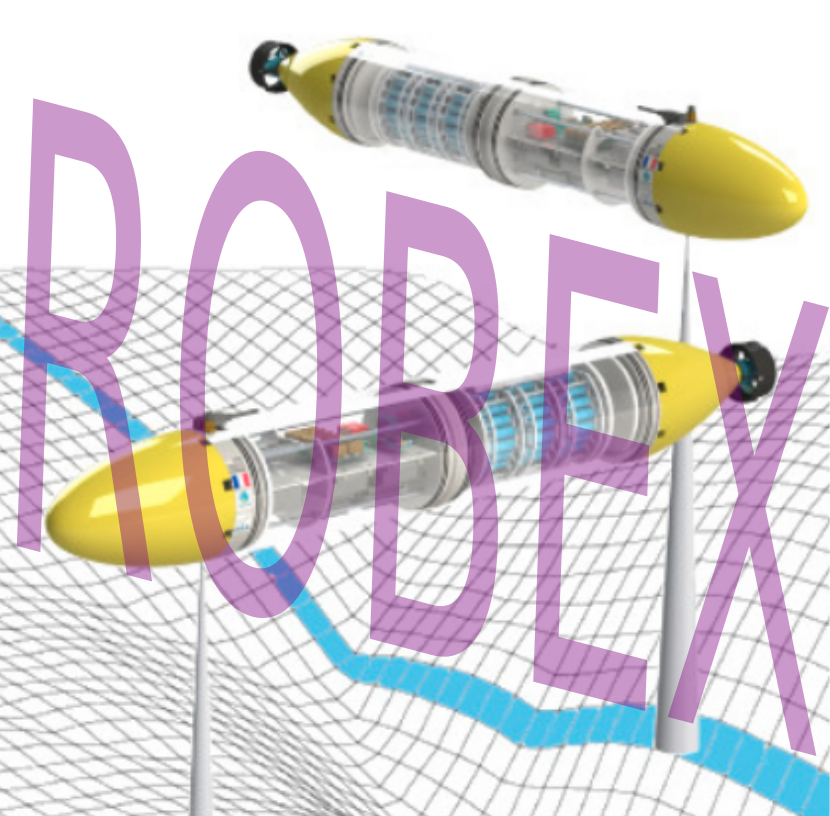
\includegraphics[height=0.6cm]{imgs/logo_robex}}
    \end{tabular}
}

\addtobeamertemplate{frametitle}{}{%
    \begin{tikzpicture}[remember picture,overlay]
    \node[anchor=north east,yshift=2pt] at (current page.north east) {
\includegraphics[height=0.85cm]{imgs/logo_ensta_aid}};
    \end{tikzpicture}
}

\begin{document}

    \maketitle

    \section{Context}

        \begin{frame}{PhD thesis}
            \centering
            \begin{minipage}[c]{0.58\textwidth}
                \begin{block}{Research laboratory}
                    \vspace{0.2cm}
                    \begin{itemize}
                        \item ENSTA Bretagne, UMR 6285, Lab-STICC, IAO, ROBEX
                    \end{itemize}
                \end{block}

                \begin{block}{Supervisiors}
                    \begin{itemize}
                        \item Luc Jaulin
                        \item Fabrice Le Bars
                    \end{itemize}
                \end{block}

                \begin{block}{Funding}
                    \begin{itemize}
                        \item AID funding: Jean-Daniel Masson
                    \end{itemize}
                \end{block}
            \end{minipage}
            \hfill
            \begin{minipage}[c]{0.4\textwidth}
                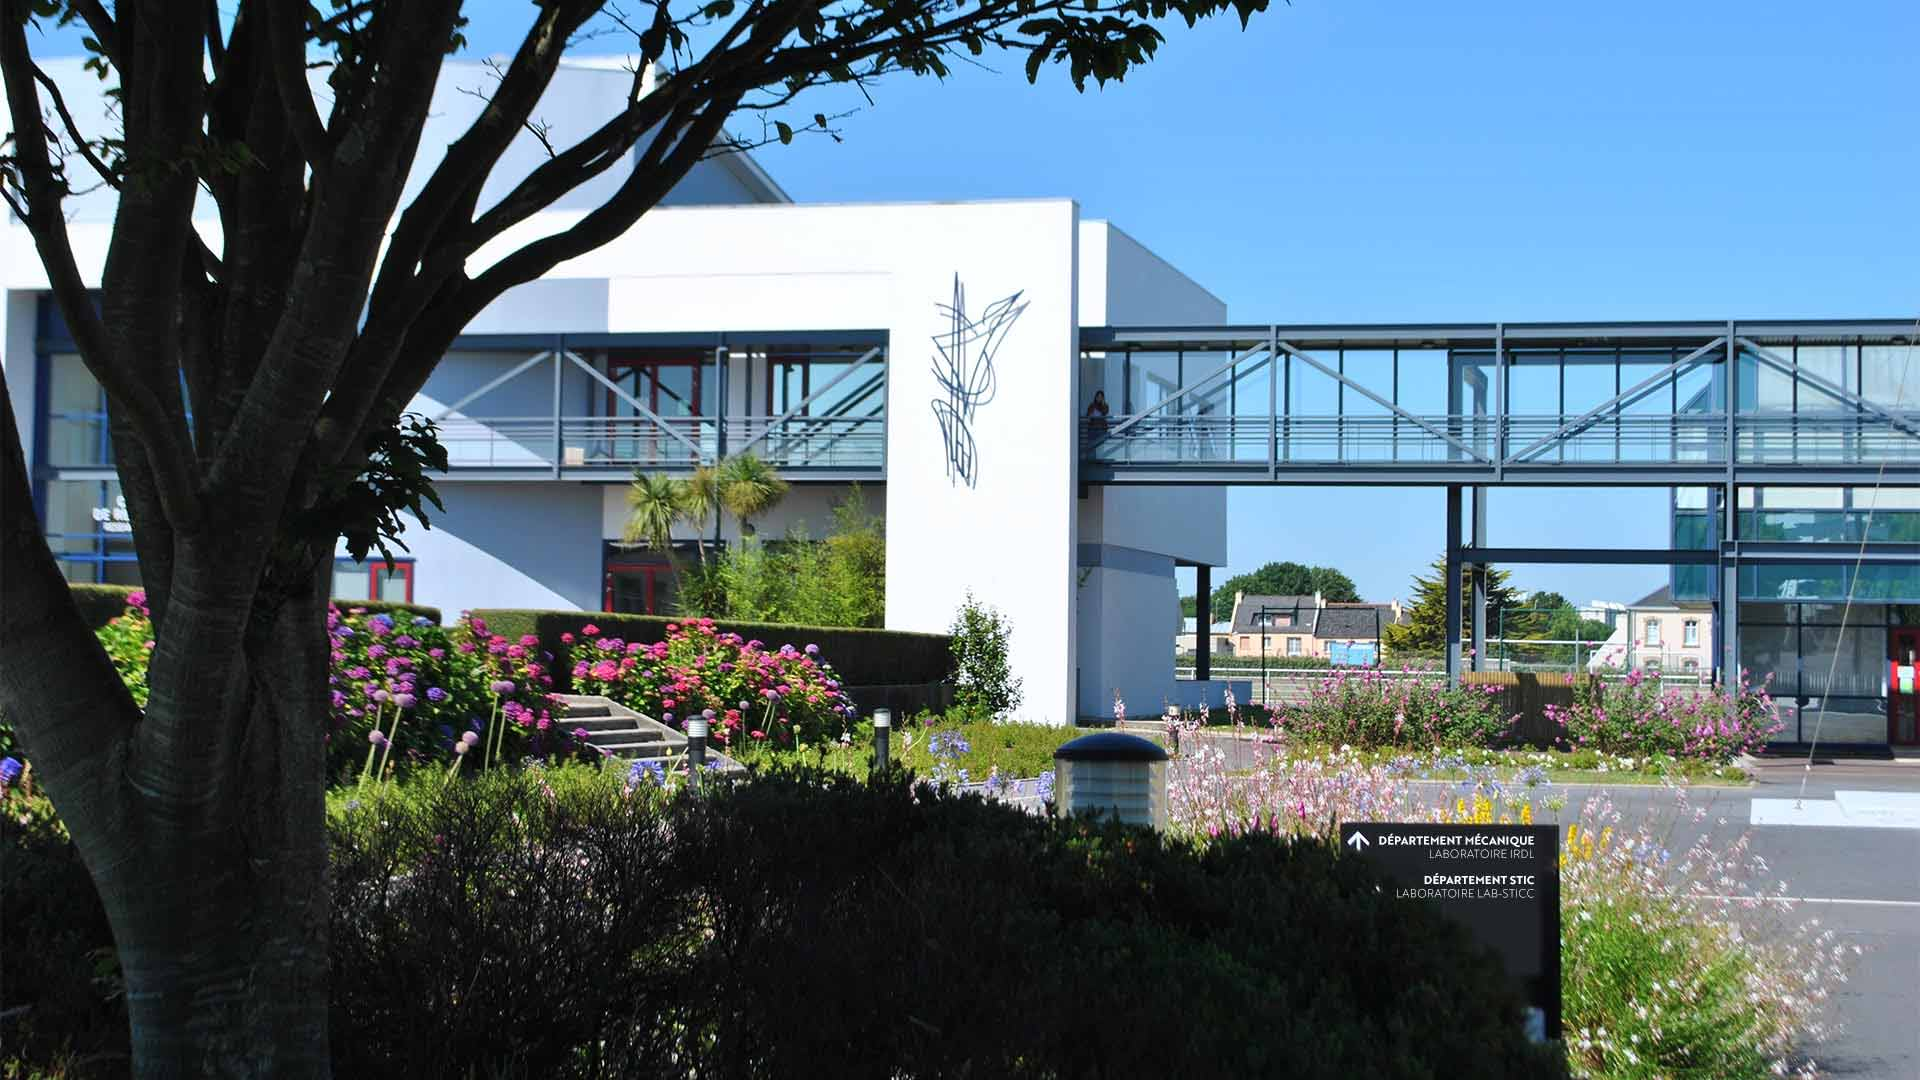
\includegraphics[height=0.7\textheight, trim={24cm 0 16cm 0}, clip]{imgs/ensta.jpg}
            \end{minipage}
        \end{frame}

        \begin{frame}{Goal}
            \begin{minipage}[c]{0.55\textwidth}
                \begin{block}{AUV}
                    \vspace{0.25cm}
                    \begin{itemize}
                        \item Control of torpedo-like AUV \\ 
                        \item Riptide's micro-uuv
                    \end{itemize}
                \end{block}
                \begin{block}{Environment}
                    \begin{itemize}
                        \item Constrained environment \\ 
                        \item Pool, harbor, ...
                    \end{itemize}
                \end{block}
                \begin{block}{Goals}
                    \begin{itemize}
                        \item Reactivity \\
                        \item Manoeuvrability
                    \end{itemize}
                \end{block}
            \end{minipage}
            \hfill
            \begin{minipage}[c]{0.4\textwidth}
                \begin{figure}[htb]
                    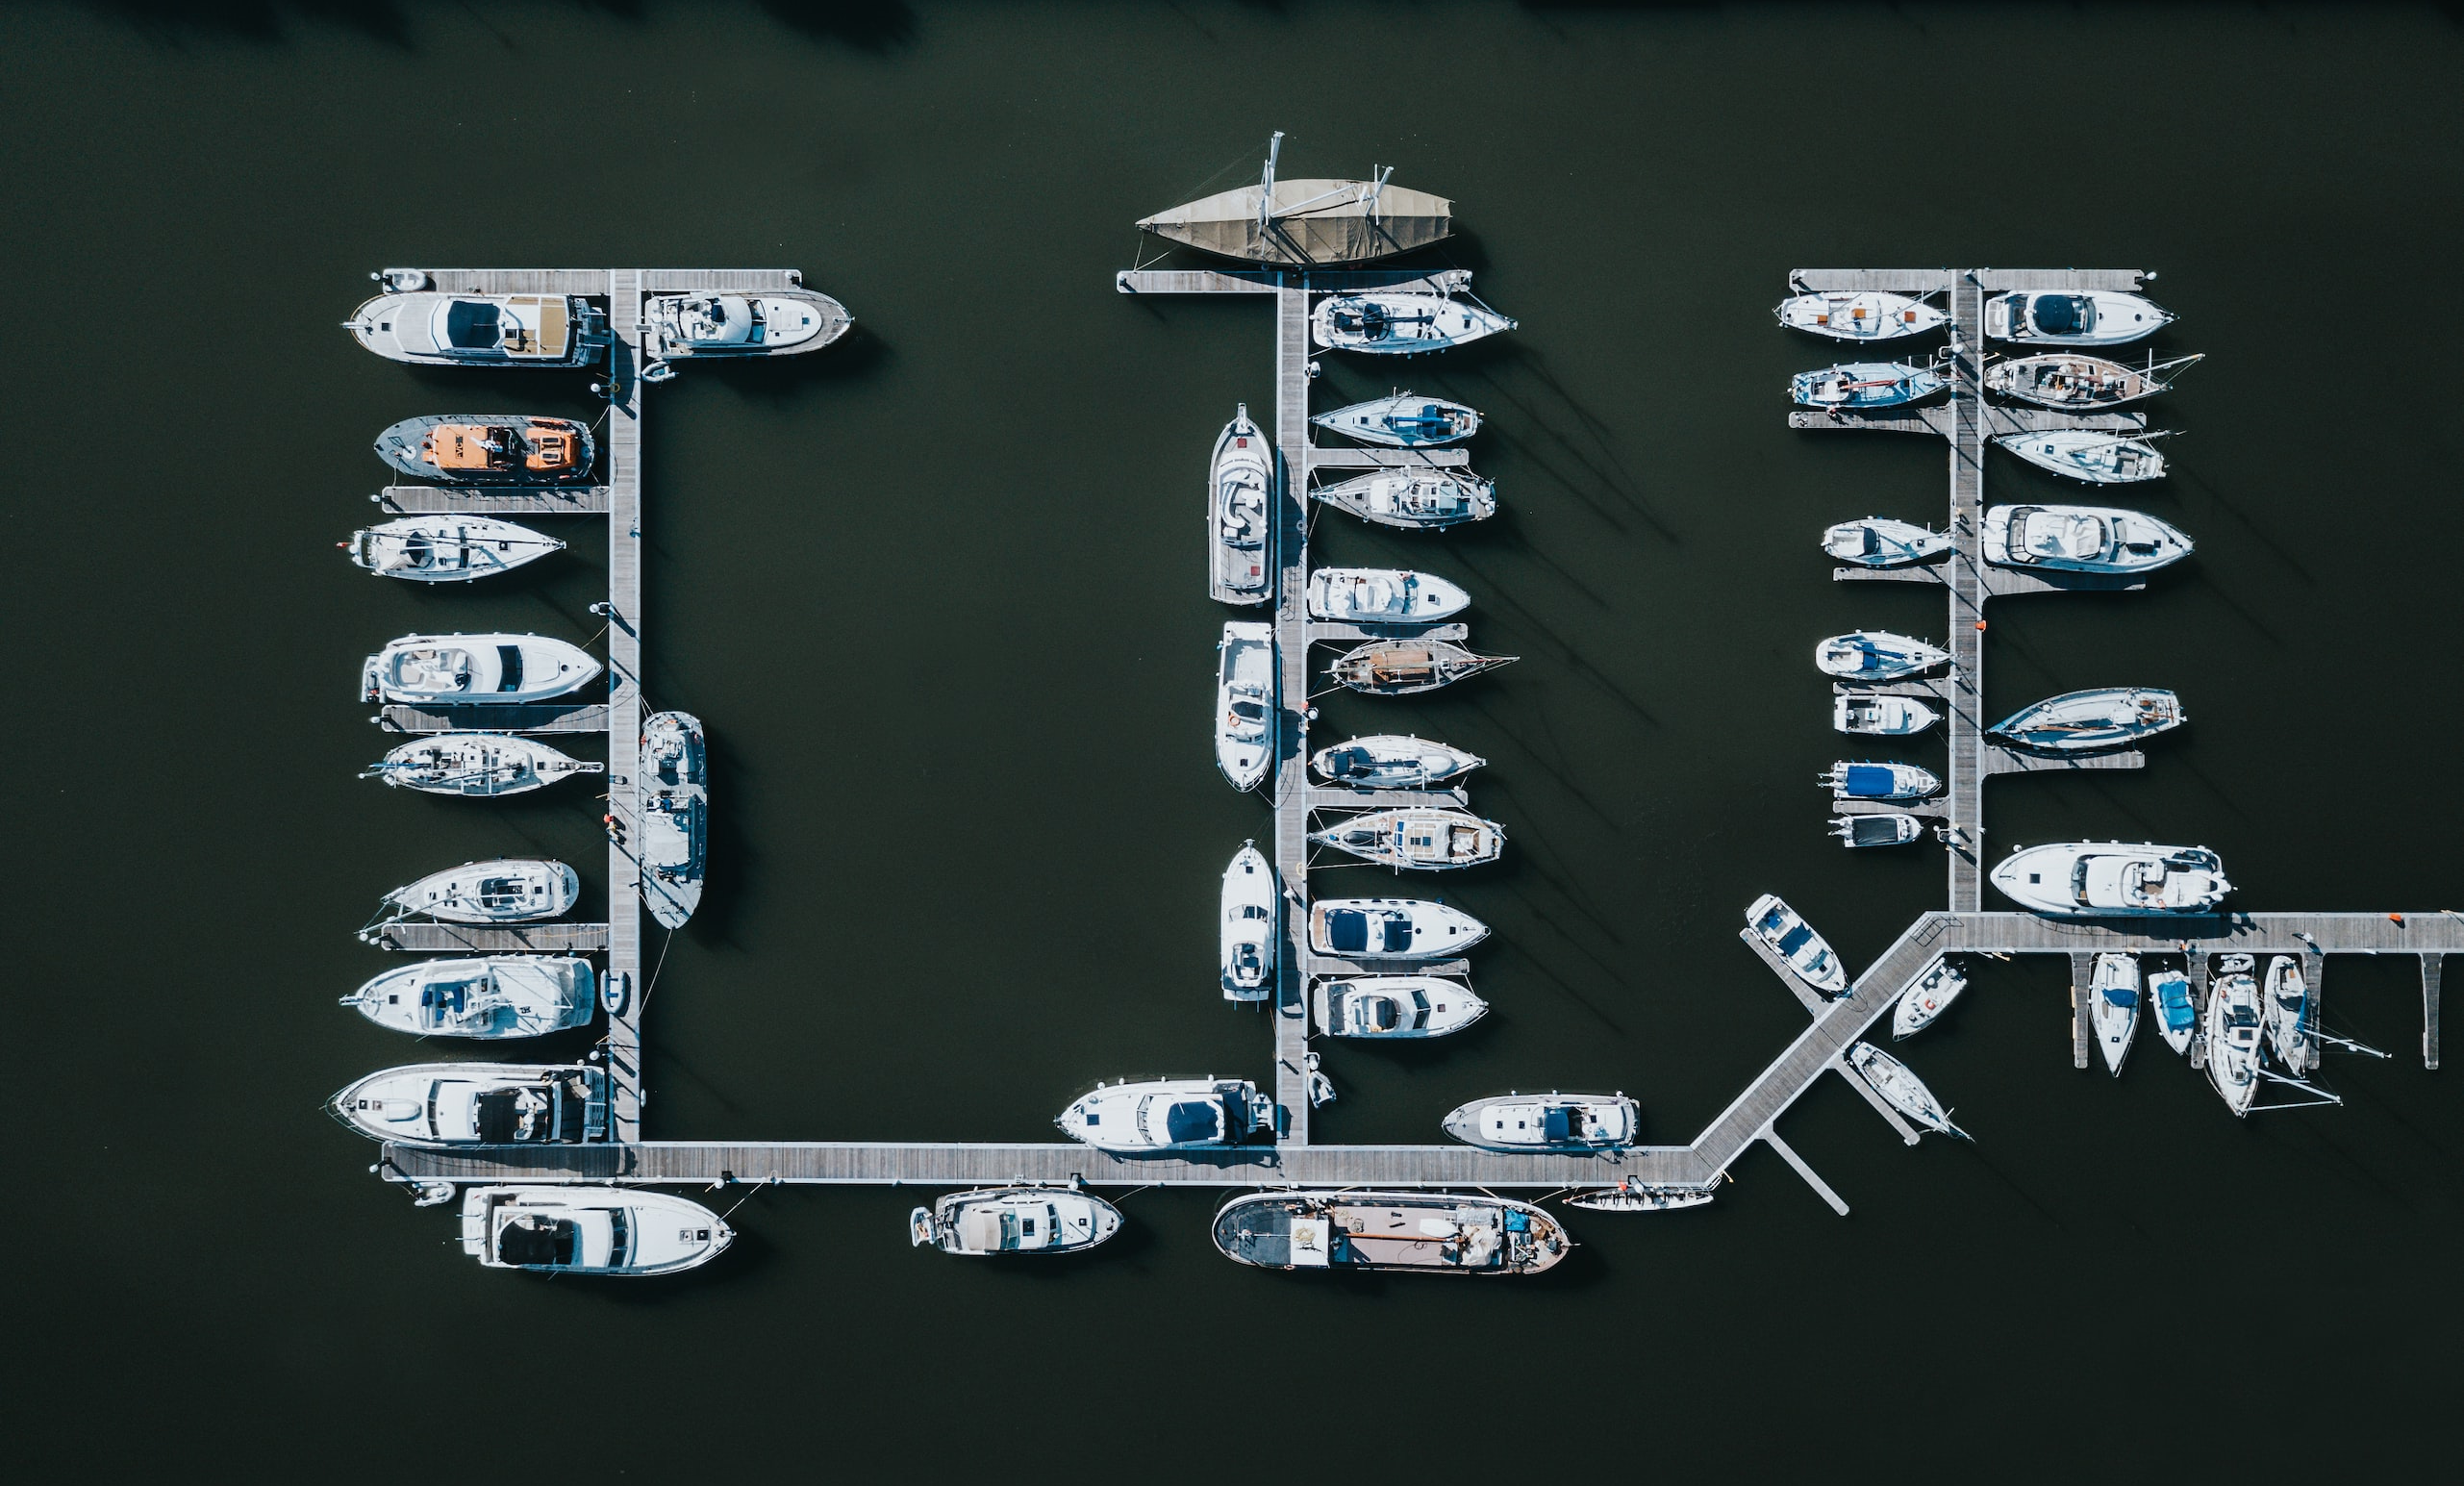
\includegraphics[width=\textwidth]{imgs/harbour.png}

                    \vspace{.1cm}

                    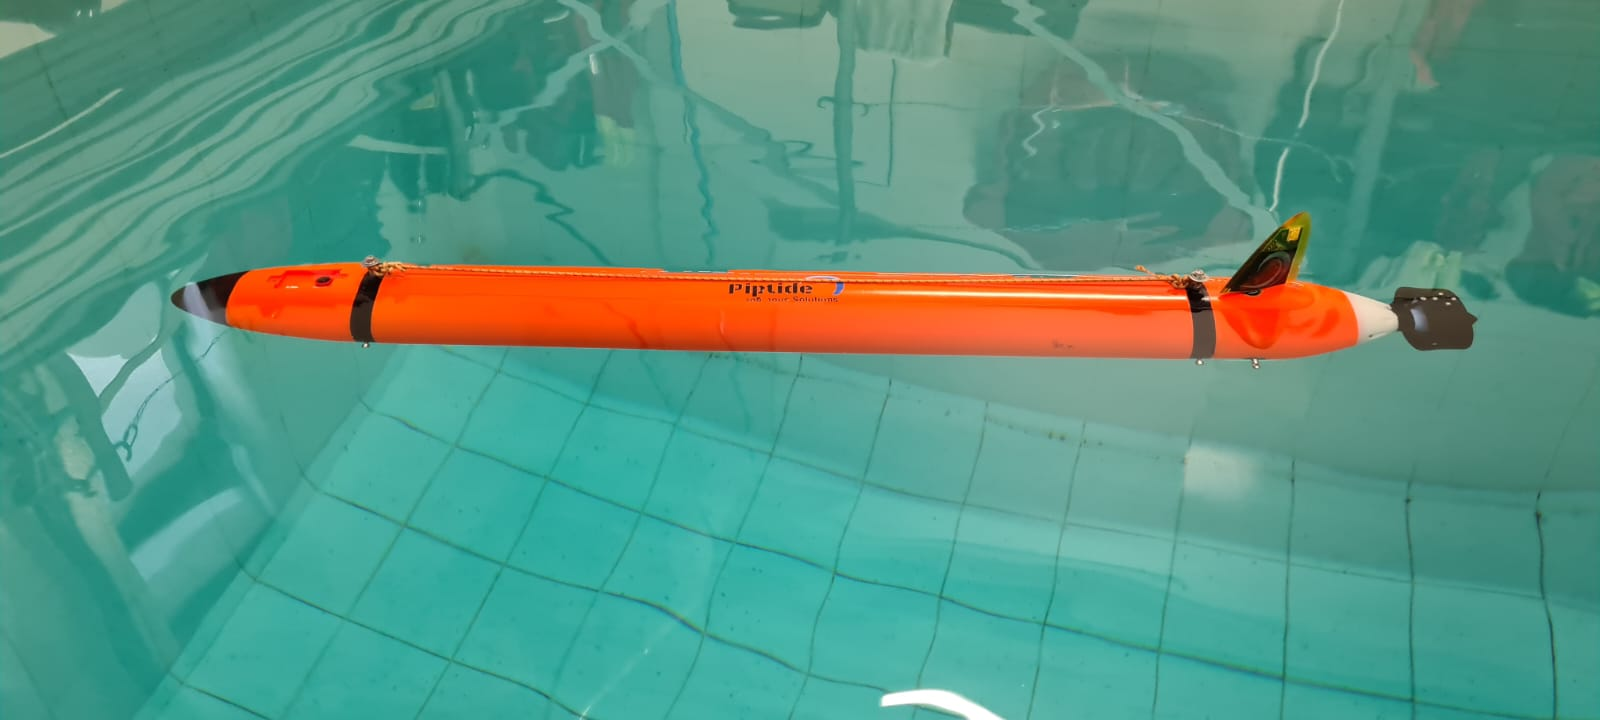
\includegraphics[width=\textwidth]{imgs/Riptide.jpeg}
                    \caption{Harbor and Riptide in the ENSTA Bretagne pool}
                \end{figure}
            \end{minipage}
        \end{frame}

        \begin{frame}{Robot sensors}
            \begin{minipage}[t]{.55\textwidth}
                \begin{exampleblock}{Riptide's sensors}
                    \vspace{0.25cm}
                    \begin{itemize}[<+->]
                        \item Proprioceptive
                        \begin{itemize}
                            \item IMU
                        \end{itemize}
                        \item Exteroceptive
                        \begin{itemize}
                            \item Pressure sensor \\ 
                            \item Echosounder
                        \end{itemize}
                    \end{itemize}
                \end{exampleblock}
                % \begin{alertblock}<+->{Echosounder measurements}
                %     \begin{itemize}[<+->]
                %         \item Sound propagation in pool causes multiple reflections
                %         \item Use information provided by the silence
                %     \end{itemize}
                % \end{alertblock}
            \end{minipage}
            \hfill
            \begin{minipage}[t]{.42\textwidth}
                \begin{figure}[htb]
                    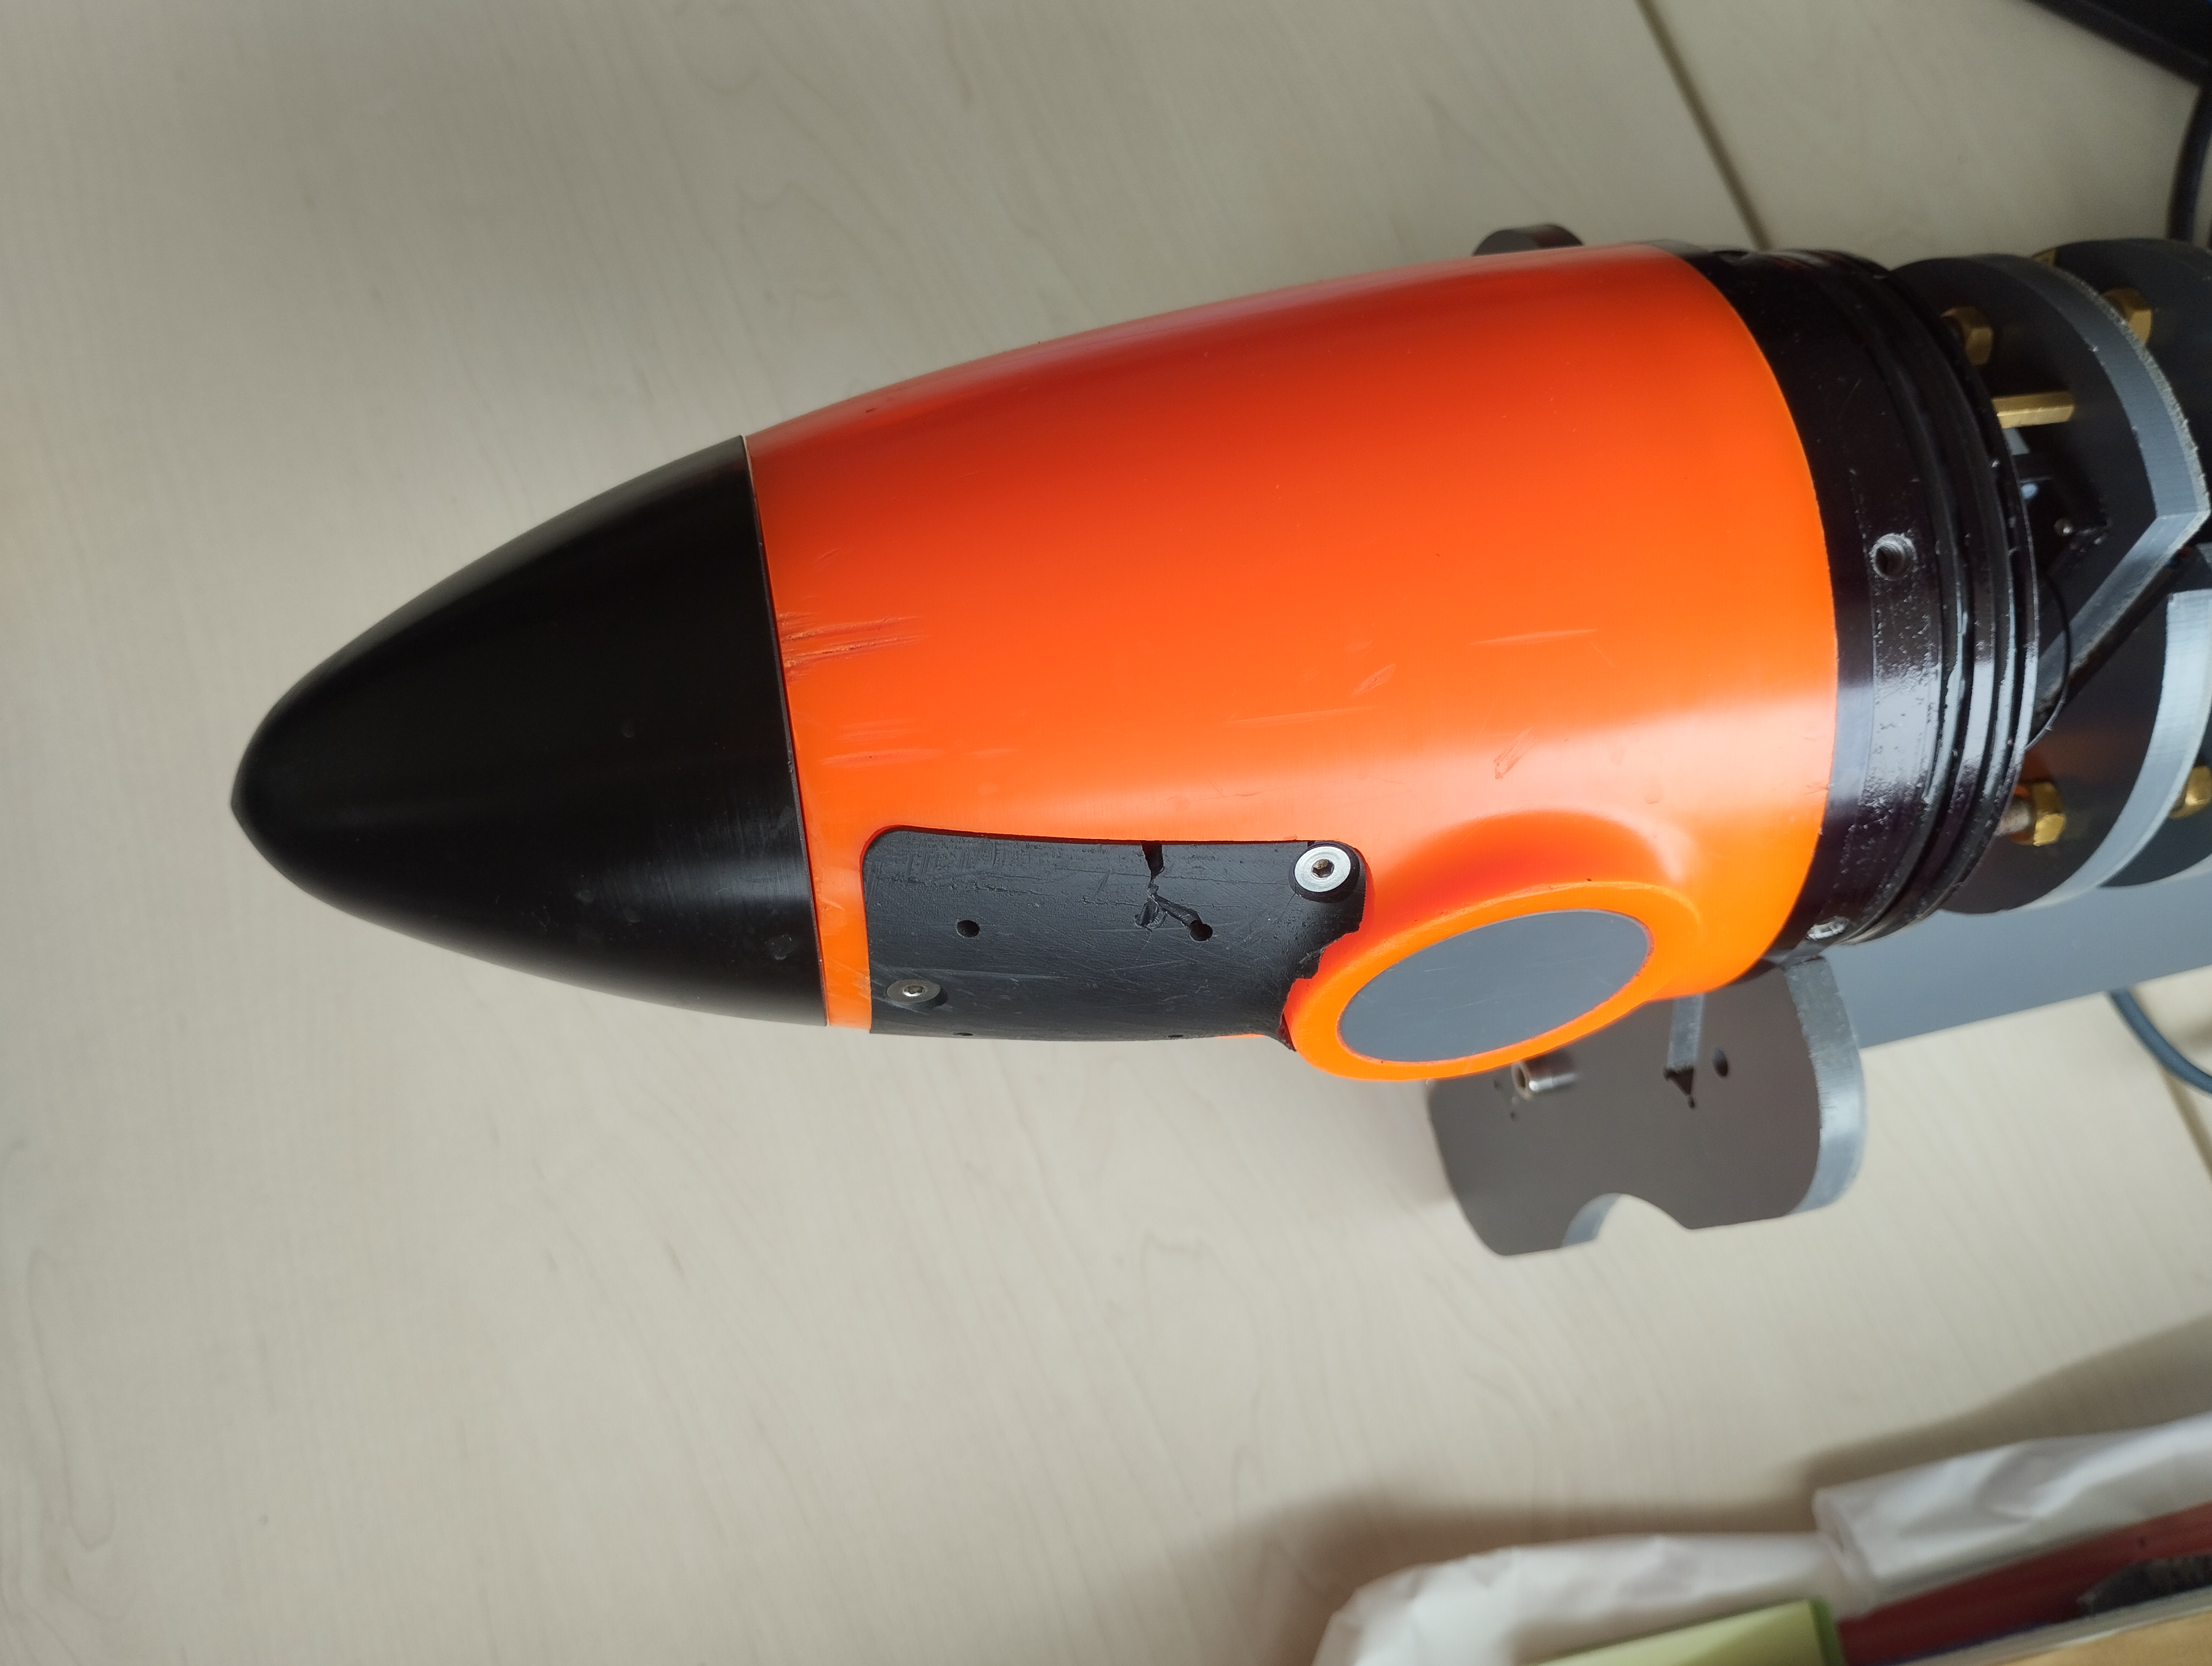
\includegraphics[width=\textwidth]{imgs/echosounder.jpg}
                    \caption{Riptide's echosounder located below the head}
                \end{figure}
            \end{minipage}
        \end{frame}

        \begin{frame}{Localization}
            \begin{minipage}[t]{.45\textwidth}
                \vspace{-4mm}
                \centering
                \begin{figure}
                    \begin{overprint}
                        \onslide<1>\centerline{%% Creator: Matplotlib, PGF backend
%%
%% To include the figure in your LaTeX document, write
%%   \input{<filename>.pgf}
%%
%% Make sure the required packages are loaded in your preamble
%%   \usepackage{pgf}
%%
%% Also ensure that all the required font packages are loaded; for instance,
%% the lmodern package is sometimes necessary when using math font.
%%   \usepackage{lmodern}
%%
%% Figures using additional raster images can only be included by \input if
%% they are in the same directory as the main LaTeX file. For loading figures
%% from other directories you can use the `import` package
%%   \usepackage{import}
%%
%% and then include the figures with
%%   \import{<path to file>}{<filename>.pgf}
%%
%% Matplotlib used the following preamble
%%
\begingroup%
\makeatletter%
\begin{pgfpicture}%
\pgfpathrectangle{\pgfpointorigin}{\pgfqpoint{1.740000in}{2.510000in}}%
\pgfusepath{use as bounding box, clip}%
\begin{pgfscope}%
\pgfsetbuttcap%
\pgfsetmiterjoin%
\definecolor{currentfill}{rgb}{1.000000,1.000000,1.000000}%
\pgfsetfillcolor{currentfill}%
\pgfsetlinewidth{0.000000pt}%
\definecolor{currentstroke}{rgb}{1.000000,1.000000,1.000000}%
\pgfsetstrokecolor{currentstroke}%
\pgfsetdash{}{0pt}%
\pgfpathmoveto{\pgfqpoint{0.000000in}{0.000000in}}%
\pgfpathlineto{\pgfqpoint{1.740000in}{0.000000in}}%
\pgfpathlineto{\pgfqpoint{1.740000in}{2.510000in}}%
\pgfpathlineto{\pgfqpoint{0.000000in}{2.510000in}}%
\pgfpathlineto{\pgfqpoint{0.000000in}{0.000000in}}%
\pgfpathclose%
\pgfusepath{fill}%
\end{pgfscope}%
\begin{pgfscope}%
\pgfpathrectangle{\pgfqpoint{0.100000in}{0.100000in}}{\pgfqpoint{1.540000in}{2.310000in}}%
\pgfusepath{clip}%
\pgfsetbuttcap%
\pgfsetroundjoin%
\definecolor{currentfill}{rgb}{0.933333,0.600000,0.666667}%
\pgfsetfillcolor{currentfill}%
\pgfsetlinewidth{1.003750pt}%
\definecolor{currentstroke}{rgb}{0.600000,0.266667,0.333333}%
\pgfsetstrokecolor{currentstroke}%
\pgfsetdash{}{0pt}%
\pgfpathmoveto{\pgfqpoint{1.562494in}{2.346058in}}%
\pgfpathlineto{\pgfqpoint{1.597372in}{2.346058in}}%
\pgfpathlineto{\pgfqpoint{1.597372in}{2.410000in}}%
\pgfpathlineto{\pgfqpoint{1.562494in}{2.410000in}}%
\pgfpathlineto{\pgfqpoint{1.562494in}{2.346058in}}%
\pgfpathclose%
\pgfusepath{stroke,fill}%
\end{pgfscope}%
\begin{pgfscope}%
\pgfpathrectangle{\pgfqpoint{0.100000in}{0.100000in}}{\pgfqpoint{1.540000in}{2.310000in}}%
\pgfusepath{clip}%
\pgfsetbuttcap%
\pgfsetroundjoin%
\definecolor{currentfill}{rgb}{0.933333,0.600000,0.666667}%
\pgfsetfillcolor{currentfill}%
\pgfsetlinewidth{1.003750pt}%
\definecolor{currentstroke}{rgb}{0.600000,0.266667,0.333333}%
\pgfsetstrokecolor{currentstroke}%
\pgfsetdash{}{0pt}%
\pgfpathmoveto{\pgfqpoint{1.562494in}{2.293741in}}%
\pgfpathlineto{\pgfqpoint{1.640000in}{2.293741in}}%
\pgfpathlineto{\pgfqpoint{1.640000in}{2.346058in}}%
\pgfpathlineto{\pgfqpoint{1.562494in}{2.346058in}}%
\pgfpathlineto{\pgfqpoint{1.562494in}{2.293741in}}%
\pgfpathclose%
\pgfusepath{stroke,fill}%
\end{pgfscope}%
\begin{pgfscope}%
\pgfpathrectangle{\pgfqpoint{0.100000in}{0.100000in}}{\pgfqpoint{1.540000in}{2.310000in}}%
\pgfusepath{clip}%
\pgfsetbuttcap%
\pgfsetroundjoin%
\definecolor{currentfill}{rgb}{0.933333,0.600000,0.666667}%
\pgfsetfillcolor{currentfill}%
\pgfsetlinewidth{1.003750pt}%
\definecolor{currentstroke}{rgb}{0.600000,0.266667,0.333333}%
\pgfsetstrokecolor{currentstroke}%
\pgfsetdash{}{0pt}%
\pgfpathmoveto{\pgfqpoint{1.562494in}{0.100000in}}%
\pgfpathlineto{\pgfqpoint{1.597372in}{0.100000in}}%
\pgfpathlineto{\pgfqpoint{1.597372in}{0.142626in}}%
\pgfpathlineto{\pgfqpoint{1.562494in}{0.142626in}}%
\pgfpathlineto{\pgfqpoint{1.562494in}{0.100000in}}%
\pgfpathclose%
\pgfusepath{stroke,fill}%
\end{pgfscope}%
\begin{pgfscope}%
\pgfpathrectangle{\pgfqpoint{0.100000in}{0.100000in}}{\pgfqpoint{1.540000in}{2.310000in}}%
\pgfusepath{clip}%
\pgfsetbuttcap%
\pgfsetroundjoin%
\definecolor{currentfill}{rgb}{0.933333,0.600000,0.666667}%
\pgfsetfillcolor{currentfill}%
\pgfsetlinewidth{1.003750pt}%
\definecolor{currentstroke}{rgb}{0.600000,0.266667,0.333333}%
\pgfsetstrokecolor{currentstroke}%
\pgfsetdash{}{0pt}%
\pgfpathmoveto{\pgfqpoint{1.499080in}{2.293741in}}%
\pgfpathlineto{\pgfqpoint{1.562494in}{2.293741in}}%
\pgfpathlineto{\pgfqpoint{1.562494in}{2.410000in}}%
\pgfpathlineto{\pgfqpoint{1.499080in}{2.410000in}}%
\pgfpathlineto{\pgfqpoint{1.499080in}{2.293741in}}%
\pgfpathclose%
\pgfusepath{stroke,fill}%
\end{pgfscope}%
\begin{pgfscope}%
\pgfpathrectangle{\pgfqpoint{0.100000in}{0.100000in}}{\pgfqpoint{1.540000in}{2.310000in}}%
\pgfusepath{clip}%
\pgfsetbuttcap%
\pgfsetroundjoin%
\definecolor{currentfill}{rgb}{0.933333,0.600000,0.666667}%
\pgfsetfillcolor{currentfill}%
\pgfsetlinewidth{1.003750pt}%
\definecolor{currentstroke}{rgb}{0.600000,0.266667,0.333333}%
\pgfsetstrokecolor{currentstroke}%
\pgfsetdash{}{0pt}%
\pgfpathmoveto{\pgfqpoint{0.100000in}{2.293741in}}%
\pgfpathlineto{\pgfqpoint{0.163150in}{2.293741in}}%
\pgfpathlineto{\pgfqpoint{0.163150in}{2.346058in}}%
\pgfpathlineto{\pgfqpoint{0.100000in}{2.346058in}}%
\pgfpathlineto{\pgfqpoint{0.100000in}{2.293741in}}%
\pgfpathclose%
\pgfusepath{stroke,fill}%
\end{pgfscope}%
\begin{pgfscope}%
\pgfpathrectangle{\pgfqpoint{0.100000in}{0.100000in}}{\pgfqpoint{1.540000in}{2.310000in}}%
\pgfusepath{clip}%
\pgfsetbuttcap%
\pgfsetroundjoin%
\definecolor{currentfill}{rgb}{0.933333,0.600000,0.666667}%
\pgfsetfillcolor{currentfill}%
\pgfsetlinewidth{1.003750pt}%
\definecolor{currentstroke}{rgb}{0.600000,0.266667,0.333333}%
\pgfsetstrokecolor{currentstroke}%
\pgfsetdash{}{0pt}%
\pgfpathmoveto{\pgfqpoint{1.562494in}{0.142626in}}%
\pgfpathlineto{\pgfqpoint{1.640000in}{0.142626in}}%
\pgfpathlineto{\pgfqpoint{1.640000in}{0.194724in}}%
\pgfpathlineto{\pgfqpoint{1.562494in}{0.194724in}}%
\pgfpathlineto{\pgfqpoint{1.562494in}{0.142626in}}%
\pgfpathclose%
\pgfusepath{stroke,fill}%
\end{pgfscope}%
\begin{pgfscope}%
\pgfpathrectangle{\pgfqpoint{0.100000in}{0.100000in}}{\pgfqpoint{1.540000in}{2.310000in}}%
\pgfusepath{clip}%
\pgfsetbuttcap%
\pgfsetroundjoin%
\definecolor{currentfill}{rgb}{0.933333,0.600000,0.666667}%
\pgfsetfillcolor{currentfill}%
\pgfsetlinewidth{1.003750pt}%
\definecolor{currentstroke}{rgb}{0.600000,0.266667,0.333333}%
\pgfsetstrokecolor{currentstroke}%
\pgfsetdash{}{0pt}%
\pgfpathmoveto{\pgfqpoint{1.499080in}{2.198621in}}%
\pgfpathlineto{\pgfqpoint{1.640000in}{2.198621in}}%
\pgfpathlineto{\pgfqpoint{1.640000in}{2.293741in}}%
\pgfpathlineto{\pgfqpoint{1.499080in}{2.293741in}}%
\pgfpathlineto{\pgfqpoint{1.499080in}{2.198621in}}%
\pgfpathclose%
\pgfusepath{stroke,fill}%
\end{pgfscope}%
\begin{pgfscope}%
\pgfpathrectangle{\pgfqpoint{0.100000in}{0.100000in}}{\pgfqpoint{1.540000in}{2.310000in}}%
\pgfusepath{clip}%
\pgfsetbuttcap%
\pgfsetroundjoin%
\definecolor{currentfill}{rgb}{0.933333,0.600000,0.666667}%
\pgfsetfillcolor{currentfill}%
\pgfsetlinewidth{1.003750pt}%
\definecolor{currentstroke}{rgb}{0.600000,0.266667,0.333333}%
\pgfsetstrokecolor{currentstroke}%
\pgfsetdash{}{0pt}%
\pgfpathmoveto{\pgfqpoint{0.163150in}{2.293741in}}%
\pgfpathlineto{\pgfqpoint{0.240332in}{2.293741in}}%
\pgfpathlineto{\pgfqpoint{0.240332in}{2.410000in}}%
\pgfpathlineto{\pgfqpoint{0.163150in}{2.410000in}}%
\pgfpathlineto{\pgfqpoint{0.163150in}{2.293741in}}%
\pgfpathclose%
\pgfusepath{stroke,fill}%
\end{pgfscope}%
\begin{pgfscope}%
\pgfpathrectangle{\pgfqpoint{0.100000in}{0.100000in}}{\pgfqpoint{1.540000in}{2.310000in}}%
\pgfusepath{clip}%
\pgfsetbuttcap%
\pgfsetroundjoin%
\definecolor{currentfill}{rgb}{0.933333,0.600000,0.666667}%
\pgfsetfillcolor{currentfill}%
\pgfsetlinewidth{1.003750pt}%
\definecolor{currentstroke}{rgb}{0.600000,0.266667,0.333333}%
\pgfsetstrokecolor{currentstroke}%
\pgfsetdash{}{0pt}%
\pgfpathmoveto{\pgfqpoint{1.499080in}{0.100000in}}%
\pgfpathlineto{\pgfqpoint{1.562494in}{0.100000in}}%
\pgfpathlineto{\pgfqpoint{1.562494in}{0.194724in}}%
\pgfpathlineto{\pgfqpoint{1.499080in}{0.194724in}}%
\pgfpathlineto{\pgfqpoint{1.499080in}{0.100000in}}%
\pgfpathclose%
\pgfusepath{stroke,fill}%
\end{pgfscope}%
\begin{pgfscope}%
\pgfpathrectangle{\pgfqpoint{0.100000in}{0.100000in}}{\pgfqpoint{1.540000in}{2.310000in}}%
\pgfusepath{clip}%
\pgfsetbuttcap%
\pgfsetroundjoin%
\definecolor{currentfill}{rgb}{0.933333,0.600000,0.666667}%
\pgfsetfillcolor{currentfill}%
\pgfsetlinewidth{1.003750pt}%
\definecolor{currentstroke}{rgb}{0.600000,0.266667,0.333333}%
\pgfsetstrokecolor{currentstroke}%
\pgfsetdash{}{0pt}%
\pgfpathmoveto{\pgfqpoint{0.100000in}{0.142626in}}%
\pgfpathlineto{\pgfqpoint{0.163150in}{0.142626in}}%
\pgfpathlineto{\pgfqpoint{0.163150in}{0.194724in}}%
\pgfpathlineto{\pgfqpoint{0.100000in}{0.194724in}}%
\pgfpathlineto{\pgfqpoint{0.100000in}{0.142626in}}%
\pgfpathclose%
\pgfusepath{stroke,fill}%
\end{pgfscope}%
\begin{pgfscope}%
\pgfpathrectangle{\pgfqpoint{0.100000in}{0.100000in}}{\pgfqpoint{1.540000in}{2.310000in}}%
\pgfusepath{clip}%
\pgfsetbuttcap%
\pgfsetroundjoin%
\definecolor{currentfill}{rgb}{0.933333,0.600000,0.666667}%
\pgfsetfillcolor{currentfill}%
\pgfsetlinewidth{1.003750pt}%
\definecolor{currentstroke}{rgb}{0.600000,0.266667,0.333333}%
\pgfsetstrokecolor{currentstroke}%
\pgfsetdash{}{0pt}%
\pgfpathmoveto{\pgfqpoint{1.383783in}{2.198621in}}%
\pgfpathlineto{\pgfqpoint{1.499080in}{2.198621in}}%
\pgfpathlineto{\pgfqpoint{1.499080in}{2.410000in}}%
\pgfpathlineto{\pgfqpoint{1.383783in}{2.410000in}}%
\pgfpathlineto{\pgfqpoint{1.383783in}{2.198621in}}%
\pgfpathclose%
\pgfusepath{stroke,fill}%
\end{pgfscope}%
\begin{pgfscope}%
\pgfpathrectangle{\pgfqpoint{0.100000in}{0.100000in}}{\pgfqpoint{1.540000in}{2.310000in}}%
\pgfusepath{clip}%
\pgfsetbuttcap%
\pgfsetroundjoin%
\definecolor{currentfill}{rgb}{0.933333,0.600000,0.666667}%
\pgfsetfillcolor{currentfill}%
\pgfsetlinewidth{1.003750pt}%
\definecolor{currentstroke}{rgb}{0.600000,0.266667,0.333333}%
\pgfsetstrokecolor{currentstroke}%
\pgfsetdash{}{0pt}%
\pgfpathmoveto{\pgfqpoint{0.100000in}{2.198621in}}%
\pgfpathlineto{\pgfqpoint{0.240332in}{2.198621in}}%
\pgfpathlineto{\pgfqpoint{0.240332in}{2.293741in}}%
\pgfpathlineto{\pgfqpoint{0.100000in}{2.293741in}}%
\pgfpathlineto{\pgfqpoint{0.100000in}{2.198621in}}%
\pgfpathclose%
\pgfusepath{stroke,fill}%
\end{pgfscope}%
\begin{pgfscope}%
\pgfpathrectangle{\pgfqpoint{0.100000in}{0.100000in}}{\pgfqpoint{1.540000in}{2.310000in}}%
\pgfusepath{clip}%
\pgfsetbuttcap%
\pgfsetroundjoin%
\definecolor{currentfill}{rgb}{0.933333,0.600000,0.666667}%
\pgfsetfillcolor{currentfill}%
\pgfsetlinewidth{1.003750pt}%
\definecolor{currentstroke}{rgb}{0.600000,0.266667,0.333333}%
\pgfsetstrokecolor{currentstroke}%
\pgfsetdash{}{0pt}%
\pgfpathmoveto{\pgfqpoint{1.499080in}{0.194724in}}%
\pgfpathlineto{\pgfqpoint{1.640000in}{0.194724in}}%
\pgfpathlineto{\pgfqpoint{1.640000in}{0.310499in}}%
\pgfpathlineto{\pgfqpoint{1.499080in}{0.310499in}}%
\pgfpathlineto{\pgfqpoint{1.499080in}{0.194724in}}%
\pgfpathclose%
\pgfusepath{stroke,fill}%
\end{pgfscope}%
\begin{pgfscope}%
\pgfpathrectangle{\pgfqpoint{0.100000in}{0.100000in}}{\pgfqpoint{1.540000in}{2.310000in}}%
\pgfusepath{clip}%
\pgfsetbuttcap%
\pgfsetroundjoin%
\definecolor{currentfill}{rgb}{0.933333,0.600000,0.666667}%
\pgfsetfillcolor{currentfill}%
\pgfsetlinewidth{1.003750pt}%
\definecolor{currentstroke}{rgb}{0.600000,0.266667,0.333333}%
\pgfsetstrokecolor{currentstroke}%
\pgfsetdash{}{0pt}%
\pgfpathmoveto{\pgfqpoint{0.163150in}{0.100000in}}%
\pgfpathlineto{\pgfqpoint{0.240332in}{0.100000in}}%
\pgfpathlineto{\pgfqpoint{0.240332in}{0.194724in}}%
\pgfpathlineto{\pgfqpoint{0.163150in}{0.194724in}}%
\pgfpathlineto{\pgfqpoint{0.163150in}{0.100000in}}%
\pgfpathclose%
\pgfusepath{stroke,fill}%
\end{pgfscope}%
\begin{pgfscope}%
\pgfpathrectangle{\pgfqpoint{0.100000in}{0.100000in}}{\pgfqpoint{1.540000in}{2.310000in}}%
\pgfusepath{clip}%
\pgfsetbuttcap%
\pgfsetroundjoin%
\definecolor{currentfill}{rgb}{0.933333,0.600000,0.666667}%
\pgfsetfillcolor{currentfill}%
\pgfsetlinewidth{1.003750pt}%
\definecolor{currentstroke}{rgb}{0.600000,0.266667,0.333333}%
\pgfsetstrokecolor{currentstroke}%
\pgfsetdash{}{0pt}%
\pgfpathmoveto{\pgfqpoint{1.383783in}{2.025674in}}%
\pgfpathlineto{\pgfqpoint{1.640000in}{2.025674in}}%
\pgfpathlineto{\pgfqpoint{1.640000in}{2.198621in}}%
\pgfpathlineto{\pgfqpoint{1.383783in}{2.198621in}}%
\pgfpathlineto{\pgfqpoint{1.383783in}{2.025674in}}%
\pgfpathclose%
\pgfusepath{stroke,fill}%
\end{pgfscope}%
\begin{pgfscope}%
\pgfpathrectangle{\pgfqpoint{0.100000in}{0.100000in}}{\pgfqpoint{1.540000in}{2.310000in}}%
\pgfusepath{clip}%
\pgfsetbuttcap%
\pgfsetroundjoin%
\definecolor{currentfill}{rgb}{0.933333,0.600000,0.666667}%
\pgfsetfillcolor{currentfill}%
\pgfsetlinewidth{1.003750pt}%
\definecolor{currentstroke}{rgb}{0.600000,0.266667,0.333333}%
\pgfsetstrokecolor{currentstroke}%
\pgfsetdash{}{0pt}%
\pgfpathmoveto{\pgfqpoint{0.240332in}{2.198621in}}%
\pgfpathlineto{\pgfqpoint{0.411850in}{2.198621in}}%
\pgfpathlineto{\pgfqpoint{0.411850in}{2.410000in}}%
\pgfpathlineto{\pgfqpoint{0.240332in}{2.410000in}}%
\pgfpathlineto{\pgfqpoint{0.240332in}{2.198621in}}%
\pgfpathclose%
\pgfusepath{stroke,fill}%
\end{pgfscope}%
\begin{pgfscope}%
\pgfpathrectangle{\pgfqpoint{0.100000in}{0.100000in}}{\pgfqpoint{1.540000in}{2.310000in}}%
\pgfusepath{clip}%
\pgfsetbuttcap%
\pgfsetroundjoin%
\definecolor{currentfill}{rgb}{0.933333,0.600000,0.666667}%
\pgfsetfillcolor{currentfill}%
\pgfsetlinewidth{1.003750pt}%
\definecolor{currentstroke}{rgb}{0.600000,0.266667,0.333333}%
\pgfsetstrokecolor{currentstroke}%
\pgfsetdash{}{0pt}%
\pgfpathmoveto{\pgfqpoint{1.383783in}{0.100000in}}%
\pgfpathlineto{\pgfqpoint{1.499080in}{0.100000in}}%
\pgfpathlineto{\pgfqpoint{1.499080in}{0.310499in}}%
\pgfpathlineto{\pgfqpoint{1.383783in}{0.310499in}}%
\pgfpathlineto{\pgfqpoint{1.383783in}{0.100000in}}%
\pgfpathclose%
\pgfusepath{stroke,fill}%
\end{pgfscope}%
\begin{pgfscope}%
\pgfpathrectangle{\pgfqpoint{0.100000in}{0.100000in}}{\pgfqpoint{1.540000in}{2.310000in}}%
\pgfusepath{clip}%
\pgfsetbuttcap%
\pgfsetroundjoin%
\definecolor{currentfill}{rgb}{0.933333,0.600000,0.666667}%
\pgfsetfillcolor{currentfill}%
\pgfsetlinewidth{1.003750pt}%
\definecolor{currentstroke}{rgb}{0.600000,0.266667,0.333333}%
\pgfsetstrokecolor{currentstroke}%
\pgfsetdash{}{0pt}%
\pgfpathmoveto{\pgfqpoint{0.100000in}{0.194724in}}%
\pgfpathlineto{\pgfqpoint{0.240332in}{0.194724in}}%
\pgfpathlineto{\pgfqpoint{0.240332in}{0.310499in}}%
\pgfpathlineto{\pgfqpoint{0.100000in}{0.310499in}}%
\pgfpathlineto{\pgfqpoint{0.100000in}{0.194724in}}%
\pgfpathclose%
\pgfusepath{stroke,fill}%
\end{pgfscope}%
\begin{pgfscope}%
\pgfpathrectangle{\pgfqpoint{0.100000in}{0.100000in}}{\pgfqpoint{1.540000in}{2.310000in}}%
\pgfusepath{clip}%
\pgfsetbuttcap%
\pgfsetroundjoin%
\definecolor{currentfill}{rgb}{0.933333,0.600000,0.666667}%
\pgfsetfillcolor{currentfill}%
\pgfsetlinewidth{1.003750pt}%
\definecolor{currentstroke}{rgb}{0.600000,0.266667,0.333333}%
\pgfsetstrokecolor{currentstroke}%
\pgfsetdash{}{0pt}%
\pgfpathmoveto{\pgfqpoint{1.174150in}{2.025674in}}%
\pgfpathlineto{\pgfqpoint{1.383783in}{2.025674in}}%
\pgfpathlineto{\pgfqpoint{1.383783in}{2.410000in}}%
\pgfpathlineto{\pgfqpoint{1.174150in}{2.410000in}}%
\pgfpathlineto{\pgfqpoint{1.174150in}{2.025674in}}%
\pgfpathclose%
\pgfusepath{stroke,fill}%
\end{pgfscope}%
\begin{pgfscope}%
\pgfpathrectangle{\pgfqpoint{0.100000in}{0.100000in}}{\pgfqpoint{1.540000in}{2.310000in}}%
\pgfusepath{clip}%
\pgfsetbuttcap%
\pgfsetroundjoin%
\definecolor{currentfill}{rgb}{0.933333,0.600000,0.666667}%
\pgfsetfillcolor{currentfill}%
\pgfsetlinewidth{1.003750pt}%
\definecolor{currentstroke}{rgb}{0.600000,0.266667,0.333333}%
\pgfsetstrokecolor{currentstroke}%
\pgfsetdash{}{0pt}%
\pgfpathmoveto{\pgfqpoint{0.100000in}{2.025674in}}%
\pgfpathlineto{\pgfqpoint{0.411850in}{2.025674in}}%
\pgfpathlineto{\pgfqpoint{0.411850in}{2.198621in}}%
\pgfpathlineto{\pgfqpoint{0.100000in}{2.198621in}}%
\pgfpathlineto{\pgfqpoint{0.100000in}{2.025674in}}%
\pgfpathclose%
\pgfusepath{stroke,fill}%
\end{pgfscope}%
\begin{pgfscope}%
\pgfpathrectangle{\pgfqpoint{0.100000in}{0.100000in}}{\pgfqpoint{1.540000in}{2.310000in}}%
\pgfusepath{clip}%
\pgfsetbuttcap%
\pgfsetroundjoin%
\definecolor{currentfill}{rgb}{0.933333,0.600000,0.666667}%
\pgfsetfillcolor{currentfill}%
\pgfsetlinewidth{1.003750pt}%
\definecolor{currentstroke}{rgb}{0.600000,0.266667,0.333333}%
\pgfsetstrokecolor{currentstroke}%
\pgfsetdash{}{0pt}%
\pgfpathmoveto{\pgfqpoint{1.174150in}{0.100000in}}%
\pgfpathlineto{\pgfqpoint{1.383783in}{0.100000in}}%
\pgfpathlineto{\pgfqpoint{1.383783in}{0.310499in}}%
\pgfpathlineto{\pgfqpoint{1.174150in}{0.310499in}}%
\pgfpathlineto{\pgfqpoint{1.174150in}{0.100000in}}%
\pgfpathclose%
\pgfusepath{stroke,fill}%
\end{pgfscope}%
\begin{pgfscope}%
\pgfpathrectangle{\pgfqpoint{0.100000in}{0.100000in}}{\pgfqpoint{1.540000in}{2.310000in}}%
\pgfusepath{clip}%
\pgfsetbuttcap%
\pgfsetroundjoin%
\definecolor{currentfill}{rgb}{0.933333,0.600000,0.666667}%
\pgfsetfillcolor{currentfill}%
\pgfsetlinewidth{1.003750pt}%
\definecolor{currentstroke}{rgb}{0.600000,0.266667,0.333333}%
\pgfsetstrokecolor{currentstroke}%
\pgfsetdash{}{0pt}%
\pgfpathmoveto{\pgfqpoint{0.240332in}{0.100000in}}%
\pgfpathlineto{\pgfqpoint{0.411850in}{0.100000in}}%
\pgfpathlineto{\pgfqpoint{0.411850in}{0.310499in}}%
\pgfpathlineto{\pgfqpoint{0.240332in}{0.310499in}}%
\pgfpathlineto{\pgfqpoint{0.240332in}{0.100000in}}%
\pgfpathclose%
\pgfusepath{stroke,fill}%
\end{pgfscope}%
\begin{pgfscope}%
\pgfpathrectangle{\pgfqpoint{0.100000in}{0.100000in}}{\pgfqpoint{1.540000in}{2.310000in}}%
\pgfusepath{clip}%
\pgfsetbuttcap%
\pgfsetroundjoin%
\definecolor{currentfill}{rgb}{0.933333,0.600000,0.666667}%
\pgfsetfillcolor{currentfill}%
\pgfsetlinewidth{1.003750pt}%
\definecolor{currentstroke}{rgb}{0.600000,0.266667,0.333333}%
\pgfsetstrokecolor{currentstroke}%
\pgfsetdash{}{0pt}%
\pgfpathmoveto{\pgfqpoint{1.174150in}{1.711225in}}%
\pgfpathlineto{\pgfqpoint{1.640000in}{1.711225in}}%
\pgfpathlineto{\pgfqpoint{1.640000in}{2.025674in}}%
\pgfpathlineto{\pgfqpoint{1.174150in}{2.025674in}}%
\pgfpathlineto{\pgfqpoint{1.174150in}{1.711225in}}%
\pgfpathclose%
\pgfusepath{stroke,fill}%
\end{pgfscope}%
\begin{pgfscope}%
\pgfpathrectangle{\pgfqpoint{0.100000in}{0.100000in}}{\pgfqpoint{1.540000in}{2.310000in}}%
\pgfusepath{clip}%
\pgfsetbuttcap%
\pgfsetroundjoin%
\definecolor{currentfill}{rgb}{0.933333,0.600000,0.666667}%
\pgfsetfillcolor{currentfill}%
\pgfsetlinewidth{1.003750pt}%
\definecolor{currentstroke}{rgb}{0.600000,0.266667,0.333333}%
\pgfsetstrokecolor{currentstroke}%
\pgfsetdash{}{0pt}%
\pgfpathmoveto{\pgfqpoint{0.411850in}{2.025674in}}%
\pgfpathlineto{\pgfqpoint{0.793000in}{2.025674in}}%
\pgfpathlineto{\pgfqpoint{0.793000in}{2.410000in}}%
\pgfpathlineto{\pgfqpoint{0.411850in}{2.410000in}}%
\pgfpathlineto{\pgfqpoint{0.411850in}{2.025674in}}%
\pgfpathclose%
\pgfusepath{stroke,fill}%
\end{pgfscope}%
\begin{pgfscope}%
\pgfpathrectangle{\pgfqpoint{0.100000in}{0.100000in}}{\pgfqpoint{1.540000in}{2.310000in}}%
\pgfusepath{clip}%
\pgfsetbuttcap%
\pgfsetroundjoin%
\definecolor{currentfill}{rgb}{0.933333,0.600000,0.666667}%
\pgfsetfillcolor{currentfill}%
\pgfsetlinewidth{1.003750pt}%
\definecolor{currentstroke}{rgb}{0.600000,0.266667,0.333333}%
\pgfsetstrokecolor{currentstroke}%
\pgfsetdash{}{0pt}%
\pgfpathmoveto{\pgfqpoint{1.174150in}{0.310499in}}%
\pgfpathlineto{\pgfqpoint{1.640000in}{0.310499in}}%
\pgfpathlineto{\pgfqpoint{1.640000in}{0.567775in}}%
\pgfpathlineto{\pgfqpoint{1.174150in}{0.567775in}}%
\pgfpathlineto{\pgfqpoint{1.174150in}{0.310499in}}%
\pgfpathclose%
\pgfusepath{stroke,fill}%
\end{pgfscope}%
\begin{pgfscope}%
\pgfpathrectangle{\pgfqpoint{0.100000in}{0.100000in}}{\pgfqpoint{1.540000in}{2.310000in}}%
\pgfusepath{clip}%
\pgfsetbuttcap%
\pgfsetroundjoin%
\definecolor{currentfill}{rgb}{0.933333,0.600000,0.666667}%
\pgfsetfillcolor{currentfill}%
\pgfsetlinewidth{1.003750pt}%
\definecolor{currentstroke}{rgb}{0.600000,0.266667,0.333333}%
\pgfsetstrokecolor{currentstroke}%
\pgfsetdash{}{0pt}%
\pgfpathmoveto{\pgfqpoint{0.100000in}{0.310499in}}%
\pgfpathlineto{\pgfqpoint{0.411850in}{0.310499in}}%
\pgfpathlineto{\pgfqpoint{0.411850in}{0.567775in}}%
\pgfpathlineto{\pgfqpoint{0.100000in}{0.567775in}}%
\pgfpathlineto{\pgfqpoint{0.100000in}{0.310499in}}%
\pgfpathclose%
\pgfusepath{stroke,fill}%
\end{pgfscope}%
\begin{pgfscope}%
\pgfpathrectangle{\pgfqpoint{0.100000in}{0.100000in}}{\pgfqpoint{1.540000in}{2.310000in}}%
\pgfusepath{clip}%
\pgfsetbuttcap%
\pgfsetroundjoin%
\definecolor{currentfill}{rgb}{0.933333,0.600000,0.666667}%
\pgfsetfillcolor{currentfill}%
\pgfsetlinewidth{1.003750pt}%
\definecolor{currentstroke}{rgb}{0.600000,0.266667,0.333333}%
\pgfsetstrokecolor{currentstroke}%
\pgfsetdash{}{0pt}%
\pgfpathmoveto{\pgfqpoint{0.793000in}{1.711225in}}%
\pgfpathlineto{\pgfqpoint{1.174150in}{1.711225in}}%
\pgfpathlineto{\pgfqpoint{1.174150in}{2.410000in}}%
\pgfpathlineto{\pgfqpoint{0.793000in}{2.410000in}}%
\pgfpathlineto{\pgfqpoint{0.793000in}{1.711225in}}%
\pgfpathclose%
\pgfusepath{stroke,fill}%
\end{pgfscope}%
\begin{pgfscope}%
\pgfpathrectangle{\pgfqpoint{0.100000in}{0.100000in}}{\pgfqpoint{1.540000in}{2.310000in}}%
\pgfusepath{clip}%
\pgfsetbuttcap%
\pgfsetroundjoin%
\definecolor{currentfill}{rgb}{0.933333,0.600000,0.666667}%
\pgfsetfillcolor{currentfill}%
\pgfsetlinewidth{1.003750pt}%
\definecolor{currentstroke}{rgb}{0.600000,0.266667,0.333333}%
\pgfsetstrokecolor{currentstroke}%
\pgfsetdash{}{0pt}%
\pgfpathmoveto{\pgfqpoint{0.100000in}{1.711225in}}%
\pgfpathlineto{\pgfqpoint{0.793000in}{1.711225in}}%
\pgfpathlineto{\pgfqpoint{0.793000in}{2.025674in}}%
\pgfpathlineto{\pgfqpoint{0.100000in}{2.025674in}}%
\pgfpathlineto{\pgfqpoint{0.100000in}{1.711225in}}%
\pgfpathclose%
\pgfusepath{stroke,fill}%
\end{pgfscope}%
\begin{pgfscope}%
\pgfpathrectangle{\pgfqpoint{0.100000in}{0.100000in}}{\pgfqpoint{1.540000in}{2.310000in}}%
\pgfusepath{clip}%
\pgfsetbuttcap%
\pgfsetroundjoin%
\definecolor{currentfill}{rgb}{0.933333,0.600000,0.666667}%
\pgfsetfillcolor{currentfill}%
\pgfsetlinewidth{1.003750pt}%
\definecolor{currentstroke}{rgb}{0.600000,0.266667,0.333333}%
\pgfsetstrokecolor{currentstroke}%
\pgfsetdash{}{0pt}%
\pgfpathmoveto{\pgfqpoint{0.793000in}{0.100000in}}%
\pgfpathlineto{\pgfqpoint{1.174150in}{0.100000in}}%
\pgfpathlineto{\pgfqpoint{1.174150in}{0.567775in}}%
\pgfpathlineto{\pgfqpoint{0.793000in}{0.567775in}}%
\pgfpathlineto{\pgfqpoint{0.793000in}{0.100000in}}%
\pgfpathclose%
\pgfusepath{stroke,fill}%
\end{pgfscope}%
\begin{pgfscope}%
\pgfpathrectangle{\pgfqpoint{0.100000in}{0.100000in}}{\pgfqpoint{1.540000in}{2.310000in}}%
\pgfusepath{clip}%
\pgfsetbuttcap%
\pgfsetroundjoin%
\definecolor{currentfill}{rgb}{0.933333,0.600000,0.666667}%
\pgfsetfillcolor{currentfill}%
\pgfsetlinewidth{1.003750pt}%
\definecolor{currentstroke}{rgb}{0.600000,0.266667,0.333333}%
\pgfsetstrokecolor{currentstroke}%
\pgfsetdash{}{0pt}%
\pgfpathmoveto{\pgfqpoint{0.411850in}{0.100000in}}%
\pgfpathlineto{\pgfqpoint{0.793000in}{0.100000in}}%
\pgfpathlineto{\pgfqpoint{0.793000in}{0.567775in}}%
\pgfpathlineto{\pgfqpoint{0.411850in}{0.567775in}}%
\pgfpathlineto{\pgfqpoint{0.411850in}{0.100000in}}%
\pgfpathclose%
\pgfusepath{stroke,fill}%
\end{pgfscope}%
\begin{pgfscope}%
\pgfpathrectangle{\pgfqpoint{0.100000in}{0.100000in}}{\pgfqpoint{1.540000in}{2.310000in}}%
\pgfusepath{clip}%
\pgfsetbuttcap%
\pgfsetroundjoin%
\definecolor{currentfill}{rgb}{0.933333,0.600000,0.666667}%
\pgfsetfillcolor{currentfill}%
\pgfsetlinewidth{1.003750pt}%
\definecolor{currentstroke}{rgb}{0.600000,0.266667,0.333333}%
\pgfsetstrokecolor{currentstroke}%
\pgfsetdash{}{0pt}%
\pgfpathmoveto{\pgfqpoint{0.793000in}{1.139500in}}%
\pgfpathlineto{\pgfqpoint{1.640000in}{1.139500in}}%
\pgfpathlineto{\pgfqpoint{1.640000in}{1.711225in}}%
\pgfpathlineto{\pgfqpoint{0.793000in}{1.711225in}}%
\pgfpathlineto{\pgfqpoint{0.793000in}{1.139500in}}%
\pgfpathclose%
\pgfusepath{stroke,fill}%
\end{pgfscope}%
\begin{pgfscope}%
\pgfpathrectangle{\pgfqpoint{0.100000in}{0.100000in}}{\pgfqpoint{1.540000in}{2.310000in}}%
\pgfusepath{clip}%
\pgfsetbuttcap%
\pgfsetroundjoin%
\definecolor{currentfill}{rgb}{0.933333,0.600000,0.666667}%
\pgfsetfillcolor{currentfill}%
\pgfsetlinewidth{1.003750pt}%
\definecolor{currentstroke}{rgb}{0.600000,0.266667,0.333333}%
\pgfsetstrokecolor{currentstroke}%
\pgfsetdash{}{0pt}%
\pgfpathmoveto{\pgfqpoint{0.100000in}{1.139500in}}%
\pgfpathlineto{\pgfqpoint{0.793000in}{1.139500in}}%
\pgfpathlineto{\pgfqpoint{0.793000in}{1.711225in}}%
\pgfpathlineto{\pgfqpoint{0.100000in}{1.711225in}}%
\pgfpathlineto{\pgfqpoint{0.100000in}{1.139500in}}%
\pgfpathclose%
\pgfusepath{stroke,fill}%
\end{pgfscope}%
\begin{pgfscope}%
\pgfpathrectangle{\pgfqpoint{0.100000in}{0.100000in}}{\pgfqpoint{1.540000in}{2.310000in}}%
\pgfusepath{clip}%
\pgfsetbuttcap%
\pgfsetroundjoin%
\definecolor{currentfill}{rgb}{0.933333,0.600000,0.666667}%
\pgfsetfillcolor{currentfill}%
\pgfsetlinewidth{1.003750pt}%
\definecolor{currentstroke}{rgb}{0.600000,0.266667,0.333333}%
\pgfsetstrokecolor{currentstroke}%
\pgfsetdash{}{0pt}%
\pgfpathmoveto{\pgfqpoint{0.793000in}{0.567775in}}%
\pgfpathlineto{\pgfqpoint{1.640000in}{0.567775in}}%
\pgfpathlineto{\pgfqpoint{1.640000in}{1.139500in}}%
\pgfpathlineto{\pgfqpoint{0.793000in}{1.139500in}}%
\pgfpathlineto{\pgfqpoint{0.793000in}{0.567775in}}%
\pgfpathclose%
\pgfusepath{stroke,fill}%
\end{pgfscope}%
\begin{pgfscope}%
\pgfpathrectangle{\pgfqpoint{0.100000in}{0.100000in}}{\pgfqpoint{1.540000in}{2.310000in}}%
\pgfusepath{clip}%
\pgfsetbuttcap%
\pgfsetroundjoin%
\definecolor{currentfill}{rgb}{0.933333,0.600000,0.666667}%
\pgfsetfillcolor{currentfill}%
\pgfsetlinewidth{1.003750pt}%
\definecolor{currentstroke}{rgb}{0.600000,0.266667,0.333333}%
\pgfsetstrokecolor{currentstroke}%
\pgfsetdash{}{0pt}%
\pgfpathmoveto{\pgfqpoint{0.100000in}{0.567775in}}%
\pgfpathlineto{\pgfqpoint{0.793000in}{0.567775in}}%
\pgfpathlineto{\pgfqpoint{0.793000in}{1.139500in}}%
\pgfpathlineto{\pgfqpoint{0.100000in}{1.139500in}}%
\pgfpathlineto{\pgfqpoint{0.100000in}{0.567775in}}%
\pgfpathclose%
\pgfusepath{stroke,fill}%
\end{pgfscope}%
\begin{pgfscope}%
\pgfpathrectangle{\pgfqpoint{0.100000in}{0.100000in}}{\pgfqpoint{1.540000in}{2.310000in}}%
\pgfusepath{clip}%
\pgfsetbuttcap%
\pgfsetroundjoin%
\definecolor{currentfill}{rgb}{0.933333,0.800000,0.400000}%
\pgfsetfillcolor{currentfill}%
\pgfsetlinewidth{1.003750pt}%
\definecolor{currentstroke}{rgb}{0.600000,0.466667,0.000000}%
\pgfsetstrokecolor{currentstroke}%
\pgfsetdash{}{0pt}%
\pgfpathmoveto{\pgfqpoint{1.597372in}{2.346058in}}%
\pgfpathlineto{\pgfqpoint{1.640000in}{2.346058in}}%
\pgfpathlineto{\pgfqpoint{1.640000in}{2.410000in}}%
\pgfpathlineto{\pgfqpoint{1.597372in}{2.410000in}}%
\pgfpathlineto{\pgfqpoint{1.597372in}{2.346058in}}%
\pgfpathclose%
\pgfusepath{stroke,fill}%
\end{pgfscope}%
\begin{pgfscope}%
\pgfpathrectangle{\pgfqpoint{0.100000in}{0.100000in}}{\pgfqpoint{1.540000in}{2.310000in}}%
\pgfusepath{clip}%
\pgfsetbuttcap%
\pgfsetroundjoin%
\definecolor{currentfill}{rgb}{0.933333,0.800000,0.400000}%
\pgfsetfillcolor{currentfill}%
\pgfsetlinewidth{1.003750pt}%
\definecolor{currentstroke}{rgb}{0.600000,0.466667,0.000000}%
\pgfsetstrokecolor{currentstroke}%
\pgfsetdash{}{0pt}%
\pgfpathmoveto{\pgfqpoint{1.562494in}{2.410000in}}%
\pgfpathlineto{\pgfqpoint{1.597372in}{2.410000in}}%
\pgfpathlineto{\pgfqpoint{1.597372in}{2.410000in}}%
\pgfpathlineto{\pgfqpoint{1.562494in}{2.410000in}}%
\pgfpathlineto{\pgfqpoint{1.562494in}{2.410000in}}%
\pgfpathclose%
\pgfusepath{stroke,fill}%
\end{pgfscope}%
\begin{pgfscope}%
\pgfpathrectangle{\pgfqpoint{0.100000in}{0.100000in}}{\pgfqpoint{1.540000in}{2.310000in}}%
\pgfusepath{clip}%
\pgfsetbuttcap%
\pgfsetroundjoin%
\definecolor{currentfill}{rgb}{0.933333,0.800000,0.400000}%
\pgfsetfillcolor{currentfill}%
\pgfsetlinewidth{1.003750pt}%
\definecolor{currentstroke}{rgb}{0.600000,0.466667,0.000000}%
\pgfsetstrokecolor{currentstroke}%
\pgfsetdash{}{0pt}%
\pgfpathmoveto{\pgfqpoint{1.640000in}{2.293741in}}%
\pgfpathlineto{\pgfqpoint{1.640000in}{2.293741in}}%
\pgfpathlineto{\pgfqpoint{1.640000in}{2.346058in}}%
\pgfpathlineto{\pgfqpoint{1.640000in}{2.346058in}}%
\pgfpathlineto{\pgfqpoint{1.640000in}{2.293741in}}%
\pgfpathclose%
\pgfusepath{stroke,fill}%
\end{pgfscope}%
\begin{pgfscope}%
\pgfpathrectangle{\pgfqpoint{0.100000in}{0.100000in}}{\pgfqpoint{1.540000in}{2.310000in}}%
\pgfusepath{clip}%
\pgfsetbuttcap%
\pgfsetroundjoin%
\definecolor{currentfill}{rgb}{0.933333,0.800000,0.400000}%
\pgfsetfillcolor{currentfill}%
\pgfsetlinewidth{1.003750pt}%
\definecolor{currentstroke}{rgb}{0.600000,0.466667,0.000000}%
\pgfsetstrokecolor{currentstroke}%
\pgfsetdash{}{0pt}%
\pgfpathmoveto{\pgfqpoint{1.597372in}{0.100000in}}%
\pgfpathlineto{\pgfqpoint{1.640000in}{0.100000in}}%
\pgfpathlineto{\pgfqpoint{1.640000in}{0.142626in}}%
\pgfpathlineto{\pgfqpoint{1.597372in}{0.142626in}}%
\pgfpathlineto{\pgfqpoint{1.597372in}{0.100000in}}%
\pgfpathclose%
\pgfusepath{stroke,fill}%
\end{pgfscope}%
\begin{pgfscope}%
\pgfpathrectangle{\pgfqpoint{0.100000in}{0.100000in}}{\pgfqpoint{1.540000in}{2.310000in}}%
\pgfusepath{clip}%
\pgfsetbuttcap%
\pgfsetroundjoin%
\definecolor{currentfill}{rgb}{0.933333,0.800000,0.400000}%
\pgfsetfillcolor{currentfill}%
\pgfsetlinewidth{1.003750pt}%
\definecolor{currentstroke}{rgb}{0.600000,0.466667,0.000000}%
\pgfsetstrokecolor{currentstroke}%
\pgfsetdash{}{0pt}%
\pgfpathmoveto{\pgfqpoint{1.562494in}{0.100000in}}%
\pgfpathlineto{\pgfqpoint{1.597372in}{0.100000in}}%
\pgfpathlineto{\pgfqpoint{1.597372in}{0.100000in}}%
\pgfpathlineto{\pgfqpoint{1.562494in}{0.100000in}}%
\pgfpathlineto{\pgfqpoint{1.562494in}{0.100000in}}%
\pgfpathclose%
\pgfusepath{stroke,fill}%
\end{pgfscope}%
\begin{pgfscope}%
\pgfpathrectangle{\pgfqpoint{0.100000in}{0.100000in}}{\pgfqpoint{1.540000in}{2.310000in}}%
\pgfusepath{clip}%
\pgfsetbuttcap%
\pgfsetroundjoin%
\definecolor{currentfill}{rgb}{0.933333,0.800000,0.400000}%
\pgfsetfillcolor{currentfill}%
\pgfsetlinewidth{1.003750pt}%
\definecolor{currentstroke}{rgb}{0.600000,0.466667,0.000000}%
\pgfsetstrokecolor{currentstroke}%
\pgfsetdash{}{0pt}%
\pgfpathmoveto{\pgfqpoint{1.499080in}{2.410000in}}%
\pgfpathlineto{\pgfqpoint{1.562494in}{2.410000in}}%
\pgfpathlineto{\pgfqpoint{1.562494in}{2.410000in}}%
\pgfpathlineto{\pgfqpoint{1.499080in}{2.410000in}}%
\pgfpathlineto{\pgfqpoint{1.499080in}{2.410000in}}%
\pgfpathclose%
\pgfusepath{stroke,fill}%
\end{pgfscope}%
\begin{pgfscope}%
\pgfpathrectangle{\pgfqpoint{0.100000in}{0.100000in}}{\pgfqpoint{1.540000in}{2.310000in}}%
\pgfusepath{clip}%
\pgfsetbuttcap%
\pgfsetroundjoin%
\definecolor{currentfill}{rgb}{0.933333,0.800000,0.400000}%
\pgfsetfillcolor{currentfill}%
\pgfsetlinewidth{1.003750pt}%
\definecolor{currentstroke}{rgb}{0.600000,0.466667,0.000000}%
\pgfsetstrokecolor{currentstroke}%
\pgfsetdash{}{0pt}%
\pgfpathmoveto{\pgfqpoint{1.640000in}{2.241425in}}%
\pgfpathlineto{\pgfqpoint{1.640000in}{2.241425in}}%
\pgfpathlineto{\pgfqpoint{1.640000in}{2.293741in}}%
\pgfpathlineto{\pgfqpoint{1.640000in}{2.293741in}}%
\pgfpathlineto{\pgfqpoint{1.640000in}{2.241425in}}%
\pgfpathclose%
\pgfusepath{stroke,fill}%
\end{pgfscope}%
\begin{pgfscope}%
\pgfpathrectangle{\pgfqpoint{0.100000in}{0.100000in}}{\pgfqpoint{1.540000in}{2.310000in}}%
\pgfusepath{clip}%
\pgfsetbuttcap%
\pgfsetroundjoin%
\definecolor{currentfill}{rgb}{0.933333,0.800000,0.400000}%
\pgfsetfillcolor{currentfill}%
\pgfsetlinewidth{1.003750pt}%
\definecolor{currentstroke}{rgb}{0.600000,0.466667,0.000000}%
\pgfsetstrokecolor{currentstroke}%
\pgfsetdash{}{0pt}%
\pgfpathmoveto{\pgfqpoint{1.640000in}{2.198621in}}%
\pgfpathlineto{\pgfqpoint{1.640000in}{2.198621in}}%
\pgfpathlineto{\pgfqpoint{1.640000in}{2.241425in}}%
\pgfpathlineto{\pgfqpoint{1.640000in}{2.241425in}}%
\pgfpathlineto{\pgfqpoint{1.640000in}{2.198621in}}%
\pgfpathclose%
\pgfusepath{stroke,fill}%
\end{pgfscope}%
\begin{pgfscope}%
\pgfpathrectangle{\pgfqpoint{0.100000in}{0.100000in}}{\pgfqpoint{1.540000in}{2.310000in}}%
\pgfusepath{clip}%
\pgfsetbuttcap%
\pgfsetroundjoin%
\definecolor{currentfill}{rgb}{0.933333,0.800000,0.400000}%
\pgfsetfillcolor{currentfill}%
\pgfsetlinewidth{1.003750pt}%
\definecolor{currentstroke}{rgb}{0.600000,0.466667,0.000000}%
\pgfsetstrokecolor{currentstroke}%
\pgfsetdash{}{0pt}%
\pgfpathmoveto{\pgfqpoint{0.197882in}{2.410000in}}%
\pgfpathlineto{\pgfqpoint{0.240332in}{2.410000in}}%
\pgfpathlineto{\pgfqpoint{0.240332in}{2.410000in}}%
\pgfpathlineto{\pgfqpoint{0.197882in}{2.410000in}}%
\pgfpathlineto{\pgfqpoint{0.197882in}{2.410000in}}%
\pgfpathclose%
\pgfusepath{stroke,fill}%
\end{pgfscope}%
\begin{pgfscope}%
\pgfpathrectangle{\pgfqpoint{0.100000in}{0.100000in}}{\pgfqpoint{1.540000in}{2.310000in}}%
\pgfusepath{clip}%
\pgfsetbuttcap%
\pgfsetroundjoin%
\definecolor{currentfill}{rgb}{0.933333,0.800000,0.400000}%
\pgfsetfillcolor{currentfill}%
\pgfsetlinewidth{1.003750pt}%
\definecolor{currentstroke}{rgb}{0.600000,0.466667,0.000000}%
\pgfsetstrokecolor{currentstroke}%
\pgfsetdash{}{0pt}%
\pgfpathmoveto{\pgfqpoint{0.163150in}{2.410000in}}%
\pgfpathlineto{\pgfqpoint{0.197882in}{2.410000in}}%
\pgfpathlineto{\pgfqpoint{0.197882in}{2.410000in}}%
\pgfpathlineto{\pgfqpoint{0.163150in}{2.410000in}}%
\pgfpathlineto{\pgfqpoint{0.163150in}{2.410000in}}%
\pgfpathclose%
\pgfusepath{stroke,fill}%
\end{pgfscope}%
\begin{pgfscope}%
\pgfpathrectangle{\pgfqpoint{0.100000in}{0.100000in}}{\pgfqpoint{1.540000in}{2.310000in}}%
\pgfusepath{clip}%
\pgfsetbuttcap%
\pgfsetroundjoin%
\definecolor{currentfill}{rgb}{0.933333,0.800000,0.400000}%
\pgfsetfillcolor{currentfill}%
\pgfsetlinewidth{1.003750pt}%
\definecolor{currentstroke}{rgb}{0.600000,0.466667,0.000000}%
\pgfsetstrokecolor{currentstroke}%
\pgfsetdash{}{0pt}%
\pgfpathmoveto{\pgfqpoint{0.100000in}{2.346058in}}%
\pgfpathlineto{\pgfqpoint{0.163150in}{2.346058in}}%
\pgfpathlineto{\pgfqpoint{0.163150in}{2.410000in}}%
\pgfpathlineto{\pgfqpoint{0.100000in}{2.410000in}}%
\pgfpathlineto{\pgfqpoint{0.100000in}{2.346058in}}%
\pgfpathclose%
\pgfusepath{stroke,fill}%
\end{pgfscope}%
\begin{pgfscope}%
\pgfpathrectangle{\pgfqpoint{0.100000in}{0.100000in}}{\pgfqpoint{1.540000in}{2.310000in}}%
\pgfusepath{clip}%
\pgfsetbuttcap%
\pgfsetroundjoin%
\definecolor{currentfill}{rgb}{0.933333,0.800000,0.400000}%
\pgfsetfillcolor{currentfill}%
\pgfsetlinewidth{1.003750pt}%
\definecolor{currentstroke}{rgb}{0.600000,0.466667,0.000000}%
\pgfsetstrokecolor{currentstroke}%
\pgfsetdash{}{0pt}%
\pgfpathmoveto{\pgfqpoint{0.100000in}{2.293741in}}%
\pgfpathlineto{\pgfqpoint{0.100000in}{2.293741in}}%
\pgfpathlineto{\pgfqpoint{0.100000in}{2.346058in}}%
\pgfpathlineto{\pgfqpoint{0.100000in}{2.346058in}}%
\pgfpathlineto{\pgfqpoint{0.100000in}{2.293741in}}%
\pgfpathclose%
\pgfusepath{stroke,fill}%
\end{pgfscope}%
\begin{pgfscope}%
\pgfpathrectangle{\pgfqpoint{0.100000in}{0.100000in}}{\pgfqpoint{1.540000in}{2.310000in}}%
\pgfusepath{clip}%
\pgfsetbuttcap%
\pgfsetroundjoin%
\definecolor{currentfill}{rgb}{0.933333,0.800000,0.400000}%
\pgfsetfillcolor{currentfill}%
\pgfsetlinewidth{1.003750pt}%
\definecolor{currentstroke}{rgb}{0.600000,0.466667,0.000000}%
\pgfsetstrokecolor{currentstroke}%
\pgfsetdash{}{0pt}%
\pgfpathmoveto{\pgfqpoint{1.640000in}{0.142626in}}%
\pgfpathlineto{\pgfqpoint{1.640000in}{0.142626in}}%
\pgfpathlineto{\pgfqpoint{1.640000in}{0.194724in}}%
\pgfpathlineto{\pgfqpoint{1.640000in}{0.194724in}}%
\pgfpathlineto{\pgfqpoint{1.640000in}{0.142626in}}%
\pgfpathclose%
\pgfusepath{stroke,fill}%
\end{pgfscope}%
\begin{pgfscope}%
\pgfpathrectangle{\pgfqpoint{0.100000in}{0.100000in}}{\pgfqpoint{1.540000in}{2.310000in}}%
\pgfusepath{clip}%
\pgfsetbuttcap%
\pgfsetroundjoin%
\definecolor{currentfill}{rgb}{0.933333,0.800000,0.400000}%
\pgfsetfillcolor{currentfill}%
\pgfsetlinewidth{1.003750pt}%
\definecolor{currentstroke}{rgb}{0.600000,0.466667,0.000000}%
\pgfsetstrokecolor{currentstroke}%
\pgfsetdash{}{0pt}%
\pgfpathmoveto{\pgfqpoint{1.435667in}{2.410000in}}%
\pgfpathlineto{\pgfqpoint{1.499080in}{2.410000in}}%
\pgfpathlineto{\pgfqpoint{1.499080in}{2.410000in}}%
\pgfpathlineto{\pgfqpoint{1.435667in}{2.410000in}}%
\pgfpathlineto{\pgfqpoint{1.435667in}{2.410000in}}%
\pgfpathclose%
\pgfusepath{stroke,fill}%
\end{pgfscope}%
\begin{pgfscope}%
\pgfpathrectangle{\pgfqpoint{0.100000in}{0.100000in}}{\pgfqpoint{1.540000in}{2.310000in}}%
\pgfusepath{clip}%
\pgfsetbuttcap%
\pgfsetroundjoin%
\definecolor{currentfill}{rgb}{0.933333,0.800000,0.400000}%
\pgfsetfillcolor{currentfill}%
\pgfsetlinewidth{1.003750pt}%
\definecolor{currentstroke}{rgb}{0.600000,0.466667,0.000000}%
\pgfsetstrokecolor{currentstroke}%
\pgfsetdash{}{0pt}%
\pgfpathmoveto{\pgfqpoint{1.383783in}{2.410000in}}%
\pgfpathlineto{\pgfqpoint{1.435667in}{2.410000in}}%
\pgfpathlineto{\pgfqpoint{1.435667in}{2.410000in}}%
\pgfpathlineto{\pgfqpoint{1.383783in}{2.410000in}}%
\pgfpathlineto{\pgfqpoint{1.383783in}{2.410000in}}%
\pgfpathclose%
\pgfusepath{stroke,fill}%
\end{pgfscope}%
\begin{pgfscope}%
\pgfpathrectangle{\pgfqpoint{0.100000in}{0.100000in}}{\pgfqpoint{1.540000in}{2.310000in}}%
\pgfusepath{clip}%
\pgfsetbuttcap%
\pgfsetroundjoin%
\definecolor{currentfill}{rgb}{0.933333,0.800000,0.400000}%
\pgfsetfillcolor{currentfill}%
\pgfsetlinewidth{1.003750pt}%
\definecolor{currentstroke}{rgb}{0.600000,0.466667,0.000000}%
\pgfsetstrokecolor{currentstroke}%
\pgfsetdash{}{0pt}%
\pgfpathmoveto{\pgfqpoint{1.640000in}{2.146304in}}%
\pgfpathlineto{\pgfqpoint{1.640000in}{2.146304in}}%
\pgfpathlineto{\pgfqpoint{1.640000in}{2.198621in}}%
\pgfpathlineto{\pgfqpoint{1.640000in}{2.198621in}}%
\pgfpathlineto{\pgfqpoint{1.640000in}{2.146304in}}%
\pgfpathclose%
\pgfusepath{stroke,fill}%
\end{pgfscope}%
\begin{pgfscope}%
\pgfpathrectangle{\pgfqpoint{0.100000in}{0.100000in}}{\pgfqpoint{1.540000in}{2.310000in}}%
\pgfusepath{clip}%
\pgfsetbuttcap%
\pgfsetroundjoin%
\definecolor{currentfill}{rgb}{0.933333,0.800000,0.400000}%
\pgfsetfillcolor{currentfill}%
\pgfsetlinewidth{1.003750pt}%
\definecolor{currentstroke}{rgb}{0.600000,0.466667,0.000000}%
\pgfsetstrokecolor{currentstroke}%
\pgfsetdash{}{0pt}%
\pgfpathmoveto{\pgfqpoint{1.640000in}{2.103500in}}%
\pgfpathlineto{\pgfqpoint{1.640000in}{2.103500in}}%
\pgfpathlineto{\pgfqpoint{1.640000in}{2.146304in}}%
\pgfpathlineto{\pgfqpoint{1.640000in}{2.146304in}}%
\pgfpathlineto{\pgfqpoint{1.640000in}{2.103500in}}%
\pgfpathclose%
\pgfusepath{stroke,fill}%
\end{pgfscope}%
\begin{pgfscope}%
\pgfpathrectangle{\pgfqpoint{0.100000in}{0.100000in}}{\pgfqpoint{1.540000in}{2.310000in}}%
\pgfusepath{clip}%
\pgfsetbuttcap%
\pgfsetroundjoin%
\definecolor{currentfill}{rgb}{0.933333,0.800000,0.400000}%
\pgfsetfillcolor{currentfill}%
\pgfsetlinewidth{1.003750pt}%
\definecolor{currentstroke}{rgb}{0.600000,0.466667,0.000000}%
\pgfsetstrokecolor{currentstroke}%
\pgfsetdash{}{0pt}%
\pgfpathmoveto{\pgfqpoint{1.640000in}{2.060695in}}%
\pgfpathlineto{\pgfqpoint{1.640000in}{2.060695in}}%
\pgfpathlineto{\pgfqpoint{1.640000in}{2.103500in}}%
\pgfpathlineto{\pgfqpoint{1.640000in}{2.103500in}}%
\pgfpathlineto{\pgfqpoint{1.640000in}{2.060695in}}%
\pgfpathclose%
\pgfusepath{stroke,fill}%
\end{pgfscope}%
\begin{pgfscope}%
\pgfpathrectangle{\pgfqpoint{0.100000in}{0.100000in}}{\pgfqpoint{1.540000in}{2.310000in}}%
\pgfusepath{clip}%
\pgfsetbuttcap%
\pgfsetroundjoin%
\definecolor{currentfill}{rgb}{0.933333,0.800000,0.400000}%
\pgfsetfillcolor{currentfill}%
\pgfsetlinewidth{1.003750pt}%
\definecolor{currentstroke}{rgb}{0.600000,0.466667,0.000000}%
\pgfsetstrokecolor{currentstroke}%
\pgfsetdash{}{0pt}%
\pgfpathmoveto{\pgfqpoint{1.640000in}{2.025674in}}%
\pgfpathlineto{\pgfqpoint{1.640000in}{2.025674in}}%
\pgfpathlineto{\pgfqpoint{1.640000in}{2.060695in}}%
\pgfpathlineto{\pgfqpoint{1.640000in}{2.060695in}}%
\pgfpathlineto{\pgfqpoint{1.640000in}{2.025674in}}%
\pgfpathclose%
\pgfusepath{stroke,fill}%
\end{pgfscope}%
\begin{pgfscope}%
\pgfpathrectangle{\pgfqpoint{0.100000in}{0.100000in}}{\pgfqpoint{1.540000in}{2.310000in}}%
\pgfusepath{clip}%
\pgfsetbuttcap%
\pgfsetroundjoin%
\definecolor{currentfill}{rgb}{0.933333,0.800000,0.400000}%
\pgfsetfillcolor{currentfill}%
\pgfsetlinewidth{1.003750pt}%
\definecolor{currentstroke}{rgb}{0.600000,0.466667,0.000000}%
\pgfsetstrokecolor{currentstroke}%
\pgfsetdash{}{0pt}%
\pgfpathmoveto{\pgfqpoint{0.359966in}{2.410000in}}%
\pgfpathlineto{\pgfqpoint{0.411850in}{2.410000in}}%
\pgfpathlineto{\pgfqpoint{0.411850in}{2.410000in}}%
\pgfpathlineto{\pgfqpoint{0.359966in}{2.410000in}}%
\pgfpathlineto{\pgfqpoint{0.359966in}{2.410000in}}%
\pgfpathclose%
\pgfusepath{stroke,fill}%
\end{pgfscope}%
\begin{pgfscope}%
\pgfpathrectangle{\pgfqpoint{0.100000in}{0.100000in}}{\pgfqpoint{1.540000in}{2.310000in}}%
\pgfusepath{clip}%
\pgfsetbuttcap%
\pgfsetroundjoin%
\definecolor{currentfill}{rgb}{0.933333,0.800000,0.400000}%
\pgfsetfillcolor{currentfill}%
\pgfsetlinewidth{1.003750pt}%
\definecolor{currentstroke}{rgb}{0.600000,0.466667,0.000000}%
\pgfsetstrokecolor{currentstroke}%
\pgfsetdash{}{0pt}%
\pgfpathmoveto{\pgfqpoint{0.317515in}{2.410000in}}%
\pgfpathlineto{\pgfqpoint{0.359966in}{2.410000in}}%
\pgfpathlineto{\pgfqpoint{0.359966in}{2.410000in}}%
\pgfpathlineto{\pgfqpoint{0.317515in}{2.410000in}}%
\pgfpathlineto{\pgfqpoint{0.317515in}{2.410000in}}%
\pgfpathclose%
\pgfusepath{stroke,fill}%
\end{pgfscope}%
\begin{pgfscope}%
\pgfpathrectangle{\pgfqpoint{0.100000in}{0.100000in}}{\pgfqpoint{1.540000in}{2.310000in}}%
\pgfusepath{clip}%
\pgfsetbuttcap%
\pgfsetroundjoin%
\definecolor{currentfill}{rgb}{0.933333,0.800000,0.400000}%
\pgfsetfillcolor{currentfill}%
\pgfsetlinewidth{1.003750pt}%
\definecolor{currentstroke}{rgb}{0.600000,0.466667,0.000000}%
\pgfsetstrokecolor{currentstroke}%
\pgfsetdash{}{0pt}%
\pgfpathmoveto{\pgfqpoint{0.275065in}{2.410000in}}%
\pgfpathlineto{\pgfqpoint{0.317515in}{2.410000in}}%
\pgfpathlineto{\pgfqpoint{0.317515in}{2.410000in}}%
\pgfpathlineto{\pgfqpoint{0.275065in}{2.410000in}}%
\pgfpathlineto{\pgfqpoint{0.275065in}{2.410000in}}%
\pgfpathclose%
\pgfusepath{stroke,fill}%
\end{pgfscope}%
\begin{pgfscope}%
\pgfpathrectangle{\pgfqpoint{0.100000in}{0.100000in}}{\pgfqpoint{1.540000in}{2.310000in}}%
\pgfusepath{clip}%
\pgfsetbuttcap%
\pgfsetroundjoin%
\definecolor{currentfill}{rgb}{0.933333,0.800000,0.400000}%
\pgfsetfillcolor{currentfill}%
\pgfsetlinewidth{1.003750pt}%
\definecolor{currentstroke}{rgb}{0.600000,0.466667,0.000000}%
\pgfsetstrokecolor{currentstroke}%
\pgfsetdash{}{0pt}%
\pgfpathmoveto{\pgfqpoint{0.240332in}{2.410000in}}%
\pgfpathlineto{\pgfqpoint{0.275065in}{2.410000in}}%
\pgfpathlineto{\pgfqpoint{0.275065in}{2.410000in}}%
\pgfpathlineto{\pgfqpoint{0.240332in}{2.410000in}}%
\pgfpathlineto{\pgfqpoint{0.240332in}{2.410000in}}%
\pgfpathclose%
\pgfusepath{stroke,fill}%
\end{pgfscope}%
\begin{pgfscope}%
\pgfpathrectangle{\pgfqpoint{0.100000in}{0.100000in}}{\pgfqpoint{1.540000in}{2.310000in}}%
\pgfusepath{clip}%
\pgfsetbuttcap%
\pgfsetroundjoin%
\definecolor{currentfill}{rgb}{0.933333,0.800000,0.400000}%
\pgfsetfillcolor{currentfill}%
\pgfsetlinewidth{1.003750pt}%
\definecolor{currentstroke}{rgb}{0.600000,0.466667,0.000000}%
\pgfsetstrokecolor{currentstroke}%
\pgfsetdash{}{0pt}%
\pgfpathmoveto{\pgfqpoint{0.100000in}{2.241425in}}%
\pgfpathlineto{\pgfqpoint{0.100000in}{2.241425in}}%
\pgfpathlineto{\pgfqpoint{0.100000in}{2.293741in}}%
\pgfpathlineto{\pgfqpoint{0.100000in}{2.293741in}}%
\pgfpathlineto{\pgfqpoint{0.100000in}{2.241425in}}%
\pgfpathclose%
\pgfusepath{stroke,fill}%
\end{pgfscope}%
\begin{pgfscope}%
\pgfpathrectangle{\pgfqpoint{0.100000in}{0.100000in}}{\pgfqpoint{1.540000in}{2.310000in}}%
\pgfusepath{clip}%
\pgfsetbuttcap%
\pgfsetroundjoin%
\definecolor{currentfill}{rgb}{0.933333,0.800000,0.400000}%
\pgfsetfillcolor{currentfill}%
\pgfsetlinewidth{1.003750pt}%
\definecolor{currentstroke}{rgb}{0.600000,0.466667,0.000000}%
\pgfsetstrokecolor{currentstroke}%
\pgfsetdash{}{0pt}%
\pgfpathmoveto{\pgfqpoint{0.100000in}{2.198621in}}%
\pgfpathlineto{\pgfqpoint{0.100000in}{2.198621in}}%
\pgfpathlineto{\pgfqpoint{0.100000in}{2.241425in}}%
\pgfpathlineto{\pgfqpoint{0.100000in}{2.241425in}}%
\pgfpathlineto{\pgfqpoint{0.100000in}{2.198621in}}%
\pgfpathclose%
\pgfusepath{stroke,fill}%
\end{pgfscope}%
\begin{pgfscope}%
\pgfpathrectangle{\pgfqpoint{0.100000in}{0.100000in}}{\pgfqpoint{1.540000in}{2.310000in}}%
\pgfusepath{clip}%
\pgfsetbuttcap%
\pgfsetroundjoin%
\definecolor{currentfill}{rgb}{0.933333,0.800000,0.400000}%
\pgfsetfillcolor{currentfill}%
\pgfsetlinewidth{1.003750pt}%
\definecolor{currentstroke}{rgb}{0.600000,0.466667,0.000000}%
\pgfsetstrokecolor{currentstroke}%
\pgfsetdash{}{0pt}%
\pgfpathmoveto{\pgfqpoint{1.640000in}{0.246823in}}%
\pgfpathlineto{\pgfqpoint{1.640000in}{0.246823in}}%
\pgfpathlineto{\pgfqpoint{1.640000in}{0.310499in}}%
\pgfpathlineto{\pgfqpoint{1.640000in}{0.310499in}}%
\pgfpathlineto{\pgfqpoint{1.640000in}{0.246823in}}%
\pgfpathclose%
\pgfusepath{stroke,fill}%
\end{pgfscope}%
\begin{pgfscope}%
\pgfpathrectangle{\pgfqpoint{0.100000in}{0.100000in}}{\pgfqpoint{1.540000in}{2.310000in}}%
\pgfusepath{clip}%
\pgfsetbuttcap%
\pgfsetroundjoin%
\definecolor{currentfill}{rgb}{0.933333,0.800000,0.400000}%
\pgfsetfillcolor{currentfill}%
\pgfsetlinewidth{1.003750pt}%
\definecolor{currentstroke}{rgb}{0.600000,0.466667,0.000000}%
\pgfsetstrokecolor{currentstroke}%
\pgfsetdash{}{0pt}%
\pgfpathmoveto{\pgfqpoint{1.640000in}{0.194724in}}%
\pgfpathlineto{\pgfqpoint{1.640000in}{0.194724in}}%
\pgfpathlineto{\pgfqpoint{1.640000in}{0.246823in}}%
\pgfpathlineto{\pgfqpoint{1.640000in}{0.246823in}}%
\pgfpathlineto{\pgfqpoint{1.640000in}{0.194724in}}%
\pgfpathclose%
\pgfusepath{stroke,fill}%
\end{pgfscope}%
\begin{pgfscope}%
\pgfpathrectangle{\pgfqpoint{0.100000in}{0.100000in}}{\pgfqpoint{1.540000in}{2.310000in}}%
\pgfusepath{clip}%
\pgfsetbuttcap%
\pgfsetroundjoin%
\definecolor{currentfill}{rgb}{0.933333,0.800000,0.400000}%
\pgfsetfillcolor{currentfill}%
\pgfsetlinewidth{1.003750pt}%
\definecolor{currentstroke}{rgb}{0.600000,0.466667,0.000000}%
\pgfsetstrokecolor{currentstroke}%
\pgfsetdash{}{0pt}%
\pgfpathmoveto{\pgfqpoint{1.499080in}{0.100000in}}%
\pgfpathlineto{\pgfqpoint{1.562494in}{0.100000in}}%
\pgfpathlineto{\pgfqpoint{1.562494in}{0.100000in}}%
\pgfpathlineto{\pgfqpoint{1.499080in}{0.100000in}}%
\pgfpathlineto{\pgfqpoint{1.499080in}{0.100000in}}%
\pgfpathclose%
\pgfusepath{stroke,fill}%
\end{pgfscope}%
\begin{pgfscope}%
\pgfpathrectangle{\pgfqpoint{0.100000in}{0.100000in}}{\pgfqpoint{1.540000in}{2.310000in}}%
\pgfusepath{clip}%
\pgfsetbuttcap%
\pgfsetroundjoin%
\definecolor{currentfill}{rgb}{0.933333,0.800000,0.400000}%
\pgfsetfillcolor{currentfill}%
\pgfsetlinewidth{1.003750pt}%
\definecolor{currentstroke}{rgb}{0.600000,0.466667,0.000000}%
\pgfsetstrokecolor{currentstroke}%
\pgfsetdash{}{0pt}%
\pgfpathmoveto{\pgfqpoint{0.197882in}{0.100000in}}%
\pgfpathlineto{\pgfqpoint{0.240332in}{0.100000in}}%
\pgfpathlineto{\pgfqpoint{0.240332in}{0.100000in}}%
\pgfpathlineto{\pgfqpoint{0.197882in}{0.100000in}}%
\pgfpathlineto{\pgfqpoint{0.197882in}{0.100000in}}%
\pgfpathclose%
\pgfusepath{stroke,fill}%
\end{pgfscope}%
\begin{pgfscope}%
\pgfpathrectangle{\pgfqpoint{0.100000in}{0.100000in}}{\pgfqpoint{1.540000in}{2.310000in}}%
\pgfusepath{clip}%
\pgfsetbuttcap%
\pgfsetroundjoin%
\definecolor{currentfill}{rgb}{0.933333,0.800000,0.400000}%
\pgfsetfillcolor{currentfill}%
\pgfsetlinewidth{1.003750pt}%
\definecolor{currentstroke}{rgb}{0.600000,0.466667,0.000000}%
\pgfsetstrokecolor{currentstroke}%
\pgfsetdash{}{0pt}%
\pgfpathmoveto{\pgfqpoint{0.163150in}{0.100000in}}%
\pgfpathlineto{\pgfqpoint{0.197882in}{0.100000in}}%
\pgfpathlineto{\pgfqpoint{0.197882in}{0.100000in}}%
\pgfpathlineto{\pgfqpoint{0.163150in}{0.100000in}}%
\pgfpathlineto{\pgfqpoint{0.163150in}{0.100000in}}%
\pgfpathclose%
\pgfusepath{stroke,fill}%
\end{pgfscope}%
\begin{pgfscope}%
\pgfpathrectangle{\pgfqpoint{0.100000in}{0.100000in}}{\pgfqpoint{1.540000in}{2.310000in}}%
\pgfusepath{clip}%
\pgfsetbuttcap%
\pgfsetroundjoin%
\definecolor{currentfill}{rgb}{0.933333,0.800000,0.400000}%
\pgfsetfillcolor{currentfill}%
\pgfsetlinewidth{1.003750pt}%
\definecolor{currentstroke}{rgb}{0.600000,0.466667,0.000000}%
\pgfsetstrokecolor{currentstroke}%
\pgfsetdash{}{0pt}%
\pgfpathmoveto{\pgfqpoint{0.100000in}{0.142626in}}%
\pgfpathlineto{\pgfqpoint{0.100000in}{0.142626in}}%
\pgfpathlineto{\pgfqpoint{0.100000in}{0.194724in}}%
\pgfpathlineto{\pgfqpoint{0.100000in}{0.194724in}}%
\pgfpathlineto{\pgfqpoint{0.100000in}{0.142626in}}%
\pgfpathclose%
\pgfusepath{stroke,fill}%
\end{pgfscope}%
\begin{pgfscope}%
\pgfpathrectangle{\pgfqpoint{0.100000in}{0.100000in}}{\pgfqpoint{1.540000in}{2.310000in}}%
\pgfusepath{clip}%
\pgfsetbuttcap%
\pgfsetroundjoin%
\definecolor{currentfill}{rgb}{0.933333,0.800000,0.400000}%
\pgfsetfillcolor{currentfill}%
\pgfsetlinewidth{1.003750pt}%
\definecolor{currentstroke}{rgb}{0.600000,0.466667,0.000000}%
\pgfsetstrokecolor{currentstroke}%
\pgfsetdash{}{0pt}%
\pgfpathmoveto{\pgfqpoint{0.100000in}{0.100000in}}%
\pgfpathlineto{\pgfqpoint{0.163150in}{0.100000in}}%
\pgfpathlineto{\pgfqpoint{0.163150in}{0.142626in}}%
\pgfpathlineto{\pgfqpoint{0.100000in}{0.142626in}}%
\pgfpathlineto{\pgfqpoint{0.100000in}{0.100000in}}%
\pgfpathclose%
\pgfusepath{stroke,fill}%
\end{pgfscope}%
\begin{pgfscope}%
\pgfpathrectangle{\pgfqpoint{0.100000in}{0.100000in}}{\pgfqpoint{1.540000in}{2.310000in}}%
\pgfusepath{clip}%
\pgfsetbuttcap%
\pgfsetroundjoin%
\definecolor{currentfill}{rgb}{0.933333,0.800000,0.400000}%
\pgfsetfillcolor{currentfill}%
\pgfsetlinewidth{1.003750pt}%
\definecolor{currentstroke}{rgb}{0.600000,0.466667,0.000000}%
\pgfsetstrokecolor{currentstroke}%
\pgfsetdash{}{0pt}%
\pgfpathmoveto{\pgfqpoint{1.320369in}{2.410000in}}%
\pgfpathlineto{\pgfqpoint{1.383783in}{2.410000in}}%
\pgfpathlineto{\pgfqpoint{1.383783in}{2.410000in}}%
\pgfpathlineto{\pgfqpoint{1.320369in}{2.410000in}}%
\pgfpathlineto{\pgfqpoint{1.320369in}{2.410000in}}%
\pgfpathclose%
\pgfusepath{stroke,fill}%
\end{pgfscope}%
\begin{pgfscope}%
\pgfpathrectangle{\pgfqpoint{0.100000in}{0.100000in}}{\pgfqpoint{1.540000in}{2.310000in}}%
\pgfusepath{clip}%
\pgfsetbuttcap%
\pgfsetroundjoin%
\definecolor{currentfill}{rgb}{0.933333,0.800000,0.400000}%
\pgfsetfillcolor{currentfill}%
\pgfsetlinewidth{1.003750pt}%
\definecolor{currentstroke}{rgb}{0.600000,0.466667,0.000000}%
\pgfsetstrokecolor{currentstroke}%
\pgfsetdash{}{0pt}%
\pgfpathmoveto{\pgfqpoint{1.268485in}{2.410000in}}%
\pgfpathlineto{\pgfqpoint{1.320369in}{2.410000in}}%
\pgfpathlineto{\pgfqpoint{1.320369in}{2.410000in}}%
\pgfpathlineto{\pgfqpoint{1.268485in}{2.410000in}}%
\pgfpathlineto{\pgfqpoint{1.268485in}{2.410000in}}%
\pgfpathclose%
\pgfusepath{stroke,fill}%
\end{pgfscope}%
\begin{pgfscope}%
\pgfpathrectangle{\pgfqpoint{0.100000in}{0.100000in}}{\pgfqpoint{1.540000in}{2.310000in}}%
\pgfusepath{clip}%
\pgfsetbuttcap%
\pgfsetroundjoin%
\definecolor{currentfill}{rgb}{0.933333,0.800000,0.400000}%
\pgfsetfillcolor{currentfill}%
\pgfsetlinewidth{1.003750pt}%
\definecolor{currentstroke}{rgb}{0.600000,0.466667,0.000000}%
\pgfsetstrokecolor{currentstroke}%
\pgfsetdash{}{0pt}%
\pgfpathmoveto{\pgfqpoint{1.216601in}{2.410000in}}%
\pgfpathlineto{\pgfqpoint{1.268485in}{2.410000in}}%
\pgfpathlineto{\pgfqpoint{1.268485in}{2.410000in}}%
\pgfpathlineto{\pgfqpoint{1.216601in}{2.410000in}}%
\pgfpathlineto{\pgfqpoint{1.216601in}{2.410000in}}%
\pgfpathclose%
\pgfusepath{stroke,fill}%
\end{pgfscope}%
\begin{pgfscope}%
\pgfpathrectangle{\pgfqpoint{0.100000in}{0.100000in}}{\pgfqpoint{1.540000in}{2.310000in}}%
\pgfusepath{clip}%
\pgfsetbuttcap%
\pgfsetroundjoin%
\definecolor{currentfill}{rgb}{0.933333,0.800000,0.400000}%
\pgfsetfillcolor{currentfill}%
\pgfsetlinewidth{1.003750pt}%
\definecolor{currentstroke}{rgb}{0.600000,0.466667,0.000000}%
\pgfsetstrokecolor{currentstroke}%
\pgfsetdash{}{0pt}%
\pgfpathmoveto{\pgfqpoint{1.174150in}{2.410000in}}%
\pgfpathlineto{\pgfqpoint{1.216601in}{2.410000in}}%
\pgfpathlineto{\pgfqpoint{1.216601in}{2.410000in}}%
\pgfpathlineto{\pgfqpoint{1.174150in}{2.410000in}}%
\pgfpathlineto{\pgfqpoint{1.174150in}{2.410000in}}%
\pgfpathclose%
\pgfusepath{stroke,fill}%
\end{pgfscope}%
\begin{pgfscope}%
\pgfpathrectangle{\pgfqpoint{0.100000in}{0.100000in}}{\pgfqpoint{1.540000in}{2.310000in}}%
\pgfusepath{clip}%
\pgfsetbuttcap%
\pgfsetroundjoin%
\definecolor{currentfill}{rgb}{0.933333,0.800000,0.400000}%
\pgfsetfillcolor{currentfill}%
\pgfsetlinewidth{1.003750pt}%
\definecolor{currentstroke}{rgb}{0.600000,0.466667,0.000000}%
\pgfsetstrokecolor{currentstroke}%
\pgfsetdash{}{0pt}%
\pgfpathmoveto{\pgfqpoint{1.640000in}{1.973357in}}%
\pgfpathlineto{\pgfqpoint{1.640000in}{1.973357in}}%
\pgfpathlineto{\pgfqpoint{1.640000in}{2.025674in}}%
\pgfpathlineto{\pgfqpoint{1.640000in}{2.025674in}}%
\pgfpathlineto{\pgfqpoint{1.640000in}{1.973357in}}%
\pgfpathclose%
\pgfusepath{stroke,fill}%
\end{pgfscope}%
\begin{pgfscope}%
\pgfpathrectangle{\pgfqpoint{0.100000in}{0.100000in}}{\pgfqpoint{1.540000in}{2.310000in}}%
\pgfusepath{clip}%
\pgfsetbuttcap%
\pgfsetroundjoin%
\definecolor{currentfill}{rgb}{0.933333,0.800000,0.400000}%
\pgfsetfillcolor{currentfill}%
\pgfsetlinewidth{1.003750pt}%
\definecolor{currentstroke}{rgb}{0.600000,0.466667,0.000000}%
\pgfsetstrokecolor{currentstroke}%
\pgfsetdash{}{0pt}%
\pgfpathmoveto{\pgfqpoint{1.640000in}{1.930553in}}%
\pgfpathlineto{\pgfqpoint{1.640000in}{1.930553in}}%
\pgfpathlineto{\pgfqpoint{1.640000in}{1.973357in}}%
\pgfpathlineto{\pgfqpoint{1.640000in}{1.973357in}}%
\pgfpathlineto{\pgfqpoint{1.640000in}{1.930553in}}%
\pgfpathclose%
\pgfusepath{stroke,fill}%
\end{pgfscope}%
\begin{pgfscope}%
\pgfpathrectangle{\pgfqpoint{0.100000in}{0.100000in}}{\pgfqpoint{1.540000in}{2.310000in}}%
\pgfusepath{clip}%
\pgfsetbuttcap%
\pgfsetroundjoin%
\definecolor{currentfill}{rgb}{0.933333,0.800000,0.400000}%
\pgfsetfillcolor{currentfill}%
\pgfsetlinewidth{1.003750pt}%
\definecolor{currentstroke}{rgb}{0.600000,0.466667,0.000000}%
\pgfsetstrokecolor{currentstroke}%
\pgfsetdash{}{0pt}%
\pgfpathmoveto{\pgfqpoint{1.640000in}{1.887749in}}%
\pgfpathlineto{\pgfqpoint{1.640000in}{1.887749in}}%
\pgfpathlineto{\pgfqpoint{1.640000in}{1.930553in}}%
\pgfpathlineto{\pgfqpoint{1.640000in}{1.930553in}}%
\pgfpathlineto{\pgfqpoint{1.640000in}{1.887749in}}%
\pgfpathclose%
\pgfusepath{stroke,fill}%
\end{pgfscope}%
\begin{pgfscope}%
\pgfpathrectangle{\pgfqpoint{0.100000in}{0.100000in}}{\pgfqpoint{1.540000in}{2.310000in}}%
\pgfusepath{clip}%
\pgfsetbuttcap%
\pgfsetroundjoin%
\definecolor{currentfill}{rgb}{0.933333,0.800000,0.400000}%
\pgfsetfillcolor{currentfill}%
\pgfsetlinewidth{1.003750pt}%
\definecolor{currentstroke}{rgb}{0.600000,0.466667,0.000000}%
\pgfsetstrokecolor{currentstroke}%
\pgfsetdash{}{0pt}%
\pgfpathmoveto{\pgfqpoint{1.640000in}{1.852727in}}%
\pgfpathlineto{\pgfqpoint{1.640000in}{1.852727in}}%
\pgfpathlineto{\pgfqpoint{1.640000in}{1.887749in}}%
\pgfpathlineto{\pgfqpoint{1.640000in}{1.887749in}}%
\pgfpathlineto{\pgfqpoint{1.640000in}{1.852727in}}%
\pgfpathclose%
\pgfusepath{stroke,fill}%
\end{pgfscope}%
\begin{pgfscope}%
\pgfpathrectangle{\pgfqpoint{0.100000in}{0.100000in}}{\pgfqpoint{1.540000in}{2.310000in}}%
\pgfusepath{clip}%
\pgfsetbuttcap%
\pgfsetroundjoin%
\definecolor{currentfill}{rgb}{0.933333,0.800000,0.400000}%
\pgfsetfillcolor{currentfill}%
\pgfsetlinewidth{1.003750pt}%
\definecolor{currentstroke}{rgb}{0.600000,0.466667,0.000000}%
\pgfsetstrokecolor{currentstroke}%
\pgfsetdash{}{0pt}%
\pgfpathmoveto{\pgfqpoint{1.640000in}{1.809923in}}%
\pgfpathlineto{\pgfqpoint{1.640000in}{1.809923in}}%
\pgfpathlineto{\pgfqpoint{1.640000in}{1.852727in}}%
\pgfpathlineto{\pgfqpoint{1.640000in}{1.852727in}}%
\pgfpathlineto{\pgfqpoint{1.640000in}{1.809923in}}%
\pgfpathclose%
\pgfusepath{stroke,fill}%
\end{pgfscope}%
\begin{pgfscope}%
\pgfpathrectangle{\pgfqpoint{0.100000in}{0.100000in}}{\pgfqpoint{1.540000in}{2.310000in}}%
\pgfusepath{clip}%
\pgfsetbuttcap%
\pgfsetroundjoin%
\definecolor{currentfill}{rgb}{0.933333,0.800000,0.400000}%
\pgfsetfillcolor{currentfill}%
\pgfsetlinewidth{1.003750pt}%
\definecolor{currentstroke}{rgb}{0.600000,0.466667,0.000000}%
\pgfsetstrokecolor{currentstroke}%
\pgfsetdash{}{0pt}%
\pgfpathmoveto{\pgfqpoint{1.640000in}{1.774901in}}%
\pgfpathlineto{\pgfqpoint{1.640000in}{1.774901in}}%
\pgfpathlineto{\pgfqpoint{1.640000in}{1.809923in}}%
\pgfpathlineto{\pgfqpoint{1.640000in}{1.809923in}}%
\pgfpathlineto{\pgfqpoint{1.640000in}{1.774901in}}%
\pgfpathclose%
\pgfusepath{stroke,fill}%
\end{pgfscope}%
\begin{pgfscope}%
\pgfpathrectangle{\pgfqpoint{0.100000in}{0.100000in}}{\pgfqpoint{1.540000in}{2.310000in}}%
\pgfusepath{clip}%
\pgfsetbuttcap%
\pgfsetroundjoin%
\definecolor{currentfill}{rgb}{0.933333,0.800000,0.400000}%
\pgfsetfillcolor{currentfill}%
\pgfsetlinewidth{1.003750pt}%
\definecolor{currentstroke}{rgb}{0.600000,0.466667,0.000000}%
\pgfsetstrokecolor{currentstroke}%
\pgfsetdash{}{0pt}%
\pgfpathmoveto{\pgfqpoint{0.729586in}{2.410000in}}%
\pgfpathlineto{\pgfqpoint{0.793000in}{2.410000in}}%
\pgfpathlineto{\pgfqpoint{0.793000in}{2.410000in}}%
\pgfpathlineto{\pgfqpoint{0.729586in}{2.410000in}}%
\pgfpathlineto{\pgfqpoint{0.729586in}{2.410000in}}%
\pgfpathclose%
\pgfusepath{stroke,fill}%
\end{pgfscope}%
\begin{pgfscope}%
\pgfpathrectangle{\pgfqpoint{0.100000in}{0.100000in}}{\pgfqpoint{1.540000in}{2.310000in}}%
\pgfusepath{clip}%
\pgfsetbuttcap%
\pgfsetroundjoin%
\definecolor{currentfill}{rgb}{0.933333,0.800000,0.400000}%
\pgfsetfillcolor{currentfill}%
\pgfsetlinewidth{1.003750pt}%
\definecolor{currentstroke}{rgb}{0.600000,0.466667,0.000000}%
\pgfsetstrokecolor{currentstroke}%
\pgfsetdash{}{0pt}%
\pgfpathmoveto{\pgfqpoint{0.677702in}{2.410000in}}%
\pgfpathlineto{\pgfqpoint{0.729586in}{2.410000in}}%
\pgfpathlineto{\pgfqpoint{0.729586in}{2.410000in}}%
\pgfpathlineto{\pgfqpoint{0.677702in}{2.410000in}}%
\pgfpathlineto{\pgfqpoint{0.677702in}{2.410000in}}%
\pgfpathclose%
\pgfusepath{stroke,fill}%
\end{pgfscope}%
\begin{pgfscope}%
\pgfpathrectangle{\pgfqpoint{0.100000in}{0.100000in}}{\pgfqpoint{1.540000in}{2.310000in}}%
\pgfusepath{clip}%
\pgfsetbuttcap%
\pgfsetroundjoin%
\definecolor{currentfill}{rgb}{0.933333,0.800000,0.400000}%
\pgfsetfillcolor{currentfill}%
\pgfsetlinewidth{1.003750pt}%
\definecolor{currentstroke}{rgb}{0.600000,0.466667,0.000000}%
\pgfsetstrokecolor{currentstroke}%
\pgfsetdash{}{0pt}%
\pgfpathmoveto{\pgfqpoint{0.625818in}{2.410000in}}%
\pgfpathlineto{\pgfqpoint{0.677702in}{2.410000in}}%
\pgfpathlineto{\pgfqpoint{0.677702in}{2.410000in}}%
\pgfpathlineto{\pgfqpoint{0.625818in}{2.410000in}}%
\pgfpathlineto{\pgfqpoint{0.625818in}{2.410000in}}%
\pgfpathclose%
\pgfusepath{stroke,fill}%
\end{pgfscope}%
\begin{pgfscope}%
\pgfpathrectangle{\pgfqpoint{0.100000in}{0.100000in}}{\pgfqpoint{1.540000in}{2.310000in}}%
\pgfusepath{clip}%
\pgfsetbuttcap%
\pgfsetroundjoin%
\definecolor{currentfill}{rgb}{0.933333,0.800000,0.400000}%
\pgfsetfillcolor{currentfill}%
\pgfsetlinewidth{1.003750pt}%
\definecolor{currentstroke}{rgb}{0.600000,0.466667,0.000000}%
\pgfsetstrokecolor{currentstroke}%
\pgfsetdash{}{0pt}%
\pgfpathmoveto{\pgfqpoint{0.583367in}{2.410000in}}%
\pgfpathlineto{\pgfqpoint{0.625818in}{2.410000in}}%
\pgfpathlineto{\pgfqpoint{0.625818in}{2.410000in}}%
\pgfpathlineto{\pgfqpoint{0.583367in}{2.410000in}}%
\pgfpathlineto{\pgfqpoint{0.583367in}{2.410000in}}%
\pgfpathclose%
\pgfusepath{stroke,fill}%
\end{pgfscope}%
\begin{pgfscope}%
\pgfpathrectangle{\pgfqpoint{0.100000in}{0.100000in}}{\pgfqpoint{1.540000in}{2.310000in}}%
\pgfusepath{clip}%
\pgfsetbuttcap%
\pgfsetroundjoin%
\definecolor{currentfill}{rgb}{0.933333,0.800000,0.400000}%
\pgfsetfillcolor{currentfill}%
\pgfsetlinewidth{1.003750pt}%
\definecolor{currentstroke}{rgb}{0.600000,0.466667,0.000000}%
\pgfsetstrokecolor{currentstroke}%
\pgfsetdash{}{0pt}%
\pgfpathmoveto{\pgfqpoint{0.531483in}{2.410000in}}%
\pgfpathlineto{\pgfqpoint{0.583367in}{2.410000in}}%
\pgfpathlineto{\pgfqpoint{0.583367in}{2.410000in}}%
\pgfpathlineto{\pgfqpoint{0.531483in}{2.410000in}}%
\pgfpathlineto{\pgfqpoint{0.531483in}{2.410000in}}%
\pgfpathclose%
\pgfusepath{stroke,fill}%
\end{pgfscope}%
\begin{pgfscope}%
\pgfpathrectangle{\pgfqpoint{0.100000in}{0.100000in}}{\pgfqpoint{1.540000in}{2.310000in}}%
\pgfusepath{clip}%
\pgfsetbuttcap%
\pgfsetroundjoin%
\definecolor{currentfill}{rgb}{0.933333,0.800000,0.400000}%
\pgfsetfillcolor{currentfill}%
\pgfsetlinewidth{1.003750pt}%
\definecolor{currentstroke}{rgb}{0.600000,0.466667,0.000000}%
\pgfsetstrokecolor{currentstroke}%
\pgfsetdash{}{0pt}%
\pgfpathmoveto{\pgfqpoint{0.489033in}{2.410000in}}%
\pgfpathlineto{\pgfqpoint{0.531483in}{2.410000in}}%
\pgfpathlineto{\pgfqpoint{0.531483in}{2.410000in}}%
\pgfpathlineto{\pgfqpoint{0.489033in}{2.410000in}}%
\pgfpathlineto{\pgfqpoint{0.489033in}{2.410000in}}%
\pgfpathclose%
\pgfusepath{stroke,fill}%
\end{pgfscope}%
\begin{pgfscope}%
\pgfpathrectangle{\pgfqpoint{0.100000in}{0.100000in}}{\pgfqpoint{1.540000in}{2.310000in}}%
\pgfusepath{clip}%
\pgfsetbuttcap%
\pgfsetroundjoin%
\definecolor{currentfill}{rgb}{0.933333,0.800000,0.400000}%
\pgfsetfillcolor{currentfill}%
\pgfsetlinewidth{1.003750pt}%
\definecolor{currentstroke}{rgb}{0.600000,0.466667,0.000000}%
\pgfsetstrokecolor{currentstroke}%
\pgfsetdash{}{0pt}%
\pgfpathmoveto{\pgfqpoint{0.446582in}{2.410000in}}%
\pgfpathlineto{\pgfqpoint{0.489033in}{2.410000in}}%
\pgfpathlineto{\pgfqpoint{0.489033in}{2.410000in}}%
\pgfpathlineto{\pgfqpoint{0.446582in}{2.410000in}}%
\pgfpathlineto{\pgfqpoint{0.446582in}{2.410000in}}%
\pgfpathclose%
\pgfusepath{stroke,fill}%
\end{pgfscope}%
\begin{pgfscope}%
\pgfpathrectangle{\pgfqpoint{0.100000in}{0.100000in}}{\pgfqpoint{1.540000in}{2.310000in}}%
\pgfusepath{clip}%
\pgfsetbuttcap%
\pgfsetroundjoin%
\definecolor{currentfill}{rgb}{0.933333,0.800000,0.400000}%
\pgfsetfillcolor{currentfill}%
\pgfsetlinewidth{1.003750pt}%
\definecolor{currentstroke}{rgb}{0.600000,0.466667,0.000000}%
\pgfsetstrokecolor{currentstroke}%
\pgfsetdash{}{0pt}%
\pgfpathmoveto{\pgfqpoint{0.411850in}{2.410000in}}%
\pgfpathlineto{\pgfqpoint{0.446582in}{2.410000in}}%
\pgfpathlineto{\pgfqpoint{0.446582in}{2.410000in}}%
\pgfpathlineto{\pgfqpoint{0.411850in}{2.410000in}}%
\pgfpathlineto{\pgfqpoint{0.411850in}{2.410000in}}%
\pgfpathclose%
\pgfusepath{stroke,fill}%
\end{pgfscope}%
\begin{pgfscope}%
\pgfpathrectangle{\pgfqpoint{0.100000in}{0.100000in}}{\pgfqpoint{1.540000in}{2.310000in}}%
\pgfusepath{clip}%
\pgfsetbuttcap%
\pgfsetroundjoin%
\definecolor{currentfill}{rgb}{0.933333,0.800000,0.400000}%
\pgfsetfillcolor{currentfill}%
\pgfsetlinewidth{1.003750pt}%
\definecolor{currentstroke}{rgb}{0.600000,0.466667,0.000000}%
\pgfsetstrokecolor{currentstroke}%
\pgfsetdash{}{0pt}%
\pgfpathmoveto{\pgfqpoint{0.100000in}{2.146304in}}%
\pgfpathlineto{\pgfqpoint{0.100000in}{2.146304in}}%
\pgfpathlineto{\pgfqpoint{0.100000in}{2.198621in}}%
\pgfpathlineto{\pgfqpoint{0.100000in}{2.198621in}}%
\pgfpathlineto{\pgfqpoint{0.100000in}{2.146304in}}%
\pgfpathclose%
\pgfusepath{stroke,fill}%
\end{pgfscope}%
\begin{pgfscope}%
\pgfpathrectangle{\pgfqpoint{0.100000in}{0.100000in}}{\pgfqpoint{1.540000in}{2.310000in}}%
\pgfusepath{clip}%
\pgfsetbuttcap%
\pgfsetroundjoin%
\definecolor{currentfill}{rgb}{0.933333,0.800000,0.400000}%
\pgfsetfillcolor{currentfill}%
\pgfsetlinewidth{1.003750pt}%
\definecolor{currentstroke}{rgb}{0.600000,0.466667,0.000000}%
\pgfsetstrokecolor{currentstroke}%
\pgfsetdash{}{0pt}%
\pgfpathmoveto{\pgfqpoint{0.100000in}{2.103500in}}%
\pgfpathlineto{\pgfqpoint{0.100000in}{2.103500in}}%
\pgfpathlineto{\pgfqpoint{0.100000in}{2.146304in}}%
\pgfpathlineto{\pgfqpoint{0.100000in}{2.146304in}}%
\pgfpathlineto{\pgfqpoint{0.100000in}{2.103500in}}%
\pgfpathclose%
\pgfusepath{stroke,fill}%
\end{pgfscope}%
\begin{pgfscope}%
\pgfpathrectangle{\pgfqpoint{0.100000in}{0.100000in}}{\pgfqpoint{1.540000in}{2.310000in}}%
\pgfusepath{clip}%
\pgfsetbuttcap%
\pgfsetroundjoin%
\definecolor{currentfill}{rgb}{0.933333,0.800000,0.400000}%
\pgfsetfillcolor{currentfill}%
\pgfsetlinewidth{1.003750pt}%
\definecolor{currentstroke}{rgb}{0.600000,0.466667,0.000000}%
\pgfsetstrokecolor{currentstroke}%
\pgfsetdash{}{0pt}%
\pgfpathmoveto{\pgfqpoint{0.100000in}{2.060695in}}%
\pgfpathlineto{\pgfqpoint{0.100000in}{2.060695in}}%
\pgfpathlineto{\pgfqpoint{0.100000in}{2.103500in}}%
\pgfpathlineto{\pgfqpoint{0.100000in}{2.103500in}}%
\pgfpathlineto{\pgfqpoint{0.100000in}{2.060695in}}%
\pgfpathclose%
\pgfusepath{stroke,fill}%
\end{pgfscope}%
\begin{pgfscope}%
\pgfpathrectangle{\pgfqpoint{0.100000in}{0.100000in}}{\pgfqpoint{1.540000in}{2.310000in}}%
\pgfusepath{clip}%
\pgfsetbuttcap%
\pgfsetroundjoin%
\definecolor{currentfill}{rgb}{0.933333,0.800000,0.400000}%
\pgfsetfillcolor{currentfill}%
\pgfsetlinewidth{1.003750pt}%
\definecolor{currentstroke}{rgb}{0.600000,0.466667,0.000000}%
\pgfsetstrokecolor{currentstroke}%
\pgfsetdash{}{0pt}%
\pgfpathmoveto{\pgfqpoint{0.100000in}{2.025674in}}%
\pgfpathlineto{\pgfqpoint{0.100000in}{2.025674in}}%
\pgfpathlineto{\pgfqpoint{0.100000in}{2.060695in}}%
\pgfpathlineto{\pgfqpoint{0.100000in}{2.060695in}}%
\pgfpathlineto{\pgfqpoint{0.100000in}{2.025674in}}%
\pgfpathclose%
\pgfusepath{stroke,fill}%
\end{pgfscope}%
\begin{pgfscope}%
\pgfpathrectangle{\pgfqpoint{0.100000in}{0.100000in}}{\pgfqpoint{1.540000in}{2.310000in}}%
\pgfusepath{clip}%
\pgfsetbuttcap%
\pgfsetroundjoin%
\definecolor{currentfill}{rgb}{0.933333,0.800000,0.400000}%
\pgfsetfillcolor{currentfill}%
\pgfsetlinewidth{1.003750pt}%
\definecolor{currentstroke}{rgb}{0.600000,0.466667,0.000000}%
\pgfsetstrokecolor{currentstroke}%
\pgfsetdash{}{0pt}%
\pgfpathmoveto{\pgfqpoint{1.640000in}{0.524971in}}%
\pgfpathlineto{\pgfqpoint{1.640000in}{0.524971in}}%
\pgfpathlineto{\pgfqpoint{1.640000in}{0.567775in}}%
\pgfpathlineto{\pgfqpoint{1.640000in}{0.567775in}}%
\pgfpathlineto{\pgfqpoint{1.640000in}{0.524971in}}%
\pgfpathclose%
\pgfusepath{stroke,fill}%
\end{pgfscope}%
\begin{pgfscope}%
\pgfpathrectangle{\pgfqpoint{0.100000in}{0.100000in}}{\pgfqpoint{1.540000in}{2.310000in}}%
\pgfusepath{clip}%
\pgfsetbuttcap%
\pgfsetroundjoin%
\definecolor{currentfill}{rgb}{0.933333,0.800000,0.400000}%
\pgfsetfillcolor{currentfill}%
\pgfsetlinewidth{1.003750pt}%
\definecolor{currentstroke}{rgb}{0.600000,0.466667,0.000000}%
\pgfsetstrokecolor{currentstroke}%
\pgfsetdash{}{0pt}%
\pgfpathmoveto{\pgfqpoint{1.640000in}{0.489949in}}%
\pgfpathlineto{\pgfqpoint{1.640000in}{0.489949in}}%
\pgfpathlineto{\pgfqpoint{1.640000in}{0.524971in}}%
\pgfpathlineto{\pgfqpoint{1.640000in}{0.524971in}}%
\pgfpathlineto{\pgfqpoint{1.640000in}{0.489949in}}%
\pgfpathclose%
\pgfusepath{stroke,fill}%
\end{pgfscope}%
\begin{pgfscope}%
\pgfpathrectangle{\pgfqpoint{0.100000in}{0.100000in}}{\pgfqpoint{1.540000in}{2.310000in}}%
\pgfusepath{clip}%
\pgfsetbuttcap%
\pgfsetroundjoin%
\definecolor{currentfill}{rgb}{0.933333,0.800000,0.400000}%
\pgfsetfillcolor{currentfill}%
\pgfsetlinewidth{1.003750pt}%
\definecolor{currentstroke}{rgb}{0.600000,0.466667,0.000000}%
\pgfsetstrokecolor{currentstroke}%
\pgfsetdash{}{0pt}%
\pgfpathmoveto{\pgfqpoint{1.435667in}{0.100000in}}%
\pgfpathlineto{\pgfqpoint{1.499080in}{0.100000in}}%
\pgfpathlineto{\pgfqpoint{1.499080in}{0.100000in}}%
\pgfpathlineto{\pgfqpoint{1.435667in}{0.100000in}}%
\pgfpathlineto{\pgfqpoint{1.435667in}{0.100000in}}%
\pgfpathclose%
\pgfusepath{stroke,fill}%
\end{pgfscope}%
\begin{pgfscope}%
\pgfpathrectangle{\pgfqpoint{0.100000in}{0.100000in}}{\pgfqpoint{1.540000in}{2.310000in}}%
\pgfusepath{clip}%
\pgfsetbuttcap%
\pgfsetroundjoin%
\definecolor{currentfill}{rgb}{0.933333,0.800000,0.400000}%
\pgfsetfillcolor{currentfill}%
\pgfsetlinewidth{1.003750pt}%
\definecolor{currentstroke}{rgb}{0.600000,0.466667,0.000000}%
\pgfsetstrokecolor{currentstroke}%
\pgfsetdash{}{0pt}%
\pgfpathmoveto{\pgfqpoint{1.383783in}{0.100000in}}%
\pgfpathlineto{\pgfqpoint{1.435667in}{0.100000in}}%
\pgfpathlineto{\pgfqpoint{1.435667in}{0.100000in}}%
\pgfpathlineto{\pgfqpoint{1.383783in}{0.100000in}}%
\pgfpathlineto{\pgfqpoint{1.383783in}{0.100000in}}%
\pgfpathclose%
\pgfusepath{stroke,fill}%
\end{pgfscope}%
\begin{pgfscope}%
\pgfpathrectangle{\pgfqpoint{0.100000in}{0.100000in}}{\pgfqpoint{1.540000in}{2.310000in}}%
\pgfusepath{clip}%
\pgfsetbuttcap%
\pgfsetroundjoin%
\definecolor{currentfill}{rgb}{0.933333,0.800000,0.400000}%
\pgfsetfillcolor{currentfill}%
\pgfsetlinewidth{1.003750pt}%
\definecolor{currentstroke}{rgb}{0.600000,0.466667,0.000000}%
\pgfsetstrokecolor{currentstroke}%
\pgfsetdash{}{0pt}%
\pgfpathmoveto{\pgfqpoint{1.320369in}{0.100000in}}%
\pgfpathlineto{\pgfqpoint{1.383783in}{0.100000in}}%
\pgfpathlineto{\pgfqpoint{1.383783in}{0.100000in}}%
\pgfpathlineto{\pgfqpoint{1.320369in}{0.100000in}}%
\pgfpathlineto{\pgfqpoint{1.320369in}{0.100000in}}%
\pgfpathclose%
\pgfusepath{stroke,fill}%
\end{pgfscope}%
\begin{pgfscope}%
\pgfpathrectangle{\pgfqpoint{0.100000in}{0.100000in}}{\pgfqpoint{1.540000in}{2.310000in}}%
\pgfusepath{clip}%
\pgfsetbuttcap%
\pgfsetroundjoin%
\definecolor{currentfill}{rgb}{0.933333,0.800000,0.400000}%
\pgfsetfillcolor{currentfill}%
\pgfsetlinewidth{1.003750pt}%
\definecolor{currentstroke}{rgb}{0.600000,0.466667,0.000000}%
\pgfsetstrokecolor{currentstroke}%
\pgfsetdash{}{0pt}%
\pgfpathmoveto{\pgfqpoint{1.268485in}{0.100000in}}%
\pgfpathlineto{\pgfqpoint{1.320369in}{0.100000in}}%
\pgfpathlineto{\pgfqpoint{1.320369in}{0.100000in}}%
\pgfpathlineto{\pgfqpoint{1.268485in}{0.100000in}}%
\pgfpathlineto{\pgfqpoint{1.268485in}{0.100000in}}%
\pgfpathclose%
\pgfusepath{stroke,fill}%
\end{pgfscope}%
\begin{pgfscope}%
\pgfpathrectangle{\pgfqpoint{0.100000in}{0.100000in}}{\pgfqpoint{1.540000in}{2.310000in}}%
\pgfusepath{clip}%
\pgfsetbuttcap%
\pgfsetroundjoin%
\definecolor{currentfill}{rgb}{0.933333,0.800000,0.400000}%
\pgfsetfillcolor{currentfill}%
\pgfsetlinewidth{1.003750pt}%
\definecolor{currentstroke}{rgb}{0.600000,0.466667,0.000000}%
\pgfsetstrokecolor{currentstroke}%
\pgfsetdash{}{0pt}%
\pgfpathmoveto{\pgfqpoint{1.216601in}{0.100000in}}%
\pgfpathlineto{\pgfqpoint{1.268485in}{0.100000in}}%
\pgfpathlineto{\pgfqpoint{1.268485in}{0.100000in}}%
\pgfpathlineto{\pgfqpoint{1.216601in}{0.100000in}}%
\pgfpathlineto{\pgfqpoint{1.216601in}{0.100000in}}%
\pgfpathclose%
\pgfusepath{stroke,fill}%
\end{pgfscope}%
\begin{pgfscope}%
\pgfpathrectangle{\pgfqpoint{0.100000in}{0.100000in}}{\pgfqpoint{1.540000in}{2.310000in}}%
\pgfusepath{clip}%
\pgfsetbuttcap%
\pgfsetroundjoin%
\definecolor{currentfill}{rgb}{0.933333,0.800000,0.400000}%
\pgfsetfillcolor{currentfill}%
\pgfsetlinewidth{1.003750pt}%
\definecolor{currentstroke}{rgb}{0.600000,0.466667,0.000000}%
\pgfsetstrokecolor{currentstroke}%
\pgfsetdash{}{0pt}%
\pgfpathmoveto{\pgfqpoint{1.174150in}{0.100000in}}%
\pgfpathlineto{\pgfqpoint{1.216601in}{0.100000in}}%
\pgfpathlineto{\pgfqpoint{1.216601in}{0.100000in}}%
\pgfpathlineto{\pgfqpoint{1.174150in}{0.100000in}}%
\pgfpathlineto{\pgfqpoint{1.174150in}{0.100000in}}%
\pgfpathclose%
\pgfusepath{stroke,fill}%
\end{pgfscope}%
\begin{pgfscope}%
\pgfpathrectangle{\pgfqpoint{0.100000in}{0.100000in}}{\pgfqpoint{1.540000in}{2.310000in}}%
\pgfusepath{clip}%
\pgfsetbuttcap%
\pgfsetroundjoin%
\definecolor{currentfill}{rgb}{0.933333,0.800000,0.400000}%
\pgfsetfillcolor{currentfill}%
\pgfsetlinewidth{1.003750pt}%
\definecolor{currentstroke}{rgb}{0.600000,0.466667,0.000000}%
\pgfsetstrokecolor{currentstroke}%
\pgfsetdash{}{0pt}%
\pgfpathmoveto{\pgfqpoint{0.100000in}{0.524971in}}%
\pgfpathlineto{\pgfqpoint{0.100000in}{0.524971in}}%
\pgfpathlineto{\pgfqpoint{0.100000in}{0.567775in}}%
\pgfpathlineto{\pgfqpoint{0.100000in}{0.567775in}}%
\pgfpathlineto{\pgfqpoint{0.100000in}{0.524971in}}%
\pgfpathclose%
\pgfusepath{stroke,fill}%
\end{pgfscope}%
\begin{pgfscope}%
\pgfpathrectangle{\pgfqpoint{0.100000in}{0.100000in}}{\pgfqpoint{1.540000in}{2.310000in}}%
\pgfusepath{clip}%
\pgfsetbuttcap%
\pgfsetroundjoin%
\definecolor{currentfill}{rgb}{0.933333,0.800000,0.400000}%
\pgfsetfillcolor{currentfill}%
\pgfsetlinewidth{1.003750pt}%
\definecolor{currentstroke}{rgb}{0.600000,0.466667,0.000000}%
\pgfsetstrokecolor{currentstroke}%
\pgfsetdash{}{0pt}%
\pgfpathmoveto{\pgfqpoint{0.100000in}{0.489949in}}%
\pgfpathlineto{\pgfqpoint{0.100000in}{0.489949in}}%
\pgfpathlineto{\pgfqpoint{0.100000in}{0.524971in}}%
\pgfpathlineto{\pgfqpoint{0.100000in}{0.524971in}}%
\pgfpathlineto{\pgfqpoint{0.100000in}{0.489949in}}%
\pgfpathclose%
\pgfusepath{stroke,fill}%
\end{pgfscope}%
\begin{pgfscope}%
\pgfpathrectangle{\pgfqpoint{0.100000in}{0.100000in}}{\pgfqpoint{1.540000in}{2.310000in}}%
\pgfusepath{clip}%
\pgfsetbuttcap%
\pgfsetroundjoin%
\definecolor{currentfill}{rgb}{0.933333,0.800000,0.400000}%
\pgfsetfillcolor{currentfill}%
\pgfsetlinewidth{1.003750pt}%
\definecolor{currentstroke}{rgb}{0.600000,0.466667,0.000000}%
\pgfsetstrokecolor{currentstroke}%
\pgfsetdash{}{0pt}%
\pgfpathmoveto{\pgfqpoint{0.359966in}{0.100000in}}%
\pgfpathlineto{\pgfqpoint{0.411850in}{0.100000in}}%
\pgfpathlineto{\pgfqpoint{0.411850in}{0.100000in}}%
\pgfpathlineto{\pgfqpoint{0.359966in}{0.100000in}}%
\pgfpathlineto{\pgfqpoint{0.359966in}{0.100000in}}%
\pgfpathclose%
\pgfusepath{stroke,fill}%
\end{pgfscope}%
\begin{pgfscope}%
\pgfpathrectangle{\pgfqpoint{0.100000in}{0.100000in}}{\pgfqpoint{1.540000in}{2.310000in}}%
\pgfusepath{clip}%
\pgfsetbuttcap%
\pgfsetroundjoin%
\definecolor{currentfill}{rgb}{0.933333,0.800000,0.400000}%
\pgfsetfillcolor{currentfill}%
\pgfsetlinewidth{1.003750pt}%
\definecolor{currentstroke}{rgb}{0.600000,0.466667,0.000000}%
\pgfsetstrokecolor{currentstroke}%
\pgfsetdash{}{0pt}%
\pgfpathmoveto{\pgfqpoint{0.317515in}{0.100000in}}%
\pgfpathlineto{\pgfqpoint{0.359966in}{0.100000in}}%
\pgfpathlineto{\pgfqpoint{0.359966in}{0.100000in}}%
\pgfpathlineto{\pgfqpoint{0.317515in}{0.100000in}}%
\pgfpathlineto{\pgfqpoint{0.317515in}{0.100000in}}%
\pgfpathclose%
\pgfusepath{stroke,fill}%
\end{pgfscope}%
\begin{pgfscope}%
\pgfpathrectangle{\pgfqpoint{0.100000in}{0.100000in}}{\pgfqpoint{1.540000in}{2.310000in}}%
\pgfusepath{clip}%
\pgfsetbuttcap%
\pgfsetroundjoin%
\definecolor{currentfill}{rgb}{0.933333,0.800000,0.400000}%
\pgfsetfillcolor{currentfill}%
\pgfsetlinewidth{1.003750pt}%
\definecolor{currentstroke}{rgb}{0.600000,0.466667,0.000000}%
\pgfsetstrokecolor{currentstroke}%
\pgfsetdash{}{0pt}%
\pgfpathmoveto{\pgfqpoint{0.275065in}{0.100000in}}%
\pgfpathlineto{\pgfqpoint{0.317515in}{0.100000in}}%
\pgfpathlineto{\pgfqpoint{0.317515in}{0.100000in}}%
\pgfpathlineto{\pgfqpoint{0.275065in}{0.100000in}}%
\pgfpathlineto{\pgfqpoint{0.275065in}{0.100000in}}%
\pgfpathclose%
\pgfusepath{stroke,fill}%
\end{pgfscope}%
\begin{pgfscope}%
\pgfpathrectangle{\pgfqpoint{0.100000in}{0.100000in}}{\pgfqpoint{1.540000in}{2.310000in}}%
\pgfusepath{clip}%
\pgfsetbuttcap%
\pgfsetroundjoin%
\definecolor{currentfill}{rgb}{0.933333,0.800000,0.400000}%
\pgfsetfillcolor{currentfill}%
\pgfsetlinewidth{1.003750pt}%
\definecolor{currentstroke}{rgb}{0.600000,0.466667,0.000000}%
\pgfsetstrokecolor{currentstroke}%
\pgfsetdash{}{0pt}%
\pgfpathmoveto{\pgfqpoint{0.240332in}{0.100000in}}%
\pgfpathlineto{\pgfqpoint{0.275065in}{0.100000in}}%
\pgfpathlineto{\pgfqpoint{0.275065in}{0.100000in}}%
\pgfpathlineto{\pgfqpoint{0.240332in}{0.100000in}}%
\pgfpathlineto{\pgfqpoint{0.240332in}{0.100000in}}%
\pgfpathclose%
\pgfusepath{stroke,fill}%
\end{pgfscope}%
\begin{pgfscope}%
\pgfpathrectangle{\pgfqpoint{0.100000in}{0.100000in}}{\pgfqpoint{1.540000in}{2.310000in}}%
\pgfusepath{clip}%
\pgfsetbuttcap%
\pgfsetroundjoin%
\definecolor{currentfill}{rgb}{0.933333,0.800000,0.400000}%
\pgfsetfillcolor{currentfill}%
\pgfsetlinewidth{1.003750pt}%
\definecolor{currentstroke}{rgb}{0.600000,0.466667,0.000000}%
\pgfsetstrokecolor{currentstroke}%
\pgfsetdash{}{0pt}%
\pgfpathmoveto{\pgfqpoint{0.100000in}{0.246823in}}%
\pgfpathlineto{\pgfqpoint{0.100000in}{0.246823in}}%
\pgfpathlineto{\pgfqpoint{0.100000in}{0.310499in}}%
\pgfpathlineto{\pgfqpoint{0.100000in}{0.310499in}}%
\pgfpathlineto{\pgfqpoint{0.100000in}{0.246823in}}%
\pgfpathclose%
\pgfusepath{stroke,fill}%
\end{pgfscope}%
\begin{pgfscope}%
\pgfpathrectangle{\pgfqpoint{0.100000in}{0.100000in}}{\pgfqpoint{1.540000in}{2.310000in}}%
\pgfusepath{clip}%
\pgfsetbuttcap%
\pgfsetroundjoin%
\definecolor{currentfill}{rgb}{0.933333,0.800000,0.400000}%
\pgfsetfillcolor{currentfill}%
\pgfsetlinewidth{1.003750pt}%
\definecolor{currentstroke}{rgb}{0.600000,0.466667,0.000000}%
\pgfsetstrokecolor{currentstroke}%
\pgfsetdash{}{0pt}%
\pgfpathmoveto{\pgfqpoint{0.100000in}{0.194724in}}%
\pgfpathlineto{\pgfqpoint{0.100000in}{0.194724in}}%
\pgfpathlineto{\pgfqpoint{0.100000in}{0.246823in}}%
\pgfpathlineto{\pgfqpoint{0.100000in}{0.246823in}}%
\pgfpathlineto{\pgfqpoint{0.100000in}{0.194724in}}%
\pgfpathclose%
\pgfusepath{stroke,fill}%
\end{pgfscope}%
\begin{pgfscope}%
\pgfpathrectangle{\pgfqpoint{0.100000in}{0.100000in}}{\pgfqpoint{1.540000in}{2.310000in}}%
\pgfusepath{clip}%
\pgfsetbuttcap%
\pgfsetroundjoin%
\definecolor{currentfill}{rgb}{0.933333,0.800000,0.400000}%
\pgfsetfillcolor{currentfill}%
\pgfsetlinewidth{1.003750pt}%
\definecolor{currentstroke}{rgb}{0.600000,0.466667,0.000000}%
\pgfsetstrokecolor{currentstroke}%
\pgfsetdash{}{0pt}%
\pgfpathmoveto{\pgfqpoint{1.640000in}{1.711225in}}%
\pgfpathlineto{\pgfqpoint{1.640000in}{1.711225in}}%
\pgfpathlineto{\pgfqpoint{1.640000in}{1.774901in}}%
\pgfpathlineto{\pgfqpoint{1.640000in}{1.774901in}}%
\pgfpathlineto{\pgfqpoint{1.640000in}{1.711225in}}%
\pgfpathclose%
\pgfusepath{stroke,fill}%
\end{pgfscope}%
\begin{pgfscope}%
\pgfpathrectangle{\pgfqpoint{0.100000in}{0.100000in}}{\pgfqpoint{1.540000in}{2.310000in}}%
\pgfusepath{clip}%
\pgfsetbuttcap%
\pgfsetroundjoin%
\definecolor{currentfill}{rgb}{0.933333,0.800000,0.400000}%
\pgfsetfillcolor{currentfill}%
\pgfsetlinewidth{1.003750pt}%
\definecolor{currentstroke}{rgb}{0.600000,0.466667,0.000000}%
\pgfsetstrokecolor{currentstroke}%
\pgfsetdash{}{0pt}%
\pgfpathmoveto{\pgfqpoint{1.110736in}{2.410000in}}%
\pgfpathlineto{\pgfqpoint{1.174150in}{2.410000in}}%
\pgfpathlineto{\pgfqpoint{1.174150in}{2.410000in}}%
\pgfpathlineto{\pgfqpoint{1.110736in}{2.410000in}}%
\pgfpathlineto{\pgfqpoint{1.110736in}{2.410000in}}%
\pgfpathclose%
\pgfusepath{stroke,fill}%
\end{pgfscope}%
\begin{pgfscope}%
\pgfpathrectangle{\pgfqpoint{0.100000in}{0.100000in}}{\pgfqpoint{1.540000in}{2.310000in}}%
\pgfusepath{clip}%
\pgfsetbuttcap%
\pgfsetroundjoin%
\definecolor{currentfill}{rgb}{0.933333,0.800000,0.400000}%
\pgfsetfillcolor{currentfill}%
\pgfsetlinewidth{1.003750pt}%
\definecolor{currentstroke}{rgb}{0.600000,0.466667,0.000000}%
\pgfsetstrokecolor{currentstroke}%
\pgfsetdash{}{0pt}%
\pgfpathmoveto{\pgfqpoint{1.058852in}{2.410000in}}%
\pgfpathlineto{\pgfqpoint{1.110736in}{2.410000in}}%
\pgfpathlineto{\pgfqpoint{1.110736in}{2.410000in}}%
\pgfpathlineto{\pgfqpoint{1.058852in}{2.410000in}}%
\pgfpathlineto{\pgfqpoint{1.058852in}{2.410000in}}%
\pgfpathclose%
\pgfusepath{stroke,fill}%
\end{pgfscope}%
\begin{pgfscope}%
\pgfpathrectangle{\pgfqpoint{0.100000in}{0.100000in}}{\pgfqpoint{1.540000in}{2.310000in}}%
\pgfusepath{clip}%
\pgfsetbuttcap%
\pgfsetroundjoin%
\definecolor{currentfill}{rgb}{0.933333,0.800000,0.400000}%
\pgfsetfillcolor{currentfill}%
\pgfsetlinewidth{1.003750pt}%
\definecolor{currentstroke}{rgb}{0.600000,0.466667,0.000000}%
\pgfsetstrokecolor{currentstroke}%
\pgfsetdash{}{0pt}%
\pgfpathmoveto{\pgfqpoint{1.006968in}{2.410000in}}%
\pgfpathlineto{\pgfqpoint{1.058852in}{2.410000in}}%
\pgfpathlineto{\pgfqpoint{1.058852in}{2.410000in}}%
\pgfpathlineto{\pgfqpoint{1.006968in}{2.410000in}}%
\pgfpathlineto{\pgfqpoint{1.006968in}{2.410000in}}%
\pgfpathclose%
\pgfusepath{stroke,fill}%
\end{pgfscope}%
\begin{pgfscope}%
\pgfpathrectangle{\pgfqpoint{0.100000in}{0.100000in}}{\pgfqpoint{1.540000in}{2.310000in}}%
\pgfusepath{clip}%
\pgfsetbuttcap%
\pgfsetroundjoin%
\definecolor{currentfill}{rgb}{0.933333,0.800000,0.400000}%
\pgfsetfillcolor{currentfill}%
\pgfsetlinewidth{1.003750pt}%
\definecolor{currentstroke}{rgb}{0.600000,0.466667,0.000000}%
\pgfsetstrokecolor{currentstroke}%
\pgfsetdash{}{0pt}%
\pgfpathmoveto{\pgfqpoint{0.964518in}{2.410000in}}%
\pgfpathlineto{\pgfqpoint{1.006968in}{2.410000in}}%
\pgfpathlineto{\pgfqpoint{1.006968in}{2.410000in}}%
\pgfpathlineto{\pgfqpoint{0.964518in}{2.410000in}}%
\pgfpathlineto{\pgfqpoint{0.964518in}{2.410000in}}%
\pgfpathclose%
\pgfusepath{stroke,fill}%
\end{pgfscope}%
\begin{pgfscope}%
\pgfpathrectangle{\pgfqpoint{0.100000in}{0.100000in}}{\pgfqpoint{1.540000in}{2.310000in}}%
\pgfusepath{clip}%
\pgfsetbuttcap%
\pgfsetroundjoin%
\definecolor{currentfill}{rgb}{0.933333,0.800000,0.400000}%
\pgfsetfillcolor{currentfill}%
\pgfsetlinewidth{1.003750pt}%
\definecolor{currentstroke}{rgb}{0.600000,0.466667,0.000000}%
\pgfsetstrokecolor{currentstroke}%
\pgfsetdash{}{0pt}%
\pgfpathmoveto{\pgfqpoint{0.912633in}{2.410000in}}%
\pgfpathlineto{\pgfqpoint{0.964518in}{2.410000in}}%
\pgfpathlineto{\pgfqpoint{0.964518in}{2.410000in}}%
\pgfpathlineto{\pgfqpoint{0.912633in}{2.410000in}}%
\pgfpathlineto{\pgfqpoint{0.912633in}{2.410000in}}%
\pgfpathclose%
\pgfusepath{stroke,fill}%
\end{pgfscope}%
\begin{pgfscope}%
\pgfpathrectangle{\pgfqpoint{0.100000in}{0.100000in}}{\pgfqpoint{1.540000in}{2.310000in}}%
\pgfusepath{clip}%
\pgfsetbuttcap%
\pgfsetroundjoin%
\definecolor{currentfill}{rgb}{0.933333,0.800000,0.400000}%
\pgfsetfillcolor{currentfill}%
\pgfsetlinewidth{1.003750pt}%
\definecolor{currentstroke}{rgb}{0.600000,0.466667,0.000000}%
\pgfsetstrokecolor{currentstroke}%
\pgfsetdash{}{0pt}%
\pgfpathmoveto{\pgfqpoint{0.870183in}{2.410000in}}%
\pgfpathlineto{\pgfqpoint{0.912633in}{2.410000in}}%
\pgfpathlineto{\pgfqpoint{0.912633in}{2.410000in}}%
\pgfpathlineto{\pgfqpoint{0.870183in}{2.410000in}}%
\pgfpathlineto{\pgfqpoint{0.870183in}{2.410000in}}%
\pgfpathclose%
\pgfusepath{stroke,fill}%
\end{pgfscope}%
\begin{pgfscope}%
\pgfpathrectangle{\pgfqpoint{0.100000in}{0.100000in}}{\pgfqpoint{1.540000in}{2.310000in}}%
\pgfusepath{clip}%
\pgfsetbuttcap%
\pgfsetroundjoin%
\definecolor{currentfill}{rgb}{0.933333,0.800000,0.400000}%
\pgfsetfillcolor{currentfill}%
\pgfsetlinewidth{1.003750pt}%
\definecolor{currentstroke}{rgb}{0.600000,0.466667,0.000000}%
\pgfsetstrokecolor{currentstroke}%
\pgfsetdash{}{0pt}%
\pgfpathmoveto{\pgfqpoint{0.827732in}{2.410000in}}%
\pgfpathlineto{\pgfqpoint{0.870183in}{2.410000in}}%
\pgfpathlineto{\pgfqpoint{0.870183in}{2.410000in}}%
\pgfpathlineto{\pgfqpoint{0.827732in}{2.410000in}}%
\pgfpathlineto{\pgfqpoint{0.827732in}{2.410000in}}%
\pgfpathclose%
\pgfusepath{stroke,fill}%
\end{pgfscope}%
\begin{pgfscope}%
\pgfpathrectangle{\pgfqpoint{0.100000in}{0.100000in}}{\pgfqpoint{1.540000in}{2.310000in}}%
\pgfusepath{clip}%
\pgfsetbuttcap%
\pgfsetroundjoin%
\definecolor{currentfill}{rgb}{0.933333,0.800000,0.400000}%
\pgfsetfillcolor{currentfill}%
\pgfsetlinewidth{1.003750pt}%
\definecolor{currentstroke}{rgb}{0.600000,0.466667,0.000000}%
\pgfsetstrokecolor{currentstroke}%
\pgfsetdash{}{0pt}%
\pgfpathmoveto{\pgfqpoint{0.793000in}{2.410000in}}%
\pgfpathlineto{\pgfqpoint{0.827732in}{2.410000in}}%
\pgfpathlineto{\pgfqpoint{0.827732in}{2.410000in}}%
\pgfpathlineto{\pgfqpoint{0.793000in}{2.410000in}}%
\pgfpathlineto{\pgfqpoint{0.793000in}{2.410000in}}%
\pgfpathclose%
\pgfusepath{stroke,fill}%
\end{pgfscope}%
\begin{pgfscope}%
\pgfpathrectangle{\pgfqpoint{0.100000in}{0.100000in}}{\pgfqpoint{1.540000in}{2.310000in}}%
\pgfusepath{clip}%
\pgfsetbuttcap%
\pgfsetroundjoin%
\definecolor{currentfill}{rgb}{0.933333,0.800000,0.400000}%
\pgfsetfillcolor{currentfill}%
\pgfsetlinewidth{1.003750pt}%
\definecolor{currentstroke}{rgb}{0.600000,0.466667,0.000000}%
\pgfsetstrokecolor{currentstroke}%
\pgfsetdash{}{0pt}%
\pgfpathmoveto{\pgfqpoint{1.640000in}{1.658909in}}%
\pgfpathlineto{\pgfqpoint{1.640000in}{1.658909in}}%
\pgfpathlineto{\pgfqpoint{1.640000in}{1.711225in}}%
\pgfpathlineto{\pgfqpoint{1.640000in}{1.711225in}}%
\pgfpathlineto{\pgfqpoint{1.640000in}{1.658909in}}%
\pgfpathclose%
\pgfusepath{stroke,fill}%
\end{pgfscope}%
\begin{pgfscope}%
\pgfpathrectangle{\pgfqpoint{0.100000in}{0.100000in}}{\pgfqpoint{1.540000in}{2.310000in}}%
\pgfusepath{clip}%
\pgfsetbuttcap%
\pgfsetroundjoin%
\definecolor{currentfill}{rgb}{0.933333,0.800000,0.400000}%
\pgfsetfillcolor{currentfill}%
\pgfsetlinewidth{1.003750pt}%
\definecolor{currentstroke}{rgb}{0.600000,0.466667,0.000000}%
\pgfsetstrokecolor{currentstroke}%
\pgfsetdash{}{0pt}%
\pgfpathmoveto{\pgfqpoint{1.640000in}{1.616104in}}%
\pgfpathlineto{\pgfqpoint{1.640000in}{1.616104in}}%
\pgfpathlineto{\pgfqpoint{1.640000in}{1.658909in}}%
\pgfpathlineto{\pgfqpoint{1.640000in}{1.658909in}}%
\pgfpathlineto{\pgfqpoint{1.640000in}{1.616104in}}%
\pgfpathclose%
\pgfusepath{stroke,fill}%
\end{pgfscope}%
\begin{pgfscope}%
\pgfpathrectangle{\pgfqpoint{0.100000in}{0.100000in}}{\pgfqpoint{1.540000in}{2.310000in}}%
\pgfusepath{clip}%
\pgfsetbuttcap%
\pgfsetroundjoin%
\definecolor{currentfill}{rgb}{0.933333,0.800000,0.400000}%
\pgfsetfillcolor{currentfill}%
\pgfsetlinewidth{1.003750pt}%
\definecolor{currentstroke}{rgb}{0.600000,0.466667,0.000000}%
\pgfsetstrokecolor{currentstroke}%
\pgfsetdash{}{0pt}%
\pgfpathmoveto{\pgfqpoint{1.640000in}{1.573300in}}%
\pgfpathlineto{\pgfqpoint{1.640000in}{1.573300in}}%
\pgfpathlineto{\pgfqpoint{1.640000in}{1.616104in}}%
\pgfpathlineto{\pgfqpoint{1.640000in}{1.616104in}}%
\pgfpathlineto{\pgfqpoint{1.640000in}{1.573300in}}%
\pgfpathclose%
\pgfusepath{stroke,fill}%
\end{pgfscope}%
\begin{pgfscope}%
\pgfpathrectangle{\pgfqpoint{0.100000in}{0.100000in}}{\pgfqpoint{1.540000in}{2.310000in}}%
\pgfusepath{clip}%
\pgfsetbuttcap%
\pgfsetroundjoin%
\definecolor{currentfill}{rgb}{0.933333,0.800000,0.400000}%
\pgfsetfillcolor{currentfill}%
\pgfsetlinewidth{1.003750pt}%
\definecolor{currentstroke}{rgb}{0.600000,0.466667,0.000000}%
\pgfsetstrokecolor{currentstroke}%
\pgfsetdash{}{0pt}%
\pgfpathmoveto{\pgfqpoint{1.640000in}{1.538278in}}%
\pgfpathlineto{\pgfqpoint{1.640000in}{1.538278in}}%
\pgfpathlineto{\pgfqpoint{1.640000in}{1.573300in}}%
\pgfpathlineto{\pgfqpoint{1.640000in}{1.573300in}}%
\pgfpathlineto{\pgfqpoint{1.640000in}{1.538278in}}%
\pgfpathclose%
\pgfusepath{stroke,fill}%
\end{pgfscope}%
\begin{pgfscope}%
\pgfpathrectangle{\pgfqpoint{0.100000in}{0.100000in}}{\pgfqpoint{1.540000in}{2.310000in}}%
\pgfusepath{clip}%
\pgfsetbuttcap%
\pgfsetroundjoin%
\definecolor{currentfill}{rgb}{0.933333,0.800000,0.400000}%
\pgfsetfillcolor{currentfill}%
\pgfsetlinewidth{1.003750pt}%
\definecolor{currentstroke}{rgb}{0.600000,0.466667,0.000000}%
\pgfsetstrokecolor{currentstroke}%
\pgfsetdash{}{0pt}%
\pgfpathmoveto{\pgfqpoint{1.640000in}{1.495474in}}%
\pgfpathlineto{\pgfqpoint{1.640000in}{1.495474in}}%
\pgfpathlineto{\pgfqpoint{1.640000in}{1.538278in}}%
\pgfpathlineto{\pgfqpoint{1.640000in}{1.538278in}}%
\pgfpathlineto{\pgfqpoint{1.640000in}{1.495474in}}%
\pgfpathclose%
\pgfusepath{stroke,fill}%
\end{pgfscope}%
\begin{pgfscope}%
\pgfpathrectangle{\pgfqpoint{0.100000in}{0.100000in}}{\pgfqpoint{1.540000in}{2.310000in}}%
\pgfusepath{clip}%
\pgfsetbuttcap%
\pgfsetroundjoin%
\definecolor{currentfill}{rgb}{0.933333,0.800000,0.400000}%
\pgfsetfillcolor{currentfill}%
\pgfsetlinewidth{1.003750pt}%
\definecolor{currentstroke}{rgb}{0.600000,0.466667,0.000000}%
\pgfsetstrokecolor{currentstroke}%
\pgfsetdash{}{0pt}%
\pgfpathmoveto{\pgfqpoint{1.640000in}{1.460452in}}%
\pgfpathlineto{\pgfqpoint{1.640000in}{1.460452in}}%
\pgfpathlineto{\pgfqpoint{1.640000in}{1.495474in}}%
\pgfpathlineto{\pgfqpoint{1.640000in}{1.495474in}}%
\pgfpathlineto{\pgfqpoint{1.640000in}{1.460452in}}%
\pgfpathclose%
\pgfusepath{stroke,fill}%
\end{pgfscope}%
\begin{pgfscope}%
\pgfpathrectangle{\pgfqpoint{0.100000in}{0.100000in}}{\pgfqpoint{1.540000in}{2.310000in}}%
\pgfusepath{clip}%
\pgfsetbuttcap%
\pgfsetroundjoin%
\definecolor{currentfill}{rgb}{0.933333,0.800000,0.400000}%
\pgfsetfillcolor{currentfill}%
\pgfsetlinewidth{1.003750pt}%
\definecolor{currentstroke}{rgb}{0.600000,0.466667,0.000000}%
\pgfsetstrokecolor{currentstroke}%
\pgfsetdash{}{0pt}%
\pgfpathmoveto{\pgfqpoint{1.640000in}{1.353972in}}%
\pgfpathlineto{\pgfqpoint{1.640000in}{1.353972in}}%
\pgfpathlineto{\pgfqpoint{1.640000in}{1.396776in}}%
\pgfpathlineto{\pgfqpoint{1.640000in}{1.396776in}}%
\pgfpathlineto{\pgfqpoint{1.640000in}{1.353972in}}%
\pgfpathclose%
\pgfusepath{stroke,fill}%
\end{pgfscope}%
\begin{pgfscope}%
\pgfpathrectangle{\pgfqpoint{0.100000in}{0.100000in}}{\pgfqpoint{1.540000in}{2.310000in}}%
\pgfusepath{clip}%
\pgfsetbuttcap%
\pgfsetroundjoin%
\definecolor{currentfill}{rgb}{0.933333,0.800000,0.400000}%
\pgfsetfillcolor{currentfill}%
\pgfsetlinewidth{1.003750pt}%
\definecolor{currentstroke}{rgb}{0.600000,0.466667,0.000000}%
\pgfsetstrokecolor{currentstroke}%
\pgfsetdash{}{0pt}%
\pgfpathmoveto{\pgfqpoint{1.640000in}{1.318950in}}%
\pgfpathlineto{\pgfqpoint{1.640000in}{1.318950in}}%
\pgfpathlineto{\pgfqpoint{1.640000in}{1.353972in}}%
\pgfpathlineto{\pgfqpoint{1.640000in}{1.353972in}}%
\pgfpathlineto{\pgfqpoint{1.640000in}{1.318950in}}%
\pgfpathclose%
\pgfusepath{stroke,fill}%
\end{pgfscope}%
\begin{pgfscope}%
\pgfpathrectangle{\pgfqpoint{0.100000in}{0.100000in}}{\pgfqpoint{1.540000in}{2.310000in}}%
\pgfusepath{clip}%
\pgfsetbuttcap%
\pgfsetroundjoin%
\definecolor{currentfill}{rgb}{0.933333,0.800000,0.400000}%
\pgfsetfillcolor{currentfill}%
\pgfsetlinewidth{1.003750pt}%
\definecolor{currentstroke}{rgb}{0.600000,0.466667,0.000000}%
\pgfsetstrokecolor{currentstroke}%
\pgfsetdash{}{0pt}%
\pgfpathmoveto{\pgfqpoint{0.100000in}{1.973357in}}%
\pgfpathlineto{\pgfqpoint{0.100000in}{1.973357in}}%
\pgfpathlineto{\pgfqpoint{0.100000in}{2.025674in}}%
\pgfpathlineto{\pgfqpoint{0.100000in}{2.025674in}}%
\pgfpathlineto{\pgfqpoint{0.100000in}{1.973357in}}%
\pgfpathclose%
\pgfusepath{stroke,fill}%
\end{pgfscope}%
\begin{pgfscope}%
\pgfpathrectangle{\pgfqpoint{0.100000in}{0.100000in}}{\pgfqpoint{1.540000in}{2.310000in}}%
\pgfusepath{clip}%
\pgfsetbuttcap%
\pgfsetroundjoin%
\definecolor{currentfill}{rgb}{0.933333,0.800000,0.400000}%
\pgfsetfillcolor{currentfill}%
\pgfsetlinewidth{1.003750pt}%
\definecolor{currentstroke}{rgb}{0.600000,0.466667,0.000000}%
\pgfsetstrokecolor{currentstroke}%
\pgfsetdash{}{0pt}%
\pgfpathmoveto{\pgfqpoint{0.100000in}{1.930553in}}%
\pgfpathlineto{\pgfqpoint{0.100000in}{1.930553in}}%
\pgfpathlineto{\pgfqpoint{0.100000in}{1.973357in}}%
\pgfpathlineto{\pgfqpoint{0.100000in}{1.973357in}}%
\pgfpathlineto{\pgfqpoint{0.100000in}{1.930553in}}%
\pgfpathclose%
\pgfusepath{stroke,fill}%
\end{pgfscope}%
\begin{pgfscope}%
\pgfpathrectangle{\pgfqpoint{0.100000in}{0.100000in}}{\pgfqpoint{1.540000in}{2.310000in}}%
\pgfusepath{clip}%
\pgfsetbuttcap%
\pgfsetroundjoin%
\definecolor{currentfill}{rgb}{0.933333,0.800000,0.400000}%
\pgfsetfillcolor{currentfill}%
\pgfsetlinewidth{1.003750pt}%
\definecolor{currentstroke}{rgb}{0.600000,0.466667,0.000000}%
\pgfsetstrokecolor{currentstroke}%
\pgfsetdash{}{0pt}%
\pgfpathmoveto{\pgfqpoint{0.100000in}{1.887749in}}%
\pgfpathlineto{\pgfqpoint{0.100000in}{1.887749in}}%
\pgfpathlineto{\pgfqpoint{0.100000in}{1.930553in}}%
\pgfpathlineto{\pgfqpoint{0.100000in}{1.930553in}}%
\pgfpathlineto{\pgfqpoint{0.100000in}{1.887749in}}%
\pgfpathclose%
\pgfusepath{stroke,fill}%
\end{pgfscope}%
\begin{pgfscope}%
\pgfpathrectangle{\pgfqpoint{0.100000in}{0.100000in}}{\pgfqpoint{1.540000in}{2.310000in}}%
\pgfusepath{clip}%
\pgfsetbuttcap%
\pgfsetroundjoin%
\definecolor{currentfill}{rgb}{0.933333,0.800000,0.400000}%
\pgfsetfillcolor{currentfill}%
\pgfsetlinewidth{1.003750pt}%
\definecolor{currentstroke}{rgb}{0.600000,0.466667,0.000000}%
\pgfsetstrokecolor{currentstroke}%
\pgfsetdash{}{0pt}%
\pgfpathmoveto{\pgfqpoint{0.100000in}{1.852727in}}%
\pgfpathlineto{\pgfqpoint{0.100000in}{1.852727in}}%
\pgfpathlineto{\pgfqpoint{0.100000in}{1.887749in}}%
\pgfpathlineto{\pgfqpoint{0.100000in}{1.887749in}}%
\pgfpathlineto{\pgfqpoint{0.100000in}{1.852727in}}%
\pgfpathclose%
\pgfusepath{stroke,fill}%
\end{pgfscope}%
\begin{pgfscope}%
\pgfpathrectangle{\pgfqpoint{0.100000in}{0.100000in}}{\pgfqpoint{1.540000in}{2.310000in}}%
\pgfusepath{clip}%
\pgfsetbuttcap%
\pgfsetroundjoin%
\definecolor{currentfill}{rgb}{0.933333,0.800000,0.400000}%
\pgfsetfillcolor{currentfill}%
\pgfsetlinewidth{1.003750pt}%
\definecolor{currentstroke}{rgb}{0.600000,0.466667,0.000000}%
\pgfsetstrokecolor{currentstroke}%
\pgfsetdash{}{0pt}%
\pgfpathmoveto{\pgfqpoint{0.100000in}{1.809923in}}%
\pgfpathlineto{\pgfqpoint{0.100000in}{1.809923in}}%
\pgfpathlineto{\pgfqpoint{0.100000in}{1.852727in}}%
\pgfpathlineto{\pgfqpoint{0.100000in}{1.852727in}}%
\pgfpathlineto{\pgfqpoint{0.100000in}{1.809923in}}%
\pgfpathclose%
\pgfusepath{stroke,fill}%
\end{pgfscope}%
\begin{pgfscope}%
\pgfpathrectangle{\pgfqpoint{0.100000in}{0.100000in}}{\pgfqpoint{1.540000in}{2.310000in}}%
\pgfusepath{clip}%
\pgfsetbuttcap%
\pgfsetroundjoin%
\definecolor{currentfill}{rgb}{0.933333,0.800000,0.400000}%
\pgfsetfillcolor{currentfill}%
\pgfsetlinewidth{1.003750pt}%
\definecolor{currentstroke}{rgb}{0.600000,0.466667,0.000000}%
\pgfsetstrokecolor{currentstroke}%
\pgfsetdash{}{0pt}%
\pgfpathmoveto{\pgfqpoint{0.100000in}{1.774901in}}%
\pgfpathlineto{\pgfqpoint{0.100000in}{1.774901in}}%
\pgfpathlineto{\pgfqpoint{0.100000in}{1.809923in}}%
\pgfpathlineto{\pgfqpoint{0.100000in}{1.809923in}}%
\pgfpathlineto{\pgfqpoint{0.100000in}{1.774901in}}%
\pgfpathclose%
\pgfusepath{stroke,fill}%
\end{pgfscope}%
\begin{pgfscope}%
\pgfpathrectangle{\pgfqpoint{0.100000in}{0.100000in}}{\pgfqpoint{1.540000in}{2.310000in}}%
\pgfusepath{clip}%
\pgfsetbuttcap%
\pgfsetroundjoin%
\definecolor{currentfill}{rgb}{0.933333,0.800000,0.400000}%
\pgfsetfillcolor{currentfill}%
\pgfsetlinewidth{1.003750pt}%
\definecolor{currentstroke}{rgb}{0.600000,0.466667,0.000000}%
\pgfsetstrokecolor{currentstroke}%
\pgfsetdash{}{0pt}%
\pgfpathmoveto{\pgfqpoint{0.100000in}{1.658909in}}%
\pgfpathlineto{\pgfqpoint{0.100000in}{1.658909in}}%
\pgfpathlineto{\pgfqpoint{0.100000in}{1.711225in}}%
\pgfpathlineto{\pgfqpoint{0.100000in}{1.711225in}}%
\pgfpathlineto{\pgfqpoint{0.100000in}{1.658909in}}%
\pgfpathclose%
\pgfusepath{stroke,fill}%
\end{pgfscope}%
\begin{pgfscope}%
\pgfpathrectangle{\pgfqpoint{0.100000in}{0.100000in}}{\pgfqpoint{1.540000in}{2.310000in}}%
\pgfusepath{clip}%
\pgfsetbuttcap%
\pgfsetroundjoin%
\definecolor{currentfill}{rgb}{0.933333,0.800000,0.400000}%
\pgfsetfillcolor{currentfill}%
\pgfsetlinewidth{1.003750pt}%
\definecolor{currentstroke}{rgb}{0.600000,0.466667,0.000000}%
\pgfsetstrokecolor{currentstroke}%
\pgfsetdash{}{0pt}%
\pgfpathmoveto{\pgfqpoint{0.100000in}{1.616104in}}%
\pgfpathlineto{\pgfqpoint{0.100000in}{1.616104in}}%
\pgfpathlineto{\pgfqpoint{0.100000in}{1.658909in}}%
\pgfpathlineto{\pgfqpoint{0.100000in}{1.658909in}}%
\pgfpathlineto{\pgfqpoint{0.100000in}{1.616104in}}%
\pgfpathclose%
\pgfusepath{stroke,fill}%
\end{pgfscope}%
\begin{pgfscope}%
\pgfpathrectangle{\pgfqpoint{0.100000in}{0.100000in}}{\pgfqpoint{1.540000in}{2.310000in}}%
\pgfusepath{clip}%
\pgfsetbuttcap%
\pgfsetroundjoin%
\definecolor{currentfill}{rgb}{0.933333,0.800000,0.400000}%
\pgfsetfillcolor{currentfill}%
\pgfsetlinewidth{1.003750pt}%
\definecolor{currentstroke}{rgb}{0.600000,0.466667,0.000000}%
\pgfsetstrokecolor{currentstroke}%
\pgfsetdash{}{0pt}%
\pgfpathmoveto{\pgfqpoint{0.100000in}{1.573300in}}%
\pgfpathlineto{\pgfqpoint{0.100000in}{1.573300in}}%
\pgfpathlineto{\pgfqpoint{0.100000in}{1.616104in}}%
\pgfpathlineto{\pgfqpoint{0.100000in}{1.616104in}}%
\pgfpathlineto{\pgfqpoint{0.100000in}{1.573300in}}%
\pgfpathclose%
\pgfusepath{stroke,fill}%
\end{pgfscope}%
\begin{pgfscope}%
\pgfpathrectangle{\pgfqpoint{0.100000in}{0.100000in}}{\pgfqpoint{1.540000in}{2.310000in}}%
\pgfusepath{clip}%
\pgfsetbuttcap%
\pgfsetroundjoin%
\definecolor{currentfill}{rgb}{0.933333,0.800000,0.400000}%
\pgfsetfillcolor{currentfill}%
\pgfsetlinewidth{1.003750pt}%
\definecolor{currentstroke}{rgb}{0.600000,0.466667,0.000000}%
\pgfsetstrokecolor{currentstroke}%
\pgfsetdash{}{0pt}%
\pgfpathmoveto{\pgfqpoint{0.100000in}{1.538278in}}%
\pgfpathlineto{\pgfqpoint{0.100000in}{1.538278in}}%
\pgfpathlineto{\pgfqpoint{0.100000in}{1.573300in}}%
\pgfpathlineto{\pgfqpoint{0.100000in}{1.573300in}}%
\pgfpathlineto{\pgfqpoint{0.100000in}{1.538278in}}%
\pgfpathclose%
\pgfusepath{stroke,fill}%
\end{pgfscope}%
\begin{pgfscope}%
\pgfpathrectangle{\pgfqpoint{0.100000in}{0.100000in}}{\pgfqpoint{1.540000in}{2.310000in}}%
\pgfusepath{clip}%
\pgfsetbuttcap%
\pgfsetroundjoin%
\definecolor{currentfill}{rgb}{0.933333,0.800000,0.400000}%
\pgfsetfillcolor{currentfill}%
\pgfsetlinewidth{1.003750pt}%
\definecolor{currentstroke}{rgb}{0.600000,0.466667,0.000000}%
\pgfsetstrokecolor{currentstroke}%
\pgfsetdash{}{0pt}%
\pgfpathmoveto{\pgfqpoint{0.100000in}{1.495474in}}%
\pgfpathlineto{\pgfqpoint{0.100000in}{1.495474in}}%
\pgfpathlineto{\pgfqpoint{0.100000in}{1.538278in}}%
\pgfpathlineto{\pgfqpoint{0.100000in}{1.538278in}}%
\pgfpathlineto{\pgfqpoint{0.100000in}{1.495474in}}%
\pgfpathclose%
\pgfusepath{stroke,fill}%
\end{pgfscope}%
\begin{pgfscope}%
\pgfpathrectangle{\pgfqpoint{0.100000in}{0.100000in}}{\pgfqpoint{1.540000in}{2.310000in}}%
\pgfusepath{clip}%
\pgfsetbuttcap%
\pgfsetroundjoin%
\definecolor{currentfill}{rgb}{0.933333,0.800000,0.400000}%
\pgfsetfillcolor{currentfill}%
\pgfsetlinewidth{1.003750pt}%
\definecolor{currentstroke}{rgb}{0.600000,0.466667,0.000000}%
\pgfsetstrokecolor{currentstroke}%
\pgfsetdash{}{0pt}%
\pgfpathmoveto{\pgfqpoint{0.100000in}{1.460452in}}%
\pgfpathlineto{\pgfqpoint{0.100000in}{1.460452in}}%
\pgfpathlineto{\pgfqpoint{0.100000in}{1.495474in}}%
\pgfpathlineto{\pgfqpoint{0.100000in}{1.495474in}}%
\pgfpathlineto{\pgfqpoint{0.100000in}{1.460452in}}%
\pgfpathclose%
\pgfusepath{stroke,fill}%
\end{pgfscope}%
\begin{pgfscope}%
\pgfpathrectangle{\pgfqpoint{0.100000in}{0.100000in}}{\pgfqpoint{1.540000in}{2.310000in}}%
\pgfusepath{clip}%
\pgfsetbuttcap%
\pgfsetroundjoin%
\definecolor{currentfill}{rgb}{0.933333,0.800000,0.400000}%
\pgfsetfillcolor{currentfill}%
\pgfsetlinewidth{1.003750pt}%
\definecolor{currentstroke}{rgb}{0.600000,0.466667,0.000000}%
\pgfsetstrokecolor{currentstroke}%
\pgfsetdash{}{0pt}%
\pgfpathmoveto{\pgfqpoint{0.100000in}{1.353972in}}%
\pgfpathlineto{\pgfqpoint{0.100000in}{1.353972in}}%
\pgfpathlineto{\pgfqpoint{0.100000in}{1.396776in}}%
\pgfpathlineto{\pgfqpoint{0.100000in}{1.396776in}}%
\pgfpathlineto{\pgfqpoint{0.100000in}{1.353972in}}%
\pgfpathclose%
\pgfusepath{stroke,fill}%
\end{pgfscope}%
\begin{pgfscope}%
\pgfpathrectangle{\pgfqpoint{0.100000in}{0.100000in}}{\pgfqpoint{1.540000in}{2.310000in}}%
\pgfusepath{clip}%
\pgfsetbuttcap%
\pgfsetroundjoin%
\definecolor{currentfill}{rgb}{0.933333,0.800000,0.400000}%
\pgfsetfillcolor{currentfill}%
\pgfsetlinewidth{1.003750pt}%
\definecolor{currentstroke}{rgb}{0.600000,0.466667,0.000000}%
\pgfsetstrokecolor{currentstroke}%
\pgfsetdash{}{0pt}%
\pgfpathmoveto{\pgfqpoint{0.100000in}{1.318950in}}%
\pgfpathlineto{\pgfqpoint{0.100000in}{1.318950in}}%
\pgfpathlineto{\pgfqpoint{0.100000in}{1.353972in}}%
\pgfpathlineto{\pgfqpoint{0.100000in}{1.353972in}}%
\pgfpathlineto{\pgfqpoint{0.100000in}{1.318950in}}%
\pgfpathclose%
\pgfusepath{stroke,fill}%
\end{pgfscope}%
\begin{pgfscope}%
\pgfpathrectangle{\pgfqpoint{0.100000in}{0.100000in}}{\pgfqpoint{1.540000in}{2.310000in}}%
\pgfusepath{clip}%
\pgfsetbuttcap%
\pgfsetroundjoin%
\definecolor{currentfill}{rgb}{0.933333,0.800000,0.400000}%
\pgfsetfillcolor{currentfill}%
\pgfsetlinewidth{1.003750pt}%
\definecolor{currentstroke}{rgb}{0.600000,0.466667,0.000000}%
\pgfsetstrokecolor{currentstroke}%
\pgfsetdash{}{0pt}%
\pgfpathmoveto{\pgfqpoint{1.640000in}{1.087184in}}%
\pgfpathlineto{\pgfqpoint{1.640000in}{1.087184in}}%
\pgfpathlineto{\pgfqpoint{1.640000in}{1.139500in}}%
\pgfpathlineto{\pgfqpoint{1.640000in}{1.139500in}}%
\pgfpathlineto{\pgfqpoint{1.640000in}{1.087184in}}%
\pgfpathclose%
\pgfusepath{stroke,fill}%
\end{pgfscope}%
\begin{pgfscope}%
\pgfpathrectangle{\pgfqpoint{0.100000in}{0.100000in}}{\pgfqpoint{1.540000in}{2.310000in}}%
\pgfusepath{clip}%
\pgfsetbuttcap%
\pgfsetroundjoin%
\definecolor{currentfill}{rgb}{0.933333,0.800000,0.400000}%
\pgfsetfillcolor{currentfill}%
\pgfsetlinewidth{1.003750pt}%
\definecolor{currentstroke}{rgb}{0.600000,0.466667,0.000000}%
\pgfsetstrokecolor{currentstroke}%
\pgfsetdash{}{0pt}%
\pgfpathmoveto{\pgfqpoint{1.640000in}{1.044379in}}%
\pgfpathlineto{\pgfqpoint{1.640000in}{1.044379in}}%
\pgfpathlineto{\pgfqpoint{1.640000in}{1.087184in}}%
\pgfpathlineto{\pgfqpoint{1.640000in}{1.087184in}}%
\pgfpathlineto{\pgfqpoint{1.640000in}{1.044379in}}%
\pgfpathclose%
\pgfusepath{stroke,fill}%
\end{pgfscope}%
\begin{pgfscope}%
\pgfpathrectangle{\pgfqpoint{0.100000in}{0.100000in}}{\pgfqpoint{1.540000in}{2.310000in}}%
\pgfusepath{clip}%
\pgfsetbuttcap%
\pgfsetroundjoin%
\definecolor{currentfill}{rgb}{0.933333,0.800000,0.400000}%
\pgfsetfillcolor{currentfill}%
\pgfsetlinewidth{1.003750pt}%
\definecolor{currentstroke}{rgb}{0.600000,0.466667,0.000000}%
\pgfsetstrokecolor{currentstroke}%
\pgfsetdash{}{0pt}%
\pgfpathmoveto{\pgfqpoint{1.640000in}{1.001575in}}%
\pgfpathlineto{\pgfqpoint{1.640000in}{1.001575in}}%
\pgfpathlineto{\pgfqpoint{1.640000in}{1.044379in}}%
\pgfpathlineto{\pgfqpoint{1.640000in}{1.044379in}}%
\pgfpathlineto{\pgfqpoint{1.640000in}{1.001575in}}%
\pgfpathclose%
\pgfusepath{stroke,fill}%
\end{pgfscope}%
\begin{pgfscope}%
\pgfpathrectangle{\pgfqpoint{0.100000in}{0.100000in}}{\pgfqpoint{1.540000in}{2.310000in}}%
\pgfusepath{clip}%
\pgfsetbuttcap%
\pgfsetroundjoin%
\definecolor{currentfill}{rgb}{0.933333,0.800000,0.400000}%
\pgfsetfillcolor{currentfill}%
\pgfsetlinewidth{1.003750pt}%
\definecolor{currentstroke}{rgb}{0.600000,0.466667,0.000000}%
\pgfsetstrokecolor{currentstroke}%
\pgfsetdash{}{0pt}%
\pgfpathmoveto{\pgfqpoint{1.640000in}{0.966553in}}%
\pgfpathlineto{\pgfqpoint{1.640000in}{0.966553in}}%
\pgfpathlineto{\pgfqpoint{1.640000in}{1.001575in}}%
\pgfpathlineto{\pgfqpoint{1.640000in}{1.001575in}}%
\pgfpathlineto{\pgfqpoint{1.640000in}{0.966553in}}%
\pgfpathclose%
\pgfusepath{stroke,fill}%
\end{pgfscope}%
\begin{pgfscope}%
\pgfpathrectangle{\pgfqpoint{0.100000in}{0.100000in}}{\pgfqpoint{1.540000in}{2.310000in}}%
\pgfusepath{clip}%
\pgfsetbuttcap%
\pgfsetroundjoin%
\definecolor{currentfill}{rgb}{0.933333,0.800000,0.400000}%
\pgfsetfillcolor{currentfill}%
\pgfsetlinewidth{1.003750pt}%
\definecolor{currentstroke}{rgb}{0.600000,0.466667,0.000000}%
\pgfsetstrokecolor{currentstroke}%
\pgfsetdash{}{0pt}%
\pgfpathmoveto{\pgfqpoint{1.640000in}{0.923749in}}%
\pgfpathlineto{\pgfqpoint{1.640000in}{0.923749in}}%
\pgfpathlineto{\pgfqpoint{1.640000in}{0.966553in}}%
\pgfpathlineto{\pgfqpoint{1.640000in}{0.966553in}}%
\pgfpathlineto{\pgfqpoint{1.640000in}{0.923749in}}%
\pgfpathclose%
\pgfusepath{stroke,fill}%
\end{pgfscope}%
\begin{pgfscope}%
\pgfpathrectangle{\pgfqpoint{0.100000in}{0.100000in}}{\pgfqpoint{1.540000in}{2.310000in}}%
\pgfusepath{clip}%
\pgfsetbuttcap%
\pgfsetroundjoin%
\definecolor{currentfill}{rgb}{0.933333,0.800000,0.400000}%
\pgfsetfillcolor{currentfill}%
\pgfsetlinewidth{1.003750pt}%
\definecolor{currentstroke}{rgb}{0.600000,0.466667,0.000000}%
\pgfsetstrokecolor{currentstroke}%
\pgfsetdash{}{0pt}%
\pgfpathmoveto{\pgfqpoint{1.640000in}{0.888727in}}%
\pgfpathlineto{\pgfqpoint{1.640000in}{0.888727in}}%
\pgfpathlineto{\pgfqpoint{1.640000in}{0.923749in}}%
\pgfpathlineto{\pgfqpoint{1.640000in}{0.923749in}}%
\pgfpathlineto{\pgfqpoint{1.640000in}{0.888727in}}%
\pgfpathclose%
\pgfusepath{stroke,fill}%
\end{pgfscope}%
\begin{pgfscope}%
\pgfpathrectangle{\pgfqpoint{0.100000in}{0.100000in}}{\pgfqpoint{1.540000in}{2.310000in}}%
\pgfusepath{clip}%
\pgfsetbuttcap%
\pgfsetroundjoin%
\definecolor{currentfill}{rgb}{0.933333,0.800000,0.400000}%
\pgfsetfillcolor{currentfill}%
\pgfsetlinewidth{1.003750pt}%
\definecolor{currentstroke}{rgb}{0.600000,0.466667,0.000000}%
\pgfsetstrokecolor{currentstroke}%
\pgfsetdash{}{0pt}%
\pgfpathmoveto{\pgfqpoint{1.640000in}{0.782247in}}%
\pgfpathlineto{\pgfqpoint{1.640000in}{0.782247in}}%
\pgfpathlineto{\pgfqpoint{1.640000in}{0.825051in}}%
\pgfpathlineto{\pgfqpoint{1.640000in}{0.825051in}}%
\pgfpathlineto{\pgfqpoint{1.640000in}{0.782247in}}%
\pgfpathclose%
\pgfusepath{stroke,fill}%
\end{pgfscope}%
\begin{pgfscope}%
\pgfpathrectangle{\pgfqpoint{0.100000in}{0.100000in}}{\pgfqpoint{1.540000in}{2.310000in}}%
\pgfusepath{clip}%
\pgfsetbuttcap%
\pgfsetroundjoin%
\definecolor{currentfill}{rgb}{0.933333,0.800000,0.400000}%
\pgfsetfillcolor{currentfill}%
\pgfsetlinewidth{1.003750pt}%
\definecolor{currentstroke}{rgb}{0.600000,0.466667,0.000000}%
\pgfsetstrokecolor{currentstroke}%
\pgfsetdash{}{0pt}%
\pgfpathmoveto{\pgfqpoint{1.640000in}{0.747225in}}%
\pgfpathlineto{\pgfqpoint{1.640000in}{0.747225in}}%
\pgfpathlineto{\pgfqpoint{1.640000in}{0.782247in}}%
\pgfpathlineto{\pgfqpoint{1.640000in}{0.782247in}}%
\pgfpathlineto{\pgfqpoint{1.640000in}{0.747225in}}%
\pgfpathclose%
\pgfusepath{stroke,fill}%
\end{pgfscope}%
\begin{pgfscope}%
\pgfpathrectangle{\pgfqpoint{0.100000in}{0.100000in}}{\pgfqpoint{1.540000in}{2.310000in}}%
\pgfusepath{clip}%
\pgfsetbuttcap%
\pgfsetroundjoin%
\definecolor{currentfill}{rgb}{0.933333,0.800000,0.400000}%
\pgfsetfillcolor{currentfill}%
\pgfsetlinewidth{1.003750pt}%
\definecolor{currentstroke}{rgb}{0.600000,0.466667,0.000000}%
\pgfsetstrokecolor{currentstroke}%
\pgfsetdash{}{0pt}%
\pgfpathmoveto{\pgfqpoint{1.640000in}{0.426273in}}%
\pgfpathlineto{\pgfqpoint{1.640000in}{0.426273in}}%
\pgfpathlineto{\pgfqpoint{1.640000in}{0.489949in}}%
\pgfpathlineto{\pgfqpoint{1.640000in}{0.489949in}}%
\pgfpathlineto{\pgfqpoint{1.640000in}{0.426273in}}%
\pgfpathclose%
\pgfusepath{stroke,fill}%
\end{pgfscope}%
\begin{pgfscope}%
\pgfpathrectangle{\pgfqpoint{0.100000in}{0.100000in}}{\pgfqpoint{1.540000in}{2.310000in}}%
\pgfusepath{clip}%
\pgfsetbuttcap%
\pgfsetroundjoin%
\definecolor{currentfill}{rgb}{0.933333,0.800000,0.400000}%
\pgfsetfillcolor{currentfill}%
\pgfsetlinewidth{1.003750pt}%
\definecolor{currentstroke}{rgb}{0.600000,0.466667,0.000000}%
\pgfsetstrokecolor{currentstroke}%
\pgfsetdash{}{0pt}%
\pgfpathmoveto{\pgfqpoint{1.640000in}{0.362597in}}%
\pgfpathlineto{\pgfqpoint{1.640000in}{0.362597in}}%
\pgfpathlineto{\pgfqpoint{1.640000in}{0.426273in}}%
\pgfpathlineto{\pgfqpoint{1.640000in}{0.426273in}}%
\pgfpathlineto{\pgfqpoint{1.640000in}{0.362597in}}%
\pgfpathclose%
\pgfusepath{stroke,fill}%
\end{pgfscope}%
\begin{pgfscope}%
\pgfpathrectangle{\pgfqpoint{0.100000in}{0.100000in}}{\pgfqpoint{1.540000in}{2.310000in}}%
\pgfusepath{clip}%
\pgfsetbuttcap%
\pgfsetroundjoin%
\definecolor{currentfill}{rgb}{0.933333,0.800000,0.400000}%
\pgfsetfillcolor{currentfill}%
\pgfsetlinewidth{1.003750pt}%
\definecolor{currentstroke}{rgb}{0.600000,0.466667,0.000000}%
\pgfsetstrokecolor{currentstroke}%
\pgfsetdash{}{0pt}%
\pgfpathmoveto{\pgfqpoint{1.640000in}{0.310499in}}%
\pgfpathlineto{\pgfqpoint{1.640000in}{0.310499in}}%
\pgfpathlineto{\pgfqpoint{1.640000in}{0.362597in}}%
\pgfpathlineto{\pgfqpoint{1.640000in}{0.362597in}}%
\pgfpathlineto{\pgfqpoint{1.640000in}{0.310499in}}%
\pgfpathclose%
\pgfusepath{stroke,fill}%
\end{pgfscope}%
\begin{pgfscope}%
\pgfpathrectangle{\pgfqpoint{0.100000in}{0.100000in}}{\pgfqpoint{1.540000in}{2.310000in}}%
\pgfusepath{clip}%
\pgfsetbuttcap%
\pgfsetroundjoin%
\definecolor{currentfill}{rgb}{0.933333,0.800000,0.400000}%
\pgfsetfillcolor{currentfill}%
\pgfsetlinewidth{1.003750pt}%
\definecolor{currentstroke}{rgb}{0.600000,0.466667,0.000000}%
\pgfsetstrokecolor{currentstroke}%
\pgfsetdash{}{0pt}%
\pgfpathmoveto{\pgfqpoint{1.110736in}{0.100000in}}%
\pgfpathlineto{\pgfqpoint{1.174150in}{0.100000in}}%
\pgfpathlineto{\pgfqpoint{1.174150in}{0.100000in}}%
\pgfpathlineto{\pgfqpoint{1.110736in}{0.100000in}}%
\pgfpathlineto{\pgfqpoint{1.110736in}{0.100000in}}%
\pgfpathclose%
\pgfusepath{stroke,fill}%
\end{pgfscope}%
\begin{pgfscope}%
\pgfpathrectangle{\pgfqpoint{0.100000in}{0.100000in}}{\pgfqpoint{1.540000in}{2.310000in}}%
\pgfusepath{clip}%
\pgfsetbuttcap%
\pgfsetroundjoin%
\definecolor{currentfill}{rgb}{0.933333,0.800000,0.400000}%
\pgfsetfillcolor{currentfill}%
\pgfsetlinewidth{1.003750pt}%
\definecolor{currentstroke}{rgb}{0.600000,0.466667,0.000000}%
\pgfsetstrokecolor{currentstroke}%
\pgfsetdash{}{0pt}%
\pgfpathmoveto{\pgfqpoint{1.058852in}{0.100000in}}%
\pgfpathlineto{\pgfqpoint{1.110736in}{0.100000in}}%
\pgfpathlineto{\pgfqpoint{1.110736in}{0.100000in}}%
\pgfpathlineto{\pgfqpoint{1.058852in}{0.100000in}}%
\pgfpathlineto{\pgfqpoint{1.058852in}{0.100000in}}%
\pgfpathclose%
\pgfusepath{stroke,fill}%
\end{pgfscope}%
\begin{pgfscope}%
\pgfpathrectangle{\pgfqpoint{0.100000in}{0.100000in}}{\pgfqpoint{1.540000in}{2.310000in}}%
\pgfusepath{clip}%
\pgfsetbuttcap%
\pgfsetroundjoin%
\definecolor{currentfill}{rgb}{0.933333,0.800000,0.400000}%
\pgfsetfillcolor{currentfill}%
\pgfsetlinewidth{1.003750pt}%
\definecolor{currentstroke}{rgb}{0.600000,0.466667,0.000000}%
\pgfsetstrokecolor{currentstroke}%
\pgfsetdash{}{0pt}%
\pgfpathmoveto{\pgfqpoint{1.006968in}{0.100000in}}%
\pgfpathlineto{\pgfqpoint{1.058852in}{0.100000in}}%
\pgfpathlineto{\pgfqpoint{1.058852in}{0.100000in}}%
\pgfpathlineto{\pgfqpoint{1.006968in}{0.100000in}}%
\pgfpathlineto{\pgfqpoint{1.006968in}{0.100000in}}%
\pgfpathclose%
\pgfusepath{stroke,fill}%
\end{pgfscope}%
\begin{pgfscope}%
\pgfpathrectangle{\pgfqpoint{0.100000in}{0.100000in}}{\pgfqpoint{1.540000in}{2.310000in}}%
\pgfusepath{clip}%
\pgfsetbuttcap%
\pgfsetroundjoin%
\definecolor{currentfill}{rgb}{0.933333,0.800000,0.400000}%
\pgfsetfillcolor{currentfill}%
\pgfsetlinewidth{1.003750pt}%
\definecolor{currentstroke}{rgb}{0.600000,0.466667,0.000000}%
\pgfsetstrokecolor{currentstroke}%
\pgfsetdash{}{0pt}%
\pgfpathmoveto{\pgfqpoint{0.964518in}{0.100000in}}%
\pgfpathlineto{\pgfqpoint{1.006968in}{0.100000in}}%
\pgfpathlineto{\pgfqpoint{1.006968in}{0.100000in}}%
\pgfpathlineto{\pgfqpoint{0.964518in}{0.100000in}}%
\pgfpathlineto{\pgfqpoint{0.964518in}{0.100000in}}%
\pgfpathclose%
\pgfusepath{stroke,fill}%
\end{pgfscope}%
\begin{pgfscope}%
\pgfpathrectangle{\pgfqpoint{0.100000in}{0.100000in}}{\pgfqpoint{1.540000in}{2.310000in}}%
\pgfusepath{clip}%
\pgfsetbuttcap%
\pgfsetroundjoin%
\definecolor{currentfill}{rgb}{0.933333,0.800000,0.400000}%
\pgfsetfillcolor{currentfill}%
\pgfsetlinewidth{1.003750pt}%
\definecolor{currentstroke}{rgb}{0.600000,0.466667,0.000000}%
\pgfsetstrokecolor{currentstroke}%
\pgfsetdash{}{0pt}%
\pgfpathmoveto{\pgfqpoint{0.912633in}{0.100000in}}%
\pgfpathlineto{\pgfqpoint{0.964518in}{0.100000in}}%
\pgfpathlineto{\pgfqpoint{0.964518in}{0.100000in}}%
\pgfpathlineto{\pgfqpoint{0.912633in}{0.100000in}}%
\pgfpathlineto{\pgfqpoint{0.912633in}{0.100000in}}%
\pgfpathclose%
\pgfusepath{stroke,fill}%
\end{pgfscope}%
\begin{pgfscope}%
\pgfpathrectangle{\pgfqpoint{0.100000in}{0.100000in}}{\pgfqpoint{1.540000in}{2.310000in}}%
\pgfusepath{clip}%
\pgfsetbuttcap%
\pgfsetroundjoin%
\definecolor{currentfill}{rgb}{0.933333,0.800000,0.400000}%
\pgfsetfillcolor{currentfill}%
\pgfsetlinewidth{1.003750pt}%
\definecolor{currentstroke}{rgb}{0.600000,0.466667,0.000000}%
\pgfsetstrokecolor{currentstroke}%
\pgfsetdash{}{0pt}%
\pgfpathmoveto{\pgfqpoint{0.870183in}{0.100000in}}%
\pgfpathlineto{\pgfqpoint{0.912633in}{0.100000in}}%
\pgfpathlineto{\pgfqpoint{0.912633in}{0.100000in}}%
\pgfpathlineto{\pgfqpoint{0.870183in}{0.100000in}}%
\pgfpathlineto{\pgfqpoint{0.870183in}{0.100000in}}%
\pgfpathclose%
\pgfusepath{stroke,fill}%
\end{pgfscope}%
\begin{pgfscope}%
\pgfpathrectangle{\pgfqpoint{0.100000in}{0.100000in}}{\pgfqpoint{1.540000in}{2.310000in}}%
\pgfusepath{clip}%
\pgfsetbuttcap%
\pgfsetroundjoin%
\definecolor{currentfill}{rgb}{0.933333,0.800000,0.400000}%
\pgfsetfillcolor{currentfill}%
\pgfsetlinewidth{1.003750pt}%
\definecolor{currentstroke}{rgb}{0.600000,0.466667,0.000000}%
\pgfsetstrokecolor{currentstroke}%
\pgfsetdash{}{0pt}%
\pgfpathmoveto{\pgfqpoint{0.827732in}{0.100000in}}%
\pgfpathlineto{\pgfqpoint{0.870183in}{0.100000in}}%
\pgfpathlineto{\pgfqpoint{0.870183in}{0.100000in}}%
\pgfpathlineto{\pgfqpoint{0.827732in}{0.100000in}}%
\pgfpathlineto{\pgfqpoint{0.827732in}{0.100000in}}%
\pgfpathclose%
\pgfusepath{stroke,fill}%
\end{pgfscope}%
\begin{pgfscope}%
\pgfpathrectangle{\pgfqpoint{0.100000in}{0.100000in}}{\pgfqpoint{1.540000in}{2.310000in}}%
\pgfusepath{clip}%
\pgfsetbuttcap%
\pgfsetroundjoin%
\definecolor{currentfill}{rgb}{0.933333,0.800000,0.400000}%
\pgfsetfillcolor{currentfill}%
\pgfsetlinewidth{1.003750pt}%
\definecolor{currentstroke}{rgb}{0.600000,0.466667,0.000000}%
\pgfsetstrokecolor{currentstroke}%
\pgfsetdash{}{0pt}%
\pgfpathmoveto{\pgfqpoint{0.793000in}{0.100000in}}%
\pgfpathlineto{\pgfqpoint{0.827732in}{0.100000in}}%
\pgfpathlineto{\pgfqpoint{0.827732in}{0.100000in}}%
\pgfpathlineto{\pgfqpoint{0.793000in}{0.100000in}}%
\pgfpathlineto{\pgfqpoint{0.793000in}{0.100000in}}%
\pgfpathclose%
\pgfusepath{stroke,fill}%
\end{pgfscope}%
\begin{pgfscope}%
\pgfpathrectangle{\pgfqpoint{0.100000in}{0.100000in}}{\pgfqpoint{1.540000in}{2.310000in}}%
\pgfusepath{clip}%
\pgfsetbuttcap%
\pgfsetroundjoin%
\definecolor{currentfill}{rgb}{0.933333,0.800000,0.400000}%
\pgfsetfillcolor{currentfill}%
\pgfsetlinewidth{1.003750pt}%
\definecolor{currentstroke}{rgb}{0.600000,0.466667,0.000000}%
\pgfsetstrokecolor{currentstroke}%
\pgfsetdash{}{0pt}%
\pgfpathmoveto{\pgfqpoint{0.100000in}{1.087184in}}%
\pgfpathlineto{\pgfqpoint{0.100000in}{1.087184in}}%
\pgfpathlineto{\pgfqpoint{0.100000in}{1.139500in}}%
\pgfpathlineto{\pgfqpoint{0.100000in}{1.139500in}}%
\pgfpathlineto{\pgfqpoint{0.100000in}{1.087184in}}%
\pgfpathclose%
\pgfusepath{stroke,fill}%
\end{pgfscope}%
\begin{pgfscope}%
\pgfpathrectangle{\pgfqpoint{0.100000in}{0.100000in}}{\pgfqpoint{1.540000in}{2.310000in}}%
\pgfusepath{clip}%
\pgfsetbuttcap%
\pgfsetroundjoin%
\definecolor{currentfill}{rgb}{0.933333,0.800000,0.400000}%
\pgfsetfillcolor{currentfill}%
\pgfsetlinewidth{1.003750pt}%
\definecolor{currentstroke}{rgb}{0.600000,0.466667,0.000000}%
\pgfsetstrokecolor{currentstroke}%
\pgfsetdash{}{0pt}%
\pgfpathmoveto{\pgfqpoint{0.100000in}{1.044379in}}%
\pgfpathlineto{\pgfqpoint{0.100000in}{1.044379in}}%
\pgfpathlineto{\pgfqpoint{0.100000in}{1.087184in}}%
\pgfpathlineto{\pgfqpoint{0.100000in}{1.087184in}}%
\pgfpathlineto{\pgfqpoint{0.100000in}{1.044379in}}%
\pgfpathclose%
\pgfusepath{stroke,fill}%
\end{pgfscope}%
\begin{pgfscope}%
\pgfpathrectangle{\pgfqpoint{0.100000in}{0.100000in}}{\pgfqpoint{1.540000in}{2.310000in}}%
\pgfusepath{clip}%
\pgfsetbuttcap%
\pgfsetroundjoin%
\definecolor{currentfill}{rgb}{0.933333,0.800000,0.400000}%
\pgfsetfillcolor{currentfill}%
\pgfsetlinewidth{1.003750pt}%
\definecolor{currentstroke}{rgb}{0.600000,0.466667,0.000000}%
\pgfsetstrokecolor{currentstroke}%
\pgfsetdash{}{0pt}%
\pgfpathmoveto{\pgfqpoint{0.100000in}{1.001575in}}%
\pgfpathlineto{\pgfqpoint{0.100000in}{1.001575in}}%
\pgfpathlineto{\pgfqpoint{0.100000in}{1.044379in}}%
\pgfpathlineto{\pgfqpoint{0.100000in}{1.044379in}}%
\pgfpathlineto{\pgfqpoint{0.100000in}{1.001575in}}%
\pgfpathclose%
\pgfusepath{stroke,fill}%
\end{pgfscope}%
\begin{pgfscope}%
\pgfpathrectangle{\pgfqpoint{0.100000in}{0.100000in}}{\pgfqpoint{1.540000in}{2.310000in}}%
\pgfusepath{clip}%
\pgfsetbuttcap%
\pgfsetroundjoin%
\definecolor{currentfill}{rgb}{0.933333,0.800000,0.400000}%
\pgfsetfillcolor{currentfill}%
\pgfsetlinewidth{1.003750pt}%
\definecolor{currentstroke}{rgb}{0.600000,0.466667,0.000000}%
\pgfsetstrokecolor{currentstroke}%
\pgfsetdash{}{0pt}%
\pgfpathmoveto{\pgfqpoint{0.100000in}{0.966553in}}%
\pgfpathlineto{\pgfqpoint{0.100000in}{0.966553in}}%
\pgfpathlineto{\pgfqpoint{0.100000in}{1.001575in}}%
\pgfpathlineto{\pgfqpoint{0.100000in}{1.001575in}}%
\pgfpathlineto{\pgfqpoint{0.100000in}{0.966553in}}%
\pgfpathclose%
\pgfusepath{stroke,fill}%
\end{pgfscope}%
\begin{pgfscope}%
\pgfpathrectangle{\pgfqpoint{0.100000in}{0.100000in}}{\pgfqpoint{1.540000in}{2.310000in}}%
\pgfusepath{clip}%
\pgfsetbuttcap%
\pgfsetroundjoin%
\definecolor{currentfill}{rgb}{0.933333,0.800000,0.400000}%
\pgfsetfillcolor{currentfill}%
\pgfsetlinewidth{1.003750pt}%
\definecolor{currentstroke}{rgb}{0.600000,0.466667,0.000000}%
\pgfsetstrokecolor{currentstroke}%
\pgfsetdash{}{0pt}%
\pgfpathmoveto{\pgfqpoint{0.100000in}{0.923749in}}%
\pgfpathlineto{\pgfqpoint{0.100000in}{0.923749in}}%
\pgfpathlineto{\pgfqpoint{0.100000in}{0.966553in}}%
\pgfpathlineto{\pgfqpoint{0.100000in}{0.966553in}}%
\pgfpathlineto{\pgfqpoint{0.100000in}{0.923749in}}%
\pgfpathclose%
\pgfusepath{stroke,fill}%
\end{pgfscope}%
\begin{pgfscope}%
\pgfpathrectangle{\pgfqpoint{0.100000in}{0.100000in}}{\pgfqpoint{1.540000in}{2.310000in}}%
\pgfusepath{clip}%
\pgfsetbuttcap%
\pgfsetroundjoin%
\definecolor{currentfill}{rgb}{0.933333,0.800000,0.400000}%
\pgfsetfillcolor{currentfill}%
\pgfsetlinewidth{1.003750pt}%
\definecolor{currentstroke}{rgb}{0.600000,0.466667,0.000000}%
\pgfsetstrokecolor{currentstroke}%
\pgfsetdash{}{0pt}%
\pgfpathmoveto{\pgfqpoint{0.100000in}{0.888727in}}%
\pgfpathlineto{\pgfqpoint{0.100000in}{0.888727in}}%
\pgfpathlineto{\pgfqpoint{0.100000in}{0.923749in}}%
\pgfpathlineto{\pgfqpoint{0.100000in}{0.923749in}}%
\pgfpathlineto{\pgfqpoint{0.100000in}{0.888727in}}%
\pgfpathclose%
\pgfusepath{stroke,fill}%
\end{pgfscope}%
\begin{pgfscope}%
\pgfpathrectangle{\pgfqpoint{0.100000in}{0.100000in}}{\pgfqpoint{1.540000in}{2.310000in}}%
\pgfusepath{clip}%
\pgfsetbuttcap%
\pgfsetroundjoin%
\definecolor{currentfill}{rgb}{0.933333,0.800000,0.400000}%
\pgfsetfillcolor{currentfill}%
\pgfsetlinewidth{1.003750pt}%
\definecolor{currentstroke}{rgb}{0.600000,0.466667,0.000000}%
\pgfsetstrokecolor{currentstroke}%
\pgfsetdash{}{0pt}%
\pgfpathmoveto{\pgfqpoint{0.100000in}{0.782247in}}%
\pgfpathlineto{\pgfqpoint{0.100000in}{0.782247in}}%
\pgfpathlineto{\pgfqpoint{0.100000in}{0.825051in}}%
\pgfpathlineto{\pgfqpoint{0.100000in}{0.825051in}}%
\pgfpathlineto{\pgfqpoint{0.100000in}{0.782247in}}%
\pgfpathclose%
\pgfusepath{stroke,fill}%
\end{pgfscope}%
\begin{pgfscope}%
\pgfpathrectangle{\pgfqpoint{0.100000in}{0.100000in}}{\pgfqpoint{1.540000in}{2.310000in}}%
\pgfusepath{clip}%
\pgfsetbuttcap%
\pgfsetroundjoin%
\definecolor{currentfill}{rgb}{0.933333,0.800000,0.400000}%
\pgfsetfillcolor{currentfill}%
\pgfsetlinewidth{1.003750pt}%
\definecolor{currentstroke}{rgb}{0.600000,0.466667,0.000000}%
\pgfsetstrokecolor{currentstroke}%
\pgfsetdash{}{0pt}%
\pgfpathmoveto{\pgfqpoint{0.100000in}{0.747225in}}%
\pgfpathlineto{\pgfqpoint{0.100000in}{0.747225in}}%
\pgfpathlineto{\pgfqpoint{0.100000in}{0.782247in}}%
\pgfpathlineto{\pgfqpoint{0.100000in}{0.782247in}}%
\pgfpathlineto{\pgfqpoint{0.100000in}{0.747225in}}%
\pgfpathclose%
\pgfusepath{stroke,fill}%
\end{pgfscope}%
\begin{pgfscope}%
\pgfpathrectangle{\pgfqpoint{0.100000in}{0.100000in}}{\pgfqpoint{1.540000in}{2.310000in}}%
\pgfusepath{clip}%
\pgfsetbuttcap%
\pgfsetroundjoin%
\definecolor{currentfill}{rgb}{0.933333,0.800000,0.400000}%
\pgfsetfillcolor{currentfill}%
\pgfsetlinewidth{1.003750pt}%
\definecolor{currentstroke}{rgb}{0.600000,0.466667,0.000000}%
\pgfsetstrokecolor{currentstroke}%
\pgfsetdash{}{0pt}%
\pgfpathmoveto{\pgfqpoint{0.729586in}{0.100000in}}%
\pgfpathlineto{\pgfqpoint{0.793000in}{0.100000in}}%
\pgfpathlineto{\pgfqpoint{0.793000in}{0.100000in}}%
\pgfpathlineto{\pgfqpoint{0.729586in}{0.100000in}}%
\pgfpathlineto{\pgfqpoint{0.729586in}{0.100000in}}%
\pgfpathclose%
\pgfusepath{stroke,fill}%
\end{pgfscope}%
\begin{pgfscope}%
\pgfpathrectangle{\pgfqpoint{0.100000in}{0.100000in}}{\pgfqpoint{1.540000in}{2.310000in}}%
\pgfusepath{clip}%
\pgfsetbuttcap%
\pgfsetroundjoin%
\definecolor{currentfill}{rgb}{0.933333,0.800000,0.400000}%
\pgfsetfillcolor{currentfill}%
\pgfsetlinewidth{1.003750pt}%
\definecolor{currentstroke}{rgb}{0.600000,0.466667,0.000000}%
\pgfsetstrokecolor{currentstroke}%
\pgfsetdash{}{0pt}%
\pgfpathmoveto{\pgfqpoint{0.677702in}{0.100000in}}%
\pgfpathlineto{\pgfqpoint{0.729586in}{0.100000in}}%
\pgfpathlineto{\pgfqpoint{0.729586in}{0.100000in}}%
\pgfpathlineto{\pgfqpoint{0.677702in}{0.100000in}}%
\pgfpathlineto{\pgfqpoint{0.677702in}{0.100000in}}%
\pgfpathclose%
\pgfusepath{stroke,fill}%
\end{pgfscope}%
\begin{pgfscope}%
\pgfpathrectangle{\pgfqpoint{0.100000in}{0.100000in}}{\pgfqpoint{1.540000in}{2.310000in}}%
\pgfusepath{clip}%
\pgfsetbuttcap%
\pgfsetroundjoin%
\definecolor{currentfill}{rgb}{0.933333,0.800000,0.400000}%
\pgfsetfillcolor{currentfill}%
\pgfsetlinewidth{1.003750pt}%
\definecolor{currentstroke}{rgb}{0.600000,0.466667,0.000000}%
\pgfsetstrokecolor{currentstroke}%
\pgfsetdash{}{0pt}%
\pgfpathmoveto{\pgfqpoint{0.625818in}{0.100000in}}%
\pgfpathlineto{\pgfqpoint{0.677702in}{0.100000in}}%
\pgfpathlineto{\pgfqpoint{0.677702in}{0.100000in}}%
\pgfpathlineto{\pgfqpoint{0.625818in}{0.100000in}}%
\pgfpathlineto{\pgfqpoint{0.625818in}{0.100000in}}%
\pgfpathclose%
\pgfusepath{stroke,fill}%
\end{pgfscope}%
\begin{pgfscope}%
\pgfpathrectangle{\pgfqpoint{0.100000in}{0.100000in}}{\pgfqpoint{1.540000in}{2.310000in}}%
\pgfusepath{clip}%
\pgfsetbuttcap%
\pgfsetroundjoin%
\definecolor{currentfill}{rgb}{0.933333,0.800000,0.400000}%
\pgfsetfillcolor{currentfill}%
\pgfsetlinewidth{1.003750pt}%
\definecolor{currentstroke}{rgb}{0.600000,0.466667,0.000000}%
\pgfsetstrokecolor{currentstroke}%
\pgfsetdash{}{0pt}%
\pgfpathmoveto{\pgfqpoint{0.583367in}{0.100000in}}%
\pgfpathlineto{\pgfqpoint{0.625818in}{0.100000in}}%
\pgfpathlineto{\pgfqpoint{0.625818in}{0.100000in}}%
\pgfpathlineto{\pgfqpoint{0.583367in}{0.100000in}}%
\pgfpathlineto{\pgfqpoint{0.583367in}{0.100000in}}%
\pgfpathclose%
\pgfusepath{stroke,fill}%
\end{pgfscope}%
\begin{pgfscope}%
\pgfpathrectangle{\pgfqpoint{0.100000in}{0.100000in}}{\pgfqpoint{1.540000in}{2.310000in}}%
\pgfusepath{clip}%
\pgfsetbuttcap%
\pgfsetroundjoin%
\definecolor{currentfill}{rgb}{0.933333,0.800000,0.400000}%
\pgfsetfillcolor{currentfill}%
\pgfsetlinewidth{1.003750pt}%
\definecolor{currentstroke}{rgb}{0.600000,0.466667,0.000000}%
\pgfsetstrokecolor{currentstroke}%
\pgfsetdash{}{0pt}%
\pgfpathmoveto{\pgfqpoint{0.531483in}{0.100000in}}%
\pgfpathlineto{\pgfqpoint{0.583367in}{0.100000in}}%
\pgfpathlineto{\pgfqpoint{0.583367in}{0.100000in}}%
\pgfpathlineto{\pgfqpoint{0.531483in}{0.100000in}}%
\pgfpathlineto{\pgfqpoint{0.531483in}{0.100000in}}%
\pgfpathclose%
\pgfusepath{stroke,fill}%
\end{pgfscope}%
\begin{pgfscope}%
\pgfpathrectangle{\pgfqpoint{0.100000in}{0.100000in}}{\pgfqpoint{1.540000in}{2.310000in}}%
\pgfusepath{clip}%
\pgfsetbuttcap%
\pgfsetroundjoin%
\definecolor{currentfill}{rgb}{0.933333,0.800000,0.400000}%
\pgfsetfillcolor{currentfill}%
\pgfsetlinewidth{1.003750pt}%
\definecolor{currentstroke}{rgb}{0.600000,0.466667,0.000000}%
\pgfsetstrokecolor{currentstroke}%
\pgfsetdash{}{0pt}%
\pgfpathmoveto{\pgfqpoint{0.489033in}{0.100000in}}%
\pgfpathlineto{\pgfqpoint{0.531483in}{0.100000in}}%
\pgfpathlineto{\pgfqpoint{0.531483in}{0.100000in}}%
\pgfpathlineto{\pgfqpoint{0.489033in}{0.100000in}}%
\pgfpathlineto{\pgfqpoint{0.489033in}{0.100000in}}%
\pgfpathclose%
\pgfusepath{stroke,fill}%
\end{pgfscope}%
\begin{pgfscope}%
\pgfpathrectangle{\pgfqpoint{0.100000in}{0.100000in}}{\pgfqpoint{1.540000in}{2.310000in}}%
\pgfusepath{clip}%
\pgfsetbuttcap%
\pgfsetroundjoin%
\definecolor{currentfill}{rgb}{0.933333,0.800000,0.400000}%
\pgfsetfillcolor{currentfill}%
\pgfsetlinewidth{1.003750pt}%
\definecolor{currentstroke}{rgb}{0.600000,0.466667,0.000000}%
\pgfsetstrokecolor{currentstroke}%
\pgfsetdash{}{0pt}%
\pgfpathmoveto{\pgfqpoint{0.446582in}{0.100000in}}%
\pgfpathlineto{\pgfqpoint{0.489033in}{0.100000in}}%
\pgfpathlineto{\pgfqpoint{0.489033in}{0.100000in}}%
\pgfpathlineto{\pgfqpoint{0.446582in}{0.100000in}}%
\pgfpathlineto{\pgfqpoint{0.446582in}{0.100000in}}%
\pgfpathclose%
\pgfusepath{stroke,fill}%
\end{pgfscope}%
\begin{pgfscope}%
\pgfpathrectangle{\pgfqpoint{0.100000in}{0.100000in}}{\pgfqpoint{1.540000in}{2.310000in}}%
\pgfusepath{clip}%
\pgfsetbuttcap%
\pgfsetroundjoin%
\definecolor{currentfill}{rgb}{0.933333,0.800000,0.400000}%
\pgfsetfillcolor{currentfill}%
\pgfsetlinewidth{1.003750pt}%
\definecolor{currentstroke}{rgb}{0.600000,0.466667,0.000000}%
\pgfsetstrokecolor{currentstroke}%
\pgfsetdash{}{0pt}%
\pgfpathmoveto{\pgfqpoint{0.411850in}{0.100000in}}%
\pgfpathlineto{\pgfqpoint{0.446582in}{0.100000in}}%
\pgfpathlineto{\pgfqpoint{0.446582in}{0.100000in}}%
\pgfpathlineto{\pgfqpoint{0.411850in}{0.100000in}}%
\pgfpathlineto{\pgfqpoint{0.411850in}{0.100000in}}%
\pgfpathclose%
\pgfusepath{stroke,fill}%
\end{pgfscope}%
\begin{pgfscope}%
\pgfpathrectangle{\pgfqpoint{0.100000in}{0.100000in}}{\pgfqpoint{1.540000in}{2.310000in}}%
\pgfusepath{clip}%
\pgfsetbuttcap%
\pgfsetroundjoin%
\definecolor{currentfill}{rgb}{0.933333,0.800000,0.400000}%
\pgfsetfillcolor{currentfill}%
\pgfsetlinewidth{1.003750pt}%
\definecolor{currentstroke}{rgb}{0.600000,0.466667,0.000000}%
\pgfsetstrokecolor{currentstroke}%
\pgfsetdash{}{0pt}%
\pgfpathmoveto{\pgfqpoint{0.100000in}{0.426273in}}%
\pgfpathlineto{\pgfqpoint{0.100000in}{0.426273in}}%
\pgfpathlineto{\pgfqpoint{0.100000in}{0.489949in}}%
\pgfpathlineto{\pgfqpoint{0.100000in}{0.489949in}}%
\pgfpathlineto{\pgfqpoint{0.100000in}{0.426273in}}%
\pgfpathclose%
\pgfusepath{stroke,fill}%
\end{pgfscope}%
\begin{pgfscope}%
\pgfpathrectangle{\pgfqpoint{0.100000in}{0.100000in}}{\pgfqpoint{1.540000in}{2.310000in}}%
\pgfusepath{clip}%
\pgfsetbuttcap%
\pgfsetroundjoin%
\definecolor{currentfill}{rgb}{0.933333,0.800000,0.400000}%
\pgfsetfillcolor{currentfill}%
\pgfsetlinewidth{1.003750pt}%
\definecolor{currentstroke}{rgb}{0.600000,0.466667,0.000000}%
\pgfsetstrokecolor{currentstroke}%
\pgfsetdash{}{0pt}%
\pgfpathmoveto{\pgfqpoint{0.100000in}{0.362597in}}%
\pgfpathlineto{\pgfqpoint{0.100000in}{0.362597in}}%
\pgfpathlineto{\pgfqpoint{0.100000in}{0.426273in}}%
\pgfpathlineto{\pgfqpoint{0.100000in}{0.426273in}}%
\pgfpathlineto{\pgfqpoint{0.100000in}{0.362597in}}%
\pgfpathclose%
\pgfusepath{stroke,fill}%
\end{pgfscope}%
\begin{pgfscope}%
\pgfpathrectangle{\pgfqpoint{0.100000in}{0.100000in}}{\pgfqpoint{1.540000in}{2.310000in}}%
\pgfusepath{clip}%
\pgfsetbuttcap%
\pgfsetroundjoin%
\definecolor{currentfill}{rgb}{0.933333,0.800000,0.400000}%
\pgfsetfillcolor{currentfill}%
\pgfsetlinewidth{1.003750pt}%
\definecolor{currentstroke}{rgb}{0.600000,0.466667,0.000000}%
\pgfsetstrokecolor{currentstroke}%
\pgfsetdash{}{0pt}%
\pgfpathmoveto{\pgfqpoint{0.100000in}{0.310499in}}%
\pgfpathlineto{\pgfqpoint{0.100000in}{0.310499in}}%
\pgfpathlineto{\pgfqpoint{0.100000in}{0.362597in}}%
\pgfpathlineto{\pgfqpoint{0.100000in}{0.362597in}}%
\pgfpathlineto{\pgfqpoint{0.100000in}{0.310499in}}%
\pgfpathclose%
\pgfusepath{stroke,fill}%
\end{pgfscope}%
\begin{pgfscope}%
\pgfpathrectangle{\pgfqpoint{0.100000in}{0.100000in}}{\pgfqpoint{1.540000in}{2.310000in}}%
\pgfusepath{clip}%
\pgfsetbuttcap%
\pgfsetroundjoin%
\definecolor{currentfill}{rgb}{0.933333,0.800000,0.400000}%
\pgfsetfillcolor{currentfill}%
\pgfsetlinewidth{1.003750pt}%
\definecolor{currentstroke}{rgb}{0.600000,0.466667,0.000000}%
\pgfsetstrokecolor{currentstroke}%
\pgfsetdash{}{0pt}%
\pgfpathmoveto{\pgfqpoint{1.640000in}{1.396776in}}%
\pgfpathlineto{\pgfqpoint{1.640000in}{1.396776in}}%
\pgfpathlineto{\pgfqpoint{1.640000in}{1.460452in}}%
\pgfpathlineto{\pgfqpoint{1.640000in}{1.460452in}}%
\pgfpathlineto{\pgfqpoint{1.640000in}{1.396776in}}%
\pgfpathclose%
\pgfusepath{stroke,fill}%
\end{pgfscope}%
\begin{pgfscope}%
\pgfpathrectangle{\pgfqpoint{0.100000in}{0.100000in}}{\pgfqpoint{1.540000in}{2.310000in}}%
\pgfusepath{clip}%
\pgfsetbuttcap%
\pgfsetroundjoin%
\definecolor{currentfill}{rgb}{0.933333,0.800000,0.400000}%
\pgfsetfillcolor{currentfill}%
\pgfsetlinewidth{1.003750pt}%
\definecolor{currentstroke}{rgb}{0.600000,0.466667,0.000000}%
\pgfsetstrokecolor{currentstroke}%
\pgfsetdash{}{0pt}%
\pgfpathmoveto{\pgfqpoint{1.640000in}{1.255274in}}%
\pgfpathlineto{\pgfqpoint{1.640000in}{1.255274in}}%
\pgfpathlineto{\pgfqpoint{1.640000in}{1.318950in}}%
\pgfpathlineto{\pgfqpoint{1.640000in}{1.318950in}}%
\pgfpathlineto{\pgfqpoint{1.640000in}{1.255274in}}%
\pgfpathclose%
\pgfusepath{stroke,fill}%
\end{pgfscope}%
\begin{pgfscope}%
\pgfpathrectangle{\pgfqpoint{0.100000in}{0.100000in}}{\pgfqpoint{1.540000in}{2.310000in}}%
\pgfusepath{clip}%
\pgfsetbuttcap%
\pgfsetroundjoin%
\definecolor{currentfill}{rgb}{0.933333,0.800000,0.400000}%
\pgfsetfillcolor{currentfill}%
\pgfsetlinewidth{1.003750pt}%
\definecolor{currentstroke}{rgb}{0.600000,0.466667,0.000000}%
\pgfsetstrokecolor{currentstroke}%
\pgfsetdash{}{0pt}%
\pgfpathmoveto{\pgfqpoint{1.640000in}{1.191598in}}%
\pgfpathlineto{\pgfqpoint{1.640000in}{1.191598in}}%
\pgfpathlineto{\pgfqpoint{1.640000in}{1.255274in}}%
\pgfpathlineto{\pgfqpoint{1.640000in}{1.255274in}}%
\pgfpathlineto{\pgfqpoint{1.640000in}{1.191598in}}%
\pgfpathclose%
\pgfusepath{stroke,fill}%
\end{pgfscope}%
\begin{pgfscope}%
\pgfpathrectangle{\pgfqpoint{0.100000in}{0.100000in}}{\pgfqpoint{1.540000in}{2.310000in}}%
\pgfusepath{clip}%
\pgfsetbuttcap%
\pgfsetroundjoin%
\definecolor{currentfill}{rgb}{0.933333,0.800000,0.400000}%
\pgfsetfillcolor{currentfill}%
\pgfsetlinewidth{1.003750pt}%
\definecolor{currentstroke}{rgb}{0.600000,0.466667,0.000000}%
\pgfsetstrokecolor{currentstroke}%
\pgfsetdash{}{0pt}%
\pgfpathmoveto{\pgfqpoint{1.640000in}{1.139500in}}%
\pgfpathlineto{\pgfqpoint{1.640000in}{1.139500in}}%
\pgfpathlineto{\pgfqpoint{1.640000in}{1.191598in}}%
\pgfpathlineto{\pgfqpoint{1.640000in}{1.191598in}}%
\pgfpathlineto{\pgfqpoint{1.640000in}{1.139500in}}%
\pgfpathclose%
\pgfusepath{stroke,fill}%
\end{pgfscope}%
\begin{pgfscope}%
\pgfpathrectangle{\pgfqpoint{0.100000in}{0.100000in}}{\pgfqpoint{1.540000in}{2.310000in}}%
\pgfusepath{clip}%
\pgfsetbuttcap%
\pgfsetroundjoin%
\definecolor{currentfill}{rgb}{0.933333,0.800000,0.400000}%
\pgfsetfillcolor{currentfill}%
\pgfsetlinewidth{1.003750pt}%
\definecolor{currentstroke}{rgb}{0.600000,0.466667,0.000000}%
\pgfsetstrokecolor{currentstroke}%
\pgfsetdash{}{0pt}%
\pgfpathmoveto{\pgfqpoint{0.100000in}{1.711225in}}%
\pgfpathlineto{\pgfqpoint{0.100000in}{1.711225in}}%
\pgfpathlineto{\pgfqpoint{0.100000in}{1.774901in}}%
\pgfpathlineto{\pgfqpoint{0.100000in}{1.774901in}}%
\pgfpathlineto{\pgfqpoint{0.100000in}{1.711225in}}%
\pgfpathclose%
\pgfusepath{stroke,fill}%
\end{pgfscope}%
\begin{pgfscope}%
\pgfpathrectangle{\pgfqpoint{0.100000in}{0.100000in}}{\pgfqpoint{1.540000in}{2.310000in}}%
\pgfusepath{clip}%
\pgfsetbuttcap%
\pgfsetroundjoin%
\definecolor{currentfill}{rgb}{0.933333,0.800000,0.400000}%
\pgfsetfillcolor{currentfill}%
\pgfsetlinewidth{1.003750pt}%
\definecolor{currentstroke}{rgb}{0.600000,0.466667,0.000000}%
\pgfsetstrokecolor{currentstroke}%
\pgfsetdash{}{0pt}%
\pgfpathmoveto{\pgfqpoint{0.100000in}{1.396776in}}%
\pgfpathlineto{\pgfqpoint{0.100000in}{1.396776in}}%
\pgfpathlineto{\pgfqpoint{0.100000in}{1.460452in}}%
\pgfpathlineto{\pgfqpoint{0.100000in}{1.460452in}}%
\pgfpathlineto{\pgfqpoint{0.100000in}{1.396776in}}%
\pgfpathclose%
\pgfusepath{stroke,fill}%
\end{pgfscope}%
\begin{pgfscope}%
\pgfpathrectangle{\pgfqpoint{0.100000in}{0.100000in}}{\pgfqpoint{1.540000in}{2.310000in}}%
\pgfusepath{clip}%
\pgfsetbuttcap%
\pgfsetroundjoin%
\definecolor{currentfill}{rgb}{0.933333,0.800000,0.400000}%
\pgfsetfillcolor{currentfill}%
\pgfsetlinewidth{1.003750pt}%
\definecolor{currentstroke}{rgb}{0.600000,0.466667,0.000000}%
\pgfsetstrokecolor{currentstroke}%
\pgfsetdash{}{0pt}%
\pgfpathmoveto{\pgfqpoint{0.100000in}{1.255274in}}%
\pgfpathlineto{\pgfqpoint{0.100000in}{1.255274in}}%
\pgfpathlineto{\pgfqpoint{0.100000in}{1.318950in}}%
\pgfpathlineto{\pgfqpoint{0.100000in}{1.318950in}}%
\pgfpathlineto{\pgfqpoint{0.100000in}{1.255274in}}%
\pgfpathclose%
\pgfusepath{stroke,fill}%
\end{pgfscope}%
\begin{pgfscope}%
\pgfpathrectangle{\pgfqpoint{0.100000in}{0.100000in}}{\pgfqpoint{1.540000in}{2.310000in}}%
\pgfusepath{clip}%
\pgfsetbuttcap%
\pgfsetroundjoin%
\definecolor{currentfill}{rgb}{0.933333,0.800000,0.400000}%
\pgfsetfillcolor{currentfill}%
\pgfsetlinewidth{1.003750pt}%
\definecolor{currentstroke}{rgb}{0.600000,0.466667,0.000000}%
\pgfsetstrokecolor{currentstroke}%
\pgfsetdash{}{0pt}%
\pgfpathmoveto{\pgfqpoint{0.100000in}{1.191598in}}%
\pgfpathlineto{\pgfqpoint{0.100000in}{1.191598in}}%
\pgfpathlineto{\pgfqpoint{0.100000in}{1.255274in}}%
\pgfpathlineto{\pgfqpoint{0.100000in}{1.255274in}}%
\pgfpathlineto{\pgfqpoint{0.100000in}{1.191598in}}%
\pgfpathclose%
\pgfusepath{stroke,fill}%
\end{pgfscope}%
\begin{pgfscope}%
\pgfpathrectangle{\pgfqpoint{0.100000in}{0.100000in}}{\pgfqpoint{1.540000in}{2.310000in}}%
\pgfusepath{clip}%
\pgfsetbuttcap%
\pgfsetroundjoin%
\definecolor{currentfill}{rgb}{0.933333,0.800000,0.400000}%
\pgfsetfillcolor{currentfill}%
\pgfsetlinewidth{1.003750pt}%
\definecolor{currentstroke}{rgb}{0.600000,0.466667,0.000000}%
\pgfsetstrokecolor{currentstroke}%
\pgfsetdash{}{0pt}%
\pgfpathmoveto{\pgfqpoint{0.100000in}{1.139500in}}%
\pgfpathlineto{\pgfqpoint{0.100000in}{1.139500in}}%
\pgfpathlineto{\pgfqpoint{0.100000in}{1.191598in}}%
\pgfpathlineto{\pgfqpoint{0.100000in}{1.191598in}}%
\pgfpathlineto{\pgfqpoint{0.100000in}{1.139500in}}%
\pgfpathclose%
\pgfusepath{stroke,fill}%
\end{pgfscope}%
\begin{pgfscope}%
\pgfpathrectangle{\pgfqpoint{0.100000in}{0.100000in}}{\pgfqpoint{1.540000in}{2.310000in}}%
\pgfusepath{clip}%
\pgfsetbuttcap%
\pgfsetroundjoin%
\definecolor{currentfill}{rgb}{0.933333,0.800000,0.400000}%
\pgfsetfillcolor{currentfill}%
\pgfsetlinewidth{1.003750pt}%
\definecolor{currentstroke}{rgb}{0.600000,0.466667,0.000000}%
\pgfsetstrokecolor{currentstroke}%
\pgfsetdash{}{0pt}%
\pgfpathmoveto{\pgfqpoint{1.640000in}{0.825051in}}%
\pgfpathlineto{\pgfqpoint{1.640000in}{0.825051in}}%
\pgfpathlineto{\pgfqpoint{1.640000in}{0.888727in}}%
\pgfpathlineto{\pgfqpoint{1.640000in}{0.888727in}}%
\pgfpathlineto{\pgfqpoint{1.640000in}{0.825051in}}%
\pgfpathclose%
\pgfusepath{stroke,fill}%
\end{pgfscope}%
\begin{pgfscope}%
\pgfpathrectangle{\pgfqpoint{0.100000in}{0.100000in}}{\pgfqpoint{1.540000in}{2.310000in}}%
\pgfusepath{clip}%
\pgfsetbuttcap%
\pgfsetroundjoin%
\definecolor{currentfill}{rgb}{0.933333,0.800000,0.400000}%
\pgfsetfillcolor{currentfill}%
\pgfsetlinewidth{1.003750pt}%
\definecolor{currentstroke}{rgb}{0.600000,0.466667,0.000000}%
\pgfsetstrokecolor{currentstroke}%
\pgfsetdash{}{0pt}%
\pgfpathmoveto{\pgfqpoint{1.640000in}{0.683549in}}%
\pgfpathlineto{\pgfqpoint{1.640000in}{0.683549in}}%
\pgfpathlineto{\pgfqpoint{1.640000in}{0.747225in}}%
\pgfpathlineto{\pgfqpoint{1.640000in}{0.747225in}}%
\pgfpathlineto{\pgfqpoint{1.640000in}{0.683549in}}%
\pgfpathclose%
\pgfusepath{stroke,fill}%
\end{pgfscope}%
\begin{pgfscope}%
\pgfpathrectangle{\pgfqpoint{0.100000in}{0.100000in}}{\pgfqpoint{1.540000in}{2.310000in}}%
\pgfusepath{clip}%
\pgfsetbuttcap%
\pgfsetroundjoin%
\definecolor{currentfill}{rgb}{0.933333,0.800000,0.400000}%
\pgfsetfillcolor{currentfill}%
\pgfsetlinewidth{1.003750pt}%
\definecolor{currentstroke}{rgb}{0.600000,0.466667,0.000000}%
\pgfsetstrokecolor{currentstroke}%
\pgfsetdash{}{0pt}%
\pgfpathmoveto{\pgfqpoint{1.640000in}{0.619873in}}%
\pgfpathlineto{\pgfqpoint{1.640000in}{0.619873in}}%
\pgfpathlineto{\pgfqpoint{1.640000in}{0.683549in}}%
\pgfpathlineto{\pgfqpoint{1.640000in}{0.683549in}}%
\pgfpathlineto{\pgfqpoint{1.640000in}{0.619873in}}%
\pgfpathclose%
\pgfusepath{stroke,fill}%
\end{pgfscope}%
\begin{pgfscope}%
\pgfpathrectangle{\pgfqpoint{0.100000in}{0.100000in}}{\pgfqpoint{1.540000in}{2.310000in}}%
\pgfusepath{clip}%
\pgfsetbuttcap%
\pgfsetroundjoin%
\definecolor{currentfill}{rgb}{0.933333,0.800000,0.400000}%
\pgfsetfillcolor{currentfill}%
\pgfsetlinewidth{1.003750pt}%
\definecolor{currentstroke}{rgb}{0.600000,0.466667,0.000000}%
\pgfsetstrokecolor{currentstroke}%
\pgfsetdash{}{0pt}%
\pgfpathmoveto{\pgfqpoint{1.640000in}{0.567775in}}%
\pgfpathlineto{\pgfqpoint{1.640000in}{0.567775in}}%
\pgfpathlineto{\pgfqpoint{1.640000in}{0.619873in}}%
\pgfpathlineto{\pgfqpoint{1.640000in}{0.619873in}}%
\pgfpathlineto{\pgfqpoint{1.640000in}{0.567775in}}%
\pgfpathclose%
\pgfusepath{stroke,fill}%
\end{pgfscope}%
\begin{pgfscope}%
\pgfpathrectangle{\pgfqpoint{0.100000in}{0.100000in}}{\pgfqpoint{1.540000in}{2.310000in}}%
\pgfusepath{clip}%
\pgfsetbuttcap%
\pgfsetroundjoin%
\definecolor{currentfill}{rgb}{0.933333,0.800000,0.400000}%
\pgfsetfillcolor{currentfill}%
\pgfsetlinewidth{1.003750pt}%
\definecolor{currentstroke}{rgb}{0.600000,0.466667,0.000000}%
\pgfsetstrokecolor{currentstroke}%
\pgfsetdash{}{0pt}%
\pgfpathmoveto{\pgfqpoint{0.100000in}{0.825051in}}%
\pgfpathlineto{\pgfqpoint{0.100000in}{0.825051in}}%
\pgfpathlineto{\pgfqpoint{0.100000in}{0.888727in}}%
\pgfpathlineto{\pgfqpoint{0.100000in}{0.888727in}}%
\pgfpathlineto{\pgfqpoint{0.100000in}{0.825051in}}%
\pgfpathclose%
\pgfusepath{stroke,fill}%
\end{pgfscope}%
\begin{pgfscope}%
\pgfpathrectangle{\pgfqpoint{0.100000in}{0.100000in}}{\pgfqpoint{1.540000in}{2.310000in}}%
\pgfusepath{clip}%
\pgfsetbuttcap%
\pgfsetroundjoin%
\definecolor{currentfill}{rgb}{0.933333,0.800000,0.400000}%
\pgfsetfillcolor{currentfill}%
\pgfsetlinewidth{1.003750pt}%
\definecolor{currentstroke}{rgb}{0.600000,0.466667,0.000000}%
\pgfsetstrokecolor{currentstroke}%
\pgfsetdash{}{0pt}%
\pgfpathmoveto{\pgfqpoint{0.100000in}{0.683549in}}%
\pgfpathlineto{\pgfqpoint{0.100000in}{0.683549in}}%
\pgfpathlineto{\pgfqpoint{0.100000in}{0.747225in}}%
\pgfpathlineto{\pgfqpoint{0.100000in}{0.747225in}}%
\pgfpathlineto{\pgfqpoint{0.100000in}{0.683549in}}%
\pgfpathclose%
\pgfusepath{stroke,fill}%
\end{pgfscope}%
\begin{pgfscope}%
\pgfpathrectangle{\pgfqpoint{0.100000in}{0.100000in}}{\pgfqpoint{1.540000in}{2.310000in}}%
\pgfusepath{clip}%
\pgfsetbuttcap%
\pgfsetroundjoin%
\definecolor{currentfill}{rgb}{0.933333,0.800000,0.400000}%
\pgfsetfillcolor{currentfill}%
\pgfsetlinewidth{1.003750pt}%
\definecolor{currentstroke}{rgb}{0.600000,0.466667,0.000000}%
\pgfsetstrokecolor{currentstroke}%
\pgfsetdash{}{0pt}%
\pgfpathmoveto{\pgfqpoint{0.100000in}{0.619873in}}%
\pgfpathlineto{\pgfqpoint{0.100000in}{0.619873in}}%
\pgfpathlineto{\pgfqpoint{0.100000in}{0.683549in}}%
\pgfpathlineto{\pgfqpoint{0.100000in}{0.683549in}}%
\pgfpathlineto{\pgfqpoint{0.100000in}{0.619873in}}%
\pgfpathclose%
\pgfusepath{stroke,fill}%
\end{pgfscope}%
\begin{pgfscope}%
\pgfpathrectangle{\pgfqpoint{0.100000in}{0.100000in}}{\pgfqpoint{1.540000in}{2.310000in}}%
\pgfusepath{clip}%
\pgfsetbuttcap%
\pgfsetroundjoin%
\definecolor{currentfill}{rgb}{0.933333,0.800000,0.400000}%
\pgfsetfillcolor{currentfill}%
\pgfsetlinewidth{1.003750pt}%
\definecolor{currentstroke}{rgb}{0.600000,0.466667,0.000000}%
\pgfsetstrokecolor{currentstroke}%
\pgfsetdash{}{0pt}%
\pgfpathmoveto{\pgfqpoint{0.100000in}{0.567775in}}%
\pgfpathlineto{\pgfqpoint{0.100000in}{0.567775in}}%
\pgfpathlineto{\pgfqpoint{0.100000in}{0.619873in}}%
\pgfpathlineto{\pgfqpoint{0.100000in}{0.619873in}}%
\pgfpathlineto{\pgfqpoint{0.100000in}{0.567775in}}%
\pgfpathclose%
\pgfusepath{stroke,fill}%
\end{pgfscope}%
\begin{pgfscope}%
\pgfpathrectangle{\pgfqpoint{0.100000in}{0.100000in}}{\pgfqpoint{1.540000in}{2.310000in}}%
\pgfusepath{clip}%
\pgfsetbuttcap%
\pgfsetroundjoin%
\definecolor{currentfill}{rgb}{0.933333,0.600000,0.666667}%
\pgfsetfillcolor{currentfill}%
\pgfsetlinewidth{1.003750pt}%
\definecolor{currentstroke}{rgb}{0.600000,0.266667,0.333333}%
\pgfsetstrokecolor{currentstroke}%
\pgfsetdash{}{0pt}%
\pgfsys@defobject{currentmarker}{\pgfqpoint{0.100000in}{0.100000in}}{\pgfqpoint{1.640000in}{2.410000in}}{%
\pgfpathmoveto{\pgfqpoint{0.100000in}{0.100000in}}%
\pgfpathlineto{\pgfqpoint{1.640000in}{0.100000in}}%
\pgfpathlineto{\pgfqpoint{1.640000in}{2.410000in}}%
\pgfpathlineto{\pgfqpoint{0.100000in}{2.410000in}}%
\pgfpathlineto{\pgfqpoint{0.100000in}{0.100000in}}%
\pgfpathclose%
\pgfusepath{stroke,fill}%
}%
\begin{pgfscope}%
\pgfsys@transformshift{0.000000in}{0.000000in}%
\pgfsys@useobject{currentmarker}{}%
\end{pgfscope}%
\end{pgfscope}%
\begin{pgfscope}%
\pgfpathrectangle{\pgfqpoint{0.100000in}{0.100000in}}{\pgfqpoint{1.540000in}{2.310000in}}%
\pgfusepath{clip}%
\pgfsetbuttcap%
\pgfsetroundjoin%
\definecolor{currentfill}{rgb}{0.000000,0.000000,0.000000}%
\pgfsetfillcolor{currentfill}%
\pgfsetfillopacity{0.000000}%
\pgfsetlinewidth{2.007500pt}%
\definecolor{currentstroke}{rgb}{0.000000,0.000000,0.000000}%
\pgfsetstrokecolor{currentstroke}%
\pgfsetdash{}{0pt}%
\pgfsys@defobject{currentmarker}{\pgfqpoint{0.292500in}{0.292500in}}{\pgfqpoint{1.447500in}{2.217500in}}{%
\pgfpathmoveto{\pgfqpoint{0.292500in}{0.292500in}}%
\pgfpathlineto{\pgfqpoint{1.447500in}{0.292500in}}%
\pgfpathlineto{\pgfqpoint{1.447500in}{2.217500in}}%
\pgfpathlineto{\pgfqpoint{0.292500in}{2.217500in}}%
\pgfpathlineto{\pgfqpoint{0.292500in}{0.292500in}}%
\pgfpathclose%
\pgfusepath{stroke,fill}%
}%
\begin{pgfscope}%
\pgfsys@transformshift{0.000000in}{0.000000in}%
\pgfsys@useobject{currentmarker}{}%
\end{pgfscope}%
\end{pgfscope}%
\begin{pgfscope}%
\pgfpathrectangle{\pgfqpoint{0.100000in}{0.100000in}}{\pgfqpoint{1.540000in}{2.310000in}}%
\pgfusepath{clip}%
\pgfsetbuttcap%
\pgfsetroundjoin%
\definecolor{currentfill}{rgb}{0.800000,0.200000,0.066667}%
\pgfsetfillcolor{currentfill}%
\pgfsetlinewidth{1.003750pt}%
\definecolor{currentstroke}{rgb}{0.000000,0.000000,0.000000}%
\pgfsetstrokecolor{currentstroke}%
\pgfsetdash{}{0pt}%
\pgfpathmoveto{\pgfqpoint{1.023895in}{0.942688in}}%
\pgfpathlineto{\pgfqpoint{1.076232in}{0.773498in}}%
\pgfpathlineto{\pgfqpoint{1.105558in}{0.772495in}}%
\pgfpathlineto{\pgfqpoint{1.107265in}{0.766977in}}%
\pgfpathlineto{\pgfqpoint{1.083725in}{0.759696in}}%
\pgfpathlineto{\pgfqpoint{1.082018in}{0.765213in}}%
\pgfpathlineto{\pgfqpoint{1.105656in}{0.782600in}}%
\pgfpathlineto{\pgfqpoint{1.053319in}{0.951790in}}%
\pgfpathlineto{\pgfqpoint{1.053319in}{0.951790in}}%
\pgfpathlineto{\pgfqpoint{1.053273in}{0.951937in}}%
\pgfpathlineto{\pgfqpoint{1.053225in}{0.952083in}}%
\pgfpathlineto{\pgfqpoint{1.053176in}{0.952229in}}%
\pgfpathlineto{\pgfqpoint{1.053126in}{0.952375in}}%
\pgfpathlineto{\pgfqpoint{1.053074in}{0.952520in}}%
\pgfpathlineto{\pgfqpoint{1.053020in}{0.952664in}}%
\pgfpathlineto{\pgfqpoint{1.052965in}{0.952808in}}%
\pgfpathlineto{\pgfqpoint{1.052909in}{0.952951in}}%
\pgfpathlineto{\pgfqpoint{1.052851in}{0.953094in}}%
\pgfpathlineto{\pgfqpoint{1.052792in}{0.953236in}}%
\pgfpathlineto{\pgfqpoint{1.052731in}{0.953378in}}%
\pgfpathlineto{\pgfqpoint{1.052669in}{0.953518in}}%
\pgfpathlineto{\pgfqpoint{1.052605in}{0.953659in}}%
\pgfpathlineto{\pgfqpoint{1.052540in}{0.953798in}}%
\pgfpathlineto{\pgfqpoint{1.052474in}{0.953937in}}%
\pgfpathlineto{\pgfqpoint{1.052406in}{0.954076in}}%
\pgfpathlineto{\pgfqpoint{1.052337in}{0.954213in}}%
\pgfpathlineto{\pgfqpoint{1.052267in}{0.954350in}}%
\pgfpathlineto{\pgfqpoint{1.052195in}{0.954487in}}%
\pgfpathlineto{\pgfqpoint{1.052122in}{0.954622in}}%
\pgfpathlineto{\pgfqpoint{1.052047in}{0.954757in}}%
\pgfpathlineto{\pgfqpoint{1.051972in}{0.954891in}}%
\pgfpathlineto{\pgfqpoint{1.051894in}{0.955024in}}%
\pgfpathlineto{\pgfqpoint{1.051816in}{0.955157in}}%
\pgfpathlineto{\pgfqpoint{1.051736in}{0.955288in}}%
\pgfpathlineto{\pgfqpoint{1.051655in}{0.955419in}}%
\pgfpathlineto{\pgfqpoint{1.051572in}{0.955549in}}%
\pgfpathlineto{\pgfqpoint{1.051489in}{0.955679in}}%
\pgfpathlineto{\pgfqpoint{1.051404in}{0.955807in}}%
\pgfpathlineto{\pgfqpoint{1.051317in}{0.955934in}}%
\pgfpathlineto{\pgfqpoint{1.051230in}{0.956061in}}%
\pgfpathlineto{\pgfqpoint{1.051141in}{0.956187in}}%
\pgfpathlineto{\pgfqpoint{1.051051in}{0.956312in}}%
\pgfpathlineto{\pgfqpoint{1.050959in}{0.956436in}}%
\pgfpathlineto{\pgfqpoint{1.050867in}{0.956559in}}%
\pgfpathlineto{\pgfqpoint{1.050773in}{0.956681in}}%
\pgfpathlineto{\pgfqpoint{1.050678in}{0.956802in}}%
\pgfpathlineto{\pgfqpoint{1.050582in}{0.956922in}}%
\pgfpathlineto{\pgfqpoint{1.050484in}{0.957042in}}%
\pgfpathlineto{\pgfqpoint{1.050386in}{0.957160in}}%
\pgfpathlineto{\pgfqpoint{1.050286in}{0.957277in}}%
\pgfpathlineto{\pgfqpoint{1.050185in}{0.957393in}}%
\pgfpathlineto{\pgfqpoint{1.050083in}{0.957509in}}%
\pgfpathlineto{\pgfqpoint{1.049980in}{0.957623in}}%
\pgfpathlineto{\pgfqpoint{1.049875in}{0.957736in}}%
\pgfpathlineto{\pgfqpoint{1.049770in}{0.957848in}}%
\pgfpathlineto{\pgfqpoint{1.049663in}{0.957959in}}%
\pgfpathlineto{\pgfqpoint{1.049555in}{0.958069in}}%
\pgfpathlineto{\pgfqpoint{1.049446in}{0.958178in}}%
\pgfpathlineto{\pgfqpoint{1.049336in}{0.958286in}}%
\pgfpathlineto{\pgfqpoint{1.049225in}{0.958393in}}%
\pgfpathlineto{\pgfqpoint{1.049113in}{0.958499in}}%
\pgfpathlineto{\pgfqpoint{1.049000in}{0.958603in}}%
\pgfpathlineto{\pgfqpoint{1.048886in}{0.958706in}}%
\pgfpathlineto{\pgfqpoint{1.048771in}{0.958809in}}%
\pgfpathlineto{\pgfqpoint{1.048655in}{0.958910in}}%
\pgfpathlineto{\pgfqpoint{1.048538in}{0.959010in}}%
\pgfpathlineto{\pgfqpoint{1.048419in}{0.959108in}}%
\pgfpathlineto{\pgfqpoint{1.048300in}{0.959206in}}%
\pgfpathlineto{\pgfqpoint{1.048180in}{0.959302in}}%
\pgfpathlineto{\pgfqpoint{1.048059in}{0.959397in}}%
\pgfpathlineto{\pgfqpoint{1.047937in}{0.959491in}}%
\pgfpathlineto{\pgfqpoint{1.047814in}{0.959584in}}%
\pgfpathlineto{\pgfqpoint{1.047690in}{0.959675in}}%
\pgfpathlineto{\pgfqpoint{1.047565in}{0.959766in}}%
\pgfpathlineto{\pgfqpoint{1.047439in}{0.959855in}}%
\pgfpathlineto{\pgfqpoint{1.047313in}{0.959942in}}%
\pgfpathlineto{\pgfqpoint{1.047185in}{0.960029in}}%
\pgfpathlineto{\pgfqpoint{1.047057in}{0.960114in}}%
\pgfpathlineto{\pgfqpoint{1.046928in}{0.960198in}}%
\pgfpathlineto{\pgfqpoint{1.046798in}{0.960280in}}%
\pgfpathlineto{\pgfqpoint{1.046667in}{0.960361in}}%
\pgfpathlineto{\pgfqpoint{1.046535in}{0.960441in}}%
\pgfpathlineto{\pgfqpoint{1.046403in}{0.960520in}}%
\pgfpathlineto{\pgfqpoint{1.046270in}{0.960597in}}%
\pgfpathlineto{\pgfqpoint{1.046136in}{0.960673in}}%
\pgfpathlineto{\pgfqpoint{1.046001in}{0.960748in}}%
\pgfpathlineto{\pgfqpoint{1.045866in}{0.960821in}}%
\pgfpathlineto{\pgfqpoint{1.045729in}{0.960893in}}%
\pgfpathlineto{\pgfqpoint{1.045593in}{0.960964in}}%
\pgfpathlineto{\pgfqpoint{1.045455in}{0.961033in}}%
\pgfpathlineto{\pgfqpoint{1.045317in}{0.961101in}}%
\pgfpathlineto{\pgfqpoint{1.045178in}{0.961167in}}%
\pgfpathlineto{\pgfqpoint{1.045038in}{0.961232in}}%
\pgfpathlineto{\pgfqpoint{1.044898in}{0.961296in}}%
\pgfpathlineto{\pgfqpoint{1.044757in}{0.961358in}}%
\pgfpathlineto{\pgfqpoint{1.044616in}{0.961419in}}%
\pgfpathlineto{\pgfqpoint{1.044473in}{0.961478in}}%
\pgfpathlineto{\pgfqpoint{1.044331in}{0.961536in}}%
\pgfpathlineto{\pgfqpoint{1.044188in}{0.961592in}}%
\pgfpathlineto{\pgfqpoint{1.044044in}{0.961647in}}%
\pgfpathlineto{\pgfqpoint{1.043899in}{0.961701in}}%
\pgfpathlineto{\pgfqpoint{1.043754in}{0.961753in}}%
\pgfpathlineto{\pgfqpoint{1.043609in}{0.961804in}}%
\pgfpathlineto{\pgfqpoint{1.043463in}{0.961853in}}%
\pgfpathlineto{\pgfqpoint{1.043317in}{0.961901in}}%
\pgfpathlineto{\pgfqpoint{1.043170in}{0.961948in}}%
\pgfpathlineto{\pgfqpoint{1.043023in}{0.961992in}}%
\pgfpathlineto{\pgfqpoint{1.042875in}{0.962036in}}%
\pgfpathlineto{\pgfqpoint{1.042727in}{0.962078in}}%
\pgfpathlineto{\pgfqpoint{1.042578in}{0.962118in}}%
\pgfpathlineto{\pgfqpoint{1.042429in}{0.962157in}}%
\pgfpathlineto{\pgfqpoint{1.042280in}{0.962195in}}%
\pgfpathlineto{\pgfqpoint{1.042130in}{0.962231in}}%
\pgfpathlineto{\pgfqpoint{1.041980in}{0.962265in}}%
\pgfpathlineto{\pgfqpoint{1.041829in}{0.962298in}}%
\pgfpathlineto{\pgfqpoint{1.041679in}{0.962330in}}%
\pgfpathlineto{\pgfqpoint{1.041528in}{0.962359in}}%
\pgfpathlineto{\pgfqpoint{1.041376in}{0.962388in}}%
\pgfpathlineto{\pgfqpoint{1.041225in}{0.962415in}}%
\pgfpathlineto{\pgfqpoint{1.041073in}{0.962440in}}%
\pgfpathlineto{\pgfqpoint{1.040921in}{0.962464in}}%
\pgfpathlineto{\pgfqpoint{1.040768in}{0.962487in}}%
\pgfpathlineto{\pgfqpoint{1.040616in}{0.962507in}}%
\pgfpathlineto{\pgfqpoint{1.040463in}{0.962527in}}%
\pgfpathlineto{\pgfqpoint{1.040310in}{0.962545in}}%
\pgfpathlineto{\pgfqpoint{1.040157in}{0.962561in}}%
\pgfpathlineto{\pgfqpoint{1.040004in}{0.962576in}}%
\pgfpathlineto{\pgfqpoint{1.039850in}{0.962589in}}%
\pgfpathlineto{\pgfqpoint{1.039697in}{0.962600in}}%
\pgfpathlineto{\pgfqpoint{1.039543in}{0.962611in}}%
\pgfpathlineto{\pgfqpoint{1.039389in}{0.962619in}}%
\pgfpathlineto{\pgfqpoint{1.039235in}{0.962626in}}%
\pgfpathlineto{\pgfqpoint{1.039081in}{0.962632in}}%
\pgfpathlineto{\pgfqpoint{1.038927in}{0.962636in}}%
\pgfpathlineto{\pgfqpoint{1.038773in}{0.962638in}}%
\pgfpathlineto{\pgfqpoint{1.038619in}{0.962639in}}%
\pgfpathlineto{\pgfqpoint{1.038465in}{0.962638in}}%
\pgfpathlineto{\pgfqpoint{1.038311in}{0.962636in}}%
\pgfpathlineto{\pgfqpoint{1.038158in}{0.962632in}}%
\pgfpathlineto{\pgfqpoint{1.038004in}{0.962627in}}%
\pgfpathlineto{\pgfqpoint{1.037850in}{0.962620in}}%
\pgfpathlineto{\pgfqpoint{1.037696in}{0.962612in}}%
\pgfpathlineto{\pgfqpoint{1.037542in}{0.962602in}}%
\pgfpathlineto{\pgfqpoint{1.037389in}{0.962591in}}%
\pgfpathlineto{\pgfqpoint{1.037235in}{0.962578in}}%
\pgfpathlineto{\pgfqpoint{1.037082in}{0.962563in}}%
\pgfpathlineto{\pgfqpoint{1.036929in}{0.962547in}}%
\pgfpathlineto{\pgfqpoint{1.036776in}{0.962530in}}%
\pgfpathlineto{\pgfqpoint{1.036623in}{0.962511in}}%
\pgfpathlineto{\pgfqpoint{1.036470in}{0.962490in}}%
\pgfpathlineto{\pgfqpoint{1.036318in}{0.962468in}}%
\pgfpathlineto{\pgfqpoint{1.036166in}{0.962444in}}%
\pgfpathlineto{\pgfqpoint{1.036014in}{0.962419in}}%
\pgfpathlineto{\pgfqpoint{1.035862in}{0.962392in}}%
\pgfpathlineto{\pgfqpoint{1.035711in}{0.962364in}}%
\pgfpathlineto{\pgfqpoint{1.035560in}{0.962334in}}%
\pgfpathlineto{\pgfqpoint{1.035409in}{0.962303in}}%
\pgfpathlineto{\pgfqpoint{1.035258in}{0.962270in}}%
\pgfpathlineto{\pgfqpoint{1.035108in}{0.962236in}}%
\pgfpathlineto{\pgfqpoint{1.034958in}{0.962200in}}%
\pgfpathlineto{\pgfqpoint{1.034809in}{0.962163in}}%
\pgfpathlineto{\pgfqpoint{1.034660in}{0.962125in}}%
\pgfpathlineto{\pgfqpoint{1.034511in}{0.962084in}}%
\pgfpathlineto{\pgfqpoint{1.034363in}{0.962043in}}%
\pgfpathlineto{\pgfqpoint{1.034215in}{0.961999in}}%
\pgfpathlineto{\pgfqpoint{1.034068in}{0.961955in}}%
\pgfpathlineto{\pgfqpoint{1.033921in}{0.961909in}}%
\pgfpathlineto{\pgfqpoint{1.033775in}{0.961861in}}%
\pgfpathlineto{\pgfqpoint{1.033629in}{0.961812in}}%
\pgfpathlineto{\pgfqpoint{1.033483in}{0.961761in}}%
\pgfpathlineto{\pgfqpoint{1.033338in}{0.961709in}}%
\pgfpathlineto{\pgfqpoint{1.033194in}{0.961656in}}%
\pgfpathlineto{\pgfqpoint{1.033050in}{0.961601in}}%
\pgfpathlineto{\pgfqpoint{1.032906in}{0.961545in}}%
\pgfpathlineto{\pgfqpoint{1.032764in}{0.961487in}}%
\pgfpathlineto{\pgfqpoint{1.032621in}{0.961428in}}%
\pgfpathlineto{\pgfqpoint{1.032480in}{0.961367in}}%
\pgfpathlineto{\pgfqpoint{1.032339in}{0.961306in}}%
\pgfpathlineto{\pgfqpoint{1.032199in}{0.961242in}}%
\pgfpathlineto{\pgfqpoint{1.032059in}{0.961177in}}%
\pgfpathlineto{\pgfqpoint{1.031920in}{0.961111in}}%
\pgfpathlineto{\pgfqpoint{1.031781in}{0.961044in}}%
\pgfpathlineto{\pgfqpoint{1.031644in}{0.960975in}}%
\pgfpathlineto{\pgfqpoint{1.031507in}{0.960904in}}%
\pgfpathlineto{\pgfqpoint{1.031370in}{0.960833in}}%
\pgfpathlineto{\pgfqpoint{1.031235in}{0.960760in}}%
\pgfpathlineto{\pgfqpoint{1.031100in}{0.960685in}}%
\pgfpathlineto{\pgfqpoint{1.030966in}{0.960609in}}%
\pgfpathlineto{\pgfqpoint{1.030833in}{0.960532in}}%
\pgfpathlineto{\pgfqpoint{1.030700in}{0.960454in}}%
\pgfpathlineto{\pgfqpoint{1.030568in}{0.960374in}}%
\pgfpathlineto{\pgfqpoint{1.030437in}{0.960293in}}%
\pgfpathlineto{\pgfqpoint{1.030307in}{0.960211in}}%
\pgfpathlineto{\pgfqpoint{1.030178in}{0.960127in}}%
\pgfpathlineto{\pgfqpoint{1.030049in}{0.960042in}}%
\pgfpathlineto{\pgfqpoint{1.029922in}{0.959956in}}%
\pgfpathlineto{\pgfqpoint{1.029795in}{0.959869in}}%
\pgfpathlineto{\pgfqpoint{1.029669in}{0.959780in}}%
\pgfpathlineto{\pgfqpoint{1.029544in}{0.959690in}}%
\pgfpathlineto{\pgfqpoint{1.029420in}{0.959599in}}%
\pgfpathlineto{\pgfqpoint{1.029297in}{0.959506in}}%
\pgfpathlineto{\pgfqpoint{1.029175in}{0.959412in}}%
\pgfpathlineto{\pgfqpoint{1.029054in}{0.959317in}}%
\pgfpathlineto{\pgfqpoint{1.028933in}{0.959221in}}%
\pgfpathlineto{\pgfqpoint{1.028814in}{0.959124in}}%
\pgfpathlineto{\pgfqpoint{1.028696in}{0.959025in}}%
\pgfpathlineto{\pgfqpoint{1.028578in}{0.958926in}}%
\pgfpathlineto{\pgfqpoint{1.028462in}{0.958825in}}%
\pgfpathlineto{\pgfqpoint{1.028347in}{0.958723in}}%
\pgfpathlineto{\pgfqpoint{1.028232in}{0.958620in}}%
\pgfpathlineto{\pgfqpoint{1.028119in}{0.958515in}}%
\pgfpathlineto{\pgfqpoint{1.028007in}{0.958410in}}%
\pgfpathlineto{\pgfqpoint{1.027896in}{0.958303in}}%
\pgfpathlineto{\pgfqpoint{1.027785in}{0.958196in}}%
\pgfpathlineto{\pgfqpoint{1.027676in}{0.958087in}}%
\pgfpathlineto{\pgfqpoint{1.027568in}{0.957977in}}%
\pgfpathlineto{\pgfqpoint{1.027462in}{0.957866in}}%
\pgfpathlineto{\pgfqpoint{1.027356in}{0.957754in}}%
\pgfpathlineto{\pgfqpoint{1.027251in}{0.957641in}}%
\pgfpathlineto{\pgfqpoint{1.027148in}{0.957527in}}%
\pgfpathlineto{\pgfqpoint{1.027046in}{0.957412in}}%
\pgfpathlineto{\pgfqpoint{1.026944in}{0.957296in}}%
\pgfpathlineto{\pgfqpoint{1.026844in}{0.957179in}}%
\pgfpathlineto{\pgfqpoint{1.026746in}{0.957061in}}%
\pgfpathlineto{\pgfqpoint{1.026648in}{0.956941in}}%
\pgfpathlineto{\pgfqpoint{1.026552in}{0.956821in}}%
\pgfpathlineto{\pgfqpoint{1.026456in}{0.956700in}}%
\pgfpathlineto{\pgfqpoint{1.026362in}{0.956578in}}%
\pgfpathlineto{\pgfqpoint{1.026270in}{0.956455in}}%
\pgfpathlineto{\pgfqpoint{1.026178in}{0.956332in}}%
\pgfpathlineto{\pgfqpoint{1.026088in}{0.956207in}}%
\pgfpathlineto{\pgfqpoint{1.025999in}{0.956081in}}%
\pgfpathlineto{\pgfqpoint{1.025911in}{0.955955in}}%
\pgfpathlineto{\pgfqpoint{1.025824in}{0.955827in}}%
\pgfpathlineto{\pgfqpoint{1.025739in}{0.955699in}}%
\pgfpathlineto{\pgfqpoint{1.025655in}{0.955570in}}%
\pgfpathlineto{\pgfqpoint{1.025573in}{0.955440in}}%
\pgfpathlineto{\pgfqpoint{1.025491in}{0.955309in}}%
\pgfpathlineto{\pgfqpoint{1.025411in}{0.955178in}}%
\pgfpathlineto{\pgfqpoint{1.025332in}{0.955045in}}%
\pgfpathlineto{\pgfqpoint{1.025255in}{0.954912in}}%
\pgfpathlineto{\pgfqpoint{1.025179in}{0.954778in}}%
\pgfpathlineto{\pgfqpoint{1.025104in}{0.954644in}}%
\pgfpathlineto{\pgfqpoint{1.025031in}{0.954508in}}%
\pgfpathlineto{\pgfqpoint{1.024959in}{0.954372in}}%
\pgfpathlineto{\pgfqpoint{1.024888in}{0.954235in}}%
\pgfpathlineto{\pgfqpoint{1.024819in}{0.954098in}}%
\pgfpathlineto{\pgfqpoint{1.024751in}{0.953960in}}%
\pgfpathlineto{\pgfqpoint{1.024684in}{0.953821in}}%
\pgfpathlineto{\pgfqpoint{1.024619in}{0.953681in}}%
\pgfpathlineto{\pgfqpoint{1.024556in}{0.953541in}}%
\pgfpathlineto{\pgfqpoint{1.024493in}{0.953400in}}%
\pgfpathlineto{\pgfqpoint{1.024432in}{0.953259in}}%
\pgfpathlineto{\pgfqpoint{1.024373in}{0.953117in}}%
\pgfpathlineto{\pgfqpoint{1.024315in}{0.952974in}}%
\pgfpathlineto{\pgfqpoint{1.024258in}{0.952831in}}%
\pgfpathlineto{\pgfqpoint{1.024203in}{0.952687in}}%
\pgfpathlineto{\pgfqpoint{1.024149in}{0.952543in}}%
\pgfpathlineto{\pgfqpoint{1.024097in}{0.952398in}}%
\pgfpathlineto{\pgfqpoint{1.024046in}{0.952252in}}%
\pgfpathlineto{\pgfqpoint{1.023997in}{0.952107in}}%
\pgfpathlineto{\pgfqpoint{1.023949in}{0.951960in}}%
\pgfpathlineto{\pgfqpoint{1.023902in}{0.951813in}}%
\pgfpathlineto{\pgfqpoint{1.023857in}{0.951666in}}%
\pgfpathlineto{\pgfqpoint{1.023814in}{0.951518in}}%
\pgfpathlineto{\pgfqpoint{1.023772in}{0.951370in}}%
\pgfpathlineto{\pgfqpoint{1.023731in}{0.951222in}}%
\pgfpathlineto{\pgfqpoint{1.023692in}{0.951073in}}%
\pgfpathlineto{\pgfqpoint{1.023654in}{0.950923in}}%
\pgfpathlineto{\pgfqpoint{1.023618in}{0.950774in}}%
\pgfpathlineto{\pgfqpoint{1.023584in}{0.950624in}}%
\pgfpathlineto{\pgfqpoint{1.023551in}{0.950473in}}%
\pgfpathlineto{\pgfqpoint{1.023519in}{0.950322in}}%
\pgfpathlineto{\pgfqpoint{1.023489in}{0.950171in}}%
\pgfpathlineto{\pgfqpoint{1.023460in}{0.950020in}}%
\pgfpathlineto{\pgfqpoint{1.023433in}{0.949869in}}%
\pgfpathlineto{\pgfqpoint{1.023408in}{0.949717in}}%
\pgfpathlineto{\pgfqpoint{1.023384in}{0.949565in}}%
\pgfpathlineto{\pgfqpoint{1.023361in}{0.949412in}}%
\pgfpathlineto{\pgfqpoint{1.023340in}{0.949260in}}%
\pgfpathlineto{\pgfqpoint{1.023321in}{0.949107in}}%
\pgfpathlineto{\pgfqpoint{1.023303in}{0.948954in}}%
\pgfpathlineto{\pgfqpoint{1.023287in}{0.948801in}}%
\pgfpathlineto{\pgfqpoint{1.023272in}{0.948648in}}%
\pgfpathlineto{\pgfqpoint{1.023258in}{0.948494in}}%
\pgfpathlineto{\pgfqpoint{1.023247in}{0.948341in}}%
\pgfpathlineto{\pgfqpoint{1.023236in}{0.948187in}}%
\pgfpathlineto{\pgfqpoint{1.023228in}{0.948033in}}%
\pgfpathlineto{\pgfqpoint{1.023221in}{0.947879in}}%
\pgfpathlineto{\pgfqpoint{1.023215in}{0.947725in}}%
\pgfpathlineto{\pgfqpoint{1.023211in}{0.947571in}}%
\pgfpathlineto{\pgfqpoint{1.023208in}{0.947417in}}%
\pgfpathlineto{\pgfqpoint{1.023207in}{0.947263in}}%
\pgfpathlineto{\pgfqpoint{1.023208in}{0.947109in}}%
\pgfpathlineto{\pgfqpoint{1.023210in}{0.946955in}}%
\pgfpathlineto{\pgfqpoint{1.023213in}{0.946802in}}%
\pgfpathlineto{\pgfqpoint{1.023219in}{0.946648in}}%
\pgfpathlineto{\pgfqpoint{1.023225in}{0.946494in}}%
\pgfpathlineto{\pgfqpoint{1.023233in}{0.946340in}}%
\pgfpathlineto{\pgfqpoint{1.023243in}{0.946186in}}%
\pgfpathlineto{\pgfqpoint{1.023255in}{0.946033in}}%
\pgfpathlineto{\pgfqpoint{1.023267in}{0.945879in}}%
\pgfpathlineto{\pgfqpoint{1.023282in}{0.945726in}}%
\pgfpathlineto{\pgfqpoint{1.023298in}{0.945573in}}%
\pgfpathlineto{\pgfqpoint{1.023315in}{0.945420in}}%
\pgfpathlineto{\pgfqpoint{1.023334in}{0.945267in}}%
\pgfpathlineto{\pgfqpoint{1.023354in}{0.945114in}}%
\pgfpathlineto{\pgfqpoint{1.023376in}{0.944962in}}%
\pgfpathlineto{\pgfqpoint{1.023400in}{0.944810in}}%
\pgfpathlineto{\pgfqpoint{1.023425in}{0.944658in}}%
\pgfpathlineto{\pgfqpoint{1.023452in}{0.944506in}}%
\pgfpathlineto{\pgfqpoint{1.023480in}{0.944355in}}%
\pgfpathlineto{\pgfqpoint{1.023509in}{0.944203in}}%
\pgfpathlineto{\pgfqpoint{1.023540in}{0.944053in}}%
\pgfpathlineto{\pgfqpoint{1.023573in}{0.943902in}}%
\pgfpathlineto{\pgfqpoint{1.023607in}{0.943752in}}%
\pgfpathlineto{\pgfqpoint{1.023643in}{0.943602in}}%
\pgfpathlineto{\pgfqpoint{1.023680in}{0.943453in}}%
\pgfpathlineto{\pgfqpoint{1.023718in}{0.943304in}}%
\pgfpathlineto{\pgfqpoint{1.023759in}{0.943155in}}%
\pgfpathlineto{\pgfqpoint{1.023800in}{0.943007in}}%
\pgfpathlineto{\pgfqpoint{1.023843in}{0.942859in}}%
\pgfpathlineto{\pgfqpoint{1.023888in}{0.942711in}}%
\pgfpathlineto{\pgfqpoint{1.023895in}{0.942688in}}%
\pgfpathclose%
\pgfusepath{stroke,fill}%
\end{pgfscope}%
\begin{pgfscope}%
\pgfpathrectangle{\pgfqpoint{0.100000in}{0.100000in}}{\pgfqpoint{1.540000in}{2.310000in}}%
\pgfusepath{clip}%
\pgfsetbuttcap%
\pgfsetroundjoin%
\definecolor{currentfill}{rgb}{0.266667,0.266667,0.266667}%
\pgfsetfillcolor{currentfill}%
\pgfsetlinewidth{1.003750pt}%
\definecolor{currentstroke}{rgb}{0.000000,0.000000,0.000000}%
\pgfsetstrokecolor{currentstroke}%
\pgfsetdash{}{0pt}%
\pgfpathmoveto{\pgfqpoint{1.055830in}{0.938462in}}%
\pgfpathlineto{\pgfqpoint{1.061519in}{0.920071in}}%
\pgfpathlineto{\pgfqpoint{1.064461in}{0.920982in}}%
\pgfpathlineto{\pgfqpoint{1.058773in}{0.939372in}}%
\pgfpathlineto{\pgfqpoint{1.055830in}{0.938462in}}%
\pgfpathclose%
\pgfusepath{stroke,fill}%
\end{pgfscope}%
\end{pgfpicture}%
\makeatother%
\endgroup%
}
                        \onslide<2>\centerline{%% Creator: Matplotlib, PGF backend
%%
%% To include the figure in your LaTeX document, write
%%   \input{<filename>.pgf}
%%
%% Make sure the required packages are loaded in your preamble
%%   \usepackage{pgf}
%%
%% Also ensure that all the required font packages are loaded; for instance,
%% the lmodern package is sometimes necessary when using math font.
%%   \usepackage{lmodern}
%%
%% Figures using additional raster images can only be included by \input if
%% they are in the same directory as the main LaTeX file. For loading figures
%% from other directories you can use the `import` package
%%   \usepackage{import}
%%
%% and then include the figures with
%%   \import{<path to file>}{<filename>.pgf}
%%
%% Matplotlib used the following preamble
%%
\begingroup%
\makeatletter%
\begin{pgfpicture}%
\pgfpathrectangle{\pgfpointorigin}{\pgfqpoint{1.740000in}{2.510000in}}%
\pgfusepath{use as bounding box, clip}%
\begin{pgfscope}%
\pgfsetbuttcap%
\pgfsetmiterjoin%
\definecolor{currentfill}{rgb}{1.000000,1.000000,1.000000}%
\pgfsetfillcolor{currentfill}%
\pgfsetlinewidth{0.000000pt}%
\definecolor{currentstroke}{rgb}{1.000000,1.000000,1.000000}%
\pgfsetstrokecolor{currentstroke}%
\pgfsetdash{}{0pt}%
\pgfpathmoveto{\pgfqpoint{0.000000in}{0.000000in}}%
\pgfpathlineto{\pgfqpoint{1.740000in}{0.000000in}}%
\pgfpathlineto{\pgfqpoint{1.740000in}{2.510000in}}%
\pgfpathlineto{\pgfqpoint{0.000000in}{2.510000in}}%
\pgfpathlineto{\pgfqpoint{0.000000in}{0.000000in}}%
\pgfpathclose%
\pgfusepath{fill}%
\end{pgfscope}%
\begin{pgfscope}%
\pgfpathrectangle{\pgfqpoint{0.100000in}{0.100000in}}{\pgfqpoint{1.540000in}{2.310000in}}%
\pgfusepath{clip}%
\pgfsetbuttcap%
\pgfsetroundjoin%
\definecolor{currentfill}{rgb}{0.933333,0.600000,0.666667}%
\pgfsetfillcolor{currentfill}%
\pgfsetlinewidth{1.003750pt}%
\definecolor{currentstroke}{rgb}{0.600000,0.266667,0.333333}%
\pgfsetstrokecolor{currentstroke}%
\pgfsetdash{}{0pt}%
\pgfpathmoveto{\pgfqpoint{1.389371in}{2.120618in}}%
\pgfpathlineto{\pgfqpoint{1.447500in}{2.120618in}}%
\pgfpathlineto{\pgfqpoint{1.447500in}{2.164215in}}%
\pgfpathlineto{\pgfqpoint{1.389371in}{2.164215in}}%
\pgfpathlineto{\pgfqpoint{1.389371in}{2.120618in}}%
\pgfpathclose%
\pgfusepath{stroke,fill}%
\end{pgfscope}%
\begin{pgfscope}%
\pgfpathrectangle{\pgfqpoint{0.100000in}{0.100000in}}{\pgfqpoint{1.540000in}{2.310000in}}%
\pgfusepath{clip}%
\pgfsetbuttcap%
\pgfsetroundjoin%
\definecolor{currentfill}{rgb}{0.933333,0.600000,0.666667}%
\pgfsetfillcolor{currentfill}%
\pgfsetlinewidth{1.003750pt}%
\definecolor{currentstroke}{rgb}{0.600000,0.266667,0.333333}%
\pgfsetstrokecolor{currentstroke}%
\pgfsetdash{}{0pt}%
\pgfpathmoveto{\pgfqpoint{1.341810in}{2.120618in}}%
\pgfpathlineto{\pgfqpoint{1.389371in}{2.120618in}}%
\pgfpathlineto{\pgfqpoint{1.389371in}{2.217500in}}%
\pgfpathlineto{\pgfqpoint{1.341810in}{2.217500in}}%
\pgfpathlineto{\pgfqpoint{1.341810in}{2.120618in}}%
\pgfpathclose%
\pgfusepath{stroke,fill}%
\end{pgfscope}%
\begin{pgfscope}%
\pgfpathrectangle{\pgfqpoint{0.100000in}{0.100000in}}{\pgfqpoint{1.540000in}{2.310000in}}%
\pgfusepath{clip}%
\pgfsetbuttcap%
\pgfsetroundjoin%
\definecolor{currentfill}{rgb}{0.933333,0.600000,0.666667}%
\pgfsetfillcolor{currentfill}%
\pgfsetlinewidth{1.003750pt}%
\definecolor{currentstroke}{rgb}{0.600000,0.266667,0.333333}%
\pgfsetstrokecolor{currentstroke}%
\pgfsetdash{}{0pt}%
\pgfpathmoveto{\pgfqpoint{0.292500in}{2.120618in}}%
\pgfpathlineto{\pgfqpoint{0.339862in}{2.120618in}}%
\pgfpathlineto{\pgfqpoint{0.339862in}{2.164215in}}%
\pgfpathlineto{\pgfqpoint{0.292500in}{2.164215in}}%
\pgfpathlineto{\pgfqpoint{0.292500in}{2.120618in}}%
\pgfpathclose%
\pgfusepath{stroke,fill}%
\end{pgfscope}%
\begin{pgfscope}%
\pgfpathrectangle{\pgfqpoint{0.100000in}{0.100000in}}{\pgfqpoint{1.540000in}{2.310000in}}%
\pgfusepath{clip}%
\pgfsetbuttcap%
\pgfsetroundjoin%
\definecolor{currentfill}{rgb}{0.933333,0.600000,0.666667}%
\pgfsetfillcolor{currentfill}%
\pgfsetlinewidth{1.003750pt}%
\definecolor{currentstroke}{rgb}{0.600000,0.266667,0.333333}%
\pgfsetstrokecolor{currentstroke}%
\pgfsetdash{}{0pt}%
\pgfpathmoveto{\pgfqpoint{1.389371in}{0.328022in}}%
\pgfpathlineto{\pgfqpoint{1.447500in}{0.328022in}}%
\pgfpathlineto{\pgfqpoint{1.447500in}{0.371437in}}%
\pgfpathlineto{\pgfqpoint{1.389371in}{0.371437in}}%
\pgfpathlineto{\pgfqpoint{1.389371in}{0.328022in}}%
\pgfpathclose%
\pgfusepath{stroke,fill}%
\end{pgfscope}%
\begin{pgfscope}%
\pgfpathrectangle{\pgfqpoint{0.100000in}{0.100000in}}{\pgfqpoint{1.540000in}{2.310000in}}%
\pgfusepath{clip}%
\pgfsetbuttcap%
\pgfsetroundjoin%
\definecolor{currentfill}{rgb}{0.933333,0.600000,0.666667}%
\pgfsetfillcolor{currentfill}%
\pgfsetlinewidth{1.003750pt}%
\definecolor{currentstroke}{rgb}{0.600000,0.266667,0.333333}%
\pgfsetstrokecolor{currentstroke}%
\pgfsetdash{}{0pt}%
\pgfpathmoveto{\pgfqpoint{1.341810in}{2.041350in}}%
\pgfpathlineto{\pgfqpoint{1.447500in}{2.041350in}}%
\pgfpathlineto{\pgfqpoint{1.447500in}{2.120618in}}%
\pgfpathlineto{\pgfqpoint{1.341810in}{2.120618in}}%
\pgfpathlineto{\pgfqpoint{1.341810in}{2.041350in}}%
\pgfpathclose%
\pgfusepath{stroke,fill}%
\end{pgfscope}%
\begin{pgfscope}%
\pgfpathrectangle{\pgfqpoint{0.100000in}{0.100000in}}{\pgfqpoint{1.540000in}{2.310000in}}%
\pgfusepath{clip}%
\pgfsetbuttcap%
\pgfsetroundjoin%
\definecolor{currentfill}{rgb}{0.933333,0.600000,0.666667}%
\pgfsetfillcolor{currentfill}%
\pgfsetlinewidth{1.003750pt}%
\definecolor{currentstroke}{rgb}{0.600000,0.266667,0.333333}%
\pgfsetstrokecolor{currentstroke}%
\pgfsetdash{}{0pt}%
\pgfpathmoveto{\pgfqpoint{0.339862in}{2.120618in}}%
\pgfpathlineto{\pgfqpoint{0.397749in}{2.120618in}}%
\pgfpathlineto{\pgfqpoint{0.397749in}{2.217500in}}%
\pgfpathlineto{\pgfqpoint{0.339862in}{2.217500in}}%
\pgfpathlineto{\pgfqpoint{0.339862in}{2.120618in}}%
\pgfpathclose%
\pgfusepath{stroke,fill}%
\end{pgfscope}%
\begin{pgfscope}%
\pgfpathrectangle{\pgfqpoint{0.100000in}{0.100000in}}{\pgfqpoint{1.540000in}{2.310000in}}%
\pgfusepath{clip}%
\pgfsetbuttcap%
\pgfsetroundjoin%
\definecolor{currentfill}{rgb}{0.933333,0.600000,0.666667}%
\pgfsetfillcolor{currentfill}%
\pgfsetlinewidth{1.003750pt}%
\definecolor{currentstroke}{rgb}{0.600000,0.266667,0.333333}%
\pgfsetstrokecolor{currentstroke}%
\pgfsetdash{}{0pt}%
\pgfpathmoveto{\pgfqpoint{1.341810in}{0.292500in}}%
\pgfpathlineto{\pgfqpoint{1.389371in}{0.292500in}}%
\pgfpathlineto{\pgfqpoint{1.389371in}{0.371437in}}%
\pgfpathlineto{\pgfqpoint{1.341810in}{0.371437in}}%
\pgfpathlineto{\pgfqpoint{1.341810in}{0.292500in}}%
\pgfpathclose%
\pgfusepath{stroke,fill}%
\end{pgfscope}%
\begin{pgfscope}%
\pgfpathrectangle{\pgfqpoint{0.100000in}{0.100000in}}{\pgfqpoint{1.540000in}{2.310000in}}%
\pgfusepath{clip}%
\pgfsetbuttcap%
\pgfsetroundjoin%
\definecolor{currentfill}{rgb}{0.933333,0.600000,0.666667}%
\pgfsetfillcolor{currentfill}%
\pgfsetlinewidth{1.003750pt}%
\definecolor{currentstroke}{rgb}{0.600000,0.266667,0.333333}%
\pgfsetstrokecolor{currentstroke}%
\pgfsetdash{}{0pt}%
\pgfpathmoveto{\pgfqpoint{0.292500in}{0.328022in}}%
\pgfpathlineto{\pgfqpoint{0.339862in}{0.328022in}}%
\pgfpathlineto{\pgfqpoint{0.339862in}{0.371437in}}%
\pgfpathlineto{\pgfqpoint{0.292500in}{0.371437in}}%
\pgfpathlineto{\pgfqpoint{0.292500in}{0.328022in}}%
\pgfpathclose%
\pgfusepath{stroke,fill}%
\end{pgfscope}%
\begin{pgfscope}%
\pgfpathrectangle{\pgfqpoint{0.100000in}{0.100000in}}{\pgfqpoint{1.540000in}{2.310000in}}%
\pgfusepath{clip}%
\pgfsetbuttcap%
\pgfsetroundjoin%
\definecolor{currentfill}{rgb}{0.933333,0.600000,0.666667}%
\pgfsetfillcolor{currentfill}%
\pgfsetlinewidth{1.003750pt}%
\definecolor{currentstroke}{rgb}{0.600000,0.266667,0.333333}%
\pgfsetstrokecolor{currentstroke}%
\pgfsetdash{}{0pt}%
\pgfpathmoveto{\pgfqpoint{1.255337in}{2.041350in}}%
\pgfpathlineto{\pgfqpoint{1.341810in}{2.041350in}}%
\pgfpathlineto{\pgfqpoint{1.341810in}{2.217500in}}%
\pgfpathlineto{\pgfqpoint{1.255337in}{2.217500in}}%
\pgfpathlineto{\pgfqpoint{1.255337in}{2.041350in}}%
\pgfpathclose%
\pgfusepath{stroke,fill}%
\end{pgfscope}%
\begin{pgfscope}%
\pgfpathrectangle{\pgfqpoint{0.100000in}{0.100000in}}{\pgfqpoint{1.540000in}{2.310000in}}%
\pgfusepath{clip}%
\pgfsetbuttcap%
\pgfsetroundjoin%
\definecolor{currentfill}{rgb}{0.933333,0.600000,0.666667}%
\pgfsetfillcolor{currentfill}%
\pgfsetlinewidth{1.003750pt}%
\definecolor{currentstroke}{rgb}{0.600000,0.266667,0.333333}%
\pgfsetstrokecolor{currentstroke}%
\pgfsetdash{}{0pt}%
\pgfpathmoveto{\pgfqpoint{0.292500in}{2.041350in}}%
\pgfpathlineto{\pgfqpoint{0.397749in}{2.041350in}}%
\pgfpathlineto{\pgfqpoint{0.397749in}{2.120618in}}%
\pgfpathlineto{\pgfqpoint{0.292500in}{2.120618in}}%
\pgfpathlineto{\pgfqpoint{0.292500in}{2.041350in}}%
\pgfpathclose%
\pgfusepath{stroke,fill}%
\end{pgfscope}%
\begin{pgfscope}%
\pgfpathrectangle{\pgfqpoint{0.100000in}{0.100000in}}{\pgfqpoint{1.540000in}{2.310000in}}%
\pgfusepath{clip}%
\pgfsetbuttcap%
\pgfsetroundjoin%
\definecolor{currentfill}{rgb}{0.933333,0.600000,0.666667}%
\pgfsetfillcolor{currentfill}%
\pgfsetlinewidth{1.003750pt}%
\definecolor{currentstroke}{rgb}{0.600000,0.266667,0.333333}%
\pgfsetstrokecolor{currentstroke}%
\pgfsetdash{}{0pt}%
\pgfpathmoveto{\pgfqpoint{1.341810in}{0.371437in}}%
\pgfpathlineto{\pgfqpoint{1.447500in}{0.371437in}}%
\pgfpathlineto{\pgfqpoint{1.447500in}{0.467916in}}%
\pgfpathlineto{\pgfqpoint{1.341810in}{0.467916in}}%
\pgfpathlineto{\pgfqpoint{1.341810in}{0.371437in}}%
\pgfpathclose%
\pgfusepath{stroke,fill}%
\end{pgfscope}%
\begin{pgfscope}%
\pgfpathrectangle{\pgfqpoint{0.100000in}{0.100000in}}{\pgfqpoint{1.540000in}{2.310000in}}%
\pgfusepath{clip}%
\pgfsetbuttcap%
\pgfsetroundjoin%
\definecolor{currentfill}{rgb}{0.933333,0.600000,0.666667}%
\pgfsetfillcolor{currentfill}%
\pgfsetlinewidth{1.003750pt}%
\definecolor{currentstroke}{rgb}{0.600000,0.266667,0.333333}%
\pgfsetstrokecolor{currentstroke}%
\pgfsetdash{}{0pt}%
\pgfpathmoveto{\pgfqpoint{0.339862in}{0.292500in}}%
\pgfpathlineto{\pgfqpoint{0.397749in}{0.292500in}}%
\pgfpathlineto{\pgfqpoint{0.397749in}{0.371437in}}%
\pgfpathlineto{\pgfqpoint{0.339862in}{0.371437in}}%
\pgfpathlineto{\pgfqpoint{0.339862in}{0.292500in}}%
\pgfpathclose%
\pgfusepath{stroke,fill}%
\end{pgfscope}%
\begin{pgfscope}%
\pgfpathrectangle{\pgfqpoint{0.100000in}{0.100000in}}{\pgfqpoint{1.540000in}{2.310000in}}%
\pgfusepath{clip}%
\pgfsetbuttcap%
\pgfsetroundjoin%
\definecolor{currentfill}{rgb}{0.933333,0.600000,0.666667}%
\pgfsetfillcolor{currentfill}%
\pgfsetlinewidth{1.003750pt}%
\definecolor{currentstroke}{rgb}{0.600000,0.266667,0.333333}%
\pgfsetstrokecolor{currentstroke}%
\pgfsetdash{}{0pt}%
\pgfpathmoveto{\pgfqpoint{1.255337in}{1.897228in}}%
\pgfpathlineto{\pgfqpoint{1.447500in}{1.897228in}}%
\pgfpathlineto{\pgfqpoint{1.447500in}{2.041350in}}%
\pgfpathlineto{\pgfqpoint{1.255337in}{2.041350in}}%
\pgfpathlineto{\pgfqpoint{1.255337in}{1.897228in}}%
\pgfpathclose%
\pgfusepath{stroke,fill}%
\end{pgfscope}%
\begin{pgfscope}%
\pgfpathrectangle{\pgfqpoint{0.100000in}{0.100000in}}{\pgfqpoint{1.540000in}{2.310000in}}%
\pgfusepath{clip}%
\pgfsetbuttcap%
\pgfsetroundjoin%
\definecolor{currentfill}{rgb}{0.933333,0.600000,0.666667}%
\pgfsetfillcolor{currentfill}%
\pgfsetlinewidth{1.003750pt}%
\definecolor{currentstroke}{rgb}{0.600000,0.266667,0.333333}%
\pgfsetstrokecolor{currentstroke}%
\pgfsetdash{}{0pt}%
\pgfpathmoveto{\pgfqpoint{0.397749in}{2.041350in}}%
\pgfpathlineto{\pgfqpoint{0.526387in}{2.041350in}}%
\pgfpathlineto{\pgfqpoint{0.526387in}{2.217500in}}%
\pgfpathlineto{\pgfqpoint{0.397749in}{2.217500in}}%
\pgfpathlineto{\pgfqpoint{0.397749in}{2.041350in}}%
\pgfpathclose%
\pgfusepath{stroke,fill}%
\end{pgfscope}%
\begin{pgfscope}%
\pgfpathrectangle{\pgfqpoint{0.100000in}{0.100000in}}{\pgfqpoint{1.540000in}{2.310000in}}%
\pgfusepath{clip}%
\pgfsetbuttcap%
\pgfsetroundjoin%
\definecolor{currentfill}{rgb}{0.933333,0.600000,0.666667}%
\pgfsetfillcolor{currentfill}%
\pgfsetlinewidth{1.003750pt}%
\definecolor{currentstroke}{rgb}{0.600000,0.266667,0.333333}%
\pgfsetstrokecolor{currentstroke}%
\pgfsetdash{}{0pt}%
\pgfpathmoveto{\pgfqpoint{1.255337in}{0.292500in}}%
\pgfpathlineto{\pgfqpoint{1.341810in}{0.292500in}}%
\pgfpathlineto{\pgfqpoint{1.341810in}{0.467916in}}%
\pgfpathlineto{\pgfqpoint{1.255337in}{0.467916in}}%
\pgfpathlineto{\pgfqpoint{1.255337in}{0.292500in}}%
\pgfpathclose%
\pgfusepath{stroke,fill}%
\end{pgfscope}%
\begin{pgfscope}%
\pgfpathrectangle{\pgfqpoint{0.100000in}{0.100000in}}{\pgfqpoint{1.540000in}{2.310000in}}%
\pgfusepath{clip}%
\pgfsetbuttcap%
\pgfsetroundjoin%
\definecolor{currentfill}{rgb}{0.933333,0.600000,0.666667}%
\pgfsetfillcolor{currentfill}%
\pgfsetlinewidth{1.003750pt}%
\definecolor{currentstroke}{rgb}{0.600000,0.266667,0.333333}%
\pgfsetstrokecolor{currentstroke}%
\pgfsetdash{}{0pt}%
\pgfpathmoveto{\pgfqpoint{0.292500in}{0.371437in}}%
\pgfpathlineto{\pgfqpoint{0.397749in}{0.371437in}}%
\pgfpathlineto{\pgfqpoint{0.397749in}{0.467916in}}%
\pgfpathlineto{\pgfqpoint{0.292500in}{0.467916in}}%
\pgfpathlineto{\pgfqpoint{0.292500in}{0.371437in}}%
\pgfpathclose%
\pgfusepath{stroke,fill}%
\end{pgfscope}%
\begin{pgfscope}%
\pgfpathrectangle{\pgfqpoint{0.100000in}{0.100000in}}{\pgfqpoint{1.540000in}{2.310000in}}%
\pgfusepath{clip}%
\pgfsetbuttcap%
\pgfsetroundjoin%
\definecolor{currentfill}{rgb}{0.933333,0.600000,0.666667}%
\pgfsetfillcolor{currentfill}%
\pgfsetlinewidth{1.003750pt}%
\definecolor{currentstroke}{rgb}{0.600000,0.266667,0.333333}%
\pgfsetstrokecolor{currentstroke}%
\pgfsetdash{}{0pt}%
\pgfpathmoveto{\pgfqpoint{1.098113in}{1.897228in}}%
\pgfpathlineto{\pgfqpoint{1.255337in}{1.897228in}}%
\pgfpathlineto{\pgfqpoint{1.255337in}{2.217500in}}%
\pgfpathlineto{\pgfqpoint{1.098113in}{2.217500in}}%
\pgfpathlineto{\pgfqpoint{1.098113in}{1.897228in}}%
\pgfpathclose%
\pgfusepath{stroke,fill}%
\end{pgfscope}%
\begin{pgfscope}%
\pgfpathrectangle{\pgfqpoint{0.100000in}{0.100000in}}{\pgfqpoint{1.540000in}{2.310000in}}%
\pgfusepath{clip}%
\pgfsetbuttcap%
\pgfsetroundjoin%
\definecolor{currentfill}{rgb}{0.933333,0.600000,0.666667}%
\pgfsetfillcolor{currentfill}%
\pgfsetlinewidth{1.003750pt}%
\definecolor{currentstroke}{rgb}{0.600000,0.266667,0.333333}%
\pgfsetstrokecolor{currentstroke}%
\pgfsetdash{}{0pt}%
\pgfpathmoveto{\pgfqpoint{0.292500in}{1.897228in}}%
\pgfpathlineto{\pgfqpoint{0.526387in}{1.897228in}}%
\pgfpathlineto{\pgfqpoint{0.526387in}{2.041350in}}%
\pgfpathlineto{\pgfqpoint{0.292500in}{2.041350in}}%
\pgfpathlineto{\pgfqpoint{0.292500in}{1.897228in}}%
\pgfpathclose%
\pgfusepath{stroke,fill}%
\end{pgfscope}%
\begin{pgfscope}%
\pgfpathrectangle{\pgfqpoint{0.100000in}{0.100000in}}{\pgfqpoint{1.540000in}{2.310000in}}%
\pgfusepath{clip}%
\pgfsetbuttcap%
\pgfsetroundjoin%
\definecolor{currentfill}{rgb}{0.933333,0.600000,0.666667}%
\pgfsetfillcolor{currentfill}%
\pgfsetlinewidth{1.003750pt}%
\definecolor{currentstroke}{rgb}{0.600000,0.266667,0.333333}%
\pgfsetstrokecolor{currentstroke}%
\pgfsetdash{}{0pt}%
\pgfpathmoveto{\pgfqpoint{1.098113in}{0.292500in}}%
\pgfpathlineto{\pgfqpoint{1.255337in}{0.292500in}}%
\pgfpathlineto{\pgfqpoint{1.255337in}{0.467916in}}%
\pgfpathlineto{\pgfqpoint{1.098113in}{0.467916in}}%
\pgfpathlineto{\pgfqpoint{1.098113in}{0.292500in}}%
\pgfpathclose%
\pgfusepath{stroke,fill}%
\end{pgfscope}%
\begin{pgfscope}%
\pgfpathrectangle{\pgfqpoint{0.100000in}{0.100000in}}{\pgfqpoint{1.540000in}{2.310000in}}%
\pgfusepath{clip}%
\pgfsetbuttcap%
\pgfsetroundjoin%
\definecolor{currentfill}{rgb}{0.933333,0.600000,0.666667}%
\pgfsetfillcolor{currentfill}%
\pgfsetlinewidth{1.003750pt}%
\definecolor{currentstroke}{rgb}{0.600000,0.266667,0.333333}%
\pgfsetstrokecolor{currentstroke}%
\pgfsetdash{}{0pt}%
\pgfpathmoveto{\pgfqpoint{0.397749in}{0.292500in}}%
\pgfpathlineto{\pgfqpoint{0.526387in}{0.292500in}}%
\pgfpathlineto{\pgfqpoint{0.526387in}{0.467916in}}%
\pgfpathlineto{\pgfqpoint{0.397749in}{0.467916in}}%
\pgfpathlineto{\pgfqpoint{0.397749in}{0.292500in}}%
\pgfpathclose%
\pgfusepath{stroke,fill}%
\end{pgfscope}%
\begin{pgfscope}%
\pgfpathrectangle{\pgfqpoint{0.100000in}{0.100000in}}{\pgfqpoint{1.540000in}{2.310000in}}%
\pgfusepath{clip}%
\pgfsetbuttcap%
\pgfsetroundjoin%
\definecolor{currentfill}{rgb}{0.933333,0.600000,0.666667}%
\pgfsetfillcolor{currentfill}%
\pgfsetlinewidth{1.003750pt}%
\definecolor{currentstroke}{rgb}{0.600000,0.266667,0.333333}%
\pgfsetstrokecolor{currentstroke}%
\pgfsetdash{}{0pt}%
\pgfpathmoveto{\pgfqpoint{1.098113in}{1.635188in}}%
\pgfpathlineto{\pgfqpoint{1.447500in}{1.635188in}}%
\pgfpathlineto{\pgfqpoint{1.447500in}{1.897228in}}%
\pgfpathlineto{\pgfqpoint{1.098113in}{1.897228in}}%
\pgfpathlineto{\pgfqpoint{1.098113in}{1.635188in}}%
\pgfpathclose%
\pgfusepath{stroke,fill}%
\end{pgfscope}%
\begin{pgfscope}%
\pgfpathrectangle{\pgfqpoint{0.100000in}{0.100000in}}{\pgfqpoint{1.540000in}{2.310000in}}%
\pgfusepath{clip}%
\pgfsetbuttcap%
\pgfsetroundjoin%
\definecolor{currentfill}{rgb}{0.933333,0.600000,0.666667}%
\pgfsetfillcolor{currentfill}%
\pgfsetlinewidth{1.003750pt}%
\definecolor{currentstroke}{rgb}{0.600000,0.266667,0.333333}%
\pgfsetstrokecolor{currentstroke}%
\pgfsetdash{}{0pt}%
\pgfpathmoveto{\pgfqpoint{0.526387in}{1.897228in}}%
\pgfpathlineto{\pgfqpoint{0.812250in}{1.897228in}}%
\pgfpathlineto{\pgfqpoint{0.812250in}{2.217500in}}%
\pgfpathlineto{\pgfqpoint{0.526387in}{2.217500in}}%
\pgfpathlineto{\pgfqpoint{0.526387in}{1.897228in}}%
\pgfpathclose%
\pgfusepath{stroke,fill}%
\end{pgfscope}%
\begin{pgfscope}%
\pgfpathrectangle{\pgfqpoint{0.100000in}{0.100000in}}{\pgfqpoint{1.540000in}{2.310000in}}%
\pgfusepath{clip}%
\pgfsetbuttcap%
\pgfsetroundjoin%
\definecolor{currentfill}{rgb}{0.933333,0.600000,0.666667}%
\pgfsetfillcolor{currentfill}%
\pgfsetlinewidth{1.003750pt}%
\definecolor{currentstroke}{rgb}{0.600000,0.266667,0.333333}%
\pgfsetstrokecolor{currentstroke}%
\pgfsetdash{}{0pt}%
\pgfpathmoveto{\pgfqpoint{1.098113in}{0.467916in}}%
\pgfpathlineto{\pgfqpoint{1.447500in}{0.467916in}}%
\pgfpathlineto{\pgfqpoint{1.447500in}{0.682313in}}%
\pgfpathlineto{\pgfqpoint{1.098113in}{0.682313in}}%
\pgfpathlineto{\pgfqpoint{1.098113in}{0.467916in}}%
\pgfpathclose%
\pgfusepath{stroke,fill}%
\end{pgfscope}%
\begin{pgfscope}%
\pgfpathrectangle{\pgfqpoint{0.100000in}{0.100000in}}{\pgfqpoint{1.540000in}{2.310000in}}%
\pgfusepath{clip}%
\pgfsetbuttcap%
\pgfsetroundjoin%
\definecolor{currentfill}{rgb}{0.933333,0.600000,0.666667}%
\pgfsetfillcolor{currentfill}%
\pgfsetlinewidth{1.003750pt}%
\definecolor{currentstroke}{rgb}{0.600000,0.266667,0.333333}%
\pgfsetstrokecolor{currentstroke}%
\pgfsetdash{}{0pt}%
\pgfpathmoveto{\pgfqpoint{0.292500in}{0.467916in}}%
\pgfpathlineto{\pgfqpoint{0.526387in}{0.467916in}}%
\pgfpathlineto{\pgfqpoint{0.526387in}{0.682313in}}%
\pgfpathlineto{\pgfqpoint{0.292500in}{0.682313in}}%
\pgfpathlineto{\pgfqpoint{0.292500in}{0.467916in}}%
\pgfpathclose%
\pgfusepath{stroke,fill}%
\end{pgfscope}%
\begin{pgfscope}%
\pgfpathrectangle{\pgfqpoint{0.100000in}{0.100000in}}{\pgfqpoint{1.540000in}{2.310000in}}%
\pgfusepath{clip}%
\pgfsetbuttcap%
\pgfsetroundjoin%
\definecolor{currentfill}{rgb}{0.933333,0.600000,0.666667}%
\pgfsetfillcolor{currentfill}%
\pgfsetlinewidth{1.003750pt}%
\definecolor{currentstroke}{rgb}{0.600000,0.266667,0.333333}%
\pgfsetstrokecolor{currentstroke}%
\pgfsetdash{}{0pt}%
\pgfpathmoveto{\pgfqpoint{0.812250in}{1.635188in}}%
\pgfpathlineto{\pgfqpoint{1.098113in}{1.635188in}}%
\pgfpathlineto{\pgfqpoint{1.098113in}{2.217500in}}%
\pgfpathlineto{\pgfqpoint{0.812250in}{2.217500in}}%
\pgfpathlineto{\pgfqpoint{0.812250in}{1.635188in}}%
\pgfpathclose%
\pgfusepath{stroke,fill}%
\end{pgfscope}%
\begin{pgfscope}%
\pgfpathrectangle{\pgfqpoint{0.100000in}{0.100000in}}{\pgfqpoint{1.540000in}{2.310000in}}%
\pgfusepath{clip}%
\pgfsetbuttcap%
\pgfsetroundjoin%
\definecolor{currentfill}{rgb}{0.933333,0.600000,0.666667}%
\pgfsetfillcolor{currentfill}%
\pgfsetlinewidth{1.003750pt}%
\definecolor{currentstroke}{rgb}{0.600000,0.266667,0.333333}%
\pgfsetstrokecolor{currentstroke}%
\pgfsetdash{}{0pt}%
\pgfpathmoveto{\pgfqpoint{0.292500in}{1.635188in}}%
\pgfpathlineto{\pgfqpoint{0.812250in}{1.635188in}}%
\pgfpathlineto{\pgfqpoint{0.812250in}{1.897228in}}%
\pgfpathlineto{\pgfqpoint{0.292500in}{1.897228in}}%
\pgfpathlineto{\pgfqpoint{0.292500in}{1.635188in}}%
\pgfpathclose%
\pgfusepath{stroke,fill}%
\end{pgfscope}%
\begin{pgfscope}%
\pgfpathrectangle{\pgfqpoint{0.100000in}{0.100000in}}{\pgfqpoint{1.540000in}{2.310000in}}%
\pgfusepath{clip}%
\pgfsetbuttcap%
\pgfsetroundjoin%
\definecolor{currentfill}{rgb}{0.933333,0.600000,0.666667}%
\pgfsetfillcolor{currentfill}%
\pgfsetlinewidth{1.003750pt}%
\definecolor{currentstroke}{rgb}{0.600000,0.266667,0.333333}%
\pgfsetstrokecolor{currentstroke}%
\pgfsetdash{}{0pt}%
\pgfpathmoveto{\pgfqpoint{0.812250in}{0.292500in}}%
\pgfpathlineto{\pgfqpoint{1.098113in}{0.292500in}}%
\pgfpathlineto{\pgfqpoint{1.098113in}{0.682313in}}%
\pgfpathlineto{\pgfqpoint{0.812250in}{0.682313in}}%
\pgfpathlineto{\pgfqpoint{0.812250in}{0.292500in}}%
\pgfpathclose%
\pgfusepath{stroke,fill}%
\end{pgfscope}%
\begin{pgfscope}%
\pgfpathrectangle{\pgfqpoint{0.100000in}{0.100000in}}{\pgfqpoint{1.540000in}{2.310000in}}%
\pgfusepath{clip}%
\pgfsetbuttcap%
\pgfsetroundjoin%
\definecolor{currentfill}{rgb}{0.933333,0.600000,0.666667}%
\pgfsetfillcolor{currentfill}%
\pgfsetlinewidth{1.003750pt}%
\definecolor{currentstroke}{rgb}{0.600000,0.266667,0.333333}%
\pgfsetstrokecolor{currentstroke}%
\pgfsetdash{}{0pt}%
\pgfpathmoveto{\pgfqpoint{0.526387in}{0.292500in}}%
\pgfpathlineto{\pgfqpoint{0.812250in}{0.292500in}}%
\pgfpathlineto{\pgfqpoint{0.812250in}{0.682313in}}%
\pgfpathlineto{\pgfqpoint{0.526387in}{0.682313in}}%
\pgfpathlineto{\pgfqpoint{0.526387in}{0.292500in}}%
\pgfpathclose%
\pgfusepath{stroke,fill}%
\end{pgfscope}%
\begin{pgfscope}%
\pgfpathrectangle{\pgfqpoint{0.100000in}{0.100000in}}{\pgfqpoint{1.540000in}{2.310000in}}%
\pgfusepath{clip}%
\pgfsetbuttcap%
\pgfsetroundjoin%
\definecolor{currentfill}{rgb}{0.933333,0.600000,0.666667}%
\pgfsetfillcolor{currentfill}%
\pgfsetlinewidth{1.003750pt}%
\definecolor{currentstroke}{rgb}{0.600000,0.266667,0.333333}%
\pgfsetstrokecolor{currentstroke}%
\pgfsetdash{}{0pt}%
\pgfpathmoveto{\pgfqpoint{0.812250in}{1.158750in}}%
\pgfpathlineto{\pgfqpoint{1.447500in}{1.158750in}}%
\pgfpathlineto{\pgfqpoint{1.447500in}{1.635188in}}%
\pgfpathlineto{\pgfqpoint{0.812250in}{1.635188in}}%
\pgfpathlineto{\pgfqpoint{0.812250in}{1.158750in}}%
\pgfpathclose%
\pgfusepath{stroke,fill}%
\end{pgfscope}%
\begin{pgfscope}%
\pgfpathrectangle{\pgfqpoint{0.100000in}{0.100000in}}{\pgfqpoint{1.540000in}{2.310000in}}%
\pgfusepath{clip}%
\pgfsetbuttcap%
\pgfsetroundjoin%
\definecolor{currentfill}{rgb}{0.933333,0.600000,0.666667}%
\pgfsetfillcolor{currentfill}%
\pgfsetlinewidth{1.003750pt}%
\definecolor{currentstroke}{rgb}{0.600000,0.266667,0.333333}%
\pgfsetstrokecolor{currentstroke}%
\pgfsetdash{}{0pt}%
\pgfpathmoveto{\pgfqpoint{0.292500in}{1.158750in}}%
\pgfpathlineto{\pgfqpoint{0.812250in}{1.158750in}}%
\pgfpathlineto{\pgfqpoint{0.812250in}{1.635188in}}%
\pgfpathlineto{\pgfqpoint{0.292500in}{1.635188in}}%
\pgfpathlineto{\pgfqpoint{0.292500in}{1.158750in}}%
\pgfpathclose%
\pgfusepath{stroke,fill}%
\end{pgfscope}%
\begin{pgfscope}%
\pgfpathrectangle{\pgfqpoint{0.100000in}{0.100000in}}{\pgfqpoint{1.540000in}{2.310000in}}%
\pgfusepath{clip}%
\pgfsetbuttcap%
\pgfsetroundjoin%
\definecolor{currentfill}{rgb}{0.933333,0.600000,0.666667}%
\pgfsetfillcolor{currentfill}%
\pgfsetlinewidth{1.003750pt}%
\definecolor{currentstroke}{rgb}{0.600000,0.266667,0.333333}%
\pgfsetstrokecolor{currentstroke}%
\pgfsetdash{}{0pt}%
\pgfpathmoveto{\pgfqpoint{0.812250in}{0.682313in}}%
\pgfpathlineto{\pgfqpoint{1.447500in}{0.682313in}}%
\pgfpathlineto{\pgfqpoint{1.447500in}{1.158750in}}%
\pgfpathlineto{\pgfqpoint{0.812250in}{1.158750in}}%
\pgfpathlineto{\pgfqpoint{0.812250in}{0.682313in}}%
\pgfpathclose%
\pgfusepath{stroke,fill}%
\end{pgfscope}%
\begin{pgfscope}%
\pgfpathrectangle{\pgfqpoint{0.100000in}{0.100000in}}{\pgfqpoint{1.540000in}{2.310000in}}%
\pgfusepath{clip}%
\pgfsetbuttcap%
\pgfsetroundjoin%
\definecolor{currentfill}{rgb}{0.933333,0.600000,0.666667}%
\pgfsetfillcolor{currentfill}%
\pgfsetlinewidth{1.003750pt}%
\definecolor{currentstroke}{rgb}{0.600000,0.266667,0.333333}%
\pgfsetstrokecolor{currentstroke}%
\pgfsetdash{}{0pt}%
\pgfpathmoveto{\pgfqpoint{0.292500in}{0.682313in}}%
\pgfpathlineto{\pgfqpoint{0.812250in}{0.682313in}}%
\pgfpathlineto{\pgfqpoint{0.812250in}{1.158750in}}%
\pgfpathlineto{\pgfqpoint{0.292500in}{1.158750in}}%
\pgfpathlineto{\pgfqpoint{0.292500in}{0.682313in}}%
\pgfpathclose%
\pgfusepath{stroke,fill}%
\end{pgfscope}%
\begin{pgfscope}%
\pgfpathrectangle{\pgfqpoint{0.100000in}{0.100000in}}{\pgfqpoint{1.540000in}{2.310000in}}%
\pgfusepath{clip}%
\pgfsetbuttcap%
\pgfsetroundjoin%
\definecolor{currentfill}{rgb}{0.400000,0.600000,0.800000}%
\pgfsetfillcolor{currentfill}%
\pgfsetlinewidth{1.003750pt}%
\definecolor{currentstroke}{rgb}{0.000000,0.266667,0.533333}%
\pgfsetstrokecolor{currentstroke}%
\pgfsetdash{}{0pt}%
\pgfpathmoveto{\pgfqpoint{0.292500in}{2.217500in}}%
\pgfpathlineto{\pgfqpoint{1.447500in}{2.217500in}}%
\pgfpathlineto{\pgfqpoint{1.447500in}{2.410000in}}%
\pgfpathlineto{\pgfqpoint{0.292500in}{2.410000in}}%
\pgfpathlineto{\pgfqpoint{0.292500in}{2.217500in}}%
\pgfpathclose%
\pgfusepath{stroke,fill}%
\end{pgfscope}%
\begin{pgfscope}%
\pgfpathrectangle{\pgfqpoint{0.100000in}{0.100000in}}{\pgfqpoint{1.540000in}{2.310000in}}%
\pgfusepath{clip}%
\pgfsetbuttcap%
\pgfsetroundjoin%
\definecolor{currentfill}{rgb}{0.400000,0.600000,0.800000}%
\pgfsetfillcolor{currentfill}%
\pgfsetlinewidth{1.003750pt}%
\definecolor{currentstroke}{rgb}{0.000000,0.266667,0.533333}%
\pgfsetstrokecolor{currentstroke}%
\pgfsetdash{}{0pt}%
\pgfpathmoveto{\pgfqpoint{0.292500in}{0.100000in}}%
\pgfpathlineto{\pgfqpoint{1.447500in}{0.100000in}}%
\pgfpathlineto{\pgfqpoint{1.447500in}{0.292500in}}%
\pgfpathlineto{\pgfqpoint{0.292500in}{0.292500in}}%
\pgfpathlineto{\pgfqpoint{0.292500in}{0.100000in}}%
\pgfpathclose%
\pgfusepath{stroke,fill}%
\end{pgfscope}%
\begin{pgfscope}%
\pgfpathrectangle{\pgfqpoint{0.100000in}{0.100000in}}{\pgfqpoint{1.540000in}{2.310000in}}%
\pgfusepath{clip}%
\pgfsetbuttcap%
\pgfsetroundjoin%
\definecolor{currentfill}{rgb}{0.400000,0.600000,0.800000}%
\pgfsetfillcolor{currentfill}%
\pgfsetlinewidth{1.003750pt}%
\definecolor{currentstroke}{rgb}{0.000000,0.266667,0.533333}%
\pgfsetstrokecolor{currentstroke}%
\pgfsetdash{}{0pt}%
\pgfpathmoveto{\pgfqpoint{1.447500in}{0.100000in}}%
\pgfpathlineto{\pgfqpoint{1.640000in}{0.100000in}}%
\pgfpathlineto{\pgfqpoint{1.640000in}{2.410000in}}%
\pgfpathlineto{\pgfqpoint{1.447500in}{2.410000in}}%
\pgfpathlineto{\pgfqpoint{1.447500in}{0.100000in}}%
\pgfpathclose%
\pgfusepath{stroke,fill}%
\end{pgfscope}%
\begin{pgfscope}%
\pgfpathrectangle{\pgfqpoint{0.100000in}{0.100000in}}{\pgfqpoint{1.540000in}{2.310000in}}%
\pgfusepath{clip}%
\pgfsetbuttcap%
\pgfsetroundjoin%
\definecolor{currentfill}{rgb}{0.400000,0.600000,0.800000}%
\pgfsetfillcolor{currentfill}%
\pgfsetlinewidth{1.003750pt}%
\definecolor{currentstroke}{rgb}{0.000000,0.266667,0.533333}%
\pgfsetstrokecolor{currentstroke}%
\pgfsetdash{}{0pt}%
\pgfpathmoveto{\pgfqpoint{0.100000in}{0.100000in}}%
\pgfpathlineto{\pgfqpoint{0.292500in}{0.100000in}}%
\pgfpathlineto{\pgfqpoint{0.292500in}{2.410000in}}%
\pgfpathlineto{\pgfqpoint{0.100000in}{2.410000in}}%
\pgfpathlineto{\pgfqpoint{0.100000in}{0.100000in}}%
\pgfpathclose%
\pgfusepath{stroke,fill}%
\end{pgfscope}%
\begin{pgfscope}%
\pgfpathrectangle{\pgfqpoint{0.100000in}{0.100000in}}{\pgfqpoint{1.540000in}{2.310000in}}%
\pgfusepath{clip}%
\pgfsetbuttcap%
\pgfsetroundjoin%
\definecolor{currentfill}{rgb}{0.933333,0.800000,0.400000}%
\pgfsetfillcolor{currentfill}%
\pgfsetlinewidth{1.003750pt}%
\definecolor{currentstroke}{rgb}{0.600000,0.466667,0.000000}%
\pgfsetstrokecolor{currentstroke}%
\pgfsetdash{}{0pt}%
\pgfpathmoveto{\pgfqpoint{1.389371in}{2.164215in}}%
\pgfpathlineto{\pgfqpoint{1.447500in}{2.164215in}}%
\pgfpathlineto{\pgfqpoint{1.447500in}{2.217500in}}%
\pgfpathlineto{\pgfqpoint{1.389371in}{2.217500in}}%
\pgfpathlineto{\pgfqpoint{1.389371in}{2.164215in}}%
\pgfpathclose%
\pgfusepath{stroke,fill}%
\end{pgfscope}%
\begin{pgfscope}%
\pgfpathrectangle{\pgfqpoint{0.100000in}{0.100000in}}{\pgfqpoint{1.540000in}{2.310000in}}%
\pgfusepath{clip}%
\pgfsetbuttcap%
\pgfsetroundjoin%
\definecolor{currentfill}{rgb}{0.933333,0.800000,0.400000}%
\pgfsetfillcolor{currentfill}%
\pgfsetlinewidth{1.003750pt}%
\definecolor{currentstroke}{rgb}{0.600000,0.466667,0.000000}%
\pgfsetstrokecolor{currentstroke}%
\pgfsetdash{}{0pt}%
\pgfpathmoveto{\pgfqpoint{1.447500in}{2.120618in}}%
\pgfpathlineto{\pgfqpoint{1.447500in}{2.120618in}}%
\pgfpathlineto{\pgfqpoint{1.447500in}{2.164215in}}%
\pgfpathlineto{\pgfqpoint{1.447500in}{2.164215in}}%
\pgfpathlineto{\pgfqpoint{1.447500in}{2.120618in}}%
\pgfpathclose%
\pgfusepath{stroke,fill}%
\end{pgfscope}%
\begin{pgfscope}%
\pgfpathrectangle{\pgfqpoint{0.100000in}{0.100000in}}{\pgfqpoint{1.540000in}{2.310000in}}%
\pgfusepath{clip}%
\pgfsetbuttcap%
\pgfsetroundjoin%
\definecolor{currentfill}{rgb}{0.933333,0.800000,0.400000}%
\pgfsetfillcolor{currentfill}%
\pgfsetlinewidth{1.003750pt}%
\definecolor{currentstroke}{rgb}{0.600000,0.466667,0.000000}%
\pgfsetstrokecolor{currentstroke}%
\pgfsetdash{}{0pt}%
\pgfpathmoveto{\pgfqpoint{1.341810in}{2.217500in}}%
\pgfpathlineto{\pgfqpoint{1.389371in}{2.217500in}}%
\pgfpathlineto{\pgfqpoint{1.389371in}{2.217500in}}%
\pgfpathlineto{\pgfqpoint{1.341810in}{2.217500in}}%
\pgfpathlineto{\pgfqpoint{1.341810in}{2.217500in}}%
\pgfpathclose%
\pgfusepath{stroke,fill}%
\end{pgfscope}%
\begin{pgfscope}%
\pgfpathrectangle{\pgfqpoint{0.100000in}{0.100000in}}{\pgfqpoint{1.540000in}{2.310000in}}%
\pgfusepath{clip}%
\pgfsetbuttcap%
\pgfsetroundjoin%
\definecolor{currentfill}{rgb}{0.933333,0.800000,0.400000}%
\pgfsetfillcolor{currentfill}%
\pgfsetlinewidth{1.003750pt}%
\definecolor{currentstroke}{rgb}{0.600000,0.466667,0.000000}%
\pgfsetstrokecolor{currentstroke}%
\pgfsetdash{}{0pt}%
\pgfpathmoveto{\pgfqpoint{1.447500in}{2.077021in}}%
\pgfpathlineto{\pgfqpoint{1.447500in}{2.077021in}}%
\pgfpathlineto{\pgfqpoint{1.447500in}{2.120618in}}%
\pgfpathlineto{\pgfqpoint{1.447500in}{2.120618in}}%
\pgfpathlineto{\pgfqpoint{1.447500in}{2.077021in}}%
\pgfpathclose%
\pgfusepath{stroke,fill}%
\end{pgfscope}%
\begin{pgfscope}%
\pgfpathrectangle{\pgfqpoint{0.100000in}{0.100000in}}{\pgfqpoint{1.540000in}{2.310000in}}%
\pgfusepath{clip}%
\pgfsetbuttcap%
\pgfsetroundjoin%
\definecolor{currentfill}{rgb}{0.933333,0.800000,0.400000}%
\pgfsetfillcolor{currentfill}%
\pgfsetlinewidth{1.003750pt}%
\definecolor{currentstroke}{rgb}{0.600000,0.466667,0.000000}%
\pgfsetstrokecolor{currentstroke}%
\pgfsetdash{}{0pt}%
\pgfpathmoveto{\pgfqpoint{1.447500in}{2.041350in}}%
\pgfpathlineto{\pgfqpoint{1.447500in}{2.041350in}}%
\pgfpathlineto{\pgfqpoint{1.447500in}{2.077021in}}%
\pgfpathlineto{\pgfqpoint{1.447500in}{2.077021in}}%
\pgfpathlineto{\pgfqpoint{1.447500in}{2.041350in}}%
\pgfpathclose%
\pgfusepath{stroke,fill}%
\end{pgfscope}%
\begin{pgfscope}%
\pgfpathrectangle{\pgfqpoint{0.100000in}{0.100000in}}{\pgfqpoint{1.540000in}{2.310000in}}%
\pgfusepath{clip}%
\pgfsetbuttcap%
\pgfsetroundjoin%
\definecolor{currentfill}{rgb}{0.933333,0.800000,0.400000}%
\pgfsetfillcolor{currentfill}%
\pgfsetlinewidth{1.003750pt}%
\definecolor{currentstroke}{rgb}{0.600000,0.466667,0.000000}%
\pgfsetstrokecolor{currentstroke}%
\pgfsetdash{}{0pt}%
\pgfpathmoveto{\pgfqpoint{0.292500in}{2.164215in}}%
\pgfpathlineto{\pgfqpoint{0.339862in}{2.164215in}}%
\pgfpathlineto{\pgfqpoint{0.339862in}{2.217500in}}%
\pgfpathlineto{\pgfqpoint{0.292500in}{2.217500in}}%
\pgfpathlineto{\pgfqpoint{0.292500in}{2.164215in}}%
\pgfpathclose%
\pgfusepath{stroke,fill}%
\end{pgfscope}%
\begin{pgfscope}%
\pgfpathrectangle{\pgfqpoint{0.100000in}{0.100000in}}{\pgfqpoint{1.540000in}{2.310000in}}%
\pgfusepath{clip}%
\pgfsetbuttcap%
\pgfsetroundjoin%
\definecolor{currentfill}{rgb}{0.933333,0.800000,0.400000}%
\pgfsetfillcolor{currentfill}%
\pgfsetlinewidth{1.003750pt}%
\definecolor{currentstroke}{rgb}{0.600000,0.466667,0.000000}%
\pgfsetstrokecolor{currentstroke}%
\pgfsetdash{}{0pt}%
\pgfpathmoveto{\pgfqpoint{0.292500in}{2.120618in}}%
\pgfpathlineto{\pgfqpoint{0.292500in}{2.120618in}}%
\pgfpathlineto{\pgfqpoint{0.292500in}{2.164215in}}%
\pgfpathlineto{\pgfqpoint{0.292500in}{2.164215in}}%
\pgfpathlineto{\pgfqpoint{0.292500in}{2.120618in}}%
\pgfpathclose%
\pgfusepath{stroke,fill}%
\end{pgfscope}%
\begin{pgfscope}%
\pgfpathrectangle{\pgfqpoint{0.100000in}{0.100000in}}{\pgfqpoint{1.540000in}{2.310000in}}%
\pgfusepath{clip}%
\pgfsetbuttcap%
\pgfsetroundjoin%
\definecolor{currentfill}{rgb}{0.933333,0.800000,0.400000}%
\pgfsetfillcolor{currentfill}%
\pgfsetlinewidth{1.003750pt}%
\definecolor{currentstroke}{rgb}{0.600000,0.466667,0.000000}%
\pgfsetstrokecolor{currentstroke}%
\pgfsetdash{}{0pt}%
\pgfpathmoveto{\pgfqpoint{1.447500in}{0.328022in}}%
\pgfpathlineto{\pgfqpoint{1.447500in}{0.328022in}}%
\pgfpathlineto{\pgfqpoint{1.447500in}{0.371437in}}%
\pgfpathlineto{\pgfqpoint{1.447500in}{0.371437in}}%
\pgfpathlineto{\pgfqpoint{1.447500in}{0.328022in}}%
\pgfpathclose%
\pgfusepath{stroke,fill}%
\end{pgfscope}%
\begin{pgfscope}%
\pgfpathrectangle{\pgfqpoint{0.100000in}{0.100000in}}{\pgfqpoint{1.540000in}{2.310000in}}%
\pgfusepath{clip}%
\pgfsetbuttcap%
\pgfsetroundjoin%
\definecolor{currentfill}{rgb}{0.933333,0.800000,0.400000}%
\pgfsetfillcolor{currentfill}%
\pgfsetlinewidth{1.003750pt}%
\definecolor{currentstroke}{rgb}{0.600000,0.466667,0.000000}%
\pgfsetstrokecolor{currentstroke}%
\pgfsetdash{}{0pt}%
\pgfpathmoveto{\pgfqpoint{1.389371in}{0.292500in}}%
\pgfpathlineto{\pgfqpoint{1.447500in}{0.292500in}}%
\pgfpathlineto{\pgfqpoint{1.447500in}{0.328022in}}%
\pgfpathlineto{\pgfqpoint{1.389371in}{0.328022in}}%
\pgfpathlineto{\pgfqpoint{1.389371in}{0.292500in}}%
\pgfpathclose%
\pgfusepath{stroke,fill}%
\end{pgfscope}%
\begin{pgfscope}%
\pgfpathrectangle{\pgfqpoint{0.100000in}{0.100000in}}{\pgfqpoint{1.540000in}{2.310000in}}%
\pgfusepath{clip}%
\pgfsetbuttcap%
\pgfsetroundjoin%
\definecolor{currentfill}{rgb}{0.933333,0.800000,0.400000}%
\pgfsetfillcolor{currentfill}%
\pgfsetlinewidth{1.003750pt}%
\definecolor{currentstroke}{rgb}{0.600000,0.466667,0.000000}%
\pgfsetstrokecolor{currentstroke}%
\pgfsetdash{}{0pt}%
\pgfpathmoveto{\pgfqpoint{1.294250in}{2.217500in}}%
\pgfpathlineto{\pgfqpoint{1.341810in}{2.217500in}}%
\pgfpathlineto{\pgfqpoint{1.341810in}{2.217500in}}%
\pgfpathlineto{\pgfqpoint{1.294250in}{2.217500in}}%
\pgfpathlineto{\pgfqpoint{1.294250in}{2.217500in}}%
\pgfpathclose%
\pgfusepath{stroke,fill}%
\end{pgfscope}%
\begin{pgfscope}%
\pgfpathrectangle{\pgfqpoint{0.100000in}{0.100000in}}{\pgfqpoint{1.540000in}{2.310000in}}%
\pgfusepath{clip}%
\pgfsetbuttcap%
\pgfsetroundjoin%
\definecolor{currentfill}{rgb}{0.933333,0.800000,0.400000}%
\pgfsetfillcolor{currentfill}%
\pgfsetlinewidth{1.003750pt}%
\definecolor{currentstroke}{rgb}{0.600000,0.466667,0.000000}%
\pgfsetstrokecolor{currentstroke}%
\pgfsetdash{}{0pt}%
\pgfpathmoveto{\pgfqpoint{1.255337in}{2.217500in}}%
\pgfpathlineto{\pgfqpoint{1.294250in}{2.217500in}}%
\pgfpathlineto{\pgfqpoint{1.294250in}{2.217500in}}%
\pgfpathlineto{\pgfqpoint{1.255337in}{2.217500in}}%
\pgfpathlineto{\pgfqpoint{1.255337in}{2.217500in}}%
\pgfpathclose%
\pgfusepath{stroke,fill}%
\end{pgfscope}%
\begin{pgfscope}%
\pgfpathrectangle{\pgfqpoint{0.100000in}{0.100000in}}{\pgfqpoint{1.540000in}{2.310000in}}%
\pgfusepath{clip}%
\pgfsetbuttcap%
\pgfsetroundjoin%
\definecolor{currentfill}{rgb}{0.933333,0.800000,0.400000}%
\pgfsetfillcolor{currentfill}%
\pgfsetlinewidth{1.003750pt}%
\definecolor{currentstroke}{rgb}{0.600000,0.466667,0.000000}%
\pgfsetstrokecolor{currentstroke}%
\pgfsetdash{}{0pt}%
\pgfpathmoveto{\pgfqpoint{1.447500in}{1.997753in}}%
\pgfpathlineto{\pgfqpoint{1.447500in}{1.997753in}}%
\pgfpathlineto{\pgfqpoint{1.447500in}{2.041350in}}%
\pgfpathlineto{\pgfqpoint{1.447500in}{2.041350in}}%
\pgfpathlineto{\pgfqpoint{1.447500in}{1.997753in}}%
\pgfpathclose%
\pgfusepath{stroke,fill}%
\end{pgfscope}%
\begin{pgfscope}%
\pgfpathrectangle{\pgfqpoint{0.100000in}{0.100000in}}{\pgfqpoint{1.540000in}{2.310000in}}%
\pgfusepath{clip}%
\pgfsetbuttcap%
\pgfsetroundjoin%
\definecolor{currentfill}{rgb}{0.933333,0.800000,0.400000}%
\pgfsetfillcolor{currentfill}%
\pgfsetlinewidth{1.003750pt}%
\definecolor{currentstroke}{rgb}{0.600000,0.466667,0.000000}%
\pgfsetstrokecolor{currentstroke}%
\pgfsetdash{}{0pt}%
\pgfpathmoveto{\pgfqpoint{1.447500in}{1.962083in}}%
\pgfpathlineto{\pgfqpoint{1.447500in}{1.962083in}}%
\pgfpathlineto{\pgfqpoint{1.447500in}{1.997753in}}%
\pgfpathlineto{\pgfqpoint{1.447500in}{1.997753in}}%
\pgfpathlineto{\pgfqpoint{1.447500in}{1.962083in}}%
\pgfpathclose%
\pgfusepath{stroke,fill}%
\end{pgfscope}%
\begin{pgfscope}%
\pgfpathrectangle{\pgfqpoint{0.100000in}{0.100000in}}{\pgfqpoint{1.540000in}{2.310000in}}%
\pgfusepath{clip}%
\pgfsetbuttcap%
\pgfsetroundjoin%
\definecolor{currentfill}{rgb}{0.933333,0.800000,0.400000}%
\pgfsetfillcolor{currentfill}%
\pgfsetlinewidth{1.003750pt}%
\definecolor{currentstroke}{rgb}{0.600000,0.466667,0.000000}%
\pgfsetstrokecolor{currentstroke}%
\pgfsetdash{}{0pt}%
\pgfpathmoveto{\pgfqpoint{0.339862in}{2.217500in}}%
\pgfpathlineto{\pgfqpoint{0.397749in}{2.217500in}}%
\pgfpathlineto{\pgfqpoint{0.397749in}{2.217500in}}%
\pgfpathlineto{\pgfqpoint{0.339862in}{2.217500in}}%
\pgfpathlineto{\pgfqpoint{0.339862in}{2.217500in}}%
\pgfpathclose%
\pgfusepath{stroke,fill}%
\end{pgfscope}%
\begin{pgfscope}%
\pgfpathrectangle{\pgfqpoint{0.100000in}{0.100000in}}{\pgfqpoint{1.540000in}{2.310000in}}%
\pgfusepath{clip}%
\pgfsetbuttcap%
\pgfsetroundjoin%
\definecolor{currentfill}{rgb}{0.933333,0.800000,0.400000}%
\pgfsetfillcolor{currentfill}%
\pgfsetlinewidth{1.003750pt}%
\definecolor{currentstroke}{rgb}{0.600000,0.466667,0.000000}%
\pgfsetstrokecolor{currentstroke}%
\pgfsetdash{}{0pt}%
\pgfpathmoveto{\pgfqpoint{0.292500in}{2.077021in}}%
\pgfpathlineto{\pgfqpoint{0.292500in}{2.077021in}}%
\pgfpathlineto{\pgfqpoint{0.292500in}{2.120618in}}%
\pgfpathlineto{\pgfqpoint{0.292500in}{2.120618in}}%
\pgfpathlineto{\pgfqpoint{0.292500in}{2.077021in}}%
\pgfpathclose%
\pgfusepath{stroke,fill}%
\end{pgfscope}%
\begin{pgfscope}%
\pgfpathrectangle{\pgfqpoint{0.100000in}{0.100000in}}{\pgfqpoint{1.540000in}{2.310000in}}%
\pgfusepath{clip}%
\pgfsetbuttcap%
\pgfsetroundjoin%
\definecolor{currentfill}{rgb}{0.933333,0.800000,0.400000}%
\pgfsetfillcolor{currentfill}%
\pgfsetlinewidth{1.003750pt}%
\definecolor{currentstroke}{rgb}{0.600000,0.466667,0.000000}%
\pgfsetstrokecolor{currentstroke}%
\pgfsetdash{}{0pt}%
\pgfpathmoveto{\pgfqpoint{0.292500in}{2.041350in}}%
\pgfpathlineto{\pgfqpoint{0.292500in}{2.041350in}}%
\pgfpathlineto{\pgfqpoint{0.292500in}{2.077021in}}%
\pgfpathlineto{\pgfqpoint{0.292500in}{2.077021in}}%
\pgfpathlineto{\pgfqpoint{0.292500in}{2.041350in}}%
\pgfpathclose%
\pgfusepath{stroke,fill}%
\end{pgfscope}%
\begin{pgfscope}%
\pgfpathrectangle{\pgfqpoint{0.100000in}{0.100000in}}{\pgfqpoint{1.540000in}{2.310000in}}%
\pgfusepath{clip}%
\pgfsetbuttcap%
\pgfsetroundjoin%
\definecolor{currentfill}{rgb}{0.933333,0.800000,0.400000}%
\pgfsetfillcolor{currentfill}%
\pgfsetlinewidth{1.003750pt}%
\definecolor{currentstroke}{rgb}{0.600000,0.466667,0.000000}%
\pgfsetstrokecolor{currentstroke}%
\pgfsetdash{}{0pt}%
\pgfpathmoveto{\pgfqpoint{1.447500in}{0.414852in}}%
\pgfpathlineto{\pgfqpoint{1.447500in}{0.414852in}}%
\pgfpathlineto{\pgfqpoint{1.447500in}{0.467916in}}%
\pgfpathlineto{\pgfqpoint{1.447500in}{0.467916in}}%
\pgfpathlineto{\pgfqpoint{1.447500in}{0.414852in}}%
\pgfpathclose%
\pgfusepath{stroke,fill}%
\end{pgfscope}%
\begin{pgfscope}%
\pgfpathrectangle{\pgfqpoint{0.100000in}{0.100000in}}{\pgfqpoint{1.540000in}{2.310000in}}%
\pgfusepath{clip}%
\pgfsetbuttcap%
\pgfsetroundjoin%
\definecolor{currentfill}{rgb}{0.933333,0.800000,0.400000}%
\pgfsetfillcolor{currentfill}%
\pgfsetlinewidth{1.003750pt}%
\definecolor{currentstroke}{rgb}{0.600000,0.466667,0.000000}%
\pgfsetstrokecolor{currentstroke}%
\pgfsetdash{}{0pt}%
\pgfpathmoveto{\pgfqpoint{1.447500in}{0.371437in}}%
\pgfpathlineto{\pgfqpoint{1.447500in}{0.371437in}}%
\pgfpathlineto{\pgfqpoint{1.447500in}{0.414852in}}%
\pgfpathlineto{\pgfqpoint{1.447500in}{0.414852in}}%
\pgfpathlineto{\pgfqpoint{1.447500in}{0.371437in}}%
\pgfpathclose%
\pgfusepath{stroke,fill}%
\end{pgfscope}%
\begin{pgfscope}%
\pgfpathrectangle{\pgfqpoint{0.100000in}{0.100000in}}{\pgfqpoint{1.540000in}{2.310000in}}%
\pgfusepath{clip}%
\pgfsetbuttcap%
\pgfsetroundjoin%
\definecolor{currentfill}{rgb}{0.933333,0.800000,0.400000}%
\pgfsetfillcolor{currentfill}%
\pgfsetlinewidth{1.003750pt}%
\definecolor{currentstroke}{rgb}{0.600000,0.466667,0.000000}%
\pgfsetstrokecolor{currentstroke}%
\pgfsetdash{}{0pt}%
\pgfpathmoveto{\pgfqpoint{1.341810in}{0.292500in}}%
\pgfpathlineto{\pgfqpoint{1.389371in}{0.292500in}}%
\pgfpathlineto{\pgfqpoint{1.389371in}{0.292500in}}%
\pgfpathlineto{\pgfqpoint{1.341810in}{0.292500in}}%
\pgfpathlineto{\pgfqpoint{1.341810in}{0.292500in}}%
\pgfpathclose%
\pgfusepath{stroke,fill}%
\end{pgfscope}%
\begin{pgfscope}%
\pgfpathrectangle{\pgfqpoint{0.100000in}{0.100000in}}{\pgfqpoint{1.540000in}{2.310000in}}%
\pgfusepath{clip}%
\pgfsetbuttcap%
\pgfsetroundjoin%
\definecolor{currentfill}{rgb}{0.933333,0.800000,0.400000}%
\pgfsetfillcolor{currentfill}%
\pgfsetlinewidth{1.003750pt}%
\definecolor{currentstroke}{rgb}{0.600000,0.466667,0.000000}%
\pgfsetstrokecolor{currentstroke}%
\pgfsetdash{}{0pt}%
\pgfpathmoveto{\pgfqpoint{0.292500in}{0.328022in}}%
\pgfpathlineto{\pgfqpoint{0.292500in}{0.328022in}}%
\pgfpathlineto{\pgfqpoint{0.292500in}{0.371437in}}%
\pgfpathlineto{\pgfqpoint{0.292500in}{0.371437in}}%
\pgfpathlineto{\pgfqpoint{0.292500in}{0.328022in}}%
\pgfpathclose%
\pgfusepath{stroke,fill}%
\end{pgfscope}%
\begin{pgfscope}%
\pgfpathrectangle{\pgfqpoint{0.100000in}{0.100000in}}{\pgfqpoint{1.540000in}{2.310000in}}%
\pgfusepath{clip}%
\pgfsetbuttcap%
\pgfsetroundjoin%
\definecolor{currentfill}{rgb}{0.933333,0.800000,0.400000}%
\pgfsetfillcolor{currentfill}%
\pgfsetlinewidth{1.003750pt}%
\definecolor{currentstroke}{rgb}{0.600000,0.466667,0.000000}%
\pgfsetstrokecolor{currentstroke}%
\pgfsetdash{}{0pt}%
\pgfpathmoveto{\pgfqpoint{0.292500in}{0.292500in}}%
\pgfpathlineto{\pgfqpoint{0.339862in}{0.292500in}}%
\pgfpathlineto{\pgfqpoint{0.339862in}{0.328022in}}%
\pgfpathlineto{\pgfqpoint{0.292500in}{0.328022in}}%
\pgfpathlineto{\pgfqpoint{0.292500in}{0.292500in}}%
\pgfpathclose%
\pgfusepath{stroke,fill}%
\end{pgfscope}%
\begin{pgfscope}%
\pgfpathrectangle{\pgfqpoint{0.100000in}{0.100000in}}{\pgfqpoint{1.540000in}{2.310000in}}%
\pgfusepath{clip}%
\pgfsetbuttcap%
\pgfsetroundjoin%
\definecolor{currentfill}{rgb}{0.933333,0.800000,0.400000}%
\pgfsetfillcolor{currentfill}%
\pgfsetlinewidth{1.003750pt}%
\definecolor{currentstroke}{rgb}{0.600000,0.466667,0.000000}%
\pgfsetstrokecolor{currentstroke}%
\pgfsetdash{}{0pt}%
\pgfpathmoveto{\pgfqpoint{1.447500in}{1.897228in}}%
\pgfpathlineto{\pgfqpoint{1.447500in}{1.897228in}}%
\pgfpathlineto{\pgfqpoint{1.447500in}{1.962083in}}%
\pgfpathlineto{\pgfqpoint{1.447500in}{1.962083in}}%
\pgfpathlineto{\pgfqpoint{1.447500in}{1.897228in}}%
\pgfpathclose%
\pgfusepath{stroke,fill}%
\end{pgfscope}%
\begin{pgfscope}%
\pgfpathrectangle{\pgfqpoint{0.100000in}{0.100000in}}{\pgfqpoint{1.540000in}{2.310000in}}%
\pgfusepath{clip}%
\pgfsetbuttcap%
\pgfsetroundjoin%
\definecolor{currentfill}{rgb}{0.933333,0.800000,0.400000}%
\pgfsetfillcolor{currentfill}%
\pgfsetlinewidth{1.003750pt}%
\definecolor{currentstroke}{rgb}{0.600000,0.466667,0.000000}%
\pgfsetstrokecolor{currentstroke}%
\pgfsetdash{}{0pt}%
\pgfpathmoveto{\pgfqpoint{1.207777in}{2.217500in}}%
\pgfpathlineto{\pgfqpoint{1.255337in}{2.217500in}}%
\pgfpathlineto{\pgfqpoint{1.255337in}{2.217500in}}%
\pgfpathlineto{\pgfqpoint{1.207777in}{2.217500in}}%
\pgfpathlineto{\pgfqpoint{1.207777in}{2.217500in}}%
\pgfpathclose%
\pgfusepath{stroke,fill}%
\end{pgfscope}%
\begin{pgfscope}%
\pgfpathrectangle{\pgfqpoint{0.100000in}{0.100000in}}{\pgfqpoint{1.540000in}{2.310000in}}%
\pgfusepath{clip}%
\pgfsetbuttcap%
\pgfsetroundjoin%
\definecolor{currentfill}{rgb}{0.933333,0.800000,0.400000}%
\pgfsetfillcolor{currentfill}%
\pgfsetlinewidth{1.003750pt}%
\definecolor{currentstroke}{rgb}{0.600000,0.466667,0.000000}%
\pgfsetstrokecolor{currentstroke}%
\pgfsetdash{}{0pt}%
\pgfpathmoveto{\pgfqpoint{1.168863in}{2.217500in}}%
\pgfpathlineto{\pgfqpoint{1.207777in}{2.217500in}}%
\pgfpathlineto{\pgfqpoint{1.207777in}{2.217500in}}%
\pgfpathlineto{\pgfqpoint{1.168863in}{2.217500in}}%
\pgfpathlineto{\pgfqpoint{1.168863in}{2.217500in}}%
\pgfpathclose%
\pgfusepath{stroke,fill}%
\end{pgfscope}%
\begin{pgfscope}%
\pgfpathrectangle{\pgfqpoint{0.100000in}{0.100000in}}{\pgfqpoint{1.540000in}{2.310000in}}%
\pgfusepath{clip}%
\pgfsetbuttcap%
\pgfsetroundjoin%
\definecolor{currentfill}{rgb}{0.933333,0.800000,0.400000}%
\pgfsetfillcolor{currentfill}%
\pgfsetlinewidth{1.003750pt}%
\definecolor{currentstroke}{rgb}{0.600000,0.466667,0.000000}%
\pgfsetstrokecolor{currentstroke}%
\pgfsetdash{}{0pt}%
\pgfpathmoveto{\pgfqpoint{1.447500in}{1.853631in}}%
\pgfpathlineto{\pgfqpoint{1.447500in}{1.853631in}}%
\pgfpathlineto{\pgfqpoint{1.447500in}{1.897228in}}%
\pgfpathlineto{\pgfqpoint{1.447500in}{1.897228in}}%
\pgfpathlineto{\pgfqpoint{1.447500in}{1.853631in}}%
\pgfpathclose%
\pgfusepath{stroke,fill}%
\end{pgfscope}%
\begin{pgfscope}%
\pgfpathrectangle{\pgfqpoint{0.100000in}{0.100000in}}{\pgfqpoint{1.540000in}{2.310000in}}%
\pgfusepath{clip}%
\pgfsetbuttcap%
\pgfsetroundjoin%
\definecolor{currentfill}{rgb}{0.933333,0.800000,0.400000}%
\pgfsetfillcolor{currentfill}%
\pgfsetlinewidth{1.003750pt}%
\definecolor{currentstroke}{rgb}{0.600000,0.466667,0.000000}%
\pgfsetstrokecolor{currentstroke}%
\pgfsetdash{}{0pt}%
\pgfpathmoveto{\pgfqpoint{1.447500in}{1.817961in}}%
\pgfpathlineto{\pgfqpoint{1.447500in}{1.817961in}}%
\pgfpathlineto{\pgfqpoint{1.447500in}{1.853631in}}%
\pgfpathlineto{\pgfqpoint{1.447500in}{1.853631in}}%
\pgfpathlineto{\pgfqpoint{1.447500in}{1.817961in}}%
\pgfpathclose%
\pgfusepath{stroke,fill}%
\end{pgfscope}%
\begin{pgfscope}%
\pgfpathrectangle{\pgfqpoint{0.100000in}{0.100000in}}{\pgfqpoint{1.540000in}{2.310000in}}%
\pgfusepath{clip}%
\pgfsetbuttcap%
\pgfsetroundjoin%
\definecolor{currentfill}{rgb}{0.933333,0.800000,0.400000}%
\pgfsetfillcolor{currentfill}%
\pgfsetlinewidth{1.003750pt}%
\definecolor{currentstroke}{rgb}{0.600000,0.466667,0.000000}%
\pgfsetstrokecolor{currentstroke}%
\pgfsetdash{}{0pt}%
\pgfpathmoveto{\pgfqpoint{0.764690in}{2.217500in}}%
\pgfpathlineto{\pgfqpoint{0.812250in}{2.217500in}}%
\pgfpathlineto{\pgfqpoint{0.812250in}{2.217500in}}%
\pgfpathlineto{\pgfqpoint{0.764690in}{2.217500in}}%
\pgfpathlineto{\pgfqpoint{0.764690in}{2.217500in}}%
\pgfpathclose%
\pgfusepath{stroke,fill}%
\end{pgfscope}%
\begin{pgfscope}%
\pgfpathrectangle{\pgfqpoint{0.100000in}{0.100000in}}{\pgfqpoint{1.540000in}{2.310000in}}%
\pgfusepath{clip}%
\pgfsetbuttcap%
\pgfsetroundjoin%
\definecolor{currentfill}{rgb}{0.933333,0.800000,0.400000}%
\pgfsetfillcolor{currentfill}%
\pgfsetlinewidth{1.003750pt}%
\definecolor{currentstroke}{rgb}{0.600000,0.466667,0.000000}%
\pgfsetstrokecolor{currentstroke}%
\pgfsetdash{}{0pt}%
\pgfpathmoveto{\pgfqpoint{0.725777in}{2.217500in}}%
\pgfpathlineto{\pgfqpoint{0.764690in}{2.217500in}}%
\pgfpathlineto{\pgfqpoint{0.764690in}{2.217500in}}%
\pgfpathlineto{\pgfqpoint{0.725777in}{2.217500in}}%
\pgfpathlineto{\pgfqpoint{0.725777in}{2.217500in}}%
\pgfpathclose%
\pgfusepath{stroke,fill}%
\end{pgfscope}%
\begin{pgfscope}%
\pgfpathrectangle{\pgfqpoint{0.100000in}{0.100000in}}{\pgfqpoint{1.540000in}{2.310000in}}%
\pgfusepath{clip}%
\pgfsetbuttcap%
\pgfsetroundjoin%
\definecolor{currentfill}{rgb}{0.933333,0.800000,0.400000}%
\pgfsetfillcolor{currentfill}%
\pgfsetlinewidth{1.003750pt}%
\definecolor{currentstroke}{rgb}{0.600000,0.466667,0.000000}%
\pgfsetstrokecolor{currentstroke}%
\pgfsetdash{}{0pt}%
\pgfpathmoveto{\pgfqpoint{0.455637in}{2.217500in}}%
\pgfpathlineto{\pgfqpoint{0.526387in}{2.217500in}}%
\pgfpathlineto{\pgfqpoint{0.526387in}{2.217500in}}%
\pgfpathlineto{\pgfqpoint{0.455637in}{2.217500in}}%
\pgfpathlineto{\pgfqpoint{0.455637in}{2.217500in}}%
\pgfpathclose%
\pgfusepath{stroke,fill}%
\end{pgfscope}%
\begin{pgfscope}%
\pgfpathrectangle{\pgfqpoint{0.100000in}{0.100000in}}{\pgfqpoint{1.540000in}{2.310000in}}%
\pgfusepath{clip}%
\pgfsetbuttcap%
\pgfsetroundjoin%
\definecolor{currentfill}{rgb}{0.933333,0.800000,0.400000}%
\pgfsetfillcolor{currentfill}%
\pgfsetlinewidth{1.003750pt}%
\definecolor{currentstroke}{rgb}{0.600000,0.466667,0.000000}%
\pgfsetstrokecolor{currentstroke}%
\pgfsetdash{}{0pt}%
\pgfpathmoveto{\pgfqpoint{0.397749in}{2.217500in}}%
\pgfpathlineto{\pgfqpoint{0.455637in}{2.217500in}}%
\pgfpathlineto{\pgfqpoint{0.455637in}{2.217500in}}%
\pgfpathlineto{\pgfqpoint{0.397749in}{2.217500in}}%
\pgfpathlineto{\pgfqpoint{0.397749in}{2.217500in}}%
\pgfpathclose%
\pgfusepath{stroke,fill}%
\end{pgfscope}%
\begin{pgfscope}%
\pgfpathrectangle{\pgfqpoint{0.100000in}{0.100000in}}{\pgfqpoint{1.540000in}{2.310000in}}%
\pgfusepath{clip}%
\pgfsetbuttcap%
\pgfsetroundjoin%
\definecolor{currentfill}{rgb}{0.933333,0.800000,0.400000}%
\pgfsetfillcolor{currentfill}%
\pgfsetlinewidth{1.003750pt}%
\definecolor{currentstroke}{rgb}{0.600000,0.466667,0.000000}%
\pgfsetstrokecolor{currentstroke}%
\pgfsetdash{}{0pt}%
\pgfpathmoveto{\pgfqpoint{0.292500in}{1.997753in}}%
\pgfpathlineto{\pgfqpoint{0.292500in}{1.997753in}}%
\pgfpathlineto{\pgfqpoint{0.292500in}{2.041350in}}%
\pgfpathlineto{\pgfqpoint{0.292500in}{2.041350in}}%
\pgfpathlineto{\pgfqpoint{0.292500in}{1.997753in}}%
\pgfpathclose%
\pgfusepath{stroke,fill}%
\end{pgfscope}%
\begin{pgfscope}%
\pgfpathrectangle{\pgfqpoint{0.100000in}{0.100000in}}{\pgfqpoint{1.540000in}{2.310000in}}%
\pgfusepath{clip}%
\pgfsetbuttcap%
\pgfsetroundjoin%
\definecolor{currentfill}{rgb}{0.933333,0.800000,0.400000}%
\pgfsetfillcolor{currentfill}%
\pgfsetlinewidth{1.003750pt}%
\definecolor{currentstroke}{rgb}{0.600000,0.466667,0.000000}%
\pgfsetstrokecolor{currentstroke}%
\pgfsetdash{}{0pt}%
\pgfpathmoveto{\pgfqpoint{0.292500in}{1.962083in}}%
\pgfpathlineto{\pgfqpoint{0.292500in}{1.962083in}}%
\pgfpathlineto{\pgfqpoint{0.292500in}{1.997753in}}%
\pgfpathlineto{\pgfqpoint{0.292500in}{1.997753in}}%
\pgfpathlineto{\pgfqpoint{0.292500in}{1.962083in}}%
\pgfpathclose%
\pgfusepath{stroke,fill}%
\end{pgfscope}%
\begin{pgfscope}%
\pgfpathrectangle{\pgfqpoint{0.100000in}{0.100000in}}{\pgfqpoint{1.540000in}{2.310000in}}%
\pgfusepath{clip}%
\pgfsetbuttcap%
\pgfsetroundjoin%
\definecolor{currentfill}{rgb}{0.933333,0.800000,0.400000}%
\pgfsetfillcolor{currentfill}%
\pgfsetlinewidth{1.003750pt}%
\definecolor{currentstroke}{rgb}{0.600000,0.466667,0.000000}%
\pgfsetstrokecolor{currentstroke}%
\pgfsetdash{}{0pt}%
\pgfpathmoveto{\pgfqpoint{1.294250in}{0.292500in}}%
\pgfpathlineto{\pgfqpoint{1.341810in}{0.292500in}}%
\pgfpathlineto{\pgfqpoint{1.341810in}{0.292500in}}%
\pgfpathlineto{\pgfqpoint{1.294250in}{0.292500in}}%
\pgfpathlineto{\pgfqpoint{1.294250in}{0.292500in}}%
\pgfpathclose%
\pgfusepath{stroke,fill}%
\end{pgfscope}%
\begin{pgfscope}%
\pgfpathrectangle{\pgfqpoint{0.100000in}{0.100000in}}{\pgfqpoint{1.540000in}{2.310000in}}%
\pgfusepath{clip}%
\pgfsetbuttcap%
\pgfsetroundjoin%
\definecolor{currentfill}{rgb}{0.933333,0.800000,0.400000}%
\pgfsetfillcolor{currentfill}%
\pgfsetlinewidth{1.003750pt}%
\definecolor{currentstroke}{rgb}{0.600000,0.466667,0.000000}%
\pgfsetstrokecolor{currentstroke}%
\pgfsetdash{}{0pt}%
\pgfpathmoveto{\pgfqpoint{1.255337in}{0.292500in}}%
\pgfpathlineto{\pgfqpoint{1.294250in}{0.292500in}}%
\pgfpathlineto{\pgfqpoint{1.294250in}{0.292500in}}%
\pgfpathlineto{\pgfqpoint{1.255337in}{0.292500in}}%
\pgfpathlineto{\pgfqpoint{1.255337in}{0.292500in}}%
\pgfpathclose%
\pgfusepath{stroke,fill}%
\end{pgfscope}%
\begin{pgfscope}%
\pgfpathrectangle{\pgfqpoint{0.100000in}{0.100000in}}{\pgfqpoint{1.540000in}{2.310000in}}%
\pgfusepath{clip}%
\pgfsetbuttcap%
\pgfsetroundjoin%
\definecolor{currentfill}{rgb}{0.933333,0.800000,0.400000}%
\pgfsetfillcolor{currentfill}%
\pgfsetlinewidth{1.003750pt}%
\definecolor{currentstroke}{rgb}{0.600000,0.466667,0.000000}%
\pgfsetstrokecolor{currentstroke}%
\pgfsetdash{}{0pt}%
\pgfpathmoveto{\pgfqpoint{1.207777in}{0.292500in}}%
\pgfpathlineto{\pgfqpoint{1.255337in}{0.292500in}}%
\pgfpathlineto{\pgfqpoint{1.255337in}{0.292500in}}%
\pgfpathlineto{\pgfqpoint{1.207777in}{0.292500in}}%
\pgfpathlineto{\pgfqpoint{1.207777in}{0.292500in}}%
\pgfpathclose%
\pgfusepath{stroke,fill}%
\end{pgfscope}%
\begin{pgfscope}%
\pgfpathrectangle{\pgfqpoint{0.100000in}{0.100000in}}{\pgfqpoint{1.540000in}{2.310000in}}%
\pgfusepath{clip}%
\pgfsetbuttcap%
\pgfsetroundjoin%
\definecolor{currentfill}{rgb}{0.933333,0.800000,0.400000}%
\pgfsetfillcolor{currentfill}%
\pgfsetlinewidth{1.003750pt}%
\definecolor{currentstroke}{rgb}{0.600000,0.466667,0.000000}%
\pgfsetstrokecolor{currentstroke}%
\pgfsetdash{}{0pt}%
\pgfpathmoveto{\pgfqpoint{1.168863in}{0.292500in}}%
\pgfpathlineto{\pgfqpoint{1.207777in}{0.292500in}}%
\pgfpathlineto{\pgfqpoint{1.207777in}{0.292500in}}%
\pgfpathlineto{\pgfqpoint{1.168863in}{0.292500in}}%
\pgfpathlineto{\pgfqpoint{1.168863in}{0.292500in}}%
\pgfpathclose%
\pgfusepath{stroke,fill}%
\end{pgfscope}%
\begin{pgfscope}%
\pgfpathrectangle{\pgfqpoint{0.100000in}{0.100000in}}{\pgfqpoint{1.540000in}{2.310000in}}%
\pgfusepath{clip}%
\pgfsetbuttcap%
\pgfsetroundjoin%
\definecolor{currentfill}{rgb}{0.933333,0.800000,0.400000}%
\pgfsetfillcolor{currentfill}%
\pgfsetlinewidth{1.003750pt}%
\definecolor{currentstroke}{rgb}{0.600000,0.466667,0.000000}%
\pgfsetstrokecolor{currentstroke}%
\pgfsetdash{}{0pt}%
\pgfpathmoveto{\pgfqpoint{0.292500in}{0.414852in}}%
\pgfpathlineto{\pgfqpoint{0.292500in}{0.414852in}}%
\pgfpathlineto{\pgfqpoint{0.292500in}{0.467916in}}%
\pgfpathlineto{\pgfqpoint{0.292500in}{0.467916in}}%
\pgfpathlineto{\pgfqpoint{0.292500in}{0.414852in}}%
\pgfpathclose%
\pgfusepath{stroke,fill}%
\end{pgfscope}%
\begin{pgfscope}%
\pgfpathrectangle{\pgfqpoint{0.100000in}{0.100000in}}{\pgfqpoint{1.540000in}{2.310000in}}%
\pgfusepath{clip}%
\pgfsetbuttcap%
\pgfsetroundjoin%
\definecolor{currentfill}{rgb}{0.933333,0.800000,0.400000}%
\pgfsetfillcolor{currentfill}%
\pgfsetlinewidth{1.003750pt}%
\definecolor{currentstroke}{rgb}{0.600000,0.466667,0.000000}%
\pgfsetstrokecolor{currentstroke}%
\pgfsetdash{}{0pt}%
\pgfpathmoveto{\pgfqpoint{0.292500in}{0.371437in}}%
\pgfpathlineto{\pgfqpoint{0.292500in}{0.371437in}}%
\pgfpathlineto{\pgfqpoint{0.292500in}{0.414852in}}%
\pgfpathlineto{\pgfqpoint{0.292500in}{0.414852in}}%
\pgfpathlineto{\pgfqpoint{0.292500in}{0.371437in}}%
\pgfpathclose%
\pgfusepath{stroke,fill}%
\end{pgfscope}%
\begin{pgfscope}%
\pgfpathrectangle{\pgfqpoint{0.100000in}{0.100000in}}{\pgfqpoint{1.540000in}{2.310000in}}%
\pgfusepath{clip}%
\pgfsetbuttcap%
\pgfsetroundjoin%
\definecolor{currentfill}{rgb}{0.933333,0.800000,0.400000}%
\pgfsetfillcolor{currentfill}%
\pgfsetlinewidth{1.003750pt}%
\definecolor{currentstroke}{rgb}{0.600000,0.466667,0.000000}%
\pgfsetstrokecolor{currentstroke}%
\pgfsetdash{}{0pt}%
\pgfpathmoveto{\pgfqpoint{0.339862in}{0.292500in}}%
\pgfpathlineto{\pgfqpoint{0.397749in}{0.292500in}}%
\pgfpathlineto{\pgfqpoint{0.397749in}{0.292500in}}%
\pgfpathlineto{\pgfqpoint{0.339862in}{0.292500in}}%
\pgfpathlineto{\pgfqpoint{0.339862in}{0.292500in}}%
\pgfpathclose%
\pgfusepath{stroke,fill}%
\end{pgfscope}%
\begin{pgfscope}%
\pgfpathrectangle{\pgfqpoint{0.100000in}{0.100000in}}{\pgfqpoint{1.540000in}{2.310000in}}%
\pgfusepath{clip}%
\pgfsetbuttcap%
\pgfsetroundjoin%
\definecolor{currentfill}{rgb}{0.933333,0.800000,0.400000}%
\pgfsetfillcolor{currentfill}%
\pgfsetlinewidth{1.003750pt}%
\definecolor{currentstroke}{rgb}{0.600000,0.466667,0.000000}%
\pgfsetstrokecolor{currentstroke}%
\pgfsetdash{}{0pt}%
\pgfpathmoveto{\pgfqpoint{1.098113in}{2.217500in}}%
\pgfpathlineto{\pgfqpoint{1.168863in}{2.217500in}}%
\pgfpathlineto{\pgfqpoint{1.168863in}{2.217500in}}%
\pgfpathlineto{\pgfqpoint{1.098113in}{2.217500in}}%
\pgfpathlineto{\pgfqpoint{1.098113in}{2.217500in}}%
\pgfpathclose%
\pgfusepath{stroke,fill}%
\end{pgfscope}%
\begin{pgfscope}%
\pgfpathrectangle{\pgfqpoint{0.100000in}{0.100000in}}{\pgfqpoint{1.540000in}{2.310000in}}%
\pgfusepath{clip}%
\pgfsetbuttcap%
\pgfsetroundjoin%
\definecolor{currentfill}{rgb}{0.933333,0.800000,0.400000}%
\pgfsetfillcolor{currentfill}%
\pgfsetlinewidth{1.003750pt}%
\definecolor{currentstroke}{rgb}{0.600000,0.466667,0.000000}%
\pgfsetstrokecolor{currentstroke}%
\pgfsetdash{}{0pt}%
\pgfpathmoveto{\pgfqpoint{1.447500in}{1.753106in}}%
\pgfpathlineto{\pgfqpoint{1.447500in}{1.753106in}}%
\pgfpathlineto{\pgfqpoint{1.447500in}{1.817961in}}%
\pgfpathlineto{\pgfqpoint{1.447500in}{1.817961in}}%
\pgfpathlineto{\pgfqpoint{1.447500in}{1.753106in}}%
\pgfpathclose%
\pgfusepath{stroke,fill}%
\end{pgfscope}%
\begin{pgfscope}%
\pgfpathrectangle{\pgfqpoint{0.100000in}{0.100000in}}{\pgfqpoint{1.540000in}{2.310000in}}%
\pgfusepath{clip}%
\pgfsetbuttcap%
\pgfsetroundjoin%
\definecolor{currentfill}{rgb}{0.933333,0.800000,0.400000}%
\pgfsetfillcolor{currentfill}%
\pgfsetlinewidth{1.003750pt}%
\definecolor{currentstroke}{rgb}{0.600000,0.466667,0.000000}%
\pgfsetstrokecolor{currentstroke}%
\pgfsetdash{}{0pt}%
\pgfpathmoveto{\pgfqpoint{1.447500in}{1.688251in}}%
\pgfpathlineto{\pgfqpoint{1.447500in}{1.688251in}}%
\pgfpathlineto{\pgfqpoint{1.447500in}{1.753106in}}%
\pgfpathlineto{\pgfqpoint{1.447500in}{1.753106in}}%
\pgfpathlineto{\pgfqpoint{1.447500in}{1.688251in}}%
\pgfpathclose%
\pgfusepath{stroke,fill}%
\end{pgfscope}%
\begin{pgfscope}%
\pgfpathrectangle{\pgfqpoint{0.100000in}{0.100000in}}{\pgfqpoint{1.540000in}{2.310000in}}%
\pgfusepath{clip}%
\pgfsetbuttcap%
\pgfsetroundjoin%
\definecolor{currentfill}{rgb}{0.933333,0.800000,0.400000}%
\pgfsetfillcolor{currentfill}%
\pgfsetlinewidth{1.003750pt}%
\definecolor{currentstroke}{rgb}{0.600000,0.466667,0.000000}%
\pgfsetstrokecolor{currentstroke}%
\pgfsetdash{}{0pt}%
\pgfpathmoveto{\pgfqpoint{1.447500in}{1.635188in}}%
\pgfpathlineto{\pgfqpoint{1.447500in}{1.635188in}}%
\pgfpathlineto{\pgfqpoint{1.447500in}{1.688251in}}%
\pgfpathlineto{\pgfqpoint{1.447500in}{1.688251in}}%
\pgfpathlineto{\pgfqpoint{1.447500in}{1.635188in}}%
\pgfpathclose%
\pgfusepath{stroke,fill}%
\end{pgfscope}%
\begin{pgfscope}%
\pgfpathrectangle{\pgfqpoint{0.100000in}{0.100000in}}{\pgfqpoint{1.540000in}{2.310000in}}%
\pgfusepath{clip}%
\pgfsetbuttcap%
\pgfsetroundjoin%
\definecolor{currentfill}{rgb}{0.933333,0.800000,0.400000}%
\pgfsetfillcolor{currentfill}%
\pgfsetlinewidth{1.003750pt}%
\definecolor{currentstroke}{rgb}{0.600000,0.466667,0.000000}%
\pgfsetstrokecolor{currentstroke}%
\pgfsetdash{}{0pt}%
\pgfpathmoveto{\pgfqpoint{1.050552in}{2.217500in}}%
\pgfpathlineto{\pgfqpoint{1.098113in}{2.217500in}}%
\pgfpathlineto{\pgfqpoint{1.098113in}{2.217500in}}%
\pgfpathlineto{\pgfqpoint{1.050552in}{2.217500in}}%
\pgfpathlineto{\pgfqpoint{1.050552in}{2.217500in}}%
\pgfpathclose%
\pgfusepath{stroke,fill}%
\end{pgfscope}%
\begin{pgfscope}%
\pgfpathrectangle{\pgfqpoint{0.100000in}{0.100000in}}{\pgfqpoint{1.540000in}{2.310000in}}%
\pgfusepath{clip}%
\pgfsetbuttcap%
\pgfsetroundjoin%
\definecolor{currentfill}{rgb}{0.933333,0.800000,0.400000}%
\pgfsetfillcolor{currentfill}%
\pgfsetlinewidth{1.003750pt}%
\definecolor{currentstroke}{rgb}{0.600000,0.466667,0.000000}%
\pgfsetstrokecolor{currentstroke}%
\pgfsetdash{}{0pt}%
\pgfpathmoveto{\pgfqpoint{1.011639in}{2.217500in}}%
\pgfpathlineto{\pgfqpoint{1.050552in}{2.217500in}}%
\pgfpathlineto{\pgfqpoint{1.050552in}{2.217500in}}%
\pgfpathlineto{\pgfqpoint{1.011639in}{2.217500in}}%
\pgfpathlineto{\pgfqpoint{1.011639in}{2.217500in}}%
\pgfpathclose%
\pgfusepath{stroke,fill}%
\end{pgfscope}%
\begin{pgfscope}%
\pgfpathrectangle{\pgfqpoint{0.100000in}{0.100000in}}{\pgfqpoint{1.540000in}{2.310000in}}%
\pgfusepath{clip}%
\pgfsetbuttcap%
\pgfsetroundjoin%
\definecolor{currentfill}{rgb}{0.933333,0.800000,0.400000}%
\pgfsetfillcolor{currentfill}%
\pgfsetlinewidth{1.003750pt}%
\definecolor{currentstroke}{rgb}{0.600000,0.466667,0.000000}%
\pgfsetstrokecolor{currentstroke}%
\pgfsetdash{}{0pt}%
\pgfpathmoveto{\pgfqpoint{1.447500in}{1.591590in}}%
\pgfpathlineto{\pgfqpoint{1.447500in}{1.591590in}}%
\pgfpathlineto{\pgfqpoint{1.447500in}{1.635188in}}%
\pgfpathlineto{\pgfqpoint{1.447500in}{1.635188in}}%
\pgfpathlineto{\pgfqpoint{1.447500in}{1.591590in}}%
\pgfpathclose%
\pgfusepath{stroke,fill}%
\end{pgfscope}%
\begin{pgfscope}%
\pgfpathrectangle{\pgfqpoint{0.100000in}{0.100000in}}{\pgfqpoint{1.540000in}{2.310000in}}%
\pgfusepath{clip}%
\pgfsetbuttcap%
\pgfsetroundjoin%
\definecolor{currentfill}{rgb}{0.933333,0.800000,0.400000}%
\pgfsetfillcolor{currentfill}%
\pgfsetlinewidth{1.003750pt}%
\definecolor{currentstroke}{rgb}{0.600000,0.466667,0.000000}%
\pgfsetstrokecolor{currentstroke}%
\pgfsetdash{}{0pt}%
\pgfpathmoveto{\pgfqpoint{1.447500in}{1.555920in}}%
\pgfpathlineto{\pgfqpoint{1.447500in}{1.555920in}}%
\pgfpathlineto{\pgfqpoint{1.447500in}{1.591590in}}%
\pgfpathlineto{\pgfqpoint{1.447500in}{1.591590in}}%
\pgfpathlineto{\pgfqpoint{1.447500in}{1.555920in}}%
\pgfpathclose%
\pgfusepath{stroke,fill}%
\end{pgfscope}%
\begin{pgfscope}%
\pgfpathrectangle{\pgfqpoint{0.100000in}{0.100000in}}{\pgfqpoint{1.540000in}{2.310000in}}%
\pgfusepath{clip}%
\pgfsetbuttcap%
\pgfsetroundjoin%
\definecolor{currentfill}{rgb}{0.933333,0.800000,0.400000}%
\pgfsetfillcolor{currentfill}%
\pgfsetlinewidth{1.003750pt}%
\definecolor{currentstroke}{rgb}{0.600000,0.466667,0.000000}%
\pgfsetstrokecolor{currentstroke}%
\pgfsetdash{}{0pt}%
\pgfpathmoveto{\pgfqpoint{0.655026in}{2.217500in}}%
\pgfpathlineto{\pgfqpoint{0.725777in}{2.217500in}}%
\pgfpathlineto{\pgfqpoint{0.725777in}{2.217500in}}%
\pgfpathlineto{\pgfqpoint{0.655026in}{2.217500in}}%
\pgfpathlineto{\pgfqpoint{0.655026in}{2.217500in}}%
\pgfpathclose%
\pgfusepath{stroke,fill}%
\end{pgfscope}%
\begin{pgfscope}%
\pgfpathrectangle{\pgfqpoint{0.100000in}{0.100000in}}{\pgfqpoint{1.540000in}{2.310000in}}%
\pgfusepath{clip}%
\pgfsetbuttcap%
\pgfsetroundjoin%
\definecolor{currentfill}{rgb}{0.933333,0.800000,0.400000}%
\pgfsetfillcolor{currentfill}%
\pgfsetlinewidth{1.003750pt}%
\definecolor{currentstroke}{rgb}{0.600000,0.466667,0.000000}%
\pgfsetstrokecolor{currentstroke}%
\pgfsetdash{}{0pt}%
\pgfpathmoveto{\pgfqpoint{0.584275in}{2.217500in}}%
\pgfpathlineto{\pgfqpoint{0.655026in}{2.217500in}}%
\pgfpathlineto{\pgfqpoint{0.655026in}{2.217500in}}%
\pgfpathlineto{\pgfqpoint{0.584275in}{2.217500in}}%
\pgfpathlineto{\pgfqpoint{0.584275in}{2.217500in}}%
\pgfpathclose%
\pgfusepath{stroke,fill}%
\end{pgfscope}%
\begin{pgfscope}%
\pgfpathrectangle{\pgfqpoint{0.100000in}{0.100000in}}{\pgfqpoint{1.540000in}{2.310000in}}%
\pgfusepath{clip}%
\pgfsetbuttcap%
\pgfsetroundjoin%
\definecolor{currentfill}{rgb}{0.933333,0.800000,0.400000}%
\pgfsetfillcolor{currentfill}%
\pgfsetlinewidth{1.003750pt}%
\definecolor{currentstroke}{rgb}{0.600000,0.466667,0.000000}%
\pgfsetstrokecolor{currentstroke}%
\pgfsetdash{}{0pt}%
\pgfpathmoveto{\pgfqpoint{0.526387in}{2.217500in}}%
\pgfpathlineto{\pgfqpoint{0.584275in}{2.217500in}}%
\pgfpathlineto{\pgfqpoint{0.584275in}{2.217500in}}%
\pgfpathlineto{\pgfqpoint{0.526387in}{2.217500in}}%
\pgfpathlineto{\pgfqpoint{0.526387in}{2.217500in}}%
\pgfpathclose%
\pgfusepath{stroke,fill}%
\end{pgfscope}%
\begin{pgfscope}%
\pgfpathrectangle{\pgfqpoint{0.100000in}{0.100000in}}{\pgfqpoint{1.540000in}{2.310000in}}%
\pgfusepath{clip}%
\pgfsetbuttcap%
\pgfsetroundjoin%
\definecolor{currentfill}{rgb}{0.933333,0.800000,0.400000}%
\pgfsetfillcolor{currentfill}%
\pgfsetlinewidth{1.003750pt}%
\definecolor{currentstroke}{rgb}{0.600000,0.466667,0.000000}%
\pgfsetstrokecolor{currentstroke}%
\pgfsetdash{}{0pt}%
\pgfpathmoveto{\pgfqpoint{0.292500in}{1.897228in}}%
\pgfpathlineto{\pgfqpoint{0.292500in}{1.897228in}}%
\pgfpathlineto{\pgfqpoint{0.292500in}{1.962083in}}%
\pgfpathlineto{\pgfqpoint{0.292500in}{1.962083in}}%
\pgfpathlineto{\pgfqpoint{0.292500in}{1.897228in}}%
\pgfpathclose%
\pgfusepath{stroke,fill}%
\end{pgfscope}%
\begin{pgfscope}%
\pgfpathrectangle{\pgfqpoint{0.100000in}{0.100000in}}{\pgfqpoint{1.540000in}{2.310000in}}%
\pgfusepath{clip}%
\pgfsetbuttcap%
\pgfsetroundjoin%
\definecolor{currentfill}{rgb}{0.933333,0.800000,0.400000}%
\pgfsetfillcolor{currentfill}%
\pgfsetlinewidth{1.003750pt}%
\definecolor{currentstroke}{rgb}{0.600000,0.466667,0.000000}%
\pgfsetstrokecolor{currentstroke}%
\pgfsetdash{}{0pt}%
\pgfpathmoveto{\pgfqpoint{0.292500in}{1.853631in}}%
\pgfpathlineto{\pgfqpoint{0.292500in}{1.853631in}}%
\pgfpathlineto{\pgfqpoint{0.292500in}{1.897228in}}%
\pgfpathlineto{\pgfqpoint{0.292500in}{1.897228in}}%
\pgfpathlineto{\pgfqpoint{0.292500in}{1.853631in}}%
\pgfpathclose%
\pgfusepath{stroke,fill}%
\end{pgfscope}%
\begin{pgfscope}%
\pgfpathrectangle{\pgfqpoint{0.100000in}{0.100000in}}{\pgfqpoint{1.540000in}{2.310000in}}%
\pgfusepath{clip}%
\pgfsetbuttcap%
\pgfsetroundjoin%
\definecolor{currentfill}{rgb}{0.933333,0.800000,0.400000}%
\pgfsetfillcolor{currentfill}%
\pgfsetlinewidth{1.003750pt}%
\definecolor{currentstroke}{rgb}{0.600000,0.466667,0.000000}%
\pgfsetstrokecolor{currentstroke}%
\pgfsetdash{}{0pt}%
\pgfpathmoveto{\pgfqpoint{0.292500in}{1.817961in}}%
\pgfpathlineto{\pgfqpoint{0.292500in}{1.817961in}}%
\pgfpathlineto{\pgfqpoint{0.292500in}{1.853631in}}%
\pgfpathlineto{\pgfqpoint{0.292500in}{1.853631in}}%
\pgfpathlineto{\pgfqpoint{0.292500in}{1.817961in}}%
\pgfpathclose%
\pgfusepath{stroke,fill}%
\end{pgfscope}%
\begin{pgfscope}%
\pgfpathrectangle{\pgfqpoint{0.100000in}{0.100000in}}{\pgfqpoint{1.540000in}{2.310000in}}%
\pgfusepath{clip}%
\pgfsetbuttcap%
\pgfsetroundjoin%
\definecolor{currentfill}{rgb}{0.933333,0.800000,0.400000}%
\pgfsetfillcolor{currentfill}%
\pgfsetlinewidth{1.003750pt}%
\definecolor{currentstroke}{rgb}{0.600000,0.466667,0.000000}%
\pgfsetstrokecolor{currentstroke}%
\pgfsetdash{}{0pt}%
\pgfpathmoveto{\pgfqpoint{0.292500in}{1.591590in}}%
\pgfpathlineto{\pgfqpoint{0.292500in}{1.591590in}}%
\pgfpathlineto{\pgfqpoint{0.292500in}{1.635188in}}%
\pgfpathlineto{\pgfqpoint{0.292500in}{1.635188in}}%
\pgfpathlineto{\pgfqpoint{0.292500in}{1.591590in}}%
\pgfpathclose%
\pgfusepath{stroke,fill}%
\end{pgfscope}%
\begin{pgfscope}%
\pgfpathrectangle{\pgfqpoint{0.100000in}{0.100000in}}{\pgfqpoint{1.540000in}{2.310000in}}%
\pgfusepath{clip}%
\pgfsetbuttcap%
\pgfsetroundjoin%
\definecolor{currentfill}{rgb}{0.933333,0.800000,0.400000}%
\pgfsetfillcolor{currentfill}%
\pgfsetlinewidth{1.003750pt}%
\definecolor{currentstroke}{rgb}{0.600000,0.466667,0.000000}%
\pgfsetstrokecolor{currentstroke}%
\pgfsetdash{}{0pt}%
\pgfpathmoveto{\pgfqpoint{0.292500in}{1.555920in}}%
\pgfpathlineto{\pgfqpoint{0.292500in}{1.555920in}}%
\pgfpathlineto{\pgfqpoint{0.292500in}{1.591590in}}%
\pgfpathlineto{\pgfqpoint{0.292500in}{1.591590in}}%
\pgfpathlineto{\pgfqpoint{0.292500in}{1.555920in}}%
\pgfpathclose%
\pgfusepath{stroke,fill}%
\end{pgfscope}%
\begin{pgfscope}%
\pgfpathrectangle{\pgfqpoint{0.100000in}{0.100000in}}{\pgfqpoint{1.540000in}{2.310000in}}%
\pgfusepath{clip}%
\pgfsetbuttcap%
\pgfsetroundjoin%
\definecolor{currentfill}{rgb}{0.933333,0.800000,0.400000}%
\pgfsetfillcolor{currentfill}%
\pgfsetlinewidth{1.003750pt}%
\definecolor{currentstroke}{rgb}{0.600000,0.466667,0.000000}%
\pgfsetstrokecolor{currentstroke}%
\pgfsetdash{}{0pt}%
\pgfpathmoveto{\pgfqpoint{1.447500in}{1.115153in}}%
\pgfpathlineto{\pgfqpoint{1.447500in}{1.115153in}}%
\pgfpathlineto{\pgfqpoint{1.447500in}{1.158750in}}%
\pgfpathlineto{\pgfqpoint{1.447500in}{1.158750in}}%
\pgfpathlineto{\pgfqpoint{1.447500in}{1.115153in}}%
\pgfpathclose%
\pgfusepath{stroke,fill}%
\end{pgfscope}%
\begin{pgfscope}%
\pgfpathrectangle{\pgfqpoint{0.100000in}{0.100000in}}{\pgfqpoint{1.540000in}{2.310000in}}%
\pgfusepath{clip}%
\pgfsetbuttcap%
\pgfsetroundjoin%
\definecolor{currentfill}{rgb}{0.933333,0.800000,0.400000}%
\pgfsetfillcolor{currentfill}%
\pgfsetlinewidth{1.003750pt}%
\definecolor{currentstroke}{rgb}{0.600000,0.466667,0.000000}%
\pgfsetstrokecolor{currentstroke}%
\pgfsetdash{}{0pt}%
\pgfpathmoveto{\pgfqpoint{1.447500in}{1.079483in}}%
\pgfpathlineto{\pgfqpoint{1.447500in}{1.079483in}}%
\pgfpathlineto{\pgfqpoint{1.447500in}{1.115153in}}%
\pgfpathlineto{\pgfqpoint{1.447500in}{1.115153in}}%
\pgfpathlineto{\pgfqpoint{1.447500in}{1.079483in}}%
\pgfpathclose%
\pgfusepath{stroke,fill}%
\end{pgfscope}%
\begin{pgfscope}%
\pgfpathrectangle{\pgfqpoint{0.100000in}{0.100000in}}{\pgfqpoint{1.540000in}{2.310000in}}%
\pgfusepath{clip}%
\pgfsetbuttcap%
\pgfsetroundjoin%
\definecolor{currentfill}{rgb}{0.933333,0.800000,0.400000}%
\pgfsetfillcolor{currentfill}%
\pgfsetlinewidth{1.003750pt}%
\definecolor{currentstroke}{rgb}{0.600000,0.466667,0.000000}%
\pgfsetstrokecolor{currentstroke}%
\pgfsetdash{}{0pt}%
\pgfpathmoveto{\pgfqpoint{1.447500in}{0.617457in}}%
\pgfpathlineto{\pgfqpoint{1.447500in}{0.617457in}}%
\pgfpathlineto{\pgfqpoint{1.447500in}{0.682313in}}%
\pgfpathlineto{\pgfqpoint{1.447500in}{0.682313in}}%
\pgfpathlineto{\pgfqpoint{1.447500in}{0.617457in}}%
\pgfpathclose%
\pgfusepath{stroke,fill}%
\end{pgfscope}%
\begin{pgfscope}%
\pgfpathrectangle{\pgfqpoint{0.100000in}{0.100000in}}{\pgfqpoint{1.540000in}{2.310000in}}%
\pgfusepath{clip}%
\pgfsetbuttcap%
\pgfsetroundjoin%
\definecolor{currentfill}{rgb}{0.933333,0.800000,0.400000}%
\pgfsetfillcolor{currentfill}%
\pgfsetlinewidth{1.003750pt}%
\definecolor{currentstroke}{rgb}{0.600000,0.466667,0.000000}%
\pgfsetstrokecolor{currentstroke}%
\pgfsetdash{}{0pt}%
\pgfpathmoveto{\pgfqpoint{1.447500in}{0.564394in}}%
\pgfpathlineto{\pgfqpoint{1.447500in}{0.564394in}}%
\pgfpathlineto{\pgfqpoint{1.447500in}{0.617457in}}%
\pgfpathlineto{\pgfqpoint{1.447500in}{0.617457in}}%
\pgfpathlineto{\pgfqpoint{1.447500in}{0.564394in}}%
\pgfpathclose%
\pgfusepath{stroke,fill}%
\end{pgfscope}%
\begin{pgfscope}%
\pgfpathrectangle{\pgfqpoint{0.100000in}{0.100000in}}{\pgfqpoint{1.540000in}{2.310000in}}%
\pgfusepath{clip}%
\pgfsetbuttcap%
\pgfsetroundjoin%
\definecolor{currentfill}{rgb}{0.933333,0.800000,0.400000}%
\pgfsetfillcolor{currentfill}%
\pgfsetlinewidth{1.003750pt}%
\definecolor{currentstroke}{rgb}{0.600000,0.466667,0.000000}%
\pgfsetstrokecolor{currentstroke}%
\pgfsetdash{}{0pt}%
\pgfpathmoveto{\pgfqpoint{1.447500in}{0.511331in}}%
\pgfpathlineto{\pgfqpoint{1.447500in}{0.511331in}}%
\pgfpathlineto{\pgfqpoint{1.447500in}{0.564394in}}%
\pgfpathlineto{\pgfqpoint{1.447500in}{0.564394in}}%
\pgfpathlineto{\pgfqpoint{1.447500in}{0.511331in}}%
\pgfpathclose%
\pgfusepath{stroke,fill}%
\end{pgfscope}%
\begin{pgfscope}%
\pgfpathrectangle{\pgfqpoint{0.100000in}{0.100000in}}{\pgfqpoint{1.540000in}{2.310000in}}%
\pgfusepath{clip}%
\pgfsetbuttcap%
\pgfsetroundjoin%
\definecolor{currentfill}{rgb}{0.933333,0.800000,0.400000}%
\pgfsetfillcolor{currentfill}%
\pgfsetlinewidth{1.003750pt}%
\definecolor{currentstroke}{rgb}{0.600000,0.466667,0.000000}%
\pgfsetstrokecolor{currentstroke}%
\pgfsetdash{}{0pt}%
\pgfpathmoveto{\pgfqpoint{1.447500in}{0.467916in}}%
\pgfpathlineto{\pgfqpoint{1.447500in}{0.467916in}}%
\pgfpathlineto{\pgfqpoint{1.447500in}{0.511331in}}%
\pgfpathlineto{\pgfqpoint{1.447500in}{0.511331in}}%
\pgfpathlineto{\pgfqpoint{1.447500in}{0.467916in}}%
\pgfpathclose%
\pgfusepath{stroke,fill}%
\end{pgfscope}%
\begin{pgfscope}%
\pgfpathrectangle{\pgfqpoint{0.100000in}{0.100000in}}{\pgfqpoint{1.540000in}{2.310000in}}%
\pgfusepath{clip}%
\pgfsetbuttcap%
\pgfsetroundjoin%
\definecolor{currentfill}{rgb}{0.933333,0.800000,0.400000}%
\pgfsetfillcolor{currentfill}%
\pgfsetlinewidth{1.003750pt}%
\definecolor{currentstroke}{rgb}{0.600000,0.466667,0.000000}%
\pgfsetstrokecolor{currentstroke}%
\pgfsetdash{}{0pt}%
\pgfpathmoveto{\pgfqpoint{1.098113in}{0.292500in}}%
\pgfpathlineto{\pgfqpoint{1.168863in}{0.292500in}}%
\pgfpathlineto{\pgfqpoint{1.168863in}{0.292500in}}%
\pgfpathlineto{\pgfqpoint{1.098113in}{0.292500in}}%
\pgfpathlineto{\pgfqpoint{1.098113in}{0.292500in}}%
\pgfpathclose%
\pgfusepath{stroke,fill}%
\end{pgfscope}%
\begin{pgfscope}%
\pgfpathrectangle{\pgfqpoint{0.100000in}{0.100000in}}{\pgfqpoint{1.540000in}{2.310000in}}%
\pgfusepath{clip}%
\pgfsetbuttcap%
\pgfsetroundjoin%
\definecolor{currentfill}{rgb}{0.933333,0.800000,0.400000}%
\pgfsetfillcolor{currentfill}%
\pgfsetlinewidth{1.003750pt}%
\definecolor{currentstroke}{rgb}{0.600000,0.466667,0.000000}%
\pgfsetstrokecolor{currentstroke}%
\pgfsetdash{}{0pt}%
\pgfpathmoveto{\pgfqpoint{1.050552in}{0.292500in}}%
\pgfpathlineto{\pgfqpoint{1.098113in}{0.292500in}}%
\pgfpathlineto{\pgfqpoint{1.098113in}{0.292500in}}%
\pgfpathlineto{\pgfqpoint{1.050552in}{0.292500in}}%
\pgfpathlineto{\pgfqpoint{1.050552in}{0.292500in}}%
\pgfpathclose%
\pgfusepath{stroke,fill}%
\end{pgfscope}%
\begin{pgfscope}%
\pgfpathrectangle{\pgfqpoint{0.100000in}{0.100000in}}{\pgfqpoint{1.540000in}{2.310000in}}%
\pgfusepath{clip}%
\pgfsetbuttcap%
\pgfsetroundjoin%
\definecolor{currentfill}{rgb}{0.933333,0.800000,0.400000}%
\pgfsetfillcolor{currentfill}%
\pgfsetlinewidth{1.003750pt}%
\definecolor{currentstroke}{rgb}{0.600000,0.466667,0.000000}%
\pgfsetstrokecolor{currentstroke}%
\pgfsetdash{}{0pt}%
\pgfpathmoveto{\pgfqpoint{1.011639in}{0.292500in}}%
\pgfpathlineto{\pgfqpoint{1.050552in}{0.292500in}}%
\pgfpathlineto{\pgfqpoint{1.050552in}{0.292500in}}%
\pgfpathlineto{\pgfqpoint{1.011639in}{0.292500in}}%
\pgfpathlineto{\pgfqpoint{1.011639in}{0.292500in}}%
\pgfpathclose%
\pgfusepath{stroke,fill}%
\end{pgfscope}%
\begin{pgfscope}%
\pgfpathrectangle{\pgfqpoint{0.100000in}{0.100000in}}{\pgfqpoint{1.540000in}{2.310000in}}%
\pgfusepath{clip}%
\pgfsetbuttcap%
\pgfsetroundjoin%
\definecolor{currentfill}{rgb}{0.933333,0.800000,0.400000}%
\pgfsetfillcolor{currentfill}%
\pgfsetlinewidth{1.003750pt}%
\definecolor{currentstroke}{rgb}{0.600000,0.466667,0.000000}%
\pgfsetstrokecolor{currentstroke}%
\pgfsetdash{}{0pt}%
\pgfpathmoveto{\pgfqpoint{0.292500in}{1.115153in}}%
\pgfpathlineto{\pgfqpoint{0.292500in}{1.115153in}}%
\pgfpathlineto{\pgfqpoint{0.292500in}{1.158750in}}%
\pgfpathlineto{\pgfqpoint{0.292500in}{1.158750in}}%
\pgfpathlineto{\pgfqpoint{0.292500in}{1.115153in}}%
\pgfpathclose%
\pgfusepath{stroke,fill}%
\end{pgfscope}%
\begin{pgfscope}%
\pgfpathrectangle{\pgfqpoint{0.100000in}{0.100000in}}{\pgfqpoint{1.540000in}{2.310000in}}%
\pgfusepath{clip}%
\pgfsetbuttcap%
\pgfsetroundjoin%
\definecolor{currentfill}{rgb}{0.933333,0.800000,0.400000}%
\pgfsetfillcolor{currentfill}%
\pgfsetlinewidth{1.003750pt}%
\definecolor{currentstroke}{rgb}{0.600000,0.466667,0.000000}%
\pgfsetstrokecolor{currentstroke}%
\pgfsetdash{}{0pt}%
\pgfpathmoveto{\pgfqpoint{0.292500in}{1.079483in}}%
\pgfpathlineto{\pgfqpoint{0.292500in}{1.079483in}}%
\pgfpathlineto{\pgfqpoint{0.292500in}{1.115153in}}%
\pgfpathlineto{\pgfqpoint{0.292500in}{1.115153in}}%
\pgfpathlineto{\pgfqpoint{0.292500in}{1.079483in}}%
\pgfpathclose%
\pgfusepath{stroke,fill}%
\end{pgfscope}%
\begin{pgfscope}%
\pgfpathrectangle{\pgfqpoint{0.100000in}{0.100000in}}{\pgfqpoint{1.540000in}{2.310000in}}%
\pgfusepath{clip}%
\pgfsetbuttcap%
\pgfsetroundjoin%
\definecolor{currentfill}{rgb}{0.933333,0.800000,0.400000}%
\pgfsetfillcolor{currentfill}%
\pgfsetlinewidth{1.003750pt}%
\definecolor{currentstroke}{rgb}{0.600000,0.466667,0.000000}%
\pgfsetstrokecolor{currentstroke}%
\pgfsetdash{}{0pt}%
\pgfpathmoveto{\pgfqpoint{0.764690in}{0.292500in}}%
\pgfpathlineto{\pgfqpoint{0.812250in}{0.292500in}}%
\pgfpathlineto{\pgfqpoint{0.812250in}{0.292500in}}%
\pgfpathlineto{\pgfqpoint{0.764690in}{0.292500in}}%
\pgfpathlineto{\pgfqpoint{0.764690in}{0.292500in}}%
\pgfpathclose%
\pgfusepath{stroke,fill}%
\end{pgfscope}%
\begin{pgfscope}%
\pgfpathrectangle{\pgfqpoint{0.100000in}{0.100000in}}{\pgfqpoint{1.540000in}{2.310000in}}%
\pgfusepath{clip}%
\pgfsetbuttcap%
\pgfsetroundjoin%
\definecolor{currentfill}{rgb}{0.933333,0.800000,0.400000}%
\pgfsetfillcolor{currentfill}%
\pgfsetlinewidth{1.003750pt}%
\definecolor{currentstroke}{rgb}{0.600000,0.466667,0.000000}%
\pgfsetstrokecolor{currentstroke}%
\pgfsetdash{}{0pt}%
\pgfpathmoveto{\pgfqpoint{0.725777in}{0.292500in}}%
\pgfpathlineto{\pgfqpoint{0.764690in}{0.292500in}}%
\pgfpathlineto{\pgfqpoint{0.764690in}{0.292500in}}%
\pgfpathlineto{\pgfqpoint{0.725777in}{0.292500in}}%
\pgfpathlineto{\pgfqpoint{0.725777in}{0.292500in}}%
\pgfpathclose%
\pgfusepath{stroke,fill}%
\end{pgfscope}%
\begin{pgfscope}%
\pgfpathrectangle{\pgfqpoint{0.100000in}{0.100000in}}{\pgfqpoint{1.540000in}{2.310000in}}%
\pgfusepath{clip}%
\pgfsetbuttcap%
\pgfsetroundjoin%
\definecolor{currentfill}{rgb}{0.933333,0.800000,0.400000}%
\pgfsetfillcolor{currentfill}%
\pgfsetlinewidth{1.003750pt}%
\definecolor{currentstroke}{rgb}{0.600000,0.466667,0.000000}%
\pgfsetstrokecolor{currentstroke}%
\pgfsetdash{}{0pt}%
\pgfpathmoveto{\pgfqpoint{0.292500in}{0.617457in}}%
\pgfpathlineto{\pgfqpoint{0.292500in}{0.617457in}}%
\pgfpathlineto{\pgfqpoint{0.292500in}{0.682313in}}%
\pgfpathlineto{\pgfqpoint{0.292500in}{0.682313in}}%
\pgfpathlineto{\pgfqpoint{0.292500in}{0.617457in}}%
\pgfpathclose%
\pgfusepath{stroke,fill}%
\end{pgfscope}%
\begin{pgfscope}%
\pgfpathrectangle{\pgfqpoint{0.100000in}{0.100000in}}{\pgfqpoint{1.540000in}{2.310000in}}%
\pgfusepath{clip}%
\pgfsetbuttcap%
\pgfsetroundjoin%
\definecolor{currentfill}{rgb}{0.933333,0.800000,0.400000}%
\pgfsetfillcolor{currentfill}%
\pgfsetlinewidth{1.003750pt}%
\definecolor{currentstroke}{rgb}{0.600000,0.466667,0.000000}%
\pgfsetstrokecolor{currentstroke}%
\pgfsetdash{}{0pt}%
\pgfpathmoveto{\pgfqpoint{0.292500in}{0.564394in}}%
\pgfpathlineto{\pgfqpoint{0.292500in}{0.564394in}}%
\pgfpathlineto{\pgfqpoint{0.292500in}{0.617457in}}%
\pgfpathlineto{\pgfqpoint{0.292500in}{0.617457in}}%
\pgfpathlineto{\pgfqpoint{0.292500in}{0.564394in}}%
\pgfpathclose%
\pgfusepath{stroke,fill}%
\end{pgfscope}%
\begin{pgfscope}%
\pgfpathrectangle{\pgfqpoint{0.100000in}{0.100000in}}{\pgfqpoint{1.540000in}{2.310000in}}%
\pgfusepath{clip}%
\pgfsetbuttcap%
\pgfsetroundjoin%
\definecolor{currentfill}{rgb}{0.933333,0.800000,0.400000}%
\pgfsetfillcolor{currentfill}%
\pgfsetlinewidth{1.003750pt}%
\definecolor{currentstroke}{rgb}{0.600000,0.466667,0.000000}%
\pgfsetstrokecolor{currentstroke}%
\pgfsetdash{}{0pt}%
\pgfpathmoveto{\pgfqpoint{0.292500in}{0.511331in}}%
\pgfpathlineto{\pgfqpoint{0.292500in}{0.511331in}}%
\pgfpathlineto{\pgfqpoint{0.292500in}{0.564394in}}%
\pgfpathlineto{\pgfqpoint{0.292500in}{0.564394in}}%
\pgfpathlineto{\pgfqpoint{0.292500in}{0.511331in}}%
\pgfpathclose%
\pgfusepath{stroke,fill}%
\end{pgfscope}%
\begin{pgfscope}%
\pgfpathrectangle{\pgfqpoint{0.100000in}{0.100000in}}{\pgfqpoint{1.540000in}{2.310000in}}%
\pgfusepath{clip}%
\pgfsetbuttcap%
\pgfsetroundjoin%
\definecolor{currentfill}{rgb}{0.933333,0.800000,0.400000}%
\pgfsetfillcolor{currentfill}%
\pgfsetlinewidth{1.003750pt}%
\definecolor{currentstroke}{rgb}{0.600000,0.466667,0.000000}%
\pgfsetstrokecolor{currentstroke}%
\pgfsetdash{}{0pt}%
\pgfpathmoveto{\pgfqpoint{0.292500in}{0.467916in}}%
\pgfpathlineto{\pgfqpoint{0.292500in}{0.467916in}}%
\pgfpathlineto{\pgfqpoint{0.292500in}{0.511331in}}%
\pgfpathlineto{\pgfqpoint{0.292500in}{0.511331in}}%
\pgfpathlineto{\pgfqpoint{0.292500in}{0.467916in}}%
\pgfpathclose%
\pgfusepath{stroke,fill}%
\end{pgfscope}%
\begin{pgfscope}%
\pgfpathrectangle{\pgfqpoint{0.100000in}{0.100000in}}{\pgfqpoint{1.540000in}{2.310000in}}%
\pgfusepath{clip}%
\pgfsetbuttcap%
\pgfsetroundjoin%
\definecolor{currentfill}{rgb}{0.933333,0.800000,0.400000}%
\pgfsetfillcolor{currentfill}%
\pgfsetlinewidth{1.003750pt}%
\definecolor{currentstroke}{rgb}{0.600000,0.466667,0.000000}%
\pgfsetstrokecolor{currentstroke}%
\pgfsetdash{}{0pt}%
\pgfpathmoveto{\pgfqpoint{0.455637in}{0.292500in}}%
\pgfpathlineto{\pgfqpoint{0.526387in}{0.292500in}}%
\pgfpathlineto{\pgfqpoint{0.526387in}{0.292500in}}%
\pgfpathlineto{\pgfqpoint{0.455637in}{0.292500in}}%
\pgfpathlineto{\pgfqpoint{0.455637in}{0.292500in}}%
\pgfpathclose%
\pgfusepath{stroke,fill}%
\end{pgfscope}%
\begin{pgfscope}%
\pgfpathrectangle{\pgfqpoint{0.100000in}{0.100000in}}{\pgfqpoint{1.540000in}{2.310000in}}%
\pgfusepath{clip}%
\pgfsetbuttcap%
\pgfsetroundjoin%
\definecolor{currentfill}{rgb}{0.933333,0.800000,0.400000}%
\pgfsetfillcolor{currentfill}%
\pgfsetlinewidth{1.003750pt}%
\definecolor{currentstroke}{rgb}{0.600000,0.466667,0.000000}%
\pgfsetstrokecolor{currentstroke}%
\pgfsetdash{}{0pt}%
\pgfpathmoveto{\pgfqpoint{0.397749in}{0.292500in}}%
\pgfpathlineto{\pgfqpoint{0.455637in}{0.292500in}}%
\pgfpathlineto{\pgfqpoint{0.455637in}{0.292500in}}%
\pgfpathlineto{\pgfqpoint{0.397749in}{0.292500in}}%
\pgfpathlineto{\pgfqpoint{0.397749in}{0.292500in}}%
\pgfpathclose%
\pgfusepath{stroke,fill}%
\end{pgfscope}%
\begin{pgfscope}%
\pgfpathrectangle{\pgfqpoint{0.100000in}{0.100000in}}{\pgfqpoint{1.540000in}{2.310000in}}%
\pgfusepath{clip}%
\pgfsetbuttcap%
\pgfsetroundjoin%
\definecolor{currentfill}{rgb}{0.933333,0.800000,0.400000}%
\pgfsetfillcolor{currentfill}%
\pgfsetlinewidth{1.003750pt}%
\definecolor{currentstroke}{rgb}{0.600000,0.466667,0.000000}%
\pgfsetstrokecolor{currentstroke}%
\pgfsetdash{}{0pt}%
\pgfpathmoveto{\pgfqpoint{0.940888in}{2.217500in}}%
\pgfpathlineto{\pgfqpoint{1.011639in}{2.217500in}}%
\pgfpathlineto{\pgfqpoint{1.011639in}{2.217500in}}%
\pgfpathlineto{\pgfqpoint{0.940888in}{2.217500in}}%
\pgfpathlineto{\pgfqpoint{0.940888in}{2.217500in}}%
\pgfpathclose%
\pgfusepath{stroke,fill}%
\end{pgfscope}%
\begin{pgfscope}%
\pgfpathrectangle{\pgfqpoint{0.100000in}{0.100000in}}{\pgfqpoint{1.540000in}{2.310000in}}%
\pgfusepath{clip}%
\pgfsetbuttcap%
\pgfsetroundjoin%
\definecolor{currentfill}{rgb}{0.933333,0.800000,0.400000}%
\pgfsetfillcolor{currentfill}%
\pgfsetlinewidth{1.003750pt}%
\definecolor{currentstroke}{rgb}{0.600000,0.466667,0.000000}%
\pgfsetstrokecolor{currentstroke}%
\pgfsetdash{}{0pt}%
\pgfpathmoveto{\pgfqpoint{0.870137in}{2.217500in}}%
\pgfpathlineto{\pgfqpoint{0.940888in}{2.217500in}}%
\pgfpathlineto{\pgfqpoint{0.940888in}{2.217500in}}%
\pgfpathlineto{\pgfqpoint{0.870137in}{2.217500in}}%
\pgfpathlineto{\pgfqpoint{0.870137in}{2.217500in}}%
\pgfpathclose%
\pgfusepath{stroke,fill}%
\end{pgfscope}%
\begin{pgfscope}%
\pgfpathrectangle{\pgfqpoint{0.100000in}{0.100000in}}{\pgfqpoint{1.540000in}{2.310000in}}%
\pgfusepath{clip}%
\pgfsetbuttcap%
\pgfsetroundjoin%
\definecolor{currentfill}{rgb}{0.933333,0.800000,0.400000}%
\pgfsetfillcolor{currentfill}%
\pgfsetlinewidth{1.003750pt}%
\definecolor{currentstroke}{rgb}{0.600000,0.466667,0.000000}%
\pgfsetstrokecolor{currentstroke}%
\pgfsetdash{}{0pt}%
\pgfpathmoveto{\pgfqpoint{0.812250in}{2.217500in}}%
\pgfpathlineto{\pgfqpoint{0.870137in}{2.217500in}}%
\pgfpathlineto{\pgfqpoint{0.870137in}{2.217500in}}%
\pgfpathlineto{\pgfqpoint{0.812250in}{2.217500in}}%
\pgfpathlineto{\pgfqpoint{0.812250in}{2.217500in}}%
\pgfpathclose%
\pgfusepath{stroke,fill}%
\end{pgfscope}%
\begin{pgfscope}%
\pgfpathrectangle{\pgfqpoint{0.100000in}{0.100000in}}{\pgfqpoint{1.540000in}{2.310000in}}%
\pgfusepath{clip}%
\pgfsetbuttcap%
\pgfsetroundjoin%
\definecolor{currentfill}{rgb}{0.933333,0.800000,0.400000}%
\pgfsetfillcolor{currentfill}%
\pgfsetlinewidth{1.003750pt}%
\definecolor{currentstroke}{rgb}{0.600000,0.466667,0.000000}%
\pgfsetstrokecolor{currentstroke}%
\pgfsetdash{}{0pt}%
\pgfpathmoveto{\pgfqpoint{1.447500in}{1.491065in}}%
\pgfpathlineto{\pgfqpoint{1.447500in}{1.491065in}}%
\pgfpathlineto{\pgfqpoint{1.447500in}{1.555920in}}%
\pgfpathlineto{\pgfqpoint{1.447500in}{1.555920in}}%
\pgfpathlineto{\pgfqpoint{1.447500in}{1.491065in}}%
\pgfpathclose%
\pgfusepath{stroke,fill}%
\end{pgfscope}%
\begin{pgfscope}%
\pgfpathrectangle{\pgfqpoint{0.100000in}{0.100000in}}{\pgfqpoint{1.540000in}{2.310000in}}%
\pgfusepath{clip}%
\pgfsetbuttcap%
\pgfsetroundjoin%
\definecolor{currentfill}{rgb}{0.933333,0.800000,0.400000}%
\pgfsetfillcolor{currentfill}%
\pgfsetlinewidth{1.003750pt}%
\definecolor{currentstroke}{rgb}{0.600000,0.466667,0.000000}%
\pgfsetstrokecolor{currentstroke}%
\pgfsetdash{}{0pt}%
\pgfpathmoveto{\pgfqpoint{1.447500in}{1.426210in}}%
\pgfpathlineto{\pgfqpoint{1.447500in}{1.426210in}}%
\pgfpathlineto{\pgfqpoint{1.447500in}{1.491065in}}%
\pgfpathlineto{\pgfqpoint{1.447500in}{1.491065in}}%
\pgfpathlineto{\pgfqpoint{1.447500in}{1.426210in}}%
\pgfpathclose%
\pgfusepath{stroke,fill}%
\end{pgfscope}%
\begin{pgfscope}%
\pgfpathrectangle{\pgfqpoint{0.100000in}{0.100000in}}{\pgfqpoint{1.540000in}{2.310000in}}%
\pgfusepath{clip}%
\pgfsetbuttcap%
\pgfsetroundjoin%
\definecolor{currentfill}{rgb}{0.933333,0.800000,0.400000}%
\pgfsetfillcolor{currentfill}%
\pgfsetlinewidth{1.003750pt}%
\definecolor{currentstroke}{rgb}{0.600000,0.466667,0.000000}%
\pgfsetstrokecolor{currentstroke}%
\pgfsetdash{}{0pt}%
\pgfpathmoveto{\pgfqpoint{1.447500in}{1.373147in}}%
\pgfpathlineto{\pgfqpoint{1.447500in}{1.373147in}}%
\pgfpathlineto{\pgfqpoint{1.447500in}{1.426210in}}%
\pgfpathlineto{\pgfqpoint{1.447500in}{1.426210in}}%
\pgfpathlineto{\pgfqpoint{1.447500in}{1.373147in}}%
\pgfpathclose%
\pgfusepath{stroke,fill}%
\end{pgfscope}%
\begin{pgfscope}%
\pgfpathrectangle{\pgfqpoint{0.100000in}{0.100000in}}{\pgfqpoint{1.540000in}{2.310000in}}%
\pgfusepath{clip}%
\pgfsetbuttcap%
\pgfsetroundjoin%
\definecolor{currentfill}{rgb}{0.933333,0.800000,0.400000}%
\pgfsetfillcolor{currentfill}%
\pgfsetlinewidth{1.003750pt}%
\definecolor{currentstroke}{rgb}{0.600000,0.466667,0.000000}%
\pgfsetstrokecolor{currentstroke}%
\pgfsetdash{}{0pt}%
\pgfpathmoveto{\pgfqpoint{1.447500in}{1.308292in}}%
\pgfpathlineto{\pgfqpoint{1.447500in}{1.308292in}}%
\pgfpathlineto{\pgfqpoint{1.447500in}{1.373147in}}%
\pgfpathlineto{\pgfqpoint{1.447500in}{1.373147in}}%
\pgfpathlineto{\pgfqpoint{1.447500in}{1.308292in}}%
\pgfpathclose%
\pgfusepath{stroke,fill}%
\end{pgfscope}%
\begin{pgfscope}%
\pgfpathrectangle{\pgfqpoint{0.100000in}{0.100000in}}{\pgfqpoint{1.540000in}{2.310000in}}%
\pgfusepath{clip}%
\pgfsetbuttcap%
\pgfsetroundjoin%
\definecolor{currentfill}{rgb}{0.933333,0.800000,0.400000}%
\pgfsetfillcolor{currentfill}%
\pgfsetlinewidth{1.003750pt}%
\definecolor{currentstroke}{rgb}{0.600000,0.466667,0.000000}%
\pgfsetstrokecolor{currentstroke}%
\pgfsetdash{}{0pt}%
\pgfpathmoveto{\pgfqpoint{1.447500in}{1.255229in}}%
\pgfpathlineto{\pgfqpoint{1.447500in}{1.255229in}}%
\pgfpathlineto{\pgfqpoint{1.447500in}{1.308292in}}%
\pgfpathlineto{\pgfqpoint{1.447500in}{1.308292in}}%
\pgfpathlineto{\pgfqpoint{1.447500in}{1.255229in}}%
\pgfpathclose%
\pgfusepath{stroke,fill}%
\end{pgfscope}%
\begin{pgfscope}%
\pgfpathrectangle{\pgfqpoint{0.100000in}{0.100000in}}{\pgfqpoint{1.540000in}{2.310000in}}%
\pgfusepath{clip}%
\pgfsetbuttcap%
\pgfsetroundjoin%
\definecolor{currentfill}{rgb}{0.933333,0.800000,0.400000}%
\pgfsetfillcolor{currentfill}%
\pgfsetlinewidth{1.003750pt}%
\definecolor{currentstroke}{rgb}{0.600000,0.466667,0.000000}%
\pgfsetstrokecolor{currentstroke}%
\pgfsetdash{}{0pt}%
\pgfpathmoveto{\pgfqpoint{1.447500in}{1.202165in}}%
\pgfpathlineto{\pgfqpoint{1.447500in}{1.202165in}}%
\pgfpathlineto{\pgfqpoint{1.447500in}{1.255229in}}%
\pgfpathlineto{\pgfqpoint{1.447500in}{1.255229in}}%
\pgfpathlineto{\pgfqpoint{1.447500in}{1.202165in}}%
\pgfpathclose%
\pgfusepath{stroke,fill}%
\end{pgfscope}%
\begin{pgfscope}%
\pgfpathrectangle{\pgfqpoint{0.100000in}{0.100000in}}{\pgfqpoint{1.540000in}{2.310000in}}%
\pgfusepath{clip}%
\pgfsetbuttcap%
\pgfsetroundjoin%
\definecolor{currentfill}{rgb}{0.933333,0.800000,0.400000}%
\pgfsetfillcolor{currentfill}%
\pgfsetlinewidth{1.003750pt}%
\definecolor{currentstroke}{rgb}{0.600000,0.466667,0.000000}%
\pgfsetstrokecolor{currentstroke}%
\pgfsetdash{}{0pt}%
\pgfpathmoveto{\pgfqpoint{1.447500in}{1.158750in}}%
\pgfpathlineto{\pgfqpoint{1.447500in}{1.158750in}}%
\pgfpathlineto{\pgfqpoint{1.447500in}{1.202165in}}%
\pgfpathlineto{\pgfqpoint{1.447500in}{1.202165in}}%
\pgfpathlineto{\pgfqpoint{1.447500in}{1.158750in}}%
\pgfpathclose%
\pgfusepath{stroke,fill}%
\end{pgfscope}%
\begin{pgfscope}%
\pgfpathrectangle{\pgfqpoint{0.100000in}{0.100000in}}{\pgfqpoint{1.540000in}{2.310000in}}%
\pgfusepath{clip}%
\pgfsetbuttcap%
\pgfsetroundjoin%
\definecolor{currentfill}{rgb}{0.933333,0.800000,0.400000}%
\pgfsetfillcolor{currentfill}%
\pgfsetlinewidth{1.003750pt}%
\definecolor{currentstroke}{rgb}{0.600000,0.466667,0.000000}%
\pgfsetstrokecolor{currentstroke}%
\pgfsetdash{}{0pt}%
\pgfpathmoveto{\pgfqpoint{0.292500in}{1.753106in}}%
\pgfpathlineto{\pgfqpoint{0.292500in}{1.753106in}}%
\pgfpathlineto{\pgfqpoint{0.292500in}{1.817961in}}%
\pgfpathlineto{\pgfqpoint{0.292500in}{1.817961in}}%
\pgfpathlineto{\pgfqpoint{0.292500in}{1.753106in}}%
\pgfpathclose%
\pgfusepath{stroke,fill}%
\end{pgfscope}%
\begin{pgfscope}%
\pgfpathrectangle{\pgfqpoint{0.100000in}{0.100000in}}{\pgfqpoint{1.540000in}{2.310000in}}%
\pgfusepath{clip}%
\pgfsetbuttcap%
\pgfsetroundjoin%
\definecolor{currentfill}{rgb}{0.933333,0.800000,0.400000}%
\pgfsetfillcolor{currentfill}%
\pgfsetlinewidth{1.003750pt}%
\definecolor{currentstroke}{rgb}{0.600000,0.466667,0.000000}%
\pgfsetstrokecolor{currentstroke}%
\pgfsetdash{}{0pt}%
\pgfpathmoveto{\pgfqpoint{0.292500in}{1.688251in}}%
\pgfpathlineto{\pgfqpoint{0.292500in}{1.688251in}}%
\pgfpathlineto{\pgfqpoint{0.292500in}{1.753106in}}%
\pgfpathlineto{\pgfqpoint{0.292500in}{1.753106in}}%
\pgfpathlineto{\pgfqpoint{0.292500in}{1.688251in}}%
\pgfpathclose%
\pgfusepath{stroke,fill}%
\end{pgfscope}%
\begin{pgfscope}%
\pgfpathrectangle{\pgfqpoint{0.100000in}{0.100000in}}{\pgfqpoint{1.540000in}{2.310000in}}%
\pgfusepath{clip}%
\pgfsetbuttcap%
\pgfsetroundjoin%
\definecolor{currentfill}{rgb}{0.933333,0.800000,0.400000}%
\pgfsetfillcolor{currentfill}%
\pgfsetlinewidth{1.003750pt}%
\definecolor{currentstroke}{rgb}{0.600000,0.466667,0.000000}%
\pgfsetstrokecolor{currentstroke}%
\pgfsetdash{}{0pt}%
\pgfpathmoveto{\pgfqpoint{0.292500in}{1.635188in}}%
\pgfpathlineto{\pgfqpoint{0.292500in}{1.635188in}}%
\pgfpathlineto{\pgfqpoint{0.292500in}{1.688251in}}%
\pgfpathlineto{\pgfqpoint{0.292500in}{1.688251in}}%
\pgfpathlineto{\pgfqpoint{0.292500in}{1.635188in}}%
\pgfpathclose%
\pgfusepath{stroke,fill}%
\end{pgfscope}%
\begin{pgfscope}%
\pgfpathrectangle{\pgfqpoint{0.100000in}{0.100000in}}{\pgfqpoint{1.540000in}{2.310000in}}%
\pgfusepath{clip}%
\pgfsetbuttcap%
\pgfsetroundjoin%
\definecolor{currentfill}{rgb}{0.933333,0.800000,0.400000}%
\pgfsetfillcolor{currentfill}%
\pgfsetlinewidth{1.003750pt}%
\definecolor{currentstroke}{rgb}{0.600000,0.466667,0.000000}%
\pgfsetstrokecolor{currentstroke}%
\pgfsetdash{}{0pt}%
\pgfpathmoveto{\pgfqpoint{0.292500in}{1.491065in}}%
\pgfpathlineto{\pgfqpoint{0.292500in}{1.491065in}}%
\pgfpathlineto{\pgfqpoint{0.292500in}{1.555920in}}%
\pgfpathlineto{\pgfqpoint{0.292500in}{1.555920in}}%
\pgfpathlineto{\pgfqpoint{0.292500in}{1.491065in}}%
\pgfpathclose%
\pgfusepath{stroke,fill}%
\end{pgfscope}%
\begin{pgfscope}%
\pgfpathrectangle{\pgfqpoint{0.100000in}{0.100000in}}{\pgfqpoint{1.540000in}{2.310000in}}%
\pgfusepath{clip}%
\pgfsetbuttcap%
\pgfsetroundjoin%
\definecolor{currentfill}{rgb}{0.933333,0.800000,0.400000}%
\pgfsetfillcolor{currentfill}%
\pgfsetlinewidth{1.003750pt}%
\definecolor{currentstroke}{rgb}{0.600000,0.466667,0.000000}%
\pgfsetstrokecolor{currentstroke}%
\pgfsetdash{}{0pt}%
\pgfpathmoveto{\pgfqpoint{0.292500in}{1.426210in}}%
\pgfpathlineto{\pgfqpoint{0.292500in}{1.426210in}}%
\pgfpathlineto{\pgfqpoint{0.292500in}{1.491065in}}%
\pgfpathlineto{\pgfqpoint{0.292500in}{1.491065in}}%
\pgfpathlineto{\pgfqpoint{0.292500in}{1.426210in}}%
\pgfpathclose%
\pgfusepath{stroke,fill}%
\end{pgfscope}%
\begin{pgfscope}%
\pgfpathrectangle{\pgfqpoint{0.100000in}{0.100000in}}{\pgfqpoint{1.540000in}{2.310000in}}%
\pgfusepath{clip}%
\pgfsetbuttcap%
\pgfsetroundjoin%
\definecolor{currentfill}{rgb}{0.933333,0.800000,0.400000}%
\pgfsetfillcolor{currentfill}%
\pgfsetlinewidth{1.003750pt}%
\definecolor{currentstroke}{rgb}{0.600000,0.466667,0.000000}%
\pgfsetstrokecolor{currentstroke}%
\pgfsetdash{}{0pt}%
\pgfpathmoveto{\pgfqpoint{0.292500in}{1.373147in}}%
\pgfpathlineto{\pgfqpoint{0.292500in}{1.373147in}}%
\pgfpathlineto{\pgfqpoint{0.292500in}{1.426210in}}%
\pgfpathlineto{\pgfqpoint{0.292500in}{1.426210in}}%
\pgfpathlineto{\pgfqpoint{0.292500in}{1.373147in}}%
\pgfpathclose%
\pgfusepath{stroke,fill}%
\end{pgfscope}%
\begin{pgfscope}%
\pgfpathrectangle{\pgfqpoint{0.100000in}{0.100000in}}{\pgfqpoint{1.540000in}{2.310000in}}%
\pgfusepath{clip}%
\pgfsetbuttcap%
\pgfsetroundjoin%
\definecolor{currentfill}{rgb}{0.933333,0.800000,0.400000}%
\pgfsetfillcolor{currentfill}%
\pgfsetlinewidth{1.003750pt}%
\definecolor{currentstroke}{rgb}{0.600000,0.466667,0.000000}%
\pgfsetstrokecolor{currentstroke}%
\pgfsetdash{}{0pt}%
\pgfpathmoveto{\pgfqpoint{0.292500in}{1.308292in}}%
\pgfpathlineto{\pgfqpoint{0.292500in}{1.308292in}}%
\pgfpathlineto{\pgfqpoint{0.292500in}{1.373147in}}%
\pgfpathlineto{\pgfqpoint{0.292500in}{1.373147in}}%
\pgfpathlineto{\pgfqpoint{0.292500in}{1.308292in}}%
\pgfpathclose%
\pgfusepath{stroke,fill}%
\end{pgfscope}%
\begin{pgfscope}%
\pgfpathrectangle{\pgfqpoint{0.100000in}{0.100000in}}{\pgfqpoint{1.540000in}{2.310000in}}%
\pgfusepath{clip}%
\pgfsetbuttcap%
\pgfsetroundjoin%
\definecolor{currentfill}{rgb}{0.933333,0.800000,0.400000}%
\pgfsetfillcolor{currentfill}%
\pgfsetlinewidth{1.003750pt}%
\definecolor{currentstroke}{rgb}{0.600000,0.466667,0.000000}%
\pgfsetstrokecolor{currentstroke}%
\pgfsetdash{}{0pt}%
\pgfpathmoveto{\pgfqpoint{0.292500in}{1.255229in}}%
\pgfpathlineto{\pgfqpoint{0.292500in}{1.255229in}}%
\pgfpathlineto{\pgfqpoint{0.292500in}{1.308292in}}%
\pgfpathlineto{\pgfqpoint{0.292500in}{1.308292in}}%
\pgfpathlineto{\pgfqpoint{0.292500in}{1.255229in}}%
\pgfpathclose%
\pgfusepath{stroke,fill}%
\end{pgfscope}%
\begin{pgfscope}%
\pgfpathrectangle{\pgfqpoint{0.100000in}{0.100000in}}{\pgfqpoint{1.540000in}{2.310000in}}%
\pgfusepath{clip}%
\pgfsetbuttcap%
\pgfsetroundjoin%
\definecolor{currentfill}{rgb}{0.933333,0.800000,0.400000}%
\pgfsetfillcolor{currentfill}%
\pgfsetlinewidth{1.003750pt}%
\definecolor{currentstroke}{rgb}{0.600000,0.466667,0.000000}%
\pgfsetstrokecolor{currentstroke}%
\pgfsetdash{}{0pt}%
\pgfpathmoveto{\pgfqpoint{0.292500in}{1.202165in}}%
\pgfpathlineto{\pgfqpoint{0.292500in}{1.202165in}}%
\pgfpathlineto{\pgfqpoint{0.292500in}{1.255229in}}%
\pgfpathlineto{\pgfqpoint{0.292500in}{1.255229in}}%
\pgfpathlineto{\pgfqpoint{0.292500in}{1.202165in}}%
\pgfpathclose%
\pgfusepath{stroke,fill}%
\end{pgfscope}%
\begin{pgfscope}%
\pgfpathrectangle{\pgfqpoint{0.100000in}{0.100000in}}{\pgfqpoint{1.540000in}{2.310000in}}%
\pgfusepath{clip}%
\pgfsetbuttcap%
\pgfsetroundjoin%
\definecolor{currentfill}{rgb}{0.933333,0.800000,0.400000}%
\pgfsetfillcolor{currentfill}%
\pgfsetlinewidth{1.003750pt}%
\definecolor{currentstroke}{rgb}{0.600000,0.466667,0.000000}%
\pgfsetstrokecolor{currentstroke}%
\pgfsetdash{}{0pt}%
\pgfpathmoveto{\pgfqpoint{0.292500in}{1.158750in}}%
\pgfpathlineto{\pgfqpoint{0.292500in}{1.158750in}}%
\pgfpathlineto{\pgfqpoint{0.292500in}{1.202165in}}%
\pgfpathlineto{\pgfqpoint{0.292500in}{1.202165in}}%
\pgfpathlineto{\pgfqpoint{0.292500in}{1.158750in}}%
\pgfpathclose%
\pgfusepath{stroke,fill}%
\end{pgfscope}%
\begin{pgfscope}%
\pgfpathrectangle{\pgfqpoint{0.100000in}{0.100000in}}{\pgfqpoint{1.540000in}{2.310000in}}%
\pgfusepath{clip}%
\pgfsetbuttcap%
\pgfsetroundjoin%
\definecolor{currentfill}{rgb}{0.933333,0.800000,0.400000}%
\pgfsetfillcolor{currentfill}%
\pgfsetlinewidth{1.003750pt}%
\definecolor{currentstroke}{rgb}{0.600000,0.466667,0.000000}%
\pgfsetstrokecolor{currentstroke}%
\pgfsetdash{}{0pt}%
\pgfpathmoveto{\pgfqpoint{1.447500in}{1.014628in}}%
\pgfpathlineto{\pgfqpoint{1.447500in}{1.014628in}}%
\pgfpathlineto{\pgfqpoint{1.447500in}{1.079483in}}%
\pgfpathlineto{\pgfqpoint{1.447500in}{1.079483in}}%
\pgfpathlineto{\pgfqpoint{1.447500in}{1.014628in}}%
\pgfpathclose%
\pgfusepath{stroke,fill}%
\end{pgfscope}%
\begin{pgfscope}%
\pgfpathrectangle{\pgfqpoint{0.100000in}{0.100000in}}{\pgfqpoint{1.540000in}{2.310000in}}%
\pgfusepath{clip}%
\pgfsetbuttcap%
\pgfsetroundjoin%
\definecolor{currentfill}{rgb}{0.933333,0.800000,0.400000}%
\pgfsetfillcolor{currentfill}%
\pgfsetlinewidth{1.003750pt}%
\definecolor{currentstroke}{rgb}{0.600000,0.466667,0.000000}%
\pgfsetstrokecolor{currentstroke}%
\pgfsetdash{}{0pt}%
\pgfpathmoveto{\pgfqpoint{1.447500in}{0.949773in}}%
\pgfpathlineto{\pgfqpoint{1.447500in}{0.949773in}}%
\pgfpathlineto{\pgfqpoint{1.447500in}{1.014628in}}%
\pgfpathlineto{\pgfqpoint{1.447500in}{1.014628in}}%
\pgfpathlineto{\pgfqpoint{1.447500in}{0.949773in}}%
\pgfpathclose%
\pgfusepath{stroke,fill}%
\end{pgfscope}%
\begin{pgfscope}%
\pgfpathrectangle{\pgfqpoint{0.100000in}{0.100000in}}{\pgfqpoint{1.540000in}{2.310000in}}%
\pgfusepath{clip}%
\pgfsetbuttcap%
\pgfsetroundjoin%
\definecolor{currentfill}{rgb}{0.933333,0.800000,0.400000}%
\pgfsetfillcolor{currentfill}%
\pgfsetlinewidth{1.003750pt}%
\definecolor{currentstroke}{rgb}{0.600000,0.466667,0.000000}%
\pgfsetstrokecolor{currentstroke}%
\pgfsetdash{}{0pt}%
\pgfpathmoveto{\pgfqpoint{1.447500in}{0.896709in}}%
\pgfpathlineto{\pgfqpoint{1.447500in}{0.896709in}}%
\pgfpathlineto{\pgfqpoint{1.447500in}{0.949773in}}%
\pgfpathlineto{\pgfqpoint{1.447500in}{0.949773in}}%
\pgfpathlineto{\pgfqpoint{1.447500in}{0.896709in}}%
\pgfpathclose%
\pgfusepath{stroke,fill}%
\end{pgfscope}%
\begin{pgfscope}%
\pgfpathrectangle{\pgfqpoint{0.100000in}{0.100000in}}{\pgfqpoint{1.540000in}{2.310000in}}%
\pgfusepath{clip}%
\pgfsetbuttcap%
\pgfsetroundjoin%
\definecolor{currentfill}{rgb}{0.933333,0.800000,0.400000}%
\pgfsetfillcolor{currentfill}%
\pgfsetlinewidth{1.003750pt}%
\definecolor{currentstroke}{rgb}{0.600000,0.466667,0.000000}%
\pgfsetstrokecolor{currentstroke}%
\pgfsetdash{}{0pt}%
\pgfpathmoveto{\pgfqpoint{1.447500in}{0.831854in}}%
\pgfpathlineto{\pgfqpoint{1.447500in}{0.831854in}}%
\pgfpathlineto{\pgfqpoint{1.447500in}{0.896709in}}%
\pgfpathlineto{\pgfqpoint{1.447500in}{0.896709in}}%
\pgfpathlineto{\pgfqpoint{1.447500in}{0.831854in}}%
\pgfpathclose%
\pgfusepath{stroke,fill}%
\end{pgfscope}%
\begin{pgfscope}%
\pgfpathrectangle{\pgfqpoint{0.100000in}{0.100000in}}{\pgfqpoint{1.540000in}{2.310000in}}%
\pgfusepath{clip}%
\pgfsetbuttcap%
\pgfsetroundjoin%
\definecolor{currentfill}{rgb}{0.933333,0.800000,0.400000}%
\pgfsetfillcolor{currentfill}%
\pgfsetlinewidth{1.003750pt}%
\definecolor{currentstroke}{rgb}{0.600000,0.466667,0.000000}%
\pgfsetstrokecolor{currentstroke}%
\pgfsetdash{}{0pt}%
\pgfpathmoveto{\pgfqpoint{1.447500in}{0.778791in}}%
\pgfpathlineto{\pgfqpoint{1.447500in}{0.778791in}}%
\pgfpathlineto{\pgfqpoint{1.447500in}{0.831854in}}%
\pgfpathlineto{\pgfqpoint{1.447500in}{0.831854in}}%
\pgfpathlineto{\pgfqpoint{1.447500in}{0.778791in}}%
\pgfpathclose%
\pgfusepath{stroke,fill}%
\end{pgfscope}%
\begin{pgfscope}%
\pgfpathrectangle{\pgfqpoint{0.100000in}{0.100000in}}{\pgfqpoint{1.540000in}{2.310000in}}%
\pgfusepath{clip}%
\pgfsetbuttcap%
\pgfsetroundjoin%
\definecolor{currentfill}{rgb}{0.933333,0.800000,0.400000}%
\pgfsetfillcolor{currentfill}%
\pgfsetlinewidth{1.003750pt}%
\definecolor{currentstroke}{rgb}{0.600000,0.466667,0.000000}%
\pgfsetstrokecolor{currentstroke}%
\pgfsetdash{}{0pt}%
\pgfpathmoveto{\pgfqpoint{1.447500in}{0.725728in}}%
\pgfpathlineto{\pgfqpoint{1.447500in}{0.725728in}}%
\pgfpathlineto{\pgfqpoint{1.447500in}{0.778791in}}%
\pgfpathlineto{\pgfqpoint{1.447500in}{0.778791in}}%
\pgfpathlineto{\pgfqpoint{1.447500in}{0.725728in}}%
\pgfpathclose%
\pgfusepath{stroke,fill}%
\end{pgfscope}%
\begin{pgfscope}%
\pgfpathrectangle{\pgfqpoint{0.100000in}{0.100000in}}{\pgfqpoint{1.540000in}{2.310000in}}%
\pgfusepath{clip}%
\pgfsetbuttcap%
\pgfsetroundjoin%
\definecolor{currentfill}{rgb}{0.933333,0.800000,0.400000}%
\pgfsetfillcolor{currentfill}%
\pgfsetlinewidth{1.003750pt}%
\definecolor{currentstroke}{rgb}{0.600000,0.466667,0.000000}%
\pgfsetstrokecolor{currentstroke}%
\pgfsetdash{}{0pt}%
\pgfpathmoveto{\pgfqpoint{1.447500in}{0.682313in}}%
\pgfpathlineto{\pgfqpoint{1.447500in}{0.682313in}}%
\pgfpathlineto{\pgfqpoint{1.447500in}{0.725728in}}%
\pgfpathlineto{\pgfqpoint{1.447500in}{0.725728in}}%
\pgfpathlineto{\pgfqpoint{1.447500in}{0.682313in}}%
\pgfpathclose%
\pgfusepath{stroke,fill}%
\end{pgfscope}%
\begin{pgfscope}%
\pgfpathrectangle{\pgfqpoint{0.100000in}{0.100000in}}{\pgfqpoint{1.540000in}{2.310000in}}%
\pgfusepath{clip}%
\pgfsetbuttcap%
\pgfsetroundjoin%
\definecolor{currentfill}{rgb}{0.933333,0.800000,0.400000}%
\pgfsetfillcolor{currentfill}%
\pgfsetlinewidth{1.003750pt}%
\definecolor{currentstroke}{rgb}{0.600000,0.466667,0.000000}%
\pgfsetstrokecolor{currentstroke}%
\pgfsetdash{}{0pt}%
\pgfpathmoveto{\pgfqpoint{0.940888in}{0.292500in}}%
\pgfpathlineto{\pgfqpoint{1.011639in}{0.292500in}}%
\pgfpathlineto{\pgfqpoint{1.011639in}{0.292500in}}%
\pgfpathlineto{\pgfqpoint{0.940888in}{0.292500in}}%
\pgfpathlineto{\pgfqpoint{0.940888in}{0.292500in}}%
\pgfpathclose%
\pgfusepath{stroke,fill}%
\end{pgfscope}%
\begin{pgfscope}%
\pgfpathrectangle{\pgfqpoint{0.100000in}{0.100000in}}{\pgfqpoint{1.540000in}{2.310000in}}%
\pgfusepath{clip}%
\pgfsetbuttcap%
\pgfsetroundjoin%
\definecolor{currentfill}{rgb}{0.933333,0.800000,0.400000}%
\pgfsetfillcolor{currentfill}%
\pgfsetlinewidth{1.003750pt}%
\definecolor{currentstroke}{rgb}{0.600000,0.466667,0.000000}%
\pgfsetstrokecolor{currentstroke}%
\pgfsetdash{}{0pt}%
\pgfpathmoveto{\pgfqpoint{0.870137in}{0.292500in}}%
\pgfpathlineto{\pgfqpoint{0.940888in}{0.292500in}}%
\pgfpathlineto{\pgfqpoint{0.940888in}{0.292500in}}%
\pgfpathlineto{\pgfqpoint{0.870137in}{0.292500in}}%
\pgfpathlineto{\pgfqpoint{0.870137in}{0.292500in}}%
\pgfpathclose%
\pgfusepath{stroke,fill}%
\end{pgfscope}%
\begin{pgfscope}%
\pgfpathrectangle{\pgfqpoint{0.100000in}{0.100000in}}{\pgfqpoint{1.540000in}{2.310000in}}%
\pgfusepath{clip}%
\pgfsetbuttcap%
\pgfsetroundjoin%
\definecolor{currentfill}{rgb}{0.933333,0.800000,0.400000}%
\pgfsetfillcolor{currentfill}%
\pgfsetlinewidth{1.003750pt}%
\definecolor{currentstroke}{rgb}{0.600000,0.466667,0.000000}%
\pgfsetstrokecolor{currentstroke}%
\pgfsetdash{}{0pt}%
\pgfpathmoveto{\pgfqpoint{0.812250in}{0.292500in}}%
\pgfpathlineto{\pgfqpoint{0.870137in}{0.292500in}}%
\pgfpathlineto{\pgfqpoint{0.870137in}{0.292500in}}%
\pgfpathlineto{\pgfqpoint{0.812250in}{0.292500in}}%
\pgfpathlineto{\pgfqpoint{0.812250in}{0.292500in}}%
\pgfpathclose%
\pgfusepath{stroke,fill}%
\end{pgfscope}%
\begin{pgfscope}%
\pgfpathrectangle{\pgfqpoint{0.100000in}{0.100000in}}{\pgfqpoint{1.540000in}{2.310000in}}%
\pgfusepath{clip}%
\pgfsetbuttcap%
\pgfsetroundjoin%
\definecolor{currentfill}{rgb}{0.933333,0.800000,0.400000}%
\pgfsetfillcolor{currentfill}%
\pgfsetlinewidth{1.003750pt}%
\definecolor{currentstroke}{rgb}{0.600000,0.466667,0.000000}%
\pgfsetstrokecolor{currentstroke}%
\pgfsetdash{}{0pt}%
\pgfpathmoveto{\pgfqpoint{0.292500in}{1.014628in}}%
\pgfpathlineto{\pgfqpoint{0.292500in}{1.014628in}}%
\pgfpathlineto{\pgfqpoint{0.292500in}{1.079483in}}%
\pgfpathlineto{\pgfqpoint{0.292500in}{1.079483in}}%
\pgfpathlineto{\pgfqpoint{0.292500in}{1.014628in}}%
\pgfpathclose%
\pgfusepath{stroke,fill}%
\end{pgfscope}%
\begin{pgfscope}%
\pgfpathrectangle{\pgfqpoint{0.100000in}{0.100000in}}{\pgfqpoint{1.540000in}{2.310000in}}%
\pgfusepath{clip}%
\pgfsetbuttcap%
\pgfsetroundjoin%
\definecolor{currentfill}{rgb}{0.933333,0.800000,0.400000}%
\pgfsetfillcolor{currentfill}%
\pgfsetlinewidth{1.003750pt}%
\definecolor{currentstroke}{rgb}{0.600000,0.466667,0.000000}%
\pgfsetstrokecolor{currentstroke}%
\pgfsetdash{}{0pt}%
\pgfpathmoveto{\pgfqpoint{0.292500in}{0.949773in}}%
\pgfpathlineto{\pgfqpoint{0.292500in}{0.949773in}}%
\pgfpathlineto{\pgfqpoint{0.292500in}{1.014628in}}%
\pgfpathlineto{\pgfqpoint{0.292500in}{1.014628in}}%
\pgfpathlineto{\pgfqpoint{0.292500in}{0.949773in}}%
\pgfpathclose%
\pgfusepath{stroke,fill}%
\end{pgfscope}%
\begin{pgfscope}%
\pgfpathrectangle{\pgfqpoint{0.100000in}{0.100000in}}{\pgfqpoint{1.540000in}{2.310000in}}%
\pgfusepath{clip}%
\pgfsetbuttcap%
\pgfsetroundjoin%
\definecolor{currentfill}{rgb}{0.933333,0.800000,0.400000}%
\pgfsetfillcolor{currentfill}%
\pgfsetlinewidth{1.003750pt}%
\definecolor{currentstroke}{rgb}{0.600000,0.466667,0.000000}%
\pgfsetstrokecolor{currentstroke}%
\pgfsetdash{}{0pt}%
\pgfpathmoveto{\pgfqpoint{0.292500in}{0.896709in}}%
\pgfpathlineto{\pgfqpoint{0.292500in}{0.896709in}}%
\pgfpathlineto{\pgfqpoint{0.292500in}{0.949773in}}%
\pgfpathlineto{\pgfqpoint{0.292500in}{0.949773in}}%
\pgfpathlineto{\pgfqpoint{0.292500in}{0.896709in}}%
\pgfpathclose%
\pgfusepath{stroke,fill}%
\end{pgfscope}%
\begin{pgfscope}%
\pgfpathrectangle{\pgfqpoint{0.100000in}{0.100000in}}{\pgfqpoint{1.540000in}{2.310000in}}%
\pgfusepath{clip}%
\pgfsetbuttcap%
\pgfsetroundjoin%
\definecolor{currentfill}{rgb}{0.933333,0.800000,0.400000}%
\pgfsetfillcolor{currentfill}%
\pgfsetlinewidth{1.003750pt}%
\definecolor{currentstroke}{rgb}{0.600000,0.466667,0.000000}%
\pgfsetstrokecolor{currentstroke}%
\pgfsetdash{}{0pt}%
\pgfpathmoveto{\pgfqpoint{0.292500in}{0.831854in}}%
\pgfpathlineto{\pgfqpoint{0.292500in}{0.831854in}}%
\pgfpathlineto{\pgfqpoint{0.292500in}{0.896709in}}%
\pgfpathlineto{\pgfqpoint{0.292500in}{0.896709in}}%
\pgfpathlineto{\pgfqpoint{0.292500in}{0.831854in}}%
\pgfpathclose%
\pgfusepath{stroke,fill}%
\end{pgfscope}%
\begin{pgfscope}%
\pgfpathrectangle{\pgfqpoint{0.100000in}{0.100000in}}{\pgfqpoint{1.540000in}{2.310000in}}%
\pgfusepath{clip}%
\pgfsetbuttcap%
\pgfsetroundjoin%
\definecolor{currentfill}{rgb}{0.933333,0.800000,0.400000}%
\pgfsetfillcolor{currentfill}%
\pgfsetlinewidth{1.003750pt}%
\definecolor{currentstroke}{rgb}{0.600000,0.466667,0.000000}%
\pgfsetstrokecolor{currentstroke}%
\pgfsetdash{}{0pt}%
\pgfpathmoveto{\pgfqpoint{0.292500in}{0.778791in}}%
\pgfpathlineto{\pgfqpoint{0.292500in}{0.778791in}}%
\pgfpathlineto{\pgfqpoint{0.292500in}{0.831854in}}%
\pgfpathlineto{\pgfqpoint{0.292500in}{0.831854in}}%
\pgfpathlineto{\pgfqpoint{0.292500in}{0.778791in}}%
\pgfpathclose%
\pgfusepath{stroke,fill}%
\end{pgfscope}%
\begin{pgfscope}%
\pgfpathrectangle{\pgfqpoint{0.100000in}{0.100000in}}{\pgfqpoint{1.540000in}{2.310000in}}%
\pgfusepath{clip}%
\pgfsetbuttcap%
\pgfsetroundjoin%
\definecolor{currentfill}{rgb}{0.933333,0.800000,0.400000}%
\pgfsetfillcolor{currentfill}%
\pgfsetlinewidth{1.003750pt}%
\definecolor{currentstroke}{rgb}{0.600000,0.466667,0.000000}%
\pgfsetstrokecolor{currentstroke}%
\pgfsetdash{}{0pt}%
\pgfpathmoveto{\pgfqpoint{0.292500in}{0.725728in}}%
\pgfpathlineto{\pgfqpoint{0.292500in}{0.725728in}}%
\pgfpathlineto{\pgfqpoint{0.292500in}{0.778791in}}%
\pgfpathlineto{\pgfqpoint{0.292500in}{0.778791in}}%
\pgfpathlineto{\pgfqpoint{0.292500in}{0.725728in}}%
\pgfpathclose%
\pgfusepath{stroke,fill}%
\end{pgfscope}%
\begin{pgfscope}%
\pgfpathrectangle{\pgfqpoint{0.100000in}{0.100000in}}{\pgfqpoint{1.540000in}{2.310000in}}%
\pgfusepath{clip}%
\pgfsetbuttcap%
\pgfsetroundjoin%
\definecolor{currentfill}{rgb}{0.933333,0.800000,0.400000}%
\pgfsetfillcolor{currentfill}%
\pgfsetlinewidth{1.003750pt}%
\definecolor{currentstroke}{rgb}{0.600000,0.466667,0.000000}%
\pgfsetstrokecolor{currentstroke}%
\pgfsetdash{}{0pt}%
\pgfpathmoveto{\pgfqpoint{0.292500in}{0.682313in}}%
\pgfpathlineto{\pgfqpoint{0.292500in}{0.682313in}}%
\pgfpathlineto{\pgfqpoint{0.292500in}{0.725728in}}%
\pgfpathlineto{\pgfqpoint{0.292500in}{0.725728in}}%
\pgfpathlineto{\pgfqpoint{0.292500in}{0.682313in}}%
\pgfpathclose%
\pgfusepath{stroke,fill}%
\end{pgfscope}%
\begin{pgfscope}%
\pgfpathrectangle{\pgfqpoint{0.100000in}{0.100000in}}{\pgfqpoint{1.540000in}{2.310000in}}%
\pgfusepath{clip}%
\pgfsetbuttcap%
\pgfsetroundjoin%
\definecolor{currentfill}{rgb}{0.933333,0.800000,0.400000}%
\pgfsetfillcolor{currentfill}%
\pgfsetlinewidth{1.003750pt}%
\definecolor{currentstroke}{rgb}{0.600000,0.466667,0.000000}%
\pgfsetstrokecolor{currentstroke}%
\pgfsetdash{}{0pt}%
\pgfpathmoveto{\pgfqpoint{0.655026in}{0.292500in}}%
\pgfpathlineto{\pgfqpoint{0.725777in}{0.292500in}}%
\pgfpathlineto{\pgfqpoint{0.725777in}{0.292500in}}%
\pgfpathlineto{\pgfqpoint{0.655026in}{0.292500in}}%
\pgfpathlineto{\pgfqpoint{0.655026in}{0.292500in}}%
\pgfpathclose%
\pgfusepath{stroke,fill}%
\end{pgfscope}%
\begin{pgfscope}%
\pgfpathrectangle{\pgfqpoint{0.100000in}{0.100000in}}{\pgfqpoint{1.540000in}{2.310000in}}%
\pgfusepath{clip}%
\pgfsetbuttcap%
\pgfsetroundjoin%
\definecolor{currentfill}{rgb}{0.933333,0.800000,0.400000}%
\pgfsetfillcolor{currentfill}%
\pgfsetlinewidth{1.003750pt}%
\definecolor{currentstroke}{rgb}{0.600000,0.466667,0.000000}%
\pgfsetstrokecolor{currentstroke}%
\pgfsetdash{}{0pt}%
\pgfpathmoveto{\pgfqpoint{0.584275in}{0.292500in}}%
\pgfpathlineto{\pgfqpoint{0.655026in}{0.292500in}}%
\pgfpathlineto{\pgfqpoint{0.655026in}{0.292500in}}%
\pgfpathlineto{\pgfqpoint{0.584275in}{0.292500in}}%
\pgfpathlineto{\pgfqpoint{0.584275in}{0.292500in}}%
\pgfpathclose%
\pgfusepath{stroke,fill}%
\end{pgfscope}%
\begin{pgfscope}%
\pgfpathrectangle{\pgfqpoint{0.100000in}{0.100000in}}{\pgfqpoint{1.540000in}{2.310000in}}%
\pgfusepath{clip}%
\pgfsetbuttcap%
\pgfsetroundjoin%
\definecolor{currentfill}{rgb}{0.933333,0.800000,0.400000}%
\pgfsetfillcolor{currentfill}%
\pgfsetlinewidth{1.003750pt}%
\definecolor{currentstroke}{rgb}{0.600000,0.466667,0.000000}%
\pgfsetstrokecolor{currentstroke}%
\pgfsetdash{}{0pt}%
\pgfpathmoveto{\pgfqpoint{0.526387in}{0.292500in}}%
\pgfpathlineto{\pgfqpoint{0.584275in}{0.292500in}}%
\pgfpathlineto{\pgfqpoint{0.584275in}{0.292500in}}%
\pgfpathlineto{\pgfqpoint{0.526387in}{0.292500in}}%
\pgfpathlineto{\pgfqpoint{0.526387in}{0.292500in}}%
\pgfpathclose%
\pgfusepath{stroke,fill}%
\end{pgfscope}%
\begin{pgfscope}%
\pgfpathrectangle{\pgfqpoint{0.100000in}{0.100000in}}{\pgfqpoint{1.540000in}{2.310000in}}%
\pgfusepath{clip}%
\pgfsetbuttcap%
\pgfsetroundjoin%
\definecolor{currentfill}{rgb}{0.000000,0.000000,0.000000}%
\pgfsetfillcolor{currentfill}%
\pgfsetfillopacity{0.000000}%
\pgfsetlinewidth{2.007500pt}%
\definecolor{currentstroke}{rgb}{0.000000,0.000000,0.000000}%
\pgfsetstrokecolor{currentstroke}%
\pgfsetdash{}{0pt}%
\pgfsys@defobject{currentmarker}{\pgfqpoint{0.292500in}{0.292500in}}{\pgfqpoint{1.447500in}{2.217500in}}{%
\pgfpathmoveto{\pgfqpoint{0.292500in}{0.292500in}}%
\pgfpathlineto{\pgfqpoint{1.447500in}{0.292500in}}%
\pgfpathlineto{\pgfqpoint{1.447500in}{2.217500in}}%
\pgfpathlineto{\pgfqpoint{0.292500in}{2.217500in}}%
\pgfpathlineto{\pgfqpoint{0.292500in}{0.292500in}}%
\pgfpathclose%
\pgfusepath{stroke,fill}%
}%
\begin{pgfscope}%
\pgfsys@transformshift{0.000000in}{0.000000in}%
\pgfsys@useobject{currentmarker}{}%
\end{pgfscope}%
\end{pgfscope}%
\begin{pgfscope}%
\pgfpathrectangle{\pgfqpoint{0.100000in}{0.100000in}}{\pgfqpoint{1.540000in}{2.310000in}}%
\pgfusepath{clip}%
\pgfsetbuttcap%
\pgfsetroundjoin%
\definecolor{currentfill}{rgb}{0.800000,0.200000,0.066667}%
\pgfsetfillcolor{currentfill}%
\pgfsetlinewidth{1.003750pt}%
\definecolor{currentstroke}{rgb}{0.000000,0.000000,0.000000}%
\pgfsetstrokecolor{currentstroke}%
\pgfsetdash{}{0pt}%
\pgfpathmoveto{\pgfqpoint{1.023895in}{0.942688in}}%
\pgfpathlineto{\pgfqpoint{1.076232in}{0.773498in}}%
\pgfpathlineto{\pgfqpoint{1.105558in}{0.772495in}}%
\pgfpathlineto{\pgfqpoint{1.107265in}{0.766977in}}%
\pgfpathlineto{\pgfqpoint{1.083725in}{0.759696in}}%
\pgfpathlineto{\pgfqpoint{1.082018in}{0.765213in}}%
\pgfpathlineto{\pgfqpoint{1.105656in}{0.782600in}}%
\pgfpathlineto{\pgfqpoint{1.053319in}{0.951790in}}%
\pgfpathlineto{\pgfqpoint{1.053319in}{0.951790in}}%
\pgfpathlineto{\pgfqpoint{1.053273in}{0.951937in}}%
\pgfpathlineto{\pgfqpoint{1.053225in}{0.952083in}}%
\pgfpathlineto{\pgfqpoint{1.053176in}{0.952229in}}%
\pgfpathlineto{\pgfqpoint{1.053126in}{0.952375in}}%
\pgfpathlineto{\pgfqpoint{1.053074in}{0.952520in}}%
\pgfpathlineto{\pgfqpoint{1.053020in}{0.952664in}}%
\pgfpathlineto{\pgfqpoint{1.052965in}{0.952808in}}%
\pgfpathlineto{\pgfqpoint{1.052909in}{0.952951in}}%
\pgfpathlineto{\pgfqpoint{1.052851in}{0.953094in}}%
\pgfpathlineto{\pgfqpoint{1.052792in}{0.953236in}}%
\pgfpathlineto{\pgfqpoint{1.052731in}{0.953378in}}%
\pgfpathlineto{\pgfqpoint{1.052669in}{0.953518in}}%
\pgfpathlineto{\pgfqpoint{1.052605in}{0.953659in}}%
\pgfpathlineto{\pgfqpoint{1.052540in}{0.953798in}}%
\pgfpathlineto{\pgfqpoint{1.052474in}{0.953937in}}%
\pgfpathlineto{\pgfqpoint{1.052406in}{0.954076in}}%
\pgfpathlineto{\pgfqpoint{1.052337in}{0.954213in}}%
\pgfpathlineto{\pgfqpoint{1.052267in}{0.954350in}}%
\pgfpathlineto{\pgfqpoint{1.052195in}{0.954487in}}%
\pgfpathlineto{\pgfqpoint{1.052122in}{0.954622in}}%
\pgfpathlineto{\pgfqpoint{1.052047in}{0.954757in}}%
\pgfpathlineto{\pgfqpoint{1.051972in}{0.954891in}}%
\pgfpathlineto{\pgfqpoint{1.051894in}{0.955024in}}%
\pgfpathlineto{\pgfqpoint{1.051816in}{0.955157in}}%
\pgfpathlineto{\pgfqpoint{1.051736in}{0.955288in}}%
\pgfpathlineto{\pgfqpoint{1.051655in}{0.955419in}}%
\pgfpathlineto{\pgfqpoint{1.051572in}{0.955549in}}%
\pgfpathlineto{\pgfqpoint{1.051489in}{0.955679in}}%
\pgfpathlineto{\pgfqpoint{1.051404in}{0.955807in}}%
\pgfpathlineto{\pgfqpoint{1.051317in}{0.955934in}}%
\pgfpathlineto{\pgfqpoint{1.051230in}{0.956061in}}%
\pgfpathlineto{\pgfqpoint{1.051141in}{0.956187in}}%
\pgfpathlineto{\pgfqpoint{1.051051in}{0.956312in}}%
\pgfpathlineto{\pgfqpoint{1.050959in}{0.956436in}}%
\pgfpathlineto{\pgfqpoint{1.050867in}{0.956559in}}%
\pgfpathlineto{\pgfqpoint{1.050773in}{0.956681in}}%
\pgfpathlineto{\pgfqpoint{1.050678in}{0.956802in}}%
\pgfpathlineto{\pgfqpoint{1.050582in}{0.956922in}}%
\pgfpathlineto{\pgfqpoint{1.050484in}{0.957042in}}%
\pgfpathlineto{\pgfqpoint{1.050386in}{0.957160in}}%
\pgfpathlineto{\pgfqpoint{1.050286in}{0.957277in}}%
\pgfpathlineto{\pgfqpoint{1.050185in}{0.957393in}}%
\pgfpathlineto{\pgfqpoint{1.050083in}{0.957509in}}%
\pgfpathlineto{\pgfqpoint{1.049980in}{0.957623in}}%
\pgfpathlineto{\pgfqpoint{1.049875in}{0.957736in}}%
\pgfpathlineto{\pgfqpoint{1.049770in}{0.957848in}}%
\pgfpathlineto{\pgfqpoint{1.049663in}{0.957959in}}%
\pgfpathlineto{\pgfqpoint{1.049555in}{0.958069in}}%
\pgfpathlineto{\pgfqpoint{1.049446in}{0.958178in}}%
\pgfpathlineto{\pgfqpoint{1.049336in}{0.958286in}}%
\pgfpathlineto{\pgfqpoint{1.049225in}{0.958393in}}%
\pgfpathlineto{\pgfqpoint{1.049113in}{0.958499in}}%
\pgfpathlineto{\pgfqpoint{1.049000in}{0.958603in}}%
\pgfpathlineto{\pgfqpoint{1.048886in}{0.958706in}}%
\pgfpathlineto{\pgfqpoint{1.048771in}{0.958809in}}%
\pgfpathlineto{\pgfqpoint{1.048655in}{0.958910in}}%
\pgfpathlineto{\pgfqpoint{1.048538in}{0.959010in}}%
\pgfpathlineto{\pgfqpoint{1.048419in}{0.959108in}}%
\pgfpathlineto{\pgfqpoint{1.048300in}{0.959206in}}%
\pgfpathlineto{\pgfqpoint{1.048180in}{0.959302in}}%
\pgfpathlineto{\pgfqpoint{1.048059in}{0.959397in}}%
\pgfpathlineto{\pgfqpoint{1.047937in}{0.959491in}}%
\pgfpathlineto{\pgfqpoint{1.047814in}{0.959584in}}%
\pgfpathlineto{\pgfqpoint{1.047690in}{0.959675in}}%
\pgfpathlineto{\pgfqpoint{1.047565in}{0.959766in}}%
\pgfpathlineto{\pgfqpoint{1.047439in}{0.959855in}}%
\pgfpathlineto{\pgfqpoint{1.047313in}{0.959942in}}%
\pgfpathlineto{\pgfqpoint{1.047185in}{0.960029in}}%
\pgfpathlineto{\pgfqpoint{1.047057in}{0.960114in}}%
\pgfpathlineto{\pgfqpoint{1.046928in}{0.960198in}}%
\pgfpathlineto{\pgfqpoint{1.046798in}{0.960280in}}%
\pgfpathlineto{\pgfqpoint{1.046667in}{0.960361in}}%
\pgfpathlineto{\pgfqpoint{1.046535in}{0.960441in}}%
\pgfpathlineto{\pgfqpoint{1.046403in}{0.960520in}}%
\pgfpathlineto{\pgfqpoint{1.046270in}{0.960597in}}%
\pgfpathlineto{\pgfqpoint{1.046136in}{0.960673in}}%
\pgfpathlineto{\pgfqpoint{1.046001in}{0.960748in}}%
\pgfpathlineto{\pgfqpoint{1.045866in}{0.960821in}}%
\pgfpathlineto{\pgfqpoint{1.045729in}{0.960893in}}%
\pgfpathlineto{\pgfqpoint{1.045593in}{0.960964in}}%
\pgfpathlineto{\pgfqpoint{1.045455in}{0.961033in}}%
\pgfpathlineto{\pgfqpoint{1.045317in}{0.961101in}}%
\pgfpathlineto{\pgfqpoint{1.045178in}{0.961167in}}%
\pgfpathlineto{\pgfqpoint{1.045038in}{0.961232in}}%
\pgfpathlineto{\pgfqpoint{1.044898in}{0.961296in}}%
\pgfpathlineto{\pgfqpoint{1.044757in}{0.961358in}}%
\pgfpathlineto{\pgfqpoint{1.044616in}{0.961419in}}%
\pgfpathlineto{\pgfqpoint{1.044473in}{0.961478in}}%
\pgfpathlineto{\pgfqpoint{1.044331in}{0.961536in}}%
\pgfpathlineto{\pgfqpoint{1.044188in}{0.961592in}}%
\pgfpathlineto{\pgfqpoint{1.044044in}{0.961647in}}%
\pgfpathlineto{\pgfqpoint{1.043899in}{0.961701in}}%
\pgfpathlineto{\pgfqpoint{1.043754in}{0.961753in}}%
\pgfpathlineto{\pgfqpoint{1.043609in}{0.961804in}}%
\pgfpathlineto{\pgfqpoint{1.043463in}{0.961853in}}%
\pgfpathlineto{\pgfqpoint{1.043317in}{0.961901in}}%
\pgfpathlineto{\pgfqpoint{1.043170in}{0.961948in}}%
\pgfpathlineto{\pgfqpoint{1.043023in}{0.961992in}}%
\pgfpathlineto{\pgfqpoint{1.042875in}{0.962036in}}%
\pgfpathlineto{\pgfqpoint{1.042727in}{0.962078in}}%
\pgfpathlineto{\pgfqpoint{1.042578in}{0.962118in}}%
\pgfpathlineto{\pgfqpoint{1.042429in}{0.962157in}}%
\pgfpathlineto{\pgfqpoint{1.042280in}{0.962195in}}%
\pgfpathlineto{\pgfqpoint{1.042130in}{0.962231in}}%
\pgfpathlineto{\pgfqpoint{1.041980in}{0.962265in}}%
\pgfpathlineto{\pgfqpoint{1.041829in}{0.962298in}}%
\pgfpathlineto{\pgfqpoint{1.041679in}{0.962330in}}%
\pgfpathlineto{\pgfqpoint{1.041528in}{0.962359in}}%
\pgfpathlineto{\pgfqpoint{1.041376in}{0.962388in}}%
\pgfpathlineto{\pgfqpoint{1.041225in}{0.962415in}}%
\pgfpathlineto{\pgfqpoint{1.041073in}{0.962440in}}%
\pgfpathlineto{\pgfqpoint{1.040921in}{0.962464in}}%
\pgfpathlineto{\pgfqpoint{1.040768in}{0.962487in}}%
\pgfpathlineto{\pgfqpoint{1.040616in}{0.962507in}}%
\pgfpathlineto{\pgfqpoint{1.040463in}{0.962527in}}%
\pgfpathlineto{\pgfqpoint{1.040310in}{0.962545in}}%
\pgfpathlineto{\pgfqpoint{1.040157in}{0.962561in}}%
\pgfpathlineto{\pgfqpoint{1.040004in}{0.962576in}}%
\pgfpathlineto{\pgfqpoint{1.039850in}{0.962589in}}%
\pgfpathlineto{\pgfqpoint{1.039697in}{0.962600in}}%
\pgfpathlineto{\pgfqpoint{1.039543in}{0.962611in}}%
\pgfpathlineto{\pgfqpoint{1.039389in}{0.962619in}}%
\pgfpathlineto{\pgfqpoint{1.039235in}{0.962626in}}%
\pgfpathlineto{\pgfqpoint{1.039081in}{0.962632in}}%
\pgfpathlineto{\pgfqpoint{1.038927in}{0.962636in}}%
\pgfpathlineto{\pgfqpoint{1.038773in}{0.962638in}}%
\pgfpathlineto{\pgfqpoint{1.038619in}{0.962639in}}%
\pgfpathlineto{\pgfqpoint{1.038465in}{0.962638in}}%
\pgfpathlineto{\pgfqpoint{1.038311in}{0.962636in}}%
\pgfpathlineto{\pgfqpoint{1.038158in}{0.962632in}}%
\pgfpathlineto{\pgfqpoint{1.038004in}{0.962627in}}%
\pgfpathlineto{\pgfqpoint{1.037850in}{0.962620in}}%
\pgfpathlineto{\pgfqpoint{1.037696in}{0.962612in}}%
\pgfpathlineto{\pgfqpoint{1.037542in}{0.962602in}}%
\pgfpathlineto{\pgfqpoint{1.037389in}{0.962591in}}%
\pgfpathlineto{\pgfqpoint{1.037235in}{0.962578in}}%
\pgfpathlineto{\pgfqpoint{1.037082in}{0.962563in}}%
\pgfpathlineto{\pgfqpoint{1.036929in}{0.962547in}}%
\pgfpathlineto{\pgfqpoint{1.036776in}{0.962530in}}%
\pgfpathlineto{\pgfqpoint{1.036623in}{0.962511in}}%
\pgfpathlineto{\pgfqpoint{1.036470in}{0.962490in}}%
\pgfpathlineto{\pgfqpoint{1.036318in}{0.962468in}}%
\pgfpathlineto{\pgfqpoint{1.036166in}{0.962444in}}%
\pgfpathlineto{\pgfqpoint{1.036014in}{0.962419in}}%
\pgfpathlineto{\pgfqpoint{1.035862in}{0.962392in}}%
\pgfpathlineto{\pgfqpoint{1.035711in}{0.962364in}}%
\pgfpathlineto{\pgfqpoint{1.035560in}{0.962334in}}%
\pgfpathlineto{\pgfqpoint{1.035409in}{0.962303in}}%
\pgfpathlineto{\pgfqpoint{1.035258in}{0.962270in}}%
\pgfpathlineto{\pgfqpoint{1.035108in}{0.962236in}}%
\pgfpathlineto{\pgfqpoint{1.034958in}{0.962200in}}%
\pgfpathlineto{\pgfqpoint{1.034809in}{0.962163in}}%
\pgfpathlineto{\pgfqpoint{1.034660in}{0.962125in}}%
\pgfpathlineto{\pgfqpoint{1.034511in}{0.962084in}}%
\pgfpathlineto{\pgfqpoint{1.034363in}{0.962043in}}%
\pgfpathlineto{\pgfqpoint{1.034215in}{0.961999in}}%
\pgfpathlineto{\pgfqpoint{1.034068in}{0.961955in}}%
\pgfpathlineto{\pgfqpoint{1.033921in}{0.961909in}}%
\pgfpathlineto{\pgfqpoint{1.033775in}{0.961861in}}%
\pgfpathlineto{\pgfqpoint{1.033629in}{0.961812in}}%
\pgfpathlineto{\pgfqpoint{1.033483in}{0.961761in}}%
\pgfpathlineto{\pgfqpoint{1.033338in}{0.961709in}}%
\pgfpathlineto{\pgfqpoint{1.033194in}{0.961656in}}%
\pgfpathlineto{\pgfqpoint{1.033050in}{0.961601in}}%
\pgfpathlineto{\pgfqpoint{1.032906in}{0.961545in}}%
\pgfpathlineto{\pgfqpoint{1.032764in}{0.961487in}}%
\pgfpathlineto{\pgfqpoint{1.032621in}{0.961428in}}%
\pgfpathlineto{\pgfqpoint{1.032480in}{0.961367in}}%
\pgfpathlineto{\pgfqpoint{1.032339in}{0.961306in}}%
\pgfpathlineto{\pgfqpoint{1.032199in}{0.961242in}}%
\pgfpathlineto{\pgfqpoint{1.032059in}{0.961177in}}%
\pgfpathlineto{\pgfqpoint{1.031920in}{0.961111in}}%
\pgfpathlineto{\pgfqpoint{1.031781in}{0.961044in}}%
\pgfpathlineto{\pgfqpoint{1.031644in}{0.960975in}}%
\pgfpathlineto{\pgfqpoint{1.031507in}{0.960904in}}%
\pgfpathlineto{\pgfqpoint{1.031370in}{0.960833in}}%
\pgfpathlineto{\pgfqpoint{1.031235in}{0.960760in}}%
\pgfpathlineto{\pgfqpoint{1.031100in}{0.960685in}}%
\pgfpathlineto{\pgfqpoint{1.030966in}{0.960609in}}%
\pgfpathlineto{\pgfqpoint{1.030833in}{0.960532in}}%
\pgfpathlineto{\pgfqpoint{1.030700in}{0.960454in}}%
\pgfpathlineto{\pgfqpoint{1.030568in}{0.960374in}}%
\pgfpathlineto{\pgfqpoint{1.030437in}{0.960293in}}%
\pgfpathlineto{\pgfqpoint{1.030307in}{0.960211in}}%
\pgfpathlineto{\pgfqpoint{1.030178in}{0.960127in}}%
\pgfpathlineto{\pgfqpoint{1.030049in}{0.960042in}}%
\pgfpathlineto{\pgfqpoint{1.029922in}{0.959956in}}%
\pgfpathlineto{\pgfqpoint{1.029795in}{0.959869in}}%
\pgfpathlineto{\pgfqpoint{1.029669in}{0.959780in}}%
\pgfpathlineto{\pgfqpoint{1.029544in}{0.959690in}}%
\pgfpathlineto{\pgfqpoint{1.029420in}{0.959599in}}%
\pgfpathlineto{\pgfqpoint{1.029297in}{0.959506in}}%
\pgfpathlineto{\pgfqpoint{1.029175in}{0.959412in}}%
\pgfpathlineto{\pgfqpoint{1.029054in}{0.959317in}}%
\pgfpathlineto{\pgfqpoint{1.028933in}{0.959221in}}%
\pgfpathlineto{\pgfqpoint{1.028814in}{0.959124in}}%
\pgfpathlineto{\pgfqpoint{1.028696in}{0.959025in}}%
\pgfpathlineto{\pgfqpoint{1.028578in}{0.958926in}}%
\pgfpathlineto{\pgfqpoint{1.028462in}{0.958825in}}%
\pgfpathlineto{\pgfqpoint{1.028347in}{0.958723in}}%
\pgfpathlineto{\pgfqpoint{1.028232in}{0.958620in}}%
\pgfpathlineto{\pgfqpoint{1.028119in}{0.958515in}}%
\pgfpathlineto{\pgfqpoint{1.028007in}{0.958410in}}%
\pgfpathlineto{\pgfqpoint{1.027896in}{0.958303in}}%
\pgfpathlineto{\pgfqpoint{1.027785in}{0.958196in}}%
\pgfpathlineto{\pgfqpoint{1.027676in}{0.958087in}}%
\pgfpathlineto{\pgfqpoint{1.027568in}{0.957977in}}%
\pgfpathlineto{\pgfqpoint{1.027462in}{0.957866in}}%
\pgfpathlineto{\pgfqpoint{1.027356in}{0.957754in}}%
\pgfpathlineto{\pgfqpoint{1.027251in}{0.957641in}}%
\pgfpathlineto{\pgfqpoint{1.027148in}{0.957527in}}%
\pgfpathlineto{\pgfqpoint{1.027046in}{0.957412in}}%
\pgfpathlineto{\pgfqpoint{1.026944in}{0.957296in}}%
\pgfpathlineto{\pgfqpoint{1.026844in}{0.957179in}}%
\pgfpathlineto{\pgfqpoint{1.026746in}{0.957061in}}%
\pgfpathlineto{\pgfqpoint{1.026648in}{0.956941in}}%
\pgfpathlineto{\pgfqpoint{1.026552in}{0.956821in}}%
\pgfpathlineto{\pgfqpoint{1.026456in}{0.956700in}}%
\pgfpathlineto{\pgfqpoint{1.026362in}{0.956578in}}%
\pgfpathlineto{\pgfqpoint{1.026270in}{0.956455in}}%
\pgfpathlineto{\pgfqpoint{1.026178in}{0.956332in}}%
\pgfpathlineto{\pgfqpoint{1.026088in}{0.956207in}}%
\pgfpathlineto{\pgfqpoint{1.025999in}{0.956081in}}%
\pgfpathlineto{\pgfqpoint{1.025911in}{0.955955in}}%
\pgfpathlineto{\pgfqpoint{1.025824in}{0.955827in}}%
\pgfpathlineto{\pgfqpoint{1.025739in}{0.955699in}}%
\pgfpathlineto{\pgfqpoint{1.025655in}{0.955570in}}%
\pgfpathlineto{\pgfqpoint{1.025573in}{0.955440in}}%
\pgfpathlineto{\pgfqpoint{1.025491in}{0.955309in}}%
\pgfpathlineto{\pgfqpoint{1.025411in}{0.955178in}}%
\pgfpathlineto{\pgfqpoint{1.025332in}{0.955045in}}%
\pgfpathlineto{\pgfqpoint{1.025255in}{0.954912in}}%
\pgfpathlineto{\pgfqpoint{1.025179in}{0.954778in}}%
\pgfpathlineto{\pgfqpoint{1.025104in}{0.954644in}}%
\pgfpathlineto{\pgfqpoint{1.025031in}{0.954508in}}%
\pgfpathlineto{\pgfqpoint{1.024959in}{0.954372in}}%
\pgfpathlineto{\pgfqpoint{1.024888in}{0.954235in}}%
\pgfpathlineto{\pgfqpoint{1.024819in}{0.954098in}}%
\pgfpathlineto{\pgfqpoint{1.024751in}{0.953960in}}%
\pgfpathlineto{\pgfqpoint{1.024684in}{0.953821in}}%
\pgfpathlineto{\pgfqpoint{1.024619in}{0.953681in}}%
\pgfpathlineto{\pgfqpoint{1.024556in}{0.953541in}}%
\pgfpathlineto{\pgfqpoint{1.024493in}{0.953400in}}%
\pgfpathlineto{\pgfqpoint{1.024432in}{0.953259in}}%
\pgfpathlineto{\pgfqpoint{1.024373in}{0.953117in}}%
\pgfpathlineto{\pgfqpoint{1.024315in}{0.952974in}}%
\pgfpathlineto{\pgfqpoint{1.024258in}{0.952831in}}%
\pgfpathlineto{\pgfqpoint{1.024203in}{0.952687in}}%
\pgfpathlineto{\pgfqpoint{1.024149in}{0.952543in}}%
\pgfpathlineto{\pgfqpoint{1.024097in}{0.952398in}}%
\pgfpathlineto{\pgfqpoint{1.024046in}{0.952252in}}%
\pgfpathlineto{\pgfqpoint{1.023997in}{0.952107in}}%
\pgfpathlineto{\pgfqpoint{1.023949in}{0.951960in}}%
\pgfpathlineto{\pgfqpoint{1.023902in}{0.951813in}}%
\pgfpathlineto{\pgfqpoint{1.023857in}{0.951666in}}%
\pgfpathlineto{\pgfqpoint{1.023814in}{0.951518in}}%
\pgfpathlineto{\pgfqpoint{1.023772in}{0.951370in}}%
\pgfpathlineto{\pgfqpoint{1.023731in}{0.951222in}}%
\pgfpathlineto{\pgfqpoint{1.023692in}{0.951073in}}%
\pgfpathlineto{\pgfqpoint{1.023654in}{0.950923in}}%
\pgfpathlineto{\pgfqpoint{1.023618in}{0.950774in}}%
\pgfpathlineto{\pgfqpoint{1.023584in}{0.950624in}}%
\pgfpathlineto{\pgfqpoint{1.023551in}{0.950473in}}%
\pgfpathlineto{\pgfqpoint{1.023519in}{0.950322in}}%
\pgfpathlineto{\pgfqpoint{1.023489in}{0.950171in}}%
\pgfpathlineto{\pgfqpoint{1.023460in}{0.950020in}}%
\pgfpathlineto{\pgfqpoint{1.023433in}{0.949869in}}%
\pgfpathlineto{\pgfqpoint{1.023408in}{0.949717in}}%
\pgfpathlineto{\pgfqpoint{1.023384in}{0.949565in}}%
\pgfpathlineto{\pgfqpoint{1.023361in}{0.949412in}}%
\pgfpathlineto{\pgfqpoint{1.023340in}{0.949260in}}%
\pgfpathlineto{\pgfqpoint{1.023321in}{0.949107in}}%
\pgfpathlineto{\pgfqpoint{1.023303in}{0.948954in}}%
\pgfpathlineto{\pgfqpoint{1.023287in}{0.948801in}}%
\pgfpathlineto{\pgfqpoint{1.023272in}{0.948648in}}%
\pgfpathlineto{\pgfqpoint{1.023258in}{0.948494in}}%
\pgfpathlineto{\pgfqpoint{1.023247in}{0.948341in}}%
\pgfpathlineto{\pgfqpoint{1.023236in}{0.948187in}}%
\pgfpathlineto{\pgfqpoint{1.023228in}{0.948033in}}%
\pgfpathlineto{\pgfqpoint{1.023221in}{0.947879in}}%
\pgfpathlineto{\pgfqpoint{1.023215in}{0.947725in}}%
\pgfpathlineto{\pgfqpoint{1.023211in}{0.947571in}}%
\pgfpathlineto{\pgfqpoint{1.023208in}{0.947417in}}%
\pgfpathlineto{\pgfqpoint{1.023207in}{0.947263in}}%
\pgfpathlineto{\pgfqpoint{1.023208in}{0.947109in}}%
\pgfpathlineto{\pgfqpoint{1.023210in}{0.946955in}}%
\pgfpathlineto{\pgfqpoint{1.023213in}{0.946802in}}%
\pgfpathlineto{\pgfqpoint{1.023219in}{0.946648in}}%
\pgfpathlineto{\pgfqpoint{1.023225in}{0.946494in}}%
\pgfpathlineto{\pgfqpoint{1.023233in}{0.946340in}}%
\pgfpathlineto{\pgfqpoint{1.023243in}{0.946186in}}%
\pgfpathlineto{\pgfqpoint{1.023255in}{0.946033in}}%
\pgfpathlineto{\pgfqpoint{1.023267in}{0.945879in}}%
\pgfpathlineto{\pgfqpoint{1.023282in}{0.945726in}}%
\pgfpathlineto{\pgfqpoint{1.023298in}{0.945573in}}%
\pgfpathlineto{\pgfqpoint{1.023315in}{0.945420in}}%
\pgfpathlineto{\pgfqpoint{1.023334in}{0.945267in}}%
\pgfpathlineto{\pgfqpoint{1.023354in}{0.945114in}}%
\pgfpathlineto{\pgfqpoint{1.023376in}{0.944962in}}%
\pgfpathlineto{\pgfqpoint{1.023400in}{0.944810in}}%
\pgfpathlineto{\pgfqpoint{1.023425in}{0.944658in}}%
\pgfpathlineto{\pgfqpoint{1.023452in}{0.944506in}}%
\pgfpathlineto{\pgfqpoint{1.023480in}{0.944355in}}%
\pgfpathlineto{\pgfqpoint{1.023509in}{0.944203in}}%
\pgfpathlineto{\pgfqpoint{1.023540in}{0.944053in}}%
\pgfpathlineto{\pgfqpoint{1.023573in}{0.943902in}}%
\pgfpathlineto{\pgfqpoint{1.023607in}{0.943752in}}%
\pgfpathlineto{\pgfqpoint{1.023643in}{0.943602in}}%
\pgfpathlineto{\pgfqpoint{1.023680in}{0.943453in}}%
\pgfpathlineto{\pgfqpoint{1.023718in}{0.943304in}}%
\pgfpathlineto{\pgfqpoint{1.023759in}{0.943155in}}%
\pgfpathlineto{\pgfqpoint{1.023800in}{0.943007in}}%
\pgfpathlineto{\pgfqpoint{1.023843in}{0.942859in}}%
\pgfpathlineto{\pgfqpoint{1.023888in}{0.942711in}}%
\pgfpathlineto{\pgfqpoint{1.023895in}{0.942688in}}%
\pgfpathclose%
\pgfusepath{stroke,fill}%
\end{pgfscope}%
\begin{pgfscope}%
\pgfpathrectangle{\pgfqpoint{0.100000in}{0.100000in}}{\pgfqpoint{1.540000in}{2.310000in}}%
\pgfusepath{clip}%
\pgfsetbuttcap%
\pgfsetroundjoin%
\definecolor{currentfill}{rgb}{0.266667,0.266667,0.266667}%
\pgfsetfillcolor{currentfill}%
\pgfsetlinewidth{1.003750pt}%
\definecolor{currentstroke}{rgb}{0.000000,0.000000,0.000000}%
\pgfsetstrokecolor{currentstroke}%
\pgfsetdash{}{0pt}%
\pgfpathmoveto{\pgfqpoint{1.055830in}{0.938462in}}%
\pgfpathlineto{\pgfqpoint{1.061519in}{0.920071in}}%
\pgfpathlineto{\pgfqpoint{1.064461in}{0.920982in}}%
\pgfpathlineto{\pgfqpoint{1.058773in}{0.939372in}}%
\pgfpathlineto{\pgfqpoint{1.055830in}{0.938462in}}%
\pgfpathclose%
\pgfusepath{stroke,fill}%
\end{pgfscope}%
\end{pgfpicture}%
\makeatother%
\endgroup%
}
                        \onslide<3->\centerline{%% Creator: Matplotlib, PGF backend
%%
%% To include the figure in your LaTeX document, write
%%   \input{<filename>.pgf}
%%
%% Make sure the required packages are loaded in your preamble
%%   \usepackage{pgf}
%%
%% Also ensure that all the required font packages are loaded; for instance,
%% the lmodern package is sometimes necessary when using math font.
%%   \usepackage{lmodern}
%%
%% Figures using additional raster images can only be included by \input if
%% they are in the same directory as the main LaTeX file. For loading figures
%% from other directories you can use the `import` package
%%   \usepackage{import}
%%
%% and then include the figures with
%%   \import{<path to file>}{<filename>.pgf}
%%
%% Matplotlib used the following preamble
%%
\begingroup%
\makeatletter%
\begin{pgfpicture}%
\pgfpathrectangle{\pgfpointorigin}{\pgfqpoint{1.740000in}{2.510000in}}%
\pgfusepath{use as bounding box, clip}%
\begin{pgfscope}%
\pgfsetbuttcap%
\pgfsetmiterjoin%
\definecolor{currentfill}{rgb}{1.000000,1.000000,1.000000}%
\pgfsetfillcolor{currentfill}%
\pgfsetlinewidth{0.000000pt}%
\definecolor{currentstroke}{rgb}{1.000000,1.000000,1.000000}%
\pgfsetstrokecolor{currentstroke}%
\pgfsetdash{}{0pt}%
\pgfpathmoveto{\pgfqpoint{0.000000in}{0.000000in}}%
\pgfpathlineto{\pgfqpoint{1.740000in}{0.000000in}}%
\pgfpathlineto{\pgfqpoint{1.740000in}{2.510000in}}%
\pgfpathlineto{\pgfqpoint{0.000000in}{2.510000in}}%
\pgfpathlineto{\pgfqpoint{0.000000in}{0.000000in}}%
\pgfpathclose%
\pgfusepath{fill}%
\end{pgfscope}%
\begin{pgfscope}%
\pgfpathrectangle{\pgfqpoint{0.100000in}{0.100000in}}{\pgfqpoint{1.540000in}{2.310000in}}%
\pgfusepath{clip}%
\pgfsetbuttcap%
\pgfsetroundjoin%
\definecolor{currentfill}{rgb}{0.933333,0.600000,0.666667}%
\pgfsetfillcolor{currentfill}%
\pgfsetlinewidth{1.003750pt}%
\definecolor{currentstroke}{rgb}{0.600000,0.266667,0.333333}%
\pgfsetstrokecolor{currentstroke}%
\pgfsetdash{}{0pt}%
\pgfpathmoveto{\pgfqpoint{1.011639in}{2.041350in}}%
\pgfpathlineto{\pgfqpoint{1.050552in}{2.041350in}}%
\pgfpathlineto{\pgfqpoint{1.050552in}{2.103725in}}%
\pgfpathlineto{\pgfqpoint{1.011639in}{2.103725in}}%
\pgfpathlineto{\pgfqpoint{1.011639in}{2.041350in}}%
\pgfpathclose%
\pgfusepath{stroke,fill}%
\end{pgfscope}%
\begin{pgfscope}%
\pgfpathrectangle{\pgfqpoint{0.100000in}{0.100000in}}{\pgfqpoint{1.540000in}{2.310000in}}%
\pgfusepath{clip}%
\pgfsetbuttcap%
\pgfsetroundjoin%
\definecolor{currentfill}{rgb}{0.933333,0.600000,0.666667}%
\pgfsetfillcolor{currentfill}%
\pgfsetlinewidth{1.003750pt}%
\definecolor{currentstroke}{rgb}{0.600000,0.266667,0.333333}%
\pgfsetstrokecolor{currentstroke}%
\pgfsetdash{}{0pt}%
\pgfpathmoveto{\pgfqpoint{1.035199in}{0.328022in}}%
\pgfpathlineto{\pgfqpoint{1.079695in}{0.328022in}}%
\pgfpathlineto{\pgfqpoint{1.079695in}{0.371437in}}%
\pgfpathlineto{\pgfqpoint{1.035199in}{0.371437in}}%
\pgfpathlineto{\pgfqpoint{1.035199in}{0.328022in}}%
\pgfpathclose%
\pgfusepath{stroke,fill}%
\end{pgfscope}%
\begin{pgfscope}%
\pgfpathrectangle{\pgfqpoint{0.100000in}{0.100000in}}{\pgfqpoint{1.540000in}{2.310000in}}%
\pgfusepath{clip}%
\pgfsetbuttcap%
\pgfsetroundjoin%
\definecolor{currentfill}{rgb}{0.933333,0.600000,0.666667}%
\pgfsetfillcolor{currentfill}%
\pgfsetlinewidth{1.003750pt}%
\definecolor{currentstroke}{rgb}{0.600000,0.266667,0.333333}%
\pgfsetstrokecolor{currentstroke}%
\pgfsetdash{}{0pt}%
\pgfpathmoveto{\pgfqpoint{0.940888in}{2.041350in}}%
\pgfpathlineto{\pgfqpoint{1.011639in}{2.041350in}}%
\pgfpathlineto{\pgfqpoint{1.011639in}{2.103725in}}%
\pgfpathlineto{\pgfqpoint{0.940888in}{2.103725in}}%
\pgfpathlineto{\pgfqpoint{0.940888in}{2.041350in}}%
\pgfpathclose%
\pgfusepath{stroke,fill}%
\end{pgfscope}%
\begin{pgfscope}%
\pgfpathrectangle{\pgfqpoint{0.100000in}{0.100000in}}{\pgfqpoint{1.540000in}{2.310000in}}%
\pgfusepath{clip}%
\pgfsetbuttcap%
\pgfsetroundjoin%
\definecolor{currentfill}{rgb}{0.933333,0.600000,0.666667}%
\pgfsetfillcolor{currentfill}%
\pgfsetlinewidth{1.003750pt}%
\definecolor{currentstroke}{rgb}{0.600000,0.266667,0.333333}%
\pgfsetstrokecolor{currentstroke}%
\pgfsetdash{}{0pt}%
\pgfpathmoveto{\pgfqpoint{0.339862in}{2.041350in}}%
\pgfpathlineto{\pgfqpoint{0.397749in}{2.041350in}}%
\pgfpathlineto{\pgfqpoint{0.397749in}{2.103725in}}%
\pgfpathlineto{\pgfqpoint{0.339862in}{2.103725in}}%
\pgfpathlineto{\pgfqpoint{0.339862in}{2.041350in}}%
\pgfpathclose%
\pgfusepath{stroke,fill}%
\end{pgfscope}%
\begin{pgfscope}%
\pgfpathrectangle{\pgfqpoint{0.100000in}{0.100000in}}{\pgfqpoint{1.540000in}{2.310000in}}%
\pgfusepath{clip}%
\pgfsetbuttcap%
\pgfsetroundjoin%
\definecolor{currentfill}{rgb}{0.933333,0.600000,0.666667}%
\pgfsetfillcolor{currentfill}%
\pgfsetlinewidth{1.003750pt}%
\definecolor{currentstroke}{rgb}{0.600000,0.266667,0.333333}%
\pgfsetstrokecolor{currentstroke}%
\pgfsetdash{}{0pt}%
\pgfpathmoveto{\pgfqpoint{0.998793in}{0.292500in}}%
\pgfpathlineto{\pgfqpoint{1.035199in}{0.292500in}}%
\pgfpathlineto{\pgfqpoint{1.035199in}{0.371437in}}%
\pgfpathlineto{\pgfqpoint{0.998793in}{0.371437in}}%
\pgfpathlineto{\pgfqpoint{0.998793in}{0.292500in}}%
\pgfpathclose%
\pgfusepath{stroke,fill}%
\end{pgfscope}%
\begin{pgfscope}%
\pgfpathrectangle{\pgfqpoint{0.100000in}{0.100000in}}{\pgfqpoint{1.540000in}{2.310000in}}%
\pgfusepath{clip}%
\pgfsetbuttcap%
\pgfsetroundjoin%
\definecolor{currentfill}{rgb}{0.933333,0.600000,0.666667}%
\pgfsetfillcolor{currentfill}%
\pgfsetlinewidth{1.003750pt}%
\definecolor{currentstroke}{rgb}{0.600000,0.266667,0.333333}%
\pgfsetstrokecolor{currentstroke}%
\pgfsetdash{}{0pt}%
\pgfpathmoveto{\pgfqpoint{0.292500in}{0.328022in}}%
\pgfpathlineto{\pgfqpoint{0.339862in}{0.328022in}}%
\pgfpathlineto{\pgfqpoint{0.339862in}{0.371437in}}%
\pgfpathlineto{\pgfqpoint{0.292500in}{0.371437in}}%
\pgfpathlineto{\pgfqpoint{0.292500in}{0.328022in}}%
\pgfpathclose%
\pgfusepath{stroke,fill}%
\end{pgfscope}%
\begin{pgfscope}%
\pgfpathrectangle{\pgfqpoint{0.100000in}{0.100000in}}{\pgfqpoint{1.540000in}{2.310000in}}%
\pgfusepath{clip}%
\pgfsetbuttcap%
\pgfsetroundjoin%
\definecolor{currentfill}{rgb}{0.933333,0.600000,0.666667}%
\pgfsetfillcolor{currentfill}%
\pgfsetlinewidth{1.003750pt}%
\definecolor{currentstroke}{rgb}{0.600000,0.266667,0.333333}%
\pgfsetstrokecolor{currentstroke}%
\pgfsetdash{}{0pt}%
\pgfpathmoveto{\pgfqpoint{0.932600in}{0.292500in}}%
\pgfpathlineto{\pgfqpoint{0.998793in}{0.292500in}}%
\pgfpathlineto{\pgfqpoint{0.998793in}{0.371437in}}%
\pgfpathlineto{\pgfqpoint{0.932600in}{0.371437in}}%
\pgfpathlineto{\pgfqpoint{0.932600in}{0.292500in}}%
\pgfpathclose%
\pgfusepath{stroke,fill}%
\end{pgfscope}%
\begin{pgfscope}%
\pgfpathrectangle{\pgfqpoint{0.100000in}{0.100000in}}{\pgfqpoint{1.540000in}{2.310000in}}%
\pgfusepath{clip}%
\pgfsetbuttcap%
\pgfsetroundjoin%
\definecolor{currentfill}{rgb}{0.933333,0.600000,0.666667}%
\pgfsetfillcolor{currentfill}%
\pgfsetlinewidth{1.003750pt}%
\definecolor{currentstroke}{rgb}{0.600000,0.266667,0.333333}%
\pgfsetstrokecolor{currentstroke}%
\pgfsetdash{}{0pt}%
\pgfpathmoveto{\pgfqpoint{0.339862in}{0.292500in}}%
\pgfpathlineto{\pgfqpoint{0.397749in}{0.292500in}}%
\pgfpathlineto{\pgfqpoint{0.397749in}{0.371437in}}%
\pgfpathlineto{\pgfqpoint{0.339862in}{0.371437in}}%
\pgfpathlineto{\pgfqpoint{0.339862in}{0.292500in}}%
\pgfpathclose%
\pgfusepath{stroke,fill}%
\end{pgfscope}%
\begin{pgfscope}%
\pgfpathrectangle{\pgfqpoint{0.100000in}{0.100000in}}{\pgfqpoint{1.540000in}{2.310000in}}%
\pgfusepath{clip}%
\pgfsetbuttcap%
\pgfsetroundjoin%
\definecolor{currentfill}{rgb}{0.933333,0.600000,0.666667}%
\pgfsetfillcolor{currentfill}%
\pgfsetlinewidth{1.003750pt}%
\definecolor{currentstroke}{rgb}{0.600000,0.266667,0.333333}%
\pgfsetstrokecolor{currentstroke}%
\pgfsetdash{}{0pt}%
\pgfpathmoveto{\pgfqpoint{0.812250in}{2.041350in}}%
\pgfpathlineto{\pgfqpoint{0.940888in}{2.041350in}}%
\pgfpathlineto{\pgfqpoint{0.940888in}{2.103725in}}%
\pgfpathlineto{\pgfqpoint{0.812250in}{2.103725in}}%
\pgfpathlineto{\pgfqpoint{0.812250in}{2.041350in}}%
\pgfpathclose%
\pgfusepath{stroke,fill}%
\end{pgfscope}%
\begin{pgfscope}%
\pgfpathrectangle{\pgfqpoint{0.100000in}{0.100000in}}{\pgfqpoint{1.540000in}{2.310000in}}%
\pgfusepath{clip}%
\pgfsetbuttcap%
\pgfsetroundjoin%
\definecolor{currentfill}{rgb}{0.933333,0.600000,0.666667}%
\pgfsetfillcolor{currentfill}%
\pgfsetlinewidth{1.003750pt}%
\definecolor{currentstroke}{rgb}{0.600000,0.266667,0.333333}%
\pgfsetstrokecolor{currentstroke}%
\pgfsetdash{}{0pt}%
\pgfpathmoveto{\pgfqpoint{0.397749in}{2.041350in}}%
\pgfpathlineto{\pgfqpoint{0.526387in}{2.041350in}}%
\pgfpathlineto{\pgfqpoint{0.526387in}{2.103725in}}%
\pgfpathlineto{\pgfqpoint{0.397749in}{2.103725in}}%
\pgfpathlineto{\pgfqpoint{0.397749in}{2.041350in}}%
\pgfpathclose%
\pgfusepath{stroke,fill}%
\end{pgfscope}%
\begin{pgfscope}%
\pgfpathrectangle{\pgfqpoint{0.100000in}{0.100000in}}{\pgfqpoint{1.540000in}{2.310000in}}%
\pgfusepath{clip}%
\pgfsetbuttcap%
\pgfsetroundjoin%
\definecolor{currentfill}{rgb}{0.933333,0.600000,0.666667}%
\pgfsetfillcolor{currentfill}%
\pgfsetlinewidth{1.003750pt}%
\definecolor{currentstroke}{rgb}{0.600000,0.266667,0.333333}%
\pgfsetstrokecolor{currentstroke}%
\pgfsetdash{}{0pt}%
\pgfpathmoveto{\pgfqpoint{0.932600in}{0.371437in}}%
\pgfpathlineto{\pgfqpoint{1.079695in}{0.371437in}}%
\pgfpathlineto{\pgfqpoint{1.079695in}{0.467916in}}%
\pgfpathlineto{\pgfqpoint{0.932600in}{0.467916in}}%
\pgfpathlineto{\pgfqpoint{0.932600in}{0.371437in}}%
\pgfpathclose%
\pgfusepath{stroke,fill}%
\end{pgfscope}%
\begin{pgfscope}%
\pgfpathrectangle{\pgfqpoint{0.100000in}{0.100000in}}{\pgfqpoint{1.540000in}{2.310000in}}%
\pgfusepath{clip}%
\pgfsetbuttcap%
\pgfsetroundjoin%
\definecolor{currentfill}{rgb}{0.933333,0.600000,0.666667}%
\pgfsetfillcolor{currentfill}%
\pgfsetlinewidth{1.003750pt}%
\definecolor{currentstroke}{rgb}{0.600000,0.266667,0.333333}%
\pgfsetstrokecolor{currentstroke}%
\pgfsetdash{}{0pt}%
\pgfpathmoveto{\pgfqpoint{0.292500in}{0.371437in}}%
\pgfpathlineto{\pgfqpoint{0.397749in}{0.371437in}}%
\pgfpathlineto{\pgfqpoint{0.397749in}{0.467916in}}%
\pgfpathlineto{\pgfqpoint{0.292500in}{0.467916in}}%
\pgfpathlineto{\pgfqpoint{0.292500in}{0.371437in}}%
\pgfpathclose%
\pgfusepath{stroke,fill}%
\end{pgfscope}%
\begin{pgfscope}%
\pgfpathrectangle{\pgfqpoint{0.100000in}{0.100000in}}{\pgfqpoint{1.540000in}{2.310000in}}%
\pgfusepath{clip}%
\pgfsetbuttcap%
\pgfsetroundjoin%
\definecolor{currentfill}{rgb}{0.933333,0.600000,0.666667}%
\pgfsetfillcolor{currentfill}%
\pgfsetlinewidth{1.003750pt}%
\definecolor{currentstroke}{rgb}{0.600000,0.266667,0.333333}%
\pgfsetstrokecolor{currentstroke}%
\pgfsetdash{}{0pt}%
\pgfpathmoveto{\pgfqpoint{0.812250in}{1.897228in}}%
\pgfpathlineto{\pgfqpoint{1.079695in}{1.897228in}}%
\pgfpathlineto{\pgfqpoint{1.079695in}{2.041350in}}%
\pgfpathlineto{\pgfqpoint{0.812250in}{2.041350in}}%
\pgfpathlineto{\pgfqpoint{0.812250in}{1.897228in}}%
\pgfpathclose%
\pgfusepath{stroke,fill}%
\end{pgfscope}%
\begin{pgfscope}%
\pgfpathrectangle{\pgfqpoint{0.100000in}{0.100000in}}{\pgfqpoint{1.540000in}{2.310000in}}%
\pgfusepath{clip}%
\pgfsetbuttcap%
\pgfsetroundjoin%
\definecolor{currentfill}{rgb}{0.933333,0.600000,0.666667}%
\pgfsetfillcolor{currentfill}%
\pgfsetlinewidth{1.003750pt}%
\definecolor{currentstroke}{rgb}{0.600000,0.266667,0.333333}%
\pgfsetstrokecolor{currentstroke}%
\pgfsetdash{}{0pt}%
\pgfpathmoveto{\pgfqpoint{0.292500in}{1.897228in}}%
\pgfpathlineto{\pgfqpoint{0.526387in}{1.897228in}}%
\pgfpathlineto{\pgfqpoint{0.526387in}{2.041350in}}%
\pgfpathlineto{\pgfqpoint{0.292500in}{2.041350in}}%
\pgfpathlineto{\pgfqpoint{0.292500in}{1.897228in}}%
\pgfpathclose%
\pgfusepath{stroke,fill}%
\end{pgfscope}%
\begin{pgfscope}%
\pgfpathrectangle{\pgfqpoint{0.100000in}{0.100000in}}{\pgfqpoint{1.540000in}{2.310000in}}%
\pgfusepath{clip}%
\pgfsetbuttcap%
\pgfsetroundjoin%
\definecolor{currentfill}{rgb}{0.933333,0.600000,0.666667}%
\pgfsetfillcolor{currentfill}%
\pgfsetlinewidth{1.003750pt}%
\definecolor{currentstroke}{rgb}{0.600000,0.266667,0.333333}%
\pgfsetstrokecolor{currentstroke}%
\pgfsetdash{}{0pt}%
\pgfpathmoveto{\pgfqpoint{0.812250in}{0.292500in}}%
\pgfpathlineto{\pgfqpoint{0.932600in}{0.292500in}}%
\pgfpathlineto{\pgfqpoint{0.932600in}{0.467916in}}%
\pgfpathlineto{\pgfqpoint{0.812250in}{0.467916in}}%
\pgfpathlineto{\pgfqpoint{0.812250in}{0.292500in}}%
\pgfpathclose%
\pgfusepath{stroke,fill}%
\end{pgfscope}%
\begin{pgfscope}%
\pgfpathrectangle{\pgfqpoint{0.100000in}{0.100000in}}{\pgfqpoint{1.540000in}{2.310000in}}%
\pgfusepath{clip}%
\pgfsetbuttcap%
\pgfsetroundjoin%
\definecolor{currentfill}{rgb}{0.933333,0.600000,0.666667}%
\pgfsetfillcolor{currentfill}%
\pgfsetlinewidth{1.003750pt}%
\definecolor{currentstroke}{rgb}{0.600000,0.266667,0.333333}%
\pgfsetstrokecolor{currentstroke}%
\pgfsetdash{}{0pt}%
\pgfpathmoveto{\pgfqpoint{0.397749in}{0.292500in}}%
\pgfpathlineto{\pgfqpoint{0.526387in}{0.292500in}}%
\pgfpathlineto{\pgfqpoint{0.526387in}{0.467916in}}%
\pgfpathlineto{\pgfqpoint{0.397749in}{0.467916in}}%
\pgfpathlineto{\pgfqpoint{0.397749in}{0.292500in}}%
\pgfpathclose%
\pgfusepath{stroke,fill}%
\end{pgfscope}%
\begin{pgfscope}%
\pgfpathrectangle{\pgfqpoint{0.100000in}{0.100000in}}{\pgfqpoint{1.540000in}{2.310000in}}%
\pgfusepath{clip}%
\pgfsetbuttcap%
\pgfsetroundjoin%
\definecolor{currentfill}{rgb}{0.933333,0.600000,0.666667}%
\pgfsetfillcolor{currentfill}%
\pgfsetlinewidth{1.003750pt}%
\definecolor{currentstroke}{rgb}{0.600000,0.266667,0.333333}%
\pgfsetstrokecolor{currentstroke}%
\pgfsetdash{}{0pt}%
\pgfpathmoveto{\pgfqpoint{0.812250in}{1.635188in}}%
\pgfpathlineto{\pgfqpoint{1.079695in}{1.635188in}}%
\pgfpathlineto{\pgfqpoint{1.079695in}{1.897228in}}%
\pgfpathlineto{\pgfqpoint{0.812250in}{1.897228in}}%
\pgfpathlineto{\pgfqpoint{0.812250in}{1.635188in}}%
\pgfpathclose%
\pgfusepath{stroke,fill}%
\end{pgfscope}%
\begin{pgfscope}%
\pgfpathrectangle{\pgfqpoint{0.100000in}{0.100000in}}{\pgfqpoint{1.540000in}{2.310000in}}%
\pgfusepath{clip}%
\pgfsetbuttcap%
\pgfsetroundjoin%
\definecolor{currentfill}{rgb}{0.933333,0.600000,0.666667}%
\pgfsetfillcolor{currentfill}%
\pgfsetlinewidth{1.003750pt}%
\definecolor{currentstroke}{rgb}{0.600000,0.266667,0.333333}%
\pgfsetstrokecolor{currentstroke}%
\pgfsetdash{}{0pt}%
\pgfpathmoveto{\pgfqpoint{0.526387in}{1.897228in}}%
\pgfpathlineto{\pgfqpoint{0.812250in}{1.897228in}}%
\pgfpathlineto{\pgfqpoint{0.812250in}{2.103725in}}%
\pgfpathlineto{\pgfqpoint{0.526387in}{2.103725in}}%
\pgfpathlineto{\pgfqpoint{0.526387in}{1.897228in}}%
\pgfpathclose%
\pgfusepath{stroke,fill}%
\end{pgfscope}%
\begin{pgfscope}%
\pgfpathrectangle{\pgfqpoint{0.100000in}{0.100000in}}{\pgfqpoint{1.540000in}{2.310000in}}%
\pgfusepath{clip}%
\pgfsetbuttcap%
\pgfsetroundjoin%
\definecolor{currentfill}{rgb}{0.933333,0.600000,0.666667}%
\pgfsetfillcolor{currentfill}%
\pgfsetlinewidth{1.003750pt}%
\definecolor{currentstroke}{rgb}{0.600000,0.266667,0.333333}%
\pgfsetstrokecolor{currentstroke}%
\pgfsetdash{}{0pt}%
\pgfpathmoveto{\pgfqpoint{0.812250in}{0.467916in}}%
\pgfpathlineto{\pgfqpoint{1.079695in}{0.467916in}}%
\pgfpathlineto{\pgfqpoint{1.079695in}{0.682313in}}%
\pgfpathlineto{\pgfqpoint{0.812250in}{0.682313in}}%
\pgfpathlineto{\pgfqpoint{0.812250in}{0.467916in}}%
\pgfpathclose%
\pgfusepath{stroke,fill}%
\end{pgfscope}%
\begin{pgfscope}%
\pgfpathrectangle{\pgfqpoint{0.100000in}{0.100000in}}{\pgfqpoint{1.540000in}{2.310000in}}%
\pgfusepath{clip}%
\pgfsetbuttcap%
\pgfsetroundjoin%
\definecolor{currentfill}{rgb}{0.933333,0.600000,0.666667}%
\pgfsetfillcolor{currentfill}%
\pgfsetlinewidth{1.003750pt}%
\definecolor{currentstroke}{rgb}{0.600000,0.266667,0.333333}%
\pgfsetstrokecolor{currentstroke}%
\pgfsetdash{}{0pt}%
\pgfpathmoveto{\pgfqpoint{0.292500in}{0.467916in}}%
\pgfpathlineto{\pgfqpoint{0.526387in}{0.467916in}}%
\pgfpathlineto{\pgfqpoint{0.526387in}{0.682313in}}%
\pgfpathlineto{\pgfqpoint{0.292500in}{0.682313in}}%
\pgfpathlineto{\pgfqpoint{0.292500in}{0.467916in}}%
\pgfpathclose%
\pgfusepath{stroke,fill}%
\end{pgfscope}%
\begin{pgfscope}%
\pgfpathrectangle{\pgfqpoint{0.100000in}{0.100000in}}{\pgfqpoint{1.540000in}{2.310000in}}%
\pgfusepath{clip}%
\pgfsetbuttcap%
\pgfsetroundjoin%
\definecolor{currentfill}{rgb}{0.933333,0.600000,0.666667}%
\pgfsetfillcolor{currentfill}%
\pgfsetlinewidth{1.003750pt}%
\definecolor{currentstroke}{rgb}{0.600000,0.266667,0.333333}%
\pgfsetstrokecolor{currentstroke}%
\pgfsetdash{}{0pt}%
\pgfpathmoveto{\pgfqpoint{0.292500in}{1.635188in}}%
\pgfpathlineto{\pgfqpoint{0.812250in}{1.635188in}}%
\pgfpathlineto{\pgfqpoint{0.812250in}{1.897228in}}%
\pgfpathlineto{\pgfqpoint{0.292500in}{1.897228in}}%
\pgfpathlineto{\pgfqpoint{0.292500in}{1.635188in}}%
\pgfpathclose%
\pgfusepath{stroke,fill}%
\end{pgfscope}%
\begin{pgfscope}%
\pgfpathrectangle{\pgfqpoint{0.100000in}{0.100000in}}{\pgfqpoint{1.540000in}{2.310000in}}%
\pgfusepath{clip}%
\pgfsetbuttcap%
\pgfsetroundjoin%
\definecolor{currentfill}{rgb}{0.933333,0.600000,0.666667}%
\pgfsetfillcolor{currentfill}%
\pgfsetlinewidth{1.003750pt}%
\definecolor{currentstroke}{rgb}{0.600000,0.266667,0.333333}%
\pgfsetstrokecolor{currentstroke}%
\pgfsetdash{}{0pt}%
\pgfpathmoveto{\pgfqpoint{0.526387in}{0.292500in}}%
\pgfpathlineto{\pgfqpoint{0.812250in}{0.292500in}}%
\pgfpathlineto{\pgfqpoint{0.812250in}{0.682313in}}%
\pgfpathlineto{\pgfqpoint{0.526387in}{0.682313in}}%
\pgfpathlineto{\pgfqpoint{0.526387in}{0.292500in}}%
\pgfpathclose%
\pgfusepath{stroke,fill}%
\end{pgfscope}%
\begin{pgfscope}%
\pgfpathrectangle{\pgfqpoint{0.100000in}{0.100000in}}{\pgfqpoint{1.540000in}{2.310000in}}%
\pgfusepath{clip}%
\pgfsetbuttcap%
\pgfsetroundjoin%
\definecolor{currentfill}{rgb}{0.933333,0.600000,0.666667}%
\pgfsetfillcolor{currentfill}%
\pgfsetlinewidth{1.003750pt}%
\definecolor{currentstroke}{rgb}{0.600000,0.266667,0.333333}%
\pgfsetstrokecolor{currentstroke}%
\pgfsetdash{}{0pt}%
\pgfpathmoveto{\pgfqpoint{0.812250in}{1.158750in}}%
\pgfpathlineto{\pgfqpoint{1.079695in}{1.158750in}}%
\pgfpathlineto{\pgfqpoint{1.079695in}{1.635188in}}%
\pgfpathlineto{\pgfqpoint{0.812250in}{1.635188in}}%
\pgfpathlineto{\pgfqpoint{0.812250in}{1.158750in}}%
\pgfpathclose%
\pgfusepath{stroke,fill}%
\end{pgfscope}%
\begin{pgfscope}%
\pgfpathrectangle{\pgfqpoint{0.100000in}{0.100000in}}{\pgfqpoint{1.540000in}{2.310000in}}%
\pgfusepath{clip}%
\pgfsetbuttcap%
\pgfsetroundjoin%
\definecolor{currentfill}{rgb}{0.933333,0.600000,0.666667}%
\pgfsetfillcolor{currentfill}%
\pgfsetlinewidth{1.003750pt}%
\definecolor{currentstroke}{rgb}{0.600000,0.266667,0.333333}%
\pgfsetstrokecolor{currentstroke}%
\pgfsetdash{}{0pt}%
\pgfpathmoveto{\pgfqpoint{0.292500in}{1.158750in}}%
\pgfpathlineto{\pgfqpoint{0.812250in}{1.158750in}}%
\pgfpathlineto{\pgfqpoint{0.812250in}{1.635188in}}%
\pgfpathlineto{\pgfqpoint{0.292500in}{1.635188in}}%
\pgfpathlineto{\pgfqpoint{0.292500in}{1.158750in}}%
\pgfpathclose%
\pgfusepath{stroke,fill}%
\end{pgfscope}%
\begin{pgfscope}%
\pgfpathrectangle{\pgfqpoint{0.100000in}{0.100000in}}{\pgfqpoint{1.540000in}{2.310000in}}%
\pgfusepath{clip}%
\pgfsetbuttcap%
\pgfsetroundjoin%
\definecolor{currentfill}{rgb}{0.933333,0.600000,0.666667}%
\pgfsetfillcolor{currentfill}%
\pgfsetlinewidth{1.003750pt}%
\definecolor{currentstroke}{rgb}{0.600000,0.266667,0.333333}%
\pgfsetstrokecolor{currentstroke}%
\pgfsetdash{}{0pt}%
\pgfpathmoveto{\pgfqpoint{0.812250in}{0.682313in}}%
\pgfpathlineto{\pgfqpoint{1.079695in}{0.682313in}}%
\pgfpathlineto{\pgfqpoint{1.079695in}{1.158750in}}%
\pgfpathlineto{\pgfqpoint{0.812250in}{1.158750in}}%
\pgfpathlineto{\pgfqpoint{0.812250in}{0.682313in}}%
\pgfpathclose%
\pgfusepath{stroke,fill}%
\end{pgfscope}%
\begin{pgfscope}%
\pgfpathrectangle{\pgfqpoint{0.100000in}{0.100000in}}{\pgfqpoint{1.540000in}{2.310000in}}%
\pgfusepath{clip}%
\pgfsetbuttcap%
\pgfsetroundjoin%
\definecolor{currentfill}{rgb}{0.933333,0.600000,0.666667}%
\pgfsetfillcolor{currentfill}%
\pgfsetlinewidth{1.003750pt}%
\definecolor{currentstroke}{rgb}{0.600000,0.266667,0.333333}%
\pgfsetstrokecolor{currentstroke}%
\pgfsetdash{}{0pt}%
\pgfpathmoveto{\pgfqpoint{0.292500in}{0.682313in}}%
\pgfpathlineto{\pgfqpoint{0.812250in}{0.682313in}}%
\pgfpathlineto{\pgfqpoint{0.812250in}{1.158750in}}%
\pgfpathlineto{\pgfqpoint{0.292500in}{1.158750in}}%
\pgfpathlineto{\pgfqpoint{0.292500in}{0.682313in}}%
\pgfpathclose%
\pgfusepath{stroke,fill}%
\end{pgfscope}%
\begin{pgfscope}%
\pgfpathrectangle{\pgfqpoint{0.100000in}{0.100000in}}{\pgfqpoint{1.540000in}{2.310000in}}%
\pgfusepath{clip}%
\pgfsetbuttcap%
\pgfsetroundjoin%
\definecolor{currentfill}{rgb}{0.400000,0.600000,0.800000}%
\pgfsetfillcolor{currentfill}%
\pgfsetlinewidth{1.003750pt}%
\definecolor{currentstroke}{rgb}{0.000000,0.266667,0.533333}%
\pgfsetstrokecolor{currentstroke}%
\pgfsetdash{}{0pt}%
\pgfpathmoveto{\pgfqpoint{1.389371in}{2.120618in}}%
\pgfpathlineto{\pgfqpoint{1.447500in}{2.120618in}}%
\pgfpathlineto{\pgfqpoint{1.447500in}{2.164215in}}%
\pgfpathlineto{\pgfqpoint{1.389371in}{2.164215in}}%
\pgfpathlineto{\pgfqpoint{1.389371in}{2.120618in}}%
\pgfpathclose%
\pgfusepath{stroke,fill}%
\end{pgfscope}%
\begin{pgfscope}%
\pgfpathrectangle{\pgfqpoint{0.100000in}{0.100000in}}{\pgfqpoint{1.540000in}{2.310000in}}%
\pgfusepath{clip}%
\pgfsetbuttcap%
\pgfsetroundjoin%
\definecolor{currentfill}{rgb}{0.400000,0.600000,0.800000}%
\pgfsetfillcolor{currentfill}%
\pgfsetlinewidth{1.003750pt}%
\definecolor{currentstroke}{rgb}{0.000000,0.266667,0.533333}%
\pgfsetstrokecolor{currentstroke}%
\pgfsetdash{}{0pt}%
\pgfpathmoveto{\pgfqpoint{1.341810in}{2.120618in}}%
\pgfpathlineto{\pgfqpoint{1.389371in}{2.120618in}}%
\pgfpathlineto{\pgfqpoint{1.389371in}{2.184806in}}%
\pgfpathlineto{\pgfqpoint{1.341810in}{2.184806in}}%
\pgfpathlineto{\pgfqpoint{1.341810in}{2.120618in}}%
\pgfpathclose%
\pgfusepath{stroke,fill}%
\end{pgfscope}%
\begin{pgfscope}%
\pgfpathrectangle{\pgfqpoint{0.100000in}{0.100000in}}{\pgfqpoint{1.540000in}{2.310000in}}%
\pgfusepath{clip}%
\pgfsetbuttcap%
\pgfsetroundjoin%
\definecolor{currentfill}{rgb}{0.400000,0.600000,0.800000}%
\pgfsetfillcolor{currentfill}%
\pgfsetlinewidth{1.003750pt}%
\definecolor{currentstroke}{rgb}{0.000000,0.266667,0.533333}%
\pgfsetstrokecolor{currentstroke}%
\pgfsetdash{}{0pt}%
\pgfpathmoveto{\pgfqpoint{1.011639in}{2.103725in}}%
\pgfpathlineto{\pgfqpoint{1.050552in}{2.103725in}}%
\pgfpathlineto{\pgfqpoint{1.050552in}{2.109422in}}%
\pgfpathlineto{\pgfqpoint{1.011639in}{2.109422in}}%
\pgfpathlineto{\pgfqpoint{1.011639in}{2.103725in}}%
\pgfpathclose%
\pgfusepath{stroke,fill}%
\end{pgfscope}%
\begin{pgfscope}%
\pgfpathrectangle{\pgfqpoint{0.100000in}{0.100000in}}{\pgfqpoint{1.540000in}{2.310000in}}%
\pgfusepath{clip}%
\pgfsetbuttcap%
\pgfsetroundjoin%
\definecolor{currentfill}{rgb}{0.400000,0.600000,0.800000}%
\pgfsetfillcolor{currentfill}%
\pgfsetlinewidth{1.003750pt}%
\definecolor{currentstroke}{rgb}{0.000000,0.266667,0.533333}%
\pgfsetstrokecolor{currentstroke}%
\pgfsetdash{}{0pt}%
\pgfpathmoveto{\pgfqpoint{1.341810in}{2.041350in}}%
\pgfpathlineto{\pgfqpoint{1.447500in}{2.041350in}}%
\pgfpathlineto{\pgfqpoint{1.447500in}{2.120618in}}%
\pgfpathlineto{\pgfqpoint{1.341810in}{2.120618in}}%
\pgfpathlineto{\pgfqpoint{1.341810in}{2.041350in}}%
\pgfpathclose%
\pgfusepath{stroke,fill}%
\end{pgfscope}%
\begin{pgfscope}%
\pgfpathrectangle{\pgfqpoint{0.100000in}{0.100000in}}{\pgfqpoint{1.540000in}{2.310000in}}%
\pgfusepath{clip}%
\pgfsetbuttcap%
\pgfsetroundjoin%
\definecolor{currentfill}{rgb}{0.400000,0.600000,0.800000}%
\pgfsetfillcolor{currentfill}%
\pgfsetlinewidth{1.003750pt}%
\definecolor{currentstroke}{rgb}{0.000000,0.266667,0.533333}%
\pgfsetstrokecolor{currentstroke}%
\pgfsetdash{}{0pt}%
\pgfpathmoveto{\pgfqpoint{1.294250in}{2.158057in}}%
\pgfpathlineto{\pgfqpoint{1.341810in}{2.158057in}}%
\pgfpathlineto{\pgfqpoint{1.341810in}{2.170094in}}%
\pgfpathlineto{\pgfqpoint{1.294250in}{2.170094in}}%
\pgfpathlineto{\pgfqpoint{1.294250in}{2.158057in}}%
\pgfpathclose%
\pgfusepath{stroke,fill}%
\end{pgfscope}%
\begin{pgfscope}%
\pgfpathrectangle{\pgfqpoint{0.100000in}{0.100000in}}{\pgfqpoint{1.540000in}{2.310000in}}%
\pgfusepath{clip}%
\pgfsetbuttcap%
\pgfsetroundjoin%
\definecolor{currentfill}{rgb}{0.400000,0.600000,0.800000}%
\pgfsetfillcolor{currentfill}%
\pgfsetlinewidth{1.003750pt}%
\definecolor{currentstroke}{rgb}{0.000000,0.266667,0.533333}%
\pgfsetstrokecolor{currentstroke}%
\pgfsetdash{}{0pt}%
\pgfpathmoveto{\pgfqpoint{1.168863in}{2.170094in}}%
\pgfpathlineto{\pgfqpoint{1.207777in}{2.170094in}}%
\pgfpathlineto{\pgfqpoint{1.207777in}{2.217500in}}%
\pgfpathlineto{\pgfqpoint{1.168863in}{2.217500in}}%
\pgfpathlineto{\pgfqpoint{1.168863in}{2.170094in}}%
\pgfpathclose%
\pgfusepath{stroke,fill}%
\end{pgfscope}%
\begin{pgfscope}%
\pgfpathrectangle{\pgfqpoint{0.100000in}{0.100000in}}{\pgfqpoint{1.540000in}{2.310000in}}%
\pgfusepath{clip}%
\pgfsetbuttcap%
\pgfsetroundjoin%
\definecolor{currentfill}{rgb}{0.400000,0.600000,0.800000}%
\pgfsetfillcolor{currentfill}%
\pgfsetlinewidth{1.003750pt}%
\definecolor{currentstroke}{rgb}{0.000000,0.266667,0.533333}%
\pgfsetstrokecolor{currentstroke}%
\pgfsetdash{}{0pt}%
\pgfpathmoveto{\pgfqpoint{1.168863in}{2.143345in}}%
\pgfpathlineto{\pgfqpoint{1.207777in}{2.143345in}}%
\pgfpathlineto{\pgfqpoint{1.207777in}{2.170094in}}%
\pgfpathlineto{\pgfqpoint{1.168863in}{2.170094in}}%
\pgfpathlineto{\pgfqpoint{1.168863in}{2.143345in}}%
\pgfpathclose%
\pgfusepath{stroke,fill}%
\end{pgfscope}%
\begin{pgfscope}%
\pgfpathrectangle{\pgfqpoint{0.100000in}{0.100000in}}{\pgfqpoint{1.540000in}{2.310000in}}%
\pgfusepath{clip}%
\pgfsetbuttcap%
\pgfsetroundjoin%
\definecolor{currentfill}{rgb}{0.400000,0.600000,0.800000}%
\pgfsetfillcolor{currentfill}%
\pgfsetlinewidth{1.003750pt}%
\definecolor{currentstroke}{rgb}{0.000000,0.266667,0.533333}%
\pgfsetstrokecolor{currentstroke}%
\pgfsetdash{}{0pt}%
\pgfpathmoveto{\pgfqpoint{0.940888in}{2.103725in}}%
\pgfpathlineto{\pgfqpoint{1.011639in}{2.103725in}}%
\pgfpathlineto{\pgfqpoint{1.011639in}{2.109422in}}%
\pgfpathlineto{\pgfqpoint{0.940888in}{2.109422in}}%
\pgfpathlineto{\pgfqpoint{0.940888in}{2.103725in}}%
\pgfpathclose%
\pgfusepath{stroke,fill}%
\end{pgfscope}%
\begin{pgfscope}%
\pgfpathrectangle{\pgfqpoint{0.100000in}{0.100000in}}{\pgfqpoint{1.540000in}{2.310000in}}%
\pgfusepath{clip}%
\pgfsetbuttcap%
\pgfsetroundjoin%
\definecolor{currentfill}{rgb}{0.400000,0.600000,0.800000}%
\pgfsetfillcolor{currentfill}%
\pgfsetlinewidth{1.003750pt}%
\definecolor{currentstroke}{rgb}{0.000000,0.266667,0.533333}%
\pgfsetstrokecolor{currentstroke}%
\pgfsetdash{}{0pt}%
\pgfpathmoveto{\pgfqpoint{0.870137in}{2.154924in}}%
\pgfpathlineto{\pgfqpoint{0.940888in}{2.154924in}}%
\pgfpathlineto{\pgfqpoint{0.940888in}{2.217500in}}%
\pgfpathlineto{\pgfqpoint{0.870137in}{2.217500in}}%
\pgfpathlineto{\pgfqpoint{0.870137in}{2.154924in}}%
\pgfpathclose%
\pgfusepath{stroke,fill}%
\end{pgfscope}%
\begin{pgfscope}%
\pgfpathrectangle{\pgfqpoint{0.100000in}{0.100000in}}{\pgfqpoint{1.540000in}{2.310000in}}%
\pgfusepath{clip}%
\pgfsetbuttcap%
\pgfsetroundjoin%
\definecolor{currentfill}{rgb}{0.400000,0.600000,0.800000}%
\pgfsetfillcolor{currentfill}%
\pgfsetlinewidth{1.003750pt}%
\definecolor{currentstroke}{rgb}{0.000000,0.266667,0.533333}%
\pgfsetstrokecolor{currentstroke}%
\pgfsetdash{}{0pt}%
\pgfpathmoveto{\pgfqpoint{0.870137in}{2.103725in}}%
\pgfpathlineto{\pgfqpoint{0.940888in}{2.103725in}}%
\pgfpathlineto{\pgfqpoint{0.940888in}{2.154924in}}%
\pgfpathlineto{\pgfqpoint{0.870137in}{2.154924in}}%
\pgfpathlineto{\pgfqpoint{0.870137in}{2.103725in}}%
\pgfpathclose%
\pgfusepath{stroke,fill}%
\end{pgfscope}%
\begin{pgfscope}%
\pgfpathrectangle{\pgfqpoint{0.100000in}{0.100000in}}{\pgfqpoint{1.540000in}{2.310000in}}%
\pgfusepath{clip}%
\pgfsetbuttcap%
\pgfsetroundjoin%
\definecolor{currentfill}{rgb}{0.400000,0.600000,0.800000}%
\pgfsetfillcolor{currentfill}%
\pgfsetlinewidth{1.003750pt}%
\definecolor{currentstroke}{rgb}{0.000000,0.266667,0.533333}%
\pgfsetstrokecolor{currentstroke}%
\pgfsetdash{}{0pt}%
\pgfpathmoveto{\pgfqpoint{0.812250in}{2.154924in}}%
\pgfpathlineto{\pgfqpoint{0.870137in}{2.154924in}}%
\pgfpathlineto{\pgfqpoint{0.870137in}{2.217500in}}%
\pgfpathlineto{\pgfqpoint{0.812250in}{2.217500in}}%
\pgfpathlineto{\pgfqpoint{0.812250in}{2.154924in}}%
\pgfpathclose%
\pgfusepath{stroke,fill}%
\end{pgfscope}%
\begin{pgfscope}%
\pgfpathrectangle{\pgfqpoint{0.100000in}{0.100000in}}{\pgfqpoint{1.540000in}{2.310000in}}%
\pgfusepath{clip}%
\pgfsetbuttcap%
\pgfsetroundjoin%
\definecolor{currentfill}{rgb}{0.400000,0.600000,0.800000}%
\pgfsetfillcolor{currentfill}%
\pgfsetlinewidth{1.003750pt}%
\definecolor{currentstroke}{rgb}{0.000000,0.266667,0.533333}%
\pgfsetstrokecolor{currentstroke}%
\pgfsetdash{}{0pt}%
\pgfpathmoveto{\pgfqpoint{0.812250in}{2.103725in}}%
\pgfpathlineto{\pgfqpoint{0.870137in}{2.103725in}}%
\pgfpathlineto{\pgfqpoint{0.870137in}{2.154924in}}%
\pgfpathlineto{\pgfqpoint{0.812250in}{2.154924in}}%
\pgfpathlineto{\pgfqpoint{0.812250in}{2.103725in}}%
\pgfpathclose%
\pgfusepath{stroke,fill}%
\end{pgfscope}%
\begin{pgfscope}%
\pgfpathrectangle{\pgfqpoint{0.100000in}{0.100000in}}{\pgfqpoint{1.540000in}{2.310000in}}%
\pgfusepath{clip}%
\pgfsetbuttcap%
\pgfsetroundjoin%
\definecolor{currentfill}{rgb}{0.400000,0.600000,0.800000}%
\pgfsetfillcolor{currentfill}%
\pgfsetlinewidth{1.003750pt}%
\definecolor{currentstroke}{rgb}{0.000000,0.266667,0.533333}%
\pgfsetstrokecolor{currentstroke}%
\pgfsetdash{}{0pt}%
\pgfpathmoveto{\pgfqpoint{0.455637in}{2.154924in}}%
\pgfpathlineto{\pgfqpoint{0.526387in}{2.154924in}}%
\pgfpathlineto{\pgfqpoint{0.526387in}{2.217500in}}%
\pgfpathlineto{\pgfqpoint{0.455637in}{2.217500in}}%
\pgfpathlineto{\pgfqpoint{0.455637in}{2.154924in}}%
\pgfpathclose%
\pgfusepath{stroke,fill}%
\end{pgfscope}%
\begin{pgfscope}%
\pgfpathrectangle{\pgfqpoint{0.100000in}{0.100000in}}{\pgfqpoint{1.540000in}{2.310000in}}%
\pgfusepath{clip}%
\pgfsetbuttcap%
\pgfsetroundjoin%
\definecolor{currentfill}{rgb}{0.400000,0.600000,0.800000}%
\pgfsetfillcolor{currentfill}%
\pgfsetlinewidth{1.003750pt}%
\definecolor{currentstroke}{rgb}{0.000000,0.266667,0.533333}%
\pgfsetstrokecolor{currentstroke}%
\pgfsetdash{}{0pt}%
\pgfpathmoveto{\pgfqpoint{0.455637in}{2.103725in}}%
\pgfpathlineto{\pgfqpoint{0.526387in}{2.103725in}}%
\pgfpathlineto{\pgfqpoint{0.526387in}{2.154924in}}%
\pgfpathlineto{\pgfqpoint{0.455637in}{2.154924in}}%
\pgfpathlineto{\pgfqpoint{0.455637in}{2.103725in}}%
\pgfpathclose%
\pgfusepath{stroke,fill}%
\end{pgfscope}%
\begin{pgfscope}%
\pgfpathrectangle{\pgfqpoint{0.100000in}{0.100000in}}{\pgfqpoint{1.540000in}{2.310000in}}%
\pgfusepath{clip}%
\pgfsetbuttcap%
\pgfsetroundjoin%
\definecolor{currentfill}{rgb}{0.400000,0.600000,0.800000}%
\pgfsetfillcolor{currentfill}%
\pgfsetlinewidth{1.003750pt}%
\definecolor{currentstroke}{rgb}{0.000000,0.266667,0.533333}%
\pgfsetstrokecolor{currentstroke}%
\pgfsetdash{}{0pt}%
\pgfpathmoveto{\pgfqpoint{0.397749in}{2.154924in}}%
\pgfpathlineto{\pgfqpoint{0.455637in}{2.154924in}}%
\pgfpathlineto{\pgfqpoint{0.455637in}{2.217500in}}%
\pgfpathlineto{\pgfqpoint{0.397749in}{2.217500in}}%
\pgfpathlineto{\pgfqpoint{0.397749in}{2.154924in}}%
\pgfpathclose%
\pgfusepath{stroke,fill}%
\end{pgfscope}%
\begin{pgfscope}%
\pgfpathrectangle{\pgfqpoint{0.100000in}{0.100000in}}{\pgfqpoint{1.540000in}{2.310000in}}%
\pgfusepath{clip}%
\pgfsetbuttcap%
\pgfsetroundjoin%
\definecolor{currentfill}{rgb}{0.400000,0.600000,0.800000}%
\pgfsetfillcolor{currentfill}%
\pgfsetlinewidth{1.003750pt}%
\definecolor{currentstroke}{rgb}{0.000000,0.266667,0.533333}%
\pgfsetstrokecolor{currentstroke}%
\pgfsetdash{}{0pt}%
\pgfpathmoveto{\pgfqpoint{0.397749in}{2.103725in}}%
\pgfpathlineto{\pgfqpoint{0.455637in}{2.103725in}}%
\pgfpathlineto{\pgfqpoint{0.455637in}{2.154924in}}%
\pgfpathlineto{\pgfqpoint{0.397749in}{2.154924in}}%
\pgfpathlineto{\pgfqpoint{0.397749in}{2.103725in}}%
\pgfpathclose%
\pgfusepath{stroke,fill}%
\end{pgfscope}%
\begin{pgfscope}%
\pgfpathrectangle{\pgfqpoint{0.100000in}{0.100000in}}{\pgfqpoint{1.540000in}{2.310000in}}%
\pgfusepath{clip}%
\pgfsetbuttcap%
\pgfsetroundjoin%
\definecolor{currentfill}{rgb}{0.400000,0.600000,0.800000}%
\pgfsetfillcolor{currentfill}%
\pgfsetlinewidth{1.003750pt}%
\definecolor{currentstroke}{rgb}{0.000000,0.266667,0.533333}%
\pgfsetstrokecolor{currentstroke}%
\pgfsetdash{}{0pt}%
\pgfpathmoveto{\pgfqpoint{0.339862in}{2.217500in}}%
\pgfpathlineto{\pgfqpoint{0.397749in}{2.217500in}}%
\pgfpathlineto{\pgfqpoint{0.397749in}{2.217500in}}%
\pgfpathlineto{\pgfqpoint{0.339862in}{2.217500in}}%
\pgfpathlineto{\pgfqpoint{0.339862in}{2.217500in}}%
\pgfpathclose%
\pgfusepath{stroke,fill}%
\end{pgfscope}%
\begin{pgfscope}%
\pgfpathrectangle{\pgfqpoint{0.100000in}{0.100000in}}{\pgfqpoint{1.540000in}{2.310000in}}%
\pgfusepath{clip}%
\pgfsetbuttcap%
\pgfsetroundjoin%
\definecolor{currentfill}{rgb}{0.400000,0.600000,0.800000}%
\pgfsetfillcolor{currentfill}%
\pgfsetlinewidth{1.003750pt}%
\definecolor{currentstroke}{rgb}{0.000000,0.266667,0.533333}%
\pgfsetstrokecolor{currentstroke}%
\pgfsetdash{}{0pt}%
\pgfpathmoveto{\pgfqpoint{1.255337in}{2.041350in}}%
\pgfpathlineto{\pgfqpoint{1.341810in}{2.041350in}}%
\pgfpathlineto{\pgfqpoint{1.341810in}{2.158057in}}%
\pgfpathlineto{\pgfqpoint{1.255337in}{2.158057in}}%
\pgfpathlineto{\pgfqpoint{1.255337in}{2.041350in}}%
\pgfpathclose%
\pgfusepath{stroke,fill}%
\end{pgfscope}%
\begin{pgfscope}%
\pgfpathrectangle{\pgfqpoint{0.100000in}{0.100000in}}{\pgfqpoint{1.540000in}{2.310000in}}%
\pgfusepath{clip}%
\pgfsetbuttcap%
\pgfsetroundjoin%
\definecolor{currentfill}{rgb}{0.400000,0.600000,0.800000}%
\pgfsetfillcolor{currentfill}%
\pgfsetlinewidth{1.003750pt}%
\definecolor{currentstroke}{rgb}{0.000000,0.266667,0.533333}%
\pgfsetstrokecolor{currentstroke}%
\pgfsetdash{}{0pt}%
\pgfpathmoveto{\pgfqpoint{1.207777in}{2.131308in}}%
\pgfpathlineto{\pgfqpoint{1.255337in}{2.131308in}}%
\pgfpathlineto{\pgfqpoint{1.255337in}{2.143345in}}%
\pgfpathlineto{\pgfqpoint{1.207777in}{2.143345in}}%
\pgfpathlineto{\pgfqpoint{1.207777in}{2.131308in}}%
\pgfpathclose%
\pgfusepath{stroke,fill}%
\end{pgfscope}%
\begin{pgfscope}%
\pgfpathrectangle{\pgfqpoint{0.100000in}{0.100000in}}{\pgfqpoint{1.540000in}{2.310000in}}%
\pgfusepath{clip}%
\pgfsetbuttcap%
\pgfsetroundjoin%
\definecolor{currentfill}{rgb}{0.400000,0.600000,0.800000}%
\pgfsetfillcolor{currentfill}%
\pgfsetlinewidth{1.003750pt}%
\definecolor{currentstroke}{rgb}{0.000000,0.266667,0.533333}%
\pgfsetstrokecolor{currentstroke}%
\pgfsetdash{}{0pt}%
\pgfpathmoveto{\pgfqpoint{1.098113in}{2.158057in}}%
\pgfpathlineto{\pgfqpoint{1.168863in}{2.158057in}}%
\pgfpathlineto{\pgfqpoint{1.168863in}{2.217500in}}%
\pgfpathlineto{\pgfqpoint{1.098113in}{2.217500in}}%
\pgfpathlineto{\pgfqpoint{1.098113in}{2.158057in}}%
\pgfpathclose%
\pgfusepath{stroke,fill}%
\end{pgfscope}%
\begin{pgfscope}%
\pgfpathrectangle{\pgfqpoint{0.100000in}{0.100000in}}{\pgfqpoint{1.540000in}{2.310000in}}%
\pgfusepath{clip}%
\pgfsetbuttcap%
\pgfsetroundjoin%
\definecolor{currentfill}{rgb}{0.400000,0.600000,0.800000}%
\pgfsetfillcolor{currentfill}%
\pgfsetlinewidth{1.003750pt}%
\definecolor{currentstroke}{rgb}{0.000000,0.266667,0.533333}%
\pgfsetstrokecolor{currentstroke}%
\pgfsetdash{}{0pt}%
\pgfpathmoveto{\pgfqpoint{1.098113in}{2.131308in}}%
\pgfpathlineto{\pgfqpoint{1.168863in}{2.131308in}}%
\pgfpathlineto{\pgfqpoint{1.168863in}{2.158057in}}%
\pgfpathlineto{\pgfqpoint{1.098113in}{2.158057in}}%
\pgfpathlineto{\pgfqpoint{1.098113in}{2.131308in}}%
\pgfpathclose%
\pgfusepath{stroke,fill}%
\end{pgfscope}%
\begin{pgfscope}%
\pgfpathrectangle{\pgfqpoint{0.100000in}{0.100000in}}{\pgfqpoint{1.540000in}{2.310000in}}%
\pgfusepath{clip}%
\pgfsetbuttcap%
\pgfsetroundjoin%
\definecolor{currentfill}{rgb}{0.400000,0.600000,0.800000}%
\pgfsetfillcolor{currentfill}%
\pgfsetlinewidth{1.003750pt}%
\definecolor{currentstroke}{rgb}{0.000000,0.266667,0.533333}%
\pgfsetstrokecolor{currentstroke}%
\pgfsetdash{}{0pt}%
\pgfpathmoveto{\pgfqpoint{0.940888in}{2.120618in}}%
\pgfpathlineto{\pgfqpoint{1.098113in}{2.120618in}}%
\pgfpathlineto{\pgfqpoint{1.098113in}{2.217500in}}%
\pgfpathlineto{\pgfqpoint{0.940888in}{2.217500in}}%
\pgfpathlineto{\pgfqpoint{0.940888in}{2.120618in}}%
\pgfpathclose%
\pgfusepath{stroke,fill}%
\end{pgfscope}%
\begin{pgfscope}%
\pgfpathrectangle{\pgfqpoint{0.100000in}{0.100000in}}{\pgfqpoint{1.540000in}{2.310000in}}%
\pgfusepath{clip}%
\pgfsetbuttcap%
\pgfsetroundjoin%
\definecolor{currentfill}{rgb}{0.400000,0.600000,0.800000}%
\pgfsetfillcolor{currentfill}%
\pgfsetlinewidth{1.003750pt}%
\definecolor{currentstroke}{rgb}{0.000000,0.266667,0.533333}%
\pgfsetstrokecolor{currentstroke}%
\pgfsetdash{}{0pt}%
\pgfpathmoveto{\pgfqpoint{0.940888in}{2.109422in}}%
\pgfpathlineto{\pgfqpoint{1.098113in}{2.109422in}}%
\pgfpathlineto{\pgfqpoint{1.098113in}{2.120618in}}%
\pgfpathlineto{\pgfqpoint{0.940888in}{2.120618in}}%
\pgfpathlineto{\pgfqpoint{0.940888in}{2.109422in}}%
\pgfpathclose%
\pgfusepath{stroke,fill}%
\end{pgfscope}%
\begin{pgfscope}%
\pgfpathrectangle{\pgfqpoint{0.100000in}{0.100000in}}{\pgfqpoint{1.540000in}{2.310000in}}%
\pgfusepath{clip}%
\pgfsetbuttcap%
\pgfsetroundjoin%
\definecolor{currentfill}{rgb}{0.400000,0.600000,0.800000}%
\pgfsetfillcolor{currentfill}%
\pgfsetlinewidth{1.003750pt}%
\definecolor{currentstroke}{rgb}{0.000000,0.266667,0.533333}%
\pgfsetstrokecolor{currentstroke}%
\pgfsetdash{}{0pt}%
\pgfpathmoveto{\pgfqpoint{0.725777in}{2.154924in}}%
\pgfpathlineto{\pgfqpoint{0.812250in}{2.154924in}}%
\pgfpathlineto{\pgfqpoint{0.812250in}{2.217500in}}%
\pgfpathlineto{\pgfqpoint{0.725777in}{2.217500in}}%
\pgfpathlineto{\pgfqpoint{0.725777in}{2.154924in}}%
\pgfpathclose%
\pgfusepath{stroke,fill}%
\end{pgfscope}%
\begin{pgfscope}%
\pgfpathrectangle{\pgfqpoint{0.100000in}{0.100000in}}{\pgfqpoint{1.540000in}{2.310000in}}%
\pgfusepath{clip}%
\pgfsetbuttcap%
\pgfsetroundjoin%
\definecolor{currentfill}{rgb}{0.400000,0.600000,0.800000}%
\pgfsetfillcolor{currentfill}%
\pgfsetlinewidth{1.003750pt}%
\definecolor{currentstroke}{rgb}{0.000000,0.266667,0.533333}%
\pgfsetstrokecolor{currentstroke}%
\pgfsetdash{}{0pt}%
\pgfpathmoveto{\pgfqpoint{0.725777in}{2.103725in}}%
\pgfpathlineto{\pgfqpoint{0.812250in}{2.103725in}}%
\pgfpathlineto{\pgfqpoint{0.812250in}{2.154924in}}%
\pgfpathlineto{\pgfqpoint{0.725777in}{2.154924in}}%
\pgfpathlineto{\pgfqpoint{0.725777in}{2.103725in}}%
\pgfpathclose%
\pgfusepath{stroke,fill}%
\end{pgfscope}%
\begin{pgfscope}%
\pgfpathrectangle{\pgfqpoint{0.100000in}{0.100000in}}{\pgfqpoint{1.540000in}{2.310000in}}%
\pgfusepath{clip}%
\pgfsetbuttcap%
\pgfsetroundjoin%
\definecolor{currentfill}{rgb}{0.400000,0.600000,0.800000}%
\pgfsetfillcolor{currentfill}%
\pgfsetlinewidth{1.003750pt}%
\definecolor{currentstroke}{rgb}{0.000000,0.266667,0.533333}%
\pgfsetstrokecolor{currentstroke}%
\pgfsetdash{}{0pt}%
\pgfpathmoveto{\pgfqpoint{0.655026in}{2.154924in}}%
\pgfpathlineto{\pgfqpoint{0.725777in}{2.154924in}}%
\pgfpathlineto{\pgfqpoint{0.725777in}{2.217500in}}%
\pgfpathlineto{\pgfqpoint{0.655026in}{2.217500in}}%
\pgfpathlineto{\pgfqpoint{0.655026in}{2.154924in}}%
\pgfpathclose%
\pgfusepath{stroke,fill}%
\end{pgfscope}%
\begin{pgfscope}%
\pgfpathrectangle{\pgfqpoint{0.100000in}{0.100000in}}{\pgfqpoint{1.540000in}{2.310000in}}%
\pgfusepath{clip}%
\pgfsetbuttcap%
\pgfsetroundjoin%
\definecolor{currentfill}{rgb}{0.400000,0.600000,0.800000}%
\pgfsetfillcolor{currentfill}%
\pgfsetlinewidth{1.003750pt}%
\definecolor{currentstroke}{rgb}{0.000000,0.266667,0.533333}%
\pgfsetstrokecolor{currentstroke}%
\pgfsetdash{}{0pt}%
\pgfpathmoveto{\pgfqpoint{0.655026in}{2.103725in}}%
\pgfpathlineto{\pgfqpoint{0.725777in}{2.103725in}}%
\pgfpathlineto{\pgfqpoint{0.725777in}{2.154924in}}%
\pgfpathlineto{\pgfqpoint{0.655026in}{2.154924in}}%
\pgfpathlineto{\pgfqpoint{0.655026in}{2.103725in}}%
\pgfpathclose%
\pgfusepath{stroke,fill}%
\end{pgfscope}%
\begin{pgfscope}%
\pgfpathrectangle{\pgfqpoint{0.100000in}{0.100000in}}{\pgfqpoint{1.540000in}{2.310000in}}%
\pgfusepath{clip}%
\pgfsetbuttcap%
\pgfsetroundjoin%
\definecolor{currentfill}{rgb}{0.400000,0.600000,0.800000}%
\pgfsetfillcolor{currentfill}%
\pgfsetlinewidth{1.003750pt}%
\definecolor{currentstroke}{rgb}{0.000000,0.266667,0.533333}%
\pgfsetstrokecolor{currentstroke}%
\pgfsetdash{}{0pt}%
\pgfpathmoveto{\pgfqpoint{0.584275in}{2.154924in}}%
\pgfpathlineto{\pgfqpoint{0.655026in}{2.154924in}}%
\pgfpathlineto{\pgfqpoint{0.655026in}{2.217500in}}%
\pgfpathlineto{\pgfqpoint{0.584275in}{2.217500in}}%
\pgfpathlineto{\pgfqpoint{0.584275in}{2.154924in}}%
\pgfpathclose%
\pgfusepath{stroke,fill}%
\end{pgfscope}%
\begin{pgfscope}%
\pgfpathrectangle{\pgfqpoint{0.100000in}{0.100000in}}{\pgfqpoint{1.540000in}{2.310000in}}%
\pgfusepath{clip}%
\pgfsetbuttcap%
\pgfsetroundjoin%
\definecolor{currentfill}{rgb}{0.400000,0.600000,0.800000}%
\pgfsetfillcolor{currentfill}%
\pgfsetlinewidth{1.003750pt}%
\definecolor{currentstroke}{rgb}{0.000000,0.266667,0.533333}%
\pgfsetstrokecolor{currentstroke}%
\pgfsetdash{}{0pt}%
\pgfpathmoveto{\pgfqpoint{0.584275in}{2.103725in}}%
\pgfpathlineto{\pgfqpoint{0.655026in}{2.103725in}}%
\pgfpathlineto{\pgfqpoint{0.655026in}{2.154924in}}%
\pgfpathlineto{\pgfqpoint{0.584275in}{2.154924in}}%
\pgfpathlineto{\pgfqpoint{0.584275in}{2.103725in}}%
\pgfpathclose%
\pgfusepath{stroke,fill}%
\end{pgfscope}%
\begin{pgfscope}%
\pgfpathrectangle{\pgfqpoint{0.100000in}{0.100000in}}{\pgfqpoint{1.540000in}{2.310000in}}%
\pgfusepath{clip}%
\pgfsetbuttcap%
\pgfsetroundjoin%
\definecolor{currentfill}{rgb}{0.400000,0.600000,0.800000}%
\pgfsetfillcolor{currentfill}%
\pgfsetlinewidth{1.003750pt}%
\definecolor{currentstroke}{rgb}{0.000000,0.266667,0.533333}%
\pgfsetstrokecolor{currentstroke}%
\pgfsetdash{}{0pt}%
\pgfpathmoveto{\pgfqpoint{0.526387in}{2.154924in}}%
\pgfpathlineto{\pgfqpoint{0.584275in}{2.154924in}}%
\pgfpathlineto{\pgfqpoint{0.584275in}{2.217500in}}%
\pgfpathlineto{\pgfqpoint{0.526387in}{2.217500in}}%
\pgfpathlineto{\pgfqpoint{0.526387in}{2.154924in}}%
\pgfpathclose%
\pgfusepath{stroke,fill}%
\end{pgfscope}%
\begin{pgfscope}%
\pgfpathrectangle{\pgfqpoint{0.100000in}{0.100000in}}{\pgfqpoint{1.540000in}{2.310000in}}%
\pgfusepath{clip}%
\pgfsetbuttcap%
\pgfsetroundjoin%
\definecolor{currentfill}{rgb}{0.400000,0.600000,0.800000}%
\pgfsetfillcolor{currentfill}%
\pgfsetlinewidth{1.003750pt}%
\definecolor{currentstroke}{rgb}{0.000000,0.266667,0.533333}%
\pgfsetstrokecolor{currentstroke}%
\pgfsetdash{}{0pt}%
\pgfpathmoveto{\pgfqpoint{0.526387in}{2.103725in}}%
\pgfpathlineto{\pgfqpoint{0.584275in}{2.103725in}}%
\pgfpathlineto{\pgfqpoint{0.584275in}{2.154924in}}%
\pgfpathlineto{\pgfqpoint{0.526387in}{2.154924in}}%
\pgfpathlineto{\pgfqpoint{0.526387in}{2.103725in}}%
\pgfpathclose%
\pgfusepath{stroke,fill}%
\end{pgfscope}%
\begin{pgfscope}%
\pgfpathrectangle{\pgfqpoint{0.100000in}{0.100000in}}{\pgfqpoint{1.540000in}{2.310000in}}%
\pgfusepath{clip}%
\pgfsetbuttcap%
\pgfsetroundjoin%
\definecolor{currentfill}{rgb}{0.400000,0.600000,0.800000}%
\pgfsetfillcolor{currentfill}%
\pgfsetlinewidth{1.003750pt}%
\definecolor{currentstroke}{rgb}{0.000000,0.266667,0.533333}%
\pgfsetstrokecolor{currentstroke}%
\pgfsetdash{}{0pt}%
\pgfpathmoveto{\pgfqpoint{0.292500in}{2.120618in}}%
\pgfpathlineto{\pgfqpoint{0.397749in}{2.120618in}}%
\pgfpathlineto{\pgfqpoint{0.397749in}{2.217500in}}%
\pgfpathlineto{\pgfqpoint{0.292500in}{2.217500in}}%
\pgfpathlineto{\pgfqpoint{0.292500in}{2.120618in}}%
\pgfpathclose%
\pgfusepath{stroke,fill}%
\end{pgfscope}%
\begin{pgfscope}%
\pgfpathrectangle{\pgfqpoint{0.100000in}{0.100000in}}{\pgfqpoint{1.540000in}{2.310000in}}%
\pgfusepath{clip}%
\pgfsetbuttcap%
\pgfsetroundjoin%
\definecolor{currentfill}{rgb}{0.400000,0.600000,0.800000}%
\pgfsetfillcolor{currentfill}%
\pgfsetlinewidth{1.003750pt}%
\definecolor{currentstroke}{rgb}{0.000000,0.266667,0.533333}%
\pgfsetstrokecolor{currentstroke}%
\pgfsetdash{}{0pt}%
\pgfpathmoveto{\pgfqpoint{0.292500in}{2.103725in}}%
\pgfpathlineto{\pgfqpoint{0.397749in}{2.103725in}}%
\pgfpathlineto{\pgfqpoint{0.397749in}{2.120618in}}%
\pgfpathlineto{\pgfqpoint{0.292500in}{2.120618in}}%
\pgfpathlineto{\pgfqpoint{0.292500in}{2.103725in}}%
\pgfpathclose%
\pgfusepath{stroke,fill}%
\end{pgfscope}%
\begin{pgfscope}%
\pgfpathrectangle{\pgfqpoint{0.100000in}{0.100000in}}{\pgfqpoint{1.540000in}{2.310000in}}%
\pgfusepath{clip}%
\pgfsetbuttcap%
\pgfsetroundjoin%
\definecolor{currentfill}{rgb}{0.400000,0.600000,0.800000}%
\pgfsetfillcolor{currentfill}%
\pgfsetlinewidth{1.003750pt}%
\definecolor{currentstroke}{rgb}{0.000000,0.266667,0.533333}%
\pgfsetstrokecolor{currentstroke}%
\pgfsetdash{}{0pt}%
\pgfpathmoveto{\pgfqpoint{1.255337in}{1.897228in}}%
\pgfpathlineto{\pgfqpoint{1.447500in}{1.897228in}}%
\pgfpathlineto{\pgfqpoint{1.447500in}{2.041350in}}%
\pgfpathlineto{\pgfqpoint{1.255337in}{2.041350in}}%
\pgfpathlineto{\pgfqpoint{1.255337in}{1.897228in}}%
\pgfpathclose%
\pgfusepath{stroke,fill}%
\end{pgfscope}%
\begin{pgfscope}%
\pgfpathrectangle{\pgfqpoint{0.100000in}{0.100000in}}{\pgfqpoint{1.540000in}{2.310000in}}%
\pgfusepath{clip}%
\pgfsetbuttcap%
\pgfsetroundjoin%
\definecolor{currentfill}{rgb}{0.400000,0.600000,0.800000}%
\pgfsetfillcolor{currentfill}%
\pgfsetlinewidth{1.003750pt}%
\definecolor{currentstroke}{rgb}{0.000000,0.266667,0.533333}%
\pgfsetstrokecolor{currentstroke}%
\pgfsetdash{}{0pt}%
\pgfpathmoveto{\pgfqpoint{1.168863in}{2.109422in}}%
\pgfpathlineto{\pgfqpoint{1.255337in}{2.109422in}}%
\pgfpathlineto{\pgfqpoint{1.255337in}{2.131308in}}%
\pgfpathlineto{\pgfqpoint{1.168863in}{2.131308in}}%
\pgfpathlineto{\pgfqpoint{1.168863in}{2.109422in}}%
\pgfpathclose%
\pgfusepath{stroke,fill}%
\end{pgfscope}%
\begin{pgfscope}%
\pgfpathrectangle{\pgfqpoint{0.100000in}{0.100000in}}{\pgfqpoint{1.540000in}{2.310000in}}%
\pgfusepath{clip}%
\pgfsetbuttcap%
\pgfsetroundjoin%
\definecolor{currentfill}{rgb}{0.400000,0.600000,0.800000}%
\pgfsetfillcolor{currentfill}%
\pgfsetlinewidth{1.003750pt}%
\definecolor{currentstroke}{rgb}{0.000000,0.266667,0.533333}%
\pgfsetstrokecolor{currentstroke}%
\pgfsetdash{}{0pt}%
\pgfpathmoveto{\pgfqpoint{1.447500in}{0.328022in}}%
\pgfpathlineto{\pgfqpoint{1.447500in}{0.328022in}}%
\pgfpathlineto{\pgfqpoint{1.447500in}{0.371437in}}%
\pgfpathlineto{\pgfqpoint{1.447500in}{0.371437in}}%
\pgfpathlineto{\pgfqpoint{1.447500in}{0.328022in}}%
\pgfpathclose%
\pgfusepath{stroke,fill}%
\end{pgfscope}%
\begin{pgfscope}%
\pgfpathrectangle{\pgfqpoint{0.100000in}{0.100000in}}{\pgfqpoint{1.540000in}{2.310000in}}%
\pgfusepath{clip}%
\pgfsetbuttcap%
\pgfsetroundjoin%
\definecolor{currentfill}{rgb}{0.400000,0.600000,0.800000}%
\pgfsetfillcolor{currentfill}%
\pgfsetlinewidth{1.003750pt}%
\definecolor{currentstroke}{rgb}{0.000000,0.266667,0.533333}%
\pgfsetstrokecolor{currentstroke}%
\pgfsetdash{}{0pt}%
\pgfpathmoveto{\pgfqpoint{1.098113in}{1.897228in}}%
\pgfpathlineto{\pgfqpoint{1.255337in}{1.897228in}}%
\pgfpathlineto{\pgfqpoint{1.255337in}{2.109422in}}%
\pgfpathlineto{\pgfqpoint{1.098113in}{2.109422in}}%
\pgfpathlineto{\pgfqpoint{1.098113in}{1.897228in}}%
\pgfpathclose%
\pgfusepath{stroke,fill}%
\end{pgfscope}%
\begin{pgfscope}%
\pgfpathrectangle{\pgfqpoint{0.100000in}{0.100000in}}{\pgfqpoint{1.540000in}{2.310000in}}%
\pgfusepath{clip}%
\pgfsetbuttcap%
\pgfsetroundjoin%
\definecolor{currentfill}{rgb}{0.400000,0.600000,0.800000}%
\pgfsetfillcolor{currentfill}%
\pgfsetlinewidth{1.003750pt}%
\definecolor{currentstroke}{rgb}{0.000000,0.266667,0.533333}%
\pgfsetstrokecolor{currentstroke}%
\pgfsetdash{}{0pt}%
\pgfpathmoveto{\pgfqpoint{1.079695in}{1.897228in}}%
\pgfpathlineto{\pgfqpoint{1.098113in}{1.897228in}}%
\pgfpathlineto{\pgfqpoint{1.098113in}{2.041350in}}%
\pgfpathlineto{\pgfqpoint{1.079695in}{2.041350in}}%
\pgfpathlineto{\pgfqpoint{1.079695in}{1.897228in}}%
\pgfpathclose%
\pgfusepath{stroke,fill}%
\end{pgfscope}%
\begin{pgfscope}%
\pgfpathrectangle{\pgfqpoint{0.100000in}{0.100000in}}{\pgfqpoint{1.540000in}{2.310000in}}%
\pgfusepath{clip}%
\pgfsetbuttcap%
\pgfsetroundjoin%
\definecolor{currentfill}{rgb}{0.400000,0.600000,0.800000}%
\pgfsetfillcolor{currentfill}%
\pgfsetlinewidth{1.003750pt}%
\definecolor{currentstroke}{rgb}{0.000000,0.266667,0.533333}%
\pgfsetstrokecolor{currentstroke}%
\pgfsetdash{}{0pt}%
\pgfpathmoveto{\pgfqpoint{1.447500in}{0.371437in}}%
\pgfpathlineto{\pgfqpoint{1.447500in}{0.371437in}}%
\pgfpathlineto{\pgfqpoint{1.447500in}{0.467916in}}%
\pgfpathlineto{\pgfqpoint{1.447500in}{0.467916in}}%
\pgfpathlineto{\pgfqpoint{1.447500in}{0.371437in}}%
\pgfpathclose%
\pgfusepath{stroke,fill}%
\end{pgfscope}%
\begin{pgfscope}%
\pgfpathrectangle{\pgfqpoint{0.100000in}{0.100000in}}{\pgfqpoint{1.540000in}{2.310000in}}%
\pgfusepath{clip}%
\pgfsetbuttcap%
\pgfsetroundjoin%
\definecolor{currentfill}{rgb}{0.400000,0.600000,0.800000}%
\pgfsetfillcolor{currentfill}%
\pgfsetlinewidth{1.003750pt}%
\definecolor{currentstroke}{rgb}{0.000000,0.266667,0.533333}%
\pgfsetstrokecolor{currentstroke}%
\pgfsetdash{}{0pt}%
\pgfpathmoveto{\pgfqpoint{1.098113in}{1.635188in}}%
\pgfpathlineto{\pgfqpoint{1.447500in}{1.635188in}}%
\pgfpathlineto{\pgfqpoint{1.447500in}{1.897228in}}%
\pgfpathlineto{\pgfqpoint{1.098113in}{1.897228in}}%
\pgfpathlineto{\pgfqpoint{1.098113in}{1.635188in}}%
\pgfpathclose%
\pgfusepath{stroke,fill}%
\end{pgfscope}%
\begin{pgfscope}%
\pgfpathrectangle{\pgfqpoint{0.100000in}{0.100000in}}{\pgfqpoint{1.540000in}{2.310000in}}%
\pgfusepath{clip}%
\pgfsetbuttcap%
\pgfsetroundjoin%
\definecolor{currentfill}{rgb}{0.400000,0.600000,0.800000}%
\pgfsetfillcolor{currentfill}%
\pgfsetlinewidth{1.003750pt}%
\definecolor{currentstroke}{rgb}{0.000000,0.266667,0.533333}%
\pgfsetstrokecolor{currentstroke}%
\pgfsetdash{}{0pt}%
\pgfpathmoveto{\pgfqpoint{1.079695in}{1.635188in}}%
\pgfpathlineto{\pgfqpoint{1.098113in}{1.635188in}}%
\pgfpathlineto{\pgfqpoint{1.098113in}{1.897228in}}%
\pgfpathlineto{\pgfqpoint{1.079695in}{1.897228in}}%
\pgfpathlineto{\pgfqpoint{1.079695in}{1.635188in}}%
\pgfpathclose%
\pgfusepath{stroke,fill}%
\end{pgfscope}%
\begin{pgfscope}%
\pgfpathrectangle{\pgfqpoint{0.100000in}{0.100000in}}{\pgfqpoint{1.540000in}{2.310000in}}%
\pgfusepath{clip}%
\pgfsetbuttcap%
\pgfsetroundjoin%
\definecolor{currentfill}{rgb}{0.400000,0.600000,0.800000}%
\pgfsetfillcolor{currentfill}%
\pgfsetlinewidth{1.003750pt}%
\definecolor{currentstroke}{rgb}{0.000000,0.266667,0.533333}%
\pgfsetstrokecolor{currentstroke}%
\pgfsetdash{}{0pt}%
\pgfpathmoveto{\pgfqpoint{1.245207in}{1.373147in}}%
\pgfpathlineto{\pgfqpoint{1.447500in}{1.373147in}}%
\pgfpathlineto{\pgfqpoint{1.447500in}{1.635188in}}%
\pgfpathlineto{\pgfqpoint{1.245207in}{1.635188in}}%
\pgfpathlineto{\pgfqpoint{1.245207in}{1.373147in}}%
\pgfpathclose%
\pgfusepath{stroke,fill}%
\end{pgfscope}%
\begin{pgfscope}%
\pgfpathrectangle{\pgfqpoint{0.100000in}{0.100000in}}{\pgfqpoint{1.540000in}{2.310000in}}%
\pgfusepath{clip}%
\pgfsetbuttcap%
\pgfsetroundjoin%
\definecolor{currentfill}{rgb}{0.400000,0.600000,0.800000}%
\pgfsetfillcolor{currentfill}%
\pgfsetlinewidth{1.003750pt}%
\definecolor{currentstroke}{rgb}{0.000000,0.266667,0.533333}%
\pgfsetstrokecolor{currentstroke}%
\pgfsetdash{}{0pt}%
\pgfpathmoveto{\pgfqpoint{1.079695in}{1.373147in}}%
\pgfpathlineto{\pgfqpoint{1.245207in}{1.373147in}}%
\pgfpathlineto{\pgfqpoint{1.245207in}{1.635188in}}%
\pgfpathlineto{\pgfqpoint{1.079695in}{1.635188in}}%
\pgfpathlineto{\pgfqpoint{1.079695in}{1.373147in}}%
\pgfpathclose%
\pgfusepath{stroke,fill}%
\end{pgfscope}%
\begin{pgfscope}%
\pgfpathrectangle{\pgfqpoint{0.100000in}{0.100000in}}{\pgfqpoint{1.540000in}{2.310000in}}%
\pgfusepath{clip}%
\pgfsetbuttcap%
\pgfsetroundjoin%
\definecolor{currentfill}{rgb}{0.400000,0.600000,0.800000}%
\pgfsetfillcolor{currentfill}%
\pgfsetlinewidth{1.003750pt}%
\definecolor{currentstroke}{rgb}{0.000000,0.266667,0.533333}%
\pgfsetstrokecolor{currentstroke}%
\pgfsetdash{}{0pt}%
\pgfpathmoveto{\pgfqpoint{1.245207in}{1.158750in}}%
\pgfpathlineto{\pgfqpoint{1.447500in}{1.158750in}}%
\pgfpathlineto{\pgfqpoint{1.447500in}{1.373147in}}%
\pgfpathlineto{\pgfqpoint{1.245207in}{1.373147in}}%
\pgfpathlineto{\pgfqpoint{1.245207in}{1.158750in}}%
\pgfpathclose%
\pgfusepath{stroke,fill}%
\end{pgfscope}%
\begin{pgfscope}%
\pgfpathrectangle{\pgfqpoint{0.100000in}{0.100000in}}{\pgfqpoint{1.540000in}{2.310000in}}%
\pgfusepath{clip}%
\pgfsetbuttcap%
\pgfsetroundjoin%
\definecolor{currentfill}{rgb}{0.400000,0.600000,0.800000}%
\pgfsetfillcolor{currentfill}%
\pgfsetlinewidth{1.003750pt}%
\definecolor{currentstroke}{rgb}{0.000000,0.266667,0.533333}%
\pgfsetstrokecolor{currentstroke}%
\pgfsetdash{}{0pt}%
\pgfpathmoveto{\pgfqpoint{1.079695in}{1.158750in}}%
\pgfpathlineto{\pgfqpoint{1.245207in}{1.158750in}}%
\pgfpathlineto{\pgfqpoint{1.245207in}{1.373147in}}%
\pgfpathlineto{\pgfqpoint{1.079695in}{1.373147in}}%
\pgfpathlineto{\pgfqpoint{1.079695in}{1.158750in}}%
\pgfpathclose%
\pgfusepath{stroke,fill}%
\end{pgfscope}%
\begin{pgfscope}%
\pgfpathrectangle{\pgfqpoint{0.100000in}{0.100000in}}{\pgfqpoint{1.540000in}{2.310000in}}%
\pgfusepath{clip}%
\pgfsetbuttcap%
\pgfsetroundjoin%
\definecolor{currentfill}{rgb}{0.400000,0.600000,0.800000}%
\pgfsetfillcolor{currentfill}%
\pgfsetlinewidth{1.003750pt}%
\definecolor{currentstroke}{rgb}{0.000000,0.266667,0.533333}%
\pgfsetstrokecolor{currentstroke}%
\pgfsetdash{}{0pt}%
\pgfpathmoveto{\pgfqpoint{1.245207in}{0.896709in}}%
\pgfpathlineto{\pgfqpoint{1.447500in}{0.896709in}}%
\pgfpathlineto{\pgfqpoint{1.447500in}{1.158750in}}%
\pgfpathlineto{\pgfqpoint{1.245207in}{1.158750in}}%
\pgfpathlineto{\pgfqpoint{1.245207in}{0.896709in}}%
\pgfpathclose%
\pgfusepath{stroke,fill}%
\end{pgfscope}%
\begin{pgfscope}%
\pgfpathrectangle{\pgfqpoint{0.100000in}{0.100000in}}{\pgfqpoint{1.540000in}{2.310000in}}%
\pgfusepath{clip}%
\pgfsetbuttcap%
\pgfsetroundjoin%
\definecolor{currentfill}{rgb}{0.400000,0.600000,0.800000}%
\pgfsetfillcolor{currentfill}%
\pgfsetlinewidth{1.003750pt}%
\definecolor{currentstroke}{rgb}{0.000000,0.266667,0.533333}%
\pgfsetstrokecolor{currentstroke}%
\pgfsetdash{}{0pt}%
\pgfpathmoveto{\pgfqpoint{1.079695in}{0.896709in}}%
\pgfpathlineto{\pgfqpoint{1.245207in}{0.896709in}}%
\pgfpathlineto{\pgfqpoint{1.245207in}{1.158750in}}%
\pgfpathlineto{\pgfqpoint{1.079695in}{1.158750in}}%
\pgfpathlineto{\pgfqpoint{1.079695in}{0.896709in}}%
\pgfpathclose%
\pgfusepath{stroke,fill}%
\end{pgfscope}%
\begin{pgfscope}%
\pgfpathrectangle{\pgfqpoint{0.100000in}{0.100000in}}{\pgfqpoint{1.540000in}{2.310000in}}%
\pgfusepath{clip}%
\pgfsetbuttcap%
\pgfsetroundjoin%
\definecolor{currentfill}{rgb}{0.400000,0.600000,0.800000}%
\pgfsetfillcolor{currentfill}%
\pgfsetlinewidth{1.003750pt}%
\definecolor{currentstroke}{rgb}{0.000000,0.266667,0.533333}%
\pgfsetstrokecolor{currentstroke}%
\pgfsetdash{}{0pt}%
\pgfpathmoveto{\pgfqpoint{1.245207in}{0.682313in}}%
\pgfpathlineto{\pgfqpoint{1.447500in}{0.682313in}}%
\pgfpathlineto{\pgfqpoint{1.447500in}{0.896709in}}%
\pgfpathlineto{\pgfqpoint{1.245207in}{0.896709in}}%
\pgfpathlineto{\pgfqpoint{1.245207in}{0.682313in}}%
\pgfpathclose%
\pgfusepath{stroke,fill}%
\end{pgfscope}%
\begin{pgfscope}%
\pgfpathrectangle{\pgfqpoint{0.100000in}{0.100000in}}{\pgfqpoint{1.540000in}{2.310000in}}%
\pgfusepath{clip}%
\pgfsetbuttcap%
\pgfsetroundjoin%
\definecolor{currentfill}{rgb}{0.400000,0.600000,0.800000}%
\pgfsetfillcolor{currentfill}%
\pgfsetlinewidth{1.003750pt}%
\definecolor{currentstroke}{rgb}{0.000000,0.266667,0.533333}%
\pgfsetstrokecolor{currentstroke}%
\pgfsetdash{}{0pt}%
\pgfpathmoveto{\pgfqpoint{1.079695in}{0.682313in}}%
\pgfpathlineto{\pgfqpoint{1.245207in}{0.682313in}}%
\pgfpathlineto{\pgfqpoint{1.245207in}{0.896709in}}%
\pgfpathlineto{\pgfqpoint{1.079695in}{0.896709in}}%
\pgfpathlineto{\pgfqpoint{1.079695in}{0.682313in}}%
\pgfpathclose%
\pgfusepath{stroke,fill}%
\end{pgfscope}%
\begin{pgfscope}%
\pgfpathrectangle{\pgfqpoint{0.100000in}{0.100000in}}{\pgfqpoint{1.540000in}{2.310000in}}%
\pgfusepath{clip}%
\pgfsetbuttcap%
\pgfsetroundjoin%
\definecolor{currentfill}{rgb}{0.400000,0.600000,0.800000}%
\pgfsetfillcolor{currentfill}%
\pgfsetlinewidth{1.003750pt}%
\definecolor{currentstroke}{rgb}{0.000000,0.266667,0.533333}%
\pgfsetstrokecolor{currentstroke}%
\pgfsetdash{}{0pt}%
\pgfpathmoveto{\pgfqpoint{1.447500in}{0.467916in}}%
\pgfpathlineto{\pgfqpoint{1.447500in}{0.467916in}}%
\pgfpathlineto{\pgfqpoint{1.447500in}{0.682313in}}%
\pgfpathlineto{\pgfqpoint{1.447500in}{0.682313in}}%
\pgfpathlineto{\pgfqpoint{1.447500in}{0.467916in}}%
\pgfpathclose%
\pgfusepath{stroke,fill}%
\end{pgfscope}%
\begin{pgfscope}%
\pgfpathrectangle{\pgfqpoint{0.100000in}{0.100000in}}{\pgfqpoint{1.540000in}{2.310000in}}%
\pgfusepath{clip}%
\pgfsetbuttcap%
\pgfsetroundjoin%
\definecolor{currentfill}{rgb}{0.400000,0.600000,0.800000}%
\pgfsetfillcolor{currentfill}%
\pgfsetlinewidth{1.003750pt}%
\definecolor{currentstroke}{rgb}{0.000000,0.266667,0.533333}%
\pgfsetstrokecolor{currentstroke}%
\pgfsetdash{}{0pt}%
\pgfpathmoveto{\pgfqpoint{1.098113in}{0.292500in}}%
\pgfpathlineto{\pgfqpoint{1.447500in}{0.292500in}}%
\pgfpathlineto{\pgfqpoint{1.447500in}{0.682313in}}%
\pgfpathlineto{\pgfqpoint{1.098113in}{0.682313in}}%
\pgfpathlineto{\pgfqpoint{1.098113in}{0.292500in}}%
\pgfpathclose%
\pgfusepath{stroke,fill}%
\end{pgfscope}%
\begin{pgfscope}%
\pgfpathrectangle{\pgfqpoint{0.100000in}{0.100000in}}{\pgfqpoint{1.540000in}{2.310000in}}%
\pgfusepath{clip}%
\pgfsetbuttcap%
\pgfsetroundjoin%
\definecolor{currentfill}{rgb}{0.400000,0.600000,0.800000}%
\pgfsetfillcolor{currentfill}%
\pgfsetlinewidth{1.003750pt}%
\definecolor{currentstroke}{rgb}{0.000000,0.266667,0.533333}%
\pgfsetstrokecolor{currentstroke}%
\pgfsetdash{}{0pt}%
\pgfpathmoveto{\pgfqpoint{1.079695in}{0.292500in}}%
\pgfpathlineto{\pgfqpoint{1.098113in}{0.292500in}}%
\pgfpathlineto{\pgfqpoint{1.098113in}{0.682313in}}%
\pgfpathlineto{\pgfqpoint{1.079695in}{0.682313in}}%
\pgfpathlineto{\pgfqpoint{1.079695in}{0.292500in}}%
\pgfpathclose%
\pgfusepath{stroke,fill}%
\end{pgfscope}%
\begin{pgfscope}%
\pgfpathrectangle{\pgfqpoint{0.100000in}{0.100000in}}{\pgfqpoint{1.540000in}{2.310000in}}%
\pgfusepath{clip}%
\pgfsetbuttcap%
\pgfsetroundjoin%
\definecolor{currentfill}{rgb}{0.400000,0.600000,0.800000}%
\pgfsetfillcolor{currentfill}%
\pgfsetlinewidth{1.003750pt}%
\definecolor{currentstroke}{rgb}{0.000000,0.266667,0.533333}%
\pgfsetstrokecolor{currentstroke}%
\pgfsetdash{}{0pt}%
\pgfpathmoveto{\pgfqpoint{0.292500in}{2.217500in}}%
\pgfpathlineto{\pgfqpoint{1.447500in}{2.217500in}}%
\pgfpathlineto{\pgfqpoint{1.447500in}{2.410000in}}%
\pgfpathlineto{\pgfqpoint{0.292500in}{2.410000in}}%
\pgfpathlineto{\pgfqpoint{0.292500in}{2.217500in}}%
\pgfpathclose%
\pgfusepath{stroke,fill}%
\end{pgfscope}%
\begin{pgfscope}%
\pgfpathrectangle{\pgfqpoint{0.100000in}{0.100000in}}{\pgfqpoint{1.540000in}{2.310000in}}%
\pgfusepath{clip}%
\pgfsetbuttcap%
\pgfsetroundjoin%
\definecolor{currentfill}{rgb}{0.400000,0.600000,0.800000}%
\pgfsetfillcolor{currentfill}%
\pgfsetlinewidth{1.003750pt}%
\definecolor{currentstroke}{rgb}{0.000000,0.266667,0.533333}%
\pgfsetstrokecolor{currentstroke}%
\pgfsetdash{}{0pt}%
\pgfpathmoveto{\pgfqpoint{0.292500in}{0.100000in}}%
\pgfpathlineto{\pgfqpoint{1.447500in}{0.100000in}}%
\pgfpathlineto{\pgfqpoint{1.447500in}{0.292500in}}%
\pgfpathlineto{\pgfqpoint{0.292500in}{0.292500in}}%
\pgfpathlineto{\pgfqpoint{0.292500in}{0.100000in}}%
\pgfpathclose%
\pgfusepath{stroke,fill}%
\end{pgfscope}%
\begin{pgfscope}%
\pgfpathrectangle{\pgfqpoint{0.100000in}{0.100000in}}{\pgfqpoint{1.540000in}{2.310000in}}%
\pgfusepath{clip}%
\pgfsetbuttcap%
\pgfsetroundjoin%
\definecolor{currentfill}{rgb}{0.400000,0.600000,0.800000}%
\pgfsetfillcolor{currentfill}%
\pgfsetlinewidth{1.003750pt}%
\definecolor{currentstroke}{rgb}{0.000000,0.266667,0.533333}%
\pgfsetstrokecolor{currentstroke}%
\pgfsetdash{}{0pt}%
\pgfpathmoveto{\pgfqpoint{1.447500in}{0.100000in}}%
\pgfpathlineto{\pgfqpoint{1.640000in}{0.100000in}}%
\pgfpathlineto{\pgfqpoint{1.640000in}{2.410000in}}%
\pgfpathlineto{\pgfqpoint{1.447500in}{2.410000in}}%
\pgfpathlineto{\pgfqpoint{1.447500in}{0.100000in}}%
\pgfpathclose%
\pgfusepath{stroke,fill}%
\end{pgfscope}%
\begin{pgfscope}%
\pgfpathrectangle{\pgfqpoint{0.100000in}{0.100000in}}{\pgfqpoint{1.540000in}{2.310000in}}%
\pgfusepath{clip}%
\pgfsetbuttcap%
\pgfsetroundjoin%
\definecolor{currentfill}{rgb}{0.400000,0.600000,0.800000}%
\pgfsetfillcolor{currentfill}%
\pgfsetlinewidth{1.003750pt}%
\definecolor{currentstroke}{rgb}{0.000000,0.266667,0.533333}%
\pgfsetstrokecolor{currentstroke}%
\pgfsetdash{}{0pt}%
\pgfpathmoveto{\pgfqpoint{0.100000in}{0.100000in}}%
\pgfpathlineto{\pgfqpoint{0.292500in}{0.100000in}}%
\pgfpathlineto{\pgfqpoint{0.292500in}{2.410000in}}%
\pgfpathlineto{\pgfqpoint{0.100000in}{2.410000in}}%
\pgfpathlineto{\pgfqpoint{0.100000in}{0.100000in}}%
\pgfpathclose%
\pgfusepath{stroke,fill}%
\end{pgfscope}%
\begin{pgfscope}%
\pgfpathrectangle{\pgfqpoint{0.100000in}{0.100000in}}{\pgfqpoint{1.540000in}{2.310000in}}%
\pgfusepath{clip}%
\pgfsetbuttcap%
\pgfsetroundjoin%
\definecolor{currentfill}{rgb}{0.933333,0.800000,0.400000}%
\pgfsetfillcolor{currentfill}%
\pgfsetlinewidth{1.003750pt}%
\definecolor{currentstroke}{rgb}{0.600000,0.466667,0.000000}%
\pgfsetstrokecolor{currentstroke}%
\pgfsetdash{}{0pt}%
\pgfpathmoveto{\pgfqpoint{1.389371in}{2.164215in}}%
\pgfpathlineto{\pgfqpoint{1.447500in}{2.164215in}}%
\pgfpathlineto{\pgfqpoint{1.447500in}{2.217500in}}%
\pgfpathlineto{\pgfqpoint{1.389371in}{2.217500in}}%
\pgfpathlineto{\pgfqpoint{1.389371in}{2.164215in}}%
\pgfpathclose%
\pgfusepath{stroke,fill}%
\end{pgfscope}%
\begin{pgfscope}%
\pgfpathrectangle{\pgfqpoint{0.100000in}{0.100000in}}{\pgfqpoint{1.540000in}{2.310000in}}%
\pgfusepath{clip}%
\pgfsetbuttcap%
\pgfsetroundjoin%
\definecolor{currentfill}{rgb}{0.933333,0.800000,0.400000}%
\pgfsetfillcolor{currentfill}%
\pgfsetlinewidth{1.003750pt}%
\definecolor{currentstroke}{rgb}{0.600000,0.466667,0.000000}%
\pgfsetstrokecolor{currentstroke}%
\pgfsetdash{}{0pt}%
\pgfpathmoveto{\pgfqpoint{1.447500in}{2.120618in}}%
\pgfpathlineto{\pgfqpoint{1.447500in}{2.120618in}}%
\pgfpathlineto{\pgfqpoint{1.447500in}{2.164215in}}%
\pgfpathlineto{\pgfqpoint{1.447500in}{2.164215in}}%
\pgfpathlineto{\pgfqpoint{1.447500in}{2.120618in}}%
\pgfpathclose%
\pgfusepath{stroke,fill}%
\end{pgfscope}%
\begin{pgfscope}%
\pgfpathrectangle{\pgfqpoint{0.100000in}{0.100000in}}{\pgfqpoint{1.540000in}{2.310000in}}%
\pgfusepath{clip}%
\pgfsetbuttcap%
\pgfsetroundjoin%
\definecolor{currentfill}{rgb}{0.933333,0.800000,0.400000}%
\pgfsetfillcolor{currentfill}%
\pgfsetlinewidth{1.003750pt}%
\definecolor{currentstroke}{rgb}{0.600000,0.466667,0.000000}%
\pgfsetstrokecolor{currentstroke}%
\pgfsetdash{}{0pt}%
\pgfpathmoveto{\pgfqpoint{1.341810in}{2.184806in}}%
\pgfpathlineto{\pgfqpoint{1.389371in}{2.184806in}}%
\pgfpathlineto{\pgfqpoint{1.389371in}{2.217500in}}%
\pgfpathlineto{\pgfqpoint{1.341810in}{2.217500in}}%
\pgfpathlineto{\pgfqpoint{1.341810in}{2.184806in}}%
\pgfpathclose%
\pgfusepath{stroke,fill}%
\end{pgfscope}%
\begin{pgfscope}%
\pgfpathrectangle{\pgfqpoint{0.100000in}{0.100000in}}{\pgfqpoint{1.540000in}{2.310000in}}%
\pgfusepath{clip}%
\pgfsetbuttcap%
\pgfsetroundjoin%
\definecolor{currentfill}{rgb}{0.933333,0.800000,0.400000}%
\pgfsetfillcolor{currentfill}%
\pgfsetlinewidth{1.003750pt}%
\definecolor{currentstroke}{rgb}{0.600000,0.466667,0.000000}%
\pgfsetstrokecolor{currentstroke}%
\pgfsetdash{}{0pt}%
\pgfpathmoveto{\pgfqpoint{1.447500in}{2.077021in}}%
\pgfpathlineto{\pgfqpoint{1.447500in}{2.077021in}}%
\pgfpathlineto{\pgfqpoint{1.447500in}{2.120618in}}%
\pgfpathlineto{\pgfqpoint{1.447500in}{2.120618in}}%
\pgfpathlineto{\pgfqpoint{1.447500in}{2.077021in}}%
\pgfpathclose%
\pgfusepath{stroke,fill}%
\end{pgfscope}%
\begin{pgfscope}%
\pgfpathrectangle{\pgfqpoint{0.100000in}{0.100000in}}{\pgfqpoint{1.540000in}{2.310000in}}%
\pgfusepath{clip}%
\pgfsetbuttcap%
\pgfsetroundjoin%
\definecolor{currentfill}{rgb}{0.933333,0.800000,0.400000}%
\pgfsetfillcolor{currentfill}%
\pgfsetlinewidth{1.003750pt}%
\definecolor{currentstroke}{rgb}{0.600000,0.466667,0.000000}%
\pgfsetstrokecolor{currentstroke}%
\pgfsetdash{}{0pt}%
\pgfpathmoveto{\pgfqpoint{1.447500in}{2.041350in}}%
\pgfpathlineto{\pgfqpoint{1.447500in}{2.041350in}}%
\pgfpathlineto{\pgfqpoint{1.447500in}{2.077021in}}%
\pgfpathlineto{\pgfqpoint{1.447500in}{2.077021in}}%
\pgfpathlineto{\pgfqpoint{1.447500in}{2.041350in}}%
\pgfpathclose%
\pgfusepath{stroke,fill}%
\end{pgfscope}%
\begin{pgfscope}%
\pgfpathrectangle{\pgfqpoint{0.100000in}{0.100000in}}{\pgfqpoint{1.540000in}{2.310000in}}%
\pgfusepath{clip}%
\pgfsetbuttcap%
\pgfsetroundjoin%
\definecolor{currentfill}{rgb}{0.933333,0.800000,0.400000}%
\pgfsetfillcolor{currentfill}%
\pgfsetlinewidth{1.003750pt}%
\definecolor{currentstroke}{rgb}{0.600000,0.466667,0.000000}%
\pgfsetstrokecolor{currentstroke}%
\pgfsetdash{}{0pt}%
\pgfpathmoveto{\pgfqpoint{1.050552in}{2.217500in}}%
\pgfpathlineto{\pgfqpoint{1.098113in}{2.217500in}}%
\pgfpathlineto{\pgfqpoint{1.098113in}{2.217500in}}%
\pgfpathlineto{\pgfqpoint{1.050552in}{2.217500in}}%
\pgfpathlineto{\pgfqpoint{1.050552in}{2.217500in}}%
\pgfpathclose%
\pgfusepath{stroke,fill}%
\end{pgfscope}%
\begin{pgfscope}%
\pgfpathrectangle{\pgfqpoint{0.100000in}{0.100000in}}{\pgfqpoint{1.540000in}{2.310000in}}%
\pgfusepath{clip}%
\pgfsetbuttcap%
\pgfsetroundjoin%
\definecolor{currentfill}{rgb}{0.933333,0.800000,0.400000}%
\pgfsetfillcolor{currentfill}%
\pgfsetlinewidth{1.003750pt}%
\definecolor{currentstroke}{rgb}{0.600000,0.466667,0.000000}%
\pgfsetstrokecolor{currentstroke}%
\pgfsetdash{}{0pt}%
\pgfpathmoveto{\pgfqpoint{1.011639in}{2.217500in}}%
\pgfpathlineto{\pgfqpoint{1.050552in}{2.217500in}}%
\pgfpathlineto{\pgfqpoint{1.050552in}{2.217500in}}%
\pgfpathlineto{\pgfqpoint{1.011639in}{2.217500in}}%
\pgfpathlineto{\pgfqpoint{1.011639in}{2.217500in}}%
\pgfpathclose%
\pgfusepath{stroke,fill}%
\end{pgfscope}%
\begin{pgfscope}%
\pgfpathrectangle{\pgfqpoint{0.100000in}{0.100000in}}{\pgfqpoint{1.540000in}{2.310000in}}%
\pgfusepath{clip}%
\pgfsetbuttcap%
\pgfsetroundjoin%
\definecolor{currentfill}{rgb}{0.933333,0.800000,0.400000}%
\pgfsetfillcolor{currentfill}%
\pgfsetlinewidth{1.003750pt}%
\definecolor{currentstroke}{rgb}{0.600000,0.466667,0.000000}%
\pgfsetstrokecolor{currentstroke}%
\pgfsetdash{}{0pt}%
\pgfpathmoveto{\pgfqpoint{1.050552in}{2.041350in}}%
\pgfpathlineto{\pgfqpoint{1.098113in}{2.041350in}}%
\pgfpathlineto{\pgfqpoint{1.098113in}{2.109422in}}%
\pgfpathlineto{\pgfqpoint{1.050552in}{2.109422in}}%
\pgfpathlineto{\pgfqpoint{1.050552in}{2.041350in}}%
\pgfpathclose%
\pgfusepath{stroke,fill}%
\end{pgfscope}%
\begin{pgfscope}%
\pgfpathrectangle{\pgfqpoint{0.100000in}{0.100000in}}{\pgfqpoint{1.540000in}{2.310000in}}%
\pgfusepath{clip}%
\pgfsetbuttcap%
\pgfsetroundjoin%
\definecolor{currentfill}{rgb}{0.933333,0.800000,0.400000}%
\pgfsetfillcolor{currentfill}%
\pgfsetlinewidth{1.003750pt}%
\definecolor{currentstroke}{rgb}{0.600000,0.466667,0.000000}%
\pgfsetstrokecolor{currentstroke}%
\pgfsetdash{}{0pt}%
\pgfpathmoveto{\pgfqpoint{1.011639in}{2.103725in}}%
\pgfpathlineto{\pgfqpoint{1.050552in}{2.103725in}}%
\pgfpathlineto{\pgfqpoint{1.050552in}{2.103725in}}%
\pgfpathlineto{\pgfqpoint{1.011639in}{2.103725in}}%
\pgfpathlineto{\pgfqpoint{1.011639in}{2.103725in}}%
\pgfpathclose%
\pgfusepath{stroke,fill}%
\end{pgfscope}%
\begin{pgfscope}%
\pgfpathrectangle{\pgfqpoint{0.100000in}{0.100000in}}{\pgfqpoint{1.540000in}{2.310000in}}%
\pgfusepath{clip}%
\pgfsetbuttcap%
\pgfsetroundjoin%
\definecolor{currentfill}{rgb}{0.933333,0.800000,0.400000}%
\pgfsetfillcolor{currentfill}%
\pgfsetlinewidth{1.003750pt}%
\definecolor{currentstroke}{rgb}{0.600000,0.466667,0.000000}%
\pgfsetstrokecolor{currentstroke}%
\pgfsetdash{}{0pt}%
\pgfpathmoveto{\pgfqpoint{1.079695in}{0.328022in}}%
\pgfpathlineto{\pgfqpoint{1.079695in}{0.328022in}}%
\pgfpathlineto{\pgfqpoint{1.079695in}{0.371437in}}%
\pgfpathlineto{\pgfqpoint{1.079695in}{0.371437in}}%
\pgfpathlineto{\pgfqpoint{1.079695in}{0.328022in}}%
\pgfpathclose%
\pgfusepath{stroke,fill}%
\end{pgfscope}%
\begin{pgfscope}%
\pgfpathrectangle{\pgfqpoint{0.100000in}{0.100000in}}{\pgfqpoint{1.540000in}{2.310000in}}%
\pgfusepath{clip}%
\pgfsetbuttcap%
\pgfsetroundjoin%
\definecolor{currentfill}{rgb}{0.933333,0.800000,0.400000}%
\pgfsetfillcolor{currentfill}%
\pgfsetlinewidth{1.003750pt}%
\definecolor{currentstroke}{rgb}{0.600000,0.466667,0.000000}%
\pgfsetstrokecolor{currentstroke}%
\pgfsetdash{}{0pt}%
\pgfpathmoveto{\pgfqpoint{1.035199in}{0.292500in}}%
\pgfpathlineto{\pgfqpoint{1.079695in}{0.292500in}}%
\pgfpathlineto{\pgfqpoint{1.079695in}{0.328022in}}%
\pgfpathlineto{\pgfqpoint{1.035199in}{0.328022in}}%
\pgfpathlineto{\pgfqpoint{1.035199in}{0.292500in}}%
\pgfpathclose%
\pgfusepath{stroke,fill}%
\end{pgfscope}%
\begin{pgfscope}%
\pgfpathrectangle{\pgfqpoint{0.100000in}{0.100000in}}{\pgfqpoint{1.540000in}{2.310000in}}%
\pgfusepath{clip}%
\pgfsetbuttcap%
\pgfsetroundjoin%
\definecolor{currentfill}{rgb}{0.933333,0.800000,0.400000}%
\pgfsetfillcolor{currentfill}%
\pgfsetlinewidth{1.003750pt}%
\definecolor{currentstroke}{rgb}{0.600000,0.466667,0.000000}%
\pgfsetstrokecolor{currentstroke}%
\pgfsetdash{}{0pt}%
\pgfpathmoveto{\pgfqpoint{1.294250in}{2.170094in}}%
\pgfpathlineto{\pgfqpoint{1.341810in}{2.170094in}}%
\pgfpathlineto{\pgfqpoint{1.341810in}{2.217500in}}%
\pgfpathlineto{\pgfqpoint{1.294250in}{2.217500in}}%
\pgfpathlineto{\pgfqpoint{1.294250in}{2.170094in}}%
\pgfpathclose%
\pgfusepath{stroke,fill}%
\end{pgfscope}%
\begin{pgfscope}%
\pgfpathrectangle{\pgfqpoint{0.100000in}{0.100000in}}{\pgfqpoint{1.540000in}{2.310000in}}%
\pgfusepath{clip}%
\pgfsetbuttcap%
\pgfsetroundjoin%
\definecolor{currentfill}{rgb}{0.933333,0.800000,0.400000}%
\pgfsetfillcolor{currentfill}%
\pgfsetlinewidth{1.003750pt}%
\definecolor{currentstroke}{rgb}{0.600000,0.466667,0.000000}%
\pgfsetstrokecolor{currentstroke}%
\pgfsetdash{}{0pt}%
\pgfpathmoveto{\pgfqpoint{1.255337in}{2.158057in}}%
\pgfpathlineto{\pgfqpoint{1.294250in}{2.158057in}}%
\pgfpathlineto{\pgfqpoint{1.294250in}{2.217500in}}%
\pgfpathlineto{\pgfqpoint{1.255337in}{2.217500in}}%
\pgfpathlineto{\pgfqpoint{1.255337in}{2.158057in}}%
\pgfpathclose%
\pgfusepath{stroke,fill}%
\end{pgfscope}%
\begin{pgfscope}%
\pgfpathrectangle{\pgfqpoint{0.100000in}{0.100000in}}{\pgfqpoint{1.540000in}{2.310000in}}%
\pgfusepath{clip}%
\pgfsetbuttcap%
\pgfsetroundjoin%
\definecolor{currentfill}{rgb}{0.933333,0.800000,0.400000}%
\pgfsetfillcolor{currentfill}%
\pgfsetlinewidth{1.003750pt}%
\definecolor{currentstroke}{rgb}{0.600000,0.466667,0.000000}%
\pgfsetstrokecolor{currentstroke}%
\pgfsetdash{}{0pt}%
\pgfpathmoveto{\pgfqpoint{1.447500in}{1.997753in}}%
\pgfpathlineto{\pgfqpoint{1.447500in}{1.997753in}}%
\pgfpathlineto{\pgfqpoint{1.447500in}{2.041350in}}%
\pgfpathlineto{\pgfqpoint{1.447500in}{2.041350in}}%
\pgfpathlineto{\pgfqpoint{1.447500in}{1.997753in}}%
\pgfpathclose%
\pgfusepath{stroke,fill}%
\end{pgfscope}%
\begin{pgfscope}%
\pgfpathrectangle{\pgfqpoint{0.100000in}{0.100000in}}{\pgfqpoint{1.540000in}{2.310000in}}%
\pgfusepath{clip}%
\pgfsetbuttcap%
\pgfsetroundjoin%
\definecolor{currentfill}{rgb}{0.933333,0.800000,0.400000}%
\pgfsetfillcolor{currentfill}%
\pgfsetlinewidth{1.003750pt}%
\definecolor{currentstroke}{rgb}{0.600000,0.466667,0.000000}%
\pgfsetstrokecolor{currentstroke}%
\pgfsetdash{}{0pt}%
\pgfpathmoveto{\pgfqpoint{1.447500in}{1.962083in}}%
\pgfpathlineto{\pgfqpoint{1.447500in}{1.962083in}}%
\pgfpathlineto{\pgfqpoint{1.447500in}{1.997753in}}%
\pgfpathlineto{\pgfqpoint{1.447500in}{1.997753in}}%
\pgfpathlineto{\pgfqpoint{1.447500in}{1.962083in}}%
\pgfpathclose%
\pgfusepath{stroke,fill}%
\end{pgfscope}%
\begin{pgfscope}%
\pgfpathrectangle{\pgfqpoint{0.100000in}{0.100000in}}{\pgfqpoint{1.540000in}{2.310000in}}%
\pgfusepath{clip}%
\pgfsetbuttcap%
\pgfsetroundjoin%
\definecolor{currentfill}{rgb}{0.933333,0.800000,0.400000}%
\pgfsetfillcolor{currentfill}%
\pgfsetlinewidth{1.003750pt}%
\definecolor{currentstroke}{rgb}{0.600000,0.466667,0.000000}%
\pgfsetstrokecolor{currentstroke}%
\pgfsetdash{}{0pt}%
\pgfpathmoveto{\pgfqpoint{1.168863in}{2.217500in}}%
\pgfpathlineto{\pgfqpoint{1.207777in}{2.217500in}}%
\pgfpathlineto{\pgfqpoint{1.207777in}{2.217500in}}%
\pgfpathlineto{\pgfqpoint{1.168863in}{2.217500in}}%
\pgfpathlineto{\pgfqpoint{1.168863in}{2.217500in}}%
\pgfpathclose%
\pgfusepath{stroke,fill}%
\end{pgfscope}%
\begin{pgfscope}%
\pgfpathrectangle{\pgfqpoint{0.100000in}{0.100000in}}{\pgfqpoint{1.540000in}{2.310000in}}%
\pgfusepath{clip}%
\pgfsetbuttcap%
\pgfsetroundjoin%
\definecolor{currentfill}{rgb}{0.933333,0.800000,0.400000}%
\pgfsetfillcolor{currentfill}%
\pgfsetlinewidth{1.003750pt}%
\definecolor{currentstroke}{rgb}{0.600000,0.466667,0.000000}%
\pgfsetstrokecolor{currentstroke}%
\pgfsetdash{}{0pt}%
\pgfpathmoveto{\pgfqpoint{1.168863in}{2.131308in}}%
\pgfpathlineto{\pgfqpoint{1.207777in}{2.131308in}}%
\pgfpathlineto{\pgfqpoint{1.207777in}{2.143345in}}%
\pgfpathlineto{\pgfqpoint{1.168863in}{2.143345in}}%
\pgfpathlineto{\pgfqpoint{1.168863in}{2.131308in}}%
\pgfpathclose%
\pgfusepath{stroke,fill}%
\end{pgfscope}%
\begin{pgfscope}%
\pgfpathrectangle{\pgfqpoint{0.100000in}{0.100000in}}{\pgfqpoint{1.540000in}{2.310000in}}%
\pgfusepath{clip}%
\pgfsetbuttcap%
\pgfsetroundjoin%
\definecolor{currentfill}{rgb}{0.933333,0.800000,0.400000}%
\pgfsetfillcolor{currentfill}%
\pgfsetlinewidth{1.003750pt}%
\definecolor{currentstroke}{rgb}{0.600000,0.466667,0.000000}%
\pgfsetstrokecolor{currentstroke}%
\pgfsetdash{}{0pt}%
\pgfpathmoveto{\pgfqpoint{0.940888in}{2.217500in}}%
\pgfpathlineto{\pgfqpoint{1.011639in}{2.217500in}}%
\pgfpathlineto{\pgfqpoint{1.011639in}{2.217500in}}%
\pgfpathlineto{\pgfqpoint{0.940888in}{2.217500in}}%
\pgfpathlineto{\pgfqpoint{0.940888in}{2.217500in}}%
\pgfpathclose%
\pgfusepath{stroke,fill}%
\end{pgfscope}%
\begin{pgfscope}%
\pgfpathrectangle{\pgfqpoint{0.100000in}{0.100000in}}{\pgfqpoint{1.540000in}{2.310000in}}%
\pgfusepath{clip}%
\pgfsetbuttcap%
\pgfsetroundjoin%
\definecolor{currentfill}{rgb}{0.933333,0.800000,0.400000}%
\pgfsetfillcolor{currentfill}%
\pgfsetlinewidth{1.003750pt}%
\definecolor{currentstroke}{rgb}{0.600000,0.466667,0.000000}%
\pgfsetstrokecolor{currentstroke}%
\pgfsetdash{}{0pt}%
\pgfpathmoveto{\pgfqpoint{0.940888in}{2.103725in}}%
\pgfpathlineto{\pgfqpoint{1.011639in}{2.103725in}}%
\pgfpathlineto{\pgfqpoint{1.011639in}{2.103725in}}%
\pgfpathlineto{\pgfqpoint{0.940888in}{2.103725in}}%
\pgfpathlineto{\pgfqpoint{0.940888in}{2.103725in}}%
\pgfpathclose%
\pgfusepath{stroke,fill}%
\end{pgfscope}%
\begin{pgfscope}%
\pgfpathrectangle{\pgfqpoint{0.100000in}{0.100000in}}{\pgfqpoint{1.540000in}{2.310000in}}%
\pgfusepath{clip}%
\pgfsetbuttcap%
\pgfsetroundjoin%
\definecolor{currentfill}{rgb}{0.933333,0.800000,0.400000}%
\pgfsetfillcolor{currentfill}%
\pgfsetlinewidth{1.003750pt}%
\definecolor{currentstroke}{rgb}{0.600000,0.466667,0.000000}%
\pgfsetstrokecolor{currentstroke}%
\pgfsetdash{}{0pt}%
\pgfpathmoveto{\pgfqpoint{0.870137in}{2.217500in}}%
\pgfpathlineto{\pgfqpoint{0.940888in}{2.217500in}}%
\pgfpathlineto{\pgfqpoint{0.940888in}{2.217500in}}%
\pgfpathlineto{\pgfqpoint{0.870137in}{2.217500in}}%
\pgfpathlineto{\pgfqpoint{0.870137in}{2.217500in}}%
\pgfpathclose%
\pgfusepath{stroke,fill}%
\end{pgfscope}%
\begin{pgfscope}%
\pgfpathrectangle{\pgfqpoint{0.100000in}{0.100000in}}{\pgfqpoint{1.540000in}{2.310000in}}%
\pgfusepath{clip}%
\pgfsetbuttcap%
\pgfsetroundjoin%
\definecolor{currentfill}{rgb}{0.933333,0.800000,0.400000}%
\pgfsetfillcolor{currentfill}%
\pgfsetlinewidth{1.003750pt}%
\definecolor{currentstroke}{rgb}{0.600000,0.466667,0.000000}%
\pgfsetstrokecolor{currentstroke}%
\pgfsetdash{}{0pt}%
\pgfpathmoveto{\pgfqpoint{0.870137in}{2.103725in}}%
\pgfpathlineto{\pgfqpoint{0.940888in}{2.103725in}}%
\pgfpathlineto{\pgfqpoint{0.940888in}{2.103725in}}%
\pgfpathlineto{\pgfqpoint{0.870137in}{2.103725in}}%
\pgfpathlineto{\pgfqpoint{0.870137in}{2.103725in}}%
\pgfpathclose%
\pgfusepath{stroke,fill}%
\end{pgfscope}%
\begin{pgfscope}%
\pgfpathrectangle{\pgfqpoint{0.100000in}{0.100000in}}{\pgfqpoint{1.540000in}{2.310000in}}%
\pgfusepath{clip}%
\pgfsetbuttcap%
\pgfsetroundjoin%
\definecolor{currentfill}{rgb}{0.933333,0.800000,0.400000}%
\pgfsetfillcolor{currentfill}%
\pgfsetlinewidth{1.003750pt}%
\definecolor{currentstroke}{rgb}{0.600000,0.466667,0.000000}%
\pgfsetstrokecolor{currentstroke}%
\pgfsetdash{}{0pt}%
\pgfpathmoveto{\pgfqpoint{0.812250in}{2.217500in}}%
\pgfpathlineto{\pgfqpoint{0.870137in}{2.217500in}}%
\pgfpathlineto{\pgfqpoint{0.870137in}{2.217500in}}%
\pgfpathlineto{\pgfqpoint{0.812250in}{2.217500in}}%
\pgfpathlineto{\pgfqpoint{0.812250in}{2.217500in}}%
\pgfpathclose%
\pgfusepath{stroke,fill}%
\end{pgfscope}%
\begin{pgfscope}%
\pgfpathrectangle{\pgfqpoint{0.100000in}{0.100000in}}{\pgfqpoint{1.540000in}{2.310000in}}%
\pgfusepath{clip}%
\pgfsetbuttcap%
\pgfsetroundjoin%
\definecolor{currentfill}{rgb}{0.933333,0.800000,0.400000}%
\pgfsetfillcolor{currentfill}%
\pgfsetlinewidth{1.003750pt}%
\definecolor{currentstroke}{rgb}{0.600000,0.466667,0.000000}%
\pgfsetstrokecolor{currentstroke}%
\pgfsetdash{}{0pt}%
\pgfpathmoveto{\pgfqpoint{0.812250in}{2.103725in}}%
\pgfpathlineto{\pgfqpoint{0.870137in}{2.103725in}}%
\pgfpathlineto{\pgfqpoint{0.870137in}{2.103725in}}%
\pgfpathlineto{\pgfqpoint{0.812250in}{2.103725in}}%
\pgfpathlineto{\pgfqpoint{0.812250in}{2.103725in}}%
\pgfpathclose%
\pgfusepath{stroke,fill}%
\end{pgfscope}%
\begin{pgfscope}%
\pgfpathrectangle{\pgfqpoint{0.100000in}{0.100000in}}{\pgfqpoint{1.540000in}{2.310000in}}%
\pgfusepath{clip}%
\pgfsetbuttcap%
\pgfsetroundjoin%
\definecolor{currentfill}{rgb}{0.933333,0.800000,0.400000}%
\pgfsetfillcolor{currentfill}%
\pgfsetlinewidth{1.003750pt}%
\definecolor{currentstroke}{rgb}{0.600000,0.466667,0.000000}%
\pgfsetstrokecolor{currentstroke}%
\pgfsetdash{}{0pt}%
\pgfpathmoveto{\pgfqpoint{0.764690in}{2.217500in}}%
\pgfpathlineto{\pgfqpoint{0.812250in}{2.217500in}}%
\pgfpathlineto{\pgfqpoint{0.812250in}{2.217500in}}%
\pgfpathlineto{\pgfqpoint{0.764690in}{2.217500in}}%
\pgfpathlineto{\pgfqpoint{0.764690in}{2.217500in}}%
\pgfpathclose%
\pgfusepath{stroke,fill}%
\end{pgfscope}%
\begin{pgfscope}%
\pgfpathrectangle{\pgfqpoint{0.100000in}{0.100000in}}{\pgfqpoint{1.540000in}{2.310000in}}%
\pgfusepath{clip}%
\pgfsetbuttcap%
\pgfsetroundjoin%
\definecolor{currentfill}{rgb}{0.933333,0.800000,0.400000}%
\pgfsetfillcolor{currentfill}%
\pgfsetlinewidth{1.003750pt}%
\definecolor{currentstroke}{rgb}{0.600000,0.466667,0.000000}%
\pgfsetstrokecolor{currentstroke}%
\pgfsetdash{}{0pt}%
\pgfpathmoveto{\pgfqpoint{0.725777in}{2.217500in}}%
\pgfpathlineto{\pgfqpoint{0.764690in}{2.217500in}}%
\pgfpathlineto{\pgfqpoint{0.764690in}{2.217500in}}%
\pgfpathlineto{\pgfqpoint{0.725777in}{2.217500in}}%
\pgfpathlineto{\pgfqpoint{0.725777in}{2.217500in}}%
\pgfpathclose%
\pgfusepath{stroke,fill}%
\end{pgfscope}%
\begin{pgfscope}%
\pgfpathrectangle{\pgfqpoint{0.100000in}{0.100000in}}{\pgfqpoint{1.540000in}{2.310000in}}%
\pgfusepath{clip}%
\pgfsetbuttcap%
\pgfsetroundjoin%
\definecolor{currentfill}{rgb}{0.933333,0.800000,0.400000}%
\pgfsetfillcolor{currentfill}%
\pgfsetlinewidth{1.003750pt}%
\definecolor{currentstroke}{rgb}{0.600000,0.466667,0.000000}%
\pgfsetstrokecolor{currentstroke}%
\pgfsetdash{}{0pt}%
\pgfpathmoveto{\pgfqpoint{0.764690in}{2.103725in}}%
\pgfpathlineto{\pgfqpoint{0.812250in}{2.103725in}}%
\pgfpathlineto{\pgfqpoint{0.812250in}{2.103725in}}%
\pgfpathlineto{\pgfqpoint{0.764690in}{2.103725in}}%
\pgfpathlineto{\pgfqpoint{0.764690in}{2.103725in}}%
\pgfpathclose%
\pgfusepath{stroke,fill}%
\end{pgfscope}%
\begin{pgfscope}%
\pgfpathrectangle{\pgfqpoint{0.100000in}{0.100000in}}{\pgfqpoint{1.540000in}{2.310000in}}%
\pgfusepath{clip}%
\pgfsetbuttcap%
\pgfsetroundjoin%
\definecolor{currentfill}{rgb}{0.933333,0.800000,0.400000}%
\pgfsetfillcolor{currentfill}%
\pgfsetlinewidth{1.003750pt}%
\definecolor{currentstroke}{rgb}{0.600000,0.466667,0.000000}%
\pgfsetstrokecolor{currentstroke}%
\pgfsetdash{}{0pt}%
\pgfpathmoveto{\pgfqpoint{0.725777in}{2.103725in}}%
\pgfpathlineto{\pgfqpoint{0.764690in}{2.103725in}}%
\pgfpathlineto{\pgfqpoint{0.764690in}{2.103725in}}%
\pgfpathlineto{\pgfqpoint{0.725777in}{2.103725in}}%
\pgfpathlineto{\pgfqpoint{0.725777in}{2.103725in}}%
\pgfpathclose%
\pgfusepath{stroke,fill}%
\end{pgfscope}%
\begin{pgfscope}%
\pgfpathrectangle{\pgfqpoint{0.100000in}{0.100000in}}{\pgfqpoint{1.540000in}{2.310000in}}%
\pgfusepath{clip}%
\pgfsetbuttcap%
\pgfsetroundjoin%
\definecolor{currentfill}{rgb}{0.933333,0.800000,0.400000}%
\pgfsetfillcolor{currentfill}%
\pgfsetlinewidth{1.003750pt}%
\definecolor{currentstroke}{rgb}{0.600000,0.466667,0.000000}%
\pgfsetstrokecolor{currentstroke}%
\pgfsetdash{}{0pt}%
\pgfpathmoveto{\pgfqpoint{0.455637in}{2.217500in}}%
\pgfpathlineto{\pgfqpoint{0.526387in}{2.217500in}}%
\pgfpathlineto{\pgfqpoint{0.526387in}{2.217500in}}%
\pgfpathlineto{\pgfqpoint{0.455637in}{2.217500in}}%
\pgfpathlineto{\pgfqpoint{0.455637in}{2.217500in}}%
\pgfpathclose%
\pgfusepath{stroke,fill}%
\end{pgfscope}%
\begin{pgfscope}%
\pgfpathrectangle{\pgfqpoint{0.100000in}{0.100000in}}{\pgfqpoint{1.540000in}{2.310000in}}%
\pgfusepath{clip}%
\pgfsetbuttcap%
\pgfsetroundjoin%
\definecolor{currentfill}{rgb}{0.933333,0.800000,0.400000}%
\pgfsetfillcolor{currentfill}%
\pgfsetlinewidth{1.003750pt}%
\definecolor{currentstroke}{rgb}{0.600000,0.466667,0.000000}%
\pgfsetstrokecolor{currentstroke}%
\pgfsetdash{}{0pt}%
\pgfpathmoveto{\pgfqpoint{0.455637in}{2.103725in}}%
\pgfpathlineto{\pgfqpoint{0.526387in}{2.103725in}}%
\pgfpathlineto{\pgfqpoint{0.526387in}{2.103725in}}%
\pgfpathlineto{\pgfqpoint{0.455637in}{2.103725in}}%
\pgfpathlineto{\pgfqpoint{0.455637in}{2.103725in}}%
\pgfpathclose%
\pgfusepath{stroke,fill}%
\end{pgfscope}%
\begin{pgfscope}%
\pgfpathrectangle{\pgfqpoint{0.100000in}{0.100000in}}{\pgfqpoint{1.540000in}{2.310000in}}%
\pgfusepath{clip}%
\pgfsetbuttcap%
\pgfsetroundjoin%
\definecolor{currentfill}{rgb}{0.933333,0.800000,0.400000}%
\pgfsetfillcolor{currentfill}%
\pgfsetlinewidth{1.003750pt}%
\definecolor{currentstroke}{rgb}{0.600000,0.466667,0.000000}%
\pgfsetstrokecolor{currentstroke}%
\pgfsetdash{}{0pt}%
\pgfpathmoveto{\pgfqpoint{0.397749in}{2.217500in}}%
\pgfpathlineto{\pgfqpoint{0.455637in}{2.217500in}}%
\pgfpathlineto{\pgfqpoint{0.455637in}{2.217500in}}%
\pgfpathlineto{\pgfqpoint{0.397749in}{2.217500in}}%
\pgfpathlineto{\pgfqpoint{0.397749in}{2.217500in}}%
\pgfpathclose%
\pgfusepath{stroke,fill}%
\end{pgfscope}%
\begin{pgfscope}%
\pgfpathrectangle{\pgfqpoint{0.100000in}{0.100000in}}{\pgfqpoint{1.540000in}{2.310000in}}%
\pgfusepath{clip}%
\pgfsetbuttcap%
\pgfsetroundjoin%
\definecolor{currentfill}{rgb}{0.933333,0.800000,0.400000}%
\pgfsetfillcolor{currentfill}%
\pgfsetlinewidth{1.003750pt}%
\definecolor{currentstroke}{rgb}{0.600000,0.466667,0.000000}%
\pgfsetstrokecolor{currentstroke}%
\pgfsetdash{}{0pt}%
\pgfpathmoveto{\pgfqpoint{0.397749in}{2.103725in}}%
\pgfpathlineto{\pgfqpoint{0.455637in}{2.103725in}}%
\pgfpathlineto{\pgfqpoint{0.455637in}{2.103725in}}%
\pgfpathlineto{\pgfqpoint{0.397749in}{2.103725in}}%
\pgfpathlineto{\pgfqpoint{0.397749in}{2.103725in}}%
\pgfpathclose%
\pgfusepath{stroke,fill}%
\end{pgfscope}%
\begin{pgfscope}%
\pgfpathrectangle{\pgfqpoint{0.100000in}{0.100000in}}{\pgfqpoint{1.540000in}{2.310000in}}%
\pgfusepath{clip}%
\pgfsetbuttcap%
\pgfsetroundjoin%
\definecolor{currentfill}{rgb}{0.933333,0.800000,0.400000}%
\pgfsetfillcolor{currentfill}%
\pgfsetlinewidth{1.003750pt}%
\definecolor{currentstroke}{rgb}{0.600000,0.466667,0.000000}%
\pgfsetstrokecolor{currentstroke}%
\pgfsetdash{}{0pt}%
\pgfpathmoveto{\pgfqpoint{0.339862in}{2.217500in}}%
\pgfpathlineto{\pgfqpoint{0.397749in}{2.217500in}}%
\pgfpathlineto{\pgfqpoint{0.397749in}{2.217500in}}%
\pgfpathlineto{\pgfqpoint{0.339862in}{2.217500in}}%
\pgfpathlineto{\pgfqpoint{0.339862in}{2.217500in}}%
\pgfpathclose%
\pgfusepath{stroke,fill}%
\end{pgfscope}%
\begin{pgfscope}%
\pgfpathrectangle{\pgfqpoint{0.100000in}{0.100000in}}{\pgfqpoint{1.540000in}{2.310000in}}%
\pgfusepath{clip}%
\pgfsetbuttcap%
\pgfsetroundjoin%
\definecolor{currentfill}{rgb}{0.933333,0.800000,0.400000}%
\pgfsetfillcolor{currentfill}%
\pgfsetlinewidth{1.003750pt}%
\definecolor{currentstroke}{rgb}{0.600000,0.466667,0.000000}%
\pgfsetstrokecolor{currentstroke}%
\pgfsetdash{}{0pt}%
\pgfpathmoveto{\pgfqpoint{0.292500in}{2.217500in}}%
\pgfpathlineto{\pgfqpoint{0.339862in}{2.217500in}}%
\pgfpathlineto{\pgfqpoint{0.339862in}{2.217500in}}%
\pgfpathlineto{\pgfqpoint{0.292500in}{2.217500in}}%
\pgfpathlineto{\pgfqpoint{0.292500in}{2.217500in}}%
\pgfpathclose%
\pgfusepath{stroke,fill}%
\end{pgfscope}%
\begin{pgfscope}%
\pgfpathrectangle{\pgfqpoint{0.100000in}{0.100000in}}{\pgfqpoint{1.540000in}{2.310000in}}%
\pgfusepath{clip}%
\pgfsetbuttcap%
\pgfsetroundjoin%
\definecolor{currentfill}{rgb}{0.933333,0.800000,0.400000}%
\pgfsetfillcolor{currentfill}%
\pgfsetlinewidth{1.003750pt}%
\definecolor{currentstroke}{rgb}{0.600000,0.466667,0.000000}%
\pgfsetstrokecolor{currentstroke}%
\pgfsetdash{}{0pt}%
\pgfpathmoveto{\pgfqpoint{0.339862in}{2.103725in}}%
\pgfpathlineto{\pgfqpoint{0.397749in}{2.103725in}}%
\pgfpathlineto{\pgfqpoint{0.397749in}{2.103725in}}%
\pgfpathlineto{\pgfqpoint{0.339862in}{2.103725in}}%
\pgfpathlineto{\pgfqpoint{0.339862in}{2.103725in}}%
\pgfpathclose%
\pgfusepath{stroke,fill}%
\end{pgfscope}%
\begin{pgfscope}%
\pgfpathrectangle{\pgfqpoint{0.100000in}{0.100000in}}{\pgfqpoint{1.540000in}{2.310000in}}%
\pgfusepath{clip}%
\pgfsetbuttcap%
\pgfsetroundjoin%
\definecolor{currentfill}{rgb}{0.933333,0.800000,0.400000}%
\pgfsetfillcolor{currentfill}%
\pgfsetlinewidth{1.003750pt}%
\definecolor{currentstroke}{rgb}{0.600000,0.466667,0.000000}%
\pgfsetstrokecolor{currentstroke}%
\pgfsetdash{}{0pt}%
\pgfpathmoveto{\pgfqpoint{0.292500in}{2.041350in}}%
\pgfpathlineto{\pgfqpoint{0.339862in}{2.041350in}}%
\pgfpathlineto{\pgfqpoint{0.339862in}{2.103725in}}%
\pgfpathlineto{\pgfqpoint{0.292500in}{2.103725in}}%
\pgfpathlineto{\pgfqpoint{0.292500in}{2.041350in}}%
\pgfpathclose%
\pgfusepath{stroke,fill}%
\end{pgfscope}%
\begin{pgfscope}%
\pgfpathrectangle{\pgfqpoint{0.100000in}{0.100000in}}{\pgfqpoint{1.540000in}{2.310000in}}%
\pgfusepath{clip}%
\pgfsetbuttcap%
\pgfsetroundjoin%
\definecolor{currentfill}{rgb}{0.933333,0.800000,0.400000}%
\pgfsetfillcolor{currentfill}%
\pgfsetlinewidth{1.003750pt}%
\definecolor{currentstroke}{rgb}{0.600000,0.466667,0.000000}%
\pgfsetstrokecolor{currentstroke}%
\pgfsetdash{}{0pt}%
\pgfpathmoveto{\pgfqpoint{0.998793in}{0.292500in}}%
\pgfpathlineto{\pgfqpoint{1.035199in}{0.292500in}}%
\pgfpathlineto{\pgfqpoint{1.035199in}{0.292500in}}%
\pgfpathlineto{\pgfqpoint{0.998793in}{0.292500in}}%
\pgfpathlineto{\pgfqpoint{0.998793in}{0.292500in}}%
\pgfpathclose%
\pgfusepath{stroke,fill}%
\end{pgfscope}%
\begin{pgfscope}%
\pgfpathrectangle{\pgfqpoint{0.100000in}{0.100000in}}{\pgfqpoint{1.540000in}{2.310000in}}%
\pgfusepath{clip}%
\pgfsetbuttcap%
\pgfsetroundjoin%
\definecolor{currentfill}{rgb}{0.933333,0.800000,0.400000}%
\pgfsetfillcolor{currentfill}%
\pgfsetlinewidth{1.003750pt}%
\definecolor{currentstroke}{rgb}{0.600000,0.466667,0.000000}%
\pgfsetstrokecolor{currentstroke}%
\pgfsetdash{}{0pt}%
\pgfpathmoveto{\pgfqpoint{0.292500in}{0.328022in}}%
\pgfpathlineto{\pgfqpoint{0.292500in}{0.328022in}}%
\pgfpathlineto{\pgfqpoint{0.292500in}{0.371437in}}%
\pgfpathlineto{\pgfqpoint{0.292500in}{0.371437in}}%
\pgfpathlineto{\pgfqpoint{0.292500in}{0.328022in}}%
\pgfpathclose%
\pgfusepath{stroke,fill}%
\end{pgfscope}%
\begin{pgfscope}%
\pgfpathrectangle{\pgfqpoint{0.100000in}{0.100000in}}{\pgfqpoint{1.540000in}{2.310000in}}%
\pgfusepath{clip}%
\pgfsetbuttcap%
\pgfsetroundjoin%
\definecolor{currentfill}{rgb}{0.933333,0.800000,0.400000}%
\pgfsetfillcolor{currentfill}%
\pgfsetlinewidth{1.003750pt}%
\definecolor{currentstroke}{rgb}{0.600000,0.466667,0.000000}%
\pgfsetstrokecolor{currentstroke}%
\pgfsetdash{}{0pt}%
\pgfpathmoveto{\pgfqpoint{0.292500in}{0.292500in}}%
\pgfpathlineto{\pgfqpoint{0.339862in}{0.292500in}}%
\pgfpathlineto{\pgfqpoint{0.339862in}{0.328022in}}%
\pgfpathlineto{\pgfqpoint{0.292500in}{0.328022in}}%
\pgfpathlineto{\pgfqpoint{0.292500in}{0.292500in}}%
\pgfpathclose%
\pgfusepath{stroke,fill}%
\end{pgfscope}%
\begin{pgfscope}%
\pgfpathrectangle{\pgfqpoint{0.100000in}{0.100000in}}{\pgfqpoint{1.540000in}{2.310000in}}%
\pgfusepath{clip}%
\pgfsetbuttcap%
\pgfsetroundjoin%
\definecolor{currentfill}{rgb}{0.933333,0.800000,0.400000}%
\pgfsetfillcolor{currentfill}%
\pgfsetlinewidth{1.003750pt}%
\definecolor{currentstroke}{rgb}{0.600000,0.466667,0.000000}%
\pgfsetstrokecolor{currentstroke}%
\pgfsetdash{}{0pt}%
\pgfpathmoveto{\pgfqpoint{1.447500in}{1.897228in}}%
\pgfpathlineto{\pgfqpoint{1.447500in}{1.897228in}}%
\pgfpathlineto{\pgfqpoint{1.447500in}{1.962083in}}%
\pgfpathlineto{\pgfqpoint{1.447500in}{1.962083in}}%
\pgfpathlineto{\pgfqpoint{1.447500in}{1.897228in}}%
\pgfpathclose%
\pgfusepath{stroke,fill}%
\end{pgfscope}%
\begin{pgfscope}%
\pgfpathrectangle{\pgfqpoint{0.100000in}{0.100000in}}{\pgfqpoint{1.540000in}{2.310000in}}%
\pgfusepath{clip}%
\pgfsetbuttcap%
\pgfsetroundjoin%
\definecolor{currentfill}{rgb}{0.933333,0.800000,0.400000}%
\pgfsetfillcolor{currentfill}%
\pgfsetlinewidth{1.003750pt}%
\definecolor{currentstroke}{rgb}{0.600000,0.466667,0.000000}%
\pgfsetstrokecolor{currentstroke}%
\pgfsetdash{}{0pt}%
\pgfpathmoveto{\pgfqpoint{1.207777in}{2.143345in}}%
\pgfpathlineto{\pgfqpoint{1.255337in}{2.143345in}}%
\pgfpathlineto{\pgfqpoint{1.255337in}{2.217500in}}%
\pgfpathlineto{\pgfqpoint{1.207777in}{2.217500in}}%
\pgfpathlineto{\pgfqpoint{1.207777in}{2.143345in}}%
\pgfpathclose%
\pgfusepath{stroke,fill}%
\end{pgfscope}%
\begin{pgfscope}%
\pgfpathrectangle{\pgfqpoint{0.100000in}{0.100000in}}{\pgfqpoint{1.540000in}{2.310000in}}%
\pgfusepath{clip}%
\pgfsetbuttcap%
\pgfsetroundjoin%
\definecolor{currentfill}{rgb}{0.933333,0.800000,0.400000}%
\pgfsetfillcolor{currentfill}%
\pgfsetlinewidth{1.003750pt}%
\definecolor{currentstroke}{rgb}{0.600000,0.466667,0.000000}%
\pgfsetstrokecolor{currentstroke}%
\pgfsetdash{}{0pt}%
\pgfpathmoveto{\pgfqpoint{1.098113in}{2.217500in}}%
\pgfpathlineto{\pgfqpoint{1.168863in}{2.217500in}}%
\pgfpathlineto{\pgfqpoint{1.168863in}{2.217500in}}%
\pgfpathlineto{\pgfqpoint{1.098113in}{2.217500in}}%
\pgfpathlineto{\pgfqpoint{1.098113in}{2.217500in}}%
\pgfpathclose%
\pgfusepath{stroke,fill}%
\end{pgfscope}%
\begin{pgfscope}%
\pgfpathrectangle{\pgfqpoint{0.100000in}{0.100000in}}{\pgfqpoint{1.540000in}{2.310000in}}%
\pgfusepath{clip}%
\pgfsetbuttcap%
\pgfsetroundjoin%
\definecolor{currentfill}{rgb}{0.933333,0.800000,0.400000}%
\pgfsetfillcolor{currentfill}%
\pgfsetlinewidth{1.003750pt}%
\definecolor{currentstroke}{rgb}{0.600000,0.466667,0.000000}%
\pgfsetstrokecolor{currentstroke}%
\pgfsetdash{}{0pt}%
\pgfpathmoveto{\pgfqpoint{1.098113in}{2.109422in}}%
\pgfpathlineto{\pgfqpoint{1.168863in}{2.109422in}}%
\pgfpathlineto{\pgfqpoint{1.168863in}{2.131308in}}%
\pgfpathlineto{\pgfqpoint{1.098113in}{2.131308in}}%
\pgfpathlineto{\pgfqpoint{1.098113in}{2.109422in}}%
\pgfpathclose%
\pgfusepath{stroke,fill}%
\end{pgfscope}%
\begin{pgfscope}%
\pgfpathrectangle{\pgfqpoint{0.100000in}{0.100000in}}{\pgfqpoint{1.540000in}{2.310000in}}%
\pgfusepath{clip}%
\pgfsetbuttcap%
\pgfsetroundjoin%
\definecolor{currentfill}{rgb}{0.933333,0.800000,0.400000}%
\pgfsetfillcolor{currentfill}%
\pgfsetlinewidth{1.003750pt}%
\definecolor{currentstroke}{rgb}{0.600000,0.466667,0.000000}%
\pgfsetstrokecolor{currentstroke}%
\pgfsetdash{}{0pt}%
\pgfpathmoveto{\pgfqpoint{1.447500in}{1.853631in}}%
\pgfpathlineto{\pgfqpoint{1.447500in}{1.853631in}}%
\pgfpathlineto{\pgfqpoint{1.447500in}{1.897228in}}%
\pgfpathlineto{\pgfqpoint{1.447500in}{1.897228in}}%
\pgfpathlineto{\pgfqpoint{1.447500in}{1.853631in}}%
\pgfpathclose%
\pgfusepath{stroke,fill}%
\end{pgfscope}%
\begin{pgfscope}%
\pgfpathrectangle{\pgfqpoint{0.100000in}{0.100000in}}{\pgfqpoint{1.540000in}{2.310000in}}%
\pgfusepath{clip}%
\pgfsetbuttcap%
\pgfsetroundjoin%
\definecolor{currentfill}{rgb}{0.933333,0.800000,0.400000}%
\pgfsetfillcolor{currentfill}%
\pgfsetlinewidth{1.003750pt}%
\definecolor{currentstroke}{rgb}{0.600000,0.466667,0.000000}%
\pgfsetstrokecolor{currentstroke}%
\pgfsetdash{}{0pt}%
\pgfpathmoveto{\pgfqpoint{1.447500in}{1.817961in}}%
\pgfpathlineto{\pgfqpoint{1.447500in}{1.817961in}}%
\pgfpathlineto{\pgfqpoint{1.447500in}{1.853631in}}%
\pgfpathlineto{\pgfqpoint{1.447500in}{1.853631in}}%
\pgfpathlineto{\pgfqpoint{1.447500in}{1.817961in}}%
\pgfpathclose%
\pgfusepath{stroke,fill}%
\end{pgfscope}%
\begin{pgfscope}%
\pgfpathrectangle{\pgfqpoint{0.100000in}{0.100000in}}{\pgfqpoint{1.540000in}{2.310000in}}%
\pgfusepath{clip}%
\pgfsetbuttcap%
\pgfsetroundjoin%
\definecolor{currentfill}{rgb}{0.933333,0.800000,0.400000}%
\pgfsetfillcolor{currentfill}%
\pgfsetlinewidth{1.003750pt}%
\definecolor{currentstroke}{rgb}{0.600000,0.466667,0.000000}%
\pgfsetstrokecolor{currentstroke}%
\pgfsetdash{}{0pt}%
\pgfpathmoveto{\pgfqpoint{1.079695in}{1.997753in}}%
\pgfpathlineto{\pgfqpoint{1.079695in}{1.997753in}}%
\pgfpathlineto{\pgfqpoint{1.079695in}{2.041350in}}%
\pgfpathlineto{\pgfqpoint{1.079695in}{2.041350in}}%
\pgfpathlineto{\pgfqpoint{1.079695in}{1.997753in}}%
\pgfpathclose%
\pgfusepath{stroke,fill}%
\end{pgfscope}%
\begin{pgfscope}%
\pgfpathrectangle{\pgfqpoint{0.100000in}{0.100000in}}{\pgfqpoint{1.540000in}{2.310000in}}%
\pgfusepath{clip}%
\pgfsetbuttcap%
\pgfsetroundjoin%
\definecolor{currentfill}{rgb}{0.933333,0.800000,0.400000}%
\pgfsetfillcolor{currentfill}%
\pgfsetlinewidth{1.003750pt}%
\definecolor{currentstroke}{rgb}{0.600000,0.466667,0.000000}%
\pgfsetstrokecolor{currentstroke}%
\pgfsetdash{}{0pt}%
\pgfpathmoveto{\pgfqpoint{1.079695in}{1.962083in}}%
\pgfpathlineto{\pgfqpoint{1.079695in}{1.962083in}}%
\pgfpathlineto{\pgfqpoint{1.079695in}{1.997753in}}%
\pgfpathlineto{\pgfqpoint{1.079695in}{1.997753in}}%
\pgfpathlineto{\pgfqpoint{1.079695in}{1.962083in}}%
\pgfpathclose%
\pgfusepath{stroke,fill}%
\end{pgfscope}%
\begin{pgfscope}%
\pgfpathrectangle{\pgfqpoint{0.100000in}{0.100000in}}{\pgfqpoint{1.540000in}{2.310000in}}%
\pgfusepath{clip}%
\pgfsetbuttcap%
\pgfsetroundjoin%
\definecolor{currentfill}{rgb}{0.933333,0.800000,0.400000}%
\pgfsetfillcolor{currentfill}%
\pgfsetlinewidth{1.003750pt}%
\definecolor{currentstroke}{rgb}{0.600000,0.466667,0.000000}%
\pgfsetstrokecolor{currentstroke}%
\pgfsetdash{}{0pt}%
\pgfpathmoveto{\pgfqpoint{1.079695in}{1.853631in}}%
\pgfpathlineto{\pgfqpoint{1.079695in}{1.853631in}}%
\pgfpathlineto{\pgfqpoint{1.079695in}{1.897228in}}%
\pgfpathlineto{\pgfqpoint{1.079695in}{1.897228in}}%
\pgfpathlineto{\pgfqpoint{1.079695in}{1.853631in}}%
\pgfpathclose%
\pgfusepath{stroke,fill}%
\end{pgfscope}%
\begin{pgfscope}%
\pgfpathrectangle{\pgfqpoint{0.100000in}{0.100000in}}{\pgfqpoint{1.540000in}{2.310000in}}%
\pgfusepath{clip}%
\pgfsetbuttcap%
\pgfsetroundjoin%
\definecolor{currentfill}{rgb}{0.933333,0.800000,0.400000}%
\pgfsetfillcolor{currentfill}%
\pgfsetlinewidth{1.003750pt}%
\definecolor{currentstroke}{rgb}{0.600000,0.466667,0.000000}%
\pgfsetstrokecolor{currentstroke}%
\pgfsetdash{}{0pt}%
\pgfpathmoveto{\pgfqpoint{1.079695in}{1.817961in}}%
\pgfpathlineto{\pgfqpoint{1.079695in}{1.817961in}}%
\pgfpathlineto{\pgfqpoint{1.079695in}{1.853631in}}%
\pgfpathlineto{\pgfqpoint{1.079695in}{1.853631in}}%
\pgfpathlineto{\pgfqpoint{1.079695in}{1.817961in}}%
\pgfpathclose%
\pgfusepath{stroke,fill}%
\end{pgfscope}%
\begin{pgfscope}%
\pgfpathrectangle{\pgfqpoint{0.100000in}{0.100000in}}{\pgfqpoint{1.540000in}{2.310000in}}%
\pgfusepath{clip}%
\pgfsetbuttcap%
\pgfsetroundjoin%
\definecolor{currentfill}{rgb}{0.933333,0.800000,0.400000}%
\pgfsetfillcolor{currentfill}%
\pgfsetlinewidth{1.003750pt}%
\definecolor{currentstroke}{rgb}{0.600000,0.466667,0.000000}%
\pgfsetstrokecolor{currentstroke}%
\pgfsetdash{}{0pt}%
\pgfpathmoveto{\pgfqpoint{1.447500in}{1.591590in}}%
\pgfpathlineto{\pgfqpoint{1.447500in}{1.591590in}}%
\pgfpathlineto{\pgfqpoint{1.447500in}{1.635188in}}%
\pgfpathlineto{\pgfqpoint{1.447500in}{1.635188in}}%
\pgfpathlineto{\pgfqpoint{1.447500in}{1.591590in}}%
\pgfpathclose%
\pgfusepath{stroke,fill}%
\end{pgfscope}%
\begin{pgfscope}%
\pgfpathrectangle{\pgfqpoint{0.100000in}{0.100000in}}{\pgfqpoint{1.540000in}{2.310000in}}%
\pgfusepath{clip}%
\pgfsetbuttcap%
\pgfsetroundjoin%
\definecolor{currentfill}{rgb}{0.933333,0.800000,0.400000}%
\pgfsetfillcolor{currentfill}%
\pgfsetlinewidth{1.003750pt}%
\definecolor{currentstroke}{rgb}{0.600000,0.466667,0.000000}%
\pgfsetstrokecolor{currentstroke}%
\pgfsetdash{}{0pt}%
\pgfpathmoveto{\pgfqpoint{1.447500in}{1.555920in}}%
\pgfpathlineto{\pgfqpoint{1.447500in}{1.555920in}}%
\pgfpathlineto{\pgfqpoint{1.447500in}{1.591590in}}%
\pgfpathlineto{\pgfqpoint{1.447500in}{1.591590in}}%
\pgfpathlineto{\pgfqpoint{1.447500in}{1.555920in}}%
\pgfpathclose%
\pgfusepath{stroke,fill}%
\end{pgfscope}%
\begin{pgfscope}%
\pgfpathrectangle{\pgfqpoint{0.100000in}{0.100000in}}{\pgfqpoint{1.540000in}{2.310000in}}%
\pgfusepath{clip}%
\pgfsetbuttcap%
\pgfsetroundjoin%
\definecolor{currentfill}{rgb}{0.933333,0.800000,0.400000}%
\pgfsetfillcolor{currentfill}%
\pgfsetlinewidth{1.003750pt}%
\definecolor{currentstroke}{rgb}{0.600000,0.466667,0.000000}%
\pgfsetstrokecolor{currentstroke}%
\pgfsetdash{}{0pt}%
\pgfpathmoveto{\pgfqpoint{1.079695in}{1.591590in}}%
\pgfpathlineto{\pgfqpoint{1.079695in}{1.591590in}}%
\pgfpathlineto{\pgfqpoint{1.079695in}{1.635188in}}%
\pgfpathlineto{\pgfqpoint{1.079695in}{1.635188in}}%
\pgfpathlineto{\pgfqpoint{1.079695in}{1.591590in}}%
\pgfpathclose%
\pgfusepath{stroke,fill}%
\end{pgfscope}%
\begin{pgfscope}%
\pgfpathrectangle{\pgfqpoint{0.100000in}{0.100000in}}{\pgfqpoint{1.540000in}{2.310000in}}%
\pgfusepath{clip}%
\pgfsetbuttcap%
\pgfsetroundjoin%
\definecolor{currentfill}{rgb}{0.933333,0.800000,0.400000}%
\pgfsetfillcolor{currentfill}%
\pgfsetlinewidth{1.003750pt}%
\definecolor{currentstroke}{rgb}{0.600000,0.466667,0.000000}%
\pgfsetstrokecolor{currentstroke}%
\pgfsetdash{}{0pt}%
\pgfpathmoveto{\pgfqpoint{1.079695in}{1.555920in}}%
\pgfpathlineto{\pgfqpoint{1.079695in}{1.555920in}}%
\pgfpathlineto{\pgfqpoint{1.079695in}{1.591590in}}%
\pgfpathlineto{\pgfqpoint{1.079695in}{1.591590in}}%
\pgfpathlineto{\pgfqpoint{1.079695in}{1.555920in}}%
\pgfpathclose%
\pgfusepath{stroke,fill}%
\end{pgfscope}%
\begin{pgfscope}%
\pgfpathrectangle{\pgfqpoint{0.100000in}{0.100000in}}{\pgfqpoint{1.540000in}{2.310000in}}%
\pgfusepath{clip}%
\pgfsetbuttcap%
\pgfsetroundjoin%
\definecolor{currentfill}{rgb}{0.933333,0.800000,0.400000}%
\pgfsetfillcolor{currentfill}%
\pgfsetlinewidth{1.003750pt}%
\definecolor{currentstroke}{rgb}{0.600000,0.466667,0.000000}%
\pgfsetstrokecolor{currentstroke}%
\pgfsetdash{}{0pt}%
\pgfpathmoveto{\pgfqpoint{0.655026in}{2.217500in}}%
\pgfpathlineto{\pgfqpoint{0.725777in}{2.217500in}}%
\pgfpathlineto{\pgfqpoint{0.725777in}{2.217500in}}%
\pgfpathlineto{\pgfqpoint{0.655026in}{2.217500in}}%
\pgfpathlineto{\pgfqpoint{0.655026in}{2.217500in}}%
\pgfpathclose%
\pgfusepath{stroke,fill}%
\end{pgfscope}%
\begin{pgfscope}%
\pgfpathrectangle{\pgfqpoint{0.100000in}{0.100000in}}{\pgfqpoint{1.540000in}{2.310000in}}%
\pgfusepath{clip}%
\pgfsetbuttcap%
\pgfsetroundjoin%
\definecolor{currentfill}{rgb}{0.933333,0.800000,0.400000}%
\pgfsetfillcolor{currentfill}%
\pgfsetlinewidth{1.003750pt}%
\definecolor{currentstroke}{rgb}{0.600000,0.466667,0.000000}%
\pgfsetstrokecolor{currentstroke}%
\pgfsetdash{}{0pt}%
\pgfpathmoveto{\pgfqpoint{0.655026in}{2.103725in}}%
\pgfpathlineto{\pgfqpoint{0.725777in}{2.103725in}}%
\pgfpathlineto{\pgfqpoint{0.725777in}{2.103725in}}%
\pgfpathlineto{\pgfqpoint{0.655026in}{2.103725in}}%
\pgfpathlineto{\pgfqpoint{0.655026in}{2.103725in}}%
\pgfpathclose%
\pgfusepath{stroke,fill}%
\end{pgfscope}%
\begin{pgfscope}%
\pgfpathrectangle{\pgfqpoint{0.100000in}{0.100000in}}{\pgfqpoint{1.540000in}{2.310000in}}%
\pgfusepath{clip}%
\pgfsetbuttcap%
\pgfsetroundjoin%
\definecolor{currentfill}{rgb}{0.933333,0.800000,0.400000}%
\pgfsetfillcolor{currentfill}%
\pgfsetlinewidth{1.003750pt}%
\definecolor{currentstroke}{rgb}{0.600000,0.466667,0.000000}%
\pgfsetstrokecolor{currentstroke}%
\pgfsetdash{}{0pt}%
\pgfpathmoveto{\pgfqpoint{0.584275in}{2.217500in}}%
\pgfpathlineto{\pgfqpoint{0.655026in}{2.217500in}}%
\pgfpathlineto{\pgfqpoint{0.655026in}{2.217500in}}%
\pgfpathlineto{\pgfqpoint{0.584275in}{2.217500in}}%
\pgfpathlineto{\pgfqpoint{0.584275in}{2.217500in}}%
\pgfpathclose%
\pgfusepath{stroke,fill}%
\end{pgfscope}%
\begin{pgfscope}%
\pgfpathrectangle{\pgfqpoint{0.100000in}{0.100000in}}{\pgfqpoint{1.540000in}{2.310000in}}%
\pgfusepath{clip}%
\pgfsetbuttcap%
\pgfsetroundjoin%
\definecolor{currentfill}{rgb}{0.933333,0.800000,0.400000}%
\pgfsetfillcolor{currentfill}%
\pgfsetlinewidth{1.003750pt}%
\definecolor{currentstroke}{rgb}{0.600000,0.466667,0.000000}%
\pgfsetstrokecolor{currentstroke}%
\pgfsetdash{}{0pt}%
\pgfpathmoveto{\pgfqpoint{0.584275in}{2.103725in}}%
\pgfpathlineto{\pgfqpoint{0.655026in}{2.103725in}}%
\pgfpathlineto{\pgfqpoint{0.655026in}{2.103725in}}%
\pgfpathlineto{\pgfqpoint{0.584275in}{2.103725in}}%
\pgfpathlineto{\pgfqpoint{0.584275in}{2.103725in}}%
\pgfpathclose%
\pgfusepath{stroke,fill}%
\end{pgfscope}%
\begin{pgfscope}%
\pgfpathrectangle{\pgfqpoint{0.100000in}{0.100000in}}{\pgfqpoint{1.540000in}{2.310000in}}%
\pgfusepath{clip}%
\pgfsetbuttcap%
\pgfsetroundjoin%
\definecolor{currentfill}{rgb}{0.933333,0.800000,0.400000}%
\pgfsetfillcolor{currentfill}%
\pgfsetlinewidth{1.003750pt}%
\definecolor{currentstroke}{rgb}{0.600000,0.466667,0.000000}%
\pgfsetstrokecolor{currentstroke}%
\pgfsetdash{}{0pt}%
\pgfpathmoveto{\pgfqpoint{0.526387in}{2.217500in}}%
\pgfpathlineto{\pgfqpoint{0.584275in}{2.217500in}}%
\pgfpathlineto{\pgfqpoint{0.584275in}{2.217500in}}%
\pgfpathlineto{\pgfqpoint{0.526387in}{2.217500in}}%
\pgfpathlineto{\pgfqpoint{0.526387in}{2.217500in}}%
\pgfpathclose%
\pgfusepath{stroke,fill}%
\end{pgfscope}%
\begin{pgfscope}%
\pgfpathrectangle{\pgfqpoint{0.100000in}{0.100000in}}{\pgfqpoint{1.540000in}{2.310000in}}%
\pgfusepath{clip}%
\pgfsetbuttcap%
\pgfsetroundjoin%
\definecolor{currentfill}{rgb}{0.933333,0.800000,0.400000}%
\pgfsetfillcolor{currentfill}%
\pgfsetlinewidth{1.003750pt}%
\definecolor{currentstroke}{rgb}{0.600000,0.466667,0.000000}%
\pgfsetstrokecolor{currentstroke}%
\pgfsetdash{}{0pt}%
\pgfpathmoveto{\pgfqpoint{0.526387in}{2.103725in}}%
\pgfpathlineto{\pgfqpoint{0.584275in}{2.103725in}}%
\pgfpathlineto{\pgfqpoint{0.584275in}{2.103725in}}%
\pgfpathlineto{\pgfqpoint{0.526387in}{2.103725in}}%
\pgfpathlineto{\pgfqpoint{0.526387in}{2.103725in}}%
\pgfpathclose%
\pgfusepath{stroke,fill}%
\end{pgfscope}%
\begin{pgfscope}%
\pgfpathrectangle{\pgfqpoint{0.100000in}{0.100000in}}{\pgfqpoint{1.540000in}{2.310000in}}%
\pgfusepath{clip}%
\pgfsetbuttcap%
\pgfsetroundjoin%
\definecolor{currentfill}{rgb}{0.933333,0.800000,0.400000}%
\pgfsetfillcolor{currentfill}%
\pgfsetlinewidth{1.003750pt}%
\definecolor{currentstroke}{rgb}{0.600000,0.466667,0.000000}%
\pgfsetstrokecolor{currentstroke}%
\pgfsetdash{}{0pt}%
\pgfpathmoveto{\pgfqpoint{0.292500in}{1.997753in}}%
\pgfpathlineto{\pgfqpoint{0.292500in}{1.997753in}}%
\pgfpathlineto{\pgfqpoint{0.292500in}{2.041350in}}%
\pgfpathlineto{\pgfqpoint{0.292500in}{2.041350in}}%
\pgfpathlineto{\pgfqpoint{0.292500in}{1.997753in}}%
\pgfpathclose%
\pgfusepath{stroke,fill}%
\end{pgfscope}%
\begin{pgfscope}%
\pgfpathrectangle{\pgfqpoint{0.100000in}{0.100000in}}{\pgfqpoint{1.540000in}{2.310000in}}%
\pgfusepath{clip}%
\pgfsetbuttcap%
\pgfsetroundjoin%
\definecolor{currentfill}{rgb}{0.933333,0.800000,0.400000}%
\pgfsetfillcolor{currentfill}%
\pgfsetlinewidth{1.003750pt}%
\definecolor{currentstroke}{rgb}{0.600000,0.466667,0.000000}%
\pgfsetstrokecolor{currentstroke}%
\pgfsetdash{}{0pt}%
\pgfpathmoveto{\pgfqpoint{0.292500in}{1.962083in}}%
\pgfpathlineto{\pgfqpoint{0.292500in}{1.962083in}}%
\pgfpathlineto{\pgfqpoint{0.292500in}{1.997753in}}%
\pgfpathlineto{\pgfqpoint{0.292500in}{1.997753in}}%
\pgfpathlineto{\pgfqpoint{0.292500in}{1.962083in}}%
\pgfpathclose%
\pgfusepath{stroke,fill}%
\end{pgfscope}%
\begin{pgfscope}%
\pgfpathrectangle{\pgfqpoint{0.100000in}{0.100000in}}{\pgfqpoint{1.540000in}{2.310000in}}%
\pgfusepath{clip}%
\pgfsetbuttcap%
\pgfsetroundjoin%
\definecolor{currentfill}{rgb}{0.933333,0.800000,0.400000}%
\pgfsetfillcolor{currentfill}%
\pgfsetlinewidth{1.003750pt}%
\definecolor{currentstroke}{rgb}{0.600000,0.466667,0.000000}%
\pgfsetstrokecolor{currentstroke}%
\pgfsetdash{}{0pt}%
\pgfpathmoveto{\pgfqpoint{1.447500in}{1.115153in}}%
\pgfpathlineto{\pgfqpoint{1.447500in}{1.115153in}}%
\pgfpathlineto{\pgfqpoint{1.447500in}{1.158750in}}%
\pgfpathlineto{\pgfqpoint{1.447500in}{1.158750in}}%
\pgfpathlineto{\pgfqpoint{1.447500in}{1.115153in}}%
\pgfpathclose%
\pgfusepath{stroke,fill}%
\end{pgfscope}%
\begin{pgfscope}%
\pgfpathrectangle{\pgfqpoint{0.100000in}{0.100000in}}{\pgfqpoint{1.540000in}{2.310000in}}%
\pgfusepath{clip}%
\pgfsetbuttcap%
\pgfsetroundjoin%
\definecolor{currentfill}{rgb}{0.933333,0.800000,0.400000}%
\pgfsetfillcolor{currentfill}%
\pgfsetlinewidth{1.003750pt}%
\definecolor{currentstroke}{rgb}{0.600000,0.466667,0.000000}%
\pgfsetstrokecolor{currentstroke}%
\pgfsetdash{}{0pt}%
\pgfpathmoveto{\pgfqpoint{1.447500in}{1.079483in}}%
\pgfpathlineto{\pgfqpoint{1.447500in}{1.079483in}}%
\pgfpathlineto{\pgfqpoint{1.447500in}{1.115153in}}%
\pgfpathlineto{\pgfqpoint{1.447500in}{1.115153in}}%
\pgfpathlineto{\pgfqpoint{1.447500in}{1.079483in}}%
\pgfpathclose%
\pgfusepath{stroke,fill}%
\end{pgfscope}%
\begin{pgfscope}%
\pgfpathrectangle{\pgfqpoint{0.100000in}{0.100000in}}{\pgfqpoint{1.540000in}{2.310000in}}%
\pgfusepath{clip}%
\pgfsetbuttcap%
\pgfsetroundjoin%
\definecolor{currentfill}{rgb}{0.933333,0.800000,0.400000}%
\pgfsetfillcolor{currentfill}%
\pgfsetlinewidth{1.003750pt}%
\definecolor{currentstroke}{rgb}{0.600000,0.466667,0.000000}%
\pgfsetstrokecolor{currentstroke}%
\pgfsetdash{}{0pt}%
\pgfpathmoveto{\pgfqpoint{1.079695in}{1.115153in}}%
\pgfpathlineto{\pgfqpoint{1.079695in}{1.115153in}}%
\pgfpathlineto{\pgfqpoint{1.079695in}{1.158750in}}%
\pgfpathlineto{\pgfqpoint{1.079695in}{1.158750in}}%
\pgfpathlineto{\pgfqpoint{1.079695in}{1.115153in}}%
\pgfpathclose%
\pgfusepath{stroke,fill}%
\end{pgfscope}%
\begin{pgfscope}%
\pgfpathrectangle{\pgfqpoint{0.100000in}{0.100000in}}{\pgfqpoint{1.540000in}{2.310000in}}%
\pgfusepath{clip}%
\pgfsetbuttcap%
\pgfsetroundjoin%
\definecolor{currentfill}{rgb}{0.933333,0.800000,0.400000}%
\pgfsetfillcolor{currentfill}%
\pgfsetlinewidth{1.003750pt}%
\definecolor{currentstroke}{rgb}{0.600000,0.466667,0.000000}%
\pgfsetstrokecolor{currentstroke}%
\pgfsetdash{}{0pt}%
\pgfpathmoveto{\pgfqpoint{1.079695in}{1.079483in}}%
\pgfpathlineto{\pgfqpoint{1.079695in}{1.079483in}}%
\pgfpathlineto{\pgfqpoint{1.079695in}{1.115153in}}%
\pgfpathlineto{\pgfqpoint{1.079695in}{1.115153in}}%
\pgfpathlineto{\pgfqpoint{1.079695in}{1.079483in}}%
\pgfpathclose%
\pgfusepath{stroke,fill}%
\end{pgfscope}%
\begin{pgfscope}%
\pgfpathrectangle{\pgfqpoint{0.100000in}{0.100000in}}{\pgfqpoint{1.540000in}{2.310000in}}%
\pgfusepath{clip}%
\pgfsetbuttcap%
\pgfsetroundjoin%
\definecolor{currentfill}{rgb}{0.933333,0.800000,0.400000}%
\pgfsetfillcolor{currentfill}%
\pgfsetlinewidth{1.003750pt}%
\definecolor{currentstroke}{rgb}{0.600000,0.466667,0.000000}%
\pgfsetstrokecolor{currentstroke}%
\pgfsetdash{}{0pt}%
\pgfpathmoveto{\pgfqpoint{1.079695in}{0.414852in}}%
\pgfpathlineto{\pgfqpoint{1.079695in}{0.414852in}}%
\pgfpathlineto{\pgfqpoint{1.079695in}{0.467916in}}%
\pgfpathlineto{\pgfqpoint{1.079695in}{0.467916in}}%
\pgfpathlineto{\pgfqpoint{1.079695in}{0.414852in}}%
\pgfpathclose%
\pgfusepath{stroke,fill}%
\end{pgfscope}%
\begin{pgfscope}%
\pgfpathrectangle{\pgfqpoint{0.100000in}{0.100000in}}{\pgfqpoint{1.540000in}{2.310000in}}%
\pgfusepath{clip}%
\pgfsetbuttcap%
\pgfsetroundjoin%
\definecolor{currentfill}{rgb}{0.933333,0.800000,0.400000}%
\pgfsetfillcolor{currentfill}%
\pgfsetlinewidth{1.003750pt}%
\definecolor{currentstroke}{rgb}{0.600000,0.466667,0.000000}%
\pgfsetstrokecolor{currentstroke}%
\pgfsetdash{}{0pt}%
\pgfpathmoveto{\pgfqpoint{1.079695in}{0.371437in}}%
\pgfpathlineto{\pgfqpoint{1.079695in}{0.371437in}}%
\pgfpathlineto{\pgfqpoint{1.079695in}{0.414852in}}%
\pgfpathlineto{\pgfqpoint{1.079695in}{0.414852in}}%
\pgfpathlineto{\pgfqpoint{1.079695in}{0.371437in}}%
\pgfpathclose%
\pgfusepath{stroke,fill}%
\end{pgfscope}%
\begin{pgfscope}%
\pgfpathrectangle{\pgfqpoint{0.100000in}{0.100000in}}{\pgfqpoint{1.540000in}{2.310000in}}%
\pgfusepath{clip}%
\pgfsetbuttcap%
\pgfsetroundjoin%
\definecolor{currentfill}{rgb}{0.933333,0.800000,0.400000}%
\pgfsetfillcolor{currentfill}%
\pgfsetlinewidth{1.003750pt}%
\definecolor{currentstroke}{rgb}{0.600000,0.466667,0.000000}%
\pgfsetstrokecolor{currentstroke}%
\pgfsetdash{}{0pt}%
\pgfpathmoveto{\pgfqpoint{0.932600in}{0.292500in}}%
\pgfpathlineto{\pgfqpoint{0.998793in}{0.292500in}}%
\pgfpathlineto{\pgfqpoint{0.998793in}{0.292500in}}%
\pgfpathlineto{\pgfqpoint{0.932600in}{0.292500in}}%
\pgfpathlineto{\pgfqpoint{0.932600in}{0.292500in}}%
\pgfpathclose%
\pgfusepath{stroke,fill}%
\end{pgfscope}%
\begin{pgfscope}%
\pgfpathrectangle{\pgfqpoint{0.100000in}{0.100000in}}{\pgfqpoint{1.540000in}{2.310000in}}%
\pgfusepath{clip}%
\pgfsetbuttcap%
\pgfsetroundjoin%
\definecolor{currentfill}{rgb}{0.933333,0.800000,0.400000}%
\pgfsetfillcolor{currentfill}%
\pgfsetlinewidth{1.003750pt}%
\definecolor{currentstroke}{rgb}{0.600000,0.466667,0.000000}%
\pgfsetstrokecolor{currentstroke}%
\pgfsetdash{}{0pt}%
\pgfpathmoveto{\pgfqpoint{0.292500in}{0.414852in}}%
\pgfpathlineto{\pgfqpoint{0.292500in}{0.414852in}}%
\pgfpathlineto{\pgfqpoint{0.292500in}{0.467916in}}%
\pgfpathlineto{\pgfqpoint{0.292500in}{0.467916in}}%
\pgfpathlineto{\pgfqpoint{0.292500in}{0.414852in}}%
\pgfpathclose%
\pgfusepath{stroke,fill}%
\end{pgfscope}%
\begin{pgfscope}%
\pgfpathrectangle{\pgfqpoint{0.100000in}{0.100000in}}{\pgfqpoint{1.540000in}{2.310000in}}%
\pgfusepath{clip}%
\pgfsetbuttcap%
\pgfsetroundjoin%
\definecolor{currentfill}{rgb}{0.933333,0.800000,0.400000}%
\pgfsetfillcolor{currentfill}%
\pgfsetlinewidth{1.003750pt}%
\definecolor{currentstroke}{rgb}{0.600000,0.466667,0.000000}%
\pgfsetstrokecolor{currentstroke}%
\pgfsetdash{}{0pt}%
\pgfpathmoveto{\pgfqpoint{0.292500in}{0.371437in}}%
\pgfpathlineto{\pgfqpoint{0.292500in}{0.371437in}}%
\pgfpathlineto{\pgfqpoint{0.292500in}{0.414852in}}%
\pgfpathlineto{\pgfqpoint{0.292500in}{0.414852in}}%
\pgfpathlineto{\pgfqpoint{0.292500in}{0.371437in}}%
\pgfpathclose%
\pgfusepath{stroke,fill}%
\end{pgfscope}%
\begin{pgfscope}%
\pgfpathrectangle{\pgfqpoint{0.100000in}{0.100000in}}{\pgfqpoint{1.540000in}{2.310000in}}%
\pgfusepath{clip}%
\pgfsetbuttcap%
\pgfsetroundjoin%
\definecolor{currentfill}{rgb}{0.933333,0.800000,0.400000}%
\pgfsetfillcolor{currentfill}%
\pgfsetlinewidth{1.003750pt}%
\definecolor{currentstroke}{rgb}{0.600000,0.466667,0.000000}%
\pgfsetstrokecolor{currentstroke}%
\pgfsetdash{}{0pt}%
\pgfpathmoveto{\pgfqpoint{0.339862in}{0.292500in}}%
\pgfpathlineto{\pgfqpoint{0.397749in}{0.292500in}}%
\pgfpathlineto{\pgfqpoint{0.397749in}{0.292500in}}%
\pgfpathlineto{\pgfqpoint{0.339862in}{0.292500in}}%
\pgfpathlineto{\pgfqpoint{0.339862in}{0.292500in}}%
\pgfpathclose%
\pgfusepath{stroke,fill}%
\end{pgfscope}%
\begin{pgfscope}%
\pgfpathrectangle{\pgfqpoint{0.100000in}{0.100000in}}{\pgfqpoint{1.540000in}{2.310000in}}%
\pgfusepath{clip}%
\pgfsetbuttcap%
\pgfsetroundjoin%
\definecolor{currentfill}{rgb}{0.933333,0.800000,0.400000}%
\pgfsetfillcolor{currentfill}%
\pgfsetlinewidth{1.003750pt}%
\definecolor{currentstroke}{rgb}{0.600000,0.466667,0.000000}%
\pgfsetstrokecolor{currentstroke}%
\pgfsetdash{}{0pt}%
\pgfpathmoveto{\pgfqpoint{1.447500in}{1.753106in}}%
\pgfpathlineto{\pgfqpoint{1.447500in}{1.753106in}}%
\pgfpathlineto{\pgfqpoint{1.447500in}{1.817961in}}%
\pgfpathlineto{\pgfqpoint{1.447500in}{1.817961in}}%
\pgfpathlineto{\pgfqpoint{1.447500in}{1.753106in}}%
\pgfpathclose%
\pgfusepath{stroke,fill}%
\end{pgfscope}%
\begin{pgfscope}%
\pgfpathrectangle{\pgfqpoint{0.100000in}{0.100000in}}{\pgfqpoint{1.540000in}{2.310000in}}%
\pgfusepath{clip}%
\pgfsetbuttcap%
\pgfsetroundjoin%
\definecolor{currentfill}{rgb}{0.933333,0.800000,0.400000}%
\pgfsetfillcolor{currentfill}%
\pgfsetlinewidth{1.003750pt}%
\definecolor{currentstroke}{rgb}{0.600000,0.466667,0.000000}%
\pgfsetstrokecolor{currentstroke}%
\pgfsetdash{}{0pt}%
\pgfpathmoveto{\pgfqpoint{1.447500in}{1.688251in}}%
\pgfpathlineto{\pgfqpoint{1.447500in}{1.688251in}}%
\pgfpathlineto{\pgfqpoint{1.447500in}{1.753106in}}%
\pgfpathlineto{\pgfqpoint{1.447500in}{1.753106in}}%
\pgfpathlineto{\pgfqpoint{1.447500in}{1.688251in}}%
\pgfpathclose%
\pgfusepath{stroke,fill}%
\end{pgfscope}%
\begin{pgfscope}%
\pgfpathrectangle{\pgfqpoint{0.100000in}{0.100000in}}{\pgfqpoint{1.540000in}{2.310000in}}%
\pgfusepath{clip}%
\pgfsetbuttcap%
\pgfsetroundjoin%
\definecolor{currentfill}{rgb}{0.933333,0.800000,0.400000}%
\pgfsetfillcolor{currentfill}%
\pgfsetlinewidth{1.003750pt}%
\definecolor{currentstroke}{rgb}{0.600000,0.466667,0.000000}%
\pgfsetstrokecolor{currentstroke}%
\pgfsetdash{}{0pt}%
\pgfpathmoveto{\pgfqpoint{1.447500in}{1.635188in}}%
\pgfpathlineto{\pgfqpoint{1.447500in}{1.635188in}}%
\pgfpathlineto{\pgfqpoint{1.447500in}{1.688251in}}%
\pgfpathlineto{\pgfqpoint{1.447500in}{1.688251in}}%
\pgfpathlineto{\pgfqpoint{1.447500in}{1.635188in}}%
\pgfpathclose%
\pgfusepath{stroke,fill}%
\end{pgfscope}%
\begin{pgfscope}%
\pgfpathrectangle{\pgfqpoint{0.100000in}{0.100000in}}{\pgfqpoint{1.540000in}{2.310000in}}%
\pgfusepath{clip}%
\pgfsetbuttcap%
\pgfsetroundjoin%
\definecolor{currentfill}{rgb}{0.933333,0.800000,0.400000}%
\pgfsetfillcolor{currentfill}%
\pgfsetlinewidth{1.003750pt}%
\definecolor{currentstroke}{rgb}{0.600000,0.466667,0.000000}%
\pgfsetstrokecolor{currentstroke}%
\pgfsetdash{}{0pt}%
\pgfpathmoveto{\pgfqpoint{1.079695in}{1.897228in}}%
\pgfpathlineto{\pgfqpoint{1.079695in}{1.897228in}}%
\pgfpathlineto{\pgfqpoint{1.079695in}{1.962083in}}%
\pgfpathlineto{\pgfqpoint{1.079695in}{1.962083in}}%
\pgfpathlineto{\pgfqpoint{1.079695in}{1.897228in}}%
\pgfpathclose%
\pgfusepath{stroke,fill}%
\end{pgfscope}%
\begin{pgfscope}%
\pgfpathrectangle{\pgfqpoint{0.100000in}{0.100000in}}{\pgfqpoint{1.540000in}{2.310000in}}%
\pgfusepath{clip}%
\pgfsetbuttcap%
\pgfsetroundjoin%
\definecolor{currentfill}{rgb}{0.933333,0.800000,0.400000}%
\pgfsetfillcolor{currentfill}%
\pgfsetlinewidth{1.003750pt}%
\definecolor{currentstroke}{rgb}{0.600000,0.466667,0.000000}%
\pgfsetstrokecolor{currentstroke}%
\pgfsetdash{}{0pt}%
\pgfpathmoveto{\pgfqpoint{1.079695in}{1.753106in}}%
\pgfpathlineto{\pgfqpoint{1.079695in}{1.753106in}}%
\pgfpathlineto{\pgfqpoint{1.079695in}{1.817961in}}%
\pgfpathlineto{\pgfqpoint{1.079695in}{1.817961in}}%
\pgfpathlineto{\pgfqpoint{1.079695in}{1.753106in}}%
\pgfpathclose%
\pgfusepath{stroke,fill}%
\end{pgfscope}%
\begin{pgfscope}%
\pgfpathrectangle{\pgfqpoint{0.100000in}{0.100000in}}{\pgfqpoint{1.540000in}{2.310000in}}%
\pgfusepath{clip}%
\pgfsetbuttcap%
\pgfsetroundjoin%
\definecolor{currentfill}{rgb}{0.933333,0.800000,0.400000}%
\pgfsetfillcolor{currentfill}%
\pgfsetlinewidth{1.003750pt}%
\definecolor{currentstroke}{rgb}{0.600000,0.466667,0.000000}%
\pgfsetstrokecolor{currentstroke}%
\pgfsetdash{}{0pt}%
\pgfpathmoveto{\pgfqpoint{1.079695in}{1.688251in}}%
\pgfpathlineto{\pgfqpoint{1.079695in}{1.688251in}}%
\pgfpathlineto{\pgfqpoint{1.079695in}{1.753106in}}%
\pgfpathlineto{\pgfqpoint{1.079695in}{1.753106in}}%
\pgfpathlineto{\pgfqpoint{1.079695in}{1.688251in}}%
\pgfpathclose%
\pgfusepath{stroke,fill}%
\end{pgfscope}%
\begin{pgfscope}%
\pgfpathrectangle{\pgfqpoint{0.100000in}{0.100000in}}{\pgfqpoint{1.540000in}{2.310000in}}%
\pgfusepath{clip}%
\pgfsetbuttcap%
\pgfsetroundjoin%
\definecolor{currentfill}{rgb}{0.933333,0.800000,0.400000}%
\pgfsetfillcolor{currentfill}%
\pgfsetlinewidth{1.003750pt}%
\definecolor{currentstroke}{rgb}{0.600000,0.466667,0.000000}%
\pgfsetstrokecolor{currentstroke}%
\pgfsetdash{}{0pt}%
\pgfpathmoveto{\pgfqpoint{1.079695in}{1.635188in}}%
\pgfpathlineto{\pgfqpoint{1.079695in}{1.635188in}}%
\pgfpathlineto{\pgfqpoint{1.079695in}{1.688251in}}%
\pgfpathlineto{\pgfqpoint{1.079695in}{1.688251in}}%
\pgfpathlineto{\pgfqpoint{1.079695in}{1.635188in}}%
\pgfpathclose%
\pgfusepath{stroke,fill}%
\end{pgfscope}%
\begin{pgfscope}%
\pgfpathrectangle{\pgfqpoint{0.100000in}{0.100000in}}{\pgfqpoint{1.540000in}{2.310000in}}%
\pgfusepath{clip}%
\pgfsetbuttcap%
\pgfsetroundjoin%
\definecolor{currentfill}{rgb}{0.933333,0.800000,0.400000}%
\pgfsetfillcolor{currentfill}%
\pgfsetlinewidth{1.003750pt}%
\definecolor{currentstroke}{rgb}{0.600000,0.466667,0.000000}%
\pgfsetstrokecolor{currentstroke}%
\pgfsetdash{}{0pt}%
\pgfpathmoveto{\pgfqpoint{1.447500in}{1.491065in}}%
\pgfpathlineto{\pgfqpoint{1.447500in}{1.491065in}}%
\pgfpathlineto{\pgfqpoint{1.447500in}{1.555920in}}%
\pgfpathlineto{\pgfqpoint{1.447500in}{1.555920in}}%
\pgfpathlineto{\pgfqpoint{1.447500in}{1.491065in}}%
\pgfpathclose%
\pgfusepath{stroke,fill}%
\end{pgfscope}%
\begin{pgfscope}%
\pgfpathrectangle{\pgfqpoint{0.100000in}{0.100000in}}{\pgfqpoint{1.540000in}{2.310000in}}%
\pgfusepath{clip}%
\pgfsetbuttcap%
\pgfsetroundjoin%
\definecolor{currentfill}{rgb}{0.933333,0.800000,0.400000}%
\pgfsetfillcolor{currentfill}%
\pgfsetlinewidth{1.003750pt}%
\definecolor{currentstroke}{rgb}{0.600000,0.466667,0.000000}%
\pgfsetstrokecolor{currentstroke}%
\pgfsetdash{}{0pt}%
\pgfpathmoveto{\pgfqpoint{1.447500in}{1.426210in}}%
\pgfpathlineto{\pgfqpoint{1.447500in}{1.426210in}}%
\pgfpathlineto{\pgfqpoint{1.447500in}{1.491065in}}%
\pgfpathlineto{\pgfqpoint{1.447500in}{1.491065in}}%
\pgfpathlineto{\pgfqpoint{1.447500in}{1.426210in}}%
\pgfpathclose%
\pgfusepath{stroke,fill}%
\end{pgfscope}%
\begin{pgfscope}%
\pgfpathrectangle{\pgfqpoint{0.100000in}{0.100000in}}{\pgfqpoint{1.540000in}{2.310000in}}%
\pgfusepath{clip}%
\pgfsetbuttcap%
\pgfsetroundjoin%
\definecolor{currentfill}{rgb}{0.933333,0.800000,0.400000}%
\pgfsetfillcolor{currentfill}%
\pgfsetlinewidth{1.003750pt}%
\definecolor{currentstroke}{rgb}{0.600000,0.466667,0.000000}%
\pgfsetstrokecolor{currentstroke}%
\pgfsetdash{}{0pt}%
\pgfpathmoveto{\pgfqpoint{1.447500in}{1.373147in}}%
\pgfpathlineto{\pgfqpoint{1.447500in}{1.373147in}}%
\pgfpathlineto{\pgfqpoint{1.447500in}{1.426210in}}%
\pgfpathlineto{\pgfqpoint{1.447500in}{1.426210in}}%
\pgfpathlineto{\pgfqpoint{1.447500in}{1.373147in}}%
\pgfpathclose%
\pgfusepath{stroke,fill}%
\end{pgfscope}%
\begin{pgfscope}%
\pgfpathrectangle{\pgfqpoint{0.100000in}{0.100000in}}{\pgfqpoint{1.540000in}{2.310000in}}%
\pgfusepath{clip}%
\pgfsetbuttcap%
\pgfsetroundjoin%
\definecolor{currentfill}{rgb}{0.933333,0.800000,0.400000}%
\pgfsetfillcolor{currentfill}%
\pgfsetlinewidth{1.003750pt}%
\definecolor{currentstroke}{rgb}{0.600000,0.466667,0.000000}%
\pgfsetstrokecolor{currentstroke}%
\pgfsetdash{}{0pt}%
\pgfpathmoveto{\pgfqpoint{1.079695in}{1.491065in}}%
\pgfpathlineto{\pgfqpoint{1.079695in}{1.491065in}}%
\pgfpathlineto{\pgfqpoint{1.079695in}{1.555920in}}%
\pgfpathlineto{\pgfqpoint{1.079695in}{1.555920in}}%
\pgfpathlineto{\pgfqpoint{1.079695in}{1.491065in}}%
\pgfpathclose%
\pgfusepath{stroke,fill}%
\end{pgfscope}%
\begin{pgfscope}%
\pgfpathrectangle{\pgfqpoint{0.100000in}{0.100000in}}{\pgfqpoint{1.540000in}{2.310000in}}%
\pgfusepath{clip}%
\pgfsetbuttcap%
\pgfsetroundjoin%
\definecolor{currentfill}{rgb}{0.933333,0.800000,0.400000}%
\pgfsetfillcolor{currentfill}%
\pgfsetlinewidth{1.003750pt}%
\definecolor{currentstroke}{rgb}{0.600000,0.466667,0.000000}%
\pgfsetstrokecolor{currentstroke}%
\pgfsetdash{}{0pt}%
\pgfpathmoveto{\pgfqpoint{1.079695in}{1.426210in}}%
\pgfpathlineto{\pgfqpoint{1.079695in}{1.426210in}}%
\pgfpathlineto{\pgfqpoint{1.079695in}{1.491065in}}%
\pgfpathlineto{\pgfqpoint{1.079695in}{1.491065in}}%
\pgfpathlineto{\pgfqpoint{1.079695in}{1.426210in}}%
\pgfpathclose%
\pgfusepath{stroke,fill}%
\end{pgfscope}%
\begin{pgfscope}%
\pgfpathrectangle{\pgfqpoint{0.100000in}{0.100000in}}{\pgfqpoint{1.540000in}{2.310000in}}%
\pgfusepath{clip}%
\pgfsetbuttcap%
\pgfsetroundjoin%
\definecolor{currentfill}{rgb}{0.933333,0.800000,0.400000}%
\pgfsetfillcolor{currentfill}%
\pgfsetlinewidth{1.003750pt}%
\definecolor{currentstroke}{rgb}{0.600000,0.466667,0.000000}%
\pgfsetstrokecolor{currentstroke}%
\pgfsetdash{}{0pt}%
\pgfpathmoveto{\pgfqpoint{1.079695in}{1.373147in}}%
\pgfpathlineto{\pgfqpoint{1.079695in}{1.373147in}}%
\pgfpathlineto{\pgfqpoint{1.079695in}{1.426210in}}%
\pgfpathlineto{\pgfqpoint{1.079695in}{1.426210in}}%
\pgfpathlineto{\pgfqpoint{1.079695in}{1.373147in}}%
\pgfpathclose%
\pgfusepath{stroke,fill}%
\end{pgfscope}%
\begin{pgfscope}%
\pgfpathrectangle{\pgfqpoint{0.100000in}{0.100000in}}{\pgfqpoint{1.540000in}{2.310000in}}%
\pgfusepath{clip}%
\pgfsetbuttcap%
\pgfsetroundjoin%
\definecolor{currentfill}{rgb}{0.933333,0.800000,0.400000}%
\pgfsetfillcolor{currentfill}%
\pgfsetlinewidth{1.003750pt}%
\definecolor{currentstroke}{rgb}{0.600000,0.466667,0.000000}%
\pgfsetstrokecolor{currentstroke}%
\pgfsetdash{}{0pt}%
\pgfpathmoveto{\pgfqpoint{1.447500in}{1.308292in}}%
\pgfpathlineto{\pgfqpoint{1.447500in}{1.308292in}}%
\pgfpathlineto{\pgfqpoint{1.447500in}{1.373147in}}%
\pgfpathlineto{\pgfqpoint{1.447500in}{1.373147in}}%
\pgfpathlineto{\pgfqpoint{1.447500in}{1.308292in}}%
\pgfpathclose%
\pgfusepath{stroke,fill}%
\end{pgfscope}%
\begin{pgfscope}%
\pgfpathrectangle{\pgfqpoint{0.100000in}{0.100000in}}{\pgfqpoint{1.540000in}{2.310000in}}%
\pgfusepath{clip}%
\pgfsetbuttcap%
\pgfsetroundjoin%
\definecolor{currentfill}{rgb}{0.933333,0.800000,0.400000}%
\pgfsetfillcolor{currentfill}%
\pgfsetlinewidth{1.003750pt}%
\definecolor{currentstroke}{rgb}{0.600000,0.466667,0.000000}%
\pgfsetstrokecolor{currentstroke}%
\pgfsetdash{}{0pt}%
\pgfpathmoveto{\pgfqpoint{1.447500in}{1.255229in}}%
\pgfpathlineto{\pgfqpoint{1.447500in}{1.255229in}}%
\pgfpathlineto{\pgfqpoint{1.447500in}{1.308292in}}%
\pgfpathlineto{\pgfqpoint{1.447500in}{1.308292in}}%
\pgfpathlineto{\pgfqpoint{1.447500in}{1.255229in}}%
\pgfpathclose%
\pgfusepath{stroke,fill}%
\end{pgfscope}%
\begin{pgfscope}%
\pgfpathrectangle{\pgfqpoint{0.100000in}{0.100000in}}{\pgfqpoint{1.540000in}{2.310000in}}%
\pgfusepath{clip}%
\pgfsetbuttcap%
\pgfsetroundjoin%
\definecolor{currentfill}{rgb}{0.933333,0.800000,0.400000}%
\pgfsetfillcolor{currentfill}%
\pgfsetlinewidth{1.003750pt}%
\definecolor{currentstroke}{rgb}{0.600000,0.466667,0.000000}%
\pgfsetstrokecolor{currentstroke}%
\pgfsetdash{}{0pt}%
\pgfpathmoveto{\pgfqpoint{1.447500in}{1.202165in}}%
\pgfpathlineto{\pgfqpoint{1.447500in}{1.202165in}}%
\pgfpathlineto{\pgfqpoint{1.447500in}{1.255229in}}%
\pgfpathlineto{\pgfqpoint{1.447500in}{1.255229in}}%
\pgfpathlineto{\pgfqpoint{1.447500in}{1.202165in}}%
\pgfpathclose%
\pgfusepath{stroke,fill}%
\end{pgfscope}%
\begin{pgfscope}%
\pgfpathrectangle{\pgfqpoint{0.100000in}{0.100000in}}{\pgfqpoint{1.540000in}{2.310000in}}%
\pgfusepath{clip}%
\pgfsetbuttcap%
\pgfsetroundjoin%
\definecolor{currentfill}{rgb}{0.933333,0.800000,0.400000}%
\pgfsetfillcolor{currentfill}%
\pgfsetlinewidth{1.003750pt}%
\definecolor{currentstroke}{rgb}{0.600000,0.466667,0.000000}%
\pgfsetstrokecolor{currentstroke}%
\pgfsetdash{}{0pt}%
\pgfpathmoveto{\pgfqpoint{1.447500in}{1.158750in}}%
\pgfpathlineto{\pgfqpoint{1.447500in}{1.158750in}}%
\pgfpathlineto{\pgfqpoint{1.447500in}{1.202165in}}%
\pgfpathlineto{\pgfqpoint{1.447500in}{1.202165in}}%
\pgfpathlineto{\pgfqpoint{1.447500in}{1.158750in}}%
\pgfpathclose%
\pgfusepath{stroke,fill}%
\end{pgfscope}%
\begin{pgfscope}%
\pgfpathrectangle{\pgfqpoint{0.100000in}{0.100000in}}{\pgfqpoint{1.540000in}{2.310000in}}%
\pgfusepath{clip}%
\pgfsetbuttcap%
\pgfsetroundjoin%
\definecolor{currentfill}{rgb}{0.933333,0.800000,0.400000}%
\pgfsetfillcolor{currentfill}%
\pgfsetlinewidth{1.003750pt}%
\definecolor{currentstroke}{rgb}{0.600000,0.466667,0.000000}%
\pgfsetstrokecolor{currentstroke}%
\pgfsetdash{}{0pt}%
\pgfpathmoveto{\pgfqpoint{1.079695in}{1.308292in}}%
\pgfpathlineto{\pgfqpoint{1.079695in}{1.308292in}}%
\pgfpathlineto{\pgfqpoint{1.079695in}{1.373147in}}%
\pgfpathlineto{\pgfqpoint{1.079695in}{1.373147in}}%
\pgfpathlineto{\pgfqpoint{1.079695in}{1.308292in}}%
\pgfpathclose%
\pgfusepath{stroke,fill}%
\end{pgfscope}%
\begin{pgfscope}%
\pgfpathrectangle{\pgfqpoint{0.100000in}{0.100000in}}{\pgfqpoint{1.540000in}{2.310000in}}%
\pgfusepath{clip}%
\pgfsetbuttcap%
\pgfsetroundjoin%
\definecolor{currentfill}{rgb}{0.933333,0.800000,0.400000}%
\pgfsetfillcolor{currentfill}%
\pgfsetlinewidth{1.003750pt}%
\definecolor{currentstroke}{rgb}{0.600000,0.466667,0.000000}%
\pgfsetstrokecolor{currentstroke}%
\pgfsetdash{}{0pt}%
\pgfpathmoveto{\pgfqpoint{1.079695in}{1.255229in}}%
\pgfpathlineto{\pgfqpoint{1.079695in}{1.255229in}}%
\pgfpathlineto{\pgfqpoint{1.079695in}{1.308292in}}%
\pgfpathlineto{\pgfqpoint{1.079695in}{1.308292in}}%
\pgfpathlineto{\pgfqpoint{1.079695in}{1.255229in}}%
\pgfpathclose%
\pgfusepath{stroke,fill}%
\end{pgfscope}%
\begin{pgfscope}%
\pgfpathrectangle{\pgfqpoint{0.100000in}{0.100000in}}{\pgfqpoint{1.540000in}{2.310000in}}%
\pgfusepath{clip}%
\pgfsetbuttcap%
\pgfsetroundjoin%
\definecolor{currentfill}{rgb}{0.933333,0.800000,0.400000}%
\pgfsetfillcolor{currentfill}%
\pgfsetlinewidth{1.003750pt}%
\definecolor{currentstroke}{rgb}{0.600000,0.466667,0.000000}%
\pgfsetstrokecolor{currentstroke}%
\pgfsetdash{}{0pt}%
\pgfpathmoveto{\pgfqpoint{1.079695in}{1.202165in}}%
\pgfpathlineto{\pgfqpoint{1.079695in}{1.202165in}}%
\pgfpathlineto{\pgfqpoint{1.079695in}{1.255229in}}%
\pgfpathlineto{\pgfqpoint{1.079695in}{1.255229in}}%
\pgfpathlineto{\pgfqpoint{1.079695in}{1.202165in}}%
\pgfpathclose%
\pgfusepath{stroke,fill}%
\end{pgfscope}%
\begin{pgfscope}%
\pgfpathrectangle{\pgfqpoint{0.100000in}{0.100000in}}{\pgfqpoint{1.540000in}{2.310000in}}%
\pgfusepath{clip}%
\pgfsetbuttcap%
\pgfsetroundjoin%
\definecolor{currentfill}{rgb}{0.933333,0.800000,0.400000}%
\pgfsetfillcolor{currentfill}%
\pgfsetlinewidth{1.003750pt}%
\definecolor{currentstroke}{rgb}{0.600000,0.466667,0.000000}%
\pgfsetstrokecolor{currentstroke}%
\pgfsetdash{}{0pt}%
\pgfpathmoveto{\pgfqpoint{1.079695in}{1.158750in}}%
\pgfpathlineto{\pgfqpoint{1.079695in}{1.158750in}}%
\pgfpathlineto{\pgfqpoint{1.079695in}{1.202165in}}%
\pgfpathlineto{\pgfqpoint{1.079695in}{1.202165in}}%
\pgfpathlineto{\pgfqpoint{1.079695in}{1.158750in}}%
\pgfpathclose%
\pgfusepath{stroke,fill}%
\end{pgfscope}%
\begin{pgfscope}%
\pgfpathrectangle{\pgfqpoint{0.100000in}{0.100000in}}{\pgfqpoint{1.540000in}{2.310000in}}%
\pgfusepath{clip}%
\pgfsetbuttcap%
\pgfsetroundjoin%
\definecolor{currentfill}{rgb}{0.933333,0.800000,0.400000}%
\pgfsetfillcolor{currentfill}%
\pgfsetlinewidth{1.003750pt}%
\definecolor{currentstroke}{rgb}{0.600000,0.466667,0.000000}%
\pgfsetstrokecolor{currentstroke}%
\pgfsetdash{}{0pt}%
\pgfpathmoveto{\pgfqpoint{0.292500in}{1.897228in}}%
\pgfpathlineto{\pgfqpoint{0.292500in}{1.897228in}}%
\pgfpathlineto{\pgfqpoint{0.292500in}{1.962083in}}%
\pgfpathlineto{\pgfqpoint{0.292500in}{1.962083in}}%
\pgfpathlineto{\pgfqpoint{0.292500in}{1.897228in}}%
\pgfpathclose%
\pgfusepath{stroke,fill}%
\end{pgfscope}%
\begin{pgfscope}%
\pgfpathrectangle{\pgfqpoint{0.100000in}{0.100000in}}{\pgfqpoint{1.540000in}{2.310000in}}%
\pgfusepath{clip}%
\pgfsetbuttcap%
\pgfsetroundjoin%
\definecolor{currentfill}{rgb}{0.933333,0.800000,0.400000}%
\pgfsetfillcolor{currentfill}%
\pgfsetlinewidth{1.003750pt}%
\definecolor{currentstroke}{rgb}{0.600000,0.466667,0.000000}%
\pgfsetstrokecolor{currentstroke}%
\pgfsetdash{}{0pt}%
\pgfpathmoveto{\pgfqpoint{0.292500in}{1.853631in}}%
\pgfpathlineto{\pgfqpoint{0.292500in}{1.853631in}}%
\pgfpathlineto{\pgfqpoint{0.292500in}{1.897228in}}%
\pgfpathlineto{\pgfqpoint{0.292500in}{1.897228in}}%
\pgfpathlineto{\pgfqpoint{0.292500in}{1.853631in}}%
\pgfpathclose%
\pgfusepath{stroke,fill}%
\end{pgfscope}%
\begin{pgfscope}%
\pgfpathrectangle{\pgfqpoint{0.100000in}{0.100000in}}{\pgfqpoint{1.540000in}{2.310000in}}%
\pgfusepath{clip}%
\pgfsetbuttcap%
\pgfsetroundjoin%
\definecolor{currentfill}{rgb}{0.933333,0.800000,0.400000}%
\pgfsetfillcolor{currentfill}%
\pgfsetlinewidth{1.003750pt}%
\definecolor{currentstroke}{rgb}{0.600000,0.466667,0.000000}%
\pgfsetstrokecolor{currentstroke}%
\pgfsetdash{}{0pt}%
\pgfpathmoveto{\pgfqpoint{0.292500in}{1.817961in}}%
\pgfpathlineto{\pgfqpoint{0.292500in}{1.817961in}}%
\pgfpathlineto{\pgfqpoint{0.292500in}{1.853631in}}%
\pgfpathlineto{\pgfqpoint{0.292500in}{1.853631in}}%
\pgfpathlineto{\pgfqpoint{0.292500in}{1.817961in}}%
\pgfpathclose%
\pgfusepath{stroke,fill}%
\end{pgfscope}%
\begin{pgfscope}%
\pgfpathrectangle{\pgfqpoint{0.100000in}{0.100000in}}{\pgfqpoint{1.540000in}{2.310000in}}%
\pgfusepath{clip}%
\pgfsetbuttcap%
\pgfsetroundjoin%
\definecolor{currentfill}{rgb}{0.933333,0.800000,0.400000}%
\pgfsetfillcolor{currentfill}%
\pgfsetlinewidth{1.003750pt}%
\definecolor{currentstroke}{rgb}{0.600000,0.466667,0.000000}%
\pgfsetstrokecolor{currentstroke}%
\pgfsetdash{}{0pt}%
\pgfpathmoveto{\pgfqpoint{0.292500in}{1.591590in}}%
\pgfpathlineto{\pgfqpoint{0.292500in}{1.591590in}}%
\pgfpathlineto{\pgfqpoint{0.292500in}{1.635188in}}%
\pgfpathlineto{\pgfqpoint{0.292500in}{1.635188in}}%
\pgfpathlineto{\pgfqpoint{0.292500in}{1.591590in}}%
\pgfpathclose%
\pgfusepath{stroke,fill}%
\end{pgfscope}%
\begin{pgfscope}%
\pgfpathrectangle{\pgfqpoint{0.100000in}{0.100000in}}{\pgfqpoint{1.540000in}{2.310000in}}%
\pgfusepath{clip}%
\pgfsetbuttcap%
\pgfsetroundjoin%
\definecolor{currentfill}{rgb}{0.933333,0.800000,0.400000}%
\pgfsetfillcolor{currentfill}%
\pgfsetlinewidth{1.003750pt}%
\definecolor{currentstroke}{rgb}{0.600000,0.466667,0.000000}%
\pgfsetstrokecolor{currentstroke}%
\pgfsetdash{}{0pt}%
\pgfpathmoveto{\pgfqpoint{0.292500in}{1.555920in}}%
\pgfpathlineto{\pgfqpoint{0.292500in}{1.555920in}}%
\pgfpathlineto{\pgfqpoint{0.292500in}{1.591590in}}%
\pgfpathlineto{\pgfqpoint{0.292500in}{1.591590in}}%
\pgfpathlineto{\pgfqpoint{0.292500in}{1.555920in}}%
\pgfpathclose%
\pgfusepath{stroke,fill}%
\end{pgfscope}%
\begin{pgfscope}%
\pgfpathrectangle{\pgfqpoint{0.100000in}{0.100000in}}{\pgfqpoint{1.540000in}{2.310000in}}%
\pgfusepath{clip}%
\pgfsetbuttcap%
\pgfsetroundjoin%
\definecolor{currentfill}{rgb}{0.933333,0.800000,0.400000}%
\pgfsetfillcolor{currentfill}%
\pgfsetlinewidth{1.003750pt}%
\definecolor{currentstroke}{rgb}{0.600000,0.466667,0.000000}%
\pgfsetstrokecolor{currentstroke}%
\pgfsetdash{}{0pt}%
\pgfpathmoveto{\pgfqpoint{1.447500in}{1.014628in}}%
\pgfpathlineto{\pgfqpoint{1.447500in}{1.014628in}}%
\pgfpathlineto{\pgfqpoint{1.447500in}{1.079483in}}%
\pgfpathlineto{\pgfqpoint{1.447500in}{1.079483in}}%
\pgfpathlineto{\pgfqpoint{1.447500in}{1.014628in}}%
\pgfpathclose%
\pgfusepath{stroke,fill}%
\end{pgfscope}%
\begin{pgfscope}%
\pgfpathrectangle{\pgfqpoint{0.100000in}{0.100000in}}{\pgfqpoint{1.540000in}{2.310000in}}%
\pgfusepath{clip}%
\pgfsetbuttcap%
\pgfsetroundjoin%
\definecolor{currentfill}{rgb}{0.933333,0.800000,0.400000}%
\pgfsetfillcolor{currentfill}%
\pgfsetlinewidth{1.003750pt}%
\definecolor{currentstroke}{rgb}{0.600000,0.466667,0.000000}%
\pgfsetstrokecolor{currentstroke}%
\pgfsetdash{}{0pt}%
\pgfpathmoveto{\pgfqpoint{1.447500in}{0.949773in}}%
\pgfpathlineto{\pgfqpoint{1.447500in}{0.949773in}}%
\pgfpathlineto{\pgfqpoint{1.447500in}{1.014628in}}%
\pgfpathlineto{\pgfqpoint{1.447500in}{1.014628in}}%
\pgfpathlineto{\pgfqpoint{1.447500in}{0.949773in}}%
\pgfpathclose%
\pgfusepath{stroke,fill}%
\end{pgfscope}%
\begin{pgfscope}%
\pgfpathrectangle{\pgfqpoint{0.100000in}{0.100000in}}{\pgfqpoint{1.540000in}{2.310000in}}%
\pgfusepath{clip}%
\pgfsetbuttcap%
\pgfsetroundjoin%
\definecolor{currentfill}{rgb}{0.933333,0.800000,0.400000}%
\pgfsetfillcolor{currentfill}%
\pgfsetlinewidth{1.003750pt}%
\definecolor{currentstroke}{rgb}{0.600000,0.466667,0.000000}%
\pgfsetstrokecolor{currentstroke}%
\pgfsetdash{}{0pt}%
\pgfpathmoveto{\pgfqpoint{1.447500in}{0.896709in}}%
\pgfpathlineto{\pgfqpoint{1.447500in}{0.896709in}}%
\pgfpathlineto{\pgfqpoint{1.447500in}{0.949773in}}%
\pgfpathlineto{\pgfqpoint{1.447500in}{0.949773in}}%
\pgfpathlineto{\pgfqpoint{1.447500in}{0.896709in}}%
\pgfpathclose%
\pgfusepath{stroke,fill}%
\end{pgfscope}%
\begin{pgfscope}%
\pgfpathrectangle{\pgfqpoint{0.100000in}{0.100000in}}{\pgfqpoint{1.540000in}{2.310000in}}%
\pgfusepath{clip}%
\pgfsetbuttcap%
\pgfsetroundjoin%
\definecolor{currentfill}{rgb}{0.933333,0.800000,0.400000}%
\pgfsetfillcolor{currentfill}%
\pgfsetlinewidth{1.003750pt}%
\definecolor{currentstroke}{rgb}{0.600000,0.466667,0.000000}%
\pgfsetstrokecolor{currentstroke}%
\pgfsetdash{}{0pt}%
\pgfpathmoveto{\pgfqpoint{1.079695in}{1.014628in}}%
\pgfpathlineto{\pgfqpoint{1.079695in}{1.014628in}}%
\pgfpathlineto{\pgfqpoint{1.079695in}{1.079483in}}%
\pgfpathlineto{\pgfqpoint{1.079695in}{1.079483in}}%
\pgfpathlineto{\pgfqpoint{1.079695in}{1.014628in}}%
\pgfpathclose%
\pgfusepath{stroke,fill}%
\end{pgfscope}%
\begin{pgfscope}%
\pgfpathrectangle{\pgfqpoint{0.100000in}{0.100000in}}{\pgfqpoint{1.540000in}{2.310000in}}%
\pgfusepath{clip}%
\pgfsetbuttcap%
\pgfsetroundjoin%
\definecolor{currentfill}{rgb}{0.933333,0.800000,0.400000}%
\pgfsetfillcolor{currentfill}%
\pgfsetlinewidth{1.003750pt}%
\definecolor{currentstroke}{rgb}{0.600000,0.466667,0.000000}%
\pgfsetstrokecolor{currentstroke}%
\pgfsetdash{}{0pt}%
\pgfpathmoveto{\pgfqpoint{1.079695in}{0.949773in}}%
\pgfpathlineto{\pgfqpoint{1.079695in}{0.949773in}}%
\pgfpathlineto{\pgfqpoint{1.079695in}{1.014628in}}%
\pgfpathlineto{\pgfqpoint{1.079695in}{1.014628in}}%
\pgfpathlineto{\pgfqpoint{1.079695in}{0.949773in}}%
\pgfpathclose%
\pgfusepath{stroke,fill}%
\end{pgfscope}%
\begin{pgfscope}%
\pgfpathrectangle{\pgfqpoint{0.100000in}{0.100000in}}{\pgfqpoint{1.540000in}{2.310000in}}%
\pgfusepath{clip}%
\pgfsetbuttcap%
\pgfsetroundjoin%
\definecolor{currentfill}{rgb}{0.933333,0.800000,0.400000}%
\pgfsetfillcolor{currentfill}%
\pgfsetlinewidth{1.003750pt}%
\definecolor{currentstroke}{rgb}{0.600000,0.466667,0.000000}%
\pgfsetstrokecolor{currentstroke}%
\pgfsetdash{}{0pt}%
\pgfpathmoveto{\pgfqpoint{1.079695in}{0.896709in}}%
\pgfpathlineto{\pgfqpoint{1.079695in}{0.896709in}}%
\pgfpathlineto{\pgfqpoint{1.079695in}{0.949773in}}%
\pgfpathlineto{\pgfqpoint{1.079695in}{0.949773in}}%
\pgfpathlineto{\pgfqpoint{1.079695in}{0.896709in}}%
\pgfpathclose%
\pgfusepath{stroke,fill}%
\end{pgfscope}%
\begin{pgfscope}%
\pgfpathrectangle{\pgfqpoint{0.100000in}{0.100000in}}{\pgfqpoint{1.540000in}{2.310000in}}%
\pgfusepath{clip}%
\pgfsetbuttcap%
\pgfsetroundjoin%
\definecolor{currentfill}{rgb}{0.933333,0.800000,0.400000}%
\pgfsetfillcolor{currentfill}%
\pgfsetlinewidth{1.003750pt}%
\definecolor{currentstroke}{rgb}{0.600000,0.466667,0.000000}%
\pgfsetstrokecolor{currentstroke}%
\pgfsetdash{}{0pt}%
\pgfpathmoveto{\pgfqpoint{1.447500in}{0.831854in}}%
\pgfpathlineto{\pgfqpoint{1.447500in}{0.831854in}}%
\pgfpathlineto{\pgfqpoint{1.447500in}{0.896709in}}%
\pgfpathlineto{\pgfqpoint{1.447500in}{0.896709in}}%
\pgfpathlineto{\pgfqpoint{1.447500in}{0.831854in}}%
\pgfpathclose%
\pgfusepath{stroke,fill}%
\end{pgfscope}%
\begin{pgfscope}%
\pgfpathrectangle{\pgfqpoint{0.100000in}{0.100000in}}{\pgfqpoint{1.540000in}{2.310000in}}%
\pgfusepath{clip}%
\pgfsetbuttcap%
\pgfsetroundjoin%
\definecolor{currentfill}{rgb}{0.933333,0.800000,0.400000}%
\pgfsetfillcolor{currentfill}%
\pgfsetlinewidth{1.003750pt}%
\definecolor{currentstroke}{rgb}{0.600000,0.466667,0.000000}%
\pgfsetstrokecolor{currentstroke}%
\pgfsetdash{}{0pt}%
\pgfpathmoveto{\pgfqpoint{1.447500in}{0.778791in}}%
\pgfpathlineto{\pgfqpoint{1.447500in}{0.778791in}}%
\pgfpathlineto{\pgfqpoint{1.447500in}{0.831854in}}%
\pgfpathlineto{\pgfqpoint{1.447500in}{0.831854in}}%
\pgfpathlineto{\pgfqpoint{1.447500in}{0.778791in}}%
\pgfpathclose%
\pgfusepath{stroke,fill}%
\end{pgfscope}%
\begin{pgfscope}%
\pgfpathrectangle{\pgfqpoint{0.100000in}{0.100000in}}{\pgfqpoint{1.540000in}{2.310000in}}%
\pgfusepath{clip}%
\pgfsetbuttcap%
\pgfsetroundjoin%
\definecolor{currentfill}{rgb}{0.933333,0.800000,0.400000}%
\pgfsetfillcolor{currentfill}%
\pgfsetlinewidth{1.003750pt}%
\definecolor{currentstroke}{rgb}{0.600000,0.466667,0.000000}%
\pgfsetstrokecolor{currentstroke}%
\pgfsetdash{}{0pt}%
\pgfpathmoveto{\pgfqpoint{1.447500in}{0.725728in}}%
\pgfpathlineto{\pgfqpoint{1.447500in}{0.725728in}}%
\pgfpathlineto{\pgfqpoint{1.447500in}{0.778791in}}%
\pgfpathlineto{\pgfqpoint{1.447500in}{0.778791in}}%
\pgfpathlineto{\pgfqpoint{1.447500in}{0.725728in}}%
\pgfpathclose%
\pgfusepath{stroke,fill}%
\end{pgfscope}%
\begin{pgfscope}%
\pgfpathrectangle{\pgfqpoint{0.100000in}{0.100000in}}{\pgfqpoint{1.540000in}{2.310000in}}%
\pgfusepath{clip}%
\pgfsetbuttcap%
\pgfsetroundjoin%
\definecolor{currentfill}{rgb}{0.933333,0.800000,0.400000}%
\pgfsetfillcolor{currentfill}%
\pgfsetlinewidth{1.003750pt}%
\definecolor{currentstroke}{rgb}{0.600000,0.466667,0.000000}%
\pgfsetstrokecolor{currentstroke}%
\pgfsetdash{}{0pt}%
\pgfpathmoveto{\pgfqpoint{1.447500in}{0.682313in}}%
\pgfpathlineto{\pgfqpoint{1.447500in}{0.682313in}}%
\pgfpathlineto{\pgfqpoint{1.447500in}{0.725728in}}%
\pgfpathlineto{\pgfqpoint{1.447500in}{0.725728in}}%
\pgfpathlineto{\pgfqpoint{1.447500in}{0.682313in}}%
\pgfpathclose%
\pgfusepath{stroke,fill}%
\end{pgfscope}%
\begin{pgfscope}%
\pgfpathrectangle{\pgfqpoint{0.100000in}{0.100000in}}{\pgfqpoint{1.540000in}{2.310000in}}%
\pgfusepath{clip}%
\pgfsetbuttcap%
\pgfsetroundjoin%
\definecolor{currentfill}{rgb}{0.933333,0.800000,0.400000}%
\pgfsetfillcolor{currentfill}%
\pgfsetlinewidth{1.003750pt}%
\definecolor{currentstroke}{rgb}{0.600000,0.466667,0.000000}%
\pgfsetstrokecolor{currentstroke}%
\pgfsetdash{}{0pt}%
\pgfpathmoveto{\pgfqpoint{1.079695in}{0.831854in}}%
\pgfpathlineto{\pgfqpoint{1.079695in}{0.831854in}}%
\pgfpathlineto{\pgfqpoint{1.079695in}{0.896709in}}%
\pgfpathlineto{\pgfqpoint{1.079695in}{0.896709in}}%
\pgfpathlineto{\pgfqpoint{1.079695in}{0.831854in}}%
\pgfpathclose%
\pgfusepath{stroke,fill}%
\end{pgfscope}%
\begin{pgfscope}%
\pgfpathrectangle{\pgfqpoint{0.100000in}{0.100000in}}{\pgfqpoint{1.540000in}{2.310000in}}%
\pgfusepath{clip}%
\pgfsetbuttcap%
\pgfsetroundjoin%
\definecolor{currentfill}{rgb}{0.933333,0.800000,0.400000}%
\pgfsetfillcolor{currentfill}%
\pgfsetlinewidth{1.003750pt}%
\definecolor{currentstroke}{rgb}{0.600000,0.466667,0.000000}%
\pgfsetstrokecolor{currentstroke}%
\pgfsetdash{}{0pt}%
\pgfpathmoveto{\pgfqpoint{1.079695in}{0.778791in}}%
\pgfpathlineto{\pgfqpoint{1.079695in}{0.778791in}}%
\pgfpathlineto{\pgfqpoint{1.079695in}{0.831854in}}%
\pgfpathlineto{\pgfqpoint{1.079695in}{0.831854in}}%
\pgfpathlineto{\pgfqpoint{1.079695in}{0.778791in}}%
\pgfpathclose%
\pgfusepath{stroke,fill}%
\end{pgfscope}%
\begin{pgfscope}%
\pgfpathrectangle{\pgfqpoint{0.100000in}{0.100000in}}{\pgfqpoint{1.540000in}{2.310000in}}%
\pgfusepath{clip}%
\pgfsetbuttcap%
\pgfsetroundjoin%
\definecolor{currentfill}{rgb}{0.933333,0.800000,0.400000}%
\pgfsetfillcolor{currentfill}%
\pgfsetlinewidth{1.003750pt}%
\definecolor{currentstroke}{rgb}{0.600000,0.466667,0.000000}%
\pgfsetstrokecolor{currentstroke}%
\pgfsetdash{}{0pt}%
\pgfpathmoveto{\pgfqpoint{1.079695in}{0.725728in}}%
\pgfpathlineto{\pgfqpoint{1.079695in}{0.725728in}}%
\pgfpathlineto{\pgfqpoint{1.079695in}{0.778791in}}%
\pgfpathlineto{\pgfqpoint{1.079695in}{0.778791in}}%
\pgfpathlineto{\pgfqpoint{1.079695in}{0.725728in}}%
\pgfpathclose%
\pgfusepath{stroke,fill}%
\end{pgfscope}%
\begin{pgfscope}%
\pgfpathrectangle{\pgfqpoint{0.100000in}{0.100000in}}{\pgfqpoint{1.540000in}{2.310000in}}%
\pgfusepath{clip}%
\pgfsetbuttcap%
\pgfsetroundjoin%
\definecolor{currentfill}{rgb}{0.933333,0.800000,0.400000}%
\pgfsetfillcolor{currentfill}%
\pgfsetlinewidth{1.003750pt}%
\definecolor{currentstroke}{rgb}{0.600000,0.466667,0.000000}%
\pgfsetstrokecolor{currentstroke}%
\pgfsetdash{}{0pt}%
\pgfpathmoveto{\pgfqpoint{1.079695in}{0.682313in}}%
\pgfpathlineto{\pgfqpoint{1.079695in}{0.682313in}}%
\pgfpathlineto{\pgfqpoint{1.079695in}{0.725728in}}%
\pgfpathlineto{\pgfqpoint{1.079695in}{0.725728in}}%
\pgfpathlineto{\pgfqpoint{1.079695in}{0.682313in}}%
\pgfpathclose%
\pgfusepath{stroke,fill}%
\end{pgfscope}%
\begin{pgfscope}%
\pgfpathrectangle{\pgfqpoint{0.100000in}{0.100000in}}{\pgfqpoint{1.540000in}{2.310000in}}%
\pgfusepath{clip}%
\pgfsetbuttcap%
\pgfsetroundjoin%
\definecolor{currentfill}{rgb}{0.933333,0.800000,0.400000}%
\pgfsetfillcolor{currentfill}%
\pgfsetlinewidth{1.003750pt}%
\definecolor{currentstroke}{rgb}{0.600000,0.466667,0.000000}%
\pgfsetstrokecolor{currentstroke}%
\pgfsetdash{}{0pt}%
\pgfpathmoveto{\pgfqpoint{1.447500in}{0.617457in}}%
\pgfpathlineto{\pgfqpoint{1.447500in}{0.617457in}}%
\pgfpathlineto{\pgfqpoint{1.447500in}{0.682313in}}%
\pgfpathlineto{\pgfqpoint{1.447500in}{0.682313in}}%
\pgfpathlineto{\pgfqpoint{1.447500in}{0.617457in}}%
\pgfpathclose%
\pgfusepath{stroke,fill}%
\end{pgfscope}%
\begin{pgfscope}%
\pgfpathrectangle{\pgfqpoint{0.100000in}{0.100000in}}{\pgfqpoint{1.540000in}{2.310000in}}%
\pgfusepath{clip}%
\pgfsetbuttcap%
\pgfsetroundjoin%
\definecolor{currentfill}{rgb}{0.933333,0.800000,0.400000}%
\pgfsetfillcolor{currentfill}%
\pgfsetlinewidth{1.003750pt}%
\definecolor{currentstroke}{rgb}{0.600000,0.466667,0.000000}%
\pgfsetstrokecolor{currentstroke}%
\pgfsetdash{}{0pt}%
\pgfpathmoveto{\pgfqpoint{1.447500in}{0.564394in}}%
\pgfpathlineto{\pgfqpoint{1.447500in}{0.564394in}}%
\pgfpathlineto{\pgfqpoint{1.447500in}{0.617457in}}%
\pgfpathlineto{\pgfqpoint{1.447500in}{0.617457in}}%
\pgfpathlineto{\pgfqpoint{1.447500in}{0.564394in}}%
\pgfpathclose%
\pgfusepath{stroke,fill}%
\end{pgfscope}%
\begin{pgfscope}%
\pgfpathrectangle{\pgfqpoint{0.100000in}{0.100000in}}{\pgfqpoint{1.540000in}{2.310000in}}%
\pgfusepath{clip}%
\pgfsetbuttcap%
\pgfsetroundjoin%
\definecolor{currentfill}{rgb}{0.933333,0.800000,0.400000}%
\pgfsetfillcolor{currentfill}%
\pgfsetlinewidth{1.003750pt}%
\definecolor{currentstroke}{rgb}{0.600000,0.466667,0.000000}%
\pgfsetstrokecolor{currentstroke}%
\pgfsetdash{}{0pt}%
\pgfpathmoveto{\pgfqpoint{1.447500in}{0.511331in}}%
\pgfpathlineto{\pgfqpoint{1.447500in}{0.511331in}}%
\pgfpathlineto{\pgfqpoint{1.447500in}{0.564394in}}%
\pgfpathlineto{\pgfqpoint{1.447500in}{0.564394in}}%
\pgfpathlineto{\pgfqpoint{1.447500in}{0.511331in}}%
\pgfpathclose%
\pgfusepath{stroke,fill}%
\end{pgfscope}%
\begin{pgfscope}%
\pgfpathrectangle{\pgfqpoint{0.100000in}{0.100000in}}{\pgfqpoint{1.540000in}{2.310000in}}%
\pgfusepath{clip}%
\pgfsetbuttcap%
\pgfsetroundjoin%
\definecolor{currentfill}{rgb}{0.933333,0.800000,0.400000}%
\pgfsetfillcolor{currentfill}%
\pgfsetlinewidth{1.003750pt}%
\definecolor{currentstroke}{rgb}{0.600000,0.466667,0.000000}%
\pgfsetstrokecolor{currentstroke}%
\pgfsetdash{}{0pt}%
\pgfpathmoveto{\pgfqpoint{1.447500in}{0.467916in}}%
\pgfpathlineto{\pgfqpoint{1.447500in}{0.467916in}}%
\pgfpathlineto{\pgfqpoint{1.447500in}{0.511331in}}%
\pgfpathlineto{\pgfqpoint{1.447500in}{0.511331in}}%
\pgfpathlineto{\pgfqpoint{1.447500in}{0.467916in}}%
\pgfpathclose%
\pgfusepath{stroke,fill}%
\end{pgfscope}%
\begin{pgfscope}%
\pgfpathrectangle{\pgfqpoint{0.100000in}{0.100000in}}{\pgfqpoint{1.540000in}{2.310000in}}%
\pgfusepath{clip}%
\pgfsetbuttcap%
\pgfsetroundjoin%
\definecolor{currentfill}{rgb}{0.933333,0.800000,0.400000}%
\pgfsetfillcolor{currentfill}%
\pgfsetlinewidth{1.003750pt}%
\definecolor{currentstroke}{rgb}{0.600000,0.466667,0.000000}%
\pgfsetstrokecolor{currentstroke}%
\pgfsetdash{}{0pt}%
\pgfpathmoveto{\pgfqpoint{1.447500in}{0.414852in}}%
\pgfpathlineto{\pgfqpoint{1.447500in}{0.414852in}}%
\pgfpathlineto{\pgfqpoint{1.447500in}{0.467916in}}%
\pgfpathlineto{\pgfqpoint{1.447500in}{0.467916in}}%
\pgfpathlineto{\pgfqpoint{1.447500in}{0.414852in}}%
\pgfpathclose%
\pgfusepath{stroke,fill}%
\end{pgfscope}%
\begin{pgfscope}%
\pgfpathrectangle{\pgfqpoint{0.100000in}{0.100000in}}{\pgfqpoint{1.540000in}{2.310000in}}%
\pgfusepath{clip}%
\pgfsetbuttcap%
\pgfsetroundjoin%
\definecolor{currentfill}{rgb}{0.933333,0.800000,0.400000}%
\pgfsetfillcolor{currentfill}%
\pgfsetlinewidth{1.003750pt}%
\definecolor{currentstroke}{rgb}{0.600000,0.466667,0.000000}%
\pgfsetstrokecolor{currentstroke}%
\pgfsetdash{}{0pt}%
\pgfpathmoveto{\pgfqpoint{1.447500in}{0.371437in}}%
\pgfpathlineto{\pgfqpoint{1.447500in}{0.371437in}}%
\pgfpathlineto{\pgfqpoint{1.447500in}{0.414852in}}%
\pgfpathlineto{\pgfqpoint{1.447500in}{0.414852in}}%
\pgfpathlineto{\pgfqpoint{1.447500in}{0.371437in}}%
\pgfpathclose%
\pgfusepath{stroke,fill}%
\end{pgfscope}%
\begin{pgfscope}%
\pgfpathrectangle{\pgfqpoint{0.100000in}{0.100000in}}{\pgfqpoint{1.540000in}{2.310000in}}%
\pgfusepath{clip}%
\pgfsetbuttcap%
\pgfsetroundjoin%
\definecolor{currentfill}{rgb}{0.933333,0.800000,0.400000}%
\pgfsetfillcolor{currentfill}%
\pgfsetlinewidth{1.003750pt}%
\definecolor{currentstroke}{rgb}{0.600000,0.466667,0.000000}%
\pgfsetstrokecolor{currentstroke}%
\pgfsetdash{}{0pt}%
\pgfpathmoveto{\pgfqpoint{1.447500in}{0.328022in}}%
\pgfpathlineto{\pgfqpoint{1.447500in}{0.328022in}}%
\pgfpathlineto{\pgfqpoint{1.447500in}{0.371437in}}%
\pgfpathlineto{\pgfqpoint{1.447500in}{0.371437in}}%
\pgfpathlineto{\pgfqpoint{1.447500in}{0.328022in}}%
\pgfpathclose%
\pgfusepath{stroke,fill}%
\end{pgfscope}%
\begin{pgfscope}%
\pgfpathrectangle{\pgfqpoint{0.100000in}{0.100000in}}{\pgfqpoint{1.540000in}{2.310000in}}%
\pgfusepath{clip}%
\pgfsetbuttcap%
\pgfsetroundjoin%
\definecolor{currentfill}{rgb}{0.933333,0.800000,0.400000}%
\pgfsetfillcolor{currentfill}%
\pgfsetlinewidth{1.003750pt}%
\definecolor{currentstroke}{rgb}{0.600000,0.466667,0.000000}%
\pgfsetstrokecolor{currentstroke}%
\pgfsetdash{}{0pt}%
\pgfpathmoveto{\pgfqpoint{1.447500in}{0.292500in}}%
\pgfpathlineto{\pgfqpoint{1.447500in}{0.292500in}}%
\pgfpathlineto{\pgfqpoint{1.447500in}{0.328022in}}%
\pgfpathlineto{\pgfqpoint{1.447500in}{0.328022in}}%
\pgfpathlineto{\pgfqpoint{1.447500in}{0.292500in}}%
\pgfpathclose%
\pgfusepath{stroke,fill}%
\end{pgfscope}%
\begin{pgfscope}%
\pgfpathrectangle{\pgfqpoint{0.100000in}{0.100000in}}{\pgfqpoint{1.540000in}{2.310000in}}%
\pgfusepath{clip}%
\pgfsetbuttcap%
\pgfsetroundjoin%
\definecolor{currentfill}{rgb}{0.933333,0.800000,0.400000}%
\pgfsetfillcolor{currentfill}%
\pgfsetlinewidth{1.003750pt}%
\definecolor{currentstroke}{rgb}{0.600000,0.466667,0.000000}%
\pgfsetstrokecolor{currentstroke}%
\pgfsetdash{}{0pt}%
\pgfpathmoveto{\pgfqpoint{1.079695in}{0.617457in}}%
\pgfpathlineto{\pgfqpoint{1.079695in}{0.617457in}}%
\pgfpathlineto{\pgfqpoint{1.079695in}{0.682313in}}%
\pgfpathlineto{\pgfqpoint{1.079695in}{0.682313in}}%
\pgfpathlineto{\pgfqpoint{1.079695in}{0.617457in}}%
\pgfpathclose%
\pgfusepath{stroke,fill}%
\end{pgfscope}%
\begin{pgfscope}%
\pgfpathrectangle{\pgfqpoint{0.100000in}{0.100000in}}{\pgfqpoint{1.540000in}{2.310000in}}%
\pgfusepath{clip}%
\pgfsetbuttcap%
\pgfsetroundjoin%
\definecolor{currentfill}{rgb}{0.933333,0.800000,0.400000}%
\pgfsetfillcolor{currentfill}%
\pgfsetlinewidth{1.003750pt}%
\definecolor{currentstroke}{rgb}{0.600000,0.466667,0.000000}%
\pgfsetstrokecolor{currentstroke}%
\pgfsetdash{}{0pt}%
\pgfpathmoveto{\pgfqpoint{1.079695in}{0.564394in}}%
\pgfpathlineto{\pgfqpoint{1.079695in}{0.564394in}}%
\pgfpathlineto{\pgfqpoint{1.079695in}{0.617457in}}%
\pgfpathlineto{\pgfqpoint{1.079695in}{0.617457in}}%
\pgfpathlineto{\pgfqpoint{1.079695in}{0.564394in}}%
\pgfpathclose%
\pgfusepath{stroke,fill}%
\end{pgfscope}%
\begin{pgfscope}%
\pgfpathrectangle{\pgfqpoint{0.100000in}{0.100000in}}{\pgfqpoint{1.540000in}{2.310000in}}%
\pgfusepath{clip}%
\pgfsetbuttcap%
\pgfsetroundjoin%
\definecolor{currentfill}{rgb}{0.933333,0.800000,0.400000}%
\pgfsetfillcolor{currentfill}%
\pgfsetlinewidth{1.003750pt}%
\definecolor{currentstroke}{rgb}{0.600000,0.466667,0.000000}%
\pgfsetstrokecolor{currentstroke}%
\pgfsetdash{}{0pt}%
\pgfpathmoveto{\pgfqpoint{1.079695in}{0.511331in}}%
\pgfpathlineto{\pgfqpoint{1.079695in}{0.511331in}}%
\pgfpathlineto{\pgfqpoint{1.079695in}{0.564394in}}%
\pgfpathlineto{\pgfqpoint{1.079695in}{0.564394in}}%
\pgfpathlineto{\pgfqpoint{1.079695in}{0.511331in}}%
\pgfpathclose%
\pgfusepath{stroke,fill}%
\end{pgfscope}%
\begin{pgfscope}%
\pgfpathrectangle{\pgfqpoint{0.100000in}{0.100000in}}{\pgfqpoint{1.540000in}{2.310000in}}%
\pgfusepath{clip}%
\pgfsetbuttcap%
\pgfsetroundjoin%
\definecolor{currentfill}{rgb}{0.933333,0.800000,0.400000}%
\pgfsetfillcolor{currentfill}%
\pgfsetlinewidth{1.003750pt}%
\definecolor{currentstroke}{rgb}{0.600000,0.466667,0.000000}%
\pgfsetstrokecolor{currentstroke}%
\pgfsetdash{}{0pt}%
\pgfpathmoveto{\pgfqpoint{1.079695in}{0.467916in}}%
\pgfpathlineto{\pgfqpoint{1.079695in}{0.467916in}}%
\pgfpathlineto{\pgfqpoint{1.079695in}{0.511331in}}%
\pgfpathlineto{\pgfqpoint{1.079695in}{0.511331in}}%
\pgfpathlineto{\pgfqpoint{1.079695in}{0.467916in}}%
\pgfpathclose%
\pgfusepath{stroke,fill}%
\end{pgfscope}%
\begin{pgfscope}%
\pgfpathrectangle{\pgfqpoint{0.100000in}{0.100000in}}{\pgfqpoint{1.540000in}{2.310000in}}%
\pgfusepath{clip}%
\pgfsetbuttcap%
\pgfsetroundjoin%
\definecolor{currentfill}{rgb}{0.933333,0.800000,0.400000}%
\pgfsetfillcolor{currentfill}%
\pgfsetlinewidth{1.003750pt}%
\definecolor{currentstroke}{rgb}{0.600000,0.466667,0.000000}%
\pgfsetstrokecolor{currentstroke}%
\pgfsetdash{}{0pt}%
\pgfpathmoveto{\pgfqpoint{0.866408in}{0.292500in}}%
\pgfpathlineto{\pgfqpoint{0.932600in}{0.292500in}}%
\pgfpathlineto{\pgfqpoint{0.932600in}{0.292500in}}%
\pgfpathlineto{\pgfqpoint{0.866408in}{0.292500in}}%
\pgfpathlineto{\pgfqpoint{0.866408in}{0.292500in}}%
\pgfpathclose%
\pgfusepath{stroke,fill}%
\end{pgfscope}%
\begin{pgfscope}%
\pgfpathrectangle{\pgfqpoint{0.100000in}{0.100000in}}{\pgfqpoint{1.540000in}{2.310000in}}%
\pgfusepath{clip}%
\pgfsetbuttcap%
\pgfsetroundjoin%
\definecolor{currentfill}{rgb}{0.933333,0.800000,0.400000}%
\pgfsetfillcolor{currentfill}%
\pgfsetlinewidth{1.003750pt}%
\definecolor{currentstroke}{rgb}{0.600000,0.466667,0.000000}%
\pgfsetstrokecolor{currentstroke}%
\pgfsetdash{}{0pt}%
\pgfpathmoveto{\pgfqpoint{0.812250in}{0.292500in}}%
\pgfpathlineto{\pgfqpoint{0.866408in}{0.292500in}}%
\pgfpathlineto{\pgfqpoint{0.866408in}{0.292500in}}%
\pgfpathlineto{\pgfqpoint{0.812250in}{0.292500in}}%
\pgfpathlineto{\pgfqpoint{0.812250in}{0.292500in}}%
\pgfpathclose%
\pgfusepath{stroke,fill}%
\end{pgfscope}%
\begin{pgfscope}%
\pgfpathrectangle{\pgfqpoint{0.100000in}{0.100000in}}{\pgfqpoint{1.540000in}{2.310000in}}%
\pgfusepath{clip}%
\pgfsetbuttcap%
\pgfsetroundjoin%
\definecolor{currentfill}{rgb}{0.933333,0.800000,0.400000}%
\pgfsetfillcolor{currentfill}%
\pgfsetlinewidth{1.003750pt}%
\definecolor{currentstroke}{rgb}{0.600000,0.466667,0.000000}%
\pgfsetstrokecolor{currentstroke}%
\pgfsetdash{}{0pt}%
\pgfpathmoveto{\pgfqpoint{0.292500in}{1.115153in}}%
\pgfpathlineto{\pgfqpoint{0.292500in}{1.115153in}}%
\pgfpathlineto{\pgfqpoint{0.292500in}{1.158750in}}%
\pgfpathlineto{\pgfqpoint{0.292500in}{1.158750in}}%
\pgfpathlineto{\pgfqpoint{0.292500in}{1.115153in}}%
\pgfpathclose%
\pgfusepath{stroke,fill}%
\end{pgfscope}%
\begin{pgfscope}%
\pgfpathrectangle{\pgfqpoint{0.100000in}{0.100000in}}{\pgfqpoint{1.540000in}{2.310000in}}%
\pgfusepath{clip}%
\pgfsetbuttcap%
\pgfsetroundjoin%
\definecolor{currentfill}{rgb}{0.933333,0.800000,0.400000}%
\pgfsetfillcolor{currentfill}%
\pgfsetlinewidth{1.003750pt}%
\definecolor{currentstroke}{rgb}{0.600000,0.466667,0.000000}%
\pgfsetstrokecolor{currentstroke}%
\pgfsetdash{}{0pt}%
\pgfpathmoveto{\pgfqpoint{0.292500in}{1.079483in}}%
\pgfpathlineto{\pgfqpoint{0.292500in}{1.079483in}}%
\pgfpathlineto{\pgfqpoint{0.292500in}{1.115153in}}%
\pgfpathlineto{\pgfqpoint{0.292500in}{1.115153in}}%
\pgfpathlineto{\pgfqpoint{0.292500in}{1.079483in}}%
\pgfpathclose%
\pgfusepath{stroke,fill}%
\end{pgfscope}%
\begin{pgfscope}%
\pgfpathrectangle{\pgfqpoint{0.100000in}{0.100000in}}{\pgfqpoint{1.540000in}{2.310000in}}%
\pgfusepath{clip}%
\pgfsetbuttcap%
\pgfsetroundjoin%
\definecolor{currentfill}{rgb}{0.933333,0.800000,0.400000}%
\pgfsetfillcolor{currentfill}%
\pgfsetlinewidth{1.003750pt}%
\definecolor{currentstroke}{rgb}{0.600000,0.466667,0.000000}%
\pgfsetstrokecolor{currentstroke}%
\pgfsetdash{}{0pt}%
\pgfpathmoveto{\pgfqpoint{0.764690in}{0.292500in}}%
\pgfpathlineto{\pgfqpoint{0.812250in}{0.292500in}}%
\pgfpathlineto{\pgfqpoint{0.812250in}{0.292500in}}%
\pgfpathlineto{\pgfqpoint{0.764690in}{0.292500in}}%
\pgfpathlineto{\pgfqpoint{0.764690in}{0.292500in}}%
\pgfpathclose%
\pgfusepath{stroke,fill}%
\end{pgfscope}%
\begin{pgfscope}%
\pgfpathrectangle{\pgfqpoint{0.100000in}{0.100000in}}{\pgfqpoint{1.540000in}{2.310000in}}%
\pgfusepath{clip}%
\pgfsetbuttcap%
\pgfsetroundjoin%
\definecolor{currentfill}{rgb}{0.933333,0.800000,0.400000}%
\pgfsetfillcolor{currentfill}%
\pgfsetlinewidth{1.003750pt}%
\definecolor{currentstroke}{rgb}{0.600000,0.466667,0.000000}%
\pgfsetstrokecolor{currentstroke}%
\pgfsetdash{}{0pt}%
\pgfpathmoveto{\pgfqpoint{0.725777in}{0.292500in}}%
\pgfpathlineto{\pgfqpoint{0.764690in}{0.292500in}}%
\pgfpathlineto{\pgfqpoint{0.764690in}{0.292500in}}%
\pgfpathlineto{\pgfqpoint{0.725777in}{0.292500in}}%
\pgfpathlineto{\pgfqpoint{0.725777in}{0.292500in}}%
\pgfpathclose%
\pgfusepath{stroke,fill}%
\end{pgfscope}%
\begin{pgfscope}%
\pgfpathrectangle{\pgfqpoint{0.100000in}{0.100000in}}{\pgfqpoint{1.540000in}{2.310000in}}%
\pgfusepath{clip}%
\pgfsetbuttcap%
\pgfsetroundjoin%
\definecolor{currentfill}{rgb}{0.933333,0.800000,0.400000}%
\pgfsetfillcolor{currentfill}%
\pgfsetlinewidth{1.003750pt}%
\definecolor{currentstroke}{rgb}{0.600000,0.466667,0.000000}%
\pgfsetstrokecolor{currentstroke}%
\pgfsetdash{}{0pt}%
\pgfpathmoveto{\pgfqpoint{0.292500in}{0.617457in}}%
\pgfpathlineto{\pgfqpoint{0.292500in}{0.617457in}}%
\pgfpathlineto{\pgfqpoint{0.292500in}{0.682313in}}%
\pgfpathlineto{\pgfqpoint{0.292500in}{0.682313in}}%
\pgfpathlineto{\pgfqpoint{0.292500in}{0.617457in}}%
\pgfpathclose%
\pgfusepath{stroke,fill}%
\end{pgfscope}%
\begin{pgfscope}%
\pgfpathrectangle{\pgfqpoint{0.100000in}{0.100000in}}{\pgfqpoint{1.540000in}{2.310000in}}%
\pgfusepath{clip}%
\pgfsetbuttcap%
\pgfsetroundjoin%
\definecolor{currentfill}{rgb}{0.933333,0.800000,0.400000}%
\pgfsetfillcolor{currentfill}%
\pgfsetlinewidth{1.003750pt}%
\definecolor{currentstroke}{rgb}{0.600000,0.466667,0.000000}%
\pgfsetstrokecolor{currentstroke}%
\pgfsetdash{}{0pt}%
\pgfpathmoveto{\pgfqpoint{0.292500in}{0.564394in}}%
\pgfpathlineto{\pgfqpoint{0.292500in}{0.564394in}}%
\pgfpathlineto{\pgfqpoint{0.292500in}{0.617457in}}%
\pgfpathlineto{\pgfqpoint{0.292500in}{0.617457in}}%
\pgfpathlineto{\pgfqpoint{0.292500in}{0.564394in}}%
\pgfpathclose%
\pgfusepath{stroke,fill}%
\end{pgfscope}%
\begin{pgfscope}%
\pgfpathrectangle{\pgfqpoint{0.100000in}{0.100000in}}{\pgfqpoint{1.540000in}{2.310000in}}%
\pgfusepath{clip}%
\pgfsetbuttcap%
\pgfsetroundjoin%
\definecolor{currentfill}{rgb}{0.933333,0.800000,0.400000}%
\pgfsetfillcolor{currentfill}%
\pgfsetlinewidth{1.003750pt}%
\definecolor{currentstroke}{rgb}{0.600000,0.466667,0.000000}%
\pgfsetstrokecolor{currentstroke}%
\pgfsetdash{}{0pt}%
\pgfpathmoveto{\pgfqpoint{0.292500in}{0.511331in}}%
\pgfpathlineto{\pgfqpoint{0.292500in}{0.511331in}}%
\pgfpathlineto{\pgfqpoint{0.292500in}{0.564394in}}%
\pgfpathlineto{\pgfqpoint{0.292500in}{0.564394in}}%
\pgfpathlineto{\pgfqpoint{0.292500in}{0.511331in}}%
\pgfpathclose%
\pgfusepath{stroke,fill}%
\end{pgfscope}%
\begin{pgfscope}%
\pgfpathrectangle{\pgfqpoint{0.100000in}{0.100000in}}{\pgfqpoint{1.540000in}{2.310000in}}%
\pgfusepath{clip}%
\pgfsetbuttcap%
\pgfsetroundjoin%
\definecolor{currentfill}{rgb}{0.933333,0.800000,0.400000}%
\pgfsetfillcolor{currentfill}%
\pgfsetlinewidth{1.003750pt}%
\definecolor{currentstroke}{rgb}{0.600000,0.466667,0.000000}%
\pgfsetstrokecolor{currentstroke}%
\pgfsetdash{}{0pt}%
\pgfpathmoveto{\pgfqpoint{0.292500in}{0.467916in}}%
\pgfpathlineto{\pgfqpoint{0.292500in}{0.467916in}}%
\pgfpathlineto{\pgfqpoint{0.292500in}{0.511331in}}%
\pgfpathlineto{\pgfqpoint{0.292500in}{0.511331in}}%
\pgfpathlineto{\pgfqpoint{0.292500in}{0.467916in}}%
\pgfpathclose%
\pgfusepath{stroke,fill}%
\end{pgfscope}%
\begin{pgfscope}%
\pgfpathrectangle{\pgfqpoint{0.100000in}{0.100000in}}{\pgfqpoint{1.540000in}{2.310000in}}%
\pgfusepath{clip}%
\pgfsetbuttcap%
\pgfsetroundjoin%
\definecolor{currentfill}{rgb}{0.933333,0.800000,0.400000}%
\pgfsetfillcolor{currentfill}%
\pgfsetlinewidth{1.003750pt}%
\definecolor{currentstroke}{rgb}{0.600000,0.466667,0.000000}%
\pgfsetstrokecolor{currentstroke}%
\pgfsetdash{}{0pt}%
\pgfpathmoveto{\pgfqpoint{0.455637in}{0.292500in}}%
\pgfpathlineto{\pgfqpoint{0.526387in}{0.292500in}}%
\pgfpathlineto{\pgfqpoint{0.526387in}{0.292500in}}%
\pgfpathlineto{\pgfqpoint{0.455637in}{0.292500in}}%
\pgfpathlineto{\pgfqpoint{0.455637in}{0.292500in}}%
\pgfpathclose%
\pgfusepath{stroke,fill}%
\end{pgfscope}%
\begin{pgfscope}%
\pgfpathrectangle{\pgfqpoint{0.100000in}{0.100000in}}{\pgfqpoint{1.540000in}{2.310000in}}%
\pgfusepath{clip}%
\pgfsetbuttcap%
\pgfsetroundjoin%
\definecolor{currentfill}{rgb}{0.933333,0.800000,0.400000}%
\pgfsetfillcolor{currentfill}%
\pgfsetlinewidth{1.003750pt}%
\definecolor{currentstroke}{rgb}{0.600000,0.466667,0.000000}%
\pgfsetstrokecolor{currentstroke}%
\pgfsetdash{}{0pt}%
\pgfpathmoveto{\pgfqpoint{0.397749in}{0.292500in}}%
\pgfpathlineto{\pgfqpoint{0.455637in}{0.292500in}}%
\pgfpathlineto{\pgfqpoint{0.455637in}{0.292500in}}%
\pgfpathlineto{\pgfqpoint{0.397749in}{0.292500in}}%
\pgfpathlineto{\pgfqpoint{0.397749in}{0.292500in}}%
\pgfpathclose%
\pgfusepath{stroke,fill}%
\end{pgfscope}%
\begin{pgfscope}%
\pgfpathrectangle{\pgfqpoint{0.100000in}{0.100000in}}{\pgfqpoint{1.540000in}{2.310000in}}%
\pgfusepath{clip}%
\pgfsetbuttcap%
\pgfsetroundjoin%
\definecolor{currentfill}{rgb}{0.933333,0.800000,0.400000}%
\pgfsetfillcolor{currentfill}%
\pgfsetlinewidth{1.003750pt}%
\definecolor{currentstroke}{rgb}{0.600000,0.466667,0.000000}%
\pgfsetstrokecolor{currentstroke}%
\pgfsetdash{}{0pt}%
\pgfpathmoveto{\pgfqpoint{0.292500in}{1.753106in}}%
\pgfpathlineto{\pgfqpoint{0.292500in}{1.753106in}}%
\pgfpathlineto{\pgfqpoint{0.292500in}{1.817961in}}%
\pgfpathlineto{\pgfqpoint{0.292500in}{1.817961in}}%
\pgfpathlineto{\pgfqpoint{0.292500in}{1.753106in}}%
\pgfpathclose%
\pgfusepath{stroke,fill}%
\end{pgfscope}%
\begin{pgfscope}%
\pgfpathrectangle{\pgfqpoint{0.100000in}{0.100000in}}{\pgfqpoint{1.540000in}{2.310000in}}%
\pgfusepath{clip}%
\pgfsetbuttcap%
\pgfsetroundjoin%
\definecolor{currentfill}{rgb}{0.933333,0.800000,0.400000}%
\pgfsetfillcolor{currentfill}%
\pgfsetlinewidth{1.003750pt}%
\definecolor{currentstroke}{rgb}{0.600000,0.466667,0.000000}%
\pgfsetstrokecolor{currentstroke}%
\pgfsetdash{}{0pt}%
\pgfpathmoveto{\pgfqpoint{0.292500in}{1.688251in}}%
\pgfpathlineto{\pgfqpoint{0.292500in}{1.688251in}}%
\pgfpathlineto{\pgfqpoint{0.292500in}{1.753106in}}%
\pgfpathlineto{\pgfqpoint{0.292500in}{1.753106in}}%
\pgfpathlineto{\pgfqpoint{0.292500in}{1.688251in}}%
\pgfpathclose%
\pgfusepath{stroke,fill}%
\end{pgfscope}%
\begin{pgfscope}%
\pgfpathrectangle{\pgfqpoint{0.100000in}{0.100000in}}{\pgfqpoint{1.540000in}{2.310000in}}%
\pgfusepath{clip}%
\pgfsetbuttcap%
\pgfsetroundjoin%
\definecolor{currentfill}{rgb}{0.933333,0.800000,0.400000}%
\pgfsetfillcolor{currentfill}%
\pgfsetlinewidth{1.003750pt}%
\definecolor{currentstroke}{rgb}{0.600000,0.466667,0.000000}%
\pgfsetstrokecolor{currentstroke}%
\pgfsetdash{}{0pt}%
\pgfpathmoveto{\pgfqpoint{0.292500in}{1.635188in}}%
\pgfpathlineto{\pgfqpoint{0.292500in}{1.635188in}}%
\pgfpathlineto{\pgfqpoint{0.292500in}{1.688251in}}%
\pgfpathlineto{\pgfqpoint{0.292500in}{1.688251in}}%
\pgfpathlineto{\pgfqpoint{0.292500in}{1.635188in}}%
\pgfpathclose%
\pgfusepath{stroke,fill}%
\end{pgfscope}%
\begin{pgfscope}%
\pgfpathrectangle{\pgfqpoint{0.100000in}{0.100000in}}{\pgfqpoint{1.540000in}{2.310000in}}%
\pgfusepath{clip}%
\pgfsetbuttcap%
\pgfsetroundjoin%
\definecolor{currentfill}{rgb}{0.933333,0.800000,0.400000}%
\pgfsetfillcolor{currentfill}%
\pgfsetlinewidth{1.003750pt}%
\definecolor{currentstroke}{rgb}{0.600000,0.466667,0.000000}%
\pgfsetstrokecolor{currentstroke}%
\pgfsetdash{}{0pt}%
\pgfpathmoveto{\pgfqpoint{0.292500in}{1.491065in}}%
\pgfpathlineto{\pgfqpoint{0.292500in}{1.491065in}}%
\pgfpathlineto{\pgfqpoint{0.292500in}{1.555920in}}%
\pgfpathlineto{\pgfqpoint{0.292500in}{1.555920in}}%
\pgfpathlineto{\pgfqpoint{0.292500in}{1.491065in}}%
\pgfpathclose%
\pgfusepath{stroke,fill}%
\end{pgfscope}%
\begin{pgfscope}%
\pgfpathrectangle{\pgfqpoint{0.100000in}{0.100000in}}{\pgfqpoint{1.540000in}{2.310000in}}%
\pgfusepath{clip}%
\pgfsetbuttcap%
\pgfsetroundjoin%
\definecolor{currentfill}{rgb}{0.933333,0.800000,0.400000}%
\pgfsetfillcolor{currentfill}%
\pgfsetlinewidth{1.003750pt}%
\definecolor{currentstroke}{rgb}{0.600000,0.466667,0.000000}%
\pgfsetstrokecolor{currentstroke}%
\pgfsetdash{}{0pt}%
\pgfpathmoveto{\pgfqpoint{0.292500in}{1.426210in}}%
\pgfpathlineto{\pgfqpoint{0.292500in}{1.426210in}}%
\pgfpathlineto{\pgfqpoint{0.292500in}{1.491065in}}%
\pgfpathlineto{\pgfqpoint{0.292500in}{1.491065in}}%
\pgfpathlineto{\pgfqpoint{0.292500in}{1.426210in}}%
\pgfpathclose%
\pgfusepath{stroke,fill}%
\end{pgfscope}%
\begin{pgfscope}%
\pgfpathrectangle{\pgfqpoint{0.100000in}{0.100000in}}{\pgfqpoint{1.540000in}{2.310000in}}%
\pgfusepath{clip}%
\pgfsetbuttcap%
\pgfsetroundjoin%
\definecolor{currentfill}{rgb}{0.933333,0.800000,0.400000}%
\pgfsetfillcolor{currentfill}%
\pgfsetlinewidth{1.003750pt}%
\definecolor{currentstroke}{rgb}{0.600000,0.466667,0.000000}%
\pgfsetstrokecolor{currentstroke}%
\pgfsetdash{}{0pt}%
\pgfpathmoveto{\pgfqpoint{0.292500in}{1.373147in}}%
\pgfpathlineto{\pgfqpoint{0.292500in}{1.373147in}}%
\pgfpathlineto{\pgfqpoint{0.292500in}{1.426210in}}%
\pgfpathlineto{\pgfqpoint{0.292500in}{1.426210in}}%
\pgfpathlineto{\pgfqpoint{0.292500in}{1.373147in}}%
\pgfpathclose%
\pgfusepath{stroke,fill}%
\end{pgfscope}%
\begin{pgfscope}%
\pgfpathrectangle{\pgfqpoint{0.100000in}{0.100000in}}{\pgfqpoint{1.540000in}{2.310000in}}%
\pgfusepath{clip}%
\pgfsetbuttcap%
\pgfsetroundjoin%
\definecolor{currentfill}{rgb}{0.933333,0.800000,0.400000}%
\pgfsetfillcolor{currentfill}%
\pgfsetlinewidth{1.003750pt}%
\definecolor{currentstroke}{rgb}{0.600000,0.466667,0.000000}%
\pgfsetstrokecolor{currentstroke}%
\pgfsetdash{}{0pt}%
\pgfpathmoveto{\pgfqpoint{0.292500in}{1.308292in}}%
\pgfpathlineto{\pgfqpoint{0.292500in}{1.308292in}}%
\pgfpathlineto{\pgfqpoint{0.292500in}{1.373147in}}%
\pgfpathlineto{\pgfqpoint{0.292500in}{1.373147in}}%
\pgfpathlineto{\pgfqpoint{0.292500in}{1.308292in}}%
\pgfpathclose%
\pgfusepath{stroke,fill}%
\end{pgfscope}%
\begin{pgfscope}%
\pgfpathrectangle{\pgfqpoint{0.100000in}{0.100000in}}{\pgfqpoint{1.540000in}{2.310000in}}%
\pgfusepath{clip}%
\pgfsetbuttcap%
\pgfsetroundjoin%
\definecolor{currentfill}{rgb}{0.933333,0.800000,0.400000}%
\pgfsetfillcolor{currentfill}%
\pgfsetlinewidth{1.003750pt}%
\definecolor{currentstroke}{rgb}{0.600000,0.466667,0.000000}%
\pgfsetstrokecolor{currentstroke}%
\pgfsetdash{}{0pt}%
\pgfpathmoveto{\pgfqpoint{0.292500in}{1.255229in}}%
\pgfpathlineto{\pgfqpoint{0.292500in}{1.255229in}}%
\pgfpathlineto{\pgfqpoint{0.292500in}{1.308292in}}%
\pgfpathlineto{\pgfqpoint{0.292500in}{1.308292in}}%
\pgfpathlineto{\pgfqpoint{0.292500in}{1.255229in}}%
\pgfpathclose%
\pgfusepath{stroke,fill}%
\end{pgfscope}%
\begin{pgfscope}%
\pgfpathrectangle{\pgfqpoint{0.100000in}{0.100000in}}{\pgfqpoint{1.540000in}{2.310000in}}%
\pgfusepath{clip}%
\pgfsetbuttcap%
\pgfsetroundjoin%
\definecolor{currentfill}{rgb}{0.933333,0.800000,0.400000}%
\pgfsetfillcolor{currentfill}%
\pgfsetlinewidth{1.003750pt}%
\definecolor{currentstroke}{rgb}{0.600000,0.466667,0.000000}%
\pgfsetstrokecolor{currentstroke}%
\pgfsetdash{}{0pt}%
\pgfpathmoveto{\pgfqpoint{0.292500in}{1.202165in}}%
\pgfpathlineto{\pgfqpoint{0.292500in}{1.202165in}}%
\pgfpathlineto{\pgfqpoint{0.292500in}{1.255229in}}%
\pgfpathlineto{\pgfqpoint{0.292500in}{1.255229in}}%
\pgfpathlineto{\pgfqpoint{0.292500in}{1.202165in}}%
\pgfpathclose%
\pgfusepath{stroke,fill}%
\end{pgfscope}%
\begin{pgfscope}%
\pgfpathrectangle{\pgfqpoint{0.100000in}{0.100000in}}{\pgfqpoint{1.540000in}{2.310000in}}%
\pgfusepath{clip}%
\pgfsetbuttcap%
\pgfsetroundjoin%
\definecolor{currentfill}{rgb}{0.933333,0.800000,0.400000}%
\pgfsetfillcolor{currentfill}%
\pgfsetlinewidth{1.003750pt}%
\definecolor{currentstroke}{rgb}{0.600000,0.466667,0.000000}%
\pgfsetstrokecolor{currentstroke}%
\pgfsetdash{}{0pt}%
\pgfpathmoveto{\pgfqpoint{0.292500in}{1.158750in}}%
\pgfpathlineto{\pgfqpoint{0.292500in}{1.158750in}}%
\pgfpathlineto{\pgfqpoint{0.292500in}{1.202165in}}%
\pgfpathlineto{\pgfqpoint{0.292500in}{1.202165in}}%
\pgfpathlineto{\pgfqpoint{0.292500in}{1.158750in}}%
\pgfpathclose%
\pgfusepath{stroke,fill}%
\end{pgfscope}%
\begin{pgfscope}%
\pgfpathrectangle{\pgfqpoint{0.100000in}{0.100000in}}{\pgfqpoint{1.540000in}{2.310000in}}%
\pgfusepath{clip}%
\pgfsetbuttcap%
\pgfsetroundjoin%
\definecolor{currentfill}{rgb}{0.933333,0.800000,0.400000}%
\pgfsetfillcolor{currentfill}%
\pgfsetlinewidth{1.003750pt}%
\definecolor{currentstroke}{rgb}{0.600000,0.466667,0.000000}%
\pgfsetstrokecolor{currentstroke}%
\pgfsetdash{}{0pt}%
\pgfpathmoveto{\pgfqpoint{0.292500in}{1.014628in}}%
\pgfpathlineto{\pgfqpoint{0.292500in}{1.014628in}}%
\pgfpathlineto{\pgfqpoint{0.292500in}{1.079483in}}%
\pgfpathlineto{\pgfqpoint{0.292500in}{1.079483in}}%
\pgfpathlineto{\pgfqpoint{0.292500in}{1.014628in}}%
\pgfpathclose%
\pgfusepath{stroke,fill}%
\end{pgfscope}%
\begin{pgfscope}%
\pgfpathrectangle{\pgfqpoint{0.100000in}{0.100000in}}{\pgfqpoint{1.540000in}{2.310000in}}%
\pgfusepath{clip}%
\pgfsetbuttcap%
\pgfsetroundjoin%
\definecolor{currentfill}{rgb}{0.933333,0.800000,0.400000}%
\pgfsetfillcolor{currentfill}%
\pgfsetlinewidth{1.003750pt}%
\definecolor{currentstroke}{rgb}{0.600000,0.466667,0.000000}%
\pgfsetstrokecolor{currentstroke}%
\pgfsetdash{}{0pt}%
\pgfpathmoveto{\pgfqpoint{0.292500in}{0.949773in}}%
\pgfpathlineto{\pgfqpoint{0.292500in}{0.949773in}}%
\pgfpathlineto{\pgfqpoint{0.292500in}{1.014628in}}%
\pgfpathlineto{\pgfqpoint{0.292500in}{1.014628in}}%
\pgfpathlineto{\pgfqpoint{0.292500in}{0.949773in}}%
\pgfpathclose%
\pgfusepath{stroke,fill}%
\end{pgfscope}%
\begin{pgfscope}%
\pgfpathrectangle{\pgfqpoint{0.100000in}{0.100000in}}{\pgfqpoint{1.540000in}{2.310000in}}%
\pgfusepath{clip}%
\pgfsetbuttcap%
\pgfsetroundjoin%
\definecolor{currentfill}{rgb}{0.933333,0.800000,0.400000}%
\pgfsetfillcolor{currentfill}%
\pgfsetlinewidth{1.003750pt}%
\definecolor{currentstroke}{rgb}{0.600000,0.466667,0.000000}%
\pgfsetstrokecolor{currentstroke}%
\pgfsetdash{}{0pt}%
\pgfpathmoveto{\pgfqpoint{0.292500in}{0.896709in}}%
\pgfpathlineto{\pgfqpoint{0.292500in}{0.896709in}}%
\pgfpathlineto{\pgfqpoint{0.292500in}{0.949773in}}%
\pgfpathlineto{\pgfqpoint{0.292500in}{0.949773in}}%
\pgfpathlineto{\pgfqpoint{0.292500in}{0.896709in}}%
\pgfpathclose%
\pgfusepath{stroke,fill}%
\end{pgfscope}%
\begin{pgfscope}%
\pgfpathrectangle{\pgfqpoint{0.100000in}{0.100000in}}{\pgfqpoint{1.540000in}{2.310000in}}%
\pgfusepath{clip}%
\pgfsetbuttcap%
\pgfsetroundjoin%
\definecolor{currentfill}{rgb}{0.933333,0.800000,0.400000}%
\pgfsetfillcolor{currentfill}%
\pgfsetlinewidth{1.003750pt}%
\definecolor{currentstroke}{rgb}{0.600000,0.466667,0.000000}%
\pgfsetstrokecolor{currentstroke}%
\pgfsetdash{}{0pt}%
\pgfpathmoveto{\pgfqpoint{0.292500in}{0.831854in}}%
\pgfpathlineto{\pgfqpoint{0.292500in}{0.831854in}}%
\pgfpathlineto{\pgfqpoint{0.292500in}{0.896709in}}%
\pgfpathlineto{\pgfqpoint{0.292500in}{0.896709in}}%
\pgfpathlineto{\pgfqpoint{0.292500in}{0.831854in}}%
\pgfpathclose%
\pgfusepath{stroke,fill}%
\end{pgfscope}%
\begin{pgfscope}%
\pgfpathrectangle{\pgfqpoint{0.100000in}{0.100000in}}{\pgfqpoint{1.540000in}{2.310000in}}%
\pgfusepath{clip}%
\pgfsetbuttcap%
\pgfsetroundjoin%
\definecolor{currentfill}{rgb}{0.933333,0.800000,0.400000}%
\pgfsetfillcolor{currentfill}%
\pgfsetlinewidth{1.003750pt}%
\definecolor{currentstroke}{rgb}{0.600000,0.466667,0.000000}%
\pgfsetstrokecolor{currentstroke}%
\pgfsetdash{}{0pt}%
\pgfpathmoveto{\pgfqpoint{0.292500in}{0.778791in}}%
\pgfpathlineto{\pgfqpoint{0.292500in}{0.778791in}}%
\pgfpathlineto{\pgfqpoint{0.292500in}{0.831854in}}%
\pgfpathlineto{\pgfqpoint{0.292500in}{0.831854in}}%
\pgfpathlineto{\pgfqpoint{0.292500in}{0.778791in}}%
\pgfpathclose%
\pgfusepath{stroke,fill}%
\end{pgfscope}%
\begin{pgfscope}%
\pgfpathrectangle{\pgfqpoint{0.100000in}{0.100000in}}{\pgfqpoint{1.540000in}{2.310000in}}%
\pgfusepath{clip}%
\pgfsetbuttcap%
\pgfsetroundjoin%
\definecolor{currentfill}{rgb}{0.933333,0.800000,0.400000}%
\pgfsetfillcolor{currentfill}%
\pgfsetlinewidth{1.003750pt}%
\definecolor{currentstroke}{rgb}{0.600000,0.466667,0.000000}%
\pgfsetstrokecolor{currentstroke}%
\pgfsetdash{}{0pt}%
\pgfpathmoveto{\pgfqpoint{0.292500in}{0.725728in}}%
\pgfpathlineto{\pgfqpoint{0.292500in}{0.725728in}}%
\pgfpathlineto{\pgfqpoint{0.292500in}{0.778791in}}%
\pgfpathlineto{\pgfqpoint{0.292500in}{0.778791in}}%
\pgfpathlineto{\pgfqpoint{0.292500in}{0.725728in}}%
\pgfpathclose%
\pgfusepath{stroke,fill}%
\end{pgfscope}%
\begin{pgfscope}%
\pgfpathrectangle{\pgfqpoint{0.100000in}{0.100000in}}{\pgfqpoint{1.540000in}{2.310000in}}%
\pgfusepath{clip}%
\pgfsetbuttcap%
\pgfsetroundjoin%
\definecolor{currentfill}{rgb}{0.933333,0.800000,0.400000}%
\pgfsetfillcolor{currentfill}%
\pgfsetlinewidth{1.003750pt}%
\definecolor{currentstroke}{rgb}{0.600000,0.466667,0.000000}%
\pgfsetstrokecolor{currentstroke}%
\pgfsetdash{}{0pt}%
\pgfpathmoveto{\pgfqpoint{0.292500in}{0.682313in}}%
\pgfpathlineto{\pgfqpoint{0.292500in}{0.682313in}}%
\pgfpathlineto{\pgfqpoint{0.292500in}{0.725728in}}%
\pgfpathlineto{\pgfqpoint{0.292500in}{0.725728in}}%
\pgfpathlineto{\pgfqpoint{0.292500in}{0.682313in}}%
\pgfpathclose%
\pgfusepath{stroke,fill}%
\end{pgfscope}%
\begin{pgfscope}%
\pgfpathrectangle{\pgfqpoint{0.100000in}{0.100000in}}{\pgfqpoint{1.540000in}{2.310000in}}%
\pgfusepath{clip}%
\pgfsetbuttcap%
\pgfsetroundjoin%
\definecolor{currentfill}{rgb}{0.933333,0.800000,0.400000}%
\pgfsetfillcolor{currentfill}%
\pgfsetlinewidth{1.003750pt}%
\definecolor{currentstroke}{rgb}{0.600000,0.466667,0.000000}%
\pgfsetstrokecolor{currentstroke}%
\pgfsetdash{}{0pt}%
\pgfpathmoveto{\pgfqpoint{0.655026in}{0.292500in}}%
\pgfpathlineto{\pgfqpoint{0.725777in}{0.292500in}}%
\pgfpathlineto{\pgfqpoint{0.725777in}{0.292500in}}%
\pgfpathlineto{\pgfqpoint{0.655026in}{0.292500in}}%
\pgfpathlineto{\pgfqpoint{0.655026in}{0.292500in}}%
\pgfpathclose%
\pgfusepath{stroke,fill}%
\end{pgfscope}%
\begin{pgfscope}%
\pgfpathrectangle{\pgfqpoint{0.100000in}{0.100000in}}{\pgfqpoint{1.540000in}{2.310000in}}%
\pgfusepath{clip}%
\pgfsetbuttcap%
\pgfsetroundjoin%
\definecolor{currentfill}{rgb}{0.933333,0.800000,0.400000}%
\pgfsetfillcolor{currentfill}%
\pgfsetlinewidth{1.003750pt}%
\definecolor{currentstroke}{rgb}{0.600000,0.466667,0.000000}%
\pgfsetstrokecolor{currentstroke}%
\pgfsetdash{}{0pt}%
\pgfpathmoveto{\pgfqpoint{0.584275in}{0.292500in}}%
\pgfpathlineto{\pgfqpoint{0.655026in}{0.292500in}}%
\pgfpathlineto{\pgfqpoint{0.655026in}{0.292500in}}%
\pgfpathlineto{\pgfqpoint{0.584275in}{0.292500in}}%
\pgfpathlineto{\pgfqpoint{0.584275in}{0.292500in}}%
\pgfpathclose%
\pgfusepath{stroke,fill}%
\end{pgfscope}%
\begin{pgfscope}%
\pgfpathrectangle{\pgfqpoint{0.100000in}{0.100000in}}{\pgfqpoint{1.540000in}{2.310000in}}%
\pgfusepath{clip}%
\pgfsetbuttcap%
\pgfsetroundjoin%
\definecolor{currentfill}{rgb}{0.933333,0.800000,0.400000}%
\pgfsetfillcolor{currentfill}%
\pgfsetlinewidth{1.003750pt}%
\definecolor{currentstroke}{rgb}{0.600000,0.466667,0.000000}%
\pgfsetstrokecolor{currentstroke}%
\pgfsetdash{}{0pt}%
\pgfpathmoveto{\pgfqpoint{0.526387in}{0.292500in}}%
\pgfpathlineto{\pgfqpoint{0.584275in}{0.292500in}}%
\pgfpathlineto{\pgfqpoint{0.584275in}{0.292500in}}%
\pgfpathlineto{\pgfqpoint{0.526387in}{0.292500in}}%
\pgfpathlineto{\pgfqpoint{0.526387in}{0.292500in}}%
\pgfpathclose%
\pgfusepath{stroke,fill}%
\end{pgfscope}%
\begin{pgfscope}%
\pgfpathrectangle{\pgfqpoint{0.100000in}{0.100000in}}{\pgfqpoint{1.540000in}{2.310000in}}%
\pgfusepath{clip}%
\pgfsetbuttcap%
\pgfsetroundjoin%
\definecolor{currentfill}{rgb}{0.000000,0.000000,0.000000}%
\pgfsetfillcolor{currentfill}%
\pgfsetfillopacity{0.000000}%
\pgfsetlinewidth{2.007500pt}%
\definecolor{currentstroke}{rgb}{0.000000,0.000000,0.000000}%
\pgfsetstrokecolor{currentstroke}%
\pgfsetdash{}{0pt}%
\pgfsys@defobject{currentmarker}{\pgfqpoint{0.292500in}{0.292500in}}{\pgfqpoint{1.447500in}{2.217500in}}{%
\pgfpathmoveto{\pgfqpoint{0.292500in}{0.292500in}}%
\pgfpathlineto{\pgfqpoint{1.447500in}{0.292500in}}%
\pgfpathlineto{\pgfqpoint{1.447500in}{2.217500in}}%
\pgfpathlineto{\pgfqpoint{0.292500in}{2.217500in}}%
\pgfpathlineto{\pgfqpoint{0.292500in}{0.292500in}}%
\pgfpathclose%
\pgfusepath{stroke,fill}%
}%
\begin{pgfscope}%
\pgfsys@transformshift{0.000000in}{0.000000in}%
\pgfsys@useobject{currentmarker}{}%
\end{pgfscope}%
\end{pgfscope}%
\begin{pgfscope}%
\pgfpathrectangle{\pgfqpoint{0.100000in}{0.100000in}}{\pgfqpoint{1.540000in}{2.310000in}}%
\pgfusepath{clip}%
\pgfsetbuttcap%
\pgfsetroundjoin%
\definecolor{currentfill}{rgb}{0.800000,0.200000,0.066667}%
\pgfsetfillcolor{currentfill}%
\pgfsetlinewidth{1.003750pt}%
\definecolor{currentstroke}{rgb}{0.000000,0.000000,0.000000}%
\pgfsetstrokecolor{currentstroke}%
\pgfsetdash{}{0pt}%
\pgfpathmoveto{\pgfqpoint{1.023895in}{0.942688in}}%
\pgfpathlineto{\pgfqpoint{1.076232in}{0.773498in}}%
\pgfpathlineto{\pgfqpoint{1.105558in}{0.772495in}}%
\pgfpathlineto{\pgfqpoint{1.107265in}{0.766977in}}%
\pgfpathlineto{\pgfqpoint{1.083725in}{0.759696in}}%
\pgfpathlineto{\pgfqpoint{1.082018in}{0.765213in}}%
\pgfpathlineto{\pgfqpoint{1.105656in}{0.782600in}}%
\pgfpathlineto{\pgfqpoint{1.053319in}{0.951790in}}%
\pgfpathlineto{\pgfqpoint{1.053319in}{0.951790in}}%
\pgfpathlineto{\pgfqpoint{1.053273in}{0.951937in}}%
\pgfpathlineto{\pgfqpoint{1.053225in}{0.952083in}}%
\pgfpathlineto{\pgfqpoint{1.053176in}{0.952229in}}%
\pgfpathlineto{\pgfqpoint{1.053126in}{0.952375in}}%
\pgfpathlineto{\pgfqpoint{1.053074in}{0.952520in}}%
\pgfpathlineto{\pgfqpoint{1.053020in}{0.952664in}}%
\pgfpathlineto{\pgfqpoint{1.052965in}{0.952808in}}%
\pgfpathlineto{\pgfqpoint{1.052909in}{0.952951in}}%
\pgfpathlineto{\pgfqpoint{1.052851in}{0.953094in}}%
\pgfpathlineto{\pgfqpoint{1.052792in}{0.953236in}}%
\pgfpathlineto{\pgfqpoint{1.052731in}{0.953378in}}%
\pgfpathlineto{\pgfqpoint{1.052669in}{0.953518in}}%
\pgfpathlineto{\pgfqpoint{1.052605in}{0.953659in}}%
\pgfpathlineto{\pgfqpoint{1.052540in}{0.953798in}}%
\pgfpathlineto{\pgfqpoint{1.052474in}{0.953937in}}%
\pgfpathlineto{\pgfqpoint{1.052406in}{0.954076in}}%
\pgfpathlineto{\pgfqpoint{1.052337in}{0.954213in}}%
\pgfpathlineto{\pgfqpoint{1.052267in}{0.954350in}}%
\pgfpathlineto{\pgfqpoint{1.052195in}{0.954487in}}%
\pgfpathlineto{\pgfqpoint{1.052122in}{0.954622in}}%
\pgfpathlineto{\pgfqpoint{1.052047in}{0.954757in}}%
\pgfpathlineto{\pgfqpoint{1.051972in}{0.954891in}}%
\pgfpathlineto{\pgfqpoint{1.051894in}{0.955024in}}%
\pgfpathlineto{\pgfqpoint{1.051816in}{0.955157in}}%
\pgfpathlineto{\pgfqpoint{1.051736in}{0.955288in}}%
\pgfpathlineto{\pgfqpoint{1.051655in}{0.955419in}}%
\pgfpathlineto{\pgfqpoint{1.051572in}{0.955549in}}%
\pgfpathlineto{\pgfqpoint{1.051489in}{0.955679in}}%
\pgfpathlineto{\pgfqpoint{1.051404in}{0.955807in}}%
\pgfpathlineto{\pgfqpoint{1.051317in}{0.955934in}}%
\pgfpathlineto{\pgfqpoint{1.051230in}{0.956061in}}%
\pgfpathlineto{\pgfqpoint{1.051141in}{0.956187in}}%
\pgfpathlineto{\pgfqpoint{1.051051in}{0.956312in}}%
\pgfpathlineto{\pgfqpoint{1.050959in}{0.956436in}}%
\pgfpathlineto{\pgfqpoint{1.050867in}{0.956559in}}%
\pgfpathlineto{\pgfqpoint{1.050773in}{0.956681in}}%
\pgfpathlineto{\pgfqpoint{1.050678in}{0.956802in}}%
\pgfpathlineto{\pgfqpoint{1.050582in}{0.956922in}}%
\pgfpathlineto{\pgfqpoint{1.050484in}{0.957042in}}%
\pgfpathlineto{\pgfqpoint{1.050386in}{0.957160in}}%
\pgfpathlineto{\pgfqpoint{1.050286in}{0.957277in}}%
\pgfpathlineto{\pgfqpoint{1.050185in}{0.957393in}}%
\pgfpathlineto{\pgfqpoint{1.050083in}{0.957509in}}%
\pgfpathlineto{\pgfqpoint{1.049980in}{0.957623in}}%
\pgfpathlineto{\pgfqpoint{1.049875in}{0.957736in}}%
\pgfpathlineto{\pgfqpoint{1.049770in}{0.957848in}}%
\pgfpathlineto{\pgfqpoint{1.049663in}{0.957959in}}%
\pgfpathlineto{\pgfqpoint{1.049555in}{0.958069in}}%
\pgfpathlineto{\pgfqpoint{1.049446in}{0.958178in}}%
\pgfpathlineto{\pgfqpoint{1.049336in}{0.958286in}}%
\pgfpathlineto{\pgfqpoint{1.049225in}{0.958393in}}%
\pgfpathlineto{\pgfqpoint{1.049113in}{0.958499in}}%
\pgfpathlineto{\pgfqpoint{1.049000in}{0.958603in}}%
\pgfpathlineto{\pgfqpoint{1.048886in}{0.958706in}}%
\pgfpathlineto{\pgfqpoint{1.048771in}{0.958809in}}%
\pgfpathlineto{\pgfqpoint{1.048655in}{0.958910in}}%
\pgfpathlineto{\pgfqpoint{1.048538in}{0.959010in}}%
\pgfpathlineto{\pgfqpoint{1.048419in}{0.959108in}}%
\pgfpathlineto{\pgfqpoint{1.048300in}{0.959206in}}%
\pgfpathlineto{\pgfqpoint{1.048180in}{0.959302in}}%
\pgfpathlineto{\pgfqpoint{1.048059in}{0.959397in}}%
\pgfpathlineto{\pgfqpoint{1.047937in}{0.959491in}}%
\pgfpathlineto{\pgfqpoint{1.047814in}{0.959584in}}%
\pgfpathlineto{\pgfqpoint{1.047690in}{0.959675in}}%
\pgfpathlineto{\pgfqpoint{1.047565in}{0.959766in}}%
\pgfpathlineto{\pgfqpoint{1.047439in}{0.959855in}}%
\pgfpathlineto{\pgfqpoint{1.047313in}{0.959942in}}%
\pgfpathlineto{\pgfqpoint{1.047185in}{0.960029in}}%
\pgfpathlineto{\pgfqpoint{1.047057in}{0.960114in}}%
\pgfpathlineto{\pgfqpoint{1.046928in}{0.960198in}}%
\pgfpathlineto{\pgfqpoint{1.046798in}{0.960280in}}%
\pgfpathlineto{\pgfqpoint{1.046667in}{0.960361in}}%
\pgfpathlineto{\pgfqpoint{1.046535in}{0.960441in}}%
\pgfpathlineto{\pgfqpoint{1.046403in}{0.960520in}}%
\pgfpathlineto{\pgfqpoint{1.046270in}{0.960597in}}%
\pgfpathlineto{\pgfqpoint{1.046136in}{0.960673in}}%
\pgfpathlineto{\pgfqpoint{1.046001in}{0.960748in}}%
\pgfpathlineto{\pgfqpoint{1.045866in}{0.960821in}}%
\pgfpathlineto{\pgfqpoint{1.045729in}{0.960893in}}%
\pgfpathlineto{\pgfqpoint{1.045593in}{0.960964in}}%
\pgfpathlineto{\pgfqpoint{1.045455in}{0.961033in}}%
\pgfpathlineto{\pgfqpoint{1.045317in}{0.961101in}}%
\pgfpathlineto{\pgfqpoint{1.045178in}{0.961167in}}%
\pgfpathlineto{\pgfqpoint{1.045038in}{0.961232in}}%
\pgfpathlineto{\pgfqpoint{1.044898in}{0.961296in}}%
\pgfpathlineto{\pgfqpoint{1.044757in}{0.961358in}}%
\pgfpathlineto{\pgfqpoint{1.044616in}{0.961419in}}%
\pgfpathlineto{\pgfqpoint{1.044473in}{0.961478in}}%
\pgfpathlineto{\pgfqpoint{1.044331in}{0.961536in}}%
\pgfpathlineto{\pgfqpoint{1.044188in}{0.961592in}}%
\pgfpathlineto{\pgfqpoint{1.044044in}{0.961647in}}%
\pgfpathlineto{\pgfqpoint{1.043899in}{0.961701in}}%
\pgfpathlineto{\pgfqpoint{1.043754in}{0.961753in}}%
\pgfpathlineto{\pgfqpoint{1.043609in}{0.961804in}}%
\pgfpathlineto{\pgfqpoint{1.043463in}{0.961853in}}%
\pgfpathlineto{\pgfqpoint{1.043317in}{0.961901in}}%
\pgfpathlineto{\pgfqpoint{1.043170in}{0.961948in}}%
\pgfpathlineto{\pgfqpoint{1.043023in}{0.961992in}}%
\pgfpathlineto{\pgfqpoint{1.042875in}{0.962036in}}%
\pgfpathlineto{\pgfqpoint{1.042727in}{0.962078in}}%
\pgfpathlineto{\pgfqpoint{1.042578in}{0.962118in}}%
\pgfpathlineto{\pgfqpoint{1.042429in}{0.962157in}}%
\pgfpathlineto{\pgfqpoint{1.042280in}{0.962195in}}%
\pgfpathlineto{\pgfqpoint{1.042130in}{0.962231in}}%
\pgfpathlineto{\pgfqpoint{1.041980in}{0.962265in}}%
\pgfpathlineto{\pgfqpoint{1.041829in}{0.962298in}}%
\pgfpathlineto{\pgfqpoint{1.041679in}{0.962330in}}%
\pgfpathlineto{\pgfqpoint{1.041528in}{0.962359in}}%
\pgfpathlineto{\pgfqpoint{1.041376in}{0.962388in}}%
\pgfpathlineto{\pgfqpoint{1.041225in}{0.962415in}}%
\pgfpathlineto{\pgfqpoint{1.041073in}{0.962440in}}%
\pgfpathlineto{\pgfqpoint{1.040921in}{0.962464in}}%
\pgfpathlineto{\pgfqpoint{1.040768in}{0.962487in}}%
\pgfpathlineto{\pgfqpoint{1.040616in}{0.962507in}}%
\pgfpathlineto{\pgfqpoint{1.040463in}{0.962527in}}%
\pgfpathlineto{\pgfqpoint{1.040310in}{0.962545in}}%
\pgfpathlineto{\pgfqpoint{1.040157in}{0.962561in}}%
\pgfpathlineto{\pgfqpoint{1.040004in}{0.962576in}}%
\pgfpathlineto{\pgfqpoint{1.039850in}{0.962589in}}%
\pgfpathlineto{\pgfqpoint{1.039697in}{0.962600in}}%
\pgfpathlineto{\pgfqpoint{1.039543in}{0.962611in}}%
\pgfpathlineto{\pgfqpoint{1.039389in}{0.962619in}}%
\pgfpathlineto{\pgfqpoint{1.039235in}{0.962626in}}%
\pgfpathlineto{\pgfqpoint{1.039081in}{0.962632in}}%
\pgfpathlineto{\pgfqpoint{1.038927in}{0.962636in}}%
\pgfpathlineto{\pgfqpoint{1.038773in}{0.962638in}}%
\pgfpathlineto{\pgfqpoint{1.038619in}{0.962639in}}%
\pgfpathlineto{\pgfqpoint{1.038465in}{0.962638in}}%
\pgfpathlineto{\pgfqpoint{1.038311in}{0.962636in}}%
\pgfpathlineto{\pgfqpoint{1.038158in}{0.962632in}}%
\pgfpathlineto{\pgfqpoint{1.038004in}{0.962627in}}%
\pgfpathlineto{\pgfqpoint{1.037850in}{0.962620in}}%
\pgfpathlineto{\pgfqpoint{1.037696in}{0.962612in}}%
\pgfpathlineto{\pgfqpoint{1.037542in}{0.962602in}}%
\pgfpathlineto{\pgfqpoint{1.037389in}{0.962591in}}%
\pgfpathlineto{\pgfqpoint{1.037235in}{0.962578in}}%
\pgfpathlineto{\pgfqpoint{1.037082in}{0.962563in}}%
\pgfpathlineto{\pgfqpoint{1.036929in}{0.962547in}}%
\pgfpathlineto{\pgfqpoint{1.036776in}{0.962530in}}%
\pgfpathlineto{\pgfqpoint{1.036623in}{0.962511in}}%
\pgfpathlineto{\pgfqpoint{1.036470in}{0.962490in}}%
\pgfpathlineto{\pgfqpoint{1.036318in}{0.962468in}}%
\pgfpathlineto{\pgfqpoint{1.036166in}{0.962444in}}%
\pgfpathlineto{\pgfqpoint{1.036014in}{0.962419in}}%
\pgfpathlineto{\pgfqpoint{1.035862in}{0.962392in}}%
\pgfpathlineto{\pgfqpoint{1.035711in}{0.962364in}}%
\pgfpathlineto{\pgfqpoint{1.035560in}{0.962334in}}%
\pgfpathlineto{\pgfqpoint{1.035409in}{0.962303in}}%
\pgfpathlineto{\pgfqpoint{1.035258in}{0.962270in}}%
\pgfpathlineto{\pgfqpoint{1.035108in}{0.962236in}}%
\pgfpathlineto{\pgfqpoint{1.034958in}{0.962200in}}%
\pgfpathlineto{\pgfqpoint{1.034809in}{0.962163in}}%
\pgfpathlineto{\pgfqpoint{1.034660in}{0.962125in}}%
\pgfpathlineto{\pgfqpoint{1.034511in}{0.962084in}}%
\pgfpathlineto{\pgfqpoint{1.034363in}{0.962043in}}%
\pgfpathlineto{\pgfqpoint{1.034215in}{0.961999in}}%
\pgfpathlineto{\pgfqpoint{1.034068in}{0.961955in}}%
\pgfpathlineto{\pgfqpoint{1.033921in}{0.961909in}}%
\pgfpathlineto{\pgfqpoint{1.033775in}{0.961861in}}%
\pgfpathlineto{\pgfqpoint{1.033629in}{0.961812in}}%
\pgfpathlineto{\pgfqpoint{1.033483in}{0.961761in}}%
\pgfpathlineto{\pgfqpoint{1.033338in}{0.961709in}}%
\pgfpathlineto{\pgfqpoint{1.033194in}{0.961656in}}%
\pgfpathlineto{\pgfqpoint{1.033050in}{0.961601in}}%
\pgfpathlineto{\pgfqpoint{1.032906in}{0.961545in}}%
\pgfpathlineto{\pgfqpoint{1.032764in}{0.961487in}}%
\pgfpathlineto{\pgfqpoint{1.032621in}{0.961428in}}%
\pgfpathlineto{\pgfqpoint{1.032480in}{0.961367in}}%
\pgfpathlineto{\pgfqpoint{1.032339in}{0.961306in}}%
\pgfpathlineto{\pgfqpoint{1.032199in}{0.961242in}}%
\pgfpathlineto{\pgfqpoint{1.032059in}{0.961177in}}%
\pgfpathlineto{\pgfqpoint{1.031920in}{0.961111in}}%
\pgfpathlineto{\pgfqpoint{1.031781in}{0.961044in}}%
\pgfpathlineto{\pgfqpoint{1.031644in}{0.960975in}}%
\pgfpathlineto{\pgfqpoint{1.031507in}{0.960904in}}%
\pgfpathlineto{\pgfqpoint{1.031370in}{0.960833in}}%
\pgfpathlineto{\pgfqpoint{1.031235in}{0.960760in}}%
\pgfpathlineto{\pgfqpoint{1.031100in}{0.960685in}}%
\pgfpathlineto{\pgfqpoint{1.030966in}{0.960609in}}%
\pgfpathlineto{\pgfqpoint{1.030833in}{0.960532in}}%
\pgfpathlineto{\pgfqpoint{1.030700in}{0.960454in}}%
\pgfpathlineto{\pgfqpoint{1.030568in}{0.960374in}}%
\pgfpathlineto{\pgfqpoint{1.030437in}{0.960293in}}%
\pgfpathlineto{\pgfqpoint{1.030307in}{0.960211in}}%
\pgfpathlineto{\pgfqpoint{1.030178in}{0.960127in}}%
\pgfpathlineto{\pgfqpoint{1.030049in}{0.960042in}}%
\pgfpathlineto{\pgfqpoint{1.029922in}{0.959956in}}%
\pgfpathlineto{\pgfqpoint{1.029795in}{0.959869in}}%
\pgfpathlineto{\pgfqpoint{1.029669in}{0.959780in}}%
\pgfpathlineto{\pgfqpoint{1.029544in}{0.959690in}}%
\pgfpathlineto{\pgfqpoint{1.029420in}{0.959599in}}%
\pgfpathlineto{\pgfqpoint{1.029297in}{0.959506in}}%
\pgfpathlineto{\pgfqpoint{1.029175in}{0.959412in}}%
\pgfpathlineto{\pgfqpoint{1.029054in}{0.959317in}}%
\pgfpathlineto{\pgfqpoint{1.028933in}{0.959221in}}%
\pgfpathlineto{\pgfqpoint{1.028814in}{0.959124in}}%
\pgfpathlineto{\pgfqpoint{1.028696in}{0.959025in}}%
\pgfpathlineto{\pgfqpoint{1.028578in}{0.958926in}}%
\pgfpathlineto{\pgfqpoint{1.028462in}{0.958825in}}%
\pgfpathlineto{\pgfqpoint{1.028347in}{0.958723in}}%
\pgfpathlineto{\pgfqpoint{1.028232in}{0.958620in}}%
\pgfpathlineto{\pgfqpoint{1.028119in}{0.958515in}}%
\pgfpathlineto{\pgfqpoint{1.028007in}{0.958410in}}%
\pgfpathlineto{\pgfqpoint{1.027896in}{0.958303in}}%
\pgfpathlineto{\pgfqpoint{1.027785in}{0.958196in}}%
\pgfpathlineto{\pgfqpoint{1.027676in}{0.958087in}}%
\pgfpathlineto{\pgfqpoint{1.027568in}{0.957977in}}%
\pgfpathlineto{\pgfqpoint{1.027462in}{0.957866in}}%
\pgfpathlineto{\pgfqpoint{1.027356in}{0.957754in}}%
\pgfpathlineto{\pgfqpoint{1.027251in}{0.957641in}}%
\pgfpathlineto{\pgfqpoint{1.027148in}{0.957527in}}%
\pgfpathlineto{\pgfqpoint{1.027046in}{0.957412in}}%
\pgfpathlineto{\pgfqpoint{1.026944in}{0.957296in}}%
\pgfpathlineto{\pgfqpoint{1.026844in}{0.957179in}}%
\pgfpathlineto{\pgfqpoint{1.026746in}{0.957061in}}%
\pgfpathlineto{\pgfqpoint{1.026648in}{0.956941in}}%
\pgfpathlineto{\pgfqpoint{1.026552in}{0.956821in}}%
\pgfpathlineto{\pgfqpoint{1.026456in}{0.956700in}}%
\pgfpathlineto{\pgfqpoint{1.026362in}{0.956578in}}%
\pgfpathlineto{\pgfqpoint{1.026270in}{0.956455in}}%
\pgfpathlineto{\pgfqpoint{1.026178in}{0.956332in}}%
\pgfpathlineto{\pgfqpoint{1.026088in}{0.956207in}}%
\pgfpathlineto{\pgfqpoint{1.025999in}{0.956081in}}%
\pgfpathlineto{\pgfqpoint{1.025911in}{0.955955in}}%
\pgfpathlineto{\pgfqpoint{1.025824in}{0.955827in}}%
\pgfpathlineto{\pgfqpoint{1.025739in}{0.955699in}}%
\pgfpathlineto{\pgfqpoint{1.025655in}{0.955570in}}%
\pgfpathlineto{\pgfqpoint{1.025573in}{0.955440in}}%
\pgfpathlineto{\pgfqpoint{1.025491in}{0.955309in}}%
\pgfpathlineto{\pgfqpoint{1.025411in}{0.955178in}}%
\pgfpathlineto{\pgfqpoint{1.025332in}{0.955045in}}%
\pgfpathlineto{\pgfqpoint{1.025255in}{0.954912in}}%
\pgfpathlineto{\pgfqpoint{1.025179in}{0.954778in}}%
\pgfpathlineto{\pgfqpoint{1.025104in}{0.954644in}}%
\pgfpathlineto{\pgfqpoint{1.025031in}{0.954508in}}%
\pgfpathlineto{\pgfqpoint{1.024959in}{0.954372in}}%
\pgfpathlineto{\pgfqpoint{1.024888in}{0.954235in}}%
\pgfpathlineto{\pgfqpoint{1.024819in}{0.954098in}}%
\pgfpathlineto{\pgfqpoint{1.024751in}{0.953960in}}%
\pgfpathlineto{\pgfqpoint{1.024684in}{0.953821in}}%
\pgfpathlineto{\pgfqpoint{1.024619in}{0.953681in}}%
\pgfpathlineto{\pgfqpoint{1.024556in}{0.953541in}}%
\pgfpathlineto{\pgfqpoint{1.024493in}{0.953400in}}%
\pgfpathlineto{\pgfqpoint{1.024432in}{0.953259in}}%
\pgfpathlineto{\pgfqpoint{1.024373in}{0.953117in}}%
\pgfpathlineto{\pgfqpoint{1.024315in}{0.952974in}}%
\pgfpathlineto{\pgfqpoint{1.024258in}{0.952831in}}%
\pgfpathlineto{\pgfqpoint{1.024203in}{0.952687in}}%
\pgfpathlineto{\pgfqpoint{1.024149in}{0.952543in}}%
\pgfpathlineto{\pgfqpoint{1.024097in}{0.952398in}}%
\pgfpathlineto{\pgfqpoint{1.024046in}{0.952252in}}%
\pgfpathlineto{\pgfqpoint{1.023997in}{0.952107in}}%
\pgfpathlineto{\pgfqpoint{1.023949in}{0.951960in}}%
\pgfpathlineto{\pgfqpoint{1.023902in}{0.951813in}}%
\pgfpathlineto{\pgfqpoint{1.023857in}{0.951666in}}%
\pgfpathlineto{\pgfqpoint{1.023814in}{0.951518in}}%
\pgfpathlineto{\pgfqpoint{1.023772in}{0.951370in}}%
\pgfpathlineto{\pgfqpoint{1.023731in}{0.951222in}}%
\pgfpathlineto{\pgfqpoint{1.023692in}{0.951073in}}%
\pgfpathlineto{\pgfqpoint{1.023654in}{0.950923in}}%
\pgfpathlineto{\pgfqpoint{1.023618in}{0.950774in}}%
\pgfpathlineto{\pgfqpoint{1.023584in}{0.950624in}}%
\pgfpathlineto{\pgfqpoint{1.023551in}{0.950473in}}%
\pgfpathlineto{\pgfqpoint{1.023519in}{0.950322in}}%
\pgfpathlineto{\pgfqpoint{1.023489in}{0.950171in}}%
\pgfpathlineto{\pgfqpoint{1.023460in}{0.950020in}}%
\pgfpathlineto{\pgfqpoint{1.023433in}{0.949869in}}%
\pgfpathlineto{\pgfqpoint{1.023408in}{0.949717in}}%
\pgfpathlineto{\pgfqpoint{1.023384in}{0.949565in}}%
\pgfpathlineto{\pgfqpoint{1.023361in}{0.949412in}}%
\pgfpathlineto{\pgfqpoint{1.023340in}{0.949260in}}%
\pgfpathlineto{\pgfqpoint{1.023321in}{0.949107in}}%
\pgfpathlineto{\pgfqpoint{1.023303in}{0.948954in}}%
\pgfpathlineto{\pgfqpoint{1.023287in}{0.948801in}}%
\pgfpathlineto{\pgfqpoint{1.023272in}{0.948648in}}%
\pgfpathlineto{\pgfqpoint{1.023258in}{0.948494in}}%
\pgfpathlineto{\pgfqpoint{1.023247in}{0.948341in}}%
\pgfpathlineto{\pgfqpoint{1.023236in}{0.948187in}}%
\pgfpathlineto{\pgfqpoint{1.023228in}{0.948033in}}%
\pgfpathlineto{\pgfqpoint{1.023221in}{0.947879in}}%
\pgfpathlineto{\pgfqpoint{1.023215in}{0.947725in}}%
\pgfpathlineto{\pgfqpoint{1.023211in}{0.947571in}}%
\pgfpathlineto{\pgfqpoint{1.023208in}{0.947417in}}%
\pgfpathlineto{\pgfqpoint{1.023207in}{0.947263in}}%
\pgfpathlineto{\pgfqpoint{1.023208in}{0.947109in}}%
\pgfpathlineto{\pgfqpoint{1.023210in}{0.946955in}}%
\pgfpathlineto{\pgfqpoint{1.023213in}{0.946802in}}%
\pgfpathlineto{\pgfqpoint{1.023219in}{0.946648in}}%
\pgfpathlineto{\pgfqpoint{1.023225in}{0.946494in}}%
\pgfpathlineto{\pgfqpoint{1.023233in}{0.946340in}}%
\pgfpathlineto{\pgfqpoint{1.023243in}{0.946186in}}%
\pgfpathlineto{\pgfqpoint{1.023255in}{0.946033in}}%
\pgfpathlineto{\pgfqpoint{1.023267in}{0.945879in}}%
\pgfpathlineto{\pgfqpoint{1.023282in}{0.945726in}}%
\pgfpathlineto{\pgfqpoint{1.023298in}{0.945573in}}%
\pgfpathlineto{\pgfqpoint{1.023315in}{0.945420in}}%
\pgfpathlineto{\pgfqpoint{1.023334in}{0.945267in}}%
\pgfpathlineto{\pgfqpoint{1.023354in}{0.945114in}}%
\pgfpathlineto{\pgfqpoint{1.023376in}{0.944962in}}%
\pgfpathlineto{\pgfqpoint{1.023400in}{0.944810in}}%
\pgfpathlineto{\pgfqpoint{1.023425in}{0.944658in}}%
\pgfpathlineto{\pgfqpoint{1.023452in}{0.944506in}}%
\pgfpathlineto{\pgfqpoint{1.023480in}{0.944355in}}%
\pgfpathlineto{\pgfqpoint{1.023509in}{0.944203in}}%
\pgfpathlineto{\pgfqpoint{1.023540in}{0.944053in}}%
\pgfpathlineto{\pgfqpoint{1.023573in}{0.943902in}}%
\pgfpathlineto{\pgfqpoint{1.023607in}{0.943752in}}%
\pgfpathlineto{\pgfqpoint{1.023643in}{0.943602in}}%
\pgfpathlineto{\pgfqpoint{1.023680in}{0.943453in}}%
\pgfpathlineto{\pgfqpoint{1.023718in}{0.943304in}}%
\pgfpathlineto{\pgfqpoint{1.023759in}{0.943155in}}%
\pgfpathlineto{\pgfqpoint{1.023800in}{0.943007in}}%
\pgfpathlineto{\pgfqpoint{1.023843in}{0.942859in}}%
\pgfpathlineto{\pgfqpoint{1.023888in}{0.942711in}}%
\pgfpathlineto{\pgfqpoint{1.023895in}{0.942688in}}%
\pgfpathclose%
\pgfusepath{stroke,fill}%
\end{pgfscope}%
\begin{pgfscope}%
\pgfpathrectangle{\pgfqpoint{0.100000in}{0.100000in}}{\pgfqpoint{1.540000in}{2.310000in}}%
\pgfusepath{clip}%
\pgfsetbuttcap%
\pgfsetroundjoin%
\definecolor{currentfill}{rgb}{0.266667,0.266667,0.266667}%
\pgfsetfillcolor{currentfill}%
\pgfsetlinewidth{1.003750pt}%
\definecolor{currentstroke}{rgb}{0.000000,0.000000,0.000000}%
\pgfsetstrokecolor{currentstroke}%
\pgfsetdash{}{0pt}%
\pgfpathmoveto{\pgfqpoint{1.055830in}{0.938462in}}%
\pgfpathlineto{\pgfqpoint{1.061519in}{0.920071in}}%
\pgfpathlineto{\pgfqpoint{1.064461in}{0.920982in}}%
\pgfpathlineto{\pgfqpoint{1.058773in}{0.939372in}}%
\pgfpathlineto{\pgfqpoint{1.055830in}{0.938462in}}%
\pgfpathclose%
\pgfusepath{stroke,fill}%
\end{pgfscope}%
\begin{pgfscope}%
\pgfpathrectangle{\pgfqpoint{0.100000in}{0.100000in}}{\pgfqpoint{1.540000in}{2.310000in}}%
\pgfusepath{clip}%
\pgfsetbuttcap%
\pgfsetmiterjoin%
\pgfsetlinewidth{0.000000pt}%
\definecolor{currentstroke}{rgb}{0.000000,0.000000,0.000000}%
\pgfsetstrokecolor{currentstroke}%
\pgfsetstrokeopacity{0.000000}%
\pgfsetdash{}{0pt}%
\pgfpathmoveto{\pgfqpoint{0.292500in}{0.292500in}}%
\pgfpathlineto{\pgfqpoint{1.447500in}{0.292500in}}%
\pgfpathlineto{\pgfqpoint{1.447500in}{2.217500in}}%
\pgfpathlineto{\pgfqpoint{0.292500in}{2.217500in}}%
\pgfpathlineto{\pgfqpoint{0.292500in}{0.292500in}}%
\pgfpathclose%
\pgfusepath{}%
\end{pgfscope}%
\begin{pgfscope}%
\pgfpathrectangle{\pgfqpoint{0.100000in}{0.100000in}}{\pgfqpoint{1.540000in}{2.310000in}}%
\pgfusepath{clip}%
\pgfpathmoveto{\pgfqpoint{0.292500in}{0.292500in}}%
\pgfpathlineto{\pgfqpoint{1.447500in}{0.292500in}}%
\pgfpathlineto{\pgfqpoint{1.447500in}{2.217500in}}%
\pgfpathlineto{\pgfqpoint{0.292500in}{2.217500in}}%
\pgfpathlineto{\pgfqpoint{0.292500in}{0.292500in}}%
\pgfpathclose%
\pgfusepath{clip}%
\pgfsetbuttcap%
\pgfsetroundjoin%
\definecolor{currentfill}{rgb}{0.266667,0.266667,0.266667}%
\pgfsetfillcolor{currentfill}%
\pgfsetfillopacity{0.533333}%
\pgfsetlinewidth{1.003750pt}%
\definecolor{currentstroke}{rgb}{0.000000,0.000000,0.000000}%
\pgfsetstrokecolor{currentstroke}%
\pgfsetdash{}{0pt}%
\pgfsys@defobject{currentmarker}{\pgfqpoint{1.061617in}{0.930177in}}{\pgfqpoint{1.848697in}{1.290945in}}{%
\pgfpathmoveto{\pgfqpoint{1.061617in}{0.930177in}}%
\pgfpathlineto{\pgfqpoint{1.848697in}{1.031530in}}%
\pgfpathlineto{\pgfqpoint{1.768451in}{1.290945in}}%
\pgfpathlineto{\pgfqpoint{1.061617in}{0.930177in}}%
\pgfpathclose%
\pgfusepath{stroke,fill}%
}%
\begin{pgfscope}%
\pgfsys@transformshift{0.000000in}{0.000000in}%
\pgfsys@useobject{currentmarker}{}%
\end{pgfscope}%
\end{pgfscope}%
\end{pgfpicture}%
\makeatother%
\endgroup%
}
                    \end{overprint}
                    \caption{\only<1>{Unknown localization}\only<2>{Robot is in the pool}\only<3->{Distance measurement}}
               \end{figure}
            \end{minipage}%
            \hfill
            \begin{minipage}[t]{.55\textwidth}
                \centering
                \onslide<4->{
                    \begin{figure}
                        \resizebox*{.75\textwidth}{!}{
                            %% Creator: Matplotlib, PGF backend
%%
%% To include the figure in your LaTeX document, write
%%   \input{<filename>.pgf}
%%
%% Make sure the required packages are loaded in your preamble
%%   \usepackage{pgf}
%%
%% Also ensure that all the required font packages are loaded; for instance,
%% the lmodern package is sometimes necessary when using math font.
%%   \usepackage{lmodern}
%%
%% Figures using additional raster images can only be included by \input if
%% they are in the same directory as the main LaTeX file. For loading figures
%% from other directories you can use the `import` package
%%   \usepackage{import}
%%
%% and then include the figures with
%%   \import{<path to file>}{<filename>.pgf}
%%
%% Matplotlib used the following preamble
%%
\begingroup%
\makeatletter%
\begin{pgfpicture}%
\pgfpathrectangle{\pgfpointorigin}{\pgfqpoint{2.125000in}{2.125000in}}%
\pgfusepath{use as bounding box, clip}%
\begin{pgfscope}%
\pgfsetbuttcap%
\pgfsetmiterjoin%
\definecolor{currentfill}{rgb}{1.000000,1.000000,1.000000}%
\pgfsetfillcolor{currentfill}%
\pgfsetlinewidth{0.000000pt}%
\definecolor{currentstroke}{rgb}{1.000000,1.000000,1.000000}%
\pgfsetstrokecolor{currentstroke}%
\pgfsetdash{}{0pt}%
\pgfpathmoveto{\pgfqpoint{0.000000in}{0.000000in}}%
\pgfpathlineto{\pgfqpoint{2.125000in}{0.000000in}}%
\pgfpathlineto{\pgfqpoint{2.125000in}{2.125000in}}%
\pgfpathlineto{\pgfqpoint{0.000000in}{2.125000in}}%
\pgfpathlineto{\pgfqpoint{0.000000in}{0.000000in}}%
\pgfpathclose%
\pgfusepath{fill}%
\end{pgfscope}%
\begin{pgfscope}%
\pgfpathrectangle{\pgfqpoint{0.100000in}{0.100000in}}{\pgfqpoint{1.925000in}{1.925000in}}%
\pgfusepath{clip}%
\pgfsetbuttcap%
\pgfsetroundjoin%
\definecolor{currentfill}{rgb}{0.933333,0.600000,0.666667}%
\pgfsetfillcolor{currentfill}%
\pgfsetlinewidth{1.003750pt}%
\definecolor{currentstroke}{rgb}{0.600000,0.266667,0.333333}%
\pgfsetstrokecolor{currentstroke}%
\pgfsetdash{}{0pt}%
\pgfpathmoveto{\pgfqpoint{0.100000in}{1.218906in}}%
\pgfpathlineto{\pgfqpoint{0.424844in}{1.218906in}}%
\pgfpathlineto{\pgfqpoint{0.424844in}{1.324916in}}%
\pgfpathlineto{\pgfqpoint{0.100000in}{1.324916in}}%
\pgfpathlineto{\pgfqpoint{0.100000in}{1.218906in}}%
\pgfpathclose%
\pgfusepath{stroke,fill}%
\end{pgfscope}%
\begin{pgfscope}%
\pgfpathrectangle{\pgfqpoint{0.100000in}{0.100000in}}{\pgfqpoint{1.925000in}{1.925000in}}%
\pgfusepath{clip}%
\pgfsetbuttcap%
\pgfsetroundjoin%
\definecolor{currentfill}{rgb}{0.933333,0.600000,0.666667}%
\pgfsetfillcolor{currentfill}%
\pgfsetlinewidth{1.003750pt}%
\definecolor{currentstroke}{rgb}{0.600000,0.266667,0.333333}%
\pgfsetstrokecolor{currentstroke}%
\pgfsetdash{}{0pt}%
\pgfpathmoveto{\pgfqpoint{0.100000in}{0.821875in}}%
\pgfpathlineto{\pgfqpoint{0.478152in}{0.821875in}}%
\pgfpathlineto{\pgfqpoint{0.478152in}{1.218906in}}%
\pgfpathlineto{\pgfqpoint{0.100000in}{1.218906in}}%
\pgfpathlineto{\pgfqpoint{0.100000in}{0.821875in}}%
\pgfpathclose%
\pgfusepath{stroke,fill}%
\end{pgfscope}%
\begin{pgfscope}%
\pgfpathrectangle{\pgfqpoint{0.100000in}{0.100000in}}{\pgfqpoint{1.925000in}{1.925000in}}%
\pgfusepath{clip}%
\pgfsetbuttcap%
\pgfsetroundjoin%
\definecolor{currentfill}{rgb}{0.933333,0.600000,0.666667}%
\pgfsetfillcolor{currentfill}%
\pgfsetlinewidth{1.003750pt}%
\definecolor{currentstroke}{rgb}{0.600000,0.266667,0.333333}%
\pgfsetstrokecolor{currentstroke}%
\pgfsetdash{}{0pt}%
\pgfpathmoveto{\pgfqpoint{0.100000in}{0.100000in}}%
\pgfpathlineto{\pgfqpoint{0.478152in}{0.100000in}}%
\pgfpathlineto{\pgfqpoint{0.478152in}{0.821875in}}%
\pgfpathlineto{\pgfqpoint{0.100000in}{0.821875in}}%
\pgfpathlineto{\pgfqpoint{0.100000in}{0.100000in}}%
\pgfpathclose%
\pgfusepath{stroke,fill}%
\end{pgfscope}%
\begin{pgfscope}%
\pgfpathrectangle{\pgfqpoint{0.100000in}{0.100000in}}{\pgfqpoint{1.925000in}{1.925000in}}%
\pgfusepath{clip}%
\pgfsetbuttcap%
\pgfsetroundjoin%
\definecolor{currentfill}{rgb}{0.400000,0.600000,0.800000}%
\pgfsetfillcolor{currentfill}%
\pgfsetlinewidth{1.003750pt}%
\definecolor{currentstroke}{rgb}{0.000000,0.266667,0.533333}%
\pgfsetstrokecolor{currentstroke}%
\pgfsetdash{}{0pt}%
\pgfpathmoveto{\pgfqpoint{1.623431in}{1.557375in}}%
\pgfpathlineto{\pgfqpoint{1.704167in}{1.557375in}}%
\pgfpathlineto{\pgfqpoint{1.704167in}{1.623431in}}%
\pgfpathlineto{\pgfqpoint{1.623431in}{1.623431in}}%
\pgfpathlineto{\pgfqpoint{1.623431in}{1.557375in}}%
\pgfpathclose%
\pgfusepath{stroke,fill}%
\end{pgfscope}%
\begin{pgfscope}%
\pgfpathrectangle{\pgfqpoint{0.100000in}{0.100000in}}{\pgfqpoint{1.925000in}{1.925000in}}%
\pgfusepath{clip}%
\pgfsetbuttcap%
\pgfsetroundjoin%
\definecolor{currentfill}{rgb}{0.400000,0.600000,0.800000}%
\pgfsetfillcolor{currentfill}%
\pgfsetlinewidth{1.003750pt}%
\definecolor{currentstroke}{rgb}{0.000000,0.266667,0.533333}%
\pgfsetstrokecolor{currentstroke}%
\pgfsetdash{}{0pt}%
\pgfpathmoveto{\pgfqpoint{1.557375in}{1.557375in}}%
\pgfpathlineto{\pgfqpoint{1.623431in}{1.557375in}}%
\pgfpathlineto{\pgfqpoint{1.623431in}{1.658759in}}%
\pgfpathlineto{\pgfqpoint{1.557375in}{1.658759in}}%
\pgfpathlineto{\pgfqpoint{1.557375in}{1.557375in}}%
\pgfpathclose%
\pgfusepath{stroke,fill}%
\end{pgfscope}%
\begin{pgfscope}%
\pgfpathrectangle{\pgfqpoint{0.100000in}{0.100000in}}{\pgfqpoint{1.925000in}{1.925000in}}%
\pgfusepath{clip}%
\pgfsetbuttcap%
\pgfsetroundjoin%
\definecolor{currentfill}{rgb}{0.400000,0.600000,0.800000}%
\pgfsetfillcolor{currentfill}%
\pgfsetlinewidth{1.003750pt}%
\definecolor{currentstroke}{rgb}{0.000000,0.266667,0.533333}%
\pgfsetstrokecolor{currentstroke}%
\pgfsetdash{}{0pt}%
\pgfpathmoveto{\pgfqpoint{1.557375in}{1.437273in}}%
\pgfpathlineto{\pgfqpoint{1.704167in}{1.437273in}}%
\pgfpathlineto{\pgfqpoint{1.704167in}{1.557375in}}%
\pgfpathlineto{\pgfqpoint{1.557375in}{1.557375in}}%
\pgfpathlineto{\pgfqpoint{1.557375in}{1.437273in}}%
\pgfpathclose%
\pgfusepath{stroke,fill}%
\end{pgfscope}%
\begin{pgfscope}%
\pgfpathrectangle{\pgfqpoint{0.100000in}{0.100000in}}{\pgfqpoint{1.925000in}{1.925000in}}%
\pgfusepath{clip}%
\pgfsetbuttcap%
\pgfsetroundjoin%
\definecolor{currentfill}{rgb}{0.400000,0.600000,0.800000}%
\pgfsetfillcolor{currentfill}%
\pgfsetlinewidth{1.003750pt}%
\definecolor{currentstroke}{rgb}{0.000000,0.266667,0.533333}%
\pgfsetstrokecolor{currentstroke}%
\pgfsetdash{}{0pt}%
\pgfpathmoveto{\pgfqpoint{1.437273in}{1.437273in}}%
\pgfpathlineto{\pgfqpoint{1.557375in}{1.437273in}}%
\pgfpathlineto{\pgfqpoint{1.557375in}{1.621607in}}%
\pgfpathlineto{\pgfqpoint{1.437273in}{1.621607in}}%
\pgfpathlineto{\pgfqpoint{1.437273in}{1.437273in}}%
\pgfpathclose%
\pgfusepath{stroke,fill}%
\end{pgfscope}%
\begin{pgfscope}%
\pgfpathrectangle{\pgfqpoint{0.100000in}{0.100000in}}{\pgfqpoint{1.925000in}{1.925000in}}%
\pgfusepath{clip}%
\pgfsetbuttcap%
\pgfsetroundjoin%
\definecolor{currentfill}{rgb}{0.400000,0.600000,0.800000}%
\pgfsetfillcolor{currentfill}%
\pgfsetlinewidth{1.003750pt}%
\definecolor{currentstroke}{rgb}{0.000000,0.266667,0.533333}%
\pgfsetstrokecolor{currentstroke}%
\pgfsetdash{}{0pt}%
\pgfpathmoveto{\pgfqpoint{1.218906in}{1.621607in}}%
\pgfpathlineto{\pgfqpoint{1.317171in}{1.621607in}}%
\pgfpathlineto{\pgfqpoint{1.317171in}{1.704167in}}%
\pgfpathlineto{\pgfqpoint{1.218906in}{1.704167in}}%
\pgfpathlineto{\pgfqpoint{1.218906in}{1.621607in}}%
\pgfpathclose%
\pgfusepath{stroke,fill}%
\end{pgfscope}%
\begin{pgfscope}%
\pgfpathrectangle{\pgfqpoint{0.100000in}{0.100000in}}{\pgfqpoint{1.925000in}{1.925000in}}%
\pgfusepath{clip}%
\pgfsetbuttcap%
\pgfsetroundjoin%
\definecolor{currentfill}{rgb}{0.400000,0.600000,0.800000}%
\pgfsetfillcolor{currentfill}%
\pgfsetlinewidth{1.003750pt}%
\definecolor{currentstroke}{rgb}{0.000000,0.266667,0.533333}%
\pgfsetstrokecolor{currentstroke}%
\pgfsetdash{}{0pt}%
\pgfpathmoveto{\pgfqpoint{1.218906in}{1.584455in}}%
\pgfpathlineto{\pgfqpoint{1.317171in}{1.584455in}}%
\pgfpathlineto{\pgfqpoint{1.317171in}{1.621607in}}%
\pgfpathlineto{\pgfqpoint{1.218906in}{1.621607in}}%
\pgfpathlineto{\pgfqpoint{1.218906in}{1.584455in}}%
\pgfpathclose%
\pgfusepath{stroke,fill}%
\end{pgfscope}%
\begin{pgfscope}%
\pgfpathrectangle{\pgfqpoint{0.100000in}{0.100000in}}{\pgfqpoint{1.925000in}{1.925000in}}%
\pgfusepath{clip}%
\pgfsetbuttcap%
\pgfsetroundjoin%
\definecolor{currentfill}{rgb}{0.400000,0.600000,0.800000}%
\pgfsetfillcolor{currentfill}%
\pgfsetlinewidth{1.003750pt}%
\definecolor{currentstroke}{rgb}{0.000000,0.266667,0.533333}%
\pgfsetstrokecolor{currentstroke}%
\pgfsetdash{}{0pt}%
\pgfpathmoveto{\pgfqpoint{0.701773in}{1.363693in}}%
\pgfpathlineto{\pgfqpoint{0.821875in}{1.363693in}}%
\pgfpathlineto{\pgfqpoint{0.821875in}{1.394090in}}%
\pgfpathlineto{\pgfqpoint{0.701773in}{1.394090in}}%
\pgfpathlineto{\pgfqpoint{0.701773in}{1.363693in}}%
\pgfpathclose%
\pgfusepath{stroke,fill}%
\end{pgfscope}%
\begin{pgfscope}%
\pgfpathrectangle{\pgfqpoint{0.100000in}{0.100000in}}{\pgfqpoint{1.925000in}{1.925000in}}%
\pgfusepath{clip}%
\pgfsetbuttcap%
\pgfsetroundjoin%
\definecolor{currentfill}{rgb}{0.400000,0.600000,0.800000}%
\pgfsetfillcolor{currentfill}%
\pgfsetlinewidth{1.003750pt}%
\definecolor{currentstroke}{rgb}{0.000000,0.266667,0.533333}%
\pgfsetstrokecolor{currentstroke}%
\pgfsetdash{}{0pt}%
\pgfpathmoveto{\pgfqpoint{0.603508in}{1.394090in}}%
\pgfpathlineto{\pgfqpoint{0.701773in}{1.394090in}}%
\pgfpathlineto{\pgfqpoint{0.701773in}{1.431242in}}%
\pgfpathlineto{\pgfqpoint{0.603508in}{1.431242in}}%
\pgfpathlineto{\pgfqpoint{0.603508in}{1.394090in}}%
\pgfpathclose%
\pgfusepath{stroke,fill}%
\end{pgfscope}%
\begin{pgfscope}%
\pgfpathrectangle{\pgfqpoint{0.100000in}{0.100000in}}{\pgfqpoint{1.925000in}{1.925000in}}%
\pgfusepath{clip}%
\pgfsetbuttcap%
\pgfsetroundjoin%
\definecolor{currentfill}{rgb}{0.400000,0.600000,0.800000}%
\pgfsetfillcolor{currentfill}%
\pgfsetlinewidth{1.003750pt}%
\definecolor{currentstroke}{rgb}{0.000000,0.266667,0.533333}%
\pgfsetstrokecolor{currentstroke}%
\pgfsetdash{}{0pt}%
\pgfpathmoveto{\pgfqpoint{0.505243in}{1.218906in}}%
\pgfpathlineto{\pgfqpoint{0.603508in}{1.218906in}}%
\pgfpathlineto{\pgfqpoint{0.603508in}{1.333296in}}%
\pgfpathlineto{\pgfqpoint{0.505243in}{1.333296in}}%
\pgfpathlineto{\pgfqpoint{0.505243in}{1.218906in}}%
\pgfpathclose%
\pgfusepath{stroke,fill}%
\end{pgfscope}%
\begin{pgfscope}%
\pgfpathrectangle{\pgfqpoint{0.100000in}{0.100000in}}{\pgfqpoint{1.925000in}{1.925000in}}%
\pgfusepath{clip}%
\pgfsetbuttcap%
\pgfsetroundjoin%
\definecolor{currentfill}{rgb}{0.400000,0.600000,0.800000}%
\pgfsetfillcolor{currentfill}%
\pgfsetlinewidth{1.003750pt}%
\definecolor{currentstroke}{rgb}{0.000000,0.266667,0.533333}%
\pgfsetstrokecolor{currentstroke}%
\pgfsetdash{}{0pt}%
\pgfpathmoveto{\pgfqpoint{0.424844in}{1.333296in}}%
\pgfpathlineto{\pgfqpoint{0.505243in}{1.333296in}}%
\pgfpathlineto{\pgfqpoint{0.505243in}{1.363693in}}%
\pgfpathlineto{\pgfqpoint{0.424844in}{1.363693in}}%
\pgfpathlineto{\pgfqpoint{0.424844in}{1.333296in}}%
\pgfpathclose%
\pgfusepath{stroke,fill}%
\end{pgfscope}%
\begin{pgfscope}%
\pgfpathrectangle{\pgfqpoint{0.100000in}{0.100000in}}{\pgfqpoint{1.925000in}{1.925000in}}%
\pgfusepath{clip}%
\pgfsetbuttcap%
\pgfsetroundjoin%
\definecolor{currentfill}{rgb}{0.400000,0.600000,0.800000}%
\pgfsetfillcolor{currentfill}%
\pgfsetlinewidth{1.003750pt}%
\definecolor{currentstroke}{rgb}{0.000000,0.266667,0.533333}%
\pgfsetstrokecolor{currentstroke}%
\pgfsetdash{}{0pt}%
\pgfpathmoveto{\pgfqpoint{1.437273in}{1.218906in}}%
\pgfpathlineto{\pgfqpoint{1.704167in}{1.218906in}}%
\pgfpathlineto{\pgfqpoint{1.704167in}{1.437273in}}%
\pgfpathlineto{\pgfqpoint{1.437273in}{1.437273in}}%
\pgfpathlineto{\pgfqpoint{1.437273in}{1.218906in}}%
\pgfpathclose%
\pgfusepath{stroke,fill}%
\end{pgfscope}%
\begin{pgfscope}%
\pgfpathrectangle{\pgfqpoint{0.100000in}{0.100000in}}{\pgfqpoint{1.925000in}{1.925000in}}%
\pgfusepath{clip}%
\pgfsetbuttcap%
\pgfsetroundjoin%
\definecolor{currentfill}{rgb}{0.400000,0.600000,0.800000}%
\pgfsetfillcolor{currentfill}%
\pgfsetlinewidth{1.003750pt}%
\definecolor{currentstroke}{rgb}{0.000000,0.266667,0.533333}%
\pgfsetstrokecolor{currentstroke}%
\pgfsetdash{}{0pt}%
\pgfpathmoveto{\pgfqpoint{1.317171in}{1.554058in}}%
\pgfpathlineto{\pgfqpoint{1.437273in}{1.554058in}}%
\pgfpathlineto{\pgfqpoint{1.437273in}{1.584455in}}%
\pgfpathlineto{\pgfqpoint{1.317171in}{1.584455in}}%
\pgfpathlineto{\pgfqpoint{1.317171in}{1.554058in}}%
\pgfpathclose%
\pgfusepath{stroke,fill}%
\end{pgfscope}%
\begin{pgfscope}%
\pgfpathrectangle{\pgfqpoint{0.100000in}{0.100000in}}{\pgfqpoint{1.925000in}{1.925000in}}%
\pgfusepath{clip}%
\pgfsetbuttcap%
\pgfsetroundjoin%
\definecolor{currentfill}{rgb}{0.400000,0.600000,0.800000}%
\pgfsetfillcolor{currentfill}%
\pgfsetlinewidth{1.003750pt}%
\definecolor{currentstroke}{rgb}{0.000000,0.266667,0.533333}%
\pgfsetstrokecolor{currentstroke}%
\pgfsetdash{}{0pt}%
\pgfpathmoveto{\pgfqpoint{1.098804in}{1.601173in}}%
\pgfpathlineto{\pgfqpoint{1.218906in}{1.601173in}}%
\pgfpathlineto{\pgfqpoint{1.218906in}{1.704167in}}%
\pgfpathlineto{\pgfqpoint{1.098804in}{1.704167in}}%
\pgfpathlineto{\pgfqpoint{1.098804in}{1.601173in}}%
\pgfpathclose%
\pgfusepath{stroke,fill}%
\end{pgfscope}%
\begin{pgfscope}%
\pgfpathrectangle{\pgfqpoint{0.100000in}{0.100000in}}{\pgfqpoint{1.925000in}{1.925000in}}%
\pgfusepath{clip}%
\pgfsetbuttcap%
\pgfsetroundjoin%
\definecolor{currentfill}{rgb}{0.400000,0.600000,0.800000}%
\pgfsetfillcolor{currentfill}%
\pgfsetlinewidth{1.003750pt}%
\definecolor{currentstroke}{rgb}{0.000000,0.266667,0.533333}%
\pgfsetstrokecolor{currentstroke}%
\pgfsetdash{}{0pt}%
\pgfpathmoveto{\pgfqpoint{1.098804in}{1.554058in}}%
\pgfpathlineto{\pgfqpoint{1.218906in}{1.554058in}}%
\pgfpathlineto{\pgfqpoint{1.218906in}{1.601173in}}%
\pgfpathlineto{\pgfqpoint{1.098804in}{1.601173in}}%
\pgfpathlineto{\pgfqpoint{1.098804in}{1.554058in}}%
\pgfpathclose%
\pgfusepath{stroke,fill}%
\end{pgfscope}%
\begin{pgfscope}%
\pgfpathrectangle{\pgfqpoint{0.100000in}{0.100000in}}{\pgfqpoint{1.925000in}{1.925000in}}%
\pgfusepath{clip}%
\pgfsetbuttcap%
\pgfsetroundjoin%
\definecolor{currentfill}{rgb}{0.400000,0.600000,0.800000}%
\pgfsetfillcolor{currentfill}%
\pgfsetlinewidth{1.003750pt}%
\definecolor{currentstroke}{rgb}{0.000000,0.266667,0.533333}%
\pgfsetstrokecolor{currentstroke}%
\pgfsetdash{}{0pt}%
\pgfpathmoveto{\pgfqpoint{1.000539in}{1.584455in}}%
\pgfpathlineto{\pgfqpoint{1.098804in}{1.584455in}}%
\pgfpathlineto{\pgfqpoint{1.098804in}{1.704167in}}%
\pgfpathlineto{\pgfqpoint{1.000539in}{1.704167in}}%
\pgfpathlineto{\pgfqpoint{1.000539in}{1.584455in}}%
\pgfpathclose%
\pgfusepath{stroke,fill}%
\end{pgfscope}%
\begin{pgfscope}%
\pgfpathrectangle{\pgfqpoint{0.100000in}{0.100000in}}{\pgfqpoint{1.925000in}{1.925000in}}%
\pgfusepath{clip}%
\pgfsetbuttcap%
\pgfsetroundjoin%
\definecolor{currentfill}{rgb}{0.400000,0.600000,0.800000}%
\pgfsetfillcolor{currentfill}%
\pgfsetlinewidth{1.003750pt}%
\definecolor{currentstroke}{rgb}{0.000000,0.266667,0.533333}%
\pgfsetstrokecolor{currentstroke}%
\pgfsetdash{}{0pt}%
\pgfpathmoveto{\pgfqpoint{1.000539in}{1.516906in}}%
\pgfpathlineto{\pgfqpoint{1.098804in}{1.516906in}}%
\pgfpathlineto{\pgfqpoint{1.098804in}{1.584455in}}%
\pgfpathlineto{\pgfqpoint{1.000539in}{1.584455in}}%
\pgfpathlineto{\pgfqpoint{1.000539in}{1.516906in}}%
\pgfpathclose%
\pgfusepath{stroke,fill}%
\end{pgfscope}%
\begin{pgfscope}%
\pgfpathrectangle{\pgfqpoint{0.100000in}{0.100000in}}{\pgfqpoint{1.925000in}{1.925000in}}%
\pgfusepath{clip}%
\pgfsetbuttcap%
\pgfsetroundjoin%
\definecolor{currentfill}{rgb}{0.400000,0.600000,0.800000}%
\pgfsetfillcolor{currentfill}%
\pgfsetlinewidth{1.003750pt}%
\definecolor{currentstroke}{rgb}{0.000000,0.266667,0.533333}%
\pgfsetstrokecolor{currentstroke}%
\pgfsetdash{}{0pt}%
\pgfpathmoveto{\pgfqpoint{0.902274in}{1.431242in}}%
\pgfpathlineto{\pgfqpoint{1.000539in}{1.431242in}}%
\pgfpathlineto{\pgfqpoint{1.000539in}{1.456112in}}%
\pgfpathlineto{\pgfqpoint{0.902274in}{1.456112in}}%
\pgfpathlineto{\pgfqpoint{0.902274in}{1.431242in}}%
\pgfpathclose%
\pgfusepath{stroke,fill}%
\end{pgfscope}%
\begin{pgfscope}%
\pgfpathrectangle{\pgfqpoint{0.100000in}{0.100000in}}{\pgfqpoint{1.925000in}{1.925000in}}%
\pgfusepath{clip}%
\pgfsetbuttcap%
\pgfsetroundjoin%
\definecolor{currentfill}{rgb}{0.400000,0.600000,0.800000}%
\pgfsetfillcolor{currentfill}%
\pgfsetlinewidth{1.003750pt}%
\definecolor{currentstroke}{rgb}{0.000000,0.266667,0.533333}%
\pgfsetstrokecolor{currentstroke}%
\pgfsetdash{}{0pt}%
\pgfpathmoveto{\pgfqpoint{0.821875in}{1.456112in}}%
\pgfpathlineto{\pgfqpoint{0.902274in}{1.456112in}}%
\pgfpathlineto{\pgfqpoint{0.902274in}{1.486509in}}%
\pgfpathlineto{\pgfqpoint{0.821875in}{1.486509in}}%
\pgfpathlineto{\pgfqpoint{0.821875in}{1.456112in}}%
\pgfpathclose%
\pgfusepath{stroke,fill}%
\end{pgfscope}%
\begin{pgfscope}%
\pgfpathrectangle{\pgfqpoint{0.100000in}{0.100000in}}{\pgfqpoint{1.925000in}{1.925000in}}%
\pgfusepath{clip}%
\pgfsetbuttcap%
\pgfsetroundjoin%
\definecolor{currentfill}{rgb}{0.400000,0.600000,0.800000}%
\pgfsetfillcolor{currentfill}%
\pgfsetlinewidth{1.003750pt}%
\definecolor{currentstroke}{rgb}{0.000000,0.266667,0.533333}%
\pgfsetstrokecolor{currentstroke}%
\pgfsetdash{}{0pt}%
\pgfpathmoveto{\pgfqpoint{0.603508in}{1.218906in}}%
\pgfpathlineto{\pgfqpoint{0.821875in}{1.218906in}}%
\pgfpathlineto{\pgfqpoint{0.821875in}{1.363693in}}%
\pgfpathlineto{\pgfqpoint{0.603508in}{1.363693in}}%
\pgfpathlineto{\pgfqpoint{0.603508in}{1.218906in}}%
\pgfpathclose%
\pgfusepath{stroke,fill}%
\end{pgfscope}%
\begin{pgfscope}%
\pgfpathrectangle{\pgfqpoint{0.100000in}{0.100000in}}{\pgfqpoint{1.925000in}{1.925000in}}%
\pgfusepath{clip}%
\pgfsetbuttcap%
\pgfsetroundjoin%
\definecolor{currentfill}{rgb}{0.400000,0.600000,0.800000}%
\pgfsetfillcolor{currentfill}%
\pgfsetlinewidth{1.003750pt}%
\definecolor{currentstroke}{rgb}{0.000000,0.266667,0.533333}%
\pgfsetstrokecolor{currentstroke}%
\pgfsetdash{}{0pt}%
\pgfpathmoveto{\pgfqpoint{0.424844in}{1.363693in}}%
\pgfpathlineto{\pgfqpoint{0.603508in}{1.363693in}}%
\pgfpathlineto{\pgfqpoint{0.603508in}{1.431242in}}%
\pgfpathlineto{\pgfqpoint{0.424844in}{1.431242in}}%
\pgfpathlineto{\pgfqpoint{0.424844in}{1.363693in}}%
\pgfpathclose%
\pgfusepath{stroke,fill}%
\end{pgfscope}%
\begin{pgfscope}%
\pgfpathrectangle{\pgfqpoint{0.100000in}{0.100000in}}{\pgfqpoint{1.925000in}{1.925000in}}%
\pgfusepath{clip}%
\pgfsetbuttcap%
\pgfsetroundjoin%
\definecolor{currentfill}{rgb}{0.400000,0.600000,0.800000}%
\pgfsetfillcolor{currentfill}%
\pgfsetlinewidth{1.003750pt}%
\definecolor{currentstroke}{rgb}{0.000000,0.266667,0.533333}%
\pgfsetstrokecolor{currentstroke}%
\pgfsetdash{}{0pt}%
\pgfpathmoveto{\pgfqpoint{1.218906in}{1.218906in}}%
\pgfpathlineto{\pgfqpoint{1.437273in}{1.218906in}}%
\pgfpathlineto{\pgfqpoint{1.437273in}{1.554058in}}%
\pgfpathlineto{\pgfqpoint{1.218906in}{1.554058in}}%
\pgfpathlineto{\pgfqpoint{1.218906in}{1.218906in}}%
\pgfpathclose%
\pgfusepath{stroke,fill}%
\end{pgfscope}%
\begin{pgfscope}%
\pgfpathrectangle{\pgfqpoint{0.100000in}{0.100000in}}{\pgfqpoint{1.925000in}{1.925000in}}%
\pgfusepath{clip}%
\pgfsetbuttcap%
\pgfsetroundjoin%
\definecolor{currentfill}{rgb}{0.400000,0.600000,0.800000}%
\pgfsetfillcolor{currentfill}%
\pgfsetlinewidth{1.003750pt}%
\definecolor{currentstroke}{rgb}{0.000000,0.266667,0.533333}%
\pgfsetstrokecolor{currentstroke}%
\pgfsetdash{}{0pt}%
\pgfpathmoveto{\pgfqpoint{1.098804in}{1.486509in}}%
\pgfpathlineto{\pgfqpoint{1.218906in}{1.486509in}}%
\pgfpathlineto{\pgfqpoint{1.218906in}{1.516906in}}%
\pgfpathlineto{\pgfqpoint{1.098804in}{1.516906in}}%
\pgfpathlineto{\pgfqpoint{1.098804in}{1.486509in}}%
\pgfpathclose%
\pgfusepath{stroke,fill}%
\end{pgfscope}%
\begin{pgfscope}%
\pgfpathrectangle{\pgfqpoint{0.100000in}{0.100000in}}{\pgfqpoint{1.925000in}{1.925000in}}%
\pgfusepath{clip}%
\pgfsetbuttcap%
\pgfsetroundjoin%
\definecolor{currentfill}{rgb}{0.400000,0.600000,0.800000}%
\pgfsetfillcolor{currentfill}%
\pgfsetlinewidth{1.003750pt}%
\definecolor{currentstroke}{rgb}{0.000000,0.266667,0.533333}%
\pgfsetstrokecolor{currentstroke}%
\pgfsetdash{}{0pt}%
\pgfpathmoveto{\pgfqpoint{0.821875in}{1.554058in}}%
\pgfpathlineto{\pgfqpoint{1.000539in}{1.554058in}}%
\pgfpathlineto{\pgfqpoint{1.000539in}{1.704167in}}%
\pgfpathlineto{\pgfqpoint{0.821875in}{1.704167in}}%
\pgfpathlineto{\pgfqpoint{0.821875in}{1.554058in}}%
\pgfpathclose%
\pgfusepath{stroke,fill}%
\end{pgfscope}%
\begin{pgfscope}%
\pgfpathrectangle{\pgfqpoint{0.100000in}{0.100000in}}{\pgfqpoint{1.925000in}{1.925000in}}%
\pgfusepath{clip}%
\pgfsetbuttcap%
\pgfsetroundjoin%
\definecolor{currentfill}{rgb}{0.400000,0.600000,0.800000}%
\pgfsetfillcolor{currentfill}%
\pgfsetlinewidth{1.003750pt}%
\definecolor{currentstroke}{rgb}{0.000000,0.266667,0.533333}%
\pgfsetstrokecolor{currentstroke}%
\pgfsetdash{}{0pt}%
\pgfpathmoveto{\pgfqpoint{0.821875in}{1.486509in}}%
\pgfpathlineto{\pgfqpoint{1.000539in}{1.486509in}}%
\pgfpathlineto{\pgfqpoint{1.000539in}{1.554058in}}%
\pgfpathlineto{\pgfqpoint{0.821875in}{1.554058in}}%
\pgfpathlineto{\pgfqpoint{0.821875in}{1.486509in}}%
\pgfpathclose%
\pgfusepath{stroke,fill}%
\end{pgfscope}%
\begin{pgfscope}%
\pgfpathrectangle{\pgfqpoint{0.100000in}{0.100000in}}{\pgfqpoint{1.925000in}{1.925000in}}%
\pgfusepath{clip}%
\pgfsetbuttcap%
\pgfsetroundjoin%
\definecolor{currentfill}{rgb}{0.400000,0.600000,0.800000}%
\pgfsetfillcolor{currentfill}%
\pgfsetlinewidth{1.003750pt}%
\definecolor{currentstroke}{rgb}{0.000000,0.266667,0.533333}%
\pgfsetstrokecolor{currentstroke}%
\pgfsetdash{}{0pt}%
\pgfpathmoveto{\pgfqpoint{0.424844in}{1.437273in}}%
\pgfpathlineto{\pgfqpoint{0.821875in}{1.437273in}}%
\pgfpathlineto{\pgfqpoint{0.821875in}{1.704167in}}%
\pgfpathlineto{\pgfqpoint{0.424844in}{1.704167in}}%
\pgfpathlineto{\pgfqpoint{0.424844in}{1.437273in}}%
\pgfpathclose%
\pgfusepath{stroke,fill}%
\end{pgfscope}%
\begin{pgfscope}%
\pgfpathrectangle{\pgfqpoint{0.100000in}{0.100000in}}{\pgfqpoint{1.925000in}{1.925000in}}%
\pgfusepath{clip}%
\pgfsetbuttcap%
\pgfsetroundjoin%
\definecolor{currentfill}{rgb}{0.400000,0.600000,0.800000}%
\pgfsetfillcolor{currentfill}%
\pgfsetlinewidth{1.003750pt}%
\definecolor{currentstroke}{rgb}{0.000000,0.266667,0.533333}%
\pgfsetstrokecolor{currentstroke}%
\pgfsetdash{}{0pt}%
\pgfpathmoveto{\pgfqpoint{0.424844in}{1.431242in}}%
\pgfpathlineto{\pgfqpoint{0.821875in}{1.431242in}}%
\pgfpathlineto{\pgfqpoint{0.821875in}{1.437273in}}%
\pgfpathlineto{\pgfqpoint{0.424844in}{1.437273in}}%
\pgfpathlineto{\pgfqpoint{0.424844in}{1.431242in}}%
\pgfpathclose%
\pgfusepath{stroke,fill}%
\end{pgfscope}%
\begin{pgfscope}%
\pgfpathrectangle{\pgfqpoint{0.100000in}{0.100000in}}{\pgfqpoint{1.925000in}{1.925000in}}%
\pgfusepath{clip}%
\pgfsetbuttcap%
\pgfsetroundjoin%
\definecolor{currentfill}{rgb}{0.400000,0.600000,0.800000}%
\pgfsetfillcolor{currentfill}%
\pgfsetlinewidth{1.003750pt}%
\definecolor{currentstroke}{rgb}{0.000000,0.266667,0.533333}%
\pgfsetstrokecolor{currentstroke}%
\pgfsetdash{}{0pt}%
\pgfpathmoveto{\pgfqpoint{0.100000in}{1.495579in}}%
\pgfpathlineto{\pgfqpoint{0.424844in}{1.495579in}}%
\pgfpathlineto{\pgfqpoint{0.424844in}{1.704167in}}%
\pgfpathlineto{\pgfqpoint{0.100000in}{1.704167in}}%
\pgfpathlineto{\pgfqpoint{0.100000in}{1.495579in}}%
\pgfpathclose%
\pgfusepath{stroke,fill}%
\end{pgfscope}%
\begin{pgfscope}%
\pgfpathrectangle{\pgfqpoint{0.100000in}{0.100000in}}{\pgfqpoint{1.925000in}{1.925000in}}%
\pgfusepath{clip}%
\pgfsetbuttcap%
\pgfsetroundjoin%
\definecolor{currentfill}{rgb}{0.400000,0.600000,0.800000}%
\pgfsetfillcolor{currentfill}%
\pgfsetlinewidth{1.003750pt}%
\definecolor{currentstroke}{rgb}{0.000000,0.266667,0.533333}%
\pgfsetstrokecolor{currentstroke}%
\pgfsetdash{}{0pt}%
\pgfpathmoveto{\pgfqpoint{0.100000in}{1.324916in}}%
\pgfpathlineto{\pgfqpoint{0.424844in}{1.324916in}}%
\pgfpathlineto{\pgfqpoint{0.424844in}{1.495579in}}%
\pgfpathlineto{\pgfqpoint{0.100000in}{1.495579in}}%
\pgfpathlineto{\pgfqpoint{0.100000in}{1.324916in}}%
\pgfpathclose%
\pgfusepath{stroke,fill}%
\end{pgfscope}%
\begin{pgfscope}%
\pgfpathrectangle{\pgfqpoint{0.100000in}{0.100000in}}{\pgfqpoint{1.925000in}{1.925000in}}%
\pgfusepath{clip}%
\pgfsetbuttcap%
\pgfsetroundjoin%
\definecolor{currentfill}{rgb}{0.400000,0.600000,0.800000}%
\pgfsetfillcolor{currentfill}%
\pgfsetlinewidth{1.003750pt}%
\definecolor{currentstroke}{rgb}{0.000000,0.266667,0.533333}%
\pgfsetstrokecolor{currentstroke}%
\pgfsetdash{}{0pt}%
\pgfpathmoveto{\pgfqpoint{1.218906in}{0.821875in}}%
\pgfpathlineto{\pgfqpoint{1.704167in}{0.821875in}}%
\pgfpathlineto{\pgfqpoint{1.704167in}{1.218906in}}%
\pgfpathlineto{\pgfqpoint{1.218906in}{1.218906in}}%
\pgfpathlineto{\pgfqpoint{1.218906in}{0.821875in}}%
\pgfpathclose%
\pgfusepath{stroke,fill}%
\end{pgfscope}%
\begin{pgfscope}%
\pgfpathrectangle{\pgfqpoint{0.100000in}{0.100000in}}{\pgfqpoint{1.925000in}{1.925000in}}%
\pgfusepath{clip}%
\pgfsetbuttcap%
\pgfsetroundjoin%
\definecolor{currentfill}{rgb}{0.400000,0.600000,0.800000}%
\pgfsetfillcolor{currentfill}%
\pgfsetlinewidth{1.003750pt}%
\definecolor{currentstroke}{rgb}{0.000000,0.266667,0.533333}%
\pgfsetstrokecolor{currentstroke}%
\pgfsetdash{}{0pt}%
\pgfpathmoveto{\pgfqpoint{1.000539in}{1.431242in}}%
\pgfpathlineto{\pgfqpoint{1.218906in}{1.431242in}}%
\pgfpathlineto{\pgfqpoint{1.218906in}{1.486509in}}%
\pgfpathlineto{\pgfqpoint{1.000539in}{1.486509in}}%
\pgfpathlineto{\pgfqpoint{1.000539in}{1.431242in}}%
\pgfpathclose%
\pgfusepath{stroke,fill}%
\end{pgfscope}%
\begin{pgfscope}%
\pgfpathrectangle{\pgfqpoint{0.100000in}{0.100000in}}{\pgfqpoint{1.925000in}{1.925000in}}%
\pgfusepath{clip}%
\pgfsetbuttcap%
\pgfsetroundjoin%
\definecolor{currentfill}{rgb}{0.400000,0.600000,0.800000}%
\pgfsetfillcolor{currentfill}%
\pgfsetlinewidth{1.003750pt}%
\definecolor{currentstroke}{rgb}{0.000000,0.266667,0.533333}%
\pgfsetstrokecolor{currentstroke}%
\pgfsetdash{}{0pt}%
\pgfpathmoveto{\pgfqpoint{0.821875in}{0.821875in}}%
\pgfpathlineto{\pgfqpoint{1.218906in}{0.821875in}}%
\pgfpathlineto{\pgfqpoint{1.218906in}{1.431242in}}%
\pgfpathlineto{\pgfqpoint{0.821875in}{1.431242in}}%
\pgfpathlineto{\pgfqpoint{0.821875in}{0.821875in}}%
\pgfpathclose%
\pgfusepath{stroke,fill}%
\end{pgfscope}%
\begin{pgfscope}%
\pgfpathrectangle{\pgfqpoint{0.100000in}{0.100000in}}{\pgfqpoint{1.925000in}{1.925000in}}%
\pgfusepath{clip}%
\pgfsetbuttcap%
\pgfsetroundjoin%
\definecolor{currentfill}{rgb}{0.400000,0.600000,0.800000}%
\pgfsetfillcolor{currentfill}%
\pgfsetlinewidth{1.003750pt}%
\definecolor{currentstroke}{rgb}{0.000000,0.266667,0.533333}%
\pgfsetstrokecolor{currentstroke}%
\pgfsetdash{}{0pt}%
\pgfpathmoveto{\pgfqpoint{0.478152in}{0.821875in}}%
\pgfpathlineto{\pgfqpoint{0.821875in}{0.821875in}}%
\pgfpathlineto{\pgfqpoint{0.821875in}{1.218906in}}%
\pgfpathlineto{\pgfqpoint{0.478152in}{1.218906in}}%
\pgfpathlineto{\pgfqpoint{0.478152in}{0.821875in}}%
\pgfpathclose%
\pgfusepath{stroke,fill}%
\end{pgfscope}%
\begin{pgfscope}%
\pgfpathrectangle{\pgfqpoint{0.100000in}{0.100000in}}{\pgfqpoint{1.925000in}{1.925000in}}%
\pgfusepath{clip}%
\pgfsetbuttcap%
\pgfsetroundjoin%
\definecolor{currentfill}{rgb}{0.400000,0.600000,0.800000}%
\pgfsetfillcolor{currentfill}%
\pgfsetlinewidth{1.003750pt}%
\definecolor{currentstroke}{rgb}{0.000000,0.266667,0.533333}%
\pgfsetstrokecolor{currentstroke}%
\pgfsetdash{}{0pt}%
\pgfpathmoveto{\pgfqpoint{0.821875in}{0.100000in}}%
\pgfpathlineto{\pgfqpoint{1.704167in}{0.100000in}}%
\pgfpathlineto{\pgfqpoint{1.704167in}{0.821875in}}%
\pgfpathlineto{\pgfqpoint{0.821875in}{0.821875in}}%
\pgfpathlineto{\pgfqpoint{0.821875in}{0.100000in}}%
\pgfpathclose%
\pgfusepath{stroke,fill}%
\end{pgfscope}%
\begin{pgfscope}%
\pgfpathrectangle{\pgfqpoint{0.100000in}{0.100000in}}{\pgfqpoint{1.925000in}{1.925000in}}%
\pgfusepath{clip}%
\pgfsetbuttcap%
\pgfsetroundjoin%
\definecolor{currentfill}{rgb}{0.400000,0.600000,0.800000}%
\pgfsetfillcolor{currentfill}%
\pgfsetlinewidth{1.003750pt}%
\definecolor{currentstroke}{rgb}{0.000000,0.266667,0.533333}%
\pgfsetstrokecolor{currentstroke}%
\pgfsetdash{}{0pt}%
\pgfpathmoveto{\pgfqpoint{0.478152in}{0.100000in}}%
\pgfpathlineto{\pgfqpoint{0.821875in}{0.100000in}}%
\pgfpathlineto{\pgfqpoint{0.821875in}{0.821875in}}%
\pgfpathlineto{\pgfqpoint{0.478152in}{0.821875in}}%
\pgfpathlineto{\pgfqpoint{0.478152in}{0.100000in}}%
\pgfpathclose%
\pgfusepath{stroke,fill}%
\end{pgfscope}%
\begin{pgfscope}%
\pgfpathrectangle{\pgfqpoint{0.100000in}{0.100000in}}{\pgfqpoint{1.925000in}{1.925000in}}%
\pgfusepath{clip}%
\pgfsetbuttcap%
\pgfsetroundjoin%
\definecolor{currentfill}{rgb}{0.400000,0.600000,0.800000}%
\pgfsetfillcolor{currentfill}%
\pgfsetlinewidth{1.003750pt}%
\definecolor{currentstroke}{rgb}{0.000000,0.266667,0.533333}%
\pgfsetstrokecolor{currentstroke}%
\pgfsetdash{}{0pt}%
\pgfpathmoveto{\pgfqpoint{0.100000in}{1.704167in}}%
\pgfpathlineto{\pgfqpoint{1.704167in}{1.704167in}}%
\pgfpathlineto{\pgfqpoint{1.704167in}{2.025000in}}%
\pgfpathlineto{\pgfqpoint{0.100000in}{2.025000in}}%
\pgfpathlineto{\pgfqpoint{0.100000in}{1.704167in}}%
\pgfpathclose%
\pgfusepath{stroke,fill}%
\end{pgfscope}%
\begin{pgfscope}%
\pgfpathrectangle{\pgfqpoint{0.100000in}{0.100000in}}{\pgfqpoint{1.925000in}{1.925000in}}%
\pgfusepath{clip}%
\pgfsetbuttcap%
\pgfsetroundjoin%
\definecolor{currentfill}{rgb}{0.400000,0.600000,0.800000}%
\pgfsetfillcolor{currentfill}%
\pgfsetlinewidth{1.003750pt}%
\definecolor{currentstroke}{rgb}{0.000000,0.266667,0.533333}%
\pgfsetstrokecolor{currentstroke}%
\pgfsetdash{}{0pt}%
\pgfpathmoveto{\pgfqpoint{1.704167in}{0.100000in}}%
\pgfpathlineto{\pgfqpoint{2.025000in}{0.100000in}}%
\pgfpathlineto{\pgfqpoint{2.025000in}{2.025000in}}%
\pgfpathlineto{\pgfqpoint{1.704167in}{2.025000in}}%
\pgfpathlineto{\pgfqpoint{1.704167in}{0.100000in}}%
\pgfpathclose%
\pgfusepath{stroke,fill}%
\end{pgfscope}%
\begin{pgfscope}%
\pgfpathrectangle{\pgfqpoint{0.100000in}{0.100000in}}{\pgfqpoint{1.925000in}{1.925000in}}%
\pgfusepath{clip}%
\pgfsetbuttcap%
\pgfsetroundjoin%
\definecolor{currentfill}{rgb}{0.933333,0.800000,0.400000}%
\pgfsetfillcolor{currentfill}%
\pgfsetlinewidth{1.003750pt}%
\definecolor{currentstroke}{rgb}{0.600000,0.466667,0.000000}%
\pgfsetstrokecolor{currentstroke}%
\pgfsetdash{}{0pt}%
\pgfpathmoveto{\pgfqpoint{1.623431in}{1.623431in}}%
\pgfpathlineto{\pgfqpoint{1.704167in}{1.623431in}}%
\pgfpathlineto{\pgfqpoint{1.704167in}{1.704167in}}%
\pgfpathlineto{\pgfqpoint{1.623431in}{1.704167in}}%
\pgfpathlineto{\pgfqpoint{1.623431in}{1.623431in}}%
\pgfpathclose%
\pgfusepath{stroke,fill}%
\end{pgfscope}%
\begin{pgfscope}%
\pgfpathrectangle{\pgfqpoint{0.100000in}{0.100000in}}{\pgfqpoint{1.925000in}{1.925000in}}%
\pgfusepath{clip}%
\pgfsetbuttcap%
\pgfsetroundjoin%
\definecolor{currentfill}{rgb}{0.933333,0.800000,0.400000}%
\pgfsetfillcolor{currentfill}%
\pgfsetlinewidth{1.003750pt}%
\definecolor{currentstroke}{rgb}{0.600000,0.466667,0.000000}%
\pgfsetstrokecolor{currentstroke}%
\pgfsetdash{}{0pt}%
\pgfpathmoveto{\pgfqpoint{1.704167in}{1.557375in}}%
\pgfpathlineto{\pgfqpoint{1.704167in}{1.557375in}}%
\pgfpathlineto{\pgfqpoint{1.704167in}{1.623431in}}%
\pgfpathlineto{\pgfqpoint{1.704167in}{1.623431in}}%
\pgfpathlineto{\pgfqpoint{1.704167in}{1.557375in}}%
\pgfpathclose%
\pgfusepath{stroke,fill}%
\end{pgfscope}%
\begin{pgfscope}%
\pgfpathrectangle{\pgfqpoint{0.100000in}{0.100000in}}{\pgfqpoint{1.925000in}{1.925000in}}%
\pgfusepath{clip}%
\pgfsetbuttcap%
\pgfsetroundjoin%
\definecolor{currentfill}{rgb}{0.933333,0.800000,0.400000}%
\pgfsetfillcolor{currentfill}%
\pgfsetlinewidth{1.003750pt}%
\definecolor{currentstroke}{rgb}{0.600000,0.466667,0.000000}%
\pgfsetstrokecolor{currentstroke}%
\pgfsetdash{}{0pt}%
\pgfpathmoveto{\pgfqpoint{1.557375in}{1.658759in}}%
\pgfpathlineto{\pgfqpoint{1.623431in}{1.658759in}}%
\pgfpathlineto{\pgfqpoint{1.623431in}{1.704167in}}%
\pgfpathlineto{\pgfqpoint{1.557375in}{1.704167in}}%
\pgfpathlineto{\pgfqpoint{1.557375in}{1.658759in}}%
\pgfpathclose%
\pgfusepath{stroke,fill}%
\end{pgfscope}%
\begin{pgfscope}%
\pgfpathrectangle{\pgfqpoint{0.100000in}{0.100000in}}{\pgfqpoint{1.925000in}{1.925000in}}%
\pgfusepath{clip}%
\pgfsetbuttcap%
\pgfsetroundjoin%
\definecolor{currentfill}{rgb}{0.933333,0.800000,0.400000}%
\pgfsetfillcolor{currentfill}%
\pgfsetlinewidth{1.003750pt}%
\definecolor{currentstroke}{rgb}{0.600000,0.466667,0.000000}%
\pgfsetstrokecolor{currentstroke}%
\pgfsetdash{}{0pt}%
\pgfpathmoveto{\pgfqpoint{1.704167in}{1.437273in}}%
\pgfpathlineto{\pgfqpoint{1.704167in}{1.437273in}}%
\pgfpathlineto{\pgfqpoint{1.704167in}{1.557375in}}%
\pgfpathlineto{\pgfqpoint{1.704167in}{1.557375in}}%
\pgfpathlineto{\pgfqpoint{1.704167in}{1.437273in}}%
\pgfpathclose%
\pgfusepath{stroke,fill}%
\end{pgfscope}%
\begin{pgfscope}%
\pgfpathrectangle{\pgfqpoint{0.100000in}{0.100000in}}{\pgfqpoint{1.925000in}{1.925000in}}%
\pgfusepath{clip}%
\pgfsetbuttcap%
\pgfsetroundjoin%
\definecolor{currentfill}{rgb}{0.933333,0.800000,0.400000}%
\pgfsetfillcolor{currentfill}%
\pgfsetlinewidth{1.003750pt}%
\definecolor{currentstroke}{rgb}{0.600000,0.466667,0.000000}%
\pgfsetstrokecolor{currentstroke}%
\pgfsetdash{}{0pt}%
\pgfpathmoveto{\pgfqpoint{1.437273in}{1.621607in}}%
\pgfpathlineto{\pgfqpoint{1.557375in}{1.621607in}}%
\pgfpathlineto{\pgfqpoint{1.557375in}{1.704167in}}%
\pgfpathlineto{\pgfqpoint{1.437273in}{1.704167in}}%
\pgfpathlineto{\pgfqpoint{1.437273in}{1.621607in}}%
\pgfpathclose%
\pgfusepath{stroke,fill}%
\end{pgfscope}%
\begin{pgfscope}%
\pgfpathrectangle{\pgfqpoint{0.100000in}{0.100000in}}{\pgfqpoint{1.925000in}{1.925000in}}%
\pgfusepath{clip}%
\pgfsetbuttcap%
\pgfsetroundjoin%
\definecolor{currentfill}{rgb}{0.933333,0.800000,0.400000}%
\pgfsetfillcolor{currentfill}%
\pgfsetlinewidth{1.003750pt}%
\definecolor{currentstroke}{rgb}{0.600000,0.466667,0.000000}%
\pgfsetstrokecolor{currentstroke}%
\pgfsetdash{}{0pt}%
\pgfpathmoveto{\pgfqpoint{1.704167in}{1.317171in}}%
\pgfpathlineto{\pgfqpoint{1.704167in}{1.317171in}}%
\pgfpathlineto{\pgfqpoint{1.704167in}{1.437273in}}%
\pgfpathlineto{\pgfqpoint{1.704167in}{1.437273in}}%
\pgfpathlineto{\pgfqpoint{1.704167in}{1.317171in}}%
\pgfpathclose%
\pgfusepath{stroke,fill}%
\end{pgfscope}%
\begin{pgfscope}%
\pgfpathrectangle{\pgfqpoint{0.100000in}{0.100000in}}{\pgfqpoint{1.925000in}{1.925000in}}%
\pgfusepath{clip}%
\pgfsetbuttcap%
\pgfsetroundjoin%
\definecolor{currentfill}{rgb}{0.933333,0.800000,0.400000}%
\pgfsetfillcolor{currentfill}%
\pgfsetlinewidth{1.003750pt}%
\definecolor{currentstroke}{rgb}{0.600000,0.466667,0.000000}%
\pgfsetstrokecolor{currentstroke}%
\pgfsetdash{}{0pt}%
\pgfpathmoveto{\pgfqpoint{1.704167in}{1.218906in}}%
\pgfpathlineto{\pgfqpoint{1.704167in}{1.218906in}}%
\pgfpathlineto{\pgfqpoint{1.704167in}{1.317171in}}%
\pgfpathlineto{\pgfqpoint{1.704167in}{1.317171in}}%
\pgfpathlineto{\pgfqpoint{1.704167in}{1.218906in}}%
\pgfpathclose%
\pgfusepath{stroke,fill}%
\end{pgfscope}%
\begin{pgfscope}%
\pgfpathrectangle{\pgfqpoint{0.100000in}{0.100000in}}{\pgfqpoint{1.925000in}{1.925000in}}%
\pgfusepath{clip}%
\pgfsetbuttcap%
\pgfsetroundjoin%
\definecolor{currentfill}{rgb}{0.933333,0.800000,0.400000}%
\pgfsetfillcolor{currentfill}%
\pgfsetlinewidth{1.003750pt}%
\definecolor{currentstroke}{rgb}{0.600000,0.466667,0.000000}%
\pgfsetstrokecolor{currentstroke}%
\pgfsetdash{}{0pt}%
\pgfpathmoveto{\pgfqpoint{1.218906in}{1.704167in}}%
\pgfpathlineto{\pgfqpoint{1.317171in}{1.704167in}}%
\pgfpathlineto{\pgfqpoint{1.317171in}{1.704167in}}%
\pgfpathlineto{\pgfqpoint{1.218906in}{1.704167in}}%
\pgfpathlineto{\pgfqpoint{1.218906in}{1.704167in}}%
\pgfpathclose%
\pgfusepath{stroke,fill}%
\end{pgfscope}%
\begin{pgfscope}%
\pgfpathrectangle{\pgfqpoint{0.100000in}{0.100000in}}{\pgfqpoint{1.925000in}{1.925000in}}%
\pgfusepath{clip}%
\pgfsetbuttcap%
\pgfsetroundjoin%
\definecolor{currentfill}{rgb}{0.933333,0.800000,0.400000}%
\pgfsetfillcolor{currentfill}%
\pgfsetlinewidth{1.003750pt}%
\definecolor{currentstroke}{rgb}{0.600000,0.466667,0.000000}%
\pgfsetstrokecolor{currentstroke}%
\pgfsetdash{}{0pt}%
\pgfpathmoveto{\pgfqpoint{1.218906in}{1.554058in}}%
\pgfpathlineto{\pgfqpoint{1.317171in}{1.554058in}}%
\pgfpathlineto{\pgfqpoint{1.317171in}{1.584455in}}%
\pgfpathlineto{\pgfqpoint{1.218906in}{1.584455in}}%
\pgfpathlineto{\pgfqpoint{1.218906in}{1.554058in}}%
\pgfpathclose%
\pgfusepath{stroke,fill}%
\end{pgfscope}%
\begin{pgfscope}%
\pgfpathrectangle{\pgfqpoint{0.100000in}{0.100000in}}{\pgfqpoint{1.925000in}{1.925000in}}%
\pgfusepath{clip}%
\pgfsetbuttcap%
\pgfsetroundjoin%
\definecolor{currentfill}{rgb}{0.933333,0.800000,0.400000}%
\pgfsetfillcolor{currentfill}%
\pgfsetlinewidth{1.003750pt}%
\definecolor{currentstroke}{rgb}{0.600000,0.466667,0.000000}%
\pgfsetstrokecolor{currentstroke}%
\pgfsetdash{}{0pt}%
\pgfpathmoveto{\pgfqpoint{0.701773in}{1.704167in}}%
\pgfpathlineto{\pgfqpoint{0.821875in}{1.704167in}}%
\pgfpathlineto{\pgfqpoint{0.821875in}{1.704167in}}%
\pgfpathlineto{\pgfqpoint{0.701773in}{1.704167in}}%
\pgfpathlineto{\pgfqpoint{0.701773in}{1.704167in}}%
\pgfpathclose%
\pgfusepath{stroke,fill}%
\end{pgfscope}%
\begin{pgfscope}%
\pgfpathrectangle{\pgfqpoint{0.100000in}{0.100000in}}{\pgfqpoint{1.925000in}{1.925000in}}%
\pgfusepath{clip}%
\pgfsetbuttcap%
\pgfsetroundjoin%
\definecolor{currentfill}{rgb}{0.933333,0.800000,0.400000}%
\pgfsetfillcolor{currentfill}%
\pgfsetlinewidth{1.003750pt}%
\definecolor{currentstroke}{rgb}{0.600000,0.466667,0.000000}%
\pgfsetstrokecolor{currentstroke}%
\pgfsetdash{}{0pt}%
\pgfpathmoveto{\pgfqpoint{0.603508in}{1.704167in}}%
\pgfpathlineto{\pgfqpoint{0.701773in}{1.704167in}}%
\pgfpathlineto{\pgfqpoint{0.701773in}{1.704167in}}%
\pgfpathlineto{\pgfqpoint{0.603508in}{1.704167in}}%
\pgfpathlineto{\pgfqpoint{0.603508in}{1.704167in}}%
\pgfpathclose%
\pgfusepath{stroke,fill}%
\end{pgfscope}%
\begin{pgfscope}%
\pgfpathrectangle{\pgfqpoint{0.100000in}{0.100000in}}{\pgfqpoint{1.925000in}{1.925000in}}%
\pgfusepath{clip}%
\pgfsetbuttcap%
\pgfsetroundjoin%
\definecolor{currentfill}{rgb}{0.933333,0.800000,0.400000}%
\pgfsetfillcolor{currentfill}%
\pgfsetlinewidth{1.003750pt}%
\definecolor{currentstroke}{rgb}{0.600000,0.466667,0.000000}%
\pgfsetstrokecolor{currentstroke}%
\pgfsetdash{}{0pt}%
\pgfpathmoveto{\pgfqpoint{0.505243in}{1.704167in}}%
\pgfpathlineto{\pgfqpoint{0.603508in}{1.704167in}}%
\pgfpathlineto{\pgfqpoint{0.603508in}{1.704167in}}%
\pgfpathlineto{\pgfqpoint{0.505243in}{1.704167in}}%
\pgfpathlineto{\pgfqpoint{0.505243in}{1.704167in}}%
\pgfpathclose%
\pgfusepath{stroke,fill}%
\end{pgfscope}%
\begin{pgfscope}%
\pgfpathrectangle{\pgfqpoint{0.100000in}{0.100000in}}{\pgfqpoint{1.925000in}{1.925000in}}%
\pgfusepath{clip}%
\pgfsetbuttcap%
\pgfsetroundjoin%
\definecolor{currentfill}{rgb}{0.933333,0.800000,0.400000}%
\pgfsetfillcolor{currentfill}%
\pgfsetlinewidth{1.003750pt}%
\definecolor{currentstroke}{rgb}{0.600000,0.466667,0.000000}%
\pgfsetstrokecolor{currentstroke}%
\pgfsetdash{}{0pt}%
\pgfpathmoveto{\pgfqpoint{0.424844in}{1.704167in}}%
\pgfpathlineto{\pgfqpoint{0.505243in}{1.704167in}}%
\pgfpathlineto{\pgfqpoint{0.505243in}{1.704167in}}%
\pgfpathlineto{\pgfqpoint{0.424844in}{1.704167in}}%
\pgfpathlineto{\pgfqpoint{0.424844in}{1.704167in}}%
\pgfpathclose%
\pgfusepath{stroke,fill}%
\end{pgfscope}%
\begin{pgfscope}%
\pgfpathrectangle{\pgfqpoint{0.100000in}{0.100000in}}{\pgfqpoint{1.925000in}{1.925000in}}%
\pgfusepath{clip}%
\pgfsetbuttcap%
\pgfsetroundjoin%
\definecolor{currentfill}{rgb}{0.933333,0.800000,0.400000}%
\pgfsetfillcolor{currentfill}%
\pgfsetlinewidth{1.003750pt}%
\definecolor{currentstroke}{rgb}{0.600000,0.466667,0.000000}%
\pgfsetstrokecolor{currentstroke}%
\pgfsetdash{}{0pt}%
\pgfpathmoveto{\pgfqpoint{0.701773in}{1.394090in}}%
\pgfpathlineto{\pgfqpoint{0.821875in}{1.394090in}}%
\pgfpathlineto{\pgfqpoint{0.821875in}{1.431242in}}%
\pgfpathlineto{\pgfqpoint{0.701773in}{1.431242in}}%
\pgfpathlineto{\pgfqpoint{0.701773in}{1.394090in}}%
\pgfpathclose%
\pgfusepath{stroke,fill}%
\end{pgfscope}%
\begin{pgfscope}%
\pgfpathrectangle{\pgfqpoint{0.100000in}{0.100000in}}{\pgfqpoint{1.925000in}{1.925000in}}%
\pgfusepath{clip}%
\pgfsetbuttcap%
\pgfsetroundjoin%
\definecolor{currentfill}{rgb}{0.933333,0.800000,0.400000}%
\pgfsetfillcolor{currentfill}%
\pgfsetlinewidth{1.003750pt}%
\definecolor{currentstroke}{rgb}{0.600000,0.466667,0.000000}%
\pgfsetstrokecolor{currentstroke}%
\pgfsetdash{}{0pt}%
\pgfpathmoveto{\pgfqpoint{0.603508in}{1.363693in}}%
\pgfpathlineto{\pgfqpoint{0.701773in}{1.363693in}}%
\pgfpathlineto{\pgfqpoint{0.701773in}{1.394090in}}%
\pgfpathlineto{\pgfqpoint{0.603508in}{1.394090in}}%
\pgfpathlineto{\pgfqpoint{0.603508in}{1.363693in}}%
\pgfpathclose%
\pgfusepath{stroke,fill}%
\end{pgfscope}%
\begin{pgfscope}%
\pgfpathrectangle{\pgfqpoint{0.100000in}{0.100000in}}{\pgfqpoint{1.925000in}{1.925000in}}%
\pgfusepath{clip}%
\pgfsetbuttcap%
\pgfsetroundjoin%
\definecolor{currentfill}{rgb}{0.933333,0.800000,0.400000}%
\pgfsetfillcolor{currentfill}%
\pgfsetlinewidth{1.003750pt}%
\definecolor{currentstroke}{rgb}{0.600000,0.466667,0.000000}%
\pgfsetstrokecolor{currentstroke}%
\pgfsetdash{}{0pt}%
\pgfpathmoveto{\pgfqpoint{0.505243in}{1.333296in}}%
\pgfpathlineto{\pgfqpoint{0.603508in}{1.333296in}}%
\pgfpathlineto{\pgfqpoint{0.603508in}{1.363693in}}%
\pgfpathlineto{\pgfqpoint{0.505243in}{1.363693in}}%
\pgfpathlineto{\pgfqpoint{0.505243in}{1.333296in}}%
\pgfpathclose%
\pgfusepath{stroke,fill}%
\end{pgfscope}%
\begin{pgfscope}%
\pgfpathrectangle{\pgfqpoint{0.100000in}{0.100000in}}{\pgfqpoint{1.925000in}{1.925000in}}%
\pgfusepath{clip}%
\pgfsetbuttcap%
\pgfsetroundjoin%
\definecolor{currentfill}{rgb}{0.933333,0.800000,0.400000}%
\pgfsetfillcolor{currentfill}%
\pgfsetlinewidth{1.003750pt}%
\definecolor{currentstroke}{rgb}{0.600000,0.466667,0.000000}%
\pgfsetstrokecolor{currentstroke}%
\pgfsetdash{}{0pt}%
\pgfpathmoveto{\pgfqpoint{0.424844in}{1.218906in}}%
\pgfpathlineto{\pgfqpoint{0.505243in}{1.218906in}}%
\pgfpathlineto{\pgfqpoint{0.505243in}{1.333296in}}%
\pgfpathlineto{\pgfqpoint{0.424844in}{1.333296in}}%
\pgfpathlineto{\pgfqpoint{0.424844in}{1.218906in}}%
\pgfpathclose%
\pgfusepath{stroke,fill}%
\end{pgfscope}%
\begin{pgfscope}%
\pgfpathrectangle{\pgfqpoint{0.100000in}{0.100000in}}{\pgfqpoint{1.925000in}{1.925000in}}%
\pgfusepath{clip}%
\pgfsetbuttcap%
\pgfsetroundjoin%
\definecolor{currentfill}{rgb}{0.933333,0.800000,0.400000}%
\pgfsetfillcolor{currentfill}%
\pgfsetlinewidth{1.003750pt}%
\definecolor{currentstroke}{rgb}{0.600000,0.466667,0.000000}%
\pgfsetstrokecolor{currentstroke}%
\pgfsetdash{}{0pt}%
\pgfpathmoveto{\pgfqpoint{0.326579in}{1.704167in}}%
\pgfpathlineto{\pgfqpoint{0.424844in}{1.704167in}}%
\pgfpathlineto{\pgfqpoint{0.424844in}{1.704167in}}%
\pgfpathlineto{\pgfqpoint{0.326579in}{1.704167in}}%
\pgfpathlineto{\pgfqpoint{0.326579in}{1.704167in}}%
\pgfpathclose%
\pgfusepath{stroke,fill}%
\end{pgfscope}%
\begin{pgfscope}%
\pgfpathrectangle{\pgfqpoint{0.100000in}{0.100000in}}{\pgfqpoint{1.925000in}{1.925000in}}%
\pgfusepath{clip}%
\pgfsetbuttcap%
\pgfsetroundjoin%
\definecolor{currentfill}{rgb}{0.933333,0.800000,0.400000}%
\pgfsetfillcolor{currentfill}%
\pgfsetlinewidth{1.003750pt}%
\definecolor{currentstroke}{rgb}{0.600000,0.466667,0.000000}%
\pgfsetstrokecolor{currentstroke}%
\pgfsetdash{}{0pt}%
\pgfpathmoveto{\pgfqpoint{0.246180in}{1.704167in}}%
\pgfpathlineto{\pgfqpoint{0.326579in}{1.704167in}}%
\pgfpathlineto{\pgfqpoint{0.326579in}{1.704167in}}%
\pgfpathlineto{\pgfqpoint{0.246180in}{1.704167in}}%
\pgfpathlineto{\pgfqpoint{0.246180in}{1.704167in}}%
\pgfpathclose%
\pgfusepath{stroke,fill}%
\end{pgfscope}%
\begin{pgfscope}%
\pgfpathrectangle{\pgfqpoint{0.100000in}{0.100000in}}{\pgfqpoint{1.925000in}{1.925000in}}%
\pgfusepath{clip}%
\pgfsetbuttcap%
\pgfsetroundjoin%
\definecolor{currentfill}{rgb}{0.933333,0.800000,0.400000}%
\pgfsetfillcolor{currentfill}%
\pgfsetlinewidth{1.003750pt}%
\definecolor{currentstroke}{rgb}{0.600000,0.466667,0.000000}%
\pgfsetstrokecolor{currentstroke}%
\pgfsetdash{}{0pt}%
\pgfpathmoveto{\pgfqpoint{0.165781in}{1.704167in}}%
\pgfpathlineto{\pgfqpoint{0.246180in}{1.704167in}}%
\pgfpathlineto{\pgfqpoint{0.246180in}{1.704167in}}%
\pgfpathlineto{\pgfqpoint{0.165781in}{1.704167in}}%
\pgfpathlineto{\pgfqpoint{0.165781in}{1.704167in}}%
\pgfpathclose%
\pgfusepath{stroke,fill}%
\end{pgfscope}%
\begin{pgfscope}%
\pgfpathrectangle{\pgfqpoint{0.100000in}{0.100000in}}{\pgfqpoint{1.925000in}{1.925000in}}%
\pgfusepath{clip}%
\pgfsetbuttcap%
\pgfsetroundjoin%
\definecolor{currentfill}{rgb}{0.933333,0.800000,0.400000}%
\pgfsetfillcolor{currentfill}%
\pgfsetlinewidth{1.003750pt}%
\definecolor{currentstroke}{rgb}{0.600000,0.466667,0.000000}%
\pgfsetstrokecolor{currentstroke}%
\pgfsetdash{}{0pt}%
\pgfpathmoveto{\pgfqpoint{0.100000in}{1.704167in}}%
\pgfpathlineto{\pgfqpoint{0.165781in}{1.704167in}}%
\pgfpathlineto{\pgfqpoint{0.165781in}{1.704167in}}%
\pgfpathlineto{\pgfqpoint{0.100000in}{1.704167in}}%
\pgfpathlineto{\pgfqpoint{0.100000in}{1.704167in}}%
\pgfpathclose%
\pgfusepath{stroke,fill}%
\end{pgfscope}%
\begin{pgfscope}%
\pgfpathrectangle{\pgfqpoint{0.100000in}{0.100000in}}{\pgfqpoint{1.925000in}{1.925000in}}%
\pgfusepath{clip}%
\pgfsetbuttcap%
\pgfsetroundjoin%
\definecolor{currentfill}{rgb}{0.933333,0.800000,0.400000}%
\pgfsetfillcolor{currentfill}%
\pgfsetlinewidth{1.003750pt}%
\definecolor{currentstroke}{rgb}{0.600000,0.466667,0.000000}%
\pgfsetstrokecolor{currentstroke}%
\pgfsetdash{}{0pt}%
\pgfpathmoveto{\pgfqpoint{0.326579in}{1.324916in}}%
\pgfpathlineto{\pgfqpoint{0.424844in}{1.324916in}}%
\pgfpathlineto{\pgfqpoint{0.424844in}{1.324916in}}%
\pgfpathlineto{\pgfqpoint{0.326579in}{1.324916in}}%
\pgfpathlineto{\pgfqpoint{0.326579in}{1.324916in}}%
\pgfpathclose%
\pgfusepath{stroke,fill}%
\end{pgfscope}%
\begin{pgfscope}%
\pgfpathrectangle{\pgfqpoint{0.100000in}{0.100000in}}{\pgfqpoint{1.925000in}{1.925000in}}%
\pgfusepath{clip}%
\pgfsetbuttcap%
\pgfsetroundjoin%
\definecolor{currentfill}{rgb}{0.933333,0.800000,0.400000}%
\pgfsetfillcolor{currentfill}%
\pgfsetlinewidth{1.003750pt}%
\definecolor{currentstroke}{rgb}{0.600000,0.466667,0.000000}%
\pgfsetstrokecolor{currentstroke}%
\pgfsetdash{}{0pt}%
\pgfpathmoveto{\pgfqpoint{0.246180in}{1.324916in}}%
\pgfpathlineto{\pgfqpoint{0.326579in}{1.324916in}}%
\pgfpathlineto{\pgfqpoint{0.326579in}{1.324916in}}%
\pgfpathlineto{\pgfqpoint{0.246180in}{1.324916in}}%
\pgfpathlineto{\pgfqpoint{0.246180in}{1.324916in}}%
\pgfpathclose%
\pgfusepath{stroke,fill}%
\end{pgfscope}%
\begin{pgfscope}%
\pgfpathrectangle{\pgfqpoint{0.100000in}{0.100000in}}{\pgfqpoint{1.925000in}{1.925000in}}%
\pgfusepath{clip}%
\pgfsetbuttcap%
\pgfsetroundjoin%
\definecolor{currentfill}{rgb}{0.933333,0.800000,0.400000}%
\pgfsetfillcolor{currentfill}%
\pgfsetlinewidth{1.003750pt}%
\definecolor{currentstroke}{rgb}{0.600000,0.466667,0.000000}%
\pgfsetstrokecolor{currentstroke}%
\pgfsetdash{}{0pt}%
\pgfpathmoveto{\pgfqpoint{0.165781in}{1.324916in}}%
\pgfpathlineto{\pgfqpoint{0.246180in}{1.324916in}}%
\pgfpathlineto{\pgfqpoint{0.246180in}{1.324916in}}%
\pgfpathlineto{\pgfqpoint{0.165781in}{1.324916in}}%
\pgfpathlineto{\pgfqpoint{0.165781in}{1.324916in}}%
\pgfpathclose%
\pgfusepath{stroke,fill}%
\end{pgfscope}%
\begin{pgfscope}%
\pgfpathrectangle{\pgfqpoint{0.100000in}{0.100000in}}{\pgfqpoint{1.925000in}{1.925000in}}%
\pgfusepath{clip}%
\pgfsetbuttcap%
\pgfsetroundjoin%
\definecolor{currentfill}{rgb}{0.933333,0.800000,0.400000}%
\pgfsetfillcolor{currentfill}%
\pgfsetlinewidth{1.003750pt}%
\definecolor{currentstroke}{rgb}{0.600000,0.466667,0.000000}%
\pgfsetstrokecolor{currentstroke}%
\pgfsetdash{}{0pt}%
\pgfpathmoveto{\pgfqpoint{0.100000in}{1.324916in}}%
\pgfpathlineto{\pgfqpoint{0.165781in}{1.324916in}}%
\pgfpathlineto{\pgfqpoint{0.165781in}{1.324916in}}%
\pgfpathlineto{\pgfqpoint{0.100000in}{1.324916in}}%
\pgfpathlineto{\pgfqpoint{0.100000in}{1.324916in}}%
\pgfpathclose%
\pgfusepath{stroke,fill}%
\end{pgfscope}%
\begin{pgfscope}%
\pgfpathrectangle{\pgfqpoint{0.100000in}{0.100000in}}{\pgfqpoint{1.925000in}{1.925000in}}%
\pgfusepath{clip}%
\pgfsetbuttcap%
\pgfsetroundjoin%
\definecolor{currentfill}{rgb}{0.933333,0.800000,0.400000}%
\pgfsetfillcolor{currentfill}%
\pgfsetlinewidth{1.003750pt}%
\definecolor{currentstroke}{rgb}{0.600000,0.466667,0.000000}%
\pgfsetstrokecolor{currentstroke}%
\pgfsetdash{}{0pt}%
\pgfpathmoveto{\pgfqpoint{1.317171in}{1.584455in}}%
\pgfpathlineto{\pgfqpoint{1.437273in}{1.584455in}}%
\pgfpathlineto{\pgfqpoint{1.437273in}{1.704167in}}%
\pgfpathlineto{\pgfqpoint{1.317171in}{1.704167in}}%
\pgfpathlineto{\pgfqpoint{1.317171in}{1.584455in}}%
\pgfpathclose%
\pgfusepath{stroke,fill}%
\end{pgfscope}%
\begin{pgfscope}%
\pgfpathrectangle{\pgfqpoint{0.100000in}{0.100000in}}{\pgfqpoint{1.925000in}{1.925000in}}%
\pgfusepath{clip}%
\pgfsetbuttcap%
\pgfsetroundjoin%
\definecolor{currentfill}{rgb}{0.933333,0.800000,0.400000}%
\pgfsetfillcolor{currentfill}%
\pgfsetlinewidth{1.003750pt}%
\definecolor{currentstroke}{rgb}{0.600000,0.466667,0.000000}%
\pgfsetstrokecolor{currentstroke}%
\pgfsetdash{}{0pt}%
\pgfpathmoveto{\pgfqpoint{1.704167in}{1.098804in}}%
\pgfpathlineto{\pgfqpoint{1.704167in}{1.098804in}}%
\pgfpathlineto{\pgfqpoint{1.704167in}{1.218906in}}%
\pgfpathlineto{\pgfqpoint{1.704167in}{1.218906in}}%
\pgfpathlineto{\pgfqpoint{1.704167in}{1.098804in}}%
\pgfpathclose%
\pgfusepath{stroke,fill}%
\end{pgfscope}%
\begin{pgfscope}%
\pgfpathrectangle{\pgfqpoint{0.100000in}{0.100000in}}{\pgfqpoint{1.925000in}{1.925000in}}%
\pgfusepath{clip}%
\pgfsetbuttcap%
\pgfsetroundjoin%
\definecolor{currentfill}{rgb}{0.933333,0.800000,0.400000}%
\pgfsetfillcolor{currentfill}%
\pgfsetlinewidth{1.003750pt}%
\definecolor{currentstroke}{rgb}{0.600000,0.466667,0.000000}%
\pgfsetstrokecolor{currentstroke}%
\pgfsetdash{}{0pt}%
\pgfpathmoveto{\pgfqpoint{1.704167in}{1.000539in}}%
\pgfpathlineto{\pgfqpoint{1.704167in}{1.000539in}}%
\pgfpathlineto{\pgfqpoint{1.704167in}{1.098804in}}%
\pgfpathlineto{\pgfqpoint{1.704167in}{1.098804in}}%
\pgfpathlineto{\pgfqpoint{1.704167in}{1.000539in}}%
\pgfpathclose%
\pgfusepath{stroke,fill}%
\end{pgfscope}%
\begin{pgfscope}%
\pgfpathrectangle{\pgfqpoint{0.100000in}{0.100000in}}{\pgfqpoint{1.925000in}{1.925000in}}%
\pgfusepath{clip}%
\pgfsetbuttcap%
\pgfsetroundjoin%
\definecolor{currentfill}{rgb}{0.933333,0.800000,0.400000}%
\pgfsetfillcolor{currentfill}%
\pgfsetlinewidth{1.003750pt}%
\definecolor{currentstroke}{rgb}{0.600000,0.466667,0.000000}%
\pgfsetstrokecolor{currentstroke}%
\pgfsetdash{}{0pt}%
\pgfpathmoveto{\pgfqpoint{1.704167in}{0.902274in}}%
\pgfpathlineto{\pgfqpoint{1.704167in}{0.902274in}}%
\pgfpathlineto{\pgfqpoint{1.704167in}{1.000539in}}%
\pgfpathlineto{\pgfqpoint{1.704167in}{1.000539in}}%
\pgfpathlineto{\pgfqpoint{1.704167in}{0.902274in}}%
\pgfpathclose%
\pgfusepath{stroke,fill}%
\end{pgfscope}%
\begin{pgfscope}%
\pgfpathrectangle{\pgfqpoint{0.100000in}{0.100000in}}{\pgfqpoint{1.925000in}{1.925000in}}%
\pgfusepath{clip}%
\pgfsetbuttcap%
\pgfsetroundjoin%
\definecolor{currentfill}{rgb}{0.933333,0.800000,0.400000}%
\pgfsetfillcolor{currentfill}%
\pgfsetlinewidth{1.003750pt}%
\definecolor{currentstroke}{rgb}{0.600000,0.466667,0.000000}%
\pgfsetstrokecolor{currentstroke}%
\pgfsetdash{}{0pt}%
\pgfpathmoveto{\pgfqpoint{1.704167in}{0.821875in}}%
\pgfpathlineto{\pgfqpoint{1.704167in}{0.821875in}}%
\pgfpathlineto{\pgfqpoint{1.704167in}{0.902274in}}%
\pgfpathlineto{\pgfqpoint{1.704167in}{0.902274in}}%
\pgfpathlineto{\pgfqpoint{1.704167in}{0.821875in}}%
\pgfpathclose%
\pgfusepath{stroke,fill}%
\end{pgfscope}%
\begin{pgfscope}%
\pgfpathrectangle{\pgfqpoint{0.100000in}{0.100000in}}{\pgfqpoint{1.925000in}{1.925000in}}%
\pgfusepath{clip}%
\pgfsetbuttcap%
\pgfsetroundjoin%
\definecolor{currentfill}{rgb}{0.933333,0.800000,0.400000}%
\pgfsetfillcolor{currentfill}%
\pgfsetlinewidth{1.003750pt}%
\definecolor{currentstroke}{rgb}{0.600000,0.466667,0.000000}%
\pgfsetstrokecolor{currentstroke}%
\pgfsetdash{}{0pt}%
\pgfpathmoveto{\pgfqpoint{1.098804in}{1.704167in}}%
\pgfpathlineto{\pgfqpoint{1.218906in}{1.704167in}}%
\pgfpathlineto{\pgfqpoint{1.218906in}{1.704167in}}%
\pgfpathlineto{\pgfqpoint{1.098804in}{1.704167in}}%
\pgfpathlineto{\pgfqpoint{1.098804in}{1.704167in}}%
\pgfpathclose%
\pgfusepath{stroke,fill}%
\end{pgfscope}%
\begin{pgfscope}%
\pgfpathrectangle{\pgfqpoint{0.100000in}{0.100000in}}{\pgfqpoint{1.925000in}{1.925000in}}%
\pgfusepath{clip}%
\pgfsetbuttcap%
\pgfsetroundjoin%
\definecolor{currentfill}{rgb}{0.933333,0.800000,0.400000}%
\pgfsetfillcolor{currentfill}%
\pgfsetlinewidth{1.003750pt}%
\definecolor{currentstroke}{rgb}{0.600000,0.466667,0.000000}%
\pgfsetstrokecolor{currentstroke}%
\pgfsetdash{}{0pt}%
\pgfpathmoveto{\pgfqpoint{1.098804in}{1.516906in}}%
\pgfpathlineto{\pgfqpoint{1.218906in}{1.516906in}}%
\pgfpathlineto{\pgfqpoint{1.218906in}{1.554058in}}%
\pgfpathlineto{\pgfqpoint{1.098804in}{1.554058in}}%
\pgfpathlineto{\pgfqpoint{1.098804in}{1.516906in}}%
\pgfpathclose%
\pgfusepath{stroke,fill}%
\end{pgfscope}%
\begin{pgfscope}%
\pgfpathrectangle{\pgfqpoint{0.100000in}{0.100000in}}{\pgfqpoint{1.925000in}{1.925000in}}%
\pgfusepath{clip}%
\pgfsetbuttcap%
\pgfsetroundjoin%
\definecolor{currentfill}{rgb}{0.933333,0.800000,0.400000}%
\pgfsetfillcolor{currentfill}%
\pgfsetlinewidth{1.003750pt}%
\definecolor{currentstroke}{rgb}{0.600000,0.466667,0.000000}%
\pgfsetstrokecolor{currentstroke}%
\pgfsetdash{}{0pt}%
\pgfpathmoveto{\pgfqpoint{1.000539in}{1.704167in}}%
\pgfpathlineto{\pgfqpoint{1.098804in}{1.704167in}}%
\pgfpathlineto{\pgfqpoint{1.098804in}{1.704167in}}%
\pgfpathlineto{\pgfqpoint{1.000539in}{1.704167in}}%
\pgfpathlineto{\pgfqpoint{1.000539in}{1.704167in}}%
\pgfpathclose%
\pgfusepath{stroke,fill}%
\end{pgfscope}%
\begin{pgfscope}%
\pgfpathrectangle{\pgfqpoint{0.100000in}{0.100000in}}{\pgfqpoint{1.925000in}{1.925000in}}%
\pgfusepath{clip}%
\pgfsetbuttcap%
\pgfsetroundjoin%
\definecolor{currentfill}{rgb}{0.933333,0.800000,0.400000}%
\pgfsetfillcolor{currentfill}%
\pgfsetlinewidth{1.003750pt}%
\definecolor{currentstroke}{rgb}{0.600000,0.466667,0.000000}%
\pgfsetstrokecolor{currentstroke}%
\pgfsetdash{}{0pt}%
\pgfpathmoveto{\pgfqpoint{1.000539in}{1.486509in}}%
\pgfpathlineto{\pgfqpoint{1.098804in}{1.486509in}}%
\pgfpathlineto{\pgfqpoint{1.098804in}{1.516906in}}%
\pgfpathlineto{\pgfqpoint{1.000539in}{1.516906in}}%
\pgfpathlineto{\pgfqpoint{1.000539in}{1.486509in}}%
\pgfpathclose%
\pgfusepath{stroke,fill}%
\end{pgfscope}%
\begin{pgfscope}%
\pgfpathrectangle{\pgfqpoint{0.100000in}{0.100000in}}{\pgfqpoint{1.925000in}{1.925000in}}%
\pgfusepath{clip}%
\pgfsetbuttcap%
\pgfsetroundjoin%
\definecolor{currentfill}{rgb}{0.933333,0.800000,0.400000}%
\pgfsetfillcolor{currentfill}%
\pgfsetlinewidth{1.003750pt}%
\definecolor{currentstroke}{rgb}{0.600000,0.466667,0.000000}%
\pgfsetstrokecolor{currentstroke}%
\pgfsetdash{}{0pt}%
\pgfpathmoveto{\pgfqpoint{0.902274in}{1.704167in}}%
\pgfpathlineto{\pgfqpoint{1.000539in}{1.704167in}}%
\pgfpathlineto{\pgfqpoint{1.000539in}{1.704167in}}%
\pgfpathlineto{\pgfqpoint{0.902274in}{1.704167in}}%
\pgfpathlineto{\pgfqpoint{0.902274in}{1.704167in}}%
\pgfpathclose%
\pgfusepath{stroke,fill}%
\end{pgfscope}%
\begin{pgfscope}%
\pgfpathrectangle{\pgfqpoint{0.100000in}{0.100000in}}{\pgfqpoint{1.925000in}{1.925000in}}%
\pgfusepath{clip}%
\pgfsetbuttcap%
\pgfsetroundjoin%
\definecolor{currentfill}{rgb}{0.933333,0.800000,0.400000}%
\pgfsetfillcolor{currentfill}%
\pgfsetlinewidth{1.003750pt}%
\definecolor{currentstroke}{rgb}{0.600000,0.466667,0.000000}%
\pgfsetstrokecolor{currentstroke}%
\pgfsetdash{}{0pt}%
\pgfpathmoveto{\pgfqpoint{0.821875in}{1.704167in}}%
\pgfpathlineto{\pgfqpoint{0.902274in}{1.704167in}}%
\pgfpathlineto{\pgfqpoint{0.902274in}{1.704167in}}%
\pgfpathlineto{\pgfqpoint{0.821875in}{1.704167in}}%
\pgfpathlineto{\pgfqpoint{0.821875in}{1.704167in}}%
\pgfpathclose%
\pgfusepath{stroke,fill}%
\end{pgfscope}%
\begin{pgfscope}%
\pgfpathrectangle{\pgfqpoint{0.100000in}{0.100000in}}{\pgfqpoint{1.925000in}{1.925000in}}%
\pgfusepath{clip}%
\pgfsetbuttcap%
\pgfsetroundjoin%
\definecolor{currentfill}{rgb}{0.933333,0.800000,0.400000}%
\pgfsetfillcolor{currentfill}%
\pgfsetlinewidth{1.003750pt}%
\definecolor{currentstroke}{rgb}{0.600000,0.466667,0.000000}%
\pgfsetstrokecolor{currentstroke}%
\pgfsetdash{}{0pt}%
\pgfpathmoveto{\pgfqpoint{0.902274in}{1.456112in}}%
\pgfpathlineto{\pgfqpoint{1.000539in}{1.456112in}}%
\pgfpathlineto{\pgfqpoint{1.000539in}{1.486509in}}%
\pgfpathlineto{\pgfqpoint{0.902274in}{1.486509in}}%
\pgfpathlineto{\pgfqpoint{0.902274in}{1.456112in}}%
\pgfpathclose%
\pgfusepath{stroke,fill}%
\end{pgfscope}%
\begin{pgfscope}%
\pgfpathrectangle{\pgfqpoint{0.100000in}{0.100000in}}{\pgfqpoint{1.925000in}{1.925000in}}%
\pgfusepath{clip}%
\pgfsetbuttcap%
\pgfsetroundjoin%
\definecolor{currentfill}{rgb}{0.933333,0.800000,0.400000}%
\pgfsetfillcolor{currentfill}%
\pgfsetlinewidth{1.003750pt}%
\definecolor{currentstroke}{rgb}{0.600000,0.466667,0.000000}%
\pgfsetstrokecolor{currentstroke}%
\pgfsetdash{}{0pt}%
\pgfpathmoveto{\pgfqpoint{0.821875in}{1.431242in}}%
\pgfpathlineto{\pgfqpoint{0.902274in}{1.431242in}}%
\pgfpathlineto{\pgfqpoint{0.902274in}{1.456112in}}%
\pgfpathlineto{\pgfqpoint{0.821875in}{1.456112in}}%
\pgfpathlineto{\pgfqpoint{0.821875in}{1.431242in}}%
\pgfpathclose%
\pgfusepath{stroke,fill}%
\end{pgfscope}%
\begin{pgfscope}%
\pgfpathrectangle{\pgfqpoint{0.100000in}{0.100000in}}{\pgfqpoint{1.925000in}{1.925000in}}%
\pgfusepath{clip}%
\pgfsetbuttcap%
\pgfsetroundjoin%
\definecolor{currentfill}{rgb}{0.933333,0.800000,0.400000}%
\pgfsetfillcolor{currentfill}%
\pgfsetlinewidth{1.003750pt}%
\definecolor{currentstroke}{rgb}{0.600000,0.466667,0.000000}%
\pgfsetstrokecolor{currentstroke}%
\pgfsetdash{}{0pt}%
\pgfpathmoveto{\pgfqpoint{1.704167in}{0.701773in}}%
\pgfpathlineto{\pgfqpoint{1.704167in}{0.701773in}}%
\pgfpathlineto{\pgfqpoint{1.704167in}{0.821875in}}%
\pgfpathlineto{\pgfqpoint{1.704167in}{0.821875in}}%
\pgfpathlineto{\pgfqpoint{1.704167in}{0.701773in}}%
\pgfpathclose%
\pgfusepath{stroke,fill}%
\end{pgfscope}%
\begin{pgfscope}%
\pgfpathrectangle{\pgfqpoint{0.100000in}{0.100000in}}{\pgfqpoint{1.925000in}{1.925000in}}%
\pgfusepath{clip}%
\pgfsetbuttcap%
\pgfsetroundjoin%
\definecolor{currentfill}{rgb}{0.933333,0.800000,0.400000}%
\pgfsetfillcolor{currentfill}%
\pgfsetlinewidth{1.003750pt}%
\definecolor{currentstroke}{rgb}{0.600000,0.466667,0.000000}%
\pgfsetstrokecolor{currentstroke}%
\pgfsetdash{}{0pt}%
\pgfpathmoveto{\pgfqpoint{1.704167in}{0.603508in}}%
\pgfpathlineto{\pgfqpoint{1.704167in}{0.603508in}}%
\pgfpathlineto{\pgfqpoint{1.704167in}{0.701773in}}%
\pgfpathlineto{\pgfqpoint{1.704167in}{0.701773in}}%
\pgfpathlineto{\pgfqpoint{1.704167in}{0.603508in}}%
\pgfpathclose%
\pgfusepath{stroke,fill}%
\end{pgfscope}%
\begin{pgfscope}%
\pgfpathrectangle{\pgfqpoint{0.100000in}{0.100000in}}{\pgfqpoint{1.925000in}{1.925000in}}%
\pgfusepath{clip}%
\pgfsetbuttcap%
\pgfsetroundjoin%
\definecolor{currentfill}{rgb}{0.933333,0.800000,0.400000}%
\pgfsetfillcolor{currentfill}%
\pgfsetlinewidth{1.003750pt}%
\definecolor{currentstroke}{rgb}{0.600000,0.466667,0.000000}%
\pgfsetstrokecolor{currentstroke}%
\pgfsetdash{}{0pt}%
\pgfpathmoveto{\pgfqpoint{1.704167in}{0.505243in}}%
\pgfpathlineto{\pgfqpoint{1.704167in}{0.505243in}}%
\pgfpathlineto{\pgfqpoint{1.704167in}{0.603508in}}%
\pgfpathlineto{\pgfqpoint{1.704167in}{0.603508in}}%
\pgfpathlineto{\pgfqpoint{1.704167in}{0.505243in}}%
\pgfpathclose%
\pgfusepath{stroke,fill}%
\end{pgfscope}%
\begin{pgfscope}%
\pgfpathrectangle{\pgfqpoint{0.100000in}{0.100000in}}{\pgfqpoint{1.925000in}{1.925000in}}%
\pgfusepath{clip}%
\pgfsetbuttcap%
\pgfsetroundjoin%
\definecolor{currentfill}{rgb}{0.933333,0.800000,0.400000}%
\pgfsetfillcolor{currentfill}%
\pgfsetlinewidth{1.003750pt}%
\definecolor{currentstroke}{rgb}{0.600000,0.466667,0.000000}%
\pgfsetstrokecolor{currentstroke}%
\pgfsetdash{}{0pt}%
\pgfpathmoveto{\pgfqpoint{1.704167in}{0.424844in}}%
\pgfpathlineto{\pgfqpoint{1.704167in}{0.424844in}}%
\pgfpathlineto{\pgfqpoint{1.704167in}{0.505243in}}%
\pgfpathlineto{\pgfqpoint{1.704167in}{0.505243in}}%
\pgfpathlineto{\pgfqpoint{1.704167in}{0.424844in}}%
\pgfpathclose%
\pgfusepath{stroke,fill}%
\end{pgfscope}%
\begin{pgfscope}%
\pgfpathrectangle{\pgfqpoint{0.100000in}{0.100000in}}{\pgfqpoint{1.925000in}{1.925000in}}%
\pgfusepath{clip}%
\pgfsetbuttcap%
\pgfsetroundjoin%
\definecolor{currentfill}{rgb}{0.933333,0.800000,0.400000}%
\pgfsetfillcolor{currentfill}%
\pgfsetlinewidth{1.003750pt}%
\definecolor{currentstroke}{rgb}{0.600000,0.466667,0.000000}%
\pgfsetstrokecolor{currentstroke}%
\pgfsetdash{}{0pt}%
\pgfpathmoveto{\pgfqpoint{1.704167in}{0.326579in}}%
\pgfpathlineto{\pgfqpoint{1.704167in}{0.326579in}}%
\pgfpathlineto{\pgfqpoint{1.704167in}{0.424844in}}%
\pgfpathlineto{\pgfqpoint{1.704167in}{0.424844in}}%
\pgfpathlineto{\pgfqpoint{1.704167in}{0.326579in}}%
\pgfpathclose%
\pgfusepath{stroke,fill}%
\end{pgfscope}%
\begin{pgfscope}%
\pgfpathrectangle{\pgfqpoint{0.100000in}{0.100000in}}{\pgfqpoint{1.925000in}{1.925000in}}%
\pgfusepath{clip}%
\pgfsetbuttcap%
\pgfsetroundjoin%
\definecolor{currentfill}{rgb}{0.933333,0.800000,0.400000}%
\pgfsetfillcolor{currentfill}%
\pgfsetlinewidth{1.003750pt}%
\definecolor{currentstroke}{rgb}{0.600000,0.466667,0.000000}%
\pgfsetstrokecolor{currentstroke}%
\pgfsetdash{}{0pt}%
\pgfpathmoveto{\pgfqpoint{1.704167in}{0.246180in}}%
\pgfpathlineto{\pgfqpoint{1.704167in}{0.246180in}}%
\pgfpathlineto{\pgfqpoint{1.704167in}{0.326579in}}%
\pgfpathlineto{\pgfqpoint{1.704167in}{0.326579in}}%
\pgfpathlineto{\pgfqpoint{1.704167in}{0.246180in}}%
\pgfpathclose%
\pgfusepath{stroke,fill}%
\end{pgfscope}%
\begin{pgfscope}%
\pgfpathrectangle{\pgfqpoint{0.100000in}{0.100000in}}{\pgfqpoint{1.925000in}{1.925000in}}%
\pgfusepath{clip}%
\pgfsetbuttcap%
\pgfsetroundjoin%
\definecolor{currentfill}{rgb}{0.933333,0.800000,0.400000}%
\pgfsetfillcolor{currentfill}%
\pgfsetlinewidth{1.003750pt}%
\definecolor{currentstroke}{rgb}{0.600000,0.466667,0.000000}%
\pgfsetstrokecolor{currentstroke}%
\pgfsetdash{}{0pt}%
\pgfpathmoveto{\pgfqpoint{1.704167in}{0.165781in}}%
\pgfpathlineto{\pgfqpoint{1.704167in}{0.165781in}}%
\pgfpathlineto{\pgfqpoint{1.704167in}{0.246180in}}%
\pgfpathlineto{\pgfqpoint{1.704167in}{0.246180in}}%
\pgfpathlineto{\pgfqpoint{1.704167in}{0.165781in}}%
\pgfpathclose%
\pgfusepath{stroke,fill}%
\end{pgfscope}%
\begin{pgfscope}%
\pgfpathrectangle{\pgfqpoint{0.100000in}{0.100000in}}{\pgfqpoint{1.925000in}{1.925000in}}%
\pgfusepath{clip}%
\pgfsetbuttcap%
\pgfsetroundjoin%
\definecolor{currentfill}{rgb}{0.933333,0.800000,0.400000}%
\pgfsetfillcolor{currentfill}%
\pgfsetlinewidth{1.003750pt}%
\definecolor{currentstroke}{rgb}{0.600000,0.466667,0.000000}%
\pgfsetstrokecolor{currentstroke}%
\pgfsetdash{}{0pt}%
\pgfpathmoveto{\pgfqpoint{1.704167in}{0.100000in}}%
\pgfpathlineto{\pgfqpoint{1.704167in}{0.100000in}}%
\pgfpathlineto{\pgfqpoint{1.704167in}{0.165781in}}%
\pgfpathlineto{\pgfqpoint{1.704167in}{0.165781in}}%
\pgfpathlineto{\pgfqpoint{1.704167in}{0.100000in}}%
\pgfpathclose%
\pgfusepath{stroke,fill}%
\end{pgfscope}%
\begin{pgfscope}%
\pgfpathrectangle{\pgfqpoint{0.100000in}{0.100000in}}{\pgfqpoint{1.925000in}{1.925000in}}%
\pgfusepath{clip}%
\pgfsetbuttcap%
\pgfsetroundjoin%
\definecolor{currentfill}{rgb}{0.933333,0.800000,0.400000}%
\pgfsetfillcolor{currentfill}%
\pgfsetlinewidth{1.003750pt}%
\definecolor{currentstroke}{rgb}{0.600000,0.466667,0.000000}%
\pgfsetstrokecolor{currentstroke}%
\pgfsetdash{}{0pt}%
\pgfpathmoveto{\pgfqpoint{0.478152in}{1.098804in}}%
\pgfpathlineto{\pgfqpoint{0.478152in}{1.098804in}}%
\pgfpathlineto{\pgfqpoint{0.478152in}{1.218906in}}%
\pgfpathlineto{\pgfqpoint{0.478152in}{1.218906in}}%
\pgfpathlineto{\pgfqpoint{0.478152in}{1.098804in}}%
\pgfpathclose%
\pgfusepath{stroke,fill}%
\end{pgfscope}%
\begin{pgfscope}%
\pgfpathrectangle{\pgfqpoint{0.100000in}{0.100000in}}{\pgfqpoint{1.925000in}{1.925000in}}%
\pgfusepath{clip}%
\pgfsetbuttcap%
\pgfsetroundjoin%
\definecolor{currentfill}{rgb}{0.933333,0.800000,0.400000}%
\pgfsetfillcolor{currentfill}%
\pgfsetlinewidth{1.003750pt}%
\definecolor{currentstroke}{rgb}{0.600000,0.466667,0.000000}%
\pgfsetstrokecolor{currentstroke}%
\pgfsetdash{}{0pt}%
\pgfpathmoveto{\pgfqpoint{0.478152in}{1.000539in}}%
\pgfpathlineto{\pgfqpoint{0.478152in}{1.000539in}}%
\pgfpathlineto{\pgfqpoint{0.478152in}{1.098804in}}%
\pgfpathlineto{\pgfqpoint{0.478152in}{1.098804in}}%
\pgfpathlineto{\pgfqpoint{0.478152in}{1.000539in}}%
\pgfpathclose%
\pgfusepath{stroke,fill}%
\end{pgfscope}%
\begin{pgfscope}%
\pgfpathrectangle{\pgfqpoint{0.100000in}{0.100000in}}{\pgfqpoint{1.925000in}{1.925000in}}%
\pgfusepath{clip}%
\pgfsetbuttcap%
\pgfsetroundjoin%
\definecolor{currentfill}{rgb}{0.933333,0.800000,0.400000}%
\pgfsetfillcolor{currentfill}%
\pgfsetlinewidth{1.003750pt}%
\definecolor{currentstroke}{rgb}{0.600000,0.466667,0.000000}%
\pgfsetstrokecolor{currentstroke}%
\pgfsetdash{}{0pt}%
\pgfpathmoveto{\pgfqpoint{0.478152in}{0.902274in}}%
\pgfpathlineto{\pgfqpoint{0.478152in}{0.902274in}}%
\pgfpathlineto{\pgfqpoint{0.478152in}{1.000539in}}%
\pgfpathlineto{\pgfqpoint{0.478152in}{1.000539in}}%
\pgfpathlineto{\pgfqpoint{0.478152in}{0.902274in}}%
\pgfpathclose%
\pgfusepath{stroke,fill}%
\end{pgfscope}%
\begin{pgfscope}%
\pgfpathrectangle{\pgfqpoint{0.100000in}{0.100000in}}{\pgfqpoint{1.925000in}{1.925000in}}%
\pgfusepath{clip}%
\pgfsetbuttcap%
\pgfsetroundjoin%
\definecolor{currentfill}{rgb}{0.933333,0.800000,0.400000}%
\pgfsetfillcolor{currentfill}%
\pgfsetlinewidth{1.003750pt}%
\definecolor{currentstroke}{rgb}{0.600000,0.466667,0.000000}%
\pgfsetstrokecolor{currentstroke}%
\pgfsetdash{}{0pt}%
\pgfpathmoveto{\pgfqpoint{0.478152in}{0.821875in}}%
\pgfpathlineto{\pgfqpoint{0.478152in}{0.821875in}}%
\pgfpathlineto{\pgfqpoint{0.478152in}{0.902274in}}%
\pgfpathlineto{\pgfqpoint{0.478152in}{0.902274in}}%
\pgfpathlineto{\pgfqpoint{0.478152in}{0.821875in}}%
\pgfpathclose%
\pgfusepath{stroke,fill}%
\end{pgfscope}%
\begin{pgfscope}%
\pgfpathrectangle{\pgfqpoint{0.100000in}{0.100000in}}{\pgfqpoint{1.925000in}{1.925000in}}%
\pgfusepath{clip}%
\pgfsetbuttcap%
\pgfsetroundjoin%
\definecolor{currentfill}{rgb}{0.933333,0.800000,0.400000}%
\pgfsetfillcolor{currentfill}%
\pgfsetlinewidth{1.003750pt}%
\definecolor{currentstroke}{rgb}{0.600000,0.466667,0.000000}%
\pgfsetstrokecolor{currentstroke}%
\pgfsetdash{}{0pt}%
\pgfpathmoveto{\pgfqpoint{0.478152in}{0.701773in}}%
\pgfpathlineto{\pgfqpoint{0.478152in}{0.701773in}}%
\pgfpathlineto{\pgfqpoint{0.478152in}{0.821875in}}%
\pgfpathlineto{\pgfqpoint{0.478152in}{0.821875in}}%
\pgfpathlineto{\pgfqpoint{0.478152in}{0.701773in}}%
\pgfpathclose%
\pgfusepath{stroke,fill}%
\end{pgfscope}%
\begin{pgfscope}%
\pgfpathrectangle{\pgfqpoint{0.100000in}{0.100000in}}{\pgfqpoint{1.925000in}{1.925000in}}%
\pgfusepath{clip}%
\pgfsetbuttcap%
\pgfsetroundjoin%
\definecolor{currentfill}{rgb}{0.933333,0.800000,0.400000}%
\pgfsetfillcolor{currentfill}%
\pgfsetlinewidth{1.003750pt}%
\definecolor{currentstroke}{rgb}{0.600000,0.466667,0.000000}%
\pgfsetstrokecolor{currentstroke}%
\pgfsetdash{}{0pt}%
\pgfpathmoveto{\pgfqpoint{0.478152in}{0.603508in}}%
\pgfpathlineto{\pgfqpoint{0.478152in}{0.603508in}}%
\pgfpathlineto{\pgfqpoint{0.478152in}{0.701773in}}%
\pgfpathlineto{\pgfqpoint{0.478152in}{0.701773in}}%
\pgfpathlineto{\pgfqpoint{0.478152in}{0.603508in}}%
\pgfpathclose%
\pgfusepath{stroke,fill}%
\end{pgfscope}%
\begin{pgfscope}%
\pgfpathrectangle{\pgfqpoint{0.100000in}{0.100000in}}{\pgfqpoint{1.925000in}{1.925000in}}%
\pgfusepath{clip}%
\pgfsetbuttcap%
\pgfsetroundjoin%
\definecolor{currentfill}{rgb}{0.933333,0.800000,0.400000}%
\pgfsetfillcolor{currentfill}%
\pgfsetlinewidth{1.003750pt}%
\definecolor{currentstroke}{rgb}{0.600000,0.466667,0.000000}%
\pgfsetstrokecolor{currentstroke}%
\pgfsetdash{}{0pt}%
\pgfpathmoveto{\pgfqpoint{0.478152in}{0.505243in}}%
\pgfpathlineto{\pgfqpoint{0.478152in}{0.505243in}}%
\pgfpathlineto{\pgfqpoint{0.478152in}{0.603508in}}%
\pgfpathlineto{\pgfqpoint{0.478152in}{0.603508in}}%
\pgfpathlineto{\pgfqpoint{0.478152in}{0.505243in}}%
\pgfpathclose%
\pgfusepath{stroke,fill}%
\end{pgfscope}%
\begin{pgfscope}%
\pgfpathrectangle{\pgfqpoint{0.100000in}{0.100000in}}{\pgfqpoint{1.925000in}{1.925000in}}%
\pgfusepath{clip}%
\pgfsetbuttcap%
\pgfsetroundjoin%
\definecolor{currentfill}{rgb}{0.933333,0.800000,0.400000}%
\pgfsetfillcolor{currentfill}%
\pgfsetlinewidth{1.003750pt}%
\definecolor{currentstroke}{rgb}{0.600000,0.466667,0.000000}%
\pgfsetstrokecolor{currentstroke}%
\pgfsetdash{}{0pt}%
\pgfpathmoveto{\pgfqpoint{0.478152in}{0.424844in}}%
\pgfpathlineto{\pgfqpoint{0.478152in}{0.424844in}}%
\pgfpathlineto{\pgfqpoint{0.478152in}{0.505243in}}%
\pgfpathlineto{\pgfqpoint{0.478152in}{0.505243in}}%
\pgfpathlineto{\pgfqpoint{0.478152in}{0.424844in}}%
\pgfpathclose%
\pgfusepath{stroke,fill}%
\end{pgfscope}%
\begin{pgfscope}%
\pgfpathrectangle{\pgfqpoint{0.100000in}{0.100000in}}{\pgfqpoint{1.925000in}{1.925000in}}%
\pgfusepath{clip}%
\pgfsetbuttcap%
\pgfsetroundjoin%
\definecolor{currentfill}{rgb}{0.933333,0.800000,0.400000}%
\pgfsetfillcolor{currentfill}%
\pgfsetlinewidth{1.003750pt}%
\definecolor{currentstroke}{rgb}{0.600000,0.466667,0.000000}%
\pgfsetstrokecolor{currentstroke}%
\pgfsetdash{}{0pt}%
\pgfpathmoveto{\pgfqpoint{0.478152in}{0.326579in}}%
\pgfpathlineto{\pgfqpoint{0.478152in}{0.326579in}}%
\pgfpathlineto{\pgfqpoint{0.478152in}{0.424844in}}%
\pgfpathlineto{\pgfqpoint{0.478152in}{0.424844in}}%
\pgfpathlineto{\pgfqpoint{0.478152in}{0.326579in}}%
\pgfpathclose%
\pgfusepath{stroke,fill}%
\end{pgfscope}%
\begin{pgfscope}%
\pgfpathrectangle{\pgfqpoint{0.100000in}{0.100000in}}{\pgfqpoint{1.925000in}{1.925000in}}%
\pgfusepath{clip}%
\pgfsetbuttcap%
\pgfsetroundjoin%
\definecolor{currentfill}{rgb}{0.933333,0.800000,0.400000}%
\pgfsetfillcolor{currentfill}%
\pgfsetlinewidth{1.003750pt}%
\definecolor{currentstroke}{rgb}{0.600000,0.466667,0.000000}%
\pgfsetstrokecolor{currentstroke}%
\pgfsetdash{}{0pt}%
\pgfpathmoveto{\pgfqpoint{0.478152in}{0.246180in}}%
\pgfpathlineto{\pgfqpoint{0.478152in}{0.246180in}}%
\pgfpathlineto{\pgfqpoint{0.478152in}{0.326579in}}%
\pgfpathlineto{\pgfqpoint{0.478152in}{0.326579in}}%
\pgfpathlineto{\pgfqpoint{0.478152in}{0.246180in}}%
\pgfpathclose%
\pgfusepath{stroke,fill}%
\end{pgfscope}%
\begin{pgfscope}%
\pgfpathrectangle{\pgfqpoint{0.100000in}{0.100000in}}{\pgfqpoint{1.925000in}{1.925000in}}%
\pgfusepath{clip}%
\pgfsetbuttcap%
\pgfsetroundjoin%
\definecolor{currentfill}{rgb}{0.933333,0.800000,0.400000}%
\pgfsetfillcolor{currentfill}%
\pgfsetlinewidth{1.003750pt}%
\definecolor{currentstroke}{rgb}{0.600000,0.466667,0.000000}%
\pgfsetstrokecolor{currentstroke}%
\pgfsetdash{}{0pt}%
\pgfpathmoveto{\pgfqpoint{0.478152in}{0.165781in}}%
\pgfpathlineto{\pgfqpoint{0.478152in}{0.165781in}}%
\pgfpathlineto{\pgfqpoint{0.478152in}{0.246180in}}%
\pgfpathlineto{\pgfqpoint{0.478152in}{0.246180in}}%
\pgfpathlineto{\pgfqpoint{0.478152in}{0.165781in}}%
\pgfpathclose%
\pgfusepath{stroke,fill}%
\end{pgfscope}%
\begin{pgfscope}%
\pgfpathrectangle{\pgfqpoint{0.100000in}{0.100000in}}{\pgfqpoint{1.925000in}{1.925000in}}%
\pgfusepath{clip}%
\pgfsetbuttcap%
\pgfsetroundjoin%
\definecolor{currentfill}{rgb}{0.933333,0.800000,0.400000}%
\pgfsetfillcolor{currentfill}%
\pgfsetlinewidth{1.003750pt}%
\definecolor{currentstroke}{rgb}{0.600000,0.466667,0.000000}%
\pgfsetstrokecolor{currentstroke}%
\pgfsetdash{}{0pt}%
\pgfpathmoveto{\pgfqpoint{0.478152in}{0.100000in}}%
\pgfpathlineto{\pgfqpoint{0.478152in}{0.100000in}}%
\pgfpathlineto{\pgfqpoint{0.478152in}{0.165781in}}%
\pgfpathlineto{\pgfqpoint{0.478152in}{0.165781in}}%
\pgfpathlineto{\pgfqpoint{0.478152in}{0.100000in}}%
\pgfpathclose%
\pgfusepath{stroke,fill}%
\end{pgfscope}%
\begin{pgfscope}%
\pgfpathrectangle{\pgfqpoint{0.100000in}{0.100000in}}{\pgfqpoint{1.925000in}{1.925000in}}%
\pgfusepath{clip}%
\pgfsetbuttcap%
\pgfsetroundjoin%
\pgfsetlinewidth{2.007500pt}%
\definecolor{currentstroke}{rgb}{0.000000,0.000000,0.000000}%
\pgfsetstrokecolor{currentstroke}%
\pgfsetdash{}{0pt}%
\pgfpathmoveto{\pgfqpoint{1.704167in}{0.090000in}}%
\pgfpathlineto{\pgfqpoint{1.704167in}{1.704167in}}%
\pgfpathlineto{\pgfqpoint{0.090000in}{1.704167in}}%
\pgfusepath{stroke}%
\end{pgfscope}%
\end{pgfpicture}%
\makeatother%
\endgroup%

                        }
                        \caption{Uncertain area}
                    \end{figure}
                }
                \vspace{-5mm}
                \begin{alertblock}<5->{Problem statement}
                    Why is there this uncertain area?
                \end{alertblock}
            \end{minipage}
        \end{frame}

    \section{Geometric contractors}

    \begin{frame}{Geometric contractors}
        \begin{minipage}[c]{.45\textwidth}
            \begin{block}<+->{Geometric contractors}
                \vspace{2.5mm}
                \begin{itemize}[<+->]
                    \item Contractors based on geometrical constraints
                    \item Usefull in localization
                \end{itemize}
            \end{block}
            \begin{exampleblock}<+->{Example}
                \begin{itemize}[<+->]
                    \item CtcCross
                    \item CtcVisible
                \end{itemize}
            \end{exampleblock}
            \begin{block}<+->{Polygon extension}
                \begin{itemize}[<+->]
                    \item Contractors on segments
                    \item Extension on polygons
                \end{itemize}
            \end{block}
        \end{minipage}%
        \hfill
        \begin{minipage}[c]{.5\textwidth}
            \begin{figure}
                \begin{overprint}
                    \onslide<5>\centerline{%% Creator: Matplotlib, PGF backend
%%
%% To include the figure in your LaTeX document, write
%%   \input{<filename>.pgf}
%%
%% Make sure the required packages are loaded in your preamble
%%   \usepackage{pgf}
%%
%% Also ensure that all the required font packages are loaded; for instance,
%% the lmodern package is sometimes necessary when using math font.
%%   \usepackage{lmodern}
%%
%% Figures using additional raster images can only be included by \input if
%% they are in the same directory as the main LaTeX file. For loading figures
%% from other directories you can use the `import` package
%%   \usepackage{import}
%%
%% and then include the figures with
%%   \import{<path to file>}{<filename>.pgf}
%%
%% Matplotlib used the following preamble
%%
\begingroup%
\makeatletter%
\begin{pgfpicture}%
\pgfpathrectangle{\pgfpointorigin}{\pgfqpoint{1.817000in}{1.817000in}}%
\pgfusepath{use as bounding box, clip}%
\begin{pgfscope}%
\pgfsetbuttcap%
\pgfsetmiterjoin%
\definecolor{currentfill}{rgb}{1.000000,1.000000,1.000000}%
\pgfsetfillcolor{currentfill}%
\pgfsetlinewidth{0.000000pt}%
\definecolor{currentstroke}{rgb}{1.000000,1.000000,1.000000}%
\pgfsetstrokecolor{currentstroke}%
\pgfsetdash{}{0pt}%
\pgfpathmoveto{\pgfqpoint{0.000000in}{0.000000in}}%
\pgfpathlineto{\pgfqpoint{1.817000in}{0.000000in}}%
\pgfpathlineto{\pgfqpoint{1.817000in}{1.817000in}}%
\pgfpathlineto{\pgfqpoint{0.000000in}{1.817000in}}%
\pgfpathlineto{\pgfqpoint{0.000000in}{0.000000in}}%
\pgfpathclose%
\pgfusepath{fill}%
\end{pgfscope}%
\begin{pgfscope}%
\pgfpathrectangle{\pgfqpoint{0.100000in}{0.100000in}}{\pgfqpoint{1.617000in}{1.617000in}}%
\pgfusepath{clip}%
\pgfsetbuttcap%
\pgfsetroundjoin%
\definecolor{currentfill}{rgb}{0.933333,0.600000,0.666667}%
\pgfsetfillcolor{currentfill}%
\pgfsetlinewidth{1.003750pt}%
\definecolor{currentstroke}{rgb}{0.600000,0.266667,0.333333}%
\pgfsetstrokecolor{currentstroke}%
\pgfsetdash{}{0pt}%
\pgfpathmoveto{\pgfqpoint{1.235378in}{0.953016in}}%
\pgfpathlineto{\pgfqpoint{1.279869in}{0.953016in}}%
\pgfpathlineto{\pgfqpoint{1.279869in}{0.993799in}}%
\pgfpathlineto{\pgfqpoint{1.235378in}{0.993799in}}%
\pgfpathlineto{\pgfqpoint{1.235378in}{0.953016in}}%
\pgfpathclose%
\pgfusepath{stroke,fill}%
\end{pgfscope}%
\begin{pgfscope}%
\pgfpathrectangle{\pgfqpoint{0.100000in}{0.100000in}}{\pgfqpoint{1.617000in}{1.617000in}}%
\pgfusepath{clip}%
\pgfsetbuttcap%
\pgfsetroundjoin%
\definecolor{currentfill}{rgb}{0.933333,0.600000,0.666667}%
\pgfsetfillcolor{currentfill}%
\pgfsetlinewidth{1.003750pt}%
\definecolor{currentstroke}{rgb}{0.600000,0.266667,0.333333}%
\pgfsetstrokecolor{currentstroke}%
\pgfsetdash{}{0pt}%
\pgfpathmoveto{\pgfqpoint{1.154486in}{1.027166in}}%
\pgfpathlineto{\pgfqpoint{1.190887in}{1.027166in}}%
\pgfpathlineto{\pgfqpoint{1.190887in}{1.060534in}}%
\pgfpathlineto{\pgfqpoint{1.154486in}{1.060534in}}%
\pgfpathlineto{\pgfqpoint{1.154486in}{1.027166in}}%
\pgfpathclose%
\pgfusepath{stroke,fill}%
\end{pgfscope}%
\begin{pgfscope}%
\pgfpathrectangle{\pgfqpoint{0.100000in}{0.100000in}}{\pgfqpoint{1.617000in}{1.617000in}}%
\pgfusepath{clip}%
\pgfsetbuttcap%
\pgfsetroundjoin%
\definecolor{currentfill}{rgb}{0.933333,0.600000,0.666667}%
\pgfsetfillcolor{currentfill}%
\pgfsetlinewidth{1.003750pt}%
\definecolor{currentstroke}{rgb}{0.600000,0.266667,0.333333}%
\pgfsetstrokecolor{currentstroke}%
\pgfsetdash{}{0pt}%
\pgfpathmoveto{\pgfqpoint{0.762915in}{1.332963in}}%
\pgfpathlineto{\pgfqpoint{0.795933in}{1.332963in}}%
\pgfpathlineto{\pgfqpoint{0.795933in}{1.356750in}}%
\pgfpathlineto{\pgfqpoint{0.762915in}{1.356750in}}%
\pgfpathlineto{\pgfqpoint{0.762915in}{1.332963in}}%
\pgfpathclose%
\pgfusepath{stroke,fill}%
\end{pgfscope}%
\begin{pgfscope}%
\pgfpathrectangle{\pgfqpoint{0.100000in}{0.100000in}}{\pgfqpoint{1.617000in}{1.617000in}}%
\pgfusepath{clip}%
\pgfsetbuttcap%
\pgfsetroundjoin%
\definecolor{currentfill}{rgb}{0.933333,0.600000,0.666667}%
\pgfsetfillcolor{currentfill}%
\pgfsetlinewidth{1.003750pt}%
\definecolor{currentstroke}{rgb}{0.600000,0.266667,0.333333}%
\pgfsetstrokecolor{currentstroke}%
\pgfsetdash{}{0pt}%
\pgfpathmoveto{\pgfqpoint{0.709950in}{1.332963in}}%
\pgfpathlineto{\pgfqpoint{0.709950in}{1.332963in}}%
\pgfpathlineto{\pgfqpoint{0.709950in}{1.356750in}}%
\pgfpathlineto{\pgfqpoint{0.709950in}{1.356750in}}%
\pgfpathlineto{\pgfqpoint{0.709950in}{1.332963in}}%
\pgfpathclose%
\pgfusepath{stroke,fill}%
\end{pgfscope}%
\begin{pgfscope}%
\pgfpathrectangle{\pgfqpoint{0.100000in}{0.100000in}}{\pgfqpoint{1.617000in}{1.617000in}}%
\pgfusepath{clip}%
\pgfsetbuttcap%
\pgfsetroundjoin%
\definecolor{currentfill}{rgb}{0.933333,0.600000,0.666667}%
\pgfsetfillcolor{currentfill}%
\pgfsetlinewidth{1.003750pt}%
\definecolor{currentstroke}{rgb}{0.600000,0.266667,0.333333}%
\pgfsetstrokecolor{currentstroke}%
\pgfsetdash{}{0pt}%
\pgfpathmoveto{\pgfqpoint{0.709950in}{1.332963in}}%
\pgfpathlineto{\pgfqpoint{0.762915in}{1.332963in}}%
\pgfpathlineto{\pgfqpoint{0.762915in}{1.356750in}}%
\pgfpathlineto{\pgfqpoint{0.709950in}{1.356750in}}%
\pgfpathlineto{\pgfqpoint{0.709950in}{1.332963in}}%
\pgfpathclose%
\pgfusepath{stroke,fill}%
\end{pgfscope}%
\begin{pgfscope}%
\pgfpathrectangle{\pgfqpoint{0.100000in}{0.100000in}}{\pgfqpoint{1.617000in}{1.617000in}}%
\pgfusepath{clip}%
\pgfsetbuttcap%
\pgfsetroundjoin%
\definecolor{currentfill}{rgb}{0.933333,0.600000,0.666667}%
\pgfsetfillcolor{currentfill}%
\pgfsetlinewidth{1.003750pt}%
\definecolor{currentstroke}{rgb}{0.600000,0.266667,0.333333}%
\pgfsetstrokecolor{currentstroke}%
\pgfsetdash{}{0pt}%
\pgfpathmoveto{\pgfqpoint{0.656985in}{1.260450in}}%
\pgfpathlineto{\pgfqpoint{0.709950in}{1.260450in}}%
\pgfpathlineto{\pgfqpoint{0.709950in}{1.303785in}}%
\pgfpathlineto{\pgfqpoint{0.656985in}{1.303785in}}%
\pgfpathlineto{\pgfqpoint{0.656985in}{1.260450in}}%
\pgfpathclose%
\pgfusepath{stroke,fill}%
\end{pgfscope}%
\begin{pgfscope}%
\pgfpathrectangle{\pgfqpoint{0.100000in}{0.100000in}}{\pgfqpoint{1.617000in}{1.617000in}}%
\pgfusepath{clip}%
\pgfsetbuttcap%
\pgfsetroundjoin%
\definecolor{currentfill}{rgb}{0.933333,0.600000,0.666667}%
\pgfsetfillcolor{currentfill}%
\pgfsetlinewidth{1.003750pt}%
\definecolor{currentstroke}{rgb}{0.600000,0.266667,0.333333}%
\pgfsetstrokecolor{currentstroke}%
\pgfsetdash{}{0pt}%
\pgfpathmoveto{\pgfqpoint{1.154486in}{0.953016in}}%
\pgfpathlineto{\pgfqpoint{1.235378in}{0.953016in}}%
\pgfpathlineto{\pgfqpoint{1.235378in}{1.027166in}}%
\pgfpathlineto{\pgfqpoint{1.154486in}{1.027166in}}%
\pgfpathlineto{\pgfqpoint{1.154486in}{0.953016in}}%
\pgfpathclose%
\pgfusepath{stroke,fill}%
\end{pgfscope}%
\begin{pgfscope}%
\pgfpathrectangle{\pgfqpoint{0.100000in}{0.100000in}}{\pgfqpoint{1.617000in}{1.617000in}}%
\pgfusepath{clip}%
\pgfsetbuttcap%
\pgfsetroundjoin%
\definecolor{currentfill}{rgb}{0.933333,0.600000,0.666667}%
\pgfsetfillcolor{currentfill}%
\pgfsetlinewidth{1.003750pt}%
\definecolor{currentstroke}{rgb}{0.600000,0.266667,0.333333}%
\pgfsetstrokecolor{currentstroke}%
\pgfsetdash{}{0pt}%
\pgfpathmoveto{\pgfqpoint{1.055618in}{1.087835in}}%
\pgfpathlineto{\pgfqpoint{1.100109in}{1.087835in}}%
\pgfpathlineto{\pgfqpoint{1.100109in}{1.128618in}}%
\pgfpathlineto{\pgfqpoint{1.055618in}{1.128618in}}%
\pgfpathlineto{\pgfqpoint{1.055618in}{1.087835in}}%
\pgfpathclose%
\pgfusepath{stroke,fill}%
\end{pgfscope}%
\begin{pgfscope}%
\pgfpathrectangle{\pgfqpoint{0.100000in}{0.100000in}}{\pgfqpoint{1.617000in}{1.617000in}}%
\pgfusepath{clip}%
\pgfsetbuttcap%
\pgfsetroundjoin%
\definecolor{currentfill}{rgb}{0.933333,0.600000,0.666667}%
\pgfsetfillcolor{currentfill}%
\pgfsetlinewidth{1.003750pt}%
\definecolor{currentstroke}{rgb}{0.600000,0.266667,0.333333}%
\pgfsetstrokecolor{currentstroke}%
\pgfsetdash{}{0pt}%
\pgfpathmoveto{\pgfqpoint{0.974726in}{1.161986in}}%
\pgfpathlineto{\pgfqpoint{1.011128in}{1.161986in}}%
\pgfpathlineto{\pgfqpoint{1.011128in}{1.195354in}}%
\pgfpathlineto{\pgfqpoint{0.974726in}{1.195354in}}%
\pgfpathlineto{\pgfqpoint{0.974726in}{1.161986in}}%
\pgfpathclose%
\pgfusepath{stroke,fill}%
\end{pgfscope}%
\begin{pgfscope}%
\pgfpathrectangle{\pgfqpoint{0.100000in}{0.100000in}}{\pgfqpoint{1.617000in}{1.617000in}}%
\pgfusepath{clip}%
\pgfsetbuttcap%
\pgfsetroundjoin%
\definecolor{currentfill}{rgb}{0.933333,0.600000,0.666667}%
\pgfsetfillcolor{currentfill}%
\pgfsetlinewidth{1.003750pt}%
\definecolor{currentstroke}{rgb}{0.600000,0.266667,0.333333}%
\pgfsetstrokecolor{currentstroke}%
\pgfsetdash{}{0pt}%
\pgfpathmoveto{\pgfqpoint{0.893834in}{1.222655in}}%
\pgfpathlineto{\pgfqpoint{0.930236in}{1.222655in}}%
\pgfpathlineto{\pgfqpoint{0.930236in}{1.256023in}}%
\pgfpathlineto{\pgfqpoint{0.893834in}{1.256023in}}%
\pgfpathlineto{\pgfqpoint{0.893834in}{1.222655in}}%
\pgfpathclose%
\pgfusepath{stroke,fill}%
\end{pgfscope}%
\begin{pgfscope}%
\pgfpathrectangle{\pgfqpoint{0.100000in}{0.100000in}}{\pgfqpoint{1.617000in}{1.617000in}}%
\pgfusepath{clip}%
\pgfsetbuttcap%
\pgfsetroundjoin%
\definecolor{currentfill}{rgb}{0.933333,0.600000,0.666667}%
\pgfsetfillcolor{currentfill}%
\pgfsetlinewidth{1.003750pt}%
\definecolor{currentstroke}{rgb}{0.600000,0.266667,0.333333}%
\pgfsetstrokecolor{currentstroke}%
\pgfsetdash{}{0pt}%
\pgfpathmoveto{\pgfqpoint{0.709950in}{1.260450in}}%
\pgfpathlineto{\pgfqpoint{0.827650in}{1.260450in}}%
\pgfpathlineto{\pgfqpoint{0.827650in}{1.332963in}}%
\pgfpathlineto{\pgfqpoint{0.709950in}{1.332963in}}%
\pgfpathlineto{\pgfqpoint{0.709950in}{1.260450in}}%
\pgfpathclose%
\pgfusepath{stroke,fill}%
\end{pgfscope}%
\begin{pgfscope}%
\pgfpathrectangle{\pgfqpoint{0.100000in}{0.100000in}}{\pgfqpoint{1.617000in}{1.617000in}}%
\pgfusepath{clip}%
\pgfsetbuttcap%
\pgfsetroundjoin%
\definecolor{currentfill}{rgb}{0.933333,0.600000,0.666667}%
\pgfsetfillcolor{currentfill}%
\pgfsetlinewidth{1.003750pt}%
\definecolor{currentstroke}{rgb}{0.600000,0.266667,0.333333}%
\pgfsetstrokecolor{currentstroke}%
\pgfsetdash{}{0pt}%
\pgfpathmoveto{\pgfqpoint{0.560685in}{1.164150in}}%
\pgfpathlineto{\pgfqpoint{0.613650in}{1.164150in}}%
\pgfpathlineto{\pgfqpoint{0.613650in}{1.207485in}}%
\pgfpathlineto{\pgfqpoint{0.560685in}{1.207485in}}%
\pgfpathlineto{\pgfqpoint{0.560685in}{1.164150in}}%
\pgfpathclose%
\pgfusepath{stroke,fill}%
\end{pgfscope}%
\begin{pgfscope}%
\pgfpathrectangle{\pgfqpoint{0.100000in}{0.100000in}}{\pgfqpoint{1.617000in}{1.617000in}}%
\pgfusepath{clip}%
\pgfsetbuttcap%
\pgfsetroundjoin%
\definecolor{currentfill}{rgb}{0.933333,0.600000,0.666667}%
\pgfsetfillcolor{currentfill}%
\pgfsetlinewidth{1.003750pt}%
\definecolor{currentstroke}{rgb}{0.600000,0.266667,0.333333}%
\pgfsetstrokecolor{currentstroke}%
\pgfsetdash{}{0pt}%
\pgfpathmoveto{\pgfqpoint{0.761065in}{0.816951in}}%
\pgfpathlineto{\pgfqpoint{0.827650in}{0.816951in}}%
\pgfpathlineto{\pgfqpoint{0.827650in}{0.857810in}}%
\pgfpathlineto{\pgfqpoint{0.761065in}{0.857810in}}%
\pgfpathlineto{\pgfqpoint{0.761065in}{0.816951in}}%
\pgfpathclose%
\pgfusepath{stroke,fill}%
\end{pgfscope}%
\begin{pgfscope}%
\pgfpathrectangle{\pgfqpoint{0.100000in}{0.100000in}}{\pgfqpoint{1.617000in}{1.617000in}}%
\pgfusepath{clip}%
\pgfsetbuttcap%
\pgfsetroundjoin%
\definecolor{currentfill}{rgb}{0.933333,0.600000,0.666667}%
\pgfsetfillcolor{currentfill}%
\pgfsetlinewidth{1.003750pt}%
\definecolor{currentstroke}{rgb}{0.600000,0.266667,0.333333}%
\pgfsetstrokecolor{currentstroke}%
\pgfsetdash{}{0pt}%
\pgfpathmoveto{\pgfqpoint{0.652109in}{0.898668in}}%
\pgfpathlineto{\pgfqpoint{0.706587in}{0.898668in}}%
\pgfpathlineto{\pgfqpoint{0.706587in}{0.932098in}}%
\pgfpathlineto{\pgfqpoint{0.652109in}{0.932098in}}%
\pgfpathlineto{\pgfqpoint{0.652109in}{0.898668in}}%
\pgfpathclose%
\pgfusepath{stroke,fill}%
\end{pgfscope}%
\begin{pgfscope}%
\pgfpathrectangle{\pgfqpoint{0.100000in}{0.100000in}}{\pgfqpoint{1.617000in}{1.617000in}}%
\pgfusepath{clip}%
\pgfsetbuttcap%
\pgfsetroundjoin%
\definecolor{currentfill}{rgb}{0.933333,0.600000,0.666667}%
\pgfsetfillcolor{currentfill}%
\pgfsetlinewidth{1.003750pt}%
\definecolor{currentstroke}{rgb}{0.600000,0.266667,0.333333}%
\pgfsetstrokecolor{currentstroke}%
\pgfsetdash{}{0pt}%
\pgfpathmoveto{\pgfqpoint{0.553058in}{0.972957in}}%
\pgfpathlineto{\pgfqpoint{0.607536in}{0.972957in}}%
\pgfpathlineto{\pgfqpoint{0.607536in}{1.006387in}}%
\pgfpathlineto{\pgfqpoint{0.553058in}{1.006387in}}%
\pgfpathlineto{\pgfqpoint{0.553058in}{0.972957in}}%
\pgfpathclose%
\pgfusepath{stroke,fill}%
\end{pgfscope}%
\begin{pgfscope}%
\pgfpathrectangle{\pgfqpoint{0.100000in}{0.100000in}}{\pgfqpoint{1.617000in}{1.617000in}}%
\pgfusepath{clip}%
\pgfsetbuttcap%
\pgfsetroundjoin%
\definecolor{currentfill}{rgb}{0.933333,0.600000,0.666667}%
\pgfsetfillcolor{currentfill}%
\pgfsetlinewidth{1.003750pt}%
\definecolor{currentstroke}{rgb}{0.600000,0.266667,0.333333}%
\pgfsetstrokecolor{currentstroke}%
\pgfsetdash{}{0pt}%
\pgfpathmoveto{\pgfqpoint{0.463911in}{1.039816in}}%
\pgfpathlineto{\pgfqpoint{0.508485in}{1.039816in}}%
\pgfpathlineto{\pgfqpoint{0.508485in}{1.085359in}}%
\pgfpathlineto{\pgfqpoint{0.463911in}{1.085359in}}%
\pgfpathlineto{\pgfqpoint{0.463911in}{1.039816in}}%
\pgfpathclose%
\pgfusepath{stroke,fill}%
\end{pgfscope}%
\begin{pgfscope}%
\pgfpathrectangle{\pgfqpoint{0.100000in}{0.100000in}}{\pgfqpoint{1.617000in}{1.617000in}}%
\pgfusepath{clip}%
\pgfsetbuttcap%
\pgfsetroundjoin%
\definecolor{currentfill}{rgb}{0.933333,0.600000,0.666667}%
\pgfsetfillcolor{currentfill}%
\pgfsetlinewidth{1.003750pt}%
\definecolor{currentstroke}{rgb}{0.600000,0.266667,0.333333}%
\pgfsetstrokecolor{currentstroke}%
\pgfsetdash{}{0pt}%
\pgfpathmoveto{\pgfqpoint{1.154486in}{0.923056in}}%
\pgfpathlineto{\pgfqpoint{1.334246in}{0.923056in}}%
\pgfpathlineto{\pgfqpoint{1.334246in}{0.953016in}}%
\pgfpathlineto{\pgfqpoint{1.154486in}{0.953016in}}%
\pgfpathlineto{\pgfqpoint{1.154486in}{0.923056in}}%
\pgfpathclose%
\pgfusepath{stroke,fill}%
\end{pgfscope}%
\begin{pgfscope}%
\pgfpathrectangle{\pgfqpoint{0.100000in}{0.100000in}}{\pgfqpoint{1.617000in}{1.617000in}}%
\pgfusepath{clip}%
\pgfsetbuttcap%
\pgfsetroundjoin%
\definecolor{currentfill}{rgb}{0.933333,0.600000,0.666667}%
\pgfsetfillcolor{currentfill}%
\pgfsetlinewidth{1.003750pt}%
\definecolor{currentstroke}{rgb}{0.600000,0.266667,0.333333}%
\pgfsetstrokecolor{currentstroke}%
\pgfsetdash{}{0pt}%
\pgfpathmoveto{\pgfqpoint{1.273336in}{0.849146in}}%
\pgfpathlineto{\pgfqpoint{1.334246in}{0.849146in}}%
\pgfpathlineto{\pgfqpoint{1.334246in}{0.923056in}}%
\pgfpathlineto{\pgfqpoint{1.273336in}{0.923056in}}%
\pgfpathlineto{\pgfqpoint{1.273336in}{0.849146in}}%
\pgfpathclose%
\pgfusepath{stroke,fill}%
\end{pgfscope}%
\begin{pgfscope}%
\pgfpathrectangle{\pgfqpoint{0.100000in}{0.100000in}}{\pgfqpoint{1.617000in}{1.617000in}}%
\pgfusepath{clip}%
\pgfsetbuttcap%
\pgfsetroundjoin%
\definecolor{currentfill}{rgb}{0.933333,0.600000,0.666667}%
\pgfsetfillcolor{currentfill}%
\pgfsetlinewidth{1.003750pt}%
\definecolor{currentstroke}{rgb}{0.600000,0.266667,0.333333}%
\pgfsetstrokecolor{currentstroke}%
\pgfsetdash{}{0pt}%
\pgfpathmoveto{\pgfqpoint{1.154486in}{0.788236in}}%
\pgfpathlineto{\pgfqpoint{1.273336in}{0.788236in}}%
\pgfpathlineto{\pgfqpoint{1.273336in}{0.923056in}}%
\pgfpathlineto{\pgfqpoint{1.154486in}{0.923056in}}%
\pgfpathlineto{\pgfqpoint{1.154486in}{0.788236in}}%
\pgfpathclose%
\pgfusepath{stroke,fill}%
\end{pgfscope}%
\begin{pgfscope}%
\pgfpathrectangle{\pgfqpoint{0.100000in}{0.100000in}}{\pgfqpoint{1.617000in}{1.617000in}}%
\pgfusepath{clip}%
\pgfsetbuttcap%
\pgfsetroundjoin%
\definecolor{currentfill}{rgb}{0.933333,0.600000,0.666667}%
\pgfsetfillcolor{currentfill}%
\pgfsetlinewidth{1.003750pt}%
\definecolor{currentstroke}{rgb}{0.600000,0.266667,0.333333}%
\pgfsetstrokecolor{currentstroke}%
\pgfsetdash{}{0pt}%
\pgfpathmoveto{\pgfqpoint{0.974726in}{1.087835in}}%
\pgfpathlineto{\pgfqpoint{1.055618in}{1.087835in}}%
\pgfpathlineto{\pgfqpoint{1.055618in}{1.161986in}}%
\pgfpathlineto{\pgfqpoint{0.974726in}{1.161986in}}%
\pgfpathlineto{\pgfqpoint{0.974726in}{1.087835in}}%
\pgfpathclose%
\pgfusepath{stroke,fill}%
\end{pgfscope}%
\begin{pgfscope}%
\pgfpathrectangle{\pgfqpoint{0.100000in}{0.100000in}}{\pgfqpoint{1.617000in}{1.617000in}}%
\pgfusepath{clip}%
\pgfsetbuttcap%
\pgfsetroundjoin%
\definecolor{currentfill}{rgb}{0.933333,0.600000,0.666667}%
\pgfsetfillcolor{currentfill}%
\pgfsetlinewidth{1.003750pt}%
\definecolor{currentstroke}{rgb}{0.600000,0.266667,0.333333}%
\pgfsetstrokecolor{currentstroke}%
\pgfsetdash{}{0pt}%
\pgfpathmoveto{\pgfqpoint{0.827650in}{1.222655in}}%
\pgfpathlineto{\pgfqpoint{0.893834in}{1.222655in}}%
\pgfpathlineto{\pgfqpoint{0.893834in}{1.283324in}}%
\pgfpathlineto{\pgfqpoint{0.827650in}{1.283324in}}%
\pgfpathlineto{\pgfqpoint{0.827650in}{1.222655in}}%
\pgfpathclose%
\pgfusepath{stroke,fill}%
\end{pgfscope}%
\begin{pgfscope}%
\pgfpathrectangle{\pgfqpoint{0.100000in}{0.100000in}}{\pgfqpoint{1.617000in}{1.617000in}}%
\pgfusepath{clip}%
\pgfsetbuttcap%
\pgfsetroundjoin%
\definecolor{currentfill}{rgb}{0.933333,0.600000,0.666667}%
\pgfsetfillcolor{currentfill}%
\pgfsetlinewidth{1.003750pt}%
\definecolor{currentstroke}{rgb}{0.600000,0.266667,0.333333}%
\pgfsetstrokecolor{currentstroke}%
\pgfsetdash{}{0pt}%
\pgfpathmoveto{\pgfqpoint{1.138516in}{0.714085in}}%
\pgfpathlineto{\pgfqpoint{1.199185in}{0.714085in}}%
\pgfpathlineto{\pgfqpoint{1.199185in}{0.788236in}}%
\pgfpathlineto{\pgfqpoint{1.138516in}{0.788236in}}%
\pgfpathlineto{\pgfqpoint{1.138516in}{0.714085in}}%
\pgfpathclose%
\pgfusepath{stroke,fill}%
\end{pgfscope}%
\begin{pgfscope}%
\pgfpathrectangle{\pgfqpoint{0.100000in}{0.100000in}}{\pgfqpoint{1.617000in}{1.617000in}}%
\pgfusepath{clip}%
\pgfsetbuttcap%
\pgfsetroundjoin%
\definecolor{currentfill}{rgb}{0.933333,0.600000,0.666667}%
\pgfsetfillcolor{currentfill}%
\pgfsetlinewidth{1.003750pt}%
\definecolor{currentstroke}{rgb}{0.600000,0.266667,0.333333}%
\pgfsetstrokecolor{currentstroke}%
\pgfsetdash{}{0pt}%
\pgfpathmoveto{\pgfqpoint{1.028209in}{0.616594in}}%
\pgfpathlineto{\pgfqpoint{1.077847in}{0.616594in}}%
\pgfpathlineto{\pgfqpoint{1.077847in}{0.653416in}}%
\pgfpathlineto{\pgfqpoint{1.028209in}{0.653416in}}%
\pgfpathlineto{\pgfqpoint{1.028209in}{0.616594in}}%
\pgfpathclose%
\pgfusepath{stroke,fill}%
\end{pgfscope}%
\begin{pgfscope}%
\pgfpathrectangle{\pgfqpoint{0.100000in}{0.100000in}}{\pgfqpoint{1.617000in}{1.617000in}}%
\pgfusepath{clip}%
\pgfsetbuttcap%
\pgfsetroundjoin%
\definecolor{currentfill}{rgb}{0.933333,0.600000,0.666667}%
\pgfsetfillcolor{currentfill}%
\pgfsetlinewidth{1.003750pt}%
\definecolor{currentstroke}{rgb}{0.600000,0.266667,0.333333}%
\pgfsetstrokecolor{currentstroke}%
\pgfsetdash{}{0pt}%
\pgfpathmoveto{\pgfqpoint{0.967540in}{0.662095in}}%
\pgfpathlineto{\pgfqpoint{1.028209in}{0.662095in}}%
\pgfpathlineto{\pgfqpoint{1.028209in}{0.699324in}}%
\pgfpathlineto{\pgfqpoint{0.967540in}{0.699324in}}%
\pgfpathlineto{\pgfqpoint{0.967540in}{0.662095in}}%
\pgfpathclose%
\pgfusepath{stroke,fill}%
\end{pgfscope}%
\begin{pgfscope}%
\pgfpathrectangle{\pgfqpoint{0.100000in}{0.100000in}}{\pgfqpoint{1.617000in}{1.617000in}}%
\pgfusepath{clip}%
\pgfsetbuttcap%
\pgfsetroundjoin%
\definecolor{currentfill}{rgb}{0.933333,0.600000,0.666667}%
\pgfsetfillcolor{currentfill}%
\pgfsetlinewidth{1.003750pt}%
\definecolor{currentstroke}{rgb}{0.600000,0.266667,0.333333}%
\pgfsetstrokecolor{currentstroke}%
\pgfsetdash{}{0pt}%
\pgfpathmoveto{\pgfqpoint{0.868263in}{0.736553in}}%
\pgfpathlineto{\pgfqpoint{0.917901in}{0.736553in}}%
\pgfpathlineto{\pgfqpoint{0.917901in}{0.767013in}}%
\pgfpathlineto{\pgfqpoint{0.868263in}{0.767013in}}%
\pgfpathlineto{\pgfqpoint{0.868263in}{0.736553in}}%
\pgfpathclose%
\pgfusepath{stroke,fill}%
\end{pgfscope}%
\begin{pgfscope}%
\pgfpathrectangle{\pgfqpoint{0.100000in}{0.100000in}}{\pgfqpoint{1.617000in}{1.617000in}}%
\pgfusepath{clip}%
\pgfsetbuttcap%
\pgfsetroundjoin%
\definecolor{currentfill}{rgb}{0.933333,0.600000,0.666667}%
\pgfsetfillcolor{currentfill}%
\pgfsetlinewidth{1.003750pt}%
\definecolor{currentstroke}{rgb}{0.600000,0.266667,0.333333}%
\pgfsetstrokecolor{currentstroke}%
\pgfsetdash{}{0pt}%
\pgfpathmoveto{\pgfqpoint{0.517350in}{1.085359in}}%
\pgfpathlineto{\pgfqpoint{0.613650in}{1.085359in}}%
\pgfpathlineto{\pgfqpoint{0.613650in}{1.164150in}}%
\pgfpathlineto{\pgfqpoint{0.517350in}{1.164150in}}%
\pgfpathlineto{\pgfqpoint{0.517350in}{1.085359in}}%
\pgfpathclose%
\pgfusepath{stroke,fill}%
\end{pgfscope}%
\begin{pgfscope}%
\pgfpathrectangle{\pgfqpoint{0.100000in}{0.100000in}}{\pgfqpoint{1.617000in}{1.617000in}}%
\pgfusepath{clip}%
\pgfsetbuttcap%
\pgfsetroundjoin%
\definecolor{currentfill}{rgb}{0.933333,0.600000,0.666667}%
\pgfsetfillcolor{currentfill}%
\pgfsetlinewidth{1.003750pt}%
\definecolor{currentstroke}{rgb}{0.600000,0.266667,0.333333}%
\pgfsetstrokecolor{currentstroke}%
\pgfsetdash{}{0pt}%
\pgfpathmoveto{\pgfqpoint{0.706587in}{0.857810in}}%
\pgfpathlineto{\pgfqpoint{0.827650in}{0.857810in}}%
\pgfpathlineto{\pgfqpoint{0.827650in}{0.932098in}}%
\pgfpathlineto{\pgfqpoint{0.706587in}{0.932098in}}%
\pgfpathlineto{\pgfqpoint{0.706587in}{0.857810in}}%
\pgfpathclose%
\pgfusepath{stroke,fill}%
\end{pgfscope}%
\begin{pgfscope}%
\pgfpathrectangle{\pgfqpoint{0.100000in}{0.100000in}}{\pgfqpoint{1.617000in}{1.617000in}}%
\pgfusepath{clip}%
\pgfsetbuttcap%
\pgfsetroundjoin%
\definecolor{currentfill}{rgb}{0.933333,0.600000,0.666667}%
\pgfsetfillcolor{currentfill}%
\pgfsetlinewidth{1.003750pt}%
\definecolor{currentstroke}{rgb}{0.600000,0.266667,0.333333}%
\pgfsetstrokecolor{currentstroke}%
\pgfsetdash{}{0pt}%
\pgfpathmoveto{\pgfqpoint{0.508485in}{1.006387in}}%
\pgfpathlineto{\pgfqpoint{0.607536in}{1.006387in}}%
\pgfpathlineto{\pgfqpoint{0.607536in}{1.085359in}}%
\pgfpathlineto{\pgfqpoint{0.508485in}{1.085359in}}%
\pgfpathlineto{\pgfqpoint{0.508485in}{1.006387in}}%
\pgfpathclose%
\pgfusepath{stroke,fill}%
\end{pgfscope}%
\begin{pgfscope}%
\pgfpathrectangle{\pgfqpoint{0.100000in}{0.100000in}}{\pgfqpoint{1.617000in}{1.617000in}}%
\pgfusepath{clip}%
\pgfsetbuttcap%
\pgfsetroundjoin%
\definecolor{currentfill}{rgb}{0.933333,0.600000,0.666667}%
\pgfsetfillcolor{currentfill}%
\pgfsetlinewidth{1.003750pt}%
\definecolor{currentstroke}{rgb}{0.600000,0.266667,0.333333}%
\pgfsetstrokecolor{currentstroke}%
\pgfsetdash{}{0pt}%
\pgfpathmoveto{\pgfqpoint{0.827650in}{1.087835in}}%
\pgfpathlineto{\pgfqpoint{0.974726in}{1.087835in}}%
\pgfpathlineto{\pgfqpoint{0.974726in}{1.222655in}}%
\pgfpathlineto{\pgfqpoint{0.827650in}{1.222655in}}%
\pgfpathlineto{\pgfqpoint{0.827650in}{1.087835in}}%
\pgfpathclose%
\pgfusepath{stroke,fill}%
\end{pgfscope}%
\begin{pgfscope}%
\pgfpathrectangle{\pgfqpoint{0.100000in}{0.100000in}}{\pgfqpoint{1.617000in}{1.617000in}}%
\pgfusepath{clip}%
\pgfsetbuttcap%
\pgfsetroundjoin%
\definecolor{currentfill}{rgb}{0.933333,0.600000,0.666667}%
\pgfsetfillcolor{currentfill}%
\pgfsetlinewidth{1.003750pt}%
\definecolor{currentstroke}{rgb}{0.600000,0.266667,0.333333}%
\pgfsetstrokecolor{currentstroke}%
\pgfsetdash{}{0pt}%
\pgfpathmoveto{\pgfqpoint{1.028209in}{0.653416in}}%
\pgfpathlineto{\pgfqpoint{1.138516in}{0.653416in}}%
\pgfpathlineto{\pgfqpoint{1.138516in}{0.788236in}}%
\pgfpathlineto{\pgfqpoint{1.028209in}{0.788236in}}%
\pgfpathlineto{\pgfqpoint{1.028209in}{0.653416in}}%
\pgfpathclose%
\pgfusepath{stroke,fill}%
\end{pgfscope}%
\begin{pgfscope}%
\pgfpathrectangle{\pgfqpoint{0.100000in}{0.100000in}}{\pgfqpoint{1.617000in}{1.617000in}}%
\pgfusepath{clip}%
\pgfsetbuttcap%
\pgfsetroundjoin%
\definecolor{currentfill}{rgb}{0.933333,0.600000,0.666667}%
\pgfsetfillcolor{currentfill}%
\pgfsetlinewidth{1.003750pt}%
\definecolor{currentstroke}{rgb}{0.600000,0.266667,0.333333}%
\pgfsetstrokecolor{currentstroke}%
\pgfsetdash{}{0pt}%
\pgfpathmoveto{\pgfqpoint{0.917901in}{0.699324in}}%
\pgfpathlineto{\pgfqpoint{1.028209in}{0.699324in}}%
\pgfpathlineto{\pgfqpoint{1.028209in}{0.767013in}}%
\pgfpathlineto{\pgfqpoint{0.917901in}{0.767013in}}%
\pgfpathlineto{\pgfqpoint{0.917901in}{0.699324in}}%
\pgfpathclose%
\pgfusepath{stroke,fill}%
\end{pgfscope}%
\begin{pgfscope}%
\pgfpathrectangle{\pgfqpoint{0.100000in}{0.100000in}}{\pgfqpoint{1.617000in}{1.617000in}}%
\pgfusepath{clip}%
\pgfsetbuttcap%
\pgfsetroundjoin%
\definecolor{currentfill}{rgb}{0.933333,0.600000,0.666667}%
\pgfsetfillcolor{currentfill}%
\pgfsetlinewidth{1.003750pt}%
\definecolor{currentstroke}{rgb}{0.600000,0.266667,0.333333}%
\pgfsetstrokecolor{currentstroke}%
\pgfsetdash{}{0pt}%
\pgfpathmoveto{\pgfqpoint{0.613650in}{1.085359in}}%
\pgfpathlineto{\pgfqpoint{0.827650in}{1.085359in}}%
\pgfpathlineto{\pgfqpoint{0.827650in}{1.260450in}}%
\pgfpathlineto{\pgfqpoint{0.613650in}{1.260450in}}%
\pgfpathlineto{\pgfqpoint{0.613650in}{1.085359in}}%
\pgfpathclose%
\pgfusepath{stroke,fill}%
\end{pgfscope}%
\begin{pgfscope}%
\pgfpathrectangle{\pgfqpoint{0.100000in}{0.100000in}}{\pgfqpoint{1.617000in}{1.617000in}}%
\pgfusepath{clip}%
\pgfsetbuttcap%
\pgfsetroundjoin%
\definecolor{currentfill}{rgb}{0.933333,0.600000,0.666667}%
\pgfsetfillcolor{currentfill}%
\pgfsetlinewidth{1.003750pt}%
\definecolor{currentstroke}{rgb}{0.600000,0.266667,0.333333}%
\pgfsetstrokecolor{currentstroke}%
\pgfsetdash{}{0pt}%
\pgfpathmoveto{\pgfqpoint{0.607536in}{0.932098in}}%
\pgfpathlineto{\pgfqpoint{0.827650in}{0.932098in}}%
\pgfpathlineto{\pgfqpoint{0.827650in}{1.085359in}}%
\pgfpathlineto{\pgfqpoint{0.607536in}{1.085359in}}%
\pgfpathlineto{\pgfqpoint{0.607536in}{0.932098in}}%
\pgfpathclose%
\pgfusepath{stroke,fill}%
\end{pgfscope}%
\begin{pgfscope}%
\pgfpathrectangle{\pgfqpoint{0.100000in}{0.100000in}}{\pgfqpoint{1.617000in}{1.617000in}}%
\pgfusepath{clip}%
\pgfsetbuttcap%
\pgfsetroundjoin%
\definecolor{currentfill}{rgb}{0.933333,0.600000,0.666667}%
\pgfsetfillcolor{currentfill}%
\pgfsetlinewidth{1.003750pt}%
\definecolor{currentstroke}{rgb}{0.600000,0.266667,0.333333}%
\pgfsetstrokecolor{currentstroke}%
\pgfsetdash{}{0pt}%
\pgfpathmoveto{\pgfqpoint{0.827650in}{0.788236in}}%
\pgfpathlineto{\pgfqpoint{1.154486in}{0.788236in}}%
\pgfpathlineto{\pgfqpoint{1.154486in}{1.087835in}}%
\pgfpathlineto{\pgfqpoint{0.827650in}{1.087835in}}%
\pgfpathlineto{\pgfqpoint{0.827650in}{0.788236in}}%
\pgfpathclose%
\pgfusepath{stroke,fill}%
\end{pgfscope}%
\begin{pgfscope}%
\pgfpathrectangle{\pgfqpoint{0.100000in}{0.100000in}}{\pgfqpoint{1.617000in}{1.617000in}}%
\pgfusepath{clip}%
\pgfsetbuttcap%
\pgfsetroundjoin%
\definecolor{currentfill}{rgb}{0.933333,0.600000,0.666667}%
\pgfsetfillcolor{currentfill}%
\pgfsetlinewidth{1.003750pt}%
\definecolor{currentstroke}{rgb}{0.600000,0.266667,0.333333}%
\pgfsetstrokecolor{currentstroke}%
\pgfsetdash{}{0pt}%
\pgfpathmoveto{\pgfqpoint{0.827650in}{0.767013in}}%
\pgfpathlineto{\pgfqpoint{1.028209in}{0.767013in}}%
\pgfpathlineto{\pgfqpoint{1.028209in}{0.788236in}}%
\pgfpathlineto{\pgfqpoint{0.827650in}{0.788236in}}%
\pgfpathlineto{\pgfqpoint{0.827650in}{0.767013in}}%
\pgfpathclose%
\pgfusepath{stroke,fill}%
\end{pgfscope}%
\begin{pgfscope}%
\pgfpathrectangle{\pgfqpoint{0.100000in}{0.100000in}}{\pgfqpoint{1.617000in}{1.617000in}}%
\pgfusepath{clip}%
\pgfsetbuttcap%
\pgfsetroundjoin%
\definecolor{currentfill}{rgb}{0.400000,0.600000,0.800000}%
\pgfsetfillcolor{currentfill}%
\pgfsetlinewidth{1.003750pt}%
\definecolor{currentstroke}{rgb}{0.000000,0.266667,0.533333}%
\pgfsetstrokecolor{currentstroke}%
\pgfsetdash{}{0pt}%
\pgfpathmoveto{\pgfqpoint{1.279869in}{0.993799in}}%
\pgfpathlineto{\pgfqpoint{1.334246in}{0.993799in}}%
\pgfpathlineto{\pgfqpoint{1.334246in}{1.027166in}}%
\pgfpathlineto{\pgfqpoint{1.279869in}{1.027166in}}%
\pgfpathlineto{\pgfqpoint{1.279869in}{0.993799in}}%
\pgfpathclose%
\pgfusepath{stroke,fill}%
\end{pgfscope}%
\begin{pgfscope}%
\pgfpathrectangle{\pgfqpoint{0.100000in}{0.100000in}}{\pgfqpoint{1.617000in}{1.617000in}}%
\pgfusepath{clip}%
\pgfsetbuttcap%
\pgfsetroundjoin%
\definecolor{currentfill}{rgb}{0.400000,0.600000,0.800000}%
\pgfsetfillcolor{currentfill}%
\pgfsetlinewidth{1.003750pt}%
\definecolor{currentstroke}{rgb}{0.000000,0.266667,0.533333}%
\pgfsetstrokecolor{currentstroke}%
\pgfsetdash{}{0pt}%
\pgfpathmoveto{\pgfqpoint{1.190887in}{1.060534in}}%
\pgfpathlineto{\pgfqpoint{1.235378in}{1.060534in}}%
\pgfpathlineto{\pgfqpoint{1.235378in}{1.087835in}}%
\pgfpathlineto{\pgfqpoint{1.190887in}{1.087835in}}%
\pgfpathlineto{\pgfqpoint{1.190887in}{1.060534in}}%
\pgfpathclose%
\pgfusepath{stroke,fill}%
\end{pgfscope}%
\begin{pgfscope}%
\pgfpathrectangle{\pgfqpoint{0.100000in}{0.100000in}}{\pgfqpoint{1.617000in}{1.617000in}}%
\pgfusepath{clip}%
\pgfsetbuttcap%
\pgfsetroundjoin%
\definecolor{currentfill}{rgb}{0.400000,0.600000,0.800000}%
\pgfsetfillcolor{currentfill}%
\pgfsetlinewidth{1.003750pt}%
\definecolor{currentstroke}{rgb}{0.000000,0.266667,0.533333}%
\pgfsetstrokecolor{currentstroke}%
\pgfsetdash{}{0pt}%
\pgfpathmoveto{\pgfqpoint{0.748642in}{1.392218in}}%
\pgfpathlineto{\pgfqpoint{0.795933in}{1.392218in}}%
\pgfpathlineto{\pgfqpoint{0.795933in}{1.409715in}}%
\pgfpathlineto{\pgfqpoint{0.748642in}{1.409715in}}%
\pgfpathlineto{\pgfqpoint{0.748642in}{1.392218in}}%
\pgfpathclose%
\pgfusepath{stroke,fill}%
\end{pgfscope}%
\begin{pgfscope}%
\pgfpathrectangle{\pgfqpoint{0.100000in}{0.100000in}}{\pgfqpoint{1.617000in}{1.617000in}}%
\pgfusepath{clip}%
\pgfsetbuttcap%
\pgfsetroundjoin%
\definecolor{currentfill}{rgb}{0.400000,0.600000,0.800000}%
\pgfsetfillcolor{currentfill}%
\pgfsetlinewidth{1.003750pt}%
\definecolor{currentstroke}{rgb}{0.000000,0.266667,0.533333}%
\pgfsetstrokecolor{currentstroke}%
\pgfsetdash{}{0pt}%
\pgfpathmoveto{\pgfqpoint{0.709950in}{1.395442in}}%
\pgfpathlineto{\pgfqpoint{0.748642in}{1.395442in}}%
\pgfpathlineto{\pgfqpoint{0.748642in}{1.409715in}}%
\pgfpathlineto{\pgfqpoint{0.709950in}{1.409715in}}%
\pgfpathlineto{\pgfqpoint{0.709950in}{1.395442in}}%
\pgfpathclose%
\pgfusepath{stroke,fill}%
\end{pgfscope}%
\begin{pgfscope}%
\pgfpathrectangle{\pgfqpoint{0.100000in}{0.100000in}}{\pgfqpoint{1.617000in}{1.617000in}}%
\pgfusepath{clip}%
\pgfsetbuttcap%
\pgfsetroundjoin%
\definecolor{currentfill}{rgb}{0.400000,0.600000,0.800000}%
\pgfsetfillcolor{currentfill}%
\pgfsetlinewidth{1.003750pt}%
\definecolor{currentstroke}{rgb}{0.000000,0.266667,0.533333}%
\pgfsetstrokecolor{currentstroke}%
\pgfsetdash{}{0pt}%
\pgfpathmoveto{\pgfqpoint{0.613650in}{1.303785in}}%
\pgfpathlineto{\pgfqpoint{0.656985in}{1.303785in}}%
\pgfpathlineto{\pgfqpoint{0.656985in}{1.356750in}}%
\pgfpathlineto{\pgfqpoint{0.613650in}{1.356750in}}%
\pgfpathlineto{\pgfqpoint{0.613650in}{1.303785in}}%
\pgfpathclose%
\pgfusepath{stroke,fill}%
\end{pgfscope}%
\begin{pgfscope}%
\pgfpathrectangle{\pgfqpoint{0.100000in}{0.100000in}}{\pgfqpoint{1.617000in}{1.617000in}}%
\pgfusepath{clip}%
\pgfsetbuttcap%
\pgfsetroundjoin%
\definecolor{currentfill}{rgb}{0.400000,0.600000,0.800000}%
\pgfsetfillcolor{currentfill}%
\pgfsetlinewidth{1.003750pt}%
\definecolor{currentstroke}{rgb}{0.000000,0.266667,0.533333}%
\pgfsetstrokecolor{currentstroke}%
\pgfsetdash{}{0pt}%
\pgfpathmoveto{\pgfqpoint{1.410417in}{0.895887in}}%
\pgfpathlineto{\pgfqpoint{1.433114in}{0.895887in}}%
\pgfpathlineto{\pgfqpoint{1.433114in}{0.953016in}}%
\pgfpathlineto{\pgfqpoint{1.410417in}{0.953016in}}%
\pgfpathlineto{\pgfqpoint{1.410417in}{0.895887in}}%
\pgfpathclose%
\pgfusepath{stroke,fill}%
\end{pgfscope}%
\begin{pgfscope}%
\pgfpathrectangle{\pgfqpoint{0.100000in}{0.100000in}}{\pgfqpoint{1.617000in}{1.617000in}}%
\pgfusepath{clip}%
\pgfsetbuttcap%
\pgfsetroundjoin%
\definecolor{currentfill}{rgb}{0.400000,0.600000,0.800000}%
\pgfsetfillcolor{currentfill}%
\pgfsetlinewidth{1.003750pt}%
\definecolor{currentstroke}{rgb}{0.000000,0.266667,0.533333}%
\pgfsetstrokecolor{currentstroke}%
\pgfsetdash{}{0pt}%
\pgfpathmoveto{\pgfqpoint{1.380987in}{0.849146in}}%
\pgfpathlineto{\pgfqpoint{1.433114in}{0.849146in}}%
\pgfpathlineto{\pgfqpoint{1.433114in}{0.895887in}}%
\pgfpathlineto{\pgfqpoint{1.380987in}{0.895887in}}%
\pgfpathlineto{\pgfqpoint{1.380987in}{0.849146in}}%
\pgfpathclose%
\pgfusepath{stroke,fill}%
\end{pgfscope}%
\begin{pgfscope}%
\pgfpathrectangle{\pgfqpoint{0.100000in}{0.100000in}}{\pgfqpoint{1.617000in}{1.617000in}}%
\pgfusepath{clip}%
\pgfsetbuttcap%
\pgfsetroundjoin%
\definecolor{currentfill}{rgb}{0.400000,0.600000,0.800000}%
\pgfsetfillcolor{currentfill}%
\pgfsetlinewidth{1.003750pt}%
\definecolor{currentstroke}{rgb}{0.000000,0.266667,0.533333}%
\pgfsetstrokecolor{currentstroke}%
\pgfsetdash{}{0pt}%
\pgfpathmoveto{\pgfqpoint{1.235378in}{1.027166in}}%
\pgfpathlineto{\pgfqpoint{1.334246in}{1.027166in}}%
\pgfpathlineto{\pgfqpoint{1.334246in}{1.087835in}}%
\pgfpathlineto{\pgfqpoint{1.235378in}{1.087835in}}%
\pgfpathlineto{\pgfqpoint{1.235378in}{1.027166in}}%
\pgfpathclose%
\pgfusepath{stroke,fill}%
\end{pgfscope}%
\begin{pgfscope}%
\pgfpathrectangle{\pgfqpoint{0.100000in}{0.100000in}}{\pgfqpoint{1.617000in}{1.617000in}}%
\pgfusepath{clip}%
\pgfsetbuttcap%
\pgfsetroundjoin%
\definecolor{currentfill}{rgb}{0.400000,0.600000,0.800000}%
\pgfsetfillcolor{currentfill}%
\pgfsetlinewidth{1.003750pt}%
\definecolor{currentstroke}{rgb}{0.000000,0.266667,0.533333}%
\pgfsetstrokecolor{currentstroke}%
\pgfsetdash{}{0pt}%
\pgfpathmoveto{\pgfqpoint{1.100109in}{1.128618in}}%
\pgfpathlineto{\pgfqpoint{1.154486in}{1.128618in}}%
\pgfpathlineto{\pgfqpoint{1.154486in}{1.161986in}}%
\pgfpathlineto{\pgfqpoint{1.100109in}{1.161986in}}%
\pgfpathlineto{\pgfqpoint{1.100109in}{1.128618in}}%
\pgfpathclose%
\pgfusepath{stroke,fill}%
\end{pgfscope}%
\begin{pgfscope}%
\pgfpathrectangle{\pgfqpoint{0.100000in}{0.100000in}}{\pgfqpoint{1.617000in}{1.617000in}}%
\pgfusepath{clip}%
\pgfsetbuttcap%
\pgfsetroundjoin%
\definecolor{currentfill}{rgb}{0.400000,0.600000,0.800000}%
\pgfsetfillcolor{currentfill}%
\pgfsetlinewidth{1.003750pt}%
\definecolor{currentstroke}{rgb}{0.000000,0.266667,0.533333}%
\pgfsetstrokecolor{currentstroke}%
\pgfsetdash{}{0pt}%
\pgfpathmoveto{\pgfqpoint{1.011128in}{1.195354in}}%
\pgfpathlineto{\pgfqpoint{1.055618in}{1.195354in}}%
\pgfpathlineto{\pgfqpoint{1.055618in}{1.222655in}}%
\pgfpathlineto{\pgfqpoint{1.011128in}{1.222655in}}%
\pgfpathlineto{\pgfqpoint{1.011128in}{1.195354in}}%
\pgfpathclose%
\pgfusepath{stroke,fill}%
\end{pgfscope}%
\begin{pgfscope}%
\pgfpathrectangle{\pgfqpoint{0.100000in}{0.100000in}}{\pgfqpoint{1.617000in}{1.617000in}}%
\pgfusepath{clip}%
\pgfsetbuttcap%
\pgfsetroundjoin%
\definecolor{currentfill}{rgb}{0.400000,0.600000,0.800000}%
\pgfsetfillcolor{currentfill}%
\pgfsetlinewidth{1.003750pt}%
\definecolor{currentstroke}{rgb}{0.000000,0.266667,0.533333}%
\pgfsetstrokecolor{currentstroke}%
\pgfsetdash{}{0pt}%
\pgfpathmoveto{\pgfqpoint{0.930236in}{1.256023in}}%
\pgfpathlineto{\pgfqpoint{0.974726in}{1.256023in}}%
\pgfpathlineto{\pgfqpoint{0.974726in}{1.283324in}}%
\pgfpathlineto{\pgfqpoint{0.930236in}{1.283324in}}%
\pgfpathlineto{\pgfqpoint{0.930236in}{1.256023in}}%
\pgfpathclose%
\pgfusepath{stroke,fill}%
\end{pgfscope}%
\begin{pgfscope}%
\pgfpathrectangle{\pgfqpoint{0.100000in}{0.100000in}}{\pgfqpoint{1.617000in}{1.617000in}}%
\pgfusepath{clip}%
\pgfsetbuttcap%
\pgfsetroundjoin%
\definecolor{currentfill}{rgb}{0.400000,0.600000,0.800000}%
\pgfsetfillcolor{currentfill}%
\pgfsetlinewidth{1.003750pt}%
\definecolor{currentstroke}{rgb}{0.000000,0.266667,0.533333}%
\pgfsetstrokecolor{currentstroke}%
\pgfsetdash{}{0pt}%
\pgfpathmoveto{\pgfqpoint{0.709950in}{1.409715in}}%
\pgfpathlineto{\pgfqpoint{0.795933in}{1.409715in}}%
\pgfpathlineto{\pgfqpoint{0.795933in}{1.474450in}}%
\pgfpathlineto{\pgfqpoint{0.709950in}{1.474450in}}%
\pgfpathlineto{\pgfqpoint{0.709950in}{1.409715in}}%
\pgfpathclose%
\pgfusepath{stroke,fill}%
\end{pgfscope}%
\begin{pgfscope}%
\pgfpathrectangle{\pgfqpoint{0.100000in}{0.100000in}}{\pgfqpoint{1.617000in}{1.617000in}}%
\pgfusepath{clip}%
\pgfsetbuttcap%
\pgfsetroundjoin%
\definecolor{currentfill}{rgb}{0.400000,0.600000,0.800000}%
\pgfsetfillcolor{currentfill}%
\pgfsetlinewidth{1.003750pt}%
\definecolor{currentstroke}{rgb}{0.000000,0.266667,0.533333}%
\pgfsetstrokecolor{currentstroke}%
\pgfsetdash{}{0pt}%
\pgfpathmoveto{\pgfqpoint{0.517350in}{1.207485in}}%
\pgfpathlineto{\pgfqpoint{0.560685in}{1.207485in}}%
\pgfpathlineto{\pgfqpoint{0.560685in}{1.260450in}}%
\pgfpathlineto{\pgfqpoint{0.517350in}{1.260450in}}%
\pgfpathlineto{\pgfqpoint{0.517350in}{1.207485in}}%
\pgfpathclose%
\pgfusepath{stroke,fill}%
\end{pgfscope}%
\begin{pgfscope}%
\pgfpathrectangle{\pgfqpoint{0.100000in}{0.100000in}}{\pgfqpoint{1.617000in}{1.617000in}}%
\pgfusepath{clip}%
\pgfsetbuttcap%
\pgfsetroundjoin%
\definecolor{currentfill}{rgb}{0.400000,0.600000,0.800000}%
\pgfsetfillcolor{currentfill}%
\pgfsetlinewidth{1.003750pt}%
\definecolor{currentstroke}{rgb}{0.000000,0.266667,0.533333}%
\pgfsetstrokecolor{currentstroke}%
\pgfsetdash{}{0pt}%
\pgfpathmoveto{\pgfqpoint{0.706587in}{0.767013in}}%
\pgfpathlineto{\pgfqpoint{0.761065in}{0.767013in}}%
\pgfpathlineto{\pgfqpoint{0.761065in}{0.816951in}}%
\pgfpathlineto{\pgfqpoint{0.706587in}{0.816951in}}%
\pgfpathlineto{\pgfqpoint{0.706587in}{0.767013in}}%
\pgfpathclose%
\pgfusepath{stroke,fill}%
\end{pgfscope}%
\begin{pgfscope}%
\pgfpathrectangle{\pgfqpoint{0.100000in}{0.100000in}}{\pgfqpoint{1.617000in}{1.617000in}}%
\pgfusepath{clip}%
\pgfsetbuttcap%
\pgfsetroundjoin%
\definecolor{currentfill}{rgb}{0.400000,0.600000,0.800000}%
\pgfsetfillcolor{currentfill}%
\pgfsetlinewidth{1.003750pt}%
\definecolor{currentstroke}{rgb}{0.000000,0.266667,0.533333}%
\pgfsetstrokecolor{currentstroke}%
\pgfsetdash{}{0pt}%
\pgfpathmoveto{\pgfqpoint{0.607536in}{0.857810in}}%
\pgfpathlineto{\pgfqpoint{0.652109in}{0.857810in}}%
\pgfpathlineto{\pgfqpoint{0.652109in}{0.898668in}}%
\pgfpathlineto{\pgfqpoint{0.607536in}{0.898668in}}%
\pgfpathlineto{\pgfqpoint{0.607536in}{0.857810in}}%
\pgfpathclose%
\pgfusepath{stroke,fill}%
\end{pgfscope}%
\begin{pgfscope}%
\pgfpathrectangle{\pgfqpoint{0.100000in}{0.100000in}}{\pgfqpoint{1.617000in}{1.617000in}}%
\pgfusepath{clip}%
\pgfsetbuttcap%
\pgfsetroundjoin%
\definecolor{currentfill}{rgb}{0.400000,0.600000,0.800000}%
\pgfsetfillcolor{currentfill}%
\pgfsetlinewidth{1.003750pt}%
\definecolor{currentstroke}{rgb}{0.000000,0.266667,0.533333}%
\pgfsetstrokecolor{currentstroke}%
\pgfsetdash{}{0pt}%
\pgfpathmoveto{\pgfqpoint{0.508485in}{0.932098in}}%
\pgfpathlineto{\pgfqpoint{0.553058in}{0.932098in}}%
\pgfpathlineto{\pgfqpoint{0.553058in}{0.972957in}}%
\pgfpathlineto{\pgfqpoint{0.508485in}{0.972957in}}%
\pgfpathlineto{\pgfqpoint{0.508485in}{0.932098in}}%
\pgfpathclose%
\pgfusepath{stroke,fill}%
\end{pgfscope}%
\begin{pgfscope}%
\pgfpathrectangle{\pgfqpoint{0.100000in}{0.100000in}}{\pgfqpoint{1.617000in}{1.617000in}}%
\pgfusepath{clip}%
\pgfsetbuttcap%
\pgfsetroundjoin%
\definecolor{currentfill}{rgb}{0.400000,0.600000,0.800000}%
\pgfsetfillcolor{currentfill}%
\pgfsetlinewidth{1.003750pt}%
\definecolor{currentstroke}{rgb}{0.000000,0.266667,0.533333}%
\pgfsetstrokecolor{currentstroke}%
\pgfsetdash{}{0pt}%
\pgfpathmoveto{\pgfqpoint{0.427443in}{1.006387in}}%
\pgfpathlineto{\pgfqpoint{0.463911in}{1.006387in}}%
\pgfpathlineto{\pgfqpoint{0.463911in}{1.039816in}}%
\pgfpathlineto{\pgfqpoint{0.427443in}{1.039816in}}%
\pgfpathlineto{\pgfqpoint{0.427443in}{1.006387in}}%
\pgfpathclose%
\pgfusepath{stroke,fill}%
\end{pgfscope}%
\begin{pgfscope}%
\pgfpathrectangle{\pgfqpoint{0.100000in}{0.100000in}}{\pgfqpoint{1.617000in}{1.617000in}}%
\pgfusepath{clip}%
\pgfsetbuttcap%
\pgfsetroundjoin%
\definecolor{currentfill}{rgb}{0.400000,0.600000,0.800000}%
\pgfsetfillcolor{currentfill}%
\pgfsetlinewidth{1.003750pt}%
\definecolor{currentstroke}{rgb}{0.000000,0.266667,0.533333}%
\pgfsetstrokecolor{currentstroke}%
\pgfsetdash{}{0pt}%
\pgfpathmoveto{\pgfqpoint{1.433114in}{0.849146in}}%
\pgfpathlineto{\pgfqpoint{1.553953in}{0.849146in}}%
\pgfpathlineto{\pgfqpoint{1.553953in}{0.953016in}}%
\pgfpathlineto{\pgfqpoint{1.433114in}{0.953016in}}%
\pgfpathlineto{\pgfqpoint{1.433114in}{0.849146in}}%
\pgfpathclose%
\pgfusepath{stroke,fill}%
\end{pgfscope}%
\begin{pgfscope}%
\pgfpathrectangle{\pgfqpoint{0.100000in}{0.100000in}}{\pgfqpoint{1.617000in}{1.617000in}}%
\pgfusepath{clip}%
\pgfsetbuttcap%
\pgfsetroundjoin%
\definecolor{currentfill}{rgb}{0.400000,0.600000,0.800000}%
\pgfsetfillcolor{currentfill}%
\pgfsetlinewidth{1.003750pt}%
\definecolor{currentstroke}{rgb}{0.000000,0.266667,0.533333}%
\pgfsetstrokecolor{currentstroke}%
\pgfsetdash{}{0pt}%
\pgfpathmoveto{\pgfqpoint{1.055618in}{1.161986in}}%
\pgfpathlineto{\pgfqpoint{1.154486in}{1.161986in}}%
\pgfpathlineto{\pgfqpoint{1.154486in}{1.222655in}}%
\pgfpathlineto{\pgfqpoint{1.055618in}{1.222655in}}%
\pgfpathlineto{\pgfqpoint{1.055618in}{1.161986in}}%
\pgfpathclose%
\pgfusepath{stroke,fill}%
\end{pgfscope}%
\begin{pgfscope}%
\pgfpathrectangle{\pgfqpoint{0.100000in}{0.100000in}}{\pgfqpoint{1.617000in}{1.617000in}}%
\pgfusepath{clip}%
\pgfsetbuttcap%
\pgfsetroundjoin%
\definecolor{currentfill}{rgb}{0.400000,0.600000,0.800000}%
\pgfsetfillcolor{currentfill}%
\pgfsetlinewidth{1.003750pt}%
\definecolor{currentstroke}{rgb}{0.000000,0.266667,0.533333}%
\pgfsetstrokecolor{currentstroke}%
\pgfsetdash{}{0pt}%
\pgfpathmoveto{\pgfqpoint{0.893834in}{1.283324in}}%
\pgfpathlineto{\pgfqpoint{0.974726in}{1.283324in}}%
\pgfpathlineto{\pgfqpoint{0.974726in}{1.332963in}}%
\pgfpathlineto{\pgfqpoint{0.893834in}{1.332963in}}%
\pgfpathlineto{\pgfqpoint{0.893834in}{1.283324in}}%
\pgfpathclose%
\pgfusepath{stroke,fill}%
\end{pgfscope}%
\begin{pgfscope}%
\pgfpathrectangle{\pgfqpoint{0.100000in}{0.100000in}}{\pgfqpoint{1.617000in}{1.617000in}}%
\pgfusepath{clip}%
\pgfsetbuttcap%
\pgfsetroundjoin%
\definecolor{currentfill}{rgb}{0.400000,0.600000,0.800000}%
\pgfsetfillcolor{currentfill}%
\pgfsetlinewidth{1.003750pt}%
\definecolor{currentstroke}{rgb}{0.000000,0.266667,0.533333}%
\pgfsetstrokecolor{currentstroke}%
\pgfsetdash{}{0pt}%
\pgfpathmoveto{\pgfqpoint{1.199185in}{0.653416in}}%
\pgfpathlineto{\pgfqpoint{1.273336in}{0.653416in}}%
\pgfpathlineto{\pgfqpoint{1.273336in}{0.714085in}}%
\pgfpathlineto{\pgfqpoint{1.199185in}{0.714085in}}%
\pgfpathlineto{\pgfqpoint{1.199185in}{0.653416in}}%
\pgfpathclose%
\pgfusepath{stroke,fill}%
\end{pgfscope}%
\begin{pgfscope}%
\pgfpathrectangle{\pgfqpoint{0.100000in}{0.100000in}}{\pgfqpoint{1.617000in}{1.617000in}}%
\pgfusepath{clip}%
\pgfsetbuttcap%
\pgfsetroundjoin%
\definecolor{currentfill}{rgb}{0.400000,0.600000,0.800000}%
\pgfsetfillcolor{currentfill}%
\pgfsetlinewidth{1.003750pt}%
\definecolor{currentstroke}{rgb}{0.000000,0.266667,0.533333}%
\pgfsetstrokecolor{currentstroke}%
\pgfsetdash{}{0pt}%
\pgfpathmoveto{\pgfqpoint{1.077847in}{0.543109in}}%
\pgfpathlineto{\pgfqpoint{1.138516in}{0.543109in}}%
\pgfpathlineto{\pgfqpoint{1.138516in}{0.592747in}}%
\pgfpathlineto{\pgfqpoint{1.077847in}{0.592747in}}%
\pgfpathlineto{\pgfqpoint{1.077847in}{0.543109in}}%
\pgfpathclose%
\pgfusepath{stroke,fill}%
\end{pgfscope}%
\begin{pgfscope}%
\pgfpathrectangle{\pgfqpoint{0.100000in}{0.100000in}}{\pgfqpoint{1.617000in}{1.617000in}}%
\pgfusepath{clip}%
\pgfsetbuttcap%
\pgfsetroundjoin%
\definecolor{currentfill}{rgb}{0.400000,0.600000,0.800000}%
\pgfsetfillcolor{currentfill}%
\pgfsetlinewidth{1.003750pt}%
\definecolor{currentstroke}{rgb}{0.000000,0.266667,0.533333}%
\pgfsetstrokecolor{currentstroke}%
\pgfsetdash{}{0pt}%
\pgfpathmoveto{\pgfqpoint{1.028209in}{0.543109in}}%
\pgfpathlineto{\pgfqpoint{1.077847in}{0.543109in}}%
\pgfpathlineto{\pgfqpoint{1.077847in}{0.579365in}}%
\pgfpathlineto{\pgfqpoint{1.028209in}{0.579365in}}%
\pgfpathlineto{\pgfqpoint{1.028209in}{0.543109in}}%
\pgfpathclose%
\pgfusepath{stroke,fill}%
\end{pgfscope}%
\begin{pgfscope}%
\pgfpathrectangle{\pgfqpoint{0.100000in}{0.100000in}}{\pgfqpoint{1.617000in}{1.617000in}}%
\pgfusepath{clip}%
\pgfsetbuttcap%
\pgfsetroundjoin%
\definecolor{currentfill}{rgb}{0.400000,0.600000,0.800000}%
\pgfsetfillcolor{currentfill}%
\pgfsetlinewidth{1.003750pt}%
\definecolor{currentstroke}{rgb}{0.000000,0.266667,0.533333}%
\pgfsetstrokecolor{currentstroke}%
\pgfsetdash{}{0pt}%
\pgfpathmoveto{\pgfqpoint{0.917901in}{0.616594in}}%
\pgfpathlineto{\pgfqpoint{0.967540in}{0.616594in}}%
\pgfpathlineto{\pgfqpoint{0.967540in}{0.662095in}}%
\pgfpathlineto{\pgfqpoint{0.917901in}{0.662095in}}%
\pgfpathlineto{\pgfqpoint{0.917901in}{0.616594in}}%
\pgfpathclose%
\pgfusepath{stroke,fill}%
\end{pgfscope}%
\begin{pgfscope}%
\pgfpathrectangle{\pgfqpoint{0.100000in}{0.100000in}}{\pgfqpoint{1.617000in}{1.617000in}}%
\pgfusepath{clip}%
\pgfsetbuttcap%
\pgfsetroundjoin%
\definecolor{currentfill}{rgb}{0.400000,0.600000,0.800000}%
\pgfsetfillcolor{currentfill}%
\pgfsetlinewidth{1.003750pt}%
\definecolor{currentstroke}{rgb}{0.000000,0.266667,0.533333}%
\pgfsetstrokecolor{currentstroke}%
\pgfsetdash{}{0pt}%
\pgfpathmoveto{\pgfqpoint{0.827650in}{0.699324in}}%
\pgfpathlineto{\pgfqpoint{0.868263in}{0.699324in}}%
\pgfpathlineto{\pgfqpoint{0.868263in}{0.736553in}}%
\pgfpathlineto{\pgfqpoint{0.827650in}{0.736553in}}%
\pgfpathlineto{\pgfqpoint{0.827650in}{0.699324in}}%
\pgfpathclose%
\pgfusepath{stroke,fill}%
\end{pgfscope}%
\begin{pgfscope}%
\pgfpathrectangle{\pgfqpoint{0.100000in}{0.100000in}}{\pgfqpoint{1.617000in}{1.617000in}}%
\pgfusepath{clip}%
\pgfsetbuttcap%
\pgfsetroundjoin%
\definecolor{currentfill}{rgb}{0.400000,0.600000,0.800000}%
\pgfsetfillcolor{currentfill}%
\pgfsetlinewidth{1.003750pt}%
\definecolor{currentstroke}{rgb}{0.000000,0.266667,0.533333}%
\pgfsetstrokecolor{currentstroke}%
\pgfsetdash{}{0pt}%
\pgfpathmoveto{\pgfqpoint{0.795933in}{1.356750in}}%
\pgfpathlineto{\pgfqpoint{0.827650in}{1.356750in}}%
\pgfpathlineto{\pgfqpoint{0.827650in}{1.474450in}}%
\pgfpathlineto{\pgfqpoint{0.795933in}{1.474450in}}%
\pgfpathlineto{\pgfqpoint{0.795933in}{1.356750in}}%
\pgfpathclose%
\pgfusepath{stroke,fill}%
\end{pgfscope}%
\begin{pgfscope}%
\pgfpathrectangle{\pgfqpoint{0.100000in}{0.100000in}}{\pgfqpoint{1.617000in}{1.617000in}}%
\pgfusepath{clip}%
\pgfsetbuttcap%
\pgfsetroundjoin%
\definecolor{currentfill}{rgb}{0.400000,0.600000,0.800000}%
\pgfsetfillcolor{currentfill}%
\pgfsetlinewidth{1.003750pt}%
\definecolor{currentstroke}{rgb}{0.000000,0.266667,0.533333}%
\pgfsetstrokecolor{currentstroke}%
\pgfsetdash{}{0pt}%
\pgfpathmoveto{\pgfqpoint{0.613650in}{1.356750in}}%
\pgfpathlineto{\pgfqpoint{0.709950in}{1.356750in}}%
\pgfpathlineto{\pgfqpoint{0.709950in}{1.474450in}}%
\pgfpathlineto{\pgfqpoint{0.613650in}{1.474450in}}%
\pgfpathlineto{\pgfqpoint{0.613650in}{1.356750in}}%
\pgfpathclose%
\pgfusepath{stroke,fill}%
\end{pgfscope}%
\begin{pgfscope}%
\pgfpathrectangle{\pgfqpoint{0.100000in}{0.100000in}}{\pgfqpoint{1.617000in}{1.617000in}}%
\pgfusepath{clip}%
\pgfsetbuttcap%
\pgfsetroundjoin%
\definecolor{currentfill}{rgb}{0.400000,0.600000,0.800000}%
\pgfsetfillcolor{currentfill}%
\pgfsetlinewidth{1.003750pt}%
\definecolor{currentstroke}{rgb}{0.000000,0.266667,0.533333}%
\pgfsetstrokecolor{currentstroke}%
\pgfsetdash{}{0pt}%
\pgfpathmoveto{\pgfqpoint{0.438559in}{1.164150in}}%
\pgfpathlineto{\pgfqpoint{0.517350in}{1.164150in}}%
\pgfpathlineto{\pgfqpoint{0.517350in}{1.260450in}}%
\pgfpathlineto{\pgfqpoint{0.438559in}{1.260450in}}%
\pgfpathlineto{\pgfqpoint{0.438559in}{1.164150in}}%
\pgfpathclose%
\pgfusepath{stroke,fill}%
\end{pgfscope}%
\begin{pgfscope}%
\pgfpathrectangle{\pgfqpoint{0.100000in}{0.100000in}}{\pgfqpoint{1.617000in}{1.617000in}}%
\pgfusepath{clip}%
\pgfsetbuttcap%
\pgfsetroundjoin%
\definecolor{currentfill}{rgb}{0.400000,0.600000,0.800000}%
\pgfsetfillcolor{currentfill}%
\pgfsetlinewidth{1.003750pt}%
\definecolor{currentstroke}{rgb}{0.000000,0.266667,0.533333}%
\pgfsetstrokecolor{currentstroke}%
\pgfsetdash{}{0pt}%
\pgfpathmoveto{\pgfqpoint{0.607536in}{0.767013in}}%
\pgfpathlineto{\pgfqpoint{0.706587in}{0.767013in}}%
\pgfpathlineto{\pgfqpoint{0.706587in}{0.857810in}}%
\pgfpathlineto{\pgfqpoint{0.607536in}{0.857810in}}%
\pgfpathlineto{\pgfqpoint{0.607536in}{0.767013in}}%
\pgfpathclose%
\pgfusepath{stroke,fill}%
\end{pgfscope}%
\begin{pgfscope}%
\pgfpathrectangle{\pgfqpoint{0.100000in}{0.100000in}}{\pgfqpoint{1.617000in}{1.617000in}}%
\pgfusepath{clip}%
\pgfsetbuttcap%
\pgfsetroundjoin%
\definecolor{currentfill}{rgb}{0.400000,0.600000,0.800000}%
\pgfsetfillcolor{currentfill}%
\pgfsetlinewidth{1.003750pt}%
\definecolor{currentstroke}{rgb}{0.000000,0.266667,0.533333}%
\pgfsetstrokecolor{currentstroke}%
\pgfsetdash{}{0pt}%
\pgfpathmoveto{\pgfqpoint{0.427443in}{0.932098in}}%
\pgfpathlineto{\pgfqpoint{0.508485in}{0.932098in}}%
\pgfpathlineto{\pgfqpoint{0.508485in}{1.006387in}}%
\pgfpathlineto{\pgfqpoint{0.427443in}{1.006387in}}%
\pgfpathlineto{\pgfqpoint{0.427443in}{0.932098in}}%
\pgfpathclose%
\pgfusepath{stroke,fill}%
\end{pgfscope}%
\begin{pgfscope}%
\pgfpathrectangle{\pgfqpoint{0.100000in}{0.100000in}}{\pgfqpoint{1.617000in}{1.617000in}}%
\pgfusepath{clip}%
\pgfsetbuttcap%
\pgfsetroundjoin%
\definecolor{currentfill}{rgb}{0.400000,0.600000,0.800000}%
\pgfsetfillcolor{currentfill}%
\pgfsetlinewidth{1.003750pt}%
\definecolor{currentstroke}{rgb}{0.000000,0.266667,0.533333}%
\pgfsetstrokecolor{currentstroke}%
\pgfsetdash{}{0pt}%
\pgfpathmoveto{\pgfqpoint{1.334246in}{0.953016in}}%
\pgfpathlineto{\pgfqpoint{1.553953in}{0.953016in}}%
\pgfpathlineto{\pgfqpoint{1.553953in}{1.087835in}}%
\pgfpathlineto{\pgfqpoint{1.334246in}{1.087835in}}%
\pgfpathlineto{\pgfqpoint{1.334246in}{0.953016in}}%
\pgfpathclose%
\pgfusepath{stroke,fill}%
\end{pgfscope}%
\begin{pgfscope}%
\pgfpathrectangle{\pgfqpoint{0.100000in}{0.100000in}}{\pgfqpoint{1.617000in}{1.617000in}}%
\pgfusepath{clip}%
\pgfsetbuttcap%
\pgfsetroundjoin%
\definecolor{currentfill}{rgb}{0.400000,0.600000,0.800000}%
\pgfsetfillcolor{currentfill}%
\pgfsetlinewidth{1.003750pt}%
\definecolor{currentstroke}{rgb}{0.000000,0.266667,0.533333}%
\pgfsetstrokecolor{currentstroke}%
\pgfsetdash{}{0pt}%
\pgfpathmoveto{\pgfqpoint{1.334246in}{0.788236in}}%
\pgfpathlineto{\pgfqpoint{1.553953in}{0.788236in}}%
\pgfpathlineto{\pgfqpoint{1.553953in}{0.849146in}}%
\pgfpathlineto{\pgfqpoint{1.334246in}{0.849146in}}%
\pgfpathlineto{\pgfqpoint{1.334246in}{0.788236in}}%
\pgfpathclose%
\pgfusepath{stroke,fill}%
\end{pgfscope}%
\begin{pgfscope}%
\pgfpathrectangle{\pgfqpoint{0.100000in}{0.100000in}}{\pgfqpoint{1.617000in}{1.617000in}}%
\pgfusepath{clip}%
\pgfsetbuttcap%
\pgfsetroundjoin%
\definecolor{currentfill}{rgb}{0.400000,0.600000,0.800000}%
\pgfsetfillcolor{currentfill}%
\pgfsetlinewidth{1.003750pt}%
\definecolor{currentstroke}{rgb}{0.000000,0.266667,0.533333}%
\pgfsetstrokecolor{currentstroke}%
\pgfsetdash{}{0pt}%
\pgfpathmoveto{\pgfqpoint{0.974726in}{1.222655in}}%
\pgfpathlineto{\pgfqpoint{1.154486in}{1.222655in}}%
\pgfpathlineto{\pgfqpoint{1.154486in}{1.332963in}}%
\pgfpathlineto{\pgfqpoint{0.974726in}{1.332963in}}%
\pgfpathlineto{\pgfqpoint{0.974726in}{1.222655in}}%
\pgfpathclose%
\pgfusepath{stroke,fill}%
\end{pgfscope}%
\begin{pgfscope}%
\pgfpathrectangle{\pgfqpoint{0.100000in}{0.100000in}}{\pgfqpoint{1.617000in}{1.617000in}}%
\pgfusepath{clip}%
\pgfsetbuttcap%
\pgfsetroundjoin%
\definecolor{currentfill}{rgb}{0.400000,0.600000,0.800000}%
\pgfsetfillcolor{currentfill}%
\pgfsetlinewidth{1.003750pt}%
\definecolor{currentstroke}{rgb}{0.000000,0.266667,0.533333}%
\pgfsetstrokecolor{currentstroke}%
\pgfsetdash{}{0pt}%
\pgfpathmoveto{\pgfqpoint{1.138516in}{0.543109in}}%
\pgfpathlineto{\pgfqpoint{1.273336in}{0.543109in}}%
\pgfpathlineto{\pgfqpoint{1.273336in}{0.653416in}}%
\pgfpathlineto{\pgfqpoint{1.138516in}{0.653416in}}%
\pgfpathlineto{\pgfqpoint{1.138516in}{0.543109in}}%
\pgfpathclose%
\pgfusepath{stroke,fill}%
\end{pgfscope}%
\begin{pgfscope}%
\pgfpathrectangle{\pgfqpoint{0.100000in}{0.100000in}}{\pgfqpoint{1.617000in}{1.617000in}}%
\pgfusepath{clip}%
\pgfsetbuttcap%
\pgfsetroundjoin%
\definecolor{currentfill}{rgb}{0.400000,0.600000,0.800000}%
\pgfsetfillcolor{currentfill}%
\pgfsetlinewidth{1.003750pt}%
\definecolor{currentstroke}{rgb}{0.000000,0.266667,0.533333}%
\pgfsetstrokecolor{currentstroke}%
\pgfsetdash{}{0pt}%
\pgfpathmoveto{\pgfqpoint{0.827650in}{0.616594in}}%
\pgfpathlineto{\pgfqpoint{0.917901in}{0.616594in}}%
\pgfpathlineto{\pgfqpoint{0.917901in}{0.699324in}}%
\pgfpathlineto{\pgfqpoint{0.827650in}{0.699324in}}%
\pgfpathlineto{\pgfqpoint{0.827650in}{0.616594in}}%
\pgfpathclose%
\pgfusepath{stroke,fill}%
\end{pgfscope}%
\begin{pgfscope}%
\pgfpathrectangle{\pgfqpoint{0.100000in}{0.100000in}}{\pgfqpoint{1.617000in}{1.617000in}}%
\pgfusepath{clip}%
\pgfsetbuttcap%
\pgfsetroundjoin%
\definecolor{currentfill}{rgb}{0.400000,0.600000,0.800000}%
\pgfsetfillcolor{currentfill}%
\pgfsetlinewidth{1.003750pt}%
\definecolor{currentstroke}{rgb}{0.000000,0.266667,0.533333}%
\pgfsetstrokecolor{currentstroke}%
\pgfsetdash{}{0pt}%
\pgfpathmoveto{\pgfqpoint{0.438559in}{1.260450in}}%
\pgfpathlineto{\pgfqpoint{0.613650in}{1.260450in}}%
\pgfpathlineto{\pgfqpoint{0.613650in}{1.474450in}}%
\pgfpathlineto{\pgfqpoint{0.438559in}{1.474450in}}%
\pgfpathlineto{\pgfqpoint{0.438559in}{1.260450in}}%
\pgfpathclose%
\pgfusepath{stroke,fill}%
\end{pgfscope}%
\begin{pgfscope}%
\pgfpathrectangle{\pgfqpoint{0.100000in}{0.100000in}}{\pgfqpoint{1.617000in}{1.617000in}}%
\pgfusepath{clip}%
\pgfsetbuttcap%
\pgfsetroundjoin%
\definecolor{currentfill}{rgb}{0.400000,0.600000,0.800000}%
\pgfsetfillcolor{currentfill}%
\pgfsetlinewidth{1.003750pt}%
\definecolor{currentstroke}{rgb}{0.000000,0.266667,0.533333}%
\pgfsetstrokecolor{currentstroke}%
\pgfsetdash{}{0pt}%
\pgfpathmoveto{\pgfqpoint{0.427443in}{0.767013in}}%
\pgfpathlineto{\pgfqpoint{0.607536in}{0.767013in}}%
\pgfpathlineto{\pgfqpoint{0.607536in}{0.932098in}}%
\pgfpathlineto{\pgfqpoint{0.427443in}{0.932098in}}%
\pgfpathlineto{\pgfqpoint{0.427443in}{0.767013in}}%
\pgfpathclose%
\pgfusepath{stroke,fill}%
\end{pgfscope}%
\begin{pgfscope}%
\pgfpathrectangle{\pgfqpoint{0.100000in}{0.100000in}}{\pgfqpoint{1.617000in}{1.617000in}}%
\pgfusepath{clip}%
\pgfsetbuttcap%
\pgfsetroundjoin%
\definecolor{currentfill}{rgb}{0.400000,0.600000,0.800000}%
\pgfsetfillcolor{currentfill}%
\pgfsetlinewidth{1.003750pt}%
\definecolor{currentstroke}{rgb}{0.000000,0.266667,0.533333}%
\pgfsetstrokecolor{currentstroke}%
\pgfsetdash{}{0pt}%
\pgfpathmoveto{\pgfqpoint{1.154486in}{1.087835in}}%
\pgfpathlineto{\pgfqpoint{1.553953in}{1.087835in}}%
\pgfpathlineto{\pgfqpoint{1.553953in}{1.332963in}}%
\pgfpathlineto{\pgfqpoint{1.154486in}{1.332963in}}%
\pgfpathlineto{\pgfqpoint{1.154486in}{1.087835in}}%
\pgfpathclose%
\pgfusepath{stroke,fill}%
\end{pgfscope}%
\begin{pgfscope}%
\pgfpathrectangle{\pgfqpoint{0.100000in}{0.100000in}}{\pgfqpoint{1.617000in}{1.617000in}}%
\pgfusepath{clip}%
\pgfsetbuttcap%
\pgfsetroundjoin%
\definecolor{currentfill}{rgb}{0.400000,0.600000,0.800000}%
\pgfsetfillcolor{currentfill}%
\pgfsetlinewidth{1.003750pt}%
\definecolor{currentstroke}{rgb}{0.000000,0.266667,0.533333}%
\pgfsetstrokecolor{currentstroke}%
\pgfsetdash{}{0pt}%
\pgfpathmoveto{\pgfqpoint{1.028209in}{0.342550in}}%
\pgfpathlineto{\pgfqpoint{1.273336in}{0.342550in}}%
\pgfpathlineto{\pgfqpoint{1.273336in}{0.543109in}}%
\pgfpathlineto{\pgfqpoint{1.028209in}{0.543109in}}%
\pgfpathlineto{\pgfqpoint{1.028209in}{0.342550in}}%
\pgfpathclose%
\pgfusepath{stroke,fill}%
\end{pgfscope}%
\begin{pgfscope}%
\pgfpathrectangle{\pgfqpoint{0.100000in}{0.100000in}}{\pgfqpoint{1.617000in}{1.617000in}}%
\pgfusepath{clip}%
\pgfsetbuttcap%
\pgfsetroundjoin%
\definecolor{currentfill}{rgb}{0.400000,0.600000,0.800000}%
\pgfsetfillcolor{currentfill}%
\pgfsetlinewidth{1.003750pt}%
\definecolor{currentstroke}{rgb}{0.000000,0.266667,0.533333}%
\pgfsetstrokecolor{currentstroke}%
\pgfsetdash{}{0pt}%
\pgfpathmoveto{\pgfqpoint{0.827650in}{0.342550in}}%
\pgfpathlineto{\pgfqpoint{1.028209in}{0.342550in}}%
\pgfpathlineto{\pgfqpoint{1.028209in}{0.616594in}}%
\pgfpathlineto{\pgfqpoint{0.827650in}{0.616594in}}%
\pgfpathlineto{\pgfqpoint{0.827650in}{0.342550in}}%
\pgfpathclose%
\pgfusepath{stroke,fill}%
\end{pgfscope}%
\begin{pgfscope}%
\pgfpathrectangle{\pgfqpoint{0.100000in}{0.100000in}}{\pgfqpoint{1.617000in}{1.617000in}}%
\pgfusepath{clip}%
\pgfsetbuttcap%
\pgfsetroundjoin%
\definecolor{currentfill}{rgb}{0.400000,0.600000,0.800000}%
\pgfsetfillcolor{currentfill}%
\pgfsetlinewidth{1.003750pt}%
\definecolor{currentstroke}{rgb}{0.000000,0.266667,0.533333}%
\pgfsetstrokecolor{currentstroke}%
\pgfsetdash{}{0pt}%
\pgfpathmoveto{\pgfqpoint{0.427443in}{1.085359in}}%
\pgfpathlineto{\pgfqpoint{0.438559in}{1.085359in}}%
\pgfpathlineto{\pgfqpoint{0.438559in}{1.474450in}}%
\pgfpathlineto{\pgfqpoint{0.427443in}{1.474450in}}%
\pgfpathlineto{\pgfqpoint{0.427443in}{1.085359in}}%
\pgfpathclose%
\pgfusepath{stroke,fill}%
\end{pgfscope}%
\begin{pgfscope}%
\pgfpathrectangle{\pgfqpoint{0.100000in}{0.100000in}}{\pgfqpoint{1.617000in}{1.617000in}}%
\pgfusepath{clip}%
\pgfsetbuttcap%
\pgfsetroundjoin%
\definecolor{currentfill}{rgb}{0.400000,0.600000,0.800000}%
\pgfsetfillcolor{currentfill}%
\pgfsetlinewidth{1.003750pt}%
\definecolor{currentstroke}{rgb}{0.000000,0.266667,0.533333}%
\pgfsetstrokecolor{currentstroke}%
\pgfsetdash{}{0pt}%
\pgfpathmoveto{\pgfqpoint{0.258466in}{1.067168in}}%
\pgfpathlineto{\pgfqpoint{0.420368in}{1.067168in}}%
\pgfpathlineto{\pgfqpoint{0.420368in}{1.074243in}}%
\pgfpathlineto{\pgfqpoint{0.258466in}{1.074243in}}%
\pgfpathlineto{\pgfqpoint{0.258466in}{1.067168in}}%
\pgfpathclose%
\pgfusepath{stroke,fill}%
\end{pgfscope}%
\begin{pgfscope}%
\pgfpathrectangle{\pgfqpoint{0.100000in}{0.100000in}}{\pgfqpoint{1.617000in}{1.617000in}}%
\pgfusepath{clip}%
\pgfsetbuttcap%
\pgfsetroundjoin%
\definecolor{currentfill}{rgb}{0.400000,0.600000,0.800000}%
\pgfsetfillcolor{currentfill}%
\pgfsetlinewidth{1.003750pt}%
\definecolor{currentstroke}{rgb}{0.000000,0.266667,0.533333}%
\pgfsetstrokecolor{currentstroke}%
\pgfsetdash{}{0pt}%
\pgfpathmoveto{\pgfqpoint{0.120212in}{1.067168in}}%
\pgfpathlineto{\pgfqpoint{0.258466in}{1.067168in}}%
\pgfpathlineto{\pgfqpoint{0.258466in}{1.074243in}}%
\pgfpathlineto{\pgfqpoint{0.120212in}{1.074243in}}%
\pgfpathlineto{\pgfqpoint{0.120212in}{1.067168in}}%
\pgfpathclose%
\pgfusepath{stroke,fill}%
\end{pgfscope}%
\begin{pgfscope}%
\pgfpathrectangle{\pgfqpoint{0.100000in}{0.100000in}}{\pgfqpoint{1.617000in}{1.617000in}}%
\pgfusepath{clip}%
\pgfsetbuttcap%
\pgfsetroundjoin%
\definecolor{currentfill}{rgb}{0.400000,0.600000,0.800000}%
\pgfsetfillcolor{currentfill}%
\pgfsetlinewidth{1.003750pt}%
\definecolor{currentstroke}{rgb}{0.000000,0.266667,0.533333}%
\pgfsetstrokecolor{currentstroke}%
\pgfsetdash{}{0pt}%
\pgfpathmoveto{\pgfqpoint{1.553953in}{0.788236in}}%
\pgfpathlineto{\pgfqpoint{1.717000in}{0.788236in}}%
\pgfpathlineto{\pgfqpoint{1.717000in}{1.332963in}}%
\pgfpathlineto{\pgfqpoint{1.553953in}{1.332963in}}%
\pgfpathlineto{\pgfqpoint{1.553953in}{0.788236in}}%
\pgfpathclose%
\pgfusepath{stroke,fill}%
\end{pgfscope}%
\begin{pgfscope}%
\pgfpathrectangle{\pgfqpoint{0.100000in}{0.100000in}}{\pgfqpoint{1.617000in}{1.617000in}}%
\pgfusepath{clip}%
\pgfsetbuttcap%
\pgfsetroundjoin%
\definecolor{currentfill}{rgb}{0.400000,0.600000,0.800000}%
\pgfsetfillcolor{currentfill}%
\pgfsetlinewidth{1.003750pt}%
\definecolor{currentstroke}{rgb}{0.000000,0.266667,0.533333}%
\pgfsetstrokecolor{currentstroke}%
\pgfsetdash{}{0pt}%
\pgfpathmoveto{\pgfqpoint{1.273336in}{0.342550in}}%
\pgfpathlineto{\pgfqpoint{1.717000in}{0.342550in}}%
\pgfpathlineto{\pgfqpoint{1.717000in}{0.788236in}}%
\pgfpathlineto{\pgfqpoint{1.273336in}{0.788236in}}%
\pgfpathlineto{\pgfqpoint{1.273336in}{0.342550in}}%
\pgfpathclose%
\pgfusepath{stroke,fill}%
\end{pgfscope}%
\begin{pgfscope}%
\pgfpathrectangle{\pgfqpoint{0.100000in}{0.100000in}}{\pgfqpoint{1.617000in}{1.617000in}}%
\pgfusepath{clip}%
\pgfsetbuttcap%
\pgfsetroundjoin%
\definecolor{currentfill}{rgb}{0.400000,0.600000,0.800000}%
\pgfsetfillcolor{currentfill}%
\pgfsetlinewidth{1.003750pt}%
\definecolor{currentstroke}{rgb}{0.000000,0.266667,0.533333}%
\pgfsetstrokecolor{currentstroke}%
\pgfsetdash{}{0pt}%
\pgfpathmoveto{\pgfqpoint{0.120212in}{1.074243in}}%
\pgfpathlineto{\pgfqpoint{0.427443in}{1.074243in}}%
\pgfpathlineto{\pgfqpoint{0.427443in}{1.474450in}}%
\pgfpathlineto{\pgfqpoint{0.120212in}{1.474450in}}%
\pgfpathlineto{\pgfqpoint{0.120212in}{1.074243in}}%
\pgfpathclose%
\pgfusepath{stroke,fill}%
\end{pgfscope}%
\begin{pgfscope}%
\pgfpathrectangle{\pgfqpoint{0.100000in}{0.100000in}}{\pgfqpoint{1.617000in}{1.617000in}}%
\pgfusepath{clip}%
\pgfsetbuttcap%
\pgfsetroundjoin%
\definecolor{currentfill}{rgb}{0.400000,0.600000,0.800000}%
\pgfsetfillcolor{currentfill}%
\pgfsetlinewidth{1.003750pt}%
\definecolor{currentstroke}{rgb}{0.000000,0.266667,0.533333}%
\pgfsetstrokecolor{currentstroke}%
\pgfsetdash{}{0pt}%
\pgfpathmoveto{\pgfqpoint{0.120212in}{0.767013in}}%
\pgfpathlineto{\pgfqpoint{0.427443in}{0.767013in}}%
\pgfpathlineto{\pgfqpoint{0.427443in}{1.067168in}}%
\pgfpathlineto{\pgfqpoint{0.120212in}{1.067168in}}%
\pgfpathlineto{\pgfqpoint{0.120212in}{0.767013in}}%
\pgfpathclose%
\pgfusepath{stroke,fill}%
\end{pgfscope}%
\begin{pgfscope}%
\pgfpathrectangle{\pgfqpoint{0.100000in}{0.100000in}}{\pgfqpoint{1.617000in}{1.617000in}}%
\pgfusepath{clip}%
\pgfsetbuttcap%
\pgfsetroundjoin%
\definecolor{currentfill}{rgb}{0.400000,0.600000,0.800000}%
\pgfsetfillcolor{currentfill}%
\pgfsetlinewidth{1.003750pt}%
\definecolor{currentstroke}{rgb}{0.000000,0.266667,0.533333}%
\pgfsetstrokecolor{currentstroke}%
\pgfsetdash{}{0pt}%
\pgfpathmoveto{\pgfqpoint{0.100000in}{0.767013in}}%
\pgfpathlineto{\pgfqpoint{0.120212in}{0.767013in}}%
\pgfpathlineto{\pgfqpoint{0.120212in}{1.474450in}}%
\pgfpathlineto{\pgfqpoint{0.100000in}{1.474450in}}%
\pgfpathlineto{\pgfqpoint{0.100000in}{0.767013in}}%
\pgfpathclose%
\pgfusepath{stroke,fill}%
\end{pgfscope}%
\begin{pgfscope}%
\pgfpathrectangle{\pgfqpoint{0.100000in}{0.100000in}}{\pgfqpoint{1.617000in}{1.617000in}}%
\pgfusepath{clip}%
\pgfsetbuttcap%
\pgfsetroundjoin%
\definecolor{currentfill}{rgb}{0.400000,0.600000,0.800000}%
\pgfsetfillcolor{currentfill}%
\pgfsetlinewidth{1.003750pt}%
\definecolor{currentstroke}{rgb}{0.000000,0.266667,0.533333}%
\pgfsetstrokecolor{currentstroke}%
\pgfsetdash{}{0pt}%
\pgfpathmoveto{\pgfqpoint{0.827650in}{1.332963in}}%
\pgfpathlineto{\pgfqpoint{1.717000in}{1.332963in}}%
\pgfpathlineto{\pgfqpoint{1.717000in}{1.717000in}}%
\pgfpathlineto{\pgfqpoint{0.827650in}{1.717000in}}%
\pgfpathlineto{\pgfqpoint{0.827650in}{1.332963in}}%
\pgfpathclose%
\pgfusepath{stroke,fill}%
\end{pgfscope}%
\begin{pgfscope}%
\pgfpathrectangle{\pgfqpoint{0.100000in}{0.100000in}}{\pgfqpoint{1.617000in}{1.617000in}}%
\pgfusepath{clip}%
\pgfsetbuttcap%
\pgfsetroundjoin%
\definecolor{currentfill}{rgb}{0.400000,0.600000,0.800000}%
\pgfsetfillcolor{currentfill}%
\pgfsetlinewidth{1.003750pt}%
\definecolor{currentstroke}{rgb}{0.000000,0.266667,0.533333}%
\pgfsetstrokecolor{currentstroke}%
\pgfsetdash{}{0pt}%
\pgfpathmoveto{\pgfqpoint{0.827650in}{0.100000in}}%
\pgfpathlineto{\pgfqpoint{1.717000in}{0.100000in}}%
\pgfpathlineto{\pgfqpoint{1.717000in}{0.342550in}}%
\pgfpathlineto{\pgfqpoint{0.827650in}{0.342550in}}%
\pgfpathlineto{\pgfqpoint{0.827650in}{0.100000in}}%
\pgfpathclose%
\pgfusepath{stroke,fill}%
\end{pgfscope}%
\begin{pgfscope}%
\pgfpathrectangle{\pgfqpoint{0.100000in}{0.100000in}}{\pgfqpoint{1.617000in}{1.617000in}}%
\pgfusepath{clip}%
\pgfsetbuttcap%
\pgfsetroundjoin%
\definecolor{currentfill}{rgb}{0.400000,0.600000,0.800000}%
\pgfsetfillcolor{currentfill}%
\pgfsetlinewidth{1.003750pt}%
\definecolor{currentstroke}{rgb}{0.000000,0.266667,0.533333}%
\pgfsetstrokecolor{currentstroke}%
\pgfsetdash{}{0pt}%
\pgfpathmoveto{\pgfqpoint{0.100000in}{1.474450in}}%
\pgfpathlineto{\pgfqpoint{0.827650in}{1.474450in}}%
\pgfpathlineto{\pgfqpoint{0.827650in}{1.717000in}}%
\pgfpathlineto{\pgfqpoint{0.100000in}{1.717000in}}%
\pgfpathlineto{\pgfqpoint{0.100000in}{1.474450in}}%
\pgfpathclose%
\pgfusepath{stroke,fill}%
\end{pgfscope}%
\begin{pgfscope}%
\pgfpathrectangle{\pgfqpoint{0.100000in}{0.100000in}}{\pgfqpoint{1.617000in}{1.617000in}}%
\pgfusepath{clip}%
\pgfsetbuttcap%
\pgfsetroundjoin%
\definecolor{currentfill}{rgb}{0.400000,0.600000,0.800000}%
\pgfsetfillcolor{currentfill}%
\pgfsetlinewidth{1.003750pt}%
\definecolor{currentstroke}{rgb}{0.000000,0.266667,0.533333}%
\pgfsetstrokecolor{currentstroke}%
\pgfsetdash{}{0pt}%
\pgfpathmoveto{\pgfqpoint{0.100000in}{0.100000in}}%
\pgfpathlineto{\pgfqpoint{0.827650in}{0.100000in}}%
\pgfpathlineto{\pgfqpoint{0.827650in}{0.767013in}}%
\pgfpathlineto{\pgfqpoint{0.100000in}{0.767013in}}%
\pgfpathlineto{\pgfqpoint{0.100000in}{0.100000in}}%
\pgfpathclose%
\pgfusepath{stroke,fill}%
\end{pgfscope}%
\begin{pgfscope}%
\pgfpathrectangle{\pgfqpoint{0.100000in}{0.100000in}}{\pgfqpoint{1.617000in}{1.617000in}}%
\pgfusepath{clip}%
\pgfsetbuttcap%
\pgfsetroundjoin%
\definecolor{currentfill}{rgb}{0.933333,0.800000,0.400000}%
\pgfsetfillcolor{currentfill}%
\pgfsetlinewidth{1.003750pt}%
\definecolor{currentstroke}{rgb}{0.600000,0.466667,0.000000}%
\pgfsetstrokecolor{currentstroke}%
\pgfsetdash{}{0pt}%
\pgfpathmoveto{\pgfqpoint{1.279869in}{0.953016in}}%
\pgfpathlineto{\pgfqpoint{1.334246in}{0.953016in}}%
\pgfpathlineto{\pgfqpoint{1.334246in}{0.993799in}}%
\pgfpathlineto{\pgfqpoint{1.279869in}{0.993799in}}%
\pgfpathlineto{\pgfqpoint{1.279869in}{0.953016in}}%
\pgfpathclose%
\pgfusepath{stroke,fill}%
\end{pgfscope}%
\begin{pgfscope}%
\pgfpathrectangle{\pgfqpoint{0.100000in}{0.100000in}}{\pgfqpoint{1.617000in}{1.617000in}}%
\pgfusepath{clip}%
\pgfsetbuttcap%
\pgfsetroundjoin%
\definecolor{currentfill}{rgb}{0.933333,0.800000,0.400000}%
\pgfsetfillcolor{currentfill}%
\pgfsetlinewidth{1.003750pt}%
\definecolor{currentstroke}{rgb}{0.600000,0.466667,0.000000}%
\pgfsetstrokecolor{currentstroke}%
\pgfsetdash{}{0pt}%
\pgfpathmoveto{\pgfqpoint{1.235378in}{0.993799in}}%
\pgfpathlineto{\pgfqpoint{1.279869in}{0.993799in}}%
\pgfpathlineto{\pgfqpoint{1.279869in}{1.027166in}}%
\pgfpathlineto{\pgfqpoint{1.235378in}{1.027166in}}%
\pgfpathlineto{\pgfqpoint{1.235378in}{0.993799in}}%
\pgfpathclose%
\pgfusepath{stroke,fill}%
\end{pgfscope}%
\begin{pgfscope}%
\pgfpathrectangle{\pgfqpoint{0.100000in}{0.100000in}}{\pgfqpoint{1.617000in}{1.617000in}}%
\pgfusepath{clip}%
\pgfsetbuttcap%
\pgfsetroundjoin%
\definecolor{currentfill}{rgb}{0.933333,0.800000,0.400000}%
\pgfsetfillcolor{currentfill}%
\pgfsetlinewidth{1.003750pt}%
\definecolor{currentstroke}{rgb}{0.600000,0.466667,0.000000}%
\pgfsetstrokecolor{currentstroke}%
\pgfsetdash{}{0pt}%
\pgfpathmoveto{\pgfqpoint{1.190887in}{1.027166in}}%
\pgfpathlineto{\pgfqpoint{1.235378in}{1.027166in}}%
\pgfpathlineto{\pgfqpoint{1.235378in}{1.060534in}}%
\pgfpathlineto{\pgfqpoint{1.190887in}{1.060534in}}%
\pgfpathlineto{\pgfqpoint{1.190887in}{1.027166in}}%
\pgfpathclose%
\pgfusepath{stroke,fill}%
\end{pgfscope}%
\begin{pgfscope}%
\pgfpathrectangle{\pgfqpoint{0.100000in}{0.100000in}}{\pgfqpoint{1.617000in}{1.617000in}}%
\pgfusepath{clip}%
\pgfsetbuttcap%
\pgfsetroundjoin%
\definecolor{currentfill}{rgb}{0.933333,0.800000,0.400000}%
\pgfsetfillcolor{currentfill}%
\pgfsetlinewidth{1.003750pt}%
\definecolor{currentstroke}{rgb}{0.600000,0.466667,0.000000}%
\pgfsetstrokecolor{currentstroke}%
\pgfsetdash{}{0pt}%
\pgfpathmoveto{\pgfqpoint{1.154486in}{1.060534in}}%
\pgfpathlineto{\pgfqpoint{1.190887in}{1.060534in}}%
\pgfpathlineto{\pgfqpoint{1.190887in}{1.087835in}}%
\pgfpathlineto{\pgfqpoint{1.154486in}{1.087835in}}%
\pgfpathlineto{\pgfqpoint{1.154486in}{1.060534in}}%
\pgfpathclose%
\pgfusepath{stroke,fill}%
\end{pgfscope}%
\begin{pgfscope}%
\pgfpathrectangle{\pgfqpoint{0.100000in}{0.100000in}}{\pgfqpoint{1.617000in}{1.617000in}}%
\pgfusepath{clip}%
\pgfsetbuttcap%
\pgfsetroundjoin%
\definecolor{currentfill}{rgb}{0.933333,0.800000,0.400000}%
\pgfsetfillcolor{currentfill}%
\pgfsetlinewidth{1.003750pt}%
\definecolor{currentstroke}{rgb}{0.600000,0.466667,0.000000}%
\pgfsetstrokecolor{currentstroke}%
\pgfsetdash{}{0pt}%
\pgfpathmoveto{\pgfqpoint{0.748642in}{1.356750in}}%
\pgfpathlineto{\pgfqpoint{0.795933in}{1.356750in}}%
\pgfpathlineto{\pgfqpoint{0.795933in}{1.392218in}}%
\pgfpathlineto{\pgfqpoint{0.748642in}{1.392218in}}%
\pgfpathlineto{\pgfqpoint{0.748642in}{1.356750in}}%
\pgfpathclose%
\pgfusepath{stroke,fill}%
\end{pgfscope}%
\begin{pgfscope}%
\pgfpathrectangle{\pgfqpoint{0.100000in}{0.100000in}}{\pgfqpoint{1.617000in}{1.617000in}}%
\pgfusepath{clip}%
\pgfsetbuttcap%
\pgfsetroundjoin%
\definecolor{currentfill}{rgb}{0.933333,0.800000,0.400000}%
\pgfsetfillcolor{currentfill}%
\pgfsetlinewidth{1.003750pt}%
\definecolor{currentstroke}{rgb}{0.600000,0.466667,0.000000}%
\pgfsetstrokecolor{currentstroke}%
\pgfsetdash{}{0pt}%
\pgfpathmoveto{\pgfqpoint{0.709950in}{1.356750in}}%
\pgfpathlineto{\pgfqpoint{0.748642in}{1.356750in}}%
\pgfpathlineto{\pgfqpoint{0.748642in}{1.395442in}}%
\pgfpathlineto{\pgfqpoint{0.709950in}{1.395442in}}%
\pgfpathlineto{\pgfqpoint{0.709950in}{1.356750in}}%
\pgfpathclose%
\pgfusepath{stroke,fill}%
\end{pgfscope}%
\begin{pgfscope}%
\pgfpathrectangle{\pgfqpoint{0.100000in}{0.100000in}}{\pgfqpoint{1.617000in}{1.617000in}}%
\pgfusepath{clip}%
\pgfsetbuttcap%
\pgfsetroundjoin%
\definecolor{currentfill}{rgb}{0.933333,0.800000,0.400000}%
\pgfsetfillcolor{currentfill}%
\pgfsetlinewidth{1.003750pt}%
\definecolor{currentstroke}{rgb}{0.600000,0.466667,0.000000}%
\pgfsetstrokecolor{currentstroke}%
\pgfsetdash{}{0pt}%
\pgfpathmoveto{\pgfqpoint{0.795933in}{1.332963in}}%
\pgfpathlineto{\pgfqpoint{0.827650in}{1.332963in}}%
\pgfpathlineto{\pgfqpoint{0.827650in}{1.356750in}}%
\pgfpathlineto{\pgfqpoint{0.795933in}{1.356750in}}%
\pgfpathlineto{\pgfqpoint{0.795933in}{1.332963in}}%
\pgfpathclose%
\pgfusepath{stroke,fill}%
\end{pgfscope}%
\begin{pgfscope}%
\pgfpathrectangle{\pgfqpoint{0.100000in}{0.100000in}}{\pgfqpoint{1.617000in}{1.617000in}}%
\pgfusepath{clip}%
\pgfsetbuttcap%
\pgfsetroundjoin%
\definecolor{currentfill}{rgb}{0.933333,0.800000,0.400000}%
\pgfsetfillcolor{currentfill}%
\pgfsetlinewidth{1.003750pt}%
\definecolor{currentstroke}{rgb}{0.600000,0.466667,0.000000}%
\pgfsetstrokecolor{currentstroke}%
\pgfsetdash{}{0pt}%
\pgfpathmoveto{\pgfqpoint{0.709950in}{1.356750in}}%
\pgfpathlineto{\pgfqpoint{0.709950in}{1.356750in}}%
\pgfpathlineto{\pgfqpoint{0.709950in}{1.356750in}}%
\pgfpathlineto{\pgfqpoint{0.709950in}{1.356750in}}%
\pgfpathlineto{\pgfqpoint{0.709950in}{1.356750in}}%
\pgfpathclose%
\pgfusepath{stroke,fill}%
\end{pgfscope}%
\begin{pgfscope}%
\pgfpathrectangle{\pgfqpoint{0.100000in}{0.100000in}}{\pgfqpoint{1.617000in}{1.617000in}}%
\pgfusepath{clip}%
\pgfsetbuttcap%
\pgfsetroundjoin%
\definecolor{currentfill}{rgb}{0.933333,0.800000,0.400000}%
\pgfsetfillcolor{currentfill}%
\pgfsetlinewidth{1.003750pt}%
\definecolor{currentstroke}{rgb}{0.600000,0.466667,0.000000}%
\pgfsetstrokecolor{currentstroke}%
\pgfsetdash{}{0pt}%
\pgfpathmoveto{\pgfqpoint{0.656985in}{1.303785in}}%
\pgfpathlineto{\pgfqpoint{0.709950in}{1.303785in}}%
\pgfpathlineto{\pgfqpoint{0.709950in}{1.356750in}}%
\pgfpathlineto{\pgfqpoint{0.656985in}{1.356750in}}%
\pgfpathlineto{\pgfqpoint{0.656985in}{1.303785in}}%
\pgfpathclose%
\pgfusepath{stroke,fill}%
\end{pgfscope}%
\begin{pgfscope}%
\pgfpathrectangle{\pgfqpoint{0.100000in}{0.100000in}}{\pgfqpoint{1.617000in}{1.617000in}}%
\pgfusepath{clip}%
\pgfsetbuttcap%
\pgfsetroundjoin%
\definecolor{currentfill}{rgb}{0.933333,0.800000,0.400000}%
\pgfsetfillcolor{currentfill}%
\pgfsetlinewidth{1.003750pt}%
\definecolor{currentstroke}{rgb}{0.600000,0.466667,0.000000}%
\pgfsetstrokecolor{currentstroke}%
\pgfsetdash{}{0pt}%
\pgfpathmoveto{\pgfqpoint{0.613650in}{1.260450in}}%
\pgfpathlineto{\pgfqpoint{0.656985in}{1.260450in}}%
\pgfpathlineto{\pgfqpoint{0.656985in}{1.303785in}}%
\pgfpathlineto{\pgfqpoint{0.613650in}{1.303785in}}%
\pgfpathlineto{\pgfqpoint{0.613650in}{1.260450in}}%
\pgfpathclose%
\pgfusepath{stroke,fill}%
\end{pgfscope}%
\begin{pgfscope}%
\pgfpathrectangle{\pgfqpoint{0.100000in}{0.100000in}}{\pgfqpoint{1.617000in}{1.617000in}}%
\pgfusepath{clip}%
\pgfsetbuttcap%
\pgfsetroundjoin%
\definecolor{currentfill}{rgb}{0.933333,0.800000,0.400000}%
\pgfsetfillcolor{currentfill}%
\pgfsetlinewidth{1.003750pt}%
\definecolor{currentstroke}{rgb}{0.600000,0.466667,0.000000}%
\pgfsetstrokecolor{currentstroke}%
\pgfsetdash{}{0pt}%
\pgfpathmoveto{\pgfqpoint{1.334246in}{0.895887in}}%
\pgfpathlineto{\pgfqpoint{1.410417in}{0.895887in}}%
\pgfpathlineto{\pgfqpoint{1.410417in}{0.953016in}}%
\pgfpathlineto{\pgfqpoint{1.334246in}{0.953016in}}%
\pgfpathlineto{\pgfqpoint{1.334246in}{0.895887in}}%
\pgfpathclose%
\pgfusepath{stroke,fill}%
\end{pgfscope}%
\begin{pgfscope}%
\pgfpathrectangle{\pgfqpoint{0.100000in}{0.100000in}}{\pgfqpoint{1.617000in}{1.617000in}}%
\pgfusepath{clip}%
\pgfsetbuttcap%
\pgfsetroundjoin%
\definecolor{currentfill}{rgb}{0.933333,0.800000,0.400000}%
\pgfsetfillcolor{currentfill}%
\pgfsetlinewidth{1.003750pt}%
\definecolor{currentstroke}{rgb}{0.600000,0.466667,0.000000}%
\pgfsetstrokecolor{currentstroke}%
\pgfsetdash{}{0pt}%
\pgfpathmoveto{\pgfqpoint{1.334246in}{0.849146in}}%
\pgfpathlineto{\pgfqpoint{1.380987in}{0.849146in}}%
\pgfpathlineto{\pgfqpoint{1.380987in}{0.895887in}}%
\pgfpathlineto{\pgfqpoint{1.334246in}{0.895887in}}%
\pgfpathlineto{\pgfqpoint{1.334246in}{0.849146in}}%
\pgfpathclose%
\pgfusepath{stroke,fill}%
\end{pgfscope}%
\begin{pgfscope}%
\pgfpathrectangle{\pgfqpoint{0.100000in}{0.100000in}}{\pgfqpoint{1.617000in}{1.617000in}}%
\pgfusepath{clip}%
\pgfsetbuttcap%
\pgfsetroundjoin%
\definecolor{currentfill}{rgb}{0.933333,0.800000,0.400000}%
\pgfsetfillcolor{currentfill}%
\pgfsetlinewidth{1.003750pt}%
\definecolor{currentstroke}{rgb}{0.600000,0.466667,0.000000}%
\pgfsetstrokecolor{currentstroke}%
\pgfsetdash{}{0pt}%
\pgfpathmoveto{\pgfqpoint{1.100109in}{1.087835in}}%
\pgfpathlineto{\pgfqpoint{1.154486in}{1.087835in}}%
\pgfpathlineto{\pgfqpoint{1.154486in}{1.128618in}}%
\pgfpathlineto{\pgfqpoint{1.100109in}{1.128618in}}%
\pgfpathlineto{\pgfqpoint{1.100109in}{1.087835in}}%
\pgfpathclose%
\pgfusepath{stroke,fill}%
\end{pgfscope}%
\begin{pgfscope}%
\pgfpathrectangle{\pgfqpoint{0.100000in}{0.100000in}}{\pgfqpoint{1.617000in}{1.617000in}}%
\pgfusepath{clip}%
\pgfsetbuttcap%
\pgfsetroundjoin%
\definecolor{currentfill}{rgb}{0.933333,0.800000,0.400000}%
\pgfsetfillcolor{currentfill}%
\pgfsetlinewidth{1.003750pt}%
\definecolor{currentstroke}{rgb}{0.600000,0.466667,0.000000}%
\pgfsetstrokecolor{currentstroke}%
\pgfsetdash{}{0pt}%
\pgfpathmoveto{\pgfqpoint{1.055618in}{1.128618in}}%
\pgfpathlineto{\pgfqpoint{1.100109in}{1.128618in}}%
\pgfpathlineto{\pgfqpoint{1.100109in}{1.161986in}}%
\pgfpathlineto{\pgfqpoint{1.055618in}{1.161986in}}%
\pgfpathlineto{\pgfqpoint{1.055618in}{1.128618in}}%
\pgfpathclose%
\pgfusepath{stroke,fill}%
\end{pgfscope}%
\begin{pgfscope}%
\pgfpathrectangle{\pgfqpoint{0.100000in}{0.100000in}}{\pgfqpoint{1.617000in}{1.617000in}}%
\pgfusepath{clip}%
\pgfsetbuttcap%
\pgfsetroundjoin%
\definecolor{currentfill}{rgb}{0.933333,0.800000,0.400000}%
\pgfsetfillcolor{currentfill}%
\pgfsetlinewidth{1.003750pt}%
\definecolor{currentstroke}{rgb}{0.600000,0.466667,0.000000}%
\pgfsetstrokecolor{currentstroke}%
\pgfsetdash{}{0pt}%
\pgfpathmoveto{\pgfqpoint{1.011128in}{1.161986in}}%
\pgfpathlineto{\pgfqpoint{1.055618in}{1.161986in}}%
\pgfpathlineto{\pgfqpoint{1.055618in}{1.195354in}}%
\pgfpathlineto{\pgfqpoint{1.011128in}{1.195354in}}%
\pgfpathlineto{\pgfqpoint{1.011128in}{1.161986in}}%
\pgfpathclose%
\pgfusepath{stroke,fill}%
\end{pgfscope}%
\begin{pgfscope}%
\pgfpathrectangle{\pgfqpoint{0.100000in}{0.100000in}}{\pgfqpoint{1.617000in}{1.617000in}}%
\pgfusepath{clip}%
\pgfsetbuttcap%
\pgfsetroundjoin%
\definecolor{currentfill}{rgb}{0.933333,0.800000,0.400000}%
\pgfsetfillcolor{currentfill}%
\pgfsetlinewidth{1.003750pt}%
\definecolor{currentstroke}{rgb}{0.600000,0.466667,0.000000}%
\pgfsetstrokecolor{currentstroke}%
\pgfsetdash{}{0pt}%
\pgfpathmoveto{\pgfqpoint{0.974726in}{1.195354in}}%
\pgfpathlineto{\pgfqpoint{1.011128in}{1.195354in}}%
\pgfpathlineto{\pgfqpoint{1.011128in}{1.222655in}}%
\pgfpathlineto{\pgfqpoint{0.974726in}{1.222655in}}%
\pgfpathlineto{\pgfqpoint{0.974726in}{1.195354in}}%
\pgfpathclose%
\pgfusepath{stroke,fill}%
\end{pgfscope}%
\begin{pgfscope}%
\pgfpathrectangle{\pgfqpoint{0.100000in}{0.100000in}}{\pgfqpoint{1.617000in}{1.617000in}}%
\pgfusepath{clip}%
\pgfsetbuttcap%
\pgfsetroundjoin%
\definecolor{currentfill}{rgb}{0.933333,0.800000,0.400000}%
\pgfsetfillcolor{currentfill}%
\pgfsetlinewidth{1.003750pt}%
\definecolor{currentstroke}{rgb}{0.600000,0.466667,0.000000}%
\pgfsetstrokecolor{currentstroke}%
\pgfsetdash{}{0pt}%
\pgfpathmoveto{\pgfqpoint{0.930236in}{1.222655in}}%
\pgfpathlineto{\pgfqpoint{0.974726in}{1.222655in}}%
\pgfpathlineto{\pgfqpoint{0.974726in}{1.256023in}}%
\pgfpathlineto{\pgfqpoint{0.930236in}{1.256023in}}%
\pgfpathlineto{\pgfqpoint{0.930236in}{1.222655in}}%
\pgfpathclose%
\pgfusepath{stroke,fill}%
\end{pgfscope}%
\begin{pgfscope}%
\pgfpathrectangle{\pgfqpoint{0.100000in}{0.100000in}}{\pgfqpoint{1.617000in}{1.617000in}}%
\pgfusepath{clip}%
\pgfsetbuttcap%
\pgfsetroundjoin%
\definecolor{currentfill}{rgb}{0.933333,0.800000,0.400000}%
\pgfsetfillcolor{currentfill}%
\pgfsetlinewidth{1.003750pt}%
\definecolor{currentstroke}{rgb}{0.600000,0.466667,0.000000}%
\pgfsetstrokecolor{currentstroke}%
\pgfsetdash{}{0pt}%
\pgfpathmoveto{\pgfqpoint{0.893834in}{1.256023in}}%
\pgfpathlineto{\pgfqpoint{0.930236in}{1.256023in}}%
\pgfpathlineto{\pgfqpoint{0.930236in}{1.283324in}}%
\pgfpathlineto{\pgfqpoint{0.893834in}{1.283324in}}%
\pgfpathlineto{\pgfqpoint{0.893834in}{1.256023in}}%
\pgfpathclose%
\pgfusepath{stroke,fill}%
\end{pgfscope}%
\begin{pgfscope}%
\pgfpathrectangle{\pgfqpoint{0.100000in}{0.100000in}}{\pgfqpoint{1.617000in}{1.617000in}}%
\pgfusepath{clip}%
\pgfsetbuttcap%
\pgfsetroundjoin%
\definecolor{currentfill}{rgb}{0.933333,0.800000,0.400000}%
\pgfsetfillcolor{currentfill}%
\pgfsetlinewidth{1.003750pt}%
\definecolor{currentstroke}{rgb}{0.600000,0.466667,0.000000}%
\pgfsetstrokecolor{currentstroke}%
\pgfsetdash{}{0pt}%
\pgfpathmoveto{\pgfqpoint{0.560685in}{1.207485in}}%
\pgfpathlineto{\pgfqpoint{0.613650in}{1.207485in}}%
\pgfpathlineto{\pgfqpoint{0.613650in}{1.260450in}}%
\pgfpathlineto{\pgfqpoint{0.560685in}{1.260450in}}%
\pgfpathlineto{\pgfqpoint{0.560685in}{1.207485in}}%
\pgfpathclose%
\pgfusepath{stroke,fill}%
\end{pgfscope}%
\begin{pgfscope}%
\pgfpathrectangle{\pgfqpoint{0.100000in}{0.100000in}}{\pgfqpoint{1.617000in}{1.617000in}}%
\pgfusepath{clip}%
\pgfsetbuttcap%
\pgfsetroundjoin%
\definecolor{currentfill}{rgb}{0.933333,0.800000,0.400000}%
\pgfsetfillcolor{currentfill}%
\pgfsetlinewidth{1.003750pt}%
\definecolor{currentstroke}{rgb}{0.600000,0.466667,0.000000}%
\pgfsetstrokecolor{currentstroke}%
\pgfsetdash{}{0pt}%
\pgfpathmoveto{\pgfqpoint{0.517350in}{1.164150in}}%
\pgfpathlineto{\pgfqpoint{0.560685in}{1.164150in}}%
\pgfpathlineto{\pgfqpoint{0.560685in}{1.207485in}}%
\pgfpathlineto{\pgfqpoint{0.517350in}{1.207485in}}%
\pgfpathlineto{\pgfqpoint{0.517350in}{1.164150in}}%
\pgfpathclose%
\pgfusepath{stroke,fill}%
\end{pgfscope}%
\begin{pgfscope}%
\pgfpathrectangle{\pgfqpoint{0.100000in}{0.100000in}}{\pgfqpoint{1.617000in}{1.617000in}}%
\pgfusepath{clip}%
\pgfsetbuttcap%
\pgfsetroundjoin%
\definecolor{currentfill}{rgb}{0.933333,0.800000,0.400000}%
\pgfsetfillcolor{currentfill}%
\pgfsetlinewidth{1.003750pt}%
\definecolor{currentstroke}{rgb}{0.600000,0.466667,0.000000}%
\pgfsetstrokecolor{currentstroke}%
\pgfsetdash{}{0pt}%
\pgfpathmoveto{\pgfqpoint{0.761065in}{0.767013in}}%
\pgfpathlineto{\pgfqpoint{0.827650in}{0.767013in}}%
\pgfpathlineto{\pgfqpoint{0.827650in}{0.816951in}}%
\pgfpathlineto{\pgfqpoint{0.761065in}{0.816951in}}%
\pgfpathlineto{\pgfqpoint{0.761065in}{0.767013in}}%
\pgfpathclose%
\pgfusepath{stroke,fill}%
\end{pgfscope}%
\begin{pgfscope}%
\pgfpathrectangle{\pgfqpoint{0.100000in}{0.100000in}}{\pgfqpoint{1.617000in}{1.617000in}}%
\pgfusepath{clip}%
\pgfsetbuttcap%
\pgfsetroundjoin%
\definecolor{currentfill}{rgb}{0.933333,0.800000,0.400000}%
\pgfsetfillcolor{currentfill}%
\pgfsetlinewidth{1.003750pt}%
\definecolor{currentstroke}{rgb}{0.600000,0.466667,0.000000}%
\pgfsetstrokecolor{currentstroke}%
\pgfsetdash{}{0pt}%
\pgfpathmoveto{\pgfqpoint{0.706587in}{0.816951in}}%
\pgfpathlineto{\pgfqpoint{0.761065in}{0.816951in}}%
\pgfpathlineto{\pgfqpoint{0.761065in}{0.857810in}}%
\pgfpathlineto{\pgfqpoint{0.706587in}{0.857810in}}%
\pgfpathlineto{\pgfqpoint{0.706587in}{0.816951in}}%
\pgfpathclose%
\pgfusepath{stroke,fill}%
\end{pgfscope}%
\begin{pgfscope}%
\pgfpathrectangle{\pgfqpoint{0.100000in}{0.100000in}}{\pgfqpoint{1.617000in}{1.617000in}}%
\pgfusepath{clip}%
\pgfsetbuttcap%
\pgfsetroundjoin%
\definecolor{currentfill}{rgb}{0.933333,0.800000,0.400000}%
\pgfsetfillcolor{currentfill}%
\pgfsetlinewidth{1.003750pt}%
\definecolor{currentstroke}{rgb}{0.600000,0.466667,0.000000}%
\pgfsetstrokecolor{currentstroke}%
\pgfsetdash{}{0pt}%
\pgfpathmoveto{\pgfqpoint{0.652109in}{0.857810in}}%
\pgfpathlineto{\pgfqpoint{0.706587in}{0.857810in}}%
\pgfpathlineto{\pgfqpoint{0.706587in}{0.898668in}}%
\pgfpathlineto{\pgfqpoint{0.652109in}{0.898668in}}%
\pgfpathlineto{\pgfqpoint{0.652109in}{0.857810in}}%
\pgfpathclose%
\pgfusepath{stroke,fill}%
\end{pgfscope}%
\begin{pgfscope}%
\pgfpathrectangle{\pgfqpoint{0.100000in}{0.100000in}}{\pgfqpoint{1.617000in}{1.617000in}}%
\pgfusepath{clip}%
\pgfsetbuttcap%
\pgfsetroundjoin%
\definecolor{currentfill}{rgb}{0.933333,0.800000,0.400000}%
\pgfsetfillcolor{currentfill}%
\pgfsetlinewidth{1.003750pt}%
\definecolor{currentstroke}{rgb}{0.600000,0.466667,0.000000}%
\pgfsetstrokecolor{currentstroke}%
\pgfsetdash{}{0pt}%
\pgfpathmoveto{\pgfqpoint{0.607536in}{0.898668in}}%
\pgfpathlineto{\pgfqpoint{0.652109in}{0.898668in}}%
\pgfpathlineto{\pgfqpoint{0.652109in}{0.932098in}}%
\pgfpathlineto{\pgfqpoint{0.607536in}{0.932098in}}%
\pgfpathlineto{\pgfqpoint{0.607536in}{0.898668in}}%
\pgfpathclose%
\pgfusepath{stroke,fill}%
\end{pgfscope}%
\begin{pgfscope}%
\pgfpathrectangle{\pgfqpoint{0.100000in}{0.100000in}}{\pgfqpoint{1.617000in}{1.617000in}}%
\pgfusepath{clip}%
\pgfsetbuttcap%
\pgfsetroundjoin%
\definecolor{currentfill}{rgb}{0.933333,0.800000,0.400000}%
\pgfsetfillcolor{currentfill}%
\pgfsetlinewidth{1.003750pt}%
\definecolor{currentstroke}{rgb}{0.600000,0.466667,0.000000}%
\pgfsetstrokecolor{currentstroke}%
\pgfsetdash{}{0pt}%
\pgfpathmoveto{\pgfqpoint{0.553058in}{0.932098in}}%
\pgfpathlineto{\pgfqpoint{0.607536in}{0.932098in}}%
\pgfpathlineto{\pgfqpoint{0.607536in}{0.972957in}}%
\pgfpathlineto{\pgfqpoint{0.553058in}{0.972957in}}%
\pgfpathlineto{\pgfqpoint{0.553058in}{0.932098in}}%
\pgfpathclose%
\pgfusepath{stroke,fill}%
\end{pgfscope}%
\begin{pgfscope}%
\pgfpathrectangle{\pgfqpoint{0.100000in}{0.100000in}}{\pgfqpoint{1.617000in}{1.617000in}}%
\pgfusepath{clip}%
\pgfsetbuttcap%
\pgfsetroundjoin%
\definecolor{currentfill}{rgb}{0.933333,0.800000,0.400000}%
\pgfsetfillcolor{currentfill}%
\pgfsetlinewidth{1.003750pt}%
\definecolor{currentstroke}{rgb}{0.600000,0.466667,0.000000}%
\pgfsetstrokecolor{currentstroke}%
\pgfsetdash{}{0pt}%
\pgfpathmoveto{\pgfqpoint{0.508485in}{0.972957in}}%
\pgfpathlineto{\pgfqpoint{0.553058in}{0.972957in}}%
\pgfpathlineto{\pgfqpoint{0.553058in}{1.006387in}}%
\pgfpathlineto{\pgfqpoint{0.508485in}{1.006387in}}%
\pgfpathlineto{\pgfqpoint{0.508485in}{0.972957in}}%
\pgfpathclose%
\pgfusepath{stroke,fill}%
\end{pgfscope}%
\begin{pgfscope}%
\pgfpathrectangle{\pgfqpoint{0.100000in}{0.100000in}}{\pgfqpoint{1.617000in}{1.617000in}}%
\pgfusepath{clip}%
\pgfsetbuttcap%
\pgfsetroundjoin%
\definecolor{currentfill}{rgb}{0.933333,0.800000,0.400000}%
\pgfsetfillcolor{currentfill}%
\pgfsetlinewidth{1.003750pt}%
\definecolor{currentstroke}{rgb}{0.600000,0.466667,0.000000}%
\pgfsetstrokecolor{currentstroke}%
\pgfsetdash{}{0pt}%
\pgfpathmoveto{\pgfqpoint{0.463911in}{1.006387in}}%
\pgfpathlineto{\pgfqpoint{0.508485in}{1.006387in}}%
\pgfpathlineto{\pgfqpoint{0.508485in}{1.039816in}}%
\pgfpathlineto{\pgfqpoint{0.463911in}{1.039816in}}%
\pgfpathlineto{\pgfqpoint{0.463911in}{1.006387in}}%
\pgfpathclose%
\pgfusepath{stroke,fill}%
\end{pgfscope}%
\begin{pgfscope}%
\pgfpathrectangle{\pgfqpoint{0.100000in}{0.100000in}}{\pgfqpoint{1.617000in}{1.617000in}}%
\pgfusepath{clip}%
\pgfsetbuttcap%
\pgfsetroundjoin%
\definecolor{currentfill}{rgb}{0.933333,0.800000,0.400000}%
\pgfsetfillcolor{currentfill}%
\pgfsetlinewidth{1.003750pt}%
\definecolor{currentstroke}{rgb}{0.600000,0.466667,0.000000}%
\pgfsetstrokecolor{currentstroke}%
\pgfsetdash{}{0pt}%
\pgfpathmoveto{\pgfqpoint{0.427443in}{1.039816in}}%
\pgfpathlineto{\pgfqpoint{0.463911in}{1.039816in}}%
\pgfpathlineto{\pgfqpoint{0.463911in}{1.085359in}}%
\pgfpathlineto{\pgfqpoint{0.427443in}{1.085359in}}%
\pgfpathlineto{\pgfqpoint{0.427443in}{1.039816in}}%
\pgfpathclose%
\pgfusepath{stroke,fill}%
\end{pgfscope}%
\begin{pgfscope}%
\pgfpathrectangle{\pgfqpoint{0.100000in}{0.100000in}}{\pgfqpoint{1.617000in}{1.617000in}}%
\pgfusepath{clip}%
\pgfsetbuttcap%
\pgfsetroundjoin%
\definecolor{currentfill}{rgb}{0.933333,0.800000,0.400000}%
\pgfsetfillcolor{currentfill}%
\pgfsetlinewidth{1.003750pt}%
\definecolor{currentstroke}{rgb}{0.600000,0.466667,0.000000}%
\pgfsetstrokecolor{currentstroke}%
\pgfsetdash{}{0pt}%
\pgfpathmoveto{\pgfqpoint{1.273336in}{0.788236in}}%
\pgfpathlineto{\pgfqpoint{1.334246in}{0.788236in}}%
\pgfpathlineto{\pgfqpoint{1.334246in}{0.849146in}}%
\pgfpathlineto{\pgfqpoint{1.273336in}{0.849146in}}%
\pgfpathlineto{\pgfqpoint{1.273336in}{0.788236in}}%
\pgfpathclose%
\pgfusepath{stroke,fill}%
\end{pgfscope}%
\begin{pgfscope}%
\pgfpathrectangle{\pgfqpoint{0.100000in}{0.100000in}}{\pgfqpoint{1.617000in}{1.617000in}}%
\pgfusepath{clip}%
\pgfsetbuttcap%
\pgfsetroundjoin%
\definecolor{currentfill}{rgb}{0.933333,0.800000,0.400000}%
\pgfsetfillcolor{currentfill}%
\pgfsetlinewidth{1.003750pt}%
\definecolor{currentstroke}{rgb}{0.600000,0.466667,0.000000}%
\pgfsetstrokecolor{currentstroke}%
\pgfsetdash{}{0pt}%
\pgfpathmoveto{\pgfqpoint{0.827650in}{1.283324in}}%
\pgfpathlineto{\pgfqpoint{0.893834in}{1.283324in}}%
\pgfpathlineto{\pgfqpoint{0.893834in}{1.332963in}}%
\pgfpathlineto{\pgfqpoint{0.827650in}{1.332963in}}%
\pgfpathlineto{\pgfqpoint{0.827650in}{1.283324in}}%
\pgfpathclose%
\pgfusepath{stroke,fill}%
\end{pgfscope}%
\begin{pgfscope}%
\pgfpathrectangle{\pgfqpoint{0.100000in}{0.100000in}}{\pgfqpoint{1.617000in}{1.617000in}}%
\pgfusepath{clip}%
\pgfsetbuttcap%
\pgfsetroundjoin%
\definecolor{currentfill}{rgb}{0.933333,0.800000,0.400000}%
\pgfsetfillcolor{currentfill}%
\pgfsetlinewidth{1.003750pt}%
\definecolor{currentstroke}{rgb}{0.600000,0.466667,0.000000}%
\pgfsetstrokecolor{currentstroke}%
\pgfsetdash{}{0pt}%
\pgfpathmoveto{\pgfqpoint{1.199185in}{0.714085in}}%
\pgfpathlineto{\pgfqpoint{1.273336in}{0.714085in}}%
\pgfpathlineto{\pgfqpoint{1.273336in}{0.788236in}}%
\pgfpathlineto{\pgfqpoint{1.199185in}{0.788236in}}%
\pgfpathlineto{\pgfqpoint{1.199185in}{0.714085in}}%
\pgfpathclose%
\pgfusepath{stroke,fill}%
\end{pgfscope}%
\begin{pgfscope}%
\pgfpathrectangle{\pgfqpoint{0.100000in}{0.100000in}}{\pgfqpoint{1.617000in}{1.617000in}}%
\pgfusepath{clip}%
\pgfsetbuttcap%
\pgfsetroundjoin%
\definecolor{currentfill}{rgb}{0.933333,0.800000,0.400000}%
\pgfsetfillcolor{currentfill}%
\pgfsetlinewidth{1.003750pt}%
\definecolor{currentstroke}{rgb}{0.600000,0.466667,0.000000}%
\pgfsetstrokecolor{currentstroke}%
\pgfsetdash{}{0pt}%
\pgfpathmoveto{\pgfqpoint{1.138516in}{0.653416in}}%
\pgfpathlineto{\pgfqpoint{1.199185in}{0.653416in}}%
\pgfpathlineto{\pgfqpoint{1.199185in}{0.714085in}}%
\pgfpathlineto{\pgfqpoint{1.138516in}{0.714085in}}%
\pgfpathlineto{\pgfqpoint{1.138516in}{0.653416in}}%
\pgfpathclose%
\pgfusepath{stroke,fill}%
\end{pgfscope}%
\begin{pgfscope}%
\pgfpathrectangle{\pgfqpoint{0.100000in}{0.100000in}}{\pgfqpoint{1.617000in}{1.617000in}}%
\pgfusepath{clip}%
\pgfsetbuttcap%
\pgfsetroundjoin%
\definecolor{currentfill}{rgb}{0.933333,0.800000,0.400000}%
\pgfsetfillcolor{currentfill}%
\pgfsetlinewidth{1.003750pt}%
\definecolor{currentstroke}{rgb}{0.600000,0.466667,0.000000}%
\pgfsetstrokecolor{currentstroke}%
\pgfsetdash{}{0pt}%
\pgfpathmoveto{\pgfqpoint{1.077847in}{0.592747in}}%
\pgfpathlineto{\pgfqpoint{1.138516in}{0.592747in}}%
\pgfpathlineto{\pgfqpoint{1.138516in}{0.653416in}}%
\pgfpathlineto{\pgfqpoint{1.077847in}{0.653416in}}%
\pgfpathlineto{\pgfqpoint{1.077847in}{0.592747in}}%
\pgfpathclose%
\pgfusepath{stroke,fill}%
\end{pgfscope}%
\begin{pgfscope}%
\pgfpathrectangle{\pgfqpoint{0.100000in}{0.100000in}}{\pgfqpoint{1.617000in}{1.617000in}}%
\pgfusepath{clip}%
\pgfsetbuttcap%
\pgfsetroundjoin%
\definecolor{currentfill}{rgb}{0.933333,0.800000,0.400000}%
\pgfsetfillcolor{currentfill}%
\pgfsetlinewidth{1.003750pt}%
\definecolor{currentstroke}{rgb}{0.600000,0.466667,0.000000}%
\pgfsetstrokecolor{currentstroke}%
\pgfsetdash{}{0pt}%
\pgfpathmoveto{\pgfqpoint{1.028209in}{0.579365in}}%
\pgfpathlineto{\pgfqpoint{1.077847in}{0.579365in}}%
\pgfpathlineto{\pgfqpoint{1.077847in}{0.616594in}}%
\pgfpathlineto{\pgfqpoint{1.028209in}{0.616594in}}%
\pgfpathlineto{\pgfqpoint{1.028209in}{0.579365in}}%
\pgfpathclose%
\pgfusepath{stroke,fill}%
\end{pgfscope}%
\begin{pgfscope}%
\pgfpathrectangle{\pgfqpoint{0.100000in}{0.100000in}}{\pgfqpoint{1.617000in}{1.617000in}}%
\pgfusepath{clip}%
\pgfsetbuttcap%
\pgfsetroundjoin%
\definecolor{currentfill}{rgb}{0.933333,0.800000,0.400000}%
\pgfsetfillcolor{currentfill}%
\pgfsetlinewidth{1.003750pt}%
\definecolor{currentstroke}{rgb}{0.600000,0.466667,0.000000}%
\pgfsetstrokecolor{currentstroke}%
\pgfsetdash{}{0pt}%
\pgfpathmoveto{\pgfqpoint{0.967540in}{0.616594in}}%
\pgfpathlineto{\pgfqpoint{1.028209in}{0.616594in}}%
\pgfpathlineto{\pgfqpoint{1.028209in}{0.662095in}}%
\pgfpathlineto{\pgfqpoint{0.967540in}{0.662095in}}%
\pgfpathlineto{\pgfqpoint{0.967540in}{0.616594in}}%
\pgfpathclose%
\pgfusepath{stroke,fill}%
\end{pgfscope}%
\begin{pgfscope}%
\pgfpathrectangle{\pgfqpoint{0.100000in}{0.100000in}}{\pgfqpoint{1.617000in}{1.617000in}}%
\pgfusepath{clip}%
\pgfsetbuttcap%
\pgfsetroundjoin%
\definecolor{currentfill}{rgb}{0.933333,0.800000,0.400000}%
\pgfsetfillcolor{currentfill}%
\pgfsetlinewidth{1.003750pt}%
\definecolor{currentstroke}{rgb}{0.600000,0.466667,0.000000}%
\pgfsetstrokecolor{currentstroke}%
\pgfsetdash{}{0pt}%
\pgfpathmoveto{\pgfqpoint{0.917901in}{0.662095in}}%
\pgfpathlineto{\pgfqpoint{0.967540in}{0.662095in}}%
\pgfpathlineto{\pgfqpoint{0.967540in}{0.699324in}}%
\pgfpathlineto{\pgfqpoint{0.917901in}{0.699324in}}%
\pgfpathlineto{\pgfqpoint{0.917901in}{0.662095in}}%
\pgfpathclose%
\pgfusepath{stroke,fill}%
\end{pgfscope}%
\begin{pgfscope}%
\pgfpathrectangle{\pgfqpoint{0.100000in}{0.100000in}}{\pgfqpoint{1.617000in}{1.617000in}}%
\pgfusepath{clip}%
\pgfsetbuttcap%
\pgfsetroundjoin%
\definecolor{currentfill}{rgb}{0.933333,0.800000,0.400000}%
\pgfsetfillcolor{currentfill}%
\pgfsetlinewidth{1.003750pt}%
\definecolor{currentstroke}{rgb}{0.600000,0.466667,0.000000}%
\pgfsetstrokecolor{currentstroke}%
\pgfsetdash{}{0pt}%
\pgfpathmoveto{\pgfqpoint{0.868263in}{0.699324in}}%
\pgfpathlineto{\pgfqpoint{0.917901in}{0.699324in}}%
\pgfpathlineto{\pgfqpoint{0.917901in}{0.736553in}}%
\pgfpathlineto{\pgfqpoint{0.868263in}{0.736553in}}%
\pgfpathlineto{\pgfqpoint{0.868263in}{0.699324in}}%
\pgfpathclose%
\pgfusepath{stroke,fill}%
\end{pgfscope}%
\begin{pgfscope}%
\pgfpathrectangle{\pgfqpoint{0.100000in}{0.100000in}}{\pgfqpoint{1.617000in}{1.617000in}}%
\pgfusepath{clip}%
\pgfsetbuttcap%
\pgfsetroundjoin%
\definecolor{currentfill}{rgb}{0.933333,0.800000,0.400000}%
\pgfsetfillcolor{currentfill}%
\pgfsetlinewidth{1.003750pt}%
\definecolor{currentstroke}{rgb}{0.600000,0.466667,0.000000}%
\pgfsetstrokecolor{currentstroke}%
\pgfsetdash{}{0pt}%
\pgfpathmoveto{\pgfqpoint{0.827650in}{0.736553in}}%
\pgfpathlineto{\pgfqpoint{0.868263in}{0.736553in}}%
\pgfpathlineto{\pgfqpoint{0.868263in}{0.767013in}}%
\pgfpathlineto{\pgfqpoint{0.827650in}{0.767013in}}%
\pgfpathlineto{\pgfqpoint{0.827650in}{0.736553in}}%
\pgfpathclose%
\pgfusepath{stroke,fill}%
\end{pgfscope}%
\begin{pgfscope}%
\pgfpathrectangle{\pgfqpoint{0.100000in}{0.100000in}}{\pgfqpoint{1.617000in}{1.617000in}}%
\pgfusepath{clip}%
\pgfsetbuttcap%
\pgfsetroundjoin%
\definecolor{currentfill}{rgb}{0.933333,0.800000,0.400000}%
\pgfsetfillcolor{currentfill}%
\pgfsetlinewidth{1.003750pt}%
\definecolor{currentstroke}{rgb}{0.600000,0.466667,0.000000}%
\pgfsetstrokecolor{currentstroke}%
\pgfsetdash{}{0pt}%
\pgfpathmoveto{\pgfqpoint{0.438559in}{1.085359in}}%
\pgfpathlineto{\pgfqpoint{0.517350in}{1.085359in}}%
\pgfpathlineto{\pgfqpoint{0.517350in}{1.164150in}}%
\pgfpathlineto{\pgfqpoint{0.438559in}{1.164150in}}%
\pgfpathlineto{\pgfqpoint{0.438559in}{1.085359in}}%
\pgfpathclose%
\pgfusepath{stroke,fill}%
\end{pgfscope}%
\begin{pgfscope}%
\pgfpathrectangle{\pgfqpoint{0.100000in}{0.100000in}}{\pgfqpoint{1.617000in}{1.617000in}}%
\pgfusepath{clip}%
\pgfsetbuttcap%
\pgfsetroundjoin%
\definecolor{currentfill}{rgb}{0.933333,0.800000,0.400000}%
\pgfsetfillcolor{currentfill}%
\pgfsetlinewidth{1.003750pt}%
\definecolor{currentstroke}{rgb}{0.600000,0.466667,0.000000}%
\pgfsetstrokecolor{currentstroke}%
\pgfsetdash{}{0pt}%
\pgfpathmoveto{\pgfqpoint{0.420368in}{1.067168in}}%
\pgfpathlineto{\pgfqpoint{0.427443in}{1.067168in}}%
\pgfpathlineto{\pgfqpoint{0.427443in}{1.074243in}}%
\pgfpathlineto{\pgfqpoint{0.420368in}{1.074243in}}%
\pgfpathlineto{\pgfqpoint{0.420368in}{1.067168in}}%
\pgfpathclose%
\pgfusepath{stroke,fill}%
\end{pgfscope}%
\begin{pgfscope}%
\pgfpathrectangle{\pgfqpoint{0.100000in}{0.100000in}}{\pgfqpoint{1.617000in}{1.617000in}}%
\pgfusepath{clip}%
\pgfsetrectcap%
\pgfsetroundjoin%
\pgfsetlinewidth{2.007500pt}%
\definecolor{currentstroke}{rgb}{0.000000,0.000000,0.000000}%
\pgfsetstrokecolor{currentstroke}%
\pgfsetdash{}{0pt}%
\pgfpathmoveto{\pgfqpoint{1.393600in}{0.908500in}}%
\pgfpathlineto{\pgfqpoint{0.746800in}{1.393600in}}%
\pgfusepath{stroke}%
\end{pgfscope}%
\begin{pgfscope}%
\pgfpathrectangle{\pgfqpoint{0.100000in}{0.100000in}}{\pgfqpoint{1.617000in}{1.617000in}}%
\pgfusepath{clip}%
\pgfsetrectcap%
\pgfsetroundjoin%
\pgfsetlinewidth{1.505625pt}%
\definecolor{currentstroke}{rgb}{0.000000,0.000000,0.000000}%
\pgfsetstrokecolor{currentstroke}%
\pgfsetdash{}{0pt}%
\pgfpathmoveto{\pgfqpoint{0.261700in}{0.261700in}}%
\pgfpathlineto{\pgfqpoint{0.585100in}{0.585100in}}%
\pgfusepath{stroke}%
\end{pgfscope}%
\begin{pgfscope}%
\pgfpathrectangle{\pgfqpoint{0.100000in}{0.100000in}}{\pgfqpoint{1.617000in}{1.617000in}}%
\pgfusepath{clip}%
\pgfsetbuttcap%
\pgfsetroundjoin%
\definecolor{currentfill}{rgb}{0.000000,0.000000,0.000000}%
\pgfsetfillcolor{currentfill}%
\pgfsetlinewidth{1.003750pt}%
\definecolor{currentstroke}{rgb}{0.000000,0.000000,0.000000}%
\pgfsetstrokecolor{currentstroke}%
\pgfsetdash{}{0pt}%
\pgfsys@defobject{currentmarker}{\pgfqpoint{-0.041667in}{-0.041667in}}{\pgfqpoint{0.041667in}{0.041667in}}{%
\pgfpathmoveto{\pgfqpoint{0.000000in}{-0.041667in}}%
\pgfpathcurveto{\pgfqpoint{0.011050in}{-0.041667in}}{\pgfqpoint{0.021649in}{-0.037276in}}{\pgfqpoint{0.029463in}{-0.029463in}}%
\pgfpathcurveto{\pgfqpoint{0.037276in}{-0.021649in}}{\pgfqpoint{0.041667in}{-0.011050in}}{\pgfqpoint{0.041667in}{0.000000in}}%
\pgfpathcurveto{\pgfqpoint{0.041667in}{0.011050in}}{\pgfqpoint{0.037276in}{0.021649in}}{\pgfqpoint{0.029463in}{0.029463in}}%
\pgfpathcurveto{\pgfqpoint{0.021649in}{0.037276in}}{\pgfqpoint{0.011050in}{0.041667in}}{\pgfqpoint{0.000000in}{0.041667in}}%
\pgfpathcurveto{\pgfqpoint{-0.011050in}{0.041667in}}{\pgfqpoint{-0.021649in}{0.037276in}}{\pgfqpoint{-0.029463in}{0.029463in}}%
\pgfpathcurveto{\pgfqpoint{-0.037276in}{0.021649in}}{\pgfqpoint{-0.041667in}{0.011050in}}{\pgfqpoint{-0.041667in}{0.000000in}}%
\pgfpathcurveto{\pgfqpoint{-0.041667in}{-0.011050in}}{\pgfqpoint{-0.037276in}{-0.021649in}}{\pgfqpoint{-0.029463in}{-0.029463in}}%
\pgfpathcurveto{\pgfqpoint{-0.021649in}{-0.037276in}}{\pgfqpoint{-0.011050in}{-0.041667in}}{\pgfqpoint{0.000000in}{-0.041667in}}%
\pgfpathlineto{\pgfqpoint{0.000000in}{-0.041667in}}%
\pgfpathclose%
\pgfusepath{stroke,fill}%
}%
\begin{pgfscope}%
\pgfsys@transformshift{0.261700in}{0.261700in}%
\pgfsys@useobject{currentmarker}{}%
\end{pgfscope}%
\begin{pgfscope}%
\pgfsys@transformshift{0.585100in}{0.585100in}%
\pgfsys@useobject{currentmarker}{}%
\end{pgfscope}%
\end{pgfscope}%
\begin{pgfscope}%
\pgfpathrectangle{\pgfqpoint{0.100000in}{0.100000in}}{\pgfqpoint{1.617000in}{1.617000in}}%
\pgfusepath{clip}%
\pgfsetrectcap%
\pgfsetroundjoin%
\pgfsetlinewidth{1.505625pt}%
\definecolor{currentstroke}{rgb}{1.000000,0.000000,0.000000}%
\pgfsetstrokecolor{currentstroke}%
\pgfsetdash{}{0pt}%
\pgfpathmoveto{\pgfqpoint{0.261700in}{0.261700in}}%
\pgfusepath{stroke}%
\end{pgfscope}%
\begin{pgfscope}%
\pgfpathrectangle{\pgfqpoint{0.100000in}{0.100000in}}{\pgfqpoint{1.617000in}{1.617000in}}%
\pgfusepath{clip}%
\pgfsetbuttcap%
\pgfsetroundjoin%
\definecolor{currentfill}{rgb}{1.000000,0.000000,0.000000}%
\pgfsetfillcolor{currentfill}%
\pgfsetlinewidth{1.003750pt}%
\definecolor{currentstroke}{rgb}{1.000000,0.000000,0.000000}%
\pgfsetstrokecolor{currentstroke}%
\pgfsetdash{}{0pt}%
\pgfsys@defobject{currentmarker}{\pgfqpoint{-0.041667in}{-0.041667in}}{\pgfqpoint{0.041667in}{0.041667in}}{%
\pgfpathmoveto{\pgfqpoint{0.000000in}{-0.041667in}}%
\pgfpathcurveto{\pgfqpoint{0.011050in}{-0.041667in}}{\pgfqpoint{0.021649in}{-0.037276in}}{\pgfqpoint{0.029463in}{-0.029463in}}%
\pgfpathcurveto{\pgfqpoint{0.037276in}{-0.021649in}}{\pgfqpoint{0.041667in}{-0.011050in}}{\pgfqpoint{0.041667in}{0.000000in}}%
\pgfpathcurveto{\pgfqpoint{0.041667in}{0.011050in}}{\pgfqpoint{0.037276in}{0.021649in}}{\pgfqpoint{0.029463in}{0.029463in}}%
\pgfpathcurveto{\pgfqpoint{0.021649in}{0.037276in}}{\pgfqpoint{0.011050in}{0.041667in}}{\pgfqpoint{0.000000in}{0.041667in}}%
\pgfpathcurveto{\pgfqpoint{-0.011050in}{0.041667in}}{\pgfqpoint{-0.021649in}{0.037276in}}{\pgfqpoint{-0.029463in}{0.029463in}}%
\pgfpathcurveto{\pgfqpoint{-0.037276in}{0.021649in}}{\pgfqpoint{-0.041667in}{0.011050in}}{\pgfqpoint{-0.041667in}{0.000000in}}%
\pgfpathcurveto{\pgfqpoint{-0.041667in}{-0.011050in}}{\pgfqpoint{-0.037276in}{-0.021649in}}{\pgfqpoint{-0.029463in}{-0.029463in}}%
\pgfpathcurveto{\pgfqpoint{-0.021649in}{-0.037276in}}{\pgfqpoint{-0.011050in}{-0.041667in}}{\pgfqpoint{0.000000in}{-0.041667in}}%
\pgfpathlineto{\pgfqpoint{0.000000in}{-0.041667in}}%
\pgfpathclose%
\pgfusepath{stroke,fill}%
}%
\begin{pgfscope}%
\pgfsys@transformshift{0.261700in}{0.261700in}%
\pgfsys@useobject{currentmarker}{}%
\end{pgfscope}%
\end{pgfscope}%
\end{pgfpicture}%
\makeatother%
\endgroup%
}
                    \onslide<6->\centerline{%% Creator: Matplotlib, PGF backend
%%
%% To include the figure in your LaTeX document, write
%%   \input{<filename>.pgf}
%%
%% Make sure the required packages are loaded in your preamble
%%   \usepackage{pgf}
%%
%% Also ensure that all the required font packages are loaded; for instance,
%% the lmodern package is sometimes necessary when using math font.
%%   \usepackage{lmodern}
%%
%% Figures using additional raster images can only be included by \input if
%% they are in the same directory as the main LaTeX file. For loading figures
%% from other directories you can use the `import` package
%%   \usepackage{import}
%%
%% and then include the figures with
%%   \import{<path to file>}{<filename>.pgf}
%%
%% Matplotlib used the following preamble
%%
\begingroup%
\makeatletter%
\begin{pgfpicture}%
\pgfpathrectangle{\pgfpointorigin}{\pgfqpoint{1.817000in}{1.817000in}}%
\pgfusepath{use as bounding box, clip}%
\begin{pgfscope}%
\pgfsetbuttcap%
\pgfsetmiterjoin%
\definecolor{currentfill}{rgb}{1.000000,1.000000,1.000000}%
\pgfsetfillcolor{currentfill}%
\pgfsetlinewidth{0.000000pt}%
\definecolor{currentstroke}{rgb}{1.000000,1.000000,1.000000}%
\pgfsetstrokecolor{currentstroke}%
\pgfsetdash{}{0pt}%
\pgfpathmoveto{\pgfqpoint{0.000000in}{0.000000in}}%
\pgfpathlineto{\pgfqpoint{1.817000in}{0.000000in}}%
\pgfpathlineto{\pgfqpoint{1.817000in}{1.817000in}}%
\pgfpathlineto{\pgfqpoint{0.000000in}{1.817000in}}%
\pgfpathlineto{\pgfqpoint{0.000000in}{0.000000in}}%
\pgfpathclose%
\pgfusepath{fill}%
\end{pgfscope}%
\begin{pgfscope}%
\pgfpathrectangle{\pgfqpoint{0.100000in}{0.100000in}}{\pgfqpoint{1.617000in}{1.617000in}}%
\pgfusepath{clip}%
\pgfsetbuttcap%
\pgfsetroundjoin%
\definecolor{currentfill}{rgb}{0.933333,0.600000,0.666667}%
\pgfsetfillcolor{currentfill}%
\pgfsetlinewidth{1.003750pt}%
\definecolor{currentstroke}{rgb}{0.600000,0.266667,0.333333}%
\pgfsetstrokecolor{currentstroke}%
\pgfsetdash{}{0pt}%
\pgfpathmoveto{\pgfqpoint{1.668171in}{1.042569in}}%
\pgfpathlineto{\pgfqpoint{1.717000in}{1.042569in}}%
\pgfpathlineto{\pgfqpoint{1.717000in}{1.065398in}}%
\pgfpathlineto{\pgfqpoint{1.668171in}{1.065398in}}%
\pgfpathlineto{\pgfqpoint{1.668171in}{1.042569in}}%
\pgfpathclose%
\pgfusepath{stroke,fill}%
\end{pgfscope}%
\begin{pgfscope}%
\pgfpathrectangle{\pgfqpoint{0.100000in}{0.100000in}}{\pgfqpoint{1.617000in}{1.617000in}}%
\pgfusepath{clip}%
\pgfsetbuttcap%
\pgfsetroundjoin%
\definecolor{currentfill}{rgb}{0.933333,0.600000,0.666667}%
\pgfsetfillcolor{currentfill}%
\pgfsetlinewidth{1.003750pt}%
\definecolor{currentstroke}{rgb}{0.600000,0.266667,0.333333}%
\pgfsetstrokecolor{currentstroke}%
\pgfsetdash{}{0pt}%
\pgfpathmoveto{\pgfqpoint{0.838993in}{1.657444in}}%
\pgfpathlineto{\pgfqpoint{0.859876in}{1.657444in}}%
\pgfpathlineto{\pgfqpoint{0.859876in}{1.717000in}}%
\pgfpathlineto{\pgfqpoint{0.838993in}{1.717000in}}%
\pgfpathlineto{\pgfqpoint{0.838993in}{1.657444in}}%
\pgfpathclose%
\pgfusepath{stroke,fill}%
\end{pgfscope}%
\begin{pgfscope}%
\pgfpathrectangle{\pgfqpoint{0.100000in}{0.100000in}}{\pgfqpoint{1.617000in}{1.617000in}}%
\pgfusepath{clip}%
\pgfsetbuttcap%
\pgfsetroundjoin%
\definecolor{currentfill}{rgb}{0.933333,0.600000,0.666667}%
\pgfsetfillcolor{currentfill}%
\pgfsetlinewidth{1.003750pt}%
\definecolor{currentstroke}{rgb}{0.600000,0.266667,0.333333}%
\pgfsetstrokecolor{currentstroke}%
\pgfsetdash{}{0pt}%
\pgfpathmoveto{\pgfqpoint{0.801023in}{1.559988in}}%
\pgfpathlineto{\pgfqpoint{0.818109in}{1.559988in}}%
\pgfpathlineto{\pgfqpoint{0.818109in}{1.608716in}}%
\pgfpathlineto{\pgfqpoint{0.801023in}{1.608716in}}%
\pgfpathlineto{\pgfqpoint{0.801023in}{1.559988in}}%
\pgfpathclose%
\pgfusepath{stroke,fill}%
\end{pgfscope}%
\begin{pgfscope}%
\pgfpathrectangle{\pgfqpoint{0.100000in}{0.100000in}}{\pgfqpoint{1.617000in}{1.617000in}}%
\pgfusepath{clip}%
\pgfsetbuttcap%
\pgfsetroundjoin%
\definecolor{currentfill}{rgb}{0.933333,0.600000,0.666667}%
\pgfsetfillcolor{currentfill}%
\pgfsetlinewidth{1.003750pt}%
\definecolor{currentstroke}{rgb}{0.600000,0.266667,0.333333}%
\pgfsetstrokecolor{currentstroke}%
\pgfsetdash{}{0pt}%
\pgfpathmoveto{\pgfqpoint{0.763053in}{1.471392in}}%
\pgfpathlineto{\pgfqpoint{0.780140in}{1.471392in}}%
\pgfpathlineto{\pgfqpoint{0.780140in}{1.520120in}}%
\pgfpathlineto{\pgfqpoint{0.763053in}{1.520120in}}%
\pgfpathlineto{\pgfqpoint{0.763053in}{1.471392in}}%
\pgfpathclose%
\pgfusepath{stroke,fill}%
\end{pgfscope}%
\begin{pgfscope}%
\pgfpathrectangle{\pgfqpoint{0.100000in}{0.100000in}}{\pgfqpoint{1.617000in}{1.617000in}}%
\pgfusepath{clip}%
\pgfsetbuttcap%
\pgfsetroundjoin%
\definecolor{currentfill}{rgb}{0.933333,0.600000,0.666667}%
\pgfsetfillcolor{currentfill}%
\pgfsetlinewidth{1.003750pt}%
\definecolor{currentstroke}{rgb}{0.600000,0.266667,0.333333}%
\pgfsetstrokecolor{currentstroke}%
\pgfsetdash{}{0pt}%
\pgfpathmoveto{\pgfqpoint{1.065262in}{1.066158in}}%
\pgfpathlineto{\pgfqpoint{1.118420in}{1.066158in}}%
\pgfpathlineto{\pgfqpoint{1.118420in}{1.114885in}}%
\pgfpathlineto{\pgfqpoint{1.065262in}{1.114885in}}%
\pgfpathlineto{\pgfqpoint{1.065262in}{1.066158in}}%
\pgfpathclose%
\pgfusepath{stroke,fill}%
\end{pgfscope}%
\begin{pgfscope}%
\pgfpathrectangle{\pgfqpoint{0.100000in}{0.100000in}}{\pgfqpoint{1.617000in}{1.617000in}}%
\pgfusepath{clip}%
\pgfsetbuttcap%
\pgfsetroundjoin%
\definecolor{currentfill}{rgb}{0.933333,0.600000,0.666667}%
\pgfsetfillcolor{currentfill}%
\pgfsetlinewidth{1.003750pt}%
\definecolor{currentstroke}{rgb}{0.600000,0.266667,0.333333}%
\pgfsetstrokecolor{currentstroke}%
\pgfsetdash{}{0pt}%
\pgfpathmoveto{\pgfqpoint{0.968612in}{1.154753in}}%
\pgfpathlineto{\pgfqpoint{1.012105in}{1.154753in}}%
\pgfpathlineto{\pgfqpoint{1.012105in}{1.194622in}}%
\pgfpathlineto{\pgfqpoint{0.968612in}{1.194622in}}%
\pgfpathlineto{\pgfqpoint{0.968612in}{1.154753in}}%
\pgfpathclose%
\pgfusepath{stroke,fill}%
\end{pgfscope}%
\begin{pgfscope}%
\pgfpathrectangle{\pgfqpoint{0.100000in}{0.100000in}}{\pgfqpoint{1.617000in}{1.617000in}}%
\pgfusepath{clip}%
\pgfsetbuttcap%
\pgfsetroundjoin%
\definecolor{currentfill}{rgb}{0.933333,0.600000,0.666667}%
\pgfsetfillcolor{currentfill}%
\pgfsetlinewidth{1.003750pt}%
\definecolor{currentstroke}{rgb}{0.600000,0.266667,0.333333}%
\pgfsetstrokecolor{currentstroke}%
\pgfsetdash{}{0pt}%
\pgfpathmoveto{\pgfqpoint{0.871962in}{1.227241in}}%
\pgfpathlineto{\pgfqpoint{0.915454in}{1.227241in}}%
\pgfpathlineto{\pgfqpoint{0.915454in}{1.267109in}}%
\pgfpathlineto{\pgfqpoint{0.871962in}{1.267109in}}%
\pgfpathlineto{\pgfqpoint{0.871962in}{1.227241in}}%
\pgfpathclose%
\pgfusepath{stroke,fill}%
\end{pgfscope}%
\begin{pgfscope}%
\pgfpathrectangle{\pgfqpoint{0.100000in}{0.100000in}}{\pgfqpoint{1.617000in}{1.617000in}}%
\pgfusepath{clip}%
\pgfsetbuttcap%
\pgfsetroundjoin%
\definecolor{currentfill}{rgb}{0.933333,0.600000,0.666667}%
\pgfsetfillcolor{currentfill}%
\pgfsetlinewidth{1.003750pt}%
\definecolor{currentstroke}{rgb}{0.600000,0.266667,0.333333}%
\pgfsetstrokecolor{currentstroke}%
\pgfsetdash{}{0pt}%
\pgfpathmoveto{\pgfqpoint{1.628221in}{1.001062in}}%
\pgfpathlineto{\pgfqpoint{1.717000in}{1.001062in}}%
\pgfpathlineto{\pgfqpoint{1.717000in}{1.042569in}}%
\pgfpathlineto{\pgfqpoint{1.628221in}{1.042569in}}%
\pgfpathlineto{\pgfqpoint{1.628221in}{1.001062in}}%
\pgfpathclose%
\pgfusepath{stroke,fill}%
\end{pgfscope}%
\begin{pgfscope}%
\pgfpathrectangle{\pgfqpoint{0.100000in}{0.100000in}}{\pgfqpoint{1.617000in}{1.617000in}}%
\pgfusepath{clip}%
\pgfsetbuttcap%
\pgfsetroundjoin%
\definecolor{currentfill}{rgb}{0.933333,0.600000,0.666667}%
\pgfsetfillcolor{currentfill}%
\pgfsetlinewidth{1.003750pt}%
\definecolor{currentstroke}{rgb}{0.600000,0.266667,0.333333}%
\pgfsetstrokecolor{currentstroke}%
\pgfsetdash{}{0pt}%
\pgfpathmoveto{\pgfqpoint{1.482945in}{0.925594in}}%
\pgfpathlineto{\pgfqpoint{1.555583in}{0.925594in}}%
\pgfpathlineto{\pgfqpoint{1.555583in}{0.959554in}}%
\pgfpathlineto{\pgfqpoint{1.482945in}{0.959554in}}%
\pgfpathlineto{\pgfqpoint{1.482945in}{0.925594in}}%
\pgfpathclose%
\pgfusepath{stroke,fill}%
\end{pgfscope}%
\begin{pgfscope}%
\pgfpathrectangle{\pgfqpoint{0.100000in}{0.100000in}}{\pgfqpoint{1.617000in}{1.617000in}}%
\pgfusepath{clip}%
\pgfsetbuttcap%
\pgfsetroundjoin%
\definecolor{currentfill}{rgb}{0.933333,0.600000,0.666667}%
\pgfsetfillcolor{currentfill}%
\pgfsetlinewidth{1.003750pt}%
\definecolor{currentstroke}{rgb}{0.600000,0.266667,0.333333}%
\pgfsetstrokecolor{currentstroke}%
\pgfsetdash{}{0pt}%
\pgfpathmoveto{\pgfqpoint{1.291446in}{0.908500in}}%
\pgfpathlineto{\pgfqpoint{1.350877in}{0.908500in}}%
\pgfpathlineto{\pgfqpoint{1.350877in}{0.940542in}}%
\pgfpathlineto{\pgfqpoint{1.291446in}{0.940542in}}%
\pgfpathlineto{\pgfqpoint{1.291446in}{0.908500in}}%
\pgfpathclose%
\pgfusepath{stroke,fill}%
\end{pgfscope}%
\begin{pgfscope}%
\pgfpathrectangle{\pgfqpoint{0.100000in}{0.100000in}}{\pgfqpoint{1.617000in}{1.617000in}}%
\pgfusepath{clip}%
\pgfsetbuttcap%
\pgfsetroundjoin%
\definecolor{currentfill}{rgb}{0.933333,0.600000,0.666667}%
\pgfsetfillcolor{currentfill}%
\pgfsetlinewidth{1.003750pt}%
\definecolor{currentstroke}{rgb}{0.600000,0.266667,0.333333}%
\pgfsetstrokecolor{currentstroke}%
\pgfsetdash{}{0pt}%
\pgfpathmoveto{\pgfqpoint{1.183390in}{0.985115in}}%
\pgfpathlineto{\pgfqpoint{1.232015in}{0.985115in}}%
\pgfpathlineto{\pgfqpoint{1.232015in}{1.029689in}}%
\pgfpathlineto{\pgfqpoint{1.183390in}{1.029689in}}%
\pgfpathlineto{\pgfqpoint{1.183390in}{0.985115in}}%
\pgfpathclose%
\pgfusepath{stroke,fill}%
\end{pgfscope}%
\begin{pgfscope}%
\pgfpathrectangle{\pgfqpoint{0.100000in}{0.100000in}}{\pgfqpoint{1.617000in}{1.617000in}}%
\pgfusepath{clip}%
\pgfsetbuttcap%
\pgfsetroundjoin%
\definecolor{currentfill}{rgb}{0.933333,0.600000,0.666667}%
\pgfsetfillcolor{currentfill}%
\pgfsetlinewidth{1.003750pt}%
\definecolor{currentstroke}{rgb}{0.600000,0.266667,0.333333}%
\pgfsetstrokecolor{currentstroke}%
\pgfsetdash{}{0pt}%
\pgfpathmoveto{\pgfqpoint{0.801023in}{1.608716in}}%
\pgfpathlineto{\pgfqpoint{0.838993in}{1.608716in}}%
\pgfpathlineto{\pgfqpoint{0.838993in}{1.717000in}}%
\pgfpathlineto{\pgfqpoint{0.801023in}{1.717000in}}%
\pgfpathlineto{\pgfqpoint{0.801023in}{1.608716in}}%
\pgfpathclose%
\pgfusepath{stroke,fill}%
\end{pgfscope}%
\begin{pgfscope}%
\pgfpathrectangle{\pgfqpoint{0.100000in}{0.100000in}}{\pgfqpoint{1.617000in}{1.617000in}}%
\pgfusepath{clip}%
\pgfsetbuttcap%
\pgfsetroundjoin%
\definecolor{currentfill}{rgb}{0.933333,0.600000,0.666667}%
\pgfsetfillcolor{currentfill}%
\pgfsetlinewidth{1.003750pt}%
\definecolor{currentstroke}{rgb}{0.600000,0.266667,0.333333}%
\pgfsetstrokecolor{currentstroke}%
\pgfsetdash{}{0pt}%
\pgfpathmoveto{\pgfqpoint{0.746800in}{1.431524in}}%
\pgfpathlineto{\pgfqpoint{0.763053in}{1.431524in}}%
\pgfpathlineto{\pgfqpoint{0.763053in}{1.520120in}}%
\pgfpathlineto{\pgfqpoint{0.746800in}{1.520120in}}%
\pgfpathlineto{\pgfqpoint{0.746800in}{1.431524in}}%
\pgfpathclose%
\pgfusepath{stroke,fill}%
\end{pgfscope}%
\begin{pgfscope}%
\pgfpathrectangle{\pgfqpoint{0.100000in}{0.100000in}}{\pgfqpoint{1.617000in}{1.617000in}}%
\pgfusepath{clip}%
\pgfsetbuttcap%
\pgfsetroundjoin%
\definecolor{currentfill}{rgb}{0.933333,0.600000,0.666667}%
\pgfsetfillcolor{currentfill}%
\pgfsetlinewidth{1.003750pt}%
\definecolor{currentstroke}{rgb}{0.600000,0.266667,0.333333}%
\pgfsetstrokecolor{currentstroke}%
\pgfsetdash{}{0pt}%
\pgfpathmoveto{\pgfqpoint{0.968612in}{1.066158in}}%
\pgfpathlineto{\pgfqpoint{1.065262in}{1.066158in}}%
\pgfpathlineto{\pgfqpoint{1.065262in}{1.154753in}}%
\pgfpathlineto{\pgfqpoint{0.968612in}{1.154753in}}%
\pgfpathlineto{\pgfqpoint{0.968612in}{1.066158in}}%
\pgfpathclose%
\pgfusepath{stroke,fill}%
\end{pgfscope}%
\begin{pgfscope}%
\pgfpathrectangle{\pgfqpoint{0.100000in}{0.100000in}}{\pgfqpoint{1.617000in}{1.617000in}}%
\pgfusepath{clip}%
\pgfsetbuttcap%
\pgfsetroundjoin%
\definecolor{currentfill}{rgb}{0.933333,0.600000,0.666667}%
\pgfsetfillcolor{currentfill}%
\pgfsetlinewidth{1.003750pt}%
\definecolor{currentstroke}{rgb}{0.600000,0.266667,0.333333}%
\pgfsetstrokecolor{currentstroke}%
\pgfsetdash{}{0pt}%
\pgfpathmoveto{\pgfqpoint{0.792885in}{1.227241in}}%
\pgfpathlineto{\pgfqpoint{0.871962in}{1.227241in}}%
\pgfpathlineto{\pgfqpoint{0.871962in}{1.299729in}}%
\pgfpathlineto{\pgfqpoint{0.792885in}{1.299729in}}%
\pgfpathlineto{\pgfqpoint{0.792885in}{1.227241in}}%
\pgfpathclose%
\pgfusepath{stroke,fill}%
\end{pgfscope}%
\begin{pgfscope}%
\pgfpathrectangle{\pgfqpoint{0.100000in}{0.100000in}}{\pgfqpoint{1.617000in}{1.617000in}}%
\pgfusepath{clip}%
\pgfsetbuttcap%
\pgfsetroundjoin%
\definecolor{currentfill}{rgb}{0.933333,0.600000,0.666667}%
\pgfsetfillcolor{currentfill}%
\pgfsetlinewidth{1.003750pt}%
\definecolor{currentstroke}{rgb}{0.600000,0.266667,0.333333}%
\pgfsetstrokecolor{currentstroke}%
\pgfsetdash{}{0pt}%
\pgfpathmoveto{\pgfqpoint{1.555583in}{0.925594in}}%
\pgfpathlineto{\pgfqpoint{1.717000in}{0.925594in}}%
\pgfpathlineto{\pgfqpoint{1.717000in}{1.001062in}}%
\pgfpathlineto{\pgfqpoint{1.555583in}{1.001062in}}%
\pgfpathlineto{\pgfqpoint{1.555583in}{0.925594in}}%
\pgfpathclose%
\pgfusepath{stroke,fill}%
\end{pgfscope}%
\begin{pgfscope}%
\pgfpathrectangle{\pgfqpoint{0.100000in}{0.100000in}}{\pgfqpoint{1.617000in}{1.617000in}}%
\pgfusepath{clip}%
\pgfsetbuttcap%
\pgfsetroundjoin%
\definecolor{currentfill}{rgb}{0.933333,0.600000,0.666667}%
\pgfsetfillcolor{currentfill}%
\pgfsetlinewidth{1.003750pt}%
\definecolor{currentstroke}{rgb}{0.600000,0.266667,0.333333}%
\pgfsetstrokecolor{currentstroke}%
\pgfsetdash{}{0pt}%
\pgfpathmoveto{\pgfqpoint{1.183390in}{0.908500in}}%
\pgfpathlineto{\pgfqpoint{1.291446in}{0.908500in}}%
\pgfpathlineto{\pgfqpoint{1.291446in}{0.985115in}}%
\pgfpathlineto{\pgfqpoint{1.183390in}{0.985115in}}%
\pgfpathlineto{\pgfqpoint{1.183390in}{0.908500in}}%
\pgfpathclose%
\pgfusepath{stroke,fill}%
\end{pgfscope}%
\begin{pgfscope}%
\pgfpathrectangle{\pgfqpoint{0.100000in}{0.100000in}}{\pgfqpoint{1.617000in}{1.617000in}}%
\pgfusepath{clip}%
\pgfsetbuttcap%
\pgfsetroundjoin%
\definecolor{currentfill}{rgb}{0.933333,0.600000,0.666667}%
\pgfsetfillcolor{currentfill}%
\pgfsetlinewidth{1.003750pt}%
\definecolor{currentstroke}{rgb}{0.600000,0.266667,0.333333}%
\pgfsetstrokecolor{currentstroke}%
\pgfsetdash{}{0pt}%
\pgfpathmoveto{\pgfqpoint{0.746800in}{1.520120in}}%
\pgfpathlineto{\pgfqpoint{0.801023in}{1.520120in}}%
\pgfpathlineto{\pgfqpoint{0.801023in}{1.717000in}}%
\pgfpathlineto{\pgfqpoint{0.746800in}{1.717000in}}%
\pgfpathlineto{\pgfqpoint{0.746800in}{1.520120in}}%
\pgfpathclose%
\pgfusepath{stroke,fill}%
\end{pgfscope}%
\begin{pgfscope}%
\pgfpathrectangle{\pgfqpoint{0.100000in}{0.100000in}}{\pgfqpoint{1.617000in}{1.617000in}}%
\pgfusepath{clip}%
\pgfsetbuttcap%
\pgfsetroundjoin%
\definecolor{currentfill}{rgb}{0.933333,0.600000,0.666667}%
\pgfsetfillcolor{currentfill}%
\pgfsetlinewidth{1.003750pt}%
\definecolor{currentstroke}{rgb}{0.600000,0.266667,0.333333}%
\pgfsetstrokecolor{currentstroke}%
\pgfsetdash{}{0pt}%
\pgfpathmoveto{\pgfqpoint{0.792885in}{1.066158in}}%
\pgfpathlineto{\pgfqpoint{0.968612in}{1.066158in}}%
\pgfpathlineto{\pgfqpoint{0.968612in}{1.227241in}}%
\pgfpathlineto{\pgfqpoint{0.792885in}{1.227241in}}%
\pgfpathlineto{\pgfqpoint{0.792885in}{1.066158in}}%
\pgfpathclose%
\pgfusepath{stroke,fill}%
\end{pgfscope}%
\begin{pgfscope}%
\pgfpathrectangle{\pgfqpoint{0.100000in}{0.100000in}}{\pgfqpoint{1.617000in}{1.617000in}}%
\pgfusepath{clip}%
\pgfsetbuttcap%
\pgfsetroundjoin%
\definecolor{currentfill}{rgb}{0.933333,0.600000,0.666667}%
\pgfsetfillcolor{currentfill}%
\pgfsetlinewidth{1.003750pt}%
\definecolor{currentstroke}{rgb}{0.600000,0.266667,0.333333}%
\pgfsetstrokecolor{currentstroke}%
\pgfsetdash{}{0pt}%
\pgfpathmoveto{\pgfqpoint{1.423515in}{0.908500in}}%
\pgfpathlineto{\pgfqpoint{1.717000in}{0.908500in}}%
\pgfpathlineto{\pgfqpoint{1.717000in}{0.925594in}}%
\pgfpathlineto{\pgfqpoint{1.423515in}{0.925594in}}%
\pgfpathlineto{\pgfqpoint{1.423515in}{0.908500in}}%
\pgfpathclose%
\pgfusepath{stroke,fill}%
\end{pgfscope}%
\begin{pgfscope}%
\pgfpathrectangle{\pgfqpoint{0.100000in}{0.100000in}}{\pgfqpoint{1.617000in}{1.617000in}}%
\pgfusepath{clip}%
\pgfsetbuttcap%
\pgfsetroundjoin%
\definecolor{currentfill}{rgb}{0.933333,0.600000,0.666667}%
\pgfsetfillcolor{currentfill}%
\pgfsetlinewidth{1.003750pt}%
\definecolor{currentstroke}{rgb}{0.600000,0.266667,0.333333}%
\pgfsetstrokecolor{currentstroke}%
\pgfsetdash{}{0pt}%
\pgfpathmoveto{\pgfqpoint{0.746800in}{1.066158in}}%
\pgfpathlineto{\pgfqpoint{0.792885in}{1.066158in}}%
\pgfpathlineto{\pgfqpoint{0.792885in}{1.359037in}}%
\pgfpathlineto{\pgfqpoint{0.746800in}{1.359037in}}%
\pgfpathlineto{\pgfqpoint{0.746800in}{1.066158in}}%
\pgfpathclose%
\pgfusepath{stroke,fill}%
\end{pgfscope}%
\begin{pgfscope}%
\pgfpathrectangle{\pgfqpoint{0.100000in}{0.100000in}}{\pgfqpoint{1.617000in}{1.617000in}}%
\pgfusepath{clip}%
\pgfsetbuttcap%
\pgfsetroundjoin%
\definecolor{currentfill}{rgb}{0.933333,0.600000,0.666667}%
\pgfsetfillcolor{currentfill}%
\pgfsetlinewidth{1.003750pt}%
\definecolor{currentstroke}{rgb}{0.600000,0.266667,0.333333}%
\pgfsetstrokecolor{currentstroke}%
\pgfsetdash{}{0pt}%
\pgfpathmoveto{\pgfqpoint{0.746800in}{0.908500in}}%
\pgfpathlineto{\pgfqpoint{1.183390in}{0.908500in}}%
\pgfpathlineto{\pgfqpoint{1.183390in}{1.066158in}}%
\pgfpathlineto{\pgfqpoint{0.746800in}{1.066158in}}%
\pgfpathlineto{\pgfqpoint{0.746800in}{0.908500in}}%
\pgfpathclose%
\pgfusepath{stroke,fill}%
\end{pgfscope}%
\begin{pgfscope}%
\pgfpathrectangle{\pgfqpoint{0.100000in}{0.100000in}}{\pgfqpoint{1.617000in}{1.617000in}}%
\pgfusepath{clip}%
\pgfsetbuttcap%
\pgfsetroundjoin%
\definecolor{currentfill}{rgb}{0.933333,0.600000,0.666667}%
\pgfsetfillcolor{currentfill}%
\pgfsetlinewidth{1.003750pt}%
\definecolor{currentstroke}{rgb}{0.600000,0.266667,0.333333}%
\pgfsetstrokecolor{currentstroke}%
\pgfsetdash{}{0pt}%
\pgfpathmoveto{\pgfqpoint{0.746800in}{0.100000in}}%
\pgfpathlineto{\pgfqpoint{1.717000in}{0.100000in}}%
\pgfpathlineto{\pgfqpoint{1.717000in}{0.908500in}}%
\pgfpathlineto{\pgfqpoint{0.746800in}{0.908500in}}%
\pgfpathlineto{\pgfqpoint{0.746800in}{0.100000in}}%
\pgfpathclose%
\pgfusepath{stroke,fill}%
\end{pgfscope}%
\begin{pgfscope}%
\pgfpathrectangle{\pgfqpoint{0.100000in}{0.100000in}}{\pgfqpoint{1.617000in}{1.617000in}}%
\pgfusepath{clip}%
\pgfsetbuttcap%
\pgfsetroundjoin%
\definecolor{currentfill}{rgb}{0.933333,0.600000,0.666667}%
\pgfsetfillcolor{currentfill}%
\pgfsetlinewidth{1.003750pt}%
\definecolor{currentstroke}{rgb}{0.600000,0.266667,0.333333}%
\pgfsetstrokecolor{currentstroke}%
\pgfsetdash{}{0pt}%
\pgfpathmoveto{\pgfqpoint{0.100000in}{0.100000in}}%
\pgfpathlineto{\pgfqpoint{0.746800in}{0.100000in}}%
\pgfpathlineto{\pgfqpoint{0.746800in}{1.717000in}}%
\pgfpathlineto{\pgfqpoint{0.100000in}{1.717000in}}%
\pgfpathlineto{\pgfqpoint{0.100000in}{0.100000in}}%
\pgfpathclose%
\pgfusepath{stroke,fill}%
\end{pgfscope}%
\begin{pgfscope}%
\pgfpathrectangle{\pgfqpoint{0.100000in}{0.100000in}}{\pgfqpoint{1.617000in}{1.617000in}}%
\pgfusepath{clip}%
\pgfsetbuttcap%
\pgfsetroundjoin%
\definecolor{currentfill}{rgb}{0.400000,0.600000,0.800000}%
\pgfsetfillcolor{currentfill}%
\pgfsetlinewidth{1.003750pt}%
\definecolor{currentstroke}{rgb}{0.000000,0.266667,0.533333}%
\pgfsetstrokecolor{currentstroke}%
\pgfsetdash{}{0pt}%
\pgfpathmoveto{\pgfqpoint{1.628221in}{1.065398in}}%
\pgfpathlineto{\pgfqpoint{1.668171in}{1.065398in}}%
\pgfpathlineto{\pgfqpoint{1.668171in}{1.093300in}}%
\pgfpathlineto{\pgfqpoint{1.628221in}{1.093300in}}%
\pgfpathlineto{\pgfqpoint{1.628221in}{1.065398in}}%
\pgfpathclose%
\pgfusepath{stroke,fill}%
\end{pgfscope}%
\begin{pgfscope}%
\pgfpathrectangle{\pgfqpoint{0.100000in}{0.100000in}}{\pgfqpoint{1.617000in}{1.617000in}}%
\pgfusepath{clip}%
\pgfsetbuttcap%
\pgfsetroundjoin%
\definecolor{currentfill}{rgb}{0.400000,0.600000,0.800000}%
\pgfsetfillcolor{currentfill}%
\pgfsetlinewidth{1.003750pt}%
\definecolor{currentstroke}{rgb}{0.000000,0.266667,0.533333}%
\pgfsetstrokecolor{currentstroke}%
\pgfsetdash{}{0pt}%
\pgfpathmoveto{\pgfqpoint{0.859876in}{1.608716in}}%
\pgfpathlineto{\pgfqpoint{0.885400in}{1.608716in}}%
\pgfpathlineto{\pgfqpoint{0.885400in}{1.657444in}}%
\pgfpathlineto{\pgfqpoint{0.859876in}{1.657444in}}%
\pgfpathlineto{\pgfqpoint{0.859876in}{1.608716in}}%
\pgfpathclose%
\pgfusepath{stroke,fill}%
\end{pgfscope}%
\begin{pgfscope}%
\pgfpathrectangle{\pgfqpoint{0.100000in}{0.100000in}}{\pgfqpoint{1.617000in}{1.617000in}}%
\pgfusepath{clip}%
\pgfsetbuttcap%
\pgfsetroundjoin%
\definecolor{currentfill}{rgb}{0.400000,0.600000,0.800000}%
\pgfsetfillcolor{currentfill}%
\pgfsetlinewidth{1.003750pt}%
\definecolor{currentstroke}{rgb}{0.000000,0.266667,0.533333}%
\pgfsetstrokecolor{currentstroke}%
\pgfsetdash{}{0pt}%
\pgfpathmoveto{\pgfqpoint{0.818109in}{1.520120in}}%
\pgfpathlineto{\pgfqpoint{0.838993in}{1.520120in}}%
\pgfpathlineto{\pgfqpoint{0.838993in}{1.559988in}}%
\pgfpathlineto{\pgfqpoint{0.818109in}{1.559988in}}%
\pgfpathlineto{\pgfqpoint{0.818109in}{1.520120in}}%
\pgfpathclose%
\pgfusepath{stroke,fill}%
\end{pgfscope}%
\begin{pgfscope}%
\pgfpathrectangle{\pgfqpoint{0.100000in}{0.100000in}}{\pgfqpoint{1.617000in}{1.617000in}}%
\pgfusepath{clip}%
\pgfsetbuttcap%
\pgfsetroundjoin%
\definecolor{currentfill}{rgb}{0.400000,0.600000,0.800000}%
\pgfsetfillcolor{currentfill}%
\pgfsetlinewidth{1.003750pt}%
\definecolor{currentstroke}{rgb}{0.000000,0.266667,0.533333}%
\pgfsetstrokecolor{currentstroke}%
\pgfsetdash{}{0pt}%
\pgfpathmoveto{\pgfqpoint{0.780140in}{1.431524in}}%
\pgfpathlineto{\pgfqpoint{0.801023in}{1.431524in}}%
\pgfpathlineto{\pgfqpoint{0.801023in}{1.471392in}}%
\pgfpathlineto{\pgfqpoint{0.780140in}{1.471392in}}%
\pgfpathlineto{\pgfqpoint{0.780140in}{1.431524in}}%
\pgfpathclose%
\pgfusepath{stroke,fill}%
\end{pgfscope}%
\begin{pgfscope}%
\pgfpathrectangle{\pgfqpoint{0.100000in}{0.100000in}}{\pgfqpoint{1.617000in}{1.617000in}}%
\pgfusepath{clip}%
\pgfsetbuttcap%
\pgfsetroundjoin%
\definecolor{currentfill}{rgb}{0.400000,0.600000,0.800000}%
\pgfsetfillcolor{currentfill}%
\pgfsetlinewidth{1.003750pt}%
\definecolor{currentstroke}{rgb}{0.000000,0.266667,0.533333}%
\pgfsetstrokecolor{currentstroke}%
\pgfsetdash{}{0pt}%
\pgfpathmoveto{\pgfqpoint{1.118420in}{1.114885in}}%
\pgfpathlineto{\pgfqpoint{1.183390in}{1.114885in}}%
\pgfpathlineto{\pgfqpoint{1.183390in}{1.154753in}}%
\pgfpathlineto{\pgfqpoint{1.118420in}{1.154753in}}%
\pgfpathlineto{\pgfqpoint{1.118420in}{1.114885in}}%
\pgfpathclose%
\pgfusepath{stroke,fill}%
\end{pgfscope}%
\begin{pgfscope}%
\pgfpathrectangle{\pgfqpoint{0.100000in}{0.100000in}}{\pgfqpoint{1.617000in}{1.617000in}}%
\pgfusepath{clip}%
\pgfsetbuttcap%
\pgfsetroundjoin%
\definecolor{currentfill}{rgb}{0.400000,0.600000,0.800000}%
\pgfsetfillcolor{currentfill}%
\pgfsetlinewidth{1.003750pt}%
\definecolor{currentstroke}{rgb}{0.000000,0.266667,0.533333}%
\pgfsetstrokecolor{currentstroke}%
\pgfsetdash{}{0pt}%
\pgfpathmoveto{\pgfqpoint{1.012105in}{1.194622in}}%
\pgfpathlineto{\pgfqpoint{1.065262in}{1.194622in}}%
\pgfpathlineto{\pgfqpoint{1.065262in}{1.227241in}}%
\pgfpathlineto{\pgfqpoint{1.012105in}{1.227241in}}%
\pgfpathlineto{\pgfqpoint{1.012105in}{1.194622in}}%
\pgfpathclose%
\pgfusepath{stroke,fill}%
\end{pgfscope}%
\begin{pgfscope}%
\pgfpathrectangle{\pgfqpoint{0.100000in}{0.100000in}}{\pgfqpoint{1.617000in}{1.617000in}}%
\pgfusepath{clip}%
\pgfsetbuttcap%
\pgfsetroundjoin%
\definecolor{currentfill}{rgb}{0.400000,0.600000,0.800000}%
\pgfsetfillcolor{currentfill}%
\pgfsetlinewidth{1.003750pt}%
\definecolor{currentstroke}{rgb}{0.000000,0.266667,0.533333}%
\pgfsetstrokecolor{currentstroke}%
\pgfsetdash{}{0pt}%
\pgfpathmoveto{\pgfqpoint{0.915454in}{1.267109in}}%
\pgfpathlineto{\pgfqpoint{0.968612in}{1.267109in}}%
\pgfpathlineto{\pgfqpoint{0.968612in}{1.299729in}}%
\pgfpathlineto{\pgfqpoint{0.915454in}{1.299729in}}%
\pgfpathlineto{\pgfqpoint{0.915454in}{1.267109in}}%
\pgfpathclose%
\pgfusepath{stroke,fill}%
\end{pgfscope}%
\begin{pgfscope}%
\pgfpathrectangle{\pgfqpoint{0.100000in}{0.100000in}}{\pgfqpoint{1.617000in}{1.617000in}}%
\pgfusepath{clip}%
\pgfsetbuttcap%
\pgfsetroundjoin%
\definecolor{currentfill}{rgb}{0.400000,0.600000,0.800000}%
\pgfsetfillcolor{currentfill}%
\pgfsetlinewidth{1.003750pt}%
\definecolor{currentstroke}{rgb}{0.000000,0.266667,0.533333}%
\pgfsetstrokecolor{currentstroke}%
\pgfsetdash{}{0pt}%
\pgfpathmoveto{\pgfqpoint{1.555583in}{1.042569in}}%
\pgfpathlineto{\pgfqpoint{1.628221in}{1.042569in}}%
\pgfpathlineto{\pgfqpoint{1.628221in}{1.093300in}}%
\pgfpathlineto{\pgfqpoint{1.555583in}{1.093300in}}%
\pgfpathlineto{\pgfqpoint{1.555583in}{1.042569in}}%
\pgfpathclose%
\pgfusepath{stroke,fill}%
\end{pgfscope}%
\begin{pgfscope}%
\pgfpathrectangle{\pgfqpoint{0.100000in}{0.100000in}}{\pgfqpoint{1.617000in}{1.617000in}}%
\pgfusepath{clip}%
\pgfsetbuttcap%
\pgfsetroundjoin%
\definecolor{currentfill}{rgb}{0.400000,0.600000,0.800000}%
\pgfsetfillcolor{currentfill}%
\pgfsetlinewidth{1.003750pt}%
\definecolor{currentstroke}{rgb}{0.000000,0.266667,0.533333}%
\pgfsetstrokecolor{currentstroke}%
\pgfsetdash{}{0pt}%
\pgfpathmoveto{\pgfqpoint{1.423515in}{0.959554in}}%
\pgfpathlineto{\pgfqpoint{1.482945in}{0.959554in}}%
\pgfpathlineto{\pgfqpoint{1.482945in}{1.001062in}}%
\pgfpathlineto{\pgfqpoint{1.423515in}{1.001062in}}%
\pgfpathlineto{\pgfqpoint{1.423515in}{0.959554in}}%
\pgfpathclose%
\pgfusepath{stroke,fill}%
\end{pgfscope}%
\begin{pgfscope}%
\pgfpathrectangle{\pgfqpoint{0.100000in}{0.100000in}}{\pgfqpoint{1.617000in}{1.617000in}}%
\pgfusepath{clip}%
\pgfsetbuttcap%
\pgfsetroundjoin%
\definecolor{currentfill}{rgb}{0.400000,0.600000,0.800000}%
\pgfsetfillcolor{currentfill}%
\pgfsetlinewidth{1.003750pt}%
\definecolor{currentstroke}{rgb}{0.000000,0.266667,0.533333}%
\pgfsetstrokecolor{currentstroke}%
\pgfsetdash{}{0pt}%
\pgfpathmoveto{\pgfqpoint{1.350877in}{0.940542in}}%
\pgfpathlineto{\pgfqpoint{1.423515in}{0.940542in}}%
\pgfpathlineto{\pgfqpoint{1.423515in}{0.985115in}}%
\pgfpathlineto{\pgfqpoint{1.350877in}{0.985115in}}%
\pgfpathlineto{\pgfqpoint{1.350877in}{0.940542in}}%
\pgfpathclose%
\pgfusepath{stroke,fill}%
\end{pgfscope}%
\begin{pgfscope}%
\pgfpathrectangle{\pgfqpoint{0.100000in}{0.100000in}}{\pgfqpoint{1.617000in}{1.617000in}}%
\pgfusepath{clip}%
\pgfsetbuttcap%
\pgfsetroundjoin%
\definecolor{currentfill}{rgb}{0.400000,0.600000,0.800000}%
\pgfsetfillcolor{currentfill}%
\pgfsetlinewidth{1.003750pt}%
\definecolor{currentstroke}{rgb}{0.000000,0.266667,0.533333}%
\pgfsetstrokecolor{currentstroke}%
\pgfsetdash{}{0pt}%
\pgfpathmoveto{\pgfqpoint{1.232015in}{1.029689in}}%
\pgfpathlineto{\pgfqpoint{1.291446in}{1.029689in}}%
\pgfpathlineto{\pgfqpoint{1.291446in}{1.066158in}}%
\pgfpathlineto{\pgfqpoint{1.232015in}{1.066158in}}%
\pgfpathlineto{\pgfqpoint{1.232015in}{1.029689in}}%
\pgfpathclose%
\pgfusepath{stroke,fill}%
\end{pgfscope}%
\begin{pgfscope}%
\pgfpathrectangle{\pgfqpoint{0.100000in}{0.100000in}}{\pgfqpoint{1.617000in}{1.617000in}}%
\pgfusepath{clip}%
\pgfsetbuttcap%
\pgfsetroundjoin%
\definecolor{currentfill}{rgb}{0.400000,0.600000,0.800000}%
\pgfsetfillcolor{currentfill}%
\pgfsetlinewidth{1.003750pt}%
\definecolor{currentstroke}{rgb}{0.000000,0.266667,0.533333}%
\pgfsetstrokecolor{currentstroke}%
\pgfsetdash{}{0pt}%
\pgfpathmoveto{\pgfqpoint{0.838993in}{1.520120in}}%
\pgfpathlineto{\pgfqpoint{0.885400in}{1.520120in}}%
\pgfpathlineto{\pgfqpoint{0.885400in}{1.608716in}}%
\pgfpathlineto{\pgfqpoint{0.838993in}{1.608716in}}%
\pgfpathlineto{\pgfqpoint{0.838993in}{1.520120in}}%
\pgfpathclose%
\pgfusepath{stroke,fill}%
\end{pgfscope}%
\begin{pgfscope}%
\pgfpathrectangle{\pgfqpoint{0.100000in}{0.100000in}}{\pgfqpoint{1.617000in}{1.617000in}}%
\pgfusepath{clip}%
\pgfsetbuttcap%
\pgfsetroundjoin%
\definecolor{currentfill}{rgb}{0.400000,0.600000,0.800000}%
\pgfsetfillcolor{currentfill}%
\pgfsetlinewidth{1.003750pt}%
\definecolor{currentstroke}{rgb}{0.000000,0.266667,0.533333}%
\pgfsetstrokecolor{currentstroke}%
\pgfsetdash{}{0pt}%
\pgfpathmoveto{\pgfqpoint{0.792885in}{1.359037in}}%
\pgfpathlineto{\pgfqpoint{0.801023in}{1.359037in}}%
\pgfpathlineto{\pgfqpoint{0.801023in}{1.431524in}}%
\pgfpathlineto{\pgfqpoint{0.792885in}{1.431524in}}%
\pgfpathlineto{\pgfqpoint{0.792885in}{1.359037in}}%
\pgfpathclose%
\pgfusepath{stroke,fill}%
\end{pgfscope}%
\begin{pgfscope}%
\pgfpathrectangle{\pgfqpoint{0.100000in}{0.100000in}}{\pgfqpoint{1.617000in}{1.617000in}}%
\pgfusepath{clip}%
\pgfsetbuttcap%
\pgfsetroundjoin%
\definecolor{currentfill}{rgb}{0.400000,0.600000,0.800000}%
\pgfsetfillcolor{currentfill}%
\pgfsetlinewidth{1.003750pt}%
\definecolor{currentstroke}{rgb}{0.000000,0.266667,0.533333}%
\pgfsetstrokecolor{currentstroke}%
\pgfsetdash{}{0pt}%
\pgfpathmoveto{\pgfqpoint{1.065262in}{1.154753in}}%
\pgfpathlineto{\pgfqpoint{1.183390in}{1.154753in}}%
\pgfpathlineto{\pgfqpoint{1.183390in}{1.227241in}}%
\pgfpathlineto{\pgfqpoint{1.065262in}{1.227241in}}%
\pgfpathlineto{\pgfqpoint{1.065262in}{1.154753in}}%
\pgfpathclose%
\pgfusepath{stroke,fill}%
\end{pgfscope}%
\begin{pgfscope}%
\pgfpathrectangle{\pgfqpoint{0.100000in}{0.100000in}}{\pgfqpoint{1.617000in}{1.617000in}}%
\pgfusepath{clip}%
\pgfsetbuttcap%
\pgfsetroundjoin%
\definecolor{currentfill}{rgb}{0.400000,0.600000,0.800000}%
\pgfsetfillcolor{currentfill}%
\pgfsetlinewidth{1.003750pt}%
\definecolor{currentstroke}{rgb}{0.000000,0.266667,0.533333}%
\pgfsetstrokecolor{currentstroke}%
\pgfsetdash{}{0pt}%
\pgfpathmoveto{\pgfqpoint{0.871962in}{1.299729in}}%
\pgfpathlineto{\pgfqpoint{0.968612in}{1.299729in}}%
\pgfpathlineto{\pgfqpoint{0.968612in}{1.359037in}}%
\pgfpathlineto{\pgfqpoint{0.871962in}{1.359037in}}%
\pgfpathlineto{\pgfqpoint{0.871962in}{1.299729in}}%
\pgfpathclose%
\pgfusepath{stroke,fill}%
\end{pgfscope}%
\begin{pgfscope}%
\pgfpathrectangle{\pgfqpoint{0.100000in}{0.100000in}}{\pgfqpoint{1.617000in}{1.617000in}}%
\pgfusepath{clip}%
\pgfsetbuttcap%
\pgfsetroundjoin%
\definecolor{currentfill}{rgb}{0.400000,0.600000,0.800000}%
\pgfsetfillcolor{currentfill}%
\pgfsetlinewidth{1.003750pt}%
\definecolor{currentstroke}{rgb}{0.000000,0.266667,0.533333}%
\pgfsetstrokecolor{currentstroke}%
\pgfsetdash{}{0pt}%
\pgfpathmoveto{\pgfqpoint{1.423515in}{1.001062in}}%
\pgfpathlineto{\pgfqpoint{1.555583in}{1.001062in}}%
\pgfpathlineto{\pgfqpoint{1.555583in}{1.093300in}}%
\pgfpathlineto{\pgfqpoint{1.423515in}{1.093300in}}%
\pgfpathlineto{\pgfqpoint{1.423515in}{1.001062in}}%
\pgfpathclose%
\pgfusepath{stroke,fill}%
\end{pgfscope}%
\begin{pgfscope}%
\pgfpathrectangle{\pgfqpoint{0.100000in}{0.100000in}}{\pgfqpoint{1.617000in}{1.617000in}}%
\pgfusepath{clip}%
\pgfsetbuttcap%
\pgfsetroundjoin%
\definecolor{currentfill}{rgb}{0.400000,0.600000,0.800000}%
\pgfsetfillcolor{currentfill}%
\pgfsetlinewidth{1.003750pt}%
\definecolor{currentstroke}{rgb}{0.000000,0.266667,0.533333}%
\pgfsetstrokecolor{currentstroke}%
\pgfsetdash{}{0pt}%
\pgfpathmoveto{\pgfqpoint{1.291446in}{0.985115in}}%
\pgfpathlineto{\pgfqpoint{1.423515in}{0.985115in}}%
\pgfpathlineto{\pgfqpoint{1.423515in}{1.066158in}}%
\pgfpathlineto{\pgfqpoint{1.291446in}{1.066158in}}%
\pgfpathlineto{\pgfqpoint{1.291446in}{0.985115in}}%
\pgfpathclose%
\pgfusepath{stroke,fill}%
\end{pgfscope}%
\begin{pgfscope}%
\pgfpathrectangle{\pgfqpoint{0.100000in}{0.100000in}}{\pgfqpoint{1.617000in}{1.617000in}}%
\pgfusepath{clip}%
\pgfsetbuttcap%
\pgfsetroundjoin%
\definecolor{currentfill}{rgb}{0.400000,0.600000,0.800000}%
\pgfsetfillcolor{currentfill}%
\pgfsetlinewidth{1.003750pt}%
\definecolor{currentstroke}{rgb}{0.000000,0.266667,0.533333}%
\pgfsetstrokecolor{currentstroke}%
\pgfsetdash{}{0pt}%
\pgfpathmoveto{\pgfqpoint{0.801023in}{1.359037in}}%
\pgfpathlineto{\pgfqpoint{0.885400in}{1.359037in}}%
\pgfpathlineto{\pgfqpoint{0.885400in}{1.520120in}}%
\pgfpathlineto{\pgfqpoint{0.801023in}{1.520120in}}%
\pgfpathlineto{\pgfqpoint{0.801023in}{1.359037in}}%
\pgfpathclose%
\pgfusepath{stroke,fill}%
\end{pgfscope}%
\begin{pgfscope}%
\pgfpathrectangle{\pgfqpoint{0.100000in}{0.100000in}}{\pgfqpoint{1.617000in}{1.617000in}}%
\pgfusepath{clip}%
\pgfsetbuttcap%
\pgfsetroundjoin%
\definecolor{currentfill}{rgb}{0.400000,0.600000,0.800000}%
\pgfsetfillcolor{currentfill}%
\pgfsetlinewidth{1.003750pt}%
\definecolor{currentstroke}{rgb}{0.000000,0.266667,0.533333}%
\pgfsetstrokecolor{currentstroke}%
\pgfsetdash{}{0pt}%
\pgfpathmoveto{\pgfqpoint{0.968612in}{1.227241in}}%
\pgfpathlineto{\pgfqpoint{1.183390in}{1.227241in}}%
\pgfpathlineto{\pgfqpoint{1.183390in}{1.359037in}}%
\pgfpathlineto{\pgfqpoint{0.968612in}{1.359037in}}%
\pgfpathlineto{\pgfqpoint{0.968612in}{1.227241in}}%
\pgfpathclose%
\pgfusepath{stroke,fill}%
\end{pgfscope}%
\begin{pgfscope}%
\pgfpathrectangle{\pgfqpoint{0.100000in}{0.100000in}}{\pgfqpoint{1.617000in}{1.617000in}}%
\pgfusepath{clip}%
\pgfsetbuttcap%
\pgfsetroundjoin%
\definecolor{currentfill}{rgb}{0.400000,0.600000,0.800000}%
\pgfsetfillcolor{currentfill}%
\pgfsetlinewidth{1.003750pt}%
\definecolor{currentstroke}{rgb}{0.000000,0.266667,0.533333}%
\pgfsetstrokecolor{currentstroke}%
\pgfsetdash{}{0pt}%
\pgfpathmoveto{\pgfqpoint{1.183390in}{1.066158in}}%
\pgfpathlineto{\pgfqpoint{1.423515in}{1.066158in}}%
\pgfpathlineto{\pgfqpoint{1.423515in}{1.093300in}}%
\pgfpathlineto{\pgfqpoint{1.183390in}{1.093300in}}%
\pgfpathlineto{\pgfqpoint{1.183390in}{1.066158in}}%
\pgfpathclose%
\pgfusepath{stroke,fill}%
\end{pgfscope}%
\begin{pgfscope}%
\pgfpathrectangle{\pgfqpoint{0.100000in}{0.100000in}}{\pgfqpoint{1.617000in}{1.617000in}}%
\pgfusepath{clip}%
\pgfsetbuttcap%
\pgfsetroundjoin%
\definecolor{currentfill}{rgb}{0.400000,0.600000,0.800000}%
\pgfsetfillcolor{currentfill}%
\pgfsetlinewidth{1.003750pt}%
\definecolor{currentstroke}{rgb}{0.000000,0.266667,0.533333}%
\pgfsetstrokecolor{currentstroke}%
\pgfsetdash{}{0pt}%
\pgfpathmoveto{\pgfqpoint{0.885400in}{1.359037in}}%
\pgfpathlineto{\pgfqpoint{1.183390in}{1.359037in}}%
\pgfpathlineto{\pgfqpoint{1.183390in}{1.717000in}}%
\pgfpathlineto{\pgfqpoint{0.885400in}{1.717000in}}%
\pgfpathlineto{\pgfqpoint{0.885400in}{1.359037in}}%
\pgfpathclose%
\pgfusepath{stroke,fill}%
\end{pgfscope}%
\begin{pgfscope}%
\pgfpathrectangle{\pgfqpoint{0.100000in}{0.100000in}}{\pgfqpoint{1.617000in}{1.617000in}}%
\pgfusepath{clip}%
\pgfsetbuttcap%
\pgfsetroundjoin%
\definecolor{currentfill}{rgb}{0.400000,0.600000,0.800000}%
\pgfsetfillcolor{currentfill}%
\pgfsetlinewidth{1.003750pt}%
\definecolor{currentstroke}{rgb}{0.000000,0.266667,0.533333}%
\pgfsetstrokecolor{currentstroke}%
\pgfsetdash{}{0pt}%
\pgfpathmoveto{\pgfqpoint{1.183390in}{1.093300in}}%
\pgfpathlineto{\pgfqpoint{1.717000in}{1.093300in}}%
\pgfpathlineto{\pgfqpoint{1.717000in}{1.717000in}}%
\pgfpathlineto{\pgfqpoint{1.183390in}{1.717000in}}%
\pgfpathlineto{\pgfqpoint{1.183390in}{1.093300in}}%
\pgfpathclose%
\pgfusepath{stroke,fill}%
\end{pgfscope}%
\begin{pgfscope}%
\pgfpathrectangle{\pgfqpoint{0.100000in}{0.100000in}}{\pgfqpoint{1.617000in}{1.617000in}}%
\pgfusepath{clip}%
\pgfsetbuttcap%
\pgfsetroundjoin%
\definecolor{currentfill}{rgb}{0.933333,0.800000,0.400000}%
\pgfsetfillcolor{currentfill}%
\pgfsetlinewidth{1.003750pt}%
\definecolor{currentstroke}{rgb}{0.600000,0.466667,0.000000}%
\pgfsetstrokecolor{currentstroke}%
\pgfsetdash{}{0pt}%
\pgfpathmoveto{\pgfqpoint{1.668171in}{1.065398in}}%
\pgfpathlineto{\pgfqpoint{1.717000in}{1.065398in}}%
\pgfpathlineto{\pgfqpoint{1.717000in}{1.093300in}}%
\pgfpathlineto{\pgfqpoint{1.668171in}{1.093300in}}%
\pgfpathlineto{\pgfqpoint{1.668171in}{1.065398in}}%
\pgfpathclose%
\pgfusepath{stroke,fill}%
\end{pgfscope}%
\begin{pgfscope}%
\pgfpathrectangle{\pgfqpoint{0.100000in}{0.100000in}}{\pgfqpoint{1.617000in}{1.617000in}}%
\pgfusepath{clip}%
\pgfsetbuttcap%
\pgfsetroundjoin%
\definecolor{currentfill}{rgb}{0.933333,0.800000,0.400000}%
\pgfsetfillcolor{currentfill}%
\pgfsetlinewidth{1.003750pt}%
\definecolor{currentstroke}{rgb}{0.600000,0.466667,0.000000}%
\pgfsetstrokecolor{currentstroke}%
\pgfsetdash{}{0pt}%
\pgfpathmoveto{\pgfqpoint{1.628221in}{1.042569in}}%
\pgfpathlineto{\pgfqpoint{1.668171in}{1.042569in}}%
\pgfpathlineto{\pgfqpoint{1.668171in}{1.065398in}}%
\pgfpathlineto{\pgfqpoint{1.628221in}{1.065398in}}%
\pgfpathlineto{\pgfqpoint{1.628221in}{1.042569in}}%
\pgfpathclose%
\pgfusepath{stroke,fill}%
\end{pgfscope}%
\begin{pgfscope}%
\pgfpathrectangle{\pgfqpoint{0.100000in}{0.100000in}}{\pgfqpoint{1.617000in}{1.617000in}}%
\pgfusepath{clip}%
\pgfsetbuttcap%
\pgfsetroundjoin%
\definecolor{currentfill}{rgb}{0.933333,0.800000,0.400000}%
\pgfsetfillcolor{currentfill}%
\pgfsetlinewidth{1.003750pt}%
\definecolor{currentstroke}{rgb}{0.600000,0.466667,0.000000}%
\pgfsetstrokecolor{currentstroke}%
\pgfsetdash{}{0pt}%
\pgfpathmoveto{\pgfqpoint{0.859876in}{1.657444in}}%
\pgfpathlineto{\pgfqpoint{0.885400in}{1.657444in}}%
\pgfpathlineto{\pgfqpoint{0.885400in}{1.717000in}}%
\pgfpathlineto{\pgfqpoint{0.859876in}{1.717000in}}%
\pgfpathlineto{\pgfqpoint{0.859876in}{1.657444in}}%
\pgfpathclose%
\pgfusepath{stroke,fill}%
\end{pgfscope}%
\begin{pgfscope}%
\pgfpathrectangle{\pgfqpoint{0.100000in}{0.100000in}}{\pgfqpoint{1.617000in}{1.617000in}}%
\pgfusepath{clip}%
\pgfsetbuttcap%
\pgfsetroundjoin%
\definecolor{currentfill}{rgb}{0.933333,0.800000,0.400000}%
\pgfsetfillcolor{currentfill}%
\pgfsetlinewidth{1.003750pt}%
\definecolor{currentstroke}{rgb}{0.600000,0.466667,0.000000}%
\pgfsetstrokecolor{currentstroke}%
\pgfsetdash{}{0pt}%
\pgfpathmoveto{\pgfqpoint{0.838993in}{1.608716in}}%
\pgfpathlineto{\pgfqpoint{0.859876in}{1.608716in}}%
\pgfpathlineto{\pgfqpoint{0.859876in}{1.657444in}}%
\pgfpathlineto{\pgfqpoint{0.838993in}{1.657444in}}%
\pgfpathlineto{\pgfqpoint{0.838993in}{1.608716in}}%
\pgfpathclose%
\pgfusepath{stroke,fill}%
\end{pgfscope}%
\begin{pgfscope}%
\pgfpathrectangle{\pgfqpoint{0.100000in}{0.100000in}}{\pgfqpoint{1.617000in}{1.617000in}}%
\pgfusepath{clip}%
\pgfsetbuttcap%
\pgfsetroundjoin%
\definecolor{currentfill}{rgb}{0.933333,0.800000,0.400000}%
\pgfsetfillcolor{currentfill}%
\pgfsetlinewidth{1.003750pt}%
\definecolor{currentstroke}{rgb}{0.600000,0.466667,0.000000}%
\pgfsetstrokecolor{currentstroke}%
\pgfsetdash{}{0pt}%
\pgfpathmoveto{\pgfqpoint{0.818109in}{1.559988in}}%
\pgfpathlineto{\pgfqpoint{0.838993in}{1.559988in}}%
\pgfpathlineto{\pgfqpoint{0.838993in}{1.608716in}}%
\pgfpathlineto{\pgfqpoint{0.818109in}{1.608716in}}%
\pgfpathlineto{\pgfqpoint{0.818109in}{1.559988in}}%
\pgfpathclose%
\pgfusepath{stroke,fill}%
\end{pgfscope}%
\begin{pgfscope}%
\pgfpathrectangle{\pgfqpoint{0.100000in}{0.100000in}}{\pgfqpoint{1.617000in}{1.617000in}}%
\pgfusepath{clip}%
\pgfsetbuttcap%
\pgfsetroundjoin%
\definecolor{currentfill}{rgb}{0.933333,0.800000,0.400000}%
\pgfsetfillcolor{currentfill}%
\pgfsetlinewidth{1.003750pt}%
\definecolor{currentstroke}{rgb}{0.600000,0.466667,0.000000}%
\pgfsetstrokecolor{currentstroke}%
\pgfsetdash{}{0pt}%
\pgfpathmoveto{\pgfqpoint{0.801023in}{1.520120in}}%
\pgfpathlineto{\pgfqpoint{0.818109in}{1.520120in}}%
\pgfpathlineto{\pgfqpoint{0.818109in}{1.559988in}}%
\pgfpathlineto{\pgfqpoint{0.801023in}{1.559988in}}%
\pgfpathlineto{\pgfqpoint{0.801023in}{1.520120in}}%
\pgfpathclose%
\pgfusepath{stroke,fill}%
\end{pgfscope}%
\begin{pgfscope}%
\pgfpathrectangle{\pgfqpoint{0.100000in}{0.100000in}}{\pgfqpoint{1.617000in}{1.617000in}}%
\pgfusepath{clip}%
\pgfsetbuttcap%
\pgfsetroundjoin%
\definecolor{currentfill}{rgb}{0.933333,0.800000,0.400000}%
\pgfsetfillcolor{currentfill}%
\pgfsetlinewidth{1.003750pt}%
\definecolor{currentstroke}{rgb}{0.600000,0.466667,0.000000}%
\pgfsetstrokecolor{currentstroke}%
\pgfsetdash{}{0pt}%
\pgfpathmoveto{\pgfqpoint{0.780140in}{1.471392in}}%
\pgfpathlineto{\pgfqpoint{0.801023in}{1.471392in}}%
\pgfpathlineto{\pgfqpoint{0.801023in}{1.520120in}}%
\pgfpathlineto{\pgfqpoint{0.780140in}{1.520120in}}%
\pgfpathlineto{\pgfqpoint{0.780140in}{1.471392in}}%
\pgfpathclose%
\pgfusepath{stroke,fill}%
\end{pgfscope}%
\begin{pgfscope}%
\pgfpathrectangle{\pgfqpoint{0.100000in}{0.100000in}}{\pgfqpoint{1.617000in}{1.617000in}}%
\pgfusepath{clip}%
\pgfsetbuttcap%
\pgfsetroundjoin%
\definecolor{currentfill}{rgb}{0.933333,0.800000,0.400000}%
\pgfsetfillcolor{currentfill}%
\pgfsetlinewidth{1.003750pt}%
\definecolor{currentstroke}{rgb}{0.600000,0.466667,0.000000}%
\pgfsetstrokecolor{currentstroke}%
\pgfsetdash{}{0pt}%
\pgfpathmoveto{\pgfqpoint{0.763053in}{1.431524in}}%
\pgfpathlineto{\pgfqpoint{0.780140in}{1.431524in}}%
\pgfpathlineto{\pgfqpoint{0.780140in}{1.471392in}}%
\pgfpathlineto{\pgfqpoint{0.763053in}{1.471392in}}%
\pgfpathlineto{\pgfqpoint{0.763053in}{1.431524in}}%
\pgfpathclose%
\pgfusepath{stroke,fill}%
\end{pgfscope}%
\begin{pgfscope}%
\pgfpathrectangle{\pgfqpoint{0.100000in}{0.100000in}}{\pgfqpoint{1.617000in}{1.617000in}}%
\pgfusepath{clip}%
\pgfsetbuttcap%
\pgfsetroundjoin%
\definecolor{currentfill}{rgb}{0.933333,0.800000,0.400000}%
\pgfsetfillcolor{currentfill}%
\pgfsetlinewidth{1.003750pt}%
\definecolor{currentstroke}{rgb}{0.600000,0.466667,0.000000}%
\pgfsetstrokecolor{currentstroke}%
\pgfsetdash{}{0pt}%
\pgfpathmoveto{\pgfqpoint{1.118420in}{1.066158in}}%
\pgfpathlineto{\pgfqpoint{1.183390in}{1.066158in}}%
\pgfpathlineto{\pgfqpoint{1.183390in}{1.114885in}}%
\pgfpathlineto{\pgfqpoint{1.118420in}{1.114885in}}%
\pgfpathlineto{\pgfqpoint{1.118420in}{1.066158in}}%
\pgfpathclose%
\pgfusepath{stroke,fill}%
\end{pgfscope}%
\begin{pgfscope}%
\pgfpathrectangle{\pgfqpoint{0.100000in}{0.100000in}}{\pgfqpoint{1.617000in}{1.617000in}}%
\pgfusepath{clip}%
\pgfsetbuttcap%
\pgfsetroundjoin%
\definecolor{currentfill}{rgb}{0.933333,0.800000,0.400000}%
\pgfsetfillcolor{currentfill}%
\pgfsetlinewidth{1.003750pt}%
\definecolor{currentstroke}{rgb}{0.600000,0.466667,0.000000}%
\pgfsetstrokecolor{currentstroke}%
\pgfsetdash{}{0pt}%
\pgfpathmoveto{\pgfqpoint{1.065262in}{1.114885in}}%
\pgfpathlineto{\pgfqpoint{1.118420in}{1.114885in}}%
\pgfpathlineto{\pgfqpoint{1.118420in}{1.154753in}}%
\pgfpathlineto{\pgfqpoint{1.065262in}{1.154753in}}%
\pgfpathlineto{\pgfqpoint{1.065262in}{1.114885in}}%
\pgfpathclose%
\pgfusepath{stroke,fill}%
\end{pgfscope}%
\begin{pgfscope}%
\pgfpathrectangle{\pgfqpoint{0.100000in}{0.100000in}}{\pgfqpoint{1.617000in}{1.617000in}}%
\pgfusepath{clip}%
\pgfsetbuttcap%
\pgfsetroundjoin%
\definecolor{currentfill}{rgb}{0.933333,0.800000,0.400000}%
\pgfsetfillcolor{currentfill}%
\pgfsetlinewidth{1.003750pt}%
\definecolor{currentstroke}{rgb}{0.600000,0.466667,0.000000}%
\pgfsetstrokecolor{currentstroke}%
\pgfsetdash{}{0pt}%
\pgfpathmoveto{\pgfqpoint{1.012105in}{1.154753in}}%
\pgfpathlineto{\pgfqpoint{1.065262in}{1.154753in}}%
\pgfpathlineto{\pgfqpoint{1.065262in}{1.194622in}}%
\pgfpathlineto{\pgfqpoint{1.012105in}{1.194622in}}%
\pgfpathlineto{\pgfqpoint{1.012105in}{1.154753in}}%
\pgfpathclose%
\pgfusepath{stroke,fill}%
\end{pgfscope}%
\begin{pgfscope}%
\pgfpathrectangle{\pgfqpoint{0.100000in}{0.100000in}}{\pgfqpoint{1.617000in}{1.617000in}}%
\pgfusepath{clip}%
\pgfsetbuttcap%
\pgfsetroundjoin%
\definecolor{currentfill}{rgb}{0.933333,0.800000,0.400000}%
\pgfsetfillcolor{currentfill}%
\pgfsetlinewidth{1.003750pt}%
\definecolor{currentstroke}{rgb}{0.600000,0.466667,0.000000}%
\pgfsetstrokecolor{currentstroke}%
\pgfsetdash{}{0pt}%
\pgfpathmoveto{\pgfqpoint{0.968612in}{1.194622in}}%
\pgfpathlineto{\pgfqpoint{1.012105in}{1.194622in}}%
\pgfpathlineto{\pgfqpoint{1.012105in}{1.227241in}}%
\pgfpathlineto{\pgfqpoint{0.968612in}{1.227241in}}%
\pgfpathlineto{\pgfqpoint{0.968612in}{1.194622in}}%
\pgfpathclose%
\pgfusepath{stroke,fill}%
\end{pgfscope}%
\begin{pgfscope}%
\pgfpathrectangle{\pgfqpoint{0.100000in}{0.100000in}}{\pgfqpoint{1.617000in}{1.617000in}}%
\pgfusepath{clip}%
\pgfsetbuttcap%
\pgfsetroundjoin%
\definecolor{currentfill}{rgb}{0.933333,0.800000,0.400000}%
\pgfsetfillcolor{currentfill}%
\pgfsetlinewidth{1.003750pt}%
\definecolor{currentstroke}{rgb}{0.600000,0.466667,0.000000}%
\pgfsetstrokecolor{currentstroke}%
\pgfsetdash{}{0pt}%
\pgfpathmoveto{\pgfqpoint{0.915454in}{1.227241in}}%
\pgfpathlineto{\pgfqpoint{0.968612in}{1.227241in}}%
\pgfpathlineto{\pgfqpoint{0.968612in}{1.267109in}}%
\pgfpathlineto{\pgfqpoint{0.915454in}{1.267109in}}%
\pgfpathlineto{\pgfqpoint{0.915454in}{1.227241in}}%
\pgfpathclose%
\pgfusepath{stroke,fill}%
\end{pgfscope}%
\begin{pgfscope}%
\pgfpathrectangle{\pgfqpoint{0.100000in}{0.100000in}}{\pgfqpoint{1.617000in}{1.617000in}}%
\pgfusepath{clip}%
\pgfsetbuttcap%
\pgfsetroundjoin%
\definecolor{currentfill}{rgb}{0.933333,0.800000,0.400000}%
\pgfsetfillcolor{currentfill}%
\pgfsetlinewidth{1.003750pt}%
\definecolor{currentstroke}{rgb}{0.600000,0.466667,0.000000}%
\pgfsetstrokecolor{currentstroke}%
\pgfsetdash{}{0pt}%
\pgfpathmoveto{\pgfqpoint{0.871962in}{1.267109in}}%
\pgfpathlineto{\pgfqpoint{0.915454in}{1.267109in}}%
\pgfpathlineto{\pgfqpoint{0.915454in}{1.299729in}}%
\pgfpathlineto{\pgfqpoint{0.871962in}{1.299729in}}%
\pgfpathlineto{\pgfqpoint{0.871962in}{1.267109in}}%
\pgfpathclose%
\pgfusepath{stroke,fill}%
\end{pgfscope}%
\begin{pgfscope}%
\pgfpathrectangle{\pgfqpoint{0.100000in}{0.100000in}}{\pgfqpoint{1.617000in}{1.617000in}}%
\pgfusepath{clip}%
\pgfsetbuttcap%
\pgfsetroundjoin%
\definecolor{currentfill}{rgb}{0.933333,0.800000,0.400000}%
\pgfsetfillcolor{currentfill}%
\pgfsetlinewidth{1.003750pt}%
\definecolor{currentstroke}{rgb}{0.600000,0.466667,0.000000}%
\pgfsetstrokecolor{currentstroke}%
\pgfsetdash{}{0pt}%
\pgfpathmoveto{\pgfqpoint{1.555583in}{1.001062in}}%
\pgfpathlineto{\pgfqpoint{1.628221in}{1.001062in}}%
\pgfpathlineto{\pgfqpoint{1.628221in}{1.042569in}}%
\pgfpathlineto{\pgfqpoint{1.555583in}{1.042569in}}%
\pgfpathlineto{\pgfqpoint{1.555583in}{1.001062in}}%
\pgfpathclose%
\pgfusepath{stroke,fill}%
\end{pgfscope}%
\begin{pgfscope}%
\pgfpathrectangle{\pgfqpoint{0.100000in}{0.100000in}}{\pgfqpoint{1.617000in}{1.617000in}}%
\pgfusepath{clip}%
\pgfsetbuttcap%
\pgfsetroundjoin%
\definecolor{currentfill}{rgb}{0.933333,0.800000,0.400000}%
\pgfsetfillcolor{currentfill}%
\pgfsetlinewidth{1.003750pt}%
\definecolor{currentstroke}{rgb}{0.600000,0.466667,0.000000}%
\pgfsetstrokecolor{currentstroke}%
\pgfsetdash{}{0pt}%
\pgfpathmoveto{\pgfqpoint{1.482945in}{0.959554in}}%
\pgfpathlineto{\pgfqpoint{1.555583in}{0.959554in}}%
\pgfpathlineto{\pgfqpoint{1.555583in}{1.001062in}}%
\pgfpathlineto{\pgfqpoint{1.482945in}{1.001062in}}%
\pgfpathlineto{\pgfqpoint{1.482945in}{0.959554in}}%
\pgfpathclose%
\pgfusepath{stroke,fill}%
\end{pgfscope}%
\begin{pgfscope}%
\pgfpathrectangle{\pgfqpoint{0.100000in}{0.100000in}}{\pgfqpoint{1.617000in}{1.617000in}}%
\pgfusepath{clip}%
\pgfsetbuttcap%
\pgfsetroundjoin%
\definecolor{currentfill}{rgb}{0.933333,0.800000,0.400000}%
\pgfsetfillcolor{currentfill}%
\pgfsetlinewidth{1.003750pt}%
\definecolor{currentstroke}{rgb}{0.600000,0.466667,0.000000}%
\pgfsetstrokecolor{currentstroke}%
\pgfsetdash{}{0pt}%
\pgfpathmoveto{\pgfqpoint{1.423515in}{0.925594in}}%
\pgfpathlineto{\pgfqpoint{1.482945in}{0.925594in}}%
\pgfpathlineto{\pgfqpoint{1.482945in}{0.959554in}}%
\pgfpathlineto{\pgfqpoint{1.423515in}{0.959554in}}%
\pgfpathlineto{\pgfqpoint{1.423515in}{0.925594in}}%
\pgfpathclose%
\pgfusepath{stroke,fill}%
\end{pgfscope}%
\begin{pgfscope}%
\pgfpathrectangle{\pgfqpoint{0.100000in}{0.100000in}}{\pgfqpoint{1.617000in}{1.617000in}}%
\pgfusepath{clip}%
\pgfsetbuttcap%
\pgfsetroundjoin%
\definecolor{currentfill}{rgb}{0.933333,0.800000,0.400000}%
\pgfsetfillcolor{currentfill}%
\pgfsetlinewidth{1.003750pt}%
\definecolor{currentstroke}{rgb}{0.600000,0.466667,0.000000}%
\pgfsetstrokecolor{currentstroke}%
\pgfsetdash{}{0pt}%
\pgfpathmoveto{\pgfqpoint{1.350877in}{0.908500in}}%
\pgfpathlineto{\pgfqpoint{1.423515in}{0.908500in}}%
\pgfpathlineto{\pgfqpoint{1.423515in}{0.940542in}}%
\pgfpathlineto{\pgfqpoint{1.350877in}{0.940542in}}%
\pgfpathlineto{\pgfqpoint{1.350877in}{0.908500in}}%
\pgfpathclose%
\pgfusepath{stroke,fill}%
\end{pgfscope}%
\begin{pgfscope}%
\pgfpathrectangle{\pgfqpoint{0.100000in}{0.100000in}}{\pgfqpoint{1.617000in}{1.617000in}}%
\pgfusepath{clip}%
\pgfsetbuttcap%
\pgfsetroundjoin%
\definecolor{currentfill}{rgb}{0.933333,0.800000,0.400000}%
\pgfsetfillcolor{currentfill}%
\pgfsetlinewidth{1.003750pt}%
\definecolor{currentstroke}{rgb}{0.600000,0.466667,0.000000}%
\pgfsetstrokecolor{currentstroke}%
\pgfsetdash{}{0pt}%
\pgfpathmoveto{\pgfqpoint{1.291446in}{0.940542in}}%
\pgfpathlineto{\pgfqpoint{1.350877in}{0.940542in}}%
\pgfpathlineto{\pgfqpoint{1.350877in}{0.985115in}}%
\pgfpathlineto{\pgfqpoint{1.291446in}{0.985115in}}%
\pgfpathlineto{\pgfqpoint{1.291446in}{0.940542in}}%
\pgfpathclose%
\pgfusepath{stroke,fill}%
\end{pgfscope}%
\begin{pgfscope}%
\pgfpathrectangle{\pgfqpoint{0.100000in}{0.100000in}}{\pgfqpoint{1.617000in}{1.617000in}}%
\pgfusepath{clip}%
\pgfsetbuttcap%
\pgfsetroundjoin%
\definecolor{currentfill}{rgb}{0.933333,0.800000,0.400000}%
\pgfsetfillcolor{currentfill}%
\pgfsetlinewidth{1.003750pt}%
\definecolor{currentstroke}{rgb}{0.600000,0.466667,0.000000}%
\pgfsetstrokecolor{currentstroke}%
\pgfsetdash{}{0pt}%
\pgfpathmoveto{\pgfqpoint{1.232015in}{0.985115in}}%
\pgfpathlineto{\pgfqpoint{1.291446in}{0.985115in}}%
\pgfpathlineto{\pgfqpoint{1.291446in}{1.029689in}}%
\pgfpathlineto{\pgfqpoint{1.232015in}{1.029689in}}%
\pgfpathlineto{\pgfqpoint{1.232015in}{0.985115in}}%
\pgfpathclose%
\pgfusepath{stroke,fill}%
\end{pgfscope}%
\begin{pgfscope}%
\pgfpathrectangle{\pgfqpoint{0.100000in}{0.100000in}}{\pgfqpoint{1.617000in}{1.617000in}}%
\pgfusepath{clip}%
\pgfsetbuttcap%
\pgfsetroundjoin%
\definecolor{currentfill}{rgb}{0.933333,0.800000,0.400000}%
\pgfsetfillcolor{currentfill}%
\pgfsetlinewidth{1.003750pt}%
\definecolor{currentstroke}{rgb}{0.600000,0.466667,0.000000}%
\pgfsetstrokecolor{currentstroke}%
\pgfsetdash{}{0pt}%
\pgfpathmoveto{\pgfqpoint{1.183390in}{1.029689in}}%
\pgfpathlineto{\pgfqpoint{1.232015in}{1.029689in}}%
\pgfpathlineto{\pgfqpoint{1.232015in}{1.066158in}}%
\pgfpathlineto{\pgfqpoint{1.183390in}{1.066158in}}%
\pgfpathlineto{\pgfqpoint{1.183390in}{1.029689in}}%
\pgfpathclose%
\pgfusepath{stroke,fill}%
\end{pgfscope}%
\begin{pgfscope}%
\pgfpathrectangle{\pgfqpoint{0.100000in}{0.100000in}}{\pgfqpoint{1.617000in}{1.617000in}}%
\pgfusepath{clip}%
\pgfsetbuttcap%
\pgfsetroundjoin%
\definecolor{currentfill}{rgb}{0.933333,0.800000,0.400000}%
\pgfsetfillcolor{currentfill}%
\pgfsetlinewidth{1.003750pt}%
\definecolor{currentstroke}{rgb}{0.600000,0.466667,0.000000}%
\pgfsetstrokecolor{currentstroke}%
\pgfsetdash{}{0pt}%
\pgfpathmoveto{\pgfqpoint{0.746800in}{1.359037in}}%
\pgfpathlineto{\pgfqpoint{0.792885in}{1.359037in}}%
\pgfpathlineto{\pgfqpoint{0.792885in}{1.431524in}}%
\pgfpathlineto{\pgfqpoint{0.746800in}{1.431524in}}%
\pgfpathlineto{\pgfqpoint{0.746800in}{1.359037in}}%
\pgfpathclose%
\pgfusepath{stroke,fill}%
\end{pgfscope}%
\begin{pgfscope}%
\pgfpathrectangle{\pgfqpoint{0.100000in}{0.100000in}}{\pgfqpoint{1.617000in}{1.617000in}}%
\pgfusepath{clip}%
\pgfsetbuttcap%
\pgfsetroundjoin%
\definecolor{currentfill}{rgb}{0.933333,0.800000,0.400000}%
\pgfsetfillcolor{currentfill}%
\pgfsetlinewidth{1.003750pt}%
\definecolor{currentstroke}{rgb}{0.600000,0.466667,0.000000}%
\pgfsetstrokecolor{currentstroke}%
\pgfsetdash{}{0pt}%
\pgfpathmoveto{\pgfqpoint{0.792885in}{1.299729in}}%
\pgfpathlineto{\pgfqpoint{0.871962in}{1.299729in}}%
\pgfpathlineto{\pgfqpoint{0.871962in}{1.359037in}}%
\pgfpathlineto{\pgfqpoint{0.792885in}{1.359037in}}%
\pgfpathlineto{\pgfqpoint{0.792885in}{1.299729in}}%
\pgfpathclose%
\pgfusepath{stroke,fill}%
\end{pgfscope}%
\begin{pgfscope}%
\pgfpathrectangle{\pgfqpoint{0.100000in}{0.100000in}}{\pgfqpoint{1.617000in}{1.617000in}}%
\pgfusepath{clip}%
\pgfsetbuttcap%
\pgfsetroundjoin%
\definecolor{currentfill}{rgb}{0.000000,0.000000,0.000000}%
\pgfsetfillcolor{currentfill}%
\pgfsetlinewidth{1.003750pt}%
\definecolor{currentstroke}{rgb}{0.000000,0.000000,0.000000}%
\pgfsetstrokecolor{currentstroke}%
\pgfsetdash{}{0pt}%
\pgfsys@defobject{currentmarker}{\pgfqpoint{-0.038036in}{-0.038036in}}{\pgfqpoint{0.038036in}{0.038036in}}{%
\pgfpathmoveto{\pgfqpoint{0.000000in}{-0.038036in}}%
\pgfpathcurveto{\pgfqpoint{0.010087in}{-0.038036in}}{\pgfqpoint{0.019763in}{-0.034029in}}{\pgfqpoint{0.026896in}{-0.026896in}}%
\pgfpathcurveto{\pgfqpoint{0.034029in}{-0.019763in}}{\pgfqpoint{0.038036in}{-0.010087in}}{\pgfqpoint{0.038036in}{0.000000in}}%
\pgfpathcurveto{\pgfqpoint{0.038036in}{0.010087in}}{\pgfqpoint{0.034029in}{0.019763in}}{\pgfqpoint{0.026896in}{0.026896in}}%
\pgfpathcurveto{\pgfqpoint{0.019763in}{0.034029in}}{\pgfqpoint{0.010087in}{0.038036in}}{\pgfqpoint{0.000000in}{0.038036in}}%
\pgfpathcurveto{\pgfqpoint{-0.010087in}{0.038036in}}{\pgfqpoint{-0.019763in}{0.034029in}}{\pgfqpoint{-0.026896in}{0.026896in}}%
\pgfpathcurveto{\pgfqpoint{-0.034029in}{0.019763in}}{\pgfqpoint{-0.038036in}{0.010087in}}{\pgfqpoint{-0.038036in}{0.000000in}}%
\pgfpathcurveto{\pgfqpoint{-0.038036in}{-0.010087in}}{\pgfqpoint{-0.034029in}{-0.019763in}}{\pgfqpoint{-0.026896in}{-0.026896in}}%
\pgfpathcurveto{\pgfqpoint{-0.019763in}{-0.034029in}}{\pgfqpoint{-0.010087in}{-0.038036in}}{\pgfqpoint{0.000000in}{-0.038036in}}%
\pgfpathlineto{\pgfqpoint{0.000000in}{-0.038036in}}%
\pgfpathclose%
\pgfusepath{stroke,fill}%
}%
\begin{pgfscope}%
\pgfsys@transformshift{0.261700in}{0.261700in}%
\pgfsys@useobject{currentmarker}{}%
\end{pgfscope}%
\end{pgfscope}%
\begin{pgfscope}%
\pgfpathrectangle{\pgfqpoint{0.100000in}{0.100000in}}{\pgfqpoint{1.617000in}{1.617000in}}%
\pgfusepath{clip}%
\pgfsetrectcap%
\pgfsetroundjoin%
\pgfsetlinewidth{2.007500pt}%
\definecolor{currentstroke}{rgb}{0.000000,0.000000,0.000000}%
\pgfsetstrokecolor{currentstroke}%
\pgfsetdash{}{0pt}%
\pgfpathmoveto{\pgfqpoint{1.393600in}{0.908500in}}%
\pgfpathlineto{\pgfqpoint{0.746800in}{1.393600in}}%
\pgfusepath{stroke}%
\end{pgfscope}%
\end{pgfpicture}%
\makeatother%
\endgroup%
}
                \end{overprint}
                \vspace{-8mm}
                \begin{overprint}
                    \onslide<5>\caption{SepCross}
                    \onslide<6->\caption{SepVisible}
                \end{overprint}
            \end{figure}
        \end{minipage}
    \end{frame}

    \begin{frame}[fragile]{Union problem}
        \begin{minipage}[t]{.5\textwidth}
            \begin{figure}
                \centering
                \adjustbox{max width=\textwidth}{
                    \begin{tikzpicture}
                        [   
                            ArrowLine/.style n args={4}{
                                line width=.75pt, #1,
                                postaction={
                                    decorate, decoration={
                                        markings, mark=at position #4 with {
                                            \arrow[line width=.75pt, #1] {Latex};
                                            \node[#3] {#2};
                                        }
                                    }
                                }
                            }
                        ]

                        % Specify the bounding box
                        \useasboundingbox (-.5,-.5) rectangle (3.6,3.6);

                        % Define nodes
                        \coordinate (n0) at (0,0);
                        \coordinate (n1) at (0,1.8);
                        \coordinate (n2) at (1,1);
                        \coordinate (n3) at (2.2,0.8);

                        % Set overshoot length
                        \def\prevovershoot{0.5}
                        \def\nextovershoot{1.5}

                        % Iterate over nodes
                        \foreach \i in {1,2,3} {
                            % Do something with each node
                            \pgfmathanglebetweenpoints{\pgfpointanchor{n0}{center}}{\pgfpointanchor{n\i}{center}}
                            \let\angle\pgfmathresult
                            \coordinate (prev0\i) at ($(n0) + (\angle+180:\prevovershoot)$);
                            \coordinate (next0\i) at ($(n\i) + (\angle:\nextovershoot)$);
                        }
                            
                        % Iterate over nodes
                        \foreach \i in {1,3} {
                            % Do something with each node 
                            \pgfmathanglebetweenpoints{\pgfpointanchor{n2}{center}}{\pgfpointanchor{n\i}{center}}
                            \let\angle\pgfmathresult
                            \coordinate (prev2\i) at ($(n2) + (\angle+180:\prevovershoot)$);
                            \coordinate (next2\i) at ($(n\i) + (\angle:\prevovershoot)$);
                        }

                        % Draw obstacles
                        \draw<+->[line width=1.5pt] (n1) -- node[midway, above] {$e_1$} (n2) -- node[midway, above] {$e_2$} (n3);
                        
                        % First visibility set
                        \draw<+-5>[densely dotted, gray, line width=.75pt] (prev01) -- (next01);
                        \draw<.-5>[densely dotted, gray, line width=.75pt] (prev21) -- (next21);
                        \draw<.-5>[densely dotted, gray, line width=.75pt] (prev02) -- (next02);

                        \draw<+->[ArrowLine={line width=.75pt,RoyalBlue}{$a$}{above left}{.62}] (next01) -- (n1);
                        \draw<+->[ArrowLine={line width=.75pt,RoyalBlue}{$b$}{below left}{.62}] (n1) -- (n2);
                        \draw<+->[ArrowLine={line width=.75pt,RoyalBlue}{$c$}{xshift=-5mm}{.45}] (n2) -- (next02);

                        \filldraw<+->[RoyalBlue,opacity=.3] (n1) -- (n2) -- (next02) -- (next02) to[out=180,in=15] (next01) -- cycle;
                        \node<.->[RoyalBlue,xshift=3mm,yshift=-3mm] at (next01) {$A_1$};
                        
                        % Second visibility set
                        \draw<+-10>[densely dotted, gray, line width=.75pt] (prev02) -- (next02);
                        \draw<.-10>[densely dotted, gray, line width=.75pt] (prev23) -- (next23);
                        \draw<.-10>[densely dotted, gray, line width=.75pt] (prev03) -- (next03);

                        \draw<+->[ArrowLine={line width=.75pt,RoyalBlue}{$d$}{above left}{.45}] (next02) -- (n2);
                        \draw<+->[ArrowLine={line width=.75pt,RoyalBlue}{$e$}{below left}{.62}] (n2) -- (n3);
                        \draw<+->[ArrowLine={line width=.75pt,RoyalBlue}{$f$}{above left}{.62}] (n3) -- (next03);

                        % Increment the overlay counter manually
                        \filldraw<+->[RoyalBlue,opacity=.3] (n2) -- (n3) -- (next03) to[out=190,in=15] (next02) -- cycle;
                        \node<.->[RoyalBlue,xshift=1mm,yshift=-3mm] at (next02) {$A_2$};

                        % Draw nodes
                        \fill[RubineRed,draw=black] (n0) circle (2pt) node[xshift=3mm] {$p$};
                        \fill[white,draw=black,line width=1pt] (n1) circle (1.5pt);
                        \fill[white,draw=black,line width=1pt] (n2) circle (1.5pt);
                        \fill[white,draw=black,line width=1pt] (n3) circle (1.5pt);
                    \end{tikzpicture}
                }
                \caption{Sepvisible on a polygon}
            \end{figure}
        \end{minipage}%
        \hfill
        \begin{minipage}[t]{.5\textwidth}
            \begin{overprint}
                \only<10-20>{
                    \begin{block}<+->{Masked area}
                        \vspace{2.5mm}
                        $$A = A_1 \cup A_2$$
                    \end{block}
                    \begin{block}<+->{Boundary aproach}
                        \vspace{2.5mm}
                        \begin{itemize}[<+->]
                            \item $\partial A_1 = a + b + c$
                            \item $\partial A_2 = d + e + f$
                            \item
                            \begin{overprint}
                                \only<.>{$\partial A \neq \partial A_1 + \partial A_2$}
                                \only<+>{$\partial A = a + b + c + d + e + f$}
                                \only<+>{$\partial A = a + b + {\color{RubineRed}c} + {\color{RubineRed}d} + e + f$}
                                \only<+>{$\partial A = a + b + {\color{RubineRed}c} + {\color{RubineRed}(-c)} + e + f$}
                                \only<+->{$\partial A = a + b + e + f$}
                            \end{overprint}
                        \end{itemize}
                        \vspace{-5mm}
                    \end{block}
                }
                \only<21->{
                    \begin{figure}
                        \resizebox*{.8\textwidth}{!}{
                            %% Creator: Matplotlib, PGF backend
%%
%% To include the figure in your LaTeX document, write
%%   \input{<filename>.pgf}
%%
%% Make sure the required packages are loaded in your preamble
%%   \usepackage{pgf}
%%
%% Also ensure that all the required font packages are loaded; for instance,
%% the lmodern package is sometimes necessary when using math font.
%%   \usepackage{lmodern}
%%
%% Figures using additional raster images can only be included by \input if
%% they are in the same directory as the main LaTeX file. For loading figures
%% from other directories you can use the `import` package
%%   \usepackage{import}
%%
%% and then include the figures with
%%   \import{<path to file>}{<filename>.pgf}
%%
%% Matplotlib used the following preamble
%%
\begingroup%
\makeatletter%
\begin{pgfpicture}%
\pgfpathrectangle{\pgfpointorigin}{\pgfqpoint{1.817000in}{1.817000in}}%
\pgfusepath{use as bounding box, clip}%
\begin{pgfscope}%
\pgfsetbuttcap%
\pgfsetmiterjoin%
\definecolor{currentfill}{rgb}{1.000000,1.000000,1.000000}%
\pgfsetfillcolor{currentfill}%
\pgfsetlinewidth{0.000000pt}%
\definecolor{currentstroke}{rgb}{1.000000,1.000000,1.000000}%
\pgfsetstrokecolor{currentstroke}%
\pgfsetdash{}{0pt}%
\pgfpathmoveto{\pgfqpoint{0.000000in}{0.000000in}}%
\pgfpathlineto{\pgfqpoint{1.817000in}{0.000000in}}%
\pgfpathlineto{\pgfqpoint{1.817000in}{1.817000in}}%
\pgfpathlineto{\pgfqpoint{0.000000in}{1.817000in}}%
\pgfpathlineto{\pgfqpoint{0.000000in}{0.000000in}}%
\pgfpathclose%
\pgfusepath{fill}%
\end{pgfscope}%
\begin{pgfscope}%
\pgfpathrectangle{\pgfqpoint{0.100000in}{0.100000in}}{\pgfqpoint{1.617000in}{1.617000in}}%
\pgfusepath{clip}%
\pgfsetbuttcap%
\pgfsetroundjoin%
\definecolor{currentfill}{rgb}{0.933333,0.600000,0.666667}%
\pgfsetfillcolor{currentfill}%
\pgfsetlinewidth{1.003750pt}%
\definecolor{currentstroke}{rgb}{0.600000,0.266667,0.333333}%
\pgfsetstrokecolor{currentstroke}%
\pgfsetdash{}{0pt}%
\pgfpathmoveto{\pgfqpoint{1.253894in}{0.841686in}}%
\pgfpathlineto{\pgfqpoint{1.278863in}{0.841686in}}%
\pgfpathlineto{\pgfqpoint{1.278863in}{0.846773in}}%
\pgfpathlineto{\pgfqpoint{1.253894in}{0.846773in}}%
\pgfpathlineto{\pgfqpoint{1.253894in}{0.841686in}}%
\pgfpathclose%
\pgfusepath{stroke,fill}%
\end{pgfscope}%
\begin{pgfscope}%
\pgfpathrectangle{\pgfqpoint{0.100000in}{0.100000in}}{\pgfqpoint{1.617000in}{1.617000in}}%
\pgfusepath{clip}%
\pgfsetbuttcap%
\pgfsetroundjoin%
\definecolor{currentfill}{rgb}{0.933333,0.600000,0.666667}%
\pgfsetfillcolor{currentfill}%
\pgfsetlinewidth{1.003750pt}%
\definecolor{currentstroke}{rgb}{0.600000,0.266667,0.333333}%
\pgfsetstrokecolor{currentstroke}%
\pgfsetdash{}{0pt}%
\pgfpathmoveto{\pgfqpoint{0.975875in}{0.886015in}}%
\pgfpathlineto{\pgfqpoint{1.006266in}{0.886015in}}%
\pgfpathlineto{\pgfqpoint{1.006266in}{0.892206in}}%
\pgfpathlineto{\pgfqpoint{0.975875in}{0.892206in}}%
\pgfpathlineto{\pgfqpoint{0.975875in}{0.886015in}}%
\pgfpathclose%
\pgfusepath{stroke,fill}%
\end{pgfscope}%
\begin{pgfscope}%
\pgfpathrectangle{\pgfqpoint{0.100000in}{0.100000in}}{\pgfqpoint{1.617000in}{1.617000in}}%
\pgfusepath{clip}%
\pgfsetbuttcap%
\pgfsetroundjoin%
\definecolor{currentfill}{rgb}{0.933333,0.600000,0.666667}%
\pgfsetfillcolor{currentfill}%
\pgfsetlinewidth{1.003750pt}%
\definecolor{currentstroke}{rgb}{0.600000,0.266667,0.333333}%
\pgfsetstrokecolor{currentstroke}%
\pgfsetdash{}{0pt}%
\pgfpathmoveto{\pgfqpoint{1.679700in}{0.834839in}}%
\pgfpathlineto{\pgfqpoint{1.717000in}{0.834839in}}%
\pgfpathlineto{\pgfqpoint{1.717000in}{0.845936in}}%
\pgfpathlineto{\pgfqpoint{1.679700in}{0.845936in}}%
\pgfpathlineto{\pgfqpoint{1.679700in}{0.834839in}}%
\pgfpathclose%
\pgfusepath{stroke,fill}%
\end{pgfscope}%
\begin{pgfscope}%
\pgfpathrectangle{\pgfqpoint{0.100000in}{0.100000in}}{\pgfqpoint{1.617000in}{1.617000in}}%
\pgfusepath{clip}%
\pgfsetbuttcap%
\pgfsetroundjoin%
\definecolor{currentfill}{rgb}{0.933333,0.600000,0.666667}%
\pgfsetfillcolor{currentfill}%
\pgfsetlinewidth{1.003750pt}%
\definecolor{currentstroke}{rgb}{0.600000,0.266667,0.333333}%
\pgfsetstrokecolor{currentstroke}%
\pgfsetdash{}{0pt}%
\pgfpathmoveto{\pgfqpoint{1.618665in}{0.814662in}}%
\pgfpathlineto{\pgfqpoint{1.649182in}{0.814662in}}%
\pgfpathlineto{\pgfqpoint{1.649182in}{0.823742in}}%
\pgfpathlineto{\pgfqpoint{1.618665in}{0.823742in}}%
\pgfpathlineto{\pgfqpoint{1.618665in}{0.814662in}}%
\pgfpathclose%
\pgfusepath{stroke,fill}%
\end{pgfscope}%
\begin{pgfscope}%
\pgfpathrectangle{\pgfqpoint{0.100000in}{0.100000in}}{\pgfqpoint{1.617000in}{1.617000in}}%
\pgfusepath{clip}%
\pgfsetbuttcap%
\pgfsetroundjoin%
\definecolor{currentfill}{rgb}{0.933333,0.600000,0.666667}%
\pgfsetfillcolor{currentfill}%
\pgfsetlinewidth{1.003750pt}%
\definecolor{currentstroke}{rgb}{0.600000,0.266667,0.333333}%
\pgfsetstrokecolor{currentstroke}%
\pgfsetdash{}{0pt}%
\pgfpathmoveto{\pgfqpoint{1.563177in}{0.800700in}}%
\pgfpathlineto{\pgfqpoint{1.593695in}{0.800700in}}%
\pgfpathlineto{\pgfqpoint{1.593695in}{0.803565in}}%
\pgfpathlineto{\pgfqpoint{1.563177in}{0.803565in}}%
\pgfpathlineto{\pgfqpoint{1.563177in}{0.800700in}}%
\pgfpathclose%
\pgfusepath{stroke,fill}%
\end{pgfscope}%
\begin{pgfscope}%
\pgfpathrectangle{\pgfqpoint{0.100000in}{0.100000in}}{\pgfqpoint{1.617000in}{1.617000in}}%
\pgfusepath{clip}%
\pgfsetbuttcap%
\pgfsetroundjoin%
\definecolor{currentfill}{rgb}{0.933333,0.600000,0.666667}%
\pgfsetfillcolor{currentfill}%
\pgfsetlinewidth{1.003750pt}%
\definecolor{currentstroke}{rgb}{0.600000,0.266667,0.333333}%
\pgfsetstrokecolor{currentstroke}%
\pgfsetdash{}{0pt}%
\pgfpathmoveto{\pgfqpoint{1.437323in}{0.811115in}}%
\pgfpathlineto{\pgfqpoint{1.462292in}{0.811115in}}%
\pgfpathlineto{\pgfqpoint{1.462292in}{0.816201in}}%
\pgfpathlineto{\pgfqpoint{1.437323in}{0.816201in}}%
\pgfpathlineto{\pgfqpoint{1.437323in}{0.811115in}}%
\pgfpathclose%
\pgfusepath{stroke,fill}%
\end{pgfscope}%
\begin{pgfscope}%
\pgfpathrectangle{\pgfqpoint{0.100000in}{0.100000in}}{\pgfqpoint{1.617000in}{1.617000in}}%
\pgfusepath{clip}%
\pgfsetbuttcap%
\pgfsetroundjoin%
\definecolor{currentfill}{rgb}{0.933333,0.600000,0.666667}%
\pgfsetfillcolor{currentfill}%
\pgfsetlinewidth{1.003750pt}%
\definecolor{currentstroke}{rgb}{0.600000,0.266667,0.333333}%
\pgfsetstrokecolor{currentstroke}%
\pgfsetdash{}{0pt}%
\pgfpathmoveto{\pgfqpoint{1.208496in}{0.841686in}}%
\pgfpathlineto{\pgfqpoint{1.253894in}{0.841686in}}%
\pgfpathlineto{\pgfqpoint{1.253894in}{0.850934in}}%
\pgfpathlineto{\pgfqpoint{1.208496in}{0.850934in}}%
\pgfpathlineto{\pgfqpoint{1.208496in}{0.841686in}}%
\pgfpathclose%
\pgfusepath{stroke,fill}%
\end{pgfscope}%
\begin{pgfscope}%
\pgfpathrectangle{\pgfqpoint{0.100000in}{0.100000in}}{\pgfqpoint{1.617000in}{1.617000in}}%
\pgfusepath{clip}%
\pgfsetbuttcap%
\pgfsetroundjoin%
\definecolor{currentfill}{rgb}{0.933333,0.600000,0.666667}%
\pgfsetfillcolor{currentfill}%
\pgfsetlinewidth{1.003750pt}%
\definecolor{currentstroke}{rgb}{0.600000,0.266667,0.333333}%
\pgfsetstrokecolor{currentstroke}%
\pgfsetdash{}{0pt}%
\pgfpathmoveto{\pgfqpoint{1.125953in}{0.858501in}}%
\pgfpathlineto{\pgfqpoint{1.163097in}{0.858501in}}%
\pgfpathlineto{\pgfqpoint{1.163097in}{0.866067in}}%
\pgfpathlineto{\pgfqpoint{1.125953in}{0.866067in}}%
\pgfpathlineto{\pgfqpoint{1.125953in}{0.858501in}}%
\pgfpathclose%
\pgfusepath{stroke,fill}%
\end{pgfscope}%
\begin{pgfscope}%
\pgfpathrectangle{\pgfqpoint{0.100000in}{0.100000in}}{\pgfqpoint{1.617000in}{1.617000in}}%
\pgfusepath{clip}%
\pgfsetbuttcap%
\pgfsetroundjoin%
\definecolor{currentfill}{rgb}{0.933333,0.600000,0.666667}%
\pgfsetfillcolor{currentfill}%
\pgfsetlinewidth{1.003750pt}%
\definecolor{currentstroke}{rgb}{0.600000,0.266667,0.333333}%
\pgfsetstrokecolor{currentstroke}%
\pgfsetdash{}{0pt}%
\pgfpathmoveto{\pgfqpoint{1.043410in}{0.872258in}}%
\pgfpathlineto{\pgfqpoint{1.080554in}{0.872258in}}%
\pgfpathlineto{\pgfqpoint{1.080554in}{0.879824in}}%
\pgfpathlineto{\pgfqpoint{1.043410in}{0.879824in}}%
\pgfpathlineto{\pgfqpoint{1.043410in}{0.872258in}}%
\pgfpathclose%
\pgfusepath{stroke,fill}%
\end{pgfscope}%
\begin{pgfscope}%
\pgfpathrectangle{\pgfqpoint{0.100000in}{0.100000in}}{\pgfqpoint{1.617000in}{1.617000in}}%
\pgfusepath{clip}%
\pgfsetbuttcap%
\pgfsetroundjoin%
\definecolor{currentfill}{rgb}{0.933333,0.600000,0.666667}%
\pgfsetfillcolor{currentfill}%
\pgfsetlinewidth{1.003750pt}%
\definecolor{currentstroke}{rgb}{0.600000,0.266667,0.333333}%
\pgfsetstrokecolor{currentstroke}%
\pgfsetdash{}{0pt}%
\pgfpathmoveto{\pgfqpoint{1.649182in}{0.814662in}}%
\pgfpathlineto{\pgfqpoint{1.717000in}{0.814662in}}%
\pgfpathlineto{\pgfqpoint{1.717000in}{0.834839in}}%
\pgfpathlineto{\pgfqpoint{1.649182in}{0.834839in}}%
\pgfpathlineto{\pgfqpoint{1.649182in}{0.814662in}}%
\pgfpathclose%
\pgfusepath{stroke,fill}%
\end{pgfscope}%
\begin{pgfscope}%
\pgfpathrectangle{\pgfqpoint{0.100000in}{0.100000in}}{\pgfqpoint{1.617000in}{1.617000in}}%
\pgfusepath{clip}%
\pgfsetbuttcap%
\pgfsetroundjoin%
\definecolor{currentfill}{rgb}{0.933333,0.600000,0.666667}%
\pgfsetfillcolor{currentfill}%
\pgfsetlinewidth{1.003750pt}%
\definecolor{currentstroke}{rgb}{0.600000,0.266667,0.333333}%
\pgfsetstrokecolor{currentstroke}%
\pgfsetdash{}{0pt}%
\pgfpathmoveto{\pgfqpoint{1.492810in}{0.800700in}}%
\pgfpathlineto{\pgfqpoint{1.538208in}{0.800700in}}%
\pgfpathlineto{\pgfqpoint{1.538208in}{0.803549in}}%
\pgfpathlineto{\pgfqpoint{1.492810in}{0.803549in}}%
\pgfpathlineto{\pgfqpoint{1.492810in}{0.800700in}}%
\pgfpathclose%
\pgfusepath{stroke,fill}%
\end{pgfscope}%
\begin{pgfscope}%
\pgfpathrectangle{\pgfqpoint{0.100000in}{0.100000in}}{\pgfqpoint{1.617000in}{1.617000in}}%
\pgfusepath{clip}%
\pgfsetbuttcap%
\pgfsetroundjoin%
\definecolor{currentfill}{rgb}{0.933333,0.600000,0.666667}%
\pgfsetfillcolor{currentfill}%
\pgfsetlinewidth{1.003750pt}%
\definecolor{currentstroke}{rgb}{0.600000,0.266667,0.333333}%
\pgfsetstrokecolor{currentstroke}%
\pgfsetdash{}{0pt}%
\pgfpathmoveto{\pgfqpoint{1.391924in}{0.811115in}}%
\pgfpathlineto{\pgfqpoint{1.437323in}{0.811115in}}%
\pgfpathlineto{\pgfqpoint{1.437323in}{0.820363in}}%
\pgfpathlineto{\pgfqpoint{1.391924in}{0.820363in}}%
\pgfpathlineto{\pgfqpoint{1.391924in}{0.811115in}}%
\pgfpathclose%
\pgfusepath{stroke,fill}%
\end{pgfscope}%
\begin{pgfscope}%
\pgfpathrectangle{\pgfqpoint{0.100000in}{0.100000in}}{\pgfqpoint{1.617000in}{1.617000in}}%
\pgfusepath{clip}%
\pgfsetbuttcap%
\pgfsetroundjoin%
\definecolor{currentfill}{rgb}{0.933333,0.600000,0.666667}%
\pgfsetfillcolor{currentfill}%
\pgfsetlinewidth{1.003750pt}%
\definecolor{currentstroke}{rgb}{0.600000,0.266667,0.333333}%
\pgfsetstrokecolor{currentstroke}%
\pgfsetdash{}{0pt}%
\pgfpathmoveto{\pgfqpoint{1.309381in}{0.827929in}}%
\pgfpathlineto{\pgfqpoint{1.346526in}{0.827929in}}%
\pgfpathlineto{\pgfqpoint{1.346526in}{0.835496in}}%
\pgfpathlineto{\pgfqpoint{1.309381in}{0.835496in}}%
\pgfpathlineto{\pgfqpoint{1.309381in}{0.827929in}}%
\pgfpathclose%
\pgfusepath{stroke,fill}%
\end{pgfscope}%
\begin{pgfscope}%
\pgfpathrectangle{\pgfqpoint{0.100000in}{0.100000in}}{\pgfqpoint{1.617000in}{1.617000in}}%
\pgfusepath{clip}%
\pgfsetbuttcap%
\pgfsetroundjoin%
\definecolor{currentfill}{rgb}{0.933333,0.600000,0.666667}%
\pgfsetfillcolor{currentfill}%
\pgfsetlinewidth{1.003750pt}%
\definecolor{currentstroke}{rgb}{0.600000,0.266667,0.333333}%
\pgfsetstrokecolor{currentstroke}%
\pgfsetdash{}{0pt}%
\pgfpathmoveto{\pgfqpoint{1.125953in}{0.841686in}}%
\pgfpathlineto{\pgfqpoint{1.208496in}{0.841686in}}%
\pgfpathlineto{\pgfqpoint{1.208496in}{0.858501in}}%
\pgfpathlineto{\pgfqpoint{1.125953in}{0.858501in}}%
\pgfpathlineto{\pgfqpoint{1.125953in}{0.841686in}}%
\pgfpathclose%
\pgfusepath{stroke,fill}%
\end{pgfscope}%
\begin{pgfscope}%
\pgfpathrectangle{\pgfqpoint{0.100000in}{0.100000in}}{\pgfqpoint{1.617000in}{1.617000in}}%
\pgfusepath{clip}%
\pgfsetbuttcap%
\pgfsetroundjoin%
\definecolor{currentfill}{rgb}{0.933333,0.600000,0.666667}%
\pgfsetfillcolor{currentfill}%
\pgfsetlinewidth{1.003750pt}%
\definecolor{currentstroke}{rgb}{0.600000,0.266667,0.333333}%
\pgfsetstrokecolor{currentstroke}%
\pgfsetdash{}{0pt}%
\pgfpathmoveto{\pgfqpoint{0.975875in}{0.872258in}}%
\pgfpathlineto{\pgfqpoint{1.043410in}{0.872258in}}%
\pgfpathlineto{\pgfqpoint{1.043410in}{0.886015in}}%
\pgfpathlineto{\pgfqpoint{0.975875in}{0.886015in}}%
\pgfpathlineto{\pgfqpoint{0.975875in}{0.872258in}}%
\pgfpathclose%
\pgfusepath{stroke,fill}%
\end{pgfscope}%
\begin{pgfscope}%
\pgfpathrectangle{\pgfqpoint{0.100000in}{0.100000in}}{\pgfqpoint{1.617000in}{1.617000in}}%
\pgfusepath{clip}%
\pgfsetbuttcap%
\pgfsetroundjoin%
\definecolor{currentfill}{rgb}{0.933333,0.600000,0.666667}%
\pgfsetfillcolor{currentfill}%
\pgfsetlinewidth{1.003750pt}%
\definecolor{currentstroke}{rgb}{0.600000,0.266667,0.333333}%
\pgfsetstrokecolor{currentstroke}%
\pgfsetdash{}{0pt}%
\pgfpathmoveto{\pgfqpoint{0.890286in}{0.897271in}}%
\pgfpathlineto{\pgfqpoint{0.928801in}{0.897271in}}%
\pgfpathlineto{\pgfqpoint{0.928801in}{0.905117in}}%
\pgfpathlineto{\pgfqpoint{0.890286in}{0.905117in}}%
\pgfpathlineto{\pgfqpoint{0.890286in}{0.897271in}}%
\pgfpathclose%
\pgfusepath{stroke,fill}%
\end{pgfscope}%
\begin{pgfscope}%
\pgfpathrectangle{\pgfqpoint{0.100000in}{0.100000in}}{\pgfqpoint{1.617000in}{1.617000in}}%
\pgfusepath{clip}%
\pgfsetbuttcap%
\pgfsetroundjoin%
\definecolor{currentfill}{rgb}{0.933333,0.600000,0.666667}%
\pgfsetfillcolor{currentfill}%
\pgfsetlinewidth{1.003750pt}%
\definecolor{currentstroke}{rgb}{0.600000,0.266667,0.333333}%
\pgfsetstrokecolor{currentstroke}%
\pgfsetdash{}{0pt}%
\pgfpathmoveto{\pgfqpoint{0.820258in}{0.923071in}}%
\pgfpathlineto{\pgfqpoint{0.851770in}{0.923071in}}%
\pgfpathlineto{\pgfqpoint{0.851770in}{0.953884in}}%
\pgfpathlineto{\pgfqpoint{0.820258in}{0.953884in}}%
\pgfpathlineto{\pgfqpoint{0.820258in}{0.923071in}}%
\pgfpathclose%
\pgfusepath{stroke,fill}%
\end{pgfscope}%
\begin{pgfscope}%
\pgfpathrectangle{\pgfqpoint{0.100000in}{0.100000in}}{\pgfqpoint{1.617000in}{1.617000in}}%
\pgfusepath{clip}%
\pgfsetbuttcap%
\pgfsetroundjoin%
\definecolor{currentfill}{rgb}{0.933333,0.600000,0.666667}%
\pgfsetfillcolor{currentfill}%
\pgfsetlinewidth{1.003750pt}%
\definecolor{currentstroke}{rgb}{0.600000,0.266667,0.333333}%
\pgfsetstrokecolor{currentstroke}%
\pgfsetdash{}{0pt}%
\pgfpathmoveto{\pgfqpoint{0.750230in}{0.979094in}}%
\pgfpathlineto{\pgfqpoint{0.781743in}{0.979094in}}%
\pgfpathlineto{\pgfqpoint{0.781743in}{1.009906in}}%
\pgfpathlineto{\pgfqpoint{0.750230in}{1.009906in}}%
\pgfpathlineto{\pgfqpoint{0.750230in}{0.979094in}}%
\pgfpathclose%
\pgfusepath{stroke,fill}%
\end{pgfscope}%
\begin{pgfscope}%
\pgfpathrectangle{\pgfqpoint{0.100000in}{0.100000in}}{\pgfqpoint{1.617000in}{1.617000in}}%
\pgfusepath{clip}%
\pgfsetbuttcap%
\pgfsetroundjoin%
\definecolor{currentfill}{rgb}{0.933333,0.600000,0.666667}%
\pgfsetfillcolor{currentfill}%
\pgfsetlinewidth{1.003750pt}%
\definecolor{currentstroke}{rgb}{0.600000,0.266667,0.333333}%
\pgfsetstrokecolor{currentstroke}%
\pgfsetdash{}{0pt}%
\pgfpathmoveto{\pgfqpoint{0.692935in}{1.035116in}}%
\pgfpathlineto{\pgfqpoint{0.718718in}{1.035116in}}%
\pgfpathlineto{\pgfqpoint{0.718718in}{1.060326in}}%
\pgfpathlineto{\pgfqpoint{0.692935in}{1.060326in}}%
\pgfpathlineto{\pgfqpoint{0.692935in}{1.035116in}}%
\pgfpathclose%
\pgfusepath{stroke,fill}%
\end{pgfscope}%
\begin{pgfscope}%
\pgfpathrectangle{\pgfqpoint{0.100000in}{0.100000in}}{\pgfqpoint{1.617000in}{1.617000in}}%
\pgfusepath{clip}%
\pgfsetbuttcap%
\pgfsetroundjoin%
\definecolor{currentfill}{rgb}{0.933333,0.600000,0.666667}%
\pgfsetfillcolor{currentfill}%
\pgfsetlinewidth{1.003750pt}%
\definecolor{currentstroke}{rgb}{0.600000,0.266667,0.333333}%
\pgfsetstrokecolor{currentstroke}%
\pgfsetdash{}{0pt}%
\pgfpathmoveto{\pgfqpoint{0.622907in}{1.080952in}}%
\pgfpathlineto{\pgfqpoint{0.654420in}{1.080952in}}%
\pgfpathlineto{\pgfqpoint{0.654420in}{1.111764in}}%
\pgfpathlineto{\pgfqpoint{0.622907in}{1.111764in}}%
\pgfpathlineto{\pgfqpoint{0.622907in}{1.080952in}}%
\pgfpathclose%
\pgfusepath{stroke,fill}%
\end{pgfscope}%
\begin{pgfscope}%
\pgfpathrectangle{\pgfqpoint{0.100000in}{0.100000in}}{\pgfqpoint{1.617000in}{1.617000in}}%
\pgfusepath{clip}%
\pgfsetbuttcap%
\pgfsetroundjoin%
\definecolor{currentfill}{rgb}{0.933333,0.600000,0.666667}%
\pgfsetfillcolor{currentfill}%
\pgfsetlinewidth{1.003750pt}%
\definecolor{currentstroke}{rgb}{0.600000,0.266667,0.333333}%
\pgfsetstrokecolor{currentstroke}%
\pgfsetdash{}{0pt}%
\pgfpathmoveto{\pgfqpoint{0.565612in}{1.136974in}}%
\pgfpathlineto{\pgfqpoint{0.591395in}{1.136974in}}%
\pgfpathlineto{\pgfqpoint{0.591395in}{1.162184in}}%
\pgfpathlineto{\pgfqpoint{0.565612in}{1.162184in}}%
\pgfpathlineto{\pgfqpoint{0.565612in}{1.136974in}}%
\pgfpathclose%
\pgfusepath{stroke,fill}%
\end{pgfscope}%
\begin{pgfscope}%
\pgfpathrectangle{\pgfqpoint{0.100000in}{0.100000in}}{\pgfqpoint{1.617000in}{1.617000in}}%
\pgfusepath{clip}%
\pgfsetbuttcap%
\pgfsetroundjoin%
\definecolor{currentfill}{rgb}{0.933333,0.600000,0.666667}%
\pgfsetfillcolor{currentfill}%
\pgfsetlinewidth{1.003750pt}%
\definecolor{currentstroke}{rgb}{0.600000,0.266667,0.333333}%
\pgfsetstrokecolor{currentstroke}%
\pgfsetdash{}{0pt}%
\pgfpathmoveto{\pgfqpoint{0.508317in}{1.182810in}}%
\pgfpathlineto{\pgfqpoint{0.534100in}{1.182810in}}%
\pgfpathlineto{\pgfqpoint{0.534100in}{1.208020in}}%
\pgfpathlineto{\pgfqpoint{0.508317in}{1.208020in}}%
\pgfpathlineto{\pgfqpoint{0.508317in}{1.182810in}}%
\pgfpathclose%
\pgfusepath{stroke,fill}%
\end{pgfscope}%
\begin{pgfscope}%
\pgfpathrectangle{\pgfqpoint{0.100000in}{0.100000in}}{\pgfqpoint{1.617000in}{1.617000in}}%
\pgfusepath{clip}%
\pgfsetbuttcap%
\pgfsetroundjoin%
\definecolor{currentfill}{rgb}{0.933333,0.600000,0.666667}%
\pgfsetfillcolor{currentfill}%
\pgfsetlinewidth{1.003750pt}%
\definecolor{currentstroke}{rgb}{0.600000,0.266667,0.333333}%
\pgfsetstrokecolor{currentstroke}%
\pgfsetdash{}{0pt}%
\pgfpathmoveto{\pgfqpoint{1.593695in}{0.800700in}}%
\pgfpathlineto{\pgfqpoint{1.717000in}{0.800700in}}%
\pgfpathlineto{\pgfqpoint{1.717000in}{0.814662in}}%
\pgfpathlineto{\pgfqpoint{1.593695in}{0.814662in}}%
\pgfpathlineto{\pgfqpoint{1.593695in}{0.800700in}}%
\pgfpathclose%
\pgfusepath{stroke,fill}%
\end{pgfscope}%
\begin{pgfscope}%
\pgfpathrectangle{\pgfqpoint{0.100000in}{0.100000in}}{\pgfqpoint{1.617000in}{1.617000in}}%
\pgfusepath{clip}%
\pgfsetbuttcap%
\pgfsetroundjoin%
\definecolor{currentfill}{rgb}{0.933333,0.600000,0.666667}%
\pgfsetfillcolor{currentfill}%
\pgfsetlinewidth{1.003750pt}%
\definecolor{currentstroke}{rgb}{0.600000,0.266667,0.333333}%
\pgfsetstrokecolor{currentstroke}%
\pgfsetdash{}{0pt}%
\pgfpathmoveto{\pgfqpoint{1.309381in}{0.811115in}}%
\pgfpathlineto{\pgfqpoint{1.391924in}{0.811115in}}%
\pgfpathlineto{\pgfqpoint{1.391924in}{0.827929in}}%
\pgfpathlineto{\pgfqpoint{1.309381in}{0.827929in}}%
\pgfpathlineto{\pgfqpoint{1.309381in}{0.811115in}}%
\pgfpathclose%
\pgfusepath{stroke,fill}%
\end{pgfscope}%
\begin{pgfscope}%
\pgfpathrectangle{\pgfqpoint{0.100000in}{0.100000in}}{\pgfqpoint{1.617000in}{1.617000in}}%
\pgfusepath{clip}%
\pgfsetbuttcap%
\pgfsetroundjoin%
\definecolor{currentfill}{rgb}{0.933333,0.600000,0.666667}%
\pgfsetfillcolor{currentfill}%
\pgfsetlinewidth{1.003750pt}%
\definecolor{currentstroke}{rgb}{0.600000,0.266667,0.333333}%
\pgfsetstrokecolor{currentstroke}%
\pgfsetdash{}{0pt}%
\pgfpathmoveto{\pgfqpoint{0.975875in}{0.841686in}}%
\pgfpathlineto{\pgfqpoint{1.125953in}{0.841686in}}%
\pgfpathlineto{\pgfqpoint{1.125953in}{0.872258in}}%
\pgfpathlineto{\pgfqpoint{0.975875in}{0.872258in}}%
\pgfpathlineto{\pgfqpoint{0.975875in}{0.841686in}}%
\pgfpathclose%
\pgfusepath{stroke,fill}%
\end{pgfscope}%
\begin{pgfscope}%
\pgfpathrectangle{\pgfqpoint{0.100000in}{0.100000in}}{\pgfqpoint{1.617000in}{1.617000in}}%
\pgfusepath{clip}%
\pgfsetbuttcap%
\pgfsetroundjoin%
\definecolor{currentfill}{rgb}{0.933333,0.600000,0.666667}%
\pgfsetfillcolor{currentfill}%
\pgfsetlinewidth{1.003750pt}%
\definecolor{currentstroke}{rgb}{0.600000,0.266667,0.333333}%
\pgfsetstrokecolor{currentstroke}%
\pgfsetdash{}{0pt}%
\pgfpathmoveto{\pgfqpoint{0.369500in}{1.266149in}}%
\pgfpathlineto{\pgfqpoint{0.410872in}{1.266149in}}%
\pgfpathlineto{\pgfqpoint{0.410872in}{1.306602in}}%
\pgfpathlineto{\pgfqpoint{0.369500in}{1.306602in}}%
\pgfpathlineto{\pgfqpoint{0.369500in}{1.266149in}}%
\pgfpathclose%
\pgfusepath{stroke,fill}%
\end{pgfscope}%
\begin{pgfscope}%
\pgfpathrectangle{\pgfqpoint{0.100000in}{0.100000in}}{\pgfqpoint{1.617000in}{1.617000in}}%
\pgfusepath{clip}%
\pgfsetbuttcap%
\pgfsetroundjoin%
\definecolor{currentfill}{rgb}{0.933333,0.600000,0.666667}%
\pgfsetfillcolor{currentfill}%
\pgfsetlinewidth{1.003750pt}%
\definecolor{currentstroke}{rgb}{0.600000,0.266667,0.333333}%
\pgfsetstrokecolor{currentstroke}%
\pgfsetdash{}{0pt}%
\pgfpathmoveto{\pgfqpoint{0.820258in}{0.897271in}}%
\pgfpathlineto{\pgfqpoint{0.890286in}{0.897271in}}%
\pgfpathlineto{\pgfqpoint{0.890286in}{0.923071in}}%
\pgfpathlineto{\pgfqpoint{0.820258in}{0.923071in}}%
\pgfpathlineto{\pgfqpoint{0.820258in}{0.897271in}}%
\pgfpathclose%
\pgfusepath{stroke,fill}%
\end{pgfscope}%
\begin{pgfscope}%
\pgfpathrectangle{\pgfqpoint{0.100000in}{0.100000in}}{\pgfqpoint{1.617000in}{1.617000in}}%
\pgfusepath{clip}%
\pgfsetbuttcap%
\pgfsetroundjoin%
\definecolor{currentfill}{rgb}{0.933333,0.600000,0.666667}%
\pgfsetfillcolor{currentfill}%
\pgfsetlinewidth{1.003750pt}%
\definecolor{currentstroke}{rgb}{0.600000,0.266667,0.333333}%
\pgfsetstrokecolor{currentstroke}%
\pgfsetdash{}{0pt}%
\pgfpathmoveto{\pgfqpoint{0.692935in}{0.979094in}}%
\pgfpathlineto{\pgfqpoint{0.750230in}{0.979094in}}%
\pgfpathlineto{\pgfqpoint{0.750230in}{1.035116in}}%
\pgfpathlineto{\pgfqpoint{0.692935in}{1.035116in}}%
\pgfpathlineto{\pgfqpoint{0.692935in}{0.979094in}}%
\pgfpathclose%
\pgfusepath{stroke,fill}%
\end{pgfscope}%
\begin{pgfscope}%
\pgfpathrectangle{\pgfqpoint{0.100000in}{0.100000in}}{\pgfqpoint{1.617000in}{1.617000in}}%
\pgfusepath{clip}%
\pgfsetbuttcap%
\pgfsetroundjoin%
\definecolor{currentfill}{rgb}{0.933333,0.600000,0.666667}%
\pgfsetfillcolor{currentfill}%
\pgfsetlinewidth{1.003750pt}%
\definecolor{currentstroke}{rgb}{0.600000,0.266667,0.333333}%
\pgfsetstrokecolor{currentstroke}%
\pgfsetdash{}{0pt}%
\pgfpathmoveto{\pgfqpoint{0.565612in}{1.080952in}}%
\pgfpathlineto{\pgfqpoint{0.622907in}{1.080952in}}%
\pgfpathlineto{\pgfqpoint{0.622907in}{1.136974in}}%
\pgfpathlineto{\pgfqpoint{0.565612in}{1.136974in}}%
\pgfpathlineto{\pgfqpoint{0.565612in}{1.080952in}}%
\pgfpathclose%
\pgfusepath{stroke,fill}%
\end{pgfscope}%
\begin{pgfscope}%
\pgfpathrectangle{\pgfqpoint{0.100000in}{0.100000in}}{\pgfqpoint{1.617000in}{1.617000in}}%
\pgfusepath{clip}%
\pgfsetbuttcap%
\pgfsetroundjoin%
\definecolor{currentfill}{rgb}{0.933333,0.600000,0.666667}%
\pgfsetfillcolor{currentfill}%
\pgfsetlinewidth{1.003750pt}%
\definecolor{currentstroke}{rgb}{0.600000,0.266667,0.333333}%
\pgfsetstrokecolor{currentstroke}%
\pgfsetdash{}{0pt}%
\pgfpathmoveto{\pgfqpoint{0.461439in}{1.182810in}}%
\pgfpathlineto{\pgfqpoint{0.508317in}{1.182810in}}%
\pgfpathlineto{\pgfqpoint{0.508317in}{1.228647in}}%
\pgfpathlineto{\pgfqpoint{0.461439in}{1.228647in}}%
\pgfpathlineto{\pgfqpoint{0.461439in}{1.182810in}}%
\pgfpathclose%
\pgfusepath{stroke,fill}%
\end{pgfscope}%
\begin{pgfscope}%
\pgfpathrectangle{\pgfqpoint{0.100000in}{0.100000in}}{\pgfqpoint{1.617000in}{1.617000in}}%
\pgfusepath{clip}%
\pgfsetbuttcap%
\pgfsetroundjoin%
\definecolor{currentfill}{rgb}{0.933333,0.600000,0.666667}%
\pgfsetfillcolor{currentfill}%
\pgfsetlinewidth{1.003750pt}%
\definecolor{currentstroke}{rgb}{0.600000,0.266667,0.333333}%
\pgfsetstrokecolor{currentstroke}%
\pgfsetdash{}{0pt}%
\pgfpathmoveto{\pgfqpoint{1.309381in}{0.800700in}}%
\pgfpathlineto{\pgfqpoint{1.492810in}{0.800700in}}%
\pgfpathlineto{\pgfqpoint{1.492810in}{0.811115in}}%
\pgfpathlineto{\pgfqpoint{1.309381in}{0.811115in}}%
\pgfpathlineto{\pgfqpoint{1.309381in}{0.800700in}}%
\pgfpathclose%
\pgfusepath{stroke,fill}%
\end{pgfscope}%
\begin{pgfscope}%
\pgfpathrectangle{\pgfqpoint{0.100000in}{0.100000in}}{\pgfqpoint{1.617000in}{1.617000in}}%
\pgfusepath{clip}%
\pgfsetbuttcap%
\pgfsetroundjoin%
\definecolor{currentfill}{rgb}{0.933333,0.600000,0.666667}%
\pgfsetfillcolor{currentfill}%
\pgfsetlinewidth{1.003750pt}%
\definecolor{currentstroke}{rgb}{0.600000,0.266667,0.333333}%
\pgfsetstrokecolor{currentstroke}%
\pgfsetdash{}{0pt}%
\pgfpathmoveto{\pgfqpoint{0.692935in}{0.897271in}}%
\pgfpathlineto{\pgfqpoint{0.820258in}{0.897271in}}%
\pgfpathlineto{\pgfqpoint{0.820258in}{0.979094in}}%
\pgfpathlineto{\pgfqpoint{0.692935in}{0.979094in}}%
\pgfpathlineto{\pgfqpoint{0.692935in}{0.897271in}}%
\pgfpathclose%
\pgfusepath{stroke,fill}%
\end{pgfscope}%
\begin{pgfscope}%
\pgfpathrectangle{\pgfqpoint{0.100000in}{0.100000in}}{\pgfqpoint{1.617000in}{1.617000in}}%
\pgfusepath{clip}%
\pgfsetbuttcap%
\pgfsetroundjoin%
\definecolor{currentfill}{rgb}{0.933333,0.600000,0.666667}%
\pgfsetfillcolor{currentfill}%
\pgfsetlinewidth{1.003750pt}%
\definecolor{currentstroke}{rgb}{0.600000,0.266667,0.333333}%
\pgfsetstrokecolor{currentstroke}%
\pgfsetdash{}{0pt}%
\pgfpathmoveto{\pgfqpoint{0.461439in}{1.080952in}}%
\pgfpathlineto{\pgfqpoint{0.565612in}{1.080952in}}%
\pgfpathlineto{\pgfqpoint{0.565612in}{1.182810in}}%
\pgfpathlineto{\pgfqpoint{0.461439in}{1.182810in}}%
\pgfpathlineto{\pgfqpoint{0.461439in}{1.080952in}}%
\pgfpathclose%
\pgfusepath{stroke,fill}%
\end{pgfscope}%
\begin{pgfscope}%
\pgfpathrectangle{\pgfqpoint{0.100000in}{0.100000in}}{\pgfqpoint{1.617000in}{1.617000in}}%
\pgfusepath{clip}%
\pgfsetbuttcap%
\pgfsetroundjoin%
\definecolor{currentfill}{rgb}{0.933333,0.600000,0.666667}%
\pgfsetfillcolor{currentfill}%
\pgfsetlinewidth{1.003750pt}%
\definecolor{currentstroke}{rgb}{0.600000,0.266667,0.333333}%
\pgfsetstrokecolor{currentstroke}%
\pgfsetdash{}{0pt}%
\pgfpathmoveto{\pgfqpoint{0.975875in}{0.800700in}}%
\pgfpathlineto{\pgfqpoint{1.309381in}{0.800700in}}%
\pgfpathlineto{\pgfqpoint{1.309381in}{0.841686in}}%
\pgfpathlineto{\pgfqpoint{0.975875in}{0.841686in}}%
\pgfpathlineto{\pgfqpoint{0.975875in}{0.800700in}}%
\pgfpathclose%
\pgfusepath{stroke,fill}%
\end{pgfscope}%
\begin{pgfscope}%
\pgfpathrectangle{\pgfqpoint{0.100000in}{0.100000in}}{\pgfqpoint{1.617000in}{1.617000in}}%
\pgfusepath{clip}%
\pgfsetbuttcap%
\pgfsetroundjoin%
\definecolor{currentfill}{rgb}{0.933333,0.600000,0.666667}%
\pgfsetfillcolor{currentfill}%
\pgfsetlinewidth{1.003750pt}%
\definecolor{currentstroke}{rgb}{0.600000,0.266667,0.333333}%
\pgfsetstrokecolor{currentstroke}%
\pgfsetdash{}{0pt}%
\pgfpathmoveto{\pgfqpoint{0.461439in}{0.897271in}}%
\pgfpathlineto{\pgfqpoint{0.692935in}{0.897271in}}%
\pgfpathlineto{\pgfqpoint{0.692935in}{1.080952in}}%
\pgfpathlineto{\pgfqpoint{0.461439in}{1.080952in}}%
\pgfpathlineto{\pgfqpoint{0.461439in}{0.897271in}}%
\pgfpathclose%
\pgfusepath{stroke,fill}%
\end{pgfscope}%
\begin{pgfscope}%
\pgfpathrectangle{\pgfqpoint{0.100000in}{0.100000in}}{\pgfqpoint{1.617000in}{1.617000in}}%
\pgfusepath{clip}%
\pgfsetbuttcap%
\pgfsetroundjoin%
\definecolor{currentfill}{rgb}{0.933333,0.600000,0.666667}%
\pgfsetfillcolor{currentfill}%
\pgfsetlinewidth{1.003750pt}%
\definecolor{currentstroke}{rgb}{0.600000,0.266667,0.333333}%
\pgfsetstrokecolor{currentstroke}%
\pgfsetdash{}{0pt}%
\pgfpathmoveto{\pgfqpoint{0.369500in}{0.897271in}}%
\pgfpathlineto{\pgfqpoint{0.461439in}{0.897271in}}%
\pgfpathlineto{\pgfqpoint{0.461439in}{1.266149in}}%
\pgfpathlineto{\pgfqpoint{0.369500in}{1.266149in}}%
\pgfpathlineto{\pgfqpoint{0.369500in}{0.897271in}}%
\pgfpathclose%
\pgfusepath{stroke,fill}%
\end{pgfscope}%
\begin{pgfscope}%
\pgfpathrectangle{\pgfqpoint{0.100000in}{0.100000in}}{\pgfqpoint{1.617000in}{1.617000in}}%
\pgfusepath{clip}%
\pgfsetbuttcap%
\pgfsetroundjoin%
\definecolor{currentfill}{rgb}{0.933333,0.600000,0.666667}%
\pgfsetfillcolor{currentfill}%
\pgfsetlinewidth{1.003750pt}%
\definecolor{currentstroke}{rgb}{0.600000,0.266667,0.333333}%
\pgfsetstrokecolor{currentstroke}%
\pgfsetdash{}{0pt}%
\pgfpathmoveto{\pgfqpoint{0.369500in}{0.800700in}}%
\pgfpathlineto{\pgfqpoint{0.975875in}{0.800700in}}%
\pgfpathlineto{\pgfqpoint{0.975875in}{0.897271in}}%
\pgfpathlineto{\pgfqpoint{0.369500in}{0.897271in}}%
\pgfpathlineto{\pgfqpoint{0.369500in}{0.800700in}}%
\pgfpathclose%
\pgfusepath{stroke,fill}%
\end{pgfscope}%
\begin{pgfscope}%
\pgfpathrectangle{\pgfqpoint{0.100000in}{0.100000in}}{\pgfqpoint{1.617000in}{1.617000in}}%
\pgfusepath{clip}%
\pgfsetbuttcap%
\pgfsetroundjoin%
\definecolor{currentfill}{rgb}{0.933333,0.600000,0.666667}%
\pgfsetfillcolor{currentfill}%
\pgfsetlinewidth{1.003750pt}%
\definecolor{currentstroke}{rgb}{0.600000,0.266667,0.333333}%
\pgfsetstrokecolor{currentstroke}%
\pgfsetdash{}{0pt}%
\pgfpathmoveto{\pgfqpoint{0.369500in}{0.100000in}}%
\pgfpathlineto{\pgfqpoint{1.717000in}{0.100000in}}%
\pgfpathlineto{\pgfqpoint{1.717000in}{0.800700in}}%
\pgfpathlineto{\pgfqpoint{0.369500in}{0.800700in}}%
\pgfpathlineto{\pgfqpoint{0.369500in}{0.100000in}}%
\pgfpathclose%
\pgfusepath{stroke,fill}%
\end{pgfscope}%
\begin{pgfscope}%
\pgfpathrectangle{\pgfqpoint{0.100000in}{0.100000in}}{\pgfqpoint{1.617000in}{1.617000in}}%
\pgfusepath{clip}%
\pgfsetbuttcap%
\pgfsetroundjoin%
\definecolor{currentfill}{rgb}{0.933333,0.600000,0.666667}%
\pgfsetfillcolor{currentfill}%
\pgfsetlinewidth{1.003750pt}%
\definecolor{currentstroke}{rgb}{0.600000,0.266667,0.333333}%
\pgfsetstrokecolor{currentstroke}%
\pgfsetdash{}{0pt}%
\pgfpathmoveto{\pgfqpoint{0.100000in}{0.100000in}}%
\pgfpathlineto{\pgfqpoint{0.369500in}{0.100000in}}%
\pgfpathlineto{\pgfqpoint{0.369500in}{1.717000in}}%
\pgfpathlineto{\pgfqpoint{0.100000in}{1.717000in}}%
\pgfpathlineto{\pgfqpoint{0.100000in}{0.100000in}}%
\pgfpathclose%
\pgfusepath{stroke,fill}%
\end{pgfscope}%
\begin{pgfscope}%
\pgfpathrectangle{\pgfqpoint{0.100000in}{0.100000in}}{\pgfqpoint{1.617000in}{1.617000in}}%
\pgfusepath{clip}%
\pgfsetbuttcap%
\pgfsetroundjoin%
\definecolor{currentfill}{rgb}{0.400000,0.600000,0.800000}%
\pgfsetfillcolor{currentfill}%
\pgfsetlinewidth{1.003750pt}%
\definecolor{currentstroke}{rgb}{0.000000,0.266667,0.533333}%
\pgfsetstrokecolor{currentstroke}%
\pgfsetdash{}{0pt}%
\pgfpathmoveto{\pgfqpoint{1.278863in}{0.846773in}}%
\pgfpathlineto{\pgfqpoint{1.309381in}{0.846773in}}%
\pgfpathlineto{\pgfqpoint{1.309381in}{0.850934in}}%
\pgfpathlineto{\pgfqpoint{1.278863in}{0.850934in}}%
\pgfpathlineto{\pgfqpoint{1.278863in}{0.846773in}}%
\pgfpathclose%
\pgfusepath{stroke,fill}%
\end{pgfscope}%
\begin{pgfscope}%
\pgfpathrectangle{\pgfqpoint{0.100000in}{0.100000in}}{\pgfqpoint{1.617000in}{1.617000in}}%
\pgfusepath{clip}%
\pgfsetbuttcap%
\pgfsetroundjoin%
\definecolor{currentfill}{rgb}{0.400000,0.600000,0.800000}%
\pgfsetfillcolor{currentfill}%
\pgfsetlinewidth{1.003750pt}%
\definecolor{currentstroke}{rgb}{0.000000,0.266667,0.533333}%
\pgfsetstrokecolor{currentstroke}%
\pgfsetdash{}{0pt}%
\pgfpathmoveto{\pgfqpoint{1.006266in}{0.892206in}}%
\pgfpathlineto{\pgfqpoint{1.043410in}{0.892206in}}%
\pgfpathlineto{\pgfqpoint{1.043410in}{0.897271in}}%
\pgfpathlineto{\pgfqpoint{1.006266in}{0.897271in}}%
\pgfpathlineto{\pgfqpoint{1.006266in}{0.892206in}}%
\pgfpathclose%
\pgfusepath{stroke,fill}%
\end{pgfscope}%
\begin{pgfscope}%
\pgfpathrectangle{\pgfqpoint{0.100000in}{0.100000in}}{\pgfqpoint{1.617000in}{1.617000in}}%
\pgfusepath{clip}%
\pgfsetbuttcap%
\pgfsetroundjoin%
\definecolor{currentfill}{rgb}{0.400000,0.600000,0.800000}%
\pgfsetfillcolor{currentfill}%
\pgfsetlinewidth{1.003750pt}%
\definecolor{currentstroke}{rgb}{0.000000,0.266667,0.533333}%
\pgfsetstrokecolor{currentstroke}%
\pgfsetdash{}{0pt}%
\pgfpathmoveto{\pgfqpoint{1.649182in}{0.845936in}}%
\pgfpathlineto{\pgfqpoint{1.679700in}{0.845936in}}%
\pgfpathlineto{\pgfqpoint{1.679700in}{0.859500in}}%
\pgfpathlineto{\pgfqpoint{1.649182in}{0.859500in}}%
\pgfpathlineto{\pgfqpoint{1.649182in}{0.845936in}}%
\pgfpathclose%
\pgfusepath{stroke,fill}%
\end{pgfscope}%
\begin{pgfscope}%
\pgfpathrectangle{\pgfqpoint{0.100000in}{0.100000in}}{\pgfqpoint{1.617000in}{1.617000in}}%
\pgfusepath{clip}%
\pgfsetbuttcap%
\pgfsetroundjoin%
\definecolor{currentfill}{rgb}{0.400000,0.600000,0.800000}%
\pgfsetfillcolor{currentfill}%
\pgfsetlinewidth{1.003750pt}%
\definecolor{currentstroke}{rgb}{0.000000,0.266667,0.533333}%
\pgfsetstrokecolor{currentstroke}%
\pgfsetdash{}{0pt}%
\pgfpathmoveto{\pgfqpoint{1.593695in}{0.823742in}}%
\pgfpathlineto{\pgfqpoint{1.618665in}{0.823742in}}%
\pgfpathlineto{\pgfqpoint{1.618665in}{0.834839in}}%
\pgfpathlineto{\pgfqpoint{1.593695in}{0.834839in}}%
\pgfpathlineto{\pgfqpoint{1.593695in}{0.823742in}}%
\pgfpathclose%
\pgfusepath{stroke,fill}%
\end{pgfscope}%
\begin{pgfscope}%
\pgfpathrectangle{\pgfqpoint{0.100000in}{0.100000in}}{\pgfqpoint{1.617000in}{1.617000in}}%
\pgfusepath{clip}%
\pgfsetbuttcap%
\pgfsetroundjoin%
\definecolor{currentfill}{rgb}{0.400000,0.600000,0.800000}%
\pgfsetfillcolor{currentfill}%
\pgfsetlinewidth{1.003750pt}%
\definecolor{currentstroke}{rgb}{0.000000,0.266667,0.533333}%
\pgfsetstrokecolor{currentstroke}%
\pgfsetdash{}{0pt}%
\pgfpathmoveto{\pgfqpoint{1.538208in}{0.803565in}}%
\pgfpathlineto{\pgfqpoint{1.563177in}{0.803565in}}%
\pgfpathlineto{\pgfqpoint{1.563177in}{0.814662in}}%
\pgfpathlineto{\pgfqpoint{1.538208in}{0.814662in}}%
\pgfpathlineto{\pgfqpoint{1.538208in}{0.803565in}}%
\pgfpathclose%
\pgfusepath{stroke,fill}%
\end{pgfscope}%
\begin{pgfscope}%
\pgfpathrectangle{\pgfqpoint{0.100000in}{0.100000in}}{\pgfqpoint{1.617000in}{1.617000in}}%
\pgfusepath{clip}%
\pgfsetbuttcap%
\pgfsetroundjoin%
\definecolor{currentfill}{rgb}{0.400000,0.600000,0.800000}%
\pgfsetfillcolor{currentfill}%
\pgfsetlinewidth{1.003750pt}%
\definecolor{currentstroke}{rgb}{0.000000,0.266667,0.533333}%
\pgfsetstrokecolor{currentstroke}%
\pgfsetdash{}{0pt}%
\pgfpathmoveto{\pgfqpoint{1.462292in}{0.816201in}}%
\pgfpathlineto{\pgfqpoint{1.492810in}{0.816201in}}%
\pgfpathlineto{\pgfqpoint{1.492810in}{0.820363in}}%
\pgfpathlineto{\pgfqpoint{1.462292in}{0.820363in}}%
\pgfpathlineto{\pgfqpoint{1.462292in}{0.816201in}}%
\pgfpathclose%
\pgfusepath{stroke,fill}%
\end{pgfscope}%
\begin{pgfscope}%
\pgfpathrectangle{\pgfqpoint{0.100000in}{0.100000in}}{\pgfqpoint{1.617000in}{1.617000in}}%
\pgfusepath{clip}%
\pgfsetbuttcap%
\pgfsetroundjoin%
\definecolor{currentfill}{rgb}{0.400000,0.600000,0.800000}%
\pgfsetfillcolor{currentfill}%
\pgfsetlinewidth{1.003750pt}%
\definecolor{currentstroke}{rgb}{0.000000,0.266667,0.533333}%
\pgfsetstrokecolor{currentstroke}%
\pgfsetdash{}{0pt}%
\pgfpathmoveto{\pgfqpoint{1.179054in}{1.151252in}}%
\pgfpathlineto{\pgfqpoint{1.213035in}{1.151252in}}%
\pgfpathlineto{\pgfqpoint{1.213035in}{1.179054in}}%
\pgfpathlineto{\pgfqpoint{1.179054in}{1.179054in}}%
\pgfpathlineto{\pgfqpoint{1.179054in}{1.151252in}}%
\pgfpathclose%
\pgfusepath{stroke,fill}%
\end{pgfscope}%
\begin{pgfscope}%
\pgfpathrectangle{\pgfqpoint{0.100000in}{0.100000in}}{\pgfqpoint{1.617000in}{1.617000in}}%
\pgfusepath{clip}%
\pgfsetbuttcap%
\pgfsetroundjoin%
\definecolor{currentfill}{rgb}{0.400000,0.600000,0.800000}%
\pgfsetfillcolor{currentfill}%
\pgfsetlinewidth{1.003750pt}%
\definecolor{currentstroke}{rgb}{0.000000,0.266667,0.533333}%
\pgfsetstrokecolor{currentstroke}%
\pgfsetdash{}{0pt}%
\pgfpathmoveto{\pgfqpoint{1.151252in}{1.179054in}}%
\pgfpathlineto{\pgfqpoint{1.179054in}{1.179054in}}%
\pgfpathlineto{\pgfqpoint{1.179054in}{1.213035in}}%
\pgfpathlineto{\pgfqpoint{1.151252in}{1.213035in}}%
\pgfpathlineto{\pgfqpoint{1.151252in}{1.179054in}}%
\pgfpathclose%
\pgfusepath{stroke,fill}%
\end{pgfscope}%
\begin{pgfscope}%
\pgfpathrectangle{\pgfqpoint{0.100000in}{0.100000in}}{\pgfqpoint{1.617000in}{1.617000in}}%
\pgfusepath{clip}%
\pgfsetbuttcap%
\pgfsetroundjoin%
\definecolor{currentfill}{rgb}{0.400000,0.600000,0.800000}%
\pgfsetfillcolor{currentfill}%
\pgfsetlinewidth{1.003750pt}%
\definecolor{currentstroke}{rgb}{0.000000,0.266667,0.533333}%
\pgfsetstrokecolor{currentstroke}%
\pgfsetdash{}{0pt}%
\pgfpathmoveto{\pgfqpoint{1.253894in}{0.850934in}}%
\pgfpathlineto{\pgfqpoint{1.309381in}{0.850934in}}%
\pgfpathlineto{\pgfqpoint{1.309381in}{0.858501in}}%
\pgfpathlineto{\pgfqpoint{1.253894in}{0.858501in}}%
\pgfpathlineto{\pgfqpoint{1.253894in}{0.850934in}}%
\pgfpathclose%
\pgfusepath{stroke,fill}%
\end{pgfscope}%
\begin{pgfscope}%
\pgfpathrectangle{\pgfqpoint{0.100000in}{0.100000in}}{\pgfqpoint{1.617000in}{1.617000in}}%
\pgfusepath{clip}%
\pgfsetbuttcap%
\pgfsetroundjoin%
\definecolor{currentfill}{rgb}{0.400000,0.600000,0.800000}%
\pgfsetfillcolor{currentfill}%
\pgfsetlinewidth{1.003750pt}%
\definecolor{currentstroke}{rgb}{0.000000,0.266667,0.533333}%
\pgfsetstrokecolor{currentstroke}%
\pgfsetdash{}{0pt}%
\pgfpathmoveto{\pgfqpoint{1.163097in}{0.866067in}}%
\pgfpathlineto{\pgfqpoint{1.208496in}{0.866067in}}%
\pgfpathlineto{\pgfqpoint{1.208496in}{0.872258in}}%
\pgfpathlineto{\pgfqpoint{1.163097in}{0.872258in}}%
\pgfpathlineto{\pgfqpoint{1.163097in}{0.866067in}}%
\pgfpathclose%
\pgfusepath{stroke,fill}%
\end{pgfscope}%
\begin{pgfscope}%
\pgfpathrectangle{\pgfqpoint{0.100000in}{0.100000in}}{\pgfqpoint{1.617000in}{1.617000in}}%
\pgfusepath{clip}%
\pgfsetbuttcap%
\pgfsetroundjoin%
\definecolor{currentfill}{rgb}{0.400000,0.600000,0.800000}%
\pgfsetfillcolor{currentfill}%
\pgfsetlinewidth{1.003750pt}%
\definecolor{currentstroke}{rgb}{0.000000,0.266667,0.533333}%
\pgfsetstrokecolor{currentstroke}%
\pgfsetdash{}{0pt}%
\pgfpathmoveto{\pgfqpoint{1.080554in}{0.879824in}}%
\pgfpathlineto{\pgfqpoint{1.125953in}{0.879824in}}%
\pgfpathlineto{\pgfqpoint{1.125953in}{0.886015in}}%
\pgfpathlineto{\pgfqpoint{1.080554in}{0.886015in}}%
\pgfpathlineto{\pgfqpoint{1.080554in}{0.879824in}}%
\pgfpathclose%
\pgfusepath{stroke,fill}%
\end{pgfscope}%
\begin{pgfscope}%
\pgfpathrectangle{\pgfqpoint{0.100000in}{0.100000in}}{\pgfqpoint{1.617000in}{1.617000in}}%
\pgfusepath{clip}%
\pgfsetbuttcap%
\pgfsetroundjoin%
\definecolor{currentfill}{rgb}{0.400000,0.600000,0.800000}%
\pgfsetfillcolor{currentfill}%
\pgfsetlinewidth{1.003750pt}%
\definecolor{currentstroke}{rgb}{0.000000,0.266667,0.533333}%
\pgfsetstrokecolor{currentstroke}%
\pgfsetdash{}{0pt}%
\pgfpathmoveto{\pgfqpoint{0.975875in}{0.941265in}}%
\pgfpathlineto{\pgfqpoint{1.008793in}{0.941265in}}%
\pgfpathlineto{\pgfqpoint{1.008793in}{0.975875in}}%
\pgfpathlineto{\pgfqpoint{0.975875in}{0.975875in}}%
\pgfpathlineto{\pgfqpoint{0.975875in}{0.941265in}}%
\pgfpathclose%
\pgfusepath{stroke,fill}%
\end{pgfscope}%
\begin{pgfscope}%
\pgfpathrectangle{\pgfqpoint{0.100000in}{0.100000in}}{\pgfqpoint{1.617000in}{1.617000in}}%
\pgfusepath{clip}%
\pgfsetbuttcap%
\pgfsetroundjoin%
\definecolor{currentfill}{rgb}{0.400000,0.600000,0.800000}%
\pgfsetfillcolor{currentfill}%
\pgfsetlinewidth{1.003750pt}%
\definecolor{currentstroke}{rgb}{0.000000,0.266667,0.533333}%
\pgfsetstrokecolor{currentstroke}%
\pgfsetdash{}{0pt}%
\pgfpathmoveto{\pgfqpoint{1.008793in}{0.941265in}}%
\pgfpathlineto{\pgfqpoint{1.043410in}{0.941265in}}%
\pgfpathlineto{\pgfqpoint{1.043410in}{1.008793in}}%
\pgfpathlineto{\pgfqpoint{1.008793in}{1.008793in}}%
\pgfpathlineto{\pgfqpoint{1.008793in}{0.941265in}}%
\pgfpathclose%
\pgfusepath{stroke,fill}%
\end{pgfscope}%
\begin{pgfscope}%
\pgfpathrectangle{\pgfqpoint{0.100000in}{0.100000in}}{\pgfqpoint{1.617000in}{1.617000in}}%
\pgfusepath{clip}%
\pgfsetbuttcap%
\pgfsetroundjoin%
\definecolor{currentfill}{rgb}{0.400000,0.600000,0.800000}%
\pgfsetfillcolor{currentfill}%
\pgfsetlinewidth{1.003750pt}%
\definecolor{currentstroke}{rgb}{0.000000,0.266667,0.533333}%
\pgfsetstrokecolor{currentstroke}%
\pgfsetdash{}{0pt}%
\pgfpathmoveto{\pgfqpoint{0.975875in}{0.897271in}}%
\pgfpathlineto{\pgfqpoint{1.043410in}{0.897271in}}%
\pgfpathlineto{\pgfqpoint{1.043410in}{0.941265in}}%
\pgfpathlineto{\pgfqpoint{0.975875in}{0.941265in}}%
\pgfpathlineto{\pgfqpoint{0.975875in}{0.897271in}}%
\pgfpathclose%
\pgfusepath{stroke,fill}%
\end{pgfscope}%
\begin{pgfscope}%
\pgfpathrectangle{\pgfqpoint{0.100000in}{0.100000in}}{\pgfqpoint{1.617000in}{1.617000in}}%
\pgfusepath{clip}%
\pgfsetbuttcap%
\pgfsetroundjoin%
\definecolor{currentfill}{rgb}{0.400000,0.600000,0.800000}%
\pgfsetfillcolor{currentfill}%
\pgfsetlinewidth{1.003750pt}%
\definecolor{currentstroke}{rgb}{0.000000,0.266667,0.533333}%
\pgfsetstrokecolor{currentstroke}%
\pgfsetdash{}{0pt}%
\pgfpathmoveto{\pgfqpoint{0.928801in}{0.932643in}}%
\pgfpathlineto{\pgfqpoint{0.932643in}{0.932643in}}%
\pgfpathlineto{\pgfqpoint{0.932643in}{0.975875in}}%
\pgfpathlineto{\pgfqpoint{0.928801in}{0.975875in}}%
\pgfpathlineto{\pgfqpoint{0.928801in}{0.932643in}}%
\pgfpathclose%
\pgfusepath{stroke,fill}%
\end{pgfscope}%
\begin{pgfscope}%
\pgfpathrectangle{\pgfqpoint{0.100000in}{0.100000in}}{\pgfqpoint{1.617000in}{1.617000in}}%
\pgfusepath{clip}%
\pgfsetbuttcap%
\pgfsetroundjoin%
\definecolor{currentfill}{rgb}{0.400000,0.600000,0.800000}%
\pgfsetfillcolor{currentfill}%
\pgfsetlinewidth{1.003750pt}%
\definecolor{currentstroke}{rgb}{0.000000,0.266667,0.533333}%
\pgfsetstrokecolor{currentstroke}%
\pgfsetdash{}{0pt}%
\pgfpathmoveto{\pgfqpoint{1.670884in}{1.633153in}}%
\pgfpathlineto{\pgfqpoint{1.717000in}{1.633153in}}%
\pgfpathlineto{\pgfqpoint{1.717000in}{1.670884in}}%
\pgfpathlineto{\pgfqpoint{1.670884in}{1.670884in}}%
\pgfpathlineto{\pgfqpoint{1.670884in}{1.633153in}}%
\pgfpathclose%
\pgfusepath{stroke,fill}%
\end{pgfscope}%
\begin{pgfscope}%
\pgfpathrectangle{\pgfqpoint{0.100000in}{0.100000in}}{\pgfqpoint{1.617000in}{1.617000in}}%
\pgfusepath{clip}%
\pgfsetbuttcap%
\pgfsetroundjoin%
\definecolor{currentfill}{rgb}{0.400000,0.600000,0.800000}%
\pgfsetfillcolor{currentfill}%
\pgfsetlinewidth{1.003750pt}%
\definecolor{currentstroke}{rgb}{0.000000,0.266667,0.533333}%
\pgfsetstrokecolor{currentstroke}%
\pgfsetdash{}{0pt}%
\pgfpathmoveto{\pgfqpoint{1.633153in}{1.670884in}}%
\pgfpathlineto{\pgfqpoint{1.670884in}{1.670884in}}%
\pgfpathlineto{\pgfqpoint{1.670884in}{1.717000in}}%
\pgfpathlineto{\pgfqpoint{1.633153in}{1.717000in}}%
\pgfpathlineto{\pgfqpoint{1.633153in}{1.670884in}}%
\pgfpathclose%
\pgfusepath{stroke,fill}%
\end{pgfscope}%
\begin{pgfscope}%
\pgfpathrectangle{\pgfqpoint{0.100000in}{0.100000in}}{\pgfqpoint{1.617000in}{1.617000in}}%
\pgfusepath{clip}%
\pgfsetbuttcap%
\pgfsetroundjoin%
\definecolor{currentfill}{rgb}{0.400000,0.600000,0.800000}%
\pgfsetfillcolor{currentfill}%
\pgfsetlinewidth{1.003750pt}%
\definecolor{currentstroke}{rgb}{0.000000,0.266667,0.533333}%
\pgfsetstrokecolor{currentstroke}%
\pgfsetdash{}{0pt}%
\pgfpathmoveto{\pgfqpoint{1.595422in}{1.564551in}}%
\pgfpathlineto{\pgfqpoint{1.633153in}{1.564551in}}%
\pgfpathlineto{\pgfqpoint{1.633153in}{1.595422in}}%
\pgfpathlineto{\pgfqpoint{1.595422in}{1.595422in}}%
\pgfpathlineto{\pgfqpoint{1.595422in}{1.564551in}}%
\pgfpathclose%
\pgfusepath{stroke,fill}%
\end{pgfscope}%
\begin{pgfscope}%
\pgfpathrectangle{\pgfqpoint{0.100000in}{0.100000in}}{\pgfqpoint{1.617000in}{1.617000in}}%
\pgfusepath{clip}%
\pgfsetbuttcap%
\pgfsetroundjoin%
\definecolor{currentfill}{rgb}{0.400000,0.600000,0.800000}%
\pgfsetfillcolor{currentfill}%
\pgfsetlinewidth{1.003750pt}%
\definecolor{currentstroke}{rgb}{0.000000,0.266667,0.533333}%
\pgfsetstrokecolor{currentstroke}%
\pgfsetdash{}{0pt}%
\pgfpathmoveto{\pgfqpoint{1.564551in}{1.595422in}}%
\pgfpathlineto{\pgfqpoint{1.595422in}{1.595422in}}%
\pgfpathlineto{\pgfqpoint{1.595422in}{1.633153in}}%
\pgfpathlineto{\pgfqpoint{1.564551in}{1.633153in}}%
\pgfpathlineto{\pgfqpoint{1.564551in}{1.595422in}}%
\pgfpathclose%
\pgfusepath{stroke,fill}%
\end{pgfscope}%
\begin{pgfscope}%
\pgfpathrectangle{\pgfqpoint{0.100000in}{0.100000in}}{\pgfqpoint{1.617000in}{1.617000in}}%
\pgfusepath{clip}%
\pgfsetbuttcap%
\pgfsetroundjoin%
\definecolor{currentfill}{rgb}{0.400000,0.600000,0.800000}%
\pgfsetfillcolor{currentfill}%
\pgfsetlinewidth{1.003750pt}%
\definecolor{currentstroke}{rgb}{0.000000,0.266667,0.533333}%
\pgfsetstrokecolor{currentstroke}%
\pgfsetdash{}{0pt}%
\pgfpathmoveto{\pgfqpoint{1.526819in}{1.495948in}}%
\pgfpathlineto{\pgfqpoint{1.564551in}{1.495948in}}%
\pgfpathlineto{\pgfqpoint{1.564551in}{1.526819in}}%
\pgfpathlineto{\pgfqpoint{1.526819in}{1.526819in}}%
\pgfpathlineto{\pgfqpoint{1.526819in}{1.495948in}}%
\pgfpathclose%
\pgfusepath{stroke,fill}%
\end{pgfscope}%
\begin{pgfscope}%
\pgfpathrectangle{\pgfqpoint{0.100000in}{0.100000in}}{\pgfqpoint{1.617000in}{1.617000in}}%
\pgfusepath{clip}%
\pgfsetbuttcap%
\pgfsetroundjoin%
\definecolor{currentfill}{rgb}{0.400000,0.600000,0.800000}%
\pgfsetfillcolor{currentfill}%
\pgfsetlinewidth{1.003750pt}%
\definecolor{currentstroke}{rgb}{0.000000,0.266667,0.533333}%
\pgfsetstrokecolor{currentstroke}%
\pgfsetdash{}{0pt}%
\pgfpathmoveto{\pgfqpoint{1.495948in}{1.526819in}}%
\pgfpathlineto{\pgfqpoint{1.526819in}{1.526819in}}%
\pgfpathlineto{\pgfqpoint{1.526819in}{1.564551in}}%
\pgfpathlineto{\pgfqpoint{1.495948in}{1.564551in}}%
\pgfpathlineto{\pgfqpoint{1.495948in}{1.526819in}}%
\pgfpathclose%
\pgfusepath{stroke,fill}%
\end{pgfscope}%
\begin{pgfscope}%
\pgfpathrectangle{\pgfqpoint{0.100000in}{0.100000in}}{\pgfqpoint{1.617000in}{1.617000in}}%
\pgfusepath{clip}%
\pgfsetbuttcap%
\pgfsetroundjoin%
\definecolor{currentfill}{rgb}{0.400000,0.600000,0.800000}%
\pgfsetfillcolor{currentfill}%
\pgfsetlinewidth{1.003750pt}%
\definecolor{currentstroke}{rgb}{0.000000,0.266667,0.533333}%
\pgfsetstrokecolor{currentstroke}%
\pgfsetdash{}{0pt}%
\pgfpathmoveto{\pgfqpoint{1.465077in}{1.439819in}}%
\pgfpathlineto{\pgfqpoint{1.495948in}{1.439819in}}%
\pgfpathlineto{\pgfqpoint{1.495948in}{1.465077in}}%
\pgfpathlineto{\pgfqpoint{1.465077in}{1.465077in}}%
\pgfpathlineto{\pgfqpoint{1.465077in}{1.439819in}}%
\pgfpathclose%
\pgfusepath{stroke,fill}%
\end{pgfscope}%
\begin{pgfscope}%
\pgfpathrectangle{\pgfqpoint{0.100000in}{0.100000in}}{\pgfqpoint{1.617000in}{1.617000in}}%
\pgfusepath{clip}%
\pgfsetbuttcap%
\pgfsetroundjoin%
\definecolor{currentfill}{rgb}{0.400000,0.600000,0.800000}%
\pgfsetfillcolor{currentfill}%
\pgfsetlinewidth{1.003750pt}%
\definecolor{currentstroke}{rgb}{0.000000,0.266667,0.533333}%
\pgfsetstrokecolor{currentstroke}%
\pgfsetdash{}{0pt}%
\pgfpathmoveto{\pgfqpoint{1.439819in}{1.465077in}}%
\pgfpathlineto{\pgfqpoint{1.465077in}{1.465077in}}%
\pgfpathlineto{\pgfqpoint{1.465077in}{1.495948in}}%
\pgfpathlineto{\pgfqpoint{1.439819in}{1.495948in}}%
\pgfpathlineto{\pgfqpoint{1.439819in}{1.465077in}}%
\pgfpathclose%
\pgfusepath{stroke,fill}%
\end{pgfscope}%
\begin{pgfscope}%
\pgfpathrectangle{\pgfqpoint{0.100000in}{0.100000in}}{\pgfqpoint{1.617000in}{1.617000in}}%
\pgfusepath{clip}%
\pgfsetbuttcap%
\pgfsetroundjoin%
\definecolor{currentfill}{rgb}{0.400000,0.600000,0.800000}%
\pgfsetfillcolor{currentfill}%
\pgfsetlinewidth{1.003750pt}%
\definecolor{currentstroke}{rgb}{0.000000,0.266667,0.533333}%
\pgfsetstrokecolor{currentstroke}%
\pgfsetdash{}{0pt}%
\pgfpathmoveto{\pgfqpoint{1.402088in}{1.371217in}}%
\pgfpathlineto{\pgfqpoint{1.439819in}{1.371217in}}%
\pgfpathlineto{\pgfqpoint{1.439819in}{1.402088in}}%
\pgfpathlineto{\pgfqpoint{1.402088in}{1.402088in}}%
\pgfpathlineto{\pgfqpoint{1.402088in}{1.371217in}}%
\pgfpathclose%
\pgfusepath{stroke,fill}%
\end{pgfscope}%
\begin{pgfscope}%
\pgfpathrectangle{\pgfqpoint{0.100000in}{0.100000in}}{\pgfqpoint{1.617000in}{1.617000in}}%
\pgfusepath{clip}%
\pgfsetbuttcap%
\pgfsetroundjoin%
\definecolor{currentfill}{rgb}{0.400000,0.600000,0.800000}%
\pgfsetfillcolor{currentfill}%
\pgfsetlinewidth{1.003750pt}%
\definecolor{currentstroke}{rgb}{0.000000,0.266667,0.533333}%
\pgfsetstrokecolor{currentstroke}%
\pgfsetdash{}{0pt}%
\pgfpathmoveto{\pgfqpoint{1.371217in}{1.402088in}}%
\pgfpathlineto{\pgfqpoint{1.402088in}{1.402088in}}%
\pgfpathlineto{\pgfqpoint{1.402088in}{1.439819in}}%
\pgfpathlineto{\pgfqpoint{1.371217in}{1.439819in}}%
\pgfpathlineto{\pgfqpoint{1.371217in}{1.402088in}}%
\pgfpathclose%
\pgfusepath{stroke,fill}%
\end{pgfscope}%
\begin{pgfscope}%
\pgfpathrectangle{\pgfqpoint{0.100000in}{0.100000in}}{\pgfqpoint{1.617000in}{1.617000in}}%
\pgfusepath{clip}%
\pgfsetbuttcap%
\pgfsetroundjoin%
\definecolor{currentfill}{rgb}{0.400000,0.600000,0.800000}%
\pgfsetfillcolor{currentfill}%
\pgfsetlinewidth{1.003750pt}%
\definecolor{currentstroke}{rgb}{0.000000,0.266667,0.533333}%
\pgfsetstrokecolor{currentstroke}%
\pgfsetdash{}{0pt}%
\pgfpathmoveto{\pgfqpoint{1.340346in}{1.315088in}}%
\pgfpathlineto{\pgfqpoint{1.371217in}{1.315088in}}%
\pgfpathlineto{\pgfqpoint{1.371217in}{1.340346in}}%
\pgfpathlineto{\pgfqpoint{1.340346in}{1.340346in}}%
\pgfpathlineto{\pgfqpoint{1.340346in}{1.315088in}}%
\pgfpathclose%
\pgfusepath{stroke,fill}%
\end{pgfscope}%
\begin{pgfscope}%
\pgfpathrectangle{\pgfqpoint{0.100000in}{0.100000in}}{\pgfqpoint{1.617000in}{1.617000in}}%
\pgfusepath{clip}%
\pgfsetbuttcap%
\pgfsetroundjoin%
\definecolor{currentfill}{rgb}{0.400000,0.600000,0.800000}%
\pgfsetfillcolor{currentfill}%
\pgfsetlinewidth{1.003750pt}%
\definecolor{currentstroke}{rgb}{0.000000,0.266667,0.533333}%
\pgfsetstrokecolor{currentstroke}%
\pgfsetdash{}{0pt}%
\pgfpathmoveto{\pgfqpoint{1.315088in}{1.340346in}}%
\pgfpathlineto{\pgfqpoint{1.340346in}{1.340346in}}%
\pgfpathlineto{\pgfqpoint{1.340346in}{1.371217in}}%
\pgfpathlineto{\pgfqpoint{1.315088in}{1.371217in}}%
\pgfpathlineto{\pgfqpoint{1.315088in}{1.340346in}}%
\pgfpathclose%
\pgfusepath{stroke,fill}%
\end{pgfscope}%
\begin{pgfscope}%
\pgfpathrectangle{\pgfqpoint{0.100000in}{0.100000in}}{\pgfqpoint{1.617000in}{1.617000in}}%
\pgfusepath{clip}%
\pgfsetbuttcap%
\pgfsetroundjoin%
\definecolor{currentfill}{rgb}{0.400000,0.600000,0.800000}%
\pgfsetfillcolor{currentfill}%
\pgfsetlinewidth{1.003750pt}%
\definecolor{currentstroke}{rgb}{0.000000,0.266667,0.533333}%
\pgfsetstrokecolor{currentstroke}%
\pgfsetdash{}{0pt}%
\pgfpathmoveto{\pgfqpoint{1.284217in}{1.258959in}}%
\pgfpathlineto{\pgfqpoint{1.315088in}{1.258959in}}%
\pgfpathlineto{\pgfqpoint{1.315088in}{1.284217in}}%
\pgfpathlineto{\pgfqpoint{1.284217in}{1.284217in}}%
\pgfpathlineto{\pgfqpoint{1.284217in}{1.258959in}}%
\pgfpathclose%
\pgfusepath{stroke,fill}%
\end{pgfscope}%
\begin{pgfscope}%
\pgfpathrectangle{\pgfqpoint{0.100000in}{0.100000in}}{\pgfqpoint{1.617000in}{1.617000in}}%
\pgfusepath{clip}%
\pgfsetbuttcap%
\pgfsetroundjoin%
\definecolor{currentfill}{rgb}{0.400000,0.600000,0.800000}%
\pgfsetfillcolor{currentfill}%
\pgfsetlinewidth{1.003750pt}%
\definecolor{currentstroke}{rgb}{0.000000,0.266667,0.533333}%
\pgfsetstrokecolor{currentstroke}%
\pgfsetdash{}{0pt}%
\pgfpathmoveto{\pgfqpoint{1.258959in}{1.284217in}}%
\pgfpathlineto{\pgfqpoint{1.284217in}{1.284217in}}%
\pgfpathlineto{\pgfqpoint{1.284217in}{1.315088in}}%
\pgfpathlineto{\pgfqpoint{1.258959in}{1.315088in}}%
\pgfpathlineto{\pgfqpoint{1.258959in}{1.284217in}}%
\pgfpathclose%
\pgfusepath{stroke,fill}%
\end{pgfscope}%
\begin{pgfscope}%
\pgfpathrectangle{\pgfqpoint{0.100000in}{0.100000in}}{\pgfqpoint{1.617000in}{1.617000in}}%
\pgfusepath{clip}%
\pgfsetbuttcap%
\pgfsetroundjoin%
\definecolor{currentfill}{rgb}{0.400000,0.600000,0.800000}%
\pgfsetfillcolor{currentfill}%
\pgfsetlinewidth{1.003750pt}%
\definecolor{currentstroke}{rgb}{0.000000,0.266667,0.533333}%
\pgfsetstrokecolor{currentstroke}%
\pgfsetdash{}{0pt}%
\pgfpathmoveto{\pgfqpoint{1.593695in}{0.834839in}}%
\pgfpathlineto{\pgfqpoint{1.649182in}{0.834839in}}%
\pgfpathlineto{\pgfqpoint{1.649182in}{0.859500in}}%
\pgfpathlineto{\pgfqpoint{1.593695in}{0.859500in}}%
\pgfpathlineto{\pgfqpoint{1.593695in}{0.834839in}}%
\pgfpathclose%
\pgfusepath{stroke,fill}%
\end{pgfscope}%
\begin{pgfscope}%
\pgfpathrectangle{\pgfqpoint{0.100000in}{0.100000in}}{\pgfqpoint{1.617000in}{1.617000in}}%
\pgfusepath{clip}%
\pgfsetbuttcap%
\pgfsetroundjoin%
\definecolor{currentfill}{rgb}{0.400000,0.600000,0.800000}%
\pgfsetfillcolor{currentfill}%
\pgfsetlinewidth{1.003750pt}%
\definecolor{currentstroke}{rgb}{0.000000,0.266667,0.533333}%
\pgfsetstrokecolor{currentstroke}%
\pgfsetdash{}{0pt}%
\pgfpathmoveto{\pgfqpoint{1.492810in}{0.811115in}}%
\pgfpathlineto{\pgfqpoint{1.538208in}{0.811115in}}%
\pgfpathlineto{\pgfqpoint{1.538208in}{0.814662in}}%
\pgfpathlineto{\pgfqpoint{1.492810in}{0.814662in}}%
\pgfpathlineto{\pgfqpoint{1.492810in}{0.811115in}}%
\pgfpathclose%
\pgfusepath{stroke,fill}%
\end{pgfscope}%
\begin{pgfscope}%
\pgfpathrectangle{\pgfqpoint{0.100000in}{0.100000in}}{\pgfqpoint{1.617000in}{1.617000in}}%
\pgfusepath{clip}%
\pgfsetbuttcap%
\pgfsetroundjoin%
\definecolor{currentfill}{rgb}{0.400000,0.600000,0.800000}%
\pgfsetfillcolor{currentfill}%
\pgfsetlinewidth{1.003750pt}%
\definecolor{currentstroke}{rgb}{0.000000,0.266667,0.533333}%
\pgfsetstrokecolor{currentstroke}%
\pgfsetdash{}{0pt}%
\pgfpathmoveto{\pgfqpoint{1.437323in}{0.820363in}}%
\pgfpathlineto{\pgfqpoint{1.492810in}{0.820363in}}%
\pgfpathlineto{\pgfqpoint{1.492810in}{0.827929in}}%
\pgfpathlineto{\pgfqpoint{1.437323in}{0.827929in}}%
\pgfpathlineto{\pgfqpoint{1.437323in}{0.820363in}}%
\pgfpathclose%
\pgfusepath{stroke,fill}%
\end{pgfscope}%
\begin{pgfscope}%
\pgfpathrectangle{\pgfqpoint{0.100000in}{0.100000in}}{\pgfqpoint{1.617000in}{1.617000in}}%
\pgfusepath{clip}%
\pgfsetbuttcap%
\pgfsetroundjoin%
\definecolor{currentfill}{rgb}{0.400000,0.600000,0.800000}%
\pgfsetfillcolor{currentfill}%
\pgfsetlinewidth{1.003750pt}%
\definecolor{currentstroke}{rgb}{0.000000,0.266667,0.533333}%
\pgfsetstrokecolor{currentstroke}%
\pgfsetdash{}{0pt}%
\pgfpathmoveto{\pgfqpoint{1.346526in}{0.835496in}}%
\pgfpathlineto{\pgfqpoint{1.391924in}{0.835496in}}%
\pgfpathlineto{\pgfqpoint{1.391924in}{0.841686in}}%
\pgfpathlineto{\pgfqpoint{1.346526in}{0.841686in}}%
\pgfpathlineto{\pgfqpoint{1.346526in}{0.835496in}}%
\pgfpathclose%
\pgfusepath{stroke,fill}%
\end{pgfscope}%
\begin{pgfscope}%
\pgfpathrectangle{\pgfqpoint{0.100000in}{0.100000in}}{\pgfqpoint{1.617000in}{1.617000in}}%
\pgfusepath{clip}%
\pgfsetbuttcap%
\pgfsetroundjoin%
\definecolor{currentfill}{rgb}{0.400000,0.600000,0.800000}%
\pgfsetfillcolor{currentfill}%
\pgfsetlinewidth{1.003750pt}%
\definecolor{currentstroke}{rgb}{0.000000,0.266667,0.533333}%
\pgfsetstrokecolor{currentstroke}%
\pgfsetdash{}{0pt}%
\pgfpathmoveto{\pgfqpoint{1.151252in}{1.100702in}}%
\pgfpathlineto{\pgfqpoint{1.213035in}{1.100702in}}%
\pgfpathlineto{\pgfqpoint{1.213035in}{1.151252in}}%
\pgfpathlineto{\pgfqpoint{1.151252in}{1.151252in}}%
\pgfpathlineto{\pgfqpoint{1.151252in}{1.100702in}}%
\pgfpathclose%
\pgfusepath{stroke,fill}%
\end{pgfscope}%
\begin{pgfscope}%
\pgfpathrectangle{\pgfqpoint{0.100000in}{0.100000in}}{\pgfqpoint{1.617000in}{1.617000in}}%
\pgfusepath{clip}%
\pgfsetbuttcap%
\pgfsetroundjoin%
\definecolor{currentfill}{rgb}{0.400000,0.600000,0.800000}%
\pgfsetfillcolor{currentfill}%
\pgfsetlinewidth{1.003750pt}%
\definecolor{currentstroke}{rgb}{0.000000,0.266667,0.533333}%
\pgfsetstrokecolor{currentstroke}%
\pgfsetdash{}{0pt}%
\pgfpathmoveto{\pgfqpoint{1.100702in}{1.151252in}}%
\pgfpathlineto{\pgfqpoint{1.151252in}{1.151252in}}%
\pgfpathlineto{\pgfqpoint{1.151252in}{1.213035in}}%
\pgfpathlineto{\pgfqpoint{1.100702in}{1.213035in}}%
\pgfpathlineto{\pgfqpoint{1.100702in}{1.151252in}}%
\pgfpathclose%
\pgfusepath{stroke,fill}%
\end{pgfscope}%
\begin{pgfscope}%
\pgfpathrectangle{\pgfqpoint{0.100000in}{0.100000in}}{\pgfqpoint{1.617000in}{1.617000in}}%
\pgfusepath{clip}%
\pgfsetbuttcap%
\pgfsetroundjoin%
\definecolor{currentfill}{rgb}{0.400000,0.600000,0.800000}%
\pgfsetfillcolor{currentfill}%
\pgfsetlinewidth{1.003750pt}%
\definecolor{currentstroke}{rgb}{0.000000,0.266667,0.533333}%
\pgfsetstrokecolor{currentstroke}%
\pgfsetdash{}{0pt}%
\pgfpathmoveto{\pgfqpoint{1.050152in}{1.008793in}}%
\pgfpathlineto{\pgfqpoint{1.100702in}{1.008793in}}%
\pgfpathlineto{\pgfqpoint{1.100702in}{1.050152in}}%
\pgfpathlineto{\pgfqpoint{1.050152in}{1.050152in}}%
\pgfpathlineto{\pgfqpoint{1.050152in}{1.008793in}}%
\pgfpathclose%
\pgfusepath{stroke,fill}%
\end{pgfscope}%
\begin{pgfscope}%
\pgfpathrectangle{\pgfqpoint{0.100000in}{0.100000in}}{\pgfqpoint{1.617000in}{1.617000in}}%
\pgfusepath{clip}%
\pgfsetbuttcap%
\pgfsetroundjoin%
\definecolor{currentfill}{rgb}{0.400000,0.600000,0.800000}%
\pgfsetfillcolor{currentfill}%
\pgfsetlinewidth{1.003750pt}%
\definecolor{currentstroke}{rgb}{0.000000,0.266667,0.533333}%
\pgfsetstrokecolor{currentstroke}%
\pgfsetdash{}{0pt}%
\pgfpathmoveto{\pgfqpoint{1.008793in}{1.050152in}}%
\pgfpathlineto{\pgfqpoint{1.050152in}{1.050152in}}%
\pgfpathlineto{\pgfqpoint{1.050152in}{1.100702in}}%
\pgfpathlineto{\pgfqpoint{1.008793in}{1.100702in}}%
\pgfpathlineto{\pgfqpoint{1.008793in}{1.050152in}}%
\pgfpathclose%
\pgfusepath{stroke,fill}%
\end{pgfscope}%
\begin{pgfscope}%
\pgfpathrectangle{\pgfqpoint{0.100000in}{0.100000in}}{\pgfqpoint{1.617000in}{1.617000in}}%
\pgfusepath{clip}%
\pgfsetbuttcap%
\pgfsetroundjoin%
\definecolor{currentfill}{rgb}{0.400000,0.600000,0.800000}%
\pgfsetfillcolor{currentfill}%
\pgfsetlinewidth{1.003750pt}%
\definecolor{currentstroke}{rgb}{0.000000,0.266667,0.533333}%
\pgfsetstrokecolor{currentstroke}%
\pgfsetdash{}{0pt}%
\pgfpathmoveto{\pgfqpoint{1.208496in}{0.858501in}}%
\pgfpathlineto{\pgfqpoint{1.309381in}{0.858501in}}%
\pgfpathlineto{\pgfqpoint{1.309381in}{0.872258in}}%
\pgfpathlineto{\pgfqpoint{1.208496in}{0.872258in}}%
\pgfpathlineto{\pgfqpoint{1.208496in}{0.858501in}}%
\pgfpathclose%
\pgfusepath{stroke,fill}%
\end{pgfscope}%
\begin{pgfscope}%
\pgfpathrectangle{\pgfqpoint{0.100000in}{0.100000in}}{\pgfqpoint{1.617000in}{1.617000in}}%
\pgfusepath{clip}%
\pgfsetbuttcap%
\pgfsetroundjoin%
\definecolor{currentfill}{rgb}{0.400000,0.600000,0.800000}%
\pgfsetfillcolor{currentfill}%
\pgfsetlinewidth{1.003750pt}%
\definecolor{currentstroke}{rgb}{0.000000,0.266667,0.533333}%
\pgfsetstrokecolor{currentstroke}%
\pgfsetdash{}{0pt}%
\pgfpathmoveto{\pgfqpoint{1.043410in}{0.886015in}}%
\pgfpathlineto{\pgfqpoint{1.125953in}{0.886015in}}%
\pgfpathlineto{\pgfqpoint{1.125953in}{1.008793in}}%
\pgfpathlineto{\pgfqpoint{1.043410in}{1.008793in}}%
\pgfpathlineto{\pgfqpoint{1.043410in}{0.886015in}}%
\pgfpathclose%
\pgfusepath{stroke,fill}%
\end{pgfscope}%
\begin{pgfscope}%
\pgfpathrectangle{\pgfqpoint{0.100000in}{0.100000in}}{\pgfqpoint{1.617000in}{1.617000in}}%
\pgfusepath{clip}%
\pgfsetbuttcap%
\pgfsetroundjoin%
\definecolor{currentfill}{rgb}{0.400000,0.600000,0.800000}%
\pgfsetfillcolor{currentfill}%
\pgfsetlinewidth{1.003750pt}%
\definecolor{currentstroke}{rgb}{0.000000,0.266667,0.533333}%
\pgfsetstrokecolor{currentstroke}%
\pgfsetdash{}{0pt}%
\pgfpathmoveto{\pgfqpoint{0.890286in}{0.928801in}}%
\pgfpathlineto{\pgfqpoint{0.928801in}{0.928801in}}%
\pgfpathlineto{\pgfqpoint{0.928801in}{0.975875in}}%
\pgfpathlineto{\pgfqpoint{0.890286in}{0.975875in}}%
\pgfpathlineto{\pgfqpoint{0.890286in}{0.928801in}}%
\pgfpathclose%
\pgfusepath{stroke,fill}%
\end{pgfscope}%
\begin{pgfscope}%
\pgfpathrectangle{\pgfqpoint{0.100000in}{0.100000in}}{\pgfqpoint{1.617000in}{1.617000in}}%
\pgfusepath{clip}%
\pgfsetbuttcap%
\pgfsetroundjoin%
\definecolor{currentfill}{rgb}{0.400000,0.600000,0.800000}%
\pgfsetfillcolor{currentfill}%
\pgfsetlinewidth{1.003750pt}%
\definecolor{currentstroke}{rgb}{0.000000,0.266667,0.533333}%
\pgfsetstrokecolor{currentstroke}%
\pgfsetdash{}{0pt}%
\pgfpathmoveto{\pgfqpoint{0.851770in}{0.953884in}}%
\pgfpathlineto{\pgfqpoint{0.890286in}{0.953884in}}%
\pgfpathlineto{\pgfqpoint{0.890286in}{0.979094in}}%
\pgfpathlineto{\pgfqpoint{0.851770in}{0.979094in}}%
\pgfpathlineto{\pgfqpoint{0.851770in}{0.953884in}}%
\pgfpathclose%
\pgfusepath{stroke,fill}%
\end{pgfscope}%
\begin{pgfscope}%
\pgfpathrectangle{\pgfqpoint{0.100000in}{0.100000in}}{\pgfqpoint{1.617000in}{1.617000in}}%
\pgfusepath{clip}%
\pgfsetbuttcap%
\pgfsetroundjoin%
\definecolor{currentfill}{rgb}{0.400000,0.600000,0.800000}%
\pgfsetfillcolor{currentfill}%
\pgfsetlinewidth{1.003750pt}%
\definecolor{currentstroke}{rgb}{0.000000,0.266667,0.533333}%
\pgfsetstrokecolor{currentstroke}%
\pgfsetdash{}{0pt}%
\pgfpathmoveto{\pgfqpoint{0.781743in}{1.009906in}}%
\pgfpathlineto{\pgfqpoint{0.820258in}{1.009906in}}%
\pgfpathlineto{\pgfqpoint{0.820258in}{1.035116in}}%
\pgfpathlineto{\pgfqpoint{0.781743in}{1.035116in}}%
\pgfpathlineto{\pgfqpoint{0.781743in}{1.009906in}}%
\pgfpathclose%
\pgfusepath{stroke,fill}%
\end{pgfscope}%
\begin{pgfscope}%
\pgfpathrectangle{\pgfqpoint{0.100000in}{0.100000in}}{\pgfqpoint{1.617000in}{1.617000in}}%
\pgfusepath{clip}%
\pgfsetbuttcap%
\pgfsetroundjoin%
\definecolor{currentfill}{rgb}{0.400000,0.600000,0.800000}%
\pgfsetfillcolor{currentfill}%
\pgfsetlinewidth{1.003750pt}%
\definecolor{currentstroke}{rgb}{0.000000,0.266667,0.533333}%
\pgfsetstrokecolor{currentstroke}%
\pgfsetdash{}{0pt}%
\pgfpathmoveto{\pgfqpoint{0.718718in}{1.060326in}}%
\pgfpathlineto{\pgfqpoint{0.750230in}{1.060326in}}%
\pgfpathlineto{\pgfqpoint{0.750230in}{1.080952in}}%
\pgfpathlineto{\pgfqpoint{0.718718in}{1.080952in}}%
\pgfpathlineto{\pgfqpoint{0.718718in}{1.060326in}}%
\pgfpathclose%
\pgfusepath{stroke,fill}%
\end{pgfscope}%
\begin{pgfscope}%
\pgfpathrectangle{\pgfqpoint{0.100000in}{0.100000in}}{\pgfqpoint{1.617000in}{1.617000in}}%
\pgfusepath{clip}%
\pgfsetbuttcap%
\pgfsetroundjoin%
\definecolor{currentfill}{rgb}{0.400000,0.600000,0.800000}%
\pgfsetfillcolor{currentfill}%
\pgfsetlinewidth{1.003750pt}%
\definecolor{currentstroke}{rgb}{0.000000,0.266667,0.533333}%
\pgfsetstrokecolor{currentstroke}%
\pgfsetdash{}{0pt}%
\pgfpathmoveto{\pgfqpoint{0.654420in}{1.111764in}}%
\pgfpathlineto{\pgfqpoint{0.692935in}{1.111764in}}%
\pgfpathlineto{\pgfqpoint{0.692935in}{1.136974in}}%
\pgfpathlineto{\pgfqpoint{0.654420in}{1.136974in}}%
\pgfpathlineto{\pgfqpoint{0.654420in}{1.111764in}}%
\pgfpathclose%
\pgfusepath{stroke,fill}%
\end{pgfscope}%
\begin{pgfscope}%
\pgfpathrectangle{\pgfqpoint{0.100000in}{0.100000in}}{\pgfqpoint{1.617000in}{1.617000in}}%
\pgfusepath{clip}%
\pgfsetbuttcap%
\pgfsetroundjoin%
\definecolor{currentfill}{rgb}{0.400000,0.600000,0.800000}%
\pgfsetfillcolor{currentfill}%
\pgfsetlinewidth{1.003750pt}%
\definecolor{currentstroke}{rgb}{0.000000,0.266667,0.533333}%
\pgfsetstrokecolor{currentstroke}%
\pgfsetdash{}{0pt}%
\pgfpathmoveto{\pgfqpoint{0.591395in}{1.162184in}}%
\pgfpathlineto{\pgfqpoint{0.622907in}{1.162184in}}%
\pgfpathlineto{\pgfqpoint{0.622907in}{1.182810in}}%
\pgfpathlineto{\pgfqpoint{0.591395in}{1.182810in}}%
\pgfpathlineto{\pgfqpoint{0.591395in}{1.162184in}}%
\pgfpathclose%
\pgfusepath{stroke,fill}%
\end{pgfscope}%
\begin{pgfscope}%
\pgfpathrectangle{\pgfqpoint{0.100000in}{0.100000in}}{\pgfqpoint{1.617000in}{1.617000in}}%
\pgfusepath{clip}%
\pgfsetbuttcap%
\pgfsetroundjoin%
\definecolor{currentfill}{rgb}{0.400000,0.600000,0.800000}%
\pgfsetfillcolor{currentfill}%
\pgfsetlinewidth{1.003750pt}%
\definecolor{currentstroke}{rgb}{0.000000,0.266667,0.533333}%
\pgfsetstrokecolor{currentstroke}%
\pgfsetdash{}{0pt}%
\pgfpathmoveto{\pgfqpoint{0.534100in}{1.208020in}}%
\pgfpathlineto{\pgfqpoint{0.565612in}{1.208020in}}%
\pgfpathlineto{\pgfqpoint{0.565612in}{1.228647in}}%
\pgfpathlineto{\pgfqpoint{0.534100in}{1.228647in}}%
\pgfpathlineto{\pgfqpoint{0.534100in}{1.208020in}}%
\pgfpathclose%
\pgfusepath{stroke,fill}%
\end{pgfscope}%
\begin{pgfscope}%
\pgfpathrectangle{\pgfqpoint{0.100000in}{0.100000in}}{\pgfqpoint{1.617000in}{1.617000in}}%
\pgfusepath{clip}%
\pgfsetbuttcap%
\pgfsetroundjoin%
\definecolor{currentfill}{rgb}{0.400000,0.600000,0.800000}%
\pgfsetfillcolor{currentfill}%
\pgfsetlinewidth{1.003750pt}%
\definecolor{currentstroke}{rgb}{0.000000,0.266667,0.533333}%
\pgfsetstrokecolor{currentstroke}%
\pgfsetdash{}{0pt}%
\pgfpathmoveto{\pgfqpoint{1.633153in}{1.564551in}}%
\pgfpathlineto{\pgfqpoint{1.717000in}{1.564551in}}%
\pgfpathlineto{\pgfqpoint{1.717000in}{1.633153in}}%
\pgfpathlineto{\pgfqpoint{1.633153in}{1.633153in}}%
\pgfpathlineto{\pgfqpoint{1.633153in}{1.564551in}}%
\pgfpathclose%
\pgfusepath{stroke,fill}%
\end{pgfscope}%
\begin{pgfscope}%
\pgfpathrectangle{\pgfqpoint{0.100000in}{0.100000in}}{\pgfqpoint{1.617000in}{1.617000in}}%
\pgfusepath{clip}%
\pgfsetbuttcap%
\pgfsetroundjoin%
\definecolor{currentfill}{rgb}{0.400000,0.600000,0.800000}%
\pgfsetfillcolor{currentfill}%
\pgfsetlinewidth{1.003750pt}%
\definecolor{currentstroke}{rgb}{0.000000,0.266667,0.533333}%
\pgfsetstrokecolor{currentstroke}%
\pgfsetdash{}{0pt}%
\pgfpathmoveto{\pgfqpoint{1.564551in}{1.633153in}}%
\pgfpathlineto{\pgfqpoint{1.633153in}{1.633153in}}%
\pgfpathlineto{\pgfqpoint{1.633153in}{1.717000in}}%
\pgfpathlineto{\pgfqpoint{1.564551in}{1.717000in}}%
\pgfpathlineto{\pgfqpoint{1.564551in}{1.633153in}}%
\pgfpathclose%
\pgfusepath{stroke,fill}%
\end{pgfscope}%
\begin{pgfscope}%
\pgfpathrectangle{\pgfqpoint{0.100000in}{0.100000in}}{\pgfqpoint{1.617000in}{1.617000in}}%
\pgfusepath{clip}%
\pgfsetbuttcap%
\pgfsetroundjoin%
\definecolor{currentfill}{rgb}{0.400000,0.600000,0.800000}%
\pgfsetfillcolor{currentfill}%
\pgfsetlinewidth{1.003750pt}%
\definecolor{currentstroke}{rgb}{0.000000,0.266667,0.533333}%
\pgfsetstrokecolor{currentstroke}%
\pgfsetdash{}{0pt}%
\pgfpathmoveto{\pgfqpoint{1.495948in}{1.439819in}}%
\pgfpathlineto{\pgfqpoint{1.564551in}{1.439819in}}%
\pgfpathlineto{\pgfqpoint{1.564551in}{1.495948in}}%
\pgfpathlineto{\pgfqpoint{1.495948in}{1.495948in}}%
\pgfpathlineto{\pgfqpoint{1.495948in}{1.439819in}}%
\pgfpathclose%
\pgfusepath{stroke,fill}%
\end{pgfscope}%
\begin{pgfscope}%
\pgfpathrectangle{\pgfqpoint{0.100000in}{0.100000in}}{\pgfqpoint{1.617000in}{1.617000in}}%
\pgfusepath{clip}%
\pgfsetbuttcap%
\pgfsetroundjoin%
\definecolor{currentfill}{rgb}{0.400000,0.600000,0.800000}%
\pgfsetfillcolor{currentfill}%
\pgfsetlinewidth{1.003750pt}%
\definecolor{currentstroke}{rgb}{0.000000,0.266667,0.533333}%
\pgfsetstrokecolor{currentstroke}%
\pgfsetdash{}{0pt}%
\pgfpathmoveto{\pgfqpoint{1.439819in}{1.495948in}}%
\pgfpathlineto{\pgfqpoint{1.495948in}{1.495948in}}%
\pgfpathlineto{\pgfqpoint{1.495948in}{1.564551in}}%
\pgfpathlineto{\pgfqpoint{1.439819in}{1.564551in}}%
\pgfpathlineto{\pgfqpoint{1.439819in}{1.495948in}}%
\pgfpathclose%
\pgfusepath{stroke,fill}%
\end{pgfscope}%
\begin{pgfscope}%
\pgfpathrectangle{\pgfqpoint{0.100000in}{0.100000in}}{\pgfqpoint{1.617000in}{1.617000in}}%
\pgfusepath{clip}%
\pgfsetbuttcap%
\pgfsetroundjoin%
\definecolor{currentfill}{rgb}{0.400000,0.600000,0.800000}%
\pgfsetfillcolor{currentfill}%
\pgfsetlinewidth{1.003750pt}%
\definecolor{currentstroke}{rgb}{0.000000,0.266667,0.533333}%
\pgfsetstrokecolor{currentstroke}%
\pgfsetdash{}{0pt}%
\pgfpathmoveto{\pgfqpoint{1.371217in}{1.315088in}}%
\pgfpathlineto{\pgfqpoint{1.439819in}{1.315088in}}%
\pgfpathlineto{\pgfqpoint{1.439819in}{1.371217in}}%
\pgfpathlineto{\pgfqpoint{1.371217in}{1.371217in}}%
\pgfpathlineto{\pgfqpoint{1.371217in}{1.315088in}}%
\pgfpathclose%
\pgfusepath{stroke,fill}%
\end{pgfscope}%
\begin{pgfscope}%
\pgfpathrectangle{\pgfqpoint{0.100000in}{0.100000in}}{\pgfqpoint{1.617000in}{1.617000in}}%
\pgfusepath{clip}%
\pgfsetbuttcap%
\pgfsetroundjoin%
\definecolor{currentfill}{rgb}{0.400000,0.600000,0.800000}%
\pgfsetfillcolor{currentfill}%
\pgfsetlinewidth{1.003750pt}%
\definecolor{currentstroke}{rgb}{0.000000,0.266667,0.533333}%
\pgfsetstrokecolor{currentstroke}%
\pgfsetdash{}{0pt}%
\pgfpathmoveto{\pgfqpoint{1.315088in}{1.371217in}}%
\pgfpathlineto{\pgfqpoint{1.371217in}{1.371217in}}%
\pgfpathlineto{\pgfqpoint{1.371217in}{1.439819in}}%
\pgfpathlineto{\pgfqpoint{1.315088in}{1.439819in}}%
\pgfpathlineto{\pgfqpoint{1.315088in}{1.371217in}}%
\pgfpathclose%
\pgfusepath{stroke,fill}%
\end{pgfscope}%
\begin{pgfscope}%
\pgfpathrectangle{\pgfqpoint{0.100000in}{0.100000in}}{\pgfqpoint{1.617000in}{1.617000in}}%
\pgfusepath{clip}%
\pgfsetbuttcap%
\pgfsetroundjoin%
\definecolor{currentfill}{rgb}{0.400000,0.600000,0.800000}%
\pgfsetfillcolor{currentfill}%
\pgfsetlinewidth{1.003750pt}%
\definecolor{currentstroke}{rgb}{0.000000,0.266667,0.533333}%
\pgfsetstrokecolor{currentstroke}%
\pgfsetdash{}{0pt}%
\pgfpathmoveto{\pgfqpoint{1.258959in}{1.213035in}}%
\pgfpathlineto{\pgfqpoint{1.315088in}{1.213035in}}%
\pgfpathlineto{\pgfqpoint{1.315088in}{1.258959in}}%
\pgfpathlineto{\pgfqpoint{1.258959in}{1.258959in}}%
\pgfpathlineto{\pgfqpoint{1.258959in}{1.213035in}}%
\pgfpathclose%
\pgfusepath{stroke,fill}%
\end{pgfscope}%
\begin{pgfscope}%
\pgfpathrectangle{\pgfqpoint{0.100000in}{0.100000in}}{\pgfqpoint{1.617000in}{1.617000in}}%
\pgfusepath{clip}%
\pgfsetbuttcap%
\pgfsetroundjoin%
\definecolor{currentfill}{rgb}{0.400000,0.600000,0.800000}%
\pgfsetfillcolor{currentfill}%
\pgfsetlinewidth{1.003750pt}%
\definecolor{currentstroke}{rgb}{0.000000,0.266667,0.533333}%
\pgfsetstrokecolor{currentstroke}%
\pgfsetdash{}{0pt}%
\pgfpathmoveto{\pgfqpoint{1.213035in}{1.258959in}}%
\pgfpathlineto{\pgfqpoint{1.258959in}{1.258959in}}%
\pgfpathlineto{\pgfqpoint{1.258959in}{1.315088in}}%
\pgfpathlineto{\pgfqpoint{1.213035in}{1.315088in}}%
\pgfpathlineto{\pgfqpoint{1.213035in}{1.258959in}}%
\pgfpathclose%
\pgfusepath{stroke,fill}%
\end{pgfscope}%
\begin{pgfscope}%
\pgfpathrectangle{\pgfqpoint{0.100000in}{0.100000in}}{\pgfqpoint{1.617000in}{1.617000in}}%
\pgfusepath{clip}%
\pgfsetbuttcap%
\pgfsetroundjoin%
\definecolor{currentfill}{rgb}{0.400000,0.600000,0.800000}%
\pgfsetfillcolor{currentfill}%
\pgfsetlinewidth{1.003750pt}%
\definecolor{currentstroke}{rgb}{0.000000,0.266667,0.533333}%
\pgfsetstrokecolor{currentstroke}%
\pgfsetdash{}{0pt}%
\pgfpathmoveto{\pgfqpoint{1.492810in}{0.814662in}}%
\pgfpathlineto{\pgfqpoint{1.593695in}{0.814662in}}%
\pgfpathlineto{\pgfqpoint{1.593695in}{0.859500in}}%
\pgfpathlineto{\pgfqpoint{1.492810in}{0.859500in}}%
\pgfpathlineto{\pgfqpoint{1.492810in}{0.814662in}}%
\pgfpathclose%
\pgfusepath{stroke,fill}%
\end{pgfscope}%
\begin{pgfscope}%
\pgfpathrectangle{\pgfqpoint{0.100000in}{0.100000in}}{\pgfqpoint{1.617000in}{1.617000in}}%
\pgfusepath{clip}%
\pgfsetbuttcap%
\pgfsetroundjoin%
\definecolor{currentfill}{rgb}{0.400000,0.600000,0.800000}%
\pgfsetfillcolor{currentfill}%
\pgfsetlinewidth{1.003750pt}%
\definecolor{currentstroke}{rgb}{0.000000,0.266667,0.533333}%
\pgfsetstrokecolor{currentstroke}%
\pgfsetdash{}{0pt}%
\pgfpathmoveto{\pgfqpoint{1.391924in}{0.827929in}}%
\pgfpathlineto{\pgfqpoint{1.492810in}{0.827929in}}%
\pgfpathlineto{\pgfqpoint{1.492810in}{0.841686in}}%
\pgfpathlineto{\pgfqpoint{1.391924in}{0.841686in}}%
\pgfpathlineto{\pgfqpoint{1.391924in}{0.827929in}}%
\pgfpathclose%
\pgfusepath{stroke,fill}%
\end{pgfscope}%
\begin{pgfscope}%
\pgfpathrectangle{\pgfqpoint{0.100000in}{0.100000in}}{\pgfqpoint{1.617000in}{1.617000in}}%
\pgfusepath{clip}%
\pgfsetbuttcap%
\pgfsetroundjoin%
\definecolor{currentfill}{rgb}{0.400000,0.600000,0.800000}%
\pgfsetfillcolor{currentfill}%
\pgfsetlinewidth{1.003750pt}%
\definecolor{currentstroke}{rgb}{0.000000,0.266667,0.533333}%
\pgfsetstrokecolor{currentstroke}%
\pgfsetdash{}{0pt}%
\pgfpathmoveto{\pgfqpoint{1.100702in}{1.008793in}}%
\pgfpathlineto{\pgfqpoint{1.213035in}{1.008793in}}%
\pgfpathlineto{\pgfqpoint{1.213035in}{1.100702in}}%
\pgfpathlineto{\pgfqpoint{1.100702in}{1.100702in}}%
\pgfpathlineto{\pgfqpoint{1.100702in}{1.008793in}}%
\pgfpathclose%
\pgfusepath{stroke,fill}%
\end{pgfscope}%
\begin{pgfscope}%
\pgfpathrectangle{\pgfqpoint{0.100000in}{0.100000in}}{\pgfqpoint{1.617000in}{1.617000in}}%
\pgfusepath{clip}%
\pgfsetbuttcap%
\pgfsetroundjoin%
\definecolor{currentfill}{rgb}{0.400000,0.600000,0.800000}%
\pgfsetfillcolor{currentfill}%
\pgfsetlinewidth{1.003750pt}%
\definecolor{currentstroke}{rgb}{0.000000,0.266667,0.533333}%
\pgfsetstrokecolor{currentstroke}%
\pgfsetdash{}{0pt}%
\pgfpathmoveto{\pgfqpoint{1.008793in}{1.100702in}}%
\pgfpathlineto{\pgfqpoint{1.100702in}{1.100702in}}%
\pgfpathlineto{\pgfqpoint{1.100702in}{1.213035in}}%
\pgfpathlineto{\pgfqpoint{1.008793in}{1.213035in}}%
\pgfpathlineto{\pgfqpoint{1.008793in}{1.100702in}}%
\pgfpathclose%
\pgfusepath{stroke,fill}%
\end{pgfscope}%
\begin{pgfscope}%
\pgfpathrectangle{\pgfqpoint{0.100000in}{0.100000in}}{\pgfqpoint{1.617000in}{1.617000in}}%
\pgfusepath{clip}%
\pgfsetbuttcap%
\pgfsetroundjoin%
\definecolor{currentfill}{rgb}{0.400000,0.600000,0.800000}%
\pgfsetfillcolor{currentfill}%
\pgfsetlinewidth{1.003750pt}%
\definecolor{currentstroke}{rgb}{0.000000,0.266667,0.533333}%
\pgfsetstrokecolor{currentstroke}%
\pgfsetdash{}{0pt}%
\pgfpathmoveto{\pgfqpoint{1.125953in}{0.872258in}}%
\pgfpathlineto{\pgfqpoint{1.309381in}{0.872258in}}%
\pgfpathlineto{\pgfqpoint{1.309381in}{1.008793in}}%
\pgfpathlineto{\pgfqpoint{1.125953in}{1.008793in}}%
\pgfpathlineto{\pgfqpoint{1.125953in}{0.872258in}}%
\pgfpathclose%
\pgfusepath{stroke,fill}%
\end{pgfscope}%
\begin{pgfscope}%
\pgfpathrectangle{\pgfqpoint{0.100000in}{0.100000in}}{\pgfqpoint{1.617000in}{1.617000in}}%
\pgfusepath{clip}%
\pgfsetbuttcap%
\pgfsetroundjoin%
\definecolor{currentfill}{rgb}{0.400000,0.600000,0.800000}%
\pgfsetfillcolor{currentfill}%
\pgfsetlinewidth{1.003750pt}%
\definecolor{currentstroke}{rgb}{0.000000,0.266667,0.533333}%
\pgfsetstrokecolor{currentstroke}%
\pgfsetdash{}{0pt}%
\pgfpathmoveto{\pgfqpoint{0.410872in}{1.306602in}}%
\pgfpathlineto{\pgfqpoint{0.461439in}{1.306602in}}%
\pgfpathlineto{\pgfqpoint{0.461439in}{1.357446in}}%
\pgfpathlineto{\pgfqpoint{0.410872in}{1.357446in}}%
\pgfpathlineto{\pgfqpoint{0.410872in}{1.306602in}}%
\pgfpathclose%
\pgfusepath{stroke,fill}%
\end{pgfscope}%
\begin{pgfscope}%
\pgfpathrectangle{\pgfqpoint{0.100000in}{0.100000in}}{\pgfqpoint{1.617000in}{1.617000in}}%
\pgfusepath{clip}%
\pgfsetbuttcap%
\pgfsetroundjoin%
\definecolor{currentfill}{rgb}{0.400000,0.600000,0.800000}%
\pgfsetfillcolor{currentfill}%
\pgfsetlinewidth{1.003750pt}%
\definecolor{currentstroke}{rgb}{0.000000,0.266667,0.533333}%
\pgfsetstrokecolor{currentstroke}%
\pgfsetdash{}{0pt}%
\pgfpathmoveto{\pgfqpoint{0.890286in}{0.975875in}}%
\pgfpathlineto{\pgfqpoint{0.975875in}{0.975875in}}%
\pgfpathlineto{\pgfqpoint{0.975875in}{0.979094in}}%
\pgfpathlineto{\pgfqpoint{0.890286in}{0.979094in}}%
\pgfpathlineto{\pgfqpoint{0.890286in}{0.975875in}}%
\pgfpathclose%
\pgfusepath{stroke,fill}%
\end{pgfscope}%
\begin{pgfscope}%
\pgfpathrectangle{\pgfqpoint{0.100000in}{0.100000in}}{\pgfqpoint{1.617000in}{1.617000in}}%
\pgfusepath{clip}%
\pgfsetbuttcap%
\pgfsetroundjoin%
\definecolor{currentfill}{rgb}{0.400000,0.600000,0.800000}%
\pgfsetfillcolor{currentfill}%
\pgfsetlinewidth{1.003750pt}%
\definecolor{currentstroke}{rgb}{0.000000,0.266667,0.533333}%
\pgfsetstrokecolor{currentstroke}%
\pgfsetdash{}{0pt}%
\pgfpathmoveto{\pgfqpoint{0.750230in}{1.035116in}}%
\pgfpathlineto{\pgfqpoint{0.820258in}{1.035116in}}%
\pgfpathlineto{\pgfqpoint{0.820258in}{1.080952in}}%
\pgfpathlineto{\pgfqpoint{0.750230in}{1.080952in}}%
\pgfpathlineto{\pgfqpoint{0.750230in}{1.035116in}}%
\pgfpathclose%
\pgfusepath{stroke,fill}%
\end{pgfscope}%
\begin{pgfscope}%
\pgfpathrectangle{\pgfqpoint{0.100000in}{0.100000in}}{\pgfqpoint{1.617000in}{1.617000in}}%
\pgfusepath{clip}%
\pgfsetbuttcap%
\pgfsetroundjoin%
\definecolor{currentfill}{rgb}{0.400000,0.600000,0.800000}%
\pgfsetfillcolor{currentfill}%
\pgfsetlinewidth{1.003750pt}%
\definecolor{currentstroke}{rgb}{0.000000,0.266667,0.533333}%
\pgfsetstrokecolor{currentstroke}%
\pgfsetdash{}{0pt}%
\pgfpathmoveto{\pgfqpoint{0.622907in}{1.136974in}}%
\pgfpathlineto{\pgfqpoint{0.692935in}{1.136974in}}%
\pgfpathlineto{\pgfqpoint{0.692935in}{1.182810in}}%
\pgfpathlineto{\pgfqpoint{0.622907in}{1.182810in}}%
\pgfpathlineto{\pgfqpoint{0.622907in}{1.136974in}}%
\pgfpathclose%
\pgfusepath{stroke,fill}%
\end{pgfscope}%
\begin{pgfscope}%
\pgfpathrectangle{\pgfqpoint{0.100000in}{0.100000in}}{\pgfqpoint{1.617000in}{1.617000in}}%
\pgfusepath{clip}%
\pgfsetbuttcap%
\pgfsetroundjoin%
\definecolor{currentfill}{rgb}{0.400000,0.600000,0.800000}%
\pgfsetfillcolor{currentfill}%
\pgfsetlinewidth{1.003750pt}%
\definecolor{currentstroke}{rgb}{0.000000,0.266667,0.533333}%
\pgfsetstrokecolor{currentstroke}%
\pgfsetdash{}{0pt}%
\pgfpathmoveto{\pgfqpoint{0.508317in}{1.228647in}}%
\pgfpathlineto{\pgfqpoint{0.565612in}{1.228647in}}%
\pgfpathlineto{\pgfqpoint{0.565612in}{1.266149in}}%
\pgfpathlineto{\pgfqpoint{0.508317in}{1.266149in}}%
\pgfpathlineto{\pgfqpoint{0.508317in}{1.228647in}}%
\pgfpathclose%
\pgfusepath{stroke,fill}%
\end{pgfscope}%
\begin{pgfscope}%
\pgfpathrectangle{\pgfqpoint{0.100000in}{0.100000in}}{\pgfqpoint{1.617000in}{1.617000in}}%
\pgfusepath{clip}%
\pgfsetbuttcap%
\pgfsetroundjoin%
\definecolor{currentfill}{rgb}{0.400000,0.600000,0.800000}%
\pgfsetfillcolor{currentfill}%
\pgfsetlinewidth{1.003750pt}%
\definecolor{currentstroke}{rgb}{0.000000,0.266667,0.533333}%
\pgfsetstrokecolor{currentstroke}%
\pgfsetdash{}{0pt}%
\pgfpathmoveto{\pgfqpoint{1.564551in}{1.439819in}}%
\pgfpathlineto{\pgfqpoint{1.717000in}{1.439819in}}%
\pgfpathlineto{\pgfqpoint{1.717000in}{1.564551in}}%
\pgfpathlineto{\pgfqpoint{1.564551in}{1.564551in}}%
\pgfpathlineto{\pgfqpoint{1.564551in}{1.439819in}}%
\pgfpathclose%
\pgfusepath{stroke,fill}%
\end{pgfscope}%
\begin{pgfscope}%
\pgfpathrectangle{\pgfqpoint{0.100000in}{0.100000in}}{\pgfqpoint{1.617000in}{1.617000in}}%
\pgfusepath{clip}%
\pgfsetbuttcap%
\pgfsetroundjoin%
\definecolor{currentfill}{rgb}{0.400000,0.600000,0.800000}%
\pgfsetfillcolor{currentfill}%
\pgfsetlinewidth{1.003750pt}%
\definecolor{currentstroke}{rgb}{0.000000,0.266667,0.533333}%
\pgfsetstrokecolor{currentstroke}%
\pgfsetdash{}{0pt}%
\pgfpathmoveto{\pgfqpoint{1.439819in}{1.564551in}}%
\pgfpathlineto{\pgfqpoint{1.564551in}{1.564551in}}%
\pgfpathlineto{\pgfqpoint{1.564551in}{1.717000in}}%
\pgfpathlineto{\pgfqpoint{1.439819in}{1.717000in}}%
\pgfpathlineto{\pgfqpoint{1.439819in}{1.564551in}}%
\pgfpathclose%
\pgfusepath{stroke,fill}%
\end{pgfscope}%
\begin{pgfscope}%
\pgfpathrectangle{\pgfqpoint{0.100000in}{0.100000in}}{\pgfqpoint{1.617000in}{1.617000in}}%
\pgfusepath{clip}%
\pgfsetbuttcap%
\pgfsetroundjoin%
\definecolor{currentfill}{rgb}{0.400000,0.600000,0.800000}%
\pgfsetfillcolor{currentfill}%
\pgfsetlinewidth{1.003750pt}%
\definecolor{currentstroke}{rgb}{0.000000,0.266667,0.533333}%
\pgfsetstrokecolor{currentstroke}%
\pgfsetdash{}{0pt}%
\pgfpathmoveto{\pgfqpoint{1.315088in}{1.213035in}}%
\pgfpathlineto{\pgfqpoint{1.439819in}{1.213035in}}%
\pgfpathlineto{\pgfqpoint{1.439819in}{1.315088in}}%
\pgfpathlineto{\pgfqpoint{1.315088in}{1.315088in}}%
\pgfpathlineto{\pgfqpoint{1.315088in}{1.213035in}}%
\pgfpathclose%
\pgfusepath{stroke,fill}%
\end{pgfscope}%
\begin{pgfscope}%
\pgfpathrectangle{\pgfqpoint{0.100000in}{0.100000in}}{\pgfqpoint{1.617000in}{1.617000in}}%
\pgfusepath{clip}%
\pgfsetbuttcap%
\pgfsetroundjoin%
\definecolor{currentfill}{rgb}{0.400000,0.600000,0.800000}%
\pgfsetfillcolor{currentfill}%
\pgfsetlinewidth{1.003750pt}%
\definecolor{currentstroke}{rgb}{0.000000,0.266667,0.533333}%
\pgfsetstrokecolor{currentstroke}%
\pgfsetdash{}{0pt}%
\pgfpathmoveto{\pgfqpoint{1.213035in}{1.315088in}}%
\pgfpathlineto{\pgfqpoint{1.315088in}{1.315088in}}%
\pgfpathlineto{\pgfqpoint{1.315088in}{1.439819in}}%
\pgfpathlineto{\pgfqpoint{1.213035in}{1.439819in}}%
\pgfpathlineto{\pgfqpoint{1.213035in}{1.315088in}}%
\pgfpathclose%
\pgfusepath{stroke,fill}%
\end{pgfscope}%
\begin{pgfscope}%
\pgfpathrectangle{\pgfqpoint{0.100000in}{0.100000in}}{\pgfqpoint{1.617000in}{1.617000in}}%
\pgfusepath{clip}%
\pgfsetbuttcap%
\pgfsetroundjoin%
\definecolor{currentfill}{rgb}{0.400000,0.600000,0.800000}%
\pgfsetfillcolor{currentfill}%
\pgfsetlinewidth{1.003750pt}%
\definecolor{currentstroke}{rgb}{0.000000,0.266667,0.533333}%
\pgfsetstrokecolor{currentstroke}%
\pgfsetdash{}{0pt}%
\pgfpathmoveto{\pgfqpoint{1.309381in}{0.841686in}}%
\pgfpathlineto{\pgfqpoint{1.492810in}{0.841686in}}%
\pgfpathlineto{\pgfqpoint{1.492810in}{0.859500in}}%
\pgfpathlineto{\pgfqpoint{1.309381in}{0.859500in}}%
\pgfpathlineto{\pgfqpoint{1.309381in}{0.841686in}}%
\pgfpathclose%
\pgfusepath{stroke,fill}%
\end{pgfscope}%
\begin{pgfscope}%
\pgfpathrectangle{\pgfqpoint{0.100000in}{0.100000in}}{\pgfqpoint{1.617000in}{1.617000in}}%
\pgfusepath{clip}%
\pgfsetbuttcap%
\pgfsetroundjoin%
\definecolor{currentfill}{rgb}{0.400000,0.600000,0.800000}%
\pgfsetfillcolor{currentfill}%
\pgfsetlinewidth{1.003750pt}%
\definecolor{currentstroke}{rgb}{0.000000,0.266667,0.533333}%
\pgfsetstrokecolor{currentstroke}%
\pgfsetdash{}{0pt}%
\pgfpathmoveto{\pgfqpoint{1.213035in}{1.008793in}}%
\pgfpathlineto{\pgfqpoint{1.309381in}{1.008793in}}%
\pgfpathlineto{\pgfqpoint{1.309381in}{1.213035in}}%
\pgfpathlineto{\pgfqpoint{1.213035in}{1.213035in}}%
\pgfpathlineto{\pgfqpoint{1.213035in}{1.008793in}}%
\pgfpathclose%
\pgfusepath{stroke,fill}%
\end{pgfscope}%
\begin{pgfscope}%
\pgfpathrectangle{\pgfqpoint{0.100000in}{0.100000in}}{\pgfqpoint{1.617000in}{1.617000in}}%
\pgfusepath{clip}%
\pgfsetbuttcap%
\pgfsetroundjoin%
\definecolor{currentfill}{rgb}{0.400000,0.600000,0.800000}%
\pgfsetfillcolor{currentfill}%
\pgfsetlinewidth{1.003750pt}%
\definecolor{currentstroke}{rgb}{0.000000,0.266667,0.533333}%
\pgfsetstrokecolor{currentstroke}%
\pgfsetdash{}{0pt}%
\pgfpathmoveto{\pgfqpoint{0.975875in}{1.008793in}}%
\pgfpathlineto{\pgfqpoint{1.008793in}{1.008793in}}%
\pgfpathlineto{\pgfqpoint{1.008793in}{1.213035in}}%
\pgfpathlineto{\pgfqpoint{0.975875in}{1.213035in}}%
\pgfpathlineto{\pgfqpoint{0.975875in}{1.008793in}}%
\pgfpathclose%
\pgfusepath{stroke,fill}%
\end{pgfscope}%
\begin{pgfscope}%
\pgfpathrectangle{\pgfqpoint{0.100000in}{0.100000in}}{\pgfqpoint{1.617000in}{1.617000in}}%
\pgfusepath{clip}%
\pgfsetbuttcap%
\pgfsetroundjoin%
\definecolor{currentfill}{rgb}{0.400000,0.600000,0.800000}%
\pgfsetfillcolor{currentfill}%
\pgfsetlinewidth{1.003750pt}%
\definecolor{currentstroke}{rgb}{0.000000,0.266667,0.533333}%
\pgfsetstrokecolor{currentstroke}%
\pgfsetdash{}{0pt}%
\pgfpathmoveto{\pgfqpoint{0.369500in}{1.357446in}}%
\pgfpathlineto{\pgfqpoint{0.461439in}{1.357446in}}%
\pgfpathlineto{\pgfqpoint{0.461439in}{1.469032in}}%
\pgfpathlineto{\pgfqpoint{0.369500in}{1.469032in}}%
\pgfpathlineto{\pgfqpoint{0.369500in}{1.357446in}}%
\pgfpathclose%
\pgfusepath{stroke,fill}%
\end{pgfscope}%
\begin{pgfscope}%
\pgfpathrectangle{\pgfqpoint{0.100000in}{0.100000in}}{\pgfqpoint{1.617000in}{1.617000in}}%
\pgfusepath{clip}%
\pgfsetbuttcap%
\pgfsetroundjoin%
\definecolor{currentfill}{rgb}{0.400000,0.600000,0.800000}%
\pgfsetfillcolor{currentfill}%
\pgfsetlinewidth{1.003750pt}%
\definecolor{currentstroke}{rgb}{0.000000,0.266667,0.533333}%
\pgfsetstrokecolor{currentstroke}%
\pgfsetdash{}{0pt}%
\pgfpathmoveto{\pgfqpoint{0.820258in}{0.979094in}}%
\pgfpathlineto{\pgfqpoint{0.975875in}{0.979094in}}%
\pgfpathlineto{\pgfqpoint{0.975875in}{1.080952in}}%
\pgfpathlineto{\pgfqpoint{0.820258in}{1.080952in}}%
\pgfpathlineto{\pgfqpoint{0.820258in}{0.979094in}}%
\pgfpathclose%
\pgfusepath{stroke,fill}%
\end{pgfscope}%
\begin{pgfscope}%
\pgfpathrectangle{\pgfqpoint{0.100000in}{0.100000in}}{\pgfqpoint{1.617000in}{1.617000in}}%
\pgfusepath{clip}%
\pgfsetbuttcap%
\pgfsetroundjoin%
\definecolor{currentfill}{rgb}{0.400000,0.600000,0.800000}%
\pgfsetfillcolor{currentfill}%
\pgfsetlinewidth{1.003750pt}%
\definecolor{currentstroke}{rgb}{0.000000,0.266667,0.533333}%
\pgfsetstrokecolor{currentstroke}%
\pgfsetdash{}{0pt}%
\pgfpathmoveto{\pgfqpoint{0.565612in}{1.182810in}}%
\pgfpathlineto{\pgfqpoint{0.692935in}{1.182810in}}%
\pgfpathlineto{\pgfqpoint{0.692935in}{1.266149in}}%
\pgfpathlineto{\pgfqpoint{0.565612in}{1.266149in}}%
\pgfpathlineto{\pgfqpoint{0.565612in}{1.182810in}}%
\pgfpathclose%
\pgfusepath{stroke,fill}%
\end{pgfscope}%
\begin{pgfscope}%
\pgfpathrectangle{\pgfqpoint{0.100000in}{0.100000in}}{\pgfqpoint{1.617000in}{1.617000in}}%
\pgfusepath{clip}%
\pgfsetbuttcap%
\pgfsetroundjoin%
\definecolor{currentfill}{rgb}{0.400000,0.600000,0.800000}%
\pgfsetfillcolor{currentfill}%
\pgfsetlinewidth{1.003750pt}%
\definecolor{currentstroke}{rgb}{0.000000,0.266667,0.533333}%
\pgfsetstrokecolor{currentstroke}%
\pgfsetdash{}{0pt}%
\pgfpathmoveto{\pgfqpoint{1.439819in}{1.213035in}}%
\pgfpathlineto{\pgfqpoint{1.717000in}{1.213035in}}%
\pgfpathlineto{\pgfqpoint{1.717000in}{1.439819in}}%
\pgfpathlineto{\pgfqpoint{1.439819in}{1.439819in}}%
\pgfpathlineto{\pgfqpoint{1.439819in}{1.213035in}}%
\pgfpathclose%
\pgfusepath{stroke,fill}%
\end{pgfscope}%
\begin{pgfscope}%
\pgfpathrectangle{\pgfqpoint{0.100000in}{0.100000in}}{\pgfqpoint{1.617000in}{1.617000in}}%
\pgfusepath{clip}%
\pgfsetbuttcap%
\pgfsetroundjoin%
\definecolor{currentfill}{rgb}{0.400000,0.600000,0.800000}%
\pgfsetfillcolor{currentfill}%
\pgfsetlinewidth{1.003750pt}%
\definecolor{currentstroke}{rgb}{0.000000,0.266667,0.533333}%
\pgfsetstrokecolor{currentstroke}%
\pgfsetdash{}{0pt}%
\pgfpathmoveto{\pgfqpoint{1.213035in}{1.439819in}}%
\pgfpathlineto{\pgfqpoint{1.439819in}{1.439819in}}%
\pgfpathlineto{\pgfqpoint{1.439819in}{1.717000in}}%
\pgfpathlineto{\pgfqpoint{1.213035in}{1.717000in}}%
\pgfpathlineto{\pgfqpoint{1.213035in}{1.439819in}}%
\pgfpathclose%
\pgfusepath{stroke,fill}%
\end{pgfscope}%
\begin{pgfscope}%
\pgfpathrectangle{\pgfqpoint{0.100000in}{0.100000in}}{\pgfqpoint{1.617000in}{1.617000in}}%
\pgfusepath{clip}%
\pgfsetbuttcap%
\pgfsetroundjoin%
\definecolor{currentfill}{rgb}{0.400000,0.600000,0.800000}%
\pgfsetfillcolor{currentfill}%
\pgfsetlinewidth{1.003750pt}%
\definecolor{currentstroke}{rgb}{0.000000,0.266667,0.533333}%
\pgfsetstrokecolor{currentstroke}%
\pgfsetdash{}{0pt}%
\pgfpathmoveto{\pgfqpoint{1.309381in}{0.859500in}}%
\pgfpathlineto{\pgfqpoint{1.717000in}{0.859500in}}%
\pgfpathlineto{\pgfqpoint{1.717000in}{1.213035in}}%
\pgfpathlineto{\pgfqpoint{1.309381in}{1.213035in}}%
\pgfpathlineto{\pgfqpoint{1.309381in}{0.859500in}}%
\pgfpathclose%
\pgfusepath{stroke,fill}%
\end{pgfscope}%
\begin{pgfscope}%
\pgfpathrectangle{\pgfqpoint{0.100000in}{0.100000in}}{\pgfqpoint{1.617000in}{1.617000in}}%
\pgfusepath{clip}%
\pgfsetbuttcap%
\pgfsetroundjoin%
\definecolor{currentfill}{rgb}{0.400000,0.600000,0.800000}%
\pgfsetfillcolor{currentfill}%
\pgfsetlinewidth{1.003750pt}%
\definecolor{currentstroke}{rgb}{0.000000,0.266667,0.533333}%
\pgfsetstrokecolor{currentstroke}%
\pgfsetdash{}{0pt}%
\pgfpathmoveto{\pgfqpoint{0.369500in}{1.469032in}}%
\pgfpathlineto{\pgfqpoint{0.461439in}{1.469032in}}%
\pgfpathlineto{\pgfqpoint{0.461439in}{1.717000in}}%
\pgfpathlineto{\pgfqpoint{0.369500in}{1.717000in}}%
\pgfpathlineto{\pgfqpoint{0.369500in}{1.469032in}}%
\pgfpathclose%
\pgfusepath{stroke,fill}%
\end{pgfscope}%
\begin{pgfscope}%
\pgfpathrectangle{\pgfqpoint{0.100000in}{0.100000in}}{\pgfqpoint{1.617000in}{1.617000in}}%
\pgfusepath{clip}%
\pgfsetbuttcap%
\pgfsetroundjoin%
\definecolor{currentfill}{rgb}{0.400000,0.600000,0.800000}%
\pgfsetfillcolor{currentfill}%
\pgfsetlinewidth{1.003750pt}%
\definecolor{currentstroke}{rgb}{0.000000,0.266667,0.533333}%
\pgfsetstrokecolor{currentstroke}%
\pgfsetdash{}{0pt}%
\pgfpathmoveto{\pgfqpoint{0.692935in}{1.080952in}}%
\pgfpathlineto{\pgfqpoint{0.975875in}{1.080952in}}%
\pgfpathlineto{\pgfqpoint{0.975875in}{1.266149in}}%
\pgfpathlineto{\pgfqpoint{0.692935in}{1.266149in}}%
\pgfpathlineto{\pgfqpoint{0.692935in}{1.080952in}}%
\pgfpathclose%
\pgfusepath{stroke,fill}%
\end{pgfscope}%
\begin{pgfscope}%
\pgfpathrectangle{\pgfqpoint{0.100000in}{0.100000in}}{\pgfqpoint{1.617000in}{1.617000in}}%
\pgfusepath{clip}%
\pgfsetbuttcap%
\pgfsetroundjoin%
\definecolor{currentfill}{rgb}{0.400000,0.600000,0.800000}%
\pgfsetfillcolor{currentfill}%
\pgfsetlinewidth{1.003750pt}%
\definecolor{currentstroke}{rgb}{0.000000,0.266667,0.533333}%
\pgfsetstrokecolor{currentstroke}%
\pgfsetdash{}{0pt}%
\pgfpathmoveto{\pgfqpoint{0.975875in}{1.213035in}}%
\pgfpathlineto{\pgfqpoint{1.213035in}{1.213035in}}%
\pgfpathlineto{\pgfqpoint{1.213035in}{1.717000in}}%
\pgfpathlineto{\pgfqpoint{0.975875in}{1.717000in}}%
\pgfpathlineto{\pgfqpoint{0.975875in}{1.213035in}}%
\pgfpathclose%
\pgfusepath{stroke,fill}%
\end{pgfscope}%
\begin{pgfscope}%
\pgfpathrectangle{\pgfqpoint{0.100000in}{0.100000in}}{\pgfqpoint{1.617000in}{1.617000in}}%
\pgfusepath{clip}%
\pgfsetbuttcap%
\pgfsetroundjoin%
\definecolor{currentfill}{rgb}{0.400000,0.600000,0.800000}%
\pgfsetfillcolor{currentfill}%
\pgfsetlinewidth{1.003750pt}%
\definecolor{currentstroke}{rgb}{0.000000,0.266667,0.533333}%
\pgfsetstrokecolor{currentstroke}%
\pgfsetdash{}{0pt}%
\pgfpathmoveto{\pgfqpoint{0.461439in}{1.266149in}}%
\pgfpathlineto{\pgfqpoint{0.975875in}{1.266149in}}%
\pgfpathlineto{\pgfqpoint{0.975875in}{1.717000in}}%
\pgfpathlineto{\pgfqpoint{0.461439in}{1.717000in}}%
\pgfpathlineto{\pgfqpoint{0.461439in}{1.266149in}}%
\pgfpathclose%
\pgfusepath{stroke,fill}%
\end{pgfscope}%
\begin{pgfscope}%
\pgfpathrectangle{\pgfqpoint{0.100000in}{0.100000in}}{\pgfqpoint{1.617000in}{1.617000in}}%
\pgfusepath{clip}%
\pgfsetbuttcap%
\pgfsetroundjoin%
\definecolor{currentfill}{rgb}{0.933333,0.800000,0.400000}%
\pgfsetfillcolor{currentfill}%
\pgfsetlinewidth{1.003750pt}%
\definecolor{currentstroke}{rgb}{0.600000,0.466667,0.000000}%
\pgfsetstrokecolor{currentstroke}%
\pgfsetdash{}{0pt}%
\pgfpathmoveto{\pgfqpoint{1.278863in}{0.841686in}}%
\pgfpathlineto{\pgfqpoint{1.309381in}{0.841686in}}%
\pgfpathlineto{\pgfqpoint{1.309381in}{0.846773in}}%
\pgfpathlineto{\pgfqpoint{1.278863in}{0.846773in}}%
\pgfpathlineto{\pgfqpoint{1.278863in}{0.841686in}}%
\pgfpathclose%
\pgfusepath{stroke,fill}%
\end{pgfscope}%
\begin{pgfscope}%
\pgfpathrectangle{\pgfqpoint{0.100000in}{0.100000in}}{\pgfqpoint{1.617000in}{1.617000in}}%
\pgfusepath{clip}%
\pgfsetbuttcap%
\pgfsetroundjoin%
\definecolor{currentfill}{rgb}{0.933333,0.800000,0.400000}%
\pgfsetfillcolor{currentfill}%
\pgfsetlinewidth{1.003750pt}%
\definecolor{currentstroke}{rgb}{0.600000,0.466667,0.000000}%
\pgfsetstrokecolor{currentstroke}%
\pgfsetdash{}{0pt}%
\pgfpathmoveto{\pgfqpoint{1.253894in}{0.846773in}}%
\pgfpathlineto{\pgfqpoint{1.278863in}{0.846773in}}%
\pgfpathlineto{\pgfqpoint{1.278863in}{0.850934in}}%
\pgfpathlineto{\pgfqpoint{1.253894in}{0.850934in}}%
\pgfpathlineto{\pgfqpoint{1.253894in}{0.846773in}}%
\pgfpathclose%
\pgfusepath{stroke,fill}%
\end{pgfscope}%
\begin{pgfscope}%
\pgfpathrectangle{\pgfqpoint{0.100000in}{0.100000in}}{\pgfqpoint{1.617000in}{1.617000in}}%
\pgfusepath{clip}%
\pgfsetbuttcap%
\pgfsetroundjoin%
\definecolor{currentfill}{rgb}{0.933333,0.800000,0.400000}%
\pgfsetfillcolor{currentfill}%
\pgfsetlinewidth{1.003750pt}%
\definecolor{currentstroke}{rgb}{0.600000,0.466667,0.000000}%
\pgfsetstrokecolor{currentstroke}%
\pgfsetdash{}{0pt}%
\pgfpathmoveto{\pgfqpoint{1.006266in}{0.886015in}}%
\pgfpathlineto{\pgfqpoint{1.043410in}{0.886015in}}%
\pgfpathlineto{\pgfqpoint{1.043410in}{0.892206in}}%
\pgfpathlineto{\pgfqpoint{1.006266in}{0.892206in}}%
\pgfpathlineto{\pgfqpoint{1.006266in}{0.886015in}}%
\pgfpathclose%
\pgfusepath{stroke,fill}%
\end{pgfscope}%
\begin{pgfscope}%
\pgfpathrectangle{\pgfqpoint{0.100000in}{0.100000in}}{\pgfqpoint{1.617000in}{1.617000in}}%
\pgfusepath{clip}%
\pgfsetbuttcap%
\pgfsetroundjoin%
\definecolor{currentfill}{rgb}{0.933333,0.800000,0.400000}%
\pgfsetfillcolor{currentfill}%
\pgfsetlinewidth{1.003750pt}%
\definecolor{currentstroke}{rgb}{0.600000,0.466667,0.000000}%
\pgfsetstrokecolor{currentstroke}%
\pgfsetdash{}{0pt}%
\pgfpathmoveto{\pgfqpoint{0.975875in}{0.892206in}}%
\pgfpathlineto{\pgfqpoint{1.006266in}{0.892206in}}%
\pgfpathlineto{\pgfqpoint{1.006266in}{0.897271in}}%
\pgfpathlineto{\pgfqpoint{0.975875in}{0.897271in}}%
\pgfpathlineto{\pgfqpoint{0.975875in}{0.892206in}}%
\pgfpathclose%
\pgfusepath{stroke,fill}%
\end{pgfscope}%
\begin{pgfscope}%
\pgfpathrectangle{\pgfqpoint{0.100000in}{0.100000in}}{\pgfqpoint{1.617000in}{1.617000in}}%
\pgfusepath{clip}%
\pgfsetbuttcap%
\pgfsetroundjoin%
\definecolor{currentfill}{rgb}{0.933333,0.800000,0.400000}%
\pgfsetfillcolor{currentfill}%
\pgfsetlinewidth{1.003750pt}%
\definecolor{currentstroke}{rgb}{0.600000,0.466667,0.000000}%
\pgfsetstrokecolor{currentstroke}%
\pgfsetdash{}{0pt}%
\pgfpathmoveto{\pgfqpoint{1.679700in}{0.845936in}}%
\pgfpathlineto{\pgfqpoint{1.717000in}{0.845936in}}%
\pgfpathlineto{\pgfqpoint{1.717000in}{0.859500in}}%
\pgfpathlineto{\pgfqpoint{1.679700in}{0.859500in}}%
\pgfpathlineto{\pgfqpoint{1.679700in}{0.845936in}}%
\pgfpathclose%
\pgfusepath{stroke,fill}%
\end{pgfscope}%
\begin{pgfscope}%
\pgfpathrectangle{\pgfqpoint{0.100000in}{0.100000in}}{\pgfqpoint{1.617000in}{1.617000in}}%
\pgfusepath{clip}%
\pgfsetbuttcap%
\pgfsetroundjoin%
\definecolor{currentfill}{rgb}{0.933333,0.800000,0.400000}%
\pgfsetfillcolor{currentfill}%
\pgfsetlinewidth{1.003750pt}%
\definecolor{currentstroke}{rgb}{0.600000,0.466667,0.000000}%
\pgfsetstrokecolor{currentstroke}%
\pgfsetdash{}{0pt}%
\pgfpathmoveto{\pgfqpoint{1.649182in}{0.834839in}}%
\pgfpathlineto{\pgfqpoint{1.679700in}{0.834839in}}%
\pgfpathlineto{\pgfqpoint{1.679700in}{0.845936in}}%
\pgfpathlineto{\pgfqpoint{1.649182in}{0.845936in}}%
\pgfpathlineto{\pgfqpoint{1.649182in}{0.834839in}}%
\pgfpathclose%
\pgfusepath{stroke,fill}%
\end{pgfscope}%
\begin{pgfscope}%
\pgfpathrectangle{\pgfqpoint{0.100000in}{0.100000in}}{\pgfqpoint{1.617000in}{1.617000in}}%
\pgfusepath{clip}%
\pgfsetbuttcap%
\pgfsetroundjoin%
\definecolor{currentfill}{rgb}{0.933333,0.800000,0.400000}%
\pgfsetfillcolor{currentfill}%
\pgfsetlinewidth{1.003750pt}%
\definecolor{currentstroke}{rgb}{0.600000,0.466667,0.000000}%
\pgfsetstrokecolor{currentstroke}%
\pgfsetdash{}{0pt}%
\pgfpathmoveto{\pgfqpoint{1.618665in}{0.823742in}}%
\pgfpathlineto{\pgfqpoint{1.649182in}{0.823742in}}%
\pgfpathlineto{\pgfqpoint{1.649182in}{0.834839in}}%
\pgfpathlineto{\pgfqpoint{1.618665in}{0.834839in}}%
\pgfpathlineto{\pgfqpoint{1.618665in}{0.823742in}}%
\pgfpathclose%
\pgfusepath{stroke,fill}%
\end{pgfscope}%
\begin{pgfscope}%
\pgfpathrectangle{\pgfqpoint{0.100000in}{0.100000in}}{\pgfqpoint{1.617000in}{1.617000in}}%
\pgfusepath{clip}%
\pgfsetbuttcap%
\pgfsetroundjoin%
\definecolor{currentfill}{rgb}{0.933333,0.800000,0.400000}%
\pgfsetfillcolor{currentfill}%
\pgfsetlinewidth{1.003750pt}%
\definecolor{currentstroke}{rgb}{0.600000,0.466667,0.000000}%
\pgfsetstrokecolor{currentstroke}%
\pgfsetdash{}{0pt}%
\pgfpathmoveto{\pgfqpoint{1.593695in}{0.814662in}}%
\pgfpathlineto{\pgfqpoint{1.618665in}{0.814662in}}%
\pgfpathlineto{\pgfqpoint{1.618665in}{0.823742in}}%
\pgfpathlineto{\pgfqpoint{1.593695in}{0.823742in}}%
\pgfpathlineto{\pgfqpoint{1.593695in}{0.814662in}}%
\pgfpathclose%
\pgfusepath{stroke,fill}%
\end{pgfscope}%
\begin{pgfscope}%
\pgfpathrectangle{\pgfqpoint{0.100000in}{0.100000in}}{\pgfqpoint{1.617000in}{1.617000in}}%
\pgfusepath{clip}%
\pgfsetbuttcap%
\pgfsetroundjoin%
\definecolor{currentfill}{rgb}{0.933333,0.800000,0.400000}%
\pgfsetfillcolor{currentfill}%
\pgfsetlinewidth{1.003750pt}%
\definecolor{currentstroke}{rgb}{0.600000,0.466667,0.000000}%
\pgfsetstrokecolor{currentstroke}%
\pgfsetdash{}{0pt}%
\pgfpathmoveto{\pgfqpoint{1.563177in}{0.803565in}}%
\pgfpathlineto{\pgfqpoint{1.593695in}{0.803565in}}%
\pgfpathlineto{\pgfqpoint{1.593695in}{0.814662in}}%
\pgfpathlineto{\pgfqpoint{1.563177in}{0.814662in}}%
\pgfpathlineto{\pgfqpoint{1.563177in}{0.803565in}}%
\pgfpathclose%
\pgfusepath{stroke,fill}%
\end{pgfscope}%
\begin{pgfscope}%
\pgfpathrectangle{\pgfqpoint{0.100000in}{0.100000in}}{\pgfqpoint{1.617000in}{1.617000in}}%
\pgfusepath{clip}%
\pgfsetbuttcap%
\pgfsetroundjoin%
\definecolor{currentfill}{rgb}{0.933333,0.800000,0.400000}%
\pgfsetfillcolor{currentfill}%
\pgfsetlinewidth{1.003750pt}%
\definecolor{currentstroke}{rgb}{0.600000,0.466667,0.000000}%
\pgfsetstrokecolor{currentstroke}%
\pgfsetdash{}{0pt}%
\pgfpathmoveto{\pgfqpoint{1.538208in}{0.800700in}}%
\pgfpathlineto{\pgfqpoint{1.563177in}{0.800700in}}%
\pgfpathlineto{\pgfqpoint{1.563177in}{0.803565in}}%
\pgfpathlineto{\pgfqpoint{1.538208in}{0.803565in}}%
\pgfpathlineto{\pgfqpoint{1.538208in}{0.800700in}}%
\pgfpathclose%
\pgfusepath{stroke,fill}%
\end{pgfscope}%
\begin{pgfscope}%
\pgfpathrectangle{\pgfqpoint{0.100000in}{0.100000in}}{\pgfqpoint{1.617000in}{1.617000in}}%
\pgfusepath{clip}%
\pgfsetbuttcap%
\pgfsetroundjoin%
\definecolor{currentfill}{rgb}{0.933333,0.800000,0.400000}%
\pgfsetfillcolor{currentfill}%
\pgfsetlinewidth{1.003750pt}%
\definecolor{currentstroke}{rgb}{0.600000,0.466667,0.000000}%
\pgfsetstrokecolor{currentstroke}%
\pgfsetdash{}{0pt}%
\pgfpathmoveto{\pgfqpoint{1.462292in}{0.811115in}}%
\pgfpathlineto{\pgfqpoint{1.492810in}{0.811115in}}%
\pgfpathlineto{\pgfqpoint{1.492810in}{0.816201in}}%
\pgfpathlineto{\pgfqpoint{1.462292in}{0.816201in}}%
\pgfpathlineto{\pgfqpoint{1.462292in}{0.811115in}}%
\pgfpathclose%
\pgfusepath{stroke,fill}%
\end{pgfscope}%
\begin{pgfscope}%
\pgfpathrectangle{\pgfqpoint{0.100000in}{0.100000in}}{\pgfqpoint{1.617000in}{1.617000in}}%
\pgfusepath{clip}%
\pgfsetbuttcap%
\pgfsetroundjoin%
\definecolor{currentfill}{rgb}{0.933333,0.800000,0.400000}%
\pgfsetfillcolor{currentfill}%
\pgfsetlinewidth{1.003750pt}%
\definecolor{currentstroke}{rgb}{0.600000,0.466667,0.000000}%
\pgfsetstrokecolor{currentstroke}%
\pgfsetdash{}{0pt}%
\pgfpathmoveto{\pgfqpoint{1.437323in}{0.816201in}}%
\pgfpathlineto{\pgfqpoint{1.462292in}{0.816201in}}%
\pgfpathlineto{\pgfqpoint{1.462292in}{0.820363in}}%
\pgfpathlineto{\pgfqpoint{1.437323in}{0.820363in}}%
\pgfpathlineto{\pgfqpoint{1.437323in}{0.816201in}}%
\pgfpathclose%
\pgfusepath{stroke,fill}%
\end{pgfscope}%
\begin{pgfscope}%
\pgfpathrectangle{\pgfqpoint{0.100000in}{0.100000in}}{\pgfqpoint{1.617000in}{1.617000in}}%
\pgfusepath{clip}%
\pgfsetbuttcap%
\pgfsetroundjoin%
\definecolor{currentfill}{rgb}{0.933333,0.800000,0.400000}%
\pgfsetfillcolor{currentfill}%
\pgfsetlinewidth{1.003750pt}%
\definecolor{currentstroke}{rgb}{0.600000,0.466667,0.000000}%
\pgfsetstrokecolor{currentstroke}%
\pgfsetdash{}{0pt}%
\pgfpathmoveto{\pgfqpoint{1.179054in}{1.179054in}}%
\pgfpathlineto{\pgfqpoint{1.213035in}{1.179054in}}%
\pgfpathlineto{\pgfqpoint{1.213035in}{1.213035in}}%
\pgfpathlineto{\pgfqpoint{1.179054in}{1.213035in}}%
\pgfpathlineto{\pgfqpoint{1.179054in}{1.179054in}}%
\pgfpathclose%
\pgfusepath{stroke,fill}%
\end{pgfscope}%
\begin{pgfscope}%
\pgfpathrectangle{\pgfqpoint{0.100000in}{0.100000in}}{\pgfqpoint{1.617000in}{1.617000in}}%
\pgfusepath{clip}%
\pgfsetbuttcap%
\pgfsetroundjoin%
\definecolor{currentfill}{rgb}{0.933333,0.800000,0.400000}%
\pgfsetfillcolor{currentfill}%
\pgfsetlinewidth{1.003750pt}%
\definecolor{currentstroke}{rgb}{0.600000,0.466667,0.000000}%
\pgfsetstrokecolor{currentstroke}%
\pgfsetdash{}{0pt}%
\pgfpathmoveto{\pgfqpoint{1.151252in}{1.151252in}}%
\pgfpathlineto{\pgfqpoint{1.179054in}{1.151252in}}%
\pgfpathlineto{\pgfqpoint{1.179054in}{1.179054in}}%
\pgfpathlineto{\pgfqpoint{1.151252in}{1.179054in}}%
\pgfpathlineto{\pgfqpoint{1.151252in}{1.151252in}}%
\pgfpathclose%
\pgfusepath{stroke,fill}%
\end{pgfscope}%
\begin{pgfscope}%
\pgfpathrectangle{\pgfqpoint{0.100000in}{0.100000in}}{\pgfqpoint{1.617000in}{1.617000in}}%
\pgfusepath{clip}%
\pgfsetbuttcap%
\pgfsetroundjoin%
\definecolor{currentfill}{rgb}{0.933333,0.800000,0.400000}%
\pgfsetfillcolor{currentfill}%
\pgfsetlinewidth{1.003750pt}%
\definecolor{currentstroke}{rgb}{0.600000,0.466667,0.000000}%
\pgfsetstrokecolor{currentstroke}%
\pgfsetdash{}{0pt}%
\pgfpathmoveto{\pgfqpoint{1.208496in}{0.850934in}}%
\pgfpathlineto{\pgfqpoint{1.253894in}{0.850934in}}%
\pgfpathlineto{\pgfqpoint{1.253894in}{0.858501in}}%
\pgfpathlineto{\pgfqpoint{1.208496in}{0.858501in}}%
\pgfpathlineto{\pgfqpoint{1.208496in}{0.850934in}}%
\pgfpathclose%
\pgfusepath{stroke,fill}%
\end{pgfscope}%
\begin{pgfscope}%
\pgfpathrectangle{\pgfqpoint{0.100000in}{0.100000in}}{\pgfqpoint{1.617000in}{1.617000in}}%
\pgfusepath{clip}%
\pgfsetbuttcap%
\pgfsetroundjoin%
\definecolor{currentfill}{rgb}{0.933333,0.800000,0.400000}%
\pgfsetfillcolor{currentfill}%
\pgfsetlinewidth{1.003750pt}%
\definecolor{currentstroke}{rgb}{0.600000,0.466667,0.000000}%
\pgfsetstrokecolor{currentstroke}%
\pgfsetdash{}{0pt}%
\pgfpathmoveto{\pgfqpoint{1.163097in}{0.858501in}}%
\pgfpathlineto{\pgfqpoint{1.208496in}{0.858501in}}%
\pgfpathlineto{\pgfqpoint{1.208496in}{0.866067in}}%
\pgfpathlineto{\pgfqpoint{1.163097in}{0.866067in}}%
\pgfpathlineto{\pgfqpoint{1.163097in}{0.858501in}}%
\pgfpathclose%
\pgfusepath{stroke,fill}%
\end{pgfscope}%
\begin{pgfscope}%
\pgfpathrectangle{\pgfqpoint{0.100000in}{0.100000in}}{\pgfqpoint{1.617000in}{1.617000in}}%
\pgfusepath{clip}%
\pgfsetbuttcap%
\pgfsetroundjoin%
\definecolor{currentfill}{rgb}{0.933333,0.800000,0.400000}%
\pgfsetfillcolor{currentfill}%
\pgfsetlinewidth{1.003750pt}%
\definecolor{currentstroke}{rgb}{0.600000,0.466667,0.000000}%
\pgfsetstrokecolor{currentstroke}%
\pgfsetdash{}{0pt}%
\pgfpathmoveto{\pgfqpoint{1.125953in}{0.866067in}}%
\pgfpathlineto{\pgfqpoint{1.163097in}{0.866067in}}%
\pgfpathlineto{\pgfqpoint{1.163097in}{0.872258in}}%
\pgfpathlineto{\pgfqpoint{1.125953in}{0.872258in}}%
\pgfpathlineto{\pgfqpoint{1.125953in}{0.866067in}}%
\pgfpathclose%
\pgfusepath{stroke,fill}%
\end{pgfscope}%
\begin{pgfscope}%
\pgfpathrectangle{\pgfqpoint{0.100000in}{0.100000in}}{\pgfqpoint{1.617000in}{1.617000in}}%
\pgfusepath{clip}%
\pgfsetbuttcap%
\pgfsetroundjoin%
\definecolor{currentfill}{rgb}{0.933333,0.800000,0.400000}%
\pgfsetfillcolor{currentfill}%
\pgfsetlinewidth{1.003750pt}%
\definecolor{currentstroke}{rgb}{0.600000,0.466667,0.000000}%
\pgfsetstrokecolor{currentstroke}%
\pgfsetdash{}{0pt}%
\pgfpathmoveto{\pgfqpoint{1.080554in}{0.872258in}}%
\pgfpathlineto{\pgfqpoint{1.125953in}{0.872258in}}%
\pgfpathlineto{\pgfqpoint{1.125953in}{0.879824in}}%
\pgfpathlineto{\pgfqpoint{1.080554in}{0.879824in}}%
\pgfpathlineto{\pgfqpoint{1.080554in}{0.872258in}}%
\pgfpathclose%
\pgfusepath{stroke,fill}%
\end{pgfscope}%
\begin{pgfscope}%
\pgfpathrectangle{\pgfqpoint{0.100000in}{0.100000in}}{\pgfqpoint{1.617000in}{1.617000in}}%
\pgfusepath{clip}%
\pgfsetbuttcap%
\pgfsetroundjoin%
\definecolor{currentfill}{rgb}{0.933333,0.800000,0.400000}%
\pgfsetfillcolor{currentfill}%
\pgfsetlinewidth{1.003750pt}%
\definecolor{currentstroke}{rgb}{0.600000,0.466667,0.000000}%
\pgfsetstrokecolor{currentstroke}%
\pgfsetdash{}{0pt}%
\pgfpathmoveto{\pgfqpoint{1.043410in}{0.879824in}}%
\pgfpathlineto{\pgfqpoint{1.080554in}{0.879824in}}%
\pgfpathlineto{\pgfqpoint{1.080554in}{0.886015in}}%
\pgfpathlineto{\pgfqpoint{1.043410in}{0.886015in}}%
\pgfpathlineto{\pgfqpoint{1.043410in}{0.879824in}}%
\pgfpathclose%
\pgfusepath{stroke,fill}%
\end{pgfscope}%
\begin{pgfscope}%
\pgfpathrectangle{\pgfqpoint{0.100000in}{0.100000in}}{\pgfqpoint{1.617000in}{1.617000in}}%
\pgfusepath{clip}%
\pgfsetbuttcap%
\pgfsetroundjoin%
\definecolor{currentfill}{rgb}{0.933333,0.800000,0.400000}%
\pgfsetfillcolor{currentfill}%
\pgfsetlinewidth{1.003750pt}%
\definecolor{currentstroke}{rgb}{0.600000,0.466667,0.000000}%
\pgfsetstrokecolor{currentstroke}%
\pgfsetdash{}{0pt}%
\pgfpathmoveto{\pgfqpoint{0.975875in}{0.975875in}}%
\pgfpathlineto{\pgfqpoint{1.008793in}{0.975875in}}%
\pgfpathlineto{\pgfqpoint{1.008793in}{1.008793in}}%
\pgfpathlineto{\pgfqpoint{0.975875in}{1.008793in}}%
\pgfpathlineto{\pgfqpoint{0.975875in}{0.975875in}}%
\pgfpathclose%
\pgfusepath{stroke,fill}%
\end{pgfscope}%
\begin{pgfscope}%
\pgfpathrectangle{\pgfqpoint{0.100000in}{0.100000in}}{\pgfqpoint{1.617000in}{1.617000in}}%
\pgfusepath{clip}%
\pgfsetbuttcap%
\pgfsetroundjoin%
\definecolor{currentfill}{rgb}{0.933333,0.800000,0.400000}%
\pgfsetfillcolor{currentfill}%
\pgfsetlinewidth{1.003750pt}%
\definecolor{currentstroke}{rgb}{0.600000,0.466667,0.000000}%
\pgfsetstrokecolor{currentstroke}%
\pgfsetdash{}{0pt}%
\pgfpathmoveto{\pgfqpoint{0.932643in}{0.932643in}}%
\pgfpathlineto{\pgfqpoint{0.975875in}{0.932643in}}%
\pgfpathlineto{\pgfqpoint{0.975875in}{0.975875in}}%
\pgfpathlineto{\pgfqpoint{0.932643in}{0.975875in}}%
\pgfpathlineto{\pgfqpoint{0.932643in}{0.932643in}}%
\pgfpathclose%
\pgfusepath{stroke,fill}%
\end{pgfscope}%
\begin{pgfscope}%
\pgfpathrectangle{\pgfqpoint{0.100000in}{0.100000in}}{\pgfqpoint{1.617000in}{1.617000in}}%
\pgfusepath{clip}%
\pgfsetbuttcap%
\pgfsetroundjoin%
\definecolor{currentfill}{rgb}{0.933333,0.800000,0.400000}%
\pgfsetfillcolor{currentfill}%
\pgfsetlinewidth{1.003750pt}%
\definecolor{currentstroke}{rgb}{0.600000,0.466667,0.000000}%
\pgfsetstrokecolor{currentstroke}%
\pgfsetdash{}{0pt}%
\pgfpathmoveto{\pgfqpoint{0.928801in}{0.897271in}}%
\pgfpathlineto{\pgfqpoint{0.975875in}{0.897271in}}%
\pgfpathlineto{\pgfqpoint{0.975875in}{0.932643in}}%
\pgfpathlineto{\pgfqpoint{0.928801in}{0.932643in}}%
\pgfpathlineto{\pgfqpoint{0.928801in}{0.897271in}}%
\pgfpathclose%
\pgfusepath{stroke,fill}%
\end{pgfscope}%
\begin{pgfscope}%
\pgfpathrectangle{\pgfqpoint{0.100000in}{0.100000in}}{\pgfqpoint{1.617000in}{1.617000in}}%
\pgfusepath{clip}%
\pgfsetbuttcap%
\pgfsetroundjoin%
\definecolor{currentfill}{rgb}{0.933333,0.800000,0.400000}%
\pgfsetfillcolor{currentfill}%
\pgfsetlinewidth{1.003750pt}%
\definecolor{currentstroke}{rgb}{0.600000,0.466667,0.000000}%
\pgfsetstrokecolor{currentstroke}%
\pgfsetdash{}{0pt}%
\pgfpathmoveto{\pgfqpoint{1.670884in}{1.670884in}}%
\pgfpathlineto{\pgfqpoint{1.717000in}{1.670884in}}%
\pgfpathlineto{\pgfqpoint{1.717000in}{1.717000in}}%
\pgfpathlineto{\pgfqpoint{1.670884in}{1.717000in}}%
\pgfpathlineto{\pgfqpoint{1.670884in}{1.670884in}}%
\pgfpathclose%
\pgfusepath{stroke,fill}%
\end{pgfscope}%
\begin{pgfscope}%
\pgfpathrectangle{\pgfqpoint{0.100000in}{0.100000in}}{\pgfqpoint{1.617000in}{1.617000in}}%
\pgfusepath{clip}%
\pgfsetbuttcap%
\pgfsetroundjoin%
\definecolor{currentfill}{rgb}{0.933333,0.800000,0.400000}%
\pgfsetfillcolor{currentfill}%
\pgfsetlinewidth{1.003750pt}%
\definecolor{currentstroke}{rgb}{0.600000,0.466667,0.000000}%
\pgfsetstrokecolor{currentstroke}%
\pgfsetdash{}{0pt}%
\pgfpathmoveto{\pgfqpoint{1.633153in}{1.633153in}}%
\pgfpathlineto{\pgfqpoint{1.670884in}{1.633153in}}%
\pgfpathlineto{\pgfqpoint{1.670884in}{1.670884in}}%
\pgfpathlineto{\pgfqpoint{1.633153in}{1.670884in}}%
\pgfpathlineto{\pgfqpoint{1.633153in}{1.633153in}}%
\pgfpathclose%
\pgfusepath{stroke,fill}%
\end{pgfscope}%
\begin{pgfscope}%
\pgfpathrectangle{\pgfqpoint{0.100000in}{0.100000in}}{\pgfqpoint{1.617000in}{1.617000in}}%
\pgfusepath{clip}%
\pgfsetbuttcap%
\pgfsetroundjoin%
\definecolor{currentfill}{rgb}{0.933333,0.800000,0.400000}%
\pgfsetfillcolor{currentfill}%
\pgfsetlinewidth{1.003750pt}%
\definecolor{currentstroke}{rgb}{0.600000,0.466667,0.000000}%
\pgfsetstrokecolor{currentstroke}%
\pgfsetdash{}{0pt}%
\pgfpathmoveto{\pgfqpoint{1.595422in}{1.595422in}}%
\pgfpathlineto{\pgfqpoint{1.633153in}{1.595422in}}%
\pgfpathlineto{\pgfqpoint{1.633153in}{1.633153in}}%
\pgfpathlineto{\pgfqpoint{1.595422in}{1.633153in}}%
\pgfpathlineto{\pgfqpoint{1.595422in}{1.595422in}}%
\pgfpathclose%
\pgfusepath{stroke,fill}%
\end{pgfscope}%
\begin{pgfscope}%
\pgfpathrectangle{\pgfqpoint{0.100000in}{0.100000in}}{\pgfqpoint{1.617000in}{1.617000in}}%
\pgfusepath{clip}%
\pgfsetbuttcap%
\pgfsetroundjoin%
\definecolor{currentfill}{rgb}{0.933333,0.800000,0.400000}%
\pgfsetfillcolor{currentfill}%
\pgfsetlinewidth{1.003750pt}%
\definecolor{currentstroke}{rgb}{0.600000,0.466667,0.000000}%
\pgfsetstrokecolor{currentstroke}%
\pgfsetdash{}{0pt}%
\pgfpathmoveto{\pgfqpoint{1.564551in}{1.564551in}}%
\pgfpathlineto{\pgfqpoint{1.595422in}{1.564551in}}%
\pgfpathlineto{\pgfqpoint{1.595422in}{1.595422in}}%
\pgfpathlineto{\pgfqpoint{1.564551in}{1.595422in}}%
\pgfpathlineto{\pgfqpoint{1.564551in}{1.564551in}}%
\pgfpathclose%
\pgfusepath{stroke,fill}%
\end{pgfscope}%
\begin{pgfscope}%
\pgfpathrectangle{\pgfqpoint{0.100000in}{0.100000in}}{\pgfqpoint{1.617000in}{1.617000in}}%
\pgfusepath{clip}%
\pgfsetbuttcap%
\pgfsetroundjoin%
\definecolor{currentfill}{rgb}{0.933333,0.800000,0.400000}%
\pgfsetfillcolor{currentfill}%
\pgfsetlinewidth{1.003750pt}%
\definecolor{currentstroke}{rgb}{0.600000,0.466667,0.000000}%
\pgfsetstrokecolor{currentstroke}%
\pgfsetdash{}{0pt}%
\pgfpathmoveto{\pgfqpoint{1.526819in}{1.526819in}}%
\pgfpathlineto{\pgfqpoint{1.564551in}{1.526819in}}%
\pgfpathlineto{\pgfqpoint{1.564551in}{1.564551in}}%
\pgfpathlineto{\pgfqpoint{1.526819in}{1.564551in}}%
\pgfpathlineto{\pgfqpoint{1.526819in}{1.526819in}}%
\pgfpathclose%
\pgfusepath{stroke,fill}%
\end{pgfscope}%
\begin{pgfscope}%
\pgfpathrectangle{\pgfqpoint{0.100000in}{0.100000in}}{\pgfqpoint{1.617000in}{1.617000in}}%
\pgfusepath{clip}%
\pgfsetbuttcap%
\pgfsetroundjoin%
\definecolor{currentfill}{rgb}{0.933333,0.800000,0.400000}%
\pgfsetfillcolor{currentfill}%
\pgfsetlinewidth{1.003750pt}%
\definecolor{currentstroke}{rgb}{0.600000,0.466667,0.000000}%
\pgfsetstrokecolor{currentstroke}%
\pgfsetdash{}{0pt}%
\pgfpathmoveto{\pgfqpoint{1.495948in}{1.495948in}}%
\pgfpathlineto{\pgfqpoint{1.526819in}{1.495948in}}%
\pgfpathlineto{\pgfqpoint{1.526819in}{1.526819in}}%
\pgfpathlineto{\pgfqpoint{1.495948in}{1.526819in}}%
\pgfpathlineto{\pgfqpoint{1.495948in}{1.495948in}}%
\pgfpathclose%
\pgfusepath{stroke,fill}%
\end{pgfscope}%
\begin{pgfscope}%
\pgfpathrectangle{\pgfqpoint{0.100000in}{0.100000in}}{\pgfqpoint{1.617000in}{1.617000in}}%
\pgfusepath{clip}%
\pgfsetbuttcap%
\pgfsetroundjoin%
\definecolor{currentfill}{rgb}{0.933333,0.800000,0.400000}%
\pgfsetfillcolor{currentfill}%
\pgfsetlinewidth{1.003750pt}%
\definecolor{currentstroke}{rgb}{0.600000,0.466667,0.000000}%
\pgfsetstrokecolor{currentstroke}%
\pgfsetdash{}{0pt}%
\pgfpathmoveto{\pgfqpoint{1.465077in}{1.465077in}}%
\pgfpathlineto{\pgfqpoint{1.495948in}{1.465077in}}%
\pgfpathlineto{\pgfqpoint{1.495948in}{1.495948in}}%
\pgfpathlineto{\pgfqpoint{1.465077in}{1.495948in}}%
\pgfpathlineto{\pgfqpoint{1.465077in}{1.465077in}}%
\pgfpathclose%
\pgfusepath{stroke,fill}%
\end{pgfscope}%
\begin{pgfscope}%
\pgfpathrectangle{\pgfqpoint{0.100000in}{0.100000in}}{\pgfqpoint{1.617000in}{1.617000in}}%
\pgfusepath{clip}%
\pgfsetbuttcap%
\pgfsetroundjoin%
\definecolor{currentfill}{rgb}{0.933333,0.800000,0.400000}%
\pgfsetfillcolor{currentfill}%
\pgfsetlinewidth{1.003750pt}%
\definecolor{currentstroke}{rgb}{0.600000,0.466667,0.000000}%
\pgfsetstrokecolor{currentstroke}%
\pgfsetdash{}{0pt}%
\pgfpathmoveto{\pgfqpoint{1.439819in}{1.439819in}}%
\pgfpathlineto{\pgfqpoint{1.465077in}{1.439819in}}%
\pgfpathlineto{\pgfqpoint{1.465077in}{1.465077in}}%
\pgfpathlineto{\pgfqpoint{1.439819in}{1.465077in}}%
\pgfpathlineto{\pgfqpoint{1.439819in}{1.439819in}}%
\pgfpathclose%
\pgfusepath{stroke,fill}%
\end{pgfscope}%
\begin{pgfscope}%
\pgfpathrectangle{\pgfqpoint{0.100000in}{0.100000in}}{\pgfqpoint{1.617000in}{1.617000in}}%
\pgfusepath{clip}%
\pgfsetbuttcap%
\pgfsetroundjoin%
\definecolor{currentfill}{rgb}{0.933333,0.800000,0.400000}%
\pgfsetfillcolor{currentfill}%
\pgfsetlinewidth{1.003750pt}%
\definecolor{currentstroke}{rgb}{0.600000,0.466667,0.000000}%
\pgfsetstrokecolor{currentstroke}%
\pgfsetdash{}{0pt}%
\pgfpathmoveto{\pgfqpoint{1.402088in}{1.402088in}}%
\pgfpathlineto{\pgfqpoint{1.439819in}{1.402088in}}%
\pgfpathlineto{\pgfqpoint{1.439819in}{1.439819in}}%
\pgfpathlineto{\pgfqpoint{1.402088in}{1.439819in}}%
\pgfpathlineto{\pgfqpoint{1.402088in}{1.402088in}}%
\pgfpathclose%
\pgfusepath{stroke,fill}%
\end{pgfscope}%
\begin{pgfscope}%
\pgfpathrectangle{\pgfqpoint{0.100000in}{0.100000in}}{\pgfqpoint{1.617000in}{1.617000in}}%
\pgfusepath{clip}%
\pgfsetbuttcap%
\pgfsetroundjoin%
\definecolor{currentfill}{rgb}{0.933333,0.800000,0.400000}%
\pgfsetfillcolor{currentfill}%
\pgfsetlinewidth{1.003750pt}%
\definecolor{currentstroke}{rgb}{0.600000,0.466667,0.000000}%
\pgfsetstrokecolor{currentstroke}%
\pgfsetdash{}{0pt}%
\pgfpathmoveto{\pgfqpoint{1.371217in}{1.371217in}}%
\pgfpathlineto{\pgfqpoint{1.402088in}{1.371217in}}%
\pgfpathlineto{\pgfqpoint{1.402088in}{1.402088in}}%
\pgfpathlineto{\pgfqpoint{1.371217in}{1.402088in}}%
\pgfpathlineto{\pgfqpoint{1.371217in}{1.371217in}}%
\pgfpathclose%
\pgfusepath{stroke,fill}%
\end{pgfscope}%
\begin{pgfscope}%
\pgfpathrectangle{\pgfqpoint{0.100000in}{0.100000in}}{\pgfqpoint{1.617000in}{1.617000in}}%
\pgfusepath{clip}%
\pgfsetbuttcap%
\pgfsetroundjoin%
\definecolor{currentfill}{rgb}{0.933333,0.800000,0.400000}%
\pgfsetfillcolor{currentfill}%
\pgfsetlinewidth{1.003750pt}%
\definecolor{currentstroke}{rgb}{0.600000,0.466667,0.000000}%
\pgfsetstrokecolor{currentstroke}%
\pgfsetdash{}{0pt}%
\pgfpathmoveto{\pgfqpoint{1.340346in}{1.340346in}}%
\pgfpathlineto{\pgfqpoint{1.371217in}{1.340346in}}%
\pgfpathlineto{\pgfqpoint{1.371217in}{1.371217in}}%
\pgfpathlineto{\pgfqpoint{1.340346in}{1.371217in}}%
\pgfpathlineto{\pgfqpoint{1.340346in}{1.340346in}}%
\pgfpathclose%
\pgfusepath{stroke,fill}%
\end{pgfscope}%
\begin{pgfscope}%
\pgfpathrectangle{\pgfqpoint{0.100000in}{0.100000in}}{\pgfqpoint{1.617000in}{1.617000in}}%
\pgfusepath{clip}%
\pgfsetbuttcap%
\pgfsetroundjoin%
\definecolor{currentfill}{rgb}{0.933333,0.800000,0.400000}%
\pgfsetfillcolor{currentfill}%
\pgfsetlinewidth{1.003750pt}%
\definecolor{currentstroke}{rgb}{0.600000,0.466667,0.000000}%
\pgfsetstrokecolor{currentstroke}%
\pgfsetdash{}{0pt}%
\pgfpathmoveto{\pgfqpoint{1.315088in}{1.315088in}}%
\pgfpathlineto{\pgfqpoint{1.340346in}{1.315088in}}%
\pgfpathlineto{\pgfqpoint{1.340346in}{1.340346in}}%
\pgfpathlineto{\pgfqpoint{1.315088in}{1.340346in}}%
\pgfpathlineto{\pgfqpoint{1.315088in}{1.315088in}}%
\pgfpathclose%
\pgfusepath{stroke,fill}%
\end{pgfscope}%
\begin{pgfscope}%
\pgfpathrectangle{\pgfqpoint{0.100000in}{0.100000in}}{\pgfqpoint{1.617000in}{1.617000in}}%
\pgfusepath{clip}%
\pgfsetbuttcap%
\pgfsetroundjoin%
\definecolor{currentfill}{rgb}{0.933333,0.800000,0.400000}%
\pgfsetfillcolor{currentfill}%
\pgfsetlinewidth{1.003750pt}%
\definecolor{currentstroke}{rgb}{0.600000,0.466667,0.000000}%
\pgfsetstrokecolor{currentstroke}%
\pgfsetdash{}{0pt}%
\pgfpathmoveto{\pgfqpoint{1.284217in}{1.284217in}}%
\pgfpathlineto{\pgfqpoint{1.315088in}{1.284217in}}%
\pgfpathlineto{\pgfqpoint{1.315088in}{1.315088in}}%
\pgfpathlineto{\pgfqpoint{1.284217in}{1.315088in}}%
\pgfpathlineto{\pgfqpoint{1.284217in}{1.284217in}}%
\pgfpathclose%
\pgfusepath{stroke,fill}%
\end{pgfscope}%
\begin{pgfscope}%
\pgfpathrectangle{\pgfqpoint{0.100000in}{0.100000in}}{\pgfqpoint{1.617000in}{1.617000in}}%
\pgfusepath{clip}%
\pgfsetbuttcap%
\pgfsetroundjoin%
\definecolor{currentfill}{rgb}{0.933333,0.800000,0.400000}%
\pgfsetfillcolor{currentfill}%
\pgfsetlinewidth{1.003750pt}%
\definecolor{currentstroke}{rgb}{0.600000,0.466667,0.000000}%
\pgfsetstrokecolor{currentstroke}%
\pgfsetdash{}{0pt}%
\pgfpathmoveto{\pgfqpoint{1.258959in}{1.258959in}}%
\pgfpathlineto{\pgfqpoint{1.284217in}{1.258959in}}%
\pgfpathlineto{\pgfqpoint{1.284217in}{1.284217in}}%
\pgfpathlineto{\pgfqpoint{1.258959in}{1.284217in}}%
\pgfpathlineto{\pgfqpoint{1.258959in}{1.258959in}}%
\pgfpathclose%
\pgfusepath{stroke,fill}%
\end{pgfscope}%
\begin{pgfscope}%
\pgfpathrectangle{\pgfqpoint{0.100000in}{0.100000in}}{\pgfqpoint{1.617000in}{1.617000in}}%
\pgfusepath{clip}%
\pgfsetbuttcap%
\pgfsetroundjoin%
\definecolor{currentfill}{rgb}{0.933333,0.800000,0.400000}%
\pgfsetfillcolor{currentfill}%
\pgfsetlinewidth{1.003750pt}%
\definecolor{currentstroke}{rgb}{0.600000,0.466667,0.000000}%
\pgfsetstrokecolor{currentstroke}%
\pgfsetdash{}{0pt}%
\pgfpathmoveto{\pgfqpoint{1.492810in}{0.803549in}}%
\pgfpathlineto{\pgfqpoint{1.538208in}{0.803549in}}%
\pgfpathlineto{\pgfqpoint{1.538208in}{0.811115in}}%
\pgfpathlineto{\pgfqpoint{1.492810in}{0.811115in}}%
\pgfpathlineto{\pgfqpoint{1.492810in}{0.803549in}}%
\pgfpathclose%
\pgfusepath{stroke,fill}%
\end{pgfscope}%
\begin{pgfscope}%
\pgfpathrectangle{\pgfqpoint{0.100000in}{0.100000in}}{\pgfqpoint{1.617000in}{1.617000in}}%
\pgfusepath{clip}%
\pgfsetbuttcap%
\pgfsetroundjoin%
\definecolor{currentfill}{rgb}{0.933333,0.800000,0.400000}%
\pgfsetfillcolor{currentfill}%
\pgfsetlinewidth{1.003750pt}%
\definecolor{currentstroke}{rgb}{0.600000,0.466667,0.000000}%
\pgfsetstrokecolor{currentstroke}%
\pgfsetdash{}{0pt}%
\pgfpathmoveto{\pgfqpoint{1.391924in}{0.820363in}}%
\pgfpathlineto{\pgfqpoint{1.437323in}{0.820363in}}%
\pgfpathlineto{\pgfqpoint{1.437323in}{0.827929in}}%
\pgfpathlineto{\pgfqpoint{1.391924in}{0.827929in}}%
\pgfpathlineto{\pgfqpoint{1.391924in}{0.820363in}}%
\pgfpathclose%
\pgfusepath{stroke,fill}%
\end{pgfscope}%
\begin{pgfscope}%
\pgfpathrectangle{\pgfqpoint{0.100000in}{0.100000in}}{\pgfqpoint{1.617000in}{1.617000in}}%
\pgfusepath{clip}%
\pgfsetbuttcap%
\pgfsetroundjoin%
\definecolor{currentfill}{rgb}{0.933333,0.800000,0.400000}%
\pgfsetfillcolor{currentfill}%
\pgfsetlinewidth{1.003750pt}%
\definecolor{currentstroke}{rgb}{0.600000,0.466667,0.000000}%
\pgfsetstrokecolor{currentstroke}%
\pgfsetdash{}{0pt}%
\pgfpathmoveto{\pgfqpoint{1.346526in}{0.827929in}}%
\pgfpathlineto{\pgfqpoint{1.391924in}{0.827929in}}%
\pgfpathlineto{\pgfqpoint{1.391924in}{0.835496in}}%
\pgfpathlineto{\pgfqpoint{1.346526in}{0.835496in}}%
\pgfpathlineto{\pgfqpoint{1.346526in}{0.827929in}}%
\pgfpathclose%
\pgfusepath{stroke,fill}%
\end{pgfscope}%
\begin{pgfscope}%
\pgfpathrectangle{\pgfqpoint{0.100000in}{0.100000in}}{\pgfqpoint{1.617000in}{1.617000in}}%
\pgfusepath{clip}%
\pgfsetbuttcap%
\pgfsetroundjoin%
\definecolor{currentfill}{rgb}{0.933333,0.800000,0.400000}%
\pgfsetfillcolor{currentfill}%
\pgfsetlinewidth{1.003750pt}%
\definecolor{currentstroke}{rgb}{0.600000,0.466667,0.000000}%
\pgfsetstrokecolor{currentstroke}%
\pgfsetdash{}{0pt}%
\pgfpathmoveto{\pgfqpoint{1.309381in}{0.835496in}}%
\pgfpathlineto{\pgfqpoint{1.346526in}{0.835496in}}%
\pgfpathlineto{\pgfqpoint{1.346526in}{0.841686in}}%
\pgfpathlineto{\pgfqpoint{1.309381in}{0.841686in}}%
\pgfpathlineto{\pgfqpoint{1.309381in}{0.835496in}}%
\pgfpathclose%
\pgfusepath{stroke,fill}%
\end{pgfscope}%
\begin{pgfscope}%
\pgfpathrectangle{\pgfqpoint{0.100000in}{0.100000in}}{\pgfqpoint{1.617000in}{1.617000in}}%
\pgfusepath{clip}%
\pgfsetbuttcap%
\pgfsetroundjoin%
\definecolor{currentfill}{rgb}{0.933333,0.800000,0.400000}%
\pgfsetfillcolor{currentfill}%
\pgfsetlinewidth{1.003750pt}%
\definecolor{currentstroke}{rgb}{0.600000,0.466667,0.000000}%
\pgfsetstrokecolor{currentstroke}%
\pgfsetdash{}{0pt}%
\pgfpathmoveto{\pgfqpoint{1.100702in}{1.100702in}}%
\pgfpathlineto{\pgfqpoint{1.151252in}{1.100702in}}%
\pgfpathlineto{\pgfqpoint{1.151252in}{1.151252in}}%
\pgfpathlineto{\pgfqpoint{1.100702in}{1.151252in}}%
\pgfpathlineto{\pgfqpoint{1.100702in}{1.100702in}}%
\pgfpathclose%
\pgfusepath{stroke,fill}%
\end{pgfscope}%
\begin{pgfscope}%
\pgfpathrectangle{\pgfqpoint{0.100000in}{0.100000in}}{\pgfqpoint{1.617000in}{1.617000in}}%
\pgfusepath{clip}%
\pgfsetbuttcap%
\pgfsetroundjoin%
\definecolor{currentfill}{rgb}{0.933333,0.800000,0.400000}%
\pgfsetfillcolor{currentfill}%
\pgfsetlinewidth{1.003750pt}%
\definecolor{currentstroke}{rgb}{0.600000,0.466667,0.000000}%
\pgfsetstrokecolor{currentstroke}%
\pgfsetdash{}{0pt}%
\pgfpathmoveto{\pgfqpoint{1.050152in}{1.050152in}}%
\pgfpathlineto{\pgfqpoint{1.100702in}{1.050152in}}%
\pgfpathlineto{\pgfqpoint{1.100702in}{1.100702in}}%
\pgfpathlineto{\pgfqpoint{1.050152in}{1.100702in}}%
\pgfpathlineto{\pgfqpoint{1.050152in}{1.050152in}}%
\pgfpathclose%
\pgfusepath{stroke,fill}%
\end{pgfscope}%
\begin{pgfscope}%
\pgfpathrectangle{\pgfqpoint{0.100000in}{0.100000in}}{\pgfqpoint{1.617000in}{1.617000in}}%
\pgfusepath{clip}%
\pgfsetbuttcap%
\pgfsetroundjoin%
\definecolor{currentfill}{rgb}{0.933333,0.800000,0.400000}%
\pgfsetfillcolor{currentfill}%
\pgfsetlinewidth{1.003750pt}%
\definecolor{currentstroke}{rgb}{0.600000,0.466667,0.000000}%
\pgfsetstrokecolor{currentstroke}%
\pgfsetdash{}{0pt}%
\pgfpathmoveto{\pgfqpoint{1.008793in}{1.008793in}}%
\pgfpathlineto{\pgfqpoint{1.050152in}{1.008793in}}%
\pgfpathlineto{\pgfqpoint{1.050152in}{1.050152in}}%
\pgfpathlineto{\pgfqpoint{1.008793in}{1.050152in}}%
\pgfpathlineto{\pgfqpoint{1.008793in}{1.008793in}}%
\pgfpathclose%
\pgfusepath{stroke,fill}%
\end{pgfscope}%
\begin{pgfscope}%
\pgfpathrectangle{\pgfqpoint{0.100000in}{0.100000in}}{\pgfqpoint{1.617000in}{1.617000in}}%
\pgfusepath{clip}%
\pgfsetbuttcap%
\pgfsetroundjoin%
\definecolor{currentfill}{rgb}{0.933333,0.800000,0.400000}%
\pgfsetfillcolor{currentfill}%
\pgfsetlinewidth{1.003750pt}%
\definecolor{currentstroke}{rgb}{0.600000,0.466667,0.000000}%
\pgfsetstrokecolor{currentstroke}%
\pgfsetdash{}{0pt}%
\pgfpathmoveto{\pgfqpoint{0.369500in}{1.675744in}}%
\pgfpathlineto{\pgfqpoint{0.369500in}{1.675744in}}%
\pgfpathlineto{\pgfqpoint{0.369500in}{1.717000in}}%
\pgfpathlineto{\pgfqpoint{0.369500in}{1.717000in}}%
\pgfpathlineto{\pgfqpoint{0.369500in}{1.675744in}}%
\pgfpathclose%
\pgfusepath{stroke,fill}%
\end{pgfscope}%
\begin{pgfscope}%
\pgfpathrectangle{\pgfqpoint{0.100000in}{0.100000in}}{\pgfqpoint{1.617000in}{1.617000in}}%
\pgfusepath{clip}%
\pgfsetbuttcap%
\pgfsetroundjoin%
\definecolor{currentfill}{rgb}{0.933333,0.800000,0.400000}%
\pgfsetfillcolor{currentfill}%
\pgfsetlinewidth{1.003750pt}%
\definecolor{currentstroke}{rgb}{0.600000,0.466667,0.000000}%
\pgfsetstrokecolor{currentstroke}%
\pgfsetdash{}{0pt}%
\pgfpathmoveto{\pgfqpoint{0.369500in}{1.641990in}}%
\pgfpathlineto{\pgfqpoint{0.369500in}{1.641990in}}%
\pgfpathlineto{\pgfqpoint{0.369500in}{1.675744in}}%
\pgfpathlineto{\pgfqpoint{0.369500in}{1.675744in}}%
\pgfpathlineto{\pgfqpoint{0.369500in}{1.641990in}}%
\pgfpathclose%
\pgfusepath{stroke,fill}%
\end{pgfscope}%
\begin{pgfscope}%
\pgfpathrectangle{\pgfqpoint{0.100000in}{0.100000in}}{\pgfqpoint{1.617000in}{1.617000in}}%
\pgfusepath{clip}%
\pgfsetbuttcap%
\pgfsetroundjoin%
\definecolor{currentfill}{rgb}{0.933333,0.800000,0.400000}%
\pgfsetfillcolor{currentfill}%
\pgfsetlinewidth{1.003750pt}%
\definecolor{currentstroke}{rgb}{0.600000,0.466667,0.000000}%
\pgfsetstrokecolor{currentstroke}%
\pgfsetdash{}{0pt}%
\pgfpathmoveto{\pgfqpoint{0.369500in}{1.608235in}}%
\pgfpathlineto{\pgfqpoint{0.369500in}{1.608235in}}%
\pgfpathlineto{\pgfqpoint{0.369500in}{1.641990in}}%
\pgfpathlineto{\pgfqpoint{0.369500in}{1.641990in}}%
\pgfpathlineto{\pgfqpoint{0.369500in}{1.608235in}}%
\pgfpathclose%
\pgfusepath{stroke,fill}%
\end{pgfscope}%
\begin{pgfscope}%
\pgfpathrectangle{\pgfqpoint{0.100000in}{0.100000in}}{\pgfqpoint{1.617000in}{1.617000in}}%
\pgfusepath{clip}%
\pgfsetbuttcap%
\pgfsetroundjoin%
\definecolor{currentfill}{rgb}{0.933333,0.800000,0.400000}%
\pgfsetfillcolor{currentfill}%
\pgfsetlinewidth{1.003750pt}%
\definecolor{currentstroke}{rgb}{0.600000,0.466667,0.000000}%
\pgfsetstrokecolor{currentstroke}%
\pgfsetdash{}{0pt}%
\pgfpathmoveto{\pgfqpoint{0.369500in}{1.580618in}}%
\pgfpathlineto{\pgfqpoint{0.369500in}{1.580618in}}%
\pgfpathlineto{\pgfqpoint{0.369500in}{1.608235in}}%
\pgfpathlineto{\pgfqpoint{0.369500in}{1.608235in}}%
\pgfpathlineto{\pgfqpoint{0.369500in}{1.580618in}}%
\pgfpathclose%
\pgfusepath{stroke,fill}%
\end{pgfscope}%
\begin{pgfscope}%
\pgfpathrectangle{\pgfqpoint{0.100000in}{0.100000in}}{\pgfqpoint{1.617000in}{1.617000in}}%
\pgfusepath{clip}%
\pgfsetbuttcap%
\pgfsetroundjoin%
\definecolor{currentfill}{rgb}{0.933333,0.800000,0.400000}%
\pgfsetfillcolor{currentfill}%
\pgfsetlinewidth{1.003750pt}%
\definecolor{currentstroke}{rgb}{0.600000,0.466667,0.000000}%
\pgfsetstrokecolor{currentstroke}%
\pgfsetdash{}{0pt}%
\pgfpathmoveto{\pgfqpoint{0.369500in}{1.546863in}}%
\pgfpathlineto{\pgfqpoint{0.369500in}{1.546863in}}%
\pgfpathlineto{\pgfqpoint{0.369500in}{1.580618in}}%
\pgfpathlineto{\pgfqpoint{0.369500in}{1.580618in}}%
\pgfpathlineto{\pgfqpoint{0.369500in}{1.546863in}}%
\pgfpathclose%
\pgfusepath{stroke,fill}%
\end{pgfscope}%
\begin{pgfscope}%
\pgfpathrectangle{\pgfqpoint{0.100000in}{0.100000in}}{\pgfqpoint{1.617000in}{1.617000in}}%
\pgfusepath{clip}%
\pgfsetbuttcap%
\pgfsetroundjoin%
\definecolor{currentfill}{rgb}{0.933333,0.800000,0.400000}%
\pgfsetfillcolor{currentfill}%
\pgfsetlinewidth{1.003750pt}%
\definecolor{currentstroke}{rgb}{0.600000,0.466667,0.000000}%
\pgfsetstrokecolor{currentstroke}%
\pgfsetdash{}{0pt}%
\pgfpathmoveto{\pgfqpoint{0.369500in}{1.519245in}}%
\pgfpathlineto{\pgfqpoint{0.369500in}{1.519245in}}%
\pgfpathlineto{\pgfqpoint{0.369500in}{1.546863in}}%
\pgfpathlineto{\pgfqpoint{0.369500in}{1.546863in}}%
\pgfpathlineto{\pgfqpoint{0.369500in}{1.519245in}}%
\pgfpathclose%
\pgfusepath{stroke,fill}%
\end{pgfscope}%
\begin{pgfscope}%
\pgfpathrectangle{\pgfqpoint{0.100000in}{0.100000in}}{\pgfqpoint{1.617000in}{1.617000in}}%
\pgfusepath{clip}%
\pgfsetbuttcap%
\pgfsetroundjoin%
\definecolor{currentfill}{rgb}{0.933333,0.800000,0.400000}%
\pgfsetfillcolor{currentfill}%
\pgfsetlinewidth{1.003750pt}%
\definecolor{currentstroke}{rgb}{0.600000,0.466667,0.000000}%
\pgfsetstrokecolor{currentstroke}%
\pgfsetdash{}{0pt}%
\pgfpathmoveto{\pgfqpoint{0.369500in}{1.435277in}}%
\pgfpathlineto{\pgfqpoint{0.369500in}{1.435277in}}%
\pgfpathlineto{\pgfqpoint{0.369500in}{1.469032in}}%
\pgfpathlineto{\pgfqpoint{0.369500in}{1.469032in}}%
\pgfpathlineto{\pgfqpoint{0.369500in}{1.435277in}}%
\pgfpathclose%
\pgfusepath{stroke,fill}%
\end{pgfscope}%
\begin{pgfscope}%
\pgfpathrectangle{\pgfqpoint{0.100000in}{0.100000in}}{\pgfqpoint{1.617000in}{1.617000in}}%
\pgfusepath{clip}%
\pgfsetbuttcap%
\pgfsetroundjoin%
\definecolor{currentfill}{rgb}{0.933333,0.800000,0.400000}%
\pgfsetfillcolor{currentfill}%
\pgfsetlinewidth{1.003750pt}%
\definecolor{currentstroke}{rgb}{0.600000,0.466667,0.000000}%
\pgfsetstrokecolor{currentstroke}%
\pgfsetdash{}{0pt}%
\pgfpathmoveto{\pgfqpoint{0.369500in}{1.407660in}}%
\pgfpathlineto{\pgfqpoint{0.369500in}{1.407660in}}%
\pgfpathlineto{\pgfqpoint{0.369500in}{1.435277in}}%
\pgfpathlineto{\pgfqpoint{0.369500in}{1.435277in}}%
\pgfpathlineto{\pgfqpoint{0.369500in}{1.407660in}}%
\pgfpathclose%
\pgfusepath{stroke,fill}%
\end{pgfscope}%
\begin{pgfscope}%
\pgfpathrectangle{\pgfqpoint{0.100000in}{0.100000in}}{\pgfqpoint{1.617000in}{1.617000in}}%
\pgfusepath{clip}%
\pgfsetbuttcap%
\pgfsetroundjoin%
\definecolor{currentfill}{rgb}{0.933333,0.800000,0.400000}%
\pgfsetfillcolor{currentfill}%
\pgfsetlinewidth{1.003750pt}%
\definecolor{currentstroke}{rgb}{0.600000,0.466667,0.000000}%
\pgfsetstrokecolor{currentstroke}%
\pgfsetdash{}{0pt}%
\pgfpathmoveto{\pgfqpoint{0.890286in}{0.905117in}}%
\pgfpathlineto{\pgfqpoint{0.928801in}{0.905117in}}%
\pgfpathlineto{\pgfqpoint{0.928801in}{0.928801in}}%
\pgfpathlineto{\pgfqpoint{0.890286in}{0.928801in}}%
\pgfpathlineto{\pgfqpoint{0.890286in}{0.905117in}}%
\pgfpathclose%
\pgfusepath{stroke,fill}%
\end{pgfscope}%
\begin{pgfscope}%
\pgfpathrectangle{\pgfqpoint{0.100000in}{0.100000in}}{\pgfqpoint{1.617000in}{1.617000in}}%
\pgfusepath{clip}%
\pgfsetbuttcap%
\pgfsetroundjoin%
\definecolor{currentfill}{rgb}{0.933333,0.800000,0.400000}%
\pgfsetfillcolor{currentfill}%
\pgfsetlinewidth{1.003750pt}%
\definecolor{currentstroke}{rgb}{0.600000,0.466667,0.000000}%
\pgfsetstrokecolor{currentstroke}%
\pgfsetdash{}{0pt}%
\pgfpathmoveto{\pgfqpoint{0.851770in}{0.923071in}}%
\pgfpathlineto{\pgfqpoint{0.890286in}{0.923071in}}%
\pgfpathlineto{\pgfqpoint{0.890286in}{0.953884in}}%
\pgfpathlineto{\pgfqpoint{0.851770in}{0.953884in}}%
\pgfpathlineto{\pgfqpoint{0.851770in}{0.923071in}}%
\pgfpathclose%
\pgfusepath{stroke,fill}%
\end{pgfscope}%
\begin{pgfscope}%
\pgfpathrectangle{\pgfqpoint{0.100000in}{0.100000in}}{\pgfqpoint{1.617000in}{1.617000in}}%
\pgfusepath{clip}%
\pgfsetbuttcap%
\pgfsetroundjoin%
\definecolor{currentfill}{rgb}{0.933333,0.800000,0.400000}%
\pgfsetfillcolor{currentfill}%
\pgfsetlinewidth{1.003750pt}%
\definecolor{currentstroke}{rgb}{0.600000,0.466667,0.000000}%
\pgfsetstrokecolor{currentstroke}%
\pgfsetdash{}{0pt}%
\pgfpathmoveto{\pgfqpoint{0.820258in}{0.953884in}}%
\pgfpathlineto{\pgfqpoint{0.851770in}{0.953884in}}%
\pgfpathlineto{\pgfqpoint{0.851770in}{0.979094in}}%
\pgfpathlineto{\pgfqpoint{0.820258in}{0.979094in}}%
\pgfpathlineto{\pgfqpoint{0.820258in}{0.953884in}}%
\pgfpathclose%
\pgfusepath{stroke,fill}%
\end{pgfscope}%
\begin{pgfscope}%
\pgfpathrectangle{\pgfqpoint{0.100000in}{0.100000in}}{\pgfqpoint{1.617000in}{1.617000in}}%
\pgfusepath{clip}%
\pgfsetbuttcap%
\pgfsetroundjoin%
\definecolor{currentfill}{rgb}{0.933333,0.800000,0.400000}%
\pgfsetfillcolor{currentfill}%
\pgfsetlinewidth{1.003750pt}%
\definecolor{currentstroke}{rgb}{0.600000,0.466667,0.000000}%
\pgfsetstrokecolor{currentstroke}%
\pgfsetdash{}{0pt}%
\pgfpathmoveto{\pgfqpoint{0.781743in}{0.979094in}}%
\pgfpathlineto{\pgfqpoint{0.820258in}{0.979094in}}%
\pgfpathlineto{\pgfqpoint{0.820258in}{1.009906in}}%
\pgfpathlineto{\pgfqpoint{0.781743in}{1.009906in}}%
\pgfpathlineto{\pgfqpoint{0.781743in}{0.979094in}}%
\pgfpathclose%
\pgfusepath{stroke,fill}%
\end{pgfscope}%
\begin{pgfscope}%
\pgfpathrectangle{\pgfqpoint{0.100000in}{0.100000in}}{\pgfqpoint{1.617000in}{1.617000in}}%
\pgfusepath{clip}%
\pgfsetbuttcap%
\pgfsetroundjoin%
\definecolor{currentfill}{rgb}{0.933333,0.800000,0.400000}%
\pgfsetfillcolor{currentfill}%
\pgfsetlinewidth{1.003750pt}%
\definecolor{currentstroke}{rgb}{0.600000,0.466667,0.000000}%
\pgfsetstrokecolor{currentstroke}%
\pgfsetdash{}{0pt}%
\pgfpathmoveto{\pgfqpoint{0.750230in}{1.009906in}}%
\pgfpathlineto{\pgfqpoint{0.781743in}{1.009906in}}%
\pgfpathlineto{\pgfqpoint{0.781743in}{1.035116in}}%
\pgfpathlineto{\pgfqpoint{0.750230in}{1.035116in}}%
\pgfpathlineto{\pgfqpoint{0.750230in}{1.009906in}}%
\pgfpathclose%
\pgfusepath{stroke,fill}%
\end{pgfscope}%
\begin{pgfscope}%
\pgfpathrectangle{\pgfqpoint{0.100000in}{0.100000in}}{\pgfqpoint{1.617000in}{1.617000in}}%
\pgfusepath{clip}%
\pgfsetbuttcap%
\pgfsetroundjoin%
\definecolor{currentfill}{rgb}{0.933333,0.800000,0.400000}%
\pgfsetfillcolor{currentfill}%
\pgfsetlinewidth{1.003750pt}%
\definecolor{currentstroke}{rgb}{0.600000,0.466667,0.000000}%
\pgfsetstrokecolor{currentstroke}%
\pgfsetdash{}{0pt}%
\pgfpathmoveto{\pgfqpoint{0.718718in}{1.035116in}}%
\pgfpathlineto{\pgfqpoint{0.750230in}{1.035116in}}%
\pgfpathlineto{\pgfqpoint{0.750230in}{1.060326in}}%
\pgfpathlineto{\pgfqpoint{0.718718in}{1.060326in}}%
\pgfpathlineto{\pgfqpoint{0.718718in}{1.035116in}}%
\pgfpathclose%
\pgfusepath{stroke,fill}%
\end{pgfscope}%
\begin{pgfscope}%
\pgfpathrectangle{\pgfqpoint{0.100000in}{0.100000in}}{\pgfqpoint{1.617000in}{1.617000in}}%
\pgfusepath{clip}%
\pgfsetbuttcap%
\pgfsetroundjoin%
\definecolor{currentfill}{rgb}{0.933333,0.800000,0.400000}%
\pgfsetfillcolor{currentfill}%
\pgfsetlinewidth{1.003750pt}%
\definecolor{currentstroke}{rgb}{0.600000,0.466667,0.000000}%
\pgfsetstrokecolor{currentstroke}%
\pgfsetdash{}{0pt}%
\pgfpathmoveto{\pgfqpoint{0.692935in}{1.060326in}}%
\pgfpathlineto{\pgfqpoint{0.718718in}{1.060326in}}%
\pgfpathlineto{\pgfqpoint{0.718718in}{1.080952in}}%
\pgfpathlineto{\pgfqpoint{0.692935in}{1.080952in}}%
\pgfpathlineto{\pgfqpoint{0.692935in}{1.060326in}}%
\pgfpathclose%
\pgfusepath{stroke,fill}%
\end{pgfscope}%
\begin{pgfscope}%
\pgfpathrectangle{\pgfqpoint{0.100000in}{0.100000in}}{\pgfqpoint{1.617000in}{1.617000in}}%
\pgfusepath{clip}%
\pgfsetbuttcap%
\pgfsetroundjoin%
\definecolor{currentfill}{rgb}{0.933333,0.800000,0.400000}%
\pgfsetfillcolor{currentfill}%
\pgfsetlinewidth{1.003750pt}%
\definecolor{currentstroke}{rgb}{0.600000,0.466667,0.000000}%
\pgfsetstrokecolor{currentstroke}%
\pgfsetdash{}{0pt}%
\pgfpathmoveto{\pgfqpoint{0.654420in}{1.080952in}}%
\pgfpathlineto{\pgfqpoint{0.692935in}{1.080952in}}%
\pgfpathlineto{\pgfqpoint{0.692935in}{1.111764in}}%
\pgfpathlineto{\pgfqpoint{0.654420in}{1.111764in}}%
\pgfpathlineto{\pgfqpoint{0.654420in}{1.080952in}}%
\pgfpathclose%
\pgfusepath{stroke,fill}%
\end{pgfscope}%
\begin{pgfscope}%
\pgfpathrectangle{\pgfqpoint{0.100000in}{0.100000in}}{\pgfqpoint{1.617000in}{1.617000in}}%
\pgfusepath{clip}%
\pgfsetbuttcap%
\pgfsetroundjoin%
\definecolor{currentfill}{rgb}{0.933333,0.800000,0.400000}%
\pgfsetfillcolor{currentfill}%
\pgfsetlinewidth{1.003750pt}%
\definecolor{currentstroke}{rgb}{0.600000,0.466667,0.000000}%
\pgfsetstrokecolor{currentstroke}%
\pgfsetdash{}{0pt}%
\pgfpathmoveto{\pgfqpoint{0.622907in}{1.111764in}}%
\pgfpathlineto{\pgfqpoint{0.654420in}{1.111764in}}%
\pgfpathlineto{\pgfqpoint{0.654420in}{1.136974in}}%
\pgfpathlineto{\pgfqpoint{0.622907in}{1.136974in}}%
\pgfpathlineto{\pgfqpoint{0.622907in}{1.111764in}}%
\pgfpathclose%
\pgfusepath{stroke,fill}%
\end{pgfscope}%
\begin{pgfscope}%
\pgfpathrectangle{\pgfqpoint{0.100000in}{0.100000in}}{\pgfqpoint{1.617000in}{1.617000in}}%
\pgfusepath{clip}%
\pgfsetbuttcap%
\pgfsetroundjoin%
\definecolor{currentfill}{rgb}{0.933333,0.800000,0.400000}%
\pgfsetfillcolor{currentfill}%
\pgfsetlinewidth{1.003750pt}%
\definecolor{currentstroke}{rgb}{0.600000,0.466667,0.000000}%
\pgfsetstrokecolor{currentstroke}%
\pgfsetdash{}{0pt}%
\pgfpathmoveto{\pgfqpoint{0.591395in}{1.136974in}}%
\pgfpathlineto{\pgfqpoint{0.622907in}{1.136974in}}%
\pgfpathlineto{\pgfqpoint{0.622907in}{1.162184in}}%
\pgfpathlineto{\pgfqpoint{0.591395in}{1.162184in}}%
\pgfpathlineto{\pgfqpoint{0.591395in}{1.136974in}}%
\pgfpathclose%
\pgfusepath{stroke,fill}%
\end{pgfscope}%
\begin{pgfscope}%
\pgfpathrectangle{\pgfqpoint{0.100000in}{0.100000in}}{\pgfqpoint{1.617000in}{1.617000in}}%
\pgfusepath{clip}%
\pgfsetbuttcap%
\pgfsetroundjoin%
\definecolor{currentfill}{rgb}{0.933333,0.800000,0.400000}%
\pgfsetfillcolor{currentfill}%
\pgfsetlinewidth{1.003750pt}%
\definecolor{currentstroke}{rgb}{0.600000,0.466667,0.000000}%
\pgfsetstrokecolor{currentstroke}%
\pgfsetdash{}{0pt}%
\pgfpathmoveto{\pgfqpoint{0.565612in}{1.162184in}}%
\pgfpathlineto{\pgfqpoint{0.591395in}{1.162184in}}%
\pgfpathlineto{\pgfqpoint{0.591395in}{1.182810in}}%
\pgfpathlineto{\pgfqpoint{0.565612in}{1.182810in}}%
\pgfpathlineto{\pgfqpoint{0.565612in}{1.162184in}}%
\pgfpathclose%
\pgfusepath{stroke,fill}%
\end{pgfscope}%
\begin{pgfscope}%
\pgfpathrectangle{\pgfqpoint{0.100000in}{0.100000in}}{\pgfqpoint{1.617000in}{1.617000in}}%
\pgfusepath{clip}%
\pgfsetbuttcap%
\pgfsetroundjoin%
\definecolor{currentfill}{rgb}{0.933333,0.800000,0.400000}%
\pgfsetfillcolor{currentfill}%
\pgfsetlinewidth{1.003750pt}%
\definecolor{currentstroke}{rgb}{0.600000,0.466667,0.000000}%
\pgfsetstrokecolor{currentstroke}%
\pgfsetdash{}{0pt}%
\pgfpathmoveto{\pgfqpoint{0.534100in}{1.182810in}}%
\pgfpathlineto{\pgfqpoint{0.565612in}{1.182810in}}%
\pgfpathlineto{\pgfqpoint{0.565612in}{1.208020in}}%
\pgfpathlineto{\pgfqpoint{0.534100in}{1.208020in}}%
\pgfpathlineto{\pgfqpoint{0.534100in}{1.182810in}}%
\pgfpathclose%
\pgfusepath{stroke,fill}%
\end{pgfscope}%
\begin{pgfscope}%
\pgfpathrectangle{\pgfqpoint{0.100000in}{0.100000in}}{\pgfqpoint{1.617000in}{1.617000in}}%
\pgfusepath{clip}%
\pgfsetbuttcap%
\pgfsetroundjoin%
\definecolor{currentfill}{rgb}{0.933333,0.800000,0.400000}%
\pgfsetfillcolor{currentfill}%
\pgfsetlinewidth{1.003750pt}%
\definecolor{currentstroke}{rgb}{0.600000,0.466667,0.000000}%
\pgfsetstrokecolor{currentstroke}%
\pgfsetdash{}{0pt}%
\pgfpathmoveto{\pgfqpoint{0.508317in}{1.208020in}}%
\pgfpathlineto{\pgfqpoint{0.534100in}{1.208020in}}%
\pgfpathlineto{\pgfqpoint{0.534100in}{1.228647in}}%
\pgfpathlineto{\pgfqpoint{0.508317in}{1.228647in}}%
\pgfpathlineto{\pgfqpoint{0.508317in}{1.208020in}}%
\pgfpathclose%
\pgfusepath{stroke,fill}%
\end{pgfscope}%
\begin{pgfscope}%
\pgfpathrectangle{\pgfqpoint{0.100000in}{0.100000in}}{\pgfqpoint{1.617000in}{1.617000in}}%
\pgfusepath{clip}%
\pgfsetbuttcap%
\pgfsetroundjoin%
\definecolor{currentfill}{rgb}{0.933333,0.800000,0.400000}%
\pgfsetfillcolor{currentfill}%
\pgfsetlinewidth{1.003750pt}%
\definecolor{currentstroke}{rgb}{0.600000,0.466667,0.000000}%
\pgfsetstrokecolor{currentstroke}%
\pgfsetdash{}{0pt}%
\pgfpathmoveto{\pgfqpoint{1.213035in}{1.213035in}}%
\pgfpathlineto{\pgfqpoint{1.258959in}{1.213035in}}%
\pgfpathlineto{\pgfqpoint{1.258959in}{1.258959in}}%
\pgfpathlineto{\pgfqpoint{1.213035in}{1.258959in}}%
\pgfpathlineto{\pgfqpoint{1.213035in}{1.213035in}}%
\pgfpathclose%
\pgfusepath{stroke,fill}%
\end{pgfscope}%
\begin{pgfscope}%
\pgfpathrectangle{\pgfqpoint{0.100000in}{0.100000in}}{\pgfqpoint{1.617000in}{1.617000in}}%
\pgfusepath{clip}%
\pgfsetbuttcap%
\pgfsetroundjoin%
\definecolor{currentfill}{rgb}{0.933333,0.800000,0.400000}%
\pgfsetfillcolor{currentfill}%
\pgfsetlinewidth{1.003750pt}%
\definecolor{currentstroke}{rgb}{0.600000,0.466667,0.000000}%
\pgfsetstrokecolor{currentstroke}%
\pgfsetdash{}{0pt}%
\pgfpathmoveto{\pgfqpoint{0.369500in}{1.469032in}}%
\pgfpathlineto{\pgfqpoint{0.369500in}{1.469032in}}%
\pgfpathlineto{\pgfqpoint{0.369500in}{1.519245in}}%
\pgfpathlineto{\pgfqpoint{0.369500in}{1.519245in}}%
\pgfpathlineto{\pgfqpoint{0.369500in}{1.469032in}}%
\pgfpathclose%
\pgfusepath{stroke,fill}%
\end{pgfscope}%
\begin{pgfscope}%
\pgfpathrectangle{\pgfqpoint{0.100000in}{0.100000in}}{\pgfqpoint{1.617000in}{1.617000in}}%
\pgfusepath{clip}%
\pgfsetbuttcap%
\pgfsetroundjoin%
\definecolor{currentfill}{rgb}{0.933333,0.800000,0.400000}%
\pgfsetfillcolor{currentfill}%
\pgfsetlinewidth{1.003750pt}%
\definecolor{currentstroke}{rgb}{0.600000,0.466667,0.000000}%
\pgfsetstrokecolor{currentstroke}%
\pgfsetdash{}{0pt}%
\pgfpathmoveto{\pgfqpoint{0.369500in}{1.357446in}}%
\pgfpathlineto{\pgfqpoint{0.369500in}{1.357446in}}%
\pgfpathlineto{\pgfqpoint{0.369500in}{1.407660in}}%
\pgfpathlineto{\pgfqpoint{0.369500in}{1.407660in}}%
\pgfpathlineto{\pgfqpoint{0.369500in}{1.357446in}}%
\pgfpathclose%
\pgfusepath{stroke,fill}%
\end{pgfscope}%
\begin{pgfscope}%
\pgfpathrectangle{\pgfqpoint{0.100000in}{0.100000in}}{\pgfqpoint{1.617000in}{1.617000in}}%
\pgfusepath{clip}%
\pgfsetbuttcap%
\pgfsetroundjoin%
\definecolor{currentfill}{rgb}{0.933333,0.800000,0.400000}%
\pgfsetfillcolor{currentfill}%
\pgfsetlinewidth{1.003750pt}%
\definecolor{currentstroke}{rgb}{0.600000,0.466667,0.000000}%
\pgfsetstrokecolor{currentstroke}%
\pgfsetdash{}{0pt}%
\pgfpathmoveto{\pgfqpoint{0.410872in}{1.266149in}}%
\pgfpathlineto{\pgfqpoint{0.461439in}{1.266149in}}%
\pgfpathlineto{\pgfqpoint{0.461439in}{1.306602in}}%
\pgfpathlineto{\pgfqpoint{0.410872in}{1.306602in}}%
\pgfpathlineto{\pgfqpoint{0.410872in}{1.266149in}}%
\pgfpathclose%
\pgfusepath{stroke,fill}%
\end{pgfscope}%
\begin{pgfscope}%
\pgfpathrectangle{\pgfqpoint{0.100000in}{0.100000in}}{\pgfqpoint{1.617000in}{1.617000in}}%
\pgfusepath{clip}%
\pgfsetbuttcap%
\pgfsetroundjoin%
\definecolor{currentfill}{rgb}{0.933333,0.800000,0.400000}%
\pgfsetfillcolor{currentfill}%
\pgfsetlinewidth{1.003750pt}%
\definecolor{currentstroke}{rgb}{0.600000,0.466667,0.000000}%
\pgfsetstrokecolor{currentstroke}%
\pgfsetdash{}{0pt}%
\pgfpathmoveto{\pgfqpoint{0.369500in}{1.306602in}}%
\pgfpathlineto{\pgfqpoint{0.410872in}{1.306602in}}%
\pgfpathlineto{\pgfqpoint{0.410872in}{1.357446in}}%
\pgfpathlineto{\pgfqpoint{0.369500in}{1.357446in}}%
\pgfpathlineto{\pgfqpoint{0.369500in}{1.306602in}}%
\pgfpathclose%
\pgfusepath{stroke,fill}%
\end{pgfscope}%
\begin{pgfscope}%
\pgfpathrectangle{\pgfqpoint{0.100000in}{0.100000in}}{\pgfqpoint{1.617000in}{1.617000in}}%
\pgfusepath{clip}%
\pgfsetbuttcap%
\pgfsetroundjoin%
\definecolor{currentfill}{rgb}{0.933333,0.800000,0.400000}%
\pgfsetfillcolor{currentfill}%
\pgfsetlinewidth{1.003750pt}%
\definecolor{currentstroke}{rgb}{0.600000,0.466667,0.000000}%
\pgfsetstrokecolor{currentstroke}%
\pgfsetdash{}{0pt}%
\pgfpathmoveto{\pgfqpoint{0.461439in}{1.228647in}}%
\pgfpathlineto{\pgfqpoint{0.508317in}{1.228647in}}%
\pgfpathlineto{\pgfqpoint{0.508317in}{1.266149in}}%
\pgfpathlineto{\pgfqpoint{0.461439in}{1.266149in}}%
\pgfpathlineto{\pgfqpoint{0.461439in}{1.228647in}}%
\pgfpathclose%
\pgfusepath{stroke,fill}%
\end{pgfscope}%
\begin{pgfscope}%
\pgfpathrectangle{\pgfqpoint{0.100000in}{0.100000in}}{\pgfqpoint{1.617000in}{1.617000in}}%
\pgfusepath{clip}%
\pgfsetbuttcap%
\pgfsetroundjoin%
\definecolor{currentfill}{rgb}{0.000000,0.000000,0.000000}%
\pgfsetfillcolor{currentfill}%
\pgfsetlinewidth{1.003750pt}%
\definecolor{currentstroke}{rgb}{0.000000,0.000000,0.000000}%
\pgfsetstrokecolor{currentstroke}%
\pgfsetdash{}{0pt}%
\pgfsys@defobject{currentmarker}{\pgfqpoint{-0.038036in}{-0.038036in}}{\pgfqpoint{0.038036in}{0.038036in}}{%
\pgfpathmoveto{\pgfqpoint{0.000000in}{-0.038036in}}%
\pgfpathcurveto{\pgfqpoint{0.010087in}{-0.038036in}}{\pgfqpoint{0.019763in}{-0.034029in}}{\pgfqpoint{0.026896in}{-0.026896in}}%
\pgfpathcurveto{\pgfqpoint{0.034029in}{-0.019763in}}{\pgfqpoint{0.038036in}{-0.010087in}}{\pgfqpoint{0.038036in}{0.000000in}}%
\pgfpathcurveto{\pgfqpoint{0.038036in}{0.010087in}}{\pgfqpoint{0.034029in}{0.019763in}}{\pgfqpoint{0.026896in}{0.026896in}}%
\pgfpathcurveto{\pgfqpoint{0.019763in}{0.034029in}}{\pgfqpoint{0.010087in}{0.038036in}}{\pgfqpoint{0.000000in}{0.038036in}}%
\pgfpathcurveto{\pgfqpoint{-0.010087in}{0.038036in}}{\pgfqpoint{-0.019763in}{0.034029in}}{\pgfqpoint{-0.026896in}{0.026896in}}%
\pgfpathcurveto{\pgfqpoint{-0.034029in}{0.019763in}}{\pgfqpoint{-0.038036in}{0.010087in}}{\pgfqpoint{-0.038036in}{0.000000in}}%
\pgfpathcurveto{\pgfqpoint{-0.038036in}{-0.010087in}}{\pgfqpoint{-0.034029in}{-0.019763in}}{\pgfqpoint{-0.026896in}{-0.026896in}}%
\pgfpathcurveto{\pgfqpoint{-0.019763in}{-0.034029in}}{\pgfqpoint{-0.010087in}{-0.038036in}}{\pgfqpoint{0.000000in}{-0.038036in}}%
\pgfpathlineto{\pgfqpoint{0.000000in}{-0.038036in}}%
\pgfpathclose%
\pgfusepath{stroke,fill}%
}%
\begin{pgfscope}%
\pgfsys@transformshift{0.369500in}{0.369500in}%
\pgfsys@useobject{currentmarker}{}%
\end{pgfscope}%
\end{pgfscope}%
\begin{pgfscope}%
\pgfpathrectangle{\pgfqpoint{0.100000in}{0.100000in}}{\pgfqpoint{1.617000in}{1.617000in}}%
\pgfusepath{clip}%
\pgfsetrectcap%
\pgfsetroundjoin%
\pgfsetlinewidth{2.007500pt}%
\definecolor{currentstroke}{rgb}{0.000000,0.000000,0.000000}%
\pgfsetstrokecolor{currentstroke}%
\pgfsetdash{}{0pt}%
\pgfpathmoveto{\pgfqpoint{0.369500in}{1.339700in}}%
\pgfpathlineto{\pgfqpoint{0.908500in}{0.908500in}}%
\pgfpathlineto{\pgfqpoint{1.555300in}{0.800700in}}%
\pgfusepath{stroke}%
\end{pgfscope}%
\end{pgfpicture}%
\makeatother%
\endgroup%

                        }
                        \caption{SepVisible on a polygon}
                    \end{figure}
                    \vspace{-2cm}
                    
                }
            \end{overprint}
        \end{minipage}
        \begin{center}
            \begin{minipage}[c]{.5\textwidth}
                \vspace{-5mm}
                \begin{alertblock}<22->{Solution}
                    \vspace{2.5mm}
                    \begin{itemize}
                        \item<23-> $\mathcal{C}_{A\cup B} \neq \mathcal{C}_{A} \cup \mathcal{C}_{B}$
                        \item<24-> $c + d = \mathbb{R}^2$
                    \end{itemize}
                \end{alertblock}
            \end{minipage}
        \end{center}
    \end{frame}

    \section{Union of contractors}

        \begin{frame}{Frame of the problem}
            \begin{minipage}[c]{.56\textwidth}
                \begin{block}{Set definition}
                    \vspace{2.5mm}
                    \begin{itemize}[<+->]
                        \item $A: \left\{x_1 + 3 \cdot x_2 \in [-\infty; 0]\right\}$
                        \item $B: \left\{(x_1+0.5)^2 + x_2^2 - 2^2\in [-\infty; 0]\right\}$
                        \item $C: \left\{(x_1-0.5)^2 + x_2^2 - 2^2\in [-\infty; 0]\right\}$
                    \end{itemize}
                \end{block}
                \begin{block}<6>{Set expression}
                    $$Z = (A \cap B) \cup (\closure{A} \cap C)$$
                \end{block}
            \end{minipage}%
            \hfill
            \begin{minipage}[c]{.4\textwidth}
                \begin{figure}
                    \begin{overprint}
                        \onslide<1>\centerline{%% Creator: Matplotlib, PGF backend
%%
%% To include the figure in your LaTeX document, write
%%   \input{<filename>.pgf}
%%
%% Make sure the required packages are loaded in your preamble
%%   \usepackage{pgf}
%%
%% Also ensure that all the required font packages are loaded; for instance,
%% the lmodern package is sometimes necessary when using math font.
%%   \usepackage{lmodern}
%%
%% Figures using additional raster images can only be included by \input if
%% they are in the same directory as the main LaTeX file. For loading figures
%% from other directories you can use the `import` package
%%   \usepackage{import}
%%
%% and then include the figures with
%%   \import{<path to file>}{<filename>.pgf}
%%
%% Matplotlib used the following preamble
%%
\begingroup%
\makeatletter%
\begin{pgfpicture}%
\pgfpathrectangle{\pgfpointorigin}{\pgfqpoint{2.125000in}{2.125000in}}%
\pgfusepath{use as bounding box, clip}%
\begin{pgfscope}%
\pgfsetbuttcap%
\pgfsetmiterjoin%
\pgfsetlinewidth{0.000000pt}%
\definecolor{currentstroke}{rgb}{0.000000,0.000000,0.000000}%
\pgfsetstrokecolor{currentstroke}%
\pgfsetstrokeopacity{0.000000}%
\pgfsetdash{}{0pt}%
\pgfpathmoveto{\pgfqpoint{0.000000in}{0.000000in}}%
\pgfpathlineto{\pgfqpoint{2.125000in}{0.000000in}}%
\pgfpathlineto{\pgfqpoint{2.125000in}{2.125000in}}%
\pgfpathlineto{\pgfqpoint{0.000000in}{2.125000in}}%
\pgfpathlineto{\pgfqpoint{0.000000in}{0.000000in}}%
\pgfpathclose%
\pgfusepath{}%
\end{pgfscope}%
\begin{pgfscope}%
\pgfpathrectangle{\pgfqpoint{0.100000in}{0.100000in}}{\pgfqpoint{1.925000in}{1.925000in}}%
\pgfusepath{clip}%
\pgfsetbuttcap%
\pgfsetroundjoin%
\definecolor{currentfill}{rgb}{0.933333,0.600000,0.666667}%
\pgfsetfillcolor{currentfill}%
\pgfsetlinewidth{1.003750pt}%
\definecolor{currentstroke}{rgb}{0.600000,0.266667,0.333333}%
\pgfsetstrokecolor{currentstroke}%
\pgfsetdash{}{0pt}%
\pgfpathmoveto{\pgfqpoint{1.928118in}{0.741667in}}%
\pgfpathlineto{\pgfqpoint{1.971715in}{0.741667in}}%
\pgfpathlineto{\pgfqpoint{1.971715in}{0.759428in}}%
\pgfpathlineto{\pgfqpoint{1.928118in}{0.759428in}}%
\pgfpathlineto{\pgfqpoint{1.928118in}{0.741667in}}%
\pgfpathclose%
\pgfusepath{stroke,fill}%
\end{pgfscope}%
\begin{pgfscope}%
\pgfpathrectangle{\pgfqpoint{0.100000in}{0.100000in}}{\pgfqpoint{1.925000in}{1.925000in}}%
\pgfusepath{clip}%
\pgfsetbuttcap%
\pgfsetroundjoin%
\definecolor{currentfill}{rgb}{0.933333,0.600000,0.666667}%
\pgfsetfillcolor{currentfill}%
\pgfsetlinewidth{1.003750pt}%
\definecolor{currentstroke}{rgb}{0.600000,0.266667,0.333333}%
\pgfsetstrokecolor{currentstroke}%
\pgfsetdash{}{0pt}%
\pgfpathmoveto{\pgfqpoint{1.848850in}{0.741667in}}%
\pgfpathlineto{\pgfqpoint{1.928118in}{0.741667in}}%
\pgfpathlineto{\pgfqpoint{1.928118in}{0.773961in}}%
\pgfpathlineto{\pgfqpoint{1.848850in}{0.773961in}}%
\pgfpathlineto{\pgfqpoint{1.848850in}{0.741667in}}%
\pgfpathclose%
\pgfusepath{stroke,fill}%
\end{pgfscope}%
\begin{pgfscope}%
\pgfpathrectangle{\pgfqpoint{0.100000in}{0.100000in}}{\pgfqpoint{1.925000in}{1.925000in}}%
\pgfusepath{clip}%
\pgfsetbuttcap%
\pgfsetroundjoin%
\definecolor{currentfill}{rgb}{0.933333,0.600000,0.666667}%
\pgfsetfillcolor{currentfill}%
\pgfsetlinewidth{1.003750pt}%
\definecolor{currentstroke}{rgb}{0.600000,0.266667,0.333333}%
\pgfsetstrokecolor{currentstroke}%
\pgfsetdash{}{0pt}%
\pgfpathmoveto{\pgfqpoint{1.704728in}{0.800383in}}%
\pgfpathlineto{\pgfqpoint{1.769583in}{0.800383in}}%
\pgfpathlineto{\pgfqpoint{1.769583in}{0.826806in}}%
\pgfpathlineto{\pgfqpoint{1.704728in}{0.826806in}}%
\pgfpathlineto{\pgfqpoint{1.704728in}{0.800383in}}%
\pgfpathclose%
\pgfusepath{stroke,fill}%
\end{pgfscope}%
\begin{pgfscope}%
\pgfpathrectangle{\pgfqpoint{0.100000in}{0.100000in}}{\pgfqpoint{1.925000in}{1.925000in}}%
\pgfusepath{clip}%
\pgfsetbuttcap%
\pgfsetroundjoin%
\definecolor{currentfill}{rgb}{0.933333,0.600000,0.666667}%
\pgfsetfillcolor{currentfill}%
\pgfsetlinewidth{1.003750pt}%
\definecolor{currentstroke}{rgb}{0.600000,0.266667,0.333333}%
\pgfsetstrokecolor{currentstroke}%
\pgfsetdash{}{0pt}%
\pgfpathmoveto{\pgfqpoint{1.560606in}{0.848424in}}%
\pgfpathlineto{\pgfqpoint{1.625461in}{0.848424in}}%
\pgfpathlineto{\pgfqpoint{1.625461in}{0.874846in}}%
\pgfpathlineto{\pgfqpoint{1.560606in}{0.874846in}}%
\pgfpathlineto{\pgfqpoint{1.560606in}{0.848424in}}%
\pgfpathclose%
\pgfusepath{stroke,fill}%
\end{pgfscope}%
\begin{pgfscope}%
\pgfpathrectangle{\pgfqpoint{0.100000in}{0.100000in}}{\pgfqpoint{1.925000in}{1.925000in}}%
\pgfusepath{clip}%
\pgfsetbuttcap%
\pgfsetroundjoin%
\definecolor{currentfill}{rgb}{0.933333,0.600000,0.666667}%
\pgfsetfillcolor{currentfill}%
\pgfsetlinewidth{1.003750pt}%
\definecolor{currentstroke}{rgb}{0.600000,0.266667,0.333333}%
\pgfsetstrokecolor{currentstroke}%
\pgfsetdash{}{0pt}%
\pgfpathmoveto{\pgfqpoint{1.442688in}{0.896465in}}%
\pgfpathlineto{\pgfqpoint{1.495751in}{0.896465in}}%
\pgfpathlineto{\pgfqpoint{1.495751in}{0.918083in}}%
\pgfpathlineto{\pgfqpoint{1.442688in}{0.918083in}}%
\pgfpathlineto{\pgfqpoint{1.442688in}{0.896465in}}%
\pgfpathclose%
\pgfusepath{stroke,fill}%
\end{pgfscope}%
\begin{pgfscope}%
\pgfpathrectangle{\pgfqpoint{0.100000in}{0.100000in}}{\pgfqpoint{1.925000in}{1.925000in}}%
\pgfusepath{clip}%
\pgfsetbuttcap%
\pgfsetroundjoin%
\definecolor{currentfill}{rgb}{0.933333,0.600000,0.666667}%
\pgfsetfillcolor{currentfill}%
\pgfsetlinewidth{1.003750pt}%
\definecolor{currentstroke}{rgb}{0.600000,0.266667,0.333333}%
\pgfsetstrokecolor{currentstroke}%
\pgfsetdash{}{0pt}%
\pgfpathmoveto{\pgfqpoint{1.298565in}{0.935771in}}%
\pgfpathlineto{\pgfqpoint{1.363420in}{0.935771in}}%
\pgfpathlineto{\pgfqpoint{1.363420in}{0.962193in}}%
\pgfpathlineto{\pgfqpoint{1.298565in}{0.962193in}}%
\pgfpathlineto{\pgfqpoint{1.298565in}{0.935771in}}%
\pgfpathclose%
\pgfusepath{stroke,fill}%
\end{pgfscope}%
\begin{pgfscope}%
\pgfpathrectangle{\pgfqpoint{0.100000in}{0.100000in}}{\pgfqpoint{1.925000in}{1.925000in}}%
\pgfusepath{clip}%
\pgfsetbuttcap%
\pgfsetroundjoin%
\definecolor{currentfill}{rgb}{0.933333,0.600000,0.666667}%
\pgfsetfillcolor{currentfill}%
\pgfsetlinewidth{1.003750pt}%
\definecolor{currentstroke}{rgb}{0.600000,0.266667,0.333333}%
\pgfsetstrokecolor{currentstroke}%
\pgfsetdash{}{0pt}%
\pgfpathmoveto{\pgfqpoint{1.180647in}{0.983812in}}%
\pgfpathlineto{\pgfqpoint{1.233710in}{0.983812in}}%
\pgfpathlineto{\pgfqpoint{1.233710in}{1.005430in}}%
\pgfpathlineto{\pgfqpoint{1.180647in}{1.005430in}}%
\pgfpathlineto{\pgfqpoint{1.180647in}{0.983812in}}%
\pgfpathclose%
\pgfusepath{stroke,fill}%
\end{pgfscope}%
\begin{pgfscope}%
\pgfpathrectangle{\pgfqpoint{0.100000in}{0.100000in}}{\pgfqpoint{1.925000in}{1.925000in}}%
\pgfusepath{clip}%
\pgfsetbuttcap%
\pgfsetroundjoin%
\definecolor{currentfill}{rgb}{0.933333,0.600000,0.666667}%
\pgfsetfillcolor{currentfill}%
\pgfsetlinewidth{1.003750pt}%
\definecolor{currentstroke}{rgb}{0.600000,0.266667,0.333333}%
\pgfsetstrokecolor{currentstroke}%
\pgfsetdash{}{0pt}%
\pgfpathmoveto{\pgfqpoint{1.062729in}{1.023118in}}%
\pgfpathlineto{\pgfqpoint{1.115792in}{1.023118in}}%
\pgfpathlineto{\pgfqpoint{1.115792in}{1.044736in}}%
\pgfpathlineto{\pgfqpoint{1.062729in}{1.044736in}}%
\pgfpathlineto{\pgfqpoint{1.062729in}{1.023118in}}%
\pgfpathclose%
\pgfusepath{stroke,fill}%
\end{pgfscope}%
\begin{pgfscope}%
\pgfpathrectangle{\pgfqpoint{0.100000in}{0.100000in}}{\pgfqpoint{1.925000in}{1.925000in}}%
\pgfusepath{clip}%
\pgfsetbuttcap%
\pgfsetroundjoin%
\definecolor{currentfill}{rgb}{0.933333,0.600000,0.666667}%
\pgfsetfillcolor{currentfill}%
\pgfsetlinewidth{1.003750pt}%
\definecolor{currentstroke}{rgb}{0.600000,0.266667,0.333333}%
\pgfsetstrokecolor{currentstroke}%
\pgfsetdash{}{0pt}%
\pgfpathmoveto{\pgfqpoint{0.966250in}{1.062424in}}%
\pgfpathlineto{\pgfqpoint{1.009665in}{1.062424in}}%
\pgfpathlineto{\pgfqpoint{1.009665in}{1.080112in}}%
\pgfpathlineto{\pgfqpoint{0.966250in}{1.080112in}}%
\pgfpathlineto{\pgfqpoint{0.966250in}{1.062424in}}%
\pgfpathclose%
\pgfusepath{stroke,fill}%
\end{pgfscope}%
\begin{pgfscope}%
\pgfpathrectangle{\pgfqpoint{0.100000in}{0.100000in}}{\pgfqpoint{1.925000in}{1.925000in}}%
\pgfusepath{clip}%
\pgfsetbuttcap%
\pgfsetroundjoin%
\definecolor{currentfill}{rgb}{0.933333,0.600000,0.666667}%
\pgfsetfillcolor{currentfill}%
\pgfsetlinewidth{1.003750pt}%
\definecolor{currentstroke}{rgb}{0.600000,0.266667,0.333333}%
\pgfsetstrokecolor{currentstroke}%
\pgfsetdash{}{0pt}%
\pgfpathmoveto{\pgfqpoint{0.822128in}{1.094583in}}%
\pgfpathlineto{\pgfqpoint{0.886983in}{1.094583in}}%
\pgfpathlineto{\pgfqpoint{0.886983in}{1.121006in}}%
\pgfpathlineto{\pgfqpoint{0.822128in}{1.121006in}}%
\pgfpathlineto{\pgfqpoint{0.822128in}{1.094583in}}%
\pgfpathclose%
\pgfusepath{stroke,fill}%
\end{pgfscope}%
\begin{pgfscope}%
\pgfpathrectangle{\pgfqpoint{0.100000in}{0.100000in}}{\pgfqpoint{1.925000in}{1.925000in}}%
\pgfusepath{clip}%
\pgfsetbuttcap%
\pgfsetroundjoin%
\definecolor{currentfill}{rgb}{0.933333,0.600000,0.666667}%
\pgfsetfillcolor{currentfill}%
\pgfsetlinewidth{1.003750pt}%
\definecolor{currentstroke}{rgb}{0.600000,0.266667,0.333333}%
\pgfsetstrokecolor{currentstroke}%
\pgfsetdash{}{0pt}%
\pgfpathmoveto{\pgfqpoint{0.704209in}{1.142624in}}%
\pgfpathlineto{\pgfqpoint{0.757273in}{1.142624in}}%
\pgfpathlineto{\pgfqpoint{0.757273in}{1.164242in}}%
\pgfpathlineto{\pgfqpoint{0.704209in}{1.164242in}}%
\pgfpathlineto{\pgfqpoint{0.704209in}{1.142624in}}%
\pgfpathclose%
\pgfusepath{stroke,fill}%
\end{pgfscope}%
\begin{pgfscope}%
\pgfpathrectangle{\pgfqpoint{0.100000in}{0.100000in}}{\pgfqpoint{1.925000in}{1.925000in}}%
\pgfusepath{clip}%
\pgfsetbuttcap%
\pgfsetroundjoin%
\definecolor{currentfill}{rgb}{0.933333,0.600000,0.666667}%
\pgfsetfillcolor{currentfill}%
\pgfsetlinewidth{1.003750pt}%
\definecolor{currentstroke}{rgb}{0.600000,0.266667,0.333333}%
\pgfsetstrokecolor{currentstroke}%
\pgfsetdash{}{0pt}%
\pgfpathmoveto{\pgfqpoint{0.586291in}{1.181930in}}%
\pgfpathlineto{\pgfqpoint{0.639354in}{1.181930in}}%
\pgfpathlineto{\pgfqpoint{0.639354in}{1.203549in}}%
\pgfpathlineto{\pgfqpoint{0.586291in}{1.203549in}}%
\pgfpathlineto{\pgfqpoint{0.586291in}{1.181930in}}%
\pgfpathclose%
\pgfusepath{stroke,fill}%
\end{pgfscope}%
\begin{pgfscope}%
\pgfpathrectangle{\pgfqpoint{0.100000in}{0.100000in}}{\pgfqpoint{1.925000in}{1.925000in}}%
\pgfusepath{clip}%
\pgfsetbuttcap%
\pgfsetroundjoin%
\definecolor{currentfill}{rgb}{0.933333,0.600000,0.666667}%
\pgfsetfillcolor{currentfill}%
\pgfsetlinewidth{1.003750pt}%
\definecolor{currentstroke}{rgb}{0.600000,0.266667,0.333333}%
\pgfsetstrokecolor{currentstroke}%
\pgfsetdash{}{0pt}%
\pgfpathmoveto{\pgfqpoint{0.489813in}{1.221236in}}%
\pgfpathlineto{\pgfqpoint{0.533228in}{1.221236in}}%
\pgfpathlineto{\pgfqpoint{0.533228in}{1.238924in}}%
\pgfpathlineto{\pgfqpoint{0.489813in}{1.238924in}}%
\pgfpathlineto{\pgfqpoint{0.489813in}{1.221236in}}%
\pgfpathclose%
\pgfusepath{stroke,fill}%
\end{pgfscope}%
\begin{pgfscope}%
\pgfpathrectangle{\pgfqpoint{0.100000in}{0.100000in}}{\pgfqpoint{1.925000in}{1.925000in}}%
\pgfusepath{clip}%
\pgfsetbuttcap%
\pgfsetroundjoin%
\definecolor{currentfill}{rgb}{0.933333,0.600000,0.666667}%
\pgfsetfillcolor{currentfill}%
\pgfsetlinewidth{1.003750pt}%
\definecolor{currentstroke}{rgb}{0.600000,0.266667,0.333333}%
\pgfsetstrokecolor{currentstroke}%
\pgfsetdash{}{0pt}%
\pgfpathmoveto{\pgfqpoint{0.371894in}{1.253396in}}%
\pgfpathlineto{\pgfqpoint{0.424957in}{1.253396in}}%
\pgfpathlineto{\pgfqpoint{0.424957in}{1.275014in}}%
\pgfpathlineto{\pgfqpoint{0.371894in}{1.275014in}}%
\pgfpathlineto{\pgfqpoint{0.371894in}{1.253396in}}%
\pgfpathclose%
\pgfusepath{stroke,fill}%
\end{pgfscope}%
\begin{pgfscope}%
\pgfpathrectangle{\pgfqpoint{0.100000in}{0.100000in}}{\pgfqpoint{1.925000in}{1.925000in}}%
\pgfusepath{clip}%
\pgfsetbuttcap%
\pgfsetroundjoin%
\definecolor{currentfill}{rgb}{0.933333,0.600000,0.666667}%
\pgfsetfillcolor{currentfill}%
\pgfsetlinewidth{1.003750pt}%
\definecolor{currentstroke}{rgb}{0.600000,0.266667,0.333333}%
\pgfsetstrokecolor{currentstroke}%
\pgfsetdash{}{0pt}%
\pgfpathmoveto{\pgfqpoint{0.275416in}{1.292702in}}%
\pgfpathlineto{\pgfqpoint{0.318831in}{1.292702in}}%
\pgfpathlineto{\pgfqpoint{0.318831in}{1.310390in}}%
\pgfpathlineto{\pgfqpoint{0.275416in}{1.310390in}}%
\pgfpathlineto{\pgfqpoint{0.275416in}{1.292702in}}%
\pgfpathclose%
\pgfusepath{stroke,fill}%
\end{pgfscope}%
\begin{pgfscope}%
\pgfpathrectangle{\pgfqpoint{0.100000in}{0.100000in}}{\pgfqpoint{1.925000in}{1.925000in}}%
\pgfusepath{clip}%
\pgfsetbuttcap%
\pgfsetroundjoin%
\definecolor{currentfill}{rgb}{0.933333,0.600000,0.666667}%
\pgfsetfillcolor{currentfill}%
\pgfsetlinewidth{1.003750pt}%
\definecolor{currentstroke}{rgb}{0.600000,0.266667,0.333333}%
\pgfsetstrokecolor{currentstroke}%
\pgfsetdash{}{0pt}%
\pgfpathmoveto{\pgfqpoint{0.178937in}{1.324861in}}%
\pgfpathlineto{\pgfqpoint{0.222352in}{1.324861in}}%
\pgfpathlineto{\pgfqpoint{0.222352in}{1.342549in}}%
\pgfpathlineto{\pgfqpoint{0.178937in}{1.342549in}}%
\pgfpathlineto{\pgfqpoint{0.178937in}{1.324861in}}%
\pgfpathclose%
\pgfusepath{stroke,fill}%
\end{pgfscope}%
\begin{pgfscope}%
\pgfpathrectangle{\pgfqpoint{0.100000in}{0.100000in}}{\pgfqpoint{1.925000in}{1.925000in}}%
\pgfusepath{clip}%
\pgfsetbuttcap%
\pgfsetroundjoin%
\definecolor{currentfill}{rgb}{0.933333,0.600000,0.666667}%
\pgfsetfillcolor{currentfill}%
\pgfsetlinewidth{1.003750pt}%
\definecolor{currentstroke}{rgb}{0.600000,0.266667,0.333333}%
\pgfsetstrokecolor{currentstroke}%
\pgfsetdash{}{0pt}%
\pgfpathmoveto{\pgfqpoint{1.704728in}{0.741667in}}%
\pgfpathlineto{\pgfqpoint{1.848850in}{0.741667in}}%
\pgfpathlineto{\pgfqpoint{1.848850in}{0.800383in}}%
\pgfpathlineto{\pgfqpoint{1.704728in}{0.800383in}}%
\pgfpathlineto{\pgfqpoint{1.704728in}{0.741667in}}%
\pgfpathclose%
\pgfusepath{stroke,fill}%
\end{pgfscope}%
\begin{pgfscope}%
\pgfpathrectangle{\pgfqpoint{0.100000in}{0.100000in}}{\pgfqpoint{1.925000in}{1.925000in}}%
\pgfusepath{clip}%
\pgfsetbuttcap%
\pgfsetroundjoin%
\definecolor{currentfill}{rgb}{0.933333,0.600000,0.666667}%
\pgfsetfillcolor{currentfill}%
\pgfsetlinewidth{1.003750pt}%
\definecolor{currentstroke}{rgb}{0.600000,0.266667,0.333333}%
\pgfsetstrokecolor{currentstroke}%
\pgfsetdash{}{0pt}%
\pgfpathmoveto{\pgfqpoint{1.442688in}{0.848424in}}%
\pgfpathlineto{\pgfqpoint{1.560606in}{0.848424in}}%
\pgfpathlineto{\pgfqpoint{1.560606in}{0.896465in}}%
\pgfpathlineto{\pgfqpoint{1.442688in}{0.896465in}}%
\pgfpathlineto{\pgfqpoint{1.442688in}{0.848424in}}%
\pgfpathclose%
\pgfusepath{stroke,fill}%
\end{pgfscope}%
\begin{pgfscope}%
\pgfpathrectangle{\pgfqpoint{0.100000in}{0.100000in}}{\pgfqpoint{1.925000in}{1.925000in}}%
\pgfusepath{clip}%
\pgfsetbuttcap%
\pgfsetroundjoin%
\definecolor{currentfill}{rgb}{0.933333,0.600000,0.666667}%
\pgfsetfillcolor{currentfill}%
\pgfsetlinewidth{1.003750pt}%
\definecolor{currentstroke}{rgb}{0.600000,0.266667,0.333333}%
\pgfsetstrokecolor{currentstroke}%
\pgfsetdash{}{0pt}%
\pgfpathmoveto{\pgfqpoint{1.180647in}{0.935771in}}%
\pgfpathlineto{\pgfqpoint{1.298565in}{0.935771in}}%
\pgfpathlineto{\pgfqpoint{1.298565in}{0.983812in}}%
\pgfpathlineto{\pgfqpoint{1.180647in}{0.983812in}}%
\pgfpathlineto{\pgfqpoint{1.180647in}{0.935771in}}%
\pgfpathclose%
\pgfusepath{stroke,fill}%
\end{pgfscope}%
\begin{pgfscope}%
\pgfpathrectangle{\pgfqpoint{0.100000in}{0.100000in}}{\pgfqpoint{1.925000in}{1.925000in}}%
\pgfusepath{clip}%
\pgfsetbuttcap%
\pgfsetroundjoin%
\definecolor{currentfill}{rgb}{0.933333,0.600000,0.666667}%
\pgfsetfillcolor{currentfill}%
\pgfsetlinewidth{1.003750pt}%
\definecolor{currentstroke}{rgb}{0.600000,0.266667,0.333333}%
\pgfsetstrokecolor{currentstroke}%
\pgfsetdash{}{0pt}%
\pgfpathmoveto{\pgfqpoint{0.966250in}{1.023118in}}%
\pgfpathlineto{\pgfqpoint{1.062729in}{1.023118in}}%
\pgfpathlineto{\pgfqpoint{1.062729in}{1.062424in}}%
\pgfpathlineto{\pgfqpoint{0.966250in}{1.062424in}}%
\pgfpathlineto{\pgfqpoint{0.966250in}{1.023118in}}%
\pgfpathclose%
\pgfusepath{stroke,fill}%
\end{pgfscope}%
\begin{pgfscope}%
\pgfpathrectangle{\pgfqpoint{0.100000in}{0.100000in}}{\pgfqpoint{1.925000in}{1.925000in}}%
\pgfusepath{clip}%
\pgfsetbuttcap%
\pgfsetroundjoin%
\definecolor{currentfill}{rgb}{0.933333,0.600000,0.666667}%
\pgfsetfillcolor{currentfill}%
\pgfsetlinewidth{1.003750pt}%
\definecolor{currentstroke}{rgb}{0.600000,0.266667,0.333333}%
\pgfsetstrokecolor{currentstroke}%
\pgfsetdash{}{0pt}%
\pgfpathmoveto{\pgfqpoint{0.704209in}{1.094583in}}%
\pgfpathlineto{\pgfqpoint{0.822128in}{1.094583in}}%
\pgfpathlineto{\pgfqpoint{0.822128in}{1.142624in}}%
\pgfpathlineto{\pgfqpoint{0.704209in}{1.142624in}}%
\pgfpathlineto{\pgfqpoint{0.704209in}{1.094583in}}%
\pgfpathclose%
\pgfusepath{stroke,fill}%
\end{pgfscope}%
\begin{pgfscope}%
\pgfpathrectangle{\pgfqpoint{0.100000in}{0.100000in}}{\pgfqpoint{1.925000in}{1.925000in}}%
\pgfusepath{clip}%
\pgfsetbuttcap%
\pgfsetroundjoin%
\definecolor{currentfill}{rgb}{0.933333,0.600000,0.666667}%
\pgfsetfillcolor{currentfill}%
\pgfsetlinewidth{1.003750pt}%
\definecolor{currentstroke}{rgb}{0.600000,0.266667,0.333333}%
\pgfsetstrokecolor{currentstroke}%
\pgfsetdash{}{0pt}%
\pgfpathmoveto{\pgfqpoint{0.489813in}{1.181930in}}%
\pgfpathlineto{\pgfqpoint{0.586291in}{1.181930in}}%
\pgfpathlineto{\pgfqpoint{0.586291in}{1.221236in}}%
\pgfpathlineto{\pgfqpoint{0.489813in}{1.221236in}}%
\pgfpathlineto{\pgfqpoint{0.489813in}{1.181930in}}%
\pgfpathclose%
\pgfusepath{stroke,fill}%
\end{pgfscope}%
\begin{pgfscope}%
\pgfpathrectangle{\pgfqpoint{0.100000in}{0.100000in}}{\pgfqpoint{1.925000in}{1.925000in}}%
\pgfusepath{clip}%
\pgfsetbuttcap%
\pgfsetroundjoin%
\definecolor{currentfill}{rgb}{0.933333,0.600000,0.666667}%
\pgfsetfillcolor{currentfill}%
\pgfsetlinewidth{1.003750pt}%
\definecolor{currentstroke}{rgb}{0.600000,0.266667,0.333333}%
\pgfsetstrokecolor{currentstroke}%
\pgfsetdash{}{0pt}%
\pgfpathmoveto{\pgfqpoint{0.275416in}{1.253396in}}%
\pgfpathlineto{\pgfqpoint{0.371894in}{1.253396in}}%
\pgfpathlineto{\pgfqpoint{0.371894in}{1.292702in}}%
\pgfpathlineto{\pgfqpoint{0.275416in}{1.292702in}}%
\pgfpathlineto{\pgfqpoint{0.275416in}{1.253396in}}%
\pgfpathclose%
\pgfusepath{stroke,fill}%
\end{pgfscope}%
\begin{pgfscope}%
\pgfpathrectangle{\pgfqpoint{0.100000in}{0.100000in}}{\pgfqpoint{1.925000in}{1.925000in}}%
\pgfusepath{clip}%
\pgfsetbuttcap%
\pgfsetroundjoin%
\definecolor{currentfill}{rgb}{0.933333,0.600000,0.666667}%
\pgfsetfillcolor{currentfill}%
\pgfsetlinewidth{1.003750pt}%
\definecolor{currentstroke}{rgb}{0.600000,0.266667,0.333333}%
\pgfsetstrokecolor{currentstroke}%
\pgfsetdash{}{0pt}%
\pgfpathmoveto{\pgfqpoint{0.100000in}{1.324861in}}%
\pgfpathlineto{\pgfqpoint{0.178937in}{1.324861in}}%
\pgfpathlineto{\pgfqpoint{0.178937in}{1.357021in}}%
\pgfpathlineto{\pgfqpoint{0.100000in}{1.357021in}}%
\pgfpathlineto{\pgfqpoint{0.100000in}{1.324861in}}%
\pgfpathclose%
\pgfusepath{stroke,fill}%
\end{pgfscope}%
\begin{pgfscope}%
\pgfpathrectangle{\pgfqpoint{0.100000in}{0.100000in}}{\pgfqpoint{1.925000in}{1.925000in}}%
\pgfusepath{clip}%
\pgfsetbuttcap%
\pgfsetroundjoin%
\definecolor{currentfill}{rgb}{0.933333,0.600000,0.666667}%
\pgfsetfillcolor{currentfill}%
\pgfsetlinewidth{1.003750pt}%
\definecolor{currentstroke}{rgb}{0.600000,0.266667,0.333333}%
\pgfsetstrokecolor{currentstroke}%
\pgfsetdash{}{0pt}%
\pgfpathmoveto{\pgfqpoint{1.442688in}{0.741667in}}%
\pgfpathlineto{\pgfqpoint{1.704728in}{0.741667in}}%
\pgfpathlineto{\pgfqpoint{1.704728in}{0.848424in}}%
\pgfpathlineto{\pgfqpoint{1.442688in}{0.848424in}}%
\pgfpathlineto{\pgfqpoint{1.442688in}{0.741667in}}%
\pgfpathclose%
\pgfusepath{stroke,fill}%
\end{pgfscope}%
\begin{pgfscope}%
\pgfpathrectangle{\pgfqpoint{0.100000in}{0.100000in}}{\pgfqpoint{1.925000in}{1.925000in}}%
\pgfusepath{clip}%
\pgfsetbuttcap%
\pgfsetroundjoin%
\definecolor{currentfill}{rgb}{0.933333,0.600000,0.666667}%
\pgfsetfillcolor{currentfill}%
\pgfsetlinewidth{1.003750pt}%
\definecolor{currentstroke}{rgb}{0.600000,0.266667,0.333333}%
\pgfsetstrokecolor{currentstroke}%
\pgfsetdash{}{0pt}%
\pgfpathmoveto{\pgfqpoint{0.966250in}{0.935771in}}%
\pgfpathlineto{\pgfqpoint{1.180647in}{0.935771in}}%
\pgfpathlineto{\pgfqpoint{1.180647in}{1.023118in}}%
\pgfpathlineto{\pgfqpoint{0.966250in}{1.023118in}}%
\pgfpathlineto{\pgfqpoint{0.966250in}{0.935771in}}%
\pgfpathclose%
\pgfusepath{stroke,fill}%
\end{pgfscope}%
\begin{pgfscope}%
\pgfpathrectangle{\pgfqpoint{0.100000in}{0.100000in}}{\pgfqpoint{1.925000in}{1.925000in}}%
\pgfusepath{clip}%
\pgfsetbuttcap%
\pgfsetroundjoin%
\definecolor{currentfill}{rgb}{0.933333,0.600000,0.666667}%
\pgfsetfillcolor{currentfill}%
\pgfsetlinewidth{1.003750pt}%
\definecolor{currentstroke}{rgb}{0.600000,0.266667,0.333333}%
\pgfsetstrokecolor{currentstroke}%
\pgfsetdash{}{0pt}%
\pgfpathmoveto{\pgfqpoint{0.489813in}{1.094583in}}%
\pgfpathlineto{\pgfqpoint{0.704209in}{1.094583in}}%
\pgfpathlineto{\pgfqpoint{0.704209in}{1.181930in}}%
\pgfpathlineto{\pgfqpoint{0.489813in}{1.181930in}}%
\pgfpathlineto{\pgfqpoint{0.489813in}{1.094583in}}%
\pgfpathclose%
\pgfusepath{stroke,fill}%
\end{pgfscope}%
\begin{pgfscope}%
\pgfpathrectangle{\pgfqpoint{0.100000in}{0.100000in}}{\pgfqpoint{1.925000in}{1.925000in}}%
\pgfusepath{clip}%
\pgfsetbuttcap%
\pgfsetroundjoin%
\definecolor{currentfill}{rgb}{0.933333,0.600000,0.666667}%
\pgfsetfillcolor{currentfill}%
\pgfsetlinewidth{1.003750pt}%
\definecolor{currentstroke}{rgb}{0.600000,0.266667,0.333333}%
\pgfsetstrokecolor{currentstroke}%
\pgfsetdash{}{0pt}%
\pgfpathmoveto{\pgfqpoint{0.100000in}{1.253396in}}%
\pgfpathlineto{\pgfqpoint{0.275416in}{1.253396in}}%
\pgfpathlineto{\pgfqpoint{0.275416in}{1.324861in}}%
\pgfpathlineto{\pgfqpoint{0.100000in}{1.324861in}}%
\pgfpathlineto{\pgfqpoint{0.100000in}{1.253396in}}%
\pgfpathclose%
\pgfusepath{stroke,fill}%
\end{pgfscope}%
\begin{pgfscope}%
\pgfpathrectangle{\pgfqpoint{0.100000in}{0.100000in}}{\pgfqpoint{1.925000in}{1.925000in}}%
\pgfusepath{clip}%
\pgfsetbuttcap%
\pgfsetroundjoin%
\definecolor{currentfill}{rgb}{0.933333,0.600000,0.666667}%
\pgfsetfillcolor{currentfill}%
\pgfsetlinewidth{1.003750pt}%
\definecolor{currentstroke}{rgb}{0.600000,0.266667,0.333333}%
\pgfsetstrokecolor{currentstroke}%
\pgfsetdash{}{0pt}%
\pgfpathmoveto{\pgfqpoint{0.966250in}{0.741667in}}%
\pgfpathlineto{\pgfqpoint{1.442688in}{0.741667in}}%
\pgfpathlineto{\pgfqpoint{1.442688in}{0.935771in}}%
\pgfpathlineto{\pgfqpoint{0.966250in}{0.935771in}}%
\pgfpathlineto{\pgfqpoint{0.966250in}{0.741667in}}%
\pgfpathclose%
\pgfusepath{stroke,fill}%
\end{pgfscope}%
\begin{pgfscope}%
\pgfpathrectangle{\pgfqpoint{0.100000in}{0.100000in}}{\pgfqpoint{1.925000in}{1.925000in}}%
\pgfusepath{clip}%
\pgfsetbuttcap%
\pgfsetroundjoin%
\definecolor{currentfill}{rgb}{0.933333,0.600000,0.666667}%
\pgfsetfillcolor{currentfill}%
\pgfsetlinewidth{1.003750pt}%
\definecolor{currentstroke}{rgb}{0.600000,0.266667,0.333333}%
\pgfsetstrokecolor{currentstroke}%
\pgfsetdash{}{0pt}%
\pgfpathmoveto{\pgfqpoint{0.100000in}{1.094583in}}%
\pgfpathlineto{\pgfqpoint{0.489813in}{1.094583in}}%
\pgfpathlineto{\pgfqpoint{0.489813in}{1.253396in}}%
\pgfpathlineto{\pgfqpoint{0.100000in}{1.253396in}}%
\pgfpathlineto{\pgfqpoint{0.100000in}{1.094583in}}%
\pgfpathclose%
\pgfusepath{stroke,fill}%
\end{pgfscope}%
\begin{pgfscope}%
\pgfpathrectangle{\pgfqpoint{0.100000in}{0.100000in}}{\pgfqpoint{1.925000in}{1.925000in}}%
\pgfusepath{clip}%
\pgfsetbuttcap%
\pgfsetroundjoin%
\definecolor{currentfill}{rgb}{0.933333,0.600000,0.666667}%
\pgfsetfillcolor{currentfill}%
\pgfsetlinewidth{1.003750pt}%
\definecolor{currentstroke}{rgb}{0.600000,0.266667,0.333333}%
\pgfsetstrokecolor{currentstroke}%
\pgfsetdash{}{0pt}%
\pgfpathmoveto{\pgfqpoint{0.100000in}{0.741667in}}%
\pgfpathlineto{\pgfqpoint{0.966250in}{0.741667in}}%
\pgfpathlineto{\pgfqpoint{0.966250in}{1.094583in}}%
\pgfpathlineto{\pgfqpoint{0.100000in}{1.094583in}}%
\pgfpathlineto{\pgfqpoint{0.100000in}{0.741667in}}%
\pgfpathclose%
\pgfusepath{stroke,fill}%
\end{pgfscope}%
\begin{pgfscope}%
\pgfpathrectangle{\pgfqpoint{0.100000in}{0.100000in}}{\pgfqpoint{1.925000in}{1.925000in}}%
\pgfusepath{clip}%
\pgfsetbuttcap%
\pgfsetroundjoin%
\definecolor{currentfill}{rgb}{0.933333,0.600000,0.666667}%
\pgfsetfillcolor{currentfill}%
\pgfsetlinewidth{1.003750pt}%
\definecolor{currentstroke}{rgb}{0.600000,0.266667,0.333333}%
\pgfsetstrokecolor{currentstroke}%
\pgfsetdash{}{0pt}%
\pgfpathmoveto{\pgfqpoint{0.100000in}{0.100000in}}%
\pgfpathlineto{\pgfqpoint{2.025000in}{0.100000in}}%
\pgfpathlineto{\pgfqpoint{2.025000in}{0.741667in}}%
\pgfpathlineto{\pgfqpoint{0.100000in}{0.741667in}}%
\pgfpathlineto{\pgfqpoint{0.100000in}{0.100000in}}%
\pgfpathclose%
\pgfusepath{stroke,fill}%
\end{pgfscope}%
\begin{pgfscope}%
\pgfpathrectangle{\pgfqpoint{0.100000in}{0.100000in}}{\pgfqpoint{1.925000in}{1.925000in}}%
\pgfusepath{clip}%
\pgfsetbuttcap%
\pgfsetroundjoin%
\definecolor{currentfill}{rgb}{0.400000,0.600000,0.800000}%
\pgfsetfillcolor{currentfill}%
\pgfsetlinewidth{1.003750pt}%
\definecolor{currentstroke}{rgb}{0.000000,0.266667,0.533333}%
\pgfsetstrokecolor{currentstroke}%
\pgfsetdash{}{0pt}%
\pgfpathmoveto{\pgfqpoint{1.971715in}{0.759428in}}%
\pgfpathlineto{\pgfqpoint{2.025000in}{0.759428in}}%
\pgfpathlineto{\pgfqpoint{2.025000in}{0.773961in}}%
\pgfpathlineto{\pgfqpoint{1.971715in}{0.773961in}}%
\pgfpathlineto{\pgfqpoint{1.971715in}{0.759428in}}%
\pgfpathclose%
\pgfusepath{stroke,fill}%
\end{pgfscope}%
\begin{pgfscope}%
\pgfpathrectangle{\pgfqpoint{0.100000in}{0.100000in}}{\pgfqpoint{1.925000in}{1.925000in}}%
\pgfusepath{clip}%
\pgfsetbuttcap%
\pgfsetroundjoin%
\definecolor{currentfill}{rgb}{0.400000,0.600000,0.800000}%
\pgfsetfillcolor{currentfill}%
\pgfsetlinewidth{1.003750pt}%
\definecolor{currentstroke}{rgb}{0.000000,0.266667,0.533333}%
\pgfsetstrokecolor{currentstroke}%
\pgfsetdash{}{0pt}%
\pgfpathmoveto{\pgfqpoint{1.928118in}{0.773961in}}%
\pgfpathlineto{\pgfqpoint{2.025000in}{0.773961in}}%
\pgfpathlineto{\pgfqpoint{2.025000in}{0.800383in}}%
\pgfpathlineto{\pgfqpoint{1.928118in}{0.800383in}}%
\pgfpathlineto{\pgfqpoint{1.928118in}{0.773961in}}%
\pgfpathclose%
\pgfusepath{stroke,fill}%
\end{pgfscope}%
\begin{pgfscope}%
\pgfpathrectangle{\pgfqpoint{0.100000in}{0.100000in}}{\pgfqpoint{1.925000in}{1.925000in}}%
\pgfusepath{clip}%
\pgfsetbuttcap%
\pgfsetroundjoin%
\definecolor{currentfill}{rgb}{0.400000,0.600000,0.800000}%
\pgfsetfillcolor{currentfill}%
\pgfsetlinewidth{1.003750pt}%
\definecolor{currentstroke}{rgb}{0.000000,0.266667,0.533333}%
\pgfsetstrokecolor{currentstroke}%
\pgfsetdash{}{0pt}%
\pgfpathmoveto{\pgfqpoint{1.769583in}{0.826806in}}%
\pgfpathlineto{\pgfqpoint{1.848850in}{0.826806in}}%
\pgfpathlineto{\pgfqpoint{1.848850in}{0.848424in}}%
\pgfpathlineto{\pgfqpoint{1.769583in}{0.848424in}}%
\pgfpathlineto{\pgfqpoint{1.769583in}{0.826806in}}%
\pgfpathclose%
\pgfusepath{stroke,fill}%
\end{pgfscope}%
\begin{pgfscope}%
\pgfpathrectangle{\pgfqpoint{0.100000in}{0.100000in}}{\pgfqpoint{1.925000in}{1.925000in}}%
\pgfusepath{clip}%
\pgfsetbuttcap%
\pgfsetroundjoin%
\definecolor{currentfill}{rgb}{0.400000,0.600000,0.800000}%
\pgfsetfillcolor{currentfill}%
\pgfsetlinewidth{1.003750pt}%
\definecolor{currentstroke}{rgb}{0.000000,0.266667,0.533333}%
\pgfsetstrokecolor{currentstroke}%
\pgfsetdash{}{0pt}%
\pgfpathmoveto{\pgfqpoint{1.625461in}{0.874846in}}%
\pgfpathlineto{\pgfqpoint{1.704728in}{0.874846in}}%
\pgfpathlineto{\pgfqpoint{1.704728in}{0.896465in}}%
\pgfpathlineto{\pgfqpoint{1.625461in}{0.896465in}}%
\pgfpathlineto{\pgfqpoint{1.625461in}{0.874846in}}%
\pgfpathclose%
\pgfusepath{stroke,fill}%
\end{pgfscope}%
\begin{pgfscope}%
\pgfpathrectangle{\pgfqpoint{0.100000in}{0.100000in}}{\pgfqpoint{1.925000in}{1.925000in}}%
\pgfusepath{clip}%
\pgfsetbuttcap%
\pgfsetroundjoin%
\definecolor{currentfill}{rgb}{0.400000,0.600000,0.800000}%
\pgfsetfillcolor{currentfill}%
\pgfsetlinewidth{1.003750pt}%
\definecolor{currentstroke}{rgb}{0.000000,0.266667,0.533333}%
\pgfsetstrokecolor{currentstroke}%
\pgfsetdash{}{0pt}%
\pgfpathmoveto{\pgfqpoint{1.495751in}{0.918083in}}%
\pgfpathlineto{\pgfqpoint{1.560606in}{0.918083in}}%
\pgfpathlineto{\pgfqpoint{1.560606in}{0.935771in}}%
\pgfpathlineto{\pgfqpoint{1.495751in}{0.935771in}}%
\pgfpathlineto{\pgfqpoint{1.495751in}{0.918083in}}%
\pgfpathclose%
\pgfusepath{stroke,fill}%
\end{pgfscope}%
\begin{pgfscope}%
\pgfpathrectangle{\pgfqpoint{0.100000in}{0.100000in}}{\pgfqpoint{1.925000in}{1.925000in}}%
\pgfusepath{clip}%
\pgfsetbuttcap%
\pgfsetroundjoin%
\definecolor{currentfill}{rgb}{0.400000,0.600000,0.800000}%
\pgfsetfillcolor{currentfill}%
\pgfsetlinewidth{1.003750pt}%
\definecolor{currentstroke}{rgb}{0.000000,0.266667,0.533333}%
\pgfsetstrokecolor{currentstroke}%
\pgfsetdash{}{0pt}%
\pgfpathmoveto{\pgfqpoint{1.363420in}{0.962193in}}%
\pgfpathlineto{\pgfqpoint{1.442688in}{0.962193in}}%
\pgfpathlineto{\pgfqpoint{1.442688in}{0.983812in}}%
\pgfpathlineto{\pgfqpoint{1.363420in}{0.983812in}}%
\pgfpathlineto{\pgfqpoint{1.363420in}{0.962193in}}%
\pgfpathclose%
\pgfusepath{stroke,fill}%
\end{pgfscope}%
\begin{pgfscope}%
\pgfpathrectangle{\pgfqpoint{0.100000in}{0.100000in}}{\pgfqpoint{1.925000in}{1.925000in}}%
\pgfusepath{clip}%
\pgfsetbuttcap%
\pgfsetroundjoin%
\definecolor{currentfill}{rgb}{0.400000,0.600000,0.800000}%
\pgfsetfillcolor{currentfill}%
\pgfsetlinewidth{1.003750pt}%
\definecolor{currentstroke}{rgb}{0.000000,0.266667,0.533333}%
\pgfsetstrokecolor{currentstroke}%
\pgfsetdash{}{0pt}%
\pgfpathmoveto{\pgfqpoint{1.233710in}{1.005430in}}%
\pgfpathlineto{\pgfqpoint{1.298565in}{1.005430in}}%
\pgfpathlineto{\pgfqpoint{1.298565in}{1.023118in}}%
\pgfpathlineto{\pgfqpoint{1.233710in}{1.023118in}}%
\pgfpathlineto{\pgfqpoint{1.233710in}{1.005430in}}%
\pgfpathclose%
\pgfusepath{stroke,fill}%
\end{pgfscope}%
\begin{pgfscope}%
\pgfpathrectangle{\pgfqpoint{0.100000in}{0.100000in}}{\pgfqpoint{1.925000in}{1.925000in}}%
\pgfusepath{clip}%
\pgfsetbuttcap%
\pgfsetroundjoin%
\definecolor{currentfill}{rgb}{0.400000,0.600000,0.800000}%
\pgfsetfillcolor{currentfill}%
\pgfsetlinewidth{1.003750pt}%
\definecolor{currentstroke}{rgb}{0.000000,0.266667,0.533333}%
\pgfsetstrokecolor{currentstroke}%
\pgfsetdash{}{0pt}%
\pgfpathmoveto{\pgfqpoint{1.115792in}{1.044736in}}%
\pgfpathlineto{\pgfqpoint{1.180647in}{1.044736in}}%
\pgfpathlineto{\pgfqpoint{1.180647in}{1.062424in}}%
\pgfpathlineto{\pgfqpoint{1.115792in}{1.062424in}}%
\pgfpathlineto{\pgfqpoint{1.115792in}{1.044736in}}%
\pgfpathclose%
\pgfusepath{stroke,fill}%
\end{pgfscope}%
\begin{pgfscope}%
\pgfpathrectangle{\pgfqpoint{0.100000in}{0.100000in}}{\pgfqpoint{1.925000in}{1.925000in}}%
\pgfusepath{clip}%
\pgfsetbuttcap%
\pgfsetroundjoin%
\definecolor{currentfill}{rgb}{0.400000,0.600000,0.800000}%
\pgfsetfillcolor{currentfill}%
\pgfsetlinewidth{1.003750pt}%
\definecolor{currentstroke}{rgb}{0.000000,0.266667,0.533333}%
\pgfsetstrokecolor{currentstroke}%
\pgfsetdash{}{0pt}%
\pgfpathmoveto{\pgfqpoint{1.009665in}{1.080112in}}%
\pgfpathlineto{\pgfqpoint{1.062729in}{1.080112in}}%
\pgfpathlineto{\pgfqpoint{1.062729in}{1.094583in}}%
\pgfpathlineto{\pgfqpoint{1.009665in}{1.094583in}}%
\pgfpathlineto{\pgfqpoint{1.009665in}{1.080112in}}%
\pgfpathclose%
\pgfusepath{stroke,fill}%
\end{pgfscope}%
\begin{pgfscope}%
\pgfpathrectangle{\pgfqpoint{0.100000in}{0.100000in}}{\pgfqpoint{1.925000in}{1.925000in}}%
\pgfusepath{clip}%
\pgfsetbuttcap%
\pgfsetroundjoin%
\definecolor{currentfill}{rgb}{0.400000,0.600000,0.800000}%
\pgfsetfillcolor{currentfill}%
\pgfsetlinewidth{1.003750pt}%
\definecolor{currentstroke}{rgb}{0.000000,0.266667,0.533333}%
\pgfsetstrokecolor{currentstroke}%
\pgfsetdash{}{0pt}%
\pgfpathmoveto{\pgfqpoint{0.886983in}{1.121006in}}%
\pgfpathlineto{\pgfqpoint{0.966250in}{1.121006in}}%
\pgfpathlineto{\pgfqpoint{0.966250in}{1.142624in}}%
\pgfpathlineto{\pgfqpoint{0.886983in}{1.142624in}}%
\pgfpathlineto{\pgfqpoint{0.886983in}{1.121006in}}%
\pgfpathclose%
\pgfusepath{stroke,fill}%
\end{pgfscope}%
\begin{pgfscope}%
\pgfpathrectangle{\pgfqpoint{0.100000in}{0.100000in}}{\pgfqpoint{1.925000in}{1.925000in}}%
\pgfusepath{clip}%
\pgfsetbuttcap%
\pgfsetroundjoin%
\definecolor{currentfill}{rgb}{0.400000,0.600000,0.800000}%
\pgfsetfillcolor{currentfill}%
\pgfsetlinewidth{1.003750pt}%
\definecolor{currentstroke}{rgb}{0.000000,0.266667,0.533333}%
\pgfsetstrokecolor{currentstroke}%
\pgfsetdash{}{0pt}%
\pgfpathmoveto{\pgfqpoint{0.757273in}{1.164242in}}%
\pgfpathlineto{\pgfqpoint{0.822128in}{1.164242in}}%
\pgfpathlineto{\pgfqpoint{0.822128in}{1.181930in}}%
\pgfpathlineto{\pgfqpoint{0.757273in}{1.181930in}}%
\pgfpathlineto{\pgfqpoint{0.757273in}{1.164242in}}%
\pgfpathclose%
\pgfusepath{stroke,fill}%
\end{pgfscope}%
\begin{pgfscope}%
\pgfpathrectangle{\pgfqpoint{0.100000in}{0.100000in}}{\pgfqpoint{1.925000in}{1.925000in}}%
\pgfusepath{clip}%
\pgfsetbuttcap%
\pgfsetroundjoin%
\definecolor{currentfill}{rgb}{0.400000,0.600000,0.800000}%
\pgfsetfillcolor{currentfill}%
\pgfsetlinewidth{1.003750pt}%
\definecolor{currentstroke}{rgb}{0.000000,0.266667,0.533333}%
\pgfsetstrokecolor{currentstroke}%
\pgfsetdash{}{0pt}%
\pgfpathmoveto{\pgfqpoint{0.639354in}{1.203549in}}%
\pgfpathlineto{\pgfqpoint{0.704209in}{1.203549in}}%
\pgfpathlineto{\pgfqpoint{0.704209in}{1.221236in}}%
\pgfpathlineto{\pgfqpoint{0.639354in}{1.221236in}}%
\pgfpathlineto{\pgfqpoint{0.639354in}{1.203549in}}%
\pgfpathclose%
\pgfusepath{stroke,fill}%
\end{pgfscope}%
\begin{pgfscope}%
\pgfpathrectangle{\pgfqpoint{0.100000in}{0.100000in}}{\pgfqpoint{1.925000in}{1.925000in}}%
\pgfusepath{clip}%
\pgfsetbuttcap%
\pgfsetroundjoin%
\definecolor{currentfill}{rgb}{0.400000,0.600000,0.800000}%
\pgfsetfillcolor{currentfill}%
\pgfsetlinewidth{1.003750pt}%
\definecolor{currentstroke}{rgb}{0.000000,0.266667,0.533333}%
\pgfsetstrokecolor{currentstroke}%
\pgfsetdash{}{0pt}%
\pgfpathmoveto{\pgfqpoint{0.533228in}{1.238924in}}%
\pgfpathlineto{\pgfqpoint{0.586291in}{1.238924in}}%
\pgfpathlineto{\pgfqpoint{0.586291in}{1.253396in}}%
\pgfpathlineto{\pgfqpoint{0.533228in}{1.253396in}}%
\pgfpathlineto{\pgfqpoint{0.533228in}{1.238924in}}%
\pgfpathclose%
\pgfusepath{stroke,fill}%
\end{pgfscope}%
\begin{pgfscope}%
\pgfpathrectangle{\pgfqpoint{0.100000in}{0.100000in}}{\pgfqpoint{1.925000in}{1.925000in}}%
\pgfusepath{clip}%
\pgfsetbuttcap%
\pgfsetroundjoin%
\definecolor{currentfill}{rgb}{0.400000,0.600000,0.800000}%
\pgfsetfillcolor{currentfill}%
\pgfsetlinewidth{1.003750pt}%
\definecolor{currentstroke}{rgb}{0.000000,0.266667,0.533333}%
\pgfsetstrokecolor{currentstroke}%
\pgfsetdash{}{0pt}%
\pgfpathmoveto{\pgfqpoint{0.424957in}{1.275014in}}%
\pgfpathlineto{\pgfqpoint{0.489813in}{1.275014in}}%
\pgfpathlineto{\pgfqpoint{0.489813in}{1.292702in}}%
\pgfpathlineto{\pgfqpoint{0.424957in}{1.292702in}}%
\pgfpathlineto{\pgfqpoint{0.424957in}{1.275014in}}%
\pgfpathclose%
\pgfusepath{stroke,fill}%
\end{pgfscope}%
\begin{pgfscope}%
\pgfpathrectangle{\pgfqpoint{0.100000in}{0.100000in}}{\pgfqpoint{1.925000in}{1.925000in}}%
\pgfusepath{clip}%
\pgfsetbuttcap%
\pgfsetroundjoin%
\definecolor{currentfill}{rgb}{0.400000,0.600000,0.800000}%
\pgfsetfillcolor{currentfill}%
\pgfsetlinewidth{1.003750pt}%
\definecolor{currentstroke}{rgb}{0.000000,0.266667,0.533333}%
\pgfsetstrokecolor{currentstroke}%
\pgfsetdash{}{0pt}%
\pgfpathmoveto{\pgfqpoint{0.318831in}{1.310390in}}%
\pgfpathlineto{\pgfqpoint{0.371894in}{1.310390in}}%
\pgfpathlineto{\pgfqpoint{0.371894in}{1.324861in}}%
\pgfpathlineto{\pgfqpoint{0.318831in}{1.324861in}}%
\pgfpathlineto{\pgfqpoint{0.318831in}{1.310390in}}%
\pgfpathclose%
\pgfusepath{stroke,fill}%
\end{pgfscope}%
\begin{pgfscope}%
\pgfpathrectangle{\pgfqpoint{0.100000in}{0.100000in}}{\pgfqpoint{1.925000in}{1.925000in}}%
\pgfusepath{clip}%
\pgfsetbuttcap%
\pgfsetroundjoin%
\definecolor{currentfill}{rgb}{0.400000,0.600000,0.800000}%
\pgfsetfillcolor{currentfill}%
\pgfsetlinewidth{1.003750pt}%
\definecolor{currentstroke}{rgb}{0.000000,0.266667,0.533333}%
\pgfsetstrokecolor{currentstroke}%
\pgfsetdash{}{0pt}%
\pgfpathmoveto{\pgfqpoint{0.222352in}{1.342549in}}%
\pgfpathlineto{\pgfqpoint{0.275416in}{1.342549in}}%
\pgfpathlineto{\pgfqpoint{0.275416in}{1.357021in}}%
\pgfpathlineto{\pgfqpoint{0.222352in}{1.357021in}}%
\pgfpathlineto{\pgfqpoint{0.222352in}{1.342549in}}%
\pgfpathclose%
\pgfusepath{stroke,fill}%
\end{pgfscope}%
\begin{pgfscope}%
\pgfpathrectangle{\pgfqpoint{0.100000in}{0.100000in}}{\pgfqpoint{1.925000in}{1.925000in}}%
\pgfusepath{clip}%
\pgfsetbuttcap%
\pgfsetroundjoin%
\definecolor{currentfill}{rgb}{0.400000,0.600000,0.800000}%
\pgfsetfillcolor{currentfill}%
\pgfsetlinewidth{1.003750pt}%
\definecolor{currentstroke}{rgb}{0.000000,0.266667,0.533333}%
\pgfsetstrokecolor{currentstroke}%
\pgfsetdash{}{0pt}%
\pgfpathmoveto{\pgfqpoint{1.848850in}{0.800383in}}%
\pgfpathlineto{\pgfqpoint{2.025000in}{0.800383in}}%
\pgfpathlineto{\pgfqpoint{2.025000in}{0.848424in}}%
\pgfpathlineto{\pgfqpoint{1.848850in}{0.848424in}}%
\pgfpathlineto{\pgfqpoint{1.848850in}{0.800383in}}%
\pgfpathclose%
\pgfusepath{stroke,fill}%
\end{pgfscope}%
\begin{pgfscope}%
\pgfpathrectangle{\pgfqpoint{0.100000in}{0.100000in}}{\pgfqpoint{1.925000in}{1.925000in}}%
\pgfusepath{clip}%
\pgfsetbuttcap%
\pgfsetroundjoin%
\definecolor{currentfill}{rgb}{0.400000,0.600000,0.800000}%
\pgfsetfillcolor{currentfill}%
\pgfsetlinewidth{1.003750pt}%
\definecolor{currentstroke}{rgb}{0.000000,0.266667,0.533333}%
\pgfsetstrokecolor{currentstroke}%
\pgfsetdash{}{0pt}%
\pgfpathmoveto{\pgfqpoint{1.560606in}{0.896465in}}%
\pgfpathlineto{\pgfqpoint{1.704728in}{0.896465in}}%
\pgfpathlineto{\pgfqpoint{1.704728in}{0.935771in}}%
\pgfpathlineto{\pgfqpoint{1.560606in}{0.935771in}}%
\pgfpathlineto{\pgfqpoint{1.560606in}{0.896465in}}%
\pgfpathclose%
\pgfusepath{stroke,fill}%
\end{pgfscope}%
\begin{pgfscope}%
\pgfpathrectangle{\pgfqpoint{0.100000in}{0.100000in}}{\pgfqpoint{1.925000in}{1.925000in}}%
\pgfusepath{clip}%
\pgfsetbuttcap%
\pgfsetroundjoin%
\definecolor{currentfill}{rgb}{0.400000,0.600000,0.800000}%
\pgfsetfillcolor{currentfill}%
\pgfsetlinewidth{1.003750pt}%
\definecolor{currentstroke}{rgb}{0.000000,0.266667,0.533333}%
\pgfsetstrokecolor{currentstroke}%
\pgfsetdash{}{0pt}%
\pgfpathmoveto{\pgfqpoint{1.298565in}{0.983812in}}%
\pgfpathlineto{\pgfqpoint{1.442688in}{0.983812in}}%
\pgfpathlineto{\pgfqpoint{1.442688in}{1.023118in}}%
\pgfpathlineto{\pgfqpoint{1.298565in}{1.023118in}}%
\pgfpathlineto{\pgfqpoint{1.298565in}{0.983812in}}%
\pgfpathclose%
\pgfusepath{stroke,fill}%
\end{pgfscope}%
\begin{pgfscope}%
\pgfpathrectangle{\pgfqpoint{0.100000in}{0.100000in}}{\pgfqpoint{1.925000in}{1.925000in}}%
\pgfusepath{clip}%
\pgfsetbuttcap%
\pgfsetroundjoin%
\definecolor{currentfill}{rgb}{0.400000,0.600000,0.800000}%
\pgfsetfillcolor{currentfill}%
\pgfsetlinewidth{1.003750pt}%
\definecolor{currentstroke}{rgb}{0.000000,0.266667,0.533333}%
\pgfsetstrokecolor{currentstroke}%
\pgfsetdash{}{0pt}%
\pgfpathmoveto{\pgfqpoint{1.062729in}{1.062424in}}%
\pgfpathlineto{\pgfqpoint{1.180647in}{1.062424in}}%
\pgfpathlineto{\pgfqpoint{1.180647in}{1.094583in}}%
\pgfpathlineto{\pgfqpoint{1.062729in}{1.094583in}}%
\pgfpathlineto{\pgfqpoint{1.062729in}{1.062424in}}%
\pgfpathclose%
\pgfusepath{stroke,fill}%
\end{pgfscope}%
\begin{pgfscope}%
\pgfpathrectangle{\pgfqpoint{0.100000in}{0.100000in}}{\pgfqpoint{1.925000in}{1.925000in}}%
\pgfusepath{clip}%
\pgfsetbuttcap%
\pgfsetroundjoin%
\definecolor{currentfill}{rgb}{0.400000,0.600000,0.800000}%
\pgfsetfillcolor{currentfill}%
\pgfsetlinewidth{1.003750pt}%
\definecolor{currentstroke}{rgb}{0.000000,0.266667,0.533333}%
\pgfsetstrokecolor{currentstroke}%
\pgfsetdash{}{0pt}%
\pgfpathmoveto{\pgfqpoint{0.822128in}{1.142624in}}%
\pgfpathlineto{\pgfqpoint{0.966250in}{1.142624in}}%
\pgfpathlineto{\pgfqpoint{0.966250in}{1.181930in}}%
\pgfpathlineto{\pgfqpoint{0.822128in}{1.181930in}}%
\pgfpathlineto{\pgfqpoint{0.822128in}{1.142624in}}%
\pgfpathclose%
\pgfusepath{stroke,fill}%
\end{pgfscope}%
\begin{pgfscope}%
\pgfpathrectangle{\pgfqpoint{0.100000in}{0.100000in}}{\pgfqpoint{1.925000in}{1.925000in}}%
\pgfusepath{clip}%
\pgfsetbuttcap%
\pgfsetroundjoin%
\definecolor{currentfill}{rgb}{0.400000,0.600000,0.800000}%
\pgfsetfillcolor{currentfill}%
\pgfsetlinewidth{1.003750pt}%
\definecolor{currentstroke}{rgb}{0.000000,0.266667,0.533333}%
\pgfsetstrokecolor{currentstroke}%
\pgfsetdash{}{0pt}%
\pgfpathmoveto{\pgfqpoint{0.586291in}{1.221236in}}%
\pgfpathlineto{\pgfqpoint{0.704209in}{1.221236in}}%
\pgfpathlineto{\pgfqpoint{0.704209in}{1.253396in}}%
\pgfpathlineto{\pgfqpoint{0.586291in}{1.253396in}}%
\pgfpathlineto{\pgfqpoint{0.586291in}{1.221236in}}%
\pgfpathclose%
\pgfusepath{stroke,fill}%
\end{pgfscope}%
\begin{pgfscope}%
\pgfpathrectangle{\pgfqpoint{0.100000in}{0.100000in}}{\pgfqpoint{1.925000in}{1.925000in}}%
\pgfusepath{clip}%
\pgfsetbuttcap%
\pgfsetroundjoin%
\definecolor{currentfill}{rgb}{0.400000,0.600000,0.800000}%
\pgfsetfillcolor{currentfill}%
\pgfsetlinewidth{1.003750pt}%
\definecolor{currentstroke}{rgb}{0.000000,0.266667,0.533333}%
\pgfsetstrokecolor{currentstroke}%
\pgfsetdash{}{0pt}%
\pgfpathmoveto{\pgfqpoint{0.371894in}{1.292702in}}%
\pgfpathlineto{\pgfqpoint{0.489813in}{1.292702in}}%
\pgfpathlineto{\pgfqpoint{0.489813in}{1.324861in}}%
\pgfpathlineto{\pgfqpoint{0.371894in}{1.324861in}}%
\pgfpathlineto{\pgfqpoint{0.371894in}{1.292702in}}%
\pgfpathclose%
\pgfusepath{stroke,fill}%
\end{pgfscope}%
\begin{pgfscope}%
\pgfpathrectangle{\pgfqpoint{0.100000in}{0.100000in}}{\pgfqpoint{1.925000in}{1.925000in}}%
\pgfusepath{clip}%
\pgfsetbuttcap%
\pgfsetroundjoin%
\definecolor{currentfill}{rgb}{0.400000,0.600000,0.800000}%
\pgfsetfillcolor{currentfill}%
\pgfsetlinewidth{1.003750pt}%
\definecolor{currentstroke}{rgb}{0.000000,0.266667,0.533333}%
\pgfsetstrokecolor{currentstroke}%
\pgfsetdash{}{0pt}%
\pgfpathmoveto{\pgfqpoint{0.178937in}{1.357021in}}%
\pgfpathlineto{\pgfqpoint{0.275416in}{1.357021in}}%
\pgfpathlineto{\pgfqpoint{0.275416in}{1.383333in}}%
\pgfpathlineto{\pgfqpoint{0.178937in}{1.383333in}}%
\pgfpathlineto{\pgfqpoint{0.178937in}{1.357021in}}%
\pgfpathclose%
\pgfusepath{stroke,fill}%
\end{pgfscope}%
\begin{pgfscope}%
\pgfpathrectangle{\pgfqpoint{0.100000in}{0.100000in}}{\pgfqpoint{1.925000in}{1.925000in}}%
\pgfusepath{clip}%
\pgfsetbuttcap%
\pgfsetroundjoin%
\definecolor{currentfill}{rgb}{0.400000,0.600000,0.800000}%
\pgfsetfillcolor{currentfill}%
\pgfsetlinewidth{1.003750pt}%
\definecolor{currentstroke}{rgb}{0.000000,0.266667,0.533333}%
\pgfsetstrokecolor{currentstroke}%
\pgfsetdash{}{0pt}%
\pgfpathmoveto{\pgfqpoint{1.704728in}{0.848424in}}%
\pgfpathlineto{\pgfqpoint{2.025000in}{0.848424in}}%
\pgfpathlineto{\pgfqpoint{2.025000in}{0.935771in}}%
\pgfpathlineto{\pgfqpoint{1.704728in}{0.935771in}}%
\pgfpathlineto{\pgfqpoint{1.704728in}{0.848424in}}%
\pgfpathclose%
\pgfusepath{stroke,fill}%
\end{pgfscope}%
\begin{pgfscope}%
\pgfpathrectangle{\pgfqpoint{0.100000in}{0.100000in}}{\pgfqpoint{1.925000in}{1.925000in}}%
\pgfusepath{clip}%
\pgfsetbuttcap%
\pgfsetroundjoin%
\definecolor{currentfill}{rgb}{0.400000,0.600000,0.800000}%
\pgfsetfillcolor{currentfill}%
\pgfsetlinewidth{1.003750pt}%
\definecolor{currentstroke}{rgb}{0.000000,0.266667,0.533333}%
\pgfsetstrokecolor{currentstroke}%
\pgfsetdash{}{0pt}%
\pgfpathmoveto{\pgfqpoint{1.180647in}{1.023118in}}%
\pgfpathlineto{\pgfqpoint{1.442688in}{1.023118in}}%
\pgfpathlineto{\pgfqpoint{1.442688in}{1.094583in}}%
\pgfpathlineto{\pgfqpoint{1.180647in}{1.094583in}}%
\pgfpathlineto{\pgfqpoint{1.180647in}{1.023118in}}%
\pgfpathclose%
\pgfusepath{stroke,fill}%
\end{pgfscope}%
\begin{pgfscope}%
\pgfpathrectangle{\pgfqpoint{0.100000in}{0.100000in}}{\pgfqpoint{1.925000in}{1.925000in}}%
\pgfusepath{clip}%
\pgfsetbuttcap%
\pgfsetroundjoin%
\definecolor{currentfill}{rgb}{0.400000,0.600000,0.800000}%
\pgfsetfillcolor{currentfill}%
\pgfsetlinewidth{1.003750pt}%
\definecolor{currentstroke}{rgb}{0.000000,0.266667,0.533333}%
\pgfsetstrokecolor{currentstroke}%
\pgfsetdash{}{0pt}%
\pgfpathmoveto{\pgfqpoint{0.704209in}{1.181930in}}%
\pgfpathlineto{\pgfqpoint{0.966250in}{1.181930in}}%
\pgfpathlineto{\pgfqpoint{0.966250in}{1.253396in}}%
\pgfpathlineto{\pgfqpoint{0.704209in}{1.253396in}}%
\pgfpathlineto{\pgfqpoint{0.704209in}{1.181930in}}%
\pgfpathclose%
\pgfusepath{stroke,fill}%
\end{pgfscope}%
\begin{pgfscope}%
\pgfpathrectangle{\pgfqpoint{0.100000in}{0.100000in}}{\pgfqpoint{1.925000in}{1.925000in}}%
\pgfusepath{clip}%
\pgfsetbuttcap%
\pgfsetroundjoin%
\definecolor{currentfill}{rgb}{0.400000,0.600000,0.800000}%
\pgfsetfillcolor{currentfill}%
\pgfsetlinewidth{1.003750pt}%
\definecolor{currentstroke}{rgb}{0.000000,0.266667,0.533333}%
\pgfsetstrokecolor{currentstroke}%
\pgfsetdash{}{0pt}%
\pgfpathmoveto{\pgfqpoint{0.275416in}{1.324861in}}%
\pgfpathlineto{\pgfqpoint{0.489813in}{1.324861in}}%
\pgfpathlineto{\pgfqpoint{0.489813in}{1.383333in}}%
\pgfpathlineto{\pgfqpoint{0.275416in}{1.383333in}}%
\pgfpathlineto{\pgfqpoint{0.275416in}{1.324861in}}%
\pgfpathclose%
\pgfusepath{stroke,fill}%
\end{pgfscope}%
\begin{pgfscope}%
\pgfpathrectangle{\pgfqpoint{0.100000in}{0.100000in}}{\pgfqpoint{1.925000in}{1.925000in}}%
\pgfusepath{clip}%
\pgfsetbuttcap%
\pgfsetroundjoin%
\definecolor{currentfill}{rgb}{0.400000,0.600000,0.800000}%
\pgfsetfillcolor{currentfill}%
\pgfsetlinewidth{1.003750pt}%
\definecolor{currentstroke}{rgb}{0.000000,0.266667,0.533333}%
\pgfsetstrokecolor{currentstroke}%
\pgfsetdash{}{0pt}%
\pgfpathmoveto{\pgfqpoint{1.442688in}{0.935771in}}%
\pgfpathlineto{\pgfqpoint{2.025000in}{0.935771in}}%
\pgfpathlineto{\pgfqpoint{2.025000in}{1.094583in}}%
\pgfpathlineto{\pgfqpoint{1.442688in}{1.094583in}}%
\pgfpathlineto{\pgfqpoint{1.442688in}{0.935771in}}%
\pgfpathclose%
\pgfusepath{stroke,fill}%
\end{pgfscope}%
\begin{pgfscope}%
\pgfpathrectangle{\pgfqpoint{0.100000in}{0.100000in}}{\pgfqpoint{1.925000in}{1.925000in}}%
\pgfusepath{clip}%
\pgfsetbuttcap%
\pgfsetroundjoin%
\definecolor{currentfill}{rgb}{0.400000,0.600000,0.800000}%
\pgfsetfillcolor{currentfill}%
\pgfsetlinewidth{1.003750pt}%
\definecolor{currentstroke}{rgb}{0.000000,0.266667,0.533333}%
\pgfsetstrokecolor{currentstroke}%
\pgfsetdash{}{0pt}%
\pgfpathmoveto{\pgfqpoint{0.489813in}{1.253396in}}%
\pgfpathlineto{\pgfqpoint{0.966250in}{1.253396in}}%
\pgfpathlineto{\pgfqpoint{0.966250in}{1.383333in}}%
\pgfpathlineto{\pgfqpoint{0.489813in}{1.383333in}}%
\pgfpathlineto{\pgfqpoint{0.489813in}{1.253396in}}%
\pgfpathclose%
\pgfusepath{stroke,fill}%
\end{pgfscope}%
\begin{pgfscope}%
\pgfpathrectangle{\pgfqpoint{0.100000in}{0.100000in}}{\pgfqpoint{1.925000in}{1.925000in}}%
\pgfusepath{clip}%
\pgfsetbuttcap%
\pgfsetroundjoin%
\definecolor{currentfill}{rgb}{0.400000,0.600000,0.800000}%
\pgfsetfillcolor{currentfill}%
\pgfsetlinewidth{1.003750pt}%
\definecolor{currentstroke}{rgb}{0.000000,0.266667,0.533333}%
\pgfsetstrokecolor{currentstroke}%
\pgfsetdash{}{0pt}%
\pgfpathmoveto{\pgfqpoint{0.966250in}{1.094583in}}%
\pgfpathlineto{\pgfqpoint{2.025000in}{1.094583in}}%
\pgfpathlineto{\pgfqpoint{2.025000in}{1.383333in}}%
\pgfpathlineto{\pgfqpoint{0.966250in}{1.383333in}}%
\pgfpathlineto{\pgfqpoint{0.966250in}{1.094583in}}%
\pgfpathclose%
\pgfusepath{stroke,fill}%
\end{pgfscope}%
\begin{pgfscope}%
\pgfpathrectangle{\pgfqpoint{0.100000in}{0.100000in}}{\pgfqpoint{1.925000in}{1.925000in}}%
\pgfusepath{clip}%
\pgfsetbuttcap%
\pgfsetroundjoin%
\definecolor{currentfill}{rgb}{0.400000,0.600000,0.800000}%
\pgfsetfillcolor{currentfill}%
\pgfsetlinewidth{1.003750pt}%
\definecolor{currentstroke}{rgb}{0.000000,0.266667,0.533333}%
\pgfsetstrokecolor{currentstroke}%
\pgfsetdash{}{0pt}%
\pgfpathmoveto{\pgfqpoint{0.100000in}{1.383333in}}%
\pgfpathlineto{\pgfqpoint{2.025000in}{1.383333in}}%
\pgfpathlineto{\pgfqpoint{2.025000in}{2.025000in}}%
\pgfpathlineto{\pgfqpoint{0.100000in}{2.025000in}}%
\pgfpathlineto{\pgfqpoint{0.100000in}{1.383333in}}%
\pgfpathclose%
\pgfusepath{stroke,fill}%
\end{pgfscope}%
\begin{pgfscope}%
\pgfpathrectangle{\pgfqpoint{0.100000in}{0.100000in}}{\pgfqpoint{1.925000in}{1.925000in}}%
\pgfusepath{clip}%
\pgfsetbuttcap%
\pgfsetroundjoin%
\definecolor{currentfill}{rgb}{0.933333,0.800000,0.400000}%
\pgfsetfillcolor{currentfill}%
\pgfsetlinewidth{1.003750pt}%
\definecolor{currentstroke}{rgb}{0.600000,0.466667,0.000000}%
\pgfsetstrokecolor{currentstroke}%
\pgfsetdash{}{0pt}%
\pgfpathmoveto{\pgfqpoint{1.971715in}{0.741667in}}%
\pgfpathlineto{\pgfqpoint{2.025000in}{0.741667in}}%
\pgfpathlineto{\pgfqpoint{2.025000in}{0.759428in}}%
\pgfpathlineto{\pgfqpoint{1.971715in}{0.759428in}}%
\pgfpathlineto{\pgfqpoint{1.971715in}{0.741667in}}%
\pgfpathclose%
\pgfusepath{stroke,fill}%
\end{pgfscope}%
\begin{pgfscope}%
\pgfpathrectangle{\pgfqpoint{0.100000in}{0.100000in}}{\pgfqpoint{1.925000in}{1.925000in}}%
\pgfusepath{clip}%
\pgfsetbuttcap%
\pgfsetroundjoin%
\definecolor{currentfill}{rgb}{0.933333,0.800000,0.400000}%
\pgfsetfillcolor{currentfill}%
\pgfsetlinewidth{1.003750pt}%
\definecolor{currentstroke}{rgb}{0.600000,0.466667,0.000000}%
\pgfsetstrokecolor{currentstroke}%
\pgfsetdash{}{0pt}%
\pgfpathmoveto{\pgfqpoint{1.928118in}{0.759428in}}%
\pgfpathlineto{\pgfqpoint{1.971715in}{0.759428in}}%
\pgfpathlineto{\pgfqpoint{1.971715in}{0.773961in}}%
\pgfpathlineto{\pgfqpoint{1.928118in}{0.773961in}}%
\pgfpathlineto{\pgfqpoint{1.928118in}{0.759428in}}%
\pgfpathclose%
\pgfusepath{stroke,fill}%
\end{pgfscope}%
\begin{pgfscope}%
\pgfpathrectangle{\pgfqpoint{0.100000in}{0.100000in}}{\pgfqpoint{1.925000in}{1.925000in}}%
\pgfusepath{clip}%
\pgfsetbuttcap%
\pgfsetroundjoin%
\definecolor{currentfill}{rgb}{0.933333,0.800000,0.400000}%
\pgfsetfillcolor{currentfill}%
\pgfsetlinewidth{1.003750pt}%
\definecolor{currentstroke}{rgb}{0.600000,0.466667,0.000000}%
\pgfsetstrokecolor{currentstroke}%
\pgfsetdash{}{0pt}%
\pgfpathmoveto{\pgfqpoint{1.848850in}{0.773961in}}%
\pgfpathlineto{\pgfqpoint{1.928118in}{0.773961in}}%
\pgfpathlineto{\pgfqpoint{1.928118in}{0.800383in}}%
\pgfpathlineto{\pgfqpoint{1.848850in}{0.800383in}}%
\pgfpathlineto{\pgfqpoint{1.848850in}{0.773961in}}%
\pgfpathclose%
\pgfusepath{stroke,fill}%
\end{pgfscope}%
\begin{pgfscope}%
\pgfpathrectangle{\pgfqpoint{0.100000in}{0.100000in}}{\pgfqpoint{1.925000in}{1.925000in}}%
\pgfusepath{clip}%
\pgfsetbuttcap%
\pgfsetroundjoin%
\definecolor{currentfill}{rgb}{0.933333,0.800000,0.400000}%
\pgfsetfillcolor{currentfill}%
\pgfsetlinewidth{1.003750pt}%
\definecolor{currentstroke}{rgb}{0.600000,0.466667,0.000000}%
\pgfsetstrokecolor{currentstroke}%
\pgfsetdash{}{0pt}%
\pgfpathmoveto{\pgfqpoint{1.769583in}{0.800383in}}%
\pgfpathlineto{\pgfqpoint{1.848850in}{0.800383in}}%
\pgfpathlineto{\pgfqpoint{1.848850in}{0.826806in}}%
\pgfpathlineto{\pgfqpoint{1.769583in}{0.826806in}}%
\pgfpathlineto{\pgfqpoint{1.769583in}{0.800383in}}%
\pgfpathclose%
\pgfusepath{stroke,fill}%
\end{pgfscope}%
\begin{pgfscope}%
\pgfpathrectangle{\pgfqpoint{0.100000in}{0.100000in}}{\pgfqpoint{1.925000in}{1.925000in}}%
\pgfusepath{clip}%
\pgfsetbuttcap%
\pgfsetroundjoin%
\definecolor{currentfill}{rgb}{0.933333,0.800000,0.400000}%
\pgfsetfillcolor{currentfill}%
\pgfsetlinewidth{1.003750pt}%
\definecolor{currentstroke}{rgb}{0.600000,0.466667,0.000000}%
\pgfsetstrokecolor{currentstroke}%
\pgfsetdash{}{0pt}%
\pgfpathmoveto{\pgfqpoint{1.704728in}{0.826806in}}%
\pgfpathlineto{\pgfqpoint{1.769583in}{0.826806in}}%
\pgfpathlineto{\pgfqpoint{1.769583in}{0.848424in}}%
\pgfpathlineto{\pgfqpoint{1.704728in}{0.848424in}}%
\pgfpathlineto{\pgfqpoint{1.704728in}{0.826806in}}%
\pgfpathclose%
\pgfusepath{stroke,fill}%
\end{pgfscope}%
\begin{pgfscope}%
\pgfpathrectangle{\pgfqpoint{0.100000in}{0.100000in}}{\pgfqpoint{1.925000in}{1.925000in}}%
\pgfusepath{clip}%
\pgfsetbuttcap%
\pgfsetroundjoin%
\definecolor{currentfill}{rgb}{0.933333,0.800000,0.400000}%
\pgfsetfillcolor{currentfill}%
\pgfsetlinewidth{1.003750pt}%
\definecolor{currentstroke}{rgb}{0.600000,0.466667,0.000000}%
\pgfsetstrokecolor{currentstroke}%
\pgfsetdash{}{0pt}%
\pgfpathmoveto{\pgfqpoint{1.625461in}{0.848424in}}%
\pgfpathlineto{\pgfqpoint{1.704728in}{0.848424in}}%
\pgfpathlineto{\pgfqpoint{1.704728in}{0.874846in}}%
\pgfpathlineto{\pgfqpoint{1.625461in}{0.874846in}}%
\pgfpathlineto{\pgfqpoint{1.625461in}{0.848424in}}%
\pgfpathclose%
\pgfusepath{stroke,fill}%
\end{pgfscope}%
\begin{pgfscope}%
\pgfpathrectangle{\pgfqpoint{0.100000in}{0.100000in}}{\pgfqpoint{1.925000in}{1.925000in}}%
\pgfusepath{clip}%
\pgfsetbuttcap%
\pgfsetroundjoin%
\definecolor{currentfill}{rgb}{0.933333,0.800000,0.400000}%
\pgfsetfillcolor{currentfill}%
\pgfsetlinewidth{1.003750pt}%
\definecolor{currentstroke}{rgb}{0.600000,0.466667,0.000000}%
\pgfsetstrokecolor{currentstroke}%
\pgfsetdash{}{0pt}%
\pgfpathmoveto{\pgfqpoint{1.560606in}{0.874846in}}%
\pgfpathlineto{\pgfqpoint{1.625461in}{0.874846in}}%
\pgfpathlineto{\pgfqpoint{1.625461in}{0.896465in}}%
\pgfpathlineto{\pgfqpoint{1.560606in}{0.896465in}}%
\pgfpathlineto{\pgfqpoint{1.560606in}{0.874846in}}%
\pgfpathclose%
\pgfusepath{stroke,fill}%
\end{pgfscope}%
\begin{pgfscope}%
\pgfpathrectangle{\pgfqpoint{0.100000in}{0.100000in}}{\pgfqpoint{1.925000in}{1.925000in}}%
\pgfusepath{clip}%
\pgfsetbuttcap%
\pgfsetroundjoin%
\definecolor{currentfill}{rgb}{0.933333,0.800000,0.400000}%
\pgfsetfillcolor{currentfill}%
\pgfsetlinewidth{1.003750pt}%
\definecolor{currentstroke}{rgb}{0.600000,0.466667,0.000000}%
\pgfsetstrokecolor{currentstroke}%
\pgfsetdash{}{0pt}%
\pgfpathmoveto{\pgfqpoint{1.495751in}{0.896465in}}%
\pgfpathlineto{\pgfqpoint{1.560606in}{0.896465in}}%
\pgfpathlineto{\pgfqpoint{1.560606in}{0.918083in}}%
\pgfpathlineto{\pgfqpoint{1.495751in}{0.918083in}}%
\pgfpathlineto{\pgfqpoint{1.495751in}{0.896465in}}%
\pgfpathclose%
\pgfusepath{stroke,fill}%
\end{pgfscope}%
\begin{pgfscope}%
\pgfpathrectangle{\pgfqpoint{0.100000in}{0.100000in}}{\pgfqpoint{1.925000in}{1.925000in}}%
\pgfusepath{clip}%
\pgfsetbuttcap%
\pgfsetroundjoin%
\definecolor{currentfill}{rgb}{0.933333,0.800000,0.400000}%
\pgfsetfillcolor{currentfill}%
\pgfsetlinewidth{1.003750pt}%
\definecolor{currentstroke}{rgb}{0.600000,0.466667,0.000000}%
\pgfsetstrokecolor{currentstroke}%
\pgfsetdash{}{0pt}%
\pgfpathmoveto{\pgfqpoint{1.442688in}{0.918083in}}%
\pgfpathlineto{\pgfqpoint{1.495751in}{0.918083in}}%
\pgfpathlineto{\pgfqpoint{1.495751in}{0.935771in}}%
\pgfpathlineto{\pgfqpoint{1.442688in}{0.935771in}}%
\pgfpathlineto{\pgfqpoint{1.442688in}{0.918083in}}%
\pgfpathclose%
\pgfusepath{stroke,fill}%
\end{pgfscope}%
\begin{pgfscope}%
\pgfpathrectangle{\pgfqpoint{0.100000in}{0.100000in}}{\pgfqpoint{1.925000in}{1.925000in}}%
\pgfusepath{clip}%
\pgfsetbuttcap%
\pgfsetroundjoin%
\definecolor{currentfill}{rgb}{0.933333,0.800000,0.400000}%
\pgfsetfillcolor{currentfill}%
\pgfsetlinewidth{1.003750pt}%
\definecolor{currentstroke}{rgb}{0.600000,0.466667,0.000000}%
\pgfsetstrokecolor{currentstroke}%
\pgfsetdash{}{0pt}%
\pgfpathmoveto{\pgfqpoint{1.363420in}{0.935771in}}%
\pgfpathlineto{\pgfqpoint{1.442688in}{0.935771in}}%
\pgfpathlineto{\pgfqpoint{1.442688in}{0.962193in}}%
\pgfpathlineto{\pgfqpoint{1.363420in}{0.962193in}}%
\pgfpathlineto{\pgfqpoint{1.363420in}{0.935771in}}%
\pgfpathclose%
\pgfusepath{stroke,fill}%
\end{pgfscope}%
\begin{pgfscope}%
\pgfpathrectangle{\pgfqpoint{0.100000in}{0.100000in}}{\pgfqpoint{1.925000in}{1.925000in}}%
\pgfusepath{clip}%
\pgfsetbuttcap%
\pgfsetroundjoin%
\definecolor{currentfill}{rgb}{0.933333,0.800000,0.400000}%
\pgfsetfillcolor{currentfill}%
\pgfsetlinewidth{1.003750pt}%
\definecolor{currentstroke}{rgb}{0.600000,0.466667,0.000000}%
\pgfsetstrokecolor{currentstroke}%
\pgfsetdash{}{0pt}%
\pgfpathmoveto{\pgfqpoint{1.298565in}{0.962193in}}%
\pgfpathlineto{\pgfqpoint{1.363420in}{0.962193in}}%
\pgfpathlineto{\pgfqpoint{1.363420in}{0.983812in}}%
\pgfpathlineto{\pgfqpoint{1.298565in}{0.983812in}}%
\pgfpathlineto{\pgfqpoint{1.298565in}{0.962193in}}%
\pgfpathclose%
\pgfusepath{stroke,fill}%
\end{pgfscope}%
\begin{pgfscope}%
\pgfpathrectangle{\pgfqpoint{0.100000in}{0.100000in}}{\pgfqpoint{1.925000in}{1.925000in}}%
\pgfusepath{clip}%
\pgfsetbuttcap%
\pgfsetroundjoin%
\definecolor{currentfill}{rgb}{0.933333,0.800000,0.400000}%
\pgfsetfillcolor{currentfill}%
\pgfsetlinewidth{1.003750pt}%
\definecolor{currentstroke}{rgb}{0.600000,0.466667,0.000000}%
\pgfsetstrokecolor{currentstroke}%
\pgfsetdash{}{0pt}%
\pgfpathmoveto{\pgfqpoint{1.233710in}{0.983812in}}%
\pgfpathlineto{\pgfqpoint{1.298565in}{0.983812in}}%
\pgfpathlineto{\pgfqpoint{1.298565in}{1.005430in}}%
\pgfpathlineto{\pgfqpoint{1.233710in}{1.005430in}}%
\pgfpathlineto{\pgfqpoint{1.233710in}{0.983812in}}%
\pgfpathclose%
\pgfusepath{stroke,fill}%
\end{pgfscope}%
\begin{pgfscope}%
\pgfpathrectangle{\pgfqpoint{0.100000in}{0.100000in}}{\pgfqpoint{1.925000in}{1.925000in}}%
\pgfusepath{clip}%
\pgfsetbuttcap%
\pgfsetroundjoin%
\definecolor{currentfill}{rgb}{0.933333,0.800000,0.400000}%
\pgfsetfillcolor{currentfill}%
\pgfsetlinewidth{1.003750pt}%
\definecolor{currentstroke}{rgb}{0.600000,0.466667,0.000000}%
\pgfsetstrokecolor{currentstroke}%
\pgfsetdash{}{0pt}%
\pgfpathmoveto{\pgfqpoint{1.180647in}{1.005430in}}%
\pgfpathlineto{\pgfqpoint{1.233710in}{1.005430in}}%
\pgfpathlineto{\pgfqpoint{1.233710in}{1.023118in}}%
\pgfpathlineto{\pgfqpoint{1.180647in}{1.023118in}}%
\pgfpathlineto{\pgfqpoint{1.180647in}{1.005430in}}%
\pgfpathclose%
\pgfusepath{stroke,fill}%
\end{pgfscope}%
\begin{pgfscope}%
\pgfpathrectangle{\pgfqpoint{0.100000in}{0.100000in}}{\pgfqpoint{1.925000in}{1.925000in}}%
\pgfusepath{clip}%
\pgfsetbuttcap%
\pgfsetroundjoin%
\definecolor{currentfill}{rgb}{0.933333,0.800000,0.400000}%
\pgfsetfillcolor{currentfill}%
\pgfsetlinewidth{1.003750pt}%
\definecolor{currentstroke}{rgb}{0.600000,0.466667,0.000000}%
\pgfsetstrokecolor{currentstroke}%
\pgfsetdash{}{0pt}%
\pgfpathmoveto{\pgfqpoint{1.115792in}{1.023118in}}%
\pgfpathlineto{\pgfqpoint{1.180647in}{1.023118in}}%
\pgfpathlineto{\pgfqpoint{1.180647in}{1.044736in}}%
\pgfpathlineto{\pgfqpoint{1.115792in}{1.044736in}}%
\pgfpathlineto{\pgfqpoint{1.115792in}{1.023118in}}%
\pgfpathclose%
\pgfusepath{stroke,fill}%
\end{pgfscope}%
\begin{pgfscope}%
\pgfpathrectangle{\pgfqpoint{0.100000in}{0.100000in}}{\pgfqpoint{1.925000in}{1.925000in}}%
\pgfusepath{clip}%
\pgfsetbuttcap%
\pgfsetroundjoin%
\definecolor{currentfill}{rgb}{0.933333,0.800000,0.400000}%
\pgfsetfillcolor{currentfill}%
\pgfsetlinewidth{1.003750pt}%
\definecolor{currentstroke}{rgb}{0.600000,0.466667,0.000000}%
\pgfsetstrokecolor{currentstroke}%
\pgfsetdash{}{0pt}%
\pgfpathmoveto{\pgfqpoint{1.062729in}{1.044736in}}%
\pgfpathlineto{\pgfqpoint{1.115792in}{1.044736in}}%
\pgfpathlineto{\pgfqpoint{1.115792in}{1.062424in}}%
\pgfpathlineto{\pgfqpoint{1.062729in}{1.062424in}}%
\pgfpathlineto{\pgfqpoint{1.062729in}{1.044736in}}%
\pgfpathclose%
\pgfusepath{stroke,fill}%
\end{pgfscope}%
\begin{pgfscope}%
\pgfpathrectangle{\pgfqpoint{0.100000in}{0.100000in}}{\pgfqpoint{1.925000in}{1.925000in}}%
\pgfusepath{clip}%
\pgfsetbuttcap%
\pgfsetroundjoin%
\definecolor{currentfill}{rgb}{0.933333,0.800000,0.400000}%
\pgfsetfillcolor{currentfill}%
\pgfsetlinewidth{1.003750pt}%
\definecolor{currentstroke}{rgb}{0.600000,0.466667,0.000000}%
\pgfsetstrokecolor{currentstroke}%
\pgfsetdash{}{0pt}%
\pgfpathmoveto{\pgfqpoint{1.009665in}{1.062424in}}%
\pgfpathlineto{\pgfqpoint{1.062729in}{1.062424in}}%
\pgfpathlineto{\pgfqpoint{1.062729in}{1.080112in}}%
\pgfpathlineto{\pgfqpoint{1.009665in}{1.080112in}}%
\pgfpathlineto{\pgfqpoint{1.009665in}{1.062424in}}%
\pgfpathclose%
\pgfusepath{stroke,fill}%
\end{pgfscope}%
\begin{pgfscope}%
\pgfpathrectangle{\pgfqpoint{0.100000in}{0.100000in}}{\pgfqpoint{1.925000in}{1.925000in}}%
\pgfusepath{clip}%
\pgfsetbuttcap%
\pgfsetroundjoin%
\definecolor{currentfill}{rgb}{0.933333,0.800000,0.400000}%
\pgfsetfillcolor{currentfill}%
\pgfsetlinewidth{1.003750pt}%
\definecolor{currentstroke}{rgb}{0.600000,0.466667,0.000000}%
\pgfsetstrokecolor{currentstroke}%
\pgfsetdash{}{0pt}%
\pgfpathmoveto{\pgfqpoint{0.966250in}{1.080112in}}%
\pgfpathlineto{\pgfqpoint{1.009665in}{1.080112in}}%
\pgfpathlineto{\pgfqpoint{1.009665in}{1.094583in}}%
\pgfpathlineto{\pgfqpoint{0.966250in}{1.094583in}}%
\pgfpathlineto{\pgfqpoint{0.966250in}{1.080112in}}%
\pgfpathclose%
\pgfusepath{stroke,fill}%
\end{pgfscope}%
\begin{pgfscope}%
\pgfpathrectangle{\pgfqpoint{0.100000in}{0.100000in}}{\pgfqpoint{1.925000in}{1.925000in}}%
\pgfusepath{clip}%
\pgfsetbuttcap%
\pgfsetroundjoin%
\definecolor{currentfill}{rgb}{0.933333,0.800000,0.400000}%
\pgfsetfillcolor{currentfill}%
\pgfsetlinewidth{1.003750pt}%
\definecolor{currentstroke}{rgb}{0.600000,0.466667,0.000000}%
\pgfsetstrokecolor{currentstroke}%
\pgfsetdash{}{0pt}%
\pgfpathmoveto{\pgfqpoint{0.886983in}{1.094583in}}%
\pgfpathlineto{\pgfqpoint{0.966250in}{1.094583in}}%
\pgfpathlineto{\pgfqpoint{0.966250in}{1.121006in}}%
\pgfpathlineto{\pgfqpoint{0.886983in}{1.121006in}}%
\pgfpathlineto{\pgfqpoint{0.886983in}{1.094583in}}%
\pgfpathclose%
\pgfusepath{stroke,fill}%
\end{pgfscope}%
\begin{pgfscope}%
\pgfpathrectangle{\pgfqpoint{0.100000in}{0.100000in}}{\pgfqpoint{1.925000in}{1.925000in}}%
\pgfusepath{clip}%
\pgfsetbuttcap%
\pgfsetroundjoin%
\definecolor{currentfill}{rgb}{0.933333,0.800000,0.400000}%
\pgfsetfillcolor{currentfill}%
\pgfsetlinewidth{1.003750pt}%
\definecolor{currentstroke}{rgb}{0.600000,0.466667,0.000000}%
\pgfsetstrokecolor{currentstroke}%
\pgfsetdash{}{0pt}%
\pgfpathmoveto{\pgfqpoint{0.822128in}{1.121006in}}%
\pgfpathlineto{\pgfqpoint{0.886983in}{1.121006in}}%
\pgfpathlineto{\pgfqpoint{0.886983in}{1.142624in}}%
\pgfpathlineto{\pgfqpoint{0.822128in}{1.142624in}}%
\pgfpathlineto{\pgfqpoint{0.822128in}{1.121006in}}%
\pgfpathclose%
\pgfusepath{stroke,fill}%
\end{pgfscope}%
\begin{pgfscope}%
\pgfpathrectangle{\pgfqpoint{0.100000in}{0.100000in}}{\pgfqpoint{1.925000in}{1.925000in}}%
\pgfusepath{clip}%
\pgfsetbuttcap%
\pgfsetroundjoin%
\definecolor{currentfill}{rgb}{0.933333,0.800000,0.400000}%
\pgfsetfillcolor{currentfill}%
\pgfsetlinewidth{1.003750pt}%
\definecolor{currentstroke}{rgb}{0.600000,0.466667,0.000000}%
\pgfsetstrokecolor{currentstroke}%
\pgfsetdash{}{0pt}%
\pgfpathmoveto{\pgfqpoint{0.757273in}{1.142624in}}%
\pgfpathlineto{\pgfqpoint{0.822128in}{1.142624in}}%
\pgfpathlineto{\pgfqpoint{0.822128in}{1.164242in}}%
\pgfpathlineto{\pgfqpoint{0.757273in}{1.164242in}}%
\pgfpathlineto{\pgfqpoint{0.757273in}{1.142624in}}%
\pgfpathclose%
\pgfusepath{stroke,fill}%
\end{pgfscope}%
\begin{pgfscope}%
\pgfpathrectangle{\pgfqpoint{0.100000in}{0.100000in}}{\pgfqpoint{1.925000in}{1.925000in}}%
\pgfusepath{clip}%
\pgfsetbuttcap%
\pgfsetroundjoin%
\definecolor{currentfill}{rgb}{0.933333,0.800000,0.400000}%
\pgfsetfillcolor{currentfill}%
\pgfsetlinewidth{1.003750pt}%
\definecolor{currentstroke}{rgb}{0.600000,0.466667,0.000000}%
\pgfsetstrokecolor{currentstroke}%
\pgfsetdash{}{0pt}%
\pgfpathmoveto{\pgfqpoint{0.704209in}{1.164242in}}%
\pgfpathlineto{\pgfqpoint{0.757273in}{1.164242in}}%
\pgfpathlineto{\pgfqpoint{0.757273in}{1.181930in}}%
\pgfpathlineto{\pgfqpoint{0.704209in}{1.181930in}}%
\pgfpathlineto{\pgfqpoint{0.704209in}{1.164242in}}%
\pgfpathclose%
\pgfusepath{stroke,fill}%
\end{pgfscope}%
\begin{pgfscope}%
\pgfpathrectangle{\pgfqpoint{0.100000in}{0.100000in}}{\pgfqpoint{1.925000in}{1.925000in}}%
\pgfusepath{clip}%
\pgfsetbuttcap%
\pgfsetroundjoin%
\definecolor{currentfill}{rgb}{0.933333,0.800000,0.400000}%
\pgfsetfillcolor{currentfill}%
\pgfsetlinewidth{1.003750pt}%
\definecolor{currentstroke}{rgb}{0.600000,0.466667,0.000000}%
\pgfsetstrokecolor{currentstroke}%
\pgfsetdash{}{0pt}%
\pgfpathmoveto{\pgfqpoint{0.639354in}{1.181930in}}%
\pgfpathlineto{\pgfqpoint{0.704209in}{1.181930in}}%
\pgfpathlineto{\pgfqpoint{0.704209in}{1.203549in}}%
\pgfpathlineto{\pgfqpoint{0.639354in}{1.203549in}}%
\pgfpathlineto{\pgfqpoint{0.639354in}{1.181930in}}%
\pgfpathclose%
\pgfusepath{stroke,fill}%
\end{pgfscope}%
\begin{pgfscope}%
\pgfpathrectangle{\pgfqpoint{0.100000in}{0.100000in}}{\pgfqpoint{1.925000in}{1.925000in}}%
\pgfusepath{clip}%
\pgfsetbuttcap%
\pgfsetroundjoin%
\definecolor{currentfill}{rgb}{0.933333,0.800000,0.400000}%
\pgfsetfillcolor{currentfill}%
\pgfsetlinewidth{1.003750pt}%
\definecolor{currentstroke}{rgb}{0.600000,0.466667,0.000000}%
\pgfsetstrokecolor{currentstroke}%
\pgfsetdash{}{0pt}%
\pgfpathmoveto{\pgfqpoint{0.586291in}{1.203549in}}%
\pgfpathlineto{\pgfqpoint{0.639354in}{1.203549in}}%
\pgfpathlineto{\pgfqpoint{0.639354in}{1.221236in}}%
\pgfpathlineto{\pgfqpoint{0.586291in}{1.221236in}}%
\pgfpathlineto{\pgfqpoint{0.586291in}{1.203549in}}%
\pgfpathclose%
\pgfusepath{stroke,fill}%
\end{pgfscope}%
\begin{pgfscope}%
\pgfpathrectangle{\pgfqpoint{0.100000in}{0.100000in}}{\pgfqpoint{1.925000in}{1.925000in}}%
\pgfusepath{clip}%
\pgfsetbuttcap%
\pgfsetroundjoin%
\definecolor{currentfill}{rgb}{0.933333,0.800000,0.400000}%
\pgfsetfillcolor{currentfill}%
\pgfsetlinewidth{1.003750pt}%
\definecolor{currentstroke}{rgb}{0.600000,0.466667,0.000000}%
\pgfsetstrokecolor{currentstroke}%
\pgfsetdash{}{0pt}%
\pgfpathmoveto{\pgfqpoint{0.533228in}{1.221236in}}%
\pgfpathlineto{\pgfqpoint{0.586291in}{1.221236in}}%
\pgfpathlineto{\pgfqpoint{0.586291in}{1.238924in}}%
\pgfpathlineto{\pgfqpoint{0.533228in}{1.238924in}}%
\pgfpathlineto{\pgfqpoint{0.533228in}{1.221236in}}%
\pgfpathclose%
\pgfusepath{stroke,fill}%
\end{pgfscope}%
\begin{pgfscope}%
\pgfpathrectangle{\pgfqpoint{0.100000in}{0.100000in}}{\pgfqpoint{1.925000in}{1.925000in}}%
\pgfusepath{clip}%
\pgfsetbuttcap%
\pgfsetroundjoin%
\definecolor{currentfill}{rgb}{0.933333,0.800000,0.400000}%
\pgfsetfillcolor{currentfill}%
\pgfsetlinewidth{1.003750pt}%
\definecolor{currentstroke}{rgb}{0.600000,0.466667,0.000000}%
\pgfsetstrokecolor{currentstroke}%
\pgfsetdash{}{0pt}%
\pgfpathmoveto{\pgfqpoint{0.489813in}{1.238924in}}%
\pgfpathlineto{\pgfqpoint{0.533228in}{1.238924in}}%
\pgfpathlineto{\pgfqpoint{0.533228in}{1.253396in}}%
\pgfpathlineto{\pgfqpoint{0.489813in}{1.253396in}}%
\pgfpathlineto{\pgfqpoint{0.489813in}{1.238924in}}%
\pgfpathclose%
\pgfusepath{stroke,fill}%
\end{pgfscope}%
\begin{pgfscope}%
\pgfpathrectangle{\pgfqpoint{0.100000in}{0.100000in}}{\pgfqpoint{1.925000in}{1.925000in}}%
\pgfusepath{clip}%
\pgfsetbuttcap%
\pgfsetroundjoin%
\definecolor{currentfill}{rgb}{0.933333,0.800000,0.400000}%
\pgfsetfillcolor{currentfill}%
\pgfsetlinewidth{1.003750pt}%
\definecolor{currentstroke}{rgb}{0.600000,0.466667,0.000000}%
\pgfsetstrokecolor{currentstroke}%
\pgfsetdash{}{0pt}%
\pgfpathmoveto{\pgfqpoint{0.424957in}{1.253396in}}%
\pgfpathlineto{\pgfqpoint{0.489813in}{1.253396in}}%
\pgfpathlineto{\pgfqpoint{0.489813in}{1.275014in}}%
\pgfpathlineto{\pgfqpoint{0.424957in}{1.275014in}}%
\pgfpathlineto{\pgfqpoint{0.424957in}{1.253396in}}%
\pgfpathclose%
\pgfusepath{stroke,fill}%
\end{pgfscope}%
\begin{pgfscope}%
\pgfpathrectangle{\pgfqpoint{0.100000in}{0.100000in}}{\pgfqpoint{1.925000in}{1.925000in}}%
\pgfusepath{clip}%
\pgfsetbuttcap%
\pgfsetroundjoin%
\definecolor{currentfill}{rgb}{0.933333,0.800000,0.400000}%
\pgfsetfillcolor{currentfill}%
\pgfsetlinewidth{1.003750pt}%
\definecolor{currentstroke}{rgb}{0.600000,0.466667,0.000000}%
\pgfsetstrokecolor{currentstroke}%
\pgfsetdash{}{0pt}%
\pgfpathmoveto{\pgfqpoint{0.371894in}{1.275014in}}%
\pgfpathlineto{\pgfqpoint{0.424957in}{1.275014in}}%
\pgfpathlineto{\pgfqpoint{0.424957in}{1.292702in}}%
\pgfpathlineto{\pgfqpoint{0.371894in}{1.292702in}}%
\pgfpathlineto{\pgfqpoint{0.371894in}{1.275014in}}%
\pgfpathclose%
\pgfusepath{stroke,fill}%
\end{pgfscope}%
\begin{pgfscope}%
\pgfpathrectangle{\pgfqpoint{0.100000in}{0.100000in}}{\pgfqpoint{1.925000in}{1.925000in}}%
\pgfusepath{clip}%
\pgfsetbuttcap%
\pgfsetroundjoin%
\definecolor{currentfill}{rgb}{0.933333,0.800000,0.400000}%
\pgfsetfillcolor{currentfill}%
\pgfsetlinewidth{1.003750pt}%
\definecolor{currentstroke}{rgb}{0.600000,0.466667,0.000000}%
\pgfsetstrokecolor{currentstroke}%
\pgfsetdash{}{0pt}%
\pgfpathmoveto{\pgfqpoint{0.318831in}{1.292702in}}%
\pgfpathlineto{\pgfqpoint{0.371894in}{1.292702in}}%
\pgfpathlineto{\pgfqpoint{0.371894in}{1.310390in}}%
\pgfpathlineto{\pgfqpoint{0.318831in}{1.310390in}}%
\pgfpathlineto{\pgfqpoint{0.318831in}{1.292702in}}%
\pgfpathclose%
\pgfusepath{stroke,fill}%
\end{pgfscope}%
\begin{pgfscope}%
\pgfpathrectangle{\pgfqpoint{0.100000in}{0.100000in}}{\pgfqpoint{1.925000in}{1.925000in}}%
\pgfusepath{clip}%
\pgfsetbuttcap%
\pgfsetroundjoin%
\definecolor{currentfill}{rgb}{0.933333,0.800000,0.400000}%
\pgfsetfillcolor{currentfill}%
\pgfsetlinewidth{1.003750pt}%
\definecolor{currentstroke}{rgb}{0.600000,0.466667,0.000000}%
\pgfsetstrokecolor{currentstroke}%
\pgfsetdash{}{0pt}%
\pgfpathmoveto{\pgfqpoint{0.275416in}{1.310390in}}%
\pgfpathlineto{\pgfqpoint{0.318831in}{1.310390in}}%
\pgfpathlineto{\pgfqpoint{0.318831in}{1.324861in}}%
\pgfpathlineto{\pgfqpoint{0.275416in}{1.324861in}}%
\pgfpathlineto{\pgfqpoint{0.275416in}{1.310390in}}%
\pgfpathclose%
\pgfusepath{stroke,fill}%
\end{pgfscope}%
\begin{pgfscope}%
\pgfpathrectangle{\pgfqpoint{0.100000in}{0.100000in}}{\pgfqpoint{1.925000in}{1.925000in}}%
\pgfusepath{clip}%
\pgfsetbuttcap%
\pgfsetroundjoin%
\definecolor{currentfill}{rgb}{0.933333,0.800000,0.400000}%
\pgfsetfillcolor{currentfill}%
\pgfsetlinewidth{1.003750pt}%
\definecolor{currentstroke}{rgb}{0.600000,0.466667,0.000000}%
\pgfsetstrokecolor{currentstroke}%
\pgfsetdash{}{0pt}%
\pgfpathmoveto{\pgfqpoint{0.222352in}{1.324861in}}%
\pgfpathlineto{\pgfqpoint{0.275416in}{1.324861in}}%
\pgfpathlineto{\pgfqpoint{0.275416in}{1.342549in}}%
\pgfpathlineto{\pgfqpoint{0.222352in}{1.342549in}}%
\pgfpathlineto{\pgfqpoint{0.222352in}{1.324861in}}%
\pgfpathclose%
\pgfusepath{stroke,fill}%
\end{pgfscope}%
\begin{pgfscope}%
\pgfpathrectangle{\pgfqpoint{0.100000in}{0.100000in}}{\pgfqpoint{1.925000in}{1.925000in}}%
\pgfusepath{clip}%
\pgfsetbuttcap%
\pgfsetroundjoin%
\definecolor{currentfill}{rgb}{0.933333,0.800000,0.400000}%
\pgfsetfillcolor{currentfill}%
\pgfsetlinewidth{1.003750pt}%
\definecolor{currentstroke}{rgb}{0.600000,0.466667,0.000000}%
\pgfsetstrokecolor{currentstroke}%
\pgfsetdash{}{0pt}%
\pgfpathmoveto{\pgfqpoint{0.178937in}{1.342549in}}%
\pgfpathlineto{\pgfqpoint{0.222352in}{1.342549in}}%
\pgfpathlineto{\pgfqpoint{0.222352in}{1.357021in}}%
\pgfpathlineto{\pgfqpoint{0.178937in}{1.357021in}}%
\pgfpathlineto{\pgfqpoint{0.178937in}{1.342549in}}%
\pgfpathclose%
\pgfusepath{stroke,fill}%
\end{pgfscope}%
\begin{pgfscope}%
\pgfpathrectangle{\pgfqpoint{0.100000in}{0.100000in}}{\pgfqpoint{1.925000in}{1.925000in}}%
\pgfusepath{clip}%
\pgfsetbuttcap%
\pgfsetroundjoin%
\definecolor{currentfill}{rgb}{0.933333,0.800000,0.400000}%
\pgfsetfillcolor{currentfill}%
\pgfsetlinewidth{1.003750pt}%
\definecolor{currentstroke}{rgb}{0.600000,0.466667,0.000000}%
\pgfsetstrokecolor{currentstroke}%
\pgfsetdash{}{0pt}%
\pgfpathmoveto{\pgfqpoint{0.100000in}{1.357021in}}%
\pgfpathlineto{\pgfqpoint{0.178937in}{1.357021in}}%
\pgfpathlineto{\pgfqpoint{0.178937in}{1.383333in}}%
\pgfpathlineto{\pgfqpoint{0.100000in}{1.383333in}}%
\pgfpathlineto{\pgfqpoint{0.100000in}{1.357021in}}%
\pgfpathclose%
\pgfusepath{stroke,fill}%
\end{pgfscope}%
\end{pgfpicture}%
\makeatother%
\endgroup%
}
                        \onslide<2>\centerline{%% Creator: Matplotlib, PGF backend
%%
%% To include the figure in your LaTeX document, write
%%   \input{<filename>.pgf}
%%
%% Make sure the required packages are loaded in your preamble
%%   \usepackage{pgf}
%%
%% Also ensure that all the required font packages are loaded; for instance,
%% the lmodern package is sometimes necessary when using math font.
%%   \usepackage{lmodern}
%%
%% Figures using additional raster images can only be included by \input if
%% they are in the same directory as the main LaTeX file. For loading figures
%% from other directories you can use the `import` package
%%   \usepackage{import}
%%
%% and then include the figures with
%%   \import{<path to file>}{<filename>.pgf}
%%
%% Matplotlib used the following preamble
%%
\begingroup%
\makeatletter%
\begin{pgfpicture}%
\pgfpathrectangle{\pgfpointorigin}{\pgfqpoint{2.125000in}{2.125000in}}%
\pgfusepath{use as bounding box, clip}%
\begin{pgfscope}%
\pgfsetbuttcap%
\pgfsetmiterjoin%
\pgfsetlinewidth{0.000000pt}%
\definecolor{currentstroke}{rgb}{0.000000,0.000000,0.000000}%
\pgfsetstrokecolor{currentstroke}%
\pgfsetstrokeopacity{0.000000}%
\pgfsetdash{}{0pt}%
\pgfpathmoveto{\pgfqpoint{0.000000in}{0.000000in}}%
\pgfpathlineto{\pgfqpoint{2.125000in}{0.000000in}}%
\pgfpathlineto{\pgfqpoint{2.125000in}{2.125000in}}%
\pgfpathlineto{\pgfqpoint{0.000000in}{2.125000in}}%
\pgfpathlineto{\pgfqpoint{0.000000in}{0.000000in}}%
\pgfpathclose%
\pgfusepath{}%
\end{pgfscope}%
\begin{pgfscope}%
\pgfpathrectangle{\pgfqpoint{0.100000in}{0.100000in}}{\pgfqpoint{1.925000in}{1.925000in}}%
\pgfusepath{clip}%
\pgfsetbuttcap%
\pgfsetroundjoin%
\definecolor{currentfill}{rgb}{0.933333,0.600000,0.666667}%
\pgfsetfillcolor{currentfill}%
\pgfsetlinewidth{1.003750pt}%
\definecolor{currentstroke}{rgb}{0.600000,0.266667,0.333333}%
\pgfsetstrokecolor{currentstroke}%
\pgfsetdash{}{0pt}%
\pgfpathmoveto{\pgfqpoint{1.270173in}{1.454257in}}%
\pgfpathlineto{\pgfqpoint{1.333221in}{1.454257in}}%
\pgfpathlineto{\pgfqpoint{1.333221in}{1.537744in}}%
\pgfpathlineto{\pgfqpoint{1.270173in}{1.537744in}}%
\pgfpathlineto{\pgfqpoint{1.270173in}{1.454257in}}%
\pgfpathclose%
\pgfusepath{stroke,fill}%
\end{pgfscope}%
\begin{pgfscope}%
\pgfpathrectangle{\pgfqpoint{0.100000in}{0.100000in}}{\pgfqpoint{1.925000in}{1.925000in}}%
\pgfusepath{clip}%
\pgfsetbuttcap%
\pgfsetroundjoin%
\definecolor{currentfill}{rgb}{0.933333,0.600000,0.666667}%
\pgfsetfillcolor{currentfill}%
\pgfsetlinewidth{1.003750pt}%
\definecolor{currentstroke}{rgb}{0.600000,0.266667,0.333333}%
\pgfsetstrokecolor{currentstroke}%
\pgfsetdash{}{0pt}%
\pgfpathmoveto{\pgfqpoint{1.155542in}{1.588091in}}%
\pgfpathlineto{\pgfqpoint{1.207126in}{1.588091in}}%
\pgfpathlineto{\pgfqpoint{1.207126in}{1.627022in}}%
\pgfpathlineto{\pgfqpoint{1.155542in}{1.627022in}}%
\pgfpathlineto{\pgfqpoint{1.155542in}{1.588091in}}%
\pgfpathclose%
\pgfusepath{stroke,fill}%
\end{pgfscope}%
\begin{pgfscope}%
\pgfpathrectangle{\pgfqpoint{0.100000in}{0.100000in}}{\pgfqpoint{1.925000in}{1.925000in}}%
\pgfusepath{clip}%
\pgfsetbuttcap%
\pgfsetroundjoin%
\definecolor{currentfill}{rgb}{0.933333,0.600000,0.666667}%
\pgfsetfillcolor{currentfill}%
\pgfsetlinewidth{1.003750pt}%
\definecolor{currentstroke}{rgb}{0.600000,0.266667,0.333333}%
\pgfsetstrokecolor{currentstroke}%
\pgfsetdash{}{0pt}%
\pgfpathmoveto{\pgfqpoint{1.155542in}{1.454257in}}%
\pgfpathlineto{\pgfqpoint{1.270173in}{1.454257in}}%
\pgfpathlineto{\pgfqpoint{1.270173in}{1.588091in}}%
\pgfpathlineto{\pgfqpoint{1.155542in}{1.588091in}}%
\pgfpathlineto{\pgfqpoint{1.155542in}{1.454257in}}%
\pgfpathclose%
\pgfusepath{stroke,fill}%
\end{pgfscope}%
\begin{pgfscope}%
\pgfpathrectangle{\pgfqpoint{0.100000in}{0.100000in}}{\pgfqpoint{1.925000in}{1.925000in}}%
\pgfusepath{clip}%
\pgfsetbuttcap%
\pgfsetroundjoin%
\definecolor{currentfill}{rgb}{0.933333,0.600000,0.666667}%
\pgfsetfillcolor{currentfill}%
\pgfsetlinewidth{1.003750pt}%
\definecolor{currentstroke}{rgb}{0.600000,0.266667,0.333333}%
\pgfsetstrokecolor{currentstroke}%
\pgfsetdash{}{0pt}%
\pgfpathmoveto{\pgfqpoint{1.410279in}{1.292478in}}%
\pgfpathlineto{\pgfqpoint{1.467823in}{1.292478in}}%
\pgfpathlineto{\pgfqpoint{1.467823in}{1.365278in}}%
\pgfpathlineto{\pgfqpoint{1.410279in}{1.365278in}}%
\pgfpathlineto{\pgfqpoint{1.410279in}{1.292478in}}%
\pgfpathclose%
\pgfusepath{stroke,fill}%
\end{pgfscope}%
\begin{pgfscope}%
\pgfpathrectangle{\pgfqpoint{0.100000in}{0.100000in}}{\pgfqpoint{1.925000in}{1.925000in}}%
\pgfusepath{clip}%
\pgfsetbuttcap%
\pgfsetroundjoin%
\definecolor{currentfill}{rgb}{0.933333,0.600000,0.666667}%
\pgfsetfillcolor{currentfill}%
\pgfsetlinewidth{1.003750pt}%
\definecolor{currentstroke}{rgb}{0.600000,0.266667,0.333333}%
\pgfsetstrokecolor{currentstroke}%
\pgfsetdash{}{0pt}%
\pgfpathmoveto{\pgfqpoint{1.501121in}{1.130698in}}%
\pgfpathlineto{\pgfqpoint{1.528067in}{1.130698in}}%
\pgfpathlineto{\pgfqpoint{1.528067in}{1.203499in}}%
\pgfpathlineto{\pgfqpoint{1.501121in}{1.203499in}}%
\pgfpathlineto{\pgfqpoint{1.501121in}{1.130698in}}%
\pgfpathclose%
\pgfusepath{stroke,fill}%
\end{pgfscope}%
\begin{pgfscope}%
\pgfpathrectangle{\pgfqpoint{0.100000in}{0.100000in}}{\pgfqpoint{1.925000in}{1.925000in}}%
\pgfusepath{clip}%
\pgfsetbuttcap%
\pgfsetroundjoin%
\definecolor{currentfill}{rgb}{0.933333,0.600000,0.666667}%
\pgfsetfillcolor{currentfill}%
\pgfsetlinewidth{1.003750pt}%
\definecolor{currentstroke}{rgb}{0.600000,0.266667,0.333333}%
\pgfsetstrokecolor{currentstroke}%
\pgfsetdash{}{0pt}%
\pgfpathmoveto{\pgfqpoint{1.540116in}{0.998333in}}%
\pgfpathlineto{\pgfqpoint{1.540534in}{0.998333in}}%
\pgfpathlineto{\pgfqpoint{1.540534in}{1.057898in}}%
\pgfpathlineto{\pgfqpoint{1.540116in}{1.057898in}}%
\pgfpathlineto{\pgfqpoint{1.540116in}{0.998333in}}%
\pgfpathclose%
\pgfusepath{stroke,fill}%
\end{pgfscope}%
\begin{pgfscope}%
\pgfpathrectangle{\pgfqpoint{0.100000in}{0.100000in}}{\pgfqpoint{1.925000in}{1.925000in}}%
\pgfusepath{clip}%
\pgfsetbuttcap%
\pgfsetroundjoin%
\definecolor{currentfill}{rgb}{0.933333,0.600000,0.666667}%
\pgfsetfillcolor{currentfill}%
\pgfsetlinewidth{1.003750pt}%
\definecolor{currentstroke}{rgb}{0.600000,0.266667,0.333333}%
\pgfsetstrokecolor{currentstroke}%
\pgfsetdash{}{0pt}%
\pgfpathmoveto{\pgfqpoint{1.503656in}{0.910830in}}%
\pgfpathlineto{\pgfqpoint{1.525567in}{0.910830in}}%
\pgfpathlineto{\pgfqpoint{1.525567in}{0.998333in}}%
\pgfpathlineto{\pgfqpoint{1.503656in}{0.998333in}}%
\pgfpathlineto{\pgfqpoint{1.503656in}{0.910830in}}%
\pgfpathclose%
\pgfusepath{stroke,fill}%
\end{pgfscope}%
\begin{pgfscope}%
\pgfpathrectangle{\pgfqpoint{0.100000in}{0.100000in}}{\pgfqpoint{1.925000in}{1.925000in}}%
\pgfusepath{clip}%
\pgfsetbuttcap%
\pgfsetroundjoin%
\definecolor{currentfill}{rgb}{0.933333,0.600000,0.666667}%
\pgfsetfillcolor{currentfill}%
\pgfsetlinewidth{1.003750pt}%
\definecolor{currentstroke}{rgb}{0.600000,0.266667,0.333333}%
\pgfsetstrokecolor{currentstroke}%
\pgfsetdash{}{0pt}%
\pgfpathmoveto{\pgfqpoint{1.437640in}{0.767643in}}%
\pgfpathlineto{\pgfqpoint{1.471991in}{0.767643in}}%
\pgfpathlineto{\pgfqpoint{1.471991in}{0.839236in}}%
\pgfpathlineto{\pgfqpoint{1.437640in}{0.839236in}}%
\pgfpathlineto{\pgfqpoint{1.437640in}{0.767643in}}%
\pgfpathclose%
\pgfusepath{stroke,fill}%
\end{pgfscope}%
\begin{pgfscope}%
\pgfpathrectangle{\pgfqpoint{0.100000in}{0.100000in}}{\pgfqpoint{1.925000in}{1.925000in}}%
\pgfusepath{clip}%
\pgfsetbuttcap%
\pgfsetroundjoin%
\definecolor{currentfill}{rgb}{0.933333,0.600000,0.666667}%
\pgfsetfillcolor{currentfill}%
\pgfsetlinewidth{1.003750pt}%
\definecolor{currentstroke}{rgb}{0.600000,0.266667,0.333333}%
\pgfsetstrokecolor{currentstroke}%
\pgfsetdash{}{0pt}%
\pgfpathmoveto{\pgfqpoint{1.281690in}{0.618921in}}%
\pgfpathlineto{\pgfqpoint{1.365736in}{0.618921in}}%
\pgfpathlineto{\pgfqpoint{1.365736in}{0.709066in}}%
\pgfpathlineto{\pgfqpoint{1.281690in}{0.709066in}}%
\pgfpathlineto{\pgfqpoint{1.281690in}{0.618921in}}%
\pgfpathclose%
\pgfusepath{stroke,fill}%
\end{pgfscope}%
\begin{pgfscope}%
\pgfpathrectangle{\pgfqpoint{0.100000in}{0.100000in}}{\pgfqpoint{1.925000in}{1.925000in}}%
\pgfusepath{clip}%
\pgfsetbuttcap%
\pgfsetroundjoin%
\definecolor{currentfill}{rgb}{0.933333,0.600000,0.666667}%
\pgfsetfillcolor{currentfill}%
\pgfsetlinewidth{1.003750pt}%
\definecolor{currentstroke}{rgb}{0.600000,0.266667,0.333333}%
\pgfsetstrokecolor{currentstroke}%
\pgfsetdash{}{0pt}%
\pgfpathmoveto{\pgfqpoint{1.154094in}{0.500370in}}%
\pgfpathlineto{\pgfqpoint{1.211512in}{0.500370in}}%
\pgfpathlineto{\pgfqpoint{1.211512in}{0.545165in}}%
\pgfpathlineto{\pgfqpoint{1.154094in}{0.545165in}}%
\pgfpathlineto{\pgfqpoint{1.154094in}{0.500370in}}%
\pgfpathclose%
\pgfusepath{stroke,fill}%
\end{pgfscope}%
\begin{pgfscope}%
\pgfpathrectangle{\pgfqpoint{0.100000in}{0.100000in}}{\pgfqpoint{1.925000in}{1.925000in}}%
\pgfusepath{clip}%
\pgfsetbuttcap%
\pgfsetroundjoin%
\definecolor{currentfill}{rgb}{0.933333,0.600000,0.666667}%
\pgfsetfillcolor{currentfill}%
\pgfsetlinewidth{1.003750pt}%
\definecolor{currentstroke}{rgb}{0.600000,0.266667,0.333333}%
\pgfsetstrokecolor{currentstroke}%
\pgfsetdash{}{0pt}%
\pgfpathmoveto{\pgfqpoint{0.750426in}{1.664081in}}%
\pgfpathlineto{\pgfqpoint{0.837917in}{1.664081in}}%
\pgfpathlineto{\pgfqpoint{0.837917in}{1.685987in}}%
\pgfpathlineto{\pgfqpoint{0.750426in}{1.685987in}}%
\pgfpathlineto{\pgfqpoint{0.750426in}{1.664081in}}%
\pgfpathclose%
\pgfusepath{stroke,fill}%
\end{pgfscope}%
\begin{pgfscope}%
\pgfpathrectangle{\pgfqpoint{0.100000in}{0.100000in}}{\pgfqpoint{1.925000in}{1.925000in}}%
\pgfusepath{clip}%
\pgfsetbuttcap%
\pgfsetroundjoin%
\definecolor{currentfill}{rgb}{0.933333,0.600000,0.666667}%
\pgfsetfillcolor{currentfill}%
\pgfsetlinewidth{1.003750pt}%
\definecolor{currentstroke}{rgb}{0.600000,0.266667,0.333333}%
\pgfsetstrokecolor{currentstroke}%
\pgfsetdash{}{0pt}%
\pgfpathmoveto{\pgfqpoint{0.607259in}{1.598084in}}%
\pgfpathlineto{\pgfqpoint{0.678842in}{1.598084in}}%
\pgfpathlineto{\pgfqpoint{0.678842in}{1.632425in}}%
\pgfpathlineto{\pgfqpoint{0.607259in}{1.632425in}}%
\pgfpathlineto{\pgfqpoint{0.607259in}{1.598084in}}%
\pgfpathclose%
\pgfusepath{stroke,fill}%
\end{pgfscope}%
\begin{pgfscope}%
\pgfpathrectangle{\pgfqpoint{0.100000in}{0.100000in}}{\pgfqpoint{1.925000in}{1.925000in}}%
\pgfusepath{clip}%
\pgfsetbuttcap%
\pgfsetroundjoin%
\definecolor{currentfill}{rgb}{0.933333,0.600000,0.666667}%
\pgfsetfillcolor{currentfill}%
\pgfsetlinewidth{1.003750pt}%
\definecolor{currentstroke}{rgb}{0.600000,0.266667,0.333333}%
\pgfsetstrokecolor{currentstroke}%
\pgfsetdash{}{0pt}%
\pgfpathmoveto{\pgfqpoint{0.458567in}{1.442216in}}%
\pgfpathlineto{\pgfqpoint{0.548691in}{1.442216in}}%
\pgfpathlineto{\pgfqpoint{0.548691in}{1.526213in}}%
\pgfpathlineto{\pgfqpoint{0.458567in}{1.526213in}}%
\pgfpathlineto{\pgfqpoint{0.458567in}{1.442216in}}%
\pgfpathclose%
\pgfusepath{stroke,fill}%
\end{pgfscope}%
\begin{pgfscope}%
\pgfpathrectangle{\pgfqpoint{0.100000in}{0.100000in}}{\pgfqpoint{1.925000in}{1.925000in}}%
\pgfusepath{clip}%
\pgfsetbuttcap%
\pgfsetroundjoin%
\definecolor{currentfill}{rgb}{0.933333,0.600000,0.666667}%
\pgfsetfillcolor{currentfill}%
\pgfsetlinewidth{1.003750pt}%
\definecolor{currentstroke}{rgb}{0.600000,0.266667,0.333333}%
\pgfsetstrokecolor{currentstroke}%
\pgfsetdash{}{0pt}%
\pgfpathmoveto{\pgfqpoint{0.340034in}{1.314688in}}%
\pgfpathlineto{\pgfqpoint{0.384829in}{1.314688in}}%
\pgfpathlineto{\pgfqpoint{0.384829in}{1.372076in}}%
\pgfpathlineto{\pgfqpoint{0.340034in}{1.372076in}}%
\pgfpathlineto{\pgfqpoint{0.340034in}{1.314688in}}%
\pgfpathclose%
\pgfusepath{stroke,fill}%
\end{pgfscope}%
\begin{pgfscope}%
\pgfpathrectangle{\pgfqpoint{0.100000in}{0.100000in}}{\pgfqpoint{1.925000in}{1.925000in}}%
\pgfusepath{clip}%
\pgfsetbuttcap%
\pgfsetroundjoin%
\definecolor{currentfill}{rgb}{0.933333,0.600000,0.666667}%
\pgfsetfillcolor{currentfill}%
\pgfsetlinewidth{1.003750pt}%
\definecolor{currentstroke}{rgb}{0.600000,0.266667,0.333333}%
\pgfsetstrokecolor{currentstroke}%
\pgfsetdash{}{0pt}%
\pgfpathmoveto{\pgfqpoint{0.762554in}{0.436187in}}%
\pgfpathlineto{\pgfqpoint{0.837917in}{0.436187in}}%
\pgfpathlineto{\pgfqpoint{0.837917in}{0.453190in}}%
\pgfpathlineto{\pgfqpoint{0.762554in}{0.453190in}}%
\pgfpathlineto{\pgfqpoint{0.762554in}{0.436187in}}%
\pgfpathclose%
\pgfusepath{stroke,fill}%
\end{pgfscope}%
\begin{pgfscope}%
\pgfpathrectangle{\pgfqpoint{0.100000in}{0.100000in}}{\pgfqpoint{1.925000in}{1.925000in}}%
\pgfusepath{clip}%
\pgfsetbuttcap%
\pgfsetroundjoin%
\definecolor{currentfill}{rgb}{0.933333,0.600000,0.666667}%
\pgfsetfillcolor{currentfill}%
\pgfsetlinewidth{1.003750pt}%
\definecolor{currentstroke}{rgb}{0.600000,0.266667,0.333333}%
\pgfsetstrokecolor{currentstroke}%
\pgfsetdash{}{0pt}%
\pgfpathmoveto{\pgfqpoint{0.639233in}{0.477140in}}%
\pgfpathlineto{\pgfqpoint{0.700894in}{0.477140in}}%
\pgfpathlineto{\pgfqpoint{0.700894in}{0.502518in}}%
\pgfpathlineto{\pgfqpoint{0.639233in}{0.502518in}}%
\pgfpathlineto{\pgfqpoint{0.639233in}{0.477140in}}%
\pgfpathclose%
\pgfusepath{stroke,fill}%
\end{pgfscope}%
\begin{pgfscope}%
\pgfpathrectangle{\pgfqpoint{0.100000in}{0.100000in}}{\pgfqpoint{1.925000in}{1.925000in}}%
\pgfusepath{clip}%
\pgfsetbuttcap%
\pgfsetroundjoin%
\definecolor{currentfill}{rgb}{0.933333,0.600000,0.666667}%
\pgfsetfillcolor{currentfill}%
\pgfsetlinewidth{1.003750pt}%
\definecolor{currentstroke}{rgb}{0.600000,0.266667,0.333333}%
\pgfsetstrokecolor{currentstroke}%
\pgfsetdash{}{0pt}%
\pgfpathmoveto{\pgfqpoint{0.527124in}{0.541788in}}%
\pgfpathlineto{\pgfqpoint{0.588784in}{0.541788in}}%
\pgfpathlineto{\pgfqpoint{0.588784in}{0.582122in}}%
\pgfpathlineto{\pgfqpoint{0.527124in}{0.582122in}}%
\pgfpathlineto{\pgfqpoint{0.527124in}{0.541788in}}%
\pgfpathclose%
\pgfusepath{stroke,fill}%
\end{pgfscope}%
\begin{pgfscope}%
\pgfpathrectangle{\pgfqpoint{0.100000in}{0.100000in}}{\pgfqpoint{1.925000in}{1.925000in}}%
\pgfusepath{clip}%
\pgfsetbuttcap%
\pgfsetroundjoin%
\definecolor{currentfill}{rgb}{0.933333,0.600000,0.666667}%
\pgfsetfillcolor{currentfill}%
\pgfsetlinewidth{1.003750pt}%
\definecolor{currentstroke}{rgb}{0.600000,0.266667,0.333333}%
\pgfsetstrokecolor{currentstroke}%
\pgfsetdash{}{0pt}%
\pgfpathmoveto{\pgfqpoint{0.430514in}{0.627347in}}%
\pgfpathlineto{\pgfqpoint{0.476674in}{0.627347in}}%
\pgfpathlineto{\pgfqpoint{0.476674in}{0.682622in}}%
\pgfpathlineto{\pgfqpoint{0.430514in}{0.682622in}}%
\pgfpathlineto{\pgfqpoint{0.430514in}{0.627347in}}%
\pgfpathclose%
\pgfusepath{stroke,fill}%
\end{pgfscope}%
\begin{pgfscope}%
\pgfpathrectangle{\pgfqpoint{0.100000in}{0.100000in}}{\pgfqpoint{1.925000in}{1.925000in}}%
\pgfusepath{clip}%
\pgfsetbuttcap%
\pgfsetroundjoin%
\definecolor{currentfill}{rgb}{0.933333,0.600000,0.666667}%
\pgfsetfillcolor{currentfill}%
\pgfsetlinewidth{1.003750pt}%
\definecolor{currentstroke}{rgb}{0.600000,0.266667,0.333333}%
\pgfsetstrokecolor{currentstroke}%
\pgfsetdash{}{0pt}%
\pgfpathmoveto{\pgfqpoint{1.155542in}{1.292478in}}%
\pgfpathlineto{\pgfqpoint{1.410279in}{1.292478in}}%
\pgfpathlineto{\pgfqpoint{1.410279in}{1.454257in}}%
\pgfpathlineto{\pgfqpoint{1.155542in}{1.454257in}}%
\pgfpathlineto{\pgfqpoint{1.155542in}{1.292478in}}%
\pgfpathclose%
\pgfusepath{stroke,fill}%
\end{pgfscope}%
\begin{pgfscope}%
\pgfpathrectangle{\pgfqpoint{0.100000in}{0.100000in}}{\pgfqpoint{1.925000in}{1.925000in}}%
\pgfusepath{clip}%
\pgfsetbuttcap%
\pgfsetroundjoin%
\definecolor{currentfill}{rgb}{0.933333,0.600000,0.666667}%
\pgfsetfillcolor{currentfill}%
\pgfsetlinewidth{1.003750pt}%
\definecolor{currentstroke}{rgb}{0.600000,0.266667,0.333333}%
\pgfsetstrokecolor{currentstroke}%
\pgfsetdash{}{0pt}%
\pgfpathmoveto{\pgfqpoint{1.501121in}{0.998333in}}%
\pgfpathlineto{\pgfqpoint{1.540116in}{0.998333in}}%
\pgfpathlineto{\pgfqpoint{1.540116in}{1.130698in}}%
\pgfpathlineto{\pgfqpoint{1.501121in}{1.130698in}}%
\pgfpathlineto{\pgfqpoint{1.501121in}{0.998333in}}%
\pgfpathclose%
\pgfusepath{stroke,fill}%
\end{pgfscope}%
\begin{pgfscope}%
\pgfpathrectangle{\pgfqpoint{0.100000in}{0.100000in}}{\pgfqpoint{1.925000in}{1.925000in}}%
\pgfusepath{clip}%
\pgfsetbuttcap%
\pgfsetroundjoin%
\definecolor{currentfill}{rgb}{0.933333,0.600000,0.666667}%
\pgfsetfillcolor{currentfill}%
\pgfsetlinewidth{1.003750pt}%
\definecolor{currentstroke}{rgb}{0.600000,0.266667,0.333333}%
\pgfsetstrokecolor{currentstroke}%
\pgfsetdash{}{0pt}%
\pgfpathmoveto{\pgfqpoint{0.980848in}{1.651987in}}%
\pgfpathlineto{\pgfqpoint{1.059460in}{1.651987in}}%
\pgfpathlineto{\pgfqpoint{1.059460in}{1.684568in}}%
\pgfpathlineto{\pgfqpoint{0.980848in}{1.684568in}}%
\pgfpathlineto{\pgfqpoint{0.980848in}{1.651987in}}%
\pgfpathclose%
\pgfusepath{stroke,fill}%
\end{pgfscope}%
\begin{pgfscope}%
\pgfpathrectangle{\pgfqpoint{0.100000in}{0.100000in}}{\pgfqpoint{1.925000in}{1.925000in}}%
\pgfusepath{clip}%
\pgfsetbuttcap%
\pgfsetroundjoin%
\definecolor{currentfill}{rgb}{0.933333,0.600000,0.666667}%
\pgfsetfillcolor{currentfill}%
\pgfsetlinewidth{1.003750pt}%
\definecolor{currentstroke}{rgb}{0.600000,0.266667,0.333333}%
\pgfsetstrokecolor{currentstroke}%
\pgfsetdash{}{0pt}%
\pgfpathmoveto{\pgfqpoint{0.837917in}{1.699314in}}%
\pgfpathlineto{\pgfqpoint{0.902236in}{1.699314in}}%
\pgfpathlineto{\pgfqpoint{0.902236in}{1.700950in}}%
\pgfpathlineto{\pgfqpoint{0.837917in}{1.700950in}}%
\pgfpathlineto{\pgfqpoint{0.837917in}{1.699314in}}%
\pgfpathclose%
\pgfusepath{stroke,fill}%
\end{pgfscope}%
\begin{pgfscope}%
\pgfpathrectangle{\pgfqpoint{0.100000in}{0.100000in}}{\pgfqpoint{1.925000in}{1.925000in}}%
\pgfusepath{clip}%
\pgfsetbuttcap%
\pgfsetroundjoin%
\definecolor{currentfill}{rgb}{0.933333,0.600000,0.666667}%
\pgfsetfillcolor{currentfill}%
\pgfsetlinewidth{1.003750pt}%
\definecolor{currentstroke}{rgb}{0.600000,0.266667,0.333333}%
\pgfsetstrokecolor{currentstroke}%
\pgfsetdash{}{0pt}%
\pgfpathmoveto{\pgfqpoint{1.437640in}{0.839236in}}%
\pgfpathlineto{\pgfqpoint{1.503656in}{0.839236in}}%
\pgfpathlineto{\pgfqpoint{1.503656in}{0.998333in}}%
\pgfpathlineto{\pgfqpoint{1.437640in}{0.998333in}}%
\pgfpathlineto{\pgfqpoint{1.437640in}{0.839236in}}%
\pgfpathclose%
\pgfusepath{stroke,fill}%
\end{pgfscope}%
\begin{pgfscope}%
\pgfpathrectangle{\pgfqpoint{0.100000in}{0.100000in}}{\pgfqpoint{1.925000in}{1.925000in}}%
\pgfusepath{clip}%
\pgfsetbuttcap%
\pgfsetroundjoin%
\definecolor{currentfill}{rgb}{0.933333,0.600000,0.666667}%
\pgfsetfillcolor{currentfill}%
\pgfsetlinewidth{1.003750pt}%
\definecolor{currentstroke}{rgb}{0.600000,0.266667,0.333333}%
\pgfsetstrokecolor{currentstroke}%
\pgfsetdash{}{0pt}%
\pgfpathmoveto{\pgfqpoint{1.154094in}{0.545165in}}%
\pgfpathlineto{\pgfqpoint{1.281690in}{0.545165in}}%
\pgfpathlineto{\pgfqpoint{1.281690in}{0.709066in}}%
\pgfpathlineto{\pgfqpoint{1.154094in}{0.709066in}}%
\pgfpathlineto{\pgfqpoint{1.154094in}{0.545165in}}%
\pgfpathclose%
\pgfusepath{stroke,fill}%
\end{pgfscope}%
\begin{pgfscope}%
\pgfpathrectangle{\pgfqpoint{0.100000in}{0.100000in}}{\pgfqpoint{1.925000in}{1.925000in}}%
\pgfusepath{clip}%
\pgfsetbuttcap%
\pgfsetroundjoin%
\definecolor{currentfill}{rgb}{0.933333,0.600000,0.666667}%
\pgfsetfillcolor{currentfill}%
\pgfsetlinewidth{1.003750pt}%
\definecolor{currentstroke}{rgb}{0.600000,0.266667,0.333333}%
\pgfsetstrokecolor{currentstroke}%
\pgfsetdash{}{0pt}%
\pgfpathmoveto{\pgfqpoint{0.980197in}{0.440177in}}%
\pgfpathlineto{\pgfqpoint{1.058451in}{0.440177in}}%
\pgfpathlineto{\pgfqpoint{1.058451in}{0.472393in}}%
\pgfpathlineto{\pgfqpoint{0.980197in}{0.472393in}}%
\pgfpathlineto{\pgfqpoint{0.980197in}{0.440177in}}%
\pgfpathclose%
\pgfusepath{stroke,fill}%
\end{pgfscope}%
\begin{pgfscope}%
\pgfpathrectangle{\pgfqpoint{0.100000in}{0.100000in}}{\pgfqpoint{1.925000in}{1.925000in}}%
\pgfusepath{clip}%
\pgfsetbuttcap%
\pgfsetroundjoin%
\definecolor{currentfill}{rgb}{0.933333,0.600000,0.666667}%
\pgfsetfillcolor{currentfill}%
\pgfsetlinewidth{1.003750pt}%
\definecolor{currentstroke}{rgb}{0.600000,0.266667,0.333333}%
\pgfsetstrokecolor{currentstroke}%
\pgfsetdash{}{0pt}%
\pgfpathmoveto{\pgfqpoint{0.837917in}{0.424050in}}%
\pgfpathlineto{\pgfqpoint{0.901943in}{0.424050in}}%
\pgfpathlineto{\pgfqpoint{0.901943in}{0.425606in}}%
\pgfpathlineto{\pgfqpoint{0.837917in}{0.425606in}}%
\pgfpathlineto{\pgfqpoint{0.837917in}{0.424050in}}%
\pgfpathclose%
\pgfusepath{stroke,fill}%
\end{pgfscope}%
\begin{pgfscope}%
\pgfpathrectangle{\pgfqpoint{0.100000in}{0.100000in}}{\pgfqpoint{1.925000in}{1.925000in}}%
\pgfusepath{clip}%
\pgfsetbuttcap%
\pgfsetroundjoin%
\definecolor{currentfill}{rgb}{0.933333,0.600000,0.666667}%
\pgfsetfillcolor{currentfill}%
\pgfsetlinewidth{1.003750pt}%
\definecolor{currentstroke}{rgb}{0.600000,0.266667,0.333333}%
\pgfsetstrokecolor{currentstroke}%
\pgfsetdash{}{0pt}%
\pgfpathmoveto{\pgfqpoint{0.678842in}{1.598084in}}%
\pgfpathlineto{\pgfqpoint{0.837917in}{1.598084in}}%
\pgfpathlineto{\pgfqpoint{0.837917in}{1.664081in}}%
\pgfpathlineto{\pgfqpoint{0.678842in}{1.664081in}}%
\pgfpathlineto{\pgfqpoint{0.678842in}{1.598084in}}%
\pgfpathclose%
\pgfusepath{stroke,fill}%
\end{pgfscope}%
\begin{pgfscope}%
\pgfpathrectangle{\pgfqpoint{0.100000in}{0.100000in}}{\pgfqpoint{1.925000in}{1.925000in}}%
\pgfusepath{clip}%
\pgfsetbuttcap%
\pgfsetroundjoin%
\definecolor{currentfill}{rgb}{0.933333,0.600000,0.666667}%
\pgfsetfillcolor{currentfill}%
\pgfsetlinewidth{1.003750pt}%
\definecolor{currentstroke}{rgb}{0.600000,0.266667,0.333333}%
\pgfsetstrokecolor{currentstroke}%
\pgfsetdash{}{0pt}%
\pgfpathmoveto{\pgfqpoint{0.384829in}{1.314688in}}%
\pgfpathlineto{\pgfqpoint{0.548691in}{1.314688in}}%
\pgfpathlineto{\pgfqpoint{0.548691in}{1.442216in}}%
\pgfpathlineto{\pgfqpoint{0.384829in}{1.442216in}}%
\pgfpathlineto{\pgfqpoint{0.384829in}{1.314688in}}%
\pgfpathclose%
\pgfusepath{stroke,fill}%
\end{pgfscope}%
\begin{pgfscope}%
\pgfpathrectangle{\pgfqpoint{0.100000in}{0.100000in}}{\pgfqpoint{1.925000in}{1.925000in}}%
\pgfusepath{clip}%
\pgfsetbuttcap%
\pgfsetroundjoin%
\definecolor{currentfill}{rgb}{0.933333,0.600000,0.666667}%
\pgfsetfillcolor{currentfill}%
\pgfsetlinewidth{1.003750pt}%
\definecolor{currentstroke}{rgb}{0.600000,0.266667,0.333333}%
\pgfsetstrokecolor{currentstroke}%
\pgfsetdash{}{0pt}%
\pgfpathmoveto{\pgfqpoint{0.279816in}{1.140870in}}%
\pgfpathlineto{\pgfqpoint{0.312052in}{1.140870in}}%
\pgfpathlineto{\pgfqpoint{0.312052in}{1.219088in}}%
\pgfpathlineto{\pgfqpoint{0.279816in}{1.219088in}}%
\pgfpathlineto{\pgfqpoint{0.279816in}{1.140870in}}%
\pgfpathclose%
\pgfusepath{stroke,fill}%
\end{pgfscope}%
\begin{pgfscope}%
\pgfpathrectangle{\pgfqpoint{0.100000in}{0.100000in}}{\pgfqpoint{1.925000in}{1.925000in}}%
\pgfusepath{clip}%
\pgfsetbuttcap%
\pgfsetroundjoin%
\definecolor{currentfill}{rgb}{0.933333,0.600000,0.666667}%
\pgfsetfillcolor{currentfill}%
\pgfsetlinewidth{1.003750pt}%
\definecolor{currentstroke}{rgb}{0.600000,0.266667,0.333333}%
\pgfsetstrokecolor{currentstroke}%
\pgfsetdash{}{0pt}%
\pgfpathmoveto{\pgfqpoint{0.263601in}{0.998655in}}%
\pgfpathlineto{\pgfqpoint{0.265220in}{0.998655in}}%
\pgfpathlineto{\pgfqpoint{0.265220in}{1.062652in}}%
\pgfpathlineto{\pgfqpoint{0.263601in}{1.062652in}}%
\pgfpathlineto{\pgfqpoint{0.263601in}{0.998655in}}%
\pgfpathclose%
\pgfusepath{stroke,fill}%
\end{pgfscope}%
\begin{pgfscope}%
\pgfpathrectangle{\pgfqpoint{0.100000in}{0.100000in}}{\pgfqpoint{1.925000in}{1.925000in}}%
\pgfusepath{clip}%
\pgfsetbuttcap%
\pgfsetroundjoin%
\definecolor{currentfill}{rgb}{0.933333,0.600000,0.666667}%
\pgfsetfillcolor{currentfill}%
\pgfsetlinewidth{1.003750pt}%
\definecolor{currentstroke}{rgb}{0.600000,0.266667,0.333333}%
\pgfsetstrokecolor{currentstroke}%
\pgfsetdash{}{0pt}%
\pgfpathmoveto{\pgfqpoint{0.280542in}{0.903055in}}%
\pgfpathlineto{\pgfqpoint{0.306053in}{0.903055in}}%
\pgfpathlineto{\pgfqpoint{0.306053in}{0.998655in}}%
\pgfpathlineto{\pgfqpoint{0.280542in}{0.998655in}}%
\pgfpathlineto{\pgfqpoint{0.280542in}{0.903055in}}%
\pgfpathclose%
\pgfusepath{stroke,fill}%
\end{pgfscope}%
\begin{pgfscope}%
\pgfpathrectangle{\pgfqpoint{0.100000in}{0.100000in}}{\pgfqpoint{1.925000in}{1.925000in}}%
\pgfusepath{clip}%
\pgfsetbuttcap%
\pgfsetroundjoin%
\definecolor{currentfill}{rgb}{0.933333,0.600000,0.666667}%
\pgfsetfillcolor{currentfill}%
\pgfsetlinewidth{1.003750pt}%
\definecolor{currentstroke}{rgb}{0.600000,0.266667,0.333333}%
\pgfsetstrokecolor{currentstroke}%
\pgfsetdash{}{0pt}%
\pgfpathmoveto{\pgfqpoint{0.343554in}{0.746619in}}%
\pgfpathlineto{\pgfqpoint{0.384948in}{0.746619in}}%
\pgfpathlineto{\pgfqpoint{0.384948in}{0.824837in}}%
\pgfpathlineto{\pgfqpoint{0.343554in}{0.824837in}}%
\pgfpathlineto{\pgfqpoint{0.343554in}{0.746619in}}%
\pgfpathclose%
\pgfusepath{stroke,fill}%
\end{pgfscope}%
\begin{pgfscope}%
\pgfpathrectangle{\pgfqpoint{0.100000in}{0.100000in}}{\pgfqpoint{1.925000in}{1.925000in}}%
\pgfusepath{clip}%
\pgfsetbuttcap%
\pgfsetroundjoin%
\definecolor{currentfill}{rgb}{0.933333,0.600000,0.666667}%
\pgfsetfillcolor{currentfill}%
\pgfsetlinewidth{1.003750pt}%
\definecolor{currentstroke}{rgb}{0.600000,0.266667,0.333333}%
\pgfsetstrokecolor{currentstroke}%
\pgfsetdash{}{0pt}%
\pgfpathmoveto{\pgfqpoint{0.700894in}{0.453190in}}%
\pgfpathlineto{\pgfqpoint{0.837917in}{0.453190in}}%
\pgfpathlineto{\pgfqpoint{0.837917in}{0.502518in}}%
\pgfpathlineto{\pgfqpoint{0.700894in}{0.502518in}}%
\pgfpathlineto{\pgfqpoint{0.700894in}{0.453190in}}%
\pgfpathclose%
\pgfusepath{stroke,fill}%
\end{pgfscope}%
\begin{pgfscope}%
\pgfpathrectangle{\pgfqpoint{0.100000in}{0.100000in}}{\pgfqpoint{1.925000in}{1.925000in}}%
\pgfusepath{clip}%
\pgfsetbuttcap%
\pgfsetroundjoin%
\definecolor{currentfill}{rgb}{0.933333,0.600000,0.666667}%
\pgfsetfillcolor{currentfill}%
\pgfsetlinewidth{1.003750pt}%
\definecolor{currentstroke}{rgb}{0.600000,0.266667,0.333333}%
\pgfsetstrokecolor{currentstroke}%
\pgfsetdash{}{0pt}%
\pgfpathmoveto{\pgfqpoint{0.476674in}{0.582122in}}%
\pgfpathlineto{\pgfqpoint{0.588784in}{0.582122in}}%
\pgfpathlineto{\pgfqpoint{0.588784in}{0.682622in}}%
\pgfpathlineto{\pgfqpoint{0.476674in}{0.682622in}}%
\pgfpathlineto{\pgfqpoint{0.476674in}{0.582122in}}%
\pgfpathclose%
\pgfusepath{stroke,fill}%
\end{pgfscope}%
\begin{pgfscope}%
\pgfpathrectangle{\pgfqpoint{0.100000in}{0.100000in}}{\pgfqpoint{1.925000in}{1.925000in}}%
\pgfusepath{clip}%
\pgfsetbuttcap%
\pgfsetroundjoin%
\definecolor{currentfill}{rgb}{0.933333,0.600000,0.666667}%
\pgfsetfillcolor{currentfill}%
\pgfsetlinewidth{1.003750pt}%
\definecolor{currentstroke}{rgb}{0.600000,0.266667,0.333333}%
\pgfsetstrokecolor{currentstroke}%
\pgfsetdash{}{0pt}%
\pgfpathmoveto{\pgfqpoint{1.155542in}{0.998333in}}%
\pgfpathlineto{\pgfqpoint{1.501121in}{0.998333in}}%
\pgfpathlineto{\pgfqpoint{1.501121in}{1.292478in}}%
\pgfpathlineto{\pgfqpoint{1.155542in}{1.292478in}}%
\pgfpathlineto{\pgfqpoint{1.155542in}{0.998333in}}%
\pgfpathclose%
\pgfusepath{stroke,fill}%
\end{pgfscope}%
\begin{pgfscope}%
\pgfpathrectangle{\pgfqpoint{0.100000in}{0.100000in}}{\pgfqpoint{1.925000in}{1.925000in}}%
\pgfusepath{clip}%
\pgfsetbuttcap%
\pgfsetroundjoin%
\definecolor{currentfill}{rgb}{0.933333,0.600000,0.666667}%
\pgfsetfillcolor{currentfill}%
\pgfsetlinewidth{1.003750pt}%
\definecolor{currentstroke}{rgb}{0.600000,0.266667,0.333333}%
\pgfsetstrokecolor{currentstroke}%
\pgfsetdash{}{0pt}%
\pgfpathmoveto{\pgfqpoint{0.837917in}{1.651987in}}%
\pgfpathlineto{\pgfqpoint{0.980848in}{1.651987in}}%
\pgfpathlineto{\pgfqpoint{0.980848in}{1.699314in}}%
\pgfpathlineto{\pgfqpoint{0.837917in}{1.699314in}}%
\pgfpathlineto{\pgfqpoint{0.837917in}{1.651987in}}%
\pgfpathclose%
\pgfusepath{stroke,fill}%
\end{pgfscope}%
\begin{pgfscope}%
\pgfpathrectangle{\pgfqpoint{0.100000in}{0.100000in}}{\pgfqpoint{1.925000in}{1.925000in}}%
\pgfusepath{clip}%
\pgfsetbuttcap%
\pgfsetroundjoin%
\definecolor{currentfill}{rgb}{0.933333,0.600000,0.666667}%
\pgfsetfillcolor{currentfill}%
\pgfsetlinewidth{1.003750pt}%
\definecolor{currentstroke}{rgb}{0.600000,0.266667,0.333333}%
\pgfsetstrokecolor{currentstroke}%
\pgfsetdash{}{0pt}%
\pgfpathmoveto{\pgfqpoint{1.154094in}{0.709066in}}%
\pgfpathlineto{\pgfqpoint{1.437640in}{0.709066in}}%
\pgfpathlineto{\pgfqpoint{1.437640in}{0.998333in}}%
\pgfpathlineto{\pgfqpoint{1.154094in}{0.998333in}}%
\pgfpathlineto{\pgfqpoint{1.154094in}{0.709066in}}%
\pgfpathclose%
\pgfusepath{stroke,fill}%
\end{pgfscope}%
\begin{pgfscope}%
\pgfpathrectangle{\pgfqpoint{0.100000in}{0.100000in}}{\pgfqpoint{1.925000in}{1.925000in}}%
\pgfusepath{clip}%
\pgfsetbuttcap%
\pgfsetroundjoin%
\definecolor{currentfill}{rgb}{0.933333,0.600000,0.666667}%
\pgfsetfillcolor{currentfill}%
\pgfsetlinewidth{1.003750pt}%
\definecolor{currentstroke}{rgb}{0.600000,0.266667,0.333333}%
\pgfsetstrokecolor{currentstroke}%
\pgfsetdash{}{0pt}%
\pgfpathmoveto{\pgfqpoint{0.837917in}{0.425606in}}%
\pgfpathlineto{\pgfqpoint{0.980197in}{0.425606in}}%
\pgfpathlineto{\pgfqpoint{0.980197in}{0.472393in}}%
\pgfpathlineto{\pgfqpoint{0.837917in}{0.472393in}}%
\pgfpathlineto{\pgfqpoint{0.837917in}{0.425606in}}%
\pgfpathclose%
\pgfusepath{stroke,fill}%
\end{pgfscope}%
\begin{pgfscope}%
\pgfpathrectangle{\pgfqpoint{0.100000in}{0.100000in}}{\pgfqpoint{1.925000in}{1.925000in}}%
\pgfusepath{clip}%
\pgfsetbuttcap%
\pgfsetroundjoin%
\definecolor{currentfill}{rgb}{0.933333,0.600000,0.666667}%
\pgfsetfillcolor{currentfill}%
\pgfsetlinewidth{1.003750pt}%
\definecolor{currentstroke}{rgb}{0.600000,0.266667,0.333333}%
\pgfsetstrokecolor{currentstroke}%
\pgfsetdash{}{0pt}%
\pgfpathmoveto{\pgfqpoint{0.548691in}{1.314688in}}%
\pgfpathlineto{\pgfqpoint{0.837917in}{1.314688in}}%
\pgfpathlineto{\pgfqpoint{0.837917in}{1.598084in}}%
\pgfpathlineto{\pgfqpoint{0.548691in}{1.598084in}}%
\pgfpathlineto{\pgfqpoint{0.548691in}{1.314688in}}%
\pgfpathclose%
\pgfusepath{stroke,fill}%
\end{pgfscope}%
\begin{pgfscope}%
\pgfpathrectangle{\pgfqpoint{0.100000in}{0.100000in}}{\pgfqpoint{1.925000in}{1.925000in}}%
\pgfusepath{clip}%
\pgfsetbuttcap%
\pgfsetroundjoin%
\definecolor{currentfill}{rgb}{0.933333,0.600000,0.666667}%
\pgfsetfillcolor{currentfill}%
\pgfsetlinewidth{1.003750pt}%
\definecolor{currentstroke}{rgb}{0.600000,0.266667,0.333333}%
\pgfsetstrokecolor{currentstroke}%
\pgfsetdash{}{0pt}%
\pgfpathmoveto{\pgfqpoint{0.265220in}{0.998655in}}%
\pgfpathlineto{\pgfqpoint{0.312052in}{0.998655in}}%
\pgfpathlineto{\pgfqpoint{0.312052in}{1.140870in}}%
\pgfpathlineto{\pgfqpoint{0.265220in}{1.140870in}}%
\pgfpathlineto{\pgfqpoint{0.265220in}{0.998655in}}%
\pgfpathclose%
\pgfusepath{stroke,fill}%
\end{pgfscope}%
\begin{pgfscope}%
\pgfpathrectangle{\pgfqpoint{0.100000in}{0.100000in}}{\pgfqpoint{1.925000in}{1.925000in}}%
\pgfusepath{clip}%
\pgfsetbuttcap%
\pgfsetroundjoin%
\definecolor{currentfill}{rgb}{0.933333,0.600000,0.666667}%
\pgfsetfillcolor{currentfill}%
\pgfsetlinewidth{1.003750pt}%
\definecolor{currentstroke}{rgb}{0.600000,0.266667,0.333333}%
\pgfsetstrokecolor{currentstroke}%
\pgfsetdash{}{0pt}%
\pgfpathmoveto{\pgfqpoint{0.306053in}{0.824837in}}%
\pgfpathlineto{\pgfqpoint{0.384948in}{0.824837in}}%
\pgfpathlineto{\pgfqpoint{0.384948in}{0.998655in}}%
\pgfpathlineto{\pgfqpoint{0.306053in}{0.998655in}}%
\pgfpathlineto{\pgfqpoint{0.306053in}{0.824837in}}%
\pgfpathclose%
\pgfusepath{stroke,fill}%
\end{pgfscope}%
\begin{pgfscope}%
\pgfpathrectangle{\pgfqpoint{0.100000in}{0.100000in}}{\pgfqpoint{1.925000in}{1.925000in}}%
\pgfusepath{clip}%
\pgfsetbuttcap%
\pgfsetroundjoin%
\definecolor{currentfill}{rgb}{0.933333,0.600000,0.666667}%
\pgfsetfillcolor{currentfill}%
\pgfsetlinewidth{1.003750pt}%
\definecolor{currentstroke}{rgb}{0.600000,0.266667,0.333333}%
\pgfsetstrokecolor{currentstroke}%
\pgfsetdash{}{0pt}%
\pgfpathmoveto{\pgfqpoint{0.588784in}{0.502518in}}%
\pgfpathlineto{\pgfqpoint{0.837917in}{0.502518in}}%
\pgfpathlineto{\pgfqpoint{0.837917in}{0.682622in}}%
\pgfpathlineto{\pgfqpoint{0.588784in}{0.682622in}}%
\pgfpathlineto{\pgfqpoint{0.588784in}{0.502518in}}%
\pgfpathclose%
\pgfusepath{stroke,fill}%
\end{pgfscope}%
\begin{pgfscope}%
\pgfpathrectangle{\pgfqpoint{0.100000in}{0.100000in}}{\pgfqpoint{1.925000in}{1.925000in}}%
\pgfusepath{clip}%
\pgfsetbuttcap%
\pgfsetroundjoin%
\definecolor{currentfill}{rgb}{0.933333,0.600000,0.666667}%
\pgfsetfillcolor{currentfill}%
\pgfsetlinewidth{1.003750pt}%
\definecolor{currentstroke}{rgb}{0.600000,0.266667,0.333333}%
\pgfsetstrokecolor{currentstroke}%
\pgfsetdash{}{0pt}%
\pgfpathmoveto{\pgfqpoint{0.837917in}{0.998333in}}%
\pgfpathlineto{\pgfqpoint{1.155542in}{0.998333in}}%
\pgfpathlineto{\pgfqpoint{1.155542in}{1.651987in}}%
\pgfpathlineto{\pgfqpoint{0.837917in}{1.651987in}}%
\pgfpathlineto{\pgfqpoint{0.837917in}{0.998333in}}%
\pgfpathclose%
\pgfusepath{stroke,fill}%
\end{pgfscope}%
\begin{pgfscope}%
\pgfpathrectangle{\pgfqpoint{0.100000in}{0.100000in}}{\pgfqpoint{1.925000in}{1.925000in}}%
\pgfusepath{clip}%
\pgfsetbuttcap%
\pgfsetroundjoin%
\definecolor{currentfill}{rgb}{0.933333,0.600000,0.666667}%
\pgfsetfillcolor{currentfill}%
\pgfsetlinewidth{1.003750pt}%
\definecolor{currentstroke}{rgb}{0.600000,0.266667,0.333333}%
\pgfsetstrokecolor{currentstroke}%
\pgfsetdash{}{0pt}%
\pgfpathmoveto{\pgfqpoint{0.837917in}{0.472393in}}%
\pgfpathlineto{\pgfqpoint{1.154094in}{0.472393in}}%
\pgfpathlineto{\pgfqpoint{1.154094in}{0.998333in}}%
\pgfpathlineto{\pgfqpoint{0.837917in}{0.998333in}}%
\pgfpathlineto{\pgfqpoint{0.837917in}{0.472393in}}%
\pgfpathclose%
\pgfusepath{stroke,fill}%
\end{pgfscope}%
\begin{pgfscope}%
\pgfpathrectangle{\pgfqpoint{0.100000in}{0.100000in}}{\pgfqpoint{1.925000in}{1.925000in}}%
\pgfusepath{clip}%
\pgfsetbuttcap%
\pgfsetroundjoin%
\definecolor{currentfill}{rgb}{0.933333,0.600000,0.666667}%
\pgfsetfillcolor{currentfill}%
\pgfsetlinewidth{1.003750pt}%
\definecolor{currentstroke}{rgb}{0.600000,0.266667,0.333333}%
\pgfsetstrokecolor{currentstroke}%
\pgfsetdash{}{0pt}%
\pgfpathmoveto{\pgfqpoint{0.312052in}{0.998655in}}%
\pgfpathlineto{\pgfqpoint{0.837917in}{0.998655in}}%
\pgfpathlineto{\pgfqpoint{0.837917in}{1.314688in}}%
\pgfpathlineto{\pgfqpoint{0.312052in}{1.314688in}}%
\pgfpathlineto{\pgfqpoint{0.312052in}{0.998655in}}%
\pgfpathclose%
\pgfusepath{stroke,fill}%
\end{pgfscope}%
\begin{pgfscope}%
\pgfpathrectangle{\pgfqpoint{0.100000in}{0.100000in}}{\pgfqpoint{1.925000in}{1.925000in}}%
\pgfusepath{clip}%
\pgfsetbuttcap%
\pgfsetroundjoin%
\definecolor{currentfill}{rgb}{0.933333,0.600000,0.666667}%
\pgfsetfillcolor{currentfill}%
\pgfsetlinewidth{1.003750pt}%
\definecolor{currentstroke}{rgb}{0.600000,0.266667,0.333333}%
\pgfsetstrokecolor{currentstroke}%
\pgfsetdash{}{0pt}%
\pgfpathmoveto{\pgfqpoint{0.384948in}{0.682622in}}%
\pgfpathlineto{\pgfqpoint{0.837917in}{0.682622in}}%
\pgfpathlineto{\pgfqpoint{0.837917in}{0.998655in}}%
\pgfpathlineto{\pgfqpoint{0.384948in}{0.998655in}}%
\pgfpathlineto{\pgfqpoint{0.384948in}{0.682622in}}%
\pgfpathclose%
\pgfusepath{stroke,fill}%
\end{pgfscope}%
\begin{pgfscope}%
\pgfpathrectangle{\pgfqpoint{0.100000in}{0.100000in}}{\pgfqpoint{1.925000in}{1.925000in}}%
\pgfusepath{clip}%
\pgfsetbuttcap%
\pgfsetroundjoin%
\definecolor{currentfill}{rgb}{0.400000,0.600000,0.800000}%
\pgfsetfillcolor{currentfill}%
\pgfsetlinewidth{1.003750pt}%
\definecolor{currentstroke}{rgb}{0.000000,0.266667,0.533333}%
\pgfsetstrokecolor{currentstroke}%
\pgfsetdash{}{0pt}%
\pgfpathmoveto{\pgfqpoint{1.333221in}{1.537744in}}%
\pgfpathlineto{\pgfqpoint{1.410279in}{1.537744in}}%
\pgfpathlineto{\pgfqpoint{1.410279in}{1.588091in}}%
\pgfpathlineto{\pgfqpoint{1.333221in}{1.588091in}}%
\pgfpathlineto{\pgfqpoint{1.333221in}{1.537744in}}%
\pgfpathclose%
\pgfusepath{stroke,fill}%
\end{pgfscope}%
\begin{pgfscope}%
\pgfpathrectangle{\pgfqpoint{0.100000in}{0.100000in}}{\pgfqpoint{1.925000in}{1.925000in}}%
\pgfusepath{clip}%
\pgfsetbuttcap%
\pgfsetroundjoin%
\definecolor{currentfill}{rgb}{0.400000,0.600000,0.800000}%
\pgfsetfillcolor{currentfill}%
\pgfsetlinewidth{1.003750pt}%
\definecolor{currentstroke}{rgb}{0.000000,0.266667,0.533333}%
\pgfsetstrokecolor{currentstroke}%
\pgfsetdash{}{0pt}%
\pgfpathmoveto{\pgfqpoint{1.207126in}{1.627022in}}%
\pgfpathlineto{\pgfqpoint{1.270173in}{1.627022in}}%
\pgfpathlineto{\pgfqpoint{1.270173in}{1.651987in}}%
\pgfpathlineto{\pgfqpoint{1.207126in}{1.651987in}}%
\pgfpathlineto{\pgfqpoint{1.207126in}{1.627022in}}%
\pgfpathclose%
\pgfusepath{stroke,fill}%
\end{pgfscope}%
\begin{pgfscope}%
\pgfpathrectangle{\pgfqpoint{0.100000in}{0.100000in}}{\pgfqpoint{1.925000in}{1.925000in}}%
\pgfusepath{clip}%
\pgfsetbuttcap%
\pgfsetroundjoin%
\definecolor{currentfill}{rgb}{0.400000,0.600000,0.800000}%
\pgfsetfillcolor{currentfill}%
\pgfsetlinewidth{1.003750pt}%
\definecolor{currentstroke}{rgb}{0.000000,0.266667,0.533333}%
\pgfsetstrokecolor{currentstroke}%
\pgfsetdash{}{0pt}%
\pgfpathmoveto{\pgfqpoint{1.270173in}{1.588091in}}%
\pgfpathlineto{\pgfqpoint{1.410279in}{1.588091in}}%
\pgfpathlineto{\pgfqpoint{1.410279in}{1.651987in}}%
\pgfpathlineto{\pgfqpoint{1.270173in}{1.651987in}}%
\pgfpathlineto{\pgfqpoint{1.270173in}{1.588091in}}%
\pgfpathclose%
\pgfusepath{stroke,fill}%
\end{pgfscope}%
\begin{pgfscope}%
\pgfpathrectangle{\pgfqpoint{0.100000in}{0.100000in}}{\pgfqpoint{1.925000in}{1.925000in}}%
\pgfusepath{clip}%
\pgfsetbuttcap%
\pgfsetroundjoin%
\definecolor{currentfill}{rgb}{0.400000,0.600000,0.800000}%
\pgfsetfillcolor{currentfill}%
\pgfsetlinewidth{1.003750pt}%
\definecolor{currentstroke}{rgb}{0.000000,0.266667,0.533333}%
\pgfsetstrokecolor{currentstroke}%
\pgfsetdash{}{0pt}%
\pgfpathmoveto{\pgfqpoint{1.467823in}{1.365278in}}%
\pgfpathlineto{\pgfqpoint{1.501121in}{1.365278in}}%
\pgfpathlineto{\pgfqpoint{1.501121in}{1.454257in}}%
\pgfpathlineto{\pgfqpoint{1.467823in}{1.454257in}}%
\pgfpathlineto{\pgfqpoint{1.467823in}{1.365278in}}%
\pgfpathclose%
\pgfusepath{stroke,fill}%
\end{pgfscope}%
\begin{pgfscope}%
\pgfpathrectangle{\pgfqpoint{0.100000in}{0.100000in}}{\pgfqpoint{1.925000in}{1.925000in}}%
\pgfusepath{clip}%
\pgfsetbuttcap%
\pgfsetroundjoin%
\definecolor{currentfill}{rgb}{0.400000,0.600000,0.800000}%
\pgfsetfillcolor{currentfill}%
\pgfsetlinewidth{1.003750pt}%
\definecolor{currentstroke}{rgb}{0.000000,0.266667,0.533333}%
\pgfsetstrokecolor{currentstroke}%
\pgfsetdash{}{0pt}%
\pgfpathmoveto{\pgfqpoint{1.528067in}{1.203499in}}%
\pgfpathlineto{\pgfqpoint{1.540116in}{1.203499in}}%
\pgfpathlineto{\pgfqpoint{1.540116in}{1.292478in}}%
\pgfpathlineto{\pgfqpoint{1.528067in}{1.292478in}}%
\pgfpathlineto{\pgfqpoint{1.528067in}{1.203499in}}%
\pgfpathclose%
\pgfusepath{stroke,fill}%
\end{pgfscope}%
\begin{pgfscope}%
\pgfpathrectangle{\pgfqpoint{0.100000in}{0.100000in}}{\pgfqpoint{1.925000in}{1.925000in}}%
\pgfusepath{clip}%
\pgfsetbuttcap%
\pgfsetroundjoin%
\definecolor{currentfill}{rgb}{0.400000,0.600000,0.800000}%
\pgfsetfillcolor{currentfill}%
\pgfsetlinewidth{1.003750pt}%
\definecolor{currentstroke}{rgb}{0.000000,0.266667,0.533333}%
\pgfsetstrokecolor{currentstroke}%
\pgfsetdash{}{0pt}%
\pgfpathmoveto{\pgfqpoint{1.543733in}{0.998333in}}%
\pgfpathlineto{\pgfqpoint{1.543750in}{0.998333in}}%
\pgfpathlineto{\pgfqpoint{1.543750in}{1.057898in}}%
\pgfpathlineto{\pgfqpoint{1.543733in}{1.057898in}}%
\pgfpathlineto{\pgfqpoint{1.543733in}{0.998333in}}%
\pgfpathclose%
\pgfusepath{stroke,fill}%
\end{pgfscope}%
\begin{pgfscope}%
\pgfpathrectangle{\pgfqpoint{0.100000in}{0.100000in}}{\pgfqpoint{1.925000in}{1.925000in}}%
\pgfusepath{clip}%
\pgfsetbuttcap%
\pgfsetroundjoin%
\definecolor{currentfill}{rgb}{0.400000,0.600000,0.800000}%
\pgfsetfillcolor{currentfill}%
\pgfsetlinewidth{1.003750pt}%
\definecolor{currentstroke}{rgb}{0.000000,0.266667,0.533333}%
\pgfsetstrokecolor{currentstroke}%
\pgfsetdash{}{0pt}%
\pgfpathmoveto{\pgfqpoint{1.525567in}{0.839236in}}%
\pgfpathlineto{\pgfqpoint{1.540534in}{0.839236in}}%
\pgfpathlineto{\pgfqpoint{1.540534in}{0.910830in}}%
\pgfpathlineto{\pgfqpoint{1.525567in}{0.910830in}}%
\pgfpathlineto{\pgfqpoint{1.525567in}{0.839236in}}%
\pgfpathclose%
\pgfusepath{stroke,fill}%
\end{pgfscope}%
\begin{pgfscope}%
\pgfpathrectangle{\pgfqpoint{0.100000in}{0.100000in}}{\pgfqpoint{1.925000in}{1.925000in}}%
\pgfusepath{clip}%
\pgfsetbuttcap%
\pgfsetroundjoin%
\definecolor{currentfill}{rgb}{0.400000,0.600000,0.800000}%
\pgfsetfillcolor{currentfill}%
\pgfsetlinewidth{1.003750pt}%
\definecolor{currentstroke}{rgb}{0.000000,0.266667,0.533333}%
\pgfsetstrokecolor{currentstroke}%
\pgfsetdash{}{0pt}%
\pgfpathmoveto{\pgfqpoint{1.471991in}{0.709066in}}%
\pgfpathlineto{\pgfqpoint{1.503656in}{0.709066in}}%
\pgfpathlineto{\pgfqpoint{1.503656in}{0.767643in}}%
\pgfpathlineto{\pgfqpoint{1.471991in}{0.767643in}}%
\pgfpathlineto{\pgfqpoint{1.471991in}{0.709066in}}%
\pgfpathclose%
\pgfusepath{stroke,fill}%
\end{pgfscope}%
\begin{pgfscope}%
\pgfpathrectangle{\pgfqpoint{0.100000in}{0.100000in}}{\pgfqpoint{1.925000in}{1.925000in}}%
\pgfusepath{clip}%
\pgfsetbuttcap%
\pgfsetroundjoin%
\definecolor{currentfill}{rgb}{0.400000,0.600000,0.800000}%
\pgfsetfillcolor{currentfill}%
\pgfsetlinewidth{1.003750pt}%
\definecolor{currentstroke}{rgb}{0.000000,0.266667,0.533333}%
\pgfsetstrokecolor{currentstroke}%
\pgfsetdash{}{0pt}%
\pgfpathmoveto{\pgfqpoint{1.365736in}{0.545165in}}%
\pgfpathlineto{\pgfqpoint{1.437640in}{0.545165in}}%
\pgfpathlineto{\pgfqpoint{1.437640in}{0.618921in}}%
\pgfpathlineto{\pgfqpoint{1.365736in}{0.618921in}}%
\pgfpathlineto{\pgfqpoint{1.365736in}{0.545165in}}%
\pgfpathclose%
\pgfusepath{stroke,fill}%
\end{pgfscope}%
\begin{pgfscope}%
\pgfpathrectangle{\pgfqpoint{0.100000in}{0.100000in}}{\pgfqpoint{1.925000in}{1.925000in}}%
\pgfusepath{clip}%
\pgfsetbuttcap%
\pgfsetroundjoin%
\definecolor{currentfill}{rgb}{0.400000,0.600000,0.800000}%
\pgfsetfillcolor{currentfill}%
\pgfsetlinewidth{1.003750pt}%
\definecolor{currentstroke}{rgb}{0.000000,0.266667,0.533333}%
\pgfsetstrokecolor{currentstroke}%
\pgfsetdash{}{0pt}%
\pgfpathmoveto{\pgfqpoint{1.211512in}{0.472393in}}%
\pgfpathlineto{\pgfqpoint{1.281690in}{0.472393in}}%
\pgfpathlineto{\pgfqpoint{1.281690in}{0.500370in}}%
\pgfpathlineto{\pgfqpoint{1.211512in}{0.500370in}}%
\pgfpathlineto{\pgfqpoint{1.211512in}{0.472393in}}%
\pgfpathclose%
\pgfusepath{stroke,fill}%
\end{pgfscope}%
\begin{pgfscope}%
\pgfpathrectangle{\pgfqpoint{0.100000in}{0.100000in}}{\pgfqpoint{1.925000in}{1.925000in}}%
\pgfusepath{clip}%
\pgfsetbuttcap%
\pgfsetroundjoin%
\definecolor{currentfill}{rgb}{0.400000,0.600000,0.800000}%
\pgfsetfillcolor{currentfill}%
\pgfsetlinewidth{1.003750pt}%
\definecolor{currentstroke}{rgb}{0.000000,0.266667,0.533333}%
\pgfsetstrokecolor{currentstroke}%
\pgfsetdash{}{0pt}%
\pgfpathmoveto{\pgfqpoint{0.678842in}{1.685987in}}%
\pgfpathlineto{\pgfqpoint{0.750426in}{1.685987in}}%
\pgfpathlineto{\pgfqpoint{0.750426in}{1.700950in}}%
\pgfpathlineto{\pgfqpoint{0.678842in}{1.700950in}}%
\pgfpathlineto{\pgfqpoint{0.678842in}{1.685987in}}%
\pgfpathclose%
\pgfusepath{stroke,fill}%
\end{pgfscope}%
\begin{pgfscope}%
\pgfpathrectangle{\pgfqpoint{0.100000in}{0.100000in}}{\pgfqpoint{1.925000in}{1.925000in}}%
\pgfusepath{clip}%
\pgfsetbuttcap%
\pgfsetroundjoin%
\definecolor{currentfill}{rgb}{0.400000,0.600000,0.800000}%
\pgfsetfillcolor{currentfill}%
\pgfsetlinewidth{1.003750pt}%
\definecolor{currentstroke}{rgb}{0.000000,0.266667,0.533333}%
\pgfsetstrokecolor{currentstroke}%
\pgfsetdash{}{0pt}%
\pgfpathmoveto{\pgfqpoint{0.548691in}{1.632425in}}%
\pgfpathlineto{\pgfqpoint{0.607259in}{1.632425in}}%
\pgfpathlineto{\pgfqpoint{0.607259in}{1.664081in}}%
\pgfpathlineto{\pgfqpoint{0.548691in}{1.664081in}}%
\pgfpathlineto{\pgfqpoint{0.548691in}{1.632425in}}%
\pgfpathclose%
\pgfusepath{stroke,fill}%
\end{pgfscope}%
\begin{pgfscope}%
\pgfpathrectangle{\pgfqpoint{0.100000in}{0.100000in}}{\pgfqpoint{1.925000in}{1.925000in}}%
\pgfusepath{clip}%
\pgfsetbuttcap%
\pgfsetroundjoin%
\definecolor{currentfill}{rgb}{0.400000,0.600000,0.800000}%
\pgfsetfillcolor{currentfill}%
\pgfsetlinewidth{1.003750pt}%
\definecolor{currentstroke}{rgb}{0.000000,0.266667,0.533333}%
\pgfsetstrokecolor{currentstroke}%
\pgfsetdash{}{0pt}%
\pgfpathmoveto{\pgfqpoint{0.384829in}{1.526213in}}%
\pgfpathlineto{\pgfqpoint{0.458567in}{1.526213in}}%
\pgfpathlineto{\pgfqpoint{0.458567in}{1.598084in}}%
\pgfpathlineto{\pgfqpoint{0.384829in}{1.598084in}}%
\pgfpathlineto{\pgfqpoint{0.384829in}{1.526213in}}%
\pgfpathclose%
\pgfusepath{stroke,fill}%
\end{pgfscope}%
\begin{pgfscope}%
\pgfpathrectangle{\pgfqpoint{0.100000in}{0.100000in}}{\pgfqpoint{1.925000in}{1.925000in}}%
\pgfusepath{clip}%
\pgfsetbuttcap%
\pgfsetroundjoin%
\definecolor{currentfill}{rgb}{0.400000,0.600000,0.800000}%
\pgfsetfillcolor{currentfill}%
\pgfsetlinewidth{1.003750pt}%
\definecolor{currentstroke}{rgb}{0.000000,0.266667,0.533333}%
\pgfsetstrokecolor{currentstroke}%
\pgfsetdash{}{0pt}%
\pgfpathmoveto{\pgfqpoint{0.312052in}{1.372076in}}%
\pgfpathlineto{\pgfqpoint{0.340034in}{1.372076in}}%
\pgfpathlineto{\pgfqpoint{0.340034in}{1.442216in}}%
\pgfpathlineto{\pgfqpoint{0.312052in}{1.442216in}}%
\pgfpathlineto{\pgfqpoint{0.312052in}{1.372076in}}%
\pgfpathclose%
\pgfusepath{stroke,fill}%
\end{pgfscope}%
\begin{pgfscope}%
\pgfpathrectangle{\pgfqpoint{0.100000in}{0.100000in}}{\pgfqpoint{1.925000in}{1.925000in}}%
\pgfusepath{clip}%
\pgfsetbuttcap%
\pgfsetroundjoin%
\definecolor{currentfill}{rgb}{0.400000,0.600000,0.800000}%
\pgfsetfillcolor{currentfill}%
\pgfsetlinewidth{1.003750pt}%
\definecolor{currentstroke}{rgb}{0.000000,0.266667,0.533333}%
\pgfsetstrokecolor{currentstroke}%
\pgfsetdash{}{0pt}%
\pgfpathmoveto{\pgfqpoint{0.700894in}{0.424050in}}%
\pgfpathlineto{\pgfqpoint{0.762554in}{0.424050in}}%
\pgfpathlineto{\pgfqpoint{0.762554in}{0.436187in}}%
\pgfpathlineto{\pgfqpoint{0.700894in}{0.436187in}}%
\pgfpathlineto{\pgfqpoint{0.700894in}{0.424050in}}%
\pgfpathclose%
\pgfusepath{stroke,fill}%
\end{pgfscope}%
\begin{pgfscope}%
\pgfpathrectangle{\pgfqpoint{0.100000in}{0.100000in}}{\pgfqpoint{1.925000in}{1.925000in}}%
\pgfusepath{clip}%
\pgfsetbuttcap%
\pgfsetroundjoin%
\definecolor{currentfill}{rgb}{0.400000,0.600000,0.800000}%
\pgfsetfillcolor{currentfill}%
\pgfsetlinewidth{1.003750pt}%
\definecolor{currentstroke}{rgb}{0.000000,0.266667,0.533333}%
\pgfsetstrokecolor{currentstroke}%
\pgfsetdash{}{0pt}%
\pgfpathmoveto{\pgfqpoint{0.588784in}{0.453190in}}%
\pgfpathlineto{\pgfqpoint{0.639233in}{0.453190in}}%
\pgfpathlineto{\pgfqpoint{0.639233in}{0.477140in}}%
\pgfpathlineto{\pgfqpoint{0.588784in}{0.477140in}}%
\pgfpathlineto{\pgfqpoint{0.588784in}{0.453190in}}%
\pgfpathclose%
\pgfusepath{stroke,fill}%
\end{pgfscope}%
\begin{pgfscope}%
\pgfpathrectangle{\pgfqpoint{0.100000in}{0.100000in}}{\pgfqpoint{1.925000in}{1.925000in}}%
\pgfusepath{clip}%
\pgfsetbuttcap%
\pgfsetroundjoin%
\definecolor{currentfill}{rgb}{0.400000,0.600000,0.800000}%
\pgfsetfillcolor{currentfill}%
\pgfsetlinewidth{1.003750pt}%
\definecolor{currentstroke}{rgb}{0.000000,0.266667,0.533333}%
\pgfsetstrokecolor{currentstroke}%
\pgfsetdash{}{0pt}%
\pgfpathmoveto{\pgfqpoint{0.476674in}{0.502518in}}%
\pgfpathlineto{\pgfqpoint{0.527124in}{0.502518in}}%
\pgfpathlineto{\pgfqpoint{0.527124in}{0.541788in}}%
\pgfpathlineto{\pgfqpoint{0.476674in}{0.541788in}}%
\pgfpathlineto{\pgfqpoint{0.476674in}{0.502518in}}%
\pgfpathclose%
\pgfusepath{stroke,fill}%
\end{pgfscope}%
\begin{pgfscope}%
\pgfpathrectangle{\pgfqpoint{0.100000in}{0.100000in}}{\pgfqpoint{1.925000in}{1.925000in}}%
\pgfusepath{clip}%
\pgfsetbuttcap%
\pgfsetroundjoin%
\definecolor{currentfill}{rgb}{0.400000,0.600000,0.800000}%
\pgfsetfillcolor{currentfill}%
\pgfsetlinewidth{1.003750pt}%
\definecolor{currentstroke}{rgb}{0.000000,0.266667,0.533333}%
\pgfsetstrokecolor{currentstroke}%
\pgfsetdash{}{0pt}%
\pgfpathmoveto{\pgfqpoint{0.384948in}{0.582122in}}%
\pgfpathlineto{\pgfqpoint{0.430514in}{0.582122in}}%
\pgfpathlineto{\pgfqpoint{0.430514in}{0.627347in}}%
\pgfpathlineto{\pgfqpoint{0.384948in}{0.627347in}}%
\pgfpathlineto{\pgfqpoint{0.384948in}{0.582122in}}%
\pgfpathclose%
\pgfusepath{stroke,fill}%
\end{pgfscope}%
\begin{pgfscope}%
\pgfpathrectangle{\pgfqpoint{0.100000in}{0.100000in}}{\pgfqpoint{1.925000in}{1.925000in}}%
\pgfusepath{clip}%
\pgfsetbuttcap%
\pgfsetroundjoin%
\definecolor{currentfill}{rgb}{0.400000,0.600000,0.800000}%
\pgfsetfillcolor{currentfill}%
\pgfsetlinewidth{1.003750pt}%
\definecolor{currentstroke}{rgb}{0.000000,0.266667,0.533333}%
\pgfsetstrokecolor{currentstroke}%
\pgfsetdash{}{0pt}%
\pgfpathmoveto{\pgfqpoint{1.410279in}{1.454257in}}%
\pgfpathlineto{\pgfqpoint{1.501121in}{1.454257in}}%
\pgfpathlineto{\pgfqpoint{1.501121in}{1.651987in}}%
\pgfpathlineto{\pgfqpoint{1.410279in}{1.651987in}}%
\pgfpathlineto{\pgfqpoint{1.410279in}{1.454257in}}%
\pgfpathclose%
\pgfusepath{stroke,fill}%
\end{pgfscope}%
\begin{pgfscope}%
\pgfpathrectangle{\pgfqpoint{0.100000in}{0.100000in}}{\pgfqpoint{1.925000in}{1.925000in}}%
\pgfusepath{clip}%
\pgfsetbuttcap%
\pgfsetroundjoin%
\definecolor{currentfill}{rgb}{0.400000,0.600000,0.800000}%
\pgfsetfillcolor{currentfill}%
\pgfsetlinewidth{1.003750pt}%
\definecolor{currentstroke}{rgb}{0.000000,0.266667,0.533333}%
\pgfsetstrokecolor{currentstroke}%
\pgfsetdash{}{0pt}%
\pgfpathmoveto{\pgfqpoint{1.540116in}{1.130698in}}%
\pgfpathlineto{\pgfqpoint{1.543750in}{1.130698in}}%
\pgfpathlineto{\pgfqpoint{1.543750in}{1.292478in}}%
\pgfpathlineto{\pgfqpoint{1.540116in}{1.292478in}}%
\pgfpathlineto{\pgfqpoint{1.540116in}{1.130698in}}%
\pgfpathclose%
\pgfusepath{stroke,fill}%
\end{pgfscope}%
\begin{pgfscope}%
\pgfpathrectangle{\pgfqpoint{0.100000in}{0.100000in}}{\pgfqpoint{1.925000in}{1.925000in}}%
\pgfusepath{clip}%
\pgfsetbuttcap%
\pgfsetroundjoin%
\definecolor{currentfill}{rgb}{0.400000,0.600000,0.800000}%
\pgfsetfillcolor{currentfill}%
\pgfsetlinewidth{1.003750pt}%
\definecolor{currentstroke}{rgb}{0.000000,0.266667,0.533333}%
\pgfsetstrokecolor{currentstroke}%
\pgfsetdash{}{0pt}%
\pgfpathmoveto{\pgfqpoint{1.059460in}{1.684568in}}%
\pgfpathlineto{\pgfqpoint{1.155542in}{1.684568in}}%
\pgfpathlineto{\pgfqpoint{1.155542in}{1.699314in}}%
\pgfpathlineto{\pgfqpoint{1.059460in}{1.699314in}}%
\pgfpathlineto{\pgfqpoint{1.059460in}{1.684568in}}%
\pgfpathclose%
\pgfusepath{stroke,fill}%
\end{pgfscope}%
\begin{pgfscope}%
\pgfpathrectangle{\pgfqpoint{0.100000in}{0.100000in}}{\pgfqpoint{1.925000in}{1.925000in}}%
\pgfusepath{clip}%
\pgfsetbuttcap%
\pgfsetroundjoin%
\definecolor{currentfill}{rgb}{0.400000,0.600000,0.800000}%
\pgfsetfillcolor{currentfill}%
\pgfsetlinewidth{1.003750pt}%
\definecolor{currentstroke}{rgb}{0.000000,0.266667,0.533333}%
\pgfsetstrokecolor{currentstroke}%
\pgfsetdash{}{0pt}%
\pgfpathmoveto{\pgfqpoint{0.902236in}{1.704167in}}%
\pgfpathlineto{\pgfqpoint{0.980848in}{1.704167in}}%
\pgfpathlineto{\pgfqpoint{0.980848in}{1.704167in}}%
\pgfpathlineto{\pgfqpoint{0.902236in}{1.704167in}}%
\pgfpathlineto{\pgfqpoint{0.902236in}{1.704167in}}%
\pgfpathclose%
\pgfusepath{stroke,fill}%
\end{pgfscope}%
\begin{pgfscope}%
\pgfpathrectangle{\pgfqpoint{0.100000in}{0.100000in}}{\pgfqpoint{1.925000in}{1.925000in}}%
\pgfusepath{clip}%
\pgfsetbuttcap%
\pgfsetroundjoin%
\definecolor{currentfill}{rgb}{0.400000,0.600000,0.800000}%
\pgfsetfillcolor{currentfill}%
\pgfsetlinewidth{1.003750pt}%
\definecolor{currentstroke}{rgb}{0.000000,0.266667,0.533333}%
\pgfsetstrokecolor{currentstroke}%
\pgfsetdash{}{0pt}%
\pgfpathmoveto{\pgfqpoint{1.503656in}{0.709066in}}%
\pgfpathlineto{\pgfqpoint{1.540534in}{0.709066in}}%
\pgfpathlineto{\pgfqpoint{1.540534in}{0.839236in}}%
\pgfpathlineto{\pgfqpoint{1.503656in}{0.839236in}}%
\pgfpathlineto{\pgfqpoint{1.503656in}{0.709066in}}%
\pgfpathclose%
\pgfusepath{stroke,fill}%
\end{pgfscope}%
\begin{pgfscope}%
\pgfpathrectangle{\pgfqpoint{0.100000in}{0.100000in}}{\pgfqpoint{1.925000in}{1.925000in}}%
\pgfusepath{clip}%
\pgfsetbuttcap%
\pgfsetroundjoin%
\definecolor{currentfill}{rgb}{0.400000,0.600000,0.800000}%
\pgfsetfillcolor{currentfill}%
\pgfsetlinewidth{1.003750pt}%
\definecolor{currentstroke}{rgb}{0.000000,0.266667,0.533333}%
\pgfsetstrokecolor{currentstroke}%
\pgfsetdash{}{0pt}%
\pgfpathmoveto{\pgfqpoint{1.281690in}{0.472393in}}%
\pgfpathlineto{\pgfqpoint{1.437640in}{0.472393in}}%
\pgfpathlineto{\pgfqpoint{1.437640in}{0.545165in}}%
\pgfpathlineto{\pgfqpoint{1.281690in}{0.545165in}}%
\pgfpathlineto{\pgfqpoint{1.281690in}{0.472393in}}%
\pgfpathclose%
\pgfusepath{stroke,fill}%
\end{pgfscope}%
\begin{pgfscope}%
\pgfpathrectangle{\pgfqpoint{0.100000in}{0.100000in}}{\pgfqpoint{1.925000in}{1.925000in}}%
\pgfusepath{clip}%
\pgfsetbuttcap%
\pgfsetroundjoin%
\definecolor{currentfill}{rgb}{0.400000,0.600000,0.800000}%
\pgfsetfillcolor{currentfill}%
\pgfsetlinewidth{1.003750pt}%
\definecolor{currentstroke}{rgb}{0.000000,0.266667,0.533333}%
\pgfsetstrokecolor{currentstroke}%
\pgfsetdash{}{0pt}%
\pgfpathmoveto{\pgfqpoint{1.058451in}{0.425606in}}%
\pgfpathlineto{\pgfqpoint{1.154094in}{0.425606in}}%
\pgfpathlineto{\pgfqpoint{1.154094in}{0.440177in}}%
\pgfpathlineto{\pgfqpoint{1.058451in}{0.440177in}}%
\pgfpathlineto{\pgfqpoint{1.058451in}{0.425606in}}%
\pgfpathclose%
\pgfusepath{stroke,fill}%
\end{pgfscope}%
\begin{pgfscope}%
\pgfpathrectangle{\pgfqpoint{0.100000in}{0.100000in}}{\pgfqpoint{1.925000in}{1.925000in}}%
\pgfusepath{clip}%
\pgfsetbuttcap%
\pgfsetroundjoin%
\definecolor{currentfill}{rgb}{0.400000,0.600000,0.800000}%
\pgfsetfillcolor{currentfill}%
\pgfsetlinewidth{1.003750pt}%
\definecolor{currentstroke}{rgb}{0.000000,0.266667,0.533333}%
\pgfsetstrokecolor{currentstroke}%
\pgfsetdash{}{0pt}%
\pgfpathmoveto{\pgfqpoint{0.837917in}{0.420833in}}%
\pgfpathlineto{\pgfqpoint{0.901943in}{0.420833in}}%
\pgfpathlineto{\pgfqpoint{0.901943in}{0.420833in}}%
\pgfpathlineto{\pgfqpoint{0.837917in}{0.420833in}}%
\pgfpathlineto{\pgfqpoint{0.837917in}{0.420833in}}%
\pgfpathclose%
\pgfusepath{stroke,fill}%
\end{pgfscope}%
\begin{pgfscope}%
\pgfpathrectangle{\pgfqpoint{0.100000in}{0.100000in}}{\pgfqpoint{1.925000in}{1.925000in}}%
\pgfusepath{clip}%
\pgfsetbuttcap%
\pgfsetroundjoin%
\definecolor{currentfill}{rgb}{0.400000,0.600000,0.800000}%
\pgfsetfillcolor{currentfill}%
\pgfsetlinewidth{1.003750pt}%
\definecolor{currentstroke}{rgb}{0.000000,0.266667,0.533333}%
\pgfsetstrokecolor{currentstroke}%
\pgfsetdash{}{0pt}%
\pgfpathmoveto{\pgfqpoint{0.548691in}{1.664081in}}%
\pgfpathlineto{\pgfqpoint{0.678842in}{1.664081in}}%
\pgfpathlineto{\pgfqpoint{0.678842in}{1.700950in}}%
\pgfpathlineto{\pgfqpoint{0.548691in}{1.700950in}}%
\pgfpathlineto{\pgfqpoint{0.548691in}{1.664081in}}%
\pgfpathclose%
\pgfusepath{stroke,fill}%
\end{pgfscope}%
\begin{pgfscope}%
\pgfpathrectangle{\pgfqpoint{0.100000in}{0.100000in}}{\pgfqpoint{1.925000in}{1.925000in}}%
\pgfusepath{clip}%
\pgfsetbuttcap%
\pgfsetroundjoin%
\definecolor{currentfill}{rgb}{0.400000,0.600000,0.800000}%
\pgfsetfillcolor{currentfill}%
\pgfsetlinewidth{1.003750pt}%
\definecolor{currentstroke}{rgb}{0.000000,0.266667,0.533333}%
\pgfsetstrokecolor{currentstroke}%
\pgfsetdash{}{0pt}%
\pgfpathmoveto{\pgfqpoint{0.312052in}{1.442216in}}%
\pgfpathlineto{\pgfqpoint{0.384829in}{1.442216in}}%
\pgfpathlineto{\pgfqpoint{0.384829in}{1.598084in}}%
\pgfpathlineto{\pgfqpoint{0.312052in}{1.598084in}}%
\pgfpathlineto{\pgfqpoint{0.312052in}{1.442216in}}%
\pgfpathclose%
\pgfusepath{stroke,fill}%
\end{pgfscope}%
\begin{pgfscope}%
\pgfpathrectangle{\pgfqpoint{0.100000in}{0.100000in}}{\pgfqpoint{1.925000in}{1.925000in}}%
\pgfusepath{clip}%
\pgfsetbuttcap%
\pgfsetroundjoin%
\definecolor{currentfill}{rgb}{0.400000,0.600000,0.800000}%
\pgfsetfillcolor{currentfill}%
\pgfsetlinewidth{1.003750pt}%
\definecolor{currentstroke}{rgb}{0.000000,0.266667,0.533333}%
\pgfsetstrokecolor{currentstroke}%
\pgfsetdash{}{0pt}%
\pgfpathmoveto{\pgfqpoint{0.265220in}{1.219088in}}%
\pgfpathlineto{\pgfqpoint{0.279816in}{1.219088in}}%
\pgfpathlineto{\pgfqpoint{0.279816in}{1.314688in}}%
\pgfpathlineto{\pgfqpoint{0.265220in}{1.314688in}}%
\pgfpathlineto{\pgfqpoint{0.265220in}{1.219088in}}%
\pgfpathclose%
\pgfusepath{stroke,fill}%
\end{pgfscope}%
\begin{pgfscope}%
\pgfpathrectangle{\pgfqpoint{0.100000in}{0.100000in}}{\pgfqpoint{1.925000in}{1.925000in}}%
\pgfusepath{clip}%
\pgfsetbuttcap%
\pgfsetroundjoin%
\definecolor{currentfill}{rgb}{0.400000,0.600000,0.800000}%
\pgfsetfillcolor{currentfill}%
\pgfsetlinewidth{1.003750pt}%
\definecolor{currentstroke}{rgb}{0.000000,0.266667,0.533333}%
\pgfsetstrokecolor{currentstroke}%
\pgfsetdash{}{0pt}%
\pgfpathmoveto{\pgfqpoint{0.260417in}{1.062652in}}%
\pgfpathlineto{\pgfqpoint{0.260417in}{1.062652in}}%
\pgfpathlineto{\pgfqpoint{0.260417in}{1.140870in}}%
\pgfpathlineto{\pgfqpoint{0.260417in}{1.140870in}}%
\pgfpathlineto{\pgfqpoint{0.260417in}{1.062652in}}%
\pgfpathclose%
\pgfusepath{stroke,fill}%
\end{pgfscope}%
\begin{pgfscope}%
\pgfpathrectangle{\pgfqpoint{0.100000in}{0.100000in}}{\pgfqpoint{1.925000in}{1.925000in}}%
\pgfusepath{clip}%
\pgfsetbuttcap%
\pgfsetroundjoin%
\definecolor{currentfill}{rgb}{0.400000,0.600000,0.800000}%
\pgfsetfillcolor{currentfill}%
\pgfsetlinewidth{1.003750pt}%
\definecolor{currentstroke}{rgb}{0.000000,0.266667,0.533333}%
\pgfsetstrokecolor{currentstroke}%
\pgfsetdash{}{0pt}%
\pgfpathmoveto{\pgfqpoint{0.263601in}{0.824837in}}%
\pgfpathlineto{\pgfqpoint{0.280542in}{0.824837in}}%
\pgfpathlineto{\pgfqpoint{0.280542in}{0.903055in}}%
\pgfpathlineto{\pgfqpoint{0.263601in}{0.903055in}}%
\pgfpathlineto{\pgfqpoint{0.263601in}{0.824837in}}%
\pgfpathclose%
\pgfusepath{stroke,fill}%
\end{pgfscope}%
\begin{pgfscope}%
\pgfpathrectangle{\pgfqpoint{0.100000in}{0.100000in}}{\pgfqpoint{1.925000in}{1.925000in}}%
\pgfusepath{clip}%
\pgfsetbuttcap%
\pgfsetroundjoin%
\definecolor{currentfill}{rgb}{0.400000,0.600000,0.800000}%
\pgfsetfillcolor{currentfill}%
\pgfsetlinewidth{1.003750pt}%
\definecolor{currentstroke}{rgb}{0.000000,0.266667,0.533333}%
\pgfsetstrokecolor{currentstroke}%
\pgfsetdash{}{0pt}%
\pgfpathmoveto{\pgfqpoint{0.306053in}{0.682622in}}%
\pgfpathlineto{\pgfqpoint{0.343554in}{0.682622in}}%
\pgfpathlineto{\pgfqpoint{0.343554in}{0.746619in}}%
\pgfpathlineto{\pgfqpoint{0.306053in}{0.746619in}}%
\pgfpathlineto{\pgfqpoint{0.306053in}{0.682622in}}%
\pgfpathclose%
\pgfusepath{stroke,fill}%
\end{pgfscope}%
\begin{pgfscope}%
\pgfpathrectangle{\pgfqpoint{0.100000in}{0.100000in}}{\pgfqpoint{1.925000in}{1.925000in}}%
\pgfusepath{clip}%
\pgfsetbuttcap%
\pgfsetroundjoin%
\definecolor{currentfill}{rgb}{0.400000,0.600000,0.800000}%
\pgfsetfillcolor{currentfill}%
\pgfsetlinewidth{1.003750pt}%
\definecolor{currentstroke}{rgb}{0.000000,0.266667,0.533333}%
\pgfsetstrokecolor{currentstroke}%
\pgfsetdash{}{0pt}%
\pgfpathmoveto{\pgfqpoint{0.588784in}{0.424050in}}%
\pgfpathlineto{\pgfqpoint{0.700894in}{0.424050in}}%
\pgfpathlineto{\pgfqpoint{0.700894in}{0.453190in}}%
\pgfpathlineto{\pgfqpoint{0.588784in}{0.453190in}}%
\pgfpathlineto{\pgfqpoint{0.588784in}{0.424050in}}%
\pgfpathclose%
\pgfusepath{stroke,fill}%
\end{pgfscope}%
\begin{pgfscope}%
\pgfpathrectangle{\pgfqpoint{0.100000in}{0.100000in}}{\pgfqpoint{1.925000in}{1.925000in}}%
\pgfusepath{clip}%
\pgfsetbuttcap%
\pgfsetroundjoin%
\definecolor{currentfill}{rgb}{0.400000,0.600000,0.800000}%
\pgfsetfillcolor{currentfill}%
\pgfsetlinewidth{1.003750pt}%
\definecolor{currentstroke}{rgb}{0.000000,0.266667,0.533333}%
\pgfsetstrokecolor{currentstroke}%
\pgfsetdash{}{0pt}%
\pgfpathmoveto{\pgfqpoint{0.384948in}{0.502518in}}%
\pgfpathlineto{\pgfqpoint{0.476674in}{0.502518in}}%
\pgfpathlineto{\pgfqpoint{0.476674in}{0.582122in}}%
\pgfpathlineto{\pgfqpoint{0.384948in}{0.582122in}}%
\pgfpathlineto{\pgfqpoint{0.384948in}{0.502518in}}%
\pgfpathclose%
\pgfusepath{stroke,fill}%
\end{pgfscope}%
\begin{pgfscope}%
\pgfpathrectangle{\pgfqpoint{0.100000in}{0.100000in}}{\pgfqpoint{1.925000in}{1.925000in}}%
\pgfusepath{clip}%
\pgfsetbuttcap%
\pgfsetroundjoin%
\definecolor{currentfill}{rgb}{0.400000,0.600000,0.800000}%
\pgfsetfillcolor{currentfill}%
\pgfsetlinewidth{1.003750pt}%
\definecolor{currentstroke}{rgb}{0.000000,0.266667,0.533333}%
\pgfsetstrokecolor{currentstroke}%
\pgfsetdash{}{0pt}%
\pgfpathmoveto{\pgfqpoint{1.501121in}{1.292478in}}%
\pgfpathlineto{\pgfqpoint{1.543750in}{1.292478in}}%
\pgfpathlineto{\pgfqpoint{1.543750in}{1.651987in}}%
\pgfpathlineto{\pgfqpoint{1.501121in}{1.651987in}}%
\pgfpathlineto{\pgfqpoint{1.501121in}{1.292478in}}%
\pgfpathclose%
\pgfusepath{stroke,fill}%
\end{pgfscope}%
\begin{pgfscope}%
\pgfpathrectangle{\pgfqpoint{0.100000in}{0.100000in}}{\pgfqpoint{1.925000in}{1.925000in}}%
\pgfusepath{clip}%
\pgfsetbuttcap%
\pgfsetroundjoin%
\definecolor{currentfill}{rgb}{0.400000,0.600000,0.800000}%
\pgfsetfillcolor{currentfill}%
\pgfsetlinewidth{1.003750pt}%
\definecolor{currentstroke}{rgb}{0.000000,0.266667,0.533333}%
\pgfsetstrokecolor{currentstroke}%
\pgfsetdash{}{0pt}%
\pgfpathmoveto{\pgfqpoint{0.980848in}{1.699314in}}%
\pgfpathlineto{\pgfqpoint{1.155542in}{1.699314in}}%
\pgfpathlineto{\pgfqpoint{1.155542in}{1.704167in}}%
\pgfpathlineto{\pgfqpoint{0.980848in}{1.704167in}}%
\pgfpathlineto{\pgfqpoint{0.980848in}{1.699314in}}%
\pgfpathclose%
\pgfusepath{stroke,fill}%
\end{pgfscope}%
\begin{pgfscope}%
\pgfpathrectangle{\pgfqpoint{0.100000in}{0.100000in}}{\pgfqpoint{1.925000in}{1.925000in}}%
\pgfusepath{clip}%
\pgfsetbuttcap%
\pgfsetroundjoin%
\definecolor{currentfill}{rgb}{0.400000,0.600000,0.800000}%
\pgfsetfillcolor{currentfill}%
\pgfsetlinewidth{1.003750pt}%
\definecolor{currentstroke}{rgb}{0.000000,0.266667,0.533333}%
\pgfsetstrokecolor{currentstroke}%
\pgfsetdash{}{0pt}%
\pgfpathmoveto{\pgfqpoint{1.437640in}{0.472393in}}%
\pgfpathlineto{\pgfqpoint{1.540534in}{0.472393in}}%
\pgfpathlineto{\pgfqpoint{1.540534in}{0.709066in}}%
\pgfpathlineto{\pgfqpoint{1.437640in}{0.709066in}}%
\pgfpathlineto{\pgfqpoint{1.437640in}{0.472393in}}%
\pgfpathclose%
\pgfusepath{stroke,fill}%
\end{pgfscope}%
\begin{pgfscope}%
\pgfpathrectangle{\pgfqpoint{0.100000in}{0.100000in}}{\pgfqpoint{1.925000in}{1.925000in}}%
\pgfusepath{clip}%
\pgfsetbuttcap%
\pgfsetroundjoin%
\definecolor{currentfill}{rgb}{0.400000,0.600000,0.800000}%
\pgfsetfillcolor{currentfill}%
\pgfsetlinewidth{1.003750pt}%
\definecolor{currentstroke}{rgb}{0.000000,0.266667,0.533333}%
\pgfsetstrokecolor{currentstroke}%
\pgfsetdash{}{0pt}%
\pgfpathmoveto{\pgfqpoint{0.980197in}{0.420833in}}%
\pgfpathlineto{\pgfqpoint{1.154094in}{0.420833in}}%
\pgfpathlineto{\pgfqpoint{1.154094in}{0.425606in}}%
\pgfpathlineto{\pgfqpoint{0.980197in}{0.425606in}}%
\pgfpathlineto{\pgfqpoint{0.980197in}{0.420833in}}%
\pgfpathclose%
\pgfusepath{stroke,fill}%
\end{pgfscope}%
\begin{pgfscope}%
\pgfpathrectangle{\pgfqpoint{0.100000in}{0.100000in}}{\pgfqpoint{1.925000in}{1.925000in}}%
\pgfusepath{clip}%
\pgfsetbuttcap%
\pgfsetroundjoin%
\definecolor{currentfill}{rgb}{0.400000,0.600000,0.800000}%
\pgfsetfillcolor{currentfill}%
\pgfsetlinewidth{1.003750pt}%
\definecolor{currentstroke}{rgb}{0.000000,0.266667,0.533333}%
\pgfsetstrokecolor{currentstroke}%
\pgfsetdash{}{0pt}%
\pgfpathmoveto{\pgfqpoint{0.312052in}{1.598084in}}%
\pgfpathlineto{\pgfqpoint{0.548691in}{1.598084in}}%
\pgfpathlineto{\pgfqpoint{0.548691in}{1.700950in}}%
\pgfpathlineto{\pgfqpoint{0.312052in}{1.700950in}}%
\pgfpathlineto{\pgfqpoint{0.312052in}{1.598084in}}%
\pgfpathclose%
\pgfusepath{stroke,fill}%
\end{pgfscope}%
\begin{pgfscope}%
\pgfpathrectangle{\pgfqpoint{0.100000in}{0.100000in}}{\pgfqpoint{1.925000in}{1.925000in}}%
\pgfusepath{clip}%
\pgfsetbuttcap%
\pgfsetroundjoin%
\definecolor{currentfill}{rgb}{0.400000,0.600000,0.800000}%
\pgfsetfillcolor{currentfill}%
\pgfsetlinewidth{1.003750pt}%
\definecolor{currentstroke}{rgb}{0.000000,0.266667,0.533333}%
\pgfsetstrokecolor{currentstroke}%
\pgfsetdash{}{0pt}%
\pgfpathmoveto{\pgfqpoint{0.260417in}{1.140870in}}%
\pgfpathlineto{\pgfqpoint{0.265220in}{1.140870in}}%
\pgfpathlineto{\pgfqpoint{0.265220in}{1.314688in}}%
\pgfpathlineto{\pgfqpoint{0.260417in}{1.314688in}}%
\pgfpathlineto{\pgfqpoint{0.260417in}{1.140870in}}%
\pgfpathclose%
\pgfusepath{stroke,fill}%
\end{pgfscope}%
\begin{pgfscope}%
\pgfpathrectangle{\pgfqpoint{0.100000in}{0.100000in}}{\pgfqpoint{1.925000in}{1.925000in}}%
\pgfusepath{clip}%
\pgfsetbuttcap%
\pgfsetroundjoin%
\definecolor{currentfill}{rgb}{0.400000,0.600000,0.800000}%
\pgfsetfillcolor{currentfill}%
\pgfsetlinewidth{1.003750pt}%
\definecolor{currentstroke}{rgb}{0.000000,0.266667,0.533333}%
\pgfsetstrokecolor{currentstroke}%
\pgfsetdash{}{0pt}%
\pgfpathmoveto{\pgfqpoint{0.263601in}{0.682622in}}%
\pgfpathlineto{\pgfqpoint{0.306053in}{0.682622in}}%
\pgfpathlineto{\pgfqpoint{0.306053in}{0.824837in}}%
\pgfpathlineto{\pgfqpoint{0.263601in}{0.824837in}}%
\pgfpathlineto{\pgfqpoint{0.263601in}{0.682622in}}%
\pgfpathclose%
\pgfusepath{stroke,fill}%
\end{pgfscope}%
\begin{pgfscope}%
\pgfpathrectangle{\pgfqpoint{0.100000in}{0.100000in}}{\pgfqpoint{1.925000in}{1.925000in}}%
\pgfusepath{clip}%
\pgfsetbuttcap%
\pgfsetroundjoin%
\definecolor{currentfill}{rgb}{0.400000,0.600000,0.800000}%
\pgfsetfillcolor{currentfill}%
\pgfsetlinewidth{1.003750pt}%
\definecolor{currentstroke}{rgb}{0.000000,0.266667,0.533333}%
\pgfsetstrokecolor{currentstroke}%
\pgfsetdash{}{0pt}%
\pgfpathmoveto{\pgfqpoint{0.384948in}{0.424050in}}%
\pgfpathlineto{\pgfqpoint{0.588784in}{0.424050in}}%
\pgfpathlineto{\pgfqpoint{0.588784in}{0.502518in}}%
\pgfpathlineto{\pgfqpoint{0.384948in}{0.502518in}}%
\pgfpathlineto{\pgfqpoint{0.384948in}{0.424050in}}%
\pgfpathclose%
\pgfusepath{stroke,fill}%
\end{pgfscope}%
\begin{pgfscope}%
\pgfpathrectangle{\pgfqpoint{0.100000in}{0.100000in}}{\pgfqpoint{1.925000in}{1.925000in}}%
\pgfusepath{clip}%
\pgfsetbuttcap%
\pgfsetroundjoin%
\definecolor{currentfill}{rgb}{0.400000,0.600000,0.800000}%
\pgfsetfillcolor{currentfill}%
\pgfsetlinewidth{1.003750pt}%
\definecolor{currentstroke}{rgb}{0.000000,0.266667,0.533333}%
\pgfsetstrokecolor{currentstroke}%
\pgfsetdash{}{0pt}%
\pgfpathmoveto{\pgfqpoint{1.155542in}{1.651987in}}%
\pgfpathlineto{\pgfqpoint{1.543750in}{1.651987in}}%
\pgfpathlineto{\pgfqpoint{1.543750in}{1.704167in}}%
\pgfpathlineto{\pgfqpoint{1.155542in}{1.704167in}}%
\pgfpathlineto{\pgfqpoint{1.155542in}{1.651987in}}%
\pgfpathclose%
\pgfusepath{stroke,fill}%
\end{pgfscope}%
\begin{pgfscope}%
\pgfpathrectangle{\pgfqpoint{0.100000in}{0.100000in}}{\pgfqpoint{1.925000in}{1.925000in}}%
\pgfusepath{clip}%
\pgfsetbuttcap%
\pgfsetroundjoin%
\definecolor{currentfill}{rgb}{0.400000,0.600000,0.800000}%
\pgfsetfillcolor{currentfill}%
\pgfsetlinewidth{1.003750pt}%
\definecolor{currentstroke}{rgb}{0.000000,0.266667,0.533333}%
\pgfsetstrokecolor{currentstroke}%
\pgfsetdash{}{0pt}%
\pgfpathmoveto{\pgfqpoint{1.154094in}{0.420833in}}%
\pgfpathlineto{\pgfqpoint{1.540534in}{0.420833in}}%
\pgfpathlineto{\pgfqpoint{1.540534in}{0.472393in}}%
\pgfpathlineto{\pgfqpoint{1.154094in}{0.472393in}}%
\pgfpathlineto{\pgfqpoint{1.154094in}{0.420833in}}%
\pgfpathclose%
\pgfusepath{stroke,fill}%
\end{pgfscope}%
\begin{pgfscope}%
\pgfpathrectangle{\pgfqpoint{0.100000in}{0.100000in}}{\pgfqpoint{1.925000in}{1.925000in}}%
\pgfusepath{clip}%
\pgfsetbuttcap%
\pgfsetroundjoin%
\definecolor{currentfill}{rgb}{0.400000,0.600000,0.800000}%
\pgfsetfillcolor{currentfill}%
\pgfsetlinewidth{1.003750pt}%
\definecolor{currentstroke}{rgb}{0.000000,0.266667,0.533333}%
\pgfsetstrokecolor{currentstroke}%
\pgfsetdash{}{0pt}%
\pgfpathmoveto{\pgfqpoint{0.260417in}{1.314688in}}%
\pgfpathlineto{\pgfqpoint{0.312052in}{1.314688in}}%
\pgfpathlineto{\pgfqpoint{0.312052in}{1.700950in}}%
\pgfpathlineto{\pgfqpoint{0.260417in}{1.700950in}}%
\pgfpathlineto{\pgfqpoint{0.260417in}{1.314688in}}%
\pgfpathclose%
\pgfusepath{stroke,fill}%
\end{pgfscope}%
\begin{pgfscope}%
\pgfpathrectangle{\pgfqpoint{0.100000in}{0.100000in}}{\pgfqpoint{1.925000in}{1.925000in}}%
\pgfusepath{clip}%
\pgfsetbuttcap%
\pgfsetroundjoin%
\definecolor{currentfill}{rgb}{0.400000,0.600000,0.800000}%
\pgfsetfillcolor{currentfill}%
\pgfsetlinewidth{1.003750pt}%
\definecolor{currentstroke}{rgb}{0.000000,0.266667,0.533333}%
\pgfsetstrokecolor{currentstroke}%
\pgfsetdash{}{0pt}%
\pgfpathmoveto{\pgfqpoint{0.263601in}{0.424050in}}%
\pgfpathlineto{\pgfqpoint{0.384948in}{0.424050in}}%
\pgfpathlineto{\pgfqpoint{0.384948in}{0.682622in}}%
\pgfpathlineto{\pgfqpoint{0.263601in}{0.682622in}}%
\pgfpathlineto{\pgfqpoint{0.263601in}{0.424050in}}%
\pgfpathclose%
\pgfusepath{stroke,fill}%
\end{pgfscope}%
\begin{pgfscope}%
\pgfpathrectangle{\pgfqpoint{0.100000in}{0.100000in}}{\pgfqpoint{1.925000in}{1.925000in}}%
\pgfusepath{clip}%
\pgfsetbuttcap%
\pgfsetroundjoin%
\definecolor{currentfill}{rgb}{0.400000,0.600000,0.800000}%
\pgfsetfillcolor{currentfill}%
\pgfsetlinewidth{1.003750pt}%
\definecolor{currentstroke}{rgb}{0.000000,0.266667,0.533333}%
\pgfsetstrokecolor{currentstroke}%
\pgfsetdash{}{0pt}%
\pgfpathmoveto{\pgfqpoint{1.540534in}{0.420833in}}%
\pgfpathlineto{\pgfqpoint{1.543750in}{0.420833in}}%
\pgfpathlineto{\pgfqpoint{1.543750in}{0.998333in}}%
\pgfpathlineto{\pgfqpoint{1.540534in}{0.998333in}}%
\pgfpathlineto{\pgfqpoint{1.540534in}{0.420833in}}%
\pgfpathclose%
\pgfusepath{stroke,fill}%
\end{pgfscope}%
\begin{pgfscope}%
\pgfpathrectangle{\pgfqpoint{0.100000in}{0.100000in}}{\pgfqpoint{1.925000in}{1.925000in}}%
\pgfusepath{clip}%
\pgfsetbuttcap%
\pgfsetroundjoin%
\definecolor{currentfill}{rgb}{0.400000,0.600000,0.800000}%
\pgfsetfillcolor{currentfill}%
\pgfsetlinewidth{1.003750pt}%
\definecolor{currentstroke}{rgb}{0.000000,0.266667,0.533333}%
\pgfsetstrokecolor{currentstroke}%
\pgfsetdash{}{0pt}%
\pgfpathmoveto{\pgfqpoint{0.260417in}{0.424050in}}%
\pgfpathlineto{\pgfqpoint{0.263601in}{0.424050in}}%
\pgfpathlineto{\pgfqpoint{0.263601in}{0.998655in}}%
\pgfpathlineto{\pgfqpoint{0.260417in}{0.998655in}}%
\pgfpathlineto{\pgfqpoint{0.260417in}{0.424050in}}%
\pgfpathclose%
\pgfusepath{stroke,fill}%
\end{pgfscope}%
\begin{pgfscope}%
\pgfpathrectangle{\pgfqpoint{0.100000in}{0.100000in}}{\pgfqpoint{1.925000in}{1.925000in}}%
\pgfusepath{clip}%
\pgfsetbuttcap%
\pgfsetroundjoin%
\definecolor{currentfill}{rgb}{0.400000,0.600000,0.800000}%
\pgfsetfillcolor{currentfill}%
\pgfsetlinewidth{1.003750pt}%
\definecolor{currentstroke}{rgb}{0.000000,0.266667,0.533333}%
\pgfsetstrokecolor{currentstroke}%
\pgfsetdash{}{0pt}%
\pgfpathmoveto{\pgfqpoint{0.260417in}{1.700950in}}%
\pgfpathlineto{\pgfqpoint{0.837917in}{1.700950in}}%
\pgfpathlineto{\pgfqpoint{0.837917in}{1.704167in}}%
\pgfpathlineto{\pgfqpoint{0.260417in}{1.704167in}}%
\pgfpathlineto{\pgfqpoint{0.260417in}{1.700950in}}%
\pgfpathclose%
\pgfusepath{stroke,fill}%
\end{pgfscope}%
\begin{pgfscope}%
\pgfpathrectangle{\pgfqpoint{0.100000in}{0.100000in}}{\pgfqpoint{1.925000in}{1.925000in}}%
\pgfusepath{clip}%
\pgfsetbuttcap%
\pgfsetroundjoin%
\definecolor{currentfill}{rgb}{0.400000,0.600000,0.800000}%
\pgfsetfillcolor{currentfill}%
\pgfsetlinewidth{1.003750pt}%
\definecolor{currentstroke}{rgb}{0.000000,0.266667,0.533333}%
\pgfsetstrokecolor{currentstroke}%
\pgfsetdash{}{0pt}%
\pgfpathmoveto{\pgfqpoint{0.260417in}{0.420833in}}%
\pgfpathlineto{\pgfqpoint{0.837917in}{0.420833in}}%
\pgfpathlineto{\pgfqpoint{0.837917in}{0.424050in}}%
\pgfpathlineto{\pgfqpoint{0.260417in}{0.424050in}}%
\pgfpathlineto{\pgfqpoint{0.260417in}{0.420833in}}%
\pgfpathclose%
\pgfusepath{stroke,fill}%
\end{pgfscope}%
\begin{pgfscope}%
\pgfpathrectangle{\pgfqpoint{0.100000in}{0.100000in}}{\pgfqpoint{1.925000in}{1.925000in}}%
\pgfusepath{clip}%
\pgfsetbuttcap%
\pgfsetroundjoin%
\definecolor{currentfill}{rgb}{0.400000,0.600000,0.800000}%
\pgfsetfillcolor{currentfill}%
\pgfsetlinewidth{1.003750pt}%
\definecolor{currentstroke}{rgb}{0.000000,0.266667,0.533333}%
\pgfsetstrokecolor{currentstroke}%
\pgfsetdash{}{0pt}%
\pgfpathmoveto{\pgfqpoint{0.260417in}{1.704167in}}%
\pgfpathlineto{\pgfqpoint{1.543750in}{1.704167in}}%
\pgfpathlineto{\pgfqpoint{1.543750in}{2.025000in}}%
\pgfpathlineto{\pgfqpoint{0.260417in}{2.025000in}}%
\pgfpathlineto{\pgfqpoint{0.260417in}{1.704167in}}%
\pgfpathclose%
\pgfusepath{stroke,fill}%
\end{pgfscope}%
\begin{pgfscope}%
\pgfpathrectangle{\pgfqpoint{0.100000in}{0.100000in}}{\pgfqpoint{1.925000in}{1.925000in}}%
\pgfusepath{clip}%
\pgfsetbuttcap%
\pgfsetroundjoin%
\definecolor{currentfill}{rgb}{0.400000,0.600000,0.800000}%
\pgfsetfillcolor{currentfill}%
\pgfsetlinewidth{1.003750pt}%
\definecolor{currentstroke}{rgb}{0.000000,0.266667,0.533333}%
\pgfsetstrokecolor{currentstroke}%
\pgfsetdash{}{0pt}%
\pgfpathmoveto{\pgfqpoint{0.260417in}{0.100000in}}%
\pgfpathlineto{\pgfqpoint{1.543750in}{0.100000in}}%
\pgfpathlineto{\pgfqpoint{1.543750in}{0.420833in}}%
\pgfpathlineto{\pgfqpoint{0.260417in}{0.420833in}}%
\pgfpathlineto{\pgfqpoint{0.260417in}{0.100000in}}%
\pgfpathclose%
\pgfusepath{stroke,fill}%
\end{pgfscope}%
\begin{pgfscope}%
\pgfpathrectangle{\pgfqpoint{0.100000in}{0.100000in}}{\pgfqpoint{1.925000in}{1.925000in}}%
\pgfusepath{clip}%
\pgfsetbuttcap%
\pgfsetroundjoin%
\definecolor{currentfill}{rgb}{0.400000,0.600000,0.800000}%
\pgfsetfillcolor{currentfill}%
\pgfsetlinewidth{1.003750pt}%
\definecolor{currentstroke}{rgb}{0.000000,0.266667,0.533333}%
\pgfsetstrokecolor{currentstroke}%
\pgfsetdash{}{0pt}%
\pgfpathmoveto{\pgfqpoint{1.543750in}{0.100000in}}%
\pgfpathlineto{\pgfqpoint{2.025000in}{0.100000in}}%
\pgfpathlineto{\pgfqpoint{2.025000in}{2.025000in}}%
\pgfpathlineto{\pgfqpoint{1.543750in}{2.025000in}}%
\pgfpathlineto{\pgfqpoint{1.543750in}{0.100000in}}%
\pgfpathclose%
\pgfusepath{stroke,fill}%
\end{pgfscope}%
\begin{pgfscope}%
\pgfpathrectangle{\pgfqpoint{0.100000in}{0.100000in}}{\pgfqpoint{1.925000in}{1.925000in}}%
\pgfusepath{clip}%
\pgfsetbuttcap%
\pgfsetroundjoin%
\definecolor{currentfill}{rgb}{0.400000,0.600000,0.800000}%
\pgfsetfillcolor{currentfill}%
\pgfsetlinewidth{1.003750pt}%
\definecolor{currentstroke}{rgb}{0.000000,0.266667,0.533333}%
\pgfsetstrokecolor{currentstroke}%
\pgfsetdash{}{0pt}%
\pgfpathmoveto{\pgfqpoint{0.100000in}{0.100000in}}%
\pgfpathlineto{\pgfqpoint{0.260417in}{0.100000in}}%
\pgfpathlineto{\pgfqpoint{0.260417in}{2.025000in}}%
\pgfpathlineto{\pgfqpoint{0.100000in}{2.025000in}}%
\pgfpathlineto{\pgfqpoint{0.100000in}{0.100000in}}%
\pgfpathclose%
\pgfusepath{stroke,fill}%
\end{pgfscope}%
\begin{pgfscope}%
\pgfpathrectangle{\pgfqpoint{0.100000in}{0.100000in}}{\pgfqpoint{1.925000in}{1.925000in}}%
\pgfusepath{clip}%
\pgfsetbuttcap%
\pgfsetroundjoin%
\definecolor{currentfill}{rgb}{0.933333,0.800000,0.400000}%
\pgfsetfillcolor{currentfill}%
\pgfsetlinewidth{1.003750pt}%
\definecolor{currentstroke}{rgb}{0.600000,0.466667,0.000000}%
\pgfsetstrokecolor{currentstroke}%
\pgfsetdash{}{0pt}%
\pgfpathmoveto{\pgfqpoint{1.333221in}{1.454257in}}%
\pgfpathlineto{\pgfqpoint{1.410279in}{1.454257in}}%
\pgfpathlineto{\pgfqpoint{1.410279in}{1.537744in}}%
\pgfpathlineto{\pgfqpoint{1.333221in}{1.537744in}}%
\pgfpathlineto{\pgfqpoint{1.333221in}{1.454257in}}%
\pgfpathclose%
\pgfusepath{stroke,fill}%
\end{pgfscope}%
\begin{pgfscope}%
\pgfpathrectangle{\pgfqpoint{0.100000in}{0.100000in}}{\pgfqpoint{1.925000in}{1.925000in}}%
\pgfusepath{clip}%
\pgfsetbuttcap%
\pgfsetroundjoin%
\definecolor{currentfill}{rgb}{0.933333,0.800000,0.400000}%
\pgfsetfillcolor{currentfill}%
\pgfsetlinewidth{1.003750pt}%
\definecolor{currentstroke}{rgb}{0.600000,0.466667,0.000000}%
\pgfsetstrokecolor{currentstroke}%
\pgfsetdash{}{0pt}%
\pgfpathmoveto{\pgfqpoint{1.270173in}{1.537744in}}%
\pgfpathlineto{\pgfqpoint{1.333221in}{1.537744in}}%
\pgfpathlineto{\pgfqpoint{1.333221in}{1.588091in}}%
\pgfpathlineto{\pgfqpoint{1.270173in}{1.588091in}}%
\pgfpathlineto{\pgfqpoint{1.270173in}{1.537744in}}%
\pgfpathclose%
\pgfusepath{stroke,fill}%
\end{pgfscope}%
\begin{pgfscope}%
\pgfpathrectangle{\pgfqpoint{0.100000in}{0.100000in}}{\pgfqpoint{1.925000in}{1.925000in}}%
\pgfusepath{clip}%
\pgfsetbuttcap%
\pgfsetroundjoin%
\definecolor{currentfill}{rgb}{0.933333,0.800000,0.400000}%
\pgfsetfillcolor{currentfill}%
\pgfsetlinewidth{1.003750pt}%
\definecolor{currentstroke}{rgb}{0.600000,0.466667,0.000000}%
\pgfsetstrokecolor{currentstroke}%
\pgfsetdash{}{0pt}%
\pgfpathmoveto{\pgfqpoint{1.207126in}{1.588091in}}%
\pgfpathlineto{\pgfqpoint{1.270173in}{1.588091in}}%
\pgfpathlineto{\pgfqpoint{1.270173in}{1.627022in}}%
\pgfpathlineto{\pgfqpoint{1.207126in}{1.627022in}}%
\pgfpathlineto{\pgfqpoint{1.207126in}{1.588091in}}%
\pgfpathclose%
\pgfusepath{stroke,fill}%
\end{pgfscope}%
\begin{pgfscope}%
\pgfpathrectangle{\pgfqpoint{0.100000in}{0.100000in}}{\pgfqpoint{1.925000in}{1.925000in}}%
\pgfusepath{clip}%
\pgfsetbuttcap%
\pgfsetroundjoin%
\definecolor{currentfill}{rgb}{0.933333,0.800000,0.400000}%
\pgfsetfillcolor{currentfill}%
\pgfsetlinewidth{1.003750pt}%
\definecolor{currentstroke}{rgb}{0.600000,0.466667,0.000000}%
\pgfsetstrokecolor{currentstroke}%
\pgfsetdash{}{0pt}%
\pgfpathmoveto{\pgfqpoint{1.155542in}{1.627022in}}%
\pgfpathlineto{\pgfqpoint{1.207126in}{1.627022in}}%
\pgfpathlineto{\pgfqpoint{1.207126in}{1.651987in}}%
\pgfpathlineto{\pgfqpoint{1.155542in}{1.651987in}}%
\pgfpathlineto{\pgfqpoint{1.155542in}{1.627022in}}%
\pgfpathclose%
\pgfusepath{stroke,fill}%
\end{pgfscope}%
\begin{pgfscope}%
\pgfpathrectangle{\pgfqpoint{0.100000in}{0.100000in}}{\pgfqpoint{1.925000in}{1.925000in}}%
\pgfusepath{clip}%
\pgfsetbuttcap%
\pgfsetroundjoin%
\definecolor{currentfill}{rgb}{0.933333,0.800000,0.400000}%
\pgfsetfillcolor{currentfill}%
\pgfsetlinewidth{1.003750pt}%
\definecolor{currentstroke}{rgb}{0.600000,0.466667,0.000000}%
\pgfsetstrokecolor{currentstroke}%
\pgfsetdash{}{0pt}%
\pgfpathmoveto{\pgfqpoint{1.410279in}{1.365278in}}%
\pgfpathlineto{\pgfqpoint{1.467823in}{1.365278in}}%
\pgfpathlineto{\pgfqpoint{1.467823in}{1.454257in}}%
\pgfpathlineto{\pgfqpoint{1.410279in}{1.454257in}}%
\pgfpathlineto{\pgfqpoint{1.410279in}{1.365278in}}%
\pgfpathclose%
\pgfusepath{stroke,fill}%
\end{pgfscope}%
\begin{pgfscope}%
\pgfpathrectangle{\pgfqpoint{0.100000in}{0.100000in}}{\pgfqpoint{1.925000in}{1.925000in}}%
\pgfusepath{clip}%
\pgfsetbuttcap%
\pgfsetroundjoin%
\definecolor{currentfill}{rgb}{0.933333,0.800000,0.400000}%
\pgfsetfillcolor{currentfill}%
\pgfsetlinewidth{1.003750pt}%
\definecolor{currentstroke}{rgb}{0.600000,0.466667,0.000000}%
\pgfsetstrokecolor{currentstroke}%
\pgfsetdash{}{0pt}%
\pgfpathmoveto{\pgfqpoint{1.467823in}{1.292478in}}%
\pgfpathlineto{\pgfqpoint{1.501121in}{1.292478in}}%
\pgfpathlineto{\pgfqpoint{1.501121in}{1.365278in}}%
\pgfpathlineto{\pgfqpoint{1.467823in}{1.365278in}}%
\pgfpathlineto{\pgfqpoint{1.467823in}{1.292478in}}%
\pgfpathclose%
\pgfusepath{stroke,fill}%
\end{pgfscope}%
\begin{pgfscope}%
\pgfpathrectangle{\pgfqpoint{0.100000in}{0.100000in}}{\pgfqpoint{1.925000in}{1.925000in}}%
\pgfusepath{clip}%
\pgfsetbuttcap%
\pgfsetroundjoin%
\definecolor{currentfill}{rgb}{0.933333,0.800000,0.400000}%
\pgfsetfillcolor{currentfill}%
\pgfsetlinewidth{1.003750pt}%
\definecolor{currentstroke}{rgb}{0.600000,0.466667,0.000000}%
\pgfsetstrokecolor{currentstroke}%
\pgfsetdash{}{0pt}%
\pgfpathmoveto{\pgfqpoint{1.501121in}{1.203499in}}%
\pgfpathlineto{\pgfqpoint{1.528067in}{1.203499in}}%
\pgfpathlineto{\pgfqpoint{1.528067in}{1.292478in}}%
\pgfpathlineto{\pgfqpoint{1.501121in}{1.292478in}}%
\pgfpathlineto{\pgfqpoint{1.501121in}{1.203499in}}%
\pgfpathclose%
\pgfusepath{stroke,fill}%
\end{pgfscope}%
\begin{pgfscope}%
\pgfpathrectangle{\pgfqpoint{0.100000in}{0.100000in}}{\pgfqpoint{1.925000in}{1.925000in}}%
\pgfusepath{clip}%
\pgfsetbuttcap%
\pgfsetroundjoin%
\definecolor{currentfill}{rgb}{0.933333,0.800000,0.400000}%
\pgfsetfillcolor{currentfill}%
\pgfsetlinewidth{1.003750pt}%
\definecolor{currentstroke}{rgb}{0.600000,0.466667,0.000000}%
\pgfsetstrokecolor{currentstroke}%
\pgfsetdash{}{0pt}%
\pgfpathmoveto{\pgfqpoint{1.528067in}{1.130698in}}%
\pgfpathlineto{\pgfqpoint{1.540116in}{1.130698in}}%
\pgfpathlineto{\pgfqpoint{1.540116in}{1.203499in}}%
\pgfpathlineto{\pgfqpoint{1.528067in}{1.203499in}}%
\pgfpathlineto{\pgfqpoint{1.528067in}{1.130698in}}%
\pgfpathclose%
\pgfusepath{stroke,fill}%
\end{pgfscope}%
\begin{pgfscope}%
\pgfpathrectangle{\pgfqpoint{0.100000in}{0.100000in}}{\pgfqpoint{1.925000in}{1.925000in}}%
\pgfusepath{clip}%
\pgfsetbuttcap%
\pgfsetroundjoin%
\definecolor{currentfill}{rgb}{0.933333,0.800000,0.400000}%
\pgfsetfillcolor{currentfill}%
\pgfsetlinewidth{1.003750pt}%
\definecolor{currentstroke}{rgb}{0.600000,0.466667,0.000000}%
\pgfsetstrokecolor{currentstroke}%
\pgfsetdash{}{0pt}%
\pgfpathmoveto{\pgfqpoint{1.540116in}{1.057898in}}%
\pgfpathlineto{\pgfqpoint{1.543750in}{1.057898in}}%
\pgfpathlineto{\pgfqpoint{1.543750in}{1.130698in}}%
\pgfpathlineto{\pgfqpoint{1.540116in}{1.130698in}}%
\pgfpathlineto{\pgfqpoint{1.540116in}{1.057898in}}%
\pgfpathclose%
\pgfusepath{stroke,fill}%
\end{pgfscope}%
\begin{pgfscope}%
\pgfpathrectangle{\pgfqpoint{0.100000in}{0.100000in}}{\pgfqpoint{1.925000in}{1.925000in}}%
\pgfusepath{clip}%
\pgfsetbuttcap%
\pgfsetroundjoin%
\definecolor{currentfill}{rgb}{0.933333,0.800000,0.400000}%
\pgfsetfillcolor{currentfill}%
\pgfsetlinewidth{1.003750pt}%
\definecolor{currentstroke}{rgb}{0.600000,0.466667,0.000000}%
\pgfsetstrokecolor{currentstroke}%
\pgfsetdash{}{0pt}%
\pgfpathmoveto{\pgfqpoint{1.540534in}{0.998333in}}%
\pgfpathlineto{\pgfqpoint{1.543733in}{0.998333in}}%
\pgfpathlineto{\pgfqpoint{1.543733in}{1.057898in}}%
\pgfpathlineto{\pgfqpoint{1.540534in}{1.057898in}}%
\pgfpathlineto{\pgfqpoint{1.540534in}{0.998333in}}%
\pgfpathclose%
\pgfusepath{stroke,fill}%
\end{pgfscope}%
\begin{pgfscope}%
\pgfpathrectangle{\pgfqpoint{0.100000in}{0.100000in}}{\pgfqpoint{1.925000in}{1.925000in}}%
\pgfusepath{clip}%
\pgfsetbuttcap%
\pgfsetroundjoin%
\definecolor{currentfill}{rgb}{0.933333,0.800000,0.400000}%
\pgfsetfillcolor{currentfill}%
\pgfsetlinewidth{1.003750pt}%
\definecolor{currentstroke}{rgb}{0.600000,0.466667,0.000000}%
\pgfsetstrokecolor{currentstroke}%
\pgfsetdash{}{0pt}%
\pgfpathmoveto{\pgfqpoint{1.525567in}{0.910830in}}%
\pgfpathlineto{\pgfqpoint{1.540534in}{0.910830in}}%
\pgfpathlineto{\pgfqpoint{1.540534in}{0.998333in}}%
\pgfpathlineto{\pgfqpoint{1.525567in}{0.998333in}}%
\pgfpathlineto{\pgfqpoint{1.525567in}{0.910830in}}%
\pgfpathclose%
\pgfusepath{stroke,fill}%
\end{pgfscope}%
\begin{pgfscope}%
\pgfpathrectangle{\pgfqpoint{0.100000in}{0.100000in}}{\pgfqpoint{1.925000in}{1.925000in}}%
\pgfusepath{clip}%
\pgfsetbuttcap%
\pgfsetroundjoin%
\definecolor{currentfill}{rgb}{0.933333,0.800000,0.400000}%
\pgfsetfillcolor{currentfill}%
\pgfsetlinewidth{1.003750pt}%
\definecolor{currentstroke}{rgb}{0.600000,0.466667,0.000000}%
\pgfsetstrokecolor{currentstroke}%
\pgfsetdash{}{0pt}%
\pgfpathmoveto{\pgfqpoint{1.503656in}{0.839236in}}%
\pgfpathlineto{\pgfqpoint{1.525567in}{0.839236in}}%
\pgfpathlineto{\pgfqpoint{1.525567in}{0.910830in}}%
\pgfpathlineto{\pgfqpoint{1.503656in}{0.910830in}}%
\pgfpathlineto{\pgfqpoint{1.503656in}{0.839236in}}%
\pgfpathclose%
\pgfusepath{stroke,fill}%
\end{pgfscope}%
\begin{pgfscope}%
\pgfpathrectangle{\pgfqpoint{0.100000in}{0.100000in}}{\pgfqpoint{1.925000in}{1.925000in}}%
\pgfusepath{clip}%
\pgfsetbuttcap%
\pgfsetroundjoin%
\definecolor{currentfill}{rgb}{0.933333,0.800000,0.400000}%
\pgfsetfillcolor{currentfill}%
\pgfsetlinewidth{1.003750pt}%
\definecolor{currentstroke}{rgb}{0.600000,0.466667,0.000000}%
\pgfsetstrokecolor{currentstroke}%
\pgfsetdash{}{0pt}%
\pgfpathmoveto{\pgfqpoint{1.471991in}{0.767643in}}%
\pgfpathlineto{\pgfqpoint{1.503656in}{0.767643in}}%
\pgfpathlineto{\pgfqpoint{1.503656in}{0.839236in}}%
\pgfpathlineto{\pgfqpoint{1.471991in}{0.839236in}}%
\pgfpathlineto{\pgfqpoint{1.471991in}{0.767643in}}%
\pgfpathclose%
\pgfusepath{stroke,fill}%
\end{pgfscope}%
\begin{pgfscope}%
\pgfpathrectangle{\pgfqpoint{0.100000in}{0.100000in}}{\pgfqpoint{1.925000in}{1.925000in}}%
\pgfusepath{clip}%
\pgfsetbuttcap%
\pgfsetroundjoin%
\definecolor{currentfill}{rgb}{0.933333,0.800000,0.400000}%
\pgfsetfillcolor{currentfill}%
\pgfsetlinewidth{1.003750pt}%
\definecolor{currentstroke}{rgb}{0.600000,0.466667,0.000000}%
\pgfsetstrokecolor{currentstroke}%
\pgfsetdash{}{0pt}%
\pgfpathmoveto{\pgfqpoint{1.437640in}{0.709066in}}%
\pgfpathlineto{\pgfqpoint{1.471991in}{0.709066in}}%
\pgfpathlineto{\pgfqpoint{1.471991in}{0.767643in}}%
\pgfpathlineto{\pgfqpoint{1.437640in}{0.767643in}}%
\pgfpathlineto{\pgfqpoint{1.437640in}{0.709066in}}%
\pgfpathclose%
\pgfusepath{stroke,fill}%
\end{pgfscope}%
\begin{pgfscope}%
\pgfpathrectangle{\pgfqpoint{0.100000in}{0.100000in}}{\pgfqpoint{1.925000in}{1.925000in}}%
\pgfusepath{clip}%
\pgfsetbuttcap%
\pgfsetroundjoin%
\definecolor{currentfill}{rgb}{0.933333,0.800000,0.400000}%
\pgfsetfillcolor{currentfill}%
\pgfsetlinewidth{1.003750pt}%
\definecolor{currentstroke}{rgb}{0.600000,0.466667,0.000000}%
\pgfsetstrokecolor{currentstroke}%
\pgfsetdash{}{0pt}%
\pgfpathmoveto{\pgfqpoint{1.365736in}{0.618921in}}%
\pgfpathlineto{\pgfqpoint{1.437640in}{0.618921in}}%
\pgfpathlineto{\pgfqpoint{1.437640in}{0.709066in}}%
\pgfpathlineto{\pgfqpoint{1.365736in}{0.709066in}}%
\pgfpathlineto{\pgfqpoint{1.365736in}{0.618921in}}%
\pgfpathclose%
\pgfusepath{stroke,fill}%
\end{pgfscope}%
\begin{pgfscope}%
\pgfpathrectangle{\pgfqpoint{0.100000in}{0.100000in}}{\pgfqpoint{1.925000in}{1.925000in}}%
\pgfusepath{clip}%
\pgfsetbuttcap%
\pgfsetroundjoin%
\definecolor{currentfill}{rgb}{0.933333,0.800000,0.400000}%
\pgfsetfillcolor{currentfill}%
\pgfsetlinewidth{1.003750pt}%
\definecolor{currentstroke}{rgb}{0.600000,0.466667,0.000000}%
\pgfsetstrokecolor{currentstroke}%
\pgfsetdash{}{0pt}%
\pgfpathmoveto{\pgfqpoint{1.281690in}{0.545165in}}%
\pgfpathlineto{\pgfqpoint{1.365736in}{0.545165in}}%
\pgfpathlineto{\pgfqpoint{1.365736in}{0.618921in}}%
\pgfpathlineto{\pgfqpoint{1.281690in}{0.618921in}}%
\pgfpathlineto{\pgfqpoint{1.281690in}{0.545165in}}%
\pgfpathclose%
\pgfusepath{stroke,fill}%
\end{pgfscope}%
\begin{pgfscope}%
\pgfpathrectangle{\pgfqpoint{0.100000in}{0.100000in}}{\pgfqpoint{1.925000in}{1.925000in}}%
\pgfusepath{clip}%
\pgfsetbuttcap%
\pgfsetroundjoin%
\definecolor{currentfill}{rgb}{0.933333,0.800000,0.400000}%
\pgfsetfillcolor{currentfill}%
\pgfsetlinewidth{1.003750pt}%
\definecolor{currentstroke}{rgb}{0.600000,0.466667,0.000000}%
\pgfsetstrokecolor{currentstroke}%
\pgfsetdash{}{0pt}%
\pgfpathmoveto{\pgfqpoint{1.211512in}{0.500370in}}%
\pgfpathlineto{\pgfqpoint{1.281690in}{0.500370in}}%
\pgfpathlineto{\pgfqpoint{1.281690in}{0.545165in}}%
\pgfpathlineto{\pgfqpoint{1.211512in}{0.545165in}}%
\pgfpathlineto{\pgfqpoint{1.211512in}{0.500370in}}%
\pgfpathclose%
\pgfusepath{stroke,fill}%
\end{pgfscope}%
\begin{pgfscope}%
\pgfpathrectangle{\pgfqpoint{0.100000in}{0.100000in}}{\pgfqpoint{1.925000in}{1.925000in}}%
\pgfusepath{clip}%
\pgfsetbuttcap%
\pgfsetroundjoin%
\definecolor{currentfill}{rgb}{0.933333,0.800000,0.400000}%
\pgfsetfillcolor{currentfill}%
\pgfsetlinewidth{1.003750pt}%
\definecolor{currentstroke}{rgb}{0.600000,0.466667,0.000000}%
\pgfsetstrokecolor{currentstroke}%
\pgfsetdash{}{0pt}%
\pgfpathmoveto{\pgfqpoint{1.154094in}{0.472393in}}%
\pgfpathlineto{\pgfqpoint{1.211512in}{0.472393in}}%
\pgfpathlineto{\pgfqpoint{1.211512in}{0.500370in}}%
\pgfpathlineto{\pgfqpoint{1.154094in}{0.500370in}}%
\pgfpathlineto{\pgfqpoint{1.154094in}{0.472393in}}%
\pgfpathclose%
\pgfusepath{stroke,fill}%
\end{pgfscope}%
\begin{pgfscope}%
\pgfpathrectangle{\pgfqpoint{0.100000in}{0.100000in}}{\pgfqpoint{1.925000in}{1.925000in}}%
\pgfusepath{clip}%
\pgfsetbuttcap%
\pgfsetroundjoin%
\definecolor{currentfill}{rgb}{0.933333,0.800000,0.400000}%
\pgfsetfillcolor{currentfill}%
\pgfsetlinewidth{1.003750pt}%
\definecolor{currentstroke}{rgb}{0.600000,0.466667,0.000000}%
\pgfsetstrokecolor{currentstroke}%
\pgfsetdash{}{0pt}%
\pgfpathmoveto{\pgfqpoint{0.750426in}{1.685987in}}%
\pgfpathlineto{\pgfqpoint{0.837917in}{1.685987in}}%
\pgfpathlineto{\pgfqpoint{0.837917in}{1.700950in}}%
\pgfpathlineto{\pgfqpoint{0.750426in}{1.700950in}}%
\pgfpathlineto{\pgfqpoint{0.750426in}{1.685987in}}%
\pgfpathclose%
\pgfusepath{stroke,fill}%
\end{pgfscope}%
\begin{pgfscope}%
\pgfpathrectangle{\pgfqpoint{0.100000in}{0.100000in}}{\pgfqpoint{1.925000in}{1.925000in}}%
\pgfusepath{clip}%
\pgfsetbuttcap%
\pgfsetroundjoin%
\definecolor{currentfill}{rgb}{0.933333,0.800000,0.400000}%
\pgfsetfillcolor{currentfill}%
\pgfsetlinewidth{1.003750pt}%
\definecolor{currentstroke}{rgb}{0.600000,0.466667,0.000000}%
\pgfsetstrokecolor{currentstroke}%
\pgfsetdash{}{0pt}%
\pgfpathmoveto{\pgfqpoint{0.678842in}{1.664081in}}%
\pgfpathlineto{\pgfqpoint{0.750426in}{1.664081in}}%
\pgfpathlineto{\pgfqpoint{0.750426in}{1.685987in}}%
\pgfpathlineto{\pgfqpoint{0.678842in}{1.685987in}}%
\pgfpathlineto{\pgfqpoint{0.678842in}{1.664081in}}%
\pgfpathclose%
\pgfusepath{stroke,fill}%
\end{pgfscope}%
\begin{pgfscope}%
\pgfpathrectangle{\pgfqpoint{0.100000in}{0.100000in}}{\pgfqpoint{1.925000in}{1.925000in}}%
\pgfusepath{clip}%
\pgfsetbuttcap%
\pgfsetroundjoin%
\definecolor{currentfill}{rgb}{0.933333,0.800000,0.400000}%
\pgfsetfillcolor{currentfill}%
\pgfsetlinewidth{1.003750pt}%
\definecolor{currentstroke}{rgb}{0.600000,0.466667,0.000000}%
\pgfsetstrokecolor{currentstroke}%
\pgfsetdash{}{0pt}%
\pgfpathmoveto{\pgfqpoint{0.607259in}{1.632425in}}%
\pgfpathlineto{\pgfqpoint{0.678842in}{1.632425in}}%
\pgfpathlineto{\pgfqpoint{0.678842in}{1.664081in}}%
\pgfpathlineto{\pgfqpoint{0.607259in}{1.664081in}}%
\pgfpathlineto{\pgfqpoint{0.607259in}{1.632425in}}%
\pgfpathclose%
\pgfusepath{stroke,fill}%
\end{pgfscope}%
\begin{pgfscope}%
\pgfpathrectangle{\pgfqpoint{0.100000in}{0.100000in}}{\pgfqpoint{1.925000in}{1.925000in}}%
\pgfusepath{clip}%
\pgfsetbuttcap%
\pgfsetroundjoin%
\definecolor{currentfill}{rgb}{0.933333,0.800000,0.400000}%
\pgfsetfillcolor{currentfill}%
\pgfsetlinewidth{1.003750pt}%
\definecolor{currentstroke}{rgb}{0.600000,0.466667,0.000000}%
\pgfsetstrokecolor{currentstroke}%
\pgfsetdash{}{0pt}%
\pgfpathmoveto{\pgfqpoint{0.548691in}{1.598084in}}%
\pgfpathlineto{\pgfqpoint{0.607259in}{1.598084in}}%
\pgfpathlineto{\pgfqpoint{0.607259in}{1.632425in}}%
\pgfpathlineto{\pgfqpoint{0.548691in}{1.632425in}}%
\pgfpathlineto{\pgfqpoint{0.548691in}{1.598084in}}%
\pgfpathclose%
\pgfusepath{stroke,fill}%
\end{pgfscope}%
\begin{pgfscope}%
\pgfpathrectangle{\pgfqpoint{0.100000in}{0.100000in}}{\pgfqpoint{1.925000in}{1.925000in}}%
\pgfusepath{clip}%
\pgfsetbuttcap%
\pgfsetroundjoin%
\definecolor{currentfill}{rgb}{0.933333,0.800000,0.400000}%
\pgfsetfillcolor{currentfill}%
\pgfsetlinewidth{1.003750pt}%
\definecolor{currentstroke}{rgb}{0.600000,0.466667,0.000000}%
\pgfsetstrokecolor{currentstroke}%
\pgfsetdash{}{0pt}%
\pgfpathmoveto{\pgfqpoint{0.458567in}{1.526213in}}%
\pgfpathlineto{\pgfqpoint{0.548691in}{1.526213in}}%
\pgfpathlineto{\pgfqpoint{0.548691in}{1.598084in}}%
\pgfpathlineto{\pgfqpoint{0.458567in}{1.598084in}}%
\pgfpathlineto{\pgfqpoint{0.458567in}{1.526213in}}%
\pgfpathclose%
\pgfusepath{stroke,fill}%
\end{pgfscope}%
\begin{pgfscope}%
\pgfpathrectangle{\pgfqpoint{0.100000in}{0.100000in}}{\pgfqpoint{1.925000in}{1.925000in}}%
\pgfusepath{clip}%
\pgfsetbuttcap%
\pgfsetroundjoin%
\definecolor{currentfill}{rgb}{0.933333,0.800000,0.400000}%
\pgfsetfillcolor{currentfill}%
\pgfsetlinewidth{1.003750pt}%
\definecolor{currentstroke}{rgb}{0.600000,0.466667,0.000000}%
\pgfsetstrokecolor{currentstroke}%
\pgfsetdash{}{0pt}%
\pgfpathmoveto{\pgfqpoint{0.384829in}{1.442216in}}%
\pgfpathlineto{\pgfqpoint{0.458567in}{1.442216in}}%
\pgfpathlineto{\pgfqpoint{0.458567in}{1.526213in}}%
\pgfpathlineto{\pgfqpoint{0.384829in}{1.526213in}}%
\pgfpathlineto{\pgfqpoint{0.384829in}{1.442216in}}%
\pgfpathclose%
\pgfusepath{stroke,fill}%
\end{pgfscope}%
\begin{pgfscope}%
\pgfpathrectangle{\pgfqpoint{0.100000in}{0.100000in}}{\pgfqpoint{1.925000in}{1.925000in}}%
\pgfusepath{clip}%
\pgfsetbuttcap%
\pgfsetroundjoin%
\definecolor{currentfill}{rgb}{0.933333,0.800000,0.400000}%
\pgfsetfillcolor{currentfill}%
\pgfsetlinewidth{1.003750pt}%
\definecolor{currentstroke}{rgb}{0.600000,0.466667,0.000000}%
\pgfsetstrokecolor{currentstroke}%
\pgfsetdash{}{0pt}%
\pgfpathmoveto{\pgfqpoint{0.340034in}{1.372076in}}%
\pgfpathlineto{\pgfqpoint{0.384829in}{1.372076in}}%
\pgfpathlineto{\pgfqpoint{0.384829in}{1.442216in}}%
\pgfpathlineto{\pgfqpoint{0.340034in}{1.442216in}}%
\pgfpathlineto{\pgfqpoint{0.340034in}{1.372076in}}%
\pgfpathclose%
\pgfusepath{stroke,fill}%
\end{pgfscope}%
\begin{pgfscope}%
\pgfpathrectangle{\pgfqpoint{0.100000in}{0.100000in}}{\pgfqpoint{1.925000in}{1.925000in}}%
\pgfusepath{clip}%
\pgfsetbuttcap%
\pgfsetroundjoin%
\definecolor{currentfill}{rgb}{0.933333,0.800000,0.400000}%
\pgfsetfillcolor{currentfill}%
\pgfsetlinewidth{1.003750pt}%
\definecolor{currentstroke}{rgb}{0.600000,0.466667,0.000000}%
\pgfsetstrokecolor{currentstroke}%
\pgfsetdash{}{0pt}%
\pgfpathmoveto{\pgfqpoint{0.312052in}{1.314688in}}%
\pgfpathlineto{\pgfqpoint{0.340034in}{1.314688in}}%
\pgfpathlineto{\pgfqpoint{0.340034in}{1.372076in}}%
\pgfpathlineto{\pgfqpoint{0.312052in}{1.372076in}}%
\pgfpathlineto{\pgfqpoint{0.312052in}{1.314688in}}%
\pgfpathclose%
\pgfusepath{stroke,fill}%
\end{pgfscope}%
\begin{pgfscope}%
\pgfpathrectangle{\pgfqpoint{0.100000in}{0.100000in}}{\pgfqpoint{1.925000in}{1.925000in}}%
\pgfusepath{clip}%
\pgfsetbuttcap%
\pgfsetroundjoin%
\definecolor{currentfill}{rgb}{0.933333,0.800000,0.400000}%
\pgfsetfillcolor{currentfill}%
\pgfsetlinewidth{1.003750pt}%
\definecolor{currentstroke}{rgb}{0.600000,0.466667,0.000000}%
\pgfsetstrokecolor{currentstroke}%
\pgfsetdash{}{0pt}%
\pgfpathmoveto{\pgfqpoint{0.762554in}{0.424050in}}%
\pgfpathlineto{\pgfqpoint{0.837917in}{0.424050in}}%
\pgfpathlineto{\pgfqpoint{0.837917in}{0.436187in}}%
\pgfpathlineto{\pgfqpoint{0.762554in}{0.436187in}}%
\pgfpathlineto{\pgfqpoint{0.762554in}{0.424050in}}%
\pgfpathclose%
\pgfusepath{stroke,fill}%
\end{pgfscope}%
\begin{pgfscope}%
\pgfpathrectangle{\pgfqpoint{0.100000in}{0.100000in}}{\pgfqpoint{1.925000in}{1.925000in}}%
\pgfusepath{clip}%
\pgfsetbuttcap%
\pgfsetroundjoin%
\definecolor{currentfill}{rgb}{0.933333,0.800000,0.400000}%
\pgfsetfillcolor{currentfill}%
\pgfsetlinewidth{1.003750pt}%
\definecolor{currentstroke}{rgb}{0.600000,0.466667,0.000000}%
\pgfsetstrokecolor{currentstroke}%
\pgfsetdash{}{0pt}%
\pgfpathmoveto{\pgfqpoint{0.700894in}{0.436187in}}%
\pgfpathlineto{\pgfqpoint{0.762554in}{0.436187in}}%
\pgfpathlineto{\pgfqpoint{0.762554in}{0.453190in}}%
\pgfpathlineto{\pgfqpoint{0.700894in}{0.453190in}}%
\pgfpathlineto{\pgfqpoint{0.700894in}{0.436187in}}%
\pgfpathclose%
\pgfusepath{stroke,fill}%
\end{pgfscope}%
\begin{pgfscope}%
\pgfpathrectangle{\pgfqpoint{0.100000in}{0.100000in}}{\pgfqpoint{1.925000in}{1.925000in}}%
\pgfusepath{clip}%
\pgfsetbuttcap%
\pgfsetroundjoin%
\definecolor{currentfill}{rgb}{0.933333,0.800000,0.400000}%
\pgfsetfillcolor{currentfill}%
\pgfsetlinewidth{1.003750pt}%
\definecolor{currentstroke}{rgb}{0.600000,0.466667,0.000000}%
\pgfsetstrokecolor{currentstroke}%
\pgfsetdash{}{0pt}%
\pgfpathmoveto{\pgfqpoint{0.639233in}{0.453190in}}%
\pgfpathlineto{\pgfqpoint{0.700894in}{0.453190in}}%
\pgfpathlineto{\pgfqpoint{0.700894in}{0.477140in}}%
\pgfpathlineto{\pgfqpoint{0.639233in}{0.477140in}}%
\pgfpathlineto{\pgfqpoint{0.639233in}{0.453190in}}%
\pgfpathclose%
\pgfusepath{stroke,fill}%
\end{pgfscope}%
\begin{pgfscope}%
\pgfpathrectangle{\pgfqpoint{0.100000in}{0.100000in}}{\pgfqpoint{1.925000in}{1.925000in}}%
\pgfusepath{clip}%
\pgfsetbuttcap%
\pgfsetroundjoin%
\definecolor{currentfill}{rgb}{0.933333,0.800000,0.400000}%
\pgfsetfillcolor{currentfill}%
\pgfsetlinewidth{1.003750pt}%
\definecolor{currentstroke}{rgb}{0.600000,0.466667,0.000000}%
\pgfsetstrokecolor{currentstroke}%
\pgfsetdash{}{0pt}%
\pgfpathmoveto{\pgfqpoint{0.588784in}{0.477140in}}%
\pgfpathlineto{\pgfqpoint{0.639233in}{0.477140in}}%
\pgfpathlineto{\pgfqpoint{0.639233in}{0.502518in}}%
\pgfpathlineto{\pgfqpoint{0.588784in}{0.502518in}}%
\pgfpathlineto{\pgfqpoint{0.588784in}{0.477140in}}%
\pgfpathclose%
\pgfusepath{stroke,fill}%
\end{pgfscope}%
\begin{pgfscope}%
\pgfpathrectangle{\pgfqpoint{0.100000in}{0.100000in}}{\pgfqpoint{1.925000in}{1.925000in}}%
\pgfusepath{clip}%
\pgfsetbuttcap%
\pgfsetroundjoin%
\definecolor{currentfill}{rgb}{0.933333,0.800000,0.400000}%
\pgfsetfillcolor{currentfill}%
\pgfsetlinewidth{1.003750pt}%
\definecolor{currentstroke}{rgb}{0.600000,0.466667,0.000000}%
\pgfsetstrokecolor{currentstroke}%
\pgfsetdash{}{0pt}%
\pgfpathmoveto{\pgfqpoint{0.527124in}{0.502518in}}%
\pgfpathlineto{\pgfqpoint{0.588784in}{0.502518in}}%
\pgfpathlineto{\pgfqpoint{0.588784in}{0.541788in}}%
\pgfpathlineto{\pgfqpoint{0.527124in}{0.541788in}}%
\pgfpathlineto{\pgfqpoint{0.527124in}{0.502518in}}%
\pgfpathclose%
\pgfusepath{stroke,fill}%
\end{pgfscope}%
\begin{pgfscope}%
\pgfpathrectangle{\pgfqpoint{0.100000in}{0.100000in}}{\pgfqpoint{1.925000in}{1.925000in}}%
\pgfusepath{clip}%
\pgfsetbuttcap%
\pgfsetroundjoin%
\definecolor{currentfill}{rgb}{0.933333,0.800000,0.400000}%
\pgfsetfillcolor{currentfill}%
\pgfsetlinewidth{1.003750pt}%
\definecolor{currentstroke}{rgb}{0.600000,0.466667,0.000000}%
\pgfsetstrokecolor{currentstroke}%
\pgfsetdash{}{0pt}%
\pgfpathmoveto{\pgfqpoint{0.476674in}{0.541788in}}%
\pgfpathlineto{\pgfqpoint{0.527124in}{0.541788in}}%
\pgfpathlineto{\pgfqpoint{0.527124in}{0.582122in}}%
\pgfpathlineto{\pgfqpoint{0.476674in}{0.582122in}}%
\pgfpathlineto{\pgfqpoint{0.476674in}{0.541788in}}%
\pgfpathclose%
\pgfusepath{stroke,fill}%
\end{pgfscope}%
\begin{pgfscope}%
\pgfpathrectangle{\pgfqpoint{0.100000in}{0.100000in}}{\pgfqpoint{1.925000in}{1.925000in}}%
\pgfusepath{clip}%
\pgfsetbuttcap%
\pgfsetroundjoin%
\definecolor{currentfill}{rgb}{0.933333,0.800000,0.400000}%
\pgfsetfillcolor{currentfill}%
\pgfsetlinewidth{1.003750pt}%
\definecolor{currentstroke}{rgb}{0.600000,0.466667,0.000000}%
\pgfsetstrokecolor{currentstroke}%
\pgfsetdash{}{0pt}%
\pgfpathmoveto{\pgfqpoint{0.384948in}{0.627347in}}%
\pgfpathlineto{\pgfqpoint{0.430514in}{0.627347in}}%
\pgfpathlineto{\pgfqpoint{0.430514in}{0.682622in}}%
\pgfpathlineto{\pgfqpoint{0.384948in}{0.682622in}}%
\pgfpathlineto{\pgfqpoint{0.384948in}{0.627347in}}%
\pgfpathclose%
\pgfusepath{stroke,fill}%
\end{pgfscope}%
\begin{pgfscope}%
\pgfpathrectangle{\pgfqpoint{0.100000in}{0.100000in}}{\pgfqpoint{1.925000in}{1.925000in}}%
\pgfusepath{clip}%
\pgfsetbuttcap%
\pgfsetroundjoin%
\definecolor{currentfill}{rgb}{0.933333,0.800000,0.400000}%
\pgfsetfillcolor{currentfill}%
\pgfsetlinewidth{1.003750pt}%
\definecolor{currentstroke}{rgb}{0.600000,0.466667,0.000000}%
\pgfsetstrokecolor{currentstroke}%
\pgfsetdash{}{0pt}%
\pgfpathmoveto{\pgfqpoint{0.430514in}{0.582122in}}%
\pgfpathlineto{\pgfqpoint{0.476674in}{0.582122in}}%
\pgfpathlineto{\pgfqpoint{0.476674in}{0.627347in}}%
\pgfpathlineto{\pgfqpoint{0.430514in}{0.627347in}}%
\pgfpathlineto{\pgfqpoint{0.430514in}{0.582122in}}%
\pgfpathclose%
\pgfusepath{stroke,fill}%
\end{pgfscope}%
\begin{pgfscope}%
\pgfpathrectangle{\pgfqpoint{0.100000in}{0.100000in}}{\pgfqpoint{1.925000in}{1.925000in}}%
\pgfusepath{clip}%
\pgfsetbuttcap%
\pgfsetroundjoin%
\definecolor{currentfill}{rgb}{0.933333,0.800000,0.400000}%
\pgfsetfillcolor{currentfill}%
\pgfsetlinewidth{1.003750pt}%
\definecolor{currentstroke}{rgb}{0.600000,0.466667,0.000000}%
\pgfsetstrokecolor{currentstroke}%
\pgfsetdash{}{0pt}%
\pgfpathmoveto{\pgfqpoint{1.059460in}{1.651987in}}%
\pgfpathlineto{\pgfqpoint{1.155542in}{1.651987in}}%
\pgfpathlineto{\pgfqpoint{1.155542in}{1.684568in}}%
\pgfpathlineto{\pgfqpoint{1.059460in}{1.684568in}}%
\pgfpathlineto{\pgfqpoint{1.059460in}{1.651987in}}%
\pgfpathclose%
\pgfusepath{stroke,fill}%
\end{pgfscope}%
\begin{pgfscope}%
\pgfpathrectangle{\pgfqpoint{0.100000in}{0.100000in}}{\pgfqpoint{1.925000in}{1.925000in}}%
\pgfusepath{clip}%
\pgfsetbuttcap%
\pgfsetroundjoin%
\definecolor{currentfill}{rgb}{0.933333,0.800000,0.400000}%
\pgfsetfillcolor{currentfill}%
\pgfsetlinewidth{1.003750pt}%
\definecolor{currentstroke}{rgb}{0.600000,0.466667,0.000000}%
\pgfsetstrokecolor{currentstroke}%
\pgfsetdash{}{0pt}%
\pgfpathmoveto{\pgfqpoint{0.980848in}{1.684568in}}%
\pgfpathlineto{\pgfqpoint{1.059460in}{1.684568in}}%
\pgfpathlineto{\pgfqpoint{1.059460in}{1.699314in}}%
\pgfpathlineto{\pgfqpoint{0.980848in}{1.699314in}}%
\pgfpathlineto{\pgfqpoint{0.980848in}{1.684568in}}%
\pgfpathclose%
\pgfusepath{stroke,fill}%
\end{pgfscope}%
\begin{pgfscope}%
\pgfpathrectangle{\pgfqpoint{0.100000in}{0.100000in}}{\pgfqpoint{1.925000in}{1.925000in}}%
\pgfusepath{clip}%
\pgfsetbuttcap%
\pgfsetroundjoin%
\definecolor{currentfill}{rgb}{0.933333,0.800000,0.400000}%
\pgfsetfillcolor{currentfill}%
\pgfsetlinewidth{1.003750pt}%
\definecolor{currentstroke}{rgb}{0.600000,0.466667,0.000000}%
\pgfsetstrokecolor{currentstroke}%
\pgfsetdash{}{0pt}%
\pgfpathmoveto{\pgfqpoint{0.902236in}{1.699314in}}%
\pgfpathlineto{\pgfqpoint{0.980848in}{1.699314in}}%
\pgfpathlineto{\pgfqpoint{0.980848in}{1.704167in}}%
\pgfpathlineto{\pgfqpoint{0.902236in}{1.704167in}}%
\pgfpathlineto{\pgfqpoint{0.902236in}{1.699314in}}%
\pgfpathclose%
\pgfusepath{stroke,fill}%
\end{pgfscope}%
\begin{pgfscope}%
\pgfpathrectangle{\pgfqpoint{0.100000in}{0.100000in}}{\pgfqpoint{1.925000in}{1.925000in}}%
\pgfusepath{clip}%
\pgfsetbuttcap%
\pgfsetroundjoin%
\definecolor{currentfill}{rgb}{0.933333,0.800000,0.400000}%
\pgfsetfillcolor{currentfill}%
\pgfsetlinewidth{1.003750pt}%
\definecolor{currentstroke}{rgb}{0.600000,0.466667,0.000000}%
\pgfsetstrokecolor{currentstroke}%
\pgfsetdash{}{0pt}%
\pgfpathmoveto{\pgfqpoint{0.837917in}{1.700950in}}%
\pgfpathlineto{\pgfqpoint{0.902236in}{1.700950in}}%
\pgfpathlineto{\pgfqpoint{0.902236in}{1.704167in}}%
\pgfpathlineto{\pgfqpoint{0.837917in}{1.704167in}}%
\pgfpathlineto{\pgfqpoint{0.837917in}{1.700950in}}%
\pgfpathclose%
\pgfusepath{stroke,fill}%
\end{pgfscope}%
\begin{pgfscope}%
\pgfpathrectangle{\pgfqpoint{0.100000in}{0.100000in}}{\pgfqpoint{1.925000in}{1.925000in}}%
\pgfusepath{clip}%
\pgfsetbuttcap%
\pgfsetroundjoin%
\definecolor{currentfill}{rgb}{0.933333,0.800000,0.400000}%
\pgfsetfillcolor{currentfill}%
\pgfsetlinewidth{1.003750pt}%
\definecolor{currentstroke}{rgb}{0.600000,0.466667,0.000000}%
\pgfsetstrokecolor{currentstroke}%
\pgfsetdash{}{0pt}%
\pgfpathmoveto{\pgfqpoint{1.058451in}{0.440177in}}%
\pgfpathlineto{\pgfqpoint{1.154094in}{0.440177in}}%
\pgfpathlineto{\pgfqpoint{1.154094in}{0.472393in}}%
\pgfpathlineto{\pgfqpoint{1.058451in}{0.472393in}}%
\pgfpathlineto{\pgfqpoint{1.058451in}{0.440177in}}%
\pgfpathclose%
\pgfusepath{stroke,fill}%
\end{pgfscope}%
\begin{pgfscope}%
\pgfpathrectangle{\pgfqpoint{0.100000in}{0.100000in}}{\pgfqpoint{1.925000in}{1.925000in}}%
\pgfusepath{clip}%
\pgfsetbuttcap%
\pgfsetroundjoin%
\definecolor{currentfill}{rgb}{0.933333,0.800000,0.400000}%
\pgfsetfillcolor{currentfill}%
\pgfsetlinewidth{1.003750pt}%
\definecolor{currentstroke}{rgb}{0.600000,0.466667,0.000000}%
\pgfsetstrokecolor{currentstroke}%
\pgfsetdash{}{0pt}%
\pgfpathmoveto{\pgfqpoint{0.980197in}{0.425606in}}%
\pgfpathlineto{\pgfqpoint{1.058451in}{0.425606in}}%
\pgfpathlineto{\pgfqpoint{1.058451in}{0.440177in}}%
\pgfpathlineto{\pgfqpoint{0.980197in}{0.440177in}}%
\pgfpathlineto{\pgfqpoint{0.980197in}{0.425606in}}%
\pgfpathclose%
\pgfusepath{stroke,fill}%
\end{pgfscope}%
\begin{pgfscope}%
\pgfpathrectangle{\pgfqpoint{0.100000in}{0.100000in}}{\pgfqpoint{1.925000in}{1.925000in}}%
\pgfusepath{clip}%
\pgfsetbuttcap%
\pgfsetroundjoin%
\definecolor{currentfill}{rgb}{0.933333,0.800000,0.400000}%
\pgfsetfillcolor{currentfill}%
\pgfsetlinewidth{1.003750pt}%
\definecolor{currentstroke}{rgb}{0.600000,0.466667,0.000000}%
\pgfsetstrokecolor{currentstroke}%
\pgfsetdash{}{0pt}%
\pgfpathmoveto{\pgfqpoint{0.901943in}{0.420833in}}%
\pgfpathlineto{\pgfqpoint{0.980197in}{0.420833in}}%
\pgfpathlineto{\pgfqpoint{0.980197in}{0.425606in}}%
\pgfpathlineto{\pgfqpoint{0.901943in}{0.425606in}}%
\pgfpathlineto{\pgfqpoint{0.901943in}{0.420833in}}%
\pgfpathclose%
\pgfusepath{stroke,fill}%
\end{pgfscope}%
\begin{pgfscope}%
\pgfpathrectangle{\pgfqpoint{0.100000in}{0.100000in}}{\pgfqpoint{1.925000in}{1.925000in}}%
\pgfusepath{clip}%
\pgfsetbuttcap%
\pgfsetroundjoin%
\definecolor{currentfill}{rgb}{0.933333,0.800000,0.400000}%
\pgfsetfillcolor{currentfill}%
\pgfsetlinewidth{1.003750pt}%
\definecolor{currentstroke}{rgb}{0.600000,0.466667,0.000000}%
\pgfsetstrokecolor{currentstroke}%
\pgfsetdash{}{0pt}%
\pgfpathmoveto{\pgfqpoint{0.837917in}{0.420833in}}%
\pgfpathlineto{\pgfqpoint{0.901943in}{0.420833in}}%
\pgfpathlineto{\pgfqpoint{0.901943in}{0.424050in}}%
\pgfpathlineto{\pgfqpoint{0.837917in}{0.424050in}}%
\pgfpathlineto{\pgfqpoint{0.837917in}{0.420833in}}%
\pgfpathclose%
\pgfusepath{stroke,fill}%
\end{pgfscope}%
\begin{pgfscope}%
\pgfpathrectangle{\pgfqpoint{0.100000in}{0.100000in}}{\pgfqpoint{1.925000in}{1.925000in}}%
\pgfusepath{clip}%
\pgfsetbuttcap%
\pgfsetroundjoin%
\definecolor{currentfill}{rgb}{0.933333,0.800000,0.400000}%
\pgfsetfillcolor{currentfill}%
\pgfsetlinewidth{1.003750pt}%
\definecolor{currentstroke}{rgb}{0.600000,0.466667,0.000000}%
\pgfsetstrokecolor{currentstroke}%
\pgfsetdash{}{0pt}%
\pgfpathmoveto{\pgfqpoint{0.279816in}{1.219088in}}%
\pgfpathlineto{\pgfqpoint{0.312052in}{1.219088in}}%
\pgfpathlineto{\pgfqpoint{0.312052in}{1.314688in}}%
\pgfpathlineto{\pgfqpoint{0.279816in}{1.314688in}}%
\pgfpathlineto{\pgfqpoint{0.279816in}{1.219088in}}%
\pgfpathclose%
\pgfusepath{stroke,fill}%
\end{pgfscope}%
\begin{pgfscope}%
\pgfpathrectangle{\pgfqpoint{0.100000in}{0.100000in}}{\pgfqpoint{1.925000in}{1.925000in}}%
\pgfusepath{clip}%
\pgfsetbuttcap%
\pgfsetroundjoin%
\definecolor{currentfill}{rgb}{0.933333,0.800000,0.400000}%
\pgfsetfillcolor{currentfill}%
\pgfsetlinewidth{1.003750pt}%
\definecolor{currentstroke}{rgb}{0.600000,0.466667,0.000000}%
\pgfsetstrokecolor{currentstroke}%
\pgfsetdash{}{0pt}%
\pgfpathmoveto{\pgfqpoint{0.265220in}{1.140870in}}%
\pgfpathlineto{\pgfqpoint{0.279816in}{1.140870in}}%
\pgfpathlineto{\pgfqpoint{0.279816in}{1.219088in}}%
\pgfpathlineto{\pgfqpoint{0.265220in}{1.219088in}}%
\pgfpathlineto{\pgfqpoint{0.265220in}{1.140870in}}%
\pgfpathclose%
\pgfusepath{stroke,fill}%
\end{pgfscope}%
\begin{pgfscope}%
\pgfpathrectangle{\pgfqpoint{0.100000in}{0.100000in}}{\pgfqpoint{1.925000in}{1.925000in}}%
\pgfusepath{clip}%
\pgfsetbuttcap%
\pgfsetroundjoin%
\definecolor{currentfill}{rgb}{0.933333,0.800000,0.400000}%
\pgfsetfillcolor{currentfill}%
\pgfsetlinewidth{1.003750pt}%
\definecolor{currentstroke}{rgb}{0.600000,0.466667,0.000000}%
\pgfsetstrokecolor{currentstroke}%
\pgfsetdash{}{0pt}%
\pgfpathmoveto{\pgfqpoint{0.260417in}{1.062652in}}%
\pgfpathlineto{\pgfqpoint{0.265220in}{1.062652in}}%
\pgfpathlineto{\pgfqpoint{0.265220in}{1.140870in}}%
\pgfpathlineto{\pgfqpoint{0.260417in}{1.140870in}}%
\pgfpathlineto{\pgfqpoint{0.260417in}{1.062652in}}%
\pgfpathclose%
\pgfusepath{stroke,fill}%
\end{pgfscope}%
\begin{pgfscope}%
\pgfpathrectangle{\pgfqpoint{0.100000in}{0.100000in}}{\pgfqpoint{1.925000in}{1.925000in}}%
\pgfusepath{clip}%
\pgfsetbuttcap%
\pgfsetroundjoin%
\definecolor{currentfill}{rgb}{0.933333,0.800000,0.400000}%
\pgfsetfillcolor{currentfill}%
\pgfsetlinewidth{1.003750pt}%
\definecolor{currentstroke}{rgb}{0.600000,0.466667,0.000000}%
\pgfsetstrokecolor{currentstroke}%
\pgfsetdash{}{0pt}%
\pgfpathmoveto{\pgfqpoint{0.260417in}{0.998655in}}%
\pgfpathlineto{\pgfqpoint{0.263601in}{0.998655in}}%
\pgfpathlineto{\pgfqpoint{0.263601in}{1.062652in}}%
\pgfpathlineto{\pgfqpoint{0.260417in}{1.062652in}}%
\pgfpathlineto{\pgfqpoint{0.260417in}{0.998655in}}%
\pgfpathclose%
\pgfusepath{stroke,fill}%
\end{pgfscope}%
\begin{pgfscope}%
\pgfpathrectangle{\pgfqpoint{0.100000in}{0.100000in}}{\pgfqpoint{1.925000in}{1.925000in}}%
\pgfusepath{clip}%
\pgfsetbuttcap%
\pgfsetroundjoin%
\definecolor{currentfill}{rgb}{0.933333,0.800000,0.400000}%
\pgfsetfillcolor{currentfill}%
\pgfsetlinewidth{1.003750pt}%
\definecolor{currentstroke}{rgb}{0.600000,0.466667,0.000000}%
\pgfsetstrokecolor{currentstroke}%
\pgfsetdash{}{0pt}%
\pgfpathmoveto{\pgfqpoint{0.263601in}{0.903055in}}%
\pgfpathlineto{\pgfqpoint{0.280542in}{0.903055in}}%
\pgfpathlineto{\pgfqpoint{0.280542in}{0.998655in}}%
\pgfpathlineto{\pgfqpoint{0.263601in}{0.998655in}}%
\pgfpathlineto{\pgfqpoint{0.263601in}{0.903055in}}%
\pgfpathclose%
\pgfusepath{stroke,fill}%
\end{pgfscope}%
\begin{pgfscope}%
\pgfpathrectangle{\pgfqpoint{0.100000in}{0.100000in}}{\pgfqpoint{1.925000in}{1.925000in}}%
\pgfusepath{clip}%
\pgfsetbuttcap%
\pgfsetroundjoin%
\definecolor{currentfill}{rgb}{0.933333,0.800000,0.400000}%
\pgfsetfillcolor{currentfill}%
\pgfsetlinewidth{1.003750pt}%
\definecolor{currentstroke}{rgb}{0.600000,0.466667,0.000000}%
\pgfsetstrokecolor{currentstroke}%
\pgfsetdash{}{0pt}%
\pgfpathmoveto{\pgfqpoint{0.280542in}{0.824837in}}%
\pgfpathlineto{\pgfqpoint{0.306053in}{0.824837in}}%
\pgfpathlineto{\pgfqpoint{0.306053in}{0.903055in}}%
\pgfpathlineto{\pgfqpoint{0.280542in}{0.903055in}}%
\pgfpathlineto{\pgfqpoint{0.280542in}{0.824837in}}%
\pgfpathclose%
\pgfusepath{stroke,fill}%
\end{pgfscope}%
\begin{pgfscope}%
\pgfpathrectangle{\pgfqpoint{0.100000in}{0.100000in}}{\pgfqpoint{1.925000in}{1.925000in}}%
\pgfusepath{clip}%
\pgfsetbuttcap%
\pgfsetroundjoin%
\definecolor{currentfill}{rgb}{0.933333,0.800000,0.400000}%
\pgfsetfillcolor{currentfill}%
\pgfsetlinewidth{1.003750pt}%
\definecolor{currentstroke}{rgb}{0.600000,0.466667,0.000000}%
\pgfsetstrokecolor{currentstroke}%
\pgfsetdash{}{0pt}%
\pgfpathmoveto{\pgfqpoint{0.306053in}{0.746619in}}%
\pgfpathlineto{\pgfqpoint{0.343554in}{0.746619in}}%
\pgfpathlineto{\pgfqpoint{0.343554in}{0.824837in}}%
\pgfpathlineto{\pgfqpoint{0.306053in}{0.824837in}}%
\pgfpathlineto{\pgfqpoint{0.306053in}{0.746619in}}%
\pgfpathclose%
\pgfusepath{stroke,fill}%
\end{pgfscope}%
\begin{pgfscope}%
\pgfpathrectangle{\pgfqpoint{0.100000in}{0.100000in}}{\pgfqpoint{1.925000in}{1.925000in}}%
\pgfusepath{clip}%
\pgfsetbuttcap%
\pgfsetroundjoin%
\definecolor{currentfill}{rgb}{0.933333,0.800000,0.400000}%
\pgfsetfillcolor{currentfill}%
\pgfsetlinewidth{1.003750pt}%
\definecolor{currentstroke}{rgb}{0.600000,0.466667,0.000000}%
\pgfsetstrokecolor{currentstroke}%
\pgfsetdash{}{0pt}%
\pgfpathmoveto{\pgfqpoint{0.343554in}{0.682622in}}%
\pgfpathlineto{\pgfqpoint{0.384948in}{0.682622in}}%
\pgfpathlineto{\pgfqpoint{0.384948in}{0.746619in}}%
\pgfpathlineto{\pgfqpoint{0.343554in}{0.746619in}}%
\pgfpathlineto{\pgfqpoint{0.343554in}{0.682622in}}%
\pgfpathclose%
\pgfusepath{stroke,fill}%
\end{pgfscope}%
\end{pgfpicture}%
\makeatother%
\endgroup%
}
                        \onslide<3>\centerline{%% Creator: Matplotlib, PGF backend
%%
%% To include the figure in your LaTeX document, write
%%   \input{<filename>.pgf}
%%
%% Make sure the required packages are loaded in your preamble
%%   \usepackage{pgf}
%%
%% Also ensure that all the required font packages are loaded; for instance,
%% the lmodern package is sometimes necessary when using math font.
%%   \usepackage{lmodern}
%%
%% Figures using additional raster images can only be included by \input if
%% they are in the same directory as the main LaTeX file. For loading figures
%% from other directories you can use the `import` package
%%   \usepackage{import}
%%
%% and then include the figures with
%%   \import{<path to file>}{<filename>.pgf}
%%
%% Matplotlib used the following preamble
%%
\begingroup%
\makeatletter%
\begin{pgfpicture}%
\pgfpathrectangle{\pgfpointorigin}{\pgfqpoint{2.125000in}{2.125000in}}%
\pgfusepath{use as bounding box, clip}%
\begin{pgfscope}%
\pgfsetbuttcap%
\pgfsetmiterjoin%
\pgfsetlinewidth{0.000000pt}%
\definecolor{currentstroke}{rgb}{0.000000,0.000000,0.000000}%
\pgfsetstrokecolor{currentstroke}%
\pgfsetstrokeopacity{0.000000}%
\pgfsetdash{}{0pt}%
\pgfpathmoveto{\pgfqpoint{0.000000in}{0.000000in}}%
\pgfpathlineto{\pgfqpoint{2.125000in}{0.000000in}}%
\pgfpathlineto{\pgfqpoint{2.125000in}{2.125000in}}%
\pgfpathlineto{\pgfqpoint{0.000000in}{2.125000in}}%
\pgfpathlineto{\pgfqpoint{0.000000in}{0.000000in}}%
\pgfpathclose%
\pgfusepath{}%
\end{pgfscope}%
\begin{pgfscope}%
\pgfpathrectangle{\pgfqpoint{0.100000in}{0.100000in}}{\pgfqpoint{1.925000in}{1.925000in}}%
\pgfusepath{clip}%
\pgfsetbuttcap%
\pgfsetroundjoin%
\definecolor{currentfill}{rgb}{0.933333,0.600000,0.666667}%
\pgfsetfillcolor{currentfill}%
\pgfsetlinewidth{1.003750pt}%
\definecolor{currentstroke}{rgb}{0.600000,0.266667,0.333333}%
\pgfsetstrokecolor{currentstroke}%
\pgfsetdash{}{0pt}%
\pgfpathmoveto{\pgfqpoint{1.591007in}{1.454257in}}%
\pgfpathlineto{\pgfqpoint{1.654054in}{1.454257in}}%
\pgfpathlineto{\pgfqpoint{1.654054in}{1.537744in}}%
\pgfpathlineto{\pgfqpoint{1.591007in}{1.537744in}}%
\pgfpathlineto{\pgfqpoint{1.591007in}{1.454257in}}%
\pgfpathclose%
\pgfusepath{stroke,fill}%
\end{pgfscope}%
\begin{pgfscope}%
\pgfpathrectangle{\pgfqpoint{0.100000in}{0.100000in}}{\pgfqpoint{1.925000in}{1.925000in}}%
\pgfusepath{clip}%
\pgfsetbuttcap%
\pgfsetroundjoin%
\definecolor{currentfill}{rgb}{0.933333,0.600000,0.666667}%
\pgfsetfillcolor{currentfill}%
\pgfsetlinewidth{1.003750pt}%
\definecolor{currentstroke}{rgb}{0.600000,0.266667,0.333333}%
\pgfsetstrokecolor{currentstroke}%
\pgfsetdash{}{0pt}%
\pgfpathmoveto{\pgfqpoint{1.476375in}{1.588091in}}%
\pgfpathlineto{\pgfqpoint{1.527959in}{1.588091in}}%
\pgfpathlineto{\pgfqpoint{1.527959in}{1.627022in}}%
\pgfpathlineto{\pgfqpoint{1.476375in}{1.627022in}}%
\pgfpathlineto{\pgfqpoint{1.476375in}{1.588091in}}%
\pgfpathclose%
\pgfusepath{stroke,fill}%
\end{pgfscope}%
\begin{pgfscope}%
\pgfpathrectangle{\pgfqpoint{0.100000in}{0.100000in}}{\pgfqpoint{1.925000in}{1.925000in}}%
\pgfusepath{clip}%
\pgfsetbuttcap%
\pgfsetroundjoin%
\definecolor{currentfill}{rgb}{0.933333,0.600000,0.666667}%
\pgfsetfillcolor{currentfill}%
\pgfsetlinewidth{1.003750pt}%
\definecolor{currentstroke}{rgb}{0.600000,0.266667,0.333333}%
\pgfsetstrokecolor{currentstroke}%
\pgfsetdash{}{0pt}%
\pgfpathmoveto{\pgfqpoint{1.476375in}{1.454257in}}%
\pgfpathlineto{\pgfqpoint{1.591007in}{1.454257in}}%
\pgfpathlineto{\pgfqpoint{1.591007in}{1.588091in}}%
\pgfpathlineto{\pgfqpoint{1.476375in}{1.588091in}}%
\pgfpathlineto{\pgfqpoint{1.476375in}{1.454257in}}%
\pgfpathclose%
\pgfusepath{stroke,fill}%
\end{pgfscope}%
\begin{pgfscope}%
\pgfpathrectangle{\pgfqpoint{0.100000in}{0.100000in}}{\pgfqpoint{1.925000in}{1.925000in}}%
\pgfusepath{clip}%
\pgfsetbuttcap%
\pgfsetroundjoin%
\definecolor{currentfill}{rgb}{0.933333,0.600000,0.666667}%
\pgfsetfillcolor{currentfill}%
\pgfsetlinewidth{1.003750pt}%
\definecolor{currentstroke}{rgb}{0.600000,0.266667,0.333333}%
\pgfsetstrokecolor{currentstroke}%
\pgfsetdash{}{0pt}%
\pgfpathmoveto{\pgfqpoint{1.731112in}{1.292478in}}%
\pgfpathlineto{\pgfqpoint{1.788656in}{1.292478in}}%
\pgfpathlineto{\pgfqpoint{1.788656in}{1.365278in}}%
\pgfpathlineto{\pgfqpoint{1.731112in}{1.365278in}}%
\pgfpathlineto{\pgfqpoint{1.731112in}{1.292478in}}%
\pgfpathclose%
\pgfusepath{stroke,fill}%
\end{pgfscope}%
\begin{pgfscope}%
\pgfpathrectangle{\pgfqpoint{0.100000in}{0.100000in}}{\pgfqpoint{1.925000in}{1.925000in}}%
\pgfusepath{clip}%
\pgfsetbuttcap%
\pgfsetroundjoin%
\definecolor{currentfill}{rgb}{0.933333,0.600000,0.666667}%
\pgfsetfillcolor{currentfill}%
\pgfsetlinewidth{1.003750pt}%
\definecolor{currentstroke}{rgb}{0.600000,0.266667,0.333333}%
\pgfsetstrokecolor{currentstroke}%
\pgfsetdash{}{0pt}%
\pgfpathmoveto{\pgfqpoint{1.821955in}{1.130698in}}%
\pgfpathlineto{\pgfqpoint{1.848900in}{1.130698in}}%
\pgfpathlineto{\pgfqpoint{1.848900in}{1.203499in}}%
\pgfpathlineto{\pgfqpoint{1.821955in}{1.203499in}}%
\pgfpathlineto{\pgfqpoint{1.821955in}{1.130698in}}%
\pgfpathclose%
\pgfusepath{stroke,fill}%
\end{pgfscope}%
\begin{pgfscope}%
\pgfpathrectangle{\pgfqpoint{0.100000in}{0.100000in}}{\pgfqpoint{1.925000in}{1.925000in}}%
\pgfusepath{clip}%
\pgfsetbuttcap%
\pgfsetroundjoin%
\definecolor{currentfill}{rgb}{0.933333,0.600000,0.666667}%
\pgfsetfillcolor{currentfill}%
\pgfsetlinewidth{1.003750pt}%
\definecolor{currentstroke}{rgb}{0.600000,0.266667,0.333333}%
\pgfsetstrokecolor{currentstroke}%
\pgfsetdash{}{0pt}%
\pgfpathmoveto{\pgfqpoint{1.860949in}{0.998333in}}%
\pgfpathlineto{\pgfqpoint{1.861367in}{0.998333in}}%
\pgfpathlineto{\pgfqpoint{1.861367in}{1.057898in}}%
\pgfpathlineto{\pgfqpoint{1.860949in}{1.057898in}}%
\pgfpathlineto{\pgfqpoint{1.860949in}{0.998333in}}%
\pgfpathclose%
\pgfusepath{stroke,fill}%
\end{pgfscope}%
\begin{pgfscope}%
\pgfpathrectangle{\pgfqpoint{0.100000in}{0.100000in}}{\pgfqpoint{1.925000in}{1.925000in}}%
\pgfusepath{clip}%
\pgfsetbuttcap%
\pgfsetroundjoin%
\definecolor{currentfill}{rgb}{0.933333,0.600000,0.666667}%
\pgfsetfillcolor{currentfill}%
\pgfsetlinewidth{1.003750pt}%
\definecolor{currentstroke}{rgb}{0.600000,0.266667,0.333333}%
\pgfsetstrokecolor{currentstroke}%
\pgfsetdash{}{0pt}%
\pgfpathmoveto{\pgfqpoint{1.824489in}{0.910830in}}%
\pgfpathlineto{\pgfqpoint{1.846401in}{0.910830in}}%
\pgfpathlineto{\pgfqpoint{1.846401in}{0.998333in}}%
\pgfpathlineto{\pgfqpoint{1.824489in}{0.998333in}}%
\pgfpathlineto{\pgfqpoint{1.824489in}{0.910830in}}%
\pgfpathclose%
\pgfusepath{stroke,fill}%
\end{pgfscope}%
\begin{pgfscope}%
\pgfpathrectangle{\pgfqpoint{0.100000in}{0.100000in}}{\pgfqpoint{1.925000in}{1.925000in}}%
\pgfusepath{clip}%
\pgfsetbuttcap%
\pgfsetroundjoin%
\definecolor{currentfill}{rgb}{0.933333,0.600000,0.666667}%
\pgfsetfillcolor{currentfill}%
\pgfsetlinewidth{1.003750pt}%
\definecolor{currentstroke}{rgb}{0.600000,0.266667,0.333333}%
\pgfsetstrokecolor{currentstroke}%
\pgfsetdash{}{0pt}%
\pgfpathmoveto{\pgfqpoint{1.758473in}{0.767643in}}%
\pgfpathlineto{\pgfqpoint{1.792825in}{0.767643in}}%
\pgfpathlineto{\pgfqpoint{1.792825in}{0.839236in}}%
\pgfpathlineto{\pgfqpoint{1.758473in}{0.839236in}}%
\pgfpathlineto{\pgfqpoint{1.758473in}{0.767643in}}%
\pgfpathclose%
\pgfusepath{stroke,fill}%
\end{pgfscope}%
\begin{pgfscope}%
\pgfpathrectangle{\pgfqpoint{0.100000in}{0.100000in}}{\pgfqpoint{1.925000in}{1.925000in}}%
\pgfusepath{clip}%
\pgfsetbuttcap%
\pgfsetroundjoin%
\definecolor{currentfill}{rgb}{0.933333,0.600000,0.666667}%
\pgfsetfillcolor{currentfill}%
\pgfsetlinewidth{1.003750pt}%
\definecolor{currentstroke}{rgb}{0.600000,0.266667,0.333333}%
\pgfsetstrokecolor{currentstroke}%
\pgfsetdash{}{0pt}%
\pgfpathmoveto{\pgfqpoint{1.602523in}{0.618921in}}%
\pgfpathlineto{\pgfqpoint{1.686569in}{0.618921in}}%
\pgfpathlineto{\pgfqpoint{1.686569in}{0.709066in}}%
\pgfpathlineto{\pgfqpoint{1.602523in}{0.709066in}}%
\pgfpathlineto{\pgfqpoint{1.602523in}{0.618921in}}%
\pgfpathclose%
\pgfusepath{stroke,fill}%
\end{pgfscope}%
\begin{pgfscope}%
\pgfpathrectangle{\pgfqpoint{0.100000in}{0.100000in}}{\pgfqpoint{1.925000in}{1.925000in}}%
\pgfusepath{clip}%
\pgfsetbuttcap%
\pgfsetroundjoin%
\definecolor{currentfill}{rgb}{0.933333,0.600000,0.666667}%
\pgfsetfillcolor{currentfill}%
\pgfsetlinewidth{1.003750pt}%
\definecolor{currentstroke}{rgb}{0.600000,0.266667,0.333333}%
\pgfsetstrokecolor{currentstroke}%
\pgfsetdash{}{0pt}%
\pgfpathmoveto{\pgfqpoint{1.474928in}{0.500370in}}%
\pgfpathlineto{\pgfqpoint{1.532346in}{0.500370in}}%
\pgfpathlineto{\pgfqpoint{1.532346in}{0.545165in}}%
\pgfpathlineto{\pgfqpoint{1.474928in}{0.545165in}}%
\pgfpathlineto{\pgfqpoint{1.474928in}{0.500370in}}%
\pgfpathclose%
\pgfusepath{stroke,fill}%
\end{pgfscope}%
\begin{pgfscope}%
\pgfpathrectangle{\pgfqpoint{0.100000in}{0.100000in}}{\pgfqpoint{1.925000in}{1.925000in}}%
\pgfusepath{clip}%
\pgfsetbuttcap%
\pgfsetroundjoin%
\definecolor{currentfill}{rgb}{0.933333,0.600000,0.666667}%
\pgfsetfillcolor{currentfill}%
\pgfsetlinewidth{1.003750pt}%
\definecolor{currentstroke}{rgb}{0.600000,0.266667,0.333333}%
\pgfsetstrokecolor{currentstroke}%
\pgfsetdash{}{0pt}%
\pgfpathmoveto{\pgfqpoint{1.071259in}{1.664081in}}%
\pgfpathlineto{\pgfqpoint{1.158750in}{1.664081in}}%
\pgfpathlineto{\pgfqpoint{1.158750in}{1.685987in}}%
\pgfpathlineto{\pgfqpoint{1.071259in}{1.685987in}}%
\pgfpathlineto{\pgfqpoint{1.071259in}{1.664081in}}%
\pgfpathclose%
\pgfusepath{stroke,fill}%
\end{pgfscope}%
\begin{pgfscope}%
\pgfpathrectangle{\pgfqpoint{0.100000in}{0.100000in}}{\pgfqpoint{1.925000in}{1.925000in}}%
\pgfusepath{clip}%
\pgfsetbuttcap%
\pgfsetroundjoin%
\definecolor{currentfill}{rgb}{0.933333,0.600000,0.666667}%
\pgfsetfillcolor{currentfill}%
\pgfsetlinewidth{1.003750pt}%
\definecolor{currentstroke}{rgb}{0.600000,0.266667,0.333333}%
\pgfsetstrokecolor{currentstroke}%
\pgfsetdash{}{0pt}%
\pgfpathmoveto{\pgfqpoint{0.928092in}{1.598084in}}%
\pgfpathlineto{\pgfqpoint{0.999676in}{1.598084in}}%
\pgfpathlineto{\pgfqpoint{0.999676in}{1.632425in}}%
\pgfpathlineto{\pgfqpoint{0.928092in}{1.632425in}}%
\pgfpathlineto{\pgfqpoint{0.928092in}{1.598084in}}%
\pgfpathclose%
\pgfusepath{stroke,fill}%
\end{pgfscope}%
\begin{pgfscope}%
\pgfpathrectangle{\pgfqpoint{0.100000in}{0.100000in}}{\pgfqpoint{1.925000in}{1.925000in}}%
\pgfusepath{clip}%
\pgfsetbuttcap%
\pgfsetroundjoin%
\definecolor{currentfill}{rgb}{0.933333,0.600000,0.666667}%
\pgfsetfillcolor{currentfill}%
\pgfsetlinewidth{1.003750pt}%
\definecolor{currentstroke}{rgb}{0.600000,0.266667,0.333333}%
\pgfsetstrokecolor{currentstroke}%
\pgfsetdash{}{0pt}%
\pgfpathmoveto{\pgfqpoint{0.779400in}{1.442216in}}%
\pgfpathlineto{\pgfqpoint{0.869524in}{1.442216in}}%
\pgfpathlineto{\pgfqpoint{0.869524in}{1.526213in}}%
\pgfpathlineto{\pgfqpoint{0.779400in}{1.526213in}}%
\pgfpathlineto{\pgfqpoint{0.779400in}{1.442216in}}%
\pgfpathclose%
\pgfusepath{stroke,fill}%
\end{pgfscope}%
\begin{pgfscope}%
\pgfpathrectangle{\pgfqpoint{0.100000in}{0.100000in}}{\pgfqpoint{1.925000in}{1.925000in}}%
\pgfusepath{clip}%
\pgfsetbuttcap%
\pgfsetroundjoin%
\definecolor{currentfill}{rgb}{0.933333,0.600000,0.666667}%
\pgfsetfillcolor{currentfill}%
\pgfsetlinewidth{1.003750pt}%
\definecolor{currentstroke}{rgb}{0.600000,0.266667,0.333333}%
\pgfsetstrokecolor{currentstroke}%
\pgfsetdash{}{0pt}%
\pgfpathmoveto{\pgfqpoint{0.660868in}{1.314688in}}%
\pgfpathlineto{\pgfqpoint{0.705662in}{1.314688in}}%
\pgfpathlineto{\pgfqpoint{0.705662in}{1.372076in}}%
\pgfpathlineto{\pgfqpoint{0.660868in}{1.372076in}}%
\pgfpathlineto{\pgfqpoint{0.660868in}{1.314688in}}%
\pgfpathclose%
\pgfusepath{stroke,fill}%
\end{pgfscope}%
\begin{pgfscope}%
\pgfpathrectangle{\pgfqpoint{0.100000in}{0.100000in}}{\pgfqpoint{1.925000in}{1.925000in}}%
\pgfusepath{clip}%
\pgfsetbuttcap%
\pgfsetroundjoin%
\definecolor{currentfill}{rgb}{0.933333,0.600000,0.666667}%
\pgfsetfillcolor{currentfill}%
\pgfsetlinewidth{1.003750pt}%
\definecolor{currentstroke}{rgb}{0.600000,0.266667,0.333333}%
\pgfsetstrokecolor{currentstroke}%
\pgfsetdash{}{0pt}%
\pgfpathmoveto{\pgfqpoint{1.083387in}{0.436187in}}%
\pgfpathlineto{\pgfqpoint{1.158750in}{0.436187in}}%
\pgfpathlineto{\pgfqpoint{1.158750in}{0.453190in}}%
\pgfpathlineto{\pgfqpoint{1.083387in}{0.453190in}}%
\pgfpathlineto{\pgfqpoint{1.083387in}{0.436187in}}%
\pgfpathclose%
\pgfusepath{stroke,fill}%
\end{pgfscope}%
\begin{pgfscope}%
\pgfpathrectangle{\pgfqpoint{0.100000in}{0.100000in}}{\pgfqpoint{1.925000in}{1.925000in}}%
\pgfusepath{clip}%
\pgfsetbuttcap%
\pgfsetroundjoin%
\definecolor{currentfill}{rgb}{0.933333,0.600000,0.666667}%
\pgfsetfillcolor{currentfill}%
\pgfsetlinewidth{1.003750pt}%
\definecolor{currentstroke}{rgb}{0.600000,0.266667,0.333333}%
\pgfsetstrokecolor{currentstroke}%
\pgfsetdash{}{0pt}%
\pgfpathmoveto{\pgfqpoint{0.960067in}{0.477140in}}%
\pgfpathlineto{\pgfqpoint{1.021727in}{0.477140in}}%
\pgfpathlineto{\pgfqpoint{1.021727in}{0.502518in}}%
\pgfpathlineto{\pgfqpoint{0.960067in}{0.502518in}}%
\pgfpathlineto{\pgfqpoint{0.960067in}{0.477140in}}%
\pgfpathclose%
\pgfusepath{stroke,fill}%
\end{pgfscope}%
\begin{pgfscope}%
\pgfpathrectangle{\pgfqpoint{0.100000in}{0.100000in}}{\pgfqpoint{1.925000in}{1.925000in}}%
\pgfusepath{clip}%
\pgfsetbuttcap%
\pgfsetroundjoin%
\definecolor{currentfill}{rgb}{0.933333,0.600000,0.666667}%
\pgfsetfillcolor{currentfill}%
\pgfsetlinewidth{1.003750pt}%
\definecolor{currentstroke}{rgb}{0.600000,0.266667,0.333333}%
\pgfsetstrokecolor{currentstroke}%
\pgfsetdash{}{0pt}%
\pgfpathmoveto{\pgfqpoint{0.847957in}{0.541788in}}%
\pgfpathlineto{\pgfqpoint{0.909617in}{0.541788in}}%
\pgfpathlineto{\pgfqpoint{0.909617in}{0.582122in}}%
\pgfpathlineto{\pgfqpoint{0.847957in}{0.582122in}}%
\pgfpathlineto{\pgfqpoint{0.847957in}{0.541788in}}%
\pgfpathclose%
\pgfusepath{stroke,fill}%
\end{pgfscope}%
\begin{pgfscope}%
\pgfpathrectangle{\pgfqpoint{0.100000in}{0.100000in}}{\pgfqpoint{1.925000in}{1.925000in}}%
\pgfusepath{clip}%
\pgfsetbuttcap%
\pgfsetroundjoin%
\definecolor{currentfill}{rgb}{0.933333,0.600000,0.666667}%
\pgfsetfillcolor{currentfill}%
\pgfsetlinewidth{1.003750pt}%
\definecolor{currentstroke}{rgb}{0.600000,0.266667,0.333333}%
\pgfsetstrokecolor{currentstroke}%
\pgfsetdash{}{0pt}%
\pgfpathmoveto{\pgfqpoint{0.751347in}{0.627347in}}%
\pgfpathlineto{\pgfqpoint{0.797508in}{0.627347in}}%
\pgfpathlineto{\pgfqpoint{0.797508in}{0.682622in}}%
\pgfpathlineto{\pgfqpoint{0.751347in}{0.682622in}}%
\pgfpathlineto{\pgfqpoint{0.751347in}{0.627347in}}%
\pgfpathclose%
\pgfusepath{stroke,fill}%
\end{pgfscope}%
\begin{pgfscope}%
\pgfpathrectangle{\pgfqpoint{0.100000in}{0.100000in}}{\pgfqpoint{1.925000in}{1.925000in}}%
\pgfusepath{clip}%
\pgfsetbuttcap%
\pgfsetroundjoin%
\definecolor{currentfill}{rgb}{0.933333,0.600000,0.666667}%
\pgfsetfillcolor{currentfill}%
\pgfsetlinewidth{1.003750pt}%
\definecolor{currentstroke}{rgb}{0.600000,0.266667,0.333333}%
\pgfsetstrokecolor{currentstroke}%
\pgfsetdash{}{0pt}%
\pgfpathmoveto{\pgfqpoint{1.476375in}{1.292478in}}%
\pgfpathlineto{\pgfqpoint{1.731112in}{1.292478in}}%
\pgfpathlineto{\pgfqpoint{1.731112in}{1.454257in}}%
\pgfpathlineto{\pgfqpoint{1.476375in}{1.454257in}}%
\pgfpathlineto{\pgfqpoint{1.476375in}{1.292478in}}%
\pgfpathclose%
\pgfusepath{stroke,fill}%
\end{pgfscope}%
\begin{pgfscope}%
\pgfpathrectangle{\pgfqpoint{0.100000in}{0.100000in}}{\pgfqpoint{1.925000in}{1.925000in}}%
\pgfusepath{clip}%
\pgfsetbuttcap%
\pgfsetroundjoin%
\definecolor{currentfill}{rgb}{0.933333,0.600000,0.666667}%
\pgfsetfillcolor{currentfill}%
\pgfsetlinewidth{1.003750pt}%
\definecolor{currentstroke}{rgb}{0.600000,0.266667,0.333333}%
\pgfsetstrokecolor{currentstroke}%
\pgfsetdash{}{0pt}%
\pgfpathmoveto{\pgfqpoint{1.821955in}{0.998333in}}%
\pgfpathlineto{\pgfqpoint{1.860949in}{0.998333in}}%
\pgfpathlineto{\pgfqpoint{1.860949in}{1.130698in}}%
\pgfpathlineto{\pgfqpoint{1.821955in}{1.130698in}}%
\pgfpathlineto{\pgfqpoint{1.821955in}{0.998333in}}%
\pgfpathclose%
\pgfusepath{stroke,fill}%
\end{pgfscope}%
\begin{pgfscope}%
\pgfpathrectangle{\pgfqpoint{0.100000in}{0.100000in}}{\pgfqpoint{1.925000in}{1.925000in}}%
\pgfusepath{clip}%
\pgfsetbuttcap%
\pgfsetroundjoin%
\definecolor{currentfill}{rgb}{0.933333,0.600000,0.666667}%
\pgfsetfillcolor{currentfill}%
\pgfsetlinewidth{1.003750pt}%
\definecolor{currentstroke}{rgb}{0.600000,0.266667,0.333333}%
\pgfsetstrokecolor{currentstroke}%
\pgfsetdash{}{0pt}%
\pgfpathmoveto{\pgfqpoint{1.301681in}{1.651987in}}%
\pgfpathlineto{\pgfqpoint{1.380293in}{1.651987in}}%
\pgfpathlineto{\pgfqpoint{1.380293in}{1.684568in}}%
\pgfpathlineto{\pgfqpoint{1.301681in}{1.684568in}}%
\pgfpathlineto{\pgfqpoint{1.301681in}{1.651987in}}%
\pgfpathclose%
\pgfusepath{stroke,fill}%
\end{pgfscope}%
\begin{pgfscope}%
\pgfpathrectangle{\pgfqpoint{0.100000in}{0.100000in}}{\pgfqpoint{1.925000in}{1.925000in}}%
\pgfusepath{clip}%
\pgfsetbuttcap%
\pgfsetroundjoin%
\definecolor{currentfill}{rgb}{0.933333,0.600000,0.666667}%
\pgfsetfillcolor{currentfill}%
\pgfsetlinewidth{1.003750pt}%
\definecolor{currentstroke}{rgb}{0.600000,0.266667,0.333333}%
\pgfsetstrokecolor{currentstroke}%
\pgfsetdash{}{0pt}%
\pgfpathmoveto{\pgfqpoint{1.158750in}{1.699314in}}%
\pgfpathlineto{\pgfqpoint{1.223069in}{1.699314in}}%
\pgfpathlineto{\pgfqpoint{1.223069in}{1.700950in}}%
\pgfpathlineto{\pgfqpoint{1.158750in}{1.700950in}}%
\pgfpathlineto{\pgfqpoint{1.158750in}{1.699314in}}%
\pgfpathclose%
\pgfusepath{stroke,fill}%
\end{pgfscope}%
\begin{pgfscope}%
\pgfpathrectangle{\pgfqpoint{0.100000in}{0.100000in}}{\pgfqpoint{1.925000in}{1.925000in}}%
\pgfusepath{clip}%
\pgfsetbuttcap%
\pgfsetroundjoin%
\definecolor{currentfill}{rgb}{0.933333,0.600000,0.666667}%
\pgfsetfillcolor{currentfill}%
\pgfsetlinewidth{1.003750pt}%
\definecolor{currentstroke}{rgb}{0.600000,0.266667,0.333333}%
\pgfsetstrokecolor{currentstroke}%
\pgfsetdash{}{0pt}%
\pgfpathmoveto{\pgfqpoint{1.758473in}{0.839236in}}%
\pgfpathlineto{\pgfqpoint{1.824489in}{0.839236in}}%
\pgfpathlineto{\pgfqpoint{1.824489in}{0.998333in}}%
\pgfpathlineto{\pgfqpoint{1.758473in}{0.998333in}}%
\pgfpathlineto{\pgfqpoint{1.758473in}{0.839236in}}%
\pgfpathclose%
\pgfusepath{stroke,fill}%
\end{pgfscope}%
\begin{pgfscope}%
\pgfpathrectangle{\pgfqpoint{0.100000in}{0.100000in}}{\pgfqpoint{1.925000in}{1.925000in}}%
\pgfusepath{clip}%
\pgfsetbuttcap%
\pgfsetroundjoin%
\definecolor{currentfill}{rgb}{0.933333,0.600000,0.666667}%
\pgfsetfillcolor{currentfill}%
\pgfsetlinewidth{1.003750pt}%
\definecolor{currentstroke}{rgb}{0.600000,0.266667,0.333333}%
\pgfsetstrokecolor{currentstroke}%
\pgfsetdash{}{0pt}%
\pgfpathmoveto{\pgfqpoint{1.474928in}{0.545165in}}%
\pgfpathlineto{\pgfqpoint{1.602523in}{0.545165in}}%
\pgfpathlineto{\pgfqpoint{1.602523in}{0.709066in}}%
\pgfpathlineto{\pgfqpoint{1.474928in}{0.709066in}}%
\pgfpathlineto{\pgfqpoint{1.474928in}{0.545165in}}%
\pgfpathclose%
\pgfusepath{stroke,fill}%
\end{pgfscope}%
\begin{pgfscope}%
\pgfpathrectangle{\pgfqpoint{0.100000in}{0.100000in}}{\pgfqpoint{1.925000in}{1.925000in}}%
\pgfusepath{clip}%
\pgfsetbuttcap%
\pgfsetroundjoin%
\definecolor{currentfill}{rgb}{0.933333,0.600000,0.666667}%
\pgfsetfillcolor{currentfill}%
\pgfsetlinewidth{1.003750pt}%
\definecolor{currentstroke}{rgb}{0.600000,0.266667,0.333333}%
\pgfsetstrokecolor{currentstroke}%
\pgfsetdash{}{0pt}%
\pgfpathmoveto{\pgfqpoint{1.301030in}{0.440177in}}%
\pgfpathlineto{\pgfqpoint{1.379284in}{0.440177in}}%
\pgfpathlineto{\pgfqpoint{1.379284in}{0.472393in}}%
\pgfpathlineto{\pgfqpoint{1.301030in}{0.472393in}}%
\pgfpathlineto{\pgfqpoint{1.301030in}{0.440177in}}%
\pgfpathclose%
\pgfusepath{stroke,fill}%
\end{pgfscope}%
\begin{pgfscope}%
\pgfpathrectangle{\pgfqpoint{0.100000in}{0.100000in}}{\pgfqpoint{1.925000in}{1.925000in}}%
\pgfusepath{clip}%
\pgfsetbuttcap%
\pgfsetroundjoin%
\definecolor{currentfill}{rgb}{0.933333,0.600000,0.666667}%
\pgfsetfillcolor{currentfill}%
\pgfsetlinewidth{1.003750pt}%
\definecolor{currentstroke}{rgb}{0.600000,0.266667,0.333333}%
\pgfsetstrokecolor{currentstroke}%
\pgfsetdash{}{0pt}%
\pgfpathmoveto{\pgfqpoint{1.158750in}{0.424050in}}%
\pgfpathlineto{\pgfqpoint{1.222776in}{0.424050in}}%
\pgfpathlineto{\pgfqpoint{1.222776in}{0.425606in}}%
\pgfpathlineto{\pgfqpoint{1.158750in}{0.425606in}}%
\pgfpathlineto{\pgfqpoint{1.158750in}{0.424050in}}%
\pgfpathclose%
\pgfusepath{stroke,fill}%
\end{pgfscope}%
\begin{pgfscope}%
\pgfpathrectangle{\pgfqpoint{0.100000in}{0.100000in}}{\pgfqpoint{1.925000in}{1.925000in}}%
\pgfusepath{clip}%
\pgfsetbuttcap%
\pgfsetroundjoin%
\definecolor{currentfill}{rgb}{0.933333,0.600000,0.666667}%
\pgfsetfillcolor{currentfill}%
\pgfsetlinewidth{1.003750pt}%
\definecolor{currentstroke}{rgb}{0.600000,0.266667,0.333333}%
\pgfsetstrokecolor{currentstroke}%
\pgfsetdash{}{0pt}%
\pgfpathmoveto{\pgfqpoint{0.999676in}{1.598084in}}%
\pgfpathlineto{\pgfqpoint{1.158750in}{1.598084in}}%
\pgfpathlineto{\pgfqpoint{1.158750in}{1.664081in}}%
\pgfpathlineto{\pgfqpoint{0.999676in}{1.664081in}}%
\pgfpathlineto{\pgfqpoint{0.999676in}{1.598084in}}%
\pgfpathclose%
\pgfusepath{stroke,fill}%
\end{pgfscope}%
\begin{pgfscope}%
\pgfpathrectangle{\pgfqpoint{0.100000in}{0.100000in}}{\pgfqpoint{1.925000in}{1.925000in}}%
\pgfusepath{clip}%
\pgfsetbuttcap%
\pgfsetroundjoin%
\definecolor{currentfill}{rgb}{0.933333,0.600000,0.666667}%
\pgfsetfillcolor{currentfill}%
\pgfsetlinewidth{1.003750pt}%
\definecolor{currentstroke}{rgb}{0.600000,0.266667,0.333333}%
\pgfsetstrokecolor{currentstroke}%
\pgfsetdash{}{0pt}%
\pgfpathmoveto{\pgfqpoint{0.705662in}{1.314688in}}%
\pgfpathlineto{\pgfqpoint{0.869524in}{1.314688in}}%
\pgfpathlineto{\pgfqpoint{0.869524in}{1.442216in}}%
\pgfpathlineto{\pgfqpoint{0.705662in}{1.442216in}}%
\pgfpathlineto{\pgfqpoint{0.705662in}{1.314688in}}%
\pgfpathclose%
\pgfusepath{stroke,fill}%
\end{pgfscope}%
\begin{pgfscope}%
\pgfpathrectangle{\pgfqpoint{0.100000in}{0.100000in}}{\pgfqpoint{1.925000in}{1.925000in}}%
\pgfusepath{clip}%
\pgfsetbuttcap%
\pgfsetroundjoin%
\definecolor{currentfill}{rgb}{0.933333,0.600000,0.666667}%
\pgfsetfillcolor{currentfill}%
\pgfsetlinewidth{1.003750pt}%
\definecolor{currentstroke}{rgb}{0.600000,0.266667,0.333333}%
\pgfsetstrokecolor{currentstroke}%
\pgfsetdash{}{0pt}%
\pgfpathmoveto{\pgfqpoint{0.600650in}{1.140870in}}%
\pgfpathlineto{\pgfqpoint{0.632885in}{1.140870in}}%
\pgfpathlineto{\pgfqpoint{0.632885in}{1.219088in}}%
\pgfpathlineto{\pgfqpoint{0.600650in}{1.219088in}}%
\pgfpathlineto{\pgfqpoint{0.600650in}{1.140870in}}%
\pgfpathclose%
\pgfusepath{stroke,fill}%
\end{pgfscope}%
\begin{pgfscope}%
\pgfpathrectangle{\pgfqpoint{0.100000in}{0.100000in}}{\pgfqpoint{1.925000in}{1.925000in}}%
\pgfusepath{clip}%
\pgfsetbuttcap%
\pgfsetroundjoin%
\definecolor{currentfill}{rgb}{0.933333,0.600000,0.666667}%
\pgfsetfillcolor{currentfill}%
\pgfsetlinewidth{1.003750pt}%
\definecolor{currentstroke}{rgb}{0.600000,0.266667,0.333333}%
\pgfsetstrokecolor{currentstroke}%
\pgfsetdash{}{0pt}%
\pgfpathmoveto{\pgfqpoint{0.584434in}{0.998655in}}%
\pgfpathlineto{\pgfqpoint{0.586054in}{0.998655in}}%
\pgfpathlineto{\pgfqpoint{0.586054in}{1.062652in}}%
\pgfpathlineto{\pgfqpoint{0.584434in}{1.062652in}}%
\pgfpathlineto{\pgfqpoint{0.584434in}{0.998655in}}%
\pgfpathclose%
\pgfusepath{stroke,fill}%
\end{pgfscope}%
\begin{pgfscope}%
\pgfpathrectangle{\pgfqpoint{0.100000in}{0.100000in}}{\pgfqpoint{1.925000in}{1.925000in}}%
\pgfusepath{clip}%
\pgfsetbuttcap%
\pgfsetroundjoin%
\definecolor{currentfill}{rgb}{0.933333,0.600000,0.666667}%
\pgfsetfillcolor{currentfill}%
\pgfsetlinewidth{1.003750pt}%
\definecolor{currentstroke}{rgb}{0.600000,0.266667,0.333333}%
\pgfsetstrokecolor{currentstroke}%
\pgfsetdash{}{0pt}%
\pgfpathmoveto{\pgfqpoint{0.601376in}{0.903055in}}%
\pgfpathlineto{\pgfqpoint{0.626886in}{0.903055in}}%
\pgfpathlineto{\pgfqpoint{0.626886in}{0.998655in}}%
\pgfpathlineto{\pgfqpoint{0.601376in}{0.998655in}}%
\pgfpathlineto{\pgfqpoint{0.601376in}{0.903055in}}%
\pgfpathclose%
\pgfusepath{stroke,fill}%
\end{pgfscope}%
\begin{pgfscope}%
\pgfpathrectangle{\pgfqpoint{0.100000in}{0.100000in}}{\pgfqpoint{1.925000in}{1.925000in}}%
\pgfusepath{clip}%
\pgfsetbuttcap%
\pgfsetroundjoin%
\definecolor{currentfill}{rgb}{0.933333,0.600000,0.666667}%
\pgfsetfillcolor{currentfill}%
\pgfsetlinewidth{1.003750pt}%
\definecolor{currentstroke}{rgb}{0.600000,0.266667,0.333333}%
\pgfsetstrokecolor{currentstroke}%
\pgfsetdash{}{0pt}%
\pgfpathmoveto{\pgfqpoint{0.664387in}{0.746619in}}%
\pgfpathlineto{\pgfqpoint{0.705781in}{0.746619in}}%
\pgfpathlineto{\pgfqpoint{0.705781in}{0.824837in}}%
\pgfpathlineto{\pgfqpoint{0.664387in}{0.824837in}}%
\pgfpathlineto{\pgfqpoint{0.664387in}{0.746619in}}%
\pgfpathclose%
\pgfusepath{stroke,fill}%
\end{pgfscope}%
\begin{pgfscope}%
\pgfpathrectangle{\pgfqpoint{0.100000in}{0.100000in}}{\pgfqpoint{1.925000in}{1.925000in}}%
\pgfusepath{clip}%
\pgfsetbuttcap%
\pgfsetroundjoin%
\definecolor{currentfill}{rgb}{0.933333,0.600000,0.666667}%
\pgfsetfillcolor{currentfill}%
\pgfsetlinewidth{1.003750pt}%
\definecolor{currentstroke}{rgb}{0.600000,0.266667,0.333333}%
\pgfsetstrokecolor{currentstroke}%
\pgfsetdash{}{0pt}%
\pgfpathmoveto{\pgfqpoint{1.021727in}{0.453190in}}%
\pgfpathlineto{\pgfqpoint{1.158750in}{0.453190in}}%
\pgfpathlineto{\pgfqpoint{1.158750in}{0.502518in}}%
\pgfpathlineto{\pgfqpoint{1.021727in}{0.502518in}}%
\pgfpathlineto{\pgfqpoint{1.021727in}{0.453190in}}%
\pgfpathclose%
\pgfusepath{stroke,fill}%
\end{pgfscope}%
\begin{pgfscope}%
\pgfpathrectangle{\pgfqpoint{0.100000in}{0.100000in}}{\pgfqpoint{1.925000in}{1.925000in}}%
\pgfusepath{clip}%
\pgfsetbuttcap%
\pgfsetroundjoin%
\definecolor{currentfill}{rgb}{0.933333,0.600000,0.666667}%
\pgfsetfillcolor{currentfill}%
\pgfsetlinewidth{1.003750pt}%
\definecolor{currentstroke}{rgb}{0.600000,0.266667,0.333333}%
\pgfsetstrokecolor{currentstroke}%
\pgfsetdash{}{0pt}%
\pgfpathmoveto{\pgfqpoint{0.797508in}{0.582122in}}%
\pgfpathlineto{\pgfqpoint{0.909617in}{0.582122in}}%
\pgfpathlineto{\pgfqpoint{0.909617in}{0.682622in}}%
\pgfpathlineto{\pgfqpoint{0.797508in}{0.682622in}}%
\pgfpathlineto{\pgfqpoint{0.797508in}{0.582122in}}%
\pgfpathclose%
\pgfusepath{stroke,fill}%
\end{pgfscope}%
\begin{pgfscope}%
\pgfpathrectangle{\pgfqpoint{0.100000in}{0.100000in}}{\pgfqpoint{1.925000in}{1.925000in}}%
\pgfusepath{clip}%
\pgfsetbuttcap%
\pgfsetroundjoin%
\definecolor{currentfill}{rgb}{0.933333,0.600000,0.666667}%
\pgfsetfillcolor{currentfill}%
\pgfsetlinewidth{1.003750pt}%
\definecolor{currentstroke}{rgb}{0.600000,0.266667,0.333333}%
\pgfsetstrokecolor{currentstroke}%
\pgfsetdash{}{0pt}%
\pgfpathmoveto{\pgfqpoint{1.476375in}{0.998333in}}%
\pgfpathlineto{\pgfqpoint{1.821955in}{0.998333in}}%
\pgfpathlineto{\pgfqpoint{1.821955in}{1.292478in}}%
\pgfpathlineto{\pgfqpoint{1.476375in}{1.292478in}}%
\pgfpathlineto{\pgfqpoint{1.476375in}{0.998333in}}%
\pgfpathclose%
\pgfusepath{stroke,fill}%
\end{pgfscope}%
\begin{pgfscope}%
\pgfpathrectangle{\pgfqpoint{0.100000in}{0.100000in}}{\pgfqpoint{1.925000in}{1.925000in}}%
\pgfusepath{clip}%
\pgfsetbuttcap%
\pgfsetroundjoin%
\definecolor{currentfill}{rgb}{0.933333,0.600000,0.666667}%
\pgfsetfillcolor{currentfill}%
\pgfsetlinewidth{1.003750pt}%
\definecolor{currentstroke}{rgb}{0.600000,0.266667,0.333333}%
\pgfsetstrokecolor{currentstroke}%
\pgfsetdash{}{0pt}%
\pgfpathmoveto{\pgfqpoint{1.158750in}{1.651987in}}%
\pgfpathlineto{\pgfqpoint{1.301681in}{1.651987in}}%
\pgfpathlineto{\pgfqpoint{1.301681in}{1.699314in}}%
\pgfpathlineto{\pgfqpoint{1.158750in}{1.699314in}}%
\pgfpathlineto{\pgfqpoint{1.158750in}{1.651987in}}%
\pgfpathclose%
\pgfusepath{stroke,fill}%
\end{pgfscope}%
\begin{pgfscope}%
\pgfpathrectangle{\pgfqpoint{0.100000in}{0.100000in}}{\pgfqpoint{1.925000in}{1.925000in}}%
\pgfusepath{clip}%
\pgfsetbuttcap%
\pgfsetroundjoin%
\definecolor{currentfill}{rgb}{0.933333,0.600000,0.666667}%
\pgfsetfillcolor{currentfill}%
\pgfsetlinewidth{1.003750pt}%
\definecolor{currentstroke}{rgb}{0.600000,0.266667,0.333333}%
\pgfsetstrokecolor{currentstroke}%
\pgfsetdash{}{0pt}%
\pgfpathmoveto{\pgfqpoint{1.474928in}{0.709066in}}%
\pgfpathlineto{\pgfqpoint{1.758473in}{0.709066in}}%
\pgfpathlineto{\pgfqpoint{1.758473in}{0.998333in}}%
\pgfpathlineto{\pgfqpoint{1.474928in}{0.998333in}}%
\pgfpathlineto{\pgfqpoint{1.474928in}{0.709066in}}%
\pgfpathclose%
\pgfusepath{stroke,fill}%
\end{pgfscope}%
\begin{pgfscope}%
\pgfpathrectangle{\pgfqpoint{0.100000in}{0.100000in}}{\pgfqpoint{1.925000in}{1.925000in}}%
\pgfusepath{clip}%
\pgfsetbuttcap%
\pgfsetroundjoin%
\definecolor{currentfill}{rgb}{0.933333,0.600000,0.666667}%
\pgfsetfillcolor{currentfill}%
\pgfsetlinewidth{1.003750pt}%
\definecolor{currentstroke}{rgb}{0.600000,0.266667,0.333333}%
\pgfsetstrokecolor{currentstroke}%
\pgfsetdash{}{0pt}%
\pgfpathmoveto{\pgfqpoint{1.158750in}{0.425606in}}%
\pgfpathlineto{\pgfqpoint{1.301030in}{0.425606in}}%
\pgfpathlineto{\pgfqpoint{1.301030in}{0.472393in}}%
\pgfpathlineto{\pgfqpoint{1.158750in}{0.472393in}}%
\pgfpathlineto{\pgfqpoint{1.158750in}{0.425606in}}%
\pgfpathclose%
\pgfusepath{stroke,fill}%
\end{pgfscope}%
\begin{pgfscope}%
\pgfpathrectangle{\pgfqpoint{0.100000in}{0.100000in}}{\pgfqpoint{1.925000in}{1.925000in}}%
\pgfusepath{clip}%
\pgfsetbuttcap%
\pgfsetroundjoin%
\definecolor{currentfill}{rgb}{0.933333,0.600000,0.666667}%
\pgfsetfillcolor{currentfill}%
\pgfsetlinewidth{1.003750pt}%
\definecolor{currentstroke}{rgb}{0.600000,0.266667,0.333333}%
\pgfsetstrokecolor{currentstroke}%
\pgfsetdash{}{0pt}%
\pgfpathmoveto{\pgfqpoint{0.869524in}{1.314688in}}%
\pgfpathlineto{\pgfqpoint{1.158750in}{1.314688in}}%
\pgfpathlineto{\pgfqpoint{1.158750in}{1.598084in}}%
\pgfpathlineto{\pgfqpoint{0.869524in}{1.598084in}}%
\pgfpathlineto{\pgfqpoint{0.869524in}{1.314688in}}%
\pgfpathclose%
\pgfusepath{stroke,fill}%
\end{pgfscope}%
\begin{pgfscope}%
\pgfpathrectangle{\pgfqpoint{0.100000in}{0.100000in}}{\pgfqpoint{1.925000in}{1.925000in}}%
\pgfusepath{clip}%
\pgfsetbuttcap%
\pgfsetroundjoin%
\definecolor{currentfill}{rgb}{0.933333,0.600000,0.666667}%
\pgfsetfillcolor{currentfill}%
\pgfsetlinewidth{1.003750pt}%
\definecolor{currentstroke}{rgb}{0.600000,0.266667,0.333333}%
\pgfsetstrokecolor{currentstroke}%
\pgfsetdash{}{0pt}%
\pgfpathmoveto{\pgfqpoint{0.586054in}{0.998655in}}%
\pgfpathlineto{\pgfqpoint{0.632885in}{0.998655in}}%
\pgfpathlineto{\pgfqpoint{0.632885in}{1.140870in}}%
\pgfpathlineto{\pgfqpoint{0.586054in}{1.140870in}}%
\pgfpathlineto{\pgfqpoint{0.586054in}{0.998655in}}%
\pgfpathclose%
\pgfusepath{stroke,fill}%
\end{pgfscope}%
\begin{pgfscope}%
\pgfpathrectangle{\pgfqpoint{0.100000in}{0.100000in}}{\pgfqpoint{1.925000in}{1.925000in}}%
\pgfusepath{clip}%
\pgfsetbuttcap%
\pgfsetroundjoin%
\definecolor{currentfill}{rgb}{0.933333,0.600000,0.666667}%
\pgfsetfillcolor{currentfill}%
\pgfsetlinewidth{1.003750pt}%
\definecolor{currentstroke}{rgb}{0.600000,0.266667,0.333333}%
\pgfsetstrokecolor{currentstroke}%
\pgfsetdash{}{0pt}%
\pgfpathmoveto{\pgfqpoint{0.626886in}{0.824837in}}%
\pgfpathlineto{\pgfqpoint{0.705781in}{0.824837in}}%
\pgfpathlineto{\pgfqpoint{0.705781in}{0.998655in}}%
\pgfpathlineto{\pgfqpoint{0.626886in}{0.998655in}}%
\pgfpathlineto{\pgfqpoint{0.626886in}{0.824837in}}%
\pgfpathclose%
\pgfusepath{stroke,fill}%
\end{pgfscope}%
\begin{pgfscope}%
\pgfpathrectangle{\pgfqpoint{0.100000in}{0.100000in}}{\pgfqpoint{1.925000in}{1.925000in}}%
\pgfusepath{clip}%
\pgfsetbuttcap%
\pgfsetroundjoin%
\definecolor{currentfill}{rgb}{0.933333,0.600000,0.666667}%
\pgfsetfillcolor{currentfill}%
\pgfsetlinewidth{1.003750pt}%
\definecolor{currentstroke}{rgb}{0.600000,0.266667,0.333333}%
\pgfsetstrokecolor{currentstroke}%
\pgfsetdash{}{0pt}%
\pgfpathmoveto{\pgfqpoint{0.909617in}{0.502518in}}%
\pgfpathlineto{\pgfqpoint{1.158750in}{0.502518in}}%
\pgfpathlineto{\pgfqpoint{1.158750in}{0.682622in}}%
\pgfpathlineto{\pgfqpoint{0.909617in}{0.682622in}}%
\pgfpathlineto{\pgfqpoint{0.909617in}{0.502518in}}%
\pgfpathclose%
\pgfusepath{stroke,fill}%
\end{pgfscope}%
\begin{pgfscope}%
\pgfpathrectangle{\pgfqpoint{0.100000in}{0.100000in}}{\pgfqpoint{1.925000in}{1.925000in}}%
\pgfusepath{clip}%
\pgfsetbuttcap%
\pgfsetroundjoin%
\definecolor{currentfill}{rgb}{0.933333,0.600000,0.666667}%
\pgfsetfillcolor{currentfill}%
\pgfsetlinewidth{1.003750pt}%
\definecolor{currentstroke}{rgb}{0.600000,0.266667,0.333333}%
\pgfsetstrokecolor{currentstroke}%
\pgfsetdash{}{0pt}%
\pgfpathmoveto{\pgfqpoint{1.158750in}{0.998333in}}%
\pgfpathlineto{\pgfqpoint{1.476375in}{0.998333in}}%
\pgfpathlineto{\pgfqpoint{1.476375in}{1.651987in}}%
\pgfpathlineto{\pgfqpoint{1.158750in}{1.651987in}}%
\pgfpathlineto{\pgfqpoint{1.158750in}{0.998333in}}%
\pgfpathclose%
\pgfusepath{stroke,fill}%
\end{pgfscope}%
\begin{pgfscope}%
\pgfpathrectangle{\pgfqpoint{0.100000in}{0.100000in}}{\pgfqpoint{1.925000in}{1.925000in}}%
\pgfusepath{clip}%
\pgfsetbuttcap%
\pgfsetroundjoin%
\definecolor{currentfill}{rgb}{0.933333,0.600000,0.666667}%
\pgfsetfillcolor{currentfill}%
\pgfsetlinewidth{1.003750pt}%
\definecolor{currentstroke}{rgb}{0.600000,0.266667,0.333333}%
\pgfsetstrokecolor{currentstroke}%
\pgfsetdash{}{0pt}%
\pgfpathmoveto{\pgfqpoint{1.158750in}{0.472393in}}%
\pgfpathlineto{\pgfqpoint{1.474928in}{0.472393in}}%
\pgfpathlineto{\pgfqpoint{1.474928in}{0.998333in}}%
\pgfpathlineto{\pgfqpoint{1.158750in}{0.998333in}}%
\pgfpathlineto{\pgfqpoint{1.158750in}{0.472393in}}%
\pgfpathclose%
\pgfusepath{stroke,fill}%
\end{pgfscope}%
\begin{pgfscope}%
\pgfpathrectangle{\pgfqpoint{0.100000in}{0.100000in}}{\pgfqpoint{1.925000in}{1.925000in}}%
\pgfusepath{clip}%
\pgfsetbuttcap%
\pgfsetroundjoin%
\definecolor{currentfill}{rgb}{0.933333,0.600000,0.666667}%
\pgfsetfillcolor{currentfill}%
\pgfsetlinewidth{1.003750pt}%
\definecolor{currentstroke}{rgb}{0.600000,0.266667,0.333333}%
\pgfsetstrokecolor{currentstroke}%
\pgfsetdash{}{0pt}%
\pgfpathmoveto{\pgfqpoint{0.632885in}{0.998655in}}%
\pgfpathlineto{\pgfqpoint{1.158750in}{0.998655in}}%
\pgfpathlineto{\pgfqpoint{1.158750in}{1.314688in}}%
\pgfpathlineto{\pgfqpoint{0.632885in}{1.314688in}}%
\pgfpathlineto{\pgfqpoint{0.632885in}{0.998655in}}%
\pgfpathclose%
\pgfusepath{stroke,fill}%
\end{pgfscope}%
\begin{pgfscope}%
\pgfpathrectangle{\pgfqpoint{0.100000in}{0.100000in}}{\pgfqpoint{1.925000in}{1.925000in}}%
\pgfusepath{clip}%
\pgfsetbuttcap%
\pgfsetroundjoin%
\definecolor{currentfill}{rgb}{0.933333,0.600000,0.666667}%
\pgfsetfillcolor{currentfill}%
\pgfsetlinewidth{1.003750pt}%
\definecolor{currentstroke}{rgb}{0.600000,0.266667,0.333333}%
\pgfsetstrokecolor{currentstroke}%
\pgfsetdash{}{0pt}%
\pgfpathmoveto{\pgfqpoint{0.705781in}{0.682622in}}%
\pgfpathlineto{\pgfqpoint{1.158750in}{0.682622in}}%
\pgfpathlineto{\pgfqpoint{1.158750in}{0.998655in}}%
\pgfpathlineto{\pgfqpoint{0.705781in}{0.998655in}}%
\pgfpathlineto{\pgfqpoint{0.705781in}{0.682622in}}%
\pgfpathclose%
\pgfusepath{stroke,fill}%
\end{pgfscope}%
\begin{pgfscope}%
\pgfpathrectangle{\pgfqpoint{0.100000in}{0.100000in}}{\pgfqpoint{1.925000in}{1.925000in}}%
\pgfusepath{clip}%
\pgfsetbuttcap%
\pgfsetroundjoin%
\definecolor{currentfill}{rgb}{0.400000,0.600000,0.800000}%
\pgfsetfillcolor{currentfill}%
\pgfsetlinewidth{1.003750pt}%
\definecolor{currentstroke}{rgb}{0.000000,0.266667,0.533333}%
\pgfsetstrokecolor{currentstroke}%
\pgfsetdash{}{0pt}%
\pgfpathmoveto{\pgfqpoint{1.654054in}{1.537744in}}%
\pgfpathlineto{\pgfqpoint{1.731112in}{1.537744in}}%
\pgfpathlineto{\pgfqpoint{1.731112in}{1.588091in}}%
\pgfpathlineto{\pgfqpoint{1.654054in}{1.588091in}}%
\pgfpathlineto{\pgfqpoint{1.654054in}{1.537744in}}%
\pgfpathclose%
\pgfusepath{stroke,fill}%
\end{pgfscope}%
\begin{pgfscope}%
\pgfpathrectangle{\pgfqpoint{0.100000in}{0.100000in}}{\pgfqpoint{1.925000in}{1.925000in}}%
\pgfusepath{clip}%
\pgfsetbuttcap%
\pgfsetroundjoin%
\definecolor{currentfill}{rgb}{0.400000,0.600000,0.800000}%
\pgfsetfillcolor{currentfill}%
\pgfsetlinewidth{1.003750pt}%
\definecolor{currentstroke}{rgb}{0.000000,0.266667,0.533333}%
\pgfsetstrokecolor{currentstroke}%
\pgfsetdash{}{0pt}%
\pgfpathmoveto{\pgfqpoint{1.527959in}{1.627022in}}%
\pgfpathlineto{\pgfqpoint{1.591007in}{1.627022in}}%
\pgfpathlineto{\pgfqpoint{1.591007in}{1.651987in}}%
\pgfpathlineto{\pgfqpoint{1.527959in}{1.651987in}}%
\pgfpathlineto{\pgfqpoint{1.527959in}{1.627022in}}%
\pgfpathclose%
\pgfusepath{stroke,fill}%
\end{pgfscope}%
\begin{pgfscope}%
\pgfpathrectangle{\pgfqpoint{0.100000in}{0.100000in}}{\pgfqpoint{1.925000in}{1.925000in}}%
\pgfusepath{clip}%
\pgfsetbuttcap%
\pgfsetroundjoin%
\definecolor{currentfill}{rgb}{0.400000,0.600000,0.800000}%
\pgfsetfillcolor{currentfill}%
\pgfsetlinewidth{1.003750pt}%
\definecolor{currentstroke}{rgb}{0.000000,0.266667,0.533333}%
\pgfsetstrokecolor{currentstroke}%
\pgfsetdash{}{0pt}%
\pgfpathmoveto{\pgfqpoint{1.591007in}{1.588091in}}%
\pgfpathlineto{\pgfqpoint{1.731112in}{1.588091in}}%
\pgfpathlineto{\pgfqpoint{1.731112in}{1.651987in}}%
\pgfpathlineto{\pgfqpoint{1.591007in}{1.651987in}}%
\pgfpathlineto{\pgfqpoint{1.591007in}{1.588091in}}%
\pgfpathclose%
\pgfusepath{stroke,fill}%
\end{pgfscope}%
\begin{pgfscope}%
\pgfpathrectangle{\pgfqpoint{0.100000in}{0.100000in}}{\pgfqpoint{1.925000in}{1.925000in}}%
\pgfusepath{clip}%
\pgfsetbuttcap%
\pgfsetroundjoin%
\definecolor{currentfill}{rgb}{0.400000,0.600000,0.800000}%
\pgfsetfillcolor{currentfill}%
\pgfsetlinewidth{1.003750pt}%
\definecolor{currentstroke}{rgb}{0.000000,0.266667,0.533333}%
\pgfsetstrokecolor{currentstroke}%
\pgfsetdash{}{0pt}%
\pgfpathmoveto{\pgfqpoint{1.788656in}{1.365278in}}%
\pgfpathlineto{\pgfqpoint{1.821955in}{1.365278in}}%
\pgfpathlineto{\pgfqpoint{1.821955in}{1.454257in}}%
\pgfpathlineto{\pgfqpoint{1.788656in}{1.454257in}}%
\pgfpathlineto{\pgfqpoint{1.788656in}{1.365278in}}%
\pgfpathclose%
\pgfusepath{stroke,fill}%
\end{pgfscope}%
\begin{pgfscope}%
\pgfpathrectangle{\pgfqpoint{0.100000in}{0.100000in}}{\pgfqpoint{1.925000in}{1.925000in}}%
\pgfusepath{clip}%
\pgfsetbuttcap%
\pgfsetroundjoin%
\definecolor{currentfill}{rgb}{0.400000,0.600000,0.800000}%
\pgfsetfillcolor{currentfill}%
\pgfsetlinewidth{1.003750pt}%
\definecolor{currentstroke}{rgb}{0.000000,0.266667,0.533333}%
\pgfsetstrokecolor{currentstroke}%
\pgfsetdash{}{0pt}%
\pgfpathmoveto{\pgfqpoint{1.848900in}{1.203499in}}%
\pgfpathlineto{\pgfqpoint{1.860949in}{1.203499in}}%
\pgfpathlineto{\pgfqpoint{1.860949in}{1.292478in}}%
\pgfpathlineto{\pgfqpoint{1.848900in}{1.292478in}}%
\pgfpathlineto{\pgfqpoint{1.848900in}{1.203499in}}%
\pgfpathclose%
\pgfusepath{stroke,fill}%
\end{pgfscope}%
\begin{pgfscope}%
\pgfpathrectangle{\pgfqpoint{0.100000in}{0.100000in}}{\pgfqpoint{1.925000in}{1.925000in}}%
\pgfusepath{clip}%
\pgfsetbuttcap%
\pgfsetroundjoin%
\definecolor{currentfill}{rgb}{0.400000,0.600000,0.800000}%
\pgfsetfillcolor{currentfill}%
\pgfsetlinewidth{1.003750pt}%
\definecolor{currentstroke}{rgb}{0.000000,0.266667,0.533333}%
\pgfsetstrokecolor{currentstroke}%
\pgfsetdash{}{0pt}%
\pgfpathmoveto{\pgfqpoint{1.864567in}{0.998333in}}%
\pgfpathlineto{\pgfqpoint{1.864583in}{0.998333in}}%
\pgfpathlineto{\pgfqpoint{1.864583in}{1.057898in}}%
\pgfpathlineto{\pgfqpoint{1.864567in}{1.057898in}}%
\pgfpathlineto{\pgfqpoint{1.864567in}{0.998333in}}%
\pgfpathclose%
\pgfusepath{stroke,fill}%
\end{pgfscope}%
\begin{pgfscope}%
\pgfpathrectangle{\pgfqpoint{0.100000in}{0.100000in}}{\pgfqpoint{1.925000in}{1.925000in}}%
\pgfusepath{clip}%
\pgfsetbuttcap%
\pgfsetroundjoin%
\definecolor{currentfill}{rgb}{0.400000,0.600000,0.800000}%
\pgfsetfillcolor{currentfill}%
\pgfsetlinewidth{1.003750pt}%
\definecolor{currentstroke}{rgb}{0.000000,0.266667,0.533333}%
\pgfsetstrokecolor{currentstroke}%
\pgfsetdash{}{0pt}%
\pgfpathmoveto{\pgfqpoint{1.846401in}{0.839236in}}%
\pgfpathlineto{\pgfqpoint{1.861367in}{0.839236in}}%
\pgfpathlineto{\pgfqpoint{1.861367in}{0.910830in}}%
\pgfpathlineto{\pgfqpoint{1.846401in}{0.910830in}}%
\pgfpathlineto{\pgfqpoint{1.846401in}{0.839236in}}%
\pgfpathclose%
\pgfusepath{stroke,fill}%
\end{pgfscope}%
\begin{pgfscope}%
\pgfpathrectangle{\pgfqpoint{0.100000in}{0.100000in}}{\pgfqpoint{1.925000in}{1.925000in}}%
\pgfusepath{clip}%
\pgfsetbuttcap%
\pgfsetroundjoin%
\definecolor{currentfill}{rgb}{0.400000,0.600000,0.800000}%
\pgfsetfillcolor{currentfill}%
\pgfsetlinewidth{1.003750pt}%
\definecolor{currentstroke}{rgb}{0.000000,0.266667,0.533333}%
\pgfsetstrokecolor{currentstroke}%
\pgfsetdash{}{0pt}%
\pgfpathmoveto{\pgfqpoint{1.792825in}{0.709066in}}%
\pgfpathlineto{\pgfqpoint{1.824489in}{0.709066in}}%
\pgfpathlineto{\pgfqpoint{1.824489in}{0.767643in}}%
\pgfpathlineto{\pgfqpoint{1.792825in}{0.767643in}}%
\pgfpathlineto{\pgfqpoint{1.792825in}{0.709066in}}%
\pgfpathclose%
\pgfusepath{stroke,fill}%
\end{pgfscope}%
\begin{pgfscope}%
\pgfpathrectangle{\pgfqpoint{0.100000in}{0.100000in}}{\pgfqpoint{1.925000in}{1.925000in}}%
\pgfusepath{clip}%
\pgfsetbuttcap%
\pgfsetroundjoin%
\definecolor{currentfill}{rgb}{0.400000,0.600000,0.800000}%
\pgfsetfillcolor{currentfill}%
\pgfsetlinewidth{1.003750pt}%
\definecolor{currentstroke}{rgb}{0.000000,0.266667,0.533333}%
\pgfsetstrokecolor{currentstroke}%
\pgfsetdash{}{0pt}%
\pgfpathmoveto{\pgfqpoint{1.686569in}{0.545165in}}%
\pgfpathlineto{\pgfqpoint{1.758473in}{0.545165in}}%
\pgfpathlineto{\pgfqpoint{1.758473in}{0.618921in}}%
\pgfpathlineto{\pgfqpoint{1.686569in}{0.618921in}}%
\pgfpathlineto{\pgfqpoint{1.686569in}{0.545165in}}%
\pgfpathclose%
\pgfusepath{stroke,fill}%
\end{pgfscope}%
\begin{pgfscope}%
\pgfpathrectangle{\pgfqpoint{0.100000in}{0.100000in}}{\pgfqpoint{1.925000in}{1.925000in}}%
\pgfusepath{clip}%
\pgfsetbuttcap%
\pgfsetroundjoin%
\definecolor{currentfill}{rgb}{0.400000,0.600000,0.800000}%
\pgfsetfillcolor{currentfill}%
\pgfsetlinewidth{1.003750pt}%
\definecolor{currentstroke}{rgb}{0.000000,0.266667,0.533333}%
\pgfsetstrokecolor{currentstroke}%
\pgfsetdash{}{0pt}%
\pgfpathmoveto{\pgfqpoint{1.532346in}{0.472393in}}%
\pgfpathlineto{\pgfqpoint{1.602523in}{0.472393in}}%
\pgfpathlineto{\pgfqpoint{1.602523in}{0.500370in}}%
\pgfpathlineto{\pgfqpoint{1.532346in}{0.500370in}}%
\pgfpathlineto{\pgfqpoint{1.532346in}{0.472393in}}%
\pgfpathclose%
\pgfusepath{stroke,fill}%
\end{pgfscope}%
\begin{pgfscope}%
\pgfpathrectangle{\pgfqpoint{0.100000in}{0.100000in}}{\pgfqpoint{1.925000in}{1.925000in}}%
\pgfusepath{clip}%
\pgfsetbuttcap%
\pgfsetroundjoin%
\definecolor{currentfill}{rgb}{0.400000,0.600000,0.800000}%
\pgfsetfillcolor{currentfill}%
\pgfsetlinewidth{1.003750pt}%
\definecolor{currentstroke}{rgb}{0.000000,0.266667,0.533333}%
\pgfsetstrokecolor{currentstroke}%
\pgfsetdash{}{0pt}%
\pgfpathmoveto{\pgfqpoint{0.999676in}{1.685987in}}%
\pgfpathlineto{\pgfqpoint{1.071259in}{1.685987in}}%
\pgfpathlineto{\pgfqpoint{1.071259in}{1.700950in}}%
\pgfpathlineto{\pgfqpoint{0.999676in}{1.700950in}}%
\pgfpathlineto{\pgfqpoint{0.999676in}{1.685987in}}%
\pgfpathclose%
\pgfusepath{stroke,fill}%
\end{pgfscope}%
\begin{pgfscope}%
\pgfpathrectangle{\pgfqpoint{0.100000in}{0.100000in}}{\pgfqpoint{1.925000in}{1.925000in}}%
\pgfusepath{clip}%
\pgfsetbuttcap%
\pgfsetroundjoin%
\definecolor{currentfill}{rgb}{0.400000,0.600000,0.800000}%
\pgfsetfillcolor{currentfill}%
\pgfsetlinewidth{1.003750pt}%
\definecolor{currentstroke}{rgb}{0.000000,0.266667,0.533333}%
\pgfsetstrokecolor{currentstroke}%
\pgfsetdash{}{0pt}%
\pgfpathmoveto{\pgfqpoint{0.869524in}{1.632425in}}%
\pgfpathlineto{\pgfqpoint{0.928092in}{1.632425in}}%
\pgfpathlineto{\pgfqpoint{0.928092in}{1.664081in}}%
\pgfpathlineto{\pgfqpoint{0.869524in}{1.664081in}}%
\pgfpathlineto{\pgfqpoint{0.869524in}{1.632425in}}%
\pgfpathclose%
\pgfusepath{stroke,fill}%
\end{pgfscope}%
\begin{pgfscope}%
\pgfpathrectangle{\pgfqpoint{0.100000in}{0.100000in}}{\pgfqpoint{1.925000in}{1.925000in}}%
\pgfusepath{clip}%
\pgfsetbuttcap%
\pgfsetroundjoin%
\definecolor{currentfill}{rgb}{0.400000,0.600000,0.800000}%
\pgfsetfillcolor{currentfill}%
\pgfsetlinewidth{1.003750pt}%
\definecolor{currentstroke}{rgb}{0.000000,0.266667,0.533333}%
\pgfsetstrokecolor{currentstroke}%
\pgfsetdash{}{0pt}%
\pgfpathmoveto{\pgfqpoint{0.705662in}{1.526213in}}%
\pgfpathlineto{\pgfqpoint{0.779400in}{1.526213in}}%
\pgfpathlineto{\pgfqpoint{0.779400in}{1.598084in}}%
\pgfpathlineto{\pgfqpoint{0.705662in}{1.598084in}}%
\pgfpathlineto{\pgfqpoint{0.705662in}{1.526213in}}%
\pgfpathclose%
\pgfusepath{stroke,fill}%
\end{pgfscope}%
\begin{pgfscope}%
\pgfpathrectangle{\pgfqpoint{0.100000in}{0.100000in}}{\pgfqpoint{1.925000in}{1.925000in}}%
\pgfusepath{clip}%
\pgfsetbuttcap%
\pgfsetroundjoin%
\definecolor{currentfill}{rgb}{0.400000,0.600000,0.800000}%
\pgfsetfillcolor{currentfill}%
\pgfsetlinewidth{1.003750pt}%
\definecolor{currentstroke}{rgb}{0.000000,0.266667,0.533333}%
\pgfsetstrokecolor{currentstroke}%
\pgfsetdash{}{0pt}%
\pgfpathmoveto{\pgfqpoint{0.632885in}{1.372076in}}%
\pgfpathlineto{\pgfqpoint{0.660868in}{1.372076in}}%
\pgfpathlineto{\pgfqpoint{0.660868in}{1.442216in}}%
\pgfpathlineto{\pgfqpoint{0.632885in}{1.442216in}}%
\pgfpathlineto{\pgfqpoint{0.632885in}{1.372076in}}%
\pgfpathclose%
\pgfusepath{stroke,fill}%
\end{pgfscope}%
\begin{pgfscope}%
\pgfpathrectangle{\pgfqpoint{0.100000in}{0.100000in}}{\pgfqpoint{1.925000in}{1.925000in}}%
\pgfusepath{clip}%
\pgfsetbuttcap%
\pgfsetroundjoin%
\definecolor{currentfill}{rgb}{0.400000,0.600000,0.800000}%
\pgfsetfillcolor{currentfill}%
\pgfsetlinewidth{1.003750pt}%
\definecolor{currentstroke}{rgb}{0.000000,0.266667,0.533333}%
\pgfsetstrokecolor{currentstroke}%
\pgfsetdash{}{0pt}%
\pgfpathmoveto{\pgfqpoint{1.021727in}{0.424050in}}%
\pgfpathlineto{\pgfqpoint{1.083387in}{0.424050in}}%
\pgfpathlineto{\pgfqpoint{1.083387in}{0.436187in}}%
\pgfpathlineto{\pgfqpoint{1.021727in}{0.436187in}}%
\pgfpathlineto{\pgfqpoint{1.021727in}{0.424050in}}%
\pgfpathclose%
\pgfusepath{stroke,fill}%
\end{pgfscope}%
\begin{pgfscope}%
\pgfpathrectangle{\pgfqpoint{0.100000in}{0.100000in}}{\pgfqpoint{1.925000in}{1.925000in}}%
\pgfusepath{clip}%
\pgfsetbuttcap%
\pgfsetroundjoin%
\definecolor{currentfill}{rgb}{0.400000,0.600000,0.800000}%
\pgfsetfillcolor{currentfill}%
\pgfsetlinewidth{1.003750pt}%
\definecolor{currentstroke}{rgb}{0.000000,0.266667,0.533333}%
\pgfsetstrokecolor{currentstroke}%
\pgfsetdash{}{0pt}%
\pgfpathmoveto{\pgfqpoint{0.909617in}{0.453190in}}%
\pgfpathlineto{\pgfqpoint{0.960067in}{0.453190in}}%
\pgfpathlineto{\pgfqpoint{0.960067in}{0.477140in}}%
\pgfpathlineto{\pgfqpoint{0.909617in}{0.477140in}}%
\pgfpathlineto{\pgfqpoint{0.909617in}{0.453190in}}%
\pgfpathclose%
\pgfusepath{stroke,fill}%
\end{pgfscope}%
\begin{pgfscope}%
\pgfpathrectangle{\pgfqpoint{0.100000in}{0.100000in}}{\pgfqpoint{1.925000in}{1.925000in}}%
\pgfusepath{clip}%
\pgfsetbuttcap%
\pgfsetroundjoin%
\definecolor{currentfill}{rgb}{0.400000,0.600000,0.800000}%
\pgfsetfillcolor{currentfill}%
\pgfsetlinewidth{1.003750pt}%
\definecolor{currentstroke}{rgb}{0.000000,0.266667,0.533333}%
\pgfsetstrokecolor{currentstroke}%
\pgfsetdash{}{0pt}%
\pgfpathmoveto{\pgfqpoint{0.797508in}{0.502518in}}%
\pgfpathlineto{\pgfqpoint{0.847957in}{0.502518in}}%
\pgfpathlineto{\pgfqpoint{0.847957in}{0.541788in}}%
\pgfpathlineto{\pgfqpoint{0.797508in}{0.541788in}}%
\pgfpathlineto{\pgfqpoint{0.797508in}{0.502518in}}%
\pgfpathclose%
\pgfusepath{stroke,fill}%
\end{pgfscope}%
\begin{pgfscope}%
\pgfpathrectangle{\pgfqpoint{0.100000in}{0.100000in}}{\pgfqpoint{1.925000in}{1.925000in}}%
\pgfusepath{clip}%
\pgfsetbuttcap%
\pgfsetroundjoin%
\definecolor{currentfill}{rgb}{0.400000,0.600000,0.800000}%
\pgfsetfillcolor{currentfill}%
\pgfsetlinewidth{1.003750pt}%
\definecolor{currentstroke}{rgb}{0.000000,0.266667,0.533333}%
\pgfsetstrokecolor{currentstroke}%
\pgfsetdash{}{0pt}%
\pgfpathmoveto{\pgfqpoint{0.705781in}{0.582122in}}%
\pgfpathlineto{\pgfqpoint{0.751347in}{0.582122in}}%
\pgfpathlineto{\pgfqpoint{0.751347in}{0.627347in}}%
\pgfpathlineto{\pgfqpoint{0.705781in}{0.627347in}}%
\pgfpathlineto{\pgfqpoint{0.705781in}{0.582122in}}%
\pgfpathclose%
\pgfusepath{stroke,fill}%
\end{pgfscope}%
\begin{pgfscope}%
\pgfpathrectangle{\pgfqpoint{0.100000in}{0.100000in}}{\pgfqpoint{1.925000in}{1.925000in}}%
\pgfusepath{clip}%
\pgfsetbuttcap%
\pgfsetroundjoin%
\definecolor{currentfill}{rgb}{0.400000,0.600000,0.800000}%
\pgfsetfillcolor{currentfill}%
\pgfsetlinewidth{1.003750pt}%
\definecolor{currentstroke}{rgb}{0.000000,0.266667,0.533333}%
\pgfsetstrokecolor{currentstroke}%
\pgfsetdash{}{0pt}%
\pgfpathmoveto{\pgfqpoint{1.731112in}{1.454257in}}%
\pgfpathlineto{\pgfqpoint{1.821955in}{1.454257in}}%
\pgfpathlineto{\pgfqpoint{1.821955in}{1.651987in}}%
\pgfpathlineto{\pgfqpoint{1.731112in}{1.651987in}}%
\pgfpathlineto{\pgfqpoint{1.731112in}{1.454257in}}%
\pgfpathclose%
\pgfusepath{stroke,fill}%
\end{pgfscope}%
\begin{pgfscope}%
\pgfpathrectangle{\pgfqpoint{0.100000in}{0.100000in}}{\pgfqpoint{1.925000in}{1.925000in}}%
\pgfusepath{clip}%
\pgfsetbuttcap%
\pgfsetroundjoin%
\definecolor{currentfill}{rgb}{0.400000,0.600000,0.800000}%
\pgfsetfillcolor{currentfill}%
\pgfsetlinewidth{1.003750pt}%
\definecolor{currentstroke}{rgb}{0.000000,0.266667,0.533333}%
\pgfsetstrokecolor{currentstroke}%
\pgfsetdash{}{0pt}%
\pgfpathmoveto{\pgfqpoint{1.860949in}{1.130698in}}%
\pgfpathlineto{\pgfqpoint{1.864583in}{1.130698in}}%
\pgfpathlineto{\pgfqpoint{1.864583in}{1.292478in}}%
\pgfpathlineto{\pgfqpoint{1.860949in}{1.292478in}}%
\pgfpathlineto{\pgfqpoint{1.860949in}{1.130698in}}%
\pgfpathclose%
\pgfusepath{stroke,fill}%
\end{pgfscope}%
\begin{pgfscope}%
\pgfpathrectangle{\pgfqpoint{0.100000in}{0.100000in}}{\pgfqpoint{1.925000in}{1.925000in}}%
\pgfusepath{clip}%
\pgfsetbuttcap%
\pgfsetroundjoin%
\definecolor{currentfill}{rgb}{0.400000,0.600000,0.800000}%
\pgfsetfillcolor{currentfill}%
\pgfsetlinewidth{1.003750pt}%
\definecolor{currentstroke}{rgb}{0.000000,0.266667,0.533333}%
\pgfsetstrokecolor{currentstroke}%
\pgfsetdash{}{0pt}%
\pgfpathmoveto{\pgfqpoint{1.380293in}{1.684568in}}%
\pgfpathlineto{\pgfqpoint{1.476375in}{1.684568in}}%
\pgfpathlineto{\pgfqpoint{1.476375in}{1.699314in}}%
\pgfpathlineto{\pgfqpoint{1.380293in}{1.699314in}}%
\pgfpathlineto{\pgfqpoint{1.380293in}{1.684568in}}%
\pgfpathclose%
\pgfusepath{stroke,fill}%
\end{pgfscope}%
\begin{pgfscope}%
\pgfpathrectangle{\pgfqpoint{0.100000in}{0.100000in}}{\pgfqpoint{1.925000in}{1.925000in}}%
\pgfusepath{clip}%
\pgfsetbuttcap%
\pgfsetroundjoin%
\definecolor{currentfill}{rgb}{0.400000,0.600000,0.800000}%
\pgfsetfillcolor{currentfill}%
\pgfsetlinewidth{1.003750pt}%
\definecolor{currentstroke}{rgb}{0.000000,0.266667,0.533333}%
\pgfsetstrokecolor{currentstroke}%
\pgfsetdash{}{0pt}%
\pgfpathmoveto{\pgfqpoint{1.223069in}{1.704167in}}%
\pgfpathlineto{\pgfqpoint{1.301681in}{1.704167in}}%
\pgfpathlineto{\pgfqpoint{1.301681in}{1.704167in}}%
\pgfpathlineto{\pgfqpoint{1.223069in}{1.704167in}}%
\pgfpathlineto{\pgfqpoint{1.223069in}{1.704167in}}%
\pgfpathclose%
\pgfusepath{stroke,fill}%
\end{pgfscope}%
\begin{pgfscope}%
\pgfpathrectangle{\pgfqpoint{0.100000in}{0.100000in}}{\pgfqpoint{1.925000in}{1.925000in}}%
\pgfusepath{clip}%
\pgfsetbuttcap%
\pgfsetroundjoin%
\definecolor{currentfill}{rgb}{0.400000,0.600000,0.800000}%
\pgfsetfillcolor{currentfill}%
\pgfsetlinewidth{1.003750pt}%
\definecolor{currentstroke}{rgb}{0.000000,0.266667,0.533333}%
\pgfsetstrokecolor{currentstroke}%
\pgfsetdash{}{0pt}%
\pgfpathmoveto{\pgfqpoint{1.824489in}{0.709066in}}%
\pgfpathlineto{\pgfqpoint{1.861367in}{0.709066in}}%
\pgfpathlineto{\pgfqpoint{1.861367in}{0.839236in}}%
\pgfpathlineto{\pgfqpoint{1.824489in}{0.839236in}}%
\pgfpathlineto{\pgfqpoint{1.824489in}{0.709066in}}%
\pgfpathclose%
\pgfusepath{stroke,fill}%
\end{pgfscope}%
\begin{pgfscope}%
\pgfpathrectangle{\pgfqpoint{0.100000in}{0.100000in}}{\pgfqpoint{1.925000in}{1.925000in}}%
\pgfusepath{clip}%
\pgfsetbuttcap%
\pgfsetroundjoin%
\definecolor{currentfill}{rgb}{0.400000,0.600000,0.800000}%
\pgfsetfillcolor{currentfill}%
\pgfsetlinewidth{1.003750pt}%
\definecolor{currentstroke}{rgb}{0.000000,0.266667,0.533333}%
\pgfsetstrokecolor{currentstroke}%
\pgfsetdash{}{0pt}%
\pgfpathmoveto{\pgfqpoint{1.602523in}{0.472393in}}%
\pgfpathlineto{\pgfqpoint{1.758473in}{0.472393in}}%
\pgfpathlineto{\pgfqpoint{1.758473in}{0.545165in}}%
\pgfpathlineto{\pgfqpoint{1.602523in}{0.545165in}}%
\pgfpathlineto{\pgfqpoint{1.602523in}{0.472393in}}%
\pgfpathclose%
\pgfusepath{stroke,fill}%
\end{pgfscope}%
\begin{pgfscope}%
\pgfpathrectangle{\pgfqpoint{0.100000in}{0.100000in}}{\pgfqpoint{1.925000in}{1.925000in}}%
\pgfusepath{clip}%
\pgfsetbuttcap%
\pgfsetroundjoin%
\definecolor{currentfill}{rgb}{0.400000,0.600000,0.800000}%
\pgfsetfillcolor{currentfill}%
\pgfsetlinewidth{1.003750pt}%
\definecolor{currentstroke}{rgb}{0.000000,0.266667,0.533333}%
\pgfsetstrokecolor{currentstroke}%
\pgfsetdash{}{0pt}%
\pgfpathmoveto{\pgfqpoint{1.379284in}{0.425606in}}%
\pgfpathlineto{\pgfqpoint{1.474928in}{0.425606in}}%
\pgfpathlineto{\pgfqpoint{1.474928in}{0.440177in}}%
\pgfpathlineto{\pgfqpoint{1.379284in}{0.440177in}}%
\pgfpathlineto{\pgfqpoint{1.379284in}{0.425606in}}%
\pgfpathclose%
\pgfusepath{stroke,fill}%
\end{pgfscope}%
\begin{pgfscope}%
\pgfpathrectangle{\pgfqpoint{0.100000in}{0.100000in}}{\pgfqpoint{1.925000in}{1.925000in}}%
\pgfusepath{clip}%
\pgfsetbuttcap%
\pgfsetroundjoin%
\definecolor{currentfill}{rgb}{0.400000,0.600000,0.800000}%
\pgfsetfillcolor{currentfill}%
\pgfsetlinewidth{1.003750pt}%
\definecolor{currentstroke}{rgb}{0.000000,0.266667,0.533333}%
\pgfsetstrokecolor{currentstroke}%
\pgfsetdash{}{0pt}%
\pgfpathmoveto{\pgfqpoint{1.158750in}{0.420833in}}%
\pgfpathlineto{\pgfqpoint{1.222776in}{0.420833in}}%
\pgfpathlineto{\pgfqpoint{1.222776in}{0.420833in}}%
\pgfpathlineto{\pgfqpoint{1.158750in}{0.420833in}}%
\pgfpathlineto{\pgfqpoint{1.158750in}{0.420833in}}%
\pgfpathclose%
\pgfusepath{stroke,fill}%
\end{pgfscope}%
\begin{pgfscope}%
\pgfpathrectangle{\pgfqpoint{0.100000in}{0.100000in}}{\pgfqpoint{1.925000in}{1.925000in}}%
\pgfusepath{clip}%
\pgfsetbuttcap%
\pgfsetroundjoin%
\definecolor{currentfill}{rgb}{0.400000,0.600000,0.800000}%
\pgfsetfillcolor{currentfill}%
\pgfsetlinewidth{1.003750pt}%
\definecolor{currentstroke}{rgb}{0.000000,0.266667,0.533333}%
\pgfsetstrokecolor{currentstroke}%
\pgfsetdash{}{0pt}%
\pgfpathmoveto{\pgfqpoint{0.869524in}{1.664081in}}%
\pgfpathlineto{\pgfqpoint{0.999676in}{1.664081in}}%
\pgfpathlineto{\pgfqpoint{0.999676in}{1.700950in}}%
\pgfpathlineto{\pgfqpoint{0.869524in}{1.700950in}}%
\pgfpathlineto{\pgfqpoint{0.869524in}{1.664081in}}%
\pgfpathclose%
\pgfusepath{stroke,fill}%
\end{pgfscope}%
\begin{pgfscope}%
\pgfpathrectangle{\pgfqpoint{0.100000in}{0.100000in}}{\pgfqpoint{1.925000in}{1.925000in}}%
\pgfusepath{clip}%
\pgfsetbuttcap%
\pgfsetroundjoin%
\definecolor{currentfill}{rgb}{0.400000,0.600000,0.800000}%
\pgfsetfillcolor{currentfill}%
\pgfsetlinewidth{1.003750pt}%
\definecolor{currentstroke}{rgb}{0.000000,0.266667,0.533333}%
\pgfsetstrokecolor{currentstroke}%
\pgfsetdash{}{0pt}%
\pgfpathmoveto{\pgfqpoint{0.632885in}{1.442216in}}%
\pgfpathlineto{\pgfqpoint{0.705662in}{1.442216in}}%
\pgfpathlineto{\pgfqpoint{0.705662in}{1.598084in}}%
\pgfpathlineto{\pgfqpoint{0.632885in}{1.598084in}}%
\pgfpathlineto{\pgfqpoint{0.632885in}{1.442216in}}%
\pgfpathclose%
\pgfusepath{stroke,fill}%
\end{pgfscope}%
\begin{pgfscope}%
\pgfpathrectangle{\pgfqpoint{0.100000in}{0.100000in}}{\pgfqpoint{1.925000in}{1.925000in}}%
\pgfusepath{clip}%
\pgfsetbuttcap%
\pgfsetroundjoin%
\definecolor{currentfill}{rgb}{0.400000,0.600000,0.800000}%
\pgfsetfillcolor{currentfill}%
\pgfsetlinewidth{1.003750pt}%
\definecolor{currentstroke}{rgb}{0.000000,0.266667,0.533333}%
\pgfsetstrokecolor{currentstroke}%
\pgfsetdash{}{0pt}%
\pgfpathmoveto{\pgfqpoint{0.586054in}{1.219088in}}%
\pgfpathlineto{\pgfqpoint{0.600650in}{1.219088in}}%
\pgfpathlineto{\pgfqpoint{0.600650in}{1.314688in}}%
\pgfpathlineto{\pgfqpoint{0.586054in}{1.314688in}}%
\pgfpathlineto{\pgfqpoint{0.586054in}{1.219088in}}%
\pgfpathclose%
\pgfusepath{stroke,fill}%
\end{pgfscope}%
\begin{pgfscope}%
\pgfpathrectangle{\pgfqpoint{0.100000in}{0.100000in}}{\pgfqpoint{1.925000in}{1.925000in}}%
\pgfusepath{clip}%
\pgfsetbuttcap%
\pgfsetroundjoin%
\definecolor{currentfill}{rgb}{0.400000,0.600000,0.800000}%
\pgfsetfillcolor{currentfill}%
\pgfsetlinewidth{1.003750pt}%
\definecolor{currentstroke}{rgb}{0.000000,0.266667,0.533333}%
\pgfsetstrokecolor{currentstroke}%
\pgfsetdash{}{0pt}%
\pgfpathmoveto{\pgfqpoint{0.581250in}{1.062652in}}%
\pgfpathlineto{\pgfqpoint{0.581250in}{1.062652in}}%
\pgfpathlineto{\pgfqpoint{0.581250in}{1.140870in}}%
\pgfpathlineto{\pgfqpoint{0.581250in}{1.140870in}}%
\pgfpathlineto{\pgfqpoint{0.581250in}{1.062652in}}%
\pgfpathclose%
\pgfusepath{stroke,fill}%
\end{pgfscope}%
\begin{pgfscope}%
\pgfpathrectangle{\pgfqpoint{0.100000in}{0.100000in}}{\pgfqpoint{1.925000in}{1.925000in}}%
\pgfusepath{clip}%
\pgfsetbuttcap%
\pgfsetroundjoin%
\definecolor{currentfill}{rgb}{0.400000,0.600000,0.800000}%
\pgfsetfillcolor{currentfill}%
\pgfsetlinewidth{1.003750pt}%
\definecolor{currentstroke}{rgb}{0.000000,0.266667,0.533333}%
\pgfsetstrokecolor{currentstroke}%
\pgfsetdash{}{0pt}%
\pgfpathmoveto{\pgfqpoint{0.584434in}{0.824837in}}%
\pgfpathlineto{\pgfqpoint{0.601376in}{0.824837in}}%
\pgfpathlineto{\pgfqpoint{0.601376in}{0.903055in}}%
\pgfpathlineto{\pgfqpoint{0.584434in}{0.903055in}}%
\pgfpathlineto{\pgfqpoint{0.584434in}{0.824837in}}%
\pgfpathclose%
\pgfusepath{stroke,fill}%
\end{pgfscope}%
\begin{pgfscope}%
\pgfpathrectangle{\pgfqpoint{0.100000in}{0.100000in}}{\pgfqpoint{1.925000in}{1.925000in}}%
\pgfusepath{clip}%
\pgfsetbuttcap%
\pgfsetroundjoin%
\definecolor{currentfill}{rgb}{0.400000,0.600000,0.800000}%
\pgfsetfillcolor{currentfill}%
\pgfsetlinewidth{1.003750pt}%
\definecolor{currentstroke}{rgb}{0.000000,0.266667,0.533333}%
\pgfsetstrokecolor{currentstroke}%
\pgfsetdash{}{0pt}%
\pgfpathmoveto{\pgfqpoint{0.626886in}{0.682622in}}%
\pgfpathlineto{\pgfqpoint{0.664387in}{0.682622in}}%
\pgfpathlineto{\pgfqpoint{0.664387in}{0.746619in}}%
\pgfpathlineto{\pgfqpoint{0.626886in}{0.746619in}}%
\pgfpathlineto{\pgfqpoint{0.626886in}{0.682622in}}%
\pgfpathclose%
\pgfusepath{stroke,fill}%
\end{pgfscope}%
\begin{pgfscope}%
\pgfpathrectangle{\pgfqpoint{0.100000in}{0.100000in}}{\pgfqpoint{1.925000in}{1.925000in}}%
\pgfusepath{clip}%
\pgfsetbuttcap%
\pgfsetroundjoin%
\definecolor{currentfill}{rgb}{0.400000,0.600000,0.800000}%
\pgfsetfillcolor{currentfill}%
\pgfsetlinewidth{1.003750pt}%
\definecolor{currentstroke}{rgb}{0.000000,0.266667,0.533333}%
\pgfsetstrokecolor{currentstroke}%
\pgfsetdash{}{0pt}%
\pgfpathmoveto{\pgfqpoint{0.909617in}{0.424050in}}%
\pgfpathlineto{\pgfqpoint{1.021727in}{0.424050in}}%
\pgfpathlineto{\pgfqpoint{1.021727in}{0.453190in}}%
\pgfpathlineto{\pgfqpoint{0.909617in}{0.453190in}}%
\pgfpathlineto{\pgfqpoint{0.909617in}{0.424050in}}%
\pgfpathclose%
\pgfusepath{stroke,fill}%
\end{pgfscope}%
\begin{pgfscope}%
\pgfpathrectangle{\pgfqpoint{0.100000in}{0.100000in}}{\pgfqpoint{1.925000in}{1.925000in}}%
\pgfusepath{clip}%
\pgfsetbuttcap%
\pgfsetroundjoin%
\definecolor{currentfill}{rgb}{0.400000,0.600000,0.800000}%
\pgfsetfillcolor{currentfill}%
\pgfsetlinewidth{1.003750pt}%
\definecolor{currentstroke}{rgb}{0.000000,0.266667,0.533333}%
\pgfsetstrokecolor{currentstroke}%
\pgfsetdash{}{0pt}%
\pgfpathmoveto{\pgfqpoint{0.705781in}{0.502518in}}%
\pgfpathlineto{\pgfqpoint{0.797508in}{0.502518in}}%
\pgfpathlineto{\pgfqpoint{0.797508in}{0.582122in}}%
\pgfpathlineto{\pgfqpoint{0.705781in}{0.582122in}}%
\pgfpathlineto{\pgfqpoint{0.705781in}{0.502518in}}%
\pgfpathclose%
\pgfusepath{stroke,fill}%
\end{pgfscope}%
\begin{pgfscope}%
\pgfpathrectangle{\pgfqpoint{0.100000in}{0.100000in}}{\pgfqpoint{1.925000in}{1.925000in}}%
\pgfusepath{clip}%
\pgfsetbuttcap%
\pgfsetroundjoin%
\definecolor{currentfill}{rgb}{0.400000,0.600000,0.800000}%
\pgfsetfillcolor{currentfill}%
\pgfsetlinewidth{1.003750pt}%
\definecolor{currentstroke}{rgb}{0.000000,0.266667,0.533333}%
\pgfsetstrokecolor{currentstroke}%
\pgfsetdash{}{0pt}%
\pgfpathmoveto{\pgfqpoint{1.821955in}{1.292478in}}%
\pgfpathlineto{\pgfqpoint{1.864583in}{1.292478in}}%
\pgfpathlineto{\pgfqpoint{1.864583in}{1.651987in}}%
\pgfpathlineto{\pgfqpoint{1.821955in}{1.651987in}}%
\pgfpathlineto{\pgfqpoint{1.821955in}{1.292478in}}%
\pgfpathclose%
\pgfusepath{stroke,fill}%
\end{pgfscope}%
\begin{pgfscope}%
\pgfpathrectangle{\pgfqpoint{0.100000in}{0.100000in}}{\pgfqpoint{1.925000in}{1.925000in}}%
\pgfusepath{clip}%
\pgfsetbuttcap%
\pgfsetroundjoin%
\definecolor{currentfill}{rgb}{0.400000,0.600000,0.800000}%
\pgfsetfillcolor{currentfill}%
\pgfsetlinewidth{1.003750pt}%
\definecolor{currentstroke}{rgb}{0.000000,0.266667,0.533333}%
\pgfsetstrokecolor{currentstroke}%
\pgfsetdash{}{0pt}%
\pgfpathmoveto{\pgfqpoint{1.301681in}{1.699314in}}%
\pgfpathlineto{\pgfqpoint{1.476375in}{1.699314in}}%
\pgfpathlineto{\pgfqpoint{1.476375in}{1.704167in}}%
\pgfpathlineto{\pgfqpoint{1.301681in}{1.704167in}}%
\pgfpathlineto{\pgfqpoint{1.301681in}{1.699314in}}%
\pgfpathclose%
\pgfusepath{stroke,fill}%
\end{pgfscope}%
\begin{pgfscope}%
\pgfpathrectangle{\pgfqpoint{0.100000in}{0.100000in}}{\pgfqpoint{1.925000in}{1.925000in}}%
\pgfusepath{clip}%
\pgfsetbuttcap%
\pgfsetroundjoin%
\definecolor{currentfill}{rgb}{0.400000,0.600000,0.800000}%
\pgfsetfillcolor{currentfill}%
\pgfsetlinewidth{1.003750pt}%
\definecolor{currentstroke}{rgb}{0.000000,0.266667,0.533333}%
\pgfsetstrokecolor{currentstroke}%
\pgfsetdash{}{0pt}%
\pgfpathmoveto{\pgfqpoint{1.758473in}{0.472393in}}%
\pgfpathlineto{\pgfqpoint{1.861367in}{0.472393in}}%
\pgfpathlineto{\pgfqpoint{1.861367in}{0.709066in}}%
\pgfpathlineto{\pgfqpoint{1.758473in}{0.709066in}}%
\pgfpathlineto{\pgfqpoint{1.758473in}{0.472393in}}%
\pgfpathclose%
\pgfusepath{stroke,fill}%
\end{pgfscope}%
\begin{pgfscope}%
\pgfpathrectangle{\pgfqpoint{0.100000in}{0.100000in}}{\pgfqpoint{1.925000in}{1.925000in}}%
\pgfusepath{clip}%
\pgfsetbuttcap%
\pgfsetroundjoin%
\definecolor{currentfill}{rgb}{0.400000,0.600000,0.800000}%
\pgfsetfillcolor{currentfill}%
\pgfsetlinewidth{1.003750pt}%
\definecolor{currentstroke}{rgb}{0.000000,0.266667,0.533333}%
\pgfsetstrokecolor{currentstroke}%
\pgfsetdash{}{0pt}%
\pgfpathmoveto{\pgfqpoint{1.301030in}{0.420833in}}%
\pgfpathlineto{\pgfqpoint{1.474928in}{0.420833in}}%
\pgfpathlineto{\pgfqpoint{1.474928in}{0.425606in}}%
\pgfpathlineto{\pgfqpoint{1.301030in}{0.425606in}}%
\pgfpathlineto{\pgfqpoint{1.301030in}{0.420833in}}%
\pgfpathclose%
\pgfusepath{stroke,fill}%
\end{pgfscope}%
\begin{pgfscope}%
\pgfpathrectangle{\pgfqpoint{0.100000in}{0.100000in}}{\pgfqpoint{1.925000in}{1.925000in}}%
\pgfusepath{clip}%
\pgfsetbuttcap%
\pgfsetroundjoin%
\definecolor{currentfill}{rgb}{0.400000,0.600000,0.800000}%
\pgfsetfillcolor{currentfill}%
\pgfsetlinewidth{1.003750pt}%
\definecolor{currentstroke}{rgb}{0.000000,0.266667,0.533333}%
\pgfsetstrokecolor{currentstroke}%
\pgfsetdash{}{0pt}%
\pgfpathmoveto{\pgfqpoint{0.632885in}{1.598084in}}%
\pgfpathlineto{\pgfqpoint{0.869524in}{1.598084in}}%
\pgfpathlineto{\pgfqpoint{0.869524in}{1.700950in}}%
\pgfpathlineto{\pgfqpoint{0.632885in}{1.700950in}}%
\pgfpathlineto{\pgfqpoint{0.632885in}{1.598084in}}%
\pgfpathclose%
\pgfusepath{stroke,fill}%
\end{pgfscope}%
\begin{pgfscope}%
\pgfpathrectangle{\pgfqpoint{0.100000in}{0.100000in}}{\pgfqpoint{1.925000in}{1.925000in}}%
\pgfusepath{clip}%
\pgfsetbuttcap%
\pgfsetroundjoin%
\definecolor{currentfill}{rgb}{0.400000,0.600000,0.800000}%
\pgfsetfillcolor{currentfill}%
\pgfsetlinewidth{1.003750pt}%
\definecolor{currentstroke}{rgb}{0.000000,0.266667,0.533333}%
\pgfsetstrokecolor{currentstroke}%
\pgfsetdash{}{0pt}%
\pgfpathmoveto{\pgfqpoint{0.581250in}{1.140870in}}%
\pgfpathlineto{\pgfqpoint{0.586054in}{1.140870in}}%
\pgfpathlineto{\pgfqpoint{0.586054in}{1.314688in}}%
\pgfpathlineto{\pgfqpoint{0.581250in}{1.314688in}}%
\pgfpathlineto{\pgfqpoint{0.581250in}{1.140870in}}%
\pgfpathclose%
\pgfusepath{stroke,fill}%
\end{pgfscope}%
\begin{pgfscope}%
\pgfpathrectangle{\pgfqpoint{0.100000in}{0.100000in}}{\pgfqpoint{1.925000in}{1.925000in}}%
\pgfusepath{clip}%
\pgfsetbuttcap%
\pgfsetroundjoin%
\definecolor{currentfill}{rgb}{0.400000,0.600000,0.800000}%
\pgfsetfillcolor{currentfill}%
\pgfsetlinewidth{1.003750pt}%
\definecolor{currentstroke}{rgb}{0.000000,0.266667,0.533333}%
\pgfsetstrokecolor{currentstroke}%
\pgfsetdash{}{0pt}%
\pgfpathmoveto{\pgfqpoint{0.584434in}{0.682622in}}%
\pgfpathlineto{\pgfqpoint{0.626886in}{0.682622in}}%
\pgfpathlineto{\pgfqpoint{0.626886in}{0.824837in}}%
\pgfpathlineto{\pgfqpoint{0.584434in}{0.824837in}}%
\pgfpathlineto{\pgfqpoint{0.584434in}{0.682622in}}%
\pgfpathclose%
\pgfusepath{stroke,fill}%
\end{pgfscope}%
\begin{pgfscope}%
\pgfpathrectangle{\pgfqpoint{0.100000in}{0.100000in}}{\pgfqpoint{1.925000in}{1.925000in}}%
\pgfusepath{clip}%
\pgfsetbuttcap%
\pgfsetroundjoin%
\definecolor{currentfill}{rgb}{0.400000,0.600000,0.800000}%
\pgfsetfillcolor{currentfill}%
\pgfsetlinewidth{1.003750pt}%
\definecolor{currentstroke}{rgb}{0.000000,0.266667,0.533333}%
\pgfsetstrokecolor{currentstroke}%
\pgfsetdash{}{0pt}%
\pgfpathmoveto{\pgfqpoint{0.705781in}{0.424050in}}%
\pgfpathlineto{\pgfqpoint{0.909617in}{0.424050in}}%
\pgfpathlineto{\pgfqpoint{0.909617in}{0.502518in}}%
\pgfpathlineto{\pgfqpoint{0.705781in}{0.502518in}}%
\pgfpathlineto{\pgfqpoint{0.705781in}{0.424050in}}%
\pgfpathclose%
\pgfusepath{stroke,fill}%
\end{pgfscope}%
\begin{pgfscope}%
\pgfpathrectangle{\pgfqpoint{0.100000in}{0.100000in}}{\pgfqpoint{1.925000in}{1.925000in}}%
\pgfusepath{clip}%
\pgfsetbuttcap%
\pgfsetroundjoin%
\definecolor{currentfill}{rgb}{0.400000,0.600000,0.800000}%
\pgfsetfillcolor{currentfill}%
\pgfsetlinewidth{1.003750pt}%
\definecolor{currentstroke}{rgb}{0.000000,0.266667,0.533333}%
\pgfsetstrokecolor{currentstroke}%
\pgfsetdash{}{0pt}%
\pgfpathmoveto{\pgfqpoint{1.476375in}{1.651987in}}%
\pgfpathlineto{\pgfqpoint{1.864583in}{1.651987in}}%
\pgfpathlineto{\pgfqpoint{1.864583in}{1.704167in}}%
\pgfpathlineto{\pgfqpoint{1.476375in}{1.704167in}}%
\pgfpathlineto{\pgfqpoint{1.476375in}{1.651987in}}%
\pgfpathclose%
\pgfusepath{stroke,fill}%
\end{pgfscope}%
\begin{pgfscope}%
\pgfpathrectangle{\pgfqpoint{0.100000in}{0.100000in}}{\pgfqpoint{1.925000in}{1.925000in}}%
\pgfusepath{clip}%
\pgfsetbuttcap%
\pgfsetroundjoin%
\definecolor{currentfill}{rgb}{0.400000,0.600000,0.800000}%
\pgfsetfillcolor{currentfill}%
\pgfsetlinewidth{1.003750pt}%
\definecolor{currentstroke}{rgb}{0.000000,0.266667,0.533333}%
\pgfsetstrokecolor{currentstroke}%
\pgfsetdash{}{0pt}%
\pgfpathmoveto{\pgfqpoint{1.474928in}{0.420833in}}%
\pgfpathlineto{\pgfqpoint{1.861367in}{0.420833in}}%
\pgfpathlineto{\pgfqpoint{1.861367in}{0.472393in}}%
\pgfpathlineto{\pgfqpoint{1.474928in}{0.472393in}}%
\pgfpathlineto{\pgfqpoint{1.474928in}{0.420833in}}%
\pgfpathclose%
\pgfusepath{stroke,fill}%
\end{pgfscope}%
\begin{pgfscope}%
\pgfpathrectangle{\pgfqpoint{0.100000in}{0.100000in}}{\pgfqpoint{1.925000in}{1.925000in}}%
\pgfusepath{clip}%
\pgfsetbuttcap%
\pgfsetroundjoin%
\definecolor{currentfill}{rgb}{0.400000,0.600000,0.800000}%
\pgfsetfillcolor{currentfill}%
\pgfsetlinewidth{1.003750pt}%
\definecolor{currentstroke}{rgb}{0.000000,0.266667,0.533333}%
\pgfsetstrokecolor{currentstroke}%
\pgfsetdash{}{0pt}%
\pgfpathmoveto{\pgfqpoint{0.581250in}{1.314688in}}%
\pgfpathlineto{\pgfqpoint{0.632885in}{1.314688in}}%
\pgfpathlineto{\pgfqpoint{0.632885in}{1.700950in}}%
\pgfpathlineto{\pgfqpoint{0.581250in}{1.700950in}}%
\pgfpathlineto{\pgfqpoint{0.581250in}{1.314688in}}%
\pgfpathclose%
\pgfusepath{stroke,fill}%
\end{pgfscope}%
\begin{pgfscope}%
\pgfpathrectangle{\pgfqpoint{0.100000in}{0.100000in}}{\pgfqpoint{1.925000in}{1.925000in}}%
\pgfusepath{clip}%
\pgfsetbuttcap%
\pgfsetroundjoin%
\definecolor{currentfill}{rgb}{0.400000,0.600000,0.800000}%
\pgfsetfillcolor{currentfill}%
\pgfsetlinewidth{1.003750pt}%
\definecolor{currentstroke}{rgb}{0.000000,0.266667,0.533333}%
\pgfsetstrokecolor{currentstroke}%
\pgfsetdash{}{0pt}%
\pgfpathmoveto{\pgfqpoint{0.584434in}{0.424050in}}%
\pgfpathlineto{\pgfqpoint{0.705781in}{0.424050in}}%
\pgfpathlineto{\pgfqpoint{0.705781in}{0.682622in}}%
\pgfpathlineto{\pgfqpoint{0.584434in}{0.682622in}}%
\pgfpathlineto{\pgfqpoint{0.584434in}{0.424050in}}%
\pgfpathclose%
\pgfusepath{stroke,fill}%
\end{pgfscope}%
\begin{pgfscope}%
\pgfpathrectangle{\pgfqpoint{0.100000in}{0.100000in}}{\pgfqpoint{1.925000in}{1.925000in}}%
\pgfusepath{clip}%
\pgfsetbuttcap%
\pgfsetroundjoin%
\definecolor{currentfill}{rgb}{0.400000,0.600000,0.800000}%
\pgfsetfillcolor{currentfill}%
\pgfsetlinewidth{1.003750pt}%
\definecolor{currentstroke}{rgb}{0.000000,0.266667,0.533333}%
\pgfsetstrokecolor{currentstroke}%
\pgfsetdash{}{0pt}%
\pgfpathmoveto{\pgfqpoint{1.861367in}{0.420833in}}%
\pgfpathlineto{\pgfqpoint{1.864583in}{0.420833in}}%
\pgfpathlineto{\pgfqpoint{1.864583in}{0.998333in}}%
\pgfpathlineto{\pgfqpoint{1.861367in}{0.998333in}}%
\pgfpathlineto{\pgfqpoint{1.861367in}{0.420833in}}%
\pgfpathclose%
\pgfusepath{stroke,fill}%
\end{pgfscope}%
\begin{pgfscope}%
\pgfpathrectangle{\pgfqpoint{0.100000in}{0.100000in}}{\pgfqpoint{1.925000in}{1.925000in}}%
\pgfusepath{clip}%
\pgfsetbuttcap%
\pgfsetroundjoin%
\definecolor{currentfill}{rgb}{0.400000,0.600000,0.800000}%
\pgfsetfillcolor{currentfill}%
\pgfsetlinewidth{1.003750pt}%
\definecolor{currentstroke}{rgb}{0.000000,0.266667,0.533333}%
\pgfsetstrokecolor{currentstroke}%
\pgfsetdash{}{0pt}%
\pgfpathmoveto{\pgfqpoint{0.581250in}{0.424050in}}%
\pgfpathlineto{\pgfqpoint{0.584434in}{0.424050in}}%
\pgfpathlineto{\pgfqpoint{0.584434in}{0.998655in}}%
\pgfpathlineto{\pgfqpoint{0.581250in}{0.998655in}}%
\pgfpathlineto{\pgfqpoint{0.581250in}{0.424050in}}%
\pgfpathclose%
\pgfusepath{stroke,fill}%
\end{pgfscope}%
\begin{pgfscope}%
\pgfpathrectangle{\pgfqpoint{0.100000in}{0.100000in}}{\pgfqpoint{1.925000in}{1.925000in}}%
\pgfusepath{clip}%
\pgfsetbuttcap%
\pgfsetroundjoin%
\definecolor{currentfill}{rgb}{0.400000,0.600000,0.800000}%
\pgfsetfillcolor{currentfill}%
\pgfsetlinewidth{1.003750pt}%
\definecolor{currentstroke}{rgb}{0.000000,0.266667,0.533333}%
\pgfsetstrokecolor{currentstroke}%
\pgfsetdash{}{0pt}%
\pgfpathmoveto{\pgfqpoint{0.581250in}{1.700950in}}%
\pgfpathlineto{\pgfqpoint{1.158750in}{1.700950in}}%
\pgfpathlineto{\pgfqpoint{1.158750in}{1.704167in}}%
\pgfpathlineto{\pgfqpoint{0.581250in}{1.704167in}}%
\pgfpathlineto{\pgfqpoint{0.581250in}{1.700950in}}%
\pgfpathclose%
\pgfusepath{stroke,fill}%
\end{pgfscope}%
\begin{pgfscope}%
\pgfpathrectangle{\pgfqpoint{0.100000in}{0.100000in}}{\pgfqpoint{1.925000in}{1.925000in}}%
\pgfusepath{clip}%
\pgfsetbuttcap%
\pgfsetroundjoin%
\definecolor{currentfill}{rgb}{0.400000,0.600000,0.800000}%
\pgfsetfillcolor{currentfill}%
\pgfsetlinewidth{1.003750pt}%
\definecolor{currentstroke}{rgb}{0.000000,0.266667,0.533333}%
\pgfsetstrokecolor{currentstroke}%
\pgfsetdash{}{0pt}%
\pgfpathmoveto{\pgfqpoint{0.581250in}{0.420833in}}%
\pgfpathlineto{\pgfqpoint{1.158750in}{0.420833in}}%
\pgfpathlineto{\pgfqpoint{1.158750in}{0.424050in}}%
\pgfpathlineto{\pgfqpoint{0.581250in}{0.424050in}}%
\pgfpathlineto{\pgfqpoint{0.581250in}{0.420833in}}%
\pgfpathclose%
\pgfusepath{stroke,fill}%
\end{pgfscope}%
\begin{pgfscope}%
\pgfpathrectangle{\pgfqpoint{0.100000in}{0.100000in}}{\pgfqpoint{1.925000in}{1.925000in}}%
\pgfusepath{clip}%
\pgfsetbuttcap%
\pgfsetroundjoin%
\definecolor{currentfill}{rgb}{0.400000,0.600000,0.800000}%
\pgfsetfillcolor{currentfill}%
\pgfsetlinewidth{1.003750pt}%
\definecolor{currentstroke}{rgb}{0.000000,0.266667,0.533333}%
\pgfsetstrokecolor{currentstroke}%
\pgfsetdash{}{0pt}%
\pgfpathmoveto{\pgfqpoint{0.581250in}{1.704167in}}%
\pgfpathlineto{\pgfqpoint{1.864583in}{1.704167in}}%
\pgfpathlineto{\pgfqpoint{1.864583in}{2.025000in}}%
\pgfpathlineto{\pgfqpoint{0.581250in}{2.025000in}}%
\pgfpathlineto{\pgfqpoint{0.581250in}{1.704167in}}%
\pgfpathclose%
\pgfusepath{stroke,fill}%
\end{pgfscope}%
\begin{pgfscope}%
\pgfpathrectangle{\pgfqpoint{0.100000in}{0.100000in}}{\pgfqpoint{1.925000in}{1.925000in}}%
\pgfusepath{clip}%
\pgfsetbuttcap%
\pgfsetroundjoin%
\definecolor{currentfill}{rgb}{0.400000,0.600000,0.800000}%
\pgfsetfillcolor{currentfill}%
\pgfsetlinewidth{1.003750pt}%
\definecolor{currentstroke}{rgb}{0.000000,0.266667,0.533333}%
\pgfsetstrokecolor{currentstroke}%
\pgfsetdash{}{0pt}%
\pgfpathmoveto{\pgfqpoint{0.581250in}{0.100000in}}%
\pgfpathlineto{\pgfqpoint{1.864583in}{0.100000in}}%
\pgfpathlineto{\pgfqpoint{1.864583in}{0.420833in}}%
\pgfpathlineto{\pgfqpoint{0.581250in}{0.420833in}}%
\pgfpathlineto{\pgfqpoint{0.581250in}{0.100000in}}%
\pgfpathclose%
\pgfusepath{stroke,fill}%
\end{pgfscope}%
\begin{pgfscope}%
\pgfpathrectangle{\pgfqpoint{0.100000in}{0.100000in}}{\pgfqpoint{1.925000in}{1.925000in}}%
\pgfusepath{clip}%
\pgfsetbuttcap%
\pgfsetroundjoin%
\definecolor{currentfill}{rgb}{0.400000,0.600000,0.800000}%
\pgfsetfillcolor{currentfill}%
\pgfsetlinewidth{1.003750pt}%
\definecolor{currentstroke}{rgb}{0.000000,0.266667,0.533333}%
\pgfsetstrokecolor{currentstroke}%
\pgfsetdash{}{0pt}%
\pgfpathmoveto{\pgfqpoint{1.864583in}{0.100000in}}%
\pgfpathlineto{\pgfqpoint{2.025000in}{0.100000in}}%
\pgfpathlineto{\pgfqpoint{2.025000in}{2.025000in}}%
\pgfpathlineto{\pgfqpoint{1.864583in}{2.025000in}}%
\pgfpathlineto{\pgfqpoint{1.864583in}{0.100000in}}%
\pgfpathclose%
\pgfusepath{stroke,fill}%
\end{pgfscope}%
\begin{pgfscope}%
\pgfpathrectangle{\pgfqpoint{0.100000in}{0.100000in}}{\pgfqpoint{1.925000in}{1.925000in}}%
\pgfusepath{clip}%
\pgfsetbuttcap%
\pgfsetroundjoin%
\definecolor{currentfill}{rgb}{0.400000,0.600000,0.800000}%
\pgfsetfillcolor{currentfill}%
\pgfsetlinewidth{1.003750pt}%
\definecolor{currentstroke}{rgb}{0.000000,0.266667,0.533333}%
\pgfsetstrokecolor{currentstroke}%
\pgfsetdash{}{0pt}%
\pgfpathmoveto{\pgfqpoint{0.100000in}{0.100000in}}%
\pgfpathlineto{\pgfqpoint{0.581250in}{0.100000in}}%
\pgfpathlineto{\pgfqpoint{0.581250in}{2.025000in}}%
\pgfpathlineto{\pgfqpoint{0.100000in}{2.025000in}}%
\pgfpathlineto{\pgfqpoint{0.100000in}{0.100000in}}%
\pgfpathclose%
\pgfusepath{stroke,fill}%
\end{pgfscope}%
\begin{pgfscope}%
\pgfpathrectangle{\pgfqpoint{0.100000in}{0.100000in}}{\pgfqpoint{1.925000in}{1.925000in}}%
\pgfusepath{clip}%
\pgfsetbuttcap%
\pgfsetroundjoin%
\definecolor{currentfill}{rgb}{0.933333,0.800000,0.400000}%
\pgfsetfillcolor{currentfill}%
\pgfsetlinewidth{1.003750pt}%
\definecolor{currentstroke}{rgb}{0.600000,0.466667,0.000000}%
\pgfsetstrokecolor{currentstroke}%
\pgfsetdash{}{0pt}%
\pgfpathmoveto{\pgfqpoint{1.654054in}{1.454257in}}%
\pgfpathlineto{\pgfqpoint{1.731112in}{1.454257in}}%
\pgfpathlineto{\pgfqpoint{1.731112in}{1.537744in}}%
\pgfpathlineto{\pgfqpoint{1.654054in}{1.537744in}}%
\pgfpathlineto{\pgfqpoint{1.654054in}{1.454257in}}%
\pgfpathclose%
\pgfusepath{stroke,fill}%
\end{pgfscope}%
\begin{pgfscope}%
\pgfpathrectangle{\pgfqpoint{0.100000in}{0.100000in}}{\pgfqpoint{1.925000in}{1.925000in}}%
\pgfusepath{clip}%
\pgfsetbuttcap%
\pgfsetroundjoin%
\definecolor{currentfill}{rgb}{0.933333,0.800000,0.400000}%
\pgfsetfillcolor{currentfill}%
\pgfsetlinewidth{1.003750pt}%
\definecolor{currentstroke}{rgb}{0.600000,0.466667,0.000000}%
\pgfsetstrokecolor{currentstroke}%
\pgfsetdash{}{0pt}%
\pgfpathmoveto{\pgfqpoint{1.591007in}{1.537744in}}%
\pgfpathlineto{\pgfqpoint{1.654054in}{1.537744in}}%
\pgfpathlineto{\pgfqpoint{1.654054in}{1.588091in}}%
\pgfpathlineto{\pgfqpoint{1.591007in}{1.588091in}}%
\pgfpathlineto{\pgfqpoint{1.591007in}{1.537744in}}%
\pgfpathclose%
\pgfusepath{stroke,fill}%
\end{pgfscope}%
\begin{pgfscope}%
\pgfpathrectangle{\pgfqpoint{0.100000in}{0.100000in}}{\pgfqpoint{1.925000in}{1.925000in}}%
\pgfusepath{clip}%
\pgfsetbuttcap%
\pgfsetroundjoin%
\definecolor{currentfill}{rgb}{0.933333,0.800000,0.400000}%
\pgfsetfillcolor{currentfill}%
\pgfsetlinewidth{1.003750pt}%
\definecolor{currentstroke}{rgb}{0.600000,0.466667,0.000000}%
\pgfsetstrokecolor{currentstroke}%
\pgfsetdash{}{0pt}%
\pgfpathmoveto{\pgfqpoint{1.527959in}{1.588091in}}%
\pgfpathlineto{\pgfqpoint{1.591007in}{1.588091in}}%
\pgfpathlineto{\pgfqpoint{1.591007in}{1.627022in}}%
\pgfpathlineto{\pgfqpoint{1.527959in}{1.627022in}}%
\pgfpathlineto{\pgfqpoint{1.527959in}{1.588091in}}%
\pgfpathclose%
\pgfusepath{stroke,fill}%
\end{pgfscope}%
\begin{pgfscope}%
\pgfpathrectangle{\pgfqpoint{0.100000in}{0.100000in}}{\pgfqpoint{1.925000in}{1.925000in}}%
\pgfusepath{clip}%
\pgfsetbuttcap%
\pgfsetroundjoin%
\definecolor{currentfill}{rgb}{0.933333,0.800000,0.400000}%
\pgfsetfillcolor{currentfill}%
\pgfsetlinewidth{1.003750pt}%
\definecolor{currentstroke}{rgb}{0.600000,0.466667,0.000000}%
\pgfsetstrokecolor{currentstroke}%
\pgfsetdash{}{0pt}%
\pgfpathmoveto{\pgfqpoint{1.476375in}{1.627022in}}%
\pgfpathlineto{\pgfqpoint{1.527959in}{1.627022in}}%
\pgfpathlineto{\pgfqpoint{1.527959in}{1.651987in}}%
\pgfpathlineto{\pgfqpoint{1.476375in}{1.651987in}}%
\pgfpathlineto{\pgfqpoint{1.476375in}{1.627022in}}%
\pgfpathclose%
\pgfusepath{stroke,fill}%
\end{pgfscope}%
\begin{pgfscope}%
\pgfpathrectangle{\pgfqpoint{0.100000in}{0.100000in}}{\pgfqpoint{1.925000in}{1.925000in}}%
\pgfusepath{clip}%
\pgfsetbuttcap%
\pgfsetroundjoin%
\definecolor{currentfill}{rgb}{0.933333,0.800000,0.400000}%
\pgfsetfillcolor{currentfill}%
\pgfsetlinewidth{1.003750pt}%
\definecolor{currentstroke}{rgb}{0.600000,0.466667,0.000000}%
\pgfsetstrokecolor{currentstroke}%
\pgfsetdash{}{0pt}%
\pgfpathmoveto{\pgfqpoint{1.731112in}{1.365278in}}%
\pgfpathlineto{\pgfqpoint{1.788656in}{1.365278in}}%
\pgfpathlineto{\pgfqpoint{1.788656in}{1.454257in}}%
\pgfpathlineto{\pgfqpoint{1.731112in}{1.454257in}}%
\pgfpathlineto{\pgfqpoint{1.731112in}{1.365278in}}%
\pgfpathclose%
\pgfusepath{stroke,fill}%
\end{pgfscope}%
\begin{pgfscope}%
\pgfpathrectangle{\pgfqpoint{0.100000in}{0.100000in}}{\pgfqpoint{1.925000in}{1.925000in}}%
\pgfusepath{clip}%
\pgfsetbuttcap%
\pgfsetroundjoin%
\definecolor{currentfill}{rgb}{0.933333,0.800000,0.400000}%
\pgfsetfillcolor{currentfill}%
\pgfsetlinewidth{1.003750pt}%
\definecolor{currentstroke}{rgb}{0.600000,0.466667,0.000000}%
\pgfsetstrokecolor{currentstroke}%
\pgfsetdash{}{0pt}%
\pgfpathmoveto{\pgfqpoint{1.788656in}{1.292478in}}%
\pgfpathlineto{\pgfqpoint{1.821955in}{1.292478in}}%
\pgfpathlineto{\pgfqpoint{1.821955in}{1.365278in}}%
\pgfpathlineto{\pgfqpoint{1.788656in}{1.365278in}}%
\pgfpathlineto{\pgfqpoint{1.788656in}{1.292478in}}%
\pgfpathclose%
\pgfusepath{stroke,fill}%
\end{pgfscope}%
\begin{pgfscope}%
\pgfpathrectangle{\pgfqpoint{0.100000in}{0.100000in}}{\pgfqpoint{1.925000in}{1.925000in}}%
\pgfusepath{clip}%
\pgfsetbuttcap%
\pgfsetroundjoin%
\definecolor{currentfill}{rgb}{0.933333,0.800000,0.400000}%
\pgfsetfillcolor{currentfill}%
\pgfsetlinewidth{1.003750pt}%
\definecolor{currentstroke}{rgb}{0.600000,0.466667,0.000000}%
\pgfsetstrokecolor{currentstroke}%
\pgfsetdash{}{0pt}%
\pgfpathmoveto{\pgfqpoint{1.821955in}{1.203499in}}%
\pgfpathlineto{\pgfqpoint{1.848900in}{1.203499in}}%
\pgfpathlineto{\pgfqpoint{1.848900in}{1.292478in}}%
\pgfpathlineto{\pgfqpoint{1.821955in}{1.292478in}}%
\pgfpathlineto{\pgfqpoint{1.821955in}{1.203499in}}%
\pgfpathclose%
\pgfusepath{stroke,fill}%
\end{pgfscope}%
\begin{pgfscope}%
\pgfpathrectangle{\pgfqpoint{0.100000in}{0.100000in}}{\pgfqpoint{1.925000in}{1.925000in}}%
\pgfusepath{clip}%
\pgfsetbuttcap%
\pgfsetroundjoin%
\definecolor{currentfill}{rgb}{0.933333,0.800000,0.400000}%
\pgfsetfillcolor{currentfill}%
\pgfsetlinewidth{1.003750pt}%
\definecolor{currentstroke}{rgb}{0.600000,0.466667,0.000000}%
\pgfsetstrokecolor{currentstroke}%
\pgfsetdash{}{0pt}%
\pgfpathmoveto{\pgfqpoint{1.848900in}{1.130698in}}%
\pgfpathlineto{\pgfqpoint{1.860949in}{1.130698in}}%
\pgfpathlineto{\pgfqpoint{1.860949in}{1.203499in}}%
\pgfpathlineto{\pgfqpoint{1.848900in}{1.203499in}}%
\pgfpathlineto{\pgfqpoint{1.848900in}{1.130698in}}%
\pgfpathclose%
\pgfusepath{stroke,fill}%
\end{pgfscope}%
\begin{pgfscope}%
\pgfpathrectangle{\pgfqpoint{0.100000in}{0.100000in}}{\pgfqpoint{1.925000in}{1.925000in}}%
\pgfusepath{clip}%
\pgfsetbuttcap%
\pgfsetroundjoin%
\definecolor{currentfill}{rgb}{0.933333,0.800000,0.400000}%
\pgfsetfillcolor{currentfill}%
\pgfsetlinewidth{1.003750pt}%
\definecolor{currentstroke}{rgb}{0.600000,0.466667,0.000000}%
\pgfsetstrokecolor{currentstroke}%
\pgfsetdash{}{0pt}%
\pgfpathmoveto{\pgfqpoint{1.860949in}{1.057898in}}%
\pgfpathlineto{\pgfqpoint{1.864583in}{1.057898in}}%
\pgfpathlineto{\pgfqpoint{1.864583in}{1.130698in}}%
\pgfpathlineto{\pgfqpoint{1.860949in}{1.130698in}}%
\pgfpathlineto{\pgfqpoint{1.860949in}{1.057898in}}%
\pgfpathclose%
\pgfusepath{stroke,fill}%
\end{pgfscope}%
\begin{pgfscope}%
\pgfpathrectangle{\pgfqpoint{0.100000in}{0.100000in}}{\pgfqpoint{1.925000in}{1.925000in}}%
\pgfusepath{clip}%
\pgfsetbuttcap%
\pgfsetroundjoin%
\definecolor{currentfill}{rgb}{0.933333,0.800000,0.400000}%
\pgfsetfillcolor{currentfill}%
\pgfsetlinewidth{1.003750pt}%
\definecolor{currentstroke}{rgb}{0.600000,0.466667,0.000000}%
\pgfsetstrokecolor{currentstroke}%
\pgfsetdash{}{0pt}%
\pgfpathmoveto{\pgfqpoint{1.861367in}{0.998333in}}%
\pgfpathlineto{\pgfqpoint{1.864567in}{0.998333in}}%
\pgfpathlineto{\pgfqpoint{1.864567in}{1.057898in}}%
\pgfpathlineto{\pgfqpoint{1.861367in}{1.057898in}}%
\pgfpathlineto{\pgfqpoint{1.861367in}{0.998333in}}%
\pgfpathclose%
\pgfusepath{stroke,fill}%
\end{pgfscope}%
\begin{pgfscope}%
\pgfpathrectangle{\pgfqpoint{0.100000in}{0.100000in}}{\pgfqpoint{1.925000in}{1.925000in}}%
\pgfusepath{clip}%
\pgfsetbuttcap%
\pgfsetroundjoin%
\definecolor{currentfill}{rgb}{0.933333,0.800000,0.400000}%
\pgfsetfillcolor{currentfill}%
\pgfsetlinewidth{1.003750pt}%
\definecolor{currentstroke}{rgb}{0.600000,0.466667,0.000000}%
\pgfsetstrokecolor{currentstroke}%
\pgfsetdash{}{0pt}%
\pgfpathmoveto{\pgfqpoint{1.846401in}{0.910830in}}%
\pgfpathlineto{\pgfqpoint{1.861367in}{0.910830in}}%
\pgfpathlineto{\pgfqpoint{1.861367in}{0.998333in}}%
\pgfpathlineto{\pgfqpoint{1.846401in}{0.998333in}}%
\pgfpathlineto{\pgfqpoint{1.846401in}{0.910830in}}%
\pgfpathclose%
\pgfusepath{stroke,fill}%
\end{pgfscope}%
\begin{pgfscope}%
\pgfpathrectangle{\pgfqpoint{0.100000in}{0.100000in}}{\pgfqpoint{1.925000in}{1.925000in}}%
\pgfusepath{clip}%
\pgfsetbuttcap%
\pgfsetroundjoin%
\definecolor{currentfill}{rgb}{0.933333,0.800000,0.400000}%
\pgfsetfillcolor{currentfill}%
\pgfsetlinewidth{1.003750pt}%
\definecolor{currentstroke}{rgb}{0.600000,0.466667,0.000000}%
\pgfsetstrokecolor{currentstroke}%
\pgfsetdash{}{0pt}%
\pgfpathmoveto{\pgfqpoint{1.824489in}{0.839236in}}%
\pgfpathlineto{\pgfqpoint{1.846401in}{0.839236in}}%
\pgfpathlineto{\pgfqpoint{1.846401in}{0.910830in}}%
\pgfpathlineto{\pgfqpoint{1.824489in}{0.910830in}}%
\pgfpathlineto{\pgfqpoint{1.824489in}{0.839236in}}%
\pgfpathclose%
\pgfusepath{stroke,fill}%
\end{pgfscope}%
\begin{pgfscope}%
\pgfpathrectangle{\pgfqpoint{0.100000in}{0.100000in}}{\pgfqpoint{1.925000in}{1.925000in}}%
\pgfusepath{clip}%
\pgfsetbuttcap%
\pgfsetroundjoin%
\definecolor{currentfill}{rgb}{0.933333,0.800000,0.400000}%
\pgfsetfillcolor{currentfill}%
\pgfsetlinewidth{1.003750pt}%
\definecolor{currentstroke}{rgb}{0.600000,0.466667,0.000000}%
\pgfsetstrokecolor{currentstroke}%
\pgfsetdash{}{0pt}%
\pgfpathmoveto{\pgfqpoint{1.792825in}{0.767643in}}%
\pgfpathlineto{\pgfqpoint{1.824489in}{0.767643in}}%
\pgfpathlineto{\pgfqpoint{1.824489in}{0.839236in}}%
\pgfpathlineto{\pgfqpoint{1.792825in}{0.839236in}}%
\pgfpathlineto{\pgfqpoint{1.792825in}{0.767643in}}%
\pgfpathclose%
\pgfusepath{stroke,fill}%
\end{pgfscope}%
\begin{pgfscope}%
\pgfpathrectangle{\pgfqpoint{0.100000in}{0.100000in}}{\pgfqpoint{1.925000in}{1.925000in}}%
\pgfusepath{clip}%
\pgfsetbuttcap%
\pgfsetroundjoin%
\definecolor{currentfill}{rgb}{0.933333,0.800000,0.400000}%
\pgfsetfillcolor{currentfill}%
\pgfsetlinewidth{1.003750pt}%
\definecolor{currentstroke}{rgb}{0.600000,0.466667,0.000000}%
\pgfsetstrokecolor{currentstroke}%
\pgfsetdash{}{0pt}%
\pgfpathmoveto{\pgfqpoint{1.758473in}{0.709066in}}%
\pgfpathlineto{\pgfqpoint{1.792825in}{0.709066in}}%
\pgfpathlineto{\pgfqpoint{1.792825in}{0.767643in}}%
\pgfpathlineto{\pgfqpoint{1.758473in}{0.767643in}}%
\pgfpathlineto{\pgfqpoint{1.758473in}{0.709066in}}%
\pgfpathclose%
\pgfusepath{stroke,fill}%
\end{pgfscope}%
\begin{pgfscope}%
\pgfpathrectangle{\pgfqpoint{0.100000in}{0.100000in}}{\pgfqpoint{1.925000in}{1.925000in}}%
\pgfusepath{clip}%
\pgfsetbuttcap%
\pgfsetroundjoin%
\definecolor{currentfill}{rgb}{0.933333,0.800000,0.400000}%
\pgfsetfillcolor{currentfill}%
\pgfsetlinewidth{1.003750pt}%
\definecolor{currentstroke}{rgb}{0.600000,0.466667,0.000000}%
\pgfsetstrokecolor{currentstroke}%
\pgfsetdash{}{0pt}%
\pgfpathmoveto{\pgfqpoint{1.686569in}{0.618921in}}%
\pgfpathlineto{\pgfqpoint{1.758473in}{0.618921in}}%
\pgfpathlineto{\pgfqpoint{1.758473in}{0.709066in}}%
\pgfpathlineto{\pgfqpoint{1.686569in}{0.709066in}}%
\pgfpathlineto{\pgfqpoint{1.686569in}{0.618921in}}%
\pgfpathclose%
\pgfusepath{stroke,fill}%
\end{pgfscope}%
\begin{pgfscope}%
\pgfpathrectangle{\pgfqpoint{0.100000in}{0.100000in}}{\pgfqpoint{1.925000in}{1.925000in}}%
\pgfusepath{clip}%
\pgfsetbuttcap%
\pgfsetroundjoin%
\definecolor{currentfill}{rgb}{0.933333,0.800000,0.400000}%
\pgfsetfillcolor{currentfill}%
\pgfsetlinewidth{1.003750pt}%
\definecolor{currentstroke}{rgb}{0.600000,0.466667,0.000000}%
\pgfsetstrokecolor{currentstroke}%
\pgfsetdash{}{0pt}%
\pgfpathmoveto{\pgfqpoint{1.602523in}{0.545165in}}%
\pgfpathlineto{\pgfqpoint{1.686569in}{0.545165in}}%
\pgfpathlineto{\pgfqpoint{1.686569in}{0.618921in}}%
\pgfpathlineto{\pgfqpoint{1.602523in}{0.618921in}}%
\pgfpathlineto{\pgfqpoint{1.602523in}{0.545165in}}%
\pgfpathclose%
\pgfusepath{stroke,fill}%
\end{pgfscope}%
\begin{pgfscope}%
\pgfpathrectangle{\pgfqpoint{0.100000in}{0.100000in}}{\pgfqpoint{1.925000in}{1.925000in}}%
\pgfusepath{clip}%
\pgfsetbuttcap%
\pgfsetroundjoin%
\definecolor{currentfill}{rgb}{0.933333,0.800000,0.400000}%
\pgfsetfillcolor{currentfill}%
\pgfsetlinewidth{1.003750pt}%
\definecolor{currentstroke}{rgb}{0.600000,0.466667,0.000000}%
\pgfsetstrokecolor{currentstroke}%
\pgfsetdash{}{0pt}%
\pgfpathmoveto{\pgfqpoint{1.532346in}{0.500370in}}%
\pgfpathlineto{\pgfqpoint{1.602523in}{0.500370in}}%
\pgfpathlineto{\pgfqpoint{1.602523in}{0.545165in}}%
\pgfpathlineto{\pgfqpoint{1.532346in}{0.545165in}}%
\pgfpathlineto{\pgfqpoint{1.532346in}{0.500370in}}%
\pgfpathclose%
\pgfusepath{stroke,fill}%
\end{pgfscope}%
\begin{pgfscope}%
\pgfpathrectangle{\pgfqpoint{0.100000in}{0.100000in}}{\pgfqpoint{1.925000in}{1.925000in}}%
\pgfusepath{clip}%
\pgfsetbuttcap%
\pgfsetroundjoin%
\definecolor{currentfill}{rgb}{0.933333,0.800000,0.400000}%
\pgfsetfillcolor{currentfill}%
\pgfsetlinewidth{1.003750pt}%
\definecolor{currentstroke}{rgb}{0.600000,0.466667,0.000000}%
\pgfsetstrokecolor{currentstroke}%
\pgfsetdash{}{0pt}%
\pgfpathmoveto{\pgfqpoint{1.474928in}{0.472393in}}%
\pgfpathlineto{\pgfqpoint{1.532346in}{0.472393in}}%
\pgfpathlineto{\pgfqpoint{1.532346in}{0.500370in}}%
\pgfpathlineto{\pgfqpoint{1.474928in}{0.500370in}}%
\pgfpathlineto{\pgfqpoint{1.474928in}{0.472393in}}%
\pgfpathclose%
\pgfusepath{stroke,fill}%
\end{pgfscope}%
\begin{pgfscope}%
\pgfpathrectangle{\pgfqpoint{0.100000in}{0.100000in}}{\pgfqpoint{1.925000in}{1.925000in}}%
\pgfusepath{clip}%
\pgfsetbuttcap%
\pgfsetroundjoin%
\definecolor{currentfill}{rgb}{0.933333,0.800000,0.400000}%
\pgfsetfillcolor{currentfill}%
\pgfsetlinewidth{1.003750pt}%
\definecolor{currentstroke}{rgb}{0.600000,0.466667,0.000000}%
\pgfsetstrokecolor{currentstroke}%
\pgfsetdash{}{0pt}%
\pgfpathmoveto{\pgfqpoint{1.071259in}{1.685987in}}%
\pgfpathlineto{\pgfqpoint{1.158750in}{1.685987in}}%
\pgfpathlineto{\pgfqpoint{1.158750in}{1.700950in}}%
\pgfpathlineto{\pgfqpoint{1.071259in}{1.700950in}}%
\pgfpathlineto{\pgfqpoint{1.071259in}{1.685987in}}%
\pgfpathclose%
\pgfusepath{stroke,fill}%
\end{pgfscope}%
\begin{pgfscope}%
\pgfpathrectangle{\pgfqpoint{0.100000in}{0.100000in}}{\pgfqpoint{1.925000in}{1.925000in}}%
\pgfusepath{clip}%
\pgfsetbuttcap%
\pgfsetroundjoin%
\definecolor{currentfill}{rgb}{0.933333,0.800000,0.400000}%
\pgfsetfillcolor{currentfill}%
\pgfsetlinewidth{1.003750pt}%
\definecolor{currentstroke}{rgb}{0.600000,0.466667,0.000000}%
\pgfsetstrokecolor{currentstroke}%
\pgfsetdash{}{0pt}%
\pgfpathmoveto{\pgfqpoint{0.999676in}{1.664081in}}%
\pgfpathlineto{\pgfqpoint{1.071259in}{1.664081in}}%
\pgfpathlineto{\pgfqpoint{1.071259in}{1.685987in}}%
\pgfpathlineto{\pgfqpoint{0.999676in}{1.685987in}}%
\pgfpathlineto{\pgfqpoint{0.999676in}{1.664081in}}%
\pgfpathclose%
\pgfusepath{stroke,fill}%
\end{pgfscope}%
\begin{pgfscope}%
\pgfpathrectangle{\pgfqpoint{0.100000in}{0.100000in}}{\pgfqpoint{1.925000in}{1.925000in}}%
\pgfusepath{clip}%
\pgfsetbuttcap%
\pgfsetroundjoin%
\definecolor{currentfill}{rgb}{0.933333,0.800000,0.400000}%
\pgfsetfillcolor{currentfill}%
\pgfsetlinewidth{1.003750pt}%
\definecolor{currentstroke}{rgb}{0.600000,0.466667,0.000000}%
\pgfsetstrokecolor{currentstroke}%
\pgfsetdash{}{0pt}%
\pgfpathmoveto{\pgfqpoint{0.928092in}{1.632425in}}%
\pgfpathlineto{\pgfqpoint{0.999676in}{1.632425in}}%
\pgfpathlineto{\pgfqpoint{0.999676in}{1.664081in}}%
\pgfpathlineto{\pgfqpoint{0.928092in}{1.664081in}}%
\pgfpathlineto{\pgfqpoint{0.928092in}{1.632425in}}%
\pgfpathclose%
\pgfusepath{stroke,fill}%
\end{pgfscope}%
\begin{pgfscope}%
\pgfpathrectangle{\pgfqpoint{0.100000in}{0.100000in}}{\pgfqpoint{1.925000in}{1.925000in}}%
\pgfusepath{clip}%
\pgfsetbuttcap%
\pgfsetroundjoin%
\definecolor{currentfill}{rgb}{0.933333,0.800000,0.400000}%
\pgfsetfillcolor{currentfill}%
\pgfsetlinewidth{1.003750pt}%
\definecolor{currentstroke}{rgb}{0.600000,0.466667,0.000000}%
\pgfsetstrokecolor{currentstroke}%
\pgfsetdash{}{0pt}%
\pgfpathmoveto{\pgfqpoint{0.869524in}{1.598084in}}%
\pgfpathlineto{\pgfqpoint{0.928092in}{1.598084in}}%
\pgfpathlineto{\pgfqpoint{0.928092in}{1.632425in}}%
\pgfpathlineto{\pgfqpoint{0.869524in}{1.632425in}}%
\pgfpathlineto{\pgfqpoint{0.869524in}{1.598084in}}%
\pgfpathclose%
\pgfusepath{stroke,fill}%
\end{pgfscope}%
\begin{pgfscope}%
\pgfpathrectangle{\pgfqpoint{0.100000in}{0.100000in}}{\pgfqpoint{1.925000in}{1.925000in}}%
\pgfusepath{clip}%
\pgfsetbuttcap%
\pgfsetroundjoin%
\definecolor{currentfill}{rgb}{0.933333,0.800000,0.400000}%
\pgfsetfillcolor{currentfill}%
\pgfsetlinewidth{1.003750pt}%
\definecolor{currentstroke}{rgb}{0.600000,0.466667,0.000000}%
\pgfsetstrokecolor{currentstroke}%
\pgfsetdash{}{0pt}%
\pgfpathmoveto{\pgfqpoint{0.779400in}{1.526213in}}%
\pgfpathlineto{\pgfqpoint{0.869524in}{1.526213in}}%
\pgfpathlineto{\pgfqpoint{0.869524in}{1.598084in}}%
\pgfpathlineto{\pgfqpoint{0.779400in}{1.598084in}}%
\pgfpathlineto{\pgfqpoint{0.779400in}{1.526213in}}%
\pgfpathclose%
\pgfusepath{stroke,fill}%
\end{pgfscope}%
\begin{pgfscope}%
\pgfpathrectangle{\pgfqpoint{0.100000in}{0.100000in}}{\pgfqpoint{1.925000in}{1.925000in}}%
\pgfusepath{clip}%
\pgfsetbuttcap%
\pgfsetroundjoin%
\definecolor{currentfill}{rgb}{0.933333,0.800000,0.400000}%
\pgfsetfillcolor{currentfill}%
\pgfsetlinewidth{1.003750pt}%
\definecolor{currentstroke}{rgb}{0.600000,0.466667,0.000000}%
\pgfsetstrokecolor{currentstroke}%
\pgfsetdash{}{0pt}%
\pgfpathmoveto{\pgfqpoint{0.705662in}{1.442216in}}%
\pgfpathlineto{\pgfqpoint{0.779400in}{1.442216in}}%
\pgfpathlineto{\pgfqpoint{0.779400in}{1.526213in}}%
\pgfpathlineto{\pgfqpoint{0.705662in}{1.526213in}}%
\pgfpathlineto{\pgfqpoint{0.705662in}{1.442216in}}%
\pgfpathclose%
\pgfusepath{stroke,fill}%
\end{pgfscope}%
\begin{pgfscope}%
\pgfpathrectangle{\pgfqpoint{0.100000in}{0.100000in}}{\pgfqpoint{1.925000in}{1.925000in}}%
\pgfusepath{clip}%
\pgfsetbuttcap%
\pgfsetroundjoin%
\definecolor{currentfill}{rgb}{0.933333,0.800000,0.400000}%
\pgfsetfillcolor{currentfill}%
\pgfsetlinewidth{1.003750pt}%
\definecolor{currentstroke}{rgb}{0.600000,0.466667,0.000000}%
\pgfsetstrokecolor{currentstroke}%
\pgfsetdash{}{0pt}%
\pgfpathmoveto{\pgfqpoint{0.660868in}{1.372076in}}%
\pgfpathlineto{\pgfqpoint{0.705662in}{1.372076in}}%
\pgfpathlineto{\pgfqpoint{0.705662in}{1.442216in}}%
\pgfpathlineto{\pgfqpoint{0.660868in}{1.442216in}}%
\pgfpathlineto{\pgfqpoint{0.660868in}{1.372076in}}%
\pgfpathclose%
\pgfusepath{stroke,fill}%
\end{pgfscope}%
\begin{pgfscope}%
\pgfpathrectangle{\pgfqpoint{0.100000in}{0.100000in}}{\pgfqpoint{1.925000in}{1.925000in}}%
\pgfusepath{clip}%
\pgfsetbuttcap%
\pgfsetroundjoin%
\definecolor{currentfill}{rgb}{0.933333,0.800000,0.400000}%
\pgfsetfillcolor{currentfill}%
\pgfsetlinewidth{1.003750pt}%
\definecolor{currentstroke}{rgb}{0.600000,0.466667,0.000000}%
\pgfsetstrokecolor{currentstroke}%
\pgfsetdash{}{0pt}%
\pgfpathmoveto{\pgfqpoint{0.632885in}{1.314688in}}%
\pgfpathlineto{\pgfqpoint{0.660868in}{1.314688in}}%
\pgfpathlineto{\pgfqpoint{0.660868in}{1.372076in}}%
\pgfpathlineto{\pgfqpoint{0.632885in}{1.372076in}}%
\pgfpathlineto{\pgfqpoint{0.632885in}{1.314688in}}%
\pgfpathclose%
\pgfusepath{stroke,fill}%
\end{pgfscope}%
\begin{pgfscope}%
\pgfpathrectangle{\pgfqpoint{0.100000in}{0.100000in}}{\pgfqpoint{1.925000in}{1.925000in}}%
\pgfusepath{clip}%
\pgfsetbuttcap%
\pgfsetroundjoin%
\definecolor{currentfill}{rgb}{0.933333,0.800000,0.400000}%
\pgfsetfillcolor{currentfill}%
\pgfsetlinewidth{1.003750pt}%
\definecolor{currentstroke}{rgb}{0.600000,0.466667,0.000000}%
\pgfsetstrokecolor{currentstroke}%
\pgfsetdash{}{0pt}%
\pgfpathmoveto{\pgfqpoint{1.083387in}{0.424050in}}%
\pgfpathlineto{\pgfqpoint{1.158750in}{0.424050in}}%
\pgfpathlineto{\pgfqpoint{1.158750in}{0.436187in}}%
\pgfpathlineto{\pgfqpoint{1.083387in}{0.436187in}}%
\pgfpathlineto{\pgfqpoint{1.083387in}{0.424050in}}%
\pgfpathclose%
\pgfusepath{stroke,fill}%
\end{pgfscope}%
\begin{pgfscope}%
\pgfpathrectangle{\pgfqpoint{0.100000in}{0.100000in}}{\pgfqpoint{1.925000in}{1.925000in}}%
\pgfusepath{clip}%
\pgfsetbuttcap%
\pgfsetroundjoin%
\definecolor{currentfill}{rgb}{0.933333,0.800000,0.400000}%
\pgfsetfillcolor{currentfill}%
\pgfsetlinewidth{1.003750pt}%
\definecolor{currentstroke}{rgb}{0.600000,0.466667,0.000000}%
\pgfsetstrokecolor{currentstroke}%
\pgfsetdash{}{0pt}%
\pgfpathmoveto{\pgfqpoint{1.021727in}{0.436187in}}%
\pgfpathlineto{\pgfqpoint{1.083387in}{0.436187in}}%
\pgfpathlineto{\pgfqpoint{1.083387in}{0.453190in}}%
\pgfpathlineto{\pgfqpoint{1.021727in}{0.453190in}}%
\pgfpathlineto{\pgfqpoint{1.021727in}{0.436187in}}%
\pgfpathclose%
\pgfusepath{stroke,fill}%
\end{pgfscope}%
\begin{pgfscope}%
\pgfpathrectangle{\pgfqpoint{0.100000in}{0.100000in}}{\pgfqpoint{1.925000in}{1.925000in}}%
\pgfusepath{clip}%
\pgfsetbuttcap%
\pgfsetroundjoin%
\definecolor{currentfill}{rgb}{0.933333,0.800000,0.400000}%
\pgfsetfillcolor{currentfill}%
\pgfsetlinewidth{1.003750pt}%
\definecolor{currentstroke}{rgb}{0.600000,0.466667,0.000000}%
\pgfsetstrokecolor{currentstroke}%
\pgfsetdash{}{0pt}%
\pgfpathmoveto{\pgfqpoint{0.960067in}{0.453190in}}%
\pgfpathlineto{\pgfqpoint{1.021727in}{0.453190in}}%
\pgfpathlineto{\pgfqpoint{1.021727in}{0.477140in}}%
\pgfpathlineto{\pgfqpoint{0.960067in}{0.477140in}}%
\pgfpathlineto{\pgfqpoint{0.960067in}{0.453190in}}%
\pgfpathclose%
\pgfusepath{stroke,fill}%
\end{pgfscope}%
\begin{pgfscope}%
\pgfpathrectangle{\pgfqpoint{0.100000in}{0.100000in}}{\pgfqpoint{1.925000in}{1.925000in}}%
\pgfusepath{clip}%
\pgfsetbuttcap%
\pgfsetroundjoin%
\definecolor{currentfill}{rgb}{0.933333,0.800000,0.400000}%
\pgfsetfillcolor{currentfill}%
\pgfsetlinewidth{1.003750pt}%
\definecolor{currentstroke}{rgb}{0.600000,0.466667,0.000000}%
\pgfsetstrokecolor{currentstroke}%
\pgfsetdash{}{0pt}%
\pgfpathmoveto{\pgfqpoint{0.909617in}{0.477140in}}%
\pgfpathlineto{\pgfqpoint{0.960067in}{0.477140in}}%
\pgfpathlineto{\pgfqpoint{0.960067in}{0.502518in}}%
\pgfpathlineto{\pgfqpoint{0.909617in}{0.502518in}}%
\pgfpathlineto{\pgfqpoint{0.909617in}{0.477140in}}%
\pgfpathclose%
\pgfusepath{stroke,fill}%
\end{pgfscope}%
\begin{pgfscope}%
\pgfpathrectangle{\pgfqpoint{0.100000in}{0.100000in}}{\pgfqpoint{1.925000in}{1.925000in}}%
\pgfusepath{clip}%
\pgfsetbuttcap%
\pgfsetroundjoin%
\definecolor{currentfill}{rgb}{0.933333,0.800000,0.400000}%
\pgfsetfillcolor{currentfill}%
\pgfsetlinewidth{1.003750pt}%
\definecolor{currentstroke}{rgb}{0.600000,0.466667,0.000000}%
\pgfsetstrokecolor{currentstroke}%
\pgfsetdash{}{0pt}%
\pgfpathmoveto{\pgfqpoint{0.847957in}{0.502518in}}%
\pgfpathlineto{\pgfqpoint{0.909617in}{0.502518in}}%
\pgfpathlineto{\pgfqpoint{0.909617in}{0.541788in}}%
\pgfpathlineto{\pgfqpoint{0.847957in}{0.541788in}}%
\pgfpathlineto{\pgfqpoint{0.847957in}{0.502518in}}%
\pgfpathclose%
\pgfusepath{stroke,fill}%
\end{pgfscope}%
\begin{pgfscope}%
\pgfpathrectangle{\pgfqpoint{0.100000in}{0.100000in}}{\pgfqpoint{1.925000in}{1.925000in}}%
\pgfusepath{clip}%
\pgfsetbuttcap%
\pgfsetroundjoin%
\definecolor{currentfill}{rgb}{0.933333,0.800000,0.400000}%
\pgfsetfillcolor{currentfill}%
\pgfsetlinewidth{1.003750pt}%
\definecolor{currentstroke}{rgb}{0.600000,0.466667,0.000000}%
\pgfsetstrokecolor{currentstroke}%
\pgfsetdash{}{0pt}%
\pgfpathmoveto{\pgfqpoint{0.797508in}{0.541788in}}%
\pgfpathlineto{\pgfqpoint{0.847957in}{0.541788in}}%
\pgfpathlineto{\pgfqpoint{0.847957in}{0.582122in}}%
\pgfpathlineto{\pgfqpoint{0.797508in}{0.582122in}}%
\pgfpathlineto{\pgfqpoint{0.797508in}{0.541788in}}%
\pgfpathclose%
\pgfusepath{stroke,fill}%
\end{pgfscope}%
\begin{pgfscope}%
\pgfpathrectangle{\pgfqpoint{0.100000in}{0.100000in}}{\pgfqpoint{1.925000in}{1.925000in}}%
\pgfusepath{clip}%
\pgfsetbuttcap%
\pgfsetroundjoin%
\definecolor{currentfill}{rgb}{0.933333,0.800000,0.400000}%
\pgfsetfillcolor{currentfill}%
\pgfsetlinewidth{1.003750pt}%
\definecolor{currentstroke}{rgb}{0.600000,0.466667,0.000000}%
\pgfsetstrokecolor{currentstroke}%
\pgfsetdash{}{0pt}%
\pgfpathmoveto{\pgfqpoint{0.705781in}{0.627347in}}%
\pgfpathlineto{\pgfqpoint{0.751347in}{0.627347in}}%
\pgfpathlineto{\pgfqpoint{0.751347in}{0.682622in}}%
\pgfpathlineto{\pgfqpoint{0.705781in}{0.682622in}}%
\pgfpathlineto{\pgfqpoint{0.705781in}{0.627347in}}%
\pgfpathclose%
\pgfusepath{stroke,fill}%
\end{pgfscope}%
\begin{pgfscope}%
\pgfpathrectangle{\pgfqpoint{0.100000in}{0.100000in}}{\pgfqpoint{1.925000in}{1.925000in}}%
\pgfusepath{clip}%
\pgfsetbuttcap%
\pgfsetroundjoin%
\definecolor{currentfill}{rgb}{0.933333,0.800000,0.400000}%
\pgfsetfillcolor{currentfill}%
\pgfsetlinewidth{1.003750pt}%
\definecolor{currentstroke}{rgb}{0.600000,0.466667,0.000000}%
\pgfsetstrokecolor{currentstroke}%
\pgfsetdash{}{0pt}%
\pgfpathmoveto{\pgfqpoint{0.751347in}{0.582122in}}%
\pgfpathlineto{\pgfqpoint{0.797508in}{0.582122in}}%
\pgfpathlineto{\pgfqpoint{0.797508in}{0.627347in}}%
\pgfpathlineto{\pgfqpoint{0.751347in}{0.627347in}}%
\pgfpathlineto{\pgfqpoint{0.751347in}{0.582122in}}%
\pgfpathclose%
\pgfusepath{stroke,fill}%
\end{pgfscope}%
\begin{pgfscope}%
\pgfpathrectangle{\pgfqpoint{0.100000in}{0.100000in}}{\pgfqpoint{1.925000in}{1.925000in}}%
\pgfusepath{clip}%
\pgfsetbuttcap%
\pgfsetroundjoin%
\definecolor{currentfill}{rgb}{0.933333,0.800000,0.400000}%
\pgfsetfillcolor{currentfill}%
\pgfsetlinewidth{1.003750pt}%
\definecolor{currentstroke}{rgb}{0.600000,0.466667,0.000000}%
\pgfsetstrokecolor{currentstroke}%
\pgfsetdash{}{0pt}%
\pgfpathmoveto{\pgfqpoint{1.380293in}{1.651987in}}%
\pgfpathlineto{\pgfqpoint{1.476375in}{1.651987in}}%
\pgfpathlineto{\pgfqpoint{1.476375in}{1.684568in}}%
\pgfpathlineto{\pgfqpoint{1.380293in}{1.684568in}}%
\pgfpathlineto{\pgfqpoint{1.380293in}{1.651987in}}%
\pgfpathclose%
\pgfusepath{stroke,fill}%
\end{pgfscope}%
\begin{pgfscope}%
\pgfpathrectangle{\pgfqpoint{0.100000in}{0.100000in}}{\pgfqpoint{1.925000in}{1.925000in}}%
\pgfusepath{clip}%
\pgfsetbuttcap%
\pgfsetroundjoin%
\definecolor{currentfill}{rgb}{0.933333,0.800000,0.400000}%
\pgfsetfillcolor{currentfill}%
\pgfsetlinewidth{1.003750pt}%
\definecolor{currentstroke}{rgb}{0.600000,0.466667,0.000000}%
\pgfsetstrokecolor{currentstroke}%
\pgfsetdash{}{0pt}%
\pgfpathmoveto{\pgfqpoint{1.301681in}{1.684568in}}%
\pgfpathlineto{\pgfqpoint{1.380293in}{1.684568in}}%
\pgfpathlineto{\pgfqpoint{1.380293in}{1.699314in}}%
\pgfpathlineto{\pgfqpoint{1.301681in}{1.699314in}}%
\pgfpathlineto{\pgfqpoint{1.301681in}{1.684568in}}%
\pgfpathclose%
\pgfusepath{stroke,fill}%
\end{pgfscope}%
\begin{pgfscope}%
\pgfpathrectangle{\pgfqpoint{0.100000in}{0.100000in}}{\pgfqpoint{1.925000in}{1.925000in}}%
\pgfusepath{clip}%
\pgfsetbuttcap%
\pgfsetroundjoin%
\definecolor{currentfill}{rgb}{0.933333,0.800000,0.400000}%
\pgfsetfillcolor{currentfill}%
\pgfsetlinewidth{1.003750pt}%
\definecolor{currentstroke}{rgb}{0.600000,0.466667,0.000000}%
\pgfsetstrokecolor{currentstroke}%
\pgfsetdash{}{0pt}%
\pgfpathmoveto{\pgfqpoint{1.223069in}{1.699314in}}%
\pgfpathlineto{\pgfqpoint{1.301681in}{1.699314in}}%
\pgfpathlineto{\pgfqpoint{1.301681in}{1.704167in}}%
\pgfpathlineto{\pgfqpoint{1.223069in}{1.704167in}}%
\pgfpathlineto{\pgfqpoint{1.223069in}{1.699314in}}%
\pgfpathclose%
\pgfusepath{stroke,fill}%
\end{pgfscope}%
\begin{pgfscope}%
\pgfpathrectangle{\pgfqpoint{0.100000in}{0.100000in}}{\pgfqpoint{1.925000in}{1.925000in}}%
\pgfusepath{clip}%
\pgfsetbuttcap%
\pgfsetroundjoin%
\definecolor{currentfill}{rgb}{0.933333,0.800000,0.400000}%
\pgfsetfillcolor{currentfill}%
\pgfsetlinewidth{1.003750pt}%
\definecolor{currentstroke}{rgb}{0.600000,0.466667,0.000000}%
\pgfsetstrokecolor{currentstroke}%
\pgfsetdash{}{0pt}%
\pgfpathmoveto{\pgfqpoint{1.158750in}{1.700950in}}%
\pgfpathlineto{\pgfqpoint{1.223069in}{1.700950in}}%
\pgfpathlineto{\pgfqpoint{1.223069in}{1.704167in}}%
\pgfpathlineto{\pgfqpoint{1.158750in}{1.704167in}}%
\pgfpathlineto{\pgfqpoint{1.158750in}{1.700950in}}%
\pgfpathclose%
\pgfusepath{stroke,fill}%
\end{pgfscope}%
\begin{pgfscope}%
\pgfpathrectangle{\pgfqpoint{0.100000in}{0.100000in}}{\pgfqpoint{1.925000in}{1.925000in}}%
\pgfusepath{clip}%
\pgfsetbuttcap%
\pgfsetroundjoin%
\definecolor{currentfill}{rgb}{0.933333,0.800000,0.400000}%
\pgfsetfillcolor{currentfill}%
\pgfsetlinewidth{1.003750pt}%
\definecolor{currentstroke}{rgb}{0.600000,0.466667,0.000000}%
\pgfsetstrokecolor{currentstroke}%
\pgfsetdash{}{0pt}%
\pgfpathmoveto{\pgfqpoint{1.379284in}{0.440177in}}%
\pgfpathlineto{\pgfqpoint{1.474928in}{0.440177in}}%
\pgfpathlineto{\pgfqpoint{1.474928in}{0.472393in}}%
\pgfpathlineto{\pgfqpoint{1.379284in}{0.472393in}}%
\pgfpathlineto{\pgfqpoint{1.379284in}{0.440177in}}%
\pgfpathclose%
\pgfusepath{stroke,fill}%
\end{pgfscope}%
\begin{pgfscope}%
\pgfpathrectangle{\pgfqpoint{0.100000in}{0.100000in}}{\pgfqpoint{1.925000in}{1.925000in}}%
\pgfusepath{clip}%
\pgfsetbuttcap%
\pgfsetroundjoin%
\definecolor{currentfill}{rgb}{0.933333,0.800000,0.400000}%
\pgfsetfillcolor{currentfill}%
\pgfsetlinewidth{1.003750pt}%
\definecolor{currentstroke}{rgb}{0.600000,0.466667,0.000000}%
\pgfsetstrokecolor{currentstroke}%
\pgfsetdash{}{0pt}%
\pgfpathmoveto{\pgfqpoint{1.301030in}{0.425606in}}%
\pgfpathlineto{\pgfqpoint{1.379284in}{0.425606in}}%
\pgfpathlineto{\pgfqpoint{1.379284in}{0.440177in}}%
\pgfpathlineto{\pgfqpoint{1.301030in}{0.440177in}}%
\pgfpathlineto{\pgfqpoint{1.301030in}{0.425606in}}%
\pgfpathclose%
\pgfusepath{stroke,fill}%
\end{pgfscope}%
\begin{pgfscope}%
\pgfpathrectangle{\pgfqpoint{0.100000in}{0.100000in}}{\pgfqpoint{1.925000in}{1.925000in}}%
\pgfusepath{clip}%
\pgfsetbuttcap%
\pgfsetroundjoin%
\definecolor{currentfill}{rgb}{0.933333,0.800000,0.400000}%
\pgfsetfillcolor{currentfill}%
\pgfsetlinewidth{1.003750pt}%
\definecolor{currentstroke}{rgb}{0.600000,0.466667,0.000000}%
\pgfsetstrokecolor{currentstroke}%
\pgfsetdash{}{0pt}%
\pgfpathmoveto{\pgfqpoint{1.222776in}{0.420833in}}%
\pgfpathlineto{\pgfqpoint{1.301030in}{0.420833in}}%
\pgfpathlineto{\pgfqpoint{1.301030in}{0.425606in}}%
\pgfpathlineto{\pgfqpoint{1.222776in}{0.425606in}}%
\pgfpathlineto{\pgfqpoint{1.222776in}{0.420833in}}%
\pgfpathclose%
\pgfusepath{stroke,fill}%
\end{pgfscope}%
\begin{pgfscope}%
\pgfpathrectangle{\pgfqpoint{0.100000in}{0.100000in}}{\pgfqpoint{1.925000in}{1.925000in}}%
\pgfusepath{clip}%
\pgfsetbuttcap%
\pgfsetroundjoin%
\definecolor{currentfill}{rgb}{0.933333,0.800000,0.400000}%
\pgfsetfillcolor{currentfill}%
\pgfsetlinewidth{1.003750pt}%
\definecolor{currentstroke}{rgb}{0.600000,0.466667,0.000000}%
\pgfsetstrokecolor{currentstroke}%
\pgfsetdash{}{0pt}%
\pgfpathmoveto{\pgfqpoint{1.158750in}{0.420833in}}%
\pgfpathlineto{\pgfqpoint{1.222776in}{0.420833in}}%
\pgfpathlineto{\pgfqpoint{1.222776in}{0.424050in}}%
\pgfpathlineto{\pgfqpoint{1.158750in}{0.424050in}}%
\pgfpathlineto{\pgfqpoint{1.158750in}{0.420833in}}%
\pgfpathclose%
\pgfusepath{stroke,fill}%
\end{pgfscope}%
\begin{pgfscope}%
\pgfpathrectangle{\pgfqpoint{0.100000in}{0.100000in}}{\pgfqpoint{1.925000in}{1.925000in}}%
\pgfusepath{clip}%
\pgfsetbuttcap%
\pgfsetroundjoin%
\definecolor{currentfill}{rgb}{0.933333,0.800000,0.400000}%
\pgfsetfillcolor{currentfill}%
\pgfsetlinewidth{1.003750pt}%
\definecolor{currentstroke}{rgb}{0.600000,0.466667,0.000000}%
\pgfsetstrokecolor{currentstroke}%
\pgfsetdash{}{0pt}%
\pgfpathmoveto{\pgfqpoint{0.600650in}{1.219088in}}%
\pgfpathlineto{\pgfqpoint{0.632885in}{1.219088in}}%
\pgfpathlineto{\pgfqpoint{0.632885in}{1.314688in}}%
\pgfpathlineto{\pgfqpoint{0.600650in}{1.314688in}}%
\pgfpathlineto{\pgfqpoint{0.600650in}{1.219088in}}%
\pgfpathclose%
\pgfusepath{stroke,fill}%
\end{pgfscope}%
\begin{pgfscope}%
\pgfpathrectangle{\pgfqpoint{0.100000in}{0.100000in}}{\pgfqpoint{1.925000in}{1.925000in}}%
\pgfusepath{clip}%
\pgfsetbuttcap%
\pgfsetroundjoin%
\definecolor{currentfill}{rgb}{0.933333,0.800000,0.400000}%
\pgfsetfillcolor{currentfill}%
\pgfsetlinewidth{1.003750pt}%
\definecolor{currentstroke}{rgb}{0.600000,0.466667,0.000000}%
\pgfsetstrokecolor{currentstroke}%
\pgfsetdash{}{0pt}%
\pgfpathmoveto{\pgfqpoint{0.586054in}{1.140870in}}%
\pgfpathlineto{\pgfqpoint{0.600650in}{1.140870in}}%
\pgfpathlineto{\pgfqpoint{0.600650in}{1.219088in}}%
\pgfpathlineto{\pgfqpoint{0.586054in}{1.219088in}}%
\pgfpathlineto{\pgfqpoint{0.586054in}{1.140870in}}%
\pgfpathclose%
\pgfusepath{stroke,fill}%
\end{pgfscope}%
\begin{pgfscope}%
\pgfpathrectangle{\pgfqpoint{0.100000in}{0.100000in}}{\pgfqpoint{1.925000in}{1.925000in}}%
\pgfusepath{clip}%
\pgfsetbuttcap%
\pgfsetroundjoin%
\definecolor{currentfill}{rgb}{0.933333,0.800000,0.400000}%
\pgfsetfillcolor{currentfill}%
\pgfsetlinewidth{1.003750pt}%
\definecolor{currentstroke}{rgb}{0.600000,0.466667,0.000000}%
\pgfsetstrokecolor{currentstroke}%
\pgfsetdash{}{0pt}%
\pgfpathmoveto{\pgfqpoint{0.581250in}{1.062652in}}%
\pgfpathlineto{\pgfqpoint{0.586054in}{1.062652in}}%
\pgfpathlineto{\pgfqpoint{0.586054in}{1.140870in}}%
\pgfpathlineto{\pgfqpoint{0.581250in}{1.140870in}}%
\pgfpathlineto{\pgfqpoint{0.581250in}{1.062652in}}%
\pgfpathclose%
\pgfusepath{stroke,fill}%
\end{pgfscope}%
\begin{pgfscope}%
\pgfpathrectangle{\pgfqpoint{0.100000in}{0.100000in}}{\pgfqpoint{1.925000in}{1.925000in}}%
\pgfusepath{clip}%
\pgfsetbuttcap%
\pgfsetroundjoin%
\definecolor{currentfill}{rgb}{0.933333,0.800000,0.400000}%
\pgfsetfillcolor{currentfill}%
\pgfsetlinewidth{1.003750pt}%
\definecolor{currentstroke}{rgb}{0.600000,0.466667,0.000000}%
\pgfsetstrokecolor{currentstroke}%
\pgfsetdash{}{0pt}%
\pgfpathmoveto{\pgfqpoint{0.581250in}{0.998655in}}%
\pgfpathlineto{\pgfqpoint{0.584434in}{0.998655in}}%
\pgfpathlineto{\pgfqpoint{0.584434in}{1.062652in}}%
\pgfpathlineto{\pgfqpoint{0.581250in}{1.062652in}}%
\pgfpathlineto{\pgfqpoint{0.581250in}{0.998655in}}%
\pgfpathclose%
\pgfusepath{stroke,fill}%
\end{pgfscope}%
\begin{pgfscope}%
\pgfpathrectangle{\pgfqpoint{0.100000in}{0.100000in}}{\pgfqpoint{1.925000in}{1.925000in}}%
\pgfusepath{clip}%
\pgfsetbuttcap%
\pgfsetroundjoin%
\definecolor{currentfill}{rgb}{0.933333,0.800000,0.400000}%
\pgfsetfillcolor{currentfill}%
\pgfsetlinewidth{1.003750pt}%
\definecolor{currentstroke}{rgb}{0.600000,0.466667,0.000000}%
\pgfsetstrokecolor{currentstroke}%
\pgfsetdash{}{0pt}%
\pgfpathmoveto{\pgfqpoint{0.584434in}{0.903055in}}%
\pgfpathlineto{\pgfqpoint{0.601376in}{0.903055in}}%
\pgfpathlineto{\pgfqpoint{0.601376in}{0.998655in}}%
\pgfpathlineto{\pgfqpoint{0.584434in}{0.998655in}}%
\pgfpathlineto{\pgfqpoint{0.584434in}{0.903055in}}%
\pgfpathclose%
\pgfusepath{stroke,fill}%
\end{pgfscope}%
\begin{pgfscope}%
\pgfpathrectangle{\pgfqpoint{0.100000in}{0.100000in}}{\pgfqpoint{1.925000in}{1.925000in}}%
\pgfusepath{clip}%
\pgfsetbuttcap%
\pgfsetroundjoin%
\definecolor{currentfill}{rgb}{0.933333,0.800000,0.400000}%
\pgfsetfillcolor{currentfill}%
\pgfsetlinewidth{1.003750pt}%
\definecolor{currentstroke}{rgb}{0.600000,0.466667,0.000000}%
\pgfsetstrokecolor{currentstroke}%
\pgfsetdash{}{0pt}%
\pgfpathmoveto{\pgfqpoint{0.601376in}{0.824837in}}%
\pgfpathlineto{\pgfqpoint{0.626886in}{0.824837in}}%
\pgfpathlineto{\pgfqpoint{0.626886in}{0.903055in}}%
\pgfpathlineto{\pgfqpoint{0.601376in}{0.903055in}}%
\pgfpathlineto{\pgfqpoint{0.601376in}{0.824837in}}%
\pgfpathclose%
\pgfusepath{stroke,fill}%
\end{pgfscope}%
\begin{pgfscope}%
\pgfpathrectangle{\pgfqpoint{0.100000in}{0.100000in}}{\pgfqpoint{1.925000in}{1.925000in}}%
\pgfusepath{clip}%
\pgfsetbuttcap%
\pgfsetroundjoin%
\definecolor{currentfill}{rgb}{0.933333,0.800000,0.400000}%
\pgfsetfillcolor{currentfill}%
\pgfsetlinewidth{1.003750pt}%
\definecolor{currentstroke}{rgb}{0.600000,0.466667,0.000000}%
\pgfsetstrokecolor{currentstroke}%
\pgfsetdash{}{0pt}%
\pgfpathmoveto{\pgfqpoint{0.626886in}{0.746619in}}%
\pgfpathlineto{\pgfqpoint{0.664387in}{0.746619in}}%
\pgfpathlineto{\pgfqpoint{0.664387in}{0.824837in}}%
\pgfpathlineto{\pgfqpoint{0.626886in}{0.824837in}}%
\pgfpathlineto{\pgfqpoint{0.626886in}{0.746619in}}%
\pgfpathclose%
\pgfusepath{stroke,fill}%
\end{pgfscope}%
\begin{pgfscope}%
\pgfpathrectangle{\pgfqpoint{0.100000in}{0.100000in}}{\pgfqpoint{1.925000in}{1.925000in}}%
\pgfusepath{clip}%
\pgfsetbuttcap%
\pgfsetroundjoin%
\definecolor{currentfill}{rgb}{0.933333,0.800000,0.400000}%
\pgfsetfillcolor{currentfill}%
\pgfsetlinewidth{1.003750pt}%
\definecolor{currentstroke}{rgb}{0.600000,0.466667,0.000000}%
\pgfsetstrokecolor{currentstroke}%
\pgfsetdash{}{0pt}%
\pgfpathmoveto{\pgfqpoint{0.664387in}{0.682622in}}%
\pgfpathlineto{\pgfqpoint{0.705781in}{0.682622in}}%
\pgfpathlineto{\pgfqpoint{0.705781in}{0.746619in}}%
\pgfpathlineto{\pgfqpoint{0.664387in}{0.746619in}}%
\pgfpathlineto{\pgfqpoint{0.664387in}{0.682622in}}%
\pgfpathclose%
\pgfusepath{stroke,fill}%
\end{pgfscope}%
\end{pgfpicture}%
\makeatother%
\endgroup%
}
                        \onslide<4>\centerline{%% Creator: Matplotlib, PGF backend
%%
%% To include the figure in your LaTeX document, write
%%   \input{<filename>.pgf}
%%
%% Make sure the required packages are loaded in your preamble
%%   \usepackage{pgf}
%%
%% Also ensure that all the required font packages are loaded; for instance,
%% the lmodern package is sometimes necessary when using math font.
%%   \usepackage{lmodern}
%%
%% Figures using additional raster images can only be included by \input if
%% they are in the same directory as the main LaTeX file. For loading figures
%% from other directories you can use the `import` package
%%   \usepackage{import}
%%
%% and then include the figures with
%%   \import{<path to file>}{<filename>.pgf}
%%
%% Matplotlib used the following preamble
%%
\begingroup%
\makeatletter%
\begin{pgfpicture}%
\pgfpathrectangle{\pgfpointorigin}{\pgfqpoint{2.125000in}{2.125000in}}%
\pgfusepath{use as bounding box, clip}%
\begin{pgfscope}%
\pgfsetbuttcap%
\pgfsetmiterjoin%
\pgfsetlinewidth{0.000000pt}%
\definecolor{currentstroke}{rgb}{0.000000,0.000000,0.000000}%
\pgfsetstrokecolor{currentstroke}%
\pgfsetstrokeopacity{0.000000}%
\pgfsetdash{}{0pt}%
\pgfpathmoveto{\pgfqpoint{0.000000in}{0.000000in}}%
\pgfpathlineto{\pgfqpoint{2.125000in}{0.000000in}}%
\pgfpathlineto{\pgfqpoint{2.125000in}{2.125000in}}%
\pgfpathlineto{\pgfqpoint{0.000000in}{2.125000in}}%
\pgfpathlineto{\pgfqpoint{0.000000in}{0.000000in}}%
\pgfpathclose%
\pgfusepath{}%
\end{pgfscope}%
\begin{pgfscope}%
\pgfpathrectangle{\pgfqpoint{0.100000in}{0.100000in}}{\pgfqpoint{1.925000in}{1.925000in}}%
\pgfusepath{clip}%
\pgfsetbuttcap%
\pgfsetroundjoin%
\definecolor{currentfill}{rgb}{0.933333,0.600000,0.666667}%
\pgfsetfillcolor{currentfill}%
\pgfsetlinewidth{1.003750pt}%
\definecolor{currentstroke}{rgb}{0.600000,0.266667,0.333333}%
\pgfsetstrokecolor{currentstroke}%
\pgfsetdash{}{0pt}%
\pgfpathmoveto{\pgfqpoint{1.423332in}{0.846814in}}%
\pgfpathlineto{\pgfqpoint{1.472402in}{0.846814in}}%
\pgfpathlineto{\pgfqpoint{1.472402in}{0.925866in}}%
\pgfpathlineto{\pgfqpoint{1.423332in}{0.925866in}}%
\pgfpathlineto{\pgfqpoint{1.423332in}{0.846814in}}%
\pgfpathclose%
\pgfusepath{stroke,fill}%
\end{pgfscope}%
\begin{pgfscope}%
\pgfpathrectangle{\pgfqpoint{0.100000in}{0.100000in}}{\pgfqpoint{1.925000in}{1.925000in}}%
\pgfusepath{clip}%
\pgfsetbuttcap%
\pgfsetroundjoin%
\definecolor{currentfill}{rgb}{0.933333,0.600000,0.666667}%
\pgfsetfillcolor{currentfill}%
\pgfsetlinewidth{1.003750pt}%
\definecolor{currentstroke}{rgb}{0.600000,0.266667,0.333333}%
\pgfsetstrokecolor{currentstroke}%
\pgfsetdash{}{0pt}%
\pgfpathmoveto{\pgfqpoint{0.383242in}{1.243236in}}%
\pgfpathlineto{\pgfqpoint{0.444914in}{1.243236in}}%
\pgfpathlineto{\pgfqpoint{0.444914in}{1.268362in}}%
\pgfpathlineto{\pgfqpoint{0.383242in}{1.268362in}}%
\pgfpathlineto{\pgfqpoint{0.383242in}{1.243236in}}%
\pgfpathclose%
\pgfusepath{stroke,fill}%
\end{pgfscope}%
\begin{pgfscope}%
\pgfpathrectangle{\pgfqpoint{0.100000in}{0.100000in}}{\pgfqpoint{1.925000in}{1.925000in}}%
\pgfusepath{clip}%
\pgfsetbuttcap%
\pgfsetroundjoin%
\definecolor{currentfill}{rgb}{0.933333,0.600000,0.666667}%
\pgfsetfillcolor{currentfill}%
\pgfsetlinewidth{1.003750pt}%
\definecolor{currentstroke}{rgb}{0.600000,0.266667,0.333333}%
\pgfsetstrokecolor{currentstroke}%
\pgfsetdash{}{0pt}%
\pgfpathmoveto{\pgfqpoint{0.287027in}{1.179157in}}%
\pgfpathlineto{\pgfqpoint{0.383242in}{1.179157in}}%
\pgfpathlineto{\pgfqpoint{0.383242in}{1.245370in}}%
\pgfpathlineto{\pgfqpoint{0.287027in}{1.245370in}}%
\pgfpathlineto{\pgfqpoint{0.287027in}{1.179157in}}%
\pgfpathclose%
\pgfusepath{stroke,fill}%
\end{pgfscope}%
\begin{pgfscope}%
\pgfpathrectangle{\pgfqpoint{0.100000in}{0.100000in}}{\pgfqpoint{1.925000in}{1.925000in}}%
\pgfusepath{clip}%
\pgfsetbuttcap%
\pgfsetroundjoin%
\definecolor{currentfill}{rgb}{0.933333,0.600000,0.666667}%
\pgfsetfillcolor{currentfill}%
\pgfsetlinewidth{1.003750pt}%
\definecolor{currentstroke}{rgb}{0.600000,0.266667,0.333333}%
\pgfsetstrokecolor{currentstroke}%
\pgfsetdash{}{0pt}%
\pgfpathmoveto{\pgfqpoint{1.329898in}{0.846814in}}%
\pgfpathlineto{\pgfqpoint{1.423332in}{0.846814in}}%
\pgfpathlineto{\pgfqpoint{1.423332in}{0.942223in}}%
\pgfpathlineto{\pgfqpoint{1.329898in}{0.942223in}}%
\pgfpathlineto{\pgfqpoint{1.329898in}{0.846814in}}%
\pgfpathclose%
\pgfusepath{stroke,fill}%
\end{pgfscope}%
\begin{pgfscope}%
\pgfpathrectangle{\pgfqpoint{0.100000in}{0.100000in}}{\pgfqpoint{1.925000in}{1.925000in}}%
\pgfusepath{clip}%
\pgfsetbuttcap%
\pgfsetroundjoin%
\definecolor{currentfill}{rgb}{0.933333,0.600000,0.666667}%
\pgfsetfillcolor{currentfill}%
\pgfsetlinewidth{1.003750pt}%
\definecolor{currentstroke}{rgb}{0.600000,0.266667,0.333333}%
\pgfsetstrokecolor{currentstroke}%
\pgfsetdash{}{0pt}%
\pgfpathmoveto{\pgfqpoint{1.458706in}{0.789865in}}%
\pgfpathlineto{\pgfqpoint{1.482950in}{0.789865in}}%
\pgfpathlineto{\pgfqpoint{1.482950in}{0.846814in}}%
\pgfpathlineto{\pgfqpoint{1.458706in}{0.846814in}}%
\pgfpathlineto{\pgfqpoint{1.458706in}{0.789865in}}%
\pgfpathclose%
\pgfusepath{stroke,fill}%
\end{pgfscope}%
\begin{pgfscope}%
\pgfpathrectangle{\pgfqpoint{0.100000in}{0.100000in}}{\pgfqpoint{1.925000in}{1.925000in}}%
\pgfusepath{clip}%
\pgfsetbuttcap%
\pgfsetroundjoin%
\definecolor{currentfill}{rgb}{0.933333,0.600000,0.666667}%
\pgfsetfillcolor{currentfill}%
\pgfsetlinewidth{1.003750pt}%
\definecolor{currentstroke}{rgb}{0.600000,0.266667,0.333333}%
\pgfsetstrokecolor{currentstroke}%
\pgfsetdash{}{0pt}%
\pgfpathmoveto{\pgfqpoint{1.376141in}{0.681004in}}%
\pgfpathlineto{\pgfqpoint{1.418026in}{0.681004in}}%
\pgfpathlineto{\pgfqpoint{1.418026in}{0.743271in}}%
\pgfpathlineto{\pgfqpoint{1.376141in}{0.743271in}}%
\pgfpathlineto{\pgfqpoint{1.376141in}{0.681004in}}%
\pgfpathclose%
\pgfusepath{stroke,fill}%
\end{pgfscope}%
\begin{pgfscope}%
\pgfpathrectangle{\pgfqpoint{0.100000in}{0.100000in}}{\pgfqpoint{1.925000in}{1.925000in}}%
\pgfusepath{clip}%
\pgfsetbuttcap%
\pgfsetroundjoin%
\definecolor{currentfill}{rgb}{0.933333,0.600000,0.666667}%
\pgfsetfillcolor{currentfill}%
\pgfsetlinewidth{1.003750pt}%
\definecolor{currentstroke}{rgb}{0.600000,0.266667,0.333333}%
\pgfsetstrokecolor{currentstroke}%
\pgfsetdash{}{0pt}%
\pgfpathmoveto{\pgfqpoint{1.270917in}{0.574108in}}%
\pgfpathlineto{\pgfqpoint{1.318268in}{0.574108in}}%
\pgfpathlineto{\pgfqpoint{1.318268in}{0.630059in}}%
\pgfpathlineto{\pgfqpoint{1.270917in}{0.630059in}}%
\pgfpathlineto{\pgfqpoint{1.270917in}{0.574108in}}%
\pgfpathclose%
\pgfusepath{stroke,fill}%
\end{pgfscope}%
\begin{pgfscope}%
\pgfpathrectangle{\pgfqpoint{0.100000in}{0.100000in}}{\pgfqpoint{1.925000in}{1.925000in}}%
\pgfusepath{clip}%
\pgfsetbuttcap%
\pgfsetroundjoin%
\definecolor{currentfill}{rgb}{0.933333,0.600000,0.666667}%
\pgfsetfillcolor{currentfill}%
\pgfsetlinewidth{1.003750pt}%
\definecolor{currentstroke}{rgb}{0.600000,0.266667,0.333333}%
\pgfsetstrokecolor{currentstroke}%
\pgfsetdash{}{0pt}%
\pgfpathmoveto{\pgfqpoint{0.383242in}{1.179157in}}%
\pgfpathlineto{\pgfqpoint{0.520292in}{1.179157in}}%
\pgfpathlineto{\pgfqpoint{0.520292in}{1.243236in}}%
\pgfpathlineto{\pgfqpoint{0.383242in}{1.243236in}}%
\pgfpathlineto{\pgfqpoint{0.383242in}{1.179157in}}%
\pgfpathclose%
\pgfusepath{stroke,fill}%
\end{pgfscope}%
\begin{pgfscope}%
\pgfpathrectangle{\pgfqpoint{0.100000in}{0.100000in}}{\pgfqpoint{1.925000in}{1.925000in}}%
\pgfusepath{clip}%
\pgfsetbuttcap%
\pgfsetroundjoin%
\definecolor{currentfill}{rgb}{0.933333,0.600000,0.666667}%
\pgfsetfillcolor{currentfill}%
\pgfsetlinewidth{1.003750pt}%
\definecolor{currentstroke}{rgb}{0.600000,0.266667,0.333333}%
\pgfsetstrokecolor{currentstroke}%
\pgfsetdash{}{0pt}%
\pgfpathmoveto{\pgfqpoint{0.262278in}{1.055853in}}%
\pgfpathlineto{\pgfqpoint{0.271110in}{1.055853in}}%
\pgfpathlineto{\pgfqpoint{0.271110in}{1.111340in}}%
\pgfpathlineto{\pgfqpoint{0.262278in}{1.111340in}}%
\pgfpathlineto{\pgfqpoint{0.262278in}{1.055853in}}%
\pgfpathclose%
\pgfusepath{stroke,fill}%
\end{pgfscope}%
\begin{pgfscope}%
\pgfpathrectangle{\pgfqpoint{0.100000in}{0.100000in}}{\pgfqpoint{1.925000in}{1.925000in}}%
\pgfusepath{clip}%
\pgfsetbuttcap%
\pgfsetroundjoin%
\definecolor{currentfill}{rgb}{0.933333,0.600000,0.666667}%
\pgfsetfillcolor{currentfill}%
\pgfsetlinewidth{1.003750pt}%
\definecolor{currentstroke}{rgb}{0.600000,0.266667,0.333333}%
\pgfsetstrokecolor{currentstroke}%
\pgfsetdash{}{0pt}%
\pgfpathmoveto{\pgfqpoint{0.264752in}{0.988036in}}%
\pgfpathlineto{\pgfqpoint{0.273713in}{0.988036in}}%
\pgfpathlineto{\pgfqpoint{0.273713in}{1.055853in}}%
\pgfpathlineto{\pgfqpoint{0.264752in}{1.055853in}}%
\pgfpathlineto{\pgfqpoint{0.264752in}{0.988036in}}%
\pgfpathclose%
\pgfusepath{stroke,fill}%
\end{pgfscope}%
\begin{pgfscope}%
\pgfpathrectangle{\pgfqpoint{0.100000in}{0.100000in}}{\pgfqpoint{1.925000in}{1.925000in}}%
\pgfusepath{clip}%
\pgfsetbuttcap%
\pgfsetroundjoin%
\definecolor{currentfill}{rgb}{0.933333,0.600000,0.666667}%
\pgfsetfillcolor{currentfill}%
\pgfsetlinewidth{1.003750pt}%
\definecolor{currentstroke}{rgb}{0.600000,0.266667,0.333333}%
\pgfsetstrokecolor{currentstroke}%
\pgfsetdash{}{0pt}%
\pgfpathmoveto{\pgfqpoint{0.287796in}{0.877063in}}%
\pgfpathlineto{\pgfqpoint{0.303375in}{0.877063in}}%
\pgfpathlineto{\pgfqpoint{0.303375in}{0.932550in}}%
\pgfpathlineto{\pgfqpoint{0.287796in}{0.932550in}}%
\pgfpathlineto{\pgfqpoint{0.287796in}{0.877063in}}%
\pgfpathclose%
\pgfusepath{stroke,fill}%
\end{pgfscope}%
\begin{pgfscope}%
\pgfpathrectangle{\pgfqpoint{0.100000in}{0.100000in}}{\pgfqpoint{1.925000in}{1.925000in}}%
\pgfusepath{clip}%
\pgfsetbuttcap%
\pgfsetroundjoin%
\definecolor{currentfill}{rgb}{0.933333,0.600000,0.666667}%
\pgfsetfillcolor{currentfill}%
\pgfsetlinewidth{1.003750pt}%
\definecolor{currentstroke}{rgb}{0.600000,0.266667,0.333333}%
\pgfsetstrokecolor{currentstroke}%
\pgfsetdash{}{0pt}%
\pgfpathmoveto{\pgfqpoint{1.329898in}{0.743271in}}%
\pgfpathlineto{\pgfqpoint{1.458706in}{0.743271in}}%
\pgfpathlineto{\pgfqpoint{1.458706in}{0.846814in}}%
\pgfpathlineto{\pgfqpoint{1.329898in}{0.846814in}}%
\pgfpathlineto{\pgfqpoint{1.329898in}{0.743271in}}%
\pgfpathclose%
\pgfusepath{stroke,fill}%
\end{pgfscope}%
\begin{pgfscope}%
\pgfpathrectangle{\pgfqpoint{0.100000in}{0.100000in}}{\pgfqpoint{1.925000in}{1.925000in}}%
\pgfusepath{clip}%
\pgfsetbuttcap%
\pgfsetroundjoin%
\definecolor{currentfill}{rgb}{0.933333,0.600000,0.666667}%
\pgfsetfillcolor{currentfill}%
\pgfsetlinewidth{1.003750pt}%
\definecolor{currentstroke}{rgb}{0.600000,0.266667,0.333333}%
\pgfsetstrokecolor{currentstroke}%
\pgfsetdash{}{0pt}%
\pgfpathmoveto{\pgfqpoint{1.155542in}{0.973367in}}%
\pgfpathlineto{\pgfqpoint{1.234002in}{0.973367in}}%
\pgfpathlineto{\pgfqpoint{1.234002in}{1.005333in}}%
\pgfpathlineto{\pgfqpoint{1.155542in}{1.005333in}}%
\pgfpathlineto{\pgfqpoint{1.155542in}{0.973367in}}%
\pgfpathclose%
\pgfusepath{stroke,fill}%
\end{pgfscope}%
\begin{pgfscope}%
\pgfpathrectangle{\pgfqpoint{0.100000in}{0.100000in}}{\pgfqpoint{1.925000in}{1.925000in}}%
\pgfusepath{clip}%
\pgfsetbuttcap%
\pgfsetroundjoin%
\definecolor{currentfill}{rgb}{0.933333,0.600000,0.666667}%
\pgfsetfillcolor{currentfill}%
\pgfsetlinewidth{1.003750pt}%
\definecolor{currentstroke}{rgb}{0.600000,0.266667,0.333333}%
\pgfsetstrokecolor{currentstroke}%
\pgfsetdash{}{0pt}%
\pgfpathmoveto{\pgfqpoint{0.980848in}{1.031486in}}%
\pgfpathlineto{\pgfqpoint{1.059460in}{1.031486in}}%
\pgfpathlineto{\pgfqpoint{1.059460in}{1.063513in}}%
\pgfpathlineto{\pgfqpoint{0.980848in}{1.063513in}}%
\pgfpathlineto{\pgfqpoint{0.980848in}{1.031486in}}%
\pgfpathclose%
\pgfusepath{stroke,fill}%
\end{pgfscope}%
\begin{pgfscope}%
\pgfpathrectangle{\pgfqpoint{0.100000in}{0.100000in}}{\pgfqpoint{1.925000in}{1.925000in}}%
\pgfusepath{clip}%
\pgfsetbuttcap%
\pgfsetroundjoin%
\definecolor{currentfill}{rgb}{0.933333,0.600000,0.666667}%
\pgfsetfillcolor{currentfill}%
\pgfsetlinewidth{1.003750pt}%
\definecolor{currentstroke}{rgb}{0.600000,0.266667,0.333333}%
\pgfsetstrokecolor{currentstroke}%
\pgfsetdash{}{0pt}%
\pgfpathmoveto{\pgfqpoint{0.837917in}{1.089717in}}%
\pgfpathlineto{\pgfqpoint{0.902236in}{1.089717in}}%
\pgfpathlineto{\pgfqpoint{0.902236in}{1.115921in}}%
\pgfpathlineto{\pgfqpoint{0.837917in}{1.115921in}}%
\pgfpathlineto{\pgfqpoint{0.837917in}{1.089717in}}%
\pgfpathclose%
\pgfusepath{stroke,fill}%
\end{pgfscope}%
\begin{pgfscope}%
\pgfpathrectangle{\pgfqpoint{0.100000in}{0.100000in}}{\pgfqpoint{1.925000in}{1.925000in}}%
\pgfusepath{clip}%
\pgfsetbuttcap%
\pgfsetroundjoin%
\definecolor{currentfill}{rgb}{0.933333,0.600000,0.666667}%
\pgfsetfillcolor{currentfill}%
\pgfsetlinewidth{1.003750pt}%
\definecolor{currentstroke}{rgb}{0.600000,0.266667,0.333333}%
\pgfsetstrokecolor{currentstroke}%
\pgfsetdash{}{0pt}%
\pgfpathmoveto{\pgfqpoint{1.270917in}{0.630059in}}%
\pgfpathlineto{\pgfqpoint{1.376141in}{0.630059in}}%
\pgfpathlineto{\pgfqpoint{1.376141in}{0.743271in}}%
\pgfpathlineto{\pgfqpoint{1.270917in}{0.743271in}}%
\pgfpathlineto{\pgfqpoint{1.270917in}{0.630059in}}%
\pgfpathclose%
\pgfusepath{stroke,fill}%
\end{pgfscope}%
\begin{pgfscope}%
\pgfpathrectangle{\pgfqpoint{0.100000in}{0.100000in}}{\pgfqpoint{1.925000in}{1.925000in}}%
\pgfusepath{clip}%
\pgfsetbuttcap%
\pgfsetroundjoin%
\definecolor{currentfill}{rgb}{0.933333,0.600000,0.666667}%
\pgfsetfillcolor{currentfill}%
\pgfsetlinewidth{1.003750pt}%
\definecolor{currentstroke}{rgb}{0.600000,0.266667,0.333333}%
\pgfsetstrokecolor{currentstroke}%
\pgfsetdash{}{0pt}%
\pgfpathmoveto{\pgfqpoint{1.117272in}{0.487267in}}%
\pgfpathlineto{\pgfqpoint{1.186412in}{0.487267in}}%
\pgfpathlineto{\pgfqpoint{1.186412in}{0.537431in}}%
\pgfpathlineto{\pgfqpoint{1.117272in}{0.537431in}}%
\pgfpathlineto{\pgfqpoint{1.117272in}{0.487267in}}%
\pgfpathclose%
\pgfusepath{stroke,fill}%
\end{pgfscope}%
\begin{pgfscope}%
\pgfpathrectangle{\pgfqpoint{0.100000in}{0.100000in}}{\pgfqpoint{1.925000in}{1.925000in}}%
\pgfusepath{clip}%
\pgfsetbuttcap%
\pgfsetroundjoin%
\definecolor{currentfill}{rgb}{0.933333,0.600000,0.666667}%
\pgfsetfillcolor{currentfill}%
\pgfsetlinewidth{1.003750pt}%
\definecolor{currentstroke}{rgb}{0.600000,0.266667,0.333333}%
\pgfsetstrokecolor{currentstroke}%
\pgfsetdash{}{0pt}%
\pgfpathmoveto{\pgfqpoint{0.963627in}{0.434282in}}%
\pgfpathlineto{\pgfqpoint{1.032767in}{0.434282in}}%
\pgfpathlineto{\pgfqpoint{1.032767in}{0.457992in}}%
\pgfpathlineto{\pgfqpoint{0.963627in}{0.457992in}}%
\pgfpathlineto{\pgfqpoint{0.963627in}{0.434282in}}%
\pgfpathclose%
\pgfusepath{stroke,fill}%
\end{pgfscope}%
\begin{pgfscope}%
\pgfpathrectangle{\pgfqpoint{0.100000in}{0.100000in}}{\pgfqpoint{1.925000in}{1.925000in}}%
\pgfusepath{clip}%
\pgfsetbuttcap%
\pgfsetroundjoin%
\definecolor{currentfill}{rgb}{0.933333,0.600000,0.666667}%
\pgfsetfillcolor{currentfill}%
\pgfsetlinewidth{1.003750pt}%
\definecolor{currentstroke}{rgb}{0.600000,0.266667,0.333333}%
\pgfsetstrokecolor{currentstroke}%
\pgfsetdash{}{0pt}%
\pgfpathmoveto{\pgfqpoint{0.894486in}{0.423792in}}%
\pgfpathlineto{\pgfqpoint{0.963627in}{0.423792in}}%
\pgfpathlineto{\pgfqpoint{0.963627in}{0.424050in}}%
\pgfpathlineto{\pgfqpoint{0.894486in}{0.424050in}}%
\pgfpathlineto{\pgfqpoint{0.894486in}{0.423792in}}%
\pgfpathclose%
\pgfusepath{stroke,fill}%
\end{pgfscope}%
\begin{pgfscope}%
\pgfpathrectangle{\pgfqpoint{0.100000in}{0.100000in}}{\pgfqpoint{1.925000in}{1.925000in}}%
\pgfusepath{clip}%
\pgfsetbuttcap%
\pgfsetroundjoin%
\definecolor{currentfill}{rgb}{0.933333,0.600000,0.666667}%
\pgfsetfillcolor{currentfill}%
\pgfsetlinewidth{1.003750pt}%
\definecolor{currentstroke}{rgb}{0.600000,0.266667,0.333333}%
\pgfsetstrokecolor{currentstroke}%
\pgfsetdash{}{0pt}%
\pgfpathmoveto{\pgfqpoint{0.663223in}{1.137361in}}%
\pgfpathlineto{\pgfqpoint{0.741835in}{1.137361in}}%
\pgfpathlineto{\pgfqpoint{0.741835in}{1.169388in}}%
\pgfpathlineto{\pgfqpoint{0.663223in}{1.169388in}}%
\pgfpathlineto{\pgfqpoint{0.663223in}{1.137361in}}%
\pgfpathclose%
\pgfusepath{stroke,fill}%
\end{pgfscope}%
\begin{pgfscope}%
\pgfpathrectangle{\pgfqpoint{0.100000in}{0.100000in}}{\pgfqpoint{1.925000in}{1.925000in}}%
\pgfusepath{clip}%
\pgfsetbuttcap%
\pgfsetroundjoin%
\definecolor{currentfill}{rgb}{0.933333,0.600000,0.666667}%
\pgfsetfillcolor{currentfill}%
\pgfsetlinewidth{1.003750pt}%
\definecolor{currentstroke}{rgb}{0.600000,0.266667,0.333333}%
\pgfsetstrokecolor{currentstroke}%
\pgfsetdash{}{0pt}%
\pgfpathmoveto{\pgfqpoint{0.520292in}{1.195592in}}%
\pgfpathlineto{\pgfqpoint{0.584611in}{1.195592in}}%
\pgfpathlineto{\pgfqpoint{0.584611in}{1.221796in}}%
\pgfpathlineto{\pgfqpoint{0.520292in}{1.221796in}}%
\pgfpathlineto{\pgfqpoint{0.520292in}{1.195592in}}%
\pgfpathclose%
\pgfusepath{stroke,fill}%
\end{pgfscope}%
\begin{pgfscope}%
\pgfpathrectangle{\pgfqpoint{0.100000in}{0.100000in}}{\pgfqpoint{1.925000in}{1.925000in}}%
\pgfusepath{clip}%
\pgfsetbuttcap%
\pgfsetroundjoin%
\definecolor{currentfill}{rgb}{0.933333,0.600000,0.666667}%
\pgfsetfillcolor{currentfill}%
\pgfsetlinewidth{1.003750pt}%
\definecolor{currentstroke}{rgb}{0.600000,0.266667,0.333333}%
\pgfsetstrokecolor{currentstroke}%
\pgfsetdash{}{0pt}%
\pgfpathmoveto{\pgfqpoint{0.271110in}{1.055853in}}%
\pgfpathlineto{\pgfqpoint{0.520292in}{1.055853in}}%
\pgfpathlineto{\pgfqpoint{0.520292in}{1.179157in}}%
\pgfpathlineto{\pgfqpoint{0.271110in}{1.179157in}}%
\pgfpathlineto{\pgfqpoint{0.271110in}{1.055853in}}%
\pgfpathclose%
\pgfusepath{stroke,fill}%
\end{pgfscope}%
\begin{pgfscope}%
\pgfpathrectangle{\pgfqpoint{0.100000in}{0.100000in}}{\pgfqpoint{1.925000in}{1.925000in}}%
\pgfusepath{clip}%
\pgfsetbuttcap%
\pgfsetroundjoin%
\definecolor{currentfill}{rgb}{0.933333,0.600000,0.666667}%
\pgfsetfillcolor{currentfill}%
\pgfsetlinewidth{1.003750pt}%
\definecolor{currentstroke}{rgb}{0.600000,0.266667,0.333333}%
\pgfsetstrokecolor{currentstroke}%
\pgfsetdash{}{0pt}%
\pgfpathmoveto{\pgfqpoint{0.273713in}{0.932550in}}%
\pgfpathlineto{\pgfqpoint{0.303375in}{0.932550in}}%
\pgfpathlineto{\pgfqpoint{0.303375in}{1.055853in}}%
\pgfpathlineto{\pgfqpoint{0.273713in}{1.055853in}}%
\pgfpathlineto{\pgfqpoint{0.273713in}{0.932550in}}%
\pgfpathclose%
\pgfusepath{stroke,fill}%
\end{pgfscope}%
\begin{pgfscope}%
\pgfpathrectangle{\pgfqpoint{0.100000in}{0.100000in}}{\pgfqpoint{1.925000in}{1.925000in}}%
\pgfusepath{clip}%
\pgfsetbuttcap%
\pgfsetroundjoin%
\definecolor{currentfill}{rgb}{0.933333,0.600000,0.666667}%
\pgfsetfillcolor{currentfill}%
\pgfsetlinewidth{1.003750pt}%
\definecolor{currentstroke}{rgb}{0.600000,0.266667,0.333333}%
\pgfsetstrokecolor{currentstroke}%
\pgfsetdash{}{0pt}%
\pgfpathmoveto{\pgfqpoint{0.748982in}{0.439366in}}%
\pgfpathlineto{\pgfqpoint{0.837917in}{0.439366in}}%
\pgfpathlineto{\pgfqpoint{0.837917in}{0.461900in}}%
\pgfpathlineto{\pgfqpoint{0.748982in}{0.461900in}}%
\pgfpathlineto{\pgfqpoint{0.748982in}{0.439366in}}%
\pgfpathclose%
\pgfusepath{stroke,fill}%
\end{pgfscope}%
\begin{pgfscope}%
\pgfpathrectangle{\pgfqpoint{0.100000in}{0.100000in}}{\pgfqpoint{1.925000in}{1.925000in}}%
\pgfusepath{clip}%
\pgfsetbuttcap%
\pgfsetroundjoin%
\definecolor{currentfill}{rgb}{0.933333,0.600000,0.666667}%
\pgfsetfillcolor{currentfill}%
\pgfsetlinewidth{1.003750pt}%
\definecolor{currentstroke}{rgb}{0.600000,0.266667,0.333333}%
\pgfsetstrokecolor{currentstroke}%
\pgfsetdash{}{0pt}%
\pgfpathmoveto{\pgfqpoint{0.603453in}{0.494560in}}%
\pgfpathlineto{\pgfqpoint{0.676218in}{0.494560in}}%
\pgfpathlineto{\pgfqpoint{0.676218in}{0.530096in}}%
\pgfpathlineto{\pgfqpoint{0.603453in}{0.530096in}}%
\pgfpathlineto{\pgfqpoint{0.603453in}{0.494560in}}%
\pgfpathclose%
\pgfusepath{stroke,fill}%
\end{pgfscope}%
\begin{pgfscope}%
\pgfpathrectangle{\pgfqpoint{0.100000in}{0.100000in}}{\pgfqpoint{1.925000in}{1.925000in}}%
\pgfusepath{clip}%
\pgfsetbuttcap%
\pgfsetroundjoin%
\definecolor{currentfill}{rgb}{0.933333,0.600000,0.666667}%
\pgfsetfillcolor{currentfill}%
\pgfsetlinewidth{1.003750pt}%
\definecolor{currentstroke}{rgb}{0.600000,0.266667,0.333333}%
\pgfsetstrokecolor{currentstroke}%
\pgfsetdash{}{0pt}%
\pgfpathmoveto{\pgfqpoint{0.347094in}{0.740440in}}%
\pgfpathlineto{\pgfqpoint{0.397736in}{0.740440in}}%
\pgfpathlineto{\pgfqpoint{0.397736in}{0.831665in}}%
\pgfpathlineto{\pgfqpoint{0.347094in}{0.831665in}}%
\pgfpathlineto{\pgfqpoint{0.347094in}{0.740440in}}%
\pgfpathclose%
\pgfusepath{stroke,fill}%
\end{pgfscope}%
\begin{pgfscope}%
\pgfpathrectangle{\pgfqpoint{0.100000in}{0.100000in}}{\pgfqpoint{1.925000in}{1.925000in}}%
\pgfusepath{clip}%
\pgfsetbuttcap%
\pgfsetroundjoin%
\definecolor{currentfill}{rgb}{0.933333,0.600000,0.666667}%
\pgfsetfillcolor{currentfill}%
\pgfsetlinewidth{1.003750pt}%
\definecolor{currentstroke}{rgb}{0.600000,0.266667,0.333333}%
\pgfsetstrokecolor{currentstroke}%
\pgfsetdash{}{0pt}%
\pgfpathmoveto{\pgfqpoint{0.463518in}{0.594102in}}%
\pgfpathlineto{\pgfqpoint{0.543919in}{0.594102in}}%
\pgfpathlineto{\pgfqpoint{0.543919in}{0.665802in}}%
\pgfpathlineto{\pgfqpoint{0.463518in}{0.665802in}}%
\pgfpathlineto{\pgfqpoint{0.463518in}{0.594102in}}%
\pgfpathclose%
\pgfusepath{stroke,fill}%
\end{pgfscope}%
\begin{pgfscope}%
\pgfpathrectangle{\pgfqpoint{0.100000in}{0.100000in}}{\pgfqpoint{1.925000in}{1.925000in}}%
\pgfusepath{clip}%
\pgfsetbuttcap%
\pgfsetroundjoin%
\definecolor{currentfill}{rgb}{0.933333,0.600000,0.666667}%
\pgfsetfillcolor{currentfill}%
\pgfsetlinewidth{1.003750pt}%
\definecolor{currentstroke}{rgb}{0.600000,0.266667,0.333333}%
\pgfsetstrokecolor{currentstroke}%
\pgfsetdash{}{0pt}%
\pgfpathmoveto{\pgfqpoint{1.155542in}{0.743271in}}%
\pgfpathlineto{\pgfqpoint{1.329898in}{0.743271in}}%
\pgfpathlineto{\pgfqpoint{1.329898in}{0.973367in}}%
\pgfpathlineto{\pgfqpoint{1.155542in}{0.973367in}}%
\pgfpathlineto{\pgfqpoint{1.155542in}{0.743271in}}%
\pgfpathclose%
\pgfusepath{stroke,fill}%
\end{pgfscope}%
\begin{pgfscope}%
\pgfpathrectangle{\pgfqpoint{0.100000in}{0.100000in}}{\pgfqpoint{1.925000in}{1.925000in}}%
\pgfusepath{clip}%
\pgfsetbuttcap%
\pgfsetroundjoin%
\definecolor{currentfill}{rgb}{0.933333,0.600000,0.666667}%
\pgfsetfillcolor{currentfill}%
\pgfsetlinewidth{1.003750pt}%
\definecolor{currentstroke}{rgb}{0.600000,0.266667,0.333333}%
\pgfsetstrokecolor{currentstroke}%
\pgfsetdash{}{0pt}%
\pgfpathmoveto{\pgfqpoint{0.837917in}{1.031486in}}%
\pgfpathlineto{\pgfqpoint{0.980848in}{1.031486in}}%
\pgfpathlineto{\pgfqpoint{0.980848in}{1.089717in}}%
\pgfpathlineto{\pgfqpoint{0.837917in}{1.089717in}}%
\pgfpathlineto{\pgfqpoint{0.837917in}{1.031486in}}%
\pgfpathclose%
\pgfusepath{stroke,fill}%
\end{pgfscope}%
\begin{pgfscope}%
\pgfpathrectangle{\pgfqpoint{0.100000in}{0.100000in}}{\pgfqpoint{1.925000in}{1.925000in}}%
\pgfusepath{clip}%
\pgfsetbuttcap%
\pgfsetroundjoin%
\definecolor{currentfill}{rgb}{0.933333,0.600000,0.666667}%
\pgfsetfillcolor{currentfill}%
\pgfsetlinewidth{1.003750pt}%
\definecolor{currentstroke}{rgb}{0.600000,0.266667,0.333333}%
\pgfsetstrokecolor{currentstroke}%
\pgfsetdash{}{0pt}%
\pgfpathmoveto{\pgfqpoint{1.117272in}{0.537431in}}%
\pgfpathlineto{\pgfqpoint{1.270917in}{0.537431in}}%
\pgfpathlineto{\pgfqpoint{1.270917in}{0.743271in}}%
\pgfpathlineto{\pgfqpoint{1.117272in}{0.743271in}}%
\pgfpathlineto{\pgfqpoint{1.117272in}{0.537431in}}%
\pgfpathclose%
\pgfusepath{stroke,fill}%
\end{pgfscope}%
\begin{pgfscope}%
\pgfpathrectangle{\pgfqpoint{0.100000in}{0.100000in}}{\pgfqpoint{1.925000in}{1.925000in}}%
\pgfusepath{clip}%
\pgfsetbuttcap%
\pgfsetroundjoin%
\definecolor{currentfill}{rgb}{0.933333,0.600000,0.666667}%
\pgfsetfillcolor{currentfill}%
\pgfsetlinewidth{1.003750pt}%
\definecolor{currentstroke}{rgb}{0.600000,0.266667,0.333333}%
\pgfsetstrokecolor{currentstroke}%
\pgfsetdash{}{0pt}%
\pgfpathmoveto{\pgfqpoint{0.837917in}{0.424050in}}%
\pgfpathlineto{\pgfqpoint{0.963627in}{0.424050in}}%
\pgfpathlineto{\pgfqpoint{0.963627in}{0.457992in}}%
\pgfpathlineto{\pgfqpoint{0.837917in}{0.457992in}}%
\pgfpathlineto{\pgfqpoint{0.837917in}{0.424050in}}%
\pgfpathclose%
\pgfusepath{stroke,fill}%
\end{pgfscope}%
\begin{pgfscope}%
\pgfpathrectangle{\pgfqpoint{0.100000in}{0.100000in}}{\pgfqpoint{1.925000in}{1.925000in}}%
\pgfusepath{clip}%
\pgfsetbuttcap%
\pgfsetroundjoin%
\definecolor{currentfill}{rgb}{0.933333,0.600000,0.666667}%
\pgfsetfillcolor{currentfill}%
\pgfsetlinewidth{1.003750pt}%
\definecolor{currentstroke}{rgb}{0.600000,0.266667,0.333333}%
\pgfsetstrokecolor{currentstroke}%
\pgfsetdash{}{0pt}%
\pgfpathmoveto{\pgfqpoint{0.520292in}{1.137361in}}%
\pgfpathlineto{\pgfqpoint{0.663223in}{1.137361in}}%
\pgfpathlineto{\pgfqpoint{0.663223in}{1.195592in}}%
\pgfpathlineto{\pgfqpoint{0.520292in}{1.195592in}}%
\pgfpathlineto{\pgfqpoint{0.520292in}{1.137361in}}%
\pgfpathclose%
\pgfusepath{stroke,fill}%
\end{pgfscope}%
\begin{pgfscope}%
\pgfpathrectangle{\pgfqpoint{0.100000in}{0.100000in}}{\pgfqpoint{1.925000in}{1.925000in}}%
\pgfusepath{clip}%
\pgfsetbuttcap%
\pgfsetroundjoin%
\definecolor{currentfill}{rgb}{0.933333,0.600000,0.666667}%
\pgfsetfillcolor{currentfill}%
\pgfsetlinewidth{1.003750pt}%
\definecolor{currentstroke}{rgb}{0.600000,0.266667,0.333333}%
\pgfsetstrokecolor{currentstroke}%
\pgfsetdash{}{0pt}%
\pgfpathmoveto{\pgfqpoint{0.303375in}{0.831665in}}%
\pgfpathlineto{\pgfqpoint{0.520292in}{0.831665in}}%
\pgfpathlineto{\pgfqpoint{0.520292in}{1.055853in}}%
\pgfpathlineto{\pgfqpoint{0.303375in}{1.055853in}}%
\pgfpathlineto{\pgfqpoint{0.303375in}{0.831665in}}%
\pgfpathclose%
\pgfusepath{stroke,fill}%
\end{pgfscope}%
\begin{pgfscope}%
\pgfpathrectangle{\pgfqpoint{0.100000in}{0.100000in}}{\pgfqpoint{1.925000in}{1.925000in}}%
\pgfusepath{clip}%
\pgfsetbuttcap%
\pgfsetroundjoin%
\definecolor{currentfill}{rgb}{0.933333,0.600000,0.666667}%
\pgfsetfillcolor{currentfill}%
\pgfsetlinewidth{1.003750pt}%
\definecolor{currentstroke}{rgb}{0.600000,0.266667,0.333333}%
\pgfsetstrokecolor{currentstroke}%
\pgfsetdash{}{0pt}%
\pgfpathmoveto{\pgfqpoint{0.676218in}{0.461900in}}%
\pgfpathlineto{\pgfqpoint{0.837917in}{0.461900in}}%
\pgfpathlineto{\pgfqpoint{0.837917in}{0.530096in}}%
\pgfpathlineto{\pgfqpoint{0.676218in}{0.530096in}}%
\pgfpathlineto{\pgfqpoint{0.676218in}{0.461900in}}%
\pgfpathclose%
\pgfusepath{stroke,fill}%
\end{pgfscope}%
\begin{pgfscope}%
\pgfpathrectangle{\pgfqpoint{0.100000in}{0.100000in}}{\pgfqpoint{1.925000in}{1.925000in}}%
\pgfusepath{clip}%
\pgfsetbuttcap%
\pgfsetroundjoin%
\definecolor{currentfill}{rgb}{0.933333,0.600000,0.666667}%
\pgfsetfillcolor{currentfill}%
\pgfsetlinewidth{1.003750pt}%
\definecolor{currentstroke}{rgb}{0.600000,0.266667,0.333333}%
\pgfsetstrokecolor{currentstroke}%
\pgfsetdash{}{0pt}%
\pgfpathmoveto{\pgfqpoint{0.397736in}{0.665802in}}%
\pgfpathlineto{\pgfqpoint{0.543919in}{0.665802in}}%
\pgfpathlineto{\pgfqpoint{0.543919in}{0.831665in}}%
\pgfpathlineto{\pgfqpoint{0.397736in}{0.831665in}}%
\pgfpathlineto{\pgfqpoint{0.397736in}{0.665802in}}%
\pgfpathclose%
\pgfusepath{stroke,fill}%
\end{pgfscope}%
\begin{pgfscope}%
\pgfpathrectangle{\pgfqpoint{0.100000in}{0.100000in}}{\pgfqpoint{1.925000in}{1.925000in}}%
\pgfusepath{clip}%
\pgfsetbuttcap%
\pgfsetroundjoin%
\definecolor{currentfill}{rgb}{0.933333,0.600000,0.666667}%
\pgfsetfillcolor{currentfill}%
\pgfsetlinewidth{1.003750pt}%
\definecolor{currentstroke}{rgb}{0.600000,0.266667,0.333333}%
\pgfsetstrokecolor{currentstroke}%
\pgfsetdash{}{0pt}%
\pgfpathmoveto{\pgfqpoint{0.837917in}{0.743271in}}%
\pgfpathlineto{\pgfqpoint{1.155542in}{0.743271in}}%
\pgfpathlineto{\pgfqpoint{1.155542in}{1.031486in}}%
\pgfpathlineto{\pgfqpoint{0.837917in}{1.031486in}}%
\pgfpathlineto{\pgfqpoint{0.837917in}{0.743271in}}%
\pgfpathclose%
\pgfusepath{stroke,fill}%
\end{pgfscope}%
\begin{pgfscope}%
\pgfpathrectangle{\pgfqpoint{0.100000in}{0.100000in}}{\pgfqpoint{1.925000in}{1.925000in}}%
\pgfusepath{clip}%
\pgfsetbuttcap%
\pgfsetroundjoin%
\definecolor{currentfill}{rgb}{0.933333,0.600000,0.666667}%
\pgfsetfillcolor{currentfill}%
\pgfsetlinewidth{1.003750pt}%
\definecolor{currentstroke}{rgb}{0.600000,0.266667,0.333333}%
\pgfsetstrokecolor{currentstroke}%
\pgfsetdash{}{0pt}%
\pgfpathmoveto{\pgfqpoint{0.837917in}{0.457992in}}%
\pgfpathlineto{\pgfqpoint{1.117272in}{0.457992in}}%
\pgfpathlineto{\pgfqpoint{1.117272in}{0.743271in}}%
\pgfpathlineto{\pgfqpoint{0.837917in}{0.743271in}}%
\pgfpathlineto{\pgfqpoint{0.837917in}{0.457992in}}%
\pgfpathclose%
\pgfusepath{stroke,fill}%
\end{pgfscope}%
\begin{pgfscope}%
\pgfpathrectangle{\pgfqpoint{0.100000in}{0.100000in}}{\pgfqpoint{1.925000in}{1.925000in}}%
\pgfusepath{clip}%
\pgfsetbuttcap%
\pgfsetroundjoin%
\definecolor{currentfill}{rgb}{0.933333,0.600000,0.666667}%
\pgfsetfillcolor{currentfill}%
\pgfsetlinewidth{1.003750pt}%
\definecolor{currentstroke}{rgb}{0.600000,0.266667,0.333333}%
\pgfsetstrokecolor{currentstroke}%
\pgfsetdash{}{0pt}%
\pgfpathmoveto{\pgfqpoint{0.520292in}{0.831665in}}%
\pgfpathlineto{\pgfqpoint{0.837917in}{0.831665in}}%
\pgfpathlineto{\pgfqpoint{0.837917in}{1.137361in}}%
\pgfpathlineto{\pgfqpoint{0.520292in}{1.137361in}}%
\pgfpathlineto{\pgfqpoint{0.520292in}{0.831665in}}%
\pgfpathclose%
\pgfusepath{stroke,fill}%
\end{pgfscope}%
\begin{pgfscope}%
\pgfpathrectangle{\pgfqpoint{0.100000in}{0.100000in}}{\pgfqpoint{1.925000in}{1.925000in}}%
\pgfusepath{clip}%
\pgfsetbuttcap%
\pgfsetroundjoin%
\definecolor{currentfill}{rgb}{0.933333,0.600000,0.666667}%
\pgfsetfillcolor{currentfill}%
\pgfsetlinewidth{1.003750pt}%
\definecolor{currentstroke}{rgb}{0.600000,0.266667,0.333333}%
\pgfsetstrokecolor{currentstroke}%
\pgfsetdash{}{0pt}%
\pgfpathmoveto{\pgfqpoint{0.543919in}{0.530096in}}%
\pgfpathlineto{\pgfqpoint{0.837917in}{0.530096in}}%
\pgfpathlineto{\pgfqpoint{0.837917in}{0.831665in}}%
\pgfpathlineto{\pgfqpoint{0.543919in}{0.831665in}}%
\pgfpathlineto{\pgfqpoint{0.543919in}{0.530096in}}%
\pgfpathclose%
\pgfusepath{stroke,fill}%
\end{pgfscope}%
\begin{pgfscope}%
\pgfpathrectangle{\pgfqpoint{0.100000in}{0.100000in}}{\pgfqpoint{1.925000in}{1.925000in}}%
\pgfusepath{clip}%
\pgfsetbuttcap%
\pgfsetroundjoin%
\definecolor{currentfill}{rgb}{0.400000,0.600000,0.800000}%
\pgfsetfillcolor{currentfill}%
\pgfsetlinewidth{1.003750pt}%
\definecolor{currentstroke}{rgb}{0.000000,0.266667,0.533333}%
\pgfsetstrokecolor{currentstroke}%
\pgfsetdash{}{0pt}%
\pgfpathmoveto{\pgfqpoint{1.472402in}{0.925866in}}%
\pgfpathlineto{\pgfqpoint{1.529034in}{0.925866in}}%
\pgfpathlineto{\pgfqpoint{1.529034in}{0.942223in}}%
\pgfpathlineto{\pgfqpoint{1.472402in}{0.942223in}}%
\pgfpathlineto{\pgfqpoint{1.472402in}{0.925866in}}%
\pgfpathclose%
\pgfusepath{stroke,fill}%
\end{pgfscope}%
\begin{pgfscope}%
\pgfpathrectangle{\pgfqpoint{0.100000in}{0.100000in}}{\pgfqpoint{1.925000in}{1.925000in}}%
\pgfusepath{clip}%
\pgfsetbuttcap%
\pgfsetroundjoin%
\definecolor{currentfill}{rgb}{0.400000,0.600000,0.800000}%
\pgfsetfillcolor{currentfill}%
\pgfsetlinewidth{1.003750pt}%
\definecolor{currentstroke}{rgb}{0.000000,0.266667,0.533333}%
\pgfsetstrokecolor{currentstroke}%
\pgfsetdash{}{0pt}%
\pgfpathmoveto{\pgfqpoint{1.529034in}{0.846814in}}%
\pgfpathlineto{\pgfqpoint{1.532376in}{0.846814in}}%
\pgfpathlineto{\pgfqpoint{1.532376in}{0.942223in}}%
\pgfpathlineto{\pgfqpoint{1.529034in}{0.942223in}}%
\pgfpathlineto{\pgfqpoint{1.529034in}{0.846814in}}%
\pgfpathclose%
\pgfusepath{stroke,fill}%
\end{pgfscope}%
\begin{pgfscope}%
\pgfpathrectangle{\pgfqpoint{0.100000in}{0.100000in}}{\pgfqpoint{1.925000in}{1.925000in}}%
\pgfusepath{clip}%
\pgfsetbuttcap%
\pgfsetroundjoin%
\definecolor{currentfill}{rgb}{0.400000,0.600000,0.800000}%
\pgfsetfillcolor{currentfill}%
\pgfsetlinewidth{1.003750pt}%
\definecolor{currentstroke}{rgb}{0.000000,0.266667,0.533333}%
\pgfsetstrokecolor{currentstroke}%
\pgfsetdash{}{0pt}%
\pgfpathmoveto{\pgfqpoint{0.444914in}{1.268362in}}%
\pgfpathlineto{\pgfqpoint{0.520292in}{1.268362in}}%
\pgfpathlineto{\pgfqpoint{0.520292in}{1.288919in}}%
\pgfpathlineto{\pgfqpoint{0.444914in}{1.288919in}}%
\pgfpathlineto{\pgfqpoint{0.444914in}{1.268362in}}%
\pgfpathclose%
\pgfusepath{stroke,fill}%
\end{pgfscope}%
\begin{pgfscope}%
\pgfpathrectangle{\pgfqpoint{0.100000in}{0.100000in}}{\pgfqpoint{1.925000in}{1.925000in}}%
\pgfusepath{clip}%
\pgfsetbuttcap%
\pgfsetroundjoin%
\definecolor{currentfill}{rgb}{0.400000,0.600000,0.800000}%
\pgfsetfillcolor{currentfill}%
\pgfsetlinewidth{1.003750pt}%
\definecolor{currentstroke}{rgb}{0.000000,0.266667,0.533333}%
\pgfsetstrokecolor{currentstroke}%
\pgfsetdash{}{0pt}%
\pgfpathmoveto{\pgfqpoint{0.271110in}{1.245370in}}%
\pgfpathlineto{\pgfqpoint{0.287027in}{1.245370in}}%
\pgfpathlineto{\pgfqpoint{0.287027in}{1.326297in}}%
\pgfpathlineto{\pgfqpoint{0.271110in}{1.326297in}}%
\pgfpathlineto{\pgfqpoint{0.271110in}{1.245370in}}%
\pgfpathclose%
\pgfusepath{stroke,fill}%
\end{pgfscope}%
\begin{pgfscope}%
\pgfpathrectangle{\pgfqpoint{0.100000in}{0.100000in}}{\pgfqpoint{1.925000in}{1.925000in}}%
\pgfusepath{clip}%
\pgfsetbuttcap%
\pgfsetroundjoin%
\definecolor{currentfill}{rgb}{0.400000,0.600000,0.800000}%
\pgfsetfillcolor{currentfill}%
\pgfsetlinewidth{1.003750pt}%
\definecolor{currentstroke}{rgb}{0.000000,0.266667,0.533333}%
\pgfsetstrokecolor{currentstroke}%
\pgfsetdash{}{0pt}%
\pgfpathmoveto{\pgfqpoint{1.423332in}{0.942223in}}%
\pgfpathlineto{\pgfqpoint{1.532376in}{0.942223in}}%
\pgfpathlineto{\pgfqpoint{1.532376in}{0.973367in}}%
\pgfpathlineto{\pgfqpoint{1.423332in}{0.973367in}}%
\pgfpathlineto{\pgfqpoint{1.423332in}{0.942223in}}%
\pgfpathclose%
\pgfusepath{stroke,fill}%
\end{pgfscope}%
\begin{pgfscope}%
\pgfpathrectangle{\pgfqpoint{0.100000in}{0.100000in}}{\pgfqpoint{1.925000in}{1.925000in}}%
\pgfusepath{clip}%
\pgfsetbuttcap%
\pgfsetroundjoin%
\definecolor{currentfill}{rgb}{0.400000,0.600000,0.800000}%
\pgfsetfillcolor{currentfill}%
\pgfsetlinewidth{1.003750pt}%
\definecolor{currentstroke}{rgb}{0.000000,0.266667,0.533333}%
\pgfsetstrokecolor{currentstroke}%
\pgfsetdash{}{0pt}%
\pgfpathmoveto{\pgfqpoint{1.532376in}{0.846814in}}%
\pgfpathlineto{\pgfqpoint{1.537529in}{0.846814in}}%
\pgfpathlineto{\pgfqpoint{1.537529in}{0.973367in}}%
\pgfpathlineto{\pgfqpoint{1.532376in}{0.973367in}}%
\pgfpathlineto{\pgfqpoint{1.532376in}{0.846814in}}%
\pgfpathclose%
\pgfusepath{stroke,fill}%
\end{pgfscope}%
\begin{pgfscope}%
\pgfpathrectangle{\pgfqpoint{0.100000in}{0.100000in}}{\pgfqpoint{1.925000in}{1.925000in}}%
\pgfusepath{clip}%
\pgfsetbuttcap%
\pgfsetroundjoin%
\definecolor{currentfill}{rgb}{0.400000,0.600000,0.800000}%
\pgfsetfillcolor{currentfill}%
\pgfsetlinewidth{1.003750pt}%
\definecolor{currentstroke}{rgb}{0.000000,0.266667,0.533333}%
\pgfsetstrokecolor{currentstroke}%
\pgfsetdash{}{0pt}%
\pgfpathmoveto{\pgfqpoint{1.482950in}{0.743271in}}%
\pgfpathlineto{\pgfqpoint{1.506414in}{0.743271in}}%
\pgfpathlineto{\pgfqpoint{1.506414in}{0.789865in}}%
\pgfpathlineto{\pgfqpoint{1.482950in}{0.789865in}}%
\pgfpathlineto{\pgfqpoint{1.482950in}{0.743271in}}%
\pgfpathclose%
\pgfusepath{stroke,fill}%
\end{pgfscope}%
\begin{pgfscope}%
\pgfpathrectangle{\pgfqpoint{0.100000in}{0.100000in}}{\pgfqpoint{1.925000in}{1.925000in}}%
\pgfusepath{clip}%
\pgfsetbuttcap%
\pgfsetroundjoin%
\definecolor{currentfill}{rgb}{0.400000,0.600000,0.800000}%
\pgfsetfillcolor{currentfill}%
\pgfsetlinewidth{1.003750pt}%
\definecolor{currentstroke}{rgb}{0.000000,0.266667,0.533333}%
\pgfsetstrokecolor{currentstroke}%
\pgfsetdash{}{0pt}%
\pgfpathmoveto{\pgfqpoint{1.418026in}{0.630059in}}%
\pgfpathlineto{\pgfqpoint{1.458706in}{0.630059in}}%
\pgfpathlineto{\pgfqpoint{1.458706in}{0.681004in}}%
\pgfpathlineto{\pgfqpoint{1.418026in}{0.681004in}}%
\pgfpathlineto{\pgfqpoint{1.418026in}{0.630059in}}%
\pgfpathclose%
\pgfusepath{stroke,fill}%
\end{pgfscope}%
\begin{pgfscope}%
\pgfpathrectangle{\pgfqpoint{0.100000in}{0.100000in}}{\pgfqpoint{1.925000in}{1.925000in}}%
\pgfusepath{clip}%
\pgfsetbuttcap%
\pgfsetroundjoin%
\definecolor{currentfill}{rgb}{0.400000,0.600000,0.800000}%
\pgfsetfillcolor{currentfill}%
\pgfsetlinewidth{1.003750pt}%
\definecolor{currentstroke}{rgb}{0.000000,0.266667,0.533333}%
\pgfsetstrokecolor{currentstroke}%
\pgfsetdash{}{0pt}%
\pgfpathmoveto{\pgfqpoint{1.318268in}{0.537431in}}%
\pgfpathlineto{\pgfqpoint{1.376141in}{0.537431in}}%
\pgfpathlineto{\pgfqpoint{1.376141in}{0.574108in}}%
\pgfpathlineto{\pgfqpoint{1.318268in}{0.574108in}}%
\pgfpathlineto{\pgfqpoint{1.318268in}{0.537431in}}%
\pgfpathclose%
\pgfusepath{stroke,fill}%
\end{pgfscope}%
\begin{pgfscope}%
\pgfpathrectangle{\pgfqpoint{0.100000in}{0.100000in}}{\pgfqpoint{1.925000in}{1.925000in}}%
\pgfusepath{clip}%
\pgfsetbuttcap%
\pgfsetroundjoin%
\definecolor{currentfill}{rgb}{0.400000,0.600000,0.800000}%
\pgfsetfillcolor{currentfill}%
\pgfsetlinewidth{1.003750pt}%
\definecolor{currentstroke}{rgb}{0.000000,0.266667,0.533333}%
\pgfsetstrokecolor{currentstroke}%
\pgfsetdash{}{0pt}%
\pgfpathmoveto{\pgfqpoint{0.383242in}{1.288919in}}%
\pgfpathlineto{\pgfqpoint{0.520292in}{1.288919in}}%
\pgfpathlineto{\pgfqpoint{0.520292in}{1.329861in}}%
\pgfpathlineto{\pgfqpoint{0.383242in}{1.329861in}}%
\pgfpathlineto{\pgfqpoint{0.383242in}{1.288919in}}%
\pgfpathclose%
\pgfusepath{stroke,fill}%
\end{pgfscope}%
\begin{pgfscope}%
\pgfpathrectangle{\pgfqpoint{0.100000in}{0.100000in}}{\pgfqpoint{1.925000in}{1.925000in}}%
\pgfusepath{clip}%
\pgfsetbuttcap%
\pgfsetroundjoin%
\definecolor{currentfill}{rgb}{0.400000,0.600000,0.800000}%
\pgfsetfillcolor{currentfill}%
\pgfsetlinewidth{1.003750pt}%
\definecolor{currentstroke}{rgb}{0.000000,0.266667,0.533333}%
\pgfsetstrokecolor{currentstroke}%
\pgfsetdash{}{0pt}%
\pgfpathmoveto{\pgfqpoint{0.271110in}{1.326297in}}%
\pgfpathlineto{\pgfqpoint{0.383242in}{1.326297in}}%
\pgfpathlineto{\pgfqpoint{0.383242in}{1.329861in}}%
\pgfpathlineto{\pgfqpoint{0.271110in}{1.329861in}}%
\pgfpathlineto{\pgfqpoint{0.271110in}{1.326297in}}%
\pgfpathclose%
\pgfusepath{stroke,fill}%
\end{pgfscope}%
\begin{pgfscope}%
\pgfpathrectangle{\pgfqpoint{0.100000in}{0.100000in}}{\pgfqpoint{1.925000in}{1.925000in}}%
\pgfusepath{clip}%
\pgfsetbuttcap%
\pgfsetroundjoin%
\definecolor{currentfill}{rgb}{0.400000,0.600000,0.800000}%
\pgfsetfillcolor{currentfill}%
\pgfsetlinewidth{1.003750pt}%
\definecolor{currentstroke}{rgb}{0.000000,0.266667,0.533333}%
\pgfsetstrokecolor{currentstroke}%
\pgfsetdash{}{0pt}%
\pgfpathmoveto{\pgfqpoint{0.260417in}{1.111340in}}%
\pgfpathlineto{\pgfqpoint{0.262278in}{1.111340in}}%
\pgfpathlineto{\pgfqpoint{0.262278in}{1.179157in}}%
\pgfpathlineto{\pgfqpoint{0.260417in}{1.179157in}}%
\pgfpathlineto{\pgfqpoint{0.260417in}{1.111340in}}%
\pgfpathclose%
\pgfusepath{stroke,fill}%
\end{pgfscope}%
\begin{pgfscope}%
\pgfpathrectangle{\pgfqpoint{0.100000in}{0.100000in}}{\pgfqpoint{1.925000in}{1.925000in}}%
\pgfusepath{clip}%
\pgfsetbuttcap%
\pgfsetroundjoin%
\definecolor{currentfill}{rgb}{0.400000,0.600000,0.800000}%
\pgfsetfillcolor{currentfill}%
\pgfsetlinewidth{1.003750pt}%
\definecolor{currentstroke}{rgb}{0.000000,0.266667,0.533333}%
\pgfsetstrokecolor{currentstroke}%
\pgfsetdash{}{0pt}%
\pgfpathmoveto{\pgfqpoint{0.260451in}{0.932550in}}%
\pgfpathlineto{\pgfqpoint{0.264752in}{0.932550in}}%
\pgfpathlineto{\pgfqpoint{0.264752in}{0.988036in}}%
\pgfpathlineto{\pgfqpoint{0.260451in}{0.988036in}}%
\pgfpathlineto{\pgfqpoint{0.260451in}{0.932550in}}%
\pgfpathclose%
\pgfusepath{stroke,fill}%
\end{pgfscope}%
\begin{pgfscope}%
\pgfpathrectangle{\pgfqpoint{0.100000in}{0.100000in}}{\pgfqpoint{1.925000in}{1.925000in}}%
\pgfusepath{clip}%
\pgfsetbuttcap%
\pgfsetroundjoin%
\definecolor{currentfill}{rgb}{0.400000,0.600000,0.800000}%
\pgfsetfillcolor{currentfill}%
\pgfsetlinewidth{1.003750pt}%
\definecolor{currentstroke}{rgb}{0.000000,0.266667,0.533333}%
\pgfsetstrokecolor{currentstroke}%
\pgfsetdash{}{0pt}%
\pgfpathmoveto{\pgfqpoint{0.273713in}{0.831665in}}%
\pgfpathlineto{\pgfqpoint{0.287796in}{0.831665in}}%
\pgfpathlineto{\pgfqpoint{0.287796in}{0.877063in}}%
\pgfpathlineto{\pgfqpoint{0.273713in}{0.877063in}}%
\pgfpathlineto{\pgfqpoint{0.273713in}{0.831665in}}%
\pgfpathclose%
\pgfusepath{stroke,fill}%
\end{pgfscope}%
\begin{pgfscope}%
\pgfpathrectangle{\pgfqpoint{0.100000in}{0.100000in}}{\pgfqpoint{1.925000in}{1.925000in}}%
\pgfusepath{clip}%
\pgfsetbuttcap%
\pgfsetroundjoin%
\definecolor{currentfill}{rgb}{0.400000,0.600000,0.800000}%
\pgfsetfillcolor{currentfill}%
\pgfsetlinewidth{1.003750pt}%
\definecolor{currentstroke}{rgb}{0.000000,0.266667,0.533333}%
\pgfsetstrokecolor{currentstroke}%
\pgfsetdash{}{0pt}%
\pgfpathmoveto{\pgfqpoint{1.506414in}{0.743271in}}%
\pgfpathlineto{\pgfqpoint{1.537529in}{0.743271in}}%
\pgfpathlineto{\pgfqpoint{1.537529in}{0.846814in}}%
\pgfpathlineto{\pgfqpoint{1.506414in}{0.846814in}}%
\pgfpathlineto{\pgfqpoint{1.506414in}{0.743271in}}%
\pgfpathclose%
\pgfusepath{stroke,fill}%
\end{pgfscope}%
\begin{pgfscope}%
\pgfpathrectangle{\pgfqpoint{0.100000in}{0.100000in}}{\pgfqpoint{1.925000in}{1.925000in}}%
\pgfusepath{clip}%
\pgfsetbuttcap%
\pgfsetroundjoin%
\definecolor{currentfill}{rgb}{0.400000,0.600000,0.800000}%
\pgfsetfillcolor{currentfill}%
\pgfsetlinewidth{1.003750pt}%
\definecolor{currentstroke}{rgb}{0.000000,0.266667,0.533333}%
\pgfsetstrokecolor{currentstroke}%
\pgfsetdash{}{0pt}%
\pgfpathmoveto{\pgfqpoint{1.234002in}{1.005333in}}%
\pgfpathlineto{\pgfqpoint{1.329898in}{1.005333in}}%
\pgfpathlineto{\pgfqpoint{1.329898in}{1.031486in}}%
\pgfpathlineto{\pgfqpoint{1.234002in}{1.031486in}}%
\pgfpathlineto{\pgfqpoint{1.234002in}{1.005333in}}%
\pgfpathclose%
\pgfusepath{stroke,fill}%
\end{pgfscope}%
\begin{pgfscope}%
\pgfpathrectangle{\pgfqpoint{0.100000in}{0.100000in}}{\pgfqpoint{1.925000in}{1.925000in}}%
\pgfusepath{clip}%
\pgfsetbuttcap%
\pgfsetroundjoin%
\definecolor{currentfill}{rgb}{0.400000,0.600000,0.800000}%
\pgfsetfillcolor{currentfill}%
\pgfsetlinewidth{1.003750pt}%
\definecolor{currentstroke}{rgb}{0.000000,0.266667,0.533333}%
\pgfsetstrokecolor{currentstroke}%
\pgfsetdash{}{0pt}%
\pgfpathmoveto{\pgfqpoint{1.059460in}{1.063513in}}%
\pgfpathlineto{\pgfqpoint{1.155542in}{1.063513in}}%
\pgfpathlineto{\pgfqpoint{1.155542in}{1.089717in}}%
\pgfpathlineto{\pgfqpoint{1.059460in}{1.089717in}}%
\pgfpathlineto{\pgfqpoint{1.059460in}{1.063513in}}%
\pgfpathclose%
\pgfusepath{stroke,fill}%
\end{pgfscope}%
\begin{pgfscope}%
\pgfpathrectangle{\pgfqpoint{0.100000in}{0.100000in}}{\pgfqpoint{1.925000in}{1.925000in}}%
\pgfusepath{clip}%
\pgfsetbuttcap%
\pgfsetroundjoin%
\definecolor{currentfill}{rgb}{0.400000,0.600000,0.800000}%
\pgfsetfillcolor{currentfill}%
\pgfsetlinewidth{1.003750pt}%
\definecolor{currentstroke}{rgb}{0.000000,0.266667,0.533333}%
\pgfsetstrokecolor{currentstroke}%
\pgfsetdash{}{0pt}%
\pgfpathmoveto{\pgfqpoint{0.902236in}{1.115921in}}%
\pgfpathlineto{\pgfqpoint{0.980848in}{1.115921in}}%
\pgfpathlineto{\pgfqpoint{0.980848in}{1.137361in}}%
\pgfpathlineto{\pgfqpoint{0.902236in}{1.137361in}}%
\pgfpathlineto{\pgfqpoint{0.902236in}{1.115921in}}%
\pgfpathclose%
\pgfusepath{stroke,fill}%
\end{pgfscope}%
\begin{pgfscope}%
\pgfpathrectangle{\pgfqpoint{0.100000in}{0.100000in}}{\pgfqpoint{1.925000in}{1.925000in}}%
\pgfusepath{clip}%
\pgfsetbuttcap%
\pgfsetroundjoin%
\definecolor{currentfill}{rgb}{0.400000,0.600000,0.800000}%
\pgfsetfillcolor{currentfill}%
\pgfsetlinewidth{1.003750pt}%
\definecolor{currentstroke}{rgb}{0.000000,0.266667,0.533333}%
\pgfsetstrokecolor{currentstroke}%
\pgfsetdash{}{0pt}%
\pgfpathmoveto{\pgfqpoint{1.376141in}{0.537431in}}%
\pgfpathlineto{\pgfqpoint{1.458706in}{0.537431in}}%
\pgfpathlineto{\pgfqpoint{1.458706in}{0.630059in}}%
\pgfpathlineto{\pgfqpoint{1.376141in}{0.630059in}}%
\pgfpathlineto{\pgfqpoint{1.376141in}{0.537431in}}%
\pgfpathclose%
\pgfusepath{stroke,fill}%
\end{pgfscope}%
\begin{pgfscope}%
\pgfpathrectangle{\pgfqpoint{0.100000in}{0.100000in}}{\pgfqpoint{1.925000in}{1.925000in}}%
\pgfusepath{clip}%
\pgfsetbuttcap%
\pgfsetroundjoin%
\definecolor{currentfill}{rgb}{0.400000,0.600000,0.800000}%
\pgfsetfillcolor{currentfill}%
\pgfsetlinewidth{1.003750pt}%
\definecolor{currentstroke}{rgb}{0.000000,0.266667,0.533333}%
\pgfsetstrokecolor{currentstroke}%
\pgfsetdash{}{0pt}%
\pgfpathmoveto{\pgfqpoint{1.186412in}{0.457992in}}%
\pgfpathlineto{\pgfqpoint{1.270917in}{0.457992in}}%
\pgfpathlineto{\pgfqpoint{1.270917in}{0.487267in}}%
\pgfpathlineto{\pgfqpoint{1.186412in}{0.487267in}}%
\pgfpathlineto{\pgfqpoint{1.186412in}{0.457992in}}%
\pgfpathclose%
\pgfusepath{stroke,fill}%
\end{pgfscope}%
\begin{pgfscope}%
\pgfpathrectangle{\pgfqpoint{0.100000in}{0.100000in}}{\pgfqpoint{1.925000in}{1.925000in}}%
\pgfusepath{clip}%
\pgfsetbuttcap%
\pgfsetroundjoin%
\definecolor{currentfill}{rgb}{0.400000,0.600000,0.800000}%
\pgfsetfillcolor{currentfill}%
\pgfsetlinewidth{1.003750pt}%
\definecolor{currentstroke}{rgb}{0.000000,0.266667,0.533333}%
\pgfsetstrokecolor{currentstroke}%
\pgfsetdash{}{0pt}%
\pgfpathmoveto{\pgfqpoint{1.032767in}{0.423792in}}%
\pgfpathlineto{\pgfqpoint{1.117272in}{0.423792in}}%
\pgfpathlineto{\pgfqpoint{1.117272in}{0.434282in}}%
\pgfpathlineto{\pgfqpoint{1.032767in}{0.434282in}}%
\pgfpathlineto{\pgfqpoint{1.032767in}{0.423792in}}%
\pgfpathclose%
\pgfusepath{stroke,fill}%
\end{pgfscope}%
\begin{pgfscope}%
\pgfpathrectangle{\pgfqpoint{0.100000in}{0.100000in}}{\pgfqpoint{1.925000in}{1.925000in}}%
\pgfusepath{clip}%
\pgfsetbuttcap%
\pgfsetroundjoin%
\definecolor{currentfill}{rgb}{0.400000,0.600000,0.800000}%
\pgfsetfillcolor{currentfill}%
\pgfsetlinewidth{1.003750pt}%
\definecolor{currentstroke}{rgb}{0.000000,0.266667,0.533333}%
\pgfsetstrokecolor{currentstroke}%
\pgfsetdash{}{0pt}%
\pgfpathmoveto{\pgfqpoint{0.837917in}{0.420833in}}%
\pgfpathlineto{\pgfqpoint{0.894486in}{0.420833in}}%
\pgfpathlineto{\pgfqpoint{0.894486in}{0.420878in}}%
\pgfpathlineto{\pgfqpoint{0.837917in}{0.420878in}}%
\pgfpathlineto{\pgfqpoint{0.837917in}{0.420833in}}%
\pgfpathclose%
\pgfusepath{stroke,fill}%
\end{pgfscope}%
\begin{pgfscope}%
\pgfpathrectangle{\pgfqpoint{0.100000in}{0.100000in}}{\pgfqpoint{1.925000in}{1.925000in}}%
\pgfusepath{clip}%
\pgfsetbuttcap%
\pgfsetroundjoin%
\definecolor{currentfill}{rgb}{0.400000,0.600000,0.800000}%
\pgfsetfillcolor{currentfill}%
\pgfsetlinewidth{1.003750pt}%
\definecolor{currentstroke}{rgb}{0.000000,0.266667,0.533333}%
\pgfsetstrokecolor{currentstroke}%
\pgfsetdash{}{0pt}%
\pgfpathmoveto{\pgfqpoint{0.741835in}{1.169388in}}%
\pgfpathlineto{\pgfqpoint{0.837917in}{1.169388in}}%
\pgfpathlineto{\pgfqpoint{0.837917in}{1.195592in}}%
\pgfpathlineto{\pgfqpoint{0.741835in}{1.195592in}}%
\pgfpathlineto{\pgfqpoint{0.741835in}{1.169388in}}%
\pgfpathclose%
\pgfusepath{stroke,fill}%
\end{pgfscope}%
\begin{pgfscope}%
\pgfpathrectangle{\pgfqpoint{0.100000in}{0.100000in}}{\pgfqpoint{1.925000in}{1.925000in}}%
\pgfusepath{clip}%
\pgfsetbuttcap%
\pgfsetroundjoin%
\definecolor{currentfill}{rgb}{0.400000,0.600000,0.800000}%
\pgfsetfillcolor{currentfill}%
\pgfsetlinewidth{1.003750pt}%
\definecolor{currentstroke}{rgb}{0.000000,0.266667,0.533333}%
\pgfsetstrokecolor{currentstroke}%
\pgfsetdash{}{0pt}%
\pgfpathmoveto{\pgfqpoint{0.584611in}{1.221796in}}%
\pgfpathlineto{\pgfqpoint{0.663223in}{1.221796in}}%
\pgfpathlineto{\pgfqpoint{0.663223in}{1.243236in}}%
\pgfpathlineto{\pgfqpoint{0.584611in}{1.243236in}}%
\pgfpathlineto{\pgfqpoint{0.584611in}{1.221796in}}%
\pgfpathclose%
\pgfusepath{stroke,fill}%
\end{pgfscope}%
\begin{pgfscope}%
\pgfpathrectangle{\pgfqpoint{0.100000in}{0.100000in}}{\pgfqpoint{1.925000in}{1.925000in}}%
\pgfusepath{clip}%
\pgfsetbuttcap%
\pgfsetroundjoin%
\definecolor{currentfill}{rgb}{0.400000,0.600000,0.800000}%
\pgfsetfillcolor{currentfill}%
\pgfsetlinewidth{1.003750pt}%
\definecolor{currentstroke}{rgb}{0.000000,0.266667,0.533333}%
\pgfsetstrokecolor{currentstroke}%
\pgfsetdash{}{0pt}%
\pgfpathmoveto{\pgfqpoint{0.260417in}{1.179157in}}%
\pgfpathlineto{\pgfqpoint{0.271110in}{1.179157in}}%
\pgfpathlineto{\pgfqpoint{0.271110in}{1.329861in}}%
\pgfpathlineto{\pgfqpoint{0.260417in}{1.329861in}}%
\pgfpathlineto{\pgfqpoint{0.260417in}{1.179157in}}%
\pgfpathclose%
\pgfusepath{stroke,fill}%
\end{pgfscope}%
\begin{pgfscope}%
\pgfpathrectangle{\pgfqpoint{0.100000in}{0.100000in}}{\pgfqpoint{1.925000in}{1.925000in}}%
\pgfusepath{clip}%
\pgfsetbuttcap%
\pgfsetroundjoin%
\definecolor{currentfill}{rgb}{0.400000,0.600000,0.800000}%
\pgfsetfillcolor{currentfill}%
\pgfsetlinewidth{1.003750pt}%
\definecolor{currentstroke}{rgb}{0.000000,0.266667,0.533333}%
\pgfsetstrokecolor{currentstroke}%
\pgfsetdash{}{0pt}%
\pgfpathmoveto{\pgfqpoint{0.260451in}{0.831665in}}%
\pgfpathlineto{\pgfqpoint{0.273713in}{0.831665in}}%
\pgfpathlineto{\pgfqpoint{0.273713in}{0.932550in}}%
\pgfpathlineto{\pgfqpoint{0.260451in}{0.932550in}}%
\pgfpathlineto{\pgfqpoint{0.260451in}{0.831665in}}%
\pgfpathclose%
\pgfusepath{stroke,fill}%
\end{pgfscope}%
\begin{pgfscope}%
\pgfpathrectangle{\pgfqpoint{0.100000in}{0.100000in}}{\pgfqpoint{1.925000in}{1.925000in}}%
\pgfusepath{clip}%
\pgfsetbuttcap%
\pgfsetroundjoin%
\definecolor{currentfill}{rgb}{0.400000,0.600000,0.800000}%
\pgfsetfillcolor{currentfill}%
\pgfsetlinewidth{1.003750pt}%
\definecolor{currentstroke}{rgb}{0.000000,0.266667,0.533333}%
\pgfsetstrokecolor{currentstroke}%
\pgfsetdash{}{0pt}%
\pgfpathmoveto{\pgfqpoint{0.676218in}{0.424050in}}%
\pgfpathlineto{\pgfqpoint{0.748982in}{0.424050in}}%
\pgfpathlineto{\pgfqpoint{0.748982in}{0.439366in}}%
\pgfpathlineto{\pgfqpoint{0.676218in}{0.439366in}}%
\pgfpathlineto{\pgfqpoint{0.676218in}{0.424050in}}%
\pgfpathclose%
\pgfusepath{stroke,fill}%
\end{pgfscope}%
\begin{pgfscope}%
\pgfpathrectangle{\pgfqpoint{0.100000in}{0.100000in}}{\pgfqpoint{1.925000in}{1.925000in}}%
\pgfusepath{clip}%
\pgfsetbuttcap%
\pgfsetroundjoin%
\definecolor{currentfill}{rgb}{0.400000,0.600000,0.800000}%
\pgfsetfillcolor{currentfill}%
\pgfsetlinewidth{1.003750pt}%
\definecolor{currentstroke}{rgb}{0.000000,0.266667,0.533333}%
\pgfsetstrokecolor{currentstroke}%
\pgfsetdash{}{0pt}%
\pgfpathmoveto{\pgfqpoint{0.543919in}{0.461900in}}%
\pgfpathlineto{\pgfqpoint{0.603453in}{0.461900in}}%
\pgfpathlineto{\pgfqpoint{0.603453in}{0.494560in}}%
\pgfpathlineto{\pgfqpoint{0.543919in}{0.494560in}}%
\pgfpathlineto{\pgfqpoint{0.543919in}{0.461900in}}%
\pgfpathclose%
\pgfusepath{stroke,fill}%
\end{pgfscope}%
\begin{pgfscope}%
\pgfpathrectangle{\pgfqpoint{0.100000in}{0.100000in}}{\pgfqpoint{1.925000in}{1.925000in}}%
\pgfusepath{clip}%
\pgfsetbuttcap%
\pgfsetroundjoin%
\definecolor{currentfill}{rgb}{0.400000,0.600000,0.800000}%
\pgfsetfillcolor{currentfill}%
\pgfsetlinewidth{1.003750pt}%
\definecolor{currentstroke}{rgb}{0.000000,0.266667,0.533333}%
\pgfsetstrokecolor{currentstroke}%
\pgfsetdash{}{0pt}%
\pgfpathmoveto{\pgfqpoint{0.303375in}{0.665802in}}%
\pgfpathlineto{\pgfqpoint{0.347094in}{0.665802in}}%
\pgfpathlineto{\pgfqpoint{0.347094in}{0.740440in}}%
\pgfpathlineto{\pgfqpoint{0.303375in}{0.740440in}}%
\pgfpathlineto{\pgfqpoint{0.303375in}{0.665802in}}%
\pgfpathclose%
\pgfusepath{stroke,fill}%
\end{pgfscope}%
\begin{pgfscope}%
\pgfpathrectangle{\pgfqpoint{0.100000in}{0.100000in}}{\pgfqpoint{1.925000in}{1.925000in}}%
\pgfusepath{clip}%
\pgfsetbuttcap%
\pgfsetroundjoin%
\definecolor{currentfill}{rgb}{0.400000,0.600000,0.800000}%
\pgfsetfillcolor{currentfill}%
\pgfsetlinewidth{1.003750pt}%
\definecolor{currentstroke}{rgb}{0.000000,0.266667,0.533333}%
\pgfsetstrokecolor{currentstroke}%
\pgfsetdash{}{0pt}%
\pgfpathmoveto{\pgfqpoint{0.397736in}{0.530096in}}%
\pgfpathlineto{\pgfqpoint{0.463518in}{0.530096in}}%
\pgfpathlineto{\pgfqpoint{0.463518in}{0.594102in}}%
\pgfpathlineto{\pgfqpoint{0.397736in}{0.594102in}}%
\pgfpathlineto{\pgfqpoint{0.397736in}{0.530096in}}%
\pgfpathclose%
\pgfusepath{stroke,fill}%
\end{pgfscope}%
\begin{pgfscope}%
\pgfpathrectangle{\pgfqpoint{0.100000in}{0.100000in}}{\pgfqpoint{1.925000in}{1.925000in}}%
\pgfusepath{clip}%
\pgfsetbuttcap%
\pgfsetroundjoin%
\definecolor{currentfill}{rgb}{0.400000,0.600000,0.800000}%
\pgfsetfillcolor{currentfill}%
\pgfsetlinewidth{1.003750pt}%
\definecolor{currentstroke}{rgb}{0.000000,0.266667,0.533333}%
\pgfsetstrokecolor{currentstroke}%
\pgfsetdash{}{0pt}%
\pgfpathmoveto{\pgfqpoint{1.329898in}{0.973367in}}%
\pgfpathlineto{\pgfqpoint{1.537529in}{0.973367in}}%
\pgfpathlineto{\pgfqpoint{1.537529in}{1.031486in}}%
\pgfpathlineto{\pgfqpoint{1.329898in}{1.031486in}}%
\pgfpathlineto{\pgfqpoint{1.329898in}{0.973367in}}%
\pgfpathclose%
\pgfusepath{stroke,fill}%
\end{pgfscope}%
\begin{pgfscope}%
\pgfpathrectangle{\pgfqpoint{0.100000in}{0.100000in}}{\pgfqpoint{1.925000in}{1.925000in}}%
\pgfusepath{clip}%
\pgfsetbuttcap%
\pgfsetroundjoin%
\definecolor{currentfill}{rgb}{0.400000,0.600000,0.800000}%
\pgfsetfillcolor{currentfill}%
\pgfsetlinewidth{1.003750pt}%
\definecolor{currentstroke}{rgb}{0.000000,0.266667,0.533333}%
\pgfsetstrokecolor{currentstroke}%
\pgfsetdash{}{0pt}%
\pgfpathmoveto{\pgfqpoint{1.537529in}{0.743271in}}%
\pgfpathlineto{\pgfqpoint{1.543000in}{0.743271in}}%
\pgfpathlineto{\pgfqpoint{1.543000in}{1.031486in}}%
\pgfpathlineto{\pgfqpoint{1.537529in}{1.031486in}}%
\pgfpathlineto{\pgfqpoint{1.537529in}{0.743271in}}%
\pgfpathclose%
\pgfusepath{stroke,fill}%
\end{pgfscope}%
\begin{pgfscope}%
\pgfpathrectangle{\pgfqpoint{0.100000in}{0.100000in}}{\pgfqpoint{1.925000in}{1.925000in}}%
\pgfusepath{clip}%
\pgfsetbuttcap%
\pgfsetroundjoin%
\definecolor{currentfill}{rgb}{0.400000,0.600000,0.800000}%
\pgfsetfillcolor{currentfill}%
\pgfsetlinewidth{1.003750pt}%
\definecolor{currentstroke}{rgb}{0.000000,0.266667,0.533333}%
\pgfsetstrokecolor{currentstroke}%
\pgfsetdash{}{0pt}%
\pgfpathmoveto{\pgfqpoint{0.980848in}{1.089717in}}%
\pgfpathlineto{\pgfqpoint{1.155542in}{1.089717in}}%
\pgfpathlineto{\pgfqpoint{1.155542in}{1.137361in}}%
\pgfpathlineto{\pgfqpoint{0.980848in}{1.137361in}}%
\pgfpathlineto{\pgfqpoint{0.980848in}{1.089717in}}%
\pgfpathclose%
\pgfusepath{stroke,fill}%
\end{pgfscope}%
\begin{pgfscope}%
\pgfpathrectangle{\pgfqpoint{0.100000in}{0.100000in}}{\pgfqpoint{1.925000in}{1.925000in}}%
\pgfusepath{clip}%
\pgfsetbuttcap%
\pgfsetroundjoin%
\definecolor{currentfill}{rgb}{0.400000,0.600000,0.800000}%
\pgfsetfillcolor{currentfill}%
\pgfsetlinewidth{1.003750pt}%
\definecolor{currentstroke}{rgb}{0.000000,0.266667,0.533333}%
\pgfsetstrokecolor{currentstroke}%
\pgfsetdash{}{0pt}%
\pgfpathmoveto{\pgfqpoint{1.270917in}{0.457992in}}%
\pgfpathlineto{\pgfqpoint{1.458706in}{0.457992in}}%
\pgfpathlineto{\pgfqpoint{1.458706in}{0.537431in}}%
\pgfpathlineto{\pgfqpoint{1.270917in}{0.537431in}}%
\pgfpathlineto{\pgfqpoint{1.270917in}{0.457992in}}%
\pgfpathclose%
\pgfusepath{stroke,fill}%
\end{pgfscope}%
\begin{pgfscope}%
\pgfpathrectangle{\pgfqpoint{0.100000in}{0.100000in}}{\pgfqpoint{1.925000in}{1.925000in}}%
\pgfusepath{clip}%
\pgfsetbuttcap%
\pgfsetroundjoin%
\definecolor{currentfill}{rgb}{0.400000,0.600000,0.800000}%
\pgfsetfillcolor{currentfill}%
\pgfsetlinewidth{1.003750pt}%
\definecolor{currentstroke}{rgb}{0.000000,0.266667,0.533333}%
\pgfsetstrokecolor{currentstroke}%
\pgfsetdash{}{0pt}%
\pgfpathmoveto{\pgfqpoint{0.963627in}{0.420833in}}%
\pgfpathlineto{\pgfqpoint{1.117272in}{0.420833in}}%
\pgfpathlineto{\pgfqpoint{1.117272in}{0.423792in}}%
\pgfpathlineto{\pgfqpoint{0.963627in}{0.423792in}}%
\pgfpathlineto{\pgfqpoint{0.963627in}{0.420833in}}%
\pgfpathclose%
\pgfusepath{stroke,fill}%
\end{pgfscope}%
\begin{pgfscope}%
\pgfpathrectangle{\pgfqpoint{0.100000in}{0.100000in}}{\pgfqpoint{1.925000in}{1.925000in}}%
\pgfusepath{clip}%
\pgfsetbuttcap%
\pgfsetroundjoin%
\definecolor{currentfill}{rgb}{0.400000,0.600000,0.800000}%
\pgfsetfillcolor{currentfill}%
\pgfsetlinewidth{1.003750pt}%
\definecolor{currentstroke}{rgb}{0.000000,0.266667,0.533333}%
\pgfsetstrokecolor{currentstroke}%
\pgfsetdash{}{0pt}%
\pgfpathmoveto{\pgfqpoint{0.663223in}{1.195592in}}%
\pgfpathlineto{\pgfqpoint{0.837917in}{1.195592in}}%
\pgfpathlineto{\pgfqpoint{0.837917in}{1.243236in}}%
\pgfpathlineto{\pgfqpoint{0.663223in}{1.243236in}}%
\pgfpathlineto{\pgfqpoint{0.663223in}{1.195592in}}%
\pgfpathclose%
\pgfusepath{stroke,fill}%
\end{pgfscope}%
\begin{pgfscope}%
\pgfpathrectangle{\pgfqpoint{0.100000in}{0.100000in}}{\pgfqpoint{1.925000in}{1.925000in}}%
\pgfusepath{clip}%
\pgfsetbuttcap%
\pgfsetroundjoin%
\definecolor{currentfill}{rgb}{0.400000,0.600000,0.800000}%
\pgfsetfillcolor{currentfill}%
\pgfsetlinewidth{1.003750pt}%
\definecolor{currentstroke}{rgb}{0.000000,0.266667,0.533333}%
\pgfsetstrokecolor{currentstroke}%
\pgfsetdash{}{0pt}%
\pgfpathmoveto{\pgfqpoint{0.260417in}{0.831665in}}%
\pgfpathlineto{\pgfqpoint{0.260451in}{0.831665in}}%
\pgfpathlineto{\pgfqpoint{0.260451in}{1.055853in}}%
\pgfpathlineto{\pgfqpoint{0.260417in}{1.055853in}}%
\pgfpathlineto{\pgfqpoint{0.260417in}{0.831665in}}%
\pgfpathclose%
\pgfusepath{stroke,fill}%
\end{pgfscope}%
\begin{pgfscope}%
\pgfpathrectangle{\pgfqpoint{0.100000in}{0.100000in}}{\pgfqpoint{1.925000in}{1.925000in}}%
\pgfusepath{clip}%
\pgfsetbuttcap%
\pgfsetroundjoin%
\definecolor{currentfill}{rgb}{0.400000,0.600000,0.800000}%
\pgfsetfillcolor{currentfill}%
\pgfsetlinewidth{1.003750pt}%
\definecolor{currentstroke}{rgb}{0.000000,0.266667,0.533333}%
\pgfsetstrokecolor{currentstroke}%
\pgfsetdash{}{0pt}%
\pgfpathmoveto{\pgfqpoint{0.543919in}{0.424050in}}%
\pgfpathlineto{\pgfqpoint{0.676218in}{0.424050in}}%
\pgfpathlineto{\pgfqpoint{0.676218in}{0.461900in}}%
\pgfpathlineto{\pgfqpoint{0.543919in}{0.461900in}}%
\pgfpathlineto{\pgfqpoint{0.543919in}{0.424050in}}%
\pgfpathclose%
\pgfusepath{stroke,fill}%
\end{pgfscope}%
\begin{pgfscope}%
\pgfpathrectangle{\pgfqpoint{0.100000in}{0.100000in}}{\pgfqpoint{1.925000in}{1.925000in}}%
\pgfusepath{clip}%
\pgfsetbuttcap%
\pgfsetroundjoin%
\definecolor{currentfill}{rgb}{0.400000,0.600000,0.800000}%
\pgfsetfillcolor{currentfill}%
\pgfsetlinewidth{1.003750pt}%
\definecolor{currentstroke}{rgb}{0.000000,0.266667,0.533333}%
\pgfsetstrokecolor{currentstroke}%
\pgfsetdash{}{0pt}%
\pgfpathmoveto{\pgfqpoint{0.303375in}{0.530096in}}%
\pgfpathlineto{\pgfqpoint{0.397736in}{0.530096in}}%
\pgfpathlineto{\pgfqpoint{0.397736in}{0.665802in}}%
\pgfpathlineto{\pgfqpoint{0.303375in}{0.665802in}}%
\pgfpathlineto{\pgfqpoint{0.303375in}{0.530096in}}%
\pgfpathclose%
\pgfusepath{stroke,fill}%
\end{pgfscope}%
\begin{pgfscope}%
\pgfpathrectangle{\pgfqpoint{0.100000in}{0.100000in}}{\pgfqpoint{1.925000in}{1.925000in}}%
\pgfusepath{clip}%
\pgfsetbuttcap%
\pgfsetroundjoin%
\definecolor{currentfill}{rgb}{0.400000,0.600000,0.800000}%
\pgfsetfillcolor{currentfill}%
\pgfsetlinewidth{1.003750pt}%
\definecolor{currentstroke}{rgb}{0.000000,0.266667,0.533333}%
\pgfsetstrokecolor{currentstroke}%
\pgfsetdash{}{0pt}%
\pgfpathmoveto{\pgfqpoint{1.155542in}{1.031486in}}%
\pgfpathlineto{\pgfqpoint{1.543000in}{1.031486in}}%
\pgfpathlineto{\pgfqpoint{1.543000in}{1.137361in}}%
\pgfpathlineto{\pgfqpoint{1.155542in}{1.137361in}}%
\pgfpathlineto{\pgfqpoint{1.155542in}{1.031486in}}%
\pgfpathclose%
\pgfusepath{stroke,fill}%
\end{pgfscope}%
\begin{pgfscope}%
\pgfpathrectangle{\pgfqpoint{0.100000in}{0.100000in}}{\pgfqpoint{1.925000in}{1.925000in}}%
\pgfusepath{clip}%
\pgfsetbuttcap%
\pgfsetroundjoin%
\definecolor{currentfill}{rgb}{0.400000,0.600000,0.800000}%
\pgfsetfillcolor{currentfill}%
\pgfsetlinewidth{1.003750pt}%
\definecolor{currentstroke}{rgb}{0.000000,0.266667,0.533333}%
\pgfsetstrokecolor{currentstroke}%
\pgfsetdash{}{0pt}%
\pgfpathmoveto{\pgfqpoint{1.543000in}{0.743271in}}%
\pgfpathlineto{\pgfqpoint{1.543750in}{0.743271in}}%
\pgfpathlineto{\pgfqpoint{1.543750in}{1.137361in}}%
\pgfpathlineto{\pgfqpoint{1.543000in}{1.137361in}}%
\pgfpathlineto{\pgfqpoint{1.543000in}{0.743271in}}%
\pgfpathclose%
\pgfusepath{stroke,fill}%
\end{pgfscope}%
\begin{pgfscope}%
\pgfpathrectangle{\pgfqpoint{0.100000in}{0.100000in}}{\pgfqpoint{1.925000in}{1.925000in}}%
\pgfusepath{clip}%
\pgfsetbuttcap%
\pgfsetroundjoin%
\definecolor{currentfill}{rgb}{0.400000,0.600000,0.800000}%
\pgfsetfillcolor{currentfill}%
\pgfsetlinewidth{1.003750pt}%
\definecolor{currentstroke}{rgb}{0.000000,0.266667,0.533333}%
\pgfsetstrokecolor{currentstroke}%
\pgfsetdash{}{0pt}%
\pgfpathmoveto{\pgfqpoint{1.117272in}{0.420833in}}%
\pgfpathlineto{\pgfqpoint{1.458706in}{0.420833in}}%
\pgfpathlineto{\pgfqpoint{1.458706in}{0.457992in}}%
\pgfpathlineto{\pgfqpoint{1.117272in}{0.457992in}}%
\pgfpathlineto{\pgfqpoint{1.117272in}{0.420833in}}%
\pgfpathclose%
\pgfusepath{stroke,fill}%
\end{pgfscope}%
\begin{pgfscope}%
\pgfpathrectangle{\pgfqpoint{0.100000in}{0.100000in}}{\pgfqpoint{1.925000in}{1.925000in}}%
\pgfusepath{clip}%
\pgfsetbuttcap%
\pgfsetroundjoin%
\definecolor{currentfill}{rgb}{0.400000,0.600000,0.800000}%
\pgfsetfillcolor{currentfill}%
\pgfsetlinewidth{1.003750pt}%
\definecolor{currentstroke}{rgb}{0.000000,0.266667,0.533333}%
\pgfsetstrokecolor{currentstroke}%
\pgfsetdash{}{0pt}%
\pgfpathmoveto{\pgfqpoint{0.520292in}{1.243236in}}%
\pgfpathlineto{\pgfqpoint{0.837917in}{1.243236in}}%
\pgfpathlineto{\pgfqpoint{0.837917in}{1.329861in}}%
\pgfpathlineto{\pgfqpoint{0.520292in}{1.329861in}}%
\pgfpathlineto{\pgfqpoint{0.520292in}{1.243236in}}%
\pgfpathclose%
\pgfusepath{stroke,fill}%
\end{pgfscope}%
\begin{pgfscope}%
\pgfpathrectangle{\pgfqpoint{0.100000in}{0.100000in}}{\pgfqpoint{1.925000in}{1.925000in}}%
\pgfusepath{clip}%
\pgfsetbuttcap%
\pgfsetroundjoin%
\definecolor{currentfill}{rgb}{0.400000,0.600000,0.800000}%
\pgfsetfillcolor{currentfill}%
\pgfsetlinewidth{1.003750pt}%
\definecolor{currentstroke}{rgb}{0.000000,0.266667,0.533333}%
\pgfsetstrokecolor{currentstroke}%
\pgfsetdash{}{0pt}%
\pgfpathmoveto{\pgfqpoint{0.303375in}{0.424050in}}%
\pgfpathlineto{\pgfqpoint{0.543919in}{0.424050in}}%
\pgfpathlineto{\pgfqpoint{0.543919in}{0.530096in}}%
\pgfpathlineto{\pgfqpoint{0.303375in}{0.530096in}}%
\pgfpathlineto{\pgfqpoint{0.303375in}{0.424050in}}%
\pgfpathclose%
\pgfusepath{stroke,fill}%
\end{pgfscope}%
\begin{pgfscope}%
\pgfpathrectangle{\pgfqpoint{0.100000in}{0.100000in}}{\pgfqpoint{1.925000in}{1.925000in}}%
\pgfusepath{clip}%
\pgfsetbuttcap%
\pgfsetroundjoin%
\definecolor{currentfill}{rgb}{0.400000,0.600000,0.800000}%
\pgfsetfillcolor{currentfill}%
\pgfsetlinewidth{1.003750pt}%
\definecolor{currentstroke}{rgb}{0.000000,0.266667,0.533333}%
\pgfsetstrokecolor{currentstroke}%
\pgfsetdash{}{0pt}%
\pgfpathmoveto{\pgfqpoint{1.458706in}{0.420833in}}%
\pgfpathlineto{\pgfqpoint{1.543750in}{0.420833in}}%
\pgfpathlineto{\pgfqpoint{1.543750in}{0.743271in}}%
\pgfpathlineto{\pgfqpoint{1.458706in}{0.743271in}}%
\pgfpathlineto{\pgfqpoint{1.458706in}{0.420833in}}%
\pgfpathclose%
\pgfusepath{stroke,fill}%
\end{pgfscope}%
\begin{pgfscope}%
\pgfpathrectangle{\pgfqpoint{0.100000in}{0.100000in}}{\pgfqpoint{1.925000in}{1.925000in}}%
\pgfusepath{clip}%
\pgfsetbuttcap%
\pgfsetroundjoin%
\definecolor{currentfill}{rgb}{0.400000,0.600000,0.800000}%
\pgfsetfillcolor{currentfill}%
\pgfsetlinewidth{1.003750pt}%
\definecolor{currentstroke}{rgb}{0.000000,0.266667,0.533333}%
\pgfsetstrokecolor{currentstroke}%
\pgfsetdash{}{0pt}%
\pgfpathmoveto{\pgfqpoint{0.260417in}{0.424050in}}%
\pgfpathlineto{\pgfqpoint{0.303375in}{0.424050in}}%
\pgfpathlineto{\pgfqpoint{0.303375in}{0.831665in}}%
\pgfpathlineto{\pgfqpoint{0.260417in}{0.831665in}}%
\pgfpathlineto{\pgfqpoint{0.260417in}{0.424050in}}%
\pgfpathclose%
\pgfusepath{stroke,fill}%
\end{pgfscope}%
\begin{pgfscope}%
\pgfpathrectangle{\pgfqpoint{0.100000in}{0.100000in}}{\pgfqpoint{1.925000in}{1.925000in}}%
\pgfusepath{clip}%
\pgfsetbuttcap%
\pgfsetroundjoin%
\definecolor{currentfill}{rgb}{0.400000,0.600000,0.800000}%
\pgfsetfillcolor{currentfill}%
\pgfsetlinewidth{1.003750pt}%
\definecolor{currentstroke}{rgb}{0.000000,0.266667,0.533333}%
\pgfsetstrokecolor{currentstroke}%
\pgfsetdash{}{0pt}%
\pgfpathmoveto{\pgfqpoint{0.837917in}{1.137361in}}%
\pgfpathlineto{\pgfqpoint{1.543750in}{1.137361in}}%
\pgfpathlineto{\pgfqpoint{1.543750in}{1.383333in}}%
\pgfpathlineto{\pgfqpoint{0.837917in}{1.383333in}}%
\pgfpathlineto{\pgfqpoint{0.837917in}{1.137361in}}%
\pgfpathclose%
\pgfusepath{stroke,fill}%
\end{pgfscope}%
\begin{pgfscope}%
\pgfpathrectangle{\pgfqpoint{0.100000in}{0.100000in}}{\pgfqpoint{1.925000in}{1.925000in}}%
\pgfusepath{clip}%
\pgfsetbuttcap%
\pgfsetroundjoin%
\definecolor{currentfill}{rgb}{0.400000,0.600000,0.800000}%
\pgfsetfillcolor{currentfill}%
\pgfsetlinewidth{1.003750pt}%
\definecolor{currentstroke}{rgb}{0.000000,0.266667,0.533333}%
\pgfsetstrokecolor{currentstroke}%
\pgfsetdash{}{0pt}%
\pgfpathmoveto{\pgfqpoint{0.260417in}{1.329861in}}%
\pgfpathlineto{\pgfqpoint{0.837917in}{1.329861in}}%
\pgfpathlineto{\pgfqpoint{0.837917in}{1.383333in}}%
\pgfpathlineto{\pgfqpoint{0.260417in}{1.383333in}}%
\pgfpathlineto{\pgfqpoint{0.260417in}{1.329861in}}%
\pgfpathclose%
\pgfusepath{stroke,fill}%
\end{pgfscope}%
\begin{pgfscope}%
\pgfpathrectangle{\pgfqpoint{0.100000in}{0.100000in}}{\pgfqpoint{1.925000in}{1.925000in}}%
\pgfusepath{clip}%
\pgfsetbuttcap%
\pgfsetroundjoin%
\definecolor{currentfill}{rgb}{0.400000,0.600000,0.800000}%
\pgfsetfillcolor{currentfill}%
\pgfsetlinewidth{1.003750pt}%
\definecolor{currentstroke}{rgb}{0.000000,0.266667,0.533333}%
\pgfsetstrokecolor{currentstroke}%
\pgfsetdash{}{0pt}%
\pgfpathmoveto{\pgfqpoint{0.260417in}{0.420833in}}%
\pgfpathlineto{\pgfqpoint{0.837917in}{0.420833in}}%
\pgfpathlineto{\pgfqpoint{0.837917in}{0.424050in}}%
\pgfpathlineto{\pgfqpoint{0.260417in}{0.424050in}}%
\pgfpathlineto{\pgfqpoint{0.260417in}{0.420833in}}%
\pgfpathclose%
\pgfusepath{stroke,fill}%
\end{pgfscope}%
\begin{pgfscope}%
\pgfpathrectangle{\pgfqpoint{0.100000in}{0.100000in}}{\pgfqpoint{1.925000in}{1.925000in}}%
\pgfusepath{clip}%
\pgfsetbuttcap%
\pgfsetroundjoin%
\definecolor{currentfill}{rgb}{0.400000,0.600000,0.800000}%
\pgfsetfillcolor{currentfill}%
\pgfsetlinewidth{1.003750pt}%
\definecolor{currentstroke}{rgb}{0.000000,0.266667,0.533333}%
\pgfsetstrokecolor{currentstroke}%
\pgfsetdash{}{0pt}%
\pgfpathmoveto{\pgfqpoint{0.260417in}{1.383333in}}%
\pgfpathlineto{\pgfqpoint{1.543750in}{1.383333in}}%
\pgfpathlineto{\pgfqpoint{1.543750in}{2.025000in}}%
\pgfpathlineto{\pgfqpoint{0.260417in}{2.025000in}}%
\pgfpathlineto{\pgfqpoint{0.260417in}{1.383333in}}%
\pgfpathclose%
\pgfusepath{stroke,fill}%
\end{pgfscope}%
\begin{pgfscope}%
\pgfpathrectangle{\pgfqpoint{0.100000in}{0.100000in}}{\pgfqpoint{1.925000in}{1.925000in}}%
\pgfusepath{clip}%
\pgfsetbuttcap%
\pgfsetroundjoin%
\definecolor{currentfill}{rgb}{0.400000,0.600000,0.800000}%
\pgfsetfillcolor{currentfill}%
\pgfsetlinewidth{1.003750pt}%
\definecolor{currentstroke}{rgb}{0.000000,0.266667,0.533333}%
\pgfsetstrokecolor{currentstroke}%
\pgfsetdash{}{0pt}%
\pgfpathmoveto{\pgfqpoint{0.260417in}{0.100000in}}%
\pgfpathlineto{\pgfqpoint{1.543750in}{0.100000in}}%
\pgfpathlineto{\pgfqpoint{1.543750in}{0.420833in}}%
\pgfpathlineto{\pgfqpoint{0.260417in}{0.420833in}}%
\pgfpathlineto{\pgfqpoint{0.260417in}{0.100000in}}%
\pgfpathclose%
\pgfusepath{stroke,fill}%
\end{pgfscope}%
\begin{pgfscope}%
\pgfpathrectangle{\pgfqpoint{0.100000in}{0.100000in}}{\pgfqpoint{1.925000in}{1.925000in}}%
\pgfusepath{clip}%
\pgfsetbuttcap%
\pgfsetroundjoin%
\definecolor{currentfill}{rgb}{0.400000,0.600000,0.800000}%
\pgfsetfillcolor{currentfill}%
\pgfsetlinewidth{1.003750pt}%
\definecolor{currentstroke}{rgb}{0.000000,0.266667,0.533333}%
\pgfsetstrokecolor{currentstroke}%
\pgfsetdash{}{0pt}%
\pgfpathmoveto{\pgfqpoint{1.543750in}{0.100000in}}%
\pgfpathlineto{\pgfqpoint{2.025000in}{0.100000in}}%
\pgfpathlineto{\pgfqpoint{2.025000in}{2.025000in}}%
\pgfpathlineto{\pgfqpoint{1.543750in}{2.025000in}}%
\pgfpathlineto{\pgfqpoint{1.543750in}{0.100000in}}%
\pgfpathclose%
\pgfusepath{stroke,fill}%
\end{pgfscope}%
\begin{pgfscope}%
\pgfpathrectangle{\pgfqpoint{0.100000in}{0.100000in}}{\pgfqpoint{1.925000in}{1.925000in}}%
\pgfusepath{clip}%
\pgfsetbuttcap%
\pgfsetroundjoin%
\definecolor{currentfill}{rgb}{0.400000,0.600000,0.800000}%
\pgfsetfillcolor{currentfill}%
\pgfsetlinewidth{1.003750pt}%
\definecolor{currentstroke}{rgb}{0.000000,0.266667,0.533333}%
\pgfsetstrokecolor{currentstroke}%
\pgfsetdash{}{0pt}%
\pgfpathmoveto{\pgfqpoint{0.100000in}{0.100000in}}%
\pgfpathlineto{\pgfqpoint{0.260417in}{0.100000in}}%
\pgfpathlineto{\pgfqpoint{0.260417in}{2.025000in}}%
\pgfpathlineto{\pgfqpoint{0.100000in}{2.025000in}}%
\pgfpathlineto{\pgfqpoint{0.100000in}{0.100000in}}%
\pgfpathclose%
\pgfusepath{stroke,fill}%
\end{pgfscope}%
\begin{pgfscope}%
\pgfpathrectangle{\pgfqpoint{0.100000in}{0.100000in}}{\pgfqpoint{1.925000in}{1.925000in}}%
\pgfusepath{clip}%
\pgfsetbuttcap%
\pgfsetroundjoin%
\definecolor{currentfill}{rgb}{0.933333,0.800000,0.400000}%
\pgfsetfillcolor{currentfill}%
\pgfsetlinewidth{1.003750pt}%
\definecolor{currentstroke}{rgb}{0.600000,0.466667,0.000000}%
\pgfsetstrokecolor{currentstroke}%
\pgfsetdash{}{0pt}%
\pgfpathmoveto{\pgfqpoint{1.472402in}{0.846814in}}%
\pgfpathlineto{\pgfqpoint{1.529034in}{0.846814in}}%
\pgfpathlineto{\pgfqpoint{1.529034in}{0.925866in}}%
\pgfpathlineto{\pgfqpoint{1.472402in}{0.925866in}}%
\pgfpathlineto{\pgfqpoint{1.472402in}{0.846814in}}%
\pgfpathclose%
\pgfusepath{stroke,fill}%
\end{pgfscope}%
\begin{pgfscope}%
\pgfpathrectangle{\pgfqpoint{0.100000in}{0.100000in}}{\pgfqpoint{1.925000in}{1.925000in}}%
\pgfusepath{clip}%
\pgfsetbuttcap%
\pgfsetroundjoin%
\definecolor{currentfill}{rgb}{0.933333,0.800000,0.400000}%
\pgfsetfillcolor{currentfill}%
\pgfsetlinewidth{1.003750pt}%
\definecolor{currentstroke}{rgb}{0.600000,0.466667,0.000000}%
\pgfsetstrokecolor{currentstroke}%
\pgfsetdash{}{0pt}%
\pgfpathmoveto{\pgfqpoint{1.423332in}{0.925866in}}%
\pgfpathlineto{\pgfqpoint{1.472402in}{0.925866in}}%
\pgfpathlineto{\pgfqpoint{1.472402in}{0.942223in}}%
\pgfpathlineto{\pgfqpoint{1.423332in}{0.942223in}}%
\pgfpathlineto{\pgfqpoint{1.423332in}{0.925866in}}%
\pgfpathclose%
\pgfusepath{stroke,fill}%
\end{pgfscope}%
\begin{pgfscope}%
\pgfpathrectangle{\pgfqpoint{0.100000in}{0.100000in}}{\pgfqpoint{1.925000in}{1.925000in}}%
\pgfusepath{clip}%
\pgfsetbuttcap%
\pgfsetroundjoin%
\definecolor{currentfill}{rgb}{0.933333,0.800000,0.400000}%
\pgfsetfillcolor{currentfill}%
\pgfsetlinewidth{1.003750pt}%
\definecolor{currentstroke}{rgb}{0.600000,0.466667,0.000000}%
\pgfsetstrokecolor{currentstroke}%
\pgfsetdash{}{0pt}%
\pgfpathmoveto{\pgfqpoint{0.444914in}{1.243236in}}%
\pgfpathlineto{\pgfqpoint{0.520292in}{1.243236in}}%
\pgfpathlineto{\pgfqpoint{0.520292in}{1.268362in}}%
\pgfpathlineto{\pgfqpoint{0.444914in}{1.268362in}}%
\pgfpathlineto{\pgfqpoint{0.444914in}{1.243236in}}%
\pgfpathclose%
\pgfusepath{stroke,fill}%
\end{pgfscope}%
\begin{pgfscope}%
\pgfpathrectangle{\pgfqpoint{0.100000in}{0.100000in}}{\pgfqpoint{1.925000in}{1.925000in}}%
\pgfusepath{clip}%
\pgfsetbuttcap%
\pgfsetroundjoin%
\definecolor{currentfill}{rgb}{0.933333,0.800000,0.400000}%
\pgfsetfillcolor{currentfill}%
\pgfsetlinewidth{1.003750pt}%
\definecolor{currentstroke}{rgb}{0.600000,0.466667,0.000000}%
\pgfsetstrokecolor{currentstroke}%
\pgfsetdash{}{0pt}%
\pgfpathmoveto{\pgfqpoint{0.383242in}{1.268362in}}%
\pgfpathlineto{\pgfqpoint{0.444914in}{1.268362in}}%
\pgfpathlineto{\pgfqpoint{0.444914in}{1.288919in}}%
\pgfpathlineto{\pgfqpoint{0.383242in}{1.288919in}}%
\pgfpathlineto{\pgfqpoint{0.383242in}{1.268362in}}%
\pgfpathclose%
\pgfusepath{stroke,fill}%
\end{pgfscope}%
\begin{pgfscope}%
\pgfpathrectangle{\pgfqpoint{0.100000in}{0.100000in}}{\pgfqpoint{1.925000in}{1.925000in}}%
\pgfusepath{clip}%
\pgfsetbuttcap%
\pgfsetroundjoin%
\definecolor{currentfill}{rgb}{0.933333,0.800000,0.400000}%
\pgfsetfillcolor{currentfill}%
\pgfsetlinewidth{1.003750pt}%
\definecolor{currentstroke}{rgb}{0.600000,0.466667,0.000000}%
\pgfsetstrokecolor{currentstroke}%
\pgfsetdash{}{0pt}%
\pgfpathmoveto{\pgfqpoint{0.287027in}{1.245370in}}%
\pgfpathlineto{\pgfqpoint{0.383242in}{1.245370in}}%
\pgfpathlineto{\pgfqpoint{0.383242in}{1.326297in}}%
\pgfpathlineto{\pgfqpoint{0.287027in}{1.326297in}}%
\pgfpathlineto{\pgfqpoint{0.287027in}{1.245370in}}%
\pgfpathclose%
\pgfusepath{stroke,fill}%
\end{pgfscope}%
\begin{pgfscope}%
\pgfpathrectangle{\pgfqpoint{0.100000in}{0.100000in}}{\pgfqpoint{1.925000in}{1.925000in}}%
\pgfusepath{clip}%
\pgfsetbuttcap%
\pgfsetroundjoin%
\definecolor{currentfill}{rgb}{0.933333,0.800000,0.400000}%
\pgfsetfillcolor{currentfill}%
\pgfsetlinewidth{1.003750pt}%
\definecolor{currentstroke}{rgb}{0.600000,0.466667,0.000000}%
\pgfsetstrokecolor{currentstroke}%
\pgfsetdash{}{0pt}%
\pgfpathmoveto{\pgfqpoint{0.271110in}{1.179157in}}%
\pgfpathlineto{\pgfqpoint{0.287027in}{1.179157in}}%
\pgfpathlineto{\pgfqpoint{0.287027in}{1.245370in}}%
\pgfpathlineto{\pgfqpoint{0.271110in}{1.245370in}}%
\pgfpathlineto{\pgfqpoint{0.271110in}{1.179157in}}%
\pgfpathclose%
\pgfusepath{stroke,fill}%
\end{pgfscope}%
\begin{pgfscope}%
\pgfpathrectangle{\pgfqpoint{0.100000in}{0.100000in}}{\pgfqpoint{1.925000in}{1.925000in}}%
\pgfusepath{clip}%
\pgfsetbuttcap%
\pgfsetroundjoin%
\definecolor{currentfill}{rgb}{0.933333,0.800000,0.400000}%
\pgfsetfillcolor{currentfill}%
\pgfsetlinewidth{1.003750pt}%
\definecolor{currentstroke}{rgb}{0.600000,0.466667,0.000000}%
\pgfsetstrokecolor{currentstroke}%
\pgfsetdash{}{0pt}%
\pgfpathmoveto{\pgfqpoint{1.329898in}{0.942223in}}%
\pgfpathlineto{\pgfqpoint{1.423332in}{0.942223in}}%
\pgfpathlineto{\pgfqpoint{1.423332in}{0.973367in}}%
\pgfpathlineto{\pgfqpoint{1.329898in}{0.973367in}}%
\pgfpathlineto{\pgfqpoint{1.329898in}{0.942223in}}%
\pgfpathclose%
\pgfusepath{stroke,fill}%
\end{pgfscope}%
\begin{pgfscope}%
\pgfpathrectangle{\pgfqpoint{0.100000in}{0.100000in}}{\pgfqpoint{1.925000in}{1.925000in}}%
\pgfusepath{clip}%
\pgfsetbuttcap%
\pgfsetroundjoin%
\definecolor{currentfill}{rgb}{0.933333,0.800000,0.400000}%
\pgfsetfillcolor{currentfill}%
\pgfsetlinewidth{1.003750pt}%
\definecolor{currentstroke}{rgb}{0.600000,0.466667,0.000000}%
\pgfsetstrokecolor{currentstroke}%
\pgfsetdash{}{0pt}%
\pgfpathmoveto{\pgfqpoint{1.482950in}{0.789865in}}%
\pgfpathlineto{\pgfqpoint{1.506414in}{0.789865in}}%
\pgfpathlineto{\pgfqpoint{1.506414in}{0.846814in}}%
\pgfpathlineto{\pgfqpoint{1.482950in}{0.846814in}}%
\pgfpathlineto{\pgfqpoint{1.482950in}{0.789865in}}%
\pgfpathclose%
\pgfusepath{stroke,fill}%
\end{pgfscope}%
\begin{pgfscope}%
\pgfpathrectangle{\pgfqpoint{0.100000in}{0.100000in}}{\pgfqpoint{1.925000in}{1.925000in}}%
\pgfusepath{clip}%
\pgfsetbuttcap%
\pgfsetroundjoin%
\definecolor{currentfill}{rgb}{0.933333,0.800000,0.400000}%
\pgfsetfillcolor{currentfill}%
\pgfsetlinewidth{1.003750pt}%
\definecolor{currentstroke}{rgb}{0.600000,0.466667,0.000000}%
\pgfsetstrokecolor{currentstroke}%
\pgfsetdash{}{0pt}%
\pgfpathmoveto{\pgfqpoint{1.458706in}{0.743271in}}%
\pgfpathlineto{\pgfqpoint{1.482950in}{0.743271in}}%
\pgfpathlineto{\pgfqpoint{1.482950in}{0.789865in}}%
\pgfpathlineto{\pgfqpoint{1.458706in}{0.789865in}}%
\pgfpathlineto{\pgfqpoint{1.458706in}{0.743271in}}%
\pgfpathclose%
\pgfusepath{stroke,fill}%
\end{pgfscope}%
\begin{pgfscope}%
\pgfpathrectangle{\pgfqpoint{0.100000in}{0.100000in}}{\pgfqpoint{1.925000in}{1.925000in}}%
\pgfusepath{clip}%
\pgfsetbuttcap%
\pgfsetroundjoin%
\definecolor{currentfill}{rgb}{0.933333,0.800000,0.400000}%
\pgfsetfillcolor{currentfill}%
\pgfsetlinewidth{1.003750pt}%
\definecolor{currentstroke}{rgb}{0.600000,0.466667,0.000000}%
\pgfsetstrokecolor{currentstroke}%
\pgfsetdash{}{0pt}%
\pgfpathmoveto{\pgfqpoint{1.418026in}{0.681004in}}%
\pgfpathlineto{\pgfqpoint{1.458706in}{0.681004in}}%
\pgfpathlineto{\pgfqpoint{1.458706in}{0.743271in}}%
\pgfpathlineto{\pgfqpoint{1.418026in}{0.743271in}}%
\pgfpathlineto{\pgfqpoint{1.418026in}{0.681004in}}%
\pgfpathclose%
\pgfusepath{stroke,fill}%
\end{pgfscope}%
\begin{pgfscope}%
\pgfpathrectangle{\pgfqpoint{0.100000in}{0.100000in}}{\pgfqpoint{1.925000in}{1.925000in}}%
\pgfusepath{clip}%
\pgfsetbuttcap%
\pgfsetroundjoin%
\definecolor{currentfill}{rgb}{0.933333,0.800000,0.400000}%
\pgfsetfillcolor{currentfill}%
\pgfsetlinewidth{1.003750pt}%
\definecolor{currentstroke}{rgb}{0.600000,0.466667,0.000000}%
\pgfsetstrokecolor{currentstroke}%
\pgfsetdash{}{0pt}%
\pgfpathmoveto{\pgfqpoint{1.376141in}{0.630059in}}%
\pgfpathlineto{\pgfqpoint{1.418026in}{0.630059in}}%
\pgfpathlineto{\pgfqpoint{1.418026in}{0.681004in}}%
\pgfpathlineto{\pgfqpoint{1.376141in}{0.681004in}}%
\pgfpathlineto{\pgfqpoint{1.376141in}{0.630059in}}%
\pgfpathclose%
\pgfusepath{stroke,fill}%
\end{pgfscope}%
\begin{pgfscope}%
\pgfpathrectangle{\pgfqpoint{0.100000in}{0.100000in}}{\pgfqpoint{1.925000in}{1.925000in}}%
\pgfusepath{clip}%
\pgfsetbuttcap%
\pgfsetroundjoin%
\definecolor{currentfill}{rgb}{0.933333,0.800000,0.400000}%
\pgfsetfillcolor{currentfill}%
\pgfsetlinewidth{1.003750pt}%
\definecolor{currentstroke}{rgb}{0.600000,0.466667,0.000000}%
\pgfsetstrokecolor{currentstroke}%
\pgfsetdash{}{0pt}%
\pgfpathmoveto{\pgfqpoint{1.318268in}{0.574108in}}%
\pgfpathlineto{\pgfqpoint{1.376141in}{0.574108in}}%
\pgfpathlineto{\pgfqpoint{1.376141in}{0.630059in}}%
\pgfpathlineto{\pgfqpoint{1.318268in}{0.630059in}}%
\pgfpathlineto{\pgfqpoint{1.318268in}{0.574108in}}%
\pgfpathclose%
\pgfusepath{stroke,fill}%
\end{pgfscope}%
\begin{pgfscope}%
\pgfpathrectangle{\pgfqpoint{0.100000in}{0.100000in}}{\pgfqpoint{1.925000in}{1.925000in}}%
\pgfusepath{clip}%
\pgfsetbuttcap%
\pgfsetroundjoin%
\definecolor{currentfill}{rgb}{0.933333,0.800000,0.400000}%
\pgfsetfillcolor{currentfill}%
\pgfsetlinewidth{1.003750pt}%
\definecolor{currentstroke}{rgb}{0.600000,0.466667,0.000000}%
\pgfsetstrokecolor{currentstroke}%
\pgfsetdash{}{0pt}%
\pgfpathmoveto{\pgfqpoint{1.270917in}{0.537431in}}%
\pgfpathlineto{\pgfqpoint{1.318268in}{0.537431in}}%
\pgfpathlineto{\pgfqpoint{1.318268in}{0.574108in}}%
\pgfpathlineto{\pgfqpoint{1.270917in}{0.574108in}}%
\pgfpathlineto{\pgfqpoint{1.270917in}{0.537431in}}%
\pgfpathclose%
\pgfusepath{stroke,fill}%
\end{pgfscope}%
\begin{pgfscope}%
\pgfpathrectangle{\pgfqpoint{0.100000in}{0.100000in}}{\pgfqpoint{1.925000in}{1.925000in}}%
\pgfusepath{clip}%
\pgfsetbuttcap%
\pgfsetroundjoin%
\definecolor{currentfill}{rgb}{0.933333,0.800000,0.400000}%
\pgfsetfillcolor{currentfill}%
\pgfsetlinewidth{1.003750pt}%
\definecolor{currentstroke}{rgb}{0.600000,0.466667,0.000000}%
\pgfsetstrokecolor{currentstroke}%
\pgfsetdash{}{0pt}%
\pgfpathmoveto{\pgfqpoint{0.262278in}{1.111340in}}%
\pgfpathlineto{\pgfqpoint{0.271110in}{1.111340in}}%
\pgfpathlineto{\pgfqpoint{0.271110in}{1.179157in}}%
\pgfpathlineto{\pgfqpoint{0.262278in}{1.179157in}}%
\pgfpathlineto{\pgfqpoint{0.262278in}{1.111340in}}%
\pgfpathclose%
\pgfusepath{stroke,fill}%
\end{pgfscope}%
\begin{pgfscope}%
\pgfpathrectangle{\pgfqpoint{0.100000in}{0.100000in}}{\pgfqpoint{1.925000in}{1.925000in}}%
\pgfusepath{clip}%
\pgfsetbuttcap%
\pgfsetroundjoin%
\definecolor{currentfill}{rgb}{0.933333,0.800000,0.400000}%
\pgfsetfillcolor{currentfill}%
\pgfsetlinewidth{1.003750pt}%
\definecolor{currentstroke}{rgb}{0.600000,0.466667,0.000000}%
\pgfsetstrokecolor{currentstroke}%
\pgfsetdash{}{0pt}%
\pgfpathmoveto{\pgfqpoint{0.260417in}{1.055853in}}%
\pgfpathlineto{\pgfqpoint{0.262278in}{1.055853in}}%
\pgfpathlineto{\pgfqpoint{0.262278in}{1.111340in}}%
\pgfpathlineto{\pgfqpoint{0.260417in}{1.111340in}}%
\pgfpathlineto{\pgfqpoint{0.260417in}{1.055853in}}%
\pgfpathclose%
\pgfusepath{stroke,fill}%
\end{pgfscope}%
\begin{pgfscope}%
\pgfpathrectangle{\pgfqpoint{0.100000in}{0.100000in}}{\pgfqpoint{1.925000in}{1.925000in}}%
\pgfusepath{clip}%
\pgfsetbuttcap%
\pgfsetroundjoin%
\definecolor{currentfill}{rgb}{0.933333,0.800000,0.400000}%
\pgfsetfillcolor{currentfill}%
\pgfsetlinewidth{1.003750pt}%
\definecolor{currentstroke}{rgb}{0.600000,0.466667,0.000000}%
\pgfsetstrokecolor{currentstroke}%
\pgfsetdash{}{0pt}%
\pgfpathmoveto{\pgfqpoint{0.260451in}{0.988036in}}%
\pgfpathlineto{\pgfqpoint{0.264752in}{0.988036in}}%
\pgfpathlineto{\pgfqpoint{0.264752in}{1.055853in}}%
\pgfpathlineto{\pgfqpoint{0.260451in}{1.055853in}}%
\pgfpathlineto{\pgfqpoint{0.260451in}{0.988036in}}%
\pgfpathclose%
\pgfusepath{stroke,fill}%
\end{pgfscope}%
\begin{pgfscope}%
\pgfpathrectangle{\pgfqpoint{0.100000in}{0.100000in}}{\pgfqpoint{1.925000in}{1.925000in}}%
\pgfusepath{clip}%
\pgfsetbuttcap%
\pgfsetroundjoin%
\definecolor{currentfill}{rgb}{0.933333,0.800000,0.400000}%
\pgfsetfillcolor{currentfill}%
\pgfsetlinewidth{1.003750pt}%
\definecolor{currentstroke}{rgb}{0.600000,0.466667,0.000000}%
\pgfsetstrokecolor{currentstroke}%
\pgfsetdash{}{0pt}%
\pgfpathmoveto{\pgfqpoint{0.264752in}{0.932550in}}%
\pgfpathlineto{\pgfqpoint{0.273713in}{0.932550in}}%
\pgfpathlineto{\pgfqpoint{0.273713in}{0.988036in}}%
\pgfpathlineto{\pgfqpoint{0.264752in}{0.988036in}}%
\pgfpathlineto{\pgfqpoint{0.264752in}{0.932550in}}%
\pgfpathclose%
\pgfusepath{stroke,fill}%
\end{pgfscope}%
\begin{pgfscope}%
\pgfpathrectangle{\pgfqpoint{0.100000in}{0.100000in}}{\pgfqpoint{1.925000in}{1.925000in}}%
\pgfusepath{clip}%
\pgfsetbuttcap%
\pgfsetroundjoin%
\definecolor{currentfill}{rgb}{0.933333,0.800000,0.400000}%
\pgfsetfillcolor{currentfill}%
\pgfsetlinewidth{1.003750pt}%
\definecolor{currentstroke}{rgb}{0.600000,0.466667,0.000000}%
\pgfsetstrokecolor{currentstroke}%
\pgfsetdash{}{0pt}%
\pgfpathmoveto{\pgfqpoint{0.273713in}{0.877063in}}%
\pgfpathlineto{\pgfqpoint{0.287796in}{0.877063in}}%
\pgfpathlineto{\pgfqpoint{0.287796in}{0.932550in}}%
\pgfpathlineto{\pgfqpoint{0.273713in}{0.932550in}}%
\pgfpathlineto{\pgfqpoint{0.273713in}{0.877063in}}%
\pgfpathclose%
\pgfusepath{stroke,fill}%
\end{pgfscope}%
\begin{pgfscope}%
\pgfpathrectangle{\pgfqpoint{0.100000in}{0.100000in}}{\pgfqpoint{1.925000in}{1.925000in}}%
\pgfusepath{clip}%
\pgfsetbuttcap%
\pgfsetroundjoin%
\definecolor{currentfill}{rgb}{0.933333,0.800000,0.400000}%
\pgfsetfillcolor{currentfill}%
\pgfsetlinewidth{1.003750pt}%
\definecolor{currentstroke}{rgb}{0.600000,0.466667,0.000000}%
\pgfsetstrokecolor{currentstroke}%
\pgfsetdash{}{0pt}%
\pgfpathmoveto{\pgfqpoint{0.287796in}{0.831665in}}%
\pgfpathlineto{\pgfqpoint{0.303375in}{0.831665in}}%
\pgfpathlineto{\pgfqpoint{0.303375in}{0.877063in}}%
\pgfpathlineto{\pgfqpoint{0.287796in}{0.877063in}}%
\pgfpathlineto{\pgfqpoint{0.287796in}{0.831665in}}%
\pgfpathclose%
\pgfusepath{stroke,fill}%
\end{pgfscope}%
\begin{pgfscope}%
\pgfpathrectangle{\pgfqpoint{0.100000in}{0.100000in}}{\pgfqpoint{1.925000in}{1.925000in}}%
\pgfusepath{clip}%
\pgfsetbuttcap%
\pgfsetroundjoin%
\definecolor{currentfill}{rgb}{0.933333,0.800000,0.400000}%
\pgfsetfillcolor{currentfill}%
\pgfsetlinewidth{1.003750pt}%
\definecolor{currentstroke}{rgb}{0.600000,0.466667,0.000000}%
\pgfsetstrokecolor{currentstroke}%
\pgfsetdash{}{0pt}%
\pgfpathmoveto{\pgfqpoint{1.234002in}{0.973367in}}%
\pgfpathlineto{\pgfqpoint{1.329898in}{0.973367in}}%
\pgfpathlineto{\pgfqpoint{1.329898in}{1.005333in}}%
\pgfpathlineto{\pgfqpoint{1.234002in}{1.005333in}}%
\pgfpathlineto{\pgfqpoint{1.234002in}{0.973367in}}%
\pgfpathclose%
\pgfusepath{stroke,fill}%
\end{pgfscope}%
\begin{pgfscope}%
\pgfpathrectangle{\pgfqpoint{0.100000in}{0.100000in}}{\pgfqpoint{1.925000in}{1.925000in}}%
\pgfusepath{clip}%
\pgfsetbuttcap%
\pgfsetroundjoin%
\definecolor{currentfill}{rgb}{0.933333,0.800000,0.400000}%
\pgfsetfillcolor{currentfill}%
\pgfsetlinewidth{1.003750pt}%
\definecolor{currentstroke}{rgb}{0.600000,0.466667,0.000000}%
\pgfsetstrokecolor{currentstroke}%
\pgfsetdash{}{0pt}%
\pgfpathmoveto{\pgfqpoint{1.155542in}{1.005333in}}%
\pgfpathlineto{\pgfqpoint{1.234002in}{1.005333in}}%
\pgfpathlineto{\pgfqpoint{1.234002in}{1.031486in}}%
\pgfpathlineto{\pgfqpoint{1.155542in}{1.031486in}}%
\pgfpathlineto{\pgfqpoint{1.155542in}{1.005333in}}%
\pgfpathclose%
\pgfusepath{stroke,fill}%
\end{pgfscope}%
\begin{pgfscope}%
\pgfpathrectangle{\pgfqpoint{0.100000in}{0.100000in}}{\pgfqpoint{1.925000in}{1.925000in}}%
\pgfusepath{clip}%
\pgfsetbuttcap%
\pgfsetroundjoin%
\definecolor{currentfill}{rgb}{0.933333,0.800000,0.400000}%
\pgfsetfillcolor{currentfill}%
\pgfsetlinewidth{1.003750pt}%
\definecolor{currentstroke}{rgb}{0.600000,0.466667,0.000000}%
\pgfsetstrokecolor{currentstroke}%
\pgfsetdash{}{0pt}%
\pgfpathmoveto{\pgfqpoint{1.059460in}{1.031486in}}%
\pgfpathlineto{\pgfqpoint{1.155542in}{1.031486in}}%
\pgfpathlineto{\pgfqpoint{1.155542in}{1.063513in}}%
\pgfpathlineto{\pgfqpoint{1.059460in}{1.063513in}}%
\pgfpathlineto{\pgfqpoint{1.059460in}{1.031486in}}%
\pgfpathclose%
\pgfusepath{stroke,fill}%
\end{pgfscope}%
\begin{pgfscope}%
\pgfpathrectangle{\pgfqpoint{0.100000in}{0.100000in}}{\pgfqpoint{1.925000in}{1.925000in}}%
\pgfusepath{clip}%
\pgfsetbuttcap%
\pgfsetroundjoin%
\definecolor{currentfill}{rgb}{0.933333,0.800000,0.400000}%
\pgfsetfillcolor{currentfill}%
\pgfsetlinewidth{1.003750pt}%
\definecolor{currentstroke}{rgb}{0.600000,0.466667,0.000000}%
\pgfsetstrokecolor{currentstroke}%
\pgfsetdash{}{0pt}%
\pgfpathmoveto{\pgfqpoint{0.980848in}{1.063513in}}%
\pgfpathlineto{\pgfqpoint{1.059460in}{1.063513in}}%
\pgfpathlineto{\pgfqpoint{1.059460in}{1.089717in}}%
\pgfpathlineto{\pgfqpoint{0.980848in}{1.089717in}}%
\pgfpathlineto{\pgfqpoint{0.980848in}{1.063513in}}%
\pgfpathclose%
\pgfusepath{stroke,fill}%
\end{pgfscope}%
\begin{pgfscope}%
\pgfpathrectangle{\pgfqpoint{0.100000in}{0.100000in}}{\pgfqpoint{1.925000in}{1.925000in}}%
\pgfusepath{clip}%
\pgfsetbuttcap%
\pgfsetroundjoin%
\definecolor{currentfill}{rgb}{0.933333,0.800000,0.400000}%
\pgfsetfillcolor{currentfill}%
\pgfsetlinewidth{1.003750pt}%
\definecolor{currentstroke}{rgb}{0.600000,0.466667,0.000000}%
\pgfsetstrokecolor{currentstroke}%
\pgfsetdash{}{0pt}%
\pgfpathmoveto{\pgfqpoint{0.902236in}{1.089717in}}%
\pgfpathlineto{\pgfqpoint{0.980848in}{1.089717in}}%
\pgfpathlineto{\pgfqpoint{0.980848in}{1.115921in}}%
\pgfpathlineto{\pgfqpoint{0.902236in}{1.115921in}}%
\pgfpathlineto{\pgfqpoint{0.902236in}{1.089717in}}%
\pgfpathclose%
\pgfusepath{stroke,fill}%
\end{pgfscope}%
\begin{pgfscope}%
\pgfpathrectangle{\pgfqpoint{0.100000in}{0.100000in}}{\pgfqpoint{1.925000in}{1.925000in}}%
\pgfusepath{clip}%
\pgfsetbuttcap%
\pgfsetroundjoin%
\definecolor{currentfill}{rgb}{0.933333,0.800000,0.400000}%
\pgfsetfillcolor{currentfill}%
\pgfsetlinewidth{1.003750pt}%
\definecolor{currentstroke}{rgb}{0.600000,0.466667,0.000000}%
\pgfsetstrokecolor{currentstroke}%
\pgfsetdash{}{0pt}%
\pgfpathmoveto{\pgfqpoint{0.837917in}{1.115921in}}%
\pgfpathlineto{\pgfqpoint{0.902236in}{1.115921in}}%
\pgfpathlineto{\pgfqpoint{0.902236in}{1.137361in}}%
\pgfpathlineto{\pgfqpoint{0.837917in}{1.137361in}}%
\pgfpathlineto{\pgfqpoint{0.837917in}{1.115921in}}%
\pgfpathclose%
\pgfusepath{stroke,fill}%
\end{pgfscope}%
\begin{pgfscope}%
\pgfpathrectangle{\pgfqpoint{0.100000in}{0.100000in}}{\pgfqpoint{1.925000in}{1.925000in}}%
\pgfusepath{clip}%
\pgfsetbuttcap%
\pgfsetroundjoin%
\definecolor{currentfill}{rgb}{0.933333,0.800000,0.400000}%
\pgfsetfillcolor{currentfill}%
\pgfsetlinewidth{1.003750pt}%
\definecolor{currentstroke}{rgb}{0.600000,0.466667,0.000000}%
\pgfsetstrokecolor{currentstroke}%
\pgfsetdash{}{0pt}%
\pgfpathmoveto{\pgfqpoint{1.186412in}{0.487267in}}%
\pgfpathlineto{\pgfqpoint{1.270917in}{0.487267in}}%
\pgfpathlineto{\pgfqpoint{1.270917in}{0.537431in}}%
\pgfpathlineto{\pgfqpoint{1.186412in}{0.537431in}}%
\pgfpathlineto{\pgfqpoint{1.186412in}{0.487267in}}%
\pgfpathclose%
\pgfusepath{stroke,fill}%
\end{pgfscope}%
\begin{pgfscope}%
\pgfpathrectangle{\pgfqpoint{0.100000in}{0.100000in}}{\pgfqpoint{1.925000in}{1.925000in}}%
\pgfusepath{clip}%
\pgfsetbuttcap%
\pgfsetroundjoin%
\definecolor{currentfill}{rgb}{0.933333,0.800000,0.400000}%
\pgfsetfillcolor{currentfill}%
\pgfsetlinewidth{1.003750pt}%
\definecolor{currentstroke}{rgb}{0.600000,0.466667,0.000000}%
\pgfsetstrokecolor{currentstroke}%
\pgfsetdash{}{0pt}%
\pgfpathmoveto{\pgfqpoint{1.117272in}{0.457992in}}%
\pgfpathlineto{\pgfqpoint{1.186412in}{0.457992in}}%
\pgfpathlineto{\pgfqpoint{1.186412in}{0.487267in}}%
\pgfpathlineto{\pgfqpoint{1.117272in}{0.487267in}}%
\pgfpathlineto{\pgfqpoint{1.117272in}{0.457992in}}%
\pgfpathclose%
\pgfusepath{stroke,fill}%
\end{pgfscope}%
\begin{pgfscope}%
\pgfpathrectangle{\pgfqpoint{0.100000in}{0.100000in}}{\pgfqpoint{1.925000in}{1.925000in}}%
\pgfusepath{clip}%
\pgfsetbuttcap%
\pgfsetroundjoin%
\definecolor{currentfill}{rgb}{0.933333,0.800000,0.400000}%
\pgfsetfillcolor{currentfill}%
\pgfsetlinewidth{1.003750pt}%
\definecolor{currentstroke}{rgb}{0.600000,0.466667,0.000000}%
\pgfsetstrokecolor{currentstroke}%
\pgfsetdash{}{0pt}%
\pgfpathmoveto{\pgfqpoint{1.032767in}{0.434282in}}%
\pgfpathlineto{\pgfqpoint{1.117272in}{0.434282in}}%
\pgfpathlineto{\pgfqpoint{1.117272in}{0.457992in}}%
\pgfpathlineto{\pgfqpoint{1.032767in}{0.457992in}}%
\pgfpathlineto{\pgfqpoint{1.032767in}{0.434282in}}%
\pgfpathclose%
\pgfusepath{stroke,fill}%
\end{pgfscope}%
\begin{pgfscope}%
\pgfpathrectangle{\pgfqpoint{0.100000in}{0.100000in}}{\pgfqpoint{1.925000in}{1.925000in}}%
\pgfusepath{clip}%
\pgfsetbuttcap%
\pgfsetroundjoin%
\definecolor{currentfill}{rgb}{0.933333,0.800000,0.400000}%
\pgfsetfillcolor{currentfill}%
\pgfsetlinewidth{1.003750pt}%
\definecolor{currentstroke}{rgb}{0.600000,0.466667,0.000000}%
\pgfsetstrokecolor{currentstroke}%
\pgfsetdash{}{0pt}%
\pgfpathmoveto{\pgfqpoint{0.963627in}{0.423792in}}%
\pgfpathlineto{\pgfqpoint{1.032767in}{0.423792in}}%
\pgfpathlineto{\pgfqpoint{1.032767in}{0.434282in}}%
\pgfpathlineto{\pgfqpoint{0.963627in}{0.434282in}}%
\pgfpathlineto{\pgfqpoint{0.963627in}{0.423792in}}%
\pgfpathclose%
\pgfusepath{stroke,fill}%
\end{pgfscope}%
\begin{pgfscope}%
\pgfpathrectangle{\pgfqpoint{0.100000in}{0.100000in}}{\pgfqpoint{1.925000in}{1.925000in}}%
\pgfusepath{clip}%
\pgfsetbuttcap%
\pgfsetroundjoin%
\definecolor{currentfill}{rgb}{0.933333,0.800000,0.400000}%
\pgfsetfillcolor{currentfill}%
\pgfsetlinewidth{1.003750pt}%
\definecolor{currentstroke}{rgb}{0.600000,0.466667,0.000000}%
\pgfsetstrokecolor{currentstroke}%
\pgfsetdash{}{0pt}%
\pgfpathmoveto{\pgfqpoint{0.894486in}{0.420833in}}%
\pgfpathlineto{\pgfqpoint{0.963627in}{0.420833in}}%
\pgfpathlineto{\pgfqpoint{0.963627in}{0.423792in}}%
\pgfpathlineto{\pgfqpoint{0.894486in}{0.423792in}}%
\pgfpathlineto{\pgfqpoint{0.894486in}{0.420833in}}%
\pgfpathclose%
\pgfusepath{stroke,fill}%
\end{pgfscope}%
\begin{pgfscope}%
\pgfpathrectangle{\pgfqpoint{0.100000in}{0.100000in}}{\pgfqpoint{1.925000in}{1.925000in}}%
\pgfusepath{clip}%
\pgfsetbuttcap%
\pgfsetroundjoin%
\definecolor{currentfill}{rgb}{0.933333,0.800000,0.400000}%
\pgfsetfillcolor{currentfill}%
\pgfsetlinewidth{1.003750pt}%
\definecolor{currentstroke}{rgb}{0.600000,0.466667,0.000000}%
\pgfsetstrokecolor{currentstroke}%
\pgfsetdash{}{0pt}%
\pgfpathmoveto{\pgfqpoint{0.837917in}{0.420878in}}%
\pgfpathlineto{\pgfqpoint{0.894486in}{0.420878in}}%
\pgfpathlineto{\pgfqpoint{0.894486in}{0.424050in}}%
\pgfpathlineto{\pgfqpoint{0.837917in}{0.424050in}}%
\pgfpathlineto{\pgfqpoint{0.837917in}{0.420878in}}%
\pgfpathclose%
\pgfusepath{stroke,fill}%
\end{pgfscope}%
\begin{pgfscope}%
\pgfpathrectangle{\pgfqpoint{0.100000in}{0.100000in}}{\pgfqpoint{1.925000in}{1.925000in}}%
\pgfusepath{clip}%
\pgfsetbuttcap%
\pgfsetroundjoin%
\definecolor{currentfill}{rgb}{0.933333,0.800000,0.400000}%
\pgfsetfillcolor{currentfill}%
\pgfsetlinewidth{1.003750pt}%
\definecolor{currentstroke}{rgb}{0.600000,0.466667,0.000000}%
\pgfsetstrokecolor{currentstroke}%
\pgfsetdash{}{0pt}%
\pgfpathmoveto{\pgfqpoint{0.741835in}{1.137361in}}%
\pgfpathlineto{\pgfqpoint{0.837917in}{1.137361in}}%
\pgfpathlineto{\pgfqpoint{0.837917in}{1.169388in}}%
\pgfpathlineto{\pgfqpoint{0.741835in}{1.169388in}}%
\pgfpathlineto{\pgfqpoint{0.741835in}{1.137361in}}%
\pgfpathclose%
\pgfusepath{stroke,fill}%
\end{pgfscope}%
\begin{pgfscope}%
\pgfpathrectangle{\pgfqpoint{0.100000in}{0.100000in}}{\pgfqpoint{1.925000in}{1.925000in}}%
\pgfusepath{clip}%
\pgfsetbuttcap%
\pgfsetroundjoin%
\definecolor{currentfill}{rgb}{0.933333,0.800000,0.400000}%
\pgfsetfillcolor{currentfill}%
\pgfsetlinewidth{1.003750pt}%
\definecolor{currentstroke}{rgb}{0.600000,0.466667,0.000000}%
\pgfsetstrokecolor{currentstroke}%
\pgfsetdash{}{0pt}%
\pgfpathmoveto{\pgfqpoint{0.663223in}{1.169388in}}%
\pgfpathlineto{\pgfqpoint{0.741835in}{1.169388in}}%
\pgfpathlineto{\pgfqpoint{0.741835in}{1.195592in}}%
\pgfpathlineto{\pgfqpoint{0.663223in}{1.195592in}}%
\pgfpathlineto{\pgfqpoint{0.663223in}{1.169388in}}%
\pgfpathclose%
\pgfusepath{stroke,fill}%
\end{pgfscope}%
\begin{pgfscope}%
\pgfpathrectangle{\pgfqpoint{0.100000in}{0.100000in}}{\pgfqpoint{1.925000in}{1.925000in}}%
\pgfusepath{clip}%
\pgfsetbuttcap%
\pgfsetroundjoin%
\definecolor{currentfill}{rgb}{0.933333,0.800000,0.400000}%
\pgfsetfillcolor{currentfill}%
\pgfsetlinewidth{1.003750pt}%
\definecolor{currentstroke}{rgb}{0.600000,0.466667,0.000000}%
\pgfsetstrokecolor{currentstroke}%
\pgfsetdash{}{0pt}%
\pgfpathmoveto{\pgfqpoint{0.584611in}{1.195592in}}%
\pgfpathlineto{\pgfqpoint{0.663223in}{1.195592in}}%
\pgfpathlineto{\pgfqpoint{0.663223in}{1.221796in}}%
\pgfpathlineto{\pgfqpoint{0.584611in}{1.221796in}}%
\pgfpathlineto{\pgfqpoint{0.584611in}{1.195592in}}%
\pgfpathclose%
\pgfusepath{stroke,fill}%
\end{pgfscope}%
\begin{pgfscope}%
\pgfpathrectangle{\pgfqpoint{0.100000in}{0.100000in}}{\pgfqpoint{1.925000in}{1.925000in}}%
\pgfusepath{clip}%
\pgfsetbuttcap%
\pgfsetroundjoin%
\definecolor{currentfill}{rgb}{0.933333,0.800000,0.400000}%
\pgfsetfillcolor{currentfill}%
\pgfsetlinewidth{1.003750pt}%
\definecolor{currentstroke}{rgb}{0.600000,0.466667,0.000000}%
\pgfsetstrokecolor{currentstroke}%
\pgfsetdash{}{0pt}%
\pgfpathmoveto{\pgfqpoint{0.520292in}{1.221796in}}%
\pgfpathlineto{\pgfqpoint{0.584611in}{1.221796in}}%
\pgfpathlineto{\pgfqpoint{0.584611in}{1.243236in}}%
\pgfpathlineto{\pgfqpoint{0.520292in}{1.243236in}}%
\pgfpathlineto{\pgfqpoint{0.520292in}{1.221796in}}%
\pgfpathclose%
\pgfusepath{stroke,fill}%
\end{pgfscope}%
\begin{pgfscope}%
\pgfpathrectangle{\pgfqpoint{0.100000in}{0.100000in}}{\pgfqpoint{1.925000in}{1.925000in}}%
\pgfusepath{clip}%
\pgfsetbuttcap%
\pgfsetroundjoin%
\definecolor{currentfill}{rgb}{0.933333,0.800000,0.400000}%
\pgfsetfillcolor{currentfill}%
\pgfsetlinewidth{1.003750pt}%
\definecolor{currentstroke}{rgb}{0.600000,0.466667,0.000000}%
\pgfsetstrokecolor{currentstroke}%
\pgfsetdash{}{0pt}%
\pgfpathmoveto{\pgfqpoint{0.748982in}{0.424050in}}%
\pgfpathlineto{\pgfqpoint{0.837917in}{0.424050in}}%
\pgfpathlineto{\pgfqpoint{0.837917in}{0.439366in}}%
\pgfpathlineto{\pgfqpoint{0.748982in}{0.439366in}}%
\pgfpathlineto{\pgfqpoint{0.748982in}{0.424050in}}%
\pgfpathclose%
\pgfusepath{stroke,fill}%
\end{pgfscope}%
\begin{pgfscope}%
\pgfpathrectangle{\pgfqpoint{0.100000in}{0.100000in}}{\pgfqpoint{1.925000in}{1.925000in}}%
\pgfusepath{clip}%
\pgfsetbuttcap%
\pgfsetroundjoin%
\definecolor{currentfill}{rgb}{0.933333,0.800000,0.400000}%
\pgfsetfillcolor{currentfill}%
\pgfsetlinewidth{1.003750pt}%
\definecolor{currentstroke}{rgb}{0.600000,0.466667,0.000000}%
\pgfsetstrokecolor{currentstroke}%
\pgfsetdash{}{0pt}%
\pgfpathmoveto{\pgfqpoint{0.676218in}{0.439366in}}%
\pgfpathlineto{\pgfqpoint{0.748982in}{0.439366in}}%
\pgfpathlineto{\pgfqpoint{0.748982in}{0.461900in}}%
\pgfpathlineto{\pgfqpoint{0.676218in}{0.461900in}}%
\pgfpathlineto{\pgfqpoint{0.676218in}{0.439366in}}%
\pgfpathclose%
\pgfusepath{stroke,fill}%
\end{pgfscope}%
\begin{pgfscope}%
\pgfpathrectangle{\pgfqpoint{0.100000in}{0.100000in}}{\pgfqpoint{1.925000in}{1.925000in}}%
\pgfusepath{clip}%
\pgfsetbuttcap%
\pgfsetroundjoin%
\definecolor{currentfill}{rgb}{0.933333,0.800000,0.400000}%
\pgfsetfillcolor{currentfill}%
\pgfsetlinewidth{1.003750pt}%
\definecolor{currentstroke}{rgb}{0.600000,0.466667,0.000000}%
\pgfsetstrokecolor{currentstroke}%
\pgfsetdash{}{0pt}%
\pgfpathmoveto{\pgfqpoint{0.603453in}{0.461900in}}%
\pgfpathlineto{\pgfqpoint{0.676218in}{0.461900in}}%
\pgfpathlineto{\pgfqpoint{0.676218in}{0.494560in}}%
\pgfpathlineto{\pgfqpoint{0.603453in}{0.494560in}}%
\pgfpathlineto{\pgfqpoint{0.603453in}{0.461900in}}%
\pgfpathclose%
\pgfusepath{stroke,fill}%
\end{pgfscope}%
\begin{pgfscope}%
\pgfpathrectangle{\pgfqpoint{0.100000in}{0.100000in}}{\pgfqpoint{1.925000in}{1.925000in}}%
\pgfusepath{clip}%
\pgfsetbuttcap%
\pgfsetroundjoin%
\definecolor{currentfill}{rgb}{0.933333,0.800000,0.400000}%
\pgfsetfillcolor{currentfill}%
\pgfsetlinewidth{1.003750pt}%
\definecolor{currentstroke}{rgb}{0.600000,0.466667,0.000000}%
\pgfsetstrokecolor{currentstroke}%
\pgfsetdash{}{0pt}%
\pgfpathmoveto{\pgfqpoint{0.543919in}{0.494560in}}%
\pgfpathlineto{\pgfqpoint{0.603453in}{0.494560in}}%
\pgfpathlineto{\pgfqpoint{0.603453in}{0.530096in}}%
\pgfpathlineto{\pgfqpoint{0.543919in}{0.530096in}}%
\pgfpathlineto{\pgfqpoint{0.543919in}{0.494560in}}%
\pgfpathclose%
\pgfusepath{stroke,fill}%
\end{pgfscope}%
\begin{pgfscope}%
\pgfpathrectangle{\pgfqpoint{0.100000in}{0.100000in}}{\pgfqpoint{1.925000in}{1.925000in}}%
\pgfusepath{clip}%
\pgfsetbuttcap%
\pgfsetroundjoin%
\definecolor{currentfill}{rgb}{0.933333,0.800000,0.400000}%
\pgfsetfillcolor{currentfill}%
\pgfsetlinewidth{1.003750pt}%
\definecolor{currentstroke}{rgb}{0.600000,0.466667,0.000000}%
\pgfsetstrokecolor{currentstroke}%
\pgfsetdash{}{0pt}%
\pgfpathmoveto{\pgfqpoint{0.303375in}{0.740440in}}%
\pgfpathlineto{\pgfqpoint{0.347094in}{0.740440in}}%
\pgfpathlineto{\pgfqpoint{0.347094in}{0.831665in}}%
\pgfpathlineto{\pgfqpoint{0.303375in}{0.831665in}}%
\pgfpathlineto{\pgfqpoint{0.303375in}{0.740440in}}%
\pgfpathclose%
\pgfusepath{stroke,fill}%
\end{pgfscope}%
\begin{pgfscope}%
\pgfpathrectangle{\pgfqpoint{0.100000in}{0.100000in}}{\pgfqpoint{1.925000in}{1.925000in}}%
\pgfusepath{clip}%
\pgfsetbuttcap%
\pgfsetroundjoin%
\definecolor{currentfill}{rgb}{0.933333,0.800000,0.400000}%
\pgfsetfillcolor{currentfill}%
\pgfsetlinewidth{1.003750pt}%
\definecolor{currentstroke}{rgb}{0.600000,0.466667,0.000000}%
\pgfsetstrokecolor{currentstroke}%
\pgfsetdash{}{0pt}%
\pgfpathmoveto{\pgfqpoint{0.347094in}{0.665802in}}%
\pgfpathlineto{\pgfqpoint{0.397736in}{0.665802in}}%
\pgfpathlineto{\pgfqpoint{0.397736in}{0.740440in}}%
\pgfpathlineto{\pgfqpoint{0.347094in}{0.740440in}}%
\pgfpathlineto{\pgfqpoint{0.347094in}{0.665802in}}%
\pgfpathclose%
\pgfusepath{stroke,fill}%
\end{pgfscope}%
\begin{pgfscope}%
\pgfpathrectangle{\pgfqpoint{0.100000in}{0.100000in}}{\pgfqpoint{1.925000in}{1.925000in}}%
\pgfusepath{clip}%
\pgfsetbuttcap%
\pgfsetroundjoin%
\definecolor{currentfill}{rgb}{0.933333,0.800000,0.400000}%
\pgfsetfillcolor{currentfill}%
\pgfsetlinewidth{1.003750pt}%
\definecolor{currentstroke}{rgb}{0.600000,0.466667,0.000000}%
\pgfsetstrokecolor{currentstroke}%
\pgfsetdash{}{0pt}%
\pgfpathmoveto{\pgfqpoint{0.463518in}{0.530096in}}%
\pgfpathlineto{\pgfqpoint{0.543919in}{0.530096in}}%
\pgfpathlineto{\pgfqpoint{0.543919in}{0.594102in}}%
\pgfpathlineto{\pgfqpoint{0.463518in}{0.594102in}}%
\pgfpathlineto{\pgfqpoint{0.463518in}{0.530096in}}%
\pgfpathclose%
\pgfusepath{stroke,fill}%
\end{pgfscope}%
\begin{pgfscope}%
\pgfpathrectangle{\pgfqpoint{0.100000in}{0.100000in}}{\pgfqpoint{1.925000in}{1.925000in}}%
\pgfusepath{clip}%
\pgfsetbuttcap%
\pgfsetroundjoin%
\definecolor{currentfill}{rgb}{0.933333,0.800000,0.400000}%
\pgfsetfillcolor{currentfill}%
\pgfsetlinewidth{1.003750pt}%
\definecolor{currentstroke}{rgb}{0.600000,0.466667,0.000000}%
\pgfsetstrokecolor{currentstroke}%
\pgfsetdash{}{0pt}%
\pgfpathmoveto{\pgfqpoint{0.397736in}{0.594102in}}%
\pgfpathlineto{\pgfqpoint{0.463518in}{0.594102in}}%
\pgfpathlineto{\pgfqpoint{0.463518in}{0.665802in}}%
\pgfpathlineto{\pgfqpoint{0.397736in}{0.665802in}}%
\pgfpathlineto{\pgfqpoint{0.397736in}{0.594102in}}%
\pgfpathclose%
\pgfusepath{stroke,fill}%
\end{pgfscope}%
\end{pgfpicture}%
\makeatother%
\endgroup%
}
                        \onslide<5>\centerline{%% Creator: Matplotlib, PGF backend
%%
%% To include the figure in your LaTeX document, write
%%   \input{<filename>.pgf}
%%
%% Make sure the required packages are loaded in your preamble
%%   \usepackage{pgf}
%%
%% Also ensure that all the required font packages are loaded; for instance,
%% the lmodern package is sometimes necessary when using math font.
%%   \usepackage{lmodern}
%%
%% Figures using additional raster images can only be included by \input if
%% they are in the same directory as the main LaTeX file. For loading figures
%% from other directories you can use the `import` package
%%   \usepackage{import}
%%
%% and then include the figures with
%%   \import{<path to file>}{<filename>.pgf}
%%
%% Matplotlib used the following preamble
%%
\begingroup%
\makeatletter%
\begin{pgfpicture}%
\pgfpathrectangle{\pgfpointorigin}{\pgfqpoint{2.125000in}{2.125000in}}%
\pgfusepath{use as bounding box, clip}%
\begin{pgfscope}%
\pgfsetbuttcap%
\pgfsetmiterjoin%
\pgfsetlinewidth{0.000000pt}%
\definecolor{currentstroke}{rgb}{0.000000,0.000000,0.000000}%
\pgfsetstrokecolor{currentstroke}%
\pgfsetstrokeopacity{0.000000}%
\pgfsetdash{}{0pt}%
\pgfpathmoveto{\pgfqpoint{0.000000in}{0.000000in}}%
\pgfpathlineto{\pgfqpoint{2.125000in}{0.000000in}}%
\pgfpathlineto{\pgfqpoint{2.125000in}{2.125000in}}%
\pgfpathlineto{\pgfqpoint{0.000000in}{2.125000in}}%
\pgfpathlineto{\pgfqpoint{0.000000in}{0.000000in}}%
\pgfpathclose%
\pgfusepath{}%
\end{pgfscope}%
\begin{pgfscope}%
\pgfpathrectangle{\pgfqpoint{0.100000in}{0.100000in}}{\pgfqpoint{1.925000in}{1.925000in}}%
\pgfusepath{clip}%
\pgfsetbuttcap%
\pgfsetroundjoin%
\definecolor{currentfill}{rgb}{0.933333,0.600000,0.666667}%
\pgfsetfillcolor{currentfill}%
\pgfsetlinewidth{1.003750pt}%
\definecolor{currentstroke}{rgb}{0.600000,0.266667,0.333333}%
\pgfsetstrokecolor{currentstroke}%
\pgfsetdash{}{0pt}%
\pgfpathmoveto{\pgfqpoint{1.837776in}{0.924081in}}%
\pgfpathlineto{\pgfqpoint{1.849476in}{0.924081in}}%
\pgfpathlineto{\pgfqpoint{1.849476in}{0.979217in}}%
\pgfpathlineto{\pgfqpoint{1.837776in}{0.979217in}}%
\pgfpathlineto{\pgfqpoint{1.837776in}{0.924081in}}%
\pgfpathclose%
\pgfusepath{stroke,fill}%
\end{pgfscope}%
\begin{pgfscope}%
\pgfpathrectangle{\pgfqpoint{0.100000in}{0.100000in}}{\pgfqpoint{1.925000in}{1.925000in}}%
\pgfusepath{clip}%
\pgfsetbuttcap%
\pgfsetroundjoin%
\definecolor{currentfill}{rgb}{0.933333,0.600000,0.666667}%
\pgfsetfillcolor{currentfill}%
\pgfsetlinewidth{1.003750pt}%
\definecolor{currentstroke}{rgb}{0.600000,0.266667,0.333333}%
\pgfsetstrokecolor{currentstroke}%
\pgfsetdash{}{0pt}%
\pgfpathmoveto{\pgfqpoint{1.601986in}{1.484986in}}%
\pgfpathlineto{\pgfqpoint{1.648733in}{1.484986in}}%
\pgfpathlineto{\pgfqpoint{1.648733in}{1.542518in}}%
\pgfpathlineto{\pgfqpoint{1.601986in}{1.542518in}}%
\pgfpathlineto{\pgfqpoint{1.601986in}{1.484986in}}%
\pgfpathclose%
\pgfusepath{stroke,fill}%
\end{pgfscope}%
\begin{pgfscope}%
\pgfpathrectangle{\pgfqpoint{0.100000in}{0.100000in}}{\pgfqpoint{1.925000in}{1.925000in}}%
\pgfusepath{clip}%
\pgfsetbuttcap%
\pgfsetroundjoin%
\definecolor{currentfill}{rgb}{0.933333,0.600000,0.666667}%
\pgfsetfillcolor{currentfill}%
\pgfsetlinewidth{1.003750pt}%
\definecolor{currentstroke}{rgb}{0.600000,0.266667,0.333333}%
\pgfsetstrokecolor{currentstroke}%
\pgfsetdash{}{0pt}%
\pgfpathmoveto{\pgfqpoint{1.743365in}{0.878969in}}%
\pgfpathlineto{\pgfqpoint{1.837776in}{0.878969in}}%
\pgfpathlineto{\pgfqpoint{1.837776in}{0.979217in}}%
\pgfpathlineto{\pgfqpoint{1.743365in}{0.979217in}}%
\pgfpathlineto{\pgfqpoint{1.743365in}{0.878969in}}%
\pgfpathclose%
\pgfusepath{stroke,fill}%
\end{pgfscope}%
\begin{pgfscope}%
\pgfpathrectangle{\pgfqpoint{0.100000in}{0.100000in}}{\pgfqpoint{1.925000in}{1.925000in}}%
\pgfusepath{clip}%
\pgfsetbuttcap%
\pgfsetroundjoin%
\definecolor{currentfill}{rgb}{0.933333,0.600000,0.666667}%
\pgfsetfillcolor{currentfill}%
\pgfsetlinewidth{1.003750pt}%
\definecolor{currentstroke}{rgb}{0.600000,0.266667,0.333333}%
\pgfsetstrokecolor{currentstroke}%
\pgfsetdash{}{0pt}%
\pgfpathmoveto{\pgfqpoint{1.601986in}{1.407061in}}%
\pgfpathlineto{\pgfqpoint{1.705867in}{1.407061in}}%
\pgfpathlineto{\pgfqpoint{1.705867in}{1.484986in}}%
\pgfpathlineto{\pgfqpoint{1.601986in}{1.484986in}}%
\pgfpathlineto{\pgfqpoint{1.601986in}{1.407061in}}%
\pgfpathclose%
\pgfusepath{stroke,fill}%
\end{pgfscope}%
\begin{pgfscope}%
\pgfpathrectangle{\pgfqpoint{0.100000in}{0.100000in}}{\pgfqpoint{1.925000in}{1.925000in}}%
\pgfusepath{clip}%
\pgfsetbuttcap%
\pgfsetroundjoin%
\definecolor{currentfill}{rgb}{0.933333,0.600000,0.666667}%
\pgfsetfillcolor{currentfill}%
\pgfsetlinewidth{1.003750pt}%
\definecolor{currentstroke}{rgb}{0.600000,0.266667,0.333333}%
\pgfsetstrokecolor{currentstroke}%
\pgfsetdash{}{0pt}%
\pgfpathmoveto{\pgfqpoint{1.469246in}{1.580228in}}%
\pgfpathlineto{\pgfqpoint{1.528979in}{1.580228in}}%
\pgfpathlineto{\pgfqpoint{1.528979in}{1.626470in}}%
\pgfpathlineto{\pgfqpoint{1.469246in}{1.626470in}}%
\pgfpathlineto{\pgfqpoint{1.469246in}{1.580228in}}%
\pgfpathclose%
\pgfusepath{stroke,fill}%
\end{pgfscope}%
\begin{pgfscope}%
\pgfpathrectangle{\pgfqpoint{0.100000in}{0.100000in}}{\pgfqpoint{1.925000in}{1.925000in}}%
\pgfusepath{clip}%
\pgfsetbuttcap%
\pgfsetroundjoin%
\definecolor{currentfill}{rgb}{0.933333,0.600000,0.666667}%
\pgfsetfillcolor{currentfill}%
\pgfsetlinewidth{1.003750pt}%
\definecolor{currentstroke}{rgb}{0.600000,0.266667,0.333333}%
\pgfsetstrokecolor{currentstroke}%
\pgfsetdash{}{0pt}%
\pgfpathmoveto{\pgfqpoint{1.764224in}{1.295488in}}%
\pgfpathlineto{\pgfqpoint{1.798708in}{1.295488in}}%
\pgfpathlineto{\pgfqpoint{1.798708in}{1.345696in}}%
\pgfpathlineto{\pgfqpoint{1.764224in}{1.345696in}}%
\pgfpathlineto{\pgfqpoint{1.764224in}{1.295488in}}%
\pgfpathclose%
\pgfusepath{stroke,fill}%
\end{pgfscope}%
\begin{pgfscope}%
\pgfpathrectangle{\pgfqpoint{0.100000in}{0.100000in}}{\pgfqpoint{1.925000in}{1.925000in}}%
\pgfusepath{clip}%
\pgfsetbuttcap%
\pgfsetroundjoin%
\definecolor{currentfill}{rgb}{0.933333,0.600000,0.666667}%
\pgfsetfillcolor{currentfill}%
\pgfsetlinewidth{1.003750pt}%
\definecolor{currentstroke}{rgb}{0.600000,0.266667,0.333333}%
\pgfsetstrokecolor{currentstroke}%
\pgfsetdash{}{0pt}%
\pgfpathmoveto{\pgfqpoint{1.848742in}{1.080460in}}%
\pgfpathlineto{\pgfqpoint{1.860343in}{1.080460in}}%
\pgfpathlineto{\pgfqpoint{1.860343in}{1.136144in}}%
\pgfpathlineto{\pgfqpoint{1.848742in}{1.136144in}}%
\pgfpathlineto{\pgfqpoint{1.848742in}{1.080460in}}%
\pgfpathclose%
\pgfusepath{stroke,fill}%
\end{pgfscope}%
\begin{pgfscope}%
\pgfpathrectangle{\pgfqpoint{0.100000in}{0.100000in}}{\pgfqpoint{1.925000in}{1.925000in}}%
\pgfusepath{clip}%
\pgfsetbuttcap%
\pgfsetroundjoin%
\definecolor{currentfill}{rgb}{0.933333,0.600000,0.666667}%
\pgfsetfillcolor{currentfill}%
\pgfsetlinewidth{1.003750pt}%
\definecolor{currentstroke}{rgb}{0.600000,0.266667,0.333333}%
\pgfsetstrokecolor{currentstroke}%
\pgfsetdash{}{0pt}%
\pgfpathmoveto{\pgfqpoint{1.859156in}{1.024776in}}%
\pgfpathlineto{\pgfqpoint{1.863473in}{1.024776in}}%
\pgfpathlineto{\pgfqpoint{1.863473in}{1.080460in}}%
\pgfpathlineto{\pgfqpoint{1.859156in}{1.080460in}}%
\pgfpathlineto{\pgfqpoint{1.859156in}{1.024776in}}%
\pgfpathclose%
\pgfusepath{stroke,fill}%
\end{pgfscope}%
\begin{pgfscope}%
\pgfpathrectangle{\pgfqpoint{0.100000in}{0.100000in}}{\pgfqpoint{1.925000in}{1.925000in}}%
\pgfusepath{clip}%
\pgfsetbuttcap%
\pgfsetroundjoin%
\definecolor{currentfill}{rgb}{0.933333,0.600000,0.666667}%
\pgfsetfillcolor{currentfill}%
\pgfsetlinewidth{1.003750pt}%
\definecolor{currentstroke}{rgb}{0.600000,0.266667,0.333333}%
\pgfsetstrokecolor{currentstroke}%
\pgfsetdash{}{0pt}%
\pgfpathmoveto{\pgfqpoint{1.648626in}{0.867125in}}%
\pgfpathlineto{\pgfqpoint{1.743365in}{0.867125in}}%
\pgfpathlineto{\pgfqpoint{1.743365in}{0.979217in}}%
\pgfpathlineto{\pgfqpoint{1.648626in}{0.979217in}}%
\pgfpathlineto{\pgfqpoint{1.648626in}{0.867125in}}%
\pgfpathclose%
\pgfusepath{stroke,fill}%
\end{pgfscope}%
\begin{pgfscope}%
\pgfpathrectangle{\pgfqpoint{0.100000in}{0.100000in}}{\pgfqpoint{1.925000in}{1.925000in}}%
\pgfusepath{clip}%
\pgfsetbuttcap%
\pgfsetroundjoin%
\definecolor{currentfill}{rgb}{0.933333,0.600000,0.666667}%
\pgfsetfillcolor{currentfill}%
\pgfsetlinewidth{1.003750pt}%
\definecolor{currentstroke}{rgb}{0.600000,0.266667,0.333333}%
\pgfsetstrokecolor{currentstroke}%
\pgfsetdash{}{0pt}%
\pgfpathmoveto{\pgfqpoint{1.553888in}{0.898704in}}%
\pgfpathlineto{\pgfqpoint{1.648626in}{0.898704in}}%
\pgfpathlineto{\pgfqpoint{1.648626in}{0.924542in}}%
\pgfpathlineto{\pgfqpoint{1.553888in}{0.924542in}}%
\pgfpathlineto{\pgfqpoint{1.553888in}{0.898704in}}%
\pgfpathclose%
\pgfusepath{stroke,fill}%
\end{pgfscope}%
\begin{pgfscope}%
\pgfpathrectangle{\pgfqpoint{0.100000in}{0.100000in}}{\pgfqpoint{1.925000in}{1.925000in}}%
\pgfusepath{clip}%
\pgfsetbuttcap%
\pgfsetroundjoin%
\definecolor{currentfill}{rgb}{0.933333,0.600000,0.666667}%
\pgfsetfillcolor{currentfill}%
\pgfsetlinewidth{1.003750pt}%
\definecolor{currentstroke}{rgb}{0.600000,0.266667,0.333333}%
\pgfsetstrokecolor{currentstroke}%
\pgfsetdash{}{0pt}%
\pgfpathmoveto{\pgfqpoint{0.641223in}{1.202926in}}%
\pgfpathlineto{\pgfqpoint{0.700535in}{1.202926in}}%
\pgfpathlineto{\pgfqpoint{0.700535in}{1.250206in}}%
\pgfpathlineto{\pgfqpoint{0.641223in}{1.250206in}}%
\pgfpathlineto{\pgfqpoint{0.641223in}{1.202926in}}%
\pgfpathclose%
\pgfusepath{stroke,fill}%
\end{pgfscope}%
\begin{pgfscope}%
\pgfpathrectangle{\pgfqpoint{0.100000in}{0.100000in}}{\pgfqpoint{1.925000in}{1.925000in}}%
\pgfusepath{clip}%
\pgfsetbuttcap%
\pgfsetroundjoin%
\definecolor{currentfill}{rgb}{0.933333,0.600000,0.666667}%
\pgfsetfillcolor{currentfill}%
\pgfsetlinewidth{1.003750pt}%
\definecolor{currentstroke}{rgb}{0.600000,0.266667,0.333333}%
\pgfsetstrokecolor{currentstroke}%
\pgfsetdash{}{0pt}%
\pgfpathmoveto{\pgfqpoint{1.469246in}{1.407061in}}%
\pgfpathlineto{\pgfqpoint{1.601986in}{1.407061in}}%
\pgfpathlineto{\pgfqpoint{1.601986in}{1.580228in}}%
\pgfpathlineto{\pgfqpoint{1.469246in}{1.580228in}}%
\pgfpathlineto{\pgfqpoint{1.469246in}{1.407061in}}%
\pgfpathclose%
\pgfusepath{stroke,fill}%
\end{pgfscope}%
\begin{pgfscope}%
\pgfpathrectangle{\pgfqpoint{0.100000in}{0.100000in}}{\pgfqpoint{1.925000in}{1.925000in}}%
\pgfusepath{clip}%
\pgfsetbuttcap%
\pgfsetroundjoin%
\definecolor{currentfill}{rgb}{0.933333,0.600000,0.666667}%
\pgfsetfillcolor{currentfill}%
\pgfsetlinewidth{1.003750pt}%
\definecolor{currentstroke}{rgb}{0.600000,0.266667,0.333333}%
\pgfsetstrokecolor{currentstroke}%
\pgfsetdash{}{0pt}%
\pgfpathmoveto{\pgfqpoint{1.764224in}{1.204201in}}%
\pgfpathlineto{\pgfqpoint{1.820790in}{1.204201in}}%
\pgfpathlineto{\pgfqpoint{1.820790in}{1.295488in}}%
\pgfpathlineto{\pgfqpoint{1.764224in}{1.295488in}}%
\pgfpathlineto{\pgfqpoint{1.764224in}{1.204201in}}%
\pgfpathclose%
\pgfusepath{stroke,fill}%
\end{pgfscope}%
\begin{pgfscope}%
\pgfpathrectangle{\pgfqpoint{0.100000in}{0.100000in}}{\pgfqpoint{1.925000in}{1.925000in}}%
\pgfusepath{clip}%
\pgfsetbuttcap%
\pgfsetroundjoin%
\definecolor{currentfill}{rgb}{0.933333,0.600000,0.666667}%
\pgfsetfillcolor{currentfill}%
\pgfsetlinewidth{1.003750pt}%
\definecolor{currentstroke}{rgb}{0.600000,0.266667,0.333333}%
\pgfsetstrokecolor{currentstroke}%
\pgfsetdash{}{0pt}%
\pgfpathmoveto{\pgfqpoint{1.298473in}{1.655001in}}%
\pgfpathlineto{\pgfqpoint{1.375321in}{1.655001in}}%
\pgfpathlineto{\pgfqpoint{1.375321in}{1.685805in}}%
\pgfpathlineto{\pgfqpoint{1.298473in}{1.685805in}}%
\pgfpathlineto{\pgfqpoint{1.298473in}{1.655001in}}%
\pgfpathclose%
\pgfusepath{stroke,fill}%
\end{pgfscope}%
\begin{pgfscope}%
\pgfpathrectangle{\pgfqpoint{0.100000in}{0.100000in}}{\pgfqpoint{1.925000in}{1.925000in}}%
\pgfusepath{clip}%
\pgfsetbuttcap%
\pgfsetroundjoin%
\definecolor{currentfill}{rgb}{0.933333,0.600000,0.666667}%
\pgfsetfillcolor{currentfill}%
\pgfsetlinewidth{1.003750pt}%
\definecolor{currentstroke}{rgb}{0.600000,0.266667,0.333333}%
\pgfsetstrokecolor{currentstroke}%
\pgfsetdash{}{0pt}%
\pgfpathmoveto{\pgfqpoint{1.158750in}{1.699703in}}%
\pgfpathlineto{\pgfqpoint{1.221625in}{1.699703in}}%
\pgfpathlineto{\pgfqpoint{1.221625in}{1.700950in}}%
\pgfpathlineto{\pgfqpoint{1.158750in}{1.700950in}}%
\pgfpathlineto{\pgfqpoint{1.158750in}{1.699703in}}%
\pgfpathclose%
\pgfusepath{stroke,fill}%
\end{pgfscope}%
\begin{pgfscope}%
\pgfpathrectangle{\pgfqpoint{0.100000in}{0.100000in}}{\pgfqpoint{1.925000in}{1.925000in}}%
\pgfusepath{clip}%
\pgfsetbuttcap%
\pgfsetroundjoin%
\definecolor{currentfill}{rgb}{0.933333,0.600000,0.666667}%
\pgfsetfillcolor{currentfill}%
\pgfsetlinewidth{1.003750pt}%
\definecolor{currentstroke}{rgb}{0.600000,0.266667,0.333333}%
\pgfsetstrokecolor{currentstroke}%
\pgfsetdash{}{0pt}%
\pgfpathmoveto{\pgfqpoint{1.848742in}{0.979217in}}%
\pgfpathlineto{\pgfqpoint{1.859156in}{0.979217in}}%
\pgfpathlineto{\pgfqpoint{1.859156in}{1.080460in}}%
\pgfpathlineto{\pgfqpoint{1.848742in}{1.080460in}}%
\pgfpathlineto{\pgfqpoint{1.848742in}{0.979217in}}%
\pgfpathclose%
\pgfusepath{stroke,fill}%
\end{pgfscope}%
\begin{pgfscope}%
\pgfpathrectangle{\pgfqpoint{0.100000in}{0.100000in}}{\pgfqpoint{1.925000in}{1.925000in}}%
\pgfusepath{clip}%
\pgfsetbuttcap%
\pgfsetroundjoin%
\definecolor{currentfill}{rgb}{0.933333,0.600000,0.666667}%
\pgfsetfillcolor{currentfill}%
\pgfsetlinewidth{1.003750pt}%
\definecolor{currentstroke}{rgb}{0.600000,0.266667,0.333333}%
\pgfsetstrokecolor{currentstroke}%
\pgfsetdash{}{0pt}%
\pgfpathmoveto{\pgfqpoint{1.476375in}{0.924542in}}%
\pgfpathlineto{\pgfqpoint{1.648626in}{0.924542in}}%
\pgfpathlineto{\pgfqpoint{1.648626in}{0.979217in}}%
\pgfpathlineto{\pgfqpoint{1.476375in}{0.979217in}}%
\pgfpathlineto{\pgfqpoint{1.476375in}{0.924542in}}%
\pgfpathclose%
\pgfusepath{stroke,fill}%
\end{pgfscope}%
\begin{pgfscope}%
\pgfpathrectangle{\pgfqpoint{0.100000in}{0.100000in}}{\pgfqpoint{1.925000in}{1.925000in}}%
\pgfusepath{clip}%
\pgfsetbuttcap%
\pgfsetroundjoin%
\definecolor{currentfill}{rgb}{0.933333,0.600000,0.666667}%
\pgfsetfillcolor{currentfill}%
\pgfsetlinewidth{1.003750pt}%
\definecolor{currentstroke}{rgb}{0.600000,0.266667,0.333333}%
\pgfsetstrokecolor{currentstroke}%
\pgfsetdash{}{0pt}%
\pgfpathmoveto{\pgfqpoint{1.380293in}{0.956569in}}%
\pgfpathlineto{\pgfqpoint{1.476375in}{0.956569in}}%
\pgfpathlineto{\pgfqpoint{1.476375in}{0.982773in}}%
\pgfpathlineto{\pgfqpoint{1.380293in}{0.982773in}}%
\pgfpathlineto{\pgfqpoint{1.380293in}{0.956569in}}%
\pgfpathclose%
\pgfusepath{stroke,fill}%
\end{pgfscope}%
\begin{pgfscope}%
\pgfpathrectangle{\pgfqpoint{0.100000in}{0.100000in}}{\pgfqpoint{1.925000in}{1.925000in}}%
\pgfusepath{clip}%
\pgfsetbuttcap%
\pgfsetroundjoin%
\definecolor{currentfill}{rgb}{0.933333,0.600000,0.666667}%
\pgfsetfillcolor{currentfill}%
\pgfsetlinewidth{1.003750pt}%
\definecolor{currentstroke}{rgb}{0.600000,0.266667,0.333333}%
\pgfsetstrokecolor{currentstroke}%
\pgfsetdash{}{0pt}%
\pgfpathmoveto{\pgfqpoint{1.223069in}{1.008977in}}%
\pgfpathlineto{\pgfqpoint{1.301681in}{1.008977in}}%
\pgfpathlineto{\pgfqpoint{1.301681in}{1.030417in}}%
\pgfpathlineto{\pgfqpoint{1.223069in}{1.030417in}}%
\pgfpathlineto{\pgfqpoint{1.223069in}{1.008977in}}%
\pgfpathclose%
\pgfusepath{stroke,fill}%
\end{pgfscope}%
\begin{pgfscope}%
\pgfpathrectangle{\pgfqpoint{0.100000in}{0.100000in}}{\pgfqpoint{1.925000in}{1.925000in}}%
\pgfusepath{clip}%
\pgfsetbuttcap%
\pgfsetroundjoin%
\definecolor{currentfill}{rgb}{0.933333,0.600000,0.666667}%
\pgfsetfillcolor{currentfill}%
\pgfsetlinewidth{1.003750pt}%
\definecolor{currentstroke}{rgb}{0.600000,0.266667,0.333333}%
\pgfsetstrokecolor{currentstroke}%
\pgfsetdash{}{0pt}%
\pgfpathmoveto{\pgfqpoint{1.072553in}{1.664949in}}%
\pgfpathlineto{\pgfqpoint{1.158750in}{1.664949in}}%
\pgfpathlineto{\pgfqpoint{1.158750in}{1.686300in}}%
\pgfpathlineto{\pgfqpoint{1.072553in}{1.686300in}}%
\pgfpathlineto{\pgfqpoint{1.072553in}{1.664949in}}%
\pgfpathclose%
\pgfusepath{stroke,fill}%
\end{pgfscope}%
\begin{pgfscope}%
\pgfpathrectangle{\pgfqpoint{0.100000in}{0.100000in}}{\pgfqpoint{1.925000in}{1.925000in}}%
\pgfusepath{clip}%
\pgfsetbuttcap%
\pgfsetroundjoin%
\definecolor{currentfill}{rgb}{0.933333,0.600000,0.666667}%
\pgfsetfillcolor{currentfill}%
\pgfsetlinewidth{1.003750pt}%
\definecolor{currentstroke}{rgb}{0.600000,0.266667,0.333333}%
\pgfsetstrokecolor{currentstroke}%
\pgfsetdash{}{0pt}%
\pgfpathmoveto{\pgfqpoint{0.931503in}{1.600881in}}%
\pgfpathlineto{\pgfqpoint{1.002028in}{1.600881in}}%
\pgfpathlineto{\pgfqpoint{1.002028in}{1.634177in}}%
\pgfpathlineto{\pgfqpoint{0.931503in}{1.634177in}}%
\pgfpathlineto{\pgfqpoint{0.931503in}{1.600881in}}%
\pgfpathclose%
\pgfusepath{stroke,fill}%
\end{pgfscope}%
\begin{pgfscope}%
\pgfpathrectangle{\pgfqpoint{0.100000in}{0.100000in}}{\pgfqpoint{1.925000in}{1.925000in}}%
\pgfusepath{clip}%
\pgfsetbuttcap%
\pgfsetroundjoin%
\definecolor{currentfill}{rgb}{0.933333,0.600000,0.666667}%
\pgfsetfillcolor{currentfill}%
\pgfsetlinewidth{1.003750pt}%
\definecolor{currentstroke}{rgb}{0.600000,0.266667,0.333333}%
\pgfsetstrokecolor{currentstroke}%
\pgfsetdash{}{0pt}%
\pgfpathmoveto{\pgfqpoint{0.785811in}{1.453083in}}%
\pgfpathlineto{\pgfqpoint{0.873801in}{1.453083in}}%
\pgfpathlineto{\pgfqpoint{0.873801in}{1.532260in}}%
\pgfpathlineto{\pgfqpoint{0.785811in}{1.532260in}}%
\pgfpathlineto{\pgfqpoint{0.785811in}{1.453083in}}%
\pgfpathclose%
\pgfusepath{stroke,fill}%
\end{pgfscope}%
\begin{pgfscope}%
\pgfpathrectangle{\pgfqpoint{0.100000in}{0.100000in}}{\pgfqpoint{1.925000in}{1.925000in}}%
\pgfusepath{clip}%
\pgfsetbuttcap%
\pgfsetroundjoin%
\definecolor{currentfill}{rgb}{0.933333,0.600000,0.666667}%
\pgfsetfillcolor{currentfill}%
\pgfsetlinewidth{1.003750pt}%
\definecolor{currentstroke}{rgb}{0.600000,0.266667,0.333333}%
\pgfsetstrokecolor{currentstroke}%
\pgfsetdash{}{0pt}%
\pgfpathmoveto{\pgfqpoint{0.669100in}{1.332157in}}%
\pgfpathlineto{\pgfqpoint{0.713818in}{1.332157in}}%
\pgfpathlineto{\pgfqpoint{0.713818in}{1.386574in}}%
\pgfpathlineto{\pgfqpoint{0.669100in}{1.386574in}}%
\pgfpathlineto{\pgfqpoint{0.669100in}{1.332157in}}%
\pgfpathclose%
\pgfusepath{stroke,fill}%
\end{pgfscope}%
\begin{pgfscope}%
\pgfpathrectangle{\pgfqpoint{0.100000in}{0.100000in}}{\pgfqpoint{1.925000in}{1.925000in}}%
\pgfusepath{clip}%
\pgfsetbuttcap%
\pgfsetroundjoin%
\definecolor{currentfill}{rgb}{0.933333,0.600000,0.666667}%
\pgfsetfillcolor{currentfill}%
\pgfsetlinewidth{1.003750pt}%
\definecolor{currentstroke}{rgb}{0.600000,0.266667,0.333333}%
\pgfsetstrokecolor{currentstroke}%
\pgfsetdash{}{0pt}%
\pgfpathmoveto{\pgfqpoint{1.062668in}{1.062444in}}%
\pgfpathlineto{\pgfqpoint{1.158750in}{1.062444in}}%
\pgfpathlineto{\pgfqpoint{1.158750in}{1.088648in}}%
\pgfpathlineto{\pgfqpoint{1.062668in}{1.088648in}}%
\pgfpathlineto{\pgfqpoint{1.062668in}{1.062444in}}%
\pgfpathclose%
\pgfusepath{stroke,fill}%
\end{pgfscope}%
\begin{pgfscope}%
\pgfpathrectangle{\pgfqpoint{0.100000in}{0.100000in}}{\pgfqpoint{1.925000in}{1.925000in}}%
\pgfusepath{clip}%
\pgfsetbuttcap%
\pgfsetroundjoin%
\definecolor{currentfill}{rgb}{0.933333,0.600000,0.666667}%
\pgfsetfillcolor{currentfill}%
\pgfsetlinewidth{1.003750pt}%
\definecolor{currentstroke}{rgb}{0.600000,0.266667,0.333333}%
\pgfsetstrokecolor{currentstroke}%
\pgfsetdash{}{0pt}%
\pgfpathmoveto{\pgfqpoint{0.905444in}{1.114852in}}%
\pgfpathlineto{\pgfqpoint{0.984056in}{1.114852in}}%
\pgfpathlineto{\pgfqpoint{0.984056in}{1.136292in}}%
\pgfpathlineto{\pgfqpoint{0.905444in}{1.136292in}}%
\pgfpathlineto{\pgfqpoint{0.905444in}{1.114852in}}%
\pgfpathclose%
\pgfusepath{stroke,fill}%
\end{pgfscope}%
\begin{pgfscope}%
\pgfpathrectangle{\pgfqpoint{0.100000in}{0.100000in}}{\pgfqpoint{1.925000in}{1.925000in}}%
\pgfusepath{clip}%
\pgfsetbuttcap%
\pgfsetroundjoin%
\definecolor{currentfill}{rgb}{0.933333,0.600000,0.666667}%
\pgfsetfillcolor{currentfill}%
\pgfsetlinewidth{1.003750pt}%
\definecolor{currentstroke}{rgb}{0.600000,0.266667,0.333333}%
\pgfsetstrokecolor{currentstroke}%
\pgfsetdash{}{0pt}%
\pgfpathmoveto{\pgfqpoint{0.763801in}{1.162066in}}%
\pgfpathlineto{\pgfqpoint{0.841125in}{1.162066in}}%
\pgfpathlineto{\pgfqpoint{0.841125in}{1.183155in}}%
\pgfpathlineto{\pgfqpoint{0.763801in}{1.183155in}}%
\pgfpathlineto{\pgfqpoint{0.763801in}{1.162066in}}%
\pgfpathclose%
\pgfusepath{stroke,fill}%
\end{pgfscope}%
\begin{pgfscope}%
\pgfpathrectangle{\pgfqpoint{0.100000in}{0.100000in}}{\pgfqpoint{1.925000in}{1.925000in}}%
\pgfusepath{clip}%
\pgfsetbuttcap%
\pgfsetroundjoin%
\definecolor{currentfill}{rgb}{0.933333,0.600000,0.666667}%
\pgfsetfillcolor{currentfill}%
\pgfsetlinewidth{1.003750pt}%
\definecolor{currentstroke}{rgb}{0.600000,0.266667,0.333333}%
\pgfsetstrokecolor{currentstroke}%
\pgfsetdash{}{0pt}%
\pgfpathmoveto{\pgfqpoint{0.640661in}{1.250206in}}%
\pgfpathlineto{\pgfqpoint{0.700535in}{1.250206in}}%
\pgfpathlineto{\pgfqpoint{0.700535in}{1.332157in}}%
\pgfpathlineto{\pgfqpoint{0.640661in}{1.332157in}}%
\pgfpathlineto{\pgfqpoint{0.640661in}{1.250206in}}%
\pgfpathclose%
\pgfusepath{stroke,fill}%
\end{pgfscope}%
\begin{pgfscope}%
\pgfpathrectangle{\pgfqpoint{0.100000in}{0.100000in}}{\pgfqpoint{1.925000in}{1.925000in}}%
\pgfusepath{clip}%
\pgfsetbuttcap%
\pgfsetroundjoin%
\definecolor{currentfill}{rgb}{0.933333,0.600000,0.666667}%
\pgfsetfillcolor{currentfill}%
\pgfsetlinewidth{1.003750pt}%
\definecolor{currentstroke}{rgb}{0.600000,0.266667,0.333333}%
\pgfsetstrokecolor{currentstroke}%
\pgfsetdash{}{0pt}%
\pgfpathmoveto{\pgfqpoint{1.469246in}{1.204201in}}%
\pgfpathlineto{\pgfqpoint{1.764224in}{1.204201in}}%
\pgfpathlineto{\pgfqpoint{1.764224in}{1.407061in}}%
\pgfpathlineto{\pgfqpoint{1.469246in}{1.407061in}}%
\pgfpathlineto{\pgfqpoint{1.469246in}{1.204201in}}%
\pgfpathclose%
\pgfusepath{stroke,fill}%
\end{pgfscope}%
\begin{pgfscope}%
\pgfpathrectangle{\pgfqpoint{0.100000in}{0.100000in}}{\pgfqpoint{1.925000in}{1.925000in}}%
\pgfusepath{clip}%
\pgfsetbuttcap%
\pgfsetroundjoin%
\definecolor{currentfill}{rgb}{0.933333,0.600000,0.666667}%
\pgfsetfillcolor{currentfill}%
\pgfsetlinewidth{1.003750pt}%
\definecolor{currentstroke}{rgb}{0.600000,0.266667,0.333333}%
\pgfsetstrokecolor{currentstroke}%
\pgfsetdash{}{0pt}%
\pgfpathmoveto{\pgfqpoint{1.158750in}{1.655001in}}%
\pgfpathlineto{\pgfqpoint{1.298473in}{1.655001in}}%
\pgfpathlineto{\pgfqpoint{1.298473in}{1.699703in}}%
\pgfpathlineto{\pgfqpoint{1.158750in}{1.699703in}}%
\pgfpathlineto{\pgfqpoint{1.158750in}{1.655001in}}%
\pgfpathclose%
\pgfusepath{stroke,fill}%
\end{pgfscope}%
\begin{pgfscope}%
\pgfpathrectangle{\pgfqpoint{0.100000in}{0.100000in}}{\pgfqpoint{1.925000in}{1.925000in}}%
\pgfusepath{clip}%
\pgfsetbuttcap%
\pgfsetroundjoin%
\definecolor{currentfill}{rgb}{0.933333,0.600000,0.666667}%
\pgfsetfillcolor{currentfill}%
\pgfsetlinewidth{1.003750pt}%
\definecolor{currentstroke}{rgb}{0.600000,0.266667,0.333333}%
\pgfsetstrokecolor{currentstroke}%
\pgfsetdash{}{0pt}%
\pgfpathmoveto{\pgfqpoint{1.476375in}{0.979217in}}%
\pgfpathlineto{\pgfqpoint{1.848742in}{0.979217in}}%
\pgfpathlineto{\pgfqpoint{1.848742in}{1.204201in}}%
\pgfpathlineto{\pgfqpoint{1.476375in}{1.204201in}}%
\pgfpathlineto{\pgfqpoint{1.476375in}{0.979217in}}%
\pgfpathclose%
\pgfusepath{stroke,fill}%
\end{pgfscope}%
\begin{pgfscope}%
\pgfpathrectangle{\pgfqpoint{0.100000in}{0.100000in}}{\pgfqpoint{1.925000in}{1.925000in}}%
\pgfusepath{clip}%
\pgfsetbuttcap%
\pgfsetroundjoin%
\definecolor{currentfill}{rgb}{0.933333,0.600000,0.666667}%
\pgfsetfillcolor{currentfill}%
\pgfsetlinewidth{1.003750pt}%
\definecolor{currentstroke}{rgb}{0.600000,0.266667,0.333333}%
\pgfsetstrokecolor{currentstroke}%
\pgfsetdash{}{0pt}%
\pgfpathmoveto{\pgfqpoint{1.301681in}{0.982773in}}%
\pgfpathlineto{\pgfqpoint{1.476375in}{0.982773in}}%
\pgfpathlineto{\pgfqpoint{1.476375in}{1.030417in}}%
\pgfpathlineto{\pgfqpoint{1.301681in}{1.030417in}}%
\pgfpathlineto{\pgfqpoint{1.301681in}{0.982773in}}%
\pgfpathclose%
\pgfusepath{stroke,fill}%
\end{pgfscope}%
\begin{pgfscope}%
\pgfpathrectangle{\pgfqpoint{0.100000in}{0.100000in}}{\pgfqpoint{1.925000in}{1.925000in}}%
\pgfusepath{clip}%
\pgfsetbuttcap%
\pgfsetroundjoin%
\definecolor{currentfill}{rgb}{0.933333,0.600000,0.666667}%
\pgfsetfillcolor{currentfill}%
\pgfsetlinewidth{1.003750pt}%
\definecolor{currentstroke}{rgb}{0.600000,0.266667,0.333333}%
\pgfsetstrokecolor{currentstroke}%
\pgfsetdash{}{0pt}%
\pgfpathmoveto{\pgfqpoint{1.002028in}{1.600881in}}%
\pgfpathlineto{\pgfqpoint{1.158750in}{1.600881in}}%
\pgfpathlineto{\pgfqpoint{1.158750in}{1.664949in}}%
\pgfpathlineto{\pgfqpoint{1.002028in}{1.664949in}}%
\pgfpathlineto{\pgfqpoint{1.002028in}{1.600881in}}%
\pgfpathclose%
\pgfusepath{stroke,fill}%
\end{pgfscope}%
\begin{pgfscope}%
\pgfpathrectangle{\pgfqpoint{0.100000in}{0.100000in}}{\pgfqpoint{1.925000in}{1.925000in}}%
\pgfusepath{clip}%
\pgfsetbuttcap%
\pgfsetroundjoin%
\definecolor{currentfill}{rgb}{0.933333,0.600000,0.666667}%
\pgfsetfillcolor{currentfill}%
\pgfsetlinewidth{1.003750pt}%
\definecolor{currentstroke}{rgb}{0.600000,0.266667,0.333333}%
\pgfsetstrokecolor{currentstroke}%
\pgfsetdash{}{0pt}%
\pgfpathmoveto{\pgfqpoint{0.713818in}{1.332157in}}%
\pgfpathlineto{\pgfqpoint{0.873801in}{1.332157in}}%
\pgfpathlineto{\pgfqpoint{0.873801in}{1.453083in}}%
\pgfpathlineto{\pgfqpoint{0.713818in}{1.453083in}}%
\pgfpathlineto{\pgfqpoint{0.713818in}{1.332157in}}%
\pgfpathclose%
\pgfusepath{stroke,fill}%
\end{pgfscope}%
\begin{pgfscope}%
\pgfpathrectangle{\pgfqpoint{0.100000in}{0.100000in}}{\pgfqpoint{1.925000in}{1.925000in}}%
\pgfusepath{clip}%
\pgfsetbuttcap%
\pgfsetroundjoin%
\definecolor{currentfill}{rgb}{0.933333,0.600000,0.666667}%
\pgfsetfillcolor{currentfill}%
\pgfsetlinewidth{1.003750pt}%
\definecolor{currentstroke}{rgb}{0.600000,0.266667,0.333333}%
\pgfsetstrokecolor{currentstroke}%
\pgfsetdash{}{0pt}%
\pgfpathmoveto{\pgfqpoint{0.984056in}{1.088648in}}%
\pgfpathlineto{\pgfqpoint{1.158750in}{1.088648in}}%
\pgfpathlineto{\pgfqpoint{1.158750in}{1.136292in}}%
\pgfpathlineto{\pgfqpoint{0.984056in}{1.136292in}}%
\pgfpathlineto{\pgfqpoint{0.984056in}{1.088648in}}%
\pgfpathclose%
\pgfusepath{stroke,fill}%
\end{pgfscope}%
\begin{pgfscope}%
\pgfpathrectangle{\pgfqpoint{0.100000in}{0.100000in}}{\pgfqpoint{1.925000in}{1.925000in}}%
\pgfusepath{clip}%
\pgfsetbuttcap%
\pgfsetroundjoin%
\definecolor{currentfill}{rgb}{0.933333,0.600000,0.666667}%
\pgfsetfillcolor{currentfill}%
\pgfsetlinewidth{1.003750pt}%
\definecolor{currentstroke}{rgb}{0.600000,0.266667,0.333333}%
\pgfsetstrokecolor{currentstroke}%
\pgfsetdash{}{0pt}%
\pgfpathmoveto{\pgfqpoint{0.700535in}{1.183155in}}%
\pgfpathlineto{\pgfqpoint{0.841125in}{1.183155in}}%
\pgfpathlineto{\pgfqpoint{0.841125in}{1.332157in}}%
\pgfpathlineto{\pgfqpoint{0.700535in}{1.332157in}}%
\pgfpathlineto{\pgfqpoint{0.700535in}{1.183155in}}%
\pgfpathclose%
\pgfusepath{stroke,fill}%
\end{pgfscope}%
\begin{pgfscope}%
\pgfpathrectangle{\pgfqpoint{0.100000in}{0.100000in}}{\pgfqpoint{1.925000in}{1.925000in}}%
\pgfusepath{clip}%
\pgfsetbuttcap%
\pgfsetroundjoin%
\definecolor{currentfill}{rgb}{0.933333,0.600000,0.666667}%
\pgfsetfillcolor{currentfill}%
\pgfsetlinewidth{1.003750pt}%
\definecolor{currentstroke}{rgb}{0.600000,0.266667,0.333333}%
\pgfsetstrokecolor{currentstroke}%
\pgfsetdash{}{0pt}%
\pgfpathmoveto{\pgfqpoint{1.158750in}{1.204201in}}%
\pgfpathlineto{\pgfqpoint{1.469246in}{1.204201in}}%
\pgfpathlineto{\pgfqpoint{1.469246in}{1.655001in}}%
\pgfpathlineto{\pgfqpoint{1.158750in}{1.655001in}}%
\pgfpathlineto{\pgfqpoint{1.158750in}{1.204201in}}%
\pgfpathclose%
\pgfusepath{stroke,fill}%
\end{pgfscope}%
\begin{pgfscope}%
\pgfpathrectangle{\pgfqpoint{0.100000in}{0.100000in}}{\pgfqpoint{1.925000in}{1.925000in}}%
\pgfusepath{clip}%
\pgfsetbuttcap%
\pgfsetroundjoin%
\definecolor{currentfill}{rgb}{0.933333,0.600000,0.666667}%
\pgfsetfillcolor{currentfill}%
\pgfsetlinewidth{1.003750pt}%
\definecolor{currentstroke}{rgb}{0.600000,0.266667,0.333333}%
\pgfsetstrokecolor{currentstroke}%
\pgfsetdash{}{0pt}%
\pgfpathmoveto{\pgfqpoint{1.158750in}{1.030417in}}%
\pgfpathlineto{\pgfqpoint{1.476375in}{1.030417in}}%
\pgfpathlineto{\pgfqpoint{1.476375in}{1.204201in}}%
\pgfpathlineto{\pgfqpoint{1.158750in}{1.204201in}}%
\pgfpathlineto{\pgfqpoint{1.158750in}{1.030417in}}%
\pgfpathclose%
\pgfusepath{stroke,fill}%
\end{pgfscope}%
\begin{pgfscope}%
\pgfpathrectangle{\pgfqpoint{0.100000in}{0.100000in}}{\pgfqpoint{1.925000in}{1.925000in}}%
\pgfusepath{clip}%
\pgfsetbuttcap%
\pgfsetroundjoin%
\definecolor{currentfill}{rgb}{0.933333,0.600000,0.666667}%
\pgfsetfillcolor{currentfill}%
\pgfsetlinewidth{1.003750pt}%
\definecolor{currentstroke}{rgb}{0.600000,0.266667,0.333333}%
\pgfsetstrokecolor{currentstroke}%
\pgfsetdash{}{0pt}%
\pgfpathmoveto{\pgfqpoint{0.873801in}{1.332157in}}%
\pgfpathlineto{\pgfqpoint{1.158750in}{1.332157in}}%
\pgfpathlineto{\pgfqpoint{1.158750in}{1.600881in}}%
\pgfpathlineto{\pgfqpoint{0.873801in}{1.600881in}}%
\pgfpathlineto{\pgfqpoint{0.873801in}{1.332157in}}%
\pgfpathclose%
\pgfusepath{stroke,fill}%
\end{pgfscope}%
\begin{pgfscope}%
\pgfpathrectangle{\pgfqpoint{0.100000in}{0.100000in}}{\pgfqpoint{1.925000in}{1.925000in}}%
\pgfusepath{clip}%
\pgfsetbuttcap%
\pgfsetroundjoin%
\definecolor{currentfill}{rgb}{0.933333,0.600000,0.666667}%
\pgfsetfillcolor{currentfill}%
\pgfsetlinewidth{1.003750pt}%
\definecolor{currentstroke}{rgb}{0.600000,0.266667,0.333333}%
\pgfsetstrokecolor{currentstroke}%
\pgfsetdash{}{0pt}%
\pgfpathmoveto{\pgfqpoint{0.841125in}{1.136292in}}%
\pgfpathlineto{\pgfqpoint{1.158750in}{1.136292in}}%
\pgfpathlineto{\pgfqpoint{1.158750in}{1.332157in}}%
\pgfpathlineto{\pgfqpoint{0.841125in}{1.332157in}}%
\pgfpathlineto{\pgfqpoint{0.841125in}{1.136292in}}%
\pgfpathclose%
\pgfusepath{stroke,fill}%
\end{pgfscope}%
\begin{pgfscope}%
\pgfpathrectangle{\pgfqpoint{0.100000in}{0.100000in}}{\pgfqpoint{1.925000in}{1.925000in}}%
\pgfusepath{clip}%
\pgfsetbuttcap%
\pgfsetroundjoin%
\definecolor{currentfill}{rgb}{0.400000,0.600000,0.800000}%
\pgfsetfillcolor{currentfill}%
\pgfsetlinewidth{1.003750pt}%
\definecolor{currentstroke}{rgb}{0.000000,0.266667,0.533333}%
\pgfsetstrokecolor{currentstroke}%
\pgfsetdash{}{0pt}%
\pgfpathmoveto{\pgfqpoint{1.849476in}{0.878969in}}%
\pgfpathlineto{\pgfqpoint{1.859156in}{0.878969in}}%
\pgfpathlineto{\pgfqpoint{1.859156in}{0.924081in}}%
\pgfpathlineto{\pgfqpoint{1.849476in}{0.924081in}}%
\pgfpathlineto{\pgfqpoint{1.849476in}{0.878969in}}%
\pgfpathclose%
\pgfusepath{stroke,fill}%
\end{pgfscope}%
\begin{pgfscope}%
\pgfpathrectangle{\pgfqpoint{0.100000in}{0.100000in}}{\pgfqpoint{1.925000in}{1.925000in}}%
\pgfusepath{clip}%
\pgfsetbuttcap%
\pgfsetroundjoin%
\definecolor{currentfill}{rgb}{0.400000,0.600000,0.800000}%
\pgfsetfillcolor{currentfill}%
\pgfsetlinewidth{1.003750pt}%
\definecolor{currentstroke}{rgb}{0.000000,0.266667,0.533333}%
\pgfsetstrokecolor{currentstroke}%
\pgfsetdash{}{0pt}%
\pgfpathmoveto{\pgfqpoint{1.648733in}{1.542518in}}%
\pgfpathlineto{\pgfqpoint{1.705867in}{1.542518in}}%
\pgfpathlineto{\pgfqpoint{1.705867in}{1.580228in}}%
\pgfpathlineto{\pgfqpoint{1.648733in}{1.580228in}}%
\pgfpathlineto{\pgfqpoint{1.648733in}{1.542518in}}%
\pgfpathclose%
\pgfusepath{stroke,fill}%
\end{pgfscope}%
\begin{pgfscope}%
\pgfpathrectangle{\pgfqpoint{0.100000in}{0.100000in}}{\pgfqpoint{1.925000in}{1.925000in}}%
\pgfusepath{clip}%
\pgfsetbuttcap%
\pgfsetroundjoin%
\definecolor{currentfill}{rgb}{0.400000,0.600000,0.800000}%
\pgfsetfillcolor{currentfill}%
\pgfsetlinewidth{1.003750pt}%
\definecolor{currentstroke}{rgb}{0.000000,0.266667,0.533333}%
\pgfsetstrokecolor{currentstroke}%
\pgfsetdash{}{0pt}%
\pgfpathmoveto{\pgfqpoint{1.837776in}{0.796948in}}%
\pgfpathlineto{\pgfqpoint{1.859156in}{0.796948in}}%
\pgfpathlineto{\pgfqpoint{1.859156in}{0.878969in}}%
\pgfpathlineto{\pgfqpoint{1.837776in}{0.878969in}}%
\pgfpathlineto{\pgfqpoint{1.837776in}{0.796948in}}%
\pgfpathclose%
\pgfusepath{stroke,fill}%
\end{pgfscope}%
\begin{pgfscope}%
\pgfpathrectangle{\pgfqpoint{0.100000in}{0.100000in}}{\pgfqpoint{1.925000in}{1.925000in}}%
\pgfusepath{clip}%
\pgfsetbuttcap%
\pgfsetroundjoin%
\definecolor{currentfill}{rgb}{0.400000,0.600000,0.800000}%
\pgfsetfillcolor{currentfill}%
\pgfsetlinewidth{1.003750pt}%
\definecolor{currentstroke}{rgb}{0.000000,0.266667,0.533333}%
\pgfsetstrokecolor{currentstroke}%
\pgfsetdash{}{0pt}%
\pgfpathmoveto{\pgfqpoint{1.705867in}{1.484986in}}%
\pgfpathlineto{\pgfqpoint{1.764224in}{1.484986in}}%
\pgfpathlineto{\pgfqpoint{1.764224in}{1.580228in}}%
\pgfpathlineto{\pgfqpoint{1.705867in}{1.580228in}}%
\pgfpathlineto{\pgfqpoint{1.705867in}{1.484986in}}%
\pgfpathclose%
\pgfusepath{stroke,fill}%
\end{pgfscope}%
\begin{pgfscope}%
\pgfpathrectangle{\pgfqpoint{0.100000in}{0.100000in}}{\pgfqpoint{1.925000in}{1.925000in}}%
\pgfusepath{clip}%
\pgfsetbuttcap%
\pgfsetroundjoin%
\definecolor{currentfill}{rgb}{0.400000,0.600000,0.800000}%
\pgfsetfillcolor{currentfill}%
\pgfsetlinewidth{1.003750pt}%
\definecolor{currentstroke}{rgb}{0.000000,0.266667,0.533333}%
\pgfsetstrokecolor{currentstroke}%
\pgfsetdash{}{0pt}%
\pgfpathmoveto{\pgfqpoint{1.528979in}{1.626470in}}%
\pgfpathlineto{\pgfqpoint{1.601986in}{1.626470in}}%
\pgfpathlineto{\pgfqpoint{1.601986in}{1.655001in}}%
\pgfpathlineto{\pgfqpoint{1.528979in}{1.655001in}}%
\pgfpathlineto{\pgfqpoint{1.528979in}{1.626470in}}%
\pgfpathclose%
\pgfusepath{stroke,fill}%
\end{pgfscope}%
\begin{pgfscope}%
\pgfpathrectangle{\pgfqpoint{0.100000in}{0.100000in}}{\pgfqpoint{1.925000in}{1.925000in}}%
\pgfusepath{clip}%
\pgfsetbuttcap%
\pgfsetroundjoin%
\definecolor{currentfill}{rgb}{0.400000,0.600000,0.800000}%
\pgfsetfillcolor{currentfill}%
\pgfsetlinewidth{1.003750pt}%
\definecolor{currentstroke}{rgb}{0.000000,0.266667,0.533333}%
\pgfsetstrokecolor{currentstroke}%
\pgfsetdash{}{0pt}%
\pgfpathmoveto{\pgfqpoint{1.798708in}{1.345696in}}%
\pgfpathlineto{\pgfqpoint{1.820790in}{1.345696in}}%
\pgfpathlineto{\pgfqpoint{1.820790in}{1.407061in}}%
\pgfpathlineto{\pgfqpoint{1.798708in}{1.407061in}}%
\pgfpathlineto{\pgfqpoint{1.798708in}{1.345696in}}%
\pgfpathclose%
\pgfusepath{stroke,fill}%
\end{pgfscope}%
\begin{pgfscope}%
\pgfpathrectangle{\pgfqpoint{0.100000in}{0.100000in}}{\pgfqpoint{1.925000in}{1.925000in}}%
\pgfusepath{clip}%
\pgfsetbuttcap%
\pgfsetroundjoin%
\definecolor{currentfill}{rgb}{0.400000,0.600000,0.800000}%
\pgfsetfillcolor{currentfill}%
\pgfsetlinewidth{1.003750pt}%
\definecolor{currentstroke}{rgb}{0.000000,0.266667,0.533333}%
\pgfsetstrokecolor{currentstroke}%
\pgfsetdash{}{0pt}%
\pgfpathmoveto{\pgfqpoint{1.860343in}{1.136144in}}%
\pgfpathlineto{\pgfqpoint{1.864332in}{1.136144in}}%
\pgfpathlineto{\pgfqpoint{1.864332in}{1.204201in}}%
\pgfpathlineto{\pgfqpoint{1.860343in}{1.204201in}}%
\pgfpathlineto{\pgfqpoint{1.860343in}{1.136144in}}%
\pgfpathclose%
\pgfusepath{stroke,fill}%
\end{pgfscope}%
\begin{pgfscope}%
\pgfpathrectangle{\pgfqpoint{0.100000in}{0.100000in}}{\pgfqpoint{1.925000in}{1.925000in}}%
\pgfusepath{clip}%
\pgfsetbuttcap%
\pgfsetroundjoin%
\definecolor{currentfill}{rgb}{0.400000,0.600000,0.800000}%
\pgfsetfillcolor{currentfill}%
\pgfsetlinewidth{1.003750pt}%
\definecolor{currentstroke}{rgb}{0.000000,0.266667,0.533333}%
\pgfsetstrokecolor{currentstroke}%
\pgfsetdash{}{0pt}%
\pgfpathmoveto{\pgfqpoint{1.863473in}{0.979217in}}%
\pgfpathlineto{\pgfqpoint{1.864583in}{0.979217in}}%
\pgfpathlineto{\pgfqpoint{1.864583in}{1.024776in}}%
\pgfpathlineto{\pgfqpoint{1.863473in}{1.024776in}}%
\pgfpathlineto{\pgfqpoint{1.863473in}{0.979217in}}%
\pgfpathclose%
\pgfusepath{stroke,fill}%
\end{pgfscope}%
\begin{pgfscope}%
\pgfpathrectangle{\pgfqpoint{0.100000in}{0.100000in}}{\pgfqpoint{1.925000in}{1.925000in}}%
\pgfusepath{clip}%
\pgfsetbuttcap%
\pgfsetroundjoin%
\definecolor{currentfill}{rgb}{0.400000,0.600000,0.800000}%
\pgfsetfillcolor{currentfill}%
\pgfsetlinewidth{1.003750pt}%
\definecolor{currentstroke}{rgb}{0.000000,0.266667,0.533333}%
\pgfsetstrokecolor{currentstroke}%
\pgfsetdash{}{0pt}%
\pgfpathmoveto{\pgfqpoint{1.648626in}{0.796948in}}%
\pgfpathlineto{\pgfqpoint{1.743365in}{0.796948in}}%
\pgfpathlineto{\pgfqpoint{1.743365in}{0.835545in}}%
\pgfpathlineto{\pgfqpoint{1.648626in}{0.835545in}}%
\pgfpathlineto{\pgfqpoint{1.648626in}{0.796948in}}%
\pgfpathclose%
\pgfusepath{stroke,fill}%
\end{pgfscope}%
\begin{pgfscope}%
\pgfpathrectangle{\pgfqpoint{0.100000in}{0.100000in}}{\pgfqpoint{1.925000in}{1.925000in}}%
\pgfusepath{clip}%
\pgfsetbuttcap%
\pgfsetroundjoin%
\definecolor{currentfill}{rgb}{0.400000,0.600000,0.800000}%
\pgfsetfillcolor{currentfill}%
\pgfsetlinewidth{1.003750pt}%
\definecolor{currentstroke}{rgb}{0.000000,0.266667,0.533333}%
\pgfsetstrokecolor{currentstroke}%
\pgfsetdash{}{0pt}%
\pgfpathmoveto{\pgfqpoint{1.476375in}{0.867125in}}%
\pgfpathlineto{\pgfqpoint{1.553888in}{0.867125in}}%
\pgfpathlineto{\pgfqpoint{1.553888in}{0.898704in}}%
\pgfpathlineto{\pgfqpoint{1.476375in}{0.898704in}}%
\pgfpathlineto{\pgfqpoint{1.476375in}{0.867125in}}%
\pgfpathclose%
\pgfusepath{stroke,fill}%
\end{pgfscope}%
\begin{pgfscope}%
\pgfpathrectangle{\pgfqpoint{0.100000in}{0.100000in}}{\pgfqpoint{1.925000in}{1.925000in}}%
\pgfusepath{clip}%
\pgfsetbuttcap%
\pgfsetroundjoin%
\definecolor{currentfill}{rgb}{0.400000,0.600000,0.800000}%
\pgfsetfillcolor{currentfill}%
\pgfsetlinewidth{1.003750pt}%
\definecolor{currentstroke}{rgb}{0.000000,0.266667,0.533333}%
\pgfsetstrokecolor{currentstroke}%
\pgfsetdash{}{0pt}%
\pgfpathmoveto{\pgfqpoint{0.596804in}{1.183155in}}%
\pgfpathlineto{\pgfqpoint{0.641223in}{1.183155in}}%
\pgfpathlineto{\pgfqpoint{0.641223in}{1.202926in}}%
\pgfpathlineto{\pgfqpoint{0.596804in}{1.202926in}}%
\pgfpathlineto{\pgfqpoint{0.596804in}{1.183155in}}%
\pgfpathclose%
\pgfusepath{stroke,fill}%
\end{pgfscope}%
\begin{pgfscope}%
\pgfpathrectangle{\pgfqpoint{0.100000in}{0.100000in}}{\pgfqpoint{1.925000in}{1.925000in}}%
\pgfusepath{clip}%
\pgfsetbuttcap%
\pgfsetroundjoin%
\definecolor{currentfill}{rgb}{0.400000,0.600000,0.800000}%
\pgfsetfillcolor{currentfill}%
\pgfsetlinewidth{1.003750pt}%
\definecolor{currentstroke}{rgb}{0.000000,0.266667,0.533333}%
\pgfsetstrokecolor{currentstroke}%
\pgfsetdash{}{0pt}%
\pgfpathmoveto{\pgfqpoint{0.592696in}{1.183155in}}%
\pgfpathlineto{\pgfqpoint{0.596804in}{1.183155in}}%
\pgfpathlineto{\pgfqpoint{0.596804in}{1.250206in}}%
\pgfpathlineto{\pgfqpoint{0.592696in}{1.250206in}}%
\pgfpathlineto{\pgfqpoint{0.592696in}{1.183155in}}%
\pgfpathclose%
\pgfusepath{stroke,fill}%
\end{pgfscope}%
\begin{pgfscope}%
\pgfpathrectangle{\pgfqpoint{0.100000in}{0.100000in}}{\pgfqpoint{1.925000in}{1.925000in}}%
\pgfusepath{clip}%
\pgfsetbuttcap%
\pgfsetroundjoin%
\definecolor{currentfill}{rgb}{0.400000,0.600000,0.800000}%
\pgfsetfillcolor{currentfill}%
\pgfsetlinewidth{1.003750pt}%
\definecolor{currentstroke}{rgb}{0.000000,0.266667,0.533333}%
\pgfsetstrokecolor{currentstroke}%
\pgfsetdash{}{0pt}%
\pgfpathmoveto{\pgfqpoint{1.601986in}{1.580228in}}%
\pgfpathlineto{\pgfqpoint{1.764224in}{1.580228in}}%
\pgfpathlineto{\pgfqpoint{1.764224in}{1.655001in}}%
\pgfpathlineto{\pgfqpoint{1.601986in}{1.655001in}}%
\pgfpathlineto{\pgfqpoint{1.601986in}{1.580228in}}%
\pgfpathclose%
\pgfusepath{stroke,fill}%
\end{pgfscope}%
\begin{pgfscope}%
\pgfpathrectangle{\pgfqpoint{0.100000in}{0.100000in}}{\pgfqpoint{1.925000in}{1.925000in}}%
\pgfusepath{clip}%
\pgfsetbuttcap%
\pgfsetroundjoin%
\definecolor{currentfill}{rgb}{0.400000,0.600000,0.800000}%
\pgfsetfillcolor{currentfill}%
\pgfsetlinewidth{1.003750pt}%
\definecolor{currentstroke}{rgb}{0.000000,0.266667,0.533333}%
\pgfsetstrokecolor{currentstroke}%
\pgfsetdash{}{0pt}%
\pgfpathmoveto{\pgfqpoint{1.820790in}{1.295488in}}%
\pgfpathlineto{\pgfqpoint{1.848742in}{1.295488in}}%
\pgfpathlineto{\pgfqpoint{1.848742in}{1.407061in}}%
\pgfpathlineto{\pgfqpoint{1.820790in}{1.407061in}}%
\pgfpathlineto{\pgfqpoint{1.820790in}{1.295488in}}%
\pgfpathclose%
\pgfusepath{stroke,fill}%
\end{pgfscope}%
\begin{pgfscope}%
\pgfpathrectangle{\pgfqpoint{0.100000in}{0.100000in}}{\pgfqpoint{1.925000in}{1.925000in}}%
\pgfusepath{clip}%
\pgfsetbuttcap%
\pgfsetroundjoin%
\definecolor{currentfill}{rgb}{0.400000,0.600000,0.800000}%
\pgfsetfillcolor{currentfill}%
\pgfsetlinewidth{1.003750pt}%
\definecolor{currentstroke}{rgb}{0.000000,0.266667,0.533333}%
\pgfsetstrokecolor{currentstroke}%
\pgfsetdash{}{0pt}%
\pgfpathmoveto{\pgfqpoint{1.375321in}{1.685805in}}%
\pgfpathlineto{\pgfqpoint{1.469246in}{1.685805in}}%
\pgfpathlineto{\pgfqpoint{1.469246in}{1.699703in}}%
\pgfpathlineto{\pgfqpoint{1.375321in}{1.699703in}}%
\pgfpathlineto{\pgfqpoint{1.375321in}{1.685805in}}%
\pgfpathclose%
\pgfusepath{stroke,fill}%
\end{pgfscope}%
\begin{pgfscope}%
\pgfpathrectangle{\pgfqpoint{0.100000in}{0.100000in}}{\pgfqpoint{1.925000in}{1.925000in}}%
\pgfusepath{clip}%
\pgfsetbuttcap%
\pgfsetroundjoin%
\definecolor{currentfill}{rgb}{0.400000,0.600000,0.800000}%
\pgfsetfillcolor{currentfill}%
\pgfsetlinewidth{1.003750pt}%
\definecolor{currentstroke}{rgb}{0.000000,0.266667,0.533333}%
\pgfsetstrokecolor{currentstroke}%
\pgfsetdash{}{0pt}%
\pgfpathmoveto{\pgfqpoint{1.158750in}{1.704165in}}%
\pgfpathlineto{\pgfqpoint{1.221625in}{1.704165in}}%
\pgfpathlineto{\pgfqpoint{1.221625in}{1.704167in}}%
\pgfpathlineto{\pgfqpoint{1.158750in}{1.704167in}}%
\pgfpathlineto{\pgfqpoint{1.158750in}{1.704165in}}%
\pgfpathclose%
\pgfusepath{stroke,fill}%
\end{pgfscope}%
\begin{pgfscope}%
\pgfpathrectangle{\pgfqpoint{0.100000in}{0.100000in}}{\pgfqpoint{1.925000in}{1.925000in}}%
\pgfusepath{clip}%
\pgfsetbuttcap%
\pgfsetroundjoin%
\definecolor{currentfill}{rgb}{0.400000,0.600000,0.800000}%
\pgfsetfillcolor{currentfill}%
\pgfsetlinewidth{1.003750pt}%
\definecolor{currentstroke}{rgb}{0.000000,0.266667,0.533333}%
\pgfsetstrokecolor{currentstroke}%
\pgfsetdash{}{0pt}%
\pgfpathmoveto{\pgfqpoint{1.864332in}{1.080460in}}%
\pgfpathlineto{\pgfqpoint{1.864583in}{1.080460in}}%
\pgfpathlineto{\pgfqpoint{1.864583in}{1.204201in}}%
\pgfpathlineto{\pgfqpoint{1.864332in}{1.204201in}}%
\pgfpathlineto{\pgfqpoint{1.864332in}{1.080460in}}%
\pgfpathclose%
\pgfusepath{stroke,fill}%
\end{pgfscope}%
\begin{pgfscope}%
\pgfpathrectangle{\pgfqpoint{0.100000in}{0.100000in}}{\pgfqpoint{1.925000in}{1.925000in}}%
\pgfusepath{clip}%
\pgfsetbuttcap%
\pgfsetroundjoin%
\definecolor{currentfill}{rgb}{0.400000,0.600000,0.800000}%
\pgfsetfillcolor{currentfill}%
\pgfsetlinewidth{1.003750pt}%
\definecolor{currentstroke}{rgb}{0.000000,0.266667,0.533333}%
\pgfsetstrokecolor{currentstroke}%
\pgfsetdash{}{0pt}%
\pgfpathmoveto{\pgfqpoint{1.648626in}{0.795139in}}%
\pgfpathlineto{\pgfqpoint{1.859156in}{0.795139in}}%
\pgfpathlineto{\pgfqpoint{1.859156in}{0.796948in}}%
\pgfpathlineto{\pgfqpoint{1.648626in}{0.796948in}}%
\pgfpathlineto{\pgfqpoint{1.648626in}{0.795139in}}%
\pgfpathclose%
\pgfusepath{stroke,fill}%
\end{pgfscope}%
\begin{pgfscope}%
\pgfpathrectangle{\pgfqpoint{0.100000in}{0.100000in}}{\pgfqpoint{1.925000in}{1.925000in}}%
\pgfusepath{clip}%
\pgfsetbuttcap%
\pgfsetroundjoin%
\definecolor{currentfill}{rgb}{0.400000,0.600000,0.800000}%
\pgfsetfillcolor{currentfill}%
\pgfsetlinewidth{1.003750pt}%
\definecolor{currentstroke}{rgb}{0.000000,0.266667,0.533333}%
\pgfsetstrokecolor{currentstroke}%
\pgfsetdash{}{0pt}%
\pgfpathmoveto{\pgfqpoint{1.476375in}{0.795139in}}%
\pgfpathlineto{\pgfqpoint{1.648626in}{0.795139in}}%
\pgfpathlineto{\pgfqpoint{1.648626in}{0.867125in}}%
\pgfpathlineto{\pgfqpoint{1.476375in}{0.867125in}}%
\pgfpathlineto{\pgfqpoint{1.476375in}{0.795139in}}%
\pgfpathclose%
\pgfusepath{stroke,fill}%
\end{pgfscope}%
\begin{pgfscope}%
\pgfpathrectangle{\pgfqpoint{0.100000in}{0.100000in}}{\pgfqpoint{1.925000in}{1.925000in}}%
\pgfusepath{clip}%
\pgfsetbuttcap%
\pgfsetroundjoin%
\definecolor{currentfill}{rgb}{0.400000,0.600000,0.800000}%
\pgfsetfillcolor{currentfill}%
\pgfsetlinewidth{1.003750pt}%
\definecolor{currentstroke}{rgb}{0.000000,0.266667,0.533333}%
\pgfsetstrokecolor{currentstroke}%
\pgfsetdash{}{0pt}%
\pgfpathmoveto{\pgfqpoint{1.301681in}{0.924542in}}%
\pgfpathlineto{\pgfqpoint{1.380293in}{0.924542in}}%
\pgfpathlineto{\pgfqpoint{1.380293in}{0.956569in}}%
\pgfpathlineto{\pgfqpoint{1.301681in}{0.956569in}}%
\pgfpathlineto{\pgfqpoint{1.301681in}{0.924542in}}%
\pgfpathclose%
\pgfusepath{stroke,fill}%
\end{pgfscope}%
\begin{pgfscope}%
\pgfpathrectangle{\pgfqpoint{0.100000in}{0.100000in}}{\pgfqpoint{1.925000in}{1.925000in}}%
\pgfusepath{clip}%
\pgfsetbuttcap%
\pgfsetroundjoin%
\definecolor{currentfill}{rgb}{0.400000,0.600000,0.800000}%
\pgfsetfillcolor{currentfill}%
\pgfsetlinewidth{1.003750pt}%
\definecolor{currentstroke}{rgb}{0.000000,0.266667,0.533333}%
\pgfsetstrokecolor{currentstroke}%
\pgfsetdash{}{0pt}%
\pgfpathmoveto{\pgfqpoint{1.158750in}{0.982773in}}%
\pgfpathlineto{\pgfqpoint{1.223069in}{0.982773in}}%
\pgfpathlineto{\pgfqpoint{1.223069in}{1.008977in}}%
\pgfpathlineto{\pgfqpoint{1.158750in}{1.008977in}}%
\pgfpathlineto{\pgfqpoint{1.158750in}{0.982773in}}%
\pgfpathclose%
\pgfusepath{stroke,fill}%
\end{pgfscope}%
\begin{pgfscope}%
\pgfpathrectangle{\pgfqpoint{0.100000in}{0.100000in}}{\pgfqpoint{1.925000in}{1.925000in}}%
\pgfusepath{clip}%
\pgfsetbuttcap%
\pgfsetroundjoin%
\definecolor{currentfill}{rgb}{0.400000,0.600000,0.800000}%
\pgfsetfillcolor{currentfill}%
\pgfsetlinewidth{1.003750pt}%
\definecolor{currentstroke}{rgb}{0.000000,0.266667,0.533333}%
\pgfsetstrokecolor{currentstroke}%
\pgfsetdash{}{0pt}%
\pgfpathmoveto{\pgfqpoint{1.002028in}{1.686300in}}%
\pgfpathlineto{\pgfqpoint{1.072553in}{1.686300in}}%
\pgfpathlineto{\pgfqpoint{1.072553in}{1.700950in}}%
\pgfpathlineto{\pgfqpoint{1.002028in}{1.700950in}}%
\pgfpathlineto{\pgfqpoint{1.002028in}{1.686300in}}%
\pgfpathclose%
\pgfusepath{stroke,fill}%
\end{pgfscope}%
\begin{pgfscope}%
\pgfpathrectangle{\pgfqpoint{0.100000in}{0.100000in}}{\pgfqpoint{1.925000in}{1.925000in}}%
\pgfusepath{clip}%
\pgfsetbuttcap%
\pgfsetroundjoin%
\definecolor{currentfill}{rgb}{0.400000,0.600000,0.800000}%
\pgfsetfillcolor{currentfill}%
\pgfsetlinewidth{1.003750pt}%
\definecolor{currentstroke}{rgb}{0.000000,0.266667,0.533333}%
\pgfsetstrokecolor{currentstroke}%
\pgfsetdash{}{0pt}%
\pgfpathmoveto{\pgfqpoint{0.873801in}{1.634177in}}%
\pgfpathlineto{\pgfqpoint{0.931503in}{1.634177in}}%
\pgfpathlineto{\pgfqpoint{0.931503in}{1.664949in}}%
\pgfpathlineto{\pgfqpoint{0.873801in}{1.664949in}}%
\pgfpathlineto{\pgfqpoint{0.873801in}{1.634177in}}%
\pgfpathclose%
\pgfusepath{stroke,fill}%
\end{pgfscope}%
\begin{pgfscope}%
\pgfpathrectangle{\pgfqpoint{0.100000in}{0.100000in}}{\pgfqpoint{1.925000in}{1.925000in}}%
\pgfusepath{clip}%
\pgfsetbuttcap%
\pgfsetroundjoin%
\definecolor{currentfill}{rgb}{0.400000,0.600000,0.800000}%
\pgfsetfillcolor{currentfill}%
\pgfsetlinewidth{1.003750pt}%
\definecolor{currentstroke}{rgb}{0.000000,0.266667,0.533333}%
\pgfsetstrokecolor{currentstroke}%
\pgfsetdash{}{0pt}%
\pgfpathmoveto{\pgfqpoint{0.713818in}{1.532260in}}%
\pgfpathlineto{\pgfqpoint{0.785811in}{1.532260in}}%
\pgfpathlineto{\pgfqpoint{0.785811in}{1.600881in}}%
\pgfpathlineto{\pgfqpoint{0.713818in}{1.600881in}}%
\pgfpathlineto{\pgfqpoint{0.713818in}{1.532260in}}%
\pgfpathclose%
\pgfusepath{stroke,fill}%
\end{pgfscope}%
\begin{pgfscope}%
\pgfpathrectangle{\pgfqpoint{0.100000in}{0.100000in}}{\pgfqpoint{1.925000in}{1.925000in}}%
\pgfusepath{clip}%
\pgfsetbuttcap%
\pgfsetroundjoin%
\definecolor{currentfill}{rgb}{0.400000,0.600000,0.800000}%
\pgfsetfillcolor{currentfill}%
\pgfsetlinewidth{1.003750pt}%
\definecolor{currentstroke}{rgb}{0.000000,0.266667,0.533333}%
\pgfsetstrokecolor{currentstroke}%
\pgfsetdash{}{0pt}%
\pgfpathmoveto{\pgfqpoint{0.640661in}{1.386574in}}%
\pgfpathlineto{\pgfqpoint{0.669100in}{1.386574in}}%
\pgfpathlineto{\pgfqpoint{0.669100in}{1.453083in}}%
\pgfpathlineto{\pgfqpoint{0.640661in}{1.453083in}}%
\pgfpathlineto{\pgfqpoint{0.640661in}{1.386574in}}%
\pgfpathclose%
\pgfusepath{stroke,fill}%
\end{pgfscope}%
\begin{pgfscope}%
\pgfpathrectangle{\pgfqpoint{0.100000in}{0.100000in}}{\pgfqpoint{1.925000in}{1.925000in}}%
\pgfusepath{clip}%
\pgfsetbuttcap%
\pgfsetroundjoin%
\definecolor{currentfill}{rgb}{0.400000,0.600000,0.800000}%
\pgfsetfillcolor{currentfill}%
\pgfsetlinewidth{1.003750pt}%
\definecolor{currentstroke}{rgb}{0.000000,0.266667,0.533333}%
\pgfsetstrokecolor{currentstroke}%
\pgfsetdash{}{0pt}%
\pgfpathmoveto{\pgfqpoint{0.984056in}{1.030417in}}%
\pgfpathlineto{\pgfqpoint{1.062668in}{1.030417in}}%
\pgfpathlineto{\pgfqpoint{1.062668in}{1.062444in}}%
\pgfpathlineto{\pgfqpoint{0.984056in}{1.062444in}}%
\pgfpathlineto{\pgfqpoint{0.984056in}{1.030417in}}%
\pgfpathclose%
\pgfusepath{stroke,fill}%
\end{pgfscope}%
\begin{pgfscope}%
\pgfpathrectangle{\pgfqpoint{0.100000in}{0.100000in}}{\pgfqpoint{1.925000in}{1.925000in}}%
\pgfusepath{clip}%
\pgfsetbuttcap%
\pgfsetroundjoin%
\definecolor{currentfill}{rgb}{0.400000,0.600000,0.800000}%
\pgfsetfillcolor{currentfill}%
\pgfsetlinewidth{1.003750pt}%
\definecolor{currentstroke}{rgb}{0.000000,0.266667,0.533333}%
\pgfsetstrokecolor{currentstroke}%
\pgfsetdash{}{0pt}%
\pgfpathmoveto{\pgfqpoint{0.841125in}{1.088648in}}%
\pgfpathlineto{\pgfqpoint{0.905444in}{1.088648in}}%
\pgfpathlineto{\pgfqpoint{0.905444in}{1.114852in}}%
\pgfpathlineto{\pgfqpoint{0.841125in}{1.114852in}}%
\pgfpathlineto{\pgfqpoint{0.841125in}{1.088648in}}%
\pgfpathclose%
\pgfusepath{stroke,fill}%
\end{pgfscope}%
\begin{pgfscope}%
\pgfpathrectangle{\pgfqpoint{0.100000in}{0.100000in}}{\pgfqpoint{1.925000in}{1.925000in}}%
\pgfusepath{clip}%
\pgfsetbuttcap%
\pgfsetroundjoin%
\definecolor{currentfill}{rgb}{0.400000,0.600000,0.800000}%
\pgfsetfillcolor{currentfill}%
\pgfsetlinewidth{1.003750pt}%
\definecolor{currentstroke}{rgb}{0.000000,0.266667,0.533333}%
\pgfsetstrokecolor{currentstroke}%
\pgfsetdash{}{0pt}%
\pgfpathmoveto{\pgfqpoint{0.700535in}{1.136292in}}%
\pgfpathlineto{\pgfqpoint{0.763801in}{1.136292in}}%
\pgfpathlineto{\pgfqpoint{0.763801in}{1.162066in}}%
\pgfpathlineto{\pgfqpoint{0.700535in}{1.162066in}}%
\pgfpathlineto{\pgfqpoint{0.700535in}{1.136292in}}%
\pgfpathclose%
\pgfusepath{stroke,fill}%
\end{pgfscope}%
\begin{pgfscope}%
\pgfpathrectangle{\pgfqpoint{0.100000in}{0.100000in}}{\pgfqpoint{1.925000in}{1.925000in}}%
\pgfusepath{clip}%
\pgfsetbuttcap%
\pgfsetroundjoin%
\definecolor{currentfill}{rgb}{0.400000,0.600000,0.800000}%
\pgfsetfillcolor{currentfill}%
\pgfsetlinewidth{1.003750pt}%
\definecolor{currentstroke}{rgb}{0.000000,0.266667,0.533333}%
\pgfsetstrokecolor{currentstroke}%
\pgfsetdash{}{0pt}%
\pgfpathmoveto{\pgfqpoint{0.592696in}{1.250206in}}%
\pgfpathlineto{\pgfqpoint{0.609319in}{1.250206in}}%
\pgfpathlineto{\pgfqpoint{0.609319in}{1.332157in}}%
\pgfpathlineto{\pgfqpoint{0.592696in}{1.332157in}}%
\pgfpathlineto{\pgfqpoint{0.592696in}{1.250206in}}%
\pgfpathclose%
\pgfusepath{stroke,fill}%
\end{pgfscope}%
\begin{pgfscope}%
\pgfpathrectangle{\pgfqpoint{0.100000in}{0.100000in}}{\pgfqpoint{1.925000in}{1.925000in}}%
\pgfusepath{clip}%
\pgfsetbuttcap%
\pgfsetroundjoin%
\definecolor{currentfill}{rgb}{0.400000,0.600000,0.800000}%
\pgfsetfillcolor{currentfill}%
\pgfsetlinewidth{1.003750pt}%
\definecolor{currentstroke}{rgb}{0.000000,0.266667,0.533333}%
\pgfsetstrokecolor{currentstroke}%
\pgfsetdash{}{0pt}%
\pgfpathmoveto{\pgfqpoint{1.764224in}{1.407061in}}%
\pgfpathlineto{\pgfqpoint{1.848742in}{1.407061in}}%
\pgfpathlineto{\pgfqpoint{1.848742in}{1.655001in}}%
\pgfpathlineto{\pgfqpoint{1.764224in}{1.655001in}}%
\pgfpathlineto{\pgfqpoint{1.764224in}{1.407061in}}%
\pgfpathclose%
\pgfusepath{stroke,fill}%
\end{pgfscope}%
\begin{pgfscope}%
\pgfpathrectangle{\pgfqpoint{0.100000in}{0.100000in}}{\pgfqpoint{1.925000in}{1.925000in}}%
\pgfusepath{clip}%
\pgfsetbuttcap%
\pgfsetroundjoin%
\definecolor{currentfill}{rgb}{0.400000,0.600000,0.800000}%
\pgfsetfillcolor{currentfill}%
\pgfsetlinewidth{1.003750pt}%
\definecolor{currentstroke}{rgb}{0.000000,0.266667,0.533333}%
\pgfsetstrokecolor{currentstroke}%
\pgfsetdash{}{0pt}%
\pgfpathmoveto{\pgfqpoint{1.298473in}{1.699703in}}%
\pgfpathlineto{\pgfqpoint{1.469246in}{1.699703in}}%
\pgfpathlineto{\pgfqpoint{1.469246in}{1.704167in}}%
\pgfpathlineto{\pgfqpoint{1.298473in}{1.704167in}}%
\pgfpathlineto{\pgfqpoint{1.298473in}{1.699703in}}%
\pgfpathclose%
\pgfusepath{stroke,fill}%
\end{pgfscope}%
\begin{pgfscope}%
\pgfpathrectangle{\pgfqpoint{0.100000in}{0.100000in}}{\pgfqpoint{1.925000in}{1.925000in}}%
\pgfusepath{clip}%
\pgfsetbuttcap%
\pgfsetroundjoin%
\definecolor{currentfill}{rgb}{0.400000,0.600000,0.800000}%
\pgfsetfillcolor{currentfill}%
\pgfsetlinewidth{1.003750pt}%
\definecolor{currentstroke}{rgb}{0.000000,0.266667,0.533333}%
\pgfsetstrokecolor{currentstroke}%
\pgfsetdash{}{0pt}%
\pgfpathmoveto{\pgfqpoint{1.859156in}{0.795139in}}%
\pgfpathlineto{\pgfqpoint{1.864583in}{0.795139in}}%
\pgfpathlineto{\pgfqpoint{1.864583in}{0.979217in}}%
\pgfpathlineto{\pgfqpoint{1.859156in}{0.979217in}}%
\pgfpathlineto{\pgfqpoint{1.859156in}{0.795139in}}%
\pgfpathclose%
\pgfusepath{stroke,fill}%
\end{pgfscope}%
\begin{pgfscope}%
\pgfpathrectangle{\pgfqpoint{0.100000in}{0.100000in}}{\pgfqpoint{1.925000in}{1.925000in}}%
\pgfusepath{clip}%
\pgfsetbuttcap%
\pgfsetroundjoin%
\definecolor{currentfill}{rgb}{0.400000,0.600000,0.800000}%
\pgfsetfillcolor{currentfill}%
\pgfsetlinewidth{1.003750pt}%
\definecolor{currentstroke}{rgb}{0.000000,0.266667,0.533333}%
\pgfsetstrokecolor{currentstroke}%
\pgfsetdash{}{0pt}%
\pgfpathmoveto{\pgfqpoint{1.158750in}{0.924542in}}%
\pgfpathlineto{\pgfqpoint{1.301681in}{0.924542in}}%
\pgfpathlineto{\pgfqpoint{1.301681in}{0.982773in}}%
\pgfpathlineto{\pgfqpoint{1.158750in}{0.982773in}}%
\pgfpathlineto{\pgfqpoint{1.158750in}{0.924542in}}%
\pgfpathclose%
\pgfusepath{stroke,fill}%
\end{pgfscope}%
\begin{pgfscope}%
\pgfpathrectangle{\pgfqpoint{0.100000in}{0.100000in}}{\pgfqpoint{1.925000in}{1.925000in}}%
\pgfusepath{clip}%
\pgfsetbuttcap%
\pgfsetroundjoin%
\definecolor{currentfill}{rgb}{0.400000,0.600000,0.800000}%
\pgfsetfillcolor{currentfill}%
\pgfsetlinewidth{1.003750pt}%
\definecolor{currentstroke}{rgb}{0.000000,0.266667,0.533333}%
\pgfsetstrokecolor{currentstroke}%
\pgfsetdash{}{0pt}%
\pgfpathmoveto{\pgfqpoint{0.873801in}{1.664949in}}%
\pgfpathlineto{\pgfqpoint{1.002028in}{1.664949in}}%
\pgfpathlineto{\pgfqpoint{1.002028in}{1.700950in}}%
\pgfpathlineto{\pgfqpoint{0.873801in}{1.700950in}}%
\pgfpathlineto{\pgfqpoint{0.873801in}{1.664949in}}%
\pgfpathclose%
\pgfusepath{stroke,fill}%
\end{pgfscope}%
\begin{pgfscope}%
\pgfpathrectangle{\pgfqpoint{0.100000in}{0.100000in}}{\pgfqpoint{1.925000in}{1.925000in}}%
\pgfusepath{clip}%
\pgfsetbuttcap%
\pgfsetroundjoin%
\definecolor{currentfill}{rgb}{0.400000,0.600000,0.800000}%
\pgfsetfillcolor{currentfill}%
\pgfsetlinewidth{1.003750pt}%
\definecolor{currentstroke}{rgb}{0.000000,0.266667,0.533333}%
\pgfsetstrokecolor{currentstroke}%
\pgfsetdash{}{0pt}%
\pgfpathmoveto{\pgfqpoint{0.640661in}{1.453083in}}%
\pgfpathlineto{\pgfqpoint{0.713818in}{1.453083in}}%
\pgfpathlineto{\pgfqpoint{0.713818in}{1.600881in}}%
\pgfpathlineto{\pgfqpoint{0.640661in}{1.600881in}}%
\pgfpathlineto{\pgfqpoint{0.640661in}{1.453083in}}%
\pgfpathclose%
\pgfusepath{stroke,fill}%
\end{pgfscope}%
\begin{pgfscope}%
\pgfpathrectangle{\pgfqpoint{0.100000in}{0.100000in}}{\pgfqpoint{1.925000in}{1.925000in}}%
\pgfusepath{clip}%
\pgfsetbuttcap%
\pgfsetroundjoin%
\definecolor{currentfill}{rgb}{0.400000,0.600000,0.800000}%
\pgfsetfillcolor{currentfill}%
\pgfsetlinewidth{1.003750pt}%
\definecolor{currentstroke}{rgb}{0.000000,0.266667,0.533333}%
\pgfsetstrokecolor{currentstroke}%
\pgfsetdash{}{0pt}%
\pgfpathmoveto{\pgfqpoint{0.841125in}{1.030417in}}%
\pgfpathlineto{\pgfqpoint{0.984056in}{1.030417in}}%
\pgfpathlineto{\pgfqpoint{0.984056in}{1.088648in}}%
\pgfpathlineto{\pgfqpoint{0.841125in}{1.088648in}}%
\pgfpathlineto{\pgfqpoint{0.841125in}{1.030417in}}%
\pgfpathclose%
\pgfusepath{stroke,fill}%
\end{pgfscope}%
\begin{pgfscope}%
\pgfpathrectangle{\pgfqpoint{0.100000in}{0.100000in}}{\pgfqpoint{1.925000in}{1.925000in}}%
\pgfusepath{clip}%
\pgfsetbuttcap%
\pgfsetroundjoin%
\definecolor{currentfill}{rgb}{0.400000,0.600000,0.800000}%
\pgfsetfillcolor{currentfill}%
\pgfsetlinewidth{1.003750pt}%
\definecolor{currentstroke}{rgb}{0.000000,0.266667,0.533333}%
\pgfsetstrokecolor{currentstroke}%
\pgfsetdash{}{0pt}%
\pgfpathmoveto{\pgfqpoint{0.592696in}{1.136292in}}%
\pgfpathlineto{\pgfqpoint{0.700535in}{1.136292in}}%
\pgfpathlineto{\pgfqpoint{0.700535in}{1.183155in}}%
\pgfpathlineto{\pgfqpoint{0.592696in}{1.183155in}}%
\pgfpathlineto{\pgfqpoint{0.592696in}{1.136292in}}%
\pgfpathclose%
\pgfusepath{stroke,fill}%
\end{pgfscope}%
\begin{pgfscope}%
\pgfpathrectangle{\pgfqpoint{0.100000in}{0.100000in}}{\pgfqpoint{1.925000in}{1.925000in}}%
\pgfusepath{clip}%
\pgfsetbuttcap%
\pgfsetroundjoin%
\definecolor{currentfill}{rgb}{0.400000,0.600000,0.800000}%
\pgfsetfillcolor{currentfill}%
\pgfsetlinewidth{1.003750pt}%
\definecolor{currentstroke}{rgb}{0.000000,0.266667,0.533333}%
\pgfsetstrokecolor{currentstroke}%
\pgfsetdash{}{0pt}%
\pgfpathmoveto{\pgfqpoint{0.585507in}{1.136292in}}%
\pgfpathlineto{\pgfqpoint{0.592696in}{1.136292in}}%
\pgfpathlineto{\pgfqpoint{0.592696in}{1.332157in}}%
\pgfpathlineto{\pgfqpoint{0.585507in}{1.332157in}}%
\pgfpathlineto{\pgfqpoint{0.585507in}{1.136292in}}%
\pgfpathclose%
\pgfusepath{stroke,fill}%
\end{pgfscope}%
\begin{pgfscope}%
\pgfpathrectangle{\pgfqpoint{0.100000in}{0.100000in}}{\pgfqpoint{1.925000in}{1.925000in}}%
\pgfusepath{clip}%
\pgfsetbuttcap%
\pgfsetroundjoin%
\definecolor{currentfill}{rgb}{0.400000,0.600000,0.800000}%
\pgfsetfillcolor{currentfill}%
\pgfsetlinewidth{1.003750pt}%
\definecolor{currentstroke}{rgb}{0.000000,0.266667,0.533333}%
\pgfsetstrokecolor{currentstroke}%
\pgfsetdash{}{0pt}%
\pgfpathmoveto{\pgfqpoint{1.469246in}{1.655001in}}%
\pgfpathlineto{\pgfqpoint{1.848742in}{1.655001in}}%
\pgfpathlineto{\pgfqpoint{1.848742in}{1.704167in}}%
\pgfpathlineto{\pgfqpoint{1.469246in}{1.704167in}}%
\pgfpathlineto{\pgfqpoint{1.469246in}{1.655001in}}%
\pgfpathclose%
\pgfusepath{stroke,fill}%
\end{pgfscope}%
\begin{pgfscope}%
\pgfpathrectangle{\pgfqpoint{0.100000in}{0.100000in}}{\pgfqpoint{1.925000in}{1.925000in}}%
\pgfusepath{clip}%
\pgfsetbuttcap%
\pgfsetroundjoin%
\definecolor{currentfill}{rgb}{0.400000,0.600000,0.800000}%
\pgfsetfillcolor{currentfill}%
\pgfsetlinewidth{1.003750pt}%
\definecolor{currentstroke}{rgb}{0.000000,0.266667,0.533333}%
\pgfsetstrokecolor{currentstroke}%
\pgfsetdash{}{0pt}%
\pgfpathmoveto{\pgfqpoint{1.158750in}{0.795139in}}%
\pgfpathlineto{\pgfqpoint{1.476375in}{0.795139in}}%
\pgfpathlineto{\pgfqpoint{1.476375in}{0.924542in}}%
\pgfpathlineto{\pgfqpoint{1.158750in}{0.924542in}}%
\pgfpathlineto{\pgfqpoint{1.158750in}{0.795139in}}%
\pgfpathclose%
\pgfusepath{stroke,fill}%
\end{pgfscope}%
\begin{pgfscope}%
\pgfpathrectangle{\pgfqpoint{0.100000in}{0.100000in}}{\pgfqpoint{1.925000in}{1.925000in}}%
\pgfusepath{clip}%
\pgfsetbuttcap%
\pgfsetroundjoin%
\definecolor{currentfill}{rgb}{0.400000,0.600000,0.800000}%
\pgfsetfillcolor{currentfill}%
\pgfsetlinewidth{1.003750pt}%
\definecolor{currentstroke}{rgb}{0.000000,0.266667,0.533333}%
\pgfsetstrokecolor{currentstroke}%
\pgfsetdash{}{0pt}%
\pgfpathmoveto{\pgfqpoint{0.640661in}{1.600881in}}%
\pgfpathlineto{\pgfqpoint{0.873801in}{1.600881in}}%
\pgfpathlineto{\pgfqpoint{0.873801in}{1.700950in}}%
\pgfpathlineto{\pgfqpoint{0.640661in}{1.700950in}}%
\pgfpathlineto{\pgfqpoint{0.640661in}{1.600881in}}%
\pgfpathclose%
\pgfusepath{stroke,fill}%
\end{pgfscope}%
\begin{pgfscope}%
\pgfpathrectangle{\pgfqpoint{0.100000in}{0.100000in}}{\pgfqpoint{1.925000in}{1.925000in}}%
\pgfusepath{clip}%
\pgfsetbuttcap%
\pgfsetroundjoin%
\definecolor{currentfill}{rgb}{0.400000,0.600000,0.800000}%
\pgfsetfillcolor{currentfill}%
\pgfsetlinewidth{1.003750pt}%
\definecolor{currentstroke}{rgb}{0.000000,0.266667,0.533333}%
\pgfsetstrokecolor{currentstroke}%
\pgfsetdash{}{0pt}%
\pgfpathmoveto{\pgfqpoint{0.585507in}{1.030417in}}%
\pgfpathlineto{\pgfqpoint{0.841125in}{1.030417in}}%
\pgfpathlineto{\pgfqpoint{0.841125in}{1.136292in}}%
\pgfpathlineto{\pgfqpoint{0.585507in}{1.136292in}}%
\pgfpathlineto{\pgfqpoint{0.585507in}{1.030417in}}%
\pgfpathclose%
\pgfusepath{stroke,fill}%
\end{pgfscope}%
\begin{pgfscope}%
\pgfpathrectangle{\pgfqpoint{0.100000in}{0.100000in}}{\pgfqpoint{1.925000in}{1.925000in}}%
\pgfusepath{clip}%
\pgfsetbuttcap%
\pgfsetroundjoin%
\definecolor{currentfill}{rgb}{0.400000,0.600000,0.800000}%
\pgfsetfillcolor{currentfill}%
\pgfsetlinewidth{1.003750pt}%
\definecolor{currentstroke}{rgb}{0.000000,0.266667,0.533333}%
\pgfsetstrokecolor{currentstroke}%
\pgfsetdash{}{0pt}%
\pgfpathmoveto{\pgfqpoint{0.581250in}{1.030417in}}%
\pgfpathlineto{\pgfqpoint{0.585507in}{1.030417in}}%
\pgfpathlineto{\pgfqpoint{0.585507in}{1.332157in}}%
\pgfpathlineto{\pgfqpoint{0.581250in}{1.332157in}}%
\pgfpathlineto{\pgfqpoint{0.581250in}{1.030417in}}%
\pgfpathclose%
\pgfusepath{stroke,fill}%
\end{pgfscope}%
\begin{pgfscope}%
\pgfpathrectangle{\pgfqpoint{0.100000in}{0.100000in}}{\pgfqpoint{1.925000in}{1.925000in}}%
\pgfusepath{clip}%
\pgfsetbuttcap%
\pgfsetroundjoin%
\definecolor{currentfill}{rgb}{0.400000,0.600000,0.800000}%
\pgfsetfillcolor{currentfill}%
\pgfsetlinewidth{1.003750pt}%
\definecolor{currentstroke}{rgb}{0.000000,0.266667,0.533333}%
\pgfsetstrokecolor{currentstroke}%
\pgfsetdash{}{0pt}%
\pgfpathmoveto{\pgfqpoint{1.848742in}{1.204201in}}%
\pgfpathlineto{\pgfqpoint{1.864583in}{1.204201in}}%
\pgfpathlineto{\pgfqpoint{1.864583in}{1.704167in}}%
\pgfpathlineto{\pgfqpoint{1.848742in}{1.704167in}}%
\pgfpathlineto{\pgfqpoint{1.848742in}{1.204201in}}%
\pgfpathclose%
\pgfusepath{stroke,fill}%
\end{pgfscope}%
\begin{pgfscope}%
\pgfpathrectangle{\pgfqpoint{0.100000in}{0.100000in}}{\pgfqpoint{1.925000in}{1.925000in}}%
\pgfusepath{clip}%
\pgfsetbuttcap%
\pgfsetroundjoin%
\definecolor{currentfill}{rgb}{0.400000,0.600000,0.800000}%
\pgfsetfillcolor{currentfill}%
\pgfsetlinewidth{1.003750pt}%
\definecolor{currentstroke}{rgb}{0.000000,0.266667,0.533333}%
\pgfsetstrokecolor{currentstroke}%
\pgfsetdash{}{0pt}%
\pgfpathmoveto{\pgfqpoint{0.581250in}{1.332157in}}%
\pgfpathlineto{\pgfqpoint{0.640661in}{1.332157in}}%
\pgfpathlineto{\pgfqpoint{0.640661in}{1.700950in}}%
\pgfpathlineto{\pgfqpoint{0.581250in}{1.700950in}}%
\pgfpathlineto{\pgfqpoint{0.581250in}{1.332157in}}%
\pgfpathclose%
\pgfusepath{stroke,fill}%
\end{pgfscope}%
\begin{pgfscope}%
\pgfpathrectangle{\pgfqpoint{0.100000in}{0.100000in}}{\pgfqpoint{1.925000in}{1.925000in}}%
\pgfusepath{clip}%
\pgfsetbuttcap%
\pgfsetroundjoin%
\definecolor{currentfill}{rgb}{0.400000,0.600000,0.800000}%
\pgfsetfillcolor{currentfill}%
\pgfsetlinewidth{1.003750pt}%
\definecolor{currentstroke}{rgb}{0.000000,0.266667,0.533333}%
\pgfsetstrokecolor{currentstroke}%
\pgfsetdash{}{0pt}%
\pgfpathmoveto{\pgfqpoint{1.158750in}{0.741667in}}%
\pgfpathlineto{\pgfqpoint{1.864583in}{0.741667in}}%
\pgfpathlineto{\pgfqpoint{1.864583in}{0.795139in}}%
\pgfpathlineto{\pgfqpoint{1.158750in}{0.795139in}}%
\pgfpathlineto{\pgfqpoint{1.158750in}{0.741667in}}%
\pgfpathclose%
\pgfusepath{stroke,fill}%
\end{pgfscope}%
\begin{pgfscope}%
\pgfpathrectangle{\pgfqpoint{0.100000in}{0.100000in}}{\pgfqpoint{1.925000in}{1.925000in}}%
\pgfusepath{clip}%
\pgfsetbuttcap%
\pgfsetroundjoin%
\definecolor{currentfill}{rgb}{0.400000,0.600000,0.800000}%
\pgfsetfillcolor{currentfill}%
\pgfsetlinewidth{1.003750pt}%
\definecolor{currentstroke}{rgb}{0.000000,0.266667,0.533333}%
\pgfsetstrokecolor{currentstroke}%
\pgfsetdash{}{0pt}%
\pgfpathmoveto{\pgfqpoint{0.581250in}{1.700950in}}%
\pgfpathlineto{\pgfqpoint{1.158750in}{1.700950in}}%
\pgfpathlineto{\pgfqpoint{1.158750in}{1.704167in}}%
\pgfpathlineto{\pgfqpoint{0.581250in}{1.704167in}}%
\pgfpathlineto{\pgfqpoint{0.581250in}{1.700950in}}%
\pgfpathclose%
\pgfusepath{stroke,fill}%
\end{pgfscope}%
\begin{pgfscope}%
\pgfpathrectangle{\pgfqpoint{0.100000in}{0.100000in}}{\pgfqpoint{1.925000in}{1.925000in}}%
\pgfusepath{clip}%
\pgfsetbuttcap%
\pgfsetroundjoin%
\definecolor{currentfill}{rgb}{0.400000,0.600000,0.800000}%
\pgfsetfillcolor{currentfill}%
\pgfsetlinewidth{1.003750pt}%
\definecolor{currentstroke}{rgb}{0.000000,0.266667,0.533333}%
\pgfsetstrokecolor{currentstroke}%
\pgfsetdash{}{0pt}%
\pgfpathmoveto{\pgfqpoint{0.581250in}{0.741667in}}%
\pgfpathlineto{\pgfqpoint{1.158750in}{0.741667in}}%
\pgfpathlineto{\pgfqpoint{1.158750in}{1.030417in}}%
\pgfpathlineto{\pgfqpoint{0.581250in}{1.030417in}}%
\pgfpathlineto{\pgfqpoint{0.581250in}{0.741667in}}%
\pgfpathclose%
\pgfusepath{stroke,fill}%
\end{pgfscope}%
\begin{pgfscope}%
\pgfpathrectangle{\pgfqpoint{0.100000in}{0.100000in}}{\pgfqpoint{1.925000in}{1.925000in}}%
\pgfusepath{clip}%
\pgfsetbuttcap%
\pgfsetroundjoin%
\definecolor{currentfill}{rgb}{0.400000,0.600000,0.800000}%
\pgfsetfillcolor{currentfill}%
\pgfsetlinewidth{1.003750pt}%
\definecolor{currentstroke}{rgb}{0.000000,0.266667,0.533333}%
\pgfsetstrokecolor{currentstroke}%
\pgfsetdash{}{0pt}%
\pgfpathmoveto{\pgfqpoint{0.581250in}{1.704167in}}%
\pgfpathlineto{\pgfqpoint{1.864583in}{1.704167in}}%
\pgfpathlineto{\pgfqpoint{1.864583in}{2.025000in}}%
\pgfpathlineto{\pgfqpoint{0.581250in}{2.025000in}}%
\pgfpathlineto{\pgfqpoint{0.581250in}{1.704167in}}%
\pgfpathclose%
\pgfusepath{stroke,fill}%
\end{pgfscope}%
\begin{pgfscope}%
\pgfpathrectangle{\pgfqpoint{0.100000in}{0.100000in}}{\pgfqpoint{1.925000in}{1.925000in}}%
\pgfusepath{clip}%
\pgfsetbuttcap%
\pgfsetroundjoin%
\definecolor{currentfill}{rgb}{0.400000,0.600000,0.800000}%
\pgfsetfillcolor{currentfill}%
\pgfsetlinewidth{1.003750pt}%
\definecolor{currentstroke}{rgb}{0.000000,0.266667,0.533333}%
\pgfsetstrokecolor{currentstroke}%
\pgfsetdash{}{0pt}%
\pgfpathmoveto{\pgfqpoint{0.581250in}{0.100000in}}%
\pgfpathlineto{\pgfqpoint{1.864583in}{0.100000in}}%
\pgfpathlineto{\pgfqpoint{1.864583in}{0.741667in}}%
\pgfpathlineto{\pgfqpoint{0.581250in}{0.741667in}}%
\pgfpathlineto{\pgfqpoint{0.581250in}{0.100000in}}%
\pgfpathclose%
\pgfusepath{stroke,fill}%
\end{pgfscope}%
\begin{pgfscope}%
\pgfpathrectangle{\pgfqpoint{0.100000in}{0.100000in}}{\pgfqpoint{1.925000in}{1.925000in}}%
\pgfusepath{clip}%
\pgfsetbuttcap%
\pgfsetroundjoin%
\definecolor{currentfill}{rgb}{0.400000,0.600000,0.800000}%
\pgfsetfillcolor{currentfill}%
\pgfsetlinewidth{1.003750pt}%
\definecolor{currentstroke}{rgb}{0.000000,0.266667,0.533333}%
\pgfsetstrokecolor{currentstroke}%
\pgfsetdash{}{0pt}%
\pgfpathmoveto{\pgfqpoint{1.864583in}{0.100000in}}%
\pgfpathlineto{\pgfqpoint{2.025000in}{0.100000in}}%
\pgfpathlineto{\pgfqpoint{2.025000in}{2.025000in}}%
\pgfpathlineto{\pgfqpoint{1.864583in}{2.025000in}}%
\pgfpathlineto{\pgfqpoint{1.864583in}{0.100000in}}%
\pgfpathclose%
\pgfusepath{stroke,fill}%
\end{pgfscope}%
\begin{pgfscope}%
\pgfpathrectangle{\pgfqpoint{0.100000in}{0.100000in}}{\pgfqpoint{1.925000in}{1.925000in}}%
\pgfusepath{clip}%
\pgfsetbuttcap%
\pgfsetroundjoin%
\definecolor{currentfill}{rgb}{0.400000,0.600000,0.800000}%
\pgfsetfillcolor{currentfill}%
\pgfsetlinewidth{1.003750pt}%
\definecolor{currentstroke}{rgb}{0.000000,0.266667,0.533333}%
\pgfsetstrokecolor{currentstroke}%
\pgfsetdash{}{0pt}%
\pgfpathmoveto{\pgfqpoint{0.100000in}{0.100000in}}%
\pgfpathlineto{\pgfqpoint{0.581250in}{0.100000in}}%
\pgfpathlineto{\pgfqpoint{0.581250in}{2.025000in}}%
\pgfpathlineto{\pgfqpoint{0.100000in}{2.025000in}}%
\pgfpathlineto{\pgfqpoint{0.100000in}{0.100000in}}%
\pgfpathclose%
\pgfusepath{stroke,fill}%
\end{pgfscope}%
\begin{pgfscope}%
\pgfpathrectangle{\pgfqpoint{0.100000in}{0.100000in}}{\pgfqpoint{1.925000in}{1.925000in}}%
\pgfusepath{clip}%
\pgfsetbuttcap%
\pgfsetroundjoin%
\definecolor{currentfill}{rgb}{0.933333,0.800000,0.400000}%
\pgfsetfillcolor{currentfill}%
\pgfsetlinewidth{1.003750pt}%
\definecolor{currentstroke}{rgb}{0.600000,0.466667,0.000000}%
\pgfsetstrokecolor{currentstroke}%
\pgfsetdash{}{0pt}%
\pgfpathmoveto{\pgfqpoint{1.849476in}{0.924081in}}%
\pgfpathlineto{\pgfqpoint{1.859156in}{0.924081in}}%
\pgfpathlineto{\pgfqpoint{1.859156in}{0.979217in}}%
\pgfpathlineto{\pgfqpoint{1.849476in}{0.979217in}}%
\pgfpathlineto{\pgfqpoint{1.849476in}{0.924081in}}%
\pgfpathclose%
\pgfusepath{stroke,fill}%
\end{pgfscope}%
\begin{pgfscope}%
\pgfpathrectangle{\pgfqpoint{0.100000in}{0.100000in}}{\pgfqpoint{1.925000in}{1.925000in}}%
\pgfusepath{clip}%
\pgfsetbuttcap%
\pgfsetroundjoin%
\definecolor{currentfill}{rgb}{0.933333,0.800000,0.400000}%
\pgfsetfillcolor{currentfill}%
\pgfsetlinewidth{1.003750pt}%
\definecolor{currentstroke}{rgb}{0.600000,0.466667,0.000000}%
\pgfsetstrokecolor{currentstroke}%
\pgfsetdash{}{0pt}%
\pgfpathmoveto{\pgfqpoint{1.837776in}{0.878969in}}%
\pgfpathlineto{\pgfqpoint{1.849476in}{0.878969in}}%
\pgfpathlineto{\pgfqpoint{1.849476in}{0.924081in}}%
\pgfpathlineto{\pgfqpoint{1.837776in}{0.924081in}}%
\pgfpathlineto{\pgfqpoint{1.837776in}{0.878969in}}%
\pgfpathclose%
\pgfusepath{stroke,fill}%
\end{pgfscope}%
\begin{pgfscope}%
\pgfpathrectangle{\pgfqpoint{0.100000in}{0.100000in}}{\pgfqpoint{1.925000in}{1.925000in}}%
\pgfusepath{clip}%
\pgfsetbuttcap%
\pgfsetroundjoin%
\definecolor{currentfill}{rgb}{0.933333,0.800000,0.400000}%
\pgfsetfillcolor{currentfill}%
\pgfsetlinewidth{1.003750pt}%
\definecolor{currentstroke}{rgb}{0.600000,0.466667,0.000000}%
\pgfsetstrokecolor{currentstroke}%
\pgfsetdash{}{0pt}%
\pgfpathmoveto{\pgfqpoint{1.648733in}{1.484986in}}%
\pgfpathlineto{\pgfqpoint{1.705867in}{1.484986in}}%
\pgfpathlineto{\pgfqpoint{1.705867in}{1.542518in}}%
\pgfpathlineto{\pgfqpoint{1.648733in}{1.542518in}}%
\pgfpathlineto{\pgfqpoint{1.648733in}{1.484986in}}%
\pgfpathclose%
\pgfusepath{stroke,fill}%
\end{pgfscope}%
\begin{pgfscope}%
\pgfpathrectangle{\pgfqpoint{0.100000in}{0.100000in}}{\pgfqpoint{1.925000in}{1.925000in}}%
\pgfusepath{clip}%
\pgfsetbuttcap%
\pgfsetroundjoin%
\definecolor{currentfill}{rgb}{0.933333,0.800000,0.400000}%
\pgfsetfillcolor{currentfill}%
\pgfsetlinewidth{1.003750pt}%
\definecolor{currentstroke}{rgb}{0.600000,0.466667,0.000000}%
\pgfsetstrokecolor{currentstroke}%
\pgfsetdash{}{0pt}%
\pgfpathmoveto{\pgfqpoint{1.601986in}{1.542518in}}%
\pgfpathlineto{\pgfqpoint{1.648733in}{1.542518in}}%
\pgfpathlineto{\pgfqpoint{1.648733in}{1.580228in}}%
\pgfpathlineto{\pgfqpoint{1.601986in}{1.580228in}}%
\pgfpathlineto{\pgfqpoint{1.601986in}{1.542518in}}%
\pgfpathclose%
\pgfusepath{stroke,fill}%
\end{pgfscope}%
\begin{pgfscope}%
\pgfpathrectangle{\pgfqpoint{0.100000in}{0.100000in}}{\pgfqpoint{1.925000in}{1.925000in}}%
\pgfusepath{clip}%
\pgfsetbuttcap%
\pgfsetroundjoin%
\definecolor{currentfill}{rgb}{0.933333,0.800000,0.400000}%
\pgfsetfillcolor{currentfill}%
\pgfsetlinewidth{1.003750pt}%
\definecolor{currentstroke}{rgb}{0.600000,0.466667,0.000000}%
\pgfsetstrokecolor{currentstroke}%
\pgfsetdash{}{0pt}%
\pgfpathmoveto{\pgfqpoint{1.743365in}{0.796948in}}%
\pgfpathlineto{\pgfqpoint{1.837776in}{0.796948in}}%
\pgfpathlineto{\pgfqpoint{1.837776in}{0.878969in}}%
\pgfpathlineto{\pgfqpoint{1.743365in}{0.878969in}}%
\pgfpathlineto{\pgfqpoint{1.743365in}{0.796948in}}%
\pgfpathclose%
\pgfusepath{stroke,fill}%
\end{pgfscope}%
\begin{pgfscope}%
\pgfpathrectangle{\pgfqpoint{0.100000in}{0.100000in}}{\pgfqpoint{1.925000in}{1.925000in}}%
\pgfusepath{clip}%
\pgfsetbuttcap%
\pgfsetroundjoin%
\definecolor{currentfill}{rgb}{0.933333,0.800000,0.400000}%
\pgfsetfillcolor{currentfill}%
\pgfsetlinewidth{1.003750pt}%
\definecolor{currentstroke}{rgb}{0.600000,0.466667,0.000000}%
\pgfsetstrokecolor{currentstroke}%
\pgfsetdash{}{0pt}%
\pgfpathmoveto{\pgfqpoint{1.705867in}{1.407061in}}%
\pgfpathlineto{\pgfqpoint{1.764224in}{1.407061in}}%
\pgfpathlineto{\pgfqpoint{1.764224in}{1.484986in}}%
\pgfpathlineto{\pgfqpoint{1.705867in}{1.484986in}}%
\pgfpathlineto{\pgfqpoint{1.705867in}{1.407061in}}%
\pgfpathclose%
\pgfusepath{stroke,fill}%
\end{pgfscope}%
\begin{pgfscope}%
\pgfpathrectangle{\pgfqpoint{0.100000in}{0.100000in}}{\pgfqpoint{1.925000in}{1.925000in}}%
\pgfusepath{clip}%
\pgfsetbuttcap%
\pgfsetroundjoin%
\definecolor{currentfill}{rgb}{0.933333,0.800000,0.400000}%
\pgfsetfillcolor{currentfill}%
\pgfsetlinewidth{1.003750pt}%
\definecolor{currentstroke}{rgb}{0.600000,0.466667,0.000000}%
\pgfsetstrokecolor{currentstroke}%
\pgfsetdash{}{0pt}%
\pgfpathmoveto{\pgfqpoint{1.528979in}{1.580228in}}%
\pgfpathlineto{\pgfqpoint{1.601986in}{1.580228in}}%
\pgfpathlineto{\pgfqpoint{1.601986in}{1.626470in}}%
\pgfpathlineto{\pgfqpoint{1.528979in}{1.626470in}}%
\pgfpathlineto{\pgfqpoint{1.528979in}{1.580228in}}%
\pgfpathclose%
\pgfusepath{stroke,fill}%
\end{pgfscope}%
\begin{pgfscope}%
\pgfpathrectangle{\pgfqpoint{0.100000in}{0.100000in}}{\pgfqpoint{1.925000in}{1.925000in}}%
\pgfusepath{clip}%
\pgfsetbuttcap%
\pgfsetroundjoin%
\definecolor{currentfill}{rgb}{0.933333,0.800000,0.400000}%
\pgfsetfillcolor{currentfill}%
\pgfsetlinewidth{1.003750pt}%
\definecolor{currentstroke}{rgb}{0.600000,0.466667,0.000000}%
\pgfsetstrokecolor{currentstroke}%
\pgfsetdash{}{0pt}%
\pgfpathmoveto{\pgfqpoint{1.469246in}{1.626470in}}%
\pgfpathlineto{\pgfqpoint{1.528979in}{1.626470in}}%
\pgfpathlineto{\pgfqpoint{1.528979in}{1.655001in}}%
\pgfpathlineto{\pgfqpoint{1.469246in}{1.655001in}}%
\pgfpathlineto{\pgfqpoint{1.469246in}{1.626470in}}%
\pgfpathclose%
\pgfusepath{stroke,fill}%
\end{pgfscope}%
\begin{pgfscope}%
\pgfpathrectangle{\pgfqpoint{0.100000in}{0.100000in}}{\pgfqpoint{1.925000in}{1.925000in}}%
\pgfusepath{clip}%
\pgfsetbuttcap%
\pgfsetroundjoin%
\definecolor{currentfill}{rgb}{0.933333,0.800000,0.400000}%
\pgfsetfillcolor{currentfill}%
\pgfsetlinewidth{1.003750pt}%
\definecolor{currentstroke}{rgb}{0.600000,0.466667,0.000000}%
\pgfsetstrokecolor{currentstroke}%
\pgfsetdash{}{0pt}%
\pgfpathmoveto{\pgfqpoint{1.764224in}{1.345696in}}%
\pgfpathlineto{\pgfqpoint{1.798708in}{1.345696in}}%
\pgfpathlineto{\pgfqpoint{1.798708in}{1.407061in}}%
\pgfpathlineto{\pgfqpoint{1.764224in}{1.407061in}}%
\pgfpathlineto{\pgfqpoint{1.764224in}{1.345696in}}%
\pgfpathclose%
\pgfusepath{stroke,fill}%
\end{pgfscope}%
\begin{pgfscope}%
\pgfpathrectangle{\pgfqpoint{0.100000in}{0.100000in}}{\pgfqpoint{1.925000in}{1.925000in}}%
\pgfusepath{clip}%
\pgfsetbuttcap%
\pgfsetroundjoin%
\definecolor{currentfill}{rgb}{0.933333,0.800000,0.400000}%
\pgfsetfillcolor{currentfill}%
\pgfsetlinewidth{1.003750pt}%
\definecolor{currentstroke}{rgb}{0.600000,0.466667,0.000000}%
\pgfsetstrokecolor{currentstroke}%
\pgfsetdash{}{0pt}%
\pgfpathmoveto{\pgfqpoint{1.798708in}{1.295488in}}%
\pgfpathlineto{\pgfqpoint{1.820790in}{1.295488in}}%
\pgfpathlineto{\pgfqpoint{1.820790in}{1.345696in}}%
\pgfpathlineto{\pgfqpoint{1.798708in}{1.345696in}}%
\pgfpathlineto{\pgfqpoint{1.798708in}{1.295488in}}%
\pgfpathclose%
\pgfusepath{stroke,fill}%
\end{pgfscope}%
\begin{pgfscope}%
\pgfpathrectangle{\pgfqpoint{0.100000in}{0.100000in}}{\pgfqpoint{1.925000in}{1.925000in}}%
\pgfusepath{clip}%
\pgfsetbuttcap%
\pgfsetroundjoin%
\definecolor{currentfill}{rgb}{0.933333,0.800000,0.400000}%
\pgfsetfillcolor{currentfill}%
\pgfsetlinewidth{1.003750pt}%
\definecolor{currentstroke}{rgb}{0.600000,0.466667,0.000000}%
\pgfsetstrokecolor{currentstroke}%
\pgfsetdash{}{0pt}%
\pgfpathmoveto{\pgfqpoint{1.848742in}{1.136144in}}%
\pgfpathlineto{\pgfqpoint{1.860343in}{1.136144in}}%
\pgfpathlineto{\pgfqpoint{1.860343in}{1.204201in}}%
\pgfpathlineto{\pgfqpoint{1.848742in}{1.204201in}}%
\pgfpathlineto{\pgfqpoint{1.848742in}{1.136144in}}%
\pgfpathclose%
\pgfusepath{stroke,fill}%
\end{pgfscope}%
\begin{pgfscope}%
\pgfpathrectangle{\pgfqpoint{0.100000in}{0.100000in}}{\pgfqpoint{1.925000in}{1.925000in}}%
\pgfusepath{clip}%
\pgfsetbuttcap%
\pgfsetroundjoin%
\definecolor{currentfill}{rgb}{0.933333,0.800000,0.400000}%
\pgfsetfillcolor{currentfill}%
\pgfsetlinewidth{1.003750pt}%
\definecolor{currentstroke}{rgb}{0.600000,0.466667,0.000000}%
\pgfsetstrokecolor{currentstroke}%
\pgfsetdash{}{0pt}%
\pgfpathmoveto{\pgfqpoint{1.860343in}{1.080460in}}%
\pgfpathlineto{\pgfqpoint{1.864332in}{1.080460in}}%
\pgfpathlineto{\pgfqpoint{1.864332in}{1.136144in}}%
\pgfpathlineto{\pgfqpoint{1.860343in}{1.136144in}}%
\pgfpathlineto{\pgfqpoint{1.860343in}{1.080460in}}%
\pgfpathclose%
\pgfusepath{stroke,fill}%
\end{pgfscope}%
\begin{pgfscope}%
\pgfpathrectangle{\pgfqpoint{0.100000in}{0.100000in}}{\pgfqpoint{1.925000in}{1.925000in}}%
\pgfusepath{clip}%
\pgfsetbuttcap%
\pgfsetroundjoin%
\definecolor{currentfill}{rgb}{0.933333,0.800000,0.400000}%
\pgfsetfillcolor{currentfill}%
\pgfsetlinewidth{1.003750pt}%
\definecolor{currentstroke}{rgb}{0.600000,0.466667,0.000000}%
\pgfsetstrokecolor{currentstroke}%
\pgfsetdash{}{0pt}%
\pgfpathmoveto{\pgfqpoint{1.863473in}{1.024776in}}%
\pgfpathlineto{\pgfqpoint{1.864583in}{1.024776in}}%
\pgfpathlineto{\pgfqpoint{1.864583in}{1.080460in}}%
\pgfpathlineto{\pgfqpoint{1.863473in}{1.080460in}}%
\pgfpathlineto{\pgfqpoint{1.863473in}{1.024776in}}%
\pgfpathclose%
\pgfusepath{stroke,fill}%
\end{pgfscope}%
\begin{pgfscope}%
\pgfpathrectangle{\pgfqpoint{0.100000in}{0.100000in}}{\pgfqpoint{1.925000in}{1.925000in}}%
\pgfusepath{clip}%
\pgfsetbuttcap%
\pgfsetroundjoin%
\definecolor{currentfill}{rgb}{0.933333,0.800000,0.400000}%
\pgfsetfillcolor{currentfill}%
\pgfsetlinewidth{1.003750pt}%
\definecolor{currentstroke}{rgb}{0.600000,0.466667,0.000000}%
\pgfsetstrokecolor{currentstroke}%
\pgfsetdash{}{0pt}%
\pgfpathmoveto{\pgfqpoint{1.859156in}{0.979217in}}%
\pgfpathlineto{\pgfqpoint{1.863473in}{0.979217in}}%
\pgfpathlineto{\pgfqpoint{1.863473in}{1.024776in}}%
\pgfpathlineto{\pgfqpoint{1.859156in}{1.024776in}}%
\pgfpathlineto{\pgfqpoint{1.859156in}{0.979217in}}%
\pgfpathclose%
\pgfusepath{stroke,fill}%
\end{pgfscope}%
\begin{pgfscope}%
\pgfpathrectangle{\pgfqpoint{0.100000in}{0.100000in}}{\pgfqpoint{1.925000in}{1.925000in}}%
\pgfusepath{clip}%
\pgfsetbuttcap%
\pgfsetroundjoin%
\definecolor{currentfill}{rgb}{0.933333,0.800000,0.400000}%
\pgfsetfillcolor{currentfill}%
\pgfsetlinewidth{1.003750pt}%
\definecolor{currentstroke}{rgb}{0.600000,0.466667,0.000000}%
\pgfsetstrokecolor{currentstroke}%
\pgfsetdash{}{0pt}%
\pgfpathmoveto{\pgfqpoint{1.648626in}{0.835545in}}%
\pgfpathlineto{\pgfqpoint{1.743365in}{0.835545in}}%
\pgfpathlineto{\pgfqpoint{1.743365in}{0.867125in}}%
\pgfpathlineto{\pgfqpoint{1.648626in}{0.867125in}}%
\pgfpathlineto{\pgfqpoint{1.648626in}{0.835545in}}%
\pgfpathclose%
\pgfusepath{stroke,fill}%
\end{pgfscope}%
\begin{pgfscope}%
\pgfpathrectangle{\pgfqpoint{0.100000in}{0.100000in}}{\pgfqpoint{1.925000in}{1.925000in}}%
\pgfusepath{clip}%
\pgfsetbuttcap%
\pgfsetroundjoin%
\definecolor{currentfill}{rgb}{0.933333,0.800000,0.400000}%
\pgfsetfillcolor{currentfill}%
\pgfsetlinewidth{1.003750pt}%
\definecolor{currentstroke}{rgb}{0.600000,0.466667,0.000000}%
\pgfsetstrokecolor{currentstroke}%
\pgfsetdash{}{0pt}%
\pgfpathmoveto{\pgfqpoint{1.553888in}{0.867125in}}%
\pgfpathlineto{\pgfqpoint{1.648626in}{0.867125in}}%
\pgfpathlineto{\pgfqpoint{1.648626in}{0.898704in}}%
\pgfpathlineto{\pgfqpoint{1.553888in}{0.898704in}}%
\pgfpathlineto{\pgfqpoint{1.553888in}{0.867125in}}%
\pgfpathclose%
\pgfusepath{stroke,fill}%
\end{pgfscope}%
\begin{pgfscope}%
\pgfpathrectangle{\pgfqpoint{0.100000in}{0.100000in}}{\pgfqpoint{1.925000in}{1.925000in}}%
\pgfusepath{clip}%
\pgfsetbuttcap%
\pgfsetroundjoin%
\definecolor{currentfill}{rgb}{0.933333,0.800000,0.400000}%
\pgfsetfillcolor{currentfill}%
\pgfsetlinewidth{1.003750pt}%
\definecolor{currentstroke}{rgb}{0.600000,0.466667,0.000000}%
\pgfsetstrokecolor{currentstroke}%
\pgfsetdash{}{0pt}%
\pgfpathmoveto{\pgfqpoint{1.476375in}{0.898704in}}%
\pgfpathlineto{\pgfqpoint{1.553888in}{0.898704in}}%
\pgfpathlineto{\pgfqpoint{1.553888in}{0.924542in}}%
\pgfpathlineto{\pgfqpoint{1.476375in}{0.924542in}}%
\pgfpathlineto{\pgfqpoint{1.476375in}{0.898704in}}%
\pgfpathclose%
\pgfusepath{stroke,fill}%
\end{pgfscope}%
\begin{pgfscope}%
\pgfpathrectangle{\pgfqpoint{0.100000in}{0.100000in}}{\pgfqpoint{1.925000in}{1.925000in}}%
\pgfusepath{clip}%
\pgfsetbuttcap%
\pgfsetroundjoin%
\definecolor{currentfill}{rgb}{0.933333,0.800000,0.400000}%
\pgfsetfillcolor{currentfill}%
\pgfsetlinewidth{1.003750pt}%
\definecolor{currentstroke}{rgb}{0.600000,0.466667,0.000000}%
\pgfsetstrokecolor{currentstroke}%
\pgfsetdash{}{0pt}%
\pgfpathmoveto{\pgfqpoint{0.641223in}{1.183155in}}%
\pgfpathlineto{\pgfqpoint{0.700535in}{1.183155in}}%
\pgfpathlineto{\pgfqpoint{0.700535in}{1.202926in}}%
\pgfpathlineto{\pgfqpoint{0.641223in}{1.202926in}}%
\pgfpathlineto{\pgfqpoint{0.641223in}{1.183155in}}%
\pgfpathclose%
\pgfusepath{stroke,fill}%
\end{pgfscope}%
\begin{pgfscope}%
\pgfpathrectangle{\pgfqpoint{0.100000in}{0.100000in}}{\pgfqpoint{1.925000in}{1.925000in}}%
\pgfusepath{clip}%
\pgfsetbuttcap%
\pgfsetroundjoin%
\definecolor{currentfill}{rgb}{0.933333,0.800000,0.400000}%
\pgfsetfillcolor{currentfill}%
\pgfsetlinewidth{1.003750pt}%
\definecolor{currentstroke}{rgb}{0.600000,0.466667,0.000000}%
\pgfsetstrokecolor{currentstroke}%
\pgfsetdash{}{0pt}%
\pgfpathmoveto{\pgfqpoint{0.596804in}{1.202926in}}%
\pgfpathlineto{\pgfqpoint{0.641223in}{1.202926in}}%
\pgfpathlineto{\pgfqpoint{0.641223in}{1.250206in}}%
\pgfpathlineto{\pgfqpoint{0.596804in}{1.250206in}}%
\pgfpathlineto{\pgfqpoint{0.596804in}{1.202926in}}%
\pgfpathclose%
\pgfusepath{stroke,fill}%
\end{pgfscope}%
\begin{pgfscope}%
\pgfpathrectangle{\pgfqpoint{0.100000in}{0.100000in}}{\pgfqpoint{1.925000in}{1.925000in}}%
\pgfusepath{clip}%
\pgfsetbuttcap%
\pgfsetroundjoin%
\definecolor{currentfill}{rgb}{0.933333,0.800000,0.400000}%
\pgfsetfillcolor{currentfill}%
\pgfsetlinewidth{1.003750pt}%
\definecolor{currentstroke}{rgb}{0.600000,0.466667,0.000000}%
\pgfsetstrokecolor{currentstroke}%
\pgfsetdash{}{0pt}%
\pgfpathmoveto{\pgfqpoint{1.820790in}{1.204201in}}%
\pgfpathlineto{\pgfqpoint{1.848742in}{1.204201in}}%
\pgfpathlineto{\pgfqpoint{1.848742in}{1.295488in}}%
\pgfpathlineto{\pgfqpoint{1.820790in}{1.295488in}}%
\pgfpathlineto{\pgfqpoint{1.820790in}{1.204201in}}%
\pgfpathclose%
\pgfusepath{stroke,fill}%
\end{pgfscope}%
\begin{pgfscope}%
\pgfpathrectangle{\pgfqpoint{0.100000in}{0.100000in}}{\pgfqpoint{1.925000in}{1.925000in}}%
\pgfusepath{clip}%
\pgfsetbuttcap%
\pgfsetroundjoin%
\definecolor{currentfill}{rgb}{0.933333,0.800000,0.400000}%
\pgfsetfillcolor{currentfill}%
\pgfsetlinewidth{1.003750pt}%
\definecolor{currentstroke}{rgb}{0.600000,0.466667,0.000000}%
\pgfsetstrokecolor{currentstroke}%
\pgfsetdash{}{0pt}%
\pgfpathmoveto{\pgfqpoint{1.375321in}{1.655001in}}%
\pgfpathlineto{\pgfqpoint{1.469246in}{1.655001in}}%
\pgfpathlineto{\pgfqpoint{1.469246in}{1.685805in}}%
\pgfpathlineto{\pgfqpoint{1.375321in}{1.685805in}}%
\pgfpathlineto{\pgfqpoint{1.375321in}{1.655001in}}%
\pgfpathclose%
\pgfusepath{stroke,fill}%
\end{pgfscope}%
\begin{pgfscope}%
\pgfpathrectangle{\pgfqpoint{0.100000in}{0.100000in}}{\pgfqpoint{1.925000in}{1.925000in}}%
\pgfusepath{clip}%
\pgfsetbuttcap%
\pgfsetroundjoin%
\definecolor{currentfill}{rgb}{0.933333,0.800000,0.400000}%
\pgfsetfillcolor{currentfill}%
\pgfsetlinewidth{1.003750pt}%
\definecolor{currentstroke}{rgb}{0.600000,0.466667,0.000000}%
\pgfsetstrokecolor{currentstroke}%
\pgfsetdash{}{0pt}%
\pgfpathmoveto{\pgfqpoint{1.298473in}{1.685805in}}%
\pgfpathlineto{\pgfqpoint{1.375321in}{1.685805in}}%
\pgfpathlineto{\pgfqpoint{1.375321in}{1.699703in}}%
\pgfpathlineto{\pgfqpoint{1.298473in}{1.699703in}}%
\pgfpathlineto{\pgfqpoint{1.298473in}{1.685805in}}%
\pgfpathclose%
\pgfusepath{stroke,fill}%
\end{pgfscope}%
\begin{pgfscope}%
\pgfpathrectangle{\pgfqpoint{0.100000in}{0.100000in}}{\pgfqpoint{1.925000in}{1.925000in}}%
\pgfusepath{clip}%
\pgfsetbuttcap%
\pgfsetroundjoin%
\definecolor{currentfill}{rgb}{0.933333,0.800000,0.400000}%
\pgfsetfillcolor{currentfill}%
\pgfsetlinewidth{1.003750pt}%
\definecolor{currentstroke}{rgb}{0.600000,0.466667,0.000000}%
\pgfsetstrokecolor{currentstroke}%
\pgfsetdash{}{0pt}%
\pgfpathmoveto{\pgfqpoint{1.221625in}{1.699703in}}%
\pgfpathlineto{\pgfqpoint{1.298473in}{1.699703in}}%
\pgfpathlineto{\pgfqpoint{1.298473in}{1.704167in}}%
\pgfpathlineto{\pgfqpoint{1.221625in}{1.704167in}}%
\pgfpathlineto{\pgfqpoint{1.221625in}{1.699703in}}%
\pgfpathclose%
\pgfusepath{stroke,fill}%
\end{pgfscope}%
\begin{pgfscope}%
\pgfpathrectangle{\pgfqpoint{0.100000in}{0.100000in}}{\pgfqpoint{1.925000in}{1.925000in}}%
\pgfusepath{clip}%
\pgfsetbuttcap%
\pgfsetroundjoin%
\definecolor{currentfill}{rgb}{0.933333,0.800000,0.400000}%
\pgfsetfillcolor{currentfill}%
\pgfsetlinewidth{1.003750pt}%
\definecolor{currentstroke}{rgb}{0.600000,0.466667,0.000000}%
\pgfsetstrokecolor{currentstroke}%
\pgfsetdash{}{0pt}%
\pgfpathmoveto{\pgfqpoint{1.158750in}{1.700950in}}%
\pgfpathlineto{\pgfqpoint{1.221625in}{1.700950in}}%
\pgfpathlineto{\pgfqpoint{1.221625in}{1.704165in}}%
\pgfpathlineto{\pgfqpoint{1.158750in}{1.704165in}}%
\pgfpathlineto{\pgfqpoint{1.158750in}{1.700950in}}%
\pgfpathclose%
\pgfusepath{stroke,fill}%
\end{pgfscope}%
\begin{pgfscope}%
\pgfpathrectangle{\pgfqpoint{0.100000in}{0.100000in}}{\pgfqpoint{1.925000in}{1.925000in}}%
\pgfusepath{clip}%
\pgfsetbuttcap%
\pgfsetroundjoin%
\definecolor{currentfill}{rgb}{0.933333,0.800000,0.400000}%
\pgfsetfillcolor{currentfill}%
\pgfsetlinewidth{1.003750pt}%
\definecolor{currentstroke}{rgb}{0.600000,0.466667,0.000000}%
\pgfsetstrokecolor{currentstroke}%
\pgfsetdash{}{0pt}%
\pgfpathmoveto{\pgfqpoint{1.380293in}{0.924542in}}%
\pgfpathlineto{\pgfqpoint{1.476375in}{0.924542in}}%
\pgfpathlineto{\pgfqpoint{1.476375in}{0.956569in}}%
\pgfpathlineto{\pgfqpoint{1.380293in}{0.956569in}}%
\pgfpathlineto{\pgfqpoint{1.380293in}{0.924542in}}%
\pgfpathclose%
\pgfusepath{stroke,fill}%
\end{pgfscope}%
\begin{pgfscope}%
\pgfpathrectangle{\pgfqpoint{0.100000in}{0.100000in}}{\pgfqpoint{1.925000in}{1.925000in}}%
\pgfusepath{clip}%
\pgfsetbuttcap%
\pgfsetroundjoin%
\definecolor{currentfill}{rgb}{0.933333,0.800000,0.400000}%
\pgfsetfillcolor{currentfill}%
\pgfsetlinewidth{1.003750pt}%
\definecolor{currentstroke}{rgb}{0.600000,0.466667,0.000000}%
\pgfsetstrokecolor{currentstroke}%
\pgfsetdash{}{0pt}%
\pgfpathmoveto{\pgfqpoint{1.301681in}{0.956569in}}%
\pgfpathlineto{\pgfqpoint{1.380293in}{0.956569in}}%
\pgfpathlineto{\pgfqpoint{1.380293in}{0.982773in}}%
\pgfpathlineto{\pgfqpoint{1.301681in}{0.982773in}}%
\pgfpathlineto{\pgfqpoint{1.301681in}{0.956569in}}%
\pgfpathclose%
\pgfusepath{stroke,fill}%
\end{pgfscope}%
\begin{pgfscope}%
\pgfpathrectangle{\pgfqpoint{0.100000in}{0.100000in}}{\pgfqpoint{1.925000in}{1.925000in}}%
\pgfusepath{clip}%
\pgfsetbuttcap%
\pgfsetroundjoin%
\definecolor{currentfill}{rgb}{0.933333,0.800000,0.400000}%
\pgfsetfillcolor{currentfill}%
\pgfsetlinewidth{1.003750pt}%
\definecolor{currentstroke}{rgb}{0.600000,0.466667,0.000000}%
\pgfsetstrokecolor{currentstroke}%
\pgfsetdash{}{0pt}%
\pgfpathmoveto{\pgfqpoint{1.223069in}{0.982773in}}%
\pgfpathlineto{\pgfqpoint{1.301681in}{0.982773in}}%
\pgfpathlineto{\pgfqpoint{1.301681in}{1.008977in}}%
\pgfpathlineto{\pgfqpoint{1.223069in}{1.008977in}}%
\pgfpathlineto{\pgfqpoint{1.223069in}{0.982773in}}%
\pgfpathclose%
\pgfusepath{stroke,fill}%
\end{pgfscope}%
\begin{pgfscope}%
\pgfpathrectangle{\pgfqpoint{0.100000in}{0.100000in}}{\pgfqpoint{1.925000in}{1.925000in}}%
\pgfusepath{clip}%
\pgfsetbuttcap%
\pgfsetroundjoin%
\definecolor{currentfill}{rgb}{0.933333,0.800000,0.400000}%
\pgfsetfillcolor{currentfill}%
\pgfsetlinewidth{1.003750pt}%
\definecolor{currentstroke}{rgb}{0.600000,0.466667,0.000000}%
\pgfsetstrokecolor{currentstroke}%
\pgfsetdash{}{0pt}%
\pgfpathmoveto{\pgfqpoint{1.158750in}{1.008977in}}%
\pgfpathlineto{\pgfqpoint{1.223069in}{1.008977in}}%
\pgfpathlineto{\pgfqpoint{1.223069in}{1.030417in}}%
\pgfpathlineto{\pgfqpoint{1.158750in}{1.030417in}}%
\pgfpathlineto{\pgfqpoint{1.158750in}{1.008977in}}%
\pgfpathclose%
\pgfusepath{stroke,fill}%
\end{pgfscope}%
\begin{pgfscope}%
\pgfpathrectangle{\pgfqpoint{0.100000in}{0.100000in}}{\pgfqpoint{1.925000in}{1.925000in}}%
\pgfusepath{clip}%
\pgfsetbuttcap%
\pgfsetroundjoin%
\definecolor{currentfill}{rgb}{0.933333,0.800000,0.400000}%
\pgfsetfillcolor{currentfill}%
\pgfsetlinewidth{1.003750pt}%
\definecolor{currentstroke}{rgb}{0.600000,0.466667,0.000000}%
\pgfsetstrokecolor{currentstroke}%
\pgfsetdash{}{0pt}%
\pgfpathmoveto{\pgfqpoint{1.072553in}{1.686300in}}%
\pgfpathlineto{\pgfqpoint{1.158750in}{1.686300in}}%
\pgfpathlineto{\pgfqpoint{1.158750in}{1.700950in}}%
\pgfpathlineto{\pgfqpoint{1.072553in}{1.700950in}}%
\pgfpathlineto{\pgfqpoint{1.072553in}{1.686300in}}%
\pgfpathclose%
\pgfusepath{stroke,fill}%
\end{pgfscope}%
\begin{pgfscope}%
\pgfpathrectangle{\pgfqpoint{0.100000in}{0.100000in}}{\pgfqpoint{1.925000in}{1.925000in}}%
\pgfusepath{clip}%
\pgfsetbuttcap%
\pgfsetroundjoin%
\definecolor{currentfill}{rgb}{0.933333,0.800000,0.400000}%
\pgfsetfillcolor{currentfill}%
\pgfsetlinewidth{1.003750pt}%
\definecolor{currentstroke}{rgb}{0.600000,0.466667,0.000000}%
\pgfsetstrokecolor{currentstroke}%
\pgfsetdash{}{0pt}%
\pgfpathmoveto{\pgfqpoint{1.002028in}{1.664949in}}%
\pgfpathlineto{\pgfqpoint{1.072553in}{1.664949in}}%
\pgfpathlineto{\pgfqpoint{1.072553in}{1.686300in}}%
\pgfpathlineto{\pgfqpoint{1.002028in}{1.686300in}}%
\pgfpathlineto{\pgfqpoint{1.002028in}{1.664949in}}%
\pgfpathclose%
\pgfusepath{stroke,fill}%
\end{pgfscope}%
\begin{pgfscope}%
\pgfpathrectangle{\pgfqpoint{0.100000in}{0.100000in}}{\pgfqpoint{1.925000in}{1.925000in}}%
\pgfusepath{clip}%
\pgfsetbuttcap%
\pgfsetroundjoin%
\definecolor{currentfill}{rgb}{0.933333,0.800000,0.400000}%
\pgfsetfillcolor{currentfill}%
\pgfsetlinewidth{1.003750pt}%
\definecolor{currentstroke}{rgb}{0.600000,0.466667,0.000000}%
\pgfsetstrokecolor{currentstroke}%
\pgfsetdash{}{0pt}%
\pgfpathmoveto{\pgfqpoint{0.931503in}{1.634177in}}%
\pgfpathlineto{\pgfqpoint{1.002028in}{1.634177in}}%
\pgfpathlineto{\pgfqpoint{1.002028in}{1.664949in}}%
\pgfpathlineto{\pgfqpoint{0.931503in}{1.664949in}}%
\pgfpathlineto{\pgfqpoint{0.931503in}{1.634177in}}%
\pgfpathclose%
\pgfusepath{stroke,fill}%
\end{pgfscope}%
\begin{pgfscope}%
\pgfpathrectangle{\pgfqpoint{0.100000in}{0.100000in}}{\pgfqpoint{1.925000in}{1.925000in}}%
\pgfusepath{clip}%
\pgfsetbuttcap%
\pgfsetroundjoin%
\definecolor{currentfill}{rgb}{0.933333,0.800000,0.400000}%
\pgfsetfillcolor{currentfill}%
\pgfsetlinewidth{1.003750pt}%
\definecolor{currentstroke}{rgb}{0.600000,0.466667,0.000000}%
\pgfsetstrokecolor{currentstroke}%
\pgfsetdash{}{0pt}%
\pgfpathmoveto{\pgfqpoint{0.873801in}{1.600881in}}%
\pgfpathlineto{\pgfqpoint{0.931503in}{1.600881in}}%
\pgfpathlineto{\pgfqpoint{0.931503in}{1.634177in}}%
\pgfpathlineto{\pgfqpoint{0.873801in}{1.634177in}}%
\pgfpathlineto{\pgfqpoint{0.873801in}{1.600881in}}%
\pgfpathclose%
\pgfusepath{stroke,fill}%
\end{pgfscope}%
\begin{pgfscope}%
\pgfpathrectangle{\pgfqpoint{0.100000in}{0.100000in}}{\pgfqpoint{1.925000in}{1.925000in}}%
\pgfusepath{clip}%
\pgfsetbuttcap%
\pgfsetroundjoin%
\definecolor{currentfill}{rgb}{0.933333,0.800000,0.400000}%
\pgfsetfillcolor{currentfill}%
\pgfsetlinewidth{1.003750pt}%
\definecolor{currentstroke}{rgb}{0.600000,0.466667,0.000000}%
\pgfsetstrokecolor{currentstroke}%
\pgfsetdash{}{0pt}%
\pgfpathmoveto{\pgfqpoint{0.785811in}{1.532260in}}%
\pgfpathlineto{\pgfqpoint{0.873801in}{1.532260in}}%
\pgfpathlineto{\pgfqpoint{0.873801in}{1.600881in}}%
\pgfpathlineto{\pgfqpoint{0.785811in}{1.600881in}}%
\pgfpathlineto{\pgfqpoint{0.785811in}{1.532260in}}%
\pgfpathclose%
\pgfusepath{stroke,fill}%
\end{pgfscope}%
\begin{pgfscope}%
\pgfpathrectangle{\pgfqpoint{0.100000in}{0.100000in}}{\pgfqpoint{1.925000in}{1.925000in}}%
\pgfusepath{clip}%
\pgfsetbuttcap%
\pgfsetroundjoin%
\definecolor{currentfill}{rgb}{0.933333,0.800000,0.400000}%
\pgfsetfillcolor{currentfill}%
\pgfsetlinewidth{1.003750pt}%
\definecolor{currentstroke}{rgb}{0.600000,0.466667,0.000000}%
\pgfsetstrokecolor{currentstroke}%
\pgfsetdash{}{0pt}%
\pgfpathmoveto{\pgfqpoint{0.713818in}{1.453083in}}%
\pgfpathlineto{\pgfqpoint{0.785811in}{1.453083in}}%
\pgfpathlineto{\pgfqpoint{0.785811in}{1.532260in}}%
\pgfpathlineto{\pgfqpoint{0.713818in}{1.532260in}}%
\pgfpathlineto{\pgfqpoint{0.713818in}{1.453083in}}%
\pgfpathclose%
\pgfusepath{stroke,fill}%
\end{pgfscope}%
\begin{pgfscope}%
\pgfpathrectangle{\pgfqpoint{0.100000in}{0.100000in}}{\pgfqpoint{1.925000in}{1.925000in}}%
\pgfusepath{clip}%
\pgfsetbuttcap%
\pgfsetroundjoin%
\definecolor{currentfill}{rgb}{0.933333,0.800000,0.400000}%
\pgfsetfillcolor{currentfill}%
\pgfsetlinewidth{1.003750pt}%
\definecolor{currentstroke}{rgb}{0.600000,0.466667,0.000000}%
\pgfsetstrokecolor{currentstroke}%
\pgfsetdash{}{0pt}%
\pgfpathmoveto{\pgfqpoint{0.669100in}{1.386574in}}%
\pgfpathlineto{\pgfqpoint{0.713818in}{1.386574in}}%
\pgfpathlineto{\pgfqpoint{0.713818in}{1.453083in}}%
\pgfpathlineto{\pgfqpoint{0.669100in}{1.453083in}}%
\pgfpathlineto{\pgfqpoint{0.669100in}{1.386574in}}%
\pgfpathclose%
\pgfusepath{stroke,fill}%
\end{pgfscope}%
\begin{pgfscope}%
\pgfpathrectangle{\pgfqpoint{0.100000in}{0.100000in}}{\pgfqpoint{1.925000in}{1.925000in}}%
\pgfusepath{clip}%
\pgfsetbuttcap%
\pgfsetroundjoin%
\definecolor{currentfill}{rgb}{0.933333,0.800000,0.400000}%
\pgfsetfillcolor{currentfill}%
\pgfsetlinewidth{1.003750pt}%
\definecolor{currentstroke}{rgb}{0.600000,0.466667,0.000000}%
\pgfsetstrokecolor{currentstroke}%
\pgfsetdash{}{0pt}%
\pgfpathmoveto{\pgfqpoint{0.640661in}{1.332157in}}%
\pgfpathlineto{\pgfqpoint{0.669100in}{1.332157in}}%
\pgfpathlineto{\pgfqpoint{0.669100in}{1.386574in}}%
\pgfpathlineto{\pgfqpoint{0.640661in}{1.386574in}}%
\pgfpathlineto{\pgfqpoint{0.640661in}{1.332157in}}%
\pgfpathclose%
\pgfusepath{stroke,fill}%
\end{pgfscope}%
\begin{pgfscope}%
\pgfpathrectangle{\pgfqpoint{0.100000in}{0.100000in}}{\pgfqpoint{1.925000in}{1.925000in}}%
\pgfusepath{clip}%
\pgfsetbuttcap%
\pgfsetroundjoin%
\definecolor{currentfill}{rgb}{0.933333,0.800000,0.400000}%
\pgfsetfillcolor{currentfill}%
\pgfsetlinewidth{1.003750pt}%
\definecolor{currentstroke}{rgb}{0.600000,0.466667,0.000000}%
\pgfsetstrokecolor{currentstroke}%
\pgfsetdash{}{0pt}%
\pgfpathmoveto{\pgfqpoint{1.062668in}{1.030417in}}%
\pgfpathlineto{\pgfqpoint{1.158750in}{1.030417in}}%
\pgfpathlineto{\pgfqpoint{1.158750in}{1.062444in}}%
\pgfpathlineto{\pgfqpoint{1.062668in}{1.062444in}}%
\pgfpathlineto{\pgfqpoint{1.062668in}{1.030417in}}%
\pgfpathclose%
\pgfusepath{stroke,fill}%
\end{pgfscope}%
\begin{pgfscope}%
\pgfpathrectangle{\pgfqpoint{0.100000in}{0.100000in}}{\pgfqpoint{1.925000in}{1.925000in}}%
\pgfusepath{clip}%
\pgfsetbuttcap%
\pgfsetroundjoin%
\definecolor{currentfill}{rgb}{0.933333,0.800000,0.400000}%
\pgfsetfillcolor{currentfill}%
\pgfsetlinewidth{1.003750pt}%
\definecolor{currentstroke}{rgb}{0.600000,0.466667,0.000000}%
\pgfsetstrokecolor{currentstroke}%
\pgfsetdash{}{0pt}%
\pgfpathmoveto{\pgfqpoint{0.984056in}{1.062444in}}%
\pgfpathlineto{\pgfqpoint{1.062668in}{1.062444in}}%
\pgfpathlineto{\pgfqpoint{1.062668in}{1.088648in}}%
\pgfpathlineto{\pgfqpoint{0.984056in}{1.088648in}}%
\pgfpathlineto{\pgfqpoint{0.984056in}{1.062444in}}%
\pgfpathclose%
\pgfusepath{stroke,fill}%
\end{pgfscope}%
\begin{pgfscope}%
\pgfpathrectangle{\pgfqpoint{0.100000in}{0.100000in}}{\pgfqpoint{1.925000in}{1.925000in}}%
\pgfusepath{clip}%
\pgfsetbuttcap%
\pgfsetroundjoin%
\definecolor{currentfill}{rgb}{0.933333,0.800000,0.400000}%
\pgfsetfillcolor{currentfill}%
\pgfsetlinewidth{1.003750pt}%
\definecolor{currentstroke}{rgb}{0.600000,0.466667,0.000000}%
\pgfsetstrokecolor{currentstroke}%
\pgfsetdash{}{0pt}%
\pgfpathmoveto{\pgfqpoint{0.905444in}{1.088648in}}%
\pgfpathlineto{\pgfqpoint{0.984056in}{1.088648in}}%
\pgfpathlineto{\pgfqpoint{0.984056in}{1.114852in}}%
\pgfpathlineto{\pgfqpoint{0.905444in}{1.114852in}}%
\pgfpathlineto{\pgfqpoint{0.905444in}{1.088648in}}%
\pgfpathclose%
\pgfusepath{stroke,fill}%
\end{pgfscope}%
\begin{pgfscope}%
\pgfpathrectangle{\pgfqpoint{0.100000in}{0.100000in}}{\pgfqpoint{1.925000in}{1.925000in}}%
\pgfusepath{clip}%
\pgfsetbuttcap%
\pgfsetroundjoin%
\definecolor{currentfill}{rgb}{0.933333,0.800000,0.400000}%
\pgfsetfillcolor{currentfill}%
\pgfsetlinewidth{1.003750pt}%
\definecolor{currentstroke}{rgb}{0.600000,0.466667,0.000000}%
\pgfsetstrokecolor{currentstroke}%
\pgfsetdash{}{0pt}%
\pgfpathmoveto{\pgfqpoint{0.841125in}{1.114852in}}%
\pgfpathlineto{\pgfqpoint{0.905444in}{1.114852in}}%
\pgfpathlineto{\pgfqpoint{0.905444in}{1.136292in}}%
\pgfpathlineto{\pgfqpoint{0.841125in}{1.136292in}}%
\pgfpathlineto{\pgfqpoint{0.841125in}{1.114852in}}%
\pgfpathclose%
\pgfusepath{stroke,fill}%
\end{pgfscope}%
\begin{pgfscope}%
\pgfpathrectangle{\pgfqpoint{0.100000in}{0.100000in}}{\pgfqpoint{1.925000in}{1.925000in}}%
\pgfusepath{clip}%
\pgfsetbuttcap%
\pgfsetroundjoin%
\definecolor{currentfill}{rgb}{0.933333,0.800000,0.400000}%
\pgfsetfillcolor{currentfill}%
\pgfsetlinewidth{1.003750pt}%
\definecolor{currentstroke}{rgb}{0.600000,0.466667,0.000000}%
\pgfsetstrokecolor{currentstroke}%
\pgfsetdash{}{0pt}%
\pgfpathmoveto{\pgfqpoint{0.763801in}{1.136292in}}%
\pgfpathlineto{\pgfqpoint{0.841125in}{1.136292in}}%
\pgfpathlineto{\pgfqpoint{0.841125in}{1.162066in}}%
\pgfpathlineto{\pgfqpoint{0.763801in}{1.162066in}}%
\pgfpathlineto{\pgfqpoint{0.763801in}{1.136292in}}%
\pgfpathclose%
\pgfusepath{stroke,fill}%
\end{pgfscope}%
\begin{pgfscope}%
\pgfpathrectangle{\pgfqpoint{0.100000in}{0.100000in}}{\pgfqpoint{1.925000in}{1.925000in}}%
\pgfusepath{clip}%
\pgfsetbuttcap%
\pgfsetroundjoin%
\definecolor{currentfill}{rgb}{0.933333,0.800000,0.400000}%
\pgfsetfillcolor{currentfill}%
\pgfsetlinewidth{1.003750pt}%
\definecolor{currentstroke}{rgb}{0.600000,0.466667,0.000000}%
\pgfsetstrokecolor{currentstroke}%
\pgfsetdash{}{0pt}%
\pgfpathmoveto{\pgfqpoint{0.700535in}{1.162066in}}%
\pgfpathlineto{\pgfqpoint{0.763801in}{1.162066in}}%
\pgfpathlineto{\pgfqpoint{0.763801in}{1.183155in}}%
\pgfpathlineto{\pgfqpoint{0.700535in}{1.183155in}}%
\pgfpathlineto{\pgfqpoint{0.700535in}{1.162066in}}%
\pgfpathclose%
\pgfusepath{stroke,fill}%
\end{pgfscope}%
\begin{pgfscope}%
\pgfpathrectangle{\pgfqpoint{0.100000in}{0.100000in}}{\pgfqpoint{1.925000in}{1.925000in}}%
\pgfusepath{clip}%
\pgfsetbuttcap%
\pgfsetroundjoin%
\definecolor{currentfill}{rgb}{0.933333,0.800000,0.400000}%
\pgfsetfillcolor{currentfill}%
\pgfsetlinewidth{1.003750pt}%
\definecolor{currentstroke}{rgb}{0.600000,0.466667,0.000000}%
\pgfsetstrokecolor{currentstroke}%
\pgfsetdash{}{0pt}%
\pgfpathmoveto{\pgfqpoint{0.609319in}{1.250206in}}%
\pgfpathlineto{\pgfqpoint{0.640661in}{1.250206in}}%
\pgfpathlineto{\pgfqpoint{0.640661in}{1.332157in}}%
\pgfpathlineto{\pgfqpoint{0.609319in}{1.332157in}}%
\pgfpathlineto{\pgfqpoint{0.609319in}{1.250206in}}%
\pgfpathclose%
\pgfusepath{stroke,fill}%
\end{pgfscope}%
\end{pgfpicture}%
\makeatother%
\endgroup%
}
                        \onslide<6>\centerline{%% Creator: Matplotlib, PGF backend
%%
%% To include the figure in your LaTeX document, write
%%   \input{<filename>.pgf}
%%
%% Make sure the required packages are loaded in your preamble
%%   \usepackage{pgf}
%%
%% Also ensure that all the required font packages are loaded; for instance,
%% the lmodern package is sometimes necessary when using math font.
%%   \usepackage{lmodern}
%%
%% Figures using additional raster images can only be included by \input if
%% they are in the same directory as the main LaTeX file. For loading figures
%% from other directories you can use the `import` package
%%   \usepackage{import}
%%
%% and then include the figures with
%%   \import{<path to file>}{<filename>.pgf}
%%
%% Matplotlib used the following preamble
%%
\begingroup%
\makeatletter%
\begin{pgfpicture}%
\pgfpathrectangle{\pgfpointorigin}{\pgfqpoint{2.125000in}{2.125000in}}%
\pgfusepath{use as bounding box, clip}%
\begin{pgfscope}%
\pgfsetbuttcap%
\pgfsetmiterjoin%
\pgfsetlinewidth{0.000000pt}%
\definecolor{currentstroke}{rgb}{0.000000,0.000000,0.000000}%
\pgfsetstrokecolor{currentstroke}%
\pgfsetstrokeopacity{0.000000}%
\pgfsetdash{}{0pt}%
\pgfpathmoveto{\pgfqpoint{0.000000in}{0.000000in}}%
\pgfpathlineto{\pgfqpoint{2.125000in}{0.000000in}}%
\pgfpathlineto{\pgfqpoint{2.125000in}{2.125000in}}%
\pgfpathlineto{\pgfqpoint{0.000000in}{2.125000in}}%
\pgfpathlineto{\pgfqpoint{0.000000in}{0.000000in}}%
\pgfpathclose%
\pgfusepath{}%
\end{pgfscope}%
\begin{pgfscope}%
\pgfpathrectangle{\pgfqpoint{0.100000in}{0.100000in}}{\pgfqpoint{1.925000in}{1.925000in}}%
\pgfusepath{clip}%
\pgfsetbuttcap%
\pgfsetroundjoin%
\definecolor{currentfill}{rgb}{0.933333,0.600000,0.666667}%
\pgfsetfillcolor{currentfill}%
\pgfsetlinewidth{1.003750pt}%
\definecolor{currentstroke}{rgb}{0.600000,0.266667,0.333333}%
\pgfsetstrokecolor{currentstroke}%
\pgfsetdash{}{0pt}%
\pgfpathmoveto{\pgfqpoint{1.650641in}{1.439179in}}%
\pgfpathlineto{\pgfqpoint{1.705928in}{1.439179in}}%
\pgfpathlineto{\pgfqpoint{1.705928in}{1.484917in}}%
\pgfpathlineto{\pgfqpoint{1.650641in}{1.484917in}}%
\pgfpathlineto{\pgfqpoint{1.650641in}{1.439179in}}%
\pgfpathclose%
\pgfusepath{stroke,fill}%
\end{pgfscope}%
\begin{pgfscope}%
\pgfpathrectangle{\pgfqpoint{0.100000in}{0.100000in}}{\pgfqpoint{1.925000in}{1.925000in}}%
\pgfusepath{clip}%
\pgfsetbuttcap%
\pgfsetroundjoin%
\definecolor{currentfill}{rgb}{0.933333,0.600000,0.666667}%
\pgfsetfillcolor{currentfill}%
\pgfsetlinewidth{1.003750pt}%
\definecolor{currentstroke}{rgb}{0.600000,0.266667,0.333333}%
\pgfsetstrokecolor{currentstroke}%
\pgfsetdash{}{0pt}%
\pgfpathmoveto{\pgfqpoint{1.529801in}{0.906733in}}%
\pgfpathlineto{\pgfqpoint{1.595636in}{0.906733in}}%
\pgfpathlineto{\pgfqpoint{1.595636in}{0.924688in}}%
\pgfpathlineto{\pgfqpoint{1.529801in}{0.924688in}}%
\pgfpathlineto{\pgfqpoint{1.529801in}{0.906733in}}%
\pgfpathclose%
\pgfusepath{stroke,fill}%
\end{pgfscope}%
\begin{pgfscope}%
\pgfpathrectangle{\pgfqpoint{0.100000in}{0.100000in}}{\pgfqpoint{1.925000in}{1.925000in}}%
\pgfusepath{clip}%
\pgfsetbuttcap%
\pgfsetroundjoin%
\definecolor{currentfill}{rgb}{0.933333,0.600000,0.666667}%
\pgfsetfillcolor{currentfill}%
\pgfsetlinewidth{1.003750pt}%
\definecolor{currentstroke}{rgb}{0.600000,0.266667,0.333333}%
\pgfsetstrokecolor{currentstroke}%
\pgfsetdash{}{0pt}%
\pgfpathmoveto{\pgfqpoint{0.709879in}{1.180040in}}%
\pgfpathlineto{\pgfqpoint{0.763924in}{1.180040in}}%
\pgfpathlineto{\pgfqpoint{0.763924in}{1.194780in}}%
\pgfpathlineto{\pgfqpoint{0.709879in}{1.194780in}}%
\pgfpathlineto{\pgfqpoint{0.709879in}{1.180040in}}%
\pgfpathclose%
\pgfusepath{stroke,fill}%
\end{pgfscope}%
\begin{pgfscope}%
\pgfpathrectangle{\pgfqpoint{0.100000in}{0.100000in}}{\pgfqpoint{1.925000in}{1.925000in}}%
\pgfusepath{clip}%
\pgfsetbuttcap%
\pgfsetroundjoin%
\definecolor{currentfill}{rgb}{0.933333,0.600000,0.666667}%
\pgfsetfillcolor{currentfill}%
\pgfsetlinewidth{1.003750pt}%
\definecolor{currentstroke}{rgb}{0.600000,0.266667,0.333333}%
\pgfsetstrokecolor{currentstroke}%
\pgfsetdash{}{0pt}%
\pgfpathmoveto{\pgfqpoint{0.665659in}{1.162025in}}%
\pgfpathlineto{\pgfqpoint{0.709879in}{1.162025in}}%
\pgfpathlineto{\pgfqpoint{0.709879in}{1.180040in}}%
\pgfpathlineto{\pgfqpoint{0.665659in}{1.180040in}}%
\pgfpathlineto{\pgfqpoint{0.665659in}{1.162025in}}%
\pgfpathclose%
\pgfusepath{stroke,fill}%
\end{pgfscope}%
\begin{pgfscope}%
\pgfpathrectangle{\pgfqpoint{0.100000in}{0.100000in}}{\pgfqpoint{1.925000in}{1.925000in}}%
\pgfusepath{clip}%
\pgfsetbuttcap%
\pgfsetroundjoin%
\definecolor{currentfill}{rgb}{0.933333,0.600000,0.666667}%
\pgfsetfillcolor{currentfill}%
\pgfsetlinewidth{1.003750pt}%
\definecolor{currentstroke}{rgb}{0.600000,0.266667,0.333333}%
\pgfsetstrokecolor{currentstroke}%
\pgfsetdash{}{0pt}%
\pgfpathmoveto{\pgfqpoint{0.294148in}{1.222567in}}%
\pgfpathlineto{\pgfqpoint{0.338398in}{1.222567in}}%
\pgfpathlineto{\pgfqpoint{0.338398in}{1.267807in}}%
\pgfpathlineto{\pgfqpoint{0.294148in}{1.267807in}}%
\pgfpathlineto{\pgfqpoint{0.294148in}{1.222567in}}%
\pgfpathclose%
\pgfusepath{stroke,fill}%
\end{pgfscope}%
\begin{pgfscope}%
\pgfpathrectangle{\pgfqpoint{0.100000in}{0.100000in}}{\pgfqpoint{1.925000in}{1.925000in}}%
\pgfusepath{clip}%
\pgfsetbuttcap%
\pgfsetroundjoin%
\definecolor{currentfill}{rgb}{0.933333,0.600000,0.666667}%
\pgfsetfillcolor{currentfill}%
\pgfsetlinewidth{1.003750pt}%
\definecolor{currentstroke}{rgb}{0.600000,0.266667,0.333333}%
\pgfsetstrokecolor{currentstroke}%
\pgfsetdash{}{0pt}%
\pgfpathmoveto{\pgfqpoint{1.575577in}{1.439179in}}%
\pgfpathlineto{\pgfqpoint{1.650641in}{1.439179in}}%
\pgfpathlineto{\pgfqpoint{1.650641in}{1.540818in}}%
\pgfpathlineto{\pgfqpoint{1.575577in}{1.540818in}}%
\pgfpathlineto{\pgfqpoint{1.575577in}{1.439179in}}%
\pgfpathclose%
\pgfusepath{stroke,fill}%
\end{pgfscope}%
\begin{pgfscope}%
\pgfpathrectangle{\pgfqpoint{0.100000in}{0.100000in}}{\pgfqpoint{1.925000in}{1.925000in}}%
\pgfusepath{clip}%
\pgfsetbuttcap%
\pgfsetroundjoin%
\definecolor{currentfill}{rgb}{0.933333,0.600000,0.666667}%
\pgfsetfillcolor{currentfill}%
\pgfsetlinewidth{1.003750pt}%
\definecolor{currentstroke}{rgb}{0.600000,0.266667,0.333333}%
\pgfsetstrokecolor{currentstroke}%
\pgfsetdash{}{0pt}%
\pgfpathmoveto{\pgfqpoint{1.742387in}{1.308771in}}%
\pgfpathlineto{\pgfqpoint{1.787486in}{1.308771in}}%
\pgfpathlineto{\pgfqpoint{1.787486in}{1.367455in}}%
\pgfpathlineto{\pgfqpoint{1.742387in}{1.367455in}}%
\pgfpathlineto{\pgfqpoint{1.742387in}{1.308771in}}%
\pgfpathclose%
\pgfusepath{stroke,fill}%
\end{pgfscope}%
\begin{pgfscope}%
\pgfpathrectangle{\pgfqpoint{0.100000in}{0.100000in}}{\pgfqpoint{1.925000in}{1.925000in}}%
\pgfusepath{clip}%
\pgfsetbuttcap%
\pgfsetroundjoin%
\definecolor{currentfill}{rgb}{0.933333,0.600000,0.666667}%
\pgfsetfillcolor{currentfill}%
\pgfsetlinewidth{1.003750pt}%
\definecolor{currentstroke}{rgb}{0.600000,0.266667,0.333333}%
\pgfsetstrokecolor{currentstroke}%
\pgfsetdash{}{0pt}%
\pgfpathmoveto{\pgfqpoint{1.467637in}{1.598566in}}%
\pgfpathlineto{\pgfqpoint{1.516210in}{1.598566in}}%
\pgfpathlineto{\pgfqpoint{1.516210in}{1.633215in}}%
\pgfpathlineto{\pgfqpoint{1.467637in}{1.633215in}}%
\pgfpathlineto{\pgfqpoint{1.467637in}{1.598566in}}%
\pgfpathclose%
\pgfusepath{stroke,fill}%
\end{pgfscope}%
\begin{pgfscope}%
\pgfpathrectangle{\pgfqpoint{0.100000in}{0.100000in}}{\pgfqpoint{1.925000in}{1.925000in}}%
\pgfusepath{clip}%
\pgfsetbuttcap%
\pgfsetroundjoin%
\definecolor{currentfill}{rgb}{0.933333,0.600000,0.666667}%
\pgfsetfillcolor{currentfill}%
\pgfsetlinewidth{1.003750pt}%
\definecolor{currentstroke}{rgb}{0.600000,0.266667,0.333333}%
\pgfsetstrokecolor{currentstroke}%
\pgfsetdash{}{0pt}%
\pgfpathmoveto{\pgfqpoint{1.259221in}{1.684813in}}%
\pgfpathlineto{\pgfqpoint{1.313267in}{1.684813in}}%
\pgfpathlineto{\pgfqpoint{1.313267in}{1.697774in}}%
\pgfpathlineto{\pgfqpoint{1.259221in}{1.697774in}}%
\pgfpathlineto{\pgfqpoint{1.259221in}{1.684813in}}%
\pgfpathclose%
\pgfusepath{stroke,fill}%
\end{pgfscope}%
\begin{pgfscope}%
\pgfpathrectangle{\pgfqpoint{0.100000in}{0.100000in}}{\pgfqpoint{1.925000in}{1.925000in}}%
\pgfusepath{clip}%
\pgfsetbuttcap%
\pgfsetroundjoin%
\definecolor{currentfill}{rgb}{0.933333,0.600000,0.666667}%
\pgfsetfillcolor{currentfill}%
\pgfsetlinewidth{1.003750pt}%
\definecolor{currentstroke}{rgb}{0.600000,0.266667,0.333333}%
\pgfsetstrokecolor{currentstroke}%
\pgfsetdash{}{0pt}%
\pgfpathmoveto{\pgfqpoint{1.205175in}{1.701168in}}%
\pgfpathlineto{\pgfqpoint{1.259221in}{1.701168in}}%
\pgfpathlineto{\pgfqpoint{1.259221in}{1.703139in}}%
\pgfpathlineto{\pgfqpoint{1.205175in}{1.703139in}}%
\pgfpathlineto{\pgfqpoint{1.205175in}{1.701168in}}%
\pgfpathclose%
\pgfusepath{stroke,fill}%
\end{pgfscope}%
\begin{pgfscope}%
\pgfpathrectangle{\pgfqpoint{0.100000in}{0.100000in}}{\pgfqpoint{1.925000in}{1.925000in}}%
\pgfusepath{clip}%
\pgfsetbuttcap%
\pgfsetroundjoin%
\definecolor{currentfill}{rgb}{0.933333,0.600000,0.666667}%
\pgfsetfillcolor{currentfill}%
\pgfsetlinewidth{1.003750pt}%
\definecolor{currentstroke}{rgb}{0.600000,0.266667,0.333333}%
\pgfsetstrokecolor{currentstroke}%
\pgfsetdash{}{0pt}%
\pgfpathmoveto{\pgfqpoint{1.106910in}{1.683840in}}%
\pgfpathlineto{\pgfqpoint{1.160956in}{1.683840in}}%
\pgfpathlineto{\pgfqpoint{1.160956in}{1.693593in}}%
\pgfpathlineto{\pgfqpoint{1.106910in}{1.693593in}}%
\pgfpathlineto{\pgfqpoint{1.106910in}{1.683840in}}%
\pgfpathclose%
\pgfusepath{stroke,fill}%
\end{pgfscope}%
\begin{pgfscope}%
\pgfpathrectangle{\pgfqpoint{0.100000in}{0.100000in}}{\pgfqpoint{1.925000in}{1.925000in}}%
\pgfusepath{clip}%
\pgfsetbuttcap%
\pgfsetroundjoin%
\definecolor{currentfill}{rgb}{0.933333,0.600000,0.666667}%
\pgfsetfillcolor{currentfill}%
\pgfsetlinewidth{1.003750pt}%
\definecolor{currentstroke}{rgb}{0.600000,0.266667,0.333333}%
\pgfsetstrokecolor{currentstroke}%
\pgfsetdash{}{0pt}%
\pgfpathmoveto{\pgfqpoint{1.840502in}{0.939095in}}%
\pgfpathlineto{\pgfqpoint{1.852605in}{0.939095in}}%
\pgfpathlineto{\pgfqpoint{1.852605in}{1.001101in}}%
\pgfpathlineto{\pgfqpoint{1.840502in}{1.001101in}}%
\pgfpathlineto{\pgfqpoint{1.840502in}{0.939095in}}%
\pgfpathclose%
\pgfusepath{stroke,fill}%
\end{pgfscope}%
\begin{pgfscope}%
\pgfpathrectangle{\pgfqpoint{0.100000in}{0.100000in}}{\pgfqpoint{1.925000in}{1.925000in}}%
\pgfusepath{clip}%
\pgfsetbuttcap%
\pgfsetroundjoin%
\definecolor{currentfill}{rgb}{0.933333,0.600000,0.666667}%
\pgfsetfillcolor{currentfill}%
\pgfsetlinewidth{1.003750pt}%
\definecolor{currentstroke}{rgb}{0.600000,0.266667,0.333333}%
\pgfsetstrokecolor{currentstroke}%
\pgfsetdash{}{0pt}%
\pgfpathmoveto{\pgfqpoint{1.715338in}{0.844887in}}%
\pgfpathlineto{\pgfqpoint{1.771662in}{0.844887in}}%
\pgfpathlineto{\pgfqpoint{1.771662in}{0.888362in}}%
\pgfpathlineto{\pgfqpoint{1.715338in}{0.888362in}}%
\pgfpathlineto{\pgfqpoint{1.715338in}{0.844887in}}%
\pgfpathclose%
\pgfusepath{stroke,fill}%
\end{pgfscope}%
\begin{pgfscope}%
\pgfpathrectangle{\pgfqpoint{0.100000in}{0.100000in}}{\pgfqpoint{1.925000in}{1.925000in}}%
\pgfusepath{clip}%
\pgfsetbuttcap%
\pgfsetroundjoin%
\definecolor{currentfill}{rgb}{0.933333,0.600000,0.666667}%
\pgfsetfillcolor{currentfill}%
\pgfsetlinewidth{1.003750pt}%
\definecolor{currentstroke}{rgb}{0.600000,0.266667,0.333333}%
\pgfsetstrokecolor{currentstroke}%
\pgfsetdash{}{0pt}%
\pgfpathmoveto{\pgfqpoint{1.475935in}{0.778457in}}%
\pgfpathlineto{\pgfqpoint{1.477458in}{0.778457in}}%
\pgfpathlineto{\pgfqpoint{1.477458in}{0.844261in}}%
\pgfpathlineto{\pgfqpoint{1.475935in}{0.844261in}}%
\pgfpathlineto{\pgfqpoint{1.475935in}{0.778457in}}%
\pgfpathclose%
\pgfusepath{stroke,fill}%
\end{pgfscope}%
\begin{pgfscope}%
\pgfpathrectangle{\pgfqpoint{0.100000in}{0.100000in}}{\pgfqpoint{1.925000in}{1.925000in}}%
\pgfusepath{clip}%
\pgfsetbuttcap%
\pgfsetroundjoin%
\definecolor{currentfill}{rgb}{0.933333,0.600000,0.666667}%
\pgfsetfillcolor{currentfill}%
\pgfsetlinewidth{1.003750pt}%
\definecolor{currentstroke}{rgb}{0.600000,0.266667,0.333333}%
\pgfsetstrokecolor{currentstroke}%
\pgfsetdash{}{0pt}%
\pgfpathmoveto{\pgfqpoint{1.422070in}{0.942643in}}%
\pgfpathlineto{\pgfqpoint{1.475935in}{0.942643in}}%
\pgfpathlineto{\pgfqpoint{1.475935in}{0.957334in}}%
\pgfpathlineto{\pgfqpoint{1.422070in}{0.957334in}}%
\pgfpathlineto{\pgfqpoint{1.422070in}{0.942643in}}%
\pgfpathclose%
\pgfusepath{stroke,fill}%
\end{pgfscope}%
\begin{pgfscope}%
\pgfpathrectangle{\pgfqpoint{0.100000in}{0.100000in}}{\pgfqpoint{1.925000in}{1.925000in}}%
\pgfusepath{clip}%
\pgfsetbuttcap%
\pgfsetroundjoin%
\definecolor{currentfill}{rgb}{0.933333,0.600000,0.666667}%
\pgfsetfillcolor{currentfill}%
\pgfsetlinewidth{1.003750pt}%
\definecolor{currentstroke}{rgb}{0.600000,0.266667,0.333333}%
\pgfsetstrokecolor{currentstroke}%
\pgfsetdash{}{0pt}%
\pgfpathmoveto{\pgfqpoint{1.377998in}{0.924688in}}%
\pgfpathlineto{\pgfqpoint{1.422070in}{0.924688in}}%
\pgfpathlineto{\pgfqpoint{1.422070in}{0.942643in}}%
\pgfpathlineto{\pgfqpoint{1.377998in}{0.942643in}}%
\pgfpathlineto{\pgfqpoint{1.377998in}{0.924688in}}%
\pgfpathclose%
\pgfusepath{stroke,fill}%
\end{pgfscope}%
\begin{pgfscope}%
\pgfpathrectangle{\pgfqpoint{0.100000in}{0.100000in}}{\pgfqpoint{1.925000in}{1.925000in}}%
\pgfusepath{clip}%
\pgfsetbuttcap%
\pgfsetroundjoin%
\definecolor{currentfill}{rgb}{0.933333,0.600000,0.666667}%
\pgfsetfillcolor{currentfill}%
\pgfsetlinewidth{1.003750pt}%
\definecolor{currentstroke}{rgb}{0.600000,0.266667,0.333333}%
\pgfsetstrokecolor{currentstroke}%
\pgfsetdash{}{0pt}%
\pgfpathmoveto{\pgfqpoint{1.258297in}{0.568971in}}%
\pgfpathlineto{\pgfqpoint{1.312162in}{0.568971in}}%
\pgfpathlineto{\pgfqpoint{1.312162in}{0.632103in}}%
\pgfpathlineto{\pgfqpoint{1.258297in}{0.632103in}}%
\pgfpathlineto{\pgfqpoint{1.258297in}{0.568971in}}%
\pgfpathclose%
\pgfusepath{stroke,fill}%
\end{pgfscope}%
\begin{pgfscope}%
\pgfpathrectangle{\pgfqpoint{0.100000in}{0.100000in}}{\pgfqpoint{1.925000in}{1.925000in}}%
\pgfusepath{clip}%
\pgfsetbuttcap%
\pgfsetroundjoin%
\definecolor{currentfill}{rgb}{0.933333,0.600000,0.666667}%
\pgfsetfillcolor{currentfill}%
\pgfsetlinewidth{1.003750pt}%
\definecolor{currentstroke}{rgb}{0.600000,0.266667,0.333333}%
\pgfsetstrokecolor{currentstroke}%
\pgfsetdash{}{0pt}%
\pgfpathmoveto{\pgfqpoint{1.160360in}{0.496530in}}%
\pgfpathlineto{\pgfqpoint{1.204431in}{0.496530in}}%
\pgfpathlineto{\pgfqpoint{1.204431in}{0.528788in}}%
\pgfpathlineto{\pgfqpoint{1.160360in}{0.528788in}}%
\pgfpathlineto{\pgfqpoint{1.160360in}{0.496530in}}%
\pgfpathclose%
\pgfusepath{stroke,fill}%
\end{pgfscope}%
\begin{pgfscope}%
\pgfpathrectangle{\pgfqpoint{0.100000in}{0.100000in}}{\pgfqpoint{1.925000in}{1.925000in}}%
\pgfusepath{clip}%
\pgfsetbuttcap%
\pgfsetroundjoin%
\definecolor{currentfill}{rgb}{0.933333,0.600000,0.666667}%
\pgfsetfillcolor{currentfill}%
\pgfsetlinewidth{1.003750pt}%
\definecolor{currentstroke}{rgb}{0.600000,0.266667,0.333333}%
\pgfsetstrokecolor{currentstroke}%
\pgfsetdash{}{0pt}%
\pgfpathmoveto{\pgfqpoint{1.062422in}{0.454263in}}%
\pgfpathlineto{\pgfqpoint{1.106494in}{0.454263in}}%
\pgfpathlineto{\pgfqpoint{1.106494in}{0.475108in}}%
\pgfpathlineto{\pgfqpoint{1.062422in}{0.475108in}}%
\pgfpathlineto{\pgfqpoint{1.062422in}{0.454263in}}%
\pgfpathclose%
\pgfusepath{stroke,fill}%
\end{pgfscope}%
\begin{pgfscope}%
\pgfpathrectangle{\pgfqpoint{0.100000in}{0.100000in}}{\pgfqpoint{1.925000in}{1.925000in}}%
\pgfusepath{clip}%
\pgfsetbuttcap%
\pgfsetroundjoin%
\definecolor{currentfill}{rgb}{0.933333,0.600000,0.666667}%
\pgfsetfillcolor{currentfill}%
\pgfsetlinewidth{1.003750pt}%
\definecolor{currentstroke}{rgb}{0.600000,0.266667,0.333333}%
\pgfsetstrokecolor{currentstroke}%
\pgfsetdash{}{0pt}%
\pgfpathmoveto{\pgfqpoint{0.926462in}{1.605345in}}%
\pgfpathlineto{\pgfqpoint{0.982292in}{1.605345in}}%
\pgfpathlineto{\pgfqpoint{0.982292in}{1.631579in}}%
\pgfpathlineto{\pgfqpoint{0.926462in}{1.631579in}}%
\pgfpathlineto{\pgfqpoint{0.926462in}{1.605345in}}%
\pgfpathclose%
\pgfusepath{stroke,fill}%
\end{pgfscope}%
\begin{pgfscope}%
\pgfpathrectangle{\pgfqpoint{0.100000in}{0.100000in}}{\pgfqpoint{1.925000in}{1.925000in}}%
\pgfusepath{clip}%
\pgfsetbuttcap%
\pgfsetroundjoin%
\definecolor{currentfill}{rgb}{0.933333,0.600000,0.666667}%
\pgfsetfillcolor{currentfill}%
\pgfsetlinewidth{1.003750pt}%
\definecolor{currentstroke}{rgb}{0.600000,0.266667,0.333333}%
\pgfsetstrokecolor{currentstroke}%
\pgfsetdash{}{0pt}%
\pgfpathmoveto{\pgfqpoint{0.738342in}{1.434070in}}%
\pgfpathlineto{\pgfqpoint{0.797730in}{1.434070in}}%
\pgfpathlineto{\pgfqpoint{0.797730in}{1.483122in}}%
\pgfpathlineto{\pgfqpoint{0.738342in}{1.483122in}}%
\pgfpathlineto{\pgfqpoint{0.738342in}{1.434070in}}%
\pgfpathclose%
\pgfusepath{stroke,fill}%
\end{pgfscope}%
\begin{pgfscope}%
\pgfpathrectangle{\pgfqpoint{0.100000in}{0.100000in}}{\pgfqpoint{1.925000in}{1.925000in}}%
\pgfusepath{clip}%
\pgfsetbuttcap%
\pgfsetroundjoin%
\definecolor{currentfill}{rgb}{0.933333,0.600000,0.666667}%
\pgfsetfillcolor{currentfill}%
\pgfsetlinewidth{1.003750pt}%
\definecolor{currentstroke}{rgb}{0.600000,0.266667,0.333333}%
\pgfsetstrokecolor{currentstroke}%
\pgfsetdash{}{0pt}%
\pgfpathmoveto{\pgfqpoint{0.916236in}{1.111255in}}%
\pgfpathlineto{\pgfqpoint{0.982292in}{1.111255in}}%
\pgfpathlineto{\pgfqpoint{0.982292in}{1.129270in}}%
\pgfpathlineto{\pgfqpoint{0.916236in}{1.129270in}}%
\pgfpathlineto{\pgfqpoint{0.916236in}{1.111255in}}%
\pgfpathclose%
\pgfusepath{stroke,fill}%
\end{pgfscope}%
\begin{pgfscope}%
\pgfpathrectangle{\pgfqpoint{0.100000in}{0.100000in}}{\pgfqpoint{1.925000in}{1.925000in}}%
\pgfusepath{clip}%
\pgfsetbuttcap%
\pgfsetroundjoin%
\definecolor{currentfill}{rgb}{0.933333,0.600000,0.666667}%
\pgfsetfillcolor{currentfill}%
\pgfsetlinewidth{1.003750pt}%
\definecolor{currentstroke}{rgb}{0.600000,0.266667,0.333333}%
\pgfsetstrokecolor{currentstroke}%
\pgfsetdash{}{0pt}%
\pgfpathmoveto{\pgfqpoint{0.862190in}{1.089236in}}%
\pgfpathlineto{\pgfqpoint{0.916236in}{1.089236in}}%
\pgfpathlineto{\pgfqpoint{0.916236in}{1.111255in}}%
\pgfpathlineto{\pgfqpoint{0.862190in}{1.111255in}}%
\pgfpathlineto{\pgfqpoint{0.862190in}{1.089236in}}%
\pgfpathclose%
\pgfusepath{stroke,fill}%
\end{pgfscope}%
\begin{pgfscope}%
\pgfpathrectangle{\pgfqpoint{0.100000in}{0.100000in}}{\pgfqpoint{1.925000in}{1.925000in}}%
\pgfusepath{clip}%
\pgfsetbuttcap%
\pgfsetroundjoin%
\definecolor{currentfill}{rgb}{0.933333,0.600000,0.666667}%
\pgfsetfillcolor{currentfill}%
\pgfsetlinewidth{1.003750pt}%
\definecolor{currentstroke}{rgb}{0.600000,0.266667,0.333333}%
\pgfsetstrokecolor{currentstroke}%
\pgfsetdash{}{0pt}%
\pgfpathmoveto{\pgfqpoint{0.808144in}{1.147285in}}%
\pgfpathlineto{\pgfqpoint{0.862190in}{1.147285in}}%
\pgfpathlineto{\pgfqpoint{0.862190in}{1.162025in}}%
\pgfpathlineto{\pgfqpoint{0.808144in}{1.162025in}}%
\pgfpathlineto{\pgfqpoint{0.808144in}{1.147285in}}%
\pgfpathclose%
\pgfusepath{stroke,fill}%
\end{pgfscope}%
\begin{pgfscope}%
\pgfpathrectangle{\pgfqpoint{0.100000in}{0.100000in}}{\pgfqpoint{1.925000in}{1.925000in}}%
\pgfusepath{clip}%
\pgfsetbuttcap%
\pgfsetroundjoin%
\definecolor{currentfill}{rgb}{0.933333,0.600000,0.666667}%
\pgfsetfillcolor{currentfill}%
\pgfsetlinewidth{1.003750pt}%
\definecolor{currentstroke}{rgb}{0.600000,0.266667,0.333333}%
\pgfsetstrokecolor{currentstroke}%
\pgfsetdash{}{0pt}%
\pgfpathmoveto{\pgfqpoint{0.763924in}{1.129270in}}%
\pgfpathlineto{\pgfqpoint{0.808144in}{1.129270in}}%
\pgfpathlineto{\pgfqpoint{0.808144in}{1.147285in}}%
\pgfpathlineto{\pgfqpoint{0.763924in}{1.147285in}}%
\pgfpathlineto{\pgfqpoint{0.763924in}{1.129270in}}%
\pgfpathclose%
\pgfusepath{stroke,fill}%
\end{pgfscope}%
\begin{pgfscope}%
\pgfpathrectangle{\pgfqpoint{0.100000in}{0.100000in}}{\pgfqpoint{1.925000in}{1.925000in}}%
\pgfusepath{clip}%
\pgfsetbuttcap%
\pgfsetroundjoin%
\definecolor{currentfill}{rgb}{0.933333,0.600000,0.666667}%
\pgfsetfillcolor{currentfill}%
\pgfsetlinewidth{1.003750pt}%
\definecolor{currentstroke}{rgb}{0.600000,0.266667,0.333333}%
\pgfsetstrokecolor{currentstroke}%
\pgfsetdash{}{0pt}%
\pgfpathmoveto{\pgfqpoint{0.622770in}{1.244311in}}%
\pgfpathlineto{\pgfqpoint{0.646726in}{1.244311in}}%
\pgfpathlineto{\pgfqpoint{0.646726in}{1.289569in}}%
\pgfpathlineto{\pgfqpoint{0.622770in}{1.289569in}}%
\pgfpathlineto{\pgfqpoint{0.622770in}{1.244311in}}%
\pgfpathclose%
\pgfusepath{stroke,fill}%
\end{pgfscope}%
\begin{pgfscope}%
\pgfpathrectangle{\pgfqpoint{0.100000in}{0.100000in}}{\pgfqpoint{1.925000in}{1.925000in}}%
\pgfusepath{clip}%
\pgfsetbuttcap%
\pgfsetroundjoin%
\definecolor{currentfill}{rgb}{0.933333,0.600000,0.666667}%
\pgfsetfillcolor{currentfill}%
\pgfsetlinewidth{1.003750pt}%
\definecolor{currentstroke}{rgb}{0.600000,0.266667,0.333333}%
\pgfsetstrokecolor{currentstroke}%
\pgfsetdash{}{0pt}%
\pgfpathmoveto{\pgfqpoint{0.665659in}{1.194780in}}%
\pgfpathlineto{\pgfqpoint{0.763924in}{1.194780in}}%
\pgfpathlineto{\pgfqpoint{0.763924in}{1.244311in}}%
\pgfpathlineto{\pgfqpoint{0.665659in}{1.244311in}}%
\pgfpathlineto{\pgfqpoint{0.665659in}{1.194780in}}%
\pgfpathclose%
\pgfusepath{stroke,fill}%
\end{pgfscope}%
\begin{pgfscope}%
\pgfpathrectangle{\pgfqpoint{0.100000in}{0.100000in}}{\pgfqpoint{1.925000in}{1.925000in}}%
\pgfusepath{clip}%
\pgfsetbuttcap%
\pgfsetroundjoin%
\definecolor{currentfill}{rgb}{0.933333,0.600000,0.666667}%
\pgfsetfillcolor{currentfill}%
\pgfsetlinewidth{1.003750pt}%
\definecolor{currentstroke}{rgb}{0.600000,0.266667,0.333333}%
\pgfsetstrokecolor{currentstroke}%
\pgfsetdash{}{0pt}%
\pgfpathmoveto{\pgfqpoint{0.585260in}{1.162025in}}%
\pgfpathlineto{\pgfqpoint{0.665659in}{1.162025in}}%
\pgfpathlineto{\pgfqpoint{0.665659in}{1.194780in}}%
\pgfpathlineto{\pgfqpoint{0.585260in}{1.194780in}}%
\pgfpathlineto{\pgfqpoint{0.585260in}{1.162025in}}%
\pgfpathclose%
\pgfusepath{stroke,fill}%
\end{pgfscope}%
\begin{pgfscope}%
\pgfpathrectangle{\pgfqpoint{0.100000in}{0.100000in}}{\pgfqpoint{1.925000in}{1.925000in}}%
\pgfusepath{clip}%
\pgfsetbuttcap%
\pgfsetroundjoin%
\definecolor{currentfill}{rgb}{0.933333,0.600000,0.666667}%
\pgfsetfillcolor{currentfill}%
\pgfsetlinewidth{1.003750pt}%
\definecolor{currentstroke}{rgb}{0.600000,0.266667,0.333333}%
\pgfsetstrokecolor{currentstroke}%
\pgfsetdash{}{0pt}%
\pgfpathmoveto{\pgfqpoint{0.488270in}{1.221580in}}%
\pgfpathlineto{\pgfqpoint{0.531916in}{1.221580in}}%
\pgfpathlineto{\pgfqpoint{0.531916in}{1.239361in}}%
\pgfpathlineto{\pgfqpoint{0.488270in}{1.239361in}}%
\pgfpathlineto{\pgfqpoint{0.488270in}{1.221580in}}%
\pgfpathclose%
\pgfusepath{stroke,fill}%
\end{pgfscope}%
\begin{pgfscope}%
\pgfpathrectangle{\pgfqpoint{0.100000in}{0.100000in}}{\pgfqpoint{1.925000in}{1.925000in}}%
\pgfusepath{clip}%
\pgfsetbuttcap%
\pgfsetroundjoin%
\definecolor{currentfill}{rgb}{0.933333,0.600000,0.666667}%
\pgfsetfillcolor{currentfill}%
\pgfsetlinewidth{1.003750pt}%
\definecolor{currentstroke}{rgb}{0.600000,0.266667,0.333333}%
\pgfsetstrokecolor{currentstroke}%
\pgfsetdash{}{0pt}%
\pgfpathmoveto{\pgfqpoint{0.338398in}{1.222567in}}%
\pgfpathlineto{\pgfqpoint{0.408915in}{1.222567in}}%
\pgfpathlineto{\pgfqpoint{0.408915in}{1.280362in}}%
\pgfpathlineto{\pgfqpoint{0.338398in}{1.280362in}}%
\pgfpathlineto{\pgfqpoint{0.338398in}{1.222567in}}%
\pgfpathclose%
\pgfusepath{stroke,fill}%
\end{pgfscope}%
\begin{pgfscope}%
\pgfpathrectangle{\pgfqpoint{0.100000in}{0.100000in}}{\pgfqpoint{1.925000in}{1.925000in}}%
\pgfusepath{clip}%
\pgfsetbuttcap%
\pgfsetroundjoin%
\definecolor{currentfill}{rgb}{0.933333,0.600000,0.666667}%
\pgfsetfillcolor{currentfill}%
\pgfsetlinewidth{1.003750pt}%
\definecolor{currentstroke}{rgb}{0.600000,0.266667,0.333333}%
\pgfsetstrokecolor{currentstroke}%
\pgfsetdash{}{0pt}%
\pgfpathmoveto{\pgfqpoint{1.575577in}{1.308771in}}%
\pgfpathlineto{\pgfqpoint{1.742387in}{1.308771in}}%
\pgfpathlineto{\pgfqpoint{1.742387in}{1.439179in}}%
\pgfpathlineto{\pgfqpoint{1.575577in}{1.439179in}}%
\pgfpathlineto{\pgfqpoint{1.575577in}{1.308771in}}%
\pgfpathclose%
\pgfusepath{stroke,fill}%
\end{pgfscope}%
\begin{pgfscope}%
\pgfpathrectangle{\pgfqpoint{0.100000in}{0.100000in}}{\pgfqpoint{1.925000in}{1.925000in}}%
\pgfusepath{clip}%
\pgfsetbuttcap%
\pgfsetroundjoin%
\definecolor{currentfill}{rgb}{0.933333,0.600000,0.666667}%
\pgfsetfillcolor{currentfill}%
\pgfsetlinewidth{1.003750pt}%
\definecolor{currentstroke}{rgb}{0.600000,0.266667,0.333333}%
\pgfsetstrokecolor{currentstroke}%
\pgfsetdash{}{0pt}%
\pgfpathmoveto{\pgfqpoint{1.379323in}{1.598566in}}%
\pgfpathlineto{\pgfqpoint{1.467637in}{1.598566in}}%
\pgfpathlineto{\pgfqpoint{1.467637in}{1.655668in}}%
\pgfpathlineto{\pgfqpoint{1.379323in}{1.655668in}}%
\pgfpathlineto{\pgfqpoint{1.379323in}{1.598566in}}%
\pgfpathclose%
\pgfusepath{stroke,fill}%
\end{pgfscope}%
\begin{pgfscope}%
\pgfpathrectangle{\pgfqpoint{0.100000in}{0.100000in}}{\pgfqpoint{1.925000in}{1.925000in}}%
\pgfusepath{clip}%
\pgfsetbuttcap%
\pgfsetroundjoin%
\definecolor{currentfill}{rgb}{0.933333,0.600000,0.666667}%
\pgfsetfillcolor{currentfill}%
\pgfsetlinewidth{1.003750pt}%
\definecolor{currentstroke}{rgb}{0.600000,0.266667,0.333333}%
\pgfsetstrokecolor{currentstroke}%
\pgfsetdash{}{0pt}%
\pgfpathmoveto{\pgfqpoint{1.815442in}{1.139553in}}%
\pgfpathlineto{\pgfqpoint{1.846026in}{1.139553in}}%
\pgfpathlineto{\pgfqpoint{1.846026in}{1.215701in}}%
\pgfpathlineto{\pgfqpoint{1.815442in}{1.215701in}}%
\pgfpathlineto{\pgfqpoint{1.815442in}{1.139553in}}%
\pgfpathclose%
\pgfusepath{stroke,fill}%
\end{pgfscope}%
\begin{pgfscope}%
\pgfpathrectangle{\pgfqpoint{0.100000in}{0.100000in}}{\pgfqpoint{1.925000in}{1.925000in}}%
\pgfusepath{clip}%
\pgfsetbuttcap%
\pgfsetroundjoin%
\definecolor{currentfill}{rgb}{0.933333,0.600000,0.666667}%
\pgfsetfillcolor{currentfill}%
\pgfsetlinewidth{1.003750pt}%
\definecolor{currentstroke}{rgb}{0.600000,0.266667,0.333333}%
\pgfsetstrokecolor{currentstroke}%
\pgfsetdash{}{0pt}%
\pgfpathmoveto{\pgfqpoint{1.859940in}{1.001101in}}%
\pgfpathlineto{\pgfqpoint{1.861639in}{1.001101in}}%
\pgfpathlineto{\pgfqpoint{1.861639in}{1.063405in}}%
\pgfpathlineto{\pgfqpoint{1.859940in}{1.063405in}}%
\pgfpathlineto{\pgfqpoint{1.859940in}{1.001101in}}%
\pgfpathclose%
\pgfusepath{stroke,fill}%
\end{pgfscope}%
\begin{pgfscope}%
\pgfpathrectangle{\pgfqpoint{0.100000in}{0.100000in}}{\pgfqpoint{1.925000in}{1.925000in}}%
\pgfusepath{clip}%
\pgfsetbuttcap%
\pgfsetroundjoin%
\definecolor{currentfill}{rgb}{0.933333,0.600000,0.666667}%
\pgfsetfillcolor{currentfill}%
\pgfsetlinewidth{1.003750pt}%
\definecolor{currentstroke}{rgb}{0.600000,0.266667,0.333333}%
\pgfsetstrokecolor{currentstroke}%
\pgfsetdash{}{0pt}%
\pgfpathmoveto{\pgfqpoint{1.160956in}{1.684813in}}%
\pgfpathlineto{\pgfqpoint{1.259221in}{1.684813in}}%
\pgfpathlineto{\pgfqpoint{1.259221in}{1.701168in}}%
\pgfpathlineto{\pgfqpoint{1.160956in}{1.701168in}}%
\pgfpathlineto{\pgfqpoint{1.160956in}{1.684813in}}%
\pgfpathclose%
\pgfusepath{stroke,fill}%
\end{pgfscope}%
\begin{pgfscope}%
\pgfpathrectangle{\pgfqpoint{0.100000in}{0.100000in}}{\pgfqpoint{1.925000in}{1.925000in}}%
\pgfusepath{clip}%
\pgfsetbuttcap%
\pgfsetroundjoin%
\definecolor{currentfill}{rgb}{0.933333,0.600000,0.666667}%
\pgfsetfillcolor{currentfill}%
\pgfsetlinewidth{1.003750pt}%
\definecolor{currentstroke}{rgb}{0.600000,0.266667,0.333333}%
\pgfsetstrokecolor{currentstroke}%
\pgfsetdash{}{0pt}%
\pgfpathmoveto{\pgfqpoint{1.062690in}{1.657341in}}%
\pgfpathlineto{\pgfqpoint{1.160956in}{1.657341in}}%
\pgfpathlineto{\pgfqpoint{1.160956in}{1.683840in}}%
\pgfpathlineto{\pgfqpoint{1.062690in}{1.683840in}}%
\pgfpathlineto{\pgfqpoint{1.062690in}{1.657341in}}%
\pgfpathclose%
\pgfusepath{stroke,fill}%
\end{pgfscope}%
\begin{pgfscope}%
\pgfpathrectangle{\pgfqpoint{0.100000in}{0.100000in}}{\pgfqpoint{1.925000in}{1.925000in}}%
\pgfusepath{clip}%
\pgfsetbuttcap%
\pgfsetroundjoin%
\definecolor{currentfill}{rgb}{0.933333,0.600000,0.666667}%
\pgfsetfillcolor{currentfill}%
\pgfsetlinewidth{1.003750pt}%
\definecolor{currentstroke}{rgb}{0.600000,0.266667,0.333333}%
\pgfsetstrokecolor{currentstroke}%
\pgfsetdash{}{0pt}%
\pgfpathmoveto{\pgfqpoint{1.166714in}{1.027762in}}%
\pgfpathlineto{\pgfqpoint{1.246696in}{1.027762in}}%
\pgfpathlineto{\pgfqpoint{1.246696in}{1.049575in}}%
\pgfpathlineto{\pgfqpoint{1.166714in}{1.049575in}}%
\pgfpathlineto{\pgfqpoint{1.166714in}{1.027762in}}%
\pgfpathclose%
\pgfusepath{stroke,fill}%
\end{pgfscope}%
\begin{pgfscope}%
\pgfpathrectangle{\pgfqpoint{0.100000in}{0.100000in}}{\pgfqpoint{1.925000in}{1.925000in}}%
\pgfusepath{clip}%
\pgfsetbuttcap%
\pgfsetroundjoin%
\definecolor{currentfill}{rgb}{0.933333,0.600000,0.666667}%
\pgfsetfillcolor{currentfill}%
\pgfsetlinewidth{1.003750pt}%
\definecolor{currentstroke}{rgb}{0.600000,0.266667,0.333333}%
\pgfsetstrokecolor{currentstroke}%
\pgfsetdash{}{0pt}%
\pgfpathmoveto{\pgfqpoint{1.101274in}{1.001101in}}%
\pgfpathlineto{\pgfqpoint{1.166714in}{1.001101in}}%
\pgfpathlineto{\pgfqpoint{1.166714in}{1.027762in}}%
\pgfpathlineto{\pgfqpoint{1.101274in}{1.027762in}}%
\pgfpathlineto{\pgfqpoint{1.101274in}{1.001101in}}%
\pgfpathclose%
\pgfusepath{stroke,fill}%
\end{pgfscope}%
\begin{pgfscope}%
\pgfpathrectangle{\pgfqpoint{0.100000in}{0.100000in}}{\pgfqpoint{1.925000in}{1.925000in}}%
\pgfusepath{clip}%
\pgfsetbuttcap%
\pgfsetroundjoin%
\definecolor{currentfill}{rgb}{0.933333,0.600000,0.666667}%
\pgfsetfillcolor{currentfill}%
\pgfsetlinewidth{1.003750pt}%
\definecolor{currentstroke}{rgb}{0.600000,0.266667,0.333333}%
\pgfsetstrokecolor{currentstroke}%
\pgfsetdash{}{0pt}%
\pgfpathmoveto{\pgfqpoint{1.035834in}{1.071389in}}%
\pgfpathlineto{\pgfqpoint{1.101274in}{1.071389in}}%
\pgfpathlineto{\pgfqpoint{1.101274in}{1.089236in}}%
\pgfpathlineto{\pgfqpoint{1.035834in}{1.089236in}}%
\pgfpathlineto{\pgfqpoint{1.035834in}{1.071389in}}%
\pgfpathclose%
\pgfusepath{stroke,fill}%
\end{pgfscope}%
\begin{pgfscope}%
\pgfpathrectangle{\pgfqpoint{0.100000in}{0.100000in}}{\pgfqpoint{1.925000in}{1.925000in}}%
\pgfusepath{clip}%
\pgfsetbuttcap%
\pgfsetroundjoin%
\definecolor{currentfill}{rgb}{0.933333,0.600000,0.666667}%
\pgfsetfillcolor{currentfill}%
\pgfsetlinewidth{1.003750pt}%
\definecolor{currentstroke}{rgb}{0.600000,0.266667,0.333333}%
\pgfsetstrokecolor{currentstroke}%
\pgfsetdash{}{0pt}%
\pgfpathmoveto{\pgfqpoint{0.982292in}{1.049575in}}%
\pgfpathlineto{\pgfqpoint{1.035834in}{1.049575in}}%
\pgfpathlineto{\pgfqpoint{1.035834in}{1.071389in}}%
\pgfpathlineto{\pgfqpoint{0.982292in}{1.071389in}}%
\pgfpathlineto{\pgfqpoint{0.982292in}{1.049575in}}%
\pgfpathclose%
\pgfusepath{stroke,fill}%
\end{pgfscope}%
\begin{pgfscope}%
\pgfpathrectangle{\pgfqpoint{0.100000in}{0.100000in}}{\pgfqpoint{1.925000in}{1.925000in}}%
\pgfusepath{clip}%
\pgfsetbuttcap%
\pgfsetroundjoin%
\definecolor{currentfill}{rgb}{0.933333,0.600000,0.666667}%
\pgfsetfillcolor{currentfill}%
\pgfsetlinewidth{1.003750pt}%
\definecolor{currentstroke}{rgb}{0.600000,0.266667,0.333333}%
\pgfsetstrokecolor{currentstroke}%
\pgfsetdash{}{0pt}%
\pgfpathmoveto{\pgfqpoint{1.715338in}{0.888362in}}%
\pgfpathlineto{\pgfqpoint{1.840502in}{0.888362in}}%
\pgfpathlineto{\pgfqpoint{1.840502in}{1.001101in}}%
\pgfpathlineto{\pgfqpoint{1.715338in}{1.001101in}}%
\pgfpathlineto{\pgfqpoint{1.715338in}{0.888362in}}%
\pgfpathclose%
\pgfusepath{stroke,fill}%
\end{pgfscope}%
\begin{pgfscope}%
\pgfpathrectangle{\pgfqpoint{0.100000in}{0.100000in}}{\pgfqpoint{1.925000in}{1.925000in}}%
\pgfusepath{clip}%
\pgfsetbuttcap%
\pgfsetroundjoin%
\definecolor{currentfill}{rgb}{0.933333,0.600000,0.666667}%
\pgfsetfillcolor{currentfill}%
\pgfsetlinewidth{1.003750pt}%
\definecolor{currentstroke}{rgb}{0.600000,0.266667,0.333333}%
\pgfsetstrokecolor{currentstroke}%
\pgfsetdash{}{0pt}%
\pgfpathmoveto{\pgfqpoint{1.649502in}{0.866833in}}%
\pgfpathlineto{\pgfqpoint{1.715338in}{0.866833in}}%
\pgfpathlineto{\pgfqpoint{1.715338in}{0.884788in}}%
\pgfpathlineto{\pgfqpoint{1.649502in}{0.884788in}}%
\pgfpathlineto{\pgfqpoint{1.649502in}{0.866833in}}%
\pgfpathclose%
\pgfusepath{stroke,fill}%
\end{pgfscope}%
\begin{pgfscope}%
\pgfpathrectangle{\pgfqpoint{0.100000in}{0.100000in}}{\pgfqpoint{1.925000in}{1.925000in}}%
\pgfusepath{clip}%
\pgfsetbuttcap%
\pgfsetroundjoin%
\definecolor{currentfill}{rgb}{0.933333,0.600000,0.666667}%
\pgfsetfillcolor{currentfill}%
\pgfsetlinewidth{1.003750pt}%
\definecolor{currentstroke}{rgb}{0.600000,0.266667,0.333333}%
\pgfsetstrokecolor{currentstroke}%
\pgfsetdash{}{0pt}%
\pgfpathmoveto{\pgfqpoint{1.475935in}{0.924688in}}%
\pgfpathlineto{\pgfqpoint{1.595636in}{0.924688in}}%
\pgfpathlineto{\pgfqpoint{1.595636in}{0.957334in}}%
\pgfpathlineto{\pgfqpoint{1.475935in}{0.957334in}}%
\pgfpathlineto{\pgfqpoint{1.475935in}{0.924688in}}%
\pgfpathclose%
\pgfusepath{stroke,fill}%
\end{pgfscope}%
\begin{pgfscope}%
\pgfpathrectangle{\pgfqpoint{0.100000in}{0.100000in}}{\pgfqpoint{1.925000in}{1.925000in}}%
\pgfusepath{clip}%
\pgfsetbuttcap%
\pgfsetroundjoin%
\definecolor{currentfill}{rgb}{0.933333,0.600000,0.666667}%
\pgfsetfillcolor{currentfill}%
\pgfsetlinewidth{1.003750pt}%
\definecolor{currentstroke}{rgb}{0.600000,0.266667,0.333333}%
\pgfsetstrokecolor{currentstroke}%
\pgfsetdash{}{0pt}%
\pgfpathmoveto{\pgfqpoint{1.377998in}{0.778457in}}%
\pgfpathlineto{\pgfqpoint{1.475935in}{0.778457in}}%
\pgfpathlineto{\pgfqpoint{1.475935in}{0.924688in}}%
\pgfpathlineto{\pgfqpoint{1.377998in}{0.924688in}}%
\pgfpathlineto{\pgfqpoint{1.377998in}{0.778457in}}%
\pgfpathclose%
\pgfusepath{stroke,fill}%
\end{pgfscope}%
\begin{pgfscope}%
\pgfpathrectangle{\pgfqpoint{0.100000in}{0.100000in}}{\pgfqpoint{1.925000in}{1.925000in}}%
\pgfusepath{clip}%
\pgfsetbuttcap%
\pgfsetroundjoin%
\definecolor{currentfill}{rgb}{0.933333,0.600000,0.666667}%
\pgfsetfillcolor{currentfill}%
\pgfsetlinewidth{1.003750pt}%
\definecolor{currentstroke}{rgb}{0.600000,0.266667,0.333333}%
\pgfsetstrokecolor{currentstroke}%
\pgfsetdash{}{0pt}%
\pgfpathmoveto{\pgfqpoint{1.377998in}{0.697962in}}%
\pgfpathlineto{\pgfqpoint{1.430144in}{0.697962in}}%
\pgfpathlineto{\pgfqpoint{1.430144in}{0.778457in}}%
\pgfpathlineto{\pgfqpoint{1.377998in}{0.778457in}}%
\pgfpathlineto{\pgfqpoint{1.377998in}{0.697962in}}%
\pgfpathclose%
\pgfusepath{stroke,fill}%
\end{pgfscope}%
\begin{pgfscope}%
\pgfpathrectangle{\pgfqpoint{0.100000in}{0.100000in}}{\pgfqpoint{1.925000in}{1.925000in}}%
\pgfusepath{clip}%
\pgfsetbuttcap%
\pgfsetroundjoin%
\definecolor{currentfill}{rgb}{0.933333,0.600000,0.666667}%
\pgfsetfillcolor{currentfill}%
\pgfsetlinewidth{1.003750pt}%
\definecolor{currentstroke}{rgb}{0.600000,0.266667,0.333333}%
\pgfsetstrokecolor{currentstroke}%
\pgfsetdash{}{0pt}%
\pgfpathmoveto{\pgfqpoint{1.160360in}{0.528788in}}%
\pgfpathlineto{\pgfqpoint{1.258297in}{0.528788in}}%
\pgfpathlineto{\pgfqpoint{1.258297in}{0.632103in}}%
\pgfpathlineto{\pgfqpoint{1.160360in}{0.632103in}}%
\pgfpathlineto{\pgfqpoint{1.160360in}{0.528788in}}%
\pgfpathclose%
\pgfusepath{stroke,fill}%
\end{pgfscope}%
\begin{pgfscope}%
\pgfpathrectangle{\pgfqpoint{0.100000in}{0.100000in}}{\pgfqpoint{1.925000in}{1.925000in}}%
\pgfusepath{clip}%
\pgfsetbuttcap%
\pgfsetroundjoin%
\definecolor{currentfill}{rgb}{0.933333,0.600000,0.666667}%
\pgfsetfillcolor{currentfill}%
\pgfsetlinewidth{1.003750pt}%
\definecolor{currentstroke}{rgb}{0.600000,0.266667,0.333333}%
\pgfsetstrokecolor{currentstroke}%
\pgfsetdash{}{0pt}%
\pgfpathmoveto{\pgfqpoint{0.982292in}{0.441189in}}%
\pgfpathlineto{\pgfqpoint{1.062422in}{0.441189in}}%
\pgfpathlineto{\pgfqpoint{1.062422in}{0.475108in}}%
\pgfpathlineto{\pgfqpoint{0.982292in}{0.475108in}}%
\pgfpathlineto{\pgfqpoint{0.982292in}{0.441189in}}%
\pgfpathclose%
\pgfusepath{stroke,fill}%
\end{pgfscope}%
\begin{pgfscope}%
\pgfpathrectangle{\pgfqpoint{0.100000in}{0.100000in}}{\pgfqpoint{1.925000in}{1.925000in}}%
\pgfusepath{clip}%
\pgfsetbuttcap%
\pgfsetroundjoin%
\definecolor{currentfill}{rgb}{0.933333,0.600000,0.666667}%
\pgfsetfillcolor{currentfill}%
\pgfsetlinewidth{1.003750pt}%
\definecolor{currentstroke}{rgb}{0.600000,0.266667,0.333333}%
\pgfsetstrokecolor{currentstroke}%
\pgfsetdash{}{0pt}%
\pgfpathmoveto{\pgfqpoint{0.880783in}{1.543076in}}%
\pgfpathlineto{\pgfqpoint{0.982292in}{1.543076in}}%
\pgfpathlineto{\pgfqpoint{0.982292in}{1.605345in}}%
\pgfpathlineto{\pgfqpoint{0.880783in}{1.605345in}}%
\pgfpathlineto{\pgfqpoint{0.880783in}{1.543076in}}%
\pgfpathclose%
\pgfusepath{stroke,fill}%
\end{pgfscope}%
\begin{pgfscope}%
\pgfpathrectangle{\pgfqpoint{0.100000in}{0.100000in}}{\pgfqpoint{1.925000in}{1.925000in}}%
\pgfusepath{clip}%
\pgfsetbuttcap%
\pgfsetroundjoin%
\definecolor{currentfill}{rgb}{0.933333,0.600000,0.666667}%
\pgfsetfillcolor{currentfill}%
\pgfsetlinewidth{1.003750pt}%
\definecolor{currentstroke}{rgb}{0.600000,0.266667,0.333333}%
\pgfsetstrokecolor{currentstroke}%
\pgfsetdash{}{0pt}%
\pgfpathmoveto{\pgfqpoint{0.699780in}{1.344883in}}%
\pgfpathlineto{\pgfqpoint{0.797730in}{1.344883in}}%
\pgfpathlineto{\pgfqpoint{0.797730in}{1.434070in}}%
\pgfpathlineto{\pgfqpoint{0.699780in}{1.434070in}}%
\pgfpathlineto{\pgfqpoint{0.699780in}{1.344883in}}%
\pgfpathclose%
\pgfusepath{stroke,fill}%
\end{pgfscope}%
\begin{pgfscope}%
\pgfpathrectangle{\pgfqpoint{0.100000in}{0.100000in}}{\pgfqpoint{1.925000in}{1.925000in}}%
\pgfusepath{clip}%
\pgfsetbuttcap%
\pgfsetroundjoin%
\definecolor{currentfill}{rgb}{0.933333,0.600000,0.666667}%
\pgfsetfillcolor{currentfill}%
\pgfsetlinewidth{1.003750pt}%
\definecolor{currentstroke}{rgb}{0.600000,0.266667,0.333333}%
\pgfsetstrokecolor{currentstroke}%
\pgfsetdash{}{0pt}%
\pgfpathmoveto{\pgfqpoint{0.862190in}{1.129270in}}%
\pgfpathlineto{\pgfqpoint{0.982292in}{1.129270in}}%
\pgfpathlineto{\pgfqpoint{0.982292in}{1.162025in}}%
\pgfpathlineto{\pgfqpoint{0.862190in}{1.162025in}}%
\pgfpathlineto{\pgfqpoint{0.862190in}{1.129270in}}%
\pgfpathclose%
\pgfusepath{stroke,fill}%
\end{pgfscope}%
\begin{pgfscope}%
\pgfpathrectangle{\pgfqpoint{0.100000in}{0.100000in}}{\pgfqpoint{1.925000in}{1.925000in}}%
\pgfusepath{clip}%
\pgfsetbuttcap%
\pgfsetroundjoin%
\definecolor{currentfill}{rgb}{0.933333,0.600000,0.666667}%
\pgfsetfillcolor{currentfill}%
\pgfsetlinewidth{1.003750pt}%
\definecolor{currentstroke}{rgb}{0.600000,0.266667,0.333333}%
\pgfsetstrokecolor{currentstroke}%
\pgfsetdash{}{0pt}%
\pgfpathmoveto{\pgfqpoint{0.763924in}{1.089236in}}%
\pgfpathlineto{\pgfqpoint{0.862190in}{1.089236in}}%
\pgfpathlineto{\pgfqpoint{0.862190in}{1.129270in}}%
\pgfpathlineto{\pgfqpoint{0.763924in}{1.129270in}}%
\pgfpathlineto{\pgfqpoint{0.763924in}{1.089236in}}%
\pgfpathclose%
\pgfusepath{stroke,fill}%
\end{pgfscope}%
\begin{pgfscope}%
\pgfpathrectangle{\pgfqpoint{0.100000in}{0.100000in}}{\pgfqpoint{1.925000in}{1.925000in}}%
\pgfusepath{clip}%
\pgfsetbuttcap%
\pgfsetroundjoin%
\definecolor{currentfill}{rgb}{0.933333,0.600000,0.666667}%
\pgfsetfillcolor{currentfill}%
\pgfsetlinewidth{1.003750pt}%
\definecolor{currentstroke}{rgb}{0.600000,0.266667,0.333333}%
\pgfsetstrokecolor{currentstroke}%
\pgfsetdash{}{0pt}%
\pgfpathmoveto{\pgfqpoint{0.646726in}{1.244311in}}%
\pgfpathlineto{\pgfqpoint{0.763924in}{1.244311in}}%
\pgfpathlineto{\pgfqpoint{0.763924in}{1.344883in}}%
\pgfpathlineto{\pgfqpoint{0.646726in}{1.344883in}}%
\pgfpathlineto{\pgfqpoint{0.646726in}{1.244311in}}%
\pgfpathclose%
\pgfusepath{stroke,fill}%
\end{pgfscope}%
\begin{pgfscope}%
\pgfpathrectangle{\pgfqpoint{0.100000in}{0.100000in}}{\pgfqpoint{1.925000in}{1.925000in}}%
\pgfusepath{clip}%
\pgfsetbuttcap%
\pgfsetroundjoin%
\definecolor{currentfill}{rgb}{0.933333,0.600000,0.666667}%
\pgfsetfillcolor{currentfill}%
\pgfsetlinewidth{1.003750pt}%
\definecolor{currentstroke}{rgb}{0.600000,0.266667,0.333333}%
\pgfsetstrokecolor{currentstroke}%
\pgfsetdash{}{0pt}%
\pgfpathmoveto{\pgfqpoint{0.408915in}{1.221580in}}%
\pgfpathlineto{\pgfqpoint{0.488270in}{1.221580in}}%
\pgfpathlineto{\pgfqpoint{0.488270in}{1.253910in}}%
\pgfpathlineto{\pgfqpoint{0.408915in}{1.253910in}}%
\pgfpathlineto{\pgfqpoint{0.408915in}{1.221580in}}%
\pgfpathclose%
\pgfusepath{stroke,fill}%
\end{pgfscope}%
\begin{pgfscope}%
\pgfpathrectangle{\pgfqpoint{0.100000in}{0.100000in}}{\pgfqpoint{1.925000in}{1.925000in}}%
\pgfusepath{clip}%
\pgfsetbuttcap%
\pgfsetroundjoin%
\definecolor{currentfill}{rgb}{0.933333,0.600000,0.666667}%
\pgfsetfillcolor{currentfill}%
\pgfsetlinewidth{1.003750pt}%
\definecolor{currentstroke}{rgb}{0.600000,0.266667,0.333333}%
\pgfsetstrokecolor{currentstroke}%
\pgfsetdash{}{0pt}%
\pgfpathmoveto{\pgfqpoint{0.280702in}{1.135931in}}%
\pgfpathlineto{\pgfqpoint{0.408915in}{1.135931in}}%
\pgfpathlineto{\pgfqpoint{0.408915in}{1.222567in}}%
\pgfpathlineto{\pgfqpoint{0.280702in}{1.222567in}}%
\pgfpathlineto{\pgfqpoint{0.280702in}{1.135931in}}%
\pgfpathclose%
\pgfusepath{stroke,fill}%
\end{pgfscope}%
\begin{pgfscope}%
\pgfpathrectangle{\pgfqpoint{0.100000in}{0.100000in}}{\pgfqpoint{1.925000in}{1.925000in}}%
\pgfusepath{clip}%
\pgfsetbuttcap%
\pgfsetroundjoin%
\definecolor{currentfill}{rgb}{0.933333,0.600000,0.666667}%
\pgfsetfillcolor{currentfill}%
\pgfsetlinewidth{1.003750pt}%
\definecolor{currentstroke}{rgb}{0.600000,0.266667,0.333333}%
\pgfsetstrokecolor{currentstroke}%
\pgfsetdash{}{0pt}%
\pgfpathmoveto{\pgfqpoint{0.863136in}{0.422016in}}%
\pgfpathlineto{\pgfqpoint{0.916756in}{0.422016in}}%
\pgfpathlineto{\pgfqpoint{0.916756in}{0.425866in}}%
\pgfpathlineto{\pgfqpoint{0.863136in}{0.425866in}}%
\pgfpathlineto{\pgfqpoint{0.863136in}{0.422016in}}%
\pgfpathclose%
\pgfusepath{stroke,fill}%
\end{pgfscope}%
\begin{pgfscope}%
\pgfpathrectangle{\pgfqpoint{0.100000in}{0.100000in}}{\pgfqpoint{1.925000in}{1.925000in}}%
\pgfusepath{clip}%
\pgfsetbuttcap%
\pgfsetroundjoin%
\definecolor{currentfill}{rgb}{0.933333,0.600000,0.666667}%
\pgfsetfillcolor{currentfill}%
\pgfsetlinewidth{1.003750pt}%
\definecolor{currentstroke}{rgb}{0.600000,0.266667,0.333333}%
\pgfsetstrokecolor{currentstroke}%
\pgfsetdash{}{0pt}%
\pgfpathmoveto{\pgfqpoint{0.809516in}{0.427545in}}%
\pgfpathlineto{\pgfqpoint{0.863136in}{0.427545in}}%
\pgfpathlineto{\pgfqpoint{0.863136in}{0.435507in}}%
\pgfpathlineto{\pgfqpoint{0.809516in}{0.435507in}}%
\pgfpathlineto{\pgfqpoint{0.809516in}{0.427545in}}%
\pgfpathclose%
\pgfusepath{stroke,fill}%
\end{pgfscope}%
\begin{pgfscope}%
\pgfpathrectangle{\pgfqpoint{0.100000in}{0.100000in}}{\pgfqpoint{1.925000in}{1.925000in}}%
\pgfusepath{clip}%
\pgfsetbuttcap%
\pgfsetroundjoin%
\definecolor{currentfill}{rgb}{0.933333,0.600000,0.666667}%
\pgfsetfillcolor{currentfill}%
\pgfsetlinewidth{1.003750pt}%
\definecolor{currentstroke}{rgb}{0.600000,0.266667,0.333333}%
\pgfsetstrokecolor{currentstroke}%
\pgfsetdash{}{0pt}%
\pgfpathmoveto{\pgfqpoint{0.712025in}{0.449627in}}%
\pgfpathlineto{\pgfqpoint{0.765645in}{0.449627in}}%
\pgfpathlineto{\pgfqpoint{0.765645in}{0.464994in}}%
\pgfpathlineto{\pgfqpoint{0.712025in}{0.464994in}}%
\pgfpathlineto{\pgfqpoint{0.712025in}{0.449627in}}%
\pgfpathclose%
\pgfusepath{stroke,fill}%
\end{pgfscope}%
\begin{pgfscope}%
\pgfpathrectangle{\pgfqpoint{0.100000in}{0.100000in}}{\pgfqpoint{1.925000in}{1.925000in}}%
\pgfusepath{clip}%
\pgfsetbuttcap%
\pgfsetroundjoin%
\definecolor{currentfill}{rgb}{0.933333,0.600000,0.666667}%
\pgfsetfillcolor{currentfill}%
\pgfsetlinewidth{1.003750pt}%
\definecolor{currentstroke}{rgb}{0.600000,0.266667,0.333333}%
\pgfsetstrokecolor{currentstroke}%
\pgfsetdash{}{0pt}%
\pgfpathmoveto{\pgfqpoint{0.281778in}{0.898313in}}%
\pgfpathlineto{\pgfqpoint{0.302587in}{0.898313in}}%
\pgfpathlineto{\pgfqpoint{0.302587in}{0.977262in}}%
\pgfpathlineto{\pgfqpoint{0.281778in}{0.977262in}}%
\pgfpathlineto{\pgfqpoint{0.281778in}{0.898313in}}%
\pgfpathclose%
\pgfusepath{stroke,fill}%
\end{pgfscope}%
\begin{pgfscope}%
\pgfpathrectangle{\pgfqpoint{0.100000in}{0.100000in}}{\pgfqpoint{1.925000in}{1.925000in}}%
\pgfusepath{clip}%
\pgfsetbuttcap%
\pgfsetroundjoin%
\definecolor{currentfill}{rgb}{0.933333,0.600000,0.666667}%
\pgfsetfillcolor{currentfill}%
\pgfsetlinewidth{1.003750pt}%
\definecolor{currentstroke}{rgb}{0.600000,0.266667,0.333333}%
\pgfsetstrokecolor{currentstroke}%
\pgfsetdash{}{0pt}%
\pgfpathmoveto{\pgfqpoint{0.331411in}{0.769125in}}%
\pgfpathlineto{\pgfqpoint{0.361839in}{0.769125in}}%
\pgfpathlineto{\pgfqpoint{0.361839in}{0.833719in}}%
\pgfpathlineto{\pgfqpoint{0.331411in}{0.833719in}}%
\pgfpathlineto{\pgfqpoint{0.331411in}{0.769125in}}%
\pgfpathclose%
\pgfusepath{stroke,fill}%
\end{pgfscope}%
\begin{pgfscope}%
\pgfpathrectangle{\pgfqpoint{0.100000in}{0.100000in}}{\pgfqpoint{1.925000in}{1.925000in}}%
\pgfusepath{clip}%
\pgfsetbuttcap%
\pgfsetroundjoin%
\definecolor{currentfill}{rgb}{0.933333,0.600000,0.666667}%
\pgfsetfillcolor{currentfill}%
\pgfsetlinewidth{1.003750pt}%
\definecolor{currentstroke}{rgb}{0.600000,0.266667,0.333333}%
\pgfsetstrokecolor{currentstroke}%
\pgfsetdash{}{0pt}%
\pgfpathmoveto{\pgfqpoint{0.519857in}{0.547098in}}%
\pgfpathlineto{\pgfqpoint{0.588388in}{0.547098in}}%
\pgfpathlineto{\pgfqpoint{0.588388in}{0.593851in}}%
\pgfpathlineto{\pgfqpoint{0.519857in}{0.593851in}}%
\pgfpathlineto{\pgfqpoint{0.519857in}{0.547098in}}%
\pgfpathclose%
\pgfusepath{stroke,fill}%
\end{pgfscope}%
\begin{pgfscope}%
\pgfpathrectangle{\pgfqpoint{0.100000in}{0.100000in}}{\pgfqpoint{1.925000in}{1.925000in}}%
\pgfusepath{clip}%
\pgfsetbuttcap%
\pgfsetroundjoin%
\definecolor{currentfill}{rgb}{0.933333,0.600000,0.666667}%
\pgfsetfillcolor{currentfill}%
\pgfsetlinewidth{1.003750pt}%
\definecolor{currentstroke}{rgb}{0.600000,0.266667,0.333333}%
\pgfsetstrokecolor{currentstroke}%
\pgfsetdash{}{0pt}%
\pgfpathmoveto{\pgfqpoint{0.411466in}{0.648942in}}%
\pgfpathlineto{\pgfqpoint{0.463786in}{0.648942in}}%
\pgfpathlineto{\pgfqpoint{0.463786in}{0.716275in}}%
\pgfpathlineto{\pgfqpoint{0.411466in}{0.716275in}}%
\pgfpathlineto{\pgfqpoint{0.411466in}{0.648942in}}%
\pgfpathclose%
\pgfusepath{stroke,fill}%
\end{pgfscope}%
\begin{pgfscope}%
\pgfpathrectangle{\pgfqpoint{0.100000in}{0.100000in}}{\pgfqpoint{1.925000in}{1.925000in}}%
\pgfusepath{clip}%
\pgfsetbuttcap%
\pgfsetroundjoin%
\definecolor{currentfill}{rgb}{0.933333,0.600000,0.666667}%
\pgfsetfillcolor{currentfill}%
\pgfsetlinewidth{1.003750pt}%
\definecolor{currentstroke}{rgb}{0.600000,0.266667,0.333333}%
\pgfsetstrokecolor{currentstroke}%
\pgfsetdash{}{0pt}%
\pgfpathmoveto{\pgfqpoint{1.379323in}{1.308771in}}%
\pgfpathlineto{\pgfqpoint{1.575577in}{1.308771in}}%
\pgfpathlineto{\pgfqpoint{1.575577in}{1.598566in}}%
\pgfpathlineto{\pgfqpoint{1.379323in}{1.598566in}}%
\pgfpathlineto{\pgfqpoint{1.379323in}{1.308771in}}%
\pgfpathclose%
\pgfusepath{stroke,fill}%
\end{pgfscope}%
\begin{pgfscope}%
\pgfpathrectangle{\pgfqpoint{0.100000in}{0.100000in}}{\pgfqpoint{1.925000in}{1.925000in}}%
\pgfusepath{clip}%
\pgfsetbuttcap%
\pgfsetroundjoin%
\definecolor{currentfill}{rgb}{0.933333,0.600000,0.666667}%
\pgfsetfillcolor{currentfill}%
\pgfsetlinewidth{1.003750pt}%
\definecolor{currentstroke}{rgb}{0.600000,0.266667,0.333333}%
\pgfsetstrokecolor{currentstroke}%
\pgfsetdash{}{0pt}%
\pgfpathmoveto{\pgfqpoint{1.815442in}{1.001101in}}%
\pgfpathlineto{\pgfqpoint{1.859940in}{1.001101in}}%
\pgfpathlineto{\pgfqpoint{1.859940in}{1.139553in}}%
\pgfpathlineto{\pgfqpoint{1.815442in}{1.139553in}}%
\pgfpathlineto{\pgfqpoint{1.815442in}{1.001101in}}%
\pgfpathclose%
\pgfusepath{stroke,fill}%
\end{pgfscope}%
\begin{pgfscope}%
\pgfpathrectangle{\pgfqpoint{0.100000in}{0.100000in}}{\pgfqpoint{1.925000in}{1.925000in}}%
\pgfusepath{clip}%
\pgfsetbuttcap%
\pgfsetroundjoin%
\definecolor{currentfill}{rgb}{0.933333,0.600000,0.666667}%
\pgfsetfillcolor{currentfill}%
\pgfsetlinewidth{1.003750pt}%
\definecolor{currentstroke}{rgb}{0.600000,0.266667,0.333333}%
\pgfsetstrokecolor{currentstroke}%
\pgfsetdash{}{0pt}%
\pgfpathmoveto{\pgfqpoint{1.160956in}{1.657341in}}%
\pgfpathlineto{\pgfqpoint{1.379323in}{1.657341in}}%
\pgfpathlineto{\pgfqpoint{1.379323in}{1.684813in}}%
\pgfpathlineto{\pgfqpoint{1.160956in}{1.684813in}}%
\pgfpathlineto{\pgfqpoint{1.160956in}{1.657341in}}%
\pgfpathclose%
\pgfusepath{stroke,fill}%
\end{pgfscope}%
\begin{pgfscope}%
\pgfpathrectangle{\pgfqpoint{0.100000in}{0.100000in}}{\pgfqpoint{1.925000in}{1.925000in}}%
\pgfusepath{clip}%
\pgfsetbuttcap%
\pgfsetroundjoin%
\definecolor{currentfill}{rgb}{0.933333,0.600000,0.666667}%
\pgfsetfillcolor{currentfill}%
\pgfsetlinewidth{1.003750pt}%
\definecolor{currentstroke}{rgb}{0.600000,0.266667,0.333333}%
\pgfsetstrokecolor{currentstroke}%
\pgfsetdash{}{0pt}%
\pgfpathmoveto{\pgfqpoint{1.101274in}{1.049575in}}%
\pgfpathlineto{\pgfqpoint{1.246696in}{1.049575in}}%
\pgfpathlineto{\pgfqpoint{1.246696in}{1.089236in}}%
\pgfpathlineto{\pgfqpoint{1.101274in}{1.089236in}}%
\pgfpathlineto{\pgfqpoint{1.101274in}{1.049575in}}%
\pgfpathclose%
\pgfusepath{stroke,fill}%
\end{pgfscope}%
\begin{pgfscope}%
\pgfpathrectangle{\pgfqpoint{0.100000in}{0.100000in}}{\pgfqpoint{1.925000in}{1.925000in}}%
\pgfusepath{clip}%
\pgfsetbuttcap%
\pgfsetroundjoin%
\definecolor{currentfill}{rgb}{0.933333,0.600000,0.666667}%
\pgfsetfillcolor{currentfill}%
\pgfsetlinewidth{1.003750pt}%
\definecolor{currentstroke}{rgb}{0.600000,0.266667,0.333333}%
\pgfsetstrokecolor{currentstroke}%
\pgfsetdash{}{0pt}%
\pgfpathmoveto{\pgfqpoint{0.982292in}{1.001101in}}%
\pgfpathlineto{\pgfqpoint{1.101274in}{1.001101in}}%
\pgfpathlineto{\pgfqpoint{1.101274in}{1.049575in}}%
\pgfpathlineto{\pgfqpoint{0.982292in}{1.049575in}}%
\pgfpathlineto{\pgfqpoint{0.982292in}{1.001101in}}%
\pgfpathclose%
\pgfusepath{stroke,fill}%
\end{pgfscope}%
\begin{pgfscope}%
\pgfpathrectangle{\pgfqpoint{0.100000in}{0.100000in}}{\pgfqpoint{1.925000in}{1.925000in}}%
\pgfusepath{clip}%
\pgfsetbuttcap%
\pgfsetroundjoin%
\definecolor{currentfill}{rgb}{0.933333,0.600000,0.666667}%
\pgfsetfillcolor{currentfill}%
\pgfsetlinewidth{1.003750pt}%
\definecolor{currentstroke}{rgb}{0.600000,0.266667,0.333333}%
\pgfsetstrokecolor{currentstroke}%
\pgfsetdash{}{0pt}%
\pgfpathmoveto{\pgfqpoint{1.595636in}{0.884788in}}%
\pgfpathlineto{\pgfqpoint{1.715338in}{0.884788in}}%
\pgfpathlineto{\pgfqpoint{1.715338in}{1.001101in}}%
\pgfpathlineto{\pgfqpoint{1.595636in}{1.001101in}}%
\pgfpathlineto{\pgfqpoint{1.595636in}{0.884788in}}%
\pgfpathclose%
\pgfusepath{stroke,fill}%
\end{pgfscope}%
\begin{pgfscope}%
\pgfpathrectangle{\pgfqpoint{0.100000in}{0.100000in}}{\pgfqpoint{1.925000in}{1.925000in}}%
\pgfusepath{clip}%
\pgfsetbuttcap%
\pgfsetroundjoin%
\definecolor{currentfill}{rgb}{0.933333,0.600000,0.666667}%
\pgfsetfillcolor{currentfill}%
\pgfsetlinewidth{1.003750pt}%
\definecolor{currentstroke}{rgb}{0.600000,0.266667,0.333333}%
\pgfsetstrokecolor{currentstroke}%
\pgfsetdash{}{0pt}%
\pgfpathmoveto{\pgfqpoint{1.305782in}{0.981406in}}%
\pgfpathlineto{\pgfqpoint{1.377998in}{0.981406in}}%
\pgfpathlineto{\pgfqpoint{1.377998in}{1.001101in}}%
\pgfpathlineto{\pgfqpoint{1.305782in}{1.001101in}}%
\pgfpathlineto{\pgfqpoint{1.305782in}{0.981406in}}%
\pgfpathclose%
\pgfusepath{stroke,fill}%
\end{pgfscope}%
\begin{pgfscope}%
\pgfpathrectangle{\pgfqpoint{0.100000in}{0.100000in}}{\pgfqpoint{1.925000in}{1.925000in}}%
\pgfusepath{clip}%
\pgfsetbuttcap%
\pgfsetroundjoin%
\definecolor{currentfill}{rgb}{0.933333,0.600000,0.666667}%
\pgfsetfillcolor{currentfill}%
\pgfsetlinewidth{1.003750pt}%
\definecolor{currentstroke}{rgb}{0.600000,0.266667,0.333333}%
\pgfsetstrokecolor{currentstroke}%
\pgfsetdash{}{0pt}%
\pgfpathmoveto{\pgfqpoint{1.246696in}{0.957334in}}%
\pgfpathlineto{\pgfqpoint{1.305782in}{0.957334in}}%
\pgfpathlineto{\pgfqpoint{1.305782in}{0.981406in}}%
\pgfpathlineto{\pgfqpoint{1.246696in}{0.981406in}}%
\pgfpathlineto{\pgfqpoint{1.246696in}{0.957334in}}%
\pgfpathclose%
\pgfusepath{stroke,fill}%
\end{pgfscope}%
\begin{pgfscope}%
\pgfpathrectangle{\pgfqpoint{0.100000in}{0.100000in}}{\pgfqpoint{1.925000in}{1.925000in}}%
\pgfusepath{clip}%
\pgfsetbuttcap%
\pgfsetroundjoin%
\definecolor{currentfill}{rgb}{0.933333,0.600000,0.666667}%
\pgfsetfillcolor{currentfill}%
\pgfsetlinewidth{1.003750pt}%
\definecolor{currentstroke}{rgb}{0.600000,0.266667,0.333333}%
\pgfsetstrokecolor{currentstroke}%
\pgfsetdash{}{0pt}%
\pgfpathmoveto{\pgfqpoint{0.982292in}{0.475108in}}%
\pgfpathlineto{\pgfqpoint{1.160360in}{0.475108in}}%
\pgfpathlineto{\pgfqpoint{1.160360in}{0.632103in}}%
\pgfpathlineto{\pgfqpoint{0.982292in}{0.632103in}}%
\pgfpathlineto{\pgfqpoint{0.982292in}{0.475108in}}%
\pgfpathclose%
\pgfusepath{stroke,fill}%
\end{pgfscope}%
\begin{pgfscope}%
\pgfpathrectangle{\pgfqpoint{0.100000in}{0.100000in}}{\pgfqpoint{1.925000in}{1.925000in}}%
\pgfusepath{clip}%
\pgfsetbuttcap%
\pgfsetroundjoin%
\definecolor{currentfill}{rgb}{0.933333,0.600000,0.666667}%
\pgfsetfillcolor{currentfill}%
\pgfsetlinewidth{1.003750pt}%
\definecolor{currentstroke}{rgb}{0.600000,0.266667,0.333333}%
\pgfsetstrokecolor{currentstroke}%
\pgfsetdash{}{0pt}%
\pgfpathmoveto{\pgfqpoint{0.797730in}{1.344883in}}%
\pgfpathlineto{\pgfqpoint{0.982292in}{1.344883in}}%
\pgfpathlineto{\pgfqpoint{0.982292in}{1.543076in}}%
\pgfpathlineto{\pgfqpoint{0.797730in}{1.543076in}}%
\pgfpathlineto{\pgfqpoint{0.797730in}{1.344883in}}%
\pgfpathclose%
\pgfusepath{stroke,fill}%
\end{pgfscope}%
\begin{pgfscope}%
\pgfpathrectangle{\pgfqpoint{0.100000in}{0.100000in}}{\pgfqpoint{1.925000in}{1.925000in}}%
\pgfusepath{clip}%
\pgfsetbuttcap%
\pgfsetroundjoin%
\definecolor{currentfill}{rgb}{0.933333,0.600000,0.666667}%
\pgfsetfillcolor{currentfill}%
\pgfsetlinewidth{1.003750pt}%
\definecolor{currentstroke}{rgb}{0.600000,0.266667,0.333333}%
\pgfsetstrokecolor{currentstroke}%
\pgfsetdash{}{0pt}%
\pgfpathmoveto{\pgfqpoint{0.763924in}{1.162025in}}%
\pgfpathlineto{\pgfqpoint{0.982292in}{1.162025in}}%
\pgfpathlineto{\pgfqpoint{0.982292in}{1.344883in}}%
\pgfpathlineto{\pgfqpoint{0.763924in}{1.344883in}}%
\pgfpathlineto{\pgfqpoint{0.763924in}{1.162025in}}%
\pgfpathclose%
\pgfusepath{stroke,fill}%
\end{pgfscope}%
\begin{pgfscope}%
\pgfpathrectangle{\pgfqpoint{0.100000in}{0.100000in}}{\pgfqpoint{1.925000in}{1.925000in}}%
\pgfusepath{clip}%
\pgfsetbuttcap%
\pgfsetroundjoin%
\definecolor{currentfill}{rgb}{0.933333,0.600000,0.666667}%
\pgfsetfillcolor{currentfill}%
\pgfsetlinewidth{1.003750pt}%
\definecolor{currentstroke}{rgb}{0.600000,0.266667,0.333333}%
\pgfsetstrokecolor{currentstroke}%
\pgfsetdash{}{0pt}%
\pgfpathmoveto{\pgfqpoint{0.585260in}{1.089236in}}%
\pgfpathlineto{\pgfqpoint{0.763924in}{1.089236in}}%
\pgfpathlineto{\pgfqpoint{0.763924in}{1.162025in}}%
\pgfpathlineto{\pgfqpoint{0.585260in}{1.162025in}}%
\pgfpathlineto{\pgfqpoint{0.585260in}{1.089236in}}%
\pgfpathclose%
\pgfusepath{stroke,fill}%
\end{pgfscope}%
\begin{pgfscope}%
\pgfpathrectangle{\pgfqpoint{0.100000in}{0.100000in}}{\pgfqpoint{1.925000in}{1.925000in}}%
\pgfusepath{clip}%
\pgfsetbuttcap%
\pgfsetroundjoin%
\definecolor{currentfill}{rgb}{0.933333,0.600000,0.666667}%
\pgfsetfillcolor{currentfill}%
\pgfsetlinewidth{1.003750pt}%
\definecolor{currentstroke}{rgb}{0.600000,0.266667,0.333333}%
\pgfsetstrokecolor{currentstroke}%
\pgfsetdash{}{0pt}%
\pgfpathmoveto{\pgfqpoint{0.408915in}{1.135931in}}%
\pgfpathlineto{\pgfqpoint{0.585260in}{1.135931in}}%
\pgfpathlineto{\pgfqpoint{0.585260in}{1.221580in}}%
\pgfpathlineto{\pgfqpoint{0.408915in}{1.221580in}}%
\pgfpathlineto{\pgfqpoint{0.408915in}{1.135931in}}%
\pgfpathclose%
\pgfusepath{stroke,fill}%
\end{pgfscope}%
\begin{pgfscope}%
\pgfpathrectangle{\pgfqpoint{0.100000in}{0.100000in}}{\pgfqpoint{1.925000in}{1.925000in}}%
\pgfusepath{clip}%
\pgfsetbuttcap%
\pgfsetroundjoin%
\definecolor{currentfill}{rgb}{0.933333,0.600000,0.666667}%
\pgfsetfillcolor{currentfill}%
\pgfsetlinewidth{1.003750pt}%
\definecolor{currentstroke}{rgb}{0.600000,0.266667,0.333333}%
\pgfsetstrokecolor{currentstroke}%
\pgfsetdash{}{0pt}%
\pgfpathmoveto{\pgfqpoint{0.264632in}{1.048663in}}%
\pgfpathlineto{\pgfqpoint{0.266103in}{1.048663in}}%
\pgfpathlineto{\pgfqpoint{0.266103in}{1.135931in}}%
\pgfpathlineto{\pgfqpoint{0.264632in}{1.135931in}}%
\pgfpathlineto{\pgfqpoint{0.264632in}{1.048663in}}%
\pgfpathclose%
\pgfusepath{stroke,fill}%
\end{pgfscope}%
\begin{pgfscope}%
\pgfpathrectangle{\pgfqpoint{0.100000in}{0.100000in}}{\pgfqpoint{1.925000in}{1.925000in}}%
\pgfusepath{clip}%
\pgfsetbuttcap%
\pgfsetroundjoin%
\definecolor{currentfill}{rgb}{0.933333,0.600000,0.666667}%
\pgfsetfillcolor{currentfill}%
\pgfsetlinewidth{1.003750pt}%
\definecolor{currentstroke}{rgb}{0.600000,0.266667,0.333333}%
\pgfsetstrokecolor{currentstroke}%
\pgfsetdash{}{0pt}%
\pgfpathmoveto{\pgfqpoint{0.863136in}{0.425866in}}%
\pgfpathlineto{\pgfqpoint{0.982292in}{0.425866in}}%
\pgfpathlineto{\pgfqpoint{0.982292in}{0.435507in}}%
\pgfpathlineto{\pgfqpoint{0.863136in}{0.435507in}}%
\pgfpathlineto{\pgfqpoint{0.863136in}{0.425866in}}%
\pgfpathclose%
\pgfusepath{stroke,fill}%
\end{pgfscope}%
\begin{pgfscope}%
\pgfpathrectangle{\pgfqpoint{0.100000in}{0.100000in}}{\pgfqpoint{1.925000in}{1.925000in}}%
\pgfusepath{clip}%
\pgfsetbuttcap%
\pgfsetroundjoin%
\definecolor{currentfill}{rgb}{0.933333,0.600000,0.666667}%
\pgfsetfillcolor{currentfill}%
\pgfsetlinewidth{1.003750pt}%
\definecolor{currentstroke}{rgb}{0.600000,0.266667,0.333333}%
\pgfsetstrokecolor{currentstroke}%
\pgfsetdash{}{0pt}%
\pgfpathmoveto{\pgfqpoint{0.668154in}{0.464994in}}%
\pgfpathlineto{\pgfqpoint{0.765645in}{0.464994in}}%
\pgfpathlineto{\pgfqpoint{0.765645in}{0.502740in}}%
\pgfpathlineto{\pgfqpoint{0.668154in}{0.502740in}}%
\pgfpathlineto{\pgfqpoint{0.668154in}{0.464994in}}%
\pgfpathclose%
\pgfusepath{stroke,fill}%
\end{pgfscope}%
\begin{pgfscope}%
\pgfpathrectangle{\pgfqpoint{0.100000in}{0.100000in}}{\pgfqpoint{1.925000in}{1.925000in}}%
\pgfusepath{clip}%
\pgfsetbuttcap%
\pgfsetroundjoin%
\definecolor{currentfill}{rgb}{0.933333,0.600000,0.666667}%
\pgfsetfillcolor{currentfill}%
\pgfsetlinewidth{1.003750pt}%
\definecolor{currentstroke}{rgb}{0.600000,0.266667,0.333333}%
\pgfsetstrokecolor{currentstroke}%
\pgfsetdash{}{0pt}%
\pgfpathmoveto{\pgfqpoint{0.302587in}{0.833719in}}%
\pgfpathlineto{\pgfqpoint{0.361839in}{0.833719in}}%
\pgfpathlineto{\pgfqpoint{0.361839in}{0.977262in}}%
\pgfpathlineto{\pgfqpoint{0.302587in}{0.977262in}}%
\pgfpathlineto{\pgfqpoint{0.302587in}{0.833719in}}%
\pgfpathclose%
\pgfusepath{stroke,fill}%
\end{pgfscope}%
\begin{pgfscope}%
\pgfpathrectangle{\pgfqpoint{0.100000in}{0.100000in}}{\pgfqpoint{1.925000in}{1.925000in}}%
\pgfusepath{clip}%
\pgfsetbuttcap%
\pgfsetroundjoin%
\definecolor{currentfill}{rgb}{0.933333,0.600000,0.666667}%
\pgfsetfillcolor{currentfill}%
\pgfsetlinewidth{1.003750pt}%
\definecolor{currentstroke}{rgb}{0.600000,0.266667,0.333333}%
\pgfsetstrokecolor{currentstroke}%
\pgfsetdash{}{0pt}%
\pgfpathmoveto{\pgfqpoint{0.463786in}{0.593851in}}%
\pgfpathlineto{\pgfqpoint{0.588388in}{0.593851in}}%
\pgfpathlineto{\pgfqpoint{0.588388in}{0.716275in}}%
\pgfpathlineto{\pgfqpoint{0.463786in}{0.716275in}}%
\pgfpathlineto{\pgfqpoint{0.463786in}{0.593851in}}%
\pgfpathclose%
\pgfusepath{stroke,fill}%
\end{pgfscope}%
\begin{pgfscope}%
\pgfpathrectangle{\pgfqpoint{0.100000in}{0.100000in}}{\pgfqpoint{1.925000in}{1.925000in}}%
\pgfusepath{clip}%
\pgfsetbuttcap%
\pgfsetroundjoin%
\definecolor{currentfill}{rgb}{0.933333,0.600000,0.666667}%
\pgfsetfillcolor{currentfill}%
\pgfsetlinewidth{1.003750pt}%
\definecolor{currentstroke}{rgb}{0.600000,0.266667,0.333333}%
\pgfsetstrokecolor{currentstroke}%
\pgfsetdash{}{0pt}%
\pgfpathmoveto{\pgfqpoint{1.379323in}{1.001101in}}%
\pgfpathlineto{\pgfqpoint{1.815442in}{1.001101in}}%
\pgfpathlineto{\pgfqpoint{1.815442in}{1.308771in}}%
\pgfpathlineto{\pgfqpoint{1.379323in}{1.308771in}}%
\pgfpathlineto{\pgfqpoint{1.379323in}{1.001101in}}%
\pgfpathclose%
\pgfusepath{stroke,fill}%
\end{pgfscope}%
\begin{pgfscope}%
\pgfpathrectangle{\pgfqpoint{0.100000in}{0.100000in}}{\pgfqpoint{1.925000in}{1.925000in}}%
\pgfusepath{clip}%
\pgfsetbuttcap%
\pgfsetroundjoin%
\definecolor{currentfill}{rgb}{0.933333,0.600000,0.666667}%
\pgfsetfillcolor{currentfill}%
\pgfsetlinewidth{1.003750pt}%
\definecolor{currentstroke}{rgb}{0.600000,0.266667,0.333333}%
\pgfsetstrokecolor{currentstroke}%
\pgfsetdash{}{0pt}%
\pgfpathmoveto{\pgfqpoint{0.982292in}{1.317481in}}%
\pgfpathlineto{\pgfqpoint{1.379323in}{1.317481in}}%
\pgfpathlineto{\pgfqpoint{1.379323in}{1.657341in}}%
\pgfpathlineto{\pgfqpoint{0.982292in}{1.657341in}}%
\pgfpathlineto{\pgfqpoint{0.982292in}{1.317481in}}%
\pgfpathclose%
\pgfusepath{stroke,fill}%
\end{pgfscope}%
\begin{pgfscope}%
\pgfpathrectangle{\pgfqpoint{0.100000in}{0.100000in}}{\pgfqpoint{1.925000in}{1.925000in}}%
\pgfusepath{clip}%
\pgfsetbuttcap%
\pgfsetroundjoin%
\definecolor{currentfill}{rgb}{0.933333,0.600000,0.666667}%
\pgfsetfillcolor{currentfill}%
\pgfsetlinewidth{1.003750pt}%
\definecolor{currentstroke}{rgb}{0.600000,0.266667,0.333333}%
\pgfsetstrokecolor{currentstroke}%
\pgfsetdash{}{0pt}%
\pgfpathmoveto{\pgfqpoint{0.982292in}{1.089236in}}%
\pgfpathlineto{\pgfqpoint{1.246696in}{1.089236in}}%
\pgfpathlineto{\pgfqpoint{1.246696in}{1.317481in}}%
\pgfpathlineto{\pgfqpoint{0.982292in}{1.317481in}}%
\pgfpathlineto{\pgfqpoint{0.982292in}{1.089236in}}%
\pgfpathclose%
\pgfusepath{stroke,fill}%
\end{pgfscope}%
\begin{pgfscope}%
\pgfpathrectangle{\pgfqpoint{0.100000in}{0.100000in}}{\pgfqpoint{1.925000in}{1.925000in}}%
\pgfusepath{clip}%
\pgfsetbuttcap%
\pgfsetroundjoin%
\definecolor{currentfill}{rgb}{0.933333,0.600000,0.666667}%
\pgfsetfillcolor{currentfill}%
\pgfsetlinewidth{1.003750pt}%
\definecolor{currentstroke}{rgb}{0.600000,0.266667,0.333333}%
\pgfsetstrokecolor{currentstroke}%
\pgfsetdash{}{0pt}%
\pgfpathmoveto{\pgfqpoint{1.246696in}{1.001101in}}%
\pgfpathlineto{\pgfqpoint{1.379323in}{1.001101in}}%
\pgfpathlineto{\pgfqpoint{1.379323in}{1.317481in}}%
\pgfpathlineto{\pgfqpoint{1.246696in}{1.317481in}}%
\pgfpathlineto{\pgfqpoint{1.246696in}{1.001101in}}%
\pgfpathclose%
\pgfusepath{stroke,fill}%
\end{pgfscope}%
\begin{pgfscope}%
\pgfpathrectangle{\pgfqpoint{0.100000in}{0.100000in}}{\pgfqpoint{1.925000in}{1.925000in}}%
\pgfusepath{clip}%
\pgfsetbuttcap%
\pgfsetroundjoin%
\definecolor{currentfill}{rgb}{0.933333,0.600000,0.666667}%
\pgfsetfillcolor{currentfill}%
\pgfsetlinewidth{1.003750pt}%
\definecolor{currentstroke}{rgb}{0.600000,0.266667,0.333333}%
\pgfsetstrokecolor{currentstroke}%
\pgfsetdash{}{0pt}%
\pgfpathmoveto{\pgfqpoint{1.377998in}{0.957334in}}%
\pgfpathlineto{\pgfqpoint{1.595636in}{0.957334in}}%
\pgfpathlineto{\pgfqpoint{1.595636in}{1.001101in}}%
\pgfpathlineto{\pgfqpoint{1.377998in}{1.001101in}}%
\pgfpathlineto{\pgfqpoint{1.377998in}{0.957334in}}%
\pgfpathclose%
\pgfusepath{stroke,fill}%
\end{pgfscope}%
\begin{pgfscope}%
\pgfpathrectangle{\pgfqpoint{0.100000in}{0.100000in}}{\pgfqpoint{1.925000in}{1.925000in}}%
\pgfusepath{clip}%
\pgfsetbuttcap%
\pgfsetroundjoin%
\definecolor{currentfill}{rgb}{0.933333,0.600000,0.666667}%
\pgfsetfillcolor{currentfill}%
\pgfsetlinewidth{1.003750pt}%
\definecolor{currentstroke}{rgb}{0.600000,0.266667,0.333333}%
\pgfsetstrokecolor{currentstroke}%
\pgfsetdash{}{0pt}%
\pgfpathmoveto{\pgfqpoint{1.246696in}{0.684722in}}%
\pgfpathlineto{\pgfqpoint{1.377998in}{0.684722in}}%
\pgfpathlineto{\pgfqpoint{1.377998in}{0.957334in}}%
\pgfpathlineto{\pgfqpoint{1.246696in}{0.957334in}}%
\pgfpathlineto{\pgfqpoint{1.246696in}{0.684722in}}%
\pgfpathclose%
\pgfusepath{stroke,fill}%
\end{pgfscope}%
\begin{pgfscope}%
\pgfpathrectangle{\pgfqpoint{0.100000in}{0.100000in}}{\pgfqpoint{1.925000in}{1.925000in}}%
\pgfusepath{clip}%
\pgfsetbuttcap%
\pgfsetroundjoin%
\definecolor{currentfill}{rgb}{0.933333,0.600000,0.666667}%
\pgfsetfillcolor{currentfill}%
\pgfsetlinewidth{1.003750pt}%
\definecolor{currentstroke}{rgb}{0.600000,0.266667,0.333333}%
\pgfsetstrokecolor{currentstroke}%
\pgfsetdash{}{0pt}%
\pgfpathmoveto{\pgfqpoint{0.982292in}{0.684722in}}%
\pgfpathlineto{\pgfqpoint{1.246696in}{0.684722in}}%
\pgfpathlineto{\pgfqpoint{1.246696in}{1.001101in}}%
\pgfpathlineto{\pgfqpoint{0.982292in}{1.001101in}}%
\pgfpathlineto{\pgfqpoint{0.982292in}{0.684722in}}%
\pgfpathclose%
\pgfusepath{stroke,fill}%
\end{pgfscope}%
\begin{pgfscope}%
\pgfpathrectangle{\pgfqpoint{0.100000in}{0.100000in}}{\pgfqpoint{1.925000in}{1.925000in}}%
\pgfusepath{clip}%
\pgfsetbuttcap%
\pgfsetroundjoin%
\definecolor{currentfill}{rgb}{0.933333,0.600000,0.666667}%
\pgfsetfillcolor{currentfill}%
\pgfsetlinewidth{1.003750pt}%
\definecolor{currentstroke}{rgb}{0.600000,0.266667,0.333333}%
\pgfsetstrokecolor{currentstroke}%
\pgfsetdash{}{0pt}%
\pgfpathmoveto{\pgfqpoint{0.982292in}{0.632103in}}%
\pgfpathlineto{\pgfqpoint{1.377998in}{0.632103in}}%
\pgfpathlineto{\pgfqpoint{1.377998in}{0.684722in}}%
\pgfpathlineto{\pgfqpoint{0.982292in}{0.684722in}}%
\pgfpathlineto{\pgfqpoint{0.982292in}{0.632103in}}%
\pgfpathclose%
\pgfusepath{stroke,fill}%
\end{pgfscope}%
\begin{pgfscope}%
\pgfpathrectangle{\pgfqpoint{0.100000in}{0.100000in}}{\pgfqpoint{1.925000in}{1.925000in}}%
\pgfusepath{clip}%
\pgfsetbuttcap%
\pgfsetroundjoin%
\definecolor{currentfill}{rgb}{0.933333,0.600000,0.666667}%
\pgfsetfillcolor{currentfill}%
\pgfsetlinewidth{1.003750pt}%
\definecolor{currentstroke}{rgb}{0.600000,0.266667,0.333333}%
\pgfsetstrokecolor{currentstroke}%
\pgfsetdash{}{0pt}%
\pgfpathmoveto{\pgfqpoint{0.266103in}{0.977262in}}%
\pgfpathlineto{\pgfqpoint{0.585260in}{0.977262in}}%
\pgfpathlineto{\pgfqpoint{0.585260in}{1.135931in}}%
\pgfpathlineto{\pgfqpoint{0.266103in}{1.135931in}}%
\pgfpathlineto{\pgfqpoint{0.266103in}{0.977262in}}%
\pgfpathclose%
\pgfusepath{stroke,fill}%
\end{pgfscope}%
\begin{pgfscope}%
\pgfpathrectangle{\pgfqpoint{0.100000in}{0.100000in}}{\pgfqpoint{1.925000in}{1.925000in}}%
\pgfusepath{clip}%
\pgfsetbuttcap%
\pgfsetroundjoin%
\definecolor{currentfill}{rgb}{0.933333,0.600000,0.666667}%
\pgfsetfillcolor{currentfill}%
\pgfsetlinewidth{1.003750pt}%
\definecolor{currentstroke}{rgb}{0.600000,0.266667,0.333333}%
\pgfsetstrokecolor{currentstroke}%
\pgfsetdash{}{0pt}%
\pgfpathmoveto{\pgfqpoint{0.765645in}{0.435507in}}%
\pgfpathlineto{\pgfqpoint{0.982292in}{0.435507in}}%
\pgfpathlineto{\pgfqpoint{0.982292in}{0.502740in}}%
\pgfpathlineto{\pgfqpoint{0.765645in}{0.502740in}}%
\pgfpathlineto{\pgfqpoint{0.765645in}{0.435507in}}%
\pgfpathclose%
\pgfusepath{stroke,fill}%
\end{pgfscope}%
\begin{pgfscope}%
\pgfpathrectangle{\pgfqpoint{0.100000in}{0.100000in}}{\pgfqpoint{1.925000in}{1.925000in}}%
\pgfusepath{clip}%
\pgfsetbuttcap%
\pgfsetroundjoin%
\definecolor{currentfill}{rgb}{0.933333,0.600000,0.666667}%
\pgfsetfillcolor{currentfill}%
\pgfsetlinewidth{1.003750pt}%
\definecolor{currentstroke}{rgb}{0.600000,0.266667,0.333333}%
\pgfsetstrokecolor{currentstroke}%
\pgfsetdash{}{0pt}%
\pgfpathmoveto{\pgfqpoint{0.361839in}{0.716275in}}%
\pgfpathlineto{\pgfqpoint{0.588388in}{0.716275in}}%
\pgfpathlineto{\pgfqpoint{0.588388in}{0.977262in}}%
\pgfpathlineto{\pgfqpoint{0.361839in}{0.977262in}}%
\pgfpathlineto{\pgfqpoint{0.361839in}{0.716275in}}%
\pgfpathclose%
\pgfusepath{stroke,fill}%
\end{pgfscope}%
\begin{pgfscope}%
\pgfpathrectangle{\pgfqpoint{0.100000in}{0.100000in}}{\pgfqpoint{1.925000in}{1.925000in}}%
\pgfusepath{clip}%
\pgfsetbuttcap%
\pgfsetroundjoin%
\definecolor{currentfill}{rgb}{0.933333,0.600000,0.666667}%
\pgfsetfillcolor{currentfill}%
\pgfsetlinewidth{1.003750pt}%
\definecolor{currentstroke}{rgb}{0.600000,0.266667,0.333333}%
\pgfsetstrokecolor{currentstroke}%
\pgfsetdash{}{0pt}%
\pgfpathmoveto{\pgfqpoint{0.585260in}{0.977262in}}%
\pgfpathlineto{\pgfqpoint{0.982292in}{0.977262in}}%
\pgfpathlineto{\pgfqpoint{0.982292in}{1.089236in}}%
\pgfpathlineto{\pgfqpoint{0.585260in}{1.089236in}}%
\pgfpathlineto{\pgfqpoint{0.585260in}{0.977262in}}%
\pgfpathclose%
\pgfusepath{stroke,fill}%
\end{pgfscope}%
\begin{pgfscope}%
\pgfpathrectangle{\pgfqpoint{0.100000in}{0.100000in}}{\pgfqpoint{1.925000in}{1.925000in}}%
\pgfusepath{clip}%
\pgfsetbuttcap%
\pgfsetroundjoin%
\definecolor{currentfill}{rgb}{0.933333,0.600000,0.666667}%
\pgfsetfillcolor{currentfill}%
\pgfsetlinewidth{1.003750pt}%
\definecolor{currentstroke}{rgb}{0.600000,0.266667,0.333333}%
\pgfsetstrokecolor{currentstroke}%
\pgfsetdash{}{0pt}%
\pgfpathmoveto{\pgfqpoint{0.588388in}{0.502740in}}%
\pgfpathlineto{\pgfqpoint{0.982292in}{0.502740in}}%
\pgfpathlineto{\pgfqpoint{0.982292in}{0.977262in}}%
\pgfpathlineto{\pgfqpoint{0.588388in}{0.977262in}}%
\pgfpathlineto{\pgfqpoint{0.588388in}{0.502740in}}%
\pgfpathclose%
\pgfusepath{stroke,fill}%
\end{pgfscope}%
\begin{pgfscope}%
\pgfpathrectangle{\pgfqpoint{0.100000in}{0.100000in}}{\pgfqpoint{1.925000in}{1.925000in}}%
\pgfusepath{clip}%
\pgfsetbuttcap%
\pgfsetroundjoin%
\definecolor{currentfill}{rgb}{0.400000,0.600000,0.800000}%
\pgfsetfillcolor{currentfill}%
\pgfsetlinewidth{1.003750pt}%
\definecolor{currentstroke}{rgb}{0.000000,0.266667,0.533333}%
\pgfsetstrokecolor{currentstroke}%
\pgfsetdash{}{0pt}%
\pgfpathmoveto{\pgfqpoint{1.705928in}{1.484917in}}%
\pgfpathlineto{\pgfqpoint{1.742387in}{1.484917in}}%
\pgfpathlineto{\pgfqpoint{1.742387in}{1.540818in}}%
\pgfpathlineto{\pgfqpoint{1.705928in}{1.540818in}}%
\pgfpathlineto{\pgfqpoint{1.705928in}{1.484917in}}%
\pgfpathclose%
\pgfusepath{stroke,fill}%
\end{pgfscope}%
\begin{pgfscope}%
\pgfpathrectangle{\pgfqpoint{0.100000in}{0.100000in}}{\pgfqpoint{1.925000in}{1.925000in}}%
\pgfusepath{clip}%
\pgfsetbuttcap%
\pgfsetroundjoin%
\definecolor{currentfill}{rgb}{0.400000,0.600000,0.800000}%
\pgfsetfillcolor{currentfill}%
\pgfsetlinewidth{1.003750pt}%
\definecolor{currentstroke}{rgb}{0.000000,0.266667,0.533333}%
\pgfsetstrokecolor{currentstroke}%
\pgfsetdash{}{0pt}%
\pgfpathmoveto{\pgfqpoint{1.529801in}{0.844261in}}%
\pgfpathlineto{\pgfqpoint{1.595636in}{0.844261in}}%
\pgfpathlineto{\pgfqpoint{1.595636in}{0.884788in}}%
\pgfpathlineto{\pgfqpoint{1.529801in}{0.884788in}}%
\pgfpathlineto{\pgfqpoint{1.529801in}{0.844261in}}%
\pgfpathclose%
\pgfusepath{stroke,fill}%
\end{pgfscope}%
\begin{pgfscope}%
\pgfpathrectangle{\pgfqpoint{0.100000in}{0.100000in}}{\pgfqpoint{1.925000in}{1.925000in}}%
\pgfusepath{clip}%
\pgfsetbuttcap%
\pgfsetroundjoin%
\definecolor{currentfill}{rgb}{0.400000,0.600000,0.800000}%
\pgfsetfillcolor{currentfill}%
\pgfsetlinewidth{1.003750pt}%
\definecolor{currentstroke}{rgb}{0.000000,0.266667,0.533333}%
\pgfsetstrokecolor{currentstroke}%
\pgfsetdash{}{0pt}%
\pgfpathmoveto{\pgfqpoint{0.280702in}{1.267807in}}%
\pgfpathlineto{\pgfqpoint{0.294148in}{1.267807in}}%
\pgfpathlineto{\pgfqpoint{0.294148in}{1.323099in}}%
\pgfpathlineto{\pgfqpoint{0.280702in}{1.323099in}}%
\pgfpathlineto{\pgfqpoint{0.280702in}{1.267807in}}%
\pgfpathclose%
\pgfusepath{stroke,fill}%
\end{pgfscope}%
\begin{pgfscope}%
\pgfpathrectangle{\pgfqpoint{0.100000in}{0.100000in}}{\pgfqpoint{1.925000in}{1.925000in}}%
\pgfusepath{clip}%
\pgfsetbuttcap%
\pgfsetroundjoin%
\definecolor{currentfill}{rgb}{0.400000,0.600000,0.800000}%
\pgfsetfillcolor{currentfill}%
\pgfsetlinewidth{1.003750pt}%
\definecolor{currentstroke}{rgb}{0.000000,0.266667,0.533333}%
\pgfsetstrokecolor{currentstroke}%
\pgfsetdash{}{0pt}%
\pgfpathmoveto{\pgfqpoint{1.650641in}{1.540818in}}%
\pgfpathlineto{\pgfqpoint{1.742387in}{1.540818in}}%
\pgfpathlineto{\pgfqpoint{1.742387in}{1.598566in}}%
\pgfpathlineto{\pgfqpoint{1.650641in}{1.598566in}}%
\pgfpathlineto{\pgfqpoint{1.650641in}{1.540818in}}%
\pgfpathclose%
\pgfusepath{stroke,fill}%
\end{pgfscope}%
\begin{pgfscope}%
\pgfpathrectangle{\pgfqpoint{0.100000in}{0.100000in}}{\pgfqpoint{1.925000in}{1.925000in}}%
\pgfusepath{clip}%
\pgfsetbuttcap%
\pgfsetroundjoin%
\definecolor{currentfill}{rgb}{0.400000,0.600000,0.800000}%
\pgfsetfillcolor{currentfill}%
\pgfsetlinewidth{1.003750pt}%
\definecolor{currentstroke}{rgb}{0.000000,0.266667,0.533333}%
\pgfsetstrokecolor{currentstroke}%
\pgfsetdash{}{0pt}%
\pgfpathmoveto{\pgfqpoint{1.787486in}{1.367455in}}%
\pgfpathlineto{\pgfqpoint{1.815442in}{1.367455in}}%
\pgfpathlineto{\pgfqpoint{1.815442in}{1.439179in}}%
\pgfpathlineto{\pgfqpoint{1.787486in}{1.439179in}}%
\pgfpathlineto{\pgfqpoint{1.787486in}{1.367455in}}%
\pgfpathclose%
\pgfusepath{stroke,fill}%
\end{pgfscope}%
\begin{pgfscope}%
\pgfpathrectangle{\pgfqpoint{0.100000in}{0.100000in}}{\pgfqpoint{1.925000in}{1.925000in}}%
\pgfusepath{clip}%
\pgfsetbuttcap%
\pgfsetroundjoin%
\definecolor{currentfill}{rgb}{0.400000,0.600000,0.800000}%
\pgfsetfillcolor{currentfill}%
\pgfsetlinewidth{1.003750pt}%
\definecolor{currentstroke}{rgb}{0.000000,0.266667,0.533333}%
\pgfsetstrokecolor{currentstroke}%
\pgfsetdash{}{0pt}%
\pgfpathmoveto{\pgfqpoint{1.516210in}{1.633215in}}%
\pgfpathlineto{\pgfqpoint{1.575577in}{1.633215in}}%
\pgfpathlineto{\pgfqpoint{1.575577in}{1.655668in}}%
\pgfpathlineto{\pgfqpoint{1.516210in}{1.655668in}}%
\pgfpathlineto{\pgfqpoint{1.516210in}{1.633215in}}%
\pgfpathclose%
\pgfusepath{stroke,fill}%
\end{pgfscope}%
\begin{pgfscope}%
\pgfpathrectangle{\pgfqpoint{0.100000in}{0.100000in}}{\pgfqpoint{1.925000in}{1.925000in}}%
\pgfusepath{clip}%
\pgfsetbuttcap%
\pgfsetroundjoin%
\definecolor{currentfill}{rgb}{0.400000,0.600000,0.800000}%
\pgfsetfillcolor{currentfill}%
\pgfsetlinewidth{1.003750pt}%
\definecolor{currentstroke}{rgb}{0.000000,0.266667,0.533333}%
\pgfsetstrokecolor{currentstroke}%
\pgfsetdash{}{0pt}%
\pgfpathmoveto{\pgfqpoint{1.313267in}{1.697774in}}%
\pgfpathlineto{\pgfqpoint{1.379323in}{1.697774in}}%
\pgfpathlineto{\pgfqpoint{1.379323in}{1.703139in}}%
\pgfpathlineto{\pgfqpoint{1.313267in}{1.703139in}}%
\pgfpathlineto{\pgfqpoint{1.313267in}{1.697774in}}%
\pgfpathclose%
\pgfusepath{stroke,fill}%
\end{pgfscope}%
\begin{pgfscope}%
\pgfpathrectangle{\pgfqpoint{0.100000in}{0.100000in}}{\pgfqpoint{1.925000in}{1.925000in}}%
\pgfusepath{clip}%
\pgfsetbuttcap%
\pgfsetroundjoin%
\definecolor{currentfill}{rgb}{0.400000,0.600000,0.800000}%
\pgfsetfillcolor{currentfill}%
\pgfsetlinewidth{1.003750pt}%
\definecolor{currentstroke}{rgb}{0.000000,0.266667,0.533333}%
\pgfsetstrokecolor{currentstroke}%
\pgfsetdash{}{0pt}%
\pgfpathmoveto{\pgfqpoint{1.160956in}{1.703921in}}%
\pgfpathlineto{\pgfqpoint{1.205175in}{1.703921in}}%
\pgfpathlineto{\pgfqpoint{1.205175in}{1.704167in}}%
\pgfpathlineto{\pgfqpoint{1.160956in}{1.704167in}}%
\pgfpathlineto{\pgfqpoint{1.160956in}{1.703921in}}%
\pgfpathclose%
\pgfusepath{stroke,fill}%
\end{pgfscope}%
\begin{pgfscope}%
\pgfpathrectangle{\pgfqpoint{0.100000in}{0.100000in}}{\pgfqpoint{1.925000in}{1.925000in}}%
\pgfusepath{clip}%
\pgfsetbuttcap%
\pgfsetroundjoin%
\definecolor{currentfill}{rgb}{0.400000,0.600000,0.800000}%
\pgfsetfillcolor{currentfill}%
\pgfsetlinewidth{1.003750pt}%
\definecolor{currentstroke}{rgb}{0.000000,0.266667,0.533333}%
\pgfsetstrokecolor{currentstroke}%
\pgfsetdash{}{0pt}%
\pgfpathmoveto{\pgfqpoint{1.062690in}{1.693593in}}%
\pgfpathlineto{\pgfqpoint{1.106910in}{1.693593in}}%
\pgfpathlineto{\pgfqpoint{1.106910in}{1.701168in}}%
\pgfpathlineto{\pgfqpoint{1.062690in}{1.701168in}}%
\pgfpathlineto{\pgfqpoint{1.062690in}{1.693593in}}%
\pgfpathclose%
\pgfusepath{stroke,fill}%
\end{pgfscope}%
\begin{pgfscope}%
\pgfpathrectangle{\pgfqpoint{0.100000in}{0.100000in}}{\pgfqpoint{1.925000in}{1.925000in}}%
\pgfusepath{clip}%
\pgfsetbuttcap%
\pgfsetroundjoin%
\definecolor{currentfill}{rgb}{0.400000,0.600000,0.800000}%
\pgfsetfillcolor{currentfill}%
\pgfsetlinewidth{1.003750pt}%
\definecolor{currentstroke}{rgb}{0.000000,0.266667,0.533333}%
\pgfsetstrokecolor{currentstroke}%
\pgfsetdash{}{0pt}%
\pgfpathmoveto{\pgfqpoint{1.852605in}{0.888362in}}%
\pgfpathlineto{\pgfqpoint{1.861639in}{0.888362in}}%
\pgfpathlineto{\pgfqpoint{1.861639in}{0.939095in}}%
\pgfpathlineto{\pgfqpoint{1.852605in}{0.939095in}}%
\pgfpathlineto{\pgfqpoint{1.852605in}{0.888362in}}%
\pgfpathclose%
\pgfusepath{stroke,fill}%
\end{pgfscope}%
\begin{pgfscope}%
\pgfpathrectangle{\pgfqpoint{0.100000in}{0.100000in}}{\pgfqpoint{1.925000in}{1.925000in}}%
\pgfusepath{clip}%
\pgfsetbuttcap%
\pgfsetroundjoin%
\definecolor{currentfill}{rgb}{0.400000,0.600000,0.800000}%
\pgfsetfillcolor{currentfill}%
\pgfsetlinewidth{1.003750pt}%
\definecolor{currentstroke}{rgb}{0.000000,0.266667,0.533333}%
\pgfsetstrokecolor{currentstroke}%
\pgfsetdash{}{0pt}%
\pgfpathmoveto{\pgfqpoint{1.771662in}{0.796120in}}%
\pgfpathlineto{\pgfqpoint{1.840502in}{0.796120in}}%
\pgfpathlineto{\pgfqpoint{1.840502in}{0.803166in}}%
\pgfpathlineto{\pgfqpoint{1.771662in}{0.803166in}}%
\pgfpathlineto{\pgfqpoint{1.771662in}{0.796120in}}%
\pgfpathclose%
\pgfusepath{stroke,fill}%
\end{pgfscope}%
\begin{pgfscope}%
\pgfpathrectangle{\pgfqpoint{0.100000in}{0.100000in}}{\pgfqpoint{1.925000in}{1.925000in}}%
\pgfusepath{clip}%
\pgfsetbuttcap%
\pgfsetroundjoin%
\definecolor{currentfill}{rgb}{0.400000,0.600000,0.800000}%
\pgfsetfillcolor{currentfill}%
\pgfsetlinewidth{1.003750pt}%
\definecolor{currentstroke}{rgb}{0.000000,0.266667,0.533333}%
\pgfsetstrokecolor{currentstroke}%
\pgfsetdash{}{0pt}%
\pgfpathmoveto{\pgfqpoint{1.715338in}{0.796120in}}%
\pgfpathlineto{\pgfqpoint{1.771662in}{0.796120in}}%
\pgfpathlineto{\pgfqpoint{1.771662in}{0.826113in}}%
\pgfpathlineto{\pgfqpoint{1.715338in}{0.826113in}}%
\pgfpathlineto{\pgfqpoint{1.715338in}{0.796120in}}%
\pgfpathclose%
\pgfusepath{stroke,fill}%
\end{pgfscope}%
\begin{pgfscope}%
\pgfpathrectangle{\pgfqpoint{0.100000in}{0.100000in}}{\pgfqpoint{1.925000in}{1.925000in}}%
\pgfusepath{clip}%
\pgfsetbuttcap%
\pgfsetroundjoin%
\definecolor{currentfill}{rgb}{0.400000,0.600000,0.800000}%
\pgfsetfillcolor{currentfill}%
\pgfsetlinewidth{1.003750pt}%
\definecolor{currentstroke}{rgb}{0.000000,0.266667,0.533333}%
\pgfsetstrokecolor{currentstroke}%
\pgfsetdash{}{0pt}%
\pgfpathmoveto{\pgfqpoint{1.505497in}{0.778457in}}%
\pgfpathlineto{\pgfqpoint{1.595636in}{0.778457in}}%
\pgfpathlineto{\pgfqpoint{1.595636in}{0.844261in}}%
\pgfpathlineto{\pgfqpoint{1.505497in}{0.844261in}}%
\pgfpathlineto{\pgfqpoint{1.505497in}{0.778457in}}%
\pgfpathclose%
\pgfusepath{stroke,fill}%
\end{pgfscope}%
\begin{pgfscope}%
\pgfpathrectangle{\pgfqpoint{0.100000in}{0.100000in}}{\pgfqpoint{1.925000in}{1.925000in}}%
\pgfusepath{clip}%
\pgfsetbuttcap%
\pgfsetroundjoin%
\definecolor{currentfill}{rgb}{0.400000,0.600000,0.800000}%
\pgfsetfillcolor{currentfill}%
\pgfsetlinewidth{1.003750pt}%
\definecolor{currentstroke}{rgb}{0.000000,0.266667,0.533333}%
\pgfsetstrokecolor{currentstroke}%
\pgfsetdash{}{0pt}%
\pgfpathmoveto{\pgfqpoint{1.312162in}{0.528788in}}%
\pgfpathlineto{\pgfqpoint{1.377998in}{0.528788in}}%
\pgfpathlineto{\pgfqpoint{1.377998in}{0.568971in}}%
\pgfpathlineto{\pgfqpoint{1.312162in}{0.568971in}}%
\pgfpathlineto{\pgfqpoint{1.312162in}{0.528788in}}%
\pgfpathclose%
\pgfusepath{stroke,fill}%
\end{pgfscope}%
\begin{pgfscope}%
\pgfpathrectangle{\pgfqpoint{0.100000in}{0.100000in}}{\pgfqpoint{1.925000in}{1.925000in}}%
\pgfusepath{clip}%
\pgfsetbuttcap%
\pgfsetroundjoin%
\definecolor{currentfill}{rgb}{0.400000,0.600000,0.800000}%
\pgfsetfillcolor{currentfill}%
\pgfsetlinewidth{1.003750pt}%
\definecolor{currentstroke}{rgb}{0.000000,0.266667,0.533333}%
\pgfsetstrokecolor{currentstroke}%
\pgfsetdash{}{0pt}%
\pgfpathmoveto{\pgfqpoint{1.204431in}{0.475108in}}%
\pgfpathlineto{\pgfqpoint{1.258297in}{0.475108in}}%
\pgfpathlineto{\pgfqpoint{1.258297in}{0.496530in}}%
\pgfpathlineto{\pgfqpoint{1.204431in}{0.496530in}}%
\pgfpathlineto{\pgfqpoint{1.204431in}{0.475108in}}%
\pgfpathclose%
\pgfusepath{stroke,fill}%
\end{pgfscope}%
\begin{pgfscope}%
\pgfpathrectangle{\pgfqpoint{0.100000in}{0.100000in}}{\pgfqpoint{1.925000in}{1.925000in}}%
\pgfusepath{clip}%
\pgfsetbuttcap%
\pgfsetroundjoin%
\definecolor{currentfill}{rgb}{0.400000,0.600000,0.800000}%
\pgfsetfillcolor{currentfill}%
\pgfsetlinewidth{1.003750pt}%
\definecolor{currentstroke}{rgb}{0.000000,0.266667,0.533333}%
\pgfsetstrokecolor{currentstroke}%
\pgfsetdash{}{0pt}%
\pgfpathmoveto{\pgfqpoint{1.106494in}{0.441189in}}%
\pgfpathlineto{\pgfqpoint{1.160360in}{0.441189in}}%
\pgfpathlineto{\pgfqpoint{1.160360in}{0.454263in}}%
\pgfpathlineto{\pgfqpoint{1.106494in}{0.454263in}}%
\pgfpathlineto{\pgfqpoint{1.106494in}{0.441189in}}%
\pgfpathclose%
\pgfusepath{stroke,fill}%
\end{pgfscope}%
\begin{pgfscope}%
\pgfpathrectangle{\pgfqpoint{0.100000in}{0.100000in}}{\pgfqpoint{1.925000in}{1.925000in}}%
\pgfusepath{clip}%
\pgfsetbuttcap%
\pgfsetroundjoin%
\definecolor{currentfill}{rgb}{0.400000,0.600000,0.800000}%
\pgfsetfillcolor{currentfill}%
\pgfsetlinewidth{1.003750pt}%
\definecolor{currentstroke}{rgb}{0.000000,0.266667,0.533333}%
\pgfsetstrokecolor{currentstroke}%
\pgfsetdash{}{0pt}%
\pgfpathmoveto{\pgfqpoint{0.880783in}{1.631579in}}%
\pgfpathlineto{\pgfqpoint{0.926462in}{1.631579in}}%
\pgfpathlineto{\pgfqpoint{0.926462in}{1.657341in}}%
\pgfpathlineto{\pgfqpoint{0.880783in}{1.657341in}}%
\pgfpathlineto{\pgfqpoint{0.880783in}{1.631579in}}%
\pgfpathclose%
\pgfusepath{stroke,fill}%
\end{pgfscope}%
\begin{pgfscope}%
\pgfpathrectangle{\pgfqpoint{0.100000in}{0.100000in}}{\pgfqpoint{1.925000in}{1.925000in}}%
\pgfusepath{clip}%
\pgfsetbuttcap%
\pgfsetroundjoin%
\definecolor{currentfill}{rgb}{0.400000,0.600000,0.800000}%
\pgfsetfillcolor{currentfill}%
\pgfsetlinewidth{1.003750pt}%
\definecolor{currentstroke}{rgb}{0.000000,0.266667,0.533333}%
\pgfsetstrokecolor{currentstroke}%
\pgfsetdash{}{0pt}%
\pgfpathmoveto{\pgfqpoint{0.699780in}{1.483122in}}%
\pgfpathlineto{\pgfqpoint{0.738342in}{1.483122in}}%
\pgfpathlineto{\pgfqpoint{0.738342in}{1.543076in}}%
\pgfpathlineto{\pgfqpoint{0.699780in}{1.543076in}}%
\pgfpathlineto{\pgfqpoint{0.699780in}{1.483122in}}%
\pgfpathclose%
\pgfusepath{stroke,fill}%
\end{pgfscope}%
\begin{pgfscope}%
\pgfpathrectangle{\pgfqpoint{0.100000in}{0.100000in}}{\pgfqpoint{1.925000in}{1.925000in}}%
\pgfusepath{clip}%
\pgfsetbuttcap%
\pgfsetroundjoin%
\definecolor{currentfill}{rgb}{0.400000,0.600000,0.800000}%
\pgfsetfillcolor{currentfill}%
\pgfsetlinewidth{1.003750pt}%
\definecolor{currentstroke}{rgb}{0.000000,0.266667,0.533333}%
\pgfsetstrokecolor{currentstroke}%
\pgfsetdash{}{0pt}%
\pgfpathmoveto{\pgfqpoint{0.607546in}{1.289569in}}%
\pgfpathlineto{\pgfqpoint{0.622770in}{1.289569in}}%
\pgfpathlineto{\pgfqpoint{0.622770in}{1.344883in}}%
\pgfpathlineto{\pgfqpoint{0.607546in}{1.344883in}}%
\pgfpathlineto{\pgfqpoint{0.607546in}{1.289569in}}%
\pgfpathclose%
\pgfusepath{stroke,fill}%
\end{pgfscope}%
\begin{pgfscope}%
\pgfpathrectangle{\pgfqpoint{0.100000in}{0.100000in}}{\pgfqpoint{1.925000in}{1.925000in}}%
\pgfusepath{clip}%
\pgfsetbuttcap%
\pgfsetroundjoin%
\definecolor{currentfill}{rgb}{0.400000,0.600000,0.800000}%
\pgfsetfillcolor{currentfill}%
\pgfsetlinewidth{1.003750pt}%
\definecolor{currentstroke}{rgb}{0.000000,0.266667,0.533333}%
\pgfsetstrokecolor{currentstroke}%
\pgfsetdash{}{0pt}%
\pgfpathmoveto{\pgfqpoint{0.531916in}{1.239361in}}%
\pgfpathlineto{\pgfqpoint{0.585260in}{1.239361in}}%
\pgfpathlineto{\pgfqpoint{0.585260in}{1.253910in}}%
\pgfpathlineto{\pgfqpoint{0.531916in}{1.253910in}}%
\pgfpathlineto{\pgfqpoint{0.531916in}{1.239361in}}%
\pgfpathclose%
\pgfusepath{stroke,fill}%
\end{pgfscope}%
\begin{pgfscope}%
\pgfpathrectangle{\pgfqpoint{0.100000in}{0.100000in}}{\pgfqpoint{1.925000in}{1.925000in}}%
\pgfusepath{clip}%
\pgfsetbuttcap%
\pgfsetroundjoin%
\definecolor{currentfill}{rgb}{0.400000,0.600000,0.800000}%
\pgfsetfillcolor{currentfill}%
\pgfsetlinewidth{1.003750pt}%
\definecolor{currentstroke}{rgb}{0.000000,0.266667,0.533333}%
\pgfsetstrokecolor{currentstroke}%
\pgfsetdash{}{0pt}%
\pgfpathmoveto{\pgfqpoint{0.338398in}{1.303867in}}%
\pgfpathlineto{\pgfqpoint{0.408915in}{1.303867in}}%
\pgfpathlineto{\pgfqpoint{0.408915in}{1.328456in}}%
\pgfpathlineto{\pgfqpoint{0.338398in}{1.328456in}}%
\pgfpathlineto{\pgfqpoint{0.338398in}{1.303867in}}%
\pgfpathclose%
\pgfusepath{stroke,fill}%
\end{pgfscope}%
\begin{pgfscope}%
\pgfpathrectangle{\pgfqpoint{0.100000in}{0.100000in}}{\pgfqpoint{1.925000in}{1.925000in}}%
\pgfusepath{clip}%
\pgfsetbuttcap%
\pgfsetroundjoin%
\definecolor{currentfill}{rgb}{0.400000,0.600000,0.800000}%
\pgfsetfillcolor{currentfill}%
\pgfsetlinewidth{1.003750pt}%
\definecolor{currentstroke}{rgb}{0.000000,0.266667,0.533333}%
\pgfsetstrokecolor{currentstroke}%
\pgfsetdash{}{0pt}%
\pgfpathmoveto{\pgfqpoint{0.280702in}{1.323099in}}%
\pgfpathlineto{\pgfqpoint{0.338398in}{1.323099in}}%
\pgfpathlineto{\pgfqpoint{0.338398in}{1.328456in}}%
\pgfpathlineto{\pgfqpoint{0.280702in}{1.328456in}}%
\pgfpathlineto{\pgfqpoint{0.280702in}{1.323099in}}%
\pgfpathclose%
\pgfusepath{stroke,fill}%
\end{pgfscope}%
\begin{pgfscope}%
\pgfpathrectangle{\pgfqpoint{0.100000in}{0.100000in}}{\pgfqpoint{1.925000in}{1.925000in}}%
\pgfusepath{clip}%
\pgfsetbuttcap%
\pgfsetroundjoin%
\definecolor{currentfill}{rgb}{0.400000,0.600000,0.800000}%
\pgfsetfillcolor{currentfill}%
\pgfsetlinewidth{1.003750pt}%
\definecolor{currentstroke}{rgb}{0.000000,0.266667,0.533333}%
\pgfsetstrokecolor{currentstroke}%
\pgfsetdash{}{0pt}%
\pgfpathmoveto{\pgfqpoint{1.742387in}{1.439179in}}%
\pgfpathlineto{\pgfqpoint{1.815442in}{1.439179in}}%
\pgfpathlineto{\pgfqpoint{1.815442in}{1.598566in}}%
\pgfpathlineto{\pgfqpoint{1.742387in}{1.598566in}}%
\pgfpathlineto{\pgfqpoint{1.742387in}{1.439179in}}%
\pgfpathclose%
\pgfusepath{stroke,fill}%
\end{pgfscope}%
\begin{pgfscope}%
\pgfpathrectangle{\pgfqpoint{0.100000in}{0.100000in}}{\pgfqpoint{1.925000in}{1.925000in}}%
\pgfusepath{clip}%
\pgfsetbuttcap%
\pgfsetroundjoin%
\definecolor{currentfill}{rgb}{0.400000,0.600000,0.800000}%
\pgfsetfillcolor{currentfill}%
\pgfsetlinewidth{1.003750pt}%
\definecolor{currentstroke}{rgb}{0.000000,0.266667,0.533333}%
\pgfsetstrokecolor{currentstroke}%
\pgfsetdash{}{0pt}%
\pgfpathmoveto{\pgfqpoint{1.467637in}{1.655668in}}%
\pgfpathlineto{\pgfqpoint{1.575577in}{1.655668in}}%
\pgfpathlineto{\pgfqpoint{1.575577in}{1.684813in}}%
\pgfpathlineto{\pgfqpoint{1.467637in}{1.684813in}}%
\pgfpathlineto{\pgfqpoint{1.467637in}{1.655668in}}%
\pgfpathclose%
\pgfusepath{stroke,fill}%
\end{pgfscope}%
\begin{pgfscope}%
\pgfpathrectangle{\pgfqpoint{0.100000in}{0.100000in}}{\pgfqpoint{1.925000in}{1.925000in}}%
\pgfusepath{clip}%
\pgfsetbuttcap%
\pgfsetroundjoin%
\definecolor{currentfill}{rgb}{0.400000,0.600000,0.800000}%
\pgfsetfillcolor{currentfill}%
\pgfsetlinewidth{1.003750pt}%
\definecolor{currentstroke}{rgb}{0.000000,0.266667,0.533333}%
\pgfsetstrokecolor{currentstroke}%
\pgfsetdash{}{0pt}%
\pgfpathmoveto{\pgfqpoint{1.846026in}{1.215701in}}%
\pgfpathlineto{\pgfqpoint{1.859940in}{1.215701in}}%
\pgfpathlineto{\pgfqpoint{1.859940in}{1.308771in}}%
\pgfpathlineto{\pgfqpoint{1.846026in}{1.308771in}}%
\pgfpathlineto{\pgfqpoint{1.846026in}{1.215701in}}%
\pgfpathclose%
\pgfusepath{stroke,fill}%
\end{pgfscope}%
\begin{pgfscope}%
\pgfpathrectangle{\pgfqpoint{0.100000in}{0.100000in}}{\pgfqpoint{1.925000in}{1.925000in}}%
\pgfusepath{clip}%
\pgfsetbuttcap%
\pgfsetroundjoin%
\definecolor{currentfill}{rgb}{0.400000,0.600000,0.800000}%
\pgfsetfillcolor{currentfill}%
\pgfsetlinewidth{1.003750pt}%
\definecolor{currentstroke}{rgb}{0.000000,0.266667,0.533333}%
\pgfsetstrokecolor{currentstroke}%
\pgfsetdash{}{0pt}%
\pgfpathmoveto{\pgfqpoint{1.864583in}{1.063405in}}%
\pgfpathlineto{\pgfqpoint{1.864583in}{1.063405in}}%
\pgfpathlineto{\pgfqpoint{1.864583in}{1.139553in}}%
\pgfpathlineto{\pgfqpoint{1.864583in}{1.139553in}}%
\pgfpathlineto{\pgfqpoint{1.864583in}{1.063405in}}%
\pgfpathclose%
\pgfusepath{stroke,fill}%
\end{pgfscope}%
\begin{pgfscope}%
\pgfpathrectangle{\pgfqpoint{0.100000in}{0.100000in}}{\pgfqpoint{1.925000in}{1.925000in}}%
\pgfusepath{clip}%
\pgfsetbuttcap%
\pgfsetroundjoin%
\definecolor{currentfill}{rgb}{0.400000,0.600000,0.800000}%
\pgfsetfillcolor{currentfill}%
\pgfsetlinewidth{1.003750pt}%
\definecolor{currentstroke}{rgb}{0.000000,0.266667,0.533333}%
\pgfsetstrokecolor{currentstroke}%
\pgfsetdash{}{0pt}%
\pgfpathmoveto{\pgfqpoint{1.259221in}{1.703139in}}%
\pgfpathlineto{\pgfqpoint{1.379323in}{1.703139in}}%
\pgfpathlineto{\pgfqpoint{1.379323in}{1.704167in}}%
\pgfpathlineto{\pgfqpoint{1.259221in}{1.704167in}}%
\pgfpathlineto{\pgfqpoint{1.259221in}{1.703139in}}%
\pgfpathclose%
\pgfusepath{stroke,fill}%
\end{pgfscope}%
\begin{pgfscope}%
\pgfpathrectangle{\pgfqpoint{0.100000in}{0.100000in}}{\pgfqpoint{1.925000in}{1.925000in}}%
\pgfusepath{clip}%
\pgfsetbuttcap%
\pgfsetroundjoin%
\definecolor{currentfill}{rgb}{0.400000,0.600000,0.800000}%
\pgfsetfillcolor{currentfill}%
\pgfsetlinewidth{1.003750pt}%
\definecolor{currentstroke}{rgb}{0.000000,0.266667,0.533333}%
\pgfsetstrokecolor{currentstroke}%
\pgfsetdash{}{0pt}%
\pgfpathmoveto{\pgfqpoint{0.982292in}{1.683840in}}%
\pgfpathlineto{\pgfqpoint{1.062690in}{1.683840in}}%
\pgfpathlineto{\pgfqpoint{1.062690in}{1.701168in}}%
\pgfpathlineto{\pgfqpoint{0.982292in}{1.701168in}}%
\pgfpathlineto{\pgfqpoint{0.982292in}{1.683840in}}%
\pgfpathclose%
\pgfusepath{stroke,fill}%
\end{pgfscope}%
\begin{pgfscope}%
\pgfpathrectangle{\pgfqpoint{0.100000in}{0.100000in}}{\pgfqpoint{1.925000in}{1.925000in}}%
\pgfusepath{clip}%
\pgfsetbuttcap%
\pgfsetroundjoin%
\definecolor{currentfill}{rgb}{0.400000,0.600000,0.800000}%
\pgfsetfillcolor{currentfill}%
\pgfsetlinewidth{1.003750pt}%
\definecolor{currentstroke}{rgb}{0.000000,0.266667,0.533333}%
\pgfsetstrokecolor{currentstroke}%
\pgfsetdash{}{0pt}%
\pgfpathmoveto{\pgfqpoint{1.840502in}{0.796120in}}%
\pgfpathlineto{\pgfqpoint{1.861639in}{0.796120in}}%
\pgfpathlineto{\pgfqpoint{1.861639in}{0.888362in}}%
\pgfpathlineto{\pgfqpoint{1.840502in}{0.888362in}}%
\pgfpathlineto{\pgfqpoint{1.840502in}{0.796120in}}%
\pgfpathclose%
\pgfusepath{stroke,fill}%
\end{pgfscope}%
\begin{pgfscope}%
\pgfpathrectangle{\pgfqpoint{0.100000in}{0.100000in}}{\pgfqpoint{1.925000in}{1.925000in}}%
\pgfusepath{clip}%
\pgfsetbuttcap%
\pgfsetroundjoin%
\definecolor{currentfill}{rgb}{0.400000,0.600000,0.800000}%
\pgfsetfillcolor{currentfill}%
\pgfsetlinewidth{1.003750pt}%
\definecolor{currentstroke}{rgb}{0.000000,0.266667,0.533333}%
\pgfsetstrokecolor{currentstroke}%
\pgfsetdash{}{0pt}%
\pgfpathmoveto{\pgfqpoint{1.595636in}{0.844887in}}%
\pgfpathlineto{\pgfqpoint{1.649502in}{0.844887in}}%
\pgfpathlineto{\pgfqpoint{1.649502in}{0.866833in}}%
\pgfpathlineto{\pgfqpoint{1.595636in}{0.866833in}}%
\pgfpathlineto{\pgfqpoint{1.595636in}{0.844887in}}%
\pgfpathclose%
\pgfusepath{stroke,fill}%
\end{pgfscope}%
\begin{pgfscope}%
\pgfpathrectangle{\pgfqpoint{0.100000in}{0.100000in}}{\pgfqpoint{1.925000in}{1.925000in}}%
\pgfusepath{clip}%
\pgfsetbuttcap%
\pgfsetroundjoin%
\definecolor{currentfill}{rgb}{0.400000,0.600000,0.800000}%
\pgfsetfillcolor{currentfill}%
\pgfsetlinewidth{1.003750pt}%
\definecolor{currentstroke}{rgb}{0.000000,0.266667,0.533333}%
\pgfsetstrokecolor{currentstroke}%
\pgfsetdash{}{0pt}%
\pgfpathmoveto{\pgfqpoint{1.430144in}{0.632103in}}%
\pgfpathlineto{\pgfqpoint{1.477458in}{0.632103in}}%
\pgfpathlineto{\pgfqpoint{1.477458in}{0.697962in}}%
\pgfpathlineto{\pgfqpoint{1.430144in}{0.697962in}}%
\pgfpathlineto{\pgfqpoint{1.430144in}{0.632103in}}%
\pgfpathclose%
\pgfusepath{stroke,fill}%
\end{pgfscope}%
\begin{pgfscope}%
\pgfpathrectangle{\pgfqpoint{0.100000in}{0.100000in}}{\pgfqpoint{1.925000in}{1.925000in}}%
\pgfusepath{clip}%
\pgfsetbuttcap%
\pgfsetroundjoin%
\definecolor{currentfill}{rgb}{0.400000,0.600000,0.800000}%
\pgfsetfillcolor{currentfill}%
\pgfsetlinewidth{1.003750pt}%
\definecolor{currentstroke}{rgb}{0.000000,0.266667,0.533333}%
\pgfsetstrokecolor{currentstroke}%
\pgfsetdash{}{0pt}%
\pgfpathmoveto{\pgfqpoint{1.258297in}{0.475108in}}%
\pgfpathlineto{\pgfqpoint{1.377998in}{0.475108in}}%
\pgfpathlineto{\pgfqpoint{1.377998in}{0.528788in}}%
\pgfpathlineto{\pgfqpoint{1.258297in}{0.528788in}}%
\pgfpathlineto{\pgfqpoint{1.258297in}{0.475108in}}%
\pgfpathclose%
\pgfusepath{stroke,fill}%
\end{pgfscope}%
\begin{pgfscope}%
\pgfpathrectangle{\pgfqpoint{0.100000in}{0.100000in}}{\pgfqpoint{1.925000in}{1.925000in}}%
\pgfusepath{clip}%
\pgfsetbuttcap%
\pgfsetroundjoin%
\definecolor{currentfill}{rgb}{0.400000,0.600000,0.800000}%
\pgfsetfillcolor{currentfill}%
\pgfsetlinewidth{1.003750pt}%
\definecolor{currentstroke}{rgb}{0.000000,0.266667,0.533333}%
\pgfsetstrokecolor{currentstroke}%
\pgfsetdash{}{0pt}%
\pgfpathmoveto{\pgfqpoint{1.062422in}{0.425866in}}%
\pgfpathlineto{\pgfqpoint{1.160360in}{0.425866in}}%
\pgfpathlineto{\pgfqpoint{1.160360in}{0.441189in}}%
\pgfpathlineto{\pgfqpoint{1.062422in}{0.441189in}}%
\pgfpathlineto{\pgfqpoint{1.062422in}{0.425866in}}%
\pgfpathclose%
\pgfusepath{stroke,fill}%
\end{pgfscope}%
\begin{pgfscope}%
\pgfpathrectangle{\pgfqpoint{0.100000in}{0.100000in}}{\pgfqpoint{1.925000in}{1.925000in}}%
\pgfusepath{clip}%
\pgfsetbuttcap%
\pgfsetroundjoin%
\definecolor{currentfill}{rgb}{0.400000,0.600000,0.800000}%
\pgfsetfillcolor{currentfill}%
\pgfsetlinewidth{1.003750pt}%
\definecolor{currentstroke}{rgb}{0.000000,0.266667,0.533333}%
\pgfsetstrokecolor{currentstroke}%
\pgfsetdash{}{0pt}%
\pgfpathmoveto{\pgfqpoint{0.797730in}{1.605345in}}%
\pgfpathlineto{\pgfqpoint{0.880783in}{1.605345in}}%
\pgfpathlineto{\pgfqpoint{0.880783in}{1.657341in}}%
\pgfpathlineto{\pgfqpoint{0.797730in}{1.657341in}}%
\pgfpathlineto{\pgfqpoint{0.797730in}{1.605345in}}%
\pgfpathclose%
\pgfusepath{stroke,fill}%
\end{pgfscope}%
\begin{pgfscope}%
\pgfpathrectangle{\pgfqpoint{0.100000in}{0.100000in}}{\pgfqpoint{1.925000in}{1.925000in}}%
\pgfusepath{clip}%
\pgfsetbuttcap%
\pgfsetroundjoin%
\definecolor{currentfill}{rgb}{0.400000,0.600000,0.800000}%
\pgfsetfillcolor{currentfill}%
\pgfsetlinewidth{1.003750pt}%
\definecolor{currentstroke}{rgb}{0.000000,0.266667,0.533333}%
\pgfsetstrokecolor{currentstroke}%
\pgfsetdash{}{0pt}%
\pgfpathmoveto{\pgfqpoint{0.646726in}{1.434070in}}%
\pgfpathlineto{\pgfqpoint{0.699780in}{1.434070in}}%
\pgfpathlineto{\pgfqpoint{0.699780in}{1.543076in}}%
\pgfpathlineto{\pgfqpoint{0.646726in}{1.543076in}}%
\pgfpathlineto{\pgfqpoint{0.646726in}{1.434070in}}%
\pgfpathclose%
\pgfusepath{stroke,fill}%
\end{pgfscope}%
\begin{pgfscope}%
\pgfpathrectangle{\pgfqpoint{0.100000in}{0.100000in}}{\pgfqpoint{1.925000in}{1.925000in}}%
\pgfusepath{clip}%
\pgfsetbuttcap%
\pgfsetroundjoin%
\definecolor{currentfill}{rgb}{0.400000,0.600000,0.800000}%
\pgfsetfillcolor{currentfill}%
\pgfsetlinewidth{1.003750pt}%
\definecolor{currentstroke}{rgb}{0.000000,0.266667,0.533333}%
\pgfsetstrokecolor{currentstroke}%
\pgfsetdash{}{0pt}%
\pgfpathmoveto{\pgfqpoint{0.585260in}{1.244311in}}%
\pgfpathlineto{\pgfqpoint{0.607546in}{1.244311in}}%
\pgfpathlineto{\pgfqpoint{0.607546in}{1.344883in}}%
\pgfpathlineto{\pgfqpoint{0.585260in}{1.344883in}}%
\pgfpathlineto{\pgfqpoint{0.585260in}{1.244311in}}%
\pgfpathclose%
\pgfusepath{stroke,fill}%
\end{pgfscope}%
\begin{pgfscope}%
\pgfpathrectangle{\pgfqpoint{0.100000in}{0.100000in}}{\pgfqpoint{1.925000in}{1.925000in}}%
\pgfusepath{clip}%
\pgfsetbuttcap%
\pgfsetroundjoin%
\definecolor{currentfill}{rgb}{0.400000,0.600000,0.800000}%
\pgfsetfillcolor{currentfill}%
\pgfsetlinewidth{1.003750pt}%
\definecolor{currentstroke}{rgb}{0.000000,0.266667,0.533333}%
\pgfsetstrokecolor{currentstroke}%
\pgfsetdash{}{0pt}%
\pgfpathmoveto{\pgfqpoint{0.488270in}{1.253910in}}%
\pgfpathlineto{\pgfqpoint{0.585260in}{1.253910in}}%
\pgfpathlineto{\pgfqpoint{0.585260in}{1.280362in}}%
\pgfpathlineto{\pgfqpoint{0.488270in}{1.280362in}}%
\pgfpathlineto{\pgfqpoint{0.488270in}{1.253910in}}%
\pgfpathclose%
\pgfusepath{stroke,fill}%
\end{pgfscope}%
\begin{pgfscope}%
\pgfpathrectangle{\pgfqpoint{0.100000in}{0.100000in}}{\pgfqpoint{1.925000in}{1.925000in}}%
\pgfusepath{clip}%
\pgfsetbuttcap%
\pgfsetroundjoin%
\definecolor{currentfill}{rgb}{0.400000,0.600000,0.800000}%
\pgfsetfillcolor{currentfill}%
\pgfsetlinewidth{1.003750pt}%
\definecolor{currentstroke}{rgb}{0.000000,0.266667,0.533333}%
\pgfsetstrokecolor{currentstroke}%
\pgfsetdash{}{0pt}%
\pgfpathmoveto{\pgfqpoint{0.264632in}{1.222567in}}%
\pgfpathlineto{\pgfqpoint{0.280702in}{1.222567in}}%
\pgfpathlineto{\pgfqpoint{0.280702in}{1.328456in}}%
\pgfpathlineto{\pgfqpoint{0.264632in}{1.328456in}}%
\pgfpathlineto{\pgfqpoint{0.264632in}{1.222567in}}%
\pgfpathclose%
\pgfusepath{stroke,fill}%
\end{pgfscope}%
\begin{pgfscope}%
\pgfpathrectangle{\pgfqpoint{0.100000in}{0.100000in}}{\pgfqpoint{1.925000in}{1.925000in}}%
\pgfusepath{clip}%
\pgfsetbuttcap%
\pgfsetroundjoin%
\definecolor{currentfill}{rgb}{0.400000,0.600000,0.800000}%
\pgfsetfillcolor{currentfill}%
\pgfsetlinewidth{1.003750pt}%
\definecolor{currentstroke}{rgb}{0.000000,0.266667,0.533333}%
\pgfsetstrokecolor{currentstroke}%
\pgfsetdash{}{0pt}%
\pgfpathmoveto{\pgfqpoint{0.916756in}{0.420833in}}%
\pgfpathlineto{\pgfqpoint{0.982292in}{0.420833in}}%
\pgfpathlineto{\pgfqpoint{0.982292in}{0.421001in}}%
\pgfpathlineto{\pgfqpoint{0.916756in}{0.421001in}}%
\pgfpathlineto{\pgfqpoint{0.916756in}{0.420833in}}%
\pgfpathclose%
\pgfusepath{stroke,fill}%
\end{pgfscope}%
\begin{pgfscope}%
\pgfpathrectangle{\pgfqpoint{0.100000in}{0.100000in}}{\pgfqpoint{1.925000in}{1.925000in}}%
\pgfusepath{clip}%
\pgfsetbuttcap%
\pgfsetroundjoin%
\definecolor{currentfill}{rgb}{0.400000,0.600000,0.800000}%
\pgfsetfillcolor{currentfill}%
\pgfsetlinewidth{1.003750pt}%
\definecolor{currentstroke}{rgb}{0.000000,0.266667,0.533333}%
\pgfsetstrokecolor{currentstroke}%
\pgfsetdash{}{0pt}%
\pgfpathmoveto{\pgfqpoint{0.765645in}{0.422016in}}%
\pgfpathlineto{\pgfqpoint{0.809516in}{0.422016in}}%
\pgfpathlineto{\pgfqpoint{0.809516in}{0.427545in}}%
\pgfpathlineto{\pgfqpoint{0.765645in}{0.427545in}}%
\pgfpathlineto{\pgfqpoint{0.765645in}{0.422016in}}%
\pgfpathclose%
\pgfusepath{stroke,fill}%
\end{pgfscope}%
\begin{pgfscope}%
\pgfpathrectangle{\pgfqpoint{0.100000in}{0.100000in}}{\pgfqpoint{1.925000in}{1.925000in}}%
\pgfusepath{clip}%
\pgfsetbuttcap%
\pgfsetroundjoin%
\definecolor{currentfill}{rgb}{0.400000,0.600000,0.800000}%
\pgfsetfillcolor{currentfill}%
\pgfsetlinewidth{1.003750pt}%
\definecolor{currentstroke}{rgb}{0.000000,0.266667,0.533333}%
\pgfsetstrokecolor{currentstroke}%
\pgfsetdash{}{0pt}%
\pgfpathmoveto{\pgfqpoint{0.668154in}{0.435507in}}%
\pgfpathlineto{\pgfqpoint{0.712025in}{0.435507in}}%
\pgfpathlineto{\pgfqpoint{0.712025in}{0.449627in}}%
\pgfpathlineto{\pgfqpoint{0.668154in}{0.449627in}}%
\pgfpathlineto{\pgfqpoint{0.668154in}{0.435507in}}%
\pgfpathclose%
\pgfusepath{stroke,fill}%
\end{pgfscope}%
\begin{pgfscope}%
\pgfpathrectangle{\pgfqpoint{0.100000in}{0.100000in}}{\pgfqpoint{1.925000in}{1.925000in}}%
\pgfusepath{clip}%
\pgfsetbuttcap%
\pgfsetroundjoin%
\definecolor{currentfill}{rgb}{0.400000,0.600000,0.800000}%
\pgfsetfillcolor{currentfill}%
\pgfsetlinewidth{1.003750pt}%
\definecolor{currentstroke}{rgb}{0.000000,0.266667,0.533333}%
\pgfsetstrokecolor{currentstroke}%
\pgfsetdash{}{0pt}%
\pgfpathmoveto{\pgfqpoint{0.266103in}{0.833719in}}%
\pgfpathlineto{\pgfqpoint{0.281778in}{0.833719in}}%
\pgfpathlineto{\pgfqpoint{0.281778in}{0.898313in}}%
\pgfpathlineto{\pgfqpoint{0.266103in}{0.898313in}}%
\pgfpathlineto{\pgfqpoint{0.266103in}{0.833719in}}%
\pgfpathclose%
\pgfusepath{stroke,fill}%
\end{pgfscope}%
\begin{pgfscope}%
\pgfpathrectangle{\pgfqpoint{0.100000in}{0.100000in}}{\pgfqpoint{1.925000in}{1.925000in}}%
\pgfusepath{clip}%
\pgfsetbuttcap%
\pgfsetroundjoin%
\definecolor{currentfill}{rgb}{0.400000,0.600000,0.800000}%
\pgfsetfillcolor{currentfill}%
\pgfsetlinewidth{1.003750pt}%
\definecolor{currentstroke}{rgb}{0.000000,0.266667,0.533333}%
\pgfsetstrokecolor{currentstroke}%
\pgfsetdash{}{0pt}%
\pgfpathmoveto{\pgfqpoint{0.302587in}{0.716275in}}%
\pgfpathlineto{\pgfqpoint{0.331411in}{0.716275in}}%
\pgfpathlineto{\pgfqpoint{0.331411in}{0.769125in}}%
\pgfpathlineto{\pgfqpoint{0.302587in}{0.769125in}}%
\pgfpathlineto{\pgfqpoint{0.302587in}{0.716275in}}%
\pgfpathclose%
\pgfusepath{stroke,fill}%
\end{pgfscope}%
\begin{pgfscope}%
\pgfpathrectangle{\pgfqpoint{0.100000in}{0.100000in}}{\pgfqpoint{1.925000in}{1.925000in}}%
\pgfusepath{clip}%
\pgfsetbuttcap%
\pgfsetroundjoin%
\definecolor{currentfill}{rgb}{0.400000,0.600000,0.800000}%
\pgfsetfillcolor{currentfill}%
\pgfsetlinewidth{1.003750pt}%
\definecolor{currentstroke}{rgb}{0.000000,0.266667,0.533333}%
\pgfsetstrokecolor{currentstroke}%
\pgfsetdash{}{0pt}%
\pgfpathmoveto{\pgfqpoint{0.463786in}{0.502740in}}%
\pgfpathlineto{\pgfqpoint{0.519857in}{0.502740in}}%
\pgfpathlineto{\pgfqpoint{0.519857in}{0.547098in}}%
\pgfpathlineto{\pgfqpoint{0.463786in}{0.547098in}}%
\pgfpathlineto{\pgfqpoint{0.463786in}{0.502740in}}%
\pgfpathclose%
\pgfusepath{stroke,fill}%
\end{pgfscope}%
\begin{pgfscope}%
\pgfpathrectangle{\pgfqpoint{0.100000in}{0.100000in}}{\pgfqpoint{1.925000in}{1.925000in}}%
\pgfusepath{clip}%
\pgfsetbuttcap%
\pgfsetroundjoin%
\definecolor{currentfill}{rgb}{0.400000,0.600000,0.800000}%
\pgfsetfillcolor{currentfill}%
\pgfsetlinewidth{1.003750pt}%
\definecolor{currentstroke}{rgb}{0.000000,0.266667,0.533333}%
\pgfsetstrokecolor{currentstroke}%
\pgfsetdash{}{0pt}%
\pgfpathmoveto{\pgfqpoint{0.361839in}{0.593851in}}%
\pgfpathlineto{\pgfqpoint{0.411466in}{0.593851in}}%
\pgfpathlineto{\pgfqpoint{0.411466in}{0.648942in}}%
\pgfpathlineto{\pgfqpoint{0.361839in}{0.648942in}}%
\pgfpathlineto{\pgfqpoint{0.361839in}{0.593851in}}%
\pgfpathclose%
\pgfusepath{stroke,fill}%
\end{pgfscope}%
\begin{pgfscope}%
\pgfpathrectangle{\pgfqpoint{0.100000in}{0.100000in}}{\pgfqpoint{1.925000in}{1.925000in}}%
\pgfusepath{clip}%
\pgfsetbuttcap%
\pgfsetroundjoin%
\definecolor{currentfill}{rgb}{0.400000,0.600000,0.800000}%
\pgfsetfillcolor{currentfill}%
\pgfsetlinewidth{1.003750pt}%
\definecolor{currentstroke}{rgb}{0.000000,0.266667,0.533333}%
\pgfsetstrokecolor{currentstroke}%
\pgfsetdash{}{0pt}%
\pgfpathmoveto{\pgfqpoint{1.575577in}{1.598566in}}%
\pgfpathlineto{\pgfqpoint{1.815442in}{1.598566in}}%
\pgfpathlineto{\pgfqpoint{1.815442in}{1.684813in}}%
\pgfpathlineto{\pgfqpoint{1.575577in}{1.684813in}}%
\pgfpathlineto{\pgfqpoint{1.575577in}{1.598566in}}%
\pgfpathclose%
\pgfusepath{stroke,fill}%
\end{pgfscope}%
\begin{pgfscope}%
\pgfpathrectangle{\pgfqpoint{0.100000in}{0.100000in}}{\pgfqpoint{1.925000in}{1.925000in}}%
\pgfusepath{clip}%
\pgfsetbuttcap%
\pgfsetroundjoin%
\definecolor{currentfill}{rgb}{0.400000,0.600000,0.800000}%
\pgfsetfillcolor{currentfill}%
\pgfsetlinewidth{1.003750pt}%
\definecolor{currentstroke}{rgb}{0.000000,0.266667,0.533333}%
\pgfsetstrokecolor{currentstroke}%
\pgfsetdash{}{0pt}%
\pgfpathmoveto{\pgfqpoint{1.859940in}{1.139553in}}%
\pgfpathlineto{\pgfqpoint{1.864583in}{1.139553in}}%
\pgfpathlineto{\pgfqpoint{1.864583in}{1.308771in}}%
\pgfpathlineto{\pgfqpoint{1.859940in}{1.308771in}}%
\pgfpathlineto{\pgfqpoint{1.859940in}{1.139553in}}%
\pgfpathclose%
\pgfusepath{stroke,fill}%
\end{pgfscope}%
\begin{pgfscope}%
\pgfpathrectangle{\pgfqpoint{0.100000in}{0.100000in}}{\pgfqpoint{1.925000in}{1.925000in}}%
\pgfusepath{clip}%
\pgfsetbuttcap%
\pgfsetroundjoin%
\definecolor{currentfill}{rgb}{0.400000,0.600000,0.800000}%
\pgfsetfillcolor{currentfill}%
\pgfsetlinewidth{1.003750pt}%
\definecolor{currentstroke}{rgb}{0.000000,0.266667,0.533333}%
\pgfsetstrokecolor{currentstroke}%
\pgfsetdash{}{0pt}%
\pgfpathmoveto{\pgfqpoint{0.982292in}{1.701168in}}%
\pgfpathlineto{\pgfqpoint{1.160956in}{1.701168in}}%
\pgfpathlineto{\pgfqpoint{1.160956in}{1.704167in}}%
\pgfpathlineto{\pgfqpoint{0.982292in}{1.704167in}}%
\pgfpathlineto{\pgfqpoint{0.982292in}{1.701168in}}%
\pgfpathclose%
\pgfusepath{stroke,fill}%
\end{pgfscope}%
\begin{pgfscope}%
\pgfpathrectangle{\pgfqpoint{0.100000in}{0.100000in}}{\pgfqpoint{1.925000in}{1.925000in}}%
\pgfusepath{clip}%
\pgfsetbuttcap%
\pgfsetroundjoin%
\definecolor{currentfill}{rgb}{0.400000,0.600000,0.800000}%
\pgfsetfillcolor{currentfill}%
\pgfsetlinewidth{1.003750pt}%
\definecolor{currentstroke}{rgb}{0.000000,0.266667,0.533333}%
\pgfsetstrokecolor{currentstroke}%
\pgfsetdash{}{0pt}%
\pgfpathmoveto{\pgfqpoint{1.595636in}{0.796120in}}%
\pgfpathlineto{\pgfqpoint{1.715338in}{0.796120in}}%
\pgfpathlineto{\pgfqpoint{1.715338in}{0.844887in}}%
\pgfpathlineto{\pgfqpoint{1.595636in}{0.844887in}}%
\pgfpathlineto{\pgfqpoint{1.595636in}{0.796120in}}%
\pgfpathclose%
\pgfusepath{stroke,fill}%
\end{pgfscope}%
\begin{pgfscope}%
\pgfpathrectangle{\pgfqpoint{0.100000in}{0.100000in}}{\pgfqpoint{1.925000in}{1.925000in}}%
\pgfusepath{clip}%
\pgfsetbuttcap%
\pgfsetroundjoin%
\definecolor{currentfill}{rgb}{0.400000,0.600000,0.800000}%
\pgfsetfillcolor{currentfill}%
\pgfsetlinewidth{1.003750pt}%
\definecolor{currentstroke}{rgb}{0.000000,0.266667,0.533333}%
\pgfsetstrokecolor{currentstroke}%
\pgfsetdash{}{0pt}%
\pgfpathmoveto{\pgfqpoint{1.477458in}{0.632103in}}%
\pgfpathlineto{\pgfqpoint{1.595636in}{0.632103in}}%
\pgfpathlineto{\pgfqpoint{1.595636in}{0.778457in}}%
\pgfpathlineto{\pgfqpoint{1.477458in}{0.778457in}}%
\pgfpathlineto{\pgfqpoint{1.477458in}{0.632103in}}%
\pgfpathclose%
\pgfusepath{stroke,fill}%
\end{pgfscope}%
\begin{pgfscope}%
\pgfpathrectangle{\pgfqpoint{0.100000in}{0.100000in}}{\pgfqpoint{1.925000in}{1.925000in}}%
\pgfusepath{clip}%
\pgfsetbuttcap%
\pgfsetroundjoin%
\definecolor{currentfill}{rgb}{0.400000,0.600000,0.800000}%
\pgfsetfillcolor{currentfill}%
\pgfsetlinewidth{1.003750pt}%
\definecolor{currentstroke}{rgb}{0.000000,0.266667,0.533333}%
\pgfsetstrokecolor{currentstroke}%
\pgfsetdash{}{0pt}%
\pgfpathmoveto{\pgfqpoint{1.160360in}{0.425866in}}%
\pgfpathlineto{\pgfqpoint{1.377998in}{0.425866in}}%
\pgfpathlineto{\pgfqpoint{1.377998in}{0.475108in}}%
\pgfpathlineto{\pgfqpoint{1.160360in}{0.475108in}}%
\pgfpathlineto{\pgfqpoint{1.160360in}{0.425866in}}%
\pgfpathclose%
\pgfusepath{stroke,fill}%
\end{pgfscope}%
\begin{pgfscope}%
\pgfpathrectangle{\pgfqpoint{0.100000in}{0.100000in}}{\pgfqpoint{1.925000in}{1.925000in}}%
\pgfusepath{clip}%
\pgfsetbuttcap%
\pgfsetroundjoin%
\definecolor{currentfill}{rgb}{0.400000,0.600000,0.800000}%
\pgfsetfillcolor{currentfill}%
\pgfsetlinewidth{1.003750pt}%
\definecolor{currentstroke}{rgb}{0.000000,0.266667,0.533333}%
\pgfsetstrokecolor{currentstroke}%
\pgfsetdash{}{0pt}%
\pgfpathmoveto{\pgfqpoint{0.646726in}{1.543076in}}%
\pgfpathlineto{\pgfqpoint{0.797730in}{1.543076in}}%
\pgfpathlineto{\pgfqpoint{0.797730in}{1.657341in}}%
\pgfpathlineto{\pgfqpoint{0.646726in}{1.657341in}}%
\pgfpathlineto{\pgfqpoint{0.646726in}{1.543076in}}%
\pgfpathclose%
\pgfusepath{stroke,fill}%
\end{pgfscope}%
\begin{pgfscope}%
\pgfpathrectangle{\pgfqpoint{0.100000in}{0.100000in}}{\pgfqpoint{1.925000in}{1.925000in}}%
\pgfusepath{clip}%
\pgfsetbuttcap%
\pgfsetroundjoin%
\definecolor{currentfill}{rgb}{0.400000,0.600000,0.800000}%
\pgfsetfillcolor{currentfill}%
\pgfsetlinewidth{1.003750pt}%
\definecolor{currentstroke}{rgb}{0.000000,0.266667,0.533333}%
\pgfsetstrokecolor{currentstroke}%
\pgfsetdash{}{0pt}%
\pgfpathmoveto{\pgfqpoint{0.408915in}{1.280362in}}%
\pgfpathlineto{\pgfqpoint{0.585260in}{1.280362in}}%
\pgfpathlineto{\pgfqpoint{0.585260in}{1.329861in}}%
\pgfpathlineto{\pgfqpoint{0.408915in}{1.329861in}}%
\pgfpathlineto{\pgfqpoint{0.408915in}{1.280362in}}%
\pgfpathclose%
\pgfusepath{stroke,fill}%
\end{pgfscope}%
\begin{pgfscope}%
\pgfpathrectangle{\pgfqpoint{0.100000in}{0.100000in}}{\pgfqpoint{1.925000in}{1.925000in}}%
\pgfusepath{clip}%
\pgfsetbuttcap%
\pgfsetroundjoin%
\definecolor{currentfill}{rgb}{0.400000,0.600000,0.800000}%
\pgfsetfillcolor{currentfill}%
\pgfsetlinewidth{1.003750pt}%
\definecolor{currentstroke}{rgb}{0.000000,0.266667,0.533333}%
\pgfsetstrokecolor{currentstroke}%
\pgfsetdash{}{0pt}%
\pgfpathmoveto{\pgfqpoint{0.264632in}{1.328456in}}%
\pgfpathlineto{\pgfqpoint{0.408915in}{1.328456in}}%
\pgfpathlineto{\pgfqpoint{0.408915in}{1.329861in}}%
\pgfpathlineto{\pgfqpoint{0.264632in}{1.329861in}}%
\pgfpathlineto{\pgfqpoint{0.264632in}{1.328456in}}%
\pgfpathclose%
\pgfusepath{stroke,fill}%
\end{pgfscope}%
\begin{pgfscope}%
\pgfpathrectangle{\pgfqpoint{0.100000in}{0.100000in}}{\pgfqpoint{1.925000in}{1.925000in}}%
\pgfusepath{clip}%
\pgfsetbuttcap%
\pgfsetroundjoin%
\definecolor{currentfill}{rgb}{0.400000,0.600000,0.800000}%
\pgfsetfillcolor{currentfill}%
\pgfsetlinewidth{1.003750pt}%
\definecolor{currentstroke}{rgb}{0.000000,0.266667,0.533333}%
\pgfsetstrokecolor{currentstroke}%
\pgfsetdash{}{0pt}%
\pgfpathmoveto{\pgfqpoint{0.260417in}{0.977262in}}%
\pgfpathlineto{\pgfqpoint{0.260566in}{0.977262in}}%
\pgfpathlineto{\pgfqpoint{0.260566in}{1.048663in}}%
\pgfpathlineto{\pgfqpoint{0.260417in}{1.048663in}}%
\pgfpathlineto{\pgfqpoint{0.260417in}{0.977262in}}%
\pgfpathclose%
\pgfusepath{stroke,fill}%
\end{pgfscope}%
\begin{pgfscope}%
\pgfpathrectangle{\pgfqpoint{0.100000in}{0.100000in}}{\pgfqpoint{1.925000in}{1.925000in}}%
\pgfusepath{clip}%
\pgfsetbuttcap%
\pgfsetroundjoin%
\definecolor{currentfill}{rgb}{0.400000,0.600000,0.800000}%
\pgfsetfillcolor{currentfill}%
\pgfsetlinewidth{1.003750pt}%
\definecolor{currentstroke}{rgb}{0.000000,0.266667,0.533333}%
\pgfsetstrokecolor{currentstroke}%
\pgfsetdash{}{0pt}%
\pgfpathmoveto{\pgfqpoint{0.765645in}{0.420833in}}%
\pgfpathlineto{\pgfqpoint{0.863136in}{0.420833in}}%
\pgfpathlineto{\pgfqpoint{0.863136in}{0.422016in}}%
\pgfpathlineto{\pgfqpoint{0.765645in}{0.422016in}}%
\pgfpathlineto{\pgfqpoint{0.765645in}{0.420833in}}%
\pgfpathclose%
\pgfusepath{stroke,fill}%
\end{pgfscope}%
\begin{pgfscope}%
\pgfpathrectangle{\pgfqpoint{0.100000in}{0.100000in}}{\pgfqpoint{1.925000in}{1.925000in}}%
\pgfusepath{clip}%
\pgfsetbuttcap%
\pgfsetroundjoin%
\definecolor{currentfill}{rgb}{0.400000,0.600000,0.800000}%
\pgfsetfillcolor{currentfill}%
\pgfsetlinewidth{1.003750pt}%
\definecolor{currentstroke}{rgb}{0.000000,0.266667,0.533333}%
\pgfsetstrokecolor{currentstroke}%
\pgfsetdash{}{0pt}%
\pgfpathmoveto{\pgfqpoint{0.588388in}{0.435507in}}%
\pgfpathlineto{\pgfqpoint{0.668154in}{0.435507in}}%
\pgfpathlineto{\pgfqpoint{0.668154in}{0.464994in}}%
\pgfpathlineto{\pgfqpoint{0.588388in}{0.464994in}}%
\pgfpathlineto{\pgfqpoint{0.588388in}{0.435507in}}%
\pgfpathclose%
\pgfusepath{stroke,fill}%
\end{pgfscope}%
\begin{pgfscope}%
\pgfpathrectangle{\pgfqpoint{0.100000in}{0.100000in}}{\pgfqpoint{1.925000in}{1.925000in}}%
\pgfusepath{clip}%
\pgfsetbuttcap%
\pgfsetroundjoin%
\definecolor{currentfill}{rgb}{0.400000,0.600000,0.800000}%
\pgfsetfillcolor{currentfill}%
\pgfsetlinewidth{1.003750pt}%
\definecolor{currentstroke}{rgb}{0.000000,0.266667,0.533333}%
\pgfsetstrokecolor{currentstroke}%
\pgfsetdash{}{0pt}%
\pgfpathmoveto{\pgfqpoint{0.266103in}{0.716275in}}%
\pgfpathlineto{\pgfqpoint{0.302587in}{0.716275in}}%
\pgfpathlineto{\pgfqpoint{0.302587in}{0.833719in}}%
\pgfpathlineto{\pgfqpoint{0.266103in}{0.833719in}}%
\pgfpathlineto{\pgfqpoint{0.266103in}{0.716275in}}%
\pgfpathclose%
\pgfusepath{stroke,fill}%
\end{pgfscope}%
\begin{pgfscope}%
\pgfpathrectangle{\pgfqpoint{0.100000in}{0.100000in}}{\pgfqpoint{1.925000in}{1.925000in}}%
\pgfusepath{clip}%
\pgfsetbuttcap%
\pgfsetroundjoin%
\definecolor{currentfill}{rgb}{0.400000,0.600000,0.800000}%
\pgfsetfillcolor{currentfill}%
\pgfsetlinewidth{1.003750pt}%
\definecolor{currentstroke}{rgb}{0.000000,0.266667,0.533333}%
\pgfsetstrokecolor{currentstroke}%
\pgfsetdash{}{0pt}%
\pgfpathmoveto{\pgfqpoint{0.361839in}{0.502740in}}%
\pgfpathlineto{\pgfqpoint{0.463786in}{0.502740in}}%
\pgfpathlineto{\pgfqpoint{0.463786in}{0.593851in}}%
\pgfpathlineto{\pgfqpoint{0.361839in}{0.593851in}}%
\pgfpathlineto{\pgfqpoint{0.361839in}{0.502740in}}%
\pgfpathclose%
\pgfusepath{stroke,fill}%
\end{pgfscope}%
\begin{pgfscope}%
\pgfpathrectangle{\pgfqpoint{0.100000in}{0.100000in}}{\pgfqpoint{1.925000in}{1.925000in}}%
\pgfusepath{clip}%
\pgfsetbuttcap%
\pgfsetroundjoin%
\definecolor{currentfill}{rgb}{0.400000,0.600000,0.800000}%
\pgfsetfillcolor{currentfill}%
\pgfsetlinewidth{1.003750pt}%
\definecolor{currentstroke}{rgb}{0.000000,0.266667,0.533333}%
\pgfsetstrokecolor{currentstroke}%
\pgfsetdash{}{0pt}%
\pgfpathmoveto{\pgfqpoint{1.815442in}{1.308771in}}%
\pgfpathlineto{\pgfqpoint{1.864583in}{1.308771in}}%
\pgfpathlineto{\pgfqpoint{1.864583in}{1.684813in}}%
\pgfpathlineto{\pgfqpoint{1.815442in}{1.684813in}}%
\pgfpathlineto{\pgfqpoint{1.815442in}{1.308771in}}%
\pgfpathclose%
\pgfusepath{stroke,fill}%
\end{pgfscope}%
\begin{pgfscope}%
\pgfpathrectangle{\pgfqpoint{0.100000in}{0.100000in}}{\pgfqpoint{1.925000in}{1.925000in}}%
\pgfusepath{clip}%
\pgfsetbuttcap%
\pgfsetroundjoin%
\definecolor{currentfill}{rgb}{0.400000,0.600000,0.800000}%
\pgfsetfillcolor{currentfill}%
\pgfsetlinewidth{1.003750pt}%
\definecolor{currentstroke}{rgb}{0.000000,0.266667,0.533333}%
\pgfsetstrokecolor{currentstroke}%
\pgfsetdash{}{0pt}%
\pgfpathmoveto{\pgfqpoint{1.595636in}{0.632103in}}%
\pgfpathlineto{\pgfqpoint{1.861639in}{0.632103in}}%
\pgfpathlineto{\pgfqpoint{1.861639in}{0.796120in}}%
\pgfpathlineto{\pgfqpoint{1.595636in}{0.796120in}}%
\pgfpathlineto{\pgfqpoint{1.595636in}{0.632103in}}%
\pgfpathclose%
\pgfusepath{stroke,fill}%
\end{pgfscope}%
\begin{pgfscope}%
\pgfpathrectangle{\pgfqpoint{0.100000in}{0.100000in}}{\pgfqpoint{1.925000in}{1.925000in}}%
\pgfusepath{clip}%
\pgfsetbuttcap%
\pgfsetroundjoin%
\definecolor{currentfill}{rgb}{0.400000,0.600000,0.800000}%
\pgfsetfillcolor{currentfill}%
\pgfsetlinewidth{1.003750pt}%
\definecolor{currentstroke}{rgb}{0.000000,0.266667,0.533333}%
\pgfsetstrokecolor{currentstroke}%
\pgfsetdash{}{0pt}%
\pgfpathmoveto{\pgfqpoint{0.585260in}{1.344883in}}%
\pgfpathlineto{\pgfqpoint{0.646726in}{1.344883in}}%
\pgfpathlineto{\pgfqpoint{0.646726in}{1.657341in}}%
\pgfpathlineto{\pgfqpoint{0.585260in}{1.657341in}}%
\pgfpathlineto{\pgfqpoint{0.585260in}{1.344883in}}%
\pgfpathclose%
\pgfusepath{stroke,fill}%
\end{pgfscope}%
\begin{pgfscope}%
\pgfpathrectangle{\pgfqpoint{0.100000in}{0.100000in}}{\pgfqpoint{1.925000in}{1.925000in}}%
\pgfusepath{clip}%
\pgfsetbuttcap%
\pgfsetroundjoin%
\definecolor{currentfill}{rgb}{0.400000,0.600000,0.800000}%
\pgfsetfillcolor{currentfill}%
\pgfsetlinewidth{1.003750pt}%
\definecolor{currentstroke}{rgb}{0.000000,0.266667,0.533333}%
\pgfsetstrokecolor{currentstroke}%
\pgfsetdash{}{0pt}%
\pgfpathmoveto{\pgfqpoint{0.260417in}{1.135931in}}%
\pgfpathlineto{\pgfqpoint{0.264632in}{1.135931in}}%
\pgfpathlineto{\pgfqpoint{0.264632in}{1.329861in}}%
\pgfpathlineto{\pgfqpoint{0.260417in}{1.329861in}}%
\pgfpathlineto{\pgfqpoint{0.260417in}{1.135931in}}%
\pgfpathclose%
\pgfusepath{stroke,fill}%
\end{pgfscope}%
\begin{pgfscope}%
\pgfpathrectangle{\pgfqpoint{0.100000in}{0.100000in}}{\pgfqpoint{1.925000in}{1.925000in}}%
\pgfusepath{clip}%
\pgfsetbuttcap%
\pgfsetroundjoin%
\definecolor{currentfill}{rgb}{0.400000,0.600000,0.800000}%
\pgfsetfillcolor{currentfill}%
\pgfsetlinewidth{1.003750pt}%
\definecolor{currentstroke}{rgb}{0.000000,0.266667,0.533333}%
\pgfsetstrokecolor{currentstroke}%
\pgfsetdash{}{0pt}%
\pgfpathmoveto{\pgfqpoint{0.588388in}{0.420833in}}%
\pgfpathlineto{\pgfqpoint{0.765645in}{0.420833in}}%
\pgfpathlineto{\pgfqpoint{0.765645in}{0.435507in}}%
\pgfpathlineto{\pgfqpoint{0.588388in}{0.435507in}}%
\pgfpathlineto{\pgfqpoint{0.588388in}{0.420833in}}%
\pgfpathclose%
\pgfusepath{stroke,fill}%
\end{pgfscope}%
\begin{pgfscope}%
\pgfpathrectangle{\pgfqpoint{0.100000in}{0.100000in}}{\pgfqpoint{1.925000in}{1.925000in}}%
\pgfusepath{clip}%
\pgfsetbuttcap%
\pgfsetroundjoin%
\definecolor{currentfill}{rgb}{0.400000,0.600000,0.800000}%
\pgfsetfillcolor{currentfill}%
\pgfsetlinewidth{1.003750pt}%
\definecolor{currentstroke}{rgb}{0.000000,0.266667,0.533333}%
\pgfsetstrokecolor{currentstroke}%
\pgfsetdash{}{0pt}%
\pgfpathmoveto{\pgfqpoint{0.266103in}{0.502740in}}%
\pgfpathlineto{\pgfqpoint{0.361839in}{0.502740in}}%
\pgfpathlineto{\pgfqpoint{0.361839in}{0.716275in}}%
\pgfpathlineto{\pgfqpoint{0.266103in}{0.716275in}}%
\pgfpathlineto{\pgfqpoint{0.266103in}{0.502740in}}%
\pgfpathclose%
\pgfusepath{stroke,fill}%
\end{pgfscope}%
\begin{pgfscope}%
\pgfpathrectangle{\pgfqpoint{0.100000in}{0.100000in}}{\pgfqpoint{1.925000in}{1.925000in}}%
\pgfusepath{clip}%
\pgfsetbuttcap%
\pgfsetroundjoin%
\definecolor{currentfill}{rgb}{0.400000,0.600000,0.800000}%
\pgfsetfillcolor{currentfill}%
\pgfsetlinewidth{1.003750pt}%
\definecolor{currentstroke}{rgb}{0.000000,0.266667,0.533333}%
\pgfsetstrokecolor{currentstroke}%
\pgfsetdash{}{0pt}%
\pgfpathmoveto{\pgfqpoint{1.379323in}{1.684813in}}%
\pgfpathlineto{\pgfqpoint{1.864583in}{1.684813in}}%
\pgfpathlineto{\pgfqpoint{1.864583in}{1.704167in}}%
\pgfpathlineto{\pgfqpoint{1.379323in}{1.704167in}}%
\pgfpathlineto{\pgfqpoint{1.379323in}{1.684813in}}%
\pgfpathclose%
\pgfusepath{stroke,fill}%
\end{pgfscope}%
\begin{pgfscope}%
\pgfpathrectangle{\pgfqpoint{0.100000in}{0.100000in}}{\pgfqpoint{1.925000in}{1.925000in}}%
\pgfusepath{clip}%
\pgfsetbuttcap%
\pgfsetroundjoin%
\definecolor{currentfill}{rgb}{0.400000,0.600000,0.800000}%
\pgfsetfillcolor{currentfill}%
\pgfsetlinewidth{1.003750pt}%
\definecolor{currentstroke}{rgb}{0.000000,0.266667,0.533333}%
\pgfsetstrokecolor{currentstroke}%
\pgfsetdash{}{0pt}%
\pgfpathmoveto{\pgfqpoint{1.377998in}{0.425866in}}%
\pgfpathlineto{\pgfqpoint{1.861639in}{0.425866in}}%
\pgfpathlineto{\pgfqpoint{1.861639in}{0.632103in}}%
\pgfpathlineto{\pgfqpoint{1.377998in}{0.632103in}}%
\pgfpathlineto{\pgfqpoint{1.377998in}{0.425866in}}%
\pgfpathclose%
\pgfusepath{stroke,fill}%
\end{pgfscope}%
\begin{pgfscope}%
\pgfpathrectangle{\pgfqpoint{0.100000in}{0.100000in}}{\pgfqpoint{1.925000in}{1.925000in}}%
\pgfusepath{clip}%
\pgfsetbuttcap%
\pgfsetroundjoin%
\definecolor{currentfill}{rgb}{0.400000,0.600000,0.800000}%
\pgfsetfillcolor{currentfill}%
\pgfsetlinewidth{1.003750pt}%
\definecolor{currentstroke}{rgb}{0.000000,0.266667,0.533333}%
\pgfsetstrokecolor{currentstroke}%
\pgfsetdash{}{0pt}%
\pgfpathmoveto{\pgfqpoint{0.260417in}{1.329861in}}%
\pgfpathlineto{\pgfqpoint{0.585260in}{1.329861in}}%
\pgfpathlineto{\pgfqpoint{0.585260in}{1.657341in}}%
\pgfpathlineto{\pgfqpoint{0.260417in}{1.657341in}}%
\pgfpathlineto{\pgfqpoint{0.260417in}{1.329861in}}%
\pgfpathclose%
\pgfusepath{stroke,fill}%
\end{pgfscope}%
\begin{pgfscope}%
\pgfpathrectangle{\pgfqpoint{0.100000in}{0.100000in}}{\pgfqpoint{1.925000in}{1.925000in}}%
\pgfusepath{clip}%
\pgfsetbuttcap%
\pgfsetroundjoin%
\definecolor{currentfill}{rgb}{0.400000,0.600000,0.800000}%
\pgfsetfillcolor{currentfill}%
\pgfsetlinewidth{1.003750pt}%
\definecolor{currentstroke}{rgb}{0.000000,0.266667,0.533333}%
\pgfsetstrokecolor{currentstroke}%
\pgfsetdash{}{0pt}%
\pgfpathmoveto{\pgfqpoint{0.266103in}{0.420833in}}%
\pgfpathlineto{\pgfqpoint{0.588388in}{0.420833in}}%
\pgfpathlineto{\pgfqpoint{0.588388in}{0.502740in}}%
\pgfpathlineto{\pgfqpoint{0.266103in}{0.502740in}}%
\pgfpathlineto{\pgfqpoint{0.266103in}{0.420833in}}%
\pgfpathclose%
\pgfusepath{stroke,fill}%
\end{pgfscope}%
\begin{pgfscope}%
\pgfpathrectangle{\pgfqpoint{0.100000in}{0.100000in}}{\pgfqpoint{1.925000in}{1.925000in}}%
\pgfusepath{clip}%
\pgfsetbuttcap%
\pgfsetroundjoin%
\definecolor{currentfill}{rgb}{0.400000,0.600000,0.800000}%
\pgfsetfillcolor{currentfill}%
\pgfsetlinewidth{1.003750pt}%
\definecolor{currentstroke}{rgb}{0.000000,0.266667,0.533333}%
\pgfsetstrokecolor{currentstroke}%
\pgfsetdash{}{0pt}%
\pgfpathmoveto{\pgfqpoint{1.861639in}{0.425866in}}%
\pgfpathlineto{\pgfqpoint{1.864583in}{0.425866in}}%
\pgfpathlineto{\pgfqpoint{1.864583in}{1.001101in}}%
\pgfpathlineto{\pgfqpoint{1.861639in}{1.001101in}}%
\pgfpathlineto{\pgfqpoint{1.861639in}{0.425866in}}%
\pgfpathclose%
\pgfusepath{stroke,fill}%
\end{pgfscope}%
\begin{pgfscope}%
\pgfpathrectangle{\pgfqpoint{0.100000in}{0.100000in}}{\pgfqpoint{1.925000in}{1.925000in}}%
\pgfusepath{clip}%
\pgfsetbuttcap%
\pgfsetroundjoin%
\definecolor{currentfill}{rgb}{0.400000,0.600000,0.800000}%
\pgfsetfillcolor{currentfill}%
\pgfsetlinewidth{1.003750pt}%
\definecolor{currentstroke}{rgb}{0.000000,0.266667,0.533333}%
\pgfsetstrokecolor{currentstroke}%
\pgfsetdash{}{0pt}%
\pgfpathmoveto{\pgfqpoint{0.260417in}{0.420833in}}%
\pgfpathlineto{\pgfqpoint{0.266103in}{0.420833in}}%
\pgfpathlineto{\pgfqpoint{0.266103in}{0.977262in}}%
\pgfpathlineto{\pgfqpoint{0.260417in}{0.977262in}}%
\pgfpathlineto{\pgfqpoint{0.260417in}{0.420833in}}%
\pgfpathclose%
\pgfusepath{stroke,fill}%
\end{pgfscope}%
\begin{pgfscope}%
\pgfpathrectangle{\pgfqpoint{0.100000in}{0.100000in}}{\pgfqpoint{1.925000in}{1.925000in}}%
\pgfusepath{clip}%
\pgfsetbuttcap%
\pgfsetroundjoin%
\definecolor{currentfill}{rgb}{0.400000,0.600000,0.800000}%
\pgfsetfillcolor{currentfill}%
\pgfsetlinewidth{1.003750pt}%
\definecolor{currentstroke}{rgb}{0.000000,0.266667,0.533333}%
\pgfsetstrokecolor{currentstroke}%
\pgfsetdash{}{0pt}%
\pgfpathmoveto{\pgfqpoint{0.982292in}{0.420833in}}%
\pgfpathlineto{\pgfqpoint{1.864583in}{0.420833in}}%
\pgfpathlineto{\pgfqpoint{1.864583in}{0.425866in}}%
\pgfpathlineto{\pgfqpoint{0.982292in}{0.425866in}}%
\pgfpathlineto{\pgfqpoint{0.982292in}{0.420833in}}%
\pgfpathclose%
\pgfusepath{stroke,fill}%
\end{pgfscope}%
\begin{pgfscope}%
\pgfpathrectangle{\pgfqpoint{0.100000in}{0.100000in}}{\pgfqpoint{1.925000in}{1.925000in}}%
\pgfusepath{clip}%
\pgfsetbuttcap%
\pgfsetroundjoin%
\definecolor{currentfill}{rgb}{0.400000,0.600000,0.800000}%
\pgfsetfillcolor{currentfill}%
\pgfsetlinewidth{1.003750pt}%
\definecolor{currentstroke}{rgb}{0.000000,0.266667,0.533333}%
\pgfsetstrokecolor{currentstroke}%
\pgfsetdash{}{0pt}%
\pgfpathmoveto{\pgfqpoint{0.260417in}{1.657341in}}%
\pgfpathlineto{\pgfqpoint{0.982292in}{1.657341in}}%
\pgfpathlineto{\pgfqpoint{0.982292in}{1.704167in}}%
\pgfpathlineto{\pgfqpoint{0.260417in}{1.704167in}}%
\pgfpathlineto{\pgfqpoint{0.260417in}{1.657341in}}%
\pgfpathclose%
\pgfusepath{stroke,fill}%
\end{pgfscope}%
\begin{pgfscope}%
\pgfpathrectangle{\pgfqpoint{0.100000in}{0.100000in}}{\pgfqpoint{1.925000in}{1.925000in}}%
\pgfusepath{clip}%
\pgfsetbuttcap%
\pgfsetroundjoin%
\definecolor{currentfill}{rgb}{0.400000,0.600000,0.800000}%
\pgfsetfillcolor{currentfill}%
\pgfsetlinewidth{1.003750pt}%
\definecolor{currentstroke}{rgb}{0.000000,0.266667,0.533333}%
\pgfsetstrokecolor{currentstroke}%
\pgfsetdash{}{0pt}%
\pgfpathmoveto{\pgfqpoint{0.260417in}{1.704167in}}%
\pgfpathlineto{\pgfqpoint{1.864583in}{1.704167in}}%
\pgfpathlineto{\pgfqpoint{1.864583in}{2.025000in}}%
\pgfpathlineto{\pgfqpoint{0.260417in}{2.025000in}}%
\pgfpathlineto{\pgfqpoint{0.260417in}{1.704167in}}%
\pgfpathclose%
\pgfusepath{stroke,fill}%
\end{pgfscope}%
\begin{pgfscope}%
\pgfpathrectangle{\pgfqpoint{0.100000in}{0.100000in}}{\pgfqpoint{1.925000in}{1.925000in}}%
\pgfusepath{clip}%
\pgfsetbuttcap%
\pgfsetroundjoin%
\definecolor{currentfill}{rgb}{0.400000,0.600000,0.800000}%
\pgfsetfillcolor{currentfill}%
\pgfsetlinewidth{1.003750pt}%
\definecolor{currentstroke}{rgb}{0.000000,0.266667,0.533333}%
\pgfsetstrokecolor{currentstroke}%
\pgfsetdash{}{0pt}%
\pgfpathmoveto{\pgfqpoint{0.260417in}{0.100000in}}%
\pgfpathlineto{\pgfqpoint{1.864583in}{0.100000in}}%
\pgfpathlineto{\pgfqpoint{1.864583in}{0.420833in}}%
\pgfpathlineto{\pgfqpoint{0.260417in}{0.420833in}}%
\pgfpathlineto{\pgfqpoint{0.260417in}{0.100000in}}%
\pgfpathclose%
\pgfusepath{stroke,fill}%
\end{pgfscope}%
\begin{pgfscope}%
\pgfpathrectangle{\pgfqpoint{0.100000in}{0.100000in}}{\pgfqpoint{1.925000in}{1.925000in}}%
\pgfusepath{clip}%
\pgfsetbuttcap%
\pgfsetroundjoin%
\definecolor{currentfill}{rgb}{0.400000,0.600000,0.800000}%
\pgfsetfillcolor{currentfill}%
\pgfsetlinewidth{1.003750pt}%
\definecolor{currentstroke}{rgb}{0.000000,0.266667,0.533333}%
\pgfsetstrokecolor{currentstroke}%
\pgfsetdash{}{0pt}%
\pgfpathmoveto{\pgfqpoint{1.864583in}{0.100000in}}%
\pgfpathlineto{\pgfqpoint{2.025000in}{0.100000in}}%
\pgfpathlineto{\pgfqpoint{2.025000in}{2.025000in}}%
\pgfpathlineto{\pgfqpoint{1.864583in}{2.025000in}}%
\pgfpathlineto{\pgfqpoint{1.864583in}{0.100000in}}%
\pgfpathclose%
\pgfusepath{stroke,fill}%
\end{pgfscope}%
\begin{pgfscope}%
\pgfpathrectangle{\pgfqpoint{0.100000in}{0.100000in}}{\pgfqpoint{1.925000in}{1.925000in}}%
\pgfusepath{clip}%
\pgfsetbuttcap%
\pgfsetroundjoin%
\definecolor{currentfill}{rgb}{0.400000,0.600000,0.800000}%
\pgfsetfillcolor{currentfill}%
\pgfsetlinewidth{1.003750pt}%
\definecolor{currentstroke}{rgb}{0.000000,0.266667,0.533333}%
\pgfsetstrokecolor{currentstroke}%
\pgfsetdash{}{0pt}%
\pgfpathmoveto{\pgfqpoint{0.100000in}{0.100000in}}%
\pgfpathlineto{\pgfqpoint{0.260417in}{0.100000in}}%
\pgfpathlineto{\pgfqpoint{0.260417in}{2.025000in}}%
\pgfpathlineto{\pgfqpoint{0.100000in}{2.025000in}}%
\pgfpathlineto{\pgfqpoint{0.100000in}{0.100000in}}%
\pgfpathclose%
\pgfusepath{stroke,fill}%
\end{pgfscope}%
\begin{pgfscope}%
\pgfpathrectangle{\pgfqpoint{0.100000in}{0.100000in}}{\pgfqpoint{1.925000in}{1.925000in}}%
\pgfusepath{clip}%
\pgfsetbuttcap%
\pgfsetroundjoin%
\definecolor{currentfill}{rgb}{0.933333,0.800000,0.400000}%
\pgfsetfillcolor{currentfill}%
\pgfsetlinewidth{1.003750pt}%
\definecolor{currentstroke}{rgb}{0.600000,0.466667,0.000000}%
\pgfsetstrokecolor{currentstroke}%
\pgfsetdash{}{0pt}%
\pgfpathmoveto{\pgfqpoint{1.650641in}{1.484917in}}%
\pgfpathlineto{\pgfqpoint{1.705928in}{1.484917in}}%
\pgfpathlineto{\pgfqpoint{1.705928in}{1.540818in}}%
\pgfpathlineto{\pgfqpoint{1.650641in}{1.540818in}}%
\pgfpathlineto{\pgfqpoint{1.650641in}{1.484917in}}%
\pgfpathclose%
\pgfusepath{stroke,fill}%
\end{pgfscope}%
\begin{pgfscope}%
\pgfpathrectangle{\pgfqpoint{0.100000in}{0.100000in}}{\pgfqpoint{1.925000in}{1.925000in}}%
\pgfusepath{clip}%
\pgfsetbuttcap%
\pgfsetroundjoin%
\definecolor{currentfill}{rgb}{0.933333,0.800000,0.400000}%
\pgfsetfillcolor{currentfill}%
\pgfsetlinewidth{1.003750pt}%
\definecolor{currentstroke}{rgb}{0.600000,0.466667,0.000000}%
\pgfsetstrokecolor{currentstroke}%
\pgfsetdash{}{0pt}%
\pgfpathmoveto{\pgfqpoint{1.705928in}{1.439179in}}%
\pgfpathlineto{\pgfqpoint{1.742387in}{1.439179in}}%
\pgfpathlineto{\pgfqpoint{1.742387in}{1.484917in}}%
\pgfpathlineto{\pgfqpoint{1.705928in}{1.484917in}}%
\pgfpathlineto{\pgfqpoint{1.705928in}{1.439179in}}%
\pgfpathclose%
\pgfusepath{stroke,fill}%
\end{pgfscope}%
\begin{pgfscope}%
\pgfpathrectangle{\pgfqpoint{0.100000in}{0.100000in}}{\pgfqpoint{1.925000in}{1.925000in}}%
\pgfusepath{clip}%
\pgfsetbuttcap%
\pgfsetroundjoin%
\definecolor{currentfill}{rgb}{0.933333,0.800000,0.400000}%
\pgfsetfillcolor{currentfill}%
\pgfsetlinewidth{1.003750pt}%
\definecolor{currentstroke}{rgb}{0.600000,0.466667,0.000000}%
\pgfsetstrokecolor{currentstroke}%
\pgfsetdash{}{0pt}%
\pgfpathmoveto{\pgfqpoint{1.529801in}{0.884788in}}%
\pgfpathlineto{\pgfqpoint{1.595636in}{0.884788in}}%
\pgfpathlineto{\pgfqpoint{1.595636in}{0.906733in}}%
\pgfpathlineto{\pgfqpoint{1.529801in}{0.906733in}}%
\pgfpathlineto{\pgfqpoint{1.529801in}{0.884788in}}%
\pgfpathclose%
\pgfusepath{stroke,fill}%
\end{pgfscope}%
\begin{pgfscope}%
\pgfpathrectangle{\pgfqpoint{0.100000in}{0.100000in}}{\pgfqpoint{1.925000in}{1.925000in}}%
\pgfusepath{clip}%
\pgfsetbuttcap%
\pgfsetroundjoin%
\definecolor{currentfill}{rgb}{0.933333,0.800000,0.400000}%
\pgfsetfillcolor{currentfill}%
\pgfsetlinewidth{1.003750pt}%
\definecolor{currentstroke}{rgb}{0.600000,0.466667,0.000000}%
\pgfsetstrokecolor{currentstroke}%
\pgfsetdash{}{0pt}%
\pgfpathmoveto{\pgfqpoint{1.475935in}{0.844261in}}%
\pgfpathlineto{\pgfqpoint{1.529801in}{0.844261in}}%
\pgfpathlineto{\pgfqpoint{1.529801in}{0.924688in}}%
\pgfpathlineto{\pgfqpoint{1.475935in}{0.924688in}}%
\pgfpathlineto{\pgfqpoint{1.475935in}{0.844261in}}%
\pgfpathclose%
\pgfusepath{stroke,fill}%
\end{pgfscope}%
\begin{pgfscope}%
\pgfpathrectangle{\pgfqpoint{0.100000in}{0.100000in}}{\pgfqpoint{1.925000in}{1.925000in}}%
\pgfusepath{clip}%
\pgfsetbuttcap%
\pgfsetroundjoin%
\definecolor{currentfill}{rgb}{0.933333,0.800000,0.400000}%
\pgfsetfillcolor{currentfill}%
\pgfsetlinewidth{1.003750pt}%
\definecolor{currentstroke}{rgb}{0.600000,0.466667,0.000000}%
\pgfsetstrokecolor{currentstroke}%
\pgfsetdash{}{0pt}%
\pgfpathmoveto{\pgfqpoint{0.709879in}{1.162025in}}%
\pgfpathlineto{\pgfqpoint{0.763924in}{1.162025in}}%
\pgfpathlineto{\pgfqpoint{0.763924in}{1.180040in}}%
\pgfpathlineto{\pgfqpoint{0.709879in}{1.180040in}}%
\pgfpathlineto{\pgfqpoint{0.709879in}{1.162025in}}%
\pgfpathclose%
\pgfusepath{stroke,fill}%
\end{pgfscope}%
\begin{pgfscope}%
\pgfpathrectangle{\pgfqpoint{0.100000in}{0.100000in}}{\pgfqpoint{1.925000in}{1.925000in}}%
\pgfusepath{clip}%
\pgfsetbuttcap%
\pgfsetroundjoin%
\definecolor{currentfill}{rgb}{0.933333,0.800000,0.400000}%
\pgfsetfillcolor{currentfill}%
\pgfsetlinewidth{1.003750pt}%
\definecolor{currentstroke}{rgb}{0.600000,0.466667,0.000000}%
\pgfsetstrokecolor{currentstroke}%
\pgfsetdash{}{0pt}%
\pgfpathmoveto{\pgfqpoint{0.665659in}{1.180040in}}%
\pgfpathlineto{\pgfqpoint{0.709879in}{1.180040in}}%
\pgfpathlineto{\pgfqpoint{0.709879in}{1.194780in}}%
\pgfpathlineto{\pgfqpoint{0.665659in}{1.194780in}}%
\pgfpathlineto{\pgfqpoint{0.665659in}{1.180040in}}%
\pgfpathclose%
\pgfusepath{stroke,fill}%
\end{pgfscope}%
\begin{pgfscope}%
\pgfpathrectangle{\pgfqpoint{0.100000in}{0.100000in}}{\pgfqpoint{1.925000in}{1.925000in}}%
\pgfusepath{clip}%
\pgfsetbuttcap%
\pgfsetroundjoin%
\definecolor{currentfill}{rgb}{0.933333,0.800000,0.400000}%
\pgfsetfillcolor{currentfill}%
\pgfsetlinewidth{1.003750pt}%
\definecolor{currentstroke}{rgb}{0.600000,0.466667,0.000000}%
\pgfsetstrokecolor{currentstroke}%
\pgfsetdash{}{0pt}%
\pgfpathmoveto{\pgfqpoint{0.294148in}{1.267807in}}%
\pgfpathlineto{\pgfqpoint{0.338398in}{1.267807in}}%
\pgfpathlineto{\pgfqpoint{0.338398in}{1.323099in}}%
\pgfpathlineto{\pgfqpoint{0.294148in}{1.323099in}}%
\pgfpathlineto{\pgfqpoint{0.294148in}{1.267807in}}%
\pgfpathclose%
\pgfusepath{stroke,fill}%
\end{pgfscope}%
\begin{pgfscope}%
\pgfpathrectangle{\pgfqpoint{0.100000in}{0.100000in}}{\pgfqpoint{1.925000in}{1.925000in}}%
\pgfusepath{clip}%
\pgfsetbuttcap%
\pgfsetroundjoin%
\definecolor{currentfill}{rgb}{0.933333,0.800000,0.400000}%
\pgfsetfillcolor{currentfill}%
\pgfsetlinewidth{1.003750pt}%
\definecolor{currentstroke}{rgb}{0.600000,0.466667,0.000000}%
\pgfsetstrokecolor{currentstroke}%
\pgfsetdash{}{0pt}%
\pgfpathmoveto{\pgfqpoint{0.280702in}{1.222567in}}%
\pgfpathlineto{\pgfqpoint{0.294148in}{1.222567in}}%
\pgfpathlineto{\pgfqpoint{0.294148in}{1.267807in}}%
\pgfpathlineto{\pgfqpoint{0.280702in}{1.267807in}}%
\pgfpathlineto{\pgfqpoint{0.280702in}{1.222567in}}%
\pgfpathclose%
\pgfusepath{stroke,fill}%
\end{pgfscope}%
\begin{pgfscope}%
\pgfpathrectangle{\pgfqpoint{0.100000in}{0.100000in}}{\pgfqpoint{1.925000in}{1.925000in}}%
\pgfusepath{clip}%
\pgfsetbuttcap%
\pgfsetroundjoin%
\definecolor{currentfill}{rgb}{0.933333,0.800000,0.400000}%
\pgfsetfillcolor{currentfill}%
\pgfsetlinewidth{1.003750pt}%
\definecolor{currentstroke}{rgb}{0.600000,0.466667,0.000000}%
\pgfsetstrokecolor{currentstroke}%
\pgfsetdash{}{0pt}%
\pgfpathmoveto{\pgfqpoint{1.575577in}{1.540818in}}%
\pgfpathlineto{\pgfqpoint{1.650641in}{1.540818in}}%
\pgfpathlineto{\pgfqpoint{1.650641in}{1.598566in}}%
\pgfpathlineto{\pgfqpoint{1.575577in}{1.598566in}}%
\pgfpathlineto{\pgfqpoint{1.575577in}{1.540818in}}%
\pgfpathclose%
\pgfusepath{stroke,fill}%
\end{pgfscope}%
\begin{pgfscope}%
\pgfpathrectangle{\pgfqpoint{0.100000in}{0.100000in}}{\pgfqpoint{1.925000in}{1.925000in}}%
\pgfusepath{clip}%
\pgfsetbuttcap%
\pgfsetroundjoin%
\definecolor{currentfill}{rgb}{0.933333,0.800000,0.400000}%
\pgfsetfillcolor{currentfill}%
\pgfsetlinewidth{1.003750pt}%
\definecolor{currentstroke}{rgb}{0.600000,0.466667,0.000000}%
\pgfsetstrokecolor{currentstroke}%
\pgfsetdash{}{0pt}%
\pgfpathmoveto{\pgfqpoint{1.742387in}{1.367455in}}%
\pgfpathlineto{\pgfqpoint{1.787486in}{1.367455in}}%
\pgfpathlineto{\pgfqpoint{1.787486in}{1.439179in}}%
\pgfpathlineto{\pgfqpoint{1.742387in}{1.439179in}}%
\pgfpathlineto{\pgfqpoint{1.742387in}{1.367455in}}%
\pgfpathclose%
\pgfusepath{stroke,fill}%
\end{pgfscope}%
\begin{pgfscope}%
\pgfpathrectangle{\pgfqpoint{0.100000in}{0.100000in}}{\pgfqpoint{1.925000in}{1.925000in}}%
\pgfusepath{clip}%
\pgfsetbuttcap%
\pgfsetroundjoin%
\definecolor{currentfill}{rgb}{0.933333,0.800000,0.400000}%
\pgfsetfillcolor{currentfill}%
\pgfsetlinewidth{1.003750pt}%
\definecolor{currentstroke}{rgb}{0.600000,0.466667,0.000000}%
\pgfsetstrokecolor{currentstroke}%
\pgfsetdash{}{0pt}%
\pgfpathmoveto{\pgfqpoint{1.787486in}{1.308771in}}%
\pgfpathlineto{\pgfqpoint{1.815442in}{1.308771in}}%
\pgfpathlineto{\pgfqpoint{1.815442in}{1.367455in}}%
\pgfpathlineto{\pgfqpoint{1.787486in}{1.367455in}}%
\pgfpathlineto{\pgfqpoint{1.787486in}{1.308771in}}%
\pgfpathclose%
\pgfusepath{stroke,fill}%
\end{pgfscope}%
\begin{pgfscope}%
\pgfpathrectangle{\pgfqpoint{0.100000in}{0.100000in}}{\pgfqpoint{1.925000in}{1.925000in}}%
\pgfusepath{clip}%
\pgfsetbuttcap%
\pgfsetroundjoin%
\definecolor{currentfill}{rgb}{0.933333,0.800000,0.400000}%
\pgfsetfillcolor{currentfill}%
\pgfsetlinewidth{1.003750pt}%
\definecolor{currentstroke}{rgb}{0.600000,0.466667,0.000000}%
\pgfsetstrokecolor{currentstroke}%
\pgfsetdash{}{0pt}%
\pgfpathmoveto{\pgfqpoint{1.516210in}{1.598566in}}%
\pgfpathlineto{\pgfqpoint{1.575577in}{1.598566in}}%
\pgfpathlineto{\pgfqpoint{1.575577in}{1.633215in}}%
\pgfpathlineto{\pgfqpoint{1.516210in}{1.633215in}}%
\pgfpathlineto{\pgfqpoint{1.516210in}{1.598566in}}%
\pgfpathclose%
\pgfusepath{stroke,fill}%
\end{pgfscope}%
\begin{pgfscope}%
\pgfpathrectangle{\pgfqpoint{0.100000in}{0.100000in}}{\pgfqpoint{1.925000in}{1.925000in}}%
\pgfusepath{clip}%
\pgfsetbuttcap%
\pgfsetroundjoin%
\definecolor{currentfill}{rgb}{0.933333,0.800000,0.400000}%
\pgfsetfillcolor{currentfill}%
\pgfsetlinewidth{1.003750pt}%
\definecolor{currentstroke}{rgb}{0.600000,0.466667,0.000000}%
\pgfsetstrokecolor{currentstroke}%
\pgfsetdash{}{0pt}%
\pgfpathmoveto{\pgfqpoint{1.467637in}{1.633215in}}%
\pgfpathlineto{\pgfqpoint{1.516210in}{1.633215in}}%
\pgfpathlineto{\pgfqpoint{1.516210in}{1.655668in}}%
\pgfpathlineto{\pgfqpoint{1.467637in}{1.655668in}}%
\pgfpathlineto{\pgfqpoint{1.467637in}{1.633215in}}%
\pgfpathclose%
\pgfusepath{stroke,fill}%
\end{pgfscope}%
\begin{pgfscope}%
\pgfpathrectangle{\pgfqpoint{0.100000in}{0.100000in}}{\pgfqpoint{1.925000in}{1.925000in}}%
\pgfusepath{clip}%
\pgfsetbuttcap%
\pgfsetroundjoin%
\definecolor{currentfill}{rgb}{0.933333,0.800000,0.400000}%
\pgfsetfillcolor{currentfill}%
\pgfsetlinewidth{1.003750pt}%
\definecolor{currentstroke}{rgb}{0.600000,0.466667,0.000000}%
\pgfsetstrokecolor{currentstroke}%
\pgfsetdash{}{0pt}%
\pgfpathmoveto{\pgfqpoint{1.313267in}{1.684813in}}%
\pgfpathlineto{\pgfqpoint{1.379323in}{1.684813in}}%
\pgfpathlineto{\pgfqpoint{1.379323in}{1.697774in}}%
\pgfpathlineto{\pgfqpoint{1.313267in}{1.697774in}}%
\pgfpathlineto{\pgfqpoint{1.313267in}{1.684813in}}%
\pgfpathclose%
\pgfusepath{stroke,fill}%
\end{pgfscope}%
\begin{pgfscope}%
\pgfpathrectangle{\pgfqpoint{0.100000in}{0.100000in}}{\pgfqpoint{1.925000in}{1.925000in}}%
\pgfusepath{clip}%
\pgfsetbuttcap%
\pgfsetroundjoin%
\definecolor{currentfill}{rgb}{0.933333,0.800000,0.400000}%
\pgfsetfillcolor{currentfill}%
\pgfsetlinewidth{1.003750pt}%
\definecolor{currentstroke}{rgb}{0.600000,0.466667,0.000000}%
\pgfsetstrokecolor{currentstroke}%
\pgfsetdash{}{0pt}%
\pgfpathmoveto{\pgfqpoint{1.259221in}{1.697774in}}%
\pgfpathlineto{\pgfqpoint{1.313267in}{1.697774in}}%
\pgfpathlineto{\pgfqpoint{1.313267in}{1.703139in}}%
\pgfpathlineto{\pgfqpoint{1.259221in}{1.703139in}}%
\pgfpathlineto{\pgfqpoint{1.259221in}{1.697774in}}%
\pgfpathclose%
\pgfusepath{stroke,fill}%
\end{pgfscope}%
\begin{pgfscope}%
\pgfpathrectangle{\pgfqpoint{0.100000in}{0.100000in}}{\pgfqpoint{1.925000in}{1.925000in}}%
\pgfusepath{clip}%
\pgfsetbuttcap%
\pgfsetroundjoin%
\definecolor{currentfill}{rgb}{0.933333,0.800000,0.400000}%
\pgfsetfillcolor{currentfill}%
\pgfsetlinewidth{1.003750pt}%
\definecolor{currentstroke}{rgb}{0.600000,0.466667,0.000000}%
\pgfsetstrokecolor{currentstroke}%
\pgfsetdash{}{0pt}%
\pgfpathmoveto{\pgfqpoint{1.205175in}{1.703139in}}%
\pgfpathlineto{\pgfqpoint{1.259221in}{1.703139in}}%
\pgfpathlineto{\pgfqpoint{1.259221in}{1.704167in}}%
\pgfpathlineto{\pgfqpoint{1.205175in}{1.704167in}}%
\pgfpathlineto{\pgfqpoint{1.205175in}{1.703139in}}%
\pgfpathclose%
\pgfusepath{stroke,fill}%
\end{pgfscope}%
\begin{pgfscope}%
\pgfpathrectangle{\pgfqpoint{0.100000in}{0.100000in}}{\pgfqpoint{1.925000in}{1.925000in}}%
\pgfusepath{clip}%
\pgfsetbuttcap%
\pgfsetroundjoin%
\definecolor{currentfill}{rgb}{0.933333,0.800000,0.400000}%
\pgfsetfillcolor{currentfill}%
\pgfsetlinewidth{1.003750pt}%
\definecolor{currentstroke}{rgb}{0.600000,0.466667,0.000000}%
\pgfsetstrokecolor{currentstroke}%
\pgfsetdash{}{0pt}%
\pgfpathmoveto{\pgfqpoint{1.160956in}{1.701168in}}%
\pgfpathlineto{\pgfqpoint{1.205175in}{1.701168in}}%
\pgfpathlineto{\pgfqpoint{1.205175in}{1.703921in}}%
\pgfpathlineto{\pgfqpoint{1.160956in}{1.703921in}}%
\pgfpathlineto{\pgfqpoint{1.160956in}{1.701168in}}%
\pgfpathclose%
\pgfusepath{stroke,fill}%
\end{pgfscope}%
\begin{pgfscope}%
\pgfpathrectangle{\pgfqpoint{0.100000in}{0.100000in}}{\pgfqpoint{1.925000in}{1.925000in}}%
\pgfusepath{clip}%
\pgfsetbuttcap%
\pgfsetroundjoin%
\definecolor{currentfill}{rgb}{0.933333,0.800000,0.400000}%
\pgfsetfillcolor{currentfill}%
\pgfsetlinewidth{1.003750pt}%
\definecolor{currentstroke}{rgb}{0.600000,0.466667,0.000000}%
\pgfsetstrokecolor{currentstroke}%
\pgfsetdash{}{0pt}%
\pgfpathmoveto{\pgfqpoint{1.106910in}{1.693593in}}%
\pgfpathlineto{\pgfqpoint{1.160956in}{1.693593in}}%
\pgfpathlineto{\pgfqpoint{1.160956in}{1.701168in}}%
\pgfpathlineto{\pgfqpoint{1.106910in}{1.701168in}}%
\pgfpathlineto{\pgfqpoint{1.106910in}{1.693593in}}%
\pgfpathclose%
\pgfusepath{stroke,fill}%
\end{pgfscope}%
\begin{pgfscope}%
\pgfpathrectangle{\pgfqpoint{0.100000in}{0.100000in}}{\pgfqpoint{1.925000in}{1.925000in}}%
\pgfusepath{clip}%
\pgfsetbuttcap%
\pgfsetroundjoin%
\definecolor{currentfill}{rgb}{0.933333,0.800000,0.400000}%
\pgfsetfillcolor{currentfill}%
\pgfsetlinewidth{1.003750pt}%
\definecolor{currentstroke}{rgb}{0.600000,0.466667,0.000000}%
\pgfsetstrokecolor{currentstroke}%
\pgfsetdash{}{0pt}%
\pgfpathmoveto{\pgfqpoint{1.062690in}{1.683840in}}%
\pgfpathlineto{\pgfqpoint{1.106910in}{1.683840in}}%
\pgfpathlineto{\pgfqpoint{1.106910in}{1.693593in}}%
\pgfpathlineto{\pgfqpoint{1.062690in}{1.693593in}}%
\pgfpathlineto{\pgfqpoint{1.062690in}{1.683840in}}%
\pgfpathclose%
\pgfusepath{stroke,fill}%
\end{pgfscope}%
\begin{pgfscope}%
\pgfpathrectangle{\pgfqpoint{0.100000in}{0.100000in}}{\pgfqpoint{1.925000in}{1.925000in}}%
\pgfusepath{clip}%
\pgfsetbuttcap%
\pgfsetroundjoin%
\definecolor{currentfill}{rgb}{0.933333,0.800000,0.400000}%
\pgfsetfillcolor{currentfill}%
\pgfsetlinewidth{1.003750pt}%
\definecolor{currentstroke}{rgb}{0.600000,0.466667,0.000000}%
\pgfsetstrokecolor{currentstroke}%
\pgfsetdash{}{0pt}%
\pgfpathmoveto{\pgfqpoint{1.852605in}{0.939095in}}%
\pgfpathlineto{\pgfqpoint{1.861639in}{0.939095in}}%
\pgfpathlineto{\pgfqpoint{1.861639in}{1.001101in}}%
\pgfpathlineto{\pgfqpoint{1.852605in}{1.001101in}}%
\pgfpathlineto{\pgfqpoint{1.852605in}{0.939095in}}%
\pgfpathclose%
\pgfusepath{stroke,fill}%
\end{pgfscope}%
\begin{pgfscope}%
\pgfpathrectangle{\pgfqpoint{0.100000in}{0.100000in}}{\pgfqpoint{1.925000in}{1.925000in}}%
\pgfusepath{clip}%
\pgfsetbuttcap%
\pgfsetroundjoin%
\definecolor{currentfill}{rgb}{0.933333,0.800000,0.400000}%
\pgfsetfillcolor{currentfill}%
\pgfsetlinewidth{1.003750pt}%
\definecolor{currentstroke}{rgb}{0.600000,0.466667,0.000000}%
\pgfsetstrokecolor{currentstroke}%
\pgfsetdash{}{0pt}%
\pgfpathmoveto{\pgfqpoint{1.840502in}{0.888362in}}%
\pgfpathlineto{\pgfqpoint{1.852605in}{0.888362in}}%
\pgfpathlineto{\pgfqpoint{1.852605in}{0.939095in}}%
\pgfpathlineto{\pgfqpoint{1.840502in}{0.939095in}}%
\pgfpathlineto{\pgfqpoint{1.840502in}{0.888362in}}%
\pgfpathclose%
\pgfusepath{stroke,fill}%
\end{pgfscope}%
\begin{pgfscope}%
\pgfpathrectangle{\pgfqpoint{0.100000in}{0.100000in}}{\pgfqpoint{1.925000in}{1.925000in}}%
\pgfusepath{clip}%
\pgfsetbuttcap%
\pgfsetroundjoin%
\definecolor{currentfill}{rgb}{0.933333,0.800000,0.400000}%
\pgfsetfillcolor{currentfill}%
\pgfsetlinewidth{1.003750pt}%
\definecolor{currentstroke}{rgb}{0.600000,0.466667,0.000000}%
\pgfsetstrokecolor{currentstroke}%
\pgfsetdash{}{0pt}%
\pgfpathmoveto{\pgfqpoint{1.771662in}{0.803166in}}%
\pgfpathlineto{\pgfqpoint{1.840502in}{0.803166in}}%
\pgfpathlineto{\pgfqpoint{1.840502in}{0.888362in}}%
\pgfpathlineto{\pgfqpoint{1.771662in}{0.888362in}}%
\pgfpathlineto{\pgfqpoint{1.771662in}{0.803166in}}%
\pgfpathclose%
\pgfusepath{stroke,fill}%
\end{pgfscope}%
\begin{pgfscope}%
\pgfpathrectangle{\pgfqpoint{0.100000in}{0.100000in}}{\pgfqpoint{1.925000in}{1.925000in}}%
\pgfusepath{clip}%
\pgfsetbuttcap%
\pgfsetroundjoin%
\definecolor{currentfill}{rgb}{0.933333,0.800000,0.400000}%
\pgfsetfillcolor{currentfill}%
\pgfsetlinewidth{1.003750pt}%
\definecolor{currentstroke}{rgb}{0.600000,0.466667,0.000000}%
\pgfsetstrokecolor{currentstroke}%
\pgfsetdash{}{0pt}%
\pgfpathmoveto{\pgfqpoint{1.715338in}{0.826113in}}%
\pgfpathlineto{\pgfqpoint{1.771662in}{0.826113in}}%
\pgfpathlineto{\pgfqpoint{1.771662in}{0.844887in}}%
\pgfpathlineto{\pgfqpoint{1.715338in}{0.844887in}}%
\pgfpathlineto{\pgfqpoint{1.715338in}{0.826113in}}%
\pgfpathclose%
\pgfusepath{stroke,fill}%
\end{pgfscope}%
\begin{pgfscope}%
\pgfpathrectangle{\pgfqpoint{0.100000in}{0.100000in}}{\pgfqpoint{1.925000in}{1.925000in}}%
\pgfusepath{clip}%
\pgfsetbuttcap%
\pgfsetroundjoin%
\definecolor{currentfill}{rgb}{0.933333,0.800000,0.400000}%
\pgfsetfillcolor{currentfill}%
\pgfsetlinewidth{1.003750pt}%
\definecolor{currentstroke}{rgb}{0.600000,0.466667,0.000000}%
\pgfsetstrokecolor{currentstroke}%
\pgfsetdash{}{0pt}%
\pgfpathmoveto{\pgfqpoint{1.477458in}{0.778457in}}%
\pgfpathlineto{\pgfqpoint{1.505497in}{0.778457in}}%
\pgfpathlineto{\pgfqpoint{1.505497in}{0.844261in}}%
\pgfpathlineto{\pgfqpoint{1.477458in}{0.844261in}}%
\pgfpathlineto{\pgfqpoint{1.477458in}{0.778457in}}%
\pgfpathclose%
\pgfusepath{stroke,fill}%
\end{pgfscope}%
\begin{pgfscope}%
\pgfpathrectangle{\pgfqpoint{0.100000in}{0.100000in}}{\pgfqpoint{1.925000in}{1.925000in}}%
\pgfusepath{clip}%
\pgfsetbuttcap%
\pgfsetroundjoin%
\definecolor{currentfill}{rgb}{0.933333,0.800000,0.400000}%
\pgfsetfillcolor{currentfill}%
\pgfsetlinewidth{1.003750pt}%
\definecolor{currentstroke}{rgb}{0.600000,0.466667,0.000000}%
\pgfsetstrokecolor{currentstroke}%
\pgfsetdash{}{0pt}%
\pgfpathmoveto{\pgfqpoint{1.422070in}{0.924688in}}%
\pgfpathlineto{\pgfqpoint{1.475935in}{0.924688in}}%
\pgfpathlineto{\pgfqpoint{1.475935in}{0.942643in}}%
\pgfpathlineto{\pgfqpoint{1.422070in}{0.942643in}}%
\pgfpathlineto{\pgfqpoint{1.422070in}{0.924688in}}%
\pgfpathclose%
\pgfusepath{stroke,fill}%
\end{pgfscope}%
\begin{pgfscope}%
\pgfpathrectangle{\pgfqpoint{0.100000in}{0.100000in}}{\pgfqpoint{1.925000in}{1.925000in}}%
\pgfusepath{clip}%
\pgfsetbuttcap%
\pgfsetroundjoin%
\definecolor{currentfill}{rgb}{0.933333,0.800000,0.400000}%
\pgfsetfillcolor{currentfill}%
\pgfsetlinewidth{1.003750pt}%
\definecolor{currentstroke}{rgb}{0.600000,0.466667,0.000000}%
\pgfsetstrokecolor{currentstroke}%
\pgfsetdash{}{0pt}%
\pgfpathmoveto{\pgfqpoint{1.377998in}{0.942643in}}%
\pgfpathlineto{\pgfqpoint{1.422070in}{0.942643in}}%
\pgfpathlineto{\pgfqpoint{1.422070in}{0.957334in}}%
\pgfpathlineto{\pgfqpoint{1.377998in}{0.957334in}}%
\pgfpathlineto{\pgfqpoint{1.377998in}{0.942643in}}%
\pgfpathclose%
\pgfusepath{stroke,fill}%
\end{pgfscope}%
\begin{pgfscope}%
\pgfpathrectangle{\pgfqpoint{0.100000in}{0.100000in}}{\pgfqpoint{1.925000in}{1.925000in}}%
\pgfusepath{clip}%
\pgfsetbuttcap%
\pgfsetroundjoin%
\definecolor{currentfill}{rgb}{0.933333,0.800000,0.400000}%
\pgfsetfillcolor{currentfill}%
\pgfsetlinewidth{1.003750pt}%
\definecolor{currentstroke}{rgb}{0.600000,0.466667,0.000000}%
\pgfsetstrokecolor{currentstroke}%
\pgfsetdash{}{0pt}%
\pgfpathmoveto{\pgfqpoint{1.312162in}{0.568971in}}%
\pgfpathlineto{\pgfqpoint{1.377998in}{0.568971in}}%
\pgfpathlineto{\pgfqpoint{1.377998in}{0.632103in}}%
\pgfpathlineto{\pgfqpoint{1.312162in}{0.632103in}}%
\pgfpathlineto{\pgfqpoint{1.312162in}{0.568971in}}%
\pgfpathclose%
\pgfusepath{stroke,fill}%
\end{pgfscope}%
\begin{pgfscope}%
\pgfpathrectangle{\pgfqpoint{0.100000in}{0.100000in}}{\pgfqpoint{1.925000in}{1.925000in}}%
\pgfusepath{clip}%
\pgfsetbuttcap%
\pgfsetroundjoin%
\definecolor{currentfill}{rgb}{0.933333,0.800000,0.400000}%
\pgfsetfillcolor{currentfill}%
\pgfsetlinewidth{1.003750pt}%
\definecolor{currentstroke}{rgb}{0.600000,0.466667,0.000000}%
\pgfsetstrokecolor{currentstroke}%
\pgfsetdash{}{0pt}%
\pgfpathmoveto{\pgfqpoint{1.258297in}{0.528788in}}%
\pgfpathlineto{\pgfqpoint{1.312162in}{0.528788in}}%
\pgfpathlineto{\pgfqpoint{1.312162in}{0.568971in}}%
\pgfpathlineto{\pgfqpoint{1.258297in}{0.568971in}}%
\pgfpathlineto{\pgfqpoint{1.258297in}{0.528788in}}%
\pgfpathclose%
\pgfusepath{stroke,fill}%
\end{pgfscope}%
\begin{pgfscope}%
\pgfpathrectangle{\pgfqpoint{0.100000in}{0.100000in}}{\pgfqpoint{1.925000in}{1.925000in}}%
\pgfusepath{clip}%
\pgfsetbuttcap%
\pgfsetroundjoin%
\definecolor{currentfill}{rgb}{0.933333,0.800000,0.400000}%
\pgfsetfillcolor{currentfill}%
\pgfsetlinewidth{1.003750pt}%
\definecolor{currentstroke}{rgb}{0.600000,0.466667,0.000000}%
\pgfsetstrokecolor{currentstroke}%
\pgfsetdash{}{0pt}%
\pgfpathmoveto{\pgfqpoint{1.204431in}{0.496530in}}%
\pgfpathlineto{\pgfqpoint{1.258297in}{0.496530in}}%
\pgfpathlineto{\pgfqpoint{1.258297in}{0.528788in}}%
\pgfpathlineto{\pgfqpoint{1.204431in}{0.528788in}}%
\pgfpathlineto{\pgfqpoint{1.204431in}{0.496530in}}%
\pgfpathclose%
\pgfusepath{stroke,fill}%
\end{pgfscope}%
\begin{pgfscope}%
\pgfpathrectangle{\pgfqpoint{0.100000in}{0.100000in}}{\pgfqpoint{1.925000in}{1.925000in}}%
\pgfusepath{clip}%
\pgfsetbuttcap%
\pgfsetroundjoin%
\definecolor{currentfill}{rgb}{0.933333,0.800000,0.400000}%
\pgfsetfillcolor{currentfill}%
\pgfsetlinewidth{1.003750pt}%
\definecolor{currentstroke}{rgb}{0.600000,0.466667,0.000000}%
\pgfsetstrokecolor{currentstroke}%
\pgfsetdash{}{0pt}%
\pgfpathmoveto{\pgfqpoint{1.160360in}{0.475108in}}%
\pgfpathlineto{\pgfqpoint{1.204431in}{0.475108in}}%
\pgfpathlineto{\pgfqpoint{1.204431in}{0.496530in}}%
\pgfpathlineto{\pgfqpoint{1.160360in}{0.496530in}}%
\pgfpathlineto{\pgfqpoint{1.160360in}{0.475108in}}%
\pgfpathclose%
\pgfusepath{stroke,fill}%
\end{pgfscope}%
\begin{pgfscope}%
\pgfpathrectangle{\pgfqpoint{0.100000in}{0.100000in}}{\pgfqpoint{1.925000in}{1.925000in}}%
\pgfusepath{clip}%
\pgfsetbuttcap%
\pgfsetroundjoin%
\definecolor{currentfill}{rgb}{0.933333,0.800000,0.400000}%
\pgfsetfillcolor{currentfill}%
\pgfsetlinewidth{1.003750pt}%
\definecolor{currentstroke}{rgb}{0.600000,0.466667,0.000000}%
\pgfsetstrokecolor{currentstroke}%
\pgfsetdash{}{0pt}%
\pgfpathmoveto{\pgfqpoint{1.106494in}{0.454263in}}%
\pgfpathlineto{\pgfqpoint{1.160360in}{0.454263in}}%
\pgfpathlineto{\pgfqpoint{1.160360in}{0.475108in}}%
\pgfpathlineto{\pgfqpoint{1.106494in}{0.475108in}}%
\pgfpathlineto{\pgfqpoint{1.106494in}{0.454263in}}%
\pgfpathclose%
\pgfusepath{stroke,fill}%
\end{pgfscope}%
\begin{pgfscope}%
\pgfpathrectangle{\pgfqpoint{0.100000in}{0.100000in}}{\pgfqpoint{1.925000in}{1.925000in}}%
\pgfusepath{clip}%
\pgfsetbuttcap%
\pgfsetroundjoin%
\definecolor{currentfill}{rgb}{0.933333,0.800000,0.400000}%
\pgfsetfillcolor{currentfill}%
\pgfsetlinewidth{1.003750pt}%
\definecolor{currentstroke}{rgb}{0.600000,0.466667,0.000000}%
\pgfsetstrokecolor{currentstroke}%
\pgfsetdash{}{0pt}%
\pgfpathmoveto{\pgfqpoint{1.062422in}{0.441189in}}%
\pgfpathlineto{\pgfqpoint{1.106494in}{0.441189in}}%
\pgfpathlineto{\pgfqpoint{1.106494in}{0.454263in}}%
\pgfpathlineto{\pgfqpoint{1.062422in}{0.454263in}}%
\pgfpathlineto{\pgfqpoint{1.062422in}{0.441189in}}%
\pgfpathclose%
\pgfusepath{stroke,fill}%
\end{pgfscope}%
\begin{pgfscope}%
\pgfpathrectangle{\pgfqpoint{0.100000in}{0.100000in}}{\pgfqpoint{1.925000in}{1.925000in}}%
\pgfusepath{clip}%
\pgfsetbuttcap%
\pgfsetroundjoin%
\definecolor{currentfill}{rgb}{0.933333,0.800000,0.400000}%
\pgfsetfillcolor{currentfill}%
\pgfsetlinewidth{1.003750pt}%
\definecolor{currentstroke}{rgb}{0.600000,0.466667,0.000000}%
\pgfsetstrokecolor{currentstroke}%
\pgfsetdash{}{0pt}%
\pgfpathmoveto{\pgfqpoint{0.926462in}{1.631579in}}%
\pgfpathlineto{\pgfqpoint{0.982292in}{1.631579in}}%
\pgfpathlineto{\pgfqpoint{0.982292in}{1.657341in}}%
\pgfpathlineto{\pgfqpoint{0.926462in}{1.657341in}}%
\pgfpathlineto{\pgfqpoint{0.926462in}{1.631579in}}%
\pgfpathclose%
\pgfusepath{stroke,fill}%
\end{pgfscope}%
\begin{pgfscope}%
\pgfpathrectangle{\pgfqpoint{0.100000in}{0.100000in}}{\pgfqpoint{1.925000in}{1.925000in}}%
\pgfusepath{clip}%
\pgfsetbuttcap%
\pgfsetroundjoin%
\definecolor{currentfill}{rgb}{0.933333,0.800000,0.400000}%
\pgfsetfillcolor{currentfill}%
\pgfsetlinewidth{1.003750pt}%
\definecolor{currentstroke}{rgb}{0.600000,0.466667,0.000000}%
\pgfsetstrokecolor{currentstroke}%
\pgfsetdash{}{0pt}%
\pgfpathmoveto{\pgfqpoint{0.880783in}{1.605345in}}%
\pgfpathlineto{\pgfqpoint{0.926462in}{1.605345in}}%
\pgfpathlineto{\pgfqpoint{0.926462in}{1.631579in}}%
\pgfpathlineto{\pgfqpoint{0.880783in}{1.631579in}}%
\pgfpathlineto{\pgfqpoint{0.880783in}{1.605345in}}%
\pgfpathclose%
\pgfusepath{stroke,fill}%
\end{pgfscope}%
\begin{pgfscope}%
\pgfpathrectangle{\pgfqpoint{0.100000in}{0.100000in}}{\pgfqpoint{1.925000in}{1.925000in}}%
\pgfusepath{clip}%
\pgfsetbuttcap%
\pgfsetroundjoin%
\definecolor{currentfill}{rgb}{0.933333,0.800000,0.400000}%
\pgfsetfillcolor{currentfill}%
\pgfsetlinewidth{1.003750pt}%
\definecolor{currentstroke}{rgb}{0.600000,0.466667,0.000000}%
\pgfsetstrokecolor{currentstroke}%
\pgfsetdash{}{0pt}%
\pgfpathmoveto{\pgfqpoint{0.738342in}{1.483122in}}%
\pgfpathlineto{\pgfqpoint{0.797730in}{1.483122in}}%
\pgfpathlineto{\pgfqpoint{0.797730in}{1.543076in}}%
\pgfpathlineto{\pgfqpoint{0.738342in}{1.543076in}}%
\pgfpathlineto{\pgfqpoint{0.738342in}{1.483122in}}%
\pgfpathclose%
\pgfusepath{stroke,fill}%
\end{pgfscope}%
\begin{pgfscope}%
\pgfpathrectangle{\pgfqpoint{0.100000in}{0.100000in}}{\pgfqpoint{1.925000in}{1.925000in}}%
\pgfusepath{clip}%
\pgfsetbuttcap%
\pgfsetroundjoin%
\definecolor{currentfill}{rgb}{0.933333,0.800000,0.400000}%
\pgfsetfillcolor{currentfill}%
\pgfsetlinewidth{1.003750pt}%
\definecolor{currentstroke}{rgb}{0.600000,0.466667,0.000000}%
\pgfsetstrokecolor{currentstroke}%
\pgfsetdash{}{0pt}%
\pgfpathmoveto{\pgfqpoint{0.699780in}{1.434070in}}%
\pgfpathlineto{\pgfqpoint{0.738342in}{1.434070in}}%
\pgfpathlineto{\pgfqpoint{0.738342in}{1.483122in}}%
\pgfpathlineto{\pgfqpoint{0.699780in}{1.483122in}}%
\pgfpathlineto{\pgfqpoint{0.699780in}{1.434070in}}%
\pgfpathclose%
\pgfusepath{stroke,fill}%
\end{pgfscope}%
\begin{pgfscope}%
\pgfpathrectangle{\pgfqpoint{0.100000in}{0.100000in}}{\pgfqpoint{1.925000in}{1.925000in}}%
\pgfusepath{clip}%
\pgfsetbuttcap%
\pgfsetroundjoin%
\definecolor{currentfill}{rgb}{0.933333,0.800000,0.400000}%
\pgfsetfillcolor{currentfill}%
\pgfsetlinewidth{1.003750pt}%
\definecolor{currentstroke}{rgb}{0.600000,0.466667,0.000000}%
\pgfsetstrokecolor{currentstroke}%
\pgfsetdash{}{0pt}%
\pgfpathmoveto{\pgfqpoint{0.916236in}{1.089236in}}%
\pgfpathlineto{\pgfqpoint{0.982292in}{1.089236in}}%
\pgfpathlineto{\pgfqpoint{0.982292in}{1.111255in}}%
\pgfpathlineto{\pgfqpoint{0.916236in}{1.111255in}}%
\pgfpathlineto{\pgfqpoint{0.916236in}{1.089236in}}%
\pgfpathclose%
\pgfusepath{stroke,fill}%
\end{pgfscope}%
\begin{pgfscope}%
\pgfpathrectangle{\pgfqpoint{0.100000in}{0.100000in}}{\pgfqpoint{1.925000in}{1.925000in}}%
\pgfusepath{clip}%
\pgfsetbuttcap%
\pgfsetroundjoin%
\definecolor{currentfill}{rgb}{0.933333,0.800000,0.400000}%
\pgfsetfillcolor{currentfill}%
\pgfsetlinewidth{1.003750pt}%
\definecolor{currentstroke}{rgb}{0.600000,0.466667,0.000000}%
\pgfsetstrokecolor{currentstroke}%
\pgfsetdash{}{0pt}%
\pgfpathmoveto{\pgfqpoint{0.862190in}{1.111255in}}%
\pgfpathlineto{\pgfqpoint{0.916236in}{1.111255in}}%
\pgfpathlineto{\pgfqpoint{0.916236in}{1.129270in}}%
\pgfpathlineto{\pgfqpoint{0.862190in}{1.129270in}}%
\pgfpathlineto{\pgfqpoint{0.862190in}{1.111255in}}%
\pgfpathclose%
\pgfusepath{stroke,fill}%
\end{pgfscope}%
\begin{pgfscope}%
\pgfpathrectangle{\pgfqpoint{0.100000in}{0.100000in}}{\pgfqpoint{1.925000in}{1.925000in}}%
\pgfusepath{clip}%
\pgfsetbuttcap%
\pgfsetroundjoin%
\definecolor{currentfill}{rgb}{0.933333,0.800000,0.400000}%
\pgfsetfillcolor{currentfill}%
\pgfsetlinewidth{1.003750pt}%
\definecolor{currentstroke}{rgb}{0.600000,0.466667,0.000000}%
\pgfsetstrokecolor{currentstroke}%
\pgfsetdash{}{0pt}%
\pgfpathmoveto{\pgfqpoint{0.808144in}{1.129270in}}%
\pgfpathlineto{\pgfqpoint{0.862190in}{1.129270in}}%
\pgfpathlineto{\pgfqpoint{0.862190in}{1.147285in}}%
\pgfpathlineto{\pgfqpoint{0.808144in}{1.147285in}}%
\pgfpathlineto{\pgfqpoint{0.808144in}{1.129270in}}%
\pgfpathclose%
\pgfusepath{stroke,fill}%
\end{pgfscope}%
\begin{pgfscope}%
\pgfpathrectangle{\pgfqpoint{0.100000in}{0.100000in}}{\pgfqpoint{1.925000in}{1.925000in}}%
\pgfusepath{clip}%
\pgfsetbuttcap%
\pgfsetroundjoin%
\definecolor{currentfill}{rgb}{0.933333,0.800000,0.400000}%
\pgfsetfillcolor{currentfill}%
\pgfsetlinewidth{1.003750pt}%
\definecolor{currentstroke}{rgb}{0.600000,0.466667,0.000000}%
\pgfsetstrokecolor{currentstroke}%
\pgfsetdash{}{0pt}%
\pgfpathmoveto{\pgfqpoint{0.763924in}{1.147285in}}%
\pgfpathlineto{\pgfqpoint{0.808144in}{1.147285in}}%
\pgfpathlineto{\pgfqpoint{0.808144in}{1.162025in}}%
\pgfpathlineto{\pgfqpoint{0.763924in}{1.162025in}}%
\pgfpathlineto{\pgfqpoint{0.763924in}{1.147285in}}%
\pgfpathclose%
\pgfusepath{stroke,fill}%
\end{pgfscope}%
\begin{pgfscope}%
\pgfpathrectangle{\pgfqpoint{0.100000in}{0.100000in}}{\pgfqpoint{1.925000in}{1.925000in}}%
\pgfusepath{clip}%
\pgfsetbuttcap%
\pgfsetroundjoin%
\definecolor{currentfill}{rgb}{0.933333,0.800000,0.400000}%
\pgfsetfillcolor{currentfill}%
\pgfsetlinewidth{1.003750pt}%
\definecolor{currentstroke}{rgb}{0.600000,0.466667,0.000000}%
\pgfsetstrokecolor{currentstroke}%
\pgfsetdash{}{0pt}%
\pgfpathmoveto{\pgfqpoint{0.622770in}{1.289569in}}%
\pgfpathlineto{\pgfqpoint{0.646726in}{1.289569in}}%
\pgfpathlineto{\pgfqpoint{0.646726in}{1.344883in}}%
\pgfpathlineto{\pgfqpoint{0.622770in}{1.344883in}}%
\pgfpathlineto{\pgfqpoint{0.622770in}{1.289569in}}%
\pgfpathclose%
\pgfusepath{stroke,fill}%
\end{pgfscope}%
\begin{pgfscope}%
\pgfpathrectangle{\pgfqpoint{0.100000in}{0.100000in}}{\pgfqpoint{1.925000in}{1.925000in}}%
\pgfusepath{clip}%
\pgfsetbuttcap%
\pgfsetroundjoin%
\definecolor{currentfill}{rgb}{0.933333,0.800000,0.400000}%
\pgfsetfillcolor{currentfill}%
\pgfsetlinewidth{1.003750pt}%
\definecolor{currentstroke}{rgb}{0.600000,0.466667,0.000000}%
\pgfsetstrokecolor{currentstroke}%
\pgfsetdash{}{0pt}%
\pgfpathmoveto{\pgfqpoint{0.607546in}{1.244311in}}%
\pgfpathlineto{\pgfqpoint{0.622770in}{1.244311in}}%
\pgfpathlineto{\pgfqpoint{0.622770in}{1.289569in}}%
\pgfpathlineto{\pgfqpoint{0.607546in}{1.289569in}}%
\pgfpathlineto{\pgfqpoint{0.607546in}{1.244311in}}%
\pgfpathclose%
\pgfusepath{stroke,fill}%
\end{pgfscope}%
\begin{pgfscope}%
\pgfpathrectangle{\pgfqpoint{0.100000in}{0.100000in}}{\pgfqpoint{1.925000in}{1.925000in}}%
\pgfusepath{clip}%
\pgfsetbuttcap%
\pgfsetroundjoin%
\definecolor{currentfill}{rgb}{0.933333,0.800000,0.400000}%
\pgfsetfillcolor{currentfill}%
\pgfsetlinewidth{1.003750pt}%
\definecolor{currentstroke}{rgb}{0.600000,0.466667,0.000000}%
\pgfsetstrokecolor{currentstroke}%
\pgfsetdash{}{0pt}%
\pgfpathmoveto{\pgfqpoint{0.585260in}{1.194780in}}%
\pgfpathlineto{\pgfqpoint{0.665659in}{1.194780in}}%
\pgfpathlineto{\pgfqpoint{0.665659in}{1.244311in}}%
\pgfpathlineto{\pgfqpoint{0.585260in}{1.244311in}}%
\pgfpathlineto{\pgfqpoint{0.585260in}{1.194780in}}%
\pgfpathclose%
\pgfusepath{stroke,fill}%
\end{pgfscope}%
\begin{pgfscope}%
\pgfpathrectangle{\pgfqpoint{0.100000in}{0.100000in}}{\pgfqpoint{1.925000in}{1.925000in}}%
\pgfusepath{clip}%
\pgfsetbuttcap%
\pgfsetroundjoin%
\definecolor{currentfill}{rgb}{0.933333,0.800000,0.400000}%
\pgfsetfillcolor{currentfill}%
\pgfsetlinewidth{1.003750pt}%
\definecolor{currentstroke}{rgb}{0.600000,0.466667,0.000000}%
\pgfsetstrokecolor{currentstroke}%
\pgfsetdash{}{0pt}%
\pgfpathmoveto{\pgfqpoint{0.531916in}{1.221580in}}%
\pgfpathlineto{\pgfqpoint{0.585260in}{1.221580in}}%
\pgfpathlineto{\pgfqpoint{0.585260in}{1.239361in}}%
\pgfpathlineto{\pgfqpoint{0.531916in}{1.239361in}}%
\pgfpathlineto{\pgfqpoint{0.531916in}{1.221580in}}%
\pgfpathclose%
\pgfusepath{stroke,fill}%
\end{pgfscope}%
\begin{pgfscope}%
\pgfpathrectangle{\pgfqpoint{0.100000in}{0.100000in}}{\pgfqpoint{1.925000in}{1.925000in}}%
\pgfusepath{clip}%
\pgfsetbuttcap%
\pgfsetroundjoin%
\definecolor{currentfill}{rgb}{0.933333,0.800000,0.400000}%
\pgfsetfillcolor{currentfill}%
\pgfsetlinewidth{1.003750pt}%
\definecolor{currentstroke}{rgb}{0.600000,0.466667,0.000000}%
\pgfsetstrokecolor{currentstroke}%
\pgfsetdash{}{0pt}%
\pgfpathmoveto{\pgfqpoint{0.488270in}{1.239361in}}%
\pgfpathlineto{\pgfqpoint{0.531916in}{1.239361in}}%
\pgfpathlineto{\pgfqpoint{0.531916in}{1.253910in}}%
\pgfpathlineto{\pgfqpoint{0.488270in}{1.253910in}}%
\pgfpathlineto{\pgfqpoint{0.488270in}{1.239361in}}%
\pgfpathclose%
\pgfusepath{stroke,fill}%
\end{pgfscope}%
\begin{pgfscope}%
\pgfpathrectangle{\pgfqpoint{0.100000in}{0.100000in}}{\pgfqpoint{1.925000in}{1.925000in}}%
\pgfusepath{clip}%
\pgfsetbuttcap%
\pgfsetroundjoin%
\definecolor{currentfill}{rgb}{0.933333,0.800000,0.400000}%
\pgfsetfillcolor{currentfill}%
\pgfsetlinewidth{1.003750pt}%
\definecolor{currentstroke}{rgb}{0.600000,0.466667,0.000000}%
\pgfsetstrokecolor{currentstroke}%
\pgfsetdash{}{0pt}%
\pgfpathmoveto{\pgfqpoint{0.338398in}{1.280362in}}%
\pgfpathlineto{\pgfqpoint{0.408915in}{1.280362in}}%
\pgfpathlineto{\pgfqpoint{0.408915in}{1.303867in}}%
\pgfpathlineto{\pgfqpoint{0.338398in}{1.303867in}}%
\pgfpathlineto{\pgfqpoint{0.338398in}{1.280362in}}%
\pgfpathclose%
\pgfusepath{stroke,fill}%
\end{pgfscope}%
\begin{pgfscope}%
\pgfpathrectangle{\pgfqpoint{0.100000in}{0.100000in}}{\pgfqpoint{1.925000in}{1.925000in}}%
\pgfusepath{clip}%
\pgfsetbuttcap%
\pgfsetroundjoin%
\definecolor{currentfill}{rgb}{0.933333,0.800000,0.400000}%
\pgfsetfillcolor{currentfill}%
\pgfsetlinewidth{1.003750pt}%
\definecolor{currentstroke}{rgb}{0.600000,0.466667,0.000000}%
\pgfsetstrokecolor{currentstroke}%
\pgfsetdash{}{0pt}%
\pgfpathmoveto{\pgfqpoint{1.379323in}{1.655668in}}%
\pgfpathlineto{\pgfqpoint{1.467637in}{1.655668in}}%
\pgfpathlineto{\pgfqpoint{1.467637in}{1.684813in}}%
\pgfpathlineto{\pgfqpoint{1.379323in}{1.684813in}}%
\pgfpathlineto{\pgfqpoint{1.379323in}{1.655668in}}%
\pgfpathclose%
\pgfusepath{stroke,fill}%
\end{pgfscope}%
\begin{pgfscope}%
\pgfpathrectangle{\pgfqpoint{0.100000in}{0.100000in}}{\pgfqpoint{1.925000in}{1.925000in}}%
\pgfusepath{clip}%
\pgfsetbuttcap%
\pgfsetroundjoin%
\definecolor{currentfill}{rgb}{0.933333,0.800000,0.400000}%
\pgfsetfillcolor{currentfill}%
\pgfsetlinewidth{1.003750pt}%
\definecolor{currentstroke}{rgb}{0.600000,0.466667,0.000000}%
\pgfsetstrokecolor{currentstroke}%
\pgfsetdash{}{0pt}%
\pgfpathmoveto{\pgfqpoint{1.815442in}{1.215701in}}%
\pgfpathlineto{\pgfqpoint{1.846026in}{1.215701in}}%
\pgfpathlineto{\pgfqpoint{1.846026in}{1.308771in}}%
\pgfpathlineto{\pgfqpoint{1.815442in}{1.308771in}}%
\pgfpathlineto{\pgfqpoint{1.815442in}{1.215701in}}%
\pgfpathclose%
\pgfusepath{stroke,fill}%
\end{pgfscope}%
\begin{pgfscope}%
\pgfpathrectangle{\pgfqpoint{0.100000in}{0.100000in}}{\pgfqpoint{1.925000in}{1.925000in}}%
\pgfusepath{clip}%
\pgfsetbuttcap%
\pgfsetroundjoin%
\definecolor{currentfill}{rgb}{0.933333,0.800000,0.400000}%
\pgfsetfillcolor{currentfill}%
\pgfsetlinewidth{1.003750pt}%
\definecolor{currentstroke}{rgb}{0.600000,0.466667,0.000000}%
\pgfsetstrokecolor{currentstroke}%
\pgfsetdash{}{0pt}%
\pgfpathmoveto{\pgfqpoint{1.846026in}{1.139553in}}%
\pgfpathlineto{\pgfqpoint{1.859940in}{1.139553in}}%
\pgfpathlineto{\pgfqpoint{1.859940in}{1.215701in}}%
\pgfpathlineto{\pgfqpoint{1.846026in}{1.215701in}}%
\pgfpathlineto{\pgfqpoint{1.846026in}{1.139553in}}%
\pgfpathclose%
\pgfusepath{stroke,fill}%
\end{pgfscope}%
\begin{pgfscope}%
\pgfpathrectangle{\pgfqpoint{0.100000in}{0.100000in}}{\pgfqpoint{1.925000in}{1.925000in}}%
\pgfusepath{clip}%
\pgfsetbuttcap%
\pgfsetroundjoin%
\definecolor{currentfill}{rgb}{0.933333,0.800000,0.400000}%
\pgfsetfillcolor{currentfill}%
\pgfsetlinewidth{1.003750pt}%
\definecolor{currentstroke}{rgb}{0.600000,0.466667,0.000000}%
\pgfsetstrokecolor{currentstroke}%
\pgfsetdash{}{0pt}%
\pgfpathmoveto{\pgfqpoint{1.859940in}{1.063405in}}%
\pgfpathlineto{\pgfqpoint{1.864583in}{1.063405in}}%
\pgfpathlineto{\pgfqpoint{1.864583in}{1.139553in}}%
\pgfpathlineto{\pgfqpoint{1.859940in}{1.139553in}}%
\pgfpathlineto{\pgfqpoint{1.859940in}{1.063405in}}%
\pgfpathclose%
\pgfusepath{stroke,fill}%
\end{pgfscope}%
\begin{pgfscope}%
\pgfpathrectangle{\pgfqpoint{0.100000in}{0.100000in}}{\pgfqpoint{1.925000in}{1.925000in}}%
\pgfusepath{clip}%
\pgfsetbuttcap%
\pgfsetroundjoin%
\definecolor{currentfill}{rgb}{0.933333,0.800000,0.400000}%
\pgfsetfillcolor{currentfill}%
\pgfsetlinewidth{1.003750pt}%
\definecolor{currentstroke}{rgb}{0.600000,0.466667,0.000000}%
\pgfsetstrokecolor{currentstroke}%
\pgfsetdash{}{0pt}%
\pgfpathmoveto{\pgfqpoint{1.861639in}{1.001101in}}%
\pgfpathlineto{\pgfqpoint{1.864583in}{1.001101in}}%
\pgfpathlineto{\pgfqpoint{1.864583in}{1.063405in}}%
\pgfpathlineto{\pgfqpoint{1.861639in}{1.063405in}}%
\pgfpathlineto{\pgfqpoint{1.861639in}{1.001101in}}%
\pgfpathclose%
\pgfusepath{stroke,fill}%
\end{pgfscope}%
\begin{pgfscope}%
\pgfpathrectangle{\pgfqpoint{0.100000in}{0.100000in}}{\pgfqpoint{1.925000in}{1.925000in}}%
\pgfusepath{clip}%
\pgfsetbuttcap%
\pgfsetroundjoin%
\definecolor{currentfill}{rgb}{0.933333,0.800000,0.400000}%
\pgfsetfillcolor{currentfill}%
\pgfsetlinewidth{1.003750pt}%
\definecolor{currentstroke}{rgb}{0.600000,0.466667,0.000000}%
\pgfsetstrokecolor{currentstroke}%
\pgfsetdash{}{0pt}%
\pgfpathmoveto{\pgfqpoint{0.982292in}{1.657341in}}%
\pgfpathlineto{\pgfqpoint{1.062690in}{1.657341in}}%
\pgfpathlineto{\pgfqpoint{1.062690in}{1.683840in}}%
\pgfpathlineto{\pgfqpoint{0.982292in}{1.683840in}}%
\pgfpathlineto{\pgfqpoint{0.982292in}{1.657341in}}%
\pgfpathclose%
\pgfusepath{stroke,fill}%
\end{pgfscope}%
\begin{pgfscope}%
\pgfpathrectangle{\pgfqpoint{0.100000in}{0.100000in}}{\pgfqpoint{1.925000in}{1.925000in}}%
\pgfusepath{clip}%
\pgfsetbuttcap%
\pgfsetroundjoin%
\definecolor{currentfill}{rgb}{0.933333,0.800000,0.400000}%
\pgfsetfillcolor{currentfill}%
\pgfsetlinewidth{1.003750pt}%
\definecolor{currentstroke}{rgb}{0.600000,0.466667,0.000000}%
\pgfsetstrokecolor{currentstroke}%
\pgfsetdash{}{0pt}%
\pgfpathmoveto{\pgfqpoint{1.166714in}{1.001101in}}%
\pgfpathlineto{\pgfqpoint{1.246696in}{1.001101in}}%
\pgfpathlineto{\pgfqpoint{1.246696in}{1.027762in}}%
\pgfpathlineto{\pgfqpoint{1.166714in}{1.027762in}}%
\pgfpathlineto{\pgfqpoint{1.166714in}{1.001101in}}%
\pgfpathclose%
\pgfusepath{stroke,fill}%
\end{pgfscope}%
\begin{pgfscope}%
\pgfpathrectangle{\pgfqpoint{0.100000in}{0.100000in}}{\pgfqpoint{1.925000in}{1.925000in}}%
\pgfusepath{clip}%
\pgfsetbuttcap%
\pgfsetroundjoin%
\definecolor{currentfill}{rgb}{0.933333,0.800000,0.400000}%
\pgfsetfillcolor{currentfill}%
\pgfsetlinewidth{1.003750pt}%
\definecolor{currentstroke}{rgb}{0.600000,0.466667,0.000000}%
\pgfsetstrokecolor{currentstroke}%
\pgfsetdash{}{0pt}%
\pgfpathmoveto{\pgfqpoint{1.101274in}{1.027762in}}%
\pgfpathlineto{\pgfqpoint{1.166714in}{1.027762in}}%
\pgfpathlineto{\pgfqpoint{1.166714in}{1.049575in}}%
\pgfpathlineto{\pgfqpoint{1.101274in}{1.049575in}}%
\pgfpathlineto{\pgfqpoint{1.101274in}{1.027762in}}%
\pgfpathclose%
\pgfusepath{stroke,fill}%
\end{pgfscope}%
\begin{pgfscope}%
\pgfpathrectangle{\pgfqpoint{0.100000in}{0.100000in}}{\pgfqpoint{1.925000in}{1.925000in}}%
\pgfusepath{clip}%
\pgfsetbuttcap%
\pgfsetroundjoin%
\definecolor{currentfill}{rgb}{0.933333,0.800000,0.400000}%
\pgfsetfillcolor{currentfill}%
\pgfsetlinewidth{1.003750pt}%
\definecolor{currentstroke}{rgb}{0.600000,0.466667,0.000000}%
\pgfsetstrokecolor{currentstroke}%
\pgfsetdash{}{0pt}%
\pgfpathmoveto{\pgfqpoint{1.035834in}{1.049575in}}%
\pgfpathlineto{\pgfqpoint{1.101274in}{1.049575in}}%
\pgfpathlineto{\pgfqpoint{1.101274in}{1.071389in}}%
\pgfpathlineto{\pgfqpoint{1.035834in}{1.071389in}}%
\pgfpathlineto{\pgfqpoint{1.035834in}{1.049575in}}%
\pgfpathclose%
\pgfusepath{stroke,fill}%
\end{pgfscope}%
\begin{pgfscope}%
\pgfpathrectangle{\pgfqpoint{0.100000in}{0.100000in}}{\pgfqpoint{1.925000in}{1.925000in}}%
\pgfusepath{clip}%
\pgfsetbuttcap%
\pgfsetroundjoin%
\definecolor{currentfill}{rgb}{0.933333,0.800000,0.400000}%
\pgfsetfillcolor{currentfill}%
\pgfsetlinewidth{1.003750pt}%
\definecolor{currentstroke}{rgb}{0.600000,0.466667,0.000000}%
\pgfsetstrokecolor{currentstroke}%
\pgfsetdash{}{0pt}%
\pgfpathmoveto{\pgfqpoint{0.982292in}{1.071389in}}%
\pgfpathlineto{\pgfqpoint{1.035834in}{1.071389in}}%
\pgfpathlineto{\pgfqpoint{1.035834in}{1.089236in}}%
\pgfpathlineto{\pgfqpoint{0.982292in}{1.089236in}}%
\pgfpathlineto{\pgfqpoint{0.982292in}{1.071389in}}%
\pgfpathclose%
\pgfusepath{stroke,fill}%
\end{pgfscope}%
\begin{pgfscope}%
\pgfpathrectangle{\pgfqpoint{0.100000in}{0.100000in}}{\pgfqpoint{1.925000in}{1.925000in}}%
\pgfusepath{clip}%
\pgfsetbuttcap%
\pgfsetroundjoin%
\definecolor{currentfill}{rgb}{0.933333,0.800000,0.400000}%
\pgfsetfillcolor{currentfill}%
\pgfsetlinewidth{1.003750pt}%
\definecolor{currentstroke}{rgb}{0.600000,0.466667,0.000000}%
\pgfsetstrokecolor{currentstroke}%
\pgfsetdash{}{0pt}%
\pgfpathmoveto{\pgfqpoint{1.649502in}{0.844887in}}%
\pgfpathlineto{\pgfqpoint{1.715338in}{0.844887in}}%
\pgfpathlineto{\pgfqpoint{1.715338in}{0.866833in}}%
\pgfpathlineto{\pgfqpoint{1.649502in}{0.866833in}}%
\pgfpathlineto{\pgfqpoint{1.649502in}{0.844887in}}%
\pgfpathclose%
\pgfusepath{stroke,fill}%
\end{pgfscope}%
\begin{pgfscope}%
\pgfpathrectangle{\pgfqpoint{0.100000in}{0.100000in}}{\pgfqpoint{1.925000in}{1.925000in}}%
\pgfusepath{clip}%
\pgfsetbuttcap%
\pgfsetroundjoin%
\definecolor{currentfill}{rgb}{0.933333,0.800000,0.400000}%
\pgfsetfillcolor{currentfill}%
\pgfsetlinewidth{1.003750pt}%
\definecolor{currentstroke}{rgb}{0.600000,0.466667,0.000000}%
\pgfsetstrokecolor{currentstroke}%
\pgfsetdash{}{0pt}%
\pgfpathmoveto{\pgfqpoint{1.595636in}{0.866833in}}%
\pgfpathlineto{\pgfqpoint{1.649502in}{0.866833in}}%
\pgfpathlineto{\pgfqpoint{1.649502in}{0.884788in}}%
\pgfpathlineto{\pgfqpoint{1.595636in}{0.884788in}}%
\pgfpathlineto{\pgfqpoint{1.595636in}{0.866833in}}%
\pgfpathclose%
\pgfusepath{stroke,fill}%
\end{pgfscope}%
\begin{pgfscope}%
\pgfpathrectangle{\pgfqpoint{0.100000in}{0.100000in}}{\pgfqpoint{1.925000in}{1.925000in}}%
\pgfusepath{clip}%
\pgfsetbuttcap%
\pgfsetroundjoin%
\definecolor{currentfill}{rgb}{0.933333,0.800000,0.400000}%
\pgfsetfillcolor{currentfill}%
\pgfsetlinewidth{1.003750pt}%
\definecolor{currentstroke}{rgb}{0.600000,0.466667,0.000000}%
\pgfsetstrokecolor{currentstroke}%
\pgfsetdash{}{0pt}%
\pgfpathmoveto{\pgfqpoint{1.430144in}{0.697962in}}%
\pgfpathlineto{\pgfqpoint{1.477458in}{0.697962in}}%
\pgfpathlineto{\pgfqpoint{1.477458in}{0.778457in}}%
\pgfpathlineto{\pgfqpoint{1.430144in}{0.778457in}}%
\pgfpathlineto{\pgfqpoint{1.430144in}{0.697962in}}%
\pgfpathclose%
\pgfusepath{stroke,fill}%
\end{pgfscope}%
\begin{pgfscope}%
\pgfpathrectangle{\pgfqpoint{0.100000in}{0.100000in}}{\pgfqpoint{1.925000in}{1.925000in}}%
\pgfusepath{clip}%
\pgfsetbuttcap%
\pgfsetroundjoin%
\definecolor{currentfill}{rgb}{0.933333,0.800000,0.400000}%
\pgfsetfillcolor{currentfill}%
\pgfsetlinewidth{1.003750pt}%
\definecolor{currentstroke}{rgb}{0.600000,0.466667,0.000000}%
\pgfsetstrokecolor{currentstroke}%
\pgfsetdash{}{0pt}%
\pgfpathmoveto{\pgfqpoint{1.377998in}{0.632103in}}%
\pgfpathlineto{\pgfqpoint{1.430144in}{0.632103in}}%
\pgfpathlineto{\pgfqpoint{1.430144in}{0.697962in}}%
\pgfpathlineto{\pgfqpoint{1.377998in}{0.697962in}}%
\pgfpathlineto{\pgfqpoint{1.377998in}{0.632103in}}%
\pgfpathclose%
\pgfusepath{stroke,fill}%
\end{pgfscope}%
\begin{pgfscope}%
\pgfpathrectangle{\pgfqpoint{0.100000in}{0.100000in}}{\pgfqpoint{1.925000in}{1.925000in}}%
\pgfusepath{clip}%
\pgfsetbuttcap%
\pgfsetroundjoin%
\definecolor{currentfill}{rgb}{0.933333,0.800000,0.400000}%
\pgfsetfillcolor{currentfill}%
\pgfsetlinewidth{1.003750pt}%
\definecolor{currentstroke}{rgb}{0.600000,0.466667,0.000000}%
\pgfsetstrokecolor{currentstroke}%
\pgfsetdash{}{0pt}%
\pgfpathmoveto{\pgfqpoint{0.982292in}{0.425866in}}%
\pgfpathlineto{\pgfqpoint{1.062422in}{0.425866in}}%
\pgfpathlineto{\pgfqpoint{1.062422in}{0.441189in}}%
\pgfpathlineto{\pgfqpoint{0.982292in}{0.441189in}}%
\pgfpathlineto{\pgfqpoint{0.982292in}{0.425866in}}%
\pgfpathclose%
\pgfusepath{stroke,fill}%
\end{pgfscope}%
\begin{pgfscope}%
\pgfpathrectangle{\pgfqpoint{0.100000in}{0.100000in}}{\pgfqpoint{1.925000in}{1.925000in}}%
\pgfusepath{clip}%
\pgfsetbuttcap%
\pgfsetroundjoin%
\definecolor{currentfill}{rgb}{0.933333,0.800000,0.400000}%
\pgfsetfillcolor{currentfill}%
\pgfsetlinewidth{1.003750pt}%
\definecolor{currentstroke}{rgb}{0.600000,0.466667,0.000000}%
\pgfsetstrokecolor{currentstroke}%
\pgfsetdash{}{0pt}%
\pgfpathmoveto{\pgfqpoint{0.797730in}{1.543076in}}%
\pgfpathlineto{\pgfqpoint{0.880783in}{1.543076in}}%
\pgfpathlineto{\pgfqpoint{0.880783in}{1.605345in}}%
\pgfpathlineto{\pgfqpoint{0.797730in}{1.605345in}}%
\pgfpathlineto{\pgfqpoint{0.797730in}{1.543076in}}%
\pgfpathclose%
\pgfusepath{stroke,fill}%
\end{pgfscope}%
\begin{pgfscope}%
\pgfpathrectangle{\pgfqpoint{0.100000in}{0.100000in}}{\pgfqpoint{1.925000in}{1.925000in}}%
\pgfusepath{clip}%
\pgfsetbuttcap%
\pgfsetroundjoin%
\definecolor{currentfill}{rgb}{0.933333,0.800000,0.400000}%
\pgfsetfillcolor{currentfill}%
\pgfsetlinewidth{1.003750pt}%
\definecolor{currentstroke}{rgb}{0.600000,0.466667,0.000000}%
\pgfsetstrokecolor{currentstroke}%
\pgfsetdash{}{0pt}%
\pgfpathmoveto{\pgfqpoint{0.646726in}{1.344883in}}%
\pgfpathlineto{\pgfqpoint{0.699780in}{1.344883in}}%
\pgfpathlineto{\pgfqpoint{0.699780in}{1.434070in}}%
\pgfpathlineto{\pgfqpoint{0.646726in}{1.434070in}}%
\pgfpathlineto{\pgfqpoint{0.646726in}{1.344883in}}%
\pgfpathclose%
\pgfusepath{stroke,fill}%
\end{pgfscope}%
\begin{pgfscope}%
\pgfpathrectangle{\pgfqpoint{0.100000in}{0.100000in}}{\pgfqpoint{1.925000in}{1.925000in}}%
\pgfusepath{clip}%
\pgfsetbuttcap%
\pgfsetroundjoin%
\definecolor{currentfill}{rgb}{0.933333,0.800000,0.400000}%
\pgfsetfillcolor{currentfill}%
\pgfsetlinewidth{1.003750pt}%
\definecolor{currentstroke}{rgb}{0.600000,0.466667,0.000000}%
\pgfsetstrokecolor{currentstroke}%
\pgfsetdash{}{0pt}%
\pgfpathmoveto{\pgfqpoint{0.408915in}{1.253910in}}%
\pgfpathlineto{\pgfqpoint{0.488270in}{1.253910in}}%
\pgfpathlineto{\pgfqpoint{0.488270in}{1.280362in}}%
\pgfpathlineto{\pgfqpoint{0.408915in}{1.280362in}}%
\pgfpathlineto{\pgfqpoint{0.408915in}{1.253910in}}%
\pgfpathclose%
\pgfusepath{stroke,fill}%
\end{pgfscope}%
\begin{pgfscope}%
\pgfpathrectangle{\pgfqpoint{0.100000in}{0.100000in}}{\pgfqpoint{1.925000in}{1.925000in}}%
\pgfusepath{clip}%
\pgfsetbuttcap%
\pgfsetroundjoin%
\definecolor{currentfill}{rgb}{0.933333,0.800000,0.400000}%
\pgfsetfillcolor{currentfill}%
\pgfsetlinewidth{1.003750pt}%
\definecolor{currentstroke}{rgb}{0.600000,0.466667,0.000000}%
\pgfsetstrokecolor{currentstroke}%
\pgfsetdash{}{0pt}%
\pgfpathmoveto{\pgfqpoint{0.264632in}{1.135931in}}%
\pgfpathlineto{\pgfqpoint{0.280702in}{1.135931in}}%
\pgfpathlineto{\pgfqpoint{0.280702in}{1.222567in}}%
\pgfpathlineto{\pgfqpoint{0.264632in}{1.222567in}}%
\pgfpathlineto{\pgfqpoint{0.264632in}{1.135931in}}%
\pgfpathclose%
\pgfusepath{stroke,fill}%
\end{pgfscope}%
\begin{pgfscope}%
\pgfpathrectangle{\pgfqpoint{0.100000in}{0.100000in}}{\pgfqpoint{1.925000in}{1.925000in}}%
\pgfusepath{clip}%
\pgfsetbuttcap%
\pgfsetroundjoin%
\definecolor{currentfill}{rgb}{0.933333,0.800000,0.400000}%
\pgfsetfillcolor{currentfill}%
\pgfsetlinewidth{1.003750pt}%
\definecolor{currentstroke}{rgb}{0.600000,0.466667,0.000000}%
\pgfsetstrokecolor{currentstroke}%
\pgfsetdash{}{0pt}%
\pgfpathmoveto{\pgfqpoint{0.916756in}{0.421001in}}%
\pgfpathlineto{\pgfqpoint{0.982292in}{0.421001in}}%
\pgfpathlineto{\pgfqpoint{0.982292in}{0.425866in}}%
\pgfpathlineto{\pgfqpoint{0.916756in}{0.425866in}}%
\pgfpathlineto{\pgfqpoint{0.916756in}{0.421001in}}%
\pgfpathclose%
\pgfusepath{stroke,fill}%
\end{pgfscope}%
\begin{pgfscope}%
\pgfpathrectangle{\pgfqpoint{0.100000in}{0.100000in}}{\pgfqpoint{1.925000in}{1.925000in}}%
\pgfusepath{clip}%
\pgfsetbuttcap%
\pgfsetroundjoin%
\definecolor{currentfill}{rgb}{0.933333,0.800000,0.400000}%
\pgfsetfillcolor{currentfill}%
\pgfsetlinewidth{1.003750pt}%
\definecolor{currentstroke}{rgb}{0.600000,0.466667,0.000000}%
\pgfsetstrokecolor{currentstroke}%
\pgfsetdash{}{0pt}%
\pgfpathmoveto{\pgfqpoint{0.863136in}{0.420833in}}%
\pgfpathlineto{\pgfqpoint{0.916756in}{0.420833in}}%
\pgfpathlineto{\pgfqpoint{0.916756in}{0.422016in}}%
\pgfpathlineto{\pgfqpoint{0.863136in}{0.422016in}}%
\pgfpathlineto{\pgfqpoint{0.863136in}{0.420833in}}%
\pgfpathclose%
\pgfusepath{stroke,fill}%
\end{pgfscope}%
\begin{pgfscope}%
\pgfpathrectangle{\pgfqpoint{0.100000in}{0.100000in}}{\pgfqpoint{1.925000in}{1.925000in}}%
\pgfusepath{clip}%
\pgfsetbuttcap%
\pgfsetroundjoin%
\definecolor{currentfill}{rgb}{0.933333,0.800000,0.400000}%
\pgfsetfillcolor{currentfill}%
\pgfsetlinewidth{1.003750pt}%
\definecolor{currentstroke}{rgb}{0.600000,0.466667,0.000000}%
\pgfsetstrokecolor{currentstroke}%
\pgfsetdash{}{0pt}%
\pgfpathmoveto{\pgfqpoint{0.809516in}{0.422016in}}%
\pgfpathlineto{\pgfqpoint{0.863136in}{0.422016in}}%
\pgfpathlineto{\pgfqpoint{0.863136in}{0.427545in}}%
\pgfpathlineto{\pgfqpoint{0.809516in}{0.427545in}}%
\pgfpathlineto{\pgfqpoint{0.809516in}{0.422016in}}%
\pgfpathclose%
\pgfusepath{stroke,fill}%
\end{pgfscope}%
\begin{pgfscope}%
\pgfpathrectangle{\pgfqpoint{0.100000in}{0.100000in}}{\pgfqpoint{1.925000in}{1.925000in}}%
\pgfusepath{clip}%
\pgfsetbuttcap%
\pgfsetroundjoin%
\definecolor{currentfill}{rgb}{0.933333,0.800000,0.400000}%
\pgfsetfillcolor{currentfill}%
\pgfsetlinewidth{1.003750pt}%
\definecolor{currentstroke}{rgb}{0.600000,0.466667,0.000000}%
\pgfsetstrokecolor{currentstroke}%
\pgfsetdash{}{0pt}%
\pgfpathmoveto{\pgfqpoint{0.765645in}{0.427545in}}%
\pgfpathlineto{\pgfqpoint{0.809516in}{0.427545in}}%
\pgfpathlineto{\pgfqpoint{0.809516in}{0.435507in}}%
\pgfpathlineto{\pgfqpoint{0.765645in}{0.435507in}}%
\pgfpathlineto{\pgfqpoint{0.765645in}{0.427545in}}%
\pgfpathclose%
\pgfusepath{stroke,fill}%
\end{pgfscope}%
\begin{pgfscope}%
\pgfpathrectangle{\pgfqpoint{0.100000in}{0.100000in}}{\pgfqpoint{1.925000in}{1.925000in}}%
\pgfusepath{clip}%
\pgfsetbuttcap%
\pgfsetroundjoin%
\definecolor{currentfill}{rgb}{0.933333,0.800000,0.400000}%
\pgfsetfillcolor{currentfill}%
\pgfsetlinewidth{1.003750pt}%
\definecolor{currentstroke}{rgb}{0.600000,0.466667,0.000000}%
\pgfsetstrokecolor{currentstroke}%
\pgfsetdash{}{0pt}%
\pgfpathmoveto{\pgfqpoint{0.712025in}{0.435507in}}%
\pgfpathlineto{\pgfqpoint{0.765645in}{0.435507in}}%
\pgfpathlineto{\pgfqpoint{0.765645in}{0.449627in}}%
\pgfpathlineto{\pgfqpoint{0.712025in}{0.449627in}}%
\pgfpathlineto{\pgfqpoint{0.712025in}{0.435507in}}%
\pgfpathclose%
\pgfusepath{stroke,fill}%
\end{pgfscope}%
\begin{pgfscope}%
\pgfpathrectangle{\pgfqpoint{0.100000in}{0.100000in}}{\pgfqpoint{1.925000in}{1.925000in}}%
\pgfusepath{clip}%
\pgfsetbuttcap%
\pgfsetroundjoin%
\definecolor{currentfill}{rgb}{0.933333,0.800000,0.400000}%
\pgfsetfillcolor{currentfill}%
\pgfsetlinewidth{1.003750pt}%
\definecolor{currentstroke}{rgb}{0.600000,0.466667,0.000000}%
\pgfsetstrokecolor{currentstroke}%
\pgfsetdash{}{0pt}%
\pgfpathmoveto{\pgfqpoint{0.668154in}{0.449627in}}%
\pgfpathlineto{\pgfqpoint{0.712025in}{0.449627in}}%
\pgfpathlineto{\pgfqpoint{0.712025in}{0.464994in}}%
\pgfpathlineto{\pgfqpoint{0.668154in}{0.464994in}}%
\pgfpathlineto{\pgfqpoint{0.668154in}{0.449627in}}%
\pgfpathclose%
\pgfusepath{stroke,fill}%
\end{pgfscope}%
\begin{pgfscope}%
\pgfpathrectangle{\pgfqpoint{0.100000in}{0.100000in}}{\pgfqpoint{1.925000in}{1.925000in}}%
\pgfusepath{clip}%
\pgfsetbuttcap%
\pgfsetroundjoin%
\definecolor{currentfill}{rgb}{0.933333,0.800000,0.400000}%
\pgfsetfillcolor{currentfill}%
\pgfsetlinewidth{1.003750pt}%
\definecolor{currentstroke}{rgb}{0.600000,0.466667,0.000000}%
\pgfsetstrokecolor{currentstroke}%
\pgfsetdash{}{0pt}%
\pgfpathmoveto{\pgfqpoint{0.266103in}{0.898313in}}%
\pgfpathlineto{\pgfqpoint{0.281778in}{0.898313in}}%
\pgfpathlineto{\pgfqpoint{0.281778in}{0.977262in}}%
\pgfpathlineto{\pgfqpoint{0.266103in}{0.977262in}}%
\pgfpathlineto{\pgfqpoint{0.266103in}{0.898313in}}%
\pgfpathclose%
\pgfusepath{stroke,fill}%
\end{pgfscope}%
\begin{pgfscope}%
\pgfpathrectangle{\pgfqpoint{0.100000in}{0.100000in}}{\pgfqpoint{1.925000in}{1.925000in}}%
\pgfusepath{clip}%
\pgfsetbuttcap%
\pgfsetroundjoin%
\definecolor{currentfill}{rgb}{0.933333,0.800000,0.400000}%
\pgfsetfillcolor{currentfill}%
\pgfsetlinewidth{1.003750pt}%
\definecolor{currentstroke}{rgb}{0.600000,0.466667,0.000000}%
\pgfsetstrokecolor{currentstroke}%
\pgfsetdash{}{0pt}%
\pgfpathmoveto{\pgfqpoint{0.281778in}{0.833719in}}%
\pgfpathlineto{\pgfqpoint{0.302587in}{0.833719in}}%
\pgfpathlineto{\pgfqpoint{0.302587in}{0.898313in}}%
\pgfpathlineto{\pgfqpoint{0.281778in}{0.898313in}}%
\pgfpathlineto{\pgfqpoint{0.281778in}{0.833719in}}%
\pgfpathclose%
\pgfusepath{stroke,fill}%
\end{pgfscope}%
\begin{pgfscope}%
\pgfpathrectangle{\pgfqpoint{0.100000in}{0.100000in}}{\pgfqpoint{1.925000in}{1.925000in}}%
\pgfusepath{clip}%
\pgfsetbuttcap%
\pgfsetroundjoin%
\definecolor{currentfill}{rgb}{0.933333,0.800000,0.400000}%
\pgfsetfillcolor{currentfill}%
\pgfsetlinewidth{1.003750pt}%
\definecolor{currentstroke}{rgb}{0.600000,0.466667,0.000000}%
\pgfsetstrokecolor{currentstroke}%
\pgfsetdash{}{0pt}%
\pgfpathmoveto{\pgfqpoint{0.302587in}{0.769125in}}%
\pgfpathlineto{\pgfqpoint{0.331411in}{0.769125in}}%
\pgfpathlineto{\pgfqpoint{0.331411in}{0.833719in}}%
\pgfpathlineto{\pgfqpoint{0.302587in}{0.833719in}}%
\pgfpathlineto{\pgfqpoint{0.302587in}{0.769125in}}%
\pgfpathclose%
\pgfusepath{stroke,fill}%
\end{pgfscope}%
\begin{pgfscope}%
\pgfpathrectangle{\pgfqpoint{0.100000in}{0.100000in}}{\pgfqpoint{1.925000in}{1.925000in}}%
\pgfusepath{clip}%
\pgfsetbuttcap%
\pgfsetroundjoin%
\definecolor{currentfill}{rgb}{0.933333,0.800000,0.400000}%
\pgfsetfillcolor{currentfill}%
\pgfsetlinewidth{1.003750pt}%
\definecolor{currentstroke}{rgb}{0.600000,0.466667,0.000000}%
\pgfsetstrokecolor{currentstroke}%
\pgfsetdash{}{0pt}%
\pgfpathmoveto{\pgfqpoint{0.331411in}{0.716275in}}%
\pgfpathlineto{\pgfqpoint{0.361839in}{0.716275in}}%
\pgfpathlineto{\pgfqpoint{0.361839in}{0.769125in}}%
\pgfpathlineto{\pgfqpoint{0.331411in}{0.769125in}}%
\pgfpathlineto{\pgfqpoint{0.331411in}{0.716275in}}%
\pgfpathclose%
\pgfusepath{stroke,fill}%
\end{pgfscope}%
\begin{pgfscope}%
\pgfpathrectangle{\pgfqpoint{0.100000in}{0.100000in}}{\pgfqpoint{1.925000in}{1.925000in}}%
\pgfusepath{clip}%
\pgfsetbuttcap%
\pgfsetroundjoin%
\definecolor{currentfill}{rgb}{0.933333,0.800000,0.400000}%
\pgfsetfillcolor{currentfill}%
\pgfsetlinewidth{1.003750pt}%
\definecolor{currentstroke}{rgb}{0.600000,0.466667,0.000000}%
\pgfsetstrokecolor{currentstroke}%
\pgfsetdash{}{0pt}%
\pgfpathmoveto{\pgfqpoint{0.519857in}{0.502740in}}%
\pgfpathlineto{\pgfqpoint{0.588388in}{0.502740in}}%
\pgfpathlineto{\pgfqpoint{0.588388in}{0.547098in}}%
\pgfpathlineto{\pgfqpoint{0.519857in}{0.547098in}}%
\pgfpathlineto{\pgfqpoint{0.519857in}{0.502740in}}%
\pgfpathclose%
\pgfusepath{stroke,fill}%
\end{pgfscope}%
\begin{pgfscope}%
\pgfpathrectangle{\pgfqpoint{0.100000in}{0.100000in}}{\pgfqpoint{1.925000in}{1.925000in}}%
\pgfusepath{clip}%
\pgfsetbuttcap%
\pgfsetroundjoin%
\definecolor{currentfill}{rgb}{0.933333,0.800000,0.400000}%
\pgfsetfillcolor{currentfill}%
\pgfsetlinewidth{1.003750pt}%
\definecolor{currentstroke}{rgb}{0.600000,0.466667,0.000000}%
\pgfsetstrokecolor{currentstroke}%
\pgfsetdash{}{0pt}%
\pgfpathmoveto{\pgfqpoint{0.463786in}{0.547098in}}%
\pgfpathlineto{\pgfqpoint{0.519857in}{0.547098in}}%
\pgfpathlineto{\pgfqpoint{0.519857in}{0.593851in}}%
\pgfpathlineto{\pgfqpoint{0.463786in}{0.593851in}}%
\pgfpathlineto{\pgfqpoint{0.463786in}{0.547098in}}%
\pgfpathclose%
\pgfusepath{stroke,fill}%
\end{pgfscope}%
\begin{pgfscope}%
\pgfpathrectangle{\pgfqpoint{0.100000in}{0.100000in}}{\pgfqpoint{1.925000in}{1.925000in}}%
\pgfusepath{clip}%
\pgfsetbuttcap%
\pgfsetroundjoin%
\definecolor{currentfill}{rgb}{0.933333,0.800000,0.400000}%
\pgfsetfillcolor{currentfill}%
\pgfsetlinewidth{1.003750pt}%
\definecolor{currentstroke}{rgb}{0.600000,0.466667,0.000000}%
\pgfsetstrokecolor{currentstroke}%
\pgfsetdash{}{0pt}%
\pgfpathmoveto{\pgfqpoint{0.361839in}{0.648942in}}%
\pgfpathlineto{\pgfqpoint{0.411466in}{0.648942in}}%
\pgfpathlineto{\pgfqpoint{0.411466in}{0.716275in}}%
\pgfpathlineto{\pgfqpoint{0.361839in}{0.716275in}}%
\pgfpathlineto{\pgfqpoint{0.361839in}{0.648942in}}%
\pgfpathclose%
\pgfusepath{stroke,fill}%
\end{pgfscope}%
\begin{pgfscope}%
\pgfpathrectangle{\pgfqpoint{0.100000in}{0.100000in}}{\pgfqpoint{1.925000in}{1.925000in}}%
\pgfusepath{clip}%
\pgfsetbuttcap%
\pgfsetroundjoin%
\definecolor{currentfill}{rgb}{0.933333,0.800000,0.400000}%
\pgfsetfillcolor{currentfill}%
\pgfsetlinewidth{1.003750pt}%
\definecolor{currentstroke}{rgb}{0.600000,0.466667,0.000000}%
\pgfsetstrokecolor{currentstroke}%
\pgfsetdash{}{0pt}%
\pgfpathmoveto{\pgfqpoint{0.411466in}{0.593851in}}%
\pgfpathlineto{\pgfqpoint{0.463786in}{0.593851in}}%
\pgfpathlineto{\pgfqpoint{0.463786in}{0.648942in}}%
\pgfpathlineto{\pgfqpoint{0.411466in}{0.648942in}}%
\pgfpathlineto{\pgfqpoint{0.411466in}{0.593851in}}%
\pgfpathclose%
\pgfusepath{stroke,fill}%
\end{pgfscope}%
\begin{pgfscope}%
\pgfpathrectangle{\pgfqpoint{0.100000in}{0.100000in}}{\pgfqpoint{1.925000in}{1.925000in}}%
\pgfusepath{clip}%
\pgfsetbuttcap%
\pgfsetroundjoin%
\definecolor{currentfill}{rgb}{0.933333,0.800000,0.400000}%
\pgfsetfillcolor{currentfill}%
\pgfsetlinewidth{1.003750pt}%
\definecolor{currentstroke}{rgb}{0.600000,0.466667,0.000000}%
\pgfsetstrokecolor{currentstroke}%
\pgfsetdash{}{0pt}%
\pgfpathmoveto{\pgfqpoint{1.305782in}{0.957334in}}%
\pgfpathlineto{\pgfqpoint{1.377998in}{0.957334in}}%
\pgfpathlineto{\pgfqpoint{1.377998in}{0.981406in}}%
\pgfpathlineto{\pgfqpoint{1.305782in}{0.981406in}}%
\pgfpathlineto{\pgfqpoint{1.305782in}{0.957334in}}%
\pgfpathclose%
\pgfusepath{stroke,fill}%
\end{pgfscope}%
\begin{pgfscope}%
\pgfpathrectangle{\pgfqpoint{0.100000in}{0.100000in}}{\pgfqpoint{1.925000in}{1.925000in}}%
\pgfusepath{clip}%
\pgfsetbuttcap%
\pgfsetroundjoin%
\definecolor{currentfill}{rgb}{0.933333,0.800000,0.400000}%
\pgfsetfillcolor{currentfill}%
\pgfsetlinewidth{1.003750pt}%
\definecolor{currentstroke}{rgb}{0.600000,0.466667,0.000000}%
\pgfsetstrokecolor{currentstroke}%
\pgfsetdash{}{0pt}%
\pgfpathmoveto{\pgfqpoint{1.246696in}{0.981406in}}%
\pgfpathlineto{\pgfqpoint{1.305782in}{0.981406in}}%
\pgfpathlineto{\pgfqpoint{1.305782in}{1.001101in}}%
\pgfpathlineto{\pgfqpoint{1.246696in}{1.001101in}}%
\pgfpathlineto{\pgfqpoint{1.246696in}{0.981406in}}%
\pgfpathclose%
\pgfusepath{stroke,fill}%
\end{pgfscope}%
\begin{pgfscope}%
\pgfpathrectangle{\pgfqpoint{0.100000in}{0.100000in}}{\pgfqpoint{1.925000in}{1.925000in}}%
\pgfusepath{clip}%
\pgfsetbuttcap%
\pgfsetroundjoin%
\definecolor{currentfill}{rgb}{0.933333,0.800000,0.400000}%
\pgfsetfillcolor{currentfill}%
\pgfsetlinewidth{1.003750pt}%
\definecolor{currentstroke}{rgb}{0.600000,0.466667,0.000000}%
\pgfsetstrokecolor{currentstroke}%
\pgfsetdash{}{0pt}%
\pgfpathmoveto{\pgfqpoint{0.260417in}{1.048663in}}%
\pgfpathlineto{\pgfqpoint{0.264632in}{1.048663in}}%
\pgfpathlineto{\pgfqpoint{0.264632in}{1.135931in}}%
\pgfpathlineto{\pgfqpoint{0.260417in}{1.135931in}}%
\pgfpathlineto{\pgfqpoint{0.260417in}{1.048663in}}%
\pgfpathclose%
\pgfusepath{stroke,fill}%
\end{pgfscope}%
\begin{pgfscope}%
\pgfpathrectangle{\pgfqpoint{0.100000in}{0.100000in}}{\pgfqpoint{1.925000in}{1.925000in}}%
\pgfusepath{clip}%
\pgfsetbuttcap%
\pgfsetroundjoin%
\definecolor{currentfill}{rgb}{0.933333,0.800000,0.400000}%
\pgfsetfillcolor{currentfill}%
\pgfsetlinewidth{1.003750pt}%
\definecolor{currentstroke}{rgb}{0.600000,0.466667,0.000000}%
\pgfsetstrokecolor{currentstroke}%
\pgfsetdash{}{0pt}%
\pgfpathmoveto{\pgfqpoint{0.260566in}{0.977262in}}%
\pgfpathlineto{\pgfqpoint{0.266103in}{0.977262in}}%
\pgfpathlineto{\pgfqpoint{0.266103in}{1.048663in}}%
\pgfpathlineto{\pgfqpoint{0.260566in}{1.048663in}}%
\pgfpathlineto{\pgfqpoint{0.260566in}{0.977262in}}%
\pgfpathclose%
\pgfusepath{stroke,fill}%
\end{pgfscope}%
\begin{pgfscope}%
\pgfpathrectangle{\pgfqpoint{0.100000in}{0.100000in}}{\pgfqpoint{1.925000in}{1.925000in}}%
\pgfusepath{clip}%
\pgfsetbuttcap%
\pgfsetroundjoin%
\definecolor{currentfill}{rgb}{0.933333,0.800000,0.400000}%
\pgfsetfillcolor{currentfill}%
\pgfsetlinewidth{1.003750pt}%
\definecolor{currentstroke}{rgb}{0.600000,0.466667,0.000000}%
\pgfsetstrokecolor{currentstroke}%
\pgfsetdash{}{0pt}%
\pgfpathmoveto{\pgfqpoint{0.588388in}{0.464994in}}%
\pgfpathlineto{\pgfqpoint{0.668154in}{0.464994in}}%
\pgfpathlineto{\pgfqpoint{0.668154in}{0.502740in}}%
\pgfpathlineto{\pgfqpoint{0.588388in}{0.502740in}}%
\pgfpathlineto{\pgfqpoint{0.588388in}{0.464994in}}%
\pgfpathclose%
\pgfusepath{stroke,fill}%
\end{pgfscope}%
\end{pgfpicture}%
\makeatother%
\endgroup%
}
                    \end{overprint}
                    \caption{
                        \only<1>{$A$}\only<2>{$B$}\only<3>{$C$}\only<4>{$A \cap B$}\only<5>{$\closure{A} \cap C$}\only<6>{$Z = (A \cap B) \cup (\closure{A} \cap C)$}
                    }
                \end{figure}
            \end{minipage}
        \end{frame}

        \begin{frame}[fragile]{Karnaugh map}
            \begin{center}
                \begin{minipage}[b]{.6\textwidth}
                    \begin{figure}
                        \centering
                        \begin{tikzpicture}[
                                karnaugh cell size=.85cm,
                                karnaugh, American style,
                                kmlabel top/.style={font=\small,above},
                                kmlabel left/.style={font=\small,left},
                                kmsep line length=0.75\kmunitlength,
                                thick, grp/.style n args={3}{
                                    #1,fill=#1,fill opacity=0.4,rectangle,draw,
                                    minimum width=#2\kmunitlength,
                                    minimum height=#3\kmunitlength,
                                    rounded corners=.05\kmunitlength,
                                },
                            ]
                            \karnaughmaptab{3}{$f(a,b,c)$}{{$a$}{$b$}{$c$}}{0110 0011}{
                                \draw<-2>[grp={RubineRed}{1.9}{.9}] (3.95\kmunitlength,.05) -- (3.95\kmunitlength,.95\kmunitlength) -- (2.95\kmunitlength,.95\kmunitlength) {[rounded corners=false] -- (2.95\kmunitlength,2\kmunitlength) -- (2.05\kmunitlength,2\kmunitlength)} -- (2.05\kmunitlength,1.95\kmunitlength) -- (1.05\kmunitlength,1.95\kmunitlength) -- (1.05\kmunitlength,1.05\kmunitlength) -- (2.05\kmunitlength,1.05\kmunitlength) {[rounded corners=false] -- (2.05\kmunitlength,0) -- (2.95\kmunitlength,0)} -- (2.95\kmunitlength,.05) -- cycle;
                                \draw<2->[Dandelion,thick] (2\kmunitlength,0) -- (2\kmunitlength,\kmunitlength) -- (\kmunitlength,\kmunitlength) -- (\kmunitlength,2\kmunitlength) -- (2\kmunitlength,2\kmunitlength);
                                \draw<2->[Dandelion,thick] (3\kmunitlength,0) -- (4\kmunitlength,0) -- (4\kmunitlength,\kmunitlength) -- (3\kmunitlength,\kmunitlength) -- (3\kmunitlength,2\kmunitlength);
                                \node<3->[alt=<4>{grp={gray}{1.9}{.9}}{grp={RubineRed}{1.9}{.9}}] (innerB) at (3\kmunitlength,0.5\kmunitlength) {};
                                \node<4->[grp={RubineRed}{1.9}{.9}] (innerC) at (2\kmunitlength,1.5\kmunitlength) {};
                                \draw<5-6>[RoyalBlue,line width=.5mm] (2\kmunitlength,0) -- (3\kmunitlength,0);
                                \draw<5-6>[RoyalBlue,line width=.5mm] (2\kmunitlength,\kmunitlength) -- (3\kmunitlength,\kmunitlength);
                                \draw<5-6>[RoyalBlue,line width=.5mm] (2\kmunitlength,2\kmunitlength) -- (3\kmunitlength,2\kmunitlength);
                                \draw<7->[grp={RoyalBlue}{.9}{1.9}] [rounded corners=false] (2.05\kmunitlength,0) -- (2.05\kmunitlength,2) -- (2.95\kmunitlength,2) -- (2.95\kmunitlength,0) -- cycle;
                            }
                        \end{tikzpicture}
                        \caption{Karnaugh map - $Z$}
                    \end{figure}
                \end{minipage}%
                \hfill
                \begin{minipage}[b]{.4\textwidth}
                    \begin{figure}
                        \begin{overprint}
                            \only<1-2>{
                                \resizebox{.7\textwidth}{!}{%% Creator: Matplotlib, PGF backend
%%
%% To include the figure in your LaTeX document, write
%%   \input{<filename>.pgf}
%%
%% Make sure the required packages are loaded in your preamble
%%   \usepackage{pgf}
%%
%% Also ensure that all the required font packages are loaded; for instance,
%% the lmodern package is sometimes necessary when using math font.
%%   \usepackage{lmodern}
%%
%% Figures using additional raster images can only be included by \input if
%% they are in the same directory as the main LaTeX file. For loading figures
%% from other directories you can use the `import` package
%%   \usepackage{import}
%%
%% and then include the figures with
%%   \import{<path to file>}{<filename>.pgf}
%%
%% Matplotlib used the following preamble
%%   \usepackage{fontspec}
%%   \setmainfont{DejaVuSerif.ttf}[Path=\detokenize{/home/quentin/Dev/anaconda3/envs/intervals/lib/python3.10/site-packages/matplotlib/mpl-data/fonts/ttf/}]
%%   \setsansfont{DejaVuSans.ttf}[Path=\detokenize{/home/quentin/Dev/anaconda3/envs/intervals/lib/python3.10/site-packages/matplotlib/mpl-data/fonts/ttf/}]
%%   \setmonofont{DejaVuSansMono.ttf}[Path=\detokenize{/home/quentin/Dev/anaconda3/envs/intervals/lib/python3.10/site-packages/matplotlib/mpl-data/fonts/ttf/}]
%%
\begingroup%
\makeatletter%
\begin{pgfpicture}%
\pgfpathrectangle{\pgfpointorigin}{\pgfqpoint{2.125000in}{2.125000in}}%
\pgfusepath{use as bounding box, clip}%
\begin{pgfscope}%
\pgfsetbuttcap%
\pgfsetmiterjoin%
\pgfsetlinewidth{0.000000pt}%
\definecolor{currentstroke}{rgb}{0.000000,0.000000,0.000000}%
\pgfsetstrokecolor{currentstroke}%
\pgfsetstrokeopacity{0.000000}%
\pgfsetdash{}{0pt}%
\pgfpathmoveto{\pgfqpoint{0.000000in}{0.000000in}}%
\pgfpathlineto{\pgfqpoint{2.125000in}{0.000000in}}%
\pgfpathlineto{\pgfqpoint{2.125000in}{2.125000in}}%
\pgfpathlineto{\pgfqpoint{0.000000in}{2.125000in}}%
\pgfpathlineto{\pgfqpoint{0.000000in}{0.000000in}}%
\pgfpathclose%
\pgfusepath{}%
\end{pgfscope}%
\begin{pgfscope}%
\pgfpathrectangle{\pgfqpoint{0.100000in}{0.100000in}}{\pgfqpoint{1.925000in}{1.925000in}}%
\pgfusepath{clip}%
\pgfsetbuttcap%
\pgfsetroundjoin%
\definecolor{currentfill}{rgb}{0.933333,0.600000,0.666667}%
\pgfsetfillcolor{currentfill}%
\pgfsetlinewidth{1.003750pt}%
\definecolor{currentstroke}{rgb}{0.600000,0.266667,0.333333}%
\pgfsetstrokecolor{currentstroke}%
\pgfsetdash{}{0pt}%
\pgfpathmoveto{\pgfqpoint{1.650641in}{1.439179in}}%
\pgfpathlineto{\pgfqpoint{1.705928in}{1.439179in}}%
\pgfpathlineto{\pgfqpoint{1.705928in}{1.484917in}}%
\pgfpathlineto{\pgfqpoint{1.650641in}{1.484917in}}%
\pgfpathlineto{\pgfqpoint{1.650641in}{1.439179in}}%
\pgfpathclose%
\pgfusepath{stroke,fill}%
\end{pgfscope}%
\begin{pgfscope}%
\pgfpathrectangle{\pgfqpoint{0.100000in}{0.100000in}}{\pgfqpoint{1.925000in}{1.925000in}}%
\pgfusepath{clip}%
\pgfsetbuttcap%
\pgfsetroundjoin%
\definecolor{currentfill}{rgb}{0.933333,0.600000,0.666667}%
\pgfsetfillcolor{currentfill}%
\pgfsetlinewidth{1.003750pt}%
\definecolor{currentstroke}{rgb}{0.600000,0.266667,0.333333}%
\pgfsetstrokecolor{currentstroke}%
\pgfsetdash{}{0pt}%
\pgfpathmoveto{\pgfqpoint{0.294148in}{1.222567in}}%
\pgfpathlineto{\pgfqpoint{0.338398in}{1.222567in}}%
\pgfpathlineto{\pgfqpoint{0.338398in}{1.267807in}}%
\pgfpathlineto{\pgfqpoint{0.294148in}{1.267807in}}%
\pgfpathlineto{\pgfqpoint{0.294148in}{1.222567in}}%
\pgfpathclose%
\pgfusepath{stroke,fill}%
\end{pgfscope}%
\begin{pgfscope}%
\pgfpathrectangle{\pgfqpoint{0.100000in}{0.100000in}}{\pgfqpoint{1.925000in}{1.925000in}}%
\pgfusepath{clip}%
\pgfsetbuttcap%
\pgfsetroundjoin%
\definecolor{currentfill}{rgb}{0.933333,0.600000,0.666667}%
\pgfsetfillcolor{currentfill}%
\pgfsetlinewidth{1.003750pt}%
\definecolor{currentstroke}{rgb}{0.600000,0.266667,0.333333}%
\pgfsetstrokecolor{currentstroke}%
\pgfsetdash{}{0pt}%
\pgfpathmoveto{\pgfqpoint{1.575577in}{1.439179in}}%
\pgfpathlineto{\pgfqpoint{1.650641in}{1.439179in}}%
\pgfpathlineto{\pgfqpoint{1.650641in}{1.540818in}}%
\pgfpathlineto{\pgfqpoint{1.575577in}{1.540818in}}%
\pgfpathlineto{\pgfqpoint{1.575577in}{1.439179in}}%
\pgfpathclose%
\pgfusepath{stroke,fill}%
\end{pgfscope}%
\begin{pgfscope}%
\pgfpathrectangle{\pgfqpoint{0.100000in}{0.100000in}}{\pgfqpoint{1.925000in}{1.925000in}}%
\pgfusepath{clip}%
\pgfsetbuttcap%
\pgfsetroundjoin%
\definecolor{currentfill}{rgb}{0.933333,0.600000,0.666667}%
\pgfsetfillcolor{currentfill}%
\pgfsetlinewidth{1.003750pt}%
\definecolor{currentstroke}{rgb}{0.600000,0.266667,0.333333}%
\pgfsetstrokecolor{currentstroke}%
\pgfsetdash{}{0pt}%
\pgfpathmoveto{\pgfqpoint{1.742387in}{1.308771in}}%
\pgfpathlineto{\pgfqpoint{1.787486in}{1.308771in}}%
\pgfpathlineto{\pgfqpoint{1.787486in}{1.367455in}}%
\pgfpathlineto{\pgfqpoint{1.742387in}{1.367455in}}%
\pgfpathlineto{\pgfqpoint{1.742387in}{1.308771in}}%
\pgfpathclose%
\pgfusepath{stroke,fill}%
\end{pgfscope}%
\begin{pgfscope}%
\pgfpathrectangle{\pgfqpoint{0.100000in}{0.100000in}}{\pgfqpoint{1.925000in}{1.925000in}}%
\pgfusepath{clip}%
\pgfsetbuttcap%
\pgfsetroundjoin%
\definecolor{currentfill}{rgb}{0.933333,0.600000,0.666667}%
\pgfsetfillcolor{currentfill}%
\pgfsetlinewidth{1.003750pt}%
\definecolor{currentstroke}{rgb}{0.600000,0.266667,0.333333}%
\pgfsetstrokecolor{currentstroke}%
\pgfsetdash{}{0pt}%
\pgfpathmoveto{\pgfqpoint{1.467637in}{1.598566in}}%
\pgfpathlineto{\pgfqpoint{1.516210in}{1.598566in}}%
\pgfpathlineto{\pgfqpoint{1.516210in}{1.633215in}}%
\pgfpathlineto{\pgfqpoint{1.467637in}{1.633215in}}%
\pgfpathlineto{\pgfqpoint{1.467637in}{1.598566in}}%
\pgfpathclose%
\pgfusepath{stroke,fill}%
\end{pgfscope}%
\begin{pgfscope}%
\pgfpathrectangle{\pgfqpoint{0.100000in}{0.100000in}}{\pgfqpoint{1.925000in}{1.925000in}}%
\pgfusepath{clip}%
\pgfsetbuttcap%
\pgfsetroundjoin%
\definecolor{currentfill}{rgb}{0.933333,0.600000,0.666667}%
\pgfsetfillcolor{currentfill}%
\pgfsetlinewidth{1.003750pt}%
\definecolor{currentstroke}{rgb}{0.600000,0.266667,0.333333}%
\pgfsetstrokecolor{currentstroke}%
\pgfsetdash{}{0pt}%
\pgfpathmoveto{\pgfqpoint{1.840502in}{0.939095in}}%
\pgfpathlineto{\pgfqpoint{1.852605in}{0.939095in}}%
\pgfpathlineto{\pgfqpoint{1.852605in}{1.001101in}}%
\pgfpathlineto{\pgfqpoint{1.840502in}{1.001101in}}%
\pgfpathlineto{\pgfqpoint{1.840502in}{0.939095in}}%
\pgfpathclose%
\pgfusepath{stroke,fill}%
\end{pgfscope}%
\begin{pgfscope}%
\pgfpathrectangle{\pgfqpoint{0.100000in}{0.100000in}}{\pgfqpoint{1.925000in}{1.925000in}}%
\pgfusepath{clip}%
\pgfsetbuttcap%
\pgfsetroundjoin%
\definecolor{currentfill}{rgb}{0.933333,0.600000,0.666667}%
\pgfsetfillcolor{currentfill}%
\pgfsetlinewidth{1.003750pt}%
\definecolor{currentstroke}{rgb}{0.600000,0.266667,0.333333}%
\pgfsetstrokecolor{currentstroke}%
\pgfsetdash{}{0pt}%
\pgfpathmoveto{\pgfqpoint{1.715338in}{0.844887in}}%
\pgfpathlineto{\pgfqpoint{1.771662in}{0.844887in}}%
\pgfpathlineto{\pgfqpoint{1.771662in}{0.888362in}}%
\pgfpathlineto{\pgfqpoint{1.715338in}{0.888362in}}%
\pgfpathlineto{\pgfqpoint{1.715338in}{0.844887in}}%
\pgfpathclose%
\pgfusepath{stroke,fill}%
\end{pgfscope}%
\begin{pgfscope}%
\pgfpathrectangle{\pgfqpoint{0.100000in}{0.100000in}}{\pgfqpoint{1.925000in}{1.925000in}}%
\pgfusepath{clip}%
\pgfsetbuttcap%
\pgfsetroundjoin%
\definecolor{currentfill}{rgb}{0.933333,0.600000,0.666667}%
\pgfsetfillcolor{currentfill}%
\pgfsetlinewidth{1.003750pt}%
\definecolor{currentstroke}{rgb}{0.600000,0.266667,0.333333}%
\pgfsetstrokecolor{currentstroke}%
\pgfsetdash{}{0pt}%
\pgfpathmoveto{\pgfqpoint{0.928587in}{1.607761in}}%
\pgfpathlineto{\pgfqpoint{0.982292in}{1.607761in}}%
\pgfpathlineto{\pgfqpoint{0.982292in}{1.632681in}}%
\pgfpathlineto{\pgfqpoint{0.928587in}{1.632681in}}%
\pgfpathlineto{\pgfqpoint{0.928587in}{1.607761in}}%
\pgfpathclose%
\pgfusepath{stroke,fill}%
\end{pgfscope}%
\begin{pgfscope}%
\pgfpathrectangle{\pgfqpoint{0.100000in}{0.100000in}}{\pgfqpoint{1.925000in}{1.925000in}}%
\pgfusepath{clip}%
\pgfsetbuttcap%
\pgfsetroundjoin%
\definecolor{currentfill}{rgb}{0.933333,0.600000,0.666667}%
\pgfsetfillcolor{currentfill}%
\pgfsetlinewidth{1.003750pt}%
\definecolor{currentstroke}{rgb}{0.600000,0.266667,0.333333}%
\pgfsetstrokecolor{currentstroke}%
\pgfsetdash{}{0pt}%
\pgfpathmoveto{\pgfqpoint{0.748788in}{1.450406in}}%
\pgfpathlineto{\pgfqpoint{0.804755in}{1.450406in}}%
\pgfpathlineto{\pgfqpoint{0.804755in}{1.494863in}}%
\pgfpathlineto{\pgfqpoint{0.748788in}{1.494863in}}%
\pgfpathlineto{\pgfqpoint{0.748788in}{1.450406in}}%
\pgfpathclose%
\pgfusepath{stroke,fill}%
\end{pgfscope}%
\begin{pgfscope}%
\pgfpathrectangle{\pgfqpoint{0.100000in}{0.100000in}}{\pgfqpoint{1.925000in}{1.925000in}}%
\pgfusepath{clip}%
\pgfsetbuttcap%
\pgfsetroundjoin%
\definecolor{currentfill}{rgb}{0.933333,0.600000,0.666667}%
\pgfsetfillcolor{currentfill}%
\pgfsetlinewidth{1.003750pt}%
\definecolor{currentstroke}{rgb}{0.600000,0.266667,0.333333}%
\pgfsetstrokecolor{currentstroke}%
\pgfsetdash{}{0pt}%
\pgfpathmoveto{\pgfqpoint{0.488270in}{1.221580in}}%
\pgfpathlineto{\pgfqpoint{0.531916in}{1.221580in}}%
\pgfpathlineto{\pgfqpoint{0.531916in}{1.239361in}}%
\pgfpathlineto{\pgfqpoint{0.488270in}{1.239361in}}%
\pgfpathlineto{\pgfqpoint{0.488270in}{1.221580in}}%
\pgfpathclose%
\pgfusepath{stroke,fill}%
\end{pgfscope}%
\begin{pgfscope}%
\pgfpathrectangle{\pgfqpoint{0.100000in}{0.100000in}}{\pgfqpoint{1.925000in}{1.925000in}}%
\pgfusepath{clip}%
\pgfsetbuttcap%
\pgfsetroundjoin%
\definecolor{currentfill}{rgb}{0.933333,0.600000,0.666667}%
\pgfsetfillcolor{currentfill}%
\pgfsetlinewidth{1.003750pt}%
\definecolor{currentstroke}{rgb}{0.600000,0.266667,0.333333}%
\pgfsetstrokecolor{currentstroke}%
\pgfsetdash{}{0pt}%
\pgfpathmoveto{\pgfqpoint{0.338398in}{1.222567in}}%
\pgfpathlineto{\pgfqpoint{0.408915in}{1.222567in}}%
\pgfpathlineto{\pgfqpoint{0.408915in}{1.280362in}}%
\pgfpathlineto{\pgfqpoint{0.338398in}{1.280362in}}%
\pgfpathlineto{\pgfqpoint{0.338398in}{1.222567in}}%
\pgfpathclose%
\pgfusepath{stroke,fill}%
\end{pgfscope}%
\begin{pgfscope}%
\pgfpathrectangle{\pgfqpoint{0.100000in}{0.100000in}}{\pgfqpoint{1.925000in}{1.925000in}}%
\pgfusepath{clip}%
\pgfsetbuttcap%
\pgfsetroundjoin%
\definecolor{currentfill}{rgb}{0.933333,0.600000,0.666667}%
\pgfsetfillcolor{currentfill}%
\pgfsetlinewidth{1.003750pt}%
\definecolor{currentstroke}{rgb}{0.600000,0.266667,0.333333}%
\pgfsetstrokecolor{currentstroke}%
\pgfsetdash{}{0pt}%
\pgfpathmoveto{\pgfqpoint{1.575577in}{1.308771in}}%
\pgfpathlineto{\pgfqpoint{1.742387in}{1.308771in}}%
\pgfpathlineto{\pgfqpoint{1.742387in}{1.439179in}}%
\pgfpathlineto{\pgfqpoint{1.575577in}{1.439179in}}%
\pgfpathlineto{\pgfqpoint{1.575577in}{1.308771in}}%
\pgfpathclose%
\pgfusepath{stroke,fill}%
\end{pgfscope}%
\begin{pgfscope}%
\pgfpathrectangle{\pgfqpoint{0.100000in}{0.100000in}}{\pgfqpoint{1.925000in}{1.925000in}}%
\pgfusepath{clip}%
\pgfsetbuttcap%
\pgfsetroundjoin%
\definecolor{currentfill}{rgb}{0.933333,0.600000,0.666667}%
\pgfsetfillcolor{currentfill}%
\pgfsetlinewidth{1.003750pt}%
\definecolor{currentstroke}{rgb}{0.600000,0.266667,0.333333}%
\pgfsetstrokecolor{currentstroke}%
\pgfsetdash{}{0pt}%
\pgfpathmoveto{\pgfqpoint{1.379323in}{1.598566in}}%
\pgfpathlineto{\pgfqpoint{1.467637in}{1.598566in}}%
\pgfpathlineto{\pgfqpoint{1.467637in}{1.655668in}}%
\pgfpathlineto{\pgfqpoint{1.379323in}{1.655668in}}%
\pgfpathlineto{\pgfqpoint{1.379323in}{1.598566in}}%
\pgfpathclose%
\pgfusepath{stroke,fill}%
\end{pgfscope}%
\begin{pgfscope}%
\pgfpathrectangle{\pgfqpoint{0.100000in}{0.100000in}}{\pgfqpoint{1.925000in}{1.925000in}}%
\pgfusepath{clip}%
\pgfsetbuttcap%
\pgfsetroundjoin%
\definecolor{currentfill}{rgb}{0.933333,0.600000,0.666667}%
\pgfsetfillcolor{currentfill}%
\pgfsetlinewidth{1.003750pt}%
\definecolor{currentstroke}{rgb}{0.600000,0.266667,0.333333}%
\pgfsetstrokecolor{currentstroke}%
\pgfsetdash{}{0pt}%
\pgfpathmoveto{\pgfqpoint{1.815442in}{1.139553in}}%
\pgfpathlineto{\pgfqpoint{1.846026in}{1.139553in}}%
\pgfpathlineto{\pgfqpoint{1.846026in}{1.215701in}}%
\pgfpathlineto{\pgfqpoint{1.815442in}{1.215701in}}%
\pgfpathlineto{\pgfqpoint{1.815442in}{1.139553in}}%
\pgfpathclose%
\pgfusepath{stroke,fill}%
\end{pgfscope}%
\begin{pgfscope}%
\pgfpathrectangle{\pgfqpoint{0.100000in}{0.100000in}}{\pgfqpoint{1.925000in}{1.925000in}}%
\pgfusepath{clip}%
\pgfsetbuttcap%
\pgfsetroundjoin%
\definecolor{currentfill}{rgb}{0.933333,0.600000,0.666667}%
\pgfsetfillcolor{currentfill}%
\pgfsetlinewidth{1.003750pt}%
\definecolor{currentstroke}{rgb}{0.600000,0.266667,0.333333}%
\pgfsetstrokecolor{currentstroke}%
\pgfsetdash{}{0pt}%
\pgfpathmoveto{\pgfqpoint{1.859940in}{1.001101in}}%
\pgfpathlineto{\pgfqpoint{1.861639in}{1.001101in}}%
\pgfpathlineto{\pgfqpoint{1.861639in}{1.063405in}}%
\pgfpathlineto{\pgfqpoint{1.859940in}{1.063405in}}%
\pgfpathlineto{\pgfqpoint{1.859940in}{1.001101in}}%
\pgfpathclose%
\pgfusepath{stroke,fill}%
\end{pgfscope}%
\begin{pgfscope}%
\pgfpathrectangle{\pgfqpoint{0.100000in}{0.100000in}}{\pgfqpoint{1.925000in}{1.925000in}}%
\pgfusepath{clip}%
\pgfsetbuttcap%
\pgfsetroundjoin%
\definecolor{currentfill}{rgb}{0.933333,0.600000,0.666667}%
\pgfsetfillcolor{currentfill}%
\pgfsetlinewidth{1.003750pt}%
\definecolor{currentstroke}{rgb}{0.600000,0.266667,0.333333}%
\pgfsetstrokecolor{currentstroke}%
\pgfsetdash{}{0pt}%
\pgfpathmoveto{\pgfqpoint{1.259221in}{1.684813in}}%
\pgfpathlineto{\pgfqpoint{1.313267in}{1.684813in}}%
\pgfpathlineto{\pgfqpoint{1.313267in}{1.697774in}}%
\pgfpathlineto{\pgfqpoint{1.259221in}{1.697774in}}%
\pgfpathlineto{\pgfqpoint{1.259221in}{1.684813in}}%
\pgfpathclose%
\pgfusepath{stroke,fill}%
\end{pgfscope}%
\begin{pgfscope}%
\pgfpathrectangle{\pgfqpoint{0.100000in}{0.100000in}}{\pgfqpoint{1.925000in}{1.925000in}}%
\pgfusepath{clip}%
\pgfsetbuttcap%
\pgfsetroundjoin%
\definecolor{currentfill}{rgb}{0.933333,0.600000,0.666667}%
\pgfsetfillcolor{currentfill}%
\pgfsetlinewidth{1.003750pt}%
\definecolor{currentstroke}{rgb}{0.600000,0.266667,0.333333}%
\pgfsetstrokecolor{currentstroke}%
\pgfsetdash{}{0pt}%
\pgfpathmoveto{\pgfqpoint{1.205175in}{1.701168in}}%
\pgfpathlineto{\pgfqpoint{1.259221in}{1.701168in}}%
\pgfpathlineto{\pgfqpoint{1.259221in}{1.703139in}}%
\pgfpathlineto{\pgfqpoint{1.205175in}{1.703139in}}%
\pgfpathlineto{\pgfqpoint{1.205175in}{1.701168in}}%
\pgfpathclose%
\pgfusepath{stroke,fill}%
\end{pgfscope}%
\begin{pgfscope}%
\pgfpathrectangle{\pgfqpoint{0.100000in}{0.100000in}}{\pgfqpoint{1.925000in}{1.925000in}}%
\pgfusepath{clip}%
\pgfsetbuttcap%
\pgfsetroundjoin%
\definecolor{currentfill}{rgb}{0.933333,0.600000,0.666667}%
\pgfsetfillcolor{currentfill}%
\pgfsetlinewidth{1.003750pt}%
\definecolor{currentstroke}{rgb}{0.600000,0.266667,0.333333}%
\pgfsetstrokecolor{currentstroke}%
\pgfsetdash{}{0pt}%
\pgfpathmoveto{\pgfqpoint{1.106910in}{1.683840in}}%
\pgfpathlineto{\pgfqpoint{1.160956in}{1.683840in}}%
\pgfpathlineto{\pgfqpoint{1.160956in}{1.693593in}}%
\pgfpathlineto{\pgfqpoint{1.106910in}{1.693593in}}%
\pgfpathlineto{\pgfqpoint{1.106910in}{1.683840in}}%
\pgfpathclose%
\pgfusepath{stroke,fill}%
\end{pgfscope}%
\begin{pgfscope}%
\pgfpathrectangle{\pgfqpoint{0.100000in}{0.100000in}}{\pgfqpoint{1.925000in}{1.925000in}}%
\pgfusepath{clip}%
\pgfsetbuttcap%
\pgfsetroundjoin%
\definecolor{currentfill}{rgb}{0.933333,0.600000,0.666667}%
\pgfsetfillcolor{currentfill}%
\pgfsetlinewidth{1.003750pt}%
\definecolor{currentstroke}{rgb}{0.600000,0.266667,0.333333}%
\pgfsetstrokecolor{currentstroke}%
\pgfsetdash{}{0pt}%
\pgfpathmoveto{\pgfqpoint{1.715338in}{0.888362in}}%
\pgfpathlineto{\pgfqpoint{1.840502in}{0.888362in}}%
\pgfpathlineto{\pgfqpoint{1.840502in}{1.001101in}}%
\pgfpathlineto{\pgfqpoint{1.715338in}{1.001101in}}%
\pgfpathlineto{\pgfqpoint{1.715338in}{0.888362in}}%
\pgfpathclose%
\pgfusepath{stroke,fill}%
\end{pgfscope}%
\begin{pgfscope}%
\pgfpathrectangle{\pgfqpoint{0.100000in}{0.100000in}}{\pgfqpoint{1.925000in}{1.925000in}}%
\pgfusepath{clip}%
\pgfsetbuttcap%
\pgfsetroundjoin%
\definecolor{currentfill}{rgb}{0.933333,0.600000,0.666667}%
\pgfsetfillcolor{currentfill}%
\pgfsetlinewidth{1.003750pt}%
\definecolor{currentstroke}{rgb}{0.600000,0.266667,0.333333}%
\pgfsetstrokecolor{currentstroke}%
\pgfsetdash{}{0pt}%
\pgfpathmoveto{\pgfqpoint{1.649502in}{0.866833in}}%
\pgfpathlineto{\pgfqpoint{1.715338in}{0.866833in}}%
\pgfpathlineto{\pgfqpoint{1.715338in}{0.884788in}}%
\pgfpathlineto{\pgfqpoint{1.649502in}{0.884788in}}%
\pgfpathlineto{\pgfqpoint{1.649502in}{0.866833in}}%
\pgfpathclose%
\pgfusepath{stroke,fill}%
\end{pgfscope}%
\begin{pgfscope}%
\pgfpathrectangle{\pgfqpoint{0.100000in}{0.100000in}}{\pgfqpoint{1.925000in}{1.925000in}}%
\pgfusepath{clip}%
\pgfsetbuttcap%
\pgfsetroundjoin%
\definecolor{currentfill}{rgb}{0.933333,0.600000,0.666667}%
\pgfsetfillcolor{currentfill}%
\pgfsetlinewidth{1.003750pt}%
\definecolor{currentstroke}{rgb}{0.600000,0.266667,0.333333}%
\pgfsetstrokecolor{currentstroke}%
\pgfsetdash{}{0pt}%
\pgfpathmoveto{\pgfqpoint{1.510610in}{0.924181in}}%
\pgfpathlineto{\pgfqpoint{1.595636in}{0.924181in}}%
\pgfpathlineto{\pgfqpoint{1.595636in}{0.957334in}}%
\pgfpathlineto{\pgfqpoint{1.510610in}{0.957334in}}%
\pgfpathlineto{\pgfqpoint{1.510610in}{0.924181in}}%
\pgfpathclose%
\pgfusepath{stroke,fill}%
\end{pgfscope}%
\begin{pgfscope}%
\pgfpathrectangle{\pgfqpoint{0.100000in}{0.100000in}}{\pgfqpoint{1.925000in}{1.925000in}}%
\pgfusepath{clip}%
\pgfsetbuttcap%
\pgfsetroundjoin%
\definecolor{currentfill}{rgb}{0.933333,0.600000,0.666667}%
\pgfsetfillcolor{currentfill}%
\pgfsetlinewidth{1.003750pt}%
\definecolor{currentstroke}{rgb}{0.600000,0.266667,0.333333}%
\pgfsetstrokecolor{currentstroke}%
\pgfsetdash{}{0pt}%
\pgfpathmoveto{\pgfqpoint{1.477458in}{0.858952in}}%
\pgfpathlineto{\pgfqpoint{1.510610in}{0.858952in}}%
\pgfpathlineto{\pgfqpoint{1.510610in}{0.957334in}}%
\pgfpathlineto{\pgfqpoint{1.477458in}{0.957334in}}%
\pgfpathlineto{\pgfqpoint{1.477458in}{0.858952in}}%
\pgfpathclose%
\pgfusepath{stroke,fill}%
\end{pgfscope}%
\begin{pgfscope}%
\pgfpathrectangle{\pgfqpoint{0.100000in}{0.100000in}}{\pgfqpoint{1.925000in}{1.925000in}}%
\pgfusepath{clip}%
\pgfsetbuttcap%
\pgfsetroundjoin%
\definecolor{currentfill}{rgb}{0.933333,0.600000,0.666667}%
\pgfsetfillcolor{currentfill}%
\pgfsetlinewidth{1.003750pt}%
\definecolor{currentstroke}{rgb}{0.600000,0.266667,0.333333}%
\pgfsetstrokecolor{currentstroke}%
\pgfsetdash{}{0pt}%
\pgfpathmoveto{\pgfqpoint{1.377998in}{0.697962in}}%
\pgfpathlineto{\pgfqpoint{1.430144in}{0.697962in}}%
\pgfpathlineto{\pgfqpoint{1.430144in}{0.778457in}}%
\pgfpathlineto{\pgfqpoint{1.377998in}{0.778457in}}%
\pgfpathlineto{\pgfqpoint{1.377998in}{0.697962in}}%
\pgfpathclose%
\pgfusepath{stroke,fill}%
\end{pgfscope}%
\begin{pgfscope}%
\pgfpathrectangle{\pgfqpoint{0.100000in}{0.100000in}}{\pgfqpoint{1.925000in}{1.925000in}}%
\pgfusepath{clip}%
\pgfsetbuttcap%
\pgfsetroundjoin%
\definecolor{currentfill}{rgb}{0.933333,0.600000,0.666667}%
\pgfsetfillcolor{currentfill}%
\pgfsetlinewidth{1.003750pt}%
\definecolor{currentstroke}{rgb}{0.600000,0.266667,0.333333}%
\pgfsetstrokecolor{currentstroke}%
\pgfsetdash{}{0pt}%
\pgfpathmoveto{\pgfqpoint{1.258297in}{0.568971in}}%
\pgfpathlineto{\pgfqpoint{1.312162in}{0.568971in}}%
\pgfpathlineto{\pgfqpoint{1.312162in}{0.632103in}}%
\pgfpathlineto{\pgfqpoint{1.258297in}{0.632103in}}%
\pgfpathlineto{\pgfqpoint{1.258297in}{0.568971in}}%
\pgfpathclose%
\pgfusepath{stroke,fill}%
\end{pgfscope}%
\begin{pgfscope}%
\pgfpathrectangle{\pgfqpoint{0.100000in}{0.100000in}}{\pgfqpoint{1.925000in}{1.925000in}}%
\pgfusepath{clip}%
\pgfsetbuttcap%
\pgfsetroundjoin%
\definecolor{currentfill}{rgb}{0.933333,0.600000,0.666667}%
\pgfsetfillcolor{currentfill}%
\pgfsetlinewidth{1.003750pt}%
\definecolor{currentstroke}{rgb}{0.600000,0.266667,0.333333}%
\pgfsetstrokecolor{currentstroke}%
\pgfsetdash{}{0pt}%
\pgfpathmoveto{\pgfqpoint{1.160360in}{0.496530in}}%
\pgfpathlineto{\pgfqpoint{1.204431in}{0.496530in}}%
\pgfpathlineto{\pgfqpoint{1.204431in}{0.528788in}}%
\pgfpathlineto{\pgfqpoint{1.160360in}{0.528788in}}%
\pgfpathlineto{\pgfqpoint{1.160360in}{0.496530in}}%
\pgfpathclose%
\pgfusepath{stroke,fill}%
\end{pgfscope}%
\begin{pgfscope}%
\pgfpathrectangle{\pgfqpoint{0.100000in}{0.100000in}}{\pgfqpoint{1.925000in}{1.925000in}}%
\pgfusepath{clip}%
\pgfsetbuttcap%
\pgfsetroundjoin%
\definecolor{currentfill}{rgb}{0.933333,0.600000,0.666667}%
\pgfsetfillcolor{currentfill}%
\pgfsetlinewidth{1.003750pt}%
\definecolor{currentstroke}{rgb}{0.600000,0.266667,0.333333}%
\pgfsetstrokecolor{currentstroke}%
\pgfsetdash{}{0pt}%
\pgfpathmoveto{\pgfqpoint{1.062422in}{0.454263in}}%
\pgfpathlineto{\pgfqpoint{1.106494in}{0.454263in}}%
\pgfpathlineto{\pgfqpoint{1.106494in}{0.475108in}}%
\pgfpathlineto{\pgfqpoint{1.062422in}{0.475108in}}%
\pgfpathlineto{\pgfqpoint{1.062422in}{0.454263in}}%
\pgfpathclose%
\pgfusepath{stroke,fill}%
\end{pgfscope}%
\begin{pgfscope}%
\pgfpathrectangle{\pgfqpoint{0.100000in}{0.100000in}}{\pgfqpoint{1.925000in}{1.925000in}}%
\pgfusepath{clip}%
\pgfsetbuttcap%
\pgfsetroundjoin%
\definecolor{currentfill}{rgb}{0.933333,0.600000,0.666667}%
\pgfsetfillcolor{currentfill}%
\pgfsetlinewidth{1.003750pt}%
\definecolor{currentstroke}{rgb}{0.600000,0.266667,0.333333}%
\pgfsetstrokecolor{currentstroke}%
\pgfsetdash{}{0pt}%
\pgfpathmoveto{\pgfqpoint{0.884646in}{1.549200in}}%
\pgfpathlineto{\pgfqpoint{0.982292in}{1.549200in}}%
\pgfpathlineto{\pgfqpoint{0.982292in}{1.607761in}}%
\pgfpathlineto{\pgfqpoint{0.884646in}{1.607761in}}%
\pgfpathlineto{\pgfqpoint{0.884646in}{1.549200in}}%
\pgfpathclose%
\pgfusepath{stroke,fill}%
\end{pgfscope}%
\begin{pgfscope}%
\pgfpathrectangle{\pgfqpoint{0.100000in}{0.100000in}}{\pgfqpoint{1.925000in}{1.925000in}}%
\pgfusepath{clip}%
\pgfsetbuttcap%
\pgfsetroundjoin%
\definecolor{currentfill}{rgb}{0.933333,0.600000,0.666667}%
\pgfsetfillcolor{currentfill}%
\pgfsetlinewidth{1.003750pt}%
\definecolor{currentstroke}{rgb}{0.600000,0.266667,0.333333}%
\pgfsetstrokecolor{currentstroke}%
\pgfsetdash{}{0pt}%
\pgfpathmoveto{\pgfqpoint{0.711775in}{1.369574in}}%
\pgfpathlineto{\pgfqpoint{0.804755in}{1.369574in}}%
\pgfpathlineto{\pgfqpoint{0.804755in}{1.450406in}}%
\pgfpathlineto{\pgfqpoint{0.711775in}{1.450406in}}%
\pgfpathlineto{\pgfqpoint{0.711775in}{1.369574in}}%
\pgfpathclose%
\pgfusepath{stroke,fill}%
\end{pgfscope}%
\begin{pgfscope}%
\pgfpathrectangle{\pgfqpoint{0.100000in}{0.100000in}}{\pgfqpoint{1.925000in}{1.925000in}}%
\pgfusepath{clip}%
\pgfsetbuttcap%
\pgfsetroundjoin%
\definecolor{currentfill}{rgb}{0.933333,0.600000,0.666667}%
\pgfsetfillcolor{currentfill}%
\pgfsetlinewidth{1.003750pt}%
\definecolor{currentstroke}{rgb}{0.600000,0.266667,0.333333}%
\pgfsetstrokecolor{currentstroke}%
\pgfsetdash{}{0pt}%
\pgfpathmoveto{\pgfqpoint{0.626167in}{1.240079in}}%
\pgfpathlineto{\pgfqpoint{0.659497in}{1.240079in}}%
\pgfpathlineto{\pgfqpoint{0.659497in}{1.298352in}}%
\pgfpathlineto{\pgfqpoint{0.626167in}{1.298352in}}%
\pgfpathlineto{\pgfqpoint{0.626167in}{1.240079in}}%
\pgfpathclose%
\pgfusepath{stroke,fill}%
\end{pgfscope}%
\begin{pgfscope}%
\pgfpathrectangle{\pgfqpoint{0.100000in}{0.100000in}}{\pgfqpoint{1.925000in}{1.925000in}}%
\pgfusepath{clip}%
\pgfsetbuttcap%
\pgfsetroundjoin%
\definecolor{currentfill}{rgb}{0.933333,0.600000,0.666667}%
\pgfsetfillcolor{currentfill}%
\pgfsetlinewidth{1.003750pt}%
\definecolor{currentstroke}{rgb}{0.600000,0.266667,0.333333}%
\pgfsetstrokecolor{currentstroke}%
\pgfsetdash{}{0pt}%
\pgfpathmoveto{\pgfqpoint{0.408915in}{1.221580in}}%
\pgfpathlineto{\pgfqpoint{0.488270in}{1.221580in}}%
\pgfpathlineto{\pgfqpoint{0.488270in}{1.253910in}}%
\pgfpathlineto{\pgfqpoint{0.408915in}{1.253910in}}%
\pgfpathlineto{\pgfqpoint{0.408915in}{1.221580in}}%
\pgfpathclose%
\pgfusepath{stroke,fill}%
\end{pgfscope}%
\begin{pgfscope}%
\pgfpathrectangle{\pgfqpoint{0.100000in}{0.100000in}}{\pgfqpoint{1.925000in}{1.925000in}}%
\pgfusepath{clip}%
\pgfsetbuttcap%
\pgfsetroundjoin%
\definecolor{currentfill}{rgb}{0.933333,0.600000,0.666667}%
\pgfsetfillcolor{currentfill}%
\pgfsetlinewidth{1.003750pt}%
\definecolor{currentstroke}{rgb}{0.600000,0.266667,0.333333}%
\pgfsetstrokecolor{currentstroke}%
\pgfsetdash{}{0pt}%
\pgfpathmoveto{\pgfqpoint{0.280702in}{1.135931in}}%
\pgfpathlineto{\pgfqpoint{0.408915in}{1.135931in}}%
\pgfpathlineto{\pgfqpoint{0.408915in}{1.222567in}}%
\pgfpathlineto{\pgfqpoint{0.280702in}{1.222567in}}%
\pgfpathlineto{\pgfqpoint{0.280702in}{1.135931in}}%
\pgfpathclose%
\pgfusepath{stroke,fill}%
\end{pgfscope}%
\begin{pgfscope}%
\pgfpathrectangle{\pgfqpoint{0.100000in}{0.100000in}}{\pgfqpoint{1.925000in}{1.925000in}}%
\pgfusepath{clip}%
\pgfsetbuttcap%
\pgfsetroundjoin%
\definecolor{currentfill}{rgb}{0.933333,0.600000,0.666667}%
\pgfsetfillcolor{currentfill}%
\pgfsetlinewidth{1.003750pt}%
\definecolor{currentstroke}{rgb}{0.600000,0.266667,0.333333}%
\pgfsetstrokecolor{currentstroke}%
\pgfsetdash{}{0pt}%
\pgfpathmoveto{\pgfqpoint{0.863136in}{0.422016in}}%
\pgfpathlineto{\pgfqpoint{0.916756in}{0.422016in}}%
\pgfpathlineto{\pgfqpoint{0.916756in}{0.425866in}}%
\pgfpathlineto{\pgfqpoint{0.863136in}{0.425866in}}%
\pgfpathlineto{\pgfqpoint{0.863136in}{0.422016in}}%
\pgfpathclose%
\pgfusepath{stroke,fill}%
\end{pgfscope}%
\begin{pgfscope}%
\pgfpathrectangle{\pgfqpoint{0.100000in}{0.100000in}}{\pgfqpoint{1.925000in}{1.925000in}}%
\pgfusepath{clip}%
\pgfsetbuttcap%
\pgfsetroundjoin%
\definecolor{currentfill}{rgb}{0.933333,0.600000,0.666667}%
\pgfsetfillcolor{currentfill}%
\pgfsetlinewidth{1.003750pt}%
\definecolor{currentstroke}{rgb}{0.600000,0.266667,0.333333}%
\pgfsetstrokecolor{currentstroke}%
\pgfsetdash{}{0pt}%
\pgfpathmoveto{\pgfqpoint{0.809516in}{0.427545in}}%
\pgfpathlineto{\pgfqpoint{0.863136in}{0.427545in}}%
\pgfpathlineto{\pgfqpoint{0.863136in}{0.435507in}}%
\pgfpathlineto{\pgfqpoint{0.809516in}{0.435507in}}%
\pgfpathlineto{\pgfqpoint{0.809516in}{0.427545in}}%
\pgfpathclose%
\pgfusepath{stroke,fill}%
\end{pgfscope}%
\begin{pgfscope}%
\pgfpathrectangle{\pgfqpoint{0.100000in}{0.100000in}}{\pgfqpoint{1.925000in}{1.925000in}}%
\pgfusepath{clip}%
\pgfsetbuttcap%
\pgfsetroundjoin%
\definecolor{currentfill}{rgb}{0.933333,0.600000,0.666667}%
\pgfsetfillcolor{currentfill}%
\pgfsetlinewidth{1.003750pt}%
\definecolor{currentstroke}{rgb}{0.600000,0.266667,0.333333}%
\pgfsetstrokecolor{currentstroke}%
\pgfsetdash{}{0pt}%
\pgfpathmoveto{\pgfqpoint{0.712025in}{0.449627in}}%
\pgfpathlineto{\pgfqpoint{0.765645in}{0.449627in}}%
\pgfpathlineto{\pgfqpoint{0.765645in}{0.464994in}}%
\pgfpathlineto{\pgfqpoint{0.712025in}{0.464994in}}%
\pgfpathlineto{\pgfqpoint{0.712025in}{0.449627in}}%
\pgfpathclose%
\pgfusepath{stroke,fill}%
\end{pgfscope}%
\begin{pgfscope}%
\pgfpathrectangle{\pgfqpoint{0.100000in}{0.100000in}}{\pgfqpoint{1.925000in}{1.925000in}}%
\pgfusepath{clip}%
\pgfsetbuttcap%
\pgfsetroundjoin%
\definecolor{currentfill}{rgb}{0.933333,0.600000,0.666667}%
\pgfsetfillcolor{currentfill}%
\pgfsetlinewidth{1.003750pt}%
\definecolor{currentstroke}{rgb}{0.600000,0.266667,0.333333}%
\pgfsetstrokecolor{currentstroke}%
\pgfsetdash{}{0pt}%
\pgfpathmoveto{\pgfqpoint{0.281778in}{0.898313in}}%
\pgfpathlineto{\pgfqpoint{0.302587in}{0.898313in}}%
\pgfpathlineto{\pgfqpoint{0.302587in}{0.977262in}}%
\pgfpathlineto{\pgfqpoint{0.281778in}{0.977262in}}%
\pgfpathlineto{\pgfqpoint{0.281778in}{0.898313in}}%
\pgfpathclose%
\pgfusepath{stroke,fill}%
\end{pgfscope}%
\begin{pgfscope}%
\pgfpathrectangle{\pgfqpoint{0.100000in}{0.100000in}}{\pgfqpoint{1.925000in}{1.925000in}}%
\pgfusepath{clip}%
\pgfsetbuttcap%
\pgfsetroundjoin%
\definecolor{currentfill}{rgb}{0.933333,0.600000,0.666667}%
\pgfsetfillcolor{currentfill}%
\pgfsetlinewidth{1.003750pt}%
\definecolor{currentstroke}{rgb}{0.600000,0.266667,0.333333}%
\pgfsetstrokecolor{currentstroke}%
\pgfsetdash{}{0pt}%
\pgfpathmoveto{\pgfqpoint{0.331411in}{0.769125in}}%
\pgfpathlineto{\pgfqpoint{0.361839in}{0.769125in}}%
\pgfpathlineto{\pgfqpoint{0.361839in}{0.833719in}}%
\pgfpathlineto{\pgfqpoint{0.331411in}{0.833719in}}%
\pgfpathlineto{\pgfqpoint{0.331411in}{0.769125in}}%
\pgfpathclose%
\pgfusepath{stroke,fill}%
\end{pgfscope}%
\begin{pgfscope}%
\pgfpathrectangle{\pgfqpoint{0.100000in}{0.100000in}}{\pgfqpoint{1.925000in}{1.925000in}}%
\pgfusepath{clip}%
\pgfsetbuttcap%
\pgfsetroundjoin%
\definecolor{currentfill}{rgb}{0.933333,0.600000,0.666667}%
\pgfsetfillcolor{currentfill}%
\pgfsetlinewidth{1.003750pt}%
\definecolor{currentstroke}{rgb}{0.600000,0.266667,0.333333}%
\pgfsetstrokecolor{currentstroke}%
\pgfsetdash{}{0pt}%
\pgfpathmoveto{\pgfqpoint{0.519857in}{0.547098in}}%
\pgfpathlineto{\pgfqpoint{0.588388in}{0.547098in}}%
\pgfpathlineto{\pgfqpoint{0.588388in}{0.593851in}}%
\pgfpathlineto{\pgfqpoint{0.519857in}{0.593851in}}%
\pgfpathlineto{\pgfqpoint{0.519857in}{0.547098in}}%
\pgfpathclose%
\pgfusepath{stroke,fill}%
\end{pgfscope}%
\begin{pgfscope}%
\pgfpathrectangle{\pgfqpoint{0.100000in}{0.100000in}}{\pgfqpoint{1.925000in}{1.925000in}}%
\pgfusepath{clip}%
\pgfsetbuttcap%
\pgfsetroundjoin%
\definecolor{currentfill}{rgb}{0.933333,0.600000,0.666667}%
\pgfsetfillcolor{currentfill}%
\pgfsetlinewidth{1.003750pt}%
\definecolor{currentstroke}{rgb}{0.600000,0.266667,0.333333}%
\pgfsetstrokecolor{currentstroke}%
\pgfsetdash{}{0pt}%
\pgfpathmoveto{\pgfqpoint{0.411466in}{0.648942in}}%
\pgfpathlineto{\pgfqpoint{0.463786in}{0.648942in}}%
\pgfpathlineto{\pgfqpoint{0.463786in}{0.716275in}}%
\pgfpathlineto{\pgfqpoint{0.411466in}{0.716275in}}%
\pgfpathlineto{\pgfqpoint{0.411466in}{0.648942in}}%
\pgfpathclose%
\pgfusepath{stroke,fill}%
\end{pgfscope}%
\begin{pgfscope}%
\pgfpathrectangle{\pgfqpoint{0.100000in}{0.100000in}}{\pgfqpoint{1.925000in}{1.925000in}}%
\pgfusepath{clip}%
\pgfsetbuttcap%
\pgfsetroundjoin%
\definecolor{currentfill}{rgb}{0.933333,0.600000,0.666667}%
\pgfsetfillcolor{currentfill}%
\pgfsetlinewidth{1.003750pt}%
\definecolor{currentstroke}{rgb}{0.600000,0.266667,0.333333}%
\pgfsetstrokecolor{currentstroke}%
\pgfsetdash{}{0pt}%
\pgfpathmoveto{\pgfqpoint{1.379323in}{1.308771in}}%
\pgfpathlineto{\pgfqpoint{1.575577in}{1.308771in}}%
\pgfpathlineto{\pgfqpoint{1.575577in}{1.598566in}}%
\pgfpathlineto{\pgfqpoint{1.379323in}{1.598566in}}%
\pgfpathlineto{\pgfqpoint{1.379323in}{1.308771in}}%
\pgfpathclose%
\pgfusepath{stroke,fill}%
\end{pgfscope}%
\begin{pgfscope}%
\pgfpathrectangle{\pgfqpoint{0.100000in}{0.100000in}}{\pgfqpoint{1.925000in}{1.925000in}}%
\pgfusepath{clip}%
\pgfsetbuttcap%
\pgfsetroundjoin%
\definecolor{currentfill}{rgb}{0.933333,0.600000,0.666667}%
\pgfsetfillcolor{currentfill}%
\pgfsetlinewidth{1.003750pt}%
\definecolor{currentstroke}{rgb}{0.600000,0.266667,0.333333}%
\pgfsetstrokecolor{currentstroke}%
\pgfsetdash{}{0pt}%
\pgfpathmoveto{\pgfqpoint{1.815442in}{1.001101in}}%
\pgfpathlineto{\pgfqpoint{1.859940in}{1.001101in}}%
\pgfpathlineto{\pgfqpoint{1.859940in}{1.139553in}}%
\pgfpathlineto{\pgfqpoint{1.815442in}{1.139553in}}%
\pgfpathlineto{\pgfqpoint{1.815442in}{1.001101in}}%
\pgfpathclose%
\pgfusepath{stroke,fill}%
\end{pgfscope}%
\begin{pgfscope}%
\pgfpathrectangle{\pgfqpoint{0.100000in}{0.100000in}}{\pgfqpoint{1.925000in}{1.925000in}}%
\pgfusepath{clip}%
\pgfsetbuttcap%
\pgfsetroundjoin%
\definecolor{currentfill}{rgb}{0.933333,0.600000,0.666667}%
\pgfsetfillcolor{currentfill}%
\pgfsetlinewidth{1.003750pt}%
\definecolor{currentstroke}{rgb}{0.600000,0.266667,0.333333}%
\pgfsetstrokecolor{currentstroke}%
\pgfsetdash{}{0pt}%
\pgfpathmoveto{\pgfqpoint{1.160956in}{1.684813in}}%
\pgfpathlineto{\pgfqpoint{1.259221in}{1.684813in}}%
\pgfpathlineto{\pgfqpoint{1.259221in}{1.701168in}}%
\pgfpathlineto{\pgfqpoint{1.160956in}{1.701168in}}%
\pgfpathlineto{\pgfqpoint{1.160956in}{1.684813in}}%
\pgfpathclose%
\pgfusepath{stroke,fill}%
\end{pgfscope}%
\begin{pgfscope}%
\pgfpathrectangle{\pgfqpoint{0.100000in}{0.100000in}}{\pgfqpoint{1.925000in}{1.925000in}}%
\pgfusepath{clip}%
\pgfsetbuttcap%
\pgfsetroundjoin%
\definecolor{currentfill}{rgb}{0.933333,0.600000,0.666667}%
\pgfsetfillcolor{currentfill}%
\pgfsetlinewidth{1.003750pt}%
\definecolor{currentstroke}{rgb}{0.600000,0.266667,0.333333}%
\pgfsetstrokecolor{currentstroke}%
\pgfsetdash{}{0pt}%
\pgfpathmoveto{\pgfqpoint{1.062690in}{1.657341in}}%
\pgfpathlineto{\pgfqpoint{1.160956in}{1.657341in}}%
\pgfpathlineto{\pgfqpoint{1.160956in}{1.683840in}}%
\pgfpathlineto{\pgfqpoint{1.062690in}{1.683840in}}%
\pgfpathlineto{\pgfqpoint{1.062690in}{1.657341in}}%
\pgfpathclose%
\pgfusepath{stroke,fill}%
\end{pgfscope}%
\begin{pgfscope}%
\pgfpathrectangle{\pgfqpoint{0.100000in}{0.100000in}}{\pgfqpoint{1.925000in}{1.925000in}}%
\pgfusepath{clip}%
\pgfsetbuttcap%
\pgfsetroundjoin%
\definecolor{currentfill}{rgb}{0.933333,0.600000,0.666667}%
\pgfsetfillcolor{currentfill}%
\pgfsetlinewidth{1.003750pt}%
\definecolor{currentstroke}{rgb}{0.600000,0.266667,0.333333}%
\pgfsetstrokecolor{currentstroke}%
\pgfsetdash{}{0pt}%
\pgfpathmoveto{\pgfqpoint{1.595636in}{0.884788in}}%
\pgfpathlineto{\pgfqpoint{1.715338in}{0.884788in}}%
\pgfpathlineto{\pgfqpoint{1.715338in}{1.001101in}}%
\pgfpathlineto{\pgfqpoint{1.595636in}{1.001101in}}%
\pgfpathlineto{\pgfqpoint{1.595636in}{0.884788in}}%
\pgfpathclose%
\pgfusepath{stroke,fill}%
\end{pgfscope}%
\begin{pgfscope}%
\pgfpathrectangle{\pgfqpoint{0.100000in}{0.100000in}}{\pgfqpoint{1.925000in}{1.925000in}}%
\pgfusepath{clip}%
\pgfsetbuttcap%
\pgfsetroundjoin%
\definecolor{currentfill}{rgb}{0.933333,0.600000,0.666667}%
\pgfsetfillcolor{currentfill}%
\pgfsetlinewidth{1.003750pt}%
\definecolor{currentstroke}{rgb}{0.600000,0.266667,0.333333}%
\pgfsetstrokecolor{currentstroke}%
\pgfsetdash{}{0pt}%
\pgfpathmoveto{\pgfqpoint{1.377998in}{0.778457in}}%
\pgfpathlineto{\pgfqpoint{1.477458in}{0.778457in}}%
\pgfpathlineto{\pgfqpoint{1.477458in}{0.957334in}}%
\pgfpathlineto{\pgfqpoint{1.377998in}{0.957334in}}%
\pgfpathlineto{\pgfqpoint{1.377998in}{0.778457in}}%
\pgfpathclose%
\pgfusepath{stroke,fill}%
\end{pgfscope}%
\begin{pgfscope}%
\pgfpathrectangle{\pgfqpoint{0.100000in}{0.100000in}}{\pgfqpoint{1.925000in}{1.925000in}}%
\pgfusepath{clip}%
\pgfsetbuttcap%
\pgfsetroundjoin%
\definecolor{currentfill}{rgb}{0.933333,0.600000,0.666667}%
\pgfsetfillcolor{currentfill}%
\pgfsetlinewidth{1.003750pt}%
\definecolor{currentstroke}{rgb}{0.600000,0.266667,0.333333}%
\pgfsetstrokecolor{currentstroke}%
\pgfsetdash{}{0pt}%
\pgfpathmoveto{\pgfqpoint{1.160360in}{0.528788in}}%
\pgfpathlineto{\pgfqpoint{1.258297in}{0.528788in}}%
\pgfpathlineto{\pgfqpoint{1.258297in}{0.632103in}}%
\pgfpathlineto{\pgfqpoint{1.160360in}{0.632103in}}%
\pgfpathlineto{\pgfqpoint{1.160360in}{0.528788in}}%
\pgfpathclose%
\pgfusepath{stroke,fill}%
\end{pgfscope}%
\begin{pgfscope}%
\pgfpathrectangle{\pgfqpoint{0.100000in}{0.100000in}}{\pgfqpoint{1.925000in}{1.925000in}}%
\pgfusepath{clip}%
\pgfsetbuttcap%
\pgfsetroundjoin%
\definecolor{currentfill}{rgb}{0.933333,0.600000,0.666667}%
\pgfsetfillcolor{currentfill}%
\pgfsetlinewidth{1.003750pt}%
\definecolor{currentstroke}{rgb}{0.600000,0.266667,0.333333}%
\pgfsetstrokecolor{currentstroke}%
\pgfsetdash{}{0pt}%
\pgfpathmoveto{\pgfqpoint{0.982292in}{0.441189in}}%
\pgfpathlineto{\pgfqpoint{1.062422in}{0.441189in}}%
\pgfpathlineto{\pgfqpoint{1.062422in}{0.475108in}}%
\pgfpathlineto{\pgfqpoint{0.982292in}{0.475108in}}%
\pgfpathlineto{\pgfqpoint{0.982292in}{0.441189in}}%
\pgfpathclose%
\pgfusepath{stroke,fill}%
\end{pgfscope}%
\begin{pgfscope}%
\pgfpathrectangle{\pgfqpoint{0.100000in}{0.100000in}}{\pgfqpoint{1.925000in}{1.925000in}}%
\pgfusepath{clip}%
\pgfsetbuttcap%
\pgfsetroundjoin%
\definecolor{currentfill}{rgb}{0.933333,0.600000,0.666667}%
\pgfsetfillcolor{currentfill}%
\pgfsetlinewidth{1.003750pt}%
\definecolor{currentstroke}{rgb}{0.600000,0.266667,0.333333}%
\pgfsetstrokecolor{currentstroke}%
\pgfsetdash{}{0pt}%
\pgfpathmoveto{\pgfqpoint{0.804755in}{1.369574in}}%
\pgfpathlineto{\pgfqpoint{0.982292in}{1.369574in}}%
\pgfpathlineto{\pgfqpoint{0.982292in}{1.549200in}}%
\pgfpathlineto{\pgfqpoint{0.804755in}{1.549200in}}%
\pgfpathlineto{\pgfqpoint{0.804755in}{1.369574in}}%
\pgfpathclose%
\pgfusepath{stroke,fill}%
\end{pgfscope}%
\begin{pgfscope}%
\pgfpathrectangle{\pgfqpoint{0.100000in}{0.100000in}}{\pgfqpoint{1.925000in}{1.925000in}}%
\pgfusepath{clip}%
\pgfsetbuttcap%
\pgfsetroundjoin%
\definecolor{currentfill}{rgb}{0.933333,0.600000,0.666667}%
\pgfsetfillcolor{currentfill}%
\pgfsetlinewidth{1.003750pt}%
\definecolor{currentstroke}{rgb}{0.600000,0.266667,0.333333}%
\pgfsetstrokecolor{currentstroke}%
\pgfsetdash{}{0pt}%
\pgfpathmoveto{\pgfqpoint{0.585260in}{1.134128in}}%
\pgfpathlineto{\pgfqpoint{0.606312in}{1.134128in}}%
\pgfpathlineto{\pgfqpoint{0.606312in}{1.196834in}}%
\pgfpathlineto{\pgfqpoint{0.585260in}{1.196834in}}%
\pgfpathlineto{\pgfqpoint{0.585260in}{1.134128in}}%
\pgfpathclose%
\pgfusepath{stroke,fill}%
\end{pgfscope}%
\begin{pgfscope}%
\pgfpathrectangle{\pgfqpoint{0.100000in}{0.100000in}}{\pgfqpoint{1.925000in}{1.925000in}}%
\pgfusepath{clip}%
\pgfsetbuttcap%
\pgfsetroundjoin%
\definecolor{currentfill}{rgb}{0.933333,0.600000,0.666667}%
\pgfsetfillcolor{currentfill}%
\pgfsetlinewidth{1.003750pt}%
\definecolor{currentstroke}{rgb}{0.600000,0.266667,0.333333}%
\pgfsetstrokecolor{currentstroke}%
\pgfsetdash{}{0pt}%
\pgfpathmoveto{\pgfqpoint{0.606312in}{1.134128in}}%
\pgfpathlineto{\pgfqpoint{0.659497in}{1.134128in}}%
\pgfpathlineto{\pgfqpoint{0.659497in}{1.240079in}}%
\pgfpathlineto{\pgfqpoint{0.606312in}{1.240079in}}%
\pgfpathlineto{\pgfqpoint{0.606312in}{1.134128in}}%
\pgfpathclose%
\pgfusepath{stroke,fill}%
\end{pgfscope}%
\begin{pgfscope}%
\pgfpathrectangle{\pgfqpoint{0.100000in}{0.100000in}}{\pgfqpoint{1.925000in}{1.925000in}}%
\pgfusepath{clip}%
\pgfsetbuttcap%
\pgfsetroundjoin%
\definecolor{currentfill}{rgb}{0.933333,0.600000,0.666667}%
\pgfsetfillcolor{currentfill}%
\pgfsetlinewidth{1.003750pt}%
\definecolor{currentstroke}{rgb}{0.600000,0.266667,0.333333}%
\pgfsetstrokecolor{currentstroke}%
\pgfsetdash{}{0pt}%
\pgfpathmoveto{\pgfqpoint{0.408915in}{1.135931in}}%
\pgfpathlineto{\pgfqpoint{0.585260in}{1.135931in}}%
\pgfpathlineto{\pgfqpoint{0.585260in}{1.221580in}}%
\pgfpathlineto{\pgfqpoint{0.408915in}{1.221580in}}%
\pgfpathlineto{\pgfqpoint{0.408915in}{1.135931in}}%
\pgfpathclose%
\pgfusepath{stroke,fill}%
\end{pgfscope}%
\begin{pgfscope}%
\pgfpathrectangle{\pgfqpoint{0.100000in}{0.100000in}}{\pgfqpoint{1.925000in}{1.925000in}}%
\pgfusepath{clip}%
\pgfsetbuttcap%
\pgfsetroundjoin%
\definecolor{currentfill}{rgb}{0.933333,0.600000,0.666667}%
\pgfsetfillcolor{currentfill}%
\pgfsetlinewidth{1.003750pt}%
\definecolor{currentstroke}{rgb}{0.600000,0.266667,0.333333}%
\pgfsetstrokecolor{currentstroke}%
\pgfsetdash{}{0pt}%
\pgfpathmoveto{\pgfqpoint{0.264632in}{1.048663in}}%
\pgfpathlineto{\pgfqpoint{0.266103in}{1.048663in}}%
\pgfpathlineto{\pgfqpoint{0.266103in}{1.135931in}}%
\pgfpathlineto{\pgfqpoint{0.264632in}{1.135931in}}%
\pgfpathlineto{\pgfqpoint{0.264632in}{1.048663in}}%
\pgfpathclose%
\pgfusepath{stroke,fill}%
\end{pgfscope}%
\begin{pgfscope}%
\pgfpathrectangle{\pgfqpoint{0.100000in}{0.100000in}}{\pgfqpoint{1.925000in}{1.925000in}}%
\pgfusepath{clip}%
\pgfsetbuttcap%
\pgfsetroundjoin%
\definecolor{currentfill}{rgb}{0.933333,0.600000,0.666667}%
\pgfsetfillcolor{currentfill}%
\pgfsetlinewidth{1.003750pt}%
\definecolor{currentstroke}{rgb}{0.600000,0.266667,0.333333}%
\pgfsetstrokecolor{currentstroke}%
\pgfsetdash{}{0pt}%
\pgfpathmoveto{\pgfqpoint{0.863136in}{0.425866in}}%
\pgfpathlineto{\pgfqpoint{0.982292in}{0.425866in}}%
\pgfpathlineto{\pgfqpoint{0.982292in}{0.435507in}}%
\pgfpathlineto{\pgfqpoint{0.863136in}{0.435507in}}%
\pgfpathlineto{\pgfqpoint{0.863136in}{0.425866in}}%
\pgfpathclose%
\pgfusepath{stroke,fill}%
\end{pgfscope}%
\begin{pgfscope}%
\pgfpathrectangle{\pgfqpoint{0.100000in}{0.100000in}}{\pgfqpoint{1.925000in}{1.925000in}}%
\pgfusepath{clip}%
\pgfsetbuttcap%
\pgfsetroundjoin%
\definecolor{currentfill}{rgb}{0.933333,0.600000,0.666667}%
\pgfsetfillcolor{currentfill}%
\pgfsetlinewidth{1.003750pt}%
\definecolor{currentstroke}{rgb}{0.600000,0.266667,0.333333}%
\pgfsetstrokecolor{currentstroke}%
\pgfsetdash{}{0pt}%
\pgfpathmoveto{\pgfqpoint{0.668154in}{0.464994in}}%
\pgfpathlineto{\pgfqpoint{0.765645in}{0.464994in}}%
\pgfpathlineto{\pgfqpoint{0.765645in}{0.502740in}}%
\pgfpathlineto{\pgfqpoint{0.668154in}{0.502740in}}%
\pgfpathlineto{\pgfqpoint{0.668154in}{0.464994in}}%
\pgfpathclose%
\pgfusepath{stroke,fill}%
\end{pgfscope}%
\begin{pgfscope}%
\pgfpathrectangle{\pgfqpoint{0.100000in}{0.100000in}}{\pgfqpoint{1.925000in}{1.925000in}}%
\pgfusepath{clip}%
\pgfsetbuttcap%
\pgfsetroundjoin%
\definecolor{currentfill}{rgb}{0.933333,0.600000,0.666667}%
\pgfsetfillcolor{currentfill}%
\pgfsetlinewidth{1.003750pt}%
\definecolor{currentstroke}{rgb}{0.600000,0.266667,0.333333}%
\pgfsetstrokecolor{currentstroke}%
\pgfsetdash{}{0pt}%
\pgfpathmoveto{\pgfqpoint{0.302587in}{0.833719in}}%
\pgfpathlineto{\pgfqpoint{0.361839in}{0.833719in}}%
\pgfpathlineto{\pgfqpoint{0.361839in}{0.977262in}}%
\pgfpathlineto{\pgfqpoint{0.302587in}{0.977262in}}%
\pgfpathlineto{\pgfqpoint{0.302587in}{0.833719in}}%
\pgfpathclose%
\pgfusepath{stroke,fill}%
\end{pgfscope}%
\begin{pgfscope}%
\pgfpathrectangle{\pgfqpoint{0.100000in}{0.100000in}}{\pgfqpoint{1.925000in}{1.925000in}}%
\pgfusepath{clip}%
\pgfsetbuttcap%
\pgfsetroundjoin%
\definecolor{currentfill}{rgb}{0.933333,0.600000,0.666667}%
\pgfsetfillcolor{currentfill}%
\pgfsetlinewidth{1.003750pt}%
\definecolor{currentstroke}{rgb}{0.600000,0.266667,0.333333}%
\pgfsetstrokecolor{currentstroke}%
\pgfsetdash{}{0pt}%
\pgfpathmoveto{\pgfqpoint{0.463786in}{0.593851in}}%
\pgfpathlineto{\pgfqpoint{0.588388in}{0.593851in}}%
\pgfpathlineto{\pgfqpoint{0.588388in}{0.716275in}}%
\pgfpathlineto{\pgfqpoint{0.463786in}{0.716275in}}%
\pgfpathlineto{\pgfqpoint{0.463786in}{0.593851in}}%
\pgfpathclose%
\pgfusepath{stroke,fill}%
\end{pgfscope}%
\begin{pgfscope}%
\pgfpathrectangle{\pgfqpoint{0.100000in}{0.100000in}}{\pgfqpoint{1.925000in}{1.925000in}}%
\pgfusepath{clip}%
\pgfsetbuttcap%
\pgfsetroundjoin%
\definecolor{currentfill}{rgb}{0.933333,0.600000,0.666667}%
\pgfsetfillcolor{currentfill}%
\pgfsetlinewidth{1.003750pt}%
\definecolor{currentstroke}{rgb}{0.600000,0.266667,0.333333}%
\pgfsetstrokecolor{currentstroke}%
\pgfsetdash{}{0pt}%
\pgfpathmoveto{\pgfqpoint{1.379323in}{1.001101in}}%
\pgfpathlineto{\pgfqpoint{1.815442in}{1.001101in}}%
\pgfpathlineto{\pgfqpoint{1.815442in}{1.308771in}}%
\pgfpathlineto{\pgfqpoint{1.379323in}{1.308771in}}%
\pgfpathlineto{\pgfqpoint{1.379323in}{1.001101in}}%
\pgfpathclose%
\pgfusepath{stroke,fill}%
\end{pgfscope}%
\begin{pgfscope}%
\pgfpathrectangle{\pgfqpoint{0.100000in}{0.100000in}}{\pgfqpoint{1.925000in}{1.925000in}}%
\pgfusepath{clip}%
\pgfsetbuttcap%
\pgfsetroundjoin%
\definecolor{currentfill}{rgb}{0.933333,0.600000,0.666667}%
\pgfsetfillcolor{currentfill}%
\pgfsetlinewidth{1.003750pt}%
\definecolor{currentstroke}{rgb}{0.600000,0.266667,0.333333}%
\pgfsetstrokecolor{currentstroke}%
\pgfsetdash{}{0pt}%
\pgfpathmoveto{\pgfqpoint{1.160956in}{1.491427in}}%
\pgfpathlineto{\pgfqpoint{1.379323in}{1.491427in}}%
\pgfpathlineto{\pgfqpoint{1.379323in}{1.684813in}}%
\pgfpathlineto{\pgfqpoint{1.160956in}{1.684813in}}%
\pgfpathlineto{\pgfqpoint{1.160956in}{1.491427in}}%
\pgfpathclose%
\pgfusepath{stroke,fill}%
\end{pgfscope}%
\begin{pgfscope}%
\pgfpathrectangle{\pgfqpoint{0.100000in}{0.100000in}}{\pgfqpoint{1.925000in}{1.925000in}}%
\pgfusepath{clip}%
\pgfsetbuttcap%
\pgfsetroundjoin%
\definecolor{currentfill}{rgb}{0.933333,0.600000,0.666667}%
\pgfsetfillcolor{currentfill}%
\pgfsetlinewidth{1.003750pt}%
\definecolor{currentstroke}{rgb}{0.600000,0.266667,0.333333}%
\pgfsetstrokecolor{currentstroke}%
\pgfsetdash{}{0pt}%
\pgfpathmoveto{\pgfqpoint{0.982292in}{1.491427in}}%
\pgfpathlineto{\pgfqpoint{1.160956in}{1.491427in}}%
\pgfpathlineto{\pgfqpoint{1.160956in}{1.657341in}}%
\pgfpathlineto{\pgfqpoint{0.982292in}{1.657341in}}%
\pgfpathlineto{\pgfqpoint{0.982292in}{1.491427in}}%
\pgfpathclose%
\pgfusepath{stroke,fill}%
\end{pgfscope}%
\begin{pgfscope}%
\pgfpathrectangle{\pgfqpoint{0.100000in}{0.100000in}}{\pgfqpoint{1.925000in}{1.925000in}}%
\pgfusepath{clip}%
\pgfsetbuttcap%
\pgfsetroundjoin%
\definecolor{currentfill}{rgb}{0.933333,0.600000,0.666667}%
\pgfsetfillcolor{currentfill}%
\pgfsetlinewidth{1.003750pt}%
\definecolor{currentstroke}{rgb}{0.600000,0.266667,0.333333}%
\pgfsetstrokecolor{currentstroke}%
\pgfsetdash{}{0pt}%
\pgfpathmoveto{\pgfqpoint{1.377998in}{0.957334in}}%
\pgfpathlineto{\pgfqpoint{1.595636in}{0.957334in}}%
\pgfpathlineto{\pgfqpoint{1.595636in}{1.001101in}}%
\pgfpathlineto{\pgfqpoint{1.377998in}{1.001101in}}%
\pgfpathlineto{\pgfqpoint{1.377998in}{0.957334in}}%
\pgfpathclose%
\pgfusepath{stroke,fill}%
\end{pgfscope}%
\begin{pgfscope}%
\pgfpathrectangle{\pgfqpoint{0.100000in}{0.100000in}}{\pgfqpoint{1.925000in}{1.925000in}}%
\pgfusepath{clip}%
\pgfsetbuttcap%
\pgfsetroundjoin%
\definecolor{currentfill}{rgb}{0.933333,0.600000,0.666667}%
\pgfsetfillcolor{currentfill}%
\pgfsetlinewidth{1.003750pt}%
\definecolor{currentstroke}{rgb}{0.600000,0.266667,0.333333}%
\pgfsetstrokecolor{currentstroke}%
\pgfsetdash{}{0pt}%
\pgfpathmoveto{\pgfqpoint{0.982292in}{0.475108in}}%
\pgfpathlineto{\pgfqpoint{1.160360in}{0.475108in}}%
\pgfpathlineto{\pgfqpoint{1.160360in}{0.632103in}}%
\pgfpathlineto{\pgfqpoint{0.982292in}{0.632103in}}%
\pgfpathlineto{\pgfqpoint{0.982292in}{0.475108in}}%
\pgfpathclose%
\pgfusepath{stroke,fill}%
\end{pgfscope}%
\begin{pgfscope}%
\pgfpathrectangle{\pgfqpoint{0.100000in}{0.100000in}}{\pgfqpoint{1.925000in}{1.925000in}}%
\pgfusepath{clip}%
\pgfsetbuttcap%
\pgfsetroundjoin%
\definecolor{currentfill}{rgb}{0.933333,0.600000,0.666667}%
\pgfsetfillcolor{currentfill}%
\pgfsetlinewidth{1.003750pt}%
\definecolor{currentstroke}{rgb}{0.600000,0.266667,0.333333}%
\pgfsetstrokecolor{currentstroke}%
\pgfsetdash{}{0pt}%
\pgfpathmoveto{\pgfqpoint{0.659497in}{1.134128in}}%
\pgfpathlineto{\pgfqpoint{0.982292in}{1.134128in}}%
\pgfpathlineto{\pgfqpoint{0.982292in}{1.369574in}}%
\pgfpathlineto{\pgfqpoint{0.659497in}{1.369574in}}%
\pgfpathlineto{\pgfqpoint{0.659497in}{1.134128in}}%
\pgfpathclose%
\pgfusepath{stroke,fill}%
\end{pgfscope}%
\begin{pgfscope}%
\pgfpathrectangle{\pgfqpoint{0.100000in}{0.100000in}}{\pgfqpoint{1.925000in}{1.925000in}}%
\pgfusepath{clip}%
\pgfsetbuttcap%
\pgfsetroundjoin%
\definecolor{currentfill}{rgb}{0.933333,0.600000,0.666667}%
\pgfsetfillcolor{currentfill}%
\pgfsetlinewidth{1.003750pt}%
\definecolor{currentstroke}{rgb}{0.600000,0.266667,0.333333}%
\pgfsetstrokecolor{currentstroke}%
\pgfsetdash{}{0pt}%
\pgfpathmoveto{\pgfqpoint{0.266103in}{0.977262in}}%
\pgfpathlineto{\pgfqpoint{0.585260in}{0.977262in}}%
\pgfpathlineto{\pgfqpoint{0.585260in}{1.135931in}}%
\pgfpathlineto{\pgfqpoint{0.266103in}{1.135931in}}%
\pgfpathlineto{\pgfqpoint{0.266103in}{0.977262in}}%
\pgfpathclose%
\pgfusepath{stroke,fill}%
\end{pgfscope}%
\begin{pgfscope}%
\pgfpathrectangle{\pgfqpoint{0.100000in}{0.100000in}}{\pgfqpoint{1.925000in}{1.925000in}}%
\pgfusepath{clip}%
\pgfsetbuttcap%
\pgfsetroundjoin%
\definecolor{currentfill}{rgb}{0.933333,0.600000,0.666667}%
\pgfsetfillcolor{currentfill}%
\pgfsetlinewidth{1.003750pt}%
\definecolor{currentstroke}{rgb}{0.600000,0.266667,0.333333}%
\pgfsetstrokecolor{currentstroke}%
\pgfsetdash{}{0pt}%
\pgfpathmoveto{\pgfqpoint{0.765645in}{0.435507in}}%
\pgfpathlineto{\pgfqpoint{0.982292in}{0.435507in}}%
\pgfpathlineto{\pgfqpoint{0.982292in}{0.502740in}}%
\pgfpathlineto{\pgfqpoint{0.765645in}{0.502740in}}%
\pgfpathlineto{\pgfqpoint{0.765645in}{0.435507in}}%
\pgfpathclose%
\pgfusepath{stroke,fill}%
\end{pgfscope}%
\begin{pgfscope}%
\pgfpathrectangle{\pgfqpoint{0.100000in}{0.100000in}}{\pgfqpoint{1.925000in}{1.925000in}}%
\pgfusepath{clip}%
\pgfsetbuttcap%
\pgfsetroundjoin%
\definecolor{currentfill}{rgb}{0.933333,0.600000,0.666667}%
\pgfsetfillcolor{currentfill}%
\pgfsetlinewidth{1.003750pt}%
\definecolor{currentstroke}{rgb}{0.600000,0.266667,0.333333}%
\pgfsetstrokecolor{currentstroke}%
\pgfsetdash{}{0pt}%
\pgfpathmoveto{\pgfqpoint{0.361839in}{0.716275in}}%
\pgfpathlineto{\pgfqpoint{0.588388in}{0.716275in}}%
\pgfpathlineto{\pgfqpoint{0.588388in}{0.977262in}}%
\pgfpathlineto{\pgfqpoint{0.361839in}{0.977262in}}%
\pgfpathlineto{\pgfqpoint{0.361839in}{0.716275in}}%
\pgfpathclose%
\pgfusepath{stroke,fill}%
\end{pgfscope}%
\begin{pgfscope}%
\pgfpathrectangle{\pgfqpoint{0.100000in}{0.100000in}}{\pgfqpoint{1.925000in}{1.925000in}}%
\pgfusepath{clip}%
\pgfsetbuttcap%
\pgfsetroundjoin%
\definecolor{currentfill}{rgb}{0.933333,0.600000,0.666667}%
\pgfsetfillcolor{currentfill}%
\pgfsetlinewidth{1.003750pt}%
\definecolor{currentstroke}{rgb}{0.600000,0.266667,0.333333}%
\pgfsetstrokecolor{currentstroke}%
\pgfsetdash{}{0pt}%
\pgfpathmoveto{\pgfqpoint{0.982292in}{1.001101in}}%
\pgfpathlineto{\pgfqpoint{1.379323in}{1.001101in}}%
\pgfpathlineto{\pgfqpoint{1.379323in}{1.491427in}}%
\pgfpathlineto{\pgfqpoint{0.982292in}{1.491427in}}%
\pgfpathlineto{\pgfqpoint{0.982292in}{1.001101in}}%
\pgfpathclose%
\pgfusepath{stroke,fill}%
\end{pgfscope}%
\begin{pgfscope}%
\pgfpathrectangle{\pgfqpoint{0.100000in}{0.100000in}}{\pgfqpoint{1.925000in}{1.925000in}}%
\pgfusepath{clip}%
\pgfsetbuttcap%
\pgfsetroundjoin%
\definecolor{currentfill}{rgb}{0.933333,0.600000,0.666667}%
\pgfsetfillcolor{currentfill}%
\pgfsetlinewidth{1.003750pt}%
\definecolor{currentstroke}{rgb}{0.600000,0.266667,0.333333}%
\pgfsetstrokecolor{currentstroke}%
\pgfsetdash{}{0pt}%
\pgfpathmoveto{\pgfqpoint{0.982292in}{0.632103in}}%
\pgfpathlineto{\pgfqpoint{1.377998in}{0.632103in}}%
\pgfpathlineto{\pgfqpoint{1.377998in}{1.001101in}}%
\pgfpathlineto{\pgfqpoint{0.982292in}{1.001101in}}%
\pgfpathlineto{\pgfqpoint{0.982292in}{0.632103in}}%
\pgfpathclose%
\pgfusepath{stroke,fill}%
\end{pgfscope}%
\begin{pgfscope}%
\pgfpathrectangle{\pgfqpoint{0.100000in}{0.100000in}}{\pgfqpoint{1.925000in}{1.925000in}}%
\pgfusepath{clip}%
\pgfsetbuttcap%
\pgfsetroundjoin%
\definecolor{currentfill}{rgb}{0.933333,0.600000,0.666667}%
\pgfsetfillcolor{currentfill}%
\pgfsetlinewidth{1.003750pt}%
\definecolor{currentstroke}{rgb}{0.600000,0.266667,0.333333}%
\pgfsetstrokecolor{currentstroke}%
\pgfsetdash{}{0pt}%
\pgfpathmoveto{\pgfqpoint{0.585260in}{0.977262in}}%
\pgfpathlineto{\pgfqpoint{0.982292in}{0.977262in}}%
\pgfpathlineto{\pgfqpoint{0.982292in}{1.134128in}}%
\pgfpathlineto{\pgfqpoint{0.585260in}{1.134128in}}%
\pgfpathlineto{\pgfqpoint{0.585260in}{0.977262in}}%
\pgfpathclose%
\pgfusepath{stroke,fill}%
\end{pgfscope}%
\begin{pgfscope}%
\pgfpathrectangle{\pgfqpoint{0.100000in}{0.100000in}}{\pgfqpoint{1.925000in}{1.925000in}}%
\pgfusepath{clip}%
\pgfsetbuttcap%
\pgfsetroundjoin%
\definecolor{currentfill}{rgb}{0.933333,0.600000,0.666667}%
\pgfsetfillcolor{currentfill}%
\pgfsetlinewidth{1.003750pt}%
\definecolor{currentstroke}{rgb}{0.600000,0.266667,0.333333}%
\pgfsetstrokecolor{currentstroke}%
\pgfsetdash{}{0pt}%
\pgfpathmoveto{\pgfqpoint{0.588388in}{0.502740in}}%
\pgfpathlineto{\pgfqpoint{0.982292in}{0.502740in}}%
\pgfpathlineto{\pgfqpoint{0.982292in}{0.977262in}}%
\pgfpathlineto{\pgfqpoint{0.588388in}{0.977262in}}%
\pgfpathlineto{\pgfqpoint{0.588388in}{0.502740in}}%
\pgfpathclose%
\pgfusepath{stroke,fill}%
\end{pgfscope}%
\begin{pgfscope}%
\pgfpathrectangle{\pgfqpoint{0.100000in}{0.100000in}}{\pgfqpoint{1.925000in}{1.925000in}}%
\pgfusepath{clip}%
\pgfsetbuttcap%
\pgfsetroundjoin%
\definecolor{currentfill}{rgb}{0.400000,0.600000,0.800000}%
\pgfsetfillcolor{currentfill}%
\pgfsetlinewidth{1.003750pt}%
\definecolor{currentstroke}{rgb}{0.000000,0.266667,0.533333}%
\pgfsetstrokecolor{currentstroke}%
\pgfsetdash{}{0pt}%
\pgfpathmoveto{\pgfqpoint{1.705928in}{1.484917in}}%
\pgfpathlineto{\pgfqpoint{1.742387in}{1.484917in}}%
\pgfpathlineto{\pgfqpoint{1.742387in}{1.540818in}}%
\pgfpathlineto{\pgfqpoint{1.705928in}{1.540818in}}%
\pgfpathlineto{\pgfqpoint{1.705928in}{1.484917in}}%
\pgfpathclose%
\pgfusepath{stroke,fill}%
\end{pgfscope}%
\begin{pgfscope}%
\pgfpathrectangle{\pgfqpoint{0.100000in}{0.100000in}}{\pgfqpoint{1.925000in}{1.925000in}}%
\pgfusepath{clip}%
\pgfsetbuttcap%
\pgfsetroundjoin%
\definecolor{currentfill}{rgb}{0.400000,0.600000,0.800000}%
\pgfsetfillcolor{currentfill}%
\pgfsetlinewidth{1.003750pt}%
\definecolor{currentstroke}{rgb}{0.000000,0.266667,0.533333}%
\pgfsetstrokecolor{currentstroke}%
\pgfsetdash{}{0pt}%
\pgfpathmoveto{\pgfqpoint{0.280702in}{1.267807in}}%
\pgfpathlineto{\pgfqpoint{0.294148in}{1.267807in}}%
\pgfpathlineto{\pgfqpoint{0.294148in}{1.323099in}}%
\pgfpathlineto{\pgfqpoint{0.280702in}{1.323099in}}%
\pgfpathlineto{\pgfqpoint{0.280702in}{1.267807in}}%
\pgfpathclose%
\pgfusepath{stroke,fill}%
\end{pgfscope}%
\begin{pgfscope}%
\pgfpathrectangle{\pgfqpoint{0.100000in}{0.100000in}}{\pgfqpoint{1.925000in}{1.925000in}}%
\pgfusepath{clip}%
\pgfsetbuttcap%
\pgfsetroundjoin%
\definecolor{currentfill}{rgb}{0.400000,0.600000,0.800000}%
\pgfsetfillcolor{currentfill}%
\pgfsetlinewidth{1.003750pt}%
\definecolor{currentstroke}{rgb}{0.000000,0.266667,0.533333}%
\pgfsetstrokecolor{currentstroke}%
\pgfsetdash{}{0pt}%
\pgfpathmoveto{\pgfqpoint{1.650641in}{1.540818in}}%
\pgfpathlineto{\pgfqpoint{1.742387in}{1.540818in}}%
\pgfpathlineto{\pgfqpoint{1.742387in}{1.598566in}}%
\pgfpathlineto{\pgfqpoint{1.650641in}{1.598566in}}%
\pgfpathlineto{\pgfqpoint{1.650641in}{1.540818in}}%
\pgfpathclose%
\pgfusepath{stroke,fill}%
\end{pgfscope}%
\begin{pgfscope}%
\pgfpathrectangle{\pgfqpoint{0.100000in}{0.100000in}}{\pgfqpoint{1.925000in}{1.925000in}}%
\pgfusepath{clip}%
\pgfsetbuttcap%
\pgfsetroundjoin%
\definecolor{currentfill}{rgb}{0.400000,0.600000,0.800000}%
\pgfsetfillcolor{currentfill}%
\pgfsetlinewidth{1.003750pt}%
\definecolor{currentstroke}{rgb}{0.000000,0.266667,0.533333}%
\pgfsetstrokecolor{currentstroke}%
\pgfsetdash{}{0pt}%
\pgfpathmoveto{\pgfqpoint{1.787486in}{1.367455in}}%
\pgfpathlineto{\pgfqpoint{1.815442in}{1.367455in}}%
\pgfpathlineto{\pgfqpoint{1.815442in}{1.439179in}}%
\pgfpathlineto{\pgfqpoint{1.787486in}{1.439179in}}%
\pgfpathlineto{\pgfqpoint{1.787486in}{1.367455in}}%
\pgfpathclose%
\pgfusepath{stroke,fill}%
\end{pgfscope}%
\begin{pgfscope}%
\pgfpathrectangle{\pgfqpoint{0.100000in}{0.100000in}}{\pgfqpoint{1.925000in}{1.925000in}}%
\pgfusepath{clip}%
\pgfsetbuttcap%
\pgfsetroundjoin%
\definecolor{currentfill}{rgb}{0.400000,0.600000,0.800000}%
\pgfsetfillcolor{currentfill}%
\pgfsetlinewidth{1.003750pt}%
\definecolor{currentstroke}{rgb}{0.000000,0.266667,0.533333}%
\pgfsetstrokecolor{currentstroke}%
\pgfsetdash{}{0pt}%
\pgfpathmoveto{\pgfqpoint{1.516210in}{1.633215in}}%
\pgfpathlineto{\pgfqpoint{1.575577in}{1.633215in}}%
\pgfpathlineto{\pgfqpoint{1.575577in}{1.655668in}}%
\pgfpathlineto{\pgfqpoint{1.516210in}{1.655668in}}%
\pgfpathlineto{\pgfqpoint{1.516210in}{1.633215in}}%
\pgfpathclose%
\pgfusepath{stroke,fill}%
\end{pgfscope}%
\begin{pgfscope}%
\pgfpathrectangle{\pgfqpoint{0.100000in}{0.100000in}}{\pgfqpoint{1.925000in}{1.925000in}}%
\pgfusepath{clip}%
\pgfsetbuttcap%
\pgfsetroundjoin%
\definecolor{currentfill}{rgb}{0.400000,0.600000,0.800000}%
\pgfsetfillcolor{currentfill}%
\pgfsetlinewidth{1.003750pt}%
\definecolor{currentstroke}{rgb}{0.000000,0.266667,0.533333}%
\pgfsetstrokecolor{currentstroke}%
\pgfsetdash{}{0pt}%
\pgfpathmoveto{\pgfqpoint{1.852605in}{0.888362in}}%
\pgfpathlineto{\pgfqpoint{1.861639in}{0.888362in}}%
\pgfpathlineto{\pgfqpoint{1.861639in}{0.939095in}}%
\pgfpathlineto{\pgfqpoint{1.852605in}{0.939095in}}%
\pgfpathlineto{\pgfqpoint{1.852605in}{0.888362in}}%
\pgfpathclose%
\pgfusepath{stroke,fill}%
\end{pgfscope}%
\begin{pgfscope}%
\pgfpathrectangle{\pgfqpoint{0.100000in}{0.100000in}}{\pgfqpoint{1.925000in}{1.925000in}}%
\pgfusepath{clip}%
\pgfsetbuttcap%
\pgfsetroundjoin%
\definecolor{currentfill}{rgb}{0.400000,0.600000,0.800000}%
\pgfsetfillcolor{currentfill}%
\pgfsetlinewidth{1.003750pt}%
\definecolor{currentstroke}{rgb}{0.000000,0.266667,0.533333}%
\pgfsetstrokecolor{currentstroke}%
\pgfsetdash{}{0pt}%
\pgfpathmoveto{\pgfqpoint{1.771662in}{0.796120in}}%
\pgfpathlineto{\pgfqpoint{1.840502in}{0.796120in}}%
\pgfpathlineto{\pgfqpoint{1.840502in}{0.803166in}}%
\pgfpathlineto{\pgfqpoint{1.771662in}{0.803166in}}%
\pgfpathlineto{\pgfqpoint{1.771662in}{0.796120in}}%
\pgfpathclose%
\pgfusepath{stroke,fill}%
\end{pgfscope}%
\begin{pgfscope}%
\pgfpathrectangle{\pgfqpoint{0.100000in}{0.100000in}}{\pgfqpoint{1.925000in}{1.925000in}}%
\pgfusepath{clip}%
\pgfsetbuttcap%
\pgfsetroundjoin%
\definecolor{currentfill}{rgb}{0.400000,0.600000,0.800000}%
\pgfsetfillcolor{currentfill}%
\pgfsetlinewidth{1.003750pt}%
\definecolor{currentstroke}{rgb}{0.000000,0.266667,0.533333}%
\pgfsetstrokecolor{currentstroke}%
\pgfsetdash{}{0pt}%
\pgfpathmoveto{\pgfqpoint{1.715338in}{0.796120in}}%
\pgfpathlineto{\pgfqpoint{1.771662in}{0.796120in}}%
\pgfpathlineto{\pgfqpoint{1.771662in}{0.826113in}}%
\pgfpathlineto{\pgfqpoint{1.715338in}{0.826113in}}%
\pgfpathlineto{\pgfqpoint{1.715338in}{0.796120in}}%
\pgfpathclose%
\pgfusepath{stroke,fill}%
\end{pgfscope}%
\begin{pgfscope}%
\pgfpathrectangle{\pgfqpoint{0.100000in}{0.100000in}}{\pgfqpoint{1.925000in}{1.925000in}}%
\pgfusepath{clip}%
\pgfsetbuttcap%
\pgfsetroundjoin%
\definecolor{currentfill}{rgb}{0.400000,0.600000,0.800000}%
\pgfsetfillcolor{currentfill}%
\pgfsetlinewidth{1.003750pt}%
\definecolor{currentstroke}{rgb}{0.000000,0.266667,0.533333}%
\pgfsetstrokecolor{currentstroke}%
\pgfsetdash{}{0pt}%
\pgfpathmoveto{\pgfqpoint{0.884646in}{1.632681in}}%
\pgfpathlineto{\pgfqpoint{0.928587in}{1.632681in}}%
\pgfpathlineto{\pgfqpoint{0.928587in}{1.657341in}}%
\pgfpathlineto{\pgfqpoint{0.884646in}{1.657341in}}%
\pgfpathlineto{\pgfqpoint{0.884646in}{1.632681in}}%
\pgfpathclose%
\pgfusepath{stroke,fill}%
\end{pgfscope}%
\begin{pgfscope}%
\pgfpathrectangle{\pgfqpoint{0.100000in}{0.100000in}}{\pgfqpoint{1.925000in}{1.925000in}}%
\pgfusepath{clip}%
\pgfsetbuttcap%
\pgfsetroundjoin%
\definecolor{currentfill}{rgb}{0.400000,0.600000,0.800000}%
\pgfsetfillcolor{currentfill}%
\pgfsetlinewidth{1.003750pt}%
\definecolor{currentstroke}{rgb}{0.000000,0.266667,0.533333}%
\pgfsetstrokecolor{currentstroke}%
\pgfsetdash{}{0pt}%
\pgfpathmoveto{\pgfqpoint{0.711775in}{1.494863in}}%
\pgfpathlineto{\pgfqpoint{0.748788in}{1.494863in}}%
\pgfpathlineto{\pgfqpoint{0.748788in}{1.549200in}}%
\pgfpathlineto{\pgfqpoint{0.711775in}{1.549200in}}%
\pgfpathlineto{\pgfqpoint{0.711775in}{1.494863in}}%
\pgfpathclose%
\pgfusepath{stroke,fill}%
\end{pgfscope}%
\begin{pgfscope}%
\pgfpathrectangle{\pgfqpoint{0.100000in}{0.100000in}}{\pgfqpoint{1.925000in}{1.925000in}}%
\pgfusepath{clip}%
\pgfsetbuttcap%
\pgfsetroundjoin%
\definecolor{currentfill}{rgb}{0.400000,0.600000,0.800000}%
\pgfsetfillcolor{currentfill}%
\pgfsetlinewidth{1.003750pt}%
\definecolor{currentstroke}{rgb}{0.000000,0.266667,0.533333}%
\pgfsetstrokecolor{currentstroke}%
\pgfsetdash{}{0pt}%
\pgfpathmoveto{\pgfqpoint{0.531916in}{1.239361in}}%
\pgfpathlineto{\pgfqpoint{0.585260in}{1.239361in}}%
\pgfpathlineto{\pgfqpoint{0.585260in}{1.253910in}}%
\pgfpathlineto{\pgfqpoint{0.531916in}{1.253910in}}%
\pgfpathlineto{\pgfqpoint{0.531916in}{1.239361in}}%
\pgfpathclose%
\pgfusepath{stroke,fill}%
\end{pgfscope}%
\begin{pgfscope}%
\pgfpathrectangle{\pgfqpoint{0.100000in}{0.100000in}}{\pgfqpoint{1.925000in}{1.925000in}}%
\pgfusepath{clip}%
\pgfsetbuttcap%
\pgfsetroundjoin%
\definecolor{currentfill}{rgb}{0.400000,0.600000,0.800000}%
\pgfsetfillcolor{currentfill}%
\pgfsetlinewidth{1.003750pt}%
\definecolor{currentstroke}{rgb}{0.000000,0.266667,0.533333}%
\pgfsetstrokecolor{currentstroke}%
\pgfsetdash{}{0pt}%
\pgfpathmoveto{\pgfqpoint{0.338398in}{1.303867in}}%
\pgfpathlineto{\pgfqpoint{0.408915in}{1.303867in}}%
\pgfpathlineto{\pgfqpoint{0.408915in}{1.328456in}}%
\pgfpathlineto{\pgfqpoint{0.338398in}{1.328456in}}%
\pgfpathlineto{\pgfqpoint{0.338398in}{1.303867in}}%
\pgfpathclose%
\pgfusepath{stroke,fill}%
\end{pgfscope}%
\begin{pgfscope}%
\pgfpathrectangle{\pgfqpoint{0.100000in}{0.100000in}}{\pgfqpoint{1.925000in}{1.925000in}}%
\pgfusepath{clip}%
\pgfsetbuttcap%
\pgfsetroundjoin%
\definecolor{currentfill}{rgb}{0.400000,0.600000,0.800000}%
\pgfsetfillcolor{currentfill}%
\pgfsetlinewidth{1.003750pt}%
\definecolor{currentstroke}{rgb}{0.000000,0.266667,0.533333}%
\pgfsetstrokecolor{currentstroke}%
\pgfsetdash{}{0pt}%
\pgfpathmoveto{\pgfqpoint{0.280702in}{1.323099in}}%
\pgfpathlineto{\pgfqpoint{0.338398in}{1.323099in}}%
\pgfpathlineto{\pgfqpoint{0.338398in}{1.328456in}}%
\pgfpathlineto{\pgfqpoint{0.280702in}{1.328456in}}%
\pgfpathlineto{\pgfqpoint{0.280702in}{1.323099in}}%
\pgfpathclose%
\pgfusepath{stroke,fill}%
\end{pgfscope}%
\begin{pgfscope}%
\pgfpathrectangle{\pgfqpoint{0.100000in}{0.100000in}}{\pgfqpoint{1.925000in}{1.925000in}}%
\pgfusepath{clip}%
\pgfsetbuttcap%
\pgfsetroundjoin%
\definecolor{currentfill}{rgb}{0.400000,0.600000,0.800000}%
\pgfsetfillcolor{currentfill}%
\pgfsetlinewidth{1.003750pt}%
\definecolor{currentstroke}{rgb}{0.000000,0.266667,0.533333}%
\pgfsetstrokecolor{currentstroke}%
\pgfsetdash{}{0pt}%
\pgfpathmoveto{\pgfqpoint{1.742387in}{1.439179in}}%
\pgfpathlineto{\pgfqpoint{1.815442in}{1.439179in}}%
\pgfpathlineto{\pgfqpoint{1.815442in}{1.598566in}}%
\pgfpathlineto{\pgfqpoint{1.742387in}{1.598566in}}%
\pgfpathlineto{\pgfqpoint{1.742387in}{1.439179in}}%
\pgfpathclose%
\pgfusepath{stroke,fill}%
\end{pgfscope}%
\begin{pgfscope}%
\pgfpathrectangle{\pgfqpoint{0.100000in}{0.100000in}}{\pgfqpoint{1.925000in}{1.925000in}}%
\pgfusepath{clip}%
\pgfsetbuttcap%
\pgfsetroundjoin%
\definecolor{currentfill}{rgb}{0.400000,0.600000,0.800000}%
\pgfsetfillcolor{currentfill}%
\pgfsetlinewidth{1.003750pt}%
\definecolor{currentstroke}{rgb}{0.000000,0.266667,0.533333}%
\pgfsetstrokecolor{currentstroke}%
\pgfsetdash{}{0pt}%
\pgfpathmoveto{\pgfqpoint{1.467637in}{1.655668in}}%
\pgfpathlineto{\pgfqpoint{1.575577in}{1.655668in}}%
\pgfpathlineto{\pgfqpoint{1.575577in}{1.684813in}}%
\pgfpathlineto{\pgfqpoint{1.467637in}{1.684813in}}%
\pgfpathlineto{\pgfqpoint{1.467637in}{1.655668in}}%
\pgfpathclose%
\pgfusepath{stroke,fill}%
\end{pgfscope}%
\begin{pgfscope}%
\pgfpathrectangle{\pgfqpoint{0.100000in}{0.100000in}}{\pgfqpoint{1.925000in}{1.925000in}}%
\pgfusepath{clip}%
\pgfsetbuttcap%
\pgfsetroundjoin%
\definecolor{currentfill}{rgb}{0.400000,0.600000,0.800000}%
\pgfsetfillcolor{currentfill}%
\pgfsetlinewidth{1.003750pt}%
\definecolor{currentstroke}{rgb}{0.000000,0.266667,0.533333}%
\pgfsetstrokecolor{currentstroke}%
\pgfsetdash{}{0pt}%
\pgfpathmoveto{\pgfqpoint{1.846026in}{1.215701in}}%
\pgfpathlineto{\pgfqpoint{1.859940in}{1.215701in}}%
\pgfpathlineto{\pgfqpoint{1.859940in}{1.308771in}}%
\pgfpathlineto{\pgfqpoint{1.846026in}{1.308771in}}%
\pgfpathlineto{\pgfqpoint{1.846026in}{1.215701in}}%
\pgfpathclose%
\pgfusepath{stroke,fill}%
\end{pgfscope}%
\begin{pgfscope}%
\pgfpathrectangle{\pgfqpoint{0.100000in}{0.100000in}}{\pgfqpoint{1.925000in}{1.925000in}}%
\pgfusepath{clip}%
\pgfsetbuttcap%
\pgfsetroundjoin%
\definecolor{currentfill}{rgb}{0.400000,0.600000,0.800000}%
\pgfsetfillcolor{currentfill}%
\pgfsetlinewidth{1.003750pt}%
\definecolor{currentstroke}{rgb}{0.000000,0.266667,0.533333}%
\pgfsetstrokecolor{currentstroke}%
\pgfsetdash{}{0pt}%
\pgfpathmoveto{\pgfqpoint{1.864583in}{1.063405in}}%
\pgfpathlineto{\pgfqpoint{1.864583in}{1.063405in}}%
\pgfpathlineto{\pgfqpoint{1.864583in}{1.139553in}}%
\pgfpathlineto{\pgfqpoint{1.864583in}{1.139553in}}%
\pgfpathlineto{\pgfqpoint{1.864583in}{1.063405in}}%
\pgfpathclose%
\pgfusepath{stroke,fill}%
\end{pgfscope}%
\begin{pgfscope}%
\pgfpathrectangle{\pgfqpoint{0.100000in}{0.100000in}}{\pgfqpoint{1.925000in}{1.925000in}}%
\pgfusepath{clip}%
\pgfsetbuttcap%
\pgfsetroundjoin%
\definecolor{currentfill}{rgb}{0.400000,0.600000,0.800000}%
\pgfsetfillcolor{currentfill}%
\pgfsetlinewidth{1.003750pt}%
\definecolor{currentstroke}{rgb}{0.000000,0.266667,0.533333}%
\pgfsetstrokecolor{currentstroke}%
\pgfsetdash{}{0pt}%
\pgfpathmoveto{\pgfqpoint{1.313267in}{1.697774in}}%
\pgfpathlineto{\pgfqpoint{1.379323in}{1.697774in}}%
\pgfpathlineto{\pgfqpoint{1.379323in}{1.703139in}}%
\pgfpathlineto{\pgfqpoint{1.313267in}{1.703139in}}%
\pgfpathlineto{\pgfqpoint{1.313267in}{1.697774in}}%
\pgfpathclose%
\pgfusepath{stroke,fill}%
\end{pgfscope}%
\begin{pgfscope}%
\pgfpathrectangle{\pgfqpoint{0.100000in}{0.100000in}}{\pgfqpoint{1.925000in}{1.925000in}}%
\pgfusepath{clip}%
\pgfsetbuttcap%
\pgfsetroundjoin%
\definecolor{currentfill}{rgb}{0.400000,0.600000,0.800000}%
\pgfsetfillcolor{currentfill}%
\pgfsetlinewidth{1.003750pt}%
\definecolor{currentstroke}{rgb}{0.000000,0.266667,0.533333}%
\pgfsetstrokecolor{currentstroke}%
\pgfsetdash{}{0pt}%
\pgfpathmoveto{\pgfqpoint{1.160956in}{1.703921in}}%
\pgfpathlineto{\pgfqpoint{1.205175in}{1.703921in}}%
\pgfpathlineto{\pgfqpoint{1.205175in}{1.704167in}}%
\pgfpathlineto{\pgfqpoint{1.160956in}{1.704167in}}%
\pgfpathlineto{\pgfqpoint{1.160956in}{1.703921in}}%
\pgfpathclose%
\pgfusepath{stroke,fill}%
\end{pgfscope}%
\begin{pgfscope}%
\pgfpathrectangle{\pgfqpoint{0.100000in}{0.100000in}}{\pgfqpoint{1.925000in}{1.925000in}}%
\pgfusepath{clip}%
\pgfsetbuttcap%
\pgfsetroundjoin%
\definecolor{currentfill}{rgb}{0.400000,0.600000,0.800000}%
\pgfsetfillcolor{currentfill}%
\pgfsetlinewidth{1.003750pt}%
\definecolor{currentstroke}{rgb}{0.000000,0.266667,0.533333}%
\pgfsetstrokecolor{currentstroke}%
\pgfsetdash{}{0pt}%
\pgfpathmoveto{\pgfqpoint{1.062690in}{1.693593in}}%
\pgfpathlineto{\pgfqpoint{1.106910in}{1.693593in}}%
\pgfpathlineto{\pgfqpoint{1.106910in}{1.701168in}}%
\pgfpathlineto{\pgfqpoint{1.062690in}{1.701168in}}%
\pgfpathlineto{\pgfqpoint{1.062690in}{1.693593in}}%
\pgfpathclose%
\pgfusepath{stroke,fill}%
\end{pgfscope}%
\begin{pgfscope}%
\pgfpathrectangle{\pgfqpoint{0.100000in}{0.100000in}}{\pgfqpoint{1.925000in}{1.925000in}}%
\pgfusepath{clip}%
\pgfsetbuttcap%
\pgfsetroundjoin%
\definecolor{currentfill}{rgb}{0.400000,0.600000,0.800000}%
\pgfsetfillcolor{currentfill}%
\pgfsetlinewidth{1.003750pt}%
\definecolor{currentstroke}{rgb}{0.000000,0.266667,0.533333}%
\pgfsetstrokecolor{currentstroke}%
\pgfsetdash{}{0pt}%
\pgfpathmoveto{\pgfqpoint{1.840502in}{0.796120in}}%
\pgfpathlineto{\pgfqpoint{1.861639in}{0.796120in}}%
\pgfpathlineto{\pgfqpoint{1.861639in}{0.888362in}}%
\pgfpathlineto{\pgfqpoint{1.840502in}{0.888362in}}%
\pgfpathlineto{\pgfqpoint{1.840502in}{0.796120in}}%
\pgfpathclose%
\pgfusepath{stroke,fill}%
\end{pgfscope}%
\begin{pgfscope}%
\pgfpathrectangle{\pgfqpoint{0.100000in}{0.100000in}}{\pgfqpoint{1.925000in}{1.925000in}}%
\pgfusepath{clip}%
\pgfsetbuttcap%
\pgfsetroundjoin%
\definecolor{currentfill}{rgb}{0.400000,0.600000,0.800000}%
\pgfsetfillcolor{currentfill}%
\pgfsetlinewidth{1.003750pt}%
\definecolor{currentstroke}{rgb}{0.000000,0.266667,0.533333}%
\pgfsetstrokecolor{currentstroke}%
\pgfsetdash{}{0pt}%
\pgfpathmoveto{\pgfqpoint{1.595636in}{0.844887in}}%
\pgfpathlineto{\pgfqpoint{1.649502in}{0.844887in}}%
\pgfpathlineto{\pgfqpoint{1.649502in}{0.866833in}}%
\pgfpathlineto{\pgfqpoint{1.595636in}{0.866833in}}%
\pgfpathlineto{\pgfqpoint{1.595636in}{0.844887in}}%
\pgfpathclose%
\pgfusepath{stroke,fill}%
\end{pgfscope}%
\begin{pgfscope}%
\pgfpathrectangle{\pgfqpoint{0.100000in}{0.100000in}}{\pgfqpoint{1.925000in}{1.925000in}}%
\pgfusepath{clip}%
\pgfsetbuttcap%
\pgfsetroundjoin%
\definecolor{currentfill}{rgb}{0.400000,0.600000,0.800000}%
\pgfsetfillcolor{currentfill}%
\pgfsetlinewidth{1.003750pt}%
\definecolor{currentstroke}{rgb}{0.000000,0.266667,0.533333}%
\pgfsetstrokecolor{currentstroke}%
\pgfsetdash{}{0pt}%
\pgfpathmoveto{\pgfqpoint{1.510610in}{0.778457in}}%
\pgfpathlineto{\pgfqpoint{1.595636in}{0.778457in}}%
\pgfpathlineto{\pgfqpoint{1.595636in}{0.858952in}}%
\pgfpathlineto{\pgfqpoint{1.510610in}{0.858952in}}%
\pgfpathlineto{\pgfqpoint{1.510610in}{0.778457in}}%
\pgfpathclose%
\pgfusepath{stroke,fill}%
\end{pgfscope}%
\begin{pgfscope}%
\pgfpathrectangle{\pgfqpoint{0.100000in}{0.100000in}}{\pgfqpoint{1.925000in}{1.925000in}}%
\pgfusepath{clip}%
\pgfsetbuttcap%
\pgfsetroundjoin%
\definecolor{currentfill}{rgb}{0.400000,0.600000,0.800000}%
\pgfsetfillcolor{currentfill}%
\pgfsetlinewidth{1.003750pt}%
\definecolor{currentstroke}{rgb}{0.000000,0.266667,0.533333}%
\pgfsetstrokecolor{currentstroke}%
\pgfsetdash{}{0pt}%
\pgfpathmoveto{\pgfqpoint{1.430144in}{0.632103in}}%
\pgfpathlineto{\pgfqpoint{1.477458in}{0.632103in}}%
\pgfpathlineto{\pgfqpoint{1.477458in}{0.697962in}}%
\pgfpathlineto{\pgfqpoint{1.430144in}{0.697962in}}%
\pgfpathlineto{\pgfqpoint{1.430144in}{0.632103in}}%
\pgfpathclose%
\pgfusepath{stroke,fill}%
\end{pgfscope}%
\begin{pgfscope}%
\pgfpathrectangle{\pgfqpoint{0.100000in}{0.100000in}}{\pgfqpoint{1.925000in}{1.925000in}}%
\pgfusepath{clip}%
\pgfsetbuttcap%
\pgfsetroundjoin%
\definecolor{currentfill}{rgb}{0.400000,0.600000,0.800000}%
\pgfsetfillcolor{currentfill}%
\pgfsetlinewidth{1.003750pt}%
\definecolor{currentstroke}{rgb}{0.000000,0.266667,0.533333}%
\pgfsetstrokecolor{currentstroke}%
\pgfsetdash{}{0pt}%
\pgfpathmoveto{\pgfqpoint{1.312162in}{0.528788in}}%
\pgfpathlineto{\pgfqpoint{1.377998in}{0.528788in}}%
\pgfpathlineto{\pgfqpoint{1.377998in}{0.568971in}}%
\pgfpathlineto{\pgfqpoint{1.312162in}{0.568971in}}%
\pgfpathlineto{\pgfqpoint{1.312162in}{0.528788in}}%
\pgfpathclose%
\pgfusepath{stroke,fill}%
\end{pgfscope}%
\begin{pgfscope}%
\pgfpathrectangle{\pgfqpoint{0.100000in}{0.100000in}}{\pgfqpoint{1.925000in}{1.925000in}}%
\pgfusepath{clip}%
\pgfsetbuttcap%
\pgfsetroundjoin%
\definecolor{currentfill}{rgb}{0.400000,0.600000,0.800000}%
\pgfsetfillcolor{currentfill}%
\pgfsetlinewidth{1.003750pt}%
\definecolor{currentstroke}{rgb}{0.000000,0.266667,0.533333}%
\pgfsetstrokecolor{currentstroke}%
\pgfsetdash{}{0pt}%
\pgfpathmoveto{\pgfqpoint{1.204431in}{0.475108in}}%
\pgfpathlineto{\pgfqpoint{1.258297in}{0.475108in}}%
\pgfpathlineto{\pgfqpoint{1.258297in}{0.496530in}}%
\pgfpathlineto{\pgfqpoint{1.204431in}{0.496530in}}%
\pgfpathlineto{\pgfqpoint{1.204431in}{0.475108in}}%
\pgfpathclose%
\pgfusepath{stroke,fill}%
\end{pgfscope}%
\begin{pgfscope}%
\pgfpathrectangle{\pgfqpoint{0.100000in}{0.100000in}}{\pgfqpoint{1.925000in}{1.925000in}}%
\pgfusepath{clip}%
\pgfsetbuttcap%
\pgfsetroundjoin%
\definecolor{currentfill}{rgb}{0.400000,0.600000,0.800000}%
\pgfsetfillcolor{currentfill}%
\pgfsetlinewidth{1.003750pt}%
\definecolor{currentstroke}{rgb}{0.000000,0.266667,0.533333}%
\pgfsetstrokecolor{currentstroke}%
\pgfsetdash{}{0pt}%
\pgfpathmoveto{\pgfqpoint{1.106494in}{0.441189in}}%
\pgfpathlineto{\pgfqpoint{1.160360in}{0.441189in}}%
\pgfpathlineto{\pgfqpoint{1.160360in}{0.454263in}}%
\pgfpathlineto{\pgfqpoint{1.106494in}{0.454263in}}%
\pgfpathlineto{\pgfqpoint{1.106494in}{0.441189in}}%
\pgfpathclose%
\pgfusepath{stroke,fill}%
\end{pgfscope}%
\begin{pgfscope}%
\pgfpathrectangle{\pgfqpoint{0.100000in}{0.100000in}}{\pgfqpoint{1.925000in}{1.925000in}}%
\pgfusepath{clip}%
\pgfsetbuttcap%
\pgfsetroundjoin%
\definecolor{currentfill}{rgb}{0.400000,0.600000,0.800000}%
\pgfsetfillcolor{currentfill}%
\pgfsetlinewidth{1.003750pt}%
\definecolor{currentstroke}{rgb}{0.000000,0.266667,0.533333}%
\pgfsetstrokecolor{currentstroke}%
\pgfsetdash{}{0pt}%
\pgfpathmoveto{\pgfqpoint{0.804755in}{1.607761in}}%
\pgfpathlineto{\pgfqpoint{0.884646in}{1.607761in}}%
\pgfpathlineto{\pgfqpoint{0.884646in}{1.657341in}}%
\pgfpathlineto{\pgfqpoint{0.804755in}{1.657341in}}%
\pgfpathlineto{\pgfqpoint{0.804755in}{1.607761in}}%
\pgfpathclose%
\pgfusepath{stroke,fill}%
\end{pgfscope}%
\begin{pgfscope}%
\pgfpathrectangle{\pgfqpoint{0.100000in}{0.100000in}}{\pgfqpoint{1.925000in}{1.925000in}}%
\pgfusepath{clip}%
\pgfsetbuttcap%
\pgfsetroundjoin%
\definecolor{currentfill}{rgb}{0.400000,0.600000,0.800000}%
\pgfsetfillcolor{currentfill}%
\pgfsetlinewidth{1.003750pt}%
\definecolor{currentstroke}{rgb}{0.000000,0.266667,0.533333}%
\pgfsetstrokecolor{currentstroke}%
\pgfsetdash{}{0pt}%
\pgfpathmoveto{\pgfqpoint{0.659497in}{1.450406in}}%
\pgfpathlineto{\pgfqpoint{0.711775in}{1.450406in}}%
\pgfpathlineto{\pgfqpoint{0.711775in}{1.549200in}}%
\pgfpathlineto{\pgfqpoint{0.659497in}{1.549200in}}%
\pgfpathlineto{\pgfqpoint{0.659497in}{1.450406in}}%
\pgfpathclose%
\pgfusepath{stroke,fill}%
\end{pgfscope}%
\begin{pgfscope}%
\pgfpathrectangle{\pgfqpoint{0.100000in}{0.100000in}}{\pgfqpoint{1.925000in}{1.925000in}}%
\pgfusepath{clip}%
\pgfsetbuttcap%
\pgfsetroundjoin%
\definecolor{currentfill}{rgb}{0.400000,0.600000,0.800000}%
\pgfsetfillcolor{currentfill}%
\pgfsetlinewidth{1.003750pt}%
\definecolor{currentstroke}{rgb}{0.000000,0.266667,0.533333}%
\pgfsetstrokecolor{currentstroke}%
\pgfsetdash{}{0pt}%
\pgfpathmoveto{\pgfqpoint{0.606312in}{1.298352in}}%
\pgfpathlineto{\pgfqpoint{0.626167in}{1.298352in}}%
\pgfpathlineto{\pgfqpoint{0.626167in}{1.369574in}}%
\pgfpathlineto{\pgfqpoint{0.606312in}{1.369574in}}%
\pgfpathlineto{\pgfqpoint{0.606312in}{1.298352in}}%
\pgfpathclose%
\pgfusepath{stroke,fill}%
\end{pgfscope}%
\begin{pgfscope}%
\pgfpathrectangle{\pgfqpoint{0.100000in}{0.100000in}}{\pgfqpoint{1.925000in}{1.925000in}}%
\pgfusepath{clip}%
\pgfsetbuttcap%
\pgfsetroundjoin%
\definecolor{currentfill}{rgb}{0.400000,0.600000,0.800000}%
\pgfsetfillcolor{currentfill}%
\pgfsetlinewidth{1.003750pt}%
\definecolor{currentstroke}{rgb}{0.000000,0.266667,0.533333}%
\pgfsetstrokecolor{currentstroke}%
\pgfsetdash{}{0pt}%
\pgfpathmoveto{\pgfqpoint{0.488270in}{1.253910in}}%
\pgfpathlineto{\pgfqpoint{0.585260in}{1.253910in}}%
\pgfpathlineto{\pgfqpoint{0.585260in}{1.280362in}}%
\pgfpathlineto{\pgfqpoint{0.488270in}{1.280362in}}%
\pgfpathlineto{\pgfqpoint{0.488270in}{1.253910in}}%
\pgfpathclose%
\pgfusepath{stroke,fill}%
\end{pgfscope}%
\begin{pgfscope}%
\pgfpathrectangle{\pgfqpoint{0.100000in}{0.100000in}}{\pgfqpoint{1.925000in}{1.925000in}}%
\pgfusepath{clip}%
\pgfsetbuttcap%
\pgfsetroundjoin%
\definecolor{currentfill}{rgb}{0.400000,0.600000,0.800000}%
\pgfsetfillcolor{currentfill}%
\pgfsetlinewidth{1.003750pt}%
\definecolor{currentstroke}{rgb}{0.000000,0.266667,0.533333}%
\pgfsetstrokecolor{currentstroke}%
\pgfsetdash{}{0pt}%
\pgfpathmoveto{\pgfqpoint{0.264632in}{1.222567in}}%
\pgfpathlineto{\pgfqpoint{0.280702in}{1.222567in}}%
\pgfpathlineto{\pgfqpoint{0.280702in}{1.328456in}}%
\pgfpathlineto{\pgfqpoint{0.264632in}{1.328456in}}%
\pgfpathlineto{\pgfqpoint{0.264632in}{1.222567in}}%
\pgfpathclose%
\pgfusepath{stroke,fill}%
\end{pgfscope}%
\begin{pgfscope}%
\pgfpathrectangle{\pgfqpoint{0.100000in}{0.100000in}}{\pgfqpoint{1.925000in}{1.925000in}}%
\pgfusepath{clip}%
\pgfsetbuttcap%
\pgfsetroundjoin%
\definecolor{currentfill}{rgb}{0.400000,0.600000,0.800000}%
\pgfsetfillcolor{currentfill}%
\pgfsetlinewidth{1.003750pt}%
\definecolor{currentstroke}{rgb}{0.000000,0.266667,0.533333}%
\pgfsetstrokecolor{currentstroke}%
\pgfsetdash{}{0pt}%
\pgfpathmoveto{\pgfqpoint{0.916756in}{0.420833in}}%
\pgfpathlineto{\pgfqpoint{0.982292in}{0.420833in}}%
\pgfpathlineto{\pgfqpoint{0.982292in}{0.421001in}}%
\pgfpathlineto{\pgfqpoint{0.916756in}{0.421001in}}%
\pgfpathlineto{\pgfqpoint{0.916756in}{0.420833in}}%
\pgfpathclose%
\pgfusepath{stroke,fill}%
\end{pgfscope}%
\begin{pgfscope}%
\pgfpathrectangle{\pgfqpoint{0.100000in}{0.100000in}}{\pgfqpoint{1.925000in}{1.925000in}}%
\pgfusepath{clip}%
\pgfsetbuttcap%
\pgfsetroundjoin%
\definecolor{currentfill}{rgb}{0.400000,0.600000,0.800000}%
\pgfsetfillcolor{currentfill}%
\pgfsetlinewidth{1.003750pt}%
\definecolor{currentstroke}{rgb}{0.000000,0.266667,0.533333}%
\pgfsetstrokecolor{currentstroke}%
\pgfsetdash{}{0pt}%
\pgfpathmoveto{\pgfqpoint{0.765645in}{0.422016in}}%
\pgfpathlineto{\pgfqpoint{0.809516in}{0.422016in}}%
\pgfpathlineto{\pgfqpoint{0.809516in}{0.427545in}}%
\pgfpathlineto{\pgfqpoint{0.765645in}{0.427545in}}%
\pgfpathlineto{\pgfqpoint{0.765645in}{0.422016in}}%
\pgfpathclose%
\pgfusepath{stroke,fill}%
\end{pgfscope}%
\begin{pgfscope}%
\pgfpathrectangle{\pgfqpoint{0.100000in}{0.100000in}}{\pgfqpoint{1.925000in}{1.925000in}}%
\pgfusepath{clip}%
\pgfsetbuttcap%
\pgfsetroundjoin%
\definecolor{currentfill}{rgb}{0.400000,0.600000,0.800000}%
\pgfsetfillcolor{currentfill}%
\pgfsetlinewidth{1.003750pt}%
\definecolor{currentstroke}{rgb}{0.000000,0.266667,0.533333}%
\pgfsetstrokecolor{currentstroke}%
\pgfsetdash{}{0pt}%
\pgfpathmoveto{\pgfqpoint{0.668154in}{0.435507in}}%
\pgfpathlineto{\pgfqpoint{0.712025in}{0.435507in}}%
\pgfpathlineto{\pgfqpoint{0.712025in}{0.449627in}}%
\pgfpathlineto{\pgfqpoint{0.668154in}{0.449627in}}%
\pgfpathlineto{\pgfqpoint{0.668154in}{0.435507in}}%
\pgfpathclose%
\pgfusepath{stroke,fill}%
\end{pgfscope}%
\begin{pgfscope}%
\pgfpathrectangle{\pgfqpoint{0.100000in}{0.100000in}}{\pgfqpoint{1.925000in}{1.925000in}}%
\pgfusepath{clip}%
\pgfsetbuttcap%
\pgfsetroundjoin%
\definecolor{currentfill}{rgb}{0.400000,0.600000,0.800000}%
\pgfsetfillcolor{currentfill}%
\pgfsetlinewidth{1.003750pt}%
\definecolor{currentstroke}{rgb}{0.000000,0.266667,0.533333}%
\pgfsetstrokecolor{currentstroke}%
\pgfsetdash{}{0pt}%
\pgfpathmoveto{\pgfqpoint{0.266103in}{0.833719in}}%
\pgfpathlineto{\pgfqpoint{0.281778in}{0.833719in}}%
\pgfpathlineto{\pgfqpoint{0.281778in}{0.898313in}}%
\pgfpathlineto{\pgfqpoint{0.266103in}{0.898313in}}%
\pgfpathlineto{\pgfqpoint{0.266103in}{0.833719in}}%
\pgfpathclose%
\pgfusepath{stroke,fill}%
\end{pgfscope}%
\begin{pgfscope}%
\pgfpathrectangle{\pgfqpoint{0.100000in}{0.100000in}}{\pgfqpoint{1.925000in}{1.925000in}}%
\pgfusepath{clip}%
\pgfsetbuttcap%
\pgfsetroundjoin%
\definecolor{currentfill}{rgb}{0.400000,0.600000,0.800000}%
\pgfsetfillcolor{currentfill}%
\pgfsetlinewidth{1.003750pt}%
\definecolor{currentstroke}{rgb}{0.000000,0.266667,0.533333}%
\pgfsetstrokecolor{currentstroke}%
\pgfsetdash{}{0pt}%
\pgfpathmoveto{\pgfqpoint{0.302587in}{0.716275in}}%
\pgfpathlineto{\pgfqpoint{0.331411in}{0.716275in}}%
\pgfpathlineto{\pgfqpoint{0.331411in}{0.769125in}}%
\pgfpathlineto{\pgfqpoint{0.302587in}{0.769125in}}%
\pgfpathlineto{\pgfqpoint{0.302587in}{0.716275in}}%
\pgfpathclose%
\pgfusepath{stroke,fill}%
\end{pgfscope}%
\begin{pgfscope}%
\pgfpathrectangle{\pgfqpoint{0.100000in}{0.100000in}}{\pgfqpoint{1.925000in}{1.925000in}}%
\pgfusepath{clip}%
\pgfsetbuttcap%
\pgfsetroundjoin%
\definecolor{currentfill}{rgb}{0.400000,0.600000,0.800000}%
\pgfsetfillcolor{currentfill}%
\pgfsetlinewidth{1.003750pt}%
\definecolor{currentstroke}{rgb}{0.000000,0.266667,0.533333}%
\pgfsetstrokecolor{currentstroke}%
\pgfsetdash{}{0pt}%
\pgfpathmoveto{\pgfqpoint{0.463786in}{0.502740in}}%
\pgfpathlineto{\pgfqpoint{0.519857in}{0.502740in}}%
\pgfpathlineto{\pgfqpoint{0.519857in}{0.547098in}}%
\pgfpathlineto{\pgfqpoint{0.463786in}{0.547098in}}%
\pgfpathlineto{\pgfqpoint{0.463786in}{0.502740in}}%
\pgfpathclose%
\pgfusepath{stroke,fill}%
\end{pgfscope}%
\begin{pgfscope}%
\pgfpathrectangle{\pgfqpoint{0.100000in}{0.100000in}}{\pgfqpoint{1.925000in}{1.925000in}}%
\pgfusepath{clip}%
\pgfsetbuttcap%
\pgfsetroundjoin%
\definecolor{currentfill}{rgb}{0.400000,0.600000,0.800000}%
\pgfsetfillcolor{currentfill}%
\pgfsetlinewidth{1.003750pt}%
\definecolor{currentstroke}{rgb}{0.000000,0.266667,0.533333}%
\pgfsetstrokecolor{currentstroke}%
\pgfsetdash{}{0pt}%
\pgfpathmoveto{\pgfqpoint{0.361839in}{0.593851in}}%
\pgfpathlineto{\pgfqpoint{0.411466in}{0.593851in}}%
\pgfpathlineto{\pgfqpoint{0.411466in}{0.648942in}}%
\pgfpathlineto{\pgfqpoint{0.361839in}{0.648942in}}%
\pgfpathlineto{\pgfqpoint{0.361839in}{0.593851in}}%
\pgfpathclose%
\pgfusepath{stroke,fill}%
\end{pgfscope}%
\begin{pgfscope}%
\pgfpathrectangle{\pgfqpoint{0.100000in}{0.100000in}}{\pgfqpoint{1.925000in}{1.925000in}}%
\pgfusepath{clip}%
\pgfsetbuttcap%
\pgfsetroundjoin%
\definecolor{currentfill}{rgb}{0.400000,0.600000,0.800000}%
\pgfsetfillcolor{currentfill}%
\pgfsetlinewidth{1.003750pt}%
\definecolor{currentstroke}{rgb}{0.000000,0.266667,0.533333}%
\pgfsetstrokecolor{currentstroke}%
\pgfsetdash{}{0pt}%
\pgfpathmoveto{\pgfqpoint{1.575577in}{1.598566in}}%
\pgfpathlineto{\pgfqpoint{1.815442in}{1.598566in}}%
\pgfpathlineto{\pgfqpoint{1.815442in}{1.684813in}}%
\pgfpathlineto{\pgfqpoint{1.575577in}{1.684813in}}%
\pgfpathlineto{\pgfqpoint{1.575577in}{1.598566in}}%
\pgfpathclose%
\pgfusepath{stroke,fill}%
\end{pgfscope}%
\begin{pgfscope}%
\pgfpathrectangle{\pgfqpoint{0.100000in}{0.100000in}}{\pgfqpoint{1.925000in}{1.925000in}}%
\pgfusepath{clip}%
\pgfsetbuttcap%
\pgfsetroundjoin%
\definecolor{currentfill}{rgb}{0.400000,0.600000,0.800000}%
\pgfsetfillcolor{currentfill}%
\pgfsetlinewidth{1.003750pt}%
\definecolor{currentstroke}{rgb}{0.000000,0.266667,0.533333}%
\pgfsetstrokecolor{currentstroke}%
\pgfsetdash{}{0pt}%
\pgfpathmoveto{\pgfqpoint{1.859940in}{1.139553in}}%
\pgfpathlineto{\pgfqpoint{1.864583in}{1.139553in}}%
\pgfpathlineto{\pgfqpoint{1.864583in}{1.308771in}}%
\pgfpathlineto{\pgfqpoint{1.859940in}{1.308771in}}%
\pgfpathlineto{\pgfqpoint{1.859940in}{1.139553in}}%
\pgfpathclose%
\pgfusepath{stroke,fill}%
\end{pgfscope}%
\begin{pgfscope}%
\pgfpathrectangle{\pgfqpoint{0.100000in}{0.100000in}}{\pgfqpoint{1.925000in}{1.925000in}}%
\pgfusepath{clip}%
\pgfsetbuttcap%
\pgfsetroundjoin%
\definecolor{currentfill}{rgb}{0.400000,0.600000,0.800000}%
\pgfsetfillcolor{currentfill}%
\pgfsetlinewidth{1.003750pt}%
\definecolor{currentstroke}{rgb}{0.000000,0.266667,0.533333}%
\pgfsetstrokecolor{currentstroke}%
\pgfsetdash{}{0pt}%
\pgfpathmoveto{\pgfqpoint{1.259221in}{1.703139in}}%
\pgfpathlineto{\pgfqpoint{1.379323in}{1.703139in}}%
\pgfpathlineto{\pgfqpoint{1.379323in}{1.704167in}}%
\pgfpathlineto{\pgfqpoint{1.259221in}{1.704167in}}%
\pgfpathlineto{\pgfqpoint{1.259221in}{1.703139in}}%
\pgfpathclose%
\pgfusepath{stroke,fill}%
\end{pgfscope}%
\begin{pgfscope}%
\pgfpathrectangle{\pgfqpoint{0.100000in}{0.100000in}}{\pgfqpoint{1.925000in}{1.925000in}}%
\pgfusepath{clip}%
\pgfsetbuttcap%
\pgfsetroundjoin%
\definecolor{currentfill}{rgb}{0.400000,0.600000,0.800000}%
\pgfsetfillcolor{currentfill}%
\pgfsetlinewidth{1.003750pt}%
\definecolor{currentstroke}{rgb}{0.000000,0.266667,0.533333}%
\pgfsetstrokecolor{currentstroke}%
\pgfsetdash{}{0pt}%
\pgfpathmoveto{\pgfqpoint{0.982292in}{1.683840in}}%
\pgfpathlineto{\pgfqpoint{1.062690in}{1.683840in}}%
\pgfpathlineto{\pgfqpoint{1.062690in}{1.701168in}}%
\pgfpathlineto{\pgfqpoint{0.982292in}{1.701168in}}%
\pgfpathlineto{\pgfqpoint{0.982292in}{1.683840in}}%
\pgfpathclose%
\pgfusepath{stroke,fill}%
\end{pgfscope}%
\begin{pgfscope}%
\pgfpathrectangle{\pgfqpoint{0.100000in}{0.100000in}}{\pgfqpoint{1.925000in}{1.925000in}}%
\pgfusepath{clip}%
\pgfsetbuttcap%
\pgfsetroundjoin%
\definecolor{currentfill}{rgb}{0.400000,0.600000,0.800000}%
\pgfsetfillcolor{currentfill}%
\pgfsetlinewidth{1.003750pt}%
\definecolor{currentstroke}{rgb}{0.000000,0.266667,0.533333}%
\pgfsetstrokecolor{currentstroke}%
\pgfsetdash{}{0pt}%
\pgfpathmoveto{\pgfqpoint{1.595636in}{0.796120in}}%
\pgfpathlineto{\pgfqpoint{1.715338in}{0.796120in}}%
\pgfpathlineto{\pgfqpoint{1.715338in}{0.844887in}}%
\pgfpathlineto{\pgfqpoint{1.595636in}{0.844887in}}%
\pgfpathlineto{\pgfqpoint{1.595636in}{0.796120in}}%
\pgfpathclose%
\pgfusepath{stroke,fill}%
\end{pgfscope}%
\begin{pgfscope}%
\pgfpathrectangle{\pgfqpoint{0.100000in}{0.100000in}}{\pgfqpoint{1.925000in}{1.925000in}}%
\pgfusepath{clip}%
\pgfsetbuttcap%
\pgfsetroundjoin%
\definecolor{currentfill}{rgb}{0.400000,0.600000,0.800000}%
\pgfsetfillcolor{currentfill}%
\pgfsetlinewidth{1.003750pt}%
\definecolor{currentstroke}{rgb}{0.000000,0.266667,0.533333}%
\pgfsetstrokecolor{currentstroke}%
\pgfsetdash{}{0pt}%
\pgfpathmoveto{\pgfqpoint{1.477458in}{0.632103in}}%
\pgfpathlineto{\pgfqpoint{1.595636in}{0.632103in}}%
\pgfpathlineto{\pgfqpoint{1.595636in}{0.778457in}}%
\pgfpathlineto{\pgfqpoint{1.477458in}{0.778457in}}%
\pgfpathlineto{\pgfqpoint{1.477458in}{0.632103in}}%
\pgfpathclose%
\pgfusepath{stroke,fill}%
\end{pgfscope}%
\begin{pgfscope}%
\pgfpathrectangle{\pgfqpoint{0.100000in}{0.100000in}}{\pgfqpoint{1.925000in}{1.925000in}}%
\pgfusepath{clip}%
\pgfsetbuttcap%
\pgfsetroundjoin%
\definecolor{currentfill}{rgb}{0.400000,0.600000,0.800000}%
\pgfsetfillcolor{currentfill}%
\pgfsetlinewidth{1.003750pt}%
\definecolor{currentstroke}{rgb}{0.000000,0.266667,0.533333}%
\pgfsetstrokecolor{currentstroke}%
\pgfsetdash{}{0pt}%
\pgfpathmoveto{\pgfqpoint{1.258297in}{0.475108in}}%
\pgfpathlineto{\pgfqpoint{1.377998in}{0.475108in}}%
\pgfpathlineto{\pgfqpoint{1.377998in}{0.528788in}}%
\pgfpathlineto{\pgfqpoint{1.258297in}{0.528788in}}%
\pgfpathlineto{\pgfqpoint{1.258297in}{0.475108in}}%
\pgfpathclose%
\pgfusepath{stroke,fill}%
\end{pgfscope}%
\begin{pgfscope}%
\pgfpathrectangle{\pgfqpoint{0.100000in}{0.100000in}}{\pgfqpoint{1.925000in}{1.925000in}}%
\pgfusepath{clip}%
\pgfsetbuttcap%
\pgfsetroundjoin%
\definecolor{currentfill}{rgb}{0.400000,0.600000,0.800000}%
\pgfsetfillcolor{currentfill}%
\pgfsetlinewidth{1.003750pt}%
\definecolor{currentstroke}{rgb}{0.000000,0.266667,0.533333}%
\pgfsetstrokecolor{currentstroke}%
\pgfsetdash{}{0pt}%
\pgfpathmoveto{\pgfqpoint{1.062422in}{0.425866in}}%
\pgfpathlineto{\pgfqpoint{1.160360in}{0.425866in}}%
\pgfpathlineto{\pgfqpoint{1.160360in}{0.441189in}}%
\pgfpathlineto{\pgfqpoint{1.062422in}{0.441189in}}%
\pgfpathlineto{\pgfqpoint{1.062422in}{0.425866in}}%
\pgfpathclose%
\pgfusepath{stroke,fill}%
\end{pgfscope}%
\begin{pgfscope}%
\pgfpathrectangle{\pgfqpoint{0.100000in}{0.100000in}}{\pgfqpoint{1.925000in}{1.925000in}}%
\pgfusepath{clip}%
\pgfsetbuttcap%
\pgfsetroundjoin%
\definecolor{currentfill}{rgb}{0.400000,0.600000,0.800000}%
\pgfsetfillcolor{currentfill}%
\pgfsetlinewidth{1.003750pt}%
\definecolor{currentstroke}{rgb}{0.000000,0.266667,0.533333}%
\pgfsetstrokecolor{currentstroke}%
\pgfsetdash{}{0pt}%
\pgfpathmoveto{\pgfqpoint{0.659497in}{1.549200in}}%
\pgfpathlineto{\pgfqpoint{0.804755in}{1.549200in}}%
\pgfpathlineto{\pgfqpoint{0.804755in}{1.657341in}}%
\pgfpathlineto{\pgfqpoint{0.659497in}{1.657341in}}%
\pgfpathlineto{\pgfqpoint{0.659497in}{1.549200in}}%
\pgfpathclose%
\pgfusepath{stroke,fill}%
\end{pgfscope}%
\begin{pgfscope}%
\pgfpathrectangle{\pgfqpoint{0.100000in}{0.100000in}}{\pgfqpoint{1.925000in}{1.925000in}}%
\pgfusepath{clip}%
\pgfsetbuttcap%
\pgfsetroundjoin%
\definecolor{currentfill}{rgb}{0.400000,0.600000,0.800000}%
\pgfsetfillcolor{currentfill}%
\pgfsetlinewidth{1.003750pt}%
\definecolor{currentstroke}{rgb}{0.000000,0.266667,0.533333}%
\pgfsetstrokecolor{currentstroke}%
\pgfsetdash{}{0pt}%
\pgfpathmoveto{\pgfqpoint{0.585260in}{1.240079in}}%
\pgfpathlineto{\pgfqpoint{0.606312in}{1.240079in}}%
\pgfpathlineto{\pgfqpoint{0.606312in}{1.369574in}}%
\pgfpathlineto{\pgfqpoint{0.585260in}{1.369574in}}%
\pgfpathlineto{\pgfqpoint{0.585260in}{1.240079in}}%
\pgfpathclose%
\pgfusepath{stroke,fill}%
\end{pgfscope}%
\begin{pgfscope}%
\pgfpathrectangle{\pgfqpoint{0.100000in}{0.100000in}}{\pgfqpoint{1.925000in}{1.925000in}}%
\pgfusepath{clip}%
\pgfsetbuttcap%
\pgfsetroundjoin%
\definecolor{currentfill}{rgb}{0.400000,0.600000,0.800000}%
\pgfsetfillcolor{currentfill}%
\pgfsetlinewidth{1.003750pt}%
\definecolor{currentstroke}{rgb}{0.000000,0.266667,0.533333}%
\pgfsetstrokecolor{currentstroke}%
\pgfsetdash{}{0pt}%
\pgfpathmoveto{\pgfqpoint{0.408915in}{1.280362in}}%
\pgfpathlineto{\pgfqpoint{0.585260in}{1.280362in}}%
\pgfpathlineto{\pgfqpoint{0.585260in}{1.329861in}}%
\pgfpathlineto{\pgfqpoint{0.408915in}{1.329861in}}%
\pgfpathlineto{\pgfqpoint{0.408915in}{1.280362in}}%
\pgfpathclose%
\pgfusepath{stroke,fill}%
\end{pgfscope}%
\begin{pgfscope}%
\pgfpathrectangle{\pgfqpoint{0.100000in}{0.100000in}}{\pgfqpoint{1.925000in}{1.925000in}}%
\pgfusepath{clip}%
\pgfsetbuttcap%
\pgfsetroundjoin%
\definecolor{currentfill}{rgb}{0.400000,0.600000,0.800000}%
\pgfsetfillcolor{currentfill}%
\pgfsetlinewidth{1.003750pt}%
\definecolor{currentstroke}{rgb}{0.000000,0.266667,0.533333}%
\pgfsetstrokecolor{currentstroke}%
\pgfsetdash{}{0pt}%
\pgfpathmoveto{\pgfqpoint{0.264632in}{1.328456in}}%
\pgfpathlineto{\pgfqpoint{0.408915in}{1.328456in}}%
\pgfpathlineto{\pgfqpoint{0.408915in}{1.329861in}}%
\pgfpathlineto{\pgfqpoint{0.264632in}{1.329861in}}%
\pgfpathlineto{\pgfqpoint{0.264632in}{1.328456in}}%
\pgfpathclose%
\pgfusepath{stroke,fill}%
\end{pgfscope}%
\begin{pgfscope}%
\pgfpathrectangle{\pgfqpoint{0.100000in}{0.100000in}}{\pgfqpoint{1.925000in}{1.925000in}}%
\pgfusepath{clip}%
\pgfsetbuttcap%
\pgfsetroundjoin%
\definecolor{currentfill}{rgb}{0.400000,0.600000,0.800000}%
\pgfsetfillcolor{currentfill}%
\pgfsetlinewidth{1.003750pt}%
\definecolor{currentstroke}{rgb}{0.000000,0.266667,0.533333}%
\pgfsetstrokecolor{currentstroke}%
\pgfsetdash{}{0pt}%
\pgfpathmoveto{\pgfqpoint{0.260417in}{0.977262in}}%
\pgfpathlineto{\pgfqpoint{0.260566in}{0.977262in}}%
\pgfpathlineto{\pgfqpoint{0.260566in}{1.048663in}}%
\pgfpathlineto{\pgfqpoint{0.260417in}{1.048663in}}%
\pgfpathlineto{\pgfqpoint{0.260417in}{0.977262in}}%
\pgfpathclose%
\pgfusepath{stroke,fill}%
\end{pgfscope}%
\begin{pgfscope}%
\pgfpathrectangle{\pgfqpoint{0.100000in}{0.100000in}}{\pgfqpoint{1.925000in}{1.925000in}}%
\pgfusepath{clip}%
\pgfsetbuttcap%
\pgfsetroundjoin%
\definecolor{currentfill}{rgb}{0.400000,0.600000,0.800000}%
\pgfsetfillcolor{currentfill}%
\pgfsetlinewidth{1.003750pt}%
\definecolor{currentstroke}{rgb}{0.000000,0.266667,0.533333}%
\pgfsetstrokecolor{currentstroke}%
\pgfsetdash{}{0pt}%
\pgfpathmoveto{\pgfqpoint{0.765645in}{0.420833in}}%
\pgfpathlineto{\pgfqpoint{0.863136in}{0.420833in}}%
\pgfpathlineto{\pgfqpoint{0.863136in}{0.422016in}}%
\pgfpathlineto{\pgfqpoint{0.765645in}{0.422016in}}%
\pgfpathlineto{\pgfqpoint{0.765645in}{0.420833in}}%
\pgfpathclose%
\pgfusepath{stroke,fill}%
\end{pgfscope}%
\begin{pgfscope}%
\pgfpathrectangle{\pgfqpoint{0.100000in}{0.100000in}}{\pgfqpoint{1.925000in}{1.925000in}}%
\pgfusepath{clip}%
\pgfsetbuttcap%
\pgfsetroundjoin%
\definecolor{currentfill}{rgb}{0.400000,0.600000,0.800000}%
\pgfsetfillcolor{currentfill}%
\pgfsetlinewidth{1.003750pt}%
\definecolor{currentstroke}{rgb}{0.000000,0.266667,0.533333}%
\pgfsetstrokecolor{currentstroke}%
\pgfsetdash{}{0pt}%
\pgfpathmoveto{\pgfqpoint{0.588388in}{0.435507in}}%
\pgfpathlineto{\pgfqpoint{0.668154in}{0.435507in}}%
\pgfpathlineto{\pgfqpoint{0.668154in}{0.464994in}}%
\pgfpathlineto{\pgfqpoint{0.588388in}{0.464994in}}%
\pgfpathlineto{\pgfqpoint{0.588388in}{0.435507in}}%
\pgfpathclose%
\pgfusepath{stroke,fill}%
\end{pgfscope}%
\begin{pgfscope}%
\pgfpathrectangle{\pgfqpoint{0.100000in}{0.100000in}}{\pgfqpoint{1.925000in}{1.925000in}}%
\pgfusepath{clip}%
\pgfsetbuttcap%
\pgfsetroundjoin%
\definecolor{currentfill}{rgb}{0.400000,0.600000,0.800000}%
\pgfsetfillcolor{currentfill}%
\pgfsetlinewidth{1.003750pt}%
\definecolor{currentstroke}{rgb}{0.000000,0.266667,0.533333}%
\pgfsetstrokecolor{currentstroke}%
\pgfsetdash{}{0pt}%
\pgfpathmoveto{\pgfqpoint{0.266103in}{0.716275in}}%
\pgfpathlineto{\pgfqpoint{0.302587in}{0.716275in}}%
\pgfpathlineto{\pgfqpoint{0.302587in}{0.833719in}}%
\pgfpathlineto{\pgfqpoint{0.266103in}{0.833719in}}%
\pgfpathlineto{\pgfqpoint{0.266103in}{0.716275in}}%
\pgfpathclose%
\pgfusepath{stroke,fill}%
\end{pgfscope}%
\begin{pgfscope}%
\pgfpathrectangle{\pgfqpoint{0.100000in}{0.100000in}}{\pgfqpoint{1.925000in}{1.925000in}}%
\pgfusepath{clip}%
\pgfsetbuttcap%
\pgfsetroundjoin%
\definecolor{currentfill}{rgb}{0.400000,0.600000,0.800000}%
\pgfsetfillcolor{currentfill}%
\pgfsetlinewidth{1.003750pt}%
\definecolor{currentstroke}{rgb}{0.000000,0.266667,0.533333}%
\pgfsetstrokecolor{currentstroke}%
\pgfsetdash{}{0pt}%
\pgfpathmoveto{\pgfqpoint{0.361839in}{0.502740in}}%
\pgfpathlineto{\pgfqpoint{0.463786in}{0.502740in}}%
\pgfpathlineto{\pgfqpoint{0.463786in}{0.593851in}}%
\pgfpathlineto{\pgfqpoint{0.361839in}{0.593851in}}%
\pgfpathlineto{\pgfqpoint{0.361839in}{0.502740in}}%
\pgfpathclose%
\pgfusepath{stroke,fill}%
\end{pgfscope}%
\begin{pgfscope}%
\pgfpathrectangle{\pgfqpoint{0.100000in}{0.100000in}}{\pgfqpoint{1.925000in}{1.925000in}}%
\pgfusepath{clip}%
\pgfsetbuttcap%
\pgfsetroundjoin%
\definecolor{currentfill}{rgb}{0.400000,0.600000,0.800000}%
\pgfsetfillcolor{currentfill}%
\pgfsetlinewidth{1.003750pt}%
\definecolor{currentstroke}{rgb}{0.000000,0.266667,0.533333}%
\pgfsetstrokecolor{currentstroke}%
\pgfsetdash{}{0pt}%
\pgfpathmoveto{\pgfqpoint{1.815442in}{1.308771in}}%
\pgfpathlineto{\pgfqpoint{1.864583in}{1.308771in}}%
\pgfpathlineto{\pgfqpoint{1.864583in}{1.684813in}}%
\pgfpathlineto{\pgfqpoint{1.815442in}{1.684813in}}%
\pgfpathlineto{\pgfqpoint{1.815442in}{1.308771in}}%
\pgfpathclose%
\pgfusepath{stroke,fill}%
\end{pgfscope}%
\begin{pgfscope}%
\pgfpathrectangle{\pgfqpoint{0.100000in}{0.100000in}}{\pgfqpoint{1.925000in}{1.925000in}}%
\pgfusepath{clip}%
\pgfsetbuttcap%
\pgfsetroundjoin%
\definecolor{currentfill}{rgb}{0.400000,0.600000,0.800000}%
\pgfsetfillcolor{currentfill}%
\pgfsetlinewidth{1.003750pt}%
\definecolor{currentstroke}{rgb}{0.000000,0.266667,0.533333}%
\pgfsetstrokecolor{currentstroke}%
\pgfsetdash{}{0pt}%
\pgfpathmoveto{\pgfqpoint{0.982292in}{1.701168in}}%
\pgfpathlineto{\pgfqpoint{1.160956in}{1.701168in}}%
\pgfpathlineto{\pgfqpoint{1.160956in}{1.704167in}}%
\pgfpathlineto{\pgfqpoint{0.982292in}{1.704167in}}%
\pgfpathlineto{\pgfqpoint{0.982292in}{1.701168in}}%
\pgfpathclose%
\pgfusepath{stroke,fill}%
\end{pgfscope}%
\begin{pgfscope}%
\pgfpathrectangle{\pgfqpoint{0.100000in}{0.100000in}}{\pgfqpoint{1.925000in}{1.925000in}}%
\pgfusepath{clip}%
\pgfsetbuttcap%
\pgfsetroundjoin%
\definecolor{currentfill}{rgb}{0.400000,0.600000,0.800000}%
\pgfsetfillcolor{currentfill}%
\pgfsetlinewidth{1.003750pt}%
\definecolor{currentstroke}{rgb}{0.000000,0.266667,0.533333}%
\pgfsetstrokecolor{currentstroke}%
\pgfsetdash{}{0pt}%
\pgfpathmoveto{\pgfqpoint{1.595636in}{0.632103in}}%
\pgfpathlineto{\pgfqpoint{1.861639in}{0.632103in}}%
\pgfpathlineto{\pgfqpoint{1.861639in}{0.796120in}}%
\pgfpathlineto{\pgfqpoint{1.595636in}{0.796120in}}%
\pgfpathlineto{\pgfqpoint{1.595636in}{0.632103in}}%
\pgfpathclose%
\pgfusepath{stroke,fill}%
\end{pgfscope}%
\begin{pgfscope}%
\pgfpathrectangle{\pgfqpoint{0.100000in}{0.100000in}}{\pgfqpoint{1.925000in}{1.925000in}}%
\pgfusepath{clip}%
\pgfsetbuttcap%
\pgfsetroundjoin%
\definecolor{currentfill}{rgb}{0.400000,0.600000,0.800000}%
\pgfsetfillcolor{currentfill}%
\pgfsetlinewidth{1.003750pt}%
\definecolor{currentstroke}{rgb}{0.000000,0.266667,0.533333}%
\pgfsetstrokecolor{currentstroke}%
\pgfsetdash{}{0pt}%
\pgfpathmoveto{\pgfqpoint{1.160360in}{0.425866in}}%
\pgfpathlineto{\pgfqpoint{1.377998in}{0.425866in}}%
\pgfpathlineto{\pgfqpoint{1.377998in}{0.475108in}}%
\pgfpathlineto{\pgfqpoint{1.160360in}{0.475108in}}%
\pgfpathlineto{\pgfqpoint{1.160360in}{0.425866in}}%
\pgfpathclose%
\pgfusepath{stroke,fill}%
\end{pgfscope}%
\begin{pgfscope}%
\pgfpathrectangle{\pgfqpoint{0.100000in}{0.100000in}}{\pgfqpoint{1.925000in}{1.925000in}}%
\pgfusepath{clip}%
\pgfsetbuttcap%
\pgfsetroundjoin%
\definecolor{currentfill}{rgb}{0.400000,0.600000,0.800000}%
\pgfsetfillcolor{currentfill}%
\pgfsetlinewidth{1.003750pt}%
\definecolor{currentstroke}{rgb}{0.000000,0.266667,0.533333}%
\pgfsetstrokecolor{currentstroke}%
\pgfsetdash{}{0pt}%
\pgfpathmoveto{\pgfqpoint{0.585260in}{1.369574in}}%
\pgfpathlineto{\pgfqpoint{0.659497in}{1.369574in}}%
\pgfpathlineto{\pgfqpoint{0.659497in}{1.657341in}}%
\pgfpathlineto{\pgfqpoint{0.585260in}{1.657341in}}%
\pgfpathlineto{\pgfqpoint{0.585260in}{1.369574in}}%
\pgfpathclose%
\pgfusepath{stroke,fill}%
\end{pgfscope}%
\begin{pgfscope}%
\pgfpathrectangle{\pgfqpoint{0.100000in}{0.100000in}}{\pgfqpoint{1.925000in}{1.925000in}}%
\pgfusepath{clip}%
\pgfsetbuttcap%
\pgfsetroundjoin%
\definecolor{currentfill}{rgb}{0.400000,0.600000,0.800000}%
\pgfsetfillcolor{currentfill}%
\pgfsetlinewidth{1.003750pt}%
\definecolor{currentstroke}{rgb}{0.000000,0.266667,0.533333}%
\pgfsetstrokecolor{currentstroke}%
\pgfsetdash{}{0pt}%
\pgfpathmoveto{\pgfqpoint{0.260417in}{1.135931in}}%
\pgfpathlineto{\pgfqpoint{0.264632in}{1.135931in}}%
\pgfpathlineto{\pgfqpoint{0.264632in}{1.329861in}}%
\pgfpathlineto{\pgfqpoint{0.260417in}{1.329861in}}%
\pgfpathlineto{\pgfqpoint{0.260417in}{1.135931in}}%
\pgfpathclose%
\pgfusepath{stroke,fill}%
\end{pgfscope}%
\begin{pgfscope}%
\pgfpathrectangle{\pgfqpoint{0.100000in}{0.100000in}}{\pgfqpoint{1.925000in}{1.925000in}}%
\pgfusepath{clip}%
\pgfsetbuttcap%
\pgfsetroundjoin%
\definecolor{currentfill}{rgb}{0.400000,0.600000,0.800000}%
\pgfsetfillcolor{currentfill}%
\pgfsetlinewidth{1.003750pt}%
\definecolor{currentstroke}{rgb}{0.000000,0.266667,0.533333}%
\pgfsetstrokecolor{currentstroke}%
\pgfsetdash{}{0pt}%
\pgfpathmoveto{\pgfqpoint{0.588388in}{0.420833in}}%
\pgfpathlineto{\pgfqpoint{0.765645in}{0.420833in}}%
\pgfpathlineto{\pgfqpoint{0.765645in}{0.435507in}}%
\pgfpathlineto{\pgfqpoint{0.588388in}{0.435507in}}%
\pgfpathlineto{\pgfqpoint{0.588388in}{0.420833in}}%
\pgfpathclose%
\pgfusepath{stroke,fill}%
\end{pgfscope}%
\begin{pgfscope}%
\pgfpathrectangle{\pgfqpoint{0.100000in}{0.100000in}}{\pgfqpoint{1.925000in}{1.925000in}}%
\pgfusepath{clip}%
\pgfsetbuttcap%
\pgfsetroundjoin%
\definecolor{currentfill}{rgb}{0.400000,0.600000,0.800000}%
\pgfsetfillcolor{currentfill}%
\pgfsetlinewidth{1.003750pt}%
\definecolor{currentstroke}{rgb}{0.000000,0.266667,0.533333}%
\pgfsetstrokecolor{currentstroke}%
\pgfsetdash{}{0pt}%
\pgfpathmoveto{\pgfqpoint{0.266103in}{0.502740in}}%
\pgfpathlineto{\pgfqpoint{0.361839in}{0.502740in}}%
\pgfpathlineto{\pgfqpoint{0.361839in}{0.716275in}}%
\pgfpathlineto{\pgfqpoint{0.266103in}{0.716275in}}%
\pgfpathlineto{\pgfqpoint{0.266103in}{0.502740in}}%
\pgfpathclose%
\pgfusepath{stroke,fill}%
\end{pgfscope}%
\begin{pgfscope}%
\pgfpathrectangle{\pgfqpoint{0.100000in}{0.100000in}}{\pgfqpoint{1.925000in}{1.925000in}}%
\pgfusepath{clip}%
\pgfsetbuttcap%
\pgfsetroundjoin%
\definecolor{currentfill}{rgb}{0.400000,0.600000,0.800000}%
\pgfsetfillcolor{currentfill}%
\pgfsetlinewidth{1.003750pt}%
\definecolor{currentstroke}{rgb}{0.000000,0.266667,0.533333}%
\pgfsetstrokecolor{currentstroke}%
\pgfsetdash{}{0pt}%
\pgfpathmoveto{\pgfqpoint{1.379323in}{1.684813in}}%
\pgfpathlineto{\pgfqpoint{1.864583in}{1.684813in}}%
\pgfpathlineto{\pgfqpoint{1.864583in}{1.704167in}}%
\pgfpathlineto{\pgfqpoint{1.379323in}{1.704167in}}%
\pgfpathlineto{\pgfqpoint{1.379323in}{1.684813in}}%
\pgfpathclose%
\pgfusepath{stroke,fill}%
\end{pgfscope}%
\begin{pgfscope}%
\pgfpathrectangle{\pgfqpoint{0.100000in}{0.100000in}}{\pgfqpoint{1.925000in}{1.925000in}}%
\pgfusepath{clip}%
\pgfsetbuttcap%
\pgfsetroundjoin%
\definecolor{currentfill}{rgb}{0.400000,0.600000,0.800000}%
\pgfsetfillcolor{currentfill}%
\pgfsetlinewidth{1.003750pt}%
\definecolor{currentstroke}{rgb}{0.000000,0.266667,0.533333}%
\pgfsetstrokecolor{currentstroke}%
\pgfsetdash{}{0pt}%
\pgfpathmoveto{\pgfqpoint{1.377998in}{0.425866in}}%
\pgfpathlineto{\pgfqpoint{1.861639in}{0.425866in}}%
\pgfpathlineto{\pgfqpoint{1.861639in}{0.632103in}}%
\pgfpathlineto{\pgfqpoint{1.377998in}{0.632103in}}%
\pgfpathlineto{\pgfqpoint{1.377998in}{0.425866in}}%
\pgfpathclose%
\pgfusepath{stroke,fill}%
\end{pgfscope}%
\begin{pgfscope}%
\pgfpathrectangle{\pgfqpoint{0.100000in}{0.100000in}}{\pgfqpoint{1.925000in}{1.925000in}}%
\pgfusepath{clip}%
\pgfsetbuttcap%
\pgfsetroundjoin%
\definecolor{currentfill}{rgb}{0.400000,0.600000,0.800000}%
\pgfsetfillcolor{currentfill}%
\pgfsetlinewidth{1.003750pt}%
\definecolor{currentstroke}{rgb}{0.000000,0.266667,0.533333}%
\pgfsetstrokecolor{currentstroke}%
\pgfsetdash{}{0pt}%
\pgfpathmoveto{\pgfqpoint{0.260417in}{1.329861in}}%
\pgfpathlineto{\pgfqpoint{0.585260in}{1.329861in}}%
\pgfpathlineto{\pgfqpoint{0.585260in}{1.657341in}}%
\pgfpathlineto{\pgfqpoint{0.260417in}{1.657341in}}%
\pgfpathlineto{\pgfqpoint{0.260417in}{1.329861in}}%
\pgfpathclose%
\pgfusepath{stroke,fill}%
\end{pgfscope}%
\begin{pgfscope}%
\pgfpathrectangle{\pgfqpoint{0.100000in}{0.100000in}}{\pgfqpoint{1.925000in}{1.925000in}}%
\pgfusepath{clip}%
\pgfsetbuttcap%
\pgfsetroundjoin%
\definecolor{currentfill}{rgb}{0.400000,0.600000,0.800000}%
\pgfsetfillcolor{currentfill}%
\pgfsetlinewidth{1.003750pt}%
\definecolor{currentstroke}{rgb}{0.000000,0.266667,0.533333}%
\pgfsetstrokecolor{currentstroke}%
\pgfsetdash{}{0pt}%
\pgfpathmoveto{\pgfqpoint{0.266103in}{0.420833in}}%
\pgfpathlineto{\pgfqpoint{0.588388in}{0.420833in}}%
\pgfpathlineto{\pgfqpoint{0.588388in}{0.502740in}}%
\pgfpathlineto{\pgfqpoint{0.266103in}{0.502740in}}%
\pgfpathlineto{\pgfqpoint{0.266103in}{0.420833in}}%
\pgfpathclose%
\pgfusepath{stroke,fill}%
\end{pgfscope}%
\begin{pgfscope}%
\pgfpathrectangle{\pgfqpoint{0.100000in}{0.100000in}}{\pgfqpoint{1.925000in}{1.925000in}}%
\pgfusepath{clip}%
\pgfsetbuttcap%
\pgfsetroundjoin%
\definecolor{currentfill}{rgb}{0.400000,0.600000,0.800000}%
\pgfsetfillcolor{currentfill}%
\pgfsetlinewidth{1.003750pt}%
\definecolor{currentstroke}{rgb}{0.000000,0.266667,0.533333}%
\pgfsetstrokecolor{currentstroke}%
\pgfsetdash{}{0pt}%
\pgfpathmoveto{\pgfqpoint{1.861639in}{0.425866in}}%
\pgfpathlineto{\pgfqpoint{1.864583in}{0.425866in}}%
\pgfpathlineto{\pgfqpoint{1.864583in}{1.001101in}}%
\pgfpathlineto{\pgfqpoint{1.861639in}{1.001101in}}%
\pgfpathlineto{\pgfqpoint{1.861639in}{0.425866in}}%
\pgfpathclose%
\pgfusepath{stroke,fill}%
\end{pgfscope}%
\begin{pgfscope}%
\pgfpathrectangle{\pgfqpoint{0.100000in}{0.100000in}}{\pgfqpoint{1.925000in}{1.925000in}}%
\pgfusepath{clip}%
\pgfsetbuttcap%
\pgfsetroundjoin%
\definecolor{currentfill}{rgb}{0.400000,0.600000,0.800000}%
\pgfsetfillcolor{currentfill}%
\pgfsetlinewidth{1.003750pt}%
\definecolor{currentstroke}{rgb}{0.000000,0.266667,0.533333}%
\pgfsetstrokecolor{currentstroke}%
\pgfsetdash{}{0pt}%
\pgfpathmoveto{\pgfqpoint{0.260417in}{0.420833in}}%
\pgfpathlineto{\pgfqpoint{0.266103in}{0.420833in}}%
\pgfpathlineto{\pgfqpoint{0.266103in}{0.977262in}}%
\pgfpathlineto{\pgfqpoint{0.260417in}{0.977262in}}%
\pgfpathlineto{\pgfqpoint{0.260417in}{0.420833in}}%
\pgfpathclose%
\pgfusepath{stroke,fill}%
\end{pgfscope}%
\begin{pgfscope}%
\pgfpathrectangle{\pgfqpoint{0.100000in}{0.100000in}}{\pgfqpoint{1.925000in}{1.925000in}}%
\pgfusepath{clip}%
\pgfsetbuttcap%
\pgfsetroundjoin%
\definecolor{currentfill}{rgb}{0.400000,0.600000,0.800000}%
\pgfsetfillcolor{currentfill}%
\pgfsetlinewidth{1.003750pt}%
\definecolor{currentstroke}{rgb}{0.000000,0.266667,0.533333}%
\pgfsetstrokecolor{currentstroke}%
\pgfsetdash{}{0pt}%
\pgfpathmoveto{\pgfqpoint{0.982292in}{0.420833in}}%
\pgfpathlineto{\pgfqpoint{1.864583in}{0.420833in}}%
\pgfpathlineto{\pgfqpoint{1.864583in}{0.425866in}}%
\pgfpathlineto{\pgfqpoint{0.982292in}{0.425866in}}%
\pgfpathlineto{\pgfqpoint{0.982292in}{0.420833in}}%
\pgfpathclose%
\pgfusepath{stroke,fill}%
\end{pgfscope}%
\begin{pgfscope}%
\pgfpathrectangle{\pgfqpoint{0.100000in}{0.100000in}}{\pgfqpoint{1.925000in}{1.925000in}}%
\pgfusepath{clip}%
\pgfsetbuttcap%
\pgfsetroundjoin%
\definecolor{currentfill}{rgb}{0.400000,0.600000,0.800000}%
\pgfsetfillcolor{currentfill}%
\pgfsetlinewidth{1.003750pt}%
\definecolor{currentstroke}{rgb}{0.000000,0.266667,0.533333}%
\pgfsetstrokecolor{currentstroke}%
\pgfsetdash{}{0pt}%
\pgfpathmoveto{\pgfqpoint{0.260417in}{1.657341in}}%
\pgfpathlineto{\pgfqpoint{0.982292in}{1.657341in}}%
\pgfpathlineto{\pgfqpoint{0.982292in}{1.704167in}}%
\pgfpathlineto{\pgfqpoint{0.260417in}{1.704167in}}%
\pgfpathlineto{\pgfqpoint{0.260417in}{1.657341in}}%
\pgfpathclose%
\pgfusepath{stroke,fill}%
\end{pgfscope}%
\begin{pgfscope}%
\pgfpathrectangle{\pgfqpoint{0.100000in}{0.100000in}}{\pgfqpoint{1.925000in}{1.925000in}}%
\pgfusepath{clip}%
\pgfsetbuttcap%
\pgfsetroundjoin%
\definecolor{currentfill}{rgb}{0.400000,0.600000,0.800000}%
\pgfsetfillcolor{currentfill}%
\pgfsetlinewidth{1.003750pt}%
\definecolor{currentstroke}{rgb}{0.000000,0.266667,0.533333}%
\pgfsetstrokecolor{currentstroke}%
\pgfsetdash{}{0pt}%
\pgfpathmoveto{\pgfqpoint{0.260417in}{1.704167in}}%
\pgfpathlineto{\pgfqpoint{1.864583in}{1.704167in}}%
\pgfpathlineto{\pgfqpoint{1.864583in}{2.025000in}}%
\pgfpathlineto{\pgfqpoint{0.260417in}{2.025000in}}%
\pgfpathlineto{\pgfqpoint{0.260417in}{1.704167in}}%
\pgfpathclose%
\pgfusepath{stroke,fill}%
\end{pgfscope}%
\begin{pgfscope}%
\pgfpathrectangle{\pgfqpoint{0.100000in}{0.100000in}}{\pgfqpoint{1.925000in}{1.925000in}}%
\pgfusepath{clip}%
\pgfsetbuttcap%
\pgfsetroundjoin%
\definecolor{currentfill}{rgb}{0.400000,0.600000,0.800000}%
\pgfsetfillcolor{currentfill}%
\pgfsetlinewidth{1.003750pt}%
\definecolor{currentstroke}{rgb}{0.000000,0.266667,0.533333}%
\pgfsetstrokecolor{currentstroke}%
\pgfsetdash{}{0pt}%
\pgfpathmoveto{\pgfqpoint{0.260417in}{0.100000in}}%
\pgfpathlineto{\pgfqpoint{1.864583in}{0.100000in}}%
\pgfpathlineto{\pgfqpoint{1.864583in}{0.420833in}}%
\pgfpathlineto{\pgfqpoint{0.260417in}{0.420833in}}%
\pgfpathlineto{\pgfqpoint{0.260417in}{0.100000in}}%
\pgfpathclose%
\pgfusepath{stroke,fill}%
\end{pgfscope}%
\begin{pgfscope}%
\pgfpathrectangle{\pgfqpoint{0.100000in}{0.100000in}}{\pgfqpoint{1.925000in}{1.925000in}}%
\pgfusepath{clip}%
\pgfsetbuttcap%
\pgfsetroundjoin%
\definecolor{currentfill}{rgb}{0.400000,0.600000,0.800000}%
\pgfsetfillcolor{currentfill}%
\pgfsetlinewidth{1.003750pt}%
\definecolor{currentstroke}{rgb}{0.000000,0.266667,0.533333}%
\pgfsetstrokecolor{currentstroke}%
\pgfsetdash{}{0pt}%
\pgfpathmoveto{\pgfqpoint{1.864583in}{0.100000in}}%
\pgfpathlineto{\pgfqpoint{2.025000in}{0.100000in}}%
\pgfpathlineto{\pgfqpoint{2.025000in}{2.025000in}}%
\pgfpathlineto{\pgfqpoint{1.864583in}{2.025000in}}%
\pgfpathlineto{\pgfqpoint{1.864583in}{0.100000in}}%
\pgfpathclose%
\pgfusepath{stroke,fill}%
\end{pgfscope}%
\begin{pgfscope}%
\pgfpathrectangle{\pgfqpoint{0.100000in}{0.100000in}}{\pgfqpoint{1.925000in}{1.925000in}}%
\pgfusepath{clip}%
\pgfsetbuttcap%
\pgfsetroundjoin%
\definecolor{currentfill}{rgb}{0.400000,0.600000,0.800000}%
\pgfsetfillcolor{currentfill}%
\pgfsetlinewidth{1.003750pt}%
\definecolor{currentstroke}{rgb}{0.000000,0.266667,0.533333}%
\pgfsetstrokecolor{currentstroke}%
\pgfsetdash{}{0pt}%
\pgfpathmoveto{\pgfqpoint{0.100000in}{0.100000in}}%
\pgfpathlineto{\pgfqpoint{0.260417in}{0.100000in}}%
\pgfpathlineto{\pgfqpoint{0.260417in}{2.025000in}}%
\pgfpathlineto{\pgfqpoint{0.100000in}{2.025000in}}%
\pgfpathlineto{\pgfqpoint{0.100000in}{0.100000in}}%
\pgfpathclose%
\pgfusepath{stroke,fill}%
\end{pgfscope}%
\begin{pgfscope}%
\pgfpathrectangle{\pgfqpoint{0.100000in}{0.100000in}}{\pgfqpoint{1.925000in}{1.925000in}}%
\pgfusepath{clip}%
\pgfsetbuttcap%
\pgfsetroundjoin%
\definecolor{currentfill}{rgb}{0.933333,0.800000,0.400000}%
\pgfsetfillcolor{currentfill}%
\pgfsetlinewidth{1.003750pt}%
\definecolor{currentstroke}{rgb}{0.600000,0.466667,0.000000}%
\pgfsetstrokecolor{currentstroke}%
\pgfsetdash{}{0pt}%
\pgfpathmoveto{\pgfqpoint{1.650641in}{1.484917in}}%
\pgfpathlineto{\pgfqpoint{1.705928in}{1.484917in}}%
\pgfpathlineto{\pgfqpoint{1.705928in}{1.540818in}}%
\pgfpathlineto{\pgfqpoint{1.650641in}{1.540818in}}%
\pgfpathlineto{\pgfqpoint{1.650641in}{1.484917in}}%
\pgfpathclose%
\pgfusepath{stroke,fill}%
\end{pgfscope}%
\begin{pgfscope}%
\pgfpathrectangle{\pgfqpoint{0.100000in}{0.100000in}}{\pgfqpoint{1.925000in}{1.925000in}}%
\pgfusepath{clip}%
\pgfsetbuttcap%
\pgfsetroundjoin%
\definecolor{currentfill}{rgb}{0.933333,0.800000,0.400000}%
\pgfsetfillcolor{currentfill}%
\pgfsetlinewidth{1.003750pt}%
\definecolor{currentstroke}{rgb}{0.600000,0.466667,0.000000}%
\pgfsetstrokecolor{currentstroke}%
\pgfsetdash{}{0pt}%
\pgfpathmoveto{\pgfqpoint{1.705928in}{1.439179in}}%
\pgfpathlineto{\pgfqpoint{1.742387in}{1.439179in}}%
\pgfpathlineto{\pgfqpoint{1.742387in}{1.484917in}}%
\pgfpathlineto{\pgfqpoint{1.705928in}{1.484917in}}%
\pgfpathlineto{\pgfqpoint{1.705928in}{1.439179in}}%
\pgfpathclose%
\pgfusepath{stroke,fill}%
\end{pgfscope}%
\begin{pgfscope}%
\pgfpathrectangle{\pgfqpoint{0.100000in}{0.100000in}}{\pgfqpoint{1.925000in}{1.925000in}}%
\pgfusepath{clip}%
\pgfsetbuttcap%
\pgfsetroundjoin%
\definecolor{currentfill}{rgb}{0.933333,0.800000,0.400000}%
\pgfsetfillcolor{currentfill}%
\pgfsetlinewidth{1.003750pt}%
\definecolor{currentstroke}{rgb}{0.600000,0.466667,0.000000}%
\pgfsetstrokecolor{currentstroke}%
\pgfsetdash{}{0pt}%
\pgfpathmoveto{\pgfqpoint{0.294148in}{1.267807in}}%
\pgfpathlineto{\pgfqpoint{0.338398in}{1.267807in}}%
\pgfpathlineto{\pgfqpoint{0.338398in}{1.323099in}}%
\pgfpathlineto{\pgfqpoint{0.294148in}{1.323099in}}%
\pgfpathlineto{\pgfqpoint{0.294148in}{1.267807in}}%
\pgfpathclose%
\pgfusepath{stroke,fill}%
\end{pgfscope}%
\begin{pgfscope}%
\pgfpathrectangle{\pgfqpoint{0.100000in}{0.100000in}}{\pgfqpoint{1.925000in}{1.925000in}}%
\pgfusepath{clip}%
\pgfsetbuttcap%
\pgfsetroundjoin%
\definecolor{currentfill}{rgb}{0.933333,0.800000,0.400000}%
\pgfsetfillcolor{currentfill}%
\pgfsetlinewidth{1.003750pt}%
\definecolor{currentstroke}{rgb}{0.600000,0.466667,0.000000}%
\pgfsetstrokecolor{currentstroke}%
\pgfsetdash{}{0pt}%
\pgfpathmoveto{\pgfqpoint{0.280702in}{1.222567in}}%
\pgfpathlineto{\pgfqpoint{0.294148in}{1.222567in}}%
\pgfpathlineto{\pgfqpoint{0.294148in}{1.267807in}}%
\pgfpathlineto{\pgfqpoint{0.280702in}{1.267807in}}%
\pgfpathlineto{\pgfqpoint{0.280702in}{1.222567in}}%
\pgfpathclose%
\pgfusepath{stroke,fill}%
\end{pgfscope}%
\begin{pgfscope}%
\pgfpathrectangle{\pgfqpoint{0.100000in}{0.100000in}}{\pgfqpoint{1.925000in}{1.925000in}}%
\pgfusepath{clip}%
\pgfsetbuttcap%
\pgfsetroundjoin%
\definecolor{currentfill}{rgb}{0.933333,0.800000,0.400000}%
\pgfsetfillcolor{currentfill}%
\pgfsetlinewidth{1.003750pt}%
\definecolor{currentstroke}{rgb}{0.600000,0.466667,0.000000}%
\pgfsetstrokecolor{currentstroke}%
\pgfsetdash{}{0pt}%
\pgfpathmoveto{\pgfqpoint{1.575577in}{1.540818in}}%
\pgfpathlineto{\pgfqpoint{1.650641in}{1.540818in}}%
\pgfpathlineto{\pgfqpoint{1.650641in}{1.598566in}}%
\pgfpathlineto{\pgfqpoint{1.575577in}{1.598566in}}%
\pgfpathlineto{\pgfqpoint{1.575577in}{1.540818in}}%
\pgfpathclose%
\pgfusepath{stroke,fill}%
\end{pgfscope}%
\begin{pgfscope}%
\pgfpathrectangle{\pgfqpoint{0.100000in}{0.100000in}}{\pgfqpoint{1.925000in}{1.925000in}}%
\pgfusepath{clip}%
\pgfsetbuttcap%
\pgfsetroundjoin%
\definecolor{currentfill}{rgb}{0.933333,0.800000,0.400000}%
\pgfsetfillcolor{currentfill}%
\pgfsetlinewidth{1.003750pt}%
\definecolor{currentstroke}{rgb}{0.600000,0.466667,0.000000}%
\pgfsetstrokecolor{currentstroke}%
\pgfsetdash{}{0pt}%
\pgfpathmoveto{\pgfqpoint{1.742387in}{1.367455in}}%
\pgfpathlineto{\pgfqpoint{1.787486in}{1.367455in}}%
\pgfpathlineto{\pgfqpoint{1.787486in}{1.439179in}}%
\pgfpathlineto{\pgfqpoint{1.742387in}{1.439179in}}%
\pgfpathlineto{\pgfqpoint{1.742387in}{1.367455in}}%
\pgfpathclose%
\pgfusepath{stroke,fill}%
\end{pgfscope}%
\begin{pgfscope}%
\pgfpathrectangle{\pgfqpoint{0.100000in}{0.100000in}}{\pgfqpoint{1.925000in}{1.925000in}}%
\pgfusepath{clip}%
\pgfsetbuttcap%
\pgfsetroundjoin%
\definecolor{currentfill}{rgb}{0.933333,0.800000,0.400000}%
\pgfsetfillcolor{currentfill}%
\pgfsetlinewidth{1.003750pt}%
\definecolor{currentstroke}{rgb}{0.600000,0.466667,0.000000}%
\pgfsetstrokecolor{currentstroke}%
\pgfsetdash{}{0pt}%
\pgfpathmoveto{\pgfqpoint{1.787486in}{1.308771in}}%
\pgfpathlineto{\pgfqpoint{1.815442in}{1.308771in}}%
\pgfpathlineto{\pgfqpoint{1.815442in}{1.367455in}}%
\pgfpathlineto{\pgfqpoint{1.787486in}{1.367455in}}%
\pgfpathlineto{\pgfqpoint{1.787486in}{1.308771in}}%
\pgfpathclose%
\pgfusepath{stroke,fill}%
\end{pgfscope}%
\begin{pgfscope}%
\pgfpathrectangle{\pgfqpoint{0.100000in}{0.100000in}}{\pgfqpoint{1.925000in}{1.925000in}}%
\pgfusepath{clip}%
\pgfsetbuttcap%
\pgfsetroundjoin%
\definecolor{currentfill}{rgb}{0.933333,0.800000,0.400000}%
\pgfsetfillcolor{currentfill}%
\pgfsetlinewidth{1.003750pt}%
\definecolor{currentstroke}{rgb}{0.600000,0.466667,0.000000}%
\pgfsetstrokecolor{currentstroke}%
\pgfsetdash{}{0pt}%
\pgfpathmoveto{\pgfqpoint{1.516210in}{1.598566in}}%
\pgfpathlineto{\pgfqpoint{1.575577in}{1.598566in}}%
\pgfpathlineto{\pgfqpoint{1.575577in}{1.633215in}}%
\pgfpathlineto{\pgfqpoint{1.516210in}{1.633215in}}%
\pgfpathlineto{\pgfqpoint{1.516210in}{1.598566in}}%
\pgfpathclose%
\pgfusepath{stroke,fill}%
\end{pgfscope}%
\begin{pgfscope}%
\pgfpathrectangle{\pgfqpoint{0.100000in}{0.100000in}}{\pgfqpoint{1.925000in}{1.925000in}}%
\pgfusepath{clip}%
\pgfsetbuttcap%
\pgfsetroundjoin%
\definecolor{currentfill}{rgb}{0.933333,0.800000,0.400000}%
\pgfsetfillcolor{currentfill}%
\pgfsetlinewidth{1.003750pt}%
\definecolor{currentstroke}{rgb}{0.600000,0.466667,0.000000}%
\pgfsetstrokecolor{currentstroke}%
\pgfsetdash{}{0pt}%
\pgfpathmoveto{\pgfqpoint{1.467637in}{1.633215in}}%
\pgfpathlineto{\pgfqpoint{1.516210in}{1.633215in}}%
\pgfpathlineto{\pgfqpoint{1.516210in}{1.655668in}}%
\pgfpathlineto{\pgfqpoint{1.467637in}{1.655668in}}%
\pgfpathlineto{\pgfqpoint{1.467637in}{1.633215in}}%
\pgfpathclose%
\pgfusepath{stroke,fill}%
\end{pgfscope}%
\begin{pgfscope}%
\pgfpathrectangle{\pgfqpoint{0.100000in}{0.100000in}}{\pgfqpoint{1.925000in}{1.925000in}}%
\pgfusepath{clip}%
\pgfsetbuttcap%
\pgfsetroundjoin%
\definecolor{currentfill}{rgb}{0.933333,0.800000,0.400000}%
\pgfsetfillcolor{currentfill}%
\pgfsetlinewidth{1.003750pt}%
\definecolor{currentstroke}{rgb}{0.600000,0.466667,0.000000}%
\pgfsetstrokecolor{currentstroke}%
\pgfsetdash{}{0pt}%
\pgfpathmoveto{\pgfqpoint{1.852605in}{0.939095in}}%
\pgfpathlineto{\pgfqpoint{1.861639in}{0.939095in}}%
\pgfpathlineto{\pgfqpoint{1.861639in}{1.001101in}}%
\pgfpathlineto{\pgfqpoint{1.852605in}{1.001101in}}%
\pgfpathlineto{\pgfqpoint{1.852605in}{0.939095in}}%
\pgfpathclose%
\pgfusepath{stroke,fill}%
\end{pgfscope}%
\begin{pgfscope}%
\pgfpathrectangle{\pgfqpoint{0.100000in}{0.100000in}}{\pgfqpoint{1.925000in}{1.925000in}}%
\pgfusepath{clip}%
\pgfsetbuttcap%
\pgfsetroundjoin%
\definecolor{currentfill}{rgb}{0.933333,0.800000,0.400000}%
\pgfsetfillcolor{currentfill}%
\pgfsetlinewidth{1.003750pt}%
\definecolor{currentstroke}{rgb}{0.600000,0.466667,0.000000}%
\pgfsetstrokecolor{currentstroke}%
\pgfsetdash{}{0pt}%
\pgfpathmoveto{\pgfqpoint{1.840502in}{0.888362in}}%
\pgfpathlineto{\pgfqpoint{1.852605in}{0.888362in}}%
\pgfpathlineto{\pgfqpoint{1.852605in}{0.939095in}}%
\pgfpathlineto{\pgfqpoint{1.840502in}{0.939095in}}%
\pgfpathlineto{\pgfqpoint{1.840502in}{0.888362in}}%
\pgfpathclose%
\pgfusepath{stroke,fill}%
\end{pgfscope}%
\begin{pgfscope}%
\pgfpathrectangle{\pgfqpoint{0.100000in}{0.100000in}}{\pgfqpoint{1.925000in}{1.925000in}}%
\pgfusepath{clip}%
\pgfsetbuttcap%
\pgfsetroundjoin%
\definecolor{currentfill}{rgb}{0.933333,0.800000,0.400000}%
\pgfsetfillcolor{currentfill}%
\pgfsetlinewidth{1.003750pt}%
\definecolor{currentstroke}{rgb}{0.600000,0.466667,0.000000}%
\pgfsetstrokecolor{currentstroke}%
\pgfsetdash{}{0pt}%
\pgfpathmoveto{\pgfqpoint{1.771662in}{0.803166in}}%
\pgfpathlineto{\pgfqpoint{1.840502in}{0.803166in}}%
\pgfpathlineto{\pgfqpoint{1.840502in}{0.888362in}}%
\pgfpathlineto{\pgfqpoint{1.771662in}{0.888362in}}%
\pgfpathlineto{\pgfqpoint{1.771662in}{0.803166in}}%
\pgfpathclose%
\pgfusepath{stroke,fill}%
\end{pgfscope}%
\begin{pgfscope}%
\pgfpathrectangle{\pgfqpoint{0.100000in}{0.100000in}}{\pgfqpoint{1.925000in}{1.925000in}}%
\pgfusepath{clip}%
\pgfsetbuttcap%
\pgfsetroundjoin%
\definecolor{currentfill}{rgb}{0.933333,0.800000,0.400000}%
\pgfsetfillcolor{currentfill}%
\pgfsetlinewidth{1.003750pt}%
\definecolor{currentstroke}{rgb}{0.600000,0.466667,0.000000}%
\pgfsetstrokecolor{currentstroke}%
\pgfsetdash{}{0pt}%
\pgfpathmoveto{\pgfqpoint{1.715338in}{0.826113in}}%
\pgfpathlineto{\pgfqpoint{1.771662in}{0.826113in}}%
\pgfpathlineto{\pgfqpoint{1.771662in}{0.844887in}}%
\pgfpathlineto{\pgfqpoint{1.715338in}{0.844887in}}%
\pgfpathlineto{\pgfqpoint{1.715338in}{0.826113in}}%
\pgfpathclose%
\pgfusepath{stroke,fill}%
\end{pgfscope}%
\begin{pgfscope}%
\pgfpathrectangle{\pgfqpoint{0.100000in}{0.100000in}}{\pgfqpoint{1.925000in}{1.925000in}}%
\pgfusepath{clip}%
\pgfsetbuttcap%
\pgfsetroundjoin%
\definecolor{currentfill}{rgb}{0.933333,0.800000,0.400000}%
\pgfsetfillcolor{currentfill}%
\pgfsetlinewidth{1.003750pt}%
\definecolor{currentstroke}{rgb}{0.600000,0.466667,0.000000}%
\pgfsetstrokecolor{currentstroke}%
\pgfsetdash{}{0pt}%
\pgfpathmoveto{\pgfqpoint{0.928587in}{1.632681in}}%
\pgfpathlineto{\pgfqpoint{0.982292in}{1.632681in}}%
\pgfpathlineto{\pgfqpoint{0.982292in}{1.657341in}}%
\pgfpathlineto{\pgfqpoint{0.928587in}{1.657341in}}%
\pgfpathlineto{\pgfqpoint{0.928587in}{1.632681in}}%
\pgfpathclose%
\pgfusepath{stroke,fill}%
\end{pgfscope}%
\begin{pgfscope}%
\pgfpathrectangle{\pgfqpoint{0.100000in}{0.100000in}}{\pgfqpoint{1.925000in}{1.925000in}}%
\pgfusepath{clip}%
\pgfsetbuttcap%
\pgfsetroundjoin%
\definecolor{currentfill}{rgb}{0.933333,0.800000,0.400000}%
\pgfsetfillcolor{currentfill}%
\pgfsetlinewidth{1.003750pt}%
\definecolor{currentstroke}{rgb}{0.600000,0.466667,0.000000}%
\pgfsetstrokecolor{currentstroke}%
\pgfsetdash{}{0pt}%
\pgfpathmoveto{\pgfqpoint{0.884646in}{1.607761in}}%
\pgfpathlineto{\pgfqpoint{0.928587in}{1.607761in}}%
\pgfpathlineto{\pgfqpoint{0.928587in}{1.632681in}}%
\pgfpathlineto{\pgfqpoint{0.884646in}{1.632681in}}%
\pgfpathlineto{\pgfqpoint{0.884646in}{1.607761in}}%
\pgfpathclose%
\pgfusepath{stroke,fill}%
\end{pgfscope}%
\begin{pgfscope}%
\pgfpathrectangle{\pgfqpoint{0.100000in}{0.100000in}}{\pgfqpoint{1.925000in}{1.925000in}}%
\pgfusepath{clip}%
\pgfsetbuttcap%
\pgfsetroundjoin%
\definecolor{currentfill}{rgb}{0.933333,0.800000,0.400000}%
\pgfsetfillcolor{currentfill}%
\pgfsetlinewidth{1.003750pt}%
\definecolor{currentstroke}{rgb}{0.600000,0.466667,0.000000}%
\pgfsetstrokecolor{currentstroke}%
\pgfsetdash{}{0pt}%
\pgfpathmoveto{\pgfqpoint{0.748788in}{1.494863in}}%
\pgfpathlineto{\pgfqpoint{0.804755in}{1.494863in}}%
\pgfpathlineto{\pgfqpoint{0.804755in}{1.549200in}}%
\pgfpathlineto{\pgfqpoint{0.748788in}{1.549200in}}%
\pgfpathlineto{\pgfqpoint{0.748788in}{1.494863in}}%
\pgfpathclose%
\pgfusepath{stroke,fill}%
\end{pgfscope}%
\begin{pgfscope}%
\pgfpathrectangle{\pgfqpoint{0.100000in}{0.100000in}}{\pgfqpoint{1.925000in}{1.925000in}}%
\pgfusepath{clip}%
\pgfsetbuttcap%
\pgfsetroundjoin%
\definecolor{currentfill}{rgb}{0.933333,0.800000,0.400000}%
\pgfsetfillcolor{currentfill}%
\pgfsetlinewidth{1.003750pt}%
\definecolor{currentstroke}{rgb}{0.600000,0.466667,0.000000}%
\pgfsetstrokecolor{currentstroke}%
\pgfsetdash{}{0pt}%
\pgfpathmoveto{\pgfqpoint{0.711775in}{1.450406in}}%
\pgfpathlineto{\pgfqpoint{0.748788in}{1.450406in}}%
\pgfpathlineto{\pgfqpoint{0.748788in}{1.494863in}}%
\pgfpathlineto{\pgfqpoint{0.711775in}{1.494863in}}%
\pgfpathlineto{\pgfqpoint{0.711775in}{1.450406in}}%
\pgfpathclose%
\pgfusepath{stroke,fill}%
\end{pgfscope}%
\begin{pgfscope}%
\pgfpathrectangle{\pgfqpoint{0.100000in}{0.100000in}}{\pgfqpoint{1.925000in}{1.925000in}}%
\pgfusepath{clip}%
\pgfsetbuttcap%
\pgfsetroundjoin%
\definecolor{currentfill}{rgb}{0.933333,0.800000,0.400000}%
\pgfsetfillcolor{currentfill}%
\pgfsetlinewidth{1.003750pt}%
\definecolor{currentstroke}{rgb}{0.600000,0.466667,0.000000}%
\pgfsetstrokecolor{currentstroke}%
\pgfsetdash{}{0pt}%
\pgfpathmoveto{\pgfqpoint{0.531916in}{1.221580in}}%
\pgfpathlineto{\pgfqpoint{0.585260in}{1.221580in}}%
\pgfpathlineto{\pgfqpoint{0.585260in}{1.239361in}}%
\pgfpathlineto{\pgfqpoint{0.531916in}{1.239361in}}%
\pgfpathlineto{\pgfqpoint{0.531916in}{1.221580in}}%
\pgfpathclose%
\pgfusepath{stroke,fill}%
\end{pgfscope}%
\begin{pgfscope}%
\pgfpathrectangle{\pgfqpoint{0.100000in}{0.100000in}}{\pgfqpoint{1.925000in}{1.925000in}}%
\pgfusepath{clip}%
\pgfsetbuttcap%
\pgfsetroundjoin%
\definecolor{currentfill}{rgb}{0.933333,0.800000,0.400000}%
\pgfsetfillcolor{currentfill}%
\pgfsetlinewidth{1.003750pt}%
\definecolor{currentstroke}{rgb}{0.600000,0.466667,0.000000}%
\pgfsetstrokecolor{currentstroke}%
\pgfsetdash{}{0pt}%
\pgfpathmoveto{\pgfqpoint{0.488270in}{1.239361in}}%
\pgfpathlineto{\pgfqpoint{0.531916in}{1.239361in}}%
\pgfpathlineto{\pgfqpoint{0.531916in}{1.253910in}}%
\pgfpathlineto{\pgfqpoint{0.488270in}{1.253910in}}%
\pgfpathlineto{\pgfqpoint{0.488270in}{1.239361in}}%
\pgfpathclose%
\pgfusepath{stroke,fill}%
\end{pgfscope}%
\begin{pgfscope}%
\pgfpathrectangle{\pgfqpoint{0.100000in}{0.100000in}}{\pgfqpoint{1.925000in}{1.925000in}}%
\pgfusepath{clip}%
\pgfsetbuttcap%
\pgfsetroundjoin%
\definecolor{currentfill}{rgb}{0.933333,0.800000,0.400000}%
\pgfsetfillcolor{currentfill}%
\pgfsetlinewidth{1.003750pt}%
\definecolor{currentstroke}{rgb}{0.600000,0.466667,0.000000}%
\pgfsetstrokecolor{currentstroke}%
\pgfsetdash{}{0pt}%
\pgfpathmoveto{\pgfqpoint{0.338398in}{1.280362in}}%
\pgfpathlineto{\pgfqpoint{0.408915in}{1.280362in}}%
\pgfpathlineto{\pgfqpoint{0.408915in}{1.303867in}}%
\pgfpathlineto{\pgfqpoint{0.338398in}{1.303867in}}%
\pgfpathlineto{\pgfqpoint{0.338398in}{1.280362in}}%
\pgfpathclose%
\pgfusepath{stroke,fill}%
\end{pgfscope}%
\begin{pgfscope}%
\pgfpathrectangle{\pgfqpoint{0.100000in}{0.100000in}}{\pgfqpoint{1.925000in}{1.925000in}}%
\pgfusepath{clip}%
\pgfsetbuttcap%
\pgfsetroundjoin%
\definecolor{currentfill}{rgb}{0.933333,0.800000,0.400000}%
\pgfsetfillcolor{currentfill}%
\pgfsetlinewidth{1.003750pt}%
\definecolor{currentstroke}{rgb}{0.600000,0.466667,0.000000}%
\pgfsetstrokecolor{currentstroke}%
\pgfsetdash{}{0pt}%
\pgfpathmoveto{\pgfqpoint{1.379323in}{1.655668in}}%
\pgfpathlineto{\pgfqpoint{1.467637in}{1.655668in}}%
\pgfpathlineto{\pgfqpoint{1.467637in}{1.684813in}}%
\pgfpathlineto{\pgfqpoint{1.379323in}{1.684813in}}%
\pgfpathlineto{\pgfqpoint{1.379323in}{1.655668in}}%
\pgfpathclose%
\pgfusepath{stroke,fill}%
\end{pgfscope}%
\begin{pgfscope}%
\pgfpathrectangle{\pgfqpoint{0.100000in}{0.100000in}}{\pgfqpoint{1.925000in}{1.925000in}}%
\pgfusepath{clip}%
\pgfsetbuttcap%
\pgfsetroundjoin%
\definecolor{currentfill}{rgb}{0.933333,0.800000,0.400000}%
\pgfsetfillcolor{currentfill}%
\pgfsetlinewidth{1.003750pt}%
\definecolor{currentstroke}{rgb}{0.600000,0.466667,0.000000}%
\pgfsetstrokecolor{currentstroke}%
\pgfsetdash{}{0pt}%
\pgfpathmoveto{\pgfqpoint{1.815442in}{1.215701in}}%
\pgfpathlineto{\pgfqpoint{1.846026in}{1.215701in}}%
\pgfpathlineto{\pgfqpoint{1.846026in}{1.308771in}}%
\pgfpathlineto{\pgfqpoint{1.815442in}{1.308771in}}%
\pgfpathlineto{\pgfqpoint{1.815442in}{1.215701in}}%
\pgfpathclose%
\pgfusepath{stroke,fill}%
\end{pgfscope}%
\begin{pgfscope}%
\pgfpathrectangle{\pgfqpoint{0.100000in}{0.100000in}}{\pgfqpoint{1.925000in}{1.925000in}}%
\pgfusepath{clip}%
\pgfsetbuttcap%
\pgfsetroundjoin%
\definecolor{currentfill}{rgb}{0.933333,0.800000,0.400000}%
\pgfsetfillcolor{currentfill}%
\pgfsetlinewidth{1.003750pt}%
\definecolor{currentstroke}{rgb}{0.600000,0.466667,0.000000}%
\pgfsetstrokecolor{currentstroke}%
\pgfsetdash{}{0pt}%
\pgfpathmoveto{\pgfqpoint{1.846026in}{1.139553in}}%
\pgfpathlineto{\pgfqpoint{1.859940in}{1.139553in}}%
\pgfpathlineto{\pgfqpoint{1.859940in}{1.215701in}}%
\pgfpathlineto{\pgfqpoint{1.846026in}{1.215701in}}%
\pgfpathlineto{\pgfqpoint{1.846026in}{1.139553in}}%
\pgfpathclose%
\pgfusepath{stroke,fill}%
\end{pgfscope}%
\begin{pgfscope}%
\pgfpathrectangle{\pgfqpoint{0.100000in}{0.100000in}}{\pgfqpoint{1.925000in}{1.925000in}}%
\pgfusepath{clip}%
\pgfsetbuttcap%
\pgfsetroundjoin%
\definecolor{currentfill}{rgb}{0.933333,0.800000,0.400000}%
\pgfsetfillcolor{currentfill}%
\pgfsetlinewidth{1.003750pt}%
\definecolor{currentstroke}{rgb}{0.600000,0.466667,0.000000}%
\pgfsetstrokecolor{currentstroke}%
\pgfsetdash{}{0pt}%
\pgfpathmoveto{\pgfqpoint{1.859940in}{1.063405in}}%
\pgfpathlineto{\pgfqpoint{1.864583in}{1.063405in}}%
\pgfpathlineto{\pgfqpoint{1.864583in}{1.139553in}}%
\pgfpathlineto{\pgfqpoint{1.859940in}{1.139553in}}%
\pgfpathlineto{\pgfqpoint{1.859940in}{1.063405in}}%
\pgfpathclose%
\pgfusepath{stroke,fill}%
\end{pgfscope}%
\begin{pgfscope}%
\pgfpathrectangle{\pgfqpoint{0.100000in}{0.100000in}}{\pgfqpoint{1.925000in}{1.925000in}}%
\pgfusepath{clip}%
\pgfsetbuttcap%
\pgfsetroundjoin%
\definecolor{currentfill}{rgb}{0.933333,0.800000,0.400000}%
\pgfsetfillcolor{currentfill}%
\pgfsetlinewidth{1.003750pt}%
\definecolor{currentstroke}{rgb}{0.600000,0.466667,0.000000}%
\pgfsetstrokecolor{currentstroke}%
\pgfsetdash{}{0pt}%
\pgfpathmoveto{\pgfqpoint{1.861639in}{1.001101in}}%
\pgfpathlineto{\pgfqpoint{1.864583in}{1.001101in}}%
\pgfpathlineto{\pgfqpoint{1.864583in}{1.063405in}}%
\pgfpathlineto{\pgfqpoint{1.861639in}{1.063405in}}%
\pgfpathlineto{\pgfqpoint{1.861639in}{1.001101in}}%
\pgfpathclose%
\pgfusepath{stroke,fill}%
\end{pgfscope}%
\begin{pgfscope}%
\pgfpathrectangle{\pgfqpoint{0.100000in}{0.100000in}}{\pgfqpoint{1.925000in}{1.925000in}}%
\pgfusepath{clip}%
\pgfsetbuttcap%
\pgfsetroundjoin%
\definecolor{currentfill}{rgb}{0.933333,0.800000,0.400000}%
\pgfsetfillcolor{currentfill}%
\pgfsetlinewidth{1.003750pt}%
\definecolor{currentstroke}{rgb}{0.600000,0.466667,0.000000}%
\pgfsetstrokecolor{currentstroke}%
\pgfsetdash{}{0pt}%
\pgfpathmoveto{\pgfqpoint{1.313267in}{1.684813in}}%
\pgfpathlineto{\pgfqpoint{1.379323in}{1.684813in}}%
\pgfpathlineto{\pgfqpoint{1.379323in}{1.697774in}}%
\pgfpathlineto{\pgfqpoint{1.313267in}{1.697774in}}%
\pgfpathlineto{\pgfqpoint{1.313267in}{1.684813in}}%
\pgfpathclose%
\pgfusepath{stroke,fill}%
\end{pgfscope}%
\begin{pgfscope}%
\pgfpathrectangle{\pgfqpoint{0.100000in}{0.100000in}}{\pgfqpoint{1.925000in}{1.925000in}}%
\pgfusepath{clip}%
\pgfsetbuttcap%
\pgfsetroundjoin%
\definecolor{currentfill}{rgb}{0.933333,0.800000,0.400000}%
\pgfsetfillcolor{currentfill}%
\pgfsetlinewidth{1.003750pt}%
\definecolor{currentstroke}{rgb}{0.600000,0.466667,0.000000}%
\pgfsetstrokecolor{currentstroke}%
\pgfsetdash{}{0pt}%
\pgfpathmoveto{\pgfqpoint{1.259221in}{1.697774in}}%
\pgfpathlineto{\pgfqpoint{1.313267in}{1.697774in}}%
\pgfpathlineto{\pgfqpoint{1.313267in}{1.703139in}}%
\pgfpathlineto{\pgfqpoint{1.259221in}{1.703139in}}%
\pgfpathlineto{\pgfqpoint{1.259221in}{1.697774in}}%
\pgfpathclose%
\pgfusepath{stroke,fill}%
\end{pgfscope}%
\begin{pgfscope}%
\pgfpathrectangle{\pgfqpoint{0.100000in}{0.100000in}}{\pgfqpoint{1.925000in}{1.925000in}}%
\pgfusepath{clip}%
\pgfsetbuttcap%
\pgfsetroundjoin%
\definecolor{currentfill}{rgb}{0.933333,0.800000,0.400000}%
\pgfsetfillcolor{currentfill}%
\pgfsetlinewidth{1.003750pt}%
\definecolor{currentstroke}{rgb}{0.600000,0.466667,0.000000}%
\pgfsetstrokecolor{currentstroke}%
\pgfsetdash{}{0pt}%
\pgfpathmoveto{\pgfqpoint{1.205175in}{1.703139in}}%
\pgfpathlineto{\pgfqpoint{1.259221in}{1.703139in}}%
\pgfpathlineto{\pgfqpoint{1.259221in}{1.704167in}}%
\pgfpathlineto{\pgfqpoint{1.205175in}{1.704167in}}%
\pgfpathlineto{\pgfqpoint{1.205175in}{1.703139in}}%
\pgfpathclose%
\pgfusepath{stroke,fill}%
\end{pgfscope}%
\begin{pgfscope}%
\pgfpathrectangle{\pgfqpoint{0.100000in}{0.100000in}}{\pgfqpoint{1.925000in}{1.925000in}}%
\pgfusepath{clip}%
\pgfsetbuttcap%
\pgfsetroundjoin%
\definecolor{currentfill}{rgb}{0.933333,0.800000,0.400000}%
\pgfsetfillcolor{currentfill}%
\pgfsetlinewidth{1.003750pt}%
\definecolor{currentstroke}{rgb}{0.600000,0.466667,0.000000}%
\pgfsetstrokecolor{currentstroke}%
\pgfsetdash{}{0pt}%
\pgfpathmoveto{\pgfqpoint{1.160956in}{1.701168in}}%
\pgfpathlineto{\pgfqpoint{1.205175in}{1.701168in}}%
\pgfpathlineto{\pgfqpoint{1.205175in}{1.703921in}}%
\pgfpathlineto{\pgfqpoint{1.160956in}{1.703921in}}%
\pgfpathlineto{\pgfqpoint{1.160956in}{1.701168in}}%
\pgfpathclose%
\pgfusepath{stroke,fill}%
\end{pgfscope}%
\begin{pgfscope}%
\pgfpathrectangle{\pgfqpoint{0.100000in}{0.100000in}}{\pgfqpoint{1.925000in}{1.925000in}}%
\pgfusepath{clip}%
\pgfsetbuttcap%
\pgfsetroundjoin%
\definecolor{currentfill}{rgb}{0.933333,0.800000,0.400000}%
\pgfsetfillcolor{currentfill}%
\pgfsetlinewidth{1.003750pt}%
\definecolor{currentstroke}{rgb}{0.600000,0.466667,0.000000}%
\pgfsetstrokecolor{currentstroke}%
\pgfsetdash{}{0pt}%
\pgfpathmoveto{\pgfqpoint{1.106910in}{1.693593in}}%
\pgfpathlineto{\pgfqpoint{1.160956in}{1.693593in}}%
\pgfpathlineto{\pgfqpoint{1.160956in}{1.701168in}}%
\pgfpathlineto{\pgfqpoint{1.106910in}{1.701168in}}%
\pgfpathlineto{\pgfqpoint{1.106910in}{1.693593in}}%
\pgfpathclose%
\pgfusepath{stroke,fill}%
\end{pgfscope}%
\begin{pgfscope}%
\pgfpathrectangle{\pgfqpoint{0.100000in}{0.100000in}}{\pgfqpoint{1.925000in}{1.925000in}}%
\pgfusepath{clip}%
\pgfsetbuttcap%
\pgfsetroundjoin%
\definecolor{currentfill}{rgb}{0.933333,0.800000,0.400000}%
\pgfsetfillcolor{currentfill}%
\pgfsetlinewidth{1.003750pt}%
\definecolor{currentstroke}{rgb}{0.600000,0.466667,0.000000}%
\pgfsetstrokecolor{currentstroke}%
\pgfsetdash{}{0pt}%
\pgfpathmoveto{\pgfqpoint{1.062690in}{1.683840in}}%
\pgfpathlineto{\pgfqpoint{1.106910in}{1.683840in}}%
\pgfpathlineto{\pgfqpoint{1.106910in}{1.693593in}}%
\pgfpathlineto{\pgfqpoint{1.062690in}{1.693593in}}%
\pgfpathlineto{\pgfqpoint{1.062690in}{1.683840in}}%
\pgfpathclose%
\pgfusepath{stroke,fill}%
\end{pgfscope}%
\begin{pgfscope}%
\pgfpathrectangle{\pgfqpoint{0.100000in}{0.100000in}}{\pgfqpoint{1.925000in}{1.925000in}}%
\pgfusepath{clip}%
\pgfsetbuttcap%
\pgfsetroundjoin%
\definecolor{currentfill}{rgb}{0.933333,0.800000,0.400000}%
\pgfsetfillcolor{currentfill}%
\pgfsetlinewidth{1.003750pt}%
\definecolor{currentstroke}{rgb}{0.600000,0.466667,0.000000}%
\pgfsetstrokecolor{currentstroke}%
\pgfsetdash{}{0pt}%
\pgfpathmoveto{\pgfqpoint{1.649502in}{0.844887in}}%
\pgfpathlineto{\pgfqpoint{1.715338in}{0.844887in}}%
\pgfpathlineto{\pgfqpoint{1.715338in}{0.866833in}}%
\pgfpathlineto{\pgfqpoint{1.649502in}{0.866833in}}%
\pgfpathlineto{\pgfqpoint{1.649502in}{0.844887in}}%
\pgfpathclose%
\pgfusepath{stroke,fill}%
\end{pgfscope}%
\begin{pgfscope}%
\pgfpathrectangle{\pgfqpoint{0.100000in}{0.100000in}}{\pgfqpoint{1.925000in}{1.925000in}}%
\pgfusepath{clip}%
\pgfsetbuttcap%
\pgfsetroundjoin%
\definecolor{currentfill}{rgb}{0.933333,0.800000,0.400000}%
\pgfsetfillcolor{currentfill}%
\pgfsetlinewidth{1.003750pt}%
\definecolor{currentstroke}{rgb}{0.600000,0.466667,0.000000}%
\pgfsetstrokecolor{currentstroke}%
\pgfsetdash{}{0pt}%
\pgfpathmoveto{\pgfqpoint{1.595636in}{0.866833in}}%
\pgfpathlineto{\pgfqpoint{1.649502in}{0.866833in}}%
\pgfpathlineto{\pgfqpoint{1.649502in}{0.884788in}}%
\pgfpathlineto{\pgfqpoint{1.595636in}{0.884788in}}%
\pgfpathlineto{\pgfqpoint{1.595636in}{0.866833in}}%
\pgfpathclose%
\pgfusepath{stroke,fill}%
\end{pgfscope}%
\begin{pgfscope}%
\pgfpathrectangle{\pgfqpoint{0.100000in}{0.100000in}}{\pgfqpoint{1.925000in}{1.925000in}}%
\pgfusepath{clip}%
\pgfsetbuttcap%
\pgfsetroundjoin%
\definecolor{currentfill}{rgb}{0.933333,0.800000,0.400000}%
\pgfsetfillcolor{currentfill}%
\pgfsetlinewidth{1.003750pt}%
\definecolor{currentstroke}{rgb}{0.600000,0.466667,0.000000}%
\pgfsetstrokecolor{currentstroke}%
\pgfsetdash{}{0pt}%
\pgfpathmoveto{\pgfqpoint{1.510610in}{0.858952in}}%
\pgfpathlineto{\pgfqpoint{1.595636in}{0.858952in}}%
\pgfpathlineto{\pgfqpoint{1.595636in}{0.924181in}}%
\pgfpathlineto{\pgfqpoint{1.510610in}{0.924181in}}%
\pgfpathlineto{\pgfqpoint{1.510610in}{0.858952in}}%
\pgfpathclose%
\pgfusepath{stroke,fill}%
\end{pgfscope}%
\begin{pgfscope}%
\pgfpathrectangle{\pgfqpoint{0.100000in}{0.100000in}}{\pgfqpoint{1.925000in}{1.925000in}}%
\pgfusepath{clip}%
\pgfsetbuttcap%
\pgfsetroundjoin%
\definecolor{currentfill}{rgb}{0.933333,0.800000,0.400000}%
\pgfsetfillcolor{currentfill}%
\pgfsetlinewidth{1.003750pt}%
\definecolor{currentstroke}{rgb}{0.600000,0.466667,0.000000}%
\pgfsetstrokecolor{currentstroke}%
\pgfsetdash{}{0pt}%
\pgfpathmoveto{\pgfqpoint{1.477458in}{0.778457in}}%
\pgfpathlineto{\pgfqpoint{1.510610in}{0.778457in}}%
\pgfpathlineto{\pgfqpoint{1.510610in}{0.858952in}}%
\pgfpathlineto{\pgfqpoint{1.477458in}{0.858952in}}%
\pgfpathlineto{\pgfqpoint{1.477458in}{0.778457in}}%
\pgfpathclose%
\pgfusepath{stroke,fill}%
\end{pgfscope}%
\begin{pgfscope}%
\pgfpathrectangle{\pgfqpoint{0.100000in}{0.100000in}}{\pgfqpoint{1.925000in}{1.925000in}}%
\pgfusepath{clip}%
\pgfsetbuttcap%
\pgfsetroundjoin%
\definecolor{currentfill}{rgb}{0.933333,0.800000,0.400000}%
\pgfsetfillcolor{currentfill}%
\pgfsetlinewidth{1.003750pt}%
\definecolor{currentstroke}{rgb}{0.600000,0.466667,0.000000}%
\pgfsetstrokecolor{currentstroke}%
\pgfsetdash{}{0pt}%
\pgfpathmoveto{\pgfqpoint{1.430144in}{0.697962in}}%
\pgfpathlineto{\pgfqpoint{1.477458in}{0.697962in}}%
\pgfpathlineto{\pgfqpoint{1.477458in}{0.778457in}}%
\pgfpathlineto{\pgfqpoint{1.430144in}{0.778457in}}%
\pgfpathlineto{\pgfqpoint{1.430144in}{0.697962in}}%
\pgfpathclose%
\pgfusepath{stroke,fill}%
\end{pgfscope}%
\begin{pgfscope}%
\pgfpathrectangle{\pgfqpoint{0.100000in}{0.100000in}}{\pgfqpoint{1.925000in}{1.925000in}}%
\pgfusepath{clip}%
\pgfsetbuttcap%
\pgfsetroundjoin%
\definecolor{currentfill}{rgb}{0.933333,0.800000,0.400000}%
\pgfsetfillcolor{currentfill}%
\pgfsetlinewidth{1.003750pt}%
\definecolor{currentstroke}{rgb}{0.600000,0.466667,0.000000}%
\pgfsetstrokecolor{currentstroke}%
\pgfsetdash{}{0pt}%
\pgfpathmoveto{\pgfqpoint{1.377998in}{0.632103in}}%
\pgfpathlineto{\pgfqpoint{1.430144in}{0.632103in}}%
\pgfpathlineto{\pgfqpoint{1.430144in}{0.697962in}}%
\pgfpathlineto{\pgfqpoint{1.377998in}{0.697962in}}%
\pgfpathlineto{\pgfqpoint{1.377998in}{0.632103in}}%
\pgfpathclose%
\pgfusepath{stroke,fill}%
\end{pgfscope}%
\begin{pgfscope}%
\pgfpathrectangle{\pgfqpoint{0.100000in}{0.100000in}}{\pgfqpoint{1.925000in}{1.925000in}}%
\pgfusepath{clip}%
\pgfsetbuttcap%
\pgfsetroundjoin%
\definecolor{currentfill}{rgb}{0.933333,0.800000,0.400000}%
\pgfsetfillcolor{currentfill}%
\pgfsetlinewidth{1.003750pt}%
\definecolor{currentstroke}{rgb}{0.600000,0.466667,0.000000}%
\pgfsetstrokecolor{currentstroke}%
\pgfsetdash{}{0pt}%
\pgfpathmoveto{\pgfqpoint{1.312162in}{0.568971in}}%
\pgfpathlineto{\pgfqpoint{1.377998in}{0.568971in}}%
\pgfpathlineto{\pgfqpoint{1.377998in}{0.632103in}}%
\pgfpathlineto{\pgfqpoint{1.312162in}{0.632103in}}%
\pgfpathlineto{\pgfqpoint{1.312162in}{0.568971in}}%
\pgfpathclose%
\pgfusepath{stroke,fill}%
\end{pgfscope}%
\begin{pgfscope}%
\pgfpathrectangle{\pgfqpoint{0.100000in}{0.100000in}}{\pgfqpoint{1.925000in}{1.925000in}}%
\pgfusepath{clip}%
\pgfsetbuttcap%
\pgfsetroundjoin%
\definecolor{currentfill}{rgb}{0.933333,0.800000,0.400000}%
\pgfsetfillcolor{currentfill}%
\pgfsetlinewidth{1.003750pt}%
\definecolor{currentstroke}{rgb}{0.600000,0.466667,0.000000}%
\pgfsetstrokecolor{currentstroke}%
\pgfsetdash{}{0pt}%
\pgfpathmoveto{\pgfqpoint{1.258297in}{0.528788in}}%
\pgfpathlineto{\pgfqpoint{1.312162in}{0.528788in}}%
\pgfpathlineto{\pgfqpoint{1.312162in}{0.568971in}}%
\pgfpathlineto{\pgfqpoint{1.258297in}{0.568971in}}%
\pgfpathlineto{\pgfqpoint{1.258297in}{0.528788in}}%
\pgfpathclose%
\pgfusepath{stroke,fill}%
\end{pgfscope}%
\begin{pgfscope}%
\pgfpathrectangle{\pgfqpoint{0.100000in}{0.100000in}}{\pgfqpoint{1.925000in}{1.925000in}}%
\pgfusepath{clip}%
\pgfsetbuttcap%
\pgfsetroundjoin%
\definecolor{currentfill}{rgb}{0.933333,0.800000,0.400000}%
\pgfsetfillcolor{currentfill}%
\pgfsetlinewidth{1.003750pt}%
\definecolor{currentstroke}{rgb}{0.600000,0.466667,0.000000}%
\pgfsetstrokecolor{currentstroke}%
\pgfsetdash{}{0pt}%
\pgfpathmoveto{\pgfqpoint{1.204431in}{0.496530in}}%
\pgfpathlineto{\pgfqpoint{1.258297in}{0.496530in}}%
\pgfpathlineto{\pgfqpoint{1.258297in}{0.528788in}}%
\pgfpathlineto{\pgfqpoint{1.204431in}{0.528788in}}%
\pgfpathlineto{\pgfqpoint{1.204431in}{0.496530in}}%
\pgfpathclose%
\pgfusepath{stroke,fill}%
\end{pgfscope}%
\begin{pgfscope}%
\pgfpathrectangle{\pgfqpoint{0.100000in}{0.100000in}}{\pgfqpoint{1.925000in}{1.925000in}}%
\pgfusepath{clip}%
\pgfsetbuttcap%
\pgfsetroundjoin%
\definecolor{currentfill}{rgb}{0.933333,0.800000,0.400000}%
\pgfsetfillcolor{currentfill}%
\pgfsetlinewidth{1.003750pt}%
\definecolor{currentstroke}{rgb}{0.600000,0.466667,0.000000}%
\pgfsetstrokecolor{currentstroke}%
\pgfsetdash{}{0pt}%
\pgfpathmoveto{\pgfqpoint{1.160360in}{0.475108in}}%
\pgfpathlineto{\pgfqpoint{1.204431in}{0.475108in}}%
\pgfpathlineto{\pgfqpoint{1.204431in}{0.496530in}}%
\pgfpathlineto{\pgfqpoint{1.160360in}{0.496530in}}%
\pgfpathlineto{\pgfqpoint{1.160360in}{0.475108in}}%
\pgfpathclose%
\pgfusepath{stroke,fill}%
\end{pgfscope}%
\begin{pgfscope}%
\pgfpathrectangle{\pgfqpoint{0.100000in}{0.100000in}}{\pgfqpoint{1.925000in}{1.925000in}}%
\pgfusepath{clip}%
\pgfsetbuttcap%
\pgfsetroundjoin%
\definecolor{currentfill}{rgb}{0.933333,0.800000,0.400000}%
\pgfsetfillcolor{currentfill}%
\pgfsetlinewidth{1.003750pt}%
\definecolor{currentstroke}{rgb}{0.600000,0.466667,0.000000}%
\pgfsetstrokecolor{currentstroke}%
\pgfsetdash{}{0pt}%
\pgfpathmoveto{\pgfqpoint{1.106494in}{0.454263in}}%
\pgfpathlineto{\pgfqpoint{1.160360in}{0.454263in}}%
\pgfpathlineto{\pgfqpoint{1.160360in}{0.475108in}}%
\pgfpathlineto{\pgfqpoint{1.106494in}{0.475108in}}%
\pgfpathlineto{\pgfqpoint{1.106494in}{0.454263in}}%
\pgfpathclose%
\pgfusepath{stroke,fill}%
\end{pgfscope}%
\begin{pgfscope}%
\pgfpathrectangle{\pgfqpoint{0.100000in}{0.100000in}}{\pgfqpoint{1.925000in}{1.925000in}}%
\pgfusepath{clip}%
\pgfsetbuttcap%
\pgfsetroundjoin%
\definecolor{currentfill}{rgb}{0.933333,0.800000,0.400000}%
\pgfsetfillcolor{currentfill}%
\pgfsetlinewidth{1.003750pt}%
\definecolor{currentstroke}{rgb}{0.600000,0.466667,0.000000}%
\pgfsetstrokecolor{currentstroke}%
\pgfsetdash{}{0pt}%
\pgfpathmoveto{\pgfqpoint{1.062422in}{0.441189in}}%
\pgfpathlineto{\pgfqpoint{1.106494in}{0.441189in}}%
\pgfpathlineto{\pgfqpoint{1.106494in}{0.454263in}}%
\pgfpathlineto{\pgfqpoint{1.062422in}{0.454263in}}%
\pgfpathlineto{\pgfqpoint{1.062422in}{0.441189in}}%
\pgfpathclose%
\pgfusepath{stroke,fill}%
\end{pgfscope}%
\begin{pgfscope}%
\pgfpathrectangle{\pgfqpoint{0.100000in}{0.100000in}}{\pgfqpoint{1.925000in}{1.925000in}}%
\pgfusepath{clip}%
\pgfsetbuttcap%
\pgfsetroundjoin%
\definecolor{currentfill}{rgb}{0.933333,0.800000,0.400000}%
\pgfsetfillcolor{currentfill}%
\pgfsetlinewidth{1.003750pt}%
\definecolor{currentstroke}{rgb}{0.600000,0.466667,0.000000}%
\pgfsetstrokecolor{currentstroke}%
\pgfsetdash{}{0pt}%
\pgfpathmoveto{\pgfqpoint{0.804755in}{1.549200in}}%
\pgfpathlineto{\pgfqpoint{0.884646in}{1.549200in}}%
\pgfpathlineto{\pgfqpoint{0.884646in}{1.607761in}}%
\pgfpathlineto{\pgfqpoint{0.804755in}{1.607761in}}%
\pgfpathlineto{\pgfqpoint{0.804755in}{1.549200in}}%
\pgfpathclose%
\pgfusepath{stroke,fill}%
\end{pgfscope}%
\begin{pgfscope}%
\pgfpathrectangle{\pgfqpoint{0.100000in}{0.100000in}}{\pgfqpoint{1.925000in}{1.925000in}}%
\pgfusepath{clip}%
\pgfsetbuttcap%
\pgfsetroundjoin%
\definecolor{currentfill}{rgb}{0.933333,0.800000,0.400000}%
\pgfsetfillcolor{currentfill}%
\pgfsetlinewidth{1.003750pt}%
\definecolor{currentstroke}{rgb}{0.600000,0.466667,0.000000}%
\pgfsetstrokecolor{currentstroke}%
\pgfsetdash{}{0pt}%
\pgfpathmoveto{\pgfqpoint{0.659497in}{1.369574in}}%
\pgfpathlineto{\pgfqpoint{0.711775in}{1.369574in}}%
\pgfpathlineto{\pgfqpoint{0.711775in}{1.450406in}}%
\pgfpathlineto{\pgfqpoint{0.659497in}{1.450406in}}%
\pgfpathlineto{\pgfqpoint{0.659497in}{1.369574in}}%
\pgfpathclose%
\pgfusepath{stroke,fill}%
\end{pgfscope}%
\begin{pgfscope}%
\pgfpathrectangle{\pgfqpoint{0.100000in}{0.100000in}}{\pgfqpoint{1.925000in}{1.925000in}}%
\pgfusepath{clip}%
\pgfsetbuttcap%
\pgfsetroundjoin%
\definecolor{currentfill}{rgb}{0.933333,0.800000,0.400000}%
\pgfsetfillcolor{currentfill}%
\pgfsetlinewidth{1.003750pt}%
\definecolor{currentstroke}{rgb}{0.600000,0.466667,0.000000}%
\pgfsetstrokecolor{currentstroke}%
\pgfsetdash{}{0pt}%
\pgfpathmoveto{\pgfqpoint{0.626167in}{1.298352in}}%
\pgfpathlineto{\pgfqpoint{0.659497in}{1.298352in}}%
\pgfpathlineto{\pgfqpoint{0.659497in}{1.369574in}}%
\pgfpathlineto{\pgfqpoint{0.626167in}{1.369574in}}%
\pgfpathlineto{\pgfqpoint{0.626167in}{1.298352in}}%
\pgfpathclose%
\pgfusepath{stroke,fill}%
\end{pgfscope}%
\begin{pgfscope}%
\pgfpathrectangle{\pgfqpoint{0.100000in}{0.100000in}}{\pgfqpoint{1.925000in}{1.925000in}}%
\pgfusepath{clip}%
\pgfsetbuttcap%
\pgfsetroundjoin%
\definecolor{currentfill}{rgb}{0.933333,0.800000,0.400000}%
\pgfsetfillcolor{currentfill}%
\pgfsetlinewidth{1.003750pt}%
\definecolor{currentstroke}{rgb}{0.600000,0.466667,0.000000}%
\pgfsetstrokecolor{currentstroke}%
\pgfsetdash{}{0pt}%
\pgfpathmoveto{\pgfqpoint{0.606312in}{1.240079in}}%
\pgfpathlineto{\pgfqpoint{0.626167in}{1.240079in}}%
\pgfpathlineto{\pgfqpoint{0.626167in}{1.298352in}}%
\pgfpathlineto{\pgfqpoint{0.606312in}{1.298352in}}%
\pgfpathlineto{\pgfqpoint{0.606312in}{1.240079in}}%
\pgfpathclose%
\pgfusepath{stroke,fill}%
\end{pgfscope}%
\begin{pgfscope}%
\pgfpathrectangle{\pgfqpoint{0.100000in}{0.100000in}}{\pgfqpoint{1.925000in}{1.925000in}}%
\pgfusepath{clip}%
\pgfsetbuttcap%
\pgfsetroundjoin%
\definecolor{currentfill}{rgb}{0.933333,0.800000,0.400000}%
\pgfsetfillcolor{currentfill}%
\pgfsetlinewidth{1.003750pt}%
\definecolor{currentstroke}{rgb}{0.600000,0.466667,0.000000}%
\pgfsetstrokecolor{currentstroke}%
\pgfsetdash{}{0pt}%
\pgfpathmoveto{\pgfqpoint{0.408915in}{1.253910in}}%
\pgfpathlineto{\pgfqpoint{0.488270in}{1.253910in}}%
\pgfpathlineto{\pgfqpoint{0.488270in}{1.280362in}}%
\pgfpathlineto{\pgfqpoint{0.408915in}{1.280362in}}%
\pgfpathlineto{\pgfqpoint{0.408915in}{1.253910in}}%
\pgfpathclose%
\pgfusepath{stroke,fill}%
\end{pgfscope}%
\begin{pgfscope}%
\pgfpathrectangle{\pgfqpoint{0.100000in}{0.100000in}}{\pgfqpoint{1.925000in}{1.925000in}}%
\pgfusepath{clip}%
\pgfsetbuttcap%
\pgfsetroundjoin%
\definecolor{currentfill}{rgb}{0.933333,0.800000,0.400000}%
\pgfsetfillcolor{currentfill}%
\pgfsetlinewidth{1.003750pt}%
\definecolor{currentstroke}{rgb}{0.600000,0.466667,0.000000}%
\pgfsetstrokecolor{currentstroke}%
\pgfsetdash{}{0pt}%
\pgfpathmoveto{\pgfqpoint{0.264632in}{1.135931in}}%
\pgfpathlineto{\pgfqpoint{0.280702in}{1.135931in}}%
\pgfpathlineto{\pgfqpoint{0.280702in}{1.222567in}}%
\pgfpathlineto{\pgfqpoint{0.264632in}{1.222567in}}%
\pgfpathlineto{\pgfqpoint{0.264632in}{1.135931in}}%
\pgfpathclose%
\pgfusepath{stroke,fill}%
\end{pgfscope}%
\begin{pgfscope}%
\pgfpathrectangle{\pgfqpoint{0.100000in}{0.100000in}}{\pgfqpoint{1.925000in}{1.925000in}}%
\pgfusepath{clip}%
\pgfsetbuttcap%
\pgfsetroundjoin%
\definecolor{currentfill}{rgb}{0.933333,0.800000,0.400000}%
\pgfsetfillcolor{currentfill}%
\pgfsetlinewidth{1.003750pt}%
\definecolor{currentstroke}{rgb}{0.600000,0.466667,0.000000}%
\pgfsetstrokecolor{currentstroke}%
\pgfsetdash{}{0pt}%
\pgfpathmoveto{\pgfqpoint{0.916756in}{0.421001in}}%
\pgfpathlineto{\pgfqpoint{0.982292in}{0.421001in}}%
\pgfpathlineto{\pgfqpoint{0.982292in}{0.425866in}}%
\pgfpathlineto{\pgfqpoint{0.916756in}{0.425866in}}%
\pgfpathlineto{\pgfqpoint{0.916756in}{0.421001in}}%
\pgfpathclose%
\pgfusepath{stroke,fill}%
\end{pgfscope}%
\begin{pgfscope}%
\pgfpathrectangle{\pgfqpoint{0.100000in}{0.100000in}}{\pgfqpoint{1.925000in}{1.925000in}}%
\pgfusepath{clip}%
\pgfsetbuttcap%
\pgfsetroundjoin%
\definecolor{currentfill}{rgb}{0.933333,0.800000,0.400000}%
\pgfsetfillcolor{currentfill}%
\pgfsetlinewidth{1.003750pt}%
\definecolor{currentstroke}{rgb}{0.600000,0.466667,0.000000}%
\pgfsetstrokecolor{currentstroke}%
\pgfsetdash{}{0pt}%
\pgfpathmoveto{\pgfqpoint{0.863136in}{0.420833in}}%
\pgfpathlineto{\pgfqpoint{0.916756in}{0.420833in}}%
\pgfpathlineto{\pgfqpoint{0.916756in}{0.422016in}}%
\pgfpathlineto{\pgfqpoint{0.863136in}{0.422016in}}%
\pgfpathlineto{\pgfqpoint{0.863136in}{0.420833in}}%
\pgfpathclose%
\pgfusepath{stroke,fill}%
\end{pgfscope}%
\begin{pgfscope}%
\pgfpathrectangle{\pgfqpoint{0.100000in}{0.100000in}}{\pgfqpoint{1.925000in}{1.925000in}}%
\pgfusepath{clip}%
\pgfsetbuttcap%
\pgfsetroundjoin%
\definecolor{currentfill}{rgb}{0.933333,0.800000,0.400000}%
\pgfsetfillcolor{currentfill}%
\pgfsetlinewidth{1.003750pt}%
\definecolor{currentstroke}{rgb}{0.600000,0.466667,0.000000}%
\pgfsetstrokecolor{currentstroke}%
\pgfsetdash{}{0pt}%
\pgfpathmoveto{\pgfqpoint{0.809516in}{0.422016in}}%
\pgfpathlineto{\pgfqpoint{0.863136in}{0.422016in}}%
\pgfpathlineto{\pgfqpoint{0.863136in}{0.427545in}}%
\pgfpathlineto{\pgfqpoint{0.809516in}{0.427545in}}%
\pgfpathlineto{\pgfqpoint{0.809516in}{0.422016in}}%
\pgfpathclose%
\pgfusepath{stroke,fill}%
\end{pgfscope}%
\begin{pgfscope}%
\pgfpathrectangle{\pgfqpoint{0.100000in}{0.100000in}}{\pgfqpoint{1.925000in}{1.925000in}}%
\pgfusepath{clip}%
\pgfsetbuttcap%
\pgfsetroundjoin%
\definecolor{currentfill}{rgb}{0.933333,0.800000,0.400000}%
\pgfsetfillcolor{currentfill}%
\pgfsetlinewidth{1.003750pt}%
\definecolor{currentstroke}{rgb}{0.600000,0.466667,0.000000}%
\pgfsetstrokecolor{currentstroke}%
\pgfsetdash{}{0pt}%
\pgfpathmoveto{\pgfqpoint{0.765645in}{0.427545in}}%
\pgfpathlineto{\pgfqpoint{0.809516in}{0.427545in}}%
\pgfpathlineto{\pgfqpoint{0.809516in}{0.435507in}}%
\pgfpathlineto{\pgfqpoint{0.765645in}{0.435507in}}%
\pgfpathlineto{\pgfqpoint{0.765645in}{0.427545in}}%
\pgfpathclose%
\pgfusepath{stroke,fill}%
\end{pgfscope}%
\begin{pgfscope}%
\pgfpathrectangle{\pgfqpoint{0.100000in}{0.100000in}}{\pgfqpoint{1.925000in}{1.925000in}}%
\pgfusepath{clip}%
\pgfsetbuttcap%
\pgfsetroundjoin%
\definecolor{currentfill}{rgb}{0.933333,0.800000,0.400000}%
\pgfsetfillcolor{currentfill}%
\pgfsetlinewidth{1.003750pt}%
\definecolor{currentstroke}{rgb}{0.600000,0.466667,0.000000}%
\pgfsetstrokecolor{currentstroke}%
\pgfsetdash{}{0pt}%
\pgfpathmoveto{\pgfqpoint{0.712025in}{0.435507in}}%
\pgfpathlineto{\pgfqpoint{0.765645in}{0.435507in}}%
\pgfpathlineto{\pgfqpoint{0.765645in}{0.449627in}}%
\pgfpathlineto{\pgfqpoint{0.712025in}{0.449627in}}%
\pgfpathlineto{\pgfqpoint{0.712025in}{0.435507in}}%
\pgfpathclose%
\pgfusepath{stroke,fill}%
\end{pgfscope}%
\begin{pgfscope}%
\pgfpathrectangle{\pgfqpoint{0.100000in}{0.100000in}}{\pgfqpoint{1.925000in}{1.925000in}}%
\pgfusepath{clip}%
\pgfsetbuttcap%
\pgfsetroundjoin%
\definecolor{currentfill}{rgb}{0.933333,0.800000,0.400000}%
\pgfsetfillcolor{currentfill}%
\pgfsetlinewidth{1.003750pt}%
\definecolor{currentstroke}{rgb}{0.600000,0.466667,0.000000}%
\pgfsetstrokecolor{currentstroke}%
\pgfsetdash{}{0pt}%
\pgfpathmoveto{\pgfqpoint{0.668154in}{0.449627in}}%
\pgfpathlineto{\pgfqpoint{0.712025in}{0.449627in}}%
\pgfpathlineto{\pgfqpoint{0.712025in}{0.464994in}}%
\pgfpathlineto{\pgfqpoint{0.668154in}{0.464994in}}%
\pgfpathlineto{\pgfqpoint{0.668154in}{0.449627in}}%
\pgfpathclose%
\pgfusepath{stroke,fill}%
\end{pgfscope}%
\begin{pgfscope}%
\pgfpathrectangle{\pgfqpoint{0.100000in}{0.100000in}}{\pgfqpoint{1.925000in}{1.925000in}}%
\pgfusepath{clip}%
\pgfsetbuttcap%
\pgfsetroundjoin%
\definecolor{currentfill}{rgb}{0.933333,0.800000,0.400000}%
\pgfsetfillcolor{currentfill}%
\pgfsetlinewidth{1.003750pt}%
\definecolor{currentstroke}{rgb}{0.600000,0.466667,0.000000}%
\pgfsetstrokecolor{currentstroke}%
\pgfsetdash{}{0pt}%
\pgfpathmoveto{\pgfqpoint{0.266103in}{0.898313in}}%
\pgfpathlineto{\pgfqpoint{0.281778in}{0.898313in}}%
\pgfpathlineto{\pgfqpoint{0.281778in}{0.977262in}}%
\pgfpathlineto{\pgfqpoint{0.266103in}{0.977262in}}%
\pgfpathlineto{\pgfqpoint{0.266103in}{0.898313in}}%
\pgfpathclose%
\pgfusepath{stroke,fill}%
\end{pgfscope}%
\begin{pgfscope}%
\pgfpathrectangle{\pgfqpoint{0.100000in}{0.100000in}}{\pgfqpoint{1.925000in}{1.925000in}}%
\pgfusepath{clip}%
\pgfsetbuttcap%
\pgfsetroundjoin%
\definecolor{currentfill}{rgb}{0.933333,0.800000,0.400000}%
\pgfsetfillcolor{currentfill}%
\pgfsetlinewidth{1.003750pt}%
\definecolor{currentstroke}{rgb}{0.600000,0.466667,0.000000}%
\pgfsetstrokecolor{currentstroke}%
\pgfsetdash{}{0pt}%
\pgfpathmoveto{\pgfqpoint{0.281778in}{0.833719in}}%
\pgfpathlineto{\pgfqpoint{0.302587in}{0.833719in}}%
\pgfpathlineto{\pgfqpoint{0.302587in}{0.898313in}}%
\pgfpathlineto{\pgfqpoint{0.281778in}{0.898313in}}%
\pgfpathlineto{\pgfqpoint{0.281778in}{0.833719in}}%
\pgfpathclose%
\pgfusepath{stroke,fill}%
\end{pgfscope}%
\begin{pgfscope}%
\pgfpathrectangle{\pgfqpoint{0.100000in}{0.100000in}}{\pgfqpoint{1.925000in}{1.925000in}}%
\pgfusepath{clip}%
\pgfsetbuttcap%
\pgfsetroundjoin%
\definecolor{currentfill}{rgb}{0.933333,0.800000,0.400000}%
\pgfsetfillcolor{currentfill}%
\pgfsetlinewidth{1.003750pt}%
\definecolor{currentstroke}{rgb}{0.600000,0.466667,0.000000}%
\pgfsetstrokecolor{currentstroke}%
\pgfsetdash{}{0pt}%
\pgfpathmoveto{\pgfqpoint{0.302587in}{0.769125in}}%
\pgfpathlineto{\pgfqpoint{0.331411in}{0.769125in}}%
\pgfpathlineto{\pgfqpoint{0.331411in}{0.833719in}}%
\pgfpathlineto{\pgfqpoint{0.302587in}{0.833719in}}%
\pgfpathlineto{\pgfqpoint{0.302587in}{0.769125in}}%
\pgfpathclose%
\pgfusepath{stroke,fill}%
\end{pgfscope}%
\begin{pgfscope}%
\pgfpathrectangle{\pgfqpoint{0.100000in}{0.100000in}}{\pgfqpoint{1.925000in}{1.925000in}}%
\pgfusepath{clip}%
\pgfsetbuttcap%
\pgfsetroundjoin%
\definecolor{currentfill}{rgb}{0.933333,0.800000,0.400000}%
\pgfsetfillcolor{currentfill}%
\pgfsetlinewidth{1.003750pt}%
\definecolor{currentstroke}{rgb}{0.600000,0.466667,0.000000}%
\pgfsetstrokecolor{currentstroke}%
\pgfsetdash{}{0pt}%
\pgfpathmoveto{\pgfqpoint{0.331411in}{0.716275in}}%
\pgfpathlineto{\pgfqpoint{0.361839in}{0.716275in}}%
\pgfpathlineto{\pgfqpoint{0.361839in}{0.769125in}}%
\pgfpathlineto{\pgfqpoint{0.331411in}{0.769125in}}%
\pgfpathlineto{\pgfqpoint{0.331411in}{0.716275in}}%
\pgfpathclose%
\pgfusepath{stroke,fill}%
\end{pgfscope}%
\begin{pgfscope}%
\pgfpathrectangle{\pgfqpoint{0.100000in}{0.100000in}}{\pgfqpoint{1.925000in}{1.925000in}}%
\pgfusepath{clip}%
\pgfsetbuttcap%
\pgfsetroundjoin%
\definecolor{currentfill}{rgb}{0.933333,0.800000,0.400000}%
\pgfsetfillcolor{currentfill}%
\pgfsetlinewidth{1.003750pt}%
\definecolor{currentstroke}{rgb}{0.600000,0.466667,0.000000}%
\pgfsetstrokecolor{currentstroke}%
\pgfsetdash{}{0pt}%
\pgfpathmoveto{\pgfqpoint{0.519857in}{0.502740in}}%
\pgfpathlineto{\pgfqpoint{0.588388in}{0.502740in}}%
\pgfpathlineto{\pgfqpoint{0.588388in}{0.547098in}}%
\pgfpathlineto{\pgfqpoint{0.519857in}{0.547098in}}%
\pgfpathlineto{\pgfqpoint{0.519857in}{0.502740in}}%
\pgfpathclose%
\pgfusepath{stroke,fill}%
\end{pgfscope}%
\begin{pgfscope}%
\pgfpathrectangle{\pgfqpoint{0.100000in}{0.100000in}}{\pgfqpoint{1.925000in}{1.925000in}}%
\pgfusepath{clip}%
\pgfsetbuttcap%
\pgfsetroundjoin%
\definecolor{currentfill}{rgb}{0.933333,0.800000,0.400000}%
\pgfsetfillcolor{currentfill}%
\pgfsetlinewidth{1.003750pt}%
\definecolor{currentstroke}{rgb}{0.600000,0.466667,0.000000}%
\pgfsetstrokecolor{currentstroke}%
\pgfsetdash{}{0pt}%
\pgfpathmoveto{\pgfqpoint{0.463786in}{0.547098in}}%
\pgfpathlineto{\pgfqpoint{0.519857in}{0.547098in}}%
\pgfpathlineto{\pgfqpoint{0.519857in}{0.593851in}}%
\pgfpathlineto{\pgfqpoint{0.463786in}{0.593851in}}%
\pgfpathlineto{\pgfqpoint{0.463786in}{0.547098in}}%
\pgfpathclose%
\pgfusepath{stroke,fill}%
\end{pgfscope}%
\begin{pgfscope}%
\pgfpathrectangle{\pgfqpoint{0.100000in}{0.100000in}}{\pgfqpoint{1.925000in}{1.925000in}}%
\pgfusepath{clip}%
\pgfsetbuttcap%
\pgfsetroundjoin%
\definecolor{currentfill}{rgb}{0.933333,0.800000,0.400000}%
\pgfsetfillcolor{currentfill}%
\pgfsetlinewidth{1.003750pt}%
\definecolor{currentstroke}{rgb}{0.600000,0.466667,0.000000}%
\pgfsetstrokecolor{currentstroke}%
\pgfsetdash{}{0pt}%
\pgfpathmoveto{\pgfqpoint{0.361839in}{0.648942in}}%
\pgfpathlineto{\pgfqpoint{0.411466in}{0.648942in}}%
\pgfpathlineto{\pgfqpoint{0.411466in}{0.716275in}}%
\pgfpathlineto{\pgfqpoint{0.361839in}{0.716275in}}%
\pgfpathlineto{\pgfqpoint{0.361839in}{0.648942in}}%
\pgfpathclose%
\pgfusepath{stroke,fill}%
\end{pgfscope}%
\begin{pgfscope}%
\pgfpathrectangle{\pgfqpoint{0.100000in}{0.100000in}}{\pgfqpoint{1.925000in}{1.925000in}}%
\pgfusepath{clip}%
\pgfsetbuttcap%
\pgfsetroundjoin%
\definecolor{currentfill}{rgb}{0.933333,0.800000,0.400000}%
\pgfsetfillcolor{currentfill}%
\pgfsetlinewidth{1.003750pt}%
\definecolor{currentstroke}{rgb}{0.600000,0.466667,0.000000}%
\pgfsetstrokecolor{currentstroke}%
\pgfsetdash{}{0pt}%
\pgfpathmoveto{\pgfqpoint{0.411466in}{0.593851in}}%
\pgfpathlineto{\pgfqpoint{0.463786in}{0.593851in}}%
\pgfpathlineto{\pgfqpoint{0.463786in}{0.648942in}}%
\pgfpathlineto{\pgfqpoint{0.411466in}{0.648942in}}%
\pgfpathlineto{\pgfqpoint{0.411466in}{0.593851in}}%
\pgfpathclose%
\pgfusepath{stroke,fill}%
\end{pgfscope}%
\begin{pgfscope}%
\pgfpathrectangle{\pgfqpoint{0.100000in}{0.100000in}}{\pgfqpoint{1.925000in}{1.925000in}}%
\pgfusepath{clip}%
\pgfsetbuttcap%
\pgfsetroundjoin%
\definecolor{currentfill}{rgb}{0.933333,0.800000,0.400000}%
\pgfsetfillcolor{currentfill}%
\pgfsetlinewidth{1.003750pt}%
\definecolor{currentstroke}{rgb}{0.600000,0.466667,0.000000}%
\pgfsetstrokecolor{currentstroke}%
\pgfsetdash{}{0pt}%
\pgfpathmoveto{\pgfqpoint{0.982292in}{1.657341in}}%
\pgfpathlineto{\pgfqpoint{1.062690in}{1.657341in}}%
\pgfpathlineto{\pgfqpoint{1.062690in}{1.683840in}}%
\pgfpathlineto{\pgfqpoint{0.982292in}{1.683840in}}%
\pgfpathlineto{\pgfqpoint{0.982292in}{1.657341in}}%
\pgfpathclose%
\pgfusepath{stroke,fill}%
\end{pgfscope}%
\begin{pgfscope}%
\pgfpathrectangle{\pgfqpoint{0.100000in}{0.100000in}}{\pgfqpoint{1.925000in}{1.925000in}}%
\pgfusepath{clip}%
\pgfsetbuttcap%
\pgfsetroundjoin%
\definecolor{currentfill}{rgb}{0.933333,0.800000,0.400000}%
\pgfsetfillcolor{currentfill}%
\pgfsetlinewidth{1.003750pt}%
\definecolor{currentstroke}{rgb}{0.600000,0.466667,0.000000}%
\pgfsetstrokecolor{currentstroke}%
\pgfsetdash{}{0pt}%
\pgfpathmoveto{\pgfqpoint{0.982292in}{0.425866in}}%
\pgfpathlineto{\pgfqpoint{1.062422in}{0.425866in}}%
\pgfpathlineto{\pgfqpoint{1.062422in}{0.441189in}}%
\pgfpathlineto{\pgfqpoint{0.982292in}{0.441189in}}%
\pgfpathlineto{\pgfqpoint{0.982292in}{0.425866in}}%
\pgfpathclose%
\pgfusepath{stroke,fill}%
\end{pgfscope}%
\begin{pgfscope}%
\pgfpathrectangle{\pgfqpoint{0.100000in}{0.100000in}}{\pgfqpoint{1.925000in}{1.925000in}}%
\pgfusepath{clip}%
\pgfsetbuttcap%
\pgfsetroundjoin%
\definecolor{currentfill}{rgb}{0.933333,0.800000,0.400000}%
\pgfsetfillcolor{currentfill}%
\pgfsetlinewidth{1.003750pt}%
\definecolor{currentstroke}{rgb}{0.600000,0.466667,0.000000}%
\pgfsetstrokecolor{currentstroke}%
\pgfsetdash{}{0pt}%
\pgfpathmoveto{\pgfqpoint{0.585260in}{1.196834in}}%
\pgfpathlineto{\pgfqpoint{0.606312in}{1.196834in}}%
\pgfpathlineto{\pgfqpoint{0.606312in}{1.240079in}}%
\pgfpathlineto{\pgfqpoint{0.585260in}{1.240079in}}%
\pgfpathlineto{\pgfqpoint{0.585260in}{1.196834in}}%
\pgfpathclose%
\pgfusepath{stroke,fill}%
\end{pgfscope}%
\begin{pgfscope}%
\pgfpathrectangle{\pgfqpoint{0.100000in}{0.100000in}}{\pgfqpoint{1.925000in}{1.925000in}}%
\pgfusepath{clip}%
\pgfsetbuttcap%
\pgfsetroundjoin%
\definecolor{currentfill}{rgb}{0.933333,0.800000,0.400000}%
\pgfsetfillcolor{currentfill}%
\pgfsetlinewidth{1.003750pt}%
\definecolor{currentstroke}{rgb}{0.600000,0.466667,0.000000}%
\pgfsetstrokecolor{currentstroke}%
\pgfsetdash{}{0pt}%
\pgfpathmoveto{\pgfqpoint{0.260417in}{1.048663in}}%
\pgfpathlineto{\pgfqpoint{0.264632in}{1.048663in}}%
\pgfpathlineto{\pgfqpoint{0.264632in}{1.135931in}}%
\pgfpathlineto{\pgfqpoint{0.260417in}{1.135931in}}%
\pgfpathlineto{\pgfqpoint{0.260417in}{1.048663in}}%
\pgfpathclose%
\pgfusepath{stroke,fill}%
\end{pgfscope}%
\begin{pgfscope}%
\pgfpathrectangle{\pgfqpoint{0.100000in}{0.100000in}}{\pgfqpoint{1.925000in}{1.925000in}}%
\pgfusepath{clip}%
\pgfsetbuttcap%
\pgfsetroundjoin%
\definecolor{currentfill}{rgb}{0.933333,0.800000,0.400000}%
\pgfsetfillcolor{currentfill}%
\pgfsetlinewidth{1.003750pt}%
\definecolor{currentstroke}{rgb}{0.600000,0.466667,0.000000}%
\pgfsetstrokecolor{currentstroke}%
\pgfsetdash{}{0pt}%
\pgfpathmoveto{\pgfqpoint{0.260566in}{0.977262in}}%
\pgfpathlineto{\pgfqpoint{0.266103in}{0.977262in}}%
\pgfpathlineto{\pgfqpoint{0.266103in}{1.048663in}}%
\pgfpathlineto{\pgfqpoint{0.260566in}{1.048663in}}%
\pgfpathlineto{\pgfqpoint{0.260566in}{0.977262in}}%
\pgfpathclose%
\pgfusepath{stroke,fill}%
\end{pgfscope}%
\begin{pgfscope}%
\pgfpathrectangle{\pgfqpoint{0.100000in}{0.100000in}}{\pgfqpoint{1.925000in}{1.925000in}}%
\pgfusepath{clip}%
\pgfsetbuttcap%
\pgfsetroundjoin%
\definecolor{currentfill}{rgb}{0.933333,0.800000,0.400000}%
\pgfsetfillcolor{currentfill}%
\pgfsetlinewidth{1.003750pt}%
\definecolor{currentstroke}{rgb}{0.600000,0.466667,0.000000}%
\pgfsetstrokecolor{currentstroke}%
\pgfsetdash{}{0pt}%
\pgfpathmoveto{\pgfqpoint{0.588388in}{0.464994in}}%
\pgfpathlineto{\pgfqpoint{0.668154in}{0.464994in}}%
\pgfpathlineto{\pgfqpoint{0.668154in}{0.502740in}}%
\pgfpathlineto{\pgfqpoint{0.588388in}{0.502740in}}%
\pgfpathlineto{\pgfqpoint{0.588388in}{0.464994in}}%
\pgfpathclose%
\pgfusepath{stroke,fill}%
\end{pgfscope}%
\end{pgfpicture}%
\makeatother%
\endgroup%
}
                            }
                            \only<3>{
                                \resizebox{.7\textwidth}{!}{%% Creator: Matplotlib, PGF backend
%%
%% To include the figure in your LaTeX document, write
%%   \input{<filename>.pgf}
%%
%% Make sure the required packages are loaded in your preamble
%%   \usepackage{pgf}
%%
%% Also ensure that all the required font packages are loaded; for instance,
%% the lmodern package is sometimes necessary when using math font.
%%   \usepackage{lmodern}
%%
%% Figures using additional raster images can only be included by \input if
%% they are in the same directory as the main LaTeX file. For loading figures
%% from other directories you can use the `import` package
%%   \usepackage{import}
%%
%% and then include the figures with
%%   \import{<path to file>}{<filename>.pgf}
%%
%% Matplotlib used the following preamble
%%
\begingroup%
\makeatletter%
\begin{pgfpicture}%
\pgfpathrectangle{\pgfpointorigin}{\pgfqpoint{2.125000in}{2.125000in}}%
\pgfusepath{use as bounding box, clip}%
\begin{pgfscope}%
\pgfsetbuttcap%
\pgfsetmiterjoin%
\pgfsetlinewidth{0.000000pt}%
\definecolor{currentstroke}{rgb}{0.000000,0.000000,0.000000}%
\pgfsetstrokecolor{currentstroke}%
\pgfsetstrokeopacity{0.000000}%
\pgfsetdash{}{0pt}%
\pgfpathmoveto{\pgfqpoint{0.000000in}{0.000000in}}%
\pgfpathlineto{\pgfqpoint{2.125000in}{0.000000in}}%
\pgfpathlineto{\pgfqpoint{2.125000in}{2.125000in}}%
\pgfpathlineto{\pgfqpoint{0.000000in}{2.125000in}}%
\pgfpathlineto{\pgfqpoint{0.000000in}{0.000000in}}%
\pgfpathclose%
\pgfusepath{}%
\end{pgfscope}%
\begin{pgfscope}%
\pgfpathrectangle{\pgfqpoint{0.100000in}{0.100000in}}{\pgfqpoint{1.925000in}{1.925000in}}%
\pgfusepath{clip}%
\pgfsetbuttcap%
\pgfsetroundjoin%
\definecolor{currentfill}{rgb}{0.933333,0.600000,0.666667}%
\pgfsetfillcolor{currentfill}%
\pgfsetlinewidth{1.003750pt}%
\definecolor{currentstroke}{rgb}{0.600000,0.266667,0.333333}%
\pgfsetstrokecolor{currentstroke}%
\pgfsetdash{}{0pt}%
\pgfpathmoveto{\pgfqpoint{1.423332in}{0.846814in}}%
\pgfpathlineto{\pgfqpoint{1.472402in}{0.846814in}}%
\pgfpathlineto{\pgfqpoint{1.472402in}{0.925866in}}%
\pgfpathlineto{\pgfqpoint{1.423332in}{0.925866in}}%
\pgfpathlineto{\pgfqpoint{1.423332in}{0.846814in}}%
\pgfpathclose%
\pgfusepath{stroke,fill}%
\end{pgfscope}%
\begin{pgfscope}%
\pgfpathrectangle{\pgfqpoint{0.100000in}{0.100000in}}{\pgfqpoint{1.925000in}{1.925000in}}%
\pgfusepath{clip}%
\pgfsetbuttcap%
\pgfsetroundjoin%
\definecolor{currentfill}{rgb}{0.933333,0.600000,0.666667}%
\pgfsetfillcolor{currentfill}%
\pgfsetlinewidth{1.003750pt}%
\definecolor{currentstroke}{rgb}{0.600000,0.266667,0.333333}%
\pgfsetstrokecolor{currentstroke}%
\pgfsetdash{}{0pt}%
\pgfpathmoveto{\pgfqpoint{0.383242in}{1.243236in}}%
\pgfpathlineto{\pgfqpoint{0.444914in}{1.243236in}}%
\pgfpathlineto{\pgfqpoint{0.444914in}{1.268362in}}%
\pgfpathlineto{\pgfqpoint{0.383242in}{1.268362in}}%
\pgfpathlineto{\pgfqpoint{0.383242in}{1.243236in}}%
\pgfpathclose%
\pgfusepath{stroke,fill}%
\end{pgfscope}%
\begin{pgfscope}%
\pgfpathrectangle{\pgfqpoint{0.100000in}{0.100000in}}{\pgfqpoint{1.925000in}{1.925000in}}%
\pgfusepath{clip}%
\pgfsetbuttcap%
\pgfsetroundjoin%
\definecolor{currentfill}{rgb}{0.933333,0.600000,0.666667}%
\pgfsetfillcolor{currentfill}%
\pgfsetlinewidth{1.003750pt}%
\definecolor{currentstroke}{rgb}{0.600000,0.266667,0.333333}%
\pgfsetstrokecolor{currentstroke}%
\pgfsetdash{}{0pt}%
\pgfpathmoveto{\pgfqpoint{0.287027in}{1.179157in}}%
\pgfpathlineto{\pgfqpoint{0.383242in}{1.179157in}}%
\pgfpathlineto{\pgfqpoint{0.383242in}{1.245370in}}%
\pgfpathlineto{\pgfqpoint{0.287027in}{1.245370in}}%
\pgfpathlineto{\pgfqpoint{0.287027in}{1.179157in}}%
\pgfpathclose%
\pgfusepath{stroke,fill}%
\end{pgfscope}%
\begin{pgfscope}%
\pgfpathrectangle{\pgfqpoint{0.100000in}{0.100000in}}{\pgfqpoint{1.925000in}{1.925000in}}%
\pgfusepath{clip}%
\pgfsetbuttcap%
\pgfsetroundjoin%
\definecolor{currentfill}{rgb}{0.933333,0.600000,0.666667}%
\pgfsetfillcolor{currentfill}%
\pgfsetlinewidth{1.003750pt}%
\definecolor{currentstroke}{rgb}{0.600000,0.266667,0.333333}%
\pgfsetstrokecolor{currentstroke}%
\pgfsetdash{}{0pt}%
\pgfpathmoveto{\pgfqpoint{1.329898in}{0.846814in}}%
\pgfpathlineto{\pgfqpoint{1.423332in}{0.846814in}}%
\pgfpathlineto{\pgfqpoint{1.423332in}{0.942223in}}%
\pgfpathlineto{\pgfqpoint{1.329898in}{0.942223in}}%
\pgfpathlineto{\pgfqpoint{1.329898in}{0.846814in}}%
\pgfpathclose%
\pgfusepath{stroke,fill}%
\end{pgfscope}%
\begin{pgfscope}%
\pgfpathrectangle{\pgfqpoint{0.100000in}{0.100000in}}{\pgfqpoint{1.925000in}{1.925000in}}%
\pgfusepath{clip}%
\pgfsetbuttcap%
\pgfsetroundjoin%
\definecolor{currentfill}{rgb}{0.933333,0.600000,0.666667}%
\pgfsetfillcolor{currentfill}%
\pgfsetlinewidth{1.003750pt}%
\definecolor{currentstroke}{rgb}{0.600000,0.266667,0.333333}%
\pgfsetstrokecolor{currentstroke}%
\pgfsetdash{}{0pt}%
\pgfpathmoveto{\pgfqpoint{1.458706in}{0.789865in}}%
\pgfpathlineto{\pgfqpoint{1.482950in}{0.789865in}}%
\pgfpathlineto{\pgfqpoint{1.482950in}{0.846814in}}%
\pgfpathlineto{\pgfqpoint{1.458706in}{0.846814in}}%
\pgfpathlineto{\pgfqpoint{1.458706in}{0.789865in}}%
\pgfpathclose%
\pgfusepath{stroke,fill}%
\end{pgfscope}%
\begin{pgfscope}%
\pgfpathrectangle{\pgfqpoint{0.100000in}{0.100000in}}{\pgfqpoint{1.925000in}{1.925000in}}%
\pgfusepath{clip}%
\pgfsetbuttcap%
\pgfsetroundjoin%
\definecolor{currentfill}{rgb}{0.933333,0.600000,0.666667}%
\pgfsetfillcolor{currentfill}%
\pgfsetlinewidth{1.003750pt}%
\definecolor{currentstroke}{rgb}{0.600000,0.266667,0.333333}%
\pgfsetstrokecolor{currentstroke}%
\pgfsetdash{}{0pt}%
\pgfpathmoveto{\pgfqpoint{1.376141in}{0.681004in}}%
\pgfpathlineto{\pgfqpoint{1.418026in}{0.681004in}}%
\pgfpathlineto{\pgfqpoint{1.418026in}{0.743271in}}%
\pgfpathlineto{\pgfqpoint{1.376141in}{0.743271in}}%
\pgfpathlineto{\pgfqpoint{1.376141in}{0.681004in}}%
\pgfpathclose%
\pgfusepath{stroke,fill}%
\end{pgfscope}%
\begin{pgfscope}%
\pgfpathrectangle{\pgfqpoint{0.100000in}{0.100000in}}{\pgfqpoint{1.925000in}{1.925000in}}%
\pgfusepath{clip}%
\pgfsetbuttcap%
\pgfsetroundjoin%
\definecolor{currentfill}{rgb}{0.933333,0.600000,0.666667}%
\pgfsetfillcolor{currentfill}%
\pgfsetlinewidth{1.003750pt}%
\definecolor{currentstroke}{rgb}{0.600000,0.266667,0.333333}%
\pgfsetstrokecolor{currentstroke}%
\pgfsetdash{}{0pt}%
\pgfpathmoveto{\pgfqpoint{1.270917in}{0.574108in}}%
\pgfpathlineto{\pgfqpoint{1.318268in}{0.574108in}}%
\pgfpathlineto{\pgfqpoint{1.318268in}{0.630059in}}%
\pgfpathlineto{\pgfqpoint{1.270917in}{0.630059in}}%
\pgfpathlineto{\pgfqpoint{1.270917in}{0.574108in}}%
\pgfpathclose%
\pgfusepath{stroke,fill}%
\end{pgfscope}%
\begin{pgfscope}%
\pgfpathrectangle{\pgfqpoint{0.100000in}{0.100000in}}{\pgfqpoint{1.925000in}{1.925000in}}%
\pgfusepath{clip}%
\pgfsetbuttcap%
\pgfsetroundjoin%
\definecolor{currentfill}{rgb}{0.933333,0.600000,0.666667}%
\pgfsetfillcolor{currentfill}%
\pgfsetlinewidth{1.003750pt}%
\definecolor{currentstroke}{rgb}{0.600000,0.266667,0.333333}%
\pgfsetstrokecolor{currentstroke}%
\pgfsetdash{}{0pt}%
\pgfpathmoveto{\pgfqpoint{0.383242in}{1.179157in}}%
\pgfpathlineto{\pgfqpoint{0.520292in}{1.179157in}}%
\pgfpathlineto{\pgfqpoint{0.520292in}{1.243236in}}%
\pgfpathlineto{\pgfqpoint{0.383242in}{1.243236in}}%
\pgfpathlineto{\pgfqpoint{0.383242in}{1.179157in}}%
\pgfpathclose%
\pgfusepath{stroke,fill}%
\end{pgfscope}%
\begin{pgfscope}%
\pgfpathrectangle{\pgfqpoint{0.100000in}{0.100000in}}{\pgfqpoint{1.925000in}{1.925000in}}%
\pgfusepath{clip}%
\pgfsetbuttcap%
\pgfsetroundjoin%
\definecolor{currentfill}{rgb}{0.933333,0.600000,0.666667}%
\pgfsetfillcolor{currentfill}%
\pgfsetlinewidth{1.003750pt}%
\definecolor{currentstroke}{rgb}{0.600000,0.266667,0.333333}%
\pgfsetstrokecolor{currentstroke}%
\pgfsetdash{}{0pt}%
\pgfpathmoveto{\pgfqpoint{0.262278in}{1.055853in}}%
\pgfpathlineto{\pgfqpoint{0.271110in}{1.055853in}}%
\pgfpathlineto{\pgfqpoint{0.271110in}{1.111340in}}%
\pgfpathlineto{\pgfqpoint{0.262278in}{1.111340in}}%
\pgfpathlineto{\pgfqpoint{0.262278in}{1.055853in}}%
\pgfpathclose%
\pgfusepath{stroke,fill}%
\end{pgfscope}%
\begin{pgfscope}%
\pgfpathrectangle{\pgfqpoint{0.100000in}{0.100000in}}{\pgfqpoint{1.925000in}{1.925000in}}%
\pgfusepath{clip}%
\pgfsetbuttcap%
\pgfsetroundjoin%
\definecolor{currentfill}{rgb}{0.933333,0.600000,0.666667}%
\pgfsetfillcolor{currentfill}%
\pgfsetlinewidth{1.003750pt}%
\definecolor{currentstroke}{rgb}{0.600000,0.266667,0.333333}%
\pgfsetstrokecolor{currentstroke}%
\pgfsetdash{}{0pt}%
\pgfpathmoveto{\pgfqpoint{0.264752in}{0.988036in}}%
\pgfpathlineto{\pgfqpoint{0.273713in}{0.988036in}}%
\pgfpathlineto{\pgfqpoint{0.273713in}{1.055853in}}%
\pgfpathlineto{\pgfqpoint{0.264752in}{1.055853in}}%
\pgfpathlineto{\pgfqpoint{0.264752in}{0.988036in}}%
\pgfpathclose%
\pgfusepath{stroke,fill}%
\end{pgfscope}%
\begin{pgfscope}%
\pgfpathrectangle{\pgfqpoint{0.100000in}{0.100000in}}{\pgfqpoint{1.925000in}{1.925000in}}%
\pgfusepath{clip}%
\pgfsetbuttcap%
\pgfsetroundjoin%
\definecolor{currentfill}{rgb}{0.933333,0.600000,0.666667}%
\pgfsetfillcolor{currentfill}%
\pgfsetlinewidth{1.003750pt}%
\definecolor{currentstroke}{rgb}{0.600000,0.266667,0.333333}%
\pgfsetstrokecolor{currentstroke}%
\pgfsetdash{}{0pt}%
\pgfpathmoveto{\pgfqpoint{0.287796in}{0.877063in}}%
\pgfpathlineto{\pgfqpoint{0.303375in}{0.877063in}}%
\pgfpathlineto{\pgfqpoint{0.303375in}{0.932550in}}%
\pgfpathlineto{\pgfqpoint{0.287796in}{0.932550in}}%
\pgfpathlineto{\pgfqpoint{0.287796in}{0.877063in}}%
\pgfpathclose%
\pgfusepath{stroke,fill}%
\end{pgfscope}%
\begin{pgfscope}%
\pgfpathrectangle{\pgfqpoint{0.100000in}{0.100000in}}{\pgfqpoint{1.925000in}{1.925000in}}%
\pgfusepath{clip}%
\pgfsetbuttcap%
\pgfsetroundjoin%
\definecolor{currentfill}{rgb}{0.933333,0.600000,0.666667}%
\pgfsetfillcolor{currentfill}%
\pgfsetlinewidth{1.003750pt}%
\definecolor{currentstroke}{rgb}{0.600000,0.266667,0.333333}%
\pgfsetstrokecolor{currentstroke}%
\pgfsetdash{}{0pt}%
\pgfpathmoveto{\pgfqpoint{1.329898in}{0.743271in}}%
\pgfpathlineto{\pgfqpoint{1.458706in}{0.743271in}}%
\pgfpathlineto{\pgfqpoint{1.458706in}{0.846814in}}%
\pgfpathlineto{\pgfqpoint{1.329898in}{0.846814in}}%
\pgfpathlineto{\pgfqpoint{1.329898in}{0.743271in}}%
\pgfpathclose%
\pgfusepath{stroke,fill}%
\end{pgfscope}%
\begin{pgfscope}%
\pgfpathrectangle{\pgfqpoint{0.100000in}{0.100000in}}{\pgfqpoint{1.925000in}{1.925000in}}%
\pgfusepath{clip}%
\pgfsetbuttcap%
\pgfsetroundjoin%
\definecolor{currentfill}{rgb}{0.933333,0.600000,0.666667}%
\pgfsetfillcolor{currentfill}%
\pgfsetlinewidth{1.003750pt}%
\definecolor{currentstroke}{rgb}{0.600000,0.266667,0.333333}%
\pgfsetstrokecolor{currentstroke}%
\pgfsetdash{}{0pt}%
\pgfpathmoveto{\pgfqpoint{1.155542in}{0.973367in}}%
\pgfpathlineto{\pgfqpoint{1.234002in}{0.973367in}}%
\pgfpathlineto{\pgfqpoint{1.234002in}{1.005333in}}%
\pgfpathlineto{\pgfqpoint{1.155542in}{1.005333in}}%
\pgfpathlineto{\pgfqpoint{1.155542in}{0.973367in}}%
\pgfpathclose%
\pgfusepath{stroke,fill}%
\end{pgfscope}%
\begin{pgfscope}%
\pgfpathrectangle{\pgfqpoint{0.100000in}{0.100000in}}{\pgfqpoint{1.925000in}{1.925000in}}%
\pgfusepath{clip}%
\pgfsetbuttcap%
\pgfsetroundjoin%
\definecolor{currentfill}{rgb}{0.933333,0.600000,0.666667}%
\pgfsetfillcolor{currentfill}%
\pgfsetlinewidth{1.003750pt}%
\definecolor{currentstroke}{rgb}{0.600000,0.266667,0.333333}%
\pgfsetstrokecolor{currentstroke}%
\pgfsetdash{}{0pt}%
\pgfpathmoveto{\pgfqpoint{0.980848in}{1.031486in}}%
\pgfpathlineto{\pgfqpoint{1.059460in}{1.031486in}}%
\pgfpathlineto{\pgfqpoint{1.059460in}{1.063513in}}%
\pgfpathlineto{\pgfqpoint{0.980848in}{1.063513in}}%
\pgfpathlineto{\pgfqpoint{0.980848in}{1.031486in}}%
\pgfpathclose%
\pgfusepath{stroke,fill}%
\end{pgfscope}%
\begin{pgfscope}%
\pgfpathrectangle{\pgfqpoint{0.100000in}{0.100000in}}{\pgfqpoint{1.925000in}{1.925000in}}%
\pgfusepath{clip}%
\pgfsetbuttcap%
\pgfsetroundjoin%
\definecolor{currentfill}{rgb}{0.933333,0.600000,0.666667}%
\pgfsetfillcolor{currentfill}%
\pgfsetlinewidth{1.003750pt}%
\definecolor{currentstroke}{rgb}{0.600000,0.266667,0.333333}%
\pgfsetstrokecolor{currentstroke}%
\pgfsetdash{}{0pt}%
\pgfpathmoveto{\pgfqpoint{0.837917in}{1.089717in}}%
\pgfpathlineto{\pgfqpoint{0.902236in}{1.089717in}}%
\pgfpathlineto{\pgfqpoint{0.902236in}{1.115921in}}%
\pgfpathlineto{\pgfqpoint{0.837917in}{1.115921in}}%
\pgfpathlineto{\pgfqpoint{0.837917in}{1.089717in}}%
\pgfpathclose%
\pgfusepath{stroke,fill}%
\end{pgfscope}%
\begin{pgfscope}%
\pgfpathrectangle{\pgfqpoint{0.100000in}{0.100000in}}{\pgfqpoint{1.925000in}{1.925000in}}%
\pgfusepath{clip}%
\pgfsetbuttcap%
\pgfsetroundjoin%
\definecolor{currentfill}{rgb}{0.933333,0.600000,0.666667}%
\pgfsetfillcolor{currentfill}%
\pgfsetlinewidth{1.003750pt}%
\definecolor{currentstroke}{rgb}{0.600000,0.266667,0.333333}%
\pgfsetstrokecolor{currentstroke}%
\pgfsetdash{}{0pt}%
\pgfpathmoveto{\pgfqpoint{1.270917in}{0.630059in}}%
\pgfpathlineto{\pgfqpoint{1.376141in}{0.630059in}}%
\pgfpathlineto{\pgfqpoint{1.376141in}{0.743271in}}%
\pgfpathlineto{\pgfqpoint{1.270917in}{0.743271in}}%
\pgfpathlineto{\pgfqpoint{1.270917in}{0.630059in}}%
\pgfpathclose%
\pgfusepath{stroke,fill}%
\end{pgfscope}%
\begin{pgfscope}%
\pgfpathrectangle{\pgfqpoint{0.100000in}{0.100000in}}{\pgfqpoint{1.925000in}{1.925000in}}%
\pgfusepath{clip}%
\pgfsetbuttcap%
\pgfsetroundjoin%
\definecolor{currentfill}{rgb}{0.933333,0.600000,0.666667}%
\pgfsetfillcolor{currentfill}%
\pgfsetlinewidth{1.003750pt}%
\definecolor{currentstroke}{rgb}{0.600000,0.266667,0.333333}%
\pgfsetstrokecolor{currentstroke}%
\pgfsetdash{}{0pt}%
\pgfpathmoveto{\pgfqpoint{1.117272in}{0.487267in}}%
\pgfpathlineto{\pgfqpoint{1.186412in}{0.487267in}}%
\pgfpathlineto{\pgfqpoint{1.186412in}{0.537431in}}%
\pgfpathlineto{\pgfqpoint{1.117272in}{0.537431in}}%
\pgfpathlineto{\pgfqpoint{1.117272in}{0.487267in}}%
\pgfpathclose%
\pgfusepath{stroke,fill}%
\end{pgfscope}%
\begin{pgfscope}%
\pgfpathrectangle{\pgfqpoint{0.100000in}{0.100000in}}{\pgfqpoint{1.925000in}{1.925000in}}%
\pgfusepath{clip}%
\pgfsetbuttcap%
\pgfsetroundjoin%
\definecolor{currentfill}{rgb}{0.933333,0.600000,0.666667}%
\pgfsetfillcolor{currentfill}%
\pgfsetlinewidth{1.003750pt}%
\definecolor{currentstroke}{rgb}{0.600000,0.266667,0.333333}%
\pgfsetstrokecolor{currentstroke}%
\pgfsetdash{}{0pt}%
\pgfpathmoveto{\pgfqpoint{0.963627in}{0.434282in}}%
\pgfpathlineto{\pgfqpoint{1.032767in}{0.434282in}}%
\pgfpathlineto{\pgfqpoint{1.032767in}{0.457992in}}%
\pgfpathlineto{\pgfqpoint{0.963627in}{0.457992in}}%
\pgfpathlineto{\pgfqpoint{0.963627in}{0.434282in}}%
\pgfpathclose%
\pgfusepath{stroke,fill}%
\end{pgfscope}%
\begin{pgfscope}%
\pgfpathrectangle{\pgfqpoint{0.100000in}{0.100000in}}{\pgfqpoint{1.925000in}{1.925000in}}%
\pgfusepath{clip}%
\pgfsetbuttcap%
\pgfsetroundjoin%
\definecolor{currentfill}{rgb}{0.933333,0.600000,0.666667}%
\pgfsetfillcolor{currentfill}%
\pgfsetlinewidth{1.003750pt}%
\definecolor{currentstroke}{rgb}{0.600000,0.266667,0.333333}%
\pgfsetstrokecolor{currentstroke}%
\pgfsetdash{}{0pt}%
\pgfpathmoveto{\pgfqpoint{0.894486in}{0.423792in}}%
\pgfpathlineto{\pgfqpoint{0.963627in}{0.423792in}}%
\pgfpathlineto{\pgfqpoint{0.963627in}{0.424050in}}%
\pgfpathlineto{\pgfqpoint{0.894486in}{0.424050in}}%
\pgfpathlineto{\pgfqpoint{0.894486in}{0.423792in}}%
\pgfpathclose%
\pgfusepath{stroke,fill}%
\end{pgfscope}%
\begin{pgfscope}%
\pgfpathrectangle{\pgfqpoint{0.100000in}{0.100000in}}{\pgfqpoint{1.925000in}{1.925000in}}%
\pgfusepath{clip}%
\pgfsetbuttcap%
\pgfsetroundjoin%
\definecolor{currentfill}{rgb}{0.933333,0.600000,0.666667}%
\pgfsetfillcolor{currentfill}%
\pgfsetlinewidth{1.003750pt}%
\definecolor{currentstroke}{rgb}{0.600000,0.266667,0.333333}%
\pgfsetstrokecolor{currentstroke}%
\pgfsetdash{}{0pt}%
\pgfpathmoveto{\pgfqpoint{0.663223in}{1.137361in}}%
\pgfpathlineto{\pgfqpoint{0.741835in}{1.137361in}}%
\pgfpathlineto{\pgfqpoint{0.741835in}{1.169388in}}%
\pgfpathlineto{\pgfqpoint{0.663223in}{1.169388in}}%
\pgfpathlineto{\pgfqpoint{0.663223in}{1.137361in}}%
\pgfpathclose%
\pgfusepath{stroke,fill}%
\end{pgfscope}%
\begin{pgfscope}%
\pgfpathrectangle{\pgfqpoint{0.100000in}{0.100000in}}{\pgfqpoint{1.925000in}{1.925000in}}%
\pgfusepath{clip}%
\pgfsetbuttcap%
\pgfsetroundjoin%
\definecolor{currentfill}{rgb}{0.933333,0.600000,0.666667}%
\pgfsetfillcolor{currentfill}%
\pgfsetlinewidth{1.003750pt}%
\definecolor{currentstroke}{rgb}{0.600000,0.266667,0.333333}%
\pgfsetstrokecolor{currentstroke}%
\pgfsetdash{}{0pt}%
\pgfpathmoveto{\pgfqpoint{0.520292in}{1.195592in}}%
\pgfpathlineto{\pgfqpoint{0.584611in}{1.195592in}}%
\pgfpathlineto{\pgfqpoint{0.584611in}{1.221796in}}%
\pgfpathlineto{\pgfqpoint{0.520292in}{1.221796in}}%
\pgfpathlineto{\pgfqpoint{0.520292in}{1.195592in}}%
\pgfpathclose%
\pgfusepath{stroke,fill}%
\end{pgfscope}%
\begin{pgfscope}%
\pgfpathrectangle{\pgfqpoint{0.100000in}{0.100000in}}{\pgfqpoint{1.925000in}{1.925000in}}%
\pgfusepath{clip}%
\pgfsetbuttcap%
\pgfsetroundjoin%
\definecolor{currentfill}{rgb}{0.933333,0.600000,0.666667}%
\pgfsetfillcolor{currentfill}%
\pgfsetlinewidth{1.003750pt}%
\definecolor{currentstroke}{rgb}{0.600000,0.266667,0.333333}%
\pgfsetstrokecolor{currentstroke}%
\pgfsetdash{}{0pt}%
\pgfpathmoveto{\pgfqpoint{0.271110in}{1.055853in}}%
\pgfpathlineto{\pgfqpoint{0.520292in}{1.055853in}}%
\pgfpathlineto{\pgfqpoint{0.520292in}{1.179157in}}%
\pgfpathlineto{\pgfqpoint{0.271110in}{1.179157in}}%
\pgfpathlineto{\pgfqpoint{0.271110in}{1.055853in}}%
\pgfpathclose%
\pgfusepath{stroke,fill}%
\end{pgfscope}%
\begin{pgfscope}%
\pgfpathrectangle{\pgfqpoint{0.100000in}{0.100000in}}{\pgfqpoint{1.925000in}{1.925000in}}%
\pgfusepath{clip}%
\pgfsetbuttcap%
\pgfsetroundjoin%
\definecolor{currentfill}{rgb}{0.933333,0.600000,0.666667}%
\pgfsetfillcolor{currentfill}%
\pgfsetlinewidth{1.003750pt}%
\definecolor{currentstroke}{rgb}{0.600000,0.266667,0.333333}%
\pgfsetstrokecolor{currentstroke}%
\pgfsetdash{}{0pt}%
\pgfpathmoveto{\pgfqpoint{0.273713in}{0.932550in}}%
\pgfpathlineto{\pgfqpoint{0.303375in}{0.932550in}}%
\pgfpathlineto{\pgfqpoint{0.303375in}{1.055853in}}%
\pgfpathlineto{\pgfqpoint{0.273713in}{1.055853in}}%
\pgfpathlineto{\pgfqpoint{0.273713in}{0.932550in}}%
\pgfpathclose%
\pgfusepath{stroke,fill}%
\end{pgfscope}%
\begin{pgfscope}%
\pgfpathrectangle{\pgfqpoint{0.100000in}{0.100000in}}{\pgfqpoint{1.925000in}{1.925000in}}%
\pgfusepath{clip}%
\pgfsetbuttcap%
\pgfsetroundjoin%
\definecolor{currentfill}{rgb}{0.933333,0.600000,0.666667}%
\pgfsetfillcolor{currentfill}%
\pgfsetlinewidth{1.003750pt}%
\definecolor{currentstroke}{rgb}{0.600000,0.266667,0.333333}%
\pgfsetstrokecolor{currentstroke}%
\pgfsetdash{}{0pt}%
\pgfpathmoveto{\pgfqpoint{0.748982in}{0.439366in}}%
\pgfpathlineto{\pgfqpoint{0.837917in}{0.439366in}}%
\pgfpathlineto{\pgfqpoint{0.837917in}{0.461900in}}%
\pgfpathlineto{\pgfqpoint{0.748982in}{0.461900in}}%
\pgfpathlineto{\pgfqpoint{0.748982in}{0.439366in}}%
\pgfpathclose%
\pgfusepath{stroke,fill}%
\end{pgfscope}%
\begin{pgfscope}%
\pgfpathrectangle{\pgfqpoint{0.100000in}{0.100000in}}{\pgfqpoint{1.925000in}{1.925000in}}%
\pgfusepath{clip}%
\pgfsetbuttcap%
\pgfsetroundjoin%
\definecolor{currentfill}{rgb}{0.933333,0.600000,0.666667}%
\pgfsetfillcolor{currentfill}%
\pgfsetlinewidth{1.003750pt}%
\definecolor{currentstroke}{rgb}{0.600000,0.266667,0.333333}%
\pgfsetstrokecolor{currentstroke}%
\pgfsetdash{}{0pt}%
\pgfpathmoveto{\pgfqpoint{0.603453in}{0.494560in}}%
\pgfpathlineto{\pgfqpoint{0.676218in}{0.494560in}}%
\pgfpathlineto{\pgfqpoint{0.676218in}{0.530096in}}%
\pgfpathlineto{\pgfqpoint{0.603453in}{0.530096in}}%
\pgfpathlineto{\pgfqpoint{0.603453in}{0.494560in}}%
\pgfpathclose%
\pgfusepath{stroke,fill}%
\end{pgfscope}%
\begin{pgfscope}%
\pgfpathrectangle{\pgfqpoint{0.100000in}{0.100000in}}{\pgfqpoint{1.925000in}{1.925000in}}%
\pgfusepath{clip}%
\pgfsetbuttcap%
\pgfsetroundjoin%
\definecolor{currentfill}{rgb}{0.933333,0.600000,0.666667}%
\pgfsetfillcolor{currentfill}%
\pgfsetlinewidth{1.003750pt}%
\definecolor{currentstroke}{rgb}{0.600000,0.266667,0.333333}%
\pgfsetstrokecolor{currentstroke}%
\pgfsetdash{}{0pt}%
\pgfpathmoveto{\pgfqpoint{0.347094in}{0.740440in}}%
\pgfpathlineto{\pgfqpoint{0.397736in}{0.740440in}}%
\pgfpathlineto{\pgfqpoint{0.397736in}{0.831665in}}%
\pgfpathlineto{\pgfqpoint{0.347094in}{0.831665in}}%
\pgfpathlineto{\pgfqpoint{0.347094in}{0.740440in}}%
\pgfpathclose%
\pgfusepath{stroke,fill}%
\end{pgfscope}%
\begin{pgfscope}%
\pgfpathrectangle{\pgfqpoint{0.100000in}{0.100000in}}{\pgfqpoint{1.925000in}{1.925000in}}%
\pgfusepath{clip}%
\pgfsetbuttcap%
\pgfsetroundjoin%
\definecolor{currentfill}{rgb}{0.933333,0.600000,0.666667}%
\pgfsetfillcolor{currentfill}%
\pgfsetlinewidth{1.003750pt}%
\definecolor{currentstroke}{rgb}{0.600000,0.266667,0.333333}%
\pgfsetstrokecolor{currentstroke}%
\pgfsetdash{}{0pt}%
\pgfpathmoveto{\pgfqpoint{0.463518in}{0.594102in}}%
\pgfpathlineto{\pgfqpoint{0.543919in}{0.594102in}}%
\pgfpathlineto{\pgfqpoint{0.543919in}{0.665802in}}%
\pgfpathlineto{\pgfqpoint{0.463518in}{0.665802in}}%
\pgfpathlineto{\pgfqpoint{0.463518in}{0.594102in}}%
\pgfpathclose%
\pgfusepath{stroke,fill}%
\end{pgfscope}%
\begin{pgfscope}%
\pgfpathrectangle{\pgfqpoint{0.100000in}{0.100000in}}{\pgfqpoint{1.925000in}{1.925000in}}%
\pgfusepath{clip}%
\pgfsetbuttcap%
\pgfsetroundjoin%
\definecolor{currentfill}{rgb}{0.933333,0.600000,0.666667}%
\pgfsetfillcolor{currentfill}%
\pgfsetlinewidth{1.003750pt}%
\definecolor{currentstroke}{rgb}{0.600000,0.266667,0.333333}%
\pgfsetstrokecolor{currentstroke}%
\pgfsetdash{}{0pt}%
\pgfpathmoveto{\pgfqpoint{1.155542in}{0.743271in}}%
\pgfpathlineto{\pgfqpoint{1.329898in}{0.743271in}}%
\pgfpathlineto{\pgfqpoint{1.329898in}{0.973367in}}%
\pgfpathlineto{\pgfqpoint{1.155542in}{0.973367in}}%
\pgfpathlineto{\pgfqpoint{1.155542in}{0.743271in}}%
\pgfpathclose%
\pgfusepath{stroke,fill}%
\end{pgfscope}%
\begin{pgfscope}%
\pgfpathrectangle{\pgfqpoint{0.100000in}{0.100000in}}{\pgfqpoint{1.925000in}{1.925000in}}%
\pgfusepath{clip}%
\pgfsetbuttcap%
\pgfsetroundjoin%
\definecolor{currentfill}{rgb}{0.933333,0.600000,0.666667}%
\pgfsetfillcolor{currentfill}%
\pgfsetlinewidth{1.003750pt}%
\definecolor{currentstroke}{rgb}{0.600000,0.266667,0.333333}%
\pgfsetstrokecolor{currentstroke}%
\pgfsetdash{}{0pt}%
\pgfpathmoveto{\pgfqpoint{0.837917in}{1.031486in}}%
\pgfpathlineto{\pgfqpoint{0.980848in}{1.031486in}}%
\pgfpathlineto{\pgfqpoint{0.980848in}{1.089717in}}%
\pgfpathlineto{\pgfqpoint{0.837917in}{1.089717in}}%
\pgfpathlineto{\pgfqpoint{0.837917in}{1.031486in}}%
\pgfpathclose%
\pgfusepath{stroke,fill}%
\end{pgfscope}%
\begin{pgfscope}%
\pgfpathrectangle{\pgfqpoint{0.100000in}{0.100000in}}{\pgfqpoint{1.925000in}{1.925000in}}%
\pgfusepath{clip}%
\pgfsetbuttcap%
\pgfsetroundjoin%
\definecolor{currentfill}{rgb}{0.933333,0.600000,0.666667}%
\pgfsetfillcolor{currentfill}%
\pgfsetlinewidth{1.003750pt}%
\definecolor{currentstroke}{rgb}{0.600000,0.266667,0.333333}%
\pgfsetstrokecolor{currentstroke}%
\pgfsetdash{}{0pt}%
\pgfpathmoveto{\pgfqpoint{1.117272in}{0.537431in}}%
\pgfpathlineto{\pgfqpoint{1.270917in}{0.537431in}}%
\pgfpathlineto{\pgfqpoint{1.270917in}{0.743271in}}%
\pgfpathlineto{\pgfqpoint{1.117272in}{0.743271in}}%
\pgfpathlineto{\pgfqpoint{1.117272in}{0.537431in}}%
\pgfpathclose%
\pgfusepath{stroke,fill}%
\end{pgfscope}%
\begin{pgfscope}%
\pgfpathrectangle{\pgfqpoint{0.100000in}{0.100000in}}{\pgfqpoint{1.925000in}{1.925000in}}%
\pgfusepath{clip}%
\pgfsetbuttcap%
\pgfsetroundjoin%
\definecolor{currentfill}{rgb}{0.933333,0.600000,0.666667}%
\pgfsetfillcolor{currentfill}%
\pgfsetlinewidth{1.003750pt}%
\definecolor{currentstroke}{rgb}{0.600000,0.266667,0.333333}%
\pgfsetstrokecolor{currentstroke}%
\pgfsetdash{}{0pt}%
\pgfpathmoveto{\pgfqpoint{0.837917in}{0.424050in}}%
\pgfpathlineto{\pgfqpoint{0.963627in}{0.424050in}}%
\pgfpathlineto{\pgfqpoint{0.963627in}{0.457992in}}%
\pgfpathlineto{\pgfqpoint{0.837917in}{0.457992in}}%
\pgfpathlineto{\pgfqpoint{0.837917in}{0.424050in}}%
\pgfpathclose%
\pgfusepath{stroke,fill}%
\end{pgfscope}%
\begin{pgfscope}%
\pgfpathrectangle{\pgfqpoint{0.100000in}{0.100000in}}{\pgfqpoint{1.925000in}{1.925000in}}%
\pgfusepath{clip}%
\pgfsetbuttcap%
\pgfsetroundjoin%
\definecolor{currentfill}{rgb}{0.933333,0.600000,0.666667}%
\pgfsetfillcolor{currentfill}%
\pgfsetlinewidth{1.003750pt}%
\definecolor{currentstroke}{rgb}{0.600000,0.266667,0.333333}%
\pgfsetstrokecolor{currentstroke}%
\pgfsetdash{}{0pt}%
\pgfpathmoveto{\pgfqpoint{0.520292in}{1.137361in}}%
\pgfpathlineto{\pgfqpoint{0.663223in}{1.137361in}}%
\pgfpathlineto{\pgfqpoint{0.663223in}{1.195592in}}%
\pgfpathlineto{\pgfqpoint{0.520292in}{1.195592in}}%
\pgfpathlineto{\pgfqpoint{0.520292in}{1.137361in}}%
\pgfpathclose%
\pgfusepath{stroke,fill}%
\end{pgfscope}%
\begin{pgfscope}%
\pgfpathrectangle{\pgfqpoint{0.100000in}{0.100000in}}{\pgfqpoint{1.925000in}{1.925000in}}%
\pgfusepath{clip}%
\pgfsetbuttcap%
\pgfsetroundjoin%
\definecolor{currentfill}{rgb}{0.933333,0.600000,0.666667}%
\pgfsetfillcolor{currentfill}%
\pgfsetlinewidth{1.003750pt}%
\definecolor{currentstroke}{rgb}{0.600000,0.266667,0.333333}%
\pgfsetstrokecolor{currentstroke}%
\pgfsetdash{}{0pt}%
\pgfpathmoveto{\pgfqpoint{0.303375in}{0.831665in}}%
\pgfpathlineto{\pgfqpoint{0.520292in}{0.831665in}}%
\pgfpathlineto{\pgfqpoint{0.520292in}{1.055853in}}%
\pgfpathlineto{\pgfqpoint{0.303375in}{1.055853in}}%
\pgfpathlineto{\pgfqpoint{0.303375in}{0.831665in}}%
\pgfpathclose%
\pgfusepath{stroke,fill}%
\end{pgfscope}%
\begin{pgfscope}%
\pgfpathrectangle{\pgfqpoint{0.100000in}{0.100000in}}{\pgfqpoint{1.925000in}{1.925000in}}%
\pgfusepath{clip}%
\pgfsetbuttcap%
\pgfsetroundjoin%
\definecolor{currentfill}{rgb}{0.933333,0.600000,0.666667}%
\pgfsetfillcolor{currentfill}%
\pgfsetlinewidth{1.003750pt}%
\definecolor{currentstroke}{rgb}{0.600000,0.266667,0.333333}%
\pgfsetstrokecolor{currentstroke}%
\pgfsetdash{}{0pt}%
\pgfpathmoveto{\pgfqpoint{0.676218in}{0.461900in}}%
\pgfpathlineto{\pgfqpoint{0.837917in}{0.461900in}}%
\pgfpathlineto{\pgfqpoint{0.837917in}{0.530096in}}%
\pgfpathlineto{\pgfqpoint{0.676218in}{0.530096in}}%
\pgfpathlineto{\pgfqpoint{0.676218in}{0.461900in}}%
\pgfpathclose%
\pgfusepath{stroke,fill}%
\end{pgfscope}%
\begin{pgfscope}%
\pgfpathrectangle{\pgfqpoint{0.100000in}{0.100000in}}{\pgfqpoint{1.925000in}{1.925000in}}%
\pgfusepath{clip}%
\pgfsetbuttcap%
\pgfsetroundjoin%
\definecolor{currentfill}{rgb}{0.933333,0.600000,0.666667}%
\pgfsetfillcolor{currentfill}%
\pgfsetlinewidth{1.003750pt}%
\definecolor{currentstroke}{rgb}{0.600000,0.266667,0.333333}%
\pgfsetstrokecolor{currentstroke}%
\pgfsetdash{}{0pt}%
\pgfpathmoveto{\pgfqpoint{0.397736in}{0.665802in}}%
\pgfpathlineto{\pgfqpoint{0.543919in}{0.665802in}}%
\pgfpathlineto{\pgfqpoint{0.543919in}{0.831665in}}%
\pgfpathlineto{\pgfqpoint{0.397736in}{0.831665in}}%
\pgfpathlineto{\pgfqpoint{0.397736in}{0.665802in}}%
\pgfpathclose%
\pgfusepath{stroke,fill}%
\end{pgfscope}%
\begin{pgfscope}%
\pgfpathrectangle{\pgfqpoint{0.100000in}{0.100000in}}{\pgfqpoint{1.925000in}{1.925000in}}%
\pgfusepath{clip}%
\pgfsetbuttcap%
\pgfsetroundjoin%
\definecolor{currentfill}{rgb}{0.933333,0.600000,0.666667}%
\pgfsetfillcolor{currentfill}%
\pgfsetlinewidth{1.003750pt}%
\definecolor{currentstroke}{rgb}{0.600000,0.266667,0.333333}%
\pgfsetstrokecolor{currentstroke}%
\pgfsetdash{}{0pt}%
\pgfpathmoveto{\pgfqpoint{0.837917in}{0.743271in}}%
\pgfpathlineto{\pgfqpoint{1.155542in}{0.743271in}}%
\pgfpathlineto{\pgfqpoint{1.155542in}{1.031486in}}%
\pgfpathlineto{\pgfqpoint{0.837917in}{1.031486in}}%
\pgfpathlineto{\pgfqpoint{0.837917in}{0.743271in}}%
\pgfpathclose%
\pgfusepath{stroke,fill}%
\end{pgfscope}%
\begin{pgfscope}%
\pgfpathrectangle{\pgfqpoint{0.100000in}{0.100000in}}{\pgfqpoint{1.925000in}{1.925000in}}%
\pgfusepath{clip}%
\pgfsetbuttcap%
\pgfsetroundjoin%
\definecolor{currentfill}{rgb}{0.933333,0.600000,0.666667}%
\pgfsetfillcolor{currentfill}%
\pgfsetlinewidth{1.003750pt}%
\definecolor{currentstroke}{rgb}{0.600000,0.266667,0.333333}%
\pgfsetstrokecolor{currentstroke}%
\pgfsetdash{}{0pt}%
\pgfpathmoveto{\pgfqpoint{0.837917in}{0.457992in}}%
\pgfpathlineto{\pgfqpoint{1.117272in}{0.457992in}}%
\pgfpathlineto{\pgfqpoint{1.117272in}{0.743271in}}%
\pgfpathlineto{\pgfqpoint{0.837917in}{0.743271in}}%
\pgfpathlineto{\pgfqpoint{0.837917in}{0.457992in}}%
\pgfpathclose%
\pgfusepath{stroke,fill}%
\end{pgfscope}%
\begin{pgfscope}%
\pgfpathrectangle{\pgfqpoint{0.100000in}{0.100000in}}{\pgfqpoint{1.925000in}{1.925000in}}%
\pgfusepath{clip}%
\pgfsetbuttcap%
\pgfsetroundjoin%
\definecolor{currentfill}{rgb}{0.933333,0.600000,0.666667}%
\pgfsetfillcolor{currentfill}%
\pgfsetlinewidth{1.003750pt}%
\definecolor{currentstroke}{rgb}{0.600000,0.266667,0.333333}%
\pgfsetstrokecolor{currentstroke}%
\pgfsetdash{}{0pt}%
\pgfpathmoveto{\pgfqpoint{0.520292in}{0.831665in}}%
\pgfpathlineto{\pgfqpoint{0.837917in}{0.831665in}}%
\pgfpathlineto{\pgfqpoint{0.837917in}{1.137361in}}%
\pgfpathlineto{\pgfqpoint{0.520292in}{1.137361in}}%
\pgfpathlineto{\pgfqpoint{0.520292in}{0.831665in}}%
\pgfpathclose%
\pgfusepath{stroke,fill}%
\end{pgfscope}%
\begin{pgfscope}%
\pgfpathrectangle{\pgfqpoint{0.100000in}{0.100000in}}{\pgfqpoint{1.925000in}{1.925000in}}%
\pgfusepath{clip}%
\pgfsetbuttcap%
\pgfsetroundjoin%
\definecolor{currentfill}{rgb}{0.933333,0.600000,0.666667}%
\pgfsetfillcolor{currentfill}%
\pgfsetlinewidth{1.003750pt}%
\definecolor{currentstroke}{rgb}{0.600000,0.266667,0.333333}%
\pgfsetstrokecolor{currentstroke}%
\pgfsetdash{}{0pt}%
\pgfpathmoveto{\pgfqpoint{0.543919in}{0.530096in}}%
\pgfpathlineto{\pgfqpoint{0.837917in}{0.530096in}}%
\pgfpathlineto{\pgfqpoint{0.837917in}{0.831665in}}%
\pgfpathlineto{\pgfqpoint{0.543919in}{0.831665in}}%
\pgfpathlineto{\pgfqpoint{0.543919in}{0.530096in}}%
\pgfpathclose%
\pgfusepath{stroke,fill}%
\end{pgfscope}%
\begin{pgfscope}%
\pgfpathrectangle{\pgfqpoint{0.100000in}{0.100000in}}{\pgfqpoint{1.925000in}{1.925000in}}%
\pgfusepath{clip}%
\pgfsetbuttcap%
\pgfsetroundjoin%
\definecolor{currentfill}{rgb}{0.400000,0.600000,0.800000}%
\pgfsetfillcolor{currentfill}%
\pgfsetlinewidth{1.003750pt}%
\definecolor{currentstroke}{rgb}{0.000000,0.266667,0.533333}%
\pgfsetstrokecolor{currentstroke}%
\pgfsetdash{}{0pt}%
\pgfpathmoveto{\pgfqpoint{1.472402in}{0.925866in}}%
\pgfpathlineto{\pgfqpoint{1.529034in}{0.925866in}}%
\pgfpathlineto{\pgfqpoint{1.529034in}{0.942223in}}%
\pgfpathlineto{\pgfqpoint{1.472402in}{0.942223in}}%
\pgfpathlineto{\pgfqpoint{1.472402in}{0.925866in}}%
\pgfpathclose%
\pgfusepath{stroke,fill}%
\end{pgfscope}%
\begin{pgfscope}%
\pgfpathrectangle{\pgfqpoint{0.100000in}{0.100000in}}{\pgfqpoint{1.925000in}{1.925000in}}%
\pgfusepath{clip}%
\pgfsetbuttcap%
\pgfsetroundjoin%
\definecolor{currentfill}{rgb}{0.400000,0.600000,0.800000}%
\pgfsetfillcolor{currentfill}%
\pgfsetlinewidth{1.003750pt}%
\definecolor{currentstroke}{rgb}{0.000000,0.266667,0.533333}%
\pgfsetstrokecolor{currentstroke}%
\pgfsetdash{}{0pt}%
\pgfpathmoveto{\pgfqpoint{1.529034in}{0.846814in}}%
\pgfpathlineto{\pgfqpoint{1.532376in}{0.846814in}}%
\pgfpathlineto{\pgfqpoint{1.532376in}{0.942223in}}%
\pgfpathlineto{\pgfqpoint{1.529034in}{0.942223in}}%
\pgfpathlineto{\pgfqpoint{1.529034in}{0.846814in}}%
\pgfpathclose%
\pgfusepath{stroke,fill}%
\end{pgfscope}%
\begin{pgfscope}%
\pgfpathrectangle{\pgfqpoint{0.100000in}{0.100000in}}{\pgfqpoint{1.925000in}{1.925000in}}%
\pgfusepath{clip}%
\pgfsetbuttcap%
\pgfsetroundjoin%
\definecolor{currentfill}{rgb}{0.400000,0.600000,0.800000}%
\pgfsetfillcolor{currentfill}%
\pgfsetlinewidth{1.003750pt}%
\definecolor{currentstroke}{rgb}{0.000000,0.266667,0.533333}%
\pgfsetstrokecolor{currentstroke}%
\pgfsetdash{}{0pt}%
\pgfpathmoveto{\pgfqpoint{0.444914in}{1.268362in}}%
\pgfpathlineto{\pgfqpoint{0.520292in}{1.268362in}}%
\pgfpathlineto{\pgfqpoint{0.520292in}{1.288919in}}%
\pgfpathlineto{\pgfqpoint{0.444914in}{1.288919in}}%
\pgfpathlineto{\pgfqpoint{0.444914in}{1.268362in}}%
\pgfpathclose%
\pgfusepath{stroke,fill}%
\end{pgfscope}%
\begin{pgfscope}%
\pgfpathrectangle{\pgfqpoint{0.100000in}{0.100000in}}{\pgfqpoint{1.925000in}{1.925000in}}%
\pgfusepath{clip}%
\pgfsetbuttcap%
\pgfsetroundjoin%
\definecolor{currentfill}{rgb}{0.400000,0.600000,0.800000}%
\pgfsetfillcolor{currentfill}%
\pgfsetlinewidth{1.003750pt}%
\definecolor{currentstroke}{rgb}{0.000000,0.266667,0.533333}%
\pgfsetstrokecolor{currentstroke}%
\pgfsetdash{}{0pt}%
\pgfpathmoveto{\pgfqpoint{0.271110in}{1.245370in}}%
\pgfpathlineto{\pgfqpoint{0.287027in}{1.245370in}}%
\pgfpathlineto{\pgfqpoint{0.287027in}{1.326297in}}%
\pgfpathlineto{\pgfqpoint{0.271110in}{1.326297in}}%
\pgfpathlineto{\pgfqpoint{0.271110in}{1.245370in}}%
\pgfpathclose%
\pgfusepath{stroke,fill}%
\end{pgfscope}%
\begin{pgfscope}%
\pgfpathrectangle{\pgfqpoint{0.100000in}{0.100000in}}{\pgfqpoint{1.925000in}{1.925000in}}%
\pgfusepath{clip}%
\pgfsetbuttcap%
\pgfsetroundjoin%
\definecolor{currentfill}{rgb}{0.400000,0.600000,0.800000}%
\pgfsetfillcolor{currentfill}%
\pgfsetlinewidth{1.003750pt}%
\definecolor{currentstroke}{rgb}{0.000000,0.266667,0.533333}%
\pgfsetstrokecolor{currentstroke}%
\pgfsetdash{}{0pt}%
\pgfpathmoveto{\pgfqpoint{1.423332in}{0.942223in}}%
\pgfpathlineto{\pgfqpoint{1.532376in}{0.942223in}}%
\pgfpathlineto{\pgfqpoint{1.532376in}{0.973367in}}%
\pgfpathlineto{\pgfqpoint{1.423332in}{0.973367in}}%
\pgfpathlineto{\pgfqpoint{1.423332in}{0.942223in}}%
\pgfpathclose%
\pgfusepath{stroke,fill}%
\end{pgfscope}%
\begin{pgfscope}%
\pgfpathrectangle{\pgfqpoint{0.100000in}{0.100000in}}{\pgfqpoint{1.925000in}{1.925000in}}%
\pgfusepath{clip}%
\pgfsetbuttcap%
\pgfsetroundjoin%
\definecolor{currentfill}{rgb}{0.400000,0.600000,0.800000}%
\pgfsetfillcolor{currentfill}%
\pgfsetlinewidth{1.003750pt}%
\definecolor{currentstroke}{rgb}{0.000000,0.266667,0.533333}%
\pgfsetstrokecolor{currentstroke}%
\pgfsetdash{}{0pt}%
\pgfpathmoveto{\pgfqpoint{1.532376in}{0.846814in}}%
\pgfpathlineto{\pgfqpoint{1.537529in}{0.846814in}}%
\pgfpathlineto{\pgfqpoint{1.537529in}{0.973367in}}%
\pgfpathlineto{\pgfqpoint{1.532376in}{0.973367in}}%
\pgfpathlineto{\pgfqpoint{1.532376in}{0.846814in}}%
\pgfpathclose%
\pgfusepath{stroke,fill}%
\end{pgfscope}%
\begin{pgfscope}%
\pgfpathrectangle{\pgfqpoint{0.100000in}{0.100000in}}{\pgfqpoint{1.925000in}{1.925000in}}%
\pgfusepath{clip}%
\pgfsetbuttcap%
\pgfsetroundjoin%
\definecolor{currentfill}{rgb}{0.400000,0.600000,0.800000}%
\pgfsetfillcolor{currentfill}%
\pgfsetlinewidth{1.003750pt}%
\definecolor{currentstroke}{rgb}{0.000000,0.266667,0.533333}%
\pgfsetstrokecolor{currentstroke}%
\pgfsetdash{}{0pt}%
\pgfpathmoveto{\pgfqpoint{1.482950in}{0.743271in}}%
\pgfpathlineto{\pgfqpoint{1.506414in}{0.743271in}}%
\pgfpathlineto{\pgfqpoint{1.506414in}{0.789865in}}%
\pgfpathlineto{\pgfqpoint{1.482950in}{0.789865in}}%
\pgfpathlineto{\pgfqpoint{1.482950in}{0.743271in}}%
\pgfpathclose%
\pgfusepath{stroke,fill}%
\end{pgfscope}%
\begin{pgfscope}%
\pgfpathrectangle{\pgfqpoint{0.100000in}{0.100000in}}{\pgfqpoint{1.925000in}{1.925000in}}%
\pgfusepath{clip}%
\pgfsetbuttcap%
\pgfsetroundjoin%
\definecolor{currentfill}{rgb}{0.400000,0.600000,0.800000}%
\pgfsetfillcolor{currentfill}%
\pgfsetlinewidth{1.003750pt}%
\definecolor{currentstroke}{rgb}{0.000000,0.266667,0.533333}%
\pgfsetstrokecolor{currentstroke}%
\pgfsetdash{}{0pt}%
\pgfpathmoveto{\pgfqpoint{1.418026in}{0.630059in}}%
\pgfpathlineto{\pgfqpoint{1.458706in}{0.630059in}}%
\pgfpathlineto{\pgfqpoint{1.458706in}{0.681004in}}%
\pgfpathlineto{\pgfqpoint{1.418026in}{0.681004in}}%
\pgfpathlineto{\pgfqpoint{1.418026in}{0.630059in}}%
\pgfpathclose%
\pgfusepath{stroke,fill}%
\end{pgfscope}%
\begin{pgfscope}%
\pgfpathrectangle{\pgfqpoint{0.100000in}{0.100000in}}{\pgfqpoint{1.925000in}{1.925000in}}%
\pgfusepath{clip}%
\pgfsetbuttcap%
\pgfsetroundjoin%
\definecolor{currentfill}{rgb}{0.400000,0.600000,0.800000}%
\pgfsetfillcolor{currentfill}%
\pgfsetlinewidth{1.003750pt}%
\definecolor{currentstroke}{rgb}{0.000000,0.266667,0.533333}%
\pgfsetstrokecolor{currentstroke}%
\pgfsetdash{}{0pt}%
\pgfpathmoveto{\pgfqpoint{1.318268in}{0.537431in}}%
\pgfpathlineto{\pgfqpoint{1.376141in}{0.537431in}}%
\pgfpathlineto{\pgfqpoint{1.376141in}{0.574108in}}%
\pgfpathlineto{\pgfqpoint{1.318268in}{0.574108in}}%
\pgfpathlineto{\pgfqpoint{1.318268in}{0.537431in}}%
\pgfpathclose%
\pgfusepath{stroke,fill}%
\end{pgfscope}%
\begin{pgfscope}%
\pgfpathrectangle{\pgfqpoint{0.100000in}{0.100000in}}{\pgfqpoint{1.925000in}{1.925000in}}%
\pgfusepath{clip}%
\pgfsetbuttcap%
\pgfsetroundjoin%
\definecolor{currentfill}{rgb}{0.400000,0.600000,0.800000}%
\pgfsetfillcolor{currentfill}%
\pgfsetlinewidth{1.003750pt}%
\definecolor{currentstroke}{rgb}{0.000000,0.266667,0.533333}%
\pgfsetstrokecolor{currentstroke}%
\pgfsetdash{}{0pt}%
\pgfpathmoveto{\pgfqpoint{0.383242in}{1.288919in}}%
\pgfpathlineto{\pgfqpoint{0.520292in}{1.288919in}}%
\pgfpathlineto{\pgfqpoint{0.520292in}{1.329861in}}%
\pgfpathlineto{\pgfqpoint{0.383242in}{1.329861in}}%
\pgfpathlineto{\pgfqpoint{0.383242in}{1.288919in}}%
\pgfpathclose%
\pgfusepath{stroke,fill}%
\end{pgfscope}%
\begin{pgfscope}%
\pgfpathrectangle{\pgfqpoint{0.100000in}{0.100000in}}{\pgfqpoint{1.925000in}{1.925000in}}%
\pgfusepath{clip}%
\pgfsetbuttcap%
\pgfsetroundjoin%
\definecolor{currentfill}{rgb}{0.400000,0.600000,0.800000}%
\pgfsetfillcolor{currentfill}%
\pgfsetlinewidth{1.003750pt}%
\definecolor{currentstroke}{rgb}{0.000000,0.266667,0.533333}%
\pgfsetstrokecolor{currentstroke}%
\pgfsetdash{}{0pt}%
\pgfpathmoveto{\pgfqpoint{0.271110in}{1.326297in}}%
\pgfpathlineto{\pgfqpoint{0.383242in}{1.326297in}}%
\pgfpathlineto{\pgfqpoint{0.383242in}{1.329861in}}%
\pgfpathlineto{\pgfqpoint{0.271110in}{1.329861in}}%
\pgfpathlineto{\pgfqpoint{0.271110in}{1.326297in}}%
\pgfpathclose%
\pgfusepath{stroke,fill}%
\end{pgfscope}%
\begin{pgfscope}%
\pgfpathrectangle{\pgfqpoint{0.100000in}{0.100000in}}{\pgfqpoint{1.925000in}{1.925000in}}%
\pgfusepath{clip}%
\pgfsetbuttcap%
\pgfsetroundjoin%
\definecolor{currentfill}{rgb}{0.400000,0.600000,0.800000}%
\pgfsetfillcolor{currentfill}%
\pgfsetlinewidth{1.003750pt}%
\definecolor{currentstroke}{rgb}{0.000000,0.266667,0.533333}%
\pgfsetstrokecolor{currentstroke}%
\pgfsetdash{}{0pt}%
\pgfpathmoveto{\pgfqpoint{0.260417in}{1.111340in}}%
\pgfpathlineto{\pgfqpoint{0.262278in}{1.111340in}}%
\pgfpathlineto{\pgfqpoint{0.262278in}{1.179157in}}%
\pgfpathlineto{\pgfqpoint{0.260417in}{1.179157in}}%
\pgfpathlineto{\pgfqpoint{0.260417in}{1.111340in}}%
\pgfpathclose%
\pgfusepath{stroke,fill}%
\end{pgfscope}%
\begin{pgfscope}%
\pgfpathrectangle{\pgfqpoint{0.100000in}{0.100000in}}{\pgfqpoint{1.925000in}{1.925000in}}%
\pgfusepath{clip}%
\pgfsetbuttcap%
\pgfsetroundjoin%
\definecolor{currentfill}{rgb}{0.400000,0.600000,0.800000}%
\pgfsetfillcolor{currentfill}%
\pgfsetlinewidth{1.003750pt}%
\definecolor{currentstroke}{rgb}{0.000000,0.266667,0.533333}%
\pgfsetstrokecolor{currentstroke}%
\pgfsetdash{}{0pt}%
\pgfpathmoveto{\pgfqpoint{0.260451in}{0.932550in}}%
\pgfpathlineto{\pgfqpoint{0.264752in}{0.932550in}}%
\pgfpathlineto{\pgfqpoint{0.264752in}{0.988036in}}%
\pgfpathlineto{\pgfqpoint{0.260451in}{0.988036in}}%
\pgfpathlineto{\pgfqpoint{0.260451in}{0.932550in}}%
\pgfpathclose%
\pgfusepath{stroke,fill}%
\end{pgfscope}%
\begin{pgfscope}%
\pgfpathrectangle{\pgfqpoint{0.100000in}{0.100000in}}{\pgfqpoint{1.925000in}{1.925000in}}%
\pgfusepath{clip}%
\pgfsetbuttcap%
\pgfsetroundjoin%
\definecolor{currentfill}{rgb}{0.400000,0.600000,0.800000}%
\pgfsetfillcolor{currentfill}%
\pgfsetlinewidth{1.003750pt}%
\definecolor{currentstroke}{rgb}{0.000000,0.266667,0.533333}%
\pgfsetstrokecolor{currentstroke}%
\pgfsetdash{}{0pt}%
\pgfpathmoveto{\pgfqpoint{0.273713in}{0.831665in}}%
\pgfpathlineto{\pgfqpoint{0.287796in}{0.831665in}}%
\pgfpathlineto{\pgfqpoint{0.287796in}{0.877063in}}%
\pgfpathlineto{\pgfqpoint{0.273713in}{0.877063in}}%
\pgfpathlineto{\pgfqpoint{0.273713in}{0.831665in}}%
\pgfpathclose%
\pgfusepath{stroke,fill}%
\end{pgfscope}%
\begin{pgfscope}%
\pgfpathrectangle{\pgfqpoint{0.100000in}{0.100000in}}{\pgfqpoint{1.925000in}{1.925000in}}%
\pgfusepath{clip}%
\pgfsetbuttcap%
\pgfsetroundjoin%
\definecolor{currentfill}{rgb}{0.400000,0.600000,0.800000}%
\pgfsetfillcolor{currentfill}%
\pgfsetlinewidth{1.003750pt}%
\definecolor{currentstroke}{rgb}{0.000000,0.266667,0.533333}%
\pgfsetstrokecolor{currentstroke}%
\pgfsetdash{}{0pt}%
\pgfpathmoveto{\pgfqpoint{1.506414in}{0.743271in}}%
\pgfpathlineto{\pgfqpoint{1.537529in}{0.743271in}}%
\pgfpathlineto{\pgfqpoint{1.537529in}{0.846814in}}%
\pgfpathlineto{\pgfqpoint{1.506414in}{0.846814in}}%
\pgfpathlineto{\pgfqpoint{1.506414in}{0.743271in}}%
\pgfpathclose%
\pgfusepath{stroke,fill}%
\end{pgfscope}%
\begin{pgfscope}%
\pgfpathrectangle{\pgfqpoint{0.100000in}{0.100000in}}{\pgfqpoint{1.925000in}{1.925000in}}%
\pgfusepath{clip}%
\pgfsetbuttcap%
\pgfsetroundjoin%
\definecolor{currentfill}{rgb}{0.400000,0.600000,0.800000}%
\pgfsetfillcolor{currentfill}%
\pgfsetlinewidth{1.003750pt}%
\definecolor{currentstroke}{rgb}{0.000000,0.266667,0.533333}%
\pgfsetstrokecolor{currentstroke}%
\pgfsetdash{}{0pt}%
\pgfpathmoveto{\pgfqpoint{1.234002in}{1.005333in}}%
\pgfpathlineto{\pgfqpoint{1.329898in}{1.005333in}}%
\pgfpathlineto{\pgfqpoint{1.329898in}{1.031486in}}%
\pgfpathlineto{\pgfqpoint{1.234002in}{1.031486in}}%
\pgfpathlineto{\pgfqpoint{1.234002in}{1.005333in}}%
\pgfpathclose%
\pgfusepath{stroke,fill}%
\end{pgfscope}%
\begin{pgfscope}%
\pgfpathrectangle{\pgfqpoint{0.100000in}{0.100000in}}{\pgfqpoint{1.925000in}{1.925000in}}%
\pgfusepath{clip}%
\pgfsetbuttcap%
\pgfsetroundjoin%
\definecolor{currentfill}{rgb}{0.400000,0.600000,0.800000}%
\pgfsetfillcolor{currentfill}%
\pgfsetlinewidth{1.003750pt}%
\definecolor{currentstroke}{rgb}{0.000000,0.266667,0.533333}%
\pgfsetstrokecolor{currentstroke}%
\pgfsetdash{}{0pt}%
\pgfpathmoveto{\pgfqpoint{1.059460in}{1.063513in}}%
\pgfpathlineto{\pgfqpoint{1.155542in}{1.063513in}}%
\pgfpathlineto{\pgfqpoint{1.155542in}{1.089717in}}%
\pgfpathlineto{\pgfqpoint{1.059460in}{1.089717in}}%
\pgfpathlineto{\pgfqpoint{1.059460in}{1.063513in}}%
\pgfpathclose%
\pgfusepath{stroke,fill}%
\end{pgfscope}%
\begin{pgfscope}%
\pgfpathrectangle{\pgfqpoint{0.100000in}{0.100000in}}{\pgfqpoint{1.925000in}{1.925000in}}%
\pgfusepath{clip}%
\pgfsetbuttcap%
\pgfsetroundjoin%
\definecolor{currentfill}{rgb}{0.400000,0.600000,0.800000}%
\pgfsetfillcolor{currentfill}%
\pgfsetlinewidth{1.003750pt}%
\definecolor{currentstroke}{rgb}{0.000000,0.266667,0.533333}%
\pgfsetstrokecolor{currentstroke}%
\pgfsetdash{}{0pt}%
\pgfpathmoveto{\pgfqpoint{0.902236in}{1.115921in}}%
\pgfpathlineto{\pgfqpoint{0.980848in}{1.115921in}}%
\pgfpathlineto{\pgfqpoint{0.980848in}{1.137361in}}%
\pgfpathlineto{\pgfqpoint{0.902236in}{1.137361in}}%
\pgfpathlineto{\pgfqpoint{0.902236in}{1.115921in}}%
\pgfpathclose%
\pgfusepath{stroke,fill}%
\end{pgfscope}%
\begin{pgfscope}%
\pgfpathrectangle{\pgfqpoint{0.100000in}{0.100000in}}{\pgfqpoint{1.925000in}{1.925000in}}%
\pgfusepath{clip}%
\pgfsetbuttcap%
\pgfsetroundjoin%
\definecolor{currentfill}{rgb}{0.400000,0.600000,0.800000}%
\pgfsetfillcolor{currentfill}%
\pgfsetlinewidth{1.003750pt}%
\definecolor{currentstroke}{rgb}{0.000000,0.266667,0.533333}%
\pgfsetstrokecolor{currentstroke}%
\pgfsetdash{}{0pt}%
\pgfpathmoveto{\pgfqpoint{1.376141in}{0.537431in}}%
\pgfpathlineto{\pgfqpoint{1.458706in}{0.537431in}}%
\pgfpathlineto{\pgfqpoint{1.458706in}{0.630059in}}%
\pgfpathlineto{\pgfqpoint{1.376141in}{0.630059in}}%
\pgfpathlineto{\pgfqpoint{1.376141in}{0.537431in}}%
\pgfpathclose%
\pgfusepath{stroke,fill}%
\end{pgfscope}%
\begin{pgfscope}%
\pgfpathrectangle{\pgfqpoint{0.100000in}{0.100000in}}{\pgfqpoint{1.925000in}{1.925000in}}%
\pgfusepath{clip}%
\pgfsetbuttcap%
\pgfsetroundjoin%
\definecolor{currentfill}{rgb}{0.400000,0.600000,0.800000}%
\pgfsetfillcolor{currentfill}%
\pgfsetlinewidth{1.003750pt}%
\definecolor{currentstroke}{rgb}{0.000000,0.266667,0.533333}%
\pgfsetstrokecolor{currentstroke}%
\pgfsetdash{}{0pt}%
\pgfpathmoveto{\pgfqpoint{1.186412in}{0.457992in}}%
\pgfpathlineto{\pgfqpoint{1.270917in}{0.457992in}}%
\pgfpathlineto{\pgfqpoint{1.270917in}{0.487267in}}%
\pgfpathlineto{\pgfqpoint{1.186412in}{0.487267in}}%
\pgfpathlineto{\pgfqpoint{1.186412in}{0.457992in}}%
\pgfpathclose%
\pgfusepath{stroke,fill}%
\end{pgfscope}%
\begin{pgfscope}%
\pgfpathrectangle{\pgfqpoint{0.100000in}{0.100000in}}{\pgfqpoint{1.925000in}{1.925000in}}%
\pgfusepath{clip}%
\pgfsetbuttcap%
\pgfsetroundjoin%
\definecolor{currentfill}{rgb}{0.400000,0.600000,0.800000}%
\pgfsetfillcolor{currentfill}%
\pgfsetlinewidth{1.003750pt}%
\definecolor{currentstroke}{rgb}{0.000000,0.266667,0.533333}%
\pgfsetstrokecolor{currentstroke}%
\pgfsetdash{}{0pt}%
\pgfpathmoveto{\pgfqpoint{1.032767in}{0.423792in}}%
\pgfpathlineto{\pgfqpoint{1.117272in}{0.423792in}}%
\pgfpathlineto{\pgfqpoint{1.117272in}{0.434282in}}%
\pgfpathlineto{\pgfqpoint{1.032767in}{0.434282in}}%
\pgfpathlineto{\pgfqpoint{1.032767in}{0.423792in}}%
\pgfpathclose%
\pgfusepath{stroke,fill}%
\end{pgfscope}%
\begin{pgfscope}%
\pgfpathrectangle{\pgfqpoint{0.100000in}{0.100000in}}{\pgfqpoint{1.925000in}{1.925000in}}%
\pgfusepath{clip}%
\pgfsetbuttcap%
\pgfsetroundjoin%
\definecolor{currentfill}{rgb}{0.400000,0.600000,0.800000}%
\pgfsetfillcolor{currentfill}%
\pgfsetlinewidth{1.003750pt}%
\definecolor{currentstroke}{rgb}{0.000000,0.266667,0.533333}%
\pgfsetstrokecolor{currentstroke}%
\pgfsetdash{}{0pt}%
\pgfpathmoveto{\pgfqpoint{0.837917in}{0.420833in}}%
\pgfpathlineto{\pgfqpoint{0.894486in}{0.420833in}}%
\pgfpathlineto{\pgfqpoint{0.894486in}{0.420878in}}%
\pgfpathlineto{\pgfqpoint{0.837917in}{0.420878in}}%
\pgfpathlineto{\pgfqpoint{0.837917in}{0.420833in}}%
\pgfpathclose%
\pgfusepath{stroke,fill}%
\end{pgfscope}%
\begin{pgfscope}%
\pgfpathrectangle{\pgfqpoint{0.100000in}{0.100000in}}{\pgfqpoint{1.925000in}{1.925000in}}%
\pgfusepath{clip}%
\pgfsetbuttcap%
\pgfsetroundjoin%
\definecolor{currentfill}{rgb}{0.400000,0.600000,0.800000}%
\pgfsetfillcolor{currentfill}%
\pgfsetlinewidth{1.003750pt}%
\definecolor{currentstroke}{rgb}{0.000000,0.266667,0.533333}%
\pgfsetstrokecolor{currentstroke}%
\pgfsetdash{}{0pt}%
\pgfpathmoveto{\pgfqpoint{0.741835in}{1.169388in}}%
\pgfpathlineto{\pgfqpoint{0.837917in}{1.169388in}}%
\pgfpathlineto{\pgfqpoint{0.837917in}{1.195592in}}%
\pgfpathlineto{\pgfqpoint{0.741835in}{1.195592in}}%
\pgfpathlineto{\pgfqpoint{0.741835in}{1.169388in}}%
\pgfpathclose%
\pgfusepath{stroke,fill}%
\end{pgfscope}%
\begin{pgfscope}%
\pgfpathrectangle{\pgfqpoint{0.100000in}{0.100000in}}{\pgfqpoint{1.925000in}{1.925000in}}%
\pgfusepath{clip}%
\pgfsetbuttcap%
\pgfsetroundjoin%
\definecolor{currentfill}{rgb}{0.400000,0.600000,0.800000}%
\pgfsetfillcolor{currentfill}%
\pgfsetlinewidth{1.003750pt}%
\definecolor{currentstroke}{rgb}{0.000000,0.266667,0.533333}%
\pgfsetstrokecolor{currentstroke}%
\pgfsetdash{}{0pt}%
\pgfpathmoveto{\pgfqpoint{0.584611in}{1.221796in}}%
\pgfpathlineto{\pgfqpoint{0.663223in}{1.221796in}}%
\pgfpathlineto{\pgfqpoint{0.663223in}{1.243236in}}%
\pgfpathlineto{\pgfqpoint{0.584611in}{1.243236in}}%
\pgfpathlineto{\pgfqpoint{0.584611in}{1.221796in}}%
\pgfpathclose%
\pgfusepath{stroke,fill}%
\end{pgfscope}%
\begin{pgfscope}%
\pgfpathrectangle{\pgfqpoint{0.100000in}{0.100000in}}{\pgfqpoint{1.925000in}{1.925000in}}%
\pgfusepath{clip}%
\pgfsetbuttcap%
\pgfsetroundjoin%
\definecolor{currentfill}{rgb}{0.400000,0.600000,0.800000}%
\pgfsetfillcolor{currentfill}%
\pgfsetlinewidth{1.003750pt}%
\definecolor{currentstroke}{rgb}{0.000000,0.266667,0.533333}%
\pgfsetstrokecolor{currentstroke}%
\pgfsetdash{}{0pt}%
\pgfpathmoveto{\pgfqpoint{0.260417in}{1.179157in}}%
\pgfpathlineto{\pgfqpoint{0.271110in}{1.179157in}}%
\pgfpathlineto{\pgfqpoint{0.271110in}{1.329861in}}%
\pgfpathlineto{\pgfqpoint{0.260417in}{1.329861in}}%
\pgfpathlineto{\pgfqpoint{0.260417in}{1.179157in}}%
\pgfpathclose%
\pgfusepath{stroke,fill}%
\end{pgfscope}%
\begin{pgfscope}%
\pgfpathrectangle{\pgfqpoint{0.100000in}{0.100000in}}{\pgfqpoint{1.925000in}{1.925000in}}%
\pgfusepath{clip}%
\pgfsetbuttcap%
\pgfsetroundjoin%
\definecolor{currentfill}{rgb}{0.400000,0.600000,0.800000}%
\pgfsetfillcolor{currentfill}%
\pgfsetlinewidth{1.003750pt}%
\definecolor{currentstroke}{rgb}{0.000000,0.266667,0.533333}%
\pgfsetstrokecolor{currentstroke}%
\pgfsetdash{}{0pt}%
\pgfpathmoveto{\pgfqpoint{0.260451in}{0.831665in}}%
\pgfpathlineto{\pgfqpoint{0.273713in}{0.831665in}}%
\pgfpathlineto{\pgfqpoint{0.273713in}{0.932550in}}%
\pgfpathlineto{\pgfqpoint{0.260451in}{0.932550in}}%
\pgfpathlineto{\pgfqpoint{0.260451in}{0.831665in}}%
\pgfpathclose%
\pgfusepath{stroke,fill}%
\end{pgfscope}%
\begin{pgfscope}%
\pgfpathrectangle{\pgfqpoint{0.100000in}{0.100000in}}{\pgfqpoint{1.925000in}{1.925000in}}%
\pgfusepath{clip}%
\pgfsetbuttcap%
\pgfsetroundjoin%
\definecolor{currentfill}{rgb}{0.400000,0.600000,0.800000}%
\pgfsetfillcolor{currentfill}%
\pgfsetlinewidth{1.003750pt}%
\definecolor{currentstroke}{rgb}{0.000000,0.266667,0.533333}%
\pgfsetstrokecolor{currentstroke}%
\pgfsetdash{}{0pt}%
\pgfpathmoveto{\pgfqpoint{0.676218in}{0.424050in}}%
\pgfpathlineto{\pgfqpoint{0.748982in}{0.424050in}}%
\pgfpathlineto{\pgfqpoint{0.748982in}{0.439366in}}%
\pgfpathlineto{\pgfqpoint{0.676218in}{0.439366in}}%
\pgfpathlineto{\pgfqpoint{0.676218in}{0.424050in}}%
\pgfpathclose%
\pgfusepath{stroke,fill}%
\end{pgfscope}%
\begin{pgfscope}%
\pgfpathrectangle{\pgfqpoint{0.100000in}{0.100000in}}{\pgfqpoint{1.925000in}{1.925000in}}%
\pgfusepath{clip}%
\pgfsetbuttcap%
\pgfsetroundjoin%
\definecolor{currentfill}{rgb}{0.400000,0.600000,0.800000}%
\pgfsetfillcolor{currentfill}%
\pgfsetlinewidth{1.003750pt}%
\definecolor{currentstroke}{rgb}{0.000000,0.266667,0.533333}%
\pgfsetstrokecolor{currentstroke}%
\pgfsetdash{}{0pt}%
\pgfpathmoveto{\pgfqpoint{0.543919in}{0.461900in}}%
\pgfpathlineto{\pgfqpoint{0.603453in}{0.461900in}}%
\pgfpathlineto{\pgfqpoint{0.603453in}{0.494560in}}%
\pgfpathlineto{\pgfqpoint{0.543919in}{0.494560in}}%
\pgfpathlineto{\pgfqpoint{0.543919in}{0.461900in}}%
\pgfpathclose%
\pgfusepath{stroke,fill}%
\end{pgfscope}%
\begin{pgfscope}%
\pgfpathrectangle{\pgfqpoint{0.100000in}{0.100000in}}{\pgfqpoint{1.925000in}{1.925000in}}%
\pgfusepath{clip}%
\pgfsetbuttcap%
\pgfsetroundjoin%
\definecolor{currentfill}{rgb}{0.400000,0.600000,0.800000}%
\pgfsetfillcolor{currentfill}%
\pgfsetlinewidth{1.003750pt}%
\definecolor{currentstroke}{rgb}{0.000000,0.266667,0.533333}%
\pgfsetstrokecolor{currentstroke}%
\pgfsetdash{}{0pt}%
\pgfpathmoveto{\pgfqpoint{0.303375in}{0.665802in}}%
\pgfpathlineto{\pgfqpoint{0.347094in}{0.665802in}}%
\pgfpathlineto{\pgfqpoint{0.347094in}{0.740440in}}%
\pgfpathlineto{\pgfqpoint{0.303375in}{0.740440in}}%
\pgfpathlineto{\pgfqpoint{0.303375in}{0.665802in}}%
\pgfpathclose%
\pgfusepath{stroke,fill}%
\end{pgfscope}%
\begin{pgfscope}%
\pgfpathrectangle{\pgfqpoint{0.100000in}{0.100000in}}{\pgfqpoint{1.925000in}{1.925000in}}%
\pgfusepath{clip}%
\pgfsetbuttcap%
\pgfsetroundjoin%
\definecolor{currentfill}{rgb}{0.400000,0.600000,0.800000}%
\pgfsetfillcolor{currentfill}%
\pgfsetlinewidth{1.003750pt}%
\definecolor{currentstroke}{rgb}{0.000000,0.266667,0.533333}%
\pgfsetstrokecolor{currentstroke}%
\pgfsetdash{}{0pt}%
\pgfpathmoveto{\pgfqpoint{0.397736in}{0.530096in}}%
\pgfpathlineto{\pgfqpoint{0.463518in}{0.530096in}}%
\pgfpathlineto{\pgfqpoint{0.463518in}{0.594102in}}%
\pgfpathlineto{\pgfqpoint{0.397736in}{0.594102in}}%
\pgfpathlineto{\pgfqpoint{0.397736in}{0.530096in}}%
\pgfpathclose%
\pgfusepath{stroke,fill}%
\end{pgfscope}%
\begin{pgfscope}%
\pgfpathrectangle{\pgfqpoint{0.100000in}{0.100000in}}{\pgfqpoint{1.925000in}{1.925000in}}%
\pgfusepath{clip}%
\pgfsetbuttcap%
\pgfsetroundjoin%
\definecolor{currentfill}{rgb}{0.400000,0.600000,0.800000}%
\pgfsetfillcolor{currentfill}%
\pgfsetlinewidth{1.003750pt}%
\definecolor{currentstroke}{rgb}{0.000000,0.266667,0.533333}%
\pgfsetstrokecolor{currentstroke}%
\pgfsetdash{}{0pt}%
\pgfpathmoveto{\pgfqpoint{1.329898in}{0.973367in}}%
\pgfpathlineto{\pgfqpoint{1.537529in}{0.973367in}}%
\pgfpathlineto{\pgfqpoint{1.537529in}{1.031486in}}%
\pgfpathlineto{\pgfqpoint{1.329898in}{1.031486in}}%
\pgfpathlineto{\pgfqpoint{1.329898in}{0.973367in}}%
\pgfpathclose%
\pgfusepath{stroke,fill}%
\end{pgfscope}%
\begin{pgfscope}%
\pgfpathrectangle{\pgfqpoint{0.100000in}{0.100000in}}{\pgfqpoint{1.925000in}{1.925000in}}%
\pgfusepath{clip}%
\pgfsetbuttcap%
\pgfsetroundjoin%
\definecolor{currentfill}{rgb}{0.400000,0.600000,0.800000}%
\pgfsetfillcolor{currentfill}%
\pgfsetlinewidth{1.003750pt}%
\definecolor{currentstroke}{rgb}{0.000000,0.266667,0.533333}%
\pgfsetstrokecolor{currentstroke}%
\pgfsetdash{}{0pt}%
\pgfpathmoveto{\pgfqpoint{1.537529in}{0.743271in}}%
\pgfpathlineto{\pgfqpoint{1.543000in}{0.743271in}}%
\pgfpathlineto{\pgfqpoint{1.543000in}{1.031486in}}%
\pgfpathlineto{\pgfqpoint{1.537529in}{1.031486in}}%
\pgfpathlineto{\pgfqpoint{1.537529in}{0.743271in}}%
\pgfpathclose%
\pgfusepath{stroke,fill}%
\end{pgfscope}%
\begin{pgfscope}%
\pgfpathrectangle{\pgfqpoint{0.100000in}{0.100000in}}{\pgfqpoint{1.925000in}{1.925000in}}%
\pgfusepath{clip}%
\pgfsetbuttcap%
\pgfsetroundjoin%
\definecolor{currentfill}{rgb}{0.400000,0.600000,0.800000}%
\pgfsetfillcolor{currentfill}%
\pgfsetlinewidth{1.003750pt}%
\definecolor{currentstroke}{rgb}{0.000000,0.266667,0.533333}%
\pgfsetstrokecolor{currentstroke}%
\pgfsetdash{}{0pt}%
\pgfpathmoveto{\pgfqpoint{0.980848in}{1.089717in}}%
\pgfpathlineto{\pgfqpoint{1.155542in}{1.089717in}}%
\pgfpathlineto{\pgfqpoint{1.155542in}{1.137361in}}%
\pgfpathlineto{\pgfqpoint{0.980848in}{1.137361in}}%
\pgfpathlineto{\pgfqpoint{0.980848in}{1.089717in}}%
\pgfpathclose%
\pgfusepath{stroke,fill}%
\end{pgfscope}%
\begin{pgfscope}%
\pgfpathrectangle{\pgfqpoint{0.100000in}{0.100000in}}{\pgfqpoint{1.925000in}{1.925000in}}%
\pgfusepath{clip}%
\pgfsetbuttcap%
\pgfsetroundjoin%
\definecolor{currentfill}{rgb}{0.400000,0.600000,0.800000}%
\pgfsetfillcolor{currentfill}%
\pgfsetlinewidth{1.003750pt}%
\definecolor{currentstroke}{rgb}{0.000000,0.266667,0.533333}%
\pgfsetstrokecolor{currentstroke}%
\pgfsetdash{}{0pt}%
\pgfpathmoveto{\pgfqpoint{1.270917in}{0.457992in}}%
\pgfpathlineto{\pgfqpoint{1.458706in}{0.457992in}}%
\pgfpathlineto{\pgfqpoint{1.458706in}{0.537431in}}%
\pgfpathlineto{\pgfqpoint{1.270917in}{0.537431in}}%
\pgfpathlineto{\pgfqpoint{1.270917in}{0.457992in}}%
\pgfpathclose%
\pgfusepath{stroke,fill}%
\end{pgfscope}%
\begin{pgfscope}%
\pgfpathrectangle{\pgfqpoint{0.100000in}{0.100000in}}{\pgfqpoint{1.925000in}{1.925000in}}%
\pgfusepath{clip}%
\pgfsetbuttcap%
\pgfsetroundjoin%
\definecolor{currentfill}{rgb}{0.400000,0.600000,0.800000}%
\pgfsetfillcolor{currentfill}%
\pgfsetlinewidth{1.003750pt}%
\definecolor{currentstroke}{rgb}{0.000000,0.266667,0.533333}%
\pgfsetstrokecolor{currentstroke}%
\pgfsetdash{}{0pt}%
\pgfpathmoveto{\pgfqpoint{0.963627in}{0.420833in}}%
\pgfpathlineto{\pgfqpoint{1.117272in}{0.420833in}}%
\pgfpathlineto{\pgfqpoint{1.117272in}{0.423792in}}%
\pgfpathlineto{\pgfqpoint{0.963627in}{0.423792in}}%
\pgfpathlineto{\pgfqpoint{0.963627in}{0.420833in}}%
\pgfpathclose%
\pgfusepath{stroke,fill}%
\end{pgfscope}%
\begin{pgfscope}%
\pgfpathrectangle{\pgfqpoint{0.100000in}{0.100000in}}{\pgfqpoint{1.925000in}{1.925000in}}%
\pgfusepath{clip}%
\pgfsetbuttcap%
\pgfsetroundjoin%
\definecolor{currentfill}{rgb}{0.400000,0.600000,0.800000}%
\pgfsetfillcolor{currentfill}%
\pgfsetlinewidth{1.003750pt}%
\definecolor{currentstroke}{rgb}{0.000000,0.266667,0.533333}%
\pgfsetstrokecolor{currentstroke}%
\pgfsetdash{}{0pt}%
\pgfpathmoveto{\pgfqpoint{0.663223in}{1.195592in}}%
\pgfpathlineto{\pgfqpoint{0.837917in}{1.195592in}}%
\pgfpathlineto{\pgfqpoint{0.837917in}{1.243236in}}%
\pgfpathlineto{\pgfqpoint{0.663223in}{1.243236in}}%
\pgfpathlineto{\pgfqpoint{0.663223in}{1.195592in}}%
\pgfpathclose%
\pgfusepath{stroke,fill}%
\end{pgfscope}%
\begin{pgfscope}%
\pgfpathrectangle{\pgfqpoint{0.100000in}{0.100000in}}{\pgfqpoint{1.925000in}{1.925000in}}%
\pgfusepath{clip}%
\pgfsetbuttcap%
\pgfsetroundjoin%
\definecolor{currentfill}{rgb}{0.400000,0.600000,0.800000}%
\pgfsetfillcolor{currentfill}%
\pgfsetlinewidth{1.003750pt}%
\definecolor{currentstroke}{rgb}{0.000000,0.266667,0.533333}%
\pgfsetstrokecolor{currentstroke}%
\pgfsetdash{}{0pt}%
\pgfpathmoveto{\pgfqpoint{0.260417in}{0.831665in}}%
\pgfpathlineto{\pgfqpoint{0.260451in}{0.831665in}}%
\pgfpathlineto{\pgfqpoint{0.260451in}{1.055853in}}%
\pgfpathlineto{\pgfqpoint{0.260417in}{1.055853in}}%
\pgfpathlineto{\pgfqpoint{0.260417in}{0.831665in}}%
\pgfpathclose%
\pgfusepath{stroke,fill}%
\end{pgfscope}%
\begin{pgfscope}%
\pgfpathrectangle{\pgfqpoint{0.100000in}{0.100000in}}{\pgfqpoint{1.925000in}{1.925000in}}%
\pgfusepath{clip}%
\pgfsetbuttcap%
\pgfsetroundjoin%
\definecolor{currentfill}{rgb}{0.400000,0.600000,0.800000}%
\pgfsetfillcolor{currentfill}%
\pgfsetlinewidth{1.003750pt}%
\definecolor{currentstroke}{rgb}{0.000000,0.266667,0.533333}%
\pgfsetstrokecolor{currentstroke}%
\pgfsetdash{}{0pt}%
\pgfpathmoveto{\pgfqpoint{0.543919in}{0.424050in}}%
\pgfpathlineto{\pgfqpoint{0.676218in}{0.424050in}}%
\pgfpathlineto{\pgfqpoint{0.676218in}{0.461900in}}%
\pgfpathlineto{\pgfqpoint{0.543919in}{0.461900in}}%
\pgfpathlineto{\pgfqpoint{0.543919in}{0.424050in}}%
\pgfpathclose%
\pgfusepath{stroke,fill}%
\end{pgfscope}%
\begin{pgfscope}%
\pgfpathrectangle{\pgfqpoint{0.100000in}{0.100000in}}{\pgfqpoint{1.925000in}{1.925000in}}%
\pgfusepath{clip}%
\pgfsetbuttcap%
\pgfsetroundjoin%
\definecolor{currentfill}{rgb}{0.400000,0.600000,0.800000}%
\pgfsetfillcolor{currentfill}%
\pgfsetlinewidth{1.003750pt}%
\definecolor{currentstroke}{rgb}{0.000000,0.266667,0.533333}%
\pgfsetstrokecolor{currentstroke}%
\pgfsetdash{}{0pt}%
\pgfpathmoveto{\pgfqpoint{0.303375in}{0.530096in}}%
\pgfpathlineto{\pgfqpoint{0.397736in}{0.530096in}}%
\pgfpathlineto{\pgfqpoint{0.397736in}{0.665802in}}%
\pgfpathlineto{\pgfqpoint{0.303375in}{0.665802in}}%
\pgfpathlineto{\pgfqpoint{0.303375in}{0.530096in}}%
\pgfpathclose%
\pgfusepath{stroke,fill}%
\end{pgfscope}%
\begin{pgfscope}%
\pgfpathrectangle{\pgfqpoint{0.100000in}{0.100000in}}{\pgfqpoint{1.925000in}{1.925000in}}%
\pgfusepath{clip}%
\pgfsetbuttcap%
\pgfsetroundjoin%
\definecolor{currentfill}{rgb}{0.400000,0.600000,0.800000}%
\pgfsetfillcolor{currentfill}%
\pgfsetlinewidth{1.003750pt}%
\definecolor{currentstroke}{rgb}{0.000000,0.266667,0.533333}%
\pgfsetstrokecolor{currentstroke}%
\pgfsetdash{}{0pt}%
\pgfpathmoveto{\pgfqpoint{1.155542in}{1.031486in}}%
\pgfpathlineto{\pgfqpoint{1.543000in}{1.031486in}}%
\pgfpathlineto{\pgfqpoint{1.543000in}{1.137361in}}%
\pgfpathlineto{\pgfqpoint{1.155542in}{1.137361in}}%
\pgfpathlineto{\pgfqpoint{1.155542in}{1.031486in}}%
\pgfpathclose%
\pgfusepath{stroke,fill}%
\end{pgfscope}%
\begin{pgfscope}%
\pgfpathrectangle{\pgfqpoint{0.100000in}{0.100000in}}{\pgfqpoint{1.925000in}{1.925000in}}%
\pgfusepath{clip}%
\pgfsetbuttcap%
\pgfsetroundjoin%
\definecolor{currentfill}{rgb}{0.400000,0.600000,0.800000}%
\pgfsetfillcolor{currentfill}%
\pgfsetlinewidth{1.003750pt}%
\definecolor{currentstroke}{rgb}{0.000000,0.266667,0.533333}%
\pgfsetstrokecolor{currentstroke}%
\pgfsetdash{}{0pt}%
\pgfpathmoveto{\pgfqpoint{1.543000in}{0.743271in}}%
\pgfpathlineto{\pgfqpoint{1.543750in}{0.743271in}}%
\pgfpathlineto{\pgfqpoint{1.543750in}{1.137361in}}%
\pgfpathlineto{\pgfqpoint{1.543000in}{1.137361in}}%
\pgfpathlineto{\pgfqpoint{1.543000in}{0.743271in}}%
\pgfpathclose%
\pgfusepath{stroke,fill}%
\end{pgfscope}%
\begin{pgfscope}%
\pgfpathrectangle{\pgfqpoint{0.100000in}{0.100000in}}{\pgfqpoint{1.925000in}{1.925000in}}%
\pgfusepath{clip}%
\pgfsetbuttcap%
\pgfsetroundjoin%
\definecolor{currentfill}{rgb}{0.400000,0.600000,0.800000}%
\pgfsetfillcolor{currentfill}%
\pgfsetlinewidth{1.003750pt}%
\definecolor{currentstroke}{rgb}{0.000000,0.266667,0.533333}%
\pgfsetstrokecolor{currentstroke}%
\pgfsetdash{}{0pt}%
\pgfpathmoveto{\pgfqpoint{1.117272in}{0.420833in}}%
\pgfpathlineto{\pgfqpoint{1.458706in}{0.420833in}}%
\pgfpathlineto{\pgfqpoint{1.458706in}{0.457992in}}%
\pgfpathlineto{\pgfqpoint{1.117272in}{0.457992in}}%
\pgfpathlineto{\pgfqpoint{1.117272in}{0.420833in}}%
\pgfpathclose%
\pgfusepath{stroke,fill}%
\end{pgfscope}%
\begin{pgfscope}%
\pgfpathrectangle{\pgfqpoint{0.100000in}{0.100000in}}{\pgfqpoint{1.925000in}{1.925000in}}%
\pgfusepath{clip}%
\pgfsetbuttcap%
\pgfsetroundjoin%
\definecolor{currentfill}{rgb}{0.400000,0.600000,0.800000}%
\pgfsetfillcolor{currentfill}%
\pgfsetlinewidth{1.003750pt}%
\definecolor{currentstroke}{rgb}{0.000000,0.266667,0.533333}%
\pgfsetstrokecolor{currentstroke}%
\pgfsetdash{}{0pt}%
\pgfpathmoveto{\pgfqpoint{0.520292in}{1.243236in}}%
\pgfpathlineto{\pgfqpoint{0.837917in}{1.243236in}}%
\pgfpathlineto{\pgfqpoint{0.837917in}{1.329861in}}%
\pgfpathlineto{\pgfqpoint{0.520292in}{1.329861in}}%
\pgfpathlineto{\pgfqpoint{0.520292in}{1.243236in}}%
\pgfpathclose%
\pgfusepath{stroke,fill}%
\end{pgfscope}%
\begin{pgfscope}%
\pgfpathrectangle{\pgfqpoint{0.100000in}{0.100000in}}{\pgfqpoint{1.925000in}{1.925000in}}%
\pgfusepath{clip}%
\pgfsetbuttcap%
\pgfsetroundjoin%
\definecolor{currentfill}{rgb}{0.400000,0.600000,0.800000}%
\pgfsetfillcolor{currentfill}%
\pgfsetlinewidth{1.003750pt}%
\definecolor{currentstroke}{rgb}{0.000000,0.266667,0.533333}%
\pgfsetstrokecolor{currentstroke}%
\pgfsetdash{}{0pt}%
\pgfpathmoveto{\pgfqpoint{0.303375in}{0.424050in}}%
\pgfpathlineto{\pgfqpoint{0.543919in}{0.424050in}}%
\pgfpathlineto{\pgfqpoint{0.543919in}{0.530096in}}%
\pgfpathlineto{\pgfqpoint{0.303375in}{0.530096in}}%
\pgfpathlineto{\pgfqpoint{0.303375in}{0.424050in}}%
\pgfpathclose%
\pgfusepath{stroke,fill}%
\end{pgfscope}%
\begin{pgfscope}%
\pgfpathrectangle{\pgfqpoint{0.100000in}{0.100000in}}{\pgfqpoint{1.925000in}{1.925000in}}%
\pgfusepath{clip}%
\pgfsetbuttcap%
\pgfsetroundjoin%
\definecolor{currentfill}{rgb}{0.400000,0.600000,0.800000}%
\pgfsetfillcolor{currentfill}%
\pgfsetlinewidth{1.003750pt}%
\definecolor{currentstroke}{rgb}{0.000000,0.266667,0.533333}%
\pgfsetstrokecolor{currentstroke}%
\pgfsetdash{}{0pt}%
\pgfpathmoveto{\pgfqpoint{1.458706in}{0.420833in}}%
\pgfpathlineto{\pgfqpoint{1.543750in}{0.420833in}}%
\pgfpathlineto{\pgfqpoint{1.543750in}{0.743271in}}%
\pgfpathlineto{\pgfqpoint{1.458706in}{0.743271in}}%
\pgfpathlineto{\pgfqpoint{1.458706in}{0.420833in}}%
\pgfpathclose%
\pgfusepath{stroke,fill}%
\end{pgfscope}%
\begin{pgfscope}%
\pgfpathrectangle{\pgfqpoint{0.100000in}{0.100000in}}{\pgfqpoint{1.925000in}{1.925000in}}%
\pgfusepath{clip}%
\pgfsetbuttcap%
\pgfsetroundjoin%
\definecolor{currentfill}{rgb}{0.400000,0.600000,0.800000}%
\pgfsetfillcolor{currentfill}%
\pgfsetlinewidth{1.003750pt}%
\definecolor{currentstroke}{rgb}{0.000000,0.266667,0.533333}%
\pgfsetstrokecolor{currentstroke}%
\pgfsetdash{}{0pt}%
\pgfpathmoveto{\pgfqpoint{0.260417in}{0.424050in}}%
\pgfpathlineto{\pgfqpoint{0.303375in}{0.424050in}}%
\pgfpathlineto{\pgfqpoint{0.303375in}{0.831665in}}%
\pgfpathlineto{\pgfqpoint{0.260417in}{0.831665in}}%
\pgfpathlineto{\pgfqpoint{0.260417in}{0.424050in}}%
\pgfpathclose%
\pgfusepath{stroke,fill}%
\end{pgfscope}%
\begin{pgfscope}%
\pgfpathrectangle{\pgfqpoint{0.100000in}{0.100000in}}{\pgfqpoint{1.925000in}{1.925000in}}%
\pgfusepath{clip}%
\pgfsetbuttcap%
\pgfsetroundjoin%
\definecolor{currentfill}{rgb}{0.400000,0.600000,0.800000}%
\pgfsetfillcolor{currentfill}%
\pgfsetlinewidth{1.003750pt}%
\definecolor{currentstroke}{rgb}{0.000000,0.266667,0.533333}%
\pgfsetstrokecolor{currentstroke}%
\pgfsetdash{}{0pt}%
\pgfpathmoveto{\pgfqpoint{0.837917in}{1.137361in}}%
\pgfpathlineto{\pgfqpoint{1.543750in}{1.137361in}}%
\pgfpathlineto{\pgfqpoint{1.543750in}{1.383333in}}%
\pgfpathlineto{\pgfqpoint{0.837917in}{1.383333in}}%
\pgfpathlineto{\pgfqpoint{0.837917in}{1.137361in}}%
\pgfpathclose%
\pgfusepath{stroke,fill}%
\end{pgfscope}%
\begin{pgfscope}%
\pgfpathrectangle{\pgfqpoint{0.100000in}{0.100000in}}{\pgfqpoint{1.925000in}{1.925000in}}%
\pgfusepath{clip}%
\pgfsetbuttcap%
\pgfsetroundjoin%
\definecolor{currentfill}{rgb}{0.400000,0.600000,0.800000}%
\pgfsetfillcolor{currentfill}%
\pgfsetlinewidth{1.003750pt}%
\definecolor{currentstroke}{rgb}{0.000000,0.266667,0.533333}%
\pgfsetstrokecolor{currentstroke}%
\pgfsetdash{}{0pt}%
\pgfpathmoveto{\pgfqpoint{0.260417in}{1.329861in}}%
\pgfpathlineto{\pgfqpoint{0.837917in}{1.329861in}}%
\pgfpathlineto{\pgfqpoint{0.837917in}{1.383333in}}%
\pgfpathlineto{\pgfqpoint{0.260417in}{1.383333in}}%
\pgfpathlineto{\pgfqpoint{0.260417in}{1.329861in}}%
\pgfpathclose%
\pgfusepath{stroke,fill}%
\end{pgfscope}%
\begin{pgfscope}%
\pgfpathrectangle{\pgfqpoint{0.100000in}{0.100000in}}{\pgfqpoint{1.925000in}{1.925000in}}%
\pgfusepath{clip}%
\pgfsetbuttcap%
\pgfsetroundjoin%
\definecolor{currentfill}{rgb}{0.400000,0.600000,0.800000}%
\pgfsetfillcolor{currentfill}%
\pgfsetlinewidth{1.003750pt}%
\definecolor{currentstroke}{rgb}{0.000000,0.266667,0.533333}%
\pgfsetstrokecolor{currentstroke}%
\pgfsetdash{}{0pt}%
\pgfpathmoveto{\pgfqpoint{0.260417in}{0.420833in}}%
\pgfpathlineto{\pgfqpoint{0.837917in}{0.420833in}}%
\pgfpathlineto{\pgfqpoint{0.837917in}{0.424050in}}%
\pgfpathlineto{\pgfqpoint{0.260417in}{0.424050in}}%
\pgfpathlineto{\pgfqpoint{0.260417in}{0.420833in}}%
\pgfpathclose%
\pgfusepath{stroke,fill}%
\end{pgfscope}%
\begin{pgfscope}%
\pgfpathrectangle{\pgfqpoint{0.100000in}{0.100000in}}{\pgfqpoint{1.925000in}{1.925000in}}%
\pgfusepath{clip}%
\pgfsetbuttcap%
\pgfsetroundjoin%
\definecolor{currentfill}{rgb}{0.400000,0.600000,0.800000}%
\pgfsetfillcolor{currentfill}%
\pgfsetlinewidth{1.003750pt}%
\definecolor{currentstroke}{rgb}{0.000000,0.266667,0.533333}%
\pgfsetstrokecolor{currentstroke}%
\pgfsetdash{}{0pt}%
\pgfpathmoveto{\pgfqpoint{0.260417in}{1.383333in}}%
\pgfpathlineto{\pgfqpoint{1.543750in}{1.383333in}}%
\pgfpathlineto{\pgfqpoint{1.543750in}{2.025000in}}%
\pgfpathlineto{\pgfqpoint{0.260417in}{2.025000in}}%
\pgfpathlineto{\pgfqpoint{0.260417in}{1.383333in}}%
\pgfpathclose%
\pgfusepath{stroke,fill}%
\end{pgfscope}%
\begin{pgfscope}%
\pgfpathrectangle{\pgfqpoint{0.100000in}{0.100000in}}{\pgfqpoint{1.925000in}{1.925000in}}%
\pgfusepath{clip}%
\pgfsetbuttcap%
\pgfsetroundjoin%
\definecolor{currentfill}{rgb}{0.400000,0.600000,0.800000}%
\pgfsetfillcolor{currentfill}%
\pgfsetlinewidth{1.003750pt}%
\definecolor{currentstroke}{rgb}{0.000000,0.266667,0.533333}%
\pgfsetstrokecolor{currentstroke}%
\pgfsetdash{}{0pt}%
\pgfpathmoveto{\pgfqpoint{0.260417in}{0.100000in}}%
\pgfpathlineto{\pgfqpoint{1.543750in}{0.100000in}}%
\pgfpathlineto{\pgfqpoint{1.543750in}{0.420833in}}%
\pgfpathlineto{\pgfqpoint{0.260417in}{0.420833in}}%
\pgfpathlineto{\pgfqpoint{0.260417in}{0.100000in}}%
\pgfpathclose%
\pgfusepath{stroke,fill}%
\end{pgfscope}%
\begin{pgfscope}%
\pgfpathrectangle{\pgfqpoint{0.100000in}{0.100000in}}{\pgfqpoint{1.925000in}{1.925000in}}%
\pgfusepath{clip}%
\pgfsetbuttcap%
\pgfsetroundjoin%
\definecolor{currentfill}{rgb}{0.400000,0.600000,0.800000}%
\pgfsetfillcolor{currentfill}%
\pgfsetlinewidth{1.003750pt}%
\definecolor{currentstroke}{rgb}{0.000000,0.266667,0.533333}%
\pgfsetstrokecolor{currentstroke}%
\pgfsetdash{}{0pt}%
\pgfpathmoveto{\pgfqpoint{1.543750in}{0.100000in}}%
\pgfpathlineto{\pgfqpoint{2.025000in}{0.100000in}}%
\pgfpathlineto{\pgfqpoint{2.025000in}{2.025000in}}%
\pgfpathlineto{\pgfqpoint{1.543750in}{2.025000in}}%
\pgfpathlineto{\pgfqpoint{1.543750in}{0.100000in}}%
\pgfpathclose%
\pgfusepath{stroke,fill}%
\end{pgfscope}%
\begin{pgfscope}%
\pgfpathrectangle{\pgfqpoint{0.100000in}{0.100000in}}{\pgfqpoint{1.925000in}{1.925000in}}%
\pgfusepath{clip}%
\pgfsetbuttcap%
\pgfsetroundjoin%
\definecolor{currentfill}{rgb}{0.400000,0.600000,0.800000}%
\pgfsetfillcolor{currentfill}%
\pgfsetlinewidth{1.003750pt}%
\definecolor{currentstroke}{rgb}{0.000000,0.266667,0.533333}%
\pgfsetstrokecolor{currentstroke}%
\pgfsetdash{}{0pt}%
\pgfpathmoveto{\pgfqpoint{0.100000in}{0.100000in}}%
\pgfpathlineto{\pgfqpoint{0.260417in}{0.100000in}}%
\pgfpathlineto{\pgfqpoint{0.260417in}{2.025000in}}%
\pgfpathlineto{\pgfqpoint{0.100000in}{2.025000in}}%
\pgfpathlineto{\pgfqpoint{0.100000in}{0.100000in}}%
\pgfpathclose%
\pgfusepath{stroke,fill}%
\end{pgfscope}%
\begin{pgfscope}%
\pgfpathrectangle{\pgfqpoint{0.100000in}{0.100000in}}{\pgfqpoint{1.925000in}{1.925000in}}%
\pgfusepath{clip}%
\pgfsetbuttcap%
\pgfsetroundjoin%
\definecolor{currentfill}{rgb}{0.933333,0.800000,0.400000}%
\pgfsetfillcolor{currentfill}%
\pgfsetlinewidth{1.003750pt}%
\definecolor{currentstroke}{rgb}{0.600000,0.466667,0.000000}%
\pgfsetstrokecolor{currentstroke}%
\pgfsetdash{}{0pt}%
\pgfpathmoveto{\pgfqpoint{1.472402in}{0.846814in}}%
\pgfpathlineto{\pgfqpoint{1.529034in}{0.846814in}}%
\pgfpathlineto{\pgfqpoint{1.529034in}{0.925866in}}%
\pgfpathlineto{\pgfqpoint{1.472402in}{0.925866in}}%
\pgfpathlineto{\pgfqpoint{1.472402in}{0.846814in}}%
\pgfpathclose%
\pgfusepath{stroke,fill}%
\end{pgfscope}%
\begin{pgfscope}%
\pgfpathrectangle{\pgfqpoint{0.100000in}{0.100000in}}{\pgfqpoint{1.925000in}{1.925000in}}%
\pgfusepath{clip}%
\pgfsetbuttcap%
\pgfsetroundjoin%
\definecolor{currentfill}{rgb}{0.933333,0.800000,0.400000}%
\pgfsetfillcolor{currentfill}%
\pgfsetlinewidth{1.003750pt}%
\definecolor{currentstroke}{rgb}{0.600000,0.466667,0.000000}%
\pgfsetstrokecolor{currentstroke}%
\pgfsetdash{}{0pt}%
\pgfpathmoveto{\pgfqpoint{1.423332in}{0.925866in}}%
\pgfpathlineto{\pgfqpoint{1.472402in}{0.925866in}}%
\pgfpathlineto{\pgfqpoint{1.472402in}{0.942223in}}%
\pgfpathlineto{\pgfqpoint{1.423332in}{0.942223in}}%
\pgfpathlineto{\pgfqpoint{1.423332in}{0.925866in}}%
\pgfpathclose%
\pgfusepath{stroke,fill}%
\end{pgfscope}%
\begin{pgfscope}%
\pgfpathrectangle{\pgfqpoint{0.100000in}{0.100000in}}{\pgfqpoint{1.925000in}{1.925000in}}%
\pgfusepath{clip}%
\pgfsetbuttcap%
\pgfsetroundjoin%
\definecolor{currentfill}{rgb}{0.933333,0.800000,0.400000}%
\pgfsetfillcolor{currentfill}%
\pgfsetlinewidth{1.003750pt}%
\definecolor{currentstroke}{rgb}{0.600000,0.466667,0.000000}%
\pgfsetstrokecolor{currentstroke}%
\pgfsetdash{}{0pt}%
\pgfpathmoveto{\pgfqpoint{0.444914in}{1.243236in}}%
\pgfpathlineto{\pgfqpoint{0.520292in}{1.243236in}}%
\pgfpathlineto{\pgfqpoint{0.520292in}{1.268362in}}%
\pgfpathlineto{\pgfqpoint{0.444914in}{1.268362in}}%
\pgfpathlineto{\pgfqpoint{0.444914in}{1.243236in}}%
\pgfpathclose%
\pgfusepath{stroke,fill}%
\end{pgfscope}%
\begin{pgfscope}%
\pgfpathrectangle{\pgfqpoint{0.100000in}{0.100000in}}{\pgfqpoint{1.925000in}{1.925000in}}%
\pgfusepath{clip}%
\pgfsetbuttcap%
\pgfsetroundjoin%
\definecolor{currentfill}{rgb}{0.933333,0.800000,0.400000}%
\pgfsetfillcolor{currentfill}%
\pgfsetlinewidth{1.003750pt}%
\definecolor{currentstroke}{rgb}{0.600000,0.466667,0.000000}%
\pgfsetstrokecolor{currentstroke}%
\pgfsetdash{}{0pt}%
\pgfpathmoveto{\pgfqpoint{0.383242in}{1.268362in}}%
\pgfpathlineto{\pgfqpoint{0.444914in}{1.268362in}}%
\pgfpathlineto{\pgfqpoint{0.444914in}{1.288919in}}%
\pgfpathlineto{\pgfqpoint{0.383242in}{1.288919in}}%
\pgfpathlineto{\pgfqpoint{0.383242in}{1.268362in}}%
\pgfpathclose%
\pgfusepath{stroke,fill}%
\end{pgfscope}%
\begin{pgfscope}%
\pgfpathrectangle{\pgfqpoint{0.100000in}{0.100000in}}{\pgfqpoint{1.925000in}{1.925000in}}%
\pgfusepath{clip}%
\pgfsetbuttcap%
\pgfsetroundjoin%
\definecolor{currentfill}{rgb}{0.933333,0.800000,0.400000}%
\pgfsetfillcolor{currentfill}%
\pgfsetlinewidth{1.003750pt}%
\definecolor{currentstroke}{rgb}{0.600000,0.466667,0.000000}%
\pgfsetstrokecolor{currentstroke}%
\pgfsetdash{}{0pt}%
\pgfpathmoveto{\pgfqpoint{0.287027in}{1.245370in}}%
\pgfpathlineto{\pgfqpoint{0.383242in}{1.245370in}}%
\pgfpathlineto{\pgfqpoint{0.383242in}{1.326297in}}%
\pgfpathlineto{\pgfqpoint{0.287027in}{1.326297in}}%
\pgfpathlineto{\pgfqpoint{0.287027in}{1.245370in}}%
\pgfpathclose%
\pgfusepath{stroke,fill}%
\end{pgfscope}%
\begin{pgfscope}%
\pgfpathrectangle{\pgfqpoint{0.100000in}{0.100000in}}{\pgfqpoint{1.925000in}{1.925000in}}%
\pgfusepath{clip}%
\pgfsetbuttcap%
\pgfsetroundjoin%
\definecolor{currentfill}{rgb}{0.933333,0.800000,0.400000}%
\pgfsetfillcolor{currentfill}%
\pgfsetlinewidth{1.003750pt}%
\definecolor{currentstroke}{rgb}{0.600000,0.466667,0.000000}%
\pgfsetstrokecolor{currentstroke}%
\pgfsetdash{}{0pt}%
\pgfpathmoveto{\pgfqpoint{0.271110in}{1.179157in}}%
\pgfpathlineto{\pgfqpoint{0.287027in}{1.179157in}}%
\pgfpathlineto{\pgfqpoint{0.287027in}{1.245370in}}%
\pgfpathlineto{\pgfqpoint{0.271110in}{1.245370in}}%
\pgfpathlineto{\pgfqpoint{0.271110in}{1.179157in}}%
\pgfpathclose%
\pgfusepath{stroke,fill}%
\end{pgfscope}%
\begin{pgfscope}%
\pgfpathrectangle{\pgfqpoint{0.100000in}{0.100000in}}{\pgfqpoint{1.925000in}{1.925000in}}%
\pgfusepath{clip}%
\pgfsetbuttcap%
\pgfsetroundjoin%
\definecolor{currentfill}{rgb}{0.933333,0.800000,0.400000}%
\pgfsetfillcolor{currentfill}%
\pgfsetlinewidth{1.003750pt}%
\definecolor{currentstroke}{rgb}{0.600000,0.466667,0.000000}%
\pgfsetstrokecolor{currentstroke}%
\pgfsetdash{}{0pt}%
\pgfpathmoveto{\pgfqpoint{1.329898in}{0.942223in}}%
\pgfpathlineto{\pgfqpoint{1.423332in}{0.942223in}}%
\pgfpathlineto{\pgfqpoint{1.423332in}{0.973367in}}%
\pgfpathlineto{\pgfqpoint{1.329898in}{0.973367in}}%
\pgfpathlineto{\pgfqpoint{1.329898in}{0.942223in}}%
\pgfpathclose%
\pgfusepath{stroke,fill}%
\end{pgfscope}%
\begin{pgfscope}%
\pgfpathrectangle{\pgfqpoint{0.100000in}{0.100000in}}{\pgfqpoint{1.925000in}{1.925000in}}%
\pgfusepath{clip}%
\pgfsetbuttcap%
\pgfsetroundjoin%
\definecolor{currentfill}{rgb}{0.933333,0.800000,0.400000}%
\pgfsetfillcolor{currentfill}%
\pgfsetlinewidth{1.003750pt}%
\definecolor{currentstroke}{rgb}{0.600000,0.466667,0.000000}%
\pgfsetstrokecolor{currentstroke}%
\pgfsetdash{}{0pt}%
\pgfpathmoveto{\pgfqpoint{1.482950in}{0.789865in}}%
\pgfpathlineto{\pgfqpoint{1.506414in}{0.789865in}}%
\pgfpathlineto{\pgfqpoint{1.506414in}{0.846814in}}%
\pgfpathlineto{\pgfqpoint{1.482950in}{0.846814in}}%
\pgfpathlineto{\pgfqpoint{1.482950in}{0.789865in}}%
\pgfpathclose%
\pgfusepath{stroke,fill}%
\end{pgfscope}%
\begin{pgfscope}%
\pgfpathrectangle{\pgfqpoint{0.100000in}{0.100000in}}{\pgfqpoint{1.925000in}{1.925000in}}%
\pgfusepath{clip}%
\pgfsetbuttcap%
\pgfsetroundjoin%
\definecolor{currentfill}{rgb}{0.933333,0.800000,0.400000}%
\pgfsetfillcolor{currentfill}%
\pgfsetlinewidth{1.003750pt}%
\definecolor{currentstroke}{rgb}{0.600000,0.466667,0.000000}%
\pgfsetstrokecolor{currentstroke}%
\pgfsetdash{}{0pt}%
\pgfpathmoveto{\pgfqpoint{1.458706in}{0.743271in}}%
\pgfpathlineto{\pgfqpoint{1.482950in}{0.743271in}}%
\pgfpathlineto{\pgfqpoint{1.482950in}{0.789865in}}%
\pgfpathlineto{\pgfqpoint{1.458706in}{0.789865in}}%
\pgfpathlineto{\pgfqpoint{1.458706in}{0.743271in}}%
\pgfpathclose%
\pgfusepath{stroke,fill}%
\end{pgfscope}%
\begin{pgfscope}%
\pgfpathrectangle{\pgfqpoint{0.100000in}{0.100000in}}{\pgfqpoint{1.925000in}{1.925000in}}%
\pgfusepath{clip}%
\pgfsetbuttcap%
\pgfsetroundjoin%
\definecolor{currentfill}{rgb}{0.933333,0.800000,0.400000}%
\pgfsetfillcolor{currentfill}%
\pgfsetlinewidth{1.003750pt}%
\definecolor{currentstroke}{rgb}{0.600000,0.466667,0.000000}%
\pgfsetstrokecolor{currentstroke}%
\pgfsetdash{}{0pt}%
\pgfpathmoveto{\pgfqpoint{1.418026in}{0.681004in}}%
\pgfpathlineto{\pgfqpoint{1.458706in}{0.681004in}}%
\pgfpathlineto{\pgfqpoint{1.458706in}{0.743271in}}%
\pgfpathlineto{\pgfqpoint{1.418026in}{0.743271in}}%
\pgfpathlineto{\pgfqpoint{1.418026in}{0.681004in}}%
\pgfpathclose%
\pgfusepath{stroke,fill}%
\end{pgfscope}%
\begin{pgfscope}%
\pgfpathrectangle{\pgfqpoint{0.100000in}{0.100000in}}{\pgfqpoint{1.925000in}{1.925000in}}%
\pgfusepath{clip}%
\pgfsetbuttcap%
\pgfsetroundjoin%
\definecolor{currentfill}{rgb}{0.933333,0.800000,0.400000}%
\pgfsetfillcolor{currentfill}%
\pgfsetlinewidth{1.003750pt}%
\definecolor{currentstroke}{rgb}{0.600000,0.466667,0.000000}%
\pgfsetstrokecolor{currentstroke}%
\pgfsetdash{}{0pt}%
\pgfpathmoveto{\pgfqpoint{1.376141in}{0.630059in}}%
\pgfpathlineto{\pgfqpoint{1.418026in}{0.630059in}}%
\pgfpathlineto{\pgfqpoint{1.418026in}{0.681004in}}%
\pgfpathlineto{\pgfqpoint{1.376141in}{0.681004in}}%
\pgfpathlineto{\pgfqpoint{1.376141in}{0.630059in}}%
\pgfpathclose%
\pgfusepath{stroke,fill}%
\end{pgfscope}%
\begin{pgfscope}%
\pgfpathrectangle{\pgfqpoint{0.100000in}{0.100000in}}{\pgfqpoint{1.925000in}{1.925000in}}%
\pgfusepath{clip}%
\pgfsetbuttcap%
\pgfsetroundjoin%
\definecolor{currentfill}{rgb}{0.933333,0.800000,0.400000}%
\pgfsetfillcolor{currentfill}%
\pgfsetlinewidth{1.003750pt}%
\definecolor{currentstroke}{rgb}{0.600000,0.466667,0.000000}%
\pgfsetstrokecolor{currentstroke}%
\pgfsetdash{}{0pt}%
\pgfpathmoveto{\pgfqpoint{1.318268in}{0.574108in}}%
\pgfpathlineto{\pgfqpoint{1.376141in}{0.574108in}}%
\pgfpathlineto{\pgfqpoint{1.376141in}{0.630059in}}%
\pgfpathlineto{\pgfqpoint{1.318268in}{0.630059in}}%
\pgfpathlineto{\pgfqpoint{1.318268in}{0.574108in}}%
\pgfpathclose%
\pgfusepath{stroke,fill}%
\end{pgfscope}%
\begin{pgfscope}%
\pgfpathrectangle{\pgfqpoint{0.100000in}{0.100000in}}{\pgfqpoint{1.925000in}{1.925000in}}%
\pgfusepath{clip}%
\pgfsetbuttcap%
\pgfsetroundjoin%
\definecolor{currentfill}{rgb}{0.933333,0.800000,0.400000}%
\pgfsetfillcolor{currentfill}%
\pgfsetlinewidth{1.003750pt}%
\definecolor{currentstroke}{rgb}{0.600000,0.466667,0.000000}%
\pgfsetstrokecolor{currentstroke}%
\pgfsetdash{}{0pt}%
\pgfpathmoveto{\pgfqpoint{1.270917in}{0.537431in}}%
\pgfpathlineto{\pgfqpoint{1.318268in}{0.537431in}}%
\pgfpathlineto{\pgfqpoint{1.318268in}{0.574108in}}%
\pgfpathlineto{\pgfqpoint{1.270917in}{0.574108in}}%
\pgfpathlineto{\pgfqpoint{1.270917in}{0.537431in}}%
\pgfpathclose%
\pgfusepath{stroke,fill}%
\end{pgfscope}%
\begin{pgfscope}%
\pgfpathrectangle{\pgfqpoint{0.100000in}{0.100000in}}{\pgfqpoint{1.925000in}{1.925000in}}%
\pgfusepath{clip}%
\pgfsetbuttcap%
\pgfsetroundjoin%
\definecolor{currentfill}{rgb}{0.933333,0.800000,0.400000}%
\pgfsetfillcolor{currentfill}%
\pgfsetlinewidth{1.003750pt}%
\definecolor{currentstroke}{rgb}{0.600000,0.466667,0.000000}%
\pgfsetstrokecolor{currentstroke}%
\pgfsetdash{}{0pt}%
\pgfpathmoveto{\pgfqpoint{0.262278in}{1.111340in}}%
\pgfpathlineto{\pgfqpoint{0.271110in}{1.111340in}}%
\pgfpathlineto{\pgfqpoint{0.271110in}{1.179157in}}%
\pgfpathlineto{\pgfqpoint{0.262278in}{1.179157in}}%
\pgfpathlineto{\pgfqpoint{0.262278in}{1.111340in}}%
\pgfpathclose%
\pgfusepath{stroke,fill}%
\end{pgfscope}%
\begin{pgfscope}%
\pgfpathrectangle{\pgfqpoint{0.100000in}{0.100000in}}{\pgfqpoint{1.925000in}{1.925000in}}%
\pgfusepath{clip}%
\pgfsetbuttcap%
\pgfsetroundjoin%
\definecolor{currentfill}{rgb}{0.933333,0.800000,0.400000}%
\pgfsetfillcolor{currentfill}%
\pgfsetlinewidth{1.003750pt}%
\definecolor{currentstroke}{rgb}{0.600000,0.466667,0.000000}%
\pgfsetstrokecolor{currentstroke}%
\pgfsetdash{}{0pt}%
\pgfpathmoveto{\pgfqpoint{0.260417in}{1.055853in}}%
\pgfpathlineto{\pgfqpoint{0.262278in}{1.055853in}}%
\pgfpathlineto{\pgfqpoint{0.262278in}{1.111340in}}%
\pgfpathlineto{\pgfqpoint{0.260417in}{1.111340in}}%
\pgfpathlineto{\pgfqpoint{0.260417in}{1.055853in}}%
\pgfpathclose%
\pgfusepath{stroke,fill}%
\end{pgfscope}%
\begin{pgfscope}%
\pgfpathrectangle{\pgfqpoint{0.100000in}{0.100000in}}{\pgfqpoint{1.925000in}{1.925000in}}%
\pgfusepath{clip}%
\pgfsetbuttcap%
\pgfsetroundjoin%
\definecolor{currentfill}{rgb}{0.933333,0.800000,0.400000}%
\pgfsetfillcolor{currentfill}%
\pgfsetlinewidth{1.003750pt}%
\definecolor{currentstroke}{rgb}{0.600000,0.466667,0.000000}%
\pgfsetstrokecolor{currentstroke}%
\pgfsetdash{}{0pt}%
\pgfpathmoveto{\pgfqpoint{0.260451in}{0.988036in}}%
\pgfpathlineto{\pgfqpoint{0.264752in}{0.988036in}}%
\pgfpathlineto{\pgfqpoint{0.264752in}{1.055853in}}%
\pgfpathlineto{\pgfqpoint{0.260451in}{1.055853in}}%
\pgfpathlineto{\pgfqpoint{0.260451in}{0.988036in}}%
\pgfpathclose%
\pgfusepath{stroke,fill}%
\end{pgfscope}%
\begin{pgfscope}%
\pgfpathrectangle{\pgfqpoint{0.100000in}{0.100000in}}{\pgfqpoint{1.925000in}{1.925000in}}%
\pgfusepath{clip}%
\pgfsetbuttcap%
\pgfsetroundjoin%
\definecolor{currentfill}{rgb}{0.933333,0.800000,0.400000}%
\pgfsetfillcolor{currentfill}%
\pgfsetlinewidth{1.003750pt}%
\definecolor{currentstroke}{rgb}{0.600000,0.466667,0.000000}%
\pgfsetstrokecolor{currentstroke}%
\pgfsetdash{}{0pt}%
\pgfpathmoveto{\pgfqpoint{0.264752in}{0.932550in}}%
\pgfpathlineto{\pgfqpoint{0.273713in}{0.932550in}}%
\pgfpathlineto{\pgfqpoint{0.273713in}{0.988036in}}%
\pgfpathlineto{\pgfqpoint{0.264752in}{0.988036in}}%
\pgfpathlineto{\pgfqpoint{0.264752in}{0.932550in}}%
\pgfpathclose%
\pgfusepath{stroke,fill}%
\end{pgfscope}%
\begin{pgfscope}%
\pgfpathrectangle{\pgfqpoint{0.100000in}{0.100000in}}{\pgfqpoint{1.925000in}{1.925000in}}%
\pgfusepath{clip}%
\pgfsetbuttcap%
\pgfsetroundjoin%
\definecolor{currentfill}{rgb}{0.933333,0.800000,0.400000}%
\pgfsetfillcolor{currentfill}%
\pgfsetlinewidth{1.003750pt}%
\definecolor{currentstroke}{rgb}{0.600000,0.466667,0.000000}%
\pgfsetstrokecolor{currentstroke}%
\pgfsetdash{}{0pt}%
\pgfpathmoveto{\pgfqpoint{0.273713in}{0.877063in}}%
\pgfpathlineto{\pgfqpoint{0.287796in}{0.877063in}}%
\pgfpathlineto{\pgfqpoint{0.287796in}{0.932550in}}%
\pgfpathlineto{\pgfqpoint{0.273713in}{0.932550in}}%
\pgfpathlineto{\pgfqpoint{0.273713in}{0.877063in}}%
\pgfpathclose%
\pgfusepath{stroke,fill}%
\end{pgfscope}%
\begin{pgfscope}%
\pgfpathrectangle{\pgfqpoint{0.100000in}{0.100000in}}{\pgfqpoint{1.925000in}{1.925000in}}%
\pgfusepath{clip}%
\pgfsetbuttcap%
\pgfsetroundjoin%
\definecolor{currentfill}{rgb}{0.933333,0.800000,0.400000}%
\pgfsetfillcolor{currentfill}%
\pgfsetlinewidth{1.003750pt}%
\definecolor{currentstroke}{rgb}{0.600000,0.466667,0.000000}%
\pgfsetstrokecolor{currentstroke}%
\pgfsetdash{}{0pt}%
\pgfpathmoveto{\pgfqpoint{0.287796in}{0.831665in}}%
\pgfpathlineto{\pgfqpoint{0.303375in}{0.831665in}}%
\pgfpathlineto{\pgfqpoint{0.303375in}{0.877063in}}%
\pgfpathlineto{\pgfqpoint{0.287796in}{0.877063in}}%
\pgfpathlineto{\pgfqpoint{0.287796in}{0.831665in}}%
\pgfpathclose%
\pgfusepath{stroke,fill}%
\end{pgfscope}%
\begin{pgfscope}%
\pgfpathrectangle{\pgfqpoint{0.100000in}{0.100000in}}{\pgfqpoint{1.925000in}{1.925000in}}%
\pgfusepath{clip}%
\pgfsetbuttcap%
\pgfsetroundjoin%
\definecolor{currentfill}{rgb}{0.933333,0.800000,0.400000}%
\pgfsetfillcolor{currentfill}%
\pgfsetlinewidth{1.003750pt}%
\definecolor{currentstroke}{rgb}{0.600000,0.466667,0.000000}%
\pgfsetstrokecolor{currentstroke}%
\pgfsetdash{}{0pt}%
\pgfpathmoveto{\pgfqpoint{1.234002in}{0.973367in}}%
\pgfpathlineto{\pgfqpoint{1.329898in}{0.973367in}}%
\pgfpathlineto{\pgfqpoint{1.329898in}{1.005333in}}%
\pgfpathlineto{\pgfqpoint{1.234002in}{1.005333in}}%
\pgfpathlineto{\pgfqpoint{1.234002in}{0.973367in}}%
\pgfpathclose%
\pgfusepath{stroke,fill}%
\end{pgfscope}%
\begin{pgfscope}%
\pgfpathrectangle{\pgfqpoint{0.100000in}{0.100000in}}{\pgfqpoint{1.925000in}{1.925000in}}%
\pgfusepath{clip}%
\pgfsetbuttcap%
\pgfsetroundjoin%
\definecolor{currentfill}{rgb}{0.933333,0.800000,0.400000}%
\pgfsetfillcolor{currentfill}%
\pgfsetlinewidth{1.003750pt}%
\definecolor{currentstroke}{rgb}{0.600000,0.466667,0.000000}%
\pgfsetstrokecolor{currentstroke}%
\pgfsetdash{}{0pt}%
\pgfpathmoveto{\pgfqpoint{1.155542in}{1.005333in}}%
\pgfpathlineto{\pgfqpoint{1.234002in}{1.005333in}}%
\pgfpathlineto{\pgfqpoint{1.234002in}{1.031486in}}%
\pgfpathlineto{\pgfqpoint{1.155542in}{1.031486in}}%
\pgfpathlineto{\pgfqpoint{1.155542in}{1.005333in}}%
\pgfpathclose%
\pgfusepath{stroke,fill}%
\end{pgfscope}%
\begin{pgfscope}%
\pgfpathrectangle{\pgfqpoint{0.100000in}{0.100000in}}{\pgfqpoint{1.925000in}{1.925000in}}%
\pgfusepath{clip}%
\pgfsetbuttcap%
\pgfsetroundjoin%
\definecolor{currentfill}{rgb}{0.933333,0.800000,0.400000}%
\pgfsetfillcolor{currentfill}%
\pgfsetlinewidth{1.003750pt}%
\definecolor{currentstroke}{rgb}{0.600000,0.466667,0.000000}%
\pgfsetstrokecolor{currentstroke}%
\pgfsetdash{}{0pt}%
\pgfpathmoveto{\pgfqpoint{1.059460in}{1.031486in}}%
\pgfpathlineto{\pgfqpoint{1.155542in}{1.031486in}}%
\pgfpathlineto{\pgfqpoint{1.155542in}{1.063513in}}%
\pgfpathlineto{\pgfqpoint{1.059460in}{1.063513in}}%
\pgfpathlineto{\pgfqpoint{1.059460in}{1.031486in}}%
\pgfpathclose%
\pgfusepath{stroke,fill}%
\end{pgfscope}%
\begin{pgfscope}%
\pgfpathrectangle{\pgfqpoint{0.100000in}{0.100000in}}{\pgfqpoint{1.925000in}{1.925000in}}%
\pgfusepath{clip}%
\pgfsetbuttcap%
\pgfsetroundjoin%
\definecolor{currentfill}{rgb}{0.933333,0.800000,0.400000}%
\pgfsetfillcolor{currentfill}%
\pgfsetlinewidth{1.003750pt}%
\definecolor{currentstroke}{rgb}{0.600000,0.466667,0.000000}%
\pgfsetstrokecolor{currentstroke}%
\pgfsetdash{}{0pt}%
\pgfpathmoveto{\pgfqpoint{0.980848in}{1.063513in}}%
\pgfpathlineto{\pgfqpoint{1.059460in}{1.063513in}}%
\pgfpathlineto{\pgfqpoint{1.059460in}{1.089717in}}%
\pgfpathlineto{\pgfqpoint{0.980848in}{1.089717in}}%
\pgfpathlineto{\pgfqpoint{0.980848in}{1.063513in}}%
\pgfpathclose%
\pgfusepath{stroke,fill}%
\end{pgfscope}%
\begin{pgfscope}%
\pgfpathrectangle{\pgfqpoint{0.100000in}{0.100000in}}{\pgfqpoint{1.925000in}{1.925000in}}%
\pgfusepath{clip}%
\pgfsetbuttcap%
\pgfsetroundjoin%
\definecolor{currentfill}{rgb}{0.933333,0.800000,0.400000}%
\pgfsetfillcolor{currentfill}%
\pgfsetlinewidth{1.003750pt}%
\definecolor{currentstroke}{rgb}{0.600000,0.466667,0.000000}%
\pgfsetstrokecolor{currentstroke}%
\pgfsetdash{}{0pt}%
\pgfpathmoveto{\pgfqpoint{0.902236in}{1.089717in}}%
\pgfpathlineto{\pgfqpoint{0.980848in}{1.089717in}}%
\pgfpathlineto{\pgfqpoint{0.980848in}{1.115921in}}%
\pgfpathlineto{\pgfqpoint{0.902236in}{1.115921in}}%
\pgfpathlineto{\pgfqpoint{0.902236in}{1.089717in}}%
\pgfpathclose%
\pgfusepath{stroke,fill}%
\end{pgfscope}%
\begin{pgfscope}%
\pgfpathrectangle{\pgfqpoint{0.100000in}{0.100000in}}{\pgfqpoint{1.925000in}{1.925000in}}%
\pgfusepath{clip}%
\pgfsetbuttcap%
\pgfsetroundjoin%
\definecolor{currentfill}{rgb}{0.933333,0.800000,0.400000}%
\pgfsetfillcolor{currentfill}%
\pgfsetlinewidth{1.003750pt}%
\definecolor{currentstroke}{rgb}{0.600000,0.466667,0.000000}%
\pgfsetstrokecolor{currentstroke}%
\pgfsetdash{}{0pt}%
\pgfpathmoveto{\pgfqpoint{0.837917in}{1.115921in}}%
\pgfpathlineto{\pgfqpoint{0.902236in}{1.115921in}}%
\pgfpathlineto{\pgfqpoint{0.902236in}{1.137361in}}%
\pgfpathlineto{\pgfqpoint{0.837917in}{1.137361in}}%
\pgfpathlineto{\pgfqpoint{0.837917in}{1.115921in}}%
\pgfpathclose%
\pgfusepath{stroke,fill}%
\end{pgfscope}%
\begin{pgfscope}%
\pgfpathrectangle{\pgfqpoint{0.100000in}{0.100000in}}{\pgfqpoint{1.925000in}{1.925000in}}%
\pgfusepath{clip}%
\pgfsetbuttcap%
\pgfsetroundjoin%
\definecolor{currentfill}{rgb}{0.933333,0.800000,0.400000}%
\pgfsetfillcolor{currentfill}%
\pgfsetlinewidth{1.003750pt}%
\definecolor{currentstroke}{rgb}{0.600000,0.466667,0.000000}%
\pgfsetstrokecolor{currentstroke}%
\pgfsetdash{}{0pt}%
\pgfpathmoveto{\pgfqpoint{1.186412in}{0.487267in}}%
\pgfpathlineto{\pgfqpoint{1.270917in}{0.487267in}}%
\pgfpathlineto{\pgfqpoint{1.270917in}{0.537431in}}%
\pgfpathlineto{\pgfqpoint{1.186412in}{0.537431in}}%
\pgfpathlineto{\pgfqpoint{1.186412in}{0.487267in}}%
\pgfpathclose%
\pgfusepath{stroke,fill}%
\end{pgfscope}%
\begin{pgfscope}%
\pgfpathrectangle{\pgfqpoint{0.100000in}{0.100000in}}{\pgfqpoint{1.925000in}{1.925000in}}%
\pgfusepath{clip}%
\pgfsetbuttcap%
\pgfsetroundjoin%
\definecolor{currentfill}{rgb}{0.933333,0.800000,0.400000}%
\pgfsetfillcolor{currentfill}%
\pgfsetlinewidth{1.003750pt}%
\definecolor{currentstroke}{rgb}{0.600000,0.466667,0.000000}%
\pgfsetstrokecolor{currentstroke}%
\pgfsetdash{}{0pt}%
\pgfpathmoveto{\pgfqpoint{1.117272in}{0.457992in}}%
\pgfpathlineto{\pgfqpoint{1.186412in}{0.457992in}}%
\pgfpathlineto{\pgfqpoint{1.186412in}{0.487267in}}%
\pgfpathlineto{\pgfqpoint{1.117272in}{0.487267in}}%
\pgfpathlineto{\pgfqpoint{1.117272in}{0.457992in}}%
\pgfpathclose%
\pgfusepath{stroke,fill}%
\end{pgfscope}%
\begin{pgfscope}%
\pgfpathrectangle{\pgfqpoint{0.100000in}{0.100000in}}{\pgfqpoint{1.925000in}{1.925000in}}%
\pgfusepath{clip}%
\pgfsetbuttcap%
\pgfsetroundjoin%
\definecolor{currentfill}{rgb}{0.933333,0.800000,0.400000}%
\pgfsetfillcolor{currentfill}%
\pgfsetlinewidth{1.003750pt}%
\definecolor{currentstroke}{rgb}{0.600000,0.466667,0.000000}%
\pgfsetstrokecolor{currentstroke}%
\pgfsetdash{}{0pt}%
\pgfpathmoveto{\pgfqpoint{1.032767in}{0.434282in}}%
\pgfpathlineto{\pgfqpoint{1.117272in}{0.434282in}}%
\pgfpathlineto{\pgfqpoint{1.117272in}{0.457992in}}%
\pgfpathlineto{\pgfqpoint{1.032767in}{0.457992in}}%
\pgfpathlineto{\pgfqpoint{1.032767in}{0.434282in}}%
\pgfpathclose%
\pgfusepath{stroke,fill}%
\end{pgfscope}%
\begin{pgfscope}%
\pgfpathrectangle{\pgfqpoint{0.100000in}{0.100000in}}{\pgfqpoint{1.925000in}{1.925000in}}%
\pgfusepath{clip}%
\pgfsetbuttcap%
\pgfsetroundjoin%
\definecolor{currentfill}{rgb}{0.933333,0.800000,0.400000}%
\pgfsetfillcolor{currentfill}%
\pgfsetlinewidth{1.003750pt}%
\definecolor{currentstroke}{rgb}{0.600000,0.466667,0.000000}%
\pgfsetstrokecolor{currentstroke}%
\pgfsetdash{}{0pt}%
\pgfpathmoveto{\pgfqpoint{0.963627in}{0.423792in}}%
\pgfpathlineto{\pgfqpoint{1.032767in}{0.423792in}}%
\pgfpathlineto{\pgfqpoint{1.032767in}{0.434282in}}%
\pgfpathlineto{\pgfqpoint{0.963627in}{0.434282in}}%
\pgfpathlineto{\pgfqpoint{0.963627in}{0.423792in}}%
\pgfpathclose%
\pgfusepath{stroke,fill}%
\end{pgfscope}%
\begin{pgfscope}%
\pgfpathrectangle{\pgfqpoint{0.100000in}{0.100000in}}{\pgfqpoint{1.925000in}{1.925000in}}%
\pgfusepath{clip}%
\pgfsetbuttcap%
\pgfsetroundjoin%
\definecolor{currentfill}{rgb}{0.933333,0.800000,0.400000}%
\pgfsetfillcolor{currentfill}%
\pgfsetlinewidth{1.003750pt}%
\definecolor{currentstroke}{rgb}{0.600000,0.466667,0.000000}%
\pgfsetstrokecolor{currentstroke}%
\pgfsetdash{}{0pt}%
\pgfpathmoveto{\pgfqpoint{0.894486in}{0.420833in}}%
\pgfpathlineto{\pgfqpoint{0.963627in}{0.420833in}}%
\pgfpathlineto{\pgfqpoint{0.963627in}{0.423792in}}%
\pgfpathlineto{\pgfqpoint{0.894486in}{0.423792in}}%
\pgfpathlineto{\pgfqpoint{0.894486in}{0.420833in}}%
\pgfpathclose%
\pgfusepath{stroke,fill}%
\end{pgfscope}%
\begin{pgfscope}%
\pgfpathrectangle{\pgfqpoint{0.100000in}{0.100000in}}{\pgfqpoint{1.925000in}{1.925000in}}%
\pgfusepath{clip}%
\pgfsetbuttcap%
\pgfsetroundjoin%
\definecolor{currentfill}{rgb}{0.933333,0.800000,0.400000}%
\pgfsetfillcolor{currentfill}%
\pgfsetlinewidth{1.003750pt}%
\definecolor{currentstroke}{rgb}{0.600000,0.466667,0.000000}%
\pgfsetstrokecolor{currentstroke}%
\pgfsetdash{}{0pt}%
\pgfpathmoveto{\pgfqpoint{0.837917in}{0.420878in}}%
\pgfpathlineto{\pgfqpoint{0.894486in}{0.420878in}}%
\pgfpathlineto{\pgfqpoint{0.894486in}{0.424050in}}%
\pgfpathlineto{\pgfqpoint{0.837917in}{0.424050in}}%
\pgfpathlineto{\pgfqpoint{0.837917in}{0.420878in}}%
\pgfpathclose%
\pgfusepath{stroke,fill}%
\end{pgfscope}%
\begin{pgfscope}%
\pgfpathrectangle{\pgfqpoint{0.100000in}{0.100000in}}{\pgfqpoint{1.925000in}{1.925000in}}%
\pgfusepath{clip}%
\pgfsetbuttcap%
\pgfsetroundjoin%
\definecolor{currentfill}{rgb}{0.933333,0.800000,0.400000}%
\pgfsetfillcolor{currentfill}%
\pgfsetlinewidth{1.003750pt}%
\definecolor{currentstroke}{rgb}{0.600000,0.466667,0.000000}%
\pgfsetstrokecolor{currentstroke}%
\pgfsetdash{}{0pt}%
\pgfpathmoveto{\pgfqpoint{0.741835in}{1.137361in}}%
\pgfpathlineto{\pgfqpoint{0.837917in}{1.137361in}}%
\pgfpathlineto{\pgfqpoint{0.837917in}{1.169388in}}%
\pgfpathlineto{\pgfqpoint{0.741835in}{1.169388in}}%
\pgfpathlineto{\pgfqpoint{0.741835in}{1.137361in}}%
\pgfpathclose%
\pgfusepath{stroke,fill}%
\end{pgfscope}%
\begin{pgfscope}%
\pgfpathrectangle{\pgfqpoint{0.100000in}{0.100000in}}{\pgfqpoint{1.925000in}{1.925000in}}%
\pgfusepath{clip}%
\pgfsetbuttcap%
\pgfsetroundjoin%
\definecolor{currentfill}{rgb}{0.933333,0.800000,0.400000}%
\pgfsetfillcolor{currentfill}%
\pgfsetlinewidth{1.003750pt}%
\definecolor{currentstroke}{rgb}{0.600000,0.466667,0.000000}%
\pgfsetstrokecolor{currentstroke}%
\pgfsetdash{}{0pt}%
\pgfpathmoveto{\pgfqpoint{0.663223in}{1.169388in}}%
\pgfpathlineto{\pgfqpoint{0.741835in}{1.169388in}}%
\pgfpathlineto{\pgfqpoint{0.741835in}{1.195592in}}%
\pgfpathlineto{\pgfqpoint{0.663223in}{1.195592in}}%
\pgfpathlineto{\pgfqpoint{0.663223in}{1.169388in}}%
\pgfpathclose%
\pgfusepath{stroke,fill}%
\end{pgfscope}%
\begin{pgfscope}%
\pgfpathrectangle{\pgfqpoint{0.100000in}{0.100000in}}{\pgfqpoint{1.925000in}{1.925000in}}%
\pgfusepath{clip}%
\pgfsetbuttcap%
\pgfsetroundjoin%
\definecolor{currentfill}{rgb}{0.933333,0.800000,0.400000}%
\pgfsetfillcolor{currentfill}%
\pgfsetlinewidth{1.003750pt}%
\definecolor{currentstroke}{rgb}{0.600000,0.466667,0.000000}%
\pgfsetstrokecolor{currentstroke}%
\pgfsetdash{}{0pt}%
\pgfpathmoveto{\pgfqpoint{0.584611in}{1.195592in}}%
\pgfpathlineto{\pgfqpoint{0.663223in}{1.195592in}}%
\pgfpathlineto{\pgfqpoint{0.663223in}{1.221796in}}%
\pgfpathlineto{\pgfqpoint{0.584611in}{1.221796in}}%
\pgfpathlineto{\pgfqpoint{0.584611in}{1.195592in}}%
\pgfpathclose%
\pgfusepath{stroke,fill}%
\end{pgfscope}%
\begin{pgfscope}%
\pgfpathrectangle{\pgfqpoint{0.100000in}{0.100000in}}{\pgfqpoint{1.925000in}{1.925000in}}%
\pgfusepath{clip}%
\pgfsetbuttcap%
\pgfsetroundjoin%
\definecolor{currentfill}{rgb}{0.933333,0.800000,0.400000}%
\pgfsetfillcolor{currentfill}%
\pgfsetlinewidth{1.003750pt}%
\definecolor{currentstroke}{rgb}{0.600000,0.466667,0.000000}%
\pgfsetstrokecolor{currentstroke}%
\pgfsetdash{}{0pt}%
\pgfpathmoveto{\pgfqpoint{0.520292in}{1.221796in}}%
\pgfpathlineto{\pgfqpoint{0.584611in}{1.221796in}}%
\pgfpathlineto{\pgfqpoint{0.584611in}{1.243236in}}%
\pgfpathlineto{\pgfqpoint{0.520292in}{1.243236in}}%
\pgfpathlineto{\pgfqpoint{0.520292in}{1.221796in}}%
\pgfpathclose%
\pgfusepath{stroke,fill}%
\end{pgfscope}%
\begin{pgfscope}%
\pgfpathrectangle{\pgfqpoint{0.100000in}{0.100000in}}{\pgfqpoint{1.925000in}{1.925000in}}%
\pgfusepath{clip}%
\pgfsetbuttcap%
\pgfsetroundjoin%
\definecolor{currentfill}{rgb}{0.933333,0.800000,0.400000}%
\pgfsetfillcolor{currentfill}%
\pgfsetlinewidth{1.003750pt}%
\definecolor{currentstroke}{rgb}{0.600000,0.466667,0.000000}%
\pgfsetstrokecolor{currentstroke}%
\pgfsetdash{}{0pt}%
\pgfpathmoveto{\pgfqpoint{0.748982in}{0.424050in}}%
\pgfpathlineto{\pgfqpoint{0.837917in}{0.424050in}}%
\pgfpathlineto{\pgfqpoint{0.837917in}{0.439366in}}%
\pgfpathlineto{\pgfqpoint{0.748982in}{0.439366in}}%
\pgfpathlineto{\pgfqpoint{0.748982in}{0.424050in}}%
\pgfpathclose%
\pgfusepath{stroke,fill}%
\end{pgfscope}%
\begin{pgfscope}%
\pgfpathrectangle{\pgfqpoint{0.100000in}{0.100000in}}{\pgfqpoint{1.925000in}{1.925000in}}%
\pgfusepath{clip}%
\pgfsetbuttcap%
\pgfsetroundjoin%
\definecolor{currentfill}{rgb}{0.933333,0.800000,0.400000}%
\pgfsetfillcolor{currentfill}%
\pgfsetlinewidth{1.003750pt}%
\definecolor{currentstroke}{rgb}{0.600000,0.466667,0.000000}%
\pgfsetstrokecolor{currentstroke}%
\pgfsetdash{}{0pt}%
\pgfpathmoveto{\pgfqpoint{0.676218in}{0.439366in}}%
\pgfpathlineto{\pgfqpoint{0.748982in}{0.439366in}}%
\pgfpathlineto{\pgfqpoint{0.748982in}{0.461900in}}%
\pgfpathlineto{\pgfqpoint{0.676218in}{0.461900in}}%
\pgfpathlineto{\pgfqpoint{0.676218in}{0.439366in}}%
\pgfpathclose%
\pgfusepath{stroke,fill}%
\end{pgfscope}%
\begin{pgfscope}%
\pgfpathrectangle{\pgfqpoint{0.100000in}{0.100000in}}{\pgfqpoint{1.925000in}{1.925000in}}%
\pgfusepath{clip}%
\pgfsetbuttcap%
\pgfsetroundjoin%
\definecolor{currentfill}{rgb}{0.933333,0.800000,0.400000}%
\pgfsetfillcolor{currentfill}%
\pgfsetlinewidth{1.003750pt}%
\definecolor{currentstroke}{rgb}{0.600000,0.466667,0.000000}%
\pgfsetstrokecolor{currentstroke}%
\pgfsetdash{}{0pt}%
\pgfpathmoveto{\pgfqpoint{0.603453in}{0.461900in}}%
\pgfpathlineto{\pgfqpoint{0.676218in}{0.461900in}}%
\pgfpathlineto{\pgfqpoint{0.676218in}{0.494560in}}%
\pgfpathlineto{\pgfqpoint{0.603453in}{0.494560in}}%
\pgfpathlineto{\pgfqpoint{0.603453in}{0.461900in}}%
\pgfpathclose%
\pgfusepath{stroke,fill}%
\end{pgfscope}%
\begin{pgfscope}%
\pgfpathrectangle{\pgfqpoint{0.100000in}{0.100000in}}{\pgfqpoint{1.925000in}{1.925000in}}%
\pgfusepath{clip}%
\pgfsetbuttcap%
\pgfsetroundjoin%
\definecolor{currentfill}{rgb}{0.933333,0.800000,0.400000}%
\pgfsetfillcolor{currentfill}%
\pgfsetlinewidth{1.003750pt}%
\definecolor{currentstroke}{rgb}{0.600000,0.466667,0.000000}%
\pgfsetstrokecolor{currentstroke}%
\pgfsetdash{}{0pt}%
\pgfpathmoveto{\pgfqpoint{0.543919in}{0.494560in}}%
\pgfpathlineto{\pgfqpoint{0.603453in}{0.494560in}}%
\pgfpathlineto{\pgfqpoint{0.603453in}{0.530096in}}%
\pgfpathlineto{\pgfqpoint{0.543919in}{0.530096in}}%
\pgfpathlineto{\pgfqpoint{0.543919in}{0.494560in}}%
\pgfpathclose%
\pgfusepath{stroke,fill}%
\end{pgfscope}%
\begin{pgfscope}%
\pgfpathrectangle{\pgfqpoint{0.100000in}{0.100000in}}{\pgfqpoint{1.925000in}{1.925000in}}%
\pgfusepath{clip}%
\pgfsetbuttcap%
\pgfsetroundjoin%
\definecolor{currentfill}{rgb}{0.933333,0.800000,0.400000}%
\pgfsetfillcolor{currentfill}%
\pgfsetlinewidth{1.003750pt}%
\definecolor{currentstroke}{rgb}{0.600000,0.466667,0.000000}%
\pgfsetstrokecolor{currentstroke}%
\pgfsetdash{}{0pt}%
\pgfpathmoveto{\pgfqpoint{0.303375in}{0.740440in}}%
\pgfpathlineto{\pgfqpoint{0.347094in}{0.740440in}}%
\pgfpathlineto{\pgfqpoint{0.347094in}{0.831665in}}%
\pgfpathlineto{\pgfqpoint{0.303375in}{0.831665in}}%
\pgfpathlineto{\pgfqpoint{0.303375in}{0.740440in}}%
\pgfpathclose%
\pgfusepath{stroke,fill}%
\end{pgfscope}%
\begin{pgfscope}%
\pgfpathrectangle{\pgfqpoint{0.100000in}{0.100000in}}{\pgfqpoint{1.925000in}{1.925000in}}%
\pgfusepath{clip}%
\pgfsetbuttcap%
\pgfsetroundjoin%
\definecolor{currentfill}{rgb}{0.933333,0.800000,0.400000}%
\pgfsetfillcolor{currentfill}%
\pgfsetlinewidth{1.003750pt}%
\definecolor{currentstroke}{rgb}{0.600000,0.466667,0.000000}%
\pgfsetstrokecolor{currentstroke}%
\pgfsetdash{}{0pt}%
\pgfpathmoveto{\pgfqpoint{0.347094in}{0.665802in}}%
\pgfpathlineto{\pgfqpoint{0.397736in}{0.665802in}}%
\pgfpathlineto{\pgfqpoint{0.397736in}{0.740440in}}%
\pgfpathlineto{\pgfqpoint{0.347094in}{0.740440in}}%
\pgfpathlineto{\pgfqpoint{0.347094in}{0.665802in}}%
\pgfpathclose%
\pgfusepath{stroke,fill}%
\end{pgfscope}%
\begin{pgfscope}%
\pgfpathrectangle{\pgfqpoint{0.100000in}{0.100000in}}{\pgfqpoint{1.925000in}{1.925000in}}%
\pgfusepath{clip}%
\pgfsetbuttcap%
\pgfsetroundjoin%
\definecolor{currentfill}{rgb}{0.933333,0.800000,0.400000}%
\pgfsetfillcolor{currentfill}%
\pgfsetlinewidth{1.003750pt}%
\definecolor{currentstroke}{rgb}{0.600000,0.466667,0.000000}%
\pgfsetstrokecolor{currentstroke}%
\pgfsetdash{}{0pt}%
\pgfpathmoveto{\pgfqpoint{0.463518in}{0.530096in}}%
\pgfpathlineto{\pgfqpoint{0.543919in}{0.530096in}}%
\pgfpathlineto{\pgfqpoint{0.543919in}{0.594102in}}%
\pgfpathlineto{\pgfqpoint{0.463518in}{0.594102in}}%
\pgfpathlineto{\pgfqpoint{0.463518in}{0.530096in}}%
\pgfpathclose%
\pgfusepath{stroke,fill}%
\end{pgfscope}%
\begin{pgfscope}%
\pgfpathrectangle{\pgfqpoint{0.100000in}{0.100000in}}{\pgfqpoint{1.925000in}{1.925000in}}%
\pgfusepath{clip}%
\pgfsetbuttcap%
\pgfsetroundjoin%
\definecolor{currentfill}{rgb}{0.933333,0.800000,0.400000}%
\pgfsetfillcolor{currentfill}%
\pgfsetlinewidth{1.003750pt}%
\definecolor{currentstroke}{rgb}{0.600000,0.466667,0.000000}%
\pgfsetstrokecolor{currentstroke}%
\pgfsetdash{}{0pt}%
\pgfpathmoveto{\pgfqpoint{0.397736in}{0.594102in}}%
\pgfpathlineto{\pgfqpoint{0.463518in}{0.594102in}}%
\pgfpathlineto{\pgfqpoint{0.463518in}{0.665802in}}%
\pgfpathlineto{\pgfqpoint{0.397736in}{0.665802in}}%
\pgfpathlineto{\pgfqpoint{0.397736in}{0.594102in}}%
\pgfpathclose%
\pgfusepath{stroke,fill}%
\end{pgfscope}%
\end{pgfpicture}%
\makeatother%
\endgroup%
}
                            }
                            \only<4>{
                                \resizebox{.7\textwidth}{!}{%% Creator: Matplotlib, PGF backend
%%
%% To include the figure in your LaTeX document, write
%%   \input{<filename>.pgf}
%%
%% Make sure the required packages are loaded in your preamble
%%   \usepackage{pgf}
%%
%% Also ensure that all the required font packages are loaded; for instance,
%% the lmodern package is sometimes necessary when using math font.
%%   \usepackage{lmodern}
%%
%% Figures using additional raster images can only be included by \input if
%% they are in the same directory as the main LaTeX file. For loading figures
%% from other directories you can use the `import` package
%%   \usepackage{import}
%%
%% and then include the figures with
%%   \import{<path to file>}{<filename>.pgf}
%%
%% Matplotlib used the following preamble
%%
\begingroup%
\makeatletter%
\begin{pgfpicture}%
\pgfpathrectangle{\pgfpointorigin}{\pgfqpoint{2.125000in}{2.125000in}}%
\pgfusepath{use as bounding box, clip}%
\begin{pgfscope}%
\pgfsetbuttcap%
\pgfsetmiterjoin%
\pgfsetlinewidth{0.000000pt}%
\definecolor{currentstroke}{rgb}{0.000000,0.000000,0.000000}%
\pgfsetstrokecolor{currentstroke}%
\pgfsetstrokeopacity{0.000000}%
\pgfsetdash{}{0pt}%
\pgfpathmoveto{\pgfqpoint{0.000000in}{0.000000in}}%
\pgfpathlineto{\pgfqpoint{2.125000in}{0.000000in}}%
\pgfpathlineto{\pgfqpoint{2.125000in}{2.125000in}}%
\pgfpathlineto{\pgfqpoint{0.000000in}{2.125000in}}%
\pgfpathlineto{\pgfqpoint{0.000000in}{0.000000in}}%
\pgfpathclose%
\pgfusepath{}%
\end{pgfscope}%
\begin{pgfscope}%
\pgfpathrectangle{\pgfqpoint{0.100000in}{0.100000in}}{\pgfqpoint{1.925000in}{1.925000in}}%
\pgfusepath{clip}%
\pgfsetbuttcap%
\pgfsetroundjoin%
\definecolor{currentfill}{rgb}{0.933333,0.600000,0.666667}%
\pgfsetfillcolor{currentfill}%
\pgfsetlinewidth{1.003750pt}%
\definecolor{currentstroke}{rgb}{0.600000,0.266667,0.333333}%
\pgfsetstrokecolor{currentstroke}%
\pgfsetdash{}{0pt}%
\pgfpathmoveto{\pgfqpoint{1.837776in}{0.924081in}}%
\pgfpathlineto{\pgfqpoint{1.849476in}{0.924081in}}%
\pgfpathlineto{\pgfqpoint{1.849476in}{0.979217in}}%
\pgfpathlineto{\pgfqpoint{1.837776in}{0.979217in}}%
\pgfpathlineto{\pgfqpoint{1.837776in}{0.924081in}}%
\pgfpathclose%
\pgfusepath{stroke,fill}%
\end{pgfscope}%
\begin{pgfscope}%
\pgfpathrectangle{\pgfqpoint{0.100000in}{0.100000in}}{\pgfqpoint{1.925000in}{1.925000in}}%
\pgfusepath{clip}%
\pgfsetbuttcap%
\pgfsetroundjoin%
\definecolor{currentfill}{rgb}{0.933333,0.600000,0.666667}%
\pgfsetfillcolor{currentfill}%
\pgfsetlinewidth{1.003750pt}%
\definecolor{currentstroke}{rgb}{0.600000,0.266667,0.333333}%
\pgfsetstrokecolor{currentstroke}%
\pgfsetdash{}{0pt}%
\pgfpathmoveto{\pgfqpoint{1.601986in}{1.484986in}}%
\pgfpathlineto{\pgfqpoint{1.648733in}{1.484986in}}%
\pgfpathlineto{\pgfqpoint{1.648733in}{1.542518in}}%
\pgfpathlineto{\pgfqpoint{1.601986in}{1.542518in}}%
\pgfpathlineto{\pgfqpoint{1.601986in}{1.484986in}}%
\pgfpathclose%
\pgfusepath{stroke,fill}%
\end{pgfscope}%
\begin{pgfscope}%
\pgfpathrectangle{\pgfqpoint{0.100000in}{0.100000in}}{\pgfqpoint{1.925000in}{1.925000in}}%
\pgfusepath{clip}%
\pgfsetbuttcap%
\pgfsetroundjoin%
\definecolor{currentfill}{rgb}{0.933333,0.600000,0.666667}%
\pgfsetfillcolor{currentfill}%
\pgfsetlinewidth{1.003750pt}%
\definecolor{currentstroke}{rgb}{0.600000,0.266667,0.333333}%
\pgfsetstrokecolor{currentstroke}%
\pgfsetdash{}{0pt}%
\pgfpathmoveto{\pgfqpoint{1.743365in}{0.878969in}}%
\pgfpathlineto{\pgfqpoint{1.837776in}{0.878969in}}%
\pgfpathlineto{\pgfqpoint{1.837776in}{0.979217in}}%
\pgfpathlineto{\pgfqpoint{1.743365in}{0.979217in}}%
\pgfpathlineto{\pgfqpoint{1.743365in}{0.878969in}}%
\pgfpathclose%
\pgfusepath{stroke,fill}%
\end{pgfscope}%
\begin{pgfscope}%
\pgfpathrectangle{\pgfqpoint{0.100000in}{0.100000in}}{\pgfqpoint{1.925000in}{1.925000in}}%
\pgfusepath{clip}%
\pgfsetbuttcap%
\pgfsetroundjoin%
\definecolor{currentfill}{rgb}{0.933333,0.600000,0.666667}%
\pgfsetfillcolor{currentfill}%
\pgfsetlinewidth{1.003750pt}%
\definecolor{currentstroke}{rgb}{0.600000,0.266667,0.333333}%
\pgfsetstrokecolor{currentstroke}%
\pgfsetdash{}{0pt}%
\pgfpathmoveto{\pgfqpoint{1.601986in}{1.407061in}}%
\pgfpathlineto{\pgfqpoint{1.705867in}{1.407061in}}%
\pgfpathlineto{\pgfqpoint{1.705867in}{1.484986in}}%
\pgfpathlineto{\pgfqpoint{1.601986in}{1.484986in}}%
\pgfpathlineto{\pgfqpoint{1.601986in}{1.407061in}}%
\pgfpathclose%
\pgfusepath{stroke,fill}%
\end{pgfscope}%
\begin{pgfscope}%
\pgfpathrectangle{\pgfqpoint{0.100000in}{0.100000in}}{\pgfqpoint{1.925000in}{1.925000in}}%
\pgfusepath{clip}%
\pgfsetbuttcap%
\pgfsetroundjoin%
\definecolor{currentfill}{rgb}{0.933333,0.600000,0.666667}%
\pgfsetfillcolor{currentfill}%
\pgfsetlinewidth{1.003750pt}%
\definecolor{currentstroke}{rgb}{0.600000,0.266667,0.333333}%
\pgfsetstrokecolor{currentstroke}%
\pgfsetdash{}{0pt}%
\pgfpathmoveto{\pgfqpoint{1.469246in}{1.580228in}}%
\pgfpathlineto{\pgfqpoint{1.528979in}{1.580228in}}%
\pgfpathlineto{\pgfqpoint{1.528979in}{1.626470in}}%
\pgfpathlineto{\pgfqpoint{1.469246in}{1.626470in}}%
\pgfpathlineto{\pgfqpoint{1.469246in}{1.580228in}}%
\pgfpathclose%
\pgfusepath{stroke,fill}%
\end{pgfscope}%
\begin{pgfscope}%
\pgfpathrectangle{\pgfqpoint{0.100000in}{0.100000in}}{\pgfqpoint{1.925000in}{1.925000in}}%
\pgfusepath{clip}%
\pgfsetbuttcap%
\pgfsetroundjoin%
\definecolor{currentfill}{rgb}{0.933333,0.600000,0.666667}%
\pgfsetfillcolor{currentfill}%
\pgfsetlinewidth{1.003750pt}%
\definecolor{currentstroke}{rgb}{0.600000,0.266667,0.333333}%
\pgfsetstrokecolor{currentstroke}%
\pgfsetdash{}{0pt}%
\pgfpathmoveto{\pgfqpoint{1.764224in}{1.295488in}}%
\pgfpathlineto{\pgfqpoint{1.798708in}{1.295488in}}%
\pgfpathlineto{\pgfqpoint{1.798708in}{1.345696in}}%
\pgfpathlineto{\pgfqpoint{1.764224in}{1.345696in}}%
\pgfpathlineto{\pgfqpoint{1.764224in}{1.295488in}}%
\pgfpathclose%
\pgfusepath{stroke,fill}%
\end{pgfscope}%
\begin{pgfscope}%
\pgfpathrectangle{\pgfqpoint{0.100000in}{0.100000in}}{\pgfqpoint{1.925000in}{1.925000in}}%
\pgfusepath{clip}%
\pgfsetbuttcap%
\pgfsetroundjoin%
\definecolor{currentfill}{rgb}{0.933333,0.600000,0.666667}%
\pgfsetfillcolor{currentfill}%
\pgfsetlinewidth{1.003750pt}%
\definecolor{currentstroke}{rgb}{0.600000,0.266667,0.333333}%
\pgfsetstrokecolor{currentstroke}%
\pgfsetdash{}{0pt}%
\pgfpathmoveto{\pgfqpoint{1.848742in}{1.080460in}}%
\pgfpathlineto{\pgfqpoint{1.860343in}{1.080460in}}%
\pgfpathlineto{\pgfqpoint{1.860343in}{1.136144in}}%
\pgfpathlineto{\pgfqpoint{1.848742in}{1.136144in}}%
\pgfpathlineto{\pgfqpoint{1.848742in}{1.080460in}}%
\pgfpathclose%
\pgfusepath{stroke,fill}%
\end{pgfscope}%
\begin{pgfscope}%
\pgfpathrectangle{\pgfqpoint{0.100000in}{0.100000in}}{\pgfqpoint{1.925000in}{1.925000in}}%
\pgfusepath{clip}%
\pgfsetbuttcap%
\pgfsetroundjoin%
\definecolor{currentfill}{rgb}{0.933333,0.600000,0.666667}%
\pgfsetfillcolor{currentfill}%
\pgfsetlinewidth{1.003750pt}%
\definecolor{currentstroke}{rgb}{0.600000,0.266667,0.333333}%
\pgfsetstrokecolor{currentstroke}%
\pgfsetdash{}{0pt}%
\pgfpathmoveto{\pgfqpoint{1.859156in}{1.024776in}}%
\pgfpathlineto{\pgfqpoint{1.863473in}{1.024776in}}%
\pgfpathlineto{\pgfqpoint{1.863473in}{1.080460in}}%
\pgfpathlineto{\pgfqpoint{1.859156in}{1.080460in}}%
\pgfpathlineto{\pgfqpoint{1.859156in}{1.024776in}}%
\pgfpathclose%
\pgfusepath{stroke,fill}%
\end{pgfscope}%
\begin{pgfscope}%
\pgfpathrectangle{\pgfqpoint{0.100000in}{0.100000in}}{\pgfqpoint{1.925000in}{1.925000in}}%
\pgfusepath{clip}%
\pgfsetbuttcap%
\pgfsetroundjoin%
\definecolor{currentfill}{rgb}{0.933333,0.600000,0.666667}%
\pgfsetfillcolor{currentfill}%
\pgfsetlinewidth{1.003750pt}%
\definecolor{currentstroke}{rgb}{0.600000,0.266667,0.333333}%
\pgfsetstrokecolor{currentstroke}%
\pgfsetdash{}{0pt}%
\pgfpathmoveto{\pgfqpoint{1.648626in}{0.867125in}}%
\pgfpathlineto{\pgfqpoint{1.743365in}{0.867125in}}%
\pgfpathlineto{\pgfqpoint{1.743365in}{0.979217in}}%
\pgfpathlineto{\pgfqpoint{1.648626in}{0.979217in}}%
\pgfpathlineto{\pgfqpoint{1.648626in}{0.867125in}}%
\pgfpathclose%
\pgfusepath{stroke,fill}%
\end{pgfscope}%
\begin{pgfscope}%
\pgfpathrectangle{\pgfqpoint{0.100000in}{0.100000in}}{\pgfqpoint{1.925000in}{1.925000in}}%
\pgfusepath{clip}%
\pgfsetbuttcap%
\pgfsetroundjoin%
\definecolor{currentfill}{rgb}{0.933333,0.600000,0.666667}%
\pgfsetfillcolor{currentfill}%
\pgfsetlinewidth{1.003750pt}%
\definecolor{currentstroke}{rgb}{0.600000,0.266667,0.333333}%
\pgfsetstrokecolor{currentstroke}%
\pgfsetdash{}{0pt}%
\pgfpathmoveto{\pgfqpoint{1.553888in}{0.898704in}}%
\pgfpathlineto{\pgfqpoint{1.648626in}{0.898704in}}%
\pgfpathlineto{\pgfqpoint{1.648626in}{0.924542in}}%
\pgfpathlineto{\pgfqpoint{1.553888in}{0.924542in}}%
\pgfpathlineto{\pgfqpoint{1.553888in}{0.898704in}}%
\pgfpathclose%
\pgfusepath{stroke,fill}%
\end{pgfscope}%
\begin{pgfscope}%
\pgfpathrectangle{\pgfqpoint{0.100000in}{0.100000in}}{\pgfqpoint{1.925000in}{1.925000in}}%
\pgfusepath{clip}%
\pgfsetbuttcap%
\pgfsetroundjoin%
\definecolor{currentfill}{rgb}{0.933333,0.600000,0.666667}%
\pgfsetfillcolor{currentfill}%
\pgfsetlinewidth{1.003750pt}%
\definecolor{currentstroke}{rgb}{0.600000,0.266667,0.333333}%
\pgfsetstrokecolor{currentstroke}%
\pgfsetdash{}{0pt}%
\pgfpathmoveto{\pgfqpoint{0.641223in}{1.202926in}}%
\pgfpathlineto{\pgfqpoint{0.700535in}{1.202926in}}%
\pgfpathlineto{\pgfqpoint{0.700535in}{1.250206in}}%
\pgfpathlineto{\pgfqpoint{0.641223in}{1.250206in}}%
\pgfpathlineto{\pgfqpoint{0.641223in}{1.202926in}}%
\pgfpathclose%
\pgfusepath{stroke,fill}%
\end{pgfscope}%
\begin{pgfscope}%
\pgfpathrectangle{\pgfqpoint{0.100000in}{0.100000in}}{\pgfqpoint{1.925000in}{1.925000in}}%
\pgfusepath{clip}%
\pgfsetbuttcap%
\pgfsetroundjoin%
\definecolor{currentfill}{rgb}{0.933333,0.600000,0.666667}%
\pgfsetfillcolor{currentfill}%
\pgfsetlinewidth{1.003750pt}%
\definecolor{currentstroke}{rgb}{0.600000,0.266667,0.333333}%
\pgfsetstrokecolor{currentstroke}%
\pgfsetdash{}{0pt}%
\pgfpathmoveto{\pgfqpoint{1.469246in}{1.407061in}}%
\pgfpathlineto{\pgfqpoint{1.601986in}{1.407061in}}%
\pgfpathlineto{\pgfqpoint{1.601986in}{1.580228in}}%
\pgfpathlineto{\pgfqpoint{1.469246in}{1.580228in}}%
\pgfpathlineto{\pgfqpoint{1.469246in}{1.407061in}}%
\pgfpathclose%
\pgfusepath{stroke,fill}%
\end{pgfscope}%
\begin{pgfscope}%
\pgfpathrectangle{\pgfqpoint{0.100000in}{0.100000in}}{\pgfqpoint{1.925000in}{1.925000in}}%
\pgfusepath{clip}%
\pgfsetbuttcap%
\pgfsetroundjoin%
\definecolor{currentfill}{rgb}{0.933333,0.600000,0.666667}%
\pgfsetfillcolor{currentfill}%
\pgfsetlinewidth{1.003750pt}%
\definecolor{currentstroke}{rgb}{0.600000,0.266667,0.333333}%
\pgfsetstrokecolor{currentstroke}%
\pgfsetdash{}{0pt}%
\pgfpathmoveto{\pgfqpoint{1.764224in}{1.204201in}}%
\pgfpathlineto{\pgfqpoint{1.820790in}{1.204201in}}%
\pgfpathlineto{\pgfqpoint{1.820790in}{1.295488in}}%
\pgfpathlineto{\pgfqpoint{1.764224in}{1.295488in}}%
\pgfpathlineto{\pgfqpoint{1.764224in}{1.204201in}}%
\pgfpathclose%
\pgfusepath{stroke,fill}%
\end{pgfscope}%
\begin{pgfscope}%
\pgfpathrectangle{\pgfqpoint{0.100000in}{0.100000in}}{\pgfqpoint{1.925000in}{1.925000in}}%
\pgfusepath{clip}%
\pgfsetbuttcap%
\pgfsetroundjoin%
\definecolor{currentfill}{rgb}{0.933333,0.600000,0.666667}%
\pgfsetfillcolor{currentfill}%
\pgfsetlinewidth{1.003750pt}%
\definecolor{currentstroke}{rgb}{0.600000,0.266667,0.333333}%
\pgfsetstrokecolor{currentstroke}%
\pgfsetdash{}{0pt}%
\pgfpathmoveto{\pgfqpoint{1.298473in}{1.655001in}}%
\pgfpathlineto{\pgfqpoint{1.375321in}{1.655001in}}%
\pgfpathlineto{\pgfqpoint{1.375321in}{1.685805in}}%
\pgfpathlineto{\pgfqpoint{1.298473in}{1.685805in}}%
\pgfpathlineto{\pgfqpoint{1.298473in}{1.655001in}}%
\pgfpathclose%
\pgfusepath{stroke,fill}%
\end{pgfscope}%
\begin{pgfscope}%
\pgfpathrectangle{\pgfqpoint{0.100000in}{0.100000in}}{\pgfqpoint{1.925000in}{1.925000in}}%
\pgfusepath{clip}%
\pgfsetbuttcap%
\pgfsetroundjoin%
\definecolor{currentfill}{rgb}{0.933333,0.600000,0.666667}%
\pgfsetfillcolor{currentfill}%
\pgfsetlinewidth{1.003750pt}%
\definecolor{currentstroke}{rgb}{0.600000,0.266667,0.333333}%
\pgfsetstrokecolor{currentstroke}%
\pgfsetdash{}{0pt}%
\pgfpathmoveto{\pgfqpoint{1.158750in}{1.699703in}}%
\pgfpathlineto{\pgfqpoint{1.221625in}{1.699703in}}%
\pgfpathlineto{\pgfqpoint{1.221625in}{1.700950in}}%
\pgfpathlineto{\pgfqpoint{1.158750in}{1.700950in}}%
\pgfpathlineto{\pgfqpoint{1.158750in}{1.699703in}}%
\pgfpathclose%
\pgfusepath{stroke,fill}%
\end{pgfscope}%
\begin{pgfscope}%
\pgfpathrectangle{\pgfqpoint{0.100000in}{0.100000in}}{\pgfqpoint{1.925000in}{1.925000in}}%
\pgfusepath{clip}%
\pgfsetbuttcap%
\pgfsetroundjoin%
\definecolor{currentfill}{rgb}{0.933333,0.600000,0.666667}%
\pgfsetfillcolor{currentfill}%
\pgfsetlinewidth{1.003750pt}%
\definecolor{currentstroke}{rgb}{0.600000,0.266667,0.333333}%
\pgfsetstrokecolor{currentstroke}%
\pgfsetdash{}{0pt}%
\pgfpathmoveto{\pgfqpoint{1.848742in}{0.979217in}}%
\pgfpathlineto{\pgfqpoint{1.859156in}{0.979217in}}%
\pgfpathlineto{\pgfqpoint{1.859156in}{1.080460in}}%
\pgfpathlineto{\pgfqpoint{1.848742in}{1.080460in}}%
\pgfpathlineto{\pgfqpoint{1.848742in}{0.979217in}}%
\pgfpathclose%
\pgfusepath{stroke,fill}%
\end{pgfscope}%
\begin{pgfscope}%
\pgfpathrectangle{\pgfqpoint{0.100000in}{0.100000in}}{\pgfqpoint{1.925000in}{1.925000in}}%
\pgfusepath{clip}%
\pgfsetbuttcap%
\pgfsetroundjoin%
\definecolor{currentfill}{rgb}{0.933333,0.600000,0.666667}%
\pgfsetfillcolor{currentfill}%
\pgfsetlinewidth{1.003750pt}%
\definecolor{currentstroke}{rgb}{0.600000,0.266667,0.333333}%
\pgfsetstrokecolor{currentstroke}%
\pgfsetdash{}{0pt}%
\pgfpathmoveto{\pgfqpoint{1.476375in}{0.924542in}}%
\pgfpathlineto{\pgfqpoint{1.648626in}{0.924542in}}%
\pgfpathlineto{\pgfqpoint{1.648626in}{0.979217in}}%
\pgfpathlineto{\pgfqpoint{1.476375in}{0.979217in}}%
\pgfpathlineto{\pgfqpoint{1.476375in}{0.924542in}}%
\pgfpathclose%
\pgfusepath{stroke,fill}%
\end{pgfscope}%
\begin{pgfscope}%
\pgfpathrectangle{\pgfqpoint{0.100000in}{0.100000in}}{\pgfqpoint{1.925000in}{1.925000in}}%
\pgfusepath{clip}%
\pgfsetbuttcap%
\pgfsetroundjoin%
\definecolor{currentfill}{rgb}{0.933333,0.600000,0.666667}%
\pgfsetfillcolor{currentfill}%
\pgfsetlinewidth{1.003750pt}%
\definecolor{currentstroke}{rgb}{0.600000,0.266667,0.333333}%
\pgfsetstrokecolor{currentstroke}%
\pgfsetdash{}{0pt}%
\pgfpathmoveto{\pgfqpoint{1.380293in}{0.956569in}}%
\pgfpathlineto{\pgfqpoint{1.476375in}{0.956569in}}%
\pgfpathlineto{\pgfqpoint{1.476375in}{0.982773in}}%
\pgfpathlineto{\pgfqpoint{1.380293in}{0.982773in}}%
\pgfpathlineto{\pgfqpoint{1.380293in}{0.956569in}}%
\pgfpathclose%
\pgfusepath{stroke,fill}%
\end{pgfscope}%
\begin{pgfscope}%
\pgfpathrectangle{\pgfqpoint{0.100000in}{0.100000in}}{\pgfqpoint{1.925000in}{1.925000in}}%
\pgfusepath{clip}%
\pgfsetbuttcap%
\pgfsetroundjoin%
\definecolor{currentfill}{rgb}{0.933333,0.600000,0.666667}%
\pgfsetfillcolor{currentfill}%
\pgfsetlinewidth{1.003750pt}%
\definecolor{currentstroke}{rgb}{0.600000,0.266667,0.333333}%
\pgfsetstrokecolor{currentstroke}%
\pgfsetdash{}{0pt}%
\pgfpathmoveto{\pgfqpoint{1.223069in}{1.008977in}}%
\pgfpathlineto{\pgfqpoint{1.301681in}{1.008977in}}%
\pgfpathlineto{\pgfqpoint{1.301681in}{1.030417in}}%
\pgfpathlineto{\pgfqpoint{1.223069in}{1.030417in}}%
\pgfpathlineto{\pgfqpoint{1.223069in}{1.008977in}}%
\pgfpathclose%
\pgfusepath{stroke,fill}%
\end{pgfscope}%
\begin{pgfscope}%
\pgfpathrectangle{\pgfqpoint{0.100000in}{0.100000in}}{\pgfqpoint{1.925000in}{1.925000in}}%
\pgfusepath{clip}%
\pgfsetbuttcap%
\pgfsetroundjoin%
\definecolor{currentfill}{rgb}{0.933333,0.600000,0.666667}%
\pgfsetfillcolor{currentfill}%
\pgfsetlinewidth{1.003750pt}%
\definecolor{currentstroke}{rgb}{0.600000,0.266667,0.333333}%
\pgfsetstrokecolor{currentstroke}%
\pgfsetdash{}{0pt}%
\pgfpathmoveto{\pgfqpoint{1.072553in}{1.664949in}}%
\pgfpathlineto{\pgfqpoint{1.158750in}{1.664949in}}%
\pgfpathlineto{\pgfqpoint{1.158750in}{1.686300in}}%
\pgfpathlineto{\pgfqpoint{1.072553in}{1.686300in}}%
\pgfpathlineto{\pgfqpoint{1.072553in}{1.664949in}}%
\pgfpathclose%
\pgfusepath{stroke,fill}%
\end{pgfscope}%
\begin{pgfscope}%
\pgfpathrectangle{\pgfqpoint{0.100000in}{0.100000in}}{\pgfqpoint{1.925000in}{1.925000in}}%
\pgfusepath{clip}%
\pgfsetbuttcap%
\pgfsetroundjoin%
\definecolor{currentfill}{rgb}{0.933333,0.600000,0.666667}%
\pgfsetfillcolor{currentfill}%
\pgfsetlinewidth{1.003750pt}%
\definecolor{currentstroke}{rgb}{0.600000,0.266667,0.333333}%
\pgfsetstrokecolor{currentstroke}%
\pgfsetdash{}{0pt}%
\pgfpathmoveto{\pgfqpoint{0.931503in}{1.600881in}}%
\pgfpathlineto{\pgfqpoint{1.002028in}{1.600881in}}%
\pgfpathlineto{\pgfqpoint{1.002028in}{1.634177in}}%
\pgfpathlineto{\pgfqpoint{0.931503in}{1.634177in}}%
\pgfpathlineto{\pgfqpoint{0.931503in}{1.600881in}}%
\pgfpathclose%
\pgfusepath{stroke,fill}%
\end{pgfscope}%
\begin{pgfscope}%
\pgfpathrectangle{\pgfqpoint{0.100000in}{0.100000in}}{\pgfqpoint{1.925000in}{1.925000in}}%
\pgfusepath{clip}%
\pgfsetbuttcap%
\pgfsetroundjoin%
\definecolor{currentfill}{rgb}{0.933333,0.600000,0.666667}%
\pgfsetfillcolor{currentfill}%
\pgfsetlinewidth{1.003750pt}%
\definecolor{currentstroke}{rgb}{0.600000,0.266667,0.333333}%
\pgfsetstrokecolor{currentstroke}%
\pgfsetdash{}{0pt}%
\pgfpathmoveto{\pgfqpoint{0.785811in}{1.453083in}}%
\pgfpathlineto{\pgfqpoint{0.873801in}{1.453083in}}%
\pgfpathlineto{\pgfqpoint{0.873801in}{1.532260in}}%
\pgfpathlineto{\pgfqpoint{0.785811in}{1.532260in}}%
\pgfpathlineto{\pgfqpoint{0.785811in}{1.453083in}}%
\pgfpathclose%
\pgfusepath{stroke,fill}%
\end{pgfscope}%
\begin{pgfscope}%
\pgfpathrectangle{\pgfqpoint{0.100000in}{0.100000in}}{\pgfqpoint{1.925000in}{1.925000in}}%
\pgfusepath{clip}%
\pgfsetbuttcap%
\pgfsetroundjoin%
\definecolor{currentfill}{rgb}{0.933333,0.600000,0.666667}%
\pgfsetfillcolor{currentfill}%
\pgfsetlinewidth{1.003750pt}%
\definecolor{currentstroke}{rgb}{0.600000,0.266667,0.333333}%
\pgfsetstrokecolor{currentstroke}%
\pgfsetdash{}{0pt}%
\pgfpathmoveto{\pgfqpoint{0.669100in}{1.332157in}}%
\pgfpathlineto{\pgfqpoint{0.713818in}{1.332157in}}%
\pgfpathlineto{\pgfqpoint{0.713818in}{1.386574in}}%
\pgfpathlineto{\pgfqpoint{0.669100in}{1.386574in}}%
\pgfpathlineto{\pgfqpoint{0.669100in}{1.332157in}}%
\pgfpathclose%
\pgfusepath{stroke,fill}%
\end{pgfscope}%
\begin{pgfscope}%
\pgfpathrectangle{\pgfqpoint{0.100000in}{0.100000in}}{\pgfqpoint{1.925000in}{1.925000in}}%
\pgfusepath{clip}%
\pgfsetbuttcap%
\pgfsetroundjoin%
\definecolor{currentfill}{rgb}{0.933333,0.600000,0.666667}%
\pgfsetfillcolor{currentfill}%
\pgfsetlinewidth{1.003750pt}%
\definecolor{currentstroke}{rgb}{0.600000,0.266667,0.333333}%
\pgfsetstrokecolor{currentstroke}%
\pgfsetdash{}{0pt}%
\pgfpathmoveto{\pgfqpoint{1.062668in}{1.062444in}}%
\pgfpathlineto{\pgfqpoint{1.158750in}{1.062444in}}%
\pgfpathlineto{\pgfqpoint{1.158750in}{1.088648in}}%
\pgfpathlineto{\pgfqpoint{1.062668in}{1.088648in}}%
\pgfpathlineto{\pgfqpoint{1.062668in}{1.062444in}}%
\pgfpathclose%
\pgfusepath{stroke,fill}%
\end{pgfscope}%
\begin{pgfscope}%
\pgfpathrectangle{\pgfqpoint{0.100000in}{0.100000in}}{\pgfqpoint{1.925000in}{1.925000in}}%
\pgfusepath{clip}%
\pgfsetbuttcap%
\pgfsetroundjoin%
\definecolor{currentfill}{rgb}{0.933333,0.600000,0.666667}%
\pgfsetfillcolor{currentfill}%
\pgfsetlinewidth{1.003750pt}%
\definecolor{currentstroke}{rgb}{0.600000,0.266667,0.333333}%
\pgfsetstrokecolor{currentstroke}%
\pgfsetdash{}{0pt}%
\pgfpathmoveto{\pgfqpoint{0.905444in}{1.114852in}}%
\pgfpathlineto{\pgfqpoint{0.984056in}{1.114852in}}%
\pgfpathlineto{\pgfqpoint{0.984056in}{1.136292in}}%
\pgfpathlineto{\pgfqpoint{0.905444in}{1.136292in}}%
\pgfpathlineto{\pgfqpoint{0.905444in}{1.114852in}}%
\pgfpathclose%
\pgfusepath{stroke,fill}%
\end{pgfscope}%
\begin{pgfscope}%
\pgfpathrectangle{\pgfqpoint{0.100000in}{0.100000in}}{\pgfqpoint{1.925000in}{1.925000in}}%
\pgfusepath{clip}%
\pgfsetbuttcap%
\pgfsetroundjoin%
\definecolor{currentfill}{rgb}{0.933333,0.600000,0.666667}%
\pgfsetfillcolor{currentfill}%
\pgfsetlinewidth{1.003750pt}%
\definecolor{currentstroke}{rgb}{0.600000,0.266667,0.333333}%
\pgfsetstrokecolor{currentstroke}%
\pgfsetdash{}{0pt}%
\pgfpathmoveto{\pgfqpoint{0.763801in}{1.162066in}}%
\pgfpathlineto{\pgfqpoint{0.841125in}{1.162066in}}%
\pgfpathlineto{\pgfqpoint{0.841125in}{1.183155in}}%
\pgfpathlineto{\pgfqpoint{0.763801in}{1.183155in}}%
\pgfpathlineto{\pgfqpoint{0.763801in}{1.162066in}}%
\pgfpathclose%
\pgfusepath{stroke,fill}%
\end{pgfscope}%
\begin{pgfscope}%
\pgfpathrectangle{\pgfqpoint{0.100000in}{0.100000in}}{\pgfqpoint{1.925000in}{1.925000in}}%
\pgfusepath{clip}%
\pgfsetbuttcap%
\pgfsetroundjoin%
\definecolor{currentfill}{rgb}{0.933333,0.600000,0.666667}%
\pgfsetfillcolor{currentfill}%
\pgfsetlinewidth{1.003750pt}%
\definecolor{currentstroke}{rgb}{0.600000,0.266667,0.333333}%
\pgfsetstrokecolor{currentstroke}%
\pgfsetdash{}{0pt}%
\pgfpathmoveto{\pgfqpoint{0.640661in}{1.250206in}}%
\pgfpathlineto{\pgfqpoint{0.700535in}{1.250206in}}%
\pgfpathlineto{\pgfqpoint{0.700535in}{1.332157in}}%
\pgfpathlineto{\pgfqpoint{0.640661in}{1.332157in}}%
\pgfpathlineto{\pgfqpoint{0.640661in}{1.250206in}}%
\pgfpathclose%
\pgfusepath{stroke,fill}%
\end{pgfscope}%
\begin{pgfscope}%
\pgfpathrectangle{\pgfqpoint{0.100000in}{0.100000in}}{\pgfqpoint{1.925000in}{1.925000in}}%
\pgfusepath{clip}%
\pgfsetbuttcap%
\pgfsetroundjoin%
\definecolor{currentfill}{rgb}{0.933333,0.600000,0.666667}%
\pgfsetfillcolor{currentfill}%
\pgfsetlinewidth{1.003750pt}%
\definecolor{currentstroke}{rgb}{0.600000,0.266667,0.333333}%
\pgfsetstrokecolor{currentstroke}%
\pgfsetdash{}{0pt}%
\pgfpathmoveto{\pgfqpoint{1.469246in}{1.204201in}}%
\pgfpathlineto{\pgfqpoint{1.764224in}{1.204201in}}%
\pgfpathlineto{\pgfqpoint{1.764224in}{1.407061in}}%
\pgfpathlineto{\pgfqpoint{1.469246in}{1.407061in}}%
\pgfpathlineto{\pgfqpoint{1.469246in}{1.204201in}}%
\pgfpathclose%
\pgfusepath{stroke,fill}%
\end{pgfscope}%
\begin{pgfscope}%
\pgfpathrectangle{\pgfqpoint{0.100000in}{0.100000in}}{\pgfqpoint{1.925000in}{1.925000in}}%
\pgfusepath{clip}%
\pgfsetbuttcap%
\pgfsetroundjoin%
\definecolor{currentfill}{rgb}{0.933333,0.600000,0.666667}%
\pgfsetfillcolor{currentfill}%
\pgfsetlinewidth{1.003750pt}%
\definecolor{currentstroke}{rgb}{0.600000,0.266667,0.333333}%
\pgfsetstrokecolor{currentstroke}%
\pgfsetdash{}{0pt}%
\pgfpathmoveto{\pgfqpoint{1.158750in}{1.655001in}}%
\pgfpathlineto{\pgfqpoint{1.298473in}{1.655001in}}%
\pgfpathlineto{\pgfqpoint{1.298473in}{1.699703in}}%
\pgfpathlineto{\pgfqpoint{1.158750in}{1.699703in}}%
\pgfpathlineto{\pgfqpoint{1.158750in}{1.655001in}}%
\pgfpathclose%
\pgfusepath{stroke,fill}%
\end{pgfscope}%
\begin{pgfscope}%
\pgfpathrectangle{\pgfqpoint{0.100000in}{0.100000in}}{\pgfqpoint{1.925000in}{1.925000in}}%
\pgfusepath{clip}%
\pgfsetbuttcap%
\pgfsetroundjoin%
\definecolor{currentfill}{rgb}{0.933333,0.600000,0.666667}%
\pgfsetfillcolor{currentfill}%
\pgfsetlinewidth{1.003750pt}%
\definecolor{currentstroke}{rgb}{0.600000,0.266667,0.333333}%
\pgfsetstrokecolor{currentstroke}%
\pgfsetdash{}{0pt}%
\pgfpathmoveto{\pgfqpoint{1.476375in}{0.979217in}}%
\pgfpathlineto{\pgfqpoint{1.848742in}{0.979217in}}%
\pgfpathlineto{\pgfqpoint{1.848742in}{1.204201in}}%
\pgfpathlineto{\pgfqpoint{1.476375in}{1.204201in}}%
\pgfpathlineto{\pgfqpoint{1.476375in}{0.979217in}}%
\pgfpathclose%
\pgfusepath{stroke,fill}%
\end{pgfscope}%
\begin{pgfscope}%
\pgfpathrectangle{\pgfqpoint{0.100000in}{0.100000in}}{\pgfqpoint{1.925000in}{1.925000in}}%
\pgfusepath{clip}%
\pgfsetbuttcap%
\pgfsetroundjoin%
\definecolor{currentfill}{rgb}{0.933333,0.600000,0.666667}%
\pgfsetfillcolor{currentfill}%
\pgfsetlinewidth{1.003750pt}%
\definecolor{currentstroke}{rgb}{0.600000,0.266667,0.333333}%
\pgfsetstrokecolor{currentstroke}%
\pgfsetdash{}{0pt}%
\pgfpathmoveto{\pgfqpoint{1.301681in}{0.982773in}}%
\pgfpathlineto{\pgfqpoint{1.476375in}{0.982773in}}%
\pgfpathlineto{\pgfqpoint{1.476375in}{1.030417in}}%
\pgfpathlineto{\pgfqpoint{1.301681in}{1.030417in}}%
\pgfpathlineto{\pgfqpoint{1.301681in}{0.982773in}}%
\pgfpathclose%
\pgfusepath{stroke,fill}%
\end{pgfscope}%
\begin{pgfscope}%
\pgfpathrectangle{\pgfqpoint{0.100000in}{0.100000in}}{\pgfqpoint{1.925000in}{1.925000in}}%
\pgfusepath{clip}%
\pgfsetbuttcap%
\pgfsetroundjoin%
\definecolor{currentfill}{rgb}{0.933333,0.600000,0.666667}%
\pgfsetfillcolor{currentfill}%
\pgfsetlinewidth{1.003750pt}%
\definecolor{currentstroke}{rgb}{0.600000,0.266667,0.333333}%
\pgfsetstrokecolor{currentstroke}%
\pgfsetdash{}{0pt}%
\pgfpathmoveto{\pgfqpoint{1.002028in}{1.600881in}}%
\pgfpathlineto{\pgfqpoint{1.158750in}{1.600881in}}%
\pgfpathlineto{\pgfqpoint{1.158750in}{1.664949in}}%
\pgfpathlineto{\pgfqpoint{1.002028in}{1.664949in}}%
\pgfpathlineto{\pgfqpoint{1.002028in}{1.600881in}}%
\pgfpathclose%
\pgfusepath{stroke,fill}%
\end{pgfscope}%
\begin{pgfscope}%
\pgfpathrectangle{\pgfqpoint{0.100000in}{0.100000in}}{\pgfqpoint{1.925000in}{1.925000in}}%
\pgfusepath{clip}%
\pgfsetbuttcap%
\pgfsetroundjoin%
\definecolor{currentfill}{rgb}{0.933333,0.600000,0.666667}%
\pgfsetfillcolor{currentfill}%
\pgfsetlinewidth{1.003750pt}%
\definecolor{currentstroke}{rgb}{0.600000,0.266667,0.333333}%
\pgfsetstrokecolor{currentstroke}%
\pgfsetdash{}{0pt}%
\pgfpathmoveto{\pgfqpoint{0.713818in}{1.332157in}}%
\pgfpathlineto{\pgfqpoint{0.873801in}{1.332157in}}%
\pgfpathlineto{\pgfqpoint{0.873801in}{1.453083in}}%
\pgfpathlineto{\pgfqpoint{0.713818in}{1.453083in}}%
\pgfpathlineto{\pgfqpoint{0.713818in}{1.332157in}}%
\pgfpathclose%
\pgfusepath{stroke,fill}%
\end{pgfscope}%
\begin{pgfscope}%
\pgfpathrectangle{\pgfqpoint{0.100000in}{0.100000in}}{\pgfqpoint{1.925000in}{1.925000in}}%
\pgfusepath{clip}%
\pgfsetbuttcap%
\pgfsetroundjoin%
\definecolor{currentfill}{rgb}{0.933333,0.600000,0.666667}%
\pgfsetfillcolor{currentfill}%
\pgfsetlinewidth{1.003750pt}%
\definecolor{currentstroke}{rgb}{0.600000,0.266667,0.333333}%
\pgfsetstrokecolor{currentstroke}%
\pgfsetdash{}{0pt}%
\pgfpathmoveto{\pgfqpoint{0.984056in}{1.088648in}}%
\pgfpathlineto{\pgfqpoint{1.158750in}{1.088648in}}%
\pgfpathlineto{\pgfqpoint{1.158750in}{1.136292in}}%
\pgfpathlineto{\pgfqpoint{0.984056in}{1.136292in}}%
\pgfpathlineto{\pgfqpoint{0.984056in}{1.088648in}}%
\pgfpathclose%
\pgfusepath{stroke,fill}%
\end{pgfscope}%
\begin{pgfscope}%
\pgfpathrectangle{\pgfqpoint{0.100000in}{0.100000in}}{\pgfqpoint{1.925000in}{1.925000in}}%
\pgfusepath{clip}%
\pgfsetbuttcap%
\pgfsetroundjoin%
\definecolor{currentfill}{rgb}{0.933333,0.600000,0.666667}%
\pgfsetfillcolor{currentfill}%
\pgfsetlinewidth{1.003750pt}%
\definecolor{currentstroke}{rgb}{0.600000,0.266667,0.333333}%
\pgfsetstrokecolor{currentstroke}%
\pgfsetdash{}{0pt}%
\pgfpathmoveto{\pgfqpoint{0.700535in}{1.183155in}}%
\pgfpathlineto{\pgfqpoint{0.841125in}{1.183155in}}%
\pgfpathlineto{\pgfqpoint{0.841125in}{1.332157in}}%
\pgfpathlineto{\pgfqpoint{0.700535in}{1.332157in}}%
\pgfpathlineto{\pgfqpoint{0.700535in}{1.183155in}}%
\pgfpathclose%
\pgfusepath{stroke,fill}%
\end{pgfscope}%
\begin{pgfscope}%
\pgfpathrectangle{\pgfqpoint{0.100000in}{0.100000in}}{\pgfqpoint{1.925000in}{1.925000in}}%
\pgfusepath{clip}%
\pgfsetbuttcap%
\pgfsetroundjoin%
\definecolor{currentfill}{rgb}{0.933333,0.600000,0.666667}%
\pgfsetfillcolor{currentfill}%
\pgfsetlinewidth{1.003750pt}%
\definecolor{currentstroke}{rgb}{0.600000,0.266667,0.333333}%
\pgfsetstrokecolor{currentstroke}%
\pgfsetdash{}{0pt}%
\pgfpathmoveto{\pgfqpoint{1.158750in}{1.204201in}}%
\pgfpathlineto{\pgfqpoint{1.469246in}{1.204201in}}%
\pgfpathlineto{\pgfqpoint{1.469246in}{1.655001in}}%
\pgfpathlineto{\pgfqpoint{1.158750in}{1.655001in}}%
\pgfpathlineto{\pgfqpoint{1.158750in}{1.204201in}}%
\pgfpathclose%
\pgfusepath{stroke,fill}%
\end{pgfscope}%
\begin{pgfscope}%
\pgfpathrectangle{\pgfqpoint{0.100000in}{0.100000in}}{\pgfqpoint{1.925000in}{1.925000in}}%
\pgfusepath{clip}%
\pgfsetbuttcap%
\pgfsetroundjoin%
\definecolor{currentfill}{rgb}{0.933333,0.600000,0.666667}%
\pgfsetfillcolor{currentfill}%
\pgfsetlinewidth{1.003750pt}%
\definecolor{currentstroke}{rgb}{0.600000,0.266667,0.333333}%
\pgfsetstrokecolor{currentstroke}%
\pgfsetdash{}{0pt}%
\pgfpathmoveto{\pgfqpoint{1.158750in}{1.030417in}}%
\pgfpathlineto{\pgfqpoint{1.476375in}{1.030417in}}%
\pgfpathlineto{\pgfqpoint{1.476375in}{1.204201in}}%
\pgfpathlineto{\pgfqpoint{1.158750in}{1.204201in}}%
\pgfpathlineto{\pgfqpoint{1.158750in}{1.030417in}}%
\pgfpathclose%
\pgfusepath{stroke,fill}%
\end{pgfscope}%
\begin{pgfscope}%
\pgfpathrectangle{\pgfqpoint{0.100000in}{0.100000in}}{\pgfqpoint{1.925000in}{1.925000in}}%
\pgfusepath{clip}%
\pgfsetbuttcap%
\pgfsetroundjoin%
\definecolor{currentfill}{rgb}{0.933333,0.600000,0.666667}%
\pgfsetfillcolor{currentfill}%
\pgfsetlinewidth{1.003750pt}%
\definecolor{currentstroke}{rgb}{0.600000,0.266667,0.333333}%
\pgfsetstrokecolor{currentstroke}%
\pgfsetdash{}{0pt}%
\pgfpathmoveto{\pgfqpoint{0.873801in}{1.332157in}}%
\pgfpathlineto{\pgfqpoint{1.158750in}{1.332157in}}%
\pgfpathlineto{\pgfqpoint{1.158750in}{1.600881in}}%
\pgfpathlineto{\pgfqpoint{0.873801in}{1.600881in}}%
\pgfpathlineto{\pgfqpoint{0.873801in}{1.332157in}}%
\pgfpathclose%
\pgfusepath{stroke,fill}%
\end{pgfscope}%
\begin{pgfscope}%
\pgfpathrectangle{\pgfqpoint{0.100000in}{0.100000in}}{\pgfqpoint{1.925000in}{1.925000in}}%
\pgfusepath{clip}%
\pgfsetbuttcap%
\pgfsetroundjoin%
\definecolor{currentfill}{rgb}{0.933333,0.600000,0.666667}%
\pgfsetfillcolor{currentfill}%
\pgfsetlinewidth{1.003750pt}%
\definecolor{currentstroke}{rgb}{0.600000,0.266667,0.333333}%
\pgfsetstrokecolor{currentstroke}%
\pgfsetdash{}{0pt}%
\pgfpathmoveto{\pgfqpoint{0.841125in}{1.136292in}}%
\pgfpathlineto{\pgfqpoint{1.158750in}{1.136292in}}%
\pgfpathlineto{\pgfqpoint{1.158750in}{1.332157in}}%
\pgfpathlineto{\pgfqpoint{0.841125in}{1.332157in}}%
\pgfpathlineto{\pgfqpoint{0.841125in}{1.136292in}}%
\pgfpathclose%
\pgfusepath{stroke,fill}%
\end{pgfscope}%
\begin{pgfscope}%
\pgfpathrectangle{\pgfqpoint{0.100000in}{0.100000in}}{\pgfqpoint{1.925000in}{1.925000in}}%
\pgfusepath{clip}%
\pgfsetbuttcap%
\pgfsetroundjoin%
\definecolor{currentfill}{rgb}{0.400000,0.600000,0.800000}%
\pgfsetfillcolor{currentfill}%
\pgfsetlinewidth{1.003750pt}%
\definecolor{currentstroke}{rgb}{0.000000,0.266667,0.533333}%
\pgfsetstrokecolor{currentstroke}%
\pgfsetdash{}{0pt}%
\pgfpathmoveto{\pgfqpoint{1.849476in}{0.878969in}}%
\pgfpathlineto{\pgfqpoint{1.859156in}{0.878969in}}%
\pgfpathlineto{\pgfqpoint{1.859156in}{0.924081in}}%
\pgfpathlineto{\pgfqpoint{1.849476in}{0.924081in}}%
\pgfpathlineto{\pgfqpoint{1.849476in}{0.878969in}}%
\pgfpathclose%
\pgfusepath{stroke,fill}%
\end{pgfscope}%
\begin{pgfscope}%
\pgfpathrectangle{\pgfqpoint{0.100000in}{0.100000in}}{\pgfqpoint{1.925000in}{1.925000in}}%
\pgfusepath{clip}%
\pgfsetbuttcap%
\pgfsetroundjoin%
\definecolor{currentfill}{rgb}{0.400000,0.600000,0.800000}%
\pgfsetfillcolor{currentfill}%
\pgfsetlinewidth{1.003750pt}%
\definecolor{currentstroke}{rgb}{0.000000,0.266667,0.533333}%
\pgfsetstrokecolor{currentstroke}%
\pgfsetdash{}{0pt}%
\pgfpathmoveto{\pgfqpoint{1.648733in}{1.542518in}}%
\pgfpathlineto{\pgfqpoint{1.705867in}{1.542518in}}%
\pgfpathlineto{\pgfqpoint{1.705867in}{1.580228in}}%
\pgfpathlineto{\pgfqpoint{1.648733in}{1.580228in}}%
\pgfpathlineto{\pgfqpoint{1.648733in}{1.542518in}}%
\pgfpathclose%
\pgfusepath{stroke,fill}%
\end{pgfscope}%
\begin{pgfscope}%
\pgfpathrectangle{\pgfqpoint{0.100000in}{0.100000in}}{\pgfqpoint{1.925000in}{1.925000in}}%
\pgfusepath{clip}%
\pgfsetbuttcap%
\pgfsetroundjoin%
\definecolor{currentfill}{rgb}{0.400000,0.600000,0.800000}%
\pgfsetfillcolor{currentfill}%
\pgfsetlinewidth{1.003750pt}%
\definecolor{currentstroke}{rgb}{0.000000,0.266667,0.533333}%
\pgfsetstrokecolor{currentstroke}%
\pgfsetdash{}{0pt}%
\pgfpathmoveto{\pgfqpoint{1.837776in}{0.796948in}}%
\pgfpathlineto{\pgfqpoint{1.859156in}{0.796948in}}%
\pgfpathlineto{\pgfqpoint{1.859156in}{0.878969in}}%
\pgfpathlineto{\pgfqpoint{1.837776in}{0.878969in}}%
\pgfpathlineto{\pgfqpoint{1.837776in}{0.796948in}}%
\pgfpathclose%
\pgfusepath{stroke,fill}%
\end{pgfscope}%
\begin{pgfscope}%
\pgfpathrectangle{\pgfqpoint{0.100000in}{0.100000in}}{\pgfqpoint{1.925000in}{1.925000in}}%
\pgfusepath{clip}%
\pgfsetbuttcap%
\pgfsetroundjoin%
\definecolor{currentfill}{rgb}{0.400000,0.600000,0.800000}%
\pgfsetfillcolor{currentfill}%
\pgfsetlinewidth{1.003750pt}%
\definecolor{currentstroke}{rgb}{0.000000,0.266667,0.533333}%
\pgfsetstrokecolor{currentstroke}%
\pgfsetdash{}{0pt}%
\pgfpathmoveto{\pgfqpoint{1.705867in}{1.484986in}}%
\pgfpathlineto{\pgfqpoint{1.764224in}{1.484986in}}%
\pgfpathlineto{\pgfqpoint{1.764224in}{1.580228in}}%
\pgfpathlineto{\pgfqpoint{1.705867in}{1.580228in}}%
\pgfpathlineto{\pgfqpoint{1.705867in}{1.484986in}}%
\pgfpathclose%
\pgfusepath{stroke,fill}%
\end{pgfscope}%
\begin{pgfscope}%
\pgfpathrectangle{\pgfqpoint{0.100000in}{0.100000in}}{\pgfqpoint{1.925000in}{1.925000in}}%
\pgfusepath{clip}%
\pgfsetbuttcap%
\pgfsetroundjoin%
\definecolor{currentfill}{rgb}{0.400000,0.600000,0.800000}%
\pgfsetfillcolor{currentfill}%
\pgfsetlinewidth{1.003750pt}%
\definecolor{currentstroke}{rgb}{0.000000,0.266667,0.533333}%
\pgfsetstrokecolor{currentstroke}%
\pgfsetdash{}{0pt}%
\pgfpathmoveto{\pgfqpoint{1.528979in}{1.626470in}}%
\pgfpathlineto{\pgfqpoint{1.601986in}{1.626470in}}%
\pgfpathlineto{\pgfqpoint{1.601986in}{1.655001in}}%
\pgfpathlineto{\pgfqpoint{1.528979in}{1.655001in}}%
\pgfpathlineto{\pgfqpoint{1.528979in}{1.626470in}}%
\pgfpathclose%
\pgfusepath{stroke,fill}%
\end{pgfscope}%
\begin{pgfscope}%
\pgfpathrectangle{\pgfqpoint{0.100000in}{0.100000in}}{\pgfqpoint{1.925000in}{1.925000in}}%
\pgfusepath{clip}%
\pgfsetbuttcap%
\pgfsetroundjoin%
\definecolor{currentfill}{rgb}{0.400000,0.600000,0.800000}%
\pgfsetfillcolor{currentfill}%
\pgfsetlinewidth{1.003750pt}%
\definecolor{currentstroke}{rgb}{0.000000,0.266667,0.533333}%
\pgfsetstrokecolor{currentstroke}%
\pgfsetdash{}{0pt}%
\pgfpathmoveto{\pgfqpoint{1.798708in}{1.345696in}}%
\pgfpathlineto{\pgfqpoint{1.820790in}{1.345696in}}%
\pgfpathlineto{\pgfqpoint{1.820790in}{1.407061in}}%
\pgfpathlineto{\pgfqpoint{1.798708in}{1.407061in}}%
\pgfpathlineto{\pgfqpoint{1.798708in}{1.345696in}}%
\pgfpathclose%
\pgfusepath{stroke,fill}%
\end{pgfscope}%
\begin{pgfscope}%
\pgfpathrectangle{\pgfqpoint{0.100000in}{0.100000in}}{\pgfqpoint{1.925000in}{1.925000in}}%
\pgfusepath{clip}%
\pgfsetbuttcap%
\pgfsetroundjoin%
\definecolor{currentfill}{rgb}{0.400000,0.600000,0.800000}%
\pgfsetfillcolor{currentfill}%
\pgfsetlinewidth{1.003750pt}%
\definecolor{currentstroke}{rgb}{0.000000,0.266667,0.533333}%
\pgfsetstrokecolor{currentstroke}%
\pgfsetdash{}{0pt}%
\pgfpathmoveto{\pgfqpoint{1.860343in}{1.136144in}}%
\pgfpathlineto{\pgfqpoint{1.864332in}{1.136144in}}%
\pgfpathlineto{\pgfqpoint{1.864332in}{1.204201in}}%
\pgfpathlineto{\pgfqpoint{1.860343in}{1.204201in}}%
\pgfpathlineto{\pgfqpoint{1.860343in}{1.136144in}}%
\pgfpathclose%
\pgfusepath{stroke,fill}%
\end{pgfscope}%
\begin{pgfscope}%
\pgfpathrectangle{\pgfqpoint{0.100000in}{0.100000in}}{\pgfqpoint{1.925000in}{1.925000in}}%
\pgfusepath{clip}%
\pgfsetbuttcap%
\pgfsetroundjoin%
\definecolor{currentfill}{rgb}{0.400000,0.600000,0.800000}%
\pgfsetfillcolor{currentfill}%
\pgfsetlinewidth{1.003750pt}%
\definecolor{currentstroke}{rgb}{0.000000,0.266667,0.533333}%
\pgfsetstrokecolor{currentstroke}%
\pgfsetdash{}{0pt}%
\pgfpathmoveto{\pgfqpoint{1.863473in}{0.979217in}}%
\pgfpathlineto{\pgfqpoint{1.864583in}{0.979217in}}%
\pgfpathlineto{\pgfqpoint{1.864583in}{1.024776in}}%
\pgfpathlineto{\pgfqpoint{1.863473in}{1.024776in}}%
\pgfpathlineto{\pgfqpoint{1.863473in}{0.979217in}}%
\pgfpathclose%
\pgfusepath{stroke,fill}%
\end{pgfscope}%
\begin{pgfscope}%
\pgfpathrectangle{\pgfqpoint{0.100000in}{0.100000in}}{\pgfqpoint{1.925000in}{1.925000in}}%
\pgfusepath{clip}%
\pgfsetbuttcap%
\pgfsetroundjoin%
\definecolor{currentfill}{rgb}{0.400000,0.600000,0.800000}%
\pgfsetfillcolor{currentfill}%
\pgfsetlinewidth{1.003750pt}%
\definecolor{currentstroke}{rgb}{0.000000,0.266667,0.533333}%
\pgfsetstrokecolor{currentstroke}%
\pgfsetdash{}{0pt}%
\pgfpathmoveto{\pgfqpoint{1.648626in}{0.796948in}}%
\pgfpathlineto{\pgfqpoint{1.743365in}{0.796948in}}%
\pgfpathlineto{\pgfqpoint{1.743365in}{0.835545in}}%
\pgfpathlineto{\pgfqpoint{1.648626in}{0.835545in}}%
\pgfpathlineto{\pgfqpoint{1.648626in}{0.796948in}}%
\pgfpathclose%
\pgfusepath{stroke,fill}%
\end{pgfscope}%
\begin{pgfscope}%
\pgfpathrectangle{\pgfqpoint{0.100000in}{0.100000in}}{\pgfqpoint{1.925000in}{1.925000in}}%
\pgfusepath{clip}%
\pgfsetbuttcap%
\pgfsetroundjoin%
\definecolor{currentfill}{rgb}{0.400000,0.600000,0.800000}%
\pgfsetfillcolor{currentfill}%
\pgfsetlinewidth{1.003750pt}%
\definecolor{currentstroke}{rgb}{0.000000,0.266667,0.533333}%
\pgfsetstrokecolor{currentstroke}%
\pgfsetdash{}{0pt}%
\pgfpathmoveto{\pgfqpoint{1.476375in}{0.867125in}}%
\pgfpathlineto{\pgfqpoint{1.553888in}{0.867125in}}%
\pgfpathlineto{\pgfqpoint{1.553888in}{0.898704in}}%
\pgfpathlineto{\pgfqpoint{1.476375in}{0.898704in}}%
\pgfpathlineto{\pgfqpoint{1.476375in}{0.867125in}}%
\pgfpathclose%
\pgfusepath{stroke,fill}%
\end{pgfscope}%
\begin{pgfscope}%
\pgfpathrectangle{\pgfqpoint{0.100000in}{0.100000in}}{\pgfqpoint{1.925000in}{1.925000in}}%
\pgfusepath{clip}%
\pgfsetbuttcap%
\pgfsetroundjoin%
\definecolor{currentfill}{rgb}{0.400000,0.600000,0.800000}%
\pgfsetfillcolor{currentfill}%
\pgfsetlinewidth{1.003750pt}%
\definecolor{currentstroke}{rgb}{0.000000,0.266667,0.533333}%
\pgfsetstrokecolor{currentstroke}%
\pgfsetdash{}{0pt}%
\pgfpathmoveto{\pgfqpoint{0.596804in}{1.183155in}}%
\pgfpathlineto{\pgfqpoint{0.641223in}{1.183155in}}%
\pgfpathlineto{\pgfqpoint{0.641223in}{1.202926in}}%
\pgfpathlineto{\pgfqpoint{0.596804in}{1.202926in}}%
\pgfpathlineto{\pgfqpoint{0.596804in}{1.183155in}}%
\pgfpathclose%
\pgfusepath{stroke,fill}%
\end{pgfscope}%
\begin{pgfscope}%
\pgfpathrectangle{\pgfqpoint{0.100000in}{0.100000in}}{\pgfqpoint{1.925000in}{1.925000in}}%
\pgfusepath{clip}%
\pgfsetbuttcap%
\pgfsetroundjoin%
\definecolor{currentfill}{rgb}{0.400000,0.600000,0.800000}%
\pgfsetfillcolor{currentfill}%
\pgfsetlinewidth{1.003750pt}%
\definecolor{currentstroke}{rgb}{0.000000,0.266667,0.533333}%
\pgfsetstrokecolor{currentstroke}%
\pgfsetdash{}{0pt}%
\pgfpathmoveto{\pgfqpoint{0.592696in}{1.183155in}}%
\pgfpathlineto{\pgfqpoint{0.596804in}{1.183155in}}%
\pgfpathlineto{\pgfqpoint{0.596804in}{1.250206in}}%
\pgfpathlineto{\pgfqpoint{0.592696in}{1.250206in}}%
\pgfpathlineto{\pgfqpoint{0.592696in}{1.183155in}}%
\pgfpathclose%
\pgfusepath{stroke,fill}%
\end{pgfscope}%
\begin{pgfscope}%
\pgfpathrectangle{\pgfqpoint{0.100000in}{0.100000in}}{\pgfqpoint{1.925000in}{1.925000in}}%
\pgfusepath{clip}%
\pgfsetbuttcap%
\pgfsetroundjoin%
\definecolor{currentfill}{rgb}{0.400000,0.600000,0.800000}%
\pgfsetfillcolor{currentfill}%
\pgfsetlinewidth{1.003750pt}%
\definecolor{currentstroke}{rgb}{0.000000,0.266667,0.533333}%
\pgfsetstrokecolor{currentstroke}%
\pgfsetdash{}{0pt}%
\pgfpathmoveto{\pgfqpoint{1.601986in}{1.580228in}}%
\pgfpathlineto{\pgfqpoint{1.764224in}{1.580228in}}%
\pgfpathlineto{\pgfqpoint{1.764224in}{1.655001in}}%
\pgfpathlineto{\pgfqpoint{1.601986in}{1.655001in}}%
\pgfpathlineto{\pgfqpoint{1.601986in}{1.580228in}}%
\pgfpathclose%
\pgfusepath{stroke,fill}%
\end{pgfscope}%
\begin{pgfscope}%
\pgfpathrectangle{\pgfqpoint{0.100000in}{0.100000in}}{\pgfqpoint{1.925000in}{1.925000in}}%
\pgfusepath{clip}%
\pgfsetbuttcap%
\pgfsetroundjoin%
\definecolor{currentfill}{rgb}{0.400000,0.600000,0.800000}%
\pgfsetfillcolor{currentfill}%
\pgfsetlinewidth{1.003750pt}%
\definecolor{currentstroke}{rgb}{0.000000,0.266667,0.533333}%
\pgfsetstrokecolor{currentstroke}%
\pgfsetdash{}{0pt}%
\pgfpathmoveto{\pgfqpoint{1.820790in}{1.295488in}}%
\pgfpathlineto{\pgfqpoint{1.848742in}{1.295488in}}%
\pgfpathlineto{\pgfqpoint{1.848742in}{1.407061in}}%
\pgfpathlineto{\pgfqpoint{1.820790in}{1.407061in}}%
\pgfpathlineto{\pgfqpoint{1.820790in}{1.295488in}}%
\pgfpathclose%
\pgfusepath{stroke,fill}%
\end{pgfscope}%
\begin{pgfscope}%
\pgfpathrectangle{\pgfqpoint{0.100000in}{0.100000in}}{\pgfqpoint{1.925000in}{1.925000in}}%
\pgfusepath{clip}%
\pgfsetbuttcap%
\pgfsetroundjoin%
\definecolor{currentfill}{rgb}{0.400000,0.600000,0.800000}%
\pgfsetfillcolor{currentfill}%
\pgfsetlinewidth{1.003750pt}%
\definecolor{currentstroke}{rgb}{0.000000,0.266667,0.533333}%
\pgfsetstrokecolor{currentstroke}%
\pgfsetdash{}{0pt}%
\pgfpathmoveto{\pgfqpoint{1.375321in}{1.685805in}}%
\pgfpathlineto{\pgfqpoint{1.469246in}{1.685805in}}%
\pgfpathlineto{\pgfqpoint{1.469246in}{1.699703in}}%
\pgfpathlineto{\pgfqpoint{1.375321in}{1.699703in}}%
\pgfpathlineto{\pgfqpoint{1.375321in}{1.685805in}}%
\pgfpathclose%
\pgfusepath{stroke,fill}%
\end{pgfscope}%
\begin{pgfscope}%
\pgfpathrectangle{\pgfqpoint{0.100000in}{0.100000in}}{\pgfqpoint{1.925000in}{1.925000in}}%
\pgfusepath{clip}%
\pgfsetbuttcap%
\pgfsetroundjoin%
\definecolor{currentfill}{rgb}{0.400000,0.600000,0.800000}%
\pgfsetfillcolor{currentfill}%
\pgfsetlinewidth{1.003750pt}%
\definecolor{currentstroke}{rgb}{0.000000,0.266667,0.533333}%
\pgfsetstrokecolor{currentstroke}%
\pgfsetdash{}{0pt}%
\pgfpathmoveto{\pgfqpoint{1.158750in}{1.704165in}}%
\pgfpathlineto{\pgfqpoint{1.221625in}{1.704165in}}%
\pgfpathlineto{\pgfqpoint{1.221625in}{1.704167in}}%
\pgfpathlineto{\pgfqpoint{1.158750in}{1.704167in}}%
\pgfpathlineto{\pgfqpoint{1.158750in}{1.704165in}}%
\pgfpathclose%
\pgfusepath{stroke,fill}%
\end{pgfscope}%
\begin{pgfscope}%
\pgfpathrectangle{\pgfqpoint{0.100000in}{0.100000in}}{\pgfqpoint{1.925000in}{1.925000in}}%
\pgfusepath{clip}%
\pgfsetbuttcap%
\pgfsetroundjoin%
\definecolor{currentfill}{rgb}{0.400000,0.600000,0.800000}%
\pgfsetfillcolor{currentfill}%
\pgfsetlinewidth{1.003750pt}%
\definecolor{currentstroke}{rgb}{0.000000,0.266667,0.533333}%
\pgfsetstrokecolor{currentstroke}%
\pgfsetdash{}{0pt}%
\pgfpathmoveto{\pgfqpoint{1.864332in}{1.080460in}}%
\pgfpathlineto{\pgfqpoint{1.864583in}{1.080460in}}%
\pgfpathlineto{\pgfqpoint{1.864583in}{1.204201in}}%
\pgfpathlineto{\pgfqpoint{1.864332in}{1.204201in}}%
\pgfpathlineto{\pgfqpoint{1.864332in}{1.080460in}}%
\pgfpathclose%
\pgfusepath{stroke,fill}%
\end{pgfscope}%
\begin{pgfscope}%
\pgfpathrectangle{\pgfqpoint{0.100000in}{0.100000in}}{\pgfqpoint{1.925000in}{1.925000in}}%
\pgfusepath{clip}%
\pgfsetbuttcap%
\pgfsetroundjoin%
\definecolor{currentfill}{rgb}{0.400000,0.600000,0.800000}%
\pgfsetfillcolor{currentfill}%
\pgfsetlinewidth{1.003750pt}%
\definecolor{currentstroke}{rgb}{0.000000,0.266667,0.533333}%
\pgfsetstrokecolor{currentstroke}%
\pgfsetdash{}{0pt}%
\pgfpathmoveto{\pgfqpoint{1.648626in}{0.795139in}}%
\pgfpathlineto{\pgfqpoint{1.859156in}{0.795139in}}%
\pgfpathlineto{\pgfqpoint{1.859156in}{0.796948in}}%
\pgfpathlineto{\pgfqpoint{1.648626in}{0.796948in}}%
\pgfpathlineto{\pgfqpoint{1.648626in}{0.795139in}}%
\pgfpathclose%
\pgfusepath{stroke,fill}%
\end{pgfscope}%
\begin{pgfscope}%
\pgfpathrectangle{\pgfqpoint{0.100000in}{0.100000in}}{\pgfqpoint{1.925000in}{1.925000in}}%
\pgfusepath{clip}%
\pgfsetbuttcap%
\pgfsetroundjoin%
\definecolor{currentfill}{rgb}{0.400000,0.600000,0.800000}%
\pgfsetfillcolor{currentfill}%
\pgfsetlinewidth{1.003750pt}%
\definecolor{currentstroke}{rgb}{0.000000,0.266667,0.533333}%
\pgfsetstrokecolor{currentstroke}%
\pgfsetdash{}{0pt}%
\pgfpathmoveto{\pgfqpoint{1.476375in}{0.795139in}}%
\pgfpathlineto{\pgfqpoint{1.648626in}{0.795139in}}%
\pgfpathlineto{\pgfqpoint{1.648626in}{0.867125in}}%
\pgfpathlineto{\pgfqpoint{1.476375in}{0.867125in}}%
\pgfpathlineto{\pgfqpoint{1.476375in}{0.795139in}}%
\pgfpathclose%
\pgfusepath{stroke,fill}%
\end{pgfscope}%
\begin{pgfscope}%
\pgfpathrectangle{\pgfqpoint{0.100000in}{0.100000in}}{\pgfqpoint{1.925000in}{1.925000in}}%
\pgfusepath{clip}%
\pgfsetbuttcap%
\pgfsetroundjoin%
\definecolor{currentfill}{rgb}{0.400000,0.600000,0.800000}%
\pgfsetfillcolor{currentfill}%
\pgfsetlinewidth{1.003750pt}%
\definecolor{currentstroke}{rgb}{0.000000,0.266667,0.533333}%
\pgfsetstrokecolor{currentstroke}%
\pgfsetdash{}{0pt}%
\pgfpathmoveto{\pgfqpoint{1.301681in}{0.924542in}}%
\pgfpathlineto{\pgfqpoint{1.380293in}{0.924542in}}%
\pgfpathlineto{\pgfqpoint{1.380293in}{0.956569in}}%
\pgfpathlineto{\pgfqpoint{1.301681in}{0.956569in}}%
\pgfpathlineto{\pgfqpoint{1.301681in}{0.924542in}}%
\pgfpathclose%
\pgfusepath{stroke,fill}%
\end{pgfscope}%
\begin{pgfscope}%
\pgfpathrectangle{\pgfqpoint{0.100000in}{0.100000in}}{\pgfqpoint{1.925000in}{1.925000in}}%
\pgfusepath{clip}%
\pgfsetbuttcap%
\pgfsetroundjoin%
\definecolor{currentfill}{rgb}{0.400000,0.600000,0.800000}%
\pgfsetfillcolor{currentfill}%
\pgfsetlinewidth{1.003750pt}%
\definecolor{currentstroke}{rgb}{0.000000,0.266667,0.533333}%
\pgfsetstrokecolor{currentstroke}%
\pgfsetdash{}{0pt}%
\pgfpathmoveto{\pgfqpoint{1.158750in}{0.982773in}}%
\pgfpathlineto{\pgfqpoint{1.223069in}{0.982773in}}%
\pgfpathlineto{\pgfqpoint{1.223069in}{1.008977in}}%
\pgfpathlineto{\pgfqpoint{1.158750in}{1.008977in}}%
\pgfpathlineto{\pgfqpoint{1.158750in}{0.982773in}}%
\pgfpathclose%
\pgfusepath{stroke,fill}%
\end{pgfscope}%
\begin{pgfscope}%
\pgfpathrectangle{\pgfqpoint{0.100000in}{0.100000in}}{\pgfqpoint{1.925000in}{1.925000in}}%
\pgfusepath{clip}%
\pgfsetbuttcap%
\pgfsetroundjoin%
\definecolor{currentfill}{rgb}{0.400000,0.600000,0.800000}%
\pgfsetfillcolor{currentfill}%
\pgfsetlinewidth{1.003750pt}%
\definecolor{currentstroke}{rgb}{0.000000,0.266667,0.533333}%
\pgfsetstrokecolor{currentstroke}%
\pgfsetdash{}{0pt}%
\pgfpathmoveto{\pgfqpoint{1.002028in}{1.686300in}}%
\pgfpathlineto{\pgfqpoint{1.072553in}{1.686300in}}%
\pgfpathlineto{\pgfqpoint{1.072553in}{1.700950in}}%
\pgfpathlineto{\pgfqpoint{1.002028in}{1.700950in}}%
\pgfpathlineto{\pgfqpoint{1.002028in}{1.686300in}}%
\pgfpathclose%
\pgfusepath{stroke,fill}%
\end{pgfscope}%
\begin{pgfscope}%
\pgfpathrectangle{\pgfqpoint{0.100000in}{0.100000in}}{\pgfqpoint{1.925000in}{1.925000in}}%
\pgfusepath{clip}%
\pgfsetbuttcap%
\pgfsetroundjoin%
\definecolor{currentfill}{rgb}{0.400000,0.600000,0.800000}%
\pgfsetfillcolor{currentfill}%
\pgfsetlinewidth{1.003750pt}%
\definecolor{currentstroke}{rgb}{0.000000,0.266667,0.533333}%
\pgfsetstrokecolor{currentstroke}%
\pgfsetdash{}{0pt}%
\pgfpathmoveto{\pgfqpoint{0.873801in}{1.634177in}}%
\pgfpathlineto{\pgfqpoint{0.931503in}{1.634177in}}%
\pgfpathlineto{\pgfqpoint{0.931503in}{1.664949in}}%
\pgfpathlineto{\pgfqpoint{0.873801in}{1.664949in}}%
\pgfpathlineto{\pgfqpoint{0.873801in}{1.634177in}}%
\pgfpathclose%
\pgfusepath{stroke,fill}%
\end{pgfscope}%
\begin{pgfscope}%
\pgfpathrectangle{\pgfqpoint{0.100000in}{0.100000in}}{\pgfqpoint{1.925000in}{1.925000in}}%
\pgfusepath{clip}%
\pgfsetbuttcap%
\pgfsetroundjoin%
\definecolor{currentfill}{rgb}{0.400000,0.600000,0.800000}%
\pgfsetfillcolor{currentfill}%
\pgfsetlinewidth{1.003750pt}%
\definecolor{currentstroke}{rgb}{0.000000,0.266667,0.533333}%
\pgfsetstrokecolor{currentstroke}%
\pgfsetdash{}{0pt}%
\pgfpathmoveto{\pgfqpoint{0.713818in}{1.532260in}}%
\pgfpathlineto{\pgfqpoint{0.785811in}{1.532260in}}%
\pgfpathlineto{\pgfqpoint{0.785811in}{1.600881in}}%
\pgfpathlineto{\pgfqpoint{0.713818in}{1.600881in}}%
\pgfpathlineto{\pgfqpoint{0.713818in}{1.532260in}}%
\pgfpathclose%
\pgfusepath{stroke,fill}%
\end{pgfscope}%
\begin{pgfscope}%
\pgfpathrectangle{\pgfqpoint{0.100000in}{0.100000in}}{\pgfqpoint{1.925000in}{1.925000in}}%
\pgfusepath{clip}%
\pgfsetbuttcap%
\pgfsetroundjoin%
\definecolor{currentfill}{rgb}{0.400000,0.600000,0.800000}%
\pgfsetfillcolor{currentfill}%
\pgfsetlinewidth{1.003750pt}%
\definecolor{currentstroke}{rgb}{0.000000,0.266667,0.533333}%
\pgfsetstrokecolor{currentstroke}%
\pgfsetdash{}{0pt}%
\pgfpathmoveto{\pgfqpoint{0.640661in}{1.386574in}}%
\pgfpathlineto{\pgfqpoint{0.669100in}{1.386574in}}%
\pgfpathlineto{\pgfqpoint{0.669100in}{1.453083in}}%
\pgfpathlineto{\pgfqpoint{0.640661in}{1.453083in}}%
\pgfpathlineto{\pgfqpoint{0.640661in}{1.386574in}}%
\pgfpathclose%
\pgfusepath{stroke,fill}%
\end{pgfscope}%
\begin{pgfscope}%
\pgfpathrectangle{\pgfqpoint{0.100000in}{0.100000in}}{\pgfqpoint{1.925000in}{1.925000in}}%
\pgfusepath{clip}%
\pgfsetbuttcap%
\pgfsetroundjoin%
\definecolor{currentfill}{rgb}{0.400000,0.600000,0.800000}%
\pgfsetfillcolor{currentfill}%
\pgfsetlinewidth{1.003750pt}%
\definecolor{currentstroke}{rgb}{0.000000,0.266667,0.533333}%
\pgfsetstrokecolor{currentstroke}%
\pgfsetdash{}{0pt}%
\pgfpathmoveto{\pgfqpoint{0.984056in}{1.030417in}}%
\pgfpathlineto{\pgfqpoint{1.062668in}{1.030417in}}%
\pgfpathlineto{\pgfqpoint{1.062668in}{1.062444in}}%
\pgfpathlineto{\pgfqpoint{0.984056in}{1.062444in}}%
\pgfpathlineto{\pgfqpoint{0.984056in}{1.030417in}}%
\pgfpathclose%
\pgfusepath{stroke,fill}%
\end{pgfscope}%
\begin{pgfscope}%
\pgfpathrectangle{\pgfqpoint{0.100000in}{0.100000in}}{\pgfqpoint{1.925000in}{1.925000in}}%
\pgfusepath{clip}%
\pgfsetbuttcap%
\pgfsetroundjoin%
\definecolor{currentfill}{rgb}{0.400000,0.600000,0.800000}%
\pgfsetfillcolor{currentfill}%
\pgfsetlinewidth{1.003750pt}%
\definecolor{currentstroke}{rgb}{0.000000,0.266667,0.533333}%
\pgfsetstrokecolor{currentstroke}%
\pgfsetdash{}{0pt}%
\pgfpathmoveto{\pgfqpoint{0.841125in}{1.088648in}}%
\pgfpathlineto{\pgfqpoint{0.905444in}{1.088648in}}%
\pgfpathlineto{\pgfqpoint{0.905444in}{1.114852in}}%
\pgfpathlineto{\pgfqpoint{0.841125in}{1.114852in}}%
\pgfpathlineto{\pgfqpoint{0.841125in}{1.088648in}}%
\pgfpathclose%
\pgfusepath{stroke,fill}%
\end{pgfscope}%
\begin{pgfscope}%
\pgfpathrectangle{\pgfqpoint{0.100000in}{0.100000in}}{\pgfqpoint{1.925000in}{1.925000in}}%
\pgfusepath{clip}%
\pgfsetbuttcap%
\pgfsetroundjoin%
\definecolor{currentfill}{rgb}{0.400000,0.600000,0.800000}%
\pgfsetfillcolor{currentfill}%
\pgfsetlinewidth{1.003750pt}%
\definecolor{currentstroke}{rgb}{0.000000,0.266667,0.533333}%
\pgfsetstrokecolor{currentstroke}%
\pgfsetdash{}{0pt}%
\pgfpathmoveto{\pgfqpoint{0.700535in}{1.136292in}}%
\pgfpathlineto{\pgfqpoint{0.763801in}{1.136292in}}%
\pgfpathlineto{\pgfqpoint{0.763801in}{1.162066in}}%
\pgfpathlineto{\pgfqpoint{0.700535in}{1.162066in}}%
\pgfpathlineto{\pgfqpoint{0.700535in}{1.136292in}}%
\pgfpathclose%
\pgfusepath{stroke,fill}%
\end{pgfscope}%
\begin{pgfscope}%
\pgfpathrectangle{\pgfqpoint{0.100000in}{0.100000in}}{\pgfqpoint{1.925000in}{1.925000in}}%
\pgfusepath{clip}%
\pgfsetbuttcap%
\pgfsetroundjoin%
\definecolor{currentfill}{rgb}{0.400000,0.600000,0.800000}%
\pgfsetfillcolor{currentfill}%
\pgfsetlinewidth{1.003750pt}%
\definecolor{currentstroke}{rgb}{0.000000,0.266667,0.533333}%
\pgfsetstrokecolor{currentstroke}%
\pgfsetdash{}{0pt}%
\pgfpathmoveto{\pgfqpoint{0.592696in}{1.250206in}}%
\pgfpathlineto{\pgfqpoint{0.609319in}{1.250206in}}%
\pgfpathlineto{\pgfqpoint{0.609319in}{1.332157in}}%
\pgfpathlineto{\pgfqpoint{0.592696in}{1.332157in}}%
\pgfpathlineto{\pgfqpoint{0.592696in}{1.250206in}}%
\pgfpathclose%
\pgfusepath{stroke,fill}%
\end{pgfscope}%
\begin{pgfscope}%
\pgfpathrectangle{\pgfqpoint{0.100000in}{0.100000in}}{\pgfqpoint{1.925000in}{1.925000in}}%
\pgfusepath{clip}%
\pgfsetbuttcap%
\pgfsetroundjoin%
\definecolor{currentfill}{rgb}{0.400000,0.600000,0.800000}%
\pgfsetfillcolor{currentfill}%
\pgfsetlinewidth{1.003750pt}%
\definecolor{currentstroke}{rgb}{0.000000,0.266667,0.533333}%
\pgfsetstrokecolor{currentstroke}%
\pgfsetdash{}{0pt}%
\pgfpathmoveto{\pgfqpoint{1.764224in}{1.407061in}}%
\pgfpathlineto{\pgfqpoint{1.848742in}{1.407061in}}%
\pgfpathlineto{\pgfqpoint{1.848742in}{1.655001in}}%
\pgfpathlineto{\pgfqpoint{1.764224in}{1.655001in}}%
\pgfpathlineto{\pgfqpoint{1.764224in}{1.407061in}}%
\pgfpathclose%
\pgfusepath{stroke,fill}%
\end{pgfscope}%
\begin{pgfscope}%
\pgfpathrectangle{\pgfqpoint{0.100000in}{0.100000in}}{\pgfqpoint{1.925000in}{1.925000in}}%
\pgfusepath{clip}%
\pgfsetbuttcap%
\pgfsetroundjoin%
\definecolor{currentfill}{rgb}{0.400000,0.600000,0.800000}%
\pgfsetfillcolor{currentfill}%
\pgfsetlinewidth{1.003750pt}%
\definecolor{currentstroke}{rgb}{0.000000,0.266667,0.533333}%
\pgfsetstrokecolor{currentstroke}%
\pgfsetdash{}{0pt}%
\pgfpathmoveto{\pgfqpoint{1.298473in}{1.699703in}}%
\pgfpathlineto{\pgfqpoint{1.469246in}{1.699703in}}%
\pgfpathlineto{\pgfqpoint{1.469246in}{1.704167in}}%
\pgfpathlineto{\pgfqpoint{1.298473in}{1.704167in}}%
\pgfpathlineto{\pgfqpoint{1.298473in}{1.699703in}}%
\pgfpathclose%
\pgfusepath{stroke,fill}%
\end{pgfscope}%
\begin{pgfscope}%
\pgfpathrectangle{\pgfqpoint{0.100000in}{0.100000in}}{\pgfqpoint{1.925000in}{1.925000in}}%
\pgfusepath{clip}%
\pgfsetbuttcap%
\pgfsetroundjoin%
\definecolor{currentfill}{rgb}{0.400000,0.600000,0.800000}%
\pgfsetfillcolor{currentfill}%
\pgfsetlinewidth{1.003750pt}%
\definecolor{currentstroke}{rgb}{0.000000,0.266667,0.533333}%
\pgfsetstrokecolor{currentstroke}%
\pgfsetdash{}{0pt}%
\pgfpathmoveto{\pgfqpoint{1.859156in}{0.795139in}}%
\pgfpathlineto{\pgfqpoint{1.864583in}{0.795139in}}%
\pgfpathlineto{\pgfqpoint{1.864583in}{0.979217in}}%
\pgfpathlineto{\pgfqpoint{1.859156in}{0.979217in}}%
\pgfpathlineto{\pgfqpoint{1.859156in}{0.795139in}}%
\pgfpathclose%
\pgfusepath{stroke,fill}%
\end{pgfscope}%
\begin{pgfscope}%
\pgfpathrectangle{\pgfqpoint{0.100000in}{0.100000in}}{\pgfqpoint{1.925000in}{1.925000in}}%
\pgfusepath{clip}%
\pgfsetbuttcap%
\pgfsetroundjoin%
\definecolor{currentfill}{rgb}{0.400000,0.600000,0.800000}%
\pgfsetfillcolor{currentfill}%
\pgfsetlinewidth{1.003750pt}%
\definecolor{currentstroke}{rgb}{0.000000,0.266667,0.533333}%
\pgfsetstrokecolor{currentstroke}%
\pgfsetdash{}{0pt}%
\pgfpathmoveto{\pgfqpoint{1.158750in}{0.924542in}}%
\pgfpathlineto{\pgfqpoint{1.301681in}{0.924542in}}%
\pgfpathlineto{\pgfqpoint{1.301681in}{0.982773in}}%
\pgfpathlineto{\pgfqpoint{1.158750in}{0.982773in}}%
\pgfpathlineto{\pgfqpoint{1.158750in}{0.924542in}}%
\pgfpathclose%
\pgfusepath{stroke,fill}%
\end{pgfscope}%
\begin{pgfscope}%
\pgfpathrectangle{\pgfqpoint{0.100000in}{0.100000in}}{\pgfqpoint{1.925000in}{1.925000in}}%
\pgfusepath{clip}%
\pgfsetbuttcap%
\pgfsetroundjoin%
\definecolor{currentfill}{rgb}{0.400000,0.600000,0.800000}%
\pgfsetfillcolor{currentfill}%
\pgfsetlinewidth{1.003750pt}%
\definecolor{currentstroke}{rgb}{0.000000,0.266667,0.533333}%
\pgfsetstrokecolor{currentstroke}%
\pgfsetdash{}{0pt}%
\pgfpathmoveto{\pgfqpoint{0.873801in}{1.664949in}}%
\pgfpathlineto{\pgfqpoint{1.002028in}{1.664949in}}%
\pgfpathlineto{\pgfqpoint{1.002028in}{1.700950in}}%
\pgfpathlineto{\pgfqpoint{0.873801in}{1.700950in}}%
\pgfpathlineto{\pgfqpoint{0.873801in}{1.664949in}}%
\pgfpathclose%
\pgfusepath{stroke,fill}%
\end{pgfscope}%
\begin{pgfscope}%
\pgfpathrectangle{\pgfqpoint{0.100000in}{0.100000in}}{\pgfqpoint{1.925000in}{1.925000in}}%
\pgfusepath{clip}%
\pgfsetbuttcap%
\pgfsetroundjoin%
\definecolor{currentfill}{rgb}{0.400000,0.600000,0.800000}%
\pgfsetfillcolor{currentfill}%
\pgfsetlinewidth{1.003750pt}%
\definecolor{currentstroke}{rgb}{0.000000,0.266667,0.533333}%
\pgfsetstrokecolor{currentstroke}%
\pgfsetdash{}{0pt}%
\pgfpathmoveto{\pgfqpoint{0.640661in}{1.453083in}}%
\pgfpathlineto{\pgfqpoint{0.713818in}{1.453083in}}%
\pgfpathlineto{\pgfqpoint{0.713818in}{1.600881in}}%
\pgfpathlineto{\pgfqpoint{0.640661in}{1.600881in}}%
\pgfpathlineto{\pgfqpoint{0.640661in}{1.453083in}}%
\pgfpathclose%
\pgfusepath{stroke,fill}%
\end{pgfscope}%
\begin{pgfscope}%
\pgfpathrectangle{\pgfqpoint{0.100000in}{0.100000in}}{\pgfqpoint{1.925000in}{1.925000in}}%
\pgfusepath{clip}%
\pgfsetbuttcap%
\pgfsetroundjoin%
\definecolor{currentfill}{rgb}{0.400000,0.600000,0.800000}%
\pgfsetfillcolor{currentfill}%
\pgfsetlinewidth{1.003750pt}%
\definecolor{currentstroke}{rgb}{0.000000,0.266667,0.533333}%
\pgfsetstrokecolor{currentstroke}%
\pgfsetdash{}{0pt}%
\pgfpathmoveto{\pgfqpoint{0.841125in}{1.030417in}}%
\pgfpathlineto{\pgfqpoint{0.984056in}{1.030417in}}%
\pgfpathlineto{\pgfqpoint{0.984056in}{1.088648in}}%
\pgfpathlineto{\pgfqpoint{0.841125in}{1.088648in}}%
\pgfpathlineto{\pgfqpoint{0.841125in}{1.030417in}}%
\pgfpathclose%
\pgfusepath{stroke,fill}%
\end{pgfscope}%
\begin{pgfscope}%
\pgfpathrectangle{\pgfqpoint{0.100000in}{0.100000in}}{\pgfqpoint{1.925000in}{1.925000in}}%
\pgfusepath{clip}%
\pgfsetbuttcap%
\pgfsetroundjoin%
\definecolor{currentfill}{rgb}{0.400000,0.600000,0.800000}%
\pgfsetfillcolor{currentfill}%
\pgfsetlinewidth{1.003750pt}%
\definecolor{currentstroke}{rgb}{0.000000,0.266667,0.533333}%
\pgfsetstrokecolor{currentstroke}%
\pgfsetdash{}{0pt}%
\pgfpathmoveto{\pgfqpoint{0.592696in}{1.136292in}}%
\pgfpathlineto{\pgfqpoint{0.700535in}{1.136292in}}%
\pgfpathlineto{\pgfqpoint{0.700535in}{1.183155in}}%
\pgfpathlineto{\pgfqpoint{0.592696in}{1.183155in}}%
\pgfpathlineto{\pgfqpoint{0.592696in}{1.136292in}}%
\pgfpathclose%
\pgfusepath{stroke,fill}%
\end{pgfscope}%
\begin{pgfscope}%
\pgfpathrectangle{\pgfqpoint{0.100000in}{0.100000in}}{\pgfqpoint{1.925000in}{1.925000in}}%
\pgfusepath{clip}%
\pgfsetbuttcap%
\pgfsetroundjoin%
\definecolor{currentfill}{rgb}{0.400000,0.600000,0.800000}%
\pgfsetfillcolor{currentfill}%
\pgfsetlinewidth{1.003750pt}%
\definecolor{currentstroke}{rgb}{0.000000,0.266667,0.533333}%
\pgfsetstrokecolor{currentstroke}%
\pgfsetdash{}{0pt}%
\pgfpathmoveto{\pgfqpoint{0.585507in}{1.136292in}}%
\pgfpathlineto{\pgfqpoint{0.592696in}{1.136292in}}%
\pgfpathlineto{\pgfqpoint{0.592696in}{1.332157in}}%
\pgfpathlineto{\pgfqpoint{0.585507in}{1.332157in}}%
\pgfpathlineto{\pgfqpoint{0.585507in}{1.136292in}}%
\pgfpathclose%
\pgfusepath{stroke,fill}%
\end{pgfscope}%
\begin{pgfscope}%
\pgfpathrectangle{\pgfqpoint{0.100000in}{0.100000in}}{\pgfqpoint{1.925000in}{1.925000in}}%
\pgfusepath{clip}%
\pgfsetbuttcap%
\pgfsetroundjoin%
\definecolor{currentfill}{rgb}{0.400000,0.600000,0.800000}%
\pgfsetfillcolor{currentfill}%
\pgfsetlinewidth{1.003750pt}%
\definecolor{currentstroke}{rgb}{0.000000,0.266667,0.533333}%
\pgfsetstrokecolor{currentstroke}%
\pgfsetdash{}{0pt}%
\pgfpathmoveto{\pgfqpoint{1.469246in}{1.655001in}}%
\pgfpathlineto{\pgfqpoint{1.848742in}{1.655001in}}%
\pgfpathlineto{\pgfqpoint{1.848742in}{1.704167in}}%
\pgfpathlineto{\pgfqpoint{1.469246in}{1.704167in}}%
\pgfpathlineto{\pgfqpoint{1.469246in}{1.655001in}}%
\pgfpathclose%
\pgfusepath{stroke,fill}%
\end{pgfscope}%
\begin{pgfscope}%
\pgfpathrectangle{\pgfqpoint{0.100000in}{0.100000in}}{\pgfqpoint{1.925000in}{1.925000in}}%
\pgfusepath{clip}%
\pgfsetbuttcap%
\pgfsetroundjoin%
\definecolor{currentfill}{rgb}{0.400000,0.600000,0.800000}%
\pgfsetfillcolor{currentfill}%
\pgfsetlinewidth{1.003750pt}%
\definecolor{currentstroke}{rgb}{0.000000,0.266667,0.533333}%
\pgfsetstrokecolor{currentstroke}%
\pgfsetdash{}{0pt}%
\pgfpathmoveto{\pgfqpoint{1.158750in}{0.795139in}}%
\pgfpathlineto{\pgfqpoint{1.476375in}{0.795139in}}%
\pgfpathlineto{\pgfqpoint{1.476375in}{0.924542in}}%
\pgfpathlineto{\pgfqpoint{1.158750in}{0.924542in}}%
\pgfpathlineto{\pgfqpoint{1.158750in}{0.795139in}}%
\pgfpathclose%
\pgfusepath{stroke,fill}%
\end{pgfscope}%
\begin{pgfscope}%
\pgfpathrectangle{\pgfqpoint{0.100000in}{0.100000in}}{\pgfqpoint{1.925000in}{1.925000in}}%
\pgfusepath{clip}%
\pgfsetbuttcap%
\pgfsetroundjoin%
\definecolor{currentfill}{rgb}{0.400000,0.600000,0.800000}%
\pgfsetfillcolor{currentfill}%
\pgfsetlinewidth{1.003750pt}%
\definecolor{currentstroke}{rgb}{0.000000,0.266667,0.533333}%
\pgfsetstrokecolor{currentstroke}%
\pgfsetdash{}{0pt}%
\pgfpathmoveto{\pgfqpoint{0.640661in}{1.600881in}}%
\pgfpathlineto{\pgfqpoint{0.873801in}{1.600881in}}%
\pgfpathlineto{\pgfqpoint{0.873801in}{1.700950in}}%
\pgfpathlineto{\pgfqpoint{0.640661in}{1.700950in}}%
\pgfpathlineto{\pgfqpoint{0.640661in}{1.600881in}}%
\pgfpathclose%
\pgfusepath{stroke,fill}%
\end{pgfscope}%
\begin{pgfscope}%
\pgfpathrectangle{\pgfqpoint{0.100000in}{0.100000in}}{\pgfqpoint{1.925000in}{1.925000in}}%
\pgfusepath{clip}%
\pgfsetbuttcap%
\pgfsetroundjoin%
\definecolor{currentfill}{rgb}{0.400000,0.600000,0.800000}%
\pgfsetfillcolor{currentfill}%
\pgfsetlinewidth{1.003750pt}%
\definecolor{currentstroke}{rgb}{0.000000,0.266667,0.533333}%
\pgfsetstrokecolor{currentstroke}%
\pgfsetdash{}{0pt}%
\pgfpathmoveto{\pgfqpoint{0.585507in}{1.030417in}}%
\pgfpathlineto{\pgfqpoint{0.841125in}{1.030417in}}%
\pgfpathlineto{\pgfqpoint{0.841125in}{1.136292in}}%
\pgfpathlineto{\pgfqpoint{0.585507in}{1.136292in}}%
\pgfpathlineto{\pgfqpoint{0.585507in}{1.030417in}}%
\pgfpathclose%
\pgfusepath{stroke,fill}%
\end{pgfscope}%
\begin{pgfscope}%
\pgfpathrectangle{\pgfqpoint{0.100000in}{0.100000in}}{\pgfqpoint{1.925000in}{1.925000in}}%
\pgfusepath{clip}%
\pgfsetbuttcap%
\pgfsetroundjoin%
\definecolor{currentfill}{rgb}{0.400000,0.600000,0.800000}%
\pgfsetfillcolor{currentfill}%
\pgfsetlinewidth{1.003750pt}%
\definecolor{currentstroke}{rgb}{0.000000,0.266667,0.533333}%
\pgfsetstrokecolor{currentstroke}%
\pgfsetdash{}{0pt}%
\pgfpathmoveto{\pgfqpoint{0.581250in}{1.030417in}}%
\pgfpathlineto{\pgfqpoint{0.585507in}{1.030417in}}%
\pgfpathlineto{\pgfqpoint{0.585507in}{1.332157in}}%
\pgfpathlineto{\pgfqpoint{0.581250in}{1.332157in}}%
\pgfpathlineto{\pgfqpoint{0.581250in}{1.030417in}}%
\pgfpathclose%
\pgfusepath{stroke,fill}%
\end{pgfscope}%
\begin{pgfscope}%
\pgfpathrectangle{\pgfqpoint{0.100000in}{0.100000in}}{\pgfqpoint{1.925000in}{1.925000in}}%
\pgfusepath{clip}%
\pgfsetbuttcap%
\pgfsetroundjoin%
\definecolor{currentfill}{rgb}{0.400000,0.600000,0.800000}%
\pgfsetfillcolor{currentfill}%
\pgfsetlinewidth{1.003750pt}%
\definecolor{currentstroke}{rgb}{0.000000,0.266667,0.533333}%
\pgfsetstrokecolor{currentstroke}%
\pgfsetdash{}{0pt}%
\pgfpathmoveto{\pgfqpoint{1.848742in}{1.204201in}}%
\pgfpathlineto{\pgfqpoint{1.864583in}{1.204201in}}%
\pgfpathlineto{\pgfqpoint{1.864583in}{1.704167in}}%
\pgfpathlineto{\pgfqpoint{1.848742in}{1.704167in}}%
\pgfpathlineto{\pgfqpoint{1.848742in}{1.204201in}}%
\pgfpathclose%
\pgfusepath{stroke,fill}%
\end{pgfscope}%
\begin{pgfscope}%
\pgfpathrectangle{\pgfqpoint{0.100000in}{0.100000in}}{\pgfqpoint{1.925000in}{1.925000in}}%
\pgfusepath{clip}%
\pgfsetbuttcap%
\pgfsetroundjoin%
\definecolor{currentfill}{rgb}{0.400000,0.600000,0.800000}%
\pgfsetfillcolor{currentfill}%
\pgfsetlinewidth{1.003750pt}%
\definecolor{currentstroke}{rgb}{0.000000,0.266667,0.533333}%
\pgfsetstrokecolor{currentstroke}%
\pgfsetdash{}{0pt}%
\pgfpathmoveto{\pgfqpoint{0.581250in}{1.332157in}}%
\pgfpathlineto{\pgfqpoint{0.640661in}{1.332157in}}%
\pgfpathlineto{\pgfqpoint{0.640661in}{1.700950in}}%
\pgfpathlineto{\pgfqpoint{0.581250in}{1.700950in}}%
\pgfpathlineto{\pgfqpoint{0.581250in}{1.332157in}}%
\pgfpathclose%
\pgfusepath{stroke,fill}%
\end{pgfscope}%
\begin{pgfscope}%
\pgfpathrectangle{\pgfqpoint{0.100000in}{0.100000in}}{\pgfqpoint{1.925000in}{1.925000in}}%
\pgfusepath{clip}%
\pgfsetbuttcap%
\pgfsetroundjoin%
\definecolor{currentfill}{rgb}{0.400000,0.600000,0.800000}%
\pgfsetfillcolor{currentfill}%
\pgfsetlinewidth{1.003750pt}%
\definecolor{currentstroke}{rgb}{0.000000,0.266667,0.533333}%
\pgfsetstrokecolor{currentstroke}%
\pgfsetdash{}{0pt}%
\pgfpathmoveto{\pgfqpoint{1.158750in}{0.741667in}}%
\pgfpathlineto{\pgfqpoint{1.864583in}{0.741667in}}%
\pgfpathlineto{\pgfqpoint{1.864583in}{0.795139in}}%
\pgfpathlineto{\pgfqpoint{1.158750in}{0.795139in}}%
\pgfpathlineto{\pgfqpoint{1.158750in}{0.741667in}}%
\pgfpathclose%
\pgfusepath{stroke,fill}%
\end{pgfscope}%
\begin{pgfscope}%
\pgfpathrectangle{\pgfqpoint{0.100000in}{0.100000in}}{\pgfqpoint{1.925000in}{1.925000in}}%
\pgfusepath{clip}%
\pgfsetbuttcap%
\pgfsetroundjoin%
\definecolor{currentfill}{rgb}{0.400000,0.600000,0.800000}%
\pgfsetfillcolor{currentfill}%
\pgfsetlinewidth{1.003750pt}%
\definecolor{currentstroke}{rgb}{0.000000,0.266667,0.533333}%
\pgfsetstrokecolor{currentstroke}%
\pgfsetdash{}{0pt}%
\pgfpathmoveto{\pgfqpoint{0.581250in}{1.700950in}}%
\pgfpathlineto{\pgfqpoint{1.158750in}{1.700950in}}%
\pgfpathlineto{\pgfqpoint{1.158750in}{1.704167in}}%
\pgfpathlineto{\pgfqpoint{0.581250in}{1.704167in}}%
\pgfpathlineto{\pgfqpoint{0.581250in}{1.700950in}}%
\pgfpathclose%
\pgfusepath{stroke,fill}%
\end{pgfscope}%
\begin{pgfscope}%
\pgfpathrectangle{\pgfqpoint{0.100000in}{0.100000in}}{\pgfqpoint{1.925000in}{1.925000in}}%
\pgfusepath{clip}%
\pgfsetbuttcap%
\pgfsetroundjoin%
\definecolor{currentfill}{rgb}{0.400000,0.600000,0.800000}%
\pgfsetfillcolor{currentfill}%
\pgfsetlinewidth{1.003750pt}%
\definecolor{currentstroke}{rgb}{0.000000,0.266667,0.533333}%
\pgfsetstrokecolor{currentstroke}%
\pgfsetdash{}{0pt}%
\pgfpathmoveto{\pgfqpoint{0.581250in}{0.741667in}}%
\pgfpathlineto{\pgfqpoint{1.158750in}{0.741667in}}%
\pgfpathlineto{\pgfqpoint{1.158750in}{1.030417in}}%
\pgfpathlineto{\pgfqpoint{0.581250in}{1.030417in}}%
\pgfpathlineto{\pgfqpoint{0.581250in}{0.741667in}}%
\pgfpathclose%
\pgfusepath{stroke,fill}%
\end{pgfscope}%
\begin{pgfscope}%
\pgfpathrectangle{\pgfqpoint{0.100000in}{0.100000in}}{\pgfqpoint{1.925000in}{1.925000in}}%
\pgfusepath{clip}%
\pgfsetbuttcap%
\pgfsetroundjoin%
\definecolor{currentfill}{rgb}{0.400000,0.600000,0.800000}%
\pgfsetfillcolor{currentfill}%
\pgfsetlinewidth{1.003750pt}%
\definecolor{currentstroke}{rgb}{0.000000,0.266667,0.533333}%
\pgfsetstrokecolor{currentstroke}%
\pgfsetdash{}{0pt}%
\pgfpathmoveto{\pgfqpoint{0.581250in}{1.704167in}}%
\pgfpathlineto{\pgfqpoint{1.864583in}{1.704167in}}%
\pgfpathlineto{\pgfqpoint{1.864583in}{2.025000in}}%
\pgfpathlineto{\pgfqpoint{0.581250in}{2.025000in}}%
\pgfpathlineto{\pgfqpoint{0.581250in}{1.704167in}}%
\pgfpathclose%
\pgfusepath{stroke,fill}%
\end{pgfscope}%
\begin{pgfscope}%
\pgfpathrectangle{\pgfqpoint{0.100000in}{0.100000in}}{\pgfqpoint{1.925000in}{1.925000in}}%
\pgfusepath{clip}%
\pgfsetbuttcap%
\pgfsetroundjoin%
\definecolor{currentfill}{rgb}{0.400000,0.600000,0.800000}%
\pgfsetfillcolor{currentfill}%
\pgfsetlinewidth{1.003750pt}%
\definecolor{currentstroke}{rgb}{0.000000,0.266667,0.533333}%
\pgfsetstrokecolor{currentstroke}%
\pgfsetdash{}{0pt}%
\pgfpathmoveto{\pgfqpoint{0.581250in}{0.100000in}}%
\pgfpathlineto{\pgfqpoint{1.864583in}{0.100000in}}%
\pgfpathlineto{\pgfqpoint{1.864583in}{0.741667in}}%
\pgfpathlineto{\pgfqpoint{0.581250in}{0.741667in}}%
\pgfpathlineto{\pgfqpoint{0.581250in}{0.100000in}}%
\pgfpathclose%
\pgfusepath{stroke,fill}%
\end{pgfscope}%
\begin{pgfscope}%
\pgfpathrectangle{\pgfqpoint{0.100000in}{0.100000in}}{\pgfqpoint{1.925000in}{1.925000in}}%
\pgfusepath{clip}%
\pgfsetbuttcap%
\pgfsetroundjoin%
\definecolor{currentfill}{rgb}{0.400000,0.600000,0.800000}%
\pgfsetfillcolor{currentfill}%
\pgfsetlinewidth{1.003750pt}%
\definecolor{currentstroke}{rgb}{0.000000,0.266667,0.533333}%
\pgfsetstrokecolor{currentstroke}%
\pgfsetdash{}{0pt}%
\pgfpathmoveto{\pgfqpoint{1.864583in}{0.100000in}}%
\pgfpathlineto{\pgfqpoint{2.025000in}{0.100000in}}%
\pgfpathlineto{\pgfqpoint{2.025000in}{2.025000in}}%
\pgfpathlineto{\pgfqpoint{1.864583in}{2.025000in}}%
\pgfpathlineto{\pgfqpoint{1.864583in}{0.100000in}}%
\pgfpathclose%
\pgfusepath{stroke,fill}%
\end{pgfscope}%
\begin{pgfscope}%
\pgfpathrectangle{\pgfqpoint{0.100000in}{0.100000in}}{\pgfqpoint{1.925000in}{1.925000in}}%
\pgfusepath{clip}%
\pgfsetbuttcap%
\pgfsetroundjoin%
\definecolor{currentfill}{rgb}{0.400000,0.600000,0.800000}%
\pgfsetfillcolor{currentfill}%
\pgfsetlinewidth{1.003750pt}%
\definecolor{currentstroke}{rgb}{0.000000,0.266667,0.533333}%
\pgfsetstrokecolor{currentstroke}%
\pgfsetdash{}{0pt}%
\pgfpathmoveto{\pgfqpoint{0.100000in}{0.100000in}}%
\pgfpathlineto{\pgfqpoint{0.581250in}{0.100000in}}%
\pgfpathlineto{\pgfqpoint{0.581250in}{2.025000in}}%
\pgfpathlineto{\pgfqpoint{0.100000in}{2.025000in}}%
\pgfpathlineto{\pgfqpoint{0.100000in}{0.100000in}}%
\pgfpathclose%
\pgfusepath{stroke,fill}%
\end{pgfscope}%
\begin{pgfscope}%
\pgfpathrectangle{\pgfqpoint{0.100000in}{0.100000in}}{\pgfqpoint{1.925000in}{1.925000in}}%
\pgfusepath{clip}%
\pgfsetbuttcap%
\pgfsetroundjoin%
\definecolor{currentfill}{rgb}{0.933333,0.800000,0.400000}%
\pgfsetfillcolor{currentfill}%
\pgfsetlinewidth{1.003750pt}%
\definecolor{currentstroke}{rgb}{0.600000,0.466667,0.000000}%
\pgfsetstrokecolor{currentstroke}%
\pgfsetdash{}{0pt}%
\pgfpathmoveto{\pgfqpoint{1.849476in}{0.924081in}}%
\pgfpathlineto{\pgfqpoint{1.859156in}{0.924081in}}%
\pgfpathlineto{\pgfqpoint{1.859156in}{0.979217in}}%
\pgfpathlineto{\pgfqpoint{1.849476in}{0.979217in}}%
\pgfpathlineto{\pgfqpoint{1.849476in}{0.924081in}}%
\pgfpathclose%
\pgfusepath{stroke,fill}%
\end{pgfscope}%
\begin{pgfscope}%
\pgfpathrectangle{\pgfqpoint{0.100000in}{0.100000in}}{\pgfqpoint{1.925000in}{1.925000in}}%
\pgfusepath{clip}%
\pgfsetbuttcap%
\pgfsetroundjoin%
\definecolor{currentfill}{rgb}{0.933333,0.800000,0.400000}%
\pgfsetfillcolor{currentfill}%
\pgfsetlinewidth{1.003750pt}%
\definecolor{currentstroke}{rgb}{0.600000,0.466667,0.000000}%
\pgfsetstrokecolor{currentstroke}%
\pgfsetdash{}{0pt}%
\pgfpathmoveto{\pgfqpoint{1.837776in}{0.878969in}}%
\pgfpathlineto{\pgfqpoint{1.849476in}{0.878969in}}%
\pgfpathlineto{\pgfqpoint{1.849476in}{0.924081in}}%
\pgfpathlineto{\pgfqpoint{1.837776in}{0.924081in}}%
\pgfpathlineto{\pgfqpoint{1.837776in}{0.878969in}}%
\pgfpathclose%
\pgfusepath{stroke,fill}%
\end{pgfscope}%
\begin{pgfscope}%
\pgfpathrectangle{\pgfqpoint{0.100000in}{0.100000in}}{\pgfqpoint{1.925000in}{1.925000in}}%
\pgfusepath{clip}%
\pgfsetbuttcap%
\pgfsetroundjoin%
\definecolor{currentfill}{rgb}{0.933333,0.800000,0.400000}%
\pgfsetfillcolor{currentfill}%
\pgfsetlinewidth{1.003750pt}%
\definecolor{currentstroke}{rgb}{0.600000,0.466667,0.000000}%
\pgfsetstrokecolor{currentstroke}%
\pgfsetdash{}{0pt}%
\pgfpathmoveto{\pgfqpoint{1.648733in}{1.484986in}}%
\pgfpathlineto{\pgfqpoint{1.705867in}{1.484986in}}%
\pgfpathlineto{\pgfqpoint{1.705867in}{1.542518in}}%
\pgfpathlineto{\pgfqpoint{1.648733in}{1.542518in}}%
\pgfpathlineto{\pgfqpoint{1.648733in}{1.484986in}}%
\pgfpathclose%
\pgfusepath{stroke,fill}%
\end{pgfscope}%
\begin{pgfscope}%
\pgfpathrectangle{\pgfqpoint{0.100000in}{0.100000in}}{\pgfqpoint{1.925000in}{1.925000in}}%
\pgfusepath{clip}%
\pgfsetbuttcap%
\pgfsetroundjoin%
\definecolor{currentfill}{rgb}{0.933333,0.800000,0.400000}%
\pgfsetfillcolor{currentfill}%
\pgfsetlinewidth{1.003750pt}%
\definecolor{currentstroke}{rgb}{0.600000,0.466667,0.000000}%
\pgfsetstrokecolor{currentstroke}%
\pgfsetdash{}{0pt}%
\pgfpathmoveto{\pgfqpoint{1.601986in}{1.542518in}}%
\pgfpathlineto{\pgfqpoint{1.648733in}{1.542518in}}%
\pgfpathlineto{\pgfqpoint{1.648733in}{1.580228in}}%
\pgfpathlineto{\pgfqpoint{1.601986in}{1.580228in}}%
\pgfpathlineto{\pgfqpoint{1.601986in}{1.542518in}}%
\pgfpathclose%
\pgfusepath{stroke,fill}%
\end{pgfscope}%
\begin{pgfscope}%
\pgfpathrectangle{\pgfqpoint{0.100000in}{0.100000in}}{\pgfqpoint{1.925000in}{1.925000in}}%
\pgfusepath{clip}%
\pgfsetbuttcap%
\pgfsetroundjoin%
\definecolor{currentfill}{rgb}{0.933333,0.800000,0.400000}%
\pgfsetfillcolor{currentfill}%
\pgfsetlinewidth{1.003750pt}%
\definecolor{currentstroke}{rgb}{0.600000,0.466667,0.000000}%
\pgfsetstrokecolor{currentstroke}%
\pgfsetdash{}{0pt}%
\pgfpathmoveto{\pgfqpoint{1.743365in}{0.796948in}}%
\pgfpathlineto{\pgfqpoint{1.837776in}{0.796948in}}%
\pgfpathlineto{\pgfqpoint{1.837776in}{0.878969in}}%
\pgfpathlineto{\pgfqpoint{1.743365in}{0.878969in}}%
\pgfpathlineto{\pgfqpoint{1.743365in}{0.796948in}}%
\pgfpathclose%
\pgfusepath{stroke,fill}%
\end{pgfscope}%
\begin{pgfscope}%
\pgfpathrectangle{\pgfqpoint{0.100000in}{0.100000in}}{\pgfqpoint{1.925000in}{1.925000in}}%
\pgfusepath{clip}%
\pgfsetbuttcap%
\pgfsetroundjoin%
\definecolor{currentfill}{rgb}{0.933333,0.800000,0.400000}%
\pgfsetfillcolor{currentfill}%
\pgfsetlinewidth{1.003750pt}%
\definecolor{currentstroke}{rgb}{0.600000,0.466667,0.000000}%
\pgfsetstrokecolor{currentstroke}%
\pgfsetdash{}{0pt}%
\pgfpathmoveto{\pgfqpoint{1.705867in}{1.407061in}}%
\pgfpathlineto{\pgfqpoint{1.764224in}{1.407061in}}%
\pgfpathlineto{\pgfqpoint{1.764224in}{1.484986in}}%
\pgfpathlineto{\pgfqpoint{1.705867in}{1.484986in}}%
\pgfpathlineto{\pgfqpoint{1.705867in}{1.407061in}}%
\pgfpathclose%
\pgfusepath{stroke,fill}%
\end{pgfscope}%
\begin{pgfscope}%
\pgfpathrectangle{\pgfqpoint{0.100000in}{0.100000in}}{\pgfqpoint{1.925000in}{1.925000in}}%
\pgfusepath{clip}%
\pgfsetbuttcap%
\pgfsetroundjoin%
\definecolor{currentfill}{rgb}{0.933333,0.800000,0.400000}%
\pgfsetfillcolor{currentfill}%
\pgfsetlinewidth{1.003750pt}%
\definecolor{currentstroke}{rgb}{0.600000,0.466667,0.000000}%
\pgfsetstrokecolor{currentstroke}%
\pgfsetdash{}{0pt}%
\pgfpathmoveto{\pgfqpoint{1.528979in}{1.580228in}}%
\pgfpathlineto{\pgfqpoint{1.601986in}{1.580228in}}%
\pgfpathlineto{\pgfqpoint{1.601986in}{1.626470in}}%
\pgfpathlineto{\pgfqpoint{1.528979in}{1.626470in}}%
\pgfpathlineto{\pgfqpoint{1.528979in}{1.580228in}}%
\pgfpathclose%
\pgfusepath{stroke,fill}%
\end{pgfscope}%
\begin{pgfscope}%
\pgfpathrectangle{\pgfqpoint{0.100000in}{0.100000in}}{\pgfqpoint{1.925000in}{1.925000in}}%
\pgfusepath{clip}%
\pgfsetbuttcap%
\pgfsetroundjoin%
\definecolor{currentfill}{rgb}{0.933333,0.800000,0.400000}%
\pgfsetfillcolor{currentfill}%
\pgfsetlinewidth{1.003750pt}%
\definecolor{currentstroke}{rgb}{0.600000,0.466667,0.000000}%
\pgfsetstrokecolor{currentstroke}%
\pgfsetdash{}{0pt}%
\pgfpathmoveto{\pgfqpoint{1.469246in}{1.626470in}}%
\pgfpathlineto{\pgfqpoint{1.528979in}{1.626470in}}%
\pgfpathlineto{\pgfqpoint{1.528979in}{1.655001in}}%
\pgfpathlineto{\pgfqpoint{1.469246in}{1.655001in}}%
\pgfpathlineto{\pgfqpoint{1.469246in}{1.626470in}}%
\pgfpathclose%
\pgfusepath{stroke,fill}%
\end{pgfscope}%
\begin{pgfscope}%
\pgfpathrectangle{\pgfqpoint{0.100000in}{0.100000in}}{\pgfqpoint{1.925000in}{1.925000in}}%
\pgfusepath{clip}%
\pgfsetbuttcap%
\pgfsetroundjoin%
\definecolor{currentfill}{rgb}{0.933333,0.800000,0.400000}%
\pgfsetfillcolor{currentfill}%
\pgfsetlinewidth{1.003750pt}%
\definecolor{currentstroke}{rgb}{0.600000,0.466667,0.000000}%
\pgfsetstrokecolor{currentstroke}%
\pgfsetdash{}{0pt}%
\pgfpathmoveto{\pgfqpoint{1.764224in}{1.345696in}}%
\pgfpathlineto{\pgfqpoint{1.798708in}{1.345696in}}%
\pgfpathlineto{\pgfqpoint{1.798708in}{1.407061in}}%
\pgfpathlineto{\pgfqpoint{1.764224in}{1.407061in}}%
\pgfpathlineto{\pgfqpoint{1.764224in}{1.345696in}}%
\pgfpathclose%
\pgfusepath{stroke,fill}%
\end{pgfscope}%
\begin{pgfscope}%
\pgfpathrectangle{\pgfqpoint{0.100000in}{0.100000in}}{\pgfqpoint{1.925000in}{1.925000in}}%
\pgfusepath{clip}%
\pgfsetbuttcap%
\pgfsetroundjoin%
\definecolor{currentfill}{rgb}{0.933333,0.800000,0.400000}%
\pgfsetfillcolor{currentfill}%
\pgfsetlinewidth{1.003750pt}%
\definecolor{currentstroke}{rgb}{0.600000,0.466667,0.000000}%
\pgfsetstrokecolor{currentstroke}%
\pgfsetdash{}{0pt}%
\pgfpathmoveto{\pgfqpoint{1.798708in}{1.295488in}}%
\pgfpathlineto{\pgfqpoint{1.820790in}{1.295488in}}%
\pgfpathlineto{\pgfqpoint{1.820790in}{1.345696in}}%
\pgfpathlineto{\pgfqpoint{1.798708in}{1.345696in}}%
\pgfpathlineto{\pgfqpoint{1.798708in}{1.295488in}}%
\pgfpathclose%
\pgfusepath{stroke,fill}%
\end{pgfscope}%
\begin{pgfscope}%
\pgfpathrectangle{\pgfqpoint{0.100000in}{0.100000in}}{\pgfqpoint{1.925000in}{1.925000in}}%
\pgfusepath{clip}%
\pgfsetbuttcap%
\pgfsetroundjoin%
\definecolor{currentfill}{rgb}{0.933333,0.800000,0.400000}%
\pgfsetfillcolor{currentfill}%
\pgfsetlinewidth{1.003750pt}%
\definecolor{currentstroke}{rgb}{0.600000,0.466667,0.000000}%
\pgfsetstrokecolor{currentstroke}%
\pgfsetdash{}{0pt}%
\pgfpathmoveto{\pgfqpoint{1.848742in}{1.136144in}}%
\pgfpathlineto{\pgfqpoint{1.860343in}{1.136144in}}%
\pgfpathlineto{\pgfqpoint{1.860343in}{1.204201in}}%
\pgfpathlineto{\pgfqpoint{1.848742in}{1.204201in}}%
\pgfpathlineto{\pgfqpoint{1.848742in}{1.136144in}}%
\pgfpathclose%
\pgfusepath{stroke,fill}%
\end{pgfscope}%
\begin{pgfscope}%
\pgfpathrectangle{\pgfqpoint{0.100000in}{0.100000in}}{\pgfqpoint{1.925000in}{1.925000in}}%
\pgfusepath{clip}%
\pgfsetbuttcap%
\pgfsetroundjoin%
\definecolor{currentfill}{rgb}{0.933333,0.800000,0.400000}%
\pgfsetfillcolor{currentfill}%
\pgfsetlinewidth{1.003750pt}%
\definecolor{currentstroke}{rgb}{0.600000,0.466667,0.000000}%
\pgfsetstrokecolor{currentstroke}%
\pgfsetdash{}{0pt}%
\pgfpathmoveto{\pgfqpoint{1.860343in}{1.080460in}}%
\pgfpathlineto{\pgfqpoint{1.864332in}{1.080460in}}%
\pgfpathlineto{\pgfqpoint{1.864332in}{1.136144in}}%
\pgfpathlineto{\pgfqpoint{1.860343in}{1.136144in}}%
\pgfpathlineto{\pgfqpoint{1.860343in}{1.080460in}}%
\pgfpathclose%
\pgfusepath{stroke,fill}%
\end{pgfscope}%
\begin{pgfscope}%
\pgfpathrectangle{\pgfqpoint{0.100000in}{0.100000in}}{\pgfqpoint{1.925000in}{1.925000in}}%
\pgfusepath{clip}%
\pgfsetbuttcap%
\pgfsetroundjoin%
\definecolor{currentfill}{rgb}{0.933333,0.800000,0.400000}%
\pgfsetfillcolor{currentfill}%
\pgfsetlinewidth{1.003750pt}%
\definecolor{currentstroke}{rgb}{0.600000,0.466667,0.000000}%
\pgfsetstrokecolor{currentstroke}%
\pgfsetdash{}{0pt}%
\pgfpathmoveto{\pgfqpoint{1.863473in}{1.024776in}}%
\pgfpathlineto{\pgfqpoint{1.864583in}{1.024776in}}%
\pgfpathlineto{\pgfqpoint{1.864583in}{1.080460in}}%
\pgfpathlineto{\pgfqpoint{1.863473in}{1.080460in}}%
\pgfpathlineto{\pgfqpoint{1.863473in}{1.024776in}}%
\pgfpathclose%
\pgfusepath{stroke,fill}%
\end{pgfscope}%
\begin{pgfscope}%
\pgfpathrectangle{\pgfqpoint{0.100000in}{0.100000in}}{\pgfqpoint{1.925000in}{1.925000in}}%
\pgfusepath{clip}%
\pgfsetbuttcap%
\pgfsetroundjoin%
\definecolor{currentfill}{rgb}{0.933333,0.800000,0.400000}%
\pgfsetfillcolor{currentfill}%
\pgfsetlinewidth{1.003750pt}%
\definecolor{currentstroke}{rgb}{0.600000,0.466667,0.000000}%
\pgfsetstrokecolor{currentstroke}%
\pgfsetdash{}{0pt}%
\pgfpathmoveto{\pgfqpoint{1.859156in}{0.979217in}}%
\pgfpathlineto{\pgfqpoint{1.863473in}{0.979217in}}%
\pgfpathlineto{\pgfqpoint{1.863473in}{1.024776in}}%
\pgfpathlineto{\pgfqpoint{1.859156in}{1.024776in}}%
\pgfpathlineto{\pgfqpoint{1.859156in}{0.979217in}}%
\pgfpathclose%
\pgfusepath{stroke,fill}%
\end{pgfscope}%
\begin{pgfscope}%
\pgfpathrectangle{\pgfqpoint{0.100000in}{0.100000in}}{\pgfqpoint{1.925000in}{1.925000in}}%
\pgfusepath{clip}%
\pgfsetbuttcap%
\pgfsetroundjoin%
\definecolor{currentfill}{rgb}{0.933333,0.800000,0.400000}%
\pgfsetfillcolor{currentfill}%
\pgfsetlinewidth{1.003750pt}%
\definecolor{currentstroke}{rgb}{0.600000,0.466667,0.000000}%
\pgfsetstrokecolor{currentstroke}%
\pgfsetdash{}{0pt}%
\pgfpathmoveto{\pgfqpoint{1.648626in}{0.835545in}}%
\pgfpathlineto{\pgfqpoint{1.743365in}{0.835545in}}%
\pgfpathlineto{\pgfqpoint{1.743365in}{0.867125in}}%
\pgfpathlineto{\pgfqpoint{1.648626in}{0.867125in}}%
\pgfpathlineto{\pgfqpoint{1.648626in}{0.835545in}}%
\pgfpathclose%
\pgfusepath{stroke,fill}%
\end{pgfscope}%
\begin{pgfscope}%
\pgfpathrectangle{\pgfqpoint{0.100000in}{0.100000in}}{\pgfqpoint{1.925000in}{1.925000in}}%
\pgfusepath{clip}%
\pgfsetbuttcap%
\pgfsetroundjoin%
\definecolor{currentfill}{rgb}{0.933333,0.800000,0.400000}%
\pgfsetfillcolor{currentfill}%
\pgfsetlinewidth{1.003750pt}%
\definecolor{currentstroke}{rgb}{0.600000,0.466667,0.000000}%
\pgfsetstrokecolor{currentstroke}%
\pgfsetdash{}{0pt}%
\pgfpathmoveto{\pgfqpoint{1.553888in}{0.867125in}}%
\pgfpathlineto{\pgfqpoint{1.648626in}{0.867125in}}%
\pgfpathlineto{\pgfqpoint{1.648626in}{0.898704in}}%
\pgfpathlineto{\pgfqpoint{1.553888in}{0.898704in}}%
\pgfpathlineto{\pgfqpoint{1.553888in}{0.867125in}}%
\pgfpathclose%
\pgfusepath{stroke,fill}%
\end{pgfscope}%
\begin{pgfscope}%
\pgfpathrectangle{\pgfqpoint{0.100000in}{0.100000in}}{\pgfqpoint{1.925000in}{1.925000in}}%
\pgfusepath{clip}%
\pgfsetbuttcap%
\pgfsetroundjoin%
\definecolor{currentfill}{rgb}{0.933333,0.800000,0.400000}%
\pgfsetfillcolor{currentfill}%
\pgfsetlinewidth{1.003750pt}%
\definecolor{currentstroke}{rgb}{0.600000,0.466667,0.000000}%
\pgfsetstrokecolor{currentstroke}%
\pgfsetdash{}{0pt}%
\pgfpathmoveto{\pgfqpoint{1.476375in}{0.898704in}}%
\pgfpathlineto{\pgfqpoint{1.553888in}{0.898704in}}%
\pgfpathlineto{\pgfqpoint{1.553888in}{0.924542in}}%
\pgfpathlineto{\pgfqpoint{1.476375in}{0.924542in}}%
\pgfpathlineto{\pgfqpoint{1.476375in}{0.898704in}}%
\pgfpathclose%
\pgfusepath{stroke,fill}%
\end{pgfscope}%
\begin{pgfscope}%
\pgfpathrectangle{\pgfqpoint{0.100000in}{0.100000in}}{\pgfqpoint{1.925000in}{1.925000in}}%
\pgfusepath{clip}%
\pgfsetbuttcap%
\pgfsetroundjoin%
\definecolor{currentfill}{rgb}{0.933333,0.800000,0.400000}%
\pgfsetfillcolor{currentfill}%
\pgfsetlinewidth{1.003750pt}%
\definecolor{currentstroke}{rgb}{0.600000,0.466667,0.000000}%
\pgfsetstrokecolor{currentstroke}%
\pgfsetdash{}{0pt}%
\pgfpathmoveto{\pgfqpoint{0.641223in}{1.183155in}}%
\pgfpathlineto{\pgfqpoint{0.700535in}{1.183155in}}%
\pgfpathlineto{\pgfqpoint{0.700535in}{1.202926in}}%
\pgfpathlineto{\pgfqpoint{0.641223in}{1.202926in}}%
\pgfpathlineto{\pgfqpoint{0.641223in}{1.183155in}}%
\pgfpathclose%
\pgfusepath{stroke,fill}%
\end{pgfscope}%
\begin{pgfscope}%
\pgfpathrectangle{\pgfqpoint{0.100000in}{0.100000in}}{\pgfqpoint{1.925000in}{1.925000in}}%
\pgfusepath{clip}%
\pgfsetbuttcap%
\pgfsetroundjoin%
\definecolor{currentfill}{rgb}{0.933333,0.800000,0.400000}%
\pgfsetfillcolor{currentfill}%
\pgfsetlinewidth{1.003750pt}%
\definecolor{currentstroke}{rgb}{0.600000,0.466667,0.000000}%
\pgfsetstrokecolor{currentstroke}%
\pgfsetdash{}{0pt}%
\pgfpathmoveto{\pgfqpoint{0.596804in}{1.202926in}}%
\pgfpathlineto{\pgfqpoint{0.641223in}{1.202926in}}%
\pgfpathlineto{\pgfqpoint{0.641223in}{1.250206in}}%
\pgfpathlineto{\pgfqpoint{0.596804in}{1.250206in}}%
\pgfpathlineto{\pgfqpoint{0.596804in}{1.202926in}}%
\pgfpathclose%
\pgfusepath{stroke,fill}%
\end{pgfscope}%
\begin{pgfscope}%
\pgfpathrectangle{\pgfqpoint{0.100000in}{0.100000in}}{\pgfqpoint{1.925000in}{1.925000in}}%
\pgfusepath{clip}%
\pgfsetbuttcap%
\pgfsetroundjoin%
\definecolor{currentfill}{rgb}{0.933333,0.800000,0.400000}%
\pgfsetfillcolor{currentfill}%
\pgfsetlinewidth{1.003750pt}%
\definecolor{currentstroke}{rgb}{0.600000,0.466667,0.000000}%
\pgfsetstrokecolor{currentstroke}%
\pgfsetdash{}{0pt}%
\pgfpathmoveto{\pgfqpoint{1.820790in}{1.204201in}}%
\pgfpathlineto{\pgfqpoint{1.848742in}{1.204201in}}%
\pgfpathlineto{\pgfqpoint{1.848742in}{1.295488in}}%
\pgfpathlineto{\pgfqpoint{1.820790in}{1.295488in}}%
\pgfpathlineto{\pgfqpoint{1.820790in}{1.204201in}}%
\pgfpathclose%
\pgfusepath{stroke,fill}%
\end{pgfscope}%
\begin{pgfscope}%
\pgfpathrectangle{\pgfqpoint{0.100000in}{0.100000in}}{\pgfqpoint{1.925000in}{1.925000in}}%
\pgfusepath{clip}%
\pgfsetbuttcap%
\pgfsetroundjoin%
\definecolor{currentfill}{rgb}{0.933333,0.800000,0.400000}%
\pgfsetfillcolor{currentfill}%
\pgfsetlinewidth{1.003750pt}%
\definecolor{currentstroke}{rgb}{0.600000,0.466667,0.000000}%
\pgfsetstrokecolor{currentstroke}%
\pgfsetdash{}{0pt}%
\pgfpathmoveto{\pgfqpoint{1.375321in}{1.655001in}}%
\pgfpathlineto{\pgfqpoint{1.469246in}{1.655001in}}%
\pgfpathlineto{\pgfqpoint{1.469246in}{1.685805in}}%
\pgfpathlineto{\pgfqpoint{1.375321in}{1.685805in}}%
\pgfpathlineto{\pgfqpoint{1.375321in}{1.655001in}}%
\pgfpathclose%
\pgfusepath{stroke,fill}%
\end{pgfscope}%
\begin{pgfscope}%
\pgfpathrectangle{\pgfqpoint{0.100000in}{0.100000in}}{\pgfqpoint{1.925000in}{1.925000in}}%
\pgfusepath{clip}%
\pgfsetbuttcap%
\pgfsetroundjoin%
\definecolor{currentfill}{rgb}{0.933333,0.800000,0.400000}%
\pgfsetfillcolor{currentfill}%
\pgfsetlinewidth{1.003750pt}%
\definecolor{currentstroke}{rgb}{0.600000,0.466667,0.000000}%
\pgfsetstrokecolor{currentstroke}%
\pgfsetdash{}{0pt}%
\pgfpathmoveto{\pgfqpoint{1.298473in}{1.685805in}}%
\pgfpathlineto{\pgfqpoint{1.375321in}{1.685805in}}%
\pgfpathlineto{\pgfqpoint{1.375321in}{1.699703in}}%
\pgfpathlineto{\pgfqpoint{1.298473in}{1.699703in}}%
\pgfpathlineto{\pgfqpoint{1.298473in}{1.685805in}}%
\pgfpathclose%
\pgfusepath{stroke,fill}%
\end{pgfscope}%
\begin{pgfscope}%
\pgfpathrectangle{\pgfqpoint{0.100000in}{0.100000in}}{\pgfqpoint{1.925000in}{1.925000in}}%
\pgfusepath{clip}%
\pgfsetbuttcap%
\pgfsetroundjoin%
\definecolor{currentfill}{rgb}{0.933333,0.800000,0.400000}%
\pgfsetfillcolor{currentfill}%
\pgfsetlinewidth{1.003750pt}%
\definecolor{currentstroke}{rgb}{0.600000,0.466667,0.000000}%
\pgfsetstrokecolor{currentstroke}%
\pgfsetdash{}{0pt}%
\pgfpathmoveto{\pgfqpoint{1.221625in}{1.699703in}}%
\pgfpathlineto{\pgfqpoint{1.298473in}{1.699703in}}%
\pgfpathlineto{\pgfqpoint{1.298473in}{1.704167in}}%
\pgfpathlineto{\pgfqpoint{1.221625in}{1.704167in}}%
\pgfpathlineto{\pgfqpoint{1.221625in}{1.699703in}}%
\pgfpathclose%
\pgfusepath{stroke,fill}%
\end{pgfscope}%
\begin{pgfscope}%
\pgfpathrectangle{\pgfqpoint{0.100000in}{0.100000in}}{\pgfqpoint{1.925000in}{1.925000in}}%
\pgfusepath{clip}%
\pgfsetbuttcap%
\pgfsetroundjoin%
\definecolor{currentfill}{rgb}{0.933333,0.800000,0.400000}%
\pgfsetfillcolor{currentfill}%
\pgfsetlinewidth{1.003750pt}%
\definecolor{currentstroke}{rgb}{0.600000,0.466667,0.000000}%
\pgfsetstrokecolor{currentstroke}%
\pgfsetdash{}{0pt}%
\pgfpathmoveto{\pgfqpoint{1.158750in}{1.700950in}}%
\pgfpathlineto{\pgfqpoint{1.221625in}{1.700950in}}%
\pgfpathlineto{\pgfqpoint{1.221625in}{1.704165in}}%
\pgfpathlineto{\pgfqpoint{1.158750in}{1.704165in}}%
\pgfpathlineto{\pgfqpoint{1.158750in}{1.700950in}}%
\pgfpathclose%
\pgfusepath{stroke,fill}%
\end{pgfscope}%
\begin{pgfscope}%
\pgfpathrectangle{\pgfqpoint{0.100000in}{0.100000in}}{\pgfqpoint{1.925000in}{1.925000in}}%
\pgfusepath{clip}%
\pgfsetbuttcap%
\pgfsetroundjoin%
\definecolor{currentfill}{rgb}{0.933333,0.800000,0.400000}%
\pgfsetfillcolor{currentfill}%
\pgfsetlinewidth{1.003750pt}%
\definecolor{currentstroke}{rgb}{0.600000,0.466667,0.000000}%
\pgfsetstrokecolor{currentstroke}%
\pgfsetdash{}{0pt}%
\pgfpathmoveto{\pgfqpoint{1.380293in}{0.924542in}}%
\pgfpathlineto{\pgfqpoint{1.476375in}{0.924542in}}%
\pgfpathlineto{\pgfqpoint{1.476375in}{0.956569in}}%
\pgfpathlineto{\pgfqpoint{1.380293in}{0.956569in}}%
\pgfpathlineto{\pgfqpoint{1.380293in}{0.924542in}}%
\pgfpathclose%
\pgfusepath{stroke,fill}%
\end{pgfscope}%
\begin{pgfscope}%
\pgfpathrectangle{\pgfqpoint{0.100000in}{0.100000in}}{\pgfqpoint{1.925000in}{1.925000in}}%
\pgfusepath{clip}%
\pgfsetbuttcap%
\pgfsetroundjoin%
\definecolor{currentfill}{rgb}{0.933333,0.800000,0.400000}%
\pgfsetfillcolor{currentfill}%
\pgfsetlinewidth{1.003750pt}%
\definecolor{currentstroke}{rgb}{0.600000,0.466667,0.000000}%
\pgfsetstrokecolor{currentstroke}%
\pgfsetdash{}{0pt}%
\pgfpathmoveto{\pgfqpoint{1.301681in}{0.956569in}}%
\pgfpathlineto{\pgfqpoint{1.380293in}{0.956569in}}%
\pgfpathlineto{\pgfqpoint{1.380293in}{0.982773in}}%
\pgfpathlineto{\pgfqpoint{1.301681in}{0.982773in}}%
\pgfpathlineto{\pgfqpoint{1.301681in}{0.956569in}}%
\pgfpathclose%
\pgfusepath{stroke,fill}%
\end{pgfscope}%
\begin{pgfscope}%
\pgfpathrectangle{\pgfqpoint{0.100000in}{0.100000in}}{\pgfqpoint{1.925000in}{1.925000in}}%
\pgfusepath{clip}%
\pgfsetbuttcap%
\pgfsetroundjoin%
\definecolor{currentfill}{rgb}{0.933333,0.800000,0.400000}%
\pgfsetfillcolor{currentfill}%
\pgfsetlinewidth{1.003750pt}%
\definecolor{currentstroke}{rgb}{0.600000,0.466667,0.000000}%
\pgfsetstrokecolor{currentstroke}%
\pgfsetdash{}{0pt}%
\pgfpathmoveto{\pgfqpoint{1.223069in}{0.982773in}}%
\pgfpathlineto{\pgfqpoint{1.301681in}{0.982773in}}%
\pgfpathlineto{\pgfqpoint{1.301681in}{1.008977in}}%
\pgfpathlineto{\pgfqpoint{1.223069in}{1.008977in}}%
\pgfpathlineto{\pgfqpoint{1.223069in}{0.982773in}}%
\pgfpathclose%
\pgfusepath{stroke,fill}%
\end{pgfscope}%
\begin{pgfscope}%
\pgfpathrectangle{\pgfqpoint{0.100000in}{0.100000in}}{\pgfqpoint{1.925000in}{1.925000in}}%
\pgfusepath{clip}%
\pgfsetbuttcap%
\pgfsetroundjoin%
\definecolor{currentfill}{rgb}{0.933333,0.800000,0.400000}%
\pgfsetfillcolor{currentfill}%
\pgfsetlinewidth{1.003750pt}%
\definecolor{currentstroke}{rgb}{0.600000,0.466667,0.000000}%
\pgfsetstrokecolor{currentstroke}%
\pgfsetdash{}{0pt}%
\pgfpathmoveto{\pgfqpoint{1.158750in}{1.008977in}}%
\pgfpathlineto{\pgfqpoint{1.223069in}{1.008977in}}%
\pgfpathlineto{\pgfqpoint{1.223069in}{1.030417in}}%
\pgfpathlineto{\pgfqpoint{1.158750in}{1.030417in}}%
\pgfpathlineto{\pgfqpoint{1.158750in}{1.008977in}}%
\pgfpathclose%
\pgfusepath{stroke,fill}%
\end{pgfscope}%
\begin{pgfscope}%
\pgfpathrectangle{\pgfqpoint{0.100000in}{0.100000in}}{\pgfqpoint{1.925000in}{1.925000in}}%
\pgfusepath{clip}%
\pgfsetbuttcap%
\pgfsetroundjoin%
\definecolor{currentfill}{rgb}{0.933333,0.800000,0.400000}%
\pgfsetfillcolor{currentfill}%
\pgfsetlinewidth{1.003750pt}%
\definecolor{currentstroke}{rgb}{0.600000,0.466667,0.000000}%
\pgfsetstrokecolor{currentstroke}%
\pgfsetdash{}{0pt}%
\pgfpathmoveto{\pgfqpoint{1.072553in}{1.686300in}}%
\pgfpathlineto{\pgfqpoint{1.158750in}{1.686300in}}%
\pgfpathlineto{\pgfqpoint{1.158750in}{1.700950in}}%
\pgfpathlineto{\pgfqpoint{1.072553in}{1.700950in}}%
\pgfpathlineto{\pgfqpoint{1.072553in}{1.686300in}}%
\pgfpathclose%
\pgfusepath{stroke,fill}%
\end{pgfscope}%
\begin{pgfscope}%
\pgfpathrectangle{\pgfqpoint{0.100000in}{0.100000in}}{\pgfqpoint{1.925000in}{1.925000in}}%
\pgfusepath{clip}%
\pgfsetbuttcap%
\pgfsetroundjoin%
\definecolor{currentfill}{rgb}{0.933333,0.800000,0.400000}%
\pgfsetfillcolor{currentfill}%
\pgfsetlinewidth{1.003750pt}%
\definecolor{currentstroke}{rgb}{0.600000,0.466667,0.000000}%
\pgfsetstrokecolor{currentstroke}%
\pgfsetdash{}{0pt}%
\pgfpathmoveto{\pgfqpoint{1.002028in}{1.664949in}}%
\pgfpathlineto{\pgfqpoint{1.072553in}{1.664949in}}%
\pgfpathlineto{\pgfqpoint{1.072553in}{1.686300in}}%
\pgfpathlineto{\pgfqpoint{1.002028in}{1.686300in}}%
\pgfpathlineto{\pgfqpoint{1.002028in}{1.664949in}}%
\pgfpathclose%
\pgfusepath{stroke,fill}%
\end{pgfscope}%
\begin{pgfscope}%
\pgfpathrectangle{\pgfqpoint{0.100000in}{0.100000in}}{\pgfqpoint{1.925000in}{1.925000in}}%
\pgfusepath{clip}%
\pgfsetbuttcap%
\pgfsetroundjoin%
\definecolor{currentfill}{rgb}{0.933333,0.800000,0.400000}%
\pgfsetfillcolor{currentfill}%
\pgfsetlinewidth{1.003750pt}%
\definecolor{currentstroke}{rgb}{0.600000,0.466667,0.000000}%
\pgfsetstrokecolor{currentstroke}%
\pgfsetdash{}{0pt}%
\pgfpathmoveto{\pgfqpoint{0.931503in}{1.634177in}}%
\pgfpathlineto{\pgfqpoint{1.002028in}{1.634177in}}%
\pgfpathlineto{\pgfqpoint{1.002028in}{1.664949in}}%
\pgfpathlineto{\pgfqpoint{0.931503in}{1.664949in}}%
\pgfpathlineto{\pgfqpoint{0.931503in}{1.634177in}}%
\pgfpathclose%
\pgfusepath{stroke,fill}%
\end{pgfscope}%
\begin{pgfscope}%
\pgfpathrectangle{\pgfqpoint{0.100000in}{0.100000in}}{\pgfqpoint{1.925000in}{1.925000in}}%
\pgfusepath{clip}%
\pgfsetbuttcap%
\pgfsetroundjoin%
\definecolor{currentfill}{rgb}{0.933333,0.800000,0.400000}%
\pgfsetfillcolor{currentfill}%
\pgfsetlinewidth{1.003750pt}%
\definecolor{currentstroke}{rgb}{0.600000,0.466667,0.000000}%
\pgfsetstrokecolor{currentstroke}%
\pgfsetdash{}{0pt}%
\pgfpathmoveto{\pgfqpoint{0.873801in}{1.600881in}}%
\pgfpathlineto{\pgfqpoint{0.931503in}{1.600881in}}%
\pgfpathlineto{\pgfqpoint{0.931503in}{1.634177in}}%
\pgfpathlineto{\pgfqpoint{0.873801in}{1.634177in}}%
\pgfpathlineto{\pgfqpoint{0.873801in}{1.600881in}}%
\pgfpathclose%
\pgfusepath{stroke,fill}%
\end{pgfscope}%
\begin{pgfscope}%
\pgfpathrectangle{\pgfqpoint{0.100000in}{0.100000in}}{\pgfqpoint{1.925000in}{1.925000in}}%
\pgfusepath{clip}%
\pgfsetbuttcap%
\pgfsetroundjoin%
\definecolor{currentfill}{rgb}{0.933333,0.800000,0.400000}%
\pgfsetfillcolor{currentfill}%
\pgfsetlinewidth{1.003750pt}%
\definecolor{currentstroke}{rgb}{0.600000,0.466667,0.000000}%
\pgfsetstrokecolor{currentstroke}%
\pgfsetdash{}{0pt}%
\pgfpathmoveto{\pgfqpoint{0.785811in}{1.532260in}}%
\pgfpathlineto{\pgfqpoint{0.873801in}{1.532260in}}%
\pgfpathlineto{\pgfqpoint{0.873801in}{1.600881in}}%
\pgfpathlineto{\pgfqpoint{0.785811in}{1.600881in}}%
\pgfpathlineto{\pgfqpoint{0.785811in}{1.532260in}}%
\pgfpathclose%
\pgfusepath{stroke,fill}%
\end{pgfscope}%
\begin{pgfscope}%
\pgfpathrectangle{\pgfqpoint{0.100000in}{0.100000in}}{\pgfqpoint{1.925000in}{1.925000in}}%
\pgfusepath{clip}%
\pgfsetbuttcap%
\pgfsetroundjoin%
\definecolor{currentfill}{rgb}{0.933333,0.800000,0.400000}%
\pgfsetfillcolor{currentfill}%
\pgfsetlinewidth{1.003750pt}%
\definecolor{currentstroke}{rgb}{0.600000,0.466667,0.000000}%
\pgfsetstrokecolor{currentstroke}%
\pgfsetdash{}{0pt}%
\pgfpathmoveto{\pgfqpoint{0.713818in}{1.453083in}}%
\pgfpathlineto{\pgfqpoint{0.785811in}{1.453083in}}%
\pgfpathlineto{\pgfqpoint{0.785811in}{1.532260in}}%
\pgfpathlineto{\pgfqpoint{0.713818in}{1.532260in}}%
\pgfpathlineto{\pgfqpoint{0.713818in}{1.453083in}}%
\pgfpathclose%
\pgfusepath{stroke,fill}%
\end{pgfscope}%
\begin{pgfscope}%
\pgfpathrectangle{\pgfqpoint{0.100000in}{0.100000in}}{\pgfqpoint{1.925000in}{1.925000in}}%
\pgfusepath{clip}%
\pgfsetbuttcap%
\pgfsetroundjoin%
\definecolor{currentfill}{rgb}{0.933333,0.800000,0.400000}%
\pgfsetfillcolor{currentfill}%
\pgfsetlinewidth{1.003750pt}%
\definecolor{currentstroke}{rgb}{0.600000,0.466667,0.000000}%
\pgfsetstrokecolor{currentstroke}%
\pgfsetdash{}{0pt}%
\pgfpathmoveto{\pgfqpoint{0.669100in}{1.386574in}}%
\pgfpathlineto{\pgfqpoint{0.713818in}{1.386574in}}%
\pgfpathlineto{\pgfqpoint{0.713818in}{1.453083in}}%
\pgfpathlineto{\pgfqpoint{0.669100in}{1.453083in}}%
\pgfpathlineto{\pgfqpoint{0.669100in}{1.386574in}}%
\pgfpathclose%
\pgfusepath{stroke,fill}%
\end{pgfscope}%
\begin{pgfscope}%
\pgfpathrectangle{\pgfqpoint{0.100000in}{0.100000in}}{\pgfqpoint{1.925000in}{1.925000in}}%
\pgfusepath{clip}%
\pgfsetbuttcap%
\pgfsetroundjoin%
\definecolor{currentfill}{rgb}{0.933333,0.800000,0.400000}%
\pgfsetfillcolor{currentfill}%
\pgfsetlinewidth{1.003750pt}%
\definecolor{currentstroke}{rgb}{0.600000,0.466667,0.000000}%
\pgfsetstrokecolor{currentstroke}%
\pgfsetdash{}{0pt}%
\pgfpathmoveto{\pgfqpoint{0.640661in}{1.332157in}}%
\pgfpathlineto{\pgfqpoint{0.669100in}{1.332157in}}%
\pgfpathlineto{\pgfqpoint{0.669100in}{1.386574in}}%
\pgfpathlineto{\pgfqpoint{0.640661in}{1.386574in}}%
\pgfpathlineto{\pgfqpoint{0.640661in}{1.332157in}}%
\pgfpathclose%
\pgfusepath{stroke,fill}%
\end{pgfscope}%
\begin{pgfscope}%
\pgfpathrectangle{\pgfqpoint{0.100000in}{0.100000in}}{\pgfqpoint{1.925000in}{1.925000in}}%
\pgfusepath{clip}%
\pgfsetbuttcap%
\pgfsetroundjoin%
\definecolor{currentfill}{rgb}{0.933333,0.800000,0.400000}%
\pgfsetfillcolor{currentfill}%
\pgfsetlinewidth{1.003750pt}%
\definecolor{currentstroke}{rgb}{0.600000,0.466667,0.000000}%
\pgfsetstrokecolor{currentstroke}%
\pgfsetdash{}{0pt}%
\pgfpathmoveto{\pgfqpoint{1.062668in}{1.030417in}}%
\pgfpathlineto{\pgfqpoint{1.158750in}{1.030417in}}%
\pgfpathlineto{\pgfqpoint{1.158750in}{1.062444in}}%
\pgfpathlineto{\pgfqpoint{1.062668in}{1.062444in}}%
\pgfpathlineto{\pgfqpoint{1.062668in}{1.030417in}}%
\pgfpathclose%
\pgfusepath{stroke,fill}%
\end{pgfscope}%
\begin{pgfscope}%
\pgfpathrectangle{\pgfqpoint{0.100000in}{0.100000in}}{\pgfqpoint{1.925000in}{1.925000in}}%
\pgfusepath{clip}%
\pgfsetbuttcap%
\pgfsetroundjoin%
\definecolor{currentfill}{rgb}{0.933333,0.800000,0.400000}%
\pgfsetfillcolor{currentfill}%
\pgfsetlinewidth{1.003750pt}%
\definecolor{currentstroke}{rgb}{0.600000,0.466667,0.000000}%
\pgfsetstrokecolor{currentstroke}%
\pgfsetdash{}{0pt}%
\pgfpathmoveto{\pgfqpoint{0.984056in}{1.062444in}}%
\pgfpathlineto{\pgfqpoint{1.062668in}{1.062444in}}%
\pgfpathlineto{\pgfqpoint{1.062668in}{1.088648in}}%
\pgfpathlineto{\pgfqpoint{0.984056in}{1.088648in}}%
\pgfpathlineto{\pgfqpoint{0.984056in}{1.062444in}}%
\pgfpathclose%
\pgfusepath{stroke,fill}%
\end{pgfscope}%
\begin{pgfscope}%
\pgfpathrectangle{\pgfqpoint{0.100000in}{0.100000in}}{\pgfqpoint{1.925000in}{1.925000in}}%
\pgfusepath{clip}%
\pgfsetbuttcap%
\pgfsetroundjoin%
\definecolor{currentfill}{rgb}{0.933333,0.800000,0.400000}%
\pgfsetfillcolor{currentfill}%
\pgfsetlinewidth{1.003750pt}%
\definecolor{currentstroke}{rgb}{0.600000,0.466667,0.000000}%
\pgfsetstrokecolor{currentstroke}%
\pgfsetdash{}{0pt}%
\pgfpathmoveto{\pgfqpoint{0.905444in}{1.088648in}}%
\pgfpathlineto{\pgfqpoint{0.984056in}{1.088648in}}%
\pgfpathlineto{\pgfqpoint{0.984056in}{1.114852in}}%
\pgfpathlineto{\pgfqpoint{0.905444in}{1.114852in}}%
\pgfpathlineto{\pgfqpoint{0.905444in}{1.088648in}}%
\pgfpathclose%
\pgfusepath{stroke,fill}%
\end{pgfscope}%
\begin{pgfscope}%
\pgfpathrectangle{\pgfqpoint{0.100000in}{0.100000in}}{\pgfqpoint{1.925000in}{1.925000in}}%
\pgfusepath{clip}%
\pgfsetbuttcap%
\pgfsetroundjoin%
\definecolor{currentfill}{rgb}{0.933333,0.800000,0.400000}%
\pgfsetfillcolor{currentfill}%
\pgfsetlinewidth{1.003750pt}%
\definecolor{currentstroke}{rgb}{0.600000,0.466667,0.000000}%
\pgfsetstrokecolor{currentstroke}%
\pgfsetdash{}{0pt}%
\pgfpathmoveto{\pgfqpoint{0.841125in}{1.114852in}}%
\pgfpathlineto{\pgfqpoint{0.905444in}{1.114852in}}%
\pgfpathlineto{\pgfqpoint{0.905444in}{1.136292in}}%
\pgfpathlineto{\pgfqpoint{0.841125in}{1.136292in}}%
\pgfpathlineto{\pgfqpoint{0.841125in}{1.114852in}}%
\pgfpathclose%
\pgfusepath{stroke,fill}%
\end{pgfscope}%
\begin{pgfscope}%
\pgfpathrectangle{\pgfqpoint{0.100000in}{0.100000in}}{\pgfqpoint{1.925000in}{1.925000in}}%
\pgfusepath{clip}%
\pgfsetbuttcap%
\pgfsetroundjoin%
\definecolor{currentfill}{rgb}{0.933333,0.800000,0.400000}%
\pgfsetfillcolor{currentfill}%
\pgfsetlinewidth{1.003750pt}%
\definecolor{currentstroke}{rgb}{0.600000,0.466667,0.000000}%
\pgfsetstrokecolor{currentstroke}%
\pgfsetdash{}{0pt}%
\pgfpathmoveto{\pgfqpoint{0.763801in}{1.136292in}}%
\pgfpathlineto{\pgfqpoint{0.841125in}{1.136292in}}%
\pgfpathlineto{\pgfqpoint{0.841125in}{1.162066in}}%
\pgfpathlineto{\pgfqpoint{0.763801in}{1.162066in}}%
\pgfpathlineto{\pgfqpoint{0.763801in}{1.136292in}}%
\pgfpathclose%
\pgfusepath{stroke,fill}%
\end{pgfscope}%
\begin{pgfscope}%
\pgfpathrectangle{\pgfqpoint{0.100000in}{0.100000in}}{\pgfqpoint{1.925000in}{1.925000in}}%
\pgfusepath{clip}%
\pgfsetbuttcap%
\pgfsetroundjoin%
\definecolor{currentfill}{rgb}{0.933333,0.800000,0.400000}%
\pgfsetfillcolor{currentfill}%
\pgfsetlinewidth{1.003750pt}%
\definecolor{currentstroke}{rgb}{0.600000,0.466667,0.000000}%
\pgfsetstrokecolor{currentstroke}%
\pgfsetdash{}{0pt}%
\pgfpathmoveto{\pgfqpoint{0.700535in}{1.162066in}}%
\pgfpathlineto{\pgfqpoint{0.763801in}{1.162066in}}%
\pgfpathlineto{\pgfqpoint{0.763801in}{1.183155in}}%
\pgfpathlineto{\pgfqpoint{0.700535in}{1.183155in}}%
\pgfpathlineto{\pgfqpoint{0.700535in}{1.162066in}}%
\pgfpathclose%
\pgfusepath{stroke,fill}%
\end{pgfscope}%
\begin{pgfscope}%
\pgfpathrectangle{\pgfqpoint{0.100000in}{0.100000in}}{\pgfqpoint{1.925000in}{1.925000in}}%
\pgfusepath{clip}%
\pgfsetbuttcap%
\pgfsetroundjoin%
\definecolor{currentfill}{rgb}{0.933333,0.800000,0.400000}%
\pgfsetfillcolor{currentfill}%
\pgfsetlinewidth{1.003750pt}%
\definecolor{currentstroke}{rgb}{0.600000,0.466667,0.000000}%
\pgfsetstrokecolor{currentstroke}%
\pgfsetdash{}{0pt}%
\pgfpathmoveto{\pgfqpoint{0.609319in}{1.250206in}}%
\pgfpathlineto{\pgfqpoint{0.640661in}{1.250206in}}%
\pgfpathlineto{\pgfqpoint{0.640661in}{1.332157in}}%
\pgfpathlineto{\pgfqpoint{0.609319in}{1.332157in}}%
\pgfpathlineto{\pgfqpoint{0.609319in}{1.250206in}}%
\pgfpathclose%
\pgfusepath{stroke,fill}%
\end{pgfscope}%
\end{pgfpicture}%
\makeatother%
\endgroup%
}
                            }
                            \only<5-6>{
                                \resizebox{.7\textwidth}{!}{%% Creator: Matplotlib, PGF backend
%%
%% To include the figure in your LaTeX document, write
%%   \input{<filename>.pgf}
%%
%% Make sure the required packages are loaded in your preamble
%%   \usepackage{pgf}
%%
%% Also ensure that all the required font packages are loaded; for instance,
%% the lmodern package is sometimes necessary when using math font.
%%   \usepackage{lmodern}
%%
%% Figures using additional raster images can only be included by \input if
%% they are in the same directory as the main LaTeX file. For loading figures
%% from other directories you can use the `import` package
%%   \usepackage{import}
%%
%% and then include the figures with
%%   \import{<path to file>}{<filename>.pgf}
%%
%% Matplotlib used the following preamble
%%
\begingroup%
\makeatletter%
\begin{pgfpicture}%
\pgfpathrectangle{\pgfpointorigin}{\pgfqpoint{2.125000in}{2.125000in}}%
\pgfusepath{use as bounding box, clip}%
\begin{pgfscope}%
\pgfsetbuttcap%
\pgfsetmiterjoin%
\pgfsetlinewidth{0.000000pt}%
\definecolor{currentstroke}{rgb}{0.000000,0.000000,0.000000}%
\pgfsetstrokecolor{currentstroke}%
\pgfsetstrokeopacity{0.000000}%
\pgfsetdash{}{0pt}%
\pgfpathmoveto{\pgfqpoint{0.000000in}{0.000000in}}%
\pgfpathlineto{\pgfqpoint{2.125000in}{0.000000in}}%
\pgfpathlineto{\pgfqpoint{2.125000in}{2.125000in}}%
\pgfpathlineto{\pgfqpoint{0.000000in}{2.125000in}}%
\pgfpathlineto{\pgfqpoint{0.000000in}{0.000000in}}%
\pgfpathclose%
\pgfusepath{}%
\end{pgfscope}%
\begin{pgfscope}%
\pgfpathrectangle{\pgfqpoint{0.100000in}{0.100000in}}{\pgfqpoint{1.925000in}{1.925000in}}%
\pgfusepath{clip}%
\pgfsetbuttcap%
\pgfsetroundjoin%
\definecolor{currentfill}{rgb}{0.933333,0.600000,0.666667}%
\pgfsetfillcolor{currentfill}%
\pgfsetlinewidth{1.003750pt}%
\definecolor{currentstroke}{rgb}{0.600000,0.266667,0.333333}%
\pgfsetstrokecolor{currentstroke}%
\pgfsetdash{}{0pt}%
\pgfpathmoveto{\pgfqpoint{1.650641in}{1.439179in}}%
\pgfpathlineto{\pgfqpoint{1.705928in}{1.439179in}}%
\pgfpathlineto{\pgfqpoint{1.705928in}{1.484917in}}%
\pgfpathlineto{\pgfqpoint{1.650641in}{1.484917in}}%
\pgfpathlineto{\pgfqpoint{1.650641in}{1.439179in}}%
\pgfpathclose%
\pgfusepath{stroke,fill}%
\end{pgfscope}%
\begin{pgfscope}%
\pgfpathrectangle{\pgfqpoint{0.100000in}{0.100000in}}{\pgfqpoint{1.925000in}{1.925000in}}%
\pgfusepath{clip}%
\pgfsetbuttcap%
\pgfsetroundjoin%
\definecolor{currentfill}{rgb}{0.933333,0.600000,0.666667}%
\pgfsetfillcolor{currentfill}%
\pgfsetlinewidth{1.003750pt}%
\definecolor{currentstroke}{rgb}{0.600000,0.266667,0.333333}%
\pgfsetstrokecolor{currentstroke}%
\pgfsetdash{}{0pt}%
\pgfpathmoveto{\pgfqpoint{1.529801in}{0.906733in}}%
\pgfpathlineto{\pgfqpoint{1.595636in}{0.906733in}}%
\pgfpathlineto{\pgfqpoint{1.595636in}{0.924688in}}%
\pgfpathlineto{\pgfqpoint{1.529801in}{0.924688in}}%
\pgfpathlineto{\pgfqpoint{1.529801in}{0.906733in}}%
\pgfpathclose%
\pgfusepath{stroke,fill}%
\end{pgfscope}%
\begin{pgfscope}%
\pgfpathrectangle{\pgfqpoint{0.100000in}{0.100000in}}{\pgfqpoint{1.925000in}{1.925000in}}%
\pgfusepath{clip}%
\pgfsetbuttcap%
\pgfsetroundjoin%
\definecolor{currentfill}{rgb}{0.933333,0.600000,0.666667}%
\pgfsetfillcolor{currentfill}%
\pgfsetlinewidth{1.003750pt}%
\definecolor{currentstroke}{rgb}{0.600000,0.266667,0.333333}%
\pgfsetstrokecolor{currentstroke}%
\pgfsetdash{}{0pt}%
\pgfpathmoveto{\pgfqpoint{0.709879in}{1.180040in}}%
\pgfpathlineto{\pgfqpoint{0.763924in}{1.180040in}}%
\pgfpathlineto{\pgfqpoint{0.763924in}{1.194780in}}%
\pgfpathlineto{\pgfqpoint{0.709879in}{1.194780in}}%
\pgfpathlineto{\pgfqpoint{0.709879in}{1.180040in}}%
\pgfpathclose%
\pgfusepath{stroke,fill}%
\end{pgfscope}%
\begin{pgfscope}%
\pgfpathrectangle{\pgfqpoint{0.100000in}{0.100000in}}{\pgfqpoint{1.925000in}{1.925000in}}%
\pgfusepath{clip}%
\pgfsetbuttcap%
\pgfsetroundjoin%
\definecolor{currentfill}{rgb}{0.933333,0.600000,0.666667}%
\pgfsetfillcolor{currentfill}%
\pgfsetlinewidth{1.003750pt}%
\definecolor{currentstroke}{rgb}{0.600000,0.266667,0.333333}%
\pgfsetstrokecolor{currentstroke}%
\pgfsetdash{}{0pt}%
\pgfpathmoveto{\pgfqpoint{0.665659in}{1.162025in}}%
\pgfpathlineto{\pgfqpoint{0.709879in}{1.162025in}}%
\pgfpathlineto{\pgfqpoint{0.709879in}{1.180040in}}%
\pgfpathlineto{\pgfqpoint{0.665659in}{1.180040in}}%
\pgfpathlineto{\pgfqpoint{0.665659in}{1.162025in}}%
\pgfpathclose%
\pgfusepath{stroke,fill}%
\end{pgfscope}%
\begin{pgfscope}%
\pgfpathrectangle{\pgfqpoint{0.100000in}{0.100000in}}{\pgfqpoint{1.925000in}{1.925000in}}%
\pgfusepath{clip}%
\pgfsetbuttcap%
\pgfsetroundjoin%
\definecolor{currentfill}{rgb}{0.933333,0.600000,0.666667}%
\pgfsetfillcolor{currentfill}%
\pgfsetlinewidth{1.003750pt}%
\definecolor{currentstroke}{rgb}{0.600000,0.266667,0.333333}%
\pgfsetstrokecolor{currentstroke}%
\pgfsetdash{}{0pt}%
\pgfpathmoveto{\pgfqpoint{0.294148in}{1.222567in}}%
\pgfpathlineto{\pgfqpoint{0.338398in}{1.222567in}}%
\pgfpathlineto{\pgfqpoint{0.338398in}{1.267807in}}%
\pgfpathlineto{\pgfqpoint{0.294148in}{1.267807in}}%
\pgfpathlineto{\pgfqpoint{0.294148in}{1.222567in}}%
\pgfpathclose%
\pgfusepath{stroke,fill}%
\end{pgfscope}%
\begin{pgfscope}%
\pgfpathrectangle{\pgfqpoint{0.100000in}{0.100000in}}{\pgfqpoint{1.925000in}{1.925000in}}%
\pgfusepath{clip}%
\pgfsetbuttcap%
\pgfsetroundjoin%
\definecolor{currentfill}{rgb}{0.933333,0.600000,0.666667}%
\pgfsetfillcolor{currentfill}%
\pgfsetlinewidth{1.003750pt}%
\definecolor{currentstroke}{rgb}{0.600000,0.266667,0.333333}%
\pgfsetstrokecolor{currentstroke}%
\pgfsetdash{}{0pt}%
\pgfpathmoveto{\pgfqpoint{1.575577in}{1.439179in}}%
\pgfpathlineto{\pgfqpoint{1.650641in}{1.439179in}}%
\pgfpathlineto{\pgfqpoint{1.650641in}{1.540818in}}%
\pgfpathlineto{\pgfqpoint{1.575577in}{1.540818in}}%
\pgfpathlineto{\pgfqpoint{1.575577in}{1.439179in}}%
\pgfpathclose%
\pgfusepath{stroke,fill}%
\end{pgfscope}%
\begin{pgfscope}%
\pgfpathrectangle{\pgfqpoint{0.100000in}{0.100000in}}{\pgfqpoint{1.925000in}{1.925000in}}%
\pgfusepath{clip}%
\pgfsetbuttcap%
\pgfsetroundjoin%
\definecolor{currentfill}{rgb}{0.933333,0.600000,0.666667}%
\pgfsetfillcolor{currentfill}%
\pgfsetlinewidth{1.003750pt}%
\definecolor{currentstroke}{rgb}{0.600000,0.266667,0.333333}%
\pgfsetstrokecolor{currentstroke}%
\pgfsetdash{}{0pt}%
\pgfpathmoveto{\pgfqpoint{1.742387in}{1.308771in}}%
\pgfpathlineto{\pgfqpoint{1.787486in}{1.308771in}}%
\pgfpathlineto{\pgfqpoint{1.787486in}{1.367455in}}%
\pgfpathlineto{\pgfqpoint{1.742387in}{1.367455in}}%
\pgfpathlineto{\pgfqpoint{1.742387in}{1.308771in}}%
\pgfpathclose%
\pgfusepath{stroke,fill}%
\end{pgfscope}%
\begin{pgfscope}%
\pgfpathrectangle{\pgfqpoint{0.100000in}{0.100000in}}{\pgfqpoint{1.925000in}{1.925000in}}%
\pgfusepath{clip}%
\pgfsetbuttcap%
\pgfsetroundjoin%
\definecolor{currentfill}{rgb}{0.933333,0.600000,0.666667}%
\pgfsetfillcolor{currentfill}%
\pgfsetlinewidth{1.003750pt}%
\definecolor{currentstroke}{rgb}{0.600000,0.266667,0.333333}%
\pgfsetstrokecolor{currentstroke}%
\pgfsetdash{}{0pt}%
\pgfpathmoveto{\pgfqpoint{1.467637in}{1.598566in}}%
\pgfpathlineto{\pgfqpoint{1.516210in}{1.598566in}}%
\pgfpathlineto{\pgfqpoint{1.516210in}{1.633215in}}%
\pgfpathlineto{\pgfqpoint{1.467637in}{1.633215in}}%
\pgfpathlineto{\pgfqpoint{1.467637in}{1.598566in}}%
\pgfpathclose%
\pgfusepath{stroke,fill}%
\end{pgfscope}%
\begin{pgfscope}%
\pgfpathrectangle{\pgfqpoint{0.100000in}{0.100000in}}{\pgfqpoint{1.925000in}{1.925000in}}%
\pgfusepath{clip}%
\pgfsetbuttcap%
\pgfsetroundjoin%
\definecolor{currentfill}{rgb}{0.933333,0.600000,0.666667}%
\pgfsetfillcolor{currentfill}%
\pgfsetlinewidth{1.003750pt}%
\definecolor{currentstroke}{rgb}{0.600000,0.266667,0.333333}%
\pgfsetstrokecolor{currentstroke}%
\pgfsetdash{}{0pt}%
\pgfpathmoveto{\pgfqpoint{1.259221in}{1.684813in}}%
\pgfpathlineto{\pgfqpoint{1.313267in}{1.684813in}}%
\pgfpathlineto{\pgfqpoint{1.313267in}{1.697774in}}%
\pgfpathlineto{\pgfqpoint{1.259221in}{1.697774in}}%
\pgfpathlineto{\pgfqpoint{1.259221in}{1.684813in}}%
\pgfpathclose%
\pgfusepath{stroke,fill}%
\end{pgfscope}%
\begin{pgfscope}%
\pgfpathrectangle{\pgfqpoint{0.100000in}{0.100000in}}{\pgfqpoint{1.925000in}{1.925000in}}%
\pgfusepath{clip}%
\pgfsetbuttcap%
\pgfsetroundjoin%
\definecolor{currentfill}{rgb}{0.933333,0.600000,0.666667}%
\pgfsetfillcolor{currentfill}%
\pgfsetlinewidth{1.003750pt}%
\definecolor{currentstroke}{rgb}{0.600000,0.266667,0.333333}%
\pgfsetstrokecolor{currentstroke}%
\pgfsetdash{}{0pt}%
\pgfpathmoveto{\pgfqpoint{1.205175in}{1.701168in}}%
\pgfpathlineto{\pgfqpoint{1.259221in}{1.701168in}}%
\pgfpathlineto{\pgfqpoint{1.259221in}{1.703139in}}%
\pgfpathlineto{\pgfqpoint{1.205175in}{1.703139in}}%
\pgfpathlineto{\pgfqpoint{1.205175in}{1.701168in}}%
\pgfpathclose%
\pgfusepath{stroke,fill}%
\end{pgfscope}%
\begin{pgfscope}%
\pgfpathrectangle{\pgfqpoint{0.100000in}{0.100000in}}{\pgfqpoint{1.925000in}{1.925000in}}%
\pgfusepath{clip}%
\pgfsetbuttcap%
\pgfsetroundjoin%
\definecolor{currentfill}{rgb}{0.933333,0.600000,0.666667}%
\pgfsetfillcolor{currentfill}%
\pgfsetlinewidth{1.003750pt}%
\definecolor{currentstroke}{rgb}{0.600000,0.266667,0.333333}%
\pgfsetstrokecolor{currentstroke}%
\pgfsetdash{}{0pt}%
\pgfpathmoveto{\pgfqpoint{1.106910in}{1.683840in}}%
\pgfpathlineto{\pgfqpoint{1.160956in}{1.683840in}}%
\pgfpathlineto{\pgfqpoint{1.160956in}{1.693593in}}%
\pgfpathlineto{\pgfqpoint{1.106910in}{1.693593in}}%
\pgfpathlineto{\pgfqpoint{1.106910in}{1.683840in}}%
\pgfpathclose%
\pgfusepath{stroke,fill}%
\end{pgfscope}%
\begin{pgfscope}%
\pgfpathrectangle{\pgfqpoint{0.100000in}{0.100000in}}{\pgfqpoint{1.925000in}{1.925000in}}%
\pgfusepath{clip}%
\pgfsetbuttcap%
\pgfsetroundjoin%
\definecolor{currentfill}{rgb}{0.933333,0.600000,0.666667}%
\pgfsetfillcolor{currentfill}%
\pgfsetlinewidth{1.003750pt}%
\definecolor{currentstroke}{rgb}{0.600000,0.266667,0.333333}%
\pgfsetstrokecolor{currentstroke}%
\pgfsetdash{}{0pt}%
\pgfpathmoveto{\pgfqpoint{1.840502in}{0.939095in}}%
\pgfpathlineto{\pgfqpoint{1.852605in}{0.939095in}}%
\pgfpathlineto{\pgfqpoint{1.852605in}{1.001101in}}%
\pgfpathlineto{\pgfqpoint{1.840502in}{1.001101in}}%
\pgfpathlineto{\pgfqpoint{1.840502in}{0.939095in}}%
\pgfpathclose%
\pgfusepath{stroke,fill}%
\end{pgfscope}%
\begin{pgfscope}%
\pgfpathrectangle{\pgfqpoint{0.100000in}{0.100000in}}{\pgfqpoint{1.925000in}{1.925000in}}%
\pgfusepath{clip}%
\pgfsetbuttcap%
\pgfsetroundjoin%
\definecolor{currentfill}{rgb}{0.933333,0.600000,0.666667}%
\pgfsetfillcolor{currentfill}%
\pgfsetlinewidth{1.003750pt}%
\definecolor{currentstroke}{rgb}{0.600000,0.266667,0.333333}%
\pgfsetstrokecolor{currentstroke}%
\pgfsetdash{}{0pt}%
\pgfpathmoveto{\pgfqpoint{1.715338in}{0.844887in}}%
\pgfpathlineto{\pgfqpoint{1.771662in}{0.844887in}}%
\pgfpathlineto{\pgfqpoint{1.771662in}{0.888362in}}%
\pgfpathlineto{\pgfqpoint{1.715338in}{0.888362in}}%
\pgfpathlineto{\pgfqpoint{1.715338in}{0.844887in}}%
\pgfpathclose%
\pgfusepath{stroke,fill}%
\end{pgfscope}%
\begin{pgfscope}%
\pgfpathrectangle{\pgfqpoint{0.100000in}{0.100000in}}{\pgfqpoint{1.925000in}{1.925000in}}%
\pgfusepath{clip}%
\pgfsetbuttcap%
\pgfsetroundjoin%
\definecolor{currentfill}{rgb}{0.933333,0.600000,0.666667}%
\pgfsetfillcolor{currentfill}%
\pgfsetlinewidth{1.003750pt}%
\definecolor{currentstroke}{rgb}{0.600000,0.266667,0.333333}%
\pgfsetstrokecolor{currentstroke}%
\pgfsetdash{}{0pt}%
\pgfpathmoveto{\pgfqpoint{1.475935in}{0.778457in}}%
\pgfpathlineto{\pgfqpoint{1.477458in}{0.778457in}}%
\pgfpathlineto{\pgfqpoint{1.477458in}{0.844261in}}%
\pgfpathlineto{\pgfqpoint{1.475935in}{0.844261in}}%
\pgfpathlineto{\pgfqpoint{1.475935in}{0.778457in}}%
\pgfpathclose%
\pgfusepath{stroke,fill}%
\end{pgfscope}%
\begin{pgfscope}%
\pgfpathrectangle{\pgfqpoint{0.100000in}{0.100000in}}{\pgfqpoint{1.925000in}{1.925000in}}%
\pgfusepath{clip}%
\pgfsetbuttcap%
\pgfsetroundjoin%
\definecolor{currentfill}{rgb}{0.933333,0.600000,0.666667}%
\pgfsetfillcolor{currentfill}%
\pgfsetlinewidth{1.003750pt}%
\definecolor{currentstroke}{rgb}{0.600000,0.266667,0.333333}%
\pgfsetstrokecolor{currentstroke}%
\pgfsetdash{}{0pt}%
\pgfpathmoveto{\pgfqpoint{1.422070in}{0.942643in}}%
\pgfpathlineto{\pgfqpoint{1.475935in}{0.942643in}}%
\pgfpathlineto{\pgfqpoint{1.475935in}{0.957334in}}%
\pgfpathlineto{\pgfqpoint{1.422070in}{0.957334in}}%
\pgfpathlineto{\pgfqpoint{1.422070in}{0.942643in}}%
\pgfpathclose%
\pgfusepath{stroke,fill}%
\end{pgfscope}%
\begin{pgfscope}%
\pgfpathrectangle{\pgfqpoint{0.100000in}{0.100000in}}{\pgfqpoint{1.925000in}{1.925000in}}%
\pgfusepath{clip}%
\pgfsetbuttcap%
\pgfsetroundjoin%
\definecolor{currentfill}{rgb}{0.933333,0.600000,0.666667}%
\pgfsetfillcolor{currentfill}%
\pgfsetlinewidth{1.003750pt}%
\definecolor{currentstroke}{rgb}{0.600000,0.266667,0.333333}%
\pgfsetstrokecolor{currentstroke}%
\pgfsetdash{}{0pt}%
\pgfpathmoveto{\pgfqpoint{1.377998in}{0.924688in}}%
\pgfpathlineto{\pgfqpoint{1.422070in}{0.924688in}}%
\pgfpathlineto{\pgfqpoint{1.422070in}{0.942643in}}%
\pgfpathlineto{\pgfqpoint{1.377998in}{0.942643in}}%
\pgfpathlineto{\pgfqpoint{1.377998in}{0.924688in}}%
\pgfpathclose%
\pgfusepath{stroke,fill}%
\end{pgfscope}%
\begin{pgfscope}%
\pgfpathrectangle{\pgfqpoint{0.100000in}{0.100000in}}{\pgfqpoint{1.925000in}{1.925000in}}%
\pgfusepath{clip}%
\pgfsetbuttcap%
\pgfsetroundjoin%
\definecolor{currentfill}{rgb}{0.933333,0.600000,0.666667}%
\pgfsetfillcolor{currentfill}%
\pgfsetlinewidth{1.003750pt}%
\definecolor{currentstroke}{rgb}{0.600000,0.266667,0.333333}%
\pgfsetstrokecolor{currentstroke}%
\pgfsetdash{}{0pt}%
\pgfpathmoveto{\pgfqpoint{1.258297in}{0.568971in}}%
\pgfpathlineto{\pgfqpoint{1.312162in}{0.568971in}}%
\pgfpathlineto{\pgfqpoint{1.312162in}{0.632103in}}%
\pgfpathlineto{\pgfqpoint{1.258297in}{0.632103in}}%
\pgfpathlineto{\pgfqpoint{1.258297in}{0.568971in}}%
\pgfpathclose%
\pgfusepath{stroke,fill}%
\end{pgfscope}%
\begin{pgfscope}%
\pgfpathrectangle{\pgfqpoint{0.100000in}{0.100000in}}{\pgfqpoint{1.925000in}{1.925000in}}%
\pgfusepath{clip}%
\pgfsetbuttcap%
\pgfsetroundjoin%
\definecolor{currentfill}{rgb}{0.933333,0.600000,0.666667}%
\pgfsetfillcolor{currentfill}%
\pgfsetlinewidth{1.003750pt}%
\definecolor{currentstroke}{rgb}{0.600000,0.266667,0.333333}%
\pgfsetstrokecolor{currentstroke}%
\pgfsetdash{}{0pt}%
\pgfpathmoveto{\pgfqpoint{1.160360in}{0.496530in}}%
\pgfpathlineto{\pgfqpoint{1.204431in}{0.496530in}}%
\pgfpathlineto{\pgfqpoint{1.204431in}{0.528788in}}%
\pgfpathlineto{\pgfqpoint{1.160360in}{0.528788in}}%
\pgfpathlineto{\pgfqpoint{1.160360in}{0.496530in}}%
\pgfpathclose%
\pgfusepath{stroke,fill}%
\end{pgfscope}%
\begin{pgfscope}%
\pgfpathrectangle{\pgfqpoint{0.100000in}{0.100000in}}{\pgfqpoint{1.925000in}{1.925000in}}%
\pgfusepath{clip}%
\pgfsetbuttcap%
\pgfsetroundjoin%
\definecolor{currentfill}{rgb}{0.933333,0.600000,0.666667}%
\pgfsetfillcolor{currentfill}%
\pgfsetlinewidth{1.003750pt}%
\definecolor{currentstroke}{rgb}{0.600000,0.266667,0.333333}%
\pgfsetstrokecolor{currentstroke}%
\pgfsetdash{}{0pt}%
\pgfpathmoveto{\pgfqpoint{1.062422in}{0.454263in}}%
\pgfpathlineto{\pgfqpoint{1.106494in}{0.454263in}}%
\pgfpathlineto{\pgfqpoint{1.106494in}{0.475108in}}%
\pgfpathlineto{\pgfqpoint{1.062422in}{0.475108in}}%
\pgfpathlineto{\pgfqpoint{1.062422in}{0.454263in}}%
\pgfpathclose%
\pgfusepath{stroke,fill}%
\end{pgfscope}%
\begin{pgfscope}%
\pgfpathrectangle{\pgfqpoint{0.100000in}{0.100000in}}{\pgfqpoint{1.925000in}{1.925000in}}%
\pgfusepath{clip}%
\pgfsetbuttcap%
\pgfsetroundjoin%
\definecolor{currentfill}{rgb}{0.933333,0.600000,0.666667}%
\pgfsetfillcolor{currentfill}%
\pgfsetlinewidth{1.003750pt}%
\definecolor{currentstroke}{rgb}{0.600000,0.266667,0.333333}%
\pgfsetstrokecolor{currentstroke}%
\pgfsetdash{}{0pt}%
\pgfpathmoveto{\pgfqpoint{0.926462in}{1.605345in}}%
\pgfpathlineto{\pgfqpoint{0.982292in}{1.605345in}}%
\pgfpathlineto{\pgfqpoint{0.982292in}{1.631579in}}%
\pgfpathlineto{\pgfqpoint{0.926462in}{1.631579in}}%
\pgfpathlineto{\pgfqpoint{0.926462in}{1.605345in}}%
\pgfpathclose%
\pgfusepath{stroke,fill}%
\end{pgfscope}%
\begin{pgfscope}%
\pgfpathrectangle{\pgfqpoint{0.100000in}{0.100000in}}{\pgfqpoint{1.925000in}{1.925000in}}%
\pgfusepath{clip}%
\pgfsetbuttcap%
\pgfsetroundjoin%
\definecolor{currentfill}{rgb}{0.933333,0.600000,0.666667}%
\pgfsetfillcolor{currentfill}%
\pgfsetlinewidth{1.003750pt}%
\definecolor{currentstroke}{rgb}{0.600000,0.266667,0.333333}%
\pgfsetstrokecolor{currentstroke}%
\pgfsetdash{}{0pt}%
\pgfpathmoveto{\pgfqpoint{0.738342in}{1.434070in}}%
\pgfpathlineto{\pgfqpoint{0.797730in}{1.434070in}}%
\pgfpathlineto{\pgfqpoint{0.797730in}{1.483122in}}%
\pgfpathlineto{\pgfqpoint{0.738342in}{1.483122in}}%
\pgfpathlineto{\pgfqpoint{0.738342in}{1.434070in}}%
\pgfpathclose%
\pgfusepath{stroke,fill}%
\end{pgfscope}%
\begin{pgfscope}%
\pgfpathrectangle{\pgfqpoint{0.100000in}{0.100000in}}{\pgfqpoint{1.925000in}{1.925000in}}%
\pgfusepath{clip}%
\pgfsetbuttcap%
\pgfsetroundjoin%
\definecolor{currentfill}{rgb}{0.933333,0.600000,0.666667}%
\pgfsetfillcolor{currentfill}%
\pgfsetlinewidth{1.003750pt}%
\definecolor{currentstroke}{rgb}{0.600000,0.266667,0.333333}%
\pgfsetstrokecolor{currentstroke}%
\pgfsetdash{}{0pt}%
\pgfpathmoveto{\pgfqpoint{0.916236in}{1.111255in}}%
\pgfpathlineto{\pgfqpoint{0.982292in}{1.111255in}}%
\pgfpathlineto{\pgfqpoint{0.982292in}{1.129270in}}%
\pgfpathlineto{\pgfqpoint{0.916236in}{1.129270in}}%
\pgfpathlineto{\pgfqpoint{0.916236in}{1.111255in}}%
\pgfpathclose%
\pgfusepath{stroke,fill}%
\end{pgfscope}%
\begin{pgfscope}%
\pgfpathrectangle{\pgfqpoint{0.100000in}{0.100000in}}{\pgfqpoint{1.925000in}{1.925000in}}%
\pgfusepath{clip}%
\pgfsetbuttcap%
\pgfsetroundjoin%
\definecolor{currentfill}{rgb}{0.933333,0.600000,0.666667}%
\pgfsetfillcolor{currentfill}%
\pgfsetlinewidth{1.003750pt}%
\definecolor{currentstroke}{rgb}{0.600000,0.266667,0.333333}%
\pgfsetstrokecolor{currentstroke}%
\pgfsetdash{}{0pt}%
\pgfpathmoveto{\pgfqpoint{0.862190in}{1.089236in}}%
\pgfpathlineto{\pgfqpoint{0.916236in}{1.089236in}}%
\pgfpathlineto{\pgfqpoint{0.916236in}{1.111255in}}%
\pgfpathlineto{\pgfqpoint{0.862190in}{1.111255in}}%
\pgfpathlineto{\pgfqpoint{0.862190in}{1.089236in}}%
\pgfpathclose%
\pgfusepath{stroke,fill}%
\end{pgfscope}%
\begin{pgfscope}%
\pgfpathrectangle{\pgfqpoint{0.100000in}{0.100000in}}{\pgfqpoint{1.925000in}{1.925000in}}%
\pgfusepath{clip}%
\pgfsetbuttcap%
\pgfsetroundjoin%
\definecolor{currentfill}{rgb}{0.933333,0.600000,0.666667}%
\pgfsetfillcolor{currentfill}%
\pgfsetlinewidth{1.003750pt}%
\definecolor{currentstroke}{rgb}{0.600000,0.266667,0.333333}%
\pgfsetstrokecolor{currentstroke}%
\pgfsetdash{}{0pt}%
\pgfpathmoveto{\pgfqpoint{0.808144in}{1.147285in}}%
\pgfpathlineto{\pgfqpoint{0.862190in}{1.147285in}}%
\pgfpathlineto{\pgfqpoint{0.862190in}{1.162025in}}%
\pgfpathlineto{\pgfqpoint{0.808144in}{1.162025in}}%
\pgfpathlineto{\pgfqpoint{0.808144in}{1.147285in}}%
\pgfpathclose%
\pgfusepath{stroke,fill}%
\end{pgfscope}%
\begin{pgfscope}%
\pgfpathrectangle{\pgfqpoint{0.100000in}{0.100000in}}{\pgfqpoint{1.925000in}{1.925000in}}%
\pgfusepath{clip}%
\pgfsetbuttcap%
\pgfsetroundjoin%
\definecolor{currentfill}{rgb}{0.933333,0.600000,0.666667}%
\pgfsetfillcolor{currentfill}%
\pgfsetlinewidth{1.003750pt}%
\definecolor{currentstroke}{rgb}{0.600000,0.266667,0.333333}%
\pgfsetstrokecolor{currentstroke}%
\pgfsetdash{}{0pt}%
\pgfpathmoveto{\pgfqpoint{0.763924in}{1.129270in}}%
\pgfpathlineto{\pgfqpoint{0.808144in}{1.129270in}}%
\pgfpathlineto{\pgfqpoint{0.808144in}{1.147285in}}%
\pgfpathlineto{\pgfqpoint{0.763924in}{1.147285in}}%
\pgfpathlineto{\pgfqpoint{0.763924in}{1.129270in}}%
\pgfpathclose%
\pgfusepath{stroke,fill}%
\end{pgfscope}%
\begin{pgfscope}%
\pgfpathrectangle{\pgfqpoint{0.100000in}{0.100000in}}{\pgfqpoint{1.925000in}{1.925000in}}%
\pgfusepath{clip}%
\pgfsetbuttcap%
\pgfsetroundjoin%
\definecolor{currentfill}{rgb}{0.933333,0.600000,0.666667}%
\pgfsetfillcolor{currentfill}%
\pgfsetlinewidth{1.003750pt}%
\definecolor{currentstroke}{rgb}{0.600000,0.266667,0.333333}%
\pgfsetstrokecolor{currentstroke}%
\pgfsetdash{}{0pt}%
\pgfpathmoveto{\pgfqpoint{0.622770in}{1.244311in}}%
\pgfpathlineto{\pgfqpoint{0.646726in}{1.244311in}}%
\pgfpathlineto{\pgfqpoint{0.646726in}{1.289569in}}%
\pgfpathlineto{\pgfqpoint{0.622770in}{1.289569in}}%
\pgfpathlineto{\pgfqpoint{0.622770in}{1.244311in}}%
\pgfpathclose%
\pgfusepath{stroke,fill}%
\end{pgfscope}%
\begin{pgfscope}%
\pgfpathrectangle{\pgfqpoint{0.100000in}{0.100000in}}{\pgfqpoint{1.925000in}{1.925000in}}%
\pgfusepath{clip}%
\pgfsetbuttcap%
\pgfsetroundjoin%
\definecolor{currentfill}{rgb}{0.933333,0.600000,0.666667}%
\pgfsetfillcolor{currentfill}%
\pgfsetlinewidth{1.003750pt}%
\definecolor{currentstroke}{rgb}{0.600000,0.266667,0.333333}%
\pgfsetstrokecolor{currentstroke}%
\pgfsetdash{}{0pt}%
\pgfpathmoveto{\pgfqpoint{0.665659in}{1.194780in}}%
\pgfpathlineto{\pgfqpoint{0.763924in}{1.194780in}}%
\pgfpathlineto{\pgfqpoint{0.763924in}{1.244311in}}%
\pgfpathlineto{\pgfqpoint{0.665659in}{1.244311in}}%
\pgfpathlineto{\pgfqpoint{0.665659in}{1.194780in}}%
\pgfpathclose%
\pgfusepath{stroke,fill}%
\end{pgfscope}%
\begin{pgfscope}%
\pgfpathrectangle{\pgfqpoint{0.100000in}{0.100000in}}{\pgfqpoint{1.925000in}{1.925000in}}%
\pgfusepath{clip}%
\pgfsetbuttcap%
\pgfsetroundjoin%
\definecolor{currentfill}{rgb}{0.933333,0.600000,0.666667}%
\pgfsetfillcolor{currentfill}%
\pgfsetlinewidth{1.003750pt}%
\definecolor{currentstroke}{rgb}{0.600000,0.266667,0.333333}%
\pgfsetstrokecolor{currentstroke}%
\pgfsetdash{}{0pt}%
\pgfpathmoveto{\pgfqpoint{0.585260in}{1.162025in}}%
\pgfpathlineto{\pgfqpoint{0.665659in}{1.162025in}}%
\pgfpathlineto{\pgfqpoint{0.665659in}{1.194780in}}%
\pgfpathlineto{\pgfqpoint{0.585260in}{1.194780in}}%
\pgfpathlineto{\pgfqpoint{0.585260in}{1.162025in}}%
\pgfpathclose%
\pgfusepath{stroke,fill}%
\end{pgfscope}%
\begin{pgfscope}%
\pgfpathrectangle{\pgfqpoint{0.100000in}{0.100000in}}{\pgfqpoint{1.925000in}{1.925000in}}%
\pgfusepath{clip}%
\pgfsetbuttcap%
\pgfsetroundjoin%
\definecolor{currentfill}{rgb}{0.933333,0.600000,0.666667}%
\pgfsetfillcolor{currentfill}%
\pgfsetlinewidth{1.003750pt}%
\definecolor{currentstroke}{rgb}{0.600000,0.266667,0.333333}%
\pgfsetstrokecolor{currentstroke}%
\pgfsetdash{}{0pt}%
\pgfpathmoveto{\pgfqpoint{0.488270in}{1.221580in}}%
\pgfpathlineto{\pgfqpoint{0.531916in}{1.221580in}}%
\pgfpathlineto{\pgfqpoint{0.531916in}{1.239361in}}%
\pgfpathlineto{\pgfqpoint{0.488270in}{1.239361in}}%
\pgfpathlineto{\pgfqpoint{0.488270in}{1.221580in}}%
\pgfpathclose%
\pgfusepath{stroke,fill}%
\end{pgfscope}%
\begin{pgfscope}%
\pgfpathrectangle{\pgfqpoint{0.100000in}{0.100000in}}{\pgfqpoint{1.925000in}{1.925000in}}%
\pgfusepath{clip}%
\pgfsetbuttcap%
\pgfsetroundjoin%
\definecolor{currentfill}{rgb}{0.933333,0.600000,0.666667}%
\pgfsetfillcolor{currentfill}%
\pgfsetlinewidth{1.003750pt}%
\definecolor{currentstroke}{rgb}{0.600000,0.266667,0.333333}%
\pgfsetstrokecolor{currentstroke}%
\pgfsetdash{}{0pt}%
\pgfpathmoveto{\pgfqpoint{0.338398in}{1.222567in}}%
\pgfpathlineto{\pgfqpoint{0.408915in}{1.222567in}}%
\pgfpathlineto{\pgfqpoint{0.408915in}{1.280362in}}%
\pgfpathlineto{\pgfqpoint{0.338398in}{1.280362in}}%
\pgfpathlineto{\pgfqpoint{0.338398in}{1.222567in}}%
\pgfpathclose%
\pgfusepath{stroke,fill}%
\end{pgfscope}%
\begin{pgfscope}%
\pgfpathrectangle{\pgfqpoint{0.100000in}{0.100000in}}{\pgfqpoint{1.925000in}{1.925000in}}%
\pgfusepath{clip}%
\pgfsetbuttcap%
\pgfsetroundjoin%
\definecolor{currentfill}{rgb}{0.933333,0.600000,0.666667}%
\pgfsetfillcolor{currentfill}%
\pgfsetlinewidth{1.003750pt}%
\definecolor{currentstroke}{rgb}{0.600000,0.266667,0.333333}%
\pgfsetstrokecolor{currentstroke}%
\pgfsetdash{}{0pt}%
\pgfpathmoveto{\pgfqpoint{1.575577in}{1.308771in}}%
\pgfpathlineto{\pgfqpoint{1.742387in}{1.308771in}}%
\pgfpathlineto{\pgfqpoint{1.742387in}{1.439179in}}%
\pgfpathlineto{\pgfqpoint{1.575577in}{1.439179in}}%
\pgfpathlineto{\pgfqpoint{1.575577in}{1.308771in}}%
\pgfpathclose%
\pgfusepath{stroke,fill}%
\end{pgfscope}%
\begin{pgfscope}%
\pgfpathrectangle{\pgfqpoint{0.100000in}{0.100000in}}{\pgfqpoint{1.925000in}{1.925000in}}%
\pgfusepath{clip}%
\pgfsetbuttcap%
\pgfsetroundjoin%
\definecolor{currentfill}{rgb}{0.933333,0.600000,0.666667}%
\pgfsetfillcolor{currentfill}%
\pgfsetlinewidth{1.003750pt}%
\definecolor{currentstroke}{rgb}{0.600000,0.266667,0.333333}%
\pgfsetstrokecolor{currentstroke}%
\pgfsetdash{}{0pt}%
\pgfpathmoveto{\pgfqpoint{1.379323in}{1.598566in}}%
\pgfpathlineto{\pgfqpoint{1.467637in}{1.598566in}}%
\pgfpathlineto{\pgfqpoint{1.467637in}{1.655668in}}%
\pgfpathlineto{\pgfqpoint{1.379323in}{1.655668in}}%
\pgfpathlineto{\pgfqpoint{1.379323in}{1.598566in}}%
\pgfpathclose%
\pgfusepath{stroke,fill}%
\end{pgfscope}%
\begin{pgfscope}%
\pgfpathrectangle{\pgfqpoint{0.100000in}{0.100000in}}{\pgfqpoint{1.925000in}{1.925000in}}%
\pgfusepath{clip}%
\pgfsetbuttcap%
\pgfsetroundjoin%
\definecolor{currentfill}{rgb}{0.933333,0.600000,0.666667}%
\pgfsetfillcolor{currentfill}%
\pgfsetlinewidth{1.003750pt}%
\definecolor{currentstroke}{rgb}{0.600000,0.266667,0.333333}%
\pgfsetstrokecolor{currentstroke}%
\pgfsetdash{}{0pt}%
\pgfpathmoveto{\pgfqpoint{1.815442in}{1.139553in}}%
\pgfpathlineto{\pgfqpoint{1.846026in}{1.139553in}}%
\pgfpathlineto{\pgfqpoint{1.846026in}{1.215701in}}%
\pgfpathlineto{\pgfqpoint{1.815442in}{1.215701in}}%
\pgfpathlineto{\pgfqpoint{1.815442in}{1.139553in}}%
\pgfpathclose%
\pgfusepath{stroke,fill}%
\end{pgfscope}%
\begin{pgfscope}%
\pgfpathrectangle{\pgfqpoint{0.100000in}{0.100000in}}{\pgfqpoint{1.925000in}{1.925000in}}%
\pgfusepath{clip}%
\pgfsetbuttcap%
\pgfsetroundjoin%
\definecolor{currentfill}{rgb}{0.933333,0.600000,0.666667}%
\pgfsetfillcolor{currentfill}%
\pgfsetlinewidth{1.003750pt}%
\definecolor{currentstroke}{rgb}{0.600000,0.266667,0.333333}%
\pgfsetstrokecolor{currentstroke}%
\pgfsetdash{}{0pt}%
\pgfpathmoveto{\pgfqpoint{1.859940in}{1.001101in}}%
\pgfpathlineto{\pgfqpoint{1.861639in}{1.001101in}}%
\pgfpathlineto{\pgfqpoint{1.861639in}{1.063405in}}%
\pgfpathlineto{\pgfqpoint{1.859940in}{1.063405in}}%
\pgfpathlineto{\pgfqpoint{1.859940in}{1.001101in}}%
\pgfpathclose%
\pgfusepath{stroke,fill}%
\end{pgfscope}%
\begin{pgfscope}%
\pgfpathrectangle{\pgfqpoint{0.100000in}{0.100000in}}{\pgfqpoint{1.925000in}{1.925000in}}%
\pgfusepath{clip}%
\pgfsetbuttcap%
\pgfsetroundjoin%
\definecolor{currentfill}{rgb}{0.933333,0.600000,0.666667}%
\pgfsetfillcolor{currentfill}%
\pgfsetlinewidth{1.003750pt}%
\definecolor{currentstroke}{rgb}{0.600000,0.266667,0.333333}%
\pgfsetstrokecolor{currentstroke}%
\pgfsetdash{}{0pt}%
\pgfpathmoveto{\pgfqpoint{1.160956in}{1.684813in}}%
\pgfpathlineto{\pgfqpoint{1.259221in}{1.684813in}}%
\pgfpathlineto{\pgfqpoint{1.259221in}{1.701168in}}%
\pgfpathlineto{\pgfqpoint{1.160956in}{1.701168in}}%
\pgfpathlineto{\pgfqpoint{1.160956in}{1.684813in}}%
\pgfpathclose%
\pgfusepath{stroke,fill}%
\end{pgfscope}%
\begin{pgfscope}%
\pgfpathrectangle{\pgfqpoint{0.100000in}{0.100000in}}{\pgfqpoint{1.925000in}{1.925000in}}%
\pgfusepath{clip}%
\pgfsetbuttcap%
\pgfsetroundjoin%
\definecolor{currentfill}{rgb}{0.933333,0.600000,0.666667}%
\pgfsetfillcolor{currentfill}%
\pgfsetlinewidth{1.003750pt}%
\definecolor{currentstroke}{rgb}{0.600000,0.266667,0.333333}%
\pgfsetstrokecolor{currentstroke}%
\pgfsetdash{}{0pt}%
\pgfpathmoveto{\pgfqpoint{1.062690in}{1.657341in}}%
\pgfpathlineto{\pgfqpoint{1.160956in}{1.657341in}}%
\pgfpathlineto{\pgfqpoint{1.160956in}{1.683840in}}%
\pgfpathlineto{\pgfqpoint{1.062690in}{1.683840in}}%
\pgfpathlineto{\pgfqpoint{1.062690in}{1.657341in}}%
\pgfpathclose%
\pgfusepath{stroke,fill}%
\end{pgfscope}%
\begin{pgfscope}%
\pgfpathrectangle{\pgfqpoint{0.100000in}{0.100000in}}{\pgfqpoint{1.925000in}{1.925000in}}%
\pgfusepath{clip}%
\pgfsetbuttcap%
\pgfsetroundjoin%
\definecolor{currentfill}{rgb}{0.933333,0.600000,0.666667}%
\pgfsetfillcolor{currentfill}%
\pgfsetlinewidth{1.003750pt}%
\definecolor{currentstroke}{rgb}{0.600000,0.266667,0.333333}%
\pgfsetstrokecolor{currentstroke}%
\pgfsetdash{}{0pt}%
\pgfpathmoveto{\pgfqpoint{1.166714in}{1.027762in}}%
\pgfpathlineto{\pgfqpoint{1.246696in}{1.027762in}}%
\pgfpathlineto{\pgfqpoint{1.246696in}{1.049575in}}%
\pgfpathlineto{\pgfqpoint{1.166714in}{1.049575in}}%
\pgfpathlineto{\pgfqpoint{1.166714in}{1.027762in}}%
\pgfpathclose%
\pgfusepath{stroke,fill}%
\end{pgfscope}%
\begin{pgfscope}%
\pgfpathrectangle{\pgfqpoint{0.100000in}{0.100000in}}{\pgfqpoint{1.925000in}{1.925000in}}%
\pgfusepath{clip}%
\pgfsetbuttcap%
\pgfsetroundjoin%
\definecolor{currentfill}{rgb}{0.933333,0.600000,0.666667}%
\pgfsetfillcolor{currentfill}%
\pgfsetlinewidth{1.003750pt}%
\definecolor{currentstroke}{rgb}{0.600000,0.266667,0.333333}%
\pgfsetstrokecolor{currentstroke}%
\pgfsetdash{}{0pt}%
\pgfpathmoveto{\pgfqpoint{1.101274in}{1.001101in}}%
\pgfpathlineto{\pgfqpoint{1.166714in}{1.001101in}}%
\pgfpathlineto{\pgfqpoint{1.166714in}{1.027762in}}%
\pgfpathlineto{\pgfqpoint{1.101274in}{1.027762in}}%
\pgfpathlineto{\pgfqpoint{1.101274in}{1.001101in}}%
\pgfpathclose%
\pgfusepath{stroke,fill}%
\end{pgfscope}%
\begin{pgfscope}%
\pgfpathrectangle{\pgfqpoint{0.100000in}{0.100000in}}{\pgfqpoint{1.925000in}{1.925000in}}%
\pgfusepath{clip}%
\pgfsetbuttcap%
\pgfsetroundjoin%
\definecolor{currentfill}{rgb}{0.933333,0.600000,0.666667}%
\pgfsetfillcolor{currentfill}%
\pgfsetlinewidth{1.003750pt}%
\definecolor{currentstroke}{rgb}{0.600000,0.266667,0.333333}%
\pgfsetstrokecolor{currentstroke}%
\pgfsetdash{}{0pt}%
\pgfpathmoveto{\pgfqpoint{1.035834in}{1.071389in}}%
\pgfpathlineto{\pgfqpoint{1.101274in}{1.071389in}}%
\pgfpathlineto{\pgfqpoint{1.101274in}{1.089236in}}%
\pgfpathlineto{\pgfqpoint{1.035834in}{1.089236in}}%
\pgfpathlineto{\pgfqpoint{1.035834in}{1.071389in}}%
\pgfpathclose%
\pgfusepath{stroke,fill}%
\end{pgfscope}%
\begin{pgfscope}%
\pgfpathrectangle{\pgfqpoint{0.100000in}{0.100000in}}{\pgfqpoint{1.925000in}{1.925000in}}%
\pgfusepath{clip}%
\pgfsetbuttcap%
\pgfsetroundjoin%
\definecolor{currentfill}{rgb}{0.933333,0.600000,0.666667}%
\pgfsetfillcolor{currentfill}%
\pgfsetlinewidth{1.003750pt}%
\definecolor{currentstroke}{rgb}{0.600000,0.266667,0.333333}%
\pgfsetstrokecolor{currentstroke}%
\pgfsetdash{}{0pt}%
\pgfpathmoveto{\pgfqpoint{0.982292in}{1.049575in}}%
\pgfpathlineto{\pgfqpoint{1.035834in}{1.049575in}}%
\pgfpathlineto{\pgfqpoint{1.035834in}{1.071389in}}%
\pgfpathlineto{\pgfqpoint{0.982292in}{1.071389in}}%
\pgfpathlineto{\pgfqpoint{0.982292in}{1.049575in}}%
\pgfpathclose%
\pgfusepath{stroke,fill}%
\end{pgfscope}%
\begin{pgfscope}%
\pgfpathrectangle{\pgfqpoint{0.100000in}{0.100000in}}{\pgfqpoint{1.925000in}{1.925000in}}%
\pgfusepath{clip}%
\pgfsetbuttcap%
\pgfsetroundjoin%
\definecolor{currentfill}{rgb}{0.933333,0.600000,0.666667}%
\pgfsetfillcolor{currentfill}%
\pgfsetlinewidth{1.003750pt}%
\definecolor{currentstroke}{rgb}{0.600000,0.266667,0.333333}%
\pgfsetstrokecolor{currentstroke}%
\pgfsetdash{}{0pt}%
\pgfpathmoveto{\pgfqpoint{1.715338in}{0.888362in}}%
\pgfpathlineto{\pgfqpoint{1.840502in}{0.888362in}}%
\pgfpathlineto{\pgfqpoint{1.840502in}{1.001101in}}%
\pgfpathlineto{\pgfqpoint{1.715338in}{1.001101in}}%
\pgfpathlineto{\pgfqpoint{1.715338in}{0.888362in}}%
\pgfpathclose%
\pgfusepath{stroke,fill}%
\end{pgfscope}%
\begin{pgfscope}%
\pgfpathrectangle{\pgfqpoint{0.100000in}{0.100000in}}{\pgfqpoint{1.925000in}{1.925000in}}%
\pgfusepath{clip}%
\pgfsetbuttcap%
\pgfsetroundjoin%
\definecolor{currentfill}{rgb}{0.933333,0.600000,0.666667}%
\pgfsetfillcolor{currentfill}%
\pgfsetlinewidth{1.003750pt}%
\definecolor{currentstroke}{rgb}{0.600000,0.266667,0.333333}%
\pgfsetstrokecolor{currentstroke}%
\pgfsetdash{}{0pt}%
\pgfpathmoveto{\pgfqpoint{1.649502in}{0.866833in}}%
\pgfpathlineto{\pgfqpoint{1.715338in}{0.866833in}}%
\pgfpathlineto{\pgfqpoint{1.715338in}{0.884788in}}%
\pgfpathlineto{\pgfqpoint{1.649502in}{0.884788in}}%
\pgfpathlineto{\pgfqpoint{1.649502in}{0.866833in}}%
\pgfpathclose%
\pgfusepath{stroke,fill}%
\end{pgfscope}%
\begin{pgfscope}%
\pgfpathrectangle{\pgfqpoint{0.100000in}{0.100000in}}{\pgfqpoint{1.925000in}{1.925000in}}%
\pgfusepath{clip}%
\pgfsetbuttcap%
\pgfsetroundjoin%
\definecolor{currentfill}{rgb}{0.933333,0.600000,0.666667}%
\pgfsetfillcolor{currentfill}%
\pgfsetlinewidth{1.003750pt}%
\definecolor{currentstroke}{rgb}{0.600000,0.266667,0.333333}%
\pgfsetstrokecolor{currentstroke}%
\pgfsetdash{}{0pt}%
\pgfpathmoveto{\pgfqpoint{1.475935in}{0.924688in}}%
\pgfpathlineto{\pgfqpoint{1.595636in}{0.924688in}}%
\pgfpathlineto{\pgfqpoint{1.595636in}{0.957334in}}%
\pgfpathlineto{\pgfqpoint{1.475935in}{0.957334in}}%
\pgfpathlineto{\pgfqpoint{1.475935in}{0.924688in}}%
\pgfpathclose%
\pgfusepath{stroke,fill}%
\end{pgfscope}%
\begin{pgfscope}%
\pgfpathrectangle{\pgfqpoint{0.100000in}{0.100000in}}{\pgfqpoint{1.925000in}{1.925000in}}%
\pgfusepath{clip}%
\pgfsetbuttcap%
\pgfsetroundjoin%
\definecolor{currentfill}{rgb}{0.933333,0.600000,0.666667}%
\pgfsetfillcolor{currentfill}%
\pgfsetlinewidth{1.003750pt}%
\definecolor{currentstroke}{rgb}{0.600000,0.266667,0.333333}%
\pgfsetstrokecolor{currentstroke}%
\pgfsetdash{}{0pt}%
\pgfpathmoveto{\pgfqpoint{1.377998in}{0.778457in}}%
\pgfpathlineto{\pgfqpoint{1.475935in}{0.778457in}}%
\pgfpathlineto{\pgfqpoint{1.475935in}{0.924688in}}%
\pgfpathlineto{\pgfqpoint{1.377998in}{0.924688in}}%
\pgfpathlineto{\pgfqpoint{1.377998in}{0.778457in}}%
\pgfpathclose%
\pgfusepath{stroke,fill}%
\end{pgfscope}%
\begin{pgfscope}%
\pgfpathrectangle{\pgfqpoint{0.100000in}{0.100000in}}{\pgfqpoint{1.925000in}{1.925000in}}%
\pgfusepath{clip}%
\pgfsetbuttcap%
\pgfsetroundjoin%
\definecolor{currentfill}{rgb}{0.933333,0.600000,0.666667}%
\pgfsetfillcolor{currentfill}%
\pgfsetlinewidth{1.003750pt}%
\definecolor{currentstroke}{rgb}{0.600000,0.266667,0.333333}%
\pgfsetstrokecolor{currentstroke}%
\pgfsetdash{}{0pt}%
\pgfpathmoveto{\pgfqpoint{1.377998in}{0.697962in}}%
\pgfpathlineto{\pgfqpoint{1.430144in}{0.697962in}}%
\pgfpathlineto{\pgfqpoint{1.430144in}{0.778457in}}%
\pgfpathlineto{\pgfqpoint{1.377998in}{0.778457in}}%
\pgfpathlineto{\pgfqpoint{1.377998in}{0.697962in}}%
\pgfpathclose%
\pgfusepath{stroke,fill}%
\end{pgfscope}%
\begin{pgfscope}%
\pgfpathrectangle{\pgfqpoint{0.100000in}{0.100000in}}{\pgfqpoint{1.925000in}{1.925000in}}%
\pgfusepath{clip}%
\pgfsetbuttcap%
\pgfsetroundjoin%
\definecolor{currentfill}{rgb}{0.933333,0.600000,0.666667}%
\pgfsetfillcolor{currentfill}%
\pgfsetlinewidth{1.003750pt}%
\definecolor{currentstroke}{rgb}{0.600000,0.266667,0.333333}%
\pgfsetstrokecolor{currentstroke}%
\pgfsetdash{}{0pt}%
\pgfpathmoveto{\pgfqpoint{1.160360in}{0.528788in}}%
\pgfpathlineto{\pgfqpoint{1.258297in}{0.528788in}}%
\pgfpathlineto{\pgfqpoint{1.258297in}{0.632103in}}%
\pgfpathlineto{\pgfqpoint{1.160360in}{0.632103in}}%
\pgfpathlineto{\pgfqpoint{1.160360in}{0.528788in}}%
\pgfpathclose%
\pgfusepath{stroke,fill}%
\end{pgfscope}%
\begin{pgfscope}%
\pgfpathrectangle{\pgfqpoint{0.100000in}{0.100000in}}{\pgfqpoint{1.925000in}{1.925000in}}%
\pgfusepath{clip}%
\pgfsetbuttcap%
\pgfsetroundjoin%
\definecolor{currentfill}{rgb}{0.933333,0.600000,0.666667}%
\pgfsetfillcolor{currentfill}%
\pgfsetlinewidth{1.003750pt}%
\definecolor{currentstroke}{rgb}{0.600000,0.266667,0.333333}%
\pgfsetstrokecolor{currentstroke}%
\pgfsetdash{}{0pt}%
\pgfpathmoveto{\pgfqpoint{0.982292in}{0.441189in}}%
\pgfpathlineto{\pgfqpoint{1.062422in}{0.441189in}}%
\pgfpathlineto{\pgfqpoint{1.062422in}{0.475108in}}%
\pgfpathlineto{\pgfqpoint{0.982292in}{0.475108in}}%
\pgfpathlineto{\pgfqpoint{0.982292in}{0.441189in}}%
\pgfpathclose%
\pgfusepath{stroke,fill}%
\end{pgfscope}%
\begin{pgfscope}%
\pgfpathrectangle{\pgfqpoint{0.100000in}{0.100000in}}{\pgfqpoint{1.925000in}{1.925000in}}%
\pgfusepath{clip}%
\pgfsetbuttcap%
\pgfsetroundjoin%
\definecolor{currentfill}{rgb}{0.933333,0.600000,0.666667}%
\pgfsetfillcolor{currentfill}%
\pgfsetlinewidth{1.003750pt}%
\definecolor{currentstroke}{rgb}{0.600000,0.266667,0.333333}%
\pgfsetstrokecolor{currentstroke}%
\pgfsetdash{}{0pt}%
\pgfpathmoveto{\pgfqpoint{0.880783in}{1.543076in}}%
\pgfpathlineto{\pgfqpoint{0.982292in}{1.543076in}}%
\pgfpathlineto{\pgfqpoint{0.982292in}{1.605345in}}%
\pgfpathlineto{\pgfqpoint{0.880783in}{1.605345in}}%
\pgfpathlineto{\pgfqpoint{0.880783in}{1.543076in}}%
\pgfpathclose%
\pgfusepath{stroke,fill}%
\end{pgfscope}%
\begin{pgfscope}%
\pgfpathrectangle{\pgfqpoint{0.100000in}{0.100000in}}{\pgfqpoint{1.925000in}{1.925000in}}%
\pgfusepath{clip}%
\pgfsetbuttcap%
\pgfsetroundjoin%
\definecolor{currentfill}{rgb}{0.933333,0.600000,0.666667}%
\pgfsetfillcolor{currentfill}%
\pgfsetlinewidth{1.003750pt}%
\definecolor{currentstroke}{rgb}{0.600000,0.266667,0.333333}%
\pgfsetstrokecolor{currentstroke}%
\pgfsetdash{}{0pt}%
\pgfpathmoveto{\pgfqpoint{0.699780in}{1.344883in}}%
\pgfpathlineto{\pgfqpoint{0.797730in}{1.344883in}}%
\pgfpathlineto{\pgfqpoint{0.797730in}{1.434070in}}%
\pgfpathlineto{\pgfqpoint{0.699780in}{1.434070in}}%
\pgfpathlineto{\pgfqpoint{0.699780in}{1.344883in}}%
\pgfpathclose%
\pgfusepath{stroke,fill}%
\end{pgfscope}%
\begin{pgfscope}%
\pgfpathrectangle{\pgfqpoint{0.100000in}{0.100000in}}{\pgfqpoint{1.925000in}{1.925000in}}%
\pgfusepath{clip}%
\pgfsetbuttcap%
\pgfsetroundjoin%
\definecolor{currentfill}{rgb}{0.933333,0.600000,0.666667}%
\pgfsetfillcolor{currentfill}%
\pgfsetlinewidth{1.003750pt}%
\definecolor{currentstroke}{rgb}{0.600000,0.266667,0.333333}%
\pgfsetstrokecolor{currentstroke}%
\pgfsetdash{}{0pt}%
\pgfpathmoveto{\pgfqpoint{0.862190in}{1.129270in}}%
\pgfpathlineto{\pgfqpoint{0.982292in}{1.129270in}}%
\pgfpathlineto{\pgfqpoint{0.982292in}{1.162025in}}%
\pgfpathlineto{\pgfqpoint{0.862190in}{1.162025in}}%
\pgfpathlineto{\pgfqpoint{0.862190in}{1.129270in}}%
\pgfpathclose%
\pgfusepath{stroke,fill}%
\end{pgfscope}%
\begin{pgfscope}%
\pgfpathrectangle{\pgfqpoint{0.100000in}{0.100000in}}{\pgfqpoint{1.925000in}{1.925000in}}%
\pgfusepath{clip}%
\pgfsetbuttcap%
\pgfsetroundjoin%
\definecolor{currentfill}{rgb}{0.933333,0.600000,0.666667}%
\pgfsetfillcolor{currentfill}%
\pgfsetlinewidth{1.003750pt}%
\definecolor{currentstroke}{rgb}{0.600000,0.266667,0.333333}%
\pgfsetstrokecolor{currentstroke}%
\pgfsetdash{}{0pt}%
\pgfpathmoveto{\pgfqpoint{0.763924in}{1.089236in}}%
\pgfpathlineto{\pgfqpoint{0.862190in}{1.089236in}}%
\pgfpathlineto{\pgfqpoint{0.862190in}{1.129270in}}%
\pgfpathlineto{\pgfqpoint{0.763924in}{1.129270in}}%
\pgfpathlineto{\pgfqpoint{0.763924in}{1.089236in}}%
\pgfpathclose%
\pgfusepath{stroke,fill}%
\end{pgfscope}%
\begin{pgfscope}%
\pgfpathrectangle{\pgfqpoint{0.100000in}{0.100000in}}{\pgfqpoint{1.925000in}{1.925000in}}%
\pgfusepath{clip}%
\pgfsetbuttcap%
\pgfsetroundjoin%
\definecolor{currentfill}{rgb}{0.933333,0.600000,0.666667}%
\pgfsetfillcolor{currentfill}%
\pgfsetlinewidth{1.003750pt}%
\definecolor{currentstroke}{rgb}{0.600000,0.266667,0.333333}%
\pgfsetstrokecolor{currentstroke}%
\pgfsetdash{}{0pt}%
\pgfpathmoveto{\pgfqpoint{0.646726in}{1.244311in}}%
\pgfpathlineto{\pgfqpoint{0.763924in}{1.244311in}}%
\pgfpathlineto{\pgfqpoint{0.763924in}{1.344883in}}%
\pgfpathlineto{\pgfqpoint{0.646726in}{1.344883in}}%
\pgfpathlineto{\pgfqpoint{0.646726in}{1.244311in}}%
\pgfpathclose%
\pgfusepath{stroke,fill}%
\end{pgfscope}%
\begin{pgfscope}%
\pgfpathrectangle{\pgfqpoint{0.100000in}{0.100000in}}{\pgfqpoint{1.925000in}{1.925000in}}%
\pgfusepath{clip}%
\pgfsetbuttcap%
\pgfsetroundjoin%
\definecolor{currentfill}{rgb}{0.933333,0.600000,0.666667}%
\pgfsetfillcolor{currentfill}%
\pgfsetlinewidth{1.003750pt}%
\definecolor{currentstroke}{rgb}{0.600000,0.266667,0.333333}%
\pgfsetstrokecolor{currentstroke}%
\pgfsetdash{}{0pt}%
\pgfpathmoveto{\pgfqpoint{0.408915in}{1.221580in}}%
\pgfpathlineto{\pgfqpoint{0.488270in}{1.221580in}}%
\pgfpathlineto{\pgfqpoint{0.488270in}{1.253910in}}%
\pgfpathlineto{\pgfqpoint{0.408915in}{1.253910in}}%
\pgfpathlineto{\pgfqpoint{0.408915in}{1.221580in}}%
\pgfpathclose%
\pgfusepath{stroke,fill}%
\end{pgfscope}%
\begin{pgfscope}%
\pgfpathrectangle{\pgfqpoint{0.100000in}{0.100000in}}{\pgfqpoint{1.925000in}{1.925000in}}%
\pgfusepath{clip}%
\pgfsetbuttcap%
\pgfsetroundjoin%
\definecolor{currentfill}{rgb}{0.933333,0.600000,0.666667}%
\pgfsetfillcolor{currentfill}%
\pgfsetlinewidth{1.003750pt}%
\definecolor{currentstroke}{rgb}{0.600000,0.266667,0.333333}%
\pgfsetstrokecolor{currentstroke}%
\pgfsetdash{}{0pt}%
\pgfpathmoveto{\pgfqpoint{0.280702in}{1.135931in}}%
\pgfpathlineto{\pgfqpoint{0.408915in}{1.135931in}}%
\pgfpathlineto{\pgfqpoint{0.408915in}{1.222567in}}%
\pgfpathlineto{\pgfqpoint{0.280702in}{1.222567in}}%
\pgfpathlineto{\pgfqpoint{0.280702in}{1.135931in}}%
\pgfpathclose%
\pgfusepath{stroke,fill}%
\end{pgfscope}%
\begin{pgfscope}%
\pgfpathrectangle{\pgfqpoint{0.100000in}{0.100000in}}{\pgfqpoint{1.925000in}{1.925000in}}%
\pgfusepath{clip}%
\pgfsetbuttcap%
\pgfsetroundjoin%
\definecolor{currentfill}{rgb}{0.933333,0.600000,0.666667}%
\pgfsetfillcolor{currentfill}%
\pgfsetlinewidth{1.003750pt}%
\definecolor{currentstroke}{rgb}{0.600000,0.266667,0.333333}%
\pgfsetstrokecolor{currentstroke}%
\pgfsetdash{}{0pt}%
\pgfpathmoveto{\pgfqpoint{0.863136in}{0.422016in}}%
\pgfpathlineto{\pgfqpoint{0.916756in}{0.422016in}}%
\pgfpathlineto{\pgfqpoint{0.916756in}{0.425866in}}%
\pgfpathlineto{\pgfqpoint{0.863136in}{0.425866in}}%
\pgfpathlineto{\pgfqpoint{0.863136in}{0.422016in}}%
\pgfpathclose%
\pgfusepath{stroke,fill}%
\end{pgfscope}%
\begin{pgfscope}%
\pgfpathrectangle{\pgfqpoint{0.100000in}{0.100000in}}{\pgfqpoint{1.925000in}{1.925000in}}%
\pgfusepath{clip}%
\pgfsetbuttcap%
\pgfsetroundjoin%
\definecolor{currentfill}{rgb}{0.933333,0.600000,0.666667}%
\pgfsetfillcolor{currentfill}%
\pgfsetlinewidth{1.003750pt}%
\definecolor{currentstroke}{rgb}{0.600000,0.266667,0.333333}%
\pgfsetstrokecolor{currentstroke}%
\pgfsetdash{}{0pt}%
\pgfpathmoveto{\pgfqpoint{0.809516in}{0.427545in}}%
\pgfpathlineto{\pgfqpoint{0.863136in}{0.427545in}}%
\pgfpathlineto{\pgfqpoint{0.863136in}{0.435507in}}%
\pgfpathlineto{\pgfqpoint{0.809516in}{0.435507in}}%
\pgfpathlineto{\pgfqpoint{0.809516in}{0.427545in}}%
\pgfpathclose%
\pgfusepath{stroke,fill}%
\end{pgfscope}%
\begin{pgfscope}%
\pgfpathrectangle{\pgfqpoint{0.100000in}{0.100000in}}{\pgfqpoint{1.925000in}{1.925000in}}%
\pgfusepath{clip}%
\pgfsetbuttcap%
\pgfsetroundjoin%
\definecolor{currentfill}{rgb}{0.933333,0.600000,0.666667}%
\pgfsetfillcolor{currentfill}%
\pgfsetlinewidth{1.003750pt}%
\definecolor{currentstroke}{rgb}{0.600000,0.266667,0.333333}%
\pgfsetstrokecolor{currentstroke}%
\pgfsetdash{}{0pt}%
\pgfpathmoveto{\pgfqpoint{0.712025in}{0.449627in}}%
\pgfpathlineto{\pgfqpoint{0.765645in}{0.449627in}}%
\pgfpathlineto{\pgfqpoint{0.765645in}{0.464994in}}%
\pgfpathlineto{\pgfqpoint{0.712025in}{0.464994in}}%
\pgfpathlineto{\pgfqpoint{0.712025in}{0.449627in}}%
\pgfpathclose%
\pgfusepath{stroke,fill}%
\end{pgfscope}%
\begin{pgfscope}%
\pgfpathrectangle{\pgfqpoint{0.100000in}{0.100000in}}{\pgfqpoint{1.925000in}{1.925000in}}%
\pgfusepath{clip}%
\pgfsetbuttcap%
\pgfsetroundjoin%
\definecolor{currentfill}{rgb}{0.933333,0.600000,0.666667}%
\pgfsetfillcolor{currentfill}%
\pgfsetlinewidth{1.003750pt}%
\definecolor{currentstroke}{rgb}{0.600000,0.266667,0.333333}%
\pgfsetstrokecolor{currentstroke}%
\pgfsetdash{}{0pt}%
\pgfpathmoveto{\pgfqpoint{0.281778in}{0.898313in}}%
\pgfpathlineto{\pgfqpoint{0.302587in}{0.898313in}}%
\pgfpathlineto{\pgfqpoint{0.302587in}{0.977262in}}%
\pgfpathlineto{\pgfqpoint{0.281778in}{0.977262in}}%
\pgfpathlineto{\pgfqpoint{0.281778in}{0.898313in}}%
\pgfpathclose%
\pgfusepath{stroke,fill}%
\end{pgfscope}%
\begin{pgfscope}%
\pgfpathrectangle{\pgfqpoint{0.100000in}{0.100000in}}{\pgfqpoint{1.925000in}{1.925000in}}%
\pgfusepath{clip}%
\pgfsetbuttcap%
\pgfsetroundjoin%
\definecolor{currentfill}{rgb}{0.933333,0.600000,0.666667}%
\pgfsetfillcolor{currentfill}%
\pgfsetlinewidth{1.003750pt}%
\definecolor{currentstroke}{rgb}{0.600000,0.266667,0.333333}%
\pgfsetstrokecolor{currentstroke}%
\pgfsetdash{}{0pt}%
\pgfpathmoveto{\pgfqpoint{0.331411in}{0.769125in}}%
\pgfpathlineto{\pgfqpoint{0.361839in}{0.769125in}}%
\pgfpathlineto{\pgfqpoint{0.361839in}{0.833719in}}%
\pgfpathlineto{\pgfqpoint{0.331411in}{0.833719in}}%
\pgfpathlineto{\pgfqpoint{0.331411in}{0.769125in}}%
\pgfpathclose%
\pgfusepath{stroke,fill}%
\end{pgfscope}%
\begin{pgfscope}%
\pgfpathrectangle{\pgfqpoint{0.100000in}{0.100000in}}{\pgfqpoint{1.925000in}{1.925000in}}%
\pgfusepath{clip}%
\pgfsetbuttcap%
\pgfsetroundjoin%
\definecolor{currentfill}{rgb}{0.933333,0.600000,0.666667}%
\pgfsetfillcolor{currentfill}%
\pgfsetlinewidth{1.003750pt}%
\definecolor{currentstroke}{rgb}{0.600000,0.266667,0.333333}%
\pgfsetstrokecolor{currentstroke}%
\pgfsetdash{}{0pt}%
\pgfpathmoveto{\pgfqpoint{0.519857in}{0.547098in}}%
\pgfpathlineto{\pgfqpoint{0.588388in}{0.547098in}}%
\pgfpathlineto{\pgfqpoint{0.588388in}{0.593851in}}%
\pgfpathlineto{\pgfqpoint{0.519857in}{0.593851in}}%
\pgfpathlineto{\pgfqpoint{0.519857in}{0.547098in}}%
\pgfpathclose%
\pgfusepath{stroke,fill}%
\end{pgfscope}%
\begin{pgfscope}%
\pgfpathrectangle{\pgfqpoint{0.100000in}{0.100000in}}{\pgfqpoint{1.925000in}{1.925000in}}%
\pgfusepath{clip}%
\pgfsetbuttcap%
\pgfsetroundjoin%
\definecolor{currentfill}{rgb}{0.933333,0.600000,0.666667}%
\pgfsetfillcolor{currentfill}%
\pgfsetlinewidth{1.003750pt}%
\definecolor{currentstroke}{rgb}{0.600000,0.266667,0.333333}%
\pgfsetstrokecolor{currentstroke}%
\pgfsetdash{}{0pt}%
\pgfpathmoveto{\pgfqpoint{0.411466in}{0.648942in}}%
\pgfpathlineto{\pgfqpoint{0.463786in}{0.648942in}}%
\pgfpathlineto{\pgfqpoint{0.463786in}{0.716275in}}%
\pgfpathlineto{\pgfqpoint{0.411466in}{0.716275in}}%
\pgfpathlineto{\pgfqpoint{0.411466in}{0.648942in}}%
\pgfpathclose%
\pgfusepath{stroke,fill}%
\end{pgfscope}%
\begin{pgfscope}%
\pgfpathrectangle{\pgfqpoint{0.100000in}{0.100000in}}{\pgfqpoint{1.925000in}{1.925000in}}%
\pgfusepath{clip}%
\pgfsetbuttcap%
\pgfsetroundjoin%
\definecolor{currentfill}{rgb}{0.933333,0.600000,0.666667}%
\pgfsetfillcolor{currentfill}%
\pgfsetlinewidth{1.003750pt}%
\definecolor{currentstroke}{rgb}{0.600000,0.266667,0.333333}%
\pgfsetstrokecolor{currentstroke}%
\pgfsetdash{}{0pt}%
\pgfpathmoveto{\pgfqpoint{1.379323in}{1.308771in}}%
\pgfpathlineto{\pgfqpoint{1.575577in}{1.308771in}}%
\pgfpathlineto{\pgfqpoint{1.575577in}{1.598566in}}%
\pgfpathlineto{\pgfqpoint{1.379323in}{1.598566in}}%
\pgfpathlineto{\pgfqpoint{1.379323in}{1.308771in}}%
\pgfpathclose%
\pgfusepath{stroke,fill}%
\end{pgfscope}%
\begin{pgfscope}%
\pgfpathrectangle{\pgfqpoint{0.100000in}{0.100000in}}{\pgfqpoint{1.925000in}{1.925000in}}%
\pgfusepath{clip}%
\pgfsetbuttcap%
\pgfsetroundjoin%
\definecolor{currentfill}{rgb}{0.933333,0.600000,0.666667}%
\pgfsetfillcolor{currentfill}%
\pgfsetlinewidth{1.003750pt}%
\definecolor{currentstroke}{rgb}{0.600000,0.266667,0.333333}%
\pgfsetstrokecolor{currentstroke}%
\pgfsetdash{}{0pt}%
\pgfpathmoveto{\pgfqpoint{1.815442in}{1.001101in}}%
\pgfpathlineto{\pgfqpoint{1.859940in}{1.001101in}}%
\pgfpathlineto{\pgfqpoint{1.859940in}{1.139553in}}%
\pgfpathlineto{\pgfqpoint{1.815442in}{1.139553in}}%
\pgfpathlineto{\pgfqpoint{1.815442in}{1.001101in}}%
\pgfpathclose%
\pgfusepath{stroke,fill}%
\end{pgfscope}%
\begin{pgfscope}%
\pgfpathrectangle{\pgfqpoint{0.100000in}{0.100000in}}{\pgfqpoint{1.925000in}{1.925000in}}%
\pgfusepath{clip}%
\pgfsetbuttcap%
\pgfsetroundjoin%
\definecolor{currentfill}{rgb}{0.933333,0.600000,0.666667}%
\pgfsetfillcolor{currentfill}%
\pgfsetlinewidth{1.003750pt}%
\definecolor{currentstroke}{rgb}{0.600000,0.266667,0.333333}%
\pgfsetstrokecolor{currentstroke}%
\pgfsetdash{}{0pt}%
\pgfpathmoveto{\pgfqpoint{1.160956in}{1.657341in}}%
\pgfpathlineto{\pgfqpoint{1.379323in}{1.657341in}}%
\pgfpathlineto{\pgfqpoint{1.379323in}{1.684813in}}%
\pgfpathlineto{\pgfqpoint{1.160956in}{1.684813in}}%
\pgfpathlineto{\pgfqpoint{1.160956in}{1.657341in}}%
\pgfpathclose%
\pgfusepath{stroke,fill}%
\end{pgfscope}%
\begin{pgfscope}%
\pgfpathrectangle{\pgfqpoint{0.100000in}{0.100000in}}{\pgfqpoint{1.925000in}{1.925000in}}%
\pgfusepath{clip}%
\pgfsetbuttcap%
\pgfsetroundjoin%
\definecolor{currentfill}{rgb}{0.933333,0.600000,0.666667}%
\pgfsetfillcolor{currentfill}%
\pgfsetlinewidth{1.003750pt}%
\definecolor{currentstroke}{rgb}{0.600000,0.266667,0.333333}%
\pgfsetstrokecolor{currentstroke}%
\pgfsetdash{}{0pt}%
\pgfpathmoveto{\pgfqpoint{1.101274in}{1.049575in}}%
\pgfpathlineto{\pgfqpoint{1.246696in}{1.049575in}}%
\pgfpathlineto{\pgfqpoint{1.246696in}{1.089236in}}%
\pgfpathlineto{\pgfqpoint{1.101274in}{1.089236in}}%
\pgfpathlineto{\pgfqpoint{1.101274in}{1.049575in}}%
\pgfpathclose%
\pgfusepath{stroke,fill}%
\end{pgfscope}%
\begin{pgfscope}%
\pgfpathrectangle{\pgfqpoint{0.100000in}{0.100000in}}{\pgfqpoint{1.925000in}{1.925000in}}%
\pgfusepath{clip}%
\pgfsetbuttcap%
\pgfsetroundjoin%
\definecolor{currentfill}{rgb}{0.933333,0.600000,0.666667}%
\pgfsetfillcolor{currentfill}%
\pgfsetlinewidth{1.003750pt}%
\definecolor{currentstroke}{rgb}{0.600000,0.266667,0.333333}%
\pgfsetstrokecolor{currentstroke}%
\pgfsetdash{}{0pt}%
\pgfpathmoveto{\pgfqpoint{0.982292in}{1.001101in}}%
\pgfpathlineto{\pgfqpoint{1.101274in}{1.001101in}}%
\pgfpathlineto{\pgfqpoint{1.101274in}{1.049575in}}%
\pgfpathlineto{\pgfqpoint{0.982292in}{1.049575in}}%
\pgfpathlineto{\pgfqpoint{0.982292in}{1.001101in}}%
\pgfpathclose%
\pgfusepath{stroke,fill}%
\end{pgfscope}%
\begin{pgfscope}%
\pgfpathrectangle{\pgfqpoint{0.100000in}{0.100000in}}{\pgfqpoint{1.925000in}{1.925000in}}%
\pgfusepath{clip}%
\pgfsetbuttcap%
\pgfsetroundjoin%
\definecolor{currentfill}{rgb}{0.933333,0.600000,0.666667}%
\pgfsetfillcolor{currentfill}%
\pgfsetlinewidth{1.003750pt}%
\definecolor{currentstroke}{rgb}{0.600000,0.266667,0.333333}%
\pgfsetstrokecolor{currentstroke}%
\pgfsetdash{}{0pt}%
\pgfpathmoveto{\pgfqpoint{1.595636in}{0.884788in}}%
\pgfpathlineto{\pgfqpoint{1.715338in}{0.884788in}}%
\pgfpathlineto{\pgfqpoint{1.715338in}{1.001101in}}%
\pgfpathlineto{\pgfqpoint{1.595636in}{1.001101in}}%
\pgfpathlineto{\pgfqpoint{1.595636in}{0.884788in}}%
\pgfpathclose%
\pgfusepath{stroke,fill}%
\end{pgfscope}%
\begin{pgfscope}%
\pgfpathrectangle{\pgfqpoint{0.100000in}{0.100000in}}{\pgfqpoint{1.925000in}{1.925000in}}%
\pgfusepath{clip}%
\pgfsetbuttcap%
\pgfsetroundjoin%
\definecolor{currentfill}{rgb}{0.933333,0.600000,0.666667}%
\pgfsetfillcolor{currentfill}%
\pgfsetlinewidth{1.003750pt}%
\definecolor{currentstroke}{rgb}{0.600000,0.266667,0.333333}%
\pgfsetstrokecolor{currentstroke}%
\pgfsetdash{}{0pt}%
\pgfpathmoveto{\pgfqpoint{1.305782in}{0.981406in}}%
\pgfpathlineto{\pgfqpoint{1.377998in}{0.981406in}}%
\pgfpathlineto{\pgfqpoint{1.377998in}{1.001101in}}%
\pgfpathlineto{\pgfqpoint{1.305782in}{1.001101in}}%
\pgfpathlineto{\pgfqpoint{1.305782in}{0.981406in}}%
\pgfpathclose%
\pgfusepath{stroke,fill}%
\end{pgfscope}%
\begin{pgfscope}%
\pgfpathrectangle{\pgfqpoint{0.100000in}{0.100000in}}{\pgfqpoint{1.925000in}{1.925000in}}%
\pgfusepath{clip}%
\pgfsetbuttcap%
\pgfsetroundjoin%
\definecolor{currentfill}{rgb}{0.933333,0.600000,0.666667}%
\pgfsetfillcolor{currentfill}%
\pgfsetlinewidth{1.003750pt}%
\definecolor{currentstroke}{rgb}{0.600000,0.266667,0.333333}%
\pgfsetstrokecolor{currentstroke}%
\pgfsetdash{}{0pt}%
\pgfpathmoveto{\pgfqpoint{1.246696in}{0.957334in}}%
\pgfpathlineto{\pgfqpoint{1.305782in}{0.957334in}}%
\pgfpathlineto{\pgfqpoint{1.305782in}{0.981406in}}%
\pgfpathlineto{\pgfqpoint{1.246696in}{0.981406in}}%
\pgfpathlineto{\pgfqpoint{1.246696in}{0.957334in}}%
\pgfpathclose%
\pgfusepath{stroke,fill}%
\end{pgfscope}%
\begin{pgfscope}%
\pgfpathrectangle{\pgfqpoint{0.100000in}{0.100000in}}{\pgfqpoint{1.925000in}{1.925000in}}%
\pgfusepath{clip}%
\pgfsetbuttcap%
\pgfsetroundjoin%
\definecolor{currentfill}{rgb}{0.933333,0.600000,0.666667}%
\pgfsetfillcolor{currentfill}%
\pgfsetlinewidth{1.003750pt}%
\definecolor{currentstroke}{rgb}{0.600000,0.266667,0.333333}%
\pgfsetstrokecolor{currentstroke}%
\pgfsetdash{}{0pt}%
\pgfpathmoveto{\pgfqpoint{0.982292in}{0.475108in}}%
\pgfpathlineto{\pgfqpoint{1.160360in}{0.475108in}}%
\pgfpathlineto{\pgfqpoint{1.160360in}{0.632103in}}%
\pgfpathlineto{\pgfqpoint{0.982292in}{0.632103in}}%
\pgfpathlineto{\pgfqpoint{0.982292in}{0.475108in}}%
\pgfpathclose%
\pgfusepath{stroke,fill}%
\end{pgfscope}%
\begin{pgfscope}%
\pgfpathrectangle{\pgfqpoint{0.100000in}{0.100000in}}{\pgfqpoint{1.925000in}{1.925000in}}%
\pgfusepath{clip}%
\pgfsetbuttcap%
\pgfsetroundjoin%
\definecolor{currentfill}{rgb}{0.933333,0.600000,0.666667}%
\pgfsetfillcolor{currentfill}%
\pgfsetlinewidth{1.003750pt}%
\definecolor{currentstroke}{rgb}{0.600000,0.266667,0.333333}%
\pgfsetstrokecolor{currentstroke}%
\pgfsetdash{}{0pt}%
\pgfpathmoveto{\pgfqpoint{0.797730in}{1.344883in}}%
\pgfpathlineto{\pgfqpoint{0.982292in}{1.344883in}}%
\pgfpathlineto{\pgfqpoint{0.982292in}{1.543076in}}%
\pgfpathlineto{\pgfqpoint{0.797730in}{1.543076in}}%
\pgfpathlineto{\pgfqpoint{0.797730in}{1.344883in}}%
\pgfpathclose%
\pgfusepath{stroke,fill}%
\end{pgfscope}%
\begin{pgfscope}%
\pgfpathrectangle{\pgfqpoint{0.100000in}{0.100000in}}{\pgfqpoint{1.925000in}{1.925000in}}%
\pgfusepath{clip}%
\pgfsetbuttcap%
\pgfsetroundjoin%
\definecolor{currentfill}{rgb}{0.933333,0.600000,0.666667}%
\pgfsetfillcolor{currentfill}%
\pgfsetlinewidth{1.003750pt}%
\definecolor{currentstroke}{rgb}{0.600000,0.266667,0.333333}%
\pgfsetstrokecolor{currentstroke}%
\pgfsetdash{}{0pt}%
\pgfpathmoveto{\pgfqpoint{0.763924in}{1.162025in}}%
\pgfpathlineto{\pgfqpoint{0.982292in}{1.162025in}}%
\pgfpathlineto{\pgfqpoint{0.982292in}{1.344883in}}%
\pgfpathlineto{\pgfqpoint{0.763924in}{1.344883in}}%
\pgfpathlineto{\pgfqpoint{0.763924in}{1.162025in}}%
\pgfpathclose%
\pgfusepath{stroke,fill}%
\end{pgfscope}%
\begin{pgfscope}%
\pgfpathrectangle{\pgfqpoint{0.100000in}{0.100000in}}{\pgfqpoint{1.925000in}{1.925000in}}%
\pgfusepath{clip}%
\pgfsetbuttcap%
\pgfsetroundjoin%
\definecolor{currentfill}{rgb}{0.933333,0.600000,0.666667}%
\pgfsetfillcolor{currentfill}%
\pgfsetlinewidth{1.003750pt}%
\definecolor{currentstroke}{rgb}{0.600000,0.266667,0.333333}%
\pgfsetstrokecolor{currentstroke}%
\pgfsetdash{}{0pt}%
\pgfpathmoveto{\pgfqpoint{0.585260in}{1.089236in}}%
\pgfpathlineto{\pgfqpoint{0.763924in}{1.089236in}}%
\pgfpathlineto{\pgfqpoint{0.763924in}{1.162025in}}%
\pgfpathlineto{\pgfqpoint{0.585260in}{1.162025in}}%
\pgfpathlineto{\pgfqpoint{0.585260in}{1.089236in}}%
\pgfpathclose%
\pgfusepath{stroke,fill}%
\end{pgfscope}%
\begin{pgfscope}%
\pgfpathrectangle{\pgfqpoint{0.100000in}{0.100000in}}{\pgfqpoint{1.925000in}{1.925000in}}%
\pgfusepath{clip}%
\pgfsetbuttcap%
\pgfsetroundjoin%
\definecolor{currentfill}{rgb}{0.933333,0.600000,0.666667}%
\pgfsetfillcolor{currentfill}%
\pgfsetlinewidth{1.003750pt}%
\definecolor{currentstroke}{rgb}{0.600000,0.266667,0.333333}%
\pgfsetstrokecolor{currentstroke}%
\pgfsetdash{}{0pt}%
\pgfpathmoveto{\pgfqpoint{0.408915in}{1.135931in}}%
\pgfpathlineto{\pgfqpoint{0.585260in}{1.135931in}}%
\pgfpathlineto{\pgfqpoint{0.585260in}{1.221580in}}%
\pgfpathlineto{\pgfqpoint{0.408915in}{1.221580in}}%
\pgfpathlineto{\pgfqpoint{0.408915in}{1.135931in}}%
\pgfpathclose%
\pgfusepath{stroke,fill}%
\end{pgfscope}%
\begin{pgfscope}%
\pgfpathrectangle{\pgfqpoint{0.100000in}{0.100000in}}{\pgfqpoint{1.925000in}{1.925000in}}%
\pgfusepath{clip}%
\pgfsetbuttcap%
\pgfsetroundjoin%
\definecolor{currentfill}{rgb}{0.933333,0.600000,0.666667}%
\pgfsetfillcolor{currentfill}%
\pgfsetlinewidth{1.003750pt}%
\definecolor{currentstroke}{rgb}{0.600000,0.266667,0.333333}%
\pgfsetstrokecolor{currentstroke}%
\pgfsetdash{}{0pt}%
\pgfpathmoveto{\pgfqpoint{0.264632in}{1.048663in}}%
\pgfpathlineto{\pgfqpoint{0.266103in}{1.048663in}}%
\pgfpathlineto{\pgfqpoint{0.266103in}{1.135931in}}%
\pgfpathlineto{\pgfqpoint{0.264632in}{1.135931in}}%
\pgfpathlineto{\pgfqpoint{0.264632in}{1.048663in}}%
\pgfpathclose%
\pgfusepath{stroke,fill}%
\end{pgfscope}%
\begin{pgfscope}%
\pgfpathrectangle{\pgfqpoint{0.100000in}{0.100000in}}{\pgfqpoint{1.925000in}{1.925000in}}%
\pgfusepath{clip}%
\pgfsetbuttcap%
\pgfsetroundjoin%
\definecolor{currentfill}{rgb}{0.933333,0.600000,0.666667}%
\pgfsetfillcolor{currentfill}%
\pgfsetlinewidth{1.003750pt}%
\definecolor{currentstroke}{rgb}{0.600000,0.266667,0.333333}%
\pgfsetstrokecolor{currentstroke}%
\pgfsetdash{}{0pt}%
\pgfpathmoveto{\pgfqpoint{0.863136in}{0.425866in}}%
\pgfpathlineto{\pgfqpoint{0.982292in}{0.425866in}}%
\pgfpathlineto{\pgfqpoint{0.982292in}{0.435507in}}%
\pgfpathlineto{\pgfqpoint{0.863136in}{0.435507in}}%
\pgfpathlineto{\pgfqpoint{0.863136in}{0.425866in}}%
\pgfpathclose%
\pgfusepath{stroke,fill}%
\end{pgfscope}%
\begin{pgfscope}%
\pgfpathrectangle{\pgfqpoint{0.100000in}{0.100000in}}{\pgfqpoint{1.925000in}{1.925000in}}%
\pgfusepath{clip}%
\pgfsetbuttcap%
\pgfsetroundjoin%
\definecolor{currentfill}{rgb}{0.933333,0.600000,0.666667}%
\pgfsetfillcolor{currentfill}%
\pgfsetlinewidth{1.003750pt}%
\definecolor{currentstroke}{rgb}{0.600000,0.266667,0.333333}%
\pgfsetstrokecolor{currentstroke}%
\pgfsetdash{}{0pt}%
\pgfpathmoveto{\pgfqpoint{0.668154in}{0.464994in}}%
\pgfpathlineto{\pgfqpoint{0.765645in}{0.464994in}}%
\pgfpathlineto{\pgfqpoint{0.765645in}{0.502740in}}%
\pgfpathlineto{\pgfqpoint{0.668154in}{0.502740in}}%
\pgfpathlineto{\pgfqpoint{0.668154in}{0.464994in}}%
\pgfpathclose%
\pgfusepath{stroke,fill}%
\end{pgfscope}%
\begin{pgfscope}%
\pgfpathrectangle{\pgfqpoint{0.100000in}{0.100000in}}{\pgfqpoint{1.925000in}{1.925000in}}%
\pgfusepath{clip}%
\pgfsetbuttcap%
\pgfsetroundjoin%
\definecolor{currentfill}{rgb}{0.933333,0.600000,0.666667}%
\pgfsetfillcolor{currentfill}%
\pgfsetlinewidth{1.003750pt}%
\definecolor{currentstroke}{rgb}{0.600000,0.266667,0.333333}%
\pgfsetstrokecolor{currentstroke}%
\pgfsetdash{}{0pt}%
\pgfpathmoveto{\pgfqpoint{0.302587in}{0.833719in}}%
\pgfpathlineto{\pgfqpoint{0.361839in}{0.833719in}}%
\pgfpathlineto{\pgfqpoint{0.361839in}{0.977262in}}%
\pgfpathlineto{\pgfqpoint{0.302587in}{0.977262in}}%
\pgfpathlineto{\pgfqpoint{0.302587in}{0.833719in}}%
\pgfpathclose%
\pgfusepath{stroke,fill}%
\end{pgfscope}%
\begin{pgfscope}%
\pgfpathrectangle{\pgfqpoint{0.100000in}{0.100000in}}{\pgfqpoint{1.925000in}{1.925000in}}%
\pgfusepath{clip}%
\pgfsetbuttcap%
\pgfsetroundjoin%
\definecolor{currentfill}{rgb}{0.933333,0.600000,0.666667}%
\pgfsetfillcolor{currentfill}%
\pgfsetlinewidth{1.003750pt}%
\definecolor{currentstroke}{rgb}{0.600000,0.266667,0.333333}%
\pgfsetstrokecolor{currentstroke}%
\pgfsetdash{}{0pt}%
\pgfpathmoveto{\pgfqpoint{0.463786in}{0.593851in}}%
\pgfpathlineto{\pgfqpoint{0.588388in}{0.593851in}}%
\pgfpathlineto{\pgfqpoint{0.588388in}{0.716275in}}%
\pgfpathlineto{\pgfqpoint{0.463786in}{0.716275in}}%
\pgfpathlineto{\pgfqpoint{0.463786in}{0.593851in}}%
\pgfpathclose%
\pgfusepath{stroke,fill}%
\end{pgfscope}%
\begin{pgfscope}%
\pgfpathrectangle{\pgfqpoint{0.100000in}{0.100000in}}{\pgfqpoint{1.925000in}{1.925000in}}%
\pgfusepath{clip}%
\pgfsetbuttcap%
\pgfsetroundjoin%
\definecolor{currentfill}{rgb}{0.933333,0.600000,0.666667}%
\pgfsetfillcolor{currentfill}%
\pgfsetlinewidth{1.003750pt}%
\definecolor{currentstroke}{rgb}{0.600000,0.266667,0.333333}%
\pgfsetstrokecolor{currentstroke}%
\pgfsetdash{}{0pt}%
\pgfpathmoveto{\pgfqpoint{1.379323in}{1.001101in}}%
\pgfpathlineto{\pgfqpoint{1.815442in}{1.001101in}}%
\pgfpathlineto{\pgfqpoint{1.815442in}{1.308771in}}%
\pgfpathlineto{\pgfqpoint{1.379323in}{1.308771in}}%
\pgfpathlineto{\pgfqpoint{1.379323in}{1.001101in}}%
\pgfpathclose%
\pgfusepath{stroke,fill}%
\end{pgfscope}%
\begin{pgfscope}%
\pgfpathrectangle{\pgfqpoint{0.100000in}{0.100000in}}{\pgfqpoint{1.925000in}{1.925000in}}%
\pgfusepath{clip}%
\pgfsetbuttcap%
\pgfsetroundjoin%
\definecolor{currentfill}{rgb}{0.933333,0.600000,0.666667}%
\pgfsetfillcolor{currentfill}%
\pgfsetlinewidth{1.003750pt}%
\definecolor{currentstroke}{rgb}{0.600000,0.266667,0.333333}%
\pgfsetstrokecolor{currentstroke}%
\pgfsetdash{}{0pt}%
\pgfpathmoveto{\pgfqpoint{0.982292in}{1.317481in}}%
\pgfpathlineto{\pgfqpoint{1.379323in}{1.317481in}}%
\pgfpathlineto{\pgfqpoint{1.379323in}{1.657341in}}%
\pgfpathlineto{\pgfqpoint{0.982292in}{1.657341in}}%
\pgfpathlineto{\pgfqpoint{0.982292in}{1.317481in}}%
\pgfpathclose%
\pgfusepath{stroke,fill}%
\end{pgfscope}%
\begin{pgfscope}%
\pgfpathrectangle{\pgfqpoint{0.100000in}{0.100000in}}{\pgfqpoint{1.925000in}{1.925000in}}%
\pgfusepath{clip}%
\pgfsetbuttcap%
\pgfsetroundjoin%
\definecolor{currentfill}{rgb}{0.933333,0.600000,0.666667}%
\pgfsetfillcolor{currentfill}%
\pgfsetlinewidth{1.003750pt}%
\definecolor{currentstroke}{rgb}{0.600000,0.266667,0.333333}%
\pgfsetstrokecolor{currentstroke}%
\pgfsetdash{}{0pt}%
\pgfpathmoveto{\pgfqpoint{0.982292in}{1.089236in}}%
\pgfpathlineto{\pgfqpoint{1.246696in}{1.089236in}}%
\pgfpathlineto{\pgfqpoint{1.246696in}{1.317481in}}%
\pgfpathlineto{\pgfqpoint{0.982292in}{1.317481in}}%
\pgfpathlineto{\pgfqpoint{0.982292in}{1.089236in}}%
\pgfpathclose%
\pgfusepath{stroke,fill}%
\end{pgfscope}%
\begin{pgfscope}%
\pgfpathrectangle{\pgfqpoint{0.100000in}{0.100000in}}{\pgfqpoint{1.925000in}{1.925000in}}%
\pgfusepath{clip}%
\pgfsetbuttcap%
\pgfsetroundjoin%
\definecolor{currentfill}{rgb}{0.933333,0.600000,0.666667}%
\pgfsetfillcolor{currentfill}%
\pgfsetlinewidth{1.003750pt}%
\definecolor{currentstroke}{rgb}{0.600000,0.266667,0.333333}%
\pgfsetstrokecolor{currentstroke}%
\pgfsetdash{}{0pt}%
\pgfpathmoveto{\pgfqpoint{1.246696in}{1.001101in}}%
\pgfpathlineto{\pgfqpoint{1.379323in}{1.001101in}}%
\pgfpathlineto{\pgfqpoint{1.379323in}{1.317481in}}%
\pgfpathlineto{\pgfqpoint{1.246696in}{1.317481in}}%
\pgfpathlineto{\pgfqpoint{1.246696in}{1.001101in}}%
\pgfpathclose%
\pgfusepath{stroke,fill}%
\end{pgfscope}%
\begin{pgfscope}%
\pgfpathrectangle{\pgfqpoint{0.100000in}{0.100000in}}{\pgfqpoint{1.925000in}{1.925000in}}%
\pgfusepath{clip}%
\pgfsetbuttcap%
\pgfsetroundjoin%
\definecolor{currentfill}{rgb}{0.933333,0.600000,0.666667}%
\pgfsetfillcolor{currentfill}%
\pgfsetlinewidth{1.003750pt}%
\definecolor{currentstroke}{rgb}{0.600000,0.266667,0.333333}%
\pgfsetstrokecolor{currentstroke}%
\pgfsetdash{}{0pt}%
\pgfpathmoveto{\pgfqpoint{1.377998in}{0.957334in}}%
\pgfpathlineto{\pgfqpoint{1.595636in}{0.957334in}}%
\pgfpathlineto{\pgfqpoint{1.595636in}{1.001101in}}%
\pgfpathlineto{\pgfqpoint{1.377998in}{1.001101in}}%
\pgfpathlineto{\pgfqpoint{1.377998in}{0.957334in}}%
\pgfpathclose%
\pgfusepath{stroke,fill}%
\end{pgfscope}%
\begin{pgfscope}%
\pgfpathrectangle{\pgfqpoint{0.100000in}{0.100000in}}{\pgfqpoint{1.925000in}{1.925000in}}%
\pgfusepath{clip}%
\pgfsetbuttcap%
\pgfsetroundjoin%
\definecolor{currentfill}{rgb}{0.933333,0.600000,0.666667}%
\pgfsetfillcolor{currentfill}%
\pgfsetlinewidth{1.003750pt}%
\definecolor{currentstroke}{rgb}{0.600000,0.266667,0.333333}%
\pgfsetstrokecolor{currentstroke}%
\pgfsetdash{}{0pt}%
\pgfpathmoveto{\pgfqpoint{1.246696in}{0.684722in}}%
\pgfpathlineto{\pgfqpoint{1.377998in}{0.684722in}}%
\pgfpathlineto{\pgfqpoint{1.377998in}{0.957334in}}%
\pgfpathlineto{\pgfqpoint{1.246696in}{0.957334in}}%
\pgfpathlineto{\pgfqpoint{1.246696in}{0.684722in}}%
\pgfpathclose%
\pgfusepath{stroke,fill}%
\end{pgfscope}%
\begin{pgfscope}%
\pgfpathrectangle{\pgfqpoint{0.100000in}{0.100000in}}{\pgfqpoint{1.925000in}{1.925000in}}%
\pgfusepath{clip}%
\pgfsetbuttcap%
\pgfsetroundjoin%
\definecolor{currentfill}{rgb}{0.933333,0.600000,0.666667}%
\pgfsetfillcolor{currentfill}%
\pgfsetlinewidth{1.003750pt}%
\definecolor{currentstroke}{rgb}{0.600000,0.266667,0.333333}%
\pgfsetstrokecolor{currentstroke}%
\pgfsetdash{}{0pt}%
\pgfpathmoveto{\pgfqpoint{0.982292in}{0.684722in}}%
\pgfpathlineto{\pgfqpoint{1.246696in}{0.684722in}}%
\pgfpathlineto{\pgfqpoint{1.246696in}{1.001101in}}%
\pgfpathlineto{\pgfqpoint{0.982292in}{1.001101in}}%
\pgfpathlineto{\pgfqpoint{0.982292in}{0.684722in}}%
\pgfpathclose%
\pgfusepath{stroke,fill}%
\end{pgfscope}%
\begin{pgfscope}%
\pgfpathrectangle{\pgfqpoint{0.100000in}{0.100000in}}{\pgfqpoint{1.925000in}{1.925000in}}%
\pgfusepath{clip}%
\pgfsetbuttcap%
\pgfsetroundjoin%
\definecolor{currentfill}{rgb}{0.933333,0.600000,0.666667}%
\pgfsetfillcolor{currentfill}%
\pgfsetlinewidth{1.003750pt}%
\definecolor{currentstroke}{rgb}{0.600000,0.266667,0.333333}%
\pgfsetstrokecolor{currentstroke}%
\pgfsetdash{}{0pt}%
\pgfpathmoveto{\pgfqpoint{0.982292in}{0.632103in}}%
\pgfpathlineto{\pgfqpoint{1.377998in}{0.632103in}}%
\pgfpathlineto{\pgfqpoint{1.377998in}{0.684722in}}%
\pgfpathlineto{\pgfqpoint{0.982292in}{0.684722in}}%
\pgfpathlineto{\pgfqpoint{0.982292in}{0.632103in}}%
\pgfpathclose%
\pgfusepath{stroke,fill}%
\end{pgfscope}%
\begin{pgfscope}%
\pgfpathrectangle{\pgfqpoint{0.100000in}{0.100000in}}{\pgfqpoint{1.925000in}{1.925000in}}%
\pgfusepath{clip}%
\pgfsetbuttcap%
\pgfsetroundjoin%
\definecolor{currentfill}{rgb}{0.933333,0.600000,0.666667}%
\pgfsetfillcolor{currentfill}%
\pgfsetlinewidth{1.003750pt}%
\definecolor{currentstroke}{rgb}{0.600000,0.266667,0.333333}%
\pgfsetstrokecolor{currentstroke}%
\pgfsetdash{}{0pt}%
\pgfpathmoveto{\pgfqpoint{0.266103in}{0.977262in}}%
\pgfpathlineto{\pgfqpoint{0.585260in}{0.977262in}}%
\pgfpathlineto{\pgfqpoint{0.585260in}{1.135931in}}%
\pgfpathlineto{\pgfqpoint{0.266103in}{1.135931in}}%
\pgfpathlineto{\pgfqpoint{0.266103in}{0.977262in}}%
\pgfpathclose%
\pgfusepath{stroke,fill}%
\end{pgfscope}%
\begin{pgfscope}%
\pgfpathrectangle{\pgfqpoint{0.100000in}{0.100000in}}{\pgfqpoint{1.925000in}{1.925000in}}%
\pgfusepath{clip}%
\pgfsetbuttcap%
\pgfsetroundjoin%
\definecolor{currentfill}{rgb}{0.933333,0.600000,0.666667}%
\pgfsetfillcolor{currentfill}%
\pgfsetlinewidth{1.003750pt}%
\definecolor{currentstroke}{rgb}{0.600000,0.266667,0.333333}%
\pgfsetstrokecolor{currentstroke}%
\pgfsetdash{}{0pt}%
\pgfpathmoveto{\pgfqpoint{0.765645in}{0.435507in}}%
\pgfpathlineto{\pgfqpoint{0.982292in}{0.435507in}}%
\pgfpathlineto{\pgfqpoint{0.982292in}{0.502740in}}%
\pgfpathlineto{\pgfqpoint{0.765645in}{0.502740in}}%
\pgfpathlineto{\pgfqpoint{0.765645in}{0.435507in}}%
\pgfpathclose%
\pgfusepath{stroke,fill}%
\end{pgfscope}%
\begin{pgfscope}%
\pgfpathrectangle{\pgfqpoint{0.100000in}{0.100000in}}{\pgfqpoint{1.925000in}{1.925000in}}%
\pgfusepath{clip}%
\pgfsetbuttcap%
\pgfsetroundjoin%
\definecolor{currentfill}{rgb}{0.933333,0.600000,0.666667}%
\pgfsetfillcolor{currentfill}%
\pgfsetlinewidth{1.003750pt}%
\definecolor{currentstroke}{rgb}{0.600000,0.266667,0.333333}%
\pgfsetstrokecolor{currentstroke}%
\pgfsetdash{}{0pt}%
\pgfpathmoveto{\pgfqpoint{0.361839in}{0.716275in}}%
\pgfpathlineto{\pgfqpoint{0.588388in}{0.716275in}}%
\pgfpathlineto{\pgfqpoint{0.588388in}{0.977262in}}%
\pgfpathlineto{\pgfqpoint{0.361839in}{0.977262in}}%
\pgfpathlineto{\pgfqpoint{0.361839in}{0.716275in}}%
\pgfpathclose%
\pgfusepath{stroke,fill}%
\end{pgfscope}%
\begin{pgfscope}%
\pgfpathrectangle{\pgfqpoint{0.100000in}{0.100000in}}{\pgfqpoint{1.925000in}{1.925000in}}%
\pgfusepath{clip}%
\pgfsetbuttcap%
\pgfsetroundjoin%
\definecolor{currentfill}{rgb}{0.933333,0.600000,0.666667}%
\pgfsetfillcolor{currentfill}%
\pgfsetlinewidth{1.003750pt}%
\definecolor{currentstroke}{rgb}{0.600000,0.266667,0.333333}%
\pgfsetstrokecolor{currentstroke}%
\pgfsetdash{}{0pt}%
\pgfpathmoveto{\pgfqpoint{0.585260in}{0.977262in}}%
\pgfpathlineto{\pgfqpoint{0.982292in}{0.977262in}}%
\pgfpathlineto{\pgfqpoint{0.982292in}{1.089236in}}%
\pgfpathlineto{\pgfqpoint{0.585260in}{1.089236in}}%
\pgfpathlineto{\pgfqpoint{0.585260in}{0.977262in}}%
\pgfpathclose%
\pgfusepath{stroke,fill}%
\end{pgfscope}%
\begin{pgfscope}%
\pgfpathrectangle{\pgfqpoint{0.100000in}{0.100000in}}{\pgfqpoint{1.925000in}{1.925000in}}%
\pgfusepath{clip}%
\pgfsetbuttcap%
\pgfsetroundjoin%
\definecolor{currentfill}{rgb}{0.933333,0.600000,0.666667}%
\pgfsetfillcolor{currentfill}%
\pgfsetlinewidth{1.003750pt}%
\definecolor{currentstroke}{rgb}{0.600000,0.266667,0.333333}%
\pgfsetstrokecolor{currentstroke}%
\pgfsetdash{}{0pt}%
\pgfpathmoveto{\pgfqpoint{0.588388in}{0.502740in}}%
\pgfpathlineto{\pgfqpoint{0.982292in}{0.502740in}}%
\pgfpathlineto{\pgfqpoint{0.982292in}{0.977262in}}%
\pgfpathlineto{\pgfqpoint{0.588388in}{0.977262in}}%
\pgfpathlineto{\pgfqpoint{0.588388in}{0.502740in}}%
\pgfpathclose%
\pgfusepath{stroke,fill}%
\end{pgfscope}%
\begin{pgfscope}%
\pgfpathrectangle{\pgfqpoint{0.100000in}{0.100000in}}{\pgfqpoint{1.925000in}{1.925000in}}%
\pgfusepath{clip}%
\pgfsetbuttcap%
\pgfsetroundjoin%
\definecolor{currentfill}{rgb}{0.400000,0.600000,0.800000}%
\pgfsetfillcolor{currentfill}%
\pgfsetlinewidth{1.003750pt}%
\definecolor{currentstroke}{rgb}{0.000000,0.266667,0.533333}%
\pgfsetstrokecolor{currentstroke}%
\pgfsetdash{}{0pt}%
\pgfpathmoveto{\pgfqpoint{1.705928in}{1.484917in}}%
\pgfpathlineto{\pgfqpoint{1.742387in}{1.484917in}}%
\pgfpathlineto{\pgfqpoint{1.742387in}{1.540818in}}%
\pgfpathlineto{\pgfqpoint{1.705928in}{1.540818in}}%
\pgfpathlineto{\pgfqpoint{1.705928in}{1.484917in}}%
\pgfpathclose%
\pgfusepath{stroke,fill}%
\end{pgfscope}%
\begin{pgfscope}%
\pgfpathrectangle{\pgfqpoint{0.100000in}{0.100000in}}{\pgfqpoint{1.925000in}{1.925000in}}%
\pgfusepath{clip}%
\pgfsetbuttcap%
\pgfsetroundjoin%
\definecolor{currentfill}{rgb}{0.400000,0.600000,0.800000}%
\pgfsetfillcolor{currentfill}%
\pgfsetlinewidth{1.003750pt}%
\definecolor{currentstroke}{rgb}{0.000000,0.266667,0.533333}%
\pgfsetstrokecolor{currentstroke}%
\pgfsetdash{}{0pt}%
\pgfpathmoveto{\pgfqpoint{1.529801in}{0.844261in}}%
\pgfpathlineto{\pgfqpoint{1.595636in}{0.844261in}}%
\pgfpathlineto{\pgfqpoint{1.595636in}{0.884788in}}%
\pgfpathlineto{\pgfqpoint{1.529801in}{0.884788in}}%
\pgfpathlineto{\pgfqpoint{1.529801in}{0.844261in}}%
\pgfpathclose%
\pgfusepath{stroke,fill}%
\end{pgfscope}%
\begin{pgfscope}%
\pgfpathrectangle{\pgfqpoint{0.100000in}{0.100000in}}{\pgfqpoint{1.925000in}{1.925000in}}%
\pgfusepath{clip}%
\pgfsetbuttcap%
\pgfsetroundjoin%
\definecolor{currentfill}{rgb}{0.400000,0.600000,0.800000}%
\pgfsetfillcolor{currentfill}%
\pgfsetlinewidth{1.003750pt}%
\definecolor{currentstroke}{rgb}{0.000000,0.266667,0.533333}%
\pgfsetstrokecolor{currentstroke}%
\pgfsetdash{}{0pt}%
\pgfpathmoveto{\pgfqpoint{0.280702in}{1.267807in}}%
\pgfpathlineto{\pgfqpoint{0.294148in}{1.267807in}}%
\pgfpathlineto{\pgfqpoint{0.294148in}{1.323099in}}%
\pgfpathlineto{\pgfqpoint{0.280702in}{1.323099in}}%
\pgfpathlineto{\pgfqpoint{0.280702in}{1.267807in}}%
\pgfpathclose%
\pgfusepath{stroke,fill}%
\end{pgfscope}%
\begin{pgfscope}%
\pgfpathrectangle{\pgfqpoint{0.100000in}{0.100000in}}{\pgfqpoint{1.925000in}{1.925000in}}%
\pgfusepath{clip}%
\pgfsetbuttcap%
\pgfsetroundjoin%
\definecolor{currentfill}{rgb}{0.400000,0.600000,0.800000}%
\pgfsetfillcolor{currentfill}%
\pgfsetlinewidth{1.003750pt}%
\definecolor{currentstroke}{rgb}{0.000000,0.266667,0.533333}%
\pgfsetstrokecolor{currentstroke}%
\pgfsetdash{}{0pt}%
\pgfpathmoveto{\pgfqpoint{1.650641in}{1.540818in}}%
\pgfpathlineto{\pgfqpoint{1.742387in}{1.540818in}}%
\pgfpathlineto{\pgfqpoint{1.742387in}{1.598566in}}%
\pgfpathlineto{\pgfqpoint{1.650641in}{1.598566in}}%
\pgfpathlineto{\pgfqpoint{1.650641in}{1.540818in}}%
\pgfpathclose%
\pgfusepath{stroke,fill}%
\end{pgfscope}%
\begin{pgfscope}%
\pgfpathrectangle{\pgfqpoint{0.100000in}{0.100000in}}{\pgfqpoint{1.925000in}{1.925000in}}%
\pgfusepath{clip}%
\pgfsetbuttcap%
\pgfsetroundjoin%
\definecolor{currentfill}{rgb}{0.400000,0.600000,0.800000}%
\pgfsetfillcolor{currentfill}%
\pgfsetlinewidth{1.003750pt}%
\definecolor{currentstroke}{rgb}{0.000000,0.266667,0.533333}%
\pgfsetstrokecolor{currentstroke}%
\pgfsetdash{}{0pt}%
\pgfpathmoveto{\pgfqpoint{1.787486in}{1.367455in}}%
\pgfpathlineto{\pgfqpoint{1.815442in}{1.367455in}}%
\pgfpathlineto{\pgfqpoint{1.815442in}{1.439179in}}%
\pgfpathlineto{\pgfqpoint{1.787486in}{1.439179in}}%
\pgfpathlineto{\pgfqpoint{1.787486in}{1.367455in}}%
\pgfpathclose%
\pgfusepath{stroke,fill}%
\end{pgfscope}%
\begin{pgfscope}%
\pgfpathrectangle{\pgfqpoint{0.100000in}{0.100000in}}{\pgfqpoint{1.925000in}{1.925000in}}%
\pgfusepath{clip}%
\pgfsetbuttcap%
\pgfsetroundjoin%
\definecolor{currentfill}{rgb}{0.400000,0.600000,0.800000}%
\pgfsetfillcolor{currentfill}%
\pgfsetlinewidth{1.003750pt}%
\definecolor{currentstroke}{rgb}{0.000000,0.266667,0.533333}%
\pgfsetstrokecolor{currentstroke}%
\pgfsetdash{}{0pt}%
\pgfpathmoveto{\pgfqpoint{1.516210in}{1.633215in}}%
\pgfpathlineto{\pgfqpoint{1.575577in}{1.633215in}}%
\pgfpathlineto{\pgfqpoint{1.575577in}{1.655668in}}%
\pgfpathlineto{\pgfqpoint{1.516210in}{1.655668in}}%
\pgfpathlineto{\pgfqpoint{1.516210in}{1.633215in}}%
\pgfpathclose%
\pgfusepath{stroke,fill}%
\end{pgfscope}%
\begin{pgfscope}%
\pgfpathrectangle{\pgfqpoint{0.100000in}{0.100000in}}{\pgfqpoint{1.925000in}{1.925000in}}%
\pgfusepath{clip}%
\pgfsetbuttcap%
\pgfsetroundjoin%
\definecolor{currentfill}{rgb}{0.400000,0.600000,0.800000}%
\pgfsetfillcolor{currentfill}%
\pgfsetlinewidth{1.003750pt}%
\definecolor{currentstroke}{rgb}{0.000000,0.266667,0.533333}%
\pgfsetstrokecolor{currentstroke}%
\pgfsetdash{}{0pt}%
\pgfpathmoveto{\pgfqpoint{1.313267in}{1.697774in}}%
\pgfpathlineto{\pgfqpoint{1.379323in}{1.697774in}}%
\pgfpathlineto{\pgfqpoint{1.379323in}{1.703139in}}%
\pgfpathlineto{\pgfqpoint{1.313267in}{1.703139in}}%
\pgfpathlineto{\pgfqpoint{1.313267in}{1.697774in}}%
\pgfpathclose%
\pgfusepath{stroke,fill}%
\end{pgfscope}%
\begin{pgfscope}%
\pgfpathrectangle{\pgfqpoint{0.100000in}{0.100000in}}{\pgfqpoint{1.925000in}{1.925000in}}%
\pgfusepath{clip}%
\pgfsetbuttcap%
\pgfsetroundjoin%
\definecolor{currentfill}{rgb}{0.400000,0.600000,0.800000}%
\pgfsetfillcolor{currentfill}%
\pgfsetlinewidth{1.003750pt}%
\definecolor{currentstroke}{rgb}{0.000000,0.266667,0.533333}%
\pgfsetstrokecolor{currentstroke}%
\pgfsetdash{}{0pt}%
\pgfpathmoveto{\pgfqpoint{1.160956in}{1.703921in}}%
\pgfpathlineto{\pgfqpoint{1.205175in}{1.703921in}}%
\pgfpathlineto{\pgfqpoint{1.205175in}{1.704167in}}%
\pgfpathlineto{\pgfqpoint{1.160956in}{1.704167in}}%
\pgfpathlineto{\pgfqpoint{1.160956in}{1.703921in}}%
\pgfpathclose%
\pgfusepath{stroke,fill}%
\end{pgfscope}%
\begin{pgfscope}%
\pgfpathrectangle{\pgfqpoint{0.100000in}{0.100000in}}{\pgfqpoint{1.925000in}{1.925000in}}%
\pgfusepath{clip}%
\pgfsetbuttcap%
\pgfsetroundjoin%
\definecolor{currentfill}{rgb}{0.400000,0.600000,0.800000}%
\pgfsetfillcolor{currentfill}%
\pgfsetlinewidth{1.003750pt}%
\definecolor{currentstroke}{rgb}{0.000000,0.266667,0.533333}%
\pgfsetstrokecolor{currentstroke}%
\pgfsetdash{}{0pt}%
\pgfpathmoveto{\pgfqpoint{1.062690in}{1.693593in}}%
\pgfpathlineto{\pgfqpoint{1.106910in}{1.693593in}}%
\pgfpathlineto{\pgfqpoint{1.106910in}{1.701168in}}%
\pgfpathlineto{\pgfqpoint{1.062690in}{1.701168in}}%
\pgfpathlineto{\pgfqpoint{1.062690in}{1.693593in}}%
\pgfpathclose%
\pgfusepath{stroke,fill}%
\end{pgfscope}%
\begin{pgfscope}%
\pgfpathrectangle{\pgfqpoint{0.100000in}{0.100000in}}{\pgfqpoint{1.925000in}{1.925000in}}%
\pgfusepath{clip}%
\pgfsetbuttcap%
\pgfsetroundjoin%
\definecolor{currentfill}{rgb}{0.400000,0.600000,0.800000}%
\pgfsetfillcolor{currentfill}%
\pgfsetlinewidth{1.003750pt}%
\definecolor{currentstroke}{rgb}{0.000000,0.266667,0.533333}%
\pgfsetstrokecolor{currentstroke}%
\pgfsetdash{}{0pt}%
\pgfpathmoveto{\pgfqpoint{1.852605in}{0.888362in}}%
\pgfpathlineto{\pgfqpoint{1.861639in}{0.888362in}}%
\pgfpathlineto{\pgfqpoint{1.861639in}{0.939095in}}%
\pgfpathlineto{\pgfqpoint{1.852605in}{0.939095in}}%
\pgfpathlineto{\pgfqpoint{1.852605in}{0.888362in}}%
\pgfpathclose%
\pgfusepath{stroke,fill}%
\end{pgfscope}%
\begin{pgfscope}%
\pgfpathrectangle{\pgfqpoint{0.100000in}{0.100000in}}{\pgfqpoint{1.925000in}{1.925000in}}%
\pgfusepath{clip}%
\pgfsetbuttcap%
\pgfsetroundjoin%
\definecolor{currentfill}{rgb}{0.400000,0.600000,0.800000}%
\pgfsetfillcolor{currentfill}%
\pgfsetlinewidth{1.003750pt}%
\definecolor{currentstroke}{rgb}{0.000000,0.266667,0.533333}%
\pgfsetstrokecolor{currentstroke}%
\pgfsetdash{}{0pt}%
\pgfpathmoveto{\pgfqpoint{1.771662in}{0.796120in}}%
\pgfpathlineto{\pgfqpoint{1.840502in}{0.796120in}}%
\pgfpathlineto{\pgfqpoint{1.840502in}{0.803166in}}%
\pgfpathlineto{\pgfqpoint{1.771662in}{0.803166in}}%
\pgfpathlineto{\pgfqpoint{1.771662in}{0.796120in}}%
\pgfpathclose%
\pgfusepath{stroke,fill}%
\end{pgfscope}%
\begin{pgfscope}%
\pgfpathrectangle{\pgfqpoint{0.100000in}{0.100000in}}{\pgfqpoint{1.925000in}{1.925000in}}%
\pgfusepath{clip}%
\pgfsetbuttcap%
\pgfsetroundjoin%
\definecolor{currentfill}{rgb}{0.400000,0.600000,0.800000}%
\pgfsetfillcolor{currentfill}%
\pgfsetlinewidth{1.003750pt}%
\definecolor{currentstroke}{rgb}{0.000000,0.266667,0.533333}%
\pgfsetstrokecolor{currentstroke}%
\pgfsetdash{}{0pt}%
\pgfpathmoveto{\pgfqpoint{1.715338in}{0.796120in}}%
\pgfpathlineto{\pgfqpoint{1.771662in}{0.796120in}}%
\pgfpathlineto{\pgfqpoint{1.771662in}{0.826113in}}%
\pgfpathlineto{\pgfqpoint{1.715338in}{0.826113in}}%
\pgfpathlineto{\pgfqpoint{1.715338in}{0.796120in}}%
\pgfpathclose%
\pgfusepath{stroke,fill}%
\end{pgfscope}%
\begin{pgfscope}%
\pgfpathrectangle{\pgfqpoint{0.100000in}{0.100000in}}{\pgfqpoint{1.925000in}{1.925000in}}%
\pgfusepath{clip}%
\pgfsetbuttcap%
\pgfsetroundjoin%
\definecolor{currentfill}{rgb}{0.400000,0.600000,0.800000}%
\pgfsetfillcolor{currentfill}%
\pgfsetlinewidth{1.003750pt}%
\definecolor{currentstroke}{rgb}{0.000000,0.266667,0.533333}%
\pgfsetstrokecolor{currentstroke}%
\pgfsetdash{}{0pt}%
\pgfpathmoveto{\pgfqpoint{1.505497in}{0.778457in}}%
\pgfpathlineto{\pgfqpoint{1.595636in}{0.778457in}}%
\pgfpathlineto{\pgfqpoint{1.595636in}{0.844261in}}%
\pgfpathlineto{\pgfqpoint{1.505497in}{0.844261in}}%
\pgfpathlineto{\pgfqpoint{1.505497in}{0.778457in}}%
\pgfpathclose%
\pgfusepath{stroke,fill}%
\end{pgfscope}%
\begin{pgfscope}%
\pgfpathrectangle{\pgfqpoint{0.100000in}{0.100000in}}{\pgfqpoint{1.925000in}{1.925000in}}%
\pgfusepath{clip}%
\pgfsetbuttcap%
\pgfsetroundjoin%
\definecolor{currentfill}{rgb}{0.400000,0.600000,0.800000}%
\pgfsetfillcolor{currentfill}%
\pgfsetlinewidth{1.003750pt}%
\definecolor{currentstroke}{rgb}{0.000000,0.266667,0.533333}%
\pgfsetstrokecolor{currentstroke}%
\pgfsetdash{}{0pt}%
\pgfpathmoveto{\pgfqpoint{1.312162in}{0.528788in}}%
\pgfpathlineto{\pgfqpoint{1.377998in}{0.528788in}}%
\pgfpathlineto{\pgfqpoint{1.377998in}{0.568971in}}%
\pgfpathlineto{\pgfqpoint{1.312162in}{0.568971in}}%
\pgfpathlineto{\pgfqpoint{1.312162in}{0.528788in}}%
\pgfpathclose%
\pgfusepath{stroke,fill}%
\end{pgfscope}%
\begin{pgfscope}%
\pgfpathrectangle{\pgfqpoint{0.100000in}{0.100000in}}{\pgfqpoint{1.925000in}{1.925000in}}%
\pgfusepath{clip}%
\pgfsetbuttcap%
\pgfsetroundjoin%
\definecolor{currentfill}{rgb}{0.400000,0.600000,0.800000}%
\pgfsetfillcolor{currentfill}%
\pgfsetlinewidth{1.003750pt}%
\definecolor{currentstroke}{rgb}{0.000000,0.266667,0.533333}%
\pgfsetstrokecolor{currentstroke}%
\pgfsetdash{}{0pt}%
\pgfpathmoveto{\pgfqpoint{1.204431in}{0.475108in}}%
\pgfpathlineto{\pgfqpoint{1.258297in}{0.475108in}}%
\pgfpathlineto{\pgfqpoint{1.258297in}{0.496530in}}%
\pgfpathlineto{\pgfqpoint{1.204431in}{0.496530in}}%
\pgfpathlineto{\pgfqpoint{1.204431in}{0.475108in}}%
\pgfpathclose%
\pgfusepath{stroke,fill}%
\end{pgfscope}%
\begin{pgfscope}%
\pgfpathrectangle{\pgfqpoint{0.100000in}{0.100000in}}{\pgfqpoint{1.925000in}{1.925000in}}%
\pgfusepath{clip}%
\pgfsetbuttcap%
\pgfsetroundjoin%
\definecolor{currentfill}{rgb}{0.400000,0.600000,0.800000}%
\pgfsetfillcolor{currentfill}%
\pgfsetlinewidth{1.003750pt}%
\definecolor{currentstroke}{rgb}{0.000000,0.266667,0.533333}%
\pgfsetstrokecolor{currentstroke}%
\pgfsetdash{}{0pt}%
\pgfpathmoveto{\pgfqpoint{1.106494in}{0.441189in}}%
\pgfpathlineto{\pgfqpoint{1.160360in}{0.441189in}}%
\pgfpathlineto{\pgfqpoint{1.160360in}{0.454263in}}%
\pgfpathlineto{\pgfqpoint{1.106494in}{0.454263in}}%
\pgfpathlineto{\pgfqpoint{1.106494in}{0.441189in}}%
\pgfpathclose%
\pgfusepath{stroke,fill}%
\end{pgfscope}%
\begin{pgfscope}%
\pgfpathrectangle{\pgfqpoint{0.100000in}{0.100000in}}{\pgfqpoint{1.925000in}{1.925000in}}%
\pgfusepath{clip}%
\pgfsetbuttcap%
\pgfsetroundjoin%
\definecolor{currentfill}{rgb}{0.400000,0.600000,0.800000}%
\pgfsetfillcolor{currentfill}%
\pgfsetlinewidth{1.003750pt}%
\definecolor{currentstroke}{rgb}{0.000000,0.266667,0.533333}%
\pgfsetstrokecolor{currentstroke}%
\pgfsetdash{}{0pt}%
\pgfpathmoveto{\pgfqpoint{0.880783in}{1.631579in}}%
\pgfpathlineto{\pgfqpoint{0.926462in}{1.631579in}}%
\pgfpathlineto{\pgfqpoint{0.926462in}{1.657341in}}%
\pgfpathlineto{\pgfqpoint{0.880783in}{1.657341in}}%
\pgfpathlineto{\pgfqpoint{0.880783in}{1.631579in}}%
\pgfpathclose%
\pgfusepath{stroke,fill}%
\end{pgfscope}%
\begin{pgfscope}%
\pgfpathrectangle{\pgfqpoint{0.100000in}{0.100000in}}{\pgfqpoint{1.925000in}{1.925000in}}%
\pgfusepath{clip}%
\pgfsetbuttcap%
\pgfsetroundjoin%
\definecolor{currentfill}{rgb}{0.400000,0.600000,0.800000}%
\pgfsetfillcolor{currentfill}%
\pgfsetlinewidth{1.003750pt}%
\definecolor{currentstroke}{rgb}{0.000000,0.266667,0.533333}%
\pgfsetstrokecolor{currentstroke}%
\pgfsetdash{}{0pt}%
\pgfpathmoveto{\pgfqpoint{0.699780in}{1.483122in}}%
\pgfpathlineto{\pgfqpoint{0.738342in}{1.483122in}}%
\pgfpathlineto{\pgfqpoint{0.738342in}{1.543076in}}%
\pgfpathlineto{\pgfqpoint{0.699780in}{1.543076in}}%
\pgfpathlineto{\pgfqpoint{0.699780in}{1.483122in}}%
\pgfpathclose%
\pgfusepath{stroke,fill}%
\end{pgfscope}%
\begin{pgfscope}%
\pgfpathrectangle{\pgfqpoint{0.100000in}{0.100000in}}{\pgfqpoint{1.925000in}{1.925000in}}%
\pgfusepath{clip}%
\pgfsetbuttcap%
\pgfsetroundjoin%
\definecolor{currentfill}{rgb}{0.400000,0.600000,0.800000}%
\pgfsetfillcolor{currentfill}%
\pgfsetlinewidth{1.003750pt}%
\definecolor{currentstroke}{rgb}{0.000000,0.266667,0.533333}%
\pgfsetstrokecolor{currentstroke}%
\pgfsetdash{}{0pt}%
\pgfpathmoveto{\pgfqpoint{0.607546in}{1.289569in}}%
\pgfpathlineto{\pgfqpoint{0.622770in}{1.289569in}}%
\pgfpathlineto{\pgfqpoint{0.622770in}{1.344883in}}%
\pgfpathlineto{\pgfqpoint{0.607546in}{1.344883in}}%
\pgfpathlineto{\pgfqpoint{0.607546in}{1.289569in}}%
\pgfpathclose%
\pgfusepath{stroke,fill}%
\end{pgfscope}%
\begin{pgfscope}%
\pgfpathrectangle{\pgfqpoint{0.100000in}{0.100000in}}{\pgfqpoint{1.925000in}{1.925000in}}%
\pgfusepath{clip}%
\pgfsetbuttcap%
\pgfsetroundjoin%
\definecolor{currentfill}{rgb}{0.400000,0.600000,0.800000}%
\pgfsetfillcolor{currentfill}%
\pgfsetlinewidth{1.003750pt}%
\definecolor{currentstroke}{rgb}{0.000000,0.266667,0.533333}%
\pgfsetstrokecolor{currentstroke}%
\pgfsetdash{}{0pt}%
\pgfpathmoveto{\pgfqpoint{0.531916in}{1.239361in}}%
\pgfpathlineto{\pgfqpoint{0.585260in}{1.239361in}}%
\pgfpathlineto{\pgfqpoint{0.585260in}{1.253910in}}%
\pgfpathlineto{\pgfqpoint{0.531916in}{1.253910in}}%
\pgfpathlineto{\pgfqpoint{0.531916in}{1.239361in}}%
\pgfpathclose%
\pgfusepath{stroke,fill}%
\end{pgfscope}%
\begin{pgfscope}%
\pgfpathrectangle{\pgfqpoint{0.100000in}{0.100000in}}{\pgfqpoint{1.925000in}{1.925000in}}%
\pgfusepath{clip}%
\pgfsetbuttcap%
\pgfsetroundjoin%
\definecolor{currentfill}{rgb}{0.400000,0.600000,0.800000}%
\pgfsetfillcolor{currentfill}%
\pgfsetlinewidth{1.003750pt}%
\definecolor{currentstroke}{rgb}{0.000000,0.266667,0.533333}%
\pgfsetstrokecolor{currentstroke}%
\pgfsetdash{}{0pt}%
\pgfpathmoveto{\pgfqpoint{0.338398in}{1.303867in}}%
\pgfpathlineto{\pgfqpoint{0.408915in}{1.303867in}}%
\pgfpathlineto{\pgfqpoint{0.408915in}{1.328456in}}%
\pgfpathlineto{\pgfqpoint{0.338398in}{1.328456in}}%
\pgfpathlineto{\pgfqpoint{0.338398in}{1.303867in}}%
\pgfpathclose%
\pgfusepath{stroke,fill}%
\end{pgfscope}%
\begin{pgfscope}%
\pgfpathrectangle{\pgfqpoint{0.100000in}{0.100000in}}{\pgfqpoint{1.925000in}{1.925000in}}%
\pgfusepath{clip}%
\pgfsetbuttcap%
\pgfsetroundjoin%
\definecolor{currentfill}{rgb}{0.400000,0.600000,0.800000}%
\pgfsetfillcolor{currentfill}%
\pgfsetlinewidth{1.003750pt}%
\definecolor{currentstroke}{rgb}{0.000000,0.266667,0.533333}%
\pgfsetstrokecolor{currentstroke}%
\pgfsetdash{}{0pt}%
\pgfpathmoveto{\pgfqpoint{0.280702in}{1.323099in}}%
\pgfpathlineto{\pgfqpoint{0.338398in}{1.323099in}}%
\pgfpathlineto{\pgfqpoint{0.338398in}{1.328456in}}%
\pgfpathlineto{\pgfqpoint{0.280702in}{1.328456in}}%
\pgfpathlineto{\pgfqpoint{0.280702in}{1.323099in}}%
\pgfpathclose%
\pgfusepath{stroke,fill}%
\end{pgfscope}%
\begin{pgfscope}%
\pgfpathrectangle{\pgfqpoint{0.100000in}{0.100000in}}{\pgfqpoint{1.925000in}{1.925000in}}%
\pgfusepath{clip}%
\pgfsetbuttcap%
\pgfsetroundjoin%
\definecolor{currentfill}{rgb}{0.400000,0.600000,0.800000}%
\pgfsetfillcolor{currentfill}%
\pgfsetlinewidth{1.003750pt}%
\definecolor{currentstroke}{rgb}{0.000000,0.266667,0.533333}%
\pgfsetstrokecolor{currentstroke}%
\pgfsetdash{}{0pt}%
\pgfpathmoveto{\pgfqpoint{1.742387in}{1.439179in}}%
\pgfpathlineto{\pgfqpoint{1.815442in}{1.439179in}}%
\pgfpathlineto{\pgfqpoint{1.815442in}{1.598566in}}%
\pgfpathlineto{\pgfqpoint{1.742387in}{1.598566in}}%
\pgfpathlineto{\pgfqpoint{1.742387in}{1.439179in}}%
\pgfpathclose%
\pgfusepath{stroke,fill}%
\end{pgfscope}%
\begin{pgfscope}%
\pgfpathrectangle{\pgfqpoint{0.100000in}{0.100000in}}{\pgfqpoint{1.925000in}{1.925000in}}%
\pgfusepath{clip}%
\pgfsetbuttcap%
\pgfsetroundjoin%
\definecolor{currentfill}{rgb}{0.400000,0.600000,0.800000}%
\pgfsetfillcolor{currentfill}%
\pgfsetlinewidth{1.003750pt}%
\definecolor{currentstroke}{rgb}{0.000000,0.266667,0.533333}%
\pgfsetstrokecolor{currentstroke}%
\pgfsetdash{}{0pt}%
\pgfpathmoveto{\pgfqpoint{1.467637in}{1.655668in}}%
\pgfpathlineto{\pgfqpoint{1.575577in}{1.655668in}}%
\pgfpathlineto{\pgfqpoint{1.575577in}{1.684813in}}%
\pgfpathlineto{\pgfqpoint{1.467637in}{1.684813in}}%
\pgfpathlineto{\pgfqpoint{1.467637in}{1.655668in}}%
\pgfpathclose%
\pgfusepath{stroke,fill}%
\end{pgfscope}%
\begin{pgfscope}%
\pgfpathrectangle{\pgfqpoint{0.100000in}{0.100000in}}{\pgfqpoint{1.925000in}{1.925000in}}%
\pgfusepath{clip}%
\pgfsetbuttcap%
\pgfsetroundjoin%
\definecolor{currentfill}{rgb}{0.400000,0.600000,0.800000}%
\pgfsetfillcolor{currentfill}%
\pgfsetlinewidth{1.003750pt}%
\definecolor{currentstroke}{rgb}{0.000000,0.266667,0.533333}%
\pgfsetstrokecolor{currentstroke}%
\pgfsetdash{}{0pt}%
\pgfpathmoveto{\pgfqpoint{1.846026in}{1.215701in}}%
\pgfpathlineto{\pgfqpoint{1.859940in}{1.215701in}}%
\pgfpathlineto{\pgfqpoint{1.859940in}{1.308771in}}%
\pgfpathlineto{\pgfqpoint{1.846026in}{1.308771in}}%
\pgfpathlineto{\pgfqpoint{1.846026in}{1.215701in}}%
\pgfpathclose%
\pgfusepath{stroke,fill}%
\end{pgfscope}%
\begin{pgfscope}%
\pgfpathrectangle{\pgfqpoint{0.100000in}{0.100000in}}{\pgfqpoint{1.925000in}{1.925000in}}%
\pgfusepath{clip}%
\pgfsetbuttcap%
\pgfsetroundjoin%
\definecolor{currentfill}{rgb}{0.400000,0.600000,0.800000}%
\pgfsetfillcolor{currentfill}%
\pgfsetlinewidth{1.003750pt}%
\definecolor{currentstroke}{rgb}{0.000000,0.266667,0.533333}%
\pgfsetstrokecolor{currentstroke}%
\pgfsetdash{}{0pt}%
\pgfpathmoveto{\pgfqpoint{1.864583in}{1.063405in}}%
\pgfpathlineto{\pgfqpoint{1.864583in}{1.063405in}}%
\pgfpathlineto{\pgfqpoint{1.864583in}{1.139553in}}%
\pgfpathlineto{\pgfqpoint{1.864583in}{1.139553in}}%
\pgfpathlineto{\pgfqpoint{1.864583in}{1.063405in}}%
\pgfpathclose%
\pgfusepath{stroke,fill}%
\end{pgfscope}%
\begin{pgfscope}%
\pgfpathrectangle{\pgfqpoint{0.100000in}{0.100000in}}{\pgfqpoint{1.925000in}{1.925000in}}%
\pgfusepath{clip}%
\pgfsetbuttcap%
\pgfsetroundjoin%
\definecolor{currentfill}{rgb}{0.400000,0.600000,0.800000}%
\pgfsetfillcolor{currentfill}%
\pgfsetlinewidth{1.003750pt}%
\definecolor{currentstroke}{rgb}{0.000000,0.266667,0.533333}%
\pgfsetstrokecolor{currentstroke}%
\pgfsetdash{}{0pt}%
\pgfpathmoveto{\pgfqpoint{1.259221in}{1.703139in}}%
\pgfpathlineto{\pgfqpoint{1.379323in}{1.703139in}}%
\pgfpathlineto{\pgfqpoint{1.379323in}{1.704167in}}%
\pgfpathlineto{\pgfqpoint{1.259221in}{1.704167in}}%
\pgfpathlineto{\pgfqpoint{1.259221in}{1.703139in}}%
\pgfpathclose%
\pgfusepath{stroke,fill}%
\end{pgfscope}%
\begin{pgfscope}%
\pgfpathrectangle{\pgfqpoint{0.100000in}{0.100000in}}{\pgfqpoint{1.925000in}{1.925000in}}%
\pgfusepath{clip}%
\pgfsetbuttcap%
\pgfsetroundjoin%
\definecolor{currentfill}{rgb}{0.400000,0.600000,0.800000}%
\pgfsetfillcolor{currentfill}%
\pgfsetlinewidth{1.003750pt}%
\definecolor{currentstroke}{rgb}{0.000000,0.266667,0.533333}%
\pgfsetstrokecolor{currentstroke}%
\pgfsetdash{}{0pt}%
\pgfpathmoveto{\pgfqpoint{0.982292in}{1.683840in}}%
\pgfpathlineto{\pgfqpoint{1.062690in}{1.683840in}}%
\pgfpathlineto{\pgfqpoint{1.062690in}{1.701168in}}%
\pgfpathlineto{\pgfqpoint{0.982292in}{1.701168in}}%
\pgfpathlineto{\pgfqpoint{0.982292in}{1.683840in}}%
\pgfpathclose%
\pgfusepath{stroke,fill}%
\end{pgfscope}%
\begin{pgfscope}%
\pgfpathrectangle{\pgfqpoint{0.100000in}{0.100000in}}{\pgfqpoint{1.925000in}{1.925000in}}%
\pgfusepath{clip}%
\pgfsetbuttcap%
\pgfsetroundjoin%
\definecolor{currentfill}{rgb}{0.400000,0.600000,0.800000}%
\pgfsetfillcolor{currentfill}%
\pgfsetlinewidth{1.003750pt}%
\definecolor{currentstroke}{rgb}{0.000000,0.266667,0.533333}%
\pgfsetstrokecolor{currentstroke}%
\pgfsetdash{}{0pt}%
\pgfpathmoveto{\pgfqpoint{1.840502in}{0.796120in}}%
\pgfpathlineto{\pgfqpoint{1.861639in}{0.796120in}}%
\pgfpathlineto{\pgfqpoint{1.861639in}{0.888362in}}%
\pgfpathlineto{\pgfqpoint{1.840502in}{0.888362in}}%
\pgfpathlineto{\pgfqpoint{1.840502in}{0.796120in}}%
\pgfpathclose%
\pgfusepath{stroke,fill}%
\end{pgfscope}%
\begin{pgfscope}%
\pgfpathrectangle{\pgfqpoint{0.100000in}{0.100000in}}{\pgfqpoint{1.925000in}{1.925000in}}%
\pgfusepath{clip}%
\pgfsetbuttcap%
\pgfsetroundjoin%
\definecolor{currentfill}{rgb}{0.400000,0.600000,0.800000}%
\pgfsetfillcolor{currentfill}%
\pgfsetlinewidth{1.003750pt}%
\definecolor{currentstroke}{rgb}{0.000000,0.266667,0.533333}%
\pgfsetstrokecolor{currentstroke}%
\pgfsetdash{}{0pt}%
\pgfpathmoveto{\pgfqpoint{1.595636in}{0.844887in}}%
\pgfpathlineto{\pgfqpoint{1.649502in}{0.844887in}}%
\pgfpathlineto{\pgfqpoint{1.649502in}{0.866833in}}%
\pgfpathlineto{\pgfqpoint{1.595636in}{0.866833in}}%
\pgfpathlineto{\pgfqpoint{1.595636in}{0.844887in}}%
\pgfpathclose%
\pgfusepath{stroke,fill}%
\end{pgfscope}%
\begin{pgfscope}%
\pgfpathrectangle{\pgfqpoint{0.100000in}{0.100000in}}{\pgfqpoint{1.925000in}{1.925000in}}%
\pgfusepath{clip}%
\pgfsetbuttcap%
\pgfsetroundjoin%
\definecolor{currentfill}{rgb}{0.400000,0.600000,0.800000}%
\pgfsetfillcolor{currentfill}%
\pgfsetlinewidth{1.003750pt}%
\definecolor{currentstroke}{rgb}{0.000000,0.266667,0.533333}%
\pgfsetstrokecolor{currentstroke}%
\pgfsetdash{}{0pt}%
\pgfpathmoveto{\pgfqpoint{1.430144in}{0.632103in}}%
\pgfpathlineto{\pgfqpoint{1.477458in}{0.632103in}}%
\pgfpathlineto{\pgfqpoint{1.477458in}{0.697962in}}%
\pgfpathlineto{\pgfqpoint{1.430144in}{0.697962in}}%
\pgfpathlineto{\pgfqpoint{1.430144in}{0.632103in}}%
\pgfpathclose%
\pgfusepath{stroke,fill}%
\end{pgfscope}%
\begin{pgfscope}%
\pgfpathrectangle{\pgfqpoint{0.100000in}{0.100000in}}{\pgfqpoint{1.925000in}{1.925000in}}%
\pgfusepath{clip}%
\pgfsetbuttcap%
\pgfsetroundjoin%
\definecolor{currentfill}{rgb}{0.400000,0.600000,0.800000}%
\pgfsetfillcolor{currentfill}%
\pgfsetlinewidth{1.003750pt}%
\definecolor{currentstroke}{rgb}{0.000000,0.266667,0.533333}%
\pgfsetstrokecolor{currentstroke}%
\pgfsetdash{}{0pt}%
\pgfpathmoveto{\pgfqpoint{1.258297in}{0.475108in}}%
\pgfpathlineto{\pgfqpoint{1.377998in}{0.475108in}}%
\pgfpathlineto{\pgfqpoint{1.377998in}{0.528788in}}%
\pgfpathlineto{\pgfqpoint{1.258297in}{0.528788in}}%
\pgfpathlineto{\pgfqpoint{1.258297in}{0.475108in}}%
\pgfpathclose%
\pgfusepath{stroke,fill}%
\end{pgfscope}%
\begin{pgfscope}%
\pgfpathrectangle{\pgfqpoint{0.100000in}{0.100000in}}{\pgfqpoint{1.925000in}{1.925000in}}%
\pgfusepath{clip}%
\pgfsetbuttcap%
\pgfsetroundjoin%
\definecolor{currentfill}{rgb}{0.400000,0.600000,0.800000}%
\pgfsetfillcolor{currentfill}%
\pgfsetlinewidth{1.003750pt}%
\definecolor{currentstroke}{rgb}{0.000000,0.266667,0.533333}%
\pgfsetstrokecolor{currentstroke}%
\pgfsetdash{}{0pt}%
\pgfpathmoveto{\pgfqpoint{1.062422in}{0.425866in}}%
\pgfpathlineto{\pgfqpoint{1.160360in}{0.425866in}}%
\pgfpathlineto{\pgfqpoint{1.160360in}{0.441189in}}%
\pgfpathlineto{\pgfqpoint{1.062422in}{0.441189in}}%
\pgfpathlineto{\pgfqpoint{1.062422in}{0.425866in}}%
\pgfpathclose%
\pgfusepath{stroke,fill}%
\end{pgfscope}%
\begin{pgfscope}%
\pgfpathrectangle{\pgfqpoint{0.100000in}{0.100000in}}{\pgfqpoint{1.925000in}{1.925000in}}%
\pgfusepath{clip}%
\pgfsetbuttcap%
\pgfsetroundjoin%
\definecolor{currentfill}{rgb}{0.400000,0.600000,0.800000}%
\pgfsetfillcolor{currentfill}%
\pgfsetlinewidth{1.003750pt}%
\definecolor{currentstroke}{rgb}{0.000000,0.266667,0.533333}%
\pgfsetstrokecolor{currentstroke}%
\pgfsetdash{}{0pt}%
\pgfpathmoveto{\pgfqpoint{0.797730in}{1.605345in}}%
\pgfpathlineto{\pgfqpoint{0.880783in}{1.605345in}}%
\pgfpathlineto{\pgfqpoint{0.880783in}{1.657341in}}%
\pgfpathlineto{\pgfqpoint{0.797730in}{1.657341in}}%
\pgfpathlineto{\pgfqpoint{0.797730in}{1.605345in}}%
\pgfpathclose%
\pgfusepath{stroke,fill}%
\end{pgfscope}%
\begin{pgfscope}%
\pgfpathrectangle{\pgfqpoint{0.100000in}{0.100000in}}{\pgfqpoint{1.925000in}{1.925000in}}%
\pgfusepath{clip}%
\pgfsetbuttcap%
\pgfsetroundjoin%
\definecolor{currentfill}{rgb}{0.400000,0.600000,0.800000}%
\pgfsetfillcolor{currentfill}%
\pgfsetlinewidth{1.003750pt}%
\definecolor{currentstroke}{rgb}{0.000000,0.266667,0.533333}%
\pgfsetstrokecolor{currentstroke}%
\pgfsetdash{}{0pt}%
\pgfpathmoveto{\pgfqpoint{0.646726in}{1.434070in}}%
\pgfpathlineto{\pgfqpoint{0.699780in}{1.434070in}}%
\pgfpathlineto{\pgfqpoint{0.699780in}{1.543076in}}%
\pgfpathlineto{\pgfqpoint{0.646726in}{1.543076in}}%
\pgfpathlineto{\pgfqpoint{0.646726in}{1.434070in}}%
\pgfpathclose%
\pgfusepath{stroke,fill}%
\end{pgfscope}%
\begin{pgfscope}%
\pgfpathrectangle{\pgfqpoint{0.100000in}{0.100000in}}{\pgfqpoint{1.925000in}{1.925000in}}%
\pgfusepath{clip}%
\pgfsetbuttcap%
\pgfsetroundjoin%
\definecolor{currentfill}{rgb}{0.400000,0.600000,0.800000}%
\pgfsetfillcolor{currentfill}%
\pgfsetlinewidth{1.003750pt}%
\definecolor{currentstroke}{rgb}{0.000000,0.266667,0.533333}%
\pgfsetstrokecolor{currentstroke}%
\pgfsetdash{}{0pt}%
\pgfpathmoveto{\pgfqpoint{0.585260in}{1.244311in}}%
\pgfpathlineto{\pgfqpoint{0.607546in}{1.244311in}}%
\pgfpathlineto{\pgfqpoint{0.607546in}{1.344883in}}%
\pgfpathlineto{\pgfqpoint{0.585260in}{1.344883in}}%
\pgfpathlineto{\pgfqpoint{0.585260in}{1.244311in}}%
\pgfpathclose%
\pgfusepath{stroke,fill}%
\end{pgfscope}%
\begin{pgfscope}%
\pgfpathrectangle{\pgfqpoint{0.100000in}{0.100000in}}{\pgfqpoint{1.925000in}{1.925000in}}%
\pgfusepath{clip}%
\pgfsetbuttcap%
\pgfsetroundjoin%
\definecolor{currentfill}{rgb}{0.400000,0.600000,0.800000}%
\pgfsetfillcolor{currentfill}%
\pgfsetlinewidth{1.003750pt}%
\definecolor{currentstroke}{rgb}{0.000000,0.266667,0.533333}%
\pgfsetstrokecolor{currentstroke}%
\pgfsetdash{}{0pt}%
\pgfpathmoveto{\pgfqpoint{0.488270in}{1.253910in}}%
\pgfpathlineto{\pgfqpoint{0.585260in}{1.253910in}}%
\pgfpathlineto{\pgfqpoint{0.585260in}{1.280362in}}%
\pgfpathlineto{\pgfqpoint{0.488270in}{1.280362in}}%
\pgfpathlineto{\pgfqpoint{0.488270in}{1.253910in}}%
\pgfpathclose%
\pgfusepath{stroke,fill}%
\end{pgfscope}%
\begin{pgfscope}%
\pgfpathrectangle{\pgfqpoint{0.100000in}{0.100000in}}{\pgfqpoint{1.925000in}{1.925000in}}%
\pgfusepath{clip}%
\pgfsetbuttcap%
\pgfsetroundjoin%
\definecolor{currentfill}{rgb}{0.400000,0.600000,0.800000}%
\pgfsetfillcolor{currentfill}%
\pgfsetlinewidth{1.003750pt}%
\definecolor{currentstroke}{rgb}{0.000000,0.266667,0.533333}%
\pgfsetstrokecolor{currentstroke}%
\pgfsetdash{}{0pt}%
\pgfpathmoveto{\pgfqpoint{0.264632in}{1.222567in}}%
\pgfpathlineto{\pgfqpoint{0.280702in}{1.222567in}}%
\pgfpathlineto{\pgfqpoint{0.280702in}{1.328456in}}%
\pgfpathlineto{\pgfqpoint{0.264632in}{1.328456in}}%
\pgfpathlineto{\pgfqpoint{0.264632in}{1.222567in}}%
\pgfpathclose%
\pgfusepath{stroke,fill}%
\end{pgfscope}%
\begin{pgfscope}%
\pgfpathrectangle{\pgfqpoint{0.100000in}{0.100000in}}{\pgfqpoint{1.925000in}{1.925000in}}%
\pgfusepath{clip}%
\pgfsetbuttcap%
\pgfsetroundjoin%
\definecolor{currentfill}{rgb}{0.400000,0.600000,0.800000}%
\pgfsetfillcolor{currentfill}%
\pgfsetlinewidth{1.003750pt}%
\definecolor{currentstroke}{rgb}{0.000000,0.266667,0.533333}%
\pgfsetstrokecolor{currentstroke}%
\pgfsetdash{}{0pt}%
\pgfpathmoveto{\pgfqpoint{0.916756in}{0.420833in}}%
\pgfpathlineto{\pgfqpoint{0.982292in}{0.420833in}}%
\pgfpathlineto{\pgfqpoint{0.982292in}{0.421001in}}%
\pgfpathlineto{\pgfqpoint{0.916756in}{0.421001in}}%
\pgfpathlineto{\pgfqpoint{0.916756in}{0.420833in}}%
\pgfpathclose%
\pgfusepath{stroke,fill}%
\end{pgfscope}%
\begin{pgfscope}%
\pgfpathrectangle{\pgfqpoint{0.100000in}{0.100000in}}{\pgfqpoint{1.925000in}{1.925000in}}%
\pgfusepath{clip}%
\pgfsetbuttcap%
\pgfsetroundjoin%
\definecolor{currentfill}{rgb}{0.400000,0.600000,0.800000}%
\pgfsetfillcolor{currentfill}%
\pgfsetlinewidth{1.003750pt}%
\definecolor{currentstroke}{rgb}{0.000000,0.266667,0.533333}%
\pgfsetstrokecolor{currentstroke}%
\pgfsetdash{}{0pt}%
\pgfpathmoveto{\pgfqpoint{0.765645in}{0.422016in}}%
\pgfpathlineto{\pgfqpoint{0.809516in}{0.422016in}}%
\pgfpathlineto{\pgfqpoint{0.809516in}{0.427545in}}%
\pgfpathlineto{\pgfqpoint{0.765645in}{0.427545in}}%
\pgfpathlineto{\pgfqpoint{0.765645in}{0.422016in}}%
\pgfpathclose%
\pgfusepath{stroke,fill}%
\end{pgfscope}%
\begin{pgfscope}%
\pgfpathrectangle{\pgfqpoint{0.100000in}{0.100000in}}{\pgfqpoint{1.925000in}{1.925000in}}%
\pgfusepath{clip}%
\pgfsetbuttcap%
\pgfsetroundjoin%
\definecolor{currentfill}{rgb}{0.400000,0.600000,0.800000}%
\pgfsetfillcolor{currentfill}%
\pgfsetlinewidth{1.003750pt}%
\definecolor{currentstroke}{rgb}{0.000000,0.266667,0.533333}%
\pgfsetstrokecolor{currentstroke}%
\pgfsetdash{}{0pt}%
\pgfpathmoveto{\pgfqpoint{0.668154in}{0.435507in}}%
\pgfpathlineto{\pgfqpoint{0.712025in}{0.435507in}}%
\pgfpathlineto{\pgfqpoint{0.712025in}{0.449627in}}%
\pgfpathlineto{\pgfqpoint{0.668154in}{0.449627in}}%
\pgfpathlineto{\pgfqpoint{0.668154in}{0.435507in}}%
\pgfpathclose%
\pgfusepath{stroke,fill}%
\end{pgfscope}%
\begin{pgfscope}%
\pgfpathrectangle{\pgfqpoint{0.100000in}{0.100000in}}{\pgfqpoint{1.925000in}{1.925000in}}%
\pgfusepath{clip}%
\pgfsetbuttcap%
\pgfsetroundjoin%
\definecolor{currentfill}{rgb}{0.400000,0.600000,0.800000}%
\pgfsetfillcolor{currentfill}%
\pgfsetlinewidth{1.003750pt}%
\definecolor{currentstroke}{rgb}{0.000000,0.266667,0.533333}%
\pgfsetstrokecolor{currentstroke}%
\pgfsetdash{}{0pt}%
\pgfpathmoveto{\pgfqpoint{0.266103in}{0.833719in}}%
\pgfpathlineto{\pgfqpoint{0.281778in}{0.833719in}}%
\pgfpathlineto{\pgfqpoint{0.281778in}{0.898313in}}%
\pgfpathlineto{\pgfqpoint{0.266103in}{0.898313in}}%
\pgfpathlineto{\pgfqpoint{0.266103in}{0.833719in}}%
\pgfpathclose%
\pgfusepath{stroke,fill}%
\end{pgfscope}%
\begin{pgfscope}%
\pgfpathrectangle{\pgfqpoint{0.100000in}{0.100000in}}{\pgfqpoint{1.925000in}{1.925000in}}%
\pgfusepath{clip}%
\pgfsetbuttcap%
\pgfsetroundjoin%
\definecolor{currentfill}{rgb}{0.400000,0.600000,0.800000}%
\pgfsetfillcolor{currentfill}%
\pgfsetlinewidth{1.003750pt}%
\definecolor{currentstroke}{rgb}{0.000000,0.266667,0.533333}%
\pgfsetstrokecolor{currentstroke}%
\pgfsetdash{}{0pt}%
\pgfpathmoveto{\pgfqpoint{0.302587in}{0.716275in}}%
\pgfpathlineto{\pgfqpoint{0.331411in}{0.716275in}}%
\pgfpathlineto{\pgfqpoint{0.331411in}{0.769125in}}%
\pgfpathlineto{\pgfqpoint{0.302587in}{0.769125in}}%
\pgfpathlineto{\pgfqpoint{0.302587in}{0.716275in}}%
\pgfpathclose%
\pgfusepath{stroke,fill}%
\end{pgfscope}%
\begin{pgfscope}%
\pgfpathrectangle{\pgfqpoint{0.100000in}{0.100000in}}{\pgfqpoint{1.925000in}{1.925000in}}%
\pgfusepath{clip}%
\pgfsetbuttcap%
\pgfsetroundjoin%
\definecolor{currentfill}{rgb}{0.400000,0.600000,0.800000}%
\pgfsetfillcolor{currentfill}%
\pgfsetlinewidth{1.003750pt}%
\definecolor{currentstroke}{rgb}{0.000000,0.266667,0.533333}%
\pgfsetstrokecolor{currentstroke}%
\pgfsetdash{}{0pt}%
\pgfpathmoveto{\pgfqpoint{0.463786in}{0.502740in}}%
\pgfpathlineto{\pgfqpoint{0.519857in}{0.502740in}}%
\pgfpathlineto{\pgfqpoint{0.519857in}{0.547098in}}%
\pgfpathlineto{\pgfqpoint{0.463786in}{0.547098in}}%
\pgfpathlineto{\pgfqpoint{0.463786in}{0.502740in}}%
\pgfpathclose%
\pgfusepath{stroke,fill}%
\end{pgfscope}%
\begin{pgfscope}%
\pgfpathrectangle{\pgfqpoint{0.100000in}{0.100000in}}{\pgfqpoint{1.925000in}{1.925000in}}%
\pgfusepath{clip}%
\pgfsetbuttcap%
\pgfsetroundjoin%
\definecolor{currentfill}{rgb}{0.400000,0.600000,0.800000}%
\pgfsetfillcolor{currentfill}%
\pgfsetlinewidth{1.003750pt}%
\definecolor{currentstroke}{rgb}{0.000000,0.266667,0.533333}%
\pgfsetstrokecolor{currentstroke}%
\pgfsetdash{}{0pt}%
\pgfpathmoveto{\pgfqpoint{0.361839in}{0.593851in}}%
\pgfpathlineto{\pgfqpoint{0.411466in}{0.593851in}}%
\pgfpathlineto{\pgfqpoint{0.411466in}{0.648942in}}%
\pgfpathlineto{\pgfqpoint{0.361839in}{0.648942in}}%
\pgfpathlineto{\pgfqpoint{0.361839in}{0.593851in}}%
\pgfpathclose%
\pgfusepath{stroke,fill}%
\end{pgfscope}%
\begin{pgfscope}%
\pgfpathrectangle{\pgfqpoint{0.100000in}{0.100000in}}{\pgfqpoint{1.925000in}{1.925000in}}%
\pgfusepath{clip}%
\pgfsetbuttcap%
\pgfsetroundjoin%
\definecolor{currentfill}{rgb}{0.400000,0.600000,0.800000}%
\pgfsetfillcolor{currentfill}%
\pgfsetlinewidth{1.003750pt}%
\definecolor{currentstroke}{rgb}{0.000000,0.266667,0.533333}%
\pgfsetstrokecolor{currentstroke}%
\pgfsetdash{}{0pt}%
\pgfpathmoveto{\pgfqpoint{1.575577in}{1.598566in}}%
\pgfpathlineto{\pgfqpoint{1.815442in}{1.598566in}}%
\pgfpathlineto{\pgfqpoint{1.815442in}{1.684813in}}%
\pgfpathlineto{\pgfqpoint{1.575577in}{1.684813in}}%
\pgfpathlineto{\pgfqpoint{1.575577in}{1.598566in}}%
\pgfpathclose%
\pgfusepath{stroke,fill}%
\end{pgfscope}%
\begin{pgfscope}%
\pgfpathrectangle{\pgfqpoint{0.100000in}{0.100000in}}{\pgfqpoint{1.925000in}{1.925000in}}%
\pgfusepath{clip}%
\pgfsetbuttcap%
\pgfsetroundjoin%
\definecolor{currentfill}{rgb}{0.400000,0.600000,0.800000}%
\pgfsetfillcolor{currentfill}%
\pgfsetlinewidth{1.003750pt}%
\definecolor{currentstroke}{rgb}{0.000000,0.266667,0.533333}%
\pgfsetstrokecolor{currentstroke}%
\pgfsetdash{}{0pt}%
\pgfpathmoveto{\pgfqpoint{1.859940in}{1.139553in}}%
\pgfpathlineto{\pgfqpoint{1.864583in}{1.139553in}}%
\pgfpathlineto{\pgfqpoint{1.864583in}{1.308771in}}%
\pgfpathlineto{\pgfqpoint{1.859940in}{1.308771in}}%
\pgfpathlineto{\pgfqpoint{1.859940in}{1.139553in}}%
\pgfpathclose%
\pgfusepath{stroke,fill}%
\end{pgfscope}%
\begin{pgfscope}%
\pgfpathrectangle{\pgfqpoint{0.100000in}{0.100000in}}{\pgfqpoint{1.925000in}{1.925000in}}%
\pgfusepath{clip}%
\pgfsetbuttcap%
\pgfsetroundjoin%
\definecolor{currentfill}{rgb}{0.400000,0.600000,0.800000}%
\pgfsetfillcolor{currentfill}%
\pgfsetlinewidth{1.003750pt}%
\definecolor{currentstroke}{rgb}{0.000000,0.266667,0.533333}%
\pgfsetstrokecolor{currentstroke}%
\pgfsetdash{}{0pt}%
\pgfpathmoveto{\pgfqpoint{0.982292in}{1.701168in}}%
\pgfpathlineto{\pgfqpoint{1.160956in}{1.701168in}}%
\pgfpathlineto{\pgfqpoint{1.160956in}{1.704167in}}%
\pgfpathlineto{\pgfqpoint{0.982292in}{1.704167in}}%
\pgfpathlineto{\pgfqpoint{0.982292in}{1.701168in}}%
\pgfpathclose%
\pgfusepath{stroke,fill}%
\end{pgfscope}%
\begin{pgfscope}%
\pgfpathrectangle{\pgfqpoint{0.100000in}{0.100000in}}{\pgfqpoint{1.925000in}{1.925000in}}%
\pgfusepath{clip}%
\pgfsetbuttcap%
\pgfsetroundjoin%
\definecolor{currentfill}{rgb}{0.400000,0.600000,0.800000}%
\pgfsetfillcolor{currentfill}%
\pgfsetlinewidth{1.003750pt}%
\definecolor{currentstroke}{rgb}{0.000000,0.266667,0.533333}%
\pgfsetstrokecolor{currentstroke}%
\pgfsetdash{}{0pt}%
\pgfpathmoveto{\pgfqpoint{1.595636in}{0.796120in}}%
\pgfpathlineto{\pgfqpoint{1.715338in}{0.796120in}}%
\pgfpathlineto{\pgfqpoint{1.715338in}{0.844887in}}%
\pgfpathlineto{\pgfqpoint{1.595636in}{0.844887in}}%
\pgfpathlineto{\pgfqpoint{1.595636in}{0.796120in}}%
\pgfpathclose%
\pgfusepath{stroke,fill}%
\end{pgfscope}%
\begin{pgfscope}%
\pgfpathrectangle{\pgfqpoint{0.100000in}{0.100000in}}{\pgfqpoint{1.925000in}{1.925000in}}%
\pgfusepath{clip}%
\pgfsetbuttcap%
\pgfsetroundjoin%
\definecolor{currentfill}{rgb}{0.400000,0.600000,0.800000}%
\pgfsetfillcolor{currentfill}%
\pgfsetlinewidth{1.003750pt}%
\definecolor{currentstroke}{rgb}{0.000000,0.266667,0.533333}%
\pgfsetstrokecolor{currentstroke}%
\pgfsetdash{}{0pt}%
\pgfpathmoveto{\pgfqpoint{1.477458in}{0.632103in}}%
\pgfpathlineto{\pgfqpoint{1.595636in}{0.632103in}}%
\pgfpathlineto{\pgfqpoint{1.595636in}{0.778457in}}%
\pgfpathlineto{\pgfqpoint{1.477458in}{0.778457in}}%
\pgfpathlineto{\pgfqpoint{1.477458in}{0.632103in}}%
\pgfpathclose%
\pgfusepath{stroke,fill}%
\end{pgfscope}%
\begin{pgfscope}%
\pgfpathrectangle{\pgfqpoint{0.100000in}{0.100000in}}{\pgfqpoint{1.925000in}{1.925000in}}%
\pgfusepath{clip}%
\pgfsetbuttcap%
\pgfsetroundjoin%
\definecolor{currentfill}{rgb}{0.400000,0.600000,0.800000}%
\pgfsetfillcolor{currentfill}%
\pgfsetlinewidth{1.003750pt}%
\definecolor{currentstroke}{rgb}{0.000000,0.266667,0.533333}%
\pgfsetstrokecolor{currentstroke}%
\pgfsetdash{}{0pt}%
\pgfpathmoveto{\pgfqpoint{1.160360in}{0.425866in}}%
\pgfpathlineto{\pgfqpoint{1.377998in}{0.425866in}}%
\pgfpathlineto{\pgfqpoint{1.377998in}{0.475108in}}%
\pgfpathlineto{\pgfqpoint{1.160360in}{0.475108in}}%
\pgfpathlineto{\pgfqpoint{1.160360in}{0.425866in}}%
\pgfpathclose%
\pgfusepath{stroke,fill}%
\end{pgfscope}%
\begin{pgfscope}%
\pgfpathrectangle{\pgfqpoint{0.100000in}{0.100000in}}{\pgfqpoint{1.925000in}{1.925000in}}%
\pgfusepath{clip}%
\pgfsetbuttcap%
\pgfsetroundjoin%
\definecolor{currentfill}{rgb}{0.400000,0.600000,0.800000}%
\pgfsetfillcolor{currentfill}%
\pgfsetlinewidth{1.003750pt}%
\definecolor{currentstroke}{rgb}{0.000000,0.266667,0.533333}%
\pgfsetstrokecolor{currentstroke}%
\pgfsetdash{}{0pt}%
\pgfpathmoveto{\pgfqpoint{0.646726in}{1.543076in}}%
\pgfpathlineto{\pgfqpoint{0.797730in}{1.543076in}}%
\pgfpathlineto{\pgfqpoint{0.797730in}{1.657341in}}%
\pgfpathlineto{\pgfqpoint{0.646726in}{1.657341in}}%
\pgfpathlineto{\pgfqpoint{0.646726in}{1.543076in}}%
\pgfpathclose%
\pgfusepath{stroke,fill}%
\end{pgfscope}%
\begin{pgfscope}%
\pgfpathrectangle{\pgfqpoint{0.100000in}{0.100000in}}{\pgfqpoint{1.925000in}{1.925000in}}%
\pgfusepath{clip}%
\pgfsetbuttcap%
\pgfsetroundjoin%
\definecolor{currentfill}{rgb}{0.400000,0.600000,0.800000}%
\pgfsetfillcolor{currentfill}%
\pgfsetlinewidth{1.003750pt}%
\definecolor{currentstroke}{rgb}{0.000000,0.266667,0.533333}%
\pgfsetstrokecolor{currentstroke}%
\pgfsetdash{}{0pt}%
\pgfpathmoveto{\pgfqpoint{0.408915in}{1.280362in}}%
\pgfpathlineto{\pgfqpoint{0.585260in}{1.280362in}}%
\pgfpathlineto{\pgfqpoint{0.585260in}{1.329861in}}%
\pgfpathlineto{\pgfqpoint{0.408915in}{1.329861in}}%
\pgfpathlineto{\pgfqpoint{0.408915in}{1.280362in}}%
\pgfpathclose%
\pgfusepath{stroke,fill}%
\end{pgfscope}%
\begin{pgfscope}%
\pgfpathrectangle{\pgfqpoint{0.100000in}{0.100000in}}{\pgfqpoint{1.925000in}{1.925000in}}%
\pgfusepath{clip}%
\pgfsetbuttcap%
\pgfsetroundjoin%
\definecolor{currentfill}{rgb}{0.400000,0.600000,0.800000}%
\pgfsetfillcolor{currentfill}%
\pgfsetlinewidth{1.003750pt}%
\definecolor{currentstroke}{rgb}{0.000000,0.266667,0.533333}%
\pgfsetstrokecolor{currentstroke}%
\pgfsetdash{}{0pt}%
\pgfpathmoveto{\pgfqpoint{0.264632in}{1.328456in}}%
\pgfpathlineto{\pgfqpoint{0.408915in}{1.328456in}}%
\pgfpathlineto{\pgfqpoint{0.408915in}{1.329861in}}%
\pgfpathlineto{\pgfqpoint{0.264632in}{1.329861in}}%
\pgfpathlineto{\pgfqpoint{0.264632in}{1.328456in}}%
\pgfpathclose%
\pgfusepath{stroke,fill}%
\end{pgfscope}%
\begin{pgfscope}%
\pgfpathrectangle{\pgfqpoint{0.100000in}{0.100000in}}{\pgfqpoint{1.925000in}{1.925000in}}%
\pgfusepath{clip}%
\pgfsetbuttcap%
\pgfsetroundjoin%
\definecolor{currentfill}{rgb}{0.400000,0.600000,0.800000}%
\pgfsetfillcolor{currentfill}%
\pgfsetlinewidth{1.003750pt}%
\definecolor{currentstroke}{rgb}{0.000000,0.266667,0.533333}%
\pgfsetstrokecolor{currentstroke}%
\pgfsetdash{}{0pt}%
\pgfpathmoveto{\pgfqpoint{0.260417in}{0.977262in}}%
\pgfpathlineto{\pgfqpoint{0.260566in}{0.977262in}}%
\pgfpathlineto{\pgfqpoint{0.260566in}{1.048663in}}%
\pgfpathlineto{\pgfqpoint{0.260417in}{1.048663in}}%
\pgfpathlineto{\pgfqpoint{0.260417in}{0.977262in}}%
\pgfpathclose%
\pgfusepath{stroke,fill}%
\end{pgfscope}%
\begin{pgfscope}%
\pgfpathrectangle{\pgfqpoint{0.100000in}{0.100000in}}{\pgfqpoint{1.925000in}{1.925000in}}%
\pgfusepath{clip}%
\pgfsetbuttcap%
\pgfsetroundjoin%
\definecolor{currentfill}{rgb}{0.400000,0.600000,0.800000}%
\pgfsetfillcolor{currentfill}%
\pgfsetlinewidth{1.003750pt}%
\definecolor{currentstroke}{rgb}{0.000000,0.266667,0.533333}%
\pgfsetstrokecolor{currentstroke}%
\pgfsetdash{}{0pt}%
\pgfpathmoveto{\pgfqpoint{0.765645in}{0.420833in}}%
\pgfpathlineto{\pgfqpoint{0.863136in}{0.420833in}}%
\pgfpathlineto{\pgfqpoint{0.863136in}{0.422016in}}%
\pgfpathlineto{\pgfqpoint{0.765645in}{0.422016in}}%
\pgfpathlineto{\pgfqpoint{0.765645in}{0.420833in}}%
\pgfpathclose%
\pgfusepath{stroke,fill}%
\end{pgfscope}%
\begin{pgfscope}%
\pgfpathrectangle{\pgfqpoint{0.100000in}{0.100000in}}{\pgfqpoint{1.925000in}{1.925000in}}%
\pgfusepath{clip}%
\pgfsetbuttcap%
\pgfsetroundjoin%
\definecolor{currentfill}{rgb}{0.400000,0.600000,0.800000}%
\pgfsetfillcolor{currentfill}%
\pgfsetlinewidth{1.003750pt}%
\definecolor{currentstroke}{rgb}{0.000000,0.266667,0.533333}%
\pgfsetstrokecolor{currentstroke}%
\pgfsetdash{}{0pt}%
\pgfpathmoveto{\pgfqpoint{0.588388in}{0.435507in}}%
\pgfpathlineto{\pgfqpoint{0.668154in}{0.435507in}}%
\pgfpathlineto{\pgfqpoint{0.668154in}{0.464994in}}%
\pgfpathlineto{\pgfqpoint{0.588388in}{0.464994in}}%
\pgfpathlineto{\pgfqpoint{0.588388in}{0.435507in}}%
\pgfpathclose%
\pgfusepath{stroke,fill}%
\end{pgfscope}%
\begin{pgfscope}%
\pgfpathrectangle{\pgfqpoint{0.100000in}{0.100000in}}{\pgfqpoint{1.925000in}{1.925000in}}%
\pgfusepath{clip}%
\pgfsetbuttcap%
\pgfsetroundjoin%
\definecolor{currentfill}{rgb}{0.400000,0.600000,0.800000}%
\pgfsetfillcolor{currentfill}%
\pgfsetlinewidth{1.003750pt}%
\definecolor{currentstroke}{rgb}{0.000000,0.266667,0.533333}%
\pgfsetstrokecolor{currentstroke}%
\pgfsetdash{}{0pt}%
\pgfpathmoveto{\pgfqpoint{0.266103in}{0.716275in}}%
\pgfpathlineto{\pgfqpoint{0.302587in}{0.716275in}}%
\pgfpathlineto{\pgfqpoint{0.302587in}{0.833719in}}%
\pgfpathlineto{\pgfqpoint{0.266103in}{0.833719in}}%
\pgfpathlineto{\pgfqpoint{0.266103in}{0.716275in}}%
\pgfpathclose%
\pgfusepath{stroke,fill}%
\end{pgfscope}%
\begin{pgfscope}%
\pgfpathrectangle{\pgfqpoint{0.100000in}{0.100000in}}{\pgfqpoint{1.925000in}{1.925000in}}%
\pgfusepath{clip}%
\pgfsetbuttcap%
\pgfsetroundjoin%
\definecolor{currentfill}{rgb}{0.400000,0.600000,0.800000}%
\pgfsetfillcolor{currentfill}%
\pgfsetlinewidth{1.003750pt}%
\definecolor{currentstroke}{rgb}{0.000000,0.266667,0.533333}%
\pgfsetstrokecolor{currentstroke}%
\pgfsetdash{}{0pt}%
\pgfpathmoveto{\pgfqpoint{0.361839in}{0.502740in}}%
\pgfpathlineto{\pgfqpoint{0.463786in}{0.502740in}}%
\pgfpathlineto{\pgfqpoint{0.463786in}{0.593851in}}%
\pgfpathlineto{\pgfqpoint{0.361839in}{0.593851in}}%
\pgfpathlineto{\pgfqpoint{0.361839in}{0.502740in}}%
\pgfpathclose%
\pgfusepath{stroke,fill}%
\end{pgfscope}%
\begin{pgfscope}%
\pgfpathrectangle{\pgfqpoint{0.100000in}{0.100000in}}{\pgfqpoint{1.925000in}{1.925000in}}%
\pgfusepath{clip}%
\pgfsetbuttcap%
\pgfsetroundjoin%
\definecolor{currentfill}{rgb}{0.400000,0.600000,0.800000}%
\pgfsetfillcolor{currentfill}%
\pgfsetlinewidth{1.003750pt}%
\definecolor{currentstroke}{rgb}{0.000000,0.266667,0.533333}%
\pgfsetstrokecolor{currentstroke}%
\pgfsetdash{}{0pt}%
\pgfpathmoveto{\pgfqpoint{1.815442in}{1.308771in}}%
\pgfpathlineto{\pgfqpoint{1.864583in}{1.308771in}}%
\pgfpathlineto{\pgfqpoint{1.864583in}{1.684813in}}%
\pgfpathlineto{\pgfqpoint{1.815442in}{1.684813in}}%
\pgfpathlineto{\pgfqpoint{1.815442in}{1.308771in}}%
\pgfpathclose%
\pgfusepath{stroke,fill}%
\end{pgfscope}%
\begin{pgfscope}%
\pgfpathrectangle{\pgfqpoint{0.100000in}{0.100000in}}{\pgfqpoint{1.925000in}{1.925000in}}%
\pgfusepath{clip}%
\pgfsetbuttcap%
\pgfsetroundjoin%
\definecolor{currentfill}{rgb}{0.400000,0.600000,0.800000}%
\pgfsetfillcolor{currentfill}%
\pgfsetlinewidth{1.003750pt}%
\definecolor{currentstroke}{rgb}{0.000000,0.266667,0.533333}%
\pgfsetstrokecolor{currentstroke}%
\pgfsetdash{}{0pt}%
\pgfpathmoveto{\pgfqpoint{1.595636in}{0.632103in}}%
\pgfpathlineto{\pgfqpoint{1.861639in}{0.632103in}}%
\pgfpathlineto{\pgfqpoint{1.861639in}{0.796120in}}%
\pgfpathlineto{\pgfqpoint{1.595636in}{0.796120in}}%
\pgfpathlineto{\pgfqpoint{1.595636in}{0.632103in}}%
\pgfpathclose%
\pgfusepath{stroke,fill}%
\end{pgfscope}%
\begin{pgfscope}%
\pgfpathrectangle{\pgfqpoint{0.100000in}{0.100000in}}{\pgfqpoint{1.925000in}{1.925000in}}%
\pgfusepath{clip}%
\pgfsetbuttcap%
\pgfsetroundjoin%
\definecolor{currentfill}{rgb}{0.400000,0.600000,0.800000}%
\pgfsetfillcolor{currentfill}%
\pgfsetlinewidth{1.003750pt}%
\definecolor{currentstroke}{rgb}{0.000000,0.266667,0.533333}%
\pgfsetstrokecolor{currentstroke}%
\pgfsetdash{}{0pt}%
\pgfpathmoveto{\pgfqpoint{0.585260in}{1.344883in}}%
\pgfpathlineto{\pgfqpoint{0.646726in}{1.344883in}}%
\pgfpathlineto{\pgfqpoint{0.646726in}{1.657341in}}%
\pgfpathlineto{\pgfqpoint{0.585260in}{1.657341in}}%
\pgfpathlineto{\pgfqpoint{0.585260in}{1.344883in}}%
\pgfpathclose%
\pgfusepath{stroke,fill}%
\end{pgfscope}%
\begin{pgfscope}%
\pgfpathrectangle{\pgfqpoint{0.100000in}{0.100000in}}{\pgfqpoint{1.925000in}{1.925000in}}%
\pgfusepath{clip}%
\pgfsetbuttcap%
\pgfsetroundjoin%
\definecolor{currentfill}{rgb}{0.400000,0.600000,0.800000}%
\pgfsetfillcolor{currentfill}%
\pgfsetlinewidth{1.003750pt}%
\definecolor{currentstroke}{rgb}{0.000000,0.266667,0.533333}%
\pgfsetstrokecolor{currentstroke}%
\pgfsetdash{}{0pt}%
\pgfpathmoveto{\pgfqpoint{0.260417in}{1.135931in}}%
\pgfpathlineto{\pgfqpoint{0.264632in}{1.135931in}}%
\pgfpathlineto{\pgfqpoint{0.264632in}{1.329861in}}%
\pgfpathlineto{\pgfqpoint{0.260417in}{1.329861in}}%
\pgfpathlineto{\pgfqpoint{0.260417in}{1.135931in}}%
\pgfpathclose%
\pgfusepath{stroke,fill}%
\end{pgfscope}%
\begin{pgfscope}%
\pgfpathrectangle{\pgfqpoint{0.100000in}{0.100000in}}{\pgfqpoint{1.925000in}{1.925000in}}%
\pgfusepath{clip}%
\pgfsetbuttcap%
\pgfsetroundjoin%
\definecolor{currentfill}{rgb}{0.400000,0.600000,0.800000}%
\pgfsetfillcolor{currentfill}%
\pgfsetlinewidth{1.003750pt}%
\definecolor{currentstroke}{rgb}{0.000000,0.266667,0.533333}%
\pgfsetstrokecolor{currentstroke}%
\pgfsetdash{}{0pt}%
\pgfpathmoveto{\pgfqpoint{0.588388in}{0.420833in}}%
\pgfpathlineto{\pgfqpoint{0.765645in}{0.420833in}}%
\pgfpathlineto{\pgfqpoint{0.765645in}{0.435507in}}%
\pgfpathlineto{\pgfqpoint{0.588388in}{0.435507in}}%
\pgfpathlineto{\pgfqpoint{0.588388in}{0.420833in}}%
\pgfpathclose%
\pgfusepath{stroke,fill}%
\end{pgfscope}%
\begin{pgfscope}%
\pgfpathrectangle{\pgfqpoint{0.100000in}{0.100000in}}{\pgfqpoint{1.925000in}{1.925000in}}%
\pgfusepath{clip}%
\pgfsetbuttcap%
\pgfsetroundjoin%
\definecolor{currentfill}{rgb}{0.400000,0.600000,0.800000}%
\pgfsetfillcolor{currentfill}%
\pgfsetlinewidth{1.003750pt}%
\definecolor{currentstroke}{rgb}{0.000000,0.266667,0.533333}%
\pgfsetstrokecolor{currentstroke}%
\pgfsetdash{}{0pt}%
\pgfpathmoveto{\pgfqpoint{0.266103in}{0.502740in}}%
\pgfpathlineto{\pgfqpoint{0.361839in}{0.502740in}}%
\pgfpathlineto{\pgfqpoint{0.361839in}{0.716275in}}%
\pgfpathlineto{\pgfqpoint{0.266103in}{0.716275in}}%
\pgfpathlineto{\pgfqpoint{0.266103in}{0.502740in}}%
\pgfpathclose%
\pgfusepath{stroke,fill}%
\end{pgfscope}%
\begin{pgfscope}%
\pgfpathrectangle{\pgfqpoint{0.100000in}{0.100000in}}{\pgfqpoint{1.925000in}{1.925000in}}%
\pgfusepath{clip}%
\pgfsetbuttcap%
\pgfsetroundjoin%
\definecolor{currentfill}{rgb}{0.400000,0.600000,0.800000}%
\pgfsetfillcolor{currentfill}%
\pgfsetlinewidth{1.003750pt}%
\definecolor{currentstroke}{rgb}{0.000000,0.266667,0.533333}%
\pgfsetstrokecolor{currentstroke}%
\pgfsetdash{}{0pt}%
\pgfpathmoveto{\pgfqpoint{1.379323in}{1.684813in}}%
\pgfpathlineto{\pgfqpoint{1.864583in}{1.684813in}}%
\pgfpathlineto{\pgfqpoint{1.864583in}{1.704167in}}%
\pgfpathlineto{\pgfqpoint{1.379323in}{1.704167in}}%
\pgfpathlineto{\pgfqpoint{1.379323in}{1.684813in}}%
\pgfpathclose%
\pgfusepath{stroke,fill}%
\end{pgfscope}%
\begin{pgfscope}%
\pgfpathrectangle{\pgfqpoint{0.100000in}{0.100000in}}{\pgfqpoint{1.925000in}{1.925000in}}%
\pgfusepath{clip}%
\pgfsetbuttcap%
\pgfsetroundjoin%
\definecolor{currentfill}{rgb}{0.400000,0.600000,0.800000}%
\pgfsetfillcolor{currentfill}%
\pgfsetlinewidth{1.003750pt}%
\definecolor{currentstroke}{rgb}{0.000000,0.266667,0.533333}%
\pgfsetstrokecolor{currentstroke}%
\pgfsetdash{}{0pt}%
\pgfpathmoveto{\pgfqpoint{1.377998in}{0.425866in}}%
\pgfpathlineto{\pgfqpoint{1.861639in}{0.425866in}}%
\pgfpathlineto{\pgfqpoint{1.861639in}{0.632103in}}%
\pgfpathlineto{\pgfqpoint{1.377998in}{0.632103in}}%
\pgfpathlineto{\pgfqpoint{1.377998in}{0.425866in}}%
\pgfpathclose%
\pgfusepath{stroke,fill}%
\end{pgfscope}%
\begin{pgfscope}%
\pgfpathrectangle{\pgfqpoint{0.100000in}{0.100000in}}{\pgfqpoint{1.925000in}{1.925000in}}%
\pgfusepath{clip}%
\pgfsetbuttcap%
\pgfsetroundjoin%
\definecolor{currentfill}{rgb}{0.400000,0.600000,0.800000}%
\pgfsetfillcolor{currentfill}%
\pgfsetlinewidth{1.003750pt}%
\definecolor{currentstroke}{rgb}{0.000000,0.266667,0.533333}%
\pgfsetstrokecolor{currentstroke}%
\pgfsetdash{}{0pt}%
\pgfpathmoveto{\pgfqpoint{0.260417in}{1.329861in}}%
\pgfpathlineto{\pgfqpoint{0.585260in}{1.329861in}}%
\pgfpathlineto{\pgfqpoint{0.585260in}{1.657341in}}%
\pgfpathlineto{\pgfqpoint{0.260417in}{1.657341in}}%
\pgfpathlineto{\pgfqpoint{0.260417in}{1.329861in}}%
\pgfpathclose%
\pgfusepath{stroke,fill}%
\end{pgfscope}%
\begin{pgfscope}%
\pgfpathrectangle{\pgfqpoint{0.100000in}{0.100000in}}{\pgfqpoint{1.925000in}{1.925000in}}%
\pgfusepath{clip}%
\pgfsetbuttcap%
\pgfsetroundjoin%
\definecolor{currentfill}{rgb}{0.400000,0.600000,0.800000}%
\pgfsetfillcolor{currentfill}%
\pgfsetlinewidth{1.003750pt}%
\definecolor{currentstroke}{rgb}{0.000000,0.266667,0.533333}%
\pgfsetstrokecolor{currentstroke}%
\pgfsetdash{}{0pt}%
\pgfpathmoveto{\pgfqpoint{0.266103in}{0.420833in}}%
\pgfpathlineto{\pgfqpoint{0.588388in}{0.420833in}}%
\pgfpathlineto{\pgfqpoint{0.588388in}{0.502740in}}%
\pgfpathlineto{\pgfqpoint{0.266103in}{0.502740in}}%
\pgfpathlineto{\pgfqpoint{0.266103in}{0.420833in}}%
\pgfpathclose%
\pgfusepath{stroke,fill}%
\end{pgfscope}%
\begin{pgfscope}%
\pgfpathrectangle{\pgfqpoint{0.100000in}{0.100000in}}{\pgfqpoint{1.925000in}{1.925000in}}%
\pgfusepath{clip}%
\pgfsetbuttcap%
\pgfsetroundjoin%
\definecolor{currentfill}{rgb}{0.400000,0.600000,0.800000}%
\pgfsetfillcolor{currentfill}%
\pgfsetlinewidth{1.003750pt}%
\definecolor{currentstroke}{rgb}{0.000000,0.266667,0.533333}%
\pgfsetstrokecolor{currentstroke}%
\pgfsetdash{}{0pt}%
\pgfpathmoveto{\pgfqpoint{1.861639in}{0.425866in}}%
\pgfpathlineto{\pgfqpoint{1.864583in}{0.425866in}}%
\pgfpathlineto{\pgfqpoint{1.864583in}{1.001101in}}%
\pgfpathlineto{\pgfqpoint{1.861639in}{1.001101in}}%
\pgfpathlineto{\pgfqpoint{1.861639in}{0.425866in}}%
\pgfpathclose%
\pgfusepath{stroke,fill}%
\end{pgfscope}%
\begin{pgfscope}%
\pgfpathrectangle{\pgfqpoint{0.100000in}{0.100000in}}{\pgfqpoint{1.925000in}{1.925000in}}%
\pgfusepath{clip}%
\pgfsetbuttcap%
\pgfsetroundjoin%
\definecolor{currentfill}{rgb}{0.400000,0.600000,0.800000}%
\pgfsetfillcolor{currentfill}%
\pgfsetlinewidth{1.003750pt}%
\definecolor{currentstroke}{rgb}{0.000000,0.266667,0.533333}%
\pgfsetstrokecolor{currentstroke}%
\pgfsetdash{}{0pt}%
\pgfpathmoveto{\pgfqpoint{0.260417in}{0.420833in}}%
\pgfpathlineto{\pgfqpoint{0.266103in}{0.420833in}}%
\pgfpathlineto{\pgfqpoint{0.266103in}{0.977262in}}%
\pgfpathlineto{\pgfqpoint{0.260417in}{0.977262in}}%
\pgfpathlineto{\pgfqpoint{0.260417in}{0.420833in}}%
\pgfpathclose%
\pgfusepath{stroke,fill}%
\end{pgfscope}%
\begin{pgfscope}%
\pgfpathrectangle{\pgfqpoint{0.100000in}{0.100000in}}{\pgfqpoint{1.925000in}{1.925000in}}%
\pgfusepath{clip}%
\pgfsetbuttcap%
\pgfsetroundjoin%
\definecolor{currentfill}{rgb}{0.400000,0.600000,0.800000}%
\pgfsetfillcolor{currentfill}%
\pgfsetlinewidth{1.003750pt}%
\definecolor{currentstroke}{rgb}{0.000000,0.266667,0.533333}%
\pgfsetstrokecolor{currentstroke}%
\pgfsetdash{}{0pt}%
\pgfpathmoveto{\pgfqpoint{0.982292in}{0.420833in}}%
\pgfpathlineto{\pgfqpoint{1.864583in}{0.420833in}}%
\pgfpathlineto{\pgfqpoint{1.864583in}{0.425866in}}%
\pgfpathlineto{\pgfqpoint{0.982292in}{0.425866in}}%
\pgfpathlineto{\pgfqpoint{0.982292in}{0.420833in}}%
\pgfpathclose%
\pgfusepath{stroke,fill}%
\end{pgfscope}%
\begin{pgfscope}%
\pgfpathrectangle{\pgfqpoint{0.100000in}{0.100000in}}{\pgfqpoint{1.925000in}{1.925000in}}%
\pgfusepath{clip}%
\pgfsetbuttcap%
\pgfsetroundjoin%
\definecolor{currentfill}{rgb}{0.400000,0.600000,0.800000}%
\pgfsetfillcolor{currentfill}%
\pgfsetlinewidth{1.003750pt}%
\definecolor{currentstroke}{rgb}{0.000000,0.266667,0.533333}%
\pgfsetstrokecolor{currentstroke}%
\pgfsetdash{}{0pt}%
\pgfpathmoveto{\pgfqpoint{0.260417in}{1.657341in}}%
\pgfpathlineto{\pgfqpoint{0.982292in}{1.657341in}}%
\pgfpathlineto{\pgfqpoint{0.982292in}{1.704167in}}%
\pgfpathlineto{\pgfqpoint{0.260417in}{1.704167in}}%
\pgfpathlineto{\pgfqpoint{0.260417in}{1.657341in}}%
\pgfpathclose%
\pgfusepath{stroke,fill}%
\end{pgfscope}%
\begin{pgfscope}%
\pgfpathrectangle{\pgfqpoint{0.100000in}{0.100000in}}{\pgfqpoint{1.925000in}{1.925000in}}%
\pgfusepath{clip}%
\pgfsetbuttcap%
\pgfsetroundjoin%
\definecolor{currentfill}{rgb}{0.400000,0.600000,0.800000}%
\pgfsetfillcolor{currentfill}%
\pgfsetlinewidth{1.003750pt}%
\definecolor{currentstroke}{rgb}{0.000000,0.266667,0.533333}%
\pgfsetstrokecolor{currentstroke}%
\pgfsetdash{}{0pt}%
\pgfpathmoveto{\pgfqpoint{0.260417in}{1.704167in}}%
\pgfpathlineto{\pgfqpoint{1.864583in}{1.704167in}}%
\pgfpathlineto{\pgfqpoint{1.864583in}{2.025000in}}%
\pgfpathlineto{\pgfqpoint{0.260417in}{2.025000in}}%
\pgfpathlineto{\pgfqpoint{0.260417in}{1.704167in}}%
\pgfpathclose%
\pgfusepath{stroke,fill}%
\end{pgfscope}%
\begin{pgfscope}%
\pgfpathrectangle{\pgfqpoint{0.100000in}{0.100000in}}{\pgfqpoint{1.925000in}{1.925000in}}%
\pgfusepath{clip}%
\pgfsetbuttcap%
\pgfsetroundjoin%
\definecolor{currentfill}{rgb}{0.400000,0.600000,0.800000}%
\pgfsetfillcolor{currentfill}%
\pgfsetlinewidth{1.003750pt}%
\definecolor{currentstroke}{rgb}{0.000000,0.266667,0.533333}%
\pgfsetstrokecolor{currentstroke}%
\pgfsetdash{}{0pt}%
\pgfpathmoveto{\pgfqpoint{0.260417in}{0.100000in}}%
\pgfpathlineto{\pgfqpoint{1.864583in}{0.100000in}}%
\pgfpathlineto{\pgfqpoint{1.864583in}{0.420833in}}%
\pgfpathlineto{\pgfqpoint{0.260417in}{0.420833in}}%
\pgfpathlineto{\pgfqpoint{0.260417in}{0.100000in}}%
\pgfpathclose%
\pgfusepath{stroke,fill}%
\end{pgfscope}%
\begin{pgfscope}%
\pgfpathrectangle{\pgfqpoint{0.100000in}{0.100000in}}{\pgfqpoint{1.925000in}{1.925000in}}%
\pgfusepath{clip}%
\pgfsetbuttcap%
\pgfsetroundjoin%
\definecolor{currentfill}{rgb}{0.400000,0.600000,0.800000}%
\pgfsetfillcolor{currentfill}%
\pgfsetlinewidth{1.003750pt}%
\definecolor{currentstroke}{rgb}{0.000000,0.266667,0.533333}%
\pgfsetstrokecolor{currentstroke}%
\pgfsetdash{}{0pt}%
\pgfpathmoveto{\pgfqpoint{1.864583in}{0.100000in}}%
\pgfpathlineto{\pgfqpoint{2.025000in}{0.100000in}}%
\pgfpathlineto{\pgfqpoint{2.025000in}{2.025000in}}%
\pgfpathlineto{\pgfqpoint{1.864583in}{2.025000in}}%
\pgfpathlineto{\pgfqpoint{1.864583in}{0.100000in}}%
\pgfpathclose%
\pgfusepath{stroke,fill}%
\end{pgfscope}%
\begin{pgfscope}%
\pgfpathrectangle{\pgfqpoint{0.100000in}{0.100000in}}{\pgfqpoint{1.925000in}{1.925000in}}%
\pgfusepath{clip}%
\pgfsetbuttcap%
\pgfsetroundjoin%
\definecolor{currentfill}{rgb}{0.400000,0.600000,0.800000}%
\pgfsetfillcolor{currentfill}%
\pgfsetlinewidth{1.003750pt}%
\definecolor{currentstroke}{rgb}{0.000000,0.266667,0.533333}%
\pgfsetstrokecolor{currentstroke}%
\pgfsetdash{}{0pt}%
\pgfpathmoveto{\pgfqpoint{0.100000in}{0.100000in}}%
\pgfpathlineto{\pgfqpoint{0.260417in}{0.100000in}}%
\pgfpathlineto{\pgfqpoint{0.260417in}{2.025000in}}%
\pgfpathlineto{\pgfqpoint{0.100000in}{2.025000in}}%
\pgfpathlineto{\pgfqpoint{0.100000in}{0.100000in}}%
\pgfpathclose%
\pgfusepath{stroke,fill}%
\end{pgfscope}%
\begin{pgfscope}%
\pgfpathrectangle{\pgfqpoint{0.100000in}{0.100000in}}{\pgfqpoint{1.925000in}{1.925000in}}%
\pgfusepath{clip}%
\pgfsetbuttcap%
\pgfsetroundjoin%
\definecolor{currentfill}{rgb}{0.933333,0.800000,0.400000}%
\pgfsetfillcolor{currentfill}%
\pgfsetlinewidth{1.003750pt}%
\definecolor{currentstroke}{rgb}{0.600000,0.466667,0.000000}%
\pgfsetstrokecolor{currentstroke}%
\pgfsetdash{}{0pt}%
\pgfpathmoveto{\pgfqpoint{1.650641in}{1.484917in}}%
\pgfpathlineto{\pgfqpoint{1.705928in}{1.484917in}}%
\pgfpathlineto{\pgfqpoint{1.705928in}{1.540818in}}%
\pgfpathlineto{\pgfqpoint{1.650641in}{1.540818in}}%
\pgfpathlineto{\pgfqpoint{1.650641in}{1.484917in}}%
\pgfpathclose%
\pgfusepath{stroke,fill}%
\end{pgfscope}%
\begin{pgfscope}%
\pgfpathrectangle{\pgfqpoint{0.100000in}{0.100000in}}{\pgfqpoint{1.925000in}{1.925000in}}%
\pgfusepath{clip}%
\pgfsetbuttcap%
\pgfsetroundjoin%
\definecolor{currentfill}{rgb}{0.933333,0.800000,0.400000}%
\pgfsetfillcolor{currentfill}%
\pgfsetlinewidth{1.003750pt}%
\definecolor{currentstroke}{rgb}{0.600000,0.466667,0.000000}%
\pgfsetstrokecolor{currentstroke}%
\pgfsetdash{}{0pt}%
\pgfpathmoveto{\pgfqpoint{1.705928in}{1.439179in}}%
\pgfpathlineto{\pgfqpoint{1.742387in}{1.439179in}}%
\pgfpathlineto{\pgfqpoint{1.742387in}{1.484917in}}%
\pgfpathlineto{\pgfqpoint{1.705928in}{1.484917in}}%
\pgfpathlineto{\pgfqpoint{1.705928in}{1.439179in}}%
\pgfpathclose%
\pgfusepath{stroke,fill}%
\end{pgfscope}%
\begin{pgfscope}%
\pgfpathrectangle{\pgfqpoint{0.100000in}{0.100000in}}{\pgfqpoint{1.925000in}{1.925000in}}%
\pgfusepath{clip}%
\pgfsetbuttcap%
\pgfsetroundjoin%
\definecolor{currentfill}{rgb}{0.933333,0.800000,0.400000}%
\pgfsetfillcolor{currentfill}%
\pgfsetlinewidth{1.003750pt}%
\definecolor{currentstroke}{rgb}{0.600000,0.466667,0.000000}%
\pgfsetstrokecolor{currentstroke}%
\pgfsetdash{}{0pt}%
\pgfpathmoveto{\pgfqpoint{1.529801in}{0.884788in}}%
\pgfpathlineto{\pgfqpoint{1.595636in}{0.884788in}}%
\pgfpathlineto{\pgfqpoint{1.595636in}{0.906733in}}%
\pgfpathlineto{\pgfqpoint{1.529801in}{0.906733in}}%
\pgfpathlineto{\pgfqpoint{1.529801in}{0.884788in}}%
\pgfpathclose%
\pgfusepath{stroke,fill}%
\end{pgfscope}%
\begin{pgfscope}%
\pgfpathrectangle{\pgfqpoint{0.100000in}{0.100000in}}{\pgfqpoint{1.925000in}{1.925000in}}%
\pgfusepath{clip}%
\pgfsetbuttcap%
\pgfsetroundjoin%
\definecolor{currentfill}{rgb}{0.933333,0.800000,0.400000}%
\pgfsetfillcolor{currentfill}%
\pgfsetlinewidth{1.003750pt}%
\definecolor{currentstroke}{rgb}{0.600000,0.466667,0.000000}%
\pgfsetstrokecolor{currentstroke}%
\pgfsetdash{}{0pt}%
\pgfpathmoveto{\pgfqpoint{1.475935in}{0.844261in}}%
\pgfpathlineto{\pgfqpoint{1.529801in}{0.844261in}}%
\pgfpathlineto{\pgfqpoint{1.529801in}{0.924688in}}%
\pgfpathlineto{\pgfqpoint{1.475935in}{0.924688in}}%
\pgfpathlineto{\pgfqpoint{1.475935in}{0.844261in}}%
\pgfpathclose%
\pgfusepath{stroke,fill}%
\end{pgfscope}%
\begin{pgfscope}%
\pgfpathrectangle{\pgfqpoint{0.100000in}{0.100000in}}{\pgfqpoint{1.925000in}{1.925000in}}%
\pgfusepath{clip}%
\pgfsetbuttcap%
\pgfsetroundjoin%
\definecolor{currentfill}{rgb}{0.933333,0.800000,0.400000}%
\pgfsetfillcolor{currentfill}%
\pgfsetlinewidth{1.003750pt}%
\definecolor{currentstroke}{rgb}{0.600000,0.466667,0.000000}%
\pgfsetstrokecolor{currentstroke}%
\pgfsetdash{}{0pt}%
\pgfpathmoveto{\pgfqpoint{0.709879in}{1.162025in}}%
\pgfpathlineto{\pgfqpoint{0.763924in}{1.162025in}}%
\pgfpathlineto{\pgfqpoint{0.763924in}{1.180040in}}%
\pgfpathlineto{\pgfqpoint{0.709879in}{1.180040in}}%
\pgfpathlineto{\pgfqpoint{0.709879in}{1.162025in}}%
\pgfpathclose%
\pgfusepath{stroke,fill}%
\end{pgfscope}%
\begin{pgfscope}%
\pgfpathrectangle{\pgfqpoint{0.100000in}{0.100000in}}{\pgfqpoint{1.925000in}{1.925000in}}%
\pgfusepath{clip}%
\pgfsetbuttcap%
\pgfsetroundjoin%
\definecolor{currentfill}{rgb}{0.933333,0.800000,0.400000}%
\pgfsetfillcolor{currentfill}%
\pgfsetlinewidth{1.003750pt}%
\definecolor{currentstroke}{rgb}{0.600000,0.466667,0.000000}%
\pgfsetstrokecolor{currentstroke}%
\pgfsetdash{}{0pt}%
\pgfpathmoveto{\pgfqpoint{0.665659in}{1.180040in}}%
\pgfpathlineto{\pgfqpoint{0.709879in}{1.180040in}}%
\pgfpathlineto{\pgfqpoint{0.709879in}{1.194780in}}%
\pgfpathlineto{\pgfqpoint{0.665659in}{1.194780in}}%
\pgfpathlineto{\pgfqpoint{0.665659in}{1.180040in}}%
\pgfpathclose%
\pgfusepath{stroke,fill}%
\end{pgfscope}%
\begin{pgfscope}%
\pgfpathrectangle{\pgfqpoint{0.100000in}{0.100000in}}{\pgfqpoint{1.925000in}{1.925000in}}%
\pgfusepath{clip}%
\pgfsetbuttcap%
\pgfsetroundjoin%
\definecolor{currentfill}{rgb}{0.933333,0.800000,0.400000}%
\pgfsetfillcolor{currentfill}%
\pgfsetlinewidth{1.003750pt}%
\definecolor{currentstroke}{rgb}{0.600000,0.466667,0.000000}%
\pgfsetstrokecolor{currentstroke}%
\pgfsetdash{}{0pt}%
\pgfpathmoveto{\pgfqpoint{0.294148in}{1.267807in}}%
\pgfpathlineto{\pgfqpoint{0.338398in}{1.267807in}}%
\pgfpathlineto{\pgfqpoint{0.338398in}{1.323099in}}%
\pgfpathlineto{\pgfqpoint{0.294148in}{1.323099in}}%
\pgfpathlineto{\pgfqpoint{0.294148in}{1.267807in}}%
\pgfpathclose%
\pgfusepath{stroke,fill}%
\end{pgfscope}%
\begin{pgfscope}%
\pgfpathrectangle{\pgfqpoint{0.100000in}{0.100000in}}{\pgfqpoint{1.925000in}{1.925000in}}%
\pgfusepath{clip}%
\pgfsetbuttcap%
\pgfsetroundjoin%
\definecolor{currentfill}{rgb}{0.933333,0.800000,0.400000}%
\pgfsetfillcolor{currentfill}%
\pgfsetlinewidth{1.003750pt}%
\definecolor{currentstroke}{rgb}{0.600000,0.466667,0.000000}%
\pgfsetstrokecolor{currentstroke}%
\pgfsetdash{}{0pt}%
\pgfpathmoveto{\pgfqpoint{0.280702in}{1.222567in}}%
\pgfpathlineto{\pgfqpoint{0.294148in}{1.222567in}}%
\pgfpathlineto{\pgfqpoint{0.294148in}{1.267807in}}%
\pgfpathlineto{\pgfqpoint{0.280702in}{1.267807in}}%
\pgfpathlineto{\pgfqpoint{0.280702in}{1.222567in}}%
\pgfpathclose%
\pgfusepath{stroke,fill}%
\end{pgfscope}%
\begin{pgfscope}%
\pgfpathrectangle{\pgfqpoint{0.100000in}{0.100000in}}{\pgfqpoint{1.925000in}{1.925000in}}%
\pgfusepath{clip}%
\pgfsetbuttcap%
\pgfsetroundjoin%
\definecolor{currentfill}{rgb}{0.933333,0.800000,0.400000}%
\pgfsetfillcolor{currentfill}%
\pgfsetlinewidth{1.003750pt}%
\definecolor{currentstroke}{rgb}{0.600000,0.466667,0.000000}%
\pgfsetstrokecolor{currentstroke}%
\pgfsetdash{}{0pt}%
\pgfpathmoveto{\pgfqpoint{1.575577in}{1.540818in}}%
\pgfpathlineto{\pgfqpoint{1.650641in}{1.540818in}}%
\pgfpathlineto{\pgfqpoint{1.650641in}{1.598566in}}%
\pgfpathlineto{\pgfqpoint{1.575577in}{1.598566in}}%
\pgfpathlineto{\pgfqpoint{1.575577in}{1.540818in}}%
\pgfpathclose%
\pgfusepath{stroke,fill}%
\end{pgfscope}%
\begin{pgfscope}%
\pgfpathrectangle{\pgfqpoint{0.100000in}{0.100000in}}{\pgfqpoint{1.925000in}{1.925000in}}%
\pgfusepath{clip}%
\pgfsetbuttcap%
\pgfsetroundjoin%
\definecolor{currentfill}{rgb}{0.933333,0.800000,0.400000}%
\pgfsetfillcolor{currentfill}%
\pgfsetlinewidth{1.003750pt}%
\definecolor{currentstroke}{rgb}{0.600000,0.466667,0.000000}%
\pgfsetstrokecolor{currentstroke}%
\pgfsetdash{}{0pt}%
\pgfpathmoveto{\pgfqpoint{1.742387in}{1.367455in}}%
\pgfpathlineto{\pgfqpoint{1.787486in}{1.367455in}}%
\pgfpathlineto{\pgfqpoint{1.787486in}{1.439179in}}%
\pgfpathlineto{\pgfqpoint{1.742387in}{1.439179in}}%
\pgfpathlineto{\pgfqpoint{1.742387in}{1.367455in}}%
\pgfpathclose%
\pgfusepath{stroke,fill}%
\end{pgfscope}%
\begin{pgfscope}%
\pgfpathrectangle{\pgfqpoint{0.100000in}{0.100000in}}{\pgfqpoint{1.925000in}{1.925000in}}%
\pgfusepath{clip}%
\pgfsetbuttcap%
\pgfsetroundjoin%
\definecolor{currentfill}{rgb}{0.933333,0.800000,0.400000}%
\pgfsetfillcolor{currentfill}%
\pgfsetlinewidth{1.003750pt}%
\definecolor{currentstroke}{rgb}{0.600000,0.466667,0.000000}%
\pgfsetstrokecolor{currentstroke}%
\pgfsetdash{}{0pt}%
\pgfpathmoveto{\pgfqpoint{1.787486in}{1.308771in}}%
\pgfpathlineto{\pgfqpoint{1.815442in}{1.308771in}}%
\pgfpathlineto{\pgfqpoint{1.815442in}{1.367455in}}%
\pgfpathlineto{\pgfqpoint{1.787486in}{1.367455in}}%
\pgfpathlineto{\pgfqpoint{1.787486in}{1.308771in}}%
\pgfpathclose%
\pgfusepath{stroke,fill}%
\end{pgfscope}%
\begin{pgfscope}%
\pgfpathrectangle{\pgfqpoint{0.100000in}{0.100000in}}{\pgfqpoint{1.925000in}{1.925000in}}%
\pgfusepath{clip}%
\pgfsetbuttcap%
\pgfsetroundjoin%
\definecolor{currentfill}{rgb}{0.933333,0.800000,0.400000}%
\pgfsetfillcolor{currentfill}%
\pgfsetlinewidth{1.003750pt}%
\definecolor{currentstroke}{rgb}{0.600000,0.466667,0.000000}%
\pgfsetstrokecolor{currentstroke}%
\pgfsetdash{}{0pt}%
\pgfpathmoveto{\pgfqpoint{1.516210in}{1.598566in}}%
\pgfpathlineto{\pgfqpoint{1.575577in}{1.598566in}}%
\pgfpathlineto{\pgfqpoint{1.575577in}{1.633215in}}%
\pgfpathlineto{\pgfqpoint{1.516210in}{1.633215in}}%
\pgfpathlineto{\pgfqpoint{1.516210in}{1.598566in}}%
\pgfpathclose%
\pgfusepath{stroke,fill}%
\end{pgfscope}%
\begin{pgfscope}%
\pgfpathrectangle{\pgfqpoint{0.100000in}{0.100000in}}{\pgfqpoint{1.925000in}{1.925000in}}%
\pgfusepath{clip}%
\pgfsetbuttcap%
\pgfsetroundjoin%
\definecolor{currentfill}{rgb}{0.933333,0.800000,0.400000}%
\pgfsetfillcolor{currentfill}%
\pgfsetlinewidth{1.003750pt}%
\definecolor{currentstroke}{rgb}{0.600000,0.466667,0.000000}%
\pgfsetstrokecolor{currentstroke}%
\pgfsetdash{}{0pt}%
\pgfpathmoveto{\pgfqpoint{1.467637in}{1.633215in}}%
\pgfpathlineto{\pgfqpoint{1.516210in}{1.633215in}}%
\pgfpathlineto{\pgfqpoint{1.516210in}{1.655668in}}%
\pgfpathlineto{\pgfqpoint{1.467637in}{1.655668in}}%
\pgfpathlineto{\pgfqpoint{1.467637in}{1.633215in}}%
\pgfpathclose%
\pgfusepath{stroke,fill}%
\end{pgfscope}%
\begin{pgfscope}%
\pgfpathrectangle{\pgfqpoint{0.100000in}{0.100000in}}{\pgfqpoint{1.925000in}{1.925000in}}%
\pgfusepath{clip}%
\pgfsetbuttcap%
\pgfsetroundjoin%
\definecolor{currentfill}{rgb}{0.933333,0.800000,0.400000}%
\pgfsetfillcolor{currentfill}%
\pgfsetlinewidth{1.003750pt}%
\definecolor{currentstroke}{rgb}{0.600000,0.466667,0.000000}%
\pgfsetstrokecolor{currentstroke}%
\pgfsetdash{}{0pt}%
\pgfpathmoveto{\pgfqpoint{1.313267in}{1.684813in}}%
\pgfpathlineto{\pgfqpoint{1.379323in}{1.684813in}}%
\pgfpathlineto{\pgfqpoint{1.379323in}{1.697774in}}%
\pgfpathlineto{\pgfqpoint{1.313267in}{1.697774in}}%
\pgfpathlineto{\pgfqpoint{1.313267in}{1.684813in}}%
\pgfpathclose%
\pgfusepath{stroke,fill}%
\end{pgfscope}%
\begin{pgfscope}%
\pgfpathrectangle{\pgfqpoint{0.100000in}{0.100000in}}{\pgfqpoint{1.925000in}{1.925000in}}%
\pgfusepath{clip}%
\pgfsetbuttcap%
\pgfsetroundjoin%
\definecolor{currentfill}{rgb}{0.933333,0.800000,0.400000}%
\pgfsetfillcolor{currentfill}%
\pgfsetlinewidth{1.003750pt}%
\definecolor{currentstroke}{rgb}{0.600000,0.466667,0.000000}%
\pgfsetstrokecolor{currentstroke}%
\pgfsetdash{}{0pt}%
\pgfpathmoveto{\pgfqpoint{1.259221in}{1.697774in}}%
\pgfpathlineto{\pgfqpoint{1.313267in}{1.697774in}}%
\pgfpathlineto{\pgfqpoint{1.313267in}{1.703139in}}%
\pgfpathlineto{\pgfqpoint{1.259221in}{1.703139in}}%
\pgfpathlineto{\pgfqpoint{1.259221in}{1.697774in}}%
\pgfpathclose%
\pgfusepath{stroke,fill}%
\end{pgfscope}%
\begin{pgfscope}%
\pgfpathrectangle{\pgfqpoint{0.100000in}{0.100000in}}{\pgfqpoint{1.925000in}{1.925000in}}%
\pgfusepath{clip}%
\pgfsetbuttcap%
\pgfsetroundjoin%
\definecolor{currentfill}{rgb}{0.933333,0.800000,0.400000}%
\pgfsetfillcolor{currentfill}%
\pgfsetlinewidth{1.003750pt}%
\definecolor{currentstroke}{rgb}{0.600000,0.466667,0.000000}%
\pgfsetstrokecolor{currentstroke}%
\pgfsetdash{}{0pt}%
\pgfpathmoveto{\pgfqpoint{1.205175in}{1.703139in}}%
\pgfpathlineto{\pgfqpoint{1.259221in}{1.703139in}}%
\pgfpathlineto{\pgfqpoint{1.259221in}{1.704167in}}%
\pgfpathlineto{\pgfqpoint{1.205175in}{1.704167in}}%
\pgfpathlineto{\pgfqpoint{1.205175in}{1.703139in}}%
\pgfpathclose%
\pgfusepath{stroke,fill}%
\end{pgfscope}%
\begin{pgfscope}%
\pgfpathrectangle{\pgfqpoint{0.100000in}{0.100000in}}{\pgfqpoint{1.925000in}{1.925000in}}%
\pgfusepath{clip}%
\pgfsetbuttcap%
\pgfsetroundjoin%
\definecolor{currentfill}{rgb}{0.933333,0.800000,0.400000}%
\pgfsetfillcolor{currentfill}%
\pgfsetlinewidth{1.003750pt}%
\definecolor{currentstroke}{rgb}{0.600000,0.466667,0.000000}%
\pgfsetstrokecolor{currentstroke}%
\pgfsetdash{}{0pt}%
\pgfpathmoveto{\pgfqpoint{1.160956in}{1.701168in}}%
\pgfpathlineto{\pgfqpoint{1.205175in}{1.701168in}}%
\pgfpathlineto{\pgfqpoint{1.205175in}{1.703921in}}%
\pgfpathlineto{\pgfqpoint{1.160956in}{1.703921in}}%
\pgfpathlineto{\pgfqpoint{1.160956in}{1.701168in}}%
\pgfpathclose%
\pgfusepath{stroke,fill}%
\end{pgfscope}%
\begin{pgfscope}%
\pgfpathrectangle{\pgfqpoint{0.100000in}{0.100000in}}{\pgfqpoint{1.925000in}{1.925000in}}%
\pgfusepath{clip}%
\pgfsetbuttcap%
\pgfsetroundjoin%
\definecolor{currentfill}{rgb}{0.933333,0.800000,0.400000}%
\pgfsetfillcolor{currentfill}%
\pgfsetlinewidth{1.003750pt}%
\definecolor{currentstroke}{rgb}{0.600000,0.466667,0.000000}%
\pgfsetstrokecolor{currentstroke}%
\pgfsetdash{}{0pt}%
\pgfpathmoveto{\pgfqpoint{1.106910in}{1.693593in}}%
\pgfpathlineto{\pgfqpoint{1.160956in}{1.693593in}}%
\pgfpathlineto{\pgfqpoint{1.160956in}{1.701168in}}%
\pgfpathlineto{\pgfqpoint{1.106910in}{1.701168in}}%
\pgfpathlineto{\pgfqpoint{1.106910in}{1.693593in}}%
\pgfpathclose%
\pgfusepath{stroke,fill}%
\end{pgfscope}%
\begin{pgfscope}%
\pgfpathrectangle{\pgfqpoint{0.100000in}{0.100000in}}{\pgfqpoint{1.925000in}{1.925000in}}%
\pgfusepath{clip}%
\pgfsetbuttcap%
\pgfsetroundjoin%
\definecolor{currentfill}{rgb}{0.933333,0.800000,0.400000}%
\pgfsetfillcolor{currentfill}%
\pgfsetlinewidth{1.003750pt}%
\definecolor{currentstroke}{rgb}{0.600000,0.466667,0.000000}%
\pgfsetstrokecolor{currentstroke}%
\pgfsetdash{}{0pt}%
\pgfpathmoveto{\pgfqpoint{1.062690in}{1.683840in}}%
\pgfpathlineto{\pgfqpoint{1.106910in}{1.683840in}}%
\pgfpathlineto{\pgfqpoint{1.106910in}{1.693593in}}%
\pgfpathlineto{\pgfqpoint{1.062690in}{1.693593in}}%
\pgfpathlineto{\pgfqpoint{1.062690in}{1.683840in}}%
\pgfpathclose%
\pgfusepath{stroke,fill}%
\end{pgfscope}%
\begin{pgfscope}%
\pgfpathrectangle{\pgfqpoint{0.100000in}{0.100000in}}{\pgfqpoint{1.925000in}{1.925000in}}%
\pgfusepath{clip}%
\pgfsetbuttcap%
\pgfsetroundjoin%
\definecolor{currentfill}{rgb}{0.933333,0.800000,0.400000}%
\pgfsetfillcolor{currentfill}%
\pgfsetlinewidth{1.003750pt}%
\definecolor{currentstroke}{rgb}{0.600000,0.466667,0.000000}%
\pgfsetstrokecolor{currentstroke}%
\pgfsetdash{}{0pt}%
\pgfpathmoveto{\pgfqpoint{1.852605in}{0.939095in}}%
\pgfpathlineto{\pgfqpoint{1.861639in}{0.939095in}}%
\pgfpathlineto{\pgfqpoint{1.861639in}{1.001101in}}%
\pgfpathlineto{\pgfqpoint{1.852605in}{1.001101in}}%
\pgfpathlineto{\pgfqpoint{1.852605in}{0.939095in}}%
\pgfpathclose%
\pgfusepath{stroke,fill}%
\end{pgfscope}%
\begin{pgfscope}%
\pgfpathrectangle{\pgfqpoint{0.100000in}{0.100000in}}{\pgfqpoint{1.925000in}{1.925000in}}%
\pgfusepath{clip}%
\pgfsetbuttcap%
\pgfsetroundjoin%
\definecolor{currentfill}{rgb}{0.933333,0.800000,0.400000}%
\pgfsetfillcolor{currentfill}%
\pgfsetlinewidth{1.003750pt}%
\definecolor{currentstroke}{rgb}{0.600000,0.466667,0.000000}%
\pgfsetstrokecolor{currentstroke}%
\pgfsetdash{}{0pt}%
\pgfpathmoveto{\pgfqpoint{1.840502in}{0.888362in}}%
\pgfpathlineto{\pgfqpoint{1.852605in}{0.888362in}}%
\pgfpathlineto{\pgfqpoint{1.852605in}{0.939095in}}%
\pgfpathlineto{\pgfqpoint{1.840502in}{0.939095in}}%
\pgfpathlineto{\pgfqpoint{1.840502in}{0.888362in}}%
\pgfpathclose%
\pgfusepath{stroke,fill}%
\end{pgfscope}%
\begin{pgfscope}%
\pgfpathrectangle{\pgfqpoint{0.100000in}{0.100000in}}{\pgfqpoint{1.925000in}{1.925000in}}%
\pgfusepath{clip}%
\pgfsetbuttcap%
\pgfsetroundjoin%
\definecolor{currentfill}{rgb}{0.933333,0.800000,0.400000}%
\pgfsetfillcolor{currentfill}%
\pgfsetlinewidth{1.003750pt}%
\definecolor{currentstroke}{rgb}{0.600000,0.466667,0.000000}%
\pgfsetstrokecolor{currentstroke}%
\pgfsetdash{}{0pt}%
\pgfpathmoveto{\pgfqpoint{1.771662in}{0.803166in}}%
\pgfpathlineto{\pgfqpoint{1.840502in}{0.803166in}}%
\pgfpathlineto{\pgfqpoint{1.840502in}{0.888362in}}%
\pgfpathlineto{\pgfqpoint{1.771662in}{0.888362in}}%
\pgfpathlineto{\pgfqpoint{1.771662in}{0.803166in}}%
\pgfpathclose%
\pgfusepath{stroke,fill}%
\end{pgfscope}%
\begin{pgfscope}%
\pgfpathrectangle{\pgfqpoint{0.100000in}{0.100000in}}{\pgfqpoint{1.925000in}{1.925000in}}%
\pgfusepath{clip}%
\pgfsetbuttcap%
\pgfsetroundjoin%
\definecolor{currentfill}{rgb}{0.933333,0.800000,0.400000}%
\pgfsetfillcolor{currentfill}%
\pgfsetlinewidth{1.003750pt}%
\definecolor{currentstroke}{rgb}{0.600000,0.466667,0.000000}%
\pgfsetstrokecolor{currentstroke}%
\pgfsetdash{}{0pt}%
\pgfpathmoveto{\pgfqpoint{1.715338in}{0.826113in}}%
\pgfpathlineto{\pgfqpoint{1.771662in}{0.826113in}}%
\pgfpathlineto{\pgfqpoint{1.771662in}{0.844887in}}%
\pgfpathlineto{\pgfqpoint{1.715338in}{0.844887in}}%
\pgfpathlineto{\pgfqpoint{1.715338in}{0.826113in}}%
\pgfpathclose%
\pgfusepath{stroke,fill}%
\end{pgfscope}%
\begin{pgfscope}%
\pgfpathrectangle{\pgfqpoint{0.100000in}{0.100000in}}{\pgfqpoint{1.925000in}{1.925000in}}%
\pgfusepath{clip}%
\pgfsetbuttcap%
\pgfsetroundjoin%
\definecolor{currentfill}{rgb}{0.933333,0.800000,0.400000}%
\pgfsetfillcolor{currentfill}%
\pgfsetlinewidth{1.003750pt}%
\definecolor{currentstroke}{rgb}{0.600000,0.466667,0.000000}%
\pgfsetstrokecolor{currentstroke}%
\pgfsetdash{}{0pt}%
\pgfpathmoveto{\pgfqpoint{1.477458in}{0.778457in}}%
\pgfpathlineto{\pgfqpoint{1.505497in}{0.778457in}}%
\pgfpathlineto{\pgfqpoint{1.505497in}{0.844261in}}%
\pgfpathlineto{\pgfqpoint{1.477458in}{0.844261in}}%
\pgfpathlineto{\pgfqpoint{1.477458in}{0.778457in}}%
\pgfpathclose%
\pgfusepath{stroke,fill}%
\end{pgfscope}%
\begin{pgfscope}%
\pgfpathrectangle{\pgfqpoint{0.100000in}{0.100000in}}{\pgfqpoint{1.925000in}{1.925000in}}%
\pgfusepath{clip}%
\pgfsetbuttcap%
\pgfsetroundjoin%
\definecolor{currentfill}{rgb}{0.933333,0.800000,0.400000}%
\pgfsetfillcolor{currentfill}%
\pgfsetlinewidth{1.003750pt}%
\definecolor{currentstroke}{rgb}{0.600000,0.466667,0.000000}%
\pgfsetstrokecolor{currentstroke}%
\pgfsetdash{}{0pt}%
\pgfpathmoveto{\pgfqpoint{1.422070in}{0.924688in}}%
\pgfpathlineto{\pgfqpoint{1.475935in}{0.924688in}}%
\pgfpathlineto{\pgfqpoint{1.475935in}{0.942643in}}%
\pgfpathlineto{\pgfqpoint{1.422070in}{0.942643in}}%
\pgfpathlineto{\pgfqpoint{1.422070in}{0.924688in}}%
\pgfpathclose%
\pgfusepath{stroke,fill}%
\end{pgfscope}%
\begin{pgfscope}%
\pgfpathrectangle{\pgfqpoint{0.100000in}{0.100000in}}{\pgfqpoint{1.925000in}{1.925000in}}%
\pgfusepath{clip}%
\pgfsetbuttcap%
\pgfsetroundjoin%
\definecolor{currentfill}{rgb}{0.933333,0.800000,0.400000}%
\pgfsetfillcolor{currentfill}%
\pgfsetlinewidth{1.003750pt}%
\definecolor{currentstroke}{rgb}{0.600000,0.466667,0.000000}%
\pgfsetstrokecolor{currentstroke}%
\pgfsetdash{}{0pt}%
\pgfpathmoveto{\pgfqpoint{1.377998in}{0.942643in}}%
\pgfpathlineto{\pgfqpoint{1.422070in}{0.942643in}}%
\pgfpathlineto{\pgfqpoint{1.422070in}{0.957334in}}%
\pgfpathlineto{\pgfqpoint{1.377998in}{0.957334in}}%
\pgfpathlineto{\pgfqpoint{1.377998in}{0.942643in}}%
\pgfpathclose%
\pgfusepath{stroke,fill}%
\end{pgfscope}%
\begin{pgfscope}%
\pgfpathrectangle{\pgfqpoint{0.100000in}{0.100000in}}{\pgfqpoint{1.925000in}{1.925000in}}%
\pgfusepath{clip}%
\pgfsetbuttcap%
\pgfsetroundjoin%
\definecolor{currentfill}{rgb}{0.933333,0.800000,0.400000}%
\pgfsetfillcolor{currentfill}%
\pgfsetlinewidth{1.003750pt}%
\definecolor{currentstroke}{rgb}{0.600000,0.466667,0.000000}%
\pgfsetstrokecolor{currentstroke}%
\pgfsetdash{}{0pt}%
\pgfpathmoveto{\pgfqpoint{1.312162in}{0.568971in}}%
\pgfpathlineto{\pgfqpoint{1.377998in}{0.568971in}}%
\pgfpathlineto{\pgfqpoint{1.377998in}{0.632103in}}%
\pgfpathlineto{\pgfqpoint{1.312162in}{0.632103in}}%
\pgfpathlineto{\pgfqpoint{1.312162in}{0.568971in}}%
\pgfpathclose%
\pgfusepath{stroke,fill}%
\end{pgfscope}%
\begin{pgfscope}%
\pgfpathrectangle{\pgfqpoint{0.100000in}{0.100000in}}{\pgfqpoint{1.925000in}{1.925000in}}%
\pgfusepath{clip}%
\pgfsetbuttcap%
\pgfsetroundjoin%
\definecolor{currentfill}{rgb}{0.933333,0.800000,0.400000}%
\pgfsetfillcolor{currentfill}%
\pgfsetlinewidth{1.003750pt}%
\definecolor{currentstroke}{rgb}{0.600000,0.466667,0.000000}%
\pgfsetstrokecolor{currentstroke}%
\pgfsetdash{}{0pt}%
\pgfpathmoveto{\pgfqpoint{1.258297in}{0.528788in}}%
\pgfpathlineto{\pgfqpoint{1.312162in}{0.528788in}}%
\pgfpathlineto{\pgfqpoint{1.312162in}{0.568971in}}%
\pgfpathlineto{\pgfqpoint{1.258297in}{0.568971in}}%
\pgfpathlineto{\pgfqpoint{1.258297in}{0.528788in}}%
\pgfpathclose%
\pgfusepath{stroke,fill}%
\end{pgfscope}%
\begin{pgfscope}%
\pgfpathrectangle{\pgfqpoint{0.100000in}{0.100000in}}{\pgfqpoint{1.925000in}{1.925000in}}%
\pgfusepath{clip}%
\pgfsetbuttcap%
\pgfsetroundjoin%
\definecolor{currentfill}{rgb}{0.933333,0.800000,0.400000}%
\pgfsetfillcolor{currentfill}%
\pgfsetlinewidth{1.003750pt}%
\definecolor{currentstroke}{rgb}{0.600000,0.466667,0.000000}%
\pgfsetstrokecolor{currentstroke}%
\pgfsetdash{}{0pt}%
\pgfpathmoveto{\pgfqpoint{1.204431in}{0.496530in}}%
\pgfpathlineto{\pgfqpoint{1.258297in}{0.496530in}}%
\pgfpathlineto{\pgfqpoint{1.258297in}{0.528788in}}%
\pgfpathlineto{\pgfqpoint{1.204431in}{0.528788in}}%
\pgfpathlineto{\pgfqpoint{1.204431in}{0.496530in}}%
\pgfpathclose%
\pgfusepath{stroke,fill}%
\end{pgfscope}%
\begin{pgfscope}%
\pgfpathrectangle{\pgfqpoint{0.100000in}{0.100000in}}{\pgfqpoint{1.925000in}{1.925000in}}%
\pgfusepath{clip}%
\pgfsetbuttcap%
\pgfsetroundjoin%
\definecolor{currentfill}{rgb}{0.933333,0.800000,0.400000}%
\pgfsetfillcolor{currentfill}%
\pgfsetlinewidth{1.003750pt}%
\definecolor{currentstroke}{rgb}{0.600000,0.466667,0.000000}%
\pgfsetstrokecolor{currentstroke}%
\pgfsetdash{}{0pt}%
\pgfpathmoveto{\pgfqpoint{1.160360in}{0.475108in}}%
\pgfpathlineto{\pgfqpoint{1.204431in}{0.475108in}}%
\pgfpathlineto{\pgfqpoint{1.204431in}{0.496530in}}%
\pgfpathlineto{\pgfqpoint{1.160360in}{0.496530in}}%
\pgfpathlineto{\pgfqpoint{1.160360in}{0.475108in}}%
\pgfpathclose%
\pgfusepath{stroke,fill}%
\end{pgfscope}%
\begin{pgfscope}%
\pgfpathrectangle{\pgfqpoint{0.100000in}{0.100000in}}{\pgfqpoint{1.925000in}{1.925000in}}%
\pgfusepath{clip}%
\pgfsetbuttcap%
\pgfsetroundjoin%
\definecolor{currentfill}{rgb}{0.933333,0.800000,0.400000}%
\pgfsetfillcolor{currentfill}%
\pgfsetlinewidth{1.003750pt}%
\definecolor{currentstroke}{rgb}{0.600000,0.466667,0.000000}%
\pgfsetstrokecolor{currentstroke}%
\pgfsetdash{}{0pt}%
\pgfpathmoveto{\pgfqpoint{1.106494in}{0.454263in}}%
\pgfpathlineto{\pgfqpoint{1.160360in}{0.454263in}}%
\pgfpathlineto{\pgfqpoint{1.160360in}{0.475108in}}%
\pgfpathlineto{\pgfqpoint{1.106494in}{0.475108in}}%
\pgfpathlineto{\pgfqpoint{1.106494in}{0.454263in}}%
\pgfpathclose%
\pgfusepath{stroke,fill}%
\end{pgfscope}%
\begin{pgfscope}%
\pgfpathrectangle{\pgfqpoint{0.100000in}{0.100000in}}{\pgfqpoint{1.925000in}{1.925000in}}%
\pgfusepath{clip}%
\pgfsetbuttcap%
\pgfsetroundjoin%
\definecolor{currentfill}{rgb}{0.933333,0.800000,0.400000}%
\pgfsetfillcolor{currentfill}%
\pgfsetlinewidth{1.003750pt}%
\definecolor{currentstroke}{rgb}{0.600000,0.466667,0.000000}%
\pgfsetstrokecolor{currentstroke}%
\pgfsetdash{}{0pt}%
\pgfpathmoveto{\pgfqpoint{1.062422in}{0.441189in}}%
\pgfpathlineto{\pgfqpoint{1.106494in}{0.441189in}}%
\pgfpathlineto{\pgfqpoint{1.106494in}{0.454263in}}%
\pgfpathlineto{\pgfqpoint{1.062422in}{0.454263in}}%
\pgfpathlineto{\pgfqpoint{1.062422in}{0.441189in}}%
\pgfpathclose%
\pgfusepath{stroke,fill}%
\end{pgfscope}%
\begin{pgfscope}%
\pgfpathrectangle{\pgfqpoint{0.100000in}{0.100000in}}{\pgfqpoint{1.925000in}{1.925000in}}%
\pgfusepath{clip}%
\pgfsetbuttcap%
\pgfsetroundjoin%
\definecolor{currentfill}{rgb}{0.933333,0.800000,0.400000}%
\pgfsetfillcolor{currentfill}%
\pgfsetlinewidth{1.003750pt}%
\definecolor{currentstroke}{rgb}{0.600000,0.466667,0.000000}%
\pgfsetstrokecolor{currentstroke}%
\pgfsetdash{}{0pt}%
\pgfpathmoveto{\pgfqpoint{0.926462in}{1.631579in}}%
\pgfpathlineto{\pgfqpoint{0.982292in}{1.631579in}}%
\pgfpathlineto{\pgfqpoint{0.982292in}{1.657341in}}%
\pgfpathlineto{\pgfqpoint{0.926462in}{1.657341in}}%
\pgfpathlineto{\pgfqpoint{0.926462in}{1.631579in}}%
\pgfpathclose%
\pgfusepath{stroke,fill}%
\end{pgfscope}%
\begin{pgfscope}%
\pgfpathrectangle{\pgfqpoint{0.100000in}{0.100000in}}{\pgfqpoint{1.925000in}{1.925000in}}%
\pgfusepath{clip}%
\pgfsetbuttcap%
\pgfsetroundjoin%
\definecolor{currentfill}{rgb}{0.933333,0.800000,0.400000}%
\pgfsetfillcolor{currentfill}%
\pgfsetlinewidth{1.003750pt}%
\definecolor{currentstroke}{rgb}{0.600000,0.466667,0.000000}%
\pgfsetstrokecolor{currentstroke}%
\pgfsetdash{}{0pt}%
\pgfpathmoveto{\pgfqpoint{0.880783in}{1.605345in}}%
\pgfpathlineto{\pgfqpoint{0.926462in}{1.605345in}}%
\pgfpathlineto{\pgfqpoint{0.926462in}{1.631579in}}%
\pgfpathlineto{\pgfqpoint{0.880783in}{1.631579in}}%
\pgfpathlineto{\pgfqpoint{0.880783in}{1.605345in}}%
\pgfpathclose%
\pgfusepath{stroke,fill}%
\end{pgfscope}%
\begin{pgfscope}%
\pgfpathrectangle{\pgfqpoint{0.100000in}{0.100000in}}{\pgfqpoint{1.925000in}{1.925000in}}%
\pgfusepath{clip}%
\pgfsetbuttcap%
\pgfsetroundjoin%
\definecolor{currentfill}{rgb}{0.933333,0.800000,0.400000}%
\pgfsetfillcolor{currentfill}%
\pgfsetlinewidth{1.003750pt}%
\definecolor{currentstroke}{rgb}{0.600000,0.466667,0.000000}%
\pgfsetstrokecolor{currentstroke}%
\pgfsetdash{}{0pt}%
\pgfpathmoveto{\pgfqpoint{0.738342in}{1.483122in}}%
\pgfpathlineto{\pgfqpoint{0.797730in}{1.483122in}}%
\pgfpathlineto{\pgfqpoint{0.797730in}{1.543076in}}%
\pgfpathlineto{\pgfqpoint{0.738342in}{1.543076in}}%
\pgfpathlineto{\pgfqpoint{0.738342in}{1.483122in}}%
\pgfpathclose%
\pgfusepath{stroke,fill}%
\end{pgfscope}%
\begin{pgfscope}%
\pgfpathrectangle{\pgfqpoint{0.100000in}{0.100000in}}{\pgfqpoint{1.925000in}{1.925000in}}%
\pgfusepath{clip}%
\pgfsetbuttcap%
\pgfsetroundjoin%
\definecolor{currentfill}{rgb}{0.933333,0.800000,0.400000}%
\pgfsetfillcolor{currentfill}%
\pgfsetlinewidth{1.003750pt}%
\definecolor{currentstroke}{rgb}{0.600000,0.466667,0.000000}%
\pgfsetstrokecolor{currentstroke}%
\pgfsetdash{}{0pt}%
\pgfpathmoveto{\pgfqpoint{0.699780in}{1.434070in}}%
\pgfpathlineto{\pgfqpoint{0.738342in}{1.434070in}}%
\pgfpathlineto{\pgfqpoint{0.738342in}{1.483122in}}%
\pgfpathlineto{\pgfqpoint{0.699780in}{1.483122in}}%
\pgfpathlineto{\pgfqpoint{0.699780in}{1.434070in}}%
\pgfpathclose%
\pgfusepath{stroke,fill}%
\end{pgfscope}%
\begin{pgfscope}%
\pgfpathrectangle{\pgfqpoint{0.100000in}{0.100000in}}{\pgfqpoint{1.925000in}{1.925000in}}%
\pgfusepath{clip}%
\pgfsetbuttcap%
\pgfsetroundjoin%
\definecolor{currentfill}{rgb}{0.933333,0.800000,0.400000}%
\pgfsetfillcolor{currentfill}%
\pgfsetlinewidth{1.003750pt}%
\definecolor{currentstroke}{rgb}{0.600000,0.466667,0.000000}%
\pgfsetstrokecolor{currentstroke}%
\pgfsetdash{}{0pt}%
\pgfpathmoveto{\pgfqpoint{0.916236in}{1.089236in}}%
\pgfpathlineto{\pgfqpoint{0.982292in}{1.089236in}}%
\pgfpathlineto{\pgfqpoint{0.982292in}{1.111255in}}%
\pgfpathlineto{\pgfqpoint{0.916236in}{1.111255in}}%
\pgfpathlineto{\pgfqpoint{0.916236in}{1.089236in}}%
\pgfpathclose%
\pgfusepath{stroke,fill}%
\end{pgfscope}%
\begin{pgfscope}%
\pgfpathrectangle{\pgfqpoint{0.100000in}{0.100000in}}{\pgfqpoint{1.925000in}{1.925000in}}%
\pgfusepath{clip}%
\pgfsetbuttcap%
\pgfsetroundjoin%
\definecolor{currentfill}{rgb}{0.933333,0.800000,0.400000}%
\pgfsetfillcolor{currentfill}%
\pgfsetlinewidth{1.003750pt}%
\definecolor{currentstroke}{rgb}{0.600000,0.466667,0.000000}%
\pgfsetstrokecolor{currentstroke}%
\pgfsetdash{}{0pt}%
\pgfpathmoveto{\pgfqpoint{0.862190in}{1.111255in}}%
\pgfpathlineto{\pgfqpoint{0.916236in}{1.111255in}}%
\pgfpathlineto{\pgfqpoint{0.916236in}{1.129270in}}%
\pgfpathlineto{\pgfqpoint{0.862190in}{1.129270in}}%
\pgfpathlineto{\pgfqpoint{0.862190in}{1.111255in}}%
\pgfpathclose%
\pgfusepath{stroke,fill}%
\end{pgfscope}%
\begin{pgfscope}%
\pgfpathrectangle{\pgfqpoint{0.100000in}{0.100000in}}{\pgfqpoint{1.925000in}{1.925000in}}%
\pgfusepath{clip}%
\pgfsetbuttcap%
\pgfsetroundjoin%
\definecolor{currentfill}{rgb}{0.933333,0.800000,0.400000}%
\pgfsetfillcolor{currentfill}%
\pgfsetlinewidth{1.003750pt}%
\definecolor{currentstroke}{rgb}{0.600000,0.466667,0.000000}%
\pgfsetstrokecolor{currentstroke}%
\pgfsetdash{}{0pt}%
\pgfpathmoveto{\pgfqpoint{0.808144in}{1.129270in}}%
\pgfpathlineto{\pgfqpoint{0.862190in}{1.129270in}}%
\pgfpathlineto{\pgfqpoint{0.862190in}{1.147285in}}%
\pgfpathlineto{\pgfqpoint{0.808144in}{1.147285in}}%
\pgfpathlineto{\pgfqpoint{0.808144in}{1.129270in}}%
\pgfpathclose%
\pgfusepath{stroke,fill}%
\end{pgfscope}%
\begin{pgfscope}%
\pgfpathrectangle{\pgfqpoint{0.100000in}{0.100000in}}{\pgfqpoint{1.925000in}{1.925000in}}%
\pgfusepath{clip}%
\pgfsetbuttcap%
\pgfsetroundjoin%
\definecolor{currentfill}{rgb}{0.933333,0.800000,0.400000}%
\pgfsetfillcolor{currentfill}%
\pgfsetlinewidth{1.003750pt}%
\definecolor{currentstroke}{rgb}{0.600000,0.466667,0.000000}%
\pgfsetstrokecolor{currentstroke}%
\pgfsetdash{}{0pt}%
\pgfpathmoveto{\pgfqpoint{0.763924in}{1.147285in}}%
\pgfpathlineto{\pgfqpoint{0.808144in}{1.147285in}}%
\pgfpathlineto{\pgfqpoint{0.808144in}{1.162025in}}%
\pgfpathlineto{\pgfqpoint{0.763924in}{1.162025in}}%
\pgfpathlineto{\pgfqpoint{0.763924in}{1.147285in}}%
\pgfpathclose%
\pgfusepath{stroke,fill}%
\end{pgfscope}%
\begin{pgfscope}%
\pgfpathrectangle{\pgfqpoint{0.100000in}{0.100000in}}{\pgfqpoint{1.925000in}{1.925000in}}%
\pgfusepath{clip}%
\pgfsetbuttcap%
\pgfsetroundjoin%
\definecolor{currentfill}{rgb}{0.933333,0.800000,0.400000}%
\pgfsetfillcolor{currentfill}%
\pgfsetlinewidth{1.003750pt}%
\definecolor{currentstroke}{rgb}{0.600000,0.466667,0.000000}%
\pgfsetstrokecolor{currentstroke}%
\pgfsetdash{}{0pt}%
\pgfpathmoveto{\pgfqpoint{0.622770in}{1.289569in}}%
\pgfpathlineto{\pgfqpoint{0.646726in}{1.289569in}}%
\pgfpathlineto{\pgfqpoint{0.646726in}{1.344883in}}%
\pgfpathlineto{\pgfqpoint{0.622770in}{1.344883in}}%
\pgfpathlineto{\pgfqpoint{0.622770in}{1.289569in}}%
\pgfpathclose%
\pgfusepath{stroke,fill}%
\end{pgfscope}%
\begin{pgfscope}%
\pgfpathrectangle{\pgfqpoint{0.100000in}{0.100000in}}{\pgfqpoint{1.925000in}{1.925000in}}%
\pgfusepath{clip}%
\pgfsetbuttcap%
\pgfsetroundjoin%
\definecolor{currentfill}{rgb}{0.933333,0.800000,0.400000}%
\pgfsetfillcolor{currentfill}%
\pgfsetlinewidth{1.003750pt}%
\definecolor{currentstroke}{rgb}{0.600000,0.466667,0.000000}%
\pgfsetstrokecolor{currentstroke}%
\pgfsetdash{}{0pt}%
\pgfpathmoveto{\pgfqpoint{0.607546in}{1.244311in}}%
\pgfpathlineto{\pgfqpoint{0.622770in}{1.244311in}}%
\pgfpathlineto{\pgfqpoint{0.622770in}{1.289569in}}%
\pgfpathlineto{\pgfqpoint{0.607546in}{1.289569in}}%
\pgfpathlineto{\pgfqpoint{0.607546in}{1.244311in}}%
\pgfpathclose%
\pgfusepath{stroke,fill}%
\end{pgfscope}%
\begin{pgfscope}%
\pgfpathrectangle{\pgfqpoint{0.100000in}{0.100000in}}{\pgfqpoint{1.925000in}{1.925000in}}%
\pgfusepath{clip}%
\pgfsetbuttcap%
\pgfsetroundjoin%
\definecolor{currentfill}{rgb}{0.933333,0.800000,0.400000}%
\pgfsetfillcolor{currentfill}%
\pgfsetlinewidth{1.003750pt}%
\definecolor{currentstroke}{rgb}{0.600000,0.466667,0.000000}%
\pgfsetstrokecolor{currentstroke}%
\pgfsetdash{}{0pt}%
\pgfpathmoveto{\pgfqpoint{0.585260in}{1.194780in}}%
\pgfpathlineto{\pgfqpoint{0.665659in}{1.194780in}}%
\pgfpathlineto{\pgfqpoint{0.665659in}{1.244311in}}%
\pgfpathlineto{\pgfqpoint{0.585260in}{1.244311in}}%
\pgfpathlineto{\pgfqpoint{0.585260in}{1.194780in}}%
\pgfpathclose%
\pgfusepath{stroke,fill}%
\end{pgfscope}%
\begin{pgfscope}%
\pgfpathrectangle{\pgfqpoint{0.100000in}{0.100000in}}{\pgfqpoint{1.925000in}{1.925000in}}%
\pgfusepath{clip}%
\pgfsetbuttcap%
\pgfsetroundjoin%
\definecolor{currentfill}{rgb}{0.933333,0.800000,0.400000}%
\pgfsetfillcolor{currentfill}%
\pgfsetlinewidth{1.003750pt}%
\definecolor{currentstroke}{rgb}{0.600000,0.466667,0.000000}%
\pgfsetstrokecolor{currentstroke}%
\pgfsetdash{}{0pt}%
\pgfpathmoveto{\pgfqpoint{0.531916in}{1.221580in}}%
\pgfpathlineto{\pgfqpoint{0.585260in}{1.221580in}}%
\pgfpathlineto{\pgfqpoint{0.585260in}{1.239361in}}%
\pgfpathlineto{\pgfqpoint{0.531916in}{1.239361in}}%
\pgfpathlineto{\pgfqpoint{0.531916in}{1.221580in}}%
\pgfpathclose%
\pgfusepath{stroke,fill}%
\end{pgfscope}%
\begin{pgfscope}%
\pgfpathrectangle{\pgfqpoint{0.100000in}{0.100000in}}{\pgfqpoint{1.925000in}{1.925000in}}%
\pgfusepath{clip}%
\pgfsetbuttcap%
\pgfsetroundjoin%
\definecolor{currentfill}{rgb}{0.933333,0.800000,0.400000}%
\pgfsetfillcolor{currentfill}%
\pgfsetlinewidth{1.003750pt}%
\definecolor{currentstroke}{rgb}{0.600000,0.466667,0.000000}%
\pgfsetstrokecolor{currentstroke}%
\pgfsetdash{}{0pt}%
\pgfpathmoveto{\pgfqpoint{0.488270in}{1.239361in}}%
\pgfpathlineto{\pgfqpoint{0.531916in}{1.239361in}}%
\pgfpathlineto{\pgfqpoint{0.531916in}{1.253910in}}%
\pgfpathlineto{\pgfqpoint{0.488270in}{1.253910in}}%
\pgfpathlineto{\pgfqpoint{0.488270in}{1.239361in}}%
\pgfpathclose%
\pgfusepath{stroke,fill}%
\end{pgfscope}%
\begin{pgfscope}%
\pgfpathrectangle{\pgfqpoint{0.100000in}{0.100000in}}{\pgfqpoint{1.925000in}{1.925000in}}%
\pgfusepath{clip}%
\pgfsetbuttcap%
\pgfsetroundjoin%
\definecolor{currentfill}{rgb}{0.933333,0.800000,0.400000}%
\pgfsetfillcolor{currentfill}%
\pgfsetlinewidth{1.003750pt}%
\definecolor{currentstroke}{rgb}{0.600000,0.466667,0.000000}%
\pgfsetstrokecolor{currentstroke}%
\pgfsetdash{}{0pt}%
\pgfpathmoveto{\pgfqpoint{0.338398in}{1.280362in}}%
\pgfpathlineto{\pgfqpoint{0.408915in}{1.280362in}}%
\pgfpathlineto{\pgfqpoint{0.408915in}{1.303867in}}%
\pgfpathlineto{\pgfqpoint{0.338398in}{1.303867in}}%
\pgfpathlineto{\pgfqpoint{0.338398in}{1.280362in}}%
\pgfpathclose%
\pgfusepath{stroke,fill}%
\end{pgfscope}%
\begin{pgfscope}%
\pgfpathrectangle{\pgfqpoint{0.100000in}{0.100000in}}{\pgfqpoint{1.925000in}{1.925000in}}%
\pgfusepath{clip}%
\pgfsetbuttcap%
\pgfsetroundjoin%
\definecolor{currentfill}{rgb}{0.933333,0.800000,0.400000}%
\pgfsetfillcolor{currentfill}%
\pgfsetlinewidth{1.003750pt}%
\definecolor{currentstroke}{rgb}{0.600000,0.466667,0.000000}%
\pgfsetstrokecolor{currentstroke}%
\pgfsetdash{}{0pt}%
\pgfpathmoveto{\pgfqpoint{1.379323in}{1.655668in}}%
\pgfpathlineto{\pgfqpoint{1.467637in}{1.655668in}}%
\pgfpathlineto{\pgfqpoint{1.467637in}{1.684813in}}%
\pgfpathlineto{\pgfqpoint{1.379323in}{1.684813in}}%
\pgfpathlineto{\pgfqpoint{1.379323in}{1.655668in}}%
\pgfpathclose%
\pgfusepath{stroke,fill}%
\end{pgfscope}%
\begin{pgfscope}%
\pgfpathrectangle{\pgfqpoint{0.100000in}{0.100000in}}{\pgfqpoint{1.925000in}{1.925000in}}%
\pgfusepath{clip}%
\pgfsetbuttcap%
\pgfsetroundjoin%
\definecolor{currentfill}{rgb}{0.933333,0.800000,0.400000}%
\pgfsetfillcolor{currentfill}%
\pgfsetlinewidth{1.003750pt}%
\definecolor{currentstroke}{rgb}{0.600000,0.466667,0.000000}%
\pgfsetstrokecolor{currentstroke}%
\pgfsetdash{}{0pt}%
\pgfpathmoveto{\pgfqpoint{1.815442in}{1.215701in}}%
\pgfpathlineto{\pgfqpoint{1.846026in}{1.215701in}}%
\pgfpathlineto{\pgfqpoint{1.846026in}{1.308771in}}%
\pgfpathlineto{\pgfqpoint{1.815442in}{1.308771in}}%
\pgfpathlineto{\pgfqpoint{1.815442in}{1.215701in}}%
\pgfpathclose%
\pgfusepath{stroke,fill}%
\end{pgfscope}%
\begin{pgfscope}%
\pgfpathrectangle{\pgfqpoint{0.100000in}{0.100000in}}{\pgfqpoint{1.925000in}{1.925000in}}%
\pgfusepath{clip}%
\pgfsetbuttcap%
\pgfsetroundjoin%
\definecolor{currentfill}{rgb}{0.933333,0.800000,0.400000}%
\pgfsetfillcolor{currentfill}%
\pgfsetlinewidth{1.003750pt}%
\definecolor{currentstroke}{rgb}{0.600000,0.466667,0.000000}%
\pgfsetstrokecolor{currentstroke}%
\pgfsetdash{}{0pt}%
\pgfpathmoveto{\pgfqpoint{1.846026in}{1.139553in}}%
\pgfpathlineto{\pgfqpoint{1.859940in}{1.139553in}}%
\pgfpathlineto{\pgfqpoint{1.859940in}{1.215701in}}%
\pgfpathlineto{\pgfqpoint{1.846026in}{1.215701in}}%
\pgfpathlineto{\pgfqpoint{1.846026in}{1.139553in}}%
\pgfpathclose%
\pgfusepath{stroke,fill}%
\end{pgfscope}%
\begin{pgfscope}%
\pgfpathrectangle{\pgfqpoint{0.100000in}{0.100000in}}{\pgfqpoint{1.925000in}{1.925000in}}%
\pgfusepath{clip}%
\pgfsetbuttcap%
\pgfsetroundjoin%
\definecolor{currentfill}{rgb}{0.933333,0.800000,0.400000}%
\pgfsetfillcolor{currentfill}%
\pgfsetlinewidth{1.003750pt}%
\definecolor{currentstroke}{rgb}{0.600000,0.466667,0.000000}%
\pgfsetstrokecolor{currentstroke}%
\pgfsetdash{}{0pt}%
\pgfpathmoveto{\pgfqpoint{1.859940in}{1.063405in}}%
\pgfpathlineto{\pgfqpoint{1.864583in}{1.063405in}}%
\pgfpathlineto{\pgfqpoint{1.864583in}{1.139553in}}%
\pgfpathlineto{\pgfqpoint{1.859940in}{1.139553in}}%
\pgfpathlineto{\pgfqpoint{1.859940in}{1.063405in}}%
\pgfpathclose%
\pgfusepath{stroke,fill}%
\end{pgfscope}%
\begin{pgfscope}%
\pgfpathrectangle{\pgfqpoint{0.100000in}{0.100000in}}{\pgfqpoint{1.925000in}{1.925000in}}%
\pgfusepath{clip}%
\pgfsetbuttcap%
\pgfsetroundjoin%
\definecolor{currentfill}{rgb}{0.933333,0.800000,0.400000}%
\pgfsetfillcolor{currentfill}%
\pgfsetlinewidth{1.003750pt}%
\definecolor{currentstroke}{rgb}{0.600000,0.466667,0.000000}%
\pgfsetstrokecolor{currentstroke}%
\pgfsetdash{}{0pt}%
\pgfpathmoveto{\pgfqpoint{1.861639in}{1.001101in}}%
\pgfpathlineto{\pgfqpoint{1.864583in}{1.001101in}}%
\pgfpathlineto{\pgfqpoint{1.864583in}{1.063405in}}%
\pgfpathlineto{\pgfqpoint{1.861639in}{1.063405in}}%
\pgfpathlineto{\pgfqpoint{1.861639in}{1.001101in}}%
\pgfpathclose%
\pgfusepath{stroke,fill}%
\end{pgfscope}%
\begin{pgfscope}%
\pgfpathrectangle{\pgfqpoint{0.100000in}{0.100000in}}{\pgfqpoint{1.925000in}{1.925000in}}%
\pgfusepath{clip}%
\pgfsetbuttcap%
\pgfsetroundjoin%
\definecolor{currentfill}{rgb}{0.933333,0.800000,0.400000}%
\pgfsetfillcolor{currentfill}%
\pgfsetlinewidth{1.003750pt}%
\definecolor{currentstroke}{rgb}{0.600000,0.466667,0.000000}%
\pgfsetstrokecolor{currentstroke}%
\pgfsetdash{}{0pt}%
\pgfpathmoveto{\pgfqpoint{0.982292in}{1.657341in}}%
\pgfpathlineto{\pgfqpoint{1.062690in}{1.657341in}}%
\pgfpathlineto{\pgfqpoint{1.062690in}{1.683840in}}%
\pgfpathlineto{\pgfqpoint{0.982292in}{1.683840in}}%
\pgfpathlineto{\pgfqpoint{0.982292in}{1.657341in}}%
\pgfpathclose%
\pgfusepath{stroke,fill}%
\end{pgfscope}%
\begin{pgfscope}%
\pgfpathrectangle{\pgfqpoint{0.100000in}{0.100000in}}{\pgfqpoint{1.925000in}{1.925000in}}%
\pgfusepath{clip}%
\pgfsetbuttcap%
\pgfsetroundjoin%
\definecolor{currentfill}{rgb}{0.933333,0.800000,0.400000}%
\pgfsetfillcolor{currentfill}%
\pgfsetlinewidth{1.003750pt}%
\definecolor{currentstroke}{rgb}{0.600000,0.466667,0.000000}%
\pgfsetstrokecolor{currentstroke}%
\pgfsetdash{}{0pt}%
\pgfpathmoveto{\pgfqpoint{1.166714in}{1.001101in}}%
\pgfpathlineto{\pgfqpoint{1.246696in}{1.001101in}}%
\pgfpathlineto{\pgfqpoint{1.246696in}{1.027762in}}%
\pgfpathlineto{\pgfqpoint{1.166714in}{1.027762in}}%
\pgfpathlineto{\pgfqpoint{1.166714in}{1.001101in}}%
\pgfpathclose%
\pgfusepath{stroke,fill}%
\end{pgfscope}%
\begin{pgfscope}%
\pgfpathrectangle{\pgfqpoint{0.100000in}{0.100000in}}{\pgfqpoint{1.925000in}{1.925000in}}%
\pgfusepath{clip}%
\pgfsetbuttcap%
\pgfsetroundjoin%
\definecolor{currentfill}{rgb}{0.933333,0.800000,0.400000}%
\pgfsetfillcolor{currentfill}%
\pgfsetlinewidth{1.003750pt}%
\definecolor{currentstroke}{rgb}{0.600000,0.466667,0.000000}%
\pgfsetstrokecolor{currentstroke}%
\pgfsetdash{}{0pt}%
\pgfpathmoveto{\pgfqpoint{1.101274in}{1.027762in}}%
\pgfpathlineto{\pgfqpoint{1.166714in}{1.027762in}}%
\pgfpathlineto{\pgfqpoint{1.166714in}{1.049575in}}%
\pgfpathlineto{\pgfqpoint{1.101274in}{1.049575in}}%
\pgfpathlineto{\pgfqpoint{1.101274in}{1.027762in}}%
\pgfpathclose%
\pgfusepath{stroke,fill}%
\end{pgfscope}%
\begin{pgfscope}%
\pgfpathrectangle{\pgfqpoint{0.100000in}{0.100000in}}{\pgfqpoint{1.925000in}{1.925000in}}%
\pgfusepath{clip}%
\pgfsetbuttcap%
\pgfsetroundjoin%
\definecolor{currentfill}{rgb}{0.933333,0.800000,0.400000}%
\pgfsetfillcolor{currentfill}%
\pgfsetlinewidth{1.003750pt}%
\definecolor{currentstroke}{rgb}{0.600000,0.466667,0.000000}%
\pgfsetstrokecolor{currentstroke}%
\pgfsetdash{}{0pt}%
\pgfpathmoveto{\pgfqpoint{1.035834in}{1.049575in}}%
\pgfpathlineto{\pgfqpoint{1.101274in}{1.049575in}}%
\pgfpathlineto{\pgfqpoint{1.101274in}{1.071389in}}%
\pgfpathlineto{\pgfqpoint{1.035834in}{1.071389in}}%
\pgfpathlineto{\pgfqpoint{1.035834in}{1.049575in}}%
\pgfpathclose%
\pgfusepath{stroke,fill}%
\end{pgfscope}%
\begin{pgfscope}%
\pgfpathrectangle{\pgfqpoint{0.100000in}{0.100000in}}{\pgfqpoint{1.925000in}{1.925000in}}%
\pgfusepath{clip}%
\pgfsetbuttcap%
\pgfsetroundjoin%
\definecolor{currentfill}{rgb}{0.933333,0.800000,0.400000}%
\pgfsetfillcolor{currentfill}%
\pgfsetlinewidth{1.003750pt}%
\definecolor{currentstroke}{rgb}{0.600000,0.466667,0.000000}%
\pgfsetstrokecolor{currentstroke}%
\pgfsetdash{}{0pt}%
\pgfpathmoveto{\pgfqpoint{0.982292in}{1.071389in}}%
\pgfpathlineto{\pgfqpoint{1.035834in}{1.071389in}}%
\pgfpathlineto{\pgfqpoint{1.035834in}{1.089236in}}%
\pgfpathlineto{\pgfqpoint{0.982292in}{1.089236in}}%
\pgfpathlineto{\pgfqpoint{0.982292in}{1.071389in}}%
\pgfpathclose%
\pgfusepath{stroke,fill}%
\end{pgfscope}%
\begin{pgfscope}%
\pgfpathrectangle{\pgfqpoint{0.100000in}{0.100000in}}{\pgfqpoint{1.925000in}{1.925000in}}%
\pgfusepath{clip}%
\pgfsetbuttcap%
\pgfsetroundjoin%
\definecolor{currentfill}{rgb}{0.933333,0.800000,0.400000}%
\pgfsetfillcolor{currentfill}%
\pgfsetlinewidth{1.003750pt}%
\definecolor{currentstroke}{rgb}{0.600000,0.466667,0.000000}%
\pgfsetstrokecolor{currentstroke}%
\pgfsetdash{}{0pt}%
\pgfpathmoveto{\pgfqpoint{1.649502in}{0.844887in}}%
\pgfpathlineto{\pgfqpoint{1.715338in}{0.844887in}}%
\pgfpathlineto{\pgfqpoint{1.715338in}{0.866833in}}%
\pgfpathlineto{\pgfqpoint{1.649502in}{0.866833in}}%
\pgfpathlineto{\pgfqpoint{1.649502in}{0.844887in}}%
\pgfpathclose%
\pgfusepath{stroke,fill}%
\end{pgfscope}%
\begin{pgfscope}%
\pgfpathrectangle{\pgfqpoint{0.100000in}{0.100000in}}{\pgfqpoint{1.925000in}{1.925000in}}%
\pgfusepath{clip}%
\pgfsetbuttcap%
\pgfsetroundjoin%
\definecolor{currentfill}{rgb}{0.933333,0.800000,0.400000}%
\pgfsetfillcolor{currentfill}%
\pgfsetlinewidth{1.003750pt}%
\definecolor{currentstroke}{rgb}{0.600000,0.466667,0.000000}%
\pgfsetstrokecolor{currentstroke}%
\pgfsetdash{}{0pt}%
\pgfpathmoveto{\pgfqpoint{1.595636in}{0.866833in}}%
\pgfpathlineto{\pgfqpoint{1.649502in}{0.866833in}}%
\pgfpathlineto{\pgfqpoint{1.649502in}{0.884788in}}%
\pgfpathlineto{\pgfqpoint{1.595636in}{0.884788in}}%
\pgfpathlineto{\pgfqpoint{1.595636in}{0.866833in}}%
\pgfpathclose%
\pgfusepath{stroke,fill}%
\end{pgfscope}%
\begin{pgfscope}%
\pgfpathrectangle{\pgfqpoint{0.100000in}{0.100000in}}{\pgfqpoint{1.925000in}{1.925000in}}%
\pgfusepath{clip}%
\pgfsetbuttcap%
\pgfsetroundjoin%
\definecolor{currentfill}{rgb}{0.933333,0.800000,0.400000}%
\pgfsetfillcolor{currentfill}%
\pgfsetlinewidth{1.003750pt}%
\definecolor{currentstroke}{rgb}{0.600000,0.466667,0.000000}%
\pgfsetstrokecolor{currentstroke}%
\pgfsetdash{}{0pt}%
\pgfpathmoveto{\pgfqpoint{1.430144in}{0.697962in}}%
\pgfpathlineto{\pgfqpoint{1.477458in}{0.697962in}}%
\pgfpathlineto{\pgfqpoint{1.477458in}{0.778457in}}%
\pgfpathlineto{\pgfqpoint{1.430144in}{0.778457in}}%
\pgfpathlineto{\pgfqpoint{1.430144in}{0.697962in}}%
\pgfpathclose%
\pgfusepath{stroke,fill}%
\end{pgfscope}%
\begin{pgfscope}%
\pgfpathrectangle{\pgfqpoint{0.100000in}{0.100000in}}{\pgfqpoint{1.925000in}{1.925000in}}%
\pgfusepath{clip}%
\pgfsetbuttcap%
\pgfsetroundjoin%
\definecolor{currentfill}{rgb}{0.933333,0.800000,0.400000}%
\pgfsetfillcolor{currentfill}%
\pgfsetlinewidth{1.003750pt}%
\definecolor{currentstroke}{rgb}{0.600000,0.466667,0.000000}%
\pgfsetstrokecolor{currentstroke}%
\pgfsetdash{}{0pt}%
\pgfpathmoveto{\pgfqpoint{1.377998in}{0.632103in}}%
\pgfpathlineto{\pgfqpoint{1.430144in}{0.632103in}}%
\pgfpathlineto{\pgfqpoint{1.430144in}{0.697962in}}%
\pgfpathlineto{\pgfqpoint{1.377998in}{0.697962in}}%
\pgfpathlineto{\pgfqpoint{1.377998in}{0.632103in}}%
\pgfpathclose%
\pgfusepath{stroke,fill}%
\end{pgfscope}%
\begin{pgfscope}%
\pgfpathrectangle{\pgfqpoint{0.100000in}{0.100000in}}{\pgfqpoint{1.925000in}{1.925000in}}%
\pgfusepath{clip}%
\pgfsetbuttcap%
\pgfsetroundjoin%
\definecolor{currentfill}{rgb}{0.933333,0.800000,0.400000}%
\pgfsetfillcolor{currentfill}%
\pgfsetlinewidth{1.003750pt}%
\definecolor{currentstroke}{rgb}{0.600000,0.466667,0.000000}%
\pgfsetstrokecolor{currentstroke}%
\pgfsetdash{}{0pt}%
\pgfpathmoveto{\pgfqpoint{0.982292in}{0.425866in}}%
\pgfpathlineto{\pgfqpoint{1.062422in}{0.425866in}}%
\pgfpathlineto{\pgfqpoint{1.062422in}{0.441189in}}%
\pgfpathlineto{\pgfqpoint{0.982292in}{0.441189in}}%
\pgfpathlineto{\pgfqpoint{0.982292in}{0.425866in}}%
\pgfpathclose%
\pgfusepath{stroke,fill}%
\end{pgfscope}%
\begin{pgfscope}%
\pgfpathrectangle{\pgfqpoint{0.100000in}{0.100000in}}{\pgfqpoint{1.925000in}{1.925000in}}%
\pgfusepath{clip}%
\pgfsetbuttcap%
\pgfsetroundjoin%
\definecolor{currentfill}{rgb}{0.933333,0.800000,0.400000}%
\pgfsetfillcolor{currentfill}%
\pgfsetlinewidth{1.003750pt}%
\definecolor{currentstroke}{rgb}{0.600000,0.466667,0.000000}%
\pgfsetstrokecolor{currentstroke}%
\pgfsetdash{}{0pt}%
\pgfpathmoveto{\pgfqpoint{0.797730in}{1.543076in}}%
\pgfpathlineto{\pgfqpoint{0.880783in}{1.543076in}}%
\pgfpathlineto{\pgfqpoint{0.880783in}{1.605345in}}%
\pgfpathlineto{\pgfqpoint{0.797730in}{1.605345in}}%
\pgfpathlineto{\pgfqpoint{0.797730in}{1.543076in}}%
\pgfpathclose%
\pgfusepath{stroke,fill}%
\end{pgfscope}%
\begin{pgfscope}%
\pgfpathrectangle{\pgfqpoint{0.100000in}{0.100000in}}{\pgfqpoint{1.925000in}{1.925000in}}%
\pgfusepath{clip}%
\pgfsetbuttcap%
\pgfsetroundjoin%
\definecolor{currentfill}{rgb}{0.933333,0.800000,0.400000}%
\pgfsetfillcolor{currentfill}%
\pgfsetlinewidth{1.003750pt}%
\definecolor{currentstroke}{rgb}{0.600000,0.466667,0.000000}%
\pgfsetstrokecolor{currentstroke}%
\pgfsetdash{}{0pt}%
\pgfpathmoveto{\pgfqpoint{0.646726in}{1.344883in}}%
\pgfpathlineto{\pgfqpoint{0.699780in}{1.344883in}}%
\pgfpathlineto{\pgfqpoint{0.699780in}{1.434070in}}%
\pgfpathlineto{\pgfqpoint{0.646726in}{1.434070in}}%
\pgfpathlineto{\pgfqpoint{0.646726in}{1.344883in}}%
\pgfpathclose%
\pgfusepath{stroke,fill}%
\end{pgfscope}%
\begin{pgfscope}%
\pgfpathrectangle{\pgfqpoint{0.100000in}{0.100000in}}{\pgfqpoint{1.925000in}{1.925000in}}%
\pgfusepath{clip}%
\pgfsetbuttcap%
\pgfsetroundjoin%
\definecolor{currentfill}{rgb}{0.933333,0.800000,0.400000}%
\pgfsetfillcolor{currentfill}%
\pgfsetlinewidth{1.003750pt}%
\definecolor{currentstroke}{rgb}{0.600000,0.466667,0.000000}%
\pgfsetstrokecolor{currentstroke}%
\pgfsetdash{}{0pt}%
\pgfpathmoveto{\pgfqpoint{0.408915in}{1.253910in}}%
\pgfpathlineto{\pgfqpoint{0.488270in}{1.253910in}}%
\pgfpathlineto{\pgfqpoint{0.488270in}{1.280362in}}%
\pgfpathlineto{\pgfqpoint{0.408915in}{1.280362in}}%
\pgfpathlineto{\pgfqpoint{0.408915in}{1.253910in}}%
\pgfpathclose%
\pgfusepath{stroke,fill}%
\end{pgfscope}%
\begin{pgfscope}%
\pgfpathrectangle{\pgfqpoint{0.100000in}{0.100000in}}{\pgfqpoint{1.925000in}{1.925000in}}%
\pgfusepath{clip}%
\pgfsetbuttcap%
\pgfsetroundjoin%
\definecolor{currentfill}{rgb}{0.933333,0.800000,0.400000}%
\pgfsetfillcolor{currentfill}%
\pgfsetlinewidth{1.003750pt}%
\definecolor{currentstroke}{rgb}{0.600000,0.466667,0.000000}%
\pgfsetstrokecolor{currentstroke}%
\pgfsetdash{}{0pt}%
\pgfpathmoveto{\pgfqpoint{0.264632in}{1.135931in}}%
\pgfpathlineto{\pgfqpoint{0.280702in}{1.135931in}}%
\pgfpathlineto{\pgfqpoint{0.280702in}{1.222567in}}%
\pgfpathlineto{\pgfqpoint{0.264632in}{1.222567in}}%
\pgfpathlineto{\pgfqpoint{0.264632in}{1.135931in}}%
\pgfpathclose%
\pgfusepath{stroke,fill}%
\end{pgfscope}%
\begin{pgfscope}%
\pgfpathrectangle{\pgfqpoint{0.100000in}{0.100000in}}{\pgfqpoint{1.925000in}{1.925000in}}%
\pgfusepath{clip}%
\pgfsetbuttcap%
\pgfsetroundjoin%
\definecolor{currentfill}{rgb}{0.933333,0.800000,0.400000}%
\pgfsetfillcolor{currentfill}%
\pgfsetlinewidth{1.003750pt}%
\definecolor{currentstroke}{rgb}{0.600000,0.466667,0.000000}%
\pgfsetstrokecolor{currentstroke}%
\pgfsetdash{}{0pt}%
\pgfpathmoveto{\pgfqpoint{0.916756in}{0.421001in}}%
\pgfpathlineto{\pgfqpoint{0.982292in}{0.421001in}}%
\pgfpathlineto{\pgfqpoint{0.982292in}{0.425866in}}%
\pgfpathlineto{\pgfqpoint{0.916756in}{0.425866in}}%
\pgfpathlineto{\pgfqpoint{0.916756in}{0.421001in}}%
\pgfpathclose%
\pgfusepath{stroke,fill}%
\end{pgfscope}%
\begin{pgfscope}%
\pgfpathrectangle{\pgfqpoint{0.100000in}{0.100000in}}{\pgfqpoint{1.925000in}{1.925000in}}%
\pgfusepath{clip}%
\pgfsetbuttcap%
\pgfsetroundjoin%
\definecolor{currentfill}{rgb}{0.933333,0.800000,0.400000}%
\pgfsetfillcolor{currentfill}%
\pgfsetlinewidth{1.003750pt}%
\definecolor{currentstroke}{rgb}{0.600000,0.466667,0.000000}%
\pgfsetstrokecolor{currentstroke}%
\pgfsetdash{}{0pt}%
\pgfpathmoveto{\pgfqpoint{0.863136in}{0.420833in}}%
\pgfpathlineto{\pgfqpoint{0.916756in}{0.420833in}}%
\pgfpathlineto{\pgfqpoint{0.916756in}{0.422016in}}%
\pgfpathlineto{\pgfqpoint{0.863136in}{0.422016in}}%
\pgfpathlineto{\pgfqpoint{0.863136in}{0.420833in}}%
\pgfpathclose%
\pgfusepath{stroke,fill}%
\end{pgfscope}%
\begin{pgfscope}%
\pgfpathrectangle{\pgfqpoint{0.100000in}{0.100000in}}{\pgfqpoint{1.925000in}{1.925000in}}%
\pgfusepath{clip}%
\pgfsetbuttcap%
\pgfsetroundjoin%
\definecolor{currentfill}{rgb}{0.933333,0.800000,0.400000}%
\pgfsetfillcolor{currentfill}%
\pgfsetlinewidth{1.003750pt}%
\definecolor{currentstroke}{rgb}{0.600000,0.466667,0.000000}%
\pgfsetstrokecolor{currentstroke}%
\pgfsetdash{}{0pt}%
\pgfpathmoveto{\pgfqpoint{0.809516in}{0.422016in}}%
\pgfpathlineto{\pgfqpoint{0.863136in}{0.422016in}}%
\pgfpathlineto{\pgfqpoint{0.863136in}{0.427545in}}%
\pgfpathlineto{\pgfqpoint{0.809516in}{0.427545in}}%
\pgfpathlineto{\pgfqpoint{0.809516in}{0.422016in}}%
\pgfpathclose%
\pgfusepath{stroke,fill}%
\end{pgfscope}%
\begin{pgfscope}%
\pgfpathrectangle{\pgfqpoint{0.100000in}{0.100000in}}{\pgfqpoint{1.925000in}{1.925000in}}%
\pgfusepath{clip}%
\pgfsetbuttcap%
\pgfsetroundjoin%
\definecolor{currentfill}{rgb}{0.933333,0.800000,0.400000}%
\pgfsetfillcolor{currentfill}%
\pgfsetlinewidth{1.003750pt}%
\definecolor{currentstroke}{rgb}{0.600000,0.466667,0.000000}%
\pgfsetstrokecolor{currentstroke}%
\pgfsetdash{}{0pt}%
\pgfpathmoveto{\pgfqpoint{0.765645in}{0.427545in}}%
\pgfpathlineto{\pgfqpoint{0.809516in}{0.427545in}}%
\pgfpathlineto{\pgfqpoint{0.809516in}{0.435507in}}%
\pgfpathlineto{\pgfqpoint{0.765645in}{0.435507in}}%
\pgfpathlineto{\pgfqpoint{0.765645in}{0.427545in}}%
\pgfpathclose%
\pgfusepath{stroke,fill}%
\end{pgfscope}%
\begin{pgfscope}%
\pgfpathrectangle{\pgfqpoint{0.100000in}{0.100000in}}{\pgfqpoint{1.925000in}{1.925000in}}%
\pgfusepath{clip}%
\pgfsetbuttcap%
\pgfsetroundjoin%
\definecolor{currentfill}{rgb}{0.933333,0.800000,0.400000}%
\pgfsetfillcolor{currentfill}%
\pgfsetlinewidth{1.003750pt}%
\definecolor{currentstroke}{rgb}{0.600000,0.466667,0.000000}%
\pgfsetstrokecolor{currentstroke}%
\pgfsetdash{}{0pt}%
\pgfpathmoveto{\pgfqpoint{0.712025in}{0.435507in}}%
\pgfpathlineto{\pgfqpoint{0.765645in}{0.435507in}}%
\pgfpathlineto{\pgfqpoint{0.765645in}{0.449627in}}%
\pgfpathlineto{\pgfqpoint{0.712025in}{0.449627in}}%
\pgfpathlineto{\pgfqpoint{0.712025in}{0.435507in}}%
\pgfpathclose%
\pgfusepath{stroke,fill}%
\end{pgfscope}%
\begin{pgfscope}%
\pgfpathrectangle{\pgfqpoint{0.100000in}{0.100000in}}{\pgfqpoint{1.925000in}{1.925000in}}%
\pgfusepath{clip}%
\pgfsetbuttcap%
\pgfsetroundjoin%
\definecolor{currentfill}{rgb}{0.933333,0.800000,0.400000}%
\pgfsetfillcolor{currentfill}%
\pgfsetlinewidth{1.003750pt}%
\definecolor{currentstroke}{rgb}{0.600000,0.466667,0.000000}%
\pgfsetstrokecolor{currentstroke}%
\pgfsetdash{}{0pt}%
\pgfpathmoveto{\pgfqpoint{0.668154in}{0.449627in}}%
\pgfpathlineto{\pgfqpoint{0.712025in}{0.449627in}}%
\pgfpathlineto{\pgfqpoint{0.712025in}{0.464994in}}%
\pgfpathlineto{\pgfqpoint{0.668154in}{0.464994in}}%
\pgfpathlineto{\pgfqpoint{0.668154in}{0.449627in}}%
\pgfpathclose%
\pgfusepath{stroke,fill}%
\end{pgfscope}%
\begin{pgfscope}%
\pgfpathrectangle{\pgfqpoint{0.100000in}{0.100000in}}{\pgfqpoint{1.925000in}{1.925000in}}%
\pgfusepath{clip}%
\pgfsetbuttcap%
\pgfsetroundjoin%
\definecolor{currentfill}{rgb}{0.933333,0.800000,0.400000}%
\pgfsetfillcolor{currentfill}%
\pgfsetlinewidth{1.003750pt}%
\definecolor{currentstroke}{rgb}{0.600000,0.466667,0.000000}%
\pgfsetstrokecolor{currentstroke}%
\pgfsetdash{}{0pt}%
\pgfpathmoveto{\pgfqpoint{0.266103in}{0.898313in}}%
\pgfpathlineto{\pgfqpoint{0.281778in}{0.898313in}}%
\pgfpathlineto{\pgfqpoint{0.281778in}{0.977262in}}%
\pgfpathlineto{\pgfqpoint{0.266103in}{0.977262in}}%
\pgfpathlineto{\pgfqpoint{0.266103in}{0.898313in}}%
\pgfpathclose%
\pgfusepath{stroke,fill}%
\end{pgfscope}%
\begin{pgfscope}%
\pgfpathrectangle{\pgfqpoint{0.100000in}{0.100000in}}{\pgfqpoint{1.925000in}{1.925000in}}%
\pgfusepath{clip}%
\pgfsetbuttcap%
\pgfsetroundjoin%
\definecolor{currentfill}{rgb}{0.933333,0.800000,0.400000}%
\pgfsetfillcolor{currentfill}%
\pgfsetlinewidth{1.003750pt}%
\definecolor{currentstroke}{rgb}{0.600000,0.466667,0.000000}%
\pgfsetstrokecolor{currentstroke}%
\pgfsetdash{}{0pt}%
\pgfpathmoveto{\pgfqpoint{0.281778in}{0.833719in}}%
\pgfpathlineto{\pgfqpoint{0.302587in}{0.833719in}}%
\pgfpathlineto{\pgfqpoint{0.302587in}{0.898313in}}%
\pgfpathlineto{\pgfqpoint{0.281778in}{0.898313in}}%
\pgfpathlineto{\pgfqpoint{0.281778in}{0.833719in}}%
\pgfpathclose%
\pgfusepath{stroke,fill}%
\end{pgfscope}%
\begin{pgfscope}%
\pgfpathrectangle{\pgfqpoint{0.100000in}{0.100000in}}{\pgfqpoint{1.925000in}{1.925000in}}%
\pgfusepath{clip}%
\pgfsetbuttcap%
\pgfsetroundjoin%
\definecolor{currentfill}{rgb}{0.933333,0.800000,0.400000}%
\pgfsetfillcolor{currentfill}%
\pgfsetlinewidth{1.003750pt}%
\definecolor{currentstroke}{rgb}{0.600000,0.466667,0.000000}%
\pgfsetstrokecolor{currentstroke}%
\pgfsetdash{}{0pt}%
\pgfpathmoveto{\pgfqpoint{0.302587in}{0.769125in}}%
\pgfpathlineto{\pgfqpoint{0.331411in}{0.769125in}}%
\pgfpathlineto{\pgfqpoint{0.331411in}{0.833719in}}%
\pgfpathlineto{\pgfqpoint{0.302587in}{0.833719in}}%
\pgfpathlineto{\pgfqpoint{0.302587in}{0.769125in}}%
\pgfpathclose%
\pgfusepath{stroke,fill}%
\end{pgfscope}%
\begin{pgfscope}%
\pgfpathrectangle{\pgfqpoint{0.100000in}{0.100000in}}{\pgfqpoint{1.925000in}{1.925000in}}%
\pgfusepath{clip}%
\pgfsetbuttcap%
\pgfsetroundjoin%
\definecolor{currentfill}{rgb}{0.933333,0.800000,0.400000}%
\pgfsetfillcolor{currentfill}%
\pgfsetlinewidth{1.003750pt}%
\definecolor{currentstroke}{rgb}{0.600000,0.466667,0.000000}%
\pgfsetstrokecolor{currentstroke}%
\pgfsetdash{}{0pt}%
\pgfpathmoveto{\pgfqpoint{0.331411in}{0.716275in}}%
\pgfpathlineto{\pgfqpoint{0.361839in}{0.716275in}}%
\pgfpathlineto{\pgfqpoint{0.361839in}{0.769125in}}%
\pgfpathlineto{\pgfqpoint{0.331411in}{0.769125in}}%
\pgfpathlineto{\pgfqpoint{0.331411in}{0.716275in}}%
\pgfpathclose%
\pgfusepath{stroke,fill}%
\end{pgfscope}%
\begin{pgfscope}%
\pgfpathrectangle{\pgfqpoint{0.100000in}{0.100000in}}{\pgfqpoint{1.925000in}{1.925000in}}%
\pgfusepath{clip}%
\pgfsetbuttcap%
\pgfsetroundjoin%
\definecolor{currentfill}{rgb}{0.933333,0.800000,0.400000}%
\pgfsetfillcolor{currentfill}%
\pgfsetlinewidth{1.003750pt}%
\definecolor{currentstroke}{rgb}{0.600000,0.466667,0.000000}%
\pgfsetstrokecolor{currentstroke}%
\pgfsetdash{}{0pt}%
\pgfpathmoveto{\pgfqpoint{0.519857in}{0.502740in}}%
\pgfpathlineto{\pgfqpoint{0.588388in}{0.502740in}}%
\pgfpathlineto{\pgfqpoint{0.588388in}{0.547098in}}%
\pgfpathlineto{\pgfqpoint{0.519857in}{0.547098in}}%
\pgfpathlineto{\pgfqpoint{0.519857in}{0.502740in}}%
\pgfpathclose%
\pgfusepath{stroke,fill}%
\end{pgfscope}%
\begin{pgfscope}%
\pgfpathrectangle{\pgfqpoint{0.100000in}{0.100000in}}{\pgfqpoint{1.925000in}{1.925000in}}%
\pgfusepath{clip}%
\pgfsetbuttcap%
\pgfsetroundjoin%
\definecolor{currentfill}{rgb}{0.933333,0.800000,0.400000}%
\pgfsetfillcolor{currentfill}%
\pgfsetlinewidth{1.003750pt}%
\definecolor{currentstroke}{rgb}{0.600000,0.466667,0.000000}%
\pgfsetstrokecolor{currentstroke}%
\pgfsetdash{}{0pt}%
\pgfpathmoveto{\pgfqpoint{0.463786in}{0.547098in}}%
\pgfpathlineto{\pgfqpoint{0.519857in}{0.547098in}}%
\pgfpathlineto{\pgfqpoint{0.519857in}{0.593851in}}%
\pgfpathlineto{\pgfqpoint{0.463786in}{0.593851in}}%
\pgfpathlineto{\pgfqpoint{0.463786in}{0.547098in}}%
\pgfpathclose%
\pgfusepath{stroke,fill}%
\end{pgfscope}%
\begin{pgfscope}%
\pgfpathrectangle{\pgfqpoint{0.100000in}{0.100000in}}{\pgfqpoint{1.925000in}{1.925000in}}%
\pgfusepath{clip}%
\pgfsetbuttcap%
\pgfsetroundjoin%
\definecolor{currentfill}{rgb}{0.933333,0.800000,0.400000}%
\pgfsetfillcolor{currentfill}%
\pgfsetlinewidth{1.003750pt}%
\definecolor{currentstroke}{rgb}{0.600000,0.466667,0.000000}%
\pgfsetstrokecolor{currentstroke}%
\pgfsetdash{}{0pt}%
\pgfpathmoveto{\pgfqpoint{0.361839in}{0.648942in}}%
\pgfpathlineto{\pgfqpoint{0.411466in}{0.648942in}}%
\pgfpathlineto{\pgfqpoint{0.411466in}{0.716275in}}%
\pgfpathlineto{\pgfqpoint{0.361839in}{0.716275in}}%
\pgfpathlineto{\pgfqpoint{0.361839in}{0.648942in}}%
\pgfpathclose%
\pgfusepath{stroke,fill}%
\end{pgfscope}%
\begin{pgfscope}%
\pgfpathrectangle{\pgfqpoint{0.100000in}{0.100000in}}{\pgfqpoint{1.925000in}{1.925000in}}%
\pgfusepath{clip}%
\pgfsetbuttcap%
\pgfsetroundjoin%
\definecolor{currentfill}{rgb}{0.933333,0.800000,0.400000}%
\pgfsetfillcolor{currentfill}%
\pgfsetlinewidth{1.003750pt}%
\definecolor{currentstroke}{rgb}{0.600000,0.466667,0.000000}%
\pgfsetstrokecolor{currentstroke}%
\pgfsetdash{}{0pt}%
\pgfpathmoveto{\pgfqpoint{0.411466in}{0.593851in}}%
\pgfpathlineto{\pgfqpoint{0.463786in}{0.593851in}}%
\pgfpathlineto{\pgfqpoint{0.463786in}{0.648942in}}%
\pgfpathlineto{\pgfqpoint{0.411466in}{0.648942in}}%
\pgfpathlineto{\pgfqpoint{0.411466in}{0.593851in}}%
\pgfpathclose%
\pgfusepath{stroke,fill}%
\end{pgfscope}%
\begin{pgfscope}%
\pgfpathrectangle{\pgfqpoint{0.100000in}{0.100000in}}{\pgfqpoint{1.925000in}{1.925000in}}%
\pgfusepath{clip}%
\pgfsetbuttcap%
\pgfsetroundjoin%
\definecolor{currentfill}{rgb}{0.933333,0.800000,0.400000}%
\pgfsetfillcolor{currentfill}%
\pgfsetlinewidth{1.003750pt}%
\definecolor{currentstroke}{rgb}{0.600000,0.466667,0.000000}%
\pgfsetstrokecolor{currentstroke}%
\pgfsetdash{}{0pt}%
\pgfpathmoveto{\pgfqpoint{1.305782in}{0.957334in}}%
\pgfpathlineto{\pgfqpoint{1.377998in}{0.957334in}}%
\pgfpathlineto{\pgfqpoint{1.377998in}{0.981406in}}%
\pgfpathlineto{\pgfqpoint{1.305782in}{0.981406in}}%
\pgfpathlineto{\pgfqpoint{1.305782in}{0.957334in}}%
\pgfpathclose%
\pgfusepath{stroke,fill}%
\end{pgfscope}%
\begin{pgfscope}%
\pgfpathrectangle{\pgfqpoint{0.100000in}{0.100000in}}{\pgfqpoint{1.925000in}{1.925000in}}%
\pgfusepath{clip}%
\pgfsetbuttcap%
\pgfsetroundjoin%
\definecolor{currentfill}{rgb}{0.933333,0.800000,0.400000}%
\pgfsetfillcolor{currentfill}%
\pgfsetlinewidth{1.003750pt}%
\definecolor{currentstroke}{rgb}{0.600000,0.466667,0.000000}%
\pgfsetstrokecolor{currentstroke}%
\pgfsetdash{}{0pt}%
\pgfpathmoveto{\pgfqpoint{1.246696in}{0.981406in}}%
\pgfpathlineto{\pgfqpoint{1.305782in}{0.981406in}}%
\pgfpathlineto{\pgfqpoint{1.305782in}{1.001101in}}%
\pgfpathlineto{\pgfqpoint{1.246696in}{1.001101in}}%
\pgfpathlineto{\pgfqpoint{1.246696in}{0.981406in}}%
\pgfpathclose%
\pgfusepath{stroke,fill}%
\end{pgfscope}%
\begin{pgfscope}%
\pgfpathrectangle{\pgfqpoint{0.100000in}{0.100000in}}{\pgfqpoint{1.925000in}{1.925000in}}%
\pgfusepath{clip}%
\pgfsetbuttcap%
\pgfsetroundjoin%
\definecolor{currentfill}{rgb}{0.933333,0.800000,0.400000}%
\pgfsetfillcolor{currentfill}%
\pgfsetlinewidth{1.003750pt}%
\definecolor{currentstroke}{rgb}{0.600000,0.466667,0.000000}%
\pgfsetstrokecolor{currentstroke}%
\pgfsetdash{}{0pt}%
\pgfpathmoveto{\pgfqpoint{0.260417in}{1.048663in}}%
\pgfpathlineto{\pgfqpoint{0.264632in}{1.048663in}}%
\pgfpathlineto{\pgfqpoint{0.264632in}{1.135931in}}%
\pgfpathlineto{\pgfqpoint{0.260417in}{1.135931in}}%
\pgfpathlineto{\pgfqpoint{0.260417in}{1.048663in}}%
\pgfpathclose%
\pgfusepath{stroke,fill}%
\end{pgfscope}%
\begin{pgfscope}%
\pgfpathrectangle{\pgfqpoint{0.100000in}{0.100000in}}{\pgfqpoint{1.925000in}{1.925000in}}%
\pgfusepath{clip}%
\pgfsetbuttcap%
\pgfsetroundjoin%
\definecolor{currentfill}{rgb}{0.933333,0.800000,0.400000}%
\pgfsetfillcolor{currentfill}%
\pgfsetlinewidth{1.003750pt}%
\definecolor{currentstroke}{rgb}{0.600000,0.466667,0.000000}%
\pgfsetstrokecolor{currentstroke}%
\pgfsetdash{}{0pt}%
\pgfpathmoveto{\pgfqpoint{0.260566in}{0.977262in}}%
\pgfpathlineto{\pgfqpoint{0.266103in}{0.977262in}}%
\pgfpathlineto{\pgfqpoint{0.266103in}{1.048663in}}%
\pgfpathlineto{\pgfqpoint{0.260566in}{1.048663in}}%
\pgfpathlineto{\pgfqpoint{0.260566in}{0.977262in}}%
\pgfpathclose%
\pgfusepath{stroke,fill}%
\end{pgfscope}%
\begin{pgfscope}%
\pgfpathrectangle{\pgfqpoint{0.100000in}{0.100000in}}{\pgfqpoint{1.925000in}{1.925000in}}%
\pgfusepath{clip}%
\pgfsetbuttcap%
\pgfsetroundjoin%
\definecolor{currentfill}{rgb}{0.933333,0.800000,0.400000}%
\pgfsetfillcolor{currentfill}%
\pgfsetlinewidth{1.003750pt}%
\definecolor{currentstroke}{rgb}{0.600000,0.466667,0.000000}%
\pgfsetstrokecolor{currentstroke}%
\pgfsetdash{}{0pt}%
\pgfpathmoveto{\pgfqpoint{0.588388in}{0.464994in}}%
\pgfpathlineto{\pgfqpoint{0.668154in}{0.464994in}}%
\pgfpathlineto{\pgfqpoint{0.668154in}{0.502740in}}%
\pgfpathlineto{\pgfqpoint{0.588388in}{0.502740in}}%
\pgfpathlineto{\pgfqpoint{0.588388in}{0.464994in}}%
\pgfpathclose%
\pgfusepath{stroke,fill}%
\end{pgfscope}%
\end{pgfpicture}%
\makeatother%
\endgroup%
}
                            }
                            \only<7>{
                                \resizebox{.7\textwidth}{!}{%% Creator: Matplotlib, PGF backend
%%
%% To include the figure in your LaTeX document, write
%%   \input{<filename>.pgf}
%%
%% Make sure the required packages are loaded in your preamble
%%   \usepackage{pgf}
%%
%% Also ensure that all the required font packages are loaded; for instance,
%% the lmodern package is sometimes necessary when using math font.
%%   \usepackage{lmodern}
%%
%% Figures using additional raster images can only be included by \input if
%% they are in the same directory as the main LaTeX file. For loading figures
%% from other directories you can use the `import` package
%%   \usepackage{import}
%%
%% and then include the figures with
%%   \import{<path to file>}{<filename>.pgf}
%%
%% Matplotlib used the following preamble
%%   \usepackage{fontspec}
%%   \setmainfont{DejaVuSerif.ttf}[Path=\detokenize{/home/quentin/Dev/anaconda3/envs/intervals/lib/python3.10/site-packages/matplotlib/mpl-data/fonts/ttf/}]
%%   \setsansfont{DejaVuSans.ttf}[Path=\detokenize{/home/quentin/Dev/anaconda3/envs/intervals/lib/python3.10/site-packages/matplotlib/mpl-data/fonts/ttf/}]
%%   \setmonofont{DejaVuSansMono.ttf}[Path=\detokenize{/home/quentin/Dev/anaconda3/envs/intervals/lib/python3.10/site-packages/matplotlib/mpl-data/fonts/ttf/}]
%%
\begingroup%
\makeatletter%
\begin{pgfpicture}%
\pgfpathrectangle{\pgfpointorigin}{\pgfqpoint{2.125000in}{2.125000in}}%
\pgfusepath{use as bounding box, clip}%
\begin{pgfscope}%
\pgfsetbuttcap%
\pgfsetmiterjoin%
\pgfsetlinewidth{0.000000pt}%
\definecolor{currentstroke}{rgb}{0.000000,0.000000,0.000000}%
\pgfsetstrokecolor{currentstroke}%
\pgfsetstrokeopacity{0.000000}%
\pgfsetdash{}{0pt}%
\pgfpathmoveto{\pgfqpoint{0.000000in}{0.000000in}}%
\pgfpathlineto{\pgfqpoint{2.125000in}{0.000000in}}%
\pgfpathlineto{\pgfqpoint{2.125000in}{2.125000in}}%
\pgfpathlineto{\pgfqpoint{0.000000in}{2.125000in}}%
\pgfpathlineto{\pgfqpoint{0.000000in}{0.000000in}}%
\pgfpathclose%
\pgfusepath{}%
\end{pgfscope}%
\begin{pgfscope}%
\pgfpathrectangle{\pgfqpoint{0.100000in}{0.100000in}}{\pgfqpoint{1.925000in}{1.925000in}}%
\pgfusepath{clip}%
\pgfsetbuttcap%
\pgfsetroundjoin%
\definecolor{currentfill}{rgb}{0.933333,0.600000,0.666667}%
\pgfsetfillcolor{currentfill}%
\pgfsetlinewidth{1.003750pt}%
\definecolor{currentstroke}{rgb}{0.600000,0.266667,0.333333}%
\pgfsetstrokecolor{currentstroke}%
\pgfsetdash{}{0pt}%
\pgfpathmoveto{\pgfqpoint{1.313366in}{1.447658in}}%
\pgfpathlineto{\pgfqpoint{1.375197in}{1.447658in}}%
\pgfpathlineto{\pgfqpoint{1.375197in}{1.495974in}}%
\pgfpathlineto{\pgfqpoint{1.313366in}{1.495974in}}%
\pgfpathlineto{\pgfqpoint{1.313366in}{1.447658in}}%
\pgfpathclose%
\pgfusepath{stroke,fill}%
\end{pgfscope}%
\begin{pgfscope}%
\pgfpathrectangle{\pgfqpoint{0.100000in}{0.100000in}}{\pgfqpoint{1.925000in}{1.925000in}}%
\pgfusepath{clip}%
\pgfsetbuttcap%
\pgfsetroundjoin%
\definecolor{currentfill}{rgb}{0.933333,0.600000,0.666667}%
\pgfsetfillcolor{currentfill}%
\pgfsetlinewidth{1.003750pt}%
\definecolor{currentstroke}{rgb}{0.600000,0.266667,0.333333}%
\pgfsetstrokecolor{currentstroke}%
\pgfsetdash{}{0pt}%
\pgfpathmoveto{\pgfqpoint{1.229966in}{1.447658in}}%
\pgfpathlineto{\pgfqpoint{1.313366in}{1.447658in}}%
\pgfpathlineto{\pgfqpoint{1.313366in}{1.555027in}}%
\pgfpathlineto{\pgfqpoint{1.229966in}{1.555027in}}%
\pgfpathlineto{\pgfqpoint{1.229966in}{1.447658in}}%
\pgfpathclose%
\pgfusepath{stroke,fill}%
\end{pgfscope}%
\begin{pgfscope}%
\pgfpathrectangle{\pgfqpoint{0.100000in}{0.100000in}}{\pgfqpoint{1.925000in}{1.925000in}}%
\pgfusepath{clip}%
\pgfsetbuttcap%
\pgfsetroundjoin%
\definecolor{currentfill}{rgb}{0.933333,0.600000,0.666667}%
\pgfsetfillcolor{currentfill}%
\pgfsetlinewidth{1.003750pt}%
\definecolor{currentstroke}{rgb}{0.600000,0.266667,0.333333}%
\pgfsetstrokecolor{currentstroke}%
\pgfsetdash{}{0pt}%
\pgfpathmoveto{\pgfqpoint{1.415298in}{1.311502in}}%
\pgfpathlineto{\pgfqpoint{1.463748in}{1.311502in}}%
\pgfpathlineto{\pgfqpoint{1.463748in}{1.372772in}}%
\pgfpathlineto{\pgfqpoint{1.415298in}{1.372772in}}%
\pgfpathlineto{\pgfqpoint{1.415298in}{1.311502in}}%
\pgfpathclose%
\pgfusepath{stroke,fill}%
\end{pgfscope}%
\begin{pgfscope}%
\pgfpathrectangle{\pgfqpoint{0.100000in}{0.100000in}}{\pgfqpoint{1.925000in}{1.925000in}}%
\pgfusepath{clip}%
\pgfsetbuttcap%
\pgfsetroundjoin%
\definecolor{currentfill}{rgb}{0.933333,0.600000,0.666667}%
\pgfsetfillcolor{currentfill}%
\pgfsetlinewidth{1.003750pt}%
\definecolor{currentstroke}{rgb}{0.600000,0.266667,0.333333}%
\pgfsetstrokecolor{currentstroke}%
\pgfsetdash{}{0pt}%
\pgfpathmoveto{\pgfqpoint{1.111391in}{1.614070in}}%
\pgfpathlineto{\pgfqpoint{1.164750in}{1.614070in}}%
\pgfpathlineto{\pgfqpoint{1.164750in}{1.647942in}}%
\pgfpathlineto{\pgfqpoint{1.111391in}{1.647942in}}%
\pgfpathlineto{\pgfqpoint{1.111391in}{1.614070in}}%
\pgfpathclose%
\pgfusepath{stroke,fill}%
\end{pgfscope}%
\begin{pgfscope}%
\pgfpathrectangle{\pgfqpoint{0.100000in}{0.100000in}}{\pgfqpoint{1.925000in}{1.925000in}}%
\pgfusepath{clip}%
\pgfsetbuttcap%
\pgfsetroundjoin%
\definecolor{currentfill}{rgb}{0.933333,0.600000,0.666667}%
\pgfsetfillcolor{currentfill}%
\pgfsetlinewidth{1.003750pt}%
\definecolor{currentstroke}{rgb}{0.600000,0.266667,0.333333}%
\pgfsetstrokecolor{currentstroke}%
\pgfsetdash{}{0pt}%
\pgfpathmoveto{\pgfqpoint{1.014375in}{1.669069in}}%
\pgfpathlineto{\pgfqpoint{1.058032in}{1.669069in}}%
\pgfpathlineto{\pgfqpoint{1.058032in}{1.669333in}}%
\pgfpathlineto{\pgfqpoint{1.014375in}{1.669333in}}%
\pgfpathlineto{\pgfqpoint{1.014375in}{1.669069in}}%
\pgfpathclose%
\pgfusepath{stroke,fill}%
\end{pgfscope}%
\begin{pgfscope}%
\pgfpathrectangle{\pgfqpoint{0.100000in}{0.100000in}}{\pgfqpoint{1.925000in}{1.925000in}}%
\pgfusepath{clip}%
\pgfsetbuttcap%
\pgfsetroundjoin%
\definecolor{currentfill}{rgb}{0.933333,0.600000,0.666667}%
\pgfsetfillcolor{currentfill}%
\pgfsetlinewidth{1.003750pt}%
\definecolor{currentstroke}{rgb}{0.600000,0.266667,0.333333}%
\pgfsetstrokecolor{currentstroke}%
\pgfsetdash{}{0pt}%
\pgfpathmoveto{\pgfqpoint{0.949915in}{1.615336in}}%
\pgfpathlineto{\pgfqpoint{1.014375in}{1.615336in}}%
\pgfpathlineto{\pgfqpoint{1.014375in}{1.643194in}}%
\pgfpathlineto{\pgfqpoint{0.949915in}{1.643194in}}%
\pgfpathlineto{\pgfqpoint{0.949915in}{1.615336in}}%
\pgfpathclose%
\pgfusepath{stroke,fill}%
\end{pgfscope}%
\begin{pgfscope}%
\pgfpathrectangle{\pgfqpoint{0.100000in}{0.100000in}}{\pgfqpoint{1.925000in}{1.925000in}}%
\pgfusepath{clip}%
\pgfsetbuttcap%
\pgfsetroundjoin%
\definecolor{currentfill}{rgb}{0.933333,0.600000,0.666667}%
\pgfsetfillcolor{currentfill}%
\pgfsetlinewidth{1.003750pt}%
\definecolor{currentstroke}{rgb}{0.600000,0.266667,0.333333}%
\pgfsetstrokecolor{currentstroke}%
\pgfsetdash{}{0pt}%
\pgfpathmoveto{\pgfqpoint{0.728746in}{1.410943in}}%
\pgfpathlineto{\pgfqpoint{0.801282in}{1.410943in}}%
\pgfpathlineto{\pgfqpoint{0.801282in}{1.471807in}}%
\pgfpathlineto{\pgfqpoint{0.728746in}{1.471807in}}%
\pgfpathlineto{\pgfqpoint{0.728746in}{1.410943in}}%
\pgfpathclose%
\pgfusepath{stroke,fill}%
\end{pgfscope}%
\begin{pgfscope}%
\pgfpathrectangle{\pgfqpoint{0.100000in}{0.100000in}}{\pgfqpoint{1.925000in}{1.925000in}}%
\pgfusepath{clip}%
\pgfsetbuttcap%
\pgfsetroundjoin%
\definecolor{currentfill}{rgb}{0.933333,0.600000,0.666667}%
\pgfsetfillcolor{currentfill}%
\pgfsetlinewidth{1.003750pt}%
\definecolor{currentstroke}{rgb}{0.600000,0.266667,0.333333}%
\pgfsetstrokecolor{currentstroke}%
\pgfsetdash{}{0pt}%
\pgfpathmoveto{\pgfqpoint{0.649302in}{1.300283in}}%
\pgfpathlineto{\pgfqpoint{0.684100in}{1.300283in}}%
\pgfpathlineto{\pgfqpoint{0.684100in}{1.350080in}}%
\pgfpathlineto{\pgfqpoint{0.649302in}{1.350080in}}%
\pgfpathlineto{\pgfqpoint{0.649302in}{1.300283in}}%
\pgfpathclose%
\pgfusepath{stroke,fill}%
\end{pgfscope}%
\begin{pgfscope}%
\pgfpathrectangle{\pgfqpoint{0.100000in}{0.100000in}}{\pgfqpoint{1.925000in}{1.925000in}}%
\pgfusepath{clip}%
\pgfsetbuttcap%
\pgfsetroundjoin%
\definecolor{currentfill}{rgb}{0.933333,0.600000,0.666667}%
\pgfsetfillcolor{currentfill}%
\pgfsetlinewidth{1.003750pt}%
\definecolor{currentstroke}{rgb}{0.600000,0.266667,0.333333}%
\pgfsetstrokecolor{currentstroke}%
\pgfsetdash{}{0pt}%
\pgfpathmoveto{\pgfqpoint{1.298664in}{0.615716in}}%
\pgfpathlineto{\pgfqpoint{1.362649in}{0.615716in}}%
\pgfpathlineto{\pgfqpoint{1.362649in}{0.686186in}}%
\pgfpathlineto{\pgfqpoint{1.298664in}{0.686186in}}%
\pgfpathlineto{\pgfqpoint{1.298664in}{0.615716in}}%
\pgfpathclose%
\pgfusepath{stroke,fill}%
\end{pgfscope}%
\begin{pgfscope}%
\pgfpathrectangle{\pgfqpoint{0.100000in}{0.100000in}}{\pgfqpoint{1.925000in}{1.925000in}}%
\pgfusepath{clip}%
\pgfsetbuttcap%
\pgfsetroundjoin%
\definecolor{currentfill}{rgb}{0.933333,0.600000,0.666667}%
\pgfsetfillcolor{currentfill}%
\pgfsetlinewidth{1.003750pt}%
\definecolor{currentstroke}{rgb}{0.600000,0.266667,0.333333}%
\pgfsetstrokecolor{currentstroke}%
\pgfsetdash{}{0pt}%
\pgfpathmoveto{\pgfqpoint{1.197901in}{0.519043in}}%
\pgfpathlineto{\pgfqpoint{1.243244in}{0.519043in}}%
\pgfpathlineto{\pgfqpoint{1.243244in}{0.558059in}}%
\pgfpathlineto{\pgfqpoint{1.197901in}{0.558059in}}%
\pgfpathlineto{\pgfqpoint{1.197901in}{0.519043in}}%
\pgfpathclose%
\pgfusepath{stroke,fill}%
\end{pgfscope}%
\begin{pgfscope}%
\pgfpathrectangle{\pgfqpoint{0.100000in}{0.100000in}}{\pgfqpoint{1.925000in}{1.925000in}}%
\pgfusepath{clip}%
\pgfsetbuttcap%
\pgfsetroundjoin%
\definecolor{currentfill}{rgb}{0.933333,0.600000,0.666667}%
\pgfsetfillcolor{currentfill}%
\pgfsetlinewidth{1.003750pt}%
\definecolor{currentstroke}{rgb}{0.600000,0.266667,0.333333}%
\pgfsetstrokecolor{currentstroke}%
\pgfsetdash{}{0pt}%
\pgfpathmoveto{\pgfqpoint{1.097139in}{0.467567in}}%
\pgfpathlineto{\pgfqpoint{1.142482in}{0.467567in}}%
\pgfpathlineto{\pgfqpoint{1.142482in}{0.493090in}}%
\pgfpathlineto{\pgfqpoint{1.097139in}{0.493090in}}%
\pgfpathlineto{\pgfqpoint{1.097139in}{0.467567in}}%
\pgfpathclose%
\pgfusepath{stroke,fill}%
\end{pgfscope}%
\begin{pgfscope}%
\pgfpathrectangle{\pgfqpoint{0.100000in}{0.100000in}}{\pgfqpoint{1.925000in}{1.925000in}}%
\pgfusepath{clip}%
\pgfsetbuttcap%
\pgfsetroundjoin%
\definecolor{currentfill}{rgb}{0.933333,0.600000,0.666667}%
\pgfsetfillcolor{currentfill}%
\pgfsetlinewidth{1.003750pt}%
\definecolor{currentstroke}{rgb}{0.600000,0.266667,0.333333}%
\pgfsetstrokecolor{currentstroke}%
\pgfsetdash{}{0pt}%
\pgfpathmoveto{\pgfqpoint{0.961272in}{0.476600in}}%
\pgfpathlineto{\pgfqpoint{1.014697in}{0.476600in}}%
\pgfpathlineto{\pgfqpoint{1.014697in}{0.498147in}}%
\pgfpathlineto{\pgfqpoint{0.961272in}{0.498147in}}%
\pgfpathlineto{\pgfqpoint{0.961272in}{0.476600in}}%
\pgfpathclose%
\pgfusepath{stroke,fill}%
\end{pgfscope}%
\begin{pgfscope}%
\pgfpathrectangle{\pgfqpoint{0.100000in}{0.100000in}}{\pgfqpoint{1.925000in}{1.925000in}}%
\pgfusepath{clip}%
\pgfsetbuttcap%
\pgfsetroundjoin%
\definecolor{currentfill}{rgb}{0.933333,0.600000,0.666667}%
\pgfsetfillcolor{currentfill}%
\pgfsetlinewidth{1.003750pt}%
\definecolor{currentstroke}{rgb}{0.600000,0.266667,0.333333}%
\pgfsetstrokecolor{currentstroke}%
\pgfsetdash{}{0pt}%
\pgfpathmoveto{\pgfqpoint{1.229966in}{1.311502in}}%
\pgfpathlineto{\pgfqpoint{1.415298in}{1.311502in}}%
\pgfpathlineto{\pgfqpoint{1.415298in}{1.447658in}}%
\pgfpathlineto{\pgfqpoint{1.229966in}{1.447658in}}%
\pgfpathlineto{\pgfqpoint{1.229966in}{1.311502in}}%
\pgfpathclose%
\pgfusepath{stroke,fill}%
\end{pgfscope}%
\begin{pgfscope}%
\pgfpathrectangle{\pgfqpoint{0.100000in}{0.100000in}}{\pgfqpoint{1.925000in}{1.925000in}}%
\pgfusepath{clip}%
\pgfsetbuttcap%
\pgfsetroundjoin%
\definecolor{currentfill}{rgb}{0.933333,0.600000,0.666667}%
\pgfsetfillcolor{currentfill}%
\pgfsetlinewidth{1.003750pt}%
\definecolor{currentstroke}{rgb}{0.600000,0.266667,0.333333}%
\pgfsetstrokecolor{currentstroke}%
\pgfsetdash{}{0pt}%
\pgfpathmoveto{\pgfqpoint{1.014375in}{1.614070in}}%
\pgfpathlineto{\pgfqpoint{1.111391in}{1.614070in}}%
\pgfpathlineto{\pgfqpoint{1.111391in}{1.669069in}}%
\pgfpathlineto{\pgfqpoint{1.014375in}{1.669069in}}%
\pgfpathlineto{\pgfqpoint{1.014375in}{1.614070in}}%
\pgfpathclose%
\pgfusepath{stroke,fill}%
\end{pgfscope}%
\begin{pgfscope}%
\pgfpathrectangle{\pgfqpoint{0.100000in}{0.100000in}}{\pgfqpoint{1.925000in}{1.925000in}}%
\pgfusepath{clip}%
\pgfsetbuttcap%
\pgfsetroundjoin%
\definecolor{currentfill}{rgb}{0.933333,0.600000,0.666667}%
\pgfsetfillcolor{currentfill}%
\pgfsetlinewidth{1.003750pt}%
\definecolor{currentstroke}{rgb}{0.600000,0.266667,0.333333}%
\pgfsetstrokecolor{currentstroke}%
\pgfsetdash{}{0pt}%
\pgfpathmoveto{\pgfqpoint{1.493466in}{1.139259in}}%
\pgfpathlineto{\pgfqpoint{1.524929in}{1.139259in}}%
\pgfpathlineto{\pgfqpoint{1.524929in}{1.216769in}}%
\pgfpathlineto{\pgfqpoint{1.493466in}{1.216769in}}%
\pgfpathlineto{\pgfqpoint{1.493466in}{1.139259in}}%
\pgfpathclose%
\pgfusepath{stroke,fill}%
\end{pgfscope}%
\begin{pgfscope}%
\pgfpathrectangle{\pgfqpoint{0.100000in}{0.100000in}}{\pgfqpoint{1.925000in}{1.925000in}}%
\pgfusepath{clip}%
\pgfsetbuttcap%
\pgfsetroundjoin%
\definecolor{currentfill}{rgb}{0.933333,0.600000,0.666667}%
\pgfsetfillcolor{currentfill}%
\pgfsetlinewidth{1.003750pt}%
\definecolor{currentstroke}{rgb}{0.600000,0.266667,0.333333}%
\pgfsetstrokecolor{currentstroke}%
\pgfsetdash{}{0pt}%
\pgfpathmoveto{\pgfqpoint{1.539142in}{0.998333in}}%
\pgfpathlineto{\pgfqpoint{1.540534in}{0.998333in}}%
\pgfpathlineto{\pgfqpoint{1.540534in}{1.061750in}}%
\pgfpathlineto{\pgfqpoint{1.539142in}{1.061750in}}%
\pgfpathlineto{\pgfqpoint{1.539142in}{0.998333in}}%
\pgfpathclose%
\pgfusepath{stroke,fill}%
\end{pgfscope}%
\begin{pgfscope}%
\pgfpathrectangle{\pgfqpoint{0.100000in}{0.100000in}}{\pgfqpoint{1.925000in}{1.925000in}}%
\pgfusepath{clip}%
\pgfsetbuttcap%
\pgfsetroundjoin%
\definecolor{currentfill}{rgb}{0.933333,0.600000,0.666667}%
\pgfsetfillcolor{currentfill}%
\pgfsetlinewidth{1.003750pt}%
\definecolor{currentstroke}{rgb}{0.600000,0.266667,0.333333}%
\pgfsetstrokecolor{currentstroke}%
\pgfsetdash{}{0pt}%
\pgfpathmoveto{\pgfqpoint{0.897174in}{1.546195in}}%
\pgfpathlineto{\pgfqpoint{1.014375in}{1.546195in}}%
\pgfpathlineto{\pgfqpoint{1.014375in}{1.615336in}}%
\pgfpathlineto{\pgfqpoint{0.897174in}{1.615336in}}%
\pgfpathlineto{\pgfqpoint{0.897174in}{1.546195in}}%
\pgfpathclose%
\pgfusepath{stroke,fill}%
\end{pgfscope}%
\begin{pgfscope}%
\pgfpathrectangle{\pgfqpoint{0.100000in}{0.100000in}}{\pgfqpoint{1.925000in}{1.925000in}}%
\pgfusepath{clip}%
\pgfsetbuttcap%
\pgfsetroundjoin%
\definecolor{currentfill}{rgb}{0.933333,0.600000,0.666667}%
\pgfsetfillcolor{currentfill}%
\pgfsetlinewidth{1.003750pt}%
\definecolor{currentstroke}{rgb}{0.600000,0.266667,0.333333}%
\pgfsetstrokecolor{currentstroke}%
\pgfsetdash{}{0pt}%
\pgfpathmoveto{\pgfqpoint{0.684100in}{1.300283in}}%
\pgfpathlineto{\pgfqpoint{0.801282in}{1.300283in}}%
\pgfpathlineto{\pgfqpoint{0.801282in}{1.410943in}}%
\pgfpathlineto{\pgfqpoint{0.684100in}{1.410943in}}%
\pgfpathlineto{\pgfqpoint{0.684100in}{1.300283in}}%
\pgfpathclose%
\pgfusepath{stroke,fill}%
\end{pgfscope}%
\begin{pgfscope}%
\pgfpathrectangle{\pgfqpoint{0.100000in}{0.100000in}}{\pgfqpoint{1.925000in}{1.925000in}}%
\pgfusepath{clip}%
\pgfsetbuttcap%
\pgfsetroundjoin%
\definecolor{currentfill}{rgb}{0.933333,0.600000,0.666667}%
\pgfsetfillcolor{currentfill}%
\pgfsetlinewidth{1.003750pt}%
\definecolor{currentstroke}{rgb}{0.600000,0.266667,0.333333}%
\pgfsetstrokecolor{currentstroke}%
\pgfsetdash{}{0pt}%
\pgfpathmoveto{\pgfqpoint{0.598184in}{1.134211in}}%
\pgfpathlineto{\pgfqpoint{0.626934in}{1.134211in}}%
\pgfpathlineto{\pgfqpoint{0.626934in}{1.208943in}}%
\pgfpathlineto{\pgfqpoint{0.598184in}{1.208943in}}%
\pgfpathlineto{\pgfqpoint{0.598184in}{1.134211in}}%
\pgfpathclose%
\pgfusepath{stroke,fill}%
\end{pgfscope}%
\begin{pgfscope}%
\pgfpathrectangle{\pgfqpoint{0.100000in}{0.100000in}}{\pgfqpoint{1.925000in}{1.925000in}}%
\pgfusepath{clip}%
\pgfsetbuttcap%
\pgfsetroundjoin%
\definecolor{currentfill}{rgb}{0.933333,0.600000,0.666667}%
\pgfsetfillcolor{currentfill}%
\pgfsetlinewidth{1.003750pt}%
\definecolor{currentstroke}{rgb}{0.600000,0.266667,0.333333}%
\pgfsetstrokecolor{currentstroke}%
\pgfsetdash{}{0pt}%
\pgfpathmoveto{\pgfqpoint{0.584466in}{0.998333in}}%
\pgfpathlineto{\pgfqpoint{0.585270in}{0.998333in}}%
\pgfpathlineto{\pgfqpoint{0.585270in}{1.059478in}}%
\pgfpathlineto{\pgfqpoint{0.584466in}{1.059478in}}%
\pgfpathlineto{\pgfqpoint{0.584466in}{0.998333in}}%
\pgfpathclose%
\pgfusepath{stroke,fill}%
\end{pgfscope}%
\begin{pgfscope}%
\pgfpathrectangle{\pgfqpoint{0.100000in}{0.100000in}}{\pgfqpoint{1.925000in}{1.925000in}}%
\pgfusepath{clip}%
\pgfsetbuttcap%
\pgfsetroundjoin%
\definecolor{currentfill}{rgb}{0.933333,0.600000,0.666667}%
\pgfsetfillcolor{currentfill}%
\pgfsetlinewidth{1.003750pt}%
\definecolor{currentstroke}{rgb}{0.600000,0.266667,0.333333}%
\pgfsetstrokecolor{currentstroke}%
\pgfsetdash{}{0pt}%
\pgfpathmoveto{\pgfqpoint{1.498834in}{0.903909in}}%
\pgfpathlineto{\pgfqpoint{1.523843in}{0.903909in}}%
\pgfpathlineto{\pgfqpoint{1.523843in}{0.998333in}}%
\pgfpathlineto{\pgfqpoint{1.498834in}{0.998333in}}%
\pgfpathlineto{\pgfqpoint{1.498834in}{0.903909in}}%
\pgfpathclose%
\pgfusepath{stroke,fill}%
\end{pgfscope}%
\begin{pgfscope}%
\pgfpathrectangle{\pgfqpoint{0.100000in}{0.100000in}}{\pgfqpoint{1.925000in}{1.925000in}}%
\pgfusepath{clip}%
\pgfsetbuttcap%
\pgfsetroundjoin%
\definecolor{currentfill}{rgb}{0.933333,0.600000,0.666667}%
\pgfsetfillcolor{currentfill}%
\pgfsetlinewidth{1.003750pt}%
\definecolor{currentstroke}{rgb}{0.600000,0.266667,0.333333}%
\pgfsetstrokecolor{currentstroke}%
\pgfsetdash{}{0pt}%
\pgfpathmoveto{\pgfqpoint{1.421818in}{0.749396in}}%
\pgfpathlineto{\pgfqpoint{1.462174in}{0.749396in}}%
\pgfpathlineto{\pgfqpoint{1.462174in}{0.826652in}}%
\pgfpathlineto{\pgfqpoint{1.421818in}{0.826652in}}%
\pgfpathlineto{\pgfqpoint{1.421818in}{0.749396in}}%
\pgfpathclose%
\pgfusepath{stroke,fill}%
\end{pgfscope}%
\begin{pgfscope}%
\pgfpathrectangle{\pgfqpoint{0.100000in}{0.100000in}}{\pgfqpoint{1.925000in}{1.925000in}}%
\pgfusepath{clip}%
\pgfsetbuttcap%
\pgfsetroundjoin%
\definecolor{currentfill}{rgb}{0.933333,0.600000,0.666667}%
\pgfsetfillcolor{currentfill}%
\pgfsetlinewidth{1.003750pt}%
\definecolor{currentstroke}{rgb}{0.600000,0.266667,0.333333}%
\pgfsetstrokecolor{currentstroke}%
\pgfsetdash{}{0pt}%
\pgfpathmoveto{\pgfqpoint{1.197901in}{0.558059in}}%
\pgfpathlineto{\pgfqpoint{1.298664in}{0.558059in}}%
\pgfpathlineto{\pgfqpoint{1.298664in}{0.686186in}}%
\pgfpathlineto{\pgfqpoint{1.197901in}{0.686186in}}%
\pgfpathlineto{\pgfqpoint{1.197901in}{0.558059in}}%
\pgfpathclose%
\pgfusepath{stroke,fill}%
\end{pgfscope}%
\begin{pgfscope}%
\pgfpathrectangle{\pgfqpoint{0.100000in}{0.100000in}}{\pgfqpoint{1.925000in}{1.925000in}}%
\pgfusepath{clip}%
\pgfsetbuttcap%
\pgfsetroundjoin%
\definecolor{currentfill}{rgb}{0.933333,0.600000,0.666667}%
\pgfsetfillcolor{currentfill}%
\pgfsetlinewidth{1.003750pt}%
\definecolor{currentstroke}{rgb}{0.600000,0.266667,0.333333}%
\pgfsetstrokecolor{currentstroke}%
\pgfsetdash{}{0pt}%
\pgfpathmoveto{\pgfqpoint{1.014697in}{0.455556in}}%
\pgfpathlineto{\pgfqpoint{1.097139in}{0.455556in}}%
\pgfpathlineto{\pgfqpoint{1.097139in}{0.493090in}}%
\pgfpathlineto{\pgfqpoint{1.014697in}{0.493090in}}%
\pgfpathlineto{\pgfqpoint{1.014697in}{0.455556in}}%
\pgfpathclose%
\pgfusepath{stroke,fill}%
\end{pgfscope}%
\begin{pgfscope}%
\pgfpathrectangle{\pgfqpoint{0.100000in}{0.100000in}}{\pgfqpoint{1.925000in}{1.925000in}}%
\pgfusepath{clip}%
\pgfsetbuttcap%
\pgfsetroundjoin%
\definecolor{currentfill}{rgb}{0.933333,0.600000,0.666667}%
\pgfsetfillcolor{currentfill}%
\pgfsetlinewidth{1.003750pt}%
\definecolor{currentstroke}{rgb}{0.600000,0.266667,0.333333}%
\pgfsetstrokecolor{currentstroke}%
\pgfsetdash{}{0pt}%
\pgfpathmoveto{\pgfqpoint{0.600121in}{0.908029in}}%
\pgfpathlineto{\pgfqpoint{0.623259in}{0.908029in}}%
\pgfpathlineto{\pgfqpoint{0.623259in}{0.998333in}}%
\pgfpathlineto{\pgfqpoint{0.600121in}{0.998333in}}%
\pgfpathlineto{\pgfqpoint{0.600121in}{0.908029in}}%
\pgfpathclose%
\pgfusepath{stroke,fill}%
\end{pgfscope}%
\begin{pgfscope}%
\pgfpathrectangle{\pgfqpoint{0.100000in}{0.100000in}}{\pgfqpoint{1.925000in}{1.925000in}}%
\pgfusepath{clip}%
\pgfsetbuttcap%
\pgfsetroundjoin%
\definecolor{currentfill}{rgb}{0.933333,0.600000,0.666667}%
\pgfsetfillcolor{currentfill}%
\pgfsetlinewidth{1.003750pt}%
\definecolor{currentstroke}{rgb}{0.600000,0.266667,0.333333}%
\pgfsetstrokecolor{currentstroke}%
\pgfsetdash{}{0pt}%
\pgfpathmoveto{\pgfqpoint{0.656890in}{0.760258in}}%
\pgfpathlineto{\pgfqpoint{0.693588in}{0.760258in}}%
\pgfpathlineto{\pgfqpoint{0.693588in}{0.834143in}}%
\pgfpathlineto{\pgfqpoint{0.656890in}{0.834143in}}%
\pgfpathlineto{\pgfqpoint{0.656890in}{0.760258in}}%
\pgfpathclose%
\pgfusepath{stroke,fill}%
\end{pgfscope}%
\begin{pgfscope}%
\pgfpathrectangle{\pgfqpoint{0.100000in}{0.100000in}}{\pgfqpoint{1.925000in}{1.925000in}}%
\pgfusepath{clip}%
\pgfsetbuttcap%
\pgfsetroundjoin%
\definecolor{currentfill}{rgb}{0.933333,0.600000,0.666667}%
\pgfsetfillcolor{currentfill}%
\pgfsetlinewidth{1.003750pt}%
\definecolor{currentstroke}{rgb}{0.600000,0.266667,0.333333}%
\pgfsetstrokecolor{currentstroke}%
\pgfsetdash{}{0pt}%
\pgfpathmoveto{\pgfqpoint{0.917561in}{0.498147in}}%
\pgfpathlineto{\pgfqpoint{1.014697in}{0.498147in}}%
\pgfpathlineto{\pgfqpoint{1.014697in}{0.549039in}}%
\pgfpathlineto{\pgfqpoint{0.917561in}{0.549039in}}%
\pgfpathlineto{\pgfqpoint{0.917561in}{0.498147in}}%
\pgfpathclose%
\pgfusepath{stroke,fill}%
\end{pgfscope}%
\begin{pgfscope}%
\pgfpathrectangle{\pgfqpoint{0.100000in}{0.100000in}}{\pgfqpoint{1.925000in}{1.925000in}}%
\pgfusepath{clip}%
\pgfsetbuttcap%
\pgfsetroundjoin%
\definecolor{currentfill}{rgb}{0.933333,0.600000,0.666667}%
\pgfsetfillcolor{currentfill}%
\pgfsetlinewidth{1.003750pt}%
\definecolor{currentstroke}{rgb}{0.600000,0.266667,0.333333}%
\pgfsetstrokecolor{currentstroke}%
\pgfsetdash{}{0pt}%
\pgfpathmoveto{\pgfqpoint{0.761221in}{0.616884in}}%
\pgfpathlineto{\pgfqpoint{0.838087in}{0.616884in}}%
\pgfpathlineto{\pgfqpoint{0.838087in}{0.699806in}}%
\pgfpathlineto{\pgfqpoint{0.761221in}{0.699806in}}%
\pgfpathlineto{\pgfqpoint{0.761221in}{0.616884in}}%
\pgfpathclose%
\pgfusepath{stroke,fill}%
\end{pgfscope}%
\begin{pgfscope}%
\pgfpathrectangle{\pgfqpoint{0.100000in}{0.100000in}}{\pgfqpoint{1.925000in}{1.925000in}}%
\pgfusepath{clip}%
\pgfsetbuttcap%
\pgfsetroundjoin%
\definecolor{currentfill}{rgb}{0.933333,0.600000,0.666667}%
\pgfsetfillcolor{currentfill}%
\pgfsetlinewidth{1.003750pt}%
\definecolor{currentstroke}{rgb}{0.600000,0.266667,0.333333}%
\pgfsetstrokecolor{currentstroke}%
\pgfsetdash{}{0pt}%
\pgfpathmoveto{\pgfqpoint{1.014375in}{1.311502in}}%
\pgfpathlineto{\pgfqpoint{1.229966in}{1.311502in}}%
\pgfpathlineto{\pgfqpoint{1.229966in}{1.614070in}}%
\pgfpathlineto{\pgfqpoint{1.014375in}{1.614070in}}%
\pgfpathlineto{\pgfqpoint{1.014375in}{1.311502in}}%
\pgfpathclose%
\pgfusepath{stroke,fill}%
\end{pgfscope}%
\begin{pgfscope}%
\pgfpathrectangle{\pgfqpoint{0.100000in}{0.100000in}}{\pgfqpoint{1.925000in}{1.925000in}}%
\pgfusepath{clip}%
\pgfsetbuttcap%
\pgfsetroundjoin%
\definecolor{currentfill}{rgb}{0.933333,0.600000,0.666667}%
\pgfsetfillcolor{currentfill}%
\pgfsetlinewidth{1.003750pt}%
\definecolor{currentstroke}{rgb}{0.600000,0.266667,0.333333}%
\pgfsetstrokecolor{currentstroke}%
\pgfsetdash{}{0pt}%
\pgfpathmoveto{\pgfqpoint{1.493466in}{0.998333in}}%
\pgfpathlineto{\pgfqpoint{1.539142in}{0.998333in}}%
\pgfpathlineto{\pgfqpoint{1.539142in}{1.139259in}}%
\pgfpathlineto{\pgfqpoint{1.493466in}{1.139259in}}%
\pgfpathlineto{\pgfqpoint{1.493466in}{0.998333in}}%
\pgfpathclose%
\pgfusepath{stroke,fill}%
\end{pgfscope}%
\begin{pgfscope}%
\pgfpathrectangle{\pgfqpoint{0.100000in}{0.100000in}}{\pgfqpoint{1.925000in}{1.925000in}}%
\pgfusepath{clip}%
\pgfsetbuttcap%
\pgfsetroundjoin%
\definecolor{currentfill}{rgb}{0.933333,0.600000,0.666667}%
\pgfsetfillcolor{currentfill}%
\pgfsetlinewidth{1.003750pt}%
\definecolor{currentstroke}{rgb}{0.600000,0.266667,0.333333}%
\pgfsetstrokecolor{currentstroke}%
\pgfsetdash{}{0pt}%
\pgfpathmoveto{\pgfqpoint{0.801282in}{1.300283in}}%
\pgfpathlineto{\pgfqpoint{1.014375in}{1.300283in}}%
\pgfpathlineto{\pgfqpoint{1.014375in}{1.546195in}}%
\pgfpathlineto{\pgfqpoint{0.801282in}{1.546195in}}%
\pgfpathlineto{\pgfqpoint{0.801282in}{1.300283in}}%
\pgfpathclose%
\pgfusepath{stroke,fill}%
\end{pgfscope}%
\begin{pgfscope}%
\pgfpathrectangle{\pgfqpoint{0.100000in}{0.100000in}}{\pgfqpoint{1.925000in}{1.925000in}}%
\pgfusepath{clip}%
\pgfsetbuttcap%
\pgfsetroundjoin%
\definecolor{currentfill}{rgb}{0.933333,0.600000,0.666667}%
\pgfsetfillcolor{currentfill}%
\pgfsetlinewidth{1.003750pt}%
\definecolor{currentstroke}{rgb}{0.600000,0.266667,0.333333}%
\pgfsetstrokecolor{currentstroke}%
\pgfsetdash{}{0pt}%
\pgfpathmoveto{\pgfqpoint{0.585270in}{0.998333in}}%
\pgfpathlineto{\pgfqpoint{0.626934in}{0.998333in}}%
\pgfpathlineto{\pgfqpoint{0.626934in}{1.134211in}}%
\pgfpathlineto{\pgfqpoint{0.585270in}{1.134211in}}%
\pgfpathlineto{\pgfqpoint{0.585270in}{0.998333in}}%
\pgfpathclose%
\pgfusepath{stroke,fill}%
\end{pgfscope}%
\begin{pgfscope}%
\pgfpathrectangle{\pgfqpoint{0.100000in}{0.100000in}}{\pgfqpoint{1.925000in}{1.925000in}}%
\pgfusepath{clip}%
\pgfsetbuttcap%
\pgfsetroundjoin%
\definecolor{currentfill}{rgb}{0.933333,0.600000,0.666667}%
\pgfsetfillcolor{currentfill}%
\pgfsetlinewidth{1.003750pt}%
\definecolor{currentstroke}{rgb}{0.600000,0.266667,0.333333}%
\pgfsetstrokecolor{currentstroke}%
\pgfsetdash{}{0pt}%
\pgfpathmoveto{\pgfqpoint{1.421818in}{0.826652in}}%
\pgfpathlineto{\pgfqpoint{1.498834in}{0.826652in}}%
\pgfpathlineto{\pgfqpoint{1.498834in}{0.998333in}}%
\pgfpathlineto{\pgfqpoint{1.421818in}{0.998333in}}%
\pgfpathlineto{\pgfqpoint{1.421818in}{0.826652in}}%
\pgfpathclose%
\pgfusepath{stroke,fill}%
\end{pgfscope}%
\begin{pgfscope}%
\pgfpathrectangle{\pgfqpoint{0.100000in}{0.100000in}}{\pgfqpoint{1.925000in}{1.925000in}}%
\pgfusepath{clip}%
\pgfsetbuttcap%
\pgfsetroundjoin%
\definecolor{currentfill}{rgb}{0.933333,0.600000,0.666667}%
\pgfsetfillcolor{currentfill}%
\pgfsetlinewidth{1.003750pt}%
\definecolor{currentstroke}{rgb}{0.600000,0.266667,0.333333}%
\pgfsetstrokecolor{currentstroke}%
\pgfsetdash{}{0pt}%
\pgfpathmoveto{\pgfqpoint{1.014697in}{0.493090in}}%
\pgfpathlineto{\pgfqpoint{1.197901in}{0.493090in}}%
\pgfpathlineto{\pgfqpoint{1.197901in}{0.686186in}}%
\pgfpathlineto{\pgfqpoint{1.014697in}{0.686186in}}%
\pgfpathlineto{\pgfqpoint{1.014697in}{0.493090in}}%
\pgfpathclose%
\pgfusepath{stroke,fill}%
\end{pgfscope}%
\begin{pgfscope}%
\pgfpathrectangle{\pgfqpoint{0.100000in}{0.100000in}}{\pgfqpoint{1.925000in}{1.925000in}}%
\pgfusepath{clip}%
\pgfsetbuttcap%
\pgfsetroundjoin%
\definecolor{currentfill}{rgb}{0.933333,0.600000,0.666667}%
\pgfsetfillcolor{currentfill}%
\pgfsetlinewidth{1.003750pt}%
\definecolor{currentstroke}{rgb}{0.600000,0.266667,0.333333}%
\pgfsetstrokecolor{currentstroke}%
\pgfsetdash{}{0pt}%
\pgfpathmoveto{\pgfqpoint{0.623259in}{0.834143in}}%
\pgfpathlineto{\pgfqpoint{0.693588in}{0.834143in}}%
\pgfpathlineto{\pgfqpoint{0.693588in}{0.998333in}}%
\pgfpathlineto{\pgfqpoint{0.623259in}{0.998333in}}%
\pgfpathlineto{\pgfqpoint{0.623259in}{0.834143in}}%
\pgfpathclose%
\pgfusepath{stroke,fill}%
\end{pgfscope}%
\begin{pgfscope}%
\pgfpathrectangle{\pgfqpoint{0.100000in}{0.100000in}}{\pgfqpoint{1.925000in}{1.925000in}}%
\pgfusepath{clip}%
\pgfsetbuttcap%
\pgfsetroundjoin%
\definecolor{currentfill}{rgb}{0.933333,0.600000,0.666667}%
\pgfsetfillcolor{currentfill}%
\pgfsetlinewidth{1.003750pt}%
\definecolor{currentstroke}{rgb}{0.600000,0.266667,0.333333}%
\pgfsetstrokecolor{currentstroke}%
\pgfsetdash{}{0pt}%
\pgfpathmoveto{\pgfqpoint{0.838087in}{0.549039in}}%
\pgfpathlineto{\pgfqpoint{1.014697in}{0.549039in}}%
\pgfpathlineto{\pgfqpoint{1.014697in}{0.699806in}}%
\pgfpathlineto{\pgfqpoint{0.838087in}{0.699806in}}%
\pgfpathlineto{\pgfqpoint{0.838087in}{0.549039in}}%
\pgfpathclose%
\pgfusepath{stroke,fill}%
\end{pgfscope}%
\begin{pgfscope}%
\pgfpathrectangle{\pgfqpoint{0.100000in}{0.100000in}}{\pgfqpoint{1.925000in}{1.925000in}}%
\pgfusepath{clip}%
\pgfsetbuttcap%
\pgfsetroundjoin%
\definecolor{currentfill}{rgb}{0.933333,0.600000,0.666667}%
\pgfsetfillcolor{currentfill}%
\pgfsetlinewidth{1.003750pt}%
\definecolor{currentstroke}{rgb}{0.600000,0.266667,0.333333}%
\pgfsetstrokecolor{currentstroke}%
\pgfsetdash{}{0pt}%
\pgfpathmoveto{\pgfqpoint{1.014375in}{0.998333in}}%
\pgfpathlineto{\pgfqpoint{1.493466in}{0.998333in}}%
\pgfpathlineto{\pgfqpoint{1.493466in}{1.311502in}}%
\pgfpathlineto{\pgfqpoint{1.014375in}{1.311502in}}%
\pgfpathlineto{\pgfqpoint{1.014375in}{0.998333in}}%
\pgfpathclose%
\pgfusepath{stroke,fill}%
\end{pgfscope}%
\begin{pgfscope}%
\pgfpathrectangle{\pgfqpoint{0.100000in}{0.100000in}}{\pgfqpoint{1.925000in}{1.925000in}}%
\pgfusepath{clip}%
\pgfsetbuttcap%
\pgfsetroundjoin%
\definecolor{currentfill}{rgb}{0.933333,0.600000,0.666667}%
\pgfsetfillcolor{currentfill}%
\pgfsetlinewidth{1.003750pt}%
\definecolor{currentstroke}{rgb}{0.600000,0.266667,0.333333}%
\pgfsetstrokecolor{currentstroke}%
\pgfsetdash{}{0pt}%
\pgfpathmoveto{\pgfqpoint{0.626934in}{0.998333in}}%
\pgfpathlineto{\pgfqpoint{1.014375in}{0.998333in}}%
\pgfpathlineto{\pgfqpoint{1.014375in}{1.300283in}}%
\pgfpathlineto{\pgfqpoint{0.626934in}{1.300283in}}%
\pgfpathlineto{\pgfqpoint{0.626934in}{0.998333in}}%
\pgfpathclose%
\pgfusepath{stroke,fill}%
\end{pgfscope}%
\begin{pgfscope}%
\pgfpathrectangle{\pgfqpoint{0.100000in}{0.100000in}}{\pgfqpoint{1.925000in}{1.925000in}}%
\pgfusepath{clip}%
\pgfsetbuttcap%
\pgfsetroundjoin%
\definecolor{currentfill}{rgb}{0.933333,0.600000,0.666667}%
\pgfsetfillcolor{currentfill}%
\pgfsetlinewidth{1.003750pt}%
\definecolor{currentstroke}{rgb}{0.600000,0.266667,0.333333}%
\pgfsetstrokecolor{currentstroke}%
\pgfsetdash{}{0pt}%
\pgfpathmoveto{\pgfqpoint{1.014697in}{0.686186in}}%
\pgfpathlineto{\pgfqpoint{1.421818in}{0.686186in}}%
\pgfpathlineto{\pgfqpoint{1.421818in}{0.998333in}}%
\pgfpathlineto{\pgfqpoint{1.014697in}{0.998333in}}%
\pgfpathlineto{\pgfqpoint{1.014697in}{0.686186in}}%
\pgfpathclose%
\pgfusepath{stroke,fill}%
\end{pgfscope}%
\begin{pgfscope}%
\pgfpathrectangle{\pgfqpoint{0.100000in}{0.100000in}}{\pgfqpoint{1.925000in}{1.925000in}}%
\pgfusepath{clip}%
\pgfsetbuttcap%
\pgfsetroundjoin%
\definecolor{currentfill}{rgb}{0.933333,0.600000,0.666667}%
\pgfsetfillcolor{currentfill}%
\pgfsetlinewidth{1.003750pt}%
\definecolor{currentstroke}{rgb}{0.600000,0.266667,0.333333}%
\pgfsetstrokecolor{currentstroke}%
\pgfsetdash{}{0pt}%
\pgfpathmoveto{\pgfqpoint{0.693588in}{0.699806in}}%
\pgfpathlineto{\pgfqpoint{1.014697in}{0.699806in}}%
\pgfpathlineto{\pgfqpoint{1.014697in}{0.998333in}}%
\pgfpathlineto{\pgfqpoint{0.693588in}{0.998333in}}%
\pgfpathlineto{\pgfqpoint{0.693588in}{0.699806in}}%
\pgfpathclose%
\pgfusepath{stroke,fill}%
\end{pgfscope}%
\begin{pgfscope}%
\pgfpathrectangle{\pgfqpoint{0.100000in}{0.100000in}}{\pgfqpoint{1.925000in}{1.925000in}}%
\pgfusepath{clip}%
\pgfsetbuttcap%
\pgfsetroundjoin%
\definecolor{currentfill}{rgb}{0.400000,0.600000,0.800000}%
\pgfsetfillcolor{currentfill}%
\pgfsetlinewidth{1.003750pt}%
\definecolor{currentstroke}{rgb}{0.000000,0.266667,0.533333}%
\pgfsetstrokecolor{currentstroke}%
\pgfsetdash{}{0pt}%
\pgfpathmoveto{\pgfqpoint{1.375197in}{1.495974in}}%
\pgfpathlineto{\pgfqpoint{1.415298in}{1.495974in}}%
\pgfpathlineto{\pgfqpoint{1.415298in}{1.555027in}}%
\pgfpathlineto{\pgfqpoint{1.375197in}{1.555027in}}%
\pgfpathlineto{\pgfqpoint{1.375197in}{1.495974in}}%
\pgfpathclose%
\pgfusepath{stroke,fill}%
\end{pgfscope}%
\begin{pgfscope}%
\pgfpathrectangle{\pgfqpoint{0.100000in}{0.100000in}}{\pgfqpoint{1.925000in}{1.925000in}}%
\pgfusepath{clip}%
\pgfsetbuttcap%
\pgfsetroundjoin%
\definecolor{currentfill}{rgb}{0.400000,0.600000,0.800000}%
\pgfsetfillcolor{currentfill}%
\pgfsetlinewidth{1.003750pt}%
\definecolor{currentstroke}{rgb}{0.000000,0.266667,0.533333}%
\pgfsetstrokecolor{currentstroke}%
\pgfsetdash{}{0pt}%
\pgfpathmoveto{\pgfqpoint{1.313366in}{1.555027in}}%
\pgfpathlineto{\pgfqpoint{1.415298in}{1.555027in}}%
\pgfpathlineto{\pgfqpoint{1.415298in}{1.614070in}}%
\pgfpathlineto{\pgfqpoint{1.313366in}{1.614070in}}%
\pgfpathlineto{\pgfqpoint{1.313366in}{1.555027in}}%
\pgfpathclose%
\pgfusepath{stroke,fill}%
\end{pgfscope}%
\begin{pgfscope}%
\pgfpathrectangle{\pgfqpoint{0.100000in}{0.100000in}}{\pgfqpoint{1.925000in}{1.925000in}}%
\pgfusepath{clip}%
\pgfsetbuttcap%
\pgfsetroundjoin%
\definecolor{currentfill}{rgb}{0.400000,0.600000,0.800000}%
\pgfsetfillcolor{currentfill}%
\pgfsetlinewidth{1.003750pt}%
\definecolor{currentstroke}{rgb}{0.000000,0.266667,0.533333}%
\pgfsetstrokecolor{currentstroke}%
\pgfsetdash{}{0pt}%
\pgfpathmoveto{\pgfqpoint{1.463748in}{1.372772in}}%
\pgfpathlineto{\pgfqpoint{1.493466in}{1.372772in}}%
\pgfpathlineto{\pgfqpoint{1.493466in}{1.447658in}}%
\pgfpathlineto{\pgfqpoint{1.463748in}{1.447658in}}%
\pgfpathlineto{\pgfqpoint{1.463748in}{1.372772in}}%
\pgfpathclose%
\pgfusepath{stroke,fill}%
\end{pgfscope}%
\begin{pgfscope}%
\pgfpathrectangle{\pgfqpoint{0.100000in}{0.100000in}}{\pgfqpoint{1.925000in}{1.925000in}}%
\pgfusepath{clip}%
\pgfsetbuttcap%
\pgfsetroundjoin%
\definecolor{currentfill}{rgb}{0.400000,0.600000,0.800000}%
\pgfsetfillcolor{currentfill}%
\pgfsetlinewidth{1.003750pt}%
\definecolor{currentstroke}{rgb}{0.000000,0.266667,0.533333}%
\pgfsetstrokecolor{currentstroke}%
\pgfsetdash{}{0pt}%
\pgfpathmoveto{\pgfqpoint{1.164750in}{1.647942in}}%
\pgfpathlineto{\pgfqpoint{1.229966in}{1.647942in}}%
\pgfpathlineto{\pgfqpoint{1.229966in}{1.669069in}}%
\pgfpathlineto{\pgfqpoint{1.164750in}{1.669069in}}%
\pgfpathlineto{\pgfqpoint{1.164750in}{1.647942in}}%
\pgfpathclose%
\pgfusepath{stroke,fill}%
\end{pgfscope}%
\begin{pgfscope}%
\pgfpathrectangle{\pgfqpoint{0.100000in}{0.100000in}}{\pgfqpoint{1.925000in}{1.925000in}}%
\pgfusepath{clip}%
\pgfsetbuttcap%
\pgfsetroundjoin%
\definecolor{currentfill}{rgb}{0.400000,0.600000,0.800000}%
\pgfsetfillcolor{currentfill}%
\pgfsetlinewidth{1.003750pt}%
\definecolor{currentstroke}{rgb}{0.000000,0.266667,0.533333}%
\pgfsetstrokecolor{currentstroke}%
\pgfsetdash{}{0pt}%
\pgfpathmoveto{\pgfqpoint{1.058032in}{1.684928in}}%
\pgfpathlineto{\pgfqpoint{1.111391in}{1.684928in}}%
\pgfpathlineto{\pgfqpoint{1.111391in}{1.694265in}}%
\pgfpathlineto{\pgfqpoint{1.058032in}{1.694265in}}%
\pgfpathlineto{\pgfqpoint{1.058032in}{1.684928in}}%
\pgfpathclose%
\pgfusepath{stroke,fill}%
\end{pgfscope}%
\begin{pgfscope}%
\pgfpathrectangle{\pgfqpoint{0.100000in}{0.100000in}}{\pgfqpoint{1.925000in}{1.925000in}}%
\pgfusepath{clip}%
\pgfsetbuttcap%
\pgfsetroundjoin%
\definecolor{currentfill}{rgb}{0.400000,0.600000,0.800000}%
\pgfsetfillcolor{currentfill}%
\pgfsetlinewidth{1.003750pt}%
\definecolor{currentstroke}{rgb}{0.000000,0.266667,0.533333}%
\pgfsetstrokecolor{currentstroke}%
\pgfsetdash{}{0pt}%
\pgfpathmoveto{\pgfqpoint{1.014375in}{1.682620in}}%
\pgfpathlineto{\pgfqpoint{1.058032in}{1.682620in}}%
\pgfpathlineto{\pgfqpoint{1.058032in}{1.694265in}}%
\pgfpathlineto{\pgfqpoint{1.014375in}{1.694265in}}%
\pgfpathlineto{\pgfqpoint{1.014375in}{1.682620in}}%
\pgfpathclose%
\pgfusepath{stroke,fill}%
\end{pgfscope}%
\begin{pgfscope}%
\pgfpathrectangle{\pgfqpoint{0.100000in}{0.100000in}}{\pgfqpoint{1.925000in}{1.925000in}}%
\pgfusepath{clip}%
\pgfsetbuttcap%
\pgfsetroundjoin%
\definecolor{currentfill}{rgb}{0.400000,0.600000,0.800000}%
\pgfsetfillcolor{currentfill}%
\pgfsetlinewidth{1.003750pt}%
\definecolor{currentstroke}{rgb}{0.000000,0.266667,0.533333}%
\pgfsetstrokecolor{currentstroke}%
\pgfsetdash{}{0pt}%
\pgfpathmoveto{\pgfqpoint{0.897174in}{1.643194in}}%
\pgfpathlineto{\pgfqpoint{0.949915in}{1.643194in}}%
\pgfpathlineto{\pgfqpoint{0.949915in}{1.669333in}}%
\pgfpathlineto{\pgfqpoint{0.897174in}{1.669333in}}%
\pgfpathlineto{\pgfqpoint{0.897174in}{1.643194in}}%
\pgfpathclose%
\pgfusepath{stroke,fill}%
\end{pgfscope}%
\begin{pgfscope}%
\pgfpathrectangle{\pgfqpoint{0.100000in}{0.100000in}}{\pgfqpoint{1.925000in}{1.925000in}}%
\pgfusepath{clip}%
\pgfsetbuttcap%
\pgfsetroundjoin%
\definecolor{currentfill}{rgb}{0.400000,0.600000,0.800000}%
\pgfsetfillcolor{currentfill}%
\pgfsetlinewidth{1.003750pt}%
\definecolor{currentstroke}{rgb}{0.000000,0.266667,0.533333}%
\pgfsetstrokecolor{currentstroke}%
\pgfsetdash{}{0pt}%
\pgfpathmoveto{\pgfqpoint{0.684100in}{1.471807in}}%
\pgfpathlineto{\pgfqpoint{0.728746in}{1.471807in}}%
\pgfpathlineto{\pgfqpoint{0.728746in}{1.546195in}}%
\pgfpathlineto{\pgfqpoint{0.684100in}{1.546195in}}%
\pgfpathlineto{\pgfqpoint{0.684100in}{1.471807in}}%
\pgfpathclose%
\pgfusepath{stroke,fill}%
\end{pgfscope}%
\begin{pgfscope}%
\pgfpathrectangle{\pgfqpoint{0.100000in}{0.100000in}}{\pgfqpoint{1.925000in}{1.925000in}}%
\pgfusepath{clip}%
\pgfsetbuttcap%
\pgfsetroundjoin%
\definecolor{currentfill}{rgb}{0.400000,0.600000,0.800000}%
\pgfsetfillcolor{currentfill}%
\pgfsetlinewidth{1.003750pt}%
\definecolor{currentstroke}{rgb}{0.000000,0.266667,0.533333}%
\pgfsetstrokecolor{currentstroke}%
\pgfsetdash{}{0pt}%
\pgfpathmoveto{\pgfqpoint{0.626934in}{1.350080in}}%
\pgfpathlineto{\pgfqpoint{0.649302in}{1.350080in}}%
\pgfpathlineto{\pgfqpoint{0.649302in}{1.410943in}}%
\pgfpathlineto{\pgfqpoint{0.626934in}{1.410943in}}%
\pgfpathlineto{\pgfqpoint{0.626934in}{1.350080in}}%
\pgfpathclose%
\pgfusepath{stroke,fill}%
\end{pgfscope}%
\begin{pgfscope}%
\pgfpathrectangle{\pgfqpoint{0.100000in}{0.100000in}}{\pgfqpoint{1.925000in}{1.925000in}}%
\pgfusepath{clip}%
\pgfsetbuttcap%
\pgfsetroundjoin%
\definecolor{currentfill}{rgb}{0.400000,0.600000,0.800000}%
\pgfsetfillcolor{currentfill}%
\pgfsetlinewidth{1.003750pt}%
\definecolor{currentstroke}{rgb}{0.000000,0.266667,0.533333}%
\pgfsetstrokecolor{currentstroke}%
\pgfsetdash{}{0pt}%
\pgfpathmoveto{\pgfqpoint{1.362649in}{0.558059in}}%
\pgfpathlineto{\pgfqpoint{1.421818in}{0.558059in}}%
\pgfpathlineto{\pgfqpoint{1.421818in}{0.615716in}}%
\pgfpathlineto{\pgfqpoint{1.362649in}{0.615716in}}%
\pgfpathlineto{\pgfqpoint{1.362649in}{0.558059in}}%
\pgfpathclose%
\pgfusepath{stroke,fill}%
\end{pgfscope}%
\begin{pgfscope}%
\pgfpathrectangle{\pgfqpoint{0.100000in}{0.100000in}}{\pgfqpoint{1.925000in}{1.925000in}}%
\pgfusepath{clip}%
\pgfsetbuttcap%
\pgfsetroundjoin%
\definecolor{currentfill}{rgb}{0.400000,0.600000,0.800000}%
\pgfsetfillcolor{currentfill}%
\pgfsetlinewidth{1.003750pt}%
\definecolor{currentstroke}{rgb}{0.000000,0.266667,0.533333}%
\pgfsetstrokecolor{currentstroke}%
\pgfsetdash{}{0pt}%
\pgfpathmoveto{\pgfqpoint{1.243244in}{0.493090in}}%
\pgfpathlineto{\pgfqpoint{1.298664in}{0.493090in}}%
\pgfpathlineto{\pgfqpoint{1.298664in}{0.519043in}}%
\pgfpathlineto{\pgfqpoint{1.243244in}{0.519043in}}%
\pgfpathlineto{\pgfqpoint{1.243244in}{0.493090in}}%
\pgfpathclose%
\pgfusepath{stroke,fill}%
\end{pgfscope}%
\begin{pgfscope}%
\pgfpathrectangle{\pgfqpoint{0.100000in}{0.100000in}}{\pgfqpoint{1.925000in}{1.925000in}}%
\pgfusepath{clip}%
\pgfsetbuttcap%
\pgfsetroundjoin%
\definecolor{currentfill}{rgb}{0.400000,0.600000,0.800000}%
\pgfsetfillcolor{currentfill}%
\pgfsetlinewidth{1.003750pt}%
\definecolor{currentstroke}{rgb}{0.000000,0.266667,0.533333}%
\pgfsetstrokecolor{currentstroke}%
\pgfsetdash{}{0pt}%
\pgfpathmoveto{\pgfqpoint{1.142482in}{0.451198in}}%
\pgfpathlineto{\pgfqpoint{1.197901in}{0.451198in}}%
\pgfpathlineto{\pgfqpoint{1.197901in}{0.467567in}}%
\pgfpathlineto{\pgfqpoint{1.142482in}{0.467567in}}%
\pgfpathlineto{\pgfqpoint{1.142482in}{0.451198in}}%
\pgfpathclose%
\pgfusepath{stroke,fill}%
\end{pgfscope}%
\begin{pgfscope}%
\pgfpathrectangle{\pgfqpoint{0.100000in}{0.100000in}}{\pgfqpoint{1.925000in}{1.925000in}}%
\pgfusepath{clip}%
\pgfsetbuttcap%
\pgfsetroundjoin%
\definecolor{currentfill}{rgb}{0.400000,0.600000,0.800000}%
\pgfsetfillcolor{currentfill}%
\pgfsetlinewidth{1.003750pt}%
\definecolor{currentstroke}{rgb}{0.000000,0.266667,0.533333}%
\pgfsetstrokecolor{currentstroke}%
\pgfsetdash{}{0pt}%
\pgfpathmoveto{\pgfqpoint{0.917561in}{0.455556in}}%
\pgfpathlineto{\pgfqpoint{0.961272in}{0.455556in}}%
\pgfpathlineto{\pgfqpoint{0.961272in}{0.476600in}}%
\pgfpathlineto{\pgfqpoint{0.917561in}{0.476600in}}%
\pgfpathlineto{\pgfqpoint{0.917561in}{0.455556in}}%
\pgfpathclose%
\pgfusepath{stroke,fill}%
\end{pgfscope}%
\begin{pgfscope}%
\pgfpathrectangle{\pgfqpoint{0.100000in}{0.100000in}}{\pgfqpoint{1.925000in}{1.925000in}}%
\pgfusepath{clip}%
\pgfsetbuttcap%
\pgfsetroundjoin%
\definecolor{currentfill}{rgb}{0.400000,0.600000,0.800000}%
\pgfsetfillcolor{currentfill}%
\pgfsetlinewidth{1.003750pt}%
\definecolor{currentstroke}{rgb}{0.000000,0.266667,0.533333}%
\pgfsetstrokecolor{currentstroke}%
\pgfsetdash{}{0pt}%
\pgfpathmoveto{\pgfqpoint{1.415298in}{1.447658in}}%
\pgfpathlineto{\pgfqpoint{1.493466in}{1.447658in}}%
\pgfpathlineto{\pgfqpoint{1.493466in}{1.614070in}}%
\pgfpathlineto{\pgfqpoint{1.415298in}{1.614070in}}%
\pgfpathlineto{\pgfqpoint{1.415298in}{1.447658in}}%
\pgfpathclose%
\pgfusepath{stroke,fill}%
\end{pgfscope}%
\begin{pgfscope}%
\pgfpathrectangle{\pgfqpoint{0.100000in}{0.100000in}}{\pgfqpoint{1.925000in}{1.925000in}}%
\pgfusepath{clip}%
\pgfsetbuttcap%
\pgfsetroundjoin%
\definecolor{currentfill}{rgb}{0.400000,0.600000,0.800000}%
\pgfsetfillcolor{currentfill}%
\pgfsetlinewidth{1.003750pt}%
\definecolor{currentstroke}{rgb}{0.000000,0.266667,0.533333}%
\pgfsetstrokecolor{currentstroke}%
\pgfsetdash{}{0pt}%
\pgfpathmoveto{\pgfqpoint{1.111391in}{1.669069in}}%
\pgfpathlineto{\pgfqpoint{1.229966in}{1.669069in}}%
\pgfpathlineto{\pgfqpoint{1.229966in}{1.694265in}}%
\pgfpathlineto{\pgfqpoint{1.111391in}{1.694265in}}%
\pgfpathlineto{\pgfqpoint{1.111391in}{1.669069in}}%
\pgfpathclose%
\pgfusepath{stroke,fill}%
\end{pgfscope}%
\begin{pgfscope}%
\pgfpathrectangle{\pgfqpoint{0.100000in}{0.100000in}}{\pgfqpoint{1.925000in}{1.925000in}}%
\pgfusepath{clip}%
\pgfsetbuttcap%
\pgfsetroundjoin%
\definecolor{currentfill}{rgb}{0.400000,0.600000,0.800000}%
\pgfsetfillcolor{currentfill}%
\pgfsetlinewidth{1.003750pt}%
\definecolor{currentstroke}{rgb}{0.000000,0.266667,0.533333}%
\pgfsetstrokecolor{currentstroke}%
\pgfsetdash{}{0pt}%
\pgfpathmoveto{\pgfqpoint{1.524929in}{1.216769in}}%
\pgfpathlineto{\pgfqpoint{1.539142in}{1.216769in}}%
\pgfpathlineto{\pgfqpoint{1.539142in}{1.311502in}}%
\pgfpathlineto{\pgfqpoint{1.524929in}{1.311502in}}%
\pgfpathlineto{\pgfqpoint{1.524929in}{1.216769in}}%
\pgfpathclose%
\pgfusepath{stroke,fill}%
\end{pgfscope}%
\begin{pgfscope}%
\pgfpathrectangle{\pgfqpoint{0.100000in}{0.100000in}}{\pgfqpoint{1.925000in}{1.925000in}}%
\pgfusepath{clip}%
\pgfsetbuttcap%
\pgfsetroundjoin%
\definecolor{currentfill}{rgb}{0.400000,0.600000,0.800000}%
\pgfsetfillcolor{currentfill}%
\pgfsetlinewidth{1.003750pt}%
\definecolor{currentstroke}{rgb}{0.000000,0.266667,0.533333}%
\pgfsetstrokecolor{currentstroke}%
\pgfsetdash{}{0pt}%
\pgfpathmoveto{\pgfqpoint{1.543750in}{0.998333in}}%
\pgfpathlineto{\pgfqpoint{1.543750in}{0.998333in}}%
\pgfpathlineto{\pgfqpoint{1.543750in}{1.061750in}}%
\pgfpathlineto{\pgfqpoint{1.543750in}{1.061750in}}%
\pgfpathlineto{\pgfqpoint{1.543750in}{0.998333in}}%
\pgfpathclose%
\pgfusepath{stroke,fill}%
\end{pgfscope}%
\begin{pgfscope}%
\pgfpathrectangle{\pgfqpoint{0.100000in}{0.100000in}}{\pgfqpoint{1.925000in}{1.925000in}}%
\pgfusepath{clip}%
\pgfsetbuttcap%
\pgfsetroundjoin%
\definecolor{currentfill}{rgb}{0.400000,0.600000,0.800000}%
\pgfsetfillcolor{currentfill}%
\pgfsetlinewidth{1.003750pt}%
\definecolor{currentstroke}{rgb}{0.000000,0.266667,0.533333}%
\pgfsetstrokecolor{currentstroke}%
\pgfsetdash{}{0pt}%
\pgfpathmoveto{\pgfqpoint{0.801282in}{1.615336in}}%
\pgfpathlineto{\pgfqpoint{0.897174in}{1.615336in}}%
\pgfpathlineto{\pgfqpoint{0.897174in}{1.669333in}}%
\pgfpathlineto{\pgfqpoint{0.801282in}{1.669333in}}%
\pgfpathlineto{\pgfqpoint{0.801282in}{1.615336in}}%
\pgfpathclose%
\pgfusepath{stroke,fill}%
\end{pgfscope}%
\begin{pgfscope}%
\pgfpathrectangle{\pgfqpoint{0.100000in}{0.100000in}}{\pgfqpoint{1.925000in}{1.925000in}}%
\pgfusepath{clip}%
\pgfsetbuttcap%
\pgfsetroundjoin%
\definecolor{currentfill}{rgb}{0.400000,0.600000,0.800000}%
\pgfsetfillcolor{currentfill}%
\pgfsetlinewidth{1.003750pt}%
\definecolor{currentstroke}{rgb}{0.000000,0.266667,0.533333}%
\pgfsetstrokecolor{currentstroke}%
\pgfsetdash{}{0pt}%
\pgfpathmoveto{\pgfqpoint{0.626934in}{1.410943in}}%
\pgfpathlineto{\pgfqpoint{0.684100in}{1.410943in}}%
\pgfpathlineto{\pgfqpoint{0.684100in}{1.546195in}}%
\pgfpathlineto{\pgfqpoint{0.626934in}{1.546195in}}%
\pgfpathlineto{\pgfqpoint{0.626934in}{1.410943in}}%
\pgfpathclose%
\pgfusepath{stroke,fill}%
\end{pgfscope}%
\begin{pgfscope}%
\pgfpathrectangle{\pgfqpoint{0.100000in}{0.100000in}}{\pgfqpoint{1.925000in}{1.925000in}}%
\pgfusepath{clip}%
\pgfsetbuttcap%
\pgfsetroundjoin%
\definecolor{currentfill}{rgb}{0.400000,0.600000,0.800000}%
\pgfsetfillcolor{currentfill}%
\pgfsetlinewidth{1.003750pt}%
\definecolor{currentstroke}{rgb}{0.000000,0.266667,0.533333}%
\pgfsetstrokecolor{currentstroke}%
\pgfsetdash{}{0pt}%
\pgfpathmoveto{\pgfqpoint{0.585270in}{1.208943in}}%
\pgfpathlineto{\pgfqpoint{0.598184in}{1.208943in}}%
\pgfpathlineto{\pgfqpoint{0.598184in}{1.300283in}}%
\pgfpathlineto{\pgfqpoint{0.585270in}{1.300283in}}%
\pgfpathlineto{\pgfqpoint{0.585270in}{1.208943in}}%
\pgfpathclose%
\pgfusepath{stroke,fill}%
\end{pgfscope}%
\begin{pgfscope}%
\pgfpathrectangle{\pgfqpoint{0.100000in}{0.100000in}}{\pgfqpoint{1.925000in}{1.925000in}}%
\pgfusepath{clip}%
\pgfsetbuttcap%
\pgfsetroundjoin%
\definecolor{currentfill}{rgb}{0.400000,0.600000,0.800000}%
\pgfsetfillcolor{currentfill}%
\pgfsetlinewidth{1.003750pt}%
\definecolor{currentstroke}{rgb}{0.000000,0.266667,0.533333}%
\pgfsetstrokecolor{currentstroke}%
\pgfsetdash{}{0pt}%
\pgfpathmoveto{\pgfqpoint{0.581250in}{0.998333in}}%
\pgfpathlineto{\pgfqpoint{0.581257in}{0.998333in}}%
\pgfpathlineto{\pgfqpoint{0.581257in}{1.059478in}}%
\pgfpathlineto{\pgfqpoint{0.581250in}{1.059478in}}%
\pgfpathlineto{\pgfqpoint{0.581250in}{0.998333in}}%
\pgfpathclose%
\pgfusepath{stroke,fill}%
\end{pgfscope}%
\begin{pgfscope}%
\pgfpathrectangle{\pgfqpoint{0.100000in}{0.100000in}}{\pgfqpoint{1.925000in}{1.925000in}}%
\pgfusepath{clip}%
\pgfsetbuttcap%
\pgfsetroundjoin%
\definecolor{currentfill}{rgb}{0.400000,0.600000,0.800000}%
\pgfsetfillcolor{currentfill}%
\pgfsetlinewidth{1.003750pt}%
\definecolor{currentstroke}{rgb}{0.000000,0.266667,0.533333}%
\pgfsetstrokecolor{currentstroke}%
\pgfsetdash{}{0pt}%
\pgfpathmoveto{\pgfqpoint{1.523843in}{0.826652in}}%
\pgfpathlineto{\pgfqpoint{1.540534in}{0.826652in}}%
\pgfpathlineto{\pgfqpoint{1.540534in}{0.903909in}}%
\pgfpathlineto{\pgfqpoint{1.523843in}{0.903909in}}%
\pgfpathlineto{\pgfqpoint{1.523843in}{0.826652in}}%
\pgfpathclose%
\pgfusepath{stroke,fill}%
\end{pgfscope}%
\begin{pgfscope}%
\pgfpathrectangle{\pgfqpoint{0.100000in}{0.100000in}}{\pgfqpoint{1.925000in}{1.925000in}}%
\pgfusepath{clip}%
\pgfsetbuttcap%
\pgfsetroundjoin%
\definecolor{currentfill}{rgb}{0.400000,0.600000,0.800000}%
\pgfsetfillcolor{currentfill}%
\pgfsetlinewidth{1.003750pt}%
\definecolor{currentstroke}{rgb}{0.000000,0.266667,0.533333}%
\pgfsetstrokecolor{currentstroke}%
\pgfsetdash{}{0pt}%
\pgfpathmoveto{\pgfqpoint{1.462174in}{0.686186in}}%
\pgfpathlineto{\pgfqpoint{1.498834in}{0.686186in}}%
\pgfpathlineto{\pgfqpoint{1.498834in}{0.749396in}}%
\pgfpathlineto{\pgfqpoint{1.462174in}{0.749396in}}%
\pgfpathlineto{\pgfqpoint{1.462174in}{0.686186in}}%
\pgfpathclose%
\pgfusepath{stroke,fill}%
\end{pgfscope}%
\begin{pgfscope}%
\pgfpathrectangle{\pgfqpoint{0.100000in}{0.100000in}}{\pgfqpoint{1.925000in}{1.925000in}}%
\pgfusepath{clip}%
\pgfsetbuttcap%
\pgfsetroundjoin%
\definecolor{currentfill}{rgb}{0.400000,0.600000,0.800000}%
\pgfsetfillcolor{currentfill}%
\pgfsetlinewidth{1.003750pt}%
\definecolor{currentstroke}{rgb}{0.000000,0.266667,0.533333}%
\pgfsetstrokecolor{currentstroke}%
\pgfsetdash{}{0pt}%
\pgfpathmoveto{\pgfqpoint{1.298664in}{0.493090in}}%
\pgfpathlineto{\pgfqpoint{1.421818in}{0.493090in}}%
\pgfpathlineto{\pgfqpoint{1.421818in}{0.558059in}}%
\pgfpathlineto{\pgfqpoint{1.298664in}{0.558059in}}%
\pgfpathlineto{\pgfqpoint{1.298664in}{0.493090in}}%
\pgfpathclose%
\pgfusepath{stroke,fill}%
\end{pgfscope}%
\begin{pgfscope}%
\pgfpathrectangle{\pgfqpoint{0.100000in}{0.100000in}}{\pgfqpoint{1.925000in}{1.925000in}}%
\pgfusepath{clip}%
\pgfsetbuttcap%
\pgfsetroundjoin%
\definecolor{currentfill}{rgb}{0.400000,0.600000,0.800000}%
\pgfsetfillcolor{currentfill}%
\pgfsetlinewidth{1.003750pt}%
\definecolor{currentstroke}{rgb}{0.000000,0.266667,0.533333}%
\pgfsetstrokecolor{currentstroke}%
\pgfsetdash{}{0pt}%
\pgfpathmoveto{\pgfqpoint{1.097139in}{0.430793in}}%
\pgfpathlineto{\pgfqpoint{1.197901in}{0.430793in}}%
\pgfpathlineto{\pgfqpoint{1.197901in}{0.451198in}}%
\pgfpathlineto{\pgfqpoint{1.097139in}{0.451198in}}%
\pgfpathlineto{\pgfqpoint{1.097139in}{0.430793in}}%
\pgfpathclose%
\pgfusepath{stroke,fill}%
\end{pgfscope}%
\begin{pgfscope}%
\pgfpathrectangle{\pgfqpoint{0.100000in}{0.100000in}}{\pgfqpoint{1.925000in}{1.925000in}}%
\pgfusepath{clip}%
\pgfsetbuttcap%
\pgfsetroundjoin%
\definecolor{currentfill}{rgb}{0.400000,0.600000,0.800000}%
\pgfsetfillcolor{currentfill}%
\pgfsetlinewidth{1.003750pt}%
\definecolor{currentstroke}{rgb}{0.000000,0.266667,0.533333}%
\pgfsetstrokecolor{currentstroke}%
\pgfsetdash{}{0pt}%
\pgfpathmoveto{\pgfqpoint{1.014697in}{0.430793in}}%
\pgfpathlineto{\pgfqpoint{1.097139in}{0.430793in}}%
\pgfpathlineto{\pgfqpoint{1.097139in}{0.433281in}}%
\pgfpathlineto{\pgfqpoint{1.014697in}{0.433281in}}%
\pgfpathlineto{\pgfqpoint{1.014697in}{0.430793in}}%
\pgfpathclose%
\pgfusepath{stroke,fill}%
\end{pgfscope}%
\begin{pgfscope}%
\pgfpathrectangle{\pgfqpoint{0.100000in}{0.100000in}}{\pgfqpoint{1.925000in}{1.925000in}}%
\pgfusepath{clip}%
\pgfsetbuttcap%
\pgfsetroundjoin%
\definecolor{currentfill}{rgb}{0.400000,0.600000,0.800000}%
\pgfsetfillcolor{currentfill}%
\pgfsetlinewidth{1.003750pt}%
\definecolor{currentstroke}{rgb}{0.000000,0.266667,0.533333}%
\pgfsetstrokecolor{currentstroke}%
\pgfsetdash{}{0pt}%
\pgfpathmoveto{\pgfqpoint{0.584466in}{0.834143in}}%
\pgfpathlineto{\pgfqpoint{0.600121in}{0.834143in}}%
\pgfpathlineto{\pgfqpoint{0.600121in}{0.908029in}}%
\pgfpathlineto{\pgfqpoint{0.584466in}{0.908029in}}%
\pgfpathlineto{\pgfqpoint{0.584466in}{0.834143in}}%
\pgfpathclose%
\pgfusepath{stroke,fill}%
\end{pgfscope}%
\begin{pgfscope}%
\pgfpathrectangle{\pgfqpoint{0.100000in}{0.100000in}}{\pgfqpoint{1.925000in}{1.925000in}}%
\pgfusepath{clip}%
\pgfsetbuttcap%
\pgfsetroundjoin%
\definecolor{currentfill}{rgb}{0.400000,0.600000,0.800000}%
\pgfsetfillcolor{currentfill}%
\pgfsetlinewidth{1.003750pt}%
\definecolor{currentstroke}{rgb}{0.000000,0.266667,0.533333}%
\pgfsetstrokecolor{currentstroke}%
\pgfsetdash{}{0pt}%
\pgfpathmoveto{\pgfqpoint{0.623259in}{0.699806in}}%
\pgfpathlineto{\pgfqpoint{0.656890in}{0.699806in}}%
\pgfpathlineto{\pgfqpoint{0.656890in}{0.760258in}}%
\pgfpathlineto{\pgfqpoint{0.623259in}{0.760258in}}%
\pgfpathlineto{\pgfqpoint{0.623259in}{0.699806in}}%
\pgfpathclose%
\pgfusepath{stroke,fill}%
\end{pgfscope}%
\begin{pgfscope}%
\pgfpathrectangle{\pgfqpoint{0.100000in}{0.100000in}}{\pgfqpoint{1.925000in}{1.925000in}}%
\pgfusepath{clip}%
\pgfsetbuttcap%
\pgfsetroundjoin%
\definecolor{currentfill}{rgb}{0.400000,0.600000,0.800000}%
\pgfsetfillcolor{currentfill}%
\pgfsetlinewidth{1.003750pt}%
\definecolor{currentstroke}{rgb}{0.000000,0.266667,0.533333}%
\pgfsetstrokecolor{currentstroke}%
\pgfsetdash{}{0pt}%
\pgfpathmoveto{\pgfqpoint{0.838087in}{0.455556in}}%
\pgfpathlineto{\pgfqpoint{0.917561in}{0.455556in}}%
\pgfpathlineto{\pgfqpoint{0.917561in}{0.498147in}}%
\pgfpathlineto{\pgfqpoint{0.838087in}{0.498147in}}%
\pgfpathlineto{\pgfqpoint{0.838087in}{0.455556in}}%
\pgfpathclose%
\pgfusepath{stroke,fill}%
\end{pgfscope}%
\begin{pgfscope}%
\pgfpathrectangle{\pgfqpoint{0.100000in}{0.100000in}}{\pgfqpoint{1.925000in}{1.925000in}}%
\pgfusepath{clip}%
\pgfsetbuttcap%
\pgfsetroundjoin%
\definecolor{currentfill}{rgb}{0.400000,0.600000,0.800000}%
\pgfsetfillcolor{currentfill}%
\pgfsetlinewidth{1.003750pt}%
\definecolor{currentstroke}{rgb}{0.000000,0.266667,0.533333}%
\pgfsetstrokecolor{currentstroke}%
\pgfsetdash{}{0pt}%
\pgfpathmoveto{\pgfqpoint{0.693588in}{0.549039in}}%
\pgfpathlineto{\pgfqpoint{0.761221in}{0.549039in}}%
\pgfpathlineto{\pgfqpoint{0.761221in}{0.616884in}}%
\pgfpathlineto{\pgfqpoint{0.693588in}{0.616884in}}%
\pgfpathlineto{\pgfqpoint{0.693588in}{0.549039in}}%
\pgfpathclose%
\pgfusepath{stroke,fill}%
\end{pgfscope}%
\begin{pgfscope}%
\pgfpathrectangle{\pgfqpoint{0.100000in}{0.100000in}}{\pgfqpoint{1.925000in}{1.925000in}}%
\pgfusepath{clip}%
\pgfsetbuttcap%
\pgfsetroundjoin%
\definecolor{currentfill}{rgb}{0.400000,0.600000,0.800000}%
\pgfsetfillcolor{currentfill}%
\pgfsetlinewidth{1.003750pt}%
\definecolor{currentstroke}{rgb}{0.000000,0.266667,0.533333}%
\pgfsetstrokecolor{currentstroke}%
\pgfsetdash{}{0pt}%
\pgfpathmoveto{\pgfqpoint{1.229966in}{1.614070in}}%
\pgfpathlineto{\pgfqpoint{1.493466in}{1.614070in}}%
\pgfpathlineto{\pgfqpoint{1.493466in}{1.694265in}}%
\pgfpathlineto{\pgfqpoint{1.229966in}{1.694265in}}%
\pgfpathlineto{\pgfqpoint{1.229966in}{1.614070in}}%
\pgfpathclose%
\pgfusepath{stroke,fill}%
\end{pgfscope}%
\begin{pgfscope}%
\pgfpathrectangle{\pgfqpoint{0.100000in}{0.100000in}}{\pgfqpoint{1.925000in}{1.925000in}}%
\pgfusepath{clip}%
\pgfsetbuttcap%
\pgfsetroundjoin%
\definecolor{currentfill}{rgb}{0.400000,0.600000,0.800000}%
\pgfsetfillcolor{currentfill}%
\pgfsetlinewidth{1.003750pt}%
\definecolor{currentstroke}{rgb}{0.000000,0.266667,0.533333}%
\pgfsetstrokecolor{currentstroke}%
\pgfsetdash{}{0pt}%
\pgfpathmoveto{\pgfqpoint{1.539142in}{1.139259in}}%
\pgfpathlineto{\pgfqpoint{1.543750in}{1.139259in}}%
\pgfpathlineto{\pgfqpoint{1.543750in}{1.311502in}}%
\pgfpathlineto{\pgfqpoint{1.539142in}{1.311502in}}%
\pgfpathlineto{\pgfqpoint{1.539142in}{1.139259in}}%
\pgfpathclose%
\pgfusepath{stroke,fill}%
\end{pgfscope}%
\begin{pgfscope}%
\pgfpathrectangle{\pgfqpoint{0.100000in}{0.100000in}}{\pgfqpoint{1.925000in}{1.925000in}}%
\pgfusepath{clip}%
\pgfsetbuttcap%
\pgfsetroundjoin%
\definecolor{currentfill}{rgb}{0.400000,0.600000,0.800000}%
\pgfsetfillcolor{currentfill}%
\pgfsetlinewidth{1.003750pt}%
\definecolor{currentstroke}{rgb}{0.000000,0.266667,0.533333}%
\pgfsetstrokecolor{currentstroke}%
\pgfsetdash{}{0pt}%
\pgfpathmoveto{\pgfqpoint{0.626934in}{1.546195in}}%
\pgfpathlineto{\pgfqpoint{0.801282in}{1.546195in}}%
\pgfpathlineto{\pgfqpoint{0.801282in}{1.669333in}}%
\pgfpathlineto{\pgfqpoint{0.626934in}{1.669333in}}%
\pgfpathlineto{\pgfqpoint{0.626934in}{1.546195in}}%
\pgfpathclose%
\pgfusepath{stroke,fill}%
\end{pgfscope}%
\begin{pgfscope}%
\pgfpathrectangle{\pgfqpoint{0.100000in}{0.100000in}}{\pgfqpoint{1.925000in}{1.925000in}}%
\pgfusepath{clip}%
\pgfsetbuttcap%
\pgfsetroundjoin%
\definecolor{currentfill}{rgb}{0.400000,0.600000,0.800000}%
\pgfsetfillcolor{currentfill}%
\pgfsetlinewidth{1.003750pt}%
\definecolor{currentstroke}{rgb}{0.000000,0.266667,0.533333}%
\pgfsetstrokecolor{currentstroke}%
\pgfsetdash{}{0pt}%
\pgfpathmoveto{\pgfqpoint{0.581250in}{1.134211in}}%
\pgfpathlineto{\pgfqpoint{0.585270in}{1.134211in}}%
\pgfpathlineto{\pgfqpoint{0.585270in}{1.300283in}}%
\pgfpathlineto{\pgfqpoint{0.581250in}{1.300283in}}%
\pgfpathlineto{\pgfqpoint{0.581250in}{1.134211in}}%
\pgfpathclose%
\pgfusepath{stroke,fill}%
\end{pgfscope}%
\begin{pgfscope}%
\pgfpathrectangle{\pgfqpoint{0.100000in}{0.100000in}}{\pgfqpoint{1.925000in}{1.925000in}}%
\pgfusepath{clip}%
\pgfsetbuttcap%
\pgfsetroundjoin%
\definecolor{currentfill}{rgb}{0.400000,0.600000,0.800000}%
\pgfsetfillcolor{currentfill}%
\pgfsetlinewidth{1.003750pt}%
\definecolor{currentstroke}{rgb}{0.000000,0.266667,0.533333}%
\pgfsetstrokecolor{currentstroke}%
\pgfsetdash{}{0pt}%
\pgfpathmoveto{\pgfqpoint{1.498834in}{0.686186in}}%
\pgfpathlineto{\pgfqpoint{1.540534in}{0.686186in}}%
\pgfpathlineto{\pgfqpoint{1.540534in}{0.826652in}}%
\pgfpathlineto{\pgfqpoint{1.498834in}{0.826652in}}%
\pgfpathlineto{\pgfqpoint{1.498834in}{0.686186in}}%
\pgfpathclose%
\pgfusepath{stroke,fill}%
\end{pgfscope}%
\begin{pgfscope}%
\pgfpathrectangle{\pgfqpoint{0.100000in}{0.100000in}}{\pgfqpoint{1.925000in}{1.925000in}}%
\pgfusepath{clip}%
\pgfsetbuttcap%
\pgfsetroundjoin%
\definecolor{currentfill}{rgb}{0.400000,0.600000,0.800000}%
\pgfsetfillcolor{currentfill}%
\pgfsetlinewidth{1.003750pt}%
\definecolor{currentstroke}{rgb}{0.000000,0.266667,0.533333}%
\pgfsetstrokecolor{currentstroke}%
\pgfsetdash{}{0pt}%
\pgfpathmoveto{\pgfqpoint{1.197901in}{0.430793in}}%
\pgfpathlineto{\pgfqpoint{1.421818in}{0.430793in}}%
\pgfpathlineto{\pgfqpoint{1.421818in}{0.493090in}}%
\pgfpathlineto{\pgfqpoint{1.197901in}{0.493090in}}%
\pgfpathlineto{\pgfqpoint{1.197901in}{0.430793in}}%
\pgfpathclose%
\pgfusepath{stroke,fill}%
\end{pgfscope}%
\begin{pgfscope}%
\pgfpathrectangle{\pgfqpoint{0.100000in}{0.100000in}}{\pgfqpoint{1.925000in}{1.925000in}}%
\pgfusepath{clip}%
\pgfsetbuttcap%
\pgfsetroundjoin%
\definecolor{currentfill}{rgb}{0.400000,0.600000,0.800000}%
\pgfsetfillcolor{currentfill}%
\pgfsetlinewidth{1.003750pt}%
\definecolor{currentstroke}{rgb}{0.000000,0.266667,0.533333}%
\pgfsetstrokecolor{currentstroke}%
\pgfsetdash{}{0pt}%
\pgfpathmoveto{\pgfqpoint{0.584466in}{0.699806in}}%
\pgfpathlineto{\pgfqpoint{0.623259in}{0.699806in}}%
\pgfpathlineto{\pgfqpoint{0.623259in}{0.834143in}}%
\pgfpathlineto{\pgfqpoint{0.584466in}{0.834143in}}%
\pgfpathlineto{\pgfqpoint{0.584466in}{0.699806in}}%
\pgfpathclose%
\pgfusepath{stroke,fill}%
\end{pgfscope}%
\begin{pgfscope}%
\pgfpathrectangle{\pgfqpoint{0.100000in}{0.100000in}}{\pgfqpoint{1.925000in}{1.925000in}}%
\pgfusepath{clip}%
\pgfsetbuttcap%
\pgfsetroundjoin%
\definecolor{currentfill}{rgb}{0.400000,0.600000,0.800000}%
\pgfsetfillcolor{currentfill}%
\pgfsetlinewidth{1.003750pt}%
\definecolor{currentstroke}{rgb}{0.000000,0.266667,0.533333}%
\pgfsetstrokecolor{currentstroke}%
\pgfsetdash{}{0pt}%
\pgfpathmoveto{\pgfqpoint{0.693588in}{0.455556in}}%
\pgfpathlineto{\pgfqpoint{0.838087in}{0.455556in}}%
\pgfpathlineto{\pgfqpoint{0.838087in}{0.549039in}}%
\pgfpathlineto{\pgfqpoint{0.693588in}{0.549039in}}%
\pgfpathlineto{\pgfqpoint{0.693588in}{0.455556in}}%
\pgfpathclose%
\pgfusepath{stroke,fill}%
\end{pgfscope}%
\begin{pgfscope}%
\pgfpathrectangle{\pgfqpoint{0.100000in}{0.100000in}}{\pgfqpoint{1.925000in}{1.925000in}}%
\pgfusepath{clip}%
\pgfsetbuttcap%
\pgfsetroundjoin%
\definecolor{currentfill}{rgb}{0.400000,0.600000,0.800000}%
\pgfsetfillcolor{currentfill}%
\pgfsetlinewidth{1.003750pt}%
\definecolor{currentstroke}{rgb}{0.000000,0.266667,0.533333}%
\pgfsetstrokecolor{currentstroke}%
\pgfsetdash{}{0pt}%
\pgfpathmoveto{\pgfqpoint{1.493466in}{1.311502in}}%
\pgfpathlineto{\pgfqpoint{1.543750in}{1.311502in}}%
\pgfpathlineto{\pgfqpoint{1.543750in}{1.694265in}}%
\pgfpathlineto{\pgfqpoint{1.493466in}{1.694265in}}%
\pgfpathlineto{\pgfqpoint{1.493466in}{1.311502in}}%
\pgfpathclose%
\pgfusepath{stroke,fill}%
\end{pgfscope}%
\begin{pgfscope}%
\pgfpathrectangle{\pgfqpoint{0.100000in}{0.100000in}}{\pgfqpoint{1.925000in}{1.925000in}}%
\pgfusepath{clip}%
\pgfsetbuttcap%
\pgfsetroundjoin%
\definecolor{currentfill}{rgb}{0.400000,0.600000,0.800000}%
\pgfsetfillcolor{currentfill}%
\pgfsetlinewidth{1.003750pt}%
\definecolor{currentstroke}{rgb}{0.000000,0.266667,0.533333}%
\pgfsetstrokecolor{currentstroke}%
\pgfsetdash{}{0pt}%
\pgfpathmoveto{\pgfqpoint{0.581250in}{1.300283in}}%
\pgfpathlineto{\pgfqpoint{0.626934in}{1.300283in}}%
\pgfpathlineto{\pgfqpoint{0.626934in}{1.669333in}}%
\pgfpathlineto{\pgfqpoint{0.581250in}{1.669333in}}%
\pgfpathlineto{\pgfqpoint{0.581250in}{1.300283in}}%
\pgfpathclose%
\pgfusepath{stroke,fill}%
\end{pgfscope}%
\begin{pgfscope}%
\pgfpathrectangle{\pgfqpoint{0.100000in}{0.100000in}}{\pgfqpoint{1.925000in}{1.925000in}}%
\pgfusepath{clip}%
\pgfsetbuttcap%
\pgfsetroundjoin%
\definecolor{currentfill}{rgb}{0.400000,0.600000,0.800000}%
\pgfsetfillcolor{currentfill}%
\pgfsetlinewidth{1.003750pt}%
\definecolor{currentstroke}{rgb}{0.000000,0.266667,0.533333}%
\pgfsetstrokecolor{currentstroke}%
\pgfsetdash{}{0pt}%
\pgfpathmoveto{\pgfqpoint{1.421818in}{0.430793in}}%
\pgfpathlineto{\pgfqpoint{1.540534in}{0.430793in}}%
\pgfpathlineto{\pgfqpoint{1.540534in}{0.686186in}}%
\pgfpathlineto{\pgfqpoint{1.421818in}{0.686186in}}%
\pgfpathlineto{\pgfqpoint{1.421818in}{0.430793in}}%
\pgfpathclose%
\pgfusepath{stroke,fill}%
\end{pgfscope}%
\begin{pgfscope}%
\pgfpathrectangle{\pgfqpoint{0.100000in}{0.100000in}}{\pgfqpoint{1.925000in}{1.925000in}}%
\pgfusepath{clip}%
\pgfsetbuttcap%
\pgfsetroundjoin%
\definecolor{currentfill}{rgb}{0.400000,0.600000,0.800000}%
\pgfsetfillcolor{currentfill}%
\pgfsetlinewidth{1.003750pt}%
\definecolor{currentstroke}{rgb}{0.000000,0.266667,0.533333}%
\pgfsetstrokecolor{currentstroke}%
\pgfsetdash{}{0pt}%
\pgfpathmoveto{\pgfqpoint{0.584466in}{0.455556in}}%
\pgfpathlineto{\pgfqpoint{0.693588in}{0.455556in}}%
\pgfpathlineto{\pgfqpoint{0.693588in}{0.699806in}}%
\pgfpathlineto{\pgfqpoint{0.584466in}{0.699806in}}%
\pgfpathlineto{\pgfqpoint{0.584466in}{0.455556in}}%
\pgfpathclose%
\pgfusepath{stroke,fill}%
\end{pgfscope}%
\begin{pgfscope}%
\pgfpathrectangle{\pgfqpoint{0.100000in}{0.100000in}}{\pgfqpoint{1.925000in}{1.925000in}}%
\pgfusepath{clip}%
\pgfsetbuttcap%
\pgfsetroundjoin%
\definecolor{currentfill}{rgb}{0.400000,0.600000,0.800000}%
\pgfsetfillcolor{currentfill}%
\pgfsetlinewidth{1.003750pt}%
\definecolor{currentstroke}{rgb}{0.000000,0.266667,0.533333}%
\pgfsetstrokecolor{currentstroke}%
\pgfsetdash{}{0pt}%
\pgfpathmoveto{\pgfqpoint{1.014375in}{1.694265in}}%
\pgfpathlineto{\pgfqpoint{1.543750in}{1.694265in}}%
\pgfpathlineto{\pgfqpoint{1.543750in}{1.704167in}}%
\pgfpathlineto{\pgfqpoint{1.014375in}{1.704167in}}%
\pgfpathlineto{\pgfqpoint{1.014375in}{1.694265in}}%
\pgfpathclose%
\pgfusepath{stroke,fill}%
\end{pgfscope}%
\begin{pgfscope}%
\pgfpathrectangle{\pgfqpoint{0.100000in}{0.100000in}}{\pgfqpoint{1.925000in}{1.925000in}}%
\pgfusepath{clip}%
\pgfsetbuttcap%
\pgfsetroundjoin%
\definecolor{currentfill}{rgb}{0.400000,0.600000,0.800000}%
\pgfsetfillcolor{currentfill}%
\pgfsetlinewidth{1.003750pt}%
\definecolor{currentstroke}{rgb}{0.000000,0.266667,0.533333}%
\pgfsetstrokecolor{currentstroke}%
\pgfsetdash{}{0pt}%
\pgfpathmoveto{\pgfqpoint{0.581250in}{1.669333in}}%
\pgfpathlineto{\pgfqpoint{1.014375in}{1.669333in}}%
\pgfpathlineto{\pgfqpoint{1.014375in}{1.704167in}}%
\pgfpathlineto{\pgfqpoint{0.581250in}{1.704167in}}%
\pgfpathlineto{\pgfqpoint{0.581250in}{1.669333in}}%
\pgfpathclose%
\pgfusepath{stroke,fill}%
\end{pgfscope}%
\begin{pgfscope}%
\pgfpathrectangle{\pgfqpoint{0.100000in}{0.100000in}}{\pgfqpoint{1.925000in}{1.925000in}}%
\pgfusepath{clip}%
\pgfsetbuttcap%
\pgfsetroundjoin%
\definecolor{currentfill}{rgb}{0.400000,0.600000,0.800000}%
\pgfsetfillcolor{currentfill}%
\pgfsetlinewidth{1.003750pt}%
\definecolor{currentstroke}{rgb}{0.000000,0.266667,0.533333}%
\pgfsetstrokecolor{currentstroke}%
\pgfsetdash{}{0pt}%
\pgfpathmoveto{\pgfqpoint{1.014697in}{0.420833in}}%
\pgfpathlineto{\pgfqpoint{1.540534in}{0.420833in}}%
\pgfpathlineto{\pgfqpoint{1.540534in}{0.430793in}}%
\pgfpathlineto{\pgfqpoint{1.014697in}{0.430793in}}%
\pgfpathlineto{\pgfqpoint{1.014697in}{0.420833in}}%
\pgfpathclose%
\pgfusepath{stroke,fill}%
\end{pgfscope}%
\begin{pgfscope}%
\pgfpathrectangle{\pgfqpoint{0.100000in}{0.100000in}}{\pgfqpoint{1.925000in}{1.925000in}}%
\pgfusepath{clip}%
\pgfsetbuttcap%
\pgfsetroundjoin%
\definecolor{currentfill}{rgb}{0.400000,0.600000,0.800000}%
\pgfsetfillcolor{currentfill}%
\pgfsetlinewidth{1.003750pt}%
\definecolor{currentstroke}{rgb}{0.000000,0.266667,0.533333}%
\pgfsetstrokecolor{currentstroke}%
\pgfsetdash{}{0pt}%
\pgfpathmoveto{\pgfqpoint{0.584466in}{0.420833in}}%
\pgfpathlineto{\pgfqpoint{1.014697in}{0.420833in}}%
\pgfpathlineto{\pgfqpoint{1.014697in}{0.455556in}}%
\pgfpathlineto{\pgfqpoint{0.584466in}{0.455556in}}%
\pgfpathlineto{\pgfqpoint{0.584466in}{0.420833in}}%
\pgfpathclose%
\pgfusepath{stroke,fill}%
\end{pgfscope}%
\begin{pgfscope}%
\pgfpathrectangle{\pgfqpoint{0.100000in}{0.100000in}}{\pgfqpoint{1.925000in}{1.925000in}}%
\pgfusepath{clip}%
\pgfsetbuttcap%
\pgfsetroundjoin%
\definecolor{currentfill}{rgb}{0.400000,0.600000,0.800000}%
\pgfsetfillcolor{currentfill}%
\pgfsetlinewidth{1.003750pt}%
\definecolor{currentstroke}{rgb}{0.000000,0.266667,0.533333}%
\pgfsetstrokecolor{currentstroke}%
\pgfsetdash{}{0pt}%
\pgfpathmoveto{\pgfqpoint{1.540534in}{0.420833in}}%
\pgfpathlineto{\pgfqpoint{1.543750in}{0.420833in}}%
\pgfpathlineto{\pgfqpoint{1.543750in}{0.998333in}}%
\pgfpathlineto{\pgfqpoint{1.540534in}{0.998333in}}%
\pgfpathlineto{\pgfqpoint{1.540534in}{0.420833in}}%
\pgfpathclose%
\pgfusepath{stroke,fill}%
\end{pgfscope}%
\begin{pgfscope}%
\pgfpathrectangle{\pgfqpoint{0.100000in}{0.100000in}}{\pgfqpoint{1.925000in}{1.925000in}}%
\pgfusepath{clip}%
\pgfsetbuttcap%
\pgfsetroundjoin%
\definecolor{currentfill}{rgb}{0.400000,0.600000,0.800000}%
\pgfsetfillcolor{currentfill}%
\pgfsetlinewidth{1.003750pt}%
\definecolor{currentstroke}{rgb}{0.000000,0.266667,0.533333}%
\pgfsetstrokecolor{currentstroke}%
\pgfsetdash{}{0pt}%
\pgfpathmoveto{\pgfqpoint{0.581250in}{0.420833in}}%
\pgfpathlineto{\pgfqpoint{0.584466in}{0.420833in}}%
\pgfpathlineto{\pgfqpoint{0.584466in}{0.998333in}}%
\pgfpathlineto{\pgfqpoint{0.581250in}{0.998333in}}%
\pgfpathlineto{\pgfqpoint{0.581250in}{0.420833in}}%
\pgfpathclose%
\pgfusepath{stroke,fill}%
\end{pgfscope}%
\begin{pgfscope}%
\pgfpathrectangle{\pgfqpoint{0.100000in}{0.100000in}}{\pgfqpoint{1.925000in}{1.925000in}}%
\pgfusepath{clip}%
\pgfsetbuttcap%
\pgfsetroundjoin%
\definecolor{currentfill}{rgb}{0.400000,0.600000,0.800000}%
\pgfsetfillcolor{currentfill}%
\pgfsetlinewidth{1.003750pt}%
\definecolor{currentstroke}{rgb}{0.000000,0.266667,0.533333}%
\pgfsetstrokecolor{currentstroke}%
\pgfsetdash{}{0pt}%
\pgfpathmoveto{\pgfqpoint{0.581250in}{1.704167in}}%
\pgfpathlineto{\pgfqpoint{1.543750in}{1.704167in}}%
\pgfpathlineto{\pgfqpoint{1.543750in}{2.025000in}}%
\pgfpathlineto{\pgfqpoint{0.581250in}{2.025000in}}%
\pgfpathlineto{\pgfqpoint{0.581250in}{1.704167in}}%
\pgfpathclose%
\pgfusepath{stroke,fill}%
\end{pgfscope}%
\begin{pgfscope}%
\pgfpathrectangle{\pgfqpoint{0.100000in}{0.100000in}}{\pgfqpoint{1.925000in}{1.925000in}}%
\pgfusepath{clip}%
\pgfsetbuttcap%
\pgfsetroundjoin%
\definecolor{currentfill}{rgb}{0.400000,0.600000,0.800000}%
\pgfsetfillcolor{currentfill}%
\pgfsetlinewidth{1.003750pt}%
\definecolor{currentstroke}{rgb}{0.000000,0.266667,0.533333}%
\pgfsetstrokecolor{currentstroke}%
\pgfsetdash{}{0pt}%
\pgfpathmoveto{\pgfqpoint{0.581250in}{0.100000in}}%
\pgfpathlineto{\pgfqpoint{1.543750in}{0.100000in}}%
\pgfpathlineto{\pgfqpoint{1.543750in}{0.420833in}}%
\pgfpathlineto{\pgfqpoint{0.581250in}{0.420833in}}%
\pgfpathlineto{\pgfqpoint{0.581250in}{0.100000in}}%
\pgfpathclose%
\pgfusepath{stroke,fill}%
\end{pgfscope}%
\begin{pgfscope}%
\pgfpathrectangle{\pgfqpoint{0.100000in}{0.100000in}}{\pgfqpoint{1.925000in}{1.925000in}}%
\pgfusepath{clip}%
\pgfsetbuttcap%
\pgfsetroundjoin%
\definecolor{currentfill}{rgb}{0.400000,0.600000,0.800000}%
\pgfsetfillcolor{currentfill}%
\pgfsetlinewidth{1.003750pt}%
\definecolor{currentstroke}{rgb}{0.000000,0.266667,0.533333}%
\pgfsetstrokecolor{currentstroke}%
\pgfsetdash{}{0pt}%
\pgfpathmoveto{\pgfqpoint{1.543750in}{0.100000in}}%
\pgfpathlineto{\pgfqpoint{2.025000in}{0.100000in}}%
\pgfpathlineto{\pgfqpoint{2.025000in}{2.025000in}}%
\pgfpathlineto{\pgfqpoint{1.543750in}{2.025000in}}%
\pgfpathlineto{\pgfqpoint{1.543750in}{0.100000in}}%
\pgfpathclose%
\pgfusepath{stroke,fill}%
\end{pgfscope}%
\begin{pgfscope}%
\pgfpathrectangle{\pgfqpoint{0.100000in}{0.100000in}}{\pgfqpoint{1.925000in}{1.925000in}}%
\pgfusepath{clip}%
\pgfsetbuttcap%
\pgfsetroundjoin%
\definecolor{currentfill}{rgb}{0.400000,0.600000,0.800000}%
\pgfsetfillcolor{currentfill}%
\pgfsetlinewidth{1.003750pt}%
\definecolor{currentstroke}{rgb}{0.000000,0.266667,0.533333}%
\pgfsetstrokecolor{currentstroke}%
\pgfsetdash{}{0pt}%
\pgfpathmoveto{\pgfqpoint{0.100000in}{0.100000in}}%
\pgfpathlineto{\pgfqpoint{0.581250in}{0.100000in}}%
\pgfpathlineto{\pgfqpoint{0.581250in}{2.025000in}}%
\pgfpathlineto{\pgfqpoint{0.100000in}{2.025000in}}%
\pgfpathlineto{\pgfqpoint{0.100000in}{0.100000in}}%
\pgfpathclose%
\pgfusepath{stroke,fill}%
\end{pgfscope}%
\begin{pgfscope}%
\pgfpathrectangle{\pgfqpoint{0.100000in}{0.100000in}}{\pgfqpoint{1.925000in}{1.925000in}}%
\pgfusepath{clip}%
\pgfsetbuttcap%
\pgfsetroundjoin%
\definecolor{currentfill}{rgb}{0.933333,0.800000,0.400000}%
\pgfsetfillcolor{currentfill}%
\pgfsetlinewidth{1.003750pt}%
\definecolor{currentstroke}{rgb}{0.600000,0.466667,0.000000}%
\pgfsetstrokecolor{currentstroke}%
\pgfsetdash{}{0pt}%
\pgfpathmoveto{\pgfqpoint{1.313366in}{1.495974in}}%
\pgfpathlineto{\pgfqpoint{1.375197in}{1.495974in}}%
\pgfpathlineto{\pgfqpoint{1.375197in}{1.555027in}}%
\pgfpathlineto{\pgfqpoint{1.313366in}{1.555027in}}%
\pgfpathlineto{\pgfqpoint{1.313366in}{1.495974in}}%
\pgfpathclose%
\pgfusepath{stroke,fill}%
\end{pgfscope}%
\begin{pgfscope}%
\pgfpathrectangle{\pgfqpoint{0.100000in}{0.100000in}}{\pgfqpoint{1.925000in}{1.925000in}}%
\pgfusepath{clip}%
\pgfsetbuttcap%
\pgfsetroundjoin%
\definecolor{currentfill}{rgb}{0.933333,0.800000,0.400000}%
\pgfsetfillcolor{currentfill}%
\pgfsetlinewidth{1.003750pt}%
\definecolor{currentstroke}{rgb}{0.600000,0.466667,0.000000}%
\pgfsetstrokecolor{currentstroke}%
\pgfsetdash{}{0pt}%
\pgfpathmoveto{\pgfqpoint{1.375197in}{1.447658in}}%
\pgfpathlineto{\pgfqpoint{1.415298in}{1.447658in}}%
\pgfpathlineto{\pgfqpoint{1.415298in}{1.495974in}}%
\pgfpathlineto{\pgfqpoint{1.375197in}{1.495974in}}%
\pgfpathlineto{\pgfqpoint{1.375197in}{1.447658in}}%
\pgfpathclose%
\pgfusepath{stroke,fill}%
\end{pgfscope}%
\begin{pgfscope}%
\pgfpathrectangle{\pgfqpoint{0.100000in}{0.100000in}}{\pgfqpoint{1.925000in}{1.925000in}}%
\pgfusepath{clip}%
\pgfsetbuttcap%
\pgfsetroundjoin%
\definecolor{currentfill}{rgb}{0.933333,0.800000,0.400000}%
\pgfsetfillcolor{currentfill}%
\pgfsetlinewidth{1.003750pt}%
\definecolor{currentstroke}{rgb}{0.600000,0.466667,0.000000}%
\pgfsetstrokecolor{currentstroke}%
\pgfsetdash{}{0pt}%
\pgfpathmoveto{\pgfqpoint{1.229966in}{1.555027in}}%
\pgfpathlineto{\pgfqpoint{1.313366in}{1.555027in}}%
\pgfpathlineto{\pgfqpoint{1.313366in}{1.614070in}}%
\pgfpathlineto{\pgfqpoint{1.229966in}{1.614070in}}%
\pgfpathlineto{\pgfqpoint{1.229966in}{1.555027in}}%
\pgfpathclose%
\pgfusepath{stroke,fill}%
\end{pgfscope}%
\begin{pgfscope}%
\pgfpathrectangle{\pgfqpoint{0.100000in}{0.100000in}}{\pgfqpoint{1.925000in}{1.925000in}}%
\pgfusepath{clip}%
\pgfsetbuttcap%
\pgfsetroundjoin%
\definecolor{currentfill}{rgb}{0.933333,0.800000,0.400000}%
\pgfsetfillcolor{currentfill}%
\pgfsetlinewidth{1.003750pt}%
\definecolor{currentstroke}{rgb}{0.600000,0.466667,0.000000}%
\pgfsetstrokecolor{currentstroke}%
\pgfsetdash{}{0pt}%
\pgfpathmoveto{\pgfqpoint{1.415298in}{1.372772in}}%
\pgfpathlineto{\pgfqpoint{1.463748in}{1.372772in}}%
\pgfpathlineto{\pgfqpoint{1.463748in}{1.447658in}}%
\pgfpathlineto{\pgfqpoint{1.415298in}{1.447658in}}%
\pgfpathlineto{\pgfqpoint{1.415298in}{1.372772in}}%
\pgfpathclose%
\pgfusepath{stroke,fill}%
\end{pgfscope}%
\begin{pgfscope}%
\pgfpathrectangle{\pgfqpoint{0.100000in}{0.100000in}}{\pgfqpoint{1.925000in}{1.925000in}}%
\pgfusepath{clip}%
\pgfsetbuttcap%
\pgfsetroundjoin%
\definecolor{currentfill}{rgb}{0.933333,0.800000,0.400000}%
\pgfsetfillcolor{currentfill}%
\pgfsetlinewidth{1.003750pt}%
\definecolor{currentstroke}{rgb}{0.600000,0.466667,0.000000}%
\pgfsetstrokecolor{currentstroke}%
\pgfsetdash{}{0pt}%
\pgfpathmoveto{\pgfqpoint{1.463748in}{1.311502in}}%
\pgfpathlineto{\pgfqpoint{1.493466in}{1.311502in}}%
\pgfpathlineto{\pgfqpoint{1.493466in}{1.372772in}}%
\pgfpathlineto{\pgfqpoint{1.463748in}{1.372772in}}%
\pgfpathlineto{\pgfqpoint{1.463748in}{1.311502in}}%
\pgfpathclose%
\pgfusepath{stroke,fill}%
\end{pgfscope}%
\begin{pgfscope}%
\pgfpathrectangle{\pgfqpoint{0.100000in}{0.100000in}}{\pgfqpoint{1.925000in}{1.925000in}}%
\pgfusepath{clip}%
\pgfsetbuttcap%
\pgfsetroundjoin%
\definecolor{currentfill}{rgb}{0.933333,0.800000,0.400000}%
\pgfsetfillcolor{currentfill}%
\pgfsetlinewidth{1.003750pt}%
\definecolor{currentstroke}{rgb}{0.600000,0.466667,0.000000}%
\pgfsetstrokecolor{currentstroke}%
\pgfsetdash{}{0pt}%
\pgfpathmoveto{\pgfqpoint{1.164750in}{1.614070in}}%
\pgfpathlineto{\pgfqpoint{1.229966in}{1.614070in}}%
\pgfpathlineto{\pgfqpoint{1.229966in}{1.647942in}}%
\pgfpathlineto{\pgfqpoint{1.164750in}{1.647942in}}%
\pgfpathlineto{\pgfqpoint{1.164750in}{1.614070in}}%
\pgfpathclose%
\pgfusepath{stroke,fill}%
\end{pgfscope}%
\begin{pgfscope}%
\pgfpathrectangle{\pgfqpoint{0.100000in}{0.100000in}}{\pgfqpoint{1.925000in}{1.925000in}}%
\pgfusepath{clip}%
\pgfsetbuttcap%
\pgfsetroundjoin%
\definecolor{currentfill}{rgb}{0.933333,0.800000,0.400000}%
\pgfsetfillcolor{currentfill}%
\pgfsetlinewidth{1.003750pt}%
\definecolor{currentstroke}{rgb}{0.600000,0.466667,0.000000}%
\pgfsetstrokecolor{currentstroke}%
\pgfsetdash{}{0pt}%
\pgfpathmoveto{\pgfqpoint{1.111391in}{1.647942in}}%
\pgfpathlineto{\pgfqpoint{1.164750in}{1.647942in}}%
\pgfpathlineto{\pgfqpoint{1.164750in}{1.669069in}}%
\pgfpathlineto{\pgfqpoint{1.111391in}{1.669069in}}%
\pgfpathlineto{\pgfqpoint{1.111391in}{1.647942in}}%
\pgfpathclose%
\pgfusepath{stroke,fill}%
\end{pgfscope}%
\begin{pgfscope}%
\pgfpathrectangle{\pgfqpoint{0.100000in}{0.100000in}}{\pgfqpoint{1.925000in}{1.925000in}}%
\pgfusepath{clip}%
\pgfsetbuttcap%
\pgfsetroundjoin%
\definecolor{currentfill}{rgb}{0.933333,0.800000,0.400000}%
\pgfsetfillcolor{currentfill}%
\pgfsetlinewidth{1.003750pt}%
\definecolor{currentstroke}{rgb}{0.600000,0.466667,0.000000}%
\pgfsetstrokecolor{currentstroke}%
\pgfsetdash{}{0pt}%
\pgfpathmoveto{\pgfqpoint{1.058032in}{1.669069in}}%
\pgfpathlineto{\pgfqpoint{1.111391in}{1.669069in}}%
\pgfpathlineto{\pgfqpoint{1.111391in}{1.684928in}}%
\pgfpathlineto{\pgfqpoint{1.058032in}{1.684928in}}%
\pgfpathlineto{\pgfqpoint{1.058032in}{1.669069in}}%
\pgfpathclose%
\pgfusepath{stroke,fill}%
\end{pgfscope}%
\begin{pgfscope}%
\pgfpathrectangle{\pgfqpoint{0.100000in}{0.100000in}}{\pgfqpoint{1.925000in}{1.925000in}}%
\pgfusepath{clip}%
\pgfsetbuttcap%
\pgfsetroundjoin%
\definecolor{currentfill}{rgb}{0.933333,0.800000,0.400000}%
\pgfsetfillcolor{currentfill}%
\pgfsetlinewidth{1.003750pt}%
\definecolor{currentstroke}{rgb}{0.600000,0.466667,0.000000}%
\pgfsetstrokecolor{currentstroke}%
\pgfsetdash{}{0pt}%
\pgfpathmoveto{\pgfqpoint{1.014375in}{1.669333in}}%
\pgfpathlineto{\pgfqpoint{1.058032in}{1.669333in}}%
\pgfpathlineto{\pgfqpoint{1.058032in}{1.682620in}}%
\pgfpathlineto{\pgfqpoint{1.014375in}{1.682620in}}%
\pgfpathlineto{\pgfqpoint{1.014375in}{1.669333in}}%
\pgfpathclose%
\pgfusepath{stroke,fill}%
\end{pgfscope}%
\begin{pgfscope}%
\pgfpathrectangle{\pgfqpoint{0.100000in}{0.100000in}}{\pgfqpoint{1.925000in}{1.925000in}}%
\pgfusepath{clip}%
\pgfsetbuttcap%
\pgfsetroundjoin%
\definecolor{currentfill}{rgb}{0.933333,0.800000,0.400000}%
\pgfsetfillcolor{currentfill}%
\pgfsetlinewidth{1.003750pt}%
\definecolor{currentstroke}{rgb}{0.600000,0.466667,0.000000}%
\pgfsetstrokecolor{currentstroke}%
\pgfsetdash{}{0pt}%
\pgfpathmoveto{\pgfqpoint{0.949915in}{1.643194in}}%
\pgfpathlineto{\pgfqpoint{1.014375in}{1.643194in}}%
\pgfpathlineto{\pgfqpoint{1.014375in}{1.669333in}}%
\pgfpathlineto{\pgfqpoint{0.949915in}{1.669333in}}%
\pgfpathlineto{\pgfqpoint{0.949915in}{1.643194in}}%
\pgfpathclose%
\pgfusepath{stroke,fill}%
\end{pgfscope}%
\begin{pgfscope}%
\pgfpathrectangle{\pgfqpoint{0.100000in}{0.100000in}}{\pgfqpoint{1.925000in}{1.925000in}}%
\pgfusepath{clip}%
\pgfsetbuttcap%
\pgfsetroundjoin%
\definecolor{currentfill}{rgb}{0.933333,0.800000,0.400000}%
\pgfsetfillcolor{currentfill}%
\pgfsetlinewidth{1.003750pt}%
\definecolor{currentstroke}{rgb}{0.600000,0.466667,0.000000}%
\pgfsetstrokecolor{currentstroke}%
\pgfsetdash{}{0pt}%
\pgfpathmoveto{\pgfqpoint{0.897174in}{1.615336in}}%
\pgfpathlineto{\pgfqpoint{0.949915in}{1.615336in}}%
\pgfpathlineto{\pgfqpoint{0.949915in}{1.643194in}}%
\pgfpathlineto{\pgfqpoint{0.897174in}{1.643194in}}%
\pgfpathlineto{\pgfqpoint{0.897174in}{1.615336in}}%
\pgfpathclose%
\pgfusepath{stroke,fill}%
\end{pgfscope}%
\begin{pgfscope}%
\pgfpathrectangle{\pgfqpoint{0.100000in}{0.100000in}}{\pgfqpoint{1.925000in}{1.925000in}}%
\pgfusepath{clip}%
\pgfsetbuttcap%
\pgfsetroundjoin%
\definecolor{currentfill}{rgb}{0.933333,0.800000,0.400000}%
\pgfsetfillcolor{currentfill}%
\pgfsetlinewidth{1.003750pt}%
\definecolor{currentstroke}{rgb}{0.600000,0.466667,0.000000}%
\pgfsetstrokecolor{currentstroke}%
\pgfsetdash{}{0pt}%
\pgfpathmoveto{\pgfqpoint{0.728746in}{1.471807in}}%
\pgfpathlineto{\pgfqpoint{0.801282in}{1.471807in}}%
\pgfpathlineto{\pgfqpoint{0.801282in}{1.546195in}}%
\pgfpathlineto{\pgfqpoint{0.728746in}{1.546195in}}%
\pgfpathlineto{\pgfqpoint{0.728746in}{1.471807in}}%
\pgfpathclose%
\pgfusepath{stroke,fill}%
\end{pgfscope}%
\begin{pgfscope}%
\pgfpathrectangle{\pgfqpoint{0.100000in}{0.100000in}}{\pgfqpoint{1.925000in}{1.925000in}}%
\pgfusepath{clip}%
\pgfsetbuttcap%
\pgfsetroundjoin%
\definecolor{currentfill}{rgb}{0.933333,0.800000,0.400000}%
\pgfsetfillcolor{currentfill}%
\pgfsetlinewidth{1.003750pt}%
\definecolor{currentstroke}{rgb}{0.600000,0.466667,0.000000}%
\pgfsetstrokecolor{currentstroke}%
\pgfsetdash{}{0pt}%
\pgfpathmoveto{\pgfqpoint{0.684100in}{1.410943in}}%
\pgfpathlineto{\pgfqpoint{0.728746in}{1.410943in}}%
\pgfpathlineto{\pgfqpoint{0.728746in}{1.471807in}}%
\pgfpathlineto{\pgfqpoint{0.684100in}{1.471807in}}%
\pgfpathlineto{\pgfqpoint{0.684100in}{1.410943in}}%
\pgfpathclose%
\pgfusepath{stroke,fill}%
\end{pgfscope}%
\begin{pgfscope}%
\pgfpathrectangle{\pgfqpoint{0.100000in}{0.100000in}}{\pgfqpoint{1.925000in}{1.925000in}}%
\pgfusepath{clip}%
\pgfsetbuttcap%
\pgfsetroundjoin%
\definecolor{currentfill}{rgb}{0.933333,0.800000,0.400000}%
\pgfsetfillcolor{currentfill}%
\pgfsetlinewidth{1.003750pt}%
\definecolor{currentstroke}{rgb}{0.600000,0.466667,0.000000}%
\pgfsetstrokecolor{currentstroke}%
\pgfsetdash{}{0pt}%
\pgfpathmoveto{\pgfqpoint{0.649302in}{1.350080in}}%
\pgfpathlineto{\pgfqpoint{0.684100in}{1.350080in}}%
\pgfpathlineto{\pgfqpoint{0.684100in}{1.410943in}}%
\pgfpathlineto{\pgfqpoint{0.649302in}{1.410943in}}%
\pgfpathlineto{\pgfqpoint{0.649302in}{1.350080in}}%
\pgfpathclose%
\pgfusepath{stroke,fill}%
\end{pgfscope}%
\begin{pgfscope}%
\pgfpathrectangle{\pgfqpoint{0.100000in}{0.100000in}}{\pgfqpoint{1.925000in}{1.925000in}}%
\pgfusepath{clip}%
\pgfsetbuttcap%
\pgfsetroundjoin%
\definecolor{currentfill}{rgb}{0.933333,0.800000,0.400000}%
\pgfsetfillcolor{currentfill}%
\pgfsetlinewidth{1.003750pt}%
\definecolor{currentstroke}{rgb}{0.600000,0.466667,0.000000}%
\pgfsetstrokecolor{currentstroke}%
\pgfsetdash{}{0pt}%
\pgfpathmoveto{\pgfqpoint{0.626934in}{1.300283in}}%
\pgfpathlineto{\pgfqpoint{0.649302in}{1.300283in}}%
\pgfpathlineto{\pgfqpoint{0.649302in}{1.350080in}}%
\pgfpathlineto{\pgfqpoint{0.626934in}{1.350080in}}%
\pgfpathlineto{\pgfqpoint{0.626934in}{1.300283in}}%
\pgfpathclose%
\pgfusepath{stroke,fill}%
\end{pgfscope}%
\begin{pgfscope}%
\pgfpathrectangle{\pgfqpoint{0.100000in}{0.100000in}}{\pgfqpoint{1.925000in}{1.925000in}}%
\pgfusepath{clip}%
\pgfsetbuttcap%
\pgfsetroundjoin%
\definecolor{currentfill}{rgb}{0.933333,0.800000,0.400000}%
\pgfsetfillcolor{currentfill}%
\pgfsetlinewidth{1.003750pt}%
\definecolor{currentstroke}{rgb}{0.600000,0.466667,0.000000}%
\pgfsetstrokecolor{currentstroke}%
\pgfsetdash{}{0pt}%
\pgfpathmoveto{\pgfqpoint{1.362649in}{0.615716in}}%
\pgfpathlineto{\pgfqpoint{1.421818in}{0.615716in}}%
\pgfpathlineto{\pgfqpoint{1.421818in}{0.686186in}}%
\pgfpathlineto{\pgfqpoint{1.362649in}{0.686186in}}%
\pgfpathlineto{\pgfqpoint{1.362649in}{0.615716in}}%
\pgfpathclose%
\pgfusepath{stroke,fill}%
\end{pgfscope}%
\begin{pgfscope}%
\pgfpathrectangle{\pgfqpoint{0.100000in}{0.100000in}}{\pgfqpoint{1.925000in}{1.925000in}}%
\pgfusepath{clip}%
\pgfsetbuttcap%
\pgfsetroundjoin%
\definecolor{currentfill}{rgb}{0.933333,0.800000,0.400000}%
\pgfsetfillcolor{currentfill}%
\pgfsetlinewidth{1.003750pt}%
\definecolor{currentstroke}{rgb}{0.600000,0.466667,0.000000}%
\pgfsetstrokecolor{currentstroke}%
\pgfsetdash{}{0pt}%
\pgfpathmoveto{\pgfqpoint{1.298664in}{0.558059in}}%
\pgfpathlineto{\pgfqpoint{1.362649in}{0.558059in}}%
\pgfpathlineto{\pgfqpoint{1.362649in}{0.615716in}}%
\pgfpathlineto{\pgfqpoint{1.298664in}{0.615716in}}%
\pgfpathlineto{\pgfqpoint{1.298664in}{0.558059in}}%
\pgfpathclose%
\pgfusepath{stroke,fill}%
\end{pgfscope}%
\begin{pgfscope}%
\pgfpathrectangle{\pgfqpoint{0.100000in}{0.100000in}}{\pgfqpoint{1.925000in}{1.925000in}}%
\pgfusepath{clip}%
\pgfsetbuttcap%
\pgfsetroundjoin%
\definecolor{currentfill}{rgb}{0.933333,0.800000,0.400000}%
\pgfsetfillcolor{currentfill}%
\pgfsetlinewidth{1.003750pt}%
\definecolor{currentstroke}{rgb}{0.600000,0.466667,0.000000}%
\pgfsetstrokecolor{currentstroke}%
\pgfsetdash{}{0pt}%
\pgfpathmoveto{\pgfqpoint{1.243244in}{0.519043in}}%
\pgfpathlineto{\pgfqpoint{1.298664in}{0.519043in}}%
\pgfpathlineto{\pgfqpoint{1.298664in}{0.558059in}}%
\pgfpathlineto{\pgfqpoint{1.243244in}{0.558059in}}%
\pgfpathlineto{\pgfqpoint{1.243244in}{0.519043in}}%
\pgfpathclose%
\pgfusepath{stroke,fill}%
\end{pgfscope}%
\begin{pgfscope}%
\pgfpathrectangle{\pgfqpoint{0.100000in}{0.100000in}}{\pgfqpoint{1.925000in}{1.925000in}}%
\pgfusepath{clip}%
\pgfsetbuttcap%
\pgfsetroundjoin%
\definecolor{currentfill}{rgb}{0.933333,0.800000,0.400000}%
\pgfsetfillcolor{currentfill}%
\pgfsetlinewidth{1.003750pt}%
\definecolor{currentstroke}{rgb}{0.600000,0.466667,0.000000}%
\pgfsetstrokecolor{currentstroke}%
\pgfsetdash{}{0pt}%
\pgfpathmoveto{\pgfqpoint{1.197901in}{0.493090in}}%
\pgfpathlineto{\pgfqpoint{1.243244in}{0.493090in}}%
\pgfpathlineto{\pgfqpoint{1.243244in}{0.519043in}}%
\pgfpathlineto{\pgfqpoint{1.197901in}{0.519043in}}%
\pgfpathlineto{\pgfqpoint{1.197901in}{0.493090in}}%
\pgfpathclose%
\pgfusepath{stroke,fill}%
\end{pgfscope}%
\begin{pgfscope}%
\pgfpathrectangle{\pgfqpoint{0.100000in}{0.100000in}}{\pgfqpoint{1.925000in}{1.925000in}}%
\pgfusepath{clip}%
\pgfsetbuttcap%
\pgfsetroundjoin%
\definecolor{currentfill}{rgb}{0.933333,0.800000,0.400000}%
\pgfsetfillcolor{currentfill}%
\pgfsetlinewidth{1.003750pt}%
\definecolor{currentstroke}{rgb}{0.600000,0.466667,0.000000}%
\pgfsetstrokecolor{currentstroke}%
\pgfsetdash{}{0pt}%
\pgfpathmoveto{\pgfqpoint{1.142482in}{0.467567in}}%
\pgfpathlineto{\pgfqpoint{1.197901in}{0.467567in}}%
\pgfpathlineto{\pgfqpoint{1.197901in}{0.493090in}}%
\pgfpathlineto{\pgfqpoint{1.142482in}{0.493090in}}%
\pgfpathlineto{\pgfqpoint{1.142482in}{0.467567in}}%
\pgfpathclose%
\pgfusepath{stroke,fill}%
\end{pgfscope}%
\begin{pgfscope}%
\pgfpathrectangle{\pgfqpoint{0.100000in}{0.100000in}}{\pgfqpoint{1.925000in}{1.925000in}}%
\pgfusepath{clip}%
\pgfsetbuttcap%
\pgfsetroundjoin%
\definecolor{currentfill}{rgb}{0.933333,0.800000,0.400000}%
\pgfsetfillcolor{currentfill}%
\pgfsetlinewidth{1.003750pt}%
\definecolor{currentstroke}{rgb}{0.600000,0.466667,0.000000}%
\pgfsetstrokecolor{currentstroke}%
\pgfsetdash{}{0pt}%
\pgfpathmoveto{\pgfqpoint{1.097139in}{0.451198in}}%
\pgfpathlineto{\pgfqpoint{1.142482in}{0.451198in}}%
\pgfpathlineto{\pgfqpoint{1.142482in}{0.467567in}}%
\pgfpathlineto{\pgfqpoint{1.097139in}{0.467567in}}%
\pgfpathlineto{\pgfqpoint{1.097139in}{0.451198in}}%
\pgfpathclose%
\pgfusepath{stroke,fill}%
\end{pgfscope}%
\begin{pgfscope}%
\pgfpathrectangle{\pgfqpoint{0.100000in}{0.100000in}}{\pgfqpoint{1.925000in}{1.925000in}}%
\pgfusepath{clip}%
\pgfsetbuttcap%
\pgfsetroundjoin%
\definecolor{currentfill}{rgb}{0.933333,0.800000,0.400000}%
\pgfsetfillcolor{currentfill}%
\pgfsetlinewidth{1.003750pt}%
\definecolor{currentstroke}{rgb}{0.600000,0.466667,0.000000}%
\pgfsetstrokecolor{currentstroke}%
\pgfsetdash{}{0pt}%
\pgfpathmoveto{\pgfqpoint{0.961272in}{0.455556in}}%
\pgfpathlineto{\pgfqpoint{1.014697in}{0.455556in}}%
\pgfpathlineto{\pgfqpoint{1.014697in}{0.476600in}}%
\pgfpathlineto{\pgfqpoint{0.961272in}{0.476600in}}%
\pgfpathlineto{\pgfqpoint{0.961272in}{0.455556in}}%
\pgfpathclose%
\pgfusepath{stroke,fill}%
\end{pgfscope}%
\begin{pgfscope}%
\pgfpathrectangle{\pgfqpoint{0.100000in}{0.100000in}}{\pgfqpoint{1.925000in}{1.925000in}}%
\pgfusepath{clip}%
\pgfsetbuttcap%
\pgfsetroundjoin%
\definecolor{currentfill}{rgb}{0.933333,0.800000,0.400000}%
\pgfsetfillcolor{currentfill}%
\pgfsetlinewidth{1.003750pt}%
\definecolor{currentstroke}{rgb}{0.600000,0.466667,0.000000}%
\pgfsetstrokecolor{currentstroke}%
\pgfsetdash{}{0pt}%
\pgfpathmoveto{\pgfqpoint{0.917561in}{0.476600in}}%
\pgfpathlineto{\pgfqpoint{0.961272in}{0.476600in}}%
\pgfpathlineto{\pgfqpoint{0.961272in}{0.498147in}}%
\pgfpathlineto{\pgfqpoint{0.917561in}{0.498147in}}%
\pgfpathlineto{\pgfqpoint{0.917561in}{0.476600in}}%
\pgfpathclose%
\pgfusepath{stroke,fill}%
\end{pgfscope}%
\begin{pgfscope}%
\pgfpathrectangle{\pgfqpoint{0.100000in}{0.100000in}}{\pgfqpoint{1.925000in}{1.925000in}}%
\pgfusepath{clip}%
\pgfsetbuttcap%
\pgfsetroundjoin%
\definecolor{currentfill}{rgb}{0.933333,0.800000,0.400000}%
\pgfsetfillcolor{currentfill}%
\pgfsetlinewidth{1.003750pt}%
\definecolor{currentstroke}{rgb}{0.600000,0.466667,0.000000}%
\pgfsetstrokecolor{currentstroke}%
\pgfsetdash{}{0pt}%
\pgfpathmoveto{\pgfqpoint{1.493466in}{1.216769in}}%
\pgfpathlineto{\pgfqpoint{1.524929in}{1.216769in}}%
\pgfpathlineto{\pgfqpoint{1.524929in}{1.311502in}}%
\pgfpathlineto{\pgfqpoint{1.493466in}{1.311502in}}%
\pgfpathlineto{\pgfqpoint{1.493466in}{1.216769in}}%
\pgfpathclose%
\pgfusepath{stroke,fill}%
\end{pgfscope}%
\begin{pgfscope}%
\pgfpathrectangle{\pgfqpoint{0.100000in}{0.100000in}}{\pgfqpoint{1.925000in}{1.925000in}}%
\pgfusepath{clip}%
\pgfsetbuttcap%
\pgfsetroundjoin%
\definecolor{currentfill}{rgb}{0.933333,0.800000,0.400000}%
\pgfsetfillcolor{currentfill}%
\pgfsetlinewidth{1.003750pt}%
\definecolor{currentstroke}{rgb}{0.600000,0.466667,0.000000}%
\pgfsetstrokecolor{currentstroke}%
\pgfsetdash{}{0pt}%
\pgfpathmoveto{\pgfqpoint{1.524929in}{1.139259in}}%
\pgfpathlineto{\pgfqpoint{1.539142in}{1.139259in}}%
\pgfpathlineto{\pgfqpoint{1.539142in}{1.216769in}}%
\pgfpathlineto{\pgfqpoint{1.524929in}{1.216769in}}%
\pgfpathlineto{\pgfqpoint{1.524929in}{1.139259in}}%
\pgfpathclose%
\pgfusepath{stroke,fill}%
\end{pgfscope}%
\begin{pgfscope}%
\pgfpathrectangle{\pgfqpoint{0.100000in}{0.100000in}}{\pgfqpoint{1.925000in}{1.925000in}}%
\pgfusepath{clip}%
\pgfsetbuttcap%
\pgfsetroundjoin%
\definecolor{currentfill}{rgb}{0.933333,0.800000,0.400000}%
\pgfsetfillcolor{currentfill}%
\pgfsetlinewidth{1.003750pt}%
\definecolor{currentstroke}{rgb}{0.600000,0.466667,0.000000}%
\pgfsetstrokecolor{currentstroke}%
\pgfsetdash{}{0pt}%
\pgfpathmoveto{\pgfqpoint{1.539142in}{1.061750in}}%
\pgfpathlineto{\pgfqpoint{1.543750in}{1.061750in}}%
\pgfpathlineto{\pgfqpoint{1.543750in}{1.139259in}}%
\pgfpathlineto{\pgfqpoint{1.539142in}{1.139259in}}%
\pgfpathlineto{\pgfqpoint{1.539142in}{1.061750in}}%
\pgfpathclose%
\pgfusepath{stroke,fill}%
\end{pgfscope}%
\begin{pgfscope}%
\pgfpathrectangle{\pgfqpoint{0.100000in}{0.100000in}}{\pgfqpoint{1.925000in}{1.925000in}}%
\pgfusepath{clip}%
\pgfsetbuttcap%
\pgfsetroundjoin%
\definecolor{currentfill}{rgb}{0.933333,0.800000,0.400000}%
\pgfsetfillcolor{currentfill}%
\pgfsetlinewidth{1.003750pt}%
\definecolor{currentstroke}{rgb}{0.600000,0.466667,0.000000}%
\pgfsetstrokecolor{currentstroke}%
\pgfsetdash{}{0pt}%
\pgfpathmoveto{\pgfqpoint{1.540534in}{0.998333in}}%
\pgfpathlineto{\pgfqpoint{1.543750in}{0.998333in}}%
\pgfpathlineto{\pgfqpoint{1.543750in}{1.061750in}}%
\pgfpathlineto{\pgfqpoint{1.540534in}{1.061750in}}%
\pgfpathlineto{\pgfqpoint{1.540534in}{0.998333in}}%
\pgfpathclose%
\pgfusepath{stroke,fill}%
\end{pgfscope}%
\begin{pgfscope}%
\pgfpathrectangle{\pgfqpoint{0.100000in}{0.100000in}}{\pgfqpoint{1.925000in}{1.925000in}}%
\pgfusepath{clip}%
\pgfsetbuttcap%
\pgfsetroundjoin%
\definecolor{currentfill}{rgb}{0.933333,0.800000,0.400000}%
\pgfsetfillcolor{currentfill}%
\pgfsetlinewidth{1.003750pt}%
\definecolor{currentstroke}{rgb}{0.600000,0.466667,0.000000}%
\pgfsetstrokecolor{currentstroke}%
\pgfsetdash{}{0pt}%
\pgfpathmoveto{\pgfqpoint{0.801282in}{1.546195in}}%
\pgfpathlineto{\pgfqpoint{0.897174in}{1.546195in}}%
\pgfpathlineto{\pgfqpoint{0.897174in}{1.615336in}}%
\pgfpathlineto{\pgfqpoint{0.801282in}{1.615336in}}%
\pgfpathlineto{\pgfqpoint{0.801282in}{1.546195in}}%
\pgfpathclose%
\pgfusepath{stroke,fill}%
\end{pgfscope}%
\begin{pgfscope}%
\pgfpathrectangle{\pgfqpoint{0.100000in}{0.100000in}}{\pgfqpoint{1.925000in}{1.925000in}}%
\pgfusepath{clip}%
\pgfsetbuttcap%
\pgfsetroundjoin%
\definecolor{currentfill}{rgb}{0.933333,0.800000,0.400000}%
\pgfsetfillcolor{currentfill}%
\pgfsetlinewidth{1.003750pt}%
\definecolor{currentstroke}{rgb}{0.600000,0.466667,0.000000}%
\pgfsetstrokecolor{currentstroke}%
\pgfsetdash{}{0pt}%
\pgfpathmoveto{\pgfqpoint{0.598184in}{1.208943in}}%
\pgfpathlineto{\pgfqpoint{0.626934in}{1.208943in}}%
\pgfpathlineto{\pgfqpoint{0.626934in}{1.300283in}}%
\pgfpathlineto{\pgfqpoint{0.598184in}{1.300283in}}%
\pgfpathlineto{\pgfqpoint{0.598184in}{1.208943in}}%
\pgfpathclose%
\pgfusepath{stroke,fill}%
\end{pgfscope}%
\begin{pgfscope}%
\pgfpathrectangle{\pgfqpoint{0.100000in}{0.100000in}}{\pgfqpoint{1.925000in}{1.925000in}}%
\pgfusepath{clip}%
\pgfsetbuttcap%
\pgfsetroundjoin%
\definecolor{currentfill}{rgb}{0.933333,0.800000,0.400000}%
\pgfsetfillcolor{currentfill}%
\pgfsetlinewidth{1.003750pt}%
\definecolor{currentstroke}{rgb}{0.600000,0.466667,0.000000}%
\pgfsetstrokecolor{currentstroke}%
\pgfsetdash{}{0pt}%
\pgfpathmoveto{\pgfqpoint{0.585270in}{1.134211in}}%
\pgfpathlineto{\pgfqpoint{0.598184in}{1.134211in}}%
\pgfpathlineto{\pgfqpoint{0.598184in}{1.208943in}}%
\pgfpathlineto{\pgfqpoint{0.585270in}{1.208943in}}%
\pgfpathlineto{\pgfqpoint{0.585270in}{1.134211in}}%
\pgfpathclose%
\pgfusepath{stroke,fill}%
\end{pgfscope}%
\begin{pgfscope}%
\pgfpathrectangle{\pgfqpoint{0.100000in}{0.100000in}}{\pgfqpoint{1.925000in}{1.925000in}}%
\pgfusepath{clip}%
\pgfsetbuttcap%
\pgfsetroundjoin%
\definecolor{currentfill}{rgb}{0.933333,0.800000,0.400000}%
\pgfsetfillcolor{currentfill}%
\pgfsetlinewidth{1.003750pt}%
\definecolor{currentstroke}{rgb}{0.600000,0.466667,0.000000}%
\pgfsetstrokecolor{currentstroke}%
\pgfsetdash{}{0pt}%
\pgfpathmoveto{\pgfqpoint{0.581250in}{1.059478in}}%
\pgfpathlineto{\pgfqpoint{0.585270in}{1.059478in}}%
\pgfpathlineto{\pgfqpoint{0.585270in}{1.134211in}}%
\pgfpathlineto{\pgfqpoint{0.581250in}{1.134211in}}%
\pgfpathlineto{\pgfqpoint{0.581250in}{1.059478in}}%
\pgfpathclose%
\pgfusepath{stroke,fill}%
\end{pgfscope}%
\begin{pgfscope}%
\pgfpathrectangle{\pgfqpoint{0.100000in}{0.100000in}}{\pgfqpoint{1.925000in}{1.925000in}}%
\pgfusepath{clip}%
\pgfsetbuttcap%
\pgfsetroundjoin%
\definecolor{currentfill}{rgb}{0.933333,0.800000,0.400000}%
\pgfsetfillcolor{currentfill}%
\pgfsetlinewidth{1.003750pt}%
\definecolor{currentstroke}{rgb}{0.600000,0.466667,0.000000}%
\pgfsetstrokecolor{currentstroke}%
\pgfsetdash{}{0pt}%
\pgfpathmoveto{\pgfqpoint{0.581257in}{0.998333in}}%
\pgfpathlineto{\pgfqpoint{0.584466in}{0.998333in}}%
\pgfpathlineto{\pgfqpoint{0.584466in}{1.059478in}}%
\pgfpathlineto{\pgfqpoint{0.581257in}{1.059478in}}%
\pgfpathlineto{\pgfqpoint{0.581257in}{0.998333in}}%
\pgfpathclose%
\pgfusepath{stroke,fill}%
\end{pgfscope}%
\begin{pgfscope}%
\pgfpathrectangle{\pgfqpoint{0.100000in}{0.100000in}}{\pgfqpoint{1.925000in}{1.925000in}}%
\pgfusepath{clip}%
\pgfsetbuttcap%
\pgfsetroundjoin%
\definecolor{currentfill}{rgb}{0.933333,0.800000,0.400000}%
\pgfsetfillcolor{currentfill}%
\pgfsetlinewidth{1.003750pt}%
\definecolor{currentstroke}{rgb}{0.600000,0.466667,0.000000}%
\pgfsetstrokecolor{currentstroke}%
\pgfsetdash{}{0pt}%
\pgfpathmoveto{\pgfqpoint{1.523843in}{0.903909in}}%
\pgfpathlineto{\pgfqpoint{1.540534in}{0.903909in}}%
\pgfpathlineto{\pgfqpoint{1.540534in}{0.998333in}}%
\pgfpathlineto{\pgfqpoint{1.523843in}{0.998333in}}%
\pgfpathlineto{\pgfqpoint{1.523843in}{0.903909in}}%
\pgfpathclose%
\pgfusepath{stroke,fill}%
\end{pgfscope}%
\begin{pgfscope}%
\pgfpathrectangle{\pgfqpoint{0.100000in}{0.100000in}}{\pgfqpoint{1.925000in}{1.925000in}}%
\pgfusepath{clip}%
\pgfsetbuttcap%
\pgfsetroundjoin%
\definecolor{currentfill}{rgb}{0.933333,0.800000,0.400000}%
\pgfsetfillcolor{currentfill}%
\pgfsetlinewidth{1.003750pt}%
\definecolor{currentstroke}{rgb}{0.600000,0.466667,0.000000}%
\pgfsetstrokecolor{currentstroke}%
\pgfsetdash{}{0pt}%
\pgfpathmoveto{\pgfqpoint{1.498834in}{0.826652in}}%
\pgfpathlineto{\pgfqpoint{1.523843in}{0.826652in}}%
\pgfpathlineto{\pgfqpoint{1.523843in}{0.903909in}}%
\pgfpathlineto{\pgfqpoint{1.498834in}{0.903909in}}%
\pgfpathlineto{\pgfqpoint{1.498834in}{0.826652in}}%
\pgfpathclose%
\pgfusepath{stroke,fill}%
\end{pgfscope}%
\begin{pgfscope}%
\pgfpathrectangle{\pgfqpoint{0.100000in}{0.100000in}}{\pgfqpoint{1.925000in}{1.925000in}}%
\pgfusepath{clip}%
\pgfsetbuttcap%
\pgfsetroundjoin%
\definecolor{currentfill}{rgb}{0.933333,0.800000,0.400000}%
\pgfsetfillcolor{currentfill}%
\pgfsetlinewidth{1.003750pt}%
\definecolor{currentstroke}{rgb}{0.600000,0.466667,0.000000}%
\pgfsetstrokecolor{currentstroke}%
\pgfsetdash{}{0pt}%
\pgfpathmoveto{\pgfqpoint{1.462174in}{0.749396in}}%
\pgfpathlineto{\pgfqpoint{1.498834in}{0.749396in}}%
\pgfpathlineto{\pgfqpoint{1.498834in}{0.826652in}}%
\pgfpathlineto{\pgfqpoint{1.462174in}{0.826652in}}%
\pgfpathlineto{\pgfqpoint{1.462174in}{0.749396in}}%
\pgfpathclose%
\pgfusepath{stroke,fill}%
\end{pgfscope}%
\begin{pgfscope}%
\pgfpathrectangle{\pgfqpoint{0.100000in}{0.100000in}}{\pgfqpoint{1.925000in}{1.925000in}}%
\pgfusepath{clip}%
\pgfsetbuttcap%
\pgfsetroundjoin%
\definecolor{currentfill}{rgb}{0.933333,0.800000,0.400000}%
\pgfsetfillcolor{currentfill}%
\pgfsetlinewidth{1.003750pt}%
\definecolor{currentstroke}{rgb}{0.600000,0.466667,0.000000}%
\pgfsetstrokecolor{currentstroke}%
\pgfsetdash{}{0pt}%
\pgfpathmoveto{\pgfqpoint{1.421818in}{0.686186in}}%
\pgfpathlineto{\pgfqpoint{1.462174in}{0.686186in}}%
\pgfpathlineto{\pgfqpoint{1.462174in}{0.749396in}}%
\pgfpathlineto{\pgfqpoint{1.421818in}{0.749396in}}%
\pgfpathlineto{\pgfqpoint{1.421818in}{0.686186in}}%
\pgfpathclose%
\pgfusepath{stroke,fill}%
\end{pgfscope}%
\begin{pgfscope}%
\pgfpathrectangle{\pgfqpoint{0.100000in}{0.100000in}}{\pgfqpoint{1.925000in}{1.925000in}}%
\pgfusepath{clip}%
\pgfsetbuttcap%
\pgfsetroundjoin%
\definecolor{currentfill}{rgb}{0.933333,0.800000,0.400000}%
\pgfsetfillcolor{currentfill}%
\pgfsetlinewidth{1.003750pt}%
\definecolor{currentstroke}{rgb}{0.600000,0.466667,0.000000}%
\pgfsetstrokecolor{currentstroke}%
\pgfsetdash{}{0pt}%
\pgfpathmoveto{\pgfqpoint{1.014697in}{0.433281in}}%
\pgfpathlineto{\pgfqpoint{1.097139in}{0.433281in}}%
\pgfpathlineto{\pgfqpoint{1.097139in}{0.455556in}}%
\pgfpathlineto{\pgfqpoint{1.014697in}{0.455556in}}%
\pgfpathlineto{\pgfqpoint{1.014697in}{0.433281in}}%
\pgfpathclose%
\pgfusepath{stroke,fill}%
\end{pgfscope}%
\begin{pgfscope}%
\pgfpathrectangle{\pgfqpoint{0.100000in}{0.100000in}}{\pgfqpoint{1.925000in}{1.925000in}}%
\pgfusepath{clip}%
\pgfsetbuttcap%
\pgfsetroundjoin%
\definecolor{currentfill}{rgb}{0.933333,0.800000,0.400000}%
\pgfsetfillcolor{currentfill}%
\pgfsetlinewidth{1.003750pt}%
\definecolor{currentstroke}{rgb}{0.600000,0.466667,0.000000}%
\pgfsetstrokecolor{currentstroke}%
\pgfsetdash{}{0pt}%
\pgfpathmoveto{\pgfqpoint{0.584466in}{0.908029in}}%
\pgfpathlineto{\pgfqpoint{0.600121in}{0.908029in}}%
\pgfpathlineto{\pgfqpoint{0.600121in}{0.998333in}}%
\pgfpathlineto{\pgfqpoint{0.584466in}{0.998333in}}%
\pgfpathlineto{\pgfqpoint{0.584466in}{0.908029in}}%
\pgfpathclose%
\pgfusepath{stroke,fill}%
\end{pgfscope}%
\begin{pgfscope}%
\pgfpathrectangle{\pgfqpoint{0.100000in}{0.100000in}}{\pgfqpoint{1.925000in}{1.925000in}}%
\pgfusepath{clip}%
\pgfsetbuttcap%
\pgfsetroundjoin%
\definecolor{currentfill}{rgb}{0.933333,0.800000,0.400000}%
\pgfsetfillcolor{currentfill}%
\pgfsetlinewidth{1.003750pt}%
\definecolor{currentstroke}{rgb}{0.600000,0.466667,0.000000}%
\pgfsetstrokecolor{currentstroke}%
\pgfsetdash{}{0pt}%
\pgfpathmoveto{\pgfqpoint{0.600121in}{0.834143in}}%
\pgfpathlineto{\pgfqpoint{0.623259in}{0.834143in}}%
\pgfpathlineto{\pgfqpoint{0.623259in}{0.908029in}}%
\pgfpathlineto{\pgfqpoint{0.600121in}{0.908029in}}%
\pgfpathlineto{\pgfqpoint{0.600121in}{0.834143in}}%
\pgfpathclose%
\pgfusepath{stroke,fill}%
\end{pgfscope}%
\begin{pgfscope}%
\pgfpathrectangle{\pgfqpoint{0.100000in}{0.100000in}}{\pgfqpoint{1.925000in}{1.925000in}}%
\pgfusepath{clip}%
\pgfsetbuttcap%
\pgfsetroundjoin%
\definecolor{currentfill}{rgb}{0.933333,0.800000,0.400000}%
\pgfsetfillcolor{currentfill}%
\pgfsetlinewidth{1.003750pt}%
\definecolor{currentstroke}{rgb}{0.600000,0.466667,0.000000}%
\pgfsetstrokecolor{currentstroke}%
\pgfsetdash{}{0pt}%
\pgfpathmoveto{\pgfqpoint{0.623259in}{0.760258in}}%
\pgfpathlineto{\pgfqpoint{0.656890in}{0.760258in}}%
\pgfpathlineto{\pgfqpoint{0.656890in}{0.834143in}}%
\pgfpathlineto{\pgfqpoint{0.623259in}{0.834143in}}%
\pgfpathlineto{\pgfqpoint{0.623259in}{0.760258in}}%
\pgfpathclose%
\pgfusepath{stroke,fill}%
\end{pgfscope}%
\begin{pgfscope}%
\pgfpathrectangle{\pgfqpoint{0.100000in}{0.100000in}}{\pgfqpoint{1.925000in}{1.925000in}}%
\pgfusepath{clip}%
\pgfsetbuttcap%
\pgfsetroundjoin%
\definecolor{currentfill}{rgb}{0.933333,0.800000,0.400000}%
\pgfsetfillcolor{currentfill}%
\pgfsetlinewidth{1.003750pt}%
\definecolor{currentstroke}{rgb}{0.600000,0.466667,0.000000}%
\pgfsetstrokecolor{currentstroke}%
\pgfsetdash{}{0pt}%
\pgfpathmoveto{\pgfqpoint{0.656890in}{0.699806in}}%
\pgfpathlineto{\pgfqpoint{0.693588in}{0.699806in}}%
\pgfpathlineto{\pgfqpoint{0.693588in}{0.760258in}}%
\pgfpathlineto{\pgfqpoint{0.656890in}{0.760258in}}%
\pgfpathlineto{\pgfqpoint{0.656890in}{0.699806in}}%
\pgfpathclose%
\pgfusepath{stroke,fill}%
\end{pgfscope}%
\begin{pgfscope}%
\pgfpathrectangle{\pgfqpoint{0.100000in}{0.100000in}}{\pgfqpoint{1.925000in}{1.925000in}}%
\pgfusepath{clip}%
\pgfsetbuttcap%
\pgfsetroundjoin%
\definecolor{currentfill}{rgb}{0.933333,0.800000,0.400000}%
\pgfsetfillcolor{currentfill}%
\pgfsetlinewidth{1.003750pt}%
\definecolor{currentstroke}{rgb}{0.600000,0.466667,0.000000}%
\pgfsetstrokecolor{currentstroke}%
\pgfsetdash{}{0pt}%
\pgfpathmoveto{\pgfqpoint{0.838087in}{0.498147in}}%
\pgfpathlineto{\pgfqpoint{0.917561in}{0.498147in}}%
\pgfpathlineto{\pgfqpoint{0.917561in}{0.549039in}}%
\pgfpathlineto{\pgfqpoint{0.838087in}{0.549039in}}%
\pgfpathlineto{\pgfqpoint{0.838087in}{0.498147in}}%
\pgfpathclose%
\pgfusepath{stroke,fill}%
\end{pgfscope}%
\begin{pgfscope}%
\pgfpathrectangle{\pgfqpoint{0.100000in}{0.100000in}}{\pgfqpoint{1.925000in}{1.925000in}}%
\pgfusepath{clip}%
\pgfsetbuttcap%
\pgfsetroundjoin%
\definecolor{currentfill}{rgb}{0.933333,0.800000,0.400000}%
\pgfsetfillcolor{currentfill}%
\pgfsetlinewidth{1.003750pt}%
\definecolor{currentstroke}{rgb}{0.600000,0.466667,0.000000}%
\pgfsetstrokecolor{currentstroke}%
\pgfsetdash{}{0pt}%
\pgfpathmoveto{\pgfqpoint{0.693588in}{0.616884in}}%
\pgfpathlineto{\pgfqpoint{0.761221in}{0.616884in}}%
\pgfpathlineto{\pgfqpoint{0.761221in}{0.699806in}}%
\pgfpathlineto{\pgfqpoint{0.693588in}{0.699806in}}%
\pgfpathlineto{\pgfqpoint{0.693588in}{0.616884in}}%
\pgfpathclose%
\pgfusepath{stroke,fill}%
\end{pgfscope}%
\begin{pgfscope}%
\pgfpathrectangle{\pgfqpoint{0.100000in}{0.100000in}}{\pgfqpoint{1.925000in}{1.925000in}}%
\pgfusepath{clip}%
\pgfsetbuttcap%
\pgfsetroundjoin%
\definecolor{currentfill}{rgb}{0.933333,0.800000,0.400000}%
\pgfsetfillcolor{currentfill}%
\pgfsetlinewidth{1.003750pt}%
\definecolor{currentstroke}{rgb}{0.600000,0.466667,0.000000}%
\pgfsetstrokecolor{currentstroke}%
\pgfsetdash{}{0pt}%
\pgfpathmoveto{\pgfqpoint{0.761221in}{0.549039in}}%
\pgfpathlineto{\pgfqpoint{0.838087in}{0.549039in}}%
\pgfpathlineto{\pgfqpoint{0.838087in}{0.616884in}}%
\pgfpathlineto{\pgfqpoint{0.761221in}{0.616884in}}%
\pgfpathlineto{\pgfqpoint{0.761221in}{0.549039in}}%
\pgfpathclose%
\pgfusepath{stroke,fill}%
\end{pgfscope}%
\end{pgfpicture}%
\makeatother%
\endgroup%
}
                            }
                            \only<8>{
                                \resizebox{.7\textwidth}{!}{%% Creator: Matplotlib, PGF backend
%%
%% To include the figure in your LaTeX document, write
%%   \input{<filename>.pgf}
%%
%% Make sure the required packages are loaded in your preamble
%%   \usepackage{pgf}
%%
%% Also ensure that all the required font packages are loaded; for instance,
%% the lmodern package is sometimes necessary when using math font.
%%   \usepackage{lmodern}
%%
%% Figures using additional raster images can only be included by \input if
%% they are in the same directory as the main LaTeX file. For loading figures
%% from other directories you can use the `import` package
%%   \usepackage{import}
%%
%% and then include the figures with
%%   \import{<path to file>}{<filename>.pgf}
%%
%% Matplotlib used the following preamble
%%   \usepackage{fontspec}
%%   \setmainfont{DejaVuSerif.ttf}[Path=\detokenize{/home/quentin/Dev/anaconda3/envs/intervals/lib/python3.10/site-packages/matplotlib/mpl-data/fonts/ttf/}]
%%   \setsansfont{DejaVuSans.ttf}[Path=\detokenize{/home/quentin/Dev/anaconda3/envs/intervals/lib/python3.10/site-packages/matplotlib/mpl-data/fonts/ttf/}]
%%   \setmonofont{DejaVuSansMono.ttf}[Path=\detokenize{/home/quentin/Dev/anaconda3/envs/intervals/lib/python3.10/site-packages/matplotlib/mpl-data/fonts/ttf/}]
%%
\begingroup%
\makeatletter%
\begin{pgfpicture}%
\pgfpathrectangle{\pgfpointorigin}{\pgfqpoint{2.125000in}{2.125000in}}%
\pgfusepath{use as bounding box, clip}%
\begin{pgfscope}%
\pgfsetbuttcap%
\pgfsetmiterjoin%
\pgfsetlinewidth{0.000000pt}%
\definecolor{currentstroke}{rgb}{0.000000,0.000000,0.000000}%
\pgfsetstrokecolor{currentstroke}%
\pgfsetstrokeopacity{0.000000}%
\pgfsetdash{}{0pt}%
\pgfpathmoveto{\pgfqpoint{0.000000in}{0.000000in}}%
\pgfpathlineto{\pgfqpoint{2.125000in}{0.000000in}}%
\pgfpathlineto{\pgfqpoint{2.125000in}{2.125000in}}%
\pgfpathlineto{\pgfqpoint{0.000000in}{2.125000in}}%
\pgfpathlineto{\pgfqpoint{0.000000in}{0.000000in}}%
\pgfpathclose%
\pgfusepath{}%
\end{pgfscope}%
\begin{pgfscope}%
\pgfpathrectangle{\pgfqpoint{0.100000in}{0.100000in}}{\pgfqpoint{1.925000in}{1.925000in}}%
\pgfusepath{clip}%
\pgfsetbuttcap%
\pgfsetroundjoin%
\definecolor{currentfill}{rgb}{0.933333,0.600000,0.666667}%
\pgfsetfillcolor{currentfill}%
\pgfsetlinewidth{1.003750pt}%
\definecolor{currentstroke}{rgb}{0.600000,0.266667,0.333333}%
\pgfsetstrokecolor{currentstroke}%
\pgfsetdash{}{0pt}%
\pgfpathmoveto{\pgfqpoint{1.650641in}{1.439179in}}%
\pgfpathlineto{\pgfqpoint{1.705928in}{1.439179in}}%
\pgfpathlineto{\pgfqpoint{1.705928in}{1.484917in}}%
\pgfpathlineto{\pgfqpoint{1.650641in}{1.484917in}}%
\pgfpathlineto{\pgfqpoint{1.650641in}{1.439179in}}%
\pgfpathclose%
\pgfusepath{stroke,fill}%
\end{pgfscope}%
\begin{pgfscope}%
\pgfpathrectangle{\pgfqpoint{0.100000in}{0.100000in}}{\pgfqpoint{1.925000in}{1.925000in}}%
\pgfusepath{clip}%
\pgfsetbuttcap%
\pgfsetroundjoin%
\definecolor{currentfill}{rgb}{0.933333,0.600000,0.666667}%
\pgfsetfillcolor{currentfill}%
\pgfsetlinewidth{1.003750pt}%
\definecolor{currentstroke}{rgb}{0.600000,0.266667,0.333333}%
\pgfsetstrokecolor{currentstroke}%
\pgfsetdash{}{0pt}%
\pgfpathmoveto{\pgfqpoint{0.294148in}{1.222567in}}%
\pgfpathlineto{\pgfqpoint{0.338398in}{1.222567in}}%
\pgfpathlineto{\pgfqpoint{0.338398in}{1.267807in}}%
\pgfpathlineto{\pgfqpoint{0.294148in}{1.267807in}}%
\pgfpathlineto{\pgfqpoint{0.294148in}{1.222567in}}%
\pgfpathclose%
\pgfusepath{stroke,fill}%
\end{pgfscope}%
\begin{pgfscope}%
\pgfpathrectangle{\pgfqpoint{0.100000in}{0.100000in}}{\pgfqpoint{1.925000in}{1.925000in}}%
\pgfusepath{clip}%
\pgfsetbuttcap%
\pgfsetroundjoin%
\definecolor{currentfill}{rgb}{0.933333,0.600000,0.666667}%
\pgfsetfillcolor{currentfill}%
\pgfsetlinewidth{1.003750pt}%
\definecolor{currentstroke}{rgb}{0.600000,0.266667,0.333333}%
\pgfsetstrokecolor{currentstroke}%
\pgfsetdash{}{0pt}%
\pgfpathmoveto{\pgfqpoint{1.575577in}{1.439179in}}%
\pgfpathlineto{\pgfqpoint{1.650641in}{1.439179in}}%
\pgfpathlineto{\pgfqpoint{1.650641in}{1.540818in}}%
\pgfpathlineto{\pgfqpoint{1.575577in}{1.540818in}}%
\pgfpathlineto{\pgfqpoint{1.575577in}{1.439179in}}%
\pgfpathclose%
\pgfusepath{stroke,fill}%
\end{pgfscope}%
\begin{pgfscope}%
\pgfpathrectangle{\pgfqpoint{0.100000in}{0.100000in}}{\pgfqpoint{1.925000in}{1.925000in}}%
\pgfusepath{clip}%
\pgfsetbuttcap%
\pgfsetroundjoin%
\definecolor{currentfill}{rgb}{0.933333,0.600000,0.666667}%
\pgfsetfillcolor{currentfill}%
\pgfsetlinewidth{1.003750pt}%
\definecolor{currentstroke}{rgb}{0.600000,0.266667,0.333333}%
\pgfsetstrokecolor{currentstroke}%
\pgfsetdash{}{0pt}%
\pgfpathmoveto{\pgfqpoint{1.742387in}{1.308771in}}%
\pgfpathlineto{\pgfqpoint{1.787486in}{1.308771in}}%
\pgfpathlineto{\pgfqpoint{1.787486in}{1.367455in}}%
\pgfpathlineto{\pgfqpoint{1.742387in}{1.367455in}}%
\pgfpathlineto{\pgfqpoint{1.742387in}{1.308771in}}%
\pgfpathclose%
\pgfusepath{stroke,fill}%
\end{pgfscope}%
\begin{pgfscope}%
\pgfpathrectangle{\pgfqpoint{0.100000in}{0.100000in}}{\pgfqpoint{1.925000in}{1.925000in}}%
\pgfusepath{clip}%
\pgfsetbuttcap%
\pgfsetroundjoin%
\definecolor{currentfill}{rgb}{0.933333,0.600000,0.666667}%
\pgfsetfillcolor{currentfill}%
\pgfsetlinewidth{1.003750pt}%
\definecolor{currentstroke}{rgb}{0.600000,0.266667,0.333333}%
\pgfsetstrokecolor{currentstroke}%
\pgfsetdash{}{0pt}%
\pgfpathmoveto{\pgfqpoint{1.467637in}{1.598566in}}%
\pgfpathlineto{\pgfqpoint{1.516210in}{1.598566in}}%
\pgfpathlineto{\pgfqpoint{1.516210in}{1.633215in}}%
\pgfpathlineto{\pgfqpoint{1.467637in}{1.633215in}}%
\pgfpathlineto{\pgfqpoint{1.467637in}{1.598566in}}%
\pgfpathclose%
\pgfusepath{stroke,fill}%
\end{pgfscope}%
\begin{pgfscope}%
\pgfpathrectangle{\pgfqpoint{0.100000in}{0.100000in}}{\pgfqpoint{1.925000in}{1.925000in}}%
\pgfusepath{clip}%
\pgfsetbuttcap%
\pgfsetroundjoin%
\definecolor{currentfill}{rgb}{0.933333,0.600000,0.666667}%
\pgfsetfillcolor{currentfill}%
\pgfsetlinewidth{1.003750pt}%
\definecolor{currentstroke}{rgb}{0.600000,0.266667,0.333333}%
\pgfsetstrokecolor{currentstroke}%
\pgfsetdash{}{0pt}%
\pgfpathmoveto{\pgfqpoint{1.840502in}{0.939095in}}%
\pgfpathlineto{\pgfqpoint{1.852605in}{0.939095in}}%
\pgfpathlineto{\pgfqpoint{1.852605in}{1.001101in}}%
\pgfpathlineto{\pgfqpoint{1.840502in}{1.001101in}}%
\pgfpathlineto{\pgfqpoint{1.840502in}{0.939095in}}%
\pgfpathclose%
\pgfusepath{stroke,fill}%
\end{pgfscope}%
\begin{pgfscope}%
\pgfpathrectangle{\pgfqpoint{0.100000in}{0.100000in}}{\pgfqpoint{1.925000in}{1.925000in}}%
\pgfusepath{clip}%
\pgfsetbuttcap%
\pgfsetroundjoin%
\definecolor{currentfill}{rgb}{0.933333,0.600000,0.666667}%
\pgfsetfillcolor{currentfill}%
\pgfsetlinewidth{1.003750pt}%
\definecolor{currentstroke}{rgb}{0.600000,0.266667,0.333333}%
\pgfsetstrokecolor{currentstroke}%
\pgfsetdash{}{0pt}%
\pgfpathmoveto{\pgfqpoint{1.715338in}{0.844887in}}%
\pgfpathlineto{\pgfqpoint{1.771662in}{0.844887in}}%
\pgfpathlineto{\pgfqpoint{1.771662in}{0.888362in}}%
\pgfpathlineto{\pgfqpoint{1.715338in}{0.888362in}}%
\pgfpathlineto{\pgfqpoint{1.715338in}{0.844887in}}%
\pgfpathclose%
\pgfusepath{stroke,fill}%
\end{pgfscope}%
\begin{pgfscope}%
\pgfpathrectangle{\pgfqpoint{0.100000in}{0.100000in}}{\pgfqpoint{1.925000in}{1.925000in}}%
\pgfusepath{clip}%
\pgfsetbuttcap%
\pgfsetroundjoin%
\definecolor{currentfill}{rgb}{0.933333,0.600000,0.666667}%
\pgfsetfillcolor{currentfill}%
\pgfsetlinewidth{1.003750pt}%
\definecolor{currentstroke}{rgb}{0.600000,0.266667,0.333333}%
\pgfsetstrokecolor{currentstroke}%
\pgfsetdash{}{0pt}%
\pgfpathmoveto{\pgfqpoint{0.928587in}{1.607761in}}%
\pgfpathlineto{\pgfqpoint{0.982292in}{1.607761in}}%
\pgfpathlineto{\pgfqpoint{0.982292in}{1.632681in}}%
\pgfpathlineto{\pgfqpoint{0.928587in}{1.632681in}}%
\pgfpathlineto{\pgfqpoint{0.928587in}{1.607761in}}%
\pgfpathclose%
\pgfusepath{stroke,fill}%
\end{pgfscope}%
\begin{pgfscope}%
\pgfpathrectangle{\pgfqpoint{0.100000in}{0.100000in}}{\pgfqpoint{1.925000in}{1.925000in}}%
\pgfusepath{clip}%
\pgfsetbuttcap%
\pgfsetroundjoin%
\definecolor{currentfill}{rgb}{0.933333,0.600000,0.666667}%
\pgfsetfillcolor{currentfill}%
\pgfsetlinewidth{1.003750pt}%
\definecolor{currentstroke}{rgb}{0.600000,0.266667,0.333333}%
\pgfsetstrokecolor{currentstroke}%
\pgfsetdash{}{0pt}%
\pgfpathmoveto{\pgfqpoint{0.748788in}{1.450406in}}%
\pgfpathlineto{\pgfqpoint{0.804755in}{1.450406in}}%
\pgfpathlineto{\pgfqpoint{0.804755in}{1.494863in}}%
\pgfpathlineto{\pgfqpoint{0.748788in}{1.494863in}}%
\pgfpathlineto{\pgfqpoint{0.748788in}{1.450406in}}%
\pgfpathclose%
\pgfusepath{stroke,fill}%
\end{pgfscope}%
\begin{pgfscope}%
\pgfpathrectangle{\pgfqpoint{0.100000in}{0.100000in}}{\pgfqpoint{1.925000in}{1.925000in}}%
\pgfusepath{clip}%
\pgfsetbuttcap%
\pgfsetroundjoin%
\definecolor{currentfill}{rgb}{0.933333,0.600000,0.666667}%
\pgfsetfillcolor{currentfill}%
\pgfsetlinewidth{1.003750pt}%
\definecolor{currentstroke}{rgb}{0.600000,0.266667,0.333333}%
\pgfsetstrokecolor{currentstroke}%
\pgfsetdash{}{0pt}%
\pgfpathmoveto{\pgfqpoint{0.488270in}{1.221580in}}%
\pgfpathlineto{\pgfqpoint{0.531916in}{1.221580in}}%
\pgfpathlineto{\pgfqpoint{0.531916in}{1.239361in}}%
\pgfpathlineto{\pgfqpoint{0.488270in}{1.239361in}}%
\pgfpathlineto{\pgfqpoint{0.488270in}{1.221580in}}%
\pgfpathclose%
\pgfusepath{stroke,fill}%
\end{pgfscope}%
\begin{pgfscope}%
\pgfpathrectangle{\pgfqpoint{0.100000in}{0.100000in}}{\pgfqpoint{1.925000in}{1.925000in}}%
\pgfusepath{clip}%
\pgfsetbuttcap%
\pgfsetroundjoin%
\definecolor{currentfill}{rgb}{0.933333,0.600000,0.666667}%
\pgfsetfillcolor{currentfill}%
\pgfsetlinewidth{1.003750pt}%
\definecolor{currentstroke}{rgb}{0.600000,0.266667,0.333333}%
\pgfsetstrokecolor{currentstroke}%
\pgfsetdash{}{0pt}%
\pgfpathmoveto{\pgfqpoint{0.338398in}{1.222567in}}%
\pgfpathlineto{\pgfqpoint{0.408915in}{1.222567in}}%
\pgfpathlineto{\pgfqpoint{0.408915in}{1.280362in}}%
\pgfpathlineto{\pgfqpoint{0.338398in}{1.280362in}}%
\pgfpathlineto{\pgfqpoint{0.338398in}{1.222567in}}%
\pgfpathclose%
\pgfusepath{stroke,fill}%
\end{pgfscope}%
\begin{pgfscope}%
\pgfpathrectangle{\pgfqpoint{0.100000in}{0.100000in}}{\pgfqpoint{1.925000in}{1.925000in}}%
\pgfusepath{clip}%
\pgfsetbuttcap%
\pgfsetroundjoin%
\definecolor{currentfill}{rgb}{0.933333,0.600000,0.666667}%
\pgfsetfillcolor{currentfill}%
\pgfsetlinewidth{1.003750pt}%
\definecolor{currentstroke}{rgb}{0.600000,0.266667,0.333333}%
\pgfsetstrokecolor{currentstroke}%
\pgfsetdash{}{0pt}%
\pgfpathmoveto{\pgfqpoint{1.575577in}{1.308771in}}%
\pgfpathlineto{\pgfqpoint{1.742387in}{1.308771in}}%
\pgfpathlineto{\pgfqpoint{1.742387in}{1.439179in}}%
\pgfpathlineto{\pgfqpoint{1.575577in}{1.439179in}}%
\pgfpathlineto{\pgfqpoint{1.575577in}{1.308771in}}%
\pgfpathclose%
\pgfusepath{stroke,fill}%
\end{pgfscope}%
\begin{pgfscope}%
\pgfpathrectangle{\pgfqpoint{0.100000in}{0.100000in}}{\pgfqpoint{1.925000in}{1.925000in}}%
\pgfusepath{clip}%
\pgfsetbuttcap%
\pgfsetroundjoin%
\definecolor{currentfill}{rgb}{0.933333,0.600000,0.666667}%
\pgfsetfillcolor{currentfill}%
\pgfsetlinewidth{1.003750pt}%
\definecolor{currentstroke}{rgb}{0.600000,0.266667,0.333333}%
\pgfsetstrokecolor{currentstroke}%
\pgfsetdash{}{0pt}%
\pgfpathmoveto{\pgfqpoint{1.379323in}{1.598566in}}%
\pgfpathlineto{\pgfqpoint{1.467637in}{1.598566in}}%
\pgfpathlineto{\pgfqpoint{1.467637in}{1.655668in}}%
\pgfpathlineto{\pgfqpoint{1.379323in}{1.655668in}}%
\pgfpathlineto{\pgfqpoint{1.379323in}{1.598566in}}%
\pgfpathclose%
\pgfusepath{stroke,fill}%
\end{pgfscope}%
\begin{pgfscope}%
\pgfpathrectangle{\pgfqpoint{0.100000in}{0.100000in}}{\pgfqpoint{1.925000in}{1.925000in}}%
\pgfusepath{clip}%
\pgfsetbuttcap%
\pgfsetroundjoin%
\definecolor{currentfill}{rgb}{0.933333,0.600000,0.666667}%
\pgfsetfillcolor{currentfill}%
\pgfsetlinewidth{1.003750pt}%
\definecolor{currentstroke}{rgb}{0.600000,0.266667,0.333333}%
\pgfsetstrokecolor{currentstroke}%
\pgfsetdash{}{0pt}%
\pgfpathmoveto{\pgfqpoint{1.815442in}{1.139553in}}%
\pgfpathlineto{\pgfqpoint{1.846026in}{1.139553in}}%
\pgfpathlineto{\pgfqpoint{1.846026in}{1.215701in}}%
\pgfpathlineto{\pgfqpoint{1.815442in}{1.215701in}}%
\pgfpathlineto{\pgfqpoint{1.815442in}{1.139553in}}%
\pgfpathclose%
\pgfusepath{stroke,fill}%
\end{pgfscope}%
\begin{pgfscope}%
\pgfpathrectangle{\pgfqpoint{0.100000in}{0.100000in}}{\pgfqpoint{1.925000in}{1.925000in}}%
\pgfusepath{clip}%
\pgfsetbuttcap%
\pgfsetroundjoin%
\definecolor{currentfill}{rgb}{0.933333,0.600000,0.666667}%
\pgfsetfillcolor{currentfill}%
\pgfsetlinewidth{1.003750pt}%
\definecolor{currentstroke}{rgb}{0.600000,0.266667,0.333333}%
\pgfsetstrokecolor{currentstroke}%
\pgfsetdash{}{0pt}%
\pgfpathmoveto{\pgfqpoint{1.859940in}{1.001101in}}%
\pgfpathlineto{\pgfqpoint{1.861639in}{1.001101in}}%
\pgfpathlineto{\pgfqpoint{1.861639in}{1.063405in}}%
\pgfpathlineto{\pgfqpoint{1.859940in}{1.063405in}}%
\pgfpathlineto{\pgfqpoint{1.859940in}{1.001101in}}%
\pgfpathclose%
\pgfusepath{stroke,fill}%
\end{pgfscope}%
\begin{pgfscope}%
\pgfpathrectangle{\pgfqpoint{0.100000in}{0.100000in}}{\pgfqpoint{1.925000in}{1.925000in}}%
\pgfusepath{clip}%
\pgfsetbuttcap%
\pgfsetroundjoin%
\definecolor{currentfill}{rgb}{0.933333,0.600000,0.666667}%
\pgfsetfillcolor{currentfill}%
\pgfsetlinewidth{1.003750pt}%
\definecolor{currentstroke}{rgb}{0.600000,0.266667,0.333333}%
\pgfsetstrokecolor{currentstroke}%
\pgfsetdash{}{0pt}%
\pgfpathmoveto{\pgfqpoint{1.259221in}{1.684813in}}%
\pgfpathlineto{\pgfqpoint{1.313267in}{1.684813in}}%
\pgfpathlineto{\pgfqpoint{1.313267in}{1.697774in}}%
\pgfpathlineto{\pgfqpoint{1.259221in}{1.697774in}}%
\pgfpathlineto{\pgfqpoint{1.259221in}{1.684813in}}%
\pgfpathclose%
\pgfusepath{stroke,fill}%
\end{pgfscope}%
\begin{pgfscope}%
\pgfpathrectangle{\pgfqpoint{0.100000in}{0.100000in}}{\pgfqpoint{1.925000in}{1.925000in}}%
\pgfusepath{clip}%
\pgfsetbuttcap%
\pgfsetroundjoin%
\definecolor{currentfill}{rgb}{0.933333,0.600000,0.666667}%
\pgfsetfillcolor{currentfill}%
\pgfsetlinewidth{1.003750pt}%
\definecolor{currentstroke}{rgb}{0.600000,0.266667,0.333333}%
\pgfsetstrokecolor{currentstroke}%
\pgfsetdash{}{0pt}%
\pgfpathmoveto{\pgfqpoint{1.205175in}{1.701168in}}%
\pgfpathlineto{\pgfqpoint{1.259221in}{1.701168in}}%
\pgfpathlineto{\pgfqpoint{1.259221in}{1.703139in}}%
\pgfpathlineto{\pgfqpoint{1.205175in}{1.703139in}}%
\pgfpathlineto{\pgfqpoint{1.205175in}{1.701168in}}%
\pgfpathclose%
\pgfusepath{stroke,fill}%
\end{pgfscope}%
\begin{pgfscope}%
\pgfpathrectangle{\pgfqpoint{0.100000in}{0.100000in}}{\pgfqpoint{1.925000in}{1.925000in}}%
\pgfusepath{clip}%
\pgfsetbuttcap%
\pgfsetroundjoin%
\definecolor{currentfill}{rgb}{0.933333,0.600000,0.666667}%
\pgfsetfillcolor{currentfill}%
\pgfsetlinewidth{1.003750pt}%
\definecolor{currentstroke}{rgb}{0.600000,0.266667,0.333333}%
\pgfsetstrokecolor{currentstroke}%
\pgfsetdash{}{0pt}%
\pgfpathmoveto{\pgfqpoint{1.106910in}{1.683840in}}%
\pgfpathlineto{\pgfqpoint{1.160956in}{1.683840in}}%
\pgfpathlineto{\pgfqpoint{1.160956in}{1.693593in}}%
\pgfpathlineto{\pgfqpoint{1.106910in}{1.693593in}}%
\pgfpathlineto{\pgfqpoint{1.106910in}{1.683840in}}%
\pgfpathclose%
\pgfusepath{stroke,fill}%
\end{pgfscope}%
\begin{pgfscope}%
\pgfpathrectangle{\pgfqpoint{0.100000in}{0.100000in}}{\pgfqpoint{1.925000in}{1.925000in}}%
\pgfusepath{clip}%
\pgfsetbuttcap%
\pgfsetroundjoin%
\definecolor{currentfill}{rgb}{0.933333,0.600000,0.666667}%
\pgfsetfillcolor{currentfill}%
\pgfsetlinewidth{1.003750pt}%
\definecolor{currentstroke}{rgb}{0.600000,0.266667,0.333333}%
\pgfsetstrokecolor{currentstroke}%
\pgfsetdash{}{0pt}%
\pgfpathmoveto{\pgfqpoint{1.715338in}{0.888362in}}%
\pgfpathlineto{\pgfqpoint{1.840502in}{0.888362in}}%
\pgfpathlineto{\pgfqpoint{1.840502in}{1.001101in}}%
\pgfpathlineto{\pgfqpoint{1.715338in}{1.001101in}}%
\pgfpathlineto{\pgfqpoint{1.715338in}{0.888362in}}%
\pgfpathclose%
\pgfusepath{stroke,fill}%
\end{pgfscope}%
\begin{pgfscope}%
\pgfpathrectangle{\pgfqpoint{0.100000in}{0.100000in}}{\pgfqpoint{1.925000in}{1.925000in}}%
\pgfusepath{clip}%
\pgfsetbuttcap%
\pgfsetroundjoin%
\definecolor{currentfill}{rgb}{0.933333,0.600000,0.666667}%
\pgfsetfillcolor{currentfill}%
\pgfsetlinewidth{1.003750pt}%
\definecolor{currentstroke}{rgb}{0.600000,0.266667,0.333333}%
\pgfsetstrokecolor{currentstroke}%
\pgfsetdash{}{0pt}%
\pgfpathmoveto{\pgfqpoint{1.649502in}{0.866833in}}%
\pgfpathlineto{\pgfqpoint{1.715338in}{0.866833in}}%
\pgfpathlineto{\pgfqpoint{1.715338in}{0.884788in}}%
\pgfpathlineto{\pgfqpoint{1.649502in}{0.884788in}}%
\pgfpathlineto{\pgfqpoint{1.649502in}{0.866833in}}%
\pgfpathclose%
\pgfusepath{stroke,fill}%
\end{pgfscope}%
\begin{pgfscope}%
\pgfpathrectangle{\pgfqpoint{0.100000in}{0.100000in}}{\pgfqpoint{1.925000in}{1.925000in}}%
\pgfusepath{clip}%
\pgfsetbuttcap%
\pgfsetroundjoin%
\definecolor{currentfill}{rgb}{0.933333,0.600000,0.666667}%
\pgfsetfillcolor{currentfill}%
\pgfsetlinewidth{1.003750pt}%
\definecolor{currentstroke}{rgb}{0.600000,0.266667,0.333333}%
\pgfsetstrokecolor{currentstroke}%
\pgfsetdash{}{0pt}%
\pgfpathmoveto{\pgfqpoint{1.510610in}{0.924181in}}%
\pgfpathlineto{\pgfqpoint{1.595636in}{0.924181in}}%
\pgfpathlineto{\pgfqpoint{1.595636in}{0.957334in}}%
\pgfpathlineto{\pgfqpoint{1.510610in}{0.957334in}}%
\pgfpathlineto{\pgfqpoint{1.510610in}{0.924181in}}%
\pgfpathclose%
\pgfusepath{stroke,fill}%
\end{pgfscope}%
\begin{pgfscope}%
\pgfpathrectangle{\pgfqpoint{0.100000in}{0.100000in}}{\pgfqpoint{1.925000in}{1.925000in}}%
\pgfusepath{clip}%
\pgfsetbuttcap%
\pgfsetroundjoin%
\definecolor{currentfill}{rgb}{0.933333,0.600000,0.666667}%
\pgfsetfillcolor{currentfill}%
\pgfsetlinewidth{1.003750pt}%
\definecolor{currentstroke}{rgb}{0.600000,0.266667,0.333333}%
\pgfsetstrokecolor{currentstroke}%
\pgfsetdash{}{0pt}%
\pgfpathmoveto{\pgfqpoint{1.477458in}{0.858952in}}%
\pgfpathlineto{\pgfqpoint{1.510610in}{0.858952in}}%
\pgfpathlineto{\pgfqpoint{1.510610in}{0.957334in}}%
\pgfpathlineto{\pgfqpoint{1.477458in}{0.957334in}}%
\pgfpathlineto{\pgfqpoint{1.477458in}{0.858952in}}%
\pgfpathclose%
\pgfusepath{stroke,fill}%
\end{pgfscope}%
\begin{pgfscope}%
\pgfpathrectangle{\pgfqpoint{0.100000in}{0.100000in}}{\pgfqpoint{1.925000in}{1.925000in}}%
\pgfusepath{clip}%
\pgfsetbuttcap%
\pgfsetroundjoin%
\definecolor{currentfill}{rgb}{0.933333,0.600000,0.666667}%
\pgfsetfillcolor{currentfill}%
\pgfsetlinewidth{1.003750pt}%
\definecolor{currentstroke}{rgb}{0.600000,0.266667,0.333333}%
\pgfsetstrokecolor{currentstroke}%
\pgfsetdash{}{0pt}%
\pgfpathmoveto{\pgfqpoint{1.377998in}{0.697962in}}%
\pgfpathlineto{\pgfqpoint{1.430144in}{0.697962in}}%
\pgfpathlineto{\pgfqpoint{1.430144in}{0.778457in}}%
\pgfpathlineto{\pgfqpoint{1.377998in}{0.778457in}}%
\pgfpathlineto{\pgfqpoint{1.377998in}{0.697962in}}%
\pgfpathclose%
\pgfusepath{stroke,fill}%
\end{pgfscope}%
\begin{pgfscope}%
\pgfpathrectangle{\pgfqpoint{0.100000in}{0.100000in}}{\pgfqpoint{1.925000in}{1.925000in}}%
\pgfusepath{clip}%
\pgfsetbuttcap%
\pgfsetroundjoin%
\definecolor{currentfill}{rgb}{0.933333,0.600000,0.666667}%
\pgfsetfillcolor{currentfill}%
\pgfsetlinewidth{1.003750pt}%
\definecolor{currentstroke}{rgb}{0.600000,0.266667,0.333333}%
\pgfsetstrokecolor{currentstroke}%
\pgfsetdash{}{0pt}%
\pgfpathmoveto{\pgfqpoint{1.258297in}{0.568971in}}%
\pgfpathlineto{\pgfqpoint{1.312162in}{0.568971in}}%
\pgfpathlineto{\pgfqpoint{1.312162in}{0.632103in}}%
\pgfpathlineto{\pgfqpoint{1.258297in}{0.632103in}}%
\pgfpathlineto{\pgfqpoint{1.258297in}{0.568971in}}%
\pgfpathclose%
\pgfusepath{stroke,fill}%
\end{pgfscope}%
\begin{pgfscope}%
\pgfpathrectangle{\pgfqpoint{0.100000in}{0.100000in}}{\pgfqpoint{1.925000in}{1.925000in}}%
\pgfusepath{clip}%
\pgfsetbuttcap%
\pgfsetroundjoin%
\definecolor{currentfill}{rgb}{0.933333,0.600000,0.666667}%
\pgfsetfillcolor{currentfill}%
\pgfsetlinewidth{1.003750pt}%
\definecolor{currentstroke}{rgb}{0.600000,0.266667,0.333333}%
\pgfsetstrokecolor{currentstroke}%
\pgfsetdash{}{0pt}%
\pgfpathmoveto{\pgfqpoint{1.160360in}{0.496530in}}%
\pgfpathlineto{\pgfqpoint{1.204431in}{0.496530in}}%
\pgfpathlineto{\pgfqpoint{1.204431in}{0.528788in}}%
\pgfpathlineto{\pgfqpoint{1.160360in}{0.528788in}}%
\pgfpathlineto{\pgfqpoint{1.160360in}{0.496530in}}%
\pgfpathclose%
\pgfusepath{stroke,fill}%
\end{pgfscope}%
\begin{pgfscope}%
\pgfpathrectangle{\pgfqpoint{0.100000in}{0.100000in}}{\pgfqpoint{1.925000in}{1.925000in}}%
\pgfusepath{clip}%
\pgfsetbuttcap%
\pgfsetroundjoin%
\definecolor{currentfill}{rgb}{0.933333,0.600000,0.666667}%
\pgfsetfillcolor{currentfill}%
\pgfsetlinewidth{1.003750pt}%
\definecolor{currentstroke}{rgb}{0.600000,0.266667,0.333333}%
\pgfsetstrokecolor{currentstroke}%
\pgfsetdash{}{0pt}%
\pgfpathmoveto{\pgfqpoint{1.062422in}{0.454263in}}%
\pgfpathlineto{\pgfqpoint{1.106494in}{0.454263in}}%
\pgfpathlineto{\pgfqpoint{1.106494in}{0.475108in}}%
\pgfpathlineto{\pgfqpoint{1.062422in}{0.475108in}}%
\pgfpathlineto{\pgfqpoint{1.062422in}{0.454263in}}%
\pgfpathclose%
\pgfusepath{stroke,fill}%
\end{pgfscope}%
\begin{pgfscope}%
\pgfpathrectangle{\pgfqpoint{0.100000in}{0.100000in}}{\pgfqpoint{1.925000in}{1.925000in}}%
\pgfusepath{clip}%
\pgfsetbuttcap%
\pgfsetroundjoin%
\definecolor{currentfill}{rgb}{0.933333,0.600000,0.666667}%
\pgfsetfillcolor{currentfill}%
\pgfsetlinewidth{1.003750pt}%
\definecolor{currentstroke}{rgb}{0.600000,0.266667,0.333333}%
\pgfsetstrokecolor{currentstroke}%
\pgfsetdash{}{0pt}%
\pgfpathmoveto{\pgfqpoint{0.884646in}{1.549200in}}%
\pgfpathlineto{\pgfqpoint{0.982292in}{1.549200in}}%
\pgfpathlineto{\pgfqpoint{0.982292in}{1.607761in}}%
\pgfpathlineto{\pgfqpoint{0.884646in}{1.607761in}}%
\pgfpathlineto{\pgfqpoint{0.884646in}{1.549200in}}%
\pgfpathclose%
\pgfusepath{stroke,fill}%
\end{pgfscope}%
\begin{pgfscope}%
\pgfpathrectangle{\pgfqpoint{0.100000in}{0.100000in}}{\pgfqpoint{1.925000in}{1.925000in}}%
\pgfusepath{clip}%
\pgfsetbuttcap%
\pgfsetroundjoin%
\definecolor{currentfill}{rgb}{0.933333,0.600000,0.666667}%
\pgfsetfillcolor{currentfill}%
\pgfsetlinewidth{1.003750pt}%
\definecolor{currentstroke}{rgb}{0.600000,0.266667,0.333333}%
\pgfsetstrokecolor{currentstroke}%
\pgfsetdash{}{0pt}%
\pgfpathmoveto{\pgfqpoint{0.711775in}{1.369574in}}%
\pgfpathlineto{\pgfqpoint{0.804755in}{1.369574in}}%
\pgfpathlineto{\pgfqpoint{0.804755in}{1.450406in}}%
\pgfpathlineto{\pgfqpoint{0.711775in}{1.450406in}}%
\pgfpathlineto{\pgfqpoint{0.711775in}{1.369574in}}%
\pgfpathclose%
\pgfusepath{stroke,fill}%
\end{pgfscope}%
\begin{pgfscope}%
\pgfpathrectangle{\pgfqpoint{0.100000in}{0.100000in}}{\pgfqpoint{1.925000in}{1.925000in}}%
\pgfusepath{clip}%
\pgfsetbuttcap%
\pgfsetroundjoin%
\definecolor{currentfill}{rgb}{0.933333,0.600000,0.666667}%
\pgfsetfillcolor{currentfill}%
\pgfsetlinewidth{1.003750pt}%
\definecolor{currentstroke}{rgb}{0.600000,0.266667,0.333333}%
\pgfsetstrokecolor{currentstroke}%
\pgfsetdash{}{0pt}%
\pgfpathmoveto{\pgfqpoint{0.626167in}{1.240079in}}%
\pgfpathlineto{\pgfqpoint{0.659497in}{1.240079in}}%
\pgfpathlineto{\pgfqpoint{0.659497in}{1.298352in}}%
\pgfpathlineto{\pgfqpoint{0.626167in}{1.298352in}}%
\pgfpathlineto{\pgfqpoint{0.626167in}{1.240079in}}%
\pgfpathclose%
\pgfusepath{stroke,fill}%
\end{pgfscope}%
\begin{pgfscope}%
\pgfpathrectangle{\pgfqpoint{0.100000in}{0.100000in}}{\pgfqpoint{1.925000in}{1.925000in}}%
\pgfusepath{clip}%
\pgfsetbuttcap%
\pgfsetroundjoin%
\definecolor{currentfill}{rgb}{0.933333,0.600000,0.666667}%
\pgfsetfillcolor{currentfill}%
\pgfsetlinewidth{1.003750pt}%
\definecolor{currentstroke}{rgb}{0.600000,0.266667,0.333333}%
\pgfsetstrokecolor{currentstroke}%
\pgfsetdash{}{0pt}%
\pgfpathmoveto{\pgfqpoint{0.408915in}{1.221580in}}%
\pgfpathlineto{\pgfqpoint{0.488270in}{1.221580in}}%
\pgfpathlineto{\pgfqpoint{0.488270in}{1.253910in}}%
\pgfpathlineto{\pgfqpoint{0.408915in}{1.253910in}}%
\pgfpathlineto{\pgfqpoint{0.408915in}{1.221580in}}%
\pgfpathclose%
\pgfusepath{stroke,fill}%
\end{pgfscope}%
\begin{pgfscope}%
\pgfpathrectangle{\pgfqpoint{0.100000in}{0.100000in}}{\pgfqpoint{1.925000in}{1.925000in}}%
\pgfusepath{clip}%
\pgfsetbuttcap%
\pgfsetroundjoin%
\definecolor{currentfill}{rgb}{0.933333,0.600000,0.666667}%
\pgfsetfillcolor{currentfill}%
\pgfsetlinewidth{1.003750pt}%
\definecolor{currentstroke}{rgb}{0.600000,0.266667,0.333333}%
\pgfsetstrokecolor{currentstroke}%
\pgfsetdash{}{0pt}%
\pgfpathmoveto{\pgfqpoint{0.280702in}{1.135931in}}%
\pgfpathlineto{\pgfqpoint{0.408915in}{1.135931in}}%
\pgfpathlineto{\pgfqpoint{0.408915in}{1.222567in}}%
\pgfpathlineto{\pgfqpoint{0.280702in}{1.222567in}}%
\pgfpathlineto{\pgfqpoint{0.280702in}{1.135931in}}%
\pgfpathclose%
\pgfusepath{stroke,fill}%
\end{pgfscope}%
\begin{pgfscope}%
\pgfpathrectangle{\pgfqpoint{0.100000in}{0.100000in}}{\pgfqpoint{1.925000in}{1.925000in}}%
\pgfusepath{clip}%
\pgfsetbuttcap%
\pgfsetroundjoin%
\definecolor{currentfill}{rgb}{0.933333,0.600000,0.666667}%
\pgfsetfillcolor{currentfill}%
\pgfsetlinewidth{1.003750pt}%
\definecolor{currentstroke}{rgb}{0.600000,0.266667,0.333333}%
\pgfsetstrokecolor{currentstroke}%
\pgfsetdash{}{0pt}%
\pgfpathmoveto{\pgfqpoint{0.863136in}{0.422016in}}%
\pgfpathlineto{\pgfqpoint{0.916756in}{0.422016in}}%
\pgfpathlineto{\pgfqpoint{0.916756in}{0.425866in}}%
\pgfpathlineto{\pgfqpoint{0.863136in}{0.425866in}}%
\pgfpathlineto{\pgfqpoint{0.863136in}{0.422016in}}%
\pgfpathclose%
\pgfusepath{stroke,fill}%
\end{pgfscope}%
\begin{pgfscope}%
\pgfpathrectangle{\pgfqpoint{0.100000in}{0.100000in}}{\pgfqpoint{1.925000in}{1.925000in}}%
\pgfusepath{clip}%
\pgfsetbuttcap%
\pgfsetroundjoin%
\definecolor{currentfill}{rgb}{0.933333,0.600000,0.666667}%
\pgfsetfillcolor{currentfill}%
\pgfsetlinewidth{1.003750pt}%
\definecolor{currentstroke}{rgb}{0.600000,0.266667,0.333333}%
\pgfsetstrokecolor{currentstroke}%
\pgfsetdash{}{0pt}%
\pgfpathmoveto{\pgfqpoint{0.809516in}{0.427545in}}%
\pgfpathlineto{\pgfqpoint{0.863136in}{0.427545in}}%
\pgfpathlineto{\pgfqpoint{0.863136in}{0.435507in}}%
\pgfpathlineto{\pgfqpoint{0.809516in}{0.435507in}}%
\pgfpathlineto{\pgfqpoint{0.809516in}{0.427545in}}%
\pgfpathclose%
\pgfusepath{stroke,fill}%
\end{pgfscope}%
\begin{pgfscope}%
\pgfpathrectangle{\pgfqpoint{0.100000in}{0.100000in}}{\pgfqpoint{1.925000in}{1.925000in}}%
\pgfusepath{clip}%
\pgfsetbuttcap%
\pgfsetroundjoin%
\definecolor{currentfill}{rgb}{0.933333,0.600000,0.666667}%
\pgfsetfillcolor{currentfill}%
\pgfsetlinewidth{1.003750pt}%
\definecolor{currentstroke}{rgb}{0.600000,0.266667,0.333333}%
\pgfsetstrokecolor{currentstroke}%
\pgfsetdash{}{0pt}%
\pgfpathmoveto{\pgfqpoint{0.712025in}{0.449627in}}%
\pgfpathlineto{\pgfqpoint{0.765645in}{0.449627in}}%
\pgfpathlineto{\pgfqpoint{0.765645in}{0.464994in}}%
\pgfpathlineto{\pgfqpoint{0.712025in}{0.464994in}}%
\pgfpathlineto{\pgfqpoint{0.712025in}{0.449627in}}%
\pgfpathclose%
\pgfusepath{stroke,fill}%
\end{pgfscope}%
\begin{pgfscope}%
\pgfpathrectangle{\pgfqpoint{0.100000in}{0.100000in}}{\pgfqpoint{1.925000in}{1.925000in}}%
\pgfusepath{clip}%
\pgfsetbuttcap%
\pgfsetroundjoin%
\definecolor{currentfill}{rgb}{0.933333,0.600000,0.666667}%
\pgfsetfillcolor{currentfill}%
\pgfsetlinewidth{1.003750pt}%
\definecolor{currentstroke}{rgb}{0.600000,0.266667,0.333333}%
\pgfsetstrokecolor{currentstroke}%
\pgfsetdash{}{0pt}%
\pgfpathmoveto{\pgfqpoint{0.281778in}{0.898313in}}%
\pgfpathlineto{\pgfqpoint{0.302587in}{0.898313in}}%
\pgfpathlineto{\pgfqpoint{0.302587in}{0.977262in}}%
\pgfpathlineto{\pgfqpoint{0.281778in}{0.977262in}}%
\pgfpathlineto{\pgfqpoint{0.281778in}{0.898313in}}%
\pgfpathclose%
\pgfusepath{stroke,fill}%
\end{pgfscope}%
\begin{pgfscope}%
\pgfpathrectangle{\pgfqpoint{0.100000in}{0.100000in}}{\pgfqpoint{1.925000in}{1.925000in}}%
\pgfusepath{clip}%
\pgfsetbuttcap%
\pgfsetroundjoin%
\definecolor{currentfill}{rgb}{0.933333,0.600000,0.666667}%
\pgfsetfillcolor{currentfill}%
\pgfsetlinewidth{1.003750pt}%
\definecolor{currentstroke}{rgb}{0.600000,0.266667,0.333333}%
\pgfsetstrokecolor{currentstroke}%
\pgfsetdash{}{0pt}%
\pgfpathmoveto{\pgfqpoint{0.331411in}{0.769125in}}%
\pgfpathlineto{\pgfqpoint{0.361839in}{0.769125in}}%
\pgfpathlineto{\pgfqpoint{0.361839in}{0.833719in}}%
\pgfpathlineto{\pgfqpoint{0.331411in}{0.833719in}}%
\pgfpathlineto{\pgfqpoint{0.331411in}{0.769125in}}%
\pgfpathclose%
\pgfusepath{stroke,fill}%
\end{pgfscope}%
\begin{pgfscope}%
\pgfpathrectangle{\pgfqpoint{0.100000in}{0.100000in}}{\pgfqpoint{1.925000in}{1.925000in}}%
\pgfusepath{clip}%
\pgfsetbuttcap%
\pgfsetroundjoin%
\definecolor{currentfill}{rgb}{0.933333,0.600000,0.666667}%
\pgfsetfillcolor{currentfill}%
\pgfsetlinewidth{1.003750pt}%
\definecolor{currentstroke}{rgb}{0.600000,0.266667,0.333333}%
\pgfsetstrokecolor{currentstroke}%
\pgfsetdash{}{0pt}%
\pgfpathmoveto{\pgfqpoint{0.519857in}{0.547098in}}%
\pgfpathlineto{\pgfqpoint{0.588388in}{0.547098in}}%
\pgfpathlineto{\pgfqpoint{0.588388in}{0.593851in}}%
\pgfpathlineto{\pgfqpoint{0.519857in}{0.593851in}}%
\pgfpathlineto{\pgfqpoint{0.519857in}{0.547098in}}%
\pgfpathclose%
\pgfusepath{stroke,fill}%
\end{pgfscope}%
\begin{pgfscope}%
\pgfpathrectangle{\pgfqpoint{0.100000in}{0.100000in}}{\pgfqpoint{1.925000in}{1.925000in}}%
\pgfusepath{clip}%
\pgfsetbuttcap%
\pgfsetroundjoin%
\definecolor{currentfill}{rgb}{0.933333,0.600000,0.666667}%
\pgfsetfillcolor{currentfill}%
\pgfsetlinewidth{1.003750pt}%
\definecolor{currentstroke}{rgb}{0.600000,0.266667,0.333333}%
\pgfsetstrokecolor{currentstroke}%
\pgfsetdash{}{0pt}%
\pgfpathmoveto{\pgfqpoint{0.411466in}{0.648942in}}%
\pgfpathlineto{\pgfqpoint{0.463786in}{0.648942in}}%
\pgfpathlineto{\pgfqpoint{0.463786in}{0.716275in}}%
\pgfpathlineto{\pgfqpoint{0.411466in}{0.716275in}}%
\pgfpathlineto{\pgfqpoint{0.411466in}{0.648942in}}%
\pgfpathclose%
\pgfusepath{stroke,fill}%
\end{pgfscope}%
\begin{pgfscope}%
\pgfpathrectangle{\pgfqpoint{0.100000in}{0.100000in}}{\pgfqpoint{1.925000in}{1.925000in}}%
\pgfusepath{clip}%
\pgfsetbuttcap%
\pgfsetroundjoin%
\definecolor{currentfill}{rgb}{0.933333,0.600000,0.666667}%
\pgfsetfillcolor{currentfill}%
\pgfsetlinewidth{1.003750pt}%
\definecolor{currentstroke}{rgb}{0.600000,0.266667,0.333333}%
\pgfsetstrokecolor{currentstroke}%
\pgfsetdash{}{0pt}%
\pgfpathmoveto{\pgfqpoint{1.379323in}{1.308771in}}%
\pgfpathlineto{\pgfqpoint{1.575577in}{1.308771in}}%
\pgfpathlineto{\pgfqpoint{1.575577in}{1.598566in}}%
\pgfpathlineto{\pgfqpoint{1.379323in}{1.598566in}}%
\pgfpathlineto{\pgfqpoint{1.379323in}{1.308771in}}%
\pgfpathclose%
\pgfusepath{stroke,fill}%
\end{pgfscope}%
\begin{pgfscope}%
\pgfpathrectangle{\pgfqpoint{0.100000in}{0.100000in}}{\pgfqpoint{1.925000in}{1.925000in}}%
\pgfusepath{clip}%
\pgfsetbuttcap%
\pgfsetroundjoin%
\definecolor{currentfill}{rgb}{0.933333,0.600000,0.666667}%
\pgfsetfillcolor{currentfill}%
\pgfsetlinewidth{1.003750pt}%
\definecolor{currentstroke}{rgb}{0.600000,0.266667,0.333333}%
\pgfsetstrokecolor{currentstroke}%
\pgfsetdash{}{0pt}%
\pgfpathmoveto{\pgfqpoint{1.815442in}{1.001101in}}%
\pgfpathlineto{\pgfqpoint{1.859940in}{1.001101in}}%
\pgfpathlineto{\pgfqpoint{1.859940in}{1.139553in}}%
\pgfpathlineto{\pgfqpoint{1.815442in}{1.139553in}}%
\pgfpathlineto{\pgfqpoint{1.815442in}{1.001101in}}%
\pgfpathclose%
\pgfusepath{stroke,fill}%
\end{pgfscope}%
\begin{pgfscope}%
\pgfpathrectangle{\pgfqpoint{0.100000in}{0.100000in}}{\pgfqpoint{1.925000in}{1.925000in}}%
\pgfusepath{clip}%
\pgfsetbuttcap%
\pgfsetroundjoin%
\definecolor{currentfill}{rgb}{0.933333,0.600000,0.666667}%
\pgfsetfillcolor{currentfill}%
\pgfsetlinewidth{1.003750pt}%
\definecolor{currentstroke}{rgb}{0.600000,0.266667,0.333333}%
\pgfsetstrokecolor{currentstroke}%
\pgfsetdash{}{0pt}%
\pgfpathmoveto{\pgfqpoint{1.160956in}{1.684813in}}%
\pgfpathlineto{\pgfqpoint{1.259221in}{1.684813in}}%
\pgfpathlineto{\pgfqpoint{1.259221in}{1.701168in}}%
\pgfpathlineto{\pgfqpoint{1.160956in}{1.701168in}}%
\pgfpathlineto{\pgfqpoint{1.160956in}{1.684813in}}%
\pgfpathclose%
\pgfusepath{stroke,fill}%
\end{pgfscope}%
\begin{pgfscope}%
\pgfpathrectangle{\pgfqpoint{0.100000in}{0.100000in}}{\pgfqpoint{1.925000in}{1.925000in}}%
\pgfusepath{clip}%
\pgfsetbuttcap%
\pgfsetroundjoin%
\definecolor{currentfill}{rgb}{0.933333,0.600000,0.666667}%
\pgfsetfillcolor{currentfill}%
\pgfsetlinewidth{1.003750pt}%
\definecolor{currentstroke}{rgb}{0.600000,0.266667,0.333333}%
\pgfsetstrokecolor{currentstroke}%
\pgfsetdash{}{0pt}%
\pgfpathmoveto{\pgfqpoint{1.062690in}{1.657341in}}%
\pgfpathlineto{\pgfqpoint{1.160956in}{1.657341in}}%
\pgfpathlineto{\pgfqpoint{1.160956in}{1.683840in}}%
\pgfpathlineto{\pgfqpoint{1.062690in}{1.683840in}}%
\pgfpathlineto{\pgfqpoint{1.062690in}{1.657341in}}%
\pgfpathclose%
\pgfusepath{stroke,fill}%
\end{pgfscope}%
\begin{pgfscope}%
\pgfpathrectangle{\pgfqpoint{0.100000in}{0.100000in}}{\pgfqpoint{1.925000in}{1.925000in}}%
\pgfusepath{clip}%
\pgfsetbuttcap%
\pgfsetroundjoin%
\definecolor{currentfill}{rgb}{0.933333,0.600000,0.666667}%
\pgfsetfillcolor{currentfill}%
\pgfsetlinewidth{1.003750pt}%
\definecolor{currentstroke}{rgb}{0.600000,0.266667,0.333333}%
\pgfsetstrokecolor{currentstroke}%
\pgfsetdash{}{0pt}%
\pgfpathmoveto{\pgfqpoint{1.595636in}{0.884788in}}%
\pgfpathlineto{\pgfqpoint{1.715338in}{0.884788in}}%
\pgfpathlineto{\pgfqpoint{1.715338in}{1.001101in}}%
\pgfpathlineto{\pgfqpoint{1.595636in}{1.001101in}}%
\pgfpathlineto{\pgfqpoint{1.595636in}{0.884788in}}%
\pgfpathclose%
\pgfusepath{stroke,fill}%
\end{pgfscope}%
\begin{pgfscope}%
\pgfpathrectangle{\pgfqpoint{0.100000in}{0.100000in}}{\pgfqpoint{1.925000in}{1.925000in}}%
\pgfusepath{clip}%
\pgfsetbuttcap%
\pgfsetroundjoin%
\definecolor{currentfill}{rgb}{0.933333,0.600000,0.666667}%
\pgfsetfillcolor{currentfill}%
\pgfsetlinewidth{1.003750pt}%
\definecolor{currentstroke}{rgb}{0.600000,0.266667,0.333333}%
\pgfsetstrokecolor{currentstroke}%
\pgfsetdash{}{0pt}%
\pgfpathmoveto{\pgfqpoint{1.377998in}{0.778457in}}%
\pgfpathlineto{\pgfqpoint{1.477458in}{0.778457in}}%
\pgfpathlineto{\pgfqpoint{1.477458in}{0.957334in}}%
\pgfpathlineto{\pgfqpoint{1.377998in}{0.957334in}}%
\pgfpathlineto{\pgfqpoint{1.377998in}{0.778457in}}%
\pgfpathclose%
\pgfusepath{stroke,fill}%
\end{pgfscope}%
\begin{pgfscope}%
\pgfpathrectangle{\pgfqpoint{0.100000in}{0.100000in}}{\pgfqpoint{1.925000in}{1.925000in}}%
\pgfusepath{clip}%
\pgfsetbuttcap%
\pgfsetroundjoin%
\definecolor{currentfill}{rgb}{0.933333,0.600000,0.666667}%
\pgfsetfillcolor{currentfill}%
\pgfsetlinewidth{1.003750pt}%
\definecolor{currentstroke}{rgb}{0.600000,0.266667,0.333333}%
\pgfsetstrokecolor{currentstroke}%
\pgfsetdash{}{0pt}%
\pgfpathmoveto{\pgfqpoint{1.160360in}{0.528788in}}%
\pgfpathlineto{\pgfqpoint{1.258297in}{0.528788in}}%
\pgfpathlineto{\pgfqpoint{1.258297in}{0.632103in}}%
\pgfpathlineto{\pgfqpoint{1.160360in}{0.632103in}}%
\pgfpathlineto{\pgfqpoint{1.160360in}{0.528788in}}%
\pgfpathclose%
\pgfusepath{stroke,fill}%
\end{pgfscope}%
\begin{pgfscope}%
\pgfpathrectangle{\pgfqpoint{0.100000in}{0.100000in}}{\pgfqpoint{1.925000in}{1.925000in}}%
\pgfusepath{clip}%
\pgfsetbuttcap%
\pgfsetroundjoin%
\definecolor{currentfill}{rgb}{0.933333,0.600000,0.666667}%
\pgfsetfillcolor{currentfill}%
\pgfsetlinewidth{1.003750pt}%
\definecolor{currentstroke}{rgb}{0.600000,0.266667,0.333333}%
\pgfsetstrokecolor{currentstroke}%
\pgfsetdash{}{0pt}%
\pgfpathmoveto{\pgfqpoint{0.982292in}{0.441189in}}%
\pgfpathlineto{\pgfqpoint{1.062422in}{0.441189in}}%
\pgfpathlineto{\pgfqpoint{1.062422in}{0.475108in}}%
\pgfpathlineto{\pgfqpoint{0.982292in}{0.475108in}}%
\pgfpathlineto{\pgfqpoint{0.982292in}{0.441189in}}%
\pgfpathclose%
\pgfusepath{stroke,fill}%
\end{pgfscope}%
\begin{pgfscope}%
\pgfpathrectangle{\pgfqpoint{0.100000in}{0.100000in}}{\pgfqpoint{1.925000in}{1.925000in}}%
\pgfusepath{clip}%
\pgfsetbuttcap%
\pgfsetroundjoin%
\definecolor{currentfill}{rgb}{0.933333,0.600000,0.666667}%
\pgfsetfillcolor{currentfill}%
\pgfsetlinewidth{1.003750pt}%
\definecolor{currentstroke}{rgb}{0.600000,0.266667,0.333333}%
\pgfsetstrokecolor{currentstroke}%
\pgfsetdash{}{0pt}%
\pgfpathmoveto{\pgfqpoint{0.804755in}{1.369574in}}%
\pgfpathlineto{\pgfqpoint{0.982292in}{1.369574in}}%
\pgfpathlineto{\pgfqpoint{0.982292in}{1.549200in}}%
\pgfpathlineto{\pgfqpoint{0.804755in}{1.549200in}}%
\pgfpathlineto{\pgfqpoint{0.804755in}{1.369574in}}%
\pgfpathclose%
\pgfusepath{stroke,fill}%
\end{pgfscope}%
\begin{pgfscope}%
\pgfpathrectangle{\pgfqpoint{0.100000in}{0.100000in}}{\pgfqpoint{1.925000in}{1.925000in}}%
\pgfusepath{clip}%
\pgfsetbuttcap%
\pgfsetroundjoin%
\definecolor{currentfill}{rgb}{0.933333,0.600000,0.666667}%
\pgfsetfillcolor{currentfill}%
\pgfsetlinewidth{1.003750pt}%
\definecolor{currentstroke}{rgb}{0.600000,0.266667,0.333333}%
\pgfsetstrokecolor{currentstroke}%
\pgfsetdash{}{0pt}%
\pgfpathmoveto{\pgfqpoint{0.585260in}{1.134128in}}%
\pgfpathlineto{\pgfqpoint{0.606312in}{1.134128in}}%
\pgfpathlineto{\pgfqpoint{0.606312in}{1.196834in}}%
\pgfpathlineto{\pgfqpoint{0.585260in}{1.196834in}}%
\pgfpathlineto{\pgfqpoint{0.585260in}{1.134128in}}%
\pgfpathclose%
\pgfusepath{stroke,fill}%
\end{pgfscope}%
\begin{pgfscope}%
\pgfpathrectangle{\pgfqpoint{0.100000in}{0.100000in}}{\pgfqpoint{1.925000in}{1.925000in}}%
\pgfusepath{clip}%
\pgfsetbuttcap%
\pgfsetroundjoin%
\definecolor{currentfill}{rgb}{0.933333,0.600000,0.666667}%
\pgfsetfillcolor{currentfill}%
\pgfsetlinewidth{1.003750pt}%
\definecolor{currentstroke}{rgb}{0.600000,0.266667,0.333333}%
\pgfsetstrokecolor{currentstroke}%
\pgfsetdash{}{0pt}%
\pgfpathmoveto{\pgfqpoint{0.606312in}{1.134128in}}%
\pgfpathlineto{\pgfqpoint{0.659497in}{1.134128in}}%
\pgfpathlineto{\pgfqpoint{0.659497in}{1.240079in}}%
\pgfpathlineto{\pgfqpoint{0.606312in}{1.240079in}}%
\pgfpathlineto{\pgfqpoint{0.606312in}{1.134128in}}%
\pgfpathclose%
\pgfusepath{stroke,fill}%
\end{pgfscope}%
\begin{pgfscope}%
\pgfpathrectangle{\pgfqpoint{0.100000in}{0.100000in}}{\pgfqpoint{1.925000in}{1.925000in}}%
\pgfusepath{clip}%
\pgfsetbuttcap%
\pgfsetroundjoin%
\definecolor{currentfill}{rgb}{0.933333,0.600000,0.666667}%
\pgfsetfillcolor{currentfill}%
\pgfsetlinewidth{1.003750pt}%
\definecolor{currentstroke}{rgb}{0.600000,0.266667,0.333333}%
\pgfsetstrokecolor{currentstroke}%
\pgfsetdash{}{0pt}%
\pgfpathmoveto{\pgfqpoint{0.408915in}{1.135931in}}%
\pgfpathlineto{\pgfqpoint{0.585260in}{1.135931in}}%
\pgfpathlineto{\pgfqpoint{0.585260in}{1.221580in}}%
\pgfpathlineto{\pgfqpoint{0.408915in}{1.221580in}}%
\pgfpathlineto{\pgfqpoint{0.408915in}{1.135931in}}%
\pgfpathclose%
\pgfusepath{stroke,fill}%
\end{pgfscope}%
\begin{pgfscope}%
\pgfpathrectangle{\pgfqpoint{0.100000in}{0.100000in}}{\pgfqpoint{1.925000in}{1.925000in}}%
\pgfusepath{clip}%
\pgfsetbuttcap%
\pgfsetroundjoin%
\definecolor{currentfill}{rgb}{0.933333,0.600000,0.666667}%
\pgfsetfillcolor{currentfill}%
\pgfsetlinewidth{1.003750pt}%
\definecolor{currentstroke}{rgb}{0.600000,0.266667,0.333333}%
\pgfsetstrokecolor{currentstroke}%
\pgfsetdash{}{0pt}%
\pgfpathmoveto{\pgfqpoint{0.264632in}{1.048663in}}%
\pgfpathlineto{\pgfqpoint{0.266103in}{1.048663in}}%
\pgfpathlineto{\pgfqpoint{0.266103in}{1.135931in}}%
\pgfpathlineto{\pgfqpoint{0.264632in}{1.135931in}}%
\pgfpathlineto{\pgfqpoint{0.264632in}{1.048663in}}%
\pgfpathclose%
\pgfusepath{stroke,fill}%
\end{pgfscope}%
\begin{pgfscope}%
\pgfpathrectangle{\pgfqpoint{0.100000in}{0.100000in}}{\pgfqpoint{1.925000in}{1.925000in}}%
\pgfusepath{clip}%
\pgfsetbuttcap%
\pgfsetroundjoin%
\definecolor{currentfill}{rgb}{0.933333,0.600000,0.666667}%
\pgfsetfillcolor{currentfill}%
\pgfsetlinewidth{1.003750pt}%
\definecolor{currentstroke}{rgb}{0.600000,0.266667,0.333333}%
\pgfsetstrokecolor{currentstroke}%
\pgfsetdash{}{0pt}%
\pgfpathmoveto{\pgfqpoint{0.863136in}{0.425866in}}%
\pgfpathlineto{\pgfqpoint{0.982292in}{0.425866in}}%
\pgfpathlineto{\pgfqpoint{0.982292in}{0.435507in}}%
\pgfpathlineto{\pgfqpoint{0.863136in}{0.435507in}}%
\pgfpathlineto{\pgfqpoint{0.863136in}{0.425866in}}%
\pgfpathclose%
\pgfusepath{stroke,fill}%
\end{pgfscope}%
\begin{pgfscope}%
\pgfpathrectangle{\pgfqpoint{0.100000in}{0.100000in}}{\pgfqpoint{1.925000in}{1.925000in}}%
\pgfusepath{clip}%
\pgfsetbuttcap%
\pgfsetroundjoin%
\definecolor{currentfill}{rgb}{0.933333,0.600000,0.666667}%
\pgfsetfillcolor{currentfill}%
\pgfsetlinewidth{1.003750pt}%
\definecolor{currentstroke}{rgb}{0.600000,0.266667,0.333333}%
\pgfsetstrokecolor{currentstroke}%
\pgfsetdash{}{0pt}%
\pgfpathmoveto{\pgfqpoint{0.668154in}{0.464994in}}%
\pgfpathlineto{\pgfqpoint{0.765645in}{0.464994in}}%
\pgfpathlineto{\pgfqpoint{0.765645in}{0.502740in}}%
\pgfpathlineto{\pgfqpoint{0.668154in}{0.502740in}}%
\pgfpathlineto{\pgfqpoint{0.668154in}{0.464994in}}%
\pgfpathclose%
\pgfusepath{stroke,fill}%
\end{pgfscope}%
\begin{pgfscope}%
\pgfpathrectangle{\pgfqpoint{0.100000in}{0.100000in}}{\pgfqpoint{1.925000in}{1.925000in}}%
\pgfusepath{clip}%
\pgfsetbuttcap%
\pgfsetroundjoin%
\definecolor{currentfill}{rgb}{0.933333,0.600000,0.666667}%
\pgfsetfillcolor{currentfill}%
\pgfsetlinewidth{1.003750pt}%
\definecolor{currentstroke}{rgb}{0.600000,0.266667,0.333333}%
\pgfsetstrokecolor{currentstroke}%
\pgfsetdash{}{0pt}%
\pgfpathmoveto{\pgfqpoint{0.302587in}{0.833719in}}%
\pgfpathlineto{\pgfqpoint{0.361839in}{0.833719in}}%
\pgfpathlineto{\pgfqpoint{0.361839in}{0.977262in}}%
\pgfpathlineto{\pgfqpoint{0.302587in}{0.977262in}}%
\pgfpathlineto{\pgfqpoint{0.302587in}{0.833719in}}%
\pgfpathclose%
\pgfusepath{stroke,fill}%
\end{pgfscope}%
\begin{pgfscope}%
\pgfpathrectangle{\pgfqpoint{0.100000in}{0.100000in}}{\pgfqpoint{1.925000in}{1.925000in}}%
\pgfusepath{clip}%
\pgfsetbuttcap%
\pgfsetroundjoin%
\definecolor{currentfill}{rgb}{0.933333,0.600000,0.666667}%
\pgfsetfillcolor{currentfill}%
\pgfsetlinewidth{1.003750pt}%
\definecolor{currentstroke}{rgb}{0.600000,0.266667,0.333333}%
\pgfsetstrokecolor{currentstroke}%
\pgfsetdash{}{0pt}%
\pgfpathmoveto{\pgfqpoint{0.463786in}{0.593851in}}%
\pgfpathlineto{\pgfqpoint{0.588388in}{0.593851in}}%
\pgfpathlineto{\pgfqpoint{0.588388in}{0.716275in}}%
\pgfpathlineto{\pgfqpoint{0.463786in}{0.716275in}}%
\pgfpathlineto{\pgfqpoint{0.463786in}{0.593851in}}%
\pgfpathclose%
\pgfusepath{stroke,fill}%
\end{pgfscope}%
\begin{pgfscope}%
\pgfpathrectangle{\pgfqpoint{0.100000in}{0.100000in}}{\pgfqpoint{1.925000in}{1.925000in}}%
\pgfusepath{clip}%
\pgfsetbuttcap%
\pgfsetroundjoin%
\definecolor{currentfill}{rgb}{0.933333,0.600000,0.666667}%
\pgfsetfillcolor{currentfill}%
\pgfsetlinewidth{1.003750pt}%
\definecolor{currentstroke}{rgb}{0.600000,0.266667,0.333333}%
\pgfsetstrokecolor{currentstroke}%
\pgfsetdash{}{0pt}%
\pgfpathmoveto{\pgfqpoint{1.379323in}{1.001101in}}%
\pgfpathlineto{\pgfqpoint{1.815442in}{1.001101in}}%
\pgfpathlineto{\pgfqpoint{1.815442in}{1.308771in}}%
\pgfpathlineto{\pgfqpoint{1.379323in}{1.308771in}}%
\pgfpathlineto{\pgfqpoint{1.379323in}{1.001101in}}%
\pgfpathclose%
\pgfusepath{stroke,fill}%
\end{pgfscope}%
\begin{pgfscope}%
\pgfpathrectangle{\pgfqpoint{0.100000in}{0.100000in}}{\pgfqpoint{1.925000in}{1.925000in}}%
\pgfusepath{clip}%
\pgfsetbuttcap%
\pgfsetroundjoin%
\definecolor{currentfill}{rgb}{0.933333,0.600000,0.666667}%
\pgfsetfillcolor{currentfill}%
\pgfsetlinewidth{1.003750pt}%
\definecolor{currentstroke}{rgb}{0.600000,0.266667,0.333333}%
\pgfsetstrokecolor{currentstroke}%
\pgfsetdash{}{0pt}%
\pgfpathmoveto{\pgfqpoint{1.160956in}{1.491427in}}%
\pgfpathlineto{\pgfqpoint{1.379323in}{1.491427in}}%
\pgfpathlineto{\pgfqpoint{1.379323in}{1.684813in}}%
\pgfpathlineto{\pgfqpoint{1.160956in}{1.684813in}}%
\pgfpathlineto{\pgfqpoint{1.160956in}{1.491427in}}%
\pgfpathclose%
\pgfusepath{stroke,fill}%
\end{pgfscope}%
\begin{pgfscope}%
\pgfpathrectangle{\pgfqpoint{0.100000in}{0.100000in}}{\pgfqpoint{1.925000in}{1.925000in}}%
\pgfusepath{clip}%
\pgfsetbuttcap%
\pgfsetroundjoin%
\definecolor{currentfill}{rgb}{0.933333,0.600000,0.666667}%
\pgfsetfillcolor{currentfill}%
\pgfsetlinewidth{1.003750pt}%
\definecolor{currentstroke}{rgb}{0.600000,0.266667,0.333333}%
\pgfsetstrokecolor{currentstroke}%
\pgfsetdash{}{0pt}%
\pgfpathmoveto{\pgfqpoint{0.982292in}{1.491427in}}%
\pgfpathlineto{\pgfqpoint{1.160956in}{1.491427in}}%
\pgfpathlineto{\pgfqpoint{1.160956in}{1.657341in}}%
\pgfpathlineto{\pgfqpoint{0.982292in}{1.657341in}}%
\pgfpathlineto{\pgfqpoint{0.982292in}{1.491427in}}%
\pgfpathclose%
\pgfusepath{stroke,fill}%
\end{pgfscope}%
\begin{pgfscope}%
\pgfpathrectangle{\pgfqpoint{0.100000in}{0.100000in}}{\pgfqpoint{1.925000in}{1.925000in}}%
\pgfusepath{clip}%
\pgfsetbuttcap%
\pgfsetroundjoin%
\definecolor{currentfill}{rgb}{0.933333,0.600000,0.666667}%
\pgfsetfillcolor{currentfill}%
\pgfsetlinewidth{1.003750pt}%
\definecolor{currentstroke}{rgb}{0.600000,0.266667,0.333333}%
\pgfsetstrokecolor{currentstroke}%
\pgfsetdash{}{0pt}%
\pgfpathmoveto{\pgfqpoint{1.377998in}{0.957334in}}%
\pgfpathlineto{\pgfqpoint{1.595636in}{0.957334in}}%
\pgfpathlineto{\pgfqpoint{1.595636in}{1.001101in}}%
\pgfpathlineto{\pgfqpoint{1.377998in}{1.001101in}}%
\pgfpathlineto{\pgfqpoint{1.377998in}{0.957334in}}%
\pgfpathclose%
\pgfusepath{stroke,fill}%
\end{pgfscope}%
\begin{pgfscope}%
\pgfpathrectangle{\pgfqpoint{0.100000in}{0.100000in}}{\pgfqpoint{1.925000in}{1.925000in}}%
\pgfusepath{clip}%
\pgfsetbuttcap%
\pgfsetroundjoin%
\definecolor{currentfill}{rgb}{0.933333,0.600000,0.666667}%
\pgfsetfillcolor{currentfill}%
\pgfsetlinewidth{1.003750pt}%
\definecolor{currentstroke}{rgb}{0.600000,0.266667,0.333333}%
\pgfsetstrokecolor{currentstroke}%
\pgfsetdash{}{0pt}%
\pgfpathmoveto{\pgfqpoint{0.982292in}{0.475108in}}%
\pgfpathlineto{\pgfqpoint{1.160360in}{0.475108in}}%
\pgfpathlineto{\pgfqpoint{1.160360in}{0.632103in}}%
\pgfpathlineto{\pgfqpoint{0.982292in}{0.632103in}}%
\pgfpathlineto{\pgfqpoint{0.982292in}{0.475108in}}%
\pgfpathclose%
\pgfusepath{stroke,fill}%
\end{pgfscope}%
\begin{pgfscope}%
\pgfpathrectangle{\pgfqpoint{0.100000in}{0.100000in}}{\pgfqpoint{1.925000in}{1.925000in}}%
\pgfusepath{clip}%
\pgfsetbuttcap%
\pgfsetroundjoin%
\definecolor{currentfill}{rgb}{0.933333,0.600000,0.666667}%
\pgfsetfillcolor{currentfill}%
\pgfsetlinewidth{1.003750pt}%
\definecolor{currentstroke}{rgb}{0.600000,0.266667,0.333333}%
\pgfsetstrokecolor{currentstroke}%
\pgfsetdash{}{0pt}%
\pgfpathmoveto{\pgfqpoint{0.659497in}{1.134128in}}%
\pgfpathlineto{\pgfqpoint{0.982292in}{1.134128in}}%
\pgfpathlineto{\pgfqpoint{0.982292in}{1.369574in}}%
\pgfpathlineto{\pgfqpoint{0.659497in}{1.369574in}}%
\pgfpathlineto{\pgfqpoint{0.659497in}{1.134128in}}%
\pgfpathclose%
\pgfusepath{stroke,fill}%
\end{pgfscope}%
\begin{pgfscope}%
\pgfpathrectangle{\pgfqpoint{0.100000in}{0.100000in}}{\pgfqpoint{1.925000in}{1.925000in}}%
\pgfusepath{clip}%
\pgfsetbuttcap%
\pgfsetroundjoin%
\definecolor{currentfill}{rgb}{0.933333,0.600000,0.666667}%
\pgfsetfillcolor{currentfill}%
\pgfsetlinewidth{1.003750pt}%
\definecolor{currentstroke}{rgb}{0.600000,0.266667,0.333333}%
\pgfsetstrokecolor{currentstroke}%
\pgfsetdash{}{0pt}%
\pgfpathmoveto{\pgfqpoint{0.266103in}{0.977262in}}%
\pgfpathlineto{\pgfqpoint{0.585260in}{0.977262in}}%
\pgfpathlineto{\pgfqpoint{0.585260in}{1.135931in}}%
\pgfpathlineto{\pgfqpoint{0.266103in}{1.135931in}}%
\pgfpathlineto{\pgfqpoint{0.266103in}{0.977262in}}%
\pgfpathclose%
\pgfusepath{stroke,fill}%
\end{pgfscope}%
\begin{pgfscope}%
\pgfpathrectangle{\pgfqpoint{0.100000in}{0.100000in}}{\pgfqpoint{1.925000in}{1.925000in}}%
\pgfusepath{clip}%
\pgfsetbuttcap%
\pgfsetroundjoin%
\definecolor{currentfill}{rgb}{0.933333,0.600000,0.666667}%
\pgfsetfillcolor{currentfill}%
\pgfsetlinewidth{1.003750pt}%
\definecolor{currentstroke}{rgb}{0.600000,0.266667,0.333333}%
\pgfsetstrokecolor{currentstroke}%
\pgfsetdash{}{0pt}%
\pgfpathmoveto{\pgfqpoint{0.765645in}{0.435507in}}%
\pgfpathlineto{\pgfqpoint{0.982292in}{0.435507in}}%
\pgfpathlineto{\pgfqpoint{0.982292in}{0.502740in}}%
\pgfpathlineto{\pgfqpoint{0.765645in}{0.502740in}}%
\pgfpathlineto{\pgfqpoint{0.765645in}{0.435507in}}%
\pgfpathclose%
\pgfusepath{stroke,fill}%
\end{pgfscope}%
\begin{pgfscope}%
\pgfpathrectangle{\pgfqpoint{0.100000in}{0.100000in}}{\pgfqpoint{1.925000in}{1.925000in}}%
\pgfusepath{clip}%
\pgfsetbuttcap%
\pgfsetroundjoin%
\definecolor{currentfill}{rgb}{0.933333,0.600000,0.666667}%
\pgfsetfillcolor{currentfill}%
\pgfsetlinewidth{1.003750pt}%
\definecolor{currentstroke}{rgb}{0.600000,0.266667,0.333333}%
\pgfsetstrokecolor{currentstroke}%
\pgfsetdash{}{0pt}%
\pgfpathmoveto{\pgfqpoint{0.361839in}{0.716275in}}%
\pgfpathlineto{\pgfqpoint{0.588388in}{0.716275in}}%
\pgfpathlineto{\pgfqpoint{0.588388in}{0.977262in}}%
\pgfpathlineto{\pgfqpoint{0.361839in}{0.977262in}}%
\pgfpathlineto{\pgfqpoint{0.361839in}{0.716275in}}%
\pgfpathclose%
\pgfusepath{stroke,fill}%
\end{pgfscope}%
\begin{pgfscope}%
\pgfpathrectangle{\pgfqpoint{0.100000in}{0.100000in}}{\pgfqpoint{1.925000in}{1.925000in}}%
\pgfusepath{clip}%
\pgfsetbuttcap%
\pgfsetroundjoin%
\definecolor{currentfill}{rgb}{0.933333,0.600000,0.666667}%
\pgfsetfillcolor{currentfill}%
\pgfsetlinewidth{1.003750pt}%
\definecolor{currentstroke}{rgb}{0.600000,0.266667,0.333333}%
\pgfsetstrokecolor{currentstroke}%
\pgfsetdash{}{0pt}%
\pgfpathmoveto{\pgfqpoint{0.982292in}{1.001101in}}%
\pgfpathlineto{\pgfqpoint{1.379323in}{1.001101in}}%
\pgfpathlineto{\pgfqpoint{1.379323in}{1.491427in}}%
\pgfpathlineto{\pgfqpoint{0.982292in}{1.491427in}}%
\pgfpathlineto{\pgfqpoint{0.982292in}{1.001101in}}%
\pgfpathclose%
\pgfusepath{stroke,fill}%
\end{pgfscope}%
\begin{pgfscope}%
\pgfpathrectangle{\pgfqpoint{0.100000in}{0.100000in}}{\pgfqpoint{1.925000in}{1.925000in}}%
\pgfusepath{clip}%
\pgfsetbuttcap%
\pgfsetroundjoin%
\definecolor{currentfill}{rgb}{0.933333,0.600000,0.666667}%
\pgfsetfillcolor{currentfill}%
\pgfsetlinewidth{1.003750pt}%
\definecolor{currentstroke}{rgb}{0.600000,0.266667,0.333333}%
\pgfsetstrokecolor{currentstroke}%
\pgfsetdash{}{0pt}%
\pgfpathmoveto{\pgfqpoint{0.982292in}{0.632103in}}%
\pgfpathlineto{\pgfqpoint{1.377998in}{0.632103in}}%
\pgfpathlineto{\pgfqpoint{1.377998in}{1.001101in}}%
\pgfpathlineto{\pgfqpoint{0.982292in}{1.001101in}}%
\pgfpathlineto{\pgfqpoint{0.982292in}{0.632103in}}%
\pgfpathclose%
\pgfusepath{stroke,fill}%
\end{pgfscope}%
\begin{pgfscope}%
\pgfpathrectangle{\pgfqpoint{0.100000in}{0.100000in}}{\pgfqpoint{1.925000in}{1.925000in}}%
\pgfusepath{clip}%
\pgfsetbuttcap%
\pgfsetroundjoin%
\definecolor{currentfill}{rgb}{0.933333,0.600000,0.666667}%
\pgfsetfillcolor{currentfill}%
\pgfsetlinewidth{1.003750pt}%
\definecolor{currentstroke}{rgb}{0.600000,0.266667,0.333333}%
\pgfsetstrokecolor{currentstroke}%
\pgfsetdash{}{0pt}%
\pgfpathmoveto{\pgfqpoint{0.585260in}{0.977262in}}%
\pgfpathlineto{\pgfqpoint{0.982292in}{0.977262in}}%
\pgfpathlineto{\pgfqpoint{0.982292in}{1.134128in}}%
\pgfpathlineto{\pgfqpoint{0.585260in}{1.134128in}}%
\pgfpathlineto{\pgfqpoint{0.585260in}{0.977262in}}%
\pgfpathclose%
\pgfusepath{stroke,fill}%
\end{pgfscope}%
\begin{pgfscope}%
\pgfpathrectangle{\pgfqpoint{0.100000in}{0.100000in}}{\pgfqpoint{1.925000in}{1.925000in}}%
\pgfusepath{clip}%
\pgfsetbuttcap%
\pgfsetroundjoin%
\definecolor{currentfill}{rgb}{0.933333,0.600000,0.666667}%
\pgfsetfillcolor{currentfill}%
\pgfsetlinewidth{1.003750pt}%
\definecolor{currentstroke}{rgb}{0.600000,0.266667,0.333333}%
\pgfsetstrokecolor{currentstroke}%
\pgfsetdash{}{0pt}%
\pgfpathmoveto{\pgfqpoint{0.588388in}{0.502740in}}%
\pgfpathlineto{\pgfqpoint{0.982292in}{0.502740in}}%
\pgfpathlineto{\pgfqpoint{0.982292in}{0.977262in}}%
\pgfpathlineto{\pgfqpoint{0.588388in}{0.977262in}}%
\pgfpathlineto{\pgfqpoint{0.588388in}{0.502740in}}%
\pgfpathclose%
\pgfusepath{stroke,fill}%
\end{pgfscope}%
\begin{pgfscope}%
\pgfpathrectangle{\pgfqpoint{0.100000in}{0.100000in}}{\pgfqpoint{1.925000in}{1.925000in}}%
\pgfusepath{clip}%
\pgfsetbuttcap%
\pgfsetroundjoin%
\definecolor{currentfill}{rgb}{0.400000,0.600000,0.800000}%
\pgfsetfillcolor{currentfill}%
\pgfsetlinewidth{1.003750pt}%
\definecolor{currentstroke}{rgb}{0.000000,0.266667,0.533333}%
\pgfsetstrokecolor{currentstroke}%
\pgfsetdash{}{0pt}%
\pgfpathmoveto{\pgfqpoint{1.705928in}{1.484917in}}%
\pgfpathlineto{\pgfqpoint{1.742387in}{1.484917in}}%
\pgfpathlineto{\pgfqpoint{1.742387in}{1.540818in}}%
\pgfpathlineto{\pgfqpoint{1.705928in}{1.540818in}}%
\pgfpathlineto{\pgfqpoint{1.705928in}{1.484917in}}%
\pgfpathclose%
\pgfusepath{stroke,fill}%
\end{pgfscope}%
\begin{pgfscope}%
\pgfpathrectangle{\pgfqpoint{0.100000in}{0.100000in}}{\pgfqpoint{1.925000in}{1.925000in}}%
\pgfusepath{clip}%
\pgfsetbuttcap%
\pgfsetroundjoin%
\definecolor{currentfill}{rgb}{0.400000,0.600000,0.800000}%
\pgfsetfillcolor{currentfill}%
\pgfsetlinewidth{1.003750pt}%
\definecolor{currentstroke}{rgb}{0.000000,0.266667,0.533333}%
\pgfsetstrokecolor{currentstroke}%
\pgfsetdash{}{0pt}%
\pgfpathmoveto{\pgfqpoint{0.280702in}{1.267807in}}%
\pgfpathlineto{\pgfqpoint{0.294148in}{1.267807in}}%
\pgfpathlineto{\pgfqpoint{0.294148in}{1.323099in}}%
\pgfpathlineto{\pgfqpoint{0.280702in}{1.323099in}}%
\pgfpathlineto{\pgfqpoint{0.280702in}{1.267807in}}%
\pgfpathclose%
\pgfusepath{stroke,fill}%
\end{pgfscope}%
\begin{pgfscope}%
\pgfpathrectangle{\pgfqpoint{0.100000in}{0.100000in}}{\pgfqpoint{1.925000in}{1.925000in}}%
\pgfusepath{clip}%
\pgfsetbuttcap%
\pgfsetroundjoin%
\definecolor{currentfill}{rgb}{0.400000,0.600000,0.800000}%
\pgfsetfillcolor{currentfill}%
\pgfsetlinewidth{1.003750pt}%
\definecolor{currentstroke}{rgb}{0.000000,0.266667,0.533333}%
\pgfsetstrokecolor{currentstroke}%
\pgfsetdash{}{0pt}%
\pgfpathmoveto{\pgfqpoint{1.650641in}{1.540818in}}%
\pgfpathlineto{\pgfqpoint{1.742387in}{1.540818in}}%
\pgfpathlineto{\pgfqpoint{1.742387in}{1.598566in}}%
\pgfpathlineto{\pgfqpoint{1.650641in}{1.598566in}}%
\pgfpathlineto{\pgfqpoint{1.650641in}{1.540818in}}%
\pgfpathclose%
\pgfusepath{stroke,fill}%
\end{pgfscope}%
\begin{pgfscope}%
\pgfpathrectangle{\pgfqpoint{0.100000in}{0.100000in}}{\pgfqpoint{1.925000in}{1.925000in}}%
\pgfusepath{clip}%
\pgfsetbuttcap%
\pgfsetroundjoin%
\definecolor{currentfill}{rgb}{0.400000,0.600000,0.800000}%
\pgfsetfillcolor{currentfill}%
\pgfsetlinewidth{1.003750pt}%
\definecolor{currentstroke}{rgb}{0.000000,0.266667,0.533333}%
\pgfsetstrokecolor{currentstroke}%
\pgfsetdash{}{0pt}%
\pgfpathmoveto{\pgfqpoint{1.787486in}{1.367455in}}%
\pgfpathlineto{\pgfqpoint{1.815442in}{1.367455in}}%
\pgfpathlineto{\pgfqpoint{1.815442in}{1.439179in}}%
\pgfpathlineto{\pgfqpoint{1.787486in}{1.439179in}}%
\pgfpathlineto{\pgfqpoint{1.787486in}{1.367455in}}%
\pgfpathclose%
\pgfusepath{stroke,fill}%
\end{pgfscope}%
\begin{pgfscope}%
\pgfpathrectangle{\pgfqpoint{0.100000in}{0.100000in}}{\pgfqpoint{1.925000in}{1.925000in}}%
\pgfusepath{clip}%
\pgfsetbuttcap%
\pgfsetroundjoin%
\definecolor{currentfill}{rgb}{0.400000,0.600000,0.800000}%
\pgfsetfillcolor{currentfill}%
\pgfsetlinewidth{1.003750pt}%
\definecolor{currentstroke}{rgb}{0.000000,0.266667,0.533333}%
\pgfsetstrokecolor{currentstroke}%
\pgfsetdash{}{0pt}%
\pgfpathmoveto{\pgfqpoint{1.516210in}{1.633215in}}%
\pgfpathlineto{\pgfqpoint{1.575577in}{1.633215in}}%
\pgfpathlineto{\pgfqpoint{1.575577in}{1.655668in}}%
\pgfpathlineto{\pgfqpoint{1.516210in}{1.655668in}}%
\pgfpathlineto{\pgfqpoint{1.516210in}{1.633215in}}%
\pgfpathclose%
\pgfusepath{stroke,fill}%
\end{pgfscope}%
\begin{pgfscope}%
\pgfpathrectangle{\pgfqpoint{0.100000in}{0.100000in}}{\pgfqpoint{1.925000in}{1.925000in}}%
\pgfusepath{clip}%
\pgfsetbuttcap%
\pgfsetroundjoin%
\definecolor{currentfill}{rgb}{0.400000,0.600000,0.800000}%
\pgfsetfillcolor{currentfill}%
\pgfsetlinewidth{1.003750pt}%
\definecolor{currentstroke}{rgb}{0.000000,0.266667,0.533333}%
\pgfsetstrokecolor{currentstroke}%
\pgfsetdash{}{0pt}%
\pgfpathmoveto{\pgfqpoint{1.852605in}{0.888362in}}%
\pgfpathlineto{\pgfqpoint{1.861639in}{0.888362in}}%
\pgfpathlineto{\pgfqpoint{1.861639in}{0.939095in}}%
\pgfpathlineto{\pgfqpoint{1.852605in}{0.939095in}}%
\pgfpathlineto{\pgfqpoint{1.852605in}{0.888362in}}%
\pgfpathclose%
\pgfusepath{stroke,fill}%
\end{pgfscope}%
\begin{pgfscope}%
\pgfpathrectangle{\pgfqpoint{0.100000in}{0.100000in}}{\pgfqpoint{1.925000in}{1.925000in}}%
\pgfusepath{clip}%
\pgfsetbuttcap%
\pgfsetroundjoin%
\definecolor{currentfill}{rgb}{0.400000,0.600000,0.800000}%
\pgfsetfillcolor{currentfill}%
\pgfsetlinewidth{1.003750pt}%
\definecolor{currentstroke}{rgb}{0.000000,0.266667,0.533333}%
\pgfsetstrokecolor{currentstroke}%
\pgfsetdash{}{0pt}%
\pgfpathmoveto{\pgfqpoint{1.771662in}{0.796120in}}%
\pgfpathlineto{\pgfqpoint{1.840502in}{0.796120in}}%
\pgfpathlineto{\pgfqpoint{1.840502in}{0.803166in}}%
\pgfpathlineto{\pgfqpoint{1.771662in}{0.803166in}}%
\pgfpathlineto{\pgfqpoint{1.771662in}{0.796120in}}%
\pgfpathclose%
\pgfusepath{stroke,fill}%
\end{pgfscope}%
\begin{pgfscope}%
\pgfpathrectangle{\pgfqpoint{0.100000in}{0.100000in}}{\pgfqpoint{1.925000in}{1.925000in}}%
\pgfusepath{clip}%
\pgfsetbuttcap%
\pgfsetroundjoin%
\definecolor{currentfill}{rgb}{0.400000,0.600000,0.800000}%
\pgfsetfillcolor{currentfill}%
\pgfsetlinewidth{1.003750pt}%
\definecolor{currentstroke}{rgb}{0.000000,0.266667,0.533333}%
\pgfsetstrokecolor{currentstroke}%
\pgfsetdash{}{0pt}%
\pgfpathmoveto{\pgfqpoint{1.715338in}{0.796120in}}%
\pgfpathlineto{\pgfqpoint{1.771662in}{0.796120in}}%
\pgfpathlineto{\pgfqpoint{1.771662in}{0.826113in}}%
\pgfpathlineto{\pgfqpoint{1.715338in}{0.826113in}}%
\pgfpathlineto{\pgfqpoint{1.715338in}{0.796120in}}%
\pgfpathclose%
\pgfusepath{stroke,fill}%
\end{pgfscope}%
\begin{pgfscope}%
\pgfpathrectangle{\pgfqpoint{0.100000in}{0.100000in}}{\pgfqpoint{1.925000in}{1.925000in}}%
\pgfusepath{clip}%
\pgfsetbuttcap%
\pgfsetroundjoin%
\definecolor{currentfill}{rgb}{0.400000,0.600000,0.800000}%
\pgfsetfillcolor{currentfill}%
\pgfsetlinewidth{1.003750pt}%
\definecolor{currentstroke}{rgb}{0.000000,0.266667,0.533333}%
\pgfsetstrokecolor{currentstroke}%
\pgfsetdash{}{0pt}%
\pgfpathmoveto{\pgfqpoint{0.884646in}{1.632681in}}%
\pgfpathlineto{\pgfqpoint{0.928587in}{1.632681in}}%
\pgfpathlineto{\pgfqpoint{0.928587in}{1.657341in}}%
\pgfpathlineto{\pgfqpoint{0.884646in}{1.657341in}}%
\pgfpathlineto{\pgfqpoint{0.884646in}{1.632681in}}%
\pgfpathclose%
\pgfusepath{stroke,fill}%
\end{pgfscope}%
\begin{pgfscope}%
\pgfpathrectangle{\pgfqpoint{0.100000in}{0.100000in}}{\pgfqpoint{1.925000in}{1.925000in}}%
\pgfusepath{clip}%
\pgfsetbuttcap%
\pgfsetroundjoin%
\definecolor{currentfill}{rgb}{0.400000,0.600000,0.800000}%
\pgfsetfillcolor{currentfill}%
\pgfsetlinewidth{1.003750pt}%
\definecolor{currentstroke}{rgb}{0.000000,0.266667,0.533333}%
\pgfsetstrokecolor{currentstroke}%
\pgfsetdash{}{0pt}%
\pgfpathmoveto{\pgfqpoint{0.711775in}{1.494863in}}%
\pgfpathlineto{\pgfqpoint{0.748788in}{1.494863in}}%
\pgfpathlineto{\pgfqpoint{0.748788in}{1.549200in}}%
\pgfpathlineto{\pgfqpoint{0.711775in}{1.549200in}}%
\pgfpathlineto{\pgfqpoint{0.711775in}{1.494863in}}%
\pgfpathclose%
\pgfusepath{stroke,fill}%
\end{pgfscope}%
\begin{pgfscope}%
\pgfpathrectangle{\pgfqpoint{0.100000in}{0.100000in}}{\pgfqpoint{1.925000in}{1.925000in}}%
\pgfusepath{clip}%
\pgfsetbuttcap%
\pgfsetroundjoin%
\definecolor{currentfill}{rgb}{0.400000,0.600000,0.800000}%
\pgfsetfillcolor{currentfill}%
\pgfsetlinewidth{1.003750pt}%
\definecolor{currentstroke}{rgb}{0.000000,0.266667,0.533333}%
\pgfsetstrokecolor{currentstroke}%
\pgfsetdash{}{0pt}%
\pgfpathmoveto{\pgfqpoint{0.531916in}{1.239361in}}%
\pgfpathlineto{\pgfqpoint{0.585260in}{1.239361in}}%
\pgfpathlineto{\pgfqpoint{0.585260in}{1.253910in}}%
\pgfpathlineto{\pgfqpoint{0.531916in}{1.253910in}}%
\pgfpathlineto{\pgfqpoint{0.531916in}{1.239361in}}%
\pgfpathclose%
\pgfusepath{stroke,fill}%
\end{pgfscope}%
\begin{pgfscope}%
\pgfpathrectangle{\pgfqpoint{0.100000in}{0.100000in}}{\pgfqpoint{1.925000in}{1.925000in}}%
\pgfusepath{clip}%
\pgfsetbuttcap%
\pgfsetroundjoin%
\definecolor{currentfill}{rgb}{0.400000,0.600000,0.800000}%
\pgfsetfillcolor{currentfill}%
\pgfsetlinewidth{1.003750pt}%
\definecolor{currentstroke}{rgb}{0.000000,0.266667,0.533333}%
\pgfsetstrokecolor{currentstroke}%
\pgfsetdash{}{0pt}%
\pgfpathmoveto{\pgfqpoint{0.338398in}{1.303867in}}%
\pgfpathlineto{\pgfqpoint{0.408915in}{1.303867in}}%
\pgfpathlineto{\pgfqpoint{0.408915in}{1.328456in}}%
\pgfpathlineto{\pgfqpoint{0.338398in}{1.328456in}}%
\pgfpathlineto{\pgfqpoint{0.338398in}{1.303867in}}%
\pgfpathclose%
\pgfusepath{stroke,fill}%
\end{pgfscope}%
\begin{pgfscope}%
\pgfpathrectangle{\pgfqpoint{0.100000in}{0.100000in}}{\pgfqpoint{1.925000in}{1.925000in}}%
\pgfusepath{clip}%
\pgfsetbuttcap%
\pgfsetroundjoin%
\definecolor{currentfill}{rgb}{0.400000,0.600000,0.800000}%
\pgfsetfillcolor{currentfill}%
\pgfsetlinewidth{1.003750pt}%
\definecolor{currentstroke}{rgb}{0.000000,0.266667,0.533333}%
\pgfsetstrokecolor{currentstroke}%
\pgfsetdash{}{0pt}%
\pgfpathmoveto{\pgfqpoint{0.280702in}{1.323099in}}%
\pgfpathlineto{\pgfqpoint{0.338398in}{1.323099in}}%
\pgfpathlineto{\pgfqpoint{0.338398in}{1.328456in}}%
\pgfpathlineto{\pgfqpoint{0.280702in}{1.328456in}}%
\pgfpathlineto{\pgfqpoint{0.280702in}{1.323099in}}%
\pgfpathclose%
\pgfusepath{stroke,fill}%
\end{pgfscope}%
\begin{pgfscope}%
\pgfpathrectangle{\pgfqpoint{0.100000in}{0.100000in}}{\pgfqpoint{1.925000in}{1.925000in}}%
\pgfusepath{clip}%
\pgfsetbuttcap%
\pgfsetroundjoin%
\definecolor{currentfill}{rgb}{0.400000,0.600000,0.800000}%
\pgfsetfillcolor{currentfill}%
\pgfsetlinewidth{1.003750pt}%
\definecolor{currentstroke}{rgb}{0.000000,0.266667,0.533333}%
\pgfsetstrokecolor{currentstroke}%
\pgfsetdash{}{0pt}%
\pgfpathmoveto{\pgfqpoint{1.742387in}{1.439179in}}%
\pgfpathlineto{\pgfqpoint{1.815442in}{1.439179in}}%
\pgfpathlineto{\pgfqpoint{1.815442in}{1.598566in}}%
\pgfpathlineto{\pgfqpoint{1.742387in}{1.598566in}}%
\pgfpathlineto{\pgfqpoint{1.742387in}{1.439179in}}%
\pgfpathclose%
\pgfusepath{stroke,fill}%
\end{pgfscope}%
\begin{pgfscope}%
\pgfpathrectangle{\pgfqpoint{0.100000in}{0.100000in}}{\pgfqpoint{1.925000in}{1.925000in}}%
\pgfusepath{clip}%
\pgfsetbuttcap%
\pgfsetroundjoin%
\definecolor{currentfill}{rgb}{0.400000,0.600000,0.800000}%
\pgfsetfillcolor{currentfill}%
\pgfsetlinewidth{1.003750pt}%
\definecolor{currentstroke}{rgb}{0.000000,0.266667,0.533333}%
\pgfsetstrokecolor{currentstroke}%
\pgfsetdash{}{0pt}%
\pgfpathmoveto{\pgfqpoint{1.467637in}{1.655668in}}%
\pgfpathlineto{\pgfqpoint{1.575577in}{1.655668in}}%
\pgfpathlineto{\pgfqpoint{1.575577in}{1.684813in}}%
\pgfpathlineto{\pgfqpoint{1.467637in}{1.684813in}}%
\pgfpathlineto{\pgfqpoint{1.467637in}{1.655668in}}%
\pgfpathclose%
\pgfusepath{stroke,fill}%
\end{pgfscope}%
\begin{pgfscope}%
\pgfpathrectangle{\pgfqpoint{0.100000in}{0.100000in}}{\pgfqpoint{1.925000in}{1.925000in}}%
\pgfusepath{clip}%
\pgfsetbuttcap%
\pgfsetroundjoin%
\definecolor{currentfill}{rgb}{0.400000,0.600000,0.800000}%
\pgfsetfillcolor{currentfill}%
\pgfsetlinewidth{1.003750pt}%
\definecolor{currentstroke}{rgb}{0.000000,0.266667,0.533333}%
\pgfsetstrokecolor{currentstroke}%
\pgfsetdash{}{0pt}%
\pgfpathmoveto{\pgfqpoint{1.846026in}{1.215701in}}%
\pgfpathlineto{\pgfqpoint{1.859940in}{1.215701in}}%
\pgfpathlineto{\pgfqpoint{1.859940in}{1.308771in}}%
\pgfpathlineto{\pgfqpoint{1.846026in}{1.308771in}}%
\pgfpathlineto{\pgfqpoint{1.846026in}{1.215701in}}%
\pgfpathclose%
\pgfusepath{stroke,fill}%
\end{pgfscope}%
\begin{pgfscope}%
\pgfpathrectangle{\pgfqpoint{0.100000in}{0.100000in}}{\pgfqpoint{1.925000in}{1.925000in}}%
\pgfusepath{clip}%
\pgfsetbuttcap%
\pgfsetroundjoin%
\definecolor{currentfill}{rgb}{0.400000,0.600000,0.800000}%
\pgfsetfillcolor{currentfill}%
\pgfsetlinewidth{1.003750pt}%
\definecolor{currentstroke}{rgb}{0.000000,0.266667,0.533333}%
\pgfsetstrokecolor{currentstroke}%
\pgfsetdash{}{0pt}%
\pgfpathmoveto{\pgfqpoint{1.864583in}{1.063405in}}%
\pgfpathlineto{\pgfqpoint{1.864583in}{1.063405in}}%
\pgfpathlineto{\pgfqpoint{1.864583in}{1.139553in}}%
\pgfpathlineto{\pgfqpoint{1.864583in}{1.139553in}}%
\pgfpathlineto{\pgfqpoint{1.864583in}{1.063405in}}%
\pgfpathclose%
\pgfusepath{stroke,fill}%
\end{pgfscope}%
\begin{pgfscope}%
\pgfpathrectangle{\pgfqpoint{0.100000in}{0.100000in}}{\pgfqpoint{1.925000in}{1.925000in}}%
\pgfusepath{clip}%
\pgfsetbuttcap%
\pgfsetroundjoin%
\definecolor{currentfill}{rgb}{0.400000,0.600000,0.800000}%
\pgfsetfillcolor{currentfill}%
\pgfsetlinewidth{1.003750pt}%
\definecolor{currentstroke}{rgb}{0.000000,0.266667,0.533333}%
\pgfsetstrokecolor{currentstroke}%
\pgfsetdash{}{0pt}%
\pgfpathmoveto{\pgfqpoint{1.313267in}{1.697774in}}%
\pgfpathlineto{\pgfqpoint{1.379323in}{1.697774in}}%
\pgfpathlineto{\pgfqpoint{1.379323in}{1.703139in}}%
\pgfpathlineto{\pgfqpoint{1.313267in}{1.703139in}}%
\pgfpathlineto{\pgfqpoint{1.313267in}{1.697774in}}%
\pgfpathclose%
\pgfusepath{stroke,fill}%
\end{pgfscope}%
\begin{pgfscope}%
\pgfpathrectangle{\pgfqpoint{0.100000in}{0.100000in}}{\pgfqpoint{1.925000in}{1.925000in}}%
\pgfusepath{clip}%
\pgfsetbuttcap%
\pgfsetroundjoin%
\definecolor{currentfill}{rgb}{0.400000,0.600000,0.800000}%
\pgfsetfillcolor{currentfill}%
\pgfsetlinewidth{1.003750pt}%
\definecolor{currentstroke}{rgb}{0.000000,0.266667,0.533333}%
\pgfsetstrokecolor{currentstroke}%
\pgfsetdash{}{0pt}%
\pgfpathmoveto{\pgfqpoint{1.160956in}{1.703921in}}%
\pgfpathlineto{\pgfqpoint{1.205175in}{1.703921in}}%
\pgfpathlineto{\pgfqpoint{1.205175in}{1.704167in}}%
\pgfpathlineto{\pgfqpoint{1.160956in}{1.704167in}}%
\pgfpathlineto{\pgfqpoint{1.160956in}{1.703921in}}%
\pgfpathclose%
\pgfusepath{stroke,fill}%
\end{pgfscope}%
\begin{pgfscope}%
\pgfpathrectangle{\pgfqpoint{0.100000in}{0.100000in}}{\pgfqpoint{1.925000in}{1.925000in}}%
\pgfusepath{clip}%
\pgfsetbuttcap%
\pgfsetroundjoin%
\definecolor{currentfill}{rgb}{0.400000,0.600000,0.800000}%
\pgfsetfillcolor{currentfill}%
\pgfsetlinewidth{1.003750pt}%
\definecolor{currentstroke}{rgb}{0.000000,0.266667,0.533333}%
\pgfsetstrokecolor{currentstroke}%
\pgfsetdash{}{0pt}%
\pgfpathmoveto{\pgfqpoint{1.062690in}{1.693593in}}%
\pgfpathlineto{\pgfqpoint{1.106910in}{1.693593in}}%
\pgfpathlineto{\pgfqpoint{1.106910in}{1.701168in}}%
\pgfpathlineto{\pgfqpoint{1.062690in}{1.701168in}}%
\pgfpathlineto{\pgfqpoint{1.062690in}{1.693593in}}%
\pgfpathclose%
\pgfusepath{stroke,fill}%
\end{pgfscope}%
\begin{pgfscope}%
\pgfpathrectangle{\pgfqpoint{0.100000in}{0.100000in}}{\pgfqpoint{1.925000in}{1.925000in}}%
\pgfusepath{clip}%
\pgfsetbuttcap%
\pgfsetroundjoin%
\definecolor{currentfill}{rgb}{0.400000,0.600000,0.800000}%
\pgfsetfillcolor{currentfill}%
\pgfsetlinewidth{1.003750pt}%
\definecolor{currentstroke}{rgb}{0.000000,0.266667,0.533333}%
\pgfsetstrokecolor{currentstroke}%
\pgfsetdash{}{0pt}%
\pgfpathmoveto{\pgfqpoint{1.840502in}{0.796120in}}%
\pgfpathlineto{\pgfqpoint{1.861639in}{0.796120in}}%
\pgfpathlineto{\pgfqpoint{1.861639in}{0.888362in}}%
\pgfpathlineto{\pgfqpoint{1.840502in}{0.888362in}}%
\pgfpathlineto{\pgfqpoint{1.840502in}{0.796120in}}%
\pgfpathclose%
\pgfusepath{stroke,fill}%
\end{pgfscope}%
\begin{pgfscope}%
\pgfpathrectangle{\pgfqpoint{0.100000in}{0.100000in}}{\pgfqpoint{1.925000in}{1.925000in}}%
\pgfusepath{clip}%
\pgfsetbuttcap%
\pgfsetroundjoin%
\definecolor{currentfill}{rgb}{0.400000,0.600000,0.800000}%
\pgfsetfillcolor{currentfill}%
\pgfsetlinewidth{1.003750pt}%
\definecolor{currentstroke}{rgb}{0.000000,0.266667,0.533333}%
\pgfsetstrokecolor{currentstroke}%
\pgfsetdash{}{0pt}%
\pgfpathmoveto{\pgfqpoint{1.595636in}{0.844887in}}%
\pgfpathlineto{\pgfqpoint{1.649502in}{0.844887in}}%
\pgfpathlineto{\pgfqpoint{1.649502in}{0.866833in}}%
\pgfpathlineto{\pgfqpoint{1.595636in}{0.866833in}}%
\pgfpathlineto{\pgfqpoint{1.595636in}{0.844887in}}%
\pgfpathclose%
\pgfusepath{stroke,fill}%
\end{pgfscope}%
\begin{pgfscope}%
\pgfpathrectangle{\pgfqpoint{0.100000in}{0.100000in}}{\pgfqpoint{1.925000in}{1.925000in}}%
\pgfusepath{clip}%
\pgfsetbuttcap%
\pgfsetroundjoin%
\definecolor{currentfill}{rgb}{0.400000,0.600000,0.800000}%
\pgfsetfillcolor{currentfill}%
\pgfsetlinewidth{1.003750pt}%
\definecolor{currentstroke}{rgb}{0.000000,0.266667,0.533333}%
\pgfsetstrokecolor{currentstroke}%
\pgfsetdash{}{0pt}%
\pgfpathmoveto{\pgfqpoint{1.510610in}{0.778457in}}%
\pgfpathlineto{\pgfqpoint{1.595636in}{0.778457in}}%
\pgfpathlineto{\pgfqpoint{1.595636in}{0.858952in}}%
\pgfpathlineto{\pgfqpoint{1.510610in}{0.858952in}}%
\pgfpathlineto{\pgfqpoint{1.510610in}{0.778457in}}%
\pgfpathclose%
\pgfusepath{stroke,fill}%
\end{pgfscope}%
\begin{pgfscope}%
\pgfpathrectangle{\pgfqpoint{0.100000in}{0.100000in}}{\pgfqpoint{1.925000in}{1.925000in}}%
\pgfusepath{clip}%
\pgfsetbuttcap%
\pgfsetroundjoin%
\definecolor{currentfill}{rgb}{0.400000,0.600000,0.800000}%
\pgfsetfillcolor{currentfill}%
\pgfsetlinewidth{1.003750pt}%
\definecolor{currentstroke}{rgb}{0.000000,0.266667,0.533333}%
\pgfsetstrokecolor{currentstroke}%
\pgfsetdash{}{0pt}%
\pgfpathmoveto{\pgfqpoint{1.430144in}{0.632103in}}%
\pgfpathlineto{\pgfqpoint{1.477458in}{0.632103in}}%
\pgfpathlineto{\pgfqpoint{1.477458in}{0.697962in}}%
\pgfpathlineto{\pgfqpoint{1.430144in}{0.697962in}}%
\pgfpathlineto{\pgfqpoint{1.430144in}{0.632103in}}%
\pgfpathclose%
\pgfusepath{stroke,fill}%
\end{pgfscope}%
\begin{pgfscope}%
\pgfpathrectangle{\pgfqpoint{0.100000in}{0.100000in}}{\pgfqpoint{1.925000in}{1.925000in}}%
\pgfusepath{clip}%
\pgfsetbuttcap%
\pgfsetroundjoin%
\definecolor{currentfill}{rgb}{0.400000,0.600000,0.800000}%
\pgfsetfillcolor{currentfill}%
\pgfsetlinewidth{1.003750pt}%
\definecolor{currentstroke}{rgb}{0.000000,0.266667,0.533333}%
\pgfsetstrokecolor{currentstroke}%
\pgfsetdash{}{0pt}%
\pgfpathmoveto{\pgfqpoint{1.312162in}{0.528788in}}%
\pgfpathlineto{\pgfqpoint{1.377998in}{0.528788in}}%
\pgfpathlineto{\pgfqpoint{1.377998in}{0.568971in}}%
\pgfpathlineto{\pgfqpoint{1.312162in}{0.568971in}}%
\pgfpathlineto{\pgfqpoint{1.312162in}{0.528788in}}%
\pgfpathclose%
\pgfusepath{stroke,fill}%
\end{pgfscope}%
\begin{pgfscope}%
\pgfpathrectangle{\pgfqpoint{0.100000in}{0.100000in}}{\pgfqpoint{1.925000in}{1.925000in}}%
\pgfusepath{clip}%
\pgfsetbuttcap%
\pgfsetroundjoin%
\definecolor{currentfill}{rgb}{0.400000,0.600000,0.800000}%
\pgfsetfillcolor{currentfill}%
\pgfsetlinewidth{1.003750pt}%
\definecolor{currentstroke}{rgb}{0.000000,0.266667,0.533333}%
\pgfsetstrokecolor{currentstroke}%
\pgfsetdash{}{0pt}%
\pgfpathmoveto{\pgfqpoint{1.204431in}{0.475108in}}%
\pgfpathlineto{\pgfqpoint{1.258297in}{0.475108in}}%
\pgfpathlineto{\pgfqpoint{1.258297in}{0.496530in}}%
\pgfpathlineto{\pgfqpoint{1.204431in}{0.496530in}}%
\pgfpathlineto{\pgfqpoint{1.204431in}{0.475108in}}%
\pgfpathclose%
\pgfusepath{stroke,fill}%
\end{pgfscope}%
\begin{pgfscope}%
\pgfpathrectangle{\pgfqpoint{0.100000in}{0.100000in}}{\pgfqpoint{1.925000in}{1.925000in}}%
\pgfusepath{clip}%
\pgfsetbuttcap%
\pgfsetroundjoin%
\definecolor{currentfill}{rgb}{0.400000,0.600000,0.800000}%
\pgfsetfillcolor{currentfill}%
\pgfsetlinewidth{1.003750pt}%
\definecolor{currentstroke}{rgb}{0.000000,0.266667,0.533333}%
\pgfsetstrokecolor{currentstroke}%
\pgfsetdash{}{0pt}%
\pgfpathmoveto{\pgfqpoint{1.106494in}{0.441189in}}%
\pgfpathlineto{\pgfqpoint{1.160360in}{0.441189in}}%
\pgfpathlineto{\pgfqpoint{1.160360in}{0.454263in}}%
\pgfpathlineto{\pgfqpoint{1.106494in}{0.454263in}}%
\pgfpathlineto{\pgfqpoint{1.106494in}{0.441189in}}%
\pgfpathclose%
\pgfusepath{stroke,fill}%
\end{pgfscope}%
\begin{pgfscope}%
\pgfpathrectangle{\pgfqpoint{0.100000in}{0.100000in}}{\pgfqpoint{1.925000in}{1.925000in}}%
\pgfusepath{clip}%
\pgfsetbuttcap%
\pgfsetroundjoin%
\definecolor{currentfill}{rgb}{0.400000,0.600000,0.800000}%
\pgfsetfillcolor{currentfill}%
\pgfsetlinewidth{1.003750pt}%
\definecolor{currentstroke}{rgb}{0.000000,0.266667,0.533333}%
\pgfsetstrokecolor{currentstroke}%
\pgfsetdash{}{0pt}%
\pgfpathmoveto{\pgfqpoint{0.804755in}{1.607761in}}%
\pgfpathlineto{\pgfqpoint{0.884646in}{1.607761in}}%
\pgfpathlineto{\pgfqpoint{0.884646in}{1.657341in}}%
\pgfpathlineto{\pgfqpoint{0.804755in}{1.657341in}}%
\pgfpathlineto{\pgfqpoint{0.804755in}{1.607761in}}%
\pgfpathclose%
\pgfusepath{stroke,fill}%
\end{pgfscope}%
\begin{pgfscope}%
\pgfpathrectangle{\pgfqpoint{0.100000in}{0.100000in}}{\pgfqpoint{1.925000in}{1.925000in}}%
\pgfusepath{clip}%
\pgfsetbuttcap%
\pgfsetroundjoin%
\definecolor{currentfill}{rgb}{0.400000,0.600000,0.800000}%
\pgfsetfillcolor{currentfill}%
\pgfsetlinewidth{1.003750pt}%
\definecolor{currentstroke}{rgb}{0.000000,0.266667,0.533333}%
\pgfsetstrokecolor{currentstroke}%
\pgfsetdash{}{0pt}%
\pgfpathmoveto{\pgfqpoint{0.659497in}{1.450406in}}%
\pgfpathlineto{\pgfqpoint{0.711775in}{1.450406in}}%
\pgfpathlineto{\pgfqpoint{0.711775in}{1.549200in}}%
\pgfpathlineto{\pgfqpoint{0.659497in}{1.549200in}}%
\pgfpathlineto{\pgfqpoint{0.659497in}{1.450406in}}%
\pgfpathclose%
\pgfusepath{stroke,fill}%
\end{pgfscope}%
\begin{pgfscope}%
\pgfpathrectangle{\pgfqpoint{0.100000in}{0.100000in}}{\pgfqpoint{1.925000in}{1.925000in}}%
\pgfusepath{clip}%
\pgfsetbuttcap%
\pgfsetroundjoin%
\definecolor{currentfill}{rgb}{0.400000,0.600000,0.800000}%
\pgfsetfillcolor{currentfill}%
\pgfsetlinewidth{1.003750pt}%
\definecolor{currentstroke}{rgb}{0.000000,0.266667,0.533333}%
\pgfsetstrokecolor{currentstroke}%
\pgfsetdash{}{0pt}%
\pgfpathmoveto{\pgfqpoint{0.606312in}{1.298352in}}%
\pgfpathlineto{\pgfqpoint{0.626167in}{1.298352in}}%
\pgfpathlineto{\pgfqpoint{0.626167in}{1.369574in}}%
\pgfpathlineto{\pgfqpoint{0.606312in}{1.369574in}}%
\pgfpathlineto{\pgfqpoint{0.606312in}{1.298352in}}%
\pgfpathclose%
\pgfusepath{stroke,fill}%
\end{pgfscope}%
\begin{pgfscope}%
\pgfpathrectangle{\pgfqpoint{0.100000in}{0.100000in}}{\pgfqpoint{1.925000in}{1.925000in}}%
\pgfusepath{clip}%
\pgfsetbuttcap%
\pgfsetroundjoin%
\definecolor{currentfill}{rgb}{0.400000,0.600000,0.800000}%
\pgfsetfillcolor{currentfill}%
\pgfsetlinewidth{1.003750pt}%
\definecolor{currentstroke}{rgb}{0.000000,0.266667,0.533333}%
\pgfsetstrokecolor{currentstroke}%
\pgfsetdash{}{0pt}%
\pgfpathmoveto{\pgfqpoint{0.488270in}{1.253910in}}%
\pgfpathlineto{\pgfqpoint{0.585260in}{1.253910in}}%
\pgfpathlineto{\pgfqpoint{0.585260in}{1.280362in}}%
\pgfpathlineto{\pgfqpoint{0.488270in}{1.280362in}}%
\pgfpathlineto{\pgfqpoint{0.488270in}{1.253910in}}%
\pgfpathclose%
\pgfusepath{stroke,fill}%
\end{pgfscope}%
\begin{pgfscope}%
\pgfpathrectangle{\pgfqpoint{0.100000in}{0.100000in}}{\pgfqpoint{1.925000in}{1.925000in}}%
\pgfusepath{clip}%
\pgfsetbuttcap%
\pgfsetroundjoin%
\definecolor{currentfill}{rgb}{0.400000,0.600000,0.800000}%
\pgfsetfillcolor{currentfill}%
\pgfsetlinewidth{1.003750pt}%
\definecolor{currentstroke}{rgb}{0.000000,0.266667,0.533333}%
\pgfsetstrokecolor{currentstroke}%
\pgfsetdash{}{0pt}%
\pgfpathmoveto{\pgfqpoint{0.264632in}{1.222567in}}%
\pgfpathlineto{\pgfqpoint{0.280702in}{1.222567in}}%
\pgfpathlineto{\pgfqpoint{0.280702in}{1.328456in}}%
\pgfpathlineto{\pgfqpoint{0.264632in}{1.328456in}}%
\pgfpathlineto{\pgfqpoint{0.264632in}{1.222567in}}%
\pgfpathclose%
\pgfusepath{stroke,fill}%
\end{pgfscope}%
\begin{pgfscope}%
\pgfpathrectangle{\pgfqpoint{0.100000in}{0.100000in}}{\pgfqpoint{1.925000in}{1.925000in}}%
\pgfusepath{clip}%
\pgfsetbuttcap%
\pgfsetroundjoin%
\definecolor{currentfill}{rgb}{0.400000,0.600000,0.800000}%
\pgfsetfillcolor{currentfill}%
\pgfsetlinewidth{1.003750pt}%
\definecolor{currentstroke}{rgb}{0.000000,0.266667,0.533333}%
\pgfsetstrokecolor{currentstroke}%
\pgfsetdash{}{0pt}%
\pgfpathmoveto{\pgfqpoint{0.916756in}{0.420833in}}%
\pgfpathlineto{\pgfqpoint{0.982292in}{0.420833in}}%
\pgfpathlineto{\pgfqpoint{0.982292in}{0.421001in}}%
\pgfpathlineto{\pgfqpoint{0.916756in}{0.421001in}}%
\pgfpathlineto{\pgfqpoint{0.916756in}{0.420833in}}%
\pgfpathclose%
\pgfusepath{stroke,fill}%
\end{pgfscope}%
\begin{pgfscope}%
\pgfpathrectangle{\pgfqpoint{0.100000in}{0.100000in}}{\pgfqpoint{1.925000in}{1.925000in}}%
\pgfusepath{clip}%
\pgfsetbuttcap%
\pgfsetroundjoin%
\definecolor{currentfill}{rgb}{0.400000,0.600000,0.800000}%
\pgfsetfillcolor{currentfill}%
\pgfsetlinewidth{1.003750pt}%
\definecolor{currentstroke}{rgb}{0.000000,0.266667,0.533333}%
\pgfsetstrokecolor{currentstroke}%
\pgfsetdash{}{0pt}%
\pgfpathmoveto{\pgfqpoint{0.765645in}{0.422016in}}%
\pgfpathlineto{\pgfqpoint{0.809516in}{0.422016in}}%
\pgfpathlineto{\pgfqpoint{0.809516in}{0.427545in}}%
\pgfpathlineto{\pgfqpoint{0.765645in}{0.427545in}}%
\pgfpathlineto{\pgfqpoint{0.765645in}{0.422016in}}%
\pgfpathclose%
\pgfusepath{stroke,fill}%
\end{pgfscope}%
\begin{pgfscope}%
\pgfpathrectangle{\pgfqpoint{0.100000in}{0.100000in}}{\pgfqpoint{1.925000in}{1.925000in}}%
\pgfusepath{clip}%
\pgfsetbuttcap%
\pgfsetroundjoin%
\definecolor{currentfill}{rgb}{0.400000,0.600000,0.800000}%
\pgfsetfillcolor{currentfill}%
\pgfsetlinewidth{1.003750pt}%
\definecolor{currentstroke}{rgb}{0.000000,0.266667,0.533333}%
\pgfsetstrokecolor{currentstroke}%
\pgfsetdash{}{0pt}%
\pgfpathmoveto{\pgfqpoint{0.668154in}{0.435507in}}%
\pgfpathlineto{\pgfqpoint{0.712025in}{0.435507in}}%
\pgfpathlineto{\pgfqpoint{0.712025in}{0.449627in}}%
\pgfpathlineto{\pgfqpoint{0.668154in}{0.449627in}}%
\pgfpathlineto{\pgfqpoint{0.668154in}{0.435507in}}%
\pgfpathclose%
\pgfusepath{stroke,fill}%
\end{pgfscope}%
\begin{pgfscope}%
\pgfpathrectangle{\pgfqpoint{0.100000in}{0.100000in}}{\pgfqpoint{1.925000in}{1.925000in}}%
\pgfusepath{clip}%
\pgfsetbuttcap%
\pgfsetroundjoin%
\definecolor{currentfill}{rgb}{0.400000,0.600000,0.800000}%
\pgfsetfillcolor{currentfill}%
\pgfsetlinewidth{1.003750pt}%
\definecolor{currentstroke}{rgb}{0.000000,0.266667,0.533333}%
\pgfsetstrokecolor{currentstroke}%
\pgfsetdash{}{0pt}%
\pgfpathmoveto{\pgfqpoint{0.266103in}{0.833719in}}%
\pgfpathlineto{\pgfqpoint{0.281778in}{0.833719in}}%
\pgfpathlineto{\pgfqpoint{0.281778in}{0.898313in}}%
\pgfpathlineto{\pgfqpoint{0.266103in}{0.898313in}}%
\pgfpathlineto{\pgfqpoint{0.266103in}{0.833719in}}%
\pgfpathclose%
\pgfusepath{stroke,fill}%
\end{pgfscope}%
\begin{pgfscope}%
\pgfpathrectangle{\pgfqpoint{0.100000in}{0.100000in}}{\pgfqpoint{1.925000in}{1.925000in}}%
\pgfusepath{clip}%
\pgfsetbuttcap%
\pgfsetroundjoin%
\definecolor{currentfill}{rgb}{0.400000,0.600000,0.800000}%
\pgfsetfillcolor{currentfill}%
\pgfsetlinewidth{1.003750pt}%
\definecolor{currentstroke}{rgb}{0.000000,0.266667,0.533333}%
\pgfsetstrokecolor{currentstroke}%
\pgfsetdash{}{0pt}%
\pgfpathmoveto{\pgfqpoint{0.302587in}{0.716275in}}%
\pgfpathlineto{\pgfqpoint{0.331411in}{0.716275in}}%
\pgfpathlineto{\pgfqpoint{0.331411in}{0.769125in}}%
\pgfpathlineto{\pgfqpoint{0.302587in}{0.769125in}}%
\pgfpathlineto{\pgfqpoint{0.302587in}{0.716275in}}%
\pgfpathclose%
\pgfusepath{stroke,fill}%
\end{pgfscope}%
\begin{pgfscope}%
\pgfpathrectangle{\pgfqpoint{0.100000in}{0.100000in}}{\pgfqpoint{1.925000in}{1.925000in}}%
\pgfusepath{clip}%
\pgfsetbuttcap%
\pgfsetroundjoin%
\definecolor{currentfill}{rgb}{0.400000,0.600000,0.800000}%
\pgfsetfillcolor{currentfill}%
\pgfsetlinewidth{1.003750pt}%
\definecolor{currentstroke}{rgb}{0.000000,0.266667,0.533333}%
\pgfsetstrokecolor{currentstroke}%
\pgfsetdash{}{0pt}%
\pgfpathmoveto{\pgfqpoint{0.463786in}{0.502740in}}%
\pgfpathlineto{\pgfqpoint{0.519857in}{0.502740in}}%
\pgfpathlineto{\pgfqpoint{0.519857in}{0.547098in}}%
\pgfpathlineto{\pgfqpoint{0.463786in}{0.547098in}}%
\pgfpathlineto{\pgfqpoint{0.463786in}{0.502740in}}%
\pgfpathclose%
\pgfusepath{stroke,fill}%
\end{pgfscope}%
\begin{pgfscope}%
\pgfpathrectangle{\pgfqpoint{0.100000in}{0.100000in}}{\pgfqpoint{1.925000in}{1.925000in}}%
\pgfusepath{clip}%
\pgfsetbuttcap%
\pgfsetroundjoin%
\definecolor{currentfill}{rgb}{0.400000,0.600000,0.800000}%
\pgfsetfillcolor{currentfill}%
\pgfsetlinewidth{1.003750pt}%
\definecolor{currentstroke}{rgb}{0.000000,0.266667,0.533333}%
\pgfsetstrokecolor{currentstroke}%
\pgfsetdash{}{0pt}%
\pgfpathmoveto{\pgfqpoint{0.361839in}{0.593851in}}%
\pgfpathlineto{\pgfqpoint{0.411466in}{0.593851in}}%
\pgfpathlineto{\pgfqpoint{0.411466in}{0.648942in}}%
\pgfpathlineto{\pgfqpoint{0.361839in}{0.648942in}}%
\pgfpathlineto{\pgfqpoint{0.361839in}{0.593851in}}%
\pgfpathclose%
\pgfusepath{stroke,fill}%
\end{pgfscope}%
\begin{pgfscope}%
\pgfpathrectangle{\pgfqpoint{0.100000in}{0.100000in}}{\pgfqpoint{1.925000in}{1.925000in}}%
\pgfusepath{clip}%
\pgfsetbuttcap%
\pgfsetroundjoin%
\definecolor{currentfill}{rgb}{0.400000,0.600000,0.800000}%
\pgfsetfillcolor{currentfill}%
\pgfsetlinewidth{1.003750pt}%
\definecolor{currentstroke}{rgb}{0.000000,0.266667,0.533333}%
\pgfsetstrokecolor{currentstroke}%
\pgfsetdash{}{0pt}%
\pgfpathmoveto{\pgfqpoint{1.575577in}{1.598566in}}%
\pgfpathlineto{\pgfqpoint{1.815442in}{1.598566in}}%
\pgfpathlineto{\pgfqpoint{1.815442in}{1.684813in}}%
\pgfpathlineto{\pgfqpoint{1.575577in}{1.684813in}}%
\pgfpathlineto{\pgfqpoint{1.575577in}{1.598566in}}%
\pgfpathclose%
\pgfusepath{stroke,fill}%
\end{pgfscope}%
\begin{pgfscope}%
\pgfpathrectangle{\pgfqpoint{0.100000in}{0.100000in}}{\pgfqpoint{1.925000in}{1.925000in}}%
\pgfusepath{clip}%
\pgfsetbuttcap%
\pgfsetroundjoin%
\definecolor{currentfill}{rgb}{0.400000,0.600000,0.800000}%
\pgfsetfillcolor{currentfill}%
\pgfsetlinewidth{1.003750pt}%
\definecolor{currentstroke}{rgb}{0.000000,0.266667,0.533333}%
\pgfsetstrokecolor{currentstroke}%
\pgfsetdash{}{0pt}%
\pgfpathmoveto{\pgfqpoint{1.859940in}{1.139553in}}%
\pgfpathlineto{\pgfqpoint{1.864583in}{1.139553in}}%
\pgfpathlineto{\pgfqpoint{1.864583in}{1.308771in}}%
\pgfpathlineto{\pgfqpoint{1.859940in}{1.308771in}}%
\pgfpathlineto{\pgfqpoint{1.859940in}{1.139553in}}%
\pgfpathclose%
\pgfusepath{stroke,fill}%
\end{pgfscope}%
\begin{pgfscope}%
\pgfpathrectangle{\pgfqpoint{0.100000in}{0.100000in}}{\pgfqpoint{1.925000in}{1.925000in}}%
\pgfusepath{clip}%
\pgfsetbuttcap%
\pgfsetroundjoin%
\definecolor{currentfill}{rgb}{0.400000,0.600000,0.800000}%
\pgfsetfillcolor{currentfill}%
\pgfsetlinewidth{1.003750pt}%
\definecolor{currentstroke}{rgb}{0.000000,0.266667,0.533333}%
\pgfsetstrokecolor{currentstroke}%
\pgfsetdash{}{0pt}%
\pgfpathmoveto{\pgfqpoint{1.259221in}{1.703139in}}%
\pgfpathlineto{\pgfqpoint{1.379323in}{1.703139in}}%
\pgfpathlineto{\pgfqpoint{1.379323in}{1.704167in}}%
\pgfpathlineto{\pgfqpoint{1.259221in}{1.704167in}}%
\pgfpathlineto{\pgfqpoint{1.259221in}{1.703139in}}%
\pgfpathclose%
\pgfusepath{stroke,fill}%
\end{pgfscope}%
\begin{pgfscope}%
\pgfpathrectangle{\pgfqpoint{0.100000in}{0.100000in}}{\pgfqpoint{1.925000in}{1.925000in}}%
\pgfusepath{clip}%
\pgfsetbuttcap%
\pgfsetroundjoin%
\definecolor{currentfill}{rgb}{0.400000,0.600000,0.800000}%
\pgfsetfillcolor{currentfill}%
\pgfsetlinewidth{1.003750pt}%
\definecolor{currentstroke}{rgb}{0.000000,0.266667,0.533333}%
\pgfsetstrokecolor{currentstroke}%
\pgfsetdash{}{0pt}%
\pgfpathmoveto{\pgfqpoint{0.982292in}{1.683840in}}%
\pgfpathlineto{\pgfqpoint{1.062690in}{1.683840in}}%
\pgfpathlineto{\pgfqpoint{1.062690in}{1.701168in}}%
\pgfpathlineto{\pgfqpoint{0.982292in}{1.701168in}}%
\pgfpathlineto{\pgfqpoint{0.982292in}{1.683840in}}%
\pgfpathclose%
\pgfusepath{stroke,fill}%
\end{pgfscope}%
\begin{pgfscope}%
\pgfpathrectangle{\pgfqpoint{0.100000in}{0.100000in}}{\pgfqpoint{1.925000in}{1.925000in}}%
\pgfusepath{clip}%
\pgfsetbuttcap%
\pgfsetroundjoin%
\definecolor{currentfill}{rgb}{0.400000,0.600000,0.800000}%
\pgfsetfillcolor{currentfill}%
\pgfsetlinewidth{1.003750pt}%
\definecolor{currentstroke}{rgb}{0.000000,0.266667,0.533333}%
\pgfsetstrokecolor{currentstroke}%
\pgfsetdash{}{0pt}%
\pgfpathmoveto{\pgfqpoint{1.595636in}{0.796120in}}%
\pgfpathlineto{\pgfqpoint{1.715338in}{0.796120in}}%
\pgfpathlineto{\pgfqpoint{1.715338in}{0.844887in}}%
\pgfpathlineto{\pgfqpoint{1.595636in}{0.844887in}}%
\pgfpathlineto{\pgfqpoint{1.595636in}{0.796120in}}%
\pgfpathclose%
\pgfusepath{stroke,fill}%
\end{pgfscope}%
\begin{pgfscope}%
\pgfpathrectangle{\pgfqpoint{0.100000in}{0.100000in}}{\pgfqpoint{1.925000in}{1.925000in}}%
\pgfusepath{clip}%
\pgfsetbuttcap%
\pgfsetroundjoin%
\definecolor{currentfill}{rgb}{0.400000,0.600000,0.800000}%
\pgfsetfillcolor{currentfill}%
\pgfsetlinewidth{1.003750pt}%
\definecolor{currentstroke}{rgb}{0.000000,0.266667,0.533333}%
\pgfsetstrokecolor{currentstroke}%
\pgfsetdash{}{0pt}%
\pgfpathmoveto{\pgfqpoint{1.477458in}{0.632103in}}%
\pgfpathlineto{\pgfqpoint{1.595636in}{0.632103in}}%
\pgfpathlineto{\pgfqpoint{1.595636in}{0.778457in}}%
\pgfpathlineto{\pgfqpoint{1.477458in}{0.778457in}}%
\pgfpathlineto{\pgfqpoint{1.477458in}{0.632103in}}%
\pgfpathclose%
\pgfusepath{stroke,fill}%
\end{pgfscope}%
\begin{pgfscope}%
\pgfpathrectangle{\pgfqpoint{0.100000in}{0.100000in}}{\pgfqpoint{1.925000in}{1.925000in}}%
\pgfusepath{clip}%
\pgfsetbuttcap%
\pgfsetroundjoin%
\definecolor{currentfill}{rgb}{0.400000,0.600000,0.800000}%
\pgfsetfillcolor{currentfill}%
\pgfsetlinewidth{1.003750pt}%
\definecolor{currentstroke}{rgb}{0.000000,0.266667,0.533333}%
\pgfsetstrokecolor{currentstroke}%
\pgfsetdash{}{0pt}%
\pgfpathmoveto{\pgfqpoint{1.258297in}{0.475108in}}%
\pgfpathlineto{\pgfqpoint{1.377998in}{0.475108in}}%
\pgfpathlineto{\pgfqpoint{1.377998in}{0.528788in}}%
\pgfpathlineto{\pgfqpoint{1.258297in}{0.528788in}}%
\pgfpathlineto{\pgfqpoint{1.258297in}{0.475108in}}%
\pgfpathclose%
\pgfusepath{stroke,fill}%
\end{pgfscope}%
\begin{pgfscope}%
\pgfpathrectangle{\pgfqpoint{0.100000in}{0.100000in}}{\pgfqpoint{1.925000in}{1.925000in}}%
\pgfusepath{clip}%
\pgfsetbuttcap%
\pgfsetroundjoin%
\definecolor{currentfill}{rgb}{0.400000,0.600000,0.800000}%
\pgfsetfillcolor{currentfill}%
\pgfsetlinewidth{1.003750pt}%
\definecolor{currentstroke}{rgb}{0.000000,0.266667,0.533333}%
\pgfsetstrokecolor{currentstroke}%
\pgfsetdash{}{0pt}%
\pgfpathmoveto{\pgfqpoint{1.062422in}{0.425866in}}%
\pgfpathlineto{\pgfqpoint{1.160360in}{0.425866in}}%
\pgfpathlineto{\pgfqpoint{1.160360in}{0.441189in}}%
\pgfpathlineto{\pgfqpoint{1.062422in}{0.441189in}}%
\pgfpathlineto{\pgfqpoint{1.062422in}{0.425866in}}%
\pgfpathclose%
\pgfusepath{stroke,fill}%
\end{pgfscope}%
\begin{pgfscope}%
\pgfpathrectangle{\pgfqpoint{0.100000in}{0.100000in}}{\pgfqpoint{1.925000in}{1.925000in}}%
\pgfusepath{clip}%
\pgfsetbuttcap%
\pgfsetroundjoin%
\definecolor{currentfill}{rgb}{0.400000,0.600000,0.800000}%
\pgfsetfillcolor{currentfill}%
\pgfsetlinewidth{1.003750pt}%
\definecolor{currentstroke}{rgb}{0.000000,0.266667,0.533333}%
\pgfsetstrokecolor{currentstroke}%
\pgfsetdash{}{0pt}%
\pgfpathmoveto{\pgfqpoint{0.659497in}{1.549200in}}%
\pgfpathlineto{\pgfqpoint{0.804755in}{1.549200in}}%
\pgfpathlineto{\pgfqpoint{0.804755in}{1.657341in}}%
\pgfpathlineto{\pgfqpoint{0.659497in}{1.657341in}}%
\pgfpathlineto{\pgfqpoint{0.659497in}{1.549200in}}%
\pgfpathclose%
\pgfusepath{stroke,fill}%
\end{pgfscope}%
\begin{pgfscope}%
\pgfpathrectangle{\pgfqpoint{0.100000in}{0.100000in}}{\pgfqpoint{1.925000in}{1.925000in}}%
\pgfusepath{clip}%
\pgfsetbuttcap%
\pgfsetroundjoin%
\definecolor{currentfill}{rgb}{0.400000,0.600000,0.800000}%
\pgfsetfillcolor{currentfill}%
\pgfsetlinewidth{1.003750pt}%
\definecolor{currentstroke}{rgb}{0.000000,0.266667,0.533333}%
\pgfsetstrokecolor{currentstroke}%
\pgfsetdash{}{0pt}%
\pgfpathmoveto{\pgfqpoint{0.585260in}{1.240079in}}%
\pgfpathlineto{\pgfqpoint{0.606312in}{1.240079in}}%
\pgfpathlineto{\pgfqpoint{0.606312in}{1.369574in}}%
\pgfpathlineto{\pgfqpoint{0.585260in}{1.369574in}}%
\pgfpathlineto{\pgfqpoint{0.585260in}{1.240079in}}%
\pgfpathclose%
\pgfusepath{stroke,fill}%
\end{pgfscope}%
\begin{pgfscope}%
\pgfpathrectangle{\pgfqpoint{0.100000in}{0.100000in}}{\pgfqpoint{1.925000in}{1.925000in}}%
\pgfusepath{clip}%
\pgfsetbuttcap%
\pgfsetroundjoin%
\definecolor{currentfill}{rgb}{0.400000,0.600000,0.800000}%
\pgfsetfillcolor{currentfill}%
\pgfsetlinewidth{1.003750pt}%
\definecolor{currentstroke}{rgb}{0.000000,0.266667,0.533333}%
\pgfsetstrokecolor{currentstroke}%
\pgfsetdash{}{0pt}%
\pgfpathmoveto{\pgfqpoint{0.408915in}{1.280362in}}%
\pgfpathlineto{\pgfqpoint{0.585260in}{1.280362in}}%
\pgfpathlineto{\pgfqpoint{0.585260in}{1.329861in}}%
\pgfpathlineto{\pgfqpoint{0.408915in}{1.329861in}}%
\pgfpathlineto{\pgfqpoint{0.408915in}{1.280362in}}%
\pgfpathclose%
\pgfusepath{stroke,fill}%
\end{pgfscope}%
\begin{pgfscope}%
\pgfpathrectangle{\pgfqpoint{0.100000in}{0.100000in}}{\pgfqpoint{1.925000in}{1.925000in}}%
\pgfusepath{clip}%
\pgfsetbuttcap%
\pgfsetroundjoin%
\definecolor{currentfill}{rgb}{0.400000,0.600000,0.800000}%
\pgfsetfillcolor{currentfill}%
\pgfsetlinewidth{1.003750pt}%
\definecolor{currentstroke}{rgb}{0.000000,0.266667,0.533333}%
\pgfsetstrokecolor{currentstroke}%
\pgfsetdash{}{0pt}%
\pgfpathmoveto{\pgfqpoint{0.264632in}{1.328456in}}%
\pgfpathlineto{\pgfqpoint{0.408915in}{1.328456in}}%
\pgfpathlineto{\pgfqpoint{0.408915in}{1.329861in}}%
\pgfpathlineto{\pgfqpoint{0.264632in}{1.329861in}}%
\pgfpathlineto{\pgfqpoint{0.264632in}{1.328456in}}%
\pgfpathclose%
\pgfusepath{stroke,fill}%
\end{pgfscope}%
\begin{pgfscope}%
\pgfpathrectangle{\pgfqpoint{0.100000in}{0.100000in}}{\pgfqpoint{1.925000in}{1.925000in}}%
\pgfusepath{clip}%
\pgfsetbuttcap%
\pgfsetroundjoin%
\definecolor{currentfill}{rgb}{0.400000,0.600000,0.800000}%
\pgfsetfillcolor{currentfill}%
\pgfsetlinewidth{1.003750pt}%
\definecolor{currentstroke}{rgb}{0.000000,0.266667,0.533333}%
\pgfsetstrokecolor{currentstroke}%
\pgfsetdash{}{0pt}%
\pgfpathmoveto{\pgfqpoint{0.260417in}{0.977262in}}%
\pgfpathlineto{\pgfqpoint{0.260566in}{0.977262in}}%
\pgfpathlineto{\pgfqpoint{0.260566in}{1.048663in}}%
\pgfpathlineto{\pgfqpoint{0.260417in}{1.048663in}}%
\pgfpathlineto{\pgfqpoint{0.260417in}{0.977262in}}%
\pgfpathclose%
\pgfusepath{stroke,fill}%
\end{pgfscope}%
\begin{pgfscope}%
\pgfpathrectangle{\pgfqpoint{0.100000in}{0.100000in}}{\pgfqpoint{1.925000in}{1.925000in}}%
\pgfusepath{clip}%
\pgfsetbuttcap%
\pgfsetroundjoin%
\definecolor{currentfill}{rgb}{0.400000,0.600000,0.800000}%
\pgfsetfillcolor{currentfill}%
\pgfsetlinewidth{1.003750pt}%
\definecolor{currentstroke}{rgb}{0.000000,0.266667,0.533333}%
\pgfsetstrokecolor{currentstroke}%
\pgfsetdash{}{0pt}%
\pgfpathmoveto{\pgfqpoint{0.765645in}{0.420833in}}%
\pgfpathlineto{\pgfqpoint{0.863136in}{0.420833in}}%
\pgfpathlineto{\pgfqpoint{0.863136in}{0.422016in}}%
\pgfpathlineto{\pgfqpoint{0.765645in}{0.422016in}}%
\pgfpathlineto{\pgfqpoint{0.765645in}{0.420833in}}%
\pgfpathclose%
\pgfusepath{stroke,fill}%
\end{pgfscope}%
\begin{pgfscope}%
\pgfpathrectangle{\pgfqpoint{0.100000in}{0.100000in}}{\pgfqpoint{1.925000in}{1.925000in}}%
\pgfusepath{clip}%
\pgfsetbuttcap%
\pgfsetroundjoin%
\definecolor{currentfill}{rgb}{0.400000,0.600000,0.800000}%
\pgfsetfillcolor{currentfill}%
\pgfsetlinewidth{1.003750pt}%
\definecolor{currentstroke}{rgb}{0.000000,0.266667,0.533333}%
\pgfsetstrokecolor{currentstroke}%
\pgfsetdash{}{0pt}%
\pgfpathmoveto{\pgfqpoint{0.588388in}{0.435507in}}%
\pgfpathlineto{\pgfqpoint{0.668154in}{0.435507in}}%
\pgfpathlineto{\pgfqpoint{0.668154in}{0.464994in}}%
\pgfpathlineto{\pgfqpoint{0.588388in}{0.464994in}}%
\pgfpathlineto{\pgfqpoint{0.588388in}{0.435507in}}%
\pgfpathclose%
\pgfusepath{stroke,fill}%
\end{pgfscope}%
\begin{pgfscope}%
\pgfpathrectangle{\pgfqpoint{0.100000in}{0.100000in}}{\pgfqpoint{1.925000in}{1.925000in}}%
\pgfusepath{clip}%
\pgfsetbuttcap%
\pgfsetroundjoin%
\definecolor{currentfill}{rgb}{0.400000,0.600000,0.800000}%
\pgfsetfillcolor{currentfill}%
\pgfsetlinewidth{1.003750pt}%
\definecolor{currentstroke}{rgb}{0.000000,0.266667,0.533333}%
\pgfsetstrokecolor{currentstroke}%
\pgfsetdash{}{0pt}%
\pgfpathmoveto{\pgfqpoint{0.266103in}{0.716275in}}%
\pgfpathlineto{\pgfqpoint{0.302587in}{0.716275in}}%
\pgfpathlineto{\pgfqpoint{0.302587in}{0.833719in}}%
\pgfpathlineto{\pgfqpoint{0.266103in}{0.833719in}}%
\pgfpathlineto{\pgfqpoint{0.266103in}{0.716275in}}%
\pgfpathclose%
\pgfusepath{stroke,fill}%
\end{pgfscope}%
\begin{pgfscope}%
\pgfpathrectangle{\pgfqpoint{0.100000in}{0.100000in}}{\pgfqpoint{1.925000in}{1.925000in}}%
\pgfusepath{clip}%
\pgfsetbuttcap%
\pgfsetroundjoin%
\definecolor{currentfill}{rgb}{0.400000,0.600000,0.800000}%
\pgfsetfillcolor{currentfill}%
\pgfsetlinewidth{1.003750pt}%
\definecolor{currentstroke}{rgb}{0.000000,0.266667,0.533333}%
\pgfsetstrokecolor{currentstroke}%
\pgfsetdash{}{0pt}%
\pgfpathmoveto{\pgfqpoint{0.361839in}{0.502740in}}%
\pgfpathlineto{\pgfqpoint{0.463786in}{0.502740in}}%
\pgfpathlineto{\pgfqpoint{0.463786in}{0.593851in}}%
\pgfpathlineto{\pgfqpoint{0.361839in}{0.593851in}}%
\pgfpathlineto{\pgfqpoint{0.361839in}{0.502740in}}%
\pgfpathclose%
\pgfusepath{stroke,fill}%
\end{pgfscope}%
\begin{pgfscope}%
\pgfpathrectangle{\pgfqpoint{0.100000in}{0.100000in}}{\pgfqpoint{1.925000in}{1.925000in}}%
\pgfusepath{clip}%
\pgfsetbuttcap%
\pgfsetroundjoin%
\definecolor{currentfill}{rgb}{0.400000,0.600000,0.800000}%
\pgfsetfillcolor{currentfill}%
\pgfsetlinewidth{1.003750pt}%
\definecolor{currentstroke}{rgb}{0.000000,0.266667,0.533333}%
\pgfsetstrokecolor{currentstroke}%
\pgfsetdash{}{0pt}%
\pgfpathmoveto{\pgfqpoint{1.815442in}{1.308771in}}%
\pgfpathlineto{\pgfqpoint{1.864583in}{1.308771in}}%
\pgfpathlineto{\pgfqpoint{1.864583in}{1.684813in}}%
\pgfpathlineto{\pgfqpoint{1.815442in}{1.684813in}}%
\pgfpathlineto{\pgfqpoint{1.815442in}{1.308771in}}%
\pgfpathclose%
\pgfusepath{stroke,fill}%
\end{pgfscope}%
\begin{pgfscope}%
\pgfpathrectangle{\pgfqpoint{0.100000in}{0.100000in}}{\pgfqpoint{1.925000in}{1.925000in}}%
\pgfusepath{clip}%
\pgfsetbuttcap%
\pgfsetroundjoin%
\definecolor{currentfill}{rgb}{0.400000,0.600000,0.800000}%
\pgfsetfillcolor{currentfill}%
\pgfsetlinewidth{1.003750pt}%
\definecolor{currentstroke}{rgb}{0.000000,0.266667,0.533333}%
\pgfsetstrokecolor{currentstroke}%
\pgfsetdash{}{0pt}%
\pgfpathmoveto{\pgfqpoint{0.982292in}{1.701168in}}%
\pgfpathlineto{\pgfqpoint{1.160956in}{1.701168in}}%
\pgfpathlineto{\pgfqpoint{1.160956in}{1.704167in}}%
\pgfpathlineto{\pgfqpoint{0.982292in}{1.704167in}}%
\pgfpathlineto{\pgfqpoint{0.982292in}{1.701168in}}%
\pgfpathclose%
\pgfusepath{stroke,fill}%
\end{pgfscope}%
\begin{pgfscope}%
\pgfpathrectangle{\pgfqpoint{0.100000in}{0.100000in}}{\pgfqpoint{1.925000in}{1.925000in}}%
\pgfusepath{clip}%
\pgfsetbuttcap%
\pgfsetroundjoin%
\definecolor{currentfill}{rgb}{0.400000,0.600000,0.800000}%
\pgfsetfillcolor{currentfill}%
\pgfsetlinewidth{1.003750pt}%
\definecolor{currentstroke}{rgb}{0.000000,0.266667,0.533333}%
\pgfsetstrokecolor{currentstroke}%
\pgfsetdash{}{0pt}%
\pgfpathmoveto{\pgfqpoint{1.595636in}{0.632103in}}%
\pgfpathlineto{\pgfqpoint{1.861639in}{0.632103in}}%
\pgfpathlineto{\pgfqpoint{1.861639in}{0.796120in}}%
\pgfpathlineto{\pgfqpoint{1.595636in}{0.796120in}}%
\pgfpathlineto{\pgfqpoint{1.595636in}{0.632103in}}%
\pgfpathclose%
\pgfusepath{stroke,fill}%
\end{pgfscope}%
\begin{pgfscope}%
\pgfpathrectangle{\pgfqpoint{0.100000in}{0.100000in}}{\pgfqpoint{1.925000in}{1.925000in}}%
\pgfusepath{clip}%
\pgfsetbuttcap%
\pgfsetroundjoin%
\definecolor{currentfill}{rgb}{0.400000,0.600000,0.800000}%
\pgfsetfillcolor{currentfill}%
\pgfsetlinewidth{1.003750pt}%
\definecolor{currentstroke}{rgb}{0.000000,0.266667,0.533333}%
\pgfsetstrokecolor{currentstroke}%
\pgfsetdash{}{0pt}%
\pgfpathmoveto{\pgfqpoint{1.160360in}{0.425866in}}%
\pgfpathlineto{\pgfqpoint{1.377998in}{0.425866in}}%
\pgfpathlineto{\pgfqpoint{1.377998in}{0.475108in}}%
\pgfpathlineto{\pgfqpoint{1.160360in}{0.475108in}}%
\pgfpathlineto{\pgfqpoint{1.160360in}{0.425866in}}%
\pgfpathclose%
\pgfusepath{stroke,fill}%
\end{pgfscope}%
\begin{pgfscope}%
\pgfpathrectangle{\pgfqpoint{0.100000in}{0.100000in}}{\pgfqpoint{1.925000in}{1.925000in}}%
\pgfusepath{clip}%
\pgfsetbuttcap%
\pgfsetroundjoin%
\definecolor{currentfill}{rgb}{0.400000,0.600000,0.800000}%
\pgfsetfillcolor{currentfill}%
\pgfsetlinewidth{1.003750pt}%
\definecolor{currentstroke}{rgb}{0.000000,0.266667,0.533333}%
\pgfsetstrokecolor{currentstroke}%
\pgfsetdash{}{0pt}%
\pgfpathmoveto{\pgfqpoint{0.585260in}{1.369574in}}%
\pgfpathlineto{\pgfqpoint{0.659497in}{1.369574in}}%
\pgfpathlineto{\pgfqpoint{0.659497in}{1.657341in}}%
\pgfpathlineto{\pgfqpoint{0.585260in}{1.657341in}}%
\pgfpathlineto{\pgfqpoint{0.585260in}{1.369574in}}%
\pgfpathclose%
\pgfusepath{stroke,fill}%
\end{pgfscope}%
\begin{pgfscope}%
\pgfpathrectangle{\pgfqpoint{0.100000in}{0.100000in}}{\pgfqpoint{1.925000in}{1.925000in}}%
\pgfusepath{clip}%
\pgfsetbuttcap%
\pgfsetroundjoin%
\definecolor{currentfill}{rgb}{0.400000,0.600000,0.800000}%
\pgfsetfillcolor{currentfill}%
\pgfsetlinewidth{1.003750pt}%
\definecolor{currentstroke}{rgb}{0.000000,0.266667,0.533333}%
\pgfsetstrokecolor{currentstroke}%
\pgfsetdash{}{0pt}%
\pgfpathmoveto{\pgfqpoint{0.260417in}{1.135931in}}%
\pgfpathlineto{\pgfqpoint{0.264632in}{1.135931in}}%
\pgfpathlineto{\pgfqpoint{0.264632in}{1.329861in}}%
\pgfpathlineto{\pgfqpoint{0.260417in}{1.329861in}}%
\pgfpathlineto{\pgfqpoint{0.260417in}{1.135931in}}%
\pgfpathclose%
\pgfusepath{stroke,fill}%
\end{pgfscope}%
\begin{pgfscope}%
\pgfpathrectangle{\pgfqpoint{0.100000in}{0.100000in}}{\pgfqpoint{1.925000in}{1.925000in}}%
\pgfusepath{clip}%
\pgfsetbuttcap%
\pgfsetroundjoin%
\definecolor{currentfill}{rgb}{0.400000,0.600000,0.800000}%
\pgfsetfillcolor{currentfill}%
\pgfsetlinewidth{1.003750pt}%
\definecolor{currentstroke}{rgb}{0.000000,0.266667,0.533333}%
\pgfsetstrokecolor{currentstroke}%
\pgfsetdash{}{0pt}%
\pgfpathmoveto{\pgfqpoint{0.588388in}{0.420833in}}%
\pgfpathlineto{\pgfqpoint{0.765645in}{0.420833in}}%
\pgfpathlineto{\pgfqpoint{0.765645in}{0.435507in}}%
\pgfpathlineto{\pgfqpoint{0.588388in}{0.435507in}}%
\pgfpathlineto{\pgfqpoint{0.588388in}{0.420833in}}%
\pgfpathclose%
\pgfusepath{stroke,fill}%
\end{pgfscope}%
\begin{pgfscope}%
\pgfpathrectangle{\pgfqpoint{0.100000in}{0.100000in}}{\pgfqpoint{1.925000in}{1.925000in}}%
\pgfusepath{clip}%
\pgfsetbuttcap%
\pgfsetroundjoin%
\definecolor{currentfill}{rgb}{0.400000,0.600000,0.800000}%
\pgfsetfillcolor{currentfill}%
\pgfsetlinewidth{1.003750pt}%
\definecolor{currentstroke}{rgb}{0.000000,0.266667,0.533333}%
\pgfsetstrokecolor{currentstroke}%
\pgfsetdash{}{0pt}%
\pgfpathmoveto{\pgfqpoint{0.266103in}{0.502740in}}%
\pgfpathlineto{\pgfqpoint{0.361839in}{0.502740in}}%
\pgfpathlineto{\pgfqpoint{0.361839in}{0.716275in}}%
\pgfpathlineto{\pgfqpoint{0.266103in}{0.716275in}}%
\pgfpathlineto{\pgfqpoint{0.266103in}{0.502740in}}%
\pgfpathclose%
\pgfusepath{stroke,fill}%
\end{pgfscope}%
\begin{pgfscope}%
\pgfpathrectangle{\pgfqpoint{0.100000in}{0.100000in}}{\pgfqpoint{1.925000in}{1.925000in}}%
\pgfusepath{clip}%
\pgfsetbuttcap%
\pgfsetroundjoin%
\definecolor{currentfill}{rgb}{0.400000,0.600000,0.800000}%
\pgfsetfillcolor{currentfill}%
\pgfsetlinewidth{1.003750pt}%
\definecolor{currentstroke}{rgb}{0.000000,0.266667,0.533333}%
\pgfsetstrokecolor{currentstroke}%
\pgfsetdash{}{0pt}%
\pgfpathmoveto{\pgfqpoint{1.379323in}{1.684813in}}%
\pgfpathlineto{\pgfqpoint{1.864583in}{1.684813in}}%
\pgfpathlineto{\pgfqpoint{1.864583in}{1.704167in}}%
\pgfpathlineto{\pgfqpoint{1.379323in}{1.704167in}}%
\pgfpathlineto{\pgfqpoint{1.379323in}{1.684813in}}%
\pgfpathclose%
\pgfusepath{stroke,fill}%
\end{pgfscope}%
\begin{pgfscope}%
\pgfpathrectangle{\pgfqpoint{0.100000in}{0.100000in}}{\pgfqpoint{1.925000in}{1.925000in}}%
\pgfusepath{clip}%
\pgfsetbuttcap%
\pgfsetroundjoin%
\definecolor{currentfill}{rgb}{0.400000,0.600000,0.800000}%
\pgfsetfillcolor{currentfill}%
\pgfsetlinewidth{1.003750pt}%
\definecolor{currentstroke}{rgb}{0.000000,0.266667,0.533333}%
\pgfsetstrokecolor{currentstroke}%
\pgfsetdash{}{0pt}%
\pgfpathmoveto{\pgfqpoint{1.377998in}{0.425866in}}%
\pgfpathlineto{\pgfqpoint{1.861639in}{0.425866in}}%
\pgfpathlineto{\pgfqpoint{1.861639in}{0.632103in}}%
\pgfpathlineto{\pgfqpoint{1.377998in}{0.632103in}}%
\pgfpathlineto{\pgfqpoint{1.377998in}{0.425866in}}%
\pgfpathclose%
\pgfusepath{stroke,fill}%
\end{pgfscope}%
\begin{pgfscope}%
\pgfpathrectangle{\pgfqpoint{0.100000in}{0.100000in}}{\pgfqpoint{1.925000in}{1.925000in}}%
\pgfusepath{clip}%
\pgfsetbuttcap%
\pgfsetroundjoin%
\definecolor{currentfill}{rgb}{0.400000,0.600000,0.800000}%
\pgfsetfillcolor{currentfill}%
\pgfsetlinewidth{1.003750pt}%
\definecolor{currentstroke}{rgb}{0.000000,0.266667,0.533333}%
\pgfsetstrokecolor{currentstroke}%
\pgfsetdash{}{0pt}%
\pgfpathmoveto{\pgfqpoint{0.260417in}{1.329861in}}%
\pgfpathlineto{\pgfqpoint{0.585260in}{1.329861in}}%
\pgfpathlineto{\pgfqpoint{0.585260in}{1.657341in}}%
\pgfpathlineto{\pgfqpoint{0.260417in}{1.657341in}}%
\pgfpathlineto{\pgfqpoint{0.260417in}{1.329861in}}%
\pgfpathclose%
\pgfusepath{stroke,fill}%
\end{pgfscope}%
\begin{pgfscope}%
\pgfpathrectangle{\pgfqpoint{0.100000in}{0.100000in}}{\pgfqpoint{1.925000in}{1.925000in}}%
\pgfusepath{clip}%
\pgfsetbuttcap%
\pgfsetroundjoin%
\definecolor{currentfill}{rgb}{0.400000,0.600000,0.800000}%
\pgfsetfillcolor{currentfill}%
\pgfsetlinewidth{1.003750pt}%
\definecolor{currentstroke}{rgb}{0.000000,0.266667,0.533333}%
\pgfsetstrokecolor{currentstroke}%
\pgfsetdash{}{0pt}%
\pgfpathmoveto{\pgfqpoint{0.266103in}{0.420833in}}%
\pgfpathlineto{\pgfqpoint{0.588388in}{0.420833in}}%
\pgfpathlineto{\pgfqpoint{0.588388in}{0.502740in}}%
\pgfpathlineto{\pgfqpoint{0.266103in}{0.502740in}}%
\pgfpathlineto{\pgfqpoint{0.266103in}{0.420833in}}%
\pgfpathclose%
\pgfusepath{stroke,fill}%
\end{pgfscope}%
\begin{pgfscope}%
\pgfpathrectangle{\pgfqpoint{0.100000in}{0.100000in}}{\pgfqpoint{1.925000in}{1.925000in}}%
\pgfusepath{clip}%
\pgfsetbuttcap%
\pgfsetroundjoin%
\definecolor{currentfill}{rgb}{0.400000,0.600000,0.800000}%
\pgfsetfillcolor{currentfill}%
\pgfsetlinewidth{1.003750pt}%
\definecolor{currentstroke}{rgb}{0.000000,0.266667,0.533333}%
\pgfsetstrokecolor{currentstroke}%
\pgfsetdash{}{0pt}%
\pgfpathmoveto{\pgfqpoint{1.861639in}{0.425866in}}%
\pgfpathlineto{\pgfqpoint{1.864583in}{0.425866in}}%
\pgfpathlineto{\pgfqpoint{1.864583in}{1.001101in}}%
\pgfpathlineto{\pgfqpoint{1.861639in}{1.001101in}}%
\pgfpathlineto{\pgfqpoint{1.861639in}{0.425866in}}%
\pgfpathclose%
\pgfusepath{stroke,fill}%
\end{pgfscope}%
\begin{pgfscope}%
\pgfpathrectangle{\pgfqpoint{0.100000in}{0.100000in}}{\pgfqpoint{1.925000in}{1.925000in}}%
\pgfusepath{clip}%
\pgfsetbuttcap%
\pgfsetroundjoin%
\definecolor{currentfill}{rgb}{0.400000,0.600000,0.800000}%
\pgfsetfillcolor{currentfill}%
\pgfsetlinewidth{1.003750pt}%
\definecolor{currentstroke}{rgb}{0.000000,0.266667,0.533333}%
\pgfsetstrokecolor{currentstroke}%
\pgfsetdash{}{0pt}%
\pgfpathmoveto{\pgfqpoint{0.260417in}{0.420833in}}%
\pgfpathlineto{\pgfqpoint{0.266103in}{0.420833in}}%
\pgfpathlineto{\pgfqpoint{0.266103in}{0.977262in}}%
\pgfpathlineto{\pgfqpoint{0.260417in}{0.977262in}}%
\pgfpathlineto{\pgfqpoint{0.260417in}{0.420833in}}%
\pgfpathclose%
\pgfusepath{stroke,fill}%
\end{pgfscope}%
\begin{pgfscope}%
\pgfpathrectangle{\pgfqpoint{0.100000in}{0.100000in}}{\pgfqpoint{1.925000in}{1.925000in}}%
\pgfusepath{clip}%
\pgfsetbuttcap%
\pgfsetroundjoin%
\definecolor{currentfill}{rgb}{0.400000,0.600000,0.800000}%
\pgfsetfillcolor{currentfill}%
\pgfsetlinewidth{1.003750pt}%
\definecolor{currentstroke}{rgb}{0.000000,0.266667,0.533333}%
\pgfsetstrokecolor{currentstroke}%
\pgfsetdash{}{0pt}%
\pgfpathmoveto{\pgfqpoint{0.982292in}{0.420833in}}%
\pgfpathlineto{\pgfqpoint{1.864583in}{0.420833in}}%
\pgfpathlineto{\pgfqpoint{1.864583in}{0.425866in}}%
\pgfpathlineto{\pgfqpoint{0.982292in}{0.425866in}}%
\pgfpathlineto{\pgfqpoint{0.982292in}{0.420833in}}%
\pgfpathclose%
\pgfusepath{stroke,fill}%
\end{pgfscope}%
\begin{pgfscope}%
\pgfpathrectangle{\pgfqpoint{0.100000in}{0.100000in}}{\pgfqpoint{1.925000in}{1.925000in}}%
\pgfusepath{clip}%
\pgfsetbuttcap%
\pgfsetroundjoin%
\definecolor{currentfill}{rgb}{0.400000,0.600000,0.800000}%
\pgfsetfillcolor{currentfill}%
\pgfsetlinewidth{1.003750pt}%
\definecolor{currentstroke}{rgb}{0.000000,0.266667,0.533333}%
\pgfsetstrokecolor{currentstroke}%
\pgfsetdash{}{0pt}%
\pgfpathmoveto{\pgfqpoint{0.260417in}{1.657341in}}%
\pgfpathlineto{\pgfqpoint{0.982292in}{1.657341in}}%
\pgfpathlineto{\pgfqpoint{0.982292in}{1.704167in}}%
\pgfpathlineto{\pgfqpoint{0.260417in}{1.704167in}}%
\pgfpathlineto{\pgfqpoint{0.260417in}{1.657341in}}%
\pgfpathclose%
\pgfusepath{stroke,fill}%
\end{pgfscope}%
\begin{pgfscope}%
\pgfpathrectangle{\pgfqpoint{0.100000in}{0.100000in}}{\pgfqpoint{1.925000in}{1.925000in}}%
\pgfusepath{clip}%
\pgfsetbuttcap%
\pgfsetroundjoin%
\definecolor{currentfill}{rgb}{0.400000,0.600000,0.800000}%
\pgfsetfillcolor{currentfill}%
\pgfsetlinewidth{1.003750pt}%
\definecolor{currentstroke}{rgb}{0.000000,0.266667,0.533333}%
\pgfsetstrokecolor{currentstroke}%
\pgfsetdash{}{0pt}%
\pgfpathmoveto{\pgfqpoint{0.260417in}{1.704167in}}%
\pgfpathlineto{\pgfqpoint{1.864583in}{1.704167in}}%
\pgfpathlineto{\pgfqpoint{1.864583in}{2.025000in}}%
\pgfpathlineto{\pgfqpoint{0.260417in}{2.025000in}}%
\pgfpathlineto{\pgfqpoint{0.260417in}{1.704167in}}%
\pgfpathclose%
\pgfusepath{stroke,fill}%
\end{pgfscope}%
\begin{pgfscope}%
\pgfpathrectangle{\pgfqpoint{0.100000in}{0.100000in}}{\pgfqpoint{1.925000in}{1.925000in}}%
\pgfusepath{clip}%
\pgfsetbuttcap%
\pgfsetroundjoin%
\definecolor{currentfill}{rgb}{0.400000,0.600000,0.800000}%
\pgfsetfillcolor{currentfill}%
\pgfsetlinewidth{1.003750pt}%
\definecolor{currentstroke}{rgb}{0.000000,0.266667,0.533333}%
\pgfsetstrokecolor{currentstroke}%
\pgfsetdash{}{0pt}%
\pgfpathmoveto{\pgfqpoint{0.260417in}{0.100000in}}%
\pgfpathlineto{\pgfqpoint{1.864583in}{0.100000in}}%
\pgfpathlineto{\pgfqpoint{1.864583in}{0.420833in}}%
\pgfpathlineto{\pgfqpoint{0.260417in}{0.420833in}}%
\pgfpathlineto{\pgfqpoint{0.260417in}{0.100000in}}%
\pgfpathclose%
\pgfusepath{stroke,fill}%
\end{pgfscope}%
\begin{pgfscope}%
\pgfpathrectangle{\pgfqpoint{0.100000in}{0.100000in}}{\pgfqpoint{1.925000in}{1.925000in}}%
\pgfusepath{clip}%
\pgfsetbuttcap%
\pgfsetroundjoin%
\definecolor{currentfill}{rgb}{0.400000,0.600000,0.800000}%
\pgfsetfillcolor{currentfill}%
\pgfsetlinewidth{1.003750pt}%
\definecolor{currentstroke}{rgb}{0.000000,0.266667,0.533333}%
\pgfsetstrokecolor{currentstroke}%
\pgfsetdash{}{0pt}%
\pgfpathmoveto{\pgfqpoint{1.864583in}{0.100000in}}%
\pgfpathlineto{\pgfqpoint{2.025000in}{0.100000in}}%
\pgfpathlineto{\pgfqpoint{2.025000in}{2.025000in}}%
\pgfpathlineto{\pgfqpoint{1.864583in}{2.025000in}}%
\pgfpathlineto{\pgfqpoint{1.864583in}{0.100000in}}%
\pgfpathclose%
\pgfusepath{stroke,fill}%
\end{pgfscope}%
\begin{pgfscope}%
\pgfpathrectangle{\pgfqpoint{0.100000in}{0.100000in}}{\pgfqpoint{1.925000in}{1.925000in}}%
\pgfusepath{clip}%
\pgfsetbuttcap%
\pgfsetroundjoin%
\definecolor{currentfill}{rgb}{0.400000,0.600000,0.800000}%
\pgfsetfillcolor{currentfill}%
\pgfsetlinewidth{1.003750pt}%
\definecolor{currentstroke}{rgb}{0.000000,0.266667,0.533333}%
\pgfsetstrokecolor{currentstroke}%
\pgfsetdash{}{0pt}%
\pgfpathmoveto{\pgfqpoint{0.100000in}{0.100000in}}%
\pgfpathlineto{\pgfqpoint{0.260417in}{0.100000in}}%
\pgfpathlineto{\pgfqpoint{0.260417in}{2.025000in}}%
\pgfpathlineto{\pgfqpoint{0.100000in}{2.025000in}}%
\pgfpathlineto{\pgfqpoint{0.100000in}{0.100000in}}%
\pgfpathclose%
\pgfusepath{stroke,fill}%
\end{pgfscope}%
\begin{pgfscope}%
\pgfpathrectangle{\pgfqpoint{0.100000in}{0.100000in}}{\pgfqpoint{1.925000in}{1.925000in}}%
\pgfusepath{clip}%
\pgfsetbuttcap%
\pgfsetroundjoin%
\definecolor{currentfill}{rgb}{0.933333,0.800000,0.400000}%
\pgfsetfillcolor{currentfill}%
\pgfsetlinewidth{1.003750pt}%
\definecolor{currentstroke}{rgb}{0.600000,0.466667,0.000000}%
\pgfsetstrokecolor{currentstroke}%
\pgfsetdash{}{0pt}%
\pgfpathmoveto{\pgfqpoint{1.650641in}{1.484917in}}%
\pgfpathlineto{\pgfqpoint{1.705928in}{1.484917in}}%
\pgfpathlineto{\pgfqpoint{1.705928in}{1.540818in}}%
\pgfpathlineto{\pgfqpoint{1.650641in}{1.540818in}}%
\pgfpathlineto{\pgfqpoint{1.650641in}{1.484917in}}%
\pgfpathclose%
\pgfusepath{stroke,fill}%
\end{pgfscope}%
\begin{pgfscope}%
\pgfpathrectangle{\pgfqpoint{0.100000in}{0.100000in}}{\pgfqpoint{1.925000in}{1.925000in}}%
\pgfusepath{clip}%
\pgfsetbuttcap%
\pgfsetroundjoin%
\definecolor{currentfill}{rgb}{0.933333,0.800000,0.400000}%
\pgfsetfillcolor{currentfill}%
\pgfsetlinewidth{1.003750pt}%
\definecolor{currentstroke}{rgb}{0.600000,0.466667,0.000000}%
\pgfsetstrokecolor{currentstroke}%
\pgfsetdash{}{0pt}%
\pgfpathmoveto{\pgfqpoint{1.705928in}{1.439179in}}%
\pgfpathlineto{\pgfqpoint{1.742387in}{1.439179in}}%
\pgfpathlineto{\pgfqpoint{1.742387in}{1.484917in}}%
\pgfpathlineto{\pgfqpoint{1.705928in}{1.484917in}}%
\pgfpathlineto{\pgfqpoint{1.705928in}{1.439179in}}%
\pgfpathclose%
\pgfusepath{stroke,fill}%
\end{pgfscope}%
\begin{pgfscope}%
\pgfpathrectangle{\pgfqpoint{0.100000in}{0.100000in}}{\pgfqpoint{1.925000in}{1.925000in}}%
\pgfusepath{clip}%
\pgfsetbuttcap%
\pgfsetroundjoin%
\definecolor{currentfill}{rgb}{0.933333,0.800000,0.400000}%
\pgfsetfillcolor{currentfill}%
\pgfsetlinewidth{1.003750pt}%
\definecolor{currentstroke}{rgb}{0.600000,0.466667,0.000000}%
\pgfsetstrokecolor{currentstroke}%
\pgfsetdash{}{0pt}%
\pgfpathmoveto{\pgfqpoint{0.294148in}{1.267807in}}%
\pgfpathlineto{\pgfqpoint{0.338398in}{1.267807in}}%
\pgfpathlineto{\pgfqpoint{0.338398in}{1.323099in}}%
\pgfpathlineto{\pgfqpoint{0.294148in}{1.323099in}}%
\pgfpathlineto{\pgfqpoint{0.294148in}{1.267807in}}%
\pgfpathclose%
\pgfusepath{stroke,fill}%
\end{pgfscope}%
\begin{pgfscope}%
\pgfpathrectangle{\pgfqpoint{0.100000in}{0.100000in}}{\pgfqpoint{1.925000in}{1.925000in}}%
\pgfusepath{clip}%
\pgfsetbuttcap%
\pgfsetroundjoin%
\definecolor{currentfill}{rgb}{0.933333,0.800000,0.400000}%
\pgfsetfillcolor{currentfill}%
\pgfsetlinewidth{1.003750pt}%
\definecolor{currentstroke}{rgb}{0.600000,0.466667,0.000000}%
\pgfsetstrokecolor{currentstroke}%
\pgfsetdash{}{0pt}%
\pgfpathmoveto{\pgfqpoint{0.280702in}{1.222567in}}%
\pgfpathlineto{\pgfqpoint{0.294148in}{1.222567in}}%
\pgfpathlineto{\pgfqpoint{0.294148in}{1.267807in}}%
\pgfpathlineto{\pgfqpoint{0.280702in}{1.267807in}}%
\pgfpathlineto{\pgfqpoint{0.280702in}{1.222567in}}%
\pgfpathclose%
\pgfusepath{stroke,fill}%
\end{pgfscope}%
\begin{pgfscope}%
\pgfpathrectangle{\pgfqpoint{0.100000in}{0.100000in}}{\pgfqpoint{1.925000in}{1.925000in}}%
\pgfusepath{clip}%
\pgfsetbuttcap%
\pgfsetroundjoin%
\definecolor{currentfill}{rgb}{0.933333,0.800000,0.400000}%
\pgfsetfillcolor{currentfill}%
\pgfsetlinewidth{1.003750pt}%
\definecolor{currentstroke}{rgb}{0.600000,0.466667,0.000000}%
\pgfsetstrokecolor{currentstroke}%
\pgfsetdash{}{0pt}%
\pgfpathmoveto{\pgfqpoint{1.575577in}{1.540818in}}%
\pgfpathlineto{\pgfqpoint{1.650641in}{1.540818in}}%
\pgfpathlineto{\pgfqpoint{1.650641in}{1.598566in}}%
\pgfpathlineto{\pgfqpoint{1.575577in}{1.598566in}}%
\pgfpathlineto{\pgfqpoint{1.575577in}{1.540818in}}%
\pgfpathclose%
\pgfusepath{stroke,fill}%
\end{pgfscope}%
\begin{pgfscope}%
\pgfpathrectangle{\pgfqpoint{0.100000in}{0.100000in}}{\pgfqpoint{1.925000in}{1.925000in}}%
\pgfusepath{clip}%
\pgfsetbuttcap%
\pgfsetroundjoin%
\definecolor{currentfill}{rgb}{0.933333,0.800000,0.400000}%
\pgfsetfillcolor{currentfill}%
\pgfsetlinewidth{1.003750pt}%
\definecolor{currentstroke}{rgb}{0.600000,0.466667,0.000000}%
\pgfsetstrokecolor{currentstroke}%
\pgfsetdash{}{0pt}%
\pgfpathmoveto{\pgfqpoint{1.742387in}{1.367455in}}%
\pgfpathlineto{\pgfqpoint{1.787486in}{1.367455in}}%
\pgfpathlineto{\pgfqpoint{1.787486in}{1.439179in}}%
\pgfpathlineto{\pgfqpoint{1.742387in}{1.439179in}}%
\pgfpathlineto{\pgfqpoint{1.742387in}{1.367455in}}%
\pgfpathclose%
\pgfusepath{stroke,fill}%
\end{pgfscope}%
\begin{pgfscope}%
\pgfpathrectangle{\pgfqpoint{0.100000in}{0.100000in}}{\pgfqpoint{1.925000in}{1.925000in}}%
\pgfusepath{clip}%
\pgfsetbuttcap%
\pgfsetroundjoin%
\definecolor{currentfill}{rgb}{0.933333,0.800000,0.400000}%
\pgfsetfillcolor{currentfill}%
\pgfsetlinewidth{1.003750pt}%
\definecolor{currentstroke}{rgb}{0.600000,0.466667,0.000000}%
\pgfsetstrokecolor{currentstroke}%
\pgfsetdash{}{0pt}%
\pgfpathmoveto{\pgfqpoint{1.787486in}{1.308771in}}%
\pgfpathlineto{\pgfqpoint{1.815442in}{1.308771in}}%
\pgfpathlineto{\pgfqpoint{1.815442in}{1.367455in}}%
\pgfpathlineto{\pgfqpoint{1.787486in}{1.367455in}}%
\pgfpathlineto{\pgfqpoint{1.787486in}{1.308771in}}%
\pgfpathclose%
\pgfusepath{stroke,fill}%
\end{pgfscope}%
\begin{pgfscope}%
\pgfpathrectangle{\pgfqpoint{0.100000in}{0.100000in}}{\pgfqpoint{1.925000in}{1.925000in}}%
\pgfusepath{clip}%
\pgfsetbuttcap%
\pgfsetroundjoin%
\definecolor{currentfill}{rgb}{0.933333,0.800000,0.400000}%
\pgfsetfillcolor{currentfill}%
\pgfsetlinewidth{1.003750pt}%
\definecolor{currentstroke}{rgb}{0.600000,0.466667,0.000000}%
\pgfsetstrokecolor{currentstroke}%
\pgfsetdash{}{0pt}%
\pgfpathmoveto{\pgfqpoint{1.516210in}{1.598566in}}%
\pgfpathlineto{\pgfqpoint{1.575577in}{1.598566in}}%
\pgfpathlineto{\pgfqpoint{1.575577in}{1.633215in}}%
\pgfpathlineto{\pgfqpoint{1.516210in}{1.633215in}}%
\pgfpathlineto{\pgfqpoint{1.516210in}{1.598566in}}%
\pgfpathclose%
\pgfusepath{stroke,fill}%
\end{pgfscope}%
\begin{pgfscope}%
\pgfpathrectangle{\pgfqpoint{0.100000in}{0.100000in}}{\pgfqpoint{1.925000in}{1.925000in}}%
\pgfusepath{clip}%
\pgfsetbuttcap%
\pgfsetroundjoin%
\definecolor{currentfill}{rgb}{0.933333,0.800000,0.400000}%
\pgfsetfillcolor{currentfill}%
\pgfsetlinewidth{1.003750pt}%
\definecolor{currentstroke}{rgb}{0.600000,0.466667,0.000000}%
\pgfsetstrokecolor{currentstroke}%
\pgfsetdash{}{0pt}%
\pgfpathmoveto{\pgfqpoint{1.467637in}{1.633215in}}%
\pgfpathlineto{\pgfqpoint{1.516210in}{1.633215in}}%
\pgfpathlineto{\pgfqpoint{1.516210in}{1.655668in}}%
\pgfpathlineto{\pgfqpoint{1.467637in}{1.655668in}}%
\pgfpathlineto{\pgfqpoint{1.467637in}{1.633215in}}%
\pgfpathclose%
\pgfusepath{stroke,fill}%
\end{pgfscope}%
\begin{pgfscope}%
\pgfpathrectangle{\pgfqpoint{0.100000in}{0.100000in}}{\pgfqpoint{1.925000in}{1.925000in}}%
\pgfusepath{clip}%
\pgfsetbuttcap%
\pgfsetroundjoin%
\definecolor{currentfill}{rgb}{0.933333,0.800000,0.400000}%
\pgfsetfillcolor{currentfill}%
\pgfsetlinewidth{1.003750pt}%
\definecolor{currentstroke}{rgb}{0.600000,0.466667,0.000000}%
\pgfsetstrokecolor{currentstroke}%
\pgfsetdash{}{0pt}%
\pgfpathmoveto{\pgfqpoint{1.852605in}{0.939095in}}%
\pgfpathlineto{\pgfqpoint{1.861639in}{0.939095in}}%
\pgfpathlineto{\pgfqpoint{1.861639in}{1.001101in}}%
\pgfpathlineto{\pgfqpoint{1.852605in}{1.001101in}}%
\pgfpathlineto{\pgfqpoint{1.852605in}{0.939095in}}%
\pgfpathclose%
\pgfusepath{stroke,fill}%
\end{pgfscope}%
\begin{pgfscope}%
\pgfpathrectangle{\pgfqpoint{0.100000in}{0.100000in}}{\pgfqpoint{1.925000in}{1.925000in}}%
\pgfusepath{clip}%
\pgfsetbuttcap%
\pgfsetroundjoin%
\definecolor{currentfill}{rgb}{0.933333,0.800000,0.400000}%
\pgfsetfillcolor{currentfill}%
\pgfsetlinewidth{1.003750pt}%
\definecolor{currentstroke}{rgb}{0.600000,0.466667,0.000000}%
\pgfsetstrokecolor{currentstroke}%
\pgfsetdash{}{0pt}%
\pgfpathmoveto{\pgfqpoint{1.840502in}{0.888362in}}%
\pgfpathlineto{\pgfqpoint{1.852605in}{0.888362in}}%
\pgfpathlineto{\pgfqpoint{1.852605in}{0.939095in}}%
\pgfpathlineto{\pgfqpoint{1.840502in}{0.939095in}}%
\pgfpathlineto{\pgfqpoint{1.840502in}{0.888362in}}%
\pgfpathclose%
\pgfusepath{stroke,fill}%
\end{pgfscope}%
\begin{pgfscope}%
\pgfpathrectangle{\pgfqpoint{0.100000in}{0.100000in}}{\pgfqpoint{1.925000in}{1.925000in}}%
\pgfusepath{clip}%
\pgfsetbuttcap%
\pgfsetroundjoin%
\definecolor{currentfill}{rgb}{0.933333,0.800000,0.400000}%
\pgfsetfillcolor{currentfill}%
\pgfsetlinewidth{1.003750pt}%
\definecolor{currentstroke}{rgb}{0.600000,0.466667,0.000000}%
\pgfsetstrokecolor{currentstroke}%
\pgfsetdash{}{0pt}%
\pgfpathmoveto{\pgfqpoint{1.771662in}{0.803166in}}%
\pgfpathlineto{\pgfqpoint{1.840502in}{0.803166in}}%
\pgfpathlineto{\pgfqpoint{1.840502in}{0.888362in}}%
\pgfpathlineto{\pgfqpoint{1.771662in}{0.888362in}}%
\pgfpathlineto{\pgfqpoint{1.771662in}{0.803166in}}%
\pgfpathclose%
\pgfusepath{stroke,fill}%
\end{pgfscope}%
\begin{pgfscope}%
\pgfpathrectangle{\pgfqpoint{0.100000in}{0.100000in}}{\pgfqpoint{1.925000in}{1.925000in}}%
\pgfusepath{clip}%
\pgfsetbuttcap%
\pgfsetroundjoin%
\definecolor{currentfill}{rgb}{0.933333,0.800000,0.400000}%
\pgfsetfillcolor{currentfill}%
\pgfsetlinewidth{1.003750pt}%
\definecolor{currentstroke}{rgb}{0.600000,0.466667,0.000000}%
\pgfsetstrokecolor{currentstroke}%
\pgfsetdash{}{0pt}%
\pgfpathmoveto{\pgfqpoint{1.715338in}{0.826113in}}%
\pgfpathlineto{\pgfqpoint{1.771662in}{0.826113in}}%
\pgfpathlineto{\pgfqpoint{1.771662in}{0.844887in}}%
\pgfpathlineto{\pgfqpoint{1.715338in}{0.844887in}}%
\pgfpathlineto{\pgfqpoint{1.715338in}{0.826113in}}%
\pgfpathclose%
\pgfusepath{stroke,fill}%
\end{pgfscope}%
\begin{pgfscope}%
\pgfpathrectangle{\pgfqpoint{0.100000in}{0.100000in}}{\pgfqpoint{1.925000in}{1.925000in}}%
\pgfusepath{clip}%
\pgfsetbuttcap%
\pgfsetroundjoin%
\definecolor{currentfill}{rgb}{0.933333,0.800000,0.400000}%
\pgfsetfillcolor{currentfill}%
\pgfsetlinewidth{1.003750pt}%
\definecolor{currentstroke}{rgb}{0.600000,0.466667,0.000000}%
\pgfsetstrokecolor{currentstroke}%
\pgfsetdash{}{0pt}%
\pgfpathmoveto{\pgfqpoint{0.928587in}{1.632681in}}%
\pgfpathlineto{\pgfqpoint{0.982292in}{1.632681in}}%
\pgfpathlineto{\pgfqpoint{0.982292in}{1.657341in}}%
\pgfpathlineto{\pgfqpoint{0.928587in}{1.657341in}}%
\pgfpathlineto{\pgfqpoint{0.928587in}{1.632681in}}%
\pgfpathclose%
\pgfusepath{stroke,fill}%
\end{pgfscope}%
\begin{pgfscope}%
\pgfpathrectangle{\pgfqpoint{0.100000in}{0.100000in}}{\pgfqpoint{1.925000in}{1.925000in}}%
\pgfusepath{clip}%
\pgfsetbuttcap%
\pgfsetroundjoin%
\definecolor{currentfill}{rgb}{0.933333,0.800000,0.400000}%
\pgfsetfillcolor{currentfill}%
\pgfsetlinewidth{1.003750pt}%
\definecolor{currentstroke}{rgb}{0.600000,0.466667,0.000000}%
\pgfsetstrokecolor{currentstroke}%
\pgfsetdash{}{0pt}%
\pgfpathmoveto{\pgfqpoint{0.884646in}{1.607761in}}%
\pgfpathlineto{\pgfqpoint{0.928587in}{1.607761in}}%
\pgfpathlineto{\pgfqpoint{0.928587in}{1.632681in}}%
\pgfpathlineto{\pgfqpoint{0.884646in}{1.632681in}}%
\pgfpathlineto{\pgfqpoint{0.884646in}{1.607761in}}%
\pgfpathclose%
\pgfusepath{stroke,fill}%
\end{pgfscope}%
\begin{pgfscope}%
\pgfpathrectangle{\pgfqpoint{0.100000in}{0.100000in}}{\pgfqpoint{1.925000in}{1.925000in}}%
\pgfusepath{clip}%
\pgfsetbuttcap%
\pgfsetroundjoin%
\definecolor{currentfill}{rgb}{0.933333,0.800000,0.400000}%
\pgfsetfillcolor{currentfill}%
\pgfsetlinewidth{1.003750pt}%
\definecolor{currentstroke}{rgb}{0.600000,0.466667,0.000000}%
\pgfsetstrokecolor{currentstroke}%
\pgfsetdash{}{0pt}%
\pgfpathmoveto{\pgfqpoint{0.748788in}{1.494863in}}%
\pgfpathlineto{\pgfqpoint{0.804755in}{1.494863in}}%
\pgfpathlineto{\pgfqpoint{0.804755in}{1.549200in}}%
\pgfpathlineto{\pgfqpoint{0.748788in}{1.549200in}}%
\pgfpathlineto{\pgfqpoint{0.748788in}{1.494863in}}%
\pgfpathclose%
\pgfusepath{stroke,fill}%
\end{pgfscope}%
\begin{pgfscope}%
\pgfpathrectangle{\pgfqpoint{0.100000in}{0.100000in}}{\pgfqpoint{1.925000in}{1.925000in}}%
\pgfusepath{clip}%
\pgfsetbuttcap%
\pgfsetroundjoin%
\definecolor{currentfill}{rgb}{0.933333,0.800000,0.400000}%
\pgfsetfillcolor{currentfill}%
\pgfsetlinewidth{1.003750pt}%
\definecolor{currentstroke}{rgb}{0.600000,0.466667,0.000000}%
\pgfsetstrokecolor{currentstroke}%
\pgfsetdash{}{0pt}%
\pgfpathmoveto{\pgfqpoint{0.711775in}{1.450406in}}%
\pgfpathlineto{\pgfqpoint{0.748788in}{1.450406in}}%
\pgfpathlineto{\pgfqpoint{0.748788in}{1.494863in}}%
\pgfpathlineto{\pgfqpoint{0.711775in}{1.494863in}}%
\pgfpathlineto{\pgfqpoint{0.711775in}{1.450406in}}%
\pgfpathclose%
\pgfusepath{stroke,fill}%
\end{pgfscope}%
\begin{pgfscope}%
\pgfpathrectangle{\pgfqpoint{0.100000in}{0.100000in}}{\pgfqpoint{1.925000in}{1.925000in}}%
\pgfusepath{clip}%
\pgfsetbuttcap%
\pgfsetroundjoin%
\definecolor{currentfill}{rgb}{0.933333,0.800000,0.400000}%
\pgfsetfillcolor{currentfill}%
\pgfsetlinewidth{1.003750pt}%
\definecolor{currentstroke}{rgb}{0.600000,0.466667,0.000000}%
\pgfsetstrokecolor{currentstroke}%
\pgfsetdash{}{0pt}%
\pgfpathmoveto{\pgfqpoint{0.531916in}{1.221580in}}%
\pgfpathlineto{\pgfqpoint{0.585260in}{1.221580in}}%
\pgfpathlineto{\pgfqpoint{0.585260in}{1.239361in}}%
\pgfpathlineto{\pgfqpoint{0.531916in}{1.239361in}}%
\pgfpathlineto{\pgfqpoint{0.531916in}{1.221580in}}%
\pgfpathclose%
\pgfusepath{stroke,fill}%
\end{pgfscope}%
\begin{pgfscope}%
\pgfpathrectangle{\pgfqpoint{0.100000in}{0.100000in}}{\pgfqpoint{1.925000in}{1.925000in}}%
\pgfusepath{clip}%
\pgfsetbuttcap%
\pgfsetroundjoin%
\definecolor{currentfill}{rgb}{0.933333,0.800000,0.400000}%
\pgfsetfillcolor{currentfill}%
\pgfsetlinewidth{1.003750pt}%
\definecolor{currentstroke}{rgb}{0.600000,0.466667,0.000000}%
\pgfsetstrokecolor{currentstroke}%
\pgfsetdash{}{0pt}%
\pgfpathmoveto{\pgfqpoint{0.488270in}{1.239361in}}%
\pgfpathlineto{\pgfqpoint{0.531916in}{1.239361in}}%
\pgfpathlineto{\pgfqpoint{0.531916in}{1.253910in}}%
\pgfpathlineto{\pgfqpoint{0.488270in}{1.253910in}}%
\pgfpathlineto{\pgfqpoint{0.488270in}{1.239361in}}%
\pgfpathclose%
\pgfusepath{stroke,fill}%
\end{pgfscope}%
\begin{pgfscope}%
\pgfpathrectangle{\pgfqpoint{0.100000in}{0.100000in}}{\pgfqpoint{1.925000in}{1.925000in}}%
\pgfusepath{clip}%
\pgfsetbuttcap%
\pgfsetroundjoin%
\definecolor{currentfill}{rgb}{0.933333,0.800000,0.400000}%
\pgfsetfillcolor{currentfill}%
\pgfsetlinewidth{1.003750pt}%
\definecolor{currentstroke}{rgb}{0.600000,0.466667,0.000000}%
\pgfsetstrokecolor{currentstroke}%
\pgfsetdash{}{0pt}%
\pgfpathmoveto{\pgfqpoint{0.338398in}{1.280362in}}%
\pgfpathlineto{\pgfqpoint{0.408915in}{1.280362in}}%
\pgfpathlineto{\pgfqpoint{0.408915in}{1.303867in}}%
\pgfpathlineto{\pgfqpoint{0.338398in}{1.303867in}}%
\pgfpathlineto{\pgfqpoint{0.338398in}{1.280362in}}%
\pgfpathclose%
\pgfusepath{stroke,fill}%
\end{pgfscope}%
\begin{pgfscope}%
\pgfpathrectangle{\pgfqpoint{0.100000in}{0.100000in}}{\pgfqpoint{1.925000in}{1.925000in}}%
\pgfusepath{clip}%
\pgfsetbuttcap%
\pgfsetroundjoin%
\definecolor{currentfill}{rgb}{0.933333,0.800000,0.400000}%
\pgfsetfillcolor{currentfill}%
\pgfsetlinewidth{1.003750pt}%
\definecolor{currentstroke}{rgb}{0.600000,0.466667,0.000000}%
\pgfsetstrokecolor{currentstroke}%
\pgfsetdash{}{0pt}%
\pgfpathmoveto{\pgfqpoint{1.379323in}{1.655668in}}%
\pgfpathlineto{\pgfqpoint{1.467637in}{1.655668in}}%
\pgfpathlineto{\pgfqpoint{1.467637in}{1.684813in}}%
\pgfpathlineto{\pgfqpoint{1.379323in}{1.684813in}}%
\pgfpathlineto{\pgfqpoint{1.379323in}{1.655668in}}%
\pgfpathclose%
\pgfusepath{stroke,fill}%
\end{pgfscope}%
\begin{pgfscope}%
\pgfpathrectangle{\pgfqpoint{0.100000in}{0.100000in}}{\pgfqpoint{1.925000in}{1.925000in}}%
\pgfusepath{clip}%
\pgfsetbuttcap%
\pgfsetroundjoin%
\definecolor{currentfill}{rgb}{0.933333,0.800000,0.400000}%
\pgfsetfillcolor{currentfill}%
\pgfsetlinewidth{1.003750pt}%
\definecolor{currentstroke}{rgb}{0.600000,0.466667,0.000000}%
\pgfsetstrokecolor{currentstroke}%
\pgfsetdash{}{0pt}%
\pgfpathmoveto{\pgfqpoint{1.815442in}{1.215701in}}%
\pgfpathlineto{\pgfqpoint{1.846026in}{1.215701in}}%
\pgfpathlineto{\pgfqpoint{1.846026in}{1.308771in}}%
\pgfpathlineto{\pgfqpoint{1.815442in}{1.308771in}}%
\pgfpathlineto{\pgfqpoint{1.815442in}{1.215701in}}%
\pgfpathclose%
\pgfusepath{stroke,fill}%
\end{pgfscope}%
\begin{pgfscope}%
\pgfpathrectangle{\pgfqpoint{0.100000in}{0.100000in}}{\pgfqpoint{1.925000in}{1.925000in}}%
\pgfusepath{clip}%
\pgfsetbuttcap%
\pgfsetroundjoin%
\definecolor{currentfill}{rgb}{0.933333,0.800000,0.400000}%
\pgfsetfillcolor{currentfill}%
\pgfsetlinewidth{1.003750pt}%
\definecolor{currentstroke}{rgb}{0.600000,0.466667,0.000000}%
\pgfsetstrokecolor{currentstroke}%
\pgfsetdash{}{0pt}%
\pgfpathmoveto{\pgfqpoint{1.846026in}{1.139553in}}%
\pgfpathlineto{\pgfqpoint{1.859940in}{1.139553in}}%
\pgfpathlineto{\pgfqpoint{1.859940in}{1.215701in}}%
\pgfpathlineto{\pgfqpoint{1.846026in}{1.215701in}}%
\pgfpathlineto{\pgfqpoint{1.846026in}{1.139553in}}%
\pgfpathclose%
\pgfusepath{stroke,fill}%
\end{pgfscope}%
\begin{pgfscope}%
\pgfpathrectangle{\pgfqpoint{0.100000in}{0.100000in}}{\pgfqpoint{1.925000in}{1.925000in}}%
\pgfusepath{clip}%
\pgfsetbuttcap%
\pgfsetroundjoin%
\definecolor{currentfill}{rgb}{0.933333,0.800000,0.400000}%
\pgfsetfillcolor{currentfill}%
\pgfsetlinewidth{1.003750pt}%
\definecolor{currentstroke}{rgb}{0.600000,0.466667,0.000000}%
\pgfsetstrokecolor{currentstroke}%
\pgfsetdash{}{0pt}%
\pgfpathmoveto{\pgfqpoint{1.859940in}{1.063405in}}%
\pgfpathlineto{\pgfqpoint{1.864583in}{1.063405in}}%
\pgfpathlineto{\pgfqpoint{1.864583in}{1.139553in}}%
\pgfpathlineto{\pgfqpoint{1.859940in}{1.139553in}}%
\pgfpathlineto{\pgfqpoint{1.859940in}{1.063405in}}%
\pgfpathclose%
\pgfusepath{stroke,fill}%
\end{pgfscope}%
\begin{pgfscope}%
\pgfpathrectangle{\pgfqpoint{0.100000in}{0.100000in}}{\pgfqpoint{1.925000in}{1.925000in}}%
\pgfusepath{clip}%
\pgfsetbuttcap%
\pgfsetroundjoin%
\definecolor{currentfill}{rgb}{0.933333,0.800000,0.400000}%
\pgfsetfillcolor{currentfill}%
\pgfsetlinewidth{1.003750pt}%
\definecolor{currentstroke}{rgb}{0.600000,0.466667,0.000000}%
\pgfsetstrokecolor{currentstroke}%
\pgfsetdash{}{0pt}%
\pgfpathmoveto{\pgfqpoint{1.861639in}{1.001101in}}%
\pgfpathlineto{\pgfqpoint{1.864583in}{1.001101in}}%
\pgfpathlineto{\pgfqpoint{1.864583in}{1.063405in}}%
\pgfpathlineto{\pgfqpoint{1.861639in}{1.063405in}}%
\pgfpathlineto{\pgfqpoint{1.861639in}{1.001101in}}%
\pgfpathclose%
\pgfusepath{stroke,fill}%
\end{pgfscope}%
\begin{pgfscope}%
\pgfpathrectangle{\pgfqpoint{0.100000in}{0.100000in}}{\pgfqpoint{1.925000in}{1.925000in}}%
\pgfusepath{clip}%
\pgfsetbuttcap%
\pgfsetroundjoin%
\definecolor{currentfill}{rgb}{0.933333,0.800000,0.400000}%
\pgfsetfillcolor{currentfill}%
\pgfsetlinewidth{1.003750pt}%
\definecolor{currentstroke}{rgb}{0.600000,0.466667,0.000000}%
\pgfsetstrokecolor{currentstroke}%
\pgfsetdash{}{0pt}%
\pgfpathmoveto{\pgfqpoint{1.313267in}{1.684813in}}%
\pgfpathlineto{\pgfqpoint{1.379323in}{1.684813in}}%
\pgfpathlineto{\pgfqpoint{1.379323in}{1.697774in}}%
\pgfpathlineto{\pgfqpoint{1.313267in}{1.697774in}}%
\pgfpathlineto{\pgfqpoint{1.313267in}{1.684813in}}%
\pgfpathclose%
\pgfusepath{stroke,fill}%
\end{pgfscope}%
\begin{pgfscope}%
\pgfpathrectangle{\pgfqpoint{0.100000in}{0.100000in}}{\pgfqpoint{1.925000in}{1.925000in}}%
\pgfusepath{clip}%
\pgfsetbuttcap%
\pgfsetroundjoin%
\definecolor{currentfill}{rgb}{0.933333,0.800000,0.400000}%
\pgfsetfillcolor{currentfill}%
\pgfsetlinewidth{1.003750pt}%
\definecolor{currentstroke}{rgb}{0.600000,0.466667,0.000000}%
\pgfsetstrokecolor{currentstroke}%
\pgfsetdash{}{0pt}%
\pgfpathmoveto{\pgfqpoint{1.259221in}{1.697774in}}%
\pgfpathlineto{\pgfqpoint{1.313267in}{1.697774in}}%
\pgfpathlineto{\pgfqpoint{1.313267in}{1.703139in}}%
\pgfpathlineto{\pgfqpoint{1.259221in}{1.703139in}}%
\pgfpathlineto{\pgfqpoint{1.259221in}{1.697774in}}%
\pgfpathclose%
\pgfusepath{stroke,fill}%
\end{pgfscope}%
\begin{pgfscope}%
\pgfpathrectangle{\pgfqpoint{0.100000in}{0.100000in}}{\pgfqpoint{1.925000in}{1.925000in}}%
\pgfusepath{clip}%
\pgfsetbuttcap%
\pgfsetroundjoin%
\definecolor{currentfill}{rgb}{0.933333,0.800000,0.400000}%
\pgfsetfillcolor{currentfill}%
\pgfsetlinewidth{1.003750pt}%
\definecolor{currentstroke}{rgb}{0.600000,0.466667,0.000000}%
\pgfsetstrokecolor{currentstroke}%
\pgfsetdash{}{0pt}%
\pgfpathmoveto{\pgfqpoint{1.205175in}{1.703139in}}%
\pgfpathlineto{\pgfqpoint{1.259221in}{1.703139in}}%
\pgfpathlineto{\pgfqpoint{1.259221in}{1.704167in}}%
\pgfpathlineto{\pgfqpoint{1.205175in}{1.704167in}}%
\pgfpathlineto{\pgfqpoint{1.205175in}{1.703139in}}%
\pgfpathclose%
\pgfusepath{stroke,fill}%
\end{pgfscope}%
\begin{pgfscope}%
\pgfpathrectangle{\pgfqpoint{0.100000in}{0.100000in}}{\pgfqpoint{1.925000in}{1.925000in}}%
\pgfusepath{clip}%
\pgfsetbuttcap%
\pgfsetroundjoin%
\definecolor{currentfill}{rgb}{0.933333,0.800000,0.400000}%
\pgfsetfillcolor{currentfill}%
\pgfsetlinewidth{1.003750pt}%
\definecolor{currentstroke}{rgb}{0.600000,0.466667,0.000000}%
\pgfsetstrokecolor{currentstroke}%
\pgfsetdash{}{0pt}%
\pgfpathmoveto{\pgfqpoint{1.160956in}{1.701168in}}%
\pgfpathlineto{\pgfqpoint{1.205175in}{1.701168in}}%
\pgfpathlineto{\pgfqpoint{1.205175in}{1.703921in}}%
\pgfpathlineto{\pgfqpoint{1.160956in}{1.703921in}}%
\pgfpathlineto{\pgfqpoint{1.160956in}{1.701168in}}%
\pgfpathclose%
\pgfusepath{stroke,fill}%
\end{pgfscope}%
\begin{pgfscope}%
\pgfpathrectangle{\pgfqpoint{0.100000in}{0.100000in}}{\pgfqpoint{1.925000in}{1.925000in}}%
\pgfusepath{clip}%
\pgfsetbuttcap%
\pgfsetroundjoin%
\definecolor{currentfill}{rgb}{0.933333,0.800000,0.400000}%
\pgfsetfillcolor{currentfill}%
\pgfsetlinewidth{1.003750pt}%
\definecolor{currentstroke}{rgb}{0.600000,0.466667,0.000000}%
\pgfsetstrokecolor{currentstroke}%
\pgfsetdash{}{0pt}%
\pgfpathmoveto{\pgfqpoint{1.106910in}{1.693593in}}%
\pgfpathlineto{\pgfqpoint{1.160956in}{1.693593in}}%
\pgfpathlineto{\pgfqpoint{1.160956in}{1.701168in}}%
\pgfpathlineto{\pgfqpoint{1.106910in}{1.701168in}}%
\pgfpathlineto{\pgfqpoint{1.106910in}{1.693593in}}%
\pgfpathclose%
\pgfusepath{stroke,fill}%
\end{pgfscope}%
\begin{pgfscope}%
\pgfpathrectangle{\pgfqpoint{0.100000in}{0.100000in}}{\pgfqpoint{1.925000in}{1.925000in}}%
\pgfusepath{clip}%
\pgfsetbuttcap%
\pgfsetroundjoin%
\definecolor{currentfill}{rgb}{0.933333,0.800000,0.400000}%
\pgfsetfillcolor{currentfill}%
\pgfsetlinewidth{1.003750pt}%
\definecolor{currentstroke}{rgb}{0.600000,0.466667,0.000000}%
\pgfsetstrokecolor{currentstroke}%
\pgfsetdash{}{0pt}%
\pgfpathmoveto{\pgfqpoint{1.062690in}{1.683840in}}%
\pgfpathlineto{\pgfqpoint{1.106910in}{1.683840in}}%
\pgfpathlineto{\pgfqpoint{1.106910in}{1.693593in}}%
\pgfpathlineto{\pgfqpoint{1.062690in}{1.693593in}}%
\pgfpathlineto{\pgfqpoint{1.062690in}{1.683840in}}%
\pgfpathclose%
\pgfusepath{stroke,fill}%
\end{pgfscope}%
\begin{pgfscope}%
\pgfpathrectangle{\pgfqpoint{0.100000in}{0.100000in}}{\pgfqpoint{1.925000in}{1.925000in}}%
\pgfusepath{clip}%
\pgfsetbuttcap%
\pgfsetroundjoin%
\definecolor{currentfill}{rgb}{0.933333,0.800000,0.400000}%
\pgfsetfillcolor{currentfill}%
\pgfsetlinewidth{1.003750pt}%
\definecolor{currentstroke}{rgb}{0.600000,0.466667,0.000000}%
\pgfsetstrokecolor{currentstroke}%
\pgfsetdash{}{0pt}%
\pgfpathmoveto{\pgfqpoint{1.649502in}{0.844887in}}%
\pgfpathlineto{\pgfqpoint{1.715338in}{0.844887in}}%
\pgfpathlineto{\pgfqpoint{1.715338in}{0.866833in}}%
\pgfpathlineto{\pgfqpoint{1.649502in}{0.866833in}}%
\pgfpathlineto{\pgfqpoint{1.649502in}{0.844887in}}%
\pgfpathclose%
\pgfusepath{stroke,fill}%
\end{pgfscope}%
\begin{pgfscope}%
\pgfpathrectangle{\pgfqpoint{0.100000in}{0.100000in}}{\pgfqpoint{1.925000in}{1.925000in}}%
\pgfusepath{clip}%
\pgfsetbuttcap%
\pgfsetroundjoin%
\definecolor{currentfill}{rgb}{0.933333,0.800000,0.400000}%
\pgfsetfillcolor{currentfill}%
\pgfsetlinewidth{1.003750pt}%
\definecolor{currentstroke}{rgb}{0.600000,0.466667,0.000000}%
\pgfsetstrokecolor{currentstroke}%
\pgfsetdash{}{0pt}%
\pgfpathmoveto{\pgfqpoint{1.595636in}{0.866833in}}%
\pgfpathlineto{\pgfqpoint{1.649502in}{0.866833in}}%
\pgfpathlineto{\pgfqpoint{1.649502in}{0.884788in}}%
\pgfpathlineto{\pgfqpoint{1.595636in}{0.884788in}}%
\pgfpathlineto{\pgfqpoint{1.595636in}{0.866833in}}%
\pgfpathclose%
\pgfusepath{stroke,fill}%
\end{pgfscope}%
\begin{pgfscope}%
\pgfpathrectangle{\pgfqpoint{0.100000in}{0.100000in}}{\pgfqpoint{1.925000in}{1.925000in}}%
\pgfusepath{clip}%
\pgfsetbuttcap%
\pgfsetroundjoin%
\definecolor{currentfill}{rgb}{0.933333,0.800000,0.400000}%
\pgfsetfillcolor{currentfill}%
\pgfsetlinewidth{1.003750pt}%
\definecolor{currentstroke}{rgb}{0.600000,0.466667,0.000000}%
\pgfsetstrokecolor{currentstroke}%
\pgfsetdash{}{0pt}%
\pgfpathmoveto{\pgfqpoint{1.510610in}{0.858952in}}%
\pgfpathlineto{\pgfqpoint{1.595636in}{0.858952in}}%
\pgfpathlineto{\pgfqpoint{1.595636in}{0.924181in}}%
\pgfpathlineto{\pgfqpoint{1.510610in}{0.924181in}}%
\pgfpathlineto{\pgfqpoint{1.510610in}{0.858952in}}%
\pgfpathclose%
\pgfusepath{stroke,fill}%
\end{pgfscope}%
\begin{pgfscope}%
\pgfpathrectangle{\pgfqpoint{0.100000in}{0.100000in}}{\pgfqpoint{1.925000in}{1.925000in}}%
\pgfusepath{clip}%
\pgfsetbuttcap%
\pgfsetroundjoin%
\definecolor{currentfill}{rgb}{0.933333,0.800000,0.400000}%
\pgfsetfillcolor{currentfill}%
\pgfsetlinewidth{1.003750pt}%
\definecolor{currentstroke}{rgb}{0.600000,0.466667,0.000000}%
\pgfsetstrokecolor{currentstroke}%
\pgfsetdash{}{0pt}%
\pgfpathmoveto{\pgfqpoint{1.477458in}{0.778457in}}%
\pgfpathlineto{\pgfqpoint{1.510610in}{0.778457in}}%
\pgfpathlineto{\pgfqpoint{1.510610in}{0.858952in}}%
\pgfpathlineto{\pgfqpoint{1.477458in}{0.858952in}}%
\pgfpathlineto{\pgfqpoint{1.477458in}{0.778457in}}%
\pgfpathclose%
\pgfusepath{stroke,fill}%
\end{pgfscope}%
\begin{pgfscope}%
\pgfpathrectangle{\pgfqpoint{0.100000in}{0.100000in}}{\pgfqpoint{1.925000in}{1.925000in}}%
\pgfusepath{clip}%
\pgfsetbuttcap%
\pgfsetroundjoin%
\definecolor{currentfill}{rgb}{0.933333,0.800000,0.400000}%
\pgfsetfillcolor{currentfill}%
\pgfsetlinewidth{1.003750pt}%
\definecolor{currentstroke}{rgb}{0.600000,0.466667,0.000000}%
\pgfsetstrokecolor{currentstroke}%
\pgfsetdash{}{0pt}%
\pgfpathmoveto{\pgfqpoint{1.430144in}{0.697962in}}%
\pgfpathlineto{\pgfqpoint{1.477458in}{0.697962in}}%
\pgfpathlineto{\pgfqpoint{1.477458in}{0.778457in}}%
\pgfpathlineto{\pgfqpoint{1.430144in}{0.778457in}}%
\pgfpathlineto{\pgfqpoint{1.430144in}{0.697962in}}%
\pgfpathclose%
\pgfusepath{stroke,fill}%
\end{pgfscope}%
\begin{pgfscope}%
\pgfpathrectangle{\pgfqpoint{0.100000in}{0.100000in}}{\pgfqpoint{1.925000in}{1.925000in}}%
\pgfusepath{clip}%
\pgfsetbuttcap%
\pgfsetroundjoin%
\definecolor{currentfill}{rgb}{0.933333,0.800000,0.400000}%
\pgfsetfillcolor{currentfill}%
\pgfsetlinewidth{1.003750pt}%
\definecolor{currentstroke}{rgb}{0.600000,0.466667,0.000000}%
\pgfsetstrokecolor{currentstroke}%
\pgfsetdash{}{0pt}%
\pgfpathmoveto{\pgfqpoint{1.377998in}{0.632103in}}%
\pgfpathlineto{\pgfqpoint{1.430144in}{0.632103in}}%
\pgfpathlineto{\pgfqpoint{1.430144in}{0.697962in}}%
\pgfpathlineto{\pgfqpoint{1.377998in}{0.697962in}}%
\pgfpathlineto{\pgfqpoint{1.377998in}{0.632103in}}%
\pgfpathclose%
\pgfusepath{stroke,fill}%
\end{pgfscope}%
\begin{pgfscope}%
\pgfpathrectangle{\pgfqpoint{0.100000in}{0.100000in}}{\pgfqpoint{1.925000in}{1.925000in}}%
\pgfusepath{clip}%
\pgfsetbuttcap%
\pgfsetroundjoin%
\definecolor{currentfill}{rgb}{0.933333,0.800000,0.400000}%
\pgfsetfillcolor{currentfill}%
\pgfsetlinewidth{1.003750pt}%
\definecolor{currentstroke}{rgb}{0.600000,0.466667,0.000000}%
\pgfsetstrokecolor{currentstroke}%
\pgfsetdash{}{0pt}%
\pgfpathmoveto{\pgfqpoint{1.312162in}{0.568971in}}%
\pgfpathlineto{\pgfqpoint{1.377998in}{0.568971in}}%
\pgfpathlineto{\pgfqpoint{1.377998in}{0.632103in}}%
\pgfpathlineto{\pgfqpoint{1.312162in}{0.632103in}}%
\pgfpathlineto{\pgfqpoint{1.312162in}{0.568971in}}%
\pgfpathclose%
\pgfusepath{stroke,fill}%
\end{pgfscope}%
\begin{pgfscope}%
\pgfpathrectangle{\pgfqpoint{0.100000in}{0.100000in}}{\pgfqpoint{1.925000in}{1.925000in}}%
\pgfusepath{clip}%
\pgfsetbuttcap%
\pgfsetroundjoin%
\definecolor{currentfill}{rgb}{0.933333,0.800000,0.400000}%
\pgfsetfillcolor{currentfill}%
\pgfsetlinewidth{1.003750pt}%
\definecolor{currentstroke}{rgb}{0.600000,0.466667,0.000000}%
\pgfsetstrokecolor{currentstroke}%
\pgfsetdash{}{0pt}%
\pgfpathmoveto{\pgfqpoint{1.258297in}{0.528788in}}%
\pgfpathlineto{\pgfqpoint{1.312162in}{0.528788in}}%
\pgfpathlineto{\pgfqpoint{1.312162in}{0.568971in}}%
\pgfpathlineto{\pgfqpoint{1.258297in}{0.568971in}}%
\pgfpathlineto{\pgfqpoint{1.258297in}{0.528788in}}%
\pgfpathclose%
\pgfusepath{stroke,fill}%
\end{pgfscope}%
\begin{pgfscope}%
\pgfpathrectangle{\pgfqpoint{0.100000in}{0.100000in}}{\pgfqpoint{1.925000in}{1.925000in}}%
\pgfusepath{clip}%
\pgfsetbuttcap%
\pgfsetroundjoin%
\definecolor{currentfill}{rgb}{0.933333,0.800000,0.400000}%
\pgfsetfillcolor{currentfill}%
\pgfsetlinewidth{1.003750pt}%
\definecolor{currentstroke}{rgb}{0.600000,0.466667,0.000000}%
\pgfsetstrokecolor{currentstroke}%
\pgfsetdash{}{0pt}%
\pgfpathmoveto{\pgfqpoint{1.204431in}{0.496530in}}%
\pgfpathlineto{\pgfqpoint{1.258297in}{0.496530in}}%
\pgfpathlineto{\pgfqpoint{1.258297in}{0.528788in}}%
\pgfpathlineto{\pgfqpoint{1.204431in}{0.528788in}}%
\pgfpathlineto{\pgfqpoint{1.204431in}{0.496530in}}%
\pgfpathclose%
\pgfusepath{stroke,fill}%
\end{pgfscope}%
\begin{pgfscope}%
\pgfpathrectangle{\pgfqpoint{0.100000in}{0.100000in}}{\pgfqpoint{1.925000in}{1.925000in}}%
\pgfusepath{clip}%
\pgfsetbuttcap%
\pgfsetroundjoin%
\definecolor{currentfill}{rgb}{0.933333,0.800000,0.400000}%
\pgfsetfillcolor{currentfill}%
\pgfsetlinewidth{1.003750pt}%
\definecolor{currentstroke}{rgb}{0.600000,0.466667,0.000000}%
\pgfsetstrokecolor{currentstroke}%
\pgfsetdash{}{0pt}%
\pgfpathmoveto{\pgfqpoint{1.160360in}{0.475108in}}%
\pgfpathlineto{\pgfqpoint{1.204431in}{0.475108in}}%
\pgfpathlineto{\pgfqpoint{1.204431in}{0.496530in}}%
\pgfpathlineto{\pgfqpoint{1.160360in}{0.496530in}}%
\pgfpathlineto{\pgfqpoint{1.160360in}{0.475108in}}%
\pgfpathclose%
\pgfusepath{stroke,fill}%
\end{pgfscope}%
\begin{pgfscope}%
\pgfpathrectangle{\pgfqpoint{0.100000in}{0.100000in}}{\pgfqpoint{1.925000in}{1.925000in}}%
\pgfusepath{clip}%
\pgfsetbuttcap%
\pgfsetroundjoin%
\definecolor{currentfill}{rgb}{0.933333,0.800000,0.400000}%
\pgfsetfillcolor{currentfill}%
\pgfsetlinewidth{1.003750pt}%
\definecolor{currentstroke}{rgb}{0.600000,0.466667,0.000000}%
\pgfsetstrokecolor{currentstroke}%
\pgfsetdash{}{0pt}%
\pgfpathmoveto{\pgfqpoint{1.106494in}{0.454263in}}%
\pgfpathlineto{\pgfqpoint{1.160360in}{0.454263in}}%
\pgfpathlineto{\pgfqpoint{1.160360in}{0.475108in}}%
\pgfpathlineto{\pgfqpoint{1.106494in}{0.475108in}}%
\pgfpathlineto{\pgfqpoint{1.106494in}{0.454263in}}%
\pgfpathclose%
\pgfusepath{stroke,fill}%
\end{pgfscope}%
\begin{pgfscope}%
\pgfpathrectangle{\pgfqpoint{0.100000in}{0.100000in}}{\pgfqpoint{1.925000in}{1.925000in}}%
\pgfusepath{clip}%
\pgfsetbuttcap%
\pgfsetroundjoin%
\definecolor{currentfill}{rgb}{0.933333,0.800000,0.400000}%
\pgfsetfillcolor{currentfill}%
\pgfsetlinewidth{1.003750pt}%
\definecolor{currentstroke}{rgb}{0.600000,0.466667,0.000000}%
\pgfsetstrokecolor{currentstroke}%
\pgfsetdash{}{0pt}%
\pgfpathmoveto{\pgfqpoint{1.062422in}{0.441189in}}%
\pgfpathlineto{\pgfqpoint{1.106494in}{0.441189in}}%
\pgfpathlineto{\pgfqpoint{1.106494in}{0.454263in}}%
\pgfpathlineto{\pgfqpoint{1.062422in}{0.454263in}}%
\pgfpathlineto{\pgfqpoint{1.062422in}{0.441189in}}%
\pgfpathclose%
\pgfusepath{stroke,fill}%
\end{pgfscope}%
\begin{pgfscope}%
\pgfpathrectangle{\pgfqpoint{0.100000in}{0.100000in}}{\pgfqpoint{1.925000in}{1.925000in}}%
\pgfusepath{clip}%
\pgfsetbuttcap%
\pgfsetroundjoin%
\definecolor{currentfill}{rgb}{0.933333,0.800000,0.400000}%
\pgfsetfillcolor{currentfill}%
\pgfsetlinewidth{1.003750pt}%
\definecolor{currentstroke}{rgb}{0.600000,0.466667,0.000000}%
\pgfsetstrokecolor{currentstroke}%
\pgfsetdash{}{0pt}%
\pgfpathmoveto{\pgfqpoint{0.804755in}{1.549200in}}%
\pgfpathlineto{\pgfqpoint{0.884646in}{1.549200in}}%
\pgfpathlineto{\pgfqpoint{0.884646in}{1.607761in}}%
\pgfpathlineto{\pgfqpoint{0.804755in}{1.607761in}}%
\pgfpathlineto{\pgfqpoint{0.804755in}{1.549200in}}%
\pgfpathclose%
\pgfusepath{stroke,fill}%
\end{pgfscope}%
\begin{pgfscope}%
\pgfpathrectangle{\pgfqpoint{0.100000in}{0.100000in}}{\pgfqpoint{1.925000in}{1.925000in}}%
\pgfusepath{clip}%
\pgfsetbuttcap%
\pgfsetroundjoin%
\definecolor{currentfill}{rgb}{0.933333,0.800000,0.400000}%
\pgfsetfillcolor{currentfill}%
\pgfsetlinewidth{1.003750pt}%
\definecolor{currentstroke}{rgb}{0.600000,0.466667,0.000000}%
\pgfsetstrokecolor{currentstroke}%
\pgfsetdash{}{0pt}%
\pgfpathmoveto{\pgfqpoint{0.659497in}{1.369574in}}%
\pgfpathlineto{\pgfqpoint{0.711775in}{1.369574in}}%
\pgfpathlineto{\pgfqpoint{0.711775in}{1.450406in}}%
\pgfpathlineto{\pgfqpoint{0.659497in}{1.450406in}}%
\pgfpathlineto{\pgfqpoint{0.659497in}{1.369574in}}%
\pgfpathclose%
\pgfusepath{stroke,fill}%
\end{pgfscope}%
\begin{pgfscope}%
\pgfpathrectangle{\pgfqpoint{0.100000in}{0.100000in}}{\pgfqpoint{1.925000in}{1.925000in}}%
\pgfusepath{clip}%
\pgfsetbuttcap%
\pgfsetroundjoin%
\definecolor{currentfill}{rgb}{0.933333,0.800000,0.400000}%
\pgfsetfillcolor{currentfill}%
\pgfsetlinewidth{1.003750pt}%
\definecolor{currentstroke}{rgb}{0.600000,0.466667,0.000000}%
\pgfsetstrokecolor{currentstroke}%
\pgfsetdash{}{0pt}%
\pgfpathmoveto{\pgfqpoint{0.626167in}{1.298352in}}%
\pgfpathlineto{\pgfqpoint{0.659497in}{1.298352in}}%
\pgfpathlineto{\pgfqpoint{0.659497in}{1.369574in}}%
\pgfpathlineto{\pgfqpoint{0.626167in}{1.369574in}}%
\pgfpathlineto{\pgfqpoint{0.626167in}{1.298352in}}%
\pgfpathclose%
\pgfusepath{stroke,fill}%
\end{pgfscope}%
\begin{pgfscope}%
\pgfpathrectangle{\pgfqpoint{0.100000in}{0.100000in}}{\pgfqpoint{1.925000in}{1.925000in}}%
\pgfusepath{clip}%
\pgfsetbuttcap%
\pgfsetroundjoin%
\definecolor{currentfill}{rgb}{0.933333,0.800000,0.400000}%
\pgfsetfillcolor{currentfill}%
\pgfsetlinewidth{1.003750pt}%
\definecolor{currentstroke}{rgb}{0.600000,0.466667,0.000000}%
\pgfsetstrokecolor{currentstroke}%
\pgfsetdash{}{0pt}%
\pgfpathmoveto{\pgfqpoint{0.606312in}{1.240079in}}%
\pgfpathlineto{\pgfqpoint{0.626167in}{1.240079in}}%
\pgfpathlineto{\pgfqpoint{0.626167in}{1.298352in}}%
\pgfpathlineto{\pgfqpoint{0.606312in}{1.298352in}}%
\pgfpathlineto{\pgfqpoint{0.606312in}{1.240079in}}%
\pgfpathclose%
\pgfusepath{stroke,fill}%
\end{pgfscope}%
\begin{pgfscope}%
\pgfpathrectangle{\pgfqpoint{0.100000in}{0.100000in}}{\pgfqpoint{1.925000in}{1.925000in}}%
\pgfusepath{clip}%
\pgfsetbuttcap%
\pgfsetroundjoin%
\definecolor{currentfill}{rgb}{0.933333,0.800000,0.400000}%
\pgfsetfillcolor{currentfill}%
\pgfsetlinewidth{1.003750pt}%
\definecolor{currentstroke}{rgb}{0.600000,0.466667,0.000000}%
\pgfsetstrokecolor{currentstroke}%
\pgfsetdash{}{0pt}%
\pgfpathmoveto{\pgfqpoint{0.408915in}{1.253910in}}%
\pgfpathlineto{\pgfqpoint{0.488270in}{1.253910in}}%
\pgfpathlineto{\pgfqpoint{0.488270in}{1.280362in}}%
\pgfpathlineto{\pgfqpoint{0.408915in}{1.280362in}}%
\pgfpathlineto{\pgfqpoint{0.408915in}{1.253910in}}%
\pgfpathclose%
\pgfusepath{stroke,fill}%
\end{pgfscope}%
\begin{pgfscope}%
\pgfpathrectangle{\pgfqpoint{0.100000in}{0.100000in}}{\pgfqpoint{1.925000in}{1.925000in}}%
\pgfusepath{clip}%
\pgfsetbuttcap%
\pgfsetroundjoin%
\definecolor{currentfill}{rgb}{0.933333,0.800000,0.400000}%
\pgfsetfillcolor{currentfill}%
\pgfsetlinewidth{1.003750pt}%
\definecolor{currentstroke}{rgb}{0.600000,0.466667,0.000000}%
\pgfsetstrokecolor{currentstroke}%
\pgfsetdash{}{0pt}%
\pgfpathmoveto{\pgfqpoint{0.264632in}{1.135931in}}%
\pgfpathlineto{\pgfqpoint{0.280702in}{1.135931in}}%
\pgfpathlineto{\pgfqpoint{0.280702in}{1.222567in}}%
\pgfpathlineto{\pgfqpoint{0.264632in}{1.222567in}}%
\pgfpathlineto{\pgfqpoint{0.264632in}{1.135931in}}%
\pgfpathclose%
\pgfusepath{stroke,fill}%
\end{pgfscope}%
\begin{pgfscope}%
\pgfpathrectangle{\pgfqpoint{0.100000in}{0.100000in}}{\pgfqpoint{1.925000in}{1.925000in}}%
\pgfusepath{clip}%
\pgfsetbuttcap%
\pgfsetroundjoin%
\definecolor{currentfill}{rgb}{0.933333,0.800000,0.400000}%
\pgfsetfillcolor{currentfill}%
\pgfsetlinewidth{1.003750pt}%
\definecolor{currentstroke}{rgb}{0.600000,0.466667,0.000000}%
\pgfsetstrokecolor{currentstroke}%
\pgfsetdash{}{0pt}%
\pgfpathmoveto{\pgfqpoint{0.916756in}{0.421001in}}%
\pgfpathlineto{\pgfqpoint{0.982292in}{0.421001in}}%
\pgfpathlineto{\pgfqpoint{0.982292in}{0.425866in}}%
\pgfpathlineto{\pgfqpoint{0.916756in}{0.425866in}}%
\pgfpathlineto{\pgfqpoint{0.916756in}{0.421001in}}%
\pgfpathclose%
\pgfusepath{stroke,fill}%
\end{pgfscope}%
\begin{pgfscope}%
\pgfpathrectangle{\pgfqpoint{0.100000in}{0.100000in}}{\pgfqpoint{1.925000in}{1.925000in}}%
\pgfusepath{clip}%
\pgfsetbuttcap%
\pgfsetroundjoin%
\definecolor{currentfill}{rgb}{0.933333,0.800000,0.400000}%
\pgfsetfillcolor{currentfill}%
\pgfsetlinewidth{1.003750pt}%
\definecolor{currentstroke}{rgb}{0.600000,0.466667,0.000000}%
\pgfsetstrokecolor{currentstroke}%
\pgfsetdash{}{0pt}%
\pgfpathmoveto{\pgfqpoint{0.863136in}{0.420833in}}%
\pgfpathlineto{\pgfqpoint{0.916756in}{0.420833in}}%
\pgfpathlineto{\pgfqpoint{0.916756in}{0.422016in}}%
\pgfpathlineto{\pgfqpoint{0.863136in}{0.422016in}}%
\pgfpathlineto{\pgfqpoint{0.863136in}{0.420833in}}%
\pgfpathclose%
\pgfusepath{stroke,fill}%
\end{pgfscope}%
\begin{pgfscope}%
\pgfpathrectangle{\pgfqpoint{0.100000in}{0.100000in}}{\pgfqpoint{1.925000in}{1.925000in}}%
\pgfusepath{clip}%
\pgfsetbuttcap%
\pgfsetroundjoin%
\definecolor{currentfill}{rgb}{0.933333,0.800000,0.400000}%
\pgfsetfillcolor{currentfill}%
\pgfsetlinewidth{1.003750pt}%
\definecolor{currentstroke}{rgb}{0.600000,0.466667,0.000000}%
\pgfsetstrokecolor{currentstroke}%
\pgfsetdash{}{0pt}%
\pgfpathmoveto{\pgfqpoint{0.809516in}{0.422016in}}%
\pgfpathlineto{\pgfqpoint{0.863136in}{0.422016in}}%
\pgfpathlineto{\pgfqpoint{0.863136in}{0.427545in}}%
\pgfpathlineto{\pgfqpoint{0.809516in}{0.427545in}}%
\pgfpathlineto{\pgfqpoint{0.809516in}{0.422016in}}%
\pgfpathclose%
\pgfusepath{stroke,fill}%
\end{pgfscope}%
\begin{pgfscope}%
\pgfpathrectangle{\pgfqpoint{0.100000in}{0.100000in}}{\pgfqpoint{1.925000in}{1.925000in}}%
\pgfusepath{clip}%
\pgfsetbuttcap%
\pgfsetroundjoin%
\definecolor{currentfill}{rgb}{0.933333,0.800000,0.400000}%
\pgfsetfillcolor{currentfill}%
\pgfsetlinewidth{1.003750pt}%
\definecolor{currentstroke}{rgb}{0.600000,0.466667,0.000000}%
\pgfsetstrokecolor{currentstroke}%
\pgfsetdash{}{0pt}%
\pgfpathmoveto{\pgfqpoint{0.765645in}{0.427545in}}%
\pgfpathlineto{\pgfqpoint{0.809516in}{0.427545in}}%
\pgfpathlineto{\pgfqpoint{0.809516in}{0.435507in}}%
\pgfpathlineto{\pgfqpoint{0.765645in}{0.435507in}}%
\pgfpathlineto{\pgfqpoint{0.765645in}{0.427545in}}%
\pgfpathclose%
\pgfusepath{stroke,fill}%
\end{pgfscope}%
\begin{pgfscope}%
\pgfpathrectangle{\pgfqpoint{0.100000in}{0.100000in}}{\pgfqpoint{1.925000in}{1.925000in}}%
\pgfusepath{clip}%
\pgfsetbuttcap%
\pgfsetroundjoin%
\definecolor{currentfill}{rgb}{0.933333,0.800000,0.400000}%
\pgfsetfillcolor{currentfill}%
\pgfsetlinewidth{1.003750pt}%
\definecolor{currentstroke}{rgb}{0.600000,0.466667,0.000000}%
\pgfsetstrokecolor{currentstroke}%
\pgfsetdash{}{0pt}%
\pgfpathmoveto{\pgfqpoint{0.712025in}{0.435507in}}%
\pgfpathlineto{\pgfqpoint{0.765645in}{0.435507in}}%
\pgfpathlineto{\pgfqpoint{0.765645in}{0.449627in}}%
\pgfpathlineto{\pgfqpoint{0.712025in}{0.449627in}}%
\pgfpathlineto{\pgfqpoint{0.712025in}{0.435507in}}%
\pgfpathclose%
\pgfusepath{stroke,fill}%
\end{pgfscope}%
\begin{pgfscope}%
\pgfpathrectangle{\pgfqpoint{0.100000in}{0.100000in}}{\pgfqpoint{1.925000in}{1.925000in}}%
\pgfusepath{clip}%
\pgfsetbuttcap%
\pgfsetroundjoin%
\definecolor{currentfill}{rgb}{0.933333,0.800000,0.400000}%
\pgfsetfillcolor{currentfill}%
\pgfsetlinewidth{1.003750pt}%
\definecolor{currentstroke}{rgb}{0.600000,0.466667,0.000000}%
\pgfsetstrokecolor{currentstroke}%
\pgfsetdash{}{0pt}%
\pgfpathmoveto{\pgfqpoint{0.668154in}{0.449627in}}%
\pgfpathlineto{\pgfqpoint{0.712025in}{0.449627in}}%
\pgfpathlineto{\pgfqpoint{0.712025in}{0.464994in}}%
\pgfpathlineto{\pgfqpoint{0.668154in}{0.464994in}}%
\pgfpathlineto{\pgfqpoint{0.668154in}{0.449627in}}%
\pgfpathclose%
\pgfusepath{stroke,fill}%
\end{pgfscope}%
\begin{pgfscope}%
\pgfpathrectangle{\pgfqpoint{0.100000in}{0.100000in}}{\pgfqpoint{1.925000in}{1.925000in}}%
\pgfusepath{clip}%
\pgfsetbuttcap%
\pgfsetroundjoin%
\definecolor{currentfill}{rgb}{0.933333,0.800000,0.400000}%
\pgfsetfillcolor{currentfill}%
\pgfsetlinewidth{1.003750pt}%
\definecolor{currentstroke}{rgb}{0.600000,0.466667,0.000000}%
\pgfsetstrokecolor{currentstroke}%
\pgfsetdash{}{0pt}%
\pgfpathmoveto{\pgfqpoint{0.266103in}{0.898313in}}%
\pgfpathlineto{\pgfqpoint{0.281778in}{0.898313in}}%
\pgfpathlineto{\pgfqpoint{0.281778in}{0.977262in}}%
\pgfpathlineto{\pgfqpoint{0.266103in}{0.977262in}}%
\pgfpathlineto{\pgfqpoint{0.266103in}{0.898313in}}%
\pgfpathclose%
\pgfusepath{stroke,fill}%
\end{pgfscope}%
\begin{pgfscope}%
\pgfpathrectangle{\pgfqpoint{0.100000in}{0.100000in}}{\pgfqpoint{1.925000in}{1.925000in}}%
\pgfusepath{clip}%
\pgfsetbuttcap%
\pgfsetroundjoin%
\definecolor{currentfill}{rgb}{0.933333,0.800000,0.400000}%
\pgfsetfillcolor{currentfill}%
\pgfsetlinewidth{1.003750pt}%
\definecolor{currentstroke}{rgb}{0.600000,0.466667,0.000000}%
\pgfsetstrokecolor{currentstroke}%
\pgfsetdash{}{0pt}%
\pgfpathmoveto{\pgfqpoint{0.281778in}{0.833719in}}%
\pgfpathlineto{\pgfqpoint{0.302587in}{0.833719in}}%
\pgfpathlineto{\pgfqpoint{0.302587in}{0.898313in}}%
\pgfpathlineto{\pgfqpoint{0.281778in}{0.898313in}}%
\pgfpathlineto{\pgfqpoint{0.281778in}{0.833719in}}%
\pgfpathclose%
\pgfusepath{stroke,fill}%
\end{pgfscope}%
\begin{pgfscope}%
\pgfpathrectangle{\pgfqpoint{0.100000in}{0.100000in}}{\pgfqpoint{1.925000in}{1.925000in}}%
\pgfusepath{clip}%
\pgfsetbuttcap%
\pgfsetroundjoin%
\definecolor{currentfill}{rgb}{0.933333,0.800000,0.400000}%
\pgfsetfillcolor{currentfill}%
\pgfsetlinewidth{1.003750pt}%
\definecolor{currentstroke}{rgb}{0.600000,0.466667,0.000000}%
\pgfsetstrokecolor{currentstroke}%
\pgfsetdash{}{0pt}%
\pgfpathmoveto{\pgfqpoint{0.302587in}{0.769125in}}%
\pgfpathlineto{\pgfqpoint{0.331411in}{0.769125in}}%
\pgfpathlineto{\pgfqpoint{0.331411in}{0.833719in}}%
\pgfpathlineto{\pgfqpoint{0.302587in}{0.833719in}}%
\pgfpathlineto{\pgfqpoint{0.302587in}{0.769125in}}%
\pgfpathclose%
\pgfusepath{stroke,fill}%
\end{pgfscope}%
\begin{pgfscope}%
\pgfpathrectangle{\pgfqpoint{0.100000in}{0.100000in}}{\pgfqpoint{1.925000in}{1.925000in}}%
\pgfusepath{clip}%
\pgfsetbuttcap%
\pgfsetroundjoin%
\definecolor{currentfill}{rgb}{0.933333,0.800000,0.400000}%
\pgfsetfillcolor{currentfill}%
\pgfsetlinewidth{1.003750pt}%
\definecolor{currentstroke}{rgb}{0.600000,0.466667,0.000000}%
\pgfsetstrokecolor{currentstroke}%
\pgfsetdash{}{0pt}%
\pgfpathmoveto{\pgfqpoint{0.331411in}{0.716275in}}%
\pgfpathlineto{\pgfqpoint{0.361839in}{0.716275in}}%
\pgfpathlineto{\pgfqpoint{0.361839in}{0.769125in}}%
\pgfpathlineto{\pgfqpoint{0.331411in}{0.769125in}}%
\pgfpathlineto{\pgfqpoint{0.331411in}{0.716275in}}%
\pgfpathclose%
\pgfusepath{stroke,fill}%
\end{pgfscope}%
\begin{pgfscope}%
\pgfpathrectangle{\pgfqpoint{0.100000in}{0.100000in}}{\pgfqpoint{1.925000in}{1.925000in}}%
\pgfusepath{clip}%
\pgfsetbuttcap%
\pgfsetroundjoin%
\definecolor{currentfill}{rgb}{0.933333,0.800000,0.400000}%
\pgfsetfillcolor{currentfill}%
\pgfsetlinewidth{1.003750pt}%
\definecolor{currentstroke}{rgb}{0.600000,0.466667,0.000000}%
\pgfsetstrokecolor{currentstroke}%
\pgfsetdash{}{0pt}%
\pgfpathmoveto{\pgfqpoint{0.519857in}{0.502740in}}%
\pgfpathlineto{\pgfqpoint{0.588388in}{0.502740in}}%
\pgfpathlineto{\pgfqpoint{0.588388in}{0.547098in}}%
\pgfpathlineto{\pgfqpoint{0.519857in}{0.547098in}}%
\pgfpathlineto{\pgfqpoint{0.519857in}{0.502740in}}%
\pgfpathclose%
\pgfusepath{stroke,fill}%
\end{pgfscope}%
\begin{pgfscope}%
\pgfpathrectangle{\pgfqpoint{0.100000in}{0.100000in}}{\pgfqpoint{1.925000in}{1.925000in}}%
\pgfusepath{clip}%
\pgfsetbuttcap%
\pgfsetroundjoin%
\definecolor{currentfill}{rgb}{0.933333,0.800000,0.400000}%
\pgfsetfillcolor{currentfill}%
\pgfsetlinewidth{1.003750pt}%
\definecolor{currentstroke}{rgb}{0.600000,0.466667,0.000000}%
\pgfsetstrokecolor{currentstroke}%
\pgfsetdash{}{0pt}%
\pgfpathmoveto{\pgfqpoint{0.463786in}{0.547098in}}%
\pgfpathlineto{\pgfqpoint{0.519857in}{0.547098in}}%
\pgfpathlineto{\pgfqpoint{0.519857in}{0.593851in}}%
\pgfpathlineto{\pgfqpoint{0.463786in}{0.593851in}}%
\pgfpathlineto{\pgfqpoint{0.463786in}{0.547098in}}%
\pgfpathclose%
\pgfusepath{stroke,fill}%
\end{pgfscope}%
\begin{pgfscope}%
\pgfpathrectangle{\pgfqpoint{0.100000in}{0.100000in}}{\pgfqpoint{1.925000in}{1.925000in}}%
\pgfusepath{clip}%
\pgfsetbuttcap%
\pgfsetroundjoin%
\definecolor{currentfill}{rgb}{0.933333,0.800000,0.400000}%
\pgfsetfillcolor{currentfill}%
\pgfsetlinewidth{1.003750pt}%
\definecolor{currentstroke}{rgb}{0.600000,0.466667,0.000000}%
\pgfsetstrokecolor{currentstroke}%
\pgfsetdash{}{0pt}%
\pgfpathmoveto{\pgfqpoint{0.361839in}{0.648942in}}%
\pgfpathlineto{\pgfqpoint{0.411466in}{0.648942in}}%
\pgfpathlineto{\pgfqpoint{0.411466in}{0.716275in}}%
\pgfpathlineto{\pgfqpoint{0.361839in}{0.716275in}}%
\pgfpathlineto{\pgfqpoint{0.361839in}{0.648942in}}%
\pgfpathclose%
\pgfusepath{stroke,fill}%
\end{pgfscope}%
\begin{pgfscope}%
\pgfpathrectangle{\pgfqpoint{0.100000in}{0.100000in}}{\pgfqpoint{1.925000in}{1.925000in}}%
\pgfusepath{clip}%
\pgfsetbuttcap%
\pgfsetroundjoin%
\definecolor{currentfill}{rgb}{0.933333,0.800000,0.400000}%
\pgfsetfillcolor{currentfill}%
\pgfsetlinewidth{1.003750pt}%
\definecolor{currentstroke}{rgb}{0.600000,0.466667,0.000000}%
\pgfsetstrokecolor{currentstroke}%
\pgfsetdash{}{0pt}%
\pgfpathmoveto{\pgfqpoint{0.411466in}{0.593851in}}%
\pgfpathlineto{\pgfqpoint{0.463786in}{0.593851in}}%
\pgfpathlineto{\pgfqpoint{0.463786in}{0.648942in}}%
\pgfpathlineto{\pgfqpoint{0.411466in}{0.648942in}}%
\pgfpathlineto{\pgfqpoint{0.411466in}{0.593851in}}%
\pgfpathclose%
\pgfusepath{stroke,fill}%
\end{pgfscope}%
\begin{pgfscope}%
\pgfpathrectangle{\pgfqpoint{0.100000in}{0.100000in}}{\pgfqpoint{1.925000in}{1.925000in}}%
\pgfusepath{clip}%
\pgfsetbuttcap%
\pgfsetroundjoin%
\definecolor{currentfill}{rgb}{0.933333,0.800000,0.400000}%
\pgfsetfillcolor{currentfill}%
\pgfsetlinewidth{1.003750pt}%
\definecolor{currentstroke}{rgb}{0.600000,0.466667,0.000000}%
\pgfsetstrokecolor{currentstroke}%
\pgfsetdash{}{0pt}%
\pgfpathmoveto{\pgfqpoint{0.982292in}{1.657341in}}%
\pgfpathlineto{\pgfqpoint{1.062690in}{1.657341in}}%
\pgfpathlineto{\pgfqpoint{1.062690in}{1.683840in}}%
\pgfpathlineto{\pgfqpoint{0.982292in}{1.683840in}}%
\pgfpathlineto{\pgfqpoint{0.982292in}{1.657341in}}%
\pgfpathclose%
\pgfusepath{stroke,fill}%
\end{pgfscope}%
\begin{pgfscope}%
\pgfpathrectangle{\pgfqpoint{0.100000in}{0.100000in}}{\pgfqpoint{1.925000in}{1.925000in}}%
\pgfusepath{clip}%
\pgfsetbuttcap%
\pgfsetroundjoin%
\definecolor{currentfill}{rgb}{0.933333,0.800000,0.400000}%
\pgfsetfillcolor{currentfill}%
\pgfsetlinewidth{1.003750pt}%
\definecolor{currentstroke}{rgb}{0.600000,0.466667,0.000000}%
\pgfsetstrokecolor{currentstroke}%
\pgfsetdash{}{0pt}%
\pgfpathmoveto{\pgfqpoint{0.982292in}{0.425866in}}%
\pgfpathlineto{\pgfqpoint{1.062422in}{0.425866in}}%
\pgfpathlineto{\pgfqpoint{1.062422in}{0.441189in}}%
\pgfpathlineto{\pgfqpoint{0.982292in}{0.441189in}}%
\pgfpathlineto{\pgfqpoint{0.982292in}{0.425866in}}%
\pgfpathclose%
\pgfusepath{stroke,fill}%
\end{pgfscope}%
\begin{pgfscope}%
\pgfpathrectangle{\pgfqpoint{0.100000in}{0.100000in}}{\pgfqpoint{1.925000in}{1.925000in}}%
\pgfusepath{clip}%
\pgfsetbuttcap%
\pgfsetroundjoin%
\definecolor{currentfill}{rgb}{0.933333,0.800000,0.400000}%
\pgfsetfillcolor{currentfill}%
\pgfsetlinewidth{1.003750pt}%
\definecolor{currentstroke}{rgb}{0.600000,0.466667,0.000000}%
\pgfsetstrokecolor{currentstroke}%
\pgfsetdash{}{0pt}%
\pgfpathmoveto{\pgfqpoint{0.585260in}{1.196834in}}%
\pgfpathlineto{\pgfqpoint{0.606312in}{1.196834in}}%
\pgfpathlineto{\pgfqpoint{0.606312in}{1.240079in}}%
\pgfpathlineto{\pgfqpoint{0.585260in}{1.240079in}}%
\pgfpathlineto{\pgfqpoint{0.585260in}{1.196834in}}%
\pgfpathclose%
\pgfusepath{stroke,fill}%
\end{pgfscope}%
\begin{pgfscope}%
\pgfpathrectangle{\pgfqpoint{0.100000in}{0.100000in}}{\pgfqpoint{1.925000in}{1.925000in}}%
\pgfusepath{clip}%
\pgfsetbuttcap%
\pgfsetroundjoin%
\definecolor{currentfill}{rgb}{0.933333,0.800000,0.400000}%
\pgfsetfillcolor{currentfill}%
\pgfsetlinewidth{1.003750pt}%
\definecolor{currentstroke}{rgb}{0.600000,0.466667,0.000000}%
\pgfsetstrokecolor{currentstroke}%
\pgfsetdash{}{0pt}%
\pgfpathmoveto{\pgfqpoint{0.260417in}{1.048663in}}%
\pgfpathlineto{\pgfqpoint{0.264632in}{1.048663in}}%
\pgfpathlineto{\pgfqpoint{0.264632in}{1.135931in}}%
\pgfpathlineto{\pgfqpoint{0.260417in}{1.135931in}}%
\pgfpathlineto{\pgfqpoint{0.260417in}{1.048663in}}%
\pgfpathclose%
\pgfusepath{stroke,fill}%
\end{pgfscope}%
\begin{pgfscope}%
\pgfpathrectangle{\pgfqpoint{0.100000in}{0.100000in}}{\pgfqpoint{1.925000in}{1.925000in}}%
\pgfusepath{clip}%
\pgfsetbuttcap%
\pgfsetroundjoin%
\definecolor{currentfill}{rgb}{0.933333,0.800000,0.400000}%
\pgfsetfillcolor{currentfill}%
\pgfsetlinewidth{1.003750pt}%
\definecolor{currentstroke}{rgb}{0.600000,0.466667,0.000000}%
\pgfsetstrokecolor{currentstroke}%
\pgfsetdash{}{0pt}%
\pgfpathmoveto{\pgfqpoint{0.260566in}{0.977262in}}%
\pgfpathlineto{\pgfqpoint{0.266103in}{0.977262in}}%
\pgfpathlineto{\pgfqpoint{0.266103in}{1.048663in}}%
\pgfpathlineto{\pgfqpoint{0.260566in}{1.048663in}}%
\pgfpathlineto{\pgfqpoint{0.260566in}{0.977262in}}%
\pgfpathclose%
\pgfusepath{stroke,fill}%
\end{pgfscope}%
\begin{pgfscope}%
\pgfpathrectangle{\pgfqpoint{0.100000in}{0.100000in}}{\pgfqpoint{1.925000in}{1.925000in}}%
\pgfusepath{clip}%
\pgfsetbuttcap%
\pgfsetroundjoin%
\definecolor{currentfill}{rgb}{0.933333,0.800000,0.400000}%
\pgfsetfillcolor{currentfill}%
\pgfsetlinewidth{1.003750pt}%
\definecolor{currentstroke}{rgb}{0.600000,0.466667,0.000000}%
\pgfsetstrokecolor{currentstroke}%
\pgfsetdash{}{0pt}%
\pgfpathmoveto{\pgfqpoint{0.588388in}{0.464994in}}%
\pgfpathlineto{\pgfqpoint{0.668154in}{0.464994in}}%
\pgfpathlineto{\pgfqpoint{0.668154in}{0.502740in}}%
\pgfpathlineto{\pgfqpoint{0.588388in}{0.502740in}}%
\pgfpathlineto{\pgfqpoint{0.588388in}{0.464994in}}%
\pgfpathclose%
\pgfusepath{stroke,fill}%
\end{pgfscope}%
\end{pgfpicture}%
\makeatother%
\endgroup%
}
                            }
                        \end{overprint}
                        \vspace{-1cm}
                        \caption{
                            \only<1-2,8>{$Z$}\only<3>{$A \cap B$}\only<4>{$\closure{A} \cap C$}\only<5-6>{$(A \cap B) \cup (\closure{A} \cap C)$}\only<7>{$B \cap C$}
                        }
                    \end{figure}
                \end{minipage}
                \begin{minipage}[t]{.65\textwidth}
                    \vspace{-8mm}
                    \begin{block}<3->{Disjunctive Normal Form}
                        \vspace{2.5mm}
                        \centering
                        $f(a, b, c) = \onslide<3->{(a \land b)} \onslide<4->{\lor (\lnot a \land c)}$
                    \end{block}
                    \begin{block}<6->{Boundary Preserving Form}
                        \vspace{2.5mm}
                        \centering
                        $f(a, b, c) = (a \land b) \lor (\lnot a \land c) \onslide<7->{\lor (b \land c)}$
                    \end{block}
                \end{minipage}
            \end{center}
        \end{frame}

        \begin{frame}[fragile]{Adjacent Sets}
            \begin{minipage}[c]{.6\textwidth}
                \begin{figure}
                    \centering
                    \begin{tikzpicture}[
                            karnaugh cell size=.85cm,
                            karnaugh, American style,
                            kmlabel top/.style={font=\small,above},
                            kmlabel left/.style={font=\small,left},
                            kmsep line length=0.75\kmunitlength,
                            thick, grp/.style n args={3}{
                                #1,fill=#1,fill opacity=0.4,rectangle,draw,
                                minimum width=#2\kmunitlength,
                                minimum height=#3\kmunitlength,
                                rounded corners=.05\kmunitlength,
                            },
                        ]
                        \karnaughmaptab{2}{$f(a,b)$}{{$a$}{$b$}}{01 11}{
                            \draw<1>[grp={RubineRed}{1.9}{.9}] (1.95\kmunitlength,.05) -- (1.95\kmunitlength,1.95\kmunitlength) -- (1.05\kmunitlength,1.95\kmunitlength) -- (1.05\kmunitlength,.95\kmunitlength) -- (.05\kmunitlength,.95\kmunitlength) -- (.05\kmunitlength,.05\kmunitlength) -- cycle;
                            \node<2->[alt=<3>{grp={gray}{1.9}{.9}}{grp={RubineRed}{1.9}{.9}}] (innerA) at (\kmunitlength,.5\kmunitlength) {};
                            \node<3->[grp={RubineRed}{.9}{1.9}] (innerB) at (1.5\kmunitlength,\kmunitlength) {};
                        }
                    \end{tikzpicture}
                    \caption{Karnaugh map - $A \cup B$}
                \end{figure}
            \end{minipage}%
            \hfill
            \begin{minipage}[c]{.4\textwidth}
                \begin{figure}
                    \begin{overprint}
                        \only<1>{
                            \resizebox{.9\textwidth}{!}{%% Creator: Matplotlib, PGF backend
%%
%% To include the figure in your LaTeX document, write
%%   \input{<filename>.pgf}
%%
%% Make sure the required packages are loaded in your preamble
%%   \usepackage{pgf}
%%
%% Also ensure that all the required font packages are loaded; for instance,
%% the lmodern package is sometimes necessary when using math font.
%%   \usepackage{lmodern}
%%
%% Figures using additional raster images can only be included by \input if
%% they are in the same directory as the main LaTeX file. For loading figures
%% from other directories you can use the `import` package
%%   \usepackage{import}
%%
%% and then include the figures with
%%   \import{<path to file>}{<filename>.pgf}
%%
%% Matplotlib used the following preamble
%%
\begingroup%
\makeatletter%
\begin{pgfpicture}%
\pgfpathrectangle{\pgfpointorigin}{\pgfqpoint{2.000000in}{2.000000in}}%
\pgfusepath{use as bounding box, clip}%
\begin{pgfscope}%
\pgfsetbuttcap%
\pgfsetmiterjoin%
\definecolor{currentfill}{rgb}{1.000000,1.000000,1.000000}%
\pgfsetfillcolor{currentfill}%
\pgfsetlinewidth{0.000000pt}%
\definecolor{currentstroke}{rgb}{1.000000,1.000000,1.000000}%
\pgfsetstrokecolor{currentstroke}%
\pgfsetdash{}{0pt}%
\pgfpathmoveto{\pgfqpoint{0.000000in}{0.000000in}}%
\pgfpathlineto{\pgfqpoint{2.000000in}{0.000000in}}%
\pgfpathlineto{\pgfqpoint{2.000000in}{2.000000in}}%
\pgfpathlineto{\pgfqpoint{0.000000in}{2.000000in}}%
\pgfpathlineto{\pgfqpoint{0.000000in}{0.000000in}}%
\pgfpathclose%
\pgfusepath{fill}%
\end{pgfscope}%
\begin{pgfscope}%
\pgfpathrectangle{\pgfqpoint{0.150000in}{0.150000in}}{\pgfqpoint{1.700000in}{1.700000in}}%
\pgfusepath{clip}%
\pgfsetbuttcap%
\pgfsetroundjoin%
\definecolor{currentfill}{rgb}{0.933333,0.600000,0.666667}%
\pgfsetfillcolor{currentfill}%
\pgfsetlinewidth{1.003750pt}%
\definecolor{currentstroke}{rgb}{0.600000,0.266667,0.333333}%
\pgfsetstrokecolor{currentstroke}%
\pgfsetdash{}{0pt}%
\pgfpathmoveto{\pgfqpoint{1.466315in}{1.423721in}}%
\pgfpathlineto{\pgfqpoint{1.515791in}{1.423721in}}%
\pgfpathlineto{\pgfqpoint{1.515791in}{1.464356in}}%
\pgfpathlineto{\pgfqpoint{1.466315in}{1.464356in}}%
\pgfpathlineto{\pgfqpoint{1.466315in}{1.423721in}}%
\pgfpathclose%
\pgfusepath{stroke,fill}%
\end{pgfscope}%
\begin{pgfscope}%
\pgfpathrectangle{\pgfqpoint{0.150000in}{0.150000in}}{\pgfqpoint{1.700000in}{1.700000in}}%
\pgfusepath{clip}%
\pgfsetbuttcap%
\pgfsetroundjoin%
\definecolor{currentfill}{rgb}{0.933333,0.600000,0.666667}%
\pgfsetfillcolor{currentfill}%
\pgfsetlinewidth{1.003750pt}%
\definecolor{currentstroke}{rgb}{0.600000,0.266667,0.333333}%
\pgfsetstrokecolor{currentstroke}%
\pgfsetdash{}{0pt}%
\pgfpathmoveto{\pgfqpoint{1.549661in}{1.327483in}}%
\pgfpathlineto{\pgfqpoint{1.586670in}{1.327483in}}%
\pgfpathlineto{\pgfqpoint{1.586670in}{1.370790in}}%
\pgfpathlineto{\pgfqpoint{1.549661in}{1.370790in}}%
\pgfpathlineto{\pgfqpoint{1.549661in}{1.327483in}}%
\pgfpathclose%
\pgfusepath{stroke,fill}%
\end{pgfscope}%
\begin{pgfscope}%
\pgfpathrectangle{\pgfqpoint{0.150000in}{0.150000in}}{\pgfqpoint{1.700000in}{1.700000in}}%
\pgfusepath{clip}%
\pgfsetbuttcap%
\pgfsetroundjoin%
\definecolor{currentfill}{rgb}{0.933333,0.600000,0.666667}%
\pgfsetfillcolor{currentfill}%
\pgfsetlinewidth{1.003750pt}%
\definecolor{currentstroke}{rgb}{0.600000,0.266667,0.333333}%
\pgfsetstrokecolor{currentstroke}%
\pgfsetdash{}{0pt}%
\pgfpathmoveto{\pgfqpoint{1.611900in}{1.248742in}}%
\pgfpathlineto{\pgfqpoint{1.633175in}{1.248742in}}%
\pgfpathlineto{\pgfqpoint{1.633175in}{1.284175in}}%
\pgfpathlineto{\pgfqpoint{1.611900in}{1.284175in}}%
\pgfpathlineto{\pgfqpoint{1.611900in}{1.248742in}}%
\pgfpathclose%
\pgfusepath{stroke,fill}%
\end{pgfscope}%
\begin{pgfscope}%
\pgfpathrectangle{\pgfqpoint{0.150000in}{0.150000in}}{\pgfqpoint{1.700000in}{1.700000in}}%
\pgfusepath{clip}%
\pgfsetbuttcap%
\pgfsetroundjoin%
\definecolor{currentfill}{rgb}{0.933333,0.600000,0.666667}%
\pgfsetfillcolor{currentfill}%
\pgfsetlinewidth{1.003750pt}%
\definecolor{currentstroke}{rgb}{0.600000,0.266667,0.333333}%
\pgfsetstrokecolor{currentstroke}%
\pgfsetdash{}{0pt}%
\pgfpathmoveto{\pgfqpoint{1.647915in}{1.152503in}}%
\pgfpathlineto{\pgfqpoint{1.665826in}{1.152503in}}%
\pgfpathlineto{\pgfqpoint{1.665826in}{1.195811in}}%
\pgfpathlineto{\pgfqpoint{1.647915in}{1.195811in}}%
\pgfpathlineto{\pgfqpoint{1.647915in}{1.152503in}}%
\pgfpathclose%
\pgfusepath{stroke,fill}%
\end{pgfscope}%
\begin{pgfscope}%
\pgfpathrectangle{\pgfqpoint{0.150000in}{0.150000in}}{\pgfqpoint{1.700000in}{1.700000in}}%
\pgfusepath{clip}%
\pgfsetbuttcap%
\pgfsetroundjoin%
\definecolor{currentfill}{rgb}{0.933333,0.600000,0.666667}%
\pgfsetfillcolor{currentfill}%
\pgfsetlinewidth{1.003750pt}%
\definecolor{currentstroke}{rgb}{0.600000,0.266667,0.333333}%
\pgfsetstrokecolor{currentstroke}%
\pgfsetdash{}{0pt}%
\pgfpathmoveto{\pgfqpoint{1.677059in}{1.073763in}}%
\pgfpathlineto{\pgfqpoint{1.685378in}{1.073763in}}%
\pgfpathlineto{\pgfqpoint{1.685378in}{1.109196in}}%
\pgfpathlineto{\pgfqpoint{1.677059in}{1.109196in}}%
\pgfpathlineto{\pgfqpoint{1.677059in}{1.073763in}}%
\pgfpathclose%
\pgfusepath{stroke,fill}%
\end{pgfscope}%
\begin{pgfscope}%
\pgfpathrectangle{\pgfqpoint{0.150000in}{0.150000in}}{\pgfqpoint{1.700000in}{1.700000in}}%
\pgfusepath{clip}%
\pgfsetbuttcap%
\pgfsetroundjoin%
\definecolor{currentfill}{rgb}{0.933333,0.600000,0.666667}%
\pgfsetfillcolor{currentfill}%
\pgfsetlinewidth{1.003750pt}%
\definecolor{currentstroke}{rgb}{0.600000,0.266667,0.333333}%
\pgfsetstrokecolor{currentstroke}%
\pgfsetdash{}{0pt}%
\pgfpathmoveto{\pgfqpoint{1.690091in}{0.995022in}}%
\pgfpathlineto{\pgfqpoint{1.693354in}{0.995022in}}%
\pgfpathlineto{\pgfqpoint{1.693354in}{1.030455in}}%
\pgfpathlineto{\pgfqpoint{1.690091in}{1.030455in}}%
\pgfpathlineto{\pgfqpoint{1.690091in}{0.995022in}}%
\pgfpathclose%
\pgfusepath{stroke,fill}%
\end{pgfscope}%
\begin{pgfscope}%
\pgfpathrectangle{\pgfqpoint{0.150000in}{0.150000in}}{\pgfqpoint{1.700000in}{1.700000in}}%
\pgfusepath{clip}%
\pgfsetbuttcap%
\pgfsetroundjoin%
\definecolor{currentfill}{rgb}{0.933333,0.600000,0.666667}%
\pgfsetfillcolor{currentfill}%
\pgfsetlinewidth{1.003750pt}%
\definecolor{currentstroke}{rgb}{0.600000,0.266667,0.333333}%
\pgfsetstrokecolor{currentstroke}%
\pgfsetdash{}{0pt}%
\pgfpathmoveto{\pgfqpoint{1.349591in}{1.195811in}}%
\pgfpathlineto{\pgfqpoint{1.370538in}{1.195811in}}%
\pgfpathlineto{\pgfqpoint{1.370538in}{1.248742in}}%
\pgfpathlineto{\pgfqpoint{1.349591in}{1.248742in}}%
\pgfpathlineto{\pgfqpoint{1.349591in}{1.195811in}}%
\pgfpathclose%
\pgfusepath{stroke,fill}%
\end{pgfscope}%
\begin{pgfscope}%
\pgfpathrectangle{\pgfqpoint{0.150000in}{0.150000in}}{\pgfqpoint{1.700000in}{1.700000in}}%
\pgfusepath{clip}%
\pgfsetbuttcap%
\pgfsetroundjoin%
\definecolor{currentfill}{rgb}{0.933333,0.600000,0.666667}%
\pgfsetfillcolor{currentfill}%
\pgfsetlinewidth{1.003750pt}%
\definecolor{currentstroke}{rgb}{0.600000,0.266667,0.333333}%
\pgfsetstrokecolor{currentstroke}%
\pgfsetdash{}{0pt}%
\pgfpathmoveto{\pgfqpoint{1.385528in}{1.109196in}}%
\pgfpathlineto{\pgfqpoint{1.393846in}{1.109196in}}%
\pgfpathlineto{\pgfqpoint{1.393846in}{1.152503in}}%
\pgfpathlineto{\pgfqpoint{1.385528in}{1.152503in}}%
\pgfpathlineto{\pgfqpoint{1.385528in}{1.109196in}}%
\pgfpathclose%
\pgfusepath{stroke,fill}%
\end{pgfscope}%
\begin{pgfscope}%
\pgfpathrectangle{\pgfqpoint{0.150000in}{0.150000in}}{\pgfqpoint{1.700000in}{1.700000in}}%
\pgfusepath{clip}%
\pgfsetbuttcap%
\pgfsetroundjoin%
\definecolor{currentfill}{rgb}{0.933333,0.600000,0.666667}%
\pgfsetfillcolor{currentfill}%
\pgfsetlinewidth{1.003750pt}%
\definecolor{currentstroke}{rgb}{0.600000,0.266667,0.333333}%
\pgfsetstrokecolor{currentstroke}%
\pgfsetdash{}{0pt}%
\pgfpathmoveto{\pgfqpoint{1.399535in}{1.030455in}}%
\pgfpathlineto{\pgfqpoint{1.400694in}{1.030455in}}%
\pgfpathlineto{\pgfqpoint{1.400694in}{1.073763in}}%
\pgfpathlineto{\pgfqpoint{1.399535in}{1.073763in}}%
\pgfpathlineto{\pgfqpoint{1.399535in}{1.030455in}}%
\pgfpathclose%
\pgfusepath{stroke,fill}%
\end{pgfscope}%
\begin{pgfscope}%
\pgfpathrectangle{\pgfqpoint{0.150000in}{0.150000in}}{\pgfqpoint{1.700000in}{1.700000in}}%
\pgfusepath{clip}%
\pgfsetbuttcap%
\pgfsetroundjoin%
\definecolor{currentfill}{rgb}{0.933333,0.600000,0.666667}%
\pgfsetfillcolor{currentfill}%
\pgfsetlinewidth{1.003750pt}%
\definecolor{currentstroke}{rgb}{0.600000,0.266667,0.333333}%
\pgfsetstrokecolor{currentstroke}%
\pgfsetdash{}{0pt}%
\pgfpathmoveto{\pgfqpoint{1.674356in}{0.878544in}}%
\pgfpathlineto{\pgfqpoint{1.683312in}{0.878544in}}%
\pgfpathlineto{\pgfqpoint{1.683312in}{0.930598in}}%
\pgfpathlineto{\pgfqpoint{1.674356in}{0.930598in}}%
\pgfpathlineto{\pgfqpoint{1.674356in}{0.878544in}}%
\pgfpathclose%
\pgfusepath{stroke,fill}%
\end{pgfscope}%
\begin{pgfscope}%
\pgfpathrectangle{\pgfqpoint{0.150000in}{0.150000in}}{\pgfqpoint{1.700000in}{1.700000in}}%
\pgfusepath{clip}%
\pgfsetbuttcap%
\pgfsetroundjoin%
\definecolor{currentfill}{rgb}{0.933333,0.600000,0.666667}%
\pgfsetfillcolor{currentfill}%
\pgfsetlinewidth{1.003750pt}%
\definecolor{currentstroke}{rgb}{0.600000,0.266667,0.333333}%
\pgfsetstrokecolor{currentstroke}%
\pgfsetdash{}{0pt}%
\pgfpathmoveto{\pgfqpoint{1.650656in}{0.793365in}}%
\pgfpathlineto{\pgfqpoint{1.662547in}{0.793365in}}%
\pgfpathlineto{\pgfqpoint{1.662547in}{0.835955in}}%
\pgfpathlineto{\pgfqpoint{1.650656in}{0.835955in}}%
\pgfpathlineto{\pgfqpoint{1.650656in}{0.793365in}}%
\pgfpathclose%
\pgfusepath{stroke,fill}%
\end{pgfscope}%
\begin{pgfscope}%
\pgfpathrectangle{\pgfqpoint{0.150000in}{0.150000in}}{\pgfqpoint{1.700000in}{1.700000in}}%
\pgfusepath{clip}%
\pgfsetbuttcap%
\pgfsetroundjoin%
\definecolor{currentfill}{rgb}{0.933333,0.600000,0.666667}%
\pgfsetfillcolor{currentfill}%
\pgfsetlinewidth{1.003750pt}%
\definecolor{currentstroke}{rgb}{0.600000,0.266667,0.333333}%
\pgfsetstrokecolor{currentstroke}%
\pgfsetdash{}{0pt}%
\pgfpathmoveto{\pgfqpoint{1.616409in}{0.715930in}}%
\pgfpathlineto{\pgfqpoint{1.633223in}{0.715930in}}%
\pgfpathlineto{\pgfqpoint{1.633223in}{0.758520in}}%
\pgfpathlineto{\pgfqpoint{1.616409in}{0.758520in}}%
\pgfpathlineto{\pgfqpoint{1.616409in}{0.715930in}}%
\pgfpathclose%
\pgfusepath{stroke,fill}%
\end{pgfscope}%
\begin{pgfscope}%
\pgfpathrectangle{\pgfqpoint{0.150000in}{0.150000in}}{\pgfqpoint{1.700000in}{1.700000in}}%
\pgfusepath{clip}%
\pgfsetbuttcap%
\pgfsetroundjoin%
\definecolor{currentfill}{rgb}{0.933333,0.600000,0.666667}%
\pgfsetfillcolor{currentfill}%
\pgfsetlinewidth{1.003750pt}%
\definecolor{currentstroke}{rgb}{0.600000,0.266667,0.333333}%
\pgfsetstrokecolor{currentstroke}%
\pgfsetdash{}{0pt}%
\pgfpathmoveto{\pgfqpoint{0.878552in}{1.674359in}}%
\pgfpathlineto{\pgfqpoint{0.930598in}{1.674359in}}%
\pgfpathlineto{\pgfqpoint{0.930598in}{1.683313in}}%
\pgfpathlineto{\pgfqpoint{0.878552in}{1.683313in}}%
\pgfpathlineto{\pgfqpoint{0.878552in}{1.674359in}}%
\pgfpathclose%
\pgfusepath{stroke,fill}%
\end{pgfscope}%
\begin{pgfscope}%
\pgfpathrectangle{\pgfqpoint{0.150000in}{0.150000in}}{\pgfqpoint{1.700000in}{1.700000in}}%
\pgfusepath{clip}%
\pgfsetbuttcap%
\pgfsetroundjoin%
\definecolor{currentfill}{rgb}{0.933333,0.600000,0.666667}%
\pgfsetfillcolor{currentfill}%
\pgfsetlinewidth{1.003750pt}%
\definecolor{currentstroke}{rgb}{0.600000,0.266667,0.333333}%
\pgfsetstrokecolor{currentstroke}%
\pgfsetdash{}{0pt}%
\pgfpathmoveto{\pgfqpoint{0.793385in}{1.650666in}}%
\pgfpathlineto{\pgfqpoint{0.835968in}{1.650666in}}%
\pgfpathlineto{\pgfqpoint{0.835968in}{1.662553in}}%
\pgfpathlineto{\pgfqpoint{0.793385in}{1.662553in}}%
\pgfpathlineto{\pgfqpoint{0.793385in}{1.650666in}}%
\pgfpathclose%
\pgfusepath{stroke,fill}%
\end{pgfscope}%
\begin{pgfscope}%
\pgfpathrectangle{\pgfqpoint{0.150000in}{0.150000in}}{\pgfqpoint{1.700000in}{1.700000in}}%
\pgfusepath{clip}%
\pgfsetbuttcap%
\pgfsetroundjoin%
\definecolor{currentfill}{rgb}{0.933333,0.600000,0.666667}%
\pgfsetfillcolor{currentfill}%
\pgfsetlinewidth{1.003750pt}%
\definecolor{currentstroke}{rgb}{0.600000,0.266667,0.333333}%
\pgfsetstrokecolor{currentstroke}%
\pgfsetdash{}{0pt}%
\pgfpathmoveto{\pgfqpoint{0.715961in}{1.616427in}}%
\pgfpathlineto{\pgfqpoint{0.758544in}{1.616427in}}%
\pgfpathlineto{\pgfqpoint{0.758544in}{1.633237in}}%
\pgfpathlineto{\pgfqpoint{0.715961in}{1.633237in}}%
\pgfpathlineto{\pgfqpoint{0.715961in}{1.616427in}}%
\pgfpathclose%
\pgfusepath{stroke,fill}%
\end{pgfscope}%
\begin{pgfscope}%
\pgfpathrectangle{\pgfqpoint{0.150000in}{0.150000in}}{\pgfqpoint{1.700000in}{1.700000in}}%
\pgfusepath{clip}%
\pgfsetbuttcap%
\pgfsetroundjoin%
\definecolor{currentfill}{rgb}{0.933333,0.600000,0.666667}%
\pgfsetfillcolor{currentfill}%
\pgfsetlinewidth{1.003750pt}%
\definecolor{currentstroke}{rgb}{0.600000,0.266667,0.333333}%
\pgfsetstrokecolor{currentstroke}%
\pgfsetdash{}{0pt}%
\pgfpathmoveto{\pgfqpoint{0.856418in}{0.605362in}}%
\pgfpathlineto{\pgfqpoint{0.889799in}{0.605362in}}%
\pgfpathlineto{\pgfqpoint{0.889799in}{0.614758in}}%
\pgfpathlineto{\pgfqpoint{0.856418in}{0.614758in}}%
\pgfpathlineto{\pgfqpoint{0.856418in}{0.605362in}}%
\pgfpathclose%
\pgfusepath{stroke,fill}%
\end{pgfscope}%
\begin{pgfscope}%
\pgfpathrectangle{\pgfqpoint{0.150000in}{0.150000in}}{\pgfqpoint{1.700000in}{1.700000in}}%
\pgfusepath{clip}%
\pgfsetbuttcap%
\pgfsetroundjoin%
\definecolor{currentfill}{rgb}{0.933333,0.600000,0.666667}%
\pgfsetfillcolor{currentfill}%
\pgfsetlinewidth{1.003750pt}%
\definecolor{currentstroke}{rgb}{0.600000,0.266667,0.333333}%
\pgfsetstrokecolor{currentstroke}%
\pgfsetdash{}{0pt}%
\pgfpathmoveto{\pgfqpoint{1.398124in}{1.423721in}}%
\pgfpathlineto{\pgfqpoint{1.466315in}{1.423721in}}%
\pgfpathlineto{\pgfqpoint{1.466315in}{1.514020in}}%
\pgfpathlineto{\pgfqpoint{1.398124in}{1.514020in}}%
\pgfpathlineto{\pgfqpoint{1.398124in}{1.423721in}}%
\pgfpathclose%
\pgfusepath{stroke,fill}%
\end{pgfscope}%
\begin{pgfscope}%
\pgfpathrectangle{\pgfqpoint{0.150000in}{0.150000in}}{\pgfqpoint{1.700000in}{1.700000in}}%
\pgfusepath{clip}%
\pgfsetbuttcap%
\pgfsetroundjoin%
\definecolor{currentfill}{rgb}{0.933333,0.600000,0.666667}%
\pgfsetfillcolor{currentfill}%
\pgfsetlinewidth{1.003750pt}%
\definecolor{currentstroke}{rgb}{0.600000,0.266667,0.333333}%
\pgfsetstrokecolor{currentstroke}%
\pgfsetdash{}{0pt}%
\pgfpathmoveto{\pgfqpoint{1.274139in}{1.568475in}}%
\pgfpathlineto{\pgfqpoint{1.329932in}{1.568475in}}%
\pgfpathlineto{\pgfqpoint{1.329932in}{1.610583in}}%
\pgfpathlineto{\pgfqpoint{1.274139in}{1.610583in}}%
\pgfpathlineto{\pgfqpoint{1.274139in}{1.568475in}}%
\pgfpathclose%
\pgfusepath{stroke,fill}%
\end{pgfscope}%
\begin{pgfscope}%
\pgfpathrectangle{\pgfqpoint{0.150000in}{0.150000in}}{\pgfqpoint{1.700000in}{1.700000in}}%
\pgfusepath{clip}%
\pgfsetbuttcap%
\pgfsetroundjoin%
\definecolor{currentfill}{rgb}{0.933333,0.600000,0.666667}%
\pgfsetfillcolor{currentfill}%
\pgfsetlinewidth{1.003750pt}%
\definecolor{currentstroke}{rgb}{0.600000,0.266667,0.333333}%
\pgfsetstrokecolor{currentstroke}%
\pgfsetdash{}{0pt}%
\pgfpathmoveto{\pgfqpoint{1.549661in}{1.248742in}}%
\pgfpathlineto{\pgfqpoint{1.611900in}{1.248742in}}%
\pgfpathlineto{\pgfqpoint{1.611900in}{1.327483in}}%
\pgfpathlineto{\pgfqpoint{1.549661in}{1.327483in}}%
\pgfpathlineto{\pgfqpoint{1.549661in}{1.248742in}}%
\pgfpathclose%
\pgfusepath{stroke,fill}%
\end{pgfscope}%
\begin{pgfscope}%
\pgfpathrectangle{\pgfqpoint{0.150000in}{0.150000in}}{\pgfqpoint{1.700000in}{1.700000in}}%
\pgfusepath{clip}%
\pgfsetbuttcap%
\pgfsetroundjoin%
\definecolor{currentfill}{rgb}{0.933333,0.600000,0.666667}%
\pgfsetfillcolor{currentfill}%
\pgfsetlinewidth{1.003750pt}%
\definecolor{currentstroke}{rgb}{0.600000,0.266667,0.333333}%
\pgfsetstrokecolor{currentstroke}%
\pgfsetdash{}{0pt}%
\pgfpathmoveto{\pgfqpoint{1.647915in}{1.073763in}}%
\pgfpathlineto{\pgfqpoint{1.677059in}{1.073763in}}%
\pgfpathlineto{\pgfqpoint{1.677059in}{1.152503in}}%
\pgfpathlineto{\pgfqpoint{1.647915in}{1.152503in}}%
\pgfpathlineto{\pgfqpoint{1.647915in}{1.073763in}}%
\pgfpathclose%
\pgfusepath{stroke,fill}%
\end{pgfscope}%
\begin{pgfscope}%
\pgfpathrectangle{\pgfqpoint{0.150000in}{0.150000in}}{\pgfqpoint{1.700000in}{1.700000in}}%
\pgfusepath{clip}%
\pgfsetbuttcap%
\pgfsetroundjoin%
\definecolor{currentfill}{rgb}{0.933333,0.600000,0.666667}%
\pgfsetfillcolor{currentfill}%
\pgfsetlinewidth{1.003750pt}%
\definecolor{currentstroke}{rgb}{0.600000,0.266667,0.333333}%
\pgfsetstrokecolor{currentstroke}%
\pgfsetdash{}{0pt}%
\pgfpathmoveto{\pgfqpoint{1.690091in}{0.930598in}}%
\pgfpathlineto{\pgfqpoint{1.690543in}{0.930598in}}%
\pgfpathlineto{\pgfqpoint{1.690543in}{0.995022in}}%
\pgfpathlineto{\pgfqpoint{1.690091in}{0.995022in}}%
\pgfpathlineto{\pgfqpoint{1.690091in}{0.930598in}}%
\pgfpathclose%
\pgfusepath{stroke,fill}%
\end{pgfscope}%
\begin{pgfscope}%
\pgfpathrectangle{\pgfqpoint{0.150000in}{0.150000in}}{\pgfqpoint{1.700000in}{1.700000in}}%
\pgfusepath{clip}%
\pgfsetbuttcap%
\pgfsetroundjoin%
\definecolor{currentfill}{rgb}{0.933333,0.600000,0.666667}%
\pgfsetfillcolor{currentfill}%
\pgfsetlinewidth{1.003750pt}%
\definecolor{currentstroke}{rgb}{0.600000,0.266667,0.333333}%
\pgfsetstrokecolor{currentstroke}%
\pgfsetdash{}{0pt}%
\pgfpathmoveto{\pgfqpoint{1.370538in}{1.152503in}}%
\pgfpathlineto{\pgfqpoint{1.393846in}{1.152503in}}%
\pgfpathlineto{\pgfqpoint{1.393846in}{1.248742in}}%
\pgfpathlineto{\pgfqpoint{1.370538in}{1.248742in}}%
\pgfpathlineto{\pgfqpoint{1.370538in}{1.152503in}}%
\pgfpathclose%
\pgfusepath{stroke,fill}%
\end{pgfscope}%
\begin{pgfscope}%
\pgfpathrectangle{\pgfqpoint{0.150000in}{0.150000in}}{\pgfqpoint{1.700000in}{1.700000in}}%
\pgfusepath{clip}%
\pgfsetbuttcap%
\pgfsetroundjoin%
\definecolor{currentfill}{rgb}{0.933333,0.600000,0.666667}%
\pgfsetfillcolor{currentfill}%
\pgfsetlinewidth{1.003750pt}%
\definecolor{currentstroke}{rgb}{0.600000,0.266667,0.333333}%
\pgfsetstrokecolor{currentstroke}%
\pgfsetdash{}{0pt}%
\pgfpathmoveto{\pgfqpoint{1.400663in}{0.930598in}}%
\pgfpathlineto{\pgfqpoint{1.400694in}{0.930598in}}%
\pgfpathlineto{\pgfqpoint{1.400694in}{0.995022in}}%
\pgfpathlineto{\pgfqpoint{1.400663in}{0.995022in}}%
\pgfpathlineto{\pgfqpoint{1.400663in}{0.930598in}}%
\pgfpathclose%
\pgfusepath{stroke,fill}%
\end{pgfscope}%
\begin{pgfscope}%
\pgfpathrectangle{\pgfqpoint{0.150000in}{0.150000in}}{\pgfqpoint{1.700000in}{1.700000in}}%
\pgfusepath{clip}%
\pgfsetbuttcap%
\pgfsetroundjoin%
\definecolor{currentfill}{rgb}{0.933333,0.600000,0.666667}%
\pgfsetfillcolor{currentfill}%
\pgfsetlinewidth{1.003750pt}%
\definecolor{currentstroke}{rgb}{0.600000,0.266667,0.333333}%
\pgfsetstrokecolor{currentstroke}%
\pgfsetdash{}{0pt}%
\pgfpathmoveto{\pgfqpoint{1.170218in}{1.637585in}}%
\pgfpathlineto{\pgfqpoint{1.216982in}{1.637585in}}%
\pgfpathlineto{\pgfqpoint{1.216982in}{1.659231in}}%
\pgfpathlineto{\pgfqpoint{1.170218in}{1.659231in}}%
\pgfpathlineto{\pgfqpoint{1.170218in}{1.637585in}}%
\pgfpathclose%
\pgfusepath{stroke,fill}%
\end{pgfscope}%
\begin{pgfscope}%
\pgfpathrectangle{\pgfqpoint{0.150000in}{0.150000in}}{\pgfqpoint{1.700000in}{1.700000in}}%
\pgfusepath{clip}%
\pgfsetbuttcap%
\pgfsetroundjoin%
\definecolor{currentfill}{rgb}{0.933333,0.600000,0.666667}%
\pgfsetfillcolor{currentfill}%
\pgfsetlinewidth{1.003750pt}%
\definecolor{currentstroke}{rgb}{0.600000,0.266667,0.333333}%
\pgfsetstrokecolor{currentstroke}%
\pgfsetdash{}{0pt}%
\pgfpathmoveto{\pgfqpoint{1.085191in}{1.672824in}}%
\pgfpathlineto{\pgfqpoint{1.123453in}{1.672824in}}%
\pgfpathlineto{\pgfqpoint{1.123453in}{1.682954in}}%
\pgfpathlineto{\pgfqpoint{1.085191in}{1.682954in}}%
\pgfpathlineto{\pgfqpoint{1.085191in}{1.672824in}}%
\pgfpathclose%
\pgfusepath{stroke,fill}%
\end{pgfscope}%
\begin{pgfscope}%
\pgfpathrectangle{\pgfqpoint{0.150000in}{0.150000in}}{\pgfqpoint{1.700000in}{1.700000in}}%
\pgfusepath{clip}%
\pgfsetbuttcap%
\pgfsetroundjoin%
\definecolor{currentfill}{rgb}{0.933333,0.600000,0.666667}%
\pgfsetfillcolor{currentfill}%
\pgfsetlinewidth{1.003750pt}%
\definecolor{currentstroke}{rgb}{0.600000,0.266667,0.333333}%
\pgfsetstrokecolor{currentstroke}%
\pgfsetdash{}{0pt}%
\pgfpathmoveto{\pgfqpoint{1.000165in}{1.688774in}}%
\pgfpathlineto{\pgfqpoint{1.038427in}{1.688774in}}%
\pgfpathlineto{\pgfqpoint{1.038427in}{1.692957in}}%
\pgfpathlineto{\pgfqpoint{1.000165in}{1.692957in}}%
\pgfpathlineto{\pgfqpoint{1.000165in}{1.688774in}}%
\pgfpathclose%
\pgfusepath{stroke,fill}%
\end{pgfscope}%
\begin{pgfscope}%
\pgfpathrectangle{\pgfqpoint{0.150000in}{0.150000in}}{\pgfqpoint{1.700000in}{1.700000in}}%
\pgfusepath{clip}%
\pgfsetbuttcap%
\pgfsetroundjoin%
\definecolor{currentfill}{rgb}{0.933333,0.600000,0.666667}%
\pgfsetfillcolor{currentfill}%
\pgfsetlinewidth{1.003750pt}%
\definecolor{currentstroke}{rgb}{0.600000,0.266667,0.333333}%
\pgfsetstrokecolor{currentstroke}%
\pgfsetdash{}{0pt}%
\pgfpathmoveto{\pgfqpoint{1.216982in}{1.336859in}}%
\pgfpathlineto{\pgfqpoint{1.274139in}{1.336859in}}%
\pgfpathlineto{\pgfqpoint{1.274139in}{1.362742in}}%
\pgfpathlineto{\pgfqpoint{1.216982in}{1.362742in}}%
\pgfpathlineto{\pgfqpoint{1.216982in}{1.336859in}}%
\pgfpathclose%
\pgfusepath{stroke,fill}%
\end{pgfscope}%
\begin{pgfscope}%
\pgfpathrectangle{\pgfqpoint{0.150000in}{0.150000in}}{\pgfqpoint{1.700000in}{1.700000in}}%
\pgfusepath{clip}%
\pgfsetbuttcap%
\pgfsetroundjoin%
\definecolor{currentfill}{rgb}{0.933333,0.600000,0.666667}%
\pgfsetfillcolor{currentfill}%
\pgfsetlinewidth{1.003750pt}%
\definecolor{currentstroke}{rgb}{0.600000,0.266667,0.333333}%
\pgfsetstrokecolor{currentstroke}%
\pgfsetdash{}{0pt}%
\pgfpathmoveto{\pgfqpoint{1.123453in}{1.381202in}}%
\pgfpathlineto{\pgfqpoint{1.170218in}{1.381202in}}%
\pgfpathlineto{\pgfqpoint{1.170218in}{1.391533in}}%
\pgfpathlineto{\pgfqpoint{1.123453in}{1.391533in}}%
\pgfpathlineto{\pgfqpoint{1.123453in}{1.381202in}}%
\pgfpathclose%
\pgfusepath{stroke,fill}%
\end{pgfscope}%
\begin{pgfscope}%
\pgfpathrectangle{\pgfqpoint{0.150000in}{0.150000in}}{\pgfqpoint{1.700000in}{1.700000in}}%
\pgfusepath{clip}%
\pgfsetbuttcap%
\pgfsetroundjoin%
\definecolor{currentfill}{rgb}{0.933333,0.600000,0.666667}%
\pgfsetfillcolor{currentfill}%
\pgfsetlinewidth{1.003750pt}%
\definecolor{currentstroke}{rgb}{0.600000,0.266667,0.333333}%
\pgfsetstrokecolor{currentstroke}%
\pgfsetdash{}{0pt}%
\pgfpathmoveto{\pgfqpoint{1.038427in}{1.398847in}}%
\pgfpathlineto{\pgfqpoint{1.085191in}{1.398847in}}%
\pgfpathlineto{\pgfqpoint{1.085191in}{1.400694in}}%
\pgfpathlineto{\pgfqpoint{1.038427in}{1.400694in}}%
\pgfpathlineto{\pgfqpoint{1.038427in}{1.398847in}}%
\pgfpathclose%
\pgfusepath{stroke,fill}%
\end{pgfscope}%
\begin{pgfscope}%
\pgfpathrectangle{\pgfqpoint{0.150000in}{0.150000in}}{\pgfqpoint{1.700000in}{1.700000in}}%
\pgfusepath{clip}%
\pgfsetbuttcap%
\pgfsetroundjoin%
\definecolor{currentfill}{rgb}{0.933333,0.600000,0.666667}%
\pgfsetfillcolor{currentfill}%
\pgfsetlinewidth{1.003750pt}%
\definecolor{currentstroke}{rgb}{0.600000,0.266667,0.333333}%
\pgfsetstrokecolor{currentstroke}%
\pgfsetdash{}{0pt}%
\pgfpathmoveto{\pgfqpoint{1.650656in}{0.835955in}}%
\pgfpathlineto{\pgfqpoint{1.674356in}{0.835955in}}%
\pgfpathlineto{\pgfqpoint{1.674356in}{0.930598in}}%
\pgfpathlineto{\pgfqpoint{1.650656in}{0.930598in}}%
\pgfpathlineto{\pgfqpoint{1.650656in}{0.835955in}}%
\pgfpathclose%
\pgfusepath{stroke,fill}%
\end{pgfscope}%
\begin{pgfscope}%
\pgfpathrectangle{\pgfqpoint{0.150000in}{0.150000in}}{\pgfqpoint{1.700000in}{1.700000in}}%
\pgfusepath{clip}%
\pgfsetbuttcap%
\pgfsetroundjoin%
\definecolor{currentfill}{rgb}{0.933333,0.600000,0.666667}%
\pgfsetfillcolor{currentfill}%
\pgfsetlinewidth{1.003750pt}%
\definecolor{currentstroke}{rgb}{0.600000,0.266667,0.333333}%
\pgfsetstrokecolor{currentstroke}%
\pgfsetdash{}{0pt}%
\pgfpathmoveto{\pgfqpoint{1.579254in}{0.681084in}}%
\pgfpathlineto{\pgfqpoint{1.616409in}{0.681084in}}%
\pgfpathlineto{\pgfqpoint{1.616409in}{0.758520in}}%
\pgfpathlineto{\pgfqpoint{1.579254in}{0.758520in}}%
\pgfpathlineto{\pgfqpoint{1.579254in}{0.681084in}}%
\pgfpathclose%
\pgfusepath{stroke,fill}%
\end{pgfscope}%
\begin{pgfscope}%
\pgfpathrectangle{\pgfqpoint{0.150000in}{0.150000in}}{\pgfqpoint{1.700000in}{1.700000in}}%
\pgfusepath{clip}%
\pgfsetbuttcap%
\pgfsetroundjoin%
\definecolor{currentfill}{rgb}{0.933333,0.600000,0.666667}%
\pgfsetfillcolor{currentfill}%
\pgfsetlinewidth{1.003750pt}%
\definecolor{currentstroke}{rgb}{0.600000,0.266667,0.333333}%
\pgfsetstrokecolor{currentstroke}%
\pgfsetdash{}{0pt}%
\pgfpathmoveto{\pgfqpoint{1.376454in}{0.807234in}}%
\pgfpathlineto{\pgfqpoint{1.394638in}{0.807234in}}%
\pgfpathlineto{\pgfqpoint{1.394638in}{0.862748in}}%
\pgfpathlineto{\pgfqpoint{1.376454in}{0.862748in}}%
\pgfpathlineto{\pgfqpoint{1.376454in}{0.807234in}}%
\pgfpathclose%
\pgfusepath{stroke,fill}%
\end{pgfscope}%
\begin{pgfscope}%
\pgfpathrectangle{\pgfqpoint{0.150000in}{0.150000in}}{\pgfqpoint{1.700000in}{1.700000in}}%
\pgfusepath{clip}%
\pgfsetbuttcap%
\pgfsetroundjoin%
\definecolor{currentfill}{rgb}{0.933333,0.600000,0.666667}%
\pgfsetfillcolor{currentfill}%
\pgfsetlinewidth{1.003750pt}%
\definecolor{currentstroke}{rgb}{0.600000,0.266667,0.333333}%
\pgfsetstrokecolor{currentstroke}%
\pgfsetdash{}{0pt}%
\pgfpathmoveto{\pgfqpoint{1.314504in}{0.706301in}}%
\pgfpathlineto{\pgfqpoint{1.351279in}{0.706301in}}%
\pgfpathlineto{\pgfqpoint{1.351279in}{0.751721in}}%
\pgfpathlineto{\pgfqpoint{1.314504in}{0.751721in}}%
\pgfpathlineto{\pgfqpoint{1.314504in}{0.706301in}}%
\pgfpathclose%
\pgfusepath{stroke,fill}%
\end{pgfscope}%
\begin{pgfscope}%
\pgfpathrectangle{\pgfqpoint{0.150000in}{0.150000in}}{\pgfqpoint{1.700000in}{1.700000in}}%
\pgfusepath{clip}%
\pgfsetbuttcap%
\pgfsetroundjoin%
\definecolor{currentfill}{rgb}{0.933333,0.600000,0.666667}%
\pgfsetfillcolor{currentfill}%
\pgfsetlinewidth{1.003750pt}%
\definecolor{currentstroke}{rgb}{0.600000,0.266667,0.333333}%
\pgfsetstrokecolor{currentstroke}%
\pgfsetdash{}{0pt}%
\pgfpathmoveto{\pgfqpoint{1.501483in}{0.564103in}}%
\pgfpathlineto{\pgfqpoint{1.540056in}{0.564103in}}%
\pgfpathlineto{\pgfqpoint{1.540056in}{0.617728in}}%
\pgfpathlineto{\pgfqpoint{1.501483in}{0.617728in}}%
\pgfpathlineto{\pgfqpoint{1.501483in}{0.564103in}}%
\pgfpathclose%
\pgfusepath{stroke,fill}%
\end{pgfscope}%
\begin{pgfscope}%
\pgfpathrectangle{\pgfqpoint{0.150000in}{0.150000in}}{\pgfqpoint{1.700000in}{1.700000in}}%
\pgfusepath{clip}%
\pgfsetbuttcap%
\pgfsetroundjoin%
\definecolor{currentfill}{rgb}{0.933333,0.600000,0.666667}%
\pgfsetfillcolor{currentfill}%
\pgfsetlinewidth{1.003750pt}%
\definecolor{currentstroke}{rgb}{0.600000,0.266667,0.333333}%
\pgfsetstrokecolor{currentstroke}%
\pgfsetdash{}{0pt}%
\pgfpathmoveto{\pgfqpoint{1.410580in}{0.472907in}}%
\pgfpathlineto{\pgfqpoint{1.451486in}{0.472907in}}%
\pgfpathlineto{\pgfqpoint{1.451486in}{0.520228in}}%
\pgfpathlineto{\pgfqpoint{1.410580in}{0.520228in}}%
\pgfpathlineto{\pgfqpoint{1.410580in}{0.472907in}}%
\pgfpathclose%
\pgfusepath{stroke,fill}%
\end{pgfscope}%
\begin{pgfscope}%
\pgfpathrectangle{\pgfqpoint{0.150000in}{0.150000in}}{\pgfqpoint{1.700000in}{1.700000in}}%
\pgfusepath{clip}%
\pgfsetbuttcap%
\pgfsetroundjoin%
\definecolor{currentfill}{rgb}{0.933333,0.600000,0.666667}%
\pgfsetfillcolor{currentfill}%
\pgfsetlinewidth{1.003750pt}%
\definecolor{currentstroke}{rgb}{0.600000,0.266667,0.333333}%
\pgfsetstrokecolor{currentstroke}%
\pgfsetdash{}{0pt}%
\pgfpathmoveto{\pgfqpoint{1.334676in}{0.412098in}}%
\pgfpathlineto{\pgfqpoint{1.368833in}{0.412098in}}%
\pgfpathlineto{\pgfqpoint{1.368833in}{0.440455in}}%
\pgfpathlineto{\pgfqpoint{1.334676in}{0.440455in}}%
\pgfpathlineto{\pgfqpoint{1.334676in}{0.412098in}}%
\pgfpathclose%
\pgfusepath{stroke,fill}%
\end{pgfscope}%
\begin{pgfscope}%
\pgfpathrectangle{\pgfqpoint{0.150000in}{0.150000in}}{\pgfqpoint{1.700000in}{1.700000in}}%
\pgfusepath{clip}%
\pgfsetbuttcap%
\pgfsetroundjoin%
\definecolor{currentfill}{rgb}{0.933333,0.600000,0.666667}%
\pgfsetfillcolor{currentfill}%
\pgfsetlinewidth{1.003750pt}%
\definecolor{currentstroke}{rgb}{0.600000,0.266667,0.333333}%
\pgfsetstrokecolor{currentstroke}%
\pgfsetdash{}{0pt}%
\pgfpathmoveto{\pgfqpoint{1.215677in}{0.636748in}}%
\pgfpathlineto{\pgfqpoint{1.272573in}{0.636748in}}%
\pgfpathlineto{\pgfqpoint{1.272573in}{0.662303in}}%
\pgfpathlineto{\pgfqpoint{1.215677in}{0.662303in}}%
\pgfpathlineto{\pgfqpoint{1.215677in}{0.636748in}}%
\pgfpathclose%
\pgfusepath{stroke,fill}%
\end{pgfscope}%
\begin{pgfscope}%
\pgfpathrectangle{\pgfqpoint{0.150000in}{0.150000in}}{\pgfqpoint{1.700000in}{1.700000in}}%
\pgfusepath{clip}%
\pgfsetbuttcap%
\pgfsetroundjoin%
\definecolor{currentfill}{rgb}{0.933333,0.600000,0.666667}%
\pgfsetfillcolor{currentfill}%
\pgfsetlinewidth{1.003750pt}%
\definecolor{currentstroke}{rgb}{0.600000,0.266667,0.333333}%
\pgfsetstrokecolor{currentstroke}%
\pgfsetdash{}{0pt}%
\pgfpathmoveto{\pgfqpoint{1.122574in}{0.608314in}}%
\pgfpathlineto{\pgfqpoint{1.169126in}{0.608314in}}%
\pgfpathlineto{\pgfqpoint{1.169126in}{0.618515in}}%
\pgfpathlineto{\pgfqpoint{1.122574in}{0.618515in}}%
\pgfpathlineto{\pgfqpoint{1.122574in}{0.608314in}}%
\pgfpathclose%
\pgfusepath{stroke,fill}%
\end{pgfscope}%
\begin{pgfscope}%
\pgfpathrectangle{\pgfqpoint{0.150000in}{0.150000in}}{\pgfqpoint{1.700000in}{1.700000in}}%
\pgfusepath{clip}%
\pgfsetbuttcap%
\pgfsetroundjoin%
\definecolor{currentfill}{rgb}{0.933333,0.600000,0.666667}%
\pgfsetfillcolor{currentfill}%
\pgfsetlinewidth{1.003750pt}%
\definecolor{currentstroke}{rgb}{0.600000,0.266667,0.333333}%
\pgfsetstrokecolor{currentstroke}%
\pgfsetdash{}{0pt}%
\pgfpathmoveto{\pgfqpoint{1.037935in}{0.599306in}}%
\pgfpathlineto{\pgfqpoint{1.084487in}{0.599306in}}%
\pgfpathlineto{\pgfqpoint{1.084487in}{0.601106in}}%
\pgfpathlineto{\pgfqpoint{1.037935in}{0.601106in}}%
\pgfpathlineto{\pgfqpoint{1.037935in}{0.599306in}}%
\pgfpathclose%
\pgfusepath{stroke,fill}%
\end{pgfscope}%
\begin{pgfscope}%
\pgfpathrectangle{\pgfqpoint{0.150000in}{0.150000in}}{\pgfqpoint{1.700000in}{1.700000in}}%
\pgfusepath{clip}%
\pgfsetbuttcap%
\pgfsetroundjoin%
\definecolor{currentfill}{rgb}{0.933333,0.600000,0.666667}%
\pgfsetfillcolor{currentfill}%
\pgfsetlinewidth{1.003750pt}%
\definecolor{currentstroke}{rgb}{0.600000,0.266667,0.333333}%
\pgfsetstrokecolor{currentstroke}%
\pgfsetdash{}{0pt}%
\pgfpathmoveto{\pgfqpoint{1.169126in}{0.340341in}}%
\pgfpathlineto{\pgfqpoint{1.215677in}{0.340341in}}%
\pgfpathlineto{\pgfqpoint{1.215677in}{0.361744in}}%
\pgfpathlineto{\pgfqpoint{1.169126in}{0.361744in}}%
\pgfpathlineto{\pgfqpoint{1.169126in}{0.340341in}}%
\pgfpathclose%
\pgfusepath{stroke,fill}%
\end{pgfscope}%
\begin{pgfscope}%
\pgfpathrectangle{\pgfqpoint{0.150000in}{0.150000in}}{\pgfqpoint{1.700000in}{1.700000in}}%
\pgfusepath{clip}%
\pgfsetbuttcap%
\pgfsetroundjoin%
\definecolor{currentfill}{rgb}{0.933333,0.600000,0.666667}%
\pgfsetfillcolor{currentfill}%
\pgfsetlinewidth{1.003750pt}%
\definecolor{currentstroke}{rgb}{0.600000,0.266667,0.333333}%
\pgfsetstrokecolor{currentstroke}%
\pgfsetdash{}{0pt}%
\pgfpathmoveto{\pgfqpoint{1.084487in}{0.316888in}}%
\pgfpathlineto{\pgfqpoint{1.122574in}{0.316888in}}%
\pgfpathlineto{\pgfqpoint{1.122574in}{0.326900in}}%
\pgfpathlineto{\pgfqpoint{1.084487in}{0.326900in}}%
\pgfpathlineto{\pgfqpoint{1.084487in}{0.316888in}}%
\pgfpathclose%
\pgfusepath{stroke,fill}%
\end{pgfscope}%
\begin{pgfscope}%
\pgfpathrectangle{\pgfqpoint{0.150000in}{0.150000in}}{\pgfqpoint{1.700000in}{1.700000in}}%
\pgfusepath{clip}%
\pgfsetbuttcap%
\pgfsetroundjoin%
\definecolor{currentfill}{rgb}{0.933333,0.600000,0.666667}%
\pgfsetfillcolor{currentfill}%
\pgfsetlinewidth{1.003750pt}%
\definecolor{currentstroke}{rgb}{0.600000,0.266667,0.333333}%
\pgfsetstrokecolor{currentstroke}%
\pgfsetdash{}{0pt}%
\pgfpathmoveto{\pgfqpoint{0.999848in}{0.307015in}}%
\pgfpathlineto{\pgfqpoint{1.037935in}{0.307015in}}%
\pgfpathlineto{\pgfqpoint{1.037935in}{0.311140in}}%
\pgfpathlineto{\pgfqpoint{0.999848in}{0.311140in}}%
\pgfpathlineto{\pgfqpoint{0.999848in}{0.307015in}}%
\pgfpathclose%
\pgfusepath{stroke,fill}%
\end{pgfscope}%
\begin{pgfscope}%
\pgfpathrectangle{\pgfqpoint{0.150000in}{0.150000in}}{\pgfqpoint{1.700000in}{1.700000in}}%
\pgfusepath{clip}%
\pgfsetbuttcap%
\pgfsetroundjoin%
\definecolor{currentfill}{rgb}{0.933333,0.600000,0.666667}%
\pgfsetfillcolor{currentfill}%
\pgfsetlinewidth{1.003750pt}%
\definecolor{currentstroke}{rgb}{0.600000,0.266667,0.333333}%
\pgfsetstrokecolor{currentstroke}%
\pgfsetdash{}{0pt}%
\pgfpathmoveto{\pgfqpoint{0.835968in}{1.650666in}}%
\pgfpathlineto{\pgfqpoint{0.930598in}{1.650666in}}%
\pgfpathlineto{\pgfqpoint{0.930598in}{1.674359in}}%
\pgfpathlineto{\pgfqpoint{0.835968in}{1.674359in}}%
\pgfpathlineto{\pgfqpoint{0.835968in}{1.650666in}}%
\pgfpathclose%
\pgfusepath{stroke,fill}%
\end{pgfscope}%
\begin{pgfscope}%
\pgfpathrectangle{\pgfqpoint{0.150000in}{0.150000in}}{\pgfqpoint{1.700000in}{1.700000in}}%
\pgfusepath{clip}%
\pgfsetbuttcap%
\pgfsetroundjoin%
\definecolor{currentfill}{rgb}{0.933333,0.600000,0.666667}%
\pgfsetfillcolor{currentfill}%
\pgfsetlinewidth{1.003750pt}%
\definecolor{currentstroke}{rgb}{0.600000,0.266667,0.333333}%
\pgfsetstrokecolor{currentstroke}%
\pgfsetdash{}{0pt}%
\pgfpathmoveto{\pgfqpoint{0.681120in}{1.579284in}}%
\pgfpathlineto{\pgfqpoint{0.758544in}{1.579284in}}%
\pgfpathlineto{\pgfqpoint{0.758544in}{1.616427in}}%
\pgfpathlineto{\pgfqpoint{0.681120in}{1.616427in}}%
\pgfpathlineto{\pgfqpoint{0.681120in}{1.579284in}}%
\pgfpathclose%
\pgfusepath{stroke,fill}%
\end{pgfscope}%
\begin{pgfscope}%
\pgfpathrectangle{\pgfqpoint{0.150000in}{0.150000in}}{\pgfqpoint{1.700000in}{1.700000in}}%
\pgfusepath{clip}%
\pgfsetbuttcap%
\pgfsetroundjoin%
\definecolor{currentfill}{rgb}{0.933333,0.600000,0.666667}%
\pgfsetfillcolor{currentfill}%
\pgfsetlinewidth{1.003750pt}%
\definecolor{currentstroke}{rgb}{0.600000,0.266667,0.333333}%
\pgfsetstrokecolor{currentstroke}%
\pgfsetdash{}{0pt}%
\pgfpathmoveto{\pgfqpoint{0.807332in}{1.376473in}}%
\pgfpathlineto{\pgfqpoint{0.862802in}{1.376473in}}%
\pgfpathlineto{\pgfqpoint{0.862802in}{1.394638in}}%
\pgfpathlineto{\pgfqpoint{0.807332in}{1.394638in}}%
\pgfpathlineto{\pgfqpoint{0.807332in}{1.376473in}}%
\pgfpathclose%
\pgfusepath{stroke,fill}%
\end{pgfscope}%
\begin{pgfscope}%
\pgfpathrectangle{\pgfqpoint{0.150000in}{0.150000in}}{\pgfqpoint{1.700000in}{1.700000in}}%
\pgfusepath{clip}%
\pgfsetbuttcap%
\pgfsetroundjoin%
\definecolor{currentfill}{rgb}{0.933333,0.600000,0.666667}%
\pgfsetfillcolor{currentfill}%
\pgfsetlinewidth{1.003750pt}%
\definecolor{currentstroke}{rgb}{0.600000,0.266667,0.333333}%
\pgfsetstrokecolor{currentstroke}%
\pgfsetdash{}{0pt}%
\pgfpathmoveto{\pgfqpoint{0.706478in}{1.314616in}}%
\pgfpathlineto{\pgfqpoint{0.751862in}{1.314616in}}%
\pgfpathlineto{\pgfqpoint{0.751862in}{1.351333in}}%
\pgfpathlineto{\pgfqpoint{0.706478in}{1.351333in}}%
\pgfpathlineto{\pgfqpoint{0.706478in}{1.314616in}}%
\pgfpathclose%
\pgfusepath{stroke,fill}%
\end{pgfscope}%
\begin{pgfscope}%
\pgfpathrectangle{\pgfqpoint{0.150000in}{0.150000in}}{\pgfqpoint{1.700000in}{1.700000in}}%
\pgfusepath{clip}%
\pgfsetbuttcap%
\pgfsetroundjoin%
\definecolor{currentfill}{rgb}{0.933333,0.600000,0.666667}%
\pgfsetfillcolor{currentfill}%
\pgfsetlinewidth{1.003750pt}%
\definecolor{currentstroke}{rgb}{0.600000,0.266667,0.333333}%
\pgfsetstrokecolor{currentstroke}%
\pgfsetdash{}{0pt}%
\pgfpathmoveto{\pgfqpoint{0.564161in}{1.501548in}}%
\pgfpathlineto{\pgfqpoint{0.617773in}{1.501548in}}%
\pgfpathlineto{\pgfqpoint{0.617773in}{1.540103in}}%
\pgfpathlineto{\pgfqpoint{0.564161in}{1.540103in}}%
\pgfpathlineto{\pgfqpoint{0.564161in}{1.501548in}}%
\pgfpathclose%
\pgfusepath{stroke,fill}%
\end{pgfscope}%
\begin{pgfscope}%
\pgfpathrectangle{\pgfqpoint{0.150000in}{0.150000in}}{\pgfqpoint{1.700000in}{1.700000in}}%
\pgfusepath{clip}%
\pgfsetbuttcap%
\pgfsetroundjoin%
\definecolor{currentfill}{rgb}{0.933333,0.600000,0.666667}%
\pgfsetfillcolor{currentfill}%
\pgfsetlinewidth{1.003750pt}%
\definecolor{currentstroke}{rgb}{0.600000,0.266667,0.333333}%
\pgfsetstrokecolor{currentstroke}%
\pgfsetdash{}{0pt}%
\pgfpathmoveto{\pgfqpoint{0.472988in}{1.410698in}}%
\pgfpathlineto{\pgfqpoint{0.520296in}{1.410698in}}%
\pgfpathlineto{\pgfqpoint{0.520296in}{1.451581in}}%
\pgfpathlineto{\pgfqpoint{0.472988in}{1.451581in}}%
\pgfpathlineto{\pgfqpoint{0.472988in}{1.410698in}}%
\pgfpathclose%
\pgfusepath{stroke,fill}%
\end{pgfscope}%
\begin{pgfscope}%
\pgfpathrectangle{\pgfqpoint{0.150000in}{0.150000in}}{\pgfqpoint{1.700000in}{1.700000in}}%
\pgfusepath{clip}%
\pgfsetbuttcap%
\pgfsetroundjoin%
\definecolor{currentfill}{rgb}{0.933333,0.600000,0.666667}%
\pgfsetfillcolor{currentfill}%
\pgfsetlinewidth{1.003750pt}%
\definecolor{currentstroke}{rgb}{0.600000,0.266667,0.333333}%
\pgfsetstrokecolor{currentstroke}%
\pgfsetdash{}{0pt}%
\pgfpathmoveto{\pgfqpoint{0.412186in}{1.334835in}}%
\pgfpathlineto{\pgfqpoint{0.440542in}{1.334835in}}%
\pgfpathlineto{\pgfqpoint{0.440542in}{1.368973in}}%
\pgfpathlineto{\pgfqpoint{0.412186in}{1.368973in}}%
\pgfpathlineto{\pgfqpoint{0.412186in}{1.334835in}}%
\pgfpathclose%
\pgfusepath{stroke,fill}%
\end{pgfscope}%
\begin{pgfscope}%
\pgfpathrectangle{\pgfqpoint{0.150000in}{0.150000in}}{\pgfqpoint{1.700000in}{1.700000in}}%
\pgfusepath{clip}%
\pgfsetbuttcap%
\pgfsetroundjoin%
\definecolor{currentfill}{rgb}{0.933333,0.600000,0.666667}%
\pgfsetfillcolor{currentfill}%
\pgfsetlinewidth{1.003750pt}%
\definecolor{currentstroke}{rgb}{0.600000,0.266667,0.333333}%
\pgfsetstrokecolor{currentstroke}%
\pgfsetdash{}{0pt}%
\pgfpathmoveto{\pgfqpoint{0.636859in}{1.215894in}}%
\pgfpathlineto{\pgfqpoint{0.662442in}{1.215894in}}%
\pgfpathlineto{\pgfqpoint{0.662442in}{1.272765in}}%
\pgfpathlineto{\pgfqpoint{0.636859in}{1.272765in}}%
\pgfpathlineto{\pgfqpoint{0.636859in}{1.215894in}}%
\pgfpathclose%
\pgfusepath{stroke,fill}%
\end{pgfscope}%
\begin{pgfscope}%
\pgfpathrectangle{\pgfqpoint{0.150000in}{0.150000in}}{\pgfqpoint{1.700000in}{1.700000in}}%
\pgfusepath{clip}%
\pgfsetbuttcap%
\pgfsetroundjoin%
\definecolor{currentfill}{rgb}{0.933333,0.600000,0.666667}%
\pgfsetfillcolor{currentfill}%
\pgfsetlinewidth{1.003750pt}%
\definecolor{currentstroke}{rgb}{0.600000,0.266667,0.333333}%
\pgfsetstrokecolor{currentstroke}%
\pgfsetdash{}{0pt}%
\pgfpathmoveto{\pgfqpoint{0.608374in}{1.122834in}}%
\pgfpathlineto{\pgfqpoint{0.618598in}{1.122834in}}%
\pgfpathlineto{\pgfqpoint{0.618598in}{1.169364in}}%
\pgfpathlineto{\pgfqpoint{0.608374in}{1.169364in}}%
\pgfpathlineto{\pgfqpoint{0.608374in}{1.122834in}}%
\pgfpathclose%
\pgfusepath{stroke,fill}%
\end{pgfscope}%
\begin{pgfscope}%
\pgfpathrectangle{\pgfqpoint{0.150000in}{0.150000in}}{\pgfqpoint{1.700000in}{1.700000in}}%
\pgfusepath{clip}%
\pgfsetbuttcap%
\pgfsetroundjoin%
\definecolor{currentfill}{rgb}{0.933333,0.600000,0.666667}%
\pgfsetfillcolor{currentfill}%
\pgfsetlinewidth{1.003750pt}%
\definecolor{currentstroke}{rgb}{0.600000,0.266667,0.333333}%
\pgfsetstrokecolor{currentstroke}%
\pgfsetdash{}{0pt}%
\pgfpathmoveto{\pgfqpoint{0.599306in}{1.038234in}}%
\pgfpathlineto{\pgfqpoint{0.601134in}{1.038234in}}%
\pgfpathlineto{\pgfqpoint{0.601134in}{1.084764in}}%
\pgfpathlineto{\pgfqpoint{0.599306in}{1.084764in}}%
\pgfpathlineto{\pgfqpoint{0.599306in}{1.038234in}}%
\pgfpathclose%
\pgfusepath{stroke,fill}%
\end{pgfscope}%
\begin{pgfscope}%
\pgfpathrectangle{\pgfqpoint{0.150000in}{0.150000in}}{\pgfqpoint{1.700000in}{1.700000in}}%
\pgfusepath{clip}%
\pgfsetbuttcap%
\pgfsetroundjoin%
\definecolor{currentfill}{rgb}{0.933333,0.600000,0.666667}%
\pgfsetfillcolor{currentfill}%
\pgfsetlinewidth{1.003750pt}%
\definecolor{currentstroke}{rgb}{0.600000,0.266667,0.333333}%
\pgfsetstrokecolor{currentstroke}%
\pgfsetdash{}{0pt}%
\pgfpathmoveto{\pgfqpoint{0.340412in}{1.169364in}}%
\pgfpathlineto{\pgfqpoint{0.361826in}{1.169364in}}%
\pgfpathlineto{\pgfqpoint{0.361826in}{1.215894in}}%
\pgfpathlineto{\pgfqpoint{0.340412in}{1.215894in}}%
\pgfpathlineto{\pgfqpoint{0.340412in}{1.169364in}}%
\pgfpathclose%
\pgfusepath{stroke,fill}%
\end{pgfscope}%
\begin{pgfscope}%
\pgfpathrectangle{\pgfqpoint{0.150000in}{0.150000in}}{\pgfqpoint{1.700000in}{1.700000in}}%
\pgfusepath{clip}%
\pgfsetbuttcap%
\pgfsetroundjoin%
\definecolor{currentfill}{rgb}{0.933333,0.600000,0.666667}%
\pgfsetfillcolor{currentfill}%
\pgfsetlinewidth{1.003750pt}%
\definecolor{currentstroke}{rgb}{0.600000,0.266667,0.333333}%
\pgfsetstrokecolor{currentstroke}%
\pgfsetdash{}{0pt}%
\pgfpathmoveto{\pgfqpoint{0.316935in}{1.084764in}}%
\pgfpathlineto{\pgfqpoint{0.326960in}{1.084764in}}%
\pgfpathlineto{\pgfqpoint{0.326960in}{1.122834in}}%
\pgfpathlineto{\pgfqpoint{0.316935in}{1.122834in}}%
\pgfpathlineto{\pgfqpoint{0.316935in}{1.084764in}}%
\pgfpathclose%
\pgfusepath{stroke,fill}%
\end{pgfscope}%
\begin{pgfscope}%
\pgfpathrectangle{\pgfqpoint{0.150000in}{0.150000in}}{\pgfqpoint{1.700000in}{1.700000in}}%
\pgfusepath{clip}%
\pgfsetbuttcap%
\pgfsetroundjoin%
\definecolor{currentfill}{rgb}{0.933333,0.600000,0.666667}%
\pgfsetfillcolor{currentfill}%
\pgfsetlinewidth{1.003750pt}%
\definecolor{currentstroke}{rgb}{0.600000,0.266667,0.333333}%
\pgfsetstrokecolor{currentstroke}%
\pgfsetdash{}{0pt}%
\pgfpathmoveto{\pgfqpoint{0.307032in}{1.000164in}}%
\pgfpathlineto{\pgfqpoint{0.311174in}{1.000164in}}%
\pgfpathlineto{\pgfqpoint{0.311174in}{1.038234in}}%
\pgfpathlineto{\pgfqpoint{0.307032in}{1.038234in}}%
\pgfpathlineto{\pgfqpoint{0.307032in}{1.000164in}}%
\pgfpathclose%
\pgfusepath{stroke,fill}%
\end{pgfscope}%
\begin{pgfscope}%
\pgfpathrectangle{\pgfqpoint{0.150000in}{0.150000in}}{\pgfqpoint{1.700000in}{1.700000in}}%
\pgfusepath{clip}%
\pgfsetbuttcap%
\pgfsetroundjoin%
\definecolor{currentfill}{rgb}{0.933333,0.600000,0.666667}%
\pgfsetfillcolor{currentfill}%
\pgfsetlinewidth{1.003750pt}%
\definecolor{currentstroke}{rgb}{0.600000,0.266667,0.333333}%
\pgfsetstrokecolor{currentstroke}%
\pgfsetdash{}{0pt}%
\pgfpathmoveto{\pgfqpoint{0.605301in}{0.832457in}}%
\pgfpathlineto{\pgfqpoint{0.618724in}{0.832457in}}%
\pgfpathlineto{\pgfqpoint{0.618724in}{0.876777in}}%
\pgfpathlineto{\pgfqpoint{0.605301in}{0.876777in}}%
\pgfpathlineto{\pgfqpoint{0.605301in}{0.832457in}}%
\pgfpathclose%
\pgfusepath{stroke,fill}%
\end{pgfscope}%
\begin{pgfscope}%
\pgfpathrectangle{\pgfqpoint{0.150000in}{0.150000in}}{\pgfqpoint{1.700000in}{1.700000in}}%
\pgfusepath{clip}%
\pgfsetbuttcap%
\pgfsetroundjoin%
\definecolor{currentfill}{rgb}{0.933333,0.600000,0.666667}%
\pgfsetfillcolor{currentfill}%
\pgfsetlinewidth{1.003750pt}%
\definecolor{currentstroke}{rgb}{0.600000,0.266667,0.333333}%
\pgfsetstrokecolor{currentstroke}%
\pgfsetdash{}{0pt}%
\pgfpathmoveto{\pgfqpoint{0.636015in}{0.751875in}}%
\pgfpathlineto{\pgfqpoint{0.659898in}{0.751875in}}%
\pgfpathlineto{\pgfqpoint{0.659898in}{0.788137in}}%
\pgfpathlineto{\pgfqpoint{0.636015in}{0.788137in}}%
\pgfpathlineto{\pgfqpoint{0.636015in}{0.751875in}}%
\pgfpathclose%
\pgfusepath{stroke,fill}%
\end{pgfscope}%
\begin{pgfscope}%
\pgfpathrectangle{\pgfqpoint{0.150000in}{0.150000in}}{\pgfqpoint{1.700000in}{1.700000in}}%
\pgfusepath{clip}%
\pgfsetbuttcap%
\pgfsetroundjoin%
\definecolor{currentfill}{rgb}{0.933333,0.600000,0.666667}%
\pgfsetfillcolor{currentfill}%
\pgfsetlinewidth{1.003750pt}%
\definecolor{currentstroke}{rgb}{0.600000,0.266667,0.333333}%
\pgfsetstrokecolor{currentstroke}%
\pgfsetdash{}{0pt}%
\pgfpathmoveto{\pgfqpoint{0.795725in}{0.605362in}}%
\pgfpathlineto{\pgfqpoint{0.856418in}{0.605362in}}%
\pgfpathlineto{\pgfqpoint{0.856418in}{0.625915in}}%
\pgfpathlineto{\pgfqpoint{0.795725in}{0.625915in}}%
\pgfpathlineto{\pgfqpoint{0.795725in}{0.605362in}}%
\pgfpathclose%
\pgfusepath{stroke,fill}%
\end{pgfscope}%
\begin{pgfscope}%
\pgfpathrectangle{\pgfqpoint{0.150000in}{0.150000in}}{\pgfqpoint{1.700000in}{1.700000in}}%
\pgfusepath{clip}%
\pgfsetbuttcap%
\pgfsetroundjoin%
\definecolor{currentfill}{rgb}{0.933333,0.600000,0.666667}%
\pgfsetfillcolor{currentfill}%
\pgfsetlinewidth{1.003750pt}%
\definecolor{currentstroke}{rgb}{0.600000,0.266667,0.333333}%
\pgfsetstrokecolor{currentstroke}%
\pgfsetdash{}{0pt}%
\pgfpathmoveto{\pgfqpoint{0.685374in}{0.655287in}}%
\pgfpathlineto{\pgfqpoint{0.735032in}{0.655287in}}%
\pgfpathlineto{\pgfqpoint{0.735032in}{0.699421in}}%
\pgfpathlineto{\pgfqpoint{0.685374in}{0.699421in}}%
\pgfpathlineto{\pgfqpoint{0.685374in}{0.655287in}}%
\pgfpathclose%
\pgfusepath{stroke,fill}%
\end{pgfscope}%
\begin{pgfscope}%
\pgfpathrectangle{\pgfqpoint{0.150000in}{0.150000in}}{\pgfqpoint{1.700000in}{1.700000in}}%
\pgfusepath{clip}%
\pgfsetbuttcap%
\pgfsetroundjoin%
\definecolor{currentfill}{rgb}{0.933333,0.600000,0.666667}%
\pgfsetfillcolor{currentfill}%
\pgfsetlinewidth{1.003750pt}%
\definecolor{currentstroke}{rgb}{0.600000,0.266667,0.333333}%
\pgfsetstrokecolor{currentstroke}%
\pgfsetdash{}{0pt}%
\pgfpathmoveto{\pgfqpoint{0.317497in}{0.874076in}}%
\pgfpathlineto{\pgfqpoint{0.327746in}{0.874076in}}%
\pgfpathlineto{\pgfqpoint{0.327746in}{0.930946in}}%
\pgfpathlineto{\pgfqpoint{0.317497in}{0.930946in}}%
\pgfpathlineto{\pgfqpoint{0.317497in}{0.874076in}}%
\pgfpathclose%
\pgfusepath{stroke,fill}%
\end{pgfscope}%
\begin{pgfscope}%
\pgfpathrectangle{\pgfqpoint{0.150000in}{0.150000in}}{\pgfqpoint{1.700000in}{1.700000in}}%
\pgfusepath{clip}%
\pgfsetbuttcap%
\pgfsetroundjoin%
\definecolor{currentfill}{rgb}{0.933333,0.600000,0.666667}%
\pgfsetfillcolor{currentfill}%
\pgfsetlinewidth{1.003750pt}%
\definecolor{currentstroke}{rgb}{0.600000,0.266667,0.333333}%
\pgfsetstrokecolor{currentstroke}%
\pgfsetdash{}{0pt}%
\pgfpathmoveto{\pgfqpoint{0.341432in}{0.781015in}}%
\pgfpathlineto{\pgfqpoint{0.355338in}{0.781015in}}%
\pgfpathlineto{\pgfqpoint{0.355338in}{0.827545in}}%
\pgfpathlineto{\pgfqpoint{0.341432in}{0.827545in}}%
\pgfpathlineto{\pgfqpoint{0.341432in}{0.781015in}}%
\pgfpathclose%
\pgfusepath{stroke,fill}%
\end{pgfscope}%
\begin{pgfscope}%
\pgfpathrectangle{\pgfqpoint{0.150000in}{0.150000in}}{\pgfqpoint{1.700000in}{1.700000in}}%
\pgfusepath{clip}%
\pgfsetbuttcap%
\pgfsetroundjoin%
\definecolor{currentfill}{rgb}{0.933333,0.600000,0.666667}%
\pgfsetfillcolor{currentfill}%
\pgfsetlinewidth{1.003750pt}%
\definecolor{currentstroke}{rgb}{0.600000,0.266667,0.333333}%
\pgfsetstrokecolor{currentstroke}%
\pgfsetdash{}{0pt}%
\pgfpathmoveto{\pgfqpoint{0.375898in}{0.696415in}}%
\pgfpathlineto{\pgfqpoint{0.395899in}{0.696415in}}%
\pgfpathlineto{\pgfqpoint{0.395899in}{0.742945in}}%
\pgfpathlineto{\pgfqpoint{0.375898in}{0.742945in}}%
\pgfpathlineto{\pgfqpoint{0.375898in}{0.696415in}}%
\pgfpathclose%
\pgfusepath{stroke,fill}%
\end{pgfscope}%
\begin{pgfscope}%
\pgfpathrectangle{\pgfqpoint{0.150000in}{0.150000in}}{\pgfqpoint{1.700000in}{1.700000in}}%
\pgfusepath{clip}%
\pgfsetbuttcap%
\pgfsetroundjoin%
\definecolor{currentfill}{rgb}{0.933333,0.600000,0.666667}%
\pgfsetfillcolor{currentfill}%
\pgfsetlinewidth{1.003750pt}%
\definecolor{currentstroke}{rgb}{0.600000,0.266667,0.333333}%
\pgfsetstrokecolor{currentstroke}%
\pgfsetdash{}{0pt}%
\pgfpathmoveto{\pgfqpoint{0.885766in}{0.315444in}}%
\pgfpathlineto{\pgfqpoint{0.930598in}{0.315444in}}%
\pgfpathlineto{\pgfqpoint{0.930598in}{0.322585in}}%
\pgfpathlineto{\pgfqpoint{0.885766in}{0.322585in}}%
\pgfpathlineto{\pgfqpoint{0.885766in}{0.315444in}}%
\pgfpathclose%
\pgfusepath{stroke,fill}%
\end{pgfscope}%
\begin{pgfscope}%
\pgfpathrectangle{\pgfqpoint{0.150000in}{0.150000in}}{\pgfqpoint{1.700000in}{1.700000in}}%
\pgfusepath{clip}%
\pgfsetbuttcap%
\pgfsetroundjoin%
\definecolor{currentfill}{rgb}{0.933333,0.600000,0.666667}%
\pgfsetfillcolor{currentfill}%
\pgfsetlinewidth{1.003750pt}%
\definecolor{currentstroke}{rgb}{0.600000,0.266667,0.333333}%
\pgfsetstrokecolor{currentstroke}%
\pgfsetdash{}{0pt}%
\pgfpathmoveto{\pgfqpoint{1.274139in}{1.423721in}}%
\pgfpathlineto{\pgfqpoint{1.398124in}{1.423721in}}%
\pgfpathlineto{\pgfqpoint{1.398124in}{1.568475in}}%
\pgfpathlineto{\pgfqpoint{1.274139in}{1.568475in}}%
\pgfpathlineto{\pgfqpoint{1.274139in}{1.423721in}}%
\pgfpathclose%
\pgfusepath{stroke,fill}%
\end{pgfscope}%
\begin{pgfscope}%
\pgfpathrectangle{\pgfqpoint{0.150000in}{0.150000in}}{\pgfqpoint{1.700000in}{1.700000in}}%
\pgfusepath{clip}%
\pgfsetbuttcap%
\pgfsetroundjoin%
\definecolor{currentfill}{rgb}{0.933333,0.600000,0.666667}%
\pgfsetfillcolor{currentfill}%
\pgfsetlinewidth{1.003750pt}%
\definecolor{currentstroke}{rgb}{0.600000,0.266667,0.333333}%
\pgfsetstrokecolor{currentstroke}%
\pgfsetdash{}{0pt}%
\pgfpathmoveto{\pgfqpoint{1.442338in}{1.248742in}}%
\pgfpathlineto{\pgfqpoint{1.549661in}{1.248742in}}%
\pgfpathlineto{\pgfqpoint{1.549661in}{1.423721in}}%
\pgfpathlineto{\pgfqpoint{1.442338in}{1.423721in}}%
\pgfpathlineto{\pgfqpoint{1.442338in}{1.248742in}}%
\pgfpathclose%
\pgfusepath{stroke,fill}%
\end{pgfscope}%
\begin{pgfscope}%
\pgfpathrectangle{\pgfqpoint{0.150000in}{0.150000in}}{\pgfqpoint{1.700000in}{1.700000in}}%
\pgfusepath{clip}%
\pgfsetbuttcap%
\pgfsetroundjoin%
\definecolor{currentfill}{rgb}{0.933333,0.600000,0.666667}%
\pgfsetfillcolor{currentfill}%
\pgfsetlinewidth{1.003750pt}%
\definecolor{currentstroke}{rgb}{0.600000,0.266667,0.333333}%
\pgfsetstrokecolor{currentstroke}%
\pgfsetdash{}{0pt}%
\pgfpathmoveto{\pgfqpoint{1.274139in}{1.292239in}}%
\pgfpathlineto{\pgfqpoint{1.314138in}{1.292239in}}%
\pgfpathlineto{\pgfqpoint{1.314138in}{1.423721in}}%
\pgfpathlineto{\pgfqpoint{1.274139in}{1.423721in}}%
\pgfpathlineto{\pgfqpoint{1.274139in}{1.292239in}}%
\pgfpathclose%
\pgfusepath{stroke,fill}%
\end{pgfscope}%
\begin{pgfscope}%
\pgfpathrectangle{\pgfqpoint{0.150000in}{0.150000in}}{\pgfqpoint{1.700000in}{1.700000in}}%
\pgfusepath{clip}%
\pgfsetbuttcap%
\pgfsetroundjoin%
\definecolor{currentfill}{rgb}{0.933333,0.600000,0.666667}%
\pgfsetfillcolor{currentfill}%
\pgfsetlinewidth{1.003750pt}%
\definecolor{currentstroke}{rgb}{0.600000,0.266667,0.333333}%
\pgfsetstrokecolor{currentstroke}%
\pgfsetdash{}{0pt}%
\pgfpathmoveto{\pgfqpoint{1.314138in}{1.248742in}}%
\pgfpathlineto{\pgfqpoint{1.442338in}{1.248742in}}%
\pgfpathlineto{\pgfqpoint{1.442338in}{1.423721in}}%
\pgfpathlineto{\pgfqpoint{1.314138in}{1.423721in}}%
\pgfpathlineto{\pgfqpoint{1.314138in}{1.248742in}}%
\pgfpathclose%
\pgfusepath{stroke,fill}%
\end{pgfscope}%
\begin{pgfscope}%
\pgfpathrectangle{\pgfqpoint{0.150000in}{0.150000in}}{\pgfqpoint{1.700000in}{1.700000in}}%
\pgfusepath{clip}%
\pgfsetbuttcap%
\pgfsetroundjoin%
\definecolor{currentfill}{rgb}{0.933333,0.600000,0.666667}%
\pgfsetfillcolor{currentfill}%
\pgfsetlinewidth{1.003750pt}%
\definecolor{currentstroke}{rgb}{0.600000,0.266667,0.333333}%
\pgfsetstrokecolor{currentstroke}%
\pgfsetdash{}{0pt}%
\pgfpathmoveto{\pgfqpoint{1.647915in}{0.930598in}}%
\pgfpathlineto{\pgfqpoint{1.690091in}{0.930598in}}%
\pgfpathlineto{\pgfqpoint{1.690091in}{1.073763in}}%
\pgfpathlineto{\pgfqpoint{1.647915in}{1.073763in}}%
\pgfpathlineto{\pgfqpoint{1.647915in}{0.930598in}}%
\pgfpathclose%
\pgfusepath{stroke,fill}%
\end{pgfscope}%
\begin{pgfscope}%
\pgfpathrectangle{\pgfqpoint{0.150000in}{0.150000in}}{\pgfqpoint{1.700000in}{1.700000in}}%
\pgfusepath{clip}%
\pgfsetbuttcap%
\pgfsetroundjoin%
\definecolor{currentfill}{rgb}{0.933333,0.600000,0.666667}%
\pgfsetfillcolor{currentfill}%
\pgfsetlinewidth{1.003750pt}%
\definecolor{currentstroke}{rgb}{0.600000,0.266667,0.333333}%
\pgfsetstrokecolor{currentstroke}%
\pgfsetdash{}{0pt}%
\pgfpathmoveto{\pgfqpoint{1.393846in}{1.073763in}}%
\pgfpathlineto{\pgfqpoint{1.400694in}{1.073763in}}%
\pgfpathlineto{\pgfqpoint{1.400694in}{1.248742in}}%
\pgfpathlineto{\pgfqpoint{1.393846in}{1.248742in}}%
\pgfpathlineto{\pgfqpoint{1.393846in}{1.073763in}}%
\pgfpathclose%
\pgfusepath{stroke,fill}%
\end{pgfscope}%
\begin{pgfscope}%
\pgfpathrectangle{\pgfqpoint{0.150000in}{0.150000in}}{\pgfqpoint{1.700000in}{1.700000in}}%
\pgfusepath{clip}%
\pgfsetbuttcap%
\pgfsetroundjoin%
\definecolor{currentfill}{rgb}{0.933333,0.600000,0.666667}%
\pgfsetfillcolor{currentfill}%
\pgfsetlinewidth{1.003750pt}%
\definecolor{currentstroke}{rgb}{0.600000,0.266667,0.333333}%
\pgfsetstrokecolor{currentstroke}%
\pgfsetdash{}{0pt}%
\pgfpathmoveto{\pgfqpoint{1.085191in}{1.637585in}}%
\pgfpathlineto{\pgfqpoint{1.170218in}{1.637585in}}%
\pgfpathlineto{\pgfqpoint{1.170218in}{1.672824in}}%
\pgfpathlineto{\pgfqpoint{1.085191in}{1.672824in}}%
\pgfpathlineto{\pgfqpoint{1.085191in}{1.637585in}}%
\pgfpathclose%
\pgfusepath{stroke,fill}%
\end{pgfscope}%
\begin{pgfscope}%
\pgfpathrectangle{\pgfqpoint{0.150000in}{0.150000in}}{\pgfqpoint{1.700000in}{1.700000in}}%
\pgfusepath{clip}%
\pgfsetbuttcap%
\pgfsetroundjoin%
\definecolor{currentfill}{rgb}{0.933333,0.600000,0.666667}%
\pgfsetfillcolor{currentfill}%
\pgfsetlinewidth{1.003750pt}%
\definecolor{currentstroke}{rgb}{0.600000,0.266667,0.333333}%
\pgfsetstrokecolor{currentstroke}%
\pgfsetdash{}{0pt}%
\pgfpathmoveto{\pgfqpoint{0.930598in}{1.688774in}}%
\pgfpathlineto{\pgfqpoint{1.000165in}{1.688774in}}%
\pgfpathlineto{\pgfqpoint{1.000165in}{1.690543in}}%
\pgfpathlineto{\pgfqpoint{0.930598in}{1.690543in}}%
\pgfpathlineto{\pgfqpoint{0.930598in}{1.688774in}}%
\pgfpathclose%
\pgfusepath{stroke,fill}%
\end{pgfscope}%
\begin{pgfscope}%
\pgfpathrectangle{\pgfqpoint{0.150000in}{0.150000in}}{\pgfqpoint{1.700000in}{1.700000in}}%
\pgfusepath{clip}%
\pgfsetbuttcap%
\pgfsetroundjoin%
\definecolor{currentfill}{rgb}{0.933333,0.600000,0.666667}%
\pgfsetfillcolor{currentfill}%
\pgfsetlinewidth{1.003750pt}%
\definecolor{currentstroke}{rgb}{0.600000,0.266667,0.333333}%
\pgfsetstrokecolor{currentstroke}%
\pgfsetdash{}{0pt}%
\pgfpathmoveto{\pgfqpoint{1.170218in}{1.362742in}}%
\pgfpathlineto{\pgfqpoint{1.274139in}{1.362742in}}%
\pgfpathlineto{\pgfqpoint{1.274139in}{1.391533in}}%
\pgfpathlineto{\pgfqpoint{1.170218in}{1.391533in}}%
\pgfpathlineto{\pgfqpoint{1.170218in}{1.362742in}}%
\pgfpathclose%
\pgfusepath{stroke,fill}%
\end{pgfscope}%
\begin{pgfscope}%
\pgfpathrectangle{\pgfqpoint{0.150000in}{0.150000in}}{\pgfqpoint{1.700000in}{1.700000in}}%
\pgfusepath{clip}%
\pgfsetbuttcap%
\pgfsetroundjoin%
\definecolor{currentfill}{rgb}{0.933333,0.600000,0.666667}%
\pgfsetfillcolor{currentfill}%
\pgfsetlinewidth{1.003750pt}%
\definecolor{currentstroke}{rgb}{0.600000,0.266667,0.333333}%
\pgfsetstrokecolor{currentstroke}%
\pgfsetdash{}{0pt}%
\pgfpathmoveto{\pgfqpoint{1.000165in}{1.400694in}}%
\pgfpathlineto{\pgfqpoint{1.085191in}{1.400694in}}%
\pgfpathlineto{\pgfqpoint{1.085191in}{1.400694in}}%
\pgfpathlineto{\pgfqpoint{1.000165in}{1.400694in}}%
\pgfpathlineto{\pgfqpoint{1.000165in}{1.400694in}}%
\pgfpathclose%
\pgfusepath{stroke,fill}%
\end{pgfscope}%
\begin{pgfscope}%
\pgfpathrectangle{\pgfqpoint{0.150000in}{0.150000in}}{\pgfqpoint{1.700000in}{1.700000in}}%
\pgfusepath{clip}%
\pgfsetbuttcap%
\pgfsetroundjoin%
\definecolor{currentfill}{rgb}{0.933333,0.600000,0.666667}%
\pgfsetfillcolor{currentfill}%
\pgfsetlinewidth{1.003750pt}%
\definecolor{currentstroke}{rgb}{0.600000,0.266667,0.333333}%
\pgfsetstrokecolor{currentstroke}%
\pgfsetdash{}{0pt}%
\pgfpathmoveto{\pgfqpoint{1.579254in}{0.758520in}}%
\pgfpathlineto{\pgfqpoint{1.650656in}{0.758520in}}%
\pgfpathlineto{\pgfqpoint{1.650656in}{0.930598in}}%
\pgfpathlineto{\pgfqpoint{1.579254in}{0.930598in}}%
\pgfpathlineto{\pgfqpoint{1.579254in}{0.758520in}}%
\pgfpathclose%
\pgfusepath{stroke,fill}%
\end{pgfscope}%
\begin{pgfscope}%
\pgfpathrectangle{\pgfqpoint{0.150000in}{0.150000in}}{\pgfqpoint{1.700000in}{1.700000in}}%
\pgfusepath{clip}%
\pgfsetbuttcap%
\pgfsetroundjoin%
\definecolor{currentfill}{rgb}{0.933333,0.600000,0.666667}%
\pgfsetfillcolor{currentfill}%
\pgfsetlinewidth{1.003750pt}%
\definecolor{currentstroke}{rgb}{0.600000,0.266667,0.333333}%
\pgfsetstrokecolor{currentstroke}%
\pgfsetdash{}{0pt}%
\pgfpathmoveto{\pgfqpoint{1.351279in}{0.706301in}}%
\pgfpathlineto{\pgfqpoint{1.394638in}{0.706301in}}%
\pgfpathlineto{\pgfqpoint{1.394638in}{0.807234in}}%
\pgfpathlineto{\pgfqpoint{1.351279in}{0.807234in}}%
\pgfpathlineto{\pgfqpoint{1.351279in}{0.706301in}}%
\pgfpathclose%
\pgfusepath{stroke,fill}%
\end{pgfscope}%
\begin{pgfscope}%
\pgfpathrectangle{\pgfqpoint{0.150000in}{0.150000in}}{\pgfqpoint{1.700000in}{1.700000in}}%
\pgfusepath{clip}%
\pgfsetbuttcap%
\pgfsetroundjoin%
\definecolor{currentfill}{rgb}{0.933333,0.600000,0.666667}%
\pgfsetfillcolor{currentfill}%
\pgfsetlinewidth{1.003750pt}%
\definecolor{currentstroke}{rgb}{0.600000,0.266667,0.333333}%
\pgfsetstrokecolor{currentstroke}%
\pgfsetdash{}{0pt}%
\pgfpathmoveto{\pgfqpoint{1.410580in}{0.520228in}}%
\pgfpathlineto{\pgfqpoint{1.501483in}{0.520228in}}%
\pgfpathlineto{\pgfqpoint{1.501483in}{0.617728in}}%
\pgfpathlineto{\pgfqpoint{1.410580in}{0.617728in}}%
\pgfpathlineto{\pgfqpoint{1.410580in}{0.520228in}}%
\pgfpathclose%
\pgfusepath{stroke,fill}%
\end{pgfscope}%
\begin{pgfscope}%
\pgfpathrectangle{\pgfqpoint{0.150000in}{0.150000in}}{\pgfqpoint{1.700000in}{1.700000in}}%
\pgfusepath{clip}%
\pgfsetbuttcap%
\pgfsetroundjoin%
\definecolor{currentfill}{rgb}{0.933333,0.600000,0.666667}%
\pgfsetfillcolor{currentfill}%
\pgfsetlinewidth{1.003750pt}%
\definecolor{currentstroke}{rgb}{0.600000,0.266667,0.333333}%
\pgfsetstrokecolor{currentstroke}%
\pgfsetdash{}{0pt}%
\pgfpathmoveto{\pgfqpoint{1.272573in}{0.392004in}}%
\pgfpathlineto{\pgfqpoint{1.334676in}{0.392004in}}%
\pgfpathlineto{\pgfqpoint{1.334676in}{0.440455in}}%
\pgfpathlineto{\pgfqpoint{1.272573in}{0.440455in}}%
\pgfpathlineto{\pgfqpoint{1.272573in}{0.392004in}}%
\pgfpathclose%
\pgfusepath{stroke,fill}%
\end{pgfscope}%
\begin{pgfscope}%
\pgfpathrectangle{\pgfqpoint{0.150000in}{0.150000in}}{\pgfqpoint{1.700000in}{1.700000in}}%
\pgfusepath{clip}%
\pgfsetbuttcap%
\pgfsetroundjoin%
\definecolor{currentfill}{rgb}{0.933333,0.600000,0.666667}%
\pgfsetfillcolor{currentfill}%
\pgfsetlinewidth{1.003750pt}%
\definecolor{currentstroke}{rgb}{0.600000,0.266667,0.333333}%
\pgfsetstrokecolor{currentstroke}%
\pgfsetdash{}{0pt}%
\pgfpathmoveto{\pgfqpoint{1.169126in}{0.608314in}}%
\pgfpathlineto{\pgfqpoint{1.272573in}{0.608314in}}%
\pgfpathlineto{\pgfqpoint{1.272573in}{0.636748in}}%
\pgfpathlineto{\pgfqpoint{1.169126in}{0.636748in}}%
\pgfpathlineto{\pgfqpoint{1.169126in}{0.608314in}}%
\pgfpathclose%
\pgfusepath{stroke,fill}%
\end{pgfscope}%
\begin{pgfscope}%
\pgfpathrectangle{\pgfqpoint{0.150000in}{0.150000in}}{\pgfqpoint{1.700000in}{1.700000in}}%
\pgfusepath{clip}%
\pgfsetbuttcap%
\pgfsetroundjoin%
\definecolor{currentfill}{rgb}{0.933333,0.600000,0.666667}%
\pgfsetfillcolor{currentfill}%
\pgfsetlinewidth{1.003750pt}%
\definecolor{currentstroke}{rgb}{0.600000,0.266667,0.333333}%
\pgfsetstrokecolor{currentstroke}%
\pgfsetdash{}{0pt}%
\pgfpathmoveto{\pgfqpoint{0.930598in}{0.599306in}}%
\pgfpathlineto{\pgfqpoint{0.999848in}{0.599306in}}%
\pgfpathlineto{\pgfqpoint{0.999848in}{0.599306in}}%
\pgfpathlineto{\pgfqpoint{0.930598in}{0.599306in}}%
\pgfpathlineto{\pgfqpoint{0.930598in}{0.599306in}}%
\pgfpathclose%
\pgfusepath{stroke,fill}%
\end{pgfscope}%
\begin{pgfscope}%
\pgfpathrectangle{\pgfqpoint{0.150000in}{0.150000in}}{\pgfqpoint{1.700000in}{1.700000in}}%
\pgfusepath{clip}%
\pgfsetbuttcap%
\pgfsetroundjoin%
\definecolor{currentfill}{rgb}{0.933333,0.600000,0.666667}%
\pgfsetfillcolor{currentfill}%
\pgfsetlinewidth{1.003750pt}%
\definecolor{currentstroke}{rgb}{0.600000,0.266667,0.333333}%
\pgfsetstrokecolor{currentstroke}%
\pgfsetdash{}{0pt}%
\pgfpathmoveto{\pgfqpoint{1.084487in}{0.326900in}}%
\pgfpathlineto{\pgfqpoint{1.169126in}{0.326900in}}%
\pgfpathlineto{\pgfqpoint{1.169126in}{0.361744in}}%
\pgfpathlineto{\pgfqpoint{1.084487in}{0.361744in}}%
\pgfpathlineto{\pgfqpoint{1.084487in}{0.326900in}}%
\pgfpathclose%
\pgfusepath{stroke,fill}%
\end{pgfscope}%
\begin{pgfscope}%
\pgfpathrectangle{\pgfqpoint{0.150000in}{0.150000in}}{\pgfqpoint{1.700000in}{1.700000in}}%
\pgfusepath{clip}%
\pgfsetbuttcap%
\pgfsetroundjoin%
\definecolor{currentfill}{rgb}{0.933333,0.600000,0.666667}%
\pgfsetfillcolor{currentfill}%
\pgfsetlinewidth{1.003750pt}%
\definecolor{currentstroke}{rgb}{0.600000,0.266667,0.333333}%
\pgfsetstrokecolor{currentstroke}%
\pgfsetdash{}{0pt}%
\pgfpathmoveto{\pgfqpoint{0.930598in}{0.309457in}}%
\pgfpathlineto{\pgfqpoint{0.999848in}{0.309457in}}%
\pgfpathlineto{\pgfqpoint{0.999848in}{0.311140in}}%
\pgfpathlineto{\pgfqpoint{0.930598in}{0.311140in}}%
\pgfpathlineto{\pgfqpoint{0.930598in}{0.309457in}}%
\pgfpathclose%
\pgfusepath{stroke,fill}%
\end{pgfscope}%
\begin{pgfscope}%
\pgfpathrectangle{\pgfqpoint{0.150000in}{0.150000in}}{\pgfqpoint{1.700000in}{1.700000in}}%
\pgfusepath{clip}%
\pgfsetbuttcap%
\pgfsetroundjoin%
\definecolor{currentfill}{rgb}{0.933333,0.600000,0.666667}%
\pgfsetfillcolor{currentfill}%
\pgfsetlinewidth{1.003750pt}%
\definecolor{currentstroke}{rgb}{0.600000,0.266667,0.333333}%
\pgfsetstrokecolor{currentstroke}%
\pgfsetdash{}{0pt}%
\pgfpathmoveto{\pgfqpoint{0.758544in}{1.579284in}}%
\pgfpathlineto{\pgfqpoint{0.930598in}{1.579284in}}%
\pgfpathlineto{\pgfqpoint{0.930598in}{1.650666in}}%
\pgfpathlineto{\pgfqpoint{0.758544in}{1.650666in}}%
\pgfpathlineto{\pgfqpoint{0.758544in}{1.579284in}}%
\pgfpathclose%
\pgfusepath{stroke,fill}%
\end{pgfscope}%
\begin{pgfscope}%
\pgfpathrectangle{\pgfqpoint{0.150000in}{0.150000in}}{\pgfqpoint{1.700000in}{1.700000in}}%
\pgfusepath{clip}%
\pgfsetbuttcap%
\pgfsetroundjoin%
\definecolor{currentfill}{rgb}{0.933333,0.600000,0.666667}%
\pgfsetfillcolor{currentfill}%
\pgfsetlinewidth{1.003750pt}%
\definecolor{currentstroke}{rgb}{0.600000,0.266667,0.333333}%
\pgfsetstrokecolor{currentstroke}%
\pgfsetdash{}{0pt}%
\pgfpathmoveto{\pgfqpoint{0.706478in}{1.351333in}}%
\pgfpathlineto{\pgfqpoint{0.807332in}{1.351333in}}%
\pgfpathlineto{\pgfqpoint{0.807332in}{1.394638in}}%
\pgfpathlineto{\pgfqpoint{0.706478in}{1.394638in}}%
\pgfpathlineto{\pgfqpoint{0.706478in}{1.351333in}}%
\pgfpathclose%
\pgfusepath{stroke,fill}%
\end{pgfscope}%
\begin{pgfscope}%
\pgfpathrectangle{\pgfqpoint{0.150000in}{0.150000in}}{\pgfqpoint{1.700000in}{1.700000in}}%
\pgfusepath{clip}%
\pgfsetbuttcap%
\pgfsetroundjoin%
\definecolor{currentfill}{rgb}{0.933333,0.600000,0.666667}%
\pgfsetfillcolor{currentfill}%
\pgfsetlinewidth{1.003750pt}%
\definecolor{currentstroke}{rgb}{0.600000,0.266667,0.333333}%
\pgfsetstrokecolor{currentstroke}%
\pgfsetdash{}{0pt}%
\pgfpathmoveto{\pgfqpoint{0.520296in}{1.410698in}}%
\pgfpathlineto{\pgfqpoint{0.617773in}{1.410698in}}%
\pgfpathlineto{\pgfqpoint{0.617773in}{1.501548in}}%
\pgfpathlineto{\pgfqpoint{0.520296in}{1.501548in}}%
\pgfpathlineto{\pgfqpoint{0.520296in}{1.410698in}}%
\pgfpathclose%
\pgfusepath{stroke,fill}%
\end{pgfscope}%
\begin{pgfscope}%
\pgfpathrectangle{\pgfqpoint{0.150000in}{0.150000in}}{\pgfqpoint{1.700000in}{1.700000in}}%
\pgfusepath{clip}%
\pgfsetbuttcap%
\pgfsetroundjoin%
\definecolor{currentfill}{rgb}{0.933333,0.600000,0.666667}%
\pgfsetfillcolor{currentfill}%
\pgfsetlinewidth{1.003750pt}%
\definecolor{currentstroke}{rgb}{0.600000,0.266667,0.333333}%
\pgfsetstrokecolor{currentstroke}%
\pgfsetdash{}{0pt}%
\pgfpathmoveto{\pgfqpoint{0.392092in}{1.272765in}}%
\pgfpathlineto{\pgfqpoint{0.440542in}{1.272765in}}%
\pgfpathlineto{\pgfqpoint{0.440542in}{1.334835in}}%
\pgfpathlineto{\pgfqpoint{0.392092in}{1.334835in}}%
\pgfpathlineto{\pgfqpoint{0.392092in}{1.272765in}}%
\pgfpathclose%
\pgfusepath{stroke,fill}%
\end{pgfscope}%
\begin{pgfscope}%
\pgfpathrectangle{\pgfqpoint{0.150000in}{0.150000in}}{\pgfqpoint{1.700000in}{1.700000in}}%
\pgfusepath{clip}%
\pgfsetbuttcap%
\pgfsetroundjoin%
\definecolor{currentfill}{rgb}{0.933333,0.600000,0.666667}%
\pgfsetfillcolor{currentfill}%
\pgfsetlinewidth{1.003750pt}%
\definecolor{currentstroke}{rgb}{0.600000,0.266667,0.333333}%
\pgfsetstrokecolor{currentstroke}%
\pgfsetdash{}{0pt}%
\pgfpathmoveto{\pgfqpoint{0.608374in}{1.169364in}}%
\pgfpathlineto{\pgfqpoint{0.636859in}{1.169364in}}%
\pgfpathlineto{\pgfqpoint{0.636859in}{1.272765in}}%
\pgfpathlineto{\pgfqpoint{0.608374in}{1.272765in}}%
\pgfpathlineto{\pgfqpoint{0.608374in}{1.169364in}}%
\pgfpathclose%
\pgfusepath{stroke,fill}%
\end{pgfscope}%
\begin{pgfscope}%
\pgfpathrectangle{\pgfqpoint{0.150000in}{0.150000in}}{\pgfqpoint{1.700000in}{1.700000in}}%
\pgfusepath{clip}%
\pgfsetbuttcap%
\pgfsetroundjoin%
\definecolor{currentfill}{rgb}{0.933333,0.600000,0.666667}%
\pgfsetfillcolor{currentfill}%
\pgfsetlinewidth{1.003750pt}%
\definecolor{currentstroke}{rgb}{0.600000,0.266667,0.333333}%
\pgfsetstrokecolor{currentstroke}%
\pgfsetdash{}{0pt}%
\pgfpathmoveto{\pgfqpoint{0.599306in}{1.000164in}}%
\pgfpathlineto{\pgfqpoint{0.599306in}{1.000164in}}%
\pgfpathlineto{\pgfqpoint{0.599306in}{1.084764in}}%
\pgfpathlineto{\pgfqpoint{0.599306in}{1.084764in}}%
\pgfpathlineto{\pgfqpoint{0.599306in}{1.000164in}}%
\pgfpathclose%
\pgfusepath{stroke,fill}%
\end{pgfscope}%
\begin{pgfscope}%
\pgfpathrectangle{\pgfqpoint{0.150000in}{0.150000in}}{\pgfqpoint{1.700000in}{1.700000in}}%
\pgfusepath{clip}%
\pgfsetbuttcap%
\pgfsetroundjoin%
\definecolor{currentfill}{rgb}{0.933333,0.600000,0.666667}%
\pgfsetfillcolor{currentfill}%
\pgfsetlinewidth{1.003750pt}%
\definecolor{currentstroke}{rgb}{0.600000,0.266667,0.333333}%
\pgfsetstrokecolor{currentstroke}%
\pgfsetdash{}{0pt}%
\pgfpathmoveto{\pgfqpoint{0.326960in}{1.084764in}}%
\pgfpathlineto{\pgfqpoint{0.361826in}{1.084764in}}%
\pgfpathlineto{\pgfqpoint{0.361826in}{1.169364in}}%
\pgfpathlineto{\pgfqpoint{0.326960in}{1.169364in}}%
\pgfpathlineto{\pgfqpoint{0.326960in}{1.084764in}}%
\pgfpathclose%
\pgfusepath{stroke,fill}%
\end{pgfscope}%
\begin{pgfscope}%
\pgfpathrectangle{\pgfqpoint{0.150000in}{0.150000in}}{\pgfqpoint{1.700000in}{1.700000in}}%
\pgfusepath{clip}%
\pgfsetbuttcap%
\pgfsetroundjoin%
\definecolor{currentfill}{rgb}{0.933333,0.600000,0.666667}%
\pgfsetfillcolor{currentfill}%
\pgfsetlinewidth{1.003750pt}%
\definecolor{currentstroke}{rgb}{0.600000,0.266667,0.333333}%
\pgfsetstrokecolor{currentstroke}%
\pgfsetdash{}{0pt}%
\pgfpathmoveto{\pgfqpoint{0.309422in}{0.930946in}}%
\pgfpathlineto{\pgfqpoint{0.311174in}{0.930946in}}%
\pgfpathlineto{\pgfqpoint{0.311174in}{1.000164in}}%
\pgfpathlineto{\pgfqpoint{0.309422in}{1.000164in}}%
\pgfpathlineto{\pgfqpoint{0.309422in}{0.930946in}}%
\pgfpathclose%
\pgfusepath{stroke,fill}%
\end{pgfscope}%
\begin{pgfscope}%
\pgfpathrectangle{\pgfqpoint{0.150000in}{0.150000in}}{\pgfqpoint{1.700000in}{1.700000in}}%
\pgfusepath{clip}%
\pgfsetbuttcap%
\pgfsetroundjoin%
\definecolor{currentfill}{rgb}{0.933333,0.600000,0.666667}%
\pgfsetfillcolor{currentfill}%
\pgfsetlinewidth{1.003750pt}%
\definecolor{currentstroke}{rgb}{0.600000,0.266667,0.333333}%
\pgfsetstrokecolor{currentstroke}%
\pgfsetdash{}{0pt}%
\pgfpathmoveto{\pgfqpoint{0.605301in}{0.751875in}}%
\pgfpathlineto{\pgfqpoint{0.636015in}{0.751875in}}%
\pgfpathlineto{\pgfqpoint{0.636015in}{0.832457in}}%
\pgfpathlineto{\pgfqpoint{0.605301in}{0.832457in}}%
\pgfpathlineto{\pgfqpoint{0.605301in}{0.751875in}}%
\pgfpathclose%
\pgfusepath{stroke,fill}%
\end{pgfscope}%
\begin{pgfscope}%
\pgfpathrectangle{\pgfqpoint{0.150000in}{0.150000in}}{\pgfqpoint{1.700000in}{1.700000in}}%
\pgfusepath{clip}%
\pgfsetbuttcap%
\pgfsetroundjoin%
\definecolor{currentfill}{rgb}{0.933333,0.600000,0.666667}%
\pgfsetfillcolor{currentfill}%
\pgfsetlinewidth{1.003750pt}%
\definecolor{currentstroke}{rgb}{0.600000,0.266667,0.333333}%
\pgfsetstrokecolor{currentstroke}%
\pgfsetdash{}{0pt}%
\pgfpathmoveto{\pgfqpoint{0.685374in}{0.605362in}}%
\pgfpathlineto{\pgfqpoint{0.795725in}{0.605362in}}%
\pgfpathlineto{\pgfqpoint{0.795725in}{0.655287in}}%
\pgfpathlineto{\pgfqpoint{0.685374in}{0.655287in}}%
\pgfpathlineto{\pgfqpoint{0.685374in}{0.605362in}}%
\pgfpathclose%
\pgfusepath{stroke,fill}%
\end{pgfscope}%
\begin{pgfscope}%
\pgfpathrectangle{\pgfqpoint{0.150000in}{0.150000in}}{\pgfqpoint{1.700000in}{1.700000in}}%
\pgfusepath{clip}%
\pgfsetbuttcap%
\pgfsetroundjoin%
\definecolor{currentfill}{rgb}{0.933333,0.600000,0.666667}%
\pgfsetfillcolor{currentfill}%
\pgfsetlinewidth{1.003750pt}%
\definecolor{currentstroke}{rgb}{0.600000,0.266667,0.333333}%
\pgfsetstrokecolor{currentstroke}%
\pgfsetdash{}{0pt}%
\pgfpathmoveto{\pgfqpoint{0.327746in}{0.827545in}}%
\pgfpathlineto{\pgfqpoint{0.355338in}{0.827545in}}%
\pgfpathlineto{\pgfqpoint{0.355338in}{0.930946in}}%
\pgfpathlineto{\pgfqpoint{0.327746in}{0.930946in}}%
\pgfpathlineto{\pgfqpoint{0.327746in}{0.827545in}}%
\pgfpathclose%
\pgfusepath{stroke,fill}%
\end{pgfscope}%
\begin{pgfscope}%
\pgfpathrectangle{\pgfqpoint{0.150000in}{0.150000in}}{\pgfqpoint{1.700000in}{1.700000in}}%
\pgfusepath{clip}%
\pgfsetbuttcap%
\pgfsetroundjoin%
\definecolor{currentfill}{rgb}{0.933333,0.600000,0.666667}%
\pgfsetfillcolor{currentfill}%
\pgfsetlinewidth{1.003750pt}%
\definecolor{currentstroke}{rgb}{0.600000,0.266667,0.333333}%
\pgfsetstrokecolor{currentstroke}%
\pgfsetdash{}{0pt}%
\pgfpathmoveto{\pgfqpoint{0.395899in}{0.658345in}}%
\pgfpathlineto{\pgfqpoint{0.440670in}{0.658345in}}%
\pgfpathlineto{\pgfqpoint{0.440670in}{0.742945in}}%
\pgfpathlineto{\pgfqpoint{0.395899in}{0.742945in}}%
\pgfpathlineto{\pgfqpoint{0.395899in}{0.658345in}}%
\pgfpathclose%
\pgfusepath{stroke,fill}%
\end{pgfscope}%
\begin{pgfscope}%
\pgfpathrectangle{\pgfqpoint{0.150000in}{0.150000in}}{\pgfqpoint{1.700000in}{1.700000in}}%
\pgfusepath{clip}%
\pgfsetbuttcap%
\pgfsetroundjoin%
\definecolor{currentfill}{rgb}{0.933333,0.600000,0.666667}%
\pgfsetfillcolor{currentfill}%
\pgfsetlinewidth{1.003750pt}%
\definecolor{currentstroke}{rgb}{0.600000,0.266667,0.333333}%
\pgfsetstrokecolor{currentstroke}%
\pgfsetdash{}{0pt}%
\pgfpathmoveto{\pgfqpoint{0.849086in}{0.322585in}}%
\pgfpathlineto{\pgfqpoint{0.930598in}{0.322585in}}%
\pgfpathlineto{\pgfqpoint{0.930598in}{0.340975in}}%
\pgfpathlineto{\pgfqpoint{0.849086in}{0.340975in}}%
\pgfpathlineto{\pgfqpoint{0.849086in}{0.322585in}}%
\pgfpathclose%
\pgfusepath{stroke,fill}%
\end{pgfscope}%
\begin{pgfscope}%
\pgfpathrectangle{\pgfqpoint{0.150000in}{0.150000in}}{\pgfqpoint{1.700000in}{1.700000in}}%
\pgfusepath{clip}%
\pgfsetbuttcap%
\pgfsetroundjoin%
\definecolor{currentfill}{rgb}{0.933333,0.600000,0.666667}%
\pgfsetfillcolor{currentfill}%
\pgfsetlinewidth{1.003750pt}%
\definecolor{currentstroke}{rgb}{0.600000,0.266667,0.333333}%
\pgfsetstrokecolor{currentstroke}%
\pgfsetdash{}{0pt}%
\pgfpathmoveto{\pgfqpoint{0.715703in}{0.366879in}}%
\pgfpathlineto{\pgfqpoint{0.782395in}{0.366879in}}%
\pgfpathlineto{\pgfqpoint{0.782395in}{0.394328in}}%
\pgfpathlineto{\pgfqpoint{0.715703in}{0.394328in}}%
\pgfpathlineto{\pgfqpoint{0.715703in}{0.366879in}}%
\pgfpathclose%
\pgfusepath{stroke,fill}%
\end{pgfscope}%
\begin{pgfscope}%
\pgfpathrectangle{\pgfqpoint{0.150000in}{0.150000in}}{\pgfqpoint{1.700000in}{1.700000in}}%
\pgfusepath{clip}%
\pgfsetbuttcap%
\pgfsetroundjoin%
\definecolor{currentfill}{rgb}{0.933333,0.600000,0.666667}%
\pgfsetfillcolor{currentfill}%
\pgfsetlinewidth{1.003750pt}%
\definecolor{currentstroke}{rgb}{0.600000,0.266667,0.333333}%
\pgfsetstrokecolor{currentstroke}%
\pgfsetdash{}{0pt}%
\pgfpathmoveto{\pgfqpoint{0.594446in}{0.436801in}}%
\pgfpathlineto{\pgfqpoint{0.661138in}{0.436801in}}%
\pgfpathlineto{\pgfqpoint{0.661138in}{0.480426in}}%
\pgfpathlineto{\pgfqpoint{0.594446in}{0.480426in}}%
\pgfpathlineto{\pgfqpoint{0.594446in}{0.436801in}}%
\pgfpathclose%
\pgfusepath{stroke,fill}%
\end{pgfscope}%
\begin{pgfscope}%
\pgfpathrectangle{\pgfqpoint{0.150000in}{0.150000in}}{\pgfqpoint{1.700000in}{1.700000in}}%
\pgfusepath{clip}%
\pgfsetbuttcap%
\pgfsetroundjoin%
\definecolor{currentfill}{rgb}{0.933333,0.600000,0.666667}%
\pgfsetfillcolor{currentfill}%
\pgfsetlinewidth{1.003750pt}%
\definecolor{currentstroke}{rgb}{0.600000,0.266667,0.333333}%
\pgfsetstrokecolor{currentstroke}%
\pgfsetdash{}{0pt}%
\pgfpathmoveto{\pgfqpoint{0.489954in}{0.529342in}}%
\pgfpathlineto{\pgfqpoint{0.539881in}{0.529342in}}%
\pgfpathlineto{\pgfqpoint{0.539881in}{0.589127in}}%
\pgfpathlineto{\pgfqpoint{0.489954in}{0.589127in}}%
\pgfpathlineto{\pgfqpoint{0.489954in}{0.529342in}}%
\pgfpathclose%
\pgfusepath{stroke,fill}%
\end{pgfscope}%
\begin{pgfscope}%
\pgfpathrectangle{\pgfqpoint{0.150000in}{0.150000in}}{\pgfqpoint{1.700000in}{1.700000in}}%
\pgfusepath{clip}%
\pgfsetbuttcap%
\pgfsetroundjoin%
\definecolor{currentfill}{rgb}{0.933333,0.600000,0.666667}%
\pgfsetfillcolor{currentfill}%
\pgfsetlinewidth{1.003750pt}%
\definecolor{currentstroke}{rgb}{0.600000,0.266667,0.333333}%
\pgfsetstrokecolor{currentstroke}%
\pgfsetdash{}{0pt}%
\pgfpathmoveto{\pgfqpoint{1.485086in}{0.930598in}}%
\pgfpathlineto{\pgfqpoint{1.647915in}{0.930598in}}%
\pgfpathlineto{\pgfqpoint{1.647915in}{1.248742in}}%
\pgfpathlineto{\pgfqpoint{1.485086in}{1.248742in}}%
\pgfpathlineto{\pgfqpoint{1.485086in}{0.930598in}}%
\pgfpathclose%
\pgfusepath{stroke,fill}%
\end{pgfscope}%
\begin{pgfscope}%
\pgfpathrectangle{\pgfqpoint{0.150000in}{0.150000in}}{\pgfqpoint{1.700000in}{1.700000in}}%
\pgfusepath{clip}%
\pgfsetbuttcap%
\pgfsetroundjoin%
\definecolor{currentfill}{rgb}{0.933333,0.600000,0.666667}%
\pgfsetfillcolor{currentfill}%
\pgfsetlinewidth{1.003750pt}%
\definecolor{currentstroke}{rgb}{0.600000,0.266667,0.333333}%
\pgfsetstrokecolor{currentstroke}%
\pgfsetdash{}{0pt}%
\pgfpathmoveto{\pgfqpoint{1.400694in}{0.930598in}}%
\pgfpathlineto{\pgfqpoint{1.485086in}{0.930598in}}%
\pgfpathlineto{\pgfqpoint{1.485086in}{1.248742in}}%
\pgfpathlineto{\pgfqpoint{1.400694in}{1.248742in}}%
\pgfpathlineto{\pgfqpoint{1.400694in}{0.930598in}}%
\pgfpathclose%
\pgfusepath{stroke,fill}%
\end{pgfscope}%
\begin{pgfscope}%
\pgfpathrectangle{\pgfqpoint{0.150000in}{0.150000in}}{\pgfqpoint{1.700000in}{1.700000in}}%
\pgfusepath{clip}%
\pgfsetbuttcap%
\pgfsetroundjoin%
\definecolor{currentfill}{rgb}{0.933333,0.600000,0.666667}%
\pgfsetfillcolor{currentfill}%
\pgfsetlinewidth{1.003750pt}%
\definecolor{currentstroke}{rgb}{0.600000,0.266667,0.333333}%
\pgfsetstrokecolor{currentstroke}%
\pgfsetdash{}{0pt}%
\pgfpathmoveto{\pgfqpoint{0.930598in}{1.637585in}}%
\pgfpathlineto{\pgfqpoint{1.085191in}{1.637585in}}%
\pgfpathlineto{\pgfqpoint{1.085191in}{1.688774in}}%
\pgfpathlineto{\pgfqpoint{0.930598in}{1.688774in}}%
\pgfpathlineto{\pgfqpoint{0.930598in}{1.637585in}}%
\pgfpathclose%
\pgfusepath{stroke,fill}%
\end{pgfscope}%
\begin{pgfscope}%
\pgfpathrectangle{\pgfqpoint{0.150000in}{0.150000in}}{\pgfqpoint{1.700000in}{1.700000in}}%
\pgfusepath{clip}%
\pgfsetbuttcap%
\pgfsetroundjoin%
\definecolor{currentfill}{rgb}{0.933333,0.600000,0.666667}%
\pgfsetfillcolor{currentfill}%
\pgfsetlinewidth{1.003750pt}%
\definecolor{currentstroke}{rgb}{0.600000,0.266667,0.333333}%
\pgfsetstrokecolor{currentstroke}%
\pgfsetdash{}{0pt}%
\pgfpathmoveto{\pgfqpoint{1.085191in}{1.391533in}}%
\pgfpathlineto{\pgfqpoint{1.274139in}{1.391533in}}%
\pgfpathlineto{\pgfqpoint{1.274139in}{1.400694in}}%
\pgfpathlineto{\pgfqpoint{1.085191in}{1.400694in}}%
\pgfpathlineto{\pgfqpoint{1.085191in}{1.391533in}}%
\pgfpathclose%
\pgfusepath{stroke,fill}%
\end{pgfscope}%
\begin{pgfscope}%
\pgfpathrectangle{\pgfqpoint{0.150000in}{0.150000in}}{\pgfqpoint{1.700000in}{1.700000in}}%
\pgfusepath{clip}%
\pgfsetbuttcap%
\pgfsetroundjoin%
\definecolor{currentfill}{rgb}{0.933333,0.600000,0.666667}%
\pgfsetfillcolor{currentfill}%
\pgfsetlinewidth{1.003750pt}%
\definecolor{currentstroke}{rgb}{0.600000,0.266667,0.333333}%
\pgfsetstrokecolor{currentstroke}%
\pgfsetdash{}{0pt}%
\pgfpathmoveto{\pgfqpoint{1.460660in}{0.617728in}}%
\pgfpathlineto{\pgfqpoint{1.579254in}{0.617728in}}%
\pgfpathlineto{\pgfqpoint{1.579254in}{0.930598in}}%
\pgfpathlineto{\pgfqpoint{1.460660in}{0.930598in}}%
\pgfpathlineto{\pgfqpoint{1.460660in}{0.617728in}}%
\pgfpathclose%
\pgfusepath{stroke,fill}%
\end{pgfscope}%
\begin{pgfscope}%
\pgfpathrectangle{\pgfqpoint{0.150000in}{0.150000in}}{\pgfqpoint{1.700000in}{1.700000in}}%
\pgfusepath{clip}%
\pgfsetbuttcap%
\pgfsetroundjoin%
\definecolor{currentfill}{rgb}{0.933333,0.600000,0.666667}%
\pgfsetfillcolor{currentfill}%
\pgfsetlinewidth{1.003750pt}%
\definecolor{currentstroke}{rgb}{0.600000,0.266667,0.333333}%
\pgfsetstrokecolor{currentstroke}%
\pgfsetdash{}{0pt}%
\pgfpathmoveto{\pgfqpoint{1.272573in}{0.617728in}}%
\pgfpathlineto{\pgfqpoint{1.394638in}{0.617728in}}%
\pgfpathlineto{\pgfqpoint{1.394638in}{0.706301in}}%
\pgfpathlineto{\pgfqpoint{1.272573in}{0.706301in}}%
\pgfpathlineto{\pgfqpoint{1.272573in}{0.617728in}}%
\pgfpathclose%
\pgfusepath{stroke,fill}%
\end{pgfscope}%
\begin{pgfscope}%
\pgfpathrectangle{\pgfqpoint{0.150000in}{0.150000in}}{\pgfqpoint{1.700000in}{1.700000in}}%
\pgfusepath{clip}%
\pgfsetbuttcap%
\pgfsetroundjoin%
\definecolor{currentfill}{rgb}{0.933333,0.600000,0.666667}%
\pgfsetfillcolor{currentfill}%
\pgfsetlinewidth{1.003750pt}%
\definecolor{currentstroke}{rgb}{0.600000,0.266667,0.333333}%
\pgfsetstrokecolor{currentstroke}%
\pgfsetdash{}{0pt}%
\pgfpathmoveto{\pgfqpoint{1.394638in}{0.617728in}}%
\pgfpathlineto{\pgfqpoint{1.460660in}{0.617728in}}%
\pgfpathlineto{\pgfqpoint{1.460660in}{0.930598in}}%
\pgfpathlineto{\pgfqpoint{1.394638in}{0.930598in}}%
\pgfpathlineto{\pgfqpoint{1.394638in}{0.617728in}}%
\pgfpathclose%
\pgfusepath{stroke,fill}%
\end{pgfscope}%
\begin{pgfscope}%
\pgfpathrectangle{\pgfqpoint{0.150000in}{0.150000in}}{\pgfqpoint{1.700000in}{1.700000in}}%
\pgfusepath{clip}%
\pgfsetbuttcap%
\pgfsetroundjoin%
\definecolor{currentfill}{rgb}{0.933333,0.600000,0.666667}%
\pgfsetfillcolor{currentfill}%
\pgfsetlinewidth{1.003750pt}%
\definecolor{currentstroke}{rgb}{0.600000,0.266667,0.333333}%
\pgfsetstrokecolor{currentstroke}%
\pgfsetdash{}{0pt}%
\pgfpathmoveto{\pgfqpoint{1.272573in}{0.440455in}}%
\pgfpathlineto{\pgfqpoint{1.410580in}{0.440455in}}%
\pgfpathlineto{\pgfqpoint{1.410580in}{0.617728in}}%
\pgfpathlineto{\pgfqpoint{1.272573in}{0.617728in}}%
\pgfpathlineto{\pgfqpoint{1.272573in}{0.440455in}}%
\pgfpathclose%
\pgfusepath{stroke,fill}%
\end{pgfscope}%
\begin{pgfscope}%
\pgfpathrectangle{\pgfqpoint{0.150000in}{0.150000in}}{\pgfqpoint{1.700000in}{1.700000in}}%
\pgfusepath{clip}%
\pgfsetbuttcap%
\pgfsetroundjoin%
\definecolor{currentfill}{rgb}{0.933333,0.600000,0.666667}%
\pgfsetfillcolor{currentfill}%
\pgfsetlinewidth{1.003750pt}%
\definecolor{currentstroke}{rgb}{0.600000,0.266667,0.333333}%
\pgfsetstrokecolor{currentstroke}%
\pgfsetdash{}{0pt}%
\pgfpathmoveto{\pgfqpoint{1.084487in}{0.599306in}}%
\pgfpathlineto{\pgfqpoint{1.272573in}{0.599306in}}%
\pgfpathlineto{\pgfqpoint{1.272573in}{0.608314in}}%
\pgfpathlineto{\pgfqpoint{1.084487in}{0.608314in}}%
\pgfpathlineto{\pgfqpoint{1.084487in}{0.599306in}}%
\pgfpathclose%
\pgfusepath{stroke,fill}%
\end{pgfscope}%
\begin{pgfscope}%
\pgfpathrectangle{\pgfqpoint{0.150000in}{0.150000in}}{\pgfqpoint{1.700000in}{1.700000in}}%
\pgfusepath{clip}%
\pgfsetbuttcap%
\pgfsetroundjoin%
\definecolor{currentfill}{rgb}{0.933333,0.600000,0.666667}%
\pgfsetfillcolor{currentfill}%
\pgfsetlinewidth{1.003750pt}%
\definecolor{currentstroke}{rgb}{0.600000,0.266667,0.333333}%
\pgfsetstrokecolor{currentstroke}%
\pgfsetdash{}{0pt}%
\pgfpathmoveto{\pgfqpoint{0.930598in}{0.311140in}}%
\pgfpathlineto{\pgfqpoint{1.084487in}{0.311140in}}%
\pgfpathlineto{\pgfqpoint{1.084487in}{0.361744in}}%
\pgfpathlineto{\pgfqpoint{0.930598in}{0.361744in}}%
\pgfpathlineto{\pgfqpoint{0.930598in}{0.311140in}}%
\pgfpathclose%
\pgfusepath{stroke,fill}%
\end{pgfscope}%
\begin{pgfscope}%
\pgfpathrectangle{\pgfqpoint{0.150000in}{0.150000in}}{\pgfqpoint{1.700000in}{1.700000in}}%
\pgfusepath{clip}%
\pgfsetbuttcap%
\pgfsetroundjoin%
\definecolor{currentfill}{rgb}{0.933333,0.600000,0.666667}%
\pgfsetfillcolor{currentfill}%
\pgfsetlinewidth{1.003750pt}%
\definecolor{currentstroke}{rgb}{0.600000,0.266667,0.333333}%
\pgfsetstrokecolor{currentstroke}%
\pgfsetdash{}{0pt}%
\pgfpathmoveto{\pgfqpoint{0.617773in}{1.460765in}}%
\pgfpathlineto{\pgfqpoint{0.930598in}{1.460765in}}%
\pgfpathlineto{\pgfqpoint{0.930598in}{1.579284in}}%
\pgfpathlineto{\pgfqpoint{0.617773in}{1.579284in}}%
\pgfpathlineto{\pgfqpoint{0.617773in}{1.460765in}}%
\pgfpathclose%
\pgfusepath{stroke,fill}%
\end{pgfscope}%
\begin{pgfscope}%
\pgfpathrectangle{\pgfqpoint{0.150000in}{0.150000in}}{\pgfqpoint{1.700000in}{1.700000in}}%
\pgfusepath{clip}%
\pgfsetbuttcap%
\pgfsetroundjoin%
\definecolor{currentfill}{rgb}{0.933333,0.600000,0.666667}%
\pgfsetfillcolor{currentfill}%
\pgfsetlinewidth{1.003750pt}%
\definecolor{currentstroke}{rgb}{0.600000,0.266667,0.333333}%
\pgfsetstrokecolor{currentstroke}%
\pgfsetdash{}{0pt}%
\pgfpathmoveto{\pgfqpoint{0.706478in}{1.394638in}}%
\pgfpathlineto{\pgfqpoint{0.930598in}{1.394638in}}%
\pgfpathlineto{\pgfqpoint{0.930598in}{1.460765in}}%
\pgfpathlineto{\pgfqpoint{0.706478in}{1.460765in}}%
\pgfpathlineto{\pgfqpoint{0.706478in}{1.394638in}}%
\pgfpathclose%
\pgfusepath{stroke,fill}%
\end{pgfscope}%
\begin{pgfscope}%
\pgfpathrectangle{\pgfqpoint{0.150000in}{0.150000in}}{\pgfqpoint{1.700000in}{1.700000in}}%
\pgfusepath{clip}%
\pgfsetbuttcap%
\pgfsetroundjoin%
\definecolor{currentfill}{rgb}{0.933333,0.600000,0.666667}%
\pgfsetfillcolor{currentfill}%
\pgfsetlinewidth{1.003750pt}%
\definecolor{currentstroke}{rgb}{0.600000,0.266667,0.333333}%
\pgfsetstrokecolor{currentstroke}%
\pgfsetdash{}{0pt}%
\pgfpathmoveto{\pgfqpoint{0.617773in}{1.272765in}}%
\pgfpathlineto{\pgfqpoint{0.706478in}{1.272765in}}%
\pgfpathlineto{\pgfqpoint{0.706478in}{1.460765in}}%
\pgfpathlineto{\pgfqpoint{0.617773in}{1.460765in}}%
\pgfpathlineto{\pgfqpoint{0.617773in}{1.272765in}}%
\pgfpathclose%
\pgfusepath{stroke,fill}%
\end{pgfscope}%
\begin{pgfscope}%
\pgfpathrectangle{\pgfqpoint{0.150000in}{0.150000in}}{\pgfqpoint{1.700000in}{1.700000in}}%
\pgfusepath{clip}%
\pgfsetbuttcap%
\pgfsetroundjoin%
\definecolor{currentfill}{rgb}{0.933333,0.600000,0.666667}%
\pgfsetfillcolor{currentfill}%
\pgfsetlinewidth{1.003750pt}%
\definecolor{currentstroke}{rgb}{0.600000,0.266667,0.333333}%
\pgfsetstrokecolor{currentstroke}%
\pgfsetdash{}{0pt}%
\pgfpathmoveto{\pgfqpoint{0.440542in}{1.272765in}}%
\pgfpathlineto{\pgfqpoint{0.617773in}{1.272765in}}%
\pgfpathlineto{\pgfqpoint{0.617773in}{1.410698in}}%
\pgfpathlineto{\pgfqpoint{0.440542in}{1.410698in}}%
\pgfpathlineto{\pgfqpoint{0.440542in}{1.272765in}}%
\pgfpathclose%
\pgfusepath{stroke,fill}%
\end{pgfscope}%
\begin{pgfscope}%
\pgfpathrectangle{\pgfqpoint{0.150000in}{0.150000in}}{\pgfqpoint{1.700000in}{1.700000in}}%
\pgfusepath{clip}%
\pgfsetbuttcap%
\pgfsetroundjoin%
\definecolor{currentfill}{rgb}{0.933333,0.600000,0.666667}%
\pgfsetfillcolor{currentfill}%
\pgfsetlinewidth{1.003750pt}%
\definecolor{currentstroke}{rgb}{0.600000,0.266667,0.333333}%
\pgfsetstrokecolor{currentstroke}%
\pgfsetdash{}{0pt}%
\pgfpathmoveto{\pgfqpoint{0.599306in}{1.084764in}}%
\pgfpathlineto{\pgfqpoint{0.608374in}{1.084764in}}%
\pgfpathlineto{\pgfqpoint{0.608374in}{1.272765in}}%
\pgfpathlineto{\pgfqpoint{0.599306in}{1.272765in}}%
\pgfpathlineto{\pgfqpoint{0.599306in}{1.084764in}}%
\pgfpathclose%
\pgfusepath{stroke,fill}%
\end{pgfscope}%
\begin{pgfscope}%
\pgfpathrectangle{\pgfqpoint{0.150000in}{0.150000in}}{\pgfqpoint{1.700000in}{1.700000in}}%
\pgfusepath{clip}%
\pgfsetbuttcap%
\pgfsetroundjoin%
\definecolor{currentfill}{rgb}{0.933333,0.600000,0.666667}%
\pgfsetfillcolor{currentfill}%
\pgfsetlinewidth{1.003750pt}%
\definecolor{currentstroke}{rgb}{0.600000,0.266667,0.333333}%
\pgfsetstrokecolor{currentstroke}%
\pgfsetdash{}{0pt}%
\pgfpathmoveto{\pgfqpoint{0.311174in}{0.930946in}}%
\pgfpathlineto{\pgfqpoint{0.361826in}{0.930946in}}%
\pgfpathlineto{\pgfqpoint{0.361826in}{1.084764in}}%
\pgfpathlineto{\pgfqpoint{0.311174in}{1.084764in}}%
\pgfpathlineto{\pgfqpoint{0.311174in}{0.930946in}}%
\pgfpathclose%
\pgfusepath{stroke,fill}%
\end{pgfscope}%
\begin{pgfscope}%
\pgfpathrectangle{\pgfqpoint{0.150000in}{0.150000in}}{\pgfqpoint{1.700000in}{1.700000in}}%
\pgfusepath{clip}%
\pgfsetbuttcap%
\pgfsetroundjoin%
\definecolor{currentfill}{rgb}{0.933333,0.600000,0.666667}%
\pgfsetfillcolor{currentfill}%
\pgfsetlinewidth{1.003750pt}%
\definecolor{currentstroke}{rgb}{0.600000,0.266667,0.333333}%
\pgfsetstrokecolor{currentstroke}%
\pgfsetdash{}{0pt}%
\pgfpathmoveto{\pgfqpoint{0.605301in}{0.605362in}}%
\pgfpathlineto{\pgfqpoint{0.685374in}{0.605362in}}%
\pgfpathlineto{\pgfqpoint{0.685374in}{0.751875in}}%
\pgfpathlineto{\pgfqpoint{0.605301in}{0.751875in}}%
\pgfpathlineto{\pgfqpoint{0.605301in}{0.605362in}}%
\pgfpathclose%
\pgfusepath{stroke,fill}%
\end{pgfscope}%
\begin{pgfscope}%
\pgfpathrectangle{\pgfqpoint{0.150000in}{0.150000in}}{\pgfqpoint{1.700000in}{1.700000in}}%
\pgfusepath{clip}%
\pgfsetbuttcap%
\pgfsetroundjoin%
\definecolor{currentfill}{rgb}{0.933333,0.600000,0.666667}%
\pgfsetfillcolor{currentfill}%
\pgfsetlinewidth{1.003750pt}%
\definecolor{currentstroke}{rgb}{0.600000,0.266667,0.333333}%
\pgfsetstrokecolor{currentstroke}%
\pgfsetdash{}{0pt}%
\pgfpathmoveto{\pgfqpoint{0.355338in}{0.742945in}}%
\pgfpathlineto{\pgfqpoint{0.440670in}{0.742945in}}%
\pgfpathlineto{\pgfqpoint{0.440670in}{0.930946in}}%
\pgfpathlineto{\pgfqpoint{0.355338in}{0.930946in}}%
\pgfpathlineto{\pgfqpoint{0.355338in}{0.742945in}}%
\pgfpathclose%
\pgfusepath{stroke,fill}%
\end{pgfscope}%
\begin{pgfscope}%
\pgfpathrectangle{\pgfqpoint{0.150000in}{0.150000in}}{\pgfqpoint{1.700000in}{1.700000in}}%
\pgfusepath{clip}%
\pgfsetbuttcap%
\pgfsetroundjoin%
\definecolor{currentfill}{rgb}{0.933333,0.600000,0.666667}%
\pgfsetfillcolor{currentfill}%
\pgfsetlinewidth{1.003750pt}%
\definecolor{currentstroke}{rgb}{0.600000,0.266667,0.333333}%
\pgfsetstrokecolor{currentstroke}%
\pgfsetdash{}{0pt}%
\pgfpathmoveto{\pgfqpoint{0.782395in}{0.340975in}}%
\pgfpathlineto{\pgfqpoint{0.930598in}{0.340975in}}%
\pgfpathlineto{\pgfqpoint{0.930598in}{0.394328in}}%
\pgfpathlineto{\pgfqpoint{0.782395in}{0.394328in}}%
\pgfpathlineto{\pgfqpoint{0.782395in}{0.340975in}}%
\pgfpathclose%
\pgfusepath{stroke,fill}%
\end{pgfscope}%
\begin{pgfscope}%
\pgfpathrectangle{\pgfqpoint{0.150000in}{0.150000in}}{\pgfqpoint{1.700000in}{1.700000in}}%
\pgfusepath{clip}%
\pgfsetbuttcap%
\pgfsetroundjoin%
\definecolor{currentfill}{rgb}{0.933333,0.600000,0.666667}%
\pgfsetfillcolor{currentfill}%
\pgfsetlinewidth{1.003750pt}%
\definecolor{currentstroke}{rgb}{0.600000,0.266667,0.333333}%
\pgfsetstrokecolor{currentstroke}%
\pgfsetdash{}{0pt}%
\pgfpathmoveto{\pgfqpoint{0.539881in}{0.480426in}}%
\pgfpathlineto{\pgfqpoint{0.661138in}{0.480426in}}%
\pgfpathlineto{\pgfqpoint{0.661138in}{0.589127in}}%
\pgfpathlineto{\pgfqpoint{0.539881in}{0.589127in}}%
\pgfpathlineto{\pgfqpoint{0.539881in}{0.480426in}}%
\pgfpathclose%
\pgfusepath{stroke,fill}%
\end{pgfscope}%
\begin{pgfscope}%
\pgfpathrectangle{\pgfqpoint{0.150000in}{0.150000in}}{\pgfqpoint{1.700000in}{1.700000in}}%
\pgfusepath{clip}%
\pgfsetbuttcap%
\pgfsetroundjoin%
\definecolor{currentfill}{rgb}{0.933333,0.600000,0.666667}%
\pgfsetfillcolor{currentfill}%
\pgfsetlinewidth{1.003750pt}%
\definecolor{currentstroke}{rgb}{0.600000,0.266667,0.333333}%
\pgfsetstrokecolor{currentstroke}%
\pgfsetdash{}{0pt}%
\pgfpathmoveto{\pgfqpoint{0.930598in}{1.473041in}}%
\pgfpathlineto{\pgfqpoint{1.274139in}{1.473041in}}%
\pgfpathlineto{\pgfqpoint{1.274139in}{1.637585in}}%
\pgfpathlineto{\pgfqpoint{0.930598in}{1.637585in}}%
\pgfpathlineto{\pgfqpoint{0.930598in}{1.473041in}}%
\pgfpathclose%
\pgfusepath{stroke,fill}%
\end{pgfscope}%
\begin{pgfscope}%
\pgfpathrectangle{\pgfqpoint{0.150000in}{0.150000in}}{\pgfqpoint{1.700000in}{1.700000in}}%
\pgfusepath{clip}%
\pgfsetbuttcap%
\pgfsetroundjoin%
\definecolor{currentfill}{rgb}{0.933333,0.600000,0.666667}%
\pgfsetfillcolor{currentfill}%
\pgfsetlinewidth{1.003750pt}%
\definecolor{currentstroke}{rgb}{0.600000,0.266667,0.333333}%
\pgfsetstrokecolor{currentstroke}%
\pgfsetdash{}{0pt}%
\pgfpathmoveto{\pgfqpoint{0.930598in}{1.400694in}}%
\pgfpathlineto{\pgfqpoint{1.274139in}{1.400694in}}%
\pgfpathlineto{\pgfqpoint{1.274139in}{1.473041in}}%
\pgfpathlineto{\pgfqpoint{0.930598in}{1.473041in}}%
\pgfpathlineto{\pgfqpoint{0.930598in}{1.400694in}}%
\pgfpathclose%
\pgfusepath{stroke,fill}%
\end{pgfscope}%
\begin{pgfscope}%
\pgfpathrectangle{\pgfqpoint{0.150000in}{0.150000in}}{\pgfqpoint{1.700000in}{1.700000in}}%
\pgfusepath{clip}%
\pgfsetbuttcap%
\pgfsetroundjoin%
\definecolor{currentfill}{rgb}{0.933333,0.600000,0.666667}%
\pgfsetfillcolor{currentfill}%
\pgfsetlinewidth{1.003750pt}%
\definecolor{currentstroke}{rgb}{0.600000,0.266667,0.333333}%
\pgfsetstrokecolor{currentstroke}%
\pgfsetdash{}{0pt}%
\pgfpathmoveto{\pgfqpoint{0.930598in}{0.486123in}}%
\pgfpathlineto{\pgfqpoint{1.272573in}{0.486123in}}%
\pgfpathlineto{\pgfqpoint{1.272573in}{0.599306in}}%
\pgfpathlineto{\pgfqpoint{0.930598in}{0.599306in}}%
\pgfpathlineto{\pgfqpoint{0.930598in}{0.486123in}}%
\pgfpathclose%
\pgfusepath{stroke,fill}%
\end{pgfscope}%
\begin{pgfscope}%
\pgfpathrectangle{\pgfqpoint{0.150000in}{0.150000in}}{\pgfqpoint{1.700000in}{1.700000in}}%
\pgfusepath{clip}%
\pgfsetbuttcap%
\pgfsetroundjoin%
\definecolor{currentfill}{rgb}{0.933333,0.600000,0.666667}%
\pgfsetfillcolor{currentfill}%
\pgfsetlinewidth{1.003750pt}%
\definecolor{currentstroke}{rgb}{0.600000,0.266667,0.333333}%
\pgfsetstrokecolor{currentstroke}%
\pgfsetdash{}{0pt}%
\pgfpathmoveto{\pgfqpoint{0.930598in}{0.361744in}}%
\pgfpathlineto{\pgfqpoint{1.272573in}{0.361744in}}%
\pgfpathlineto{\pgfqpoint{1.272573in}{0.486123in}}%
\pgfpathlineto{\pgfqpoint{0.930598in}{0.486123in}}%
\pgfpathlineto{\pgfqpoint{0.930598in}{0.361744in}}%
\pgfpathclose%
\pgfusepath{stroke,fill}%
\end{pgfscope}%
\begin{pgfscope}%
\pgfpathrectangle{\pgfqpoint{0.150000in}{0.150000in}}{\pgfqpoint{1.700000in}{1.700000in}}%
\pgfusepath{clip}%
\pgfsetbuttcap%
\pgfsetroundjoin%
\definecolor{currentfill}{rgb}{0.933333,0.600000,0.666667}%
\pgfsetfillcolor{currentfill}%
\pgfsetlinewidth{1.003750pt}%
\definecolor{currentstroke}{rgb}{0.600000,0.266667,0.333333}%
\pgfsetstrokecolor{currentstroke}%
\pgfsetdash{}{0pt}%
\pgfpathmoveto{\pgfqpoint{0.486203in}{0.930946in}}%
\pgfpathlineto{\pgfqpoint{0.599306in}{0.930946in}}%
\pgfpathlineto{\pgfqpoint{0.599306in}{1.272765in}}%
\pgfpathlineto{\pgfqpoint{0.486203in}{1.272765in}}%
\pgfpathlineto{\pgfqpoint{0.486203in}{0.930946in}}%
\pgfpathclose%
\pgfusepath{stroke,fill}%
\end{pgfscope}%
\begin{pgfscope}%
\pgfpathrectangle{\pgfqpoint{0.150000in}{0.150000in}}{\pgfqpoint{1.700000in}{1.700000in}}%
\pgfusepath{clip}%
\pgfsetbuttcap%
\pgfsetroundjoin%
\definecolor{currentfill}{rgb}{0.933333,0.600000,0.666667}%
\pgfsetfillcolor{currentfill}%
\pgfsetlinewidth{1.003750pt}%
\definecolor{currentstroke}{rgb}{0.600000,0.266667,0.333333}%
\pgfsetstrokecolor{currentstroke}%
\pgfsetdash{}{0pt}%
\pgfpathmoveto{\pgfqpoint{0.361826in}{0.930946in}}%
\pgfpathlineto{\pgfqpoint{0.486203in}{0.930946in}}%
\pgfpathlineto{\pgfqpoint{0.486203in}{1.272765in}}%
\pgfpathlineto{\pgfqpoint{0.361826in}{1.272765in}}%
\pgfpathlineto{\pgfqpoint{0.361826in}{0.930946in}}%
\pgfpathclose%
\pgfusepath{stroke,fill}%
\end{pgfscope}%
\begin{pgfscope}%
\pgfpathrectangle{\pgfqpoint{0.150000in}{0.150000in}}{\pgfqpoint{1.700000in}{1.700000in}}%
\pgfusepath{clip}%
\pgfsetbuttcap%
\pgfsetroundjoin%
\definecolor{currentfill}{rgb}{0.933333,0.600000,0.666667}%
\pgfsetfillcolor{currentfill}%
\pgfsetlinewidth{1.003750pt}%
\definecolor{currentstroke}{rgb}{0.600000,0.266667,0.333333}%
\pgfsetstrokecolor{currentstroke}%
\pgfsetdash{}{0pt}%
\pgfpathmoveto{\pgfqpoint{0.605301in}{0.589127in}}%
\pgfpathlineto{\pgfqpoint{0.930598in}{0.589127in}}%
\pgfpathlineto{\pgfqpoint{0.930598in}{0.605362in}}%
\pgfpathlineto{\pgfqpoint{0.605301in}{0.605362in}}%
\pgfpathlineto{\pgfqpoint{0.605301in}{0.589127in}}%
\pgfpathclose%
\pgfusepath{stroke,fill}%
\end{pgfscope}%
\begin{pgfscope}%
\pgfpathrectangle{\pgfqpoint{0.150000in}{0.150000in}}{\pgfqpoint{1.700000in}{1.700000in}}%
\pgfusepath{clip}%
\pgfsetbuttcap%
\pgfsetroundjoin%
\definecolor{currentfill}{rgb}{0.933333,0.600000,0.666667}%
\pgfsetfillcolor{currentfill}%
\pgfsetlinewidth{1.003750pt}%
\definecolor{currentstroke}{rgb}{0.600000,0.266667,0.333333}%
\pgfsetstrokecolor{currentstroke}%
\pgfsetdash{}{0pt}%
\pgfpathmoveto{\pgfqpoint{0.588951in}{0.589127in}}%
\pgfpathlineto{\pgfqpoint{0.605301in}{0.589127in}}%
\pgfpathlineto{\pgfqpoint{0.605301in}{0.930946in}}%
\pgfpathlineto{\pgfqpoint{0.588951in}{0.930946in}}%
\pgfpathlineto{\pgfqpoint{0.588951in}{0.589127in}}%
\pgfpathclose%
\pgfusepath{stroke,fill}%
\end{pgfscope}%
\begin{pgfscope}%
\pgfpathrectangle{\pgfqpoint{0.150000in}{0.150000in}}{\pgfqpoint{1.700000in}{1.700000in}}%
\pgfusepath{clip}%
\pgfsetbuttcap%
\pgfsetroundjoin%
\definecolor{currentfill}{rgb}{0.933333,0.600000,0.666667}%
\pgfsetfillcolor{currentfill}%
\pgfsetlinewidth{1.003750pt}%
\definecolor{currentstroke}{rgb}{0.600000,0.266667,0.333333}%
\pgfsetstrokecolor{currentstroke}%
\pgfsetdash{}{0pt}%
\pgfpathmoveto{\pgfqpoint{0.440670in}{0.589127in}}%
\pgfpathlineto{\pgfqpoint{0.588951in}{0.589127in}}%
\pgfpathlineto{\pgfqpoint{0.588951in}{0.930946in}}%
\pgfpathlineto{\pgfqpoint{0.440670in}{0.930946in}}%
\pgfpathlineto{\pgfqpoint{0.440670in}{0.589127in}}%
\pgfpathclose%
\pgfusepath{stroke,fill}%
\end{pgfscope}%
\begin{pgfscope}%
\pgfpathrectangle{\pgfqpoint{0.150000in}{0.150000in}}{\pgfqpoint{1.700000in}{1.700000in}}%
\pgfusepath{clip}%
\pgfsetbuttcap%
\pgfsetroundjoin%
\definecolor{currentfill}{rgb}{0.933333,0.600000,0.666667}%
\pgfsetfillcolor{currentfill}%
\pgfsetlinewidth{1.003750pt}%
\definecolor{currentstroke}{rgb}{0.600000,0.266667,0.333333}%
\pgfsetstrokecolor{currentstroke}%
\pgfsetdash{}{0pt}%
\pgfpathmoveto{\pgfqpoint{0.661138in}{0.394328in}}%
\pgfpathlineto{\pgfqpoint{0.930598in}{0.394328in}}%
\pgfpathlineto{\pgfqpoint{0.930598in}{0.589127in}}%
\pgfpathlineto{\pgfqpoint{0.661138in}{0.589127in}}%
\pgfpathlineto{\pgfqpoint{0.661138in}{0.394328in}}%
\pgfpathclose%
\pgfusepath{stroke,fill}%
\end{pgfscope}%
\begin{pgfscope}%
\pgfpathrectangle{\pgfqpoint{0.150000in}{0.150000in}}{\pgfqpoint{1.700000in}{1.700000in}}%
\pgfusepath{clip}%
\pgfsetbuttcap%
\pgfsetroundjoin%
\definecolor{currentfill}{rgb}{0.400000,0.600000,0.800000}%
\pgfsetfillcolor{currentfill}%
\pgfsetlinewidth{1.003750pt}%
\definecolor{currentstroke}{rgb}{0.000000,0.266667,0.533333}%
\pgfsetstrokecolor{currentstroke}%
\pgfsetdash{}{0pt}%
\pgfpathmoveto{\pgfqpoint{1.515791in}{1.464356in}}%
\pgfpathlineto{\pgfqpoint{1.549661in}{1.464356in}}%
\pgfpathlineto{\pgfqpoint{1.549661in}{1.514020in}}%
\pgfpathlineto{\pgfqpoint{1.515791in}{1.514020in}}%
\pgfpathlineto{\pgfqpoint{1.515791in}{1.464356in}}%
\pgfpathclose%
\pgfusepath{stroke,fill}%
\end{pgfscope}%
\begin{pgfscope}%
\pgfpathrectangle{\pgfqpoint{0.150000in}{0.150000in}}{\pgfqpoint{1.700000in}{1.700000in}}%
\pgfusepath{clip}%
\pgfsetbuttcap%
\pgfsetroundjoin%
\definecolor{currentfill}{rgb}{0.400000,0.600000,0.800000}%
\pgfsetfillcolor{currentfill}%
\pgfsetlinewidth{1.003750pt}%
\definecolor{currentstroke}{rgb}{0.000000,0.266667,0.533333}%
\pgfsetstrokecolor{currentstroke}%
\pgfsetdash{}{0pt}%
\pgfpathmoveto{\pgfqpoint{1.586670in}{1.370790in}}%
\pgfpathlineto{\pgfqpoint{1.611900in}{1.370790in}}%
\pgfpathlineto{\pgfqpoint{1.611900in}{1.423721in}}%
\pgfpathlineto{\pgfqpoint{1.586670in}{1.423721in}}%
\pgfpathlineto{\pgfqpoint{1.586670in}{1.370790in}}%
\pgfpathclose%
\pgfusepath{stroke,fill}%
\end{pgfscope}%
\begin{pgfscope}%
\pgfpathrectangle{\pgfqpoint{0.150000in}{0.150000in}}{\pgfqpoint{1.700000in}{1.700000in}}%
\pgfusepath{clip}%
\pgfsetbuttcap%
\pgfsetroundjoin%
\definecolor{currentfill}{rgb}{0.400000,0.600000,0.800000}%
\pgfsetfillcolor{currentfill}%
\pgfsetlinewidth{1.003750pt}%
\definecolor{currentstroke}{rgb}{0.000000,0.266667,0.533333}%
\pgfsetstrokecolor{currentstroke}%
\pgfsetdash{}{0pt}%
\pgfpathmoveto{\pgfqpoint{1.633175in}{1.284175in}}%
\pgfpathlineto{\pgfqpoint{1.647915in}{1.284175in}}%
\pgfpathlineto{\pgfqpoint{1.647915in}{1.327483in}}%
\pgfpathlineto{\pgfqpoint{1.633175in}{1.327483in}}%
\pgfpathlineto{\pgfqpoint{1.633175in}{1.284175in}}%
\pgfpathclose%
\pgfusepath{stroke,fill}%
\end{pgfscope}%
\begin{pgfscope}%
\pgfpathrectangle{\pgfqpoint{0.150000in}{0.150000in}}{\pgfqpoint{1.700000in}{1.700000in}}%
\pgfusepath{clip}%
\pgfsetbuttcap%
\pgfsetroundjoin%
\definecolor{currentfill}{rgb}{0.400000,0.600000,0.800000}%
\pgfsetfillcolor{currentfill}%
\pgfsetlinewidth{1.003750pt}%
\definecolor{currentstroke}{rgb}{0.000000,0.266667,0.533333}%
\pgfsetstrokecolor{currentstroke}%
\pgfsetdash{}{0pt}%
\pgfpathmoveto{\pgfqpoint{1.665826in}{1.195811in}}%
\pgfpathlineto{\pgfqpoint{1.677059in}{1.195811in}}%
\pgfpathlineto{\pgfqpoint{1.677059in}{1.248742in}}%
\pgfpathlineto{\pgfqpoint{1.665826in}{1.248742in}}%
\pgfpathlineto{\pgfqpoint{1.665826in}{1.195811in}}%
\pgfpathclose%
\pgfusepath{stroke,fill}%
\end{pgfscope}%
\begin{pgfscope}%
\pgfpathrectangle{\pgfqpoint{0.150000in}{0.150000in}}{\pgfqpoint{1.700000in}{1.700000in}}%
\pgfusepath{clip}%
\pgfsetbuttcap%
\pgfsetroundjoin%
\definecolor{currentfill}{rgb}{0.400000,0.600000,0.800000}%
\pgfsetfillcolor{currentfill}%
\pgfsetlinewidth{1.003750pt}%
\definecolor{currentstroke}{rgb}{0.000000,0.266667,0.533333}%
\pgfsetstrokecolor{currentstroke}%
\pgfsetdash{}{0pt}%
\pgfpathmoveto{\pgfqpoint{1.685378in}{1.109196in}}%
\pgfpathlineto{\pgfqpoint{1.690091in}{1.109196in}}%
\pgfpathlineto{\pgfqpoint{1.690091in}{1.152503in}}%
\pgfpathlineto{\pgfqpoint{1.685378in}{1.152503in}}%
\pgfpathlineto{\pgfqpoint{1.685378in}{1.109196in}}%
\pgfpathclose%
\pgfusepath{stroke,fill}%
\end{pgfscope}%
\begin{pgfscope}%
\pgfpathrectangle{\pgfqpoint{0.150000in}{0.150000in}}{\pgfqpoint{1.700000in}{1.700000in}}%
\pgfusepath{clip}%
\pgfsetbuttcap%
\pgfsetroundjoin%
\definecolor{currentfill}{rgb}{0.400000,0.600000,0.800000}%
\pgfsetfillcolor{currentfill}%
\pgfsetlinewidth{1.003750pt}%
\definecolor{currentstroke}{rgb}{0.000000,0.266667,0.533333}%
\pgfsetstrokecolor{currentstroke}%
\pgfsetdash{}{0pt}%
\pgfpathmoveto{\pgfqpoint{1.693354in}{1.030455in}}%
\pgfpathlineto{\pgfqpoint{1.694022in}{1.030455in}}%
\pgfpathlineto{\pgfqpoint{1.694022in}{1.073763in}}%
\pgfpathlineto{\pgfqpoint{1.693354in}{1.073763in}}%
\pgfpathlineto{\pgfqpoint{1.693354in}{1.030455in}}%
\pgfpathclose%
\pgfusepath{stroke,fill}%
\end{pgfscope}%
\begin{pgfscope}%
\pgfpathrectangle{\pgfqpoint{0.150000in}{0.150000in}}{\pgfqpoint{1.700000in}{1.700000in}}%
\pgfusepath{clip}%
\pgfsetbuttcap%
\pgfsetroundjoin%
\definecolor{currentfill}{rgb}{0.400000,0.600000,0.800000}%
\pgfsetfillcolor{currentfill}%
\pgfsetlinewidth{1.003750pt}%
\definecolor{currentstroke}{rgb}{0.000000,0.266667,0.533333}%
\pgfsetstrokecolor{currentstroke}%
\pgfsetdash{}{0pt}%
\pgfpathmoveto{\pgfqpoint{1.314138in}{1.152503in}}%
\pgfpathlineto{\pgfqpoint{1.349591in}{1.152503in}}%
\pgfpathlineto{\pgfqpoint{1.349591in}{1.195811in}}%
\pgfpathlineto{\pgfqpoint{1.314138in}{1.195811in}}%
\pgfpathlineto{\pgfqpoint{1.314138in}{1.152503in}}%
\pgfpathclose%
\pgfusepath{stroke,fill}%
\end{pgfscope}%
\begin{pgfscope}%
\pgfpathrectangle{\pgfqpoint{0.150000in}{0.150000in}}{\pgfqpoint{1.700000in}{1.700000in}}%
\pgfusepath{clip}%
\pgfsetbuttcap%
\pgfsetroundjoin%
\definecolor{currentfill}{rgb}{0.400000,0.600000,0.800000}%
\pgfsetfillcolor{currentfill}%
\pgfsetlinewidth{1.003750pt}%
\definecolor{currentstroke}{rgb}{0.000000,0.266667,0.533333}%
\pgfsetstrokecolor{currentstroke}%
\pgfsetdash{}{0pt}%
\pgfpathmoveto{\pgfqpoint{1.370538in}{1.073763in}}%
\pgfpathlineto{\pgfqpoint{1.385528in}{1.073763in}}%
\pgfpathlineto{\pgfqpoint{1.385528in}{1.109196in}}%
\pgfpathlineto{\pgfqpoint{1.370538in}{1.109196in}}%
\pgfpathlineto{\pgfqpoint{1.370538in}{1.073763in}}%
\pgfpathclose%
\pgfusepath{stroke,fill}%
\end{pgfscope}%
\begin{pgfscope}%
\pgfpathrectangle{\pgfqpoint{0.150000in}{0.150000in}}{\pgfqpoint{1.700000in}{1.700000in}}%
\pgfusepath{clip}%
\pgfsetbuttcap%
\pgfsetroundjoin%
\definecolor{currentfill}{rgb}{0.400000,0.600000,0.800000}%
\pgfsetfillcolor{currentfill}%
\pgfsetlinewidth{1.003750pt}%
\definecolor{currentstroke}{rgb}{0.000000,0.266667,0.533333}%
\pgfsetstrokecolor{currentstroke}%
\pgfsetdash{}{0pt}%
\pgfpathmoveto{\pgfqpoint{1.393846in}{0.995022in}}%
\pgfpathlineto{\pgfqpoint{1.399535in}{0.995022in}}%
\pgfpathlineto{\pgfqpoint{1.399535in}{1.030455in}}%
\pgfpathlineto{\pgfqpoint{1.393846in}{1.030455in}}%
\pgfpathlineto{\pgfqpoint{1.393846in}{0.995022in}}%
\pgfpathclose%
\pgfusepath{stroke,fill}%
\end{pgfscope}%
\begin{pgfscope}%
\pgfpathrectangle{\pgfqpoint{0.150000in}{0.150000in}}{\pgfqpoint{1.700000in}{1.700000in}}%
\pgfusepath{clip}%
\pgfsetbuttcap%
\pgfsetroundjoin%
\definecolor{currentfill}{rgb}{0.400000,0.600000,0.800000}%
\pgfsetfillcolor{currentfill}%
\pgfsetlinewidth{1.003750pt}%
\definecolor{currentstroke}{rgb}{0.000000,0.266667,0.533333}%
\pgfsetstrokecolor{currentstroke}%
\pgfsetdash{}{0pt}%
\pgfpathmoveto{\pgfqpoint{1.683312in}{0.835955in}}%
\pgfpathlineto{\pgfqpoint{1.690543in}{0.835955in}}%
\pgfpathlineto{\pgfqpoint{1.690543in}{0.878544in}}%
\pgfpathlineto{\pgfqpoint{1.683312in}{0.878544in}}%
\pgfpathlineto{\pgfqpoint{1.683312in}{0.835955in}}%
\pgfpathclose%
\pgfusepath{stroke,fill}%
\end{pgfscope}%
\begin{pgfscope}%
\pgfpathrectangle{\pgfqpoint{0.150000in}{0.150000in}}{\pgfqpoint{1.700000in}{1.700000in}}%
\pgfusepath{clip}%
\pgfsetbuttcap%
\pgfsetroundjoin%
\definecolor{currentfill}{rgb}{0.400000,0.600000,0.800000}%
\pgfsetfillcolor{currentfill}%
\pgfsetlinewidth{1.003750pt}%
\definecolor{currentstroke}{rgb}{0.000000,0.266667,0.533333}%
\pgfsetstrokecolor{currentstroke}%
\pgfsetdash{}{0pt}%
\pgfpathmoveto{\pgfqpoint{1.662547in}{0.758520in}}%
\pgfpathlineto{\pgfqpoint{1.674356in}{0.758520in}}%
\pgfpathlineto{\pgfqpoint{1.674356in}{0.793365in}}%
\pgfpathlineto{\pgfqpoint{1.662547in}{0.793365in}}%
\pgfpathlineto{\pgfqpoint{1.662547in}{0.758520in}}%
\pgfpathclose%
\pgfusepath{stroke,fill}%
\end{pgfscope}%
\begin{pgfscope}%
\pgfpathrectangle{\pgfqpoint{0.150000in}{0.150000in}}{\pgfqpoint{1.700000in}{1.700000in}}%
\pgfusepath{clip}%
\pgfsetbuttcap%
\pgfsetroundjoin%
\definecolor{currentfill}{rgb}{0.400000,0.600000,0.800000}%
\pgfsetfillcolor{currentfill}%
\pgfsetlinewidth{1.003750pt}%
\definecolor{currentstroke}{rgb}{0.000000,0.266667,0.533333}%
\pgfsetstrokecolor{currentstroke}%
\pgfsetdash{}{0pt}%
\pgfpathmoveto{\pgfqpoint{1.633223in}{0.681084in}}%
\pgfpathlineto{\pgfqpoint{1.650656in}{0.681084in}}%
\pgfpathlineto{\pgfqpoint{1.650656in}{0.715930in}}%
\pgfpathlineto{\pgfqpoint{1.633223in}{0.715930in}}%
\pgfpathlineto{\pgfqpoint{1.633223in}{0.681084in}}%
\pgfpathclose%
\pgfusepath{stroke,fill}%
\end{pgfscope}%
\begin{pgfscope}%
\pgfpathrectangle{\pgfqpoint{0.150000in}{0.150000in}}{\pgfqpoint{1.700000in}{1.700000in}}%
\pgfusepath{clip}%
\pgfsetbuttcap%
\pgfsetroundjoin%
\definecolor{currentfill}{rgb}{0.400000,0.600000,0.800000}%
\pgfsetfillcolor{currentfill}%
\pgfsetlinewidth{1.003750pt}%
\definecolor{currentstroke}{rgb}{0.000000,0.266667,0.533333}%
\pgfsetstrokecolor{currentstroke}%
\pgfsetdash{}{0pt}%
\pgfpathmoveto{\pgfqpoint{0.835968in}{1.683313in}}%
\pgfpathlineto{\pgfqpoint{0.878552in}{1.683313in}}%
\pgfpathlineto{\pgfqpoint{0.878552in}{1.690543in}}%
\pgfpathlineto{\pgfqpoint{0.835968in}{1.690543in}}%
\pgfpathlineto{\pgfqpoint{0.835968in}{1.683313in}}%
\pgfpathclose%
\pgfusepath{stroke,fill}%
\end{pgfscope}%
\begin{pgfscope}%
\pgfpathrectangle{\pgfqpoint{0.150000in}{0.150000in}}{\pgfqpoint{1.700000in}{1.700000in}}%
\pgfusepath{clip}%
\pgfsetbuttcap%
\pgfsetroundjoin%
\definecolor{currentfill}{rgb}{0.400000,0.600000,0.800000}%
\pgfsetfillcolor{currentfill}%
\pgfsetlinewidth{1.003750pt}%
\definecolor{currentstroke}{rgb}{0.000000,0.266667,0.533333}%
\pgfsetstrokecolor{currentstroke}%
\pgfsetdash{}{0pt}%
\pgfpathmoveto{\pgfqpoint{0.758544in}{1.662553in}}%
\pgfpathlineto{\pgfqpoint{0.793385in}{1.662553in}}%
\pgfpathlineto{\pgfqpoint{0.793385in}{1.674359in}}%
\pgfpathlineto{\pgfqpoint{0.758544in}{1.674359in}}%
\pgfpathlineto{\pgfqpoint{0.758544in}{1.662553in}}%
\pgfpathclose%
\pgfusepath{stroke,fill}%
\end{pgfscope}%
\begin{pgfscope}%
\pgfpathrectangle{\pgfqpoint{0.150000in}{0.150000in}}{\pgfqpoint{1.700000in}{1.700000in}}%
\pgfusepath{clip}%
\pgfsetbuttcap%
\pgfsetroundjoin%
\definecolor{currentfill}{rgb}{0.400000,0.600000,0.800000}%
\pgfsetfillcolor{currentfill}%
\pgfsetlinewidth{1.003750pt}%
\definecolor{currentstroke}{rgb}{0.000000,0.266667,0.533333}%
\pgfsetstrokecolor{currentstroke}%
\pgfsetdash{}{0pt}%
\pgfpathmoveto{\pgfqpoint{0.681120in}{1.633237in}}%
\pgfpathlineto{\pgfqpoint{0.715961in}{1.633237in}}%
\pgfpathlineto{\pgfqpoint{0.715961in}{1.650666in}}%
\pgfpathlineto{\pgfqpoint{0.681120in}{1.650666in}}%
\pgfpathlineto{\pgfqpoint{0.681120in}{1.633237in}}%
\pgfpathclose%
\pgfusepath{stroke,fill}%
\end{pgfscope}%
\begin{pgfscope}%
\pgfpathrectangle{\pgfqpoint{0.150000in}{0.150000in}}{\pgfqpoint{1.700000in}{1.700000in}}%
\pgfusepath{clip}%
\pgfsetbuttcap%
\pgfsetroundjoin%
\definecolor{currentfill}{rgb}{0.400000,0.600000,0.800000}%
\pgfsetfillcolor{currentfill}%
\pgfsetlinewidth{1.003750pt}%
\definecolor{currentstroke}{rgb}{0.000000,0.266667,0.533333}%
\pgfsetstrokecolor{currentstroke}%
\pgfsetdash{}{0pt}%
\pgfpathmoveto{\pgfqpoint{0.889799in}{0.614758in}}%
\pgfpathlineto{\pgfqpoint{0.930598in}{0.614758in}}%
\pgfpathlineto{\pgfqpoint{0.930598in}{0.625915in}}%
\pgfpathlineto{\pgfqpoint{0.889799in}{0.625915in}}%
\pgfpathlineto{\pgfqpoint{0.889799in}{0.614758in}}%
\pgfpathclose%
\pgfusepath{stroke,fill}%
\end{pgfscope}%
\begin{pgfscope}%
\pgfpathrectangle{\pgfqpoint{0.150000in}{0.150000in}}{\pgfqpoint{1.700000in}{1.700000in}}%
\pgfusepath{clip}%
\pgfsetbuttcap%
\pgfsetroundjoin%
\definecolor{currentfill}{rgb}{0.400000,0.600000,0.800000}%
\pgfsetfillcolor{currentfill}%
\pgfsetlinewidth{1.003750pt}%
\definecolor{currentstroke}{rgb}{0.000000,0.266667,0.533333}%
\pgfsetstrokecolor{currentstroke}%
\pgfsetdash{}{0pt}%
\pgfpathmoveto{\pgfqpoint{1.466315in}{1.514020in}}%
\pgfpathlineto{\pgfqpoint{1.549661in}{1.514020in}}%
\pgfpathlineto{\pgfqpoint{1.549661in}{1.568475in}}%
\pgfpathlineto{\pgfqpoint{1.466315in}{1.568475in}}%
\pgfpathlineto{\pgfqpoint{1.466315in}{1.514020in}}%
\pgfpathclose%
\pgfusepath{stroke,fill}%
\end{pgfscope}%
\begin{pgfscope}%
\pgfpathrectangle{\pgfqpoint{0.150000in}{0.150000in}}{\pgfqpoint{1.700000in}{1.700000in}}%
\pgfusepath{clip}%
\pgfsetbuttcap%
\pgfsetroundjoin%
\definecolor{currentfill}{rgb}{0.400000,0.600000,0.800000}%
\pgfsetfillcolor{currentfill}%
\pgfsetlinewidth{1.003750pt}%
\definecolor{currentstroke}{rgb}{0.000000,0.266667,0.533333}%
\pgfsetstrokecolor{currentstroke}%
\pgfsetdash{}{0pt}%
\pgfpathmoveto{\pgfqpoint{1.329932in}{1.610583in}}%
\pgfpathlineto{\pgfqpoint{1.398124in}{1.610583in}}%
\pgfpathlineto{\pgfqpoint{1.398124in}{1.637585in}}%
\pgfpathlineto{\pgfqpoint{1.329932in}{1.637585in}}%
\pgfpathlineto{\pgfqpoint{1.329932in}{1.610583in}}%
\pgfpathclose%
\pgfusepath{stroke,fill}%
\end{pgfscope}%
\begin{pgfscope}%
\pgfpathrectangle{\pgfqpoint{0.150000in}{0.150000in}}{\pgfqpoint{1.700000in}{1.700000in}}%
\pgfusepath{clip}%
\pgfsetbuttcap%
\pgfsetroundjoin%
\definecolor{currentfill}{rgb}{0.400000,0.600000,0.800000}%
\pgfsetfillcolor{currentfill}%
\pgfsetlinewidth{1.003750pt}%
\definecolor{currentstroke}{rgb}{0.000000,0.266667,0.533333}%
\pgfsetstrokecolor{currentstroke}%
\pgfsetdash{}{0pt}%
\pgfpathmoveto{\pgfqpoint{1.611900in}{1.327483in}}%
\pgfpathlineto{\pgfqpoint{1.647915in}{1.327483in}}%
\pgfpathlineto{\pgfqpoint{1.647915in}{1.423721in}}%
\pgfpathlineto{\pgfqpoint{1.611900in}{1.423721in}}%
\pgfpathlineto{\pgfqpoint{1.611900in}{1.327483in}}%
\pgfpathclose%
\pgfusepath{stroke,fill}%
\end{pgfscope}%
\begin{pgfscope}%
\pgfpathrectangle{\pgfqpoint{0.150000in}{0.150000in}}{\pgfqpoint{1.700000in}{1.700000in}}%
\pgfusepath{clip}%
\pgfsetbuttcap%
\pgfsetroundjoin%
\definecolor{currentfill}{rgb}{0.400000,0.600000,0.800000}%
\pgfsetfillcolor{currentfill}%
\pgfsetlinewidth{1.003750pt}%
\definecolor{currentstroke}{rgb}{0.000000,0.266667,0.533333}%
\pgfsetstrokecolor{currentstroke}%
\pgfsetdash{}{0pt}%
\pgfpathmoveto{\pgfqpoint{1.677059in}{1.152503in}}%
\pgfpathlineto{\pgfqpoint{1.690091in}{1.152503in}}%
\pgfpathlineto{\pgfqpoint{1.690091in}{1.248742in}}%
\pgfpathlineto{\pgfqpoint{1.677059in}{1.248742in}}%
\pgfpathlineto{\pgfqpoint{1.677059in}{1.152503in}}%
\pgfpathclose%
\pgfusepath{stroke,fill}%
\end{pgfscope}%
\begin{pgfscope}%
\pgfpathrectangle{\pgfqpoint{0.150000in}{0.150000in}}{\pgfqpoint{1.700000in}{1.700000in}}%
\pgfusepath{clip}%
\pgfsetbuttcap%
\pgfsetroundjoin%
\definecolor{currentfill}{rgb}{0.400000,0.600000,0.800000}%
\pgfsetfillcolor{currentfill}%
\pgfsetlinewidth{1.003750pt}%
\definecolor{currentstroke}{rgb}{0.000000,0.266667,0.533333}%
\pgfsetstrokecolor{currentstroke}%
\pgfsetdash{}{0pt}%
\pgfpathmoveto{\pgfqpoint{1.694004in}{0.930598in}}%
\pgfpathlineto{\pgfqpoint{1.694022in}{0.930598in}}%
\pgfpathlineto{\pgfqpoint{1.694022in}{0.995022in}}%
\pgfpathlineto{\pgfqpoint{1.694004in}{0.995022in}}%
\pgfpathlineto{\pgfqpoint{1.694004in}{0.930598in}}%
\pgfpathclose%
\pgfusepath{stroke,fill}%
\end{pgfscope}%
\begin{pgfscope}%
\pgfpathrectangle{\pgfqpoint{0.150000in}{0.150000in}}{\pgfqpoint{1.700000in}{1.700000in}}%
\pgfusepath{clip}%
\pgfsetbuttcap%
\pgfsetroundjoin%
\definecolor{currentfill}{rgb}{0.400000,0.600000,0.800000}%
\pgfsetfillcolor{currentfill}%
\pgfsetlinewidth{1.003750pt}%
\definecolor{currentstroke}{rgb}{0.000000,0.266667,0.533333}%
\pgfsetstrokecolor{currentstroke}%
\pgfsetdash{}{0pt}%
\pgfpathmoveto{\pgfqpoint{1.314138in}{1.073763in}}%
\pgfpathlineto{\pgfqpoint{1.370538in}{1.073763in}}%
\pgfpathlineto{\pgfqpoint{1.370538in}{1.152503in}}%
\pgfpathlineto{\pgfqpoint{1.314138in}{1.152503in}}%
\pgfpathlineto{\pgfqpoint{1.314138in}{1.073763in}}%
\pgfpathclose%
\pgfusepath{stroke,fill}%
\end{pgfscope}%
\begin{pgfscope}%
\pgfpathrectangle{\pgfqpoint{0.150000in}{0.150000in}}{\pgfqpoint{1.700000in}{1.700000in}}%
\pgfusepath{clip}%
\pgfsetbuttcap%
\pgfsetroundjoin%
\definecolor{currentfill}{rgb}{0.400000,0.600000,0.800000}%
\pgfsetfillcolor{currentfill}%
\pgfsetlinewidth{1.003750pt}%
\definecolor{currentstroke}{rgb}{0.000000,0.266667,0.533333}%
\pgfsetstrokecolor{currentstroke}%
\pgfsetdash{}{0pt}%
\pgfpathmoveto{\pgfqpoint{1.393846in}{0.930598in}}%
\pgfpathlineto{\pgfqpoint{1.394638in}{0.930598in}}%
\pgfpathlineto{\pgfqpoint{1.394638in}{0.995022in}}%
\pgfpathlineto{\pgfqpoint{1.393846in}{0.995022in}}%
\pgfpathlineto{\pgfqpoint{1.393846in}{0.930598in}}%
\pgfpathclose%
\pgfusepath{stroke,fill}%
\end{pgfscope}%
\begin{pgfscope}%
\pgfpathrectangle{\pgfqpoint{0.150000in}{0.150000in}}{\pgfqpoint{1.700000in}{1.700000in}}%
\pgfusepath{clip}%
\pgfsetbuttcap%
\pgfsetroundjoin%
\definecolor{currentfill}{rgb}{0.400000,0.600000,0.800000}%
\pgfsetfillcolor{currentfill}%
\pgfsetlinewidth{1.003750pt}%
\definecolor{currentstroke}{rgb}{0.000000,0.266667,0.533333}%
\pgfsetstrokecolor{currentstroke}%
\pgfsetdash{}{0pt}%
\pgfpathmoveto{\pgfqpoint{1.216982in}{1.659231in}}%
\pgfpathlineto{\pgfqpoint{1.274139in}{1.659231in}}%
\pgfpathlineto{\pgfqpoint{1.274139in}{1.672824in}}%
\pgfpathlineto{\pgfqpoint{1.216982in}{1.672824in}}%
\pgfpathlineto{\pgfqpoint{1.216982in}{1.659231in}}%
\pgfpathclose%
\pgfusepath{stroke,fill}%
\end{pgfscope}%
\begin{pgfscope}%
\pgfpathrectangle{\pgfqpoint{0.150000in}{0.150000in}}{\pgfqpoint{1.700000in}{1.700000in}}%
\pgfusepath{clip}%
\pgfsetbuttcap%
\pgfsetroundjoin%
\definecolor{currentfill}{rgb}{0.400000,0.600000,0.800000}%
\pgfsetfillcolor{currentfill}%
\pgfsetlinewidth{1.003750pt}%
\definecolor{currentstroke}{rgb}{0.000000,0.266667,0.533333}%
\pgfsetstrokecolor{currentstroke}%
\pgfsetdash{}{0pt}%
\pgfpathmoveto{\pgfqpoint{1.123453in}{1.682954in}}%
\pgfpathlineto{\pgfqpoint{1.170218in}{1.682954in}}%
\pgfpathlineto{\pgfqpoint{1.170218in}{1.688774in}}%
\pgfpathlineto{\pgfqpoint{1.123453in}{1.688774in}}%
\pgfpathlineto{\pgfqpoint{1.123453in}{1.682954in}}%
\pgfpathclose%
\pgfusepath{stroke,fill}%
\end{pgfscope}%
\begin{pgfscope}%
\pgfpathrectangle{\pgfqpoint{0.150000in}{0.150000in}}{\pgfqpoint{1.700000in}{1.700000in}}%
\pgfusepath{clip}%
\pgfsetbuttcap%
\pgfsetroundjoin%
\definecolor{currentfill}{rgb}{0.400000,0.600000,0.800000}%
\pgfsetfillcolor{currentfill}%
\pgfsetlinewidth{1.003750pt}%
\definecolor{currentstroke}{rgb}{0.000000,0.266667,0.533333}%
\pgfsetstrokecolor{currentstroke}%
\pgfsetdash{}{0pt}%
\pgfpathmoveto{\pgfqpoint{1.038427in}{1.692957in}}%
\pgfpathlineto{\pgfqpoint{1.085191in}{1.692957in}}%
\pgfpathlineto{\pgfqpoint{1.085191in}{1.694022in}}%
\pgfpathlineto{\pgfqpoint{1.038427in}{1.694022in}}%
\pgfpathlineto{\pgfqpoint{1.038427in}{1.692957in}}%
\pgfpathclose%
\pgfusepath{stroke,fill}%
\end{pgfscope}%
\begin{pgfscope}%
\pgfpathrectangle{\pgfqpoint{0.150000in}{0.150000in}}{\pgfqpoint{1.700000in}{1.700000in}}%
\pgfusepath{clip}%
\pgfsetbuttcap%
\pgfsetroundjoin%
\definecolor{currentfill}{rgb}{0.400000,0.600000,0.800000}%
\pgfsetfillcolor{currentfill}%
\pgfsetlinewidth{1.003750pt}%
\definecolor{currentstroke}{rgb}{0.000000,0.266667,0.533333}%
\pgfsetstrokecolor{currentstroke}%
\pgfsetdash{}{0pt}%
\pgfpathmoveto{\pgfqpoint{1.170218in}{1.292239in}}%
\pgfpathlineto{\pgfqpoint{1.216982in}{1.292239in}}%
\pgfpathlineto{\pgfqpoint{1.216982in}{1.336859in}}%
\pgfpathlineto{\pgfqpoint{1.170218in}{1.336859in}}%
\pgfpathlineto{\pgfqpoint{1.170218in}{1.292239in}}%
\pgfpathclose%
\pgfusepath{stroke,fill}%
\end{pgfscope}%
\begin{pgfscope}%
\pgfpathrectangle{\pgfqpoint{0.150000in}{0.150000in}}{\pgfqpoint{1.700000in}{1.700000in}}%
\pgfusepath{clip}%
\pgfsetbuttcap%
\pgfsetroundjoin%
\definecolor{currentfill}{rgb}{0.400000,0.600000,0.800000}%
\pgfsetfillcolor{currentfill}%
\pgfsetlinewidth{1.003750pt}%
\definecolor{currentstroke}{rgb}{0.000000,0.266667,0.533333}%
\pgfsetstrokecolor{currentstroke}%
\pgfsetdash{}{0pt}%
\pgfpathmoveto{\pgfqpoint{1.085191in}{1.362742in}}%
\pgfpathlineto{\pgfqpoint{1.123453in}{1.362742in}}%
\pgfpathlineto{\pgfqpoint{1.123453in}{1.381202in}}%
\pgfpathlineto{\pgfqpoint{1.085191in}{1.381202in}}%
\pgfpathlineto{\pgfqpoint{1.085191in}{1.362742in}}%
\pgfpathclose%
\pgfusepath{stroke,fill}%
\end{pgfscope}%
\begin{pgfscope}%
\pgfpathrectangle{\pgfqpoint{0.150000in}{0.150000in}}{\pgfqpoint{1.700000in}{1.700000in}}%
\pgfusepath{clip}%
\pgfsetbuttcap%
\pgfsetroundjoin%
\definecolor{currentfill}{rgb}{0.400000,0.600000,0.800000}%
\pgfsetfillcolor{currentfill}%
\pgfsetlinewidth{1.003750pt}%
\definecolor{currentstroke}{rgb}{0.000000,0.266667,0.533333}%
\pgfsetstrokecolor{currentstroke}%
\pgfsetdash{}{0pt}%
\pgfpathmoveto{\pgfqpoint{1.000165in}{1.391533in}}%
\pgfpathlineto{\pgfqpoint{1.038427in}{1.391533in}}%
\pgfpathlineto{\pgfqpoint{1.038427in}{1.398847in}}%
\pgfpathlineto{\pgfqpoint{1.000165in}{1.398847in}}%
\pgfpathlineto{\pgfqpoint{1.000165in}{1.391533in}}%
\pgfpathclose%
\pgfusepath{stroke,fill}%
\end{pgfscope}%
\begin{pgfscope}%
\pgfpathrectangle{\pgfqpoint{0.150000in}{0.150000in}}{\pgfqpoint{1.700000in}{1.700000in}}%
\pgfusepath{clip}%
\pgfsetbuttcap%
\pgfsetroundjoin%
\definecolor{currentfill}{rgb}{0.400000,0.600000,0.800000}%
\pgfsetfillcolor{currentfill}%
\pgfsetlinewidth{1.003750pt}%
\definecolor{currentstroke}{rgb}{0.000000,0.266667,0.533333}%
\pgfsetstrokecolor{currentstroke}%
\pgfsetdash{}{0pt}%
\pgfpathmoveto{\pgfqpoint{1.674356in}{0.758520in}}%
\pgfpathlineto{\pgfqpoint{1.690543in}{0.758520in}}%
\pgfpathlineto{\pgfqpoint{1.690543in}{0.835955in}}%
\pgfpathlineto{\pgfqpoint{1.674356in}{0.835955in}}%
\pgfpathlineto{\pgfqpoint{1.674356in}{0.758520in}}%
\pgfpathclose%
\pgfusepath{stroke,fill}%
\end{pgfscope}%
\begin{pgfscope}%
\pgfpathrectangle{\pgfqpoint{0.150000in}{0.150000in}}{\pgfqpoint{1.700000in}{1.700000in}}%
\pgfusepath{clip}%
\pgfsetbuttcap%
\pgfsetroundjoin%
\definecolor{currentfill}{rgb}{0.400000,0.600000,0.800000}%
\pgfsetfillcolor{currentfill}%
\pgfsetlinewidth{1.003750pt}%
\definecolor{currentstroke}{rgb}{0.000000,0.266667,0.533333}%
\pgfsetstrokecolor{currentstroke}%
\pgfsetdash{}{0pt}%
\pgfpathmoveto{\pgfqpoint{1.616409in}{0.617728in}}%
\pgfpathlineto{\pgfqpoint{1.650656in}{0.617728in}}%
\pgfpathlineto{\pgfqpoint{1.650656in}{0.681084in}}%
\pgfpathlineto{\pgfqpoint{1.616409in}{0.681084in}}%
\pgfpathlineto{\pgfqpoint{1.616409in}{0.617728in}}%
\pgfpathclose%
\pgfusepath{stroke,fill}%
\end{pgfscope}%
\begin{pgfscope}%
\pgfpathrectangle{\pgfqpoint{0.150000in}{0.150000in}}{\pgfqpoint{1.700000in}{1.700000in}}%
\pgfusepath{clip}%
\pgfsetbuttcap%
\pgfsetroundjoin%
\definecolor{currentfill}{rgb}{0.400000,0.600000,0.800000}%
\pgfsetfillcolor{currentfill}%
\pgfsetlinewidth{1.003750pt}%
\definecolor{currentstroke}{rgb}{0.000000,0.266667,0.533333}%
\pgfsetstrokecolor{currentstroke}%
\pgfsetdash{}{0pt}%
\pgfpathmoveto{\pgfqpoint{1.351279in}{0.862748in}}%
\pgfpathlineto{\pgfqpoint{1.376454in}{0.862748in}}%
\pgfpathlineto{\pgfqpoint{1.376454in}{0.930598in}}%
\pgfpathlineto{\pgfqpoint{1.351279in}{0.930598in}}%
\pgfpathlineto{\pgfqpoint{1.351279in}{0.862748in}}%
\pgfpathclose%
\pgfusepath{stroke,fill}%
\end{pgfscope}%
\begin{pgfscope}%
\pgfpathrectangle{\pgfqpoint{0.150000in}{0.150000in}}{\pgfqpoint{1.700000in}{1.700000in}}%
\pgfusepath{clip}%
\pgfsetbuttcap%
\pgfsetroundjoin%
\definecolor{currentfill}{rgb}{0.400000,0.600000,0.800000}%
\pgfsetfillcolor{currentfill}%
\pgfsetlinewidth{1.003750pt}%
\definecolor{currentstroke}{rgb}{0.000000,0.266667,0.533333}%
\pgfsetstrokecolor{currentstroke}%
\pgfsetdash{}{0pt}%
\pgfpathmoveto{\pgfqpoint{1.272573in}{0.751721in}}%
\pgfpathlineto{\pgfqpoint{1.314504in}{0.751721in}}%
\pgfpathlineto{\pgfqpoint{1.314504in}{0.807234in}}%
\pgfpathlineto{\pgfqpoint{1.272573in}{0.807234in}}%
\pgfpathlineto{\pgfqpoint{1.272573in}{0.751721in}}%
\pgfpathclose%
\pgfusepath{stroke,fill}%
\end{pgfscope}%
\begin{pgfscope}%
\pgfpathrectangle{\pgfqpoint{0.150000in}{0.150000in}}{\pgfqpoint{1.700000in}{1.700000in}}%
\pgfusepath{clip}%
\pgfsetbuttcap%
\pgfsetroundjoin%
\definecolor{currentfill}{rgb}{0.400000,0.600000,0.800000}%
\pgfsetfillcolor{currentfill}%
\pgfsetlinewidth{1.003750pt}%
\definecolor{currentstroke}{rgb}{0.000000,0.266667,0.533333}%
\pgfsetstrokecolor{currentstroke}%
\pgfsetdash{}{0pt}%
\pgfpathmoveto{\pgfqpoint{1.540056in}{0.520228in}}%
\pgfpathlineto{\pgfqpoint{1.579254in}{0.520228in}}%
\pgfpathlineto{\pgfqpoint{1.579254in}{0.564103in}}%
\pgfpathlineto{\pgfqpoint{1.540056in}{0.564103in}}%
\pgfpathlineto{\pgfqpoint{1.540056in}{0.520228in}}%
\pgfpathclose%
\pgfusepath{stroke,fill}%
\end{pgfscope}%
\begin{pgfscope}%
\pgfpathrectangle{\pgfqpoint{0.150000in}{0.150000in}}{\pgfqpoint{1.700000in}{1.700000in}}%
\pgfusepath{clip}%
\pgfsetbuttcap%
\pgfsetroundjoin%
\definecolor{currentfill}{rgb}{0.400000,0.600000,0.800000}%
\pgfsetfillcolor{currentfill}%
\pgfsetlinewidth{1.003750pt}%
\definecolor{currentstroke}{rgb}{0.000000,0.266667,0.533333}%
\pgfsetstrokecolor{currentstroke}%
\pgfsetdash{}{0pt}%
\pgfpathmoveto{\pgfqpoint{1.451486in}{0.440455in}}%
\pgfpathlineto{\pgfqpoint{1.501483in}{0.440455in}}%
\pgfpathlineto{\pgfqpoint{1.501483in}{0.472907in}}%
\pgfpathlineto{\pgfqpoint{1.451486in}{0.472907in}}%
\pgfpathlineto{\pgfqpoint{1.451486in}{0.440455in}}%
\pgfpathclose%
\pgfusepath{stroke,fill}%
\end{pgfscope}%
\begin{pgfscope}%
\pgfpathrectangle{\pgfqpoint{0.150000in}{0.150000in}}{\pgfqpoint{1.700000in}{1.700000in}}%
\pgfusepath{clip}%
\pgfsetbuttcap%
\pgfsetroundjoin%
\definecolor{currentfill}{rgb}{0.400000,0.600000,0.800000}%
\pgfsetfillcolor{currentfill}%
\pgfsetlinewidth{1.003750pt}%
\definecolor{currentstroke}{rgb}{0.000000,0.266667,0.533333}%
\pgfsetstrokecolor{currentstroke}%
\pgfsetdash{}{0pt}%
\pgfpathmoveto{\pgfqpoint{1.368833in}{0.392004in}}%
\pgfpathlineto{\pgfqpoint{1.410580in}{0.392004in}}%
\pgfpathlineto{\pgfqpoint{1.410580in}{0.412098in}}%
\pgfpathlineto{\pgfqpoint{1.368833in}{0.412098in}}%
\pgfpathlineto{\pgfqpoint{1.368833in}{0.392004in}}%
\pgfpathclose%
\pgfusepath{stroke,fill}%
\end{pgfscope}%
\begin{pgfscope}%
\pgfpathrectangle{\pgfqpoint{0.150000in}{0.150000in}}{\pgfqpoint{1.700000in}{1.700000in}}%
\pgfusepath{clip}%
\pgfsetbuttcap%
\pgfsetroundjoin%
\definecolor{currentfill}{rgb}{0.400000,0.600000,0.800000}%
\pgfsetfillcolor{currentfill}%
\pgfsetlinewidth{1.003750pt}%
\definecolor{currentstroke}{rgb}{0.000000,0.266667,0.533333}%
\pgfsetstrokecolor{currentstroke}%
\pgfsetdash{}{0pt}%
\pgfpathmoveto{\pgfqpoint{1.169126in}{0.662303in}}%
\pgfpathlineto{\pgfqpoint{1.215677in}{0.662303in}}%
\pgfpathlineto{\pgfqpoint{1.215677in}{0.706301in}}%
\pgfpathlineto{\pgfqpoint{1.169126in}{0.706301in}}%
\pgfpathlineto{\pgfqpoint{1.169126in}{0.662303in}}%
\pgfpathclose%
\pgfusepath{stroke,fill}%
\end{pgfscope}%
\begin{pgfscope}%
\pgfpathrectangle{\pgfqpoint{0.150000in}{0.150000in}}{\pgfqpoint{1.700000in}{1.700000in}}%
\pgfusepath{clip}%
\pgfsetbuttcap%
\pgfsetroundjoin%
\definecolor{currentfill}{rgb}{0.400000,0.600000,0.800000}%
\pgfsetfillcolor{currentfill}%
\pgfsetlinewidth{1.003750pt}%
\definecolor{currentstroke}{rgb}{0.000000,0.266667,0.533333}%
\pgfsetstrokecolor{currentstroke}%
\pgfsetdash{}{0pt}%
\pgfpathmoveto{\pgfqpoint{1.084487in}{0.618515in}}%
\pgfpathlineto{\pgfqpoint{1.122574in}{0.618515in}}%
\pgfpathlineto{\pgfqpoint{1.122574in}{0.636748in}}%
\pgfpathlineto{\pgfqpoint{1.084487in}{0.636748in}}%
\pgfpathlineto{\pgfqpoint{1.084487in}{0.618515in}}%
\pgfpathclose%
\pgfusepath{stroke,fill}%
\end{pgfscope}%
\begin{pgfscope}%
\pgfpathrectangle{\pgfqpoint{0.150000in}{0.150000in}}{\pgfqpoint{1.700000in}{1.700000in}}%
\pgfusepath{clip}%
\pgfsetbuttcap%
\pgfsetroundjoin%
\definecolor{currentfill}{rgb}{0.400000,0.600000,0.800000}%
\pgfsetfillcolor{currentfill}%
\pgfsetlinewidth{1.003750pt}%
\definecolor{currentstroke}{rgb}{0.000000,0.266667,0.533333}%
\pgfsetstrokecolor{currentstroke}%
\pgfsetdash{}{0pt}%
\pgfpathmoveto{\pgfqpoint{0.999848in}{0.601106in}}%
\pgfpathlineto{\pgfqpoint{1.037935in}{0.601106in}}%
\pgfpathlineto{\pgfqpoint{1.037935in}{0.608314in}}%
\pgfpathlineto{\pgfqpoint{0.999848in}{0.608314in}}%
\pgfpathlineto{\pgfqpoint{0.999848in}{0.601106in}}%
\pgfpathclose%
\pgfusepath{stroke,fill}%
\end{pgfscope}%
\begin{pgfscope}%
\pgfpathrectangle{\pgfqpoint{0.150000in}{0.150000in}}{\pgfqpoint{1.700000in}{1.700000in}}%
\pgfusepath{clip}%
\pgfsetbuttcap%
\pgfsetroundjoin%
\definecolor{currentfill}{rgb}{0.400000,0.600000,0.800000}%
\pgfsetfillcolor{currentfill}%
\pgfsetlinewidth{1.003750pt}%
\definecolor{currentstroke}{rgb}{0.000000,0.266667,0.533333}%
\pgfsetstrokecolor{currentstroke}%
\pgfsetdash{}{0pt}%
\pgfpathmoveto{\pgfqpoint{1.215677in}{0.326900in}}%
\pgfpathlineto{\pgfqpoint{1.272573in}{0.326900in}}%
\pgfpathlineto{\pgfqpoint{1.272573in}{0.340341in}}%
\pgfpathlineto{\pgfqpoint{1.215677in}{0.340341in}}%
\pgfpathlineto{\pgfqpoint{1.215677in}{0.326900in}}%
\pgfpathclose%
\pgfusepath{stroke,fill}%
\end{pgfscope}%
\begin{pgfscope}%
\pgfpathrectangle{\pgfqpoint{0.150000in}{0.150000in}}{\pgfqpoint{1.700000in}{1.700000in}}%
\pgfusepath{clip}%
\pgfsetbuttcap%
\pgfsetroundjoin%
\definecolor{currentfill}{rgb}{0.400000,0.600000,0.800000}%
\pgfsetfillcolor{currentfill}%
\pgfsetlinewidth{1.003750pt}%
\definecolor{currentstroke}{rgb}{0.000000,0.266667,0.533333}%
\pgfsetstrokecolor{currentstroke}%
\pgfsetdash{}{0pt}%
\pgfpathmoveto{\pgfqpoint{1.122574in}{0.311140in}}%
\pgfpathlineto{\pgfqpoint{1.169126in}{0.311140in}}%
\pgfpathlineto{\pgfqpoint{1.169126in}{0.316888in}}%
\pgfpathlineto{\pgfqpoint{1.122574in}{0.316888in}}%
\pgfpathlineto{\pgfqpoint{1.122574in}{0.311140in}}%
\pgfpathclose%
\pgfusepath{stroke,fill}%
\end{pgfscope}%
\begin{pgfscope}%
\pgfpathrectangle{\pgfqpoint{0.150000in}{0.150000in}}{\pgfqpoint{1.700000in}{1.700000in}}%
\pgfusepath{clip}%
\pgfsetbuttcap%
\pgfsetroundjoin%
\definecolor{currentfill}{rgb}{0.400000,0.600000,0.800000}%
\pgfsetfillcolor{currentfill}%
\pgfsetlinewidth{1.003750pt}%
\definecolor{currentstroke}{rgb}{0.000000,0.266667,0.533333}%
\pgfsetstrokecolor{currentstroke}%
\pgfsetdash{}{0pt}%
\pgfpathmoveto{\pgfqpoint{1.037935in}{0.305978in}}%
\pgfpathlineto{\pgfqpoint{1.084487in}{0.305978in}}%
\pgfpathlineto{\pgfqpoint{1.084487in}{0.307015in}}%
\pgfpathlineto{\pgfqpoint{1.037935in}{0.307015in}}%
\pgfpathlineto{\pgfqpoint{1.037935in}{0.305978in}}%
\pgfpathclose%
\pgfusepath{stroke,fill}%
\end{pgfscope}%
\begin{pgfscope}%
\pgfpathrectangle{\pgfqpoint{0.150000in}{0.150000in}}{\pgfqpoint{1.700000in}{1.700000in}}%
\pgfusepath{clip}%
\pgfsetbuttcap%
\pgfsetroundjoin%
\definecolor{currentfill}{rgb}{0.400000,0.600000,0.800000}%
\pgfsetfillcolor{currentfill}%
\pgfsetlinewidth{1.003750pt}%
\definecolor{currentstroke}{rgb}{0.000000,0.266667,0.533333}%
\pgfsetstrokecolor{currentstroke}%
\pgfsetdash{}{0pt}%
\pgfpathmoveto{\pgfqpoint{0.758544in}{1.674359in}}%
\pgfpathlineto{\pgfqpoint{0.835968in}{1.674359in}}%
\pgfpathlineto{\pgfqpoint{0.835968in}{1.690543in}}%
\pgfpathlineto{\pgfqpoint{0.758544in}{1.690543in}}%
\pgfpathlineto{\pgfqpoint{0.758544in}{1.674359in}}%
\pgfpathclose%
\pgfusepath{stroke,fill}%
\end{pgfscope}%
\begin{pgfscope}%
\pgfpathrectangle{\pgfqpoint{0.150000in}{0.150000in}}{\pgfqpoint{1.700000in}{1.700000in}}%
\pgfusepath{clip}%
\pgfsetbuttcap%
\pgfsetroundjoin%
\definecolor{currentfill}{rgb}{0.400000,0.600000,0.800000}%
\pgfsetfillcolor{currentfill}%
\pgfsetlinewidth{1.003750pt}%
\definecolor{currentstroke}{rgb}{0.000000,0.266667,0.533333}%
\pgfsetstrokecolor{currentstroke}%
\pgfsetdash{}{0pt}%
\pgfpathmoveto{\pgfqpoint{0.617773in}{1.616427in}}%
\pgfpathlineto{\pgfqpoint{0.681120in}{1.616427in}}%
\pgfpathlineto{\pgfqpoint{0.681120in}{1.650666in}}%
\pgfpathlineto{\pgfqpoint{0.617773in}{1.650666in}}%
\pgfpathlineto{\pgfqpoint{0.617773in}{1.616427in}}%
\pgfpathclose%
\pgfusepath{stroke,fill}%
\end{pgfscope}%
\begin{pgfscope}%
\pgfpathrectangle{\pgfqpoint{0.150000in}{0.150000in}}{\pgfqpoint{1.700000in}{1.700000in}}%
\pgfusepath{clip}%
\pgfsetbuttcap%
\pgfsetroundjoin%
\definecolor{currentfill}{rgb}{0.400000,0.600000,0.800000}%
\pgfsetfillcolor{currentfill}%
\pgfsetlinewidth{1.003750pt}%
\definecolor{currentstroke}{rgb}{0.000000,0.266667,0.533333}%
\pgfsetstrokecolor{currentstroke}%
\pgfsetdash{}{0pt}%
\pgfpathmoveto{\pgfqpoint{0.862802in}{1.351333in}}%
\pgfpathlineto{\pgfqpoint{0.930598in}{1.351333in}}%
\pgfpathlineto{\pgfqpoint{0.930598in}{1.376473in}}%
\pgfpathlineto{\pgfqpoint{0.862802in}{1.376473in}}%
\pgfpathlineto{\pgfqpoint{0.862802in}{1.351333in}}%
\pgfpathclose%
\pgfusepath{stroke,fill}%
\end{pgfscope}%
\begin{pgfscope}%
\pgfpathrectangle{\pgfqpoint{0.150000in}{0.150000in}}{\pgfqpoint{1.700000in}{1.700000in}}%
\pgfusepath{clip}%
\pgfsetbuttcap%
\pgfsetroundjoin%
\definecolor{currentfill}{rgb}{0.400000,0.600000,0.800000}%
\pgfsetfillcolor{currentfill}%
\pgfsetlinewidth{1.003750pt}%
\definecolor{currentstroke}{rgb}{0.000000,0.266667,0.533333}%
\pgfsetstrokecolor{currentstroke}%
\pgfsetdash{}{0pt}%
\pgfpathmoveto{\pgfqpoint{0.751862in}{1.272765in}}%
\pgfpathlineto{\pgfqpoint{0.807332in}{1.272765in}}%
\pgfpathlineto{\pgfqpoint{0.807332in}{1.314616in}}%
\pgfpathlineto{\pgfqpoint{0.751862in}{1.314616in}}%
\pgfpathlineto{\pgfqpoint{0.751862in}{1.272765in}}%
\pgfpathclose%
\pgfusepath{stroke,fill}%
\end{pgfscope}%
\begin{pgfscope}%
\pgfpathrectangle{\pgfqpoint{0.150000in}{0.150000in}}{\pgfqpoint{1.700000in}{1.700000in}}%
\pgfusepath{clip}%
\pgfsetbuttcap%
\pgfsetroundjoin%
\definecolor{currentfill}{rgb}{0.400000,0.600000,0.800000}%
\pgfsetfillcolor{currentfill}%
\pgfsetlinewidth{1.003750pt}%
\definecolor{currentstroke}{rgb}{0.000000,0.266667,0.533333}%
\pgfsetstrokecolor{currentstroke}%
\pgfsetdash{}{0pt}%
\pgfpathmoveto{\pgfqpoint{0.520296in}{1.540103in}}%
\pgfpathlineto{\pgfqpoint{0.564161in}{1.540103in}}%
\pgfpathlineto{\pgfqpoint{0.564161in}{1.579284in}}%
\pgfpathlineto{\pgfqpoint{0.520296in}{1.579284in}}%
\pgfpathlineto{\pgfqpoint{0.520296in}{1.540103in}}%
\pgfpathclose%
\pgfusepath{stroke,fill}%
\end{pgfscope}%
\begin{pgfscope}%
\pgfpathrectangle{\pgfqpoint{0.150000in}{0.150000in}}{\pgfqpoint{1.700000in}{1.700000in}}%
\pgfusepath{clip}%
\pgfsetbuttcap%
\pgfsetroundjoin%
\definecolor{currentfill}{rgb}{0.400000,0.600000,0.800000}%
\pgfsetfillcolor{currentfill}%
\pgfsetlinewidth{1.003750pt}%
\definecolor{currentstroke}{rgb}{0.000000,0.266667,0.533333}%
\pgfsetstrokecolor{currentstroke}%
\pgfsetdash{}{0pt}%
\pgfpathmoveto{\pgfqpoint{0.440542in}{1.451581in}}%
\pgfpathlineto{\pgfqpoint{0.472988in}{1.451581in}}%
\pgfpathlineto{\pgfqpoint{0.472988in}{1.501548in}}%
\pgfpathlineto{\pgfqpoint{0.440542in}{1.501548in}}%
\pgfpathlineto{\pgfqpoint{0.440542in}{1.451581in}}%
\pgfpathclose%
\pgfusepath{stroke,fill}%
\end{pgfscope}%
\begin{pgfscope}%
\pgfpathrectangle{\pgfqpoint{0.150000in}{0.150000in}}{\pgfqpoint{1.700000in}{1.700000in}}%
\pgfusepath{clip}%
\pgfsetbuttcap%
\pgfsetroundjoin%
\definecolor{currentfill}{rgb}{0.400000,0.600000,0.800000}%
\pgfsetfillcolor{currentfill}%
\pgfsetlinewidth{1.003750pt}%
\definecolor{currentstroke}{rgb}{0.000000,0.266667,0.533333}%
\pgfsetstrokecolor{currentstroke}%
\pgfsetdash{}{0pt}%
\pgfpathmoveto{\pgfqpoint{0.392092in}{1.368973in}}%
\pgfpathlineto{\pgfqpoint{0.412186in}{1.368973in}}%
\pgfpathlineto{\pgfqpoint{0.412186in}{1.410698in}}%
\pgfpathlineto{\pgfqpoint{0.392092in}{1.410698in}}%
\pgfpathlineto{\pgfqpoint{0.392092in}{1.368973in}}%
\pgfpathclose%
\pgfusepath{stroke,fill}%
\end{pgfscope}%
\begin{pgfscope}%
\pgfpathrectangle{\pgfqpoint{0.150000in}{0.150000in}}{\pgfqpoint{1.700000in}{1.700000in}}%
\pgfusepath{clip}%
\pgfsetbuttcap%
\pgfsetroundjoin%
\definecolor{currentfill}{rgb}{0.400000,0.600000,0.800000}%
\pgfsetfillcolor{currentfill}%
\pgfsetlinewidth{1.003750pt}%
\definecolor{currentstroke}{rgb}{0.000000,0.266667,0.533333}%
\pgfsetstrokecolor{currentstroke}%
\pgfsetdash{}{0pt}%
\pgfpathmoveto{\pgfqpoint{0.662442in}{1.169364in}}%
\pgfpathlineto{\pgfqpoint{0.706478in}{1.169364in}}%
\pgfpathlineto{\pgfqpoint{0.706478in}{1.215894in}}%
\pgfpathlineto{\pgfqpoint{0.662442in}{1.215894in}}%
\pgfpathlineto{\pgfqpoint{0.662442in}{1.169364in}}%
\pgfpathclose%
\pgfusepath{stroke,fill}%
\end{pgfscope}%
\begin{pgfscope}%
\pgfpathrectangle{\pgfqpoint{0.150000in}{0.150000in}}{\pgfqpoint{1.700000in}{1.700000in}}%
\pgfusepath{clip}%
\pgfsetbuttcap%
\pgfsetroundjoin%
\definecolor{currentfill}{rgb}{0.400000,0.600000,0.800000}%
\pgfsetfillcolor{currentfill}%
\pgfsetlinewidth{1.003750pt}%
\definecolor{currentstroke}{rgb}{0.000000,0.266667,0.533333}%
\pgfsetstrokecolor{currentstroke}%
\pgfsetdash{}{0pt}%
\pgfpathmoveto{\pgfqpoint{0.618598in}{1.084764in}}%
\pgfpathlineto{\pgfqpoint{0.636859in}{1.084764in}}%
\pgfpathlineto{\pgfqpoint{0.636859in}{1.122834in}}%
\pgfpathlineto{\pgfqpoint{0.618598in}{1.122834in}}%
\pgfpathlineto{\pgfqpoint{0.618598in}{1.084764in}}%
\pgfpathclose%
\pgfusepath{stroke,fill}%
\end{pgfscope}%
\begin{pgfscope}%
\pgfpathrectangle{\pgfqpoint{0.150000in}{0.150000in}}{\pgfqpoint{1.700000in}{1.700000in}}%
\pgfusepath{clip}%
\pgfsetbuttcap%
\pgfsetroundjoin%
\definecolor{currentfill}{rgb}{0.400000,0.600000,0.800000}%
\pgfsetfillcolor{currentfill}%
\pgfsetlinewidth{1.003750pt}%
\definecolor{currentstroke}{rgb}{0.000000,0.266667,0.533333}%
\pgfsetstrokecolor{currentstroke}%
\pgfsetdash{}{0pt}%
\pgfpathmoveto{\pgfqpoint{0.601134in}{1.000164in}}%
\pgfpathlineto{\pgfqpoint{0.608374in}{1.000164in}}%
\pgfpathlineto{\pgfqpoint{0.608374in}{1.038234in}}%
\pgfpathlineto{\pgfqpoint{0.601134in}{1.038234in}}%
\pgfpathlineto{\pgfqpoint{0.601134in}{1.000164in}}%
\pgfpathclose%
\pgfusepath{stroke,fill}%
\end{pgfscope}%
\begin{pgfscope}%
\pgfpathrectangle{\pgfqpoint{0.150000in}{0.150000in}}{\pgfqpoint{1.700000in}{1.700000in}}%
\pgfusepath{clip}%
\pgfsetbuttcap%
\pgfsetroundjoin%
\definecolor{currentfill}{rgb}{0.400000,0.600000,0.800000}%
\pgfsetfillcolor{currentfill}%
\pgfsetlinewidth{1.003750pt}%
\definecolor{currentstroke}{rgb}{0.000000,0.266667,0.533333}%
\pgfsetstrokecolor{currentstroke}%
\pgfsetdash{}{0pt}%
\pgfpathmoveto{\pgfqpoint{0.326960in}{1.215894in}}%
\pgfpathlineto{\pgfqpoint{0.340412in}{1.215894in}}%
\pgfpathlineto{\pgfqpoint{0.340412in}{1.272765in}}%
\pgfpathlineto{\pgfqpoint{0.326960in}{1.272765in}}%
\pgfpathlineto{\pgfqpoint{0.326960in}{1.215894in}}%
\pgfpathclose%
\pgfusepath{stroke,fill}%
\end{pgfscope}%
\begin{pgfscope}%
\pgfpathrectangle{\pgfqpoint{0.150000in}{0.150000in}}{\pgfqpoint{1.700000in}{1.700000in}}%
\pgfusepath{clip}%
\pgfsetbuttcap%
\pgfsetroundjoin%
\definecolor{currentfill}{rgb}{0.400000,0.600000,0.800000}%
\pgfsetfillcolor{currentfill}%
\pgfsetlinewidth{1.003750pt}%
\definecolor{currentstroke}{rgb}{0.000000,0.266667,0.533333}%
\pgfsetstrokecolor{currentstroke}%
\pgfsetdash{}{0pt}%
\pgfpathmoveto{\pgfqpoint{0.311174in}{1.122834in}}%
\pgfpathlineto{\pgfqpoint{0.316935in}{1.122834in}}%
\pgfpathlineto{\pgfqpoint{0.316935in}{1.169364in}}%
\pgfpathlineto{\pgfqpoint{0.311174in}{1.169364in}}%
\pgfpathlineto{\pgfqpoint{0.311174in}{1.122834in}}%
\pgfpathclose%
\pgfusepath{stroke,fill}%
\end{pgfscope}%
\begin{pgfscope}%
\pgfpathrectangle{\pgfqpoint{0.150000in}{0.150000in}}{\pgfqpoint{1.700000in}{1.700000in}}%
\pgfusepath{clip}%
\pgfsetbuttcap%
\pgfsetroundjoin%
\definecolor{currentfill}{rgb}{0.400000,0.600000,0.800000}%
\pgfsetfillcolor{currentfill}%
\pgfsetlinewidth{1.003750pt}%
\definecolor{currentstroke}{rgb}{0.000000,0.266667,0.533333}%
\pgfsetstrokecolor{currentstroke}%
\pgfsetdash{}{0pt}%
\pgfpathmoveto{\pgfqpoint{0.305978in}{1.038234in}}%
\pgfpathlineto{\pgfqpoint{0.307032in}{1.038234in}}%
\pgfpathlineto{\pgfqpoint{0.307032in}{1.084764in}}%
\pgfpathlineto{\pgfqpoint{0.305978in}{1.084764in}}%
\pgfpathlineto{\pgfqpoint{0.305978in}{1.038234in}}%
\pgfpathclose%
\pgfusepath{stroke,fill}%
\end{pgfscope}%
\begin{pgfscope}%
\pgfpathrectangle{\pgfqpoint{0.150000in}{0.150000in}}{\pgfqpoint{1.700000in}{1.700000in}}%
\pgfusepath{clip}%
\pgfsetbuttcap%
\pgfsetroundjoin%
\definecolor{currentfill}{rgb}{0.400000,0.600000,0.800000}%
\pgfsetfillcolor{currentfill}%
\pgfsetlinewidth{1.003750pt}%
\definecolor{currentstroke}{rgb}{0.000000,0.266667,0.533333}%
\pgfsetstrokecolor{currentstroke}%
\pgfsetdash{}{0pt}%
\pgfpathmoveto{\pgfqpoint{0.618724in}{0.876777in}}%
\pgfpathlineto{\pgfqpoint{0.636015in}{0.876777in}}%
\pgfpathlineto{\pgfqpoint{0.636015in}{0.930946in}}%
\pgfpathlineto{\pgfqpoint{0.618724in}{0.930946in}}%
\pgfpathlineto{\pgfqpoint{0.618724in}{0.876777in}}%
\pgfpathclose%
\pgfusepath{stroke,fill}%
\end{pgfscope}%
\begin{pgfscope}%
\pgfpathrectangle{\pgfqpoint{0.150000in}{0.150000in}}{\pgfqpoint{1.700000in}{1.700000in}}%
\pgfusepath{clip}%
\pgfsetbuttcap%
\pgfsetroundjoin%
\definecolor{currentfill}{rgb}{0.400000,0.600000,0.800000}%
\pgfsetfillcolor{currentfill}%
\pgfsetlinewidth{1.003750pt}%
\definecolor{currentstroke}{rgb}{0.000000,0.266667,0.533333}%
\pgfsetstrokecolor{currentstroke}%
\pgfsetdash{}{0pt}%
\pgfpathmoveto{\pgfqpoint{0.659898in}{0.788137in}}%
\pgfpathlineto{\pgfqpoint{0.685374in}{0.788137in}}%
\pgfpathlineto{\pgfqpoint{0.685374in}{0.832457in}}%
\pgfpathlineto{\pgfqpoint{0.659898in}{0.832457in}}%
\pgfpathlineto{\pgfqpoint{0.659898in}{0.788137in}}%
\pgfpathclose%
\pgfusepath{stroke,fill}%
\end{pgfscope}%
\begin{pgfscope}%
\pgfpathrectangle{\pgfqpoint{0.150000in}{0.150000in}}{\pgfqpoint{1.700000in}{1.700000in}}%
\pgfusepath{clip}%
\pgfsetbuttcap%
\pgfsetroundjoin%
\definecolor{currentfill}{rgb}{0.400000,0.600000,0.800000}%
\pgfsetfillcolor{currentfill}%
\pgfsetlinewidth{1.003750pt}%
\definecolor{currentstroke}{rgb}{0.000000,0.266667,0.533333}%
\pgfsetstrokecolor{currentstroke}%
\pgfsetdash{}{0pt}%
\pgfpathmoveto{\pgfqpoint{0.856418in}{0.625915in}}%
\pgfpathlineto{\pgfqpoint{0.930598in}{0.625915in}}%
\pgfpathlineto{\pgfqpoint{0.930598in}{0.655287in}}%
\pgfpathlineto{\pgfqpoint{0.856418in}{0.655287in}}%
\pgfpathlineto{\pgfqpoint{0.856418in}{0.625915in}}%
\pgfpathclose%
\pgfusepath{stroke,fill}%
\end{pgfscope}%
\begin{pgfscope}%
\pgfpathrectangle{\pgfqpoint{0.150000in}{0.150000in}}{\pgfqpoint{1.700000in}{1.700000in}}%
\pgfusepath{clip}%
\pgfsetbuttcap%
\pgfsetroundjoin%
\definecolor{currentfill}{rgb}{0.400000,0.600000,0.800000}%
\pgfsetfillcolor{currentfill}%
\pgfsetlinewidth{1.003750pt}%
\definecolor{currentstroke}{rgb}{0.000000,0.266667,0.533333}%
\pgfsetstrokecolor{currentstroke}%
\pgfsetdash{}{0pt}%
\pgfpathmoveto{\pgfqpoint{0.735032in}{0.699421in}}%
\pgfpathlineto{\pgfqpoint{0.795725in}{0.699421in}}%
\pgfpathlineto{\pgfqpoint{0.795725in}{0.751875in}}%
\pgfpathlineto{\pgfqpoint{0.735032in}{0.751875in}}%
\pgfpathlineto{\pgfqpoint{0.735032in}{0.699421in}}%
\pgfpathclose%
\pgfusepath{stroke,fill}%
\end{pgfscope}%
\begin{pgfscope}%
\pgfpathrectangle{\pgfqpoint{0.150000in}{0.150000in}}{\pgfqpoint{1.700000in}{1.700000in}}%
\pgfusepath{clip}%
\pgfsetbuttcap%
\pgfsetroundjoin%
\definecolor{currentfill}{rgb}{0.400000,0.600000,0.800000}%
\pgfsetfillcolor{currentfill}%
\pgfsetlinewidth{1.003750pt}%
\definecolor{currentstroke}{rgb}{0.000000,0.266667,0.533333}%
\pgfsetstrokecolor{currentstroke}%
\pgfsetdash{}{0pt}%
\pgfpathmoveto{\pgfqpoint{0.309422in}{0.827545in}}%
\pgfpathlineto{\pgfqpoint{0.317497in}{0.827545in}}%
\pgfpathlineto{\pgfqpoint{0.317497in}{0.874076in}}%
\pgfpathlineto{\pgfqpoint{0.309422in}{0.874076in}}%
\pgfpathlineto{\pgfqpoint{0.309422in}{0.827545in}}%
\pgfpathclose%
\pgfusepath{stroke,fill}%
\end{pgfscope}%
\begin{pgfscope}%
\pgfpathrectangle{\pgfqpoint{0.150000in}{0.150000in}}{\pgfqpoint{1.700000in}{1.700000in}}%
\pgfusepath{clip}%
\pgfsetbuttcap%
\pgfsetroundjoin%
\definecolor{currentfill}{rgb}{0.400000,0.600000,0.800000}%
\pgfsetfillcolor{currentfill}%
\pgfsetlinewidth{1.003750pt}%
\definecolor{currentstroke}{rgb}{0.000000,0.266667,0.533333}%
\pgfsetstrokecolor{currentstroke}%
\pgfsetdash{}{0pt}%
\pgfpathmoveto{\pgfqpoint{0.327746in}{0.742945in}}%
\pgfpathlineto{\pgfqpoint{0.341432in}{0.742945in}}%
\pgfpathlineto{\pgfqpoint{0.341432in}{0.781015in}}%
\pgfpathlineto{\pgfqpoint{0.327746in}{0.781015in}}%
\pgfpathlineto{\pgfqpoint{0.327746in}{0.742945in}}%
\pgfpathclose%
\pgfusepath{stroke,fill}%
\end{pgfscope}%
\begin{pgfscope}%
\pgfpathrectangle{\pgfqpoint{0.150000in}{0.150000in}}{\pgfqpoint{1.700000in}{1.700000in}}%
\pgfusepath{clip}%
\pgfsetbuttcap%
\pgfsetroundjoin%
\definecolor{currentfill}{rgb}{0.400000,0.600000,0.800000}%
\pgfsetfillcolor{currentfill}%
\pgfsetlinewidth{1.003750pt}%
\definecolor{currentstroke}{rgb}{0.000000,0.266667,0.533333}%
\pgfsetstrokecolor{currentstroke}%
\pgfsetdash{}{0pt}%
\pgfpathmoveto{\pgfqpoint{0.355338in}{0.658345in}}%
\pgfpathlineto{\pgfqpoint{0.375898in}{0.658345in}}%
\pgfpathlineto{\pgfqpoint{0.375898in}{0.696415in}}%
\pgfpathlineto{\pgfqpoint{0.355338in}{0.696415in}}%
\pgfpathlineto{\pgfqpoint{0.355338in}{0.658345in}}%
\pgfpathclose%
\pgfusepath{stroke,fill}%
\end{pgfscope}%
\begin{pgfscope}%
\pgfpathrectangle{\pgfqpoint{0.150000in}{0.150000in}}{\pgfqpoint{1.700000in}{1.700000in}}%
\pgfusepath{clip}%
\pgfsetbuttcap%
\pgfsetroundjoin%
\definecolor{currentfill}{rgb}{0.400000,0.600000,0.800000}%
\pgfsetfillcolor{currentfill}%
\pgfsetlinewidth{1.003750pt}%
\definecolor{currentstroke}{rgb}{0.000000,0.266667,0.533333}%
\pgfsetstrokecolor{currentstroke}%
\pgfsetdash{}{0pt}%
\pgfpathmoveto{\pgfqpoint{0.849086in}{0.309457in}}%
\pgfpathlineto{\pgfqpoint{0.885766in}{0.309457in}}%
\pgfpathlineto{\pgfqpoint{0.885766in}{0.315444in}}%
\pgfpathlineto{\pgfqpoint{0.849086in}{0.315444in}}%
\pgfpathlineto{\pgfqpoint{0.849086in}{0.309457in}}%
\pgfpathclose%
\pgfusepath{stroke,fill}%
\end{pgfscope}%
\begin{pgfscope}%
\pgfpathrectangle{\pgfqpoint{0.150000in}{0.150000in}}{\pgfqpoint{1.700000in}{1.700000in}}%
\pgfusepath{clip}%
\pgfsetbuttcap%
\pgfsetroundjoin%
\definecolor{currentfill}{rgb}{0.400000,0.600000,0.800000}%
\pgfsetfillcolor{currentfill}%
\pgfsetlinewidth{1.003750pt}%
\definecolor{currentstroke}{rgb}{0.000000,0.266667,0.533333}%
\pgfsetstrokecolor{currentstroke}%
\pgfsetdash{}{0pt}%
\pgfpathmoveto{\pgfqpoint{1.398124in}{1.568475in}}%
\pgfpathlineto{\pgfqpoint{1.549661in}{1.568475in}}%
\pgfpathlineto{\pgfqpoint{1.549661in}{1.637585in}}%
\pgfpathlineto{\pgfqpoint{1.398124in}{1.637585in}}%
\pgfpathlineto{\pgfqpoint{1.398124in}{1.568475in}}%
\pgfpathclose%
\pgfusepath{stroke,fill}%
\end{pgfscope}%
\begin{pgfscope}%
\pgfpathrectangle{\pgfqpoint{0.150000in}{0.150000in}}{\pgfqpoint{1.700000in}{1.700000in}}%
\pgfusepath{clip}%
\pgfsetbuttcap%
\pgfsetroundjoin%
\definecolor{currentfill}{rgb}{0.400000,0.600000,0.800000}%
\pgfsetfillcolor{currentfill}%
\pgfsetlinewidth{1.003750pt}%
\definecolor{currentstroke}{rgb}{0.000000,0.266667,0.533333}%
\pgfsetstrokecolor{currentstroke}%
\pgfsetdash{}{0pt}%
\pgfpathmoveto{\pgfqpoint{1.690091in}{1.073763in}}%
\pgfpathlineto{\pgfqpoint{1.694022in}{1.073763in}}%
\pgfpathlineto{\pgfqpoint{1.694022in}{1.248742in}}%
\pgfpathlineto{\pgfqpoint{1.690091in}{1.248742in}}%
\pgfpathlineto{\pgfqpoint{1.690091in}{1.073763in}}%
\pgfpathclose%
\pgfusepath{stroke,fill}%
\end{pgfscope}%
\begin{pgfscope}%
\pgfpathrectangle{\pgfqpoint{0.150000in}{0.150000in}}{\pgfqpoint{1.700000in}{1.700000in}}%
\pgfusepath{clip}%
\pgfsetbuttcap%
\pgfsetroundjoin%
\definecolor{currentfill}{rgb}{0.400000,0.600000,0.800000}%
\pgfsetfillcolor{currentfill}%
\pgfsetlinewidth{1.003750pt}%
\definecolor{currentstroke}{rgb}{0.000000,0.266667,0.533333}%
\pgfsetstrokecolor{currentstroke}%
\pgfsetdash{}{0pt}%
\pgfpathmoveto{\pgfqpoint{1.314138in}{0.930598in}}%
\pgfpathlineto{\pgfqpoint{1.393846in}{0.930598in}}%
\pgfpathlineto{\pgfqpoint{1.393846in}{1.073763in}}%
\pgfpathlineto{\pgfqpoint{1.314138in}{1.073763in}}%
\pgfpathlineto{\pgfqpoint{1.314138in}{0.930598in}}%
\pgfpathclose%
\pgfusepath{stroke,fill}%
\end{pgfscope}%
\begin{pgfscope}%
\pgfpathrectangle{\pgfqpoint{0.150000in}{0.150000in}}{\pgfqpoint{1.700000in}{1.700000in}}%
\pgfusepath{clip}%
\pgfsetbuttcap%
\pgfsetroundjoin%
\definecolor{currentfill}{rgb}{0.400000,0.600000,0.800000}%
\pgfsetfillcolor{currentfill}%
\pgfsetlinewidth{1.003750pt}%
\definecolor{currentstroke}{rgb}{0.000000,0.266667,0.533333}%
\pgfsetstrokecolor{currentstroke}%
\pgfsetdash{}{0pt}%
\pgfpathmoveto{\pgfqpoint{1.170218in}{1.672824in}}%
\pgfpathlineto{\pgfqpoint{1.274139in}{1.672824in}}%
\pgfpathlineto{\pgfqpoint{1.274139in}{1.688774in}}%
\pgfpathlineto{\pgfqpoint{1.170218in}{1.688774in}}%
\pgfpathlineto{\pgfqpoint{1.170218in}{1.672824in}}%
\pgfpathclose%
\pgfusepath{stroke,fill}%
\end{pgfscope}%
\begin{pgfscope}%
\pgfpathrectangle{\pgfqpoint{0.150000in}{0.150000in}}{\pgfqpoint{1.700000in}{1.700000in}}%
\pgfusepath{clip}%
\pgfsetbuttcap%
\pgfsetroundjoin%
\definecolor{currentfill}{rgb}{0.400000,0.600000,0.800000}%
\pgfsetfillcolor{currentfill}%
\pgfsetlinewidth{1.003750pt}%
\definecolor{currentstroke}{rgb}{0.000000,0.266667,0.533333}%
\pgfsetstrokecolor{currentstroke}%
\pgfsetdash{}{0pt}%
\pgfpathmoveto{\pgfqpoint{1.000165in}{1.694022in}}%
\pgfpathlineto{\pgfqpoint{1.085191in}{1.694022in}}%
\pgfpathlineto{\pgfqpoint{1.085191in}{1.694022in}}%
\pgfpathlineto{\pgfqpoint{1.000165in}{1.694022in}}%
\pgfpathlineto{\pgfqpoint{1.000165in}{1.694022in}}%
\pgfpathclose%
\pgfusepath{stroke,fill}%
\end{pgfscope}%
\begin{pgfscope}%
\pgfpathrectangle{\pgfqpoint{0.150000in}{0.150000in}}{\pgfqpoint{1.700000in}{1.700000in}}%
\pgfusepath{clip}%
\pgfsetbuttcap%
\pgfsetroundjoin%
\definecolor{currentfill}{rgb}{0.400000,0.600000,0.800000}%
\pgfsetfillcolor{currentfill}%
\pgfsetlinewidth{1.003750pt}%
\definecolor{currentstroke}{rgb}{0.000000,0.266667,0.533333}%
\pgfsetstrokecolor{currentstroke}%
\pgfsetdash{}{0pt}%
\pgfpathmoveto{\pgfqpoint{1.085191in}{1.292239in}}%
\pgfpathlineto{\pgfqpoint{1.170218in}{1.292239in}}%
\pgfpathlineto{\pgfqpoint{1.170218in}{1.362742in}}%
\pgfpathlineto{\pgfqpoint{1.085191in}{1.362742in}}%
\pgfpathlineto{\pgfqpoint{1.085191in}{1.292239in}}%
\pgfpathclose%
\pgfusepath{stroke,fill}%
\end{pgfscope}%
\begin{pgfscope}%
\pgfpathrectangle{\pgfqpoint{0.150000in}{0.150000in}}{\pgfqpoint{1.700000in}{1.700000in}}%
\pgfusepath{clip}%
\pgfsetbuttcap%
\pgfsetroundjoin%
\definecolor{currentfill}{rgb}{0.400000,0.600000,0.800000}%
\pgfsetfillcolor{currentfill}%
\pgfsetlinewidth{1.003750pt}%
\definecolor{currentstroke}{rgb}{0.000000,0.266667,0.533333}%
\pgfsetstrokecolor{currentstroke}%
\pgfsetdash{}{0pt}%
\pgfpathmoveto{\pgfqpoint{0.930598in}{1.391533in}}%
\pgfpathlineto{\pgfqpoint{1.000165in}{1.391533in}}%
\pgfpathlineto{\pgfqpoint{1.000165in}{1.394638in}}%
\pgfpathlineto{\pgfqpoint{0.930598in}{1.394638in}}%
\pgfpathlineto{\pgfqpoint{0.930598in}{1.391533in}}%
\pgfpathclose%
\pgfusepath{stroke,fill}%
\end{pgfscope}%
\begin{pgfscope}%
\pgfpathrectangle{\pgfqpoint{0.150000in}{0.150000in}}{\pgfqpoint{1.700000in}{1.700000in}}%
\pgfusepath{clip}%
\pgfsetbuttcap%
\pgfsetroundjoin%
\definecolor{currentfill}{rgb}{0.400000,0.600000,0.800000}%
\pgfsetfillcolor{currentfill}%
\pgfsetlinewidth{1.003750pt}%
\definecolor{currentstroke}{rgb}{0.000000,0.266667,0.533333}%
\pgfsetstrokecolor{currentstroke}%
\pgfsetdash{}{0pt}%
\pgfpathmoveto{\pgfqpoint{1.650656in}{0.617728in}}%
\pgfpathlineto{\pgfqpoint{1.690543in}{0.617728in}}%
\pgfpathlineto{\pgfqpoint{1.690543in}{0.758520in}}%
\pgfpathlineto{\pgfqpoint{1.650656in}{0.758520in}}%
\pgfpathlineto{\pgfqpoint{1.650656in}{0.617728in}}%
\pgfpathclose%
\pgfusepath{stroke,fill}%
\end{pgfscope}%
\begin{pgfscope}%
\pgfpathrectangle{\pgfqpoint{0.150000in}{0.150000in}}{\pgfqpoint{1.700000in}{1.700000in}}%
\pgfusepath{clip}%
\pgfsetbuttcap%
\pgfsetroundjoin%
\definecolor{currentfill}{rgb}{0.400000,0.600000,0.800000}%
\pgfsetfillcolor{currentfill}%
\pgfsetlinewidth{1.003750pt}%
\definecolor{currentstroke}{rgb}{0.000000,0.266667,0.533333}%
\pgfsetstrokecolor{currentstroke}%
\pgfsetdash{}{0pt}%
\pgfpathmoveto{\pgfqpoint{1.272573in}{0.807234in}}%
\pgfpathlineto{\pgfqpoint{1.351279in}{0.807234in}}%
\pgfpathlineto{\pgfqpoint{1.351279in}{0.930598in}}%
\pgfpathlineto{\pgfqpoint{1.272573in}{0.930598in}}%
\pgfpathlineto{\pgfqpoint{1.272573in}{0.807234in}}%
\pgfpathclose%
\pgfusepath{stroke,fill}%
\end{pgfscope}%
\begin{pgfscope}%
\pgfpathrectangle{\pgfqpoint{0.150000in}{0.150000in}}{\pgfqpoint{1.700000in}{1.700000in}}%
\pgfusepath{clip}%
\pgfsetbuttcap%
\pgfsetroundjoin%
\definecolor{currentfill}{rgb}{0.400000,0.600000,0.800000}%
\pgfsetfillcolor{currentfill}%
\pgfsetlinewidth{1.003750pt}%
\definecolor{currentstroke}{rgb}{0.000000,0.266667,0.533333}%
\pgfsetstrokecolor{currentstroke}%
\pgfsetdash{}{0pt}%
\pgfpathmoveto{\pgfqpoint{1.501483in}{0.440455in}}%
\pgfpathlineto{\pgfqpoint{1.579254in}{0.440455in}}%
\pgfpathlineto{\pgfqpoint{1.579254in}{0.520228in}}%
\pgfpathlineto{\pgfqpoint{1.501483in}{0.520228in}}%
\pgfpathlineto{\pgfqpoint{1.501483in}{0.440455in}}%
\pgfpathclose%
\pgfusepath{stroke,fill}%
\end{pgfscope}%
\begin{pgfscope}%
\pgfpathrectangle{\pgfqpoint{0.150000in}{0.150000in}}{\pgfqpoint{1.700000in}{1.700000in}}%
\pgfusepath{clip}%
\pgfsetbuttcap%
\pgfsetroundjoin%
\definecolor{currentfill}{rgb}{0.400000,0.600000,0.800000}%
\pgfsetfillcolor{currentfill}%
\pgfsetlinewidth{1.003750pt}%
\definecolor{currentstroke}{rgb}{0.000000,0.266667,0.533333}%
\pgfsetstrokecolor{currentstroke}%
\pgfsetdash{}{0pt}%
\pgfpathmoveto{\pgfqpoint{1.334676in}{0.361744in}}%
\pgfpathlineto{\pgfqpoint{1.410580in}{0.361744in}}%
\pgfpathlineto{\pgfqpoint{1.410580in}{0.392004in}}%
\pgfpathlineto{\pgfqpoint{1.334676in}{0.392004in}}%
\pgfpathlineto{\pgfqpoint{1.334676in}{0.361744in}}%
\pgfpathclose%
\pgfusepath{stroke,fill}%
\end{pgfscope}%
\begin{pgfscope}%
\pgfpathrectangle{\pgfqpoint{0.150000in}{0.150000in}}{\pgfqpoint{1.700000in}{1.700000in}}%
\pgfusepath{clip}%
\pgfsetbuttcap%
\pgfsetroundjoin%
\definecolor{currentfill}{rgb}{0.400000,0.600000,0.800000}%
\pgfsetfillcolor{currentfill}%
\pgfsetlinewidth{1.003750pt}%
\definecolor{currentstroke}{rgb}{0.000000,0.266667,0.533333}%
\pgfsetstrokecolor{currentstroke}%
\pgfsetdash{}{0pt}%
\pgfpathmoveto{\pgfqpoint{1.084487in}{0.636748in}}%
\pgfpathlineto{\pgfqpoint{1.169126in}{0.636748in}}%
\pgfpathlineto{\pgfqpoint{1.169126in}{0.706301in}}%
\pgfpathlineto{\pgfqpoint{1.084487in}{0.706301in}}%
\pgfpathlineto{\pgfqpoint{1.084487in}{0.636748in}}%
\pgfpathclose%
\pgfusepath{stroke,fill}%
\end{pgfscope}%
\begin{pgfscope}%
\pgfpathrectangle{\pgfqpoint{0.150000in}{0.150000in}}{\pgfqpoint{1.700000in}{1.700000in}}%
\pgfusepath{clip}%
\pgfsetbuttcap%
\pgfsetroundjoin%
\definecolor{currentfill}{rgb}{0.400000,0.600000,0.800000}%
\pgfsetfillcolor{currentfill}%
\pgfsetlinewidth{1.003750pt}%
\definecolor{currentstroke}{rgb}{0.000000,0.266667,0.533333}%
\pgfsetstrokecolor{currentstroke}%
\pgfsetdash{}{0pt}%
\pgfpathmoveto{\pgfqpoint{0.930598in}{0.605362in}}%
\pgfpathlineto{\pgfqpoint{0.999848in}{0.605362in}}%
\pgfpathlineto{\pgfqpoint{0.999848in}{0.608314in}}%
\pgfpathlineto{\pgfqpoint{0.930598in}{0.608314in}}%
\pgfpathlineto{\pgfqpoint{0.930598in}{0.605362in}}%
\pgfpathclose%
\pgfusepath{stroke,fill}%
\end{pgfscope}%
\begin{pgfscope}%
\pgfpathrectangle{\pgfqpoint{0.150000in}{0.150000in}}{\pgfqpoint{1.700000in}{1.700000in}}%
\pgfusepath{clip}%
\pgfsetbuttcap%
\pgfsetroundjoin%
\definecolor{currentfill}{rgb}{0.400000,0.600000,0.800000}%
\pgfsetfillcolor{currentfill}%
\pgfsetlinewidth{1.003750pt}%
\definecolor{currentstroke}{rgb}{0.000000,0.266667,0.533333}%
\pgfsetstrokecolor{currentstroke}%
\pgfsetdash{}{0pt}%
\pgfpathmoveto{\pgfqpoint{1.169126in}{0.311140in}}%
\pgfpathlineto{\pgfqpoint{1.272573in}{0.311140in}}%
\pgfpathlineto{\pgfqpoint{1.272573in}{0.326900in}}%
\pgfpathlineto{\pgfqpoint{1.169126in}{0.326900in}}%
\pgfpathlineto{\pgfqpoint{1.169126in}{0.311140in}}%
\pgfpathclose%
\pgfusepath{stroke,fill}%
\end{pgfscope}%
\begin{pgfscope}%
\pgfpathrectangle{\pgfqpoint{0.150000in}{0.150000in}}{\pgfqpoint{1.700000in}{1.700000in}}%
\pgfusepath{clip}%
\pgfsetbuttcap%
\pgfsetroundjoin%
\definecolor{currentfill}{rgb}{0.400000,0.600000,0.800000}%
\pgfsetfillcolor{currentfill}%
\pgfsetlinewidth{1.003750pt}%
\definecolor{currentstroke}{rgb}{0.000000,0.266667,0.533333}%
\pgfsetstrokecolor{currentstroke}%
\pgfsetdash{}{0pt}%
\pgfpathmoveto{\pgfqpoint{0.930598in}{0.305978in}}%
\pgfpathlineto{\pgfqpoint{0.999848in}{0.305978in}}%
\pgfpathlineto{\pgfqpoint{0.999848in}{0.305978in}}%
\pgfpathlineto{\pgfqpoint{0.930598in}{0.305978in}}%
\pgfpathlineto{\pgfqpoint{0.930598in}{0.305978in}}%
\pgfpathclose%
\pgfusepath{stroke,fill}%
\end{pgfscope}%
\begin{pgfscope}%
\pgfpathrectangle{\pgfqpoint{0.150000in}{0.150000in}}{\pgfqpoint{1.700000in}{1.700000in}}%
\pgfusepath{clip}%
\pgfsetbuttcap%
\pgfsetroundjoin%
\definecolor{currentfill}{rgb}{0.400000,0.600000,0.800000}%
\pgfsetfillcolor{currentfill}%
\pgfsetlinewidth{1.003750pt}%
\definecolor{currentstroke}{rgb}{0.000000,0.266667,0.533333}%
\pgfsetstrokecolor{currentstroke}%
\pgfsetdash{}{0pt}%
\pgfpathmoveto{\pgfqpoint{0.617773in}{1.650666in}}%
\pgfpathlineto{\pgfqpoint{0.758544in}{1.650666in}}%
\pgfpathlineto{\pgfqpoint{0.758544in}{1.690543in}}%
\pgfpathlineto{\pgfqpoint{0.617773in}{1.690543in}}%
\pgfpathlineto{\pgfqpoint{0.617773in}{1.650666in}}%
\pgfpathclose%
\pgfusepath{stroke,fill}%
\end{pgfscope}%
\begin{pgfscope}%
\pgfpathrectangle{\pgfqpoint{0.150000in}{0.150000in}}{\pgfqpoint{1.700000in}{1.700000in}}%
\pgfusepath{clip}%
\pgfsetbuttcap%
\pgfsetroundjoin%
\definecolor{currentfill}{rgb}{0.400000,0.600000,0.800000}%
\pgfsetfillcolor{currentfill}%
\pgfsetlinewidth{1.003750pt}%
\definecolor{currentstroke}{rgb}{0.000000,0.266667,0.533333}%
\pgfsetstrokecolor{currentstroke}%
\pgfsetdash{}{0pt}%
\pgfpathmoveto{\pgfqpoint{0.807332in}{1.272765in}}%
\pgfpathlineto{\pgfqpoint{0.930598in}{1.272765in}}%
\pgfpathlineto{\pgfqpoint{0.930598in}{1.351333in}}%
\pgfpathlineto{\pgfqpoint{0.807332in}{1.351333in}}%
\pgfpathlineto{\pgfqpoint{0.807332in}{1.272765in}}%
\pgfpathclose%
\pgfusepath{stroke,fill}%
\end{pgfscope}%
\begin{pgfscope}%
\pgfpathrectangle{\pgfqpoint{0.150000in}{0.150000in}}{\pgfqpoint{1.700000in}{1.700000in}}%
\pgfusepath{clip}%
\pgfsetbuttcap%
\pgfsetroundjoin%
\definecolor{currentfill}{rgb}{0.400000,0.600000,0.800000}%
\pgfsetfillcolor{currentfill}%
\pgfsetlinewidth{1.003750pt}%
\definecolor{currentstroke}{rgb}{0.000000,0.266667,0.533333}%
\pgfsetstrokecolor{currentstroke}%
\pgfsetdash{}{0pt}%
\pgfpathmoveto{\pgfqpoint{0.440542in}{1.501548in}}%
\pgfpathlineto{\pgfqpoint{0.520296in}{1.501548in}}%
\pgfpathlineto{\pgfqpoint{0.520296in}{1.579284in}}%
\pgfpathlineto{\pgfqpoint{0.440542in}{1.579284in}}%
\pgfpathlineto{\pgfqpoint{0.440542in}{1.501548in}}%
\pgfpathclose%
\pgfusepath{stroke,fill}%
\end{pgfscope}%
\begin{pgfscope}%
\pgfpathrectangle{\pgfqpoint{0.150000in}{0.150000in}}{\pgfqpoint{1.700000in}{1.700000in}}%
\pgfusepath{clip}%
\pgfsetbuttcap%
\pgfsetroundjoin%
\definecolor{currentfill}{rgb}{0.400000,0.600000,0.800000}%
\pgfsetfillcolor{currentfill}%
\pgfsetlinewidth{1.003750pt}%
\definecolor{currentstroke}{rgb}{0.000000,0.266667,0.533333}%
\pgfsetstrokecolor{currentstroke}%
\pgfsetdash{}{0pt}%
\pgfpathmoveto{\pgfqpoint{0.361826in}{1.334835in}}%
\pgfpathlineto{\pgfqpoint{0.392092in}{1.334835in}}%
\pgfpathlineto{\pgfqpoint{0.392092in}{1.410698in}}%
\pgfpathlineto{\pgfqpoint{0.361826in}{1.410698in}}%
\pgfpathlineto{\pgfqpoint{0.361826in}{1.334835in}}%
\pgfpathclose%
\pgfusepath{stroke,fill}%
\end{pgfscope}%
\begin{pgfscope}%
\pgfpathrectangle{\pgfqpoint{0.150000in}{0.150000in}}{\pgfqpoint{1.700000in}{1.700000in}}%
\pgfusepath{clip}%
\pgfsetbuttcap%
\pgfsetroundjoin%
\definecolor{currentfill}{rgb}{0.400000,0.600000,0.800000}%
\pgfsetfillcolor{currentfill}%
\pgfsetlinewidth{1.003750pt}%
\definecolor{currentstroke}{rgb}{0.000000,0.266667,0.533333}%
\pgfsetstrokecolor{currentstroke}%
\pgfsetdash{}{0pt}%
\pgfpathmoveto{\pgfqpoint{0.636859in}{1.084764in}}%
\pgfpathlineto{\pgfqpoint{0.706478in}{1.084764in}}%
\pgfpathlineto{\pgfqpoint{0.706478in}{1.169364in}}%
\pgfpathlineto{\pgfqpoint{0.636859in}{1.169364in}}%
\pgfpathlineto{\pgfqpoint{0.636859in}{1.084764in}}%
\pgfpathclose%
\pgfusepath{stroke,fill}%
\end{pgfscope}%
\begin{pgfscope}%
\pgfpathrectangle{\pgfqpoint{0.150000in}{0.150000in}}{\pgfqpoint{1.700000in}{1.700000in}}%
\pgfusepath{clip}%
\pgfsetbuttcap%
\pgfsetroundjoin%
\definecolor{currentfill}{rgb}{0.400000,0.600000,0.800000}%
\pgfsetfillcolor{currentfill}%
\pgfsetlinewidth{1.003750pt}%
\definecolor{currentstroke}{rgb}{0.000000,0.266667,0.533333}%
\pgfsetstrokecolor{currentstroke}%
\pgfsetdash{}{0pt}%
\pgfpathmoveto{\pgfqpoint{0.605301in}{0.930946in}}%
\pgfpathlineto{\pgfqpoint{0.608374in}{0.930946in}}%
\pgfpathlineto{\pgfqpoint{0.608374in}{1.000164in}}%
\pgfpathlineto{\pgfqpoint{0.605301in}{1.000164in}}%
\pgfpathlineto{\pgfqpoint{0.605301in}{0.930946in}}%
\pgfpathclose%
\pgfusepath{stroke,fill}%
\end{pgfscope}%
\begin{pgfscope}%
\pgfpathrectangle{\pgfqpoint{0.150000in}{0.150000in}}{\pgfqpoint{1.700000in}{1.700000in}}%
\pgfusepath{clip}%
\pgfsetbuttcap%
\pgfsetroundjoin%
\definecolor{currentfill}{rgb}{0.400000,0.600000,0.800000}%
\pgfsetfillcolor{currentfill}%
\pgfsetlinewidth{1.003750pt}%
\definecolor{currentstroke}{rgb}{0.000000,0.266667,0.533333}%
\pgfsetstrokecolor{currentstroke}%
\pgfsetdash{}{0pt}%
\pgfpathmoveto{\pgfqpoint{0.311174in}{1.169364in}}%
\pgfpathlineto{\pgfqpoint{0.326960in}{1.169364in}}%
\pgfpathlineto{\pgfqpoint{0.326960in}{1.272765in}}%
\pgfpathlineto{\pgfqpoint{0.311174in}{1.272765in}}%
\pgfpathlineto{\pgfqpoint{0.311174in}{1.169364in}}%
\pgfpathclose%
\pgfusepath{stroke,fill}%
\end{pgfscope}%
\begin{pgfscope}%
\pgfpathrectangle{\pgfqpoint{0.150000in}{0.150000in}}{\pgfqpoint{1.700000in}{1.700000in}}%
\pgfusepath{clip}%
\pgfsetbuttcap%
\pgfsetroundjoin%
\definecolor{currentfill}{rgb}{0.400000,0.600000,0.800000}%
\pgfsetfillcolor{currentfill}%
\pgfsetlinewidth{1.003750pt}%
\definecolor{currentstroke}{rgb}{0.000000,0.266667,0.533333}%
\pgfsetstrokecolor{currentstroke}%
\pgfsetdash{}{0pt}%
\pgfpathmoveto{\pgfqpoint{0.305978in}{1.000164in}}%
\pgfpathlineto{\pgfqpoint{0.305978in}{1.000164in}}%
\pgfpathlineto{\pgfqpoint{0.305978in}{1.084764in}}%
\pgfpathlineto{\pgfqpoint{0.305978in}{1.084764in}}%
\pgfpathlineto{\pgfqpoint{0.305978in}{1.000164in}}%
\pgfpathclose%
\pgfusepath{stroke,fill}%
\end{pgfscope}%
\begin{pgfscope}%
\pgfpathrectangle{\pgfqpoint{0.150000in}{0.150000in}}{\pgfqpoint{1.700000in}{1.700000in}}%
\pgfusepath{clip}%
\pgfsetbuttcap%
\pgfsetroundjoin%
\definecolor{currentfill}{rgb}{0.400000,0.600000,0.800000}%
\pgfsetfillcolor{currentfill}%
\pgfsetlinewidth{1.003750pt}%
\definecolor{currentstroke}{rgb}{0.000000,0.266667,0.533333}%
\pgfsetstrokecolor{currentstroke}%
\pgfsetdash{}{0pt}%
\pgfpathmoveto{\pgfqpoint{0.636015in}{0.832457in}}%
\pgfpathlineto{\pgfqpoint{0.685374in}{0.832457in}}%
\pgfpathlineto{\pgfqpoint{0.685374in}{0.930946in}}%
\pgfpathlineto{\pgfqpoint{0.636015in}{0.930946in}}%
\pgfpathlineto{\pgfqpoint{0.636015in}{0.832457in}}%
\pgfpathclose%
\pgfusepath{stroke,fill}%
\end{pgfscope}%
\begin{pgfscope}%
\pgfpathrectangle{\pgfqpoint{0.150000in}{0.150000in}}{\pgfqpoint{1.700000in}{1.700000in}}%
\pgfusepath{clip}%
\pgfsetbuttcap%
\pgfsetroundjoin%
\definecolor{currentfill}{rgb}{0.400000,0.600000,0.800000}%
\pgfsetfillcolor{currentfill}%
\pgfsetlinewidth{1.003750pt}%
\definecolor{currentstroke}{rgb}{0.000000,0.266667,0.533333}%
\pgfsetstrokecolor{currentstroke}%
\pgfsetdash{}{0pt}%
\pgfpathmoveto{\pgfqpoint{0.795725in}{0.655287in}}%
\pgfpathlineto{\pgfqpoint{0.930598in}{0.655287in}}%
\pgfpathlineto{\pgfqpoint{0.930598in}{0.751875in}}%
\pgfpathlineto{\pgfqpoint{0.795725in}{0.751875in}}%
\pgfpathlineto{\pgfqpoint{0.795725in}{0.655287in}}%
\pgfpathclose%
\pgfusepath{stroke,fill}%
\end{pgfscope}%
\begin{pgfscope}%
\pgfpathrectangle{\pgfqpoint{0.150000in}{0.150000in}}{\pgfqpoint{1.700000in}{1.700000in}}%
\pgfusepath{clip}%
\pgfsetbuttcap%
\pgfsetroundjoin%
\definecolor{currentfill}{rgb}{0.400000,0.600000,0.800000}%
\pgfsetfillcolor{currentfill}%
\pgfsetlinewidth{1.003750pt}%
\definecolor{currentstroke}{rgb}{0.000000,0.266667,0.533333}%
\pgfsetstrokecolor{currentstroke}%
\pgfsetdash{}{0pt}%
\pgfpathmoveto{\pgfqpoint{0.309422in}{0.742945in}}%
\pgfpathlineto{\pgfqpoint{0.327746in}{0.742945in}}%
\pgfpathlineto{\pgfqpoint{0.327746in}{0.827545in}}%
\pgfpathlineto{\pgfqpoint{0.309422in}{0.827545in}}%
\pgfpathlineto{\pgfqpoint{0.309422in}{0.742945in}}%
\pgfpathclose%
\pgfusepath{stroke,fill}%
\end{pgfscope}%
\begin{pgfscope}%
\pgfpathrectangle{\pgfqpoint{0.150000in}{0.150000in}}{\pgfqpoint{1.700000in}{1.700000in}}%
\pgfusepath{clip}%
\pgfsetbuttcap%
\pgfsetroundjoin%
\definecolor{currentfill}{rgb}{0.400000,0.600000,0.800000}%
\pgfsetfillcolor{currentfill}%
\pgfsetlinewidth{1.003750pt}%
\definecolor{currentstroke}{rgb}{0.000000,0.266667,0.533333}%
\pgfsetstrokecolor{currentstroke}%
\pgfsetdash{}{0pt}%
\pgfpathmoveto{\pgfqpoint{0.355338in}{0.589127in}}%
\pgfpathlineto{\pgfqpoint{0.395899in}{0.589127in}}%
\pgfpathlineto{\pgfqpoint{0.395899in}{0.658345in}}%
\pgfpathlineto{\pgfqpoint{0.355338in}{0.658345in}}%
\pgfpathlineto{\pgfqpoint{0.355338in}{0.589127in}}%
\pgfpathclose%
\pgfusepath{stroke,fill}%
\end{pgfscope}%
\begin{pgfscope}%
\pgfpathrectangle{\pgfqpoint{0.150000in}{0.150000in}}{\pgfqpoint{1.700000in}{1.700000in}}%
\pgfusepath{clip}%
\pgfsetbuttcap%
\pgfsetroundjoin%
\definecolor{currentfill}{rgb}{0.400000,0.600000,0.800000}%
\pgfsetfillcolor{currentfill}%
\pgfsetlinewidth{1.003750pt}%
\definecolor{currentstroke}{rgb}{0.000000,0.266667,0.533333}%
\pgfsetstrokecolor{currentstroke}%
\pgfsetdash{}{0pt}%
\pgfpathmoveto{\pgfqpoint{0.782395in}{0.309457in}}%
\pgfpathlineto{\pgfqpoint{0.849086in}{0.309457in}}%
\pgfpathlineto{\pgfqpoint{0.849086in}{0.322585in}}%
\pgfpathlineto{\pgfqpoint{0.782395in}{0.322585in}}%
\pgfpathlineto{\pgfqpoint{0.782395in}{0.309457in}}%
\pgfpathclose%
\pgfusepath{stroke,fill}%
\end{pgfscope}%
\begin{pgfscope}%
\pgfpathrectangle{\pgfqpoint{0.150000in}{0.150000in}}{\pgfqpoint{1.700000in}{1.700000in}}%
\pgfusepath{clip}%
\pgfsetbuttcap%
\pgfsetroundjoin%
\definecolor{currentfill}{rgb}{0.400000,0.600000,0.800000}%
\pgfsetfillcolor{currentfill}%
\pgfsetlinewidth{1.003750pt}%
\definecolor{currentstroke}{rgb}{0.000000,0.266667,0.533333}%
\pgfsetstrokecolor{currentstroke}%
\pgfsetdash{}{0pt}%
\pgfpathmoveto{\pgfqpoint{0.661138in}{0.340975in}}%
\pgfpathlineto{\pgfqpoint{0.715703in}{0.340975in}}%
\pgfpathlineto{\pgfqpoint{0.715703in}{0.366879in}}%
\pgfpathlineto{\pgfqpoint{0.661138in}{0.366879in}}%
\pgfpathlineto{\pgfqpoint{0.661138in}{0.340975in}}%
\pgfpathclose%
\pgfusepath{stroke,fill}%
\end{pgfscope}%
\begin{pgfscope}%
\pgfpathrectangle{\pgfqpoint{0.150000in}{0.150000in}}{\pgfqpoint{1.700000in}{1.700000in}}%
\pgfusepath{clip}%
\pgfsetbuttcap%
\pgfsetroundjoin%
\definecolor{currentfill}{rgb}{0.400000,0.600000,0.800000}%
\pgfsetfillcolor{currentfill}%
\pgfsetlinewidth{1.003750pt}%
\definecolor{currentstroke}{rgb}{0.000000,0.266667,0.533333}%
\pgfsetstrokecolor{currentstroke}%
\pgfsetdash{}{0pt}%
\pgfpathmoveto{\pgfqpoint{0.539881in}{0.394328in}}%
\pgfpathlineto{\pgfqpoint{0.594446in}{0.394328in}}%
\pgfpathlineto{\pgfqpoint{0.594446in}{0.436801in}}%
\pgfpathlineto{\pgfqpoint{0.539881in}{0.436801in}}%
\pgfpathlineto{\pgfqpoint{0.539881in}{0.394328in}}%
\pgfpathclose%
\pgfusepath{stroke,fill}%
\end{pgfscope}%
\begin{pgfscope}%
\pgfpathrectangle{\pgfqpoint{0.150000in}{0.150000in}}{\pgfqpoint{1.700000in}{1.700000in}}%
\pgfusepath{clip}%
\pgfsetbuttcap%
\pgfsetroundjoin%
\definecolor{currentfill}{rgb}{0.400000,0.600000,0.800000}%
\pgfsetfillcolor{currentfill}%
\pgfsetlinewidth{1.003750pt}%
\definecolor{currentstroke}{rgb}{0.000000,0.266667,0.533333}%
\pgfsetstrokecolor{currentstroke}%
\pgfsetdash{}{0pt}%
\pgfpathmoveto{\pgfqpoint{0.440670in}{0.480426in}}%
\pgfpathlineto{\pgfqpoint{0.489954in}{0.480426in}}%
\pgfpathlineto{\pgfqpoint{0.489954in}{0.529342in}}%
\pgfpathlineto{\pgfqpoint{0.440670in}{0.529342in}}%
\pgfpathlineto{\pgfqpoint{0.440670in}{0.480426in}}%
\pgfpathclose%
\pgfusepath{stroke,fill}%
\end{pgfscope}%
\begin{pgfscope}%
\pgfpathrectangle{\pgfqpoint{0.150000in}{0.150000in}}{\pgfqpoint{1.700000in}{1.700000in}}%
\pgfusepath{clip}%
\pgfsetbuttcap%
\pgfsetroundjoin%
\definecolor{currentfill}{rgb}{0.400000,0.600000,0.800000}%
\pgfsetfillcolor{currentfill}%
\pgfsetlinewidth{1.003750pt}%
\definecolor{currentstroke}{rgb}{0.000000,0.266667,0.533333}%
\pgfsetstrokecolor{currentstroke}%
\pgfsetdash{}{0pt}%
\pgfpathmoveto{\pgfqpoint{1.549661in}{1.423721in}}%
\pgfpathlineto{\pgfqpoint{1.647915in}{1.423721in}}%
\pgfpathlineto{\pgfqpoint{1.647915in}{1.637585in}}%
\pgfpathlineto{\pgfqpoint{1.549661in}{1.637585in}}%
\pgfpathlineto{\pgfqpoint{1.549661in}{1.423721in}}%
\pgfpathclose%
\pgfusepath{stroke,fill}%
\end{pgfscope}%
\begin{pgfscope}%
\pgfpathrectangle{\pgfqpoint{0.150000in}{0.150000in}}{\pgfqpoint{1.700000in}{1.700000in}}%
\pgfusepath{clip}%
\pgfsetbuttcap%
\pgfsetroundjoin%
\definecolor{currentfill}{rgb}{0.400000,0.600000,0.800000}%
\pgfsetfillcolor{currentfill}%
\pgfsetlinewidth{1.003750pt}%
\definecolor{currentstroke}{rgb}{0.000000,0.266667,0.533333}%
\pgfsetstrokecolor{currentstroke}%
\pgfsetdash{}{0pt}%
\pgfpathmoveto{\pgfqpoint{1.085191in}{1.688774in}}%
\pgfpathlineto{\pgfqpoint{1.274139in}{1.688774in}}%
\pgfpathlineto{\pgfqpoint{1.274139in}{1.694022in}}%
\pgfpathlineto{\pgfqpoint{1.085191in}{1.694022in}}%
\pgfpathlineto{\pgfqpoint{1.085191in}{1.688774in}}%
\pgfpathclose%
\pgfusepath{stroke,fill}%
\end{pgfscope}%
\begin{pgfscope}%
\pgfpathrectangle{\pgfqpoint{0.150000in}{0.150000in}}{\pgfqpoint{1.700000in}{1.700000in}}%
\pgfusepath{clip}%
\pgfsetbuttcap%
\pgfsetroundjoin%
\definecolor{currentfill}{rgb}{0.400000,0.600000,0.800000}%
\pgfsetfillcolor{currentfill}%
\pgfsetlinewidth{1.003750pt}%
\definecolor{currentstroke}{rgb}{0.000000,0.266667,0.533333}%
\pgfsetstrokecolor{currentstroke}%
\pgfsetdash{}{0pt}%
\pgfpathmoveto{\pgfqpoint{0.930598in}{1.292239in}}%
\pgfpathlineto{\pgfqpoint{1.085191in}{1.292239in}}%
\pgfpathlineto{\pgfqpoint{1.085191in}{1.391533in}}%
\pgfpathlineto{\pgfqpoint{0.930598in}{1.391533in}}%
\pgfpathlineto{\pgfqpoint{0.930598in}{1.292239in}}%
\pgfpathclose%
\pgfusepath{stroke,fill}%
\end{pgfscope}%
\begin{pgfscope}%
\pgfpathrectangle{\pgfqpoint{0.150000in}{0.150000in}}{\pgfqpoint{1.700000in}{1.700000in}}%
\pgfusepath{clip}%
\pgfsetbuttcap%
\pgfsetroundjoin%
\definecolor{currentfill}{rgb}{0.400000,0.600000,0.800000}%
\pgfsetfillcolor{currentfill}%
\pgfsetlinewidth{1.003750pt}%
\definecolor{currentstroke}{rgb}{0.000000,0.266667,0.533333}%
\pgfsetstrokecolor{currentstroke}%
\pgfsetdash{}{0pt}%
\pgfpathmoveto{\pgfqpoint{1.410580in}{0.361744in}}%
\pgfpathlineto{\pgfqpoint{1.579254in}{0.361744in}}%
\pgfpathlineto{\pgfqpoint{1.579254in}{0.440455in}}%
\pgfpathlineto{\pgfqpoint{1.410580in}{0.440455in}}%
\pgfpathlineto{\pgfqpoint{1.410580in}{0.361744in}}%
\pgfpathclose%
\pgfusepath{stroke,fill}%
\end{pgfscope}%
\begin{pgfscope}%
\pgfpathrectangle{\pgfqpoint{0.150000in}{0.150000in}}{\pgfqpoint{1.700000in}{1.700000in}}%
\pgfusepath{clip}%
\pgfsetbuttcap%
\pgfsetroundjoin%
\definecolor{currentfill}{rgb}{0.400000,0.600000,0.800000}%
\pgfsetfillcolor{currentfill}%
\pgfsetlinewidth{1.003750pt}%
\definecolor{currentstroke}{rgb}{0.000000,0.266667,0.533333}%
\pgfsetstrokecolor{currentstroke}%
\pgfsetdash{}{0pt}%
\pgfpathmoveto{\pgfqpoint{0.930598in}{0.608314in}}%
\pgfpathlineto{\pgfqpoint{1.084487in}{0.608314in}}%
\pgfpathlineto{\pgfqpoint{1.084487in}{0.706301in}}%
\pgfpathlineto{\pgfqpoint{0.930598in}{0.706301in}}%
\pgfpathlineto{\pgfqpoint{0.930598in}{0.608314in}}%
\pgfpathclose%
\pgfusepath{stroke,fill}%
\end{pgfscope}%
\begin{pgfscope}%
\pgfpathrectangle{\pgfqpoint{0.150000in}{0.150000in}}{\pgfqpoint{1.700000in}{1.700000in}}%
\pgfusepath{clip}%
\pgfsetbuttcap%
\pgfsetroundjoin%
\definecolor{currentfill}{rgb}{0.400000,0.600000,0.800000}%
\pgfsetfillcolor{currentfill}%
\pgfsetlinewidth{1.003750pt}%
\definecolor{currentstroke}{rgb}{0.000000,0.266667,0.533333}%
\pgfsetstrokecolor{currentstroke}%
\pgfsetdash{}{0pt}%
\pgfpathmoveto{\pgfqpoint{1.084487in}{0.305978in}}%
\pgfpathlineto{\pgfqpoint{1.272573in}{0.305978in}}%
\pgfpathlineto{\pgfqpoint{1.272573in}{0.311140in}}%
\pgfpathlineto{\pgfqpoint{1.084487in}{0.311140in}}%
\pgfpathlineto{\pgfqpoint{1.084487in}{0.305978in}}%
\pgfpathclose%
\pgfusepath{stroke,fill}%
\end{pgfscope}%
\begin{pgfscope}%
\pgfpathrectangle{\pgfqpoint{0.150000in}{0.150000in}}{\pgfqpoint{1.700000in}{1.700000in}}%
\pgfusepath{clip}%
\pgfsetbuttcap%
\pgfsetroundjoin%
\definecolor{currentfill}{rgb}{0.400000,0.600000,0.800000}%
\pgfsetfillcolor{currentfill}%
\pgfsetlinewidth{1.003750pt}%
\definecolor{currentstroke}{rgb}{0.000000,0.266667,0.533333}%
\pgfsetstrokecolor{currentstroke}%
\pgfsetdash{}{0pt}%
\pgfpathmoveto{\pgfqpoint{0.361826in}{1.410698in}}%
\pgfpathlineto{\pgfqpoint{0.440542in}{1.410698in}}%
\pgfpathlineto{\pgfqpoint{0.440542in}{1.579284in}}%
\pgfpathlineto{\pgfqpoint{0.361826in}{1.579284in}}%
\pgfpathlineto{\pgfqpoint{0.361826in}{1.410698in}}%
\pgfpathclose%
\pgfusepath{stroke,fill}%
\end{pgfscope}%
\begin{pgfscope}%
\pgfpathrectangle{\pgfqpoint{0.150000in}{0.150000in}}{\pgfqpoint{1.700000in}{1.700000in}}%
\pgfusepath{clip}%
\pgfsetbuttcap%
\pgfsetroundjoin%
\definecolor{currentfill}{rgb}{0.400000,0.600000,0.800000}%
\pgfsetfillcolor{currentfill}%
\pgfsetlinewidth{1.003750pt}%
\definecolor{currentstroke}{rgb}{0.000000,0.266667,0.533333}%
\pgfsetstrokecolor{currentstroke}%
\pgfsetdash{}{0pt}%
\pgfpathmoveto{\pgfqpoint{0.608374in}{0.930946in}}%
\pgfpathlineto{\pgfqpoint{0.706478in}{0.930946in}}%
\pgfpathlineto{\pgfqpoint{0.706478in}{1.084764in}}%
\pgfpathlineto{\pgfqpoint{0.608374in}{1.084764in}}%
\pgfpathlineto{\pgfqpoint{0.608374in}{0.930946in}}%
\pgfpathclose%
\pgfusepath{stroke,fill}%
\end{pgfscope}%
\begin{pgfscope}%
\pgfpathrectangle{\pgfqpoint{0.150000in}{0.150000in}}{\pgfqpoint{1.700000in}{1.700000in}}%
\pgfusepath{clip}%
\pgfsetbuttcap%
\pgfsetroundjoin%
\definecolor{currentfill}{rgb}{0.400000,0.600000,0.800000}%
\pgfsetfillcolor{currentfill}%
\pgfsetlinewidth{1.003750pt}%
\definecolor{currentstroke}{rgb}{0.000000,0.266667,0.533333}%
\pgfsetstrokecolor{currentstroke}%
\pgfsetdash{}{0pt}%
\pgfpathmoveto{\pgfqpoint{0.305978in}{1.084764in}}%
\pgfpathlineto{\pgfqpoint{0.311174in}{1.084764in}}%
\pgfpathlineto{\pgfqpoint{0.311174in}{1.272765in}}%
\pgfpathlineto{\pgfqpoint{0.305978in}{1.272765in}}%
\pgfpathlineto{\pgfqpoint{0.305978in}{1.084764in}}%
\pgfpathclose%
\pgfusepath{stroke,fill}%
\end{pgfscope}%
\begin{pgfscope}%
\pgfpathrectangle{\pgfqpoint{0.150000in}{0.150000in}}{\pgfqpoint{1.700000in}{1.700000in}}%
\pgfusepath{clip}%
\pgfsetbuttcap%
\pgfsetroundjoin%
\definecolor{currentfill}{rgb}{0.400000,0.600000,0.800000}%
\pgfsetfillcolor{currentfill}%
\pgfsetlinewidth{1.003750pt}%
\definecolor{currentstroke}{rgb}{0.000000,0.266667,0.533333}%
\pgfsetstrokecolor{currentstroke}%
\pgfsetdash{}{0pt}%
\pgfpathmoveto{\pgfqpoint{0.685374in}{0.751875in}}%
\pgfpathlineto{\pgfqpoint{0.930598in}{0.751875in}}%
\pgfpathlineto{\pgfqpoint{0.930598in}{0.930946in}}%
\pgfpathlineto{\pgfqpoint{0.685374in}{0.930946in}}%
\pgfpathlineto{\pgfqpoint{0.685374in}{0.751875in}}%
\pgfpathclose%
\pgfusepath{stroke,fill}%
\end{pgfscope}%
\begin{pgfscope}%
\pgfpathrectangle{\pgfqpoint{0.150000in}{0.150000in}}{\pgfqpoint{1.700000in}{1.700000in}}%
\pgfusepath{clip}%
\pgfsetbuttcap%
\pgfsetroundjoin%
\definecolor{currentfill}{rgb}{0.400000,0.600000,0.800000}%
\pgfsetfillcolor{currentfill}%
\pgfsetlinewidth{1.003750pt}%
\definecolor{currentstroke}{rgb}{0.000000,0.266667,0.533333}%
\pgfsetstrokecolor{currentstroke}%
\pgfsetdash{}{0pt}%
\pgfpathmoveto{\pgfqpoint{0.309422in}{0.589127in}}%
\pgfpathlineto{\pgfqpoint{0.355338in}{0.589127in}}%
\pgfpathlineto{\pgfqpoint{0.355338in}{0.742945in}}%
\pgfpathlineto{\pgfqpoint{0.309422in}{0.742945in}}%
\pgfpathlineto{\pgfqpoint{0.309422in}{0.589127in}}%
\pgfpathclose%
\pgfusepath{stroke,fill}%
\end{pgfscope}%
\begin{pgfscope}%
\pgfpathrectangle{\pgfqpoint{0.150000in}{0.150000in}}{\pgfqpoint{1.700000in}{1.700000in}}%
\pgfusepath{clip}%
\pgfsetbuttcap%
\pgfsetroundjoin%
\definecolor{currentfill}{rgb}{0.400000,0.600000,0.800000}%
\pgfsetfillcolor{currentfill}%
\pgfsetlinewidth{1.003750pt}%
\definecolor{currentstroke}{rgb}{0.000000,0.266667,0.533333}%
\pgfsetstrokecolor{currentstroke}%
\pgfsetdash{}{0pt}%
\pgfpathmoveto{\pgfqpoint{0.661138in}{0.309457in}}%
\pgfpathlineto{\pgfqpoint{0.782395in}{0.309457in}}%
\pgfpathlineto{\pgfqpoint{0.782395in}{0.340975in}}%
\pgfpathlineto{\pgfqpoint{0.661138in}{0.340975in}}%
\pgfpathlineto{\pgfqpoint{0.661138in}{0.309457in}}%
\pgfpathclose%
\pgfusepath{stroke,fill}%
\end{pgfscope}%
\begin{pgfscope}%
\pgfpathrectangle{\pgfqpoint{0.150000in}{0.150000in}}{\pgfqpoint{1.700000in}{1.700000in}}%
\pgfusepath{clip}%
\pgfsetbuttcap%
\pgfsetroundjoin%
\definecolor{currentfill}{rgb}{0.400000,0.600000,0.800000}%
\pgfsetfillcolor{currentfill}%
\pgfsetlinewidth{1.003750pt}%
\definecolor{currentstroke}{rgb}{0.000000,0.266667,0.533333}%
\pgfsetstrokecolor{currentstroke}%
\pgfsetdash{}{0pt}%
\pgfpathmoveto{\pgfqpoint{0.440670in}{0.394328in}}%
\pgfpathlineto{\pgfqpoint{0.539881in}{0.394328in}}%
\pgfpathlineto{\pgfqpoint{0.539881in}{0.480426in}}%
\pgfpathlineto{\pgfqpoint{0.440670in}{0.480426in}}%
\pgfpathlineto{\pgfqpoint{0.440670in}{0.394328in}}%
\pgfpathclose%
\pgfusepath{stroke,fill}%
\end{pgfscope}%
\begin{pgfscope}%
\pgfpathrectangle{\pgfqpoint{0.150000in}{0.150000in}}{\pgfqpoint{1.700000in}{1.700000in}}%
\pgfusepath{clip}%
\pgfsetbuttcap%
\pgfsetroundjoin%
\definecolor{currentfill}{rgb}{0.400000,0.600000,0.800000}%
\pgfsetfillcolor{currentfill}%
\pgfsetlinewidth{1.003750pt}%
\definecolor{currentstroke}{rgb}{0.000000,0.266667,0.533333}%
\pgfsetstrokecolor{currentstroke}%
\pgfsetdash{}{0pt}%
\pgfpathmoveto{\pgfqpoint{1.647915in}{1.248742in}}%
\pgfpathlineto{\pgfqpoint{1.694022in}{1.248742in}}%
\pgfpathlineto{\pgfqpoint{1.694022in}{1.637585in}}%
\pgfpathlineto{\pgfqpoint{1.647915in}{1.637585in}}%
\pgfpathlineto{\pgfqpoint{1.647915in}{1.248742in}}%
\pgfpathclose%
\pgfusepath{stroke,fill}%
\end{pgfscope}%
\begin{pgfscope}%
\pgfpathrectangle{\pgfqpoint{0.150000in}{0.150000in}}{\pgfqpoint{1.700000in}{1.700000in}}%
\pgfusepath{clip}%
\pgfsetbuttcap%
\pgfsetroundjoin%
\definecolor{currentfill}{rgb}{0.400000,0.600000,0.800000}%
\pgfsetfillcolor{currentfill}%
\pgfsetlinewidth{1.003750pt}%
\definecolor{currentstroke}{rgb}{0.000000,0.266667,0.533333}%
\pgfsetstrokecolor{currentstroke}%
\pgfsetdash{}{0pt}%
\pgfpathmoveto{\pgfqpoint{1.274139in}{0.930598in}}%
\pgfpathlineto{\pgfqpoint{1.314138in}{0.930598in}}%
\pgfpathlineto{\pgfqpoint{1.314138in}{1.248742in}}%
\pgfpathlineto{\pgfqpoint{1.274139in}{1.248742in}}%
\pgfpathlineto{\pgfqpoint{1.274139in}{0.930598in}}%
\pgfpathclose%
\pgfusepath{stroke,fill}%
\end{pgfscope}%
\begin{pgfscope}%
\pgfpathrectangle{\pgfqpoint{0.150000in}{0.150000in}}{\pgfqpoint{1.700000in}{1.700000in}}%
\pgfusepath{clip}%
\pgfsetbuttcap%
\pgfsetroundjoin%
\definecolor{currentfill}{rgb}{0.400000,0.600000,0.800000}%
\pgfsetfillcolor{currentfill}%
\pgfsetlinewidth{1.003750pt}%
\definecolor{currentstroke}{rgb}{0.000000,0.266667,0.533333}%
\pgfsetstrokecolor{currentstroke}%
\pgfsetdash{}{0pt}%
\pgfpathmoveto{\pgfqpoint{1.579254in}{0.361744in}}%
\pgfpathlineto{\pgfqpoint{1.690543in}{0.361744in}}%
\pgfpathlineto{\pgfqpoint{1.690543in}{0.617728in}}%
\pgfpathlineto{\pgfqpoint{1.579254in}{0.617728in}}%
\pgfpathlineto{\pgfqpoint{1.579254in}{0.361744in}}%
\pgfpathclose%
\pgfusepath{stroke,fill}%
\end{pgfscope}%
\begin{pgfscope}%
\pgfpathrectangle{\pgfqpoint{0.150000in}{0.150000in}}{\pgfqpoint{1.700000in}{1.700000in}}%
\pgfusepath{clip}%
\pgfsetbuttcap%
\pgfsetroundjoin%
\definecolor{currentfill}{rgb}{0.400000,0.600000,0.800000}%
\pgfsetfillcolor{currentfill}%
\pgfsetlinewidth{1.003750pt}%
\definecolor{currentstroke}{rgb}{0.000000,0.266667,0.533333}%
\pgfsetstrokecolor{currentstroke}%
\pgfsetdash{}{0pt}%
\pgfpathmoveto{\pgfqpoint{0.361826in}{1.579284in}}%
\pgfpathlineto{\pgfqpoint{0.617773in}{1.579284in}}%
\pgfpathlineto{\pgfqpoint{0.617773in}{1.690543in}}%
\pgfpathlineto{\pgfqpoint{0.361826in}{1.690543in}}%
\pgfpathlineto{\pgfqpoint{0.361826in}{1.579284in}}%
\pgfpathclose%
\pgfusepath{stroke,fill}%
\end{pgfscope}%
\begin{pgfscope}%
\pgfpathrectangle{\pgfqpoint{0.150000in}{0.150000in}}{\pgfqpoint{1.700000in}{1.700000in}}%
\pgfusepath{clip}%
\pgfsetbuttcap%
\pgfsetroundjoin%
\definecolor{currentfill}{rgb}{0.400000,0.600000,0.800000}%
\pgfsetfillcolor{currentfill}%
\pgfsetlinewidth{1.003750pt}%
\definecolor{currentstroke}{rgb}{0.000000,0.266667,0.533333}%
\pgfsetstrokecolor{currentstroke}%
\pgfsetdash{}{0pt}%
\pgfpathmoveto{\pgfqpoint{0.440670in}{0.309457in}}%
\pgfpathlineto{\pgfqpoint{0.661138in}{0.309457in}}%
\pgfpathlineto{\pgfqpoint{0.661138in}{0.394328in}}%
\pgfpathlineto{\pgfqpoint{0.440670in}{0.394328in}}%
\pgfpathlineto{\pgfqpoint{0.440670in}{0.309457in}}%
\pgfpathclose%
\pgfusepath{stroke,fill}%
\end{pgfscope}%
\begin{pgfscope}%
\pgfpathrectangle{\pgfqpoint{0.150000in}{0.150000in}}{\pgfqpoint{1.700000in}{1.700000in}}%
\pgfusepath{clip}%
\pgfsetbuttcap%
\pgfsetroundjoin%
\definecolor{currentfill}{rgb}{0.400000,0.600000,0.800000}%
\pgfsetfillcolor{currentfill}%
\pgfsetlinewidth{1.003750pt}%
\definecolor{currentstroke}{rgb}{0.000000,0.266667,0.533333}%
\pgfsetstrokecolor{currentstroke}%
\pgfsetdash{}{0pt}%
\pgfpathmoveto{\pgfqpoint{1.274139in}{1.637585in}}%
\pgfpathlineto{\pgfqpoint{1.694022in}{1.637585in}}%
\pgfpathlineto{\pgfqpoint{1.694022in}{1.694022in}}%
\pgfpathlineto{\pgfqpoint{1.274139in}{1.694022in}}%
\pgfpathlineto{\pgfqpoint{1.274139in}{1.637585in}}%
\pgfpathclose%
\pgfusepath{stroke,fill}%
\end{pgfscope}%
\begin{pgfscope}%
\pgfpathrectangle{\pgfqpoint{0.150000in}{0.150000in}}{\pgfqpoint{1.700000in}{1.700000in}}%
\pgfusepath{clip}%
\pgfsetbuttcap%
\pgfsetroundjoin%
\definecolor{currentfill}{rgb}{0.400000,0.600000,0.800000}%
\pgfsetfillcolor{currentfill}%
\pgfsetlinewidth{1.003750pt}%
\definecolor{currentstroke}{rgb}{0.000000,0.266667,0.533333}%
\pgfsetstrokecolor{currentstroke}%
\pgfsetdash{}{0pt}%
\pgfpathmoveto{\pgfqpoint{0.930598in}{0.930598in}}%
\pgfpathlineto{\pgfqpoint{1.274139in}{0.930598in}}%
\pgfpathlineto{\pgfqpoint{1.274139in}{1.292239in}}%
\pgfpathlineto{\pgfqpoint{0.930598in}{1.292239in}}%
\pgfpathlineto{\pgfqpoint{0.930598in}{0.930598in}}%
\pgfpathclose%
\pgfusepath{stroke,fill}%
\end{pgfscope}%
\begin{pgfscope}%
\pgfpathrectangle{\pgfqpoint{0.150000in}{0.150000in}}{\pgfqpoint{1.700000in}{1.700000in}}%
\pgfusepath{clip}%
\pgfsetbuttcap%
\pgfsetroundjoin%
\definecolor{currentfill}{rgb}{0.400000,0.600000,0.800000}%
\pgfsetfillcolor{currentfill}%
\pgfsetlinewidth{1.003750pt}%
\definecolor{currentstroke}{rgb}{0.000000,0.266667,0.533333}%
\pgfsetstrokecolor{currentstroke}%
\pgfsetdash{}{0pt}%
\pgfpathmoveto{\pgfqpoint{1.272573in}{0.305978in}}%
\pgfpathlineto{\pgfqpoint{1.690543in}{0.305978in}}%
\pgfpathlineto{\pgfqpoint{1.690543in}{0.361744in}}%
\pgfpathlineto{\pgfqpoint{1.272573in}{0.361744in}}%
\pgfpathlineto{\pgfqpoint{1.272573in}{0.305978in}}%
\pgfpathclose%
\pgfusepath{stroke,fill}%
\end{pgfscope}%
\begin{pgfscope}%
\pgfpathrectangle{\pgfqpoint{0.150000in}{0.150000in}}{\pgfqpoint{1.700000in}{1.700000in}}%
\pgfusepath{clip}%
\pgfsetbuttcap%
\pgfsetroundjoin%
\definecolor{currentfill}{rgb}{0.400000,0.600000,0.800000}%
\pgfsetfillcolor{currentfill}%
\pgfsetlinewidth{1.003750pt}%
\definecolor{currentstroke}{rgb}{0.000000,0.266667,0.533333}%
\pgfsetstrokecolor{currentstroke}%
\pgfsetdash{}{0pt}%
\pgfpathmoveto{\pgfqpoint{0.930598in}{0.706301in}}%
\pgfpathlineto{\pgfqpoint{1.272573in}{0.706301in}}%
\pgfpathlineto{\pgfqpoint{1.272573in}{0.930598in}}%
\pgfpathlineto{\pgfqpoint{0.930598in}{0.930598in}}%
\pgfpathlineto{\pgfqpoint{0.930598in}{0.706301in}}%
\pgfpathclose%
\pgfusepath{stroke,fill}%
\end{pgfscope}%
\begin{pgfscope}%
\pgfpathrectangle{\pgfqpoint{0.150000in}{0.150000in}}{\pgfqpoint{1.700000in}{1.700000in}}%
\pgfusepath{clip}%
\pgfsetbuttcap%
\pgfsetroundjoin%
\definecolor{currentfill}{rgb}{0.400000,0.600000,0.800000}%
\pgfsetfillcolor{currentfill}%
\pgfsetlinewidth{1.003750pt}%
\definecolor{currentstroke}{rgb}{0.000000,0.266667,0.533333}%
\pgfsetstrokecolor{currentstroke}%
\pgfsetdash{}{0pt}%
\pgfpathmoveto{\pgfqpoint{0.305978in}{1.272765in}}%
\pgfpathlineto{\pgfqpoint{0.361826in}{1.272765in}}%
\pgfpathlineto{\pgfqpoint{0.361826in}{1.690543in}}%
\pgfpathlineto{\pgfqpoint{0.305978in}{1.690543in}}%
\pgfpathlineto{\pgfqpoint{0.305978in}{1.272765in}}%
\pgfpathclose%
\pgfusepath{stroke,fill}%
\end{pgfscope}%
\begin{pgfscope}%
\pgfpathrectangle{\pgfqpoint{0.150000in}{0.150000in}}{\pgfqpoint{1.700000in}{1.700000in}}%
\pgfusepath{clip}%
\pgfsetbuttcap%
\pgfsetroundjoin%
\definecolor{currentfill}{rgb}{0.400000,0.600000,0.800000}%
\pgfsetfillcolor{currentfill}%
\pgfsetlinewidth{1.003750pt}%
\definecolor{currentstroke}{rgb}{0.000000,0.266667,0.533333}%
\pgfsetstrokecolor{currentstroke}%
\pgfsetdash{}{0pt}%
\pgfpathmoveto{\pgfqpoint{0.706478in}{0.930946in}}%
\pgfpathlineto{\pgfqpoint{0.930598in}{0.930946in}}%
\pgfpathlineto{\pgfqpoint{0.930598in}{1.272765in}}%
\pgfpathlineto{\pgfqpoint{0.706478in}{1.272765in}}%
\pgfpathlineto{\pgfqpoint{0.706478in}{0.930946in}}%
\pgfpathclose%
\pgfusepath{stroke,fill}%
\end{pgfscope}%
\begin{pgfscope}%
\pgfpathrectangle{\pgfqpoint{0.150000in}{0.150000in}}{\pgfqpoint{1.700000in}{1.700000in}}%
\pgfusepath{clip}%
\pgfsetbuttcap%
\pgfsetroundjoin%
\definecolor{currentfill}{rgb}{0.400000,0.600000,0.800000}%
\pgfsetfillcolor{currentfill}%
\pgfsetlinewidth{1.003750pt}%
\definecolor{currentstroke}{rgb}{0.000000,0.266667,0.533333}%
\pgfsetstrokecolor{currentstroke}%
\pgfsetdash{}{0pt}%
\pgfpathmoveto{\pgfqpoint{0.309422in}{0.309457in}}%
\pgfpathlineto{\pgfqpoint{0.440670in}{0.309457in}}%
\pgfpathlineto{\pgfqpoint{0.440670in}{0.589127in}}%
\pgfpathlineto{\pgfqpoint{0.309422in}{0.589127in}}%
\pgfpathlineto{\pgfqpoint{0.309422in}{0.309457in}}%
\pgfpathclose%
\pgfusepath{stroke,fill}%
\end{pgfscope}%
\begin{pgfscope}%
\pgfpathrectangle{\pgfqpoint{0.150000in}{0.150000in}}{\pgfqpoint{1.700000in}{1.700000in}}%
\pgfusepath{clip}%
\pgfsetbuttcap%
\pgfsetroundjoin%
\definecolor{currentfill}{rgb}{0.400000,0.600000,0.800000}%
\pgfsetfillcolor{currentfill}%
\pgfsetlinewidth{1.003750pt}%
\definecolor{currentstroke}{rgb}{0.000000,0.266667,0.533333}%
\pgfsetstrokecolor{currentstroke}%
\pgfsetdash{}{0pt}%
\pgfpathmoveto{\pgfqpoint{1.690543in}{0.305978in}}%
\pgfpathlineto{\pgfqpoint{1.694022in}{0.305978in}}%
\pgfpathlineto{\pgfqpoint{1.694022in}{0.930598in}}%
\pgfpathlineto{\pgfqpoint{1.690543in}{0.930598in}}%
\pgfpathlineto{\pgfqpoint{1.690543in}{0.305978in}}%
\pgfpathclose%
\pgfusepath{stroke,fill}%
\end{pgfscope}%
\begin{pgfscope}%
\pgfpathrectangle{\pgfqpoint{0.150000in}{0.150000in}}{\pgfqpoint{1.700000in}{1.700000in}}%
\pgfusepath{clip}%
\pgfsetbuttcap%
\pgfsetroundjoin%
\definecolor{currentfill}{rgb}{0.400000,0.600000,0.800000}%
\pgfsetfillcolor{currentfill}%
\pgfsetlinewidth{1.003750pt}%
\definecolor{currentstroke}{rgb}{0.000000,0.266667,0.533333}%
\pgfsetstrokecolor{currentstroke}%
\pgfsetdash{}{0pt}%
\pgfpathmoveto{\pgfqpoint{0.305978in}{0.309457in}}%
\pgfpathlineto{\pgfqpoint{0.309422in}{0.309457in}}%
\pgfpathlineto{\pgfqpoint{0.309422in}{0.930946in}}%
\pgfpathlineto{\pgfqpoint{0.305978in}{0.930946in}}%
\pgfpathlineto{\pgfqpoint{0.305978in}{0.309457in}}%
\pgfpathclose%
\pgfusepath{stroke,fill}%
\end{pgfscope}%
\begin{pgfscope}%
\pgfpathrectangle{\pgfqpoint{0.150000in}{0.150000in}}{\pgfqpoint{1.700000in}{1.700000in}}%
\pgfusepath{clip}%
\pgfsetbuttcap%
\pgfsetroundjoin%
\definecolor{currentfill}{rgb}{0.400000,0.600000,0.800000}%
\pgfsetfillcolor{currentfill}%
\pgfsetlinewidth{1.003750pt}%
\definecolor{currentstroke}{rgb}{0.000000,0.266667,0.533333}%
\pgfsetstrokecolor{currentstroke}%
\pgfsetdash{}{0pt}%
\pgfpathmoveto{\pgfqpoint{0.305978in}{1.690543in}}%
\pgfpathlineto{\pgfqpoint{0.930598in}{1.690543in}}%
\pgfpathlineto{\pgfqpoint{0.930598in}{1.694022in}}%
\pgfpathlineto{\pgfqpoint{0.305978in}{1.694022in}}%
\pgfpathlineto{\pgfqpoint{0.305978in}{1.690543in}}%
\pgfpathclose%
\pgfusepath{stroke,fill}%
\end{pgfscope}%
\begin{pgfscope}%
\pgfpathrectangle{\pgfqpoint{0.150000in}{0.150000in}}{\pgfqpoint{1.700000in}{1.700000in}}%
\pgfusepath{clip}%
\pgfsetbuttcap%
\pgfsetroundjoin%
\definecolor{currentfill}{rgb}{0.400000,0.600000,0.800000}%
\pgfsetfillcolor{currentfill}%
\pgfsetlinewidth{1.003750pt}%
\definecolor{currentstroke}{rgb}{0.000000,0.266667,0.533333}%
\pgfsetstrokecolor{currentstroke}%
\pgfsetdash{}{0pt}%
\pgfpathmoveto{\pgfqpoint{0.305978in}{0.305978in}}%
\pgfpathlineto{\pgfqpoint{0.930598in}{0.305978in}}%
\pgfpathlineto{\pgfqpoint{0.930598in}{0.309457in}}%
\pgfpathlineto{\pgfqpoint{0.305978in}{0.309457in}}%
\pgfpathlineto{\pgfqpoint{0.305978in}{0.305978in}}%
\pgfpathclose%
\pgfusepath{stroke,fill}%
\end{pgfscope}%
\begin{pgfscope}%
\pgfpathrectangle{\pgfqpoint{0.150000in}{0.150000in}}{\pgfqpoint{1.700000in}{1.700000in}}%
\pgfusepath{clip}%
\pgfsetbuttcap%
\pgfsetroundjoin%
\definecolor{currentfill}{rgb}{0.400000,0.600000,0.800000}%
\pgfsetfillcolor{currentfill}%
\pgfsetlinewidth{1.003750pt}%
\definecolor{currentstroke}{rgb}{0.000000,0.266667,0.533333}%
\pgfsetstrokecolor{currentstroke}%
\pgfsetdash{}{0pt}%
\pgfpathmoveto{\pgfqpoint{0.305978in}{1.694022in}}%
\pgfpathlineto{\pgfqpoint{1.694022in}{1.694022in}}%
\pgfpathlineto{\pgfqpoint{1.694022in}{1.850000in}}%
\pgfpathlineto{\pgfqpoint{0.305978in}{1.850000in}}%
\pgfpathlineto{\pgfqpoint{0.305978in}{1.694022in}}%
\pgfpathclose%
\pgfusepath{stroke,fill}%
\end{pgfscope}%
\begin{pgfscope}%
\pgfpathrectangle{\pgfqpoint{0.150000in}{0.150000in}}{\pgfqpoint{1.700000in}{1.700000in}}%
\pgfusepath{clip}%
\pgfsetbuttcap%
\pgfsetroundjoin%
\definecolor{currentfill}{rgb}{0.400000,0.600000,0.800000}%
\pgfsetfillcolor{currentfill}%
\pgfsetlinewidth{1.003750pt}%
\definecolor{currentstroke}{rgb}{0.000000,0.266667,0.533333}%
\pgfsetstrokecolor{currentstroke}%
\pgfsetdash{}{0pt}%
\pgfpathmoveto{\pgfqpoint{0.305978in}{0.150000in}}%
\pgfpathlineto{\pgfqpoint{1.694022in}{0.150000in}}%
\pgfpathlineto{\pgfqpoint{1.694022in}{0.305978in}}%
\pgfpathlineto{\pgfqpoint{0.305978in}{0.305978in}}%
\pgfpathlineto{\pgfqpoint{0.305978in}{0.150000in}}%
\pgfpathclose%
\pgfusepath{stroke,fill}%
\end{pgfscope}%
\begin{pgfscope}%
\pgfpathrectangle{\pgfqpoint{0.150000in}{0.150000in}}{\pgfqpoint{1.700000in}{1.700000in}}%
\pgfusepath{clip}%
\pgfsetbuttcap%
\pgfsetroundjoin%
\definecolor{currentfill}{rgb}{0.400000,0.600000,0.800000}%
\pgfsetfillcolor{currentfill}%
\pgfsetlinewidth{1.003750pt}%
\definecolor{currentstroke}{rgb}{0.000000,0.266667,0.533333}%
\pgfsetstrokecolor{currentstroke}%
\pgfsetdash{}{0pt}%
\pgfpathmoveto{\pgfqpoint{1.694022in}{0.150000in}}%
\pgfpathlineto{\pgfqpoint{1.850000in}{0.150000in}}%
\pgfpathlineto{\pgfqpoint{1.850000in}{1.850000in}}%
\pgfpathlineto{\pgfqpoint{1.694022in}{1.850000in}}%
\pgfpathlineto{\pgfqpoint{1.694022in}{0.150000in}}%
\pgfpathclose%
\pgfusepath{stroke,fill}%
\end{pgfscope}%
\begin{pgfscope}%
\pgfpathrectangle{\pgfqpoint{0.150000in}{0.150000in}}{\pgfqpoint{1.700000in}{1.700000in}}%
\pgfusepath{clip}%
\pgfsetbuttcap%
\pgfsetroundjoin%
\definecolor{currentfill}{rgb}{0.400000,0.600000,0.800000}%
\pgfsetfillcolor{currentfill}%
\pgfsetlinewidth{1.003750pt}%
\definecolor{currentstroke}{rgb}{0.000000,0.266667,0.533333}%
\pgfsetstrokecolor{currentstroke}%
\pgfsetdash{}{0pt}%
\pgfpathmoveto{\pgfqpoint{0.150000in}{0.150000in}}%
\pgfpathlineto{\pgfqpoint{0.305978in}{0.150000in}}%
\pgfpathlineto{\pgfqpoint{0.305978in}{1.850000in}}%
\pgfpathlineto{\pgfqpoint{0.150000in}{1.850000in}}%
\pgfpathlineto{\pgfqpoint{0.150000in}{0.150000in}}%
\pgfpathclose%
\pgfusepath{stroke,fill}%
\end{pgfscope}%
\begin{pgfscope}%
\pgfpathrectangle{\pgfqpoint{0.150000in}{0.150000in}}{\pgfqpoint{1.700000in}{1.700000in}}%
\pgfusepath{clip}%
\pgfsetbuttcap%
\pgfsetroundjoin%
\definecolor{currentfill}{rgb}{0.933333,0.800000,0.400000}%
\pgfsetfillcolor{currentfill}%
\pgfsetlinewidth{1.003750pt}%
\definecolor{currentstroke}{rgb}{0.600000,0.466667,0.000000}%
\pgfsetstrokecolor{currentstroke}%
\pgfsetdash{}{0pt}%
\pgfpathmoveto{\pgfqpoint{1.466315in}{1.464356in}}%
\pgfpathlineto{\pgfqpoint{1.515791in}{1.464356in}}%
\pgfpathlineto{\pgfqpoint{1.515791in}{1.514020in}}%
\pgfpathlineto{\pgfqpoint{1.466315in}{1.514020in}}%
\pgfpathlineto{\pgfqpoint{1.466315in}{1.464356in}}%
\pgfpathclose%
\pgfusepath{stroke,fill}%
\end{pgfscope}%
\begin{pgfscope}%
\pgfpathrectangle{\pgfqpoint{0.150000in}{0.150000in}}{\pgfqpoint{1.700000in}{1.700000in}}%
\pgfusepath{clip}%
\pgfsetbuttcap%
\pgfsetroundjoin%
\definecolor{currentfill}{rgb}{0.933333,0.800000,0.400000}%
\pgfsetfillcolor{currentfill}%
\pgfsetlinewidth{1.003750pt}%
\definecolor{currentstroke}{rgb}{0.600000,0.466667,0.000000}%
\pgfsetstrokecolor{currentstroke}%
\pgfsetdash{}{0pt}%
\pgfpathmoveto{\pgfqpoint{1.515791in}{1.423721in}}%
\pgfpathlineto{\pgfqpoint{1.549661in}{1.423721in}}%
\pgfpathlineto{\pgfqpoint{1.549661in}{1.464356in}}%
\pgfpathlineto{\pgfqpoint{1.515791in}{1.464356in}}%
\pgfpathlineto{\pgfqpoint{1.515791in}{1.423721in}}%
\pgfpathclose%
\pgfusepath{stroke,fill}%
\end{pgfscope}%
\begin{pgfscope}%
\pgfpathrectangle{\pgfqpoint{0.150000in}{0.150000in}}{\pgfqpoint{1.700000in}{1.700000in}}%
\pgfusepath{clip}%
\pgfsetbuttcap%
\pgfsetroundjoin%
\definecolor{currentfill}{rgb}{0.933333,0.800000,0.400000}%
\pgfsetfillcolor{currentfill}%
\pgfsetlinewidth{1.003750pt}%
\definecolor{currentstroke}{rgb}{0.600000,0.466667,0.000000}%
\pgfsetstrokecolor{currentstroke}%
\pgfsetdash{}{0pt}%
\pgfpathmoveto{\pgfqpoint{1.549661in}{1.370790in}}%
\pgfpathlineto{\pgfqpoint{1.586670in}{1.370790in}}%
\pgfpathlineto{\pgfqpoint{1.586670in}{1.423721in}}%
\pgfpathlineto{\pgfqpoint{1.549661in}{1.423721in}}%
\pgfpathlineto{\pgfqpoint{1.549661in}{1.370790in}}%
\pgfpathclose%
\pgfusepath{stroke,fill}%
\end{pgfscope}%
\begin{pgfscope}%
\pgfpathrectangle{\pgfqpoint{0.150000in}{0.150000in}}{\pgfqpoint{1.700000in}{1.700000in}}%
\pgfusepath{clip}%
\pgfsetbuttcap%
\pgfsetroundjoin%
\definecolor{currentfill}{rgb}{0.933333,0.800000,0.400000}%
\pgfsetfillcolor{currentfill}%
\pgfsetlinewidth{1.003750pt}%
\definecolor{currentstroke}{rgb}{0.600000,0.466667,0.000000}%
\pgfsetstrokecolor{currentstroke}%
\pgfsetdash{}{0pt}%
\pgfpathmoveto{\pgfqpoint{1.586670in}{1.327483in}}%
\pgfpathlineto{\pgfqpoint{1.611900in}{1.327483in}}%
\pgfpathlineto{\pgfqpoint{1.611900in}{1.370790in}}%
\pgfpathlineto{\pgfqpoint{1.586670in}{1.370790in}}%
\pgfpathlineto{\pgfqpoint{1.586670in}{1.327483in}}%
\pgfpathclose%
\pgfusepath{stroke,fill}%
\end{pgfscope}%
\begin{pgfscope}%
\pgfpathrectangle{\pgfqpoint{0.150000in}{0.150000in}}{\pgfqpoint{1.700000in}{1.700000in}}%
\pgfusepath{clip}%
\pgfsetbuttcap%
\pgfsetroundjoin%
\definecolor{currentfill}{rgb}{0.933333,0.800000,0.400000}%
\pgfsetfillcolor{currentfill}%
\pgfsetlinewidth{1.003750pt}%
\definecolor{currentstroke}{rgb}{0.600000,0.466667,0.000000}%
\pgfsetstrokecolor{currentstroke}%
\pgfsetdash{}{0pt}%
\pgfpathmoveto{\pgfqpoint{1.611900in}{1.284175in}}%
\pgfpathlineto{\pgfqpoint{1.633175in}{1.284175in}}%
\pgfpathlineto{\pgfqpoint{1.633175in}{1.327483in}}%
\pgfpathlineto{\pgfqpoint{1.611900in}{1.327483in}}%
\pgfpathlineto{\pgfqpoint{1.611900in}{1.284175in}}%
\pgfpathclose%
\pgfusepath{stroke,fill}%
\end{pgfscope}%
\begin{pgfscope}%
\pgfpathrectangle{\pgfqpoint{0.150000in}{0.150000in}}{\pgfqpoint{1.700000in}{1.700000in}}%
\pgfusepath{clip}%
\pgfsetbuttcap%
\pgfsetroundjoin%
\definecolor{currentfill}{rgb}{0.933333,0.800000,0.400000}%
\pgfsetfillcolor{currentfill}%
\pgfsetlinewidth{1.003750pt}%
\definecolor{currentstroke}{rgb}{0.600000,0.466667,0.000000}%
\pgfsetstrokecolor{currentstroke}%
\pgfsetdash{}{0pt}%
\pgfpathmoveto{\pgfqpoint{1.633175in}{1.248742in}}%
\pgfpathlineto{\pgfqpoint{1.647915in}{1.248742in}}%
\pgfpathlineto{\pgfqpoint{1.647915in}{1.284175in}}%
\pgfpathlineto{\pgfqpoint{1.633175in}{1.284175in}}%
\pgfpathlineto{\pgfqpoint{1.633175in}{1.248742in}}%
\pgfpathclose%
\pgfusepath{stroke,fill}%
\end{pgfscope}%
\begin{pgfscope}%
\pgfpathrectangle{\pgfqpoint{0.150000in}{0.150000in}}{\pgfqpoint{1.700000in}{1.700000in}}%
\pgfusepath{clip}%
\pgfsetbuttcap%
\pgfsetroundjoin%
\definecolor{currentfill}{rgb}{0.933333,0.800000,0.400000}%
\pgfsetfillcolor{currentfill}%
\pgfsetlinewidth{1.003750pt}%
\definecolor{currentstroke}{rgb}{0.600000,0.466667,0.000000}%
\pgfsetstrokecolor{currentstroke}%
\pgfsetdash{}{0pt}%
\pgfpathmoveto{\pgfqpoint{1.647915in}{1.195811in}}%
\pgfpathlineto{\pgfqpoint{1.665826in}{1.195811in}}%
\pgfpathlineto{\pgfqpoint{1.665826in}{1.248742in}}%
\pgfpathlineto{\pgfqpoint{1.647915in}{1.248742in}}%
\pgfpathlineto{\pgfqpoint{1.647915in}{1.195811in}}%
\pgfpathclose%
\pgfusepath{stroke,fill}%
\end{pgfscope}%
\begin{pgfscope}%
\pgfpathrectangle{\pgfqpoint{0.150000in}{0.150000in}}{\pgfqpoint{1.700000in}{1.700000in}}%
\pgfusepath{clip}%
\pgfsetbuttcap%
\pgfsetroundjoin%
\definecolor{currentfill}{rgb}{0.933333,0.800000,0.400000}%
\pgfsetfillcolor{currentfill}%
\pgfsetlinewidth{1.003750pt}%
\definecolor{currentstroke}{rgb}{0.600000,0.466667,0.000000}%
\pgfsetstrokecolor{currentstroke}%
\pgfsetdash{}{0pt}%
\pgfpathmoveto{\pgfqpoint{1.665826in}{1.152503in}}%
\pgfpathlineto{\pgfqpoint{1.677059in}{1.152503in}}%
\pgfpathlineto{\pgfqpoint{1.677059in}{1.195811in}}%
\pgfpathlineto{\pgfqpoint{1.665826in}{1.195811in}}%
\pgfpathlineto{\pgfqpoint{1.665826in}{1.152503in}}%
\pgfpathclose%
\pgfusepath{stroke,fill}%
\end{pgfscope}%
\begin{pgfscope}%
\pgfpathrectangle{\pgfqpoint{0.150000in}{0.150000in}}{\pgfqpoint{1.700000in}{1.700000in}}%
\pgfusepath{clip}%
\pgfsetbuttcap%
\pgfsetroundjoin%
\definecolor{currentfill}{rgb}{0.933333,0.800000,0.400000}%
\pgfsetfillcolor{currentfill}%
\pgfsetlinewidth{1.003750pt}%
\definecolor{currentstroke}{rgb}{0.600000,0.466667,0.000000}%
\pgfsetstrokecolor{currentstroke}%
\pgfsetdash{}{0pt}%
\pgfpathmoveto{\pgfqpoint{1.677059in}{1.109196in}}%
\pgfpathlineto{\pgfqpoint{1.685378in}{1.109196in}}%
\pgfpathlineto{\pgfqpoint{1.685378in}{1.152503in}}%
\pgfpathlineto{\pgfqpoint{1.677059in}{1.152503in}}%
\pgfpathlineto{\pgfqpoint{1.677059in}{1.109196in}}%
\pgfpathclose%
\pgfusepath{stroke,fill}%
\end{pgfscope}%
\begin{pgfscope}%
\pgfpathrectangle{\pgfqpoint{0.150000in}{0.150000in}}{\pgfqpoint{1.700000in}{1.700000in}}%
\pgfusepath{clip}%
\pgfsetbuttcap%
\pgfsetroundjoin%
\definecolor{currentfill}{rgb}{0.933333,0.800000,0.400000}%
\pgfsetfillcolor{currentfill}%
\pgfsetlinewidth{1.003750pt}%
\definecolor{currentstroke}{rgb}{0.600000,0.466667,0.000000}%
\pgfsetstrokecolor{currentstroke}%
\pgfsetdash{}{0pt}%
\pgfpathmoveto{\pgfqpoint{1.685378in}{1.073763in}}%
\pgfpathlineto{\pgfqpoint{1.690091in}{1.073763in}}%
\pgfpathlineto{\pgfqpoint{1.690091in}{1.109196in}}%
\pgfpathlineto{\pgfqpoint{1.685378in}{1.109196in}}%
\pgfpathlineto{\pgfqpoint{1.685378in}{1.073763in}}%
\pgfpathclose%
\pgfusepath{stroke,fill}%
\end{pgfscope}%
\begin{pgfscope}%
\pgfpathrectangle{\pgfqpoint{0.150000in}{0.150000in}}{\pgfqpoint{1.700000in}{1.700000in}}%
\pgfusepath{clip}%
\pgfsetbuttcap%
\pgfsetroundjoin%
\definecolor{currentfill}{rgb}{0.933333,0.800000,0.400000}%
\pgfsetfillcolor{currentfill}%
\pgfsetlinewidth{1.003750pt}%
\definecolor{currentstroke}{rgb}{0.600000,0.466667,0.000000}%
\pgfsetstrokecolor{currentstroke}%
\pgfsetdash{}{0pt}%
\pgfpathmoveto{\pgfqpoint{1.690091in}{1.030455in}}%
\pgfpathlineto{\pgfqpoint{1.693354in}{1.030455in}}%
\pgfpathlineto{\pgfqpoint{1.693354in}{1.073763in}}%
\pgfpathlineto{\pgfqpoint{1.690091in}{1.073763in}}%
\pgfpathlineto{\pgfqpoint{1.690091in}{1.030455in}}%
\pgfpathclose%
\pgfusepath{stroke,fill}%
\end{pgfscope}%
\begin{pgfscope}%
\pgfpathrectangle{\pgfqpoint{0.150000in}{0.150000in}}{\pgfqpoint{1.700000in}{1.700000in}}%
\pgfusepath{clip}%
\pgfsetbuttcap%
\pgfsetroundjoin%
\definecolor{currentfill}{rgb}{0.933333,0.800000,0.400000}%
\pgfsetfillcolor{currentfill}%
\pgfsetlinewidth{1.003750pt}%
\definecolor{currentstroke}{rgb}{0.600000,0.466667,0.000000}%
\pgfsetstrokecolor{currentstroke}%
\pgfsetdash{}{0pt}%
\pgfpathmoveto{\pgfqpoint{1.693354in}{0.995022in}}%
\pgfpathlineto{\pgfqpoint{1.694022in}{0.995022in}}%
\pgfpathlineto{\pgfqpoint{1.694022in}{1.030455in}}%
\pgfpathlineto{\pgfqpoint{1.693354in}{1.030455in}}%
\pgfpathlineto{\pgfqpoint{1.693354in}{0.995022in}}%
\pgfpathclose%
\pgfusepath{stroke,fill}%
\end{pgfscope}%
\begin{pgfscope}%
\pgfpathrectangle{\pgfqpoint{0.150000in}{0.150000in}}{\pgfqpoint{1.700000in}{1.700000in}}%
\pgfusepath{clip}%
\pgfsetbuttcap%
\pgfsetroundjoin%
\definecolor{currentfill}{rgb}{0.933333,0.800000,0.400000}%
\pgfsetfillcolor{currentfill}%
\pgfsetlinewidth{1.003750pt}%
\definecolor{currentstroke}{rgb}{0.600000,0.466667,0.000000}%
\pgfsetstrokecolor{currentstroke}%
\pgfsetdash{}{0pt}%
\pgfpathmoveto{\pgfqpoint{1.314138in}{1.195811in}}%
\pgfpathlineto{\pgfqpoint{1.349591in}{1.195811in}}%
\pgfpathlineto{\pgfqpoint{1.349591in}{1.248742in}}%
\pgfpathlineto{\pgfqpoint{1.314138in}{1.248742in}}%
\pgfpathlineto{\pgfqpoint{1.314138in}{1.195811in}}%
\pgfpathclose%
\pgfusepath{stroke,fill}%
\end{pgfscope}%
\begin{pgfscope}%
\pgfpathrectangle{\pgfqpoint{0.150000in}{0.150000in}}{\pgfqpoint{1.700000in}{1.700000in}}%
\pgfusepath{clip}%
\pgfsetbuttcap%
\pgfsetroundjoin%
\definecolor{currentfill}{rgb}{0.933333,0.800000,0.400000}%
\pgfsetfillcolor{currentfill}%
\pgfsetlinewidth{1.003750pt}%
\definecolor{currentstroke}{rgb}{0.600000,0.466667,0.000000}%
\pgfsetstrokecolor{currentstroke}%
\pgfsetdash{}{0pt}%
\pgfpathmoveto{\pgfqpoint{1.349591in}{1.152503in}}%
\pgfpathlineto{\pgfqpoint{1.370538in}{1.152503in}}%
\pgfpathlineto{\pgfqpoint{1.370538in}{1.195811in}}%
\pgfpathlineto{\pgfqpoint{1.349591in}{1.195811in}}%
\pgfpathlineto{\pgfqpoint{1.349591in}{1.152503in}}%
\pgfpathclose%
\pgfusepath{stroke,fill}%
\end{pgfscope}%
\begin{pgfscope}%
\pgfpathrectangle{\pgfqpoint{0.150000in}{0.150000in}}{\pgfqpoint{1.700000in}{1.700000in}}%
\pgfusepath{clip}%
\pgfsetbuttcap%
\pgfsetroundjoin%
\definecolor{currentfill}{rgb}{0.933333,0.800000,0.400000}%
\pgfsetfillcolor{currentfill}%
\pgfsetlinewidth{1.003750pt}%
\definecolor{currentstroke}{rgb}{0.600000,0.466667,0.000000}%
\pgfsetstrokecolor{currentstroke}%
\pgfsetdash{}{0pt}%
\pgfpathmoveto{\pgfqpoint{1.370538in}{1.109196in}}%
\pgfpathlineto{\pgfqpoint{1.385528in}{1.109196in}}%
\pgfpathlineto{\pgfqpoint{1.385528in}{1.152503in}}%
\pgfpathlineto{\pgfqpoint{1.370538in}{1.152503in}}%
\pgfpathlineto{\pgfqpoint{1.370538in}{1.109196in}}%
\pgfpathclose%
\pgfusepath{stroke,fill}%
\end{pgfscope}%
\begin{pgfscope}%
\pgfpathrectangle{\pgfqpoint{0.150000in}{0.150000in}}{\pgfqpoint{1.700000in}{1.700000in}}%
\pgfusepath{clip}%
\pgfsetbuttcap%
\pgfsetroundjoin%
\definecolor{currentfill}{rgb}{0.933333,0.800000,0.400000}%
\pgfsetfillcolor{currentfill}%
\pgfsetlinewidth{1.003750pt}%
\definecolor{currentstroke}{rgb}{0.600000,0.466667,0.000000}%
\pgfsetstrokecolor{currentstroke}%
\pgfsetdash{}{0pt}%
\pgfpathmoveto{\pgfqpoint{1.385528in}{1.073763in}}%
\pgfpathlineto{\pgfqpoint{1.393846in}{1.073763in}}%
\pgfpathlineto{\pgfqpoint{1.393846in}{1.109196in}}%
\pgfpathlineto{\pgfqpoint{1.385528in}{1.109196in}}%
\pgfpathlineto{\pgfqpoint{1.385528in}{1.073763in}}%
\pgfpathclose%
\pgfusepath{stroke,fill}%
\end{pgfscope}%
\begin{pgfscope}%
\pgfpathrectangle{\pgfqpoint{0.150000in}{0.150000in}}{\pgfqpoint{1.700000in}{1.700000in}}%
\pgfusepath{clip}%
\pgfsetbuttcap%
\pgfsetroundjoin%
\definecolor{currentfill}{rgb}{0.933333,0.800000,0.400000}%
\pgfsetfillcolor{currentfill}%
\pgfsetlinewidth{1.003750pt}%
\definecolor{currentstroke}{rgb}{0.600000,0.466667,0.000000}%
\pgfsetstrokecolor{currentstroke}%
\pgfsetdash{}{0pt}%
\pgfpathmoveto{\pgfqpoint{1.393846in}{1.030455in}}%
\pgfpathlineto{\pgfqpoint{1.399535in}{1.030455in}}%
\pgfpathlineto{\pgfqpoint{1.399535in}{1.073763in}}%
\pgfpathlineto{\pgfqpoint{1.393846in}{1.073763in}}%
\pgfpathlineto{\pgfqpoint{1.393846in}{1.030455in}}%
\pgfpathclose%
\pgfusepath{stroke,fill}%
\end{pgfscope}%
\begin{pgfscope}%
\pgfpathrectangle{\pgfqpoint{0.150000in}{0.150000in}}{\pgfqpoint{1.700000in}{1.700000in}}%
\pgfusepath{clip}%
\pgfsetbuttcap%
\pgfsetroundjoin%
\definecolor{currentfill}{rgb}{0.933333,0.800000,0.400000}%
\pgfsetfillcolor{currentfill}%
\pgfsetlinewidth{1.003750pt}%
\definecolor{currentstroke}{rgb}{0.600000,0.466667,0.000000}%
\pgfsetstrokecolor{currentstroke}%
\pgfsetdash{}{0pt}%
\pgfpathmoveto{\pgfqpoint{1.399535in}{0.995022in}}%
\pgfpathlineto{\pgfqpoint{1.400694in}{0.995022in}}%
\pgfpathlineto{\pgfqpoint{1.400694in}{1.030455in}}%
\pgfpathlineto{\pgfqpoint{1.399535in}{1.030455in}}%
\pgfpathlineto{\pgfqpoint{1.399535in}{0.995022in}}%
\pgfpathclose%
\pgfusepath{stroke,fill}%
\end{pgfscope}%
\begin{pgfscope}%
\pgfpathrectangle{\pgfqpoint{0.150000in}{0.150000in}}{\pgfqpoint{1.700000in}{1.700000in}}%
\pgfusepath{clip}%
\pgfsetbuttcap%
\pgfsetroundjoin%
\definecolor{currentfill}{rgb}{0.933333,0.800000,0.400000}%
\pgfsetfillcolor{currentfill}%
\pgfsetlinewidth{1.003750pt}%
\definecolor{currentstroke}{rgb}{0.600000,0.466667,0.000000}%
\pgfsetstrokecolor{currentstroke}%
\pgfsetdash{}{0pt}%
\pgfpathmoveto{\pgfqpoint{1.683312in}{0.878544in}}%
\pgfpathlineto{\pgfqpoint{1.690543in}{0.878544in}}%
\pgfpathlineto{\pgfqpoint{1.690543in}{0.930598in}}%
\pgfpathlineto{\pgfqpoint{1.683312in}{0.930598in}}%
\pgfpathlineto{\pgfqpoint{1.683312in}{0.878544in}}%
\pgfpathclose%
\pgfusepath{stroke,fill}%
\end{pgfscope}%
\begin{pgfscope}%
\pgfpathrectangle{\pgfqpoint{0.150000in}{0.150000in}}{\pgfqpoint{1.700000in}{1.700000in}}%
\pgfusepath{clip}%
\pgfsetbuttcap%
\pgfsetroundjoin%
\definecolor{currentfill}{rgb}{0.933333,0.800000,0.400000}%
\pgfsetfillcolor{currentfill}%
\pgfsetlinewidth{1.003750pt}%
\definecolor{currentstroke}{rgb}{0.600000,0.466667,0.000000}%
\pgfsetstrokecolor{currentstroke}%
\pgfsetdash{}{0pt}%
\pgfpathmoveto{\pgfqpoint{1.674356in}{0.835955in}}%
\pgfpathlineto{\pgfqpoint{1.683312in}{0.835955in}}%
\pgfpathlineto{\pgfqpoint{1.683312in}{0.878544in}}%
\pgfpathlineto{\pgfqpoint{1.674356in}{0.878544in}}%
\pgfpathlineto{\pgfqpoint{1.674356in}{0.835955in}}%
\pgfpathclose%
\pgfusepath{stroke,fill}%
\end{pgfscope}%
\begin{pgfscope}%
\pgfpathrectangle{\pgfqpoint{0.150000in}{0.150000in}}{\pgfqpoint{1.700000in}{1.700000in}}%
\pgfusepath{clip}%
\pgfsetbuttcap%
\pgfsetroundjoin%
\definecolor{currentfill}{rgb}{0.933333,0.800000,0.400000}%
\pgfsetfillcolor{currentfill}%
\pgfsetlinewidth{1.003750pt}%
\definecolor{currentstroke}{rgb}{0.600000,0.466667,0.000000}%
\pgfsetstrokecolor{currentstroke}%
\pgfsetdash{}{0pt}%
\pgfpathmoveto{\pgfqpoint{1.662547in}{0.793365in}}%
\pgfpathlineto{\pgfqpoint{1.674356in}{0.793365in}}%
\pgfpathlineto{\pgfqpoint{1.674356in}{0.835955in}}%
\pgfpathlineto{\pgfqpoint{1.662547in}{0.835955in}}%
\pgfpathlineto{\pgfqpoint{1.662547in}{0.793365in}}%
\pgfpathclose%
\pgfusepath{stroke,fill}%
\end{pgfscope}%
\begin{pgfscope}%
\pgfpathrectangle{\pgfqpoint{0.150000in}{0.150000in}}{\pgfqpoint{1.700000in}{1.700000in}}%
\pgfusepath{clip}%
\pgfsetbuttcap%
\pgfsetroundjoin%
\definecolor{currentfill}{rgb}{0.933333,0.800000,0.400000}%
\pgfsetfillcolor{currentfill}%
\pgfsetlinewidth{1.003750pt}%
\definecolor{currentstroke}{rgb}{0.600000,0.466667,0.000000}%
\pgfsetstrokecolor{currentstroke}%
\pgfsetdash{}{0pt}%
\pgfpathmoveto{\pgfqpoint{1.650656in}{0.758520in}}%
\pgfpathlineto{\pgfqpoint{1.662547in}{0.758520in}}%
\pgfpathlineto{\pgfqpoint{1.662547in}{0.793365in}}%
\pgfpathlineto{\pgfqpoint{1.650656in}{0.793365in}}%
\pgfpathlineto{\pgfqpoint{1.650656in}{0.758520in}}%
\pgfpathclose%
\pgfusepath{stroke,fill}%
\end{pgfscope}%
\begin{pgfscope}%
\pgfpathrectangle{\pgfqpoint{0.150000in}{0.150000in}}{\pgfqpoint{1.700000in}{1.700000in}}%
\pgfusepath{clip}%
\pgfsetbuttcap%
\pgfsetroundjoin%
\definecolor{currentfill}{rgb}{0.933333,0.800000,0.400000}%
\pgfsetfillcolor{currentfill}%
\pgfsetlinewidth{1.003750pt}%
\definecolor{currentstroke}{rgb}{0.600000,0.466667,0.000000}%
\pgfsetstrokecolor{currentstroke}%
\pgfsetdash{}{0pt}%
\pgfpathmoveto{\pgfqpoint{1.633223in}{0.715930in}}%
\pgfpathlineto{\pgfqpoint{1.650656in}{0.715930in}}%
\pgfpathlineto{\pgfqpoint{1.650656in}{0.758520in}}%
\pgfpathlineto{\pgfqpoint{1.633223in}{0.758520in}}%
\pgfpathlineto{\pgfqpoint{1.633223in}{0.715930in}}%
\pgfpathclose%
\pgfusepath{stroke,fill}%
\end{pgfscope}%
\begin{pgfscope}%
\pgfpathrectangle{\pgfqpoint{0.150000in}{0.150000in}}{\pgfqpoint{1.700000in}{1.700000in}}%
\pgfusepath{clip}%
\pgfsetbuttcap%
\pgfsetroundjoin%
\definecolor{currentfill}{rgb}{0.933333,0.800000,0.400000}%
\pgfsetfillcolor{currentfill}%
\pgfsetlinewidth{1.003750pt}%
\definecolor{currentstroke}{rgb}{0.600000,0.466667,0.000000}%
\pgfsetstrokecolor{currentstroke}%
\pgfsetdash{}{0pt}%
\pgfpathmoveto{\pgfqpoint{1.616409in}{0.681084in}}%
\pgfpathlineto{\pgfqpoint{1.633223in}{0.681084in}}%
\pgfpathlineto{\pgfqpoint{1.633223in}{0.715930in}}%
\pgfpathlineto{\pgfqpoint{1.616409in}{0.715930in}}%
\pgfpathlineto{\pgfqpoint{1.616409in}{0.681084in}}%
\pgfpathclose%
\pgfusepath{stroke,fill}%
\end{pgfscope}%
\begin{pgfscope}%
\pgfpathrectangle{\pgfqpoint{0.150000in}{0.150000in}}{\pgfqpoint{1.700000in}{1.700000in}}%
\pgfusepath{clip}%
\pgfsetbuttcap%
\pgfsetroundjoin%
\definecolor{currentfill}{rgb}{0.933333,0.800000,0.400000}%
\pgfsetfillcolor{currentfill}%
\pgfsetlinewidth{1.003750pt}%
\definecolor{currentstroke}{rgb}{0.600000,0.466667,0.000000}%
\pgfsetstrokecolor{currentstroke}%
\pgfsetdash{}{0pt}%
\pgfpathmoveto{\pgfqpoint{0.878552in}{1.683313in}}%
\pgfpathlineto{\pgfqpoint{0.930598in}{1.683313in}}%
\pgfpathlineto{\pgfqpoint{0.930598in}{1.690543in}}%
\pgfpathlineto{\pgfqpoint{0.878552in}{1.690543in}}%
\pgfpathlineto{\pgfqpoint{0.878552in}{1.683313in}}%
\pgfpathclose%
\pgfusepath{stroke,fill}%
\end{pgfscope}%
\begin{pgfscope}%
\pgfpathrectangle{\pgfqpoint{0.150000in}{0.150000in}}{\pgfqpoint{1.700000in}{1.700000in}}%
\pgfusepath{clip}%
\pgfsetbuttcap%
\pgfsetroundjoin%
\definecolor{currentfill}{rgb}{0.933333,0.800000,0.400000}%
\pgfsetfillcolor{currentfill}%
\pgfsetlinewidth{1.003750pt}%
\definecolor{currentstroke}{rgb}{0.600000,0.466667,0.000000}%
\pgfsetstrokecolor{currentstroke}%
\pgfsetdash{}{0pt}%
\pgfpathmoveto{\pgfqpoint{0.835968in}{1.674359in}}%
\pgfpathlineto{\pgfqpoint{0.878552in}{1.674359in}}%
\pgfpathlineto{\pgfqpoint{0.878552in}{1.683313in}}%
\pgfpathlineto{\pgfqpoint{0.835968in}{1.683313in}}%
\pgfpathlineto{\pgfqpoint{0.835968in}{1.674359in}}%
\pgfpathclose%
\pgfusepath{stroke,fill}%
\end{pgfscope}%
\begin{pgfscope}%
\pgfpathrectangle{\pgfqpoint{0.150000in}{0.150000in}}{\pgfqpoint{1.700000in}{1.700000in}}%
\pgfusepath{clip}%
\pgfsetbuttcap%
\pgfsetroundjoin%
\definecolor{currentfill}{rgb}{0.933333,0.800000,0.400000}%
\pgfsetfillcolor{currentfill}%
\pgfsetlinewidth{1.003750pt}%
\definecolor{currentstroke}{rgb}{0.600000,0.466667,0.000000}%
\pgfsetstrokecolor{currentstroke}%
\pgfsetdash{}{0pt}%
\pgfpathmoveto{\pgfqpoint{0.793385in}{1.662553in}}%
\pgfpathlineto{\pgfqpoint{0.835968in}{1.662553in}}%
\pgfpathlineto{\pgfqpoint{0.835968in}{1.674359in}}%
\pgfpathlineto{\pgfqpoint{0.793385in}{1.674359in}}%
\pgfpathlineto{\pgfqpoint{0.793385in}{1.662553in}}%
\pgfpathclose%
\pgfusepath{stroke,fill}%
\end{pgfscope}%
\begin{pgfscope}%
\pgfpathrectangle{\pgfqpoint{0.150000in}{0.150000in}}{\pgfqpoint{1.700000in}{1.700000in}}%
\pgfusepath{clip}%
\pgfsetbuttcap%
\pgfsetroundjoin%
\definecolor{currentfill}{rgb}{0.933333,0.800000,0.400000}%
\pgfsetfillcolor{currentfill}%
\pgfsetlinewidth{1.003750pt}%
\definecolor{currentstroke}{rgb}{0.600000,0.466667,0.000000}%
\pgfsetstrokecolor{currentstroke}%
\pgfsetdash{}{0pt}%
\pgfpathmoveto{\pgfqpoint{0.758544in}{1.650666in}}%
\pgfpathlineto{\pgfqpoint{0.793385in}{1.650666in}}%
\pgfpathlineto{\pgfqpoint{0.793385in}{1.662553in}}%
\pgfpathlineto{\pgfqpoint{0.758544in}{1.662553in}}%
\pgfpathlineto{\pgfqpoint{0.758544in}{1.650666in}}%
\pgfpathclose%
\pgfusepath{stroke,fill}%
\end{pgfscope}%
\begin{pgfscope}%
\pgfpathrectangle{\pgfqpoint{0.150000in}{0.150000in}}{\pgfqpoint{1.700000in}{1.700000in}}%
\pgfusepath{clip}%
\pgfsetbuttcap%
\pgfsetroundjoin%
\definecolor{currentfill}{rgb}{0.933333,0.800000,0.400000}%
\pgfsetfillcolor{currentfill}%
\pgfsetlinewidth{1.003750pt}%
\definecolor{currentstroke}{rgb}{0.600000,0.466667,0.000000}%
\pgfsetstrokecolor{currentstroke}%
\pgfsetdash{}{0pt}%
\pgfpathmoveto{\pgfqpoint{0.715961in}{1.633237in}}%
\pgfpathlineto{\pgfqpoint{0.758544in}{1.633237in}}%
\pgfpathlineto{\pgfqpoint{0.758544in}{1.650666in}}%
\pgfpathlineto{\pgfqpoint{0.715961in}{1.650666in}}%
\pgfpathlineto{\pgfqpoint{0.715961in}{1.633237in}}%
\pgfpathclose%
\pgfusepath{stroke,fill}%
\end{pgfscope}%
\begin{pgfscope}%
\pgfpathrectangle{\pgfqpoint{0.150000in}{0.150000in}}{\pgfqpoint{1.700000in}{1.700000in}}%
\pgfusepath{clip}%
\pgfsetbuttcap%
\pgfsetroundjoin%
\definecolor{currentfill}{rgb}{0.933333,0.800000,0.400000}%
\pgfsetfillcolor{currentfill}%
\pgfsetlinewidth{1.003750pt}%
\definecolor{currentstroke}{rgb}{0.600000,0.466667,0.000000}%
\pgfsetstrokecolor{currentstroke}%
\pgfsetdash{}{0pt}%
\pgfpathmoveto{\pgfqpoint{0.681120in}{1.616427in}}%
\pgfpathlineto{\pgfqpoint{0.715961in}{1.616427in}}%
\pgfpathlineto{\pgfqpoint{0.715961in}{1.633237in}}%
\pgfpathlineto{\pgfqpoint{0.681120in}{1.633237in}}%
\pgfpathlineto{\pgfqpoint{0.681120in}{1.616427in}}%
\pgfpathclose%
\pgfusepath{stroke,fill}%
\end{pgfscope}%
\begin{pgfscope}%
\pgfpathrectangle{\pgfqpoint{0.150000in}{0.150000in}}{\pgfqpoint{1.700000in}{1.700000in}}%
\pgfusepath{clip}%
\pgfsetbuttcap%
\pgfsetroundjoin%
\definecolor{currentfill}{rgb}{0.933333,0.800000,0.400000}%
\pgfsetfillcolor{currentfill}%
\pgfsetlinewidth{1.003750pt}%
\definecolor{currentstroke}{rgb}{0.600000,0.466667,0.000000}%
\pgfsetstrokecolor{currentstroke}%
\pgfsetdash{}{0pt}%
\pgfpathmoveto{\pgfqpoint{0.889799in}{0.605362in}}%
\pgfpathlineto{\pgfqpoint{0.930598in}{0.605362in}}%
\pgfpathlineto{\pgfqpoint{0.930598in}{0.614758in}}%
\pgfpathlineto{\pgfqpoint{0.889799in}{0.614758in}}%
\pgfpathlineto{\pgfqpoint{0.889799in}{0.605362in}}%
\pgfpathclose%
\pgfusepath{stroke,fill}%
\end{pgfscope}%
\begin{pgfscope}%
\pgfpathrectangle{\pgfqpoint{0.150000in}{0.150000in}}{\pgfqpoint{1.700000in}{1.700000in}}%
\pgfusepath{clip}%
\pgfsetbuttcap%
\pgfsetroundjoin%
\definecolor{currentfill}{rgb}{0.933333,0.800000,0.400000}%
\pgfsetfillcolor{currentfill}%
\pgfsetlinewidth{1.003750pt}%
\definecolor{currentstroke}{rgb}{0.600000,0.466667,0.000000}%
\pgfsetstrokecolor{currentstroke}%
\pgfsetdash{}{0pt}%
\pgfpathmoveto{\pgfqpoint{0.856418in}{0.614758in}}%
\pgfpathlineto{\pgfqpoint{0.889799in}{0.614758in}}%
\pgfpathlineto{\pgfqpoint{0.889799in}{0.625915in}}%
\pgfpathlineto{\pgfqpoint{0.856418in}{0.625915in}}%
\pgfpathlineto{\pgfqpoint{0.856418in}{0.614758in}}%
\pgfpathclose%
\pgfusepath{stroke,fill}%
\end{pgfscope}%
\begin{pgfscope}%
\pgfpathrectangle{\pgfqpoint{0.150000in}{0.150000in}}{\pgfqpoint{1.700000in}{1.700000in}}%
\pgfusepath{clip}%
\pgfsetbuttcap%
\pgfsetroundjoin%
\definecolor{currentfill}{rgb}{0.933333,0.800000,0.400000}%
\pgfsetfillcolor{currentfill}%
\pgfsetlinewidth{1.003750pt}%
\definecolor{currentstroke}{rgb}{0.600000,0.466667,0.000000}%
\pgfsetstrokecolor{currentstroke}%
\pgfsetdash{}{0pt}%
\pgfpathmoveto{\pgfqpoint{1.398124in}{1.514020in}}%
\pgfpathlineto{\pgfqpoint{1.466315in}{1.514020in}}%
\pgfpathlineto{\pgfqpoint{1.466315in}{1.568475in}}%
\pgfpathlineto{\pgfqpoint{1.398124in}{1.568475in}}%
\pgfpathlineto{\pgfqpoint{1.398124in}{1.514020in}}%
\pgfpathclose%
\pgfusepath{stroke,fill}%
\end{pgfscope}%
\begin{pgfscope}%
\pgfpathrectangle{\pgfqpoint{0.150000in}{0.150000in}}{\pgfqpoint{1.700000in}{1.700000in}}%
\pgfusepath{clip}%
\pgfsetbuttcap%
\pgfsetroundjoin%
\definecolor{currentfill}{rgb}{0.933333,0.800000,0.400000}%
\pgfsetfillcolor{currentfill}%
\pgfsetlinewidth{1.003750pt}%
\definecolor{currentstroke}{rgb}{0.600000,0.466667,0.000000}%
\pgfsetstrokecolor{currentstroke}%
\pgfsetdash{}{0pt}%
\pgfpathmoveto{\pgfqpoint{1.329932in}{1.568475in}}%
\pgfpathlineto{\pgfqpoint{1.398124in}{1.568475in}}%
\pgfpathlineto{\pgfqpoint{1.398124in}{1.610583in}}%
\pgfpathlineto{\pgfqpoint{1.329932in}{1.610583in}}%
\pgfpathlineto{\pgfqpoint{1.329932in}{1.568475in}}%
\pgfpathclose%
\pgfusepath{stroke,fill}%
\end{pgfscope}%
\begin{pgfscope}%
\pgfpathrectangle{\pgfqpoint{0.150000in}{0.150000in}}{\pgfqpoint{1.700000in}{1.700000in}}%
\pgfusepath{clip}%
\pgfsetbuttcap%
\pgfsetroundjoin%
\definecolor{currentfill}{rgb}{0.933333,0.800000,0.400000}%
\pgfsetfillcolor{currentfill}%
\pgfsetlinewidth{1.003750pt}%
\definecolor{currentstroke}{rgb}{0.600000,0.466667,0.000000}%
\pgfsetstrokecolor{currentstroke}%
\pgfsetdash{}{0pt}%
\pgfpathmoveto{\pgfqpoint{1.274139in}{1.610583in}}%
\pgfpathlineto{\pgfqpoint{1.329932in}{1.610583in}}%
\pgfpathlineto{\pgfqpoint{1.329932in}{1.637585in}}%
\pgfpathlineto{\pgfqpoint{1.274139in}{1.637585in}}%
\pgfpathlineto{\pgfqpoint{1.274139in}{1.610583in}}%
\pgfpathclose%
\pgfusepath{stroke,fill}%
\end{pgfscope}%
\begin{pgfscope}%
\pgfpathrectangle{\pgfqpoint{0.150000in}{0.150000in}}{\pgfqpoint{1.700000in}{1.700000in}}%
\pgfusepath{clip}%
\pgfsetbuttcap%
\pgfsetroundjoin%
\definecolor{currentfill}{rgb}{0.933333,0.800000,0.400000}%
\pgfsetfillcolor{currentfill}%
\pgfsetlinewidth{1.003750pt}%
\definecolor{currentstroke}{rgb}{0.600000,0.466667,0.000000}%
\pgfsetstrokecolor{currentstroke}%
\pgfsetdash{}{0pt}%
\pgfpathmoveto{\pgfqpoint{1.690543in}{0.930598in}}%
\pgfpathlineto{\pgfqpoint{1.694004in}{0.930598in}}%
\pgfpathlineto{\pgfqpoint{1.694004in}{0.995022in}}%
\pgfpathlineto{\pgfqpoint{1.690543in}{0.995022in}}%
\pgfpathlineto{\pgfqpoint{1.690543in}{0.930598in}}%
\pgfpathclose%
\pgfusepath{stroke,fill}%
\end{pgfscope}%
\begin{pgfscope}%
\pgfpathrectangle{\pgfqpoint{0.150000in}{0.150000in}}{\pgfqpoint{1.700000in}{1.700000in}}%
\pgfusepath{clip}%
\pgfsetbuttcap%
\pgfsetroundjoin%
\definecolor{currentfill}{rgb}{0.933333,0.800000,0.400000}%
\pgfsetfillcolor{currentfill}%
\pgfsetlinewidth{1.003750pt}%
\definecolor{currentstroke}{rgb}{0.600000,0.466667,0.000000}%
\pgfsetstrokecolor{currentstroke}%
\pgfsetdash{}{0pt}%
\pgfpathmoveto{\pgfqpoint{1.394638in}{0.930598in}}%
\pgfpathlineto{\pgfqpoint{1.400663in}{0.930598in}}%
\pgfpathlineto{\pgfqpoint{1.400663in}{0.995022in}}%
\pgfpathlineto{\pgfqpoint{1.394638in}{0.995022in}}%
\pgfpathlineto{\pgfqpoint{1.394638in}{0.930598in}}%
\pgfpathclose%
\pgfusepath{stroke,fill}%
\end{pgfscope}%
\begin{pgfscope}%
\pgfpathrectangle{\pgfqpoint{0.150000in}{0.150000in}}{\pgfqpoint{1.700000in}{1.700000in}}%
\pgfusepath{clip}%
\pgfsetbuttcap%
\pgfsetroundjoin%
\definecolor{currentfill}{rgb}{0.933333,0.800000,0.400000}%
\pgfsetfillcolor{currentfill}%
\pgfsetlinewidth{1.003750pt}%
\definecolor{currentstroke}{rgb}{0.600000,0.466667,0.000000}%
\pgfsetstrokecolor{currentstroke}%
\pgfsetdash{}{0pt}%
\pgfpathmoveto{\pgfqpoint{1.216982in}{1.637585in}}%
\pgfpathlineto{\pgfqpoint{1.274139in}{1.637585in}}%
\pgfpathlineto{\pgfqpoint{1.274139in}{1.659231in}}%
\pgfpathlineto{\pgfqpoint{1.216982in}{1.659231in}}%
\pgfpathlineto{\pgfqpoint{1.216982in}{1.637585in}}%
\pgfpathclose%
\pgfusepath{stroke,fill}%
\end{pgfscope}%
\begin{pgfscope}%
\pgfpathrectangle{\pgfqpoint{0.150000in}{0.150000in}}{\pgfqpoint{1.700000in}{1.700000in}}%
\pgfusepath{clip}%
\pgfsetbuttcap%
\pgfsetroundjoin%
\definecolor{currentfill}{rgb}{0.933333,0.800000,0.400000}%
\pgfsetfillcolor{currentfill}%
\pgfsetlinewidth{1.003750pt}%
\definecolor{currentstroke}{rgb}{0.600000,0.466667,0.000000}%
\pgfsetstrokecolor{currentstroke}%
\pgfsetdash{}{0pt}%
\pgfpathmoveto{\pgfqpoint{1.170218in}{1.659231in}}%
\pgfpathlineto{\pgfqpoint{1.216982in}{1.659231in}}%
\pgfpathlineto{\pgfqpoint{1.216982in}{1.672824in}}%
\pgfpathlineto{\pgfqpoint{1.170218in}{1.672824in}}%
\pgfpathlineto{\pgfqpoint{1.170218in}{1.659231in}}%
\pgfpathclose%
\pgfusepath{stroke,fill}%
\end{pgfscope}%
\begin{pgfscope}%
\pgfpathrectangle{\pgfqpoint{0.150000in}{0.150000in}}{\pgfqpoint{1.700000in}{1.700000in}}%
\pgfusepath{clip}%
\pgfsetbuttcap%
\pgfsetroundjoin%
\definecolor{currentfill}{rgb}{0.933333,0.800000,0.400000}%
\pgfsetfillcolor{currentfill}%
\pgfsetlinewidth{1.003750pt}%
\definecolor{currentstroke}{rgb}{0.600000,0.466667,0.000000}%
\pgfsetstrokecolor{currentstroke}%
\pgfsetdash{}{0pt}%
\pgfpathmoveto{\pgfqpoint{1.123453in}{1.672824in}}%
\pgfpathlineto{\pgfqpoint{1.170218in}{1.672824in}}%
\pgfpathlineto{\pgfqpoint{1.170218in}{1.682954in}}%
\pgfpathlineto{\pgfqpoint{1.123453in}{1.682954in}}%
\pgfpathlineto{\pgfqpoint{1.123453in}{1.672824in}}%
\pgfpathclose%
\pgfusepath{stroke,fill}%
\end{pgfscope}%
\begin{pgfscope}%
\pgfpathrectangle{\pgfqpoint{0.150000in}{0.150000in}}{\pgfqpoint{1.700000in}{1.700000in}}%
\pgfusepath{clip}%
\pgfsetbuttcap%
\pgfsetroundjoin%
\definecolor{currentfill}{rgb}{0.933333,0.800000,0.400000}%
\pgfsetfillcolor{currentfill}%
\pgfsetlinewidth{1.003750pt}%
\definecolor{currentstroke}{rgb}{0.600000,0.466667,0.000000}%
\pgfsetstrokecolor{currentstroke}%
\pgfsetdash{}{0pt}%
\pgfpathmoveto{\pgfqpoint{1.085191in}{1.682954in}}%
\pgfpathlineto{\pgfqpoint{1.123453in}{1.682954in}}%
\pgfpathlineto{\pgfqpoint{1.123453in}{1.688774in}}%
\pgfpathlineto{\pgfqpoint{1.085191in}{1.688774in}}%
\pgfpathlineto{\pgfqpoint{1.085191in}{1.682954in}}%
\pgfpathclose%
\pgfusepath{stroke,fill}%
\end{pgfscope}%
\begin{pgfscope}%
\pgfpathrectangle{\pgfqpoint{0.150000in}{0.150000in}}{\pgfqpoint{1.700000in}{1.700000in}}%
\pgfusepath{clip}%
\pgfsetbuttcap%
\pgfsetroundjoin%
\definecolor{currentfill}{rgb}{0.933333,0.800000,0.400000}%
\pgfsetfillcolor{currentfill}%
\pgfsetlinewidth{1.003750pt}%
\definecolor{currentstroke}{rgb}{0.600000,0.466667,0.000000}%
\pgfsetstrokecolor{currentstroke}%
\pgfsetdash{}{0pt}%
\pgfpathmoveto{\pgfqpoint{1.038427in}{1.688774in}}%
\pgfpathlineto{\pgfqpoint{1.085191in}{1.688774in}}%
\pgfpathlineto{\pgfqpoint{1.085191in}{1.692957in}}%
\pgfpathlineto{\pgfqpoint{1.038427in}{1.692957in}}%
\pgfpathlineto{\pgfqpoint{1.038427in}{1.688774in}}%
\pgfpathclose%
\pgfusepath{stroke,fill}%
\end{pgfscope}%
\begin{pgfscope}%
\pgfpathrectangle{\pgfqpoint{0.150000in}{0.150000in}}{\pgfqpoint{1.700000in}{1.700000in}}%
\pgfusepath{clip}%
\pgfsetbuttcap%
\pgfsetroundjoin%
\definecolor{currentfill}{rgb}{0.933333,0.800000,0.400000}%
\pgfsetfillcolor{currentfill}%
\pgfsetlinewidth{1.003750pt}%
\definecolor{currentstroke}{rgb}{0.600000,0.466667,0.000000}%
\pgfsetstrokecolor{currentstroke}%
\pgfsetdash{}{0pt}%
\pgfpathmoveto{\pgfqpoint{1.000165in}{1.692957in}}%
\pgfpathlineto{\pgfqpoint{1.038427in}{1.692957in}}%
\pgfpathlineto{\pgfqpoint{1.038427in}{1.694022in}}%
\pgfpathlineto{\pgfqpoint{1.000165in}{1.694022in}}%
\pgfpathlineto{\pgfqpoint{1.000165in}{1.692957in}}%
\pgfpathclose%
\pgfusepath{stroke,fill}%
\end{pgfscope}%
\begin{pgfscope}%
\pgfpathrectangle{\pgfqpoint{0.150000in}{0.150000in}}{\pgfqpoint{1.700000in}{1.700000in}}%
\pgfusepath{clip}%
\pgfsetbuttcap%
\pgfsetroundjoin%
\definecolor{currentfill}{rgb}{0.933333,0.800000,0.400000}%
\pgfsetfillcolor{currentfill}%
\pgfsetlinewidth{1.003750pt}%
\definecolor{currentstroke}{rgb}{0.600000,0.466667,0.000000}%
\pgfsetstrokecolor{currentstroke}%
\pgfsetdash{}{0pt}%
\pgfpathmoveto{\pgfqpoint{1.216982in}{1.292239in}}%
\pgfpathlineto{\pgfqpoint{1.274139in}{1.292239in}}%
\pgfpathlineto{\pgfqpoint{1.274139in}{1.336859in}}%
\pgfpathlineto{\pgfqpoint{1.216982in}{1.336859in}}%
\pgfpathlineto{\pgfqpoint{1.216982in}{1.292239in}}%
\pgfpathclose%
\pgfusepath{stroke,fill}%
\end{pgfscope}%
\begin{pgfscope}%
\pgfpathrectangle{\pgfqpoint{0.150000in}{0.150000in}}{\pgfqpoint{1.700000in}{1.700000in}}%
\pgfusepath{clip}%
\pgfsetbuttcap%
\pgfsetroundjoin%
\definecolor{currentfill}{rgb}{0.933333,0.800000,0.400000}%
\pgfsetfillcolor{currentfill}%
\pgfsetlinewidth{1.003750pt}%
\definecolor{currentstroke}{rgb}{0.600000,0.466667,0.000000}%
\pgfsetstrokecolor{currentstroke}%
\pgfsetdash{}{0pt}%
\pgfpathmoveto{\pgfqpoint{1.170218in}{1.336859in}}%
\pgfpathlineto{\pgfqpoint{1.216982in}{1.336859in}}%
\pgfpathlineto{\pgfqpoint{1.216982in}{1.362742in}}%
\pgfpathlineto{\pgfqpoint{1.170218in}{1.362742in}}%
\pgfpathlineto{\pgfqpoint{1.170218in}{1.336859in}}%
\pgfpathclose%
\pgfusepath{stroke,fill}%
\end{pgfscope}%
\begin{pgfscope}%
\pgfpathrectangle{\pgfqpoint{0.150000in}{0.150000in}}{\pgfqpoint{1.700000in}{1.700000in}}%
\pgfusepath{clip}%
\pgfsetbuttcap%
\pgfsetroundjoin%
\definecolor{currentfill}{rgb}{0.933333,0.800000,0.400000}%
\pgfsetfillcolor{currentfill}%
\pgfsetlinewidth{1.003750pt}%
\definecolor{currentstroke}{rgb}{0.600000,0.466667,0.000000}%
\pgfsetstrokecolor{currentstroke}%
\pgfsetdash{}{0pt}%
\pgfpathmoveto{\pgfqpoint{1.123453in}{1.362742in}}%
\pgfpathlineto{\pgfqpoint{1.170218in}{1.362742in}}%
\pgfpathlineto{\pgfqpoint{1.170218in}{1.381202in}}%
\pgfpathlineto{\pgfqpoint{1.123453in}{1.381202in}}%
\pgfpathlineto{\pgfqpoint{1.123453in}{1.362742in}}%
\pgfpathclose%
\pgfusepath{stroke,fill}%
\end{pgfscope}%
\begin{pgfscope}%
\pgfpathrectangle{\pgfqpoint{0.150000in}{0.150000in}}{\pgfqpoint{1.700000in}{1.700000in}}%
\pgfusepath{clip}%
\pgfsetbuttcap%
\pgfsetroundjoin%
\definecolor{currentfill}{rgb}{0.933333,0.800000,0.400000}%
\pgfsetfillcolor{currentfill}%
\pgfsetlinewidth{1.003750pt}%
\definecolor{currentstroke}{rgb}{0.600000,0.466667,0.000000}%
\pgfsetstrokecolor{currentstroke}%
\pgfsetdash{}{0pt}%
\pgfpathmoveto{\pgfqpoint{1.085191in}{1.381202in}}%
\pgfpathlineto{\pgfqpoint{1.123453in}{1.381202in}}%
\pgfpathlineto{\pgfqpoint{1.123453in}{1.391533in}}%
\pgfpathlineto{\pgfqpoint{1.085191in}{1.391533in}}%
\pgfpathlineto{\pgfqpoint{1.085191in}{1.381202in}}%
\pgfpathclose%
\pgfusepath{stroke,fill}%
\end{pgfscope}%
\begin{pgfscope}%
\pgfpathrectangle{\pgfqpoint{0.150000in}{0.150000in}}{\pgfqpoint{1.700000in}{1.700000in}}%
\pgfusepath{clip}%
\pgfsetbuttcap%
\pgfsetroundjoin%
\definecolor{currentfill}{rgb}{0.933333,0.800000,0.400000}%
\pgfsetfillcolor{currentfill}%
\pgfsetlinewidth{1.003750pt}%
\definecolor{currentstroke}{rgb}{0.600000,0.466667,0.000000}%
\pgfsetstrokecolor{currentstroke}%
\pgfsetdash{}{0pt}%
\pgfpathmoveto{\pgfqpoint{1.038427in}{1.391533in}}%
\pgfpathlineto{\pgfqpoint{1.085191in}{1.391533in}}%
\pgfpathlineto{\pgfqpoint{1.085191in}{1.398847in}}%
\pgfpathlineto{\pgfqpoint{1.038427in}{1.398847in}}%
\pgfpathlineto{\pgfqpoint{1.038427in}{1.391533in}}%
\pgfpathclose%
\pgfusepath{stroke,fill}%
\end{pgfscope}%
\begin{pgfscope}%
\pgfpathrectangle{\pgfqpoint{0.150000in}{0.150000in}}{\pgfqpoint{1.700000in}{1.700000in}}%
\pgfusepath{clip}%
\pgfsetbuttcap%
\pgfsetroundjoin%
\definecolor{currentfill}{rgb}{0.933333,0.800000,0.400000}%
\pgfsetfillcolor{currentfill}%
\pgfsetlinewidth{1.003750pt}%
\definecolor{currentstroke}{rgb}{0.600000,0.466667,0.000000}%
\pgfsetstrokecolor{currentstroke}%
\pgfsetdash{}{0pt}%
\pgfpathmoveto{\pgfqpoint{1.000165in}{1.398847in}}%
\pgfpathlineto{\pgfqpoint{1.038427in}{1.398847in}}%
\pgfpathlineto{\pgfqpoint{1.038427in}{1.400694in}}%
\pgfpathlineto{\pgfqpoint{1.000165in}{1.400694in}}%
\pgfpathlineto{\pgfqpoint{1.000165in}{1.398847in}}%
\pgfpathclose%
\pgfusepath{stroke,fill}%
\end{pgfscope}%
\begin{pgfscope}%
\pgfpathrectangle{\pgfqpoint{0.150000in}{0.150000in}}{\pgfqpoint{1.700000in}{1.700000in}}%
\pgfusepath{clip}%
\pgfsetbuttcap%
\pgfsetroundjoin%
\definecolor{currentfill}{rgb}{0.933333,0.800000,0.400000}%
\pgfsetfillcolor{currentfill}%
\pgfsetlinewidth{1.003750pt}%
\definecolor{currentstroke}{rgb}{0.600000,0.466667,0.000000}%
\pgfsetstrokecolor{currentstroke}%
\pgfsetdash{}{0pt}%
\pgfpathmoveto{\pgfqpoint{1.579254in}{0.617728in}}%
\pgfpathlineto{\pgfqpoint{1.616409in}{0.617728in}}%
\pgfpathlineto{\pgfqpoint{1.616409in}{0.681084in}}%
\pgfpathlineto{\pgfqpoint{1.579254in}{0.681084in}}%
\pgfpathlineto{\pgfqpoint{1.579254in}{0.617728in}}%
\pgfpathclose%
\pgfusepath{stroke,fill}%
\end{pgfscope}%
\begin{pgfscope}%
\pgfpathrectangle{\pgfqpoint{0.150000in}{0.150000in}}{\pgfqpoint{1.700000in}{1.700000in}}%
\pgfusepath{clip}%
\pgfsetbuttcap%
\pgfsetroundjoin%
\definecolor{currentfill}{rgb}{0.933333,0.800000,0.400000}%
\pgfsetfillcolor{currentfill}%
\pgfsetlinewidth{1.003750pt}%
\definecolor{currentstroke}{rgb}{0.600000,0.466667,0.000000}%
\pgfsetstrokecolor{currentstroke}%
\pgfsetdash{}{0pt}%
\pgfpathmoveto{\pgfqpoint{1.376454in}{0.862748in}}%
\pgfpathlineto{\pgfqpoint{1.394638in}{0.862748in}}%
\pgfpathlineto{\pgfqpoint{1.394638in}{0.930598in}}%
\pgfpathlineto{\pgfqpoint{1.376454in}{0.930598in}}%
\pgfpathlineto{\pgfqpoint{1.376454in}{0.862748in}}%
\pgfpathclose%
\pgfusepath{stroke,fill}%
\end{pgfscope}%
\begin{pgfscope}%
\pgfpathrectangle{\pgfqpoint{0.150000in}{0.150000in}}{\pgfqpoint{1.700000in}{1.700000in}}%
\pgfusepath{clip}%
\pgfsetbuttcap%
\pgfsetroundjoin%
\definecolor{currentfill}{rgb}{0.933333,0.800000,0.400000}%
\pgfsetfillcolor{currentfill}%
\pgfsetlinewidth{1.003750pt}%
\definecolor{currentstroke}{rgb}{0.600000,0.466667,0.000000}%
\pgfsetstrokecolor{currentstroke}%
\pgfsetdash{}{0pt}%
\pgfpathmoveto{\pgfqpoint{1.351279in}{0.807234in}}%
\pgfpathlineto{\pgfqpoint{1.376454in}{0.807234in}}%
\pgfpathlineto{\pgfqpoint{1.376454in}{0.862748in}}%
\pgfpathlineto{\pgfqpoint{1.351279in}{0.862748in}}%
\pgfpathlineto{\pgfqpoint{1.351279in}{0.807234in}}%
\pgfpathclose%
\pgfusepath{stroke,fill}%
\end{pgfscope}%
\begin{pgfscope}%
\pgfpathrectangle{\pgfqpoint{0.150000in}{0.150000in}}{\pgfqpoint{1.700000in}{1.700000in}}%
\pgfusepath{clip}%
\pgfsetbuttcap%
\pgfsetroundjoin%
\definecolor{currentfill}{rgb}{0.933333,0.800000,0.400000}%
\pgfsetfillcolor{currentfill}%
\pgfsetlinewidth{1.003750pt}%
\definecolor{currentstroke}{rgb}{0.600000,0.466667,0.000000}%
\pgfsetstrokecolor{currentstroke}%
\pgfsetdash{}{0pt}%
\pgfpathmoveto{\pgfqpoint{1.314504in}{0.751721in}}%
\pgfpathlineto{\pgfqpoint{1.351279in}{0.751721in}}%
\pgfpathlineto{\pgfqpoint{1.351279in}{0.807234in}}%
\pgfpathlineto{\pgfqpoint{1.314504in}{0.807234in}}%
\pgfpathlineto{\pgfqpoint{1.314504in}{0.751721in}}%
\pgfpathclose%
\pgfusepath{stroke,fill}%
\end{pgfscope}%
\begin{pgfscope}%
\pgfpathrectangle{\pgfqpoint{0.150000in}{0.150000in}}{\pgfqpoint{1.700000in}{1.700000in}}%
\pgfusepath{clip}%
\pgfsetbuttcap%
\pgfsetroundjoin%
\definecolor{currentfill}{rgb}{0.933333,0.800000,0.400000}%
\pgfsetfillcolor{currentfill}%
\pgfsetlinewidth{1.003750pt}%
\definecolor{currentstroke}{rgb}{0.600000,0.466667,0.000000}%
\pgfsetstrokecolor{currentstroke}%
\pgfsetdash{}{0pt}%
\pgfpathmoveto{\pgfqpoint{1.272573in}{0.706301in}}%
\pgfpathlineto{\pgfqpoint{1.314504in}{0.706301in}}%
\pgfpathlineto{\pgfqpoint{1.314504in}{0.751721in}}%
\pgfpathlineto{\pgfqpoint{1.272573in}{0.751721in}}%
\pgfpathlineto{\pgfqpoint{1.272573in}{0.706301in}}%
\pgfpathclose%
\pgfusepath{stroke,fill}%
\end{pgfscope}%
\begin{pgfscope}%
\pgfpathrectangle{\pgfqpoint{0.150000in}{0.150000in}}{\pgfqpoint{1.700000in}{1.700000in}}%
\pgfusepath{clip}%
\pgfsetbuttcap%
\pgfsetroundjoin%
\definecolor{currentfill}{rgb}{0.933333,0.800000,0.400000}%
\pgfsetfillcolor{currentfill}%
\pgfsetlinewidth{1.003750pt}%
\definecolor{currentstroke}{rgb}{0.600000,0.466667,0.000000}%
\pgfsetstrokecolor{currentstroke}%
\pgfsetdash{}{0pt}%
\pgfpathmoveto{\pgfqpoint{1.540056in}{0.564103in}}%
\pgfpathlineto{\pgfqpoint{1.579254in}{0.564103in}}%
\pgfpathlineto{\pgfqpoint{1.579254in}{0.617728in}}%
\pgfpathlineto{\pgfqpoint{1.540056in}{0.617728in}}%
\pgfpathlineto{\pgfqpoint{1.540056in}{0.564103in}}%
\pgfpathclose%
\pgfusepath{stroke,fill}%
\end{pgfscope}%
\begin{pgfscope}%
\pgfpathrectangle{\pgfqpoint{0.150000in}{0.150000in}}{\pgfqpoint{1.700000in}{1.700000in}}%
\pgfusepath{clip}%
\pgfsetbuttcap%
\pgfsetroundjoin%
\definecolor{currentfill}{rgb}{0.933333,0.800000,0.400000}%
\pgfsetfillcolor{currentfill}%
\pgfsetlinewidth{1.003750pt}%
\definecolor{currentstroke}{rgb}{0.600000,0.466667,0.000000}%
\pgfsetstrokecolor{currentstroke}%
\pgfsetdash{}{0pt}%
\pgfpathmoveto{\pgfqpoint{1.501483in}{0.520228in}}%
\pgfpathlineto{\pgfqpoint{1.540056in}{0.520228in}}%
\pgfpathlineto{\pgfqpoint{1.540056in}{0.564103in}}%
\pgfpathlineto{\pgfqpoint{1.501483in}{0.564103in}}%
\pgfpathlineto{\pgfqpoint{1.501483in}{0.520228in}}%
\pgfpathclose%
\pgfusepath{stroke,fill}%
\end{pgfscope}%
\begin{pgfscope}%
\pgfpathrectangle{\pgfqpoint{0.150000in}{0.150000in}}{\pgfqpoint{1.700000in}{1.700000in}}%
\pgfusepath{clip}%
\pgfsetbuttcap%
\pgfsetroundjoin%
\definecolor{currentfill}{rgb}{0.933333,0.800000,0.400000}%
\pgfsetfillcolor{currentfill}%
\pgfsetlinewidth{1.003750pt}%
\definecolor{currentstroke}{rgb}{0.600000,0.466667,0.000000}%
\pgfsetstrokecolor{currentstroke}%
\pgfsetdash{}{0pt}%
\pgfpathmoveto{\pgfqpoint{1.451486in}{0.472907in}}%
\pgfpathlineto{\pgfqpoint{1.501483in}{0.472907in}}%
\pgfpathlineto{\pgfqpoint{1.501483in}{0.520228in}}%
\pgfpathlineto{\pgfqpoint{1.451486in}{0.520228in}}%
\pgfpathlineto{\pgfqpoint{1.451486in}{0.472907in}}%
\pgfpathclose%
\pgfusepath{stroke,fill}%
\end{pgfscope}%
\begin{pgfscope}%
\pgfpathrectangle{\pgfqpoint{0.150000in}{0.150000in}}{\pgfqpoint{1.700000in}{1.700000in}}%
\pgfusepath{clip}%
\pgfsetbuttcap%
\pgfsetroundjoin%
\definecolor{currentfill}{rgb}{0.933333,0.800000,0.400000}%
\pgfsetfillcolor{currentfill}%
\pgfsetlinewidth{1.003750pt}%
\definecolor{currentstroke}{rgb}{0.600000,0.466667,0.000000}%
\pgfsetstrokecolor{currentstroke}%
\pgfsetdash{}{0pt}%
\pgfpathmoveto{\pgfqpoint{1.410580in}{0.440455in}}%
\pgfpathlineto{\pgfqpoint{1.451486in}{0.440455in}}%
\pgfpathlineto{\pgfqpoint{1.451486in}{0.472907in}}%
\pgfpathlineto{\pgfqpoint{1.410580in}{0.472907in}}%
\pgfpathlineto{\pgfqpoint{1.410580in}{0.440455in}}%
\pgfpathclose%
\pgfusepath{stroke,fill}%
\end{pgfscope}%
\begin{pgfscope}%
\pgfpathrectangle{\pgfqpoint{0.150000in}{0.150000in}}{\pgfqpoint{1.700000in}{1.700000in}}%
\pgfusepath{clip}%
\pgfsetbuttcap%
\pgfsetroundjoin%
\definecolor{currentfill}{rgb}{0.933333,0.800000,0.400000}%
\pgfsetfillcolor{currentfill}%
\pgfsetlinewidth{1.003750pt}%
\definecolor{currentstroke}{rgb}{0.600000,0.466667,0.000000}%
\pgfsetstrokecolor{currentstroke}%
\pgfsetdash{}{0pt}%
\pgfpathmoveto{\pgfqpoint{1.368833in}{0.412098in}}%
\pgfpathlineto{\pgfqpoint{1.410580in}{0.412098in}}%
\pgfpathlineto{\pgfqpoint{1.410580in}{0.440455in}}%
\pgfpathlineto{\pgfqpoint{1.368833in}{0.440455in}}%
\pgfpathlineto{\pgfqpoint{1.368833in}{0.412098in}}%
\pgfpathclose%
\pgfusepath{stroke,fill}%
\end{pgfscope}%
\begin{pgfscope}%
\pgfpathrectangle{\pgfqpoint{0.150000in}{0.150000in}}{\pgfqpoint{1.700000in}{1.700000in}}%
\pgfusepath{clip}%
\pgfsetbuttcap%
\pgfsetroundjoin%
\definecolor{currentfill}{rgb}{0.933333,0.800000,0.400000}%
\pgfsetfillcolor{currentfill}%
\pgfsetlinewidth{1.003750pt}%
\definecolor{currentstroke}{rgb}{0.600000,0.466667,0.000000}%
\pgfsetstrokecolor{currentstroke}%
\pgfsetdash{}{0pt}%
\pgfpathmoveto{\pgfqpoint{1.334676in}{0.392004in}}%
\pgfpathlineto{\pgfqpoint{1.368833in}{0.392004in}}%
\pgfpathlineto{\pgfqpoint{1.368833in}{0.412098in}}%
\pgfpathlineto{\pgfqpoint{1.334676in}{0.412098in}}%
\pgfpathlineto{\pgfqpoint{1.334676in}{0.392004in}}%
\pgfpathclose%
\pgfusepath{stroke,fill}%
\end{pgfscope}%
\begin{pgfscope}%
\pgfpathrectangle{\pgfqpoint{0.150000in}{0.150000in}}{\pgfqpoint{1.700000in}{1.700000in}}%
\pgfusepath{clip}%
\pgfsetbuttcap%
\pgfsetroundjoin%
\definecolor{currentfill}{rgb}{0.933333,0.800000,0.400000}%
\pgfsetfillcolor{currentfill}%
\pgfsetlinewidth{1.003750pt}%
\definecolor{currentstroke}{rgb}{0.600000,0.466667,0.000000}%
\pgfsetstrokecolor{currentstroke}%
\pgfsetdash{}{0pt}%
\pgfpathmoveto{\pgfqpoint{1.215677in}{0.662303in}}%
\pgfpathlineto{\pgfqpoint{1.272573in}{0.662303in}}%
\pgfpathlineto{\pgfqpoint{1.272573in}{0.706301in}}%
\pgfpathlineto{\pgfqpoint{1.215677in}{0.706301in}}%
\pgfpathlineto{\pgfqpoint{1.215677in}{0.662303in}}%
\pgfpathclose%
\pgfusepath{stroke,fill}%
\end{pgfscope}%
\begin{pgfscope}%
\pgfpathrectangle{\pgfqpoint{0.150000in}{0.150000in}}{\pgfqpoint{1.700000in}{1.700000in}}%
\pgfusepath{clip}%
\pgfsetbuttcap%
\pgfsetroundjoin%
\definecolor{currentfill}{rgb}{0.933333,0.800000,0.400000}%
\pgfsetfillcolor{currentfill}%
\pgfsetlinewidth{1.003750pt}%
\definecolor{currentstroke}{rgb}{0.600000,0.466667,0.000000}%
\pgfsetstrokecolor{currentstroke}%
\pgfsetdash{}{0pt}%
\pgfpathmoveto{\pgfqpoint{1.169126in}{0.636748in}}%
\pgfpathlineto{\pgfqpoint{1.215677in}{0.636748in}}%
\pgfpathlineto{\pgfqpoint{1.215677in}{0.662303in}}%
\pgfpathlineto{\pgfqpoint{1.169126in}{0.662303in}}%
\pgfpathlineto{\pgfqpoint{1.169126in}{0.636748in}}%
\pgfpathclose%
\pgfusepath{stroke,fill}%
\end{pgfscope}%
\begin{pgfscope}%
\pgfpathrectangle{\pgfqpoint{0.150000in}{0.150000in}}{\pgfqpoint{1.700000in}{1.700000in}}%
\pgfusepath{clip}%
\pgfsetbuttcap%
\pgfsetroundjoin%
\definecolor{currentfill}{rgb}{0.933333,0.800000,0.400000}%
\pgfsetfillcolor{currentfill}%
\pgfsetlinewidth{1.003750pt}%
\definecolor{currentstroke}{rgb}{0.600000,0.466667,0.000000}%
\pgfsetstrokecolor{currentstroke}%
\pgfsetdash{}{0pt}%
\pgfpathmoveto{\pgfqpoint{1.122574in}{0.618515in}}%
\pgfpathlineto{\pgfqpoint{1.169126in}{0.618515in}}%
\pgfpathlineto{\pgfqpoint{1.169126in}{0.636748in}}%
\pgfpathlineto{\pgfqpoint{1.122574in}{0.636748in}}%
\pgfpathlineto{\pgfqpoint{1.122574in}{0.618515in}}%
\pgfpathclose%
\pgfusepath{stroke,fill}%
\end{pgfscope}%
\begin{pgfscope}%
\pgfpathrectangle{\pgfqpoint{0.150000in}{0.150000in}}{\pgfqpoint{1.700000in}{1.700000in}}%
\pgfusepath{clip}%
\pgfsetbuttcap%
\pgfsetroundjoin%
\definecolor{currentfill}{rgb}{0.933333,0.800000,0.400000}%
\pgfsetfillcolor{currentfill}%
\pgfsetlinewidth{1.003750pt}%
\definecolor{currentstroke}{rgb}{0.600000,0.466667,0.000000}%
\pgfsetstrokecolor{currentstroke}%
\pgfsetdash{}{0pt}%
\pgfpathmoveto{\pgfqpoint{1.084487in}{0.608314in}}%
\pgfpathlineto{\pgfqpoint{1.122574in}{0.608314in}}%
\pgfpathlineto{\pgfqpoint{1.122574in}{0.618515in}}%
\pgfpathlineto{\pgfqpoint{1.084487in}{0.618515in}}%
\pgfpathlineto{\pgfqpoint{1.084487in}{0.608314in}}%
\pgfpathclose%
\pgfusepath{stroke,fill}%
\end{pgfscope}%
\begin{pgfscope}%
\pgfpathrectangle{\pgfqpoint{0.150000in}{0.150000in}}{\pgfqpoint{1.700000in}{1.700000in}}%
\pgfusepath{clip}%
\pgfsetbuttcap%
\pgfsetroundjoin%
\definecolor{currentfill}{rgb}{0.933333,0.800000,0.400000}%
\pgfsetfillcolor{currentfill}%
\pgfsetlinewidth{1.003750pt}%
\definecolor{currentstroke}{rgb}{0.600000,0.466667,0.000000}%
\pgfsetstrokecolor{currentstroke}%
\pgfsetdash{}{0pt}%
\pgfpathmoveto{\pgfqpoint{1.037935in}{0.601106in}}%
\pgfpathlineto{\pgfqpoint{1.084487in}{0.601106in}}%
\pgfpathlineto{\pgfqpoint{1.084487in}{0.608314in}}%
\pgfpathlineto{\pgfqpoint{1.037935in}{0.608314in}}%
\pgfpathlineto{\pgfqpoint{1.037935in}{0.601106in}}%
\pgfpathclose%
\pgfusepath{stroke,fill}%
\end{pgfscope}%
\begin{pgfscope}%
\pgfpathrectangle{\pgfqpoint{0.150000in}{0.150000in}}{\pgfqpoint{1.700000in}{1.700000in}}%
\pgfusepath{clip}%
\pgfsetbuttcap%
\pgfsetroundjoin%
\definecolor{currentfill}{rgb}{0.933333,0.800000,0.400000}%
\pgfsetfillcolor{currentfill}%
\pgfsetlinewidth{1.003750pt}%
\definecolor{currentstroke}{rgb}{0.600000,0.466667,0.000000}%
\pgfsetstrokecolor{currentstroke}%
\pgfsetdash{}{0pt}%
\pgfpathmoveto{\pgfqpoint{0.999848in}{0.599306in}}%
\pgfpathlineto{\pgfqpoint{1.037935in}{0.599306in}}%
\pgfpathlineto{\pgfqpoint{1.037935in}{0.601106in}}%
\pgfpathlineto{\pgfqpoint{0.999848in}{0.601106in}}%
\pgfpathlineto{\pgfqpoint{0.999848in}{0.599306in}}%
\pgfpathclose%
\pgfusepath{stroke,fill}%
\end{pgfscope}%
\begin{pgfscope}%
\pgfpathrectangle{\pgfqpoint{0.150000in}{0.150000in}}{\pgfqpoint{1.700000in}{1.700000in}}%
\pgfusepath{clip}%
\pgfsetbuttcap%
\pgfsetroundjoin%
\definecolor{currentfill}{rgb}{0.933333,0.800000,0.400000}%
\pgfsetfillcolor{currentfill}%
\pgfsetlinewidth{1.003750pt}%
\definecolor{currentstroke}{rgb}{0.600000,0.466667,0.000000}%
\pgfsetstrokecolor{currentstroke}%
\pgfsetdash{}{0pt}%
\pgfpathmoveto{\pgfqpoint{1.215677in}{0.340341in}}%
\pgfpathlineto{\pgfqpoint{1.272573in}{0.340341in}}%
\pgfpathlineto{\pgfqpoint{1.272573in}{0.361744in}}%
\pgfpathlineto{\pgfqpoint{1.215677in}{0.361744in}}%
\pgfpathlineto{\pgfqpoint{1.215677in}{0.340341in}}%
\pgfpathclose%
\pgfusepath{stroke,fill}%
\end{pgfscope}%
\begin{pgfscope}%
\pgfpathrectangle{\pgfqpoint{0.150000in}{0.150000in}}{\pgfqpoint{1.700000in}{1.700000in}}%
\pgfusepath{clip}%
\pgfsetbuttcap%
\pgfsetroundjoin%
\definecolor{currentfill}{rgb}{0.933333,0.800000,0.400000}%
\pgfsetfillcolor{currentfill}%
\pgfsetlinewidth{1.003750pt}%
\definecolor{currentstroke}{rgb}{0.600000,0.466667,0.000000}%
\pgfsetstrokecolor{currentstroke}%
\pgfsetdash{}{0pt}%
\pgfpathmoveto{\pgfqpoint{1.169126in}{0.326900in}}%
\pgfpathlineto{\pgfqpoint{1.215677in}{0.326900in}}%
\pgfpathlineto{\pgfqpoint{1.215677in}{0.340341in}}%
\pgfpathlineto{\pgfqpoint{1.169126in}{0.340341in}}%
\pgfpathlineto{\pgfqpoint{1.169126in}{0.326900in}}%
\pgfpathclose%
\pgfusepath{stroke,fill}%
\end{pgfscope}%
\begin{pgfscope}%
\pgfpathrectangle{\pgfqpoint{0.150000in}{0.150000in}}{\pgfqpoint{1.700000in}{1.700000in}}%
\pgfusepath{clip}%
\pgfsetbuttcap%
\pgfsetroundjoin%
\definecolor{currentfill}{rgb}{0.933333,0.800000,0.400000}%
\pgfsetfillcolor{currentfill}%
\pgfsetlinewidth{1.003750pt}%
\definecolor{currentstroke}{rgb}{0.600000,0.466667,0.000000}%
\pgfsetstrokecolor{currentstroke}%
\pgfsetdash{}{0pt}%
\pgfpathmoveto{\pgfqpoint{1.122574in}{0.316888in}}%
\pgfpathlineto{\pgfqpoint{1.169126in}{0.316888in}}%
\pgfpathlineto{\pgfqpoint{1.169126in}{0.326900in}}%
\pgfpathlineto{\pgfqpoint{1.122574in}{0.326900in}}%
\pgfpathlineto{\pgfqpoint{1.122574in}{0.316888in}}%
\pgfpathclose%
\pgfusepath{stroke,fill}%
\end{pgfscope}%
\begin{pgfscope}%
\pgfpathrectangle{\pgfqpoint{0.150000in}{0.150000in}}{\pgfqpoint{1.700000in}{1.700000in}}%
\pgfusepath{clip}%
\pgfsetbuttcap%
\pgfsetroundjoin%
\definecolor{currentfill}{rgb}{0.933333,0.800000,0.400000}%
\pgfsetfillcolor{currentfill}%
\pgfsetlinewidth{1.003750pt}%
\definecolor{currentstroke}{rgb}{0.600000,0.466667,0.000000}%
\pgfsetstrokecolor{currentstroke}%
\pgfsetdash{}{0pt}%
\pgfpathmoveto{\pgfqpoint{1.084487in}{0.311140in}}%
\pgfpathlineto{\pgfqpoint{1.122574in}{0.311140in}}%
\pgfpathlineto{\pgfqpoint{1.122574in}{0.316888in}}%
\pgfpathlineto{\pgfqpoint{1.084487in}{0.316888in}}%
\pgfpathlineto{\pgfqpoint{1.084487in}{0.311140in}}%
\pgfpathclose%
\pgfusepath{stroke,fill}%
\end{pgfscope}%
\begin{pgfscope}%
\pgfpathrectangle{\pgfqpoint{0.150000in}{0.150000in}}{\pgfqpoint{1.700000in}{1.700000in}}%
\pgfusepath{clip}%
\pgfsetbuttcap%
\pgfsetroundjoin%
\definecolor{currentfill}{rgb}{0.933333,0.800000,0.400000}%
\pgfsetfillcolor{currentfill}%
\pgfsetlinewidth{1.003750pt}%
\definecolor{currentstroke}{rgb}{0.600000,0.466667,0.000000}%
\pgfsetstrokecolor{currentstroke}%
\pgfsetdash{}{0pt}%
\pgfpathmoveto{\pgfqpoint{1.037935in}{0.307015in}}%
\pgfpathlineto{\pgfqpoint{1.084487in}{0.307015in}}%
\pgfpathlineto{\pgfqpoint{1.084487in}{0.311140in}}%
\pgfpathlineto{\pgfqpoint{1.037935in}{0.311140in}}%
\pgfpathlineto{\pgfqpoint{1.037935in}{0.307015in}}%
\pgfpathclose%
\pgfusepath{stroke,fill}%
\end{pgfscope}%
\begin{pgfscope}%
\pgfpathrectangle{\pgfqpoint{0.150000in}{0.150000in}}{\pgfqpoint{1.700000in}{1.700000in}}%
\pgfusepath{clip}%
\pgfsetbuttcap%
\pgfsetroundjoin%
\definecolor{currentfill}{rgb}{0.933333,0.800000,0.400000}%
\pgfsetfillcolor{currentfill}%
\pgfsetlinewidth{1.003750pt}%
\definecolor{currentstroke}{rgb}{0.600000,0.466667,0.000000}%
\pgfsetstrokecolor{currentstroke}%
\pgfsetdash{}{0pt}%
\pgfpathmoveto{\pgfqpoint{0.999848in}{0.305978in}}%
\pgfpathlineto{\pgfqpoint{1.037935in}{0.305978in}}%
\pgfpathlineto{\pgfqpoint{1.037935in}{0.307015in}}%
\pgfpathlineto{\pgfqpoint{0.999848in}{0.307015in}}%
\pgfpathlineto{\pgfqpoint{0.999848in}{0.305978in}}%
\pgfpathclose%
\pgfusepath{stroke,fill}%
\end{pgfscope}%
\begin{pgfscope}%
\pgfpathrectangle{\pgfqpoint{0.150000in}{0.150000in}}{\pgfqpoint{1.700000in}{1.700000in}}%
\pgfusepath{clip}%
\pgfsetbuttcap%
\pgfsetroundjoin%
\definecolor{currentfill}{rgb}{0.933333,0.800000,0.400000}%
\pgfsetfillcolor{currentfill}%
\pgfsetlinewidth{1.003750pt}%
\definecolor{currentstroke}{rgb}{0.600000,0.466667,0.000000}%
\pgfsetstrokecolor{currentstroke}%
\pgfsetdash{}{0pt}%
\pgfpathmoveto{\pgfqpoint{0.617773in}{1.579284in}}%
\pgfpathlineto{\pgfqpoint{0.681120in}{1.579284in}}%
\pgfpathlineto{\pgfqpoint{0.681120in}{1.616427in}}%
\pgfpathlineto{\pgfqpoint{0.617773in}{1.616427in}}%
\pgfpathlineto{\pgfqpoint{0.617773in}{1.579284in}}%
\pgfpathclose%
\pgfusepath{stroke,fill}%
\end{pgfscope}%
\begin{pgfscope}%
\pgfpathrectangle{\pgfqpoint{0.150000in}{0.150000in}}{\pgfqpoint{1.700000in}{1.700000in}}%
\pgfusepath{clip}%
\pgfsetbuttcap%
\pgfsetroundjoin%
\definecolor{currentfill}{rgb}{0.933333,0.800000,0.400000}%
\pgfsetfillcolor{currentfill}%
\pgfsetlinewidth{1.003750pt}%
\definecolor{currentstroke}{rgb}{0.600000,0.466667,0.000000}%
\pgfsetstrokecolor{currentstroke}%
\pgfsetdash{}{0pt}%
\pgfpathmoveto{\pgfqpoint{0.862802in}{1.376473in}}%
\pgfpathlineto{\pgfqpoint{0.930598in}{1.376473in}}%
\pgfpathlineto{\pgfqpoint{0.930598in}{1.394638in}}%
\pgfpathlineto{\pgfqpoint{0.862802in}{1.394638in}}%
\pgfpathlineto{\pgfqpoint{0.862802in}{1.376473in}}%
\pgfpathclose%
\pgfusepath{stroke,fill}%
\end{pgfscope}%
\begin{pgfscope}%
\pgfpathrectangle{\pgfqpoint{0.150000in}{0.150000in}}{\pgfqpoint{1.700000in}{1.700000in}}%
\pgfusepath{clip}%
\pgfsetbuttcap%
\pgfsetroundjoin%
\definecolor{currentfill}{rgb}{0.933333,0.800000,0.400000}%
\pgfsetfillcolor{currentfill}%
\pgfsetlinewidth{1.003750pt}%
\definecolor{currentstroke}{rgb}{0.600000,0.466667,0.000000}%
\pgfsetstrokecolor{currentstroke}%
\pgfsetdash{}{0pt}%
\pgfpathmoveto{\pgfqpoint{0.807332in}{1.351333in}}%
\pgfpathlineto{\pgfqpoint{0.862802in}{1.351333in}}%
\pgfpathlineto{\pgfqpoint{0.862802in}{1.376473in}}%
\pgfpathlineto{\pgfqpoint{0.807332in}{1.376473in}}%
\pgfpathlineto{\pgfqpoint{0.807332in}{1.351333in}}%
\pgfpathclose%
\pgfusepath{stroke,fill}%
\end{pgfscope}%
\begin{pgfscope}%
\pgfpathrectangle{\pgfqpoint{0.150000in}{0.150000in}}{\pgfqpoint{1.700000in}{1.700000in}}%
\pgfusepath{clip}%
\pgfsetbuttcap%
\pgfsetroundjoin%
\definecolor{currentfill}{rgb}{0.933333,0.800000,0.400000}%
\pgfsetfillcolor{currentfill}%
\pgfsetlinewidth{1.003750pt}%
\definecolor{currentstroke}{rgb}{0.600000,0.466667,0.000000}%
\pgfsetstrokecolor{currentstroke}%
\pgfsetdash{}{0pt}%
\pgfpathmoveto{\pgfqpoint{0.751862in}{1.314616in}}%
\pgfpathlineto{\pgfqpoint{0.807332in}{1.314616in}}%
\pgfpathlineto{\pgfqpoint{0.807332in}{1.351333in}}%
\pgfpathlineto{\pgfqpoint{0.751862in}{1.351333in}}%
\pgfpathlineto{\pgfqpoint{0.751862in}{1.314616in}}%
\pgfpathclose%
\pgfusepath{stroke,fill}%
\end{pgfscope}%
\begin{pgfscope}%
\pgfpathrectangle{\pgfqpoint{0.150000in}{0.150000in}}{\pgfqpoint{1.700000in}{1.700000in}}%
\pgfusepath{clip}%
\pgfsetbuttcap%
\pgfsetroundjoin%
\definecolor{currentfill}{rgb}{0.933333,0.800000,0.400000}%
\pgfsetfillcolor{currentfill}%
\pgfsetlinewidth{1.003750pt}%
\definecolor{currentstroke}{rgb}{0.600000,0.466667,0.000000}%
\pgfsetstrokecolor{currentstroke}%
\pgfsetdash{}{0pt}%
\pgfpathmoveto{\pgfqpoint{0.706478in}{1.272765in}}%
\pgfpathlineto{\pgfqpoint{0.751862in}{1.272765in}}%
\pgfpathlineto{\pgfqpoint{0.751862in}{1.314616in}}%
\pgfpathlineto{\pgfqpoint{0.706478in}{1.314616in}}%
\pgfpathlineto{\pgfqpoint{0.706478in}{1.272765in}}%
\pgfpathclose%
\pgfusepath{stroke,fill}%
\end{pgfscope}%
\begin{pgfscope}%
\pgfpathrectangle{\pgfqpoint{0.150000in}{0.150000in}}{\pgfqpoint{1.700000in}{1.700000in}}%
\pgfusepath{clip}%
\pgfsetbuttcap%
\pgfsetroundjoin%
\definecolor{currentfill}{rgb}{0.933333,0.800000,0.400000}%
\pgfsetfillcolor{currentfill}%
\pgfsetlinewidth{1.003750pt}%
\definecolor{currentstroke}{rgb}{0.600000,0.466667,0.000000}%
\pgfsetstrokecolor{currentstroke}%
\pgfsetdash{}{0pt}%
\pgfpathmoveto{\pgfqpoint{0.564161in}{1.540103in}}%
\pgfpathlineto{\pgfqpoint{0.617773in}{1.540103in}}%
\pgfpathlineto{\pgfqpoint{0.617773in}{1.579284in}}%
\pgfpathlineto{\pgfqpoint{0.564161in}{1.579284in}}%
\pgfpathlineto{\pgfqpoint{0.564161in}{1.540103in}}%
\pgfpathclose%
\pgfusepath{stroke,fill}%
\end{pgfscope}%
\begin{pgfscope}%
\pgfpathrectangle{\pgfqpoint{0.150000in}{0.150000in}}{\pgfqpoint{1.700000in}{1.700000in}}%
\pgfusepath{clip}%
\pgfsetbuttcap%
\pgfsetroundjoin%
\definecolor{currentfill}{rgb}{0.933333,0.800000,0.400000}%
\pgfsetfillcolor{currentfill}%
\pgfsetlinewidth{1.003750pt}%
\definecolor{currentstroke}{rgb}{0.600000,0.466667,0.000000}%
\pgfsetstrokecolor{currentstroke}%
\pgfsetdash{}{0pt}%
\pgfpathmoveto{\pgfqpoint{0.520296in}{1.501548in}}%
\pgfpathlineto{\pgfqpoint{0.564161in}{1.501548in}}%
\pgfpathlineto{\pgfqpoint{0.564161in}{1.540103in}}%
\pgfpathlineto{\pgfqpoint{0.520296in}{1.540103in}}%
\pgfpathlineto{\pgfqpoint{0.520296in}{1.501548in}}%
\pgfpathclose%
\pgfusepath{stroke,fill}%
\end{pgfscope}%
\begin{pgfscope}%
\pgfpathrectangle{\pgfqpoint{0.150000in}{0.150000in}}{\pgfqpoint{1.700000in}{1.700000in}}%
\pgfusepath{clip}%
\pgfsetbuttcap%
\pgfsetroundjoin%
\definecolor{currentfill}{rgb}{0.933333,0.800000,0.400000}%
\pgfsetfillcolor{currentfill}%
\pgfsetlinewidth{1.003750pt}%
\definecolor{currentstroke}{rgb}{0.600000,0.466667,0.000000}%
\pgfsetstrokecolor{currentstroke}%
\pgfsetdash{}{0pt}%
\pgfpathmoveto{\pgfqpoint{0.472988in}{1.451581in}}%
\pgfpathlineto{\pgfqpoint{0.520296in}{1.451581in}}%
\pgfpathlineto{\pgfqpoint{0.520296in}{1.501548in}}%
\pgfpathlineto{\pgfqpoint{0.472988in}{1.501548in}}%
\pgfpathlineto{\pgfqpoint{0.472988in}{1.451581in}}%
\pgfpathclose%
\pgfusepath{stroke,fill}%
\end{pgfscope}%
\begin{pgfscope}%
\pgfpathrectangle{\pgfqpoint{0.150000in}{0.150000in}}{\pgfqpoint{1.700000in}{1.700000in}}%
\pgfusepath{clip}%
\pgfsetbuttcap%
\pgfsetroundjoin%
\definecolor{currentfill}{rgb}{0.933333,0.800000,0.400000}%
\pgfsetfillcolor{currentfill}%
\pgfsetlinewidth{1.003750pt}%
\definecolor{currentstroke}{rgb}{0.600000,0.466667,0.000000}%
\pgfsetstrokecolor{currentstroke}%
\pgfsetdash{}{0pt}%
\pgfpathmoveto{\pgfqpoint{0.440542in}{1.410698in}}%
\pgfpathlineto{\pgfqpoint{0.472988in}{1.410698in}}%
\pgfpathlineto{\pgfqpoint{0.472988in}{1.451581in}}%
\pgfpathlineto{\pgfqpoint{0.440542in}{1.451581in}}%
\pgfpathlineto{\pgfqpoint{0.440542in}{1.410698in}}%
\pgfpathclose%
\pgfusepath{stroke,fill}%
\end{pgfscope}%
\begin{pgfscope}%
\pgfpathrectangle{\pgfqpoint{0.150000in}{0.150000in}}{\pgfqpoint{1.700000in}{1.700000in}}%
\pgfusepath{clip}%
\pgfsetbuttcap%
\pgfsetroundjoin%
\definecolor{currentfill}{rgb}{0.933333,0.800000,0.400000}%
\pgfsetfillcolor{currentfill}%
\pgfsetlinewidth{1.003750pt}%
\definecolor{currentstroke}{rgb}{0.600000,0.466667,0.000000}%
\pgfsetstrokecolor{currentstroke}%
\pgfsetdash{}{0pt}%
\pgfpathmoveto{\pgfqpoint{0.412186in}{1.368973in}}%
\pgfpathlineto{\pgfqpoint{0.440542in}{1.368973in}}%
\pgfpathlineto{\pgfqpoint{0.440542in}{1.410698in}}%
\pgfpathlineto{\pgfqpoint{0.412186in}{1.410698in}}%
\pgfpathlineto{\pgfqpoint{0.412186in}{1.368973in}}%
\pgfpathclose%
\pgfusepath{stroke,fill}%
\end{pgfscope}%
\begin{pgfscope}%
\pgfpathrectangle{\pgfqpoint{0.150000in}{0.150000in}}{\pgfqpoint{1.700000in}{1.700000in}}%
\pgfusepath{clip}%
\pgfsetbuttcap%
\pgfsetroundjoin%
\definecolor{currentfill}{rgb}{0.933333,0.800000,0.400000}%
\pgfsetfillcolor{currentfill}%
\pgfsetlinewidth{1.003750pt}%
\definecolor{currentstroke}{rgb}{0.600000,0.466667,0.000000}%
\pgfsetstrokecolor{currentstroke}%
\pgfsetdash{}{0pt}%
\pgfpathmoveto{\pgfqpoint{0.392092in}{1.334835in}}%
\pgfpathlineto{\pgfqpoint{0.412186in}{1.334835in}}%
\pgfpathlineto{\pgfqpoint{0.412186in}{1.368973in}}%
\pgfpathlineto{\pgfqpoint{0.392092in}{1.368973in}}%
\pgfpathlineto{\pgfqpoint{0.392092in}{1.334835in}}%
\pgfpathclose%
\pgfusepath{stroke,fill}%
\end{pgfscope}%
\begin{pgfscope}%
\pgfpathrectangle{\pgfqpoint{0.150000in}{0.150000in}}{\pgfqpoint{1.700000in}{1.700000in}}%
\pgfusepath{clip}%
\pgfsetbuttcap%
\pgfsetroundjoin%
\definecolor{currentfill}{rgb}{0.933333,0.800000,0.400000}%
\pgfsetfillcolor{currentfill}%
\pgfsetlinewidth{1.003750pt}%
\definecolor{currentstroke}{rgb}{0.600000,0.466667,0.000000}%
\pgfsetstrokecolor{currentstroke}%
\pgfsetdash{}{0pt}%
\pgfpathmoveto{\pgfqpoint{0.662442in}{1.215894in}}%
\pgfpathlineto{\pgfqpoint{0.706478in}{1.215894in}}%
\pgfpathlineto{\pgfqpoint{0.706478in}{1.272765in}}%
\pgfpathlineto{\pgfqpoint{0.662442in}{1.272765in}}%
\pgfpathlineto{\pgfqpoint{0.662442in}{1.215894in}}%
\pgfpathclose%
\pgfusepath{stroke,fill}%
\end{pgfscope}%
\begin{pgfscope}%
\pgfpathrectangle{\pgfqpoint{0.150000in}{0.150000in}}{\pgfqpoint{1.700000in}{1.700000in}}%
\pgfusepath{clip}%
\pgfsetbuttcap%
\pgfsetroundjoin%
\definecolor{currentfill}{rgb}{0.933333,0.800000,0.400000}%
\pgfsetfillcolor{currentfill}%
\pgfsetlinewidth{1.003750pt}%
\definecolor{currentstroke}{rgb}{0.600000,0.466667,0.000000}%
\pgfsetstrokecolor{currentstroke}%
\pgfsetdash{}{0pt}%
\pgfpathmoveto{\pgfqpoint{0.636859in}{1.169364in}}%
\pgfpathlineto{\pgfqpoint{0.662442in}{1.169364in}}%
\pgfpathlineto{\pgfqpoint{0.662442in}{1.215894in}}%
\pgfpathlineto{\pgfqpoint{0.636859in}{1.215894in}}%
\pgfpathlineto{\pgfqpoint{0.636859in}{1.169364in}}%
\pgfpathclose%
\pgfusepath{stroke,fill}%
\end{pgfscope}%
\begin{pgfscope}%
\pgfpathrectangle{\pgfqpoint{0.150000in}{0.150000in}}{\pgfqpoint{1.700000in}{1.700000in}}%
\pgfusepath{clip}%
\pgfsetbuttcap%
\pgfsetroundjoin%
\definecolor{currentfill}{rgb}{0.933333,0.800000,0.400000}%
\pgfsetfillcolor{currentfill}%
\pgfsetlinewidth{1.003750pt}%
\definecolor{currentstroke}{rgb}{0.600000,0.466667,0.000000}%
\pgfsetstrokecolor{currentstroke}%
\pgfsetdash{}{0pt}%
\pgfpathmoveto{\pgfqpoint{0.618598in}{1.122834in}}%
\pgfpathlineto{\pgfqpoint{0.636859in}{1.122834in}}%
\pgfpathlineto{\pgfqpoint{0.636859in}{1.169364in}}%
\pgfpathlineto{\pgfqpoint{0.618598in}{1.169364in}}%
\pgfpathlineto{\pgfqpoint{0.618598in}{1.122834in}}%
\pgfpathclose%
\pgfusepath{stroke,fill}%
\end{pgfscope}%
\begin{pgfscope}%
\pgfpathrectangle{\pgfqpoint{0.150000in}{0.150000in}}{\pgfqpoint{1.700000in}{1.700000in}}%
\pgfusepath{clip}%
\pgfsetbuttcap%
\pgfsetroundjoin%
\definecolor{currentfill}{rgb}{0.933333,0.800000,0.400000}%
\pgfsetfillcolor{currentfill}%
\pgfsetlinewidth{1.003750pt}%
\definecolor{currentstroke}{rgb}{0.600000,0.466667,0.000000}%
\pgfsetstrokecolor{currentstroke}%
\pgfsetdash{}{0pt}%
\pgfpathmoveto{\pgfqpoint{0.608374in}{1.084764in}}%
\pgfpathlineto{\pgfqpoint{0.618598in}{1.084764in}}%
\pgfpathlineto{\pgfqpoint{0.618598in}{1.122834in}}%
\pgfpathlineto{\pgfqpoint{0.608374in}{1.122834in}}%
\pgfpathlineto{\pgfqpoint{0.608374in}{1.084764in}}%
\pgfpathclose%
\pgfusepath{stroke,fill}%
\end{pgfscope}%
\begin{pgfscope}%
\pgfpathrectangle{\pgfqpoint{0.150000in}{0.150000in}}{\pgfqpoint{1.700000in}{1.700000in}}%
\pgfusepath{clip}%
\pgfsetbuttcap%
\pgfsetroundjoin%
\definecolor{currentfill}{rgb}{0.933333,0.800000,0.400000}%
\pgfsetfillcolor{currentfill}%
\pgfsetlinewidth{1.003750pt}%
\definecolor{currentstroke}{rgb}{0.600000,0.466667,0.000000}%
\pgfsetstrokecolor{currentstroke}%
\pgfsetdash{}{0pt}%
\pgfpathmoveto{\pgfqpoint{0.601134in}{1.038234in}}%
\pgfpathlineto{\pgfqpoint{0.608374in}{1.038234in}}%
\pgfpathlineto{\pgfqpoint{0.608374in}{1.084764in}}%
\pgfpathlineto{\pgfqpoint{0.601134in}{1.084764in}}%
\pgfpathlineto{\pgfqpoint{0.601134in}{1.038234in}}%
\pgfpathclose%
\pgfusepath{stroke,fill}%
\end{pgfscope}%
\begin{pgfscope}%
\pgfpathrectangle{\pgfqpoint{0.150000in}{0.150000in}}{\pgfqpoint{1.700000in}{1.700000in}}%
\pgfusepath{clip}%
\pgfsetbuttcap%
\pgfsetroundjoin%
\definecolor{currentfill}{rgb}{0.933333,0.800000,0.400000}%
\pgfsetfillcolor{currentfill}%
\pgfsetlinewidth{1.003750pt}%
\definecolor{currentstroke}{rgb}{0.600000,0.466667,0.000000}%
\pgfsetstrokecolor{currentstroke}%
\pgfsetdash{}{0pt}%
\pgfpathmoveto{\pgfqpoint{0.599306in}{1.000164in}}%
\pgfpathlineto{\pgfqpoint{0.601134in}{1.000164in}}%
\pgfpathlineto{\pgfqpoint{0.601134in}{1.038234in}}%
\pgfpathlineto{\pgfqpoint{0.599306in}{1.038234in}}%
\pgfpathlineto{\pgfqpoint{0.599306in}{1.000164in}}%
\pgfpathclose%
\pgfusepath{stroke,fill}%
\end{pgfscope}%
\begin{pgfscope}%
\pgfpathrectangle{\pgfqpoint{0.150000in}{0.150000in}}{\pgfqpoint{1.700000in}{1.700000in}}%
\pgfusepath{clip}%
\pgfsetbuttcap%
\pgfsetroundjoin%
\definecolor{currentfill}{rgb}{0.933333,0.800000,0.400000}%
\pgfsetfillcolor{currentfill}%
\pgfsetlinewidth{1.003750pt}%
\definecolor{currentstroke}{rgb}{0.600000,0.466667,0.000000}%
\pgfsetstrokecolor{currentstroke}%
\pgfsetdash{}{0pt}%
\pgfpathmoveto{\pgfqpoint{0.340412in}{1.215894in}}%
\pgfpathlineto{\pgfqpoint{0.361826in}{1.215894in}}%
\pgfpathlineto{\pgfqpoint{0.361826in}{1.272765in}}%
\pgfpathlineto{\pgfqpoint{0.340412in}{1.272765in}}%
\pgfpathlineto{\pgfqpoint{0.340412in}{1.215894in}}%
\pgfpathclose%
\pgfusepath{stroke,fill}%
\end{pgfscope}%
\begin{pgfscope}%
\pgfpathrectangle{\pgfqpoint{0.150000in}{0.150000in}}{\pgfqpoint{1.700000in}{1.700000in}}%
\pgfusepath{clip}%
\pgfsetbuttcap%
\pgfsetroundjoin%
\definecolor{currentfill}{rgb}{0.933333,0.800000,0.400000}%
\pgfsetfillcolor{currentfill}%
\pgfsetlinewidth{1.003750pt}%
\definecolor{currentstroke}{rgb}{0.600000,0.466667,0.000000}%
\pgfsetstrokecolor{currentstroke}%
\pgfsetdash{}{0pt}%
\pgfpathmoveto{\pgfqpoint{0.326960in}{1.169364in}}%
\pgfpathlineto{\pgfqpoint{0.340412in}{1.169364in}}%
\pgfpathlineto{\pgfqpoint{0.340412in}{1.215894in}}%
\pgfpathlineto{\pgfqpoint{0.326960in}{1.215894in}}%
\pgfpathlineto{\pgfqpoint{0.326960in}{1.169364in}}%
\pgfpathclose%
\pgfusepath{stroke,fill}%
\end{pgfscope}%
\begin{pgfscope}%
\pgfpathrectangle{\pgfqpoint{0.150000in}{0.150000in}}{\pgfqpoint{1.700000in}{1.700000in}}%
\pgfusepath{clip}%
\pgfsetbuttcap%
\pgfsetroundjoin%
\definecolor{currentfill}{rgb}{0.933333,0.800000,0.400000}%
\pgfsetfillcolor{currentfill}%
\pgfsetlinewidth{1.003750pt}%
\definecolor{currentstroke}{rgb}{0.600000,0.466667,0.000000}%
\pgfsetstrokecolor{currentstroke}%
\pgfsetdash{}{0pt}%
\pgfpathmoveto{\pgfqpoint{0.316935in}{1.122834in}}%
\pgfpathlineto{\pgfqpoint{0.326960in}{1.122834in}}%
\pgfpathlineto{\pgfqpoint{0.326960in}{1.169364in}}%
\pgfpathlineto{\pgfqpoint{0.316935in}{1.169364in}}%
\pgfpathlineto{\pgfqpoint{0.316935in}{1.122834in}}%
\pgfpathclose%
\pgfusepath{stroke,fill}%
\end{pgfscope}%
\begin{pgfscope}%
\pgfpathrectangle{\pgfqpoint{0.150000in}{0.150000in}}{\pgfqpoint{1.700000in}{1.700000in}}%
\pgfusepath{clip}%
\pgfsetbuttcap%
\pgfsetroundjoin%
\definecolor{currentfill}{rgb}{0.933333,0.800000,0.400000}%
\pgfsetfillcolor{currentfill}%
\pgfsetlinewidth{1.003750pt}%
\definecolor{currentstroke}{rgb}{0.600000,0.466667,0.000000}%
\pgfsetstrokecolor{currentstroke}%
\pgfsetdash{}{0pt}%
\pgfpathmoveto{\pgfqpoint{0.311174in}{1.084764in}}%
\pgfpathlineto{\pgfqpoint{0.316935in}{1.084764in}}%
\pgfpathlineto{\pgfqpoint{0.316935in}{1.122834in}}%
\pgfpathlineto{\pgfqpoint{0.311174in}{1.122834in}}%
\pgfpathlineto{\pgfqpoint{0.311174in}{1.084764in}}%
\pgfpathclose%
\pgfusepath{stroke,fill}%
\end{pgfscope}%
\begin{pgfscope}%
\pgfpathrectangle{\pgfqpoint{0.150000in}{0.150000in}}{\pgfqpoint{1.700000in}{1.700000in}}%
\pgfusepath{clip}%
\pgfsetbuttcap%
\pgfsetroundjoin%
\definecolor{currentfill}{rgb}{0.933333,0.800000,0.400000}%
\pgfsetfillcolor{currentfill}%
\pgfsetlinewidth{1.003750pt}%
\definecolor{currentstroke}{rgb}{0.600000,0.466667,0.000000}%
\pgfsetstrokecolor{currentstroke}%
\pgfsetdash{}{0pt}%
\pgfpathmoveto{\pgfqpoint{0.307032in}{1.038234in}}%
\pgfpathlineto{\pgfqpoint{0.311174in}{1.038234in}}%
\pgfpathlineto{\pgfqpoint{0.311174in}{1.084764in}}%
\pgfpathlineto{\pgfqpoint{0.307032in}{1.084764in}}%
\pgfpathlineto{\pgfqpoint{0.307032in}{1.038234in}}%
\pgfpathclose%
\pgfusepath{stroke,fill}%
\end{pgfscope}%
\begin{pgfscope}%
\pgfpathrectangle{\pgfqpoint{0.150000in}{0.150000in}}{\pgfqpoint{1.700000in}{1.700000in}}%
\pgfusepath{clip}%
\pgfsetbuttcap%
\pgfsetroundjoin%
\definecolor{currentfill}{rgb}{0.933333,0.800000,0.400000}%
\pgfsetfillcolor{currentfill}%
\pgfsetlinewidth{1.003750pt}%
\definecolor{currentstroke}{rgb}{0.600000,0.466667,0.000000}%
\pgfsetstrokecolor{currentstroke}%
\pgfsetdash{}{0pt}%
\pgfpathmoveto{\pgfqpoint{0.305978in}{1.000164in}}%
\pgfpathlineto{\pgfqpoint{0.307032in}{1.000164in}}%
\pgfpathlineto{\pgfqpoint{0.307032in}{1.038234in}}%
\pgfpathlineto{\pgfqpoint{0.305978in}{1.038234in}}%
\pgfpathlineto{\pgfqpoint{0.305978in}{1.000164in}}%
\pgfpathclose%
\pgfusepath{stroke,fill}%
\end{pgfscope}%
\begin{pgfscope}%
\pgfpathrectangle{\pgfqpoint{0.150000in}{0.150000in}}{\pgfqpoint{1.700000in}{1.700000in}}%
\pgfusepath{clip}%
\pgfsetbuttcap%
\pgfsetroundjoin%
\definecolor{currentfill}{rgb}{0.933333,0.800000,0.400000}%
\pgfsetfillcolor{currentfill}%
\pgfsetlinewidth{1.003750pt}%
\definecolor{currentstroke}{rgb}{0.600000,0.466667,0.000000}%
\pgfsetstrokecolor{currentstroke}%
\pgfsetdash{}{0pt}%
\pgfpathmoveto{\pgfqpoint{0.605301in}{0.876777in}}%
\pgfpathlineto{\pgfqpoint{0.618724in}{0.876777in}}%
\pgfpathlineto{\pgfqpoint{0.618724in}{0.930946in}}%
\pgfpathlineto{\pgfqpoint{0.605301in}{0.930946in}}%
\pgfpathlineto{\pgfqpoint{0.605301in}{0.876777in}}%
\pgfpathclose%
\pgfusepath{stroke,fill}%
\end{pgfscope}%
\begin{pgfscope}%
\pgfpathrectangle{\pgfqpoint{0.150000in}{0.150000in}}{\pgfqpoint{1.700000in}{1.700000in}}%
\pgfusepath{clip}%
\pgfsetbuttcap%
\pgfsetroundjoin%
\definecolor{currentfill}{rgb}{0.933333,0.800000,0.400000}%
\pgfsetfillcolor{currentfill}%
\pgfsetlinewidth{1.003750pt}%
\definecolor{currentstroke}{rgb}{0.600000,0.466667,0.000000}%
\pgfsetstrokecolor{currentstroke}%
\pgfsetdash{}{0pt}%
\pgfpathmoveto{\pgfqpoint{0.618724in}{0.832457in}}%
\pgfpathlineto{\pgfqpoint{0.636015in}{0.832457in}}%
\pgfpathlineto{\pgfqpoint{0.636015in}{0.876777in}}%
\pgfpathlineto{\pgfqpoint{0.618724in}{0.876777in}}%
\pgfpathlineto{\pgfqpoint{0.618724in}{0.832457in}}%
\pgfpathclose%
\pgfusepath{stroke,fill}%
\end{pgfscope}%
\begin{pgfscope}%
\pgfpathrectangle{\pgfqpoint{0.150000in}{0.150000in}}{\pgfqpoint{1.700000in}{1.700000in}}%
\pgfusepath{clip}%
\pgfsetbuttcap%
\pgfsetroundjoin%
\definecolor{currentfill}{rgb}{0.933333,0.800000,0.400000}%
\pgfsetfillcolor{currentfill}%
\pgfsetlinewidth{1.003750pt}%
\definecolor{currentstroke}{rgb}{0.600000,0.466667,0.000000}%
\pgfsetstrokecolor{currentstroke}%
\pgfsetdash{}{0pt}%
\pgfpathmoveto{\pgfqpoint{0.636015in}{0.788137in}}%
\pgfpathlineto{\pgfqpoint{0.659898in}{0.788137in}}%
\pgfpathlineto{\pgfqpoint{0.659898in}{0.832457in}}%
\pgfpathlineto{\pgfqpoint{0.636015in}{0.832457in}}%
\pgfpathlineto{\pgfqpoint{0.636015in}{0.788137in}}%
\pgfpathclose%
\pgfusepath{stroke,fill}%
\end{pgfscope}%
\begin{pgfscope}%
\pgfpathrectangle{\pgfqpoint{0.150000in}{0.150000in}}{\pgfqpoint{1.700000in}{1.700000in}}%
\pgfusepath{clip}%
\pgfsetbuttcap%
\pgfsetroundjoin%
\definecolor{currentfill}{rgb}{0.933333,0.800000,0.400000}%
\pgfsetfillcolor{currentfill}%
\pgfsetlinewidth{1.003750pt}%
\definecolor{currentstroke}{rgb}{0.600000,0.466667,0.000000}%
\pgfsetstrokecolor{currentstroke}%
\pgfsetdash{}{0pt}%
\pgfpathmoveto{\pgfqpoint{0.659898in}{0.751875in}}%
\pgfpathlineto{\pgfqpoint{0.685374in}{0.751875in}}%
\pgfpathlineto{\pgfqpoint{0.685374in}{0.788137in}}%
\pgfpathlineto{\pgfqpoint{0.659898in}{0.788137in}}%
\pgfpathlineto{\pgfqpoint{0.659898in}{0.751875in}}%
\pgfpathclose%
\pgfusepath{stroke,fill}%
\end{pgfscope}%
\begin{pgfscope}%
\pgfpathrectangle{\pgfqpoint{0.150000in}{0.150000in}}{\pgfqpoint{1.700000in}{1.700000in}}%
\pgfusepath{clip}%
\pgfsetbuttcap%
\pgfsetroundjoin%
\definecolor{currentfill}{rgb}{0.933333,0.800000,0.400000}%
\pgfsetfillcolor{currentfill}%
\pgfsetlinewidth{1.003750pt}%
\definecolor{currentstroke}{rgb}{0.600000,0.466667,0.000000}%
\pgfsetstrokecolor{currentstroke}%
\pgfsetdash{}{0pt}%
\pgfpathmoveto{\pgfqpoint{0.795725in}{0.625915in}}%
\pgfpathlineto{\pgfqpoint{0.856418in}{0.625915in}}%
\pgfpathlineto{\pgfqpoint{0.856418in}{0.655287in}}%
\pgfpathlineto{\pgfqpoint{0.795725in}{0.655287in}}%
\pgfpathlineto{\pgfqpoint{0.795725in}{0.625915in}}%
\pgfpathclose%
\pgfusepath{stroke,fill}%
\end{pgfscope}%
\begin{pgfscope}%
\pgfpathrectangle{\pgfqpoint{0.150000in}{0.150000in}}{\pgfqpoint{1.700000in}{1.700000in}}%
\pgfusepath{clip}%
\pgfsetbuttcap%
\pgfsetroundjoin%
\definecolor{currentfill}{rgb}{0.933333,0.800000,0.400000}%
\pgfsetfillcolor{currentfill}%
\pgfsetlinewidth{1.003750pt}%
\definecolor{currentstroke}{rgb}{0.600000,0.466667,0.000000}%
\pgfsetstrokecolor{currentstroke}%
\pgfsetdash{}{0pt}%
\pgfpathmoveto{\pgfqpoint{0.735032in}{0.655287in}}%
\pgfpathlineto{\pgfqpoint{0.795725in}{0.655287in}}%
\pgfpathlineto{\pgfqpoint{0.795725in}{0.699421in}}%
\pgfpathlineto{\pgfqpoint{0.735032in}{0.699421in}}%
\pgfpathlineto{\pgfqpoint{0.735032in}{0.655287in}}%
\pgfpathclose%
\pgfusepath{stroke,fill}%
\end{pgfscope}%
\begin{pgfscope}%
\pgfpathrectangle{\pgfqpoint{0.150000in}{0.150000in}}{\pgfqpoint{1.700000in}{1.700000in}}%
\pgfusepath{clip}%
\pgfsetbuttcap%
\pgfsetroundjoin%
\definecolor{currentfill}{rgb}{0.933333,0.800000,0.400000}%
\pgfsetfillcolor{currentfill}%
\pgfsetlinewidth{1.003750pt}%
\definecolor{currentstroke}{rgb}{0.600000,0.466667,0.000000}%
\pgfsetstrokecolor{currentstroke}%
\pgfsetdash{}{0pt}%
\pgfpathmoveto{\pgfqpoint{0.685374in}{0.699421in}}%
\pgfpathlineto{\pgfqpoint{0.735032in}{0.699421in}}%
\pgfpathlineto{\pgfqpoint{0.735032in}{0.751875in}}%
\pgfpathlineto{\pgfqpoint{0.685374in}{0.751875in}}%
\pgfpathlineto{\pgfqpoint{0.685374in}{0.699421in}}%
\pgfpathclose%
\pgfusepath{stroke,fill}%
\end{pgfscope}%
\begin{pgfscope}%
\pgfpathrectangle{\pgfqpoint{0.150000in}{0.150000in}}{\pgfqpoint{1.700000in}{1.700000in}}%
\pgfusepath{clip}%
\pgfsetbuttcap%
\pgfsetroundjoin%
\definecolor{currentfill}{rgb}{0.933333,0.800000,0.400000}%
\pgfsetfillcolor{currentfill}%
\pgfsetlinewidth{1.003750pt}%
\definecolor{currentstroke}{rgb}{0.600000,0.466667,0.000000}%
\pgfsetstrokecolor{currentstroke}%
\pgfsetdash{}{0pt}%
\pgfpathmoveto{\pgfqpoint{0.309422in}{0.874076in}}%
\pgfpathlineto{\pgfqpoint{0.317497in}{0.874076in}}%
\pgfpathlineto{\pgfqpoint{0.317497in}{0.930946in}}%
\pgfpathlineto{\pgfqpoint{0.309422in}{0.930946in}}%
\pgfpathlineto{\pgfqpoint{0.309422in}{0.874076in}}%
\pgfpathclose%
\pgfusepath{stroke,fill}%
\end{pgfscope}%
\begin{pgfscope}%
\pgfpathrectangle{\pgfqpoint{0.150000in}{0.150000in}}{\pgfqpoint{1.700000in}{1.700000in}}%
\pgfusepath{clip}%
\pgfsetbuttcap%
\pgfsetroundjoin%
\definecolor{currentfill}{rgb}{0.933333,0.800000,0.400000}%
\pgfsetfillcolor{currentfill}%
\pgfsetlinewidth{1.003750pt}%
\definecolor{currentstroke}{rgb}{0.600000,0.466667,0.000000}%
\pgfsetstrokecolor{currentstroke}%
\pgfsetdash{}{0pt}%
\pgfpathmoveto{\pgfqpoint{0.317497in}{0.827545in}}%
\pgfpathlineto{\pgfqpoint{0.327746in}{0.827545in}}%
\pgfpathlineto{\pgfqpoint{0.327746in}{0.874076in}}%
\pgfpathlineto{\pgfqpoint{0.317497in}{0.874076in}}%
\pgfpathlineto{\pgfqpoint{0.317497in}{0.827545in}}%
\pgfpathclose%
\pgfusepath{stroke,fill}%
\end{pgfscope}%
\begin{pgfscope}%
\pgfpathrectangle{\pgfqpoint{0.150000in}{0.150000in}}{\pgfqpoint{1.700000in}{1.700000in}}%
\pgfusepath{clip}%
\pgfsetbuttcap%
\pgfsetroundjoin%
\definecolor{currentfill}{rgb}{0.933333,0.800000,0.400000}%
\pgfsetfillcolor{currentfill}%
\pgfsetlinewidth{1.003750pt}%
\definecolor{currentstroke}{rgb}{0.600000,0.466667,0.000000}%
\pgfsetstrokecolor{currentstroke}%
\pgfsetdash{}{0pt}%
\pgfpathmoveto{\pgfqpoint{0.327746in}{0.781015in}}%
\pgfpathlineto{\pgfqpoint{0.341432in}{0.781015in}}%
\pgfpathlineto{\pgfqpoint{0.341432in}{0.827545in}}%
\pgfpathlineto{\pgfqpoint{0.327746in}{0.827545in}}%
\pgfpathlineto{\pgfqpoint{0.327746in}{0.781015in}}%
\pgfpathclose%
\pgfusepath{stroke,fill}%
\end{pgfscope}%
\begin{pgfscope}%
\pgfpathrectangle{\pgfqpoint{0.150000in}{0.150000in}}{\pgfqpoint{1.700000in}{1.700000in}}%
\pgfusepath{clip}%
\pgfsetbuttcap%
\pgfsetroundjoin%
\definecolor{currentfill}{rgb}{0.933333,0.800000,0.400000}%
\pgfsetfillcolor{currentfill}%
\pgfsetlinewidth{1.003750pt}%
\definecolor{currentstroke}{rgb}{0.600000,0.466667,0.000000}%
\pgfsetstrokecolor{currentstroke}%
\pgfsetdash{}{0pt}%
\pgfpathmoveto{\pgfqpoint{0.341432in}{0.742945in}}%
\pgfpathlineto{\pgfqpoint{0.355338in}{0.742945in}}%
\pgfpathlineto{\pgfqpoint{0.355338in}{0.781015in}}%
\pgfpathlineto{\pgfqpoint{0.341432in}{0.781015in}}%
\pgfpathlineto{\pgfqpoint{0.341432in}{0.742945in}}%
\pgfpathclose%
\pgfusepath{stroke,fill}%
\end{pgfscope}%
\begin{pgfscope}%
\pgfpathrectangle{\pgfqpoint{0.150000in}{0.150000in}}{\pgfqpoint{1.700000in}{1.700000in}}%
\pgfusepath{clip}%
\pgfsetbuttcap%
\pgfsetroundjoin%
\definecolor{currentfill}{rgb}{0.933333,0.800000,0.400000}%
\pgfsetfillcolor{currentfill}%
\pgfsetlinewidth{1.003750pt}%
\definecolor{currentstroke}{rgb}{0.600000,0.466667,0.000000}%
\pgfsetstrokecolor{currentstroke}%
\pgfsetdash{}{0pt}%
\pgfpathmoveto{\pgfqpoint{0.355338in}{0.696415in}}%
\pgfpathlineto{\pgfqpoint{0.375898in}{0.696415in}}%
\pgfpathlineto{\pgfqpoint{0.375898in}{0.742945in}}%
\pgfpathlineto{\pgfqpoint{0.355338in}{0.742945in}}%
\pgfpathlineto{\pgfqpoint{0.355338in}{0.696415in}}%
\pgfpathclose%
\pgfusepath{stroke,fill}%
\end{pgfscope}%
\begin{pgfscope}%
\pgfpathrectangle{\pgfqpoint{0.150000in}{0.150000in}}{\pgfqpoint{1.700000in}{1.700000in}}%
\pgfusepath{clip}%
\pgfsetbuttcap%
\pgfsetroundjoin%
\definecolor{currentfill}{rgb}{0.933333,0.800000,0.400000}%
\pgfsetfillcolor{currentfill}%
\pgfsetlinewidth{1.003750pt}%
\definecolor{currentstroke}{rgb}{0.600000,0.466667,0.000000}%
\pgfsetstrokecolor{currentstroke}%
\pgfsetdash{}{0pt}%
\pgfpathmoveto{\pgfqpoint{0.375898in}{0.658345in}}%
\pgfpathlineto{\pgfqpoint{0.395899in}{0.658345in}}%
\pgfpathlineto{\pgfqpoint{0.395899in}{0.696415in}}%
\pgfpathlineto{\pgfqpoint{0.375898in}{0.696415in}}%
\pgfpathlineto{\pgfqpoint{0.375898in}{0.658345in}}%
\pgfpathclose%
\pgfusepath{stroke,fill}%
\end{pgfscope}%
\begin{pgfscope}%
\pgfpathrectangle{\pgfqpoint{0.150000in}{0.150000in}}{\pgfqpoint{1.700000in}{1.700000in}}%
\pgfusepath{clip}%
\pgfsetbuttcap%
\pgfsetroundjoin%
\definecolor{currentfill}{rgb}{0.933333,0.800000,0.400000}%
\pgfsetfillcolor{currentfill}%
\pgfsetlinewidth{1.003750pt}%
\definecolor{currentstroke}{rgb}{0.600000,0.466667,0.000000}%
\pgfsetstrokecolor{currentstroke}%
\pgfsetdash{}{0pt}%
\pgfpathmoveto{\pgfqpoint{0.885766in}{0.309457in}}%
\pgfpathlineto{\pgfqpoint{0.930598in}{0.309457in}}%
\pgfpathlineto{\pgfqpoint{0.930598in}{0.315444in}}%
\pgfpathlineto{\pgfqpoint{0.885766in}{0.315444in}}%
\pgfpathlineto{\pgfqpoint{0.885766in}{0.309457in}}%
\pgfpathclose%
\pgfusepath{stroke,fill}%
\end{pgfscope}%
\begin{pgfscope}%
\pgfpathrectangle{\pgfqpoint{0.150000in}{0.150000in}}{\pgfqpoint{1.700000in}{1.700000in}}%
\pgfusepath{clip}%
\pgfsetbuttcap%
\pgfsetroundjoin%
\definecolor{currentfill}{rgb}{0.933333,0.800000,0.400000}%
\pgfsetfillcolor{currentfill}%
\pgfsetlinewidth{1.003750pt}%
\definecolor{currentstroke}{rgb}{0.600000,0.466667,0.000000}%
\pgfsetstrokecolor{currentstroke}%
\pgfsetdash{}{0pt}%
\pgfpathmoveto{\pgfqpoint{0.849086in}{0.315444in}}%
\pgfpathlineto{\pgfqpoint{0.885766in}{0.315444in}}%
\pgfpathlineto{\pgfqpoint{0.885766in}{0.322585in}}%
\pgfpathlineto{\pgfqpoint{0.849086in}{0.322585in}}%
\pgfpathlineto{\pgfqpoint{0.849086in}{0.315444in}}%
\pgfpathclose%
\pgfusepath{stroke,fill}%
\end{pgfscope}%
\begin{pgfscope}%
\pgfpathrectangle{\pgfqpoint{0.150000in}{0.150000in}}{\pgfqpoint{1.700000in}{1.700000in}}%
\pgfusepath{clip}%
\pgfsetbuttcap%
\pgfsetroundjoin%
\definecolor{currentfill}{rgb}{0.933333,0.800000,0.400000}%
\pgfsetfillcolor{currentfill}%
\pgfsetlinewidth{1.003750pt}%
\definecolor{currentstroke}{rgb}{0.600000,0.466667,0.000000}%
\pgfsetstrokecolor{currentstroke}%
\pgfsetdash{}{0pt}%
\pgfpathmoveto{\pgfqpoint{1.274139in}{1.248742in}}%
\pgfpathlineto{\pgfqpoint{1.314138in}{1.248742in}}%
\pgfpathlineto{\pgfqpoint{1.314138in}{1.292239in}}%
\pgfpathlineto{\pgfqpoint{1.274139in}{1.292239in}}%
\pgfpathlineto{\pgfqpoint{1.274139in}{1.248742in}}%
\pgfpathclose%
\pgfusepath{stroke,fill}%
\end{pgfscope}%
\begin{pgfscope}%
\pgfpathrectangle{\pgfqpoint{0.150000in}{0.150000in}}{\pgfqpoint{1.700000in}{1.700000in}}%
\pgfusepath{clip}%
\pgfsetbuttcap%
\pgfsetroundjoin%
\definecolor{currentfill}{rgb}{0.933333,0.800000,0.400000}%
\pgfsetfillcolor{currentfill}%
\pgfsetlinewidth{1.003750pt}%
\definecolor{currentstroke}{rgb}{0.600000,0.466667,0.000000}%
\pgfsetstrokecolor{currentstroke}%
\pgfsetdash{}{0pt}%
\pgfpathmoveto{\pgfqpoint{0.930598in}{1.690543in}}%
\pgfpathlineto{\pgfqpoint{1.000165in}{1.690543in}}%
\pgfpathlineto{\pgfqpoint{1.000165in}{1.694022in}}%
\pgfpathlineto{\pgfqpoint{0.930598in}{1.694022in}}%
\pgfpathlineto{\pgfqpoint{0.930598in}{1.690543in}}%
\pgfpathclose%
\pgfusepath{stroke,fill}%
\end{pgfscope}%
\begin{pgfscope}%
\pgfpathrectangle{\pgfqpoint{0.150000in}{0.150000in}}{\pgfqpoint{1.700000in}{1.700000in}}%
\pgfusepath{clip}%
\pgfsetbuttcap%
\pgfsetroundjoin%
\definecolor{currentfill}{rgb}{0.933333,0.800000,0.400000}%
\pgfsetfillcolor{currentfill}%
\pgfsetlinewidth{1.003750pt}%
\definecolor{currentstroke}{rgb}{0.600000,0.466667,0.000000}%
\pgfsetstrokecolor{currentstroke}%
\pgfsetdash{}{0pt}%
\pgfpathmoveto{\pgfqpoint{0.930598in}{1.394638in}}%
\pgfpathlineto{\pgfqpoint{1.000165in}{1.394638in}}%
\pgfpathlineto{\pgfqpoint{1.000165in}{1.400694in}}%
\pgfpathlineto{\pgfqpoint{0.930598in}{1.400694in}}%
\pgfpathlineto{\pgfqpoint{0.930598in}{1.394638in}}%
\pgfpathclose%
\pgfusepath{stroke,fill}%
\end{pgfscope}%
\begin{pgfscope}%
\pgfpathrectangle{\pgfqpoint{0.150000in}{0.150000in}}{\pgfqpoint{1.700000in}{1.700000in}}%
\pgfusepath{clip}%
\pgfsetbuttcap%
\pgfsetroundjoin%
\definecolor{currentfill}{rgb}{0.933333,0.800000,0.400000}%
\pgfsetfillcolor{currentfill}%
\pgfsetlinewidth{1.003750pt}%
\definecolor{currentstroke}{rgb}{0.600000,0.466667,0.000000}%
\pgfsetstrokecolor{currentstroke}%
\pgfsetdash{}{0pt}%
\pgfpathmoveto{\pgfqpoint{1.272573in}{0.361744in}}%
\pgfpathlineto{\pgfqpoint{1.334676in}{0.361744in}}%
\pgfpathlineto{\pgfqpoint{1.334676in}{0.392004in}}%
\pgfpathlineto{\pgfqpoint{1.272573in}{0.392004in}}%
\pgfpathlineto{\pgfqpoint{1.272573in}{0.361744in}}%
\pgfpathclose%
\pgfusepath{stroke,fill}%
\end{pgfscope}%
\begin{pgfscope}%
\pgfpathrectangle{\pgfqpoint{0.150000in}{0.150000in}}{\pgfqpoint{1.700000in}{1.700000in}}%
\pgfusepath{clip}%
\pgfsetbuttcap%
\pgfsetroundjoin%
\definecolor{currentfill}{rgb}{0.933333,0.800000,0.400000}%
\pgfsetfillcolor{currentfill}%
\pgfsetlinewidth{1.003750pt}%
\definecolor{currentstroke}{rgb}{0.600000,0.466667,0.000000}%
\pgfsetstrokecolor{currentstroke}%
\pgfsetdash{}{0pt}%
\pgfpathmoveto{\pgfqpoint{0.930598in}{0.599306in}}%
\pgfpathlineto{\pgfqpoint{0.999848in}{0.599306in}}%
\pgfpathlineto{\pgfqpoint{0.999848in}{0.605362in}}%
\pgfpathlineto{\pgfqpoint{0.930598in}{0.605362in}}%
\pgfpathlineto{\pgfqpoint{0.930598in}{0.599306in}}%
\pgfpathclose%
\pgfusepath{stroke,fill}%
\end{pgfscope}%
\begin{pgfscope}%
\pgfpathrectangle{\pgfqpoint{0.150000in}{0.150000in}}{\pgfqpoint{1.700000in}{1.700000in}}%
\pgfusepath{clip}%
\pgfsetbuttcap%
\pgfsetroundjoin%
\definecolor{currentfill}{rgb}{0.933333,0.800000,0.400000}%
\pgfsetfillcolor{currentfill}%
\pgfsetlinewidth{1.003750pt}%
\definecolor{currentstroke}{rgb}{0.600000,0.466667,0.000000}%
\pgfsetstrokecolor{currentstroke}%
\pgfsetdash{}{0pt}%
\pgfpathmoveto{\pgfqpoint{0.930598in}{0.305978in}}%
\pgfpathlineto{\pgfqpoint{0.999848in}{0.305978in}}%
\pgfpathlineto{\pgfqpoint{0.999848in}{0.309457in}}%
\pgfpathlineto{\pgfqpoint{0.930598in}{0.309457in}}%
\pgfpathlineto{\pgfqpoint{0.930598in}{0.305978in}}%
\pgfpathclose%
\pgfusepath{stroke,fill}%
\end{pgfscope}%
\begin{pgfscope}%
\pgfpathrectangle{\pgfqpoint{0.150000in}{0.150000in}}{\pgfqpoint{1.700000in}{1.700000in}}%
\pgfusepath{clip}%
\pgfsetbuttcap%
\pgfsetroundjoin%
\definecolor{currentfill}{rgb}{0.933333,0.800000,0.400000}%
\pgfsetfillcolor{currentfill}%
\pgfsetlinewidth{1.003750pt}%
\definecolor{currentstroke}{rgb}{0.600000,0.466667,0.000000}%
\pgfsetstrokecolor{currentstroke}%
\pgfsetdash{}{0pt}%
\pgfpathmoveto{\pgfqpoint{0.361826in}{1.272765in}}%
\pgfpathlineto{\pgfqpoint{0.392092in}{1.272765in}}%
\pgfpathlineto{\pgfqpoint{0.392092in}{1.334835in}}%
\pgfpathlineto{\pgfqpoint{0.361826in}{1.334835in}}%
\pgfpathlineto{\pgfqpoint{0.361826in}{1.272765in}}%
\pgfpathclose%
\pgfusepath{stroke,fill}%
\end{pgfscope}%
\begin{pgfscope}%
\pgfpathrectangle{\pgfqpoint{0.150000in}{0.150000in}}{\pgfqpoint{1.700000in}{1.700000in}}%
\pgfusepath{clip}%
\pgfsetbuttcap%
\pgfsetroundjoin%
\definecolor{currentfill}{rgb}{0.933333,0.800000,0.400000}%
\pgfsetfillcolor{currentfill}%
\pgfsetlinewidth{1.003750pt}%
\definecolor{currentstroke}{rgb}{0.600000,0.466667,0.000000}%
\pgfsetstrokecolor{currentstroke}%
\pgfsetdash{}{0pt}%
\pgfpathmoveto{\pgfqpoint{0.599306in}{0.930946in}}%
\pgfpathlineto{\pgfqpoint{0.605301in}{0.930946in}}%
\pgfpathlineto{\pgfqpoint{0.605301in}{1.000164in}}%
\pgfpathlineto{\pgfqpoint{0.599306in}{1.000164in}}%
\pgfpathlineto{\pgfqpoint{0.599306in}{0.930946in}}%
\pgfpathclose%
\pgfusepath{stroke,fill}%
\end{pgfscope}%
\begin{pgfscope}%
\pgfpathrectangle{\pgfqpoint{0.150000in}{0.150000in}}{\pgfqpoint{1.700000in}{1.700000in}}%
\pgfusepath{clip}%
\pgfsetbuttcap%
\pgfsetroundjoin%
\definecolor{currentfill}{rgb}{0.933333,0.800000,0.400000}%
\pgfsetfillcolor{currentfill}%
\pgfsetlinewidth{1.003750pt}%
\definecolor{currentstroke}{rgb}{0.600000,0.466667,0.000000}%
\pgfsetstrokecolor{currentstroke}%
\pgfsetdash{}{0pt}%
\pgfpathmoveto{\pgfqpoint{0.305978in}{0.930946in}}%
\pgfpathlineto{\pgfqpoint{0.309422in}{0.930946in}}%
\pgfpathlineto{\pgfqpoint{0.309422in}{1.000164in}}%
\pgfpathlineto{\pgfqpoint{0.305978in}{1.000164in}}%
\pgfpathlineto{\pgfqpoint{0.305978in}{0.930946in}}%
\pgfpathclose%
\pgfusepath{stroke,fill}%
\end{pgfscope}%
\begin{pgfscope}%
\pgfpathrectangle{\pgfqpoint{0.150000in}{0.150000in}}{\pgfqpoint{1.700000in}{1.700000in}}%
\pgfusepath{clip}%
\pgfsetbuttcap%
\pgfsetroundjoin%
\definecolor{currentfill}{rgb}{0.933333,0.800000,0.400000}%
\pgfsetfillcolor{currentfill}%
\pgfsetlinewidth{1.003750pt}%
\definecolor{currentstroke}{rgb}{0.600000,0.466667,0.000000}%
\pgfsetstrokecolor{currentstroke}%
\pgfsetdash{}{0pt}%
\pgfpathmoveto{\pgfqpoint{0.395899in}{0.589127in}}%
\pgfpathlineto{\pgfqpoint{0.440670in}{0.589127in}}%
\pgfpathlineto{\pgfqpoint{0.440670in}{0.658345in}}%
\pgfpathlineto{\pgfqpoint{0.395899in}{0.658345in}}%
\pgfpathlineto{\pgfqpoint{0.395899in}{0.589127in}}%
\pgfpathclose%
\pgfusepath{stroke,fill}%
\end{pgfscope}%
\begin{pgfscope}%
\pgfpathrectangle{\pgfqpoint{0.150000in}{0.150000in}}{\pgfqpoint{1.700000in}{1.700000in}}%
\pgfusepath{clip}%
\pgfsetbuttcap%
\pgfsetroundjoin%
\definecolor{currentfill}{rgb}{0.933333,0.800000,0.400000}%
\pgfsetfillcolor{currentfill}%
\pgfsetlinewidth{1.003750pt}%
\definecolor{currentstroke}{rgb}{0.600000,0.466667,0.000000}%
\pgfsetstrokecolor{currentstroke}%
\pgfsetdash{}{0pt}%
\pgfpathmoveto{\pgfqpoint{0.782395in}{0.322585in}}%
\pgfpathlineto{\pgfqpoint{0.849086in}{0.322585in}}%
\pgfpathlineto{\pgfqpoint{0.849086in}{0.340975in}}%
\pgfpathlineto{\pgfqpoint{0.782395in}{0.340975in}}%
\pgfpathlineto{\pgfqpoint{0.782395in}{0.322585in}}%
\pgfpathclose%
\pgfusepath{stroke,fill}%
\end{pgfscope}%
\begin{pgfscope}%
\pgfpathrectangle{\pgfqpoint{0.150000in}{0.150000in}}{\pgfqpoint{1.700000in}{1.700000in}}%
\pgfusepath{clip}%
\pgfsetbuttcap%
\pgfsetroundjoin%
\definecolor{currentfill}{rgb}{0.933333,0.800000,0.400000}%
\pgfsetfillcolor{currentfill}%
\pgfsetlinewidth{1.003750pt}%
\definecolor{currentstroke}{rgb}{0.600000,0.466667,0.000000}%
\pgfsetstrokecolor{currentstroke}%
\pgfsetdash{}{0pt}%
\pgfpathmoveto{\pgfqpoint{0.715703in}{0.340975in}}%
\pgfpathlineto{\pgfqpoint{0.782395in}{0.340975in}}%
\pgfpathlineto{\pgfqpoint{0.782395in}{0.366879in}}%
\pgfpathlineto{\pgfqpoint{0.715703in}{0.366879in}}%
\pgfpathlineto{\pgfqpoint{0.715703in}{0.340975in}}%
\pgfpathclose%
\pgfusepath{stroke,fill}%
\end{pgfscope}%
\begin{pgfscope}%
\pgfpathrectangle{\pgfqpoint{0.150000in}{0.150000in}}{\pgfqpoint{1.700000in}{1.700000in}}%
\pgfusepath{clip}%
\pgfsetbuttcap%
\pgfsetroundjoin%
\definecolor{currentfill}{rgb}{0.933333,0.800000,0.400000}%
\pgfsetfillcolor{currentfill}%
\pgfsetlinewidth{1.003750pt}%
\definecolor{currentstroke}{rgb}{0.600000,0.466667,0.000000}%
\pgfsetstrokecolor{currentstroke}%
\pgfsetdash{}{0pt}%
\pgfpathmoveto{\pgfqpoint{0.661138in}{0.366879in}}%
\pgfpathlineto{\pgfqpoint{0.715703in}{0.366879in}}%
\pgfpathlineto{\pgfqpoint{0.715703in}{0.394328in}}%
\pgfpathlineto{\pgfqpoint{0.661138in}{0.394328in}}%
\pgfpathlineto{\pgfqpoint{0.661138in}{0.366879in}}%
\pgfpathclose%
\pgfusepath{stroke,fill}%
\end{pgfscope}%
\begin{pgfscope}%
\pgfpathrectangle{\pgfqpoint{0.150000in}{0.150000in}}{\pgfqpoint{1.700000in}{1.700000in}}%
\pgfusepath{clip}%
\pgfsetbuttcap%
\pgfsetroundjoin%
\definecolor{currentfill}{rgb}{0.933333,0.800000,0.400000}%
\pgfsetfillcolor{currentfill}%
\pgfsetlinewidth{1.003750pt}%
\definecolor{currentstroke}{rgb}{0.600000,0.466667,0.000000}%
\pgfsetstrokecolor{currentstroke}%
\pgfsetdash{}{0pt}%
\pgfpathmoveto{\pgfqpoint{0.594446in}{0.394328in}}%
\pgfpathlineto{\pgfqpoint{0.661138in}{0.394328in}}%
\pgfpathlineto{\pgfqpoint{0.661138in}{0.436801in}}%
\pgfpathlineto{\pgfqpoint{0.594446in}{0.436801in}}%
\pgfpathlineto{\pgfqpoint{0.594446in}{0.394328in}}%
\pgfpathclose%
\pgfusepath{stroke,fill}%
\end{pgfscope}%
\begin{pgfscope}%
\pgfpathrectangle{\pgfqpoint{0.150000in}{0.150000in}}{\pgfqpoint{1.700000in}{1.700000in}}%
\pgfusepath{clip}%
\pgfsetbuttcap%
\pgfsetroundjoin%
\definecolor{currentfill}{rgb}{0.933333,0.800000,0.400000}%
\pgfsetfillcolor{currentfill}%
\pgfsetlinewidth{1.003750pt}%
\definecolor{currentstroke}{rgb}{0.600000,0.466667,0.000000}%
\pgfsetstrokecolor{currentstroke}%
\pgfsetdash{}{0pt}%
\pgfpathmoveto{\pgfqpoint{0.539881in}{0.436801in}}%
\pgfpathlineto{\pgfqpoint{0.594446in}{0.436801in}}%
\pgfpathlineto{\pgfqpoint{0.594446in}{0.480426in}}%
\pgfpathlineto{\pgfqpoint{0.539881in}{0.480426in}}%
\pgfpathlineto{\pgfqpoint{0.539881in}{0.436801in}}%
\pgfpathclose%
\pgfusepath{stroke,fill}%
\end{pgfscope}%
\begin{pgfscope}%
\pgfpathrectangle{\pgfqpoint{0.150000in}{0.150000in}}{\pgfqpoint{1.700000in}{1.700000in}}%
\pgfusepath{clip}%
\pgfsetbuttcap%
\pgfsetroundjoin%
\definecolor{currentfill}{rgb}{0.933333,0.800000,0.400000}%
\pgfsetfillcolor{currentfill}%
\pgfsetlinewidth{1.003750pt}%
\definecolor{currentstroke}{rgb}{0.600000,0.466667,0.000000}%
\pgfsetstrokecolor{currentstroke}%
\pgfsetdash{}{0pt}%
\pgfpathmoveto{\pgfqpoint{0.440670in}{0.529342in}}%
\pgfpathlineto{\pgfqpoint{0.489954in}{0.529342in}}%
\pgfpathlineto{\pgfqpoint{0.489954in}{0.589127in}}%
\pgfpathlineto{\pgfqpoint{0.440670in}{0.589127in}}%
\pgfpathlineto{\pgfqpoint{0.440670in}{0.529342in}}%
\pgfpathclose%
\pgfusepath{stroke,fill}%
\end{pgfscope}%
\begin{pgfscope}%
\pgfpathrectangle{\pgfqpoint{0.150000in}{0.150000in}}{\pgfqpoint{1.700000in}{1.700000in}}%
\pgfusepath{clip}%
\pgfsetbuttcap%
\pgfsetroundjoin%
\definecolor{currentfill}{rgb}{0.933333,0.800000,0.400000}%
\pgfsetfillcolor{currentfill}%
\pgfsetlinewidth{1.003750pt}%
\definecolor{currentstroke}{rgb}{0.600000,0.466667,0.000000}%
\pgfsetstrokecolor{currentstroke}%
\pgfsetdash{}{0pt}%
\pgfpathmoveto{\pgfqpoint{0.489954in}{0.480426in}}%
\pgfpathlineto{\pgfqpoint{0.539881in}{0.480426in}}%
\pgfpathlineto{\pgfqpoint{0.539881in}{0.529342in}}%
\pgfpathlineto{\pgfqpoint{0.489954in}{0.529342in}}%
\pgfpathlineto{\pgfqpoint{0.489954in}{0.480426in}}%
\pgfpathclose%
\pgfusepath{stroke,fill}%
\end{pgfscope}%
\end{pgfpicture}%
\makeatother%
\endgroup%
}
                        }
                        \only<2>{
                            \resizebox{.9\textwidth}{!}{%% Creator: Matplotlib, PGF backend
%%
%% To include the figure in your LaTeX document, write
%%   \input{<filename>.pgf}
%%
%% Make sure the required packages are loaded in your preamble
%%   \usepackage{pgf}
%%
%% Also ensure that all the required font packages are loaded; for instance,
%% the lmodern package is sometimes necessary when using math font.
%%   \usepackage{lmodern}
%%
%% Figures using additional raster images can only be included by \input if
%% they are in the same directory as the main LaTeX file. For loading figures
%% from other directories you can use the `import` package
%%   \usepackage{import}
%%
%% and then include the figures with
%%   \import{<path to file>}{<filename>.pgf}
%%
%% Matplotlib used the following preamble
%%
\begingroup%
\makeatletter%
\begin{pgfpicture}%
\pgfpathrectangle{\pgfpointorigin}{\pgfqpoint{2.000000in}{2.000000in}}%
\pgfusepath{use as bounding box, clip}%
\begin{pgfscope}%
\pgfsetbuttcap%
\pgfsetmiterjoin%
\definecolor{currentfill}{rgb}{1.000000,1.000000,1.000000}%
\pgfsetfillcolor{currentfill}%
\pgfsetlinewidth{0.000000pt}%
\definecolor{currentstroke}{rgb}{1.000000,1.000000,1.000000}%
\pgfsetstrokecolor{currentstroke}%
\pgfsetdash{}{0pt}%
\pgfpathmoveto{\pgfqpoint{0.000000in}{0.000000in}}%
\pgfpathlineto{\pgfqpoint{2.000000in}{0.000000in}}%
\pgfpathlineto{\pgfqpoint{2.000000in}{2.000000in}}%
\pgfpathlineto{\pgfqpoint{0.000000in}{2.000000in}}%
\pgfpathlineto{\pgfqpoint{0.000000in}{0.000000in}}%
\pgfpathclose%
\pgfusepath{fill}%
\end{pgfscope}%
\begin{pgfscope}%
\pgfpathrectangle{\pgfqpoint{0.150000in}{0.150000in}}{\pgfqpoint{1.700000in}{1.700000in}}%
\pgfusepath{clip}%
\pgfsetbuttcap%
\pgfsetroundjoin%
\definecolor{currentfill}{rgb}{0.933333,0.600000,0.666667}%
\pgfsetfillcolor{currentfill}%
\pgfsetlinewidth{1.003750pt}%
\definecolor{currentstroke}{rgb}{0.600000,0.266667,0.333333}%
\pgfsetstrokecolor{currentstroke}%
\pgfsetdash{}{0pt}%
\pgfpathmoveto{\pgfqpoint{1.550609in}{0.900832in}}%
\pgfpathlineto{\pgfqpoint{1.557922in}{0.900832in}}%
\pgfpathlineto{\pgfqpoint{1.557922in}{0.943333in}}%
\pgfpathlineto{\pgfqpoint{1.550609in}{0.943333in}}%
\pgfpathlineto{\pgfqpoint{1.550609in}{0.900832in}}%
\pgfpathclose%
\pgfusepath{stroke,fill}%
\end{pgfscope}%
\begin{pgfscope}%
\pgfpathrectangle{\pgfqpoint{0.150000in}{0.150000in}}{\pgfqpoint{1.700000in}{1.700000in}}%
\pgfusepath{clip}%
\pgfsetbuttcap%
\pgfsetroundjoin%
\definecolor{currentfill}{rgb}{0.933333,0.600000,0.666667}%
\pgfsetfillcolor{currentfill}%
\pgfsetlinewidth{1.003750pt}%
\definecolor{currentstroke}{rgb}{0.600000,0.266667,0.333333}%
\pgfsetstrokecolor{currentstroke}%
\pgfsetdash{}{0pt}%
\pgfpathmoveto{\pgfqpoint{0.900838in}{1.550612in}}%
\pgfpathlineto{\pgfqpoint{0.943333in}{1.550612in}}%
\pgfpathlineto{\pgfqpoint{0.943333in}{1.557923in}}%
\pgfpathlineto{\pgfqpoint{0.900838in}{1.557923in}}%
\pgfpathlineto{\pgfqpoint{0.900838in}{1.550612in}}%
\pgfpathclose%
\pgfusepath{stroke,fill}%
\end{pgfscope}%
\begin{pgfscope}%
\pgfpathrectangle{\pgfqpoint{0.150000in}{0.150000in}}{\pgfqpoint{1.700000in}{1.700000in}}%
\pgfusepath{clip}%
\pgfsetbuttcap%
\pgfsetroundjoin%
\definecolor{currentfill}{rgb}{0.933333,0.600000,0.666667}%
\pgfsetfillcolor{currentfill}%
\pgfsetlinewidth{1.003750pt}%
\definecolor{currentstroke}{rgb}{0.600000,0.266667,0.333333}%
\pgfsetstrokecolor{currentstroke}%
\pgfsetdash{}{0pt}%
\pgfpathmoveto{\pgfqpoint{1.380745in}{1.345967in}}%
\pgfpathlineto{\pgfqpoint{1.421142in}{1.345967in}}%
\pgfpathlineto{\pgfqpoint{1.421142in}{1.379145in}}%
\pgfpathlineto{\pgfqpoint{1.380745in}{1.379145in}}%
\pgfpathlineto{\pgfqpoint{1.380745in}{1.345967in}}%
\pgfpathclose%
\pgfusepath{stroke,fill}%
\end{pgfscope}%
\begin{pgfscope}%
\pgfpathrectangle{\pgfqpoint{0.150000in}{0.150000in}}{\pgfqpoint{1.700000in}{1.700000in}}%
\pgfusepath{clip}%
\pgfsetbuttcap%
\pgfsetroundjoin%
\definecolor{currentfill}{rgb}{0.933333,0.600000,0.666667}%
\pgfsetfillcolor{currentfill}%
\pgfsetlinewidth{1.003750pt}%
\definecolor{currentstroke}{rgb}{0.600000,0.266667,0.333333}%
\pgfsetstrokecolor{currentstroke}%
\pgfsetdash{}{0pt}%
\pgfpathmoveto{\pgfqpoint{1.448796in}{1.267389in}}%
\pgfpathlineto{\pgfqpoint{1.479014in}{1.267389in}}%
\pgfpathlineto{\pgfqpoint{1.479014in}{1.302749in}}%
\pgfpathlineto{\pgfqpoint{1.448796in}{1.302749in}}%
\pgfpathlineto{\pgfqpoint{1.448796in}{1.267389in}}%
\pgfpathclose%
\pgfusepath{stroke,fill}%
\end{pgfscope}%
\begin{pgfscope}%
\pgfpathrectangle{\pgfqpoint{0.150000in}{0.150000in}}{\pgfqpoint{1.700000in}{1.700000in}}%
\pgfusepath{clip}%
\pgfsetbuttcap%
\pgfsetroundjoin%
\definecolor{currentfill}{rgb}{0.933333,0.600000,0.666667}%
\pgfsetfillcolor{currentfill}%
\pgfsetlinewidth{1.003750pt}%
\definecolor{currentstroke}{rgb}{0.600000,0.266667,0.333333}%
\pgfsetstrokecolor{currentstroke}%
\pgfsetdash{}{0pt}%
\pgfpathmoveto{\pgfqpoint{1.259822in}{1.305038in}}%
\pgfpathlineto{\pgfqpoint{1.303808in}{1.305038in}}%
\pgfpathlineto{\pgfqpoint{1.303808in}{1.332346in}}%
\pgfpathlineto{\pgfqpoint{1.259822in}{1.332346in}}%
\pgfpathlineto{\pgfqpoint{1.259822in}{1.305038in}}%
\pgfpathclose%
\pgfusepath{stroke,fill}%
\end{pgfscope}%
\begin{pgfscope}%
\pgfpathrectangle{\pgfqpoint{0.150000in}{0.150000in}}{\pgfqpoint{1.700000in}{1.700000in}}%
\pgfusepath{clip}%
\pgfsetbuttcap%
\pgfsetroundjoin%
\definecolor{currentfill}{rgb}{0.933333,0.600000,0.666667}%
\pgfsetfillcolor{currentfill}%
\pgfsetlinewidth{1.003750pt}%
\definecolor{currentstroke}{rgb}{0.600000,0.266667,0.333333}%
\pgfsetstrokecolor{currentstroke}%
\pgfsetdash{}{0pt}%
\pgfpathmoveto{\pgfqpoint{1.529021in}{1.124519in}}%
\pgfpathlineto{\pgfqpoint{1.543645in}{1.124519in}}%
\pgfpathlineto{\pgfqpoint{1.543645in}{1.159879in}}%
\pgfpathlineto{\pgfqpoint{1.529021in}{1.159879in}}%
\pgfpathlineto{\pgfqpoint{1.529021in}{1.124519in}}%
\pgfpathclose%
\pgfusepath{stroke,fill}%
\end{pgfscope}%
\begin{pgfscope}%
\pgfpathrectangle{\pgfqpoint{0.150000in}{0.150000in}}{\pgfqpoint{1.700000in}{1.700000in}}%
\pgfusepath{clip}%
\pgfsetbuttcap%
\pgfsetroundjoin%
\definecolor{currentfill}{rgb}{0.933333,0.600000,0.666667}%
\pgfsetfillcolor{currentfill}%
\pgfsetlinewidth{1.003750pt}%
\definecolor{currentstroke}{rgb}{0.600000,0.266667,0.333333}%
\pgfsetstrokecolor{currentstroke}%
\pgfsetdash{}{0pt}%
\pgfpathmoveto{\pgfqpoint{1.367416in}{1.159879in}}%
\pgfpathlineto{\pgfqpoint{1.380855in}{1.159879in}}%
\pgfpathlineto{\pgfqpoint{1.380855in}{1.203097in}}%
\pgfpathlineto{\pgfqpoint{1.367416in}{1.203097in}}%
\pgfpathlineto{\pgfqpoint{1.367416in}{1.159879in}}%
\pgfpathclose%
\pgfusepath{stroke,fill}%
\end{pgfscope}%
\begin{pgfscope}%
\pgfpathrectangle{\pgfqpoint{0.150000in}{0.150000in}}{\pgfqpoint{1.700000in}{1.700000in}}%
\pgfusepath{clip}%
\pgfsetbuttcap%
\pgfsetroundjoin%
\definecolor{currentfill}{rgb}{0.933333,0.600000,0.666667}%
\pgfsetfillcolor{currentfill}%
\pgfsetlinewidth{1.003750pt}%
\definecolor{currentstroke}{rgb}{0.600000,0.266667,0.333333}%
\pgfsetstrokecolor{currentstroke}%
\pgfsetdash{}{0pt}%
\pgfpathmoveto{\pgfqpoint{1.531259in}{0.866058in}}%
\pgfpathlineto{\pgfqpoint{1.550609in}{0.866058in}}%
\pgfpathlineto{\pgfqpoint{1.550609in}{0.943333in}}%
\pgfpathlineto{\pgfqpoint{1.531259in}{0.943333in}}%
\pgfpathlineto{\pgfqpoint{1.531259in}{0.866058in}}%
\pgfpathclose%
\pgfusepath{stroke,fill}%
\end{pgfscope}%
\begin{pgfscope}%
\pgfpathrectangle{\pgfqpoint{0.150000in}{0.150000in}}{\pgfqpoint{1.700000in}{1.700000in}}%
\pgfusepath{clip}%
\pgfsetbuttcap%
\pgfsetroundjoin%
\definecolor{currentfill}{rgb}{0.933333,0.600000,0.666667}%
\pgfsetfillcolor{currentfill}%
\pgfsetlinewidth{1.003750pt}%
\definecolor{currentstroke}{rgb}{0.600000,0.266667,0.333333}%
\pgfsetstrokecolor{currentstroke}%
\pgfsetdash{}{0pt}%
\pgfpathmoveto{\pgfqpoint{0.866069in}{1.531266in}}%
\pgfpathlineto{\pgfqpoint{0.943333in}{1.531266in}}%
\pgfpathlineto{\pgfqpoint{0.943333in}{1.550612in}}%
\pgfpathlineto{\pgfqpoint{0.866069in}{1.550612in}}%
\pgfpathlineto{\pgfqpoint{0.866069in}{1.531266in}}%
\pgfpathclose%
\pgfusepath{stroke,fill}%
\end{pgfscope}%
\begin{pgfscope}%
\pgfpathrectangle{\pgfqpoint{0.150000in}{0.150000in}}{\pgfqpoint{1.700000in}{1.700000in}}%
\pgfusepath{clip}%
\pgfsetbuttcap%
\pgfsetroundjoin%
\definecolor{currentfill}{rgb}{0.933333,0.600000,0.666667}%
\pgfsetfillcolor{currentfill}%
\pgfsetlinewidth{1.003750pt}%
\definecolor{currentstroke}{rgb}{0.600000,0.266667,0.333333}%
\pgfsetstrokecolor{currentstroke}%
\pgfsetdash{}{0pt}%
\pgfpathmoveto{\pgfqpoint{1.325067in}{1.345967in}}%
\pgfpathlineto{\pgfqpoint{1.380745in}{1.345967in}}%
\pgfpathlineto{\pgfqpoint{1.380745in}{1.419696in}}%
\pgfpathlineto{\pgfqpoint{1.325067in}{1.419696in}}%
\pgfpathlineto{\pgfqpoint{1.325067in}{1.345967in}}%
\pgfpathclose%
\pgfusepath{stroke,fill}%
\end{pgfscope}%
\begin{pgfscope}%
\pgfpathrectangle{\pgfqpoint{0.150000in}{0.150000in}}{\pgfqpoint{1.700000in}{1.700000in}}%
\pgfusepath{clip}%
\pgfsetbuttcap%
\pgfsetroundjoin%
\definecolor{currentfill}{rgb}{0.933333,0.600000,0.666667}%
\pgfsetfillcolor{currentfill}%
\pgfsetlinewidth{1.003750pt}%
\definecolor{currentstroke}{rgb}{0.600000,0.266667,0.333333}%
\pgfsetstrokecolor{currentstroke}%
\pgfsetdash{}{0pt}%
\pgfpathmoveto{\pgfqpoint{1.223833in}{1.464158in}}%
\pgfpathlineto{\pgfqpoint{1.269388in}{1.464158in}}%
\pgfpathlineto{\pgfqpoint{1.269388in}{1.498539in}}%
\pgfpathlineto{\pgfqpoint{1.223833in}{1.498539in}}%
\pgfpathlineto{\pgfqpoint{1.223833in}{1.464158in}}%
\pgfpathclose%
\pgfusepath{stroke,fill}%
\end{pgfscope}%
\begin{pgfscope}%
\pgfpathrectangle{\pgfqpoint{0.150000in}{0.150000in}}{\pgfqpoint{1.700000in}{1.700000in}}%
\pgfusepath{clip}%
\pgfsetbuttcap%
\pgfsetroundjoin%
\definecolor{currentfill}{rgb}{0.933333,0.600000,0.666667}%
\pgfsetfillcolor{currentfill}%
\pgfsetlinewidth{1.003750pt}%
\definecolor{currentstroke}{rgb}{0.600000,0.266667,0.333333}%
\pgfsetstrokecolor{currentstroke}%
\pgfsetdash{}{0pt}%
\pgfpathmoveto{\pgfqpoint{1.448796in}{1.203097in}}%
\pgfpathlineto{\pgfqpoint{1.499614in}{1.203097in}}%
\pgfpathlineto{\pgfqpoint{1.499614in}{1.267389in}}%
\pgfpathlineto{\pgfqpoint{1.448796in}{1.267389in}}%
\pgfpathlineto{\pgfqpoint{1.448796in}{1.203097in}}%
\pgfpathclose%
\pgfusepath{stroke,fill}%
\end{pgfscope}%
\begin{pgfscope}%
\pgfpathrectangle{\pgfqpoint{0.150000in}{0.150000in}}{\pgfqpoint{1.700000in}{1.700000in}}%
\pgfusepath{clip}%
\pgfsetbuttcap%
\pgfsetroundjoin%
\definecolor{currentfill}{rgb}{0.933333,0.600000,0.666667}%
\pgfsetfillcolor{currentfill}%
\pgfsetlinewidth{1.003750pt}%
\definecolor{currentstroke}{rgb}{0.600000,0.266667,0.333333}%
\pgfsetstrokecolor{currentstroke}%
\pgfsetdash{}{0pt}%
\pgfpathmoveto{\pgfqpoint{1.303808in}{1.261259in}}%
\pgfpathlineto{\pgfqpoint{1.345409in}{1.261259in}}%
\pgfpathlineto{\pgfqpoint{1.345409in}{1.332346in}}%
\pgfpathlineto{\pgfqpoint{1.303808in}{1.332346in}}%
\pgfpathlineto{\pgfqpoint{1.303808in}{1.261259in}}%
\pgfpathclose%
\pgfusepath{stroke,fill}%
\end{pgfscope}%
\begin{pgfscope}%
\pgfpathrectangle{\pgfqpoint{0.150000in}{0.150000in}}{\pgfqpoint{1.700000in}{1.700000in}}%
\pgfusepath{clip}%
\pgfsetbuttcap%
\pgfsetroundjoin%
\definecolor{currentfill}{rgb}{0.933333,0.600000,0.666667}%
\pgfsetfillcolor{currentfill}%
\pgfsetlinewidth{1.003750pt}%
\definecolor{currentstroke}{rgb}{0.600000,0.266667,0.333333}%
\pgfsetstrokecolor{currentstroke}%
\pgfsetdash{}{0pt}%
\pgfpathmoveto{\pgfqpoint{1.529021in}{1.060227in}}%
\pgfpathlineto{\pgfqpoint{1.552817in}{1.060227in}}%
\pgfpathlineto{\pgfqpoint{1.552817in}{1.124519in}}%
\pgfpathlineto{\pgfqpoint{1.529021in}{1.124519in}}%
\pgfpathlineto{\pgfqpoint{1.529021in}{1.060227in}}%
\pgfpathclose%
\pgfusepath{stroke,fill}%
\end{pgfscope}%
\begin{pgfscope}%
\pgfpathrectangle{\pgfqpoint{0.150000in}{0.150000in}}{\pgfqpoint{1.700000in}{1.700000in}}%
\pgfusepath{clip}%
\pgfsetbuttcap%
\pgfsetroundjoin%
\definecolor{currentfill}{rgb}{0.933333,0.600000,0.666667}%
\pgfsetfillcolor{currentfill}%
\pgfsetlinewidth{1.003750pt}%
\definecolor{currentstroke}{rgb}{0.600000,0.266667,0.333333}%
\pgfsetstrokecolor{currentstroke}%
\pgfsetdash{}{0pt}%
\pgfpathmoveto{\pgfqpoint{1.380855in}{1.124519in}}%
\pgfpathlineto{\pgfqpoint{1.396142in}{1.124519in}}%
\pgfpathlineto{\pgfqpoint{1.396142in}{1.203097in}}%
\pgfpathlineto{\pgfqpoint{1.380855in}{1.203097in}}%
\pgfpathlineto{\pgfqpoint{1.380855in}{1.124519in}}%
\pgfpathclose%
\pgfusepath{stroke,fill}%
\end{pgfscope}%
\begin{pgfscope}%
\pgfpathrectangle{\pgfqpoint{0.150000in}{0.150000in}}{\pgfqpoint{1.700000in}{1.700000in}}%
\pgfusepath{clip}%
\pgfsetbuttcap%
\pgfsetroundjoin%
\definecolor{currentfill}{rgb}{0.933333,0.600000,0.666667}%
\pgfsetfillcolor{currentfill}%
\pgfsetlinewidth{1.003750pt}%
\definecolor{currentstroke}{rgb}{0.600000,0.266667,0.333333}%
\pgfsetstrokecolor{currentstroke}%
\pgfsetdash{}{0pt}%
\pgfpathmoveto{\pgfqpoint{1.563457in}{0.943333in}}%
\pgfpathlineto{\pgfqpoint{1.563826in}{0.943333in}}%
\pgfpathlineto{\pgfqpoint{1.563826in}{0.995935in}}%
\pgfpathlineto{\pgfqpoint{1.563457in}{0.995935in}}%
\pgfpathlineto{\pgfqpoint{1.563457in}{0.943333in}}%
\pgfpathclose%
\pgfusepath{stroke,fill}%
\end{pgfscope}%
\begin{pgfscope}%
\pgfpathrectangle{\pgfqpoint{0.150000in}{0.150000in}}{\pgfqpoint{1.700000in}{1.700000in}}%
\pgfusepath{clip}%
\pgfsetbuttcap%
\pgfsetroundjoin%
\definecolor{currentfill}{rgb}{0.933333,0.600000,0.666667}%
\pgfsetfillcolor{currentfill}%
\pgfsetlinewidth{1.003750pt}%
\definecolor{currentstroke}{rgb}{0.600000,0.266667,0.333333}%
\pgfsetstrokecolor{currentstroke}%
\pgfsetdash{}{0pt}%
\pgfpathmoveto{\pgfqpoint{1.400673in}{0.943333in}}%
\pgfpathlineto{\pgfqpoint{1.400694in}{0.943333in}}%
\pgfpathlineto{\pgfqpoint{1.400694in}{0.995935in}}%
\pgfpathlineto{\pgfqpoint{1.400673in}{0.995935in}}%
\pgfpathlineto{\pgfqpoint{1.400673in}{0.943333in}}%
\pgfpathclose%
\pgfusepath{stroke,fill}%
\end{pgfscope}%
\begin{pgfscope}%
\pgfpathrectangle{\pgfqpoint{0.150000in}{0.150000in}}{\pgfqpoint{1.700000in}{1.700000in}}%
\pgfusepath{clip}%
\pgfsetbuttcap%
\pgfsetroundjoin%
\definecolor{currentfill}{rgb}{0.933333,0.600000,0.666667}%
\pgfsetfillcolor{currentfill}%
\pgfsetlinewidth{1.003750pt}%
\definecolor{currentstroke}{rgb}{0.600000,0.266667,0.333333}%
\pgfsetstrokecolor{currentstroke}%
\pgfsetdash{}{0pt}%
\pgfpathmoveto{\pgfqpoint{1.138982in}{1.520586in}}%
\pgfpathlineto{\pgfqpoint{1.177165in}{1.520586in}}%
\pgfpathlineto{\pgfqpoint{1.177165in}{1.538260in}}%
\pgfpathlineto{\pgfqpoint{1.138982in}{1.538260in}}%
\pgfpathlineto{\pgfqpoint{1.138982in}{1.520586in}}%
\pgfpathclose%
\pgfusepath{stroke,fill}%
\end{pgfscope}%
\begin{pgfscope}%
\pgfpathrectangle{\pgfqpoint{0.150000in}{0.150000in}}{\pgfqpoint{1.700000in}{1.700000in}}%
\pgfusepath{clip}%
\pgfsetbuttcap%
\pgfsetroundjoin%
\definecolor{currentfill}{rgb}{0.933333,0.600000,0.666667}%
\pgfsetfillcolor{currentfill}%
\pgfsetlinewidth{1.003750pt}%
\definecolor{currentstroke}{rgb}{0.600000,0.266667,0.333333}%
\pgfsetstrokecolor{currentstroke}%
\pgfsetdash{}{0pt}%
\pgfpathmoveto{\pgfqpoint{1.177165in}{1.359400in}}%
\pgfpathlineto{\pgfqpoint{1.223833in}{1.359400in}}%
\pgfpathlineto{\pgfqpoint{1.223833in}{1.375818in}}%
\pgfpathlineto{\pgfqpoint{1.177165in}{1.375818in}}%
\pgfpathlineto{\pgfqpoint{1.177165in}{1.359400in}}%
\pgfpathclose%
\pgfusepath{stroke,fill}%
\end{pgfscope}%
\begin{pgfscope}%
\pgfpathrectangle{\pgfqpoint{0.150000in}{0.150000in}}{\pgfqpoint{1.700000in}{1.700000in}}%
\pgfusepath{clip}%
\pgfsetbuttcap%
\pgfsetroundjoin%
\definecolor{currentfill}{rgb}{0.933333,0.600000,0.666667}%
\pgfsetfillcolor{currentfill}%
\pgfsetlinewidth{1.003750pt}%
\definecolor{currentstroke}{rgb}{0.600000,0.266667,0.333333}%
\pgfsetstrokecolor{currentstroke}%
\pgfsetdash{}{0pt}%
\pgfpathmoveto{\pgfqpoint{1.469277in}{0.802832in}}%
\pgfpathlineto{\pgfqpoint{1.531259in}{0.802832in}}%
\pgfpathlineto{\pgfqpoint{1.531259in}{0.943333in}}%
\pgfpathlineto{\pgfqpoint{1.469277in}{0.943333in}}%
\pgfpathlineto{\pgfqpoint{1.469277in}{0.802832in}}%
\pgfpathclose%
\pgfusepath{stroke,fill}%
\end{pgfscope}%
\begin{pgfscope}%
\pgfpathrectangle{\pgfqpoint{0.150000in}{0.150000in}}{\pgfqpoint{1.700000in}{1.700000in}}%
\pgfusepath{clip}%
\pgfsetbuttcap%
\pgfsetroundjoin%
\definecolor{currentfill}{rgb}{0.933333,0.600000,0.666667}%
\pgfsetfillcolor{currentfill}%
\pgfsetlinewidth{1.003750pt}%
\definecolor{currentstroke}{rgb}{0.600000,0.266667,0.333333}%
\pgfsetstrokecolor{currentstroke}%
\pgfsetdash{}{0pt}%
\pgfpathmoveto{\pgfqpoint{1.391918in}{0.802832in}}%
\pgfpathlineto{\pgfqpoint{1.396667in}{0.802832in}}%
\pgfpathlineto{\pgfqpoint{1.396667in}{0.916598in}}%
\pgfpathlineto{\pgfqpoint{1.391918in}{0.916598in}}%
\pgfpathlineto{\pgfqpoint{1.391918in}{0.802832in}}%
\pgfpathclose%
\pgfusepath{stroke,fill}%
\end{pgfscope}%
\begin{pgfscope}%
\pgfpathrectangle{\pgfqpoint{0.150000in}{0.150000in}}{\pgfqpoint{1.700000in}{1.700000in}}%
\pgfusepath{clip}%
\pgfsetbuttcap%
\pgfsetroundjoin%
\definecolor{currentfill}{rgb}{0.933333,0.600000,0.666667}%
\pgfsetfillcolor{currentfill}%
\pgfsetlinewidth{1.003750pt}%
\definecolor{currentstroke}{rgb}{0.600000,0.266667,0.333333}%
\pgfsetstrokecolor{currentstroke}%
\pgfsetdash{}{0pt}%
\pgfpathmoveto{\pgfqpoint{1.396667in}{0.802832in}}%
\pgfpathlineto{\pgfqpoint{1.469277in}{0.802832in}}%
\pgfpathlineto{\pgfqpoint{1.469277in}{0.943333in}}%
\pgfpathlineto{\pgfqpoint{1.396667in}{0.943333in}}%
\pgfpathlineto{\pgfqpoint{1.396667in}{0.802832in}}%
\pgfpathclose%
\pgfusepath{stroke,fill}%
\end{pgfscope}%
\begin{pgfscope}%
\pgfpathrectangle{\pgfqpoint{0.150000in}{0.150000in}}{\pgfqpoint{1.700000in}{1.700000in}}%
\pgfusepath{clip}%
\pgfsetbuttcap%
\pgfsetroundjoin%
\definecolor{currentfill}{rgb}{0.933333,0.600000,0.666667}%
\pgfsetfillcolor{currentfill}%
\pgfsetlinewidth{1.003750pt}%
\definecolor{currentstroke}{rgb}{0.600000,0.266667,0.333333}%
\pgfsetstrokecolor{currentstroke}%
\pgfsetdash{}{0pt}%
\pgfpathmoveto{\pgfqpoint{1.472959in}{0.739606in}}%
\pgfpathlineto{\pgfqpoint{1.503295in}{0.739606in}}%
\pgfpathlineto{\pgfqpoint{1.503295in}{0.802832in}}%
\pgfpathlineto{\pgfqpoint{1.472959in}{0.802832in}}%
\pgfpathlineto{\pgfqpoint{1.472959in}{0.739606in}}%
\pgfpathclose%
\pgfusepath{stroke,fill}%
\end{pgfscope}%
\begin{pgfscope}%
\pgfpathrectangle{\pgfqpoint{0.150000in}{0.150000in}}{\pgfqpoint{1.700000in}{1.700000in}}%
\pgfusepath{clip}%
\pgfsetbuttcap%
\pgfsetroundjoin%
\definecolor{currentfill}{rgb}{0.933333,0.600000,0.666667}%
\pgfsetfillcolor{currentfill}%
\pgfsetlinewidth{1.003750pt}%
\definecolor{currentstroke}{rgb}{0.600000,0.266667,0.333333}%
\pgfsetstrokecolor{currentstroke}%
\pgfsetdash{}{0pt}%
\pgfpathmoveto{\pgfqpoint{1.370502in}{0.790801in}}%
\pgfpathlineto{\pgfqpoint{1.391918in}{0.790801in}}%
\pgfpathlineto{\pgfqpoint{1.391918in}{0.847410in}}%
\pgfpathlineto{\pgfqpoint{1.370502in}{0.847410in}}%
\pgfpathlineto{\pgfqpoint{1.370502in}{0.790801in}}%
\pgfpathclose%
\pgfusepath{stroke,fill}%
\end{pgfscope}%
\begin{pgfscope}%
\pgfpathrectangle{\pgfqpoint{0.150000in}{0.150000in}}{\pgfqpoint{1.700000in}{1.700000in}}%
\pgfusepath{clip}%
\pgfsetbuttcap%
\pgfsetroundjoin%
\definecolor{currentfill}{rgb}{0.933333,0.600000,0.666667}%
\pgfsetfillcolor{currentfill}%
\pgfsetlinewidth{1.003750pt}%
\definecolor{currentstroke}{rgb}{0.600000,0.266667,0.333333}%
\pgfsetstrokecolor{currentstroke}%
\pgfsetdash{}{0pt}%
\pgfpathmoveto{\pgfqpoint{1.299837in}{0.687876in}}%
\pgfpathlineto{\pgfqpoint{1.341748in}{0.687876in}}%
\pgfpathlineto{\pgfqpoint{1.341748in}{0.734193in}}%
\pgfpathlineto{\pgfqpoint{1.299837in}{0.734193in}}%
\pgfpathlineto{\pgfqpoint{1.299837in}{0.687876in}}%
\pgfpathclose%
\pgfusepath{stroke,fill}%
\end{pgfscope}%
\begin{pgfscope}%
\pgfpathrectangle{\pgfqpoint{0.150000in}{0.150000in}}{\pgfqpoint{1.700000in}{1.700000in}}%
\pgfusepath{clip}%
\pgfsetbuttcap%
\pgfsetroundjoin%
\definecolor{currentfill}{rgb}{0.933333,0.600000,0.666667}%
\pgfsetfillcolor{currentfill}%
\pgfsetlinewidth{1.003750pt}%
\definecolor{currentstroke}{rgb}{0.600000,0.266667,0.333333}%
\pgfsetstrokecolor{currentstroke}%
\pgfsetdash{}{0pt}%
\pgfpathmoveto{\pgfqpoint{1.409459in}{0.644092in}}%
\pgfpathlineto{\pgfqpoint{1.440954in}{0.644092in}}%
\pgfpathlineto{\pgfqpoint{1.440954in}{0.687876in}}%
\pgfpathlineto{\pgfqpoint{1.409459in}{0.687876in}}%
\pgfpathlineto{\pgfqpoint{1.409459in}{0.644092in}}%
\pgfpathclose%
\pgfusepath{stroke,fill}%
\end{pgfscope}%
\begin{pgfscope}%
\pgfpathrectangle{\pgfqpoint{0.150000in}{0.150000in}}{\pgfqpoint{1.700000in}{1.700000in}}%
\pgfusepath{clip}%
\pgfsetbuttcap%
\pgfsetroundjoin%
\definecolor{currentfill}{rgb}{0.933333,0.600000,0.666667}%
\pgfsetfillcolor{currentfill}%
\pgfsetlinewidth{1.003750pt}%
\definecolor{currentstroke}{rgb}{0.600000,0.266667,0.333333}%
\pgfsetstrokecolor{currentstroke}%
\pgfsetdash{}{0pt}%
\pgfpathmoveto{\pgfqpoint{1.335237in}{0.569630in}}%
\pgfpathlineto{\pgfqpoint{1.368637in}{0.569630in}}%
\pgfpathlineto{\pgfqpoint{1.368637in}{0.608268in}}%
\pgfpathlineto{\pgfqpoint{1.335237in}{0.608268in}}%
\pgfpathlineto{\pgfqpoint{1.335237in}{0.569630in}}%
\pgfpathclose%
\pgfusepath{stroke,fill}%
\end{pgfscope}%
\begin{pgfscope}%
\pgfpathrectangle{\pgfqpoint{0.150000in}{0.150000in}}{\pgfqpoint{1.700000in}{1.700000in}}%
\pgfusepath{clip}%
\pgfsetbuttcap%
\pgfsetroundjoin%
\definecolor{currentfill}{rgb}{0.933333,0.600000,0.666667}%
\pgfsetfillcolor{currentfill}%
\pgfsetlinewidth{1.003750pt}%
\definecolor{currentstroke}{rgb}{0.600000,0.266667,0.333333}%
\pgfsetstrokecolor{currentstroke}%
\pgfsetdash{}{0pt}%
\pgfpathmoveto{\pgfqpoint{1.222555in}{0.503574in}}%
\pgfpathlineto{\pgfqpoint{1.273262in}{0.503574in}}%
\pgfpathlineto{\pgfqpoint{1.273262in}{0.543133in}}%
\pgfpathlineto{\pgfqpoint{1.222555in}{0.543133in}}%
\pgfpathlineto{\pgfqpoint{1.222555in}{0.503574in}}%
\pgfpathclose%
\pgfusepath{stroke,fill}%
\end{pgfscope}%
\begin{pgfscope}%
\pgfpathrectangle{\pgfqpoint{0.150000in}{0.150000in}}{\pgfqpoint{1.700000in}{1.700000in}}%
\pgfusepath{clip}%
\pgfsetbuttcap%
\pgfsetroundjoin%
\definecolor{currentfill}{rgb}{0.933333,0.600000,0.666667}%
\pgfsetfillcolor{currentfill}%
\pgfsetlinewidth{1.003750pt}%
\definecolor{currentstroke}{rgb}{0.600000,0.266667,0.333333}%
\pgfsetstrokecolor{currentstroke}%
\pgfsetdash{}{0pt}%
\pgfpathmoveto{\pgfqpoint{1.176100in}{0.623853in}}%
\pgfpathlineto{\pgfqpoint{1.222555in}{0.623853in}}%
\pgfpathlineto{\pgfqpoint{1.222555in}{0.640077in}}%
\pgfpathlineto{\pgfqpoint{1.176100in}{0.640077in}}%
\pgfpathlineto{\pgfqpoint{1.176100in}{0.623853in}}%
\pgfpathclose%
\pgfusepath{stroke,fill}%
\end{pgfscope}%
\begin{pgfscope}%
\pgfpathrectangle{\pgfqpoint{0.150000in}{0.150000in}}{\pgfqpoint{1.700000in}{1.700000in}}%
\pgfusepath{clip}%
\pgfsetbuttcap%
\pgfsetroundjoin%
\definecolor{currentfill}{rgb}{0.933333,0.600000,0.666667}%
\pgfsetfillcolor{currentfill}%
\pgfsetlinewidth{1.003750pt}%
\definecolor{currentstroke}{rgb}{0.600000,0.266667,0.333333}%
\pgfsetstrokecolor{currentstroke}%
\pgfsetdash{}{0pt}%
\pgfpathmoveto{\pgfqpoint{1.138091in}{0.461391in}}%
\pgfpathlineto{\pgfqpoint{1.176100in}{0.461391in}}%
\pgfpathlineto{\pgfqpoint{1.176100in}{0.478866in}}%
\pgfpathlineto{\pgfqpoint{1.138091in}{0.478866in}}%
\pgfpathlineto{\pgfqpoint{1.138091in}{0.461391in}}%
\pgfpathclose%
\pgfusepath{stroke,fill}%
\end{pgfscope}%
\begin{pgfscope}%
\pgfpathrectangle{\pgfqpoint{0.150000in}{0.150000in}}{\pgfqpoint{1.700000in}{1.700000in}}%
\pgfusepath{clip}%
\pgfsetbuttcap%
\pgfsetroundjoin%
\definecolor{currentfill}{rgb}{0.933333,0.600000,0.666667}%
\pgfsetfillcolor{currentfill}%
\pgfsetlinewidth{1.003750pt}%
\definecolor{currentstroke}{rgb}{0.600000,0.266667,0.333333}%
\pgfsetstrokecolor{currentstroke}%
\pgfsetdash{}{0pt}%
\pgfpathmoveto{\pgfqpoint{0.802852in}{1.469290in}}%
\pgfpathlineto{\pgfqpoint{0.943333in}{1.469290in}}%
\pgfpathlineto{\pgfqpoint{0.943333in}{1.531266in}}%
\pgfpathlineto{\pgfqpoint{0.802852in}{1.531266in}}%
\pgfpathlineto{\pgfqpoint{0.802852in}{1.469290in}}%
\pgfpathclose%
\pgfusepath{stroke,fill}%
\end{pgfscope}%
\begin{pgfscope}%
\pgfpathrectangle{\pgfqpoint{0.150000in}{0.150000in}}{\pgfqpoint{1.700000in}{1.700000in}}%
\pgfusepath{clip}%
\pgfsetbuttcap%
\pgfsetroundjoin%
\definecolor{currentfill}{rgb}{0.933333,0.600000,0.666667}%
\pgfsetfillcolor{currentfill}%
\pgfsetlinewidth{1.003750pt}%
\definecolor{currentstroke}{rgb}{0.600000,0.266667,0.333333}%
\pgfsetstrokecolor{currentstroke}%
\pgfsetdash{}{0pt}%
\pgfpathmoveto{\pgfqpoint{0.916716in}{1.396667in}}%
\pgfpathlineto{\pgfqpoint{0.943333in}{1.396667in}}%
\pgfpathlineto{\pgfqpoint{0.943333in}{1.469290in}}%
\pgfpathlineto{\pgfqpoint{0.916716in}{1.469290in}}%
\pgfpathlineto{\pgfqpoint{0.916716in}{1.396667in}}%
\pgfpathclose%
\pgfusepath{stroke,fill}%
\end{pgfscope}%
\begin{pgfscope}%
\pgfpathrectangle{\pgfqpoint{0.150000in}{0.150000in}}{\pgfqpoint{1.700000in}{1.700000in}}%
\pgfusepath{clip}%
\pgfsetbuttcap%
\pgfsetroundjoin%
\definecolor{currentfill}{rgb}{0.933333,0.600000,0.666667}%
\pgfsetfillcolor{currentfill}%
\pgfsetlinewidth{1.003750pt}%
\definecolor{currentstroke}{rgb}{0.600000,0.266667,0.333333}%
\pgfsetstrokecolor{currentstroke}%
\pgfsetdash{}{0pt}%
\pgfpathmoveto{\pgfqpoint{0.802852in}{1.391943in}}%
\pgfpathlineto{\pgfqpoint{0.916716in}{1.391943in}}%
\pgfpathlineto{\pgfqpoint{0.916716in}{1.469290in}}%
\pgfpathlineto{\pgfqpoint{0.802852in}{1.469290in}}%
\pgfpathlineto{\pgfqpoint{0.802852in}{1.391943in}}%
\pgfpathclose%
\pgfusepath{stroke,fill}%
\end{pgfscope}%
\begin{pgfscope}%
\pgfpathrectangle{\pgfqpoint{0.150000in}{0.150000in}}{\pgfqpoint{1.700000in}{1.700000in}}%
\pgfusepath{clip}%
\pgfsetbuttcap%
\pgfsetroundjoin%
\definecolor{currentfill}{rgb}{0.933333,0.600000,0.666667}%
\pgfsetfillcolor{currentfill}%
\pgfsetlinewidth{1.003750pt}%
\definecolor{currentstroke}{rgb}{0.600000,0.266667,0.333333}%
\pgfsetstrokecolor{currentstroke}%
\pgfsetdash{}{0pt}%
\pgfpathmoveto{\pgfqpoint{0.739636in}{1.472983in}}%
\pgfpathlineto{\pgfqpoint{0.802852in}{1.472983in}}%
\pgfpathlineto{\pgfqpoint{0.802852in}{1.503311in}}%
\pgfpathlineto{\pgfqpoint{0.739636in}{1.503311in}}%
\pgfpathlineto{\pgfqpoint{0.739636in}{1.472983in}}%
\pgfpathclose%
\pgfusepath{stroke,fill}%
\end{pgfscope}%
\begin{pgfscope}%
\pgfpathrectangle{\pgfqpoint{0.150000in}{0.150000in}}{\pgfqpoint{1.700000in}{1.700000in}}%
\pgfusepath{clip}%
\pgfsetbuttcap%
\pgfsetroundjoin%
\definecolor{currentfill}{rgb}{0.933333,0.600000,0.666667}%
\pgfsetfillcolor{currentfill}%
\pgfsetlinewidth{1.003750pt}%
\definecolor{currentstroke}{rgb}{0.600000,0.266667,0.333333}%
\pgfsetstrokecolor{currentstroke}%
\pgfsetdash{}{0pt}%
\pgfpathmoveto{\pgfqpoint{0.790874in}{1.370540in}}%
\pgfpathlineto{\pgfqpoint{0.847503in}{1.370540in}}%
\pgfpathlineto{\pgfqpoint{0.847503in}{1.391943in}}%
\pgfpathlineto{\pgfqpoint{0.790874in}{1.391943in}}%
\pgfpathlineto{\pgfqpoint{0.790874in}{1.370540in}}%
\pgfpathclose%
\pgfusepath{stroke,fill}%
\end{pgfscope}%
\begin{pgfscope}%
\pgfpathrectangle{\pgfqpoint{0.150000in}{0.150000in}}{\pgfqpoint{1.700000in}{1.700000in}}%
\pgfusepath{clip}%
\pgfsetbuttcap%
\pgfsetroundjoin%
\definecolor{currentfill}{rgb}{0.933333,0.600000,0.666667}%
\pgfsetfillcolor{currentfill}%
\pgfsetlinewidth{1.003750pt}%
\definecolor{currentstroke}{rgb}{0.600000,0.266667,0.333333}%
\pgfsetstrokecolor{currentstroke}%
\pgfsetdash{}{0pt}%
\pgfpathmoveto{\pgfqpoint{0.687913in}{1.299884in}}%
\pgfpathlineto{\pgfqpoint{0.734246in}{1.299884in}}%
\pgfpathlineto{\pgfqpoint{0.734246in}{1.341792in}}%
\pgfpathlineto{\pgfqpoint{0.687913in}{1.341792in}}%
\pgfpathlineto{\pgfqpoint{0.687913in}{1.299884in}}%
\pgfpathclose%
\pgfusepath{stroke,fill}%
\end{pgfscope}%
\begin{pgfscope}%
\pgfpathrectangle{\pgfqpoint{0.150000in}{0.150000in}}{\pgfqpoint{1.700000in}{1.700000in}}%
\pgfusepath{clip}%
\pgfsetbuttcap%
\pgfsetroundjoin%
\definecolor{currentfill}{rgb}{0.933333,0.600000,0.666667}%
\pgfsetfillcolor{currentfill}%
\pgfsetlinewidth{1.003750pt}%
\definecolor{currentstroke}{rgb}{0.600000,0.266667,0.333333}%
\pgfsetstrokecolor{currentstroke}%
\pgfsetdash{}{0pt}%
\pgfpathmoveto{\pgfqpoint{0.644139in}{1.409512in}}%
\pgfpathlineto{\pgfqpoint{0.687913in}{1.409512in}}%
\pgfpathlineto{\pgfqpoint{0.687913in}{1.440992in}}%
\pgfpathlineto{\pgfqpoint{0.644139in}{1.440992in}}%
\pgfpathlineto{\pgfqpoint{0.644139in}{1.409512in}}%
\pgfpathclose%
\pgfusepath{stroke,fill}%
\end{pgfscope}%
\begin{pgfscope}%
\pgfpathrectangle{\pgfqpoint{0.150000in}{0.150000in}}{\pgfqpoint{1.700000in}{1.700000in}}%
\pgfusepath{clip}%
\pgfsetbuttcap%
\pgfsetroundjoin%
\definecolor{currentfill}{rgb}{0.933333,0.600000,0.666667}%
\pgfsetfillcolor{currentfill}%
\pgfsetlinewidth{1.003750pt}%
\definecolor{currentstroke}{rgb}{0.600000,0.266667,0.333333}%
\pgfsetstrokecolor{currentstroke}%
\pgfsetdash{}{0pt}%
\pgfpathmoveto{\pgfqpoint{0.569697in}{1.335334in}}%
\pgfpathlineto{\pgfqpoint{0.608323in}{1.335334in}}%
\pgfpathlineto{\pgfqpoint{0.608323in}{1.368714in}}%
\pgfpathlineto{\pgfqpoint{0.569697in}{1.368714in}}%
\pgfpathlineto{\pgfqpoint{0.569697in}{1.335334in}}%
\pgfpathclose%
\pgfusepath{stroke,fill}%
\end{pgfscope}%
\begin{pgfscope}%
\pgfpathrectangle{\pgfqpoint{0.150000in}{0.150000in}}{\pgfqpoint{1.700000in}{1.700000in}}%
\pgfusepath{clip}%
\pgfsetbuttcap%
\pgfsetroundjoin%
\definecolor{currentfill}{rgb}{0.933333,0.600000,0.666667}%
\pgfsetfillcolor{currentfill}%
\pgfsetlinewidth{1.003750pt}%
\definecolor{currentstroke}{rgb}{0.600000,0.266667,0.333333}%
\pgfsetstrokecolor{currentstroke}%
\pgfsetdash{}{0pt}%
\pgfpathmoveto{\pgfqpoint{0.503645in}{1.222711in}}%
\pgfpathlineto{\pgfqpoint{0.543204in}{1.222711in}}%
\pgfpathlineto{\pgfqpoint{0.543204in}{1.273391in}}%
\pgfpathlineto{\pgfqpoint{0.503645in}{1.273391in}}%
\pgfpathlineto{\pgfqpoint{0.503645in}{1.222711in}}%
\pgfpathclose%
\pgfusepath{stroke,fill}%
\end{pgfscope}%
\begin{pgfscope}%
\pgfpathrectangle{\pgfqpoint{0.150000in}{0.150000in}}{\pgfqpoint{1.700000in}{1.700000in}}%
\pgfusepath{clip}%
\pgfsetbuttcap%
\pgfsetroundjoin%
\definecolor{currentfill}{rgb}{0.933333,0.600000,0.666667}%
\pgfsetfillcolor{currentfill}%
\pgfsetlinewidth{1.003750pt}%
\definecolor{currentstroke}{rgb}{0.600000,0.266667,0.333333}%
\pgfsetstrokecolor{currentstroke}%
\pgfsetdash{}{0pt}%
\pgfpathmoveto{\pgfqpoint{0.623925in}{1.176277in}}%
\pgfpathlineto{\pgfqpoint{0.640164in}{1.176277in}}%
\pgfpathlineto{\pgfqpoint{0.640164in}{1.222711in}}%
\pgfpathlineto{\pgfqpoint{0.623925in}{1.222711in}}%
\pgfpathlineto{\pgfqpoint{0.623925in}{1.176277in}}%
\pgfpathclose%
\pgfusepath{stroke,fill}%
\end{pgfscope}%
\begin{pgfscope}%
\pgfpathrectangle{\pgfqpoint{0.150000in}{0.150000in}}{\pgfqpoint{1.700000in}{1.700000in}}%
\pgfusepath{clip}%
\pgfsetbuttcap%
\pgfsetroundjoin%
\definecolor{currentfill}{rgb}{0.933333,0.600000,0.666667}%
\pgfsetfillcolor{currentfill}%
\pgfsetlinewidth{1.003750pt}%
\definecolor{currentstroke}{rgb}{0.600000,0.266667,0.333333}%
\pgfsetstrokecolor{currentstroke}%
\pgfsetdash{}{0pt}%
\pgfpathmoveto{\pgfqpoint{0.461449in}{1.138285in}}%
\pgfpathlineto{\pgfqpoint{0.478933in}{1.138285in}}%
\pgfpathlineto{\pgfqpoint{0.478933in}{1.176277in}}%
\pgfpathlineto{\pgfqpoint{0.461449in}{1.176277in}}%
\pgfpathlineto{\pgfqpoint{0.461449in}{1.138285in}}%
\pgfpathclose%
\pgfusepath{stroke,fill}%
\end{pgfscope}%
\begin{pgfscope}%
\pgfpathrectangle{\pgfqpoint{0.150000in}{0.150000in}}{\pgfqpoint{1.700000in}{1.700000in}}%
\pgfusepath{clip}%
\pgfsetbuttcap%
\pgfsetroundjoin%
\definecolor{currentfill}{rgb}{0.933333,0.600000,0.666667}%
\pgfsetfillcolor{currentfill}%
\pgfsetlinewidth{1.003750pt}%
\definecolor{currentstroke}{rgb}{0.600000,0.266667,0.333333}%
\pgfsetstrokecolor{currentstroke}%
\pgfsetdash{}{0pt}%
\pgfpathmoveto{\pgfqpoint{0.603293in}{0.859191in}}%
\pgfpathlineto{\pgfqpoint{0.612722in}{0.859191in}}%
\pgfpathlineto{\pgfqpoint{0.612722in}{0.897183in}}%
\pgfpathlineto{\pgfqpoint{0.603293in}{0.897183in}}%
\pgfpathlineto{\pgfqpoint{0.603293in}{0.859191in}}%
\pgfpathclose%
\pgfusepath{stroke,fill}%
\end{pgfscope}%
\begin{pgfscope}%
\pgfpathrectangle{\pgfqpoint{0.150000in}{0.150000in}}{\pgfqpoint{1.700000in}{1.700000in}}%
\pgfusepath{clip}%
\pgfsetbuttcap%
\pgfsetroundjoin%
\definecolor{currentfill}{rgb}{0.933333,0.600000,0.666667}%
\pgfsetfillcolor{currentfill}%
\pgfsetlinewidth{1.003750pt}%
\definecolor{currentstroke}{rgb}{0.600000,0.266667,0.333333}%
\pgfsetstrokecolor{currentstroke}%
\pgfsetdash{}{0pt}%
\pgfpathmoveto{\pgfqpoint{0.442739in}{0.897183in}}%
\pgfpathlineto{\pgfqpoint{0.451107in}{0.897183in}}%
\pgfpathlineto{\pgfqpoint{0.451107in}{0.943617in}}%
\pgfpathlineto{\pgfqpoint{0.442739in}{0.943617in}}%
\pgfpathlineto{\pgfqpoint{0.442739in}{0.897183in}}%
\pgfpathclose%
\pgfusepath{stroke,fill}%
\end{pgfscope}%
\begin{pgfscope}%
\pgfpathrectangle{\pgfqpoint{0.150000in}{0.150000in}}{\pgfqpoint{1.700000in}{1.700000in}}%
\pgfusepath{clip}%
\pgfsetbuttcap%
\pgfsetroundjoin%
\definecolor{currentfill}{rgb}{0.933333,0.600000,0.666667}%
\pgfsetfillcolor{currentfill}%
\pgfsetlinewidth{1.003750pt}%
\definecolor{currentstroke}{rgb}{0.600000,0.266667,0.333333}%
\pgfsetstrokecolor{currentstroke}%
\pgfsetdash{}{0pt}%
\pgfpathmoveto{\pgfqpoint{0.853987in}{0.603333in}}%
\pgfpathlineto{\pgfqpoint{0.894193in}{0.603333in}}%
\pgfpathlineto{\pgfqpoint{0.894193in}{0.613528in}}%
\pgfpathlineto{\pgfqpoint{0.853987in}{0.613528in}}%
\pgfpathlineto{\pgfqpoint{0.853987in}{0.603333in}}%
\pgfpathclose%
\pgfusepath{stroke,fill}%
\end{pgfscope}%
\begin{pgfscope}%
\pgfpathrectangle{\pgfqpoint{0.150000in}{0.150000in}}{\pgfqpoint{1.700000in}{1.700000in}}%
\pgfusepath{clip}%
\pgfsetbuttcap%
\pgfsetroundjoin%
\definecolor{currentfill}{rgb}{0.933333,0.600000,0.666667}%
\pgfsetfillcolor{currentfill}%
\pgfsetlinewidth{1.003750pt}%
\definecolor{currentstroke}{rgb}{0.600000,0.266667,0.333333}%
\pgfsetstrokecolor{currentstroke}%
\pgfsetdash{}{0pt}%
\pgfpathmoveto{\pgfqpoint{0.780886in}{0.626857in}}%
\pgfpathlineto{\pgfqpoint{0.813781in}{0.626857in}}%
\pgfpathlineto{\pgfqpoint{0.813781in}{0.645207in}}%
\pgfpathlineto{\pgfqpoint{0.780886in}{0.645207in}}%
\pgfpathlineto{\pgfqpoint{0.780886in}{0.626857in}}%
\pgfpathclose%
\pgfusepath{stroke,fill}%
\end{pgfscope}%
\begin{pgfscope}%
\pgfpathrectangle{\pgfqpoint{0.150000in}{0.150000in}}{\pgfqpoint{1.700000in}{1.700000in}}%
\pgfusepath{clip}%
\pgfsetbuttcap%
\pgfsetroundjoin%
\definecolor{currentfill}{rgb}{0.933333,0.600000,0.666667}%
\pgfsetfillcolor{currentfill}%
\pgfsetlinewidth{1.003750pt}%
\definecolor{currentstroke}{rgb}{0.600000,0.266667,0.333333}%
\pgfsetstrokecolor{currentstroke}%
\pgfsetdash{}{0pt}%
\pgfpathmoveto{\pgfqpoint{0.876779in}{0.446893in}}%
\pgfpathlineto{\pgfqpoint{0.943333in}{0.446893in}}%
\pgfpathlineto{\pgfqpoint{0.943333in}{0.461908in}}%
\pgfpathlineto{\pgfqpoint{0.876779in}{0.461908in}}%
\pgfpathlineto{\pgfqpoint{0.876779in}{0.446893in}}%
\pgfpathclose%
\pgfusepath{stroke,fill}%
\end{pgfscope}%
\begin{pgfscope}%
\pgfpathrectangle{\pgfqpoint{0.150000in}{0.150000in}}{\pgfqpoint{1.700000in}{1.700000in}}%
\pgfusepath{clip}%
\pgfsetbuttcap%
\pgfsetroundjoin%
\definecolor{currentfill}{rgb}{0.933333,0.600000,0.666667}%
\pgfsetfillcolor{currentfill}%
\pgfsetlinewidth{1.003750pt}%
\definecolor{currentstroke}{rgb}{0.600000,0.266667,0.333333}%
\pgfsetstrokecolor{currentstroke}%
\pgfsetdash{}{0pt}%
\pgfpathmoveto{\pgfqpoint{0.767873in}{0.483059in}}%
\pgfpathlineto{\pgfqpoint{0.822326in}{0.483059in}}%
\pgfpathlineto{\pgfqpoint{0.822326in}{0.505471in}}%
\pgfpathlineto{\pgfqpoint{0.767873in}{0.505471in}}%
\pgfpathlineto{\pgfqpoint{0.767873in}{0.483059in}}%
\pgfpathclose%
\pgfusepath{stroke,fill}%
\end{pgfscope}%
\begin{pgfscope}%
\pgfpathrectangle{\pgfqpoint{0.150000in}{0.150000in}}{\pgfqpoint{1.700000in}{1.700000in}}%
\pgfusepath{clip}%
\pgfsetbuttcap%
\pgfsetroundjoin%
\definecolor{currentfill}{rgb}{0.933333,0.600000,0.666667}%
\pgfsetfillcolor{currentfill}%
\pgfsetlinewidth{1.003750pt}%
\definecolor{currentstroke}{rgb}{0.600000,0.266667,0.333333}%
\pgfsetstrokecolor{currentstroke}%
\pgfsetdash{}{0pt}%
\pgfpathmoveto{\pgfqpoint{1.223833in}{1.345967in}}%
\pgfpathlineto{\pgfqpoint{1.325067in}{1.345967in}}%
\pgfpathlineto{\pgfqpoint{1.325067in}{1.464158in}}%
\pgfpathlineto{\pgfqpoint{1.223833in}{1.464158in}}%
\pgfpathlineto{\pgfqpoint{1.223833in}{1.345967in}}%
\pgfpathclose%
\pgfusepath{stroke,fill}%
\end{pgfscope}%
\begin{pgfscope}%
\pgfpathrectangle{\pgfqpoint{0.150000in}{0.150000in}}{\pgfqpoint{1.700000in}{1.700000in}}%
\pgfusepath{clip}%
\pgfsetbuttcap%
\pgfsetroundjoin%
\definecolor{currentfill}{rgb}{0.933333,0.600000,0.666667}%
\pgfsetfillcolor{currentfill}%
\pgfsetlinewidth{1.003750pt}%
\definecolor{currentstroke}{rgb}{0.600000,0.266667,0.333333}%
\pgfsetstrokecolor{currentstroke}%
\pgfsetdash{}{0pt}%
\pgfpathmoveto{\pgfqpoint{1.361168in}{1.203097in}}%
\pgfpathlineto{\pgfqpoint{1.448796in}{1.203097in}}%
\pgfpathlineto{\pgfqpoint{1.448796in}{1.345967in}}%
\pgfpathlineto{\pgfqpoint{1.361168in}{1.345967in}}%
\pgfpathlineto{\pgfqpoint{1.361168in}{1.203097in}}%
\pgfpathclose%
\pgfusepath{stroke,fill}%
\end{pgfscope}%
\begin{pgfscope}%
\pgfpathrectangle{\pgfqpoint{0.150000in}{0.150000in}}{\pgfqpoint{1.700000in}{1.700000in}}%
\pgfusepath{clip}%
\pgfsetbuttcap%
\pgfsetroundjoin%
\definecolor{currentfill}{rgb}{0.933333,0.600000,0.666667}%
\pgfsetfillcolor{currentfill}%
\pgfsetlinewidth{1.003750pt}%
\definecolor{currentstroke}{rgb}{0.600000,0.266667,0.333333}%
\pgfsetstrokecolor{currentstroke}%
\pgfsetdash{}{0pt}%
\pgfpathmoveto{\pgfqpoint{1.223833in}{1.332346in}}%
\pgfpathlineto{\pgfqpoint{1.345409in}{1.332346in}}%
\pgfpathlineto{\pgfqpoint{1.345409in}{1.345967in}}%
\pgfpathlineto{\pgfqpoint{1.223833in}{1.345967in}}%
\pgfpathlineto{\pgfqpoint{1.223833in}{1.332346in}}%
\pgfpathclose%
\pgfusepath{stroke,fill}%
\end{pgfscope}%
\begin{pgfscope}%
\pgfpathrectangle{\pgfqpoint{0.150000in}{0.150000in}}{\pgfqpoint{1.700000in}{1.700000in}}%
\pgfusepath{clip}%
\pgfsetbuttcap%
\pgfsetroundjoin%
\definecolor{currentfill}{rgb}{0.933333,0.600000,0.666667}%
\pgfsetfillcolor{currentfill}%
\pgfsetlinewidth{1.003750pt}%
\definecolor{currentstroke}{rgb}{0.600000,0.266667,0.333333}%
\pgfsetstrokecolor{currentstroke}%
\pgfsetdash{}{0pt}%
\pgfpathmoveto{\pgfqpoint{1.345409in}{1.203097in}}%
\pgfpathlineto{\pgfqpoint{1.361168in}{1.203097in}}%
\pgfpathlineto{\pgfqpoint{1.361168in}{1.345967in}}%
\pgfpathlineto{\pgfqpoint{1.345409in}{1.345967in}}%
\pgfpathlineto{\pgfqpoint{1.345409in}{1.203097in}}%
\pgfpathclose%
\pgfusepath{stroke,fill}%
\end{pgfscope}%
\begin{pgfscope}%
\pgfpathrectangle{\pgfqpoint{0.150000in}{0.150000in}}{\pgfqpoint{1.700000in}{1.700000in}}%
\pgfusepath{clip}%
\pgfsetbuttcap%
\pgfsetroundjoin%
\definecolor{currentfill}{rgb}{0.933333,0.600000,0.666667}%
\pgfsetfillcolor{currentfill}%
\pgfsetlinewidth{1.003750pt}%
\definecolor{currentstroke}{rgb}{0.600000,0.266667,0.333333}%
\pgfsetstrokecolor{currentstroke}%
\pgfsetdash{}{0pt}%
\pgfpathmoveto{\pgfqpoint{1.443530in}{1.060227in}}%
\pgfpathlineto{\pgfqpoint{1.529021in}{1.060227in}}%
\pgfpathlineto{\pgfqpoint{1.529021in}{1.203097in}}%
\pgfpathlineto{\pgfqpoint{1.443530in}{1.203097in}}%
\pgfpathlineto{\pgfqpoint{1.443530in}{1.060227in}}%
\pgfpathclose%
\pgfusepath{stroke,fill}%
\end{pgfscope}%
\begin{pgfscope}%
\pgfpathrectangle{\pgfqpoint{0.150000in}{0.150000in}}{\pgfqpoint{1.700000in}{1.700000in}}%
\pgfusepath{clip}%
\pgfsetbuttcap%
\pgfsetroundjoin%
\definecolor{currentfill}{rgb}{0.933333,0.600000,0.666667}%
\pgfsetfillcolor{currentfill}%
\pgfsetlinewidth{1.003750pt}%
\definecolor{currentstroke}{rgb}{0.600000,0.266667,0.333333}%
\pgfsetstrokecolor{currentstroke}%
\pgfsetdash{}{0pt}%
\pgfpathmoveto{\pgfqpoint{1.396142in}{1.060227in}}%
\pgfpathlineto{\pgfqpoint{1.443530in}{1.060227in}}%
\pgfpathlineto{\pgfqpoint{1.443530in}{1.203097in}}%
\pgfpathlineto{\pgfqpoint{1.396142in}{1.203097in}}%
\pgfpathlineto{\pgfqpoint{1.396142in}{1.060227in}}%
\pgfpathclose%
\pgfusepath{stroke,fill}%
\end{pgfscope}%
\begin{pgfscope}%
\pgfpathrectangle{\pgfqpoint{0.150000in}{0.150000in}}{\pgfqpoint{1.700000in}{1.700000in}}%
\pgfusepath{clip}%
\pgfsetbuttcap%
\pgfsetroundjoin%
\definecolor{currentfill}{rgb}{0.933333,0.600000,0.666667}%
\pgfsetfillcolor{currentfill}%
\pgfsetlinewidth{1.003750pt}%
\definecolor{currentstroke}{rgb}{0.600000,0.266667,0.333333}%
\pgfsetstrokecolor{currentstroke}%
\pgfsetdash{}{0pt}%
\pgfpathmoveto{\pgfqpoint{1.472878in}{0.943333in}}%
\pgfpathlineto{\pgfqpoint{1.563457in}{0.943333in}}%
\pgfpathlineto{\pgfqpoint{1.563457in}{1.060227in}}%
\pgfpathlineto{\pgfqpoint{1.472878in}{1.060227in}}%
\pgfpathlineto{\pgfqpoint{1.472878in}{0.943333in}}%
\pgfpathclose%
\pgfusepath{stroke,fill}%
\end{pgfscope}%
\begin{pgfscope}%
\pgfpathrectangle{\pgfqpoint{0.150000in}{0.150000in}}{\pgfqpoint{1.700000in}{1.700000in}}%
\pgfusepath{clip}%
\pgfsetbuttcap%
\pgfsetroundjoin%
\definecolor{currentfill}{rgb}{0.933333,0.600000,0.666667}%
\pgfsetfillcolor{currentfill}%
\pgfsetlinewidth{1.003750pt}%
\definecolor{currentstroke}{rgb}{0.600000,0.266667,0.333333}%
\pgfsetstrokecolor{currentstroke}%
\pgfsetdash{}{0pt}%
\pgfpathmoveto{\pgfqpoint{1.400694in}{0.943333in}}%
\pgfpathlineto{\pgfqpoint{1.472878in}{0.943333in}}%
\pgfpathlineto{\pgfqpoint{1.472878in}{1.060227in}}%
\pgfpathlineto{\pgfqpoint{1.400694in}{1.060227in}}%
\pgfpathlineto{\pgfqpoint{1.400694in}{0.943333in}}%
\pgfpathclose%
\pgfusepath{stroke,fill}%
\end{pgfscope}%
\begin{pgfscope}%
\pgfpathrectangle{\pgfqpoint{0.150000in}{0.150000in}}{\pgfqpoint{1.700000in}{1.700000in}}%
\pgfusepath{clip}%
\pgfsetbuttcap%
\pgfsetroundjoin%
\definecolor{currentfill}{rgb}{0.933333,0.600000,0.666667}%
\pgfsetfillcolor{currentfill}%
\pgfsetlinewidth{1.003750pt}%
\definecolor{currentstroke}{rgb}{0.600000,0.266667,0.333333}%
\pgfsetstrokecolor{currentstroke}%
\pgfsetdash{}{0pt}%
\pgfpathmoveto{\pgfqpoint{1.069558in}{1.520586in}}%
\pgfpathlineto{\pgfqpoint{1.138982in}{1.520586in}}%
\pgfpathlineto{\pgfqpoint{1.138982in}{1.549359in}}%
\pgfpathlineto{\pgfqpoint{1.069558in}{1.549359in}}%
\pgfpathlineto{\pgfqpoint{1.069558in}{1.520586in}}%
\pgfpathclose%
\pgfusepath{stroke,fill}%
\end{pgfscope}%
\begin{pgfscope}%
\pgfpathrectangle{\pgfqpoint{0.150000in}{0.150000in}}{\pgfqpoint{1.700000in}{1.700000in}}%
\pgfusepath{clip}%
\pgfsetbuttcap%
\pgfsetroundjoin%
\definecolor{currentfill}{rgb}{0.933333,0.600000,0.666667}%
\pgfsetfillcolor{currentfill}%
\pgfsetlinewidth{1.003750pt}%
\definecolor{currentstroke}{rgb}{0.600000,0.266667,0.333333}%
\pgfsetstrokecolor{currentstroke}%
\pgfsetdash{}{0pt}%
\pgfpathmoveto{\pgfqpoint{1.138982in}{1.375818in}}%
\pgfpathlineto{\pgfqpoint{1.223833in}{1.375818in}}%
\pgfpathlineto{\pgfqpoint{1.223833in}{1.394610in}}%
\pgfpathlineto{\pgfqpoint{1.138982in}{1.394610in}}%
\pgfpathlineto{\pgfqpoint{1.138982in}{1.375818in}}%
\pgfpathclose%
\pgfusepath{stroke,fill}%
\end{pgfscope}%
\begin{pgfscope}%
\pgfpathrectangle{\pgfqpoint{0.150000in}{0.150000in}}{\pgfqpoint{1.700000in}{1.700000in}}%
\pgfusepath{clip}%
\pgfsetbuttcap%
\pgfsetroundjoin%
\definecolor{currentfill}{rgb}{0.933333,0.600000,0.666667}%
\pgfsetfillcolor{currentfill}%
\pgfsetlinewidth{1.003750pt}%
\definecolor{currentstroke}{rgb}{0.600000,0.266667,0.333333}%
\pgfsetstrokecolor{currentstroke}%
\pgfsetdash{}{0pt}%
\pgfpathmoveto{\pgfqpoint{0.943333in}{1.562381in}}%
\pgfpathlineto{\pgfqpoint{1.000135in}{1.562381in}}%
\pgfpathlineto{\pgfqpoint{1.000135in}{1.563826in}}%
\pgfpathlineto{\pgfqpoint{0.943333in}{1.563826in}}%
\pgfpathlineto{\pgfqpoint{0.943333in}{1.562381in}}%
\pgfpathclose%
\pgfusepath{stroke,fill}%
\end{pgfscope}%
\begin{pgfscope}%
\pgfpathrectangle{\pgfqpoint{0.150000in}{0.150000in}}{\pgfqpoint{1.700000in}{1.700000in}}%
\pgfusepath{clip}%
\pgfsetbuttcap%
\pgfsetroundjoin%
\definecolor{currentfill}{rgb}{0.933333,0.600000,0.666667}%
\pgfsetfillcolor{currentfill}%
\pgfsetlinewidth{1.003750pt}%
\definecolor{currentstroke}{rgb}{0.600000,0.266667,0.333333}%
\pgfsetstrokecolor{currentstroke}%
\pgfsetdash{}{0pt}%
\pgfpathmoveto{\pgfqpoint{1.000135in}{1.400694in}}%
\pgfpathlineto{\pgfqpoint{1.069558in}{1.400694in}}%
\pgfpathlineto{\pgfqpoint{1.069558in}{1.400694in}}%
\pgfpathlineto{\pgfqpoint{1.000135in}{1.400694in}}%
\pgfpathlineto{\pgfqpoint{1.000135in}{1.400694in}}%
\pgfpathclose%
\pgfusepath{stroke,fill}%
\end{pgfscope}%
\begin{pgfscope}%
\pgfpathrectangle{\pgfqpoint{0.150000in}{0.150000in}}{\pgfqpoint{1.700000in}{1.700000in}}%
\pgfusepath{clip}%
\pgfsetbuttcap%
\pgfsetroundjoin%
\definecolor{currentfill}{rgb}{0.933333,0.600000,0.666667}%
\pgfsetfillcolor{currentfill}%
\pgfsetlinewidth{1.003750pt}%
\definecolor{currentstroke}{rgb}{0.600000,0.266667,0.333333}%
\pgfsetstrokecolor{currentstroke}%
\pgfsetdash{}{0pt}%
\pgfpathmoveto{\pgfqpoint{1.391918in}{0.687876in}}%
\pgfpathlineto{\pgfqpoint{1.472959in}{0.687876in}}%
\pgfpathlineto{\pgfqpoint{1.472959in}{0.802832in}}%
\pgfpathlineto{\pgfqpoint{1.391918in}{0.802832in}}%
\pgfpathlineto{\pgfqpoint{1.391918in}{0.687876in}}%
\pgfpathclose%
\pgfusepath{stroke,fill}%
\end{pgfscope}%
\begin{pgfscope}%
\pgfpathrectangle{\pgfqpoint{0.150000in}{0.150000in}}{\pgfqpoint{1.700000in}{1.700000in}}%
\pgfusepath{clip}%
\pgfsetbuttcap%
\pgfsetroundjoin%
\definecolor{currentfill}{rgb}{0.933333,0.600000,0.666667}%
\pgfsetfillcolor{currentfill}%
\pgfsetlinewidth{1.003750pt}%
\definecolor{currentstroke}{rgb}{0.600000,0.266667,0.333333}%
\pgfsetstrokecolor{currentstroke}%
\pgfsetdash{}{0pt}%
\pgfpathmoveto{\pgfqpoint{1.341748in}{0.687876in}}%
\pgfpathlineto{\pgfqpoint{1.391918in}{0.687876in}}%
\pgfpathlineto{\pgfqpoint{1.391918in}{0.790801in}}%
\pgfpathlineto{\pgfqpoint{1.341748in}{0.790801in}}%
\pgfpathlineto{\pgfqpoint{1.341748in}{0.687876in}}%
\pgfpathclose%
\pgfusepath{stroke,fill}%
\end{pgfscope}%
\begin{pgfscope}%
\pgfpathrectangle{\pgfqpoint{0.150000in}{0.150000in}}{\pgfqpoint{1.700000in}{1.700000in}}%
\pgfusepath{clip}%
\pgfsetbuttcap%
\pgfsetroundjoin%
\definecolor{currentfill}{rgb}{0.933333,0.600000,0.666667}%
\pgfsetfillcolor{currentfill}%
\pgfsetlinewidth{1.003750pt}%
\definecolor{currentstroke}{rgb}{0.600000,0.266667,0.333333}%
\pgfsetstrokecolor{currentstroke}%
\pgfsetdash{}{0pt}%
\pgfpathmoveto{\pgfqpoint{1.335237in}{0.608268in}}%
\pgfpathlineto{\pgfqpoint{1.409459in}{0.608268in}}%
\pgfpathlineto{\pgfqpoint{1.409459in}{0.687876in}}%
\pgfpathlineto{\pgfqpoint{1.335237in}{0.687876in}}%
\pgfpathlineto{\pgfqpoint{1.335237in}{0.608268in}}%
\pgfpathclose%
\pgfusepath{stroke,fill}%
\end{pgfscope}%
\begin{pgfscope}%
\pgfpathrectangle{\pgfqpoint{0.150000in}{0.150000in}}{\pgfqpoint{1.700000in}{1.700000in}}%
\pgfusepath{clip}%
\pgfsetbuttcap%
\pgfsetroundjoin%
\definecolor{currentfill}{rgb}{0.933333,0.600000,0.666667}%
\pgfsetfillcolor{currentfill}%
\pgfsetlinewidth{1.003750pt}%
\definecolor{currentstroke}{rgb}{0.600000,0.266667,0.333333}%
\pgfsetstrokecolor{currentstroke}%
\pgfsetdash{}{0pt}%
\pgfpathmoveto{\pgfqpoint{1.222555in}{0.572921in}}%
\pgfpathlineto{\pgfqpoint{1.251266in}{0.572921in}}%
\pgfpathlineto{\pgfqpoint{1.251266in}{0.666796in}}%
\pgfpathlineto{\pgfqpoint{1.222555in}{0.666796in}}%
\pgfpathlineto{\pgfqpoint{1.222555in}{0.572921in}}%
\pgfpathclose%
\pgfusepath{stroke,fill}%
\end{pgfscope}%
\begin{pgfscope}%
\pgfpathrectangle{\pgfqpoint{0.150000in}{0.150000in}}{\pgfqpoint{1.700000in}{1.700000in}}%
\pgfusepath{clip}%
\pgfsetbuttcap%
\pgfsetroundjoin%
\definecolor{currentfill}{rgb}{0.933333,0.600000,0.666667}%
\pgfsetfillcolor{currentfill}%
\pgfsetlinewidth{1.003750pt}%
\definecolor{currentstroke}{rgb}{0.600000,0.266667,0.333333}%
\pgfsetstrokecolor{currentstroke}%
\pgfsetdash{}{0pt}%
\pgfpathmoveto{\pgfqpoint{1.251266in}{0.572921in}}%
\pgfpathlineto{\pgfqpoint{1.335237in}{0.572921in}}%
\pgfpathlineto{\pgfqpoint{1.335237in}{0.687876in}}%
\pgfpathlineto{\pgfqpoint{1.251266in}{0.687876in}}%
\pgfpathlineto{\pgfqpoint{1.251266in}{0.572921in}}%
\pgfpathclose%
\pgfusepath{stroke,fill}%
\end{pgfscope}%
\begin{pgfscope}%
\pgfpathrectangle{\pgfqpoint{0.150000in}{0.150000in}}{\pgfqpoint{1.700000in}{1.700000in}}%
\pgfusepath{clip}%
\pgfsetbuttcap%
\pgfsetroundjoin%
\definecolor{currentfill}{rgb}{0.933333,0.600000,0.666667}%
\pgfsetfillcolor{currentfill}%
\pgfsetlinewidth{1.003750pt}%
\definecolor{currentstroke}{rgb}{0.600000,0.266667,0.333333}%
\pgfsetstrokecolor{currentstroke}%
\pgfsetdash{}{0pt}%
\pgfpathmoveto{\pgfqpoint{1.222555in}{0.543133in}}%
\pgfpathlineto{\pgfqpoint{1.335237in}{0.543133in}}%
\pgfpathlineto{\pgfqpoint{1.335237in}{0.572921in}}%
\pgfpathlineto{\pgfqpoint{1.222555in}{0.572921in}}%
\pgfpathlineto{\pgfqpoint{1.222555in}{0.543133in}}%
\pgfpathclose%
\pgfusepath{stroke,fill}%
\end{pgfscope}%
\begin{pgfscope}%
\pgfpathrectangle{\pgfqpoint{0.150000in}{0.150000in}}{\pgfqpoint{1.700000in}{1.700000in}}%
\pgfusepath{clip}%
\pgfsetbuttcap%
\pgfsetroundjoin%
\definecolor{currentfill}{rgb}{0.933333,0.600000,0.666667}%
\pgfsetfillcolor{currentfill}%
\pgfsetlinewidth{1.003750pt}%
\definecolor{currentstroke}{rgb}{0.600000,0.266667,0.333333}%
\pgfsetstrokecolor{currentstroke}%
\pgfsetdash{}{0pt}%
\pgfpathmoveto{\pgfqpoint{1.138091in}{0.605289in}}%
\pgfpathlineto{\pgfqpoint{1.222555in}{0.605289in}}%
\pgfpathlineto{\pgfqpoint{1.222555in}{0.623853in}}%
\pgfpathlineto{\pgfqpoint{1.138091in}{0.623853in}}%
\pgfpathlineto{\pgfqpoint{1.138091in}{0.605289in}}%
\pgfpathclose%
\pgfusepath{stroke,fill}%
\end{pgfscope}%
\begin{pgfscope}%
\pgfpathrectangle{\pgfqpoint{0.150000in}{0.150000in}}{\pgfqpoint{1.700000in}{1.700000in}}%
\pgfusepath{clip}%
\pgfsetbuttcap%
\pgfsetroundjoin%
\definecolor{currentfill}{rgb}{0.933333,0.600000,0.666667}%
\pgfsetfillcolor{currentfill}%
\pgfsetlinewidth{1.003750pt}%
\definecolor{currentstroke}{rgb}{0.600000,0.266667,0.333333}%
\pgfsetstrokecolor{currentstroke}%
\pgfsetdash{}{0pt}%
\pgfpathmoveto{\pgfqpoint{1.068983in}{0.450416in}}%
\pgfpathlineto{\pgfqpoint{1.138091in}{0.450416in}}%
\pgfpathlineto{\pgfqpoint{1.138091in}{0.478866in}}%
\pgfpathlineto{\pgfqpoint{1.068983in}{0.478866in}}%
\pgfpathlineto{\pgfqpoint{1.068983in}{0.450416in}}%
\pgfpathclose%
\pgfusepath{stroke,fill}%
\end{pgfscope}%
\begin{pgfscope}%
\pgfpathrectangle{\pgfqpoint{0.150000in}{0.150000in}}{\pgfqpoint{1.700000in}{1.700000in}}%
\pgfusepath{clip}%
\pgfsetbuttcap%
\pgfsetroundjoin%
\definecolor{currentfill}{rgb}{0.933333,0.600000,0.666667}%
\pgfsetfillcolor{currentfill}%
\pgfsetlinewidth{1.003750pt}%
\definecolor{currentstroke}{rgb}{0.600000,0.266667,0.333333}%
\pgfsetstrokecolor{currentstroke}%
\pgfsetdash{}{0pt}%
\pgfpathmoveto{\pgfqpoint{0.943333in}{0.599306in}}%
\pgfpathlineto{\pgfqpoint{0.999876in}{0.599306in}}%
\pgfpathlineto{\pgfqpoint{0.999876in}{0.599306in}}%
\pgfpathlineto{\pgfqpoint{0.943333in}{0.599306in}}%
\pgfpathlineto{\pgfqpoint{0.943333in}{0.599306in}}%
\pgfpathclose%
\pgfusepath{stroke,fill}%
\end{pgfscope}%
\begin{pgfscope}%
\pgfpathrectangle{\pgfqpoint{0.150000in}{0.150000in}}{\pgfqpoint{1.700000in}{1.700000in}}%
\pgfusepath{clip}%
\pgfsetbuttcap%
\pgfsetroundjoin%
\definecolor{currentfill}{rgb}{0.933333,0.600000,0.666667}%
\pgfsetfillcolor{currentfill}%
\pgfsetlinewidth{1.003750pt}%
\definecolor{currentstroke}{rgb}{0.600000,0.266667,0.333333}%
\pgfsetstrokecolor{currentstroke}%
\pgfsetdash{}{0pt}%
\pgfpathmoveto{\pgfqpoint{0.943333in}{0.436174in}}%
\pgfpathlineto{\pgfqpoint{0.999876in}{0.436174in}}%
\pgfpathlineto{\pgfqpoint{0.999876in}{0.437548in}}%
\pgfpathlineto{\pgfqpoint{0.943333in}{0.437548in}}%
\pgfpathlineto{\pgfqpoint{0.943333in}{0.436174in}}%
\pgfpathclose%
\pgfusepath{stroke,fill}%
\end{pgfscope}%
\begin{pgfscope}%
\pgfpathrectangle{\pgfqpoint{0.150000in}{0.150000in}}{\pgfqpoint{1.700000in}{1.700000in}}%
\pgfusepath{clip}%
\pgfsetbuttcap%
\pgfsetroundjoin%
\definecolor{currentfill}{rgb}{0.933333,0.600000,0.666667}%
\pgfsetfillcolor{currentfill}%
\pgfsetlinewidth{1.003750pt}%
\definecolor{currentstroke}{rgb}{0.600000,0.266667,0.333333}%
\pgfsetstrokecolor{currentstroke}%
\pgfsetdash{}{0pt}%
\pgfpathmoveto{\pgfqpoint{0.687913in}{1.391943in}}%
\pgfpathlineto{\pgfqpoint{0.802852in}{1.391943in}}%
\pgfpathlineto{\pgfqpoint{0.802852in}{1.472983in}}%
\pgfpathlineto{\pgfqpoint{0.687913in}{1.472983in}}%
\pgfpathlineto{\pgfqpoint{0.687913in}{1.391943in}}%
\pgfpathclose%
\pgfusepath{stroke,fill}%
\end{pgfscope}%
\begin{pgfscope}%
\pgfpathrectangle{\pgfqpoint{0.150000in}{0.150000in}}{\pgfqpoint{1.700000in}{1.700000in}}%
\pgfusepath{clip}%
\pgfsetbuttcap%
\pgfsetroundjoin%
\definecolor{currentfill}{rgb}{0.933333,0.600000,0.666667}%
\pgfsetfillcolor{currentfill}%
\pgfsetlinewidth{1.003750pt}%
\definecolor{currentstroke}{rgb}{0.600000,0.266667,0.333333}%
\pgfsetstrokecolor{currentstroke}%
\pgfsetdash{}{0pt}%
\pgfpathmoveto{\pgfqpoint{0.687913in}{1.341792in}}%
\pgfpathlineto{\pgfqpoint{0.790874in}{1.341792in}}%
\pgfpathlineto{\pgfqpoint{0.790874in}{1.391943in}}%
\pgfpathlineto{\pgfqpoint{0.687913in}{1.391943in}}%
\pgfpathlineto{\pgfqpoint{0.687913in}{1.341792in}}%
\pgfpathclose%
\pgfusepath{stroke,fill}%
\end{pgfscope}%
\begin{pgfscope}%
\pgfpathrectangle{\pgfqpoint{0.150000in}{0.150000in}}{\pgfqpoint{1.700000in}{1.700000in}}%
\pgfusepath{clip}%
\pgfsetbuttcap%
\pgfsetroundjoin%
\definecolor{currentfill}{rgb}{0.933333,0.600000,0.666667}%
\pgfsetfillcolor{currentfill}%
\pgfsetlinewidth{1.003750pt}%
\definecolor{currentstroke}{rgb}{0.600000,0.266667,0.333333}%
\pgfsetstrokecolor{currentstroke}%
\pgfsetdash{}{0pt}%
\pgfpathmoveto{\pgfqpoint{0.608323in}{1.335334in}}%
\pgfpathlineto{\pgfqpoint{0.687913in}{1.335334in}}%
\pgfpathlineto{\pgfqpoint{0.687913in}{1.409512in}}%
\pgfpathlineto{\pgfqpoint{0.608323in}{1.409512in}}%
\pgfpathlineto{\pgfqpoint{0.608323in}{1.335334in}}%
\pgfpathclose%
\pgfusepath{stroke,fill}%
\end{pgfscope}%
\begin{pgfscope}%
\pgfpathrectangle{\pgfqpoint{0.150000in}{0.150000in}}{\pgfqpoint{1.700000in}{1.700000in}}%
\pgfusepath{clip}%
\pgfsetbuttcap%
\pgfsetroundjoin%
\definecolor{currentfill}{rgb}{0.933333,0.600000,0.666667}%
\pgfsetfillcolor{currentfill}%
\pgfsetlinewidth{1.003750pt}%
\definecolor{currentstroke}{rgb}{0.600000,0.266667,0.333333}%
\pgfsetstrokecolor{currentstroke}%
\pgfsetdash{}{0pt}%
\pgfpathmoveto{\pgfqpoint{0.666901in}{1.251311in}}%
\pgfpathlineto{\pgfqpoint{0.687913in}{1.251311in}}%
\pgfpathlineto{\pgfqpoint{0.687913in}{1.335334in}}%
\pgfpathlineto{\pgfqpoint{0.666901in}{1.335334in}}%
\pgfpathlineto{\pgfqpoint{0.666901in}{1.251311in}}%
\pgfpathclose%
\pgfusepath{stroke,fill}%
\end{pgfscope}%
\begin{pgfscope}%
\pgfpathrectangle{\pgfqpoint{0.150000in}{0.150000in}}{\pgfqpoint{1.700000in}{1.700000in}}%
\pgfusepath{clip}%
\pgfsetbuttcap%
\pgfsetroundjoin%
\definecolor{currentfill}{rgb}{0.933333,0.600000,0.666667}%
\pgfsetfillcolor{currentfill}%
\pgfsetlinewidth{1.003750pt}%
\definecolor{currentstroke}{rgb}{0.600000,0.266667,0.333333}%
\pgfsetstrokecolor{currentstroke}%
\pgfsetdash{}{0pt}%
\pgfpathmoveto{\pgfqpoint{0.572974in}{1.222711in}}%
\pgfpathlineto{\pgfqpoint{0.666901in}{1.222711in}}%
\pgfpathlineto{\pgfqpoint{0.666901in}{1.335334in}}%
\pgfpathlineto{\pgfqpoint{0.572974in}{1.335334in}}%
\pgfpathlineto{\pgfqpoint{0.572974in}{1.222711in}}%
\pgfpathclose%
\pgfusepath{stroke,fill}%
\end{pgfscope}%
\begin{pgfscope}%
\pgfpathrectangle{\pgfqpoint{0.150000in}{0.150000in}}{\pgfqpoint{1.700000in}{1.700000in}}%
\pgfusepath{clip}%
\pgfsetbuttcap%
\pgfsetroundjoin%
\definecolor{currentfill}{rgb}{0.933333,0.600000,0.666667}%
\pgfsetfillcolor{currentfill}%
\pgfsetlinewidth{1.003750pt}%
\definecolor{currentstroke}{rgb}{0.600000,0.266667,0.333333}%
\pgfsetstrokecolor{currentstroke}%
\pgfsetdash{}{0pt}%
\pgfpathmoveto{\pgfqpoint{0.543204in}{1.222711in}}%
\pgfpathlineto{\pgfqpoint{0.572974in}{1.222711in}}%
\pgfpathlineto{\pgfqpoint{0.572974in}{1.335334in}}%
\pgfpathlineto{\pgfqpoint{0.543204in}{1.335334in}}%
\pgfpathlineto{\pgfqpoint{0.543204in}{1.222711in}}%
\pgfpathclose%
\pgfusepath{stroke,fill}%
\end{pgfscope}%
\begin{pgfscope}%
\pgfpathrectangle{\pgfqpoint{0.150000in}{0.150000in}}{\pgfqpoint{1.700000in}{1.700000in}}%
\pgfusepath{clip}%
\pgfsetbuttcap%
\pgfsetroundjoin%
\definecolor{currentfill}{rgb}{0.933333,0.600000,0.666667}%
\pgfsetfillcolor{currentfill}%
\pgfsetlinewidth{1.003750pt}%
\definecolor{currentstroke}{rgb}{0.600000,0.266667,0.333333}%
\pgfsetstrokecolor{currentstroke}%
\pgfsetdash{}{0pt}%
\pgfpathmoveto{\pgfqpoint{0.605329in}{1.138285in}}%
\pgfpathlineto{\pgfqpoint{0.623925in}{1.138285in}}%
\pgfpathlineto{\pgfqpoint{0.623925in}{1.222711in}}%
\pgfpathlineto{\pgfqpoint{0.605329in}{1.222711in}}%
\pgfpathlineto{\pgfqpoint{0.605329in}{1.138285in}}%
\pgfpathclose%
\pgfusepath{stroke,fill}%
\end{pgfscope}%
\begin{pgfscope}%
\pgfpathrectangle{\pgfqpoint{0.150000in}{0.150000in}}{\pgfqpoint{1.700000in}{1.700000in}}%
\pgfusepath{clip}%
\pgfsetbuttcap%
\pgfsetroundjoin%
\definecolor{currentfill}{rgb}{0.933333,0.600000,0.666667}%
\pgfsetfillcolor{currentfill}%
\pgfsetlinewidth{1.003750pt}%
\definecolor{currentstroke}{rgb}{0.600000,0.266667,0.333333}%
\pgfsetstrokecolor{currentstroke}%
\pgfsetdash{}{0pt}%
\pgfpathmoveto{\pgfqpoint{0.450465in}{1.069210in}}%
\pgfpathlineto{\pgfqpoint{0.478933in}{1.069210in}}%
\pgfpathlineto{\pgfqpoint{0.478933in}{1.138285in}}%
\pgfpathlineto{\pgfqpoint{0.450465in}{1.138285in}}%
\pgfpathlineto{\pgfqpoint{0.450465in}{1.069210in}}%
\pgfpathclose%
\pgfusepath{stroke,fill}%
\end{pgfscope}%
\begin{pgfscope}%
\pgfpathrectangle{\pgfqpoint{0.150000in}{0.150000in}}{\pgfqpoint{1.700000in}{1.700000in}}%
\pgfusepath{clip}%
\pgfsetbuttcap%
\pgfsetroundjoin%
\definecolor{currentfill}{rgb}{0.933333,0.600000,0.666667}%
\pgfsetfillcolor{currentfill}%
\pgfsetlinewidth{1.003750pt}%
\definecolor{currentstroke}{rgb}{0.600000,0.266667,0.333333}%
\pgfsetstrokecolor{currentstroke}%
\pgfsetdash{}{0pt}%
\pgfpathmoveto{\pgfqpoint{0.599306in}{1.000134in}}%
\pgfpathlineto{\pgfqpoint{0.599306in}{1.000134in}}%
\pgfpathlineto{\pgfqpoint{0.599306in}{1.069210in}}%
\pgfpathlineto{\pgfqpoint{0.599306in}{1.069210in}}%
\pgfpathlineto{\pgfqpoint{0.599306in}{1.000134in}}%
\pgfpathclose%
\pgfusepath{stroke,fill}%
\end{pgfscope}%
\begin{pgfscope}%
\pgfpathrectangle{\pgfqpoint{0.150000in}{0.150000in}}{\pgfqpoint{1.700000in}{1.700000in}}%
\pgfusepath{clip}%
\pgfsetbuttcap%
\pgfsetroundjoin%
\definecolor{currentfill}{rgb}{0.933333,0.600000,0.666667}%
\pgfsetfillcolor{currentfill}%
\pgfsetlinewidth{1.003750pt}%
\definecolor{currentstroke}{rgb}{0.600000,0.266667,0.333333}%
\pgfsetstrokecolor{currentstroke}%
\pgfsetdash{}{0pt}%
\pgfpathmoveto{\pgfqpoint{0.436145in}{0.943617in}}%
\pgfpathlineto{\pgfqpoint{0.437576in}{0.943617in}}%
\pgfpathlineto{\pgfqpoint{0.437576in}{1.000134in}}%
\pgfpathlineto{\pgfqpoint{0.436145in}{1.000134in}}%
\pgfpathlineto{\pgfqpoint{0.436145in}{0.943617in}}%
\pgfpathclose%
\pgfusepath{stroke,fill}%
\end{pgfscope}%
\begin{pgfscope}%
\pgfpathrectangle{\pgfqpoint{0.150000in}{0.150000in}}{\pgfqpoint{1.700000in}{1.700000in}}%
\pgfusepath{clip}%
\pgfsetbuttcap%
\pgfsetroundjoin%
\definecolor{currentfill}{rgb}{0.933333,0.600000,0.666667}%
\pgfsetfillcolor{currentfill}%
\pgfsetlinewidth{1.003750pt}%
\definecolor{currentstroke}{rgb}{0.600000,0.266667,0.333333}%
\pgfsetstrokecolor{currentstroke}%
\pgfsetdash{}{0pt}%
\pgfpathmoveto{\pgfqpoint{0.603293in}{0.790116in}}%
\pgfpathlineto{\pgfqpoint{0.624862in}{0.790116in}}%
\pgfpathlineto{\pgfqpoint{0.624862in}{0.859191in}}%
\pgfpathlineto{\pgfqpoint{0.603293in}{0.859191in}}%
\pgfpathlineto{\pgfqpoint{0.603293in}{0.790116in}}%
\pgfpathclose%
\pgfusepath{stroke,fill}%
\end{pgfscope}%
\begin{pgfscope}%
\pgfpathrectangle{\pgfqpoint{0.150000in}{0.150000in}}{\pgfqpoint{1.700000in}{1.700000in}}%
\pgfusepath{clip}%
\pgfsetbuttcap%
\pgfsetroundjoin%
\definecolor{currentfill}{rgb}{0.933333,0.600000,0.666667}%
\pgfsetfillcolor{currentfill}%
\pgfsetlinewidth{1.003750pt}%
\definecolor{currentstroke}{rgb}{0.600000,0.266667,0.333333}%
\pgfsetstrokecolor{currentstroke}%
\pgfsetdash{}{0pt}%
\pgfpathmoveto{\pgfqpoint{0.658673in}{0.664523in}}%
\pgfpathlineto{\pgfqpoint{0.712360in}{0.664523in}}%
\pgfpathlineto{\pgfqpoint{0.712360in}{0.721040in}}%
\pgfpathlineto{\pgfqpoint{0.658673in}{0.721040in}}%
\pgfpathlineto{\pgfqpoint{0.658673in}{0.664523in}}%
\pgfpathclose%
\pgfusepath{stroke,fill}%
\end{pgfscope}%
\begin{pgfscope}%
\pgfpathrectangle{\pgfqpoint{0.150000in}{0.150000in}}{\pgfqpoint{1.700000in}{1.700000in}}%
\pgfusepath{clip}%
\pgfsetbuttcap%
\pgfsetroundjoin%
\definecolor{currentfill}{rgb}{0.933333,0.600000,0.666667}%
\pgfsetfillcolor{currentfill}%
\pgfsetlinewidth{1.003750pt}%
\definecolor{currentstroke}{rgb}{0.600000,0.266667,0.333333}%
\pgfsetstrokecolor{currentstroke}%
\pgfsetdash{}{0pt}%
\pgfpathmoveto{\pgfqpoint{0.451107in}{0.859191in}}%
\pgfpathlineto{\pgfqpoint{0.473635in}{0.859191in}}%
\pgfpathlineto{\pgfqpoint{0.473635in}{0.943617in}}%
\pgfpathlineto{\pgfqpoint{0.451107in}{0.943617in}}%
\pgfpathlineto{\pgfqpoint{0.451107in}{0.859191in}}%
\pgfpathclose%
\pgfusepath{stroke,fill}%
\end{pgfscope}%
\begin{pgfscope}%
\pgfpathrectangle{\pgfqpoint{0.150000in}{0.150000in}}{\pgfqpoint{1.700000in}{1.700000in}}%
\pgfusepath{clip}%
\pgfsetbuttcap%
\pgfsetroundjoin%
\definecolor{currentfill}{rgb}{0.933333,0.600000,0.666667}%
\pgfsetfillcolor{currentfill}%
\pgfsetlinewidth{1.003750pt}%
\definecolor{currentstroke}{rgb}{0.600000,0.266667,0.333333}%
\pgfsetstrokecolor{currentstroke}%
\pgfsetdash{}{0pt}%
\pgfpathmoveto{\pgfqpoint{0.506753in}{0.721040in}}%
\pgfpathlineto{\pgfqpoint{0.543309in}{0.721040in}}%
\pgfpathlineto{\pgfqpoint{0.543309in}{0.790116in}}%
\pgfpathlineto{\pgfqpoint{0.506753in}{0.790116in}}%
\pgfpathlineto{\pgfqpoint{0.506753in}{0.721040in}}%
\pgfpathclose%
\pgfusepath{stroke,fill}%
\end{pgfscope}%
\begin{pgfscope}%
\pgfpathrectangle{\pgfqpoint{0.150000in}{0.150000in}}{\pgfqpoint{1.700000in}{1.700000in}}%
\pgfusepath{clip}%
\pgfsetbuttcap%
\pgfsetroundjoin%
\definecolor{currentfill}{rgb}{0.933333,0.600000,0.666667}%
\pgfsetfillcolor{currentfill}%
\pgfsetlinewidth{1.003750pt}%
\definecolor{currentstroke}{rgb}{0.600000,0.266667,0.333333}%
\pgfsetstrokecolor{currentstroke}%
\pgfsetdash{}{0pt}%
\pgfpathmoveto{\pgfqpoint{0.780886in}{0.603333in}}%
\pgfpathlineto{\pgfqpoint{0.853987in}{0.603333in}}%
\pgfpathlineto{\pgfqpoint{0.853987in}{0.626857in}}%
\pgfpathlineto{\pgfqpoint{0.780886in}{0.626857in}}%
\pgfpathlineto{\pgfqpoint{0.780886in}{0.603333in}}%
\pgfpathclose%
\pgfusepath{stroke,fill}%
\end{pgfscope}%
\begin{pgfscope}%
\pgfpathrectangle{\pgfqpoint{0.150000in}{0.150000in}}{\pgfqpoint{1.700000in}{1.700000in}}%
\pgfusepath{clip}%
\pgfsetbuttcap%
\pgfsetroundjoin%
\definecolor{currentfill}{rgb}{0.933333,0.600000,0.666667}%
\pgfsetfillcolor{currentfill}%
\pgfsetlinewidth{1.003750pt}%
\definecolor{currentstroke}{rgb}{0.600000,0.266667,0.333333}%
\pgfsetstrokecolor{currentstroke}%
\pgfsetdash{}{0pt}%
\pgfpathmoveto{\pgfqpoint{0.822326in}{0.461908in}}%
\pgfpathlineto{\pgfqpoint{0.943333in}{0.461908in}}%
\pgfpathlineto{\pgfqpoint{0.943333in}{0.505471in}}%
\pgfpathlineto{\pgfqpoint{0.822326in}{0.505471in}}%
\pgfpathlineto{\pgfqpoint{0.822326in}{0.461908in}}%
\pgfpathclose%
\pgfusepath{stroke,fill}%
\end{pgfscope}%
\begin{pgfscope}%
\pgfpathrectangle{\pgfqpoint{0.150000in}{0.150000in}}{\pgfqpoint{1.700000in}{1.700000in}}%
\pgfusepath{clip}%
\pgfsetbuttcap%
\pgfsetroundjoin%
\definecolor{currentfill}{rgb}{0.933333,0.600000,0.666667}%
\pgfsetfillcolor{currentfill}%
\pgfsetlinewidth{1.003750pt}%
\definecolor{currentstroke}{rgb}{0.600000,0.266667,0.333333}%
\pgfsetstrokecolor{currentstroke}%
\pgfsetdash{}{0pt}%
\pgfpathmoveto{\pgfqpoint{0.668867in}{0.540150in}}%
\pgfpathlineto{\pgfqpoint{0.723320in}{0.540150in}}%
\pgfpathlineto{\pgfqpoint{0.723320in}{0.575770in}}%
\pgfpathlineto{\pgfqpoint{0.668867in}{0.575770in}}%
\pgfpathlineto{\pgfqpoint{0.668867in}{0.540150in}}%
\pgfpathclose%
\pgfusepath{stroke,fill}%
\end{pgfscope}%
\begin{pgfscope}%
\pgfpathrectangle{\pgfqpoint{0.150000in}{0.150000in}}{\pgfqpoint{1.700000in}{1.700000in}}%
\pgfusepath{clip}%
\pgfsetbuttcap%
\pgfsetroundjoin%
\definecolor{currentfill}{rgb}{0.933333,0.600000,0.666667}%
\pgfsetfillcolor{currentfill}%
\pgfsetlinewidth{1.003750pt}%
\definecolor{currentstroke}{rgb}{0.600000,0.266667,0.333333}%
\pgfsetstrokecolor{currentstroke}%
\pgfsetdash{}{0pt}%
\pgfpathmoveto{\pgfqpoint{0.583549in}{0.615709in}}%
\pgfpathlineto{\pgfqpoint{0.624314in}{0.615709in}}%
\pgfpathlineto{\pgfqpoint{0.624314in}{0.664523in}}%
\pgfpathlineto{\pgfqpoint{0.583549in}{0.664523in}}%
\pgfpathlineto{\pgfqpoint{0.583549in}{0.615709in}}%
\pgfpathclose%
\pgfusepath{stroke,fill}%
\end{pgfscope}%
\begin{pgfscope}%
\pgfpathrectangle{\pgfqpoint{0.150000in}{0.150000in}}{\pgfqpoint{1.700000in}{1.700000in}}%
\pgfusepath{clip}%
\pgfsetbuttcap%
\pgfsetroundjoin%
\definecolor{currentfill}{rgb}{0.933333,0.600000,0.666667}%
\pgfsetfillcolor{currentfill}%
\pgfsetlinewidth{1.003750pt}%
\definecolor{currentstroke}{rgb}{0.600000,0.266667,0.333333}%
\pgfsetstrokecolor{currentstroke}%
\pgfsetdash{}{0pt}%
\pgfpathmoveto{\pgfqpoint{1.069558in}{1.435862in}}%
\pgfpathlineto{\pgfqpoint{1.223833in}{1.435862in}}%
\pgfpathlineto{\pgfqpoint{1.223833in}{1.520586in}}%
\pgfpathlineto{\pgfqpoint{1.069558in}{1.520586in}}%
\pgfpathlineto{\pgfqpoint{1.069558in}{1.435862in}}%
\pgfpathclose%
\pgfusepath{stroke,fill}%
\end{pgfscope}%
\begin{pgfscope}%
\pgfpathrectangle{\pgfqpoint{0.150000in}{0.150000in}}{\pgfqpoint{1.700000in}{1.700000in}}%
\pgfusepath{clip}%
\pgfsetbuttcap%
\pgfsetroundjoin%
\definecolor{currentfill}{rgb}{0.933333,0.600000,0.666667}%
\pgfsetfillcolor{currentfill}%
\pgfsetlinewidth{1.003750pt}%
\definecolor{currentstroke}{rgb}{0.600000,0.266667,0.333333}%
\pgfsetstrokecolor{currentstroke}%
\pgfsetdash{}{0pt}%
\pgfpathmoveto{\pgfqpoint{1.069558in}{1.394610in}}%
\pgfpathlineto{\pgfqpoint{1.223833in}{1.394610in}}%
\pgfpathlineto{\pgfqpoint{1.223833in}{1.435862in}}%
\pgfpathlineto{\pgfqpoint{1.069558in}{1.435862in}}%
\pgfpathlineto{\pgfqpoint{1.069558in}{1.394610in}}%
\pgfpathclose%
\pgfusepath{stroke,fill}%
\end{pgfscope}%
\begin{pgfscope}%
\pgfpathrectangle{\pgfqpoint{0.150000in}{0.150000in}}{\pgfqpoint{1.700000in}{1.700000in}}%
\pgfusepath{clip}%
\pgfsetbuttcap%
\pgfsetroundjoin%
\definecolor{currentfill}{rgb}{0.933333,0.600000,0.666667}%
\pgfsetfillcolor{currentfill}%
\pgfsetlinewidth{1.003750pt}%
\definecolor{currentstroke}{rgb}{0.600000,0.266667,0.333333}%
\pgfsetstrokecolor{currentstroke}%
\pgfsetdash{}{0pt}%
\pgfpathmoveto{\pgfqpoint{0.943333in}{1.472036in}}%
\pgfpathlineto{\pgfqpoint{1.069558in}{1.472036in}}%
\pgfpathlineto{\pgfqpoint{1.069558in}{1.562381in}}%
\pgfpathlineto{\pgfqpoint{0.943333in}{1.562381in}}%
\pgfpathlineto{\pgfqpoint{0.943333in}{1.472036in}}%
\pgfpathclose%
\pgfusepath{stroke,fill}%
\end{pgfscope}%
\begin{pgfscope}%
\pgfpathrectangle{\pgfqpoint{0.150000in}{0.150000in}}{\pgfqpoint{1.700000in}{1.700000in}}%
\pgfusepath{clip}%
\pgfsetbuttcap%
\pgfsetroundjoin%
\definecolor{currentfill}{rgb}{0.933333,0.600000,0.666667}%
\pgfsetfillcolor{currentfill}%
\pgfsetlinewidth{1.003750pt}%
\definecolor{currentstroke}{rgb}{0.600000,0.266667,0.333333}%
\pgfsetstrokecolor{currentstroke}%
\pgfsetdash{}{0pt}%
\pgfpathmoveto{\pgfqpoint{0.943333in}{1.400694in}}%
\pgfpathlineto{\pgfqpoint{1.069558in}{1.400694in}}%
\pgfpathlineto{\pgfqpoint{1.069558in}{1.472036in}}%
\pgfpathlineto{\pgfqpoint{0.943333in}{1.472036in}}%
\pgfpathlineto{\pgfqpoint{0.943333in}{1.400694in}}%
\pgfpathclose%
\pgfusepath{stroke,fill}%
\end{pgfscope}%
\begin{pgfscope}%
\pgfpathrectangle{\pgfqpoint{0.150000in}{0.150000in}}{\pgfqpoint{1.700000in}{1.700000in}}%
\pgfusepath{clip}%
\pgfsetbuttcap%
\pgfsetroundjoin%
\definecolor{currentfill}{rgb}{0.933333,0.600000,0.666667}%
\pgfsetfillcolor{currentfill}%
\pgfsetlinewidth{1.003750pt}%
\definecolor{currentstroke}{rgb}{0.600000,0.266667,0.333333}%
\pgfsetstrokecolor{currentstroke}%
\pgfsetdash{}{0pt}%
\pgfpathmoveto{\pgfqpoint{1.068983in}{0.540710in}}%
\pgfpathlineto{\pgfqpoint{1.222555in}{0.540710in}}%
\pgfpathlineto{\pgfqpoint{1.222555in}{0.605289in}}%
\pgfpathlineto{\pgfqpoint{1.068983in}{0.605289in}}%
\pgfpathlineto{\pgfqpoint{1.068983in}{0.540710in}}%
\pgfpathclose%
\pgfusepath{stroke,fill}%
\end{pgfscope}%
\begin{pgfscope}%
\pgfpathrectangle{\pgfqpoint{0.150000in}{0.150000in}}{\pgfqpoint{1.700000in}{1.700000in}}%
\pgfusepath{clip}%
\pgfsetbuttcap%
\pgfsetroundjoin%
\definecolor{currentfill}{rgb}{0.933333,0.600000,0.666667}%
\pgfsetfillcolor{currentfill}%
\pgfsetlinewidth{1.003750pt}%
\definecolor{currentstroke}{rgb}{0.600000,0.266667,0.333333}%
\pgfsetstrokecolor{currentstroke}%
\pgfsetdash{}{0pt}%
\pgfpathmoveto{\pgfqpoint{1.068983in}{0.478866in}}%
\pgfpathlineto{\pgfqpoint{1.222555in}{0.478866in}}%
\pgfpathlineto{\pgfqpoint{1.222555in}{0.540710in}}%
\pgfpathlineto{\pgfqpoint{1.068983in}{0.540710in}}%
\pgfpathlineto{\pgfqpoint{1.068983in}{0.478866in}}%
\pgfpathclose%
\pgfusepath{stroke,fill}%
\end{pgfscope}%
\begin{pgfscope}%
\pgfpathrectangle{\pgfqpoint{0.150000in}{0.150000in}}{\pgfqpoint{1.700000in}{1.700000in}}%
\pgfusepath{clip}%
\pgfsetbuttcap%
\pgfsetroundjoin%
\definecolor{currentfill}{rgb}{0.933333,0.600000,0.666667}%
\pgfsetfillcolor{currentfill}%
\pgfsetlinewidth{1.003750pt}%
\definecolor{currentstroke}{rgb}{0.600000,0.266667,0.333333}%
\pgfsetstrokecolor{currentstroke}%
\pgfsetdash{}{0pt}%
\pgfpathmoveto{\pgfqpoint{0.943333in}{0.510713in}}%
\pgfpathlineto{\pgfqpoint{1.068983in}{0.510713in}}%
\pgfpathlineto{\pgfqpoint{1.068983in}{0.599306in}}%
\pgfpathlineto{\pgfqpoint{0.943333in}{0.599306in}}%
\pgfpathlineto{\pgfqpoint{0.943333in}{0.510713in}}%
\pgfpathclose%
\pgfusepath{stroke,fill}%
\end{pgfscope}%
\begin{pgfscope}%
\pgfpathrectangle{\pgfqpoint{0.150000in}{0.150000in}}{\pgfqpoint{1.700000in}{1.700000in}}%
\pgfusepath{clip}%
\pgfsetbuttcap%
\pgfsetroundjoin%
\definecolor{currentfill}{rgb}{0.933333,0.600000,0.666667}%
\pgfsetfillcolor{currentfill}%
\pgfsetlinewidth{1.003750pt}%
\definecolor{currentstroke}{rgb}{0.600000,0.266667,0.333333}%
\pgfsetstrokecolor{currentstroke}%
\pgfsetdash{}{0pt}%
\pgfpathmoveto{\pgfqpoint{0.943333in}{0.437548in}}%
\pgfpathlineto{\pgfqpoint{1.068983in}{0.437548in}}%
\pgfpathlineto{\pgfqpoint{1.068983in}{0.510713in}}%
\pgfpathlineto{\pgfqpoint{0.943333in}{0.510713in}}%
\pgfpathlineto{\pgfqpoint{0.943333in}{0.437548in}}%
\pgfpathclose%
\pgfusepath{stroke,fill}%
\end{pgfscope}%
\begin{pgfscope}%
\pgfpathrectangle{\pgfqpoint{0.150000in}{0.150000in}}{\pgfqpoint{1.700000in}{1.700000in}}%
\pgfusepath{clip}%
\pgfsetbuttcap%
\pgfsetroundjoin%
\definecolor{currentfill}{rgb}{0.933333,0.600000,0.666667}%
\pgfsetfillcolor{currentfill}%
\pgfsetlinewidth{1.003750pt}%
\definecolor{currentstroke}{rgb}{0.600000,0.266667,0.333333}%
\pgfsetstrokecolor{currentstroke}%
\pgfsetdash{}{0pt}%
\pgfpathmoveto{\pgfqpoint{0.540772in}{1.069210in}}%
\pgfpathlineto{\pgfqpoint{0.605329in}{1.069210in}}%
\pgfpathlineto{\pgfqpoint{0.605329in}{1.222711in}}%
\pgfpathlineto{\pgfqpoint{0.540772in}{1.222711in}}%
\pgfpathlineto{\pgfqpoint{0.540772in}{1.069210in}}%
\pgfpathclose%
\pgfusepath{stroke,fill}%
\end{pgfscope}%
\begin{pgfscope}%
\pgfpathrectangle{\pgfqpoint{0.150000in}{0.150000in}}{\pgfqpoint{1.700000in}{1.700000in}}%
\pgfusepath{clip}%
\pgfsetbuttcap%
\pgfsetroundjoin%
\definecolor{currentfill}{rgb}{0.933333,0.600000,0.666667}%
\pgfsetfillcolor{currentfill}%
\pgfsetlinewidth{1.003750pt}%
\definecolor{currentstroke}{rgb}{0.600000,0.266667,0.333333}%
\pgfsetstrokecolor{currentstroke}%
\pgfsetdash{}{0pt}%
\pgfpathmoveto{\pgfqpoint{0.478933in}{1.069210in}}%
\pgfpathlineto{\pgfqpoint{0.540772in}{1.069210in}}%
\pgfpathlineto{\pgfqpoint{0.540772in}{1.222711in}}%
\pgfpathlineto{\pgfqpoint{0.478933in}{1.222711in}}%
\pgfpathlineto{\pgfqpoint{0.478933in}{1.069210in}}%
\pgfpathclose%
\pgfusepath{stroke,fill}%
\end{pgfscope}%
\begin{pgfscope}%
\pgfpathrectangle{\pgfqpoint{0.150000in}{0.150000in}}{\pgfqpoint{1.700000in}{1.700000in}}%
\pgfusepath{clip}%
\pgfsetbuttcap%
\pgfsetroundjoin%
\definecolor{currentfill}{rgb}{0.933333,0.600000,0.666667}%
\pgfsetfillcolor{currentfill}%
\pgfsetlinewidth{1.003750pt}%
\definecolor{currentstroke}{rgb}{0.600000,0.266667,0.333333}%
\pgfsetstrokecolor{currentstroke}%
\pgfsetdash{}{0pt}%
\pgfpathmoveto{\pgfqpoint{0.510731in}{0.943617in}}%
\pgfpathlineto{\pgfqpoint{0.599306in}{0.943617in}}%
\pgfpathlineto{\pgfqpoint{0.599306in}{1.069210in}}%
\pgfpathlineto{\pgfqpoint{0.510731in}{1.069210in}}%
\pgfpathlineto{\pgfqpoint{0.510731in}{0.943617in}}%
\pgfpathclose%
\pgfusepath{stroke,fill}%
\end{pgfscope}%
\begin{pgfscope}%
\pgfpathrectangle{\pgfqpoint{0.150000in}{0.150000in}}{\pgfqpoint{1.700000in}{1.700000in}}%
\pgfusepath{clip}%
\pgfsetbuttcap%
\pgfsetroundjoin%
\definecolor{currentfill}{rgb}{0.933333,0.600000,0.666667}%
\pgfsetfillcolor{currentfill}%
\pgfsetlinewidth{1.003750pt}%
\definecolor{currentstroke}{rgb}{0.600000,0.266667,0.333333}%
\pgfsetstrokecolor{currentstroke}%
\pgfsetdash{}{0pt}%
\pgfpathmoveto{\pgfqpoint{0.437576in}{0.943617in}}%
\pgfpathlineto{\pgfqpoint{0.510731in}{0.943617in}}%
\pgfpathlineto{\pgfqpoint{0.510731in}{1.069210in}}%
\pgfpathlineto{\pgfqpoint{0.437576in}{1.069210in}}%
\pgfpathlineto{\pgfqpoint{0.437576in}{0.943617in}}%
\pgfpathclose%
\pgfusepath{stroke,fill}%
\end{pgfscope}%
\begin{pgfscope}%
\pgfpathrectangle{\pgfqpoint{0.150000in}{0.150000in}}{\pgfqpoint{1.700000in}{1.700000in}}%
\pgfusepath{clip}%
\pgfsetbuttcap%
\pgfsetroundjoin%
\definecolor{currentfill}{rgb}{0.933333,0.600000,0.666667}%
\pgfsetfillcolor{currentfill}%
\pgfsetlinewidth{1.003750pt}%
\definecolor{currentstroke}{rgb}{0.600000,0.266667,0.333333}%
\pgfsetstrokecolor{currentstroke}%
\pgfsetdash{}{0pt}%
\pgfpathmoveto{\pgfqpoint{0.603293in}{0.664523in}}%
\pgfpathlineto{\pgfqpoint{0.658673in}{0.664523in}}%
\pgfpathlineto{\pgfqpoint{0.658673in}{0.790116in}}%
\pgfpathlineto{\pgfqpoint{0.603293in}{0.790116in}}%
\pgfpathlineto{\pgfqpoint{0.603293in}{0.664523in}}%
\pgfpathclose%
\pgfusepath{stroke,fill}%
\end{pgfscope}%
\begin{pgfscope}%
\pgfpathrectangle{\pgfqpoint{0.150000in}{0.150000in}}{\pgfqpoint{1.700000in}{1.700000in}}%
\pgfusepath{clip}%
\pgfsetbuttcap%
\pgfsetroundjoin%
\definecolor{currentfill}{rgb}{0.933333,0.600000,0.666667}%
\pgfsetfillcolor{currentfill}%
\pgfsetlinewidth{1.003750pt}%
\definecolor{currentstroke}{rgb}{0.600000,0.266667,0.333333}%
\pgfsetstrokecolor{currentstroke}%
\pgfsetdash{}{0pt}%
\pgfpathmoveto{\pgfqpoint{0.473635in}{0.790116in}}%
\pgfpathlineto{\pgfqpoint{0.543309in}{0.790116in}}%
\pgfpathlineto{\pgfqpoint{0.543309in}{0.943617in}}%
\pgfpathlineto{\pgfqpoint{0.473635in}{0.943617in}}%
\pgfpathlineto{\pgfqpoint{0.473635in}{0.790116in}}%
\pgfpathclose%
\pgfusepath{stroke,fill}%
\end{pgfscope}%
\begin{pgfscope}%
\pgfpathrectangle{\pgfqpoint{0.150000in}{0.150000in}}{\pgfqpoint{1.700000in}{1.700000in}}%
\pgfusepath{clip}%
\pgfsetbuttcap%
\pgfsetroundjoin%
\definecolor{currentfill}{rgb}{0.933333,0.600000,0.666667}%
\pgfsetfillcolor{currentfill}%
\pgfsetlinewidth{1.003750pt}%
\definecolor{currentstroke}{rgb}{0.600000,0.266667,0.333333}%
\pgfsetstrokecolor{currentstroke}%
\pgfsetdash{}{0pt}%
\pgfpathmoveto{\pgfqpoint{0.780886in}{0.538931in}}%
\pgfpathlineto{\pgfqpoint{0.943333in}{0.538931in}}%
\pgfpathlineto{\pgfqpoint{0.943333in}{0.603333in}}%
\pgfpathlineto{\pgfqpoint{0.780886in}{0.603333in}}%
\pgfpathlineto{\pgfqpoint{0.780886in}{0.538931in}}%
\pgfpathclose%
\pgfusepath{stroke,fill}%
\end{pgfscope}%
\begin{pgfscope}%
\pgfpathrectangle{\pgfqpoint{0.150000in}{0.150000in}}{\pgfqpoint{1.700000in}{1.700000in}}%
\pgfusepath{clip}%
\pgfsetbuttcap%
\pgfsetroundjoin%
\definecolor{currentfill}{rgb}{0.933333,0.600000,0.666667}%
\pgfsetfillcolor{currentfill}%
\pgfsetlinewidth{1.003750pt}%
\definecolor{currentstroke}{rgb}{0.600000,0.266667,0.333333}%
\pgfsetstrokecolor{currentstroke}%
\pgfsetdash{}{0pt}%
\pgfpathmoveto{\pgfqpoint{0.723320in}{0.538931in}}%
\pgfpathlineto{\pgfqpoint{0.780886in}{0.538931in}}%
\pgfpathlineto{\pgfqpoint{0.780886in}{0.664523in}}%
\pgfpathlineto{\pgfqpoint{0.723320in}{0.664523in}}%
\pgfpathlineto{\pgfqpoint{0.723320in}{0.538931in}}%
\pgfpathclose%
\pgfusepath{stroke,fill}%
\end{pgfscope}%
\begin{pgfscope}%
\pgfpathrectangle{\pgfqpoint{0.150000in}{0.150000in}}{\pgfqpoint{1.700000in}{1.700000in}}%
\pgfusepath{clip}%
\pgfsetbuttcap%
\pgfsetroundjoin%
\definecolor{currentfill}{rgb}{0.933333,0.600000,0.666667}%
\pgfsetfillcolor{currentfill}%
\pgfsetlinewidth{1.003750pt}%
\definecolor{currentstroke}{rgb}{0.600000,0.266667,0.333333}%
\pgfsetstrokecolor{currentstroke}%
\pgfsetdash{}{0pt}%
\pgfpathmoveto{\pgfqpoint{0.723320in}{0.505471in}}%
\pgfpathlineto{\pgfqpoint{0.943333in}{0.505471in}}%
\pgfpathlineto{\pgfqpoint{0.943333in}{0.538931in}}%
\pgfpathlineto{\pgfqpoint{0.723320in}{0.538931in}}%
\pgfpathlineto{\pgfqpoint{0.723320in}{0.505471in}}%
\pgfpathclose%
\pgfusepath{stroke,fill}%
\end{pgfscope}%
\begin{pgfscope}%
\pgfpathrectangle{\pgfqpoint{0.150000in}{0.150000in}}{\pgfqpoint{1.700000in}{1.700000in}}%
\pgfusepath{clip}%
\pgfsetbuttcap%
\pgfsetroundjoin%
\definecolor{currentfill}{rgb}{0.933333,0.600000,0.666667}%
\pgfsetfillcolor{currentfill}%
\pgfsetlinewidth{1.003750pt}%
\definecolor{currentstroke}{rgb}{0.600000,0.266667,0.333333}%
\pgfsetstrokecolor{currentstroke}%
\pgfsetdash{}{0pt}%
\pgfpathmoveto{\pgfqpoint{0.624314in}{0.575770in}}%
\pgfpathlineto{\pgfqpoint{0.723320in}{0.575770in}}%
\pgfpathlineto{\pgfqpoint{0.723320in}{0.664523in}}%
\pgfpathlineto{\pgfqpoint{0.624314in}{0.664523in}}%
\pgfpathlineto{\pgfqpoint{0.624314in}{0.575770in}}%
\pgfpathclose%
\pgfusepath{stroke,fill}%
\end{pgfscope}%
\begin{pgfscope}%
\pgfpathrectangle{\pgfqpoint{0.150000in}{0.150000in}}{\pgfqpoint{1.700000in}{1.700000in}}%
\pgfusepath{clip}%
\pgfsetbuttcap%
\pgfsetroundjoin%
\definecolor{currentfill}{rgb}{0.933333,0.600000,0.666667}%
\pgfsetfillcolor{currentfill}%
\pgfsetlinewidth{1.003750pt}%
\definecolor{currentstroke}{rgb}{0.600000,0.266667,0.333333}%
\pgfsetstrokecolor{currentstroke}%
\pgfsetdash{}{0pt}%
\pgfpathmoveto{\pgfqpoint{0.591279in}{0.664523in}}%
\pgfpathlineto{\pgfqpoint{0.603293in}{0.664523in}}%
\pgfpathlineto{\pgfqpoint{0.603293in}{0.943617in}}%
\pgfpathlineto{\pgfqpoint{0.591279in}{0.943617in}}%
\pgfpathlineto{\pgfqpoint{0.591279in}{0.664523in}}%
\pgfpathclose%
\pgfusepath{stroke,fill}%
\end{pgfscope}%
\begin{pgfscope}%
\pgfpathrectangle{\pgfqpoint{0.150000in}{0.150000in}}{\pgfqpoint{1.700000in}{1.700000in}}%
\pgfusepath{clip}%
\pgfsetbuttcap%
\pgfsetroundjoin%
\definecolor{currentfill}{rgb}{0.933333,0.600000,0.666667}%
\pgfsetfillcolor{currentfill}%
\pgfsetlinewidth{1.003750pt}%
\definecolor{currentstroke}{rgb}{0.600000,0.266667,0.333333}%
\pgfsetstrokecolor{currentstroke}%
\pgfsetdash{}{0pt}%
\pgfpathmoveto{\pgfqpoint{0.543309in}{0.664523in}}%
\pgfpathlineto{\pgfqpoint{0.591279in}{0.664523in}}%
\pgfpathlineto{\pgfqpoint{0.591279in}{0.943617in}}%
\pgfpathlineto{\pgfqpoint{0.543309in}{0.943617in}}%
\pgfpathlineto{\pgfqpoint{0.543309in}{0.664523in}}%
\pgfpathclose%
\pgfusepath{stroke,fill}%
\end{pgfscope}%
\begin{pgfscope}%
\pgfpathrectangle{\pgfqpoint{0.150000in}{0.150000in}}{\pgfqpoint{1.700000in}{1.700000in}}%
\pgfusepath{clip}%
\pgfsetbuttcap%
\pgfsetroundjoin%
\definecolor{currentfill}{rgb}{0.400000,0.600000,0.800000}%
\pgfsetfillcolor{currentfill}%
\pgfsetlinewidth{1.003750pt}%
\definecolor{currentstroke}{rgb}{0.000000,0.266667,0.533333}%
\pgfsetstrokecolor{currentstroke}%
\pgfsetdash{}{0pt}%
\pgfpathmoveto{\pgfqpoint{1.557922in}{0.866058in}}%
\pgfpathlineto{\pgfqpoint{1.563826in}{0.866058in}}%
\pgfpathlineto{\pgfqpoint{1.563826in}{0.900832in}}%
\pgfpathlineto{\pgfqpoint{1.557922in}{0.900832in}}%
\pgfpathlineto{\pgfqpoint{1.557922in}{0.866058in}}%
\pgfpathclose%
\pgfusepath{stroke,fill}%
\end{pgfscope}%
\begin{pgfscope}%
\pgfpathrectangle{\pgfqpoint{0.150000in}{0.150000in}}{\pgfqpoint{1.700000in}{1.700000in}}%
\pgfusepath{clip}%
\pgfsetbuttcap%
\pgfsetroundjoin%
\definecolor{currentfill}{rgb}{0.400000,0.600000,0.800000}%
\pgfsetfillcolor{currentfill}%
\pgfsetlinewidth{1.003750pt}%
\definecolor{currentstroke}{rgb}{0.000000,0.266667,0.533333}%
\pgfsetstrokecolor{currentstroke}%
\pgfsetdash{}{0pt}%
\pgfpathmoveto{\pgfqpoint{0.866069in}{1.557923in}}%
\pgfpathlineto{\pgfqpoint{0.900838in}{1.557923in}}%
\pgfpathlineto{\pgfqpoint{0.900838in}{1.563826in}}%
\pgfpathlineto{\pgfqpoint{0.866069in}{1.563826in}}%
\pgfpathlineto{\pgfqpoint{0.866069in}{1.557923in}}%
\pgfpathclose%
\pgfusepath{stroke,fill}%
\end{pgfscope}%
\begin{pgfscope}%
\pgfpathrectangle{\pgfqpoint{0.150000in}{0.150000in}}{\pgfqpoint{1.700000in}{1.700000in}}%
\pgfusepath{clip}%
\pgfsetbuttcap%
\pgfsetroundjoin%
\definecolor{currentfill}{rgb}{0.400000,0.600000,0.800000}%
\pgfsetfillcolor{currentfill}%
\pgfsetlinewidth{1.003750pt}%
\definecolor{currentstroke}{rgb}{0.000000,0.266667,0.533333}%
\pgfsetstrokecolor{currentstroke}%
\pgfsetdash{}{0pt}%
\pgfpathmoveto{\pgfqpoint{1.421142in}{1.379145in}}%
\pgfpathlineto{\pgfqpoint{1.448796in}{1.379145in}}%
\pgfpathlineto{\pgfqpoint{1.448796in}{1.419696in}}%
\pgfpathlineto{\pgfqpoint{1.421142in}{1.419696in}}%
\pgfpathlineto{\pgfqpoint{1.421142in}{1.379145in}}%
\pgfpathclose%
\pgfusepath{stroke,fill}%
\end{pgfscope}%
\begin{pgfscope}%
\pgfpathrectangle{\pgfqpoint{0.150000in}{0.150000in}}{\pgfqpoint{1.700000in}{1.700000in}}%
\pgfusepath{clip}%
\pgfsetbuttcap%
\pgfsetroundjoin%
\definecolor{currentfill}{rgb}{0.400000,0.600000,0.800000}%
\pgfsetfillcolor{currentfill}%
\pgfsetlinewidth{1.003750pt}%
\definecolor{currentstroke}{rgb}{0.000000,0.266667,0.533333}%
\pgfsetstrokecolor{currentstroke}%
\pgfsetdash{}{0pt}%
\pgfpathmoveto{\pgfqpoint{1.479014in}{1.302749in}}%
\pgfpathlineto{\pgfqpoint{1.499614in}{1.302749in}}%
\pgfpathlineto{\pgfqpoint{1.499614in}{1.345967in}}%
\pgfpathlineto{\pgfqpoint{1.479014in}{1.345967in}}%
\pgfpathlineto{\pgfqpoint{1.479014in}{1.302749in}}%
\pgfpathclose%
\pgfusepath{stroke,fill}%
\end{pgfscope}%
\begin{pgfscope}%
\pgfpathrectangle{\pgfqpoint{0.150000in}{0.150000in}}{\pgfqpoint{1.700000in}{1.700000in}}%
\pgfusepath{clip}%
\pgfsetbuttcap%
\pgfsetroundjoin%
\definecolor{currentfill}{rgb}{0.400000,0.600000,0.800000}%
\pgfsetfillcolor{currentfill}%
\pgfsetlinewidth{1.003750pt}%
\definecolor{currentstroke}{rgb}{0.000000,0.266667,0.533333}%
\pgfsetstrokecolor{currentstroke}%
\pgfsetdash{}{0pt}%
\pgfpathmoveto{\pgfqpoint{1.223833in}{1.261259in}}%
\pgfpathlineto{\pgfqpoint{1.259822in}{1.261259in}}%
\pgfpathlineto{\pgfqpoint{1.259822in}{1.305038in}}%
\pgfpathlineto{\pgfqpoint{1.223833in}{1.305038in}}%
\pgfpathlineto{\pgfqpoint{1.223833in}{1.261259in}}%
\pgfpathclose%
\pgfusepath{stroke,fill}%
\end{pgfscope}%
\begin{pgfscope}%
\pgfpathrectangle{\pgfqpoint{0.150000in}{0.150000in}}{\pgfqpoint{1.700000in}{1.700000in}}%
\pgfusepath{clip}%
\pgfsetbuttcap%
\pgfsetroundjoin%
\definecolor{currentfill}{rgb}{0.400000,0.600000,0.800000}%
\pgfsetfillcolor{currentfill}%
\pgfsetlinewidth{1.003750pt}%
\definecolor{currentstroke}{rgb}{0.000000,0.266667,0.533333}%
\pgfsetstrokecolor{currentstroke}%
\pgfsetdash{}{0pt}%
\pgfpathmoveto{\pgfqpoint{1.543645in}{1.159879in}}%
\pgfpathlineto{\pgfqpoint{1.552817in}{1.159879in}}%
\pgfpathlineto{\pgfqpoint{1.552817in}{1.203097in}}%
\pgfpathlineto{\pgfqpoint{1.543645in}{1.203097in}}%
\pgfpathlineto{\pgfqpoint{1.543645in}{1.159879in}}%
\pgfpathclose%
\pgfusepath{stroke,fill}%
\end{pgfscope}%
\begin{pgfscope}%
\pgfpathrectangle{\pgfqpoint{0.150000in}{0.150000in}}{\pgfqpoint{1.700000in}{1.700000in}}%
\pgfusepath{clip}%
\pgfsetbuttcap%
\pgfsetroundjoin%
\definecolor{currentfill}{rgb}{0.400000,0.600000,0.800000}%
\pgfsetfillcolor{currentfill}%
\pgfsetlinewidth{1.003750pt}%
\definecolor{currentstroke}{rgb}{0.000000,0.266667,0.533333}%
\pgfsetstrokecolor{currentstroke}%
\pgfsetdash{}{0pt}%
\pgfpathmoveto{\pgfqpoint{1.345409in}{1.124519in}}%
\pgfpathlineto{\pgfqpoint{1.367416in}{1.124519in}}%
\pgfpathlineto{\pgfqpoint{1.367416in}{1.159879in}}%
\pgfpathlineto{\pgfqpoint{1.345409in}{1.159879in}}%
\pgfpathlineto{\pgfqpoint{1.345409in}{1.124519in}}%
\pgfpathclose%
\pgfusepath{stroke,fill}%
\end{pgfscope}%
\begin{pgfscope}%
\pgfpathrectangle{\pgfqpoint{0.150000in}{0.150000in}}{\pgfqpoint{1.700000in}{1.700000in}}%
\pgfusepath{clip}%
\pgfsetbuttcap%
\pgfsetroundjoin%
\definecolor{currentfill}{rgb}{0.400000,0.600000,0.800000}%
\pgfsetfillcolor{currentfill}%
\pgfsetlinewidth{1.003750pt}%
\definecolor{currentstroke}{rgb}{0.000000,0.266667,0.533333}%
\pgfsetstrokecolor{currentstroke}%
\pgfsetdash{}{0pt}%
\pgfpathmoveto{\pgfqpoint{1.550609in}{0.802832in}}%
\pgfpathlineto{\pgfqpoint{1.563826in}{0.802832in}}%
\pgfpathlineto{\pgfqpoint{1.563826in}{0.866058in}}%
\pgfpathlineto{\pgfqpoint{1.550609in}{0.866058in}}%
\pgfpathlineto{\pgfqpoint{1.550609in}{0.802832in}}%
\pgfpathclose%
\pgfusepath{stroke,fill}%
\end{pgfscope}%
\begin{pgfscope}%
\pgfpathrectangle{\pgfqpoint{0.150000in}{0.150000in}}{\pgfqpoint{1.700000in}{1.700000in}}%
\pgfusepath{clip}%
\pgfsetbuttcap%
\pgfsetroundjoin%
\definecolor{currentfill}{rgb}{0.400000,0.600000,0.800000}%
\pgfsetfillcolor{currentfill}%
\pgfsetlinewidth{1.003750pt}%
\definecolor{currentstroke}{rgb}{0.000000,0.266667,0.533333}%
\pgfsetstrokecolor{currentstroke}%
\pgfsetdash{}{0pt}%
\pgfpathmoveto{\pgfqpoint{0.802852in}{1.550612in}}%
\pgfpathlineto{\pgfqpoint{0.866069in}{1.550612in}}%
\pgfpathlineto{\pgfqpoint{0.866069in}{1.563826in}}%
\pgfpathlineto{\pgfqpoint{0.802852in}{1.563826in}}%
\pgfpathlineto{\pgfqpoint{0.802852in}{1.550612in}}%
\pgfpathclose%
\pgfusepath{stroke,fill}%
\end{pgfscope}%
\begin{pgfscope}%
\pgfpathrectangle{\pgfqpoint{0.150000in}{0.150000in}}{\pgfqpoint{1.700000in}{1.700000in}}%
\pgfusepath{clip}%
\pgfsetbuttcap%
\pgfsetroundjoin%
\definecolor{currentfill}{rgb}{0.400000,0.600000,0.800000}%
\pgfsetfillcolor{currentfill}%
\pgfsetlinewidth{1.003750pt}%
\definecolor{currentstroke}{rgb}{0.000000,0.266667,0.533333}%
\pgfsetstrokecolor{currentstroke}%
\pgfsetdash{}{0pt}%
\pgfpathmoveto{\pgfqpoint{1.380745in}{1.419696in}}%
\pgfpathlineto{\pgfqpoint{1.448796in}{1.419696in}}%
\pgfpathlineto{\pgfqpoint{1.448796in}{1.464158in}}%
\pgfpathlineto{\pgfqpoint{1.380745in}{1.464158in}}%
\pgfpathlineto{\pgfqpoint{1.380745in}{1.419696in}}%
\pgfpathclose%
\pgfusepath{stroke,fill}%
\end{pgfscope}%
\begin{pgfscope}%
\pgfpathrectangle{\pgfqpoint{0.150000in}{0.150000in}}{\pgfqpoint{1.700000in}{1.700000in}}%
\pgfusepath{clip}%
\pgfsetbuttcap%
\pgfsetroundjoin%
\definecolor{currentfill}{rgb}{0.400000,0.600000,0.800000}%
\pgfsetfillcolor{currentfill}%
\pgfsetlinewidth{1.003750pt}%
\definecolor{currentstroke}{rgb}{0.000000,0.266667,0.533333}%
\pgfsetstrokecolor{currentstroke}%
\pgfsetdash{}{0pt}%
\pgfpathmoveto{\pgfqpoint{1.269388in}{1.498539in}}%
\pgfpathlineto{\pgfqpoint{1.325067in}{1.498539in}}%
\pgfpathlineto{\pgfqpoint{1.325067in}{1.520586in}}%
\pgfpathlineto{\pgfqpoint{1.269388in}{1.520586in}}%
\pgfpathlineto{\pgfqpoint{1.269388in}{1.498539in}}%
\pgfpathclose%
\pgfusepath{stroke,fill}%
\end{pgfscope}%
\begin{pgfscope}%
\pgfpathrectangle{\pgfqpoint{0.150000in}{0.150000in}}{\pgfqpoint{1.700000in}{1.700000in}}%
\pgfusepath{clip}%
\pgfsetbuttcap%
\pgfsetroundjoin%
\definecolor{currentfill}{rgb}{0.400000,0.600000,0.800000}%
\pgfsetfillcolor{currentfill}%
\pgfsetlinewidth{1.003750pt}%
\definecolor{currentstroke}{rgb}{0.000000,0.266667,0.533333}%
\pgfsetstrokecolor{currentstroke}%
\pgfsetdash{}{0pt}%
\pgfpathmoveto{\pgfqpoint{1.499614in}{1.267389in}}%
\pgfpathlineto{\pgfqpoint{1.529021in}{1.267389in}}%
\pgfpathlineto{\pgfqpoint{1.529021in}{1.345967in}}%
\pgfpathlineto{\pgfqpoint{1.499614in}{1.345967in}}%
\pgfpathlineto{\pgfqpoint{1.499614in}{1.267389in}}%
\pgfpathclose%
\pgfusepath{stroke,fill}%
\end{pgfscope}%
\begin{pgfscope}%
\pgfpathrectangle{\pgfqpoint{0.150000in}{0.150000in}}{\pgfqpoint{1.700000in}{1.700000in}}%
\pgfusepath{clip}%
\pgfsetbuttcap%
\pgfsetroundjoin%
\definecolor{currentfill}{rgb}{0.400000,0.600000,0.800000}%
\pgfsetfillcolor{currentfill}%
\pgfsetlinewidth{1.003750pt}%
\definecolor{currentstroke}{rgb}{0.000000,0.266667,0.533333}%
\pgfsetstrokecolor{currentstroke}%
\pgfsetdash{}{0pt}%
\pgfpathmoveto{\pgfqpoint{1.223833in}{1.203097in}}%
\pgfpathlineto{\pgfqpoint{1.303808in}{1.203097in}}%
\pgfpathlineto{\pgfqpoint{1.303808in}{1.261259in}}%
\pgfpathlineto{\pgfqpoint{1.223833in}{1.261259in}}%
\pgfpathlineto{\pgfqpoint{1.223833in}{1.203097in}}%
\pgfpathclose%
\pgfusepath{stroke,fill}%
\end{pgfscope}%
\begin{pgfscope}%
\pgfpathrectangle{\pgfqpoint{0.150000in}{0.150000in}}{\pgfqpoint{1.700000in}{1.700000in}}%
\pgfusepath{clip}%
\pgfsetbuttcap%
\pgfsetroundjoin%
\definecolor{currentfill}{rgb}{0.400000,0.600000,0.800000}%
\pgfsetfillcolor{currentfill}%
\pgfsetlinewidth{1.003750pt}%
\definecolor{currentstroke}{rgb}{0.000000,0.266667,0.533333}%
\pgfsetstrokecolor{currentstroke}%
\pgfsetdash{}{0pt}%
\pgfpathmoveto{\pgfqpoint{1.552817in}{1.124519in}}%
\pgfpathlineto{\pgfqpoint{1.563457in}{1.124519in}}%
\pgfpathlineto{\pgfqpoint{1.563457in}{1.203097in}}%
\pgfpathlineto{\pgfqpoint{1.552817in}{1.203097in}}%
\pgfpathlineto{\pgfqpoint{1.552817in}{1.124519in}}%
\pgfpathclose%
\pgfusepath{stroke,fill}%
\end{pgfscope}%
\begin{pgfscope}%
\pgfpathrectangle{\pgfqpoint{0.150000in}{0.150000in}}{\pgfqpoint{1.700000in}{1.700000in}}%
\pgfusepath{clip}%
\pgfsetbuttcap%
\pgfsetroundjoin%
\definecolor{currentfill}{rgb}{0.400000,0.600000,0.800000}%
\pgfsetfillcolor{currentfill}%
\pgfsetlinewidth{1.003750pt}%
\definecolor{currentstroke}{rgb}{0.000000,0.266667,0.533333}%
\pgfsetstrokecolor{currentstroke}%
\pgfsetdash{}{0pt}%
\pgfpathmoveto{\pgfqpoint{1.345409in}{1.060227in}}%
\pgfpathlineto{\pgfqpoint{1.380855in}{1.060227in}}%
\pgfpathlineto{\pgfqpoint{1.380855in}{1.124519in}}%
\pgfpathlineto{\pgfqpoint{1.345409in}{1.124519in}}%
\pgfpathlineto{\pgfqpoint{1.345409in}{1.060227in}}%
\pgfpathclose%
\pgfusepath{stroke,fill}%
\end{pgfscope}%
\begin{pgfscope}%
\pgfpathrectangle{\pgfqpoint{0.150000in}{0.150000in}}{\pgfqpoint{1.700000in}{1.700000in}}%
\pgfusepath{clip}%
\pgfsetbuttcap%
\pgfsetroundjoin%
\definecolor{currentfill}{rgb}{0.400000,0.600000,0.800000}%
\pgfsetfillcolor{currentfill}%
\pgfsetlinewidth{1.003750pt}%
\definecolor{currentstroke}{rgb}{0.000000,0.266667,0.533333}%
\pgfsetstrokecolor{currentstroke}%
\pgfsetdash{}{0pt}%
\pgfpathmoveto{\pgfqpoint{1.566652in}{0.943333in}}%
\pgfpathlineto{\pgfqpoint{1.566667in}{0.943333in}}%
\pgfpathlineto{\pgfqpoint{1.566667in}{0.995935in}}%
\pgfpathlineto{\pgfqpoint{1.566652in}{0.995935in}}%
\pgfpathlineto{\pgfqpoint{1.566652in}{0.943333in}}%
\pgfpathclose%
\pgfusepath{stroke,fill}%
\end{pgfscope}%
\begin{pgfscope}%
\pgfpathrectangle{\pgfqpoint{0.150000in}{0.150000in}}{\pgfqpoint{1.700000in}{1.700000in}}%
\pgfusepath{clip}%
\pgfsetbuttcap%
\pgfsetroundjoin%
\definecolor{currentfill}{rgb}{0.400000,0.600000,0.800000}%
\pgfsetfillcolor{currentfill}%
\pgfsetlinewidth{1.003750pt}%
\definecolor{currentstroke}{rgb}{0.000000,0.266667,0.533333}%
\pgfsetstrokecolor{currentstroke}%
\pgfsetdash{}{0pt}%
\pgfpathmoveto{\pgfqpoint{1.396142in}{0.943333in}}%
\pgfpathlineto{\pgfqpoint{1.396667in}{0.943333in}}%
\pgfpathlineto{\pgfqpoint{1.396667in}{0.995935in}}%
\pgfpathlineto{\pgfqpoint{1.396142in}{0.995935in}}%
\pgfpathlineto{\pgfqpoint{1.396142in}{0.943333in}}%
\pgfpathclose%
\pgfusepath{stroke,fill}%
\end{pgfscope}%
\begin{pgfscope}%
\pgfpathrectangle{\pgfqpoint{0.150000in}{0.150000in}}{\pgfqpoint{1.700000in}{1.700000in}}%
\pgfusepath{clip}%
\pgfsetbuttcap%
\pgfsetroundjoin%
\definecolor{currentfill}{rgb}{0.400000,0.600000,0.800000}%
\pgfsetfillcolor{currentfill}%
\pgfsetlinewidth{1.003750pt}%
\definecolor{currentstroke}{rgb}{0.000000,0.266667,0.533333}%
\pgfsetstrokecolor{currentstroke}%
\pgfsetdash{}{0pt}%
\pgfpathmoveto{\pgfqpoint{1.177165in}{1.538260in}}%
\pgfpathlineto{\pgfqpoint{1.223833in}{1.538260in}}%
\pgfpathlineto{\pgfqpoint{1.223833in}{1.549359in}}%
\pgfpathlineto{\pgfqpoint{1.177165in}{1.549359in}}%
\pgfpathlineto{\pgfqpoint{1.177165in}{1.538260in}}%
\pgfpathclose%
\pgfusepath{stroke,fill}%
\end{pgfscope}%
\begin{pgfscope}%
\pgfpathrectangle{\pgfqpoint{0.150000in}{0.150000in}}{\pgfqpoint{1.700000in}{1.700000in}}%
\pgfusepath{clip}%
\pgfsetbuttcap%
\pgfsetroundjoin%
\definecolor{currentfill}{rgb}{0.400000,0.600000,0.800000}%
\pgfsetfillcolor{currentfill}%
\pgfsetlinewidth{1.003750pt}%
\definecolor{currentstroke}{rgb}{0.000000,0.266667,0.533333}%
\pgfsetstrokecolor{currentstroke}%
\pgfsetdash{}{0pt}%
\pgfpathmoveto{\pgfqpoint{1.138982in}{1.332346in}}%
\pgfpathlineto{\pgfqpoint{1.177165in}{1.332346in}}%
\pgfpathlineto{\pgfqpoint{1.177165in}{1.359400in}}%
\pgfpathlineto{\pgfqpoint{1.138982in}{1.359400in}}%
\pgfpathlineto{\pgfqpoint{1.138982in}{1.332346in}}%
\pgfpathclose%
\pgfusepath{stroke,fill}%
\end{pgfscope}%
\begin{pgfscope}%
\pgfpathrectangle{\pgfqpoint{0.150000in}{0.150000in}}{\pgfqpoint{1.700000in}{1.700000in}}%
\pgfusepath{clip}%
\pgfsetbuttcap%
\pgfsetroundjoin%
\definecolor{currentfill}{rgb}{0.400000,0.600000,0.800000}%
\pgfsetfillcolor{currentfill}%
\pgfsetlinewidth{1.003750pt}%
\definecolor{currentstroke}{rgb}{0.000000,0.266667,0.533333}%
\pgfsetstrokecolor{currentstroke}%
\pgfsetdash{}{0pt}%
\pgfpathmoveto{\pgfqpoint{1.503295in}{0.687876in}}%
\pgfpathlineto{\pgfqpoint{1.531259in}{0.687876in}}%
\pgfpathlineto{\pgfqpoint{1.531259in}{0.739606in}}%
\pgfpathlineto{\pgfqpoint{1.503295in}{0.739606in}}%
\pgfpathlineto{\pgfqpoint{1.503295in}{0.687876in}}%
\pgfpathclose%
\pgfusepath{stroke,fill}%
\end{pgfscope}%
\begin{pgfscope}%
\pgfpathrectangle{\pgfqpoint{0.150000in}{0.150000in}}{\pgfqpoint{1.700000in}{1.700000in}}%
\pgfusepath{clip}%
\pgfsetbuttcap%
\pgfsetroundjoin%
\definecolor{currentfill}{rgb}{0.400000,0.600000,0.800000}%
\pgfsetfillcolor{currentfill}%
\pgfsetlinewidth{1.003750pt}%
\definecolor{currentstroke}{rgb}{0.000000,0.266667,0.533333}%
\pgfsetstrokecolor{currentstroke}%
\pgfsetdash{}{0pt}%
\pgfpathmoveto{\pgfqpoint{1.341748in}{0.847410in}}%
\pgfpathlineto{\pgfqpoint{1.370502in}{0.847410in}}%
\pgfpathlineto{\pgfqpoint{1.370502in}{0.916598in}}%
\pgfpathlineto{\pgfqpoint{1.341748in}{0.916598in}}%
\pgfpathlineto{\pgfqpoint{1.341748in}{0.847410in}}%
\pgfpathclose%
\pgfusepath{stroke,fill}%
\end{pgfscope}%
\begin{pgfscope}%
\pgfpathrectangle{\pgfqpoint{0.150000in}{0.150000in}}{\pgfqpoint{1.700000in}{1.700000in}}%
\pgfusepath{clip}%
\pgfsetbuttcap%
\pgfsetroundjoin%
\definecolor{currentfill}{rgb}{0.400000,0.600000,0.800000}%
\pgfsetfillcolor{currentfill}%
\pgfsetlinewidth{1.003750pt}%
\definecolor{currentstroke}{rgb}{0.000000,0.266667,0.533333}%
\pgfsetstrokecolor{currentstroke}%
\pgfsetdash{}{0pt}%
\pgfpathmoveto{\pgfqpoint{1.251266in}{0.734193in}}%
\pgfpathlineto{\pgfqpoint{1.299837in}{0.734193in}}%
\pgfpathlineto{\pgfqpoint{1.299837in}{0.790801in}}%
\pgfpathlineto{\pgfqpoint{1.251266in}{0.790801in}}%
\pgfpathlineto{\pgfqpoint{1.251266in}{0.734193in}}%
\pgfpathclose%
\pgfusepath{stroke,fill}%
\end{pgfscope}%
\begin{pgfscope}%
\pgfpathrectangle{\pgfqpoint{0.150000in}{0.150000in}}{\pgfqpoint{1.700000in}{1.700000in}}%
\pgfusepath{clip}%
\pgfsetbuttcap%
\pgfsetroundjoin%
\definecolor{currentfill}{rgb}{0.400000,0.600000,0.800000}%
\pgfsetfillcolor{currentfill}%
\pgfsetlinewidth{1.003750pt}%
\definecolor{currentstroke}{rgb}{0.000000,0.266667,0.533333}%
\pgfsetstrokecolor{currentstroke}%
\pgfsetdash{}{0pt}%
\pgfpathmoveto{\pgfqpoint{1.440954in}{0.608268in}}%
\pgfpathlineto{\pgfqpoint{1.472959in}{0.608268in}}%
\pgfpathlineto{\pgfqpoint{1.472959in}{0.644092in}}%
\pgfpathlineto{\pgfqpoint{1.440954in}{0.644092in}}%
\pgfpathlineto{\pgfqpoint{1.440954in}{0.608268in}}%
\pgfpathclose%
\pgfusepath{stroke,fill}%
\end{pgfscope}%
\begin{pgfscope}%
\pgfpathrectangle{\pgfqpoint{0.150000in}{0.150000in}}{\pgfqpoint{1.700000in}{1.700000in}}%
\pgfusepath{clip}%
\pgfsetbuttcap%
\pgfsetroundjoin%
\definecolor{currentfill}{rgb}{0.400000,0.600000,0.800000}%
\pgfsetfillcolor{currentfill}%
\pgfsetlinewidth{1.003750pt}%
\definecolor{currentstroke}{rgb}{0.000000,0.266667,0.533333}%
\pgfsetstrokecolor{currentstroke}%
\pgfsetdash{}{0pt}%
\pgfpathmoveto{\pgfqpoint{1.368637in}{0.543133in}}%
\pgfpathlineto{\pgfqpoint{1.409459in}{0.543133in}}%
\pgfpathlineto{\pgfqpoint{1.409459in}{0.569630in}}%
\pgfpathlineto{\pgfqpoint{1.368637in}{0.569630in}}%
\pgfpathlineto{\pgfqpoint{1.368637in}{0.543133in}}%
\pgfpathclose%
\pgfusepath{stroke,fill}%
\end{pgfscope}%
\begin{pgfscope}%
\pgfpathrectangle{\pgfqpoint{0.150000in}{0.150000in}}{\pgfqpoint{1.700000in}{1.700000in}}%
\pgfusepath{clip}%
\pgfsetbuttcap%
\pgfsetroundjoin%
\definecolor{currentfill}{rgb}{0.400000,0.600000,0.800000}%
\pgfsetfillcolor{currentfill}%
\pgfsetlinewidth{1.003750pt}%
\definecolor{currentstroke}{rgb}{0.000000,0.266667,0.533333}%
\pgfsetstrokecolor{currentstroke}%
\pgfsetdash{}{0pt}%
\pgfpathmoveto{\pgfqpoint{1.273262in}{0.478866in}}%
\pgfpathlineto{\pgfqpoint{1.335237in}{0.478866in}}%
\pgfpathlineto{\pgfqpoint{1.335237in}{0.503574in}}%
\pgfpathlineto{\pgfqpoint{1.273262in}{0.503574in}}%
\pgfpathlineto{\pgfqpoint{1.273262in}{0.478866in}}%
\pgfpathclose%
\pgfusepath{stroke,fill}%
\end{pgfscope}%
\begin{pgfscope}%
\pgfpathrectangle{\pgfqpoint{0.150000in}{0.150000in}}{\pgfqpoint{1.700000in}{1.700000in}}%
\pgfusepath{clip}%
\pgfsetbuttcap%
\pgfsetroundjoin%
\definecolor{currentfill}{rgb}{0.400000,0.600000,0.800000}%
\pgfsetfillcolor{currentfill}%
\pgfsetlinewidth{1.003750pt}%
\definecolor{currentstroke}{rgb}{0.000000,0.266667,0.533333}%
\pgfsetstrokecolor{currentstroke}%
\pgfsetdash{}{0pt}%
\pgfpathmoveto{\pgfqpoint{1.138091in}{0.640077in}}%
\pgfpathlineto{\pgfqpoint{1.176100in}{0.640077in}}%
\pgfpathlineto{\pgfqpoint{1.176100in}{0.666796in}}%
\pgfpathlineto{\pgfqpoint{1.138091in}{0.666796in}}%
\pgfpathlineto{\pgfqpoint{1.138091in}{0.640077in}}%
\pgfpathclose%
\pgfusepath{stroke,fill}%
\end{pgfscope}%
\begin{pgfscope}%
\pgfpathrectangle{\pgfqpoint{0.150000in}{0.150000in}}{\pgfqpoint{1.700000in}{1.700000in}}%
\pgfusepath{clip}%
\pgfsetbuttcap%
\pgfsetroundjoin%
\definecolor{currentfill}{rgb}{0.400000,0.600000,0.800000}%
\pgfsetfillcolor{currentfill}%
\pgfsetlinewidth{1.003750pt}%
\definecolor{currentstroke}{rgb}{0.000000,0.266667,0.533333}%
\pgfsetstrokecolor{currentstroke}%
\pgfsetdash{}{0pt}%
\pgfpathmoveto{\pgfqpoint{1.176100in}{0.450416in}}%
\pgfpathlineto{\pgfqpoint{1.222555in}{0.450416in}}%
\pgfpathlineto{\pgfqpoint{1.222555in}{0.461391in}}%
\pgfpathlineto{\pgfqpoint{1.176100in}{0.461391in}}%
\pgfpathlineto{\pgfqpoint{1.176100in}{0.450416in}}%
\pgfpathclose%
\pgfusepath{stroke,fill}%
\end{pgfscope}%
\begin{pgfscope}%
\pgfpathrectangle{\pgfqpoint{0.150000in}{0.150000in}}{\pgfqpoint{1.700000in}{1.700000in}}%
\pgfusepath{clip}%
\pgfsetbuttcap%
\pgfsetroundjoin%
\definecolor{currentfill}{rgb}{0.400000,0.600000,0.800000}%
\pgfsetfillcolor{currentfill}%
\pgfsetlinewidth{1.003750pt}%
\definecolor{currentstroke}{rgb}{0.000000,0.266667,0.533333}%
\pgfsetstrokecolor{currentstroke}%
\pgfsetdash{}{0pt}%
\pgfpathmoveto{\pgfqpoint{0.687913in}{1.503311in}}%
\pgfpathlineto{\pgfqpoint{0.739636in}{1.503311in}}%
\pgfpathlineto{\pgfqpoint{0.739636in}{1.531266in}}%
\pgfpathlineto{\pgfqpoint{0.687913in}{1.531266in}}%
\pgfpathlineto{\pgfqpoint{0.687913in}{1.503311in}}%
\pgfpathclose%
\pgfusepath{stroke,fill}%
\end{pgfscope}%
\begin{pgfscope}%
\pgfpathrectangle{\pgfqpoint{0.150000in}{0.150000in}}{\pgfqpoint{1.700000in}{1.700000in}}%
\pgfusepath{clip}%
\pgfsetbuttcap%
\pgfsetroundjoin%
\definecolor{currentfill}{rgb}{0.400000,0.600000,0.800000}%
\pgfsetfillcolor{currentfill}%
\pgfsetlinewidth{1.003750pt}%
\definecolor{currentstroke}{rgb}{0.000000,0.266667,0.533333}%
\pgfsetstrokecolor{currentstroke}%
\pgfsetdash{}{0pt}%
\pgfpathmoveto{\pgfqpoint{0.847503in}{1.341792in}}%
\pgfpathlineto{\pgfqpoint{0.916716in}{1.341792in}}%
\pgfpathlineto{\pgfqpoint{0.916716in}{1.370540in}}%
\pgfpathlineto{\pgfqpoint{0.847503in}{1.370540in}}%
\pgfpathlineto{\pgfqpoint{0.847503in}{1.341792in}}%
\pgfpathclose%
\pgfusepath{stroke,fill}%
\end{pgfscope}%
\begin{pgfscope}%
\pgfpathrectangle{\pgfqpoint{0.150000in}{0.150000in}}{\pgfqpoint{1.700000in}{1.700000in}}%
\pgfusepath{clip}%
\pgfsetbuttcap%
\pgfsetroundjoin%
\definecolor{currentfill}{rgb}{0.400000,0.600000,0.800000}%
\pgfsetfillcolor{currentfill}%
\pgfsetlinewidth{1.003750pt}%
\definecolor{currentstroke}{rgb}{0.000000,0.266667,0.533333}%
\pgfsetstrokecolor{currentstroke}%
\pgfsetdash{}{0pt}%
\pgfpathmoveto{\pgfqpoint{0.734246in}{1.251311in}}%
\pgfpathlineto{\pgfqpoint{0.790874in}{1.251311in}}%
\pgfpathlineto{\pgfqpoint{0.790874in}{1.299884in}}%
\pgfpathlineto{\pgfqpoint{0.734246in}{1.299884in}}%
\pgfpathlineto{\pgfqpoint{0.734246in}{1.251311in}}%
\pgfpathclose%
\pgfusepath{stroke,fill}%
\end{pgfscope}%
\begin{pgfscope}%
\pgfpathrectangle{\pgfqpoint{0.150000in}{0.150000in}}{\pgfqpoint{1.700000in}{1.700000in}}%
\pgfusepath{clip}%
\pgfsetbuttcap%
\pgfsetroundjoin%
\definecolor{currentfill}{rgb}{0.400000,0.600000,0.800000}%
\pgfsetfillcolor{currentfill}%
\pgfsetlinewidth{1.003750pt}%
\definecolor{currentstroke}{rgb}{0.000000,0.266667,0.533333}%
\pgfsetstrokecolor{currentstroke}%
\pgfsetdash{}{0pt}%
\pgfpathmoveto{\pgfqpoint{0.608323in}{1.440992in}}%
\pgfpathlineto{\pgfqpoint{0.644139in}{1.440992in}}%
\pgfpathlineto{\pgfqpoint{0.644139in}{1.472983in}}%
\pgfpathlineto{\pgfqpoint{0.608323in}{1.472983in}}%
\pgfpathlineto{\pgfqpoint{0.608323in}{1.440992in}}%
\pgfpathclose%
\pgfusepath{stroke,fill}%
\end{pgfscope}%
\begin{pgfscope}%
\pgfpathrectangle{\pgfqpoint{0.150000in}{0.150000in}}{\pgfqpoint{1.700000in}{1.700000in}}%
\pgfusepath{clip}%
\pgfsetbuttcap%
\pgfsetroundjoin%
\definecolor{currentfill}{rgb}{0.400000,0.600000,0.800000}%
\pgfsetfillcolor{currentfill}%
\pgfsetlinewidth{1.003750pt}%
\definecolor{currentstroke}{rgb}{0.000000,0.266667,0.533333}%
\pgfsetstrokecolor{currentstroke}%
\pgfsetdash{}{0pt}%
\pgfpathmoveto{\pgfqpoint{0.543204in}{1.368714in}}%
\pgfpathlineto{\pgfqpoint{0.569697in}{1.368714in}}%
\pgfpathlineto{\pgfqpoint{0.569697in}{1.409512in}}%
\pgfpathlineto{\pgfqpoint{0.543204in}{1.409512in}}%
\pgfpathlineto{\pgfqpoint{0.543204in}{1.368714in}}%
\pgfpathclose%
\pgfusepath{stroke,fill}%
\end{pgfscope}%
\begin{pgfscope}%
\pgfpathrectangle{\pgfqpoint{0.150000in}{0.150000in}}{\pgfqpoint{1.700000in}{1.700000in}}%
\pgfusepath{clip}%
\pgfsetbuttcap%
\pgfsetroundjoin%
\definecolor{currentfill}{rgb}{0.400000,0.600000,0.800000}%
\pgfsetfillcolor{currentfill}%
\pgfsetlinewidth{1.003750pt}%
\definecolor{currentstroke}{rgb}{0.000000,0.266667,0.533333}%
\pgfsetstrokecolor{currentstroke}%
\pgfsetdash{}{0pt}%
\pgfpathmoveto{\pgfqpoint{0.478933in}{1.273391in}}%
\pgfpathlineto{\pgfqpoint{0.503645in}{1.273391in}}%
\pgfpathlineto{\pgfqpoint{0.503645in}{1.335334in}}%
\pgfpathlineto{\pgfqpoint{0.478933in}{1.335334in}}%
\pgfpathlineto{\pgfqpoint{0.478933in}{1.273391in}}%
\pgfpathclose%
\pgfusepath{stroke,fill}%
\end{pgfscope}%
\begin{pgfscope}%
\pgfpathrectangle{\pgfqpoint{0.150000in}{0.150000in}}{\pgfqpoint{1.700000in}{1.700000in}}%
\pgfusepath{clip}%
\pgfsetbuttcap%
\pgfsetroundjoin%
\definecolor{currentfill}{rgb}{0.400000,0.600000,0.800000}%
\pgfsetfillcolor{currentfill}%
\pgfsetlinewidth{1.003750pt}%
\definecolor{currentstroke}{rgb}{0.000000,0.266667,0.533333}%
\pgfsetstrokecolor{currentstroke}%
\pgfsetdash{}{0pt}%
\pgfpathmoveto{\pgfqpoint{0.640164in}{1.138285in}}%
\pgfpathlineto{\pgfqpoint{0.666901in}{1.138285in}}%
\pgfpathlineto{\pgfqpoint{0.666901in}{1.176277in}}%
\pgfpathlineto{\pgfqpoint{0.640164in}{1.176277in}}%
\pgfpathlineto{\pgfqpoint{0.640164in}{1.138285in}}%
\pgfpathclose%
\pgfusepath{stroke,fill}%
\end{pgfscope}%
\begin{pgfscope}%
\pgfpathrectangle{\pgfqpoint{0.150000in}{0.150000in}}{\pgfqpoint{1.700000in}{1.700000in}}%
\pgfusepath{clip}%
\pgfsetbuttcap%
\pgfsetroundjoin%
\definecolor{currentfill}{rgb}{0.400000,0.600000,0.800000}%
\pgfsetfillcolor{currentfill}%
\pgfsetlinewidth{1.003750pt}%
\definecolor{currentstroke}{rgb}{0.000000,0.266667,0.533333}%
\pgfsetstrokecolor{currentstroke}%
\pgfsetdash{}{0pt}%
\pgfpathmoveto{\pgfqpoint{0.450465in}{1.176277in}}%
\pgfpathlineto{\pgfqpoint{0.461449in}{1.176277in}}%
\pgfpathlineto{\pgfqpoint{0.461449in}{1.222711in}}%
\pgfpathlineto{\pgfqpoint{0.450465in}{1.222711in}}%
\pgfpathlineto{\pgfqpoint{0.450465in}{1.176277in}}%
\pgfpathclose%
\pgfusepath{stroke,fill}%
\end{pgfscope}%
\begin{pgfscope}%
\pgfpathrectangle{\pgfqpoint{0.150000in}{0.150000in}}{\pgfqpoint{1.700000in}{1.700000in}}%
\pgfusepath{clip}%
\pgfsetbuttcap%
\pgfsetroundjoin%
\definecolor{currentfill}{rgb}{0.400000,0.600000,0.800000}%
\pgfsetfillcolor{currentfill}%
\pgfsetlinewidth{1.003750pt}%
\definecolor{currentstroke}{rgb}{0.000000,0.266667,0.533333}%
\pgfsetstrokecolor{currentstroke}%
\pgfsetdash{}{0pt}%
\pgfpathmoveto{\pgfqpoint{0.612722in}{0.897183in}}%
\pgfpathlineto{\pgfqpoint{0.624862in}{0.897183in}}%
\pgfpathlineto{\pgfqpoint{0.624862in}{0.943617in}}%
\pgfpathlineto{\pgfqpoint{0.612722in}{0.943617in}}%
\pgfpathlineto{\pgfqpoint{0.612722in}{0.897183in}}%
\pgfpathclose%
\pgfusepath{stroke,fill}%
\end{pgfscope}%
\begin{pgfscope}%
\pgfpathrectangle{\pgfqpoint{0.150000in}{0.150000in}}{\pgfqpoint{1.700000in}{1.700000in}}%
\pgfusepath{clip}%
\pgfsetbuttcap%
\pgfsetroundjoin%
\definecolor{currentfill}{rgb}{0.400000,0.600000,0.800000}%
\pgfsetfillcolor{currentfill}%
\pgfsetlinewidth{1.003750pt}%
\definecolor{currentstroke}{rgb}{0.000000,0.266667,0.533333}%
\pgfsetstrokecolor{currentstroke}%
\pgfsetdash{}{0pt}%
\pgfpathmoveto{\pgfqpoint{0.436145in}{0.859191in}}%
\pgfpathlineto{\pgfqpoint{0.442739in}{0.859191in}}%
\pgfpathlineto{\pgfqpoint{0.442739in}{0.897183in}}%
\pgfpathlineto{\pgfqpoint{0.436145in}{0.897183in}}%
\pgfpathlineto{\pgfqpoint{0.436145in}{0.859191in}}%
\pgfpathclose%
\pgfusepath{stroke,fill}%
\end{pgfscope}%
\begin{pgfscope}%
\pgfpathrectangle{\pgfqpoint{0.150000in}{0.150000in}}{\pgfqpoint{1.700000in}{1.700000in}}%
\pgfusepath{clip}%
\pgfsetbuttcap%
\pgfsetroundjoin%
\definecolor{currentfill}{rgb}{0.400000,0.600000,0.800000}%
\pgfsetfillcolor{currentfill}%
\pgfsetlinewidth{1.003750pt}%
\definecolor{currentstroke}{rgb}{0.000000,0.266667,0.533333}%
\pgfsetstrokecolor{currentstroke}%
\pgfsetdash{}{0pt}%
\pgfpathmoveto{\pgfqpoint{0.894193in}{0.613528in}}%
\pgfpathlineto{\pgfqpoint{0.943333in}{0.613528in}}%
\pgfpathlineto{\pgfqpoint{0.943333in}{0.626857in}}%
\pgfpathlineto{\pgfqpoint{0.894193in}{0.626857in}}%
\pgfpathlineto{\pgfqpoint{0.894193in}{0.613528in}}%
\pgfpathclose%
\pgfusepath{stroke,fill}%
\end{pgfscope}%
\begin{pgfscope}%
\pgfpathrectangle{\pgfqpoint{0.150000in}{0.150000in}}{\pgfqpoint{1.700000in}{1.700000in}}%
\pgfusepath{clip}%
\pgfsetbuttcap%
\pgfsetroundjoin%
\definecolor{currentfill}{rgb}{0.400000,0.600000,0.800000}%
\pgfsetfillcolor{currentfill}%
\pgfsetlinewidth{1.003750pt}%
\definecolor{currentstroke}{rgb}{0.000000,0.266667,0.533333}%
\pgfsetstrokecolor{currentstroke}%
\pgfsetdash{}{0pt}%
\pgfpathmoveto{\pgfqpoint{0.813781in}{0.645207in}}%
\pgfpathlineto{\pgfqpoint{0.853987in}{0.645207in}}%
\pgfpathlineto{\pgfqpoint{0.853987in}{0.664523in}}%
\pgfpathlineto{\pgfqpoint{0.813781in}{0.664523in}}%
\pgfpathlineto{\pgfqpoint{0.813781in}{0.645207in}}%
\pgfpathclose%
\pgfusepath{stroke,fill}%
\end{pgfscope}%
\begin{pgfscope}%
\pgfpathrectangle{\pgfqpoint{0.150000in}{0.150000in}}{\pgfqpoint{1.700000in}{1.700000in}}%
\pgfusepath{clip}%
\pgfsetbuttcap%
\pgfsetroundjoin%
\definecolor{currentfill}{rgb}{0.400000,0.600000,0.800000}%
\pgfsetfillcolor{currentfill}%
\pgfsetlinewidth{1.003750pt}%
\definecolor{currentstroke}{rgb}{0.000000,0.266667,0.533333}%
\pgfsetstrokecolor{currentstroke}%
\pgfsetdash{}{0pt}%
\pgfpathmoveto{\pgfqpoint{0.822326in}{0.436174in}}%
\pgfpathlineto{\pgfqpoint{0.876779in}{0.436174in}}%
\pgfpathlineto{\pgfqpoint{0.876779in}{0.446893in}}%
\pgfpathlineto{\pgfqpoint{0.822326in}{0.446893in}}%
\pgfpathlineto{\pgfqpoint{0.822326in}{0.436174in}}%
\pgfpathclose%
\pgfusepath{stroke,fill}%
\end{pgfscope}%
\begin{pgfscope}%
\pgfpathrectangle{\pgfqpoint{0.150000in}{0.150000in}}{\pgfqpoint{1.700000in}{1.700000in}}%
\pgfusepath{clip}%
\pgfsetbuttcap%
\pgfsetroundjoin%
\definecolor{currentfill}{rgb}{0.400000,0.600000,0.800000}%
\pgfsetfillcolor{currentfill}%
\pgfsetlinewidth{1.003750pt}%
\definecolor{currentstroke}{rgb}{0.000000,0.266667,0.533333}%
\pgfsetstrokecolor{currentstroke}%
\pgfsetdash{}{0pt}%
\pgfpathmoveto{\pgfqpoint{0.723320in}{0.461908in}}%
\pgfpathlineto{\pgfqpoint{0.767873in}{0.461908in}}%
\pgfpathlineto{\pgfqpoint{0.767873in}{0.483059in}}%
\pgfpathlineto{\pgfqpoint{0.723320in}{0.483059in}}%
\pgfpathlineto{\pgfqpoint{0.723320in}{0.461908in}}%
\pgfpathclose%
\pgfusepath{stroke,fill}%
\end{pgfscope}%
\begin{pgfscope}%
\pgfpathrectangle{\pgfqpoint{0.150000in}{0.150000in}}{\pgfqpoint{1.700000in}{1.700000in}}%
\pgfusepath{clip}%
\pgfsetbuttcap%
\pgfsetroundjoin%
\definecolor{currentfill}{rgb}{0.400000,0.600000,0.800000}%
\pgfsetfillcolor{currentfill}%
\pgfsetlinewidth{1.003750pt}%
\definecolor{currentstroke}{rgb}{0.000000,0.266667,0.533333}%
\pgfsetstrokecolor{currentstroke}%
\pgfsetdash{}{0pt}%
\pgfpathmoveto{\pgfqpoint{1.325067in}{1.464158in}}%
\pgfpathlineto{\pgfqpoint{1.448796in}{1.464158in}}%
\pgfpathlineto{\pgfqpoint{1.448796in}{1.520586in}}%
\pgfpathlineto{\pgfqpoint{1.325067in}{1.520586in}}%
\pgfpathlineto{\pgfqpoint{1.325067in}{1.464158in}}%
\pgfpathclose%
\pgfusepath{stroke,fill}%
\end{pgfscope}%
\begin{pgfscope}%
\pgfpathrectangle{\pgfqpoint{0.150000in}{0.150000in}}{\pgfqpoint{1.700000in}{1.700000in}}%
\pgfusepath{clip}%
\pgfsetbuttcap%
\pgfsetroundjoin%
\definecolor{currentfill}{rgb}{0.400000,0.600000,0.800000}%
\pgfsetfillcolor{currentfill}%
\pgfsetlinewidth{1.003750pt}%
\definecolor{currentstroke}{rgb}{0.000000,0.266667,0.533333}%
\pgfsetstrokecolor{currentstroke}%
\pgfsetdash{}{0pt}%
\pgfpathmoveto{\pgfqpoint{1.138982in}{1.549359in}}%
\pgfpathlineto{\pgfqpoint{1.223833in}{1.549359in}}%
\pgfpathlineto{\pgfqpoint{1.223833in}{1.562381in}}%
\pgfpathlineto{\pgfqpoint{1.138982in}{1.562381in}}%
\pgfpathlineto{\pgfqpoint{1.138982in}{1.549359in}}%
\pgfpathclose%
\pgfusepath{stroke,fill}%
\end{pgfscope}%
\begin{pgfscope}%
\pgfpathrectangle{\pgfqpoint{0.150000in}{0.150000in}}{\pgfqpoint{1.700000in}{1.700000in}}%
\pgfusepath{clip}%
\pgfsetbuttcap%
\pgfsetroundjoin%
\definecolor{currentfill}{rgb}{0.400000,0.600000,0.800000}%
\pgfsetfillcolor{currentfill}%
\pgfsetlinewidth{1.003750pt}%
\definecolor{currentstroke}{rgb}{0.000000,0.266667,0.533333}%
\pgfsetstrokecolor{currentstroke}%
\pgfsetdash{}{0pt}%
\pgfpathmoveto{\pgfqpoint{1.069558in}{1.332346in}}%
\pgfpathlineto{\pgfqpoint{1.138982in}{1.332346in}}%
\pgfpathlineto{\pgfqpoint{1.138982in}{1.375818in}}%
\pgfpathlineto{\pgfqpoint{1.069558in}{1.375818in}}%
\pgfpathlineto{\pgfqpoint{1.069558in}{1.332346in}}%
\pgfpathclose%
\pgfusepath{stroke,fill}%
\end{pgfscope}%
\begin{pgfscope}%
\pgfpathrectangle{\pgfqpoint{0.150000in}{0.150000in}}{\pgfqpoint{1.700000in}{1.700000in}}%
\pgfusepath{clip}%
\pgfsetbuttcap%
\pgfsetroundjoin%
\definecolor{currentfill}{rgb}{0.400000,0.600000,0.800000}%
\pgfsetfillcolor{currentfill}%
\pgfsetlinewidth{1.003750pt}%
\definecolor{currentstroke}{rgb}{0.000000,0.266667,0.533333}%
\pgfsetstrokecolor{currentstroke}%
\pgfsetdash{}{0pt}%
\pgfpathmoveto{\pgfqpoint{1.000135in}{1.566667in}}%
\pgfpathlineto{\pgfqpoint{1.069558in}{1.566667in}}%
\pgfpathlineto{\pgfqpoint{1.069558in}{1.566667in}}%
\pgfpathlineto{\pgfqpoint{1.000135in}{1.566667in}}%
\pgfpathlineto{\pgfqpoint{1.000135in}{1.566667in}}%
\pgfpathclose%
\pgfusepath{stroke,fill}%
\end{pgfscope}%
\begin{pgfscope}%
\pgfpathrectangle{\pgfqpoint{0.150000in}{0.150000in}}{\pgfqpoint{1.700000in}{1.700000in}}%
\pgfusepath{clip}%
\pgfsetbuttcap%
\pgfsetroundjoin%
\definecolor{currentfill}{rgb}{0.400000,0.600000,0.800000}%
\pgfsetfillcolor{currentfill}%
\pgfsetlinewidth{1.003750pt}%
\definecolor{currentstroke}{rgb}{0.000000,0.266667,0.533333}%
\pgfsetstrokecolor{currentstroke}%
\pgfsetdash{}{0pt}%
\pgfpathmoveto{\pgfqpoint{0.943333in}{1.394610in}}%
\pgfpathlineto{\pgfqpoint{1.000135in}{1.394610in}}%
\pgfpathlineto{\pgfqpoint{1.000135in}{1.396667in}}%
\pgfpathlineto{\pgfqpoint{0.943333in}{1.396667in}}%
\pgfpathlineto{\pgfqpoint{0.943333in}{1.394610in}}%
\pgfpathclose%
\pgfusepath{stroke,fill}%
\end{pgfscope}%
\begin{pgfscope}%
\pgfpathrectangle{\pgfqpoint{0.150000in}{0.150000in}}{\pgfqpoint{1.700000in}{1.700000in}}%
\pgfusepath{clip}%
\pgfsetbuttcap%
\pgfsetroundjoin%
\definecolor{currentfill}{rgb}{0.400000,0.600000,0.800000}%
\pgfsetfillcolor{currentfill}%
\pgfsetlinewidth{1.003750pt}%
\definecolor{currentstroke}{rgb}{0.000000,0.266667,0.533333}%
\pgfsetstrokecolor{currentstroke}%
\pgfsetdash{}{0pt}%
\pgfpathmoveto{\pgfqpoint{1.531259in}{0.687876in}}%
\pgfpathlineto{\pgfqpoint{1.563826in}{0.687876in}}%
\pgfpathlineto{\pgfqpoint{1.563826in}{0.802832in}}%
\pgfpathlineto{\pgfqpoint{1.531259in}{0.802832in}}%
\pgfpathlineto{\pgfqpoint{1.531259in}{0.687876in}}%
\pgfpathclose%
\pgfusepath{stroke,fill}%
\end{pgfscope}%
\begin{pgfscope}%
\pgfpathrectangle{\pgfqpoint{0.150000in}{0.150000in}}{\pgfqpoint{1.700000in}{1.700000in}}%
\pgfusepath{clip}%
\pgfsetbuttcap%
\pgfsetroundjoin%
\definecolor{currentfill}{rgb}{0.400000,0.600000,0.800000}%
\pgfsetfillcolor{currentfill}%
\pgfsetlinewidth{1.003750pt}%
\definecolor{currentstroke}{rgb}{0.000000,0.266667,0.533333}%
\pgfsetstrokecolor{currentstroke}%
\pgfsetdash{}{0pt}%
\pgfpathmoveto{\pgfqpoint{1.251266in}{0.790801in}}%
\pgfpathlineto{\pgfqpoint{1.341748in}{0.790801in}}%
\pgfpathlineto{\pgfqpoint{1.341748in}{0.916598in}}%
\pgfpathlineto{\pgfqpoint{1.251266in}{0.916598in}}%
\pgfpathlineto{\pgfqpoint{1.251266in}{0.790801in}}%
\pgfpathclose%
\pgfusepath{stroke,fill}%
\end{pgfscope}%
\begin{pgfscope}%
\pgfpathrectangle{\pgfqpoint{0.150000in}{0.150000in}}{\pgfqpoint{1.700000in}{1.700000in}}%
\pgfusepath{clip}%
\pgfsetbuttcap%
\pgfsetroundjoin%
\definecolor{currentfill}{rgb}{0.400000,0.600000,0.800000}%
\pgfsetfillcolor{currentfill}%
\pgfsetlinewidth{1.003750pt}%
\definecolor{currentstroke}{rgb}{0.000000,0.266667,0.533333}%
\pgfsetstrokecolor{currentstroke}%
\pgfsetdash{}{0pt}%
\pgfpathmoveto{\pgfqpoint{1.409459in}{0.543133in}}%
\pgfpathlineto{\pgfqpoint{1.472959in}{0.543133in}}%
\pgfpathlineto{\pgfqpoint{1.472959in}{0.608268in}}%
\pgfpathlineto{\pgfqpoint{1.409459in}{0.608268in}}%
\pgfpathlineto{\pgfqpoint{1.409459in}{0.543133in}}%
\pgfpathclose%
\pgfusepath{stroke,fill}%
\end{pgfscope}%
\begin{pgfscope}%
\pgfpathrectangle{\pgfqpoint{0.150000in}{0.150000in}}{\pgfqpoint{1.700000in}{1.700000in}}%
\pgfusepath{clip}%
\pgfsetbuttcap%
\pgfsetroundjoin%
\definecolor{currentfill}{rgb}{0.400000,0.600000,0.800000}%
\pgfsetfillcolor{currentfill}%
\pgfsetlinewidth{1.003750pt}%
\definecolor{currentstroke}{rgb}{0.000000,0.266667,0.533333}%
\pgfsetstrokecolor{currentstroke}%
\pgfsetdash{}{0pt}%
\pgfpathmoveto{\pgfqpoint{1.068983in}{0.623853in}}%
\pgfpathlineto{\pgfqpoint{1.138091in}{0.623853in}}%
\pgfpathlineto{\pgfqpoint{1.138091in}{0.666796in}}%
\pgfpathlineto{\pgfqpoint{1.068983in}{0.666796in}}%
\pgfpathlineto{\pgfqpoint{1.068983in}{0.623853in}}%
\pgfpathclose%
\pgfusepath{stroke,fill}%
\end{pgfscope}%
\begin{pgfscope}%
\pgfpathrectangle{\pgfqpoint{0.150000in}{0.150000in}}{\pgfqpoint{1.700000in}{1.700000in}}%
\pgfusepath{clip}%
\pgfsetbuttcap%
\pgfsetroundjoin%
\definecolor{currentfill}{rgb}{0.400000,0.600000,0.800000}%
\pgfsetfillcolor{currentfill}%
\pgfsetlinewidth{1.003750pt}%
\definecolor{currentstroke}{rgb}{0.000000,0.266667,0.533333}%
\pgfsetstrokecolor{currentstroke}%
\pgfsetdash{}{0pt}%
\pgfpathmoveto{\pgfqpoint{1.138091in}{0.437548in}}%
\pgfpathlineto{\pgfqpoint{1.222555in}{0.437548in}}%
\pgfpathlineto{\pgfqpoint{1.222555in}{0.450416in}}%
\pgfpathlineto{\pgfqpoint{1.138091in}{0.450416in}}%
\pgfpathlineto{\pgfqpoint{1.138091in}{0.437548in}}%
\pgfpathclose%
\pgfusepath{stroke,fill}%
\end{pgfscope}%
\begin{pgfscope}%
\pgfpathrectangle{\pgfqpoint{0.150000in}{0.150000in}}{\pgfqpoint{1.700000in}{1.700000in}}%
\pgfusepath{clip}%
\pgfsetbuttcap%
\pgfsetroundjoin%
\definecolor{currentfill}{rgb}{0.400000,0.600000,0.800000}%
\pgfsetfillcolor{currentfill}%
\pgfsetlinewidth{1.003750pt}%
\definecolor{currentstroke}{rgb}{0.000000,0.266667,0.533333}%
\pgfsetstrokecolor{currentstroke}%
\pgfsetdash{}{0pt}%
\pgfpathmoveto{\pgfqpoint{0.943333in}{0.603333in}}%
\pgfpathlineto{\pgfqpoint{0.999876in}{0.603333in}}%
\pgfpathlineto{\pgfqpoint{0.999876in}{0.605289in}}%
\pgfpathlineto{\pgfqpoint{0.943333in}{0.605289in}}%
\pgfpathlineto{\pgfqpoint{0.943333in}{0.603333in}}%
\pgfpathclose%
\pgfusepath{stroke,fill}%
\end{pgfscope}%
\begin{pgfscope}%
\pgfpathrectangle{\pgfqpoint{0.150000in}{0.150000in}}{\pgfqpoint{1.700000in}{1.700000in}}%
\pgfusepath{clip}%
\pgfsetbuttcap%
\pgfsetroundjoin%
\definecolor{currentfill}{rgb}{0.400000,0.600000,0.800000}%
\pgfsetfillcolor{currentfill}%
\pgfsetlinewidth{1.003750pt}%
\definecolor{currentstroke}{rgb}{0.000000,0.266667,0.533333}%
\pgfsetstrokecolor{currentstroke}%
\pgfsetdash{}{0pt}%
\pgfpathmoveto{\pgfqpoint{0.943333in}{0.433333in}}%
\pgfpathlineto{\pgfqpoint{0.999876in}{0.433333in}}%
\pgfpathlineto{\pgfqpoint{0.999876in}{0.433333in}}%
\pgfpathlineto{\pgfqpoint{0.943333in}{0.433333in}}%
\pgfpathlineto{\pgfqpoint{0.943333in}{0.433333in}}%
\pgfpathclose%
\pgfusepath{stroke,fill}%
\end{pgfscope}%
\begin{pgfscope}%
\pgfpathrectangle{\pgfqpoint{0.150000in}{0.150000in}}{\pgfqpoint{1.700000in}{1.700000in}}%
\pgfusepath{clip}%
\pgfsetbuttcap%
\pgfsetroundjoin%
\definecolor{currentfill}{rgb}{0.400000,0.600000,0.800000}%
\pgfsetfillcolor{currentfill}%
\pgfsetlinewidth{1.003750pt}%
\definecolor{currentstroke}{rgb}{0.000000,0.266667,0.533333}%
\pgfsetstrokecolor{currentstroke}%
\pgfsetdash{}{0pt}%
\pgfpathmoveto{\pgfqpoint{0.687913in}{1.531266in}}%
\pgfpathlineto{\pgfqpoint{0.802852in}{1.531266in}}%
\pgfpathlineto{\pgfqpoint{0.802852in}{1.563826in}}%
\pgfpathlineto{\pgfqpoint{0.687913in}{1.563826in}}%
\pgfpathlineto{\pgfqpoint{0.687913in}{1.531266in}}%
\pgfpathclose%
\pgfusepath{stroke,fill}%
\end{pgfscope}%
\begin{pgfscope}%
\pgfpathrectangle{\pgfqpoint{0.150000in}{0.150000in}}{\pgfqpoint{1.700000in}{1.700000in}}%
\pgfusepath{clip}%
\pgfsetbuttcap%
\pgfsetroundjoin%
\definecolor{currentfill}{rgb}{0.400000,0.600000,0.800000}%
\pgfsetfillcolor{currentfill}%
\pgfsetlinewidth{1.003750pt}%
\definecolor{currentstroke}{rgb}{0.000000,0.266667,0.533333}%
\pgfsetstrokecolor{currentstroke}%
\pgfsetdash{}{0pt}%
\pgfpathmoveto{\pgfqpoint{0.790874in}{1.251311in}}%
\pgfpathlineto{\pgfqpoint{0.916716in}{1.251311in}}%
\pgfpathlineto{\pgfqpoint{0.916716in}{1.341792in}}%
\pgfpathlineto{\pgfqpoint{0.790874in}{1.341792in}}%
\pgfpathlineto{\pgfqpoint{0.790874in}{1.251311in}}%
\pgfpathclose%
\pgfusepath{stroke,fill}%
\end{pgfscope}%
\begin{pgfscope}%
\pgfpathrectangle{\pgfqpoint{0.150000in}{0.150000in}}{\pgfqpoint{1.700000in}{1.700000in}}%
\pgfusepath{clip}%
\pgfsetbuttcap%
\pgfsetroundjoin%
\definecolor{currentfill}{rgb}{0.400000,0.600000,0.800000}%
\pgfsetfillcolor{currentfill}%
\pgfsetlinewidth{1.003750pt}%
\definecolor{currentstroke}{rgb}{0.000000,0.266667,0.533333}%
\pgfsetstrokecolor{currentstroke}%
\pgfsetdash{}{0pt}%
\pgfpathmoveto{\pgfqpoint{0.543204in}{1.409512in}}%
\pgfpathlineto{\pgfqpoint{0.608323in}{1.409512in}}%
\pgfpathlineto{\pgfqpoint{0.608323in}{1.472983in}}%
\pgfpathlineto{\pgfqpoint{0.543204in}{1.472983in}}%
\pgfpathlineto{\pgfqpoint{0.543204in}{1.409512in}}%
\pgfpathclose%
\pgfusepath{stroke,fill}%
\end{pgfscope}%
\begin{pgfscope}%
\pgfpathrectangle{\pgfqpoint{0.150000in}{0.150000in}}{\pgfqpoint{1.700000in}{1.700000in}}%
\pgfusepath{clip}%
\pgfsetbuttcap%
\pgfsetroundjoin%
\definecolor{currentfill}{rgb}{0.400000,0.600000,0.800000}%
\pgfsetfillcolor{currentfill}%
\pgfsetlinewidth{1.003750pt}%
\definecolor{currentstroke}{rgb}{0.000000,0.266667,0.533333}%
\pgfsetstrokecolor{currentstroke}%
\pgfsetdash{}{0pt}%
\pgfpathmoveto{\pgfqpoint{0.623925in}{1.069210in}}%
\pgfpathlineto{\pgfqpoint{0.666901in}{1.069210in}}%
\pgfpathlineto{\pgfqpoint{0.666901in}{1.138285in}}%
\pgfpathlineto{\pgfqpoint{0.623925in}{1.138285in}}%
\pgfpathlineto{\pgfqpoint{0.623925in}{1.069210in}}%
\pgfpathclose%
\pgfusepath{stroke,fill}%
\end{pgfscope}%
\begin{pgfscope}%
\pgfpathrectangle{\pgfqpoint{0.150000in}{0.150000in}}{\pgfqpoint{1.700000in}{1.700000in}}%
\pgfusepath{clip}%
\pgfsetbuttcap%
\pgfsetroundjoin%
\definecolor{currentfill}{rgb}{0.400000,0.600000,0.800000}%
\pgfsetfillcolor{currentfill}%
\pgfsetlinewidth{1.003750pt}%
\definecolor{currentstroke}{rgb}{0.000000,0.266667,0.533333}%
\pgfsetstrokecolor{currentstroke}%
\pgfsetdash{}{0pt}%
\pgfpathmoveto{\pgfqpoint{0.437576in}{1.138285in}}%
\pgfpathlineto{\pgfqpoint{0.450465in}{1.138285in}}%
\pgfpathlineto{\pgfqpoint{0.450465in}{1.222711in}}%
\pgfpathlineto{\pgfqpoint{0.437576in}{1.222711in}}%
\pgfpathlineto{\pgfqpoint{0.437576in}{1.138285in}}%
\pgfpathclose%
\pgfusepath{stroke,fill}%
\end{pgfscope}%
\begin{pgfscope}%
\pgfpathrectangle{\pgfqpoint{0.150000in}{0.150000in}}{\pgfqpoint{1.700000in}{1.700000in}}%
\pgfusepath{clip}%
\pgfsetbuttcap%
\pgfsetroundjoin%
\definecolor{currentfill}{rgb}{0.400000,0.600000,0.800000}%
\pgfsetfillcolor{currentfill}%
\pgfsetlinewidth{1.003750pt}%
\definecolor{currentstroke}{rgb}{0.000000,0.266667,0.533333}%
\pgfsetstrokecolor{currentstroke}%
\pgfsetdash{}{0pt}%
\pgfpathmoveto{\pgfqpoint{0.603293in}{0.943617in}}%
\pgfpathlineto{\pgfqpoint{0.605329in}{0.943617in}}%
\pgfpathlineto{\pgfqpoint{0.605329in}{1.000134in}}%
\pgfpathlineto{\pgfqpoint{0.603293in}{1.000134in}}%
\pgfpathlineto{\pgfqpoint{0.603293in}{0.943617in}}%
\pgfpathclose%
\pgfusepath{stroke,fill}%
\end{pgfscope}%
\begin{pgfscope}%
\pgfpathrectangle{\pgfqpoint{0.150000in}{0.150000in}}{\pgfqpoint{1.700000in}{1.700000in}}%
\pgfusepath{clip}%
\pgfsetbuttcap%
\pgfsetroundjoin%
\definecolor{currentfill}{rgb}{0.400000,0.600000,0.800000}%
\pgfsetfillcolor{currentfill}%
\pgfsetlinewidth{1.003750pt}%
\definecolor{currentstroke}{rgb}{0.000000,0.266667,0.533333}%
\pgfsetstrokecolor{currentstroke}%
\pgfsetdash{}{0pt}%
\pgfpathmoveto{\pgfqpoint{0.433333in}{1.000134in}}%
\pgfpathlineto{\pgfqpoint{0.433333in}{1.000134in}}%
\pgfpathlineto{\pgfqpoint{0.433333in}{1.069210in}}%
\pgfpathlineto{\pgfqpoint{0.433333in}{1.069210in}}%
\pgfpathlineto{\pgfqpoint{0.433333in}{1.000134in}}%
\pgfpathclose%
\pgfusepath{stroke,fill}%
\end{pgfscope}%
\begin{pgfscope}%
\pgfpathrectangle{\pgfqpoint{0.150000in}{0.150000in}}{\pgfqpoint{1.700000in}{1.700000in}}%
\pgfusepath{clip}%
\pgfsetbuttcap%
\pgfsetroundjoin%
\definecolor{currentfill}{rgb}{0.400000,0.600000,0.800000}%
\pgfsetfillcolor{currentfill}%
\pgfsetlinewidth{1.003750pt}%
\definecolor{currentstroke}{rgb}{0.000000,0.266667,0.533333}%
\pgfsetstrokecolor{currentstroke}%
\pgfsetdash{}{0pt}%
\pgfpathmoveto{\pgfqpoint{0.624862in}{0.859191in}}%
\pgfpathlineto{\pgfqpoint{0.658673in}{0.859191in}}%
\pgfpathlineto{\pgfqpoint{0.658673in}{0.943617in}}%
\pgfpathlineto{\pgfqpoint{0.624862in}{0.943617in}}%
\pgfpathlineto{\pgfqpoint{0.624862in}{0.859191in}}%
\pgfpathclose%
\pgfusepath{stroke,fill}%
\end{pgfscope}%
\begin{pgfscope}%
\pgfpathrectangle{\pgfqpoint{0.150000in}{0.150000in}}{\pgfqpoint{1.700000in}{1.700000in}}%
\pgfusepath{clip}%
\pgfsetbuttcap%
\pgfsetroundjoin%
\definecolor{currentfill}{rgb}{0.400000,0.600000,0.800000}%
\pgfsetfillcolor{currentfill}%
\pgfsetlinewidth{1.003750pt}%
\definecolor{currentstroke}{rgb}{0.000000,0.266667,0.533333}%
\pgfsetstrokecolor{currentstroke}%
\pgfsetdash{}{0pt}%
\pgfpathmoveto{\pgfqpoint{0.712360in}{0.721040in}}%
\pgfpathlineto{\pgfqpoint{0.780886in}{0.721040in}}%
\pgfpathlineto{\pgfqpoint{0.780886in}{0.790116in}}%
\pgfpathlineto{\pgfqpoint{0.712360in}{0.790116in}}%
\pgfpathlineto{\pgfqpoint{0.712360in}{0.721040in}}%
\pgfpathclose%
\pgfusepath{stroke,fill}%
\end{pgfscope}%
\begin{pgfscope}%
\pgfpathrectangle{\pgfqpoint{0.150000in}{0.150000in}}{\pgfqpoint{1.700000in}{1.700000in}}%
\pgfusepath{clip}%
\pgfsetbuttcap%
\pgfsetroundjoin%
\definecolor{currentfill}{rgb}{0.400000,0.600000,0.800000}%
\pgfsetfillcolor{currentfill}%
\pgfsetlinewidth{1.003750pt}%
\definecolor{currentstroke}{rgb}{0.000000,0.266667,0.533333}%
\pgfsetstrokecolor{currentstroke}%
\pgfsetdash{}{0pt}%
\pgfpathmoveto{\pgfqpoint{0.436145in}{0.790116in}}%
\pgfpathlineto{\pgfqpoint{0.451107in}{0.790116in}}%
\pgfpathlineto{\pgfqpoint{0.451107in}{0.859191in}}%
\pgfpathlineto{\pgfqpoint{0.436145in}{0.859191in}}%
\pgfpathlineto{\pgfqpoint{0.436145in}{0.790116in}}%
\pgfpathclose%
\pgfusepath{stroke,fill}%
\end{pgfscope}%
\begin{pgfscope}%
\pgfpathrectangle{\pgfqpoint{0.150000in}{0.150000in}}{\pgfqpoint{1.700000in}{1.700000in}}%
\pgfusepath{clip}%
\pgfsetbuttcap%
\pgfsetroundjoin%
\definecolor{currentfill}{rgb}{0.400000,0.600000,0.800000}%
\pgfsetfillcolor{currentfill}%
\pgfsetlinewidth{1.003750pt}%
\definecolor{currentstroke}{rgb}{0.000000,0.266667,0.533333}%
\pgfsetstrokecolor{currentstroke}%
\pgfsetdash{}{0pt}%
\pgfpathmoveto{\pgfqpoint{0.473635in}{0.664523in}}%
\pgfpathlineto{\pgfqpoint{0.506753in}{0.664523in}}%
\pgfpathlineto{\pgfqpoint{0.506753in}{0.721040in}}%
\pgfpathlineto{\pgfqpoint{0.473635in}{0.721040in}}%
\pgfpathlineto{\pgfqpoint{0.473635in}{0.664523in}}%
\pgfpathclose%
\pgfusepath{stroke,fill}%
\end{pgfscope}%
\begin{pgfscope}%
\pgfpathrectangle{\pgfqpoint{0.150000in}{0.150000in}}{\pgfqpoint{1.700000in}{1.700000in}}%
\pgfusepath{clip}%
\pgfsetbuttcap%
\pgfsetroundjoin%
\definecolor{currentfill}{rgb}{0.400000,0.600000,0.800000}%
\pgfsetfillcolor{currentfill}%
\pgfsetlinewidth{1.003750pt}%
\definecolor{currentstroke}{rgb}{0.000000,0.266667,0.533333}%
\pgfsetstrokecolor{currentstroke}%
\pgfsetdash{}{0pt}%
\pgfpathmoveto{\pgfqpoint{0.853987in}{0.626857in}}%
\pgfpathlineto{\pgfqpoint{0.943333in}{0.626857in}}%
\pgfpathlineto{\pgfqpoint{0.943333in}{0.664523in}}%
\pgfpathlineto{\pgfqpoint{0.853987in}{0.664523in}}%
\pgfpathlineto{\pgfqpoint{0.853987in}{0.626857in}}%
\pgfpathclose%
\pgfusepath{stroke,fill}%
\end{pgfscope}%
\begin{pgfscope}%
\pgfpathrectangle{\pgfqpoint{0.150000in}{0.150000in}}{\pgfqpoint{1.700000in}{1.700000in}}%
\pgfusepath{clip}%
\pgfsetbuttcap%
\pgfsetroundjoin%
\definecolor{currentfill}{rgb}{0.400000,0.600000,0.800000}%
\pgfsetfillcolor{currentfill}%
\pgfsetlinewidth{1.003750pt}%
\definecolor{currentstroke}{rgb}{0.000000,0.266667,0.533333}%
\pgfsetstrokecolor{currentstroke}%
\pgfsetdash{}{0pt}%
\pgfpathmoveto{\pgfqpoint{0.723320in}{0.436174in}}%
\pgfpathlineto{\pgfqpoint{0.822326in}{0.436174in}}%
\pgfpathlineto{\pgfqpoint{0.822326in}{0.461908in}}%
\pgfpathlineto{\pgfqpoint{0.723320in}{0.461908in}}%
\pgfpathlineto{\pgfqpoint{0.723320in}{0.436174in}}%
\pgfpathclose%
\pgfusepath{stroke,fill}%
\end{pgfscope}%
\begin{pgfscope}%
\pgfpathrectangle{\pgfqpoint{0.150000in}{0.150000in}}{\pgfqpoint{1.700000in}{1.700000in}}%
\pgfusepath{clip}%
\pgfsetbuttcap%
\pgfsetroundjoin%
\definecolor{currentfill}{rgb}{0.400000,0.600000,0.800000}%
\pgfsetfillcolor{currentfill}%
\pgfsetlinewidth{1.003750pt}%
\definecolor{currentstroke}{rgb}{0.000000,0.266667,0.533333}%
\pgfsetstrokecolor{currentstroke}%
\pgfsetdash{}{0pt}%
\pgfpathmoveto{\pgfqpoint{0.624314in}{0.505471in}}%
\pgfpathlineto{\pgfqpoint{0.668867in}{0.505471in}}%
\pgfpathlineto{\pgfqpoint{0.668867in}{0.540150in}}%
\pgfpathlineto{\pgfqpoint{0.624314in}{0.540150in}}%
\pgfpathlineto{\pgfqpoint{0.624314in}{0.505471in}}%
\pgfpathclose%
\pgfusepath{stroke,fill}%
\end{pgfscope}%
\begin{pgfscope}%
\pgfpathrectangle{\pgfqpoint{0.150000in}{0.150000in}}{\pgfqpoint{1.700000in}{1.700000in}}%
\pgfusepath{clip}%
\pgfsetbuttcap%
\pgfsetroundjoin%
\definecolor{currentfill}{rgb}{0.400000,0.600000,0.800000}%
\pgfsetfillcolor{currentfill}%
\pgfsetlinewidth{1.003750pt}%
\definecolor{currentstroke}{rgb}{0.000000,0.266667,0.533333}%
\pgfsetstrokecolor{currentstroke}%
\pgfsetdash{}{0pt}%
\pgfpathmoveto{\pgfqpoint{0.543309in}{0.575770in}}%
\pgfpathlineto{\pgfqpoint{0.583549in}{0.575770in}}%
\pgfpathlineto{\pgfqpoint{0.583549in}{0.615709in}}%
\pgfpathlineto{\pgfqpoint{0.543309in}{0.615709in}}%
\pgfpathlineto{\pgfqpoint{0.543309in}{0.575770in}}%
\pgfpathclose%
\pgfusepath{stroke,fill}%
\end{pgfscope}%
\begin{pgfscope}%
\pgfpathrectangle{\pgfqpoint{0.150000in}{0.150000in}}{\pgfqpoint{1.700000in}{1.700000in}}%
\pgfusepath{clip}%
\pgfsetbuttcap%
\pgfsetroundjoin%
\definecolor{currentfill}{rgb}{0.400000,0.600000,0.800000}%
\pgfsetfillcolor{currentfill}%
\pgfsetlinewidth{1.003750pt}%
\definecolor{currentstroke}{rgb}{0.000000,0.266667,0.533333}%
\pgfsetstrokecolor{currentstroke}%
\pgfsetdash{}{0pt}%
\pgfpathmoveto{\pgfqpoint{1.448796in}{1.345967in}}%
\pgfpathlineto{\pgfqpoint{1.529021in}{1.345967in}}%
\pgfpathlineto{\pgfqpoint{1.529021in}{1.520586in}}%
\pgfpathlineto{\pgfqpoint{1.448796in}{1.520586in}}%
\pgfpathlineto{\pgfqpoint{1.448796in}{1.345967in}}%
\pgfpathclose%
\pgfusepath{stroke,fill}%
\end{pgfscope}%
\begin{pgfscope}%
\pgfpathrectangle{\pgfqpoint{0.150000in}{0.150000in}}{\pgfqpoint{1.700000in}{1.700000in}}%
\pgfusepath{clip}%
\pgfsetbuttcap%
\pgfsetroundjoin%
\definecolor{currentfill}{rgb}{0.400000,0.600000,0.800000}%
\pgfsetfillcolor{currentfill}%
\pgfsetlinewidth{1.003750pt}%
\definecolor{currentstroke}{rgb}{0.000000,0.266667,0.533333}%
\pgfsetstrokecolor{currentstroke}%
\pgfsetdash{}{0pt}%
\pgfpathmoveto{\pgfqpoint{1.563457in}{1.060227in}}%
\pgfpathlineto{\pgfqpoint{1.566667in}{1.060227in}}%
\pgfpathlineto{\pgfqpoint{1.566667in}{1.203097in}}%
\pgfpathlineto{\pgfqpoint{1.563457in}{1.203097in}}%
\pgfpathlineto{\pgfqpoint{1.563457in}{1.060227in}}%
\pgfpathclose%
\pgfusepath{stroke,fill}%
\end{pgfscope}%
\begin{pgfscope}%
\pgfpathrectangle{\pgfqpoint{0.150000in}{0.150000in}}{\pgfqpoint{1.700000in}{1.700000in}}%
\pgfusepath{clip}%
\pgfsetbuttcap%
\pgfsetroundjoin%
\definecolor{currentfill}{rgb}{0.400000,0.600000,0.800000}%
\pgfsetfillcolor{currentfill}%
\pgfsetlinewidth{1.003750pt}%
\definecolor{currentstroke}{rgb}{0.000000,0.266667,0.533333}%
\pgfsetstrokecolor{currentstroke}%
\pgfsetdash{}{0pt}%
\pgfpathmoveto{\pgfqpoint{1.345409in}{0.943333in}}%
\pgfpathlineto{\pgfqpoint{1.396142in}{0.943333in}}%
\pgfpathlineto{\pgfqpoint{1.396142in}{1.060227in}}%
\pgfpathlineto{\pgfqpoint{1.345409in}{1.060227in}}%
\pgfpathlineto{\pgfqpoint{1.345409in}{0.943333in}}%
\pgfpathclose%
\pgfusepath{stroke,fill}%
\end{pgfscope}%
\begin{pgfscope}%
\pgfpathrectangle{\pgfqpoint{0.150000in}{0.150000in}}{\pgfqpoint{1.700000in}{1.700000in}}%
\pgfusepath{clip}%
\pgfsetbuttcap%
\pgfsetroundjoin%
\definecolor{currentfill}{rgb}{0.400000,0.600000,0.800000}%
\pgfsetfillcolor{currentfill}%
\pgfsetlinewidth{1.003750pt}%
\definecolor{currentstroke}{rgb}{0.000000,0.266667,0.533333}%
\pgfsetstrokecolor{currentstroke}%
\pgfsetdash{}{0pt}%
\pgfpathmoveto{\pgfqpoint{1.251266in}{0.916598in}}%
\pgfpathlineto{\pgfqpoint{1.391918in}{0.916598in}}%
\pgfpathlineto{\pgfqpoint{1.391918in}{0.943333in}}%
\pgfpathlineto{\pgfqpoint{1.251266in}{0.943333in}}%
\pgfpathlineto{\pgfqpoint{1.251266in}{0.916598in}}%
\pgfpathclose%
\pgfusepath{stroke,fill}%
\end{pgfscope}%
\begin{pgfscope}%
\pgfpathrectangle{\pgfqpoint{0.150000in}{0.150000in}}{\pgfqpoint{1.700000in}{1.700000in}}%
\pgfusepath{clip}%
\pgfsetbuttcap%
\pgfsetroundjoin%
\definecolor{currentfill}{rgb}{0.400000,0.600000,0.800000}%
\pgfsetfillcolor{currentfill}%
\pgfsetlinewidth{1.003750pt}%
\definecolor{currentstroke}{rgb}{0.000000,0.266667,0.533333}%
\pgfsetstrokecolor{currentstroke}%
\pgfsetdash{}{0pt}%
\pgfpathmoveto{\pgfqpoint{1.335237in}{0.478866in}}%
\pgfpathlineto{\pgfqpoint{1.472959in}{0.478866in}}%
\pgfpathlineto{\pgfqpoint{1.472959in}{0.543133in}}%
\pgfpathlineto{\pgfqpoint{1.335237in}{0.543133in}}%
\pgfpathlineto{\pgfqpoint{1.335237in}{0.478866in}}%
\pgfpathclose%
\pgfusepath{stroke,fill}%
\end{pgfscope}%
\begin{pgfscope}%
\pgfpathrectangle{\pgfqpoint{0.150000in}{0.150000in}}{\pgfqpoint{1.700000in}{1.700000in}}%
\pgfusepath{clip}%
\pgfsetbuttcap%
\pgfsetroundjoin%
\definecolor{currentfill}{rgb}{0.400000,0.600000,0.800000}%
\pgfsetfillcolor{currentfill}%
\pgfsetlinewidth{1.003750pt}%
\definecolor{currentstroke}{rgb}{0.000000,0.266667,0.533333}%
\pgfsetstrokecolor{currentstroke}%
\pgfsetdash{}{0pt}%
\pgfpathmoveto{\pgfqpoint{0.916716in}{1.251311in}}%
\pgfpathlineto{\pgfqpoint{0.943333in}{1.251311in}}%
\pgfpathlineto{\pgfqpoint{0.943333in}{1.391943in}}%
\pgfpathlineto{\pgfqpoint{0.916716in}{1.391943in}}%
\pgfpathlineto{\pgfqpoint{0.916716in}{1.251311in}}%
\pgfpathclose%
\pgfusepath{stroke,fill}%
\end{pgfscope}%
\begin{pgfscope}%
\pgfpathrectangle{\pgfqpoint{0.150000in}{0.150000in}}{\pgfqpoint{1.700000in}{1.700000in}}%
\pgfusepath{clip}%
\pgfsetbuttcap%
\pgfsetroundjoin%
\definecolor{currentfill}{rgb}{0.400000,0.600000,0.800000}%
\pgfsetfillcolor{currentfill}%
\pgfsetlinewidth{1.003750pt}%
\definecolor{currentstroke}{rgb}{0.000000,0.266667,0.533333}%
\pgfsetstrokecolor{currentstroke}%
\pgfsetdash{}{0pt}%
\pgfpathmoveto{\pgfqpoint{0.478933in}{1.335334in}}%
\pgfpathlineto{\pgfqpoint{0.543204in}{1.335334in}}%
\pgfpathlineto{\pgfqpoint{0.543204in}{1.472983in}}%
\pgfpathlineto{\pgfqpoint{0.478933in}{1.472983in}}%
\pgfpathlineto{\pgfqpoint{0.478933in}{1.335334in}}%
\pgfpathclose%
\pgfusepath{stroke,fill}%
\end{pgfscope}%
\begin{pgfscope}%
\pgfpathrectangle{\pgfqpoint{0.150000in}{0.150000in}}{\pgfqpoint{1.700000in}{1.700000in}}%
\pgfusepath{clip}%
\pgfsetbuttcap%
\pgfsetroundjoin%
\definecolor{currentfill}{rgb}{0.400000,0.600000,0.800000}%
\pgfsetfillcolor{currentfill}%
\pgfsetlinewidth{1.003750pt}%
\definecolor{currentstroke}{rgb}{0.000000,0.266667,0.533333}%
\pgfsetstrokecolor{currentstroke}%
\pgfsetdash{}{0pt}%
\pgfpathmoveto{\pgfqpoint{0.658673in}{0.790116in}}%
\pgfpathlineto{\pgfqpoint{0.780886in}{0.790116in}}%
\pgfpathlineto{\pgfqpoint{0.780886in}{0.943617in}}%
\pgfpathlineto{\pgfqpoint{0.658673in}{0.943617in}}%
\pgfpathlineto{\pgfqpoint{0.658673in}{0.790116in}}%
\pgfpathclose%
\pgfusepath{stroke,fill}%
\end{pgfscope}%
\begin{pgfscope}%
\pgfpathrectangle{\pgfqpoint{0.150000in}{0.150000in}}{\pgfqpoint{1.700000in}{1.700000in}}%
\pgfusepath{clip}%
\pgfsetbuttcap%
\pgfsetroundjoin%
\definecolor{currentfill}{rgb}{0.400000,0.600000,0.800000}%
\pgfsetfillcolor{currentfill}%
\pgfsetlinewidth{1.003750pt}%
\definecolor{currentstroke}{rgb}{0.000000,0.266667,0.533333}%
\pgfsetstrokecolor{currentstroke}%
\pgfsetdash{}{0pt}%
\pgfpathmoveto{\pgfqpoint{0.436145in}{0.664523in}}%
\pgfpathlineto{\pgfqpoint{0.473635in}{0.664523in}}%
\pgfpathlineto{\pgfqpoint{0.473635in}{0.790116in}}%
\pgfpathlineto{\pgfqpoint{0.436145in}{0.790116in}}%
\pgfpathlineto{\pgfqpoint{0.436145in}{0.664523in}}%
\pgfpathclose%
\pgfusepath{stroke,fill}%
\end{pgfscope}%
\begin{pgfscope}%
\pgfpathrectangle{\pgfqpoint{0.150000in}{0.150000in}}{\pgfqpoint{1.700000in}{1.700000in}}%
\pgfusepath{clip}%
\pgfsetbuttcap%
\pgfsetroundjoin%
\definecolor{currentfill}{rgb}{0.400000,0.600000,0.800000}%
\pgfsetfillcolor{currentfill}%
\pgfsetlinewidth{1.003750pt}%
\definecolor{currentstroke}{rgb}{0.000000,0.266667,0.533333}%
\pgfsetstrokecolor{currentstroke}%
\pgfsetdash{}{0pt}%
\pgfpathmoveto{\pgfqpoint{0.543309in}{0.505471in}}%
\pgfpathlineto{\pgfqpoint{0.624314in}{0.505471in}}%
\pgfpathlineto{\pgfqpoint{0.624314in}{0.575770in}}%
\pgfpathlineto{\pgfqpoint{0.543309in}{0.575770in}}%
\pgfpathlineto{\pgfqpoint{0.543309in}{0.505471in}}%
\pgfpathclose%
\pgfusepath{stroke,fill}%
\end{pgfscope}%
\begin{pgfscope}%
\pgfpathrectangle{\pgfqpoint{0.150000in}{0.150000in}}{\pgfqpoint{1.700000in}{1.700000in}}%
\pgfusepath{clip}%
\pgfsetbuttcap%
\pgfsetroundjoin%
\definecolor{currentfill}{rgb}{0.400000,0.600000,0.800000}%
\pgfsetfillcolor{currentfill}%
\pgfsetlinewidth{1.003750pt}%
\definecolor{currentstroke}{rgb}{0.000000,0.266667,0.533333}%
\pgfsetstrokecolor{currentstroke}%
\pgfsetdash{}{0pt}%
\pgfpathmoveto{\pgfqpoint{1.529021in}{1.203097in}}%
\pgfpathlineto{\pgfqpoint{1.566667in}{1.203097in}}%
\pgfpathlineto{\pgfqpoint{1.566667in}{1.520586in}}%
\pgfpathlineto{\pgfqpoint{1.529021in}{1.520586in}}%
\pgfpathlineto{\pgfqpoint{1.529021in}{1.203097in}}%
\pgfpathclose%
\pgfusepath{stroke,fill}%
\end{pgfscope}%
\begin{pgfscope}%
\pgfpathrectangle{\pgfqpoint{0.150000in}{0.150000in}}{\pgfqpoint{1.700000in}{1.700000in}}%
\pgfusepath{clip}%
\pgfsetbuttcap%
\pgfsetroundjoin%
\definecolor{currentfill}{rgb}{0.400000,0.600000,0.800000}%
\pgfsetfillcolor{currentfill}%
\pgfsetlinewidth{1.003750pt}%
\definecolor{currentstroke}{rgb}{0.000000,0.266667,0.533333}%
\pgfsetstrokecolor{currentstroke}%
\pgfsetdash{}{0pt}%
\pgfpathmoveto{\pgfqpoint{1.223833in}{0.943333in}}%
\pgfpathlineto{\pgfqpoint{1.345409in}{0.943333in}}%
\pgfpathlineto{\pgfqpoint{1.345409in}{1.203097in}}%
\pgfpathlineto{\pgfqpoint{1.223833in}{1.203097in}}%
\pgfpathlineto{\pgfqpoint{1.223833in}{0.943333in}}%
\pgfpathclose%
\pgfusepath{stroke,fill}%
\end{pgfscope}%
\begin{pgfscope}%
\pgfpathrectangle{\pgfqpoint{0.150000in}{0.150000in}}{\pgfqpoint{1.700000in}{1.700000in}}%
\pgfusepath{clip}%
\pgfsetbuttcap%
\pgfsetroundjoin%
\definecolor{currentfill}{rgb}{0.400000,0.600000,0.800000}%
\pgfsetfillcolor{currentfill}%
\pgfsetlinewidth{1.003750pt}%
\definecolor{currentstroke}{rgb}{0.000000,0.266667,0.533333}%
\pgfsetstrokecolor{currentstroke}%
\pgfsetdash{}{0pt}%
\pgfpathmoveto{\pgfqpoint{1.069558in}{1.562381in}}%
\pgfpathlineto{\pgfqpoint{1.223833in}{1.562381in}}%
\pgfpathlineto{\pgfqpoint{1.223833in}{1.566667in}}%
\pgfpathlineto{\pgfqpoint{1.069558in}{1.566667in}}%
\pgfpathlineto{\pgfqpoint{1.069558in}{1.562381in}}%
\pgfpathclose%
\pgfusepath{stroke,fill}%
\end{pgfscope}%
\begin{pgfscope}%
\pgfpathrectangle{\pgfqpoint{0.150000in}{0.150000in}}{\pgfqpoint{1.700000in}{1.700000in}}%
\pgfusepath{clip}%
\pgfsetbuttcap%
\pgfsetroundjoin%
\definecolor{currentfill}{rgb}{0.400000,0.600000,0.800000}%
\pgfsetfillcolor{currentfill}%
\pgfsetlinewidth{1.003750pt}%
\definecolor{currentstroke}{rgb}{0.000000,0.266667,0.533333}%
\pgfsetstrokecolor{currentstroke}%
\pgfsetdash{}{0pt}%
\pgfpathmoveto{\pgfqpoint{0.943333in}{1.332346in}}%
\pgfpathlineto{\pgfqpoint{1.069558in}{1.332346in}}%
\pgfpathlineto{\pgfqpoint{1.069558in}{1.394610in}}%
\pgfpathlineto{\pgfqpoint{0.943333in}{1.394610in}}%
\pgfpathlineto{\pgfqpoint{0.943333in}{1.332346in}}%
\pgfpathclose%
\pgfusepath{stroke,fill}%
\end{pgfscope}%
\begin{pgfscope}%
\pgfpathrectangle{\pgfqpoint{0.150000in}{0.150000in}}{\pgfqpoint{1.700000in}{1.700000in}}%
\pgfusepath{clip}%
\pgfsetbuttcap%
\pgfsetroundjoin%
\definecolor{currentfill}{rgb}{0.400000,0.600000,0.800000}%
\pgfsetfillcolor{currentfill}%
\pgfsetlinewidth{1.003750pt}%
\definecolor{currentstroke}{rgb}{0.000000,0.266667,0.533333}%
\pgfsetstrokecolor{currentstroke}%
\pgfsetdash{}{0pt}%
\pgfpathmoveto{\pgfqpoint{1.222555in}{0.687876in}}%
\pgfpathlineto{\pgfqpoint{1.251266in}{0.687876in}}%
\pgfpathlineto{\pgfqpoint{1.251266in}{0.943333in}}%
\pgfpathlineto{\pgfqpoint{1.222555in}{0.943333in}}%
\pgfpathlineto{\pgfqpoint{1.222555in}{0.687876in}}%
\pgfpathclose%
\pgfusepath{stroke,fill}%
\end{pgfscope}%
\begin{pgfscope}%
\pgfpathrectangle{\pgfqpoint{0.150000in}{0.150000in}}{\pgfqpoint{1.700000in}{1.700000in}}%
\pgfusepath{clip}%
\pgfsetbuttcap%
\pgfsetroundjoin%
\definecolor{currentfill}{rgb}{0.400000,0.600000,0.800000}%
\pgfsetfillcolor{currentfill}%
\pgfsetlinewidth{1.003750pt}%
\definecolor{currentstroke}{rgb}{0.000000,0.266667,0.533333}%
\pgfsetstrokecolor{currentstroke}%
\pgfsetdash{}{0pt}%
\pgfpathmoveto{\pgfqpoint{1.472959in}{0.478866in}}%
\pgfpathlineto{\pgfqpoint{1.563826in}{0.478866in}}%
\pgfpathlineto{\pgfqpoint{1.563826in}{0.687876in}}%
\pgfpathlineto{\pgfqpoint{1.472959in}{0.687876in}}%
\pgfpathlineto{\pgfqpoint{1.472959in}{0.478866in}}%
\pgfpathclose%
\pgfusepath{stroke,fill}%
\end{pgfscope}%
\begin{pgfscope}%
\pgfpathrectangle{\pgfqpoint{0.150000in}{0.150000in}}{\pgfqpoint{1.700000in}{1.700000in}}%
\pgfusepath{clip}%
\pgfsetbuttcap%
\pgfsetroundjoin%
\definecolor{currentfill}{rgb}{0.400000,0.600000,0.800000}%
\pgfsetfillcolor{currentfill}%
\pgfsetlinewidth{1.003750pt}%
\definecolor{currentstroke}{rgb}{0.000000,0.266667,0.533333}%
\pgfsetstrokecolor{currentstroke}%
\pgfsetdash{}{0pt}%
\pgfpathmoveto{\pgfqpoint{1.068983in}{0.433333in}}%
\pgfpathlineto{\pgfqpoint{1.222555in}{0.433333in}}%
\pgfpathlineto{\pgfqpoint{1.222555in}{0.437548in}}%
\pgfpathlineto{\pgfqpoint{1.068983in}{0.437548in}}%
\pgfpathlineto{\pgfqpoint{1.068983in}{0.433333in}}%
\pgfpathclose%
\pgfusepath{stroke,fill}%
\end{pgfscope}%
\begin{pgfscope}%
\pgfpathrectangle{\pgfqpoint{0.150000in}{0.150000in}}{\pgfqpoint{1.700000in}{1.700000in}}%
\pgfusepath{clip}%
\pgfsetbuttcap%
\pgfsetroundjoin%
\definecolor{currentfill}{rgb}{0.400000,0.600000,0.800000}%
\pgfsetfillcolor{currentfill}%
\pgfsetlinewidth{1.003750pt}%
\definecolor{currentstroke}{rgb}{0.000000,0.266667,0.533333}%
\pgfsetstrokecolor{currentstroke}%
\pgfsetdash{}{0pt}%
\pgfpathmoveto{\pgfqpoint{0.943333in}{0.605289in}}%
\pgfpathlineto{\pgfqpoint{1.068983in}{0.605289in}}%
\pgfpathlineto{\pgfqpoint{1.068983in}{0.666796in}}%
\pgfpathlineto{\pgfqpoint{0.943333in}{0.666796in}}%
\pgfpathlineto{\pgfqpoint{0.943333in}{0.605289in}}%
\pgfpathclose%
\pgfusepath{stroke,fill}%
\end{pgfscope}%
\begin{pgfscope}%
\pgfpathrectangle{\pgfqpoint{0.150000in}{0.150000in}}{\pgfqpoint{1.700000in}{1.700000in}}%
\pgfusepath{clip}%
\pgfsetbuttcap%
\pgfsetroundjoin%
\definecolor{currentfill}{rgb}{0.400000,0.600000,0.800000}%
\pgfsetfillcolor{currentfill}%
\pgfsetlinewidth{1.003750pt}%
\definecolor{currentstroke}{rgb}{0.000000,0.266667,0.533333}%
\pgfsetstrokecolor{currentstroke}%
\pgfsetdash{}{0pt}%
\pgfpathmoveto{\pgfqpoint{0.687913in}{1.222711in}}%
\pgfpathlineto{\pgfqpoint{0.943333in}{1.222711in}}%
\pgfpathlineto{\pgfqpoint{0.943333in}{1.251311in}}%
\pgfpathlineto{\pgfqpoint{0.687913in}{1.251311in}}%
\pgfpathlineto{\pgfqpoint{0.687913in}{1.222711in}}%
\pgfpathclose%
\pgfusepath{stroke,fill}%
\end{pgfscope}%
\begin{pgfscope}%
\pgfpathrectangle{\pgfqpoint{0.150000in}{0.150000in}}{\pgfqpoint{1.700000in}{1.700000in}}%
\pgfusepath{clip}%
\pgfsetbuttcap%
\pgfsetroundjoin%
\definecolor{currentfill}{rgb}{0.400000,0.600000,0.800000}%
\pgfsetfillcolor{currentfill}%
\pgfsetlinewidth{1.003750pt}%
\definecolor{currentstroke}{rgb}{0.000000,0.266667,0.533333}%
\pgfsetstrokecolor{currentstroke}%
\pgfsetdash{}{0pt}%
\pgfpathmoveto{\pgfqpoint{0.478933in}{1.472983in}}%
\pgfpathlineto{\pgfqpoint{0.687913in}{1.472983in}}%
\pgfpathlineto{\pgfqpoint{0.687913in}{1.563826in}}%
\pgfpathlineto{\pgfqpoint{0.478933in}{1.563826in}}%
\pgfpathlineto{\pgfqpoint{0.478933in}{1.472983in}}%
\pgfpathclose%
\pgfusepath{stroke,fill}%
\end{pgfscope}%
\begin{pgfscope}%
\pgfpathrectangle{\pgfqpoint{0.150000in}{0.150000in}}{\pgfqpoint{1.700000in}{1.700000in}}%
\pgfusepath{clip}%
\pgfsetbuttcap%
\pgfsetroundjoin%
\definecolor{currentfill}{rgb}{0.400000,0.600000,0.800000}%
\pgfsetfillcolor{currentfill}%
\pgfsetlinewidth{1.003750pt}%
\definecolor{currentstroke}{rgb}{0.000000,0.266667,0.533333}%
\pgfsetstrokecolor{currentstroke}%
\pgfsetdash{}{0pt}%
\pgfpathmoveto{\pgfqpoint{0.433333in}{1.069210in}}%
\pgfpathlineto{\pgfqpoint{0.437576in}{1.069210in}}%
\pgfpathlineto{\pgfqpoint{0.437576in}{1.222711in}}%
\pgfpathlineto{\pgfqpoint{0.433333in}{1.222711in}}%
\pgfpathlineto{\pgfqpoint{0.433333in}{1.069210in}}%
\pgfpathclose%
\pgfusepath{stroke,fill}%
\end{pgfscope}%
\begin{pgfscope}%
\pgfpathrectangle{\pgfqpoint{0.150000in}{0.150000in}}{\pgfqpoint{1.700000in}{1.700000in}}%
\pgfusepath{clip}%
\pgfsetbuttcap%
\pgfsetroundjoin%
\definecolor{currentfill}{rgb}{0.400000,0.600000,0.800000}%
\pgfsetfillcolor{currentfill}%
\pgfsetlinewidth{1.003750pt}%
\definecolor{currentstroke}{rgb}{0.000000,0.266667,0.533333}%
\pgfsetstrokecolor{currentstroke}%
\pgfsetdash{}{0pt}%
\pgfpathmoveto{\pgfqpoint{0.605329in}{0.943617in}}%
\pgfpathlineto{\pgfqpoint{0.666901in}{0.943617in}}%
\pgfpathlineto{\pgfqpoint{0.666901in}{1.069210in}}%
\pgfpathlineto{\pgfqpoint{0.605329in}{1.069210in}}%
\pgfpathlineto{\pgfqpoint{0.605329in}{0.943617in}}%
\pgfpathclose%
\pgfusepath{stroke,fill}%
\end{pgfscope}%
\begin{pgfscope}%
\pgfpathrectangle{\pgfqpoint{0.150000in}{0.150000in}}{\pgfqpoint{1.700000in}{1.700000in}}%
\pgfusepath{clip}%
\pgfsetbuttcap%
\pgfsetroundjoin%
\definecolor{currentfill}{rgb}{0.400000,0.600000,0.800000}%
\pgfsetfillcolor{currentfill}%
\pgfsetlinewidth{1.003750pt}%
\definecolor{currentstroke}{rgb}{0.000000,0.266667,0.533333}%
\pgfsetstrokecolor{currentstroke}%
\pgfsetdash{}{0pt}%
\pgfpathmoveto{\pgfqpoint{0.543309in}{0.436174in}}%
\pgfpathlineto{\pgfqpoint{0.723320in}{0.436174in}}%
\pgfpathlineto{\pgfqpoint{0.723320in}{0.505471in}}%
\pgfpathlineto{\pgfqpoint{0.543309in}{0.505471in}}%
\pgfpathlineto{\pgfqpoint{0.543309in}{0.436174in}}%
\pgfpathclose%
\pgfusepath{stroke,fill}%
\end{pgfscope}%
\begin{pgfscope}%
\pgfpathrectangle{\pgfqpoint{0.150000in}{0.150000in}}{\pgfqpoint{1.700000in}{1.700000in}}%
\pgfusepath{clip}%
\pgfsetbuttcap%
\pgfsetroundjoin%
\definecolor{currentfill}{rgb}{0.400000,0.600000,0.800000}%
\pgfsetfillcolor{currentfill}%
\pgfsetlinewidth{1.003750pt}%
\definecolor{currentstroke}{rgb}{0.000000,0.266667,0.533333}%
\pgfsetstrokecolor{currentstroke}%
\pgfsetdash{}{0pt}%
\pgfpathmoveto{\pgfqpoint{1.223833in}{1.520586in}}%
\pgfpathlineto{\pgfqpoint{1.566667in}{1.520586in}}%
\pgfpathlineto{\pgfqpoint{1.566667in}{1.566667in}}%
\pgfpathlineto{\pgfqpoint{1.223833in}{1.566667in}}%
\pgfpathlineto{\pgfqpoint{1.223833in}{1.520586in}}%
\pgfpathclose%
\pgfusepath{stroke,fill}%
\end{pgfscope}%
\begin{pgfscope}%
\pgfpathrectangle{\pgfqpoint{0.150000in}{0.150000in}}{\pgfqpoint{1.700000in}{1.700000in}}%
\pgfusepath{clip}%
\pgfsetbuttcap%
\pgfsetroundjoin%
\definecolor{currentfill}{rgb}{0.400000,0.600000,0.800000}%
\pgfsetfillcolor{currentfill}%
\pgfsetlinewidth{1.003750pt}%
\definecolor{currentstroke}{rgb}{0.000000,0.266667,0.533333}%
\pgfsetstrokecolor{currentstroke}%
\pgfsetdash{}{0pt}%
\pgfpathmoveto{\pgfqpoint{0.943333in}{0.943333in}}%
\pgfpathlineto{\pgfqpoint{1.223833in}{0.943333in}}%
\pgfpathlineto{\pgfqpoint{1.223833in}{1.332346in}}%
\pgfpathlineto{\pgfqpoint{0.943333in}{1.332346in}}%
\pgfpathlineto{\pgfqpoint{0.943333in}{0.943333in}}%
\pgfpathclose%
\pgfusepath{stroke,fill}%
\end{pgfscope}%
\begin{pgfscope}%
\pgfpathrectangle{\pgfqpoint{0.150000in}{0.150000in}}{\pgfqpoint{1.700000in}{1.700000in}}%
\pgfusepath{clip}%
\pgfsetbuttcap%
\pgfsetroundjoin%
\definecolor{currentfill}{rgb}{0.400000,0.600000,0.800000}%
\pgfsetfillcolor{currentfill}%
\pgfsetlinewidth{1.003750pt}%
\definecolor{currentstroke}{rgb}{0.000000,0.266667,0.533333}%
\pgfsetstrokecolor{currentstroke}%
\pgfsetdash{}{0pt}%
\pgfpathmoveto{\pgfqpoint{1.222555in}{0.433333in}}%
\pgfpathlineto{\pgfqpoint{1.563826in}{0.433333in}}%
\pgfpathlineto{\pgfqpoint{1.563826in}{0.478866in}}%
\pgfpathlineto{\pgfqpoint{1.222555in}{0.478866in}}%
\pgfpathlineto{\pgfqpoint{1.222555in}{0.433333in}}%
\pgfpathclose%
\pgfusepath{stroke,fill}%
\end{pgfscope}%
\begin{pgfscope}%
\pgfpathrectangle{\pgfqpoint{0.150000in}{0.150000in}}{\pgfqpoint{1.700000in}{1.700000in}}%
\pgfusepath{clip}%
\pgfsetbuttcap%
\pgfsetroundjoin%
\definecolor{currentfill}{rgb}{0.400000,0.600000,0.800000}%
\pgfsetfillcolor{currentfill}%
\pgfsetlinewidth{1.003750pt}%
\definecolor{currentstroke}{rgb}{0.000000,0.266667,0.533333}%
\pgfsetstrokecolor{currentstroke}%
\pgfsetdash{}{0pt}%
\pgfpathmoveto{\pgfqpoint{0.943333in}{0.666796in}}%
\pgfpathlineto{\pgfqpoint{1.222555in}{0.666796in}}%
\pgfpathlineto{\pgfqpoint{1.222555in}{0.943333in}}%
\pgfpathlineto{\pgfqpoint{0.943333in}{0.943333in}}%
\pgfpathlineto{\pgfqpoint{0.943333in}{0.666796in}}%
\pgfpathclose%
\pgfusepath{stroke,fill}%
\end{pgfscope}%
\begin{pgfscope}%
\pgfpathrectangle{\pgfqpoint{0.150000in}{0.150000in}}{\pgfqpoint{1.700000in}{1.700000in}}%
\pgfusepath{clip}%
\pgfsetbuttcap%
\pgfsetroundjoin%
\definecolor{currentfill}{rgb}{0.400000,0.600000,0.800000}%
\pgfsetfillcolor{currentfill}%
\pgfsetlinewidth{1.003750pt}%
\definecolor{currentstroke}{rgb}{0.000000,0.266667,0.533333}%
\pgfsetstrokecolor{currentstroke}%
\pgfsetdash{}{0pt}%
\pgfpathmoveto{\pgfqpoint{0.433333in}{1.222711in}}%
\pgfpathlineto{\pgfqpoint{0.478933in}{1.222711in}}%
\pgfpathlineto{\pgfqpoint{0.478933in}{1.563826in}}%
\pgfpathlineto{\pgfqpoint{0.433333in}{1.563826in}}%
\pgfpathlineto{\pgfqpoint{0.433333in}{1.222711in}}%
\pgfpathclose%
\pgfusepath{stroke,fill}%
\end{pgfscope}%
\begin{pgfscope}%
\pgfpathrectangle{\pgfqpoint{0.150000in}{0.150000in}}{\pgfqpoint{1.700000in}{1.700000in}}%
\pgfusepath{clip}%
\pgfsetbuttcap%
\pgfsetroundjoin%
\definecolor{currentfill}{rgb}{0.400000,0.600000,0.800000}%
\pgfsetfillcolor{currentfill}%
\pgfsetlinewidth{1.003750pt}%
\definecolor{currentstroke}{rgb}{0.000000,0.266667,0.533333}%
\pgfsetstrokecolor{currentstroke}%
\pgfsetdash{}{0pt}%
\pgfpathmoveto{\pgfqpoint{0.666901in}{0.943617in}}%
\pgfpathlineto{\pgfqpoint{0.943333in}{0.943617in}}%
\pgfpathlineto{\pgfqpoint{0.943333in}{1.222711in}}%
\pgfpathlineto{\pgfqpoint{0.666901in}{1.222711in}}%
\pgfpathlineto{\pgfqpoint{0.666901in}{0.943617in}}%
\pgfpathclose%
\pgfusepath{stroke,fill}%
\end{pgfscope}%
\begin{pgfscope}%
\pgfpathrectangle{\pgfqpoint{0.150000in}{0.150000in}}{\pgfqpoint{1.700000in}{1.700000in}}%
\pgfusepath{clip}%
\pgfsetbuttcap%
\pgfsetroundjoin%
\definecolor{currentfill}{rgb}{0.400000,0.600000,0.800000}%
\pgfsetfillcolor{currentfill}%
\pgfsetlinewidth{1.003750pt}%
\definecolor{currentstroke}{rgb}{0.000000,0.266667,0.533333}%
\pgfsetstrokecolor{currentstroke}%
\pgfsetdash{}{0pt}%
\pgfpathmoveto{\pgfqpoint{0.780886in}{0.664523in}}%
\pgfpathlineto{\pgfqpoint{0.943333in}{0.664523in}}%
\pgfpathlineto{\pgfqpoint{0.943333in}{0.943617in}}%
\pgfpathlineto{\pgfqpoint{0.780886in}{0.943617in}}%
\pgfpathlineto{\pgfqpoint{0.780886in}{0.664523in}}%
\pgfpathclose%
\pgfusepath{stroke,fill}%
\end{pgfscope}%
\begin{pgfscope}%
\pgfpathrectangle{\pgfqpoint{0.150000in}{0.150000in}}{\pgfqpoint{1.700000in}{1.700000in}}%
\pgfusepath{clip}%
\pgfsetbuttcap%
\pgfsetroundjoin%
\definecolor{currentfill}{rgb}{0.400000,0.600000,0.800000}%
\pgfsetfillcolor{currentfill}%
\pgfsetlinewidth{1.003750pt}%
\definecolor{currentstroke}{rgb}{0.000000,0.266667,0.533333}%
\pgfsetstrokecolor{currentstroke}%
\pgfsetdash{}{0pt}%
\pgfpathmoveto{\pgfqpoint{0.436145in}{0.436174in}}%
\pgfpathlineto{\pgfqpoint{0.543309in}{0.436174in}}%
\pgfpathlineto{\pgfqpoint{0.543309in}{0.664523in}}%
\pgfpathlineto{\pgfqpoint{0.436145in}{0.664523in}}%
\pgfpathlineto{\pgfqpoint{0.436145in}{0.436174in}}%
\pgfpathclose%
\pgfusepath{stroke,fill}%
\end{pgfscope}%
\begin{pgfscope}%
\pgfpathrectangle{\pgfqpoint{0.150000in}{0.150000in}}{\pgfqpoint{1.700000in}{1.700000in}}%
\pgfusepath{clip}%
\pgfsetbuttcap%
\pgfsetroundjoin%
\definecolor{currentfill}{rgb}{0.400000,0.600000,0.800000}%
\pgfsetfillcolor{currentfill}%
\pgfsetlinewidth{1.003750pt}%
\definecolor{currentstroke}{rgb}{0.000000,0.266667,0.533333}%
\pgfsetstrokecolor{currentstroke}%
\pgfsetdash{}{0pt}%
\pgfpathmoveto{\pgfqpoint{1.563826in}{0.433333in}}%
\pgfpathlineto{\pgfqpoint{1.566667in}{0.433333in}}%
\pgfpathlineto{\pgfqpoint{1.566667in}{0.943333in}}%
\pgfpathlineto{\pgfqpoint{1.563826in}{0.943333in}}%
\pgfpathlineto{\pgfqpoint{1.563826in}{0.433333in}}%
\pgfpathclose%
\pgfusepath{stroke,fill}%
\end{pgfscope}%
\begin{pgfscope}%
\pgfpathrectangle{\pgfqpoint{0.150000in}{0.150000in}}{\pgfqpoint{1.700000in}{1.700000in}}%
\pgfusepath{clip}%
\pgfsetbuttcap%
\pgfsetroundjoin%
\definecolor{currentfill}{rgb}{0.400000,0.600000,0.800000}%
\pgfsetfillcolor{currentfill}%
\pgfsetlinewidth{1.003750pt}%
\definecolor{currentstroke}{rgb}{0.000000,0.266667,0.533333}%
\pgfsetstrokecolor{currentstroke}%
\pgfsetdash{}{0pt}%
\pgfpathmoveto{\pgfqpoint{0.433333in}{0.436174in}}%
\pgfpathlineto{\pgfqpoint{0.436145in}{0.436174in}}%
\pgfpathlineto{\pgfqpoint{0.436145in}{0.943617in}}%
\pgfpathlineto{\pgfqpoint{0.433333in}{0.943617in}}%
\pgfpathlineto{\pgfqpoint{0.433333in}{0.436174in}}%
\pgfpathclose%
\pgfusepath{stroke,fill}%
\end{pgfscope}%
\begin{pgfscope}%
\pgfpathrectangle{\pgfqpoint{0.150000in}{0.150000in}}{\pgfqpoint{1.700000in}{1.700000in}}%
\pgfusepath{clip}%
\pgfsetbuttcap%
\pgfsetroundjoin%
\definecolor{currentfill}{rgb}{0.400000,0.600000,0.800000}%
\pgfsetfillcolor{currentfill}%
\pgfsetlinewidth{1.003750pt}%
\definecolor{currentstroke}{rgb}{0.000000,0.266667,0.533333}%
\pgfsetstrokecolor{currentstroke}%
\pgfsetdash{}{0pt}%
\pgfpathmoveto{\pgfqpoint{0.433333in}{1.563826in}}%
\pgfpathlineto{\pgfqpoint{0.943333in}{1.563826in}}%
\pgfpathlineto{\pgfqpoint{0.943333in}{1.566667in}}%
\pgfpathlineto{\pgfqpoint{0.433333in}{1.566667in}}%
\pgfpathlineto{\pgfqpoint{0.433333in}{1.563826in}}%
\pgfpathclose%
\pgfusepath{stroke,fill}%
\end{pgfscope}%
\begin{pgfscope}%
\pgfpathrectangle{\pgfqpoint{0.150000in}{0.150000in}}{\pgfqpoint{1.700000in}{1.700000in}}%
\pgfusepath{clip}%
\pgfsetbuttcap%
\pgfsetroundjoin%
\definecolor{currentfill}{rgb}{0.400000,0.600000,0.800000}%
\pgfsetfillcolor{currentfill}%
\pgfsetlinewidth{1.003750pt}%
\definecolor{currentstroke}{rgb}{0.000000,0.266667,0.533333}%
\pgfsetstrokecolor{currentstroke}%
\pgfsetdash{}{0pt}%
\pgfpathmoveto{\pgfqpoint{0.433333in}{0.433333in}}%
\pgfpathlineto{\pgfqpoint{0.943333in}{0.433333in}}%
\pgfpathlineto{\pgfqpoint{0.943333in}{0.436174in}}%
\pgfpathlineto{\pgfqpoint{0.433333in}{0.436174in}}%
\pgfpathlineto{\pgfqpoint{0.433333in}{0.433333in}}%
\pgfpathclose%
\pgfusepath{stroke,fill}%
\end{pgfscope}%
\begin{pgfscope}%
\pgfpathrectangle{\pgfqpoint{0.150000in}{0.150000in}}{\pgfqpoint{1.700000in}{1.700000in}}%
\pgfusepath{clip}%
\pgfsetbuttcap%
\pgfsetroundjoin%
\definecolor{currentfill}{rgb}{0.400000,0.600000,0.800000}%
\pgfsetfillcolor{currentfill}%
\pgfsetlinewidth{1.003750pt}%
\definecolor{currentstroke}{rgb}{0.000000,0.266667,0.533333}%
\pgfsetstrokecolor{currentstroke}%
\pgfsetdash{}{0pt}%
\pgfpathmoveto{\pgfqpoint{0.433333in}{1.566667in}}%
\pgfpathlineto{\pgfqpoint{1.566667in}{1.566667in}}%
\pgfpathlineto{\pgfqpoint{1.566667in}{1.850000in}}%
\pgfpathlineto{\pgfqpoint{0.433333in}{1.850000in}}%
\pgfpathlineto{\pgfqpoint{0.433333in}{1.566667in}}%
\pgfpathclose%
\pgfusepath{stroke,fill}%
\end{pgfscope}%
\begin{pgfscope}%
\pgfpathrectangle{\pgfqpoint{0.150000in}{0.150000in}}{\pgfqpoint{1.700000in}{1.700000in}}%
\pgfusepath{clip}%
\pgfsetbuttcap%
\pgfsetroundjoin%
\definecolor{currentfill}{rgb}{0.400000,0.600000,0.800000}%
\pgfsetfillcolor{currentfill}%
\pgfsetlinewidth{1.003750pt}%
\definecolor{currentstroke}{rgb}{0.000000,0.266667,0.533333}%
\pgfsetstrokecolor{currentstroke}%
\pgfsetdash{}{0pt}%
\pgfpathmoveto{\pgfqpoint{0.433333in}{0.150000in}}%
\pgfpathlineto{\pgfqpoint{1.566667in}{0.150000in}}%
\pgfpathlineto{\pgfqpoint{1.566667in}{0.433333in}}%
\pgfpathlineto{\pgfqpoint{0.433333in}{0.433333in}}%
\pgfpathlineto{\pgfqpoint{0.433333in}{0.150000in}}%
\pgfpathclose%
\pgfusepath{stroke,fill}%
\end{pgfscope}%
\begin{pgfscope}%
\pgfpathrectangle{\pgfqpoint{0.150000in}{0.150000in}}{\pgfqpoint{1.700000in}{1.700000in}}%
\pgfusepath{clip}%
\pgfsetbuttcap%
\pgfsetroundjoin%
\definecolor{currentfill}{rgb}{0.400000,0.600000,0.800000}%
\pgfsetfillcolor{currentfill}%
\pgfsetlinewidth{1.003750pt}%
\definecolor{currentstroke}{rgb}{0.000000,0.266667,0.533333}%
\pgfsetstrokecolor{currentstroke}%
\pgfsetdash{}{0pt}%
\pgfpathmoveto{\pgfqpoint{1.566667in}{0.150000in}}%
\pgfpathlineto{\pgfqpoint{1.850000in}{0.150000in}}%
\pgfpathlineto{\pgfqpoint{1.850000in}{1.850000in}}%
\pgfpathlineto{\pgfqpoint{1.566667in}{1.850000in}}%
\pgfpathlineto{\pgfqpoint{1.566667in}{0.150000in}}%
\pgfpathclose%
\pgfusepath{stroke,fill}%
\end{pgfscope}%
\begin{pgfscope}%
\pgfpathrectangle{\pgfqpoint{0.150000in}{0.150000in}}{\pgfqpoint{1.700000in}{1.700000in}}%
\pgfusepath{clip}%
\pgfsetbuttcap%
\pgfsetroundjoin%
\definecolor{currentfill}{rgb}{0.400000,0.600000,0.800000}%
\pgfsetfillcolor{currentfill}%
\pgfsetlinewidth{1.003750pt}%
\definecolor{currentstroke}{rgb}{0.000000,0.266667,0.533333}%
\pgfsetstrokecolor{currentstroke}%
\pgfsetdash{}{0pt}%
\pgfpathmoveto{\pgfqpoint{0.150000in}{0.150000in}}%
\pgfpathlineto{\pgfqpoint{0.433333in}{0.150000in}}%
\pgfpathlineto{\pgfqpoint{0.433333in}{1.850000in}}%
\pgfpathlineto{\pgfqpoint{0.150000in}{1.850000in}}%
\pgfpathlineto{\pgfqpoint{0.150000in}{0.150000in}}%
\pgfpathclose%
\pgfusepath{stroke,fill}%
\end{pgfscope}%
\begin{pgfscope}%
\pgfpathrectangle{\pgfqpoint{0.150000in}{0.150000in}}{\pgfqpoint{1.700000in}{1.700000in}}%
\pgfusepath{clip}%
\pgfsetbuttcap%
\pgfsetroundjoin%
\definecolor{currentfill}{rgb}{0.933333,0.800000,0.400000}%
\pgfsetfillcolor{currentfill}%
\pgfsetlinewidth{1.003750pt}%
\definecolor{currentstroke}{rgb}{0.600000,0.466667,0.000000}%
\pgfsetstrokecolor{currentstroke}%
\pgfsetdash{}{0pt}%
\pgfpathmoveto{\pgfqpoint{1.557922in}{0.900832in}}%
\pgfpathlineto{\pgfqpoint{1.563826in}{0.900832in}}%
\pgfpathlineto{\pgfqpoint{1.563826in}{0.943333in}}%
\pgfpathlineto{\pgfqpoint{1.557922in}{0.943333in}}%
\pgfpathlineto{\pgfqpoint{1.557922in}{0.900832in}}%
\pgfpathclose%
\pgfusepath{stroke,fill}%
\end{pgfscope}%
\begin{pgfscope}%
\pgfpathrectangle{\pgfqpoint{0.150000in}{0.150000in}}{\pgfqpoint{1.700000in}{1.700000in}}%
\pgfusepath{clip}%
\pgfsetbuttcap%
\pgfsetroundjoin%
\definecolor{currentfill}{rgb}{0.933333,0.800000,0.400000}%
\pgfsetfillcolor{currentfill}%
\pgfsetlinewidth{1.003750pt}%
\definecolor{currentstroke}{rgb}{0.600000,0.466667,0.000000}%
\pgfsetstrokecolor{currentstroke}%
\pgfsetdash{}{0pt}%
\pgfpathmoveto{\pgfqpoint{1.550609in}{0.866058in}}%
\pgfpathlineto{\pgfqpoint{1.557922in}{0.866058in}}%
\pgfpathlineto{\pgfqpoint{1.557922in}{0.900832in}}%
\pgfpathlineto{\pgfqpoint{1.550609in}{0.900832in}}%
\pgfpathlineto{\pgfqpoint{1.550609in}{0.866058in}}%
\pgfpathclose%
\pgfusepath{stroke,fill}%
\end{pgfscope}%
\begin{pgfscope}%
\pgfpathrectangle{\pgfqpoint{0.150000in}{0.150000in}}{\pgfqpoint{1.700000in}{1.700000in}}%
\pgfusepath{clip}%
\pgfsetbuttcap%
\pgfsetroundjoin%
\definecolor{currentfill}{rgb}{0.933333,0.800000,0.400000}%
\pgfsetfillcolor{currentfill}%
\pgfsetlinewidth{1.003750pt}%
\definecolor{currentstroke}{rgb}{0.600000,0.466667,0.000000}%
\pgfsetstrokecolor{currentstroke}%
\pgfsetdash{}{0pt}%
\pgfpathmoveto{\pgfqpoint{0.900838in}{1.557923in}}%
\pgfpathlineto{\pgfqpoint{0.943333in}{1.557923in}}%
\pgfpathlineto{\pgfqpoint{0.943333in}{1.563826in}}%
\pgfpathlineto{\pgfqpoint{0.900838in}{1.563826in}}%
\pgfpathlineto{\pgfqpoint{0.900838in}{1.557923in}}%
\pgfpathclose%
\pgfusepath{stroke,fill}%
\end{pgfscope}%
\begin{pgfscope}%
\pgfpathrectangle{\pgfqpoint{0.150000in}{0.150000in}}{\pgfqpoint{1.700000in}{1.700000in}}%
\pgfusepath{clip}%
\pgfsetbuttcap%
\pgfsetroundjoin%
\definecolor{currentfill}{rgb}{0.933333,0.800000,0.400000}%
\pgfsetfillcolor{currentfill}%
\pgfsetlinewidth{1.003750pt}%
\definecolor{currentstroke}{rgb}{0.600000,0.466667,0.000000}%
\pgfsetstrokecolor{currentstroke}%
\pgfsetdash{}{0pt}%
\pgfpathmoveto{\pgfqpoint{0.866069in}{1.550612in}}%
\pgfpathlineto{\pgfqpoint{0.900838in}{1.550612in}}%
\pgfpathlineto{\pgfqpoint{0.900838in}{1.557923in}}%
\pgfpathlineto{\pgfqpoint{0.866069in}{1.557923in}}%
\pgfpathlineto{\pgfqpoint{0.866069in}{1.550612in}}%
\pgfpathclose%
\pgfusepath{stroke,fill}%
\end{pgfscope}%
\begin{pgfscope}%
\pgfpathrectangle{\pgfqpoint{0.150000in}{0.150000in}}{\pgfqpoint{1.700000in}{1.700000in}}%
\pgfusepath{clip}%
\pgfsetbuttcap%
\pgfsetroundjoin%
\definecolor{currentfill}{rgb}{0.933333,0.800000,0.400000}%
\pgfsetfillcolor{currentfill}%
\pgfsetlinewidth{1.003750pt}%
\definecolor{currentstroke}{rgb}{0.600000,0.466667,0.000000}%
\pgfsetstrokecolor{currentstroke}%
\pgfsetdash{}{0pt}%
\pgfpathmoveto{\pgfqpoint{1.380745in}{1.379145in}}%
\pgfpathlineto{\pgfqpoint{1.421142in}{1.379145in}}%
\pgfpathlineto{\pgfqpoint{1.421142in}{1.419696in}}%
\pgfpathlineto{\pgfqpoint{1.380745in}{1.419696in}}%
\pgfpathlineto{\pgfqpoint{1.380745in}{1.379145in}}%
\pgfpathclose%
\pgfusepath{stroke,fill}%
\end{pgfscope}%
\begin{pgfscope}%
\pgfpathrectangle{\pgfqpoint{0.150000in}{0.150000in}}{\pgfqpoint{1.700000in}{1.700000in}}%
\pgfusepath{clip}%
\pgfsetbuttcap%
\pgfsetroundjoin%
\definecolor{currentfill}{rgb}{0.933333,0.800000,0.400000}%
\pgfsetfillcolor{currentfill}%
\pgfsetlinewidth{1.003750pt}%
\definecolor{currentstroke}{rgb}{0.600000,0.466667,0.000000}%
\pgfsetstrokecolor{currentstroke}%
\pgfsetdash{}{0pt}%
\pgfpathmoveto{\pgfqpoint{1.421142in}{1.345967in}}%
\pgfpathlineto{\pgfqpoint{1.448796in}{1.345967in}}%
\pgfpathlineto{\pgfqpoint{1.448796in}{1.379145in}}%
\pgfpathlineto{\pgfqpoint{1.421142in}{1.379145in}}%
\pgfpathlineto{\pgfqpoint{1.421142in}{1.345967in}}%
\pgfpathclose%
\pgfusepath{stroke,fill}%
\end{pgfscope}%
\begin{pgfscope}%
\pgfpathrectangle{\pgfqpoint{0.150000in}{0.150000in}}{\pgfqpoint{1.700000in}{1.700000in}}%
\pgfusepath{clip}%
\pgfsetbuttcap%
\pgfsetroundjoin%
\definecolor{currentfill}{rgb}{0.933333,0.800000,0.400000}%
\pgfsetfillcolor{currentfill}%
\pgfsetlinewidth{1.003750pt}%
\definecolor{currentstroke}{rgb}{0.600000,0.466667,0.000000}%
\pgfsetstrokecolor{currentstroke}%
\pgfsetdash{}{0pt}%
\pgfpathmoveto{\pgfqpoint{1.448796in}{1.302749in}}%
\pgfpathlineto{\pgfqpoint{1.479014in}{1.302749in}}%
\pgfpathlineto{\pgfqpoint{1.479014in}{1.345967in}}%
\pgfpathlineto{\pgfqpoint{1.448796in}{1.345967in}}%
\pgfpathlineto{\pgfqpoint{1.448796in}{1.302749in}}%
\pgfpathclose%
\pgfusepath{stroke,fill}%
\end{pgfscope}%
\begin{pgfscope}%
\pgfpathrectangle{\pgfqpoint{0.150000in}{0.150000in}}{\pgfqpoint{1.700000in}{1.700000in}}%
\pgfusepath{clip}%
\pgfsetbuttcap%
\pgfsetroundjoin%
\definecolor{currentfill}{rgb}{0.933333,0.800000,0.400000}%
\pgfsetfillcolor{currentfill}%
\pgfsetlinewidth{1.003750pt}%
\definecolor{currentstroke}{rgb}{0.600000,0.466667,0.000000}%
\pgfsetstrokecolor{currentstroke}%
\pgfsetdash{}{0pt}%
\pgfpathmoveto{\pgfqpoint{1.479014in}{1.267389in}}%
\pgfpathlineto{\pgfqpoint{1.499614in}{1.267389in}}%
\pgfpathlineto{\pgfqpoint{1.499614in}{1.302749in}}%
\pgfpathlineto{\pgfqpoint{1.479014in}{1.302749in}}%
\pgfpathlineto{\pgfqpoint{1.479014in}{1.267389in}}%
\pgfpathclose%
\pgfusepath{stroke,fill}%
\end{pgfscope}%
\begin{pgfscope}%
\pgfpathrectangle{\pgfqpoint{0.150000in}{0.150000in}}{\pgfqpoint{1.700000in}{1.700000in}}%
\pgfusepath{clip}%
\pgfsetbuttcap%
\pgfsetroundjoin%
\definecolor{currentfill}{rgb}{0.933333,0.800000,0.400000}%
\pgfsetfillcolor{currentfill}%
\pgfsetlinewidth{1.003750pt}%
\definecolor{currentstroke}{rgb}{0.600000,0.466667,0.000000}%
\pgfsetstrokecolor{currentstroke}%
\pgfsetdash{}{0pt}%
\pgfpathmoveto{\pgfqpoint{1.259822in}{1.261259in}}%
\pgfpathlineto{\pgfqpoint{1.303808in}{1.261259in}}%
\pgfpathlineto{\pgfqpoint{1.303808in}{1.305038in}}%
\pgfpathlineto{\pgfqpoint{1.259822in}{1.305038in}}%
\pgfpathlineto{\pgfqpoint{1.259822in}{1.261259in}}%
\pgfpathclose%
\pgfusepath{stroke,fill}%
\end{pgfscope}%
\begin{pgfscope}%
\pgfpathrectangle{\pgfqpoint{0.150000in}{0.150000in}}{\pgfqpoint{1.700000in}{1.700000in}}%
\pgfusepath{clip}%
\pgfsetbuttcap%
\pgfsetroundjoin%
\definecolor{currentfill}{rgb}{0.933333,0.800000,0.400000}%
\pgfsetfillcolor{currentfill}%
\pgfsetlinewidth{1.003750pt}%
\definecolor{currentstroke}{rgb}{0.600000,0.466667,0.000000}%
\pgfsetstrokecolor{currentstroke}%
\pgfsetdash{}{0pt}%
\pgfpathmoveto{\pgfqpoint{1.223833in}{1.305038in}}%
\pgfpathlineto{\pgfqpoint{1.259822in}{1.305038in}}%
\pgfpathlineto{\pgfqpoint{1.259822in}{1.332346in}}%
\pgfpathlineto{\pgfqpoint{1.223833in}{1.332346in}}%
\pgfpathlineto{\pgfqpoint{1.223833in}{1.305038in}}%
\pgfpathclose%
\pgfusepath{stroke,fill}%
\end{pgfscope}%
\begin{pgfscope}%
\pgfpathrectangle{\pgfqpoint{0.150000in}{0.150000in}}{\pgfqpoint{1.700000in}{1.700000in}}%
\pgfusepath{clip}%
\pgfsetbuttcap%
\pgfsetroundjoin%
\definecolor{currentfill}{rgb}{0.933333,0.800000,0.400000}%
\pgfsetfillcolor{currentfill}%
\pgfsetlinewidth{1.003750pt}%
\definecolor{currentstroke}{rgb}{0.600000,0.466667,0.000000}%
\pgfsetstrokecolor{currentstroke}%
\pgfsetdash{}{0pt}%
\pgfpathmoveto{\pgfqpoint{1.529021in}{1.159879in}}%
\pgfpathlineto{\pgfqpoint{1.543645in}{1.159879in}}%
\pgfpathlineto{\pgfqpoint{1.543645in}{1.203097in}}%
\pgfpathlineto{\pgfqpoint{1.529021in}{1.203097in}}%
\pgfpathlineto{\pgfqpoint{1.529021in}{1.159879in}}%
\pgfpathclose%
\pgfusepath{stroke,fill}%
\end{pgfscope}%
\begin{pgfscope}%
\pgfpathrectangle{\pgfqpoint{0.150000in}{0.150000in}}{\pgfqpoint{1.700000in}{1.700000in}}%
\pgfusepath{clip}%
\pgfsetbuttcap%
\pgfsetroundjoin%
\definecolor{currentfill}{rgb}{0.933333,0.800000,0.400000}%
\pgfsetfillcolor{currentfill}%
\pgfsetlinewidth{1.003750pt}%
\definecolor{currentstroke}{rgb}{0.600000,0.466667,0.000000}%
\pgfsetstrokecolor{currentstroke}%
\pgfsetdash{}{0pt}%
\pgfpathmoveto{\pgfqpoint{1.543645in}{1.124519in}}%
\pgfpathlineto{\pgfqpoint{1.552817in}{1.124519in}}%
\pgfpathlineto{\pgfqpoint{1.552817in}{1.159879in}}%
\pgfpathlineto{\pgfqpoint{1.543645in}{1.159879in}}%
\pgfpathlineto{\pgfqpoint{1.543645in}{1.124519in}}%
\pgfpathclose%
\pgfusepath{stroke,fill}%
\end{pgfscope}%
\begin{pgfscope}%
\pgfpathrectangle{\pgfqpoint{0.150000in}{0.150000in}}{\pgfqpoint{1.700000in}{1.700000in}}%
\pgfusepath{clip}%
\pgfsetbuttcap%
\pgfsetroundjoin%
\definecolor{currentfill}{rgb}{0.933333,0.800000,0.400000}%
\pgfsetfillcolor{currentfill}%
\pgfsetlinewidth{1.003750pt}%
\definecolor{currentstroke}{rgb}{0.600000,0.466667,0.000000}%
\pgfsetstrokecolor{currentstroke}%
\pgfsetdash{}{0pt}%
\pgfpathmoveto{\pgfqpoint{1.345409in}{1.159879in}}%
\pgfpathlineto{\pgfqpoint{1.367416in}{1.159879in}}%
\pgfpathlineto{\pgfqpoint{1.367416in}{1.203097in}}%
\pgfpathlineto{\pgfqpoint{1.345409in}{1.203097in}}%
\pgfpathlineto{\pgfqpoint{1.345409in}{1.159879in}}%
\pgfpathclose%
\pgfusepath{stroke,fill}%
\end{pgfscope}%
\begin{pgfscope}%
\pgfpathrectangle{\pgfqpoint{0.150000in}{0.150000in}}{\pgfqpoint{1.700000in}{1.700000in}}%
\pgfusepath{clip}%
\pgfsetbuttcap%
\pgfsetroundjoin%
\definecolor{currentfill}{rgb}{0.933333,0.800000,0.400000}%
\pgfsetfillcolor{currentfill}%
\pgfsetlinewidth{1.003750pt}%
\definecolor{currentstroke}{rgb}{0.600000,0.466667,0.000000}%
\pgfsetstrokecolor{currentstroke}%
\pgfsetdash{}{0pt}%
\pgfpathmoveto{\pgfqpoint{1.367416in}{1.124519in}}%
\pgfpathlineto{\pgfqpoint{1.380855in}{1.124519in}}%
\pgfpathlineto{\pgfqpoint{1.380855in}{1.159879in}}%
\pgfpathlineto{\pgfqpoint{1.367416in}{1.159879in}}%
\pgfpathlineto{\pgfqpoint{1.367416in}{1.124519in}}%
\pgfpathclose%
\pgfusepath{stroke,fill}%
\end{pgfscope}%
\begin{pgfscope}%
\pgfpathrectangle{\pgfqpoint{0.150000in}{0.150000in}}{\pgfqpoint{1.700000in}{1.700000in}}%
\pgfusepath{clip}%
\pgfsetbuttcap%
\pgfsetroundjoin%
\definecolor{currentfill}{rgb}{0.933333,0.800000,0.400000}%
\pgfsetfillcolor{currentfill}%
\pgfsetlinewidth{1.003750pt}%
\definecolor{currentstroke}{rgb}{0.600000,0.466667,0.000000}%
\pgfsetstrokecolor{currentstroke}%
\pgfsetdash{}{0pt}%
\pgfpathmoveto{\pgfqpoint{1.531259in}{0.802832in}}%
\pgfpathlineto{\pgfqpoint{1.550609in}{0.802832in}}%
\pgfpathlineto{\pgfqpoint{1.550609in}{0.866058in}}%
\pgfpathlineto{\pgfqpoint{1.531259in}{0.866058in}}%
\pgfpathlineto{\pgfqpoint{1.531259in}{0.802832in}}%
\pgfpathclose%
\pgfusepath{stroke,fill}%
\end{pgfscope}%
\begin{pgfscope}%
\pgfpathrectangle{\pgfqpoint{0.150000in}{0.150000in}}{\pgfqpoint{1.700000in}{1.700000in}}%
\pgfusepath{clip}%
\pgfsetbuttcap%
\pgfsetroundjoin%
\definecolor{currentfill}{rgb}{0.933333,0.800000,0.400000}%
\pgfsetfillcolor{currentfill}%
\pgfsetlinewidth{1.003750pt}%
\definecolor{currentstroke}{rgb}{0.600000,0.466667,0.000000}%
\pgfsetstrokecolor{currentstroke}%
\pgfsetdash{}{0pt}%
\pgfpathmoveto{\pgfqpoint{0.802852in}{1.531266in}}%
\pgfpathlineto{\pgfqpoint{0.866069in}{1.531266in}}%
\pgfpathlineto{\pgfqpoint{0.866069in}{1.550612in}}%
\pgfpathlineto{\pgfqpoint{0.802852in}{1.550612in}}%
\pgfpathlineto{\pgfqpoint{0.802852in}{1.531266in}}%
\pgfpathclose%
\pgfusepath{stroke,fill}%
\end{pgfscope}%
\begin{pgfscope}%
\pgfpathrectangle{\pgfqpoint{0.150000in}{0.150000in}}{\pgfqpoint{1.700000in}{1.700000in}}%
\pgfusepath{clip}%
\pgfsetbuttcap%
\pgfsetroundjoin%
\definecolor{currentfill}{rgb}{0.933333,0.800000,0.400000}%
\pgfsetfillcolor{currentfill}%
\pgfsetlinewidth{1.003750pt}%
\definecolor{currentstroke}{rgb}{0.600000,0.466667,0.000000}%
\pgfsetstrokecolor{currentstroke}%
\pgfsetdash{}{0pt}%
\pgfpathmoveto{\pgfqpoint{1.325067in}{1.419696in}}%
\pgfpathlineto{\pgfqpoint{1.380745in}{1.419696in}}%
\pgfpathlineto{\pgfqpoint{1.380745in}{1.464158in}}%
\pgfpathlineto{\pgfqpoint{1.325067in}{1.464158in}}%
\pgfpathlineto{\pgfqpoint{1.325067in}{1.419696in}}%
\pgfpathclose%
\pgfusepath{stroke,fill}%
\end{pgfscope}%
\begin{pgfscope}%
\pgfpathrectangle{\pgfqpoint{0.150000in}{0.150000in}}{\pgfqpoint{1.700000in}{1.700000in}}%
\pgfusepath{clip}%
\pgfsetbuttcap%
\pgfsetroundjoin%
\definecolor{currentfill}{rgb}{0.933333,0.800000,0.400000}%
\pgfsetfillcolor{currentfill}%
\pgfsetlinewidth{1.003750pt}%
\definecolor{currentstroke}{rgb}{0.600000,0.466667,0.000000}%
\pgfsetstrokecolor{currentstroke}%
\pgfsetdash{}{0pt}%
\pgfpathmoveto{\pgfqpoint{1.269388in}{1.464158in}}%
\pgfpathlineto{\pgfqpoint{1.325067in}{1.464158in}}%
\pgfpathlineto{\pgfqpoint{1.325067in}{1.498539in}}%
\pgfpathlineto{\pgfqpoint{1.269388in}{1.498539in}}%
\pgfpathlineto{\pgfqpoint{1.269388in}{1.464158in}}%
\pgfpathclose%
\pgfusepath{stroke,fill}%
\end{pgfscope}%
\begin{pgfscope}%
\pgfpathrectangle{\pgfqpoint{0.150000in}{0.150000in}}{\pgfqpoint{1.700000in}{1.700000in}}%
\pgfusepath{clip}%
\pgfsetbuttcap%
\pgfsetroundjoin%
\definecolor{currentfill}{rgb}{0.933333,0.800000,0.400000}%
\pgfsetfillcolor{currentfill}%
\pgfsetlinewidth{1.003750pt}%
\definecolor{currentstroke}{rgb}{0.600000,0.466667,0.000000}%
\pgfsetstrokecolor{currentstroke}%
\pgfsetdash{}{0pt}%
\pgfpathmoveto{\pgfqpoint{1.223833in}{1.498539in}}%
\pgfpathlineto{\pgfqpoint{1.269388in}{1.498539in}}%
\pgfpathlineto{\pgfqpoint{1.269388in}{1.520586in}}%
\pgfpathlineto{\pgfqpoint{1.223833in}{1.520586in}}%
\pgfpathlineto{\pgfqpoint{1.223833in}{1.498539in}}%
\pgfpathclose%
\pgfusepath{stroke,fill}%
\end{pgfscope}%
\begin{pgfscope}%
\pgfpathrectangle{\pgfqpoint{0.150000in}{0.150000in}}{\pgfqpoint{1.700000in}{1.700000in}}%
\pgfusepath{clip}%
\pgfsetbuttcap%
\pgfsetroundjoin%
\definecolor{currentfill}{rgb}{0.933333,0.800000,0.400000}%
\pgfsetfillcolor{currentfill}%
\pgfsetlinewidth{1.003750pt}%
\definecolor{currentstroke}{rgb}{0.600000,0.466667,0.000000}%
\pgfsetstrokecolor{currentstroke}%
\pgfsetdash{}{0pt}%
\pgfpathmoveto{\pgfqpoint{1.499614in}{1.203097in}}%
\pgfpathlineto{\pgfqpoint{1.529021in}{1.203097in}}%
\pgfpathlineto{\pgfqpoint{1.529021in}{1.267389in}}%
\pgfpathlineto{\pgfqpoint{1.499614in}{1.267389in}}%
\pgfpathlineto{\pgfqpoint{1.499614in}{1.203097in}}%
\pgfpathclose%
\pgfusepath{stroke,fill}%
\end{pgfscope}%
\begin{pgfscope}%
\pgfpathrectangle{\pgfqpoint{0.150000in}{0.150000in}}{\pgfqpoint{1.700000in}{1.700000in}}%
\pgfusepath{clip}%
\pgfsetbuttcap%
\pgfsetroundjoin%
\definecolor{currentfill}{rgb}{0.933333,0.800000,0.400000}%
\pgfsetfillcolor{currentfill}%
\pgfsetlinewidth{1.003750pt}%
\definecolor{currentstroke}{rgb}{0.600000,0.466667,0.000000}%
\pgfsetstrokecolor{currentstroke}%
\pgfsetdash{}{0pt}%
\pgfpathmoveto{\pgfqpoint{1.303808in}{1.203097in}}%
\pgfpathlineto{\pgfqpoint{1.345409in}{1.203097in}}%
\pgfpathlineto{\pgfqpoint{1.345409in}{1.261259in}}%
\pgfpathlineto{\pgfqpoint{1.303808in}{1.261259in}}%
\pgfpathlineto{\pgfqpoint{1.303808in}{1.203097in}}%
\pgfpathclose%
\pgfusepath{stroke,fill}%
\end{pgfscope}%
\begin{pgfscope}%
\pgfpathrectangle{\pgfqpoint{0.150000in}{0.150000in}}{\pgfqpoint{1.700000in}{1.700000in}}%
\pgfusepath{clip}%
\pgfsetbuttcap%
\pgfsetroundjoin%
\definecolor{currentfill}{rgb}{0.933333,0.800000,0.400000}%
\pgfsetfillcolor{currentfill}%
\pgfsetlinewidth{1.003750pt}%
\definecolor{currentstroke}{rgb}{0.600000,0.466667,0.000000}%
\pgfsetstrokecolor{currentstroke}%
\pgfsetdash{}{0pt}%
\pgfpathmoveto{\pgfqpoint{1.552817in}{1.060227in}}%
\pgfpathlineto{\pgfqpoint{1.563457in}{1.060227in}}%
\pgfpathlineto{\pgfqpoint{1.563457in}{1.124519in}}%
\pgfpathlineto{\pgfqpoint{1.552817in}{1.124519in}}%
\pgfpathlineto{\pgfqpoint{1.552817in}{1.060227in}}%
\pgfpathclose%
\pgfusepath{stroke,fill}%
\end{pgfscope}%
\begin{pgfscope}%
\pgfpathrectangle{\pgfqpoint{0.150000in}{0.150000in}}{\pgfqpoint{1.700000in}{1.700000in}}%
\pgfusepath{clip}%
\pgfsetbuttcap%
\pgfsetroundjoin%
\definecolor{currentfill}{rgb}{0.933333,0.800000,0.400000}%
\pgfsetfillcolor{currentfill}%
\pgfsetlinewidth{1.003750pt}%
\definecolor{currentstroke}{rgb}{0.600000,0.466667,0.000000}%
\pgfsetstrokecolor{currentstroke}%
\pgfsetdash{}{0pt}%
\pgfpathmoveto{\pgfqpoint{1.380855in}{1.060227in}}%
\pgfpathlineto{\pgfqpoint{1.396142in}{1.060227in}}%
\pgfpathlineto{\pgfqpoint{1.396142in}{1.124519in}}%
\pgfpathlineto{\pgfqpoint{1.380855in}{1.124519in}}%
\pgfpathlineto{\pgfqpoint{1.380855in}{1.060227in}}%
\pgfpathclose%
\pgfusepath{stroke,fill}%
\end{pgfscope}%
\begin{pgfscope}%
\pgfpathrectangle{\pgfqpoint{0.150000in}{0.150000in}}{\pgfqpoint{1.700000in}{1.700000in}}%
\pgfusepath{clip}%
\pgfsetbuttcap%
\pgfsetroundjoin%
\definecolor{currentfill}{rgb}{0.933333,0.800000,0.400000}%
\pgfsetfillcolor{currentfill}%
\pgfsetlinewidth{1.003750pt}%
\definecolor{currentstroke}{rgb}{0.600000,0.466667,0.000000}%
\pgfsetstrokecolor{currentstroke}%
\pgfsetdash{}{0pt}%
\pgfpathmoveto{\pgfqpoint{1.563457in}{0.995935in}}%
\pgfpathlineto{\pgfqpoint{1.566667in}{0.995935in}}%
\pgfpathlineto{\pgfqpoint{1.566667in}{1.060227in}}%
\pgfpathlineto{\pgfqpoint{1.563457in}{1.060227in}}%
\pgfpathlineto{\pgfqpoint{1.563457in}{0.995935in}}%
\pgfpathclose%
\pgfusepath{stroke,fill}%
\end{pgfscope}%
\begin{pgfscope}%
\pgfpathrectangle{\pgfqpoint{0.150000in}{0.150000in}}{\pgfqpoint{1.700000in}{1.700000in}}%
\pgfusepath{clip}%
\pgfsetbuttcap%
\pgfsetroundjoin%
\definecolor{currentfill}{rgb}{0.933333,0.800000,0.400000}%
\pgfsetfillcolor{currentfill}%
\pgfsetlinewidth{1.003750pt}%
\definecolor{currentstroke}{rgb}{0.600000,0.466667,0.000000}%
\pgfsetstrokecolor{currentstroke}%
\pgfsetdash{}{0pt}%
\pgfpathmoveto{\pgfqpoint{1.563826in}{0.943333in}}%
\pgfpathlineto{\pgfqpoint{1.566652in}{0.943333in}}%
\pgfpathlineto{\pgfqpoint{1.566652in}{0.995935in}}%
\pgfpathlineto{\pgfqpoint{1.563826in}{0.995935in}}%
\pgfpathlineto{\pgfqpoint{1.563826in}{0.943333in}}%
\pgfpathclose%
\pgfusepath{stroke,fill}%
\end{pgfscope}%
\begin{pgfscope}%
\pgfpathrectangle{\pgfqpoint{0.150000in}{0.150000in}}{\pgfqpoint{1.700000in}{1.700000in}}%
\pgfusepath{clip}%
\pgfsetbuttcap%
\pgfsetroundjoin%
\definecolor{currentfill}{rgb}{0.933333,0.800000,0.400000}%
\pgfsetfillcolor{currentfill}%
\pgfsetlinewidth{1.003750pt}%
\definecolor{currentstroke}{rgb}{0.600000,0.466667,0.000000}%
\pgfsetstrokecolor{currentstroke}%
\pgfsetdash{}{0pt}%
\pgfpathmoveto{\pgfqpoint{1.396142in}{0.995935in}}%
\pgfpathlineto{\pgfqpoint{1.400694in}{0.995935in}}%
\pgfpathlineto{\pgfqpoint{1.400694in}{1.060227in}}%
\pgfpathlineto{\pgfqpoint{1.396142in}{1.060227in}}%
\pgfpathlineto{\pgfqpoint{1.396142in}{0.995935in}}%
\pgfpathclose%
\pgfusepath{stroke,fill}%
\end{pgfscope}%
\begin{pgfscope}%
\pgfpathrectangle{\pgfqpoint{0.150000in}{0.150000in}}{\pgfqpoint{1.700000in}{1.700000in}}%
\pgfusepath{clip}%
\pgfsetbuttcap%
\pgfsetroundjoin%
\definecolor{currentfill}{rgb}{0.933333,0.800000,0.400000}%
\pgfsetfillcolor{currentfill}%
\pgfsetlinewidth{1.003750pt}%
\definecolor{currentstroke}{rgb}{0.600000,0.466667,0.000000}%
\pgfsetstrokecolor{currentstroke}%
\pgfsetdash{}{0pt}%
\pgfpathmoveto{\pgfqpoint{1.396667in}{0.943333in}}%
\pgfpathlineto{\pgfqpoint{1.400673in}{0.943333in}}%
\pgfpathlineto{\pgfqpoint{1.400673in}{0.995935in}}%
\pgfpathlineto{\pgfqpoint{1.396667in}{0.995935in}}%
\pgfpathlineto{\pgfqpoint{1.396667in}{0.943333in}}%
\pgfpathclose%
\pgfusepath{stroke,fill}%
\end{pgfscope}%
\begin{pgfscope}%
\pgfpathrectangle{\pgfqpoint{0.150000in}{0.150000in}}{\pgfqpoint{1.700000in}{1.700000in}}%
\pgfusepath{clip}%
\pgfsetbuttcap%
\pgfsetroundjoin%
\definecolor{currentfill}{rgb}{0.933333,0.800000,0.400000}%
\pgfsetfillcolor{currentfill}%
\pgfsetlinewidth{1.003750pt}%
\definecolor{currentstroke}{rgb}{0.600000,0.466667,0.000000}%
\pgfsetstrokecolor{currentstroke}%
\pgfsetdash{}{0pt}%
\pgfpathmoveto{\pgfqpoint{1.177165in}{1.520586in}}%
\pgfpathlineto{\pgfqpoint{1.223833in}{1.520586in}}%
\pgfpathlineto{\pgfqpoint{1.223833in}{1.538260in}}%
\pgfpathlineto{\pgfqpoint{1.177165in}{1.538260in}}%
\pgfpathlineto{\pgfqpoint{1.177165in}{1.520586in}}%
\pgfpathclose%
\pgfusepath{stroke,fill}%
\end{pgfscope}%
\begin{pgfscope}%
\pgfpathrectangle{\pgfqpoint{0.150000in}{0.150000in}}{\pgfqpoint{1.700000in}{1.700000in}}%
\pgfusepath{clip}%
\pgfsetbuttcap%
\pgfsetroundjoin%
\definecolor{currentfill}{rgb}{0.933333,0.800000,0.400000}%
\pgfsetfillcolor{currentfill}%
\pgfsetlinewidth{1.003750pt}%
\definecolor{currentstroke}{rgb}{0.600000,0.466667,0.000000}%
\pgfsetstrokecolor{currentstroke}%
\pgfsetdash{}{0pt}%
\pgfpathmoveto{\pgfqpoint{1.138982in}{1.538260in}}%
\pgfpathlineto{\pgfqpoint{1.177165in}{1.538260in}}%
\pgfpathlineto{\pgfqpoint{1.177165in}{1.549359in}}%
\pgfpathlineto{\pgfqpoint{1.138982in}{1.549359in}}%
\pgfpathlineto{\pgfqpoint{1.138982in}{1.538260in}}%
\pgfpathclose%
\pgfusepath{stroke,fill}%
\end{pgfscope}%
\begin{pgfscope}%
\pgfpathrectangle{\pgfqpoint{0.150000in}{0.150000in}}{\pgfqpoint{1.700000in}{1.700000in}}%
\pgfusepath{clip}%
\pgfsetbuttcap%
\pgfsetroundjoin%
\definecolor{currentfill}{rgb}{0.933333,0.800000,0.400000}%
\pgfsetfillcolor{currentfill}%
\pgfsetlinewidth{1.003750pt}%
\definecolor{currentstroke}{rgb}{0.600000,0.466667,0.000000}%
\pgfsetstrokecolor{currentstroke}%
\pgfsetdash{}{0pt}%
\pgfpathmoveto{\pgfqpoint{1.177165in}{1.332346in}}%
\pgfpathlineto{\pgfqpoint{1.223833in}{1.332346in}}%
\pgfpathlineto{\pgfqpoint{1.223833in}{1.359400in}}%
\pgfpathlineto{\pgfqpoint{1.177165in}{1.359400in}}%
\pgfpathlineto{\pgfqpoint{1.177165in}{1.332346in}}%
\pgfpathclose%
\pgfusepath{stroke,fill}%
\end{pgfscope}%
\begin{pgfscope}%
\pgfpathrectangle{\pgfqpoint{0.150000in}{0.150000in}}{\pgfqpoint{1.700000in}{1.700000in}}%
\pgfusepath{clip}%
\pgfsetbuttcap%
\pgfsetroundjoin%
\definecolor{currentfill}{rgb}{0.933333,0.800000,0.400000}%
\pgfsetfillcolor{currentfill}%
\pgfsetlinewidth{1.003750pt}%
\definecolor{currentstroke}{rgb}{0.600000,0.466667,0.000000}%
\pgfsetstrokecolor{currentstroke}%
\pgfsetdash{}{0pt}%
\pgfpathmoveto{\pgfqpoint{1.138982in}{1.359400in}}%
\pgfpathlineto{\pgfqpoint{1.177165in}{1.359400in}}%
\pgfpathlineto{\pgfqpoint{1.177165in}{1.375818in}}%
\pgfpathlineto{\pgfqpoint{1.138982in}{1.375818in}}%
\pgfpathlineto{\pgfqpoint{1.138982in}{1.359400in}}%
\pgfpathclose%
\pgfusepath{stroke,fill}%
\end{pgfscope}%
\begin{pgfscope}%
\pgfpathrectangle{\pgfqpoint{0.150000in}{0.150000in}}{\pgfqpoint{1.700000in}{1.700000in}}%
\pgfusepath{clip}%
\pgfsetbuttcap%
\pgfsetroundjoin%
\definecolor{currentfill}{rgb}{0.933333,0.800000,0.400000}%
\pgfsetfillcolor{currentfill}%
\pgfsetlinewidth{1.003750pt}%
\definecolor{currentstroke}{rgb}{0.600000,0.466667,0.000000}%
\pgfsetstrokecolor{currentstroke}%
\pgfsetdash{}{0pt}%
\pgfpathmoveto{\pgfqpoint{1.391918in}{0.916598in}}%
\pgfpathlineto{\pgfqpoint{1.396667in}{0.916598in}}%
\pgfpathlineto{\pgfqpoint{1.396667in}{0.943333in}}%
\pgfpathlineto{\pgfqpoint{1.391918in}{0.943333in}}%
\pgfpathlineto{\pgfqpoint{1.391918in}{0.916598in}}%
\pgfpathclose%
\pgfusepath{stroke,fill}%
\end{pgfscope}%
\begin{pgfscope}%
\pgfpathrectangle{\pgfqpoint{0.150000in}{0.150000in}}{\pgfqpoint{1.700000in}{1.700000in}}%
\pgfusepath{clip}%
\pgfsetbuttcap%
\pgfsetroundjoin%
\definecolor{currentfill}{rgb}{0.933333,0.800000,0.400000}%
\pgfsetfillcolor{currentfill}%
\pgfsetlinewidth{1.003750pt}%
\definecolor{currentstroke}{rgb}{0.600000,0.466667,0.000000}%
\pgfsetstrokecolor{currentstroke}%
\pgfsetdash{}{0pt}%
\pgfpathmoveto{\pgfqpoint{1.503295in}{0.739606in}}%
\pgfpathlineto{\pgfqpoint{1.531259in}{0.739606in}}%
\pgfpathlineto{\pgfqpoint{1.531259in}{0.802832in}}%
\pgfpathlineto{\pgfqpoint{1.503295in}{0.802832in}}%
\pgfpathlineto{\pgfqpoint{1.503295in}{0.739606in}}%
\pgfpathclose%
\pgfusepath{stroke,fill}%
\end{pgfscope}%
\begin{pgfscope}%
\pgfpathrectangle{\pgfqpoint{0.150000in}{0.150000in}}{\pgfqpoint{1.700000in}{1.700000in}}%
\pgfusepath{clip}%
\pgfsetbuttcap%
\pgfsetroundjoin%
\definecolor{currentfill}{rgb}{0.933333,0.800000,0.400000}%
\pgfsetfillcolor{currentfill}%
\pgfsetlinewidth{1.003750pt}%
\definecolor{currentstroke}{rgb}{0.600000,0.466667,0.000000}%
\pgfsetstrokecolor{currentstroke}%
\pgfsetdash{}{0pt}%
\pgfpathmoveto{\pgfqpoint{1.472959in}{0.687876in}}%
\pgfpathlineto{\pgfqpoint{1.503295in}{0.687876in}}%
\pgfpathlineto{\pgfqpoint{1.503295in}{0.739606in}}%
\pgfpathlineto{\pgfqpoint{1.472959in}{0.739606in}}%
\pgfpathlineto{\pgfqpoint{1.472959in}{0.687876in}}%
\pgfpathclose%
\pgfusepath{stroke,fill}%
\end{pgfscope}%
\begin{pgfscope}%
\pgfpathrectangle{\pgfqpoint{0.150000in}{0.150000in}}{\pgfqpoint{1.700000in}{1.700000in}}%
\pgfusepath{clip}%
\pgfsetbuttcap%
\pgfsetroundjoin%
\definecolor{currentfill}{rgb}{0.933333,0.800000,0.400000}%
\pgfsetfillcolor{currentfill}%
\pgfsetlinewidth{1.003750pt}%
\definecolor{currentstroke}{rgb}{0.600000,0.466667,0.000000}%
\pgfsetstrokecolor{currentstroke}%
\pgfsetdash{}{0pt}%
\pgfpathmoveto{\pgfqpoint{1.370502in}{0.847410in}}%
\pgfpathlineto{\pgfqpoint{1.391918in}{0.847410in}}%
\pgfpathlineto{\pgfqpoint{1.391918in}{0.916598in}}%
\pgfpathlineto{\pgfqpoint{1.370502in}{0.916598in}}%
\pgfpathlineto{\pgfqpoint{1.370502in}{0.847410in}}%
\pgfpathclose%
\pgfusepath{stroke,fill}%
\end{pgfscope}%
\begin{pgfscope}%
\pgfpathrectangle{\pgfqpoint{0.150000in}{0.150000in}}{\pgfqpoint{1.700000in}{1.700000in}}%
\pgfusepath{clip}%
\pgfsetbuttcap%
\pgfsetroundjoin%
\definecolor{currentfill}{rgb}{0.933333,0.800000,0.400000}%
\pgfsetfillcolor{currentfill}%
\pgfsetlinewidth{1.003750pt}%
\definecolor{currentstroke}{rgb}{0.600000,0.466667,0.000000}%
\pgfsetstrokecolor{currentstroke}%
\pgfsetdash{}{0pt}%
\pgfpathmoveto{\pgfqpoint{1.341748in}{0.790801in}}%
\pgfpathlineto{\pgfqpoint{1.370502in}{0.790801in}}%
\pgfpathlineto{\pgfqpoint{1.370502in}{0.847410in}}%
\pgfpathlineto{\pgfqpoint{1.341748in}{0.847410in}}%
\pgfpathlineto{\pgfqpoint{1.341748in}{0.790801in}}%
\pgfpathclose%
\pgfusepath{stroke,fill}%
\end{pgfscope}%
\begin{pgfscope}%
\pgfpathrectangle{\pgfqpoint{0.150000in}{0.150000in}}{\pgfqpoint{1.700000in}{1.700000in}}%
\pgfusepath{clip}%
\pgfsetbuttcap%
\pgfsetroundjoin%
\definecolor{currentfill}{rgb}{0.933333,0.800000,0.400000}%
\pgfsetfillcolor{currentfill}%
\pgfsetlinewidth{1.003750pt}%
\definecolor{currentstroke}{rgb}{0.600000,0.466667,0.000000}%
\pgfsetstrokecolor{currentstroke}%
\pgfsetdash{}{0pt}%
\pgfpathmoveto{\pgfqpoint{1.299837in}{0.734193in}}%
\pgfpathlineto{\pgfqpoint{1.341748in}{0.734193in}}%
\pgfpathlineto{\pgfqpoint{1.341748in}{0.790801in}}%
\pgfpathlineto{\pgfqpoint{1.299837in}{0.790801in}}%
\pgfpathlineto{\pgfqpoint{1.299837in}{0.734193in}}%
\pgfpathclose%
\pgfusepath{stroke,fill}%
\end{pgfscope}%
\begin{pgfscope}%
\pgfpathrectangle{\pgfqpoint{0.150000in}{0.150000in}}{\pgfqpoint{1.700000in}{1.700000in}}%
\pgfusepath{clip}%
\pgfsetbuttcap%
\pgfsetroundjoin%
\definecolor{currentfill}{rgb}{0.933333,0.800000,0.400000}%
\pgfsetfillcolor{currentfill}%
\pgfsetlinewidth{1.003750pt}%
\definecolor{currentstroke}{rgb}{0.600000,0.466667,0.000000}%
\pgfsetstrokecolor{currentstroke}%
\pgfsetdash{}{0pt}%
\pgfpathmoveto{\pgfqpoint{1.251266in}{0.687876in}}%
\pgfpathlineto{\pgfqpoint{1.299837in}{0.687876in}}%
\pgfpathlineto{\pgfqpoint{1.299837in}{0.734193in}}%
\pgfpathlineto{\pgfqpoint{1.251266in}{0.734193in}}%
\pgfpathlineto{\pgfqpoint{1.251266in}{0.687876in}}%
\pgfpathclose%
\pgfusepath{stroke,fill}%
\end{pgfscope}%
\begin{pgfscope}%
\pgfpathrectangle{\pgfqpoint{0.150000in}{0.150000in}}{\pgfqpoint{1.700000in}{1.700000in}}%
\pgfusepath{clip}%
\pgfsetbuttcap%
\pgfsetroundjoin%
\definecolor{currentfill}{rgb}{0.933333,0.800000,0.400000}%
\pgfsetfillcolor{currentfill}%
\pgfsetlinewidth{1.003750pt}%
\definecolor{currentstroke}{rgb}{0.600000,0.466667,0.000000}%
\pgfsetstrokecolor{currentstroke}%
\pgfsetdash{}{0pt}%
\pgfpathmoveto{\pgfqpoint{1.440954in}{0.644092in}}%
\pgfpathlineto{\pgfqpoint{1.472959in}{0.644092in}}%
\pgfpathlineto{\pgfqpoint{1.472959in}{0.687876in}}%
\pgfpathlineto{\pgfqpoint{1.440954in}{0.687876in}}%
\pgfpathlineto{\pgfqpoint{1.440954in}{0.644092in}}%
\pgfpathclose%
\pgfusepath{stroke,fill}%
\end{pgfscope}%
\begin{pgfscope}%
\pgfpathrectangle{\pgfqpoint{0.150000in}{0.150000in}}{\pgfqpoint{1.700000in}{1.700000in}}%
\pgfusepath{clip}%
\pgfsetbuttcap%
\pgfsetroundjoin%
\definecolor{currentfill}{rgb}{0.933333,0.800000,0.400000}%
\pgfsetfillcolor{currentfill}%
\pgfsetlinewidth{1.003750pt}%
\definecolor{currentstroke}{rgb}{0.600000,0.466667,0.000000}%
\pgfsetstrokecolor{currentstroke}%
\pgfsetdash{}{0pt}%
\pgfpathmoveto{\pgfqpoint{1.409459in}{0.608268in}}%
\pgfpathlineto{\pgfqpoint{1.440954in}{0.608268in}}%
\pgfpathlineto{\pgfqpoint{1.440954in}{0.644092in}}%
\pgfpathlineto{\pgfqpoint{1.409459in}{0.644092in}}%
\pgfpathlineto{\pgfqpoint{1.409459in}{0.608268in}}%
\pgfpathclose%
\pgfusepath{stroke,fill}%
\end{pgfscope}%
\begin{pgfscope}%
\pgfpathrectangle{\pgfqpoint{0.150000in}{0.150000in}}{\pgfqpoint{1.700000in}{1.700000in}}%
\pgfusepath{clip}%
\pgfsetbuttcap%
\pgfsetroundjoin%
\definecolor{currentfill}{rgb}{0.933333,0.800000,0.400000}%
\pgfsetfillcolor{currentfill}%
\pgfsetlinewidth{1.003750pt}%
\definecolor{currentstroke}{rgb}{0.600000,0.466667,0.000000}%
\pgfsetstrokecolor{currentstroke}%
\pgfsetdash{}{0pt}%
\pgfpathmoveto{\pgfqpoint{1.368637in}{0.569630in}}%
\pgfpathlineto{\pgfqpoint{1.409459in}{0.569630in}}%
\pgfpathlineto{\pgfqpoint{1.409459in}{0.608268in}}%
\pgfpathlineto{\pgfqpoint{1.368637in}{0.608268in}}%
\pgfpathlineto{\pgfqpoint{1.368637in}{0.569630in}}%
\pgfpathclose%
\pgfusepath{stroke,fill}%
\end{pgfscope}%
\begin{pgfscope}%
\pgfpathrectangle{\pgfqpoint{0.150000in}{0.150000in}}{\pgfqpoint{1.700000in}{1.700000in}}%
\pgfusepath{clip}%
\pgfsetbuttcap%
\pgfsetroundjoin%
\definecolor{currentfill}{rgb}{0.933333,0.800000,0.400000}%
\pgfsetfillcolor{currentfill}%
\pgfsetlinewidth{1.003750pt}%
\definecolor{currentstroke}{rgb}{0.600000,0.466667,0.000000}%
\pgfsetstrokecolor{currentstroke}%
\pgfsetdash{}{0pt}%
\pgfpathmoveto{\pgfqpoint{1.335237in}{0.543133in}}%
\pgfpathlineto{\pgfqpoint{1.368637in}{0.543133in}}%
\pgfpathlineto{\pgfqpoint{1.368637in}{0.569630in}}%
\pgfpathlineto{\pgfqpoint{1.335237in}{0.569630in}}%
\pgfpathlineto{\pgfqpoint{1.335237in}{0.543133in}}%
\pgfpathclose%
\pgfusepath{stroke,fill}%
\end{pgfscope}%
\begin{pgfscope}%
\pgfpathrectangle{\pgfqpoint{0.150000in}{0.150000in}}{\pgfqpoint{1.700000in}{1.700000in}}%
\pgfusepath{clip}%
\pgfsetbuttcap%
\pgfsetroundjoin%
\definecolor{currentfill}{rgb}{0.933333,0.800000,0.400000}%
\pgfsetfillcolor{currentfill}%
\pgfsetlinewidth{1.003750pt}%
\definecolor{currentstroke}{rgb}{0.600000,0.466667,0.000000}%
\pgfsetstrokecolor{currentstroke}%
\pgfsetdash{}{0pt}%
\pgfpathmoveto{\pgfqpoint{1.273262in}{0.503574in}}%
\pgfpathlineto{\pgfqpoint{1.335237in}{0.503574in}}%
\pgfpathlineto{\pgfqpoint{1.335237in}{0.543133in}}%
\pgfpathlineto{\pgfqpoint{1.273262in}{0.543133in}}%
\pgfpathlineto{\pgfqpoint{1.273262in}{0.503574in}}%
\pgfpathclose%
\pgfusepath{stroke,fill}%
\end{pgfscope}%
\begin{pgfscope}%
\pgfpathrectangle{\pgfqpoint{0.150000in}{0.150000in}}{\pgfqpoint{1.700000in}{1.700000in}}%
\pgfusepath{clip}%
\pgfsetbuttcap%
\pgfsetroundjoin%
\definecolor{currentfill}{rgb}{0.933333,0.800000,0.400000}%
\pgfsetfillcolor{currentfill}%
\pgfsetlinewidth{1.003750pt}%
\definecolor{currentstroke}{rgb}{0.600000,0.466667,0.000000}%
\pgfsetstrokecolor{currentstroke}%
\pgfsetdash{}{0pt}%
\pgfpathmoveto{\pgfqpoint{1.222555in}{0.478866in}}%
\pgfpathlineto{\pgfqpoint{1.273262in}{0.478866in}}%
\pgfpathlineto{\pgfqpoint{1.273262in}{0.503574in}}%
\pgfpathlineto{\pgfqpoint{1.222555in}{0.503574in}}%
\pgfpathlineto{\pgfqpoint{1.222555in}{0.478866in}}%
\pgfpathclose%
\pgfusepath{stroke,fill}%
\end{pgfscope}%
\begin{pgfscope}%
\pgfpathrectangle{\pgfqpoint{0.150000in}{0.150000in}}{\pgfqpoint{1.700000in}{1.700000in}}%
\pgfusepath{clip}%
\pgfsetbuttcap%
\pgfsetroundjoin%
\definecolor{currentfill}{rgb}{0.933333,0.800000,0.400000}%
\pgfsetfillcolor{currentfill}%
\pgfsetlinewidth{1.003750pt}%
\definecolor{currentstroke}{rgb}{0.600000,0.466667,0.000000}%
\pgfsetstrokecolor{currentstroke}%
\pgfsetdash{}{0pt}%
\pgfpathmoveto{\pgfqpoint{1.176100in}{0.640077in}}%
\pgfpathlineto{\pgfqpoint{1.222555in}{0.640077in}}%
\pgfpathlineto{\pgfqpoint{1.222555in}{0.666796in}}%
\pgfpathlineto{\pgfqpoint{1.176100in}{0.666796in}}%
\pgfpathlineto{\pgfqpoint{1.176100in}{0.640077in}}%
\pgfpathclose%
\pgfusepath{stroke,fill}%
\end{pgfscope}%
\begin{pgfscope}%
\pgfpathrectangle{\pgfqpoint{0.150000in}{0.150000in}}{\pgfqpoint{1.700000in}{1.700000in}}%
\pgfusepath{clip}%
\pgfsetbuttcap%
\pgfsetroundjoin%
\definecolor{currentfill}{rgb}{0.933333,0.800000,0.400000}%
\pgfsetfillcolor{currentfill}%
\pgfsetlinewidth{1.003750pt}%
\definecolor{currentstroke}{rgb}{0.600000,0.466667,0.000000}%
\pgfsetstrokecolor{currentstroke}%
\pgfsetdash{}{0pt}%
\pgfpathmoveto{\pgfqpoint{1.138091in}{0.623853in}}%
\pgfpathlineto{\pgfqpoint{1.176100in}{0.623853in}}%
\pgfpathlineto{\pgfqpoint{1.176100in}{0.640077in}}%
\pgfpathlineto{\pgfqpoint{1.138091in}{0.640077in}}%
\pgfpathlineto{\pgfqpoint{1.138091in}{0.623853in}}%
\pgfpathclose%
\pgfusepath{stroke,fill}%
\end{pgfscope}%
\begin{pgfscope}%
\pgfpathrectangle{\pgfqpoint{0.150000in}{0.150000in}}{\pgfqpoint{1.700000in}{1.700000in}}%
\pgfusepath{clip}%
\pgfsetbuttcap%
\pgfsetroundjoin%
\definecolor{currentfill}{rgb}{0.933333,0.800000,0.400000}%
\pgfsetfillcolor{currentfill}%
\pgfsetlinewidth{1.003750pt}%
\definecolor{currentstroke}{rgb}{0.600000,0.466667,0.000000}%
\pgfsetstrokecolor{currentstroke}%
\pgfsetdash{}{0pt}%
\pgfpathmoveto{\pgfqpoint{1.176100in}{0.461391in}}%
\pgfpathlineto{\pgfqpoint{1.222555in}{0.461391in}}%
\pgfpathlineto{\pgfqpoint{1.222555in}{0.478866in}}%
\pgfpathlineto{\pgfqpoint{1.176100in}{0.478866in}}%
\pgfpathlineto{\pgfqpoint{1.176100in}{0.461391in}}%
\pgfpathclose%
\pgfusepath{stroke,fill}%
\end{pgfscope}%
\begin{pgfscope}%
\pgfpathrectangle{\pgfqpoint{0.150000in}{0.150000in}}{\pgfqpoint{1.700000in}{1.700000in}}%
\pgfusepath{clip}%
\pgfsetbuttcap%
\pgfsetroundjoin%
\definecolor{currentfill}{rgb}{0.933333,0.800000,0.400000}%
\pgfsetfillcolor{currentfill}%
\pgfsetlinewidth{1.003750pt}%
\definecolor{currentstroke}{rgb}{0.600000,0.466667,0.000000}%
\pgfsetstrokecolor{currentstroke}%
\pgfsetdash{}{0pt}%
\pgfpathmoveto{\pgfqpoint{1.138091in}{0.450416in}}%
\pgfpathlineto{\pgfqpoint{1.176100in}{0.450416in}}%
\pgfpathlineto{\pgfqpoint{1.176100in}{0.461391in}}%
\pgfpathlineto{\pgfqpoint{1.138091in}{0.461391in}}%
\pgfpathlineto{\pgfqpoint{1.138091in}{0.450416in}}%
\pgfpathclose%
\pgfusepath{stroke,fill}%
\end{pgfscope}%
\begin{pgfscope}%
\pgfpathrectangle{\pgfqpoint{0.150000in}{0.150000in}}{\pgfqpoint{1.700000in}{1.700000in}}%
\pgfusepath{clip}%
\pgfsetbuttcap%
\pgfsetroundjoin%
\definecolor{currentfill}{rgb}{0.933333,0.800000,0.400000}%
\pgfsetfillcolor{currentfill}%
\pgfsetlinewidth{1.003750pt}%
\definecolor{currentstroke}{rgb}{0.600000,0.466667,0.000000}%
\pgfsetstrokecolor{currentstroke}%
\pgfsetdash{}{0pt}%
\pgfpathmoveto{\pgfqpoint{0.916716in}{1.391943in}}%
\pgfpathlineto{\pgfqpoint{0.943333in}{1.391943in}}%
\pgfpathlineto{\pgfqpoint{0.943333in}{1.396667in}}%
\pgfpathlineto{\pgfqpoint{0.916716in}{1.396667in}}%
\pgfpathlineto{\pgfqpoint{0.916716in}{1.391943in}}%
\pgfpathclose%
\pgfusepath{stroke,fill}%
\end{pgfscope}%
\begin{pgfscope}%
\pgfpathrectangle{\pgfqpoint{0.150000in}{0.150000in}}{\pgfqpoint{1.700000in}{1.700000in}}%
\pgfusepath{clip}%
\pgfsetbuttcap%
\pgfsetroundjoin%
\definecolor{currentfill}{rgb}{0.933333,0.800000,0.400000}%
\pgfsetfillcolor{currentfill}%
\pgfsetlinewidth{1.003750pt}%
\definecolor{currentstroke}{rgb}{0.600000,0.466667,0.000000}%
\pgfsetstrokecolor{currentstroke}%
\pgfsetdash{}{0pt}%
\pgfpathmoveto{\pgfqpoint{0.739636in}{1.503311in}}%
\pgfpathlineto{\pgfqpoint{0.802852in}{1.503311in}}%
\pgfpathlineto{\pgfqpoint{0.802852in}{1.531266in}}%
\pgfpathlineto{\pgfqpoint{0.739636in}{1.531266in}}%
\pgfpathlineto{\pgfqpoint{0.739636in}{1.503311in}}%
\pgfpathclose%
\pgfusepath{stroke,fill}%
\end{pgfscope}%
\begin{pgfscope}%
\pgfpathrectangle{\pgfqpoint{0.150000in}{0.150000in}}{\pgfqpoint{1.700000in}{1.700000in}}%
\pgfusepath{clip}%
\pgfsetbuttcap%
\pgfsetroundjoin%
\definecolor{currentfill}{rgb}{0.933333,0.800000,0.400000}%
\pgfsetfillcolor{currentfill}%
\pgfsetlinewidth{1.003750pt}%
\definecolor{currentstroke}{rgb}{0.600000,0.466667,0.000000}%
\pgfsetstrokecolor{currentstroke}%
\pgfsetdash{}{0pt}%
\pgfpathmoveto{\pgfqpoint{0.687913in}{1.472983in}}%
\pgfpathlineto{\pgfqpoint{0.739636in}{1.472983in}}%
\pgfpathlineto{\pgfqpoint{0.739636in}{1.503311in}}%
\pgfpathlineto{\pgfqpoint{0.687913in}{1.503311in}}%
\pgfpathlineto{\pgfqpoint{0.687913in}{1.472983in}}%
\pgfpathclose%
\pgfusepath{stroke,fill}%
\end{pgfscope}%
\begin{pgfscope}%
\pgfpathrectangle{\pgfqpoint{0.150000in}{0.150000in}}{\pgfqpoint{1.700000in}{1.700000in}}%
\pgfusepath{clip}%
\pgfsetbuttcap%
\pgfsetroundjoin%
\definecolor{currentfill}{rgb}{0.933333,0.800000,0.400000}%
\pgfsetfillcolor{currentfill}%
\pgfsetlinewidth{1.003750pt}%
\definecolor{currentstroke}{rgb}{0.600000,0.466667,0.000000}%
\pgfsetstrokecolor{currentstroke}%
\pgfsetdash{}{0pt}%
\pgfpathmoveto{\pgfqpoint{0.847503in}{1.370540in}}%
\pgfpathlineto{\pgfqpoint{0.916716in}{1.370540in}}%
\pgfpathlineto{\pgfqpoint{0.916716in}{1.391943in}}%
\pgfpathlineto{\pgfqpoint{0.847503in}{1.391943in}}%
\pgfpathlineto{\pgfqpoint{0.847503in}{1.370540in}}%
\pgfpathclose%
\pgfusepath{stroke,fill}%
\end{pgfscope}%
\begin{pgfscope}%
\pgfpathrectangle{\pgfqpoint{0.150000in}{0.150000in}}{\pgfqpoint{1.700000in}{1.700000in}}%
\pgfusepath{clip}%
\pgfsetbuttcap%
\pgfsetroundjoin%
\definecolor{currentfill}{rgb}{0.933333,0.800000,0.400000}%
\pgfsetfillcolor{currentfill}%
\pgfsetlinewidth{1.003750pt}%
\definecolor{currentstroke}{rgb}{0.600000,0.466667,0.000000}%
\pgfsetstrokecolor{currentstroke}%
\pgfsetdash{}{0pt}%
\pgfpathmoveto{\pgfqpoint{0.790874in}{1.341792in}}%
\pgfpathlineto{\pgfqpoint{0.847503in}{1.341792in}}%
\pgfpathlineto{\pgfqpoint{0.847503in}{1.370540in}}%
\pgfpathlineto{\pgfqpoint{0.790874in}{1.370540in}}%
\pgfpathlineto{\pgfqpoint{0.790874in}{1.341792in}}%
\pgfpathclose%
\pgfusepath{stroke,fill}%
\end{pgfscope}%
\begin{pgfscope}%
\pgfpathrectangle{\pgfqpoint{0.150000in}{0.150000in}}{\pgfqpoint{1.700000in}{1.700000in}}%
\pgfusepath{clip}%
\pgfsetbuttcap%
\pgfsetroundjoin%
\definecolor{currentfill}{rgb}{0.933333,0.800000,0.400000}%
\pgfsetfillcolor{currentfill}%
\pgfsetlinewidth{1.003750pt}%
\definecolor{currentstroke}{rgb}{0.600000,0.466667,0.000000}%
\pgfsetstrokecolor{currentstroke}%
\pgfsetdash{}{0pt}%
\pgfpathmoveto{\pgfqpoint{0.734246in}{1.299884in}}%
\pgfpathlineto{\pgfqpoint{0.790874in}{1.299884in}}%
\pgfpathlineto{\pgfqpoint{0.790874in}{1.341792in}}%
\pgfpathlineto{\pgfqpoint{0.734246in}{1.341792in}}%
\pgfpathlineto{\pgfqpoint{0.734246in}{1.299884in}}%
\pgfpathclose%
\pgfusepath{stroke,fill}%
\end{pgfscope}%
\begin{pgfscope}%
\pgfpathrectangle{\pgfqpoint{0.150000in}{0.150000in}}{\pgfqpoint{1.700000in}{1.700000in}}%
\pgfusepath{clip}%
\pgfsetbuttcap%
\pgfsetroundjoin%
\definecolor{currentfill}{rgb}{0.933333,0.800000,0.400000}%
\pgfsetfillcolor{currentfill}%
\pgfsetlinewidth{1.003750pt}%
\definecolor{currentstroke}{rgb}{0.600000,0.466667,0.000000}%
\pgfsetstrokecolor{currentstroke}%
\pgfsetdash{}{0pt}%
\pgfpathmoveto{\pgfqpoint{0.687913in}{1.251311in}}%
\pgfpathlineto{\pgfqpoint{0.734246in}{1.251311in}}%
\pgfpathlineto{\pgfqpoint{0.734246in}{1.299884in}}%
\pgfpathlineto{\pgfqpoint{0.687913in}{1.299884in}}%
\pgfpathlineto{\pgfqpoint{0.687913in}{1.251311in}}%
\pgfpathclose%
\pgfusepath{stroke,fill}%
\end{pgfscope}%
\begin{pgfscope}%
\pgfpathrectangle{\pgfqpoint{0.150000in}{0.150000in}}{\pgfqpoint{1.700000in}{1.700000in}}%
\pgfusepath{clip}%
\pgfsetbuttcap%
\pgfsetroundjoin%
\definecolor{currentfill}{rgb}{0.933333,0.800000,0.400000}%
\pgfsetfillcolor{currentfill}%
\pgfsetlinewidth{1.003750pt}%
\definecolor{currentstroke}{rgb}{0.600000,0.466667,0.000000}%
\pgfsetstrokecolor{currentstroke}%
\pgfsetdash{}{0pt}%
\pgfpathmoveto{\pgfqpoint{0.644139in}{1.440992in}}%
\pgfpathlineto{\pgfqpoint{0.687913in}{1.440992in}}%
\pgfpathlineto{\pgfqpoint{0.687913in}{1.472983in}}%
\pgfpathlineto{\pgfqpoint{0.644139in}{1.472983in}}%
\pgfpathlineto{\pgfqpoint{0.644139in}{1.440992in}}%
\pgfpathclose%
\pgfusepath{stroke,fill}%
\end{pgfscope}%
\begin{pgfscope}%
\pgfpathrectangle{\pgfqpoint{0.150000in}{0.150000in}}{\pgfqpoint{1.700000in}{1.700000in}}%
\pgfusepath{clip}%
\pgfsetbuttcap%
\pgfsetroundjoin%
\definecolor{currentfill}{rgb}{0.933333,0.800000,0.400000}%
\pgfsetfillcolor{currentfill}%
\pgfsetlinewidth{1.003750pt}%
\definecolor{currentstroke}{rgb}{0.600000,0.466667,0.000000}%
\pgfsetstrokecolor{currentstroke}%
\pgfsetdash{}{0pt}%
\pgfpathmoveto{\pgfqpoint{0.608323in}{1.409512in}}%
\pgfpathlineto{\pgfqpoint{0.644139in}{1.409512in}}%
\pgfpathlineto{\pgfqpoint{0.644139in}{1.440992in}}%
\pgfpathlineto{\pgfqpoint{0.608323in}{1.440992in}}%
\pgfpathlineto{\pgfqpoint{0.608323in}{1.409512in}}%
\pgfpathclose%
\pgfusepath{stroke,fill}%
\end{pgfscope}%
\begin{pgfscope}%
\pgfpathrectangle{\pgfqpoint{0.150000in}{0.150000in}}{\pgfqpoint{1.700000in}{1.700000in}}%
\pgfusepath{clip}%
\pgfsetbuttcap%
\pgfsetroundjoin%
\definecolor{currentfill}{rgb}{0.933333,0.800000,0.400000}%
\pgfsetfillcolor{currentfill}%
\pgfsetlinewidth{1.003750pt}%
\definecolor{currentstroke}{rgb}{0.600000,0.466667,0.000000}%
\pgfsetstrokecolor{currentstroke}%
\pgfsetdash{}{0pt}%
\pgfpathmoveto{\pgfqpoint{0.569697in}{1.368714in}}%
\pgfpathlineto{\pgfqpoint{0.608323in}{1.368714in}}%
\pgfpathlineto{\pgfqpoint{0.608323in}{1.409512in}}%
\pgfpathlineto{\pgfqpoint{0.569697in}{1.409512in}}%
\pgfpathlineto{\pgfqpoint{0.569697in}{1.368714in}}%
\pgfpathclose%
\pgfusepath{stroke,fill}%
\end{pgfscope}%
\begin{pgfscope}%
\pgfpathrectangle{\pgfqpoint{0.150000in}{0.150000in}}{\pgfqpoint{1.700000in}{1.700000in}}%
\pgfusepath{clip}%
\pgfsetbuttcap%
\pgfsetroundjoin%
\definecolor{currentfill}{rgb}{0.933333,0.800000,0.400000}%
\pgfsetfillcolor{currentfill}%
\pgfsetlinewidth{1.003750pt}%
\definecolor{currentstroke}{rgb}{0.600000,0.466667,0.000000}%
\pgfsetstrokecolor{currentstroke}%
\pgfsetdash{}{0pt}%
\pgfpathmoveto{\pgfqpoint{0.543204in}{1.335334in}}%
\pgfpathlineto{\pgfqpoint{0.569697in}{1.335334in}}%
\pgfpathlineto{\pgfqpoint{0.569697in}{1.368714in}}%
\pgfpathlineto{\pgfqpoint{0.543204in}{1.368714in}}%
\pgfpathlineto{\pgfqpoint{0.543204in}{1.335334in}}%
\pgfpathclose%
\pgfusepath{stroke,fill}%
\end{pgfscope}%
\begin{pgfscope}%
\pgfpathrectangle{\pgfqpoint{0.150000in}{0.150000in}}{\pgfqpoint{1.700000in}{1.700000in}}%
\pgfusepath{clip}%
\pgfsetbuttcap%
\pgfsetroundjoin%
\definecolor{currentfill}{rgb}{0.933333,0.800000,0.400000}%
\pgfsetfillcolor{currentfill}%
\pgfsetlinewidth{1.003750pt}%
\definecolor{currentstroke}{rgb}{0.600000,0.466667,0.000000}%
\pgfsetstrokecolor{currentstroke}%
\pgfsetdash{}{0pt}%
\pgfpathmoveto{\pgfqpoint{0.503645in}{1.273391in}}%
\pgfpathlineto{\pgfqpoint{0.543204in}{1.273391in}}%
\pgfpathlineto{\pgfqpoint{0.543204in}{1.335334in}}%
\pgfpathlineto{\pgfqpoint{0.503645in}{1.335334in}}%
\pgfpathlineto{\pgfqpoint{0.503645in}{1.273391in}}%
\pgfpathclose%
\pgfusepath{stroke,fill}%
\end{pgfscope}%
\begin{pgfscope}%
\pgfpathrectangle{\pgfqpoint{0.150000in}{0.150000in}}{\pgfqpoint{1.700000in}{1.700000in}}%
\pgfusepath{clip}%
\pgfsetbuttcap%
\pgfsetroundjoin%
\definecolor{currentfill}{rgb}{0.933333,0.800000,0.400000}%
\pgfsetfillcolor{currentfill}%
\pgfsetlinewidth{1.003750pt}%
\definecolor{currentstroke}{rgb}{0.600000,0.466667,0.000000}%
\pgfsetstrokecolor{currentstroke}%
\pgfsetdash{}{0pt}%
\pgfpathmoveto{\pgfqpoint{0.478933in}{1.222711in}}%
\pgfpathlineto{\pgfqpoint{0.503645in}{1.222711in}}%
\pgfpathlineto{\pgfqpoint{0.503645in}{1.273391in}}%
\pgfpathlineto{\pgfqpoint{0.478933in}{1.273391in}}%
\pgfpathlineto{\pgfqpoint{0.478933in}{1.222711in}}%
\pgfpathclose%
\pgfusepath{stroke,fill}%
\end{pgfscope}%
\begin{pgfscope}%
\pgfpathrectangle{\pgfqpoint{0.150000in}{0.150000in}}{\pgfqpoint{1.700000in}{1.700000in}}%
\pgfusepath{clip}%
\pgfsetbuttcap%
\pgfsetroundjoin%
\definecolor{currentfill}{rgb}{0.933333,0.800000,0.400000}%
\pgfsetfillcolor{currentfill}%
\pgfsetlinewidth{1.003750pt}%
\definecolor{currentstroke}{rgb}{0.600000,0.466667,0.000000}%
\pgfsetstrokecolor{currentstroke}%
\pgfsetdash{}{0pt}%
\pgfpathmoveto{\pgfqpoint{0.640164in}{1.176277in}}%
\pgfpathlineto{\pgfqpoint{0.666901in}{1.176277in}}%
\pgfpathlineto{\pgfqpoint{0.666901in}{1.222711in}}%
\pgfpathlineto{\pgfqpoint{0.640164in}{1.222711in}}%
\pgfpathlineto{\pgfqpoint{0.640164in}{1.176277in}}%
\pgfpathclose%
\pgfusepath{stroke,fill}%
\end{pgfscope}%
\begin{pgfscope}%
\pgfpathrectangle{\pgfqpoint{0.150000in}{0.150000in}}{\pgfqpoint{1.700000in}{1.700000in}}%
\pgfusepath{clip}%
\pgfsetbuttcap%
\pgfsetroundjoin%
\definecolor{currentfill}{rgb}{0.933333,0.800000,0.400000}%
\pgfsetfillcolor{currentfill}%
\pgfsetlinewidth{1.003750pt}%
\definecolor{currentstroke}{rgb}{0.600000,0.466667,0.000000}%
\pgfsetstrokecolor{currentstroke}%
\pgfsetdash{}{0pt}%
\pgfpathmoveto{\pgfqpoint{0.623925in}{1.138285in}}%
\pgfpathlineto{\pgfqpoint{0.640164in}{1.138285in}}%
\pgfpathlineto{\pgfqpoint{0.640164in}{1.176277in}}%
\pgfpathlineto{\pgfqpoint{0.623925in}{1.176277in}}%
\pgfpathlineto{\pgfqpoint{0.623925in}{1.138285in}}%
\pgfpathclose%
\pgfusepath{stroke,fill}%
\end{pgfscope}%
\begin{pgfscope}%
\pgfpathrectangle{\pgfqpoint{0.150000in}{0.150000in}}{\pgfqpoint{1.700000in}{1.700000in}}%
\pgfusepath{clip}%
\pgfsetbuttcap%
\pgfsetroundjoin%
\definecolor{currentfill}{rgb}{0.933333,0.800000,0.400000}%
\pgfsetfillcolor{currentfill}%
\pgfsetlinewidth{1.003750pt}%
\definecolor{currentstroke}{rgb}{0.600000,0.466667,0.000000}%
\pgfsetstrokecolor{currentstroke}%
\pgfsetdash{}{0pt}%
\pgfpathmoveto{\pgfqpoint{0.461449in}{1.176277in}}%
\pgfpathlineto{\pgfqpoint{0.478933in}{1.176277in}}%
\pgfpathlineto{\pgfqpoint{0.478933in}{1.222711in}}%
\pgfpathlineto{\pgfqpoint{0.461449in}{1.222711in}}%
\pgfpathlineto{\pgfqpoint{0.461449in}{1.176277in}}%
\pgfpathclose%
\pgfusepath{stroke,fill}%
\end{pgfscope}%
\begin{pgfscope}%
\pgfpathrectangle{\pgfqpoint{0.150000in}{0.150000in}}{\pgfqpoint{1.700000in}{1.700000in}}%
\pgfusepath{clip}%
\pgfsetbuttcap%
\pgfsetroundjoin%
\definecolor{currentfill}{rgb}{0.933333,0.800000,0.400000}%
\pgfsetfillcolor{currentfill}%
\pgfsetlinewidth{1.003750pt}%
\definecolor{currentstroke}{rgb}{0.600000,0.466667,0.000000}%
\pgfsetstrokecolor{currentstroke}%
\pgfsetdash{}{0pt}%
\pgfpathmoveto{\pgfqpoint{0.450465in}{1.138285in}}%
\pgfpathlineto{\pgfqpoint{0.461449in}{1.138285in}}%
\pgfpathlineto{\pgfqpoint{0.461449in}{1.176277in}}%
\pgfpathlineto{\pgfqpoint{0.450465in}{1.176277in}}%
\pgfpathlineto{\pgfqpoint{0.450465in}{1.138285in}}%
\pgfpathclose%
\pgfusepath{stroke,fill}%
\end{pgfscope}%
\begin{pgfscope}%
\pgfpathrectangle{\pgfqpoint{0.150000in}{0.150000in}}{\pgfqpoint{1.700000in}{1.700000in}}%
\pgfusepath{clip}%
\pgfsetbuttcap%
\pgfsetroundjoin%
\definecolor{currentfill}{rgb}{0.933333,0.800000,0.400000}%
\pgfsetfillcolor{currentfill}%
\pgfsetlinewidth{1.003750pt}%
\definecolor{currentstroke}{rgb}{0.600000,0.466667,0.000000}%
\pgfsetstrokecolor{currentstroke}%
\pgfsetdash{}{0pt}%
\pgfpathmoveto{\pgfqpoint{0.603293in}{0.897183in}}%
\pgfpathlineto{\pgfqpoint{0.612722in}{0.897183in}}%
\pgfpathlineto{\pgfqpoint{0.612722in}{0.943617in}}%
\pgfpathlineto{\pgfqpoint{0.603293in}{0.943617in}}%
\pgfpathlineto{\pgfqpoint{0.603293in}{0.897183in}}%
\pgfpathclose%
\pgfusepath{stroke,fill}%
\end{pgfscope}%
\begin{pgfscope}%
\pgfpathrectangle{\pgfqpoint{0.150000in}{0.150000in}}{\pgfqpoint{1.700000in}{1.700000in}}%
\pgfusepath{clip}%
\pgfsetbuttcap%
\pgfsetroundjoin%
\definecolor{currentfill}{rgb}{0.933333,0.800000,0.400000}%
\pgfsetfillcolor{currentfill}%
\pgfsetlinewidth{1.003750pt}%
\definecolor{currentstroke}{rgb}{0.600000,0.466667,0.000000}%
\pgfsetstrokecolor{currentstroke}%
\pgfsetdash{}{0pt}%
\pgfpathmoveto{\pgfqpoint{0.612722in}{0.859191in}}%
\pgfpathlineto{\pgfqpoint{0.624862in}{0.859191in}}%
\pgfpathlineto{\pgfqpoint{0.624862in}{0.897183in}}%
\pgfpathlineto{\pgfqpoint{0.612722in}{0.897183in}}%
\pgfpathlineto{\pgfqpoint{0.612722in}{0.859191in}}%
\pgfpathclose%
\pgfusepath{stroke,fill}%
\end{pgfscope}%
\begin{pgfscope}%
\pgfpathrectangle{\pgfqpoint{0.150000in}{0.150000in}}{\pgfqpoint{1.700000in}{1.700000in}}%
\pgfusepath{clip}%
\pgfsetbuttcap%
\pgfsetroundjoin%
\definecolor{currentfill}{rgb}{0.933333,0.800000,0.400000}%
\pgfsetfillcolor{currentfill}%
\pgfsetlinewidth{1.003750pt}%
\definecolor{currentstroke}{rgb}{0.600000,0.466667,0.000000}%
\pgfsetstrokecolor{currentstroke}%
\pgfsetdash{}{0pt}%
\pgfpathmoveto{\pgfqpoint{0.436145in}{0.897183in}}%
\pgfpathlineto{\pgfqpoint{0.442739in}{0.897183in}}%
\pgfpathlineto{\pgfqpoint{0.442739in}{0.943617in}}%
\pgfpathlineto{\pgfqpoint{0.436145in}{0.943617in}}%
\pgfpathlineto{\pgfqpoint{0.436145in}{0.897183in}}%
\pgfpathclose%
\pgfusepath{stroke,fill}%
\end{pgfscope}%
\begin{pgfscope}%
\pgfpathrectangle{\pgfqpoint{0.150000in}{0.150000in}}{\pgfqpoint{1.700000in}{1.700000in}}%
\pgfusepath{clip}%
\pgfsetbuttcap%
\pgfsetroundjoin%
\definecolor{currentfill}{rgb}{0.933333,0.800000,0.400000}%
\pgfsetfillcolor{currentfill}%
\pgfsetlinewidth{1.003750pt}%
\definecolor{currentstroke}{rgb}{0.600000,0.466667,0.000000}%
\pgfsetstrokecolor{currentstroke}%
\pgfsetdash{}{0pt}%
\pgfpathmoveto{\pgfqpoint{0.442739in}{0.859191in}}%
\pgfpathlineto{\pgfqpoint{0.451107in}{0.859191in}}%
\pgfpathlineto{\pgfqpoint{0.451107in}{0.897183in}}%
\pgfpathlineto{\pgfqpoint{0.442739in}{0.897183in}}%
\pgfpathlineto{\pgfqpoint{0.442739in}{0.859191in}}%
\pgfpathclose%
\pgfusepath{stroke,fill}%
\end{pgfscope}%
\begin{pgfscope}%
\pgfpathrectangle{\pgfqpoint{0.150000in}{0.150000in}}{\pgfqpoint{1.700000in}{1.700000in}}%
\pgfusepath{clip}%
\pgfsetbuttcap%
\pgfsetroundjoin%
\definecolor{currentfill}{rgb}{0.933333,0.800000,0.400000}%
\pgfsetfillcolor{currentfill}%
\pgfsetlinewidth{1.003750pt}%
\definecolor{currentstroke}{rgb}{0.600000,0.466667,0.000000}%
\pgfsetstrokecolor{currentstroke}%
\pgfsetdash{}{0pt}%
\pgfpathmoveto{\pgfqpoint{0.894193in}{0.603333in}}%
\pgfpathlineto{\pgfqpoint{0.943333in}{0.603333in}}%
\pgfpathlineto{\pgfqpoint{0.943333in}{0.613528in}}%
\pgfpathlineto{\pgfqpoint{0.894193in}{0.613528in}}%
\pgfpathlineto{\pgfqpoint{0.894193in}{0.603333in}}%
\pgfpathclose%
\pgfusepath{stroke,fill}%
\end{pgfscope}%
\begin{pgfscope}%
\pgfpathrectangle{\pgfqpoint{0.150000in}{0.150000in}}{\pgfqpoint{1.700000in}{1.700000in}}%
\pgfusepath{clip}%
\pgfsetbuttcap%
\pgfsetroundjoin%
\definecolor{currentfill}{rgb}{0.933333,0.800000,0.400000}%
\pgfsetfillcolor{currentfill}%
\pgfsetlinewidth{1.003750pt}%
\definecolor{currentstroke}{rgb}{0.600000,0.466667,0.000000}%
\pgfsetstrokecolor{currentstroke}%
\pgfsetdash{}{0pt}%
\pgfpathmoveto{\pgfqpoint{0.853987in}{0.613528in}}%
\pgfpathlineto{\pgfqpoint{0.894193in}{0.613528in}}%
\pgfpathlineto{\pgfqpoint{0.894193in}{0.626857in}}%
\pgfpathlineto{\pgfqpoint{0.853987in}{0.626857in}}%
\pgfpathlineto{\pgfqpoint{0.853987in}{0.613528in}}%
\pgfpathclose%
\pgfusepath{stroke,fill}%
\end{pgfscope}%
\begin{pgfscope}%
\pgfpathrectangle{\pgfqpoint{0.150000in}{0.150000in}}{\pgfqpoint{1.700000in}{1.700000in}}%
\pgfusepath{clip}%
\pgfsetbuttcap%
\pgfsetroundjoin%
\definecolor{currentfill}{rgb}{0.933333,0.800000,0.400000}%
\pgfsetfillcolor{currentfill}%
\pgfsetlinewidth{1.003750pt}%
\definecolor{currentstroke}{rgb}{0.600000,0.466667,0.000000}%
\pgfsetstrokecolor{currentstroke}%
\pgfsetdash{}{0pt}%
\pgfpathmoveto{\pgfqpoint{0.813781in}{0.626857in}}%
\pgfpathlineto{\pgfqpoint{0.853987in}{0.626857in}}%
\pgfpathlineto{\pgfqpoint{0.853987in}{0.645207in}}%
\pgfpathlineto{\pgfqpoint{0.813781in}{0.645207in}}%
\pgfpathlineto{\pgfqpoint{0.813781in}{0.626857in}}%
\pgfpathclose%
\pgfusepath{stroke,fill}%
\end{pgfscope}%
\begin{pgfscope}%
\pgfpathrectangle{\pgfqpoint{0.150000in}{0.150000in}}{\pgfqpoint{1.700000in}{1.700000in}}%
\pgfusepath{clip}%
\pgfsetbuttcap%
\pgfsetroundjoin%
\definecolor{currentfill}{rgb}{0.933333,0.800000,0.400000}%
\pgfsetfillcolor{currentfill}%
\pgfsetlinewidth{1.003750pt}%
\definecolor{currentstroke}{rgb}{0.600000,0.466667,0.000000}%
\pgfsetstrokecolor{currentstroke}%
\pgfsetdash{}{0pt}%
\pgfpathmoveto{\pgfqpoint{0.780886in}{0.645207in}}%
\pgfpathlineto{\pgfqpoint{0.813781in}{0.645207in}}%
\pgfpathlineto{\pgfqpoint{0.813781in}{0.664523in}}%
\pgfpathlineto{\pgfqpoint{0.780886in}{0.664523in}}%
\pgfpathlineto{\pgfqpoint{0.780886in}{0.645207in}}%
\pgfpathclose%
\pgfusepath{stroke,fill}%
\end{pgfscope}%
\begin{pgfscope}%
\pgfpathrectangle{\pgfqpoint{0.150000in}{0.150000in}}{\pgfqpoint{1.700000in}{1.700000in}}%
\pgfusepath{clip}%
\pgfsetbuttcap%
\pgfsetroundjoin%
\definecolor{currentfill}{rgb}{0.933333,0.800000,0.400000}%
\pgfsetfillcolor{currentfill}%
\pgfsetlinewidth{1.003750pt}%
\definecolor{currentstroke}{rgb}{0.600000,0.466667,0.000000}%
\pgfsetstrokecolor{currentstroke}%
\pgfsetdash{}{0pt}%
\pgfpathmoveto{\pgfqpoint{0.876779in}{0.436174in}}%
\pgfpathlineto{\pgfqpoint{0.943333in}{0.436174in}}%
\pgfpathlineto{\pgfqpoint{0.943333in}{0.446893in}}%
\pgfpathlineto{\pgfqpoint{0.876779in}{0.446893in}}%
\pgfpathlineto{\pgfqpoint{0.876779in}{0.436174in}}%
\pgfpathclose%
\pgfusepath{stroke,fill}%
\end{pgfscope}%
\begin{pgfscope}%
\pgfpathrectangle{\pgfqpoint{0.150000in}{0.150000in}}{\pgfqpoint{1.700000in}{1.700000in}}%
\pgfusepath{clip}%
\pgfsetbuttcap%
\pgfsetroundjoin%
\definecolor{currentfill}{rgb}{0.933333,0.800000,0.400000}%
\pgfsetfillcolor{currentfill}%
\pgfsetlinewidth{1.003750pt}%
\definecolor{currentstroke}{rgb}{0.600000,0.466667,0.000000}%
\pgfsetstrokecolor{currentstroke}%
\pgfsetdash{}{0pt}%
\pgfpathmoveto{\pgfqpoint{0.822326in}{0.446893in}}%
\pgfpathlineto{\pgfqpoint{0.876779in}{0.446893in}}%
\pgfpathlineto{\pgfqpoint{0.876779in}{0.461908in}}%
\pgfpathlineto{\pgfqpoint{0.822326in}{0.461908in}}%
\pgfpathlineto{\pgfqpoint{0.822326in}{0.446893in}}%
\pgfpathclose%
\pgfusepath{stroke,fill}%
\end{pgfscope}%
\begin{pgfscope}%
\pgfpathrectangle{\pgfqpoint{0.150000in}{0.150000in}}{\pgfqpoint{1.700000in}{1.700000in}}%
\pgfusepath{clip}%
\pgfsetbuttcap%
\pgfsetroundjoin%
\definecolor{currentfill}{rgb}{0.933333,0.800000,0.400000}%
\pgfsetfillcolor{currentfill}%
\pgfsetlinewidth{1.003750pt}%
\definecolor{currentstroke}{rgb}{0.600000,0.466667,0.000000}%
\pgfsetstrokecolor{currentstroke}%
\pgfsetdash{}{0pt}%
\pgfpathmoveto{\pgfqpoint{0.767873in}{0.461908in}}%
\pgfpathlineto{\pgfqpoint{0.822326in}{0.461908in}}%
\pgfpathlineto{\pgfqpoint{0.822326in}{0.483059in}}%
\pgfpathlineto{\pgfqpoint{0.767873in}{0.483059in}}%
\pgfpathlineto{\pgfqpoint{0.767873in}{0.461908in}}%
\pgfpathclose%
\pgfusepath{stroke,fill}%
\end{pgfscope}%
\begin{pgfscope}%
\pgfpathrectangle{\pgfqpoint{0.150000in}{0.150000in}}{\pgfqpoint{1.700000in}{1.700000in}}%
\pgfusepath{clip}%
\pgfsetbuttcap%
\pgfsetroundjoin%
\definecolor{currentfill}{rgb}{0.933333,0.800000,0.400000}%
\pgfsetfillcolor{currentfill}%
\pgfsetlinewidth{1.003750pt}%
\definecolor{currentstroke}{rgb}{0.600000,0.466667,0.000000}%
\pgfsetstrokecolor{currentstroke}%
\pgfsetdash{}{0pt}%
\pgfpathmoveto{\pgfqpoint{0.723320in}{0.483059in}}%
\pgfpathlineto{\pgfqpoint{0.767873in}{0.483059in}}%
\pgfpathlineto{\pgfqpoint{0.767873in}{0.505471in}}%
\pgfpathlineto{\pgfqpoint{0.723320in}{0.505471in}}%
\pgfpathlineto{\pgfqpoint{0.723320in}{0.483059in}}%
\pgfpathclose%
\pgfusepath{stroke,fill}%
\end{pgfscope}%
\begin{pgfscope}%
\pgfpathrectangle{\pgfqpoint{0.150000in}{0.150000in}}{\pgfqpoint{1.700000in}{1.700000in}}%
\pgfusepath{clip}%
\pgfsetbuttcap%
\pgfsetroundjoin%
\definecolor{currentfill}{rgb}{0.933333,0.800000,0.400000}%
\pgfsetfillcolor{currentfill}%
\pgfsetlinewidth{1.003750pt}%
\definecolor{currentstroke}{rgb}{0.600000,0.466667,0.000000}%
\pgfsetstrokecolor{currentstroke}%
\pgfsetdash{}{0pt}%
\pgfpathmoveto{\pgfqpoint{1.069558in}{1.549359in}}%
\pgfpathlineto{\pgfqpoint{1.138982in}{1.549359in}}%
\pgfpathlineto{\pgfqpoint{1.138982in}{1.562381in}}%
\pgfpathlineto{\pgfqpoint{1.069558in}{1.562381in}}%
\pgfpathlineto{\pgfqpoint{1.069558in}{1.549359in}}%
\pgfpathclose%
\pgfusepath{stroke,fill}%
\end{pgfscope}%
\begin{pgfscope}%
\pgfpathrectangle{\pgfqpoint{0.150000in}{0.150000in}}{\pgfqpoint{1.700000in}{1.700000in}}%
\pgfusepath{clip}%
\pgfsetbuttcap%
\pgfsetroundjoin%
\definecolor{currentfill}{rgb}{0.933333,0.800000,0.400000}%
\pgfsetfillcolor{currentfill}%
\pgfsetlinewidth{1.003750pt}%
\definecolor{currentstroke}{rgb}{0.600000,0.466667,0.000000}%
\pgfsetstrokecolor{currentstroke}%
\pgfsetdash{}{0pt}%
\pgfpathmoveto{\pgfqpoint{1.069558in}{1.375818in}}%
\pgfpathlineto{\pgfqpoint{1.138982in}{1.375818in}}%
\pgfpathlineto{\pgfqpoint{1.138982in}{1.394610in}}%
\pgfpathlineto{\pgfqpoint{1.069558in}{1.394610in}}%
\pgfpathlineto{\pgfqpoint{1.069558in}{1.375818in}}%
\pgfpathclose%
\pgfusepath{stroke,fill}%
\end{pgfscope}%
\begin{pgfscope}%
\pgfpathrectangle{\pgfqpoint{0.150000in}{0.150000in}}{\pgfqpoint{1.700000in}{1.700000in}}%
\pgfusepath{clip}%
\pgfsetbuttcap%
\pgfsetroundjoin%
\definecolor{currentfill}{rgb}{0.933333,0.800000,0.400000}%
\pgfsetfillcolor{currentfill}%
\pgfsetlinewidth{1.003750pt}%
\definecolor{currentstroke}{rgb}{0.600000,0.466667,0.000000}%
\pgfsetstrokecolor{currentstroke}%
\pgfsetdash{}{0pt}%
\pgfpathmoveto{\pgfqpoint{1.000135in}{1.562381in}}%
\pgfpathlineto{\pgfqpoint{1.069558in}{1.562381in}}%
\pgfpathlineto{\pgfqpoint{1.069558in}{1.566667in}}%
\pgfpathlineto{\pgfqpoint{1.000135in}{1.566667in}}%
\pgfpathlineto{\pgfqpoint{1.000135in}{1.562381in}}%
\pgfpathclose%
\pgfusepath{stroke,fill}%
\end{pgfscope}%
\begin{pgfscope}%
\pgfpathrectangle{\pgfqpoint{0.150000in}{0.150000in}}{\pgfqpoint{1.700000in}{1.700000in}}%
\pgfusepath{clip}%
\pgfsetbuttcap%
\pgfsetroundjoin%
\definecolor{currentfill}{rgb}{0.933333,0.800000,0.400000}%
\pgfsetfillcolor{currentfill}%
\pgfsetlinewidth{1.003750pt}%
\definecolor{currentstroke}{rgb}{0.600000,0.466667,0.000000}%
\pgfsetstrokecolor{currentstroke}%
\pgfsetdash{}{0pt}%
\pgfpathmoveto{\pgfqpoint{0.943333in}{1.563826in}}%
\pgfpathlineto{\pgfqpoint{1.000135in}{1.563826in}}%
\pgfpathlineto{\pgfqpoint{1.000135in}{1.566667in}}%
\pgfpathlineto{\pgfqpoint{0.943333in}{1.566667in}}%
\pgfpathlineto{\pgfqpoint{0.943333in}{1.563826in}}%
\pgfpathclose%
\pgfusepath{stroke,fill}%
\end{pgfscope}%
\begin{pgfscope}%
\pgfpathrectangle{\pgfqpoint{0.150000in}{0.150000in}}{\pgfqpoint{1.700000in}{1.700000in}}%
\pgfusepath{clip}%
\pgfsetbuttcap%
\pgfsetroundjoin%
\definecolor{currentfill}{rgb}{0.933333,0.800000,0.400000}%
\pgfsetfillcolor{currentfill}%
\pgfsetlinewidth{1.003750pt}%
\definecolor{currentstroke}{rgb}{0.600000,0.466667,0.000000}%
\pgfsetstrokecolor{currentstroke}%
\pgfsetdash{}{0pt}%
\pgfpathmoveto{\pgfqpoint{1.000135in}{1.394610in}}%
\pgfpathlineto{\pgfqpoint{1.069558in}{1.394610in}}%
\pgfpathlineto{\pgfqpoint{1.069558in}{1.400694in}}%
\pgfpathlineto{\pgfqpoint{1.000135in}{1.400694in}}%
\pgfpathlineto{\pgfqpoint{1.000135in}{1.394610in}}%
\pgfpathclose%
\pgfusepath{stroke,fill}%
\end{pgfscope}%
\begin{pgfscope}%
\pgfpathrectangle{\pgfqpoint{0.150000in}{0.150000in}}{\pgfqpoint{1.700000in}{1.700000in}}%
\pgfusepath{clip}%
\pgfsetbuttcap%
\pgfsetroundjoin%
\definecolor{currentfill}{rgb}{0.933333,0.800000,0.400000}%
\pgfsetfillcolor{currentfill}%
\pgfsetlinewidth{1.003750pt}%
\definecolor{currentstroke}{rgb}{0.600000,0.466667,0.000000}%
\pgfsetstrokecolor{currentstroke}%
\pgfsetdash{}{0pt}%
\pgfpathmoveto{\pgfqpoint{0.943333in}{1.396667in}}%
\pgfpathlineto{\pgfqpoint{1.000135in}{1.396667in}}%
\pgfpathlineto{\pgfqpoint{1.000135in}{1.400694in}}%
\pgfpathlineto{\pgfqpoint{0.943333in}{1.400694in}}%
\pgfpathlineto{\pgfqpoint{0.943333in}{1.396667in}}%
\pgfpathclose%
\pgfusepath{stroke,fill}%
\end{pgfscope}%
\begin{pgfscope}%
\pgfpathrectangle{\pgfqpoint{0.150000in}{0.150000in}}{\pgfqpoint{1.700000in}{1.700000in}}%
\pgfusepath{clip}%
\pgfsetbuttcap%
\pgfsetroundjoin%
\definecolor{currentfill}{rgb}{0.933333,0.800000,0.400000}%
\pgfsetfillcolor{currentfill}%
\pgfsetlinewidth{1.003750pt}%
\definecolor{currentstroke}{rgb}{0.600000,0.466667,0.000000}%
\pgfsetstrokecolor{currentstroke}%
\pgfsetdash{}{0pt}%
\pgfpathmoveto{\pgfqpoint{1.222555in}{0.666796in}}%
\pgfpathlineto{\pgfqpoint{1.251266in}{0.666796in}}%
\pgfpathlineto{\pgfqpoint{1.251266in}{0.687876in}}%
\pgfpathlineto{\pgfqpoint{1.222555in}{0.687876in}}%
\pgfpathlineto{\pgfqpoint{1.222555in}{0.666796in}}%
\pgfpathclose%
\pgfusepath{stroke,fill}%
\end{pgfscope}%
\begin{pgfscope}%
\pgfpathrectangle{\pgfqpoint{0.150000in}{0.150000in}}{\pgfqpoint{1.700000in}{1.700000in}}%
\pgfusepath{clip}%
\pgfsetbuttcap%
\pgfsetroundjoin%
\definecolor{currentfill}{rgb}{0.933333,0.800000,0.400000}%
\pgfsetfillcolor{currentfill}%
\pgfsetlinewidth{1.003750pt}%
\definecolor{currentstroke}{rgb}{0.600000,0.466667,0.000000}%
\pgfsetstrokecolor{currentstroke}%
\pgfsetdash{}{0pt}%
\pgfpathmoveto{\pgfqpoint{1.068983in}{0.605289in}}%
\pgfpathlineto{\pgfqpoint{1.138091in}{0.605289in}}%
\pgfpathlineto{\pgfqpoint{1.138091in}{0.623853in}}%
\pgfpathlineto{\pgfqpoint{1.068983in}{0.623853in}}%
\pgfpathlineto{\pgfqpoint{1.068983in}{0.605289in}}%
\pgfpathclose%
\pgfusepath{stroke,fill}%
\end{pgfscope}%
\begin{pgfscope}%
\pgfpathrectangle{\pgfqpoint{0.150000in}{0.150000in}}{\pgfqpoint{1.700000in}{1.700000in}}%
\pgfusepath{clip}%
\pgfsetbuttcap%
\pgfsetroundjoin%
\definecolor{currentfill}{rgb}{0.933333,0.800000,0.400000}%
\pgfsetfillcolor{currentfill}%
\pgfsetlinewidth{1.003750pt}%
\definecolor{currentstroke}{rgb}{0.600000,0.466667,0.000000}%
\pgfsetstrokecolor{currentstroke}%
\pgfsetdash{}{0pt}%
\pgfpathmoveto{\pgfqpoint{1.068983in}{0.437548in}}%
\pgfpathlineto{\pgfqpoint{1.138091in}{0.437548in}}%
\pgfpathlineto{\pgfqpoint{1.138091in}{0.450416in}}%
\pgfpathlineto{\pgfqpoint{1.068983in}{0.450416in}}%
\pgfpathlineto{\pgfqpoint{1.068983in}{0.437548in}}%
\pgfpathclose%
\pgfusepath{stroke,fill}%
\end{pgfscope}%
\begin{pgfscope}%
\pgfpathrectangle{\pgfqpoint{0.150000in}{0.150000in}}{\pgfqpoint{1.700000in}{1.700000in}}%
\pgfusepath{clip}%
\pgfsetbuttcap%
\pgfsetroundjoin%
\definecolor{currentfill}{rgb}{0.933333,0.800000,0.400000}%
\pgfsetfillcolor{currentfill}%
\pgfsetlinewidth{1.003750pt}%
\definecolor{currentstroke}{rgb}{0.600000,0.466667,0.000000}%
\pgfsetstrokecolor{currentstroke}%
\pgfsetdash{}{0pt}%
\pgfpathmoveto{\pgfqpoint{0.999876in}{0.599306in}}%
\pgfpathlineto{\pgfqpoint{1.068983in}{0.599306in}}%
\pgfpathlineto{\pgfqpoint{1.068983in}{0.605289in}}%
\pgfpathlineto{\pgfqpoint{0.999876in}{0.605289in}}%
\pgfpathlineto{\pgfqpoint{0.999876in}{0.599306in}}%
\pgfpathclose%
\pgfusepath{stroke,fill}%
\end{pgfscope}%
\begin{pgfscope}%
\pgfpathrectangle{\pgfqpoint{0.150000in}{0.150000in}}{\pgfqpoint{1.700000in}{1.700000in}}%
\pgfusepath{clip}%
\pgfsetbuttcap%
\pgfsetroundjoin%
\definecolor{currentfill}{rgb}{0.933333,0.800000,0.400000}%
\pgfsetfillcolor{currentfill}%
\pgfsetlinewidth{1.003750pt}%
\definecolor{currentstroke}{rgb}{0.600000,0.466667,0.000000}%
\pgfsetstrokecolor{currentstroke}%
\pgfsetdash{}{0pt}%
\pgfpathmoveto{\pgfqpoint{0.943333in}{0.599306in}}%
\pgfpathlineto{\pgfqpoint{0.999876in}{0.599306in}}%
\pgfpathlineto{\pgfqpoint{0.999876in}{0.603333in}}%
\pgfpathlineto{\pgfqpoint{0.943333in}{0.603333in}}%
\pgfpathlineto{\pgfqpoint{0.943333in}{0.599306in}}%
\pgfpathclose%
\pgfusepath{stroke,fill}%
\end{pgfscope}%
\begin{pgfscope}%
\pgfpathrectangle{\pgfqpoint{0.150000in}{0.150000in}}{\pgfqpoint{1.700000in}{1.700000in}}%
\pgfusepath{clip}%
\pgfsetbuttcap%
\pgfsetroundjoin%
\definecolor{currentfill}{rgb}{0.933333,0.800000,0.400000}%
\pgfsetfillcolor{currentfill}%
\pgfsetlinewidth{1.003750pt}%
\definecolor{currentstroke}{rgb}{0.600000,0.466667,0.000000}%
\pgfsetstrokecolor{currentstroke}%
\pgfsetdash{}{0pt}%
\pgfpathmoveto{\pgfqpoint{0.999876in}{0.433333in}}%
\pgfpathlineto{\pgfqpoint{1.068983in}{0.433333in}}%
\pgfpathlineto{\pgfqpoint{1.068983in}{0.437548in}}%
\pgfpathlineto{\pgfqpoint{0.999876in}{0.437548in}}%
\pgfpathlineto{\pgfqpoint{0.999876in}{0.433333in}}%
\pgfpathclose%
\pgfusepath{stroke,fill}%
\end{pgfscope}%
\begin{pgfscope}%
\pgfpathrectangle{\pgfqpoint{0.150000in}{0.150000in}}{\pgfqpoint{1.700000in}{1.700000in}}%
\pgfusepath{clip}%
\pgfsetbuttcap%
\pgfsetroundjoin%
\definecolor{currentfill}{rgb}{0.933333,0.800000,0.400000}%
\pgfsetfillcolor{currentfill}%
\pgfsetlinewidth{1.003750pt}%
\definecolor{currentstroke}{rgb}{0.600000,0.466667,0.000000}%
\pgfsetstrokecolor{currentstroke}%
\pgfsetdash{}{0pt}%
\pgfpathmoveto{\pgfqpoint{0.943333in}{0.433333in}}%
\pgfpathlineto{\pgfqpoint{0.999876in}{0.433333in}}%
\pgfpathlineto{\pgfqpoint{0.999876in}{0.436174in}}%
\pgfpathlineto{\pgfqpoint{0.943333in}{0.436174in}}%
\pgfpathlineto{\pgfqpoint{0.943333in}{0.433333in}}%
\pgfpathclose%
\pgfusepath{stroke,fill}%
\end{pgfscope}%
\begin{pgfscope}%
\pgfpathrectangle{\pgfqpoint{0.150000in}{0.150000in}}{\pgfqpoint{1.700000in}{1.700000in}}%
\pgfusepath{clip}%
\pgfsetbuttcap%
\pgfsetroundjoin%
\definecolor{currentfill}{rgb}{0.933333,0.800000,0.400000}%
\pgfsetfillcolor{currentfill}%
\pgfsetlinewidth{1.003750pt}%
\definecolor{currentstroke}{rgb}{0.600000,0.466667,0.000000}%
\pgfsetstrokecolor{currentstroke}%
\pgfsetdash{}{0pt}%
\pgfpathmoveto{\pgfqpoint{0.666901in}{1.222711in}}%
\pgfpathlineto{\pgfqpoint{0.687913in}{1.222711in}}%
\pgfpathlineto{\pgfqpoint{0.687913in}{1.251311in}}%
\pgfpathlineto{\pgfqpoint{0.666901in}{1.251311in}}%
\pgfpathlineto{\pgfqpoint{0.666901in}{1.222711in}}%
\pgfpathclose%
\pgfusepath{stroke,fill}%
\end{pgfscope}%
\begin{pgfscope}%
\pgfpathrectangle{\pgfqpoint{0.150000in}{0.150000in}}{\pgfqpoint{1.700000in}{1.700000in}}%
\pgfusepath{clip}%
\pgfsetbuttcap%
\pgfsetroundjoin%
\definecolor{currentfill}{rgb}{0.933333,0.800000,0.400000}%
\pgfsetfillcolor{currentfill}%
\pgfsetlinewidth{1.003750pt}%
\definecolor{currentstroke}{rgb}{0.600000,0.466667,0.000000}%
\pgfsetstrokecolor{currentstroke}%
\pgfsetdash{}{0pt}%
\pgfpathmoveto{\pgfqpoint{0.605329in}{1.069210in}}%
\pgfpathlineto{\pgfqpoint{0.623925in}{1.069210in}}%
\pgfpathlineto{\pgfqpoint{0.623925in}{1.138285in}}%
\pgfpathlineto{\pgfqpoint{0.605329in}{1.138285in}}%
\pgfpathlineto{\pgfqpoint{0.605329in}{1.069210in}}%
\pgfpathclose%
\pgfusepath{stroke,fill}%
\end{pgfscope}%
\begin{pgfscope}%
\pgfpathrectangle{\pgfqpoint{0.150000in}{0.150000in}}{\pgfqpoint{1.700000in}{1.700000in}}%
\pgfusepath{clip}%
\pgfsetbuttcap%
\pgfsetroundjoin%
\definecolor{currentfill}{rgb}{0.933333,0.800000,0.400000}%
\pgfsetfillcolor{currentfill}%
\pgfsetlinewidth{1.003750pt}%
\definecolor{currentstroke}{rgb}{0.600000,0.466667,0.000000}%
\pgfsetstrokecolor{currentstroke}%
\pgfsetdash{}{0pt}%
\pgfpathmoveto{\pgfqpoint{0.437576in}{1.069210in}}%
\pgfpathlineto{\pgfqpoint{0.450465in}{1.069210in}}%
\pgfpathlineto{\pgfqpoint{0.450465in}{1.138285in}}%
\pgfpathlineto{\pgfqpoint{0.437576in}{1.138285in}}%
\pgfpathlineto{\pgfqpoint{0.437576in}{1.069210in}}%
\pgfpathclose%
\pgfusepath{stroke,fill}%
\end{pgfscope}%
\begin{pgfscope}%
\pgfpathrectangle{\pgfqpoint{0.150000in}{0.150000in}}{\pgfqpoint{1.700000in}{1.700000in}}%
\pgfusepath{clip}%
\pgfsetbuttcap%
\pgfsetroundjoin%
\definecolor{currentfill}{rgb}{0.933333,0.800000,0.400000}%
\pgfsetfillcolor{currentfill}%
\pgfsetlinewidth{1.003750pt}%
\definecolor{currentstroke}{rgb}{0.600000,0.466667,0.000000}%
\pgfsetstrokecolor{currentstroke}%
\pgfsetdash{}{0pt}%
\pgfpathmoveto{\pgfqpoint{0.599306in}{1.000134in}}%
\pgfpathlineto{\pgfqpoint{0.605329in}{1.000134in}}%
\pgfpathlineto{\pgfqpoint{0.605329in}{1.069210in}}%
\pgfpathlineto{\pgfqpoint{0.599306in}{1.069210in}}%
\pgfpathlineto{\pgfqpoint{0.599306in}{1.000134in}}%
\pgfpathclose%
\pgfusepath{stroke,fill}%
\end{pgfscope}%
\begin{pgfscope}%
\pgfpathrectangle{\pgfqpoint{0.150000in}{0.150000in}}{\pgfqpoint{1.700000in}{1.700000in}}%
\pgfusepath{clip}%
\pgfsetbuttcap%
\pgfsetroundjoin%
\definecolor{currentfill}{rgb}{0.933333,0.800000,0.400000}%
\pgfsetfillcolor{currentfill}%
\pgfsetlinewidth{1.003750pt}%
\definecolor{currentstroke}{rgb}{0.600000,0.466667,0.000000}%
\pgfsetstrokecolor{currentstroke}%
\pgfsetdash{}{0pt}%
\pgfpathmoveto{\pgfqpoint{0.599306in}{0.943617in}}%
\pgfpathlineto{\pgfqpoint{0.603293in}{0.943617in}}%
\pgfpathlineto{\pgfqpoint{0.603293in}{1.000134in}}%
\pgfpathlineto{\pgfqpoint{0.599306in}{1.000134in}}%
\pgfpathlineto{\pgfqpoint{0.599306in}{0.943617in}}%
\pgfpathclose%
\pgfusepath{stroke,fill}%
\end{pgfscope}%
\begin{pgfscope}%
\pgfpathrectangle{\pgfqpoint{0.150000in}{0.150000in}}{\pgfqpoint{1.700000in}{1.700000in}}%
\pgfusepath{clip}%
\pgfsetbuttcap%
\pgfsetroundjoin%
\definecolor{currentfill}{rgb}{0.933333,0.800000,0.400000}%
\pgfsetfillcolor{currentfill}%
\pgfsetlinewidth{1.003750pt}%
\definecolor{currentstroke}{rgb}{0.600000,0.466667,0.000000}%
\pgfsetstrokecolor{currentstroke}%
\pgfsetdash{}{0pt}%
\pgfpathmoveto{\pgfqpoint{0.433333in}{1.000134in}}%
\pgfpathlineto{\pgfqpoint{0.437576in}{1.000134in}}%
\pgfpathlineto{\pgfqpoint{0.437576in}{1.069210in}}%
\pgfpathlineto{\pgfqpoint{0.433333in}{1.069210in}}%
\pgfpathlineto{\pgfqpoint{0.433333in}{1.000134in}}%
\pgfpathclose%
\pgfusepath{stroke,fill}%
\end{pgfscope}%
\begin{pgfscope}%
\pgfpathrectangle{\pgfqpoint{0.150000in}{0.150000in}}{\pgfqpoint{1.700000in}{1.700000in}}%
\pgfusepath{clip}%
\pgfsetbuttcap%
\pgfsetroundjoin%
\definecolor{currentfill}{rgb}{0.933333,0.800000,0.400000}%
\pgfsetfillcolor{currentfill}%
\pgfsetlinewidth{1.003750pt}%
\definecolor{currentstroke}{rgb}{0.600000,0.466667,0.000000}%
\pgfsetstrokecolor{currentstroke}%
\pgfsetdash{}{0pt}%
\pgfpathmoveto{\pgfqpoint{0.433333in}{0.943617in}}%
\pgfpathlineto{\pgfqpoint{0.436145in}{0.943617in}}%
\pgfpathlineto{\pgfqpoint{0.436145in}{1.000134in}}%
\pgfpathlineto{\pgfqpoint{0.433333in}{1.000134in}}%
\pgfpathlineto{\pgfqpoint{0.433333in}{0.943617in}}%
\pgfpathclose%
\pgfusepath{stroke,fill}%
\end{pgfscope}%
\begin{pgfscope}%
\pgfpathrectangle{\pgfqpoint{0.150000in}{0.150000in}}{\pgfqpoint{1.700000in}{1.700000in}}%
\pgfusepath{clip}%
\pgfsetbuttcap%
\pgfsetroundjoin%
\definecolor{currentfill}{rgb}{0.933333,0.800000,0.400000}%
\pgfsetfillcolor{currentfill}%
\pgfsetlinewidth{1.003750pt}%
\definecolor{currentstroke}{rgb}{0.600000,0.466667,0.000000}%
\pgfsetstrokecolor{currentstroke}%
\pgfsetdash{}{0pt}%
\pgfpathmoveto{\pgfqpoint{0.624862in}{0.790116in}}%
\pgfpathlineto{\pgfqpoint{0.658673in}{0.790116in}}%
\pgfpathlineto{\pgfqpoint{0.658673in}{0.859191in}}%
\pgfpathlineto{\pgfqpoint{0.624862in}{0.859191in}}%
\pgfpathlineto{\pgfqpoint{0.624862in}{0.790116in}}%
\pgfpathclose%
\pgfusepath{stroke,fill}%
\end{pgfscope}%
\begin{pgfscope}%
\pgfpathrectangle{\pgfqpoint{0.150000in}{0.150000in}}{\pgfqpoint{1.700000in}{1.700000in}}%
\pgfusepath{clip}%
\pgfsetbuttcap%
\pgfsetroundjoin%
\definecolor{currentfill}{rgb}{0.933333,0.800000,0.400000}%
\pgfsetfillcolor{currentfill}%
\pgfsetlinewidth{1.003750pt}%
\definecolor{currentstroke}{rgb}{0.600000,0.466667,0.000000}%
\pgfsetstrokecolor{currentstroke}%
\pgfsetdash{}{0pt}%
\pgfpathmoveto{\pgfqpoint{0.658673in}{0.721040in}}%
\pgfpathlineto{\pgfqpoint{0.712360in}{0.721040in}}%
\pgfpathlineto{\pgfqpoint{0.712360in}{0.790116in}}%
\pgfpathlineto{\pgfqpoint{0.658673in}{0.790116in}}%
\pgfpathlineto{\pgfqpoint{0.658673in}{0.721040in}}%
\pgfpathclose%
\pgfusepath{stroke,fill}%
\end{pgfscope}%
\begin{pgfscope}%
\pgfpathrectangle{\pgfqpoint{0.150000in}{0.150000in}}{\pgfqpoint{1.700000in}{1.700000in}}%
\pgfusepath{clip}%
\pgfsetbuttcap%
\pgfsetroundjoin%
\definecolor{currentfill}{rgb}{0.933333,0.800000,0.400000}%
\pgfsetfillcolor{currentfill}%
\pgfsetlinewidth{1.003750pt}%
\definecolor{currentstroke}{rgb}{0.600000,0.466667,0.000000}%
\pgfsetstrokecolor{currentstroke}%
\pgfsetdash{}{0pt}%
\pgfpathmoveto{\pgfqpoint{0.712360in}{0.664523in}}%
\pgfpathlineto{\pgfqpoint{0.780886in}{0.664523in}}%
\pgfpathlineto{\pgfqpoint{0.780886in}{0.721040in}}%
\pgfpathlineto{\pgfqpoint{0.712360in}{0.721040in}}%
\pgfpathlineto{\pgfqpoint{0.712360in}{0.664523in}}%
\pgfpathclose%
\pgfusepath{stroke,fill}%
\end{pgfscope}%
\begin{pgfscope}%
\pgfpathrectangle{\pgfqpoint{0.150000in}{0.150000in}}{\pgfqpoint{1.700000in}{1.700000in}}%
\pgfusepath{clip}%
\pgfsetbuttcap%
\pgfsetroundjoin%
\definecolor{currentfill}{rgb}{0.933333,0.800000,0.400000}%
\pgfsetfillcolor{currentfill}%
\pgfsetlinewidth{1.003750pt}%
\definecolor{currentstroke}{rgb}{0.600000,0.466667,0.000000}%
\pgfsetstrokecolor{currentstroke}%
\pgfsetdash{}{0pt}%
\pgfpathmoveto{\pgfqpoint{0.451107in}{0.790116in}}%
\pgfpathlineto{\pgfqpoint{0.473635in}{0.790116in}}%
\pgfpathlineto{\pgfqpoint{0.473635in}{0.859191in}}%
\pgfpathlineto{\pgfqpoint{0.451107in}{0.859191in}}%
\pgfpathlineto{\pgfqpoint{0.451107in}{0.790116in}}%
\pgfpathclose%
\pgfusepath{stroke,fill}%
\end{pgfscope}%
\begin{pgfscope}%
\pgfpathrectangle{\pgfqpoint{0.150000in}{0.150000in}}{\pgfqpoint{1.700000in}{1.700000in}}%
\pgfusepath{clip}%
\pgfsetbuttcap%
\pgfsetroundjoin%
\definecolor{currentfill}{rgb}{0.933333,0.800000,0.400000}%
\pgfsetfillcolor{currentfill}%
\pgfsetlinewidth{1.003750pt}%
\definecolor{currentstroke}{rgb}{0.600000,0.466667,0.000000}%
\pgfsetstrokecolor{currentstroke}%
\pgfsetdash{}{0pt}%
\pgfpathmoveto{\pgfqpoint{0.473635in}{0.721040in}}%
\pgfpathlineto{\pgfqpoint{0.506753in}{0.721040in}}%
\pgfpathlineto{\pgfqpoint{0.506753in}{0.790116in}}%
\pgfpathlineto{\pgfqpoint{0.473635in}{0.790116in}}%
\pgfpathlineto{\pgfqpoint{0.473635in}{0.721040in}}%
\pgfpathclose%
\pgfusepath{stroke,fill}%
\end{pgfscope}%
\begin{pgfscope}%
\pgfpathrectangle{\pgfqpoint{0.150000in}{0.150000in}}{\pgfqpoint{1.700000in}{1.700000in}}%
\pgfusepath{clip}%
\pgfsetbuttcap%
\pgfsetroundjoin%
\definecolor{currentfill}{rgb}{0.933333,0.800000,0.400000}%
\pgfsetfillcolor{currentfill}%
\pgfsetlinewidth{1.003750pt}%
\definecolor{currentstroke}{rgb}{0.600000,0.466667,0.000000}%
\pgfsetstrokecolor{currentstroke}%
\pgfsetdash{}{0pt}%
\pgfpathmoveto{\pgfqpoint{0.506753in}{0.664523in}}%
\pgfpathlineto{\pgfqpoint{0.543309in}{0.664523in}}%
\pgfpathlineto{\pgfqpoint{0.543309in}{0.721040in}}%
\pgfpathlineto{\pgfqpoint{0.506753in}{0.721040in}}%
\pgfpathlineto{\pgfqpoint{0.506753in}{0.664523in}}%
\pgfpathclose%
\pgfusepath{stroke,fill}%
\end{pgfscope}%
\begin{pgfscope}%
\pgfpathrectangle{\pgfqpoint{0.150000in}{0.150000in}}{\pgfqpoint{1.700000in}{1.700000in}}%
\pgfusepath{clip}%
\pgfsetbuttcap%
\pgfsetroundjoin%
\definecolor{currentfill}{rgb}{0.933333,0.800000,0.400000}%
\pgfsetfillcolor{currentfill}%
\pgfsetlinewidth{1.003750pt}%
\definecolor{currentstroke}{rgb}{0.600000,0.466667,0.000000}%
\pgfsetstrokecolor{currentstroke}%
\pgfsetdash{}{0pt}%
\pgfpathmoveto{\pgfqpoint{0.668867in}{0.505471in}}%
\pgfpathlineto{\pgfqpoint{0.723320in}{0.505471in}}%
\pgfpathlineto{\pgfqpoint{0.723320in}{0.540150in}}%
\pgfpathlineto{\pgfqpoint{0.668867in}{0.540150in}}%
\pgfpathlineto{\pgfqpoint{0.668867in}{0.505471in}}%
\pgfpathclose%
\pgfusepath{stroke,fill}%
\end{pgfscope}%
\begin{pgfscope}%
\pgfpathrectangle{\pgfqpoint{0.150000in}{0.150000in}}{\pgfqpoint{1.700000in}{1.700000in}}%
\pgfusepath{clip}%
\pgfsetbuttcap%
\pgfsetroundjoin%
\definecolor{currentfill}{rgb}{0.933333,0.800000,0.400000}%
\pgfsetfillcolor{currentfill}%
\pgfsetlinewidth{1.003750pt}%
\definecolor{currentstroke}{rgb}{0.600000,0.466667,0.000000}%
\pgfsetstrokecolor{currentstroke}%
\pgfsetdash{}{0pt}%
\pgfpathmoveto{\pgfqpoint{0.624314in}{0.540150in}}%
\pgfpathlineto{\pgfqpoint{0.668867in}{0.540150in}}%
\pgfpathlineto{\pgfqpoint{0.668867in}{0.575770in}}%
\pgfpathlineto{\pgfqpoint{0.624314in}{0.575770in}}%
\pgfpathlineto{\pgfqpoint{0.624314in}{0.540150in}}%
\pgfpathclose%
\pgfusepath{stroke,fill}%
\end{pgfscope}%
\begin{pgfscope}%
\pgfpathrectangle{\pgfqpoint{0.150000in}{0.150000in}}{\pgfqpoint{1.700000in}{1.700000in}}%
\pgfusepath{clip}%
\pgfsetbuttcap%
\pgfsetroundjoin%
\definecolor{currentfill}{rgb}{0.933333,0.800000,0.400000}%
\pgfsetfillcolor{currentfill}%
\pgfsetlinewidth{1.003750pt}%
\definecolor{currentstroke}{rgb}{0.600000,0.466667,0.000000}%
\pgfsetstrokecolor{currentstroke}%
\pgfsetdash{}{0pt}%
\pgfpathmoveto{\pgfqpoint{0.543309in}{0.615709in}}%
\pgfpathlineto{\pgfqpoint{0.583549in}{0.615709in}}%
\pgfpathlineto{\pgfqpoint{0.583549in}{0.664523in}}%
\pgfpathlineto{\pgfqpoint{0.543309in}{0.664523in}}%
\pgfpathlineto{\pgfqpoint{0.543309in}{0.615709in}}%
\pgfpathclose%
\pgfusepath{stroke,fill}%
\end{pgfscope}%
\begin{pgfscope}%
\pgfpathrectangle{\pgfqpoint{0.150000in}{0.150000in}}{\pgfqpoint{1.700000in}{1.700000in}}%
\pgfusepath{clip}%
\pgfsetbuttcap%
\pgfsetroundjoin%
\definecolor{currentfill}{rgb}{0.933333,0.800000,0.400000}%
\pgfsetfillcolor{currentfill}%
\pgfsetlinewidth{1.003750pt}%
\definecolor{currentstroke}{rgb}{0.600000,0.466667,0.000000}%
\pgfsetstrokecolor{currentstroke}%
\pgfsetdash{}{0pt}%
\pgfpathmoveto{\pgfqpoint{0.583549in}{0.575770in}}%
\pgfpathlineto{\pgfqpoint{0.624314in}{0.575770in}}%
\pgfpathlineto{\pgfqpoint{0.624314in}{0.615709in}}%
\pgfpathlineto{\pgfqpoint{0.583549in}{0.615709in}}%
\pgfpathlineto{\pgfqpoint{0.583549in}{0.575770in}}%
\pgfpathclose%
\pgfusepath{stroke,fill}%
\end{pgfscope}%
\end{pgfpicture}%
\makeatother%
\endgroup%
}
                        }
                        \only<3>{
                            \resizebox{.9\textwidth}{!}{%% Creator: Matplotlib, PGF backend
%%
%% To include the figure in your LaTeX document, write
%%   \input{<filename>.pgf}
%%
%% Make sure the required packages are loaded in your preamble
%%   \usepackage{pgf}
%%
%% Also ensure that all the required font packages are loaded; for instance,
%% the lmodern package is sometimes necessary when using math font.
%%   \usepackage{lmodern}
%%
%% Figures using additional raster images can only be included by \input if
%% they are in the same directory as the main LaTeX file. For loading figures
%% from other directories you can use the `import` package
%%   \usepackage{import}
%%
%% and then include the figures with
%%   \import{<path to file>}{<filename>.pgf}
%%
%% Matplotlib used the following preamble
%%
\begingroup%
\makeatletter%
\begin{pgfpicture}%
\pgfpathrectangle{\pgfpointorigin}{\pgfqpoint{2.000000in}{2.000000in}}%
\pgfusepath{use as bounding box, clip}%
\begin{pgfscope}%
\pgfsetbuttcap%
\pgfsetmiterjoin%
\definecolor{currentfill}{rgb}{1.000000,1.000000,1.000000}%
\pgfsetfillcolor{currentfill}%
\pgfsetlinewidth{0.000000pt}%
\definecolor{currentstroke}{rgb}{1.000000,1.000000,1.000000}%
\pgfsetstrokecolor{currentstroke}%
\pgfsetdash{}{0pt}%
\pgfpathmoveto{\pgfqpoint{0.000000in}{0.000000in}}%
\pgfpathlineto{\pgfqpoint{2.000000in}{0.000000in}}%
\pgfpathlineto{\pgfqpoint{2.000000in}{2.000000in}}%
\pgfpathlineto{\pgfqpoint{0.000000in}{2.000000in}}%
\pgfpathlineto{\pgfqpoint{0.000000in}{0.000000in}}%
\pgfpathclose%
\pgfusepath{fill}%
\end{pgfscope}%
\begin{pgfscope}%
\pgfpathrectangle{\pgfqpoint{0.150000in}{0.150000in}}{\pgfqpoint{1.700000in}{1.700000in}}%
\pgfusepath{clip}%
\pgfsetbuttcap%
\pgfsetroundjoin%
\definecolor{currentfill}{rgb}{0.933333,0.600000,0.666667}%
\pgfsetfillcolor{currentfill}%
\pgfsetlinewidth{1.003750pt}%
\definecolor{currentstroke}{rgb}{0.600000,0.266667,0.333333}%
\pgfsetstrokecolor{currentstroke}%
\pgfsetdash{}{0pt}%
\pgfpathmoveto{\pgfqpoint{1.611900in}{1.248742in}}%
\pgfpathlineto{\pgfqpoint{1.633175in}{1.248742in}}%
\pgfpathlineto{\pgfqpoint{1.633175in}{1.284175in}}%
\pgfpathlineto{\pgfqpoint{1.611900in}{1.284175in}}%
\pgfpathlineto{\pgfqpoint{1.611900in}{1.248742in}}%
\pgfpathclose%
\pgfusepath{stroke,fill}%
\end{pgfscope}%
\begin{pgfscope}%
\pgfpathrectangle{\pgfqpoint{0.150000in}{0.150000in}}{\pgfqpoint{1.700000in}{1.700000in}}%
\pgfusepath{clip}%
\pgfsetbuttcap%
\pgfsetroundjoin%
\definecolor{currentfill}{rgb}{0.933333,0.600000,0.666667}%
\pgfsetfillcolor{currentfill}%
\pgfsetlinewidth{1.003750pt}%
\definecolor{currentstroke}{rgb}{0.600000,0.266667,0.333333}%
\pgfsetstrokecolor{currentstroke}%
\pgfsetdash{}{0pt}%
\pgfpathmoveto{\pgfqpoint{1.466315in}{1.423721in}}%
\pgfpathlineto{\pgfqpoint{1.515791in}{1.423721in}}%
\pgfpathlineto{\pgfqpoint{1.515791in}{1.464356in}}%
\pgfpathlineto{\pgfqpoint{1.466315in}{1.464356in}}%
\pgfpathlineto{\pgfqpoint{1.466315in}{1.423721in}}%
\pgfpathclose%
\pgfusepath{stroke,fill}%
\end{pgfscope}%
\begin{pgfscope}%
\pgfpathrectangle{\pgfqpoint{0.150000in}{0.150000in}}{\pgfqpoint{1.700000in}{1.700000in}}%
\pgfusepath{clip}%
\pgfsetbuttcap%
\pgfsetroundjoin%
\definecolor{currentfill}{rgb}{0.933333,0.600000,0.666667}%
\pgfsetfillcolor{currentfill}%
\pgfsetlinewidth{1.003750pt}%
\definecolor{currentstroke}{rgb}{0.600000,0.266667,0.333333}%
\pgfsetstrokecolor{currentstroke}%
\pgfsetdash{}{0pt}%
\pgfpathmoveto{\pgfqpoint{1.274139in}{1.568475in}}%
\pgfpathlineto{\pgfqpoint{1.329932in}{1.568475in}}%
\pgfpathlineto{\pgfqpoint{1.329932in}{1.610583in}}%
\pgfpathlineto{\pgfqpoint{1.274139in}{1.610583in}}%
\pgfpathlineto{\pgfqpoint{1.274139in}{1.568475in}}%
\pgfpathclose%
\pgfusepath{stroke,fill}%
\end{pgfscope}%
\begin{pgfscope}%
\pgfpathrectangle{\pgfqpoint{0.150000in}{0.150000in}}{\pgfqpoint{1.700000in}{1.700000in}}%
\pgfusepath{clip}%
\pgfsetbuttcap%
\pgfsetroundjoin%
\definecolor{currentfill}{rgb}{0.933333,0.600000,0.666667}%
\pgfsetfillcolor{currentfill}%
\pgfsetlinewidth{1.003750pt}%
\definecolor{currentstroke}{rgb}{0.600000,0.266667,0.333333}%
\pgfsetstrokecolor{currentstroke}%
\pgfsetdash{}{0pt}%
\pgfpathmoveto{\pgfqpoint{1.320093in}{1.467602in}}%
\pgfpathlineto{\pgfqpoint{1.376260in}{1.467602in}}%
\pgfpathlineto{\pgfqpoint{1.376260in}{1.495943in}}%
\pgfpathlineto{\pgfqpoint{1.320093in}{1.495943in}}%
\pgfpathlineto{\pgfqpoint{1.320093in}{1.467602in}}%
\pgfpathclose%
\pgfusepath{stroke,fill}%
\end{pgfscope}%
\begin{pgfscope}%
\pgfpathrectangle{\pgfqpoint{0.150000in}{0.150000in}}{\pgfqpoint{1.700000in}{1.700000in}}%
\pgfusepath{clip}%
\pgfsetbuttcap%
\pgfsetroundjoin%
\definecolor{currentfill}{rgb}{0.933333,0.600000,0.666667}%
\pgfsetfillcolor{currentfill}%
\pgfsetlinewidth{1.003750pt}%
\definecolor{currentstroke}{rgb}{0.600000,0.266667,0.333333}%
\pgfsetstrokecolor{currentstroke}%
\pgfsetdash{}{0pt}%
\pgfpathmoveto{\pgfqpoint{1.549661in}{1.327483in}}%
\pgfpathlineto{\pgfqpoint{1.586670in}{1.327483in}}%
\pgfpathlineto{\pgfqpoint{1.586670in}{1.370790in}}%
\pgfpathlineto{\pgfqpoint{1.549661in}{1.370790in}}%
\pgfpathlineto{\pgfqpoint{1.549661in}{1.327483in}}%
\pgfpathclose%
\pgfusepath{stroke,fill}%
\end{pgfscope}%
\begin{pgfscope}%
\pgfpathrectangle{\pgfqpoint{0.150000in}{0.150000in}}{\pgfqpoint{1.700000in}{1.700000in}}%
\pgfusepath{clip}%
\pgfsetbuttcap%
\pgfsetroundjoin%
\definecolor{currentfill}{rgb}{0.933333,0.600000,0.666667}%
\pgfsetfillcolor{currentfill}%
\pgfsetlinewidth{1.003750pt}%
\definecolor{currentstroke}{rgb}{0.600000,0.266667,0.333333}%
\pgfsetstrokecolor{currentstroke}%
\pgfsetdash{}{0pt}%
\pgfpathmoveto{\pgfqpoint{1.565739in}{1.248742in}}%
\pgfpathlineto{\pgfqpoint{1.611900in}{1.248742in}}%
\pgfpathlineto{\pgfqpoint{1.611900in}{1.327483in}}%
\pgfpathlineto{\pgfqpoint{1.565739in}{1.327483in}}%
\pgfpathlineto{\pgfqpoint{1.565739in}{1.248742in}}%
\pgfpathclose%
\pgfusepath{stroke,fill}%
\end{pgfscope}%
\begin{pgfscope}%
\pgfpathrectangle{\pgfqpoint{0.150000in}{0.150000in}}{\pgfqpoint{1.700000in}{1.700000in}}%
\pgfusepath{clip}%
\pgfsetbuttcap%
\pgfsetroundjoin%
\definecolor{currentfill}{rgb}{0.933333,0.600000,0.666667}%
\pgfsetfillcolor{currentfill}%
\pgfsetlinewidth{1.003750pt}%
\definecolor{currentstroke}{rgb}{0.600000,0.266667,0.333333}%
\pgfsetstrokecolor{currentstroke}%
\pgfsetdash{}{0pt}%
\pgfpathmoveto{\pgfqpoint{1.498505in}{1.269452in}}%
\pgfpathlineto{\pgfqpoint{1.509155in}{1.269452in}}%
\pgfpathlineto{\pgfqpoint{1.509155in}{1.327483in}}%
\pgfpathlineto{\pgfqpoint{1.498505in}{1.327483in}}%
\pgfpathlineto{\pgfqpoint{1.498505in}{1.269452in}}%
\pgfpathclose%
\pgfusepath{stroke,fill}%
\end{pgfscope}%
\begin{pgfscope}%
\pgfpathrectangle{\pgfqpoint{0.150000in}{0.150000in}}{\pgfqpoint{1.700000in}{1.700000in}}%
\pgfusepath{clip}%
\pgfsetbuttcap%
\pgfsetroundjoin%
\definecolor{currentfill}{rgb}{0.933333,0.600000,0.666667}%
\pgfsetfillcolor{currentfill}%
\pgfsetlinewidth{1.003750pt}%
\definecolor{currentstroke}{rgb}{0.600000,0.266667,0.333333}%
\pgfsetstrokecolor{currentstroke}%
\pgfsetdash{}{0pt}%
\pgfpathmoveto{\pgfqpoint{1.509155in}{1.248742in}}%
\pgfpathlineto{\pgfqpoint{1.565739in}{1.248742in}}%
\pgfpathlineto{\pgfqpoint{1.565739in}{1.327483in}}%
\pgfpathlineto{\pgfqpoint{1.509155in}{1.327483in}}%
\pgfpathlineto{\pgfqpoint{1.509155in}{1.248742in}}%
\pgfpathclose%
\pgfusepath{stroke,fill}%
\end{pgfscope}%
\begin{pgfscope}%
\pgfpathrectangle{\pgfqpoint{0.150000in}{0.150000in}}{\pgfqpoint{1.700000in}{1.700000in}}%
\pgfusepath{clip}%
\pgfsetbuttcap%
\pgfsetroundjoin%
\definecolor{currentfill}{rgb}{0.933333,0.600000,0.666667}%
\pgfsetfillcolor{currentfill}%
\pgfsetlinewidth{1.003750pt}%
\definecolor{currentstroke}{rgb}{0.600000,0.266667,0.333333}%
\pgfsetstrokecolor{currentstroke}%
\pgfsetdash{}{0pt}%
\pgfpathmoveto{\pgfqpoint{1.423014in}{1.377055in}}%
\pgfpathlineto{\pgfqpoint{1.454176in}{1.377055in}}%
\pgfpathlineto{\pgfqpoint{1.454176in}{1.423721in}}%
\pgfpathlineto{\pgfqpoint{1.423014in}{1.423721in}}%
\pgfpathlineto{\pgfqpoint{1.423014in}{1.377055in}}%
\pgfpathclose%
\pgfusepath{stroke,fill}%
\end{pgfscope}%
\begin{pgfscope}%
\pgfpathrectangle{\pgfqpoint{0.150000in}{0.150000in}}{\pgfqpoint{1.700000in}{1.700000in}}%
\pgfusepath{clip}%
\pgfsetbuttcap%
\pgfsetroundjoin%
\definecolor{currentfill}{rgb}{0.933333,0.600000,0.666667}%
\pgfsetfillcolor{currentfill}%
\pgfsetlinewidth{1.003750pt}%
\definecolor{currentstroke}{rgb}{0.600000,0.266667,0.333333}%
\pgfsetstrokecolor{currentstroke}%
\pgfsetdash{}{0pt}%
\pgfpathmoveto{\pgfqpoint{1.647915in}{1.152503in}}%
\pgfpathlineto{\pgfqpoint{1.665826in}{1.152503in}}%
\pgfpathlineto{\pgfqpoint{1.665826in}{1.195811in}}%
\pgfpathlineto{\pgfqpoint{1.647915in}{1.195811in}}%
\pgfpathlineto{\pgfqpoint{1.647915in}{1.152503in}}%
\pgfpathclose%
\pgfusepath{stroke,fill}%
\end{pgfscope}%
\begin{pgfscope}%
\pgfpathrectangle{\pgfqpoint{0.150000in}{0.150000in}}{\pgfqpoint{1.700000in}{1.700000in}}%
\pgfusepath{clip}%
\pgfsetbuttcap%
\pgfsetroundjoin%
\definecolor{currentfill}{rgb}{0.933333,0.600000,0.666667}%
\pgfsetfillcolor{currentfill}%
\pgfsetlinewidth{1.003750pt}%
\definecolor{currentstroke}{rgb}{0.600000,0.266667,0.333333}%
\pgfsetstrokecolor{currentstroke}%
\pgfsetdash{}{0pt}%
\pgfpathmoveto{\pgfqpoint{1.677059in}{1.073763in}}%
\pgfpathlineto{\pgfqpoint{1.685378in}{1.073763in}}%
\pgfpathlineto{\pgfqpoint{1.685378in}{1.109196in}}%
\pgfpathlineto{\pgfqpoint{1.677059in}{1.109196in}}%
\pgfpathlineto{\pgfqpoint{1.677059in}{1.073763in}}%
\pgfpathclose%
\pgfusepath{stroke,fill}%
\end{pgfscope}%
\begin{pgfscope}%
\pgfpathrectangle{\pgfqpoint{0.150000in}{0.150000in}}{\pgfqpoint{1.700000in}{1.700000in}}%
\pgfusepath{clip}%
\pgfsetbuttcap%
\pgfsetroundjoin%
\definecolor{currentfill}{rgb}{0.933333,0.600000,0.666667}%
\pgfsetfillcolor{currentfill}%
\pgfsetlinewidth{1.003750pt}%
\definecolor{currentstroke}{rgb}{0.600000,0.266667,0.333333}%
\pgfsetstrokecolor{currentstroke}%
\pgfsetdash{}{0pt}%
\pgfpathmoveto{\pgfqpoint{1.531761in}{1.195811in}}%
\pgfpathlineto{\pgfqpoint{1.545760in}{1.195811in}}%
\pgfpathlineto{\pgfqpoint{1.545760in}{1.248742in}}%
\pgfpathlineto{\pgfqpoint{1.531761in}{1.248742in}}%
\pgfpathlineto{\pgfqpoint{1.531761in}{1.195811in}}%
\pgfpathclose%
\pgfusepath{stroke,fill}%
\end{pgfscope}%
\begin{pgfscope}%
\pgfpathrectangle{\pgfqpoint{0.150000in}{0.150000in}}{\pgfqpoint{1.700000in}{1.700000in}}%
\pgfusepath{clip}%
\pgfsetbuttcap%
\pgfsetroundjoin%
\definecolor{currentfill}{rgb}{0.933333,0.600000,0.666667}%
\pgfsetfillcolor{currentfill}%
\pgfsetlinewidth{1.003750pt}%
\definecolor{currentstroke}{rgb}{0.600000,0.266667,0.333333}%
\pgfsetstrokecolor{currentstroke}%
\pgfsetdash{}{0pt}%
\pgfpathmoveto{\pgfqpoint{1.556046in}{1.109196in}}%
\pgfpathlineto{\pgfqpoint{1.561845in}{1.109196in}}%
\pgfpathlineto{\pgfqpoint{1.561845in}{1.152503in}}%
\pgfpathlineto{\pgfqpoint{1.556046in}{1.152503in}}%
\pgfpathlineto{\pgfqpoint{1.556046in}{1.109196in}}%
\pgfpathclose%
\pgfusepath{stroke,fill}%
\end{pgfscope}%
\begin{pgfscope}%
\pgfpathrectangle{\pgfqpoint{0.150000in}{0.150000in}}{\pgfqpoint{1.700000in}{1.700000in}}%
\pgfusepath{clip}%
\pgfsetbuttcap%
\pgfsetroundjoin%
\definecolor{currentfill}{rgb}{0.933333,0.600000,0.666667}%
\pgfsetfillcolor{currentfill}%
\pgfsetlinewidth{1.003750pt}%
\definecolor{currentstroke}{rgb}{0.600000,0.266667,0.333333}%
\pgfsetstrokecolor{currentstroke}%
\pgfsetdash{}{0pt}%
\pgfpathmoveto{\pgfqpoint{1.690091in}{0.995022in}}%
\pgfpathlineto{\pgfqpoint{1.693354in}{0.995022in}}%
\pgfpathlineto{\pgfqpoint{1.693354in}{1.030455in}}%
\pgfpathlineto{\pgfqpoint{1.690091in}{1.030455in}}%
\pgfpathlineto{\pgfqpoint{1.690091in}{0.995022in}}%
\pgfpathclose%
\pgfusepath{stroke,fill}%
\end{pgfscope}%
\begin{pgfscope}%
\pgfpathrectangle{\pgfqpoint{0.150000in}{0.150000in}}{\pgfqpoint{1.700000in}{1.700000in}}%
\pgfusepath{clip}%
\pgfsetbuttcap%
\pgfsetroundjoin%
\definecolor{currentfill}{rgb}{0.933333,0.600000,0.666667}%
\pgfsetfillcolor{currentfill}%
\pgfsetlinewidth{1.003750pt}%
\definecolor{currentstroke}{rgb}{0.600000,0.266667,0.333333}%
\pgfsetstrokecolor{currentstroke}%
\pgfsetdash{}{0pt}%
\pgfpathmoveto{\pgfqpoint{1.565848in}{1.030455in}}%
\pgfpathlineto{\pgfqpoint{1.566667in}{1.030455in}}%
\pgfpathlineto{\pgfqpoint{1.566667in}{1.073763in}}%
\pgfpathlineto{\pgfqpoint{1.565848in}{1.073763in}}%
\pgfpathlineto{\pgfqpoint{1.565848in}{1.030455in}}%
\pgfpathclose%
\pgfusepath{stroke,fill}%
\end{pgfscope}%
\begin{pgfscope}%
\pgfpathrectangle{\pgfqpoint{0.150000in}{0.150000in}}{\pgfqpoint{1.700000in}{1.700000in}}%
\pgfusepath{clip}%
\pgfsetbuttcap%
\pgfsetroundjoin%
\definecolor{currentfill}{rgb}{0.933333,0.600000,0.666667}%
\pgfsetfillcolor{currentfill}%
\pgfsetlinewidth{1.003750pt}%
\definecolor{currentstroke}{rgb}{0.600000,0.266667,0.333333}%
\pgfsetstrokecolor{currentstroke}%
\pgfsetdash{}{0pt}%
\pgfpathmoveto{\pgfqpoint{1.674356in}{0.878544in}}%
\pgfpathlineto{\pgfqpoint{1.683312in}{0.878544in}}%
\pgfpathlineto{\pgfqpoint{1.683312in}{0.930598in}}%
\pgfpathlineto{\pgfqpoint{1.674356in}{0.930598in}}%
\pgfpathlineto{\pgfqpoint{1.674356in}{0.878544in}}%
\pgfpathclose%
\pgfusepath{stroke,fill}%
\end{pgfscope}%
\begin{pgfscope}%
\pgfpathrectangle{\pgfqpoint{0.150000in}{0.150000in}}{\pgfqpoint{1.700000in}{1.700000in}}%
\pgfusepath{clip}%
\pgfsetbuttcap%
\pgfsetroundjoin%
\definecolor{currentfill}{rgb}{0.933333,0.600000,0.666667}%
\pgfsetfillcolor{currentfill}%
\pgfsetlinewidth{1.003750pt}%
\definecolor{currentstroke}{rgb}{0.600000,0.266667,0.333333}%
\pgfsetstrokecolor{currentstroke}%
\pgfsetdash{}{0pt}%
\pgfpathmoveto{\pgfqpoint{1.650656in}{0.793365in}}%
\pgfpathlineto{\pgfqpoint{1.662547in}{0.793365in}}%
\pgfpathlineto{\pgfqpoint{1.662547in}{0.835955in}}%
\pgfpathlineto{\pgfqpoint{1.650656in}{0.835955in}}%
\pgfpathlineto{\pgfqpoint{1.650656in}{0.793365in}}%
\pgfpathclose%
\pgfusepath{stroke,fill}%
\end{pgfscope}%
\begin{pgfscope}%
\pgfpathrectangle{\pgfqpoint{0.150000in}{0.150000in}}{\pgfqpoint{1.700000in}{1.700000in}}%
\pgfusepath{clip}%
\pgfsetbuttcap%
\pgfsetroundjoin%
\definecolor{currentfill}{rgb}{0.933333,0.600000,0.666667}%
\pgfsetfillcolor{currentfill}%
\pgfsetlinewidth{1.003750pt}%
\definecolor{currentstroke}{rgb}{0.600000,0.266667,0.333333}%
\pgfsetstrokecolor{currentstroke}%
\pgfsetdash{}{0pt}%
\pgfpathmoveto{\pgfqpoint{1.553498in}{0.835955in}}%
\pgfpathlineto{\pgfqpoint{1.562401in}{0.835955in}}%
\pgfpathlineto{\pgfqpoint{1.562401in}{0.878544in}}%
\pgfpathlineto{\pgfqpoint{1.553498in}{0.878544in}}%
\pgfpathlineto{\pgfqpoint{1.553498in}{0.835955in}}%
\pgfpathclose%
\pgfusepath{stroke,fill}%
\end{pgfscope}%
\begin{pgfscope}%
\pgfpathrectangle{\pgfqpoint{0.150000in}{0.150000in}}{\pgfqpoint{1.700000in}{1.700000in}}%
\pgfusepath{clip}%
\pgfsetbuttcap%
\pgfsetroundjoin%
\definecolor{currentfill}{rgb}{0.933333,0.600000,0.666667}%
\pgfsetfillcolor{currentfill}%
\pgfsetlinewidth{1.003750pt}%
\definecolor{currentstroke}{rgb}{0.600000,0.266667,0.333333}%
\pgfsetstrokecolor{currentstroke}%
\pgfsetdash{}{0pt}%
\pgfpathmoveto{\pgfqpoint{1.527649in}{0.758520in}}%
\pgfpathlineto{\pgfqpoint{1.542402in}{0.758520in}}%
\pgfpathlineto{\pgfqpoint{1.542402in}{0.793365in}}%
\pgfpathlineto{\pgfqpoint{1.527649in}{0.793365in}}%
\pgfpathlineto{\pgfqpoint{1.527649in}{0.758520in}}%
\pgfpathclose%
\pgfusepath{stroke,fill}%
\end{pgfscope}%
\begin{pgfscope}%
\pgfpathrectangle{\pgfqpoint{0.150000in}{0.150000in}}{\pgfqpoint{1.700000in}{1.700000in}}%
\pgfusepath{clip}%
\pgfsetbuttcap%
\pgfsetroundjoin%
\definecolor{currentfill}{rgb}{0.933333,0.600000,0.666667}%
\pgfsetfillcolor{currentfill}%
\pgfsetlinewidth{1.003750pt}%
\definecolor{currentstroke}{rgb}{0.600000,0.266667,0.333333}%
\pgfsetstrokecolor{currentstroke}%
\pgfsetdash{}{0pt}%
\pgfpathmoveto{\pgfqpoint{1.616409in}{0.715930in}}%
\pgfpathlineto{\pgfqpoint{1.633223in}{0.715930in}}%
\pgfpathlineto{\pgfqpoint{1.633223in}{0.758520in}}%
\pgfpathlineto{\pgfqpoint{1.616409in}{0.758520in}}%
\pgfpathlineto{\pgfqpoint{1.616409in}{0.715930in}}%
\pgfpathclose%
\pgfusepath{stroke,fill}%
\end{pgfscope}%
\begin{pgfscope}%
\pgfpathrectangle{\pgfqpoint{0.150000in}{0.150000in}}{\pgfqpoint{1.700000in}{1.700000in}}%
\pgfusepath{clip}%
\pgfsetbuttcap%
\pgfsetroundjoin%
\definecolor{currentfill}{rgb}{0.933333,0.600000,0.666667}%
\pgfsetfillcolor{currentfill}%
\pgfsetlinewidth{1.003750pt}%
\definecolor{currentstroke}{rgb}{0.600000,0.266667,0.333333}%
\pgfsetstrokecolor{currentstroke}%
\pgfsetdash{}{0pt}%
\pgfpathmoveto{\pgfqpoint{1.490322in}{0.681084in}}%
\pgfpathlineto{\pgfqpoint{1.512639in}{0.681084in}}%
\pgfpathlineto{\pgfqpoint{1.512639in}{0.715930in}}%
\pgfpathlineto{\pgfqpoint{1.490322in}{0.715930in}}%
\pgfpathlineto{\pgfqpoint{1.490322in}{0.681084in}}%
\pgfpathclose%
\pgfusepath{stroke,fill}%
\end{pgfscope}%
\begin{pgfscope}%
\pgfpathrectangle{\pgfqpoint{0.150000in}{0.150000in}}{\pgfqpoint{1.700000in}{1.700000in}}%
\pgfusepath{clip}%
\pgfsetbuttcap%
\pgfsetroundjoin%
\definecolor{currentfill}{rgb}{0.933333,0.600000,0.666667}%
\pgfsetfillcolor{currentfill}%
\pgfsetlinewidth{1.003750pt}%
\definecolor{currentstroke}{rgb}{0.600000,0.266667,0.333333}%
\pgfsetstrokecolor{currentstroke}%
\pgfsetdash{}{0pt}%
\pgfpathmoveto{\pgfqpoint{1.501483in}{0.564103in}}%
\pgfpathlineto{\pgfqpoint{1.540056in}{0.564103in}}%
\pgfpathlineto{\pgfqpoint{1.540056in}{0.617728in}}%
\pgfpathlineto{\pgfqpoint{1.501483in}{0.617728in}}%
\pgfpathlineto{\pgfqpoint{1.501483in}{0.564103in}}%
\pgfpathclose%
\pgfusepath{stroke,fill}%
\end{pgfscope}%
\begin{pgfscope}%
\pgfpathrectangle{\pgfqpoint{0.150000in}{0.150000in}}{\pgfqpoint{1.700000in}{1.700000in}}%
\pgfusepath{clip}%
\pgfsetbuttcap%
\pgfsetroundjoin%
\definecolor{currentfill}{rgb}{0.933333,0.600000,0.666667}%
\pgfsetfillcolor{currentfill}%
\pgfsetlinewidth{1.003750pt}%
\definecolor{currentstroke}{rgb}{0.600000,0.266667,0.333333}%
\pgfsetstrokecolor{currentstroke}%
\pgfsetdash{}{0pt}%
\pgfpathmoveto{\pgfqpoint{1.368833in}{0.542722in}}%
\pgfpathlineto{\pgfqpoint{1.410580in}{0.542722in}}%
\pgfpathlineto{\pgfqpoint{1.410580in}{0.569798in}}%
\pgfpathlineto{\pgfqpoint{1.368833in}{0.569798in}}%
\pgfpathlineto{\pgfqpoint{1.368833in}{0.542722in}}%
\pgfpathclose%
\pgfusepath{stroke,fill}%
\end{pgfscope}%
\begin{pgfscope}%
\pgfpathrectangle{\pgfqpoint{0.150000in}{0.150000in}}{\pgfqpoint{1.700000in}{1.700000in}}%
\pgfusepath{clip}%
\pgfsetbuttcap%
\pgfsetroundjoin%
\definecolor{currentfill}{rgb}{0.933333,0.600000,0.666667}%
\pgfsetfillcolor{currentfill}%
\pgfsetlinewidth{1.003750pt}%
\definecolor{currentstroke}{rgb}{0.600000,0.266667,0.333333}%
\pgfsetstrokecolor{currentstroke}%
\pgfsetdash{}{0pt}%
\pgfpathmoveto{\pgfqpoint{1.334676in}{0.412098in}}%
\pgfpathlineto{\pgfqpoint{1.368833in}{0.412098in}}%
\pgfpathlineto{\pgfqpoint{1.368833in}{0.440455in}}%
\pgfpathlineto{\pgfqpoint{1.334676in}{0.440455in}}%
\pgfpathlineto{\pgfqpoint{1.334676in}{0.412098in}}%
\pgfpathclose%
\pgfusepath{stroke,fill}%
\end{pgfscope}%
\begin{pgfscope}%
\pgfpathrectangle{\pgfqpoint{0.150000in}{0.150000in}}{\pgfqpoint{1.700000in}{1.700000in}}%
\pgfusepath{clip}%
\pgfsetbuttcap%
\pgfsetroundjoin%
\definecolor{currentfill}{rgb}{0.933333,0.600000,0.666667}%
\pgfsetfillcolor{currentfill}%
\pgfsetlinewidth{1.003750pt}%
\definecolor{currentstroke}{rgb}{0.600000,0.266667,0.333333}%
\pgfsetstrokecolor{currentstroke}%
\pgfsetdash{}{0pt}%
\pgfpathmoveto{\pgfqpoint{0.878552in}{1.674359in}}%
\pgfpathlineto{\pgfqpoint{0.930598in}{1.674359in}}%
\pgfpathlineto{\pgfqpoint{0.930598in}{1.683313in}}%
\pgfpathlineto{\pgfqpoint{0.878552in}{1.683313in}}%
\pgfpathlineto{\pgfqpoint{0.878552in}{1.674359in}}%
\pgfpathclose%
\pgfusepath{stroke,fill}%
\end{pgfscope}%
\begin{pgfscope}%
\pgfpathrectangle{\pgfqpoint{0.150000in}{0.150000in}}{\pgfqpoint{1.700000in}{1.700000in}}%
\pgfusepath{clip}%
\pgfsetbuttcap%
\pgfsetroundjoin%
\definecolor{currentfill}{rgb}{0.933333,0.600000,0.666667}%
\pgfsetfillcolor{currentfill}%
\pgfsetlinewidth{1.003750pt}%
\definecolor{currentstroke}{rgb}{0.600000,0.266667,0.333333}%
\pgfsetstrokecolor{currentstroke}%
\pgfsetdash{}{0pt}%
\pgfpathmoveto{\pgfqpoint{0.793385in}{1.650666in}}%
\pgfpathlineto{\pgfqpoint{0.835968in}{1.650666in}}%
\pgfpathlineto{\pgfqpoint{0.835968in}{1.662553in}}%
\pgfpathlineto{\pgfqpoint{0.793385in}{1.662553in}}%
\pgfpathlineto{\pgfqpoint{0.793385in}{1.650666in}}%
\pgfpathclose%
\pgfusepath{stroke,fill}%
\end{pgfscope}%
\begin{pgfscope}%
\pgfpathrectangle{\pgfqpoint{0.150000in}{0.150000in}}{\pgfqpoint{1.700000in}{1.700000in}}%
\pgfusepath{clip}%
\pgfsetbuttcap%
\pgfsetroundjoin%
\definecolor{currentfill}{rgb}{0.933333,0.600000,0.666667}%
\pgfsetfillcolor{currentfill}%
\pgfsetlinewidth{1.003750pt}%
\definecolor{currentstroke}{rgb}{0.600000,0.266667,0.333333}%
\pgfsetstrokecolor{currentstroke}%
\pgfsetdash{}{0pt}%
\pgfpathmoveto{\pgfqpoint{0.835968in}{1.553499in}}%
\pgfpathlineto{\pgfqpoint{0.878552in}{1.553499in}}%
\pgfpathlineto{\pgfqpoint{0.878552in}{1.562401in}}%
\pgfpathlineto{\pgfqpoint{0.835968in}{1.562401in}}%
\pgfpathlineto{\pgfqpoint{0.835968in}{1.553499in}}%
\pgfpathclose%
\pgfusepath{stroke,fill}%
\end{pgfscope}%
\begin{pgfscope}%
\pgfpathrectangle{\pgfqpoint{0.150000in}{0.150000in}}{\pgfqpoint{1.700000in}{1.700000in}}%
\pgfusepath{clip}%
\pgfsetbuttcap%
\pgfsetroundjoin%
\definecolor{currentfill}{rgb}{0.933333,0.600000,0.666667}%
\pgfsetfillcolor{currentfill}%
\pgfsetlinewidth{1.003750pt}%
\definecolor{currentstroke}{rgb}{0.600000,0.266667,0.333333}%
\pgfsetstrokecolor{currentstroke}%
\pgfsetdash{}{0pt}%
\pgfpathmoveto{\pgfqpoint{0.758544in}{1.527657in}}%
\pgfpathlineto{\pgfqpoint{0.793385in}{1.527657in}}%
\pgfpathlineto{\pgfqpoint{0.793385in}{1.542406in}}%
\pgfpathlineto{\pgfqpoint{0.758544in}{1.542406in}}%
\pgfpathlineto{\pgfqpoint{0.758544in}{1.527657in}}%
\pgfpathclose%
\pgfusepath{stroke,fill}%
\end{pgfscope}%
\begin{pgfscope}%
\pgfpathrectangle{\pgfqpoint{0.150000in}{0.150000in}}{\pgfqpoint{1.700000in}{1.700000in}}%
\pgfusepath{clip}%
\pgfsetbuttcap%
\pgfsetroundjoin%
\definecolor{currentfill}{rgb}{0.933333,0.600000,0.666667}%
\pgfsetfillcolor{currentfill}%
\pgfsetlinewidth{1.003750pt}%
\definecolor{currentstroke}{rgb}{0.600000,0.266667,0.333333}%
\pgfsetstrokecolor{currentstroke}%
\pgfsetdash{}{0pt}%
\pgfpathmoveto{\pgfqpoint{0.715961in}{1.616427in}}%
\pgfpathlineto{\pgfqpoint{0.758544in}{1.616427in}}%
\pgfpathlineto{\pgfqpoint{0.758544in}{1.633237in}}%
\pgfpathlineto{\pgfqpoint{0.715961in}{1.633237in}}%
\pgfpathlineto{\pgfqpoint{0.715961in}{1.616427in}}%
\pgfpathclose%
\pgfusepath{stroke,fill}%
\end{pgfscope}%
\begin{pgfscope}%
\pgfpathrectangle{\pgfqpoint{0.150000in}{0.150000in}}{\pgfqpoint{1.700000in}{1.700000in}}%
\pgfusepath{clip}%
\pgfsetbuttcap%
\pgfsetroundjoin%
\definecolor{currentfill}{rgb}{0.933333,0.600000,0.666667}%
\pgfsetfillcolor{currentfill}%
\pgfsetlinewidth{1.003750pt}%
\definecolor{currentstroke}{rgb}{0.600000,0.266667,0.333333}%
\pgfsetstrokecolor{currentstroke}%
\pgfsetdash{}{0pt}%
\pgfpathmoveto{\pgfqpoint{0.681120in}{1.490340in}}%
\pgfpathlineto{\pgfqpoint{0.715961in}{1.490340in}}%
\pgfpathlineto{\pgfqpoint{0.715961in}{1.512650in}}%
\pgfpathlineto{\pgfqpoint{0.681120in}{1.512650in}}%
\pgfpathlineto{\pgfqpoint{0.681120in}{1.490340in}}%
\pgfpathclose%
\pgfusepath{stroke,fill}%
\end{pgfscope}%
\begin{pgfscope}%
\pgfpathrectangle{\pgfqpoint{0.150000in}{0.150000in}}{\pgfqpoint{1.700000in}{1.700000in}}%
\pgfusepath{clip}%
\pgfsetbuttcap%
\pgfsetroundjoin%
\definecolor{currentfill}{rgb}{0.933333,0.600000,0.666667}%
\pgfsetfillcolor{currentfill}%
\pgfsetlinewidth{1.003750pt}%
\definecolor{currentstroke}{rgb}{0.600000,0.266667,0.333333}%
\pgfsetstrokecolor{currentstroke}%
\pgfsetdash{}{0pt}%
\pgfpathmoveto{\pgfqpoint{0.564161in}{1.501548in}}%
\pgfpathlineto{\pgfqpoint{0.617773in}{1.501548in}}%
\pgfpathlineto{\pgfqpoint{0.617773in}{1.540103in}}%
\pgfpathlineto{\pgfqpoint{0.564161in}{1.540103in}}%
\pgfpathlineto{\pgfqpoint{0.564161in}{1.501548in}}%
\pgfpathclose%
\pgfusepath{stroke,fill}%
\end{pgfscope}%
\begin{pgfscope}%
\pgfpathrectangle{\pgfqpoint{0.150000in}{0.150000in}}{\pgfqpoint{1.700000in}{1.700000in}}%
\pgfusepath{clip}%
\pgfsetbuttcap%
\pgfsetroundjoin%
\definecolor{currentfill}{rgb}{0.933333,0.600000,0.666667}%
\pgfsetfillcolor{currentfill}%
\pgfsetlinewidth{1.003750pt}%
\definecolor{currentstroke}{rgb}{0.600000,0.266667,0.333333}%
\pgfsetstrokecolor{currentstroke}%
\pgfsetdash{}{0pt}%
\pgfpathmoveto{\pgfqpoint{0.542838in}{1.368973in}}%
\pgfpathlineto{\pgfqpoint{0.569919in}{1.368973in}}%
\pgfpathlineto{\pgfqpoint{0.569919in}{1.410698in}}%
\pgfpathlineto{\pgfqpoint{0.542838in}{1.410698in}}%
\pgfpathlineto{\pgfqpoint{0.542838in}{1.368973in}}%
\pgfpathclose%
\pgfusepath{stroke,fill}%
\end{pgfscope}%
\begin{pgfscope}%
\pgfpathrectangle{\pgfqpoint{0.150000in}{0.150000in}}{\pgfqpoint{1.700000in}{1.700000in}}%
\pgfusepath{clip}%
\pgfsetbuttcap%
\pgfsetroundjoin%
\definecolor{currentfill}{rgb}{0.933333,0.600000,0.666667}%
\pgfsetfillcolor{currentfill}%
\pgfsetlinewidth{1.003750pt}%
\definecolor{currentstroke}{rgb}{0.600000,0.266667,0.333333}%
\pgfsetstrokecolor{currentstroke}%
\pgfsetdash{}{0pt}%
\pgfpathmoveto{\pgfqpoint{0.412186in}{1.334835in}}%
\pgfpathlineto{\pgfqpoint{0.440542in}{1.334835in}}%
\pgfpathlineto{\pgfqpoint{0.440542in}{1.368973in}}%
\pgfpathlineto{\pgfqpoint{0.412186in}{1.368973in}}%
\pgfpathlineto{\pgfqpoint{0.412186in}{1.334835in}}%
\pgfpathclose%
\pgfusepath{stroke,fill}%
\end{pgfscope}%
\begin{pgfscope}%
\pgfpathrectangle{\pgfqpoint{0.150000in}{0.150000in}}{\pgfqpoint{1.700000in}{1.700000in}}%
\pgfusepath{clip}%
\pgfsetbuttcap%
\pgfsetroundjoin%
\definecolor{currentfill}{rgb}{0.933333,0.600000,0.666667}%
\pgfsetfillcolor{currentfill}%
\pgfsetlinewidth{1.003750pt}%
\definecolor{currentstroke}{rgb}{0.600000,0.266667,0.333333}%
\pgfsetstrokecolor{currentstroke}%
\pgfsetdash{}{0pt}%
\pgfpathmoveto{\pgfqpoint{0.849086in}{0.437599in}}%
\pgfpathlineto{\pgfqpoint{0.885766in}{0.437599in}}%
\pgfpathlineto{\pgfqpoint{0.885766in}{0.444967in}}%
\pgfpathlineto{\pgfqpoint{0.849086in}{0.444967in}}%
\pgfpathlineto{\pgfqpoint{0.849086in}{0.437599in}}%
\pgfpathclose%
\pgfusepath{stroke,fill}%
\end{pgfscope}%
\begin{pgfscope}%
\pgfpathrectangle{\pgfqpoint{0.150000in}{0.150000in}}{\pgfqpoint{1.700000in}{1.700000in}}%
\pgfusepath{clip}%
\pgfsetbuttcap%
\pgfsetroundjoin%
\definecolor{currentfill}{rgb}{0.933333,0.600000,0.666667}%
\pgfsetfillcolor{currentfill}%
\pgfsetlinewidth{1.003750pt}%
\definecolor{currentstroke}{rgb}{0.600000,0.266667,0.333333}%
\pgfsetstrokecolor{currentstroke}%
\pgfsetdash{}{0pt}%
\pgfpathmoveto{\pgfqpoint{0.885766in}{0.315444in}}%
\pgfpathlineto{\pgfqpoint{0.930598in}{0.315444in}}%
\pgfpathlineto{\pgfqpoint{0.930598in}{0.322585in}}%
\pgfpathlineto{\pgfqpoint{0.885766in}{0.322585in}}%
\pgfpathlineto{\pgfqpoint{0.885766in}{0.315444in}}%
\pgfpathclose%
\pgfusepath{stroke,fill}%
\end{pgfscope}%
\begin{pgfscope}%
\pgfpathrectangle{\pgfqpoint{0.150000in}{0.150000in}}{\pgfqpoint{1.700000in}{1.700000in}}%
\pgfusepath{clip}%
\pgfsetbuttcap%
\pgfsetroundjoin%
\definecolor{currentfill}{rgb}{0.933333,0.600000,0.666667}%
\pgfsetfillcolor{currentfill}%
\pgfsetlinewidth{1.003750pt}%
\definecolor{currentstroke}{rgb}{0.600000,0.266667,0.333333}%
\pgfsetstrokecolor{currentstroke}%
\pgfsetdash{}{0pt}%
\pgfpathmoveto{\pgfqpoint{1.398124in}{1.423721in}}%
\pgfpathlineto{\pgfqpoint{1.466315in}{1.423721in}}%
\pgfpathlineto{\pgfqpoint{1.466315in}{1.514020in}}%
\pgfpathlineto{\pgfqpoint{1.398124in}{1.514020in}}%
\pgfpathlineto{\pgfqpoint{1.398124in}{1.423721in}}%
\pgfpathclose%
\pgfusepath{stroke,fill}%
\end{pgfscope}%
\begin{pgfscope}%
\pgfpathrectangle{\pgfqpoint{0.150000in}{0.150000in}}{\pgfqpoint{1.700000in}{1.700000in}}%
\pgfusepath{clip}%
\pgfsetbuttcap%
\pgfsetroundjoin%
\definecolor{currentfill}{rgb}{0.933333,0.600000,0.666667}%
\pgfsetfillcolor{currentfill}%
\pgfsetlinewidth{1.003750pt}%
\definecolor{currentstroke}{rgb}{0.600000,0.266667,0.333333}%
\pgfsetstrokecolor{currentstroke}%
\pgfsetdash{}{0pt}%
\pgfpathmoveto{\pgfqpoint{1.274139in}{1.519960in}}%
\pgfpathlineto{\pgfqpoint{1.398124in}{1.519960in}}%
\pgfpathlineto{\pgfqpoint{1.398124in}{1.568475in}}%
\pgfpathlineto{\pgfqpoint{1.274139in}{1.568475in}}%
\pgfpathlineto{\pgfqpoint{1.274139in}{1.519960in}}%
\pgfpathclose%
\pgfusepath{stroke,fill}%
\end{pgfscope}%
\begin{pgfscope}%
\pgfpathrectangle{\pgfqpoint{0.150000in}{0.150000in}}{\pgfqpoint{1.700000in}{1.700000in}}%
\pgfusepath{clip}%
\pgfsetbuttcap%
\pgfsetroundjoin%
\definecolor{currentfill}{rgb}{0.933333,0.600000,0.666667}%
\pgfsetfillcolor{currentfill}%
\pgfsetlinewidth{1.003750pt}%
\definecolor{currentstroke}{rgb}{0.600000,0.266667,0.333333}%
\pgfsetstrokecolor{currentstroke}%
\pgfsetdash{}{0pt}%
\pgfpathmoveto{\pgfqpoint{1.274139in}{1.495943in}}%
\pgfpathlineto{\pgfqpoint{1.376260in}{1.495943in}}%
\pgfpathlineto{\pgfqpoint{1.376260in}{1.519960in}}%
\pgfpathlineto{\pgfqpoint{1.274139in}{1.519960in}}%
\pgfpathlineto{\pgfqpoint{1.274139in}{1.495943in}}%
\pgfpathclose%
\pgfusepath{stroke,fill}%
\end{pgfscope}%
\begin{pgfscope}%
\pgfpathrectangle{\pgfqpoint{0.150000in}{0.150000in}}{\pgfqpoint{1.700000in}{1.700000in}}%
\pgfusepath{clip}%
\pgfsetbuttcap%
\pgfsetroundjoin%
\definecolor{currentfill}{rgb}{0.933333,0.600000,0.666667}%
\pgfsetfillcolor{currentfill}%
\pgfsetlinewidth{1.003750pt}%
\definecolor{currentstroke}{rgb}{0.600000,0.266667,0.333333}%
\pgfsetstrokecolor{currentstroke}%
\pgfsetdash{}{0pt}%
\pgfpathmoveto{\pgfqpoint{1.376260in}{1.423721in}}%
\pgfpathlineto{\pgfqpoint{1.398124in}{1.423721in}}%
\pgfpathlineto{\pgfqpoint{1.398124in}{1.519960in}}%
\pgfpathlineto{\pgfqpoint{1.376260in}{1.519960in}}%
\pgfpathlineto{\pgfqpoint{1.376260in}{1.423721in}}%
\pgfpathclose%
\pgfusepath{stroke,fill}%
\end{pgfscope}%
\begin{pgfscope}%
\pgfpathrectangle{\pgfqpoint{0.150000in}{0.150000in}}{\pgfqpoint{1.700000in}{1.700000in}}%
\pgfusepath{clip}%
\pgfsetbuttcap%
\pgfsetroundjoin%
\definecolor{currentfill}{rgb}{0.933333,0.600000,0.666667}%
\pgfsetfillcolor{currentfill}%
\pgfsetlinewidth{1.003750pt}%
\definecolor{currentstroke}{rgb}{0.600000,0.266667,0.333333}%
\pgfsetstrokecolor{currentstroke}%
\pgfsetdash{}{0pt}%
\pgfpathmoveto{\pgfqpoint{1.498505in}{1.327483in}}%
\pgfpathlineto{\pgfqpoint{1.549661in}{1.327483in}}%
\pgfpathlineto{\pgfqpoint{1.549661in}{1.423721in}}%
\pgfpathlineto{\pgfqpoint{1.498505in}{1.423721in}}%
\pgfpathlineto{\pgfqpoint{1.498505in}{1.327483in}}%
\pgfpathclose%
\pgfusepath{stroke,fill}%
\end{pgfscope}%
\begin{pgfscope}%
\pgfpathrectangle{\pgfqpoint{0.150000in}{0.150000in}}{\pgfqpoint{1.700000in}{1.700000in}}%
\pgfusepath{clip}%
\pgfsetbuttcap%
\pgfsetroundjoin%
\definecolor{currentfill}{rgb}{0.933333,0.600000,0.666667}%
\pgfsetfillcolor{currentfill}%
\pgfsetlinewidth{1.003750pt}%
\definecolor{currentstroke}{rgb}{0.600000,0.266667,0.333333}%
\pgfsetstrokecolor{currentstroke}%
\pgfsetdash{}{0pt}%
\pgfpathmoveto{\pgfqpoint{1.454176in}{1.338873in}}%
\pgfpathlineto{\pgfqpoint{1.498505in}{1.338873in}}%
\pgfpathlineto{\pgfqpoint{1.498505in}{1.423721in}}%
\pgfpathlineto{\pgfqpoint{1.454176in}{1.423721in}}%
\pgfpathlineto{\pgfqpoint{1.454176in}{1.338873in}}%
\pgfpathclose%
\pgfusepath{stroke,fill}%
\end{pgfscope}%
\begin{pgfscope}%
\pgfpathrectangle{\pgfqpoint{0.150000in}{0.150000in}}{\pgfqpoint{1.700000in}{1.700000in}}%
\pgfusepath{clip}%
\pgfsetbuttcap%
\pgfsetroundjoin%
\definecolor{currentfill}{rgb}{0.933333,0.600000,0.666667}%
\pgfsetfillcolor{currentfill}%
\pgfsetlinewidth{1.003750pt}%
\definecolor{currentstroke}{rgb}{0.600000,0.266667,0.333333}%
\pgfsetstrokecolor{currentstroke}%
\pgfsetdash{}{0pt}%
\pgfpathmoveto{\pgfqpoint{1.647915in}{1.073763in}}%
\pgfpathlineto{\pgfqpoint{1.677059in}{1.073763in}}%
\pgfpathlineto{\pgfqpoint{1.677059in}{1.152503in}}%
\pgfpathlineto{\pgfqpoint{1.647915in}{1.152503in}}%
\pgfpathlineto{\pgfqpoint{1.647915in}{1.073763in}}%
\pgfpathclose%
\pgfusepath{stroke,fill}%
\end{pgfscope}%
\begin{pgfscope}%
\pgfpathrectangle{\pgfqpoint{0.150000in}{0.150000in}}{\pgfqpoint{1.700000in}{1.700000in}}%
\pgfusepath{clip}%
\pgfsetbuttcap%
\pgfsetroundjoin%
\definecolor{currentfill}{rgb}{0.933333,0.600000,0.666667}%
\pgfsetfillcolor{currentfill}%
\pgfsetlinewidth{1.003750pt}%
\definecolor{currentstroke}{rgb}{0.600000,0.266667,0.333333}%
\pgfsetstrokecolor{currentstroke}%
\pgfsetdash{}{0pt}%
\pgfpathmoveto{\pgfqpoint{1.545760in}{1.152503in}}%
\pgfpathlineto{\pgfqpoint{1.561845in}{1.152503in}}%
\pgfpathlineto{\pgfqpoint{1.561845in}{1.248742in}}%
\pgfpathlineto{\pgfqpoint{1.545760in}{1.248742in}}%
\pgfpathlineto{\pgfqpoint{1.545760in}{1.152503in}}%
\pgfpathclose%
\pgfusepath{stroke,fill}%
\end{pgfscope}%
\begin{pgfscope}%
\pgfpathrectangle{\pgfqpoint{0.150000in}{0.150000in}}{\pgfqpoint{1.700000in}{1.700000in}}%
\pgfusepath{clip}%
\pgfsetbuttcap%
\pgfsetroundjoin%
\definecolor{currentfill}{rgb}{0.933333,0.600000,0.666667}%
\pgfsetfillcolor{currentfill}%
\pgfsetlinewidth{1.003750pt}%
\definecolor{currentstroke}{rgb}{0.600000,0.266667,0.333333}%
\pgfsetstrokecolor{currentstroke}%
\pgfsetdash{}{0pt}%
\pgfpathmoveto{\pgfqpoint{1.621325in}{0.995022in}}%
\pgfpathlineto{\pgfqpoint{1.690091in}{0.995022in}}%
\pgfpathlineto{\pgfqpoint{1.690091in}{1.073763in}}%
\pgfpathlineto{\pgfqpoint{1.621325in}{1.073763in}}%
\pgfpathlineto{\pgfqpoint{1.621325in}{0.995022in}}%
\pgfpathclose%
\pgfusepath{stroke,fill}%
\end{pgfscope}%
\begin{pgfscope}%
\pgfpathrectangle{\pgfqpoint{0.150000in}{0.150000in}}{\pgfqpoint{1.700000in}{1.700000in}}%
\pgfusepath{clip}%
\pgfsetbuttcap%
\pgfsetroundjoin%
\definecolor{currentfill}{rgb}{0.933333,0.600000,0.666667}%
\pgfsetfillcolor{currentfill}%
\pgfsetlinewidth{1.003750pt}%
\definecolor{currentstroke}{rgb}{0.600000,0.266667,0.333333}%
\pgfsetstrokecolor{currentstroke}%
\pgfsetdash{}{0pt}%
\pgfpathmoveto{\pgfqpoint{1.566667in}{0.995022in}}%
\pgfpathlineto{\pgfqpoint{1.621325in}{0.995022in}}%
\pgfpathlineto{\pgfqpoint{1.621325in}{1.073763in}}%
\pgfpathlineto{\pgfqpoint{1.566667in}{1.073763in}}%
\pgfpathlineto{\pgfqpoint{1.566667in}{0.995022in}}%
\pgfpathclose%
\pgfusepath{stroke,fill}%
\end{pgfscope}%
\begin{pgfscope}%
\pgfpathrectangle{\pgfqpoint{0.150000in}{0.150000in}}{\pgfqpoint{1.700000in}{1.700000in}}%
\pgfusepath{clip}%
\pgfsetbuttcap%
\pgfsetroundjoin%
\definecolor{currentfill}{rgb}{0.933333,0.600000,0.666667}%
\pgfsetfillcolor{currentfill}%
\pgfsetlinewidth{1.003750pt}%
\definecolor{currentstroke}{rgb}{0.600000,0.266667,0.333333}%
\pgfsetstrokecolor{currentstroke}%
\pgfsetdash{}{0pt}%
\pgfpathmoveto{\pgfqpoint{1.621622in}{0.930598in}}%
\pgfpathlineto{\pgfqpoint{1.690543in}{0.930598in}}%
\pgfpathlineto{\pgfqpoint{1.690543in}{0.995022in}}%
\pgfpathlineto{\pgfqpoint{1.621622in}{0.995022in}}%
\pgfpathlineto{\pgfqpoint{1.621622in}{0.930598in}}%
\pgfpathclose%
\pgfusepath{stroke,fill}%
\end{pgfscope}%
\begin{pgfscope}%
\pgfpathrectangle{\pgfqpoint{0.150000in}{0.150000in}}{\pgfqpoint{1.700000in}{1.700000in}}%
\pgfusepath{clip}%
\pgfsetbuttcap%
\pgfsetroundjoin%
\definecolor{currentfill}{rgb}{0.933333,0.600000,0.666667}%
\pgfsetfillcolor{currentfill}%
\pgfsetlinewidth{1.003750pt}%
\definecolor{currentstroke}{rgb}{0.600000,0.266667,0.333333}%
\pgfsetstrokecolor{currentstroke}%
\pgfsetdash{}{0pt}%
\pgfpathmoveto{\pgfqpoint{1.566645in}{0.930598in}}%
\pgfpathlineto{\pgfqpoint{1.621622in}{0.930598in}}%
\pgfpathlineto{\pgfqpoint{1.621622in}{0.995022in}}%
\pgfpathlineto{\pgfqpoint{1.566645in}{0.995022in}}%
\pgfpathlineto{\pgfqpoint{1.566645in}{0.930598in}}%
\pgfpathclose%
\pgfusepath{stroke,fill}%
\end{pgfscope}%
\begin{pgfscope}%
\pgfpathrectangle{\pgfqpoint{0.150000in}{0.150000in}}{\pgfqpoint{1.700000in}{1.700000in}}%
\pgfusepath{clip}%
\pgfsetbuttcap%
\pgfsetroundjoin%
\definecolor{currentfill}{rgb}{0.933333,0.600000,0.666667}%
\pgfsetfillcolor{currentfill}%
\pgfsetlinewidth{1.003750pt}%
\definecolor{currentstroke}{rgb}{0.600000,0.266667,0.333333}%
\pgfsetstrokecolor{currentstroke}%
\pgfsetdash{}{0pt}%
\pgfpathmoveto{\pgfqpoint{1.170218in}{1.637585in}}%
\pgfpathlineto{\pgfqpoint{1.216982in}{1.637585in}}%
\pgfpathlineto{\pgfqpoint{1.216982in}{1.659231in}}%
\pgfpathlineto{\pgfqpoint{1.170218in}{1.659231in}}%
\pgfpathlineto{\pgfqpoint{1.170218in}{1.637585in}}%
\pgfpathclose%
\pgfusepath{stroke,fill}%
\end{pgfscope}%
\begin{pgfscope}%
\pgfpathrectangle{\pgfqpoint{0.150000in}{0.150000in}}{\pgfqpoint{1.700000in}{1.700000in}}%
\pgfusepath{clip}%
\pgfsetbuttcap%
\pgfsetroundjoin%
\definecolor{currentfill}{rgb}{0.933333,0.600000,0.666667}%
\pgfsetfillcolor{currentfill}%
\pgfsetlinewidth{1.003750pt}%
\definecolor{currentstroke}{rgb}{0.600000,0.266667,0.333333}%
\pgfsetstrokecolor{currentstroke}%
\pgfsetdash{}{0pt}%
\pgfpathmoveto{\pgfqpoint{1.085191in}{1.672824in}}%
\pgfpathlineto{\pgfqpoint{1.123453in}{1.672824in}}%
\pgfpathlineto{\pgfqpoint{1.123453in}{1.682954in}}%
\pgfpathlineto{\pgfqpoint{1.085191in}{1.682954in}}%
\pgfpathlineto{\pgfqpoint{1.085191in}{1.672824in}}%
\pgfpathclose%
\pgfusepath{stroke,fill}%
\end{pgfscope}%
\begin{pgfscope}%
\pgfpathrectangle{\pgfqpoint{0.150000in}{0.150000in}}{\pgfqpoint{1.700000in}{1.700000in}}%
\pgfusepath{clip}%
\pgfsetbuttcap%
\pgfsetroundjoin%
\definecolor{currentfill}{rgb}{0.933333,0.600000,0.666667}%
\pgfsetfillcolor{currentfill}%
\pgfsetlinewidth{1.003750pt}%
\definecolor{currentstroke}{rgb}{0.600000,0.266667,0.333333}%
\pgfsetstrokecolor{currentstroke}%
\pgfsetdash{}{0pt}%
\pgfpathmoveto{\pgfqpoint{1.216982in}{1.523479in}}%
\pgfpathlineto{\pgfqpoint{1.274139in}{1.523479in}}%
\pgfpathlineto{\pgfqpoint{1.274139in}{1.540497in}}%
\pgfpathlineto{\pgfqpoint{1.216982in}{1.540497in}}%
\pgfpathlineto{\pgfqpoint{1.216982in}{1.523479in}}%
\pgfpathclose%
\pgfusepath{stroke,fill}%
\end{pgfscope}%
\begin{pgfscope}%
\pgfpathrectangle{\pgfqpoint{0.150000in}{0.150000in}}{\pgfqpoint{1.700000in}{1.700000in}}%
\pgfusepath{clip}%
\pgfsetbuttcap%
\pgfsetroundjoin%
\definecolor{currentfill}{rgb}{0.933333,0.600000,0.666667}%
\pgfsetfillcolor{currentfill}%
\pgfsetlinewidth{1.003750pt}%
\definecolor{currentstroke}{rgb}{0.600000,0.266667,0.333333}%
\pgfsetstrokecolor{currentstroke}%
\pgfsetdash{}{0pt}%
\pgfpathmoveto{\pgfqpoint{1.123453in}{1.553056in}}%
\pgfpathlineto{\pgfqpoint{1.170218in}{1.553056in}}%
\pgfpathlineto{\pgfqpoint{1.170218in}{1.560226in}}%
\pgfpathlineto{\pgfqpoint{1.123453in}{1.560226in}}%
\pgfpathlineto{\pgfqpoint{1.123453in}{1.553056in}}%
\pgfpathclose%
\pgfusepath{stroke,fill}%
\end{pgfscope}%
\begin{pgfscope}%
\pgfpathrectangle{\pgfqpoint{0.150000in}{0.150000in}}{\pgfqpoint{1.700000in}{1.700000in}}%
\pgfusepath{clip}%
\pgfsetbuttcap%
\pgfsetroundjoin%
\definecolor{currentfill}{rgb}{0.933333,0.600000,0.666667}%
\pgfsetfillcolor{currentfill}%
\pgfsetlinewidth{1.003750pt}%
\definecolor{currentstroke}{rgb}{0.600000,0.266667,0.333333}%
\pgfsetstrokecolor{currentstroke}%
\pgfsetdash{}{0pt}%
\pgfpathmoveto{\pgfqpoint{1.000165in}{1.688774in}}%
\pgfpathlineto{\pgfqpoint{1.038427in}{1.688774in}}%
\pgfpathlineto{\pgfqpoint{1.038427in}{1.692957in}}%
\pgfpathlineto{\pgfqpoint{1.000165in}{1.692957in}}%
\pgfpathlineto{\pgfqpoint{1.000165in}{1.688774in}}%
\pgfpathclose%
\pgfusepath{stroke,fill}%
\end{pgfscope}%
\begin{pgfscope}%
\pgfpathrectangle{\pgfqpoint{0.150000in}{0.150000in}}{\pgfqpoint{1.700000in}{1.700000in}}%
\pgfusepath{clip}%
\pgfsetbuttcap%
\pgfsetroundjoin%
\definecolor{currentfill}{rgb}{0.933333,0.600000,0.666667}%
\pgfsetfillcolor{currentfill}%
\pgfsetlinewidth{1.003750pt}%
\definecolor{currentstroke}{rgb}{0.600000,0.266667,0.333333}%
\pgfsetstrokecolor{currentstroke}%
\pgfsetdash{}{0pt}%
\pgfpathmoveto{\pgfqpoint{1.038427in}{1.565362in}}%
\pgfpathlineto{\pgfqpoint{1.085191in}{1.565362in}}%
\pgfpathlineto{\pgfqpoint{1.085191in}{1.566667in}}%
\pgfpathlineto{\pgfqpoint{1.038427in}{1.566667in}}%
\pgfpathlineto{\pgfqpoint{1.038427in}{1.565362in}}%
\pgfpathclose%
\pgfusepath{stroke,fill}%
\end{pgfscope}%
\begin{pgfscope}%
\pgfpathrectangle{\pgfqpoint{0.150000in}{0.150000in}}{\pgfqpoint{1.700000in}{1.700000in}}%
\pgfusepath{clip}%
\pgfsetbuttcap%
\pgfsetroundjoin%
\definecolor{currentfill}{rgb}{0.933333,0.600000,0.666667}%
\pgfsetfillcolor{currentfill}%
\pgfsetlinewidth{1.003750pt}%
\definecolor{currentstroke}{rgb}{0.600000,0.266667,0.333333}%
\pgfsetstrokecolor{currentstroke}%
\pgfsetdash{}{0pt}%
\pgfpathmoveto{\pgfqpoint{1.650656in}{0.835955in}}%
\pgfpathlineto{\pgfqpoint{1.674356in}{0.835955in}}%
\pgfpathlineto{\pgfqpoint{1.674356in}{0.930598in}}%
\pgfpathlineto{\pgfqpoint{1.650656in}{0.930598in}}%
\pgfpathlineto{\pgfqpoint{1.650656in}{0.835955in}}%
\pgfpathclose%
\pgfusepath{stroke,fill}%
\end{pgfscope}%
\begin{pgfscope}%
\pgfpathrectangle{\pgfqpoint{0.150000in}{0.150000in}}{\pgfqpoint{1.700000in}{1.700000in}}%
\pgfusepath{clip}%
\pgfsetbuttcap%
\pgfsetroundjoin%
\definecolor{currentfill}{rgb}{0.933333,0.600000,0.666667}%
\pgfsetfillcolor{currentfill}%
\pgfsetlinewidth{1.003750pt}%
\definecolor{currentstroke}{rgb}{0.600000,0.266667,0.333333}%
\pgfsetstrokecolor{currentstroke}%
\pgfsetdash{}{0pt}%
\pgfpathmoveto{\pgfqpoint{1.542402in}{0.758520in}}%
\pgfpathlineto{\pgfqpoint{1.562401in}{0.758520in}}%
\pgfpathlineto{\pgfqpoint{1.562401in}{0.835955in}}%
\pgfpathlineto{\pgfqpoint{1.542402in}{0.835955in}}%
\pgfpathlineto{\pgfqpoint{1.542402in}{0.758520in}}%
\pgfpathclose%
\pgfusepath{stroke,fill}%
\end{pgfscope}%
\begin{pgfscope}%
\pgfpathrectangle{\pgfqpoint{0.150000in}{0.150000in}}{\pgfqpoint{1.700000in}{1.700000in}}%
\pgfusepath{clip}%
\pgfsetbuttcap%
\pgfsetroundjoin%
\definecolor{currentfill}{rgb}{0.933333,0.600000,0.666667}%
\pgfsetfillcolor{currentfill}%
\pgfsetlinewidth{1.003750pt}%
\definecolor{currentstroke}{rgb}{0.600000,0.266667,0.333333}%
\pgfsetstrokecolor{currentstroke}%
\pgfsetdash{}{0pt}%
\pgfpathmoveto{\pgfqpoint{1.579254in}{0.681084in}}%
\pgfpathlineto{\pgfqpoint{1.616409in}{0.681084in}}%
\pgfpathlineto{\pgfqpoint{1.616409in}{0.758520in}}%
\pgfpathlineto{\pgfqpoint{1.579254in}{0.758520in}}%
\pgfpathlineto{\pgfqpoint{1.579254in}{0.681084in}}%
\pgfpathclose%
\pgfusepath{stroke,fill}%
\end{pgfscope}%
\begin{pgfscope}%
\pgfpathrectangle{\pgfqpoint{0.150000in}{0.150000in}}{\pgfqpoint{1.700000in}{1.700000in}}%
\pgfusepath{clip}%
\pgfsetbuttcap%
\pgfsetroundjoin%
\definecolor{currentfill}{rgb}{0.933333,0.600000,0.666667}%
\pgfsetfillcolor{currentfill}%
\pgfsetlinewidth{1.003750pt}%
\definecolor{currentstroke}{rgb}{0.600000,0.266667,0.333333}%
\pgfsetstrokecolor{currentstroke}%
\pgfsetdash{}{0pt}%
\pgfpathmoveto{\pgfqpoint{1.468406in}{0.617728in}}%
\pgfpathlineto{\pgfqpoint{1.512639in}{0.617728in}}%
\pgfpathlineto{\pgfqpoint{1.512639in}{0.681084in}}%
\pgfpathlineto{\pgfqpoint{1.468406in}{0.681084in}}%
\pgfpathlineto{\pgfqpoint{1.468406in}{0.617728in}}%
\pgfpathclose%
\pgfusepath{stroke,fill}%
\end{pgfscope}%
\begin{pgfscope}%
\pgfpathrectangle{\pgfqpoint{0.150000in}{0.150000in}}{\pgfqpoint{1.700000in}{1.700000in}}%
\pgfusepath{clip}%
\pgfsetbuttcap%
\pgfsetroundjoin%
\definecolor{currentfill}{rgb}{0.933333,0.600000,0.666667}%
\pgfsetfillcolor{currentfill}%
\pgfsetlinewidth{1.003750pt}%
\definecolor{currentstroke}{rgb}{0.600000,0.266667,0.333333}%
\pgfsetstrokecolor{currentstroke}%
\pgfsetdash{}{0pt}%
\pgfpathmoveto{\pgfqpoint{1.486483in}{0.520228in}}%
\pgfpathlineto{\pgfqpoint{1.501483in}{0.520228in}}%
\pgfpathlineto{\pgfqpoint{1.501483in}{0.617728in}}%
\pgfpathlineto{\pgfqpoint{1.486483in}{0.617728in}}%
\pgfpathlineto{\pgfqpoint{1.486483in}{0.520228in}}%
\pgfpathclose%
\pgfusepath{stroke,fill}%
\end{pgfscope}%
\begin{pgfscope}%
\pgfpathrectangle{\pgfqpoint{0.150000in}{0.150000in}}{\pgfqpoint{1.700000in}{1.700000in}}%
\pgfusepath{clip}%
\pgfsetbuttcap%
\pgfsetroundjoin%
\definecolor{currentfill}{rgb}{0.933333,0.600000,0.666667}%
\pgfsetfillcolor{currentfill}%
\pgfsetlinewidth{1.003750pt}%
\definecolor{currentstroke}{rgb}{0.600000,0.266667,0.333333}%
\pgfsetstrokecolor{currentstroke}%
\pgfsetdash{}{0pt}%
\pgfpathmoveto{\pgfqpoint{1.410580in}{0.520228in}}%
\pgfpathlineto{\pgfqpoint{1.418305in}{0.520228in}}%
\pgfpathlineto{\pgfqpoint{1.418305in}{0.609442in}}%
\pgfpathlineto{\pgfqpoint{1.410580in}{0.609442in}}%
\pgfpathlineto{\pgfqpoint{1.410580in}{0.520228in}}%
\pgfpathclose%
\pgfusepath{stroke,fill}%
\end{pgfscope}%
\begin{pgfscope}%
\pgfpathrectangle{\pgfqpoint{0.150000in}{0.150000in}}{\pgfqpoint{1.700000in}{1.700000in}}%
\pgfusepath{clip}%
\pgfsetbuttcap%
\pgfsetroundjoin%
\definecolor{currentfill}{rgb}{0.933333,0.600000,0.666667}%
\pgfsetfillcolor{currentfill}%
\pgfsetlinewidth{1.003750pt}%
\definecolor{currentstroke}{rgb}{0.600000,0.266667,0.333333}%
\pgfsetstrokecolor{currentstroke}%
\pgfsetdash{}{0pt}%
\pgfpathmoveto{\pgfqpoint{1.418305in}{0.520228in}}%
\pgfpathlineto{\pgfqpoint{1.486483in}{0.520228in}}%
\pgfpathlineto{\pgfqpoint{1.486483in}{0.617728in}}%
\pgfpathlineto{\pgfqpoint{1.418305in}{0.617728in}}%
\pgfpathlineto{\pgfqpoint{1.418305in}{0.520228in}}%
\pgfpathclose%
\pgfusepath{stroke,fill}%
\end{pgfscope}%
\begin{pgfscope}%
\pgfpathrectangle{\pgfqpoint{0.150000in}{0.150000in}}{\pgfqpoint{1.700000in}{1.700000in}}%
\pgfusepath{clip}%
\pgfsetbuttcap%
\pgfsetroundjoin%
\definecolor{currentfill}{rgb}{0.933333,0.600000,0.666667}%
\pgfsetfillcolor{currentfill}%
\pgfsetlinewidth{1.003750pt}%
\definecolor{currentstroke}{rgb}{0.600000,0.266667,0.333333}%
\pgfsetstrokecolor{currentstroke}%
\pgfsetdash{}{0pt}%
\pgfpathmoveto{\pgfqpoint{1.410580in}{0.472907in}}%
\pgfpathlineto{\pgfqpoint{1.451486in}{0.472907in}}%
\pgfpathlineto{\pgfqpoint{1.451486in}{0.520228in}}%
\pgfpathlineto{\pgfqpoint{1.410580in}{0.520228in}}%
\pgfpathlineto{\pgfqpoint{1.410580in}{0.472907in}}%
\pgfpathclose%
\pgfusepath{stroke,fill}%
\end{pgfscope}%
\begin{pgfscope}%
\pgfpathrectangle{\pgfqpoint{0.150000in}{0.150000in}}{\pgfqpoint{1.700000in}{1.700000in}}%
\pgfusepath{clip}%
\pgfsetbuttcap%
\pgfsetroundjoin%
\definecolor{currentfill}{rgb}{0.933333,0.600000,0.666667}%
\pgfsetfillcolor{currentfill}%
\pgfsetlinewidth{1.003750pt}%
\definecolor{currentstroke}{rgb}{0.600000,0.266667,0.333333}%
\pgfsetstrokecolor{currentstroke}%
\pgfsetdash{}{0pt}%
\pgfpathmoveto{\pgfqpoint{1.334676in}{0.503195in}}%
\pgfpathlineto{\pgfqpoint{1.410580in}{0.503195in}}%
\pgfpathlineto{\pgfqpoint{1.410580in}{0.542722in}}%
\pgfpathlineto{\pgfqpoint{1.334676in}{0.542722in}}%
\pgfpathlineto{\pgfqpoint{1.334676in}{0.503195in}}%
\pgfpathclose%
\pgfusepath{stroke,fill}%
\end{pgfscope}%
\begin{pgfscope}%
\pgfpathrectangle{\pgfqpoint{0.150000in}{0.150000in}}{\pgfqpoint{1.700000in}{1.700000in}}%
\pgfusepath{clip}%
\pgfsetbuttcap%
\pgfsetroundjoin%
\definecolor{currentfill}{rgb}{0.933333,0.600000,0.666667}%
\pgfsetfillcolor{currentfill}%
\pgfsetlinewidth{1.003750pt}%
\definecolor{currentstroke}{rgb}{0.600000,0.266667,0.333333}%
\pgfsetstrokecolor{currentstroke}%
\pgfsetdash{}{0pt}%
\pgfpathmoveto{\pgfqpoint{1.272573in}{0.392004in}}%
\pgfpathlineto{\pgfqpoint{1.334676in}{0.392004in}}%
\pgfpathlineto{\pgfqpoint{1.334676in}{0.440455in}}%
\pgfpathlineto{\pgfqpoint{1.272573in}{0.440455in}}%
\pgfpathlineto{\pgfqpoint{1.272573in}{0.392004in}}%
\pgfpathclose%
\pgfusepath{stroke,fill}%
\end{pgfscope}%
\begin{pgfscope}%
\pgfpathrectangle{\pgfqpoint{0.150000in}{0.150000in}}{\pgfqpoint{1.700000in}{1.700000in}}%
\pgfusepath{clip}%
\pgfsetbuttcap%
\pgfsetroundjoin%
\definecolor{currentfill}{rgb}{0.933333,0.600000,0.666667}%
\pgfsetfillcolor{currentfill}%
\pgfsetlinewidth{1.003750pt}%
\definecolor{currentstroke}{rgb}{0.600000,0.266667,0.333333}%
\pgfsetstrokecolor{currentstroke}%
\pgfsetdash{}{0pt}%
\pgfpathmoveto{\pgfqpoint{1.215677in}{0.459160in}}%
\pgfpathlineto{\pgfqpoint{1.272573in}{0.459160in}}%
\pgfpathlineto{\pgfqpoint{1.272573in}{0.475982in}}%
\pgfpathlineto{\pgfqpoint{1.215677in}{0.475982in}}%
\pgfpathlineto{\pgfqpoint{1.215677in}{0.459160in}}%
\pgfpathclose%
\pgfusepath{stroke,fill}%
\end{pgfscope}%
\begin{pgfscope}%
\pgfpathrectangle{\pgfqpoint{0.150000in}{0.150000in}}{\pgfqpoint{1.700000in}{1.700000in}}%
\pgfusepath{clip}%
\pgfsetbuttcap%
\pgfsetroundjoin%
\definecolor{currentfill}{rgb}{0.933333,0.600000,0.666667}%
\pgfsetfillcolor{currentfill}%
\pgfsetlinewidth{1.003750pt}%
\definecolor{currentstroke}{rgb}{0.600000,0.266667,0.333333}%
\pgfsetstrokecolor{currentstroke}%
\pgfsetdash{}{0pt}%
\pgfpathmoveto{\pgfqpoint{1.122574in}{0.439667in}}%
\pgfpathlineto{\pgfqpoint{1.169126in}{0.439667in}}%
\pgfpathlineto{\pgfqpoint{1.169126in}{0.446749in}}%
\pgfpathlineto{\pgfqpoint{1.122574in}{0.446749in}}%
\pgfpathlineto{\pgfqpoint{1.122574in}{0.439667in}}%
\pgfpathclose%
\pgfusepath{stroke,fill}%
\end{pgfscope}%
\begin{pgfscope}%
\pgfpathrectangle{\pgfqpoint{0.150000in}{0.150000in}}{\pgfqpoint{1.700000in}{1.700000in}}%
\pgfusepath{clip}%
\pgfsetbuttcap%
\pgfsetroundjoin%
\definecolor{currentfill}{rgb}{0.933333,0.600000,0.666667}%
\pgfsetfillcolor{currentfill}%
\pgfsetlinewidth{1.003750pt}%
\definecolor{currentstroke}{rgb}{0.600000,0.266667,0.333333}%
\pgfsetstrokecolor{currentstroke}%
\pgfsetdash{}{0pt}%
\pgfpathmoveto{\pgfqpoint{1.169126in}{0.340341in}}%
\pgfpathlineto{\pgfqpoint{1.215677in}{0.340341in}}%
\pgfpathlineto{\pgfqpoint{1.215677in}{0.361744in}}%
\pgfpathlineto{\pgfqpoint{1.169126in}{0.361744in}}%
\pgfpathlineto{\pgfqpoint{1.169126in}{0.340341in}}%
\pgfpathclose%
\pgfusepath{stroke,fill}%
\end{pgfscope}%
\begin{pgfscope}%
\pgfpathrectangle{\pgfqpoint{0.150000in}{0.150000in}}{\pgfqpoint{1.700000in}{1.700000in}}%
\pgfusepath{clip}%
\pgfsetbuttcap%
\pgfsetroundjoin%
\definecolor{currentfill}{rgb}{0.933333,0.600000,0.666667}%
\pgfsetfillcolor{currentfill}%
\pgfsetlinewidth{1.003750pt}%
\definecolor{currentstroke}{rgb}{0.600000,0.266667,0.333333}%
\pgfsetstrokecolor{currentstroke}%
\pgfsetdash{}{0pt}%
\pgfpathmoveto{\pgfqpoint{1.084487in}{0.316888in}}%
\pgfpathlineto{\pgfqpoint{1.122574in}{0.316888in}}%
\pgfpathlineto{\pgfqpoint{1.122574in}{0.326900in}}%
\pgfpathlineto{\pgfqpoint{1.084487in}{0.326900in}}%
\pgfpathlineto{\pgfqpoint{1.084487in}{0.316888in}}%
\pgfpathclose%
\pgfusepath{stroke,fill}%
\end{pgfscope}%
\begin{pgfscope}%
\pgfpathrectangle{\pgfqpoint{0.150000in}{0.150000in}}{\pgfqpoint{1.700000in}{1.700000in}}%
\pgfusepath{clip}%
\pgfsetbuttcap%
\pgfsetroundjoin%
\definecolor{currentfill}{rgb}{0.933333,0.600000,0.666667}%
\pgfsetfillcolor{currentfill}%
\pgfsetlinewidth{1.003750pt}%
\definecolor{currentstroke}{rgb}{0.600000,0.266667,0.333333}%
\pgfsetstrokecolor{currentstroke}%
\pgfsetdash{}{0pt}%
\pgfpathmoveto{\pgfqpoint{1.037935in}{0.433333in}}%
\pgfpathlineto{\pgfqpoint{1.084487in}{0.433333in}}%
\pgfpathlineto{\pgfqpoint{1.084487in}{0.434605in}}%
\pgfpathlineto{\pgfqpoint{1.037935in}{0.434605in}}%
\pgfpathlineto{\pgfqpoint{1.037935in}{0.433333in}}%
\pgfpathclose%
\pgfusepath{stroke,fill}%
\end{pgfscope}%
\begin{pgfscope}%
\pgfpathrectangle{\pgfqpoint{0.150000in}{0.150000in}}{\pgfqpoint{1.700000in}{1.700000in}}%
\pgfusepath{clip}%
\pgfsetbuttcap%
\pgfsetroundjoin%
\definecolor{currentfill}{rgb}{0.933333,0.600000,0.666667}%
\pgfsetfillcolor{currentfill}%
\pgfsetlinewidth{1.003750pt}%
\definecolor{currentstroke}{rgb}{0.600000,0.266667,0.333333}%
\pgfsetstrokecolor{currentstroke}%
\pgfsetdash{}{0pt}%
\pgfpathmoveto{\pgfqpoint{0.999848in}{0.307015in}}%
\pgfpathlineto{\pgfqpoint{1.037935in}{0.307015in}}%
\pgfpathlineto{\pgfqpoint{1.037935in}{0.311140in}}%
\pgfpathlineto{\pgfqpoint{0.999848in}{0.311140in}}%
\pgfpathlineto{\pgfqpoint{0.999848in}{0.307015in}}%
\pgfpathclose%
\pgfusepath{stroke,fill}%
\end{pgfscope}%
\begin{pgfscope}%
\pgfpathrectangle{\pgfqpoint{0.150000in}{0.150000in}}{\pgfqpoint{1.700000in}{1.700000in}}%
\pgfusepath{clip}%
\pgfsetbuttcap%
\pgfsetroundjoin%
\definecolor{currentfill}{rgb}{0.933333,0.600000,0.666667}%
\pgfsetfillcolor{currentfill}%
\pgfsetlinewidth{1.003750pt}%
\definecolor{currentstroke}{rgb}{0.600000,0.266667,0.333333}%
\pgfsetstrokecolor{currentstroke}%
\pgfsetdash{}{0pt}%
\pgfpathmoveto{\pgfqpoint{0.835968in}{1.650666in}}%
\pgfpathlineto{\pgfqpoint{0.930598in}{1.650666in}}%
\pgfpathlineto{\pgfqpoint{0.930598in}{1.674359in}}%
\pgfpathlineto{\pgfqpoint{0.835968in}{1.674359in}}%
\pgfpathlineto{\pgfqpoint{0.835968in}{1.650666in}}%
\pgfpathclose%
\pgfusepath{stroke,fill}%
\end{pgfscope}%
\begin{pgfscope}%
\pgfpathrectangle{\pgfqpoint{0.150000in}{0.150000in}}{\pgfqpoint{1.700000in}{1.700000in}}%
\pgfusepath{clip}%
\pgfsetbuttcap%
\pgfsetroundjoin%
\definecolor{currentfill}{rgb}{0.933333,0.600000,0.666667}%
\pgfsetfillcolor{currentfill}%
\pgfsetlinewidth{1.003750pt}%
\definecolor{currentstroke}{rgb}{0.600000,0.266667,0.333333}%
\pgfsetstrokecolor{currentstroke}%
\pgfsetdash{}{0pt}%
\pgfpathmoveto{\pgfqpoint{0.758544in}{1.542406in}}%
\pgfpathlineto{\pgfqpoint{0.835968in}{1.542406in}}%
\pgfpathlineto{\pgfqpoint{0.835968in}{1.562401in}}%
\pgfpathlineto{\pgfqpoint{0.758544in}{1.562401in}}%
\pgfpathlineto{\pgfqpoint{0.758544in}{1.542406in}}%
\pgfpathclose%
\pgfusepath{stroke,fill}%
\end{pgfscope}%
\begin{pgfscope}%
\pgfpathrectangle{\pgfqpoint{0.150000in}{0.150000in}}{\pgfqpoint{1.700000in}{1.700000in}}%
\pgfusepath{clip}%
\pgfsetbuttcap%
\pgfsetroundjoin%
\definecolor{currentfill}{rgb}{0.933333,0.600000,0.666667}%
\pgfsetfillcolor{currentfill}%
\pgfsetlinewidth{1.003750pt}%
\definecolor{currentstroke}{rgb}{0.600000,0.266667,0.333333}%
\pgfsetstrokecolor{currentstroke}%
\pgfsetdash{}{0pt}%
\pgfpathmoveto{\pgfqpoint{0.681120in}{1.579284in}}%
\pgfpathlineto{\pgfqpoint{0.758544in}{1.579284in}}%
\pgfpathlineto{\pgfqpoint{0.758544in}{1.616427in}}%
\pgfpathlineto{\pgfqpoint{0.681120in}{1.616427in}}%
\pgfpathlineto{\pgfqpoint{0.681120in}{1.579284in}}%
\pgfpathclose%
\pgfusepath{stroke,fill}%
\end{pgfscope}%
\begin{pgfscope}%
\pgfpathrectangle{\pgfqpoint{0.150000in}{0.150000in}}{\pgfqpoint{1.700000in}{1.700000in}}%
\pgfusepath{clip}%
\pgfsetbuttcap%
\pgfsetroundjoin%
\definecolor{currentfill}{rgb}{0.933333,0.600000,0.666667}%
\pgfsetfillcolor{currentfill}%
\pgfsetlinewidth{1.003750pt}%
\definecolor{currentstroke}{rgb}{0.600000,0.266667,0.333333}%
\pgfsetstrokecolor{currentstroke}%
\pgfsetdash{}{0pt}%
\pgfpathmoveto{\pgfqpoint{0.617773in}{1.468430in}}%
\pgfpathlineto{\pgfqpoint{0.681120in}{1.468430in}}%
\pgfpathlineto{\pgfqpoint{0.681120in}{1.512650in}}%
\pgfpathlineto{\pgfqpoint{0.617773in}{1.512650in}}%
\pgfpathlineto{\pgfqpoint{0.617773in}{1.468430in}}%
\pgfpathclose%
\pgfusepath{stroke,fill}%
\end{pgfscope}%
\begin{pgfscope}%
\pgfpathrectangle{\pgfqpoint{0.150000in}{0.150000in}}{\pgfqpoint{1.700000in}{1.700000in}}%
\pgfusepath{clip}%
\pgfsetbuttcap%
\pgfsetroundjoin%
\definecolor{currentfill}{rgb}{0.933333,0.600000,0.666667}%
\pgfsetfillcolor{currentfill}%
\pgfsetlinewidth{1.003750pt}%
\definecolor{currentstroke}{rgb}{0.600000,0.266667,0.333333}%
\pgfsetstrokecolor{currentstroke}%
\pgfsetdash{}{0pt}%
\pgfpathmoveto{\pgfqpoint{0.520296in}{1.486562in}}%
\pgfpathlineto{\pgfqpoint{0.617773in}{1.486562in}}%
\pgfpathlineto{\pgfqpoint{0.617773in}{1.501548in}}%
\pgfpathlineto{\pgfqpoint{0.520296in}{1.501548in}}%
\pgfpathlineto{\pgfqpoint{0.520296in}{1.486562in}}%
\pgfpathclose%
\pgfusepath{stroke,fill}%
\end{pgfscope}%
\begin{pgfscope}%
\pgfpathrectangle{\pgfqpoint{0.150000in}{0.150000in}}{\pgfqpoint{1.700000in}{1.700000in}}%
\pgfusepath{clip}%
\pgfsetbuttcap%
\pgfsetroundjoin%
\definecolor{currentfill}{rgb}{0.933333,0.600000,0.666667}%
\pgfsetfillcolor{currentfill}%
\pgfsetlinewidth{1.003750pt}%
\definecolor{currentstroke}{rgb}{0.600000,0.266667,0.333333}%
\pgfsetstrokecolor{currentstroke}%
\pgfsetdash{}{0pt}%
\pgfpathmoveto{\pgfqpoint{0.609567in}{1.418347in}}%
\pgfpathlineto{\pgfqpoint{0.617773in}{1.418347in}}%
\pgfpathlineto{\pgfqpoint{0.617773in}{1.486562in}}%
\pgfpathlineto{\pgfqpoint{0.609567in}{1.486562in}}%
\pgfpathlineto{\pgfqpoint{0.609567in}{1.418347in}}%
\pgfpathclose%
\pgfusepath{stroke,fill}%
\end{pgfscope}%
\begin{pgfscope}%
\pgfpathrectangle{\pgfqpoint{0.150000in}{0.150000in}}{\pgfqpoint{1.700000in}{1.700000in}}%
\pgfusepath{clip}%
\pgfsetbuttcap%
\pgfsetroundjoin%
\definecolor{currentfill}{rgb}{0.933333,0.600000,0.666667}%
\pgfsetfillcolor{currentfill}%
\pgfsetlinewidth{1.003750pt}%
\definecolor{currentstroke}{rgb}{0.600000,0.266667,0.333333}%
\pgfsetstrokecolor{currentstroke}%
\pgfsetdash{}{0pt}%
\pgfpathmoveto{\pgfqpoint{0.520296in}{1.410698in}}%
\pgfpathlineto{\pgfqpoint{0.609567in}{1.410698in}}%
\pgfpathlineto{\pgfqpoint{0.609567in}{1.486562in}}%
\pgfpathlineto{\pgfqpoint{0.520296in}{1.486562in}}%
\pgfpathlineto{\pgfqpoint{0.520296in}{1.410698in}}%
\pgfpathclose%
\pgfusepath{stroke,fill}%
\end{pgfscope}%
\begin{pgfscope}%
\pgfpathrectangle{\pgfqpoint{0.150000in}{0.150000in}}{\pgfqpoint{1.700000in}{1.700000in}}%
\pgfusepath{clip}%
\pgfsetbuttcap%
\pgfsetroundjoin%
\definecolor{currentfill}{rgb}{0.933333,0.600000,0.666667}%
\pgfsetfillcolor{currentfill}%
\pgfsetlinewidth{1.003750pt}%
\definecolor{currentstroke}{rgb}{0.600000,0.266667,0.333333}%
\pgfsetstrokecolor{currentstroke}%
\pgfsetdash{}{0pt}%
\pgfpathmoveto{\pgfqpoint{0.472988in}{1.410698in}}%
\pgfpathlineto{\pgfqpoint{0.520296in}{1.410698in}}%
\pgfpathlineto{\pgfqpoint{0.520296in}{1.451581in}}%
\pgfpathlineto{\pgfqpoint{0.472988in}{1.451581in}}%
\pgfpathlineto{\pgfqpoint{0.472988in}{1.410698in}}%
\pgfpathclose%
\pgfusepath{stroke,fill}%
\end{pgfscope}%
\begin{pgfscope}%
\pgfpathrectangle{\pgfqpoint{0.150000in}{0.150000in}}{\pgfqpoint{1.700000in}{1.700000in}}%
\pgfusepath{clip}%
\pgfsetbuttcap%
\pgfsetroundjoin%
\definecolor{currentfill}{rgb}{0.933333,0.600000,0.666667}%
\pgfsetfillcolor{currentfill}%
\pgfsetlinewidth{1.003750pt}%
\definecolor{currentstroke}{rgb}{0.600000,0.266667,0.333333}%
\pgfsetstrokecolor{currentstroke}%
\pgfsetdash{}{0pt}%
\pgfpathmoveto{\pgfqpoint{0.503300in}{1.334835in}}%
\pgfpathlineto{\pgfqpoint{0.542838in}{1.334835in}}%
\pgfpathlineto{\pgfqpoint{0.542838in}{1.410698in}}%
\pgfpathlineto{\pgfqpoint{0.503300in}{1.410698in}}%
\pgfpathlineto{\pgfqpoint{0.503300in}{1.334835in}}%
\pgfpathclose%
\pgfusepath{stroke,fill}%
\end{pgfscope}%
\begin{pgfscope}%
\pgfpathrectangle{\pgfqpoint{0.150000in}{0.150000in}}{\pgfqpoint{1.700000in}{1.700000in}}%
\pgfusepath{clip}%
\pgfsetbuttcap%
\pgfsetroundjoin%
\definecolor{currentfill}{rgb}{0.933333,0.600000,0.666667}%
\pgfsetfillcolor{currentfill}%
\pgfsetlinewidth{1.003750pt}%
\definecolor{currentstroke}{rgb}{0.600000,0.266667,0.333333}%
\pgfsetstrokecolor{currentstroke}%
\pgfsetdash{}{0pt}%
\pgfpathmoveto{\pgfqpoint{0.392092in}{1.272765in}}%
\pgfpathlineto{\pgfqpoint{0.440542in}{1.272765in}}%
\pgfpathlineto{\pgfqpoint{0.440542in}{1.334835in}}%
\pgfpathlineto{\pgfqpoint{0.392092in}{1.334835in}}%
\pgfpathlineto{\pgfqpoint{0.392092in}{1.272765in}}%
\pgfpathclose%
\pgfusepath{stroke,fill}%
\end{pgfscope}%
\begin{pgfscope}%
\pgfpathrectangle{\pgfqpoint{0.150000in}{0.150000in}}{\pgfqpoint{1.700000in}{1.700000in}}%
\pgfusepath{clip}%
\pgfsetbuttcap%
\pgfsetroundjoin%
\definecolor{currentfill}{rgb}{0.933333,0.600000,0.666667}%
\pgfsetfillcolor{currentfill}%
\pgfsetlinewidth{1.003750pt}%
\definecolor{currentstroke}{rgb}{0.600000,0.266667,0.333333}%
\pgfsetstrokecolor{currentstroke}%
\pgfsetdash{}{0pt}%
\pgfpathmoveto{\pgfqpoint{0.459235in}{1.215894in}}%
\pgfpathlineto{\pgfqpoint{0.476072in}{1.215894in}}%
\pgfpathlineto{\pgfqpoint{0.476072in}{1.272765in}}%
\pgfpathlineto{\pgfqpoint{0.459235in}{1.272765in}}%
\pgfpathlineto{\pgfqpoint{0.459235in}{1.215894in}}%
\pgfpathclose%
\pgfusepath{stroke,fill}%
\end{pgfscope}%
\begin{pgfscope}%
\pgfpathrectangle{\pgfqpoint{0.150000in}{0.150000in}}{\pgfqpoint{1.700000in}{1.700000in}}%
\pgfusepath{clip}%
\pgfsetbuttcap%
\pgfsetroundjoin%
\definecolor{currentfill}{rgb}{0.933333,0.600000,0.666667}%
\pgfsetfillcolor{currentfill}%
\pgfsetlinewidth{1.003750pt}%
\definecolor{currentstroke}{rgb}{0.600000,0.266667,0.333333}%
\pgfsetstrokecolor{currentstroke}%
\pgfsetdash{}{0pt}%
\pgfpathmoveto{\pgfqpoint{0.439709in}{1.122834in}}%
\pgfpathlineto{\pgfqpoint{0.446807in}{1.122834in}}%
\pgfpathlineto{\pgfqpoint{0.446807in}{1.169364in}}%
\pgfpathlineto{\pgfqpoint{0.439709in}{1.169364in}}%
\pgfpathlineto{\pgfqpoint{0.439709in}{1.122834in}}%
\pgfpathclose%
\pgfusepath{stroke,fill}%
\end{pgfscope}%
\begin{pgfscope}%
\pgfpathrectangle{\pgfqpoint{0.150000in}{0.150000in}}{\pgfqpoint{1.700000in}{1.700000in}}%
\pgfusepath{clip}%
\pgfsetbuttcap%
\pgfsetroundjoin%
\definecolor{currentfill}{rgb}{0.933333,0.600000,0.666667}%
\pgfsetfillcolor{currentfill}%
\pgfsetlinewidth{1.003750pt}%
\definecolor{currentstroke}{rgb}{0.600000,0.266667,0.333333}%
\pgfsetstrokecolor{currentstroke}%
\pgfsetdash{}{0pt}%
\pgfpathmoveto{\pgfqpoint{0.340412in}{1.169364in}}%
\pgfpathlineto{\pgfqpoint{0.361826in}{1.169364in}}%
\pgfpathlineto{\pgfqpoint{0.361826in}{1.215894in}}%
\pgfpathlineto{\pgfqpoint{0.340412in}{1.215894in}}%
\pgfpathlineto{\pgfqpoint{0.340412in}{1.169364in}}%
\pgfpathclose%
\pgfusepath{stroke,fill}%
\end{pgfscope}%
\begin{pgfscope}%
\pgfpathrectangle{\pgfqpoint{0.150000in}{0.150000in}}{\pgfqpoint{1.700000in}{1.700000in}}%
\pgfusepath{clip}%
\pgfsetbuttcap%
\pgfsetroundjoin%
\definecolor{currentfill}{rgb}{0.933333,0.600000,0.666667}%
\pgfsetfillcolor{currentfill}%
\pgfsetlinewidth{1.003750pt}%
\definecolor{currentstroke}{rgb}{0.600000,0.266667,0.333333}%
\pgfsetstrokecolor{currentstroke}%
\pgfsetdash{}{0pt}%
\pgfpathmoveto{\pgfqpoint{0.316935in}{1.084764in}}%
\pgfpathlineto{\pgfqpoint{0.326960in}{1.084764in}}%
\pgfpathlineto{\pgfqpoint{0.326960in}{1.122834in}}%
\pgfpathlineto{\pgfqpoint{0.316935in}{1.122834in}}%
\pgfpathlineto{\pgfqpoint{0.316935in}{1.084764in}}%
\pgfpathclose%
\pgfusepath{stroke,fill}%
\end{pgfscope}%
\begin{pgfscope}%
\pgfpathrectangle{\pgfqpoint{0.150000in}{0.150000in}}{\pgfqpoint{1.700000in}{1.700000in}}%
\pgfusepath{clip}%
\pgfsetbuttcap%
\pgfsetroundjoin%
\definecolor{currentfill}{rgb}{0.933333,0.600000,0.666667}%
\pgfsetfillcolor{currentfill}%
\pgfsetlinewidth{1.003750pt}%
\definecolor{currentstroke}{rgb}{0.600000,0.266667,0.333333}%
\pgfsetstrokecolor{currentstroke}%
\pgfsetdash{}{0pt}%
\pgfpathmoveto{\pgfqpoint{0.433333in}{1.038234in}}%
\pgfpathlineto{\pgfqpoint{0.434625in}{1.038234in}}%
\pgfpathlineto{\pgfqpoint{0.434625in}{1.084764in}}%
\pgfpathlineto{\pgfqpoint{0.433333in}{1.084764in}}%
\pgfpathlineto{\pgfqpoint{0.433333in}{1.038234in}}%
\pgfpathclose%
\pgfusepath{stroke,fill}%
\end{pgfscope}%
\begin{pgfscope}%
\pgfpathrectangle{\pgfqpoint{0.150000in}{0.150000in}}{\pgfqpoint{1.700000in}{1.700000in}}%
\pgfusepath{clip}%
\pgfsetbuttcap%
\pgfsetroundjoin%
\definecolor{currentfill}{rgb}{0.933333,0.600000,0.666667}%
\pgfsetfillcolor{currentfill}%
\pgfsetlinewidth{1.003750pt}%
\definecolor{currentstroke}{rgb}{0.600000,0.266667,0.333333}%
\pgfsetstrokecolor{currentstroke}%
\pgfsetdash{}{0pt}%
\pgfpathmoveto{\pgfqpoint{0.307032in}{1.000164in}}%
\pgfpathlineto{\pgfqpoint{0.311174in}{1.000164in}}%
\pgfpathlineto{\pgfqpoint{0.311174in}{1.038234in}}%
\pgfpathlineto{\pgfqpoint{0.307032in}{1.038234in}}%
\pgfpathlineto{\pgfqpoint{0.307032in}{1.000164in}}%
\pgfpathclose%
\pgfusepath{stroke,fill}%
\end{pgfscope}%
\begin{pgfscope}%
\pgfpathrectangle{\pgfqpoint{0.150000in}{0.150000in}}{\pgfqpoint{1.700000in}{1.700000in}}%
\pgfusepath{clip}%
\pgfsetbuttcap%
\pgfsetroundjoin%
\definecolor{currentfill}{rgb}{0.933333,0.600000,0.666667}%
\pgfsetfillcolor{currentfill}%
\pgfsetlinewidth{1.003750pt}%
\definecolor{currentstroke}{rgb}{0.600000,0.266667,0.333333}%
\pgfsetstrokecolor{currentstroke}%
\pgfsetdash{}{0pt}%
\pgfpathmoveto{\pgfqpoint{0.437557in}{0.827545in}}%
\pgfpathlineto{\pgfqpoint{0.447502in}{0.827545in}}%
\pgfpathlineto{\pgfqpoint{0.447502in}{0.874076in}}%
\pgfpathlineto{\pgfqpoint{0.437557in}{0.874076in}}%
\pgfpathlineto{\pgfqpoint{0.437557in}{0.827545in}}%
\pgfpathclose%
\pgfusepath{stroke,fill}%
\end{pgfscope}%
\begin{pgfscope}%
\pgfpathrectangle{\pgfqpoint{0.150000in}{0.150000in}}{\pgfqpoint{1.700000in}{1.700000in}}%
\pgfusepath{clip}%
\pgfsetbuttcap%
\pgfsetroundjoin%
\definecolor{currentfill}{rgb}{0.933333,0.600000,0.666667}%
\pgfsetfillcolor{currentfill}%
\pgfsetlinewidth{1.003750pt}%
\definecolor{currentstroke}{rgb}{0.600000,0.266667,0.333333}%
\pgfsetstrokecolor{currentstroke}%
\pgfsetdash{}{0pt}%
\pgfpathmoveto{\pgfqpoint{0.317497in}{0.874076in}}%
\pgfpathlineto{\pgfqpoint{0.327746in}{0.874076in}}%
\pgfpathlineto{\pgfqpoint{0.327746in}{0.930946in}}%
\pgfpathlineto{\pgfqpoint{0.317497in}{0.930946in}}%
\pgfpathlineto{\pgfqpoint{0.317497in}{0.874076in}}%
\pgfpathclose%
\pgfusepath{stroke,fill}%
\end{pgfscope}%
\begin{pgfscope}%
\pgfpathrectangle{\pgfqpoint{0.150000in}{0.150000in}}{\pgfqpoint{1.700000in}{1.700000in}}%
\pgfusepath{clip}%
\pgfsetbuttcap%
\pgfsetroundjoin%
\definecolor{currentfill}{rgb}{0.933333,0.600000,0.666667}%
\pgfsetfillcolor{currentfill}%
\pgfsetlinewidth{1.003750pt}%
\definecolor{currentstroke}{rgb}{0.600000,0.266667,0.333333}%
\pgfsetstrokecolor{currentstroke}%
\pgfsetdash{}{0pt}%
\pgfpathmoveto{\pgfqpoint{0.460213in}{0.742945in}}%
\pgfpathlineto{\pgfqpoint{0.477356in}{0.742945in}}%
\pgfpathlineto{\pgfqpoint{0.477356in}{0.781015in}}%
\pgfpathlineto{\pgfqpoint{0.460213in}{0.781015in}}%
\pgfpathlineto{\pgfqpoint{0.460213in}{0.742945in}}%
\pgfpathclose%
\pgfusepath{stroke,fill}%
\end{pgfscope}%
\begin{pgfscope}%
\pgfpathrectangle{\pgfqpoint{0.150000in}{0.150000in}}{\pgfqpoint{1.700000in}{1.700000in}}%
\pgfusepath{clip}%
\pgfsetbuttcap%
\pgfsetroundjoin%
\definecolor{currentfill}{rgb}{0.933333,0.600000,0.666667}%
\pgfsetfillcolor{currentfill}%
\pgfsetlinewidth{1.003750pt}%
\definecolor{currentstroke}{rgb}{0.600000,0.266667,0.333333}%
\pgfsetstrokecolor{currentstroke}%
\pgfsetdash{}{0pt}%
\pgfpathmoveto{\pgfqpoint{0.341432in}{0.781015in}}%
\pgfpathlineto{\pgfqpoint{0.355338in}{0.781015in}}%
\pgfpathlineto{\pgfqpoint{0.355338in}{0.827545in}}%
\pgfpathlineto{\pgfqpoint{0.341432in}{0.827545in}}%
\pgfpathlineto{\pgfqpoint{0.341432in}{0.781015in}}%
\pgfpathclose%
\pgfusepath{stroke,fill}%
\end{pgfscope}%
\begin{pgfscope}%
\pgfpathrectangle{\pgfqpoint{0.150000in}{0.150000in}}{\pgfqpoint{1.700000in}{1.700000in}}%
\pgfusepath{clip}%
\pgfsetbuttcap%
\pgfsetroundjoin%
\definecolor{currentfill}{rgb}{0.933333,0.600000,0.666667}%
\pgfsetfillcolor{currentfill}%
\pgfsetlinewidth{1.003750pt}%
\definecolor{currentstroke}{rgb}{0.600000,0.266667,0.333333}%
\pgfsetstrokecolor{currentstroke}%
\pgfsetdash{}{0pt}%
\pgfpathmoveto{\pgfqpoint{0.494991in}{0.658345in}}%
\pgfpathlineto{\pgfqpoint{0.521516in}{0.658345in}}%
\pgfpathlineto{\pgfqpoint{0.521516in}{0.696415in}}%
\pgfpathlineto{\pgfqpoint{0.494991in}{0.696415in}}%
\pgfpathlineto{\pgfqpoint{0.494991in}{0.658345in}}%
\pgfpathclose%
\pgfusepath{stroke,fill}%
\end{pgfscope}%
\begin{pgfscope}%
\pgfpathrectangle{\pgfqpoint{0.150000in}{0.150000in}}{\pgfqpoint{1.700000in}{1.700000in}}%
\pgfusepath{clip}%
\pgfsetbuttcap%
\pgfsetroundjoin%
\definecolor{currentfill}{rgb}{0.933333,0.600000,0.666667}%
\pgfsetfillcolor{currentfill}%
\pgfsetlinewidth{1.003750pt}%
\definecolor{currentstroke}{rgb}{0.600000,0.266667,0.333333}%
\pgfsetstrokecolor{currentstroke}%
\pgfsetdash{}{0pt}%
\pgfpathmoveto{\pgfqpoint{0.375898in}{0.696415in}}%
\pgfpathlineto{\pgfqpoint{0.395899in}{0.696415in}}%
\pgfpathlineto{\pgfqpoint{0.395899in}{0.742945in}}%
\pgfpathlineto{\pgfqpoint{0.375898in}{0.742945in}}%
\pgfpathlineto{\pgfqpoint{0.375898in}{0.696415in}}%
\pgfpathclose%
\pgfusepath{stroke,fill}%
\end{pgfscope}%
\begin{pgfscope}%
\pgfpathrectangle{\pgfqpoint{0.150000in}{0.150000in}}{\pgfqpoint{1.700000in}{1.700000in}}%
\pgfusepath{clip}%
\pgfsetbuttcap%
\pgfsetroundjoin%
\definecolor{currentfill}{rgb}{0.933333,0.600000,0.666667}%
\pgfsetfillcolor{currentfill}%
\pgfsetlinewidth{1.003750pt}%
\definecolor{currentstroke}{rgb}{0.600000,0.266667,0.333333}%
\pgfsetstrokecolor{currentstroke}%
\pgfsetdash{}{0pt}%
\pgfpathmoveto{\pgfqpoint{0.782395in}{0.437599in}}%
\pgfpathlineto{\pgfqpoint{0.849086in}{0.437599in}}%
\pgfpathlineto{\pgfqpoint{0.849086in}{0.453798in}}%
\pgfpathlineto{\pgfqpoint{0.782395in}{0.453798in}}%
\pgfpathlineto{\pgfqpoint{0.782395in}{0.437599in}}%
\pgfpathclose%
\pgfusepath{stroke,fill}%
\end{pgfscope}%
\begin{pgfscope}%
\pgfpathrectangle{\pgfqpoint{0.150000in}{0.150000in}}{\pgfqpoint{1.700000in}{1.700000in}}%
\pgfusepath{clip}%
\pgfsetbuttcap%
\pgfsetroundjoin%
\definecolor{currentfill}{rgb}{0.933333,0.600000,0.666667}%
\pgfsetfillcolor{currentfill}%
\pgfsetlinewidth{1.003750pt}%
\definecolor{currentstroke}{rgb}{0.600000,0.266667,0.333333}%
\pgfsetstrokecolor{currentstroke}%
\pgfsetdash{}{0pt}%
\pgfpathmoveto{\pgfqpoint{0.849086in}{0.322585in}}%
\pgfpathlineto{\pgfqpoint{0.930598in}{0.322585in}}%
\pgfpathlineto{\pgfqpoint{0.930598in}{0.340975in}}%
\pgfpathlineto{\pgfqpoint{0.849086in}{0.340975in}}%
\pgfpathlineto{\pgfqpoint{0.849086in}{0.322585in}}%
\pgfpathclose%
\pgfusepath{stroke,fill}%
\end{pgfscope}%
\begin{pgfscope}%
\pgfpathrectangle{\pgfqpoint{0.150000in}{0.150000in}}{\pgfqpoint{1.700000in}{1.700000in}}%
\pgfusepath{clip}%
\pgfsetbuttcap%
\pgfsetroundjoin%
\definecolor{currentfill}{rgb}{0.933333,0.600000,0.666667}%
\pgfsetfillcolor{currentfill}%
\pgfsetlinewidth{1.003750pt}%
\definecolor{currentstroke}{rgb}{0.600000,0.266667,0.333333}%
\pgfsetstrokecolor{currentstroke}%
\pgfsetdash{}{0pt}%
\pgfpathmoveto{\pgfqpoint{0.661138in}{0.476780in}}%
\pgfpathlineto{\pgfqpoint{0.715703in}{0.476780in}}%
\pgfpathlineto{\pgfqpoint{0.715703in}{0.509810in}}%
\pgfpathlineto{\pgfqpoint{0.661138in}{0.509810in}}%
\pgfpathlineto{\pgfqpoint{0.661138in}{0.476780in}}%
\pgfpathclose%
\pgfusepath{stroke,fill}%
\end{pgfscope}%
\begin{pgfscope}%
\pgfpathrectangle{\pgfqpoint{0.150000in}{0.150000in}}{\pgfqpoint{1.700000in}{1.700000in}}%
\pgfusepath{clip}%
\pgfsetbuttcap%
\pgfsetroundjoin%
\definecolor{currentfill}{rgb}{0.933333,0.600000,0.666667}%
\pgfsetfillcolor{currentfill}%
\pgfsetlinewidth{1.003750pt}%
\definecolor{currentstroke}{rgb}{0.600000,0.266667,0.333333}%
\pgfsetstrokecolor{currentstroke}%
\pgfsetdash{}{0pt}%
\pgfpathmoveto{\pgfqpoint{0.715703in}{0.366879in}}%
\pgfpathlineto{\pgfqpoint{0.782395in}{0.366879in}}%
\pgfpathlineto{\pgfqpoint{0.782395in}{0.394328in}}%
\pgfpathlineto{\pgfqpoint{0.715703in}{0.394328in}}%
\pgfpathlineto{\pgfqpoint{0.715703in}{0.366879in}}%
\pgfpathclose%
\pgfusepath{stroke,fill}%
\end{pgfscope}%
\begin{pgfscope}%
\pgfpathrectangle{\pgfqpoint{0.150000in}{0.150000in}}{\pgfqpoint{1.700000in}{1.700000in}}%
\pgfusepath{clip}%
\pgfsetbuttcap%
\pgfsetroundjoin%
\definecolor{currentfill}{rgb}{0.933333,0.600000,0.666667}%
\pgfsetfillcolor{currentfill}%
\pgfsetlinewidth{1.003750pt}%
\definecolor{currentstroke}{rgb}{0.600000,0.266667,0.333333}%
\pgfsetstrokecolor{currentstroke}%
\pgfsetdash{}{0pt}%
\pgfpathmoveto{\pgfqpoint{0.594446in}{0.436801in}}%
\pgfpathlineto{\pgfqpoint{0.661138in}{0.436801in}}%
\pgfpathlineto{\pgfqpoint{0.661138in}{0.480426in}}%
\pgfpathlineto{\pgfqpoint{0.594446in}{0.480426in}}%
\pgfpathlineto{\pgfqpoint{0.594446in}{0.436801in}}%
\pgfpathclose%
\pgfusepath{stroke,fill}%
\end{pgfscope}%
\begin{pgfscope}%
\pgfpathrectangle{\pgfqpoint{0.150000in}{0.150000in}}{\pgfqpoint{1.700000in}{1.700000in}}%
\pgfusepath{clip}%
\pgfsetbuttcap%
\pgfsetroundjoin%
\definecolor{currentfill}{rgb}{0.933333,0.600000,0.666667}%
\pgfsetfillcolor{currentfill}%
\pgfsetlinewidth{1.003750pt}%
\definecolor{currentstroke}{rgb}{0.600000,0.266667,0.333333}%
\pgfsetstrokecolor{currentstroke}%
\pgfsetdash{}{0pt}%
\pgfpathmoveto{\pgfqpoint{1.590576in}{1.073763in}}%
\pgfpathlineto{\pgfqpoint{1.647915in}{1.073763in}}%
\pgfpathlineto{\pgfqpoint{1.647915in}{1.248742in}}%
\pgfpathlineto{\pgfqpoint{1.590576in}{1.248742in}}%
\pgfpathlineto{\pgfqpoint{1.590576in}{1.073763in}}%
\pgfpathclose%
\pgfusepath{stroke,fill}%
\end{pgfscope}%
\begin{pgfscope}%
\pgfpathrectangle{\pgfqpoint{0.150000in}{0.150000in}}{\pgfqpoint{1.700000in}{1.700000in}}%
\pgfusepath{clip}%
\pgfsetbuttcap%
\pgfsetroundjoin%
\definecolor{currentfill}{rgb}{0.933333,0.600000,0.666667}%
\pgfsetfillcolor{currentfill}%
\pgfsetlinewidth{1.003750pt}%
\definecolor{currentstroke}{rgb}{0.600000,0.266667,0.333333}%
\pgfsetstrokecolor{currentstroke}%
\pgfsetdash{}{0pt}%
\pgfpathmoveto{\pgfqpoint{1.561845in}{1.073763in}}%
\pgfpathlineto{\pgfqpoint{1.590576in}{1.073763in}}%
\pgfpathlineto{\pgfqpoint{1.590576in}{1.248742in}}%
\pgfpathlineto{\pgfqpoint{1.561845in}{1.248742in}}%
\pgfpathlineto{\pgfqpoint{1.561845in}{1.073763in}}%
\pgfpathclose%
\pgfusepath{stroke,fill}%
\end{pgfscope}%
\begin{pgfscope}%
\pgfpathrectangle{\pgfqpoint{0.150000in}{0.150000in}}{\pgfqpoint{1.700000in}{1.700000in}}%
\pgfusepath{clip}%
\pgfsetbuttcap%
\pgfsetroundjoin%
\definecolor{currentfill}{rgb}{0.933333,0.600000,0.666667}%
\pgfsetfillcolor{currentfill}%
\pgfsetlinewidth{1.003750pt}%
\definecolor{currentstroke}{rgb}{0.600000,0.266667,0.333333}%
\pgfsetstrokecolor{currentstroke}%
\pgfsetdash{}{0pt}%
\pgfpathmoveto{\pgfqpoint{1.085191in}{1.637585in}}%
\pgfpathlineto{\pgfqpoint{1.170218in}{1.637585in}}%
\pgfpathlineto{\pgfqpoint{1.170218in}{1.672824in}}%
\pgfpathlineto{\pgfqpoint{1.085191in}{1.672824in}}%
\pgfpathlineto{\pgfqpoint{1.085191in}{1.637585in}}%
\pgfpathclose%
\pgfusepath{stroke,fill}%
\end{pgfscope}%
\begin{pgfscope}%
\pgfpathrectangle{\pgfqpoint{0.150000in}{0.150000in}}{\pgfqpoint{1.700000in}{1.700000in}}%
\pgfusepath{clip}%
\pgfsetbuttcap%
\pgfsetroundjoin%
\definecolor{currentfill}{rgb}{0.933333,0.600000,0.666667}%
\pgfsetfillcolor{currentfill}%
\pgfsetlinewidth{1.003750pt}%
\definecolor{currentstroke}{rgb}{0.600000,0.266667,0.333333}%
\pgfsetstrokecolor{currentstroke}%
\pgfsetdash{}{0pt}%
\pgfpathmoveto{\pgfqpoint{1.170218in}{1.540497in}}%
\pgfpathlineto{\pgfqpoint{1.274139in}{1.540497in}}%
\pgfpathlineto{\pgfqpoint{1.274139in}{1.560226in}}%
\pgfpathlineto{\pgfqpoint{1.170218in}{1.560226in}}%
\pgfpathlineto{\pgfqpoint{1.170218in}{1.540497in}}%
\pgfpathclose%
\pgfusepath{stroke,fill}%
\end{pgfscope}%
\begin{pgfscope}%
\pgfpathrectangle{\pgfqpoint{0.150000in}{0.150000in}}{\pgfqpoint{1.700000in}{1.700000in}}%
\pgfusepath{clip}%
\pgfsetbuttcap%
\pgfsetroundjoin%
\definecolor{currentfill}{rgb}{0.933333,0.600000,0.666667}%
\pgfsetfillcolor{currentfill}%
\pgfsetlinewidth{1.003750pt}%
\definecolor{currentstroke}{rgb}{0.600000,0.266667,0.333333}%
\pgfsetstrokecolor{currentstroke}%
\pgfsetdash{}{0pt}%
\pgfpathmoveto{\pgfqpoint{1.000165in}{1.620434in}}%
\pgfpathlineto{\pgfqpoint{1.085191in}{1.620434in}}%
\pgfpathlineto{\pgfqpoint{1.085191in}{1.688774in}}%
\pgfpathlineto{\pgfqpoint{1.000165in}{1.688774in}}%
\pgfpathlineto{\pgfqpoint{1.000165in}{1.620434in}}%
\pgfpathclose%
\pgfusepath{stroke,fill}%
\end{pgfscope}%
\begin{pgfscope}%
\pgfpathrectangle{\pgfqpoint{0.150000in}{0.150000in}}{\pgfqpoint{1.700000in}{1.700000in}}%
\pgfusepath{clip}%
\pgfsetbuttcap%
\pgfsetroundjoin%
\definecolor{currentfill}{rgb}{0.933333,0.600000,0.666667}%
\pgfsetfillcolor{currentfill}%
\pgfsetlinewidth{1.003750pt}%
\definecolor{currentstroke}{rgb}{0.600000,0.266667,0.333333}%
\pgfsetstrokecolor{currentstroke}%
\pgfsetdash{}{0pt}%
\pgfpathmoveto{\pgfqpoint{1.000165in}{1.566667in}}%
\pgfpathlineto{\pgfqpoint{1.085191in}{1.566667in}}%
\pgfpathlineto{\pgfqpoint{1.085191in}{1.620434in}}%
\pgfpathlineto{\pgfqpoint{1.000165in}{1.620434in}}%
\pgfpathlineto{\pgfqpoint{1.000165in}{1.566667in}}%
\pgfpathclose%
\pgfusepath{stroke,fill}%
\end{pgfscope}%
\begin{pgfscope}%
\pgfpathrectangle{\pgfqpoint{0.150000in}{0.150000in}}{\pgfqpoint{1.700000in}{1.700000in}}%
\pgfusepath{clip}%
\pgfsetbuttcap%
\pgfsetroundjoin%
\definecolor{currentfill}{rgb}{0.933333,0.600000,0.666667}%
\pgfsetfillcolor{currentfill}%
\pgfsetlinewidth{1.003750pt}%
\definecolor{currentstroke}{rgb}{0.600000,0.266667,0.333333}%
\pgfsetstrokecolor{currentstroke}%
\pgfsetdash{}{0pt}%
\pgfpathmoveto{\pgfqpoint{0.930598in}{1.621630in}}%
\pgfpathlineto{\pgfqpoint{1.000165in}{1.621630in}}%
\pgfpathlineto{\pgfqpoint{1.000165in}{1.690543in}}%
\pgfpathlineto{\pgfqpoint{0.930598in}{1.690543in}}%
\pgfpathlineto{\pgfqpoint{0.930598in}{1.621630in}}%
\pgfpathclose%
\pgfusepath{stroke,fill}%
\end{pgfscope}%
\begin{pgfscope}%
\pgfpathrectangle{\pgfqpoint{0.150000in}{0.150000in}}{\pgfqpoint{1.700000in}{1.700000in}}%
\pgfusepath{clip}%
\pgfsetbuttcap%
\pgfsetroundjoin%
\definecolor{currentfill}{rgb}{0.933333,0.600000,0.666667}%
\pgfsetfillcolor{currentfill}%
\pgfsetlinewidth{1.003750pt}%
\definecolor{currentstroke}{rgb}{0.600000,0.266667,0.333333}%
\pgfsetstrokecolor{currentstroke}%
\pgfsetdash{}{0pt}%
\pgfpathmoveto{\pgfqpoint{0.930598in}{1.566667in}}%
\pgfpathlineto{\pgfqpoint{1.000165in}{1.566667in}}%
\pgfpathlineto{\pgfqpoint{1.000165in}{1.621630in}}%
\pgfpathlineto{\pgfqpoint{0.930598in}{1.621630in}}%
\pgfpathlineto{\pgfqpoint{0.930598in}{1.566667in}}%
\pgfpathclose%
\pgfusepath{stroke,fill}%
\end{pgfscope}%
\begin{pgfscope}%
\pgfpathrectangle{\pgfqpoint{0.150000in}{0.150000in}}{\pgfqpoint{1.700000in}{1.700000in}}%
\pgfusepath{clip}%
\pgfsetbuttcap%
\pgfsetroundjoin%
\definecolor{currentfill}{rgb}{0.933333,0.600000,0.666667}%
\pgfsetfillcolor{currentfill}%
\pgfsetlinewidth{1.003750pt}%
\definecolor{currentstroke}{rgb}{0.600000,0.266667,0.333333}%
\pgfsetstrokecolor{currentstroke}%
\pgfsetdash{}{0pt}%
\pgfpathmoveto{\pgfqpoint{1.592696in}{0.758520in}}%
\pgfpathlineto{\pgfqpoint{1.650656in}{0.758520in}}%
\pgfpathlineto{\pgfqpoint{1.650656in}{0.930598in}}%
\pgfpathlineto{\pgfqpoint{1.592696in}{0.930598in}}%
\pgfpathlineto{\pgfqpoint{1.592696in}{0.758520in}}%
\pgfpathclose%
\pgfusepath{stroke,fill}%
\end{pgfscope}%
\begin{pgfscope}%
\pgfpathrectangle{\pgfqpoint{0.150000in}{0.150000in}}{\pgfqpoint{1.700000in}{1.700000in}}%
\pgfusepath{clip}%
\pgfsetbuttcap%
\pgfsetroundjoin%
\definecolor{currentfill}{rgb}{0.933333,0.600000,0.666667}%
\pgfsetfillcolor{currentfill}%
\pgfsetlinewidth{1.003750pt}%
\definecolor{currentstroke}{rgb}{0.600000,0.266667,0.333333}%
\pgfsetstrokecolor{currentstroke}%
\pgfsetdash{}{0pt}%
\pgfpathmoveto{\pgfqpoint{1.562401in}{0.758520in}}%
\pgfpathlineto{\pgfqpoint{1.592696in}{0.758520in}}%
\pgfpathlineto{\pgfqpoint{1.592696in}{0.930598in}}%
\pgfpathlineto{\pgfqpoint{1.562401in}{0.930598in}}%
\pgfpathlineto{\pgfqpoint{1.562401in}{0.758520in}}%
\pgfpathclose%
\pgfusepath{stroke,fill}%
\end{pgfscope}%
\begin{pgfscope}%
\pgfpathrectangle{\pgfqpoint{0.150000in}{0.150000in}}{\pgfqpoint{1.700000in}{1.700000in}}%
\pgfusepath{clip}%
\pgfsetbuttcap%
\pgfsetroundjoin%
\definecolor{currentfill}{rgb}{0.933333,0.600000,0.666667}%
\pgfsetfillcolor{currentfill}%
\pgfsetlinewidth{1.003750pt}%
\definecolor{currentstroke}{rgb}{0.600000,0.266667,0.333333}%
\pgfsetstrokecolor{currentstroke}%
\pgfsetdash{}{0pt}%
\pgfpathmoveto{\pgfqpoint{1.522863in}{0.617728in}}%
\pgfpathlineto{\pgfqpoint{1.579254in}{0.617728in}}%
\pgfpathlineto{\pgfqpoint{1.579254in}{0.758520in}}%
\pgfpathlineto{\pgfqpoint{1.522863in}{0.758520in}}%
\pgfpathlineto{\pgfqpoint{1.522863in}{0.617728in}}%
\pgfpathclose%
\pgfusepath{stroke,fill}%
\end{pgfscope}%
\begin{pgfscope}%
\pgfpathrectangle{\pgfqpoint{0.150000in}{0.150000in}}{\pgfqpoint{1.700000in}{1.700000in}}%
\pgfusepath{clip}%
\pgfsetbuttcap%
\pgfsetroundjoin%
\definecolor{currentfill}{rgb}{0.933333,0.600000,0.666667}%
\pgfsetfillcolor{currentfill}%
\pgfsetlinewidth{1.003750pt}%
\definecolor{currentstroke}{rgb}{0.600000,0.266667,0.333333}%
\pgfsetstrokecolor{currentstroke}%
\pgfsetdash{}{0pt}%
\pgfpathmoveto{\pgfqpoint{1.512639in}{0.617728in}}%
\pgfpathlineto{\pgfqpoint{1.522863in}{0.617728in}}%
\pgfpathlineto{\pgfqpoint{1.522863in}{0.758520in}}%
\pgfpathlineto{\pgfqpoint{1.512639in}{0.758520in}}%
\pgfpathlineto{\pgfqpoint{1.512639in}{0.617728in}}%
\pgfpathclose%
\pgfusepath{stroke,fill}%
\end{pgfscope}%
\begin{pgfscope}%
\pgfpathrectangle{\pgfqpoint{0.150000in}{0.150000in}}{\pgfqpoint{1.700000in}{1.700000in}}%
\pgfusepath{clip}%
\pgfsetbuttcap%
\pgfsetroundjoin%
\definecolor{currentfill}{rgb}{0.933333,0.600000,0.666667}%
\pgfsetfillcolor{currentfill}%
\pgfsetlinewidth{1.003750pt}%
\definecolor{currentstroke}{rgb}{0.600000,0.266667,0.333333}%
\pgfsetstrokecolor{currentstroke}%
\pgfsetdash{}{0pt}%
\pgfpathmoveto{\pgfqpoint{1.272573in}{0.473208in}}%
\pgfpathlineto{\pgfqpoint{1.410580in}{0.473208in}}%
\pgfpathlineto{\pgfqpoint{1.410580in}{0.503195in}}%
\pgfpathlineto{\pgfqpoint{1.272573in}{0.503195in}}%
\pgfpathlineto{\pgfqpoint{1.272573in}{0.473208in}}%
\pgfpathclose%
\pgfusepath{stroke,fill}%
\end{pgfscope}%
\begin{pgfscope}%
\pgfpathrectangle{\pgfqpoint{0.150000in}{0.150000in}}{\pgfqpoint{1.700000in}{1.700000in}}%
\pgfusepath{clip}%
\pgfsetbuttcap%
\pgfsetroundjoin%
\definecolor{currentfill}{rgb}{0.933333,0.600000,0.666667}%
\pgfsetfillcolor{currentfill}%
\pgfsetlinewidth{1.003750pt}%
\definecolor{currentstroke}{rgb}{0.600000,0.266667,0.333333}%
\pgfsetstrokecolor{currentstroke}%
\pgfsetdash{}{0pt}%
\pgfpathmoveto{\pgfqpoint{1.272573in}{0.440455in}}%
\pgfpathlineto{\pgfqpoint{1.410580in}{0.440455in}}%
\pgfpathlineto{\pgfqpoint{1.410580in}{0.473208in}}%
\pgfpathlineto{\pgfqpoint{1.272573in}{0.473208in}}%
\pgfpathlineto{\pgfqpoint{1.272573in}{0.440455in}}%
\pgfpathclose%
\pgfusepath{stroke,fill}%
\end{pgfscope}%
\begin{pgfscope}%
\pgfpathrectangle{\pgfqpoint{0.150000in}{0.150000in}}{\pgfqpoint{1.700000in}{1.700000in}}%
\pgfusepath{clip}%
\pgfsetbuttcap%
\pgfsetroundjoin%
\definecolor{currentfill}{rgb}{0.933333,0.600000,0.666667}%
\pgfsetfillcolor{currentfill}%
\pgfsetlinewidth{1.003750pt}%
\definecolor{currentstroke}{rgb}{0.600000,0.266667,0.333333}%
\pgfsetstrokecolor{currentstroke}%
\pgfsetdash{}{0pt}%
\pgfpathmoveto{\pgfqpoint{1.169126in}{0.439667in}}%
\pgfpathlineto{\pgfqpoint{1.272573in}{0.439667in}}%
\pgfpathlineto{\pgfqpoint{1.272573in}{0.459160in}}%
\pgfpathlineto{\pgfqpoint{1.169126in}{0.459160in}}%
\pgfpathlineto{\pgfqpoint{1.169126in}{0.439667in}}%
\pgfpathclose%
\pgfusepath{stroke,fill}%
\end{pgfscope}%
\begin{pgfscope}%
\pgfpathrectangle{\pgfqpoint{0.150000in}{0.150000in}}{\pgfqpoint{1.700000in}{1.700000in}}%
\pgfusepath{clip}%
\pgfsetbuttcap%
\pgfsetroundjoin%
\definecolor{currentfill}{rgb}{0.933333,0.600000,0.666667}%
\pgfsetfillcolor{currentfill}%
\pgfsetlinewidth{1.003750pt}%
\definecolor{currentstroke}{rgb}{0.600000,0.266667,0.333333}%
\pgfsetstrokecolor{currentstroke}%
\pgfsetdash{}{0pt}%
\pgfpathmoveto{\pgfqpoint{1.084487in}{0.326900in}}%
\pgfpathlineto{\pgfqpoint{1.169126in}{0.326900in}}%
\pgfpathlineto{\pgfqpoint{1.169126in}{0.361744in}}%
\pgfpathlineto{\pgfqpoint{1.084487in}{0.361744in}}%
\pgfpathlineto{\pgfqpoint{1.084487in}{0.326900in}}%
\pgfpathclose%
\pgfusepath{stroke,fill}%
\end{pgfscope}%
\begin{pgfscope}%
\pgfpathrectangle{\pgfqpoint{0.150000in}{0.150000in}}{\pgfqpoint{1.700000in}{1.700000in}}%
\pgfusepath{clip}%
\pgfsetbuttcap%
\pgfsetroundjoin%
\definecolor{currentfill}{rgb}{0.933333,0.600000,0.666667}%
\pgfsetfillcolor{currentfill}%
\pgfsetlinewidth{1.003750pt}%
\definecolor{currentstroke}{rgb}{0.600000,0.266667,0.333333}%
\pgfsetstrokecolor{currentstroke}%
\pgfsetdash{}{0pt}%
\pgfpathmoveto{\pgfqpoint{0.999848in}{0.366138in}}%
\pgfpathlineto{\pgfqpoint{1.084487in}{0.366138in}}%
\pgfpathlineto{\pgfqpoint{1.084487in}{0.433333in}}%
\pgfpathlineto{\pgfqpoint{0.999848in}{0.433333in}}%
\pgfpathlineto{\pgfqpoint{0.999848in}{0.366138in}}%
\pgfpathclose%
\pgfusepath{stroke,fill}%
\end{pgfscope}%
\begin{pgfscope}%
\pgfpathrectangle{\pgfqpoint{0.150000in}{0.150000in}}{\pgfqpoint{1.700000in}{1.700000in}}%
\pgfusepath{clip}%
\pgfsetbuttcap%
\pgfsetroundjoin%
\definecolor{currentfill}{rgb}{0.933333,0.600000,0.666667}%
\pgfsetfillcolor{currentfill}%
\pgfsetlinewidth{1.003750pt}%
\definecolor{currentstroke}{rgb}{0.600000,0.266667,0.333333}%
\pgfsetstrokecolor{currentstroke}%
\pgfsetdash{}{0pt}%
\pgfpathmoveto{\pgfqpoint{0.999848in}{0.311140in}}%
\pgfpathlineto{\pgfqpoint{1.084487in}{0.311140in}}%
\pgfpathlineto{\pgfqpoint{1.084487in}{0.366138in}}%
\pgfpathlineto{\pgfqpoint{0.999848in}{0.366138in}}%
\pgfpathlineto{\pgfqpoint{0.999848in}{0.311140in}}%
\pgfpathclose%
\pgfusepath{stroke,fill}%
\end{pgfscope}%
\begin{pgfscope}%
\pgfpathrectangle{\pgfqpoint{0.150000in}{0.150000in}}{\pgfqpoint{1.700000in}{1.700000in}}%
\pgfusepath{clip}%
\pgfsetbuttcap%
\pgfsetroundjoin%
\definecolor{currentfill}{rgb}{0.933333,0.600000,0.666667}%
\pgfsetfillcolor{currentfill}%
\pgfsetlinewidth{1.003750pt}%
\definecolor{currentstroke}{rgb}{0.600000,0.266667,0.333333}%
\pgfsetstrokecolor{currentstroke}%
\pgfsetdash{}{0pt}%
\pgfpathmoveto{\pgfqpoint{0.930598in}{0.365208in}}%
\pgfpathlineto{\pgfqpoint{0.999848in}{0.365208in}}%
\pgfpathlineto{\pgfqpoint{0.999848in}{0.433333in}}%
\pgfpathlineto{\pgfqpoint{0.930598in}{0.433333in}}%
\pgfpathlineto{\pgfqpoint{0.930598in}{0.365208in}}%
\pgfpathclose%
\pgfusepath{stroke,fill}%
\end{pgfscope}%
\begin{pgfscope}%
\pgfpathrectangle{\pgfqpoint{0.150000in}{0.150000in}}{\pgfqpoint{1.700000in}{1.700000in}}%
\pgfusepath{clip}%
\pgfsetbuttcap%
\pgfsetroundjoin%
\definecolor{currentfill}{rgb}{0.933333,0.600000,0.666667}%
\pgfsetfillcolor{currentfill}%
\pgfsetlinewidth{1.003750pt}%
\definecolor{currentstroke}{rgb}{0.600000,0.266667,0.333333}%
\pgfsetstrokecolor{currentstroke}%
\pgfsetdash{}{0pt}%
\pgfpathmoveto{\pgfqpoint{0.930598in}{0.309457in}}%
\pgfpathlineto{\pgfqpoint{0.999848in}{0.309457in}}%
\pgfpathlineto{\pgfqpoint{0.999848in}{0.365208in}}%
\pgfpathlineto{\pgfqpoint{0.930598in}{0.365208in}}%
\pgfpathlineto{\pgfqpoint{0.930598in}{0.309457in}}%
\pgfpathclose%
\pgfusepath{stroke,fill}%
\end{pgfscope}%
\begin{pgfscope}%
\pgfpathrectangle{\pgfqpoint{0.150000in}{0.150000in}}{\pgfqpoint{1.700000in}{1.700000in}}%
\pgfusepath{clip}%
\pgfsetbuttcap%
\pgfsetroundjoin%
\definecolor{currentfill}{rgb}{0.933333,0.600000,0.666667}%
\pgfsetfillcolor{currentfill}%
\pgfsetlinewidth{1.003750pt}%
\definecolor{currentstroke}{rgb}{0.600000,0.266667,0.333333}%
\pgfsetstrokecolor{currentstroke}%
\pgfsetdash{}{0pt}%
\pgfpathmoveto{\pgfqpoint{0.758544in}{1.592702in}}%
\pgfpathlineto{\pgfqpoint{0.930598in}{1.592702in}}%
\pgfpathlineto{\pgfqpoint{0.930598in}{1.650666in}}%
\pgfpathlineto{\pgfqpoint{0.758544in}{1.650666in}}%
\pgfpathlineto{\pgfqpoint{0.758544in}{1.592702in}}%
\pgfpathclose%
\pgfusepath{stroke,fill}%
\end{pgfscope}%
\begin{pgfscope}%
\pgfpathrectangle{\pgfqpoint{0.150000in}{0.150000in}}{\pgfqpoint{1.700000in}{1.700000in}}%
\pgfusepath{clip}%
\pgfsetbuttcap%
\pgfsetroundjoin%
\definecolor{currentfill}{rgb}{0.933333,0.600000,0.666667}%
\pgfsetfillcolor{currentfill}%
\pgfsetlinewidth{1.003750pt}%
\definecolor{currentstroke}{rgb}{0.600000,0.266667,0.333333}%
\pgfsetstrokecolor{currentstroke}%
\pgfsetdash{}{0pt}%
\pgfpathmoveto{\pgfqpoint{0.758544in}{1.562401in}}%
\pgfpathlineto{\pgfqpoint{0.930598in}{1.562401in}}%
\pgfpathlineto{\pgfqpoint{0.930598in}{1.592702in}}%
\pgfpathlineto{\pgfqpoint{0.758544in}{1.592702in}}%
\pgfpathlineto{\pgfqpoint{0.758544in}{1.562401in}}%
\pgfpathclose%
\pgfusepath{stroke,fill}%
\end{pgfscope}%
\begin{pgfscope}%
\pgfpathrectangle{\pgfqpoint{0.150000in}{0.150000in}}{\pgfqpoint{1.700000in}{1.700000in}}%
\pgfusepath{clip}%
\pgfsetbuttcap%
\pgfsetroundjoin%
\definecolor{currentfill}{rgb}{0.933333,0.600000,0.666667}%
\pgfsetfillcolor{currentfill}%
\pgfsetlinewidth{1.003750pt}%
\definecolor{currentstroke}{rgb}{0.600000,0.266667,0.333333}%
\pgfsetstrokecolor{currentstroke}%
\pgfsetdash{}{0pt}%
\pgfpathmoveto{\pgfqpoint{0.617773in}{1.522890in}}%
\pgfpathlineto{\pgfqpoint{0.758544in}{1.522890in}}%
\pgfpathlineto{\pgfqpoint{0.758544in}{1.579284in}}%
\pgfpathlineto{\pgfqpoint{0.617773in}{1.579284in}}%
\pgfpathlineto{\pgfqpoint{0.617773in}{1.522890in}}%
\pgfpathclose%
\pgfusepath{stroke,fill}%
\end{pgfscope}%
\begin{pgfscope}%
\pgfpathrectangle{\pgfqpoint{0.150000in}{0.150000in}}{\pgfqpoint{1.700000in}{1.700000in}}%
\pgfusepath{clip}%
\pgfsetbuttcap%
\pgfsetroundjoin%
\definecolor{currentfill}{rgb}{0.933333,0.600000,0.666667}%
\pgfsetfillcolor{currentfill}%
\pgfsetlinewidth{1.003750pt}%
\definecolor{currentstroke}{rgb}{0.600000,0.266667,0.333333}%
\pgfsetstrokecolor{currentstroke}%
\pgfsetdash{}{0pt}%
\pgfpathmoveto{\pgfqpoint{0.617773in}{1.512650in}}%
\pgfpathlineto{\pgfqpoint{0.758544in}{1.512650in}}%
\pgfpathlineto{\pgfqpoint{0.758544in}{1.522890in}}%
\pgfpathlineto{\pgfqpoint{0.617773in}{1.522890in}}%
\pgfpathlineto{\pgfqpoint{0.617773in}{1.512650in}}%
\pgfpathclose%
\pgfusepath{stroke,fill}%
\end{pgfscope}%
\begin{pgfscope}%
\pgfpathrectangle{\pgfqpoint{0.150000in}{0.150000in}}{\pgfqpoint{1.700000in}{1.700000in}}%
\pgfusepath{clip}%
\pgfsetbuttcap%
\pgfsetroundjoin%
\definecolor{currentfill}{rgb}{0.933333,0.600000,0.666667}%
\pgfsetfillcolor{currentfill}%
\pgfsetlinewidth{1.003750pt}%
\definecolor{currentstroke}{rgb}{0.600000,0.266667,0.333333}%
\pgfsetstrokecolor{currentstroke}%
\pgfsetdash{}{0pt}%
\pgfpathmoveto{\pgfqpoint{0.473309in}{1.272765in}}%
\pgfpathlineto{\pgfqpoint{0.503300in}{1.272765in}}%
\pgfpathlineto{\pgfqpoint{0.503300in}{1.410698in}}%
\pgfpathlineto{\pgfqpoint{0.473309in}{1.410698in}}%
\pgfpathlineto{\pgfqpoint{0.473309in}{1.272765in}}%
\pgfpathclose%
\pgfusepath{stroke,fill}%
\end{pgfscope}%
\begin{pgfscope}%
\pgfpathrectangle{\pgfqpoint{0.150000in}{0.150000in}}{\pgfqpoint{1.700000in}{1.700000in}}%
\pgfusepath{clip}%
\pgfsetbuttcap%
\pgfsetroundjoin%
\definecolor{currentfill}{rgb}{0.933333,0.600000,0.666667}%
\pgfsetfillcolor{currentfill}%
\pgfsetlinewidth{1.003750pt}%
\definecolor{currentstroke}{rgb}{0.600000,0.266667,0.333333}%
\pgfsetstrokecolor{currentstroke}%
\pgfsetdash{}{0pt}%
\pgfpathmoveto{\pgfqpoint{0.440542in}{1.272765in}}%
\pgfpathlineto{\pgfqpoint{0.473309in}{1.272765in}}%
\pgfpathlineto{\pgfqpoint{0.473309in}{1.410698in}}%
\pgfpathlineto{\pgfqpoint{0.440542in}{1.410698in}}%
\pgfpathlineto{\pgfqpoint{0.440542in}{1.272765in}}%
\pgfpathclose%
\pgfusepath{stroke,fill}%
\end{pgfscope}%
\begin{pgfscope}%
\pgfpathrectangle{\pgfqpoint{0.150000in}{0.150000in}}{\pgfqpoint{1.700000in}{1.700000in}}%
\pgfusepath{clip}%
\pgfsetbuttcap%
\pgfsetroundjoin%
\definecolor{currentfill}{rgb}{0.933333,0.600000,0.666667}%
\pgfsetfillcolor{currentfill}%
\pgfsetlinewidth{1.003750pt}%
\definecolor{currentstroke}{rgb}{0.600000,0.266667,0.333333}%
\pgfsetstrokecolor{currentstroke}%
\pgfsetdash{}{0pt}%
\pgfpathmoveto{\pgfqpoint{0.439709in}{1.169364in}}%
\pgfpathlineto{\pgfqpoint{0.459235in}{1.169364in}}%
\pgfpathlineto{\pgfqpoint{0.459235in}{1.272765in}}%
\pgfpathlineto{\pgfqpoint{0.439709in}{1.272765in}}%
\pgfpathlineto{\pgfqpoint{0.439709in}{1.169364in}}%
\pgfpathclose%
\pgfusepath{stroke,fill}%
\end{pgfscope}%
\begin{pgfscope}%
\pgfpathrectangle{\pgfqpoint{0.150000in}{0.150000in}}{\pgfqpoint{1.700000in}{1.700000in}}%
\pgfusepath{clip}%
\pgfsetbuttcap%
\pgfsetroundjoin%
\definecolor{currentfill}{rgb}{0.933333,0.600000,0.666667}%
\pgfsetfillcolor{currentfill}%
\pgfsetlinewidth{1.003750pt}%
\definecolor{currentstroke}{rgb}{0.600000,0.266667,0.333333}%
\pgfsetstrokecolor{currentstroke}%
\pgfsetdash{}{0pt}%
\pgfpathmoveto{\pgfqpoint{0.326960in}{1.084764in}}%
\pgfpathlineto{\pgfqpoint{0.361826in}{1.084764in}}%
\pgfpathlineto{\pgfqpoint{0.361826in}{1.169364in}}%
\pgfpathlineto{\pgfqpoint{0.326960in}{1.169364in}}%
\pgfpathlineto{\pgfqpoint{0.326960in}{1.084764in}}%
\pgfpathclose%
\pgfusepath{stroke,fill}%
\end{pgfscope}%
\begin{pgfscope}%
\pgfpathrectangle{\pgfqpoint{0.150000in}{0.150000in}}{\pgfqpoint{1.700000in}{1.700000in}}%
\pgfusepath{clip}%
\pgfsetbuttcap%
\pgfsetroundjoin%
\definecolor{currentfill}{rgb}{0.933333,0.600000,0.666667}%
\pgfsetfillcolor{currentfill}%
\pgfsetlinewidth{1.003750pt}%
\definecolor{currentstroke}{rgb}{0.600000,0.266667,0.333333}%
\pgfsetstrokecolor{currentstroke}%
\pgfsetdash{}{0pt}%
\pgfpathmoveto{\pgfqpoint{0.366157in}{1.000164in}}%
\pgfpathlineto{\pgfqpoint{0.433333in}{1.000164in}}%
\pgfpathlineto{\pgfqpoint{0.433333in}{1.084764in}}%
\pgfpathlineto{\pgfqpoint{0.366157in}{1.084764in}}%
\pgfpathlineto{\pgfqpoint{0.366157in}{1.000164in}}%
\pgfpathclose%
\pgfusepath{stroke,fill}%
\end{pgfscope}%
\begin{pgfscope}%
\pgfpathrectangle{\pgfqpoint{0.150000in}{0.150000in}}{\pgfqpoint{1.700000in}{1.700000in}}%
\pgfusepath{clip}%
\pgfsetbuttcap%
\pgfsetroundjoin%
\definecolor{currentfill}{rgb}{0.933333,0.600000,0.666667}%
\pgfsetfillcolor{currentfill}%
\pgfsetlinewidth{1.003750pt}%
\definecolor{currentstroke}{rgb}{0.600000,0.266667,0.333333}%
\pgfsetstrokecolor{currentstroke}%
\pgfsetdash{}{0pt}%
\pgfpathmoveto{\pgfqpoint{0.311174in}{1.000164in}}%
\pgfpathlineto{\pgfqpoint{0.366157in}{1.000164in}}%
\pgfpathlineto{\pgfqpoint{0.366157in}{1.084764in}}%
\pgfpathlineto{\pgfqpoint{0.311174in}{1.084764in}}%
\pgfpathlineto{\pgfqpoint{0.311174in}{1.000164in}}%
\pgfpathclose%
\pgfusepath{stroke,fill}%
\end{pgfscope}%
\begin{pgfscope}%
\pgfpathrectangle{\pgfqpoint{0.150000in}{0.150000in}}{\pgfqpoint{1.700000in}{1.700000in}}%
\pgfusepath{clip}%
\pgfsetbuttcap%
\pgfsetroundjoin%
\definecolor{currentfill}{rgb}{0.933333,0.600000,0.666667}%
\pgfsetfillcolor{currentfill}%
\pgfsetlinewidth{1.003750pt}%
\definecolor{currentstroke}{rgb}{0.600000,0.266667,0.333333}%
\pgfsetstrokecolor{currentstroke}%
\pgfsetdash{}{0pt}%
\pgfpathmoveto{\pgfqpoint{0.365188in}{0.930946in}}%
\pgfpathlineto{\pgfqpoint{0.433333in}{0.930946in}}%
\pgfpathlineto{\pgfqpoint{0.433333in}{1.000164in}}%
\pgfpathlineto{\pgfqpoint{0.365188in}{1.000164in}}%
\pgfpathlineto{\pgfqpoint{0.365188in}{0.930946in}}%
\pgfpathclose%
\pgfusepath{stroke,fill}%
\end{pgfscope}%
\begin{pgfscope}%
\pgfpathrectangle{\pgfqpoint{0.150000in}{0.150000in}}{\pgfqpoint{1.700000in}{1.700000in}}%
\pgfusepath{clip}%
\pgfsetbuttcap%
\pgfsetroundjoin%
\definecolor{currentfill}{rgb}{0.933333,0.600000,0.666667}%
\pgfsetfillcolor{currentfill}%
\pgfsetlinewidth{1.003750pt}%
\definecolor{currentstroke}{rgb}{0.600000,0.266667,0.333333}%
\pgfsetstrokecolor{currentstroke}%
\pgfsetdash{}{0pt}%
\pgfpathmoveto{\pgfqpoint{0.309422in}{0.930946in}}%
\pgfpathlineto{\pgfqpoint{0.365188in}{0.930946in}}%
\pgfpathlineto{\pgfqpoint{0.365188in}{1.000164in}}%
\pgfpathlineto{\pgfqpoint{0.309422in}{1.000164in}}%
\pgfpathlineto{\pgfqpoint{0.309422in}{0.930946in}}%
\pgfpathclose%
\pgfusepath{stroke,fill}%
\end{pgfscope}%
\begin{pgfscope}%
\pgfpathrectangle{\pgfqpoint{0.150000in}{0.150000in}}{\pgfqpoint{1.700000in}{1.700000in}}%
\pgfusepath{clip}%
\pgfsetbuttcap%
\pgfsetroundjoin%
\definecolor{currentfill}{rgb}{0.933333,0.600000,0.666667}%
\pgfsetfillcolor{currentfill}%
\pgfsetlinewidth{1.003750pt}%
\definecolor{currentstroke}{rgb}{0.600000,0.266667,0.333333}%
\pgfsetstrokecolor{currentstroke}%
\pgfsetdash{}{0pt}%
\pgfpathmoveto{\pgfqpoint{0.377278in}{0.827545in}}%
\pgfpathlineto{\pgfqpoint{0.437557in}{0.827545in}}%
\pgfpathlineto{\pgfqpoint{0.437557in}{0.930946in}}%
\pgfpathlineto{\pgfqpoint{0.377278in}{0.930946in}}%
\pgfpathlineto{\pgfqpoint{0.377278in}{0.827545in}}%
\pgfpathclose%
\pgfusepath{stroke,fill}%
\end{pgfscope}%
\begin{pgfscope}%
\pgfpathrectangle{\pgfqpoint{0.150000in}{0.150000in}}{\pgfqpoint{1.700000in}{1.700000in}}%
\pgfusepath{clip}%
\pgfsetbuttcap%
\pgfsetroundjoin%
\definecolor{currentfill}{rgb}{0.933333,0.600000,0.666667}%
\pgfsetfillcolor{currentfill}%
\pgfsetlinewidth{1.003750pt}%
\definecolor{currentstroke}{rgb}{0.600000,0.266667,0.333333}%
\pgfsetstrokecolor{currentstroke}%
\pgfsetdash{}{0pt}%
\pgfpathmoveto{\pgfqpoint{0.327746in}{0.827545in}}%
\pgfpathlineto{\pgfqpoint{0.377278in}{0.827545in}}%
\pgfpathlineto{\pgfqpoint{0.377278in}{0.930946in}}%
\pgfpathlineto{\pgfqpoint{0.327746in}{0.930946in}}%
\pgfpathlineto{\pgfqpoint{0.327746in}{0.827545in}}%
\pgfpathclose%
\pgfusepath{stroke,fill}%
\end{pgfscope}%
\begin{pgfscope}%
\pgfpathrectangle{\pgfqpoint{0.150000in}{0.150000in}}{\pgfqpoint{1.700000in}{1.700000in}}%
\pgfusepath{clip}%
\pgfsetbuttcap%
\pgfsetroundjoin%
\definecolor{currentfill}{rgb}{0.933333,0.600000,0.666667}%
\pgfsetfillcolor{currentfill}%
\pgfsetlinewidth{1.003750pt}%
\definecolor{currentstroke}{rgb}{0.600000,0.266667,0.333333}%
\pgfsetstrokecolor{currentstroke}%
\pgfsetdash{}{0pt}%
\pgfpathmoveto{\pgfqpoint{0.403006in}{0.742945in}}%
\pgfpathlineto{\pgfqpoint{0.460213in}{0.742945in}}%
\pgfpathlineto{\pgfqpoint{0.460213in}{0.827545in}}%
\pgfpathlineto{\pgfqpoint{0.403006in}{0.827545in}}%
\pgfpathlineto{\pgfqpoint{0.403006in}{0.742945in}}%
\pgfpathclose%
\pgfusepath{stroke,fill}%
\end{pgfscope}%
\begin{pgfscope}%
\pgfpathrectangle{\pgfqpoint{0.150000in}{0.150000in}}{\pgfqpoint{1.700000in}{1.700000in}}%
\pgfusepath{clip}%
\pgfsetbuttcap%
\pgfsetroundjoin%
\definecolor{currentfill}{rgb}{0.933333,0.600000,0.666667}%
\pgfsetfillcolor{currentfill}%
\pgfsetlinewidth{1.003750pt}%
\definecolor{currentstroke}{rgb}{0.600000,0.266667,0.333333}%
\pgfsetstrokecolor{currentstroke}%
\pgfsetdash{}{0pt}%
\pgfpathmoveto{\pgfqpoint{0.355338in}{0.742945in}}%
\pgfpathlineto{\pgfqpoint{0.403006in}{0.742945in}}%
\pgfpathlineto{\pgfqpoint{0.403006in}{0.827545in}}%
\pgfpathlineto{\pgfqpoint{0.355338in}{0.827545in}}%
\pgfpathlineto{\pgfqpoint{0.355338in}{0.742945in}}%
\pgfpathclose%
\pgfusepath{stroke,fill}%
\end{pgfscope}%
\begin{pgfscope}%
\pgfpathrectangle{\pgfqpoint{0.150000in}{0.150000in}}{\pgfqpoint{1.700000in}{1.700000in}}%
\pgfusepath{clip}%
\pgfsetbuttcap%
\pgfsetroundjoin%
\definecolor{currentfill}{rgb}{0.933333,0.600000,0.666667}%
\pgfsetfillcolor{currentfill}%
\pgfsetlinewidth{1.003750pt}%
\definecolor{currentstroke}{rgb}{0.600000,0.266667,0.333333}%
\pgfsetstrokecolor{currentstroke}%
\pgfsetdash{}{0pt}%
\pgfpathmoveto{\pgfqpoint{0.494991in}{0.589127in}}%
\pgfpathlineto{\pgfqpoint{0.547913in}{0.589127in}}%
\pgfpathlineto{\pgfqpoint{0.547913in}{0.658345in}}%
\pgfpathlineto{\pgfqpoint{0.494991in}{0.658345in}}%
\pgfpathlineto{\pgfqpoint{0.494991in}{0.589127in}}%
\pgfpathclose%
\pgfusepath{stroke,fill}%
\end{pgfscope}%
\begin{pgfscope}%
\pgfpathrectangle{\pgfqpoint{0.150000in}{0.150000in}}{\pgfqpoint{1.700000in}{1.700000in}}%
\pgfusepath{clip}%
\pgfsetbuttcap%
\pgfsetroundjoin%
\definecolor{currentfill}{rgb}{0.933333,0.600000,0.666667}%
\pgfsetfillcolor{currentfill}%
\pgfsetlinewidth{1.003750pt}%
\definecolor{currentstroke}{rgb}{0.600000,0.266667,0.333333}%
\pgfsetstrokecolor{currentstroke}%
\pgfsetdash{}{0pt}%
\pgfpathmoveto{\pgfqpoint{0.395899in}{0.658345in}}%
\pgfpathlineto{\pgfqpoint{0.440670in}{0.658345in}}%
\pgfpathlineto{\pgfqpoint{0.440670in}{0.742945in}}%
\pgfpathlineto{\pgfqpoint{0.395899in}{0.742945in}}%
\pgfpathlineto{\pgfqpoint{0.395899in}{0.658345in}}%
\pgfpathclose%
\pgfusepath{stroke,fill}%
\end{pgfscope}%
\begin{pgfscope}%
\pgfpathrectangle{\pgfqpoint{0.150000in}{0.150000in}}{\pgfqpoint{1.700000in}{1.700000in}}%
\pgfusepath{clip}%
\pgfsetbuttcap%
\pgfsetroundjoin%
\definecolor{currentfill}{rgb}{0.933333,0.600000,0.666667}%
\pgfsetfillcolor{currentfill}%
\pgfsetlinewidth{1.003750pt}%
\definecolor{currentstroke}{rgb}{0.600000,0.266667,0.333333}%
\pgfsetstrokecolor{currentstroke}%
\pgfsetdash{}{0pt}%
\pgfpathmoveto{\pgfqpoint{0.782395in}{0.384752in}}%
\pgfpathlineto{\pgfqpoint{0.930598in}{0.384752in}}%
\pgfpathlineto{\pgfqpoint{0.930598in}{0.437599in}}%
\pgfpathlineto{\pgfqpoint{0.782395in}{0.437599in}}%
\pgfpathlineto{\pgfqpoint{0.782395in}{0.384752in}}%
\pgfpathclose%
\pgfusepath{stroke,fill}%
\end{pgfscope}%
\begin{pgfscope}%
\pgfpathrectangle{\pgfqpoint{0.150000in}{0.150000in}}{\pgfqpoint{1.700000in}{1.700000in}}%
\pgfusepath{clip}%
\pgfsetbuttcap%
\pgfsetroundjoin%
\definecolor{currentfill}{rgb}{0.933333,0.600000,0.666667}%
\pgfsetfillcolor{currentfill}%
\pgfsetlinewidth{1.003750pt}%
\definecolor{currentstroke}{rgb}{0.600000,0.266667,0.333333}%
\pgfsetstrokecolor{currentstroke}%
\pgfsetdash{}{0pt}%
\pgfpathmoveto{\pgfqpoint{0.782395in}{0.340975in}}%
\pgfpathlineto{\pgfqpoint{0.930598in}{0.340975in}}%
\pgfpathlineto{\pgfqpoint{0.930598in}{0.384752in}}%
\pgfpathlineto{\pgfqpoint{0.782395in}{0.384752in}}%
\pgfpathlineto{\pgfqpoint{0.782395in}{0.340975in}}%
\pgfpathclose%
\pgfusepath{stroke,fill}%
\end{pgfscope}%
\begin{pgfscope}%
\pgfpathrectangle{\pgfqpoint{0.150000in}{0.150000in}}{\pgfqpoint{1.700000in}{1.700000in}}%
\pgfusepath{clip}%
\pgfsetbuttcap%
\pgfsetroundjoin%
\definecolor{currentfill}{rgb}{0.933333,0.600000,0.666667}%
\pgfsetfillcolor{currentfill}%
\pgfsetlinewidth{1.003750pt}%
\definecolor{currentstroke}{rgb}{0.600000,0.266667,0.333333}%
\pgfsetstrokecolor{currentstroke}%
\pgfsetdash{}{0pt}%
\pgfpathmoveto{\pgfqpoint{0.661138in}{0.433153in}}%
\pgfpathlineto{\pgfqpoint{0.782395in}{0.433153in}}%
\pgfpathlineto{\pgfqpoint{0.782395in}{0.476780in}}%
\pgfpathlineto{\pgfqpoint{0.661138in}{0.476780in}}%
\pgfpathlineto{\pgfqpoint{0.661138in}{0.433153in}}%
\pgfpathclose%
\pgfusepath{stroke,fill}%
\end{pgfscope}%
\begin{pgfscope}%
\pgfpathrectangle{\pgfqpoint{0.150000in}{0.150000in}}{\pgfqpoint{1.700000in}{1.700000in}}%
\pgfusepath{clip}%
\pgfsetbuttcap%
\pgfsetroundjoin%
\definecolor{currentfill}{rgb}{0.933333,0.600000,0.666667}%
\pgfsetfillcolor{currentfill}%
\pgfsetlinewidth{1.003750pt}%
\definecolor{currentstroke}{rgb}{0.600000,0.266667,0.333333}%
\pgfsetstrokecolor{currentstroke}%
\pgfsetdash{}{0pt}%
\pgfpathmoveto{\pgfqpoint{0.661138in}{0.394328in}}%
\pgfpathlineto{\pgfqpoint{0.782395in}{0.394328in}}%
\pgfpathlineto{\pgfqpoint{0.782395in}{0.433153in}}%
\pgfpathlineto{\pgfqpoint{0.661138in}{0.433153in}}%
\pgfpathlineto{\pgfqpoint{0.661138in}{0.394328in}}%
\pgfpathclose%
\pgfusepath{stroke,fill}%
\end{pgfscope}%
\begin{pgfscope}%
\pgfpathrectangle{\pgfqpoint{0.150000in}{0.150000in}}{\pgfqpoint{1.700000in}{1.700000in}}%
\pgfusepath{clip}%
\pgfsetbuttcap%
\pgfsetroundjoin%
\definecolor{currentfill}{rgb}{0.933333,0.600000,0.666667}%
\pgfsetfillcolor{currentfill}%
\pgfsetlinewidth{1.003750pt}%
\definecolor{currentstroke}{rgb}{0.600000,0.266667,0.333333}%
\pgfsetstrokecolor{currentstroke}%
\pgfsetdash{}{0pt}%
\pgfpathmoveto{\pgfqpoint{0.609751in}{0.481987in}}%
\pgfpathlineto{\pgfqpoint{0.661138in}{0.481987in}}%
\pgfpathlineto{\pgfqpoint{0.661138in}{0.545816in}}%
\pgfpathlineto{\pgfqpoint{0.609751in}{0.545816in}}%
\pgfpathlineto{\pgfqpoint{0.609751in}{0.481987in}}%
\pgfpathclose%
\pgfusepath{stroke,fill}%
\end{pgfscope}%
\begin{pgfscope}%
\pgfpathrectangle{\pgfqpoint{0.150000in}{0.150000in}}{\pgfqpoint{1.700000in}{1.700000in}}%
\pgfusepath{clip}%
\pgfsetbuttcap%
\pgfsetroundjoin%
\definecolor{currentfill}{rgb}{0.933333,0.600000,0.666667}%
\pgfsetfillcolor{currentfill}%
\pgfsetlinewidth{1.003750pt}%
\definecolor{currentstroke}{rgb}{0.600000,0.266667,0.333333}%
\pgfsetstrokecolor{currentstroke}%
\pgfsetdash{}{0pt}%
\pgfpathmoveto{\pgfqpoint{0.539881in}{0.481987in}}%
\pgfpathlineto{\pgfqpoint{0.609751in}{0.481987in}}%
\pgfpathlineto{\pgfqpoint{0.609751in}{0.589127in}}%
\pgfpathlineto{\pgfqpoint{0.539881in}{0.589127in}}%
\pgfpathlineto{\pgfqpoint{0.539881in}{0.481987in}}%
\pgfpathclose%
\pgfusepath{stroke,fill}%
\end{pgfscope}%
\begin{pgfscope}%
\pgfpathrectangle{\pgfqpoint{0.150000in}{0.150000in}}{\pgfqpoint{1.700000in}{1.700000in}}%
\pgfusepath{clip}%
\pgfsetbuttcap%
\pgfsetroundjoin%
\definecolor{currentfill}{rgb}{0.933333,0.600000,0.666667}%
\pgfsetfillcolor{currentfill}%
\pgfsetlinewidth{1.003750pt}%
\definecolor{currentstroke}{rgb}{0.600000,0.266667,0.333333}%
\pgfsetstrokecolor{currentstroke}%
\pgfsetdash{}{0pt}%
\pgfpathmoveto{\pgfqpoint{0.539881in}{0.480426in}}%
\pgfpathlineto{\pgfqpoint{0.661138in}{0.480426in}}%
\pgfpathlineto{\pgfqpoint{0.661138in}{0.481987in}}%
\pgfpathlineto{\pgfqpoint{0.539881in}{0.481987in}}%
\pgfpathlineto{\pgfqpoint{0.539881in}{0.480426in}}%
\pgfpathclose%
\pgfusepath{stroke,fill}%
\end{pgfscope}%
\begin{pgfscope}%
\pgfpathrectangle{\pgfqpoint{0.150000in}{0.150000in}}{\pgfqpoint{1.700000in}{1.700000in}}%
\pgfusepath{clip}%
\pgfsetbuttcap%
\pgfsetroundjoin%
\definecolor{currentfill}{rgb}{0.933333,0.600000,0.666667}%
\pgfsetfillcolor{currentfill}%
\pgfsetlinewidth{1.003750pt}%
\definecolor{currentstroke}{rgb}{0.600000,0.266667,0.333333}%
\pgfsetstrokecolor{currentstroke}%
\pgfsetdash{}{0pt}%
\pgfpathmoveto{\pgfqpoint{0.489954in}{0.529342in}}%
\pgfpathlineto{\pgfqpoint{0.539881in}{0.529342in}}%
\pgfpathlineto{\pgfqpoint{0.539881in}{0.589127in}}%
\pgfpathlineto{\pgfqpoint{0.489954in}{0.589127in}}%
\pgfpathlineto{\pgfqpoint{0.489954in}{0.529342in}}%
\pgfpathclose%
\pgfusepath{stroke,fill}%
\end{pgfscope}%
\begin{pgfscope}%
\pgfpathrectangle{\pgfqpoint{0.150000in}{0.150000in}}{\pgfqpoint{1.700000in}{1.700000in}}%
\pgfusepath{clip}%
\pgfsetbuttcap%
\pgfsetroundjoin%
\definecolor{currentfill}{rgb}{0.933333,0.600000,0.666667}%
\pgfsetfillcolor{currentfill}%
\pgfsetlinewidth{1.003750pt}%
\definecolor{currentstroke}{rgb}{0.600000,0.266667,0.333333}%
\pgfsetstrokecolor{currentstroke}%
\pgfsetdash{}{0pt}%
\pgfpathmoveto{\pgfqpoint{1.085191in}{1.582717in}}%
\pgfpathlineto{\pgfqpoint{1.274139in}{1.582717in}}%
\pgfpathlineto{\pgfqpoint{1.274139in}{1.637585in}}%
\pgfpathlineto{\pgfqpoint{1.085191in}{1.637585in}}%
\pgfpathlineto{\pgfqpoint{1.085191in}{1.582717in}}%
\pgfpathclose%
\pgfusepath{stroke,fill}%
\end{pgfscope}%
\begin{pgfscope}%
\pgfpathrectangle{\pgfqpoint{0.150000in}{0.150000in}}{\pgfqpoint{1.700000in}{1.700000in}}%
\pgfusepath{clip}%
\pgfsetbuttcap%
\pgfsetroundjoin%
\definecolor{currentfill}{rgb}{0.933333,0.600000,0.666667}%
\pgfsetfillcolor{currentfill}%
\pgfsetlinewidth{1.003750pt}%
\definecolor{currentstroke}{rgb}{0.600000,0.266667,0.333333}%
\pgfsetstrokecolor{currentstroke}%
\pgfsetdash{}{0pt}%
\pgfpathmoveto{\pgfqpoint{1.085191in}{1.560226in}}%
\pgfpathlineto{\pgfqpoint{1.274139in}{1.560226in}}%
\pgfpathlineto{\pgfqpoint{1.274139in}{1.582717in}}%
\pgfpathlineto{\pgfqpoint{1.085191in}{1.582717in}}%
\pgfpathlineto{\pgfqpoint{1.085191in}{1.560226in}}%
\pgfpathclose%
\pgfusepath{stroke,fill}%
\end{pgfscope}%
\begin{pgfscope}%
\pgfpathrectangle{\pgfqpoint{0.150000in}{0.150000in}}{\pgfqpoint{1.700000in}{1.700000in}}%
\pgfusepath{clip}%
\pgfsetbuttcap%
\pgfsetroundjoin%
\definecolor{currentfill}{rgb}{0.933333,0.600000,0.666667}%
\pgfsetfillcolor{currentfill}%
\pgfsetlinewidth{1.003750pt}%
\definecolor{currentstroke}{rgb}{0.600000,0.266667,0.333333}%
\pgfsetstrokecolor{currentstroke}%
\pgfsetdash{}{0pt}%
\pgfpathmoveto{\pgfqpoint{1.084487in}{0.397565in}}%
\pgfpathlineto{\pgfqpoint{1.272573in}{0.397565in}}%
\pgfpathlineto{\pgfqpoint{1.272573in}{0.439667in}}%
\pgfpathlineto{\pgfqpoint{1.084487in}{0.439667in}}%
\pgfpathlineto{\pgfqpoint{1.084487in}{0.397565in}}%
\pgfpathclose%
\pgfusepath{stroke,fill}%
\end{pgfscope}%
\begin{pgfscope}%
\pgfpathrectangle{\pgfqpoint{0.150000in}{0.150000in}}{\pgfqpoint{1.700000in}{1.700000in}}%
\pgfusepath{clip}%
\pgfsetbuttcap%
\pgfsetroundjoin%
\definecolor{currentfill}{rgb}{0.933333,0.600000,0.666667}%
\pgfsetfillcolor{currentfill}%
\pgfsetlinewidth{1.003750pt}%
\definecolor{currentstroke}{rgb}{0.600000,0.266667,0.333333}%
\pgfsetstrokecolor{currentstroke}%
\pgfsetdash{}{0pt}%
\pgfpathmoveto{\pgfqpoint{1.084487in}{0.361744in}}%
\pgfpathlineto{\pgfqpoint{1.272573in}{0.361744in}}%
\pgfpathlineto{\pgfqpoint{1.272573in}{0.397565in}}%
\pgfpathlineto{\pgfqpoint{1.084487in}{0.397565in}}%
\pgfpathlineto{\pgfqpoint{1.084487in}{0.361744in}}%
\pgfpathclose%
\pgfusepath{stroke,fill}%
\end{pgfscope}%
\begin{pgfscope}%
\pgfpathrectangle{\pgfqpoint{0.150000in}{0.150000in}}{\pgfqpoint{1.700000in}{1.700000in}}%
\pgfusepath{clip}%
\pgfsetbuttcap%
\pgfsetroundjoin%
\definecolor{currentfill}{rgb}{0.933333,0.600000,0.666667}%
\pgfsetfillcolor{currentfill}%
\pgfsetlinewidth{1.003750pt}%
\definecolor{currentstroke}{rgb}{0.600000,0.266667,0.333333}%
\pgfsetstrokecolor{currentstroke}%
\pgfsetdash{}{0pt}%
\pgfpathmoveto{\pgfqpoint{0.397631in}{1.084764in}}%
\pgfpathlineto{\pgfqpoint{0.439709in}{1.084764in}}%
\pgfpathlineto{\pgfqpoint{0.439709in}{1.272765in}}%
\pgfpathlineto{\pgfqpoint{0.397631in}{1.272765in}}%
\pgfpathlineto{\pgfqpoint{0.397631in}{1.084764in}}%
\pgfpathclose%
\pgfusepath{stroke,fill}%
\end{pgfscope}%
\begin{pgfscope}%
\pgfpathrectangle{\pgfqpoint{0.150000in}{0.150000in}}{\pgfqpoint{1.700000in}{1.700000in}}%
\pgfusepath{clip}%
\pgfsetbuttcap%
\pgfsetroundjoin%
\definecolor{currentfill}{rgb}{0.933333,0.600000,0.666667}%
\pgfsetfillcolor{currentfill}%
\pgfsetlinewidth{1.003750pt}%
\definecolor{currentstroke}{rgb}{0.600000,0.266667,0.333333}%
\pgfsetstrokecolor{currentstroke}%
\pgfsetdash{}{0pt}%
\pgfpathmoveto{\pgfqpoint{0.361826in}{1.084764in}}%
\pgfpathlineto{\pgfqpoint{0.397631in}{1.084764in}}%
\pgfpathlineto{\pgfqpoint{0.397631in}{1.272765in}}%
\pgfpathlineto{\pgfqpoint{0.361826in}{1.272765in}}%
\pgfpathlineto{\pgfqpoint{0.361826in}{1.084764in}}%
\pgfpathclose%
\pgfusepath{stroke,fill}%
\end{pgfscope}%
\begin{pgfscope}%
\pgfpathrectangle{\pgfqpoint{0.150000in}{0.150000in}}{\pgfqpoint{1.700000in}{1.700000in}}%
\pgfusepath{clip}%
\pgfsetbuttcap%
\pgfsetroundjoin%
\definecolor{currentfill}{rgb}{0.933333,0.600000,0.666667}%
\pgfsetfillcolor{currentfill}%
\pgfsetlinewidth{1.003750pt}%
\definecolor{currentstroke}{rgb}{0.600000,0.266667,0.333333}%
\pgfsetstrokecolor{currentstroke}%
\pgfsetdash{}{0pt}%
\pgfpathmoveto{\pgfqpoint{0.469824in}{0.589127in}}%
\pgfpathlineto{\pgfqpoint{0.494991in}{0.589127in}}%
\pgfpathlineto{\pgfqpoint{0.494991in}{0.742945in}}%
\pgfpathlineto{\pgfqpoint{0.469824in}{0.742945in}}%
\pgfpathlineto{\pgfqpoint{0.469824in}{0.589127in}}%
\pgfpathclose%
\pgfusepath{stroke,fill}%
\end{pgfscope}%
\begin{pgfscope}%
\pgfpathrectangle{\pgfqpoint{0.150000in}{0.150000in}}{\pgfqpoint{1.700000in}{1.700000in}}%
\pgfusepath{clip}%
\pgfsetbuttcap%
\pgfsetroundjoin%
\definecolor{currentfill}{rgb}{0.933333,0.600000,0.666667}%
\pgfsetfillcolor{currentfill}%
\pgfsetlinewidth{1.003750pt}%
\definecolor{currentstroke}{rgb}{0.600000,0.266667,0.333333}%
\pgfsetstrokecolor{currentstroke}%
\pgfsetdash{}{0pt}%
\pgfpathmoveto{\pgfqpoint{0.440670in}{0.589127in}}%
\pgfpathlineto{\pgfqpoint{0.469824in}{0.589127in}}%
\pgfpathlineto{\pgfqpoint{0.469824in}{0.742945in}}%
\pgfpathlineto{\pgfqpoint{0.440670in}{0.742945in}}%
\pgfpathlineto{\pgfqpoint{0.440670in}{0.589127in}}%
\pgfpathclose%
\pgfusepath{stroke,fill}%
\end{pgfscope}%
\begin{pgfscope}%
\pgfpathrectangle{\pgfqpoint{0.150000in}{0.150000in}}{\pgfqpoint{1.700000in}{1.700000in}}%
\pgfusepath{clip}%
\pgfsetbuttcap%
\pgfsetroundjoin%
\definecolor{currentfill}{rgb}{0.400000,0.600000,0.800000}%
\pgfsetfillcolor{currentfill}%
\pgfsetlinewidth{1.003750pt}%
\definecolor{currentstroke}{rgb}{0.000000,0.266667,0.533333}%
\pgfsetstrokecolor{currentstroke}%
\pgfsetdash{}{0pt}%
\pgfpathmoveto{\pgfqpoint{1.633175in}{1.284175in}}%
\pgfpathlineto{\pgfqpoint{1.647915in}{1.284175in}}%
\pgfpathlineto{\pgfqpoint{1.647915in}{1.327483in}}%
\pgfpathlineto{\pgfqpoint{1.633175in}{1.327483in}}%
\pgfpathlineto{\pgfqpoint{1.633175in}{1.284175in}}%
\pgfpathclose%
\pgfusepath{stroke,fill}%
\end{pgfscope}%
\begin{pgfscope}%
\pgfpathrectangle{\pgfqpoint{0.150000in}{0.150000in}}{\pgfqpoint{1.700000in}{1.700000in}}%
\pgfusepath{clip}%
\pgfsetbuttcap%
\pgfsetroundjoin%
\definecolor{currentfill}{rgb}{0.400000,0.600000,0.800000}%
\pgfsetfillcolor{currentfill}%
\pgfsetlinewidth{1.003750pt}%
\definecolor{currentstroke}{rgb}{0.000000,0.266667,0.533333}%
\pgfsetstrokecolor{currentstroke}%
\pgfsetdash{}{0pt}%
\pgfpathmoveto{\pgfqpoint{1.515791in}{1.464356in}}%
\pgfpathlineto{\pgfqpoint{1.549661in}{1.464356in}}%
\pgfpathlineto{\pgfqpoint{1.549661in}{1.514020in}}%
\pgfpathlineto{\pgfqpoint{1.515791in}{1.514020in}}%
\pgfpathlineto{\pgfqpoint{1.515791in}{1.464356in}}%
\pgfpathclose%
\pgfusepath{stroke,fill}%
\end{pgfscope}%
\begin{pgfscope}%
\pgfpathrectangle{\pgfqpoint{0.150000in}{0.150000in}}{\pgfqpoint{1.700000in}{1.700000in}}%
\pgfusepath{clip}%
\pgfsetbuttcap%
\pgfsetroundjoin%
\definecolor{currentfill}{rgb}{0.400000,0.600000,0.800000}%
\pgfsetfillcolor{currentfill}%
\pgfsetlinewidth{1.003750pt}%
\definecolor{currentstroke}{rgb}{0.000000,0.266667,0.533333}%
\pgfsetstrokecolor{currentstroke}%
\pgfsetdash{}{0pt}%
\pgfpathmoveto{\pgfqpoint{1.329932in}{1.610583in}}%
\pgfpathlineto{\pgfqpoint{1.398124in}{1.610583in}}%
\pgfpathlineto{\pgfqpoint{1.398124in}{1.637585in}}%
\pgfpathlineto{\pgfqpoint{1.329932in}{1.637585in}}%
\pgfpathlineto{\pgfqpoint{1.329932in}{1.610583in}}%
\pgfpathclose%
\pgfusepath{stroke,fill}%
\end{pgfscope}%
\begin{pgfscope}%
\pgfpathrectangle{\pgfqpoint{0.150000in}{0.150000in}}{\pgfqpoint{1.700000in}{1.700000in}}%
\pgfusepath{clip}%
\pgfsetbuttcap%
\pgfsetroundjoin%
\definecolor{currentfill}{rgb}{0.400000,0.600000,0.800000}%
\pgfsetfillcolor{currentfill}%
\pgfsetlinewidth{1.003750pt}%
\definecolor{currentstroke}{rgb}{0.000000,0.266667,0.533333}%
\pgfsetstrokecolor{currentstroke}%
\pgfsetdash{}{0pt}%
\pgfpathmoveto{\pgfqpoint{1.274139in}{1.423721in}}%
\pgfpathlineto{\pgfqpoint{1.320093in}{1.423721in}}%
\pgfpathlineto{\pgfqpoint{1.320093in}{1.467602in}}%
\pgfpathlineto{\pgfqpoint{1.274139in}{1.467602in}}%
\pgfpathlineto{\pgfqpoint{1.274139in}{1.423721in}}%
\pgfpathclose%
\pgfusepath{stroke,fill}%
\end{pgfscope}%
\begin{pgfscope}%
\pgfpathrectangle{\pgfqpoint{0.150000in}{0.150000in}}{\pgfqpoint{1.700000in}{1.700000in}}%
\pgfusepath{clip}%
\pgfsetbuttcap%
\pgfsetroundjoin%
\definecolor{currentfill}{rgb}{0.400000,0.600000,0.800000}%
\pgfsetfillcolor{currentfill}%
\pgfsetlinewidth{1.003750pt}%
\definecolor{currentstroke}{rgb}{0.000000,0.266667,0.533333}%
\pgfsetstrokecolor{currentstroke}%
\pgfsetdash{}{0pt}%
\pgfpathmoveto{\pgfqpoint{1.586670in}{1.370790in}}%
\pgfpathlineto{\pgfqpoint{1.611900in}{1.370790in}}%
\pgfpathlineto{\pgfqpoint{1.611900in}{1.423721in}}%
\pgfpathlineto{\pgfqpoint{1.586670in}{1.423721in}}%
\pgfpathlineto{\pgfqpoint{1.586670in}{1.370790in}}%
\pgfpathclose%
\pgfusepath{stroke,fill}%
\end{pgfscope}%
\begin{pgfscope}%
\pgfpathrectangle{\pgfqpoint{0.150000in}{0.150000in}}{\pgfqpoint{1.700000in}{1.700000in}}%
\pgfusepath{clip}%
\pgfsetbuttcap%
\pgfsetroundjoin%
\definecolor{currentfill}{rgb}{0.400000,0.600000,0.800000}%
\pgfsetfillcolor{currentfill}%
\pgfsetlinewidth{1.003750pt}%
\definecolor{currentstroke}{rgb}{0.000000,0.266667,0.533333}%
\pgfsetstrokecolor{currentstroke}%
\pgfsetdash{}{0pt}%
\pgfpathmoveto{\pgfqpoint{1.376260in}{1.338873in}}%
\pgfpathlineto{\pgfqpoint{1.423014in}{1.338873in}}%
\pgfpathlineto{\pgfqpoint{1.423014in}{1.377055in}}%
\pgfpathlineto{\pgfqpoint{1.376260in}{1.377055in}}%
\pgfpathlineto{\pgfqpoint{1.376260in}{1.338873in}}%
\pgfpathclose%
\pgfusepath{stroke,fill}%
\end{pgfscope}%
\begin{pgfscope}%
\pgfpathrectangle{\pgfqpoint{0.150000in}{0.150000in}}{\pgfqpoint{1.700000in}{1.700000in}}%
\pgfusepath{clip}%
\pgfsetbuttcap%
\pgfsetroundjoin%
\definecolor{currentfill}{rgb}{0.400000,0.600000,0.800000}%
\pgfsetfillcolor{currentfill}%
\pgfsetlinewidth{1.003750pt}%
\definecolor{currentstroke}{rgb}{0.000000,0.266667,0.533333}%
\pgfsetstrokecolor{currentstroke}%
\pgfsetdash{}{0pt}%
\pgfpathmoveto{\pgfqpoint{1.665826in}{1.195811in}}%
\pgfpathlineto{\pgfqpoint{1.677059in}{1.195811in}}%
\pgfpathlineto{\pgfqpoint{1.677059in}{1.248742in}}%
\pgfpathlineto{\pgfqpoint{1.665826in}{1.248742in}}%
\pgfpathlineto{\pgfqpoint{1.665826in}{1.195811in}}%
\pgfpathclose%
\pgfusepath{stroke,fill}%
\end{pgfscope}%
\begin{pgfscope}%
\pgfpathrectangle{\pgfqpoint{0.150000in}{0.150000in}}{\pgfqpoint{1.700000in}{1.700000in}}%
\pgfusepath{clip}%
\pgfsetbuttcap%
\pgfsetroundjoin%
\definecolor{currentfill}{rgb}{0.400000,0.600000,0.800000}%
\pgfsetfillcolor{currentfill}%
\pgfsetlinewidth{1.003750pt}%
\definecolor{currentstroke}{rgb}{0.000000,0.266667,0.533333}%
\pgfsetstrokecolor{currentstroke}%
\pgfsetdash{}{0pt}%
\pgfpathmoveto{\pgfqpoint{1.685378in}{1.109196in}}%
\pgfpathlineto{\pgfqpoint{1.690091in}{1.109196in}}%
\pgfpathlineto{\pgfqpoint{1.690091in}{1.152503in}}%
\pgfpathlineto{\pgfqpoint{1.685378in}{1.152503in}}%
\pgfpathlineto{\pgfqpoint{1.685378in}{1.109196in}}%
\pgfpathclose%
\pgfusepath{stroke,fill}%
\end{pgfscope}%
\begin{pgfscope}%
\pgfpathrectangle{\pgfqpoint{0.150000in}{0.150000in}}{\pgfqpoint{1.700000in}{1.700000in}}%
\pgfusepath{clip}%
\pgfsetbuttcap%
\pgfsetroundjoin%
\definecolor{currentfill}{rgb}{0.400000,0.600000,0.800000}%
\pgfsetfillcolor{currentfill}%
\pgfsetlinewidth{1.003750pt}%
\definecolor{currentstroke}{rgb}{0.000000,0.266667,0.533333}%
\pgfsetstrokecolor{currentstroke}%
\pgfsetdash{}{0pt}%
\pgfpathmoveto{\pgfqpoint{1.509155in}{1.152503in}}%
\pgfpathlineto{\pgfqpoint{1.531761in}{1.152503in}}%
\pgfpathlineto{\pgfqpoint{1.531761in}{1.195811in}}%
\pgfpathlineto{\pgfqpoint{1.509155in}{1.195811in}}%
\pgfpathlineto{\pgfqpoint{1.509155in}{1.152503in}}%
\pgfpathclose%
\pgfusepath{stroke,fill}%
\end{pgfscope}%
\begin{pgfscope}%
\pgfpathrectangle{\pgfqpoint{0.150000in}{0.150000in}}{\pgfqpoint{1.700000in}{1.700000in}}%
\pgfusepath{clip}%
\pgfsetbuttcap%
\pgfsetroundjoin%
\definecolor{currentfill}{rgb}{0.400000,0.600000,0.800000}%
\pgfsetfillcolor{currentfill}%
\pgfsetlinewidth{1.003750pt}%
\definecolor{currentstroke}{rgb}{0.000000,0.266667,0.533333}%
\pgfsetstrokecolor{currentstroke}%
\pgfsetdash{}{0pt}%
\pgfpathmoveto{\pgfqpoint{1.545760in}{1.073763in}}%
\pgfpathlineto{\pgfqpoint{1.556046in}{1.073763in}}%
\pgfpathlineto{\pgfqpoint{1.556046in}{1.109196in}}%
\pgfpathlineto{\pgfqpoint{1.545760in}{1.109196in}}%
\pgfpathlineto{\pgfqpoint{1.545760in}{1.073763in}}%
\pgfpathclose%
\pgfusepath{stroke,fill}%
\end{pgfscope}%
\begin{pgfscope}%
\pgfpathrectangle{\pgfqpoint{0.150000in}{0.150000in}}{\pgfqpoint{1.700000in}{1.700000in}}%
\pgfusepath{clip}%
\pgfsetbuttcap%
\pgfsetroundjoin%
\definecolor{currentfill}{rgb}{0.400000,0.600000,0.800000}%
\pgfsetfillcolor{currentfill}%
\pgfsetlinewidth{1.003750pt}%
\definecolor{currentstroke}{rgb}{0.000000,0.266667,0.533333}%
\pgfsetstrokecolor{currentstroke}%
\pgfsetdash{}{0pt}%
\pgfpathmoveto{\pgfqpoint{1.693354in}{1.030455in}}%
\pgfpathlineto{\pgfqpoint{1.694022in}{1.030455in}}%
\pgfpathlineto{\pgfqpoint{1.694022in}{1.073763in}}%
\pgfpathlineto{\pgfqpoint{1.693354in}{1.073763in}}%
\pgfpathlineto{\pgfqpoint{1.693354in}{1.030455in}}%
\pgfpathclose%
\pgfusepath{stroke,fill}%
\end{pgfscope}%
\begin{pgfscope}%
\pgfpathrectangle{\pgfqpoint{0.150000in}{0.150000in}}{\pgfqpoint{1.700000in}{1.700000in}}%
\pgfusepath{clip}%
\pgfsetbuttcap%
\pgfsetroundjoin%
\definecolor{currentfill}{rgb}{0.400000,0.600000,0.800000}%
\pgfsetfillcolor{currentfill}%
\pgfsetlinewidth{1.003750pt}%
\definecolor{currentstroke}{rgb}{0.000000,0.266667,0.533333}%
\pgfsetstrokecolor{currentstroke}%
\pgfsetdash{}{0pt}%
\pgfpathmoveto{\pgfqpoint{1.561845in}{0.995022in}}%
\pgfpathlineto{\pgfqpoint{1.565848in}{0.995022in}}%
\pgfpathlineto{\pgfqpoint{1.565848in}{1.030455in}}%
\pgfpathlineto{\pgfqpoint{1.561845in}{1.030455in}}%
\pgfpathlineto{\pgfqpoint{1.561845in}{0.995022in}}%
\pgfpathclose%
\pgfusepath{stroke,fill}%
\end{pgfscope}%
\begin{pgfscope}%
\pgfpathrectangle{\pgfqpoint{0.150000in}{0.150000in}}{\pgfqpoint{1.700000in}{1.700000in}}%
\pgfusepath{clip}%
\pgfsetbuttcap%
\pgfsetroundjoin%
\definecolor{currentfill}{rgb}{0.400000,0.600000,0.800000}%
\pgfsetfillcolor{currentfill}%
\pgfsetlinewidth{1.003750pt}%
\definecolor{currentstroke}{rgb}{0.000000,0.266667,0.533333}%
\pgfsetstrokecolor{currentstroke}%
\pgfsetdash{}{0pt}%
\pgfpathmoveto{\pgfqpoint{1.683312in}{0.835955in}}%
\pgfpathlineto{\pgfqpoint{1.690543in}{0.835955in}}%
\pgfpathlineto{\pgfqpoint{1.690543in}{0.878544in}}%
\pgfpathlineto{\pgfqpoint{1.683312in}{0.878544in}}%
\pgfpathlineto{\pgfqpoint{1.683312in}{0.835955in}}%
\pgfpathclose%
\pgfusepath{stroke,fill}%
\end{pgfscope}%
\begin{pgfscope}%
\pgfpathrectangle{\pgfqpoint{0.150000in}{0.150000in}}{\pgfqpoint{1.700000in}{1.700000in}}%
\pgfusepath{clip}%
\pgfsetbuttcap%
\pgfsetroundjoin%
\definecolor{currentfill}{rgb}{0.400000,0.600000,0.800000}%
\pgfsetfillcolor{currentfill}%
\pgfsetlinewidth{1.003750pt}%
\definecolor{currentstroke}{rgb}{0.000000,0.266667,0.533333}%
\pgfsetstrokecolor{currentstroke}%
\pgfsetdash{}{0pt}%
\pgfpathmoveto{\pgfqpoint{1.662547in}{0.758520in}}%
\pgfpathlineto{\pgfqpoint{1.674356in}{0.758520in}}%
\pgfpathlineto{\pgfqpoint{1.674356in}{0.793365in}}%
\pgfpathlineto{\pgfqpoint{1.662547in}{0.793365in}}%
\pgfpathlineto{\pgfqpoint{1.662547in}{0.758520in}}%
\pgfpathclose%
\pgfusepath{stroke,fill}%
\end{pgfscope}%
\begin{pgfscope}%
\pgfpathrectangle{\pgfqpoint{0.150000in}{0.150000in}}{\pgfqpoint{1.700000in}{1.700000in}}%
\pgfusepath{clip}%
\pgfsetbuttcap%
\pgfsetroundjoin%
\definecolor{currentfill}{rgb}{0.400000,0.600000,0.800000}%
\pgfsetfillcolor{currentfill}%
\pgfsetlinewidth{1.003750pt}%
\definecolor{currentstroke}{rgb}{0.000000,0.266667,0.533333}%
\pgfsetstrokecolor{currentstroke}%
\pgfsetdash{}{0pt}%
\pgfpathmoveto{\pgfqpoint{1.542402in}{0.878544in}}%
\pgfpathlineto{\pgfqpoint{1.553498in}{0.878544in}}%
\pgfpathlineto{\pgfqpoint{1.553498in}{0.930598in}}%
\pgfpathlineto{\pgfqpoint{1.542402in}{0.930598in}}%
\pgfpathlineto{\pgfqpoint{1.542402in}{0.878544in}}%
\pgfpathclose%
\pgfusepath{stroke,fill}%
\end{pgfscope}%
\begin{pgfscope}%
\pgfpathrectangle{\pgfqpoint{0.150000in}{0.150000in}}{\pgfqpoint{1.700000in}{1.700000in}}%
\pgfusepath{clip}%
\pgfsetbuttcap%
\pgfsetroundjoin%
\definecolor{currentfill}{rgb}{0.400000,0.600000,0.800000}%
\pgfsetfillcolor{currentfill}%
\pgfsetlinewidth{1.003750pt}%
\definecolor{currentstroke}{rgb}{0.000000,0.266667,0.533333}%
\pgfsetstrokecolor{currentstroke}%
\pgfsetdash{}{0pt}%
\pgfpathmoveto{\pgfqpoint{1.512639in}{0.793365in}}%
\pgfpathlineto{\pgfqpoint{1.527649in}{0.793365in}}%
\pgfpathlineto{\pgfqpoint{1.527649in}{0.835955in}}%
\pgfpathlineto{\pgfqpoint{1.512639in}{0.835955in}}%
\pgfpathlineto{\pgfqpoint{1.512639in}{0.793365in}}%
\pgfpathclose%
\pgfusepath{stroke,fill}%
\end{pgfscope}%
\begin{pgfscope}%
\pgfpathrectangle{\pgfqpoint{0.150000in}{0.150000in}}{\pgfqpoint{1.700000in}{1.700000in}}%
\pgfusepath{clip}%
\pgfsetbuttcap%
\pgfsetroundjoin%
\definecolor{currentfill}{rgb}{0.400000,0.600000,0.800000}%
\pgfsetfillcolor{currentfill}%
\pgfsetlinewidth{1.003750pt}%
\definecolor{currentstroke}{rgb}{0.000000,0.266667,0.533333}%
\pgfsetstrokecolor{currentstroke}%
\pgfsetdash{}{0pt}%
\pgfpathmoveto{\pgfqpoint{1.633223in}{0.681084in}}%
\pgfpathlineto{\pgfqpoint{1.650656in}{0.681084in}}%
\pgfpathlineto{\pgfqpoint{1.650656in}{0.715930in}}%
\pgfpathlineto{\pgfqpoint{1.633223in}{0.715930in}}%
\pgfpathlineto{\pgfqpoint{1.633223in}{0.681084in}}%
\pgfpathclose%
\pgfusepath{stroke,fill}%
\end{pgfscope}%
\begin{pgfscope}%
\pgfpathrectangle{\pgfqpoint{0.150000in}{0.150000in}}{\pgfqpoint{1.700000in}{1.700000in}}%
\pgfusepath{clip}%
\pgfsetbuttcap%
\pgfsetroundjoin%
\definecolor{currentfill}{rgb}{0.400000,0.600000,0.800000}%
\pgfsetfillcolor{currentfill}%
\pgfsetlinewidth{1.003750pt}%
\definecolor{currentstroke}{rgb}{0.000000,0.266667,0.533333}%
\pgfsetstrokecolor{currentstroke}%
\pgfsetdash{}{0pt}%
\pgfpathmoveto{\pgfqpoint{1.468406in}{0.715930in}}%
\pgfpathlineto{\pgfqpoint{1.490322in}{0.715930in}}%
\pgfpathlineto{\pgfqpoint{1.490322in}{0.758520in}}%
\pgfpathlineto{\pgfqpoint{1.468406in}{0.758520in}}%
\pgfpathlineto{\pgfqpoint{1.468406in}{0.715930in}}%
\pgfpathclose%
\pgfusepath{stroke,fill}%
\end{pgfscope}%
\begin{pgfscope}%
\pgfpathrectangle{\pgfqpoint{0.150000in}{0.150000in}}{\pgfqpoint{1.700000in}{1.700000in}}%
\pgfusepath{clip}%
\pgfsetbuttcap%
\pgfsetroundjoin%
\definecolor{currentfill}{rgb}{0.400000,0.600000,0.800000}%
\pgfsetfillcolor{currentfill}%
\pgfsetlinewidth{1.003750pt}%
\definecolor{currentstroke}{rgb}{0.000000,0.266667,0.533333}%
\pgfsetstrokecolor{currentstroke}%
\pgfsetdash{}{0pt}%
\pgfpathmoveto{\pgfqpoint{1.540056in}{0.520228in}}%
\pgfpathlineto{\pgfqpoint{1.579254in}{0.520228in}}%
\pgfpathlineto{\pgfqpoint{1.579254in}{0.564103in}}%
\pgfpathlineto{\pgfqpoint{1.540056in}{0.564103in}}%
\pgfpathlineto{\pgfqpoint{1.540056in}{0.520228in}}%
\pgfpathclose%
\pgfusepath{stroke,fill}%
\end{pgfscope}%
\begin{pgfscope}%
\pgfpathrectangle{\pgfqpoint{0.150000in}{0.150000in}}{\pgfqpoint{1.700000in}{1.700000in}}%
\pgfusepath{clip}%
\pgfsetbuttcap%
\pgfsetroundjoin%
\definecolor{currentfill}{rgb}{0.400000,0.600000,0.800000}%
\pgfsetfillcolor{currentfill}%
\pgfsetlinewidth{1.003750pt}%
\definecolor{currentstroke}{rgb}{0.000000,0.266667,0.533333}%
\pgfsetstrokecolor{currentstroke}%
\pgfsetdash{}{0pt}%
\pgfpathmoveto{\pgfqpoint{1.334676in}{0.569798in}}%
\pgfpathlineto{\pgfqpoint{1.368833in}{0.569798in}}%
\pgfpathlineto{\pgfqpoint{1.368833in}{0.609442in}}%
\pgfpathlineto{\pgfqpoint{1.334676in}{0.609442in}}%
\pgfpathlineto{\pgfqpoint{1.334676in}{0.569798in}}%
\pgfpathclose%
\pgfusepath{stroke,fill}%
\end{pgfscope}%
\begin{pgfscope}%
\pgfpathrectangle{\pgfqpoint{0.150000in}{0.150000in}}{\pgfqpoint{1.700000in}{1.700000in}}%
\pgfusepath{clip}%
\pgfsetbuttcap%
\pgfsetroundjoin%
\definecolor{currentfill}{rgb}{0.400000,0.600000,0.800000}%
\pgfsetfillcolor{currentfill}%
\pgfsetlinewidth{1.003750pt}%
\definecolor{currentstroke}{rgb}{0.000000,0.266667,0.533333}%
\pgfsetstrokecolor{currentstroke}%
\pgfsetdash{}{0pt}%
\pgfpathmoveto{\pgfqpoint{1.368833in}{0.392004in}}%
\pgfpathlineto{\pgfqpoint{1.410580in}{0.392004in}}%
\pgfpathlineto{\pgfqpoint{1.410580in}{0.412098in}}%
\pgfpathlineto{\pgfqpoint{1.368833in}{0.412098in}}%
\pgfpathlineto{\pgfqpoint{1.368833in}{0.392004in}}%
\pgfpathclose%
\pgfusepath{stroke,fill}%
\end{pgfscope}%
\begin{pgfscope}%
\pgfpathrectangle{\pgfqpoint{0.150000in}{0.150000in}}{\pgfqpoint{1.700000in}{1.700000in}}%
\pgfusepath{clip}%
\pgfsetbuttcap%
\pgfsetroundjoin%
\definecolor{currentfill}{rgb}{0.400000,0.600000,0.800000}%
\pgfsetfillcolor{currentfill}%
\pgfsetlinewidth{1.003750pt}%
\definecolor{currentstroke}{rgb}{0.000000,0.266667,0.533333}%
\pgfsetstrokecolor{currentstroke}%
\pgfsetdash{}{0pt}%
\pgfpathmoveto{\pgfqpoint{0.835968in}{1.683313in}}%
\pgfpathlineto{\pgfqpoint{0.878552in}{1.683313in}}%
\pgfpathlineto{\pgfqpoint{0.878552in}{1.690543in}}%
\pgfpathlineto{\pgfqpoint{0.835968in}{1.690543in}}%
\pgfpathlineto{\pgfqpoint{0.835968in}{1.683313in}}%
\pgfpathclose%
\pgfusepath{stroke,fill}%
\end{pgfscope}%
\begin{pgfscope}%
\pgfpathrectangle{\pgfqpoint{0.150000in}{0.150000in}}{\pgfqpoint{1.700000in}{1.700000in}}%
\pgfusepath{clip}%
\pgfsetbuttcap%
\pgfsetroundjoin%
\definecolor{currentfill}{rgb}{0.400000,0.600000,0.800000}%
\pgfsetfillcolor{currentfill}%
\pgfsetlinewidth{1.003750pt}%
\definecolor{currentstroke}{rgb}{0.000000,0.266667,0.533333}%
\pgfsetstrokecolor{currentstroke}%
\pgfsetdash{}{0pt}%
\pgfpathmoveto{\pgfqpoint{0.758544in}{1.662553in}}%
\pgfpathlineto{\pgfqpoint{0.793385in}{1.662553in}}%
\pgfpathlineto{\pgfqpoint{0.793385in}{1.674359in}}%
\pgfpathlineto{\pgfqpoint{0.758544in}{1.674359in}}%
\pgfpathlineto{\pgfqpoint{0.758544in}{1.662553in}}%
\pgfpathclose%
\pgfusepath{stroke,fill}%
\end{pgfscope}%
\begin{pgfscope}%
\pgfpathrectangle{\pgfqpoint{0.150000in}{0.150000in}}{\pgfqpoint{1.700000in}{1.700000in}}%
\pgfusepath{clip}%
\pgfsetbuttcap%
\pgfsetroundjoin%
\definecolor{currentfill}{rgb}{0.400000,0.600000,0.800000}%
\pgfsetfillcolor{currentfill}%
\pgfsetlinewidth{1.003750pt}%
\definecolor{currentstroke}{rgb}{0.000000,0.266667,0.533333}%
\pgfsetstrokecolor{currentstroke}%
\pgfsetdash{}{0pt}%
\pgfpathmoveto{\pgfqpoint{0.878552in}{1.542406in}}%
\pgfpathlineto{\pgfqpoint{0.930598in}{1.542406in}}%
\pgfpathlineto{\pgfqpoint{0.930598in}{1.553499in}}%
\pgfpathlineto{\pgfqpoint{0.878552in}{1.553499in}}%
\pgfpathlineto{\pgfqpoint{0.878552in}{1.542406in}}%
\pgfpathclose%
\pgfusepath{stroke,fill}%
\end{pgfscope}%
\begin{pgfscope}%
\pgfpathrectangle{\pgfqpoint{0.150000in}{0.150000in}}{\pgfqpoint{1.700000in}{1.700000in}}%
\pgfusepath{clip}%
\pgfsetbuttcap%
\pgfsetroundjoin%
\definecolor{currentfill}{rgb}{0.400000,0.600000,0.800000}%
\pgfsetfillcolor{currentfill}%
\pgfsetlinewidth{1.003750pt}%
\definecolor{currentstroke}{rgb}{0.000000,0.266667,0.533333}%
\pgfsetstrokecolor{currentstroke}%
\pgfsetdash{}{0pt}%
\pgfpathmoveto{\pgfqpoint{0.793385in}{1.512650in}}%
\pgfpathlineto{\pgfqpoint{0.835968in}{1.512650in}}%
\pgfpathlineto{\pgfqpoint{0.835968in}{1.527657in}}%
\pgfpathlineto{\pgfqpoint{0.793385in}{1.527657in}}%
\pgfpathlineto{\pgfqpoint{0.793385in}{1.512650in}}%
\pgfpathclose%
\pgfusepath{stroke,fill}%
\end{pgfscope}%
\begin{pgfscope}%
\pgfpathrectangle{\pgfqpoint{0.150000in}{0.150000in}}{\pgfqpoint{1.700000in}{1.700000in}}%
\pgfusepath{clip}%
\pgfsetbuttcap%
\pgfsetroundjoin%
\definecolor{currentfill}{rgb}{0.400000,0.600000,0.800000}%
\pgfsetfillcolor{currentfill}%
\pgfsetlinewidth{1.003750pt}%
\definecolor{currentstroke}{rgb}{0.000000,0.266667,0.533333}%
\pgfsetstrokecolor{currentstroke}%
\pgfsetdash{}{0pt}%
\pgfpathmoveto{\pgfqpoint{0.681120in}{1.633237in}}%
\pgfpathlineto{\pgfqpoint{0.715961in}{1.633237in}}%
\pgfpathlineto{\pgfqpoint{0.715961in}{1.650666in}}%
\pgfpathlineto{\pgfqpoint{0.681120in}{1.650666in}}%
\pgfpathlineto{\pgfqpoint{0.681120in}{1.633237in}}%
\pgfpathclose%
\pgfusepath{stroke,fill}%
\end{pgfscope}%
\begin{pgfscope}%
\pgfpathrectangle{\pgfqpoint{0.150000in}{0.150000in}}{\pgfqpoint{1.700000in}{1.700000in}}%
\pgfusepath{clip}%
\pgfsetbuttcap%
\pgfsetroundjoin%
\definecolor{currentfill}{rgb}{0.400000,0.600000,0.800000}%
\pgfsetfillcolor{currentfill}%
\pgfsetlinewidth{1.003750pt}%
\definecolor{currentstroke}{rgb}{0.000000,0.266667,0.533333}%
\pgfsetstrokecolor{currentstroke}%
\pgfsetdash{}{0pt}%
\pgfpathmoveto{\pgfqpoint{0.715961in}{1.468430in}}%
\pgfpathlineto{\pgfqpoint{0.758544in}{1.468430in}}%
\pgfpathlineto{\pgfqpoint{0.758544in}{1.490340in}}%
\pgfpathlineto{\pgfqpoint{0.715961in}{1.490340in}}%
\pgfpathlineto{\pgfqpoint{0.715961in}{1.468430in}}%
\pgfpathclose%
\pgfusepath{stroke,fill}%
\end{pgfscope}%
\begin{pgfscope}%
\pgfpathrectangle{\pgfqpoint{0.150000in}{0.150000in}}{\pgfqpoint{1.700000in}{1.700000in}}%
\pgfusepath{clip}%
\pgfsetbuttcap%
\pgfsetroundjoin%
\definecolor{currentfill}{rgb}{0.400000,0.600000,0.800000}%
\pgfsetfillcolor{currentfill}%
\pgfsetlinewidth{1.003750pt}%
\definecolor{currentstroke}{rgb}{0.000000,0.266667,0.533333}%
\pgfsetstrokecolor{currentstroke}%
\pgfsetdash{}{0pt}%
\pgfpathmoveto{\pgfqpoint{0.520296in}{1.540103in}}%
\pgfpathlineto{\pgfqpoint{0.564161in}{1.540103in}}%
\pgfpathlineto{\pgfqpoint{0.564161in}{1.579284in}}%
\pgfpathlineto{\pgfqpoint{0.520296in}{1.579284in}}%
\pgfpathlineto{\pgfqpoint{0.520296in}{1.540103in}}%
\pgfpathclose%
\pgfusepath{stroke,fill}%
\end{pgfscope}%
\begin{pgfscope}%
\pgfpathrectangle{\pgfqpoint{0.150000in}{0.150000in}}{\pgfqpoint{1.700000in}{1.700000in}}%
\pgfusepath{clip}%
\pgfsetbuttcap%
\pgfsetroundjoin%
\definecolor{currentfill}{rgb}{0.400000,0.600000,0.800000}%
\pgfsetfillcolor{currentfill}%
\pgfsetlinewidth{1.003750pt}%
\definecolor{currentstroke}{rgb}{0.000000,0.266667,0.533333}%
\pgfsetstrokecolor{currentstroke}%
\pgfsetdash{}{0pt}%
\pgfpathmoveto{\pgfqpoint{0.569919in}{1.334835in}}%
\pgfpathlineto{\pgfqpoint{0.609567in}{1.334835in}}%
\pgfpathlineto{\pgfqpoint{0.609567in}{1.368973in}}%
\pgfpathlineto{\pgfqpoint{0.569919in}{1.368973in}}%
\pgfpathlineto{\pgfqpoint{0.569919in}{1.334835in}}%
\pgfpathclose%
\pgfusepath{stroke,fill}%
\end{pgfscope}%
\begin{pgfscope}%
\pgfpathrectangle{\pgfqpoint{0.150000in}{0.150000in}}{\pgfqpoint{1.700000in}{1.700000in}}%
\pgfusepath{clip}%
\pgfsetbuttcap%
\pgfsetroundjoin%
\definecolor{currentfill}{rgb}{0.400000,0.600000,0.800000}%
\pgfsetfillcolor{currentfill}%
\pgfsetlinewidth{1.003750pt}%
\definecolor{currentstroke}{rgb}{0.000000,0.266667,0.533333}%
\pgfsetstrokecolor{currentstroke}%
\pgfsetdash{}{0pt}%
\pgfpathmoveto{\pgfqpoint{0.392092in}{1.368973in}}%
\pgfpathlineto{\pgfqpoint{0.412186in}{1.368973in}}%
\pgfpathlineto{\pgfqpoint{0.412186in}{1.410698in}}%
\pgfpathlineto{\pgfqpoint{0.392092in}{1.410698in}}%
\pgfpathlineto{\pgfqpoint{0.392092in}{1.368973in}}%
\pgfpathclose%
\pgfusepath{stroke,fill}%
\end{pgfscope}%
\begin{pgfscope}%
\pgfpathrectangle{\pgfqpoint{0.150000in}{0.150000in}}{\pgfqpoint{1.700000in}{1.700000in}}%
\pgfusepath{clip}%
\pgfsetbuttcap%
\pgfsetroundjoin%
\definecolor{currentfill}{rgb}{0.400000,0.600000,0.800000}%
\pgfsetfillcolor{currentfill}%
\pgfsetlinewidth{1.003750pt}%
\definecolor{currentstroke}{rgb}{0.000000,0.266667,0.533333}%
\pgfsetstrokecolor{currentstroke}%
\pgfsetdash{}{0pt}%
\pgfpathmoveto{\pgfqpoint{0.885766in}{0.444967in}}%
\pgfpathlineto{\pgfqpoint{0.930598in}{0.444967in}}%
\pgfpathlineto{\pgfqpoint{0.930598in}{0.453798in}}%
\pgfpathlineto{\pgfqpoint{0.885766in}{0.453798in}}%
\pgfpathlineto{\pgfqpoint{0.885766in}{0.444967in}}%
\pgfpathclose%
\pgfusepath{stroke,fill}%
\end{pgfscope}%
\begin{pgfscope}%
\pgfpathrectangle{\pgfqpoint{0.150000in}{0.150000in}}{\pgfqpoint{1.700000in}{1.700000in}}%
\pgfusepath{clip}%
\pgfsetbuttcap%
\pgfsetroundjoin%
\definecolor{currentfill}{rgb}{0.400000,0.600000,0.800000}%
\pgfsetfillcolor{currentfill}%
\pgfsetlinewidth{1.003750pt}%
\definecolor{currentstroke}{rgb}{0.000000,0.266667,0.533333}%
\pgfsetstrokecolor{currentstroke}%
\pgfsetdash{}{0pt}%
\pgfpathmoveto{\pgfqpoint{0.849086in}{0.309457in}}%
\pgfpathlineto{\pgfqpoint{0.885766in}{0.309457in}}%
\pgfpathlineto{\pgfqpoint{0.885766in}{0.315444in}}%
\pgfpathlineto{\pgfqpoint{0.849086in}{0.315444in}}%
\pgfpathlineto{\pgfqpoint{0.849086in}{0.309457in}}%
\pgfpathclose%
\pgfusepath{stroke,fill}%
\end{pgfscope}%
\begin{pgfscope}%
\pgfpathrectangle{\pgfqpoint{0.150000in}{0.150000in}}{\pgfqpoint{1.700000in}{1.700000in}}%
\pgfusepath{clip}%
\pgfsetbuttcap%
\pgfsetroundjoin%
\definecolor{currentfill}{rgb}{0.400000,0.600000,0.800000}%
\pgfsetfillcolor{currentfill}%
\pgfsetlinewidth{1.003750pt}%
\definecolor{currentstroke}{rgb}{0.000000,0.266667,0.533333}%
\pgfsetstrokecolor{currentstroke}%
\pgfsetdash{}{0pt}%
\pgfpathmoveto{\pgfqpoint{1.466315in}{1.514020in}}%
\pgfpathlineto{\pgfqpoint{1.549661in}{1.514020in}}%
\pgfpathlineto{\pgfqpoint{1.549661in}{1.568475in}}%
\pgfpathlineto{\pgfqpoint{1.466315in}{1.568475in}}%
\pgfpathlineto{\pgfqpoint{1.466315in}{1.514020in}}%
\pgfpathclose%
\pgfusepath{stroke,fill}%
\end{pgfscope}%
\begin{pgfscope}%
\pgfpathrectangle{\pgfqpoint{0.150000in}{0.150000in}}{\pgfqpoint{1.700000in}{1.700000in}}%
\pgfusepath{clip}%
\pgfsetbuttcap%
\pgfsetroundjoin%
\definecolor{currentfill}{rgb}{0.400000,0.600000,0.800000}%
\pgfsetfillcolor{currentfill}%
\pgfsetlinewidth{1.003750pt}%
\definecolor{currentstroke}{rgb}{0.000000,0.266667,0.533333}%
\pgfsetstrokecolor{currentstroke}%
\pgfsetdash{}{0pt}%
\pgfpathmoveto{\pgfqpoint{1.611900in}{1.327483in}}%
\pgfpathlineto{\pgfqpoint{1.647915in}{1.327483in}}%
\pgfpathlineto{\pgfqpoint{1.647915in}{1.423721in}}%
\pgfpathlineto{\pgfqpoint{1.611900in}{1.423721in}}%
\pgfpathlineto{\pgfqpoint{1.611900in}{1.327483in}}%
\pgfpathclose%
\pgfusepath{stroke,fill}%
\end{pgfscope}%
\begin{pgfscope}%
\pgfpathrectangle{\pgfqpoint{0.150000in}{0.150000in}}{\pgfqpoint{1.700000in}{1.700000in}}%
\pgfusepath{clip}%
\pgfsetbuttcap%
\pgfsetroundjoin%
\definecolor{currentfill}{rgb}{0.400000,0.600000,0.800000}%
\pgfsetfillcolor{currentfill}%
\pgfsetlinewidth{1.003750pt}%
\definecolor{currentstroke}{rgb}{0.000000,0.266667,0.533333}%
\pgfsetstrokecolor{currentstroke}%
\pgfsetdash{}{0pt}%
\pgfpathmoveto{\pgfqpoint{1.376260in}{1.269452in}}%
\pgfpathlineto{\pgfqpoint{1.454176in}{1.269452in}}%
\pgfpathlineto{\pgfqpoint{1.454176in}{1.338873in}}%
\pgfpathlineto{\pgfqpoint{1.376260in}{1.338873in}}%
\pgfpathlineto{\pgfqpoint{1.376260in}{1.269452in}}%
\pgfpathclose%
\pgfusepath{stroke,fill}%
\end{pgfscope}%
\begin{pgfscope}%
\pgfpathrectangle{\pgfqpoint{0.150000in}{0.150000in}}{\pgfqpoint{1.700000in}{1.700000in}}%
\pgfusepath{clip}%
\pgfsetbuttcap%
\pgfsetroundjoin%
\definecolor{currentfill}{rgb}{0.400000,0.600000,0.800000}%
\pgfsetfillcolor{currentfill}%
\pgfsetlinewidth{1.003750pt}%
\definecolor{currentstroke}{rgb}{0.000000,0.266667,0.533333}%
\pgfsetstrokecolor{currentstroke}%
\pgfsetdash{}{0pt}%
\pgfpathmoveto{\pgfqpoint{1.677059in}{1.152503in}}%
\pgfpathlineto{\pgfqpoint{1.690091in}{1.152503in}}%
\pgfpathlineto{\pgfqpoint{1.690091in}{1.248742in}}%
\pgfpathlineto{\pgfqpoint{1.677059in}{1.248742in}}%
\pgfpathlineto{\pgfqpoint{1.677059in}{1.152503in}}%
\pgfpathclose%
\pgfusepath{stroke,fill}%
\end{pgfscope}%
\begin{pgfscope}%
\pgfpathrectangle{\pgfqpoint{0.150000in}{0.150000in}}{\pgfqpoint{1.700000in}{1.700000in}}%
\pgfusepath{clip}%
\pgfsetbuttcap%
\pgfsetroundjoin%
\definecolor{currentfill}{rgb}{0.400000,0.600000,0.800000}%
\pgfsetfillcolor{currentfill}%
\pgfsetlinewidth{1.003750pt}%
\definecolor{currentstroke}{rgb}{0.000000,0.266667,0.533333}%
\pgfsetstrokecolor{currentstroke}%
\pgfsetdash{}{0pt}%
\pgfpathmoveto{\pgfqpoint{1.509155in}{1.073763in}}%
\pgfpathlineto{\pgfqpoint{1.545760in}{1.073763in}}%
\pgfpathlineto{\pgfqpoint{1.545760in}{1.152503in}}%
\pgfpathlineto{\pgfqpoint{1.509155in}{1.152503in}}%
\pgfpathlineto{\pgfqpoint{1.509155in}{1.073763in}}%
\pgfpathclose%
\pgfusepath{stroke,fill}%
\end{pgfscope}%
\begin{pgfscope}%
\pgfpathrectangle{\pgfqpoint{0.150000in}{0.150000in}}{\pgfqpoint{1.700000in}{1.700000in}}%
\pgfusepath{clip}%
\pgfsetbuttcap%
\pgfsetroundjoin%
\definecolor{currentfill}{rgb}{0.400000,0.600000,0.800000}%
\pgfsetfillcolor{currentfill}%
\pgfsetlinewidth{1.003750pt}%
\definecolor{currentstroke}{rgb}{0.000000,0.266667,0.533333}%
\pgfsetstrokecolor{currentstroke}%
\pgfsetdash{}{0pt}%
\pgfpathmoveto{\pgfqpoint{1.216982in}{1.659231in}}%
\pgfpathlineto{\pgfqpoint{1.274139in}{1.659231in}}%
\pgfpathlineto{\pgfqpoint{1.274139in}{1.672824in}}%
\pgfpathlineto{\pgfqpoint{1.216982in}{1.672824in}}%
\pgfpathlineto{\pgfqpoint{1.216982in}{1.659231in}}%
\pgfpathclose%
\pgfusepath{stroke,fill}%
\end{pgfscope}%
\begin{pgfscope}%
\pgfpathrectangle{\pgfqpoint{0.150000in}{0.150000in}}{\pgfqpoint{1.700000in}{1.700000in}}%
\pgfusepath{clip}%
\pgfsetbuttcap%
\pgfsetroundjoin%
\definecolor{currentfill}{rgb}{0.400000,0.600000,0.800000}%
\pgfsetfillcolor{currentfill}%
\pgfsetlinewidth{1.003750pt}%
\definecolor{currentstroke}{rgb}{0.000000,0.266667,0.533333}%
\pgfsetstrokecolor{currentstroke}%
\pgfsetdash{}{0pt}%
\pgfpathmoveto{\pgfqpoint{1.123453in}{1.682954in}}%
\pgfpathlineto{\pgfqpoint{1.170218in}{1.682954in}}%
\pgfpathlineto{\pgfqpoint{1.170218in}{1.688774in}}%
\pgfpathlineto{\pgfqpoint{1.123453in}{1.688774in}}%
\pgfpathlineto{\pgfqpoint{1.123453in}{1.682954in}}%
\pgfpathclose%
\pgfusepath{stroke,fill}%
\end{pgfscope}%
\begin{pgfscope}%
\pgfpathrectangle{\pgfqpoint{0.150000in}{0.150000in}}{\pgfqpoint{1.700000in}{1.700000in}}%
\pgfusepath{clip}%
\pgfsetbuttcap%
\pgfsetroundjoin%
\definecolor{currentfill}{rgb}{0.400000,0.600000,0.800000}%
\pgfsetfillcolor{currentfill}%
\pgfsetlinewidth{1.003750pt}%
\definecolor{currentstroke}{rgb}{0.000000,0.266667,0.533333}%
\pgfsetstrokecolor{currentstroke}%
\pgfsetdash{}{0pt}%
\pgfpathmoveto{\pgfqpoint{1.170218in}{1.495943in}}%
\pgfpathlineto{\pgfqpoint{1.216982in}{1.495943in}}%
\pgfpathlineto{\pgfqpoint{1.216982in}{1.523479in}}%
\pgfpathlineto{\pgfqpoint{1.170218in}{1.523479in}}%
\pgfpathlineto{\pgfqpoint{1.170218in}{1.495943in}}%
\pgfpathclose%
\pgfusepath{stroke,fill}%
\end{pgfscope}%
\begin{pgfscope}%
\pgfpathrectangle{\pgfqpoint{0.150000in}{0.150000in}}{\pgfqpoint{1.700000in}{1.700000in}}%
\pgfusepath{clip}%
\pgfsetbuttcap%
\pgfsetroundjoin%
\definecolor{currentfill}{rgb}{0.400000,0.600000,0.800000}%
\pgfsetfillcolor{currentfill}%
\pgfsetlinewidth{1.003750pt}%
\definecolor{currentstroke}{rgb}{0.000000,0.266667,0.533333}%
\pgfsetstrokecolor{currentstroke}%
\pgfsetdash{}{0pt}%
\pgfpathmoveto{\pgfqpoint{1.085191in}{1.540497in}}%
\pgfpathlineto{\pgfqpoint{1.123453in}{1.540497in}}%
\pgfpathlineto{\pgfqpoint{1.123453in}{1.553056in}}%
\pgfpathlineto{\pgfqpoint{1.085191in}{1.553056in}}%
\pgfpathlineto{\pgfqpoint{1.085191in}{1.540497in}}%
\pgfpathclose%
\pgfusepath{stroke,fill}%
\end{pgfscope}%
\begin{pgfscope}%
\pgfpathrectangle{\pgfqpoint{0.150000in}{0.150000in}}{\pgfqpoint{1.700000in}{1.700000in}}%
\pgfusepath{clip}%
\pgfsetbuttcap%
\pgfsetroundjoin%
\definecolor{currentfill}{rgb}{0.400000,0.600000,0.800000}%
\pgfsetfillcolor{currentfill}%
\pgfsetlinewidth{1.003750pt}%
\definecolor{currentstroke}{rgb}{0.000000,0.266667,0.533333}%
\pgfsetstrokecolor{currentstroke}%
\pgfsetdash{}{0pt}%
\pgfpathmoveto{\pgfqpoint{1.038427in}{1.692957in}}%
\pgfpathlineto{\pgfqpoint{1.085191in}{1.692957in}}%
\pgfpathlineto{\pgfqpoint{1.085191in}{1.694022in}}%
\pgfpathlineto{\pgfqpoint{1.038427in}{1.694022in}}%
\pgfpathlineto{\pgfqpoint{1.038427in}{1.692957in}}%
\pgfpathclose%
\pgfusepath{stroke,fill}%
\end{pgfscope}%
\begin{pgfscope}%
\pgfpathrectangle{\pgfqpoint{0.150000in}{0.150000in}}{\pgfqpoint{1.700000in}{1.700000in}}%
\pgfusepath{clip}%
\pgfsetbuttcap%
\pgfsetroundjoin%
\definecolor{currentfill}{rgb}{0.400000,0.600000,0.800000}%
\pgfsetfillcolor{currentfill}%
\pgfsetlinewidth{1.003750pt}%
\definecolor{currentstroke}{rgb}{0.000000,0.266667,0.533333}%
\pgfsetstrokecolor{currentstroke}%
\pgfsetdash{}{0pt}%
\pgfpathmoveto{\pgfqpoint{1.000165in}{1.560226in}}%
\pgfpathlineto{\pgfqpoint{1.038427in}{1.560226in}}%
\pgfpathlineto{\pgfqpoint{1.038427in}{1.565362in}}%
\pgfpathlineto{\pgfqpoint{1.000165in}{1.565362in}}%
\pgfpathlineto{\pgfqpoint{1.000165in}{1.560226in}}%
\pgfpathclose%
\pgfusepath{stroke,fill}%
\end{pgfscope}%
\begin{pgfscope}%
\pgfpathrectangle{\pgfqpoint{0.150000in}{0.150000in}}{\pgfqpoint{1.700000in}{1.700000in}}%
\pgfusepath{clip}%
\pgfsetbuttcap%
\pgfsetroundjoin%
\definecolor{currentfill}{rgb}{0.400000,0.600000,0.800000}%
\pgfsetfillcolor{currentfill}%
\pgfsetlinewidth{1.003750pt}%
\definecolor{currentstroke}{rgb}{0.000000,0.266667,0.533333}%
\pgfsetstrokecolor{currentstroke}%
\pgfsetdash{}{0pt}%
\pgfpathmoveto{\pgfqpoint{1.674356in}{0.758520in}}%
\pgfpathlineto{\pgfqpoint{1.690543in}{0.758520in}}%
\pgfpathlineto{\pgfqpoint{1.690543in}{0.835955in}}%
\pgfpathlineto{\pgfqpoint{1.674356in}{0.835955in}}%
\pgfpathlineto{\pgfqpoint{1.674356in}{0.758520in}}%
\pgfpathclose%
\pgfusepath{stroke,fill}%
\end{pgfscope}%
\begin{pgfscope}%
\pgfpathrectangle{\pgfqpoint{0.150000in}{0.150000in}}{\pgfqpoint{1.700000in}{1.700000in}}%
\pgfusepath{clip}%
\pgfsetbuttcap%
\pgfsetroundjoin%
\definecolor{currentfill}{rgb}{0.400000,0.600000,0.800000}%
\pgfsetfillcolor{currentfill}%
\pgfsetlinewidth{1.003750pt}%
\definecolor{currentstroke}{rgb}{0.000000,0.266667,0.533333}%
\pgfsetstrokecolor{currentstroke}%
\pgfsetdash{}{0pt}%
\pgfpathmoveto{\pgfqpoint{1.512639in}{0.835955in}}%
\pgfpathlineto{\pgfqpoint{1.542402in}{0.835955in}}%
\pgfpathlineto{\pgfqpoint{1.542402in}{0.930598in}}%
\pgfpathlineto{\pgfqpoint{1.512639in}{0.930598in}}%
\pgfpathlineto{\pgfqpoint{1.512639in}{0.835955in}}%
\pgfpathclose%
\pgfusepath{stroke,fill}%
\end{pgfscope}%
\begin{pgfscope}%
\pgfpathrectangle{\pgfqpoint{0.150000in}{0.150000in}}{\pgfqpoint{1.700000in}{1.700000in}}%
\pgfusepath{clip}%
\pgfsetbuttcap%
\pgfsetroundjoin%
\definecolor{currentfill}{rgb}{0.400000,0.600000,0.800000}%
\pgfsetfillcolor{currentfill}%
\pgfsetlinewidth{1.003750pt}%
\definecolor{currentstroke}{rgb}{0.000000,0.266667,0.533333}%
\pgfsetstrokecolor{currentstroke}%
\pgfsetdash{}{0pt}%
\pgfpathmoveto{\pgfqpoint{1.616409in}{0.617728in}}%
\pgfpathlineto{\pgfqpoint{1.650656in}{0.617728in}}%
\pgfpathlineto{\pgfqpoint{1.650656in}{0.681084in}}%
\pgfpathlineto{\pgfqpoint{1.616409in}{0.681084in}}%
\pgfpathlineto{\pgfqpoint{1.616409in}{0.617728in}}%
\pgfpathclose%
\pgfusepath{stroke,fill}%
\end{pgfscope}%
\begin{pgfscope}%
\pgfpathrectangle{\pgfqpoint{0.150000in}{0.150000in}}{\pgfqpoint{1.700000in}{1.700000in}}%
\pgfusepath{clip}%
\pgfsetbuttcap%
\pgfsetroundjoin%
\definecolor{currentfill}{rgb}{0.400000,0.600000,0.800000}%
\pgfsetfillcolor{currentfill}%
\pgfsetlinewidth{1.003750pt}%
\definecolor{currentstroke}{rgb}{0.000000,0.266667,0.533333}%
\pgfsetstrokecolor{currentstroke}%
\pgfsetdash{}{0pt}%
\pgfpathmoveto{\pgfqpoint{1.418305in}{0.681084in}}%
\pgfpathlineto{\pgfqpoint{1.468406in}{0.681084in}}%
\pgfpathlineto{\pgfqpoint{1.468406in}{0.758520in}}%
\pgfpathlineto{\pgfqpoint{1.418305in}{0.758520in}}%
\pgfpathlineto{\pgfqpoint{1.418305in}{0.681084in}}%
\pgfpathclose%
\pgfusepath{stroke,fill}%
\end{pgfscope}%
\begin{pgfscope}%
\pgfpathrectangle{\pgfqpoint{0.150000in}{0.150000in}}{\pgfqpoint{1.700000in}{1.700000in}}%
\pgfusepath{clip}%
\pgfsetbuttcap%
\pgfsetroundjoin%
\definecolor{currentfill}{rgb}{0.400000,0.600000,0.800000}%
\pgfsetfillcolor{currentfill}%
\pgfsetlinewidth{1.003750pt}%
\definecolor{currentstroke}{rgb}{0.000000,0.266667,0.533333}%
\pgfsetstrokecolor{currentstroke}%
\pgfsetdash{}{0pt}%
\pgfpathmoveto{\pgfqpoint{1.451486in}{0.440455in}}%
\pgfpathlineto{\pgfqpoint{1.501483in}{0.440455in}}%
\pgfpathlineto{\pgfqpoint{1.501483in}{0.472907in}}%
\pgfpathlineto{\pgfqpoint{1.451486in}{0.472907in}}%
\pgfpathlineto{\pgfqpoint{1.451486in}{0.440455in}}%
\pgfpathclose%
\pgfusepath{stroke,fill}%
\end{pgfscope}%
\begin{pgfscope}%
\pgfpathrectangle{\pgfqpoint{0.150000in}{0.150000in}}{\pgfqpoint{1.700000in}{1.700000in}}%
\pgfusepath{clip}%
\pgfsetbuttcap%
\pgfsetroundjoin%
\definecolor{currentfill}{rgb}{0.400000,0.600000,0.800000}%
\pgfsetfillcolor{currentfill}%
\pgfsetlinewidth{1.003750pt}%
\definecolor{currentstroke}{rgb}{0.000000,0.266667,0.533333}%
\pgfsetstrokecolor{currentstroke}%
\pgfsetdash{}{0pt}%
\pgfpathmoveto{\pgfqpoint{1.272573in}{0.542722in}}%
\pgfpathlineto{\pgfqpoint{1.334676in}{0.542722in}}%
\pgfpathlineto{\pgfqpoint{1.334676in}{0.609442in}}%
\pgfpathlineto{\pgfqpoint{1.272573in}{0.609442in}}%
\pgfpathlineto{\pgfqpoint{1.272573in}{0.542722in}}%
\pgfpathclose%
\pgfusepath{stroke,fill}%
\end{pgfscope}%
\begin{pgfscope}%
\pgfpathrectangle{\pgfqpoint{0.150000in}{0.150000in}}{\pgfqpoint{1.700000in}{1.700000in}}%
\pgfusepath{clip}%
\pgfsetbuttcap%
\pgfsetroundjoin%
\definecolor{currentfill}{rgb}{0.400000,0.600000,0.800000}%
\pgfsetfillcolor{currentfill}%
\pgfsetlinewidth{1.003750pt}%
\definecolor{currentstroke}{rgb}{0.000000,0.266667,0.533333}%
\pgfsetstrokecolor{currentstroke}%
\pgfsetdash{}{0pt}%
\pgfpathmoveto{\pgfqpoint{1.334676in}{0.361744in}}%
\pgfpathlineto{\pgfqpoint{1.410580in}{0.361744in}}%
\pgfpathlineto{\pgfqpoint{1.410580in}{0.392004in}}%
\pgfpathlineto{\pgfqpoint{1.334676in}{0.392004in}}%
\pgfpathlineto{\pgfqpoint{1.334676in}{0.361744in}}%
\pgfpathclose%
\pgfusepath{stroke,fill}%
\end{pgfscope}%
\begin{pgfscope}%
\pgfpathrectangle{\pgfqpoint{0.150000in}{0.150000in}}{\pgfqpoint{1.700000in}{1.700000in}}%
\pgfusepath{clip}%
\pgfsetbuttcap%
\pgfsetroundjoin%
\definecolor{currentfill}{rgb}{0.400000,0.600000,0.800000}%
\pgfsetfillcolor{currentfill}%
\pgfsetlinewidth{1.003750pt}%
\definecolor{currentstroke}{rgb}{0.000000,0.266667,0.533333}%
\pgfsetstrokecolor{currentstroke}%
\pgfsetdash{}{0pt}%
\pgfpathmoveto{\pgfqpoint{1.169126in}{0.475982in}}%
\pgfpathlineto{\pgfqpoint{1.215677in}{0.475982in}}%
\pgfpathlineto{\pgfqpoint{1.215677in}{0.503195in}}%
\pgfpathlineto{\pgfqpoint{1.169126in}{0.503195in}}%
\pgfpathlineto{\pgfqpoint{1.169126in}{0.475982in}}%
\pgfpathclose%
\pgfusepath{stroke,fill}%
\end{pgfscope}%
\begin{pgfscope}%
\pgfpathrectangle{\pgfqpoint{0.150000in}{0.150000in}}{\pgfqpoint{1.700000in}{1.700000in}}%
\pgfusepath{clip}%
\pgfsetbuttcap%
\pgfsetroundjoin%
\definecolor{currentfill}{rgb}{0.400000,0.600000,0.800000}%
\pgfsetfillcolor{currentfill}%
\pgfsetlinewidth{1.003750pt}%
\definecolor{currentstroke}{rgb}{0.000000,0.266667,0.533333}%
\pgfsetstrokecolor{currentstroke}%
\pgfsetdash{}{0pt}%
\pgfpathmoveto{\pgfqpoint{1.084487in}{0.446749in}}%
\pgfpathlineto{\pgfqpoint{1.122574in}{0.446749in}}%
\pgfpathlineto{\pgfqpoint{1.122574in}{0.459160in}}%
\pgfpathlineto{\pgfqpoint{1.084487in}{0.459160in}}%
\pgfpathlineto{\pgfqpoint{1.084487in}{0.446749in}}%
\pgfpathclose%
\pgfusepath{stroke,fill}%
\end{pgfscope}%
\begin{pgfscope}%
\pgfpathrectangle{\pgfqpoint{0.150000in}{0.150000in}}{\pgfqpoint{1.700000in}{1.700000in}}%
\pgfusepath{clip}%
\pgfsetbuttcap%
\pgfsetroundjoin%
\definecolor{currentfill}{rgb}{0.400000,0.600000,0.800000}%
\pgfsetfillcolor{currentfill}%
\pgfsetlinewidth{1.003750pt}%
\definecolor{currentstroke}{rgb}{0.000000,0.266667,0.533333}%
\pgfsetstrokecolor{currentstroke}%
\pgfsetdash{}{0pt}%
\pgfpathmoveto{\pgfqpoint{1.215677in}{0.326900in}}%
\pgfpathlineto{\pgfqpoint{1.272573in}{0.326900in}}%
\pgfpathlineto{\pgfqpoint{1.272573in}{0.340341in}}%
\pgfpathlineto{\pgfqpoint{1.215677in}{0.340341in}}%
\pgfpathlineto{\pgfqpoint{1.215677in}{0.326900in}}%
\pgfpathclose%
\pgfusepath{stroke,fill}%
\end{pgfscope}%
\begin{pgfscope}%
\pgfpathrectangle{\pgfqpoint{0.150000in}{0.150000in}}{\pgfqpoint{1.700000in}{1.700000in}}%
\pgfusepath{clip}%
\pgfsetbuttcap%
\pgfsetroundjoin%
\definecolor{currentfill}{rgb}{0.400000,0.600000,0.800000}%
\pgfsetfillcolor{currentfill}%
\pgfsetlinewidth{1.003750pt}%
\definecolor{currentstroke}{rgb}{0.000000,0.266667,0.533333}%
\pgfsetstrokecolor{currentstroke}%
\pgfsetdash{}{0pt}%
\pgfpathmoveto{\pgfqpoint{1.122574in}{0.311140in}}%
\pgfpathlineto{\pgfqpoint{1.169126in}{0.311140in}}%
\pgfpathlineto{\pgfqpoint{1.169126in}{0.316888in}}%
\pgfpathlineto{\pgfqpoint{1.122574in}{0.316888in}}%
\pgfpathlineto{\pgfqpoint{1.122574in}{0.311140in}}%
\pgfpathclose%
\pgfusepath{stroke,fill}%
\end{pgfscope}%
\begin{pgfscope}%
\pgfpathrectangle{\pgfqpoint{0.150000in}{0.150000in}}{\pgfqpoint{1.700000in}{1.700000in}}%
\pgfusepath{clip}%
\pgfsetbuttcap%
\pgfsetroundjoin%
\definecolor{currentfill}{rgb}{0.400000,0.600000,0.800000}%
\pgfsetfillcolor{currentfill}%
\pgfsetlinewidth{1.003750pt}%
\definecolor{currentstroke}{rgb}{0.000000,0.266667,0.533333}%
\pgfsetstrokecolor{currentstroke}%
\pgfsetdash{}{0pt}%
\pgfpathmoveto{\pgfqpoint{0.999848in}{0.434605in}}%
\pgfpathlineto{\pgfqpoint{1.037935in}{0.434605in}}%
\pgfpathlineto{\pgfqpoint{1.037935in}{0.439667in}}%
\pgfpathlineto{\pgfqpoint{0.999848in}{0.439667in}}%
\pgfpathlineto{\pgfqpoint{0.999848in}{0.434605in}}%
\pgfpathclose%
\pgfusepath{stroke,fill}%
\end{pgfscope}%
\begin{pgfscope}%
\pgfpathrectangle{\pgfqpoint{0.150000in}{0.150000in}}{\pgfqpoint{1.700000in}{1.700000in}}%
\pgfusepath{clip}%
\pgfsetbuttcap%
\pgfsetroundjoin%
\definecolor{currentfill}{rgb}{0.400000,0.600000,0.800000}%
\pgfsetfillcolor{currentfill}%
\pgfsetlinewidth{1.003750pt}%
\definecolor{currentstroke}{rgb}{0.000000,0.266667,0.533333}%
\pgfsetstrokecolor{currentstroke}%
\pgfsetdash{}{0pt}%
\pgfpathmoveto{\pgfqpoint{1.037935in}{0.305978in}}%
\pgfpathlineto{\pgfqpoint{1.084487in}{0.305978in}}%
\pgfpathlineto{\pgfqpoint{1.084487in}{0.307015in}}%
\pgfpathlineto{\pgfqpoint{1.037935in}{0.307015in}}%
\pgfpathlineto{\pgfqpoint{1.037935in}{0.305978in}}%
\pgfpathclose%
\pgfusepath{stroke,fill}%
\end{pgfscope}%
\begin{pgfscope}%
\pgfpathrectangle{\pgfqpoint{0.150000in}{0.150000in}}{\pgfqpoint{1.700000in}{1.700000in}}%
\pgfusepath{clip}%
\pgfsetbuttcap%
\pgfsetroundjoin%
\definecolor{currentfill}{rgb}{0.400000,0.600000,0.800000}%
\pgfsetfillcolor{currentfill}%
\pgfsetlinewidth{1.003750pt}%
\definecolor{currentstroke}{rgb}{0.000000,0.266667,0.533333}%
\pgfsetstrokecolor{currentstroke}%
\pgfsetdash{}{0pt}%
\pgfpathmoveto{\pgfqpoint{0.758544in}{1.674359in}}%
\pgfpathlineto{\pgfqpoint{0.835968in}{1.674359in}}%
\pgfpathlineto{\pgfqpoint{0.835968in}{1.690543in}}%
\pgfpathlineto{\pgfqpoint{0.758544in}{1.690543in}}%
\pgfpathlineto{\pgfqpoint{0.758544in}{1.674359in}}%
\pgfpathclose%
\pgfusepath{stroke,fill}%
\end{pgfscope}%
\begin{pgfscope}%
\pgfpathrectangle{\pgfqpoint{0.150000in}{0.150000in}}{\pgfqpoint{1.700000in}{1.700000in}}%
\pgfusepath{clip}%
\pgfsetbuttcap%
\pgfsetroundjoin%
\definecolor{currentfill}{rgb}{0.400000,0.600000,0.800000}%
\pgfsetfillcolor{currentfill}%
\pgfsetlinewidth{1.003750pt}%
\definecolor{currentstroke}{rgb}{0.000000,0.266667,0.533333}%
\pgfsetstrokecolor{currentstroke}%
\pgfsetdash{}{0pt}%
\pgfpathmoveto{\pgfqpoint{0.835968in}{1.512650in}}%
\pgfpathlineto{\pgfqpoint{0.930598in}{1.512650in}}%
\pgfpathlineto{\pgfqpoint{0.930598in}{1.542406in}}%
\pgfpathlineto{\pgfqpoint{0.835968in}{1.542406in}}%
\pgfpathlineto{\pgfqpoint{0.835968in}{1.512650in}}%
\pgfpathclose%
\pgfusepath{stroke,fill}%
\end{pgfscope}%
\begin{pgfscope}%
\pgfpathrectangle{\pgfqpoint{0.150000in}{0.150000in}}{\pgfqpoint{1.700000in}{1.700000in}}%
\pgfusepath{clip}%
\pgfsetbuttcap%
\pgfsetroundjoin%
\definecolor{currentfill}{rgb}{0.400000,0.600000,0.800000}%
\pgfsetfillcolor{currentfill}%
\pgfsetlinewidth{1.003750pt}%
\definecolor{currentstroke}{rgb}{0.000000,0.266667,0.533333}%
\pgfsetstrokecolor{currentstroke}%
\pgfsetdash{}{0pt}%
\pgfpathmoveto{\pgfqpoint{0.617773in}{1.616427in}}%
\pgfpathlineto{\pgfqpoint{0.681120in}{1.616427in}}%
\pgfpathlineto{\pgfqpoint{0.681120in}{1.650666in}}%
\pgfpathlineto{\pgfqpoint{0.617773in}{1.650666in}}%
\pgfpathlineto{\pgfqpoint{0.617773in}{1.616427in}}%
\pgfpathclose%
\pgfusepath{stroke,fill}%
\end{pgfscope}%
\begin{pgfscope}%
\pgfpathrectangle{\pgfqpoint{0.150000in}{0.150000in}}{\pgfqpoint{1.700000in}{1.700000in}}%
\pgfusepath{clip}%
\pgfsetbuttcap%
\pgfsetroundjoin%
\definecolor{currentfill}{rgb}{0.400000,0.600000,0.800000}%
\pgfsetfillcolor{currentfill}%
\pgfsetlinewidth{1.003750pt}%
\definecolor{currentstroke}{rgb}{0.000000,0.266667,0.533333}%
\pgfsetstrokecolor{currentstroke}%
\pgfsetdash{}{0pt}%
\pgfpathmoveto{\pgfqpoint{0.681120in}{1.418347in}}%
\pgfpathlineto{\pgfqpoint{0.758544in}{1.418347in}}%
\pgfpathlineto{\pgfqpoint{0.758544in}{1.468430in}}%
\pgfpathlineto{\pgfqpoint{0.681120in}{1.468430in}}%
\pgfpathlineto{\pgfqpoint{0.681120in}{1.418347in}}%
\pgfpathclose%
\pgfusepath{stroke,fill}%
\end{pgfscope}%
\begin{pgfscope}%
\pgfpathrectangle{\pgfqpoint{0.150000in}{0.150000in}}{\pgfqpoint{1.700000in}{1.700000in}}%
\pgfusepath{clip}%
\pgfsetbuttcap%
\pgfsetroundjoin%
\definecolor{currentfill}{rgb}{0.400000,0.600000,0.800000}%
\pgfsetfillcolor{currentfill}%
\pgfsetlinewidth{1.003750pt}%
\definecolor{currentstroke}{rgb}{0.000000,0.266667,0.533333}%
\pgfsetstrokecolor{currentstroke}%
\pgfsetdash{}{0pt}%
\pgfpathmoveto{\pgfqpoint{0.440542in}{1.451581in}}%
\pgfpathlineto{\pgfqpoint{0.472988in}{1.451581in}}%
\pgfpathlineto{\pgfqpoint{0.472988in}{1.501548in}}%
\pgfpathlineto{\pgfqpoint{0.440542in}{1.501548in}}%
\pgfpathlineto{\pgfqpoint{0.440542in}{1.451581in}}%
\pgfpathclose%
\pgfusepath{stroke,fill}%
\end{pgfscope}%
\begin{pgfscope}%
\pgfpathrectangle{\pgfqpoint{0.150000in}{0.150000in}}{\pgfqpoint{1.700000in}{1.700000in}}%
\pgfusepath{clip}%
\pgfsetbuttcap%
\pgfsetroundjoin%
\definecolor{currentfill}{rgb}{0.400000,0.600000,0.800000}%
\pgfsetfillcolor{currentfill}%
\pgfsetlinewidth{1.003750pt}%
\definecolor{currentstroke}{rgb}{0.000000,0.266667,0.533333}%
\pgfsetstrokecolor{currentstroke}%
\pgfsetdash{}{0pt}%
\pgfpathmoveto{\pgfqpoint{0.542838in}{1.272765in}}%
\pgfpathlineto{\pgfqpoint{0.609567in}{1.272765in}}%
\pgfpathlineto{\pgfqpoint{0.609567in}{1.334835in}}%
\pgfpathlineto{\pgfqpoint{0.542838in}{1.334835in}}%
\pgfpathlineto{\pgfqpoint{0.542838in}{1.272765in}}%
\pgfpathclose%
\pgfusepath{stroke,fill}%
\end{pgfscope}%
\begin{pgfscope}%
\pgfpathrectangle{\pgfqpoint{0.150000in}{0.150000in}}{\pgfqpoint{1.700000in}{1.700000in}}%
\pgfusepath{clip}%
\pgfsetbuttcap%
\pgfsetroundjoin%
\definecolor{currentfill}{rgb}{0.400000,0.600000,0.800000}%
\pgfsetfillcolor{currentfill}%
\pgfsetlinewidth{1.003750pt}%
\definecolor{currentstroke}{rgb}{0.000000,0.266667,0.533333}%
\pgfsetstrokecolor{currentstroke}%
\pgfsetdash{}{0pt}%
\pgfpathmoveto{\pgfqpoint{0.361826in}{1.334835in}}%
\pgfpathlineto{\pgfqpoint{0.392092in}{1.334835in}}%
\pgfpathlineto{\pgfqpoint{0.392092in}{1.410698in}}%
\pgfpathlineto{\pgfqpoint{0.361826in}{1.410698in}}%
\pgfpathlineto{\pgfqpoint{0.361826in}{1.334835in}}%
\pgfpathclose%
\pgfusepath{stroke,fill}%
\end{pgfscope}%
\begin{pgfscope}%
\pgfpathrectangle{\pgfqpoint{0.150000in}{0.150000in}}{\pgfqpoint{1.700000in}{1.700000in}}%
\pgfusepath{clip}%
\pgfsetbuttcap%
\pgfsetroundjoin%
\definecolor{currentfill}{rgb}{0.400000,0.600000,0.800000}%
\pgfsetfillcolor{currentfill}%
\pgfsetlinewidth{1.003750pt}%
\definecolor{currentstroke}{rgb}{0.000000,0.266667,0.533333}%
\pgfsetstrokecolor{currentstroke}%
\pgfsetdash{}{0pt}%
\pgfpathmoveto{\pgfqpoint{0.476072in}{1.169364in}}%
\pgfpathlineto{\pgfqpoint{0.503300in}{1.169364in}}%
\pgfpathlineto{\pgfqpoint{0.503300in}{1.215894in}}%
\pgfpathlineto{\pgfqpoint{0.476072in}{1.215894in}}%
\pgfpathlineto{\pgfqpoint{0.476072in}{1.169364in}}%
\pgfpathclose%
\pgfusepath{stroke,fill}%
\end{pgfscope}%
\begin{pgfscope}%
\pgfpathrectangle{\pgfqpoint{0.150000in}{0.150000in}}{\pgfqpoint{1.700000in}{1.700000in}}%
\pgfusepath{clip}%
\pgfsetbuttcap%
\pgfsetroundjoin%
\definecolor{currentfill}{rgb}{0.400000,0.600000,0.800000}%
\pgfsetfillcolor{currentfill}%
\pgfsetlinewidth{1.003750pt}%
\definecolor{currentstroke}{rgb}{0.000000,0.266667,0.533333}%
\pgfsetstrokecolor{currentstroke}%
\pgfsetdash{}{0pt}%
\pgfpathmoveto{\pgfqpoint{0.446807in}{1.084764in}}%
\pgfpathlineto{\pgfqpoint{0.459235in}{1.084764in}}%
\pgfpathlineto{\pgfqpoint{0.459235in}{1.122834in}}%
\pgfpathlineto{\pgfqpoint{0.446807in}{1.122834in}}%
\pgfpathlineto{\pgfqpoint{0.446807in}{1.084764in}}%
\pgfpathclose%
\pgfusepath{stroke,fill}%
\end{pgfscope}%
\begin{pgfscope}%
\pgfpathrectangle{\pgfqpoint{0.150000in}{0.150000in}}{\pgfqpoint{1.700000in}{1.700000in}}%
\pgfusepath{clip}%
\pgfsetbuttcap%
\pgfsetroundjoin%
\definecolor{currentfill}{rgb}{0.400000,0.600000,0.800000}%
\pgfsetfillcolor{currentfill}%
\pgfsetlinewidth{1.003750pt}%
\definecolor{currentstroke}{rgb}{0.000000,0.266667,0.533333}%
\pgfsetstrokecolor{currentstroke}%
\pgfsetdash{}{0pt}%
\pgfpathmoveto{\pgfqpoint{0.326960in}{1.215894in}}%
\pgfpathlineto{\pgfqpoint{0.340412in}{1.215894in}}%
\pgfpathlineto{\pgfqpoint{0.340412in}{1.272765in}}%
\pgfpathlineto{\pgfqpoint{0.326960in}{1.272765in}}%
\pgfpathlineto{\pgfqpoint{0.326960in}{1.215894in}}%
\pgfpathclose%
\pgfusepath{stroke,fill}%
\end{pgfscope}%
\begin{pgfscope}%
\pgfpathrectangle{\pgfqpoint{0.150000in}{0.150000in}}{\pgfqpoint{1.700000in}{1.700000in}}%
\pgfusepath{clip}%
\pgfsetbuttcap%
\pgfsetroundjoin%
\definecolor{currentfill}{rgb}{0.400000,0.600000,0.800000}%
\pgfsetfillcolor{currentfill}%
\pgfsetlinewidth{1.003750pt}%
\definecolor{currentstroke}{rgb}{0.000000,0.266667,0.533333}%
\pgfsetstrokecolor{currentstroke}%
\pgfsetdash{}{0pt}%
\pgfpathmoveto{\pgfqpoint{0.311174in}{1.122834in}}%
\pgfpathlineto{\pgfqpoint{0.316935in}{1.122834in}}%
\pgfpathlineto{\pgfqpoint{0.316935in}{1.169364in}}%
\pgfpathlineto{\pgfqpoint{0.311174in}{1.169364in}}%
\pgfpathlineto{\pgfqpoint{0.311174in}{1.122834in}}%
\pgfpathclose%
\pgfusepath{stroke,fill}%
\end{pgfscope}%
\begin{pgfscope}%
\pgfpathrectangle{\pgfqpoint{0.150000in}{0.150000in}}{\pgfqpoint{1.700000in}{1.700000in}}%
\pgfusepath{clip}%
\pgfsetbuttcap%
\pgfsetroundjoin%
\definecolor{currentfill}{rgb}{0.400000,0.600000,0.800000}%
\pgfsetfillcolor{currentfill}%
\pgfsetlinewidth{1.003750pt}%
\definecolor{currentstroke}{rgb}{0.000000,0.266667,0.533333}%
\pgfsetstrokecolor{currentstroke}%
\pgfsetdash{}{0pt}%
\pgfpathmoveto{\pgfqpoint{0.434625in}{1.000164in}}%
\pgfpathlineto{\pgfqpoint{0.439709in}{1.000164in}}%
\pgfpathlineto{\pgfqpoint{0.439709in}{1.038234in}}%
\pgfpathlineto{\pgfqpoint{0.434625in}{1.038234in}}%
\pgfpathlineto{\pgfqpoint{0.434625in}{1.000164in}}%
\pgfpathclose%
\pgfusepath{stroke,fill}%
\end{pgfscope}%
\begin{pgfscope}%
\pgfpathrectangle{\pgfqpoint{0.150000in}{0.150000in}}{\pgfqpoint{1.700000in}{1.700000in}}%
\pgfusepath{clip}%
\pgfsetbuttcap%
\pgfsetroundjoin%
\definecolor{currentfill}{rgb}{0.400000,0.600000,0.800000}%
\pgfsetfillcolor{currentfill}%
\pgfsetlinewidth{1.003750pt}%
\definecolor{currentstroke}{rgb}{0.000000,0.266667,0.533333}%
\pgfsetstrokecolor{currentstroke}%
\pgfsetdash{}{0pt}%
\pgfpathmoveto{\pgfqpoint{0.305978in}{1.038234in}}%
\pgfpathlineto{\pgfqpoint{0.307032in}{1.038234in}}%
\pgfpathlineto{\pgfqpoint{0.307032in}{1.084764in}}%
\pgfpathlineto{\pgfqpoint{0.305978in}{1.084764in}}%
\pgfpathlineto{\pgfqpoint{0.305978in}{1.038234in}}%
\pgfpathclose%
\pgfusepath{stroke,fill}%
\end{pgfscope}%
\begin{pgfscope}%
\pgfpathrectangle{\pgfqpoint{0.150000in}{0.150000in}}{\pgfqpoint{1.700000in}{1.700000in}}%
\pgfusepath{clip}%
\pgfsetbuttcap%
\pgfsetroundjoin%
\definecolor{currentfill}{rgb}{0.400000,0.600000,0.800000}%
\pgfsetfillcolor{currentfill}%
\pgfsetlinewidth{1.003750pt}%
\definecolor{currentstroke}{rgb}{0.000000,0.266667,0.533333}%
\pgfsetstrokecolor{currentstroke}%
\pgfsetdash{}{0pt}%
\pgfpathmoveto{\pgfqpoint{0.447502in}{0.874076in}}%
\pgfpathlineto{\pgfqpoint{0.460213in}{0.874076in}}%
\pgfpathlineto{\pgfqpoint{0.460213in}{0.930946in}}%
\pgfpathlineto{\pgfqpoint{0.447502in}{0.930946in}}%
\pgfpathlineto{\pgfqpoint{0.447502in}{0.874076in}}%
\pgfpathclose%
\pgfusepath{stroke,fill}%
\end{pgfscope}%
\begin{pgfscope}%
\pgfpathrectangle{\pgfqpoint{0.150000in}{0.150000in}}{\pgfqpoint{1.700000in}{1.700000in}}%
\pgfusepath{clip}%
\pgfsetbuttcap%
\pgfsetroundjoin%
\definecolor{currentfill}{rgb}{0.400000,0.600000,0.800000}%
\pgfsetfillcolor{currentfill}%
\pgfsetlinewidth{1.003750pt}%
\definecolor{currentstroke}{rgb}{0.000000,0.266667,0.533333}%
\pgfsetstrokecolor{currentstroke}%
\pgfsetdash{}{0pt}%
\pgfpathmoveto{\pgfqpoint{0.309422in}{0.827545in}}%
\pgfpathlineto{\pgfqpoint{0.317497in}{0.827545in}}%
\pgfpathlineto{\pgfqpoint{0.317497in}{0.874076in}}%
\pgfpathlineto{\pgfqpoint{0.309422in}{0.874076in}}%
\pgfpathlineto{\pgfqpoint{0.309422in}{0.827545in}}%
\pgfpathclose%
\pgfusepath{stroke,fill}%
\end{pgfscope}%
\begin{pgfscope}%
\pgfpathrectangle{\pgfqpoint{0.150000in}{0.150000in}}{\pgfqpoint{1.700000in}{1.700000in}}%
\pgfusepath{clip}%
\pgfsetbuttcap%
\pgfsetroundjoin%
\definecolor{currentfill}{rgb}{0.400000,0.600000,0.800000}%
\pgfsetfillcolor{currentfill}%
\pgfsetlinewidth{1.003750pt}%
\definecolor{currentstroke}{rgb}{0.000000,0.266667,0.533333}%
\pgfsetstrokecolor{currentstroke}%
\pgfsetdash{}{0pt}%
\pgfpathmoveto{\pgfqpoint{0.477356in}{0.781015in}}%
\pgfpathlineto{\pgfqpoint{0.494991in}{0.781015in}}%
\pgfpathlineto{\pgfqpoint{0.494991in}{0.827545in}}%
\pgfpathlineto{\pgfqpoint{0.477356in}{0.827545in}}%
\pgfpathlineto{\pgfqpoint{0.477356in}{0.781015in}}%
\pgfpathclose%
\pgfusepath{stroke,fill}%
\end{pgfscope}%
\begin{pgfscope}%
\pgfpathrectangle{\pgfqpoint{0.150000in}{0.150000in}}{\pgfqpoint{1.700000in}{1.700000in}}%
\pgfusepath{clip}%
\pgfsetbuttcap%
\pgfsetroundjoin%
\definecolor{currentfill}{rgb}{0.400000,0.600000,0.800000}%
\pgfsetfillcolor{currentfill}%
\pgfsetlinewidth{1.003750pt}%
\definecolor{currentstroke}{rgb}{0.000000,0.266667,0.533333}%
\pgfsetstrokecolor{currentstroke}%
\pgfsetdash{}{0pt}%
\pgfpathmoveto{\pgfqpoint{0.327746in}{0.742945in}}%
\pgfpathlineto{\pgfqpoint{0.341432in}{0.742945in}}%
\pgfpathlineto{\pgfqpoint{0.341432in}{0.781015in}}%
\pgfpathlineto{\pgfqpoint{0.327746in}{0.781015in}}%
\pgfpathlineto{\pgfqpoint{0.327746in}{0.742945in}}%
\pgfpathclose%
\pgfusepath{stroke,fill}%
\end{pgfscope}%
\begin{pgfscope}%
\pgfpathrectangle{\pgfqpoint{0.150000in}{0.150000in}}{\pgfqpoint{1.700000in}{1.700000in}}%
\pgfusepath{clip}%
\pgfsetbuttcap%
\pgfsetroundjoin%
\definecolor{currentfill}{rgb}{0.400000,0.600000,0.800000}%
\pgfsetfillcolor{currentfill}%
\pgfsetlinewidth{1.003750pt}%
\definecolor{currentstroke}{rgb}{0.000000,0.266667,0.533333}%
\pgfsetstrokecolor{currentstroke}%
\pgfsetdash{}{0pt}%
\pgfpathmoveto{\pgfqpoint{0.521516in}{0.696415in}}%
\pgfpathlineto{\pgfqpoint{0.547913in}{0.696415in}}%
\pgfpathlineto{\pgfqpoint{0.547913in}{0.742945in}}%
\pgfpathlineto{\pgfqpoint{0.521516in}{0.742945in}}%
\pgfpathlineto{\pgfqpoint{0.521516in}{0.696415in}}%
\pgfpathclose%
\pgfusepath{stroke,fill}%
\end{pgfscope}%
\begin{pgfscope}%
\pgfpathrectangle{\pgfqpoint{0.150000in}{0.150000in}}{\pgfqpoint{1.700000in}{1.700000in}}%
\pgfusepath{clip}%
\pgfsetbuttcap%
\pgfsetroundjoin%
\definecolor{currentfill}{rgb}{0.400000,0.600000,0.800000}%
\pgfsetfillcolor{currentfill}%
\pgfsetlinewidth{1.003750pt}%
\definecolor{currentstroke}{rgb}{0.000000,0.266667,0.533333}%
\pgfsetstrokecolor{currentstroke}%
\pgfsetdash{}{0pt}%
\pgfpathmoveto{\pgfqpoint{0.355338in}{0.658345in}}%
\pgfpathlineto{\pgfqpoint{0.375898in}{0.658345in}}%
\pgfpathlineto{\pgfqpoint{0.375898in}{0.696415in}}%
\pgfpathlineto{\pgfqpoint{0.355338in}{0.696415in}}%
\pgfpathlineto{\pgfqpoint{0.355338in}{0.658345in}}%
\pgfpathclose%
\pgfusepath{stroke,fill}%
\end{pgfscope}%
\begin{pgfscope}%
\pgfpathrectangle{\pgfqpoint{0.150000in}{0.150000in}}{\pgfqpoint{1.700000in}{1.700000in}}%
\pgfusepath{clip}%
\pgfsetbuttcap%
\pgfsetroundjoin%
\definecolor{currentfill}{rgb}{0.400000,0.600000,0.800000}%
\pgfsetfillcolor{currentfill}%
\pgfsetlinewidth{1.003750pt}%
\definecolor{currentstroke}{rgb}{0.000000,0.266667,0.533333}%
\pgfsetstrokecolor{currentstroke}%
\pgfsetdash{}{0pt}%
\pgfpathmoveto{\pgfqpoint{0.849086in}{0.453798in}}%
\pgfpathlineto{\pgfqpoint{0.930598in}{0.453798in}}%
\pgfpathlineto{\pgfqpoint{0.930598in}{0.476780in}}%
\pgfpathlineto{\pgfqpoint{0.849086in}{0.476780in}}%
\pgfpathlineto{\pgfqpoint{0.849086in}{0.453798in}}%
\pgfpathclose%
\pgfusepath{stroke,fill}%
\end{pgfscope}%
\begin{pgfscope}%
\pgfpathrectangle{\pgfqpoint{0.150000in}{0.150000in}}{\pgfqpoint{1.700000in}{1.700000in}}%
\pgfusepath{clip}%
\pgfsetbuttcap%
\pgfsetroundjoin%
\definecolor{currentfill}{rgb}{0.400000,0.600000,0.800000}%
\pgfsetfillcolor{currentfill}%
\pgfsetlinewidth{1.003750pt}%
\definecolor{currentstroke}{rgb}{0.000000,0.266667,0.533333}%
\pgfsetstrokecolor{currentstroke}%
\pgfsetdash{}{0pt}%
\pgfpathmoveto{\pgfqpoint{0.782395in}{0.309457in}}%
\pgfpathlineto{\pgfqpoint{0.849086in}{0.309457in}}%
\pgfpathlineto{\pgfqpoint{0.849086in}{0.322585in}}%
\pgfpathlineto{\pgfqpoint{0.782395in}{0.322585in}}%
\pgfpathlineto{\pgfqpoint{0.782395in}{0.309457in}}%
\pgfpathclose%
\pgfusepath{stroke,fill}%
\end{pgfscope}%
\begin{pgfscope}%
\pgfpathrectangle{\pgfqpoint{0.150000in}{0.150000in}}{\pgfqpoint{1.700000in}{1.700000in}}%
\pgfusepath{clip}%
\pgfsetbuttcap%
\pgfsetroundjoin%
\definecolor{currentfill}{rgb}{0.400000,0.600000,0.800000}%
\pgfsetfillcolor{currentfill}%
\pgfsetlinewidth{1.003750pt}%
\definecolor{currentstroke}{rgb}{0.000000,0.266667,0.533333}%
\pgfsetstrokecolor{currentstroke}%
\pgfsetdash{}{0pt}%
\pgfpathmoveto{\pgfqpoint{0.715703in}{0.509810in}}%
\pgfpathlineto{\pgfqpoint{0.782395in}{0.509810in}}%
\pgfpathlineto{\pgfqpoint{0.782395in}{0.545816in}}%
\pgfpathlineto{\pgfqpoint{0.715703in}{0.545816in}}%
\pgfpathlineto{\pgfqpoint{0.715703in}{0.509810in}}%
\pgfpathclose%
\pgfusepath{stroke,fill}%
\end{pgfscope}%
\begin{pgfscope}%
\pgfpathrectangle{\pgfqpoint{0.150000in}{0.150000in}}{\pgfqpoint{1.700000in}{1.700000in}}%
\pgfusepath{clip}%
\pgfsetbuttcap%
\pgfsetroundjoin%
\definecolor{currentfill}{rgb}{0.400000,0.600000,0.800000}%
\pgfsetfillcolor{currentfill}%
\pgfsetlinewidth{1.003750pt}%
\definecolor{currentstroke}{rgb}{0.000000,0.266667,0.533333}%
\pgfsetstrokecolor{currentstroke}%
\pgfsetdash{}{0pt}%
\pgfpathmoveto{\pgfqpoint{0.661138in}{0.340975in}}%
\pgfpathlineto{\pgfqpoint{0.715703in}{0.340975in}}%
\pgfpathlineto{\pgfqpoint{0.715703in}{0.366879in}}%
\pgfpathlineto{\pgfqpoint{0.661138in}{0.366879in}}%
\pgfpathlineto{\pgfqpoint{0.661138in}{0.340975in}}%
\pgfpathclose%
\pgfusepath{stroke,fill}%
\end{pgfscope}%
\begin{pgfscope}%
\pgfpathrectangle{\pgfqpoint{0.150000in}{0.150000in}}{\pgfqpoint{1.700000in}{1.700000in}}%
\pgfusepath{clip}%
\pgfsetbuttcap%
\pgfsetroundjoin%
\definecolor{currentfill}{rgb}{0.400000,0.600000,0.800000}%
\pgfsetfillcolor{currentfill}%
\pgfsetlinewidth{1.003750pt}%
\definecolor{currentstroke}{rgb}{0.000000,0.266667,0.533333}%
\pgfsetstrokecolor{currentstroke}%
\pgfsetdash{}{0pt}%
\pgfpathmoveto{\pgfqpoint{0.539881in}{0.394328in}}%
\pgfpathlineto{\pgfqpoint{0.594446in}{0.394328in}}%
\pgfpathlineto{\pgfqpoint{0.594446in}{0.436801in}}%
\pgfpathlineto{\pgfqpoint{0.539881in}{0.436801in}}%
\pgfpathlineto{\pgfqpoint{0.539881in}{0.394328in}}%
\pgfpathclose%
\pgfusepath{stroke,fill}%
\end{pgfscope}%
\begin{pgfscope}%
\pgfpathrectangle{\pgfqpoint{0.150000in}{0.150000in}}{\pgfqpoint{1.700000in}{1.700000in}}%
\pgfusepath{clip}%
\pgfsetbuttcap%
\pgfsetroundjoin%
\definecolor{currentfill}{rgb}{0.400000,0.600000,0.800000}%
\pgfsetfillcolor{currentfill}%
\pgfsetlinewidth{1.003750pt}%
\definecolor{currentstroke}{rgb}{0.000000,0.266667,0.533333}%
\pgfsetstrokecolor{currentstroke}%
\pgfsetdash{}{0pt}%
\pgfpathmoveto{\pgfqpoint{1.398124in}{1.568475in}}%
\pgfpathlineto{\pgfqpoint{1.549661in}{1.568475in}}%
\pgfpathlineto{\pgfqpoint{1.549661in}{1.637585in}}%
\pgfpathlineto{\pgfqpoint{1.398124in}{1.637585in}}%
\pgfpathlineto{\pgfqpoint{1.398124in}{1.568475in}}%
\pgfpathclose%
\pgfusepath{stroke,fill}%
\end{pgfscope}%
\begin{pgfscope}%
\pgfpathrectangle{\pgfqpoint{0.150000in}{0.150000in}}{\pgfqpoint{1.700000in}{1.700000in}}%
\pgfusepath{clip}%
\pgfsetbuttcap%
\pgfsetroundjoin%
\definecolor{currentfill}{rgb}{0.400000,0.600000,0.800000}%
\pgfsetfillcolor{currentfill}%
\pgfsetlinewidth{1.003750pt}%
\definecolor{currentstroke}{rgb}{0.000000,0.266667,0.533333}%
\pgfsetstrokecolor{currentstroke}%
\pgfsetdash{}{0pt}%
\pgfpathmoveto{\pgfqpoint{1.376260in}{1.248742in}}%
\pgfpathlineto{\pgfqpoint{1.498505in}{1.248742in}}%
\pgfpathlineto{\pgfqpoint{1.498505in}{1.269452in}}%
\pgfpathlineto{\pgfqpoint{1.376260in}{1.269452in}}%
\pgfpathlineto{\pgfqpoint{1.376260in}{1.248742in}}%
\pgfpathclose%
\pgfusepath{stroke,fill}%
\end{pgfscope}%
\begin{pgfscope}%
\pgfpathrectangle{\pgfqpoint{0.150000in}{0.150000in}}{\pgfqpoint{1.700000in}{1.700000in}}%
\pgfusepath{clip}%
\pgfsetbuttcap%
\pgfsetroundjoin%
\definecolor{currentfill}{rgb}{0.400000,0.600000,0.800000}%
\pgfsetfillcolor{currentfill}%
\pgfsetlinewidth{1.003750pt}%
\definecolor{currentstroke}{rgb}{0.000000,0.266667,0.533333}%
\pgfsetstrokecolor{currentstroke}%
\pgfsetdash{}{0pt}%
\pgfpathmoveto{\pgfqpoint{1.694004in}{0.930598in}}%
\pgfpathlineto{\pgfqpoint{1.694022in}{0.930598in}}%
\pgfpathlineto{\pgfqpoint{1.694022in}{0.995022in}}%
\pgfpathlineto{\pgfqpoint{1.694004in}{0.995022in}}%
\pgfpathlineto{\pgfqpoint{1.694004in}{0.930598in}}%
\pgfpathclose%
\pgfusepath{stroke,fill}%
\end{pgfscope}%
\begin{pgfscope}%
\pgfpathrectangle{\pgfqpoint{0.150000in}{0.150000in}}{\pgfqpoint{1.700000in}{1.700000in}}%
\pgfusepath{clip}%
\pgfsetbuttcap%
\pgfsetroundjoin%
\definecolor{currentfill}{rgb}{0.400000,0.600000,0.800000}%
\pgfsetfillcolor{currentfill}%
\pgfsetlinewidth{1.003750pt}%
\definecolor{currentstroke}{rgb}{0.000000,0.266667,0.533333}%
\pgfsetstrokecolor{currentstroke}%
\pgfsetdash{}{0pt}%
\pgfpathmoveto{\pgfqpoint{1.561845in}{0.930598in}}%
\pgfpathlineto{\pgfqpoint{1.562401in}{0.930598in}}%
\pgfpathlineto{\pgfqpoint{1.562401in}{0.995022in}}%
\pgfpathlineto{\pgfqpoint{1.561845in}{0.995022in}}%
\pgfpathlineto{\pgfqpoint{1.561845in}{0.930598in}}%
\pgfpathclose%
\pgfusepath{stroke,fill}%
\end{pgfscope}%
\begin{pgfscope}%
\pgfpathrectangle{\pgfqpoint{0.150000in}{0.150000in}}{\pgfqpoint{1.700000in}{1.700000in}}%
\pgfusepath{clip}%
\pgfsetbuttcap%
\pgfsetroundjoin%
\definecolor{currentfill}{rgb}{0.400000,0.600000,0.800000}%
\pgfsetfillcolor{currentfill}%
\pgfsetlinewidth{1.003750pt}%
\definecolor{currentstroke}{rgb}{0.000000,0.266667,0.533333}%
\pgfsetstrokecolor{currentstroke}%
\pgfsetdash{}{0pt}%
\pgfpathmoveto{\pgfqpoint{1.170218in}{1.672824in}}%
\pgfpathlineto{\pgfqpoint{1.274139in}{1.672824in}}%
\pgfpathlineto{\pgfqpoint{1.274139in}{1.688774in}}%
\pgfpathlineto{\pgfqpoint{1.170218in}{1.688774in}}%
\pgfpathlineto{\pgfqpoint{1.170218in}{1.672824in}}%
\pgfpathclose%
\pgfusepath{stroke,fill}%
\end{pgfscope}%
\begin{pgfscope}%
\pgfpathrectangle{\pgfqpoint{0.150000in}{0.150000in}}{\pgfqpoint{1.700000in}{1.700000in}}%
\pgfusepath{clip}%
\pgfsetbuttcap%
\pgfsetroundjoin%
\definecolor{currentfill}{rgb}{0.400000,0.600000,0.800000}%
\pgfsetfillcolor{currentfill}%
\pgfsetlinewidth{1.003750pt}%
\definecolor{currentstroke}{rgb}{0.000000,0.266667,0.533333}%
\pgfsetstrokecolor{currentstroke}%
\pgfsetdash{}{0pt}%
\pgfpathmoveto{\pgfqpoint{1.085191in}{1.495943in}}%
\pgfpathlineto{\pgfqpoint{1.170218in}{1.495943in}}%
\pgfpathlineto{\pgfqpoint{1.170218in}{1.540497in}}%
\pgfpathlineto{\pgfqpoint{1.085191in}{1.540497in}}%
\pgfpathlineto{\pgfqpoint{1.085191in}{1.495943in}}%
\pgfpathclose%
\pgfusepath{stroke,fill}%
\end{pgfscope}%
\begin{pgfscope}%
\pgfpathrectangle{\pgfqpoint{0.150000in}{0.150000in}}{\pgfqpoint{1.700000in}{1.700000in}}%
\pgfusepath{clip}%
\pgfsetbuttcap%
\pgfsetroundjoin%
\definecolor{currentfill}{rgb}{0.400000,0.600000,0.800000}%
\pgfsetfillcolor{currentfill}%
\pgfsetlinewidth{1.003750pt}%
\definecolor{currentstroke}{rgb}{0.000000,0.266667,0.533333}%
\pgfsetstrokecolor{currentstroke}%
\pgfsetdash{}{0pt}%
\pgfpathmoveto{\pgfqpoint{1.501483in}{0.440455in}}%
\pgfpathlineto{\pgfqpoint{1.579254in}{0.440455in}}%
\pgfpathlineto{\pgfqpoint{1.579254in}{0.520228in}}%
\pgfpathlineto{\pgfqpoint{1.501483in}{0.520228in}}%
\pgfpathlineto{\pgfqpoint{1.501483in}{0.440455in}}%
\pgfpathclose%
\pgfusepath{stroke,fill}%
\end{pgfscope}%
\begin{pgfscope}%
\pgfpathrectangle{\pgfqpoint{0.150000in}{0.150000in}}{\pgfqpoint{1.700000in}{1.700000in}}%
\pgfusepath{clip}%
\pgfsetbuttcap%
\pgfsetroundjoin%
\definecolor{currentfill}{rgb}{0.400000,0.600000,0.800000}%
\pgfsetfillcolor{currentfill}%
\pgfsetlinewidth{1.003750pt}%
\definecolor{currentstroke}{rgb}{0.000000,0.266667,0.533333}%
\pgfsetstrokecolor{currentstroke}%
\pgfsetdash{}{0pt}%
\pgfpathmoveto{\pgfqpoint{1.084487in}{0.459160in}}%
\pgfpathlineto{\pgfqpoint{1.169126in}{0.459160in}}%
\pgfpathlineto{\pgfqpoint{1.169126in}{0.503195in}}%
\pgfpathlineto{\pgfqpoint{1.084487in}{0.503195in}}%
\pgfpathlineto{\pgfqpoint{1.084487in}{0.459160in}}%
\pgfpathclose%
\pgfusepath{stroke,fill}%
\end{pgfscope}%
\begin{pgfscope}%
\pgfpathrectangle{\pgfqpoint{0.150000in}{0.150000in}}{\pgfqpoint{1.700000in}{1.700000in}}%
\pgfusepath{clip}%
\pgfsetbuttcap%
\pgfsetroundjoin%
\definecolor{currentfill}{rgb}{0.400000,0.600000,0.800000}%
\pgfsetfillcolor{currentfill}%
\pgfsetlinewidth{1.003750pt}%
\definecolor{currentstroke}{rgb}{0.000000,0.266667,0.533333}%
\pgfsetstrokecolor{currentstroke}%
\pgfsetdash{}{0pt}%
\pgfpathmoveto{\pgfqpoint{1.169126in}{0.311140in}}%
\pgfpathlineto{\pgfqpoint{1.272573in}{0.311140in}}%
\pgfpathlineto{\pgfqpoint{1.272573in}{0.326900in}}%
\pgfpathlineto{\pgfqpoint{1.169126in}{0.326900in}}%
\pgfpathlineto{\pgfqpoint{1.169126in}{0.311140in}}%
\pgfpathclose%
\pgfusepath{stroke,fill}%
\end{pgfscope}%
\begin{pgfscope}%
\pgfpathrectangle{\pgfqpoint{0.150000in}{0.150000in}}{\pgfqpoint{1.700000in}{1.700000in}}%
\pgfusepath{clip}%
\pgfsetbuttcap%
\pgfsetroundjoin%
\definecolor{currentfill}{rgb}{0.400000,0.600000,0.800000}%
\pgfsetfillcolor{currentfill}%
\pgfsetlinewidth{1.003750pt}%
\definecolor{currentstroke}{rgb}{0.000000,0.266667,0.533333}%
\pgfsetstrokecolor{currentstroke}%
\pgfsetdash{}{0pt}%
\pgfpathmoveto{\pgfqpoint{0.440542in}{1.501548in}}%
\pgfpathlineto{\pgfqpoint{0.520296in}{1.501548in}}%
\pgfpathlineto{\pgfqpoint{0.520296in}{1.579284in}}%
\pgfpathlineto{\pgfqpoint{0.440542in}{1.579284in}}%
\pgfpathlineto{\pgfqpoint{0.440542in}{1.501548in}}%
\pgfpathclose%
\pgfusepath{stroke,fill}%
\end{pgfscope}%
\begin{pgfscope}%
\pgfpathrectangle{\pgfqpoint{0.150000in}{0.150000in}}{\pgfqpoint{1.700000in}{1.700000in}}%
\pgfusepath{clip}%
\pgfsetbuttcap%
\pgfsetroundjoin%
\definecolor{currentfill}{rgb}{0.400000,0.600000,0.800000}%
\pgfsetfillcolor{currentfill}%
\pgfsetlinewidth{1.003750pt}%
\definecolor{currentstroke}{rgb}{0.000000,0.266667,0.533333}%
\pgfsetstrokecolor{currentstroke}%
\pgfsetdash{}{0pt}%
\pgfpathmoveto{\pgfqpoint{0.459235in}{1.084764in}}%
\pgfpathlineto{\pgfqpoint{0.503300in}{1.084764in}}%
\pgfpathlineto{\pgfqpoint{0.503300in}{1.169364in}}%
\pgfpathlineto{\pgfqpoint{0.459235in}{1.169364in}}%
\pgfpathlineto{\pgfqpoint{0.459235in}{1.084764in}}%
\pgfpathclose%
\pgfusepath{stroke,fill}%
\end{pgfscope}%
\begin{pgfscope}%
\pgfpathrectangle{\pgfqpoint{0.150000in}{0.150000in}}{\pgfqpoint{1.700000in}{1.700000in}}%
\pgfusepath{clip}%
\pgfsetbuttcap%
\pgfsetroundjoin%
\definecolor{currentfill}{rgb}{0.400000,0.600000,0.800000}%
\pgfsetfillcolor{currentfill}%
\pgfsetlinewidth{1.003750pt}%
\definecolor{currentstroke}{rgb}{0.000000,0.266667,0.533333}%
\pgfsetstrokecolor{currentstroke}%
\pgfsetdash{}{0pt}%
\pgfpathmoveto{\pgfqpoint{0.311174in}{1.169364in}}%
\pgfpathlineto{\pgfqpoint{0.326960in}{1.169364in}}%
\pgfpathlineto{\pgfqpoint{0.326960in}{1.272765in}}%
\pgfpathlineto{\pgfqpoint{0.311174in}{1.272765in}}%
\pgfpathlineto{\pgfqpoint{0.311174in}{1.169364in}}%
\pgfpathclose%
\pgfusepath{stroke,fill}%
\end{pgfscope}%
\begin{pgfscope}%
\pgfpathrectangle{\pgfqpoint{0.150000in}{0.150000in}}{\pgfqpoint{1.700000in}{1.700000in}}%
\pgfusepath{clip}%
\pgfsetbuttcap%
\pgfsetroundjoin%
\definecolor{currentfill}{rgb}{0.400000,0.600000,0.800000}%
\pgfsetfillcolor{currentfill}%
\pgfsetlinewidth{1.003750pt}%
\definecolor{currentstroke}{rgb}{0.000000,0.266667,0.533333}%
\pgfsetstrokecolor{currentstroke}%
\pgfsetdash{}{0pt}%
\pgfpathmoveto{\pgfqpoint{0.547913in}{0.658345in}}%
\pgfpathlineto{\pgfqpoint{0.609751in}{0.658345in}}%
\pgfpathlineto{\pgfqpoint{0.609751in}{0.742945in}}%
\pgfpathlineto{\pgfqpoint{0.547913in}{0.742945in}}%
\pgfpathlineto{\pgfqpoint{0.547913in}{0.658345in}}%
\pgfpathclose%
\pgfusepath{stroke,fill}%
\end{pgfscope}%
\begin{pgfscope}%
\pgfpathrectangle{\pgfqpoint{0.150000in}{0.150000in}}{\pgfqpoint{1.700000in}{1.700000in}}%
\pgfusepath{clip}%
\pgfsetbuttcap%
\pgfsetroundjoin%
\definecolor{currentfill}{rgb}{0.400000,0.600000,0.800000}%
\pgfsetfillcolor{currentfill}%
\pgfsetlinewidth{1.003750pt}%
\definecolor{currentstroke}{rgb}{0.000000,0.266667,0.533333}%
\pgfsetstrokecolor{currentstroke}%
\pgfsetdash{}{0pt}%
\pgfpathmoveto{\pgfqpoint{0.355338in}{0.589127in}}%
\pgfpathlineto{\pgfqpoint{0.395899in}{0.589127in}}%
\pgfpathlineto{\pgfqpoint{0.395899in}{0.658345in}}%
\pgfpathlineto{\pgfqpoint{0.355338in}{0.658345in}}%
\pgfpathlineto{\pgfqpoint{0.355338in}{0.589127in}}%
\pgfpathclose%
\pgfusepath{stroke,fill}%
\end{pgfscope}%
\begin{pgfscope}%
\pgfpathrectangle{\pgfqpoint{0.150000in}{0.150000in}}{\pgfqpoint{1.700000in}{1.700000in}}%
\pgfusepath{clip}%
\pgfsetbuttcap%
\pgfsetroundjoin%
\definecolor{currentfill}{rgb}{0.400000,0.600000,0.800000}%
\pgfsetfillcolor{currentfill}%
\pgfsetlinewidth{1.003750pt}%
\definecolor{currentstroke}{rgb}{0.000000,0.266667,0.533333}%
\pgfsetstrokecolor{currentstroke}%
\pgfsetdash{}{0pt}%
\pgfpathmoveto{\pgfqpoint{0.440670in}{0.480426in}}%
\pgfpathlineto{\pgfqpoint{0.489954in}{0.480426in}}%
\pgfpathlineto{\pgfqpoint{0.489954in}{0.529342in}}%
\pgfpathlineto{\pgfqpoint{0.440670in}{0.529342in}}%
\pgfpathlineto{\pgfqpoint{0.440670in}{0.480426in}}%
\pgfpathclose%
\pgfusepath{stroke,fill}%
\end{pgfscope}%
\begin{pgfscope}%
\pgfpathrectangle{\pgfqpoint{0.150000in}{0.150000in}}{\pgfqpoint{1.700000in}{1.700000in}}%
\pgfusepath{clip}%
\pgfsetbuttcap%
\pgfsetroundjoin%
\definecolor{currentfill}{rgb}{0.400000,0.600000,0.800000}%
\pgfsetfillcolor{currentfill}%
\pgfsetlinewidth{1.003750pt}%
\definecolor{currentstroke}{rgb}{0.000000,0.266667,0.533333}%
\pgfsetstrokecolor{currentstroke}%
\pgfsetdash{}{0pt}%
\pgfpathmoveto{\pgfqpoint{1.549661in}{1.423721in}}%
\pgfpathlineto{\pgfqpoint{1.647915in}{1.423721in}}%
\pgfpathlineto{\pgfqpoint{1.647915in}{1.637585in}}%
\pgfpathlineto{\pgfqpoint{1.549661in}{1.637585in}}%
\pgfpathlineto{\pgfqpoint{1.549661in}{1.423721in}}%
\pgfpathclose%
\pgfusepath{stroke,fill}%
\end{pgfscope}%
\begin{pgfscope}%
\pgfpathrectangle{\pgfqpoint{0.150000in}{0.150000in}}{\pgfqpoint{1.700000in}{1.700000in}}%
\pgfusepath{clip}%
\pgfsetbuttcap%
\pgfsetroundjoin%
\definecolor{currentfill}{rgb}{0.400000,0.600000,0.800000}%
\pgfsetfillcolor{currentfill}%
\pgfsetlinewidth{1.003750pt}%
\definecolor{currentstroke}{rgb}{0.000000,0.266667,0.533333}%
\pgfsetstrokecolor{currentstroke}%
\pgfsetdash{}{0pt}%
\pgfpathmoveto{\pgfqpoint{1.274139in}{1.248742in}}%
\pgfpathlineto{\pgfqpoint{1.376260in}{1.248742in}}%
\pgfpathlineto{\pgfqpoint{1.376260in}{1.423721in}}%
\pgfpathlineto{\pgfqpoint{1.274139in}{1.423721in}}%
\pgfpathlineto{\pgfqpoint{1.274139in}{1.248742in}}%
\pgfpathclose%
\pgfusepath{stroke,fill}%
\end{pgfscope}%
\begin{pgfscope}%
\pgfpathrectangle{\pgfqpoint{0.150000in}{0.150000in}}{\pgfqpoint{1.700000in}{1.700000in}}%
\pgfusepath{clip}%
\pgfsetbuttcap%
\pgfsetroundjoin%
\definecolor{currentfill}{rgb}{0.400000,0.600000,0.800000}%
\pgfsetfillcolor{currentfill}%
\pgfsetlinewidth{1.003750pt}%
\definecolor{currentstroke}{rgb}{0.000000,0.266667,0.533333}%
\pgfsetstrokecolor{currentstroke}%
\pgfsetdash{}{0pt}%
\pgfpathmoveto{\pgfqpoint{1.690091in}{1.073763in}}%
\pgfpathlineto{\pgfqpoint{1.694022in}{1.073763in}}%
\pgfpathlineto{\pgfqpoint{1.694022in}{1.248742in}}%
\pgfpathlineto{\pgfqpoint{1.690091in}{1.248742in}}%
\pgfpathlineto{\pgfqpoint{1.690091in}{1.073763in}}%
\pgfpathclose%
\pgfusepath{stroke,fill}%
\end{pgfscope}%
\begin{pgfscope}%
\pgfpathrectangle{\pgfqpoint{0.150000in}{0.150000in}}{\pgfqpoint{1.700000in}{1.700000in}}%
\pgfusepath{clip}%
\pgfsetbuttcap%
\pgfsetroundjoin%
\definecolor{currentfill}{rgb}{0.400000,0.600000,0.800000}%
\pgfsetfillcolor{currentfill}%
\pgfsetlinewidth{1.003750pt}%
\definecolor{currentstroke}{rgb}{0.000000,0.266667,0.533333}%
\pgfsetstrokecolor{currentstroke}%
\pgfsetdash{}{0pt}%
\pgfpathmoveto{\pgfqpoint{1.509155in}{0.930598in}}%
\pgfpathlineto{\pgfqpoint{1.561845in}{0.930598in}}%
\pgfpathlineto{\pgfqpoint{1.561845in}{1.073763in}}%
\pgfpathlineto{\pgfqpoint{1.509155in}{1.073763in}}%
\pgfpathlineto{\pgfqpoint{1.509155in}{0.930598in}}%
\pgfpathclose%
\pgfusepath{stroke,fill}%
\end{pgfscope}%
\begin{pgfscope}%
\pgfpathrectangle{\pgfqpoint{0.150000in}{0.150000in}}{\pgfqpoint{1.700000in}{1.700000in}}%
\pgfusepath{clip}%
\pgfsetbuttcap%
\pgfsetroundjoin%
\definecolor{currentfill}{rgb}{0.400000,0.600000,0.800000}%
\pgfsetfillcolor{currentfill}%
\pgfsetlinewidth{1.003750pt}%
\definecolor{currentstroke}{rgb}{0.000000,0.266667,0.533333}%
\pgfsetstrokecolor{currentstroke}%
\pgfsetdash{}{0pt}%
\pgfpathmoveto{\pgfqpoint{1.000165in}{1.694022in}}%
\pgfpathlineto{\pgfqpoint{1.085191in}{1.694022in}}%
\pgfpathlineto{\pgfqpoint{1.085191in}{1.694022in}}%
\pgfpathlineto{\pgfqpoint{1.000165in}{1.694022in}}%
\pgfpathlineto{\pgfqpoint{1.000165in}{1.694022in}}%
\pgfpathclose%
\pgfusepath{stroke,fill}%
\end{pgfscope}%
\begin{pgfscope}%
\pgfpathrectangle{\pgfqpoint{0.150000in}{0.150000in}}{\pgfqpoint{1.700000in}{1.700000in}}%
\pgfusepath{clip}%
\pgfsetbuttcap%
\pgfsetroundjoin%
\definecolor{currentfill}{rgb}{0.400000,0.600000,0.800000}%
\pgfsetfillcolor{currentfill}%
\pgfsetlinewidth{1.003750pt}%
\definecolor{currentstroke}{rgb}{0.000000,0.266667,0.533333}%
\pgfsetstrokecolor{currentstroke}%
\pgfsetdash{}{0pt}%
\pgfpathmoveto{\pgfqpoint{0.930598in}{1.560226in}}%
\pgfpathlineto{\pgfqpoint{1.000165in}{1.560226in}}%
\pgfpathlineto{\pgfqpoint{1.000165in}{1.562401in}}%
\pgfpathlineto{\pgfqpoint{0.930598in}{1.562401in}}%
\pgfpathlineto{\pgfqpoint{0.930598in}{1.560226in}}%
\pgfpathclose%
\pgfusepath{stroke,fill}%
\end{pgfscope}%
\begin{pgfscope}%
\pgfpathrectangle{\pgfqpoint{0.150000in}{0.150000in}}{\pgfqpoint{1.700000in}{1.700000in}}%
\pgfusepath{clip}%
\pgfsetbuttcap%
\pgfsetroundjoin%
\definecolor{currentfill}{rgb}{0.400000,0.600000,0.800000}%
\pgfsetfillcolor{currentfill}%
\pgfsetlinewidth{1.003750pt}%
\definecolor{currentstroke}{rgb}{0.000000,0.266667,0.533333}%
\pgfsetstrokecolor{currentstroke}%
\pgfsetdash{}{0pt}%
\pgfpathmoveto{\pgfqpoint{1.418305in}{0.758520in}}%
\pgfpathlineto{\pgfqpoint{1.512639in}{0.758520in}}%
\pgfpathlineto{\pgfqpoint{1.512639in}{0.930598in}}%
\pgfpathlineto{\pgfqpoint{1.418305in}{0.930598in}}%
\pgfpathlineto{\pgfqpoint{1.418305in}{0.758520in}}%
\pgfpathclose%
\pgfusepath{stroke,fill}%
\end{pgfscope}%
\begin{pgfscope}%
\pgfpathrectangle{\pgfqpoint{0.150000in}{0.150000in}}{\pgfqpoint{1.700000in}{1.700000in}}%
\pgfusepath{clip}%
\pgfsetbuttcap%
\pgfsetroundjoin%
\definecolor{currentfill}{rgb}{0.400000,0.600000,0.800000}%
\pgfsetfillcolor{currentfill}%
\pgfsetlinewidth{1.003750pt}%
\definecolor{currentstroke}{rgb}{0.000000,0.266667,0.533333}%
\pgfsetstrokecolor{currentstroke}%
\pgfsetdash{}{0pt}%
\pgfpathmoveto{\pgfqpoint{1.650656in}{0.617728in}}%
\pgfpathlineto{\pgfqpoint{1.690543in}{0.617728in}}%
\pgfpathlineto{\pgfqpoint{1.690543in}{0.758520in}}%
\pgfpathlineto{\pgfqpoint{1.650656in}{0.758520in}}%
\pgfpathlineto{\pgfqpoint{1.650656in}{0.617728in}}%
\pgfpathclose%
\pgfusepath{stroke,fill}%
\end{pgfscope}%
\begin{pgfscope}%
\pgfpathrectangle{\pgfqpoint{0.150000in}{0.150000in}}{\pgfqpoint{1.700000in}{1.700000in}}%
\pgfusepath{clip}%
\pgfsetbuttcap%
\pgfsetroundjoin%
\definecolor{currentfill}{rgb}{0.400000,0.600000,0.800000}%
\pgfsetfillcolor{currentfill}%
\pgfsetlinewidth{1.003750pt}%
\definecolor{currentstroke}{rgb}{0.000000,0.266667,0.533333}%
\pgfsetstrokecolor{currentstroke}%
\pgfsetdash{}{0pt}%
\pgfpathmoveto{\pgfqpoint{1.410580in}{0.361744in}}%
\pgfpathlineto{\pgfqpoint{1.579254in}{0.361744in}}%
\pgfpathlineto{\pgfqpoint{1.579254in}{0.440455in}}%
\pgfpathlineto{\pgfqpoint{1.410580in}{0.440455in}}%
\pgfpathlineto{\pgfqpoint{1.410580in}{0.361744in}}%
\pgfpathclose%
\pgfusepath{stroke,fill}%
\end{pgfscope}%
\begin{pgfscope}%
\pgfpathrectangle{\pgfqpoint{0.150000in}{0.150000in}}{\pgfqpoint{1.700000in}{1.700000in}}%
\pgfusepath{clip}%
\pgfsetbuttcap%
\pgfsetroundjoin%
\definecolor{currentfill}{rgb}{0.400000,0.600000,0.800000}%
\pgfsetfillcolor{currentfill}%
\pgfsetlinewidth{1.003750pt}%
\definecolor{currentstroke}{rgb}{0.000000,0.266667,0.533333}%
\pgfsetstrokecolor{currentstroke}%
\pgfsetdash{}{0pt}%
\pgfpathmoveto{\pgfqpoint{1.272573in}{0.609442in}}%
\pgfpathlineto{\pgfqpoint{1.410580in}{0.609442in}}%
\pgfpathlineto{\pgfqpoint{1.410580in}{0.617728in}}%
\pgfpathlineto{\pgfqpoint{1.272573in}{0.617728in}}%
\pgfpathlineto{\pgfqpoint{1.272573in}{0.609442in}}%
\pgfpathclose%
\pgfusepath{stroke,fill}%
\end{pgfscope}%
\begin{pgfscope}%
\pgfpathrectangle{\pgfqpoint{0.150000in}{0.150000in}}{\pgfqpoint{1.700000in}{1.700000in}}%
\pgfusepath{clip}%
\pgfsetbuttcap%
\pgfsetroundjoin%
\definecolor{currentfill}{rgb}{0.400000,0.600000,0.800000}%
\pgfsetfillcolor{currentfill}%
\pgfsetlinewidth{1.003750pt}%
\definecolor{currentstroke}{rgb}{0.000000,0.266667,0.533333}%
\pgfsetstrokecolor{currentstroke}%
\pgfsetdash{}{0pt}%
\pgfpathmoveto{\pgfqpoint{0.930598in}{0.437599in}}%
\pgfpathlineto{\pgfqpoint{0.999848in}{0.437599in}}%
\pgfpathlineto{\pgfqpoint{0.999848in}{0.439667in}}%
\pgfpathlineto{\pgfqpoint{0.930598in}{0.439667in}}%
\pgfpathlineto{\pgfqpoint{0.930598in}{0.437599in}}%
\pgfpathclose%
\pgfusepath{stroke,fill}%
\end{pgfscope}%
\begin{pgfscope}%
\pgfpathrectangle{\pgfqpoint{0.150000in}{0.150000in}}{\pgfqpoint{1.700000in}{1.700000in}}%
\pgfusepath{clip}%
\pgfsetbuttcap%
\pgfsetroundjoin%
\definecolor{currentfill}{rgb}{0.400000,0.600000,0.800000}%
\pgfsetfillcolor{currentfill}%
\pgfsetlinewidth{1.003750pt}%
\definecolor{currentstroke}{rgb}{0.000000,0.266667,0.533333}%
\pgfsetstrokecolor{currentstroke}%
\pgfsetdash{}{0pt}%
\pgfpathmoveto{\pgfqpoint{0.930598in}{0.305978in}}%
\pgfpathlineto{\pgfqpoint{0.999848in}{0.305978in}}%
\pgfpathlineto{\pgfqpoint{0.999848in}{0.305978in}}%
\pgfpathlineto{\pgfqpoint{0.930598in}{0.305978in}}%
\pgfpathlineto{\pgfqpoint{0.930598in}{0.305978in}}%
\pgfpathclose%
\pgfusepath{stroke,fill}%
\end{pgfscope}%
\begin{pgfscope}%
\pgfpathrectangle{\pgfqpoint{0.150000in}{0.150000in}}{\pgfqpoint{1.700000in}{1.700000in}}%
\pgfusepath{clip}%
\pgfsetbuttcap%
\pgfsetroundjoin%
\definecolor{currentfill}{rgb}{0.400000,0.600000,0.800000}%
\pgfsetfillcolor{currentfill}%
\pgfsetlinewidth{1.003750pt}%
\definecolor{currentstroke}{rgb}{0.000000,0.266667,0.533333}%
\pgfsetstrokecolor{currentstroke}%
\pgfsetdash{}{0pt}%
\pgfpathmoveto{\pgfqpoint{0.758544in}{1.418347in}}%
\pgfpathlineto{\pgfqpoint{0.930598in}{1.418347in}}%
\pgfpathlineto{\pgfqpoint{0.930598in}{1.512650in}}%
\pgfpathlineto{\pgfqpoint{0.758544in}{1.512650in}}%
\pgfpathlineto{\pgfqpoint{0.758544in}{1.418347in}}%
\pgfpathclose%
\pgfusepath{stroke,fill}%
\end{pgfscope}%
\begin{pgfscope}%
\pgfpathrectangle{\pgfqpoint{0.150000in}{0.150000in}}{\pgfqpoint{1.700000in}{1.700000in}}%
\pgfusepath{clip}%
\pgfsetbuttcap%
\pgfsetroundjoin%
\definecolor{currentfill}{rgb}{0.400000,0.600000,0.800000}%
\pgfsetfillcolor{currentfill}%
\pgfsetlinewidth{1.003750pt}%
\definecolor{currentstroke}{rgb}{0.000000,0.266667,0.533333}%
\pgfsetstrokecolor{currentstroke}%
\pgfsetdash{}{0pt}%
\pgfpathmoveto{\pgfqpoint{0.617773in}{1.650666in}}%
\pgfpathlineto{\pgfqpoint{0.758544in}{1.650666in}}%
\pgfpathlineto{\pgfqpoint{0.758544in}{1.690543in}}%
\pgfpathlineto{\pgfqpoint{0.617773in}{1.690543in}}%
\pgfpathlineto{\pgfqpoint{0.617773in}{1.650666in}}%
\pgfpathclose%
\pgfusepath{stroke,fill}%
\end{pgfscope}%
\begin{pgfscope}%
\pgfpathrectangle{\pgfqpoint{0.150000in}{0.150000in}}{\pgfqpoint{1.700000in}{1.700000in}}%
\pgfusepath{clip}%
\pgfsetbuttcap%
\pgfsetroundjoin%
\definecolor{currentfill}{rgb}{0.400000,0.600000,0.800000}%
\pgfsetfillcolor{currentfill}%
\pgfsetlinewidth{1.003750pt}%
\definecolor{currentstroke}{rgb}{0.000000,0.266667,0.533333}%
\pgfsetstrokecolor{currentstroke}%
\pgfsetdash{}{0pt}%
\pgfpathmoveto{\pgfqpoint{0.361826in}{1.410698in}}%
\pgfpathlineto{\pgfqpoint{0.440542in}{1.410698in}}%
\pgfpathlineto{\pgfqpoint{0.440542in}{1.579284in}}%
\pgfpathlineto{\pgfqpoint{0.361826in}{1.579284in}}%
\pgfpathlineto{\pgfqpoint{0.361826in}{1.410698in}}%
\pgfpathclose%
\pgfusepath{stroke,fill}%
\end{pgfscope}%
\begin{pgfscope}%
\pgfpathrectangle{\pgfqpoint{0.150000in}{0.150000in}}{\pgfqpoint{1.700000in}{1.700000in}}%
\pgfusepath{clip}%
\pgfsetbuttcap%
\pgfsetroundjoin%
\definecolor{currentfill}{rgb}{0.400000,0.600000,0.800000}%
\pgfsetfillcolor{currentfill}%
\pgfsetlinewidth{1.003750pt}%
\definecolor{currentstroke}{rgb}{0.000000,0.266667,0.533333}%
\pgfsetstrokecolor{currentstroke}%
\pgfsetdash{}{0pt}%
\pgfpathmoveto{\pgfqpoint{0.609567in}{1.272765in}}%
\pgfpathlineto{\pgfqpoint{0.617773in}{1.272765in}}%
\pgfpathlineto{\pgfqpoint{0.617773in}{1.410698in}}%
\pgfpathlineto{\pgfqpoint{0.609567in}{1.410698in}}%
\pgfpathlineto{\pgfqpoint{0.609567in}{1.272765in}}%
\pgfpathclose%
\pgfusepath{stroke,fill}%
\end{pgfscope}%
\begin{pgfscope}%
\pgfpathrectangle{\pgfqpoint{0.150000in}{0.150000in}}{\pgfqpoint{1.700000in}{1.700000in}}%
\pgfusepath{clip}%
\pgfsetbuttcap%
\pgfsetroundjoin%
\definecolor{currentfill}{rgb}{0.400000,0.600000,0.800000}%
\pgfsetfillcolor{currentfill}%
\pgfsetlinewidth{1.003750pt}%
\definecolor{currentstroke}{rgb}{0.000000,0.266667,0.533333}%
\pgfsetstrokecolor{currentstroke}%
\pgfsetdash{}{0pt}%
\pgfpathmoveto{\pgfqpoint{0.305978in}{1.000164in}}%
\pgfpathlineto{\pgfqpoint{0.305978in}{1.000164in}}%
\pgfpathlineto{\pgfqpoint{0.305978in}{1.084764in}}%
\pgfpathlineto{\pgfqpoint{0.305978in}{1.084764in}}%
\pgfpathlineto{\pgfqpoint{0.305978in}{1.000164in}}%
\pgfpathclose%
\pgfusepath{stroke,fill}%
\end{pgfscope}%
\begin{pgfscope}%
\pgfpathrectangle{\pgfqpoint{0.150000in}{0.150000in}}{\pgfqpoint{1.700000in}{1.700000in}}%
\pgfusepath{clip}%
\pgfsetbuttcap%
\pgfsetroundjoin%
\definecolor{currentfill}{rgb}{0.400000,0.600000,0.800000}%
\pgfsetfillcolor{currentfill}%
\pgfsetlinewidth{1.003750pt}%
\definecolor{currentstroke}{rgb}{0.000000,0.266667,0.533333}%
\pgfsetstrokecolor{currentstroke}%
\pgfsetdash{}{0pt}%
\pgfpathmoveto{\pgfqpoint{0.437557in}{0.930946in}}%
\pgfpathlineto{\pgfqpoint{0.439709in}{0.930946in}}%
\pgfpathlineto{\pgfqpoint{0.439709in}{1.000164in}}%
\pgfpathlineto{\pgfqpoint{0.437557in}{1.000164in}}%
\pgfpathlineto{\pgfqpoint{0.437557in}{0.930946in}}%
\pgfpathclose%
\pgfusepath{stroke,fill}%
\end{pgfscope}%
\begin{pgfscope}%
\pgfpathrectangle{\pgfqpoint{0.150000in}{0.150000in}}{\pgfqpoint{1.700000in}{1.700000in}}%
\pgfusepath{clip}%
\pgfsetbuttcap%
\pgfsetroundjoin%
\definecolor{currentfill}{rgb}{0.400000,0.600000,0.800000}%
\pgfsetfillcolor{currentfill}%
\pgfsetlinewidth{1.003750pt}%
\definecolor{currentstroke}{rgb}{0.000000,0.266667,0.533333}%
\pgfsetstrokecolor{currentstroke}%
\pgfsetdash{}{0pt}%
\pgfpathmoveto{\pgfqpoint{0.460213in}{0.827545in}}%
\pgfpathlineto{\pgfqpoint{0.494991in}{0.827545in}}%
\pgfpathlineto{\pgfqpoint{0.494991in}{0.930946in}}%
\pgfpathlineto{\pgfqpoint{0.460213in}{0.930946in}}%
\pgfpathlineto{\pgfqpoint{0.460213in}{0.827545in}}%
\pgfpathclose%
\pgfusepath{stroke,fill}%
\end{pgfscope}%
\begin{pgfscope}%
\pgfpathrectangle{\pgfqpoint{0.150000in}{0.150000in}}{\pgfqpoint{1.700000in}{1.700000in}}%
\pgfusepath{clip}%
\pgfsetbuttcap%
\pgfsetroundjoin%
\definecolor{currentfill}{rgb}{0.400000,0.600000,0.800000}%
\pgfsetfillcolor{currentfill}%
\pgfsetlinewidth{1.003750pt}%
\definecolor{currentstroke}{rgb}{0.000000,0.266667,0.533333}%
\pgfsetstrokecolor{currentstroke}%
\pgfsetdash{}{0pt}%
\pgfpathmoveto{\pgfqpoint{0.309422in}{0.742945in}}%
\pgfpathlineto{\pgfqpoint{0.327746in}{0.742945in}}%
\pgfpathlineto{\pgfqpoint{0.327746in}{0.827545in}}%
\pgfpathlineto{\pgfqpoint{0.309422in}{0.827545in}}%
\pgfpathlineto{\pgfqpoint{0.309422in}{0.742945in}}%
\pgfpathclose%
\pgfusepath{stroke,fill}%
\end{pgfscope}%
\begin{pgfscope}%
\pgfpathrectangle{\pgfqpoint{0.150000in}{0.150000in}}{\pgfqpoint{1.700000in}{1.700000in}}%
\pgfusepath{clip}%
\pgfsetbuttcap%
\pgfsetroundjoin%
\definecolor{currentfill}{rgb}{0.400000,0.600000,0.800000}%
\pgfsetfillcolor{currentfill}%
\pgfsetlinewidth{1.003750pt}%
\definecolor{currentstroke}{rgb}{0.000000,0.266667,0.533333}%
\pgfsetstrokecolor{currentstroke}%
\pgfsetdash{}{0pt}%
\pgfpathmoveto{\pgfqpoint{0.782395in}{0.476780in}}%
\pgfpathlineto{\pgfqpoint{0.930598in}{0.476780in}}%
\pgfpathlineto{\pgfqpoint{0.930598in}{0.545816in}}%
\pgfpathlineto{\pgfqpoint{0.782395in}{0.545816in}}%
\pgfpathlineto{\pgfqpoint{0.782395in}{0.476780in}}%
\pgfpathclose%
\pgfusepath{stroke,fill}%
\end{pgfscope}%
\begin{pgfscope}%
\pgfpathrectangle{\pgfqpoint{0.150000in}{0.150000in}}{\pgfqpoint{1.700000in}{1.700000in}}%
\pgfusepath{clip}%
\pgfsetbuttcap%
\pgfsetroundjoin%
\definecolor{currentfill}{rgb}{0.400000,0.600000,0.800000}%
\pgfsetfillcolor{currentfill}%
\pgfsetlinewidth{1.003750pt}%
\definecolor{currentstroke}{rgb}{0.000000,0.266667,0.533333}%
\pgfsetstrokecolor{currentstroke}%
\pgfsetdash{}{0pt}%
\pgfpathmoveto{\pgfqpoint{0.661138in}{0.309457in}}%
\pgfpathlineto{\pgfqpoint{0.782395in}{0.309457in}}%
\pgfpathlineto{\pgfqpoint{0.782395in}{0.340975in}}%
\pgfpathlineto{\pgfqpoint{0.661138in}{0.340975in}}%
\pgfpathlineto{\pgfqpoint{0.661138in}{0.309457in}}%
\pgfpathclose%
\pgfusepath{stroke,fill}%
\end{pgfscope}%
\begin{pgfscope}%
\pgfpathrectangle{\pgfqpoint{0.150000in}{0.150000in}}{\pgfqpoint{1.700000in}{1.700000in}}%
\pgfusepath{clip}%
\pgfsetbuttcap%
\pgfsetroundjoin%
\definecolor{currentfill}{rgb}{0.400000,0.600000,0.800000}%
\pgfsetfillcolor{currentfill}%
\pgfsetlinewidth{1.003750pt}%
\definecolor{currentstroke}{rgb}{0.000000,0.266667,0.533333}%
\pgfsetstrokecolor{currentstroke}%
\pgfsetdash{}{0pt}%
\pgfpathmoveto{\pgfqpoint{0.440670in}{0.394328in}}%
\pgfpathlineto{\pgfqpoint{0.539881in}{0.394328in}}%
\pgfpathlineto{\pgfqpoint{0.539881in}{0.480426in}}%
\pgfpathlineto{\pgfqpoint{0.440670in}{0.480426in}}%
\pgfpathlineto{\pgfqpoint{0.440670in}{0.394328in}}%
\pgfpathclose%
\pgfusepath{stroke,fill}%
\end{pgfscope}%
\begin{pgfscope}%
\pgfpathrectangle{\pgfqpoint{0.150000in}{0.150000in}}{\pgfqpoint{1.700000in}{1.700000in}}%
\pgfusepath{clip}%
\pgfsetbuttcap%
\pgfsetroundjoin%
\definecolor{currentfill}{rgb}{0.400000,0.600000,0.800000}%
\pgfsetfillcolor{currentfill}%
\pgfsetlinewidth{1.003750pt}%
\definecolor{currentstroke}{rgb}{0.000000,0.266667,0.533333}%
\pgfsetstrokecolor{currentstroke}%
\pgfsetdash{}{0pt}%
\pgfpathmoveto{\pgfqpoint{1.647915in}{1.248742in}}%
\pgfpathlineto{\pgfqpoint{1.694022in}{1.248742in}}%
\pgfpathlineto{\pgfqpoint{1.694022in}{1.637585in}}%
\pgfpathlineto{\pgfqpoint{1.647915in}{1.637585in}}%
\pgfpathlineto{\pgfqpoint{1.647915in}{1.248742in}}%
\pgfpathclose%
\pgfusepath{stroke,fill}%
\end{pgfscope}%
\begin{pgfscope}%
\pgfpathrectangle{\pgfqpoint{0.150000in}{0.150000in}}{\pgfqpoint{1.700000in}{1.700000in}}%
\pgfusepath{clip}%
\pgfsetbuttcap%
\pgfsetroundjoin%
\definecolor{currentfill}{rgb}{0.400000,0.600000,0.800000}%
\pgfsetfillcolor{currentfill}%
\pgfsetlinewidth{1.003750pt}%
\definecolor{currentstroke}{rgb}{0.000000,0.266667,0.533333}%
\pgfsetstrokecolor{currentstroke}%
\pgfsetdash{}{0pt}%
\pgfpathmoveto{\pgfqpoint{1.274139in}{0.930598in}}%
\pgfpathlineto{\pgfqpoint{1.509155in}{0.930598in}}%
\pgfpathlineto{\pgfqpoint{1.509155in}{1.248742in}}%
\pgfpathlineto{\pgfqpoint{1.274139in}{1.248742in}}%
\pgfpathlineto{\pgfqpoint{1.274139in}{0.930598in}}%
\pgfpathclose%
\pgfusepath{stroke,fill}%
\end{pgfscope}%
\begin{pgfscope}%
\pgfpathrectangle{\pgfqpoint{0.150000in}{0.150000in}}{\pgfqpoint{1.700000in}{1.700000in}}%
\pgfusepath{clip}%
\pgfsetbuttcap%
\pgfsetroundjoin%
\definecolor{currentfill}{rgb}{0.400000,0.600000,0.800000}%
\pgfsetfillcolor{currentfill}%
\pgfsetlinewidth{1.003750pt}%
\definecolor{currentstroke}{rgb}{0.000000,0.266667,0.533333}%
\pgfsetstrokecolor{currentstroke}%
\pgfsetdash{}{0pt}%
\pgfpathmoveto{\pgfqpoint{1.085191in}{1.688774in}}%
\pgfpathlineto{\pgfqpoint{1.274139in}{1.688774in}}%
\pgfpathlineto{\pgfqpoint{1.274139in}{1.694022in}}%
\pgfpathlineto{\pgfqpoint{1.085191in}{1.694022in}}%
\pgfpathlineto{\pgfqpoint{1.085191in}{1.688774in}}%
\pgfpathclose%
\pgfusepath{stroke,fill}%
\end{pgfscope}%
\begin{pgfscope}%
\pgfpathrectangle{\pgfqpoint{0.150000in}{0.150000in}}{\pgfqpoint{1.700000in}{1.700000in}}%
\pgfusepath{clip}%
\pgfsetbuttcap%
\pgfsetroundjoin%
\definecolor{currentfill}{rgb}{0.400000,0.600000,0.800000}%
\pgfsetfillcolor{currentfill}%
\pgfsetlinewidth{1.003750pt}%
\definecolor{currentstroke}{rgb}{0.000000,0.266667,0.533333}%
\pgfsetstrokecolor{currentstroke}%
\pgfsetdash{}{0pt}%
\pgfpathmoveto{\pgfqpoint{0.930598in}{1.495943in}}%
\pgfpathlineto{\pgfqpoint{1.085191in}{1.495943in}}%
\pgfpathlineto{\pgfqpoint{1.085191in}{1.560226in}}%
\pgfpathlineto{\pgfqpoint{0.930598in}{1.560226in}}%
\pgfpathlineto{\pgfqpoint{0.930598in}{1.495943in}}%
\pgfpathclose%
\pgfusepath{stroke,fill}%
\end{pgfscope}%
\begin{pgfscope}%
\pgfpathrectangle{\pgfqpoint{0.150000in}{0.150000in}}{\pgfqpoint{1.700000in}{1.700000in}}%
\pgfusepath{clip}%
\pgfsetbuttcap%
\pgfsetroundjoin%
\definecolor{currentfill}{rgb}{0.400000,0.600000,0.800000}%
\pgfsetfillcolor{currentfill}%
\pgfsetlinewidth{1.003750pt}%
\definecolor{currentstroke}{rgb}{0.000000,0.266667,0.533333}%
\pgfsetstrokecolor{currentstroke}%
\pgfsetdash{}{0pt}%
\pgfpathmoveto{\pgfqpoint{1.272573in}{0.617728in}}%
\pgfpathlineto{\pgfqpoint{1.418305in}{0.617728in}}%
\pgfpathlineto{\pgfqpoint{1.418305in}{0.930598in}}%
\pgfpathlineto{\pgfqpoint{1.272573in}{0.930598in}}%
\pgfpathlineto{\pgfqpoint{1.272573in}{0.617728in}}%
\pgfpathclose%
\pgfusepath{stroke,fill}%
\end{pgfscope}%
\begin{pgfscope}%
\pgfpathrectangle{\pgfqpoint{0.150000in}{0.150000in}}{\pgfqpoint{1.700000in}{1.700000in}}%
\pgfusepath{clip}%
\pgfsetbuttcap%
\pgfsetroundjoin%
\definecolor{currentfill}{rgb}{0.400000,0.600000,0.800000}%
\pgfsetfillcolor{currentfill}%
\pgfsetlinewidth{1.003750pt}%
\definecolor{currentstroke}{rgb}{0.000000,0.266667,0.533333}%
\pgfsetstrokecolor{currentstroke}%
\pgfsetdash{}{0pt}%
\pgfpathmoveto{\pgfqpoint{1.579254in}{0.361744in}}%
\pgfpathlineto{\pgfqpoint{1.690543in}{0.361744in}}%
\pgfpathlineto{\pgfqpoint{1.690543in}{0.617728in}}%
\pgfpathlineto{\pgfqpoint{1.579254in}{0.617728in}}%
\pgfpathlineto{\pgfqpoint{1.579254in}{0.361744in}}%
\pgfpathclose%
\pgfusepath{stroke,fill}%
\end{pgfscope}%
\begin{pgfscope}%
\pgfpathrectangle{\pgfqpoint{0.150000in}{0.150000in}}{\pgfqpoint{1.700000in}{1.700000in}}%
\pgfusepath{clip}%
\pgfsetbuttcap%
\pgfsetroundjoin%
\definecolor{currentfill}{rgb}{0.400000,0.600000,0.800000}%
\pgfsetfillcolor{currentfill}%
\pgfsetlinewidth{1.003750pt}%
\definecolor{currentstroke}{rgb}{0.000000,0.266667,0.533333}%
\pgfsetstrokecolor{currentstroke}%
\pgfsetdash{}{0pt}%
\pgfpathmoveto{\pgfqpoint{1.084487in}{0.305978in}}%
\pgfpathlineto{\pgfqpoint{1.272573in}{0.305978in}}%
\pgfpathlineto{\pgfqpoint{1.272573in}{0.311140in}}%
\pgfpathlineto{\pgfqpoint{1.084487in}{0.311140in}}%
\pgfpathlineto{\pgfqpoint{1.084487in}{0.305978in}}%
\pgfpathclose%
\pgfusepath{stroke,fill}%
\end{pgfscope}%
\begin{pgfscope}%
\pgfpathrectangle{\pgfqpoint{0.150000in}{0.150000in}}{\pgfqpoint{1.700000in}{1.700000in}}%
\pgfusepath{clip}%
\pgfsetbuttcap%
\pgfsetroundjoin%
\definecolor{currentfill}{rgb}{0.400000,0.600000,0.800000}%
\pgfsetfillcolor{currentfill}%
\pgfsetlinewidth{1.003750pt}%
\definecolor{currentstroke}{rgb}{0.000000,0.266667,0.533333}%
\pgfsetstrokecolor{currentstroke}%
\pgfsetdash{}{0pt}%
\pgfpathmoveto{\pgfqpoint{0.930598in}{0.439667in}}%
\pgfpathlineto{\pgfqpoint{1.084487in}{0.439667in}}%
\pgfpathlineto{\pgfqpoint{1.084487in}{0.503195in}}%
\pgfpathlineto{\pgfqpoint{0.930598in}{0.503195in}}%
\pgfpathlineto{\pgfqpoint{0.930598in}{0.439667in}}%
\pgfpathclose%
\pgfusepath{stroke,fill}%
\end{pgfscope}%
\begin{pgfscope}%
\pgfpathrectangle{\pgfqpoint{0.150000in}{0.150000in}}{\pgfqpoint{1.700000in}{1.700000in}}%
\pgfusepath{clip}%
\pgfsetbuttcap%
\pgfsetroundjoin%
\definecolor{currentfill}{rgb}{0.400000,0.600000,0.800000}%
\pgfsetfillcolor{currentfill}%
\pgfsetlinewidth{1.003750pt}%
\definecolor{currentstroke}{rgb}{0.000000,0.266667,0.533333}%
\pgfsetstrokecolor{currentstroke}%
\pgfsetdash{}{0pt}%
\pgfpathmoveto{\pgfqpoint{0.617773in}{1.272765in}}%
\pgfpathlineto{\pgfqpoint{0.930598in}{1.272765in}}%
\pgfpathlineto{\pgfqpoint{0.930598in}{1.418347in}}%
\pgfpathlineto{\pgfqpoint{0.617773in}{1.418347in}}%
\pgfpathlineto{\pgfqpoint{0.617773in}{1.272765in}}%
\pgfpathclose%
\pgfusepath{stroke,fill}%
\end{pgfscope}%
\begin{pgfscope}%
\pgfpathrectangle{\pgfqpoint{0.150000in}{0.150000in}}{\pgfqpoint{1.700000in}{1.700000in}}%
\pgfusepath{clip}%
\pgfsetbuttcap%
\pgfsetroundjoin%
\definecolor{currentfill}{rgb}{0.400000,0.600000,0.800000}%
\pgfsetfillcolor{currentfill}%
\pgfsetlinewidth{1.003750pt}%
\definecolor{currentstroke}{rgb}{0.000000,0.266667,0.533333}%
\pgfsetstrokecolor{currentstroke}%
\pgfsetdash{}{0pt}%
\pgfpathmoveto{\pgfqpoint{0.361826in}{1.579284in}}%
\pgfpathlineto{\pgfqpoint{0.617773in}{1.579284in}}%
\pgfpathlineto{\pgfqpoint{0.617773in}{1.690543in}}%
\pgfpathlineto{\pgfqpoint{0.361826in}{1.690543in}}%
\pgfpathlineto{\pgfqpoint{0.361826in}{1.579284in}}%
\pgfpathclose%
\pgfusepath{stroke,fill}%
\end{pgfscope}%
\begin{pgfscope}%
\pgfpathrectangle{\pgfqpoint{0.150000in}{0.150000in}}{\pgfqpoint{1.700000in}{1.700000in}}%
\pgfusepath{clip}%
\pgfsetbuttcap%
\pgfsetroundjoin%
\definecolor{currentfill}{rgb}{0.400000,0.600000,0.800000}%
\pgfsetfillcolor{currentfill}%
\pgfsetlinewidth{1.003750pt}%
\definecolor{currentstroke}{rgb}{0.000000,0.266667,0.533333}%
\pgfsetstrokecolor{currentstroke}%
\pgfsetdash{}{0pt}%
\pgfpathmoveto{\pgfqpoint{0.305978in}{1.084764in}}%
\pgfpathlineto{\pgfqpoint{0.311174in}{1.084764in}}%
\pgfpathlineto{\pgfqpoint{0.311174in}{1.272765in}}%
\pgfpathlineto{\pgfqpoint{0.305978in}{1.272765in}}%
\pgfpathlineto{\pgfqpoint{0.305978in}{1.084764in}}%
\pgfpathclose%
\pgfusepath{stroke,fill}%
\end{pgfscope}%
\begin{pgfscope}%
\pgfpathrectangle{\pgfqpoint{0.150000in}{0.150000in}}{\pgfqpoint{1.700000in}{1.700000in}}%
\pgfusepath{clip}%
\pgfsetbuttcap%
\pgfsetroundjoin%
\definecolor{currentfill}{rgb}{0.400000,0.600000,0.800000}%
\pgfsetfillcolor{currentfill}%
\pgfsetlinewidth{1.003750pt}%
\definecolor{currentstroke}{rgb}{0.000000,0.266667,0.533333}%
\pgfsetstrokecolor{currentstroke}%
\pgfsetdash{}{0pt}%
\pgfpathmoveto{\pgfqpoint{0.439709in}{0.930946in}}%
\pgfpathlineto{\pgfqpoint{0.503300in}{0.930946in}}%
\pgfpathlineto{\pgfqpoint{0.503300in}{1.084764in}}%
\pgfpathlineto{\pgfqpoint{0.439709in}{1.084764in}}%
\pgfpathlineto{\pgfqpoint{0.439709in}{0.930946in}}%
\pgfpathclose%
\pgfusepath{stroke,fill}%
\end{pgfscope}%
\begin{pgfscope}%
\pgfpathrectangle{\pgfqpoint{0.150000in}{0.150000in}}{\pgfqpoint{1.700000in}{1.700000in}}%
\pgfusepath{clip}%
\pgfsetbuttcap%
\pgfsetroundjoin%
\definecolor{currentfill}{rgb}{0.400000,0.600000,0.800000}%
\pgfsetfillcolor{currentfill}%
\pgfsetlinewidth{1.003750pt}%
\definecolor{currentstroke}{rgb}{0.000000,0.266667,0.533333}%
\pgfsetstrokecolor{currentstroke}%
\pgfsetdash{}{0pt}%
\pgfpathmoveto{\pgfqpoint{0.494991in}{0.742945in}}%
\pgfpathlineto{\pgfqpoint{0.609751in}{0.742945in}}%
\pgfpathlineto{\pgfqpoint{0.609751in}{0.930946in}}%
\pgfpathlineto{\pgfqpoint{0.494991in}{0.930946in}}%
\pgfpathlineto{\pgfqpoint{0.494991in}{0.742945in}}%
\pgfpathclose%
\pgfusepath{stroke,fill}%
\end{pgfscope}%
\begin{pgfscope}%
\pgfpathrectangle{\pgfqpoint{0.150000in}{0.150000in}}{\pgfqpoint{1.700000in}{1.700000in}}%
\pgfusepath{clip}%
\pgfsetbuttcap%
\pgfsetroundjoin%
\definecolor{currentfill}{rgb}{0.400000,0.600000,0.800000}%
\pgfsetfillcolor{currentfill}%
\pgfsetlinewidth{1.003750pt}%
\definecolor{currentstroke}{rgb}{0.000000,0.266667,0.533333}%
\pgfsetstrokecolor{currentstroke}%
\pgfsetdash{}{0pt}%
\pgfpathmoveto{\pgfqpoint{0.309422in}{0.589127in}}%
\pgfpathlineto{\pgfqpoint{0.355338in}{0.589127in}}%
\pgfpathlineto{\pgfqpoint{0.355338in}{0.742945in}}%
\pgfpathlineto{\pgfqpoint{0.309422in}{0.742945in}}%
\pgfpathlineto{\pgfqpoint{0.309422in}{0.589127in}}%
\pgfpathclose%
\pgfusepath{stroke,fill}%
\end{pgfscope}%
\begin{pgfscope}%
\pgfpathrectangle{\pgfqpoint{0.150000in}{0.150000in}}{\pgfqpoint{1.700000in}{1.700000in}}%
\pgfusepath{clip}%
\pgfsetbuttcap%
\pgfsetroundjoin%
\definecolor{currentfill}{rgb}{0.400000,0.600000,0.800000}%
\pgfsetfillcolor{currentfill}%
\pgfsetlinewidth{1.003750pt}%
\definecolor{currentstroke}{rgb}{0.000000,0.266667,0.533333}%
\pgfsetstrokecolor{currentstroke}%
\pgfsetdash{}{0pt}%
\pgfpathmoveto{\pgfqpoint{0.661138in}{0.545816in}}%
\pgfpathlineto{\pgfqpoint{0.930598in}{0.545816in}}%
\pgfpathlineto{\pgfqpoint{0.930598in}{0.589127in}}%
\pgfpathlineto{\pgfqpoint{0.661138in}{0.589127in}}%
\pgfpathlineto{\pgfqpoint{0.661138in}{0.545816in}}%
\pgfpathclose%
\pgfusepath{stroke,fill}%
\end{pgfscope}%
\begin{pgfscope}%
\pgfpathrectangle{\pgfqpoint{0.150000in}{0.150000in}}{\pgfqpoint{1.700000in}{1.700000in}}%
\pgfusepath{clip}%
\pgfsetbuttcap%
\pgfsetroundjoin%
\definecolor{currentfill}{rgb}{0.400000,0.600000,0.800000}%
\pgfsetfillcolor{currentfill}%
\pgfsetlinewidth{1.003750pt}%
\definecolor{currentstroke}{rgb}{0.000000,0.266667,0.533333}%
\pgfsetstrokecolor{currentstroke}%
\pgfsetdash{}{0pt}%
\pgfpathmoveto{\pgfqpoint{0.440670in}{0.309457in}}%
\pgfpathlineto{\pgfqpoint{0.661138in}{0.309457in}}%
\pgfpathlineto{\pgfqpoint{0.661138in}{0.394328in}}%
\pgfpathlineto{\pgfqpoint{0.440670in}{0.394328in}}%
\pgfpathlineto{\pgfqpoint{0.440670in}{0.309457in}}%
\pgfpathclose%
\pgfusepath{stroke,fill}%
\end{pgfscope}%
\begin{pgfscope}%
\pgfpathrectangle{\pgfqpoint{0.150000in}{0.150000in}}{\pgfqpoint{1.700000in}{1.700000in}}%
\pgfusepath{clip}%
\pgfsetbuttcap%
\pgfsetroundjoin%
\definecolor{currentfill}{rgb}{0.400000,0.600000,0.800000}%
\pgfsetfillcolor{currentfill}%
\pgfsetlinewidth{1.003750pt}%
\definecolor{currentstroke}{rgb}{0.000000,0.266667,0.533333}%
\pgfsetstrokecolor{currentstroke}%
\pgfsetdash{}{0pt}%
\pgfpathmoveto{\pgfqpoint{1.274139in}{1.637585in}}%
\pgfpathlineto{\pgfqpoint{1.694022in}{1.637585in}}%
\pgfpathlineto{\pgfqpoint{1.694022in}{1.694022in}}%
\pgfpathlineto{\pgfqpoint{1.274139in}{1.694022in}}%
\pgfpathlineto{\pgfqpoint{1.274139in}{1.637585in}}%
\pgfpathclose%
\pgfusepath{stroke,fill}%
\end{pgfscope}%
\begin{pgfscope}%
\pgfpathrectangle{\pgfqpoint{0.150000in}{0.150000in}}{\pgfqpoint{1.700000in}{1.700000in}}%
\pgfusepath{clip}%
\pgfsetbuttcap%
\pgfsetroundjoin%
\definecolor{currentfill}{rgb}{0.400000,0.600000,0.800000}%
\pgfsetfillcolor{currentfill}%
\pgfsetlinewidth{1.003750pt}%
\definecolor{currentstroke}{rgb}{0.000000,0.266667,0.533333}%
\pgfsetstrokecolor{currentstroke}%
\pgfsetdash{}{0pt}%
\pgfpathmoveto{\pgfqpoint{0.930598in}{0.930598in}}%
\pgfpathlineto{\pgfqpoint{1.274139in}{0.930598in}}%
\pgfpathlineto{\pgfqpoint{1.274139in}{1.495943in}}%
\pgfpathlineto{\pgfqpoint{0.930598in}{1.495943in}}%
\pgfpathlineto{\pgfqpoint{0.930598in}{0.930598in}}%
\pgfpathclose%
\pgfusepath{stroke,fill}%
\end{pgfscope}%
\begin{pgfscope}%
\pgfpathrectangle{\pgfqpoint{0.150000in}{0.150000in}}{\pgfqpoint{1.700000in}{1.700000in}}%
\pgfusepath{clip}%
\pgfsetbuttcap%
\pgfsetroundjoin%
\definecolor{currentfill}{rgb}{0.400000,0.600000,0.800000}%
\pgfsetfillcolor{currentfill}%
\pgfsetlinewidth{1.003750pt}%
\definecolor{currentstroke}{rgb}{0.000000,0.266667,0.533333}%
\pgfsetstrokecolor{currentstroke}%
\pgfsetdash{}{0pt}%
\pgfpathmoveto{\pgfqpoint{1.272573in}{0.305978in}}%
\pgfpathlineto{\pgfqpoint{1.690543in}{0.305978in}}%
\pgfpathlineto{\pgfqpoint{1.690543in}{0.361744in}}%
\pgfpathlineto{\pgfqpoint{1.272573in}{0.361744in}}%
\pgfpathlineto{\pgfqpoint{1.272573in}{0.305978in}}%
\pgfpathclose%
\pgfusepath{stroke,fill}%
\end{pgfscope}%
\begin{pgfscope}%
\pgfpathrectangle{\pgfqpoint{0.150000in}{0.150000in}}{\pgfqpoint{1.700000in}{1.700000in}}%
\pgfusepath{clip}%
\pgfsetbuttcap%
\pgfsetroundjoin%
\definecolor{currentfill}{rgb}{0.400000,0.600000,0.800000}%
\pgfsetfillcolor{currentfill}%
\pgfsetlinewidth{1.003750pt}%
\definecolor{currentstroke}{rgb}{0.000000,0.266667,0.533333}%
\pgfsetstrokecolor{currentstroke}%
\pgfsetdash{}{0pt}%
\pgfpathmoveto{\pgfqpoint{0.930598in}{0.503195in}}%
\pgfpathlineto{\pgfqpoint{1.272573in}{0.503195in}}%
\pgfpathlineto{\pgfqpoint{1.272573in}{0.930598in}}%
\pgfpathlineto{\pgfqpoint{0.930598in}{0.930598in}}%
\pgfpathlineto{\pgfqpoint{0.930598in}{0.503195in}}%
\pgfpathclose%
\pgfusepath{stroke,fill}%
\end{pgfscope}%
\begin{pgfscope}%
\pgfpathrectangle{\pgfqpoint{0.150000in}{0.150000in}}{\pgfqpoint{1.700000in}{1.700000in}}%
\pgfusepath{clip}%
\pgfsetbuttcap%
\pgfsetroundjoin%
\definecolor{currentfill}{rgb}{0.400000,0.600000,0.800000}%
\pgfsetfillcolor{currentfill}%
\pgfsetlinewidth{1.003750pt}%
\definecolor{currentstroke}{rgb}{0.000000,0.266667,0.533333}%
\pgfsetstrokecolor{currentstroke}%
\pgfsetdash{}{0pt}%
\pgfpathmoveto{\pgfqpoint{0.305978in}{1.272765in}}%
\pgfpathlineto{\pgfqpoint{0.361826in}{1.272765in}}%
\pgfpathlineto{\pgfqpoint{0.361826in}{1.690543in}}%
\pgfpathlineto{\pgfqpoint{0.305978in}{1.690543in}}%
\pgfpathlineto{\pgfqpoint{0.305978in}{1.272765in}}%
\pgfpathclose%
\pgfusepath{stroke,fill}%
\end{pgfscope}%
\begin{pgfscope}%
\pgfpathrectangle{\pgfqpoint{0.150000in}{0.150000in}}{\pgfqpoint{1.700000in}{1.700000in}}%
\pgfusepath{clip}%
\pgfsetbuttcap%
\pgfsetroundjoin%
\definecolor{currentfill}{rgb}{0.400000,0.600000,0.800000}%
\pgfsetfillcolor{currentfill}%
\pgfsetlinewidth{1.003750pt}%
\definecolor{currentstroke}{rgb}{0.000000,0.266667,0.533333}%
\pgfsetstrokecolor{currentstroke}%
\pgfsetdash{}{0pt}%
\pgfpathmoveto{\pgfqpoint{0.503300in}{0.930946in}}%
\pgfpathlineto{\pgfqpoint{0.930598in}{0.930946in}}%
\pgfpathlineto{\pgfqpoint{0.930598in}{1.272765in}}%
\pgfpathlineto{\pgfqpoint{0.503300in}{1.272765in}}%
\pgfpathlineto{\pgfqpoint{0.503300in}{0.930946in}}%
\pgfpathclose%
\pgfusepath{stroke,fill}%
\end{pgfscope}%
\begin{pgfscope}%
\pgfpathrectangle{\pgfqpoint{0.150000in}{0.150000in}}{\pgfqpoint{1.700000in}{1.700000in}}%
\pgfusepath{clip}%
\pgfsetbuttcap%
\pgfsetroundjoin%
\definecolor{currentfill}{rgb}{0.400000,0.600000,0.800000}%
\pgfsetfillcolor{currentfill}%
\pgfsetlinewidth{1.003750pt}%
\definecolor{currentstroke}{rgb}{0.000000,0.266667,0.533333}%
\pgfsetstrokecolor{currentstroke}%
\pgfsetdash{}{0pt}%
\pgfpathmoveto{\pgfqpoint{0.609751in}{0.589127in}}%
\pgfpathlineto{\pgfqpoint{0.930598in}{0.589127in}}%
\pgfpathlineto{\pgfqpoint{0.930598in}{0.930946in}}%
\pgfpathlineto{\pgfqpoint{0.609751in}{0.930946in}}%
\pgfpathlineto{\pgfqpoint{0.609751in}{0.589127in}}%
\pgfpathclose%
\pgfusepath{stroke,fill}%
\end{pgfscope}%
\begin{pgfscope}%
\pgfpathrectangle{\pgfqpoint{0.150000in}{0.150000in}}{\pgfqpoint{1.700000in}{1.700000in}}%
\pgfusepath{clip}%
\pgfsetbuttcap%
\pgfsetroundjoin%
\definecolor{currentfill}{rgb}{0.400000,0.600000,0.800000}%
\pgfsetfillcolor{currentfill}%
\pgfsetlinewidth{1.003750pt}%
\definecolor{currentstroke}{rgb}{0.000000,0.266667,0.533333}%
\pgfsetstrokecolor{currentstroke}%
\pgfsetdash{}{0pt}%
\pgfpathmoveto{\pgfqpoint{0.309422in}{0.309457in}}%
\pgfpathlineto{\pgfqpoint{0.440670in}{0.309457in}}%
\pgfpathlineto{\pgfqpoint{0.440670in}{0.589127in}}%
\pgfpathlineto{\pgfqpoint{0.309422in}{0.589127in}}%
\pgfpathlineto{\pgfqpoint{0.309422in}{0.309457in}}%
\pgfpathclose%
\pgfusepath{stroke,fill}%
\end{pgfscope}%
\begin{pgfscope}%
\pgfpathrectangle{\pgfqpoint{0.150000in}{0.150000in}}{\pgfqpoint{1.700000in}{1.700000in}}%
\pgfusepath{clip}%
\pgfsetbuttcap%
\pgfsetroundjoin%
\definecolor{currentfill}{rgb}{0.400000,0.600000,0.800000}%
\pgfsetfillcolor{currentfill}%
\pgfsetlinewidth{1.003750pt}%
\definecolor{currentstroke}{rgb}{0.000000,0.266667,0.533333}%
\pgfsetstrokecolor{currentstroke}%
\pgfsetdash{}{0pt}%
\pgfpathmoveto{\pgfqpoint{1.690543in}{0.305978in}}%
\pgfpathlineto{\pgfqpoint{1.694022in}{0.305978in}}%
\pgfpathlineto{\pgfqpoint{1.694022in}{0.930598in}}%
\pgfpathlineto{\pgfqpoint{1.690543in}{0.930598in}}%
\pgfpathlineto{\pgfqpoint{1.690543in}{0.305978in}}%
\pgfpathclose%
\pgfusepath{stroke,fill}%
\end{pgfscope}%
\begin{pgfscope}%
\pgfpathrectangle{\pgfqpoint{0.150000in}{0.150000in}}{\pgfqpoint{1.700000in}{1.700000in}}%
\pgfusepath{clip}%
\pgfsetbuttcap%
\pgfsetroundjoin%
\definecolor{currentfill}{rgb}{0.400000,0.600000,0.800000}%
\pgfsetfillcolor{currentfill}%
\pgfsetlinewidth{1.003750pt}%
\definecolor{currentstroke}{rgb}{0.000000,0.266667,0.533333}%
\pgfsetstrokecolor{currentstroke}%
\pgfsetdash{}{0pt}%
\pgfpathmoveto{\pgfqpoint{0.305978in}{0.309457in}}%
\pgfpathlineto{\pgfqpoint{0.309422in}{0.309457in}}%
\pgfpathlineto{\pgfqpoint{0.309422in}{0.930946in}}%
\pgfpathlineto{\pgfqpoint{0.305978in}{0.930946in}}%
\pgfpathlineto{\pgfqpoint{0.305978in}{0.309457in}}%
\pgfpathclose%
\pgfusepath{stroke,fill}%
\end{pgfscope}%
\begin{pgfscope}%
\pgfpathrectangle{\pgfqpoint{0.150000in}{0.150000in}}{\pgfqpoint{1.700000in}{1.700000in}}%
\pgfusepath{clip}%
\pgfsetbuttcap%
\pgfsetroundjoin%
\definecolor{currentfill}{rgb}{0.400000,0.600000,0.800000}%
\pgfsetfillcolor{currentfill}%
\pgfsetlinewidth{1.003750pt}%
\definecolor{currentstroke}{rgb}{0.000000,0.266667,0.533333}%
\pgfsetstrokecolor{currentstroke}%
\pgfsetdash{}{0pt}%
\pgfpathmoveto{\pgfqpoint{0.305978in}{1.690543in}}%
\pgfpathlineto{\pgfqpoint{0.930598in}{1.690543in}}%
\pgfpathlineto{\pgfqpoint{0.930598in}{1.694022in}}%
\pgfpathlineto{\pgfqpoint{0.305978in}{1.694022in}}%
\pgfpathlineto{\pgfqpoint{0.305978in}{1.690543in}}%
\pgfpathclose%
\pgfusepath{stroke,fill}%
\end{pgfscope}%
\begin{pgfscope}%
\pgfpathrectangle{\pgfqpoint{0.150000in}{0.150000in}}{\pgfqpoint{1.700000in}{1.700000in}}%
\pgfusepath{clip}%
\pgfsetbuttcap%
\pgfsetroundjoin%
\definecolor{currentfill}{rgb}{0.400000,0.600000,0.800000}%
\pgfsetfillcolor{currentfill}%
\pgfsetlinewidth{1.003750pt}%
\definecolor{currentstroke}{rgb}{0.000000,0.266667,0.533333}%
\pgfsetstrokecolor{currentstroke}%
\pgfsetdash{}{0pt}%
\pgfpathmoveto{\pgfqpoint{0.305978in}{0.305978in}}%
\pgfpathlineto{\pgfqpoint{0.930598in}{0.305978in}}%
\pgfpathlineto{\pgfqpoint{0.930598in}{0.309457in}}%
\pgfpathlineto{\pgfqpoint{0.305978in}{0.309457in}}%
\pgfpathlineto{\pgfqpoint{0.305978in}{0.305978in}}%
\pgfpathclose%
\pgfusepath{stroke,fill}%
\end{pgfscope}%
\begin{pgfscope}%
\pgfpathrectangle{\pgfqpoint{0.150000in}{0.150000in}}{\pgfqpoint{1.700000in}{1.700000in}}%
\pgfusepath{clip}%
\pgfsetbuttcap%
\pgfsetroundjoin%
\definecolor{currentfill}{rgb}{0.400000,0.600000,0.800000}%
\pgfsetfillcolor{currentfill}%
\pgfsetlinewidth{1.003750pt}%
\definecolor{currentstroke}{rgb}{0.000000,0.266667,0.533333}%
\pgfsetstrokecolor{currentstroke}%
\pgfsetdash{}{0pt}%
\pgfpathmoveto{\pgfqpoint{0.305978in}{1.694022in}}%
\pgfpathlineto{\pgfqpoint{1.694022in}{1.694022in}}%
\pgfpathlineto{\pgfqpoint{1.694022in}{1.850000in}}%
\pgfpathlineto{\pgfqpoint{0.305978in}{1.850000in}}%
\pgfpathlineto{\pgfqpoint{0.305978in}{1.694022in}}%
\pgfpathclose%
\pgfusepath{stroke,fill}%
\end{pgfscope}%
\begin{pgfscope}%
\pgfpathrectangle{\pgfqpoint{0.150000in}{0.150000in}}{\pgfqpoint{1.700000in}{1.700000in}}%
\pgfusepath{clip}%
\pgfsetbuttcap%
\pgfsetroundjoin%
\definecolor{currentfill}{rgb}{0.400000,0.600000,0.800000}%
\pgfsetfillcolor{currentfill}%
\pgfsetlinewidth{1.003750pt}%
\definecolor{currentstroke}{rgb}{0.000000,0.266667,0.533333}%
\pgfsetstrokecolor{currentstroke}%
\pgfsetdash{}{0pt}%
\pgfpathmoveto{\pgfqpoint{0.305978in}{0.150000in}}%
\pgfpathlineto{\pgfqpoint{1.694022in}{0.150000in}}%
\pgfpathlineto{\pgfqpoint{1.694022in}{0.305978in}}%
\pgfpathlineto{\pgfqpoint{0.305978in}{0.305978in}}%
\pgfpathlineto{\pgfqpoint{0.305978in}{0.150000in}}%
\pgfpathclose%
\pgfusepath{stroke,fill}%
\end{pgfscope}%
\begin{pgfscope}%
\pgfpathrectangle{\pgfqpoint{0.150000in}{0.150000in}}{\pgfqpoint{1.700000in}{1.700000in}}%
\pgfusepath{clip}%
\pgfsetbuttcap%
\pgfsetroundjoin%
\definecolor{currentfill}{rgb}{0.400000,0.600000,0.800000}%
\pgfsetfillcolor{currentfill}%
\pgfsetlinewidth{1.003750pt}%
\definecolor{currentstroke}{rgb}{0.000000,0.266667,0.533333}%
\pgfsetstrokecolor{currentstroke}%
\pgfsetdash{}{0pt}%
\pgfpathmoveto{\pgfqpoint{1.694022in}{0.150000in}}%
\pgfpathlineto{\pgfqpoint{1.850000in}{0.150000in}}%
\pgfpathlineto{\pgfqpoint{1.850000in}{1.850000in}}%
\pgfpathlineto{\pgfqpoint{1.694022in}{1.850000in}}%
\pgfpathlineto{\pgfqpoint{1.694022in}{0.150000in}}%
\pgfpathclose%
\pgfusepath{stroke,fill}%
\end{pgfscope}%
\begin{pgfscope}%
\pgfpathrectangle{\pgfqpoint{0.150000in}{0.150000in}}{\pgfqpoint{1.700000in}{1.700000in}}%
\pgfusepath{clip}%
\pgfsetbuttcap%
\pgfsetroundjoin%
\definecolor{currentfill}{rgb}{0.400000,0.600000,0.800000}%
\pgfsetfillcolor{currentfill}%
\pgfsetlinewidth{1.003750pt}%
\definecolor{currentstroke}{rgb}{0.000000,0.266667,0.533333}%
\pgfsetstrokecolor{currentstroke}%
\pgfsetdash{}{0pt}%
\pgfpathmoveto{\pgfqpoint{0.150000in}{0.150000in}}%
\pgfpathlineto{\pgfqpoint{0.305978in}{0.150000in}}%
\pgfpathlineto{\pgfqpoint{0.305978in}{1.850000in}}%
\pgfpathlineto{\pgfqpoint{0.150000in}{1.850000in}}%
\pgfpathlineto{\pgfqpoint{0.150000in}{0.150000in}}%
\pgfpathclose%
\pgfusepath{stroke,fill}%
\end{pgfscope}%
\begin{pgfscope}%
\pgfpathrectangle{\pgfqpoint{0.150000in}{0.150000in}}{\pgfqpoint{1.700000in}{1.700000in}}%
\pgfusepath{clip}%
\pgfsetbuttcap%
\pgfsetroundjoin%
\definecolor{currentfill}{rgb}{0.933333,0.800000,0.400000}%
\pgfsetfillcolor{currentfill}%
\pgfsetlinewidth{1.003750pt}%
\definecolor{currentstroke}{rgb}{0.600000,0.466667,0.000000}%
\pgfsetstrokecolor{currentstroke}%
\pgfsetdash{}{0pt}%
\pgfpathmoveto{\pgfqpoint{1.611900in}{1.284175in}}%
\pgfpathlineto{\pgfqpoint{1.633175in}{1.284175in}}%
\pgfpathlineto{\pgfqpoint{1.633175in}{1.327483in}}%
\pgfpathlineto{\pgfqpoint{1.611900in}{1.327483in}}%
\pgfpathlineto{\pgfqpoint{1.611900in}{1.284175in}}%
\pgfpathclose%
\pgfusepath{stroke,fill}%
\end{pgfscope}%
\begin{pgfscope}%
\pgfpathrectangle{\pgfqpoint{0.150000in}{0.150000in}}{\pgfqpoint{1.700000in}{1.700000in}}%
\pgfusepath{clip}%
\pgfsetbuttcap%
\pgfsetroundjoin%
\definecolor{currentfill}{rgb}{0.933333,0.800000,0.400000}%
\pgfsetfillcolor{currentfill}%
\pgfsetlinewidth{1.003750pt}%
\definecolor{currentstroke}{rgb}{0.600000,0.466667,0.000000}%
\pgfsetstrokecolor{currentstroke}%
\pgfsetdash{}{0pt}%
\pgfpathmoveto{\pgfqpoint{1.633175in}{1.248742in}}%
\pgfpathlineto{\pgfqpoint{1.647915in}{1.248742in}}%
\pgfpathlineto{\pgfqpoint{1.647915in}{1.284175in}}%
\pgfpathlineto{\pgfqpoint{1.633175in}{1.284175in}}%
\pgfpathlineto{\pgfqpoint{1.633175in}{1.248742in}}%
\pgfpathclose%
\pgfusepath{stroke,fill}%
\end{pgfscope}%
\begin{pgfscope}%
\pgfpathrectangle{\pgfqpoint{0.150000in}{0.150000in}}{\pgfqpoint{1.700000in}{1.700000in}}%
\pgfusepath{clip}%
\pgfsetbuttcap%
\pgfsetroundjoin%
\definecolor{currentfill}{rgb}{0.933333,0.800000,0.400000}%
\pgfsetfillcolor{currentfill}%
\pgfsetlinewidth{1.003750pt}%
\definecolor{currentstroke}{rgb}{0.600000,0.466667,0.000000}%
\pgfsetstrokecolor{currentstroke}%
\pgfsetdash{}{0pt}%
\pgfpathmoveto{\pgfqpoint{1.466315in}{1.464356in}}%
\pgfpathlineto{\pgfqpoint{1.515791in}{1.464356in}}%
\pgfpathlineto{\pgfqpoint{1.515791in}{1.514020in}}%
\pgfpathlineto{\pgfqpoint{1.466315in}{1.514020in}}%
\pgfpathlineto{\pgfqpoint{1.466315in}{1.464356in}}%
\pgfpathclose%
\pgfusepath{stroke,fill}%
\end{pgfscope}%
\begin{pgfscope}%
\pgfpathrectangle{\pgfqpoint{0.150000in}{0.150000in}}{\pgfqpoint{1.700000in}{1.700000in}}%
\pgfusepath{clip}%
\pgfsetbuttcap%
\pgfsetroundjoin%
\definecolor{currentfill}{rgb}{0.933333,0.800000,0.400000}%
\pgfsetfillcolor{currentfill}%
\pgfsetlinewidth{1.003750pt}%
\definecolor{currentstroke}{rgb}{0.600000,0.466667,0.000000}%
\pgfsetstrokecolor{currentstroke}%
\pgfsetdash{}{0pt}%
\pgfpathmoveto{\pgfqpoint{1.515791in}{1.423721in}}%
\pgfpathlineto{\pgfqpoint{1.549661in}{1.423721in}}%
\pgfpathlineto{\pgfqpoint{1.549661in}{1.464356in}}%
\pgfpathlineto{\pgfqpoint{1.515791in}{1.464356in}}%
\pgfpathlineto{\pgfqpoint{1.515791in}{1.423721in}}%
\pgfpathclose%
\pgfusepath{stroke,fill}%
\end{pgfscope}%
\begin{pgfscope}%
\pgfpathrectangle{\pgfqpoint{0.150000in}{0.150000in}}{\pgfqpoint{1.700000in}{1.700000in}}%
\pgfusepath{clip}%
\pgfsetbuttcap%
\pgfsetroundjoin%
\definecolor{currentfill}{rgb}{0.933333,0.800000,0.400000}%
\pgfsetfillcolor{currentfill}%
\pgfsetlinewidth{1.003750pt}%
\definecolor{currentstroke}{rgb}{0.600000,0.466667,0.000000}%
\pgfsetstrokecolor{currentstroke}%
\pgfsetdash{}{0pt}%
\pgfpathmoveto{\pgfqpoint{1.329932in}{1.568475in}}%
\pgfpathlineto{\pgfqpoint{1.398124in}{1.568475in}}%
\pgfpathlineto{\pgfqpoint{1.398124in}{1.610583in}}%
\pgfpathlineto{\pgfqpoint{1.329932in}{1.610583in}}%
\pgfpathlineto{\pgfqpoint{1.329932in}{1.568475in}}%
\pgfpathclose%
\pgfusepath{stroke,fill}%
\end{pgfscope}%
\begin{pgfscope}%
\pgfpathrectangle{\pgfqpoint{0.150000in}{0.150000in}}{\pgfqpoint{1.700000in}{1.700000in}}%
\pgfusepath{clip}%
\pgfsetbuttcap%
\pgfsetroundjoin%
\definecolor{currentfill}{rgb}{0.933333,0.800000,0.400000}%
\pgfsetfillcolor{currentfill}%
\pgfsetlinewidth{1.003750pt}%
\definecolor{currentstroke}{rgb}{0.600000,0.466667,0.000000}%
\pgfsetstrokecolor{currentstroke}%
\pgfsetdash{}{0pt}%
\pgfpathmoveto{\pgfqpoint{1.274139in}{1.610583in}}%
\pgfpathlineto{\pgfqpoint{1.329932in}{1.610583in}}%
\pgfpathlineto{\pgfqpoint{1.329932in}{1.637585in}}%
\pgfpathlineto{\pgfqpoint{1.274139in}{1.637585in}}%
\pgfpathlineto{\pgfqpoint{1.274139in}{1.610583in}}%
\pgfpathclose%
\pgfusepath{stroke,fill}%
\end{pgfscope}%
\begin{pgfscope}%
\pgfpathrectangle{\pgfqpoint{0.150000in}{0.150000in}}{\pgfqpoint{1.700000in}{1.700000in}}%
\pgfusepath{clip}%
\pgfsetbuttcap%
\pgfsetroundjoin%
\definecolor{currentfill}{rgb}{0.933333,0.800000,0.400000}%
\pgfsetfillcolor{currentfill}%
\pgfsetlinewidth{1.003750pt}%
\definecolor{currentstroke}{rgb}{0.600000,0.466667,0.000000}%
\pgfsetstrokecolor{currentstroke}%
\pgfsetdash{}{0pt}%
\pgfpathmoveto{\pgfqpoint{1.320093in}{1.423721in}}%
\pgfpathlineto{\pgfqpoint{1.376260in}{1.423721in}}%
\pgfpathlineto{\pgfqpoint{1.376260in}{1.467602in}}%
\pgfpathlineto{\pgfqpoint{1.320093in}{1.467602in}}%
\pgfpathlineto{\pgfqpoint{1.320093in}{1.423721in}}%
\pgfpathclose%
\pgfusepath{stroke,fill}%
\end{pgfscope}%
\begin{pgfscope}%
\pgfpathrectangle{\pgfqpoint{0.150000in}{0.150000in}}{\pgfqpoint{1.700000in}{1.700000in}}%
\pgfusepath{clip}%
\pgfsetbuttcap%
\pgfsetroundjoin%
\definecolor{currentfill}{rgb}{0.933333,0.800000,0.400000}%
\pgfsetfillcolor{currentfill}%
\pgfsetlinewidth{1.003750pt}%
\definecolor{currentstroke}{rgb}{0.600000,0.466667,0.000000}%
\pgfsetstrokecolor{currentstroke}%
\pgfsetdash{}{0pt}%
\pgfpathmoveto{\pgfqpoint{1.274139in}{1.467602in}}%
\pgfpathlineto{\pgfqpoint{1.320093in}{1.467602in}}%
\pgfpathlineto{\pgfqpoint{1.320093in}{1.495943in}}%
\pgfpathlineto{\pgfqpoint{1.274139in}{1.495943in}}%
\pgfpathlineto{\pgfqpoint{1.274139in}{1.467602in}}%
\pgfpathclose%
\pgfusepath{stroke,fill}%
\end{pgfscope}%
\begin{pgfscope}%
\pgfpathrectangle{\pgfqpoint{0.150000in}{0.150000in}}{\pgfqpoint{1.700000in}{1.700000in}}%
\pgfusepath{clip}%
\pgfsetbuttcap%
\pgfsetroundjoin%
\definecolor{currentfill}{rgb}{0.933333,0.800000,0.400000}%
\pgfsetfillcolor{currentfill}%
\pgfsetlinewidth{1.003750pt}%
\definecolor{currentstroke}{rgb}{0.600000,0.466667,0.000000}%
\pgfsetstrokecolor{currentstroke}%
\pgfsetdash{}{0pt}%
\pgfpathmoveto{\pgfqpoint{1.549661in}{1.370790in}}%
\pgfpathlineto{\pgfqpoint{1.586670in}{1.370790in}}%
\pgfpathlineto{\pgfqpoint{1.586670in}{1.423721in}}%
\pgfpathlineto{\pgfqpoint{1.549661in}{1.423721in}}%
\pgfpathlineto{\pgfqpoint{1.549661in}{1.370790in}}%
\pgfpathclose%
\pgfusepath{stroke,fill}%
\end{pgfscope}%
\begin{pgfscope}%
\pgfpathrectangle{\pgfqpoint{0.150000in}{0.150000in}}{\pgfqpoint{1.700000in}{1.700000in}}%
\pgfusepath{clip}%
\pgfsetbuttcap%
\pgfsetroundjoin%
\definecolor{currentfill}{rgb}{0.933333,0.800000,0.400000}%
\pgfsetfillcolor{currentfill}%
\pgfsetlinewidth{1.003750pt}%
\definecolor{currentstroke}{rgb}{0.600000,0.466667,0.000000}%
\pgfsetstrokecolor{currentstroke}%
\pgfsetdash{}{0pt}%
\pgfpathmoveto{\pgfqpoint{1.586670in}{1.327483in}}%
\pgfpathlineto{\pgfqpoint{1.611900in}{1.327483in}}%
\pgfpathlineto{\pgfqpoint{1.611900in}{1.370790in}}%
\pgfpathlineto{\pgfqpoint{1.586670in}{1.370790in}}%
\pgfpathlineto{\pgfqpoint{1.586670in}{1.327483in}}%
\pgfpathclose%
\pgfusepath{stroke,fill}%
\end{pgfscope}%
\begin{pgfscope}%
\pgfpathrectangle{\pgfqpoint{0.150000in}{0.150000in}}{\pgfqpoint{1.700000in}{1.700000in}}%
\pgfusepath{clip}%
\pgfsetbuttcap%
\pgfsetroundjoin%
\definecolor{currentfill}{rgb}{0.933333,0.800000,0.400000}%
\pgfsetfillcolor{currentfill}%
\pgfsetlinewidth{1.003750pt}%
\definecolor{currentstroke}{rgb}{0.600000,0.466667,0.000000}%
\pgfsetstrokecolor{currentstroke}%
\pgfsetdash{}{0pt}%
\pgfpathmoveto{\pgfqpoint{1.498505in}{1.248742in}}%
\pgfpathlineto{\pgfqpoint{1.509155in}{1.248742in}}%
\pgfpathlineto{\pgfqpoint{1.509155in}{1.269452in}}%
\pgfpathlineto{\pgfqpoint{1.498505in}{1.269452in}}%
\pgfpathlineto{\pgfqpoint{1.498505in}{1.248742in}}%
\pgfpathclose%
\pgfusepath{stroke,fill}%
\end{pgfscope}%
\begin{pgfscope}%
\pgfpathrectangle{\pgfqpoint{0.150000in}{0.150000in}}{\pgfqpoint{1.700000in}{1.700000in}}%
\pgfusepath{clip}%
\pgfsetbuttcap%
\pgfsetroundjoin%
\definecolor{currentfill}{rgb}{0.933333,0.800000,0.400000}%
\pgfsetfillcolor{currentfill}%
\pgfsetlinewidth{1.003750pt}%
\definecolor{currentstroke}{rgb}{0.600000,0.466667,0.000000}%
\pgfsetstrokecolor{currentstroke}%
\pgfsetdash{}{0pt}%
\pgfpathmoveto{\pgfqpoint{1.376260in}{1.377055in}}%
\pgfpathlineto{\pgfqpoint{1.423014in}{1.377055in}}%
\pgfpathlineto{\pgfqpoint{1.423014in}{1.423721in}}%
\pgfpathlineto{\pgfqpoint{1.376260in}{1.423721in}}%
\pgfpathlineto{\pgfqpoint{1.376260in}{1.377055in}}%
\pgfpathclose%
\pgfusepath{stroke,fill}%
\end{pgfscope}%
\begin{pgfscope}%
\pgfpathrectangle{\pgfqpoint{0.150000in}{0.150000in}}{\pgfqpoint{1.700000in}{1.700000in}}%
\pgfusepath{clip}%
\pgfsetbuttcap%
\pgfsetroundjoin%
\definecolor{currentfill}{rgb}{0.933333,0.800000,0.400000}%
\pgfsetfillcolor{currentfill}%
\pgfsetlinewidth{1.003750pt}%
\definecolor{currentstroke}{rgb}{0.600000,0.466667,0.000000}%
\pgfsetstrokecolor{currentstroke}%
\pgfsetdash{}{0pt}%
\pgfpathmoveto{\pgfqpoint{1.423014in}{1.338873in}}%
\pgfpathlineto{\pgfqpoint{1.454176in}{1.338873in}}%
\pgfpathlineto{\pgfqpoint{1.454176in}{1.377055in}}%
\pgfpathlineto{\pgfqpoint{1.423014in}{1.377055in}}%
\pgfpathlineto{\pgfqpoint{1.423014in}{1.338873in}}%
\pgfpathclose%
\pgfusepath{stroke,fill}%
\end{pgfscope}%
\begin{pgfscope}%
\pgfpathrectangle{\pgfqpoint{0.150000in}{0.150000in}}{\pgfqpoint{1.700000in}{1.700000in}}%
\pgfusepath{clip}%
\pgfsetbuttcap%
\pgfsetroundjoin%
\definecolor{currentfill}{rgb}{0.933333,0.800000,0.400000}%
\pgfsetfillcolor{currentfill}%
\pgfsetlinewidth{1.003750pt}%
\definecolor{currentstroke}{rgb}{0.600000,0.466667,0.000000}%
\pgfsetstrokecolor{currentstroke}%
\pgfsetdash{}{0pt}%
\pgfpathmoveto{\pgfqpoint{1.647915in}{1.195811in}}%
\pgfpathlineto{\pgfqpoint{1.665826in}{1.195811in}}%
\pgfpathlineto{\pgfqpoint{1.665826in}{1.248742in}}%
\pgfpathlineto{\pgfqpoint{1.647915in}{1.248742in}}%
\pgfpathlineto{\pgfqpoint{1.647915in}{1.195811in}}%
\pgfpathclose%
\pgfusepath{stroke,fill}%
\end{pgfscope}%
\begin{pgfscope}%
\pgfpathrectangle{\pgfqpoint{0.150000in}{0.150000in}}{\pgfqpoint{1.700000in}{1.700000in}}%
\pgfusepath{clip}%
\pgfsetbuttcap%
\pgfsetroundjoin%
\definecolor{currentfill}{rgb}{0.933333,0.800000,0.400000}%
\pgfsetfillcolor{currentfill}%
\pgfsetlinewidth{1.003750pt}%
\definecolor{currentstroke}{rgb}{0.600000,0.466667,0.000000}%
\pgfsetstrokecolor{currentstroke}%
\pgfsetdash{}{0pt}%
\pgfpathmoveto{\pgfqpoint{1.665826in}{1.152503in}}%
\pgfpathlineto{\pgfqpoint{1.677059in}{1.152503in}}%
\pgfpathlineto{\pgfqpoint{1.677059in}{1.195811in}}%
\pgfpathlineto{\pgfqpoint{1.665826in}{1.195811in}}%
\pgfpathlineto{\pgfqpoint{1.665826in}{1.152503in}}%
\pgfpathclose%
\pgfusepath{stroke,fill}%
\end{pgfscope}%
\begin{pgfscope}%
\pgfpathrectangle{\pgfqpoint{0.150000in}{0.150000in}}{\pgfqpoint{1.700000in}{1.700000in}}%
\pgfusepath{clip}%
\pgfsetbuttcap%
\pgfsetroundjoin%
\definecolor{currentfill}{rgb}{0.933333,0.800000,0.400000}%
\pgfsetfillcolor{currentfill}%
\pgfsetlinewidth{1.003750pt}%
\definecolor{currentstroke}{rgb}{0.600000,0.466667,0.000000}%
\pgfsetstrokecolor{currentstroke}%
\pgfsetdash{}{0pt}%
\pgfpathmoveto{\pgfqpoint{1.677059in}{1.109196in}}%
\pgfpathlineto{\pgfqpoint{1.685378in}{1.109196in}}%
\pgfpathlineto{\pgfqpoint{1.685378in}{1.152503in}}%
\pgfpathlineto{\pgfqpoint{1.677059in}{1.152503in}}%
\pgfpathlineto{\pgfqpoint{1.677059in}{1.109196in}}%
\pgfpathclose%
\pgfusepath{stroke,fill}%
\end{pgfscope}%
\begin{pgfscope}%
\pgfpathrectangle{\pgfqpoint{0.150000in}{0.150000in}}{\pgfqpoint{1.700000in}{1.700000in}}%
\pgfusepath{clip}%
\pgfsetbuttcap%
\pgfsetroundjoin%
\definecolor{currentfill}{rgb}{0.933333,0.800000,0.400000}%
\pgfsetfillcolor{currentfill}%
\pgfsetlinewidth{1.003750pt}%
\definecolor{currentstroke}{rgb}{0.600000,0.466667,0.000000}%
\pgfsetstrokecolor{currentstroke}%
\pgfsetdash{}{0pt}%
\pgfpathmoveto{\pgfqpoint{1.685378in}{1.073763in}}%
\pgfpathlineto{\pgfqpoint{1.690091in}{1.073763in}}%
\pgfpathlineto{\pgfqpoint{1.690091in}{1.109196in}}%
\pgfpathlineto{\pgfqpoint{1.685378in}{1.109196in}}%
\pgfpathlineto{\pgfqpoint{1.685378in}{1.073763in}}%
\pgfpathclose%
\pgfusepath{stroke,fill}%
\end{pgfscope}%
\begin{pgfscope}%
\pgfpathrectangle{\pgfqpoint{0.150000in}{0.150000in}}{\pgfqpoint{1.700000in}{1.700000in}}%
\pgfusepath{clip}%
\pgfsetbuttcap%
\pgfsetroundjoin%
\definecolor{currentfill}{rgb}{0.933333,0.800000,0.400000}%
\pgfsetfillcolor{currentfill}%
\pgfsetlinewidth{1.003750pt}%
\definecolor{currentstroke}{rgb}{0.600000,0.466667,0.000000}%
\pgfsetstrokecolor{currentstroke}%
\pgfsetdash{}{0pt}%
\pgfpathmoveto{\pgfqpoint{1.509155in}{1.195811in}}%
\pgfpathlineto{\pgfqpoint{1.531761in}{1.195811in}}%
\pgfpathlineto{\pgfqpoint{1.531761in}{1.248742in}}%
\pgfpathlineto{\pgfqpoint{1.509155in}{1.248742in}}%
\pgfpathlineto{\pgfqpoint{1.509155in}{1.195811in}}%
\pgfpathclose%
\pgfusepath{stroke,fill}%
\end{pgfscope}%
\begin{pgfscope}%
\pgfpathrectangle{\pgfqpoint{0.150000in}{0.150000in}}{\pgfqpoint{1.700000in}{1.700000in}}%
\pgfusepath{clip}%
\pgfsetbuttcap%
\pgfsetroundjoin%
\definecolor{currentfill}{rgb}{0.933333,0.800000,0.400000}%
\pgfsetfillcolor{currentfill}%
\pgfsetlinewidth{1.003750pt}%
\definecolor{currentstroke}{rgb}{0.600000,0.466667,0.000000}%
\pgfsetstrokecolor{currentstroke}%
\pgfsetdash{}{0pt}%
\pgfpathmoveto{\pgfqpoint{1.531761in}{1.152503in}}%
\pgfpathlineto{\pgfqpoint{1.545760in}{1.152503in}}%
\pgfpathlineto{\pgfqpoint{1.545760in}{1.195811in}}%
\pgfpathlineto{\pgfqpoint{1.531761in}{1.195811in}}%
\pgfpathlineto{\pgfqpoint{1.531761in}{1.152503in}}%
\pgfpathclose%
\pgfusepath{stroke,fill}%
\end{pgfscope}%
\begin{pgfscope}%
\pgfpathrectangle{\pgfqpoint{0.150000in}{0.150000in}}{\pgfqpoint{1.700000in}{1.700000in}}%
\pgfusepath{clip}%
\pgfsetbuttcap%
\pgfsetroundjoin%
\definecolor{currentfill}{rgb}{0.933333,0.800000,0.400000}%
\pgfsetfillcolor{currentfill}%
\pgfsetlinewidth{1.003750pt}%
\definecolor{currentstroke}{rgb}{0.600000,0.466667,0.000000}%
\pgfsetstrokecolor{currentstroke}%
\pgfsetdash{}{0pt}%
\pgfpathmoveto{\pgfqpoint{1.545760in}{1.109196in}}%
\pgfpathlineto{\pgfqpoint{1.556046in}{1.109196in}}%
\pgfpathlineto{\pgfqpoint{1.556046in}{1.152503in}}%
\pgfpathlineto{\pgfqpoint{1.545760in}{1.152503in}}%
\pgfpathlineto{\pgfqpoint{1.545760in}{1.109196in}}%
\pgfpathclose%
\pgfusepath{stroke,fill}%
\end{pgfscope}%
\begin{pgfscope}%
\pgfpathrectangle{\pgfqpoint{0.150000in}{0.150000in}}{\pgfqpoint{1.700000in}{1.700000in}}%
\pgfusepath{clip}%
\pgfsetbuttcap%
\pgfsetroundjoin%
\definecolor{currentfill}{rgb}{0.933333,0.800000,0.400000}%
\pgfsetfillcolor{currentfill}%
\pgfsetlinewidth{1.003750pt}%
\definecolor{currentstroke}{rgb}{0.600000,0.466667,0.000000}%
\pgfsetstrokecolor{currentstroke}%
\pgfsetdash{}{0pt}%
\pgfpathmoveto{\pgfqpoint{1.556046in}{1.073763in}}%
\pgfpathlineto{\pgfqpoint{1.561845in}{1.073763in}}%
\pgfpathlineto{\pgfqpoint{1.561845in}{1.109196in}}%
\pgfpathlineto{\pgfqpoint{1.556046in}{1.109196in}}%
\pgfpathlineto{\pgfqpoint{1.556046in}{1.073763in}}%
\pgfpathclose%
\pgfusepath{stroke,fill}%
\end{pgfscope}%
\begin{pgfscope}%
\pgfpathrectangle{\pgfqpoint{0.150000in}{0.150000in}}{\pgfqpoint{1.700000in}{1.700000in}}%
\pgfusepath{clip}%
\pgfsetbuttcap%
\pgfsetroundjoin%
\definecolor{currentfill}{rgb}{0.933333,0.800000,0.400000}%
\pgfsetfillcolor{currentfill}%
\pgfsetlinewidth{1.003750pt}%
\definecolor{currentstroke}{rgb}{0.600000,0.466667,0.000000}%
\pgfsetstrokecolor{currentstroke}%
\pgfsetdash{}{0pt}%
\pgfpathmoveto{\pgfqpoint{1.690091in}{1.030455in}}%
\pgfpathlineto{\pgfqpoint{1.693354in}{1.030455in}}%
\pgfpathlineto{\pgfqpoint{1.693354in}{1.073763in}}%
\pgfpathlineto{\pgfqpoint{1.690091in}{1.073763in}}%
\pgfpathlineto{\pgfqpoint{1.690091in}{1.030455in}}%
\pgfpathclose%
\pgfusepath{stroke,fill}%
\end{pgfscope}%
\begin{pgfscope}%
\pgfpathrectangle{\pgfqpoint{0.150000in}{0.150000in}}{\pgfqpoint{1.700000in}{1.700000in}}%
\pgfusepath{clip}%
\pgfsetbuttcap%
\pgfsetroundjoin%
\definecolor{currentfill}{rgb}{0.933333,0.800000,0.400000}%
\pgfsetfillcolor{currentfill}%
\pgfsetlinewidth{1.003750pt}%
\definecolor{currentstroke}{rgb}{0.600000,0.466667,0.000000}%
\pgfsetstrokecolor{currentstroke}%
\pgfsetdash{}{0pt}%
\pgfpathmoveto{\pgfqpoint{1.693354in}{0.995022in}}%
\pgfpathlineto{\pgfqpoint{1.694022in}{0.995022in}}%
\pgfpathlineto{\pgfqpoint{1.694022in}{1.030455in}}%
\pgfpathlineto{\pgfqpoint{1.693354in}{1.030455in}}%
\pgfpathlineto{\pgfqpoint{1.693354in}{0.995022in}}%
\pgfpathclose%
\pgfusepath{stroke,fill}%
\end{pgfscope}%
\begin{pgfscope}%
\pgfpathrectangle{\pgfqpoint{0.150000in}{0.150000in}}{\pgfqpoint{1.700000in}{1.700000in}}%
\pgfusepath{clip}%
\pgfsetbuttcap%
\pgfsetroundjoin%
\definecolor{currentfill}{rgb}{0.933333,0.800000,0.400000}%
\pgfsetfillcolor{currentfill}%
\pgfsetlinewidth{1.003750pt}%
\definecolor{currentstroke}{rgb}{0.600000,0.466667,0.000000}%
\pgfsetstrokecolor{currentstroke}%
\pgfsetdash{}{0pt}%
\pgfpathmoveto{\pgfqpoint{1.561845in}{1.030455in}}%
\pgfpathlineto{\pgfqpoint{1.565848in}{1.030455in}}%
\pgfpathlineto{\pgfqpoint{1.565848in}{1.073763in}}%
\pgfpathlineto{\pgfqpoint{1.561845in}{1.073763in}}%
\pgfpathlineto{\pgfqpoint{1.561845in}{1.030455in}}%
\pgfpathclose%
\pgfusepath{stroke,fill}%
\end{pgfscope}%
\begin{pgfscope}%
\pgfpathrectangle{\pgfqpoint{0.150000in}{0.150000in}}{\pgfqpoint{1.700000in}{1.700000in}}%
\pgfusepath{clip}%
\pgfsetbuttcap%
\pgfsetroundjoin%
\definecolor{currentfill}{rgb}{0.933333,0.800000,0.400000}%
\pgfsetfillcolor{currentfill}%
\pgfsetlinewidth{1.003750pt}%
\definecolor{currentstroke}{rgb}{0.600000,0.466667,0.000000}%
\pgfsetstrokecolor{currentstroke}%
\pgfsetdash{}{0pt}%
\pgfpathmoveto{\pgfqpoint{1.565848in}{0.995022in}}%
\pgfpathlineto{\pgfqpoint{1.566667in}{0.995022in}}%
\pgfpathlineto{\pgfqpoint{1.566667in}{1.030455in}}%
\pgfpathlineto{\pgfqpoint{1.565848in}{1.030455in}}%
\pgfpathlineto{\pgfqpoint{1.565848in}{0.995022in}}%
\pgfpathclose%
\pgfusepath{stroke,fill}%
\end{pgfscope}%
\begin{pgfscope}%
\pgfpathrectangle{\pgfqpoint{0.150000in}{0.150000in}}{\pgfqpoint{1.700000in}{1.700000in}}%
\pgfusepath{clip}%
\pgfsetbuttcap%
\pgfsetroundjoin%
\definecolor{currentfill}{rgb}{0.933333,0.800000,0.400000}%
\pgfsetfillcolor{currentfill}%
\pgfsetlinewidth{1.003750pt}%
\definecolor{currentstroke}{rgb}{0.600000,0.466667,0.000000}%
\pgfsetstrokecolor{currentstroke}%
\pgfsetdash{}{0pt}%
\pgfpathmoveto{\pgfqpoint{1.683312in}{0.878544in}}%
\pgfpathlineto{\pgfqpoint{1.690543in}{0.878544in}}%
\pgfpathlineto{\pgfqpoint{1.690543in}{0.930598in}}%
\pgfpathlineto{\pgfqpoint{1.683312in}{0.930598in}}%
\pgfpathlineto{\pgfqpoint{1.683312in}{0.878544in}}%
\pgfpathclose%
\pgfusepath{stroke,fill}%
\end{pgfscope}%
\begin{pgfscope}%
\pgfpathrectangle{\pgfqpoint{0.150000in}{0.150000in}}{\pgfqpoint{1.700000in}{1.700000in}}%
\pgfusepath{clip}%
\pgfsetbuttcap%
\pgfsetroundjoin%
\definecolor{currentfill}{rgb}{0.933333,0.800000,0.400000}%
\pgfsetfillcolor{currentfill}%
\pgfsetlinewidth{1.003750pt}%
\definecolor{currentstroke}{rgb}{0.600000,0.466667,0.000000}%
\pgfsetstrokecolor{currentstroke}%
\pgfsetdash{}{0pt}%
\pgfpathmoveto{\pgfqpoint{1.674356in}{0.835955in}}%
\pgfpathlineto{\pgfqpoint{1.683312in}{0.835955in}}%
\pgfpathlineto{\pgfqpoint{1.683312in}{0.878544in}}%
\pgfpathlineto{\pgfqpoint{1.674356in}{0.878544in}}%
\pgfpathlineto{\pgfqpoint{1.674356in}{0.835955in}}%
\pgfpathclose%
\pgfusepath{stroke,fill}%
\end{pgfscope}%
\begin{pgfscope}%
\pgfpathrectangle{\pgfqpoint{0.150000in}{0.150000in}}{\pgfqpoint{1.700000in}{1.700000in}}%
\pgfusepath{clip}%
\pgfsetbuttcap%
\pgfsetroundjoin%
\definecolor{currentfill}{rgb}{0.933333,0.800000,0.400000}%
\pgfsetfillcolor{currentfill}%
\pgfsetlinewidth{1.003750pt}%
\definecolor{currentstroke}{rgb}{0.600000,0.466667,0.000000}%
\pgfsetstrokecolor{currentstroke}%
\pgfsetdash{}{0pt}%
\pgfpathmoveto{\pgfqpoint{1.662547in}{0.793365in}}%
\pgfpathlineto{\pgfqpoint{1.674356in}{0.793365in}}%
\pgfpathlineto{\pgfqpoint{1.674356in}{0.835955in}}%
\pgfpathlineto{\pgfqpoint{1.662547in}{0.835955in}}%
\pgfpathlineto{\pgfqpoint{1.662547in}{0.793365in}}%
\pgfpathclose%
\pgfusepath{stroke,fill}%
\end{pgfscope}%
\begin{pgfscope}%
\pgfpathrectangle{\pgfqpoint{0.150000in}{0.150000in}}{\pgfqpoint{1.700000in}{1.700000in}}%
\pgfusepath{clip}%
\pgfsetbuttcap%
\pgfsetroundjoin%
\definecolor{currentfill}{rgb}{0.933333,0.800000,0.400000}%
\pgfsetfillcolor{currentfill}%
\pgfsetlinewidth{1.003750pt}%
\definecolor{currentstroke}{rgb}{0.600000,0.466667,0.000000}%
\pgfsetstrokecolor{currentstroke}%
\pgfsetdash{}{0pt}%
\pgfpathmoveto{\pgfqpoint{1.650656in}{0.758520in}}%
\pgfpathlineto{\pgfqpoint{1.662547in}{0.758520in}}%
\pgfpathlineto{\pgfqpoint{1.662547in}{0.793365in}}%
\pgfpathlineto{\pgfqpoint{1.650656in}{0.793365in}}%
\pgfpathlineto{\pgfqpoint{1.650656in}{0.758520in}}%
\pgfpathclose%
\pgfusepath{stroke,fill}%
\end{pgfscope}%
\begin{pgfscope}%
\pgfpathrectangle{\pgfqpoint{0.150000in}{0.150000in}}{\pgfqpoint{1.700000in}{1.700000in}}%
\pgfusepath{clip}%
\pgfsetbuttcap%
\pgfsetroundjoin%
\definecolor{currentfill}{rgb}{0.933333,0.800000,0.400000}%
\pgfsetfillcolor{currentfill}%
\pgfsetlinewidth{1.003750pt}%
\definecolor{currentstroke}{rgb}{0.600000,0.466667,0.000000}%
\pgfsetstrokecolor{currentstroke}%
\pgfsetdash{}{0pt}%
\pgfpathmoveto{\pgfqpoint{1.553498in}{0.878544in}}%
\pgfpathlineto{\pgfqpoint{1.562401in}{0.878544in}}%
\pgfpathlineto{\pgfqpoint{1.562401in}{0.930598in}}%
\pgfpathlineto{\pgfqpoint{1.553498in}{0.930598in}}%
\pgfpathlineto{\pgfqpoint{1.553498in}{0.878544in}}%
\pgfpathclose%
\pgfusepath{stroke,fill}%
\end{pgfscope}%
\begin{pgfscope}%
\pgfpathrectangle{\pgfqpoint{0.150000in}{0.150000in}}{\pgfqpoint{1.700000in}{1.700000in}}%
\pgfusepath{clip}%
\pgfsetbuttcap%
\pgfsetroundjoin%
\definecolor{currentfill}{rgb}{0.933333,0.800000,0.400000}%
\pgfsetfillcolor{currentfill}%
\pgfsetlinewidth{1.003750pt}%
\definecolor{currentstroke}{rgb}{0.600000,0.466667,0.000000}%
\pgfsetstrokecolor{currentstroke}%
\pgfsetdash{}{0pt}%
\pgfpathmoveto{\pgfqpoint{1.542402in}{0.835955in}}%
\pgfpathlineto{\pgfqpoint{1.553498in}{0.835955in}}%
\pgfpathlineto{\pgfqpoint{1.553498in}{0.878544in}}%
\pgfpathlineto{\pgfqpoint{1.542402in}{0.878544in}}%
\pgfpathlineto{\pgfqpoint{1.542402in}{0.835955in}}%
\pgfpathclose%
\pgfusepath{stroke,fill}%
\end{pgfscope}%
\begin{pgfscope}%
\pgfpathrectangle{\pgfqpoint{0.150000in}{0.150000in}}{\pgfqpoint{1.700000in}{1.700000in}}%
\pgfusepath{clip}%
\pgfsetbuttcap%
\pgfsetroundjoin%
\definecolor{currentfill}{rgb}{0.933333,0.800000,0.400000}%
\pgfsetfillcolor{currentfill}%
\pgfsetlinewidth{1.003750pt}%
\definecolor{currentstroke}{rgb}{0.600000,0.466667,0.000000}%
\pgfsetstrokecolor{currentstroke}%
\pgfsetdash{}{0pt}%
\pgfpathmoveto{\pgfqpoint{1.527649in}{0.793365in}}%
\pgfpathlineto{\pgfqpoint{1.542402in}{0.793365in}}%
\pgfpathlineto{\pgfqpoint{1.542402in}{0.835955in}}%
\pgfpathlineto{\pgfqpoint{1.527649in}{0.835955in}}%
\pgfpathlineto{\pgfqpoint{1.527649in}{0.793365in}}%
\pgfpathclose%
\pgfusepath{stroke,fill}%
\end{pgfscope}%
\begin{pgfscope}%
\pgfpathrectangle{\pgfqpoint{0.150000in}{0.150000in}}{\pgfqpoint{1.700000in}{1.700000in}}%
\pgfusepath{clip}%
\pgfsetbuttcap%
\pgfsetroundjoin%
\definecolor{currentfill}{rgb}{0.933333,0.800000,0.400000}%
\pgfsetfillcolor{currentfill}%
\pgfsetlinewidth{1.003750pt}%
\definecolor{currentstroke}{rgb}{0.600000,0.466667,0.000000}%
\pgfsetstrokecolor{currentstroke}%
\pgfsetdash{}{0pt}%
\pgfpathmoveto{\pgfqpoint{1.512639in}{0.758520in}}%
\pgfpathlineto{\pgfqpoint{1.527649in}{0.758520in}}%
\pgfpathlineto{\pgfqpoint{1.527649in}{0.793365in}}%
\pgfpathlineto{\pgfqpoint{1.512639in}{0.793365in}}%
\pgfpathlineto{\pgfqpoint{1.512639in}{0.758520in}}%
\pgfpathclose%
\pgfusepath{stroke,fill}%
\end{pgfscope}%
\begin{pgfscope}%
\pgfpathrectangle{\pgfqpoint{0.150000in}{0.150000in}}{\pgfqpoint{1.700000in}{1.700000in}}%
\pgfusepath{clip}%
\pgfsetbuttcap%
\pgfsetroundjoin%
\definecolor{currentfill}{rgb}{0.933333,0.800000,0.400000}%
\pgfsetfillcolor{currentfill}%
\pgfsetlinewidth{1.003750pt}%
\definecolor{currentstroke}{rgb}{0.600000,0.466667,0.000000}%
\pgfsetstrokecolor{currentstroke}%
\pgfsetdash{}{0pt}%
\pgfpathmoveto{\pgfqpoint{1.633223in}{0.715930in}}%
\pgfpathlineto{\pgfqpoint{1.650656in}{0.715930in}}%
\pgfpathlineto{\pgfqpoint{1.650656in}{0.758520in}}%
\pgfpathlineto{\pgfqpoint{1.633223in}{0.758520in}}%
\pgfpathlineto{\pgfqpoint{1.633223in}{0.715930in}}%
\pgfpathclose%
\pgfusepath{stroke,fill}%
\end{pgfscope}%
\begin{pgfscope}%
\pgfpathrectangle{\pgfqpoint{0.150000in}{0.150000in}}{\pgfqpoint{1.700000in}{1.700000in}}%
\pgfusepath{clip}%
\pgfsetbuttcap%
\pgfsetroundjoin%
\definecolor{currentfill}{rgb}{0.933333,0.800000,0.400000}%
\pgfsetfillcolor{currentfill}%
\pgfsetlinewidth{1.003750pt}%
\definecolor{currentstroke}{rgb}{0.600000,0.466667,0.000000}%
\pgfsetstrokecolor{currentstroke}%
\pgfsetdash{}{0pt}%
\pgfpathmoveto{\pgfqpoint{1.616409in}{0.681084in}}%
\pgfpathlineto{\pgfqpoint{1.633223in}{0.681084in}}%
\pgfpathlineto{\pgfqpoint{1.633223in}{0.715930in}}%
\pgfpathlineto{\pgfqpoint{1.616409in}{0.715930in}}%
\pgfpathlineto{\pgfqpoint{1.616409in}{0.681084in}}%
\pgfpathclose%
\pgfusepath{stroke,fill}%
\end{pgfscope}%
\begin{pgfscope}%
\pgfpathrectangle{\pgfqpoint{0.150000in}{0.150000in}}{\pgfqpoint{1.700000in}{1.700000in}}%
\pgfusepath{clip}%
\pgfsetbuttcap%
\pgfsetroundjoin%
\definecolor{currentfill}{rgb}{0.933333,0.800000,0.400000}%
\pgfsetfillcolor{currentfill}%
\pgfsetlinewidth{1.003750pt}%
\definecolor{currentstroke}{rgb}{0.600000,0.466667,0.000000}%
\pgfsetstrokecolor{currentstroke}%
\pgfsetdash{}{0pt}%
\pgfpathmoveto{\pgfqpoint{1.490322in}{0.715930in}}%
\pgfpathlineto{\pgfqpoint{1.512639in}{0.715930in}}%
\pgfpathlineto{\pgfqpoint{1.512639in}{0.758520in}}%
\pgfpathlineto{\pgfqpoint{1.490322in}{0.758520in}}%
\pgfpathlineto{\pgfqpoint{1.490322in}{0.715930in}}%
\pgfpathclose%
\pgfusepath{stroke,fill}%
\end{pgfscope}%
\begin{pgfscope}%
\pgfpathrectangle{\pgfqpoint{0.150000in}{0.150000in}}{\pgfqpoint{1.700000in}{1.700000in}}%
\pgfusepath{clip}%
\pgfsetbuttcap%
\pgfsetroundjoin%
\definecolor{currentfill}{rgb}{0.933333,0.800000,0.400000}%
\pgfsetfillcolor{currentfill}%
\pgfsetlinewidth{1.003750pt}%
\definecolor{currentstroke}{rgb}{0.600000,0.466667,0.000000}%
\pgfsetstrokecolor{currentstroke}%
\pgfsetdash{}{0pt}%
\pgfpathmoveto{\pgfqpoint{1.468406in}{0.681084in}}%
\pgfpathlineto{\pgfqpoint{1.490322in}{0.681084in}}%
\pgfpathlineto{\pgfqpoint{1.490322in}{0.715930in}}%
\pgfpathlineto{\pgfqpoint{1.468406in}{0.715930in}}%
\pgfpathlineto{\pgfqpoint{1.468406in}{0.681084in}}%
\pgfpathclose%
\pgfusepath{stroke,fill}%
\end{pgfscope}%
\begin{pgfscope}%
\pgfpathrectangle{\pgfqpoint{0.150000in}{0.150000in}}{\pgfqpoint{1.700000in}{1.700000in}}%
\pgfusepath{clip}%
\pgfsetbuttcap%
\pgfsetroundjoin%
\definecolor{currentfill}{rgb}{0.933333,0.800000,0.400000}%
\pgfsetfillcolor{currentfill}%
\pgfsetlinewidth{1.003750pt}%
\definecolor{currentstroke}{rgb}{0.600000,0.466667,0.000000}%
\pgfsetstrokecolor{currentstroke}%
\pgfsetdash{}{0pt}%
\pgfpathmoveto{\pgfqpoint{1.540056in}{0.564103in}}%
\pgfpathlineto{\pgfqpoint{1.579254in}{0.564103in}}%
\pgfpathlineto{\pgfqpoint{1.579254in}{0.617728in}}%
\pgfpathlineto{\pgfqpoint{1.540056in}{0.617728in}}%
\pgfpathlineto{\pgfqpoint{1.540056in}{0.564103in}}%
\pgfpathclose%
\pgfusepath{stroke,fill}%
\end{pgfscope}%
\begin{pgfscope}%
\pgfpathrectangle{\pgfqpoint{0.150000in}{0.150000in}}{\pgfqpoint{1.700000in}{1.700000in}}%
\pgfusepath{clip}%
\pgfsetbuttcap%
\pgfsetroundjoin%
\definecolor{currentfill}{rgb}{0.933333,0.800000,0.400000}%
\pgfsetfillcolor{currentfill}%
\pgfsetlinewidth{1.003750pt}%
\definecolor{currentstroke}{rgb}{0.600000,0.466667,0.000000}%
\pgfsetstrokecolor{currentstroke}%
\pgfsetdash{}{0pt}%
\pgfpathmoveto{\pgfqpoint{1.501483in}{0.520228in}}%
\pgfpathlineto{\pgfqpoint{1.540056in}{0.520228in}}%
\pgfpathlineto{\pgfqpoint{1.540056in}{0.564103in}}%
\pgfpathlineto{\pgfqpoint{1.501483in}{0.564103in}}%
\pgfpathlineto{\pgfqpoint{1.501483in}{0.520228in}}%
\pgfpathclose%
\pgfusepath{stroke,fill}%
\end{pgfscope}%
\begin{pgfscope}%
\pgfpathrectangle{\pgfqpoint{0.150000in}{0.150000in}}{\pgfqpoint{1.700000in}{1.700000in}}%
\pgfusepath{clip}%
\pgfsetbuttcap%
\pgfsetroundjoin%
\definecolor{currentfill}{rgb}{0.933333,0.800000,0.400000}%
\pgfsetfillcolor{currentfill}%
\pgfsetlinewidth{1.003750pt}%
\definecolor{currentstroke}{rgb}{0.600000,0.466667,0.000000}%
\pgfsetstrokecolor{currentstroke}%
\pgfsetdash{}{0pt}%
\pgfpathmoveto{\pgfqpoint{1.368833in}{0.569798in}}%
\pgfpathlineto{\pgfqpoint{1.410580in}{0.569798in}}%
\pgfpathlineto{\pgfqpoint{1.410580in}{0.609442in}}%
\pgfpathlineto{\pgfqpoint{1.368833in}{0.609442in}}%
\pgfpathlineto{\pgfqpoint{1.368833in}{0.569798in}}%
\pgfpathclose%
\pgfusepath{stroke,fill}%
\end{pgfscope}%
\begin{pgfscope}%
\pgfpathrectangle{\pgfqpoint{0.150000in}{0.150000in}}{\pgfqpoint{1.700000in}{1.700000in}}%
\pgfusepath{clip}%
\pgfsetbuttcap%
\pgfsetroundjoin%
\definecolor{currentfill}{rgb}{0.933333,0.800000,0.400000}%
\pgfsetfillcolor{currentfill}%
\pgfsetlinewidth{1.003750pt}%
\definecolor{currentstroke}{rgb}{0.600000,0.466667,0.000000}%
\pgfsetstrokecolor{currentstroke}%
\pgfsetdash{}{0pt}%
\pgfpathmoveto{\pgfqpoint{1.334676in}{0.542722in}}%
\pgfpathlineto{\pgfqpoint{1.368833in}{0.542722in}}%
\pgfpathlineto{\pgfqpoint{1.368833in}{0.569798in}}%
\pgfpathlineto{\pgfqpoint{1.334676in}{0.569798in}}%
\pgfpathlineto{\pgfqpoint{1.334676in}{0.542722in}}%
\pgfpathclose%
\pgfusepath{stroke,fill}%
\end{pgfscope}%
\begin{pgfscope}%
\pgfpathrectangle{\pgfqpoint{0.150000in}{0.150000in}}{\pgfqpoint{1.700000in}{1.700000in}}%
\pgfusepath{clip}%
\pgfsetbuttcap%
\pgfsetroundjoin%
\definecolor{currentfill}{rgb}{0.933333,0.800000,0.400000}%
\pgfsetfillcolor{currentfill}%
\pgfsetlinewidth{1.003750pt}%
\definecolor{currentstroke}{rgb}{0.600000,0.466667,0.000000}%
\pgfsetstrokecolor{currentstroke}%
\pgfsetdash{}{0pt}%
\pgfpathmoveto{\pgfqpoint{1.368833in}{0.412098in}}%
\pgfpathlineto{\pgfqpoint{1.410580in}{0.412098in}}%
\pgfpathlineto{\pgfqpoint{1.410580in}{0.440455in}}%
\pgfpathlineto{\pgfqpoint{1.368833in}{0.440455in}}%
\pgfpathlineto{\pgfqpoint{1.368833in}{0.412098in}}%
\pgfpathclose%
\pgfusepath{stroke,fill}%
\end{pgfscope}%
\begin{pgfscope}%
\pgfpathrectangle{\pgfqpoint{0.150000in}{0.150000in}}{\pgfqpoint{1.700000in}{1.700000in}}%
\pgfusepath{clip}%
\pgfsetbuttcap%
\pgfsetroundjoin%
\definecolor{currentfill}{rgb}{0.933333,0.800000,0.400000}%
\pgfsetfillcolor{currentfill}%
\pgfsetlinewidth{1.003750pt}%
\definecolor{currentstroke}{rgb}{0.600000,0.466667,0.000000}%
\pgfsetstrokecolor{currentstroke}%
\pgfsetdash{}{0pt}%
\pgfpathmoveto{\pgfqpoint{1.334676in}{0.392004in}}%
\pgfpathlineto{\pgfqpoint{1.368833in}{0.392004in}}%
\pgfpathlineto{\pgfqpoint{1.368833in}{0.412098in}}%
\pgfpathlineto{\pgfqpoint{1.334676in}{0.412098in}}%
\pgfpathlineto{\pgfqpoint{1.334676in}{0.392004in}}%
\pgfpathclose%
\pgfusepath{stroke,fill}%
\end{pgfscope}%
\begin{pgfscope}%
\pgfpathrectangle{\pgfqpoint{0.150000in}{0.150000in}}{\pgfqpoint{1.700000in}{1.700000in}}%
\pgfusepath{clip}%
\pgfsetbuttcap%
\pgfsetroundjoin%
\definecolor{currentfill}{rgb}{0.933333,0.800000,0.400000}%
\pgfsetfillcolor{currentfill}%
\pgfsetlinewidth{1.003750pt}%
\definecolor{currentstroke}{rgb}{0.600000,0.466667,0.000000}%
\pgfsetstrokecolor{currentstroke}%
\pgfsetdash{}{0pt}%
\pgfpathmoveto{\pgfqpoint{0.878552in}{1.683313in}}%
\pgfpathlineto{\pgfqpoint{0.930598in}{1.683313in}}%
\pgfpathlineto{\pgfqpoint{0.930598in}{1.690543in}}%
\pgfpathlineto{\pgfqpoint{0.878552in}{1.690543in}}%
\pgfpathlineto{\pgfqpoint{0.878552in}{1.683313in}}%
\pgfpathclose%
\pgfusepath{stroke,fill}%
\end{pgfscope}%
\begin{pgfscope}%
\pgfpathrectangle{\pgfqpoint{0.150000in}{0.150000in}}{\pgfqpoint{1.700000in}{1.700000in}}%
\pgfusepath{clip}%
\pgfsetbuttcap%
\pgfsetroundjoin%
\definecolor{currentfill}{rgb}{0.933333,0.800000,0.400000}%
\pgfsetfillcolor{currentfill}%
\pgfsetlinewidth{1.003750pt}%
\definecolor{currentstroke}{rgb}{0.600000,0.466667,0.000000}%
\pgfsetstrokecolor{currentstroke}%
\pgfsetdash{}{0pt}%
\pgfpathmoveto{\pgfqpoint{0.835968in}{1.674359in}}%
\pgfpathlineto{\pgfqpoint{0.878552in}{1.674359in}}%
\pgfpathlineto{\pgfqpoint{0.878552in}{1.683313in}}%
\pgfpathlineto{\pgfqpoint{0.835968in}{1.683313in}}%
\pgfpathlineto{\pgfqpoint{0.835968in}{1.674359in}}%
\pgfpathclose%
\pgfusepath{stroke,fill}%
\end{pgfscope}%
\begin{pgfscope}%
\pgfpathrectangle{\pgfqpoint{0.150000in}{0.150000in}}{\pgfqpoint{1.700000in}{1.700000in}}%
\pgfusepath{clip}%
\pgfsetbuttcap%
\pgfsetroundjoin%
\definecolor{currentfill}{rgb}{0.933333,0.800000,0.400000}%
\pgfsetfillcolor{currentfill}%
\pgfsetlinewidth{1.003750pt}%
\definecolor{currentstroke}{rgb}{0.600000,0.466667,0.000000}%
\pgfsetstrokecolor{currentstroke}%
\pgfsetdash{}{0pt}%
\pgfpathmoveto{\pgfqpoint{0.793385in}{1.662553in}}%
\pgfpathlineto{\pgfqpoint{0.835968in}{1.662553in}}%
\pgfpathlineto{\pgfqpoint{0.835968in}{1.674359in}}%
\pgfpathlineto{\pgfqpoint{0.793385in}{1.674359in}}%
\pgfpathlineto{\pgfqpoint{0.793385in}{1.662553in}}%
\pgfpathclose%
\pgfusepath{stroke,fill}%
\end{pgfscope}%
\begin{pgfscope}%
\pgfpathrectangle{\pgfqpoint{0.150000in}{0.150000in}}{\pgfqpoint{1.700000in}{1.700000in}}%
\pgfusepath{clip}%
\pgfsetbuttcap%
\pgfsetroundjoin%
\definecolor{currentfill}{rgb}{0.933333,0.800000,0.400000}%
\pgfsetfillcolor{currentfill}%
\pgfsetlinewidth{1.003750pt}%
\definecolor{currentstroke}{rgb}{0.600000,0.466667,0.000000}%
\pgfsetstrokecolor{currentstroke}%
\pgfsetdash{}{0pt}%
\pgfpathmoveto{\pgfqpoint{0.758544in}{1.650666in}}%
\pgfpathlineto{\pgfqpoint{0.793385in}{1.650666in}}%
\pgfpathlineto{\pgfqpoint{0.793385in}{1.662553in}}%
\pgfpathlineto{\pgfqpoint{0.758544in}{1.662553in}}%
\pgfpathlineto{\pgfqpoint{0.758544in}{1.650666in}}%
\pgfpathclose%
\pgfusepath{stroke,fill}%
\end{pgfscope}%
\begin{pgfscope}%
\pgfpathrectangle{\pgfqpoint{0.150000in}{0.150000in}}{\pgfqpoint{1.700000in}{1.700000in}}%
\pgfusepath{clip}%
\pgfsetbuttcap%
\pgfsetroundjoin%
\definecolor{currentfill}{rgb}{0.933333,0.800000,0.400000}%
\pgfsetfillcolor{currentfill}%
\pgfsetlinewidth{1.003750pt}%
\definecolor{currentstroke}{rgb}{0.600000,0.466667,0.000000}%
\pgfsetstrokecolor{currentstroke}%
\pgfsetdash{}{0pt}%
\pgfpathmoveto{\pgfqpoint{0.878552in}{1.553499in}}%
\pgfpathlineto{\pgfqpoint{0.930598in}{1.553499in}}%
\pgfpathlineto{\pgfqpoint{0.930598in}{1.562401in}}%
\pgfpathlineto{\pgfqpoint{0.878552in}{1.562401in}}%
\pgfpathlineto{\pgfqpoint{0.878552in}{1.553499in}}%
\pgfpathclose%
\pgfusepath{stroke,fill}%
\end{pgfscope}%
\begin{pgfscope}%
\pgfpathrectangle{\pgfqpoint{0.150000in}{0.150000in}}{\pgfqpoint{1.700000in}{1.700000in}}%
\pgfusepath{clip}%
\pgfsetbuttcap%
\pgfsetroundjoin%
\definecolor{currentfill}{rgb}{0.933333,0.800000,0.400000}%
\pgfsetfillcolor{currentfill}%
\pgfsetlinewidth{1.003750pt}%
\definecolor{currentstroke}{rgb}{0.600000,0.466667,0.000000}%
\pgfsetstrokecolor{currentstroke}%
\pgfsetdash{}{0pt}%
\pgfpathmoveto{\pgfqpoint{0.835968in}{1.542406in}}%
\pgfpathlineto{\pgfqpoint{0.878552in}{1.542406in}}%
\pgfpathlineto{\pgfqpoint{0.878552in}{1.553499in}}%
\pgfpathlineto{\pgfqpoint{0.835968in}{1.553499in}}%
\pgfpathlineto{\pgfqpoint{0.835968in}{1.542406in}}%
\pgfpathclose%
\pgfusepath{stroke,fill}%
\end{pgfscope}%
\begin{pgfscope}%
\pgfpathrectangle{\pgfqpoint{0.150000in}{0.150000in}}{\pgfqpoint{1.700000in}{1.700000in}}%
\pgfusepath{clip}%
\pgfsetbuttcap%
\pgfsetroundjoin%
\definecolor{currentfill}{rgb}{0.933333,0.800000,0.400000}%
\pgfsetfillcolor{currentfill}%
\pgfsetlinewidth{1.003750pt}%
\definecolor{currentstroke}{rgb}{0.600000,0.466667,0.000000}%
\pgfsetstrokecolor{currentstroke}%
\pgfsetdash{}{0pt}%
\pgfpathmoveto{\pgfqpoint{0.793385in}{1.527657in}}%
\pgfpathlineto{\pgfqpoint{0.835968in}{1.527657in}}%
\pgfpathlineto{\pgfqpoint{0.835968in}{1.542406in}}%
\pgfpathlineto{\pgfqpoint{0.793385in}{1.542406in}}%
\pgfpathlineto{\pgfqpoint{0.793385in}{1.527657in}}%
\pgfpathclose%
\pgfusepath{stroke,fill}%
\end{pgfscope}%
\begin{pgfscope}%
\pgfpathrectangle{\pgfqpoint{0.150000in}{0.150000in}}{\pgfqpoint{1.700000in}{1.700000in}}%
\pgfusepath{clip}%
\pgfsetbuttcap%
\pgfsetroundjoin%
\definecolor{currentfill}{rgb}{0.933333,0.800000,0.400000}%
\pgfsetfillcolor{currentfill}%
\pgfsetlinewidth{1.003750pt}%
\definecolor{currentstroke}{rgb}{0.600000,0.466667,0.000000}%
\pgfsetstrokecolor{currentstroke}%
\pgfsetdash{}{0pt}%
\pgfpathmoveto{\pgfqpoint{0.758544in}{1.512650in}}%
\pgfpathlineto{\pgfqpoint{0.793385in}{1.512650in}}%
\pgfpathlineto{\pgfqpoint{0.793385in}{1.527657in}}%
\pgfpathlineto{\pgfqpoint{0.758544in}{1.527657in}}%
\pgfpathlineto{\pgfqpoint{0.758544in}{1.512650in}}%
\pgfpathclose%
\pgfusepath{stroke,fill}%
\end{pgfscope}%
\begin{pgfscope}%
\pgfpathrectangle{\pgfqpoint{0.150000in}{0.150000in}}{\pgfqpoint{1.700000in}{1.700000in}}%
\pgfusepath{clip}%
\pgfsetbuttcap%
\pgfsetroundjoin%
\definecolor{currentfill}{rgb}{0.933333,0.800000,0.400000}%
\pgfsetfillcolor{currentfill}%
\pgfsetlinewidth{1.003750pt}%
\definecolor{currentstroke}{rgb}{0.600000,0.466667,0.000000}%
\pgfsetstrokecolor{currentstroke}%
\pgfsetdash{}{0pt}%
\pgfpathmoveto{\pgfqpoint{0.715961in}{1.633237in}}%
\pgfpathlineto{\pgfqpoint{0.758544in}{1.633237in}}%
\pgfpathlineto{\pgfqpoint{0.758544in}{1.650666in}}%
\pgfpathlineto{\pgfqpoint{0.715961in}{1.650666in}}%
\pgfpathlineto{\pgfqpoint{0.715961in}{1.633237in}}%
\pgfpathclose%
\pgfusepath{stroke,fill}%
\end{pgfscope}%
\begin{pgfscope}%
\pgfpathrectangle{\pgfqpoint{0.150000in}{0.150000in}}{\pgfqpoint{1.700000in}{1.700000in}}%
\pgfusepath{clip}%
\pgfsetbuttcap%
\pgfsetroundjoin%
\definecolor{currentfill}{rgb}{0.933333,0.800000,0.400000}%
\pgfsetfillcolor{currentfill}%
\pgfsetlinewidth{1.003750pt}%
\definecolor{currentstroke}{rgb}{0.600000,0.466667,0.000000}%
\pgfsetstrokecolor{currentstroke}%
\pgfsetdash{}{0pt}%
\pgfpathmoveto{\pgfqpoint{0.681120in}{1.616427in}}%
\pgfpathlineto{\pgfqpoint{0.715961in}{1.616427in}}%
\pgfpathlineto{\pgfqpoint{0.715961in}{1.633237in}}%
\pgfpathlineto{\pgfqpoint{0.681120in}{1.633237in}}%
\pgfpathlineto{\pgfqpoint{0.681120in}{1.616427in}}%
\pgfpathclose%
\pgfusepath{stroke,fill}%
\end{pgfscope}%
\begin{pgfscope}%
\pgfpathrectangle{\pgfqpoint{0.150000in}{0.150000in}}{\pgfqpoint{1.700000in}{1.700000in}}%
\pgfusepath{clip}%
\pgfsetbuttcap%
\pgfsetroundjoin%
\definecolor{currentfill}{rgb}{0.933333,0.800000,0.400000}%
\pgfsetfillcolor{currentfill}%
\pgfsetlinewidth{1.003750pt}%
\definecolor{currentstroke}{rgb}{0.600000,0.466667,0.000000}%
\pgfsetstrokecolor{currentstroke}%
\pgfsetdash{}{0pt}%
\pgfpathmoveto{\pgfqpoint{0.715961in}{1.490340in}}%
\pgfpathlineto{\pgfqpoint{0.758544in}{1.490340in}}%
\pgfpathlineto{\pgfqpoint{0.758544in}{1.512650in}}%
\pgfpathlineto{\pgfqpoint{0.715961in}{1.512650in}}%
\pgfpathlineto{\pgfqpoint{0.715961in}{1.490340in}}%
\pgfpathclose%
\pgfusepath{stroke,fill}%
\end{pgfscope}%
\begin{pgfscope}%
\pgfpathrectangle{\pgfqpoint{0.150000in}{0.150000in}}{\pgfqpoint{1.700000in}{1.700000in}}%
\pgfusepath{clip}%
\pgfsetbuttcap%
\pgfsetroundjoin%
\definecolor{currentfill}{rgb}{0.933333,0.800000,0.400000}%
\pgfsetfillcolor{currentfill}%
\pgfsetlinewidth{1.003750pt}%
\definecolor{currentstroke}{rgb}{0.600000,0.466667,0.000000}%
\pgfsetstrokecolor{currentstroke}%
\pgfsetdash{}{0pt}%
\pgfpathmoveto{\pgfqpoint{0.681120in}{1.468430in}}%
\pgfpathlineto{\pgfqpoint{0.715961in}{1.468430in}}%
\pgfpathlineto{\pgfqpoint{0.715961in}{1.490340in}}%
\pgfpathlineto{\pgfqpoint{0.681120in}{1.490340in}}%
\pgfpathlineto{\pgfqpoint{0.681120in}{1.468430in}}%
\pgfpathclose%
\pgfusepath{stroke,fill}%
\end{pgfscope}%
\begin{pgfscope}%
\pgfpathrectangle{\pgfqpoint{0.150000in}{0.150000in}}{\pgfqpoint{1.700000in}{1.700000in}}%
\pgfusepath{clip}%
\pgfsetbuttcap%
\pgfsetroundjoin%
\definecolor{currentfill}{rgb}{0.933333,0.800000,0.400000}%
\pgfsetfillcolor{currentfill}%
\pgfsetlinewidth{1.003750pt}%
\definecolor{currentstroke}{rgb}{0.600000,0.466667,0.000000}%
\pgfsetstrokecolor{currentstroke}%
\pgfsetdash{}{0pt}%
\pgfpathmoveto{\pgfqpoint{0.564161in}{1.540103in}}%
\pgfpathlineto{\pgfqpoint{0.617773in}{1.540103in}}%
\pgfpathlineto{\pgfqpoint{0.617773in}{1.579284in}}%
\pgfpathlineto{\pgfqpoint{0.564161in}{1.579284in}}%
\pgfpathlineto{\pgfqpoint{0.564161in}{1.540103in}}%
\pgfpathclose%
\pgfusepath{stroke,fill}%
\end{pgfscope}%
\begin{pgfscope}%
\pgfpathrectangle{\pgfqpoint{0.150000in}{0.150000in}}{\pgfqpoint{1.700000in}{1.700000in}}%
\pgfusepath{clip}%
\pgfsetbuttcap%
\pgfsetroundjoin%
\definecolor{currentfill}{rgb}{0.933333,0.800000,0.400000}%
\pgfsetfillcolor{currentfill}%
\pgfsetlinewidth{1.003750pt}%
\definecolor{currentstroke}{rgb}{0.600000,0.466667,0.000000}%
\pgfsetstrokecolor{currentstroke}%
\pgfsetdash{}{0pt}%
\pgfpathmoveto{\pgfqpoint{0.520296in}{1.501548in}}%
\pgfpathlineto{\pgfqpoint{0.564161in}{1.501548in}}%
\pgfpathlineto{\pgfqpoint{0.564161in}{1.540103in}}%
\pgfpathlineto{\pgfqpoint{0.520296in}{1.540103in}}%
\pgfpathlineto{\pgfqpoint{0.520296in}{1.501548in}}%
\pgfpathclose%
\pgfusepath{stroke,fill}%
\end{pgfscope}%
\begin{pgfscope}%
\pgfpathrectangle{\pgfqpoint{0.150000in}{0.150000in}}{\pgfqpoint{1.700000in}{1.700000in}}%
\pgfusepath{clip}%
\pgfsetbuttcap%
\pgfsetroundjoin%
\definecolor{currentfill}{rgb}{0.933333,0.800000,0.400000}%
\pgfsetfillcolor{currentfill}%
\pgfsetlinewidth{1.003750pt}%
\definecolor{currentstroke}{rgb}{0.600000,0.466667,0.000000}%
\pgfsetstrokecolor{currentstroke}%
\pgfsetdash{}{0pt}%
\pgfpathmoveto{\pgfqpoint{0.569919in}{1.368973in}}%
\pgfpathlineto{\pgfqpoint{0.609567in}{1.368973in}}%
\pgfpathlineto{\pgfqpoint{0.609567in}{1.410698in}}%
\pgfpathlineto{\pgfqpoint{0.569919in}{1.410698in}}%
\pgfpathlineto{\pgfqpoint{0.569919in}{1.368973in}}%
\pgfpathclose%
\pgfusepath{stroke,fill}%
\end{pgfscope}%
\begin{pgfscope}%
\pgfpathrectangle{\pgfqpoint{0.150000in}{0.150000in}}{\pgfqpoint{1.700000in}{1.700000in}}%
\pgfusepath{clip}%
\pgfsetbuttcap%
\pgfsetroundjoin%
\definecolor{currentfill}{rgb}{0.933333,0.800000,0.400000}%
\pgfsetfillcolor{currentfill}%
\pgfsetlinewidth{1.003750pt}%
\definecolor{currentstroke}{rgb}{0.600000,0.466667,0.000000}%
\pgfsetstrokecolor{currentstroke}%
\pgfsetdash{}{0pt}%
\pgfpathmoveto{\pgfqpoint{0.542838in}{1.334835in}}%
\pgfpathlineto{\pgfqpoint{0.569919in}{1.334835in}}%
\pgfpathlineto{\pgfqpoint{0.569919in}{1.368973in}}%
\pgfpathlineto{\pgfqpoint{0.542838in}{1.368973in}}%
\pgfpathlineto{\pgfqpoint{0.542838in}{1.334835in}}%
\pgfpathclose%
\pgfusepath{stroke,fill}%
\end{pgfscope}%
\begin{pgfscope}%
\pgfpathrectangle{\pgfqpoint{0.150000in}{0.150000in}}{\pgfqpoint{1.700000in}{1.700000in}}%
\pgfusepath{clip}%
\pgfsetbuttcap%
\pgfsetroundjoin%
\definecolor{currentfill}{rgb}{0.933333,0.800000,0.400000}%
\pgfsetfillcolor{currentfill}%
\pgfsetlinewidth{1.003750pt}%
\definecolor{currentstroke}{rgb}{0.600000,0.466667,0.000000}%
\pgfsetstrokecolor{currentstroke}%
\pgfsetdash{}{0pt}%
\pgfpathmoveto{\pgfqpoint{0.412186in}{1.368973in}}%
\pgfpathlineto{\pgfqpoint{0.440542in}{1.368973in}}%
\pgfpathlineto{\pgfqpoint{0.440542in}{1.410698in}}%
\pgfpathlineto{\pgfqpoint{0.412186in}{1.410698in}}%
\pgfpathlineto{\pgfqpoint{0.412186in}{1.368973in}}%
\pgfpathclose%
\pgfusepath{stroke,fill}%
\end{pgfscope}%
\begin{pgfscope}%
\pgfpathrectangle{\pgfqpoint{0.150000in}{0.150000in}}{\pgfqpoint{1.700000in}{1.700000in}}%
\pgfusepath{clip}%
\pgfsetbuttcap%
\pgfsetroundjoin%
\definecolor{currentfill}{rgb}{0.933333,0.800000,0.400000}%
\pgfsetfillcolor{currentfill}%
\pgfsetlinewidth{1.003750pt}%
\definecolor{currentstroke}{rgb}{0.600000,0.466667,0.000000}%
\pgfsetstrokecolor{currentstroke}%
\pgfsetdash{}{0pt}%
\pgfpathmoveto{\pgfqpoint{0.392092in}{1.334835in}}%
\pgfpathlineto{\pgfqpoint{0.412186in}{1.334835in}}%
\pgfpathlineto{\pgfqpoint{0.412186in}{1.368973in}}%
\pgfpathlineto{\pgfqpoint{0.392092in}{1.368973in}}%
\pgfpathlineto{\pgfqpoint{0.392092in}{1.334835in}}%
\pgfpathclose%
\pgfusepath{stroke,fill}%
\end{pgfscope}%
\begin{pgfscope}%
\pgfpathrectangle{\pgfqpoint{0.150000in}{0.150000in}}{\pgfqpoint{1.700000in}{1.700000in}}%
\pgfusepath{clip}%
\pgfsetbuttcap%
\pgfsetroundjoin%
\definecolor{currentfill}{rgb}{0.933333,0.800000,0.400000}%
\pgfsetfillcolor{currentfill}%
\pgfsetlinewidth{1.003750pt}%
\definecolor{currentstroke}{rgb}{0.600000,0.466667,0.000000}%
\pgfsetstrokecolor{currentstroke}%
\pgfsetdash{}{0pt}%
\pgfpathmoveto{\pgfqpoint{0.885766in}{0.437599in}}%
\pgfpathlineto{\pgfqpoint{0.930598in}{0.437599in}}%
\pgfpathlineto{\pgfqpoint{0.930598in}{0.444967in}}%
\pgfpathlineto{\pgfqpoint{0.885766in}{0.444967in}}%
\pgfpathlineto{\pgfqpoint{0.885766in}{0.437599in}}%
\pgfpathclose%
\pgfusepath{stroke,fill}%
\end{pgfscope}%
\begin{pgfscope}%
\pgfpathrectangle{\pgfqpoint{0.150000in}{0.150000in}}{\pgfqpoint{1.700000in}{1.700000in}}%
\pgfusepath{clip}%
\pgfsetbuttcap%
\pgfsetroundjoin%
\definecolor{currentfill}{rgb}{0.933333,0.800000,0.400000}%
\pgfsetfillcolor{currentfill}%
\pgfsetlinewidth{1.003750pt}%
\definecolor{currentstroke}{rgb}{0.600000,0.466667,0.000000}%
\pgfsetstrokecolor{currentstroke}%
\pgfsetdash{}{0pt}%
\pgfpathmoveto{\pgfqpoint{0.849086in}{0.444967in}}%
\pgfpathlineto{\pgfqpoint{0.885766in}{0.444967in}}%
\pgfpathlineto{\pgfqpoint{0.885766in}{0.453798in}}%
\pgfpathlineto{\pgfqpoint{0.849086in}{0.453798in}}%
\pgfpathlineto{\pgfqpoint{0.849086in}{0.444967in}}%
\pgfpathclose%
\pgfusepath{stroke,fill}%
\end{pgfscope}%
\begin{pgfscope}%
\pgfpathrectangle{\pgfqpoint{0.150000in}{0.150000in}}{\pgfqpoint{1.700000in}{1.700000in}}%
\pgfusepath{clip}%
\pgfsetbuttcap%
\pgfsetroundjoin%
\definecolor{currentfill}{rgb}{0.933333,0.800000,0.400000}%
\pgfsetfillcolor{currentfill}%
\pgfsetlinewidth{1.003750pt}%
\definecolor{currentstroke}{rgb}{0.600000,0.466667,0.000000}%
\pgfsetstrokecolor{currentstroke}%
\pgfsetdash{}{0pt}%
\pgfpathmoveto{\pgfqpoint{0.885766in}{0.309457in}}%
\pgfpathlineto{\pgfqpoint{0.930598in}{0.309457in}}%
\pgfpathlineto{\pgfqpoint{0.930598in}{0.315444in}}%
\pgfpathlineto{\pgfqpoint{0.885766in}{0.315444in}}%
\pgfpathlineto{\pgfqpoint{0.885766in}{0.309457in}}%
\pgfpathclose%
\pgfusepath{stroke,fill}%
\end{pgfscope}%
\begin{pgfscope}%
\pgfpathrectangle{\pgfqpoint{0.150000in}{0.150000in}}{\pgfqpoint{1.700000in}{1.700000in}}%
\pgfusepath{clip}%
\pgfsetbuttcap%
\pgfsetroundjoin%
\definecolor{currentfill}{rgb}{0.933333,0.800000,0.400000}%
\pgfsetfillcolor{currentfill}%
\pgfsetlinewidth{1.003750pt}%
\definecolor{currentstroke}{rgb}{0.600000,0.466667,0.000000}%
\pgfsetstrokecolor{currentstroke}%
\pgfsetdash{}{0pt}%
\pgfpathmoveto{\pgfqpoint{0.849086in}{0.315444in}}%
\pgfpathlineto{\pgfqpoint{0.885766in}{0.315444in}}%
\pgfpathlineto{\pgfqpoint{0.885766in}{0.322585in}}%
\pgfpathlineto{\pgfqpoint{0.849086in}{0.322585in}}%
\pgfpathlineto{\pgfqpoint{0.849086in}{0.315444in}}%
\pgfpathclose%
\pgfusepath{stroke,fill}%
\end{pgfscope}%
\begin{pgfscope}%
\pgfpathrectangle{\pgfqpoint{0.150000in}{0.150000in}}{\pgfqpoint{1.700000in}{1.700000in}}%
\pgfusepath{clip}%
\pgfsetbuttcap%
\pgfsetroundjoin%
\definecolor{currentfill}{rgb}{0.933333,0.800000,0.400000}%
\pgfsetfillcolor{currentfill}%
\pgfsetlinewidth{1.003750pt}%
\definecolor{currentstroke}{rgb}{0.600000,0.466667,0.000000}%
\pgfsetstrokecolor{currentstroke}%
\pgfsetdash{}{0pt}%
\pgfpathmoveto{\pgfqpoint{1.398124in}{1.514020in}}%
\pgfpathlineto{\pgfqpoint{1.466315in}{1.514020in}}%
\pgfpathlineto{\pgfqpoint{1.466315in}{1.568475in}}%
\pgfpathlineto{\pgfqpoint{1.398124in}{1.568475in}}%
\pgfpathlineto{\pgfqpoint{1.398124in}{1.514020in}}%
\pgfpathclose%
\pgfusepath{stroke,fill}%
\end{pgfscope}%
\begin{pgfscope}%
\pgfpathrectangle{\pgfqpoint{0.150000in}{0.150000in}}{\pgfqpoint{1.700000in}{1.700000in}}%
\pgfusepath{clip}%
\pgfsetbuttcap%
\pgfsetroundjoin%
\definecolor{currentfill}{rgb}{0.933333,0.800000,0.400000}%
\pgfsetfillcolor{currentfill}%
\pgfsetlinewidth{1.003750pt}%
\definecolor{currentstroke}{rgb}{0.600000,0.466667,0.000000}%
\pgfsetstrokecolor{currentstroke}%
\pgfsetdash{}{0pt}%
\pgfpathmoveto{\pgfqpoint{1.454176in}{1.269452in}}%
\pgfpathlineto{\pgfqpoint{1.498505in}{1.269452in}}%
\pgfpathlineto{\pgfqpoint{1.498505in}{1.338873in}}%
\pgfpathlineto{\pgfqpoint{1.454176in}{1.338873in}}%
\pgfpathlineto{\pgfqpoint{1.454176in}{1.269452in}}%
\pgfpathclose%
\pgfusepath{stroke,fill}%
\end{pgfscope}%
\begin{pgfscope}%
\pgfpathrectangle{\pgfqpoint{0.150000in}{0.150000in}}{\pgfqpoint{1.700000in}{1.700000in}}%
\pgfusepath{clip}%
\pgfsetbuttcap%
\pgfsetroundjoin%
\definecolor{currentfill}{rgb}{0.933333,0.800000,0.400000}%
\pgfsetfillcolor{currentfill}%
\pgfsetlinewidth{1.003750pt}%
\definecolor{currentstroke}{rgb}{0.600000,0.466667,0.000000}%
\pgfsetstrokecolor{currentstroke}%
\pgfsetdash{}{0pt}%
\pgfpathmoveto{\pgfqpoint{1.690543in}{0.930598in}}%
\pgfpathlineto{\pgfqpoint{1.694004in}{0.930598in}}%
\pgfpathlineto{\pgfqpoint{1.694004in}{0.995022in}}%
\pgfpathlineto{\pgfqpoint{1.690543in}{0.995022in}}%
\pgfpathlineto{\pgfqpoint{1.690543in}{0.930598in}}%
\pgfpathclose%
\pgfusepath{stroke,fill}%
\end{pgfscope}%
\begin{pgfscope}%
\pgfpathrectangle{\pgfqpoint{0.150000in}{0.150000in}}{\pgfqpoint{1.700000in}{1.700000in}}%
\pgfusepath{clip}%
\pgfsetbuttcap%
\pgfsetroundjoin%
\definecolor{currentfill}{rgb}{0.933333,0.800000,0.400000}%
\pgfsetfillcolor{currentfill}%
\pgfsetlinewidth{1.003750pt}%
\definecolor{currentstroke}{rgb}{0.600000,0.466667,0.000000}%
\pgfsetstrokecolor{currentstroke}%
\pgfsetdash{}{0pt}%
\pgfpathmoveto{\pgfqpoint{1.562401in}{0.930598in}}%
\pgfpathlineto{\pgfqpoint{1.566645in}{0.930598in}}%
\pgfpathlineto{\pgfqpoint{1.566645in}{0.995022in}}%
\pgfpathlineto{\pgfqpoint{1.562401in}{0.995022in}}%
\pgfpathlineto{\pgfqpoint{1.562401in}{0.930598in}}%
\pgfpathclose%
\pgfusepath{stroke,fill}%
\end{pgfscope}%
\begin{pgfscope}%
\pgfpathrectangle{\pgfqpoint{0.150000in}{0.150000in}}{\pgfqpoint{1.700000in}{1.700000in}}%
\pgfusepath{clip}%
\pgfsetbuttcap%
\pgfsetroundjoin%
\definecolor{currentfill}{rgb}{0.933333,0.800000,0.400000}%
\pgfsetfillcolor{currentfill}%
\pgfsetlinewidth{1.003750pt}%
\definecolor{currentstroke}{rgb}{0.600000,0.466667,0.000000}%
\pgfsetstrokecolor{currentstroke}%
\pgfsetdash{}{0pt}%
\pgfpathmoveto{\pgfqpoint{1.216982in}{1.637585in}}%
\pgfpathlineto{\pgfqpoint{1.274139in}{1.637585in}}%
\pgfpathlineto{\pgfqpoint{1.274139in}{1.659231in}}%
\pgfpathlineto{\pgfqpoint{1.216982in}{1.659231in}}%
\pgfpathlineto{\pgfqpoint{1.216982in}{1.637585in}}%
\pgfpathclose%
\pgfusepath{stroke,fill}%
\end{pgfscope}%
\begin{pgfscope}%
\pgfpathrectangle{\pgfqpoint{0.150000in}{0.150000in}}{\pgfqpoint{1.700000in}{1.700000in}}%
\pgfusepath{clip}%
\pgfsetbuttcap%
\pgfsetroundjoin%
\definecolor{currentfill}{rgb}{0.933333,0.800000,0.400000}%
\pgfsetfillcolor{currentfill}%
\pgfsetlinewidth{1.003750pt}%
\definecolor{currentstroke}{rgb}{0.600000,0.466667,0.000000}%
\pgfsetstrokecolor{currentstroke}%
\pgfsetdash{}{0pt}%
\pgfpathmoveto{\pgfqpoint{1.170218in}{1.659231in}}%
\pgfpathlineto{\pgfqpoint{1.216982in}{1.659231in}}%
\pgfpathlineto{\pgfqpoint{1.216982in}{1.672824in}}%
\pgfpathlineto{\pgfqpoint{1.170218in}{1.672824in}}%
\pgfpathlineto{\pgfqpoint{1.170218in}{1.659231in}}%
\pgfpathclose%
\pgfusepath{stroke,fill}%
\end{pgfscope}%
\begin{pgfscope}%
\pgfpathrectangle{\pgfqpoint{0.150000in}{0.150000in}}{\pgfqpoint{1.700000in}{1.700000in}}%
\pgfusepath{clip}%
\pgfsetbuttcap%
\pgfsetroundjoin%
\definecolor{currentfill}{rgb}{0.933333,0.800000,0.400000}%
\pgfsetfillcolor{currentfill}%
\pgfsetlinewidth{1.003750pt}%
\definecolor{currentstroke}{rgb}{0.600000,0.466667,0.000000}%
\pgfsetstrokecolor{currentstroke}%
\pgfsetdash{}{0pt}%
\pgfpathmoveto{\pgfqpoint{1.123453in}{1.672824in}}%
\pgfpathlineto{\pgfqpoint{1.170218in}{1.672824in}}%
\pgfpathlineto{\pgfqpoint{1.170218in}{1.682954in}}%
\pgfpathlineto{\pgfqpoint{1.123453in}{1.682954in}}%
\pgfpathlineto{\pgfqpoint{1.123453in}{1.672824in}}%
\pgfpathclose%
\pgfusepath{stroke,fill}%
\end{pgfscope}%
\begin{pgfscope}%
\pgfpathrectangle{\pgfqpoint{0.150000in}{0.150000in}}{\pgfqpoint{1.700000in}{1.700000in}}%
\pgfusepath{clip}%
\pgfsetbuttcap%
\pgfsetroundjoin%
\definecolor{currentfill}{rgb}{0.933333,0.800000,0.400000}%
\pgfsetfillcolor{currentfill}%
\pgfsetlinewidth{1.003750pt}%
\definecolor{currentstroke}{rgb}{0.600000,0.466667,0.000000}%
\pgfsetstrokecolor{currentstroke}%
\pgfsetdash{}{0pt}%
\pgfpathmoveto{\pgfqpoint{1.085191in}{1.682954in}}%
\pgfpathlineto{\pgfqpoint{1.123453in}{1.682954in}}%
\pgfpathlineto{\pgfqpoint{1.123453in}{1.688774in}}%
\pgfpathlineto{\pgfqpoint{1.085191in}{1.688774in}}%
\pgfpathlineto{\pgfqpoint{1.085191in}{1.682954in}}%
\pgfpathclose%
\pgfusepath{stroke,fill}%
\end{pgfscope}%
\begin{pgfscope}%
\pgfpathrectangle{\pgfqpoint{0.150000in}{0.150000in}}{\pgfqpoint{1.700000in}{1.700000in}}%
\pgfusepath{clip}%
\pgfsetbuttcap%
\pgfsetroundjoin%
\definecolor{currentfill}{rgb}{0.933333,0.800000,0.400000}%
\pgfsetfillcolor{currentfill}%
\pgfsetlinewidth{1.003750pt}%
\definecolor{currentstroke}{rgb}{0.600000,0.466667,0.000000}%
\pgfsetstrokecolor{currentstroke}%
\pgfsetdash{}{0pt}%
\pgfpathmoveto{\pgfqpoint{1.216982in}{1.495943in}}%
\pgfpathlineto{\pgfqpoint{1.274139in}{1.495943in}}%
\pgfpathlineto{\pgfqpoint{1.274139in}{1.523479in}}%
\pgfpathlineto{\pgfqpoint{1.216982in}{1.523479in}}%
\pgfpathlineto{\pgfqpoint{1.216982in}{1.495943in}}%
\pgfpathclose%
\pgfusepath{stroke,fill}%
\end{pgfscope}%
\begin{pgfscope}%
\pgfpathrectangle{\pgfqpoint{0.150000in}{0.150000in}}{\pgfqpoint{1.700000in}{1.700000in}}%
\pgfusepath{clip}%
\pgfsetbuttcap%
\pgfsetroundjoin%
\definecolor{currentfill}{rgb}{0.933333,0.800000,0.400000}%
\pgfsetfillcolor{currentfill}%
\pgfsetlinewidth{1.003750pt}%
\definecolor{currentstroke}{rgb}{0.600000,0.466667,0.000000}%
\pgfsetstrokecolor{currentstroke}%
\pgfsetdash{}{0pt}%
\pgfpathmoveto{\pgfqpoint{1.170218in}{1.523479in}}%
\pgfpathlineto{\pgfqpoint{1.216982in}{1.523479in}}%
\pgfpathlineto{\pgfqpoint{1.216982in}{1.540497in}}%
\pgfpathlineto{\pgfqpoint{1.170218in}{1.540497in}}%
\pgfpathlineto{\pgfqpoint{1.170218in}{1.523479in}}%
\pgfpathclose%
\pgfusepath{stroke,fill}%
\end{pgfscope}%
\begin{pgfscope}%
\pgfpathrectangle{\pgfqpoint{0.150000in}{0.150000in}}{\pgfqpoint{1.700000in}{1.700000in}}%
\pgfusepath{clip}%
\pgfsetbuttcap%
\pgfsetroundjoin%
\definecolor{currentfill}{rgb}{0.933333,0.800000,0.400000}%
\pgfsetfillcolor{currentfill}%
\pgfsetlinewidth{1.003750pt}%
\definecolor{currentstroke}{rgb}{0.600000,0.466667,0.000000}%
\pgfsetstrokecolor{currentstroke}%
\pgfsetdash{}{0pt}%
\pgfpathmoveto{\pgfqpoint{1.123453in}{1.540497in}}%
\pgfpathlineto{\pgfqpoint{1.170218in}{1.540497in}}%
\pgfpathlineto{\pgfqpoint{1.170218in}{1.553056in}}%
\pgfpathlineto{\pgfqpoint{1.123453in}{1.553056in}}%
\pgfpathlineto{\pgfqpoint{1.123453in}{1.540497in}}%
\pgfpathclose%
\pgfusepath{stroke,fill}%
\end{pgfscope}%
\begin{pgfscope}%
\pgfpathrectangle{\pgfqpoint{0.150000in}{0.150000in}}{\pgfqpoint{1.700000in}{1.700000in}}%
\pgfusepath{clip}%
\pgfsetbuttcap%
\pgfsetroundjoin%
\definecolor{currentfill}{rgb}{0.933333,0.800000,0.400000}%
\pgfsetfillcolor{currentfill}%
\pgfsetlinewidth{1.003750pt}%
\definecolor{currentstroke}{rgb}{0.600000,0.466667,0.000000}%
\pgfsetstrokecolor{currentstroke}%
\pgfsetdash{}{0pt}%
\pgfpathmoveto{\pgfqpoint{1.085191in}{1.553056in}}%
\pgfpathlineto{\pgfqpoint{1.123453in}{1.553056in}}%
\pgfpathlineto{\pgfqpoint{1.123453in}{1.560226in}}%
\pgfpathlineto{\pgfqpoint{1.085191in}{1.560226in}}%
\pgfpathlineto{\pgfqpoint{1.085191in}{1.553056in}}%
\pgfpathclose%
\pgfusepath{stroke,fill}%
\end{pgfscope}%
\begin{pgfscope}%
\pgfpathrectangle{\pgfqpoint{0.150000in}{0.150000in}}{\pgfqpoint{1.700000in}{1.700000in}}%
\pgfusepath{clip}%
\pgfsetbuttcap%
\pgfsetroundjoin%
\definecolor{currentfill}{rgb}{0.933333,0.800000,0.400000}%
\pgfsetfillcolor{currentfill}%
\pgfsetlinewidth{1.003750pt}%
\definecolor{currentstroke}{rgb}{0.600000,0.466667,0.000000}%
\pgfsetstrokecolor{currentstroke}%
\pgfsetdash{}{0pt}%
\pgfpathmoveto{\pgfqpoint{1.038427in}{1.688774in}}%
\pgfpathlineto{\pgfqpoint{1.085191in}{1.688774in}}%
\pgfpathlineto{\pgfqpoint{1.085191in}{1.692957in}}%
\pgfpathlineto{\pgfqpoint{1.038427in}{1.692957in}}%
\pgfpathlineto{\pgfqpoint{1.038427in}{1.688774in}}%
\pgfpathclose%
\pgfusepath{stroke,fill}%
\end{pgfscope}%
\begin{pgfscope}%
\pgfpathrectangle{\pgfqpoint{0.150000in}{0.150000in}}{\pgfqpoint{1.700000in}{1.700000in}}%
\pgfusepath{clip}%
\pgfsetbuttcap%
\pgfsetroundjoin%
\definecolor{currentfill}{rgb}{0.933333,0.800000,0.400000}%
\pgfsetfillcolor{currentfill}%
\pgfsetlinewidth{1.003750pt}%
\definecolor{currentstroke}{rgb}{0.600000,0.466667,0.000000}%
\pgfsetstrokecolor{currentstroke}%
\pgfsetdash{}{0pt}%
\pgfpathmoveto{\pgfqpoint{1.000165in}{1.692957in}}%
\pgfpathlineto{\pgfqpoint{1.038427in}{1.692957in}}%
\pgfpathlineto{\pgfqpoint{1.038427in}{1.694022in}}%
\pgfpathlineto{\pgfqpoint{1.000165in}{1.694022in}}%
\pgfpathlineto{\pgfqpoint{1.000165in}{1.692957in}}%
\pgfpathclose%
\pgfusepath{stroke,fill}%
\end{pgfscope}%
\begin{pgfscope}%
\pgfpathrectangle{\pgfqpoint{0.150000in}{0.150000in}}{\pgfqpoint{1.700000in}{1.700000in}}%
\pgfusepath{clip}%
\pgfsetbuttcap%
\pgfsetroundjoin%
\definecolor{currentfill}{rgb}{0.933333,0.800000,0.400000}%
\pgfsetfillcolor{currentfill}%
\pgfsetlinewidth{1.003750pt}%
\definecolor{currentstroke}{rgb}{0.600000,0.466667,0.000000}%
\pgfsetstrokecolor{currentstroke}%
\pgfsetdash{}{0pt}%
\pgfpathmoveto{\pgfqpoint{1.038427in}{1.560226in}}%
\pgfpathlineto{\pgfqpoint{1.085191in}{1.560226in}}%
\pgfpathlineto{\pgfqpoint{1.085191in}{1.565362in}}%
\pgfpathlineto{\pgfqpoint{1.038427in}{1.565362in}}%
\pgfpathlineto{\pgfqpoint{1.038427in}{1.560226in}}%
\pgfpathclose%
\pgfusepath{stroke,fill}%
\end{pgfscope}%
\begin{pgfscope}%
\pgfpathrectangle{\pgfqpoint{0.150000in}{0.150000in}}{\pgfqpoint{1.700000in}{1.700000in}}%
\pgfusepath{clip}%
\pgfsetbuttcap%
\pgfsetroundjoin%
\definecolor{currentfill}{rgb}{0.933333,0.800000,0.400000}%
\pgfsetfillcolor{currentfill}%
\pgfsetlinewidth{1.003750pt}%
\definecolor{currentstroke}{rgb}{0.600000,0.466667,0.000000}%
\pgfsetstrokecolor{currentstroke}%
\pgfsetdash{}{0pt}%
\pgfpathmoveto{\pgfqpoint{1.000165in}{1.565362in}}%
\pgfpathlineto{\pgfqpoint{1.038427in}{1.565362in}}%
\pgfpathlineto{\pgfqpoint{1.038427in}{1.566667in}}%
\pgfpathlineto{\pgfqpoint{1.000165in}{1.566667in}}%
\pgfpathlineto{\pgfqpoint{1.000165in}{1.565362in}}%
\pgfpathclose%
\pgfusepath{stroke,fill}%
\end{pgfscope}%
\begin{pgfscope}%
\pgfpathrectangle{\pgfqpoint{0.150000in}{0.150000in}}{\pgfqpoint{1.700000in}{1.700000in}}%
\pgfusepath{clip}%
\pgfsetbuttcap%
\pgfsetroundjoin%
\definecolor{currentfill}{rgb}{0.933333,0.800000,0.400000}%
\pgfsetfillcolor{currentfill}%
\pgfsetlinewidth{1.003750pt}%
\definecolor{currentstroke}{rgb}{0.600000,0.466667,0.000000}%
\pgfsetstrokecolor{currentstroke}%
\pgfsetdash{}{0pt}%
\pgfpathmoveto{\pgfqpoint{1.579254in}{0.617728in}}%
\pgfpathlineto{\pgfqpoint{1.616409in}{0.617728in}}%
\pgfpathlineto{\pgfqpoint{1.616409in}{0.681084in}}%
\pgfpathlineto{\pgfqpoint{1.579254in}{0.681084in}}%
\pgfpathlineto{\pgfqpoint{1.579254in}{0.617728in}}%
\pgfpathclose%
\pgfusepath{stroke,fill}%
\end{pgfscope}%
\begin{pgfscope}%
\pgfpathrectangle{\pgfqpoint{0.150000in}{0.150000in}}{\pgfqpoint{1.700000in}{1.700000in}}%
\pgfusepath{clip}%
\pgfsetbuttcap%
\pgfsetroundjoin%
\definecolor{currentfill}{rgb}{0.933333,0.800000,0.400000}%
\pgfsetfillcolor{currentfill}%
\pgfsetlinewidth{1.003750pt}%
\definecolor{currentstroke}{rgb}{0.600000,0.466667,0.000000}%
\pgfsetstrokecolor{currentstroke}%
\pgfsetdash{}{0pt}%
\pgfpathmoveto{\pgfqpoint{1.418305in}{0.617728in}}%
\pgfpathlineto{\pgfqpoint{1.468406in}{0.617728in}}%
\pgfpathlineto{\pgfqpoint{1.468406in}{0.681084in}}%
\pgfpathlineto{\pgfqpoint{1.418305in}{0.681084in}}%
\pgfpathlineto{\pgfqpoint{1.418305in}{0.617728in}}%
\pgfpathclose%
\pgfusepath{stroke,fill}%
\end{pgfscope}%
\begin{pgfscope}%
\pgfpathrectangle{\pgfqpoint{0.150000in}{0.150000in}}{\pgfqpoint{1.700000in}{1.700000in}}%
\pgfusepath{clip}%
\pgfsetbuttcap%
\pgfsetroundjoin%
\definecolor{currentfill}{rgb}{0.933333,0.800000,0.400000}%
\pgfsetfillcolor{currentfill}%
\pgfsetlinewidth{1.003750pt}%
\definecolor{currentstroke}{rgb}{0.600000,0.466667,0.000000}%
\pgfsetstrokecolor{currentstroke}%
\pgfsetdash{}{0pt}%
\pgfpathmoveto{\pgfqpoint{1.410580in}{0.609442in}}%
\pgfpathlineto{\pgfqpoint{1.418305in}{0.609442in}}%
\pgfpathlineto{\pgfqpoint{1.418305in}{0.617728in}}%
\pgfpathlineto{\pgfqpoint{1.410580in}{0.617728in}}%
\pgfpathlineto{\pgfqpoint{1.410580in}{0.609442in}}%
\pgfpathclose%
\pgfusepath{stroke,fill}%
\end{pgfscope}%
\begin{pgfscope}%
\pgfpathrectangle{\pgfqpoint{0.150000in}{0.150000in}}{\pgfqpoint{1.700000in}{1.700000in}}%
\pgfusepath{clip}%
\pgfsetbuttcap%
\pgfsetroundjoin%
\definecolor{currentfill}{rgb}{0.933333,0.800000,0.400000}%
\pgfsetfillcolor{currentfill}%
\pgfsetlinewidth{1.003750pt}%
\definecolor{currentstroke}{rgb}{0.600000,0.466667,0.000000}%
\pgfsetstrokecolor{currentstroke}%
\pgfsetdash{}{0pt}%
\pgfpathmoveto{\pgfqpoint{1.451486in}{0.472907in}}%
\pgfpathlineto{\pgfqpoint{1.501483in}{0.472907in}}%
\pgfpathlineto{\pgfqpoint{1.501483in}{0.520228in}}%
\pgfpathlineto{\pgfqpoint{1.451486in}{0.520228in}}%
\pgfpathlineto{\pgfqpoint{1.451486in}{0.472907in}}%
\pgfpathclose%
\pgfusepath{stroke,fill}%
\end{pgfscope}%
\begin{pgfscope}%
\pgfpathrectangle{\pgfqpoint{0.150000in}{0.150000in}}{\pgfqpoint{1.700000in}{1.700000in}}%
\pgfusepath{clip}%
\pgfsetbuttcap%
\pgfsetroundjoin%
\definecolor{currentfill}{rgb}{0.933333,0.800000,0.400000}%
\pgfsetfillcolor{currentfill}%
\pgfsetlinewidth{1.003750pt}%
\definecolor{currentstroke}{rgb}{0.600000,0.466667,0.000000}%
\pgfsetstrokecolor{currentstroke}%
\pgfsetdash{}{0pt}%
\pgfpathmoveto{\pgfqpoint{1.410580in}{0.440455in}}%
\pgfpathlineto{\pgfqpoint{1.451486in}{0.440455in}}%
\pgfpathlineto{\pgfqpoint{1.451486in}{0.472907in}}%
\pgfpathlineto{\pgfqpoint{1.410580in}{0.472907in}}%
\pgfpathlineto{\pgfqpoint{1.410580in}{0.440455in}}%
\pgfpathclose%
\pgfusepath{stroke,fill}%
\end{pgfscope}%
\begin{pgfscope}%
\pgfpathrectangle{\pgfqpoint{0.150000in}{0.150000in}}{\pgfqpoint{1.700000in}{1.700000in}}%
\pgfusepath{clip}%
\pgfsetbuttcap%
\pgfsetroundjoin%
\definecolor{currentfill}{rgb}{0.933333,0.800000,0.400000}%
\pgfsetfillcolor{currentfill}%
\pgfsetlinewidth{1.003750pt}%
\definecolor{currentstroke}{rgb}{0.600000,0.466667,0.000000}%
\pgfsetstrokecolor{currentstroke}%
\pgfsetdash{}{0pt}%
\pgfpathmoveto{\pgfqpoint{1.272573in}{0.503195in}}%
\pgfpathlineto{\pgfqpoint{1.334676in}{0.503195in}}%
\pgfpathlineto{\pgfqpoint{1.334676in}{0.542722in}}%
\pgfpathlineto{\pgfqpoint{1.272573in}{0.542722in}}%
\pgfpathlineto{\pgfqpoint{1.272573in}{0.503195in}}%
\pgfpathclose%
\pgfusepath{stroke,fill}%
\end{pgfscope}%
\begin{pgfscope}%
\pgfpathrectangle{\pgfqpoint{0.150000in}{0.150000in}}{\pgfqpoint{1.700000in}{1.700000in}}%
\pgfusepath{clip}%
\pgfsetbuttcap%
\pgfsetroundjoin%
\definecolor{currentfill}{rgb}{0.933333,0.800000,0.400000}%
\pgfsetfillcolor{currentfill}%
\pgfsetlinewidth{1.003750pt}%
\definecolor{currentstroke}{rgb}{0.600000,0.466667,0.000000}%
\pgfsetstrokecolor{currentstroke}%
\pgfsetdash{}{0pt}%
\pgfpathmoveto{\pgfqpoint{1.272573in}{0.361744in}}%
\pgfpathlineto{\pgfqpoint{1.334676in}{0.361744in}}%
\pgfpathlineto{\pgfqpoint{1.334676in}{0.392004in}}%
\pgfpathlineto{\pgfqpoint{1.272573in}{0.392004in}}%
\pgfpathlineto{\pgfqpoint{1.272573in}{0.361744in}}%
\pgfpathclose%
\pgfusepath{stroke,fill}%
\end{pgfscope}%
\begin{pgfscope}%
\pgfpathrectangle{\pgfqpoint{0.150000in}{0.150000in}}{\pgfqpoint{1.700000in}{1.700000in}}%
\pgfusepath{clip}%
\pgfsetbuttcap%
\pgfsetroundjoin%
\definecolor{currentfill}{rgb}{0.933333,0.800000,0.400000}%
\pgfsetfillcolor{currentfill}%
\pgfsetlinewidth{1.003750pt}%
\definecolor{currentstroke}{rgb}{0.600000,0.466667,0.000000}%
\pgfsetstrokecolor{currentstroke}%
\pgfsetdash{}{0pt}%
\pgfpathmoveto{\pgfqpoint{1.215677in}{0.475982in}}%
\pgfpathlineto{\pgfqpoint{1.272573in}{0.475982in}}%
\pgfpathlineto{\pgfqpoint{1.272573in}{0.503195in}}%
\pgfpathlineto{\pgfqpoint{1.215677in}{0.503195in}}%
\pgfpathlineto{\pgfqpoint{1.215677in}{0.475982in}}%
\pgfpathclose%
\pgfusepath{stroke,fill}%
\end{pgfscope}%
\begin{pgfscope}%
\pgfpathrectangle{\pgfqpoint{0.150000in}{0.150000in}}{\pgfqpoint{1.700000in}{1.700000in}}%
\pgfusepath{clip}%
\pgfsetbuttcap%
\pgfsetroundjoin%
\definecolor{currentfill}{rgb}{0.933333,0.800000,0.400000}%
\pgfsetfillcolor{currentfill}%
\pgfsetlinewidth{1.003750pt}%
\definecolor{currentstroke}{rgb}{0.600000,0.466667,0.000000}%
\pgfsetstrokecolor{currentstroke}%
\pgfsetdash{}{0pt}%
\pgfpathmoveto{\pgfqpoint{1.169126in}{0.459160in}}%
\pgfpathlineto{\pgfqpoint{1.215677in}{0.459160in}}%
\pgfpathlineto{\pgfqpoint{1.215677in}{0.475982in}}%
\pgfpathlineto{\pgfqpoint{1.169126in}{0.475982in}}%
\pgfpathlineto{\pgfqpoint{1.169126in}{0.459160in}}%
\pgfpathclose%
\pgfusepath{stroke,fill}%
\end{pgfscope}%
\begin{pgfscope}%
\pgfpathrectangle{\pgfqpoint{0.150000in}{0.150000in}}{\pgfqpoint{1.700000in}{1.700000in}}%
\pgfusepath{clip}%
\pgfsetbuttcap%
\pgfsetroundjoin%
\definecolor{currentfill}{rgb}{0.933333,0.800000,0.400000}%
\pgfsetfillcolor{currentfill}%
\pgfsetlinewidth{1.003750pt}%
\definecolor{currentstroke}{rgb}{0.600000,0.466667,0.000000}%
\pgfsetstrokecolor{currentstroke}%
\pgfsetdash{}{0pt}%
\pgfpathmoveto{\pgfqpoint{1.122574in}{0.446749in}}%
\pgfpathlineto{\pgfqpoint{1.169126in}{0.446749in}}%
\pgfpathlineto{\pgfqpoint{1.169126in}{0.459160in}}%
\pgfpathlineto{\pgfqpoint{1.122574in}{0.459160in}}%
\pgfpathlineto{\pgfqpoint{1.122574in}{0.446749in}}%
\pgfpathclose%
\pgfusepath{stroke,fill}%
\end{pgfscope}%
\begin{pgfscope}%
\pgfpathrectangle{\pgfqpoint{0.150000in}{0.150000in}}{\pgfqpoint{1.700000in}{1.700000in}}%
\pgfusepath{clip}%
\pgfsetbuttcap%
\pgfsetroundjoin%
\definecolor{currentfill}{rgb}{0.933333,0.800000,0.400000}%
\pgfsetfillcolor{currentfill}%
\pgfsetlinewidth{1.003750pt}%
\definecolor{currentstroke}{rgb}{0.600000,0.466667,0.000000}%
\pgfsetstrokecolor{currentstroke}%
\pgfsetdash{}{0pt}%
\pgfpathmoveto{\pgfqpoint{1.084487in}{0.439667in}}%
\pgfpathlineto{\pgfqpoint{1.122574in}{0.439667in}}%
\pgfpathlineto{\pgfqpoint{1.122574in}{0.446749in}}%
\pgfpathlineto{\pgfqpoint{1.084487in}{0.446749in}}%
\pgfpathlineto{\pgfqpoint{1.084487in}{0.439667in}}%
\pgfpathclose%
\pgfusepath{stroke,fill}%
\end{pgfscope}%
\begin{pgfscope}%
\pgfpathrectangle{\pgfqpoint{0.150000in}{0.150000in}}{\pgfqpoint{1.700000in}{1.700000in}}%
\pgfusepath{clip}%
\pgfsetbuttcap%
\pgfsetroundjoin%
\definecolor{currentfill}{rgb}{0.933333,0.800000,0.400000}%
\pgfsetfillcolor{currentfill}%
\pgfsetlinewidth{1.003750pt}%
\definecolor{currentstroke}{rgb}{0.600000,0.466667,0.000000}%
\pgfsetstrokecolor{currentstroke}%
\pgfsetdash{}{0pt}%
\pgfpathmoveto{\pgfqpoint{1.215677in}{0.340341in}}%
\pgfpathlineto{\pgfqpoint{1.272573in}{0.340341in}}%
\pgfpathlineto{\pgfqpoint{1.272573in}{0.361744in}}%
\pgfpathlineto{\pgfqpoint{1.215677in}{0.361744in}}%
\pgfpathlineto{\pgfqpoint{1.215677in}{0.340341in}}%
\pgfpathclose%
\pgfusepath{stroke,fill}%
\end{pgfscope}%
\begin{pgfscope}%
\pgfpathrectangle{\pgfqpoint{0.150000in}{0.150000in}}{\pgfqpoint{1.700000in}{1.700000in}}%
\pgfusepath{clip}%
\pgfsetbuttcap%
\pgfsetroundjoin%
\definecolor{currentfill}{rgb}{0.933333,0.800000,0.400000}%
\pgfsetfillcolor{currentfill}%
\pgfsetlinewidth{1.003750pt}%
\definecolor{currentstroke}{rgb}{0.600000,0.466667,0.000000}%
\pgfsetstrokecolor{currentstroke}%
\pgfsetdash{}{0pt}%
\pgfpathmoveto{\pgfqpoint{1.169126in}{0.326900in}}%
\pgfpathlineto{\pgfqpoint{1.215677in}{0.326900in}}%
\pgfpathlineto{\pgfqpoint{1.215677in}{0.340341in}}%
\pgfpathlineto{\pgfqpoint{1.169126in}{0.340341in}}%
\pgfpathlineto{\pgfqpoint{1.169126in}{0.326900in}}%
\pgfpathclose%
\pgfusepath{stroke,fill}%
\end{pgfscope}%
\begin{pgfscope}%
\pgfpathrectangle{\pgfqpoint{0.150000in}{0.150000in}}{\pgfqpoint{1.700000in}{1.700000in}}%
\pgfusepath{clip}%
\pgfsetbuttcap%
\pgfsetroundjoin%
\definecolor{currentfill}{rgb}{0.933333,0.800000,0.400000}%
\pgfsetfillcolor{currentfill}%
\pgfsetlinewidth{1.003750pt}%
\definecolor{currentstroke}{rgb}{0.600000,0.466667,0.000000}%
\pgfsetstrokecolor{currentstroke}%
\pgfsetdash{}{0pt}%
\pgfpathmoveto{\pgfqpoint{1.122574in}{0.316888in}}%
\pgfpathlineto{\pgfqpoint{1.169126in}{0.316888in}}%
\pgfpathlineto{\pgfqpoint{1.169126in}{0.326900in}}%
\pgfpathlineto{\pgfqpoint{1.122574in}{0.326900in}}%
\pgfpathlineto{\pgfqpoint{1.122574in}{0.316888in}}%
\pgfpathclose%
\pgfusepath{stroke,fill}%
\end{pgfscope}%
\begin{pgfscope}%
\pgfpathrectangle{\pgfqpoint{0.150000in}{0.150000in}}{\pgfqpoint{1.700000in}{1.700000in}}%
\pgfusepath{clip}%
\pgfsetbuttcap%
\pgfsetroundjoin%
\definecolor{currentfill}{rgb}{0.933333,0.800000,0.400000}%
\pgfsetfillcolor{currentfill}%
\pgfsetlinewidth{1.003750pt}%
\definecolor{currentstroke}{rgb}{0.600000,0.466667,0.000000}%
\pgfsetstrokecolor{currentstroke}%
\pgfsetdash{}{0pt}%
\pgfpathmoveto{\pgfqpoint{1.084487in}{0.311140in}}%
\pgfpathlineto{\pgfqpoint{1.122574in}{0.311140in}}%
\pgfpathlineto{\pgfqpoint{1.122574in}{0.316888in}}%
\pgfpathlineto{\pgfqpoint{1.084487in}{0.316888in}}%
\pgfpathlineto{\pgfqpoint{1.084487in}{0.311140in}}%
\pgfpathclose%
\pgfusepath{stroke,fill}%
\end{pgfscope}%
\begin{pgfscope}%
\pgfpathrectangle{\pgfqpoint{0.150000in}{0.150000in}}{\pgfqpoint{1.700000in}{1.700000in}}%
\pgfusepath{clip}%
\pgfsetbuttcap%
\pgfsetroundjoin%
\definecolor{currentfill}{rgb}{0.933333,0.800000,0.400000}%
\pgfsetfillcolor{currentfill}%
\pgfsetlinewidth{1.003750pt}%
\definecolor{currentstroke}{rgb}{0.600000,0.466667,0.000000}%
\pgfsetstrokecolor{currentstroke}%
\pgfsetdash{}{0pt}%
\pgfpathmoveto{\pgfqpoint{1.037935in}{0.434605in}}%
\pgfpathlineto{\pgfqpoint{1.084487in}{0.434605in}}%
\pgfpathlineto{\pgfqpoint{1.084487in}{0.439667in}}%
\pgfpathlineto{\pgfqpoint{1.037935in}{0.439667in}}%
\pgfpathlineto{\pgfqpoint{1.037935in}{0.434605in}}%
\pgfpathclose%
\pgfusepath{stroke,fill}%
\end{pgfscope}%
\begin{pgfscope}%
\pgfpathrectangle{\pgfqpoint{0.150000in}{0.150000in}}{\pgfqpoint{1.700000in}{1.700000in}}%
\pgfusepath{clip}%
\pgfsetbuttcap%
\pgfsetroundjoin%
\definecolor{currentfill}{rgb}{0.933333,0.800000,0.400000}%
\pgfsetfillcolor{currentfill}%
\pgfsetlinewidth{1.003750pt}%
\definecolor{currentstroke}{rgb}{0.600000,0.466667,0.000000}%
\pgfsetstrokecolor{currentstroke}%
\pgfsetdash{}{0pt}%
\pgfpathmoveto{\pgfqpoint{0.999848in}{0.433333in}}%
\pgfpathlineto{\pgfqpoint{1.037935in}{0.433333in}}%
\pgfpathlineto{\pgfqpoint{1.037935in}{0.434605in}}%
\pgfpathlineto{\pgfqpoint{0.999848in}{0.434605in}}%
\pgfpathlineto{\pgfqpoint{0.999848in}{0.433333in}}%
\pgfpathclose%
\pgfusepath{stroke,fill}%
\end{pgfscope}%
\begin{pgfscope}%
\pgfpathrectangle{\pgfqpoint{0.150000in}{0.150000in}}{\pgfqpoint{1.700000in}{1.700000in}}%
\pgfusepath{clip}%
\pgfsetbuttcap%
\pgfsetroundjoin%
\definecolor{currentfill}{rgb}{0.933333,0.800000,0.400000}%
\pgfsetfillcolor{currentfill}%
\pgfsetlinewidth{1.003750pt}%
\definecolor{currentstroke}{rgb}{0.600000,0.466667,0.000000}%
\pgfsetstrokecolor{currentstroke}%
\pgfsetdash{}{0pt}%
\pgfpathmoveto{\pgfqpoint{1.037935in}{0.307015in}}%
\pgfpathlineto{\pgfqpoint{1.084487in}{0.307015in}}%
\pgfpathlineto{\pgfqpoint{1.084487in}{0.311140in}}%
\pgfpathlineto{\pgfqpoint{1.037935in}{0.311140in}}%
\pgfpathlineto{\pgfqpoint{1.037935in}{0.307015in}}%
\pgfpathclose%
\pgfusepath{stroke,fill}%
\end{pgfscope}%
\begin{pgfscope}%
\pgfpathrectangle{\pgfqpoint{0.150000in}{0.150000in}}{\pgfqpoint{1.700000in}{1.700000in}}%
\pgfusepath{clip}%
\pgfsetbuttcap%
\pgfsetroundjoin%
\definecolor{currentfill}{rgb}{0.933333,0.800000,0.400000}%
\pgfsetfillcolor{currentfill}%
\pgfsetlinewidth{1.003750pt}%
\definecolor{currentstroke}{rgb}{0.600000,0.466667,0.000000}%
\pgfsetstrokecolor{currentstroke}%
\pgfsetdash{}{0pt}%
\pgfpathmoveto{\pgfqpoint{0.999848in}{0.305978in}}%
\pgfpathlineto{\pgfqpoint{1.037935in}{0.305978in}}%
\pgfpathlineto{\pgfqpoint{1.037935in}{0.307015in}}%
\pgfpathlineto{\pgfqpoint{0.999848in}{0.307015in}}%
\pgfpathlineto{\pgfqpoint{0.999848in}{0.305978in}}%
\pgfpathclose%
\pgfusepath{stroke,fill}%
\end{pgfscope}%
\begin{pgfscope}%
\pgfpathrectangle{\pgfqpoint{0.150000in}{0.150000in}}{\pgfqpoint{1.700000in}{1.700000in}}%
\pgfusepath{clip}%
\pgfsetbuttcap%
\pgfsetroundjoin%
\definecolor{currentfill}{rgb}{0.933333,0.800000,0.400000}%
\pgfsetfillcolor{currentfill}%
\pgfsetlinewidth{1.003750pt}%
\definecolor{currentstroke}{rgb}{0.600000,0.466667,0.000000}%
\pgfsetstrokecolor{currentstroke}%
\pgfsetdash{}{0pt}%
\pgfpathmoveto{\pgfqpoint{0.617773in}{1.579284in}}%
\pgfpathlineto{\pgfqpoint{0.681120in}{1.579284in}}%
\pgfpathlineto{\pgfqpoint{0.681120in}{1.616427in}}%
\pgfpathlineto{\pgfqpoint{0.617773in}{1.616427in}}%
\pgfpathlineto{\pgfqpoint{0.617773in}{1.579284in}}%
\pgfpathclose%
\pgfusepath{stroke,fill}%
\end{pgfscope}%
\begin{pgfscope}%
\pgfpathrectangle{\pgfqpoint{0.150000in}{0.150000in}}{\pgfqpoint{1.700000in}{1.700000in}}%
\pgfusepath{clip}%
\pgfsetbuttcap%
\pgfsetroundjoin%
\definecolor{currentfill}{rgb}{0.933333,0.800000,0.400000}%
\pgfsetfillcolor{currentfill}%
\pgfsetlinewidth{1.003750pt}%
\definecolor{currentstroke}{rgb}{0.600000,0.466667,0.000000}%
\pgfsetstrokecolor{currentstroke}%
\pgfsetdash{}{0pt}%
\pgfpathmoveto{\pgfqpoint{0.617773in}{1.418347in}}%
\pgfpathlineto{\pgfqpoint{0.681120in}{1.418347in}}%
\pgfpathlineto{\pgfqpoint{0.681120in}{1.468430in}}%
\pgfpathlineto{\pgfqpoint{0.617773in}{1.468430in}}%
\pgfpathlineto{\pgfqpoint{0.617773in}{1.418347in}}%
\pgfpathclose%
\pgfusepath{stroke,fill}%
\end{pgfscope}%
\begin{pgfscope}%
\pgfpathrectangle{\pgfqpoint{0.150000in}{0.150000in}}{\pgfqpoint{1.700000in}{1.700000in}}%
\pgfusepath{clip}%
\pgfsetbuttcap%
\pgfsetroundjoin%
\definecolor{currentfill}{rgb}{0.933333,0.800000,0.400000}%
\pgfsetfillcolor{currentfill}%
\pgfsetlinewidth{1.003750pt}%
\definecolor{currentstroke}{rgb}{0.600000,0.466667,0.000000}%
\pgfsetstrokecolor{currentstroke}%
\pgfsetdash{}{0pt}%
\pgfpathmoveto{\pgfqpoint{0.609567in}{1.410698in}}%
\pgfpathlineto{\pgfqpoint{0.617773in}{1.410698in}}%
\pgfpathlineto{\pgfqpoint{0.617773in}{1.418347in}}%
\pgfpathlineto{\pgfqpoint{0.609567in}{1.418347in}}%
\pgfpathlineto{\pgfqpoint{0.609567in}{1.410698in}}%
\pgfpathclose%
\pgfusepath{stroke,fill}%
\end{pgfscope}%
\begin{pgfscope}%
\pgfpathrectangle{\pgfqpoint{0.150000in}{0.150000in}}{\pgfqpoint{1.700000in}{1.700000in}}%
\pgfusepath{clip}%
\pgfsetbuttcap%
\pgfsetroundjoin%
\definecolor{currentfill}{rgb}{0.933333,0.800000,0.400000}%
\pgfsetfillcolor{currentfill}%
\pgfsetlinewidth{1.003750pt}%
\definecolor{currentstroke}{rgb}{0.600000,0.466667,0.000000}%
\pgfsetstrokecolor{currentstroke}%
\pgfsetdash{}{0pt}%
\pgfpathmoveto{\pgfqpoint{0.472988in}{1.451581in}}%
\pgfpathlineto{\pgfqpoint{0.520296in}{1.451581in}}%
\pgfpathlineto{\pgfqpoint{0.520296in}{1.501548in}}%
\pgfpathlineto{\pgfqpoint{0.472988in}{1.501548in}}%
\pgfpathlineto{\pgfqpoint{0.472988in}{1.451581in}}%
\pgfpathclose%
\pgfusepath{stroke,fill}%
\end{pgfscope}%
\begin{pgfscope}%
\pgfpathrectangle{\pgfqpoint{0.150000in}{0.150000in}}{\pgfqpoint{1.700000in}{1.700000in}}%
\pgfusepath{clip}%
\pgfsetbuttcap%
\pgfsetroundjoin%
\definecolor{currentfill}{rgb}{0.933333,0.800000,0.400000}%
\pgfsetfillcolor{currentfill}%
\pgfsetlinewidth{1.003750pt}%
\definecolor{currentstroke}{rgb}{0.600000,0.466667,0.000000}%
\pgfsetstrokecolor{currentstroke}%
\pgfsetdash{}{0pt}%
\pgfpathmoveto{\pgfqpoint{0.440542in}{1.410698in}}%
\pgfpathlineto{\pgfqpoint{0.472988in}{1.410698in}}%
\pgfpathlineto{\pgfqpoint{0.472988in}{1.451581in}}%
\pgfpathlineto{\pgfqpoint{0.440542in}{1.451581in}}%
\pgfpathlineto{\pgfqpoint{0.440542in}{1.410698in}}%
\pgfpathclose%
\pgfusepath{stroke,fill}%
\end{pgfscope}%
\begin{pgfscope}%
\pgfpathrectangle{\pgfqpoint{0.150000in}{0.150000in}}{\pgfqpoint{1.700000in}{1.700000in}}%
\pgfusepath{clip}%
\pgfsetbuttcap%
\pgfsetroundjoin%
\definecolor{currentfill}{rgb}{0.933333,0.800000,0.400000}%
\pgfsetfillcolor{currentfill}%
\pgfsetlinewidth{1.003750pt}%
\definecolor{currentstroke}{rgb}{0.600000,0.466667,0.000000}%
\pgfsetstrokecolor{currentstroke}%
\pgfsetdash{}{0pt}%
\pgfpathmoveto{\pgfqpoint{0.503300in}{1.272765in}}%
\pgfpathlineto{\pgfqpoint{0.542838in}{1.272765in}}%
\pgfpathlineto{\pgfqpoint{0.542838in}{1.334835in}}%
\pgfpathlineto{\pgfqpoint{0.503300in}{1.334835in}}%
\pgfpathlineto{\pgfqpoint{0.503300in}{1.272765in}}%
\pgfpathclose%
\pgfusepath{stroke,fill}%
\end{pgfscope}%
\begin{pgfscope}%
\pgfpathrectangle{\pgfqpoint{0.150000in}{0.150000in}}{\pgfqpoint{1.700000in}{1.700000in}}%
\pgfusepath{clip}%
\pgfsetbuttcap%
\pgfsetroundjoin%
\definecolor{currentfill}{rgb}{0.933333,0.800000,0.400000}%
\pgfsetfillcolor{currentfill}%
\pgfsetlinewidth{1.003750pt}%
\definecolor{currentstroke}{rgb}{0.600000,0.466667,0.000000}%
\pgfsetstrokecolor{currentstroke}%
\pgfsetdash{}{0pt}%
\pgfpathmoveto{\pgfqpoint{0.361826in}{1.272765in}}%
\pgfpathlineto{\pgfqpoint{0.392092in}{1.272765in}}%
\pgfpathlineto{\pgfqpoint{0.392092in}{1.334835in}}%
\pgfpathlineto{\pgfqpoint{0.361826in}{1.334835in}}%
\pgfpathlineto{\pgfqpoint{0.361826in}{1.272765in}}%
\pgfpathclose%
\pgfusepath{stroke,fill}%
\end{pgfscope}%
\begin{pgfscope}%
\pgfpathrectangle{\pgfqpoint{0.150000in}{0.150000in}}{\pgfqpoint{1.700000in}{1.700000in}}%
\pgfusepath{clip}%
\pgfsetbuttcap%
\pgfsetroundjoin%
\definecolor{currentfill}{rgb}{0.933333,0.800000,0.400000}%
\pgfsetfillcolor{currentfill}%
\pgfsetlinewidth{1.003750pt}%
\definecolor{currentstroke}{rgb}{0.600000,0.466667,0.000000}%
\pgfsetstrokecolor{currentstroke}%
\pgfsetdash{}{0pt}%
\pgfpathmoveto{\pgfqpoint{0.476072in}{1.215894in}}%
\pgfpathlineto{\pgfqpoint{0.503300in}{1.215894in}}%
\pgfpathlineto{\pgfqpoint{0.503300in}{1.272765in}}%
\pgfpathlineto{\pgfqpoint{0.476072in}{1.272765in}}%
\pgfpathlineto{\pgfqpoint{0.476072in}{1.215894in}}%
\pgfpathclose%
\pgfusepath{stroke,fill}%
\end{pgfscope}%
\begin{pgfscope}%
\pgfpathrectangle{\pgfqpoint{0.150000in}{0.150000in}}{\pgfqpoint{1.700000in}{1.700000in}}%
\pgfusepath{clip}%
\pgfsetbuttcap%
\pgfsetroundjoin%
\definecolor{currentfill}{rgb}{0.933333,0.800000,0.400000}%
\pgfsetfillcolor{currentfill}%
\pgfsetlinewidth{1.003750pt}%
\definecolor{currentstroke}{rgb}{0.600000,0.466667,0.000000}%
\pgfsetstrokecolor{currentstroke}%
\pgfsetdash{}{0pt}%
\pgfpathmoveto{\pgfqpoint{0.459235in}{1.169364in}}%
\pgfpathlineto{\pgfqpoint{0.476072in}{1.169364in}}%
\pgfpathlineto{\pgfqpoint{0.476072in}{1.215894in}}%
\pgfpathlineto{\pgfqpoint{0.459235in}{1.215894in}}%
\pgfpathlineto{\pgfqpoint{0.459235in}{1.169364in}}%
\pgfpathclose%
\pgfusepath{stroke,fill}%
\end{pgfscope}%
\begin{pgfscope}%
\pgfpathrectangle{\pgfqpoint{0.150000in}{0.150000in}}{\pgfqpoint{1.700000in}{1.700000in}}%
\pgfusepath{clip}%
\pgfsetbuttcap%
\pgfsetroundjoin%
\definecolor{currentfill}{rgb}{0.933333,0.800000,0.400000}%
\pgfsetfillcolor{currentfill}%
\pgfsetlinewidth{1.003750pt}%
\definecolor{currentstroke}{rgb}{0.600000,0.466667,0.000000}%
\pgfsetstrokecolor{currentstroke}%
\pgfsetdash{}{0pt}%
\pgfpathmoveto{\pgfqpoint{0.446807in}{1.122834in}}%
\pgfpathlineto{\pgfqpoint{0.459235in}{1.122834in}}%
\pgfpathlineto{\pgfqpoint{0.459235in}{1.169364in}}%
\pgfpathlineto{\pgfqpoint{0.446807in}{1.169364in}}%
\pgfpathlineto{\pgfqpoint{0.446807in}{1.122834in}}%
\pgfpathclose%
\pgfusepath{stroke,fill}%
\end{pgfscope}%
\begin{pgfscope}%
\pgfpathrectangle{\pgfqpoint{0.150000in}{0.150000in}}{\pgfqpoint{1.700000in}{1.700000in}}%
\pgfusepath{clip}%
\pgfsetbuttcap%
\pgfsetroundjoin%
\definecolor{currentfill}{rgb}{0.933333,0.800000,0.400000}%
\pgfsetfillcolor{currentfill}%
\pgfsetlinewidth{1.003750pt}%
\definecolor{currentstroke}{rgb}{0.600000,0.466667,0.000000}%
\pgfsetstrokecolor{currentstroke}%
\pgfsetdash{}{0pt}%
\pgfpathmoveto{\pgfqpoint{0.439709in}{1.084764in}}%
\pgfpathlineto{\pgfqpoint{0.446807in}{1.084764in}}%
\pgfpathlineto{\pgfqpoint{0.446807in}{1.122834in}}%
\pgfpathlineto{\pgfqpoint{0.439709in}{1.122834in}}%
\pgfpathlineto{\pgfqpoint{0.439709in}{1.084764in}}%
\pgfpathclose%
\pgfusepath{stroke,fill}%
\end{pgfscope}%
\begin{pgfscope}%
\pgfpathrectangle{\pgfqpoint{0.150000in}{0.150000in}}{\pgfqpoint{1.700000in}{1.700000in}}%
\pgfusepath{clip}%
\pgfsetbuttcap%
\pgfsetroundjoin%
\definecolor{currentfill}{rgb}{0.933333,0.800000,0.400000}%
\pgfsetfillcolor{currentfill}%
\pgfsetlinewidth{1.003750pt}%
\definecolor{currentstroke}{rgb}{0.600000,0.466667,0.000000}%
\pgfsetstrokecolor{currentstroke}%
\pgfsetdash{}{0pt}%
\pgfpathmoveto{\pgfqpoint{0.340412in}{1.215894in}}%
\pgfpathlineto{\pgfqpoint{0.361826in}{1.215894in}}%
\pgfpathlineto{\pgfqpoint{0.361826in}{1.272765in}}%
\pgfpathlineto{\pgfqpoint{0.340412in}{1.272765in}}%
\pgfpathlineto{\pgfqpoint{0.340412in}{1.215894in}}%
\pgfpathclose%
\pgfusepath{stroke,fill}%
\end{pgfscope}%
\begin{pgfscope}%
\pgfpathrectangle{\pgfqpoint{0.150000in}{0.150000in}}{\pgfqpoint{1.700000in}{1.700000in}}%
\pgfusepath{clip}%
\pgfsetbuttcap%
\pgfsetroundjoin%
\definecolor{currentfill}{rgb}{0.933333,0.800000,0.400000}%
\pgfsetfillcolor{currentfill}%
\pgfsetlinewidth{1.003750pt}%
\definecolor{currentstroke}{rgb}{0.600000,0.466667,0.000000}%
\pgfsetstrokecolor{currentstroke}%
\pgfsetdash{}{0pt}%
\pgfpathmoveto{\pgfqpoint{0.326960in}{1.169364in}}%
\pgfpathlineto{\pgfqpoint{0.340412in}{1.169364in}}%
\pgfpathlineto{\pgfqpoint{0.340412in}{1.215894in}}%
\pgfpathlineto{\pgfqpoint{0.326960in}{1.215894in}}%
\pgfpathlineto{\pgfqpoint{0.326960in}{1.169364in}}%
\pgfpathclose%
\pgfusepath{stroke,fill}%
\end{pgfscope}%
\begin{pgfscope}%
\pgfpathrectangle{\pgfqpoint{0.150000in}{0.150000in}}{\pgfqpoint{1.700000in}{1.700000in}}%
\pgfusepath{clip}%
\pgfsetbuttcap%
\pgfsetroundjoin%
\definecolor{currentfill}{rgb}{0.933333,0.800000,0.400000}%
\pgfsetfillcolor{currentfill}%
\pgfsetlinewidth{1.003750pt}%
\definecolor{currentstroke}{rgb}{0.600000,0.466667,0.000000}%
\pgfsetstrokecolor{currentstroke}%
\pgfsetdash{}{0pt}%
\pgfpathmoveto{\pgfqpoint{0.316935in}{1.122834in}}%
\pgfpathlineto{\pgfqpoint{0.326960in}{1.122834in}}%
\pgfpathlineto{\pgfqpoint{0.326960in}{1.169364in}}%
\pgfpathlineto{\pgfqpoint{0.316935in}{1.169364in}}%
\pgfpathlineto{\pgfqpoint{0.316935in}{1.122834in}}%
\pgfpathclose%
\pgfusepath{stroke,fill}%
\end{pgfscope}%
\begin{pgfscope}%
\pgfpathrectangle{\pgfqpoint{0.150000in}{0.150000in}}{\pgfqpoint{1.700000in}{1.700000in}}%
\pgfusepath{clip}%
\pgfsetbuttcap%
\pgfsetroundjoin%
\definecolor{currentfill}{rgb}{0.933333,0.800000,0.400000}%
\pgfsetfillcolor{currentfill}%
\pgfsetlinewidth{1.003750pt}%
\definecolor{currentstroke}{rgb}{0.600000,0.466667,0.000000}%
\pgfsetstrokecolor{currentstroke}%
\pgfsetdash{}{0pt}%
\pgfpathmoveto{\pgfqpoint{0.311174in}{1.084764in}}%
\pgfpathlineto{\pgfqpoint{0.316935in}{1.084764in}}%
\pgfpathlineto{\pgfqpoint{0.316935in}{1.122834in}}%
\pgfpathlineto{\pgfqpoint{0.311174in}{1.122834in}}%
\pgfpathlineto{\pgfqpoint{0.311174in}{1.084764in}}%
\pgfpathclose%
\pgfusepath{stroke,fill}%
\end{pgfscope}%
\begin{pgfscope}%
\pgfpathrectangle{\pgfqpoint{0.150000in}{0.150000in}}{\pgfqpoint{1.700000in}{1.700000in}}%
\pgfusepath{clip}%
\pgfsetbuttcap%
\pgfsetroundjoin%
\definecolor{currentfill}{rgb}{0.933333,0.800000,0.400000}%
\pgfsetfillcolor{currentfill}%
\pgfsetlinewidth{1.003750pt}%
\definecolor{currentstroke}{rgb}{0.600000,0.466667,0.000000}%
\pgfsetstrokecolor{currentstroke}%
\pgfsetdash{}{0pt}%
\pgfpathmoveto{\pgfqpoint{0.434625in}{1.038234in}}%
\pgfpathlineto{\pgfqpoint{0.439709in}{1.038234in}}%
\pgfpathlineto{\pgfqpoint{0.439709in}{1.084764in}}%
\pgfpathlineto{\pgfqpoint{0.434625in}{1.084764in}}%
\pgfpathlineto{\pgfqpoint{0.434625in}{1.038234in}}%
\pgfpathclose%
\pgfusepath{stroke,fill}%
\end{pgfscope}%
\begin{pgfscope}%
\pgfpathrectangle{\pgfqpoint{0.150000in}{0.150000in}}{\pgfqpoint{1.700000in}{1.700000in}}%
\pgfusepath{clip}%
\pgfsetbuttcap%
\pgfsetroundjoin%
\definecolor{currentfill}{rgb}{0.933333,0.800000,0.400000}%
\pgfsetfillcolor{currentfill}%
\pgfsetlinewidth{1.003750pt}%
\definecolor{currentstroke}{rgb}{0.600000,0.466667,0.000000}%
\pgfsetstrokecolor{currentstroke}%
\pgfsetdash{}{0pt}%
\pgfpathmoveto{\pgfqpoint{0.433333in}{1.000164in}}%
\pgfpathlineto{\pgfqpoint{0.434625in}{1.000164in}}%
\pgfpathlineto{\pgfqpoint{0.434625in}{1.038234in}}%
\pgfpathlineto{\pgfqpoint{0.433333in}{1.038234in}}%
\pgfpathlineto{\pgfqpoint{0.433333in}{1.000164in}}%
\pgfpathclose%
\pgfusepath{stroke,fill}%
\end{pgfscope}%
\begin{pgfscope}%
\pgfpathrectangle{\pgfqpoint{0.150000in}{0.150000in}}{\pgfqpoint{1.700000in}{1.700000in}}%
\pgfusepath{clip}%
\pgfsetbuttcap%
\pgfsetroundjoin%
\definecolor{currentfill}{rgb}{0.933333,0.800000,0.400000}%
\pgfsetfillcolor{currentfill}%
\pgfsetlinewidth{1.003750pt}%
\definecolor{currentstroke}{rgb}{0.600000,0.466667,0.000000}%
\pgfsetstrokecolor{currentstroke}%
\pgfsetdash{}{0pt}%
\pgfpathmoveto{\pgfqpoint{0.307032in}{1.038234in}}%
\pgfpathlineto{\pgfqpoint{0.311174in}{1.038234in}}%
\pgfpathlineto{\pgfqpoint{0.311174in}{1.084764in}}%
\pgfpathlineto{\pgfqpoint{0.307032in}{1.084764in}}%
\pgfpathlineto{\pgfqpoint{0.307032in}{1.038234in}}%
\pgfpathclose%
\pgfusepath{stroke,fill}%
\end{pgfscope}%
\begin{pgfscope}%
\pgfpathrectangle{\pgfqpoint{0.150000in}{0.150000in}}{\pgfqpoint{1.700000in}{1.700000in}}%
\pgfusepath{clip}%
\pgfsetbuttcap%
\pgfsetroundjoin%
\definecolor{currentfill}{rgb}{0.933333,0.800000,0.400000}%
\pgfsetfillcolor{currentfill}%
\pgfsetlinewidth{1.003750pt}%
\definecolor{currentstroke}{rgb}{0.600000,0.466667,0.000000}%
\pgfsetstrokecolor{currentstroke}%
\pgfsetdash{}{0pt}%
\pgfpathmoveto{\pgfqpoint{0.305978in}{1.000164in}}%
\pgfpathlineto{\pgfqpoint{0.307032in}{1.000164in}}%
\pgfpathlineto{\pgfqpoint{0.307032in}{1.038234in}}%
\pgfpathlineto{\pgfqpoint{0.305978in}{1.038234in}}%
\pgfpathlineto{\pgfqpoint{0.305978in}{1.000164in}}%
\pgfpathclose%
\pgfusepath{stroke,fill}%
\end{pgfscope}%
\begin{pgfscope}%
\pgfpathrectangle{\pgfqpoint{0.150000in}{0.150000in}}{\pgfqpoint{1.700000in}{1.700000in}}%
\pgfusepath{clip}%
\pgfsetbuttcap%
\pgfsetroundjoin%
\definecolor{currentfill}{rgb}{0.933333,0.800000,0.400000}%
\pgfsetfillcolor{currentfill}%
\pgfsetlinewidth{1.003750pt}%
\definecolor{currentstroke}{rgb}{0.600000,0.466667,0.000000}%
\pgfsetstrokecolor{currentstroke}%
\pgfsetdash{}{0pt}%
\pgfpathmoveto{\pgfqpoint{0.437557in}{0.874076in}}%
\pgfpathlineto{\pgfqpoint{0.447502in}{0.874076in}}%
\pgfpathlineto{\pgfqpoint{0.447502in}{0.930946in}}%
\pgfpathlineto{\pgfqpoint{0.437557in}{0.930946in}}%
\pgfpathlineto{\pgfqpoint{0.437557in}{0.874076in}}%
\pgfpathclose%
\pgfusepath{stroke,fill}%
\end{pgfscope}%
\begin{pgfscope}%
\pgfpathrectangle{\pgfqpoint{0.150000in}{0.150000in}}{\pgfqpoint{1.700000in}{1.700000in}}%
\pgfusepath{clip}%
\pgfsetbuttcap%
\pgfsetroundjoin%
\definecolor{currentfill}{rgb}{0.933333,0.800000,0.400000}%
\pgfsetfillcolor{currentfill}%
\pgfsetlinewidth{1.003750pt}%
\definecolor{currentstroke}{rgb}{0.600000,0.466667,0.000000}%
\pgfsetstrokecolor{currentstroke}%
\pgfsetdash{}{0pt}%
\pgfpathmoveto{\pgfqpoint{0.447502in}{0.827545in}}%
\pgfpathlineto{\pgfqpoint{0.460213in}{0.827545in}}%
\pgfpathlineto{\pgfqpoint{0.460213in}{0.874076in}}%
\pgfpathlineto{\pgfqpoint{0.447502in}{0.874076in}}%
\pgfpathlineto{\pgfqpoint{0.447502in}{0.827545in}}%
\pgfpathclose%
\pgfusepath{stroke,fill}%
\end{pgfscope}%
\begin{pgfscope}%
\pgfpathrectangle{\pgfqpoint{0.150000in}{0.150000in}}{\pgfqpoint{1.700000in}{1.700000in}}%
\pgfusepath{clip}%
\pgfsetbuttcap%
\pgfsetroundjoin%
\definecolor{currentfill}{rgb}{0.933333,0.800000,0.400000}%
\pgfsetfillcolor{currentfill}%
\pgfsetlinewidth{1.003750pt}%
\definecolor{currentstroke}{rgb}{0.600000,0.466667,0.000000}%
\pgfsetstrokecolor{currentstroke}%
\pgfsetdash{}{0pt}%
\pgfpathmoveto{\pgfqpoint{0.309422in}{0.874076in}}%
\pgfpathlineto{\pgfqpoint{0.317497in}{0.874076in}}%
\pgfpathlineto{\pgfqpoint{0.317497in}{0.930946in}}%
\pgfpathlineto{\pgfqpoint{0.309422in}{0.930946in}}%
\pgfpathlineto{\pgfqpoint{0.309422in}{0.874076in}}%
\pgfpathclose%
\pgfusepath{stroke,fill}%
\end{pgfscope}%
\begin{pgfscope}%
\pgfpathrectangle{\pgfqpoint{0.150000in}{0.150000in}}{\pgfqpoint{1.700000in}{1.700000in}}%
\pgfusepath{clip}%
\pgfsetbuttcap%
\pgfsetroundjoin%
\definecolor{currentfill}{rgb}{0.933333,0.800000,0.400000}%
\pgfsetfillcolor{currentfill}%
\pgfsetlinewidth{1.003750pt}%
\definecolor{currentstroke}{rgb}{0.600000,0.466667,0.000000}%
\pgfsetstrokecolor{currentstroke}%
\pgfsetdash{}{0pt}%
\pgfpathmoveto{\pgfqpoint{0.317497in}{0.827545in}}%
\pgfpathlineto{\pgfqpoint{0.327746in}{0.827545in}}%
\pgfpathlineto{\pgfqpoint{0.327746in}{0.874076in}}%
\pgfpathlineto{\pgfqpoint{0.317497in}{0.874076in}}%
\pgfpathlineto{\pgfqpoint{0.317497in}{0.827545in}}%
\pgfpathclose%
\pgfusepath{stroke,fill}%
\end{pgfscope}%
\begin{pgfscope}%
\pgfpathrectangle{\pgfqpoint{0.150000in}{0.150000in}}{\pgfqpoint{1.700000in}{1.700000in}}%
\pgfusepath{clip}%
\pgfsetbuttcap%
\pgfsetroundjoin%
\definecolor{currentfill}{rgb}{0.933333,0.800000,0.400000}%
\pgfsetfillcolor{currentfill}%
\pgfsetlinewidth{1.003750pt}%
\definecolor{currentstroke}{rgb}{0.600000,0.466667,0.000000}%
\pgfsetstrokecolor{currentstroke}%
\pgfsetdash{}{0pt}%
\pgfpathmoveto{\pgfqpoint{0.460213in}{0.781015in}}%
\pgfpathlineto{\pgfqpoint{0.477356in}{0.781015in}}%
\pgfpathlineto{\pgfqpoint{0.477356in}{0.827545in}}%
\pgfpathlineto{\pgfqpoint{0.460213in}{0.827545in}}%
\pgfpathlineto{\pgfqpoint{0.460213in}{0.781015in}}%
\pgfpathclose%
\pgfusepath{stroke,fill}%
\end{pgfscope}%
\begin{pgfscope}%
\pgfpathrectangle{\pgfqpoint{0.150000in}{0.150000in}}{\pgfqpoint{1.700000in}{1.700000in}}%
\pgfusepath{clip}%
\pgfsetbuttcap%
\pgfsetroundjoin%
\definecolor{currentfill}{rgb}{0.933333,0.800000,0.400000}%
\pgfsetfillcolor{currentfill}%
\pgfsetlinewidth{1.003750pt}%
\definecolor{currentstroke}{rgb}{0.600000,0.466667,0.000000}%
\pgfsetstrokecolor{currentstroke}%
\pgfsetdash{}{0pt}%
\pgfpathmoveto{\pgfqpoint{0.477356in}{0.742945in}}%
\pgfpathlineto{\pgfqpoint{0.494991in}{0.742945in}}%
\pgfpathlineto{\pgfqpoint{0.494991in}{0.781015in}}%
\pgfpathlineto{\pgfqpoint{0.477356in}{0.781015in}}%
\pgfpathlineto{\pgfqpoint{0.477356in}{0.742945in}}%
\pgfpathclose%
\pgfusepath{stroke,fill}%
\end{pgfscope}%
\begin{pgfscope}%
\pgfpathrectangle{\pgfqpoint{0.150000in}{0.150000in}}{\pgfqpoint{1.700000in}{1.700000in}}%
\pgfusepath{clip}%
\pgfsetbuttcap%
\pgfsetroundjoin%
\definecolor{currentfill}{rgb}{0.933333,0.800000,0.400000}%
\pgfsetfillcolor{currentfill}%
\pgfsetlinewidth{1.003750pt}%
\definecolor{currentstroke}{rgb}{0.600000,0.466667,0.000000}%
\pgfsetstrokecolor{currentstroke}%
\pgfsetdash{}{0pt}%
\pgfpathmoveto{\pgfqpoint{0.327746in}{0.781015in}}%
\pgfpathlineto{\pgfqpoint{0.341432in}{0.781015in}}%
\pgfpathlineto{\pgfqpoint{0.341432in}{0.827545in}}%
\pgfpathlineto{\pgfqpoint{0.327746in}{0.827545in}}%
\pgfpathlineto{\pgfqpoint{0.327746in}{0.781015in}}%
\pgfpathclose%
\pgfusepath{stroke,fill}%
\end{pgfscope}%
\begin{pgfscope}%
\pgfpathrectangle{\pgfqpoint{0.150000in}{0.150000in}}{\pgfqpoint{1.700000in}{1.700000in}}%
\pgfusepath{clip}%
\pgfsetbuttcap%
\pgfsetroundjoin%
\definecolor{currentfill}{rgb}{0.933333,0.800000,0.400000}%
\pgfsetfillcolor{currentfill}%
\pgfsetlinewidth{1.003750pt}%
\definecolor{currentstroke}{rgb}{0.600000,0.466667,0.000000}%
\pgfsetstrokecolor{currentstroke}%
\pgfsetdash{}{0pt}%
\pgfpathmoveto{\pgfqpoint{0.341432in}{0.742945in}}%
\pgfpathlineto{\pgfqpoint{0.355338in}{0.742945in}}%
\pgfpathlineto{\pgfqpoint{0.355338in}{0.781015in}}%
\pgfpathlineto{\pgfqpoint{0.341432in}{0.781015in}}%
\pgfpathlineto{\pgfqpoint{0.341432in}{0.742945in}}%
\pgfpathclose%
\pgfusepath{stroke,fill}%
\end{pgfscope}%
\begin{pgfscope}%
\pgfpathrectangle{\pgfqpoint{0.150000in}{0.150000in}}{\pgfqpoint{1.700000in}{1.700000in}}%
\pgfusepath{clip}%
\pgfsetbuttcap%
\pgfsetroundjoin%
\definecolor{currentfill}{rgb}{0.933333,0.800000,0.400000}%
\pgfsetfillcolor{currentfill}%
\pgfsetlinewidth{1.003750pt}%
\definecolor{currentstroke}{rgb}{0.600000,0.466667,0.000000}%
\pgfsetstrokecolor{currentstroke}%
\pgfsetdash{}{0pt}%
\pgfpathmoveto{\pgfqpoint{0.494991in}{0.696415in}}%
\pgfpathlineto{\pgfqpoint{0.521516in}{0.696415in}}%
\pgfpathlineto{\pgfqpoint{0.521516in}{0.742945in}}%
\pgfpathlineto{\pgfqpoint{0.494991in}{0.742945in}}%
\pgfpathlineto{\pgfqpoint{0.494991in}{0.696415in}}%
\pgfpathclose%
\pgfusepath{stroke,fill}%
\end{pgfscope}%
\begin{pgfscope}%
\pgfpathrectangle{\pgfqpoint{0.150000in}{0.150000in}}{\pgfqpoint{1.700000in}{1.700000in}}%
\pgfusepath{clip}%
\pgfsetbuttcap%
\pgfsetroundjoin%
\definecolor{currentfill}{rgb}{0.933333,0.800000,0.400000}%
\pgfsetfillcolor{currentfill}%
\pgfsetlinewidth{1.003750pt}%
\definecolor{currentstroke}{rgb}{0.600000,0.466667,0.000000}%
\pgfsetstrokecolor{currentstroke}%
\pgfsetdash{}{0pt}%
\pgfpathmoveto{\pgfqpoint{0.521516in}{0.658345in}}%
\pgfpathlineto{\pgfqpoint{0.547913in}{0.658345in}}%
\pgfpathlineto{\pgfqpoint{0.547913in}{0.696415in}}%
\pgfpathlineto{\pgfqpoint{0.521516in}{0.696415in}}%
\pgfpathlineto{\pgfqpoint{0.521516in}{0.658345in}}%
\pgfpathclose%
\pgfusepath{stroke,fill}%
\end{pgfscope}%
\begin{pgfscope}%
\pgfpathrectangle{\pgfqpoint{0.150000in}{0.150000in}}{\pgfqpoint{1.700000in}{1.700000in}}%
\pgfusepath{clip}%
\pgfsetbuttcap%
\pgfsetroundjoin%
\definecolor{currentfill}{rgb}{0.933333,0.800000,0.400000}%
\pgfsetfillcolor{currentfill}%
\pgfsetlinewidth{1.003750pt}%
\definecolor{currentstroke}{rgb}{0.600000,0.466667,0.000000}%
\pgfsetstrokecolor{currentstroke}%
\pgfsetdash{}{0pt}%
\pgfpathmoveto{\pgfqpoint{0.355338in}{0.696415in}}%
\pgfpathlineto{\pgfqpoint{0.375898in}{0.696415in}}%
\pgfpathlineto{\pgfqpoint{0.375898in}{0.742945in}}%
\pgfpathlineto{\pgfqpoint{0.355338in}{0.742945in}}%
\pgfpathlineto{\pgfqpoint{0.355338in}{0.696415in}}%
\pgfpathclose%
\pgfusepath{stroke,fill}%
\end{pgfscope}%
\begin{pgfscope}%
\pgfpathrectangle{\pgfqpoint{0.150000in}{0.150000in}}{\pgfqpoint{1.700000in}{1.700000in}}%
\pgfusepath{clip}%
\pgfsetbuttcap%
\pgfsetroundjoin%
\definecolor{currentfill}{rgb}{0.933333,0.800000,0.400000}%
\pgfsetfillcolor{currentfill}%
\pgfsetlinewidth{1.003750pt}%
\definecolor{currentstroke}{rgb}{0.600000,0.466667,0.000000}%
\pgfsetstrokecolor{currentstroke}%
\pgfsetdash{}{0pt}%
\pgfpathmoveto{\pgfqpoint{0.375898in}{0.658345in}}%
\pgfpathlineto{\pgfqpoint{0.395899in}{0.658345in}}%
\pgfpathlineto{\pgfqpoint{0.395899in}{0.696415in}}%
\pgfpathlineto{\pgfqpoint{0.375898in}{0.696415in}}%
\pgfpathlineto{\pgfqpoint{0.375898in}{0.658345in}}%
\pgfpathclose%
\pgfusepath{stroke,fill}%
\end{pgfscope}%
\begin{pgfscope}%
\pgfpathrectangle{\pgfqpoint{0.150000in}{0.150000in}}{\pgfqpoint{1.700000in}{1.700000in}}%
\pgfusepath{clip}%
\pgfsetbuttcap%
\pgfsetroundjoin%
\definecolor{currentfill}{rgb}{0.933333,0.800000,0.400000}%
\pgfsetfillcolor{currentfill}%
\pgfsetlinewidth{1.003750pt}%
\definecolor{currentstroke}{rgb}{0.600000,0.466667,0.000000}%
\pgfsetstrokecolor{currentstroke}%
\pgfsetdash{}{0pt}%
\pgfpathmoveto{\pgfqpoint{0.782395in}{0.453798in}}%
\pgfpathlineto{\pgfqpoint{0.849086in}{0.453798in}}%
\pgfpathlineto{\pgfqpoint{0.849086in}{0.476780in}}%
\pgfpathlineto{\pgfqpoint{0.782395in}{0.476780in}}%
\pgfpathlineto{\pgfqpoint{0.782395in}{0.453798in}}%
\pgfpathclose%
\pgfusepath{stroke,fill}%
\end{pgfscope}%
\begin{pgfscope}%
\pgfpathrectangle{\pgfqpoint{0.150000in}{0.150000in}}{\pgfqpoint{1.700000in}{1.700000in}}%
\pgfusepath{clip}%
\pgfsetbuttcap%
\pgfsetroundjoin%
\definecolor{currentfill}{rgb}{0.933333,0.800000,0.400000}%
\pgfsetfillcolor{currentfill}%
\pgfsetlinewidth{1.003750pt}%
\definecolor{currentstroke}{rgb}{0.600000,0.466667,0.000000}%
\pgfsetstrokecolor{currentstroke}%
\pgfsetdash{}{0pt}%
\pgfpathmoveto{\pgfqpoint{0.782395in}{0.322585in}}%
\pgfpathlineto{\pgfqpoint{0.849086in}{0.322585in}}%
\pgfpathlineto{\pgfqpoint{0.849086in}{0.340975in}}%
\pgfpathlineto{\pgfqpoint{0.782395in}{0.340975in}}%
\pgfpathlineto{\pgfqpoint{0.782395in}{0.322585in}}%
\pgfpathclose%
\pgfusepath{stroke,fill}%
\end{pgfscope}%
\begin{pgfscope}%
\pgfpathrectangle{\pgfqpoint{0.150000in}{0.150000in}}{\pgfqpoint{1.700000in}{1.700000in}}%
\pgfusepath{clip}%
\pgfsetbuttcap%
\pgfsetroundjoin%
\definecolor{currentfill}{rgb}{0.933333,0.800000,0.400000}%
\pgfsetfillcolor{currentfill}%
\pgfsetlinewidth{1.003750pt}%
\definecolor{currentstroke}{rgb}{0.600000,0.466667,0.000000}%
\pgfsetstrokecolor{currentstroke}%
\pgfsetdash{}{0pt}%
\pgfpathmoveto{\pgfqpoint{0.715703in}{0.476780in}}%
\pgfpathlineto{\pgfqpoint{0.782395in}{0.476780in}}%
\pgfpathlineto{\pgfqpoint{0.782395in}{0.509810in}}%
\pgfpathlineto{\pgfqpoint{0.715703in}{0.509810in}}%
\pgfpathlineto{\pgfqpoint{0.715703in}{0.476780in}}%
\pgfpathclose%
\pgfusepath{stroke,fill}%
\end{pgfscope}%
\begin{pgfscope}%
\pgfpathrectangle{\pgfqpoint{0.150000in}{0.150000in}}{\pgfqpoint{1.700000in}{1.700000in}}%
\pgfusepath{clip}%
\pgfsetbuttcap%
\pgfsetroundjoin%
\definecolor{currentfill}{rgb}{0.933333,0.800000,0.400000}%
\pgfsetfillcolor{currentfill}%
\pgfsetlinewidth{1.003750pt}%
\definecolor{currentstroke}{rgb}{0.600000,0.466667,0.000000}%
\pgfsetstrokecolor{currentstroke}%
\pgfsetdash{}{0pt}%
\pgfpathmoveto{\pgfqpoint{0.661138in}{0.509810in}}%
\pgfpathlineto{\pgfqpoint{0.715703in}{0.509810in}}%
\pgfpathlineto{\pgfqpoint{0.715703in}{0.545816in}}%
\pgfpathlineto{\pgfqpoint{0.661138in}{0.545816in}}%
\pgfpathlineto{\pgfqpoint{0.661138in}{0.509810in}}%
\pgfpathclose%
\pgfusepath{stroke,fill}%
\end{pgfscope}%
\begin{pgfscope}%
\pgfpathrectangle{\pgfqpoint{0.150000in}{0.150000in}}{\pgfqpoint{1.700000in}{1.700000in}}%
\pgfusepath{clip}%
\pgfsetbuttcap%
\pgfsetroundjoin%
\definecolor{currentfill}{rgb}{0.933333,0.800000,0.400000}%
\pgfsetfillcolor{currentfill}%
\pgfsetlinewidth{1.003750pt}%
\definecolor{currentstroke}{rgb}{0.600000,0.466667,0.000000}%
\pgfsetstrokecolor{currentstroke}%
\pgfsetdash{}{0pt}%
\pgfpathmoveto{\pgfqpoint{0.715703in}{0.340975in}}%
\pgfpathlineto{\pgfqpoint{0.782395in}{0.340975in}}%
\pgfpathlineto{\pgfqpoint{0.782395in}{0.366879in}}%
\pgfpathlineto{\pgfqpoint{0.715703in}{0.366879in}}%
\pgfpathlineto{\pgfqpoint{0.715703in}{0.340975in}}%
\pgfpathclose%
\pgfusepath{stroke,fill}%
\end{pgfscope}%
\begin{pgfscope}%
\pgfpathrectangle{\pgfqpoint{0.150000in}{0.150000in}}{\pgfqpoint{1.700000in}{1.700000in}}%
\pgfusepath{clip}%
\pgfsetbuttcap%
\pgfsetroundjoin%
\definecolor{currentfill}{rgb}{0.933333,0.800000,0.400000}%
\pgfsetfillcolor{currentfill}%
\pgfsetlinewidth{1.003750pt}%
\definecolor{currentstroke}{rgb}{0.600000,0.466667,0.000000}%
\pgfsetstrokecolor{currentstroke}%
\pgfsetdash{}{0pt}%
\pgfpathmoveto{\pgfqpoint{0.661138in}{0.366879in}}%
\pgfpathlineto{\pgfqpoint{0.715703in}{0.366879in}}%
\pgfpathlineto{\pgfqpoint{0.715703in}{0.394328in}}%
\pgfpathlineto{\pgfqpoint{0.661138in}{0.394328in}}%
\pgfpathlineto{\pgfqpoint{0.661138in}{0.366879in}}%
\pgfpathclose%
\pgfusepath{stroke,fill}%
\end{pgfscope}%
\begin{pgfscope}%
\pgfpathrectangle{\pgfqpoint{0.150000in}{0.150000in}}{\pgfqpoint{1.700000in}{1.700000in}}%
\pgfusepath{clip}%
\pgfsetbuttcap%
\pgfsetroundjoin%
\definecolor{currentfill}{rgb}{0.933333,0.800000,0.400000}%
\pgfsetfillcolor{currentfill}%
\pgfsetlinewidth{1.003750pt}%
\definecolor{currentstroke}{rgb}{0.600000,0.466667,0.000000}%
\pgfsetstrokecolor{currentstroke}%
\pgfsetdash{}{0pt}%
\pgfpathmoveto{\pgfqpoint{0.594446in}{0.394328in}}%
\pgfpathlineto{\pgfqpoint{0.661138in}{0.394328in}}%
\pgfpathlineto{\pgfqpoint{0.661138in}{0.436801in}}%
\pgfpathlineto{\pgfqpoint{0.594446in}{0.436801in}}%
\pgfpathlineto{\pgfqpoint{0.594446in}{0.394328in}}%
\pgfpathclose%
\pgfusepath{stroke,fill}%
\end{pgfscope}%
\begin{pgfscope}%
\pgfpathrectangle{\pgfqpoint{0.150000in}{0.150000in}}{\pgfqpoint{1.700000in}{1.700000in}}%
\pgfusepath{clip}%
\pgfsetbuttcap%
\pgfsetroundjoin%
\definecolor{currentfill}{rgb}{0.933333,0.800000,0.400000}%
\pgfsetfillcolor{currentfill}%
\pgfsetlinewidth{1.003750pt}%
\definecolor{currentstroke}{rgb}{0.600000,0.466667,0.000000}%
\pgfsetstrokecolor{currentstroke}%
\pgfsetdash{}{0pt}%
\pgfpathmoveto{\pgfqpoint{0.539881in}{0.436801in}}%
\pgfpathlineto{\pgfqpoint{0.594446in}{0.436801in}}%
\pgfpathlineto{\pgfqpoint{0.594446in}{0.480426in}}%
\pgfpathlineto{\pgfqpoint{0.539881in}{0.480426in}}%
\pgfpathlineto{\pgfqpoint{0.539881in}{0.436801in}}%
\pgfpathclose%
\pgfusepath{stroke,fill}%
\end{pgfscope}%
\begin{pgfscope}%
\pgfpathrectangle{\pgfqpoint{0.150000in}{0.150000in}}{\pgfqpoint{1.700000in}{1.700000in}}%
\pgfusepath{clip}%
\pgfsetbuttcap%
\pgfsetroundjoin%
\definecolor{currentfill}{rgb}{0.933333,0.800000,0.400000}%
\pgfsetfillcolor{currentfill}%
\pgfsetlinewidth{1.003750pt}%
\definecolor{currentstroke}{rgb}{0.600000,0.466667,0.000000}%
\pgfsetstrokecolor{currentstroke}%
\pgfsetdash{}{0pt}%
\pgfpathmoveto{\pgfqpoint{0.930598in}{1.690543in}}%
\pgfpathlineto{\pgfqpoint{1.000165in}{1.690543in}}%
\pgfpathlineto{\pgfqpoint{1.000165in}{1.694022in}}%
\pgfpathlineto{\pgfqpoint{0.930598in}{1.694022in}}%
\pgfpathlineto{\pgfqpoint{0.930598in}{1.690543in}}%
\pgfpathclose%
\pgfusepath{stroke,fill}%
\end{pgfscope}%
\begin{pgfscope}%
\pgfpathrectangle{\pgfqpoint{0.150000in}{0.150000in}}{\pgfqpoint{1.700000in}{1.700000in}}%
\pgfusepath{clip}%
\pgfsetbuttcap%
\pgfsetroundjoin%
\definecolor{currentfill}{rgb}{0.933333,0.800000,0.400000}%
\pgfsetfillcolor{currentfill}%
\pgfsetlinewidth{1.003750pt}%
\definecolor{currentstroke}{rgb}{0.600000,0.466667,0.000000}%
\pgfsetstrokecolor{currentstroke}%
\pgfsetdash{}{0pt}%
\pgfpathmoveto{\pgfqpoint{0.930598in}{1.562401in}}%
\pgfpathlineto{\pgfqpoint{1.000165in}{1.562401in}}%
\pgfpathlineto{\pgfqpoint{1.000165in}{1.566667in}}%
\pgfpathlineto{\pgfqpoint{0.930598in}{1.566667in}}%
\pgfpathlineto{\pgfqpoint{0.930598in}{1.562401in}}%
\pgfpathclose%
\pgfusepath{stroke,fill}%
\end{pgfscope}%
\begin{pgfscope}%
\pgfpathrectangle{\pgfqpoint{0.150000in}{0.150000in}}{\pgfqpoint{1.700000in}{1.700000in}}%
\pgfusepath{clip}%
\pgfsetbuttcap%
\pgfsetroundjoin%
\definecolor{currentfill}{rgb}{0.933333,0.800000,0.400000}%
\pgfsetfillcolor{currentfill}%
\pgfsetlinewidth{1.003750pt}%
\definecolor{currentstroke}{rgb}{0.600000,0.466667,0.000000}%
\pgfsetstrokecolor{currentstroke}%
\pgfsetdash{}{0pt}%
\pgfpathmoveto{\pgfqpoint{0.930598in}{0.433333in}}%
\pgfpathlineto{\pgfqpoint{0.999848in}{0.433333in}}%
\pgfpathlineto{\pgfqpoint{0.999848in}{0.437599in}}%
\pgfpathlineto{\pgfqpoint{0.930598in}{0.437599in}}%
\pgfpathlineto{\pgfqpoint{0.930598in}{0.433333in}}%
\pgfpathclose%
\pgfusepath{stroke,fill}%
\end{pgfscope}%
\begin{pgfscope}%
\pgfpathrectangle{\pgfqpoint{0.150000in}{0.150000in}}{\pgfqpoint{1.700000in}{1.700000in}}%
\pgfusepath{clip}%
\pgfsetbuttcap%
\pgfsetroundjoin%
\definecolor{currentfill}{rgb}{0.933333,0.800000,0.400000}%
\pgfsetfillcolor{currentfill}%
\pgfsetlinewidth{1.003750pt}%
\definecolor{currentstroke}{rgb}{0.600000,0.466667,0.000000}%
\pgfsetstrokecolor{currentstroke}%
\pgfsetdash{}{0pt}%
\pgfpathmoveto{\pgfqpoint{0.930598in}{0.305978in}}%
\pgfpathlineto{\pgfqpoint{0.999848in}{0.305978in}}%
\pgfpathlineto{\pgfqpoint{0.999848in}{0.309457in}}%
\pgfpathlineto{\pgfqpoint{0.930598in}{0.309457in}}%
\pgfpathlineto{\pgfqpoint{0.930598in}{0.305978in}}%
\pgfpathclose%
\pgfusepath{stroke,fill}%
\end{pgfscope}%
\begin{pgfscope}%
\pgfpathrectangle{\pgfqpoint{0.150000in}{0.150000in}}{\pgfqpoint{1.700000in}{1.700000in}}%
\pgfusepath{clip}%
\pgfsetbuttcap%
\pgfsetroundjoin%
\definecolor{currentfill}{rgb}{0.933333,0.800000,0.400000}%
\pgfsetfillcolor{currentfill}%
\pgfsetlinewidth{1.003750pt}%
\definecolor{currentstroke}{rgb}{0.600000,0.466667,0.000000}%
\pgfsetstrokecolor{currentstroke}%
\pgfsetdash{}{0pt}%
\pgfpathmoveto{\pgfqpoint{0.433333in}{0.930946in}}%
\pgfpathlineto{\pgfqpoint{0.437557in}{0.930946in}}%
\pgfpathlineto{\pgfqpoint{0.437557in}{1.000164in}}%
\pgfpathlineto{\pgfqpoint{0.433333in}{1.000164in}}%
\pgfpathlineto{\pgfqpoint{0.433333in}{0.930946in}}%
\pgfpathclose%
\pgfusepath{stroke,fill}%
\end{pgfscope}%
\begin{pgfscope}%
\pgfpathrectangle{\pgfqpoint{0.150000in}{0.150000in}}{\pgfqpoint{1.700000in}{1.700000in}}%
\pgfusepath{clip}%
\pgfsetbuttcap%
\pgfsetroundjoin%
\definecolor{currentfill}{rgb}{0.933333,0.800000,0.400000}%
\pgfsetfillcolor{currentfill}%
\pgfsetlinewidth{1.003750pt}%
\definecolor{currentstroke}{rgb}{0.600000,0.466667,0.000000}%
\pgfsetstrokecolor{currentstroke}%
\pgfsetdash{}{0pt}%
\pgfpathmoveto{\pgfqpoint{0.305978in}{0.930946in}}%
\pgfpathlineto{\pgfqpoint{0.309422in}{0.930946in}}%
\pgfpathlineto{\pgfqpoint{0.309422in}{1.000164in}}%
\pgfpathlineto{\pgfqpoint{0.305978in}{1.000164in}}%
\pgfpathlineto{\pgfqpoint{0.305978in}{0.930946in}}%
\pgfpathclose%
\pgfusepath{stroke,fill}%
\end{pgfscope}%
\begin{pgfscope}%
\pgfpathrectangle{\pgfqpoint{0.150000in}{0.150000in}}{\pgfqpoint{1.700000in}{1.700000in}}%
\pgfusepath{clip}%
\pgfsetbuttcap%
\pgfsetroundjoin%
\definecolor{currentfill}{rgb}{0.933333,0.800000,0.400000}%
\pgfsetfillcolor{currentfill}%
\pgfsetlinewidth{1.003750pt}%
\definecolor{currentstroke}{rgb}{0.600000,0.466667,0.000000}%
\pgfsetstrokecolor{currentstroke}%
\pgfsetdash{}{0pt}%
\pgfpathmoveto{\pgfqpoint{0.547913in}{0.589127in}}%
\pgfpathlineto{\pgfqpoint{0.609751in}{0.589127in}}%
\pgfpathlineto{\pgfqpoint{0.609751in}{0.658345in}}%
\pgfpathlineto{\pgfqpoint{0.547913in}{0.658345in}}%
\pgfpathlineto{\pgfqpoint{0.547913in}{0.589127in}}%
\pgfpathclose%
\pgfusepath{stroke,fill}%
\end{pgfscope}%
\begin{pgfscope}%
\pgfpathrectangle{\pgfqpoint{0.150000in}{0.150000in}}{\pgfqpoint{1.700000in}{1.700000in}}%
\pgfusepath{clip}%
\pgfsetbuttcap%
\pgfsetroundjoin%
\definecolor{currentfill}{rgb}{0.933333,0.800000,0.400000}%
\pgfsetfillcolor{currentfill}%
\pgfsetlinewidth{1.003750pt}%
\definecolor{currentstroke}{rgb}{0.600000,0.466667,0.000000}%
\pgfsetstrokecolor{currentstroke}%
\pgfsetdash{}{0pt}%
\pgfpathmoveto{\pgfqpoint{0.395899in}{0.589127in}}%
\pgfpathlineto{\pgfqpoint{0.440670in}{0.589127in}}%
\pgfpathlineto{\pgfqpoint{0.440670in}{0.658345in}}%
\pgfpathlineto{\pgfqpoint{0.395899in}{0.658345in}}%
\pgfpathlineto{\pgfqpoint{0.395899in}{0.589127in}}%
\pgfpathclose%
\pgfusepath{stroke,fill}%
\end{pgfscope}%
\begin{pgfscope}%
\pgfpathrectangle{\pgfqpoint{0.150000in}{0.150000in}}{\pgfqpoint{1.700000in}{1.700000in}}%
\pgfusepath{clip}%
\pgfsetbuttcap%
\pgfsetroundjoin%
\definecolor{currentfill}{rgb}{0.933333,0.800000,0.400000}%
\pgfsetfillcolor{currentfill}%
\pgfsetlinewidth{1.003750pt}%
\definecolor{currentstroke}{rgb}{0.600000,0.466667,0.000000}%
\pgfsetstrokecolor{currentstroke}%
\pgfsetdash{}{0pt}%
\pgfpathmoveto{\pgfqpoint{0.609751in}{0.545816in}}%
\pgfpathlineto{\pgfqpoint{0.661138in}{0.545816in}}%
\pgfpathlineto{\pgfqpoint{0.661138in}{0.589127in}}%
\pgfpathlineto{\pgfqpoint{0.609751in}{0.589127in}}%
\pgfpathlineto{\pgfqpoint{0.609751in}{0.545816in}}%
\pgfpathclose%
\pgfusepath{stroke,fill}%
\end{pgfscope}%
\begin{pgfscope}%
\pgfpathrectangle{\pgfqpoint{0.150000in}{0.150000in}}{\pgfqpoint{1.700000in}{1.700000in}}%
\pgfusepath{clip}%
\pgfsetbuttcap%
\pgfsetroundjoin%
\definecolor{currentfill}{rgb}{0.933333,0.800000,0.400000}%
\pgfsetfillcolor{currentfill}%
\pgfsetlinewidth{1.003750pt}%
\definecolor{currentstroke}{rgb}{0.600000,0.466667,0.000000}%
\pgfsetstrokecolor{currentstroke}%
\pgfsetdash{}{0pt}%
\pgfpathmoveto{\pgfqpoint{0.440670in}{0.529342in}}%
\pgfpathlineto{\pgfqpoint{0.489954in}{0.529342in}}%
\pgfpathlineto{\pgfqpoint{0.489954in}{0.589127in}}%
\pgfpathlineto{\pgfqpoint{0.440670in}{0.589127in}}%
\pgfpathlineto{\pgfqpoint{0.440670in}{0.529342in}}%
\pgfpathclose%
\pgfusepath{stroke,fill}%
\end{pgfscope}%
\begin{pgfscope}%
\pgfpathrectangle{\pgfqpoint{0.150000in}{0.150000in}}{\pgfqpoint{1.700000in}{1.700000in}}%
\pgfusepath{clip}%
\pgfsetbuttcap%
\pgfsetroundjoin%
\definecolor{currentfill}{rgb}{0.933333,0.800000,0.400000}%
\pgfsetfillcolor{currentfill}%
\pgfsetlinewidth{1.003750pt}%
\definecolor{currentstroke}{rgb}{0.600000,0.466667,0.000000}%
\pgfsetstrokecolor{currentstroke}%
\pgfsetdash{}{0pt}%
\pgfpathmoveto{\pgfqpoint{0.489954in}{0.480426in}}%
\pgfpathlineto{\pgfqpoint{0.539881in}{0.480426in}}%
\pgfpathlineto{\pgfqpoint{0.539881in}{0.529342in}}%
\pgfpathlineto{\pgfqpoint{0.489954in}{0.529342in}}%
\pgfpathlineto{\pgfqpoint{0.489954in}{0.480426in}}%
\pgfpathclose%
\pgfusepath{stroke,fill}%
\end{pgfscope}%
\end{pgfpicture}%
\makeatother%
\endgroup%
}
                        }
                        \only<4>{
                            \resizebox{.9\textwidth}{!}{%% Creator: Matplotlib, PGF backend
%%
%% To include the figure in your LaTeX document, write
%%   \input{<filename>.pgf}
%%
%% Make sure the required packages are loaded in your preamble
%%   \usepackage{pgf}
%%
%% Also ensure that all the required font packages are loaded; for instance,
%% the lmodern package is sometimes necessary when using math font.
%%   \usepackage{lmodern}
%%
%% Figures using additional raster images can only be included by \input if
%% they are in the same directory as the main LaTeX file. For loading figures
%% from other directories you can use the `import` package
%%   \usepackage{import}
%%
%% and then include the figures with
%%   \import{<path to file>}{<filename>.pgf}
%%
%% Matplotlib used the following preamble
%%
\begingroup%
\makeatletter%
\begin{pgfpicture}%
\pgfpathrectangle{\pgfpointorigin}{\pgfqpoint{2.000000in}{2.000000in}}%
\pgfusepath{use as bounding box, clip}%
\begin{pgfscope}%
\pgfsetbuttcap%
\pgfsetmiterjoin%
\definecolor{currentfill}{rgb}{1.000000,1.000000,1.000000}%
\pgfsetfillcolor{currentfill}%
\pgfsetlinewidth{0.000000pt}%
\definecolor{currentstroke}{rgb}{1.000000,1.000000,1.000000}%
\pgfsetstrokecolor{currentstroke}%
\pgfsetdash{}{0pt}%
\pgfpathmoveto{\pgfqpoint{0.000000in}{0.000000in}}%
\pgfpathlineto{\pgfqpoint{2.000000in}{0.000000in}}%
\pgfpathlineto{\pgfqpoint{2.000000in}{2.000000in}}%
\pgfpathlineto{\pgfqpoint{0.000000in}{2.000000in}}%
\pgfpathlineto{\pgfqpoint{0.000000in}{0.000000in}}%
\pgfpathclose%
\pgfusepath{fill}%
\end{pgfscope}%
\begin{pgfscope}%
\pgfpathrectangle{\pgfqpoint{0.150000in}{0.150000in}}{\pgfqpoint{1.700000in}{1.700000in}}%
\pgfusepath{clip}%
\pgfsetbuttcap%
\pgfsetroundjoin%
\definecolor{currentfill}{rgb}{0.933333,0.600000,0.666667}%
\pgfsetfillcolor{currentfill}%
\pgfsetlinewidth{1.003750pt}%
\definecolor{currentstroke}{rgb}{0.600000,0.266667,0.333333}%
\pgfsetstrokecolor{currentstroke}%
\pgfsetdash{}{0pt}%
\pgfpathmoveto{\pgfqpoint{1.549661in}{1.327483in}}%
\pgfpathlineto{\pgfqpoint{1.586670in}{1.327483in}}%
\pgfpathlineto{\pgfqpoint{1.586670in}{1.370790in}}%
\pgfpathlineto{\pgfqpoint{1.549661in}{1.370790in}}%
\pgfpathlineto{\pgfqpoint{1.549661in}{1.327483in}}%
\pgfpathclose%
\pgfusepath{stroke,fill}%
\end{pgfscope}%
\begin{pgfscope}%
\pgfpathrectangle{\pgfqpoint{0.150000in}{0.150000in}}{\pgfqpoint{1.700000in}{1.700000in}}%
\pgfusepath{clip}%
\pgfsetbuttcap%
\pgfsetroundjoin%
\definecolor{currentfill}{rgb}{0.933333,0.600000,0.666667}%
\pgfsetfillcolor{currentfill}%
\pgfsetlinewidth{1.003750pt}%
\definecolor{currentstroke}{rgb}{0.600000,0.266667,0.333333}%
\pgfsetstrokecolor{currentstroke}%
\pgfsetdash{}{0pt}%
\pgfpathmoveto{\pgfqpoint{1.611900in}{1.248742in}}%
\pgfpathlineto{\pgfqpoint{1.633175in}{1.248742in}}%
\pgfpathlineto{\pgfqpoint{1.633175in}{1.284175in}}%
\pgfpathlineto{\pgfqpoint{1.611900in}{1.284175in}}%
\pgfpathlineto{\pgfqpoint{1.611900in}{1.248742in}}%
\pgfpathclose%
\pgfusepath{stroke,fill}%
\end{pgfscope}%
\begin{pgfscope}%
\pgfpathrectangle{\pgfqpoint{0.150000in}{0.150000in}}{\pgfqpoint{1.700000in}{1.700000in}}%
\pgfusepath{clip}%
\pgfsetbuttcap%
\pgfsetroundjoin%
\definecolor{currentfill}{rgb}{0.933333,0.600000,0.666667}%
\pgfsetfillcolor{currentfill}%
\pgfsetlinewidth{1.003750pt}%
\definecolor{currentstroke}{rgb}{0.600000,0.266667,0.333333}%
\pgfsetstrokecolor{currentstroke}%
\pgfsetdash{}{0pt}%
\pgfpathmoveto{\pgfqpoint{1.647915in}{1.152503in}}%
\pgfpathlineto{\pgfqpoint{1.665826in}{1.152503in}}%
\pgfpathlineto{\pgfqpoint{1.665826in}{1.195811in}}%
\pgfpathlineto{\pgfqpoint{1.647915in}{1.195811in}}%
\pgfpathlineto{\pgfqpoint{1.647915in}{1.152503in}}%
\pgfpathclose%
\pgfusepath{stroke,fill}%
\end{pgfscope}%
\begin{pgfscope}%
\pgfpathrectangle{\pgfqpoint{0.150000in}{0.150000in}}{\pgfqpoint{1.700000in}{1.700000in}}%
\pgfusepath{clip}%
\pgfsetbuttcap%
\pgfsetroundjoin%
\definecolor{currentfill}{rgb}{0.933333,0.600000,0.666667}%
\pgfsetfillcolor{currentfill}%
\pgfsetlinewidth{1.003750pt}%
\definecolor{currentstroke}{rgb}{0.600000,0.266667,0.333333}%
\pgfsetstrokecolor{currentstroke}%
\pgfsetdash{}{0pt}%
\pgfpathmoveto{\pgfqpoint{1.677059in}{1.073763in}}%
\pgfpathlineto{\pgfqpoint{1.685378in}{1.073763in}}%
\pgfpathlineto{\pgfqpoint{1.685378in}{1.109196in}}%
\pgfpathlineto{\pgfqpoint{1.677059in}{1.109196in}}%
\pgfpathlineto{\pgfqpoint{1.677059in}{1.073763in}}%
\pgfpathclose%
\pgfusepath{stroke,fill}%
\end{pgfscope}%
\begin{pgfscope}%
\pgfpathrectangle{\pgfqpoint{0.150000in}{0.150000in}}{\pgfqpoint{1.700000in}{1.700000in}}%
\pgfusepath{clip}%
\pgfsetbuttcap%
\pgfsetroundjoin%
\definecolor{currentfill}{rgb}{0.933333,0.600000,0.666667}%
\pgfsetfillcolor{currentfill}%
\pgfsetlinewidth{1.003750pt}%
\definecolor{currentstroke}{rgb}{0.600000,0.266667,0.333333}%
\pgfsetstrokecolor{currentstroke}%
\pgfsetdash{}{0pt}%
\pgfpathmoveto{\pgfqpoint{1.531761in}{1.195811in}}%
\pgfpathlineto{\pgfqpoint{1.545760in}{1.195811in}}%
\pgfpathlineto{\pgfqpoint{1.545760in}{1.248742in}}%
\pgfpathlineto{\pgfqpoint{1.531761in}{1.248742in}}%
\pgfpathlineto{\pgfqpoint{1.531761in}{1.195811in}}%
\pgfpathclose%
\pgfusepath{stroke,fill}%
\end{pgfscope}%
\begin{pgfscope}%
\pgfpathrectangle{\pgfqpoint{0.150000in}{0.150000in}}{\pgfqpoint{1.700000in}{1.700000in}}%
\pgfusepath{clip}%
\pgfsetbuttcap%
\pgfsetroundjoin%
\definecolor{currentfill}{rgb}{0.933333,0.600000,0.666667}%
\pgfsetfillcolor{currentfill}%
\pgfsetlinewidth{1.003750pt}%
\definecolor{currentstroke}{rgb}{0.600000,0.266667,0.333333}%
\pgfsetstrokecolor{currentstroke}%
\pgfsetdash{}{0pt}%
\pgfpathmoveto{\pgfqpoint{1.509155in}{1.152503in}}%
\pgfpathlineto{\pgfqpoint{1.531761in}{1.152503in}}%
\pgfpathlineto{\pgfqpoint{1.531761in}{1.195811in}}%
\pgfpathlineto{\pgfqpoint{1.509155in}{1.195811in}}%
\pgfpathlineto{\pgfqpoint{1.509155in}{1.152503in}}%
\pgfpathclose%
\pgfusepath{stroke,fill}%
\end{pgfscope}%
\begin{pgfscope}%
\pgfpathrectangle{\pgfqpoint{0.150000in}{0.150000in}}{\pgfqpoint{1.700000in}{1.700000in}}%
\pgfusepath{clip}%
\pgfsetbuttcap%
\pgfsetroundjoin%
\definecolor{currentfill}{rgb}{0.933333,0.600000,0.666667}%
\pgfsetfillcolor{currentfill}%
\pgfsetlinewidth{1.003750pt}%
\definecolor{currentstroke}{rgb}{0.600000,0.266667,0.333333}%
\pgfsetstrokecolor{currentstroke}%
\pgfsetdash{}{0pt}%
\pgfpathmoveto{\pgfqpoint{1.556046in}{1.109196in}}%
\pgfpathlineto{\pgfqpoint{1.561845in}{1.109196in}}%
\pgfpathlineto{\pgfqpoint{1.561845in}{1.152503in}}%
\pgfpathlineto{\pgfqpoint{1.556046in}{1.152503in}}%
\pgfpathlineto{\pgfqpoint{1.556046in}{1.109196in}}%
\pgfpathclose%
\pgfusepath{stroke,fill}%
\end{pgfscope}%
\begin{pgfscope}%
\pgfpathrectangle{\pgfqpoint{0.150000in}{0.150000in}}{\pgfqpoint{1.700000in}{1.700000in}}%
\pgfusepath{clip}%
\pgfsetbuttcap%
\pgfsetroundjoin%
\definecolor{currentfill}{rgb}{0.933333,0.600000,0.666667}%
\pgfsetfillcolor{currentfill}%
\pgfsetlinewidth{1.003750pt}%
\definecolor{currentstroke}{rgb}{0.600000,0.266667,0.333333}%
\pgfsetstrokecolor{currentstroke}%
\pgfsetdash{}{0pt}%
\pgfpathmoveto{\pgfqpoint{1.545760in}{1.073763in}}%
\pgfpathlineto{\pgfqpoint{1.556046in}{1.073763in}}%
\pgfpathlineto{\pgfqpoint{1.556046in}{1.109196in}}%
\pgfpathlineto{\pgfqpoint{1.545760in}{1.109196in}}%
\pgfpathlineto{\pgfqpoint{1.545760in}{1.073763in}}%
\pgfpathclose%
\pgfusepath{stroke,fill}%
\end{pgfscope}%
\begin{pgfscope}%
\pgfpathrectangle{\pgfqpoint{0.150000in}{0.150000in}}{\pgfqpoint{1.700000in}{1.700000in}}%
\pgfusepath{clip}%
\pgfsetbuttcap%
\pgfsetroundjoin%
\definecolor{currentfill}{rgb}{0.933333,0.600000,0.666667}%
\pgfsetfillcolor{currentfill}%
\pgfsetlinewidth{1.003750pt}%
\definecolor{currentstroke}{rgb}{0.600000,0.266667,0.333333}%
\pgfsetstrokecolor{currentstroke}%
\pgfsetdash{}{0pt}%
\pgfpathmoveto{\pgfqpoint{1.690091in}{0.995022in}}%
\pgfpathlineto{\pgfqpoint{1.693354in}{0.995022in}}%
\pgfpathlineto{\pgfqpoint{1.693354in}{1.030455in}}%
\pgfpathlineto{\pgfqpoint{1.690091in}{1.030455in}}%
\pgfpathlineto{\pgfqpoint{1.690091in}{0.995022in}}%
\pgfpathclose%
\pgfusepath{stroke,fill}%
\end{pgfscope}%
\begin{pgfscope}%
\pgfpathrectangle{\pgfqpoint{0.150000in}{0.150000in}}{\pgfqpoint{1.700000in}{1.700000in}}%
\pgfusepath{clip}%
\pgfsetbuttcap%
\pgfsetroundjoin%
\definecolor{currentfill}{rgb}{0.933333,0.600000,0.666667}%
\pgfsetfillcolor{currentfill}%
\pgfsetlinewidth{1.003750pt}%
\definecolor{currentstroke}{rgb}{0.600000,0.266667,0.333333}%
\pgfsetstrokecolor{currentstroke}%
\pgfsetdash{}{0pt}%
\pgfpathmoveto{\pgfqpoint{1.565848in}{1.030455in}}%
\pgfpathlineto{\pgfqpoint{1.566667in}{1.030455in}}%
\pgfpathlineto{\pgfqpoint{1.566667in}{1.073763in}}%
\pgfpathlineto{\pgfqpoint{1.565848in}{1.073763in}}%
\pgfpathlineto{\pgfqpoint{1.565848in}{1.030455in}}%
\pgfpathclose%
\pgfusepath{stroke,fill}%
\end{pgfscope}%
\begin{pgfscope}%
\pgfpathrectangle{\pgfqpoint{0.150000in}{0.150000in}}{\pgfqpoint{1.700000in}{1.700000in}}%
\pgfusepath{clip}%
\pgfsetbuttcap%
\pgfsetroundjoin%
\definecolor{currentfill}{rgb}{0.933333,0.600000,0.666667}%
\pgfsetfillcolor{currentfill}%
\pgfsetlinewidth{1.003750pt}%
\definecolor{currentstroke}{rgb}{0.600000,0.266667,0.333333}%
\pgfsetstrokecolor{currentstroke}%
\pgfsetdash{}{0pt}%
\pgfpathmoveto{\pgfqpoint{1.561845in}{0.995022in}}%
\pgfpathlineto{\pgfqpoint{1.565848in}{0.995022in}}%
\pgfpathlineto{\pgfqpoint{1.565848in}{1.030455in}}%
\pgfpathlineto{\pgfqpoint{1.561845in}{1.030455in}}%
\pgfpathlineto{\pgfqpoint{1.561845in}{0.995022in}}%
\pgfpathclose%
\pgfusepath{stroke,fill}%
\end{pgfscope}%
\begin{pgfscope}%
\pgfpathrectangle{\pgfqpoint{0.150000in}{0.150000in}}{\pgfqpoint{1.700000in}{1.700000in}}%
\pgfusepath{clip}%
\pgfsetbuttcap%
\pgfsetroundjoin%
\definecolor{currentfill}{rgb}{0.933333,0.600000,0.666667}%
\pgfsetfillcolor{currentfill}%
\pgfsetlinewidth{1.003750pt}%
\definecolor{currentstroke}{rgb}{0.600000,0.266667,0.333333}%
\pgfsetstrokecolor{currentstroke}%
\pgfsetdash{}{0pt}%
\pgfpathmoveto{\pgfqpoint{1.674356in}{0.878544in}}%
\pgfpathlineto{\pgfqpoint{1.683312in}{0.878544in}}%
\pgfpathlineto{\pgfqpoint{1.683312in}{0.930598in}}%
\pgfpathlineto{\pgfqpoint{1.674356in}{0.930598in}}%
\pgfpathlineto{\pgfqpoint{1.674356in}{0.878544in}}%
\pgfpathclose%
\pgfusepath{stroke,fill}%
\end{pgfscope}%
\begin{pgfscope}%
\pgfpathrectangle{\pgfqpoint{0.150000in}{0.150000in}}{\pgfqpoint{1.700000in}{1.700000in}}%
\pgfusepath{clip}%
\pgfsetbuttcap%
\pgfsetroundjoin%
\definecolor{currentfill}{rgb}{0.933333,0.600000,0.666667}%
\pgfsetfillcolor{currentfill}%
\pgfsetlinewidth{1.003750pt}%
\definecolor{currentstroke}{rgb}{0.600000,0.266667,0.333333}%
\pgfsetstrokecolor{currentstroke}%
\pgfsetdash{}{0pt}%
\pgfpathmoveto{\pgfqpoint{1.650656in}{0.793365in}}%
\pgfpathlineto{\pgfqpoint{1.662547in}{0.793365in}}%
\pgfpathlineto{\pgfqpoint{1.662547in}{0.835955in}}%
\pgfpathlineto{\pgfqpoint{1.650656in}{0.835955in}}%
\pgfpathlineto{\pgfqpoint{1.650656in}{0.793365in}}%
\pgfpathclose%
\pgfusepath{stroke,fill}%
\end{pgfscope}%
\begin{pgfscope}%
\pgfpathrectangle{\pgfqpoint{0.150000in}{0.150000in}}{\pgfqpoint{1.700000in}{1.700000in}}%
\pgfusepath{clip}%
\pgfsetbuttcap%
\pgfsetroundjoin%
\definecolor{currentfill}{rgb}{0.933333,0.600000,0.666667}%
\pgfsetfillcolor{currentfill}%
\pgfsetlinewidth{1.003750pt}%
\definecolor{currentstroke}{rgb}{0.600000,0.266667,0.333333}%
\pgfsetstrokecolor{currentstroke}%
\pgfsetdash{}{0pt}%
\pgfpathmoveto{\pgfqpoint{1.542402in}{0.878544in}}%
\pgfpathlineto{\pgfqpoint{1.553498in}{0.878544in}}%
\pgfpathlineto{\pgfqpoint{1.553498in}{0.930598in}}%
\pgfpathlineto{\pgfqpoint{1.542402in}{0.930598in}}%
\pgfpathlineto{\pgfqpoint{1.542402in}{0.878544in}}%
\pgfpathclose%
\pgfusepath{stroke,fill}%
\end{pgfscope}%
\begin{pgfscope}%
\pgfpathrectangle{\pgfqpoint{0.150000in}{0.150000in}}{\pgfqpoint{1.700000in}{1.700000in}}%
\pgfusepath{clip}%
\pgfsetbuttcap%
\pgfsetroundjoin%
\definecolor{currentfill}{rgb}{0.933333,0.600000,0.666667}%
\pgfsetfillcolor{currentfill}%
\pgfsetlinewidth{1.003750pt}%
\definecolor{currentstroke}{rgb}{0.600000,0.266667,0.333333}%
\pgfsetstrokecolor{currentstroke}%
\pgfsetdash{}{0pt}%
\pgfpathmoveto{\pgfqpoint{1.553498in}{0.835955in}}%
\pgfpathlineto{\pgfqpoint{1.562401in}{0.835955in}}%
\pgfpathlineto{\pgfqpoint{1.562401in}{0.878544in}}%
\pgfpathlineto{\pgfqpoint{1.553498in}{0.878544in}}%
\pgfpathlineto{\pgfqpoint{1.553498in}{0.835955in}}%
\pgfpathclose%
\pgfusepath{stroke,fill}%
\end{pgfscope}%
\begin{pgfscope}%
\pgfpathrectangle{\pgfqpoint{0.150000in}{0.150000in}}{\pgfqpoint{1.700000in}{1.700000in}}%
\pgfusepath{clip}%
\pgfsetbuttcap%
\pgfsetroundjoin%
\definecolor{currentfill}{rgb}{0.933333,0.600000,0.666667}%
\pgfsetfillcolor{currentfill}%
\pgfsetlinewidth{1.003750pt}%
\definecolor{currentstroke}{rgb}{0.600000,0.266667,0.333333}%
\pgfsetstrokecolor{currentstroke}%
\pgfsetdash{}{0pt}%
\pgfpathmoveto{\pgfqpoint{1.512639in}{0.793365in}}%
\pgfpathlineto{\pgfqpoint{1.527649in}{0.793365in}}%
\pgfpathlineto{\pgfqpoint{1.527649in}{0.835955in}}%
\pgfpathlineto{\pgfqpoint{1.512639in}{0.835955in}}%
\pgfpathlineto{\pgfqpoint{1.512639in}{0.793365in}}%
\pgfpathclose%
\pgfusepath{stroke,fill}%
\end{pgfscope}%
\begin{pgfscope}%
\pgfpathrectangle{\pgfqpoint{0.150000in}{0.150000in}}{\pgfqpoint{1.700000in}{1.700000in}}%
\pgfusepath{clip}%
\pgfsetbuttcap%
\pgfsetroundjoin%
\definecolor{currentfill}{rgb}{0.933333,0.600000,0.666667}%
\pgfsetfillcolor{currentfill}%
\pgfsetlinewidth{1.003750pt}%
\definecolor{currentstroke}{rgb}{0.600000,0.266667,0.333333}%
\pgfsetstrokecolor{currentstroke}%
\pgfsetdash{}{0pt}%
\pgfpathmoveto{\pgfqpoint{1.527649in}{0.758520in}}%
\pgfpathlineto{\pgfqpoint{1.542402in}{0.758520in}}%
\pgfpathlineto{\pgfqpoint{1.542402in}{0.793365in}}%
\pgfpathlineto{\pgfqpoint{1.527649in}{0.793365in}}%
\pgfpathlineto{\pgfqpoint{1.527649in}{0.758520in}}%
\pgfpathclose%
\pgfusepath{stroke,fill}%
\end{pgfscope}%
\begin{pgfscope}%
\pgfpathrectangle{\pgfqpoint{0.150000in}{0.150000in}}{\pgfqpoint{1.700000in}{1.700000in}}%
\pgfusepath{clip}%
\pgfsetbuttcap%
\pgfsetroundjoin%
\definecolor{currentfill}{rgb}{0.933333,0.600000,0.666667}%
\pgfsetfillcolor{currentfill}%
\pgfsetlinewidth{1.003750pt}%
\definecolor{currentstroke}{rgb}{0.600000,0.266667,0.333333}%
\pgfsetstrokecolor{currentstroke}%
\pgfsetdash{}{0pt}%
\pgfpathmoveto{\pgfqpoint{1.616409in}{0.715930in}}%
\pgfpathlineto{\pgfqpoint{1.633223in}{0.715930in}}%
\pgfpathlineto{\pgfqpoint{1.633223in}{0.758520in}}%
\pgfpathlineto{\pgfqpoint{1.616409in}{0.758520in}}%
\pgfpathlineto{\pgfqpoint{1.616409in}{0.715930in}}%
\pgfpathclose%
\pgfusepath{stroke,fill}%
\end{pgfscope}%
\begin{pgfscope}%
\pgfpathrectangle{\pgfqpoint{0.150000in}{0.150000in}}{\pgfqpoint{1.700000in}{1.700000in}}%
\pgfusepath{clip}%
\pgfsetbuttcap%
\pgfsetroundjoin%
\definecolor{currentfill}{rgb}{0.933333,0.600000,0.666667}%
\pgfsetfillcolor{currentfill}%
\pgfsetlinewidth{1.003750pt}%
\definecolor{currentstroke}{rgb}{0.600000,0.266667,0.333333}%
\pgfsetstrokecolor{currentstroke}%
\pgfsetdash{}{0pt}%
\pgfpathmoveto{\pgfqpoint{0.878552in}{1.674359in}}%
\pgfpathlineto{\pgfqpoint{0.930598in}{1.674359in}}%
\pgfpathlineto{\pgfqpoint{0.930598in}{1.683313in}}%
\pgfpathlineto{\pgfqpoint{0.878552in}{1.683313in}}%
\pgfpathlineto{\pgfqpoint{0.878552in}{1.674359in}}%
\pgfpathclose%
\pgfusepath{stroke,fill}%
\end{pgfscope}%
\begin{pgfscope}%
\pgfpathrectangle{\pgfqpoint{0.150000in}{0.150000in}}{\pgfqpoint{1.700000in}{1.700000in}}%
\pgfusepath{clip}%
\pgfsetbuttcap%
\pgfsetroundjoin%
\definecolor{currentfill}{rgb}{0.933333,0.600000,0.666667}%
\pgfsetfillcolor{currentfill}%
\pgfsetlinewidth{1.003750pt}%
\definecolor{currentstroke}{rgb}{0.600000,0.266667,0.333333}%
\pgfsetstrokecolor{currentstroke}%
\pgfsetdash{}{0pt}%
\pgfpathmoveto{\pgfqpoint{0.793385in}{1.650666in}}%
\pgfpathlineto{\pgfqpoint{0.835968in}{1.650666in}}%
\pgfpathlineto{\pgfqpoint{0.835968in}{1.662553in}}%
\pgfpathlineto{\pgfqpoint{0.793385in}{1.662553in}}%
\pgfpathlineto{\pgfqpoint{0.793385in}{1.650666in}}%
\pgfpathclose%
\pgfusepath{stroke,fill}%
\end{pgfscope}%
\begin{pgfscope}%
\pgfpathrectangle{\pgfqpoint{0.150000in}{0.150000in}}{\pgfqpoint{1.700000in}{1.700000in}}%
\pgfusepath{clip}%
\pgfsetbuttcap%
\pgfsetroundjoin%
\definecolor{currentfill}{rgb}{0.933333,0.600000,0.666667}%
\pgfsetfillcolor{currentfill}%
\pgfsetlinewidth{1.003750pt}%
\definecolor{currentstroke}{rgb}{0.600000,0.266667,0.333333}%
\pgfsetstrokecolor{currentstroke}%
\pgfsetdash{}{0pt}%
\pgfpathmoveto{\pgfqpoint{0.878552in}{1.542406in}}%
\pgfpathlineto{\pgfqpoint{0.930598in}{1.542406in}}%
\pgfpathlineto{\pgfqpoint{0.930598in}{1.553499in}}%
\pgfpathlineto{\pgfqpoint{0.878552in}{1.553499in}}%
\pgfpathlineto{\pgfqpoint{0.878552in}{1.542406in}}%
\pgfpathclose%
\pgfusepath{stroke,fill}%
\end{pgfscope}%
\begin{pgfscope}%
\pgfpathrectangle{\pgfqpoint{0.150000in}{0.150000in}}{\pgfqpoint{1.700000in}{1.700000in}}%
\pgfusepath{clip}%
\pgfsetbuttcap%
\pgfsetroundjoin%
\definecolor{currentfill}{rgb}{0.933333,0.600000,0.666667}%
\pgfsetfillcolor{currentfill}%
\pgfsetlinewidth{1.003750pt}%
\definecolor{currentstroke}{rgb}{0.600000,0.266667,0.333333}%
\pgfsetstrokecolor{currentstroke}%
\pgfsetdash{}{0pt}%
\pgfpathmoveto{\pgfqpoint{0.835968in}{1.553499in}}%
\pgfpathlineto{\pgfqpoint{0.878552in}{1.553499in}}%
\pgfpathlineto{\pgfqpoint{0.878552in}{1.562401in}}%
\pgfpathlineto{\pgfqpoint{0.835968in}{1.562401in}}%
\pgfpathlineto{\pgfqpoint{0.835968in}{1.553499in}}%
\pgfpathclose%
\pgfusepath{stroke,fill}%
\end{pgfscope}%
\begin{pgfscope}%
\pgfpathrectangle{\pgfqpoint{0.150000in}{0.150000in}}{\pgfqpoint{1.700000in}{1.700000in}}%
\pgfusepath{clip}%
\pgfsetbuttcap%
\pgfsetroundjoin%
\definecolor{currentfill}{rgb}{0.933333,0.600000,0.666667}%
\pgfsetfillcolor{currentfill}%
\pgfsetlinewidth{1.003750pt}%
\definecolor{currentstroke}{rgb}{0.600000,0.266667,0.333333}%
\pgfsetstrokecolor{currentstroke}%
\pgfsetdash{}{0pt}%
\pgfpathmoveto{\pgfqpoint{0.793385in}{1.512650in}}%
\pgfpathlineto{\pgfqpoint{0.835968in}{1.512650in}}%
\pgfpathlineto{\pgfqpoint{0.835968in}{1.527657in}}%
\pgfpathlineto{\pgfqpoint{0.793385in}{1.527657in}}%
\pgfpathlineto{\pgfqpoint{0.793385in}{1.512650in}}%
\pgfpathclose%
\pgfusepath{stroke,fill}%
\end{pgfscope}%
\begin{pgfscope}%
\pgfpathrectangle{\pgfqpoint{0.150000in}{0.150000in}}{\pgfqpoint{1.700000in}{1.700000in}}%
\pgfusepath{clip}%
\pgfsetbuttcap%
\pgfsetroundjoin%
\definecolor{currentfill}{rgb}{0.933333,0.600000,0.666667}%
\pgfsetfillcolor{currentfill}%
\pgfsetlinewidth{1.003750pt}%
\definecolor{currentstroke}{rgb}{0.600000,0.266667,0.333333}%
\pgfsetstrokecolor{currentstroke}%
\pgfsetdash{}{0pt}%
\pgfpathmoveto{\pgfqpoint{0.758544in}{1.527657in}}%
\pgfpathlineto{\pgfqpoint{0.793385in}{1.527657in}}%
\pgfpathlineto{\pgfqpoint{0.793385in}{1.542406in}}%
\pgfpathlineto{\pgfqpoint{0.758544in}{1.542406in}}%
\pgfpathlineto{\pgfqpoint{0.758544in}{1.527657in}}%
\pgfpathclose%
\pgfusepath{stroke,fill}%
\end{pgfscope}%
\begin{pgfscope}%
\pgfpathrectangle{\pgfqpoint{0.150000in}{0.150000in}}{\pgfqpoint{1.700000in}{1.700000in}}%
\pgfusepath{clip}%
\pgfsetbuttcap%
\pgfsetroundjoin%
\definecolor{currentfill}{rgb}{0.933333,0.600000,0.666667}%
\pgfsetfillcolor{currentfill}%
\pgfsetlinewidth{1.003750pt}%
\definecolor{currentstroke}{rgb}{0.600000,0.266667,0.333333}%
\pgfsetstrokecolor{currentstroke}%
\pgfsetdash{}{0pt}%
\pgfpathmoveto{\pgfqpoint{0.715961in}{1.616427in}}%
\pgfpathlineto{\pgfqpoint{0.758544in}{1.616427in}}%
\pgfpathlineto{\pgfqpoint{0.758544in}{1.633237in}}%
\pgfpathlineto{\pgfqpoint{0.715961in}{1.633237in}}%
\pgfpathlineto{\pgfqpoint{0.715961in}{1.616427in}}%
\pgfpathclose%
\pgfusepath{stroke,fill}%
\end{pgfscope}%
\begin{pgfscope}%
\pgfpathrectangle{\pgfqpoint{0.150000in}{0.150000in}}{\pgfqpoint{1.700000in}{1.700000in}}%
\pgfusepath{clip}%
\pgfsetbuttcap%
\pgfsetroundjoin%
\definecolor{currentfill}{rgb}{0.933333,0.600000,0.666667}%
\pgfsetfillcolor{currentfill}%
\pgfsetlinewidth{1.003750pt}%
\definecolor{currentstroke}{rgb}{0.600000,0.266667,0.333333}%
\pgfsetstrokecolor{currentstroke}%
\pgfsetdash{}{0pt}%
\pgfpathmoveto{\pgfqpoint{1.466315in}{1.423721in}}%
\pgfpathlineto{\pgfqpoint{1.515791in}{1.423721in}}%
\pgfpathlineto{\pgfqpoint{1.515791in}{1.464356in}}%
\pgfpathlineto{\pgfqpoint{1.466315in}{1.464356in}}%
\pgfpathlineto{\pgfqpoint{1.466315in}{1.423721in}}%
\pgfpathclose%
\pgfusepath{stroke,fill}%
\end{pgfscope}%
\begin{pgfscope}%
\pgfpathrectangle{\pgfqpoint{0.150000in}{0.150000in}}{\pgfqpoint{1.700000in}{1.700000in}}%
\pgfusepath{clip}%
\pgfsetbuttcap%
\pgfsetroundjoin%
\definecolor{currentfill}{rgb}{0.933333,0.600000,0.666667}%
\pgfsetfillcolor{currentfill}%
\pgfsetlinewidth{1.003750pt}%
\definecolor{currentstroke}{rgb}{0.600000,0.266667,0.333333}%
\pgfsetstrokecolor{currentstroke}%
\pgfsetdash{}{0pt}%
\pgfpathmoveto{\pgfqpoint{1.274139in}{1.568475in}}%
\pgfpathlineto{\pgfqpoint{1.329932in}{1.568475in}}%
\pgfpathlineto{\pgfqpoint{1.329932in}{1.610583in}}%
\pgfpathlineto{\pgfqpoint{1.274139in}{1.610583in}}%
\pgfpathlineto{\pgfqpoint{1.274139in}{1.568475in}}%
\pgfpathclose%
\pgfusepath{stroke,fill}%
\end{pgfscope}%
\begin{pgfscope}%
\pgfpathrectangle{\pgfqpoint{0.150000in}{0.150000in}}{\pgfqpoint{1.700000in}{1.700000in}}%
\pgfusepath{clip}%
\pgfsetbuttcap%
\pgfsetroundjoin%
\definecolor{currentfill}{rgb}{0.933333,0.600000,0.666667}%
\pgfsetfillcolor{currentfill}%
\pgfsetlinewidth{1.003750pt}%
\definecolor{currentstroke}{rgb}{0.600000,0.266667,0.333333}%
\pgfsetstrokecolor{currentstroke}%
\pgfsetdash{}{0pt}%
\pgfpathmoveto{\pgfqpoint{1.320093in}{1.467602in}}%
\pgfpathlineto{\pgfqpoint{1.376260in}{1.467602in}}%
\pgfpathlineto{\pgfqpoint{1.376260in}{1.495943in}}%
\pgfpathlineto{\pgfqpoint{1.320093in}{1.495943in}}%
\pgfpathlineto{\pgfqpoint{1.320093in}{1.467602in}}%
\pgfpathclose%
\pgfusepath{stroke,fill}%
\end{pgfscope}%
\begin{pgfscope}%
\pgfpathrectangle{\pgfqpoint{0.150000in}{0.150000in}}{\pgfqpoint{1.700000in}{1.700000in}}%
\pgfusepath{clip}%
\pgfsetbuttcap%
\pgfsetroundjoin%
\definecolor{currentfill}{rgb}{0.933333,0.600000,0.666667}%
\pgfsetfillcolor{currentfill}%
\pgfsetlinewidth{1.003750pt}%
\definecolor{currentstroke}{rgb}{0.600000,0.266667,0.333333}%
\pgfsetstrokecolor{currentstroke}%
\pgfsetdash{}{0pt}%
\pgfpathmoveto{\pgfqpoint{1.274139in}{1.423721in}}%
\pgfpathlineto{\pgfqpoint{1.320093in}{1.423721in}}%
\pgfpathlineto{\pgfqpoint{1.320093in}{1.467602in}}%
\pgfpathlineto{\pgfqpoint{1.274139in}{1.467602in}}%
\pgfpathlineto{\pgfqpoint{1.274139in}{1.423721in}}%
\pgfpathclose%
\pgfusepath{stroke,fill}%
\end{pgfscope}%
\begin{pgfscope}%
\pgfpathrectangle{\pgfqpoint{0.150000in}{0.150000in}}{\pgfqpoint{1.700000in}{1.700000in}}%
\pgfusepath{clip}%
\pgfsetbuttcap%
\pgfsetroundjoin%
\definecolor{currentfill}{rgb}{0.933333,0.600000,0.666667}%
\pgfsetfillcolor{currentfill}%
\pgfsetlinewidth{1.003750pt}%
\definecolor{currentstroke}{rgb}{0.600000,0.266667,0.333333}%
\pgfsetstrokecolor{currentstroke}%
\pgfsetdash{}{0pt}%
\pgfpathmoveto{\pgfqpoint{1.549661in}{1.248742in}}%
\pgfpathlineto{\pgfqpoint{1.611900in}{1.248742in}}%
\pgfpathlineto{\pgfqpoint{1.611900in}{1.327483in}}%
\pgfpathlineto{\pgfqpoint{1.549661in}{1.327483in}}%
\pgfpathlineto{\pgfqpoint{1.549661in}{1.248742in}}%
\pgfpathclose%
\pgfusepath{stroke,fill}%
\end{pgfscope}%
\begin{pgfscope}%
\pgfpathrectangle{\pgfqpoint{0.150000in}{0.150000in}}{\pgfqpoint{1.700000in}{1.700000in}}%
\pgfusepath{clip}%
\pgfsetbuttcap%
\pgfsetroundjoin%
\definecolor{currentfill}{rgb}{0.933333,0.600000,0.666667}%
\pgfsetfillcolor{currentfill}%
\pgfsetlinewidth{1.003750pt}%
\definecolor{currentstroke}{rgb}{0.600000,0.266667,0.333333}%
\pgfsetstrokecolor{currentstroke}%
\pgfsetdash{}{0pt}%
\pgfpathmoveto{\pgfqpoint{1.483096in}{1.296192in}}%
\pgfpathlineto{\pgfqpoint{1.509155in}{1.296192in}}%
\pgfpathlineto{\pgfqpoint{1.509155in}{1.354187in}}%
\pgfpathlineto{\pgfqpoint{1.483096in}{1.354187in}}%
\pgfpathlineto{\pgfqpoint{1.483096in}{1.296192in}}%
\pgfpathclose%
\pgfusepath{stroke,fill}%
\end{pgfscope}%
\begin{pgfscope}%
\pgfpathrectangle{\pgfqpoint{0.150000in}{0.150000in}}{\pgfqpoint{1.700000in}{1.700000in}}%
\pgfusepath{clip}%
\pgfsetbuttcap%
\pgfsetroundjoin%
\definecolor{currentfill}{rgb}{0.933333,0.600000,0.666667}%
\pgfsetfillcolor{currentfill}%
\pgfsetlinewidth{1.003750pt}%
\definecolor{currentstroke}{rgb}{0.600000,0.266667,0.333333}%
\pgfsetstrokecolor{currentstroke}%
\pgfsetdash{}{0pt}%
\pgfpathmoveto{\pgfqpoint{1.442338in}{1.248742in}}%
\pgfpathlineto{\pgfqpoint{1.483096in}{1.248742in}}%
\pgfpathlineto{\pgfqpoint{1.483096in}{1.296192in}}%
\pgfpathlineto{\pgfqpoint{1.442338in}{1.296192in}}%
\pgfpathlineto{\pgfqpoint{1.442338in}{1.248742in}}%
\pgfpathclose%
\pgfusepath{stroke,fill}%
\end{pgfscope}%
\begin{pgfscope}%
\pgfpathrectangle{\pgfqpoint{0.150000in}{0.150000in}}{\pgfqpoint{1.700000in}{1.700000in}}%
\pgfusepath{clip}%
\pgfsetbuttcap%
\pgfsetroundjoin%
\definecolor{currentfill}{rgb}{0.933333,0.600000,0.666667}%
\pgfsetfillcolor{currentfill}%
\pgfsetlinewidth{1.003750pt}%
\definecolor{currentstroke}{rgb}{0.600000,0.266667,0.333333}%
\pgfsetstrokecolor{currentstroke}%
\pgfsetdash{}{0pt}%
\pgfpathmoveto{\pgfqpoint{1.647915in}{1.073763in}}%
\pgfpathlineto{\pgfqpoint{1.677059in}{1.073763in}}%
\pgfpathlineto{\pgfqpoint{1.677059in}{1.152503in}}%
\pgfpathlineto{\pgfqpoint{1.647915in}{1.152503in}}%
\pgfpathlineto{\pgfqpoint{1.647915in}{1.073763in}}%
\pgfpathclose%
\pgfusepath{stroke,fill}%
\end{pgfscope}%
\begin{pgfscope}%
\pgfpathrectangle{\pgfqpoint{0.150000in}{0.150000in}}{\pgfqpoint{1.700000in}{1.700000in}}%
\pgfusepath{clip}%
\pgfsetbuttcap%
\pgfsetroundjoin%
\definecolor{currentfill}{rgb}{0.933333,0.600000,0.666667}%
\pgfsetfillcolor{currentfill}%
\pgfsetlinewidth{1.003750pt}%
\definecolor{currentstroke}{rgb}{0.600000,0.266667,0.333333}%
\pgfsetstrokecolor{currentstroke}%
\pgfsetdash{}{0pt}%
\pgfpathmoveto{\pgfqpoint{1.545760in}{1.152503in}}%
\pgfpathlineto{\pgfqpoint{1.561845in}{1.152503in}}%
\pgfpathlineto{\pgfqpoint{1.561845in}{1.248742in}}%
\pgfpathlineto{\pgfqpoint{1.545760in}{1.248742in}}%
\pgfpathlineto{\pgfqpoint{1.545760in}{1.152503in}}%
\pgfpathclose%
\pgfusepath{stroke,fill}%
\end{pgfscope}%
\begin{pgfscope}%
\pgfpathrectangle{\pgfqpoint{0.150000in}{0.150000in}}{\pgfqpoint{1.700000in}{1.700000in}}%
\pgfusepath{clip}%
\pgfsetbuttcap%
\pgfsetroundjoin%
\definecolor{currentfill}{rgb}{0.933333,0.600000,0.666667}%
\pgfsetfillcolor{currentfill}%
\pgfsetlinewidth{1.003750pt}%
\definecolor{currentstroke}{rgb}{0.600000,0.266667,0.333333}%
\pgfsetstrokecolor{currentstroke}%
\pgfsetdash{}{0pt}%
\pgfpathmoveto{\pgfqpoint{1.509155in}{1.073763in}}%
\pgfpathlineto{\pgfqpoint{1.545760in}{1.073763in}}%
\pgfpathlineto{\pgfqpoint{1.545760in}{1.152503in}}%
\pgfpathlineto{\pgfqpoint{1.509155in}{1.152503in}}%
\pgfpathlineto{\pgfqpoint{1.509155in}{1.073763in}}%
\pgfpathclose%
\pgfusepath{stroke,fill}%
\end{pgfscope}%
\begin{pgfscope}%
\pgfpathrectangle{\pgfqpoint{0.150000in}{0.150000in}}{\pgfqpoint{1.700000in}{1.700000in}}%
\pgfusepath{clip}%
\pgfsetbuttcap%
\pgfsetroundjoin%
\definecolor{currentfill}{rgb}{0.933333,0.600000,0.666667}%
\pgfsetfillcolor{currentfill}%
\pgfsetlinewidth{1.003750pt}%
\definecolor{currentstroke}{rgb}{0.600000,0.266667,0.333333}%
\pgfsetstrokecolor{currentstroke}%
\pgfsetdash{}{0pt}%
\pgfpathmoveto{\pgfqpoint{1.621325in}{0.995022in}}%
\pgfpathlineto{\pgfqpoint{1.690091in}{0.995022in}}%
\pgfpathlineto{\pgfqpoint{1.690091in}{1.073763in}}%
\pgfpathlineto{\pgfqpoint{1.621325in}{1.073763in}}%
\pgfpathlineto{\pgfqpoint{1.621325in}{0.995022in}}%
\pgfpathclose%
\pgfusepath{stroke,fill}%
\end{pgfscope}%
\begin{pgfscope}%
\pgfpathrectangle{\pgfqpoint{0.150000in}{0.150000in}}{\pgfqpoint{1.700000in}{1.700000in}}%
\pgfusepath{clip}%
\pgfsetbuttcap%
\pgfsetroundjoin%
\definecolor{currentfill}{rgb}{0.933333,0.600000,0.666667}%
\pgfsetfillcolor{currentfill}%
\pgfsetlinewidth{1.003750pt}%
\definecolor{currentstroke}{rgb}{0.600000,0.266667,0.333333}%
\pgfsetstrokecolor{currentstroke}%
\pgfsetdash{}{0pt}%
\pgfpathmoveto{\pgfqpoint{1.566667in}{0.995022in}}%
\pgfpathlineto{\pgfqpoint{1.621325in}{0.995022in}}%
\pgfpathlineto{\pgfqpoint{1.621325in}{1.073763in}}%
\pgfpathlineto{\pgfqpoint{1.566667in}{1.073763in}}%
\pgfpathlineto{\pgfqpoint{1.566667in}{0.995022in}}%
\pgfpathclose%
\pgfusepath{stroke,fill}%
\end{pgfscope}%
\begin{pgfscope}%
\pgfpathrectangle{\pgfqpoint{0.150000in}{0.150000in}}{\pgfqpoint{1.700000in}{1.700000in}}%
\pgfusepath{clip}%
\pgfsetbuttcap%
\pgfsetroundjoin%
\definecolor{currentfill}{rgb}{0.933333,0.600000,0.666667}%
\pgfsetfillcolor{currentfill}%
\pgfsetlinewidth{1.003750pt}%
\definecolor{currentstroke}{rgb}{0.600000,0.266667,0.333333}%
\pgfsetstrokecolor{currentstroke}%
\pgfsetdash{}{0pt}%
\pgfpathmoveto{\pgfqpoint{1.621622in}{0.930598in}}%
\pgfpathlineto{\pgfqpoint{1.690543in}{0.930598in}}%
\pgfpathlineto{\pgfqpoint{1.690543in}{0.995022in}}%
\pgfpathlineto{\pgfqpoint{1.621622in}{0.995022in}}%
\pgfpathlineto{\pgfqpoint{1.621622in}{0.930598in}}%
\pgfpathclose%
\pgfusepath{stroke,fill}%
\end{pgfscope}%
\begin{pgfscope}%
\pgfpathrectangle{\pgfqpoint{0.150000in}{0.150000in}}{\pgfqpoint{1.700000in}{1.700000in}}%
\pgfusepath{clip}%
\pgfsetbuttcap%
\pgfsetroundjoin%
\definecolor{currentfill}{rgb}{0.933333,0.600000,0.666667}%
\pgfsetfillcolor{currentfill}%
\pgfsetlinewidth{1.003750pt}%
\definecolor{currentstroke}{rgb}{0.600000,0.266667,0.333333}%
\pgfsetstrokecolor{currentstroke}%
\pgfsetdash{}{0pt}%
\pgfpathmoveto{\pgfqpoint{1.566645in}{0.930598in}}%
\pgfpathlineto{\pgfqpoint{1.621622in}{0.930598in}}%
\pgfpathlineto{\pgfqpoint{1.621622in}{0.995022in}}%
\pgfpathlineto{\pgfqpoint{1.566645in}{0.995022in}}%
\pgfpathlineto{\pgfqpoint{1.566645in}{0.930598in}}%
\pgfpathclose%
\pgfusepath{stroke,fill}%
\end{pgfscope}%
\begin{pgfscope}%
\pgfpathrectangle{\pgfqpoint{0.150000in}{0.150000in}}{\pgfqpoint{1.700000in}{1.700000in}}%
\pgfusepath{clip}%
\pgfsetbuttcap%
\pgfsetroundjoin%
\definecolor{currentfill}{rgb}{0.933333,0.600000,0.666667}%
\pgfsetfillcolor{currentfill}%
\pgfsetlinewidth{1.003750pt}%
\definecolor{currentstroke}{rgb}{0.600000,0.266667,0.333333}%
\pgfsetstrokecolor{currentstroke}%
\pgfsetdash{}{0pt}%
\pgfpathmoveto{\pgfqpoint{1.349591in}{1.195811in}}%
\pgfpathlineto{\pgfqpoint{1.370538in}{1.195811in}}%
\pgfpathlineto{\pgfqpoint{1.370538in}{1.248742in}}%
\pgfpathlineto{\pgfqpoint{1.349591in}{1.248742in}}%
\pgfpathlineto{\pgfqpoint{1.349591in}{1.195811in}}%
\pgfpathclose%
\pgfusepath{stroke,fill}%
\end{pgfscope}%
\begin{pgfscope}%
\pgfpathrectangle{\pgfqpoint{0.150000in}{0.150000in}}{\pgfqpoint{1.700000in}{1.700000in}}%
\pgfusepath{clip}%
\pgfsetbuttcap%
\pgfsetroundjoin%
\definecolor{currentfill}{rgb}{0.933333,0.600000,0.666667}%
\pgfsetfillcolor{currentfill}%
\pgfsetlinewidth{1.003750pt}%
\definecolor{currentstroke}{rgb}{0.600000,0.266667,0.333333}%
\pgfsetstrokecolor{currentstroke}%
\pgfsetdash{}{0pt}%
\pgfpathmoveto{\pgfqpoint{1.385528in}{1.109196in}}%
\pgfpathlineto{\pgfqpoint{1.393846in}{1.109196in}}%
\pgfpathlineto{\pgfqpoint{1.393846in}{1.152503in}}%
\pgfpathlineto{\pgfqpoint{1.385528in}{1.152503in}}%
\pgfpathlineto{\pgfqpoint{1.385528in}{1.109196in}}%
\pgfpathclose%
\pgfusepath{stroke,fill}%
\end{pgfscope}%
\begin{pgfscope}%
\pgfpathrectangle{\pgfqpoint{0.150000in}{0.150000in}}{\pgfqpoint{1.700000in}{1.700000in}}%
\pgfusepath{clip}%
\pgfsetbuttcap%
\pgfsetroundjoin%
\definecolor{currentfill}{rgb}{0.933333,0.600000,0.666667}%
\pgfsetfillcolor{currentfill}%
\pgfsetlinewidth{1.003750pt}%
\definecolor{currentstroke}{rgb}{0.600000,0.266667,0.333333}%
\pgfsetstrokecolor{currentstroke}%
\pgfsetdash{}{0pt}%
\pgfpathmoveto{\pgfqpoint{1.399535in}{1.030455in}}%
\pgfpathlineto{\pgfqpoint{1.400694in}{1.030455in}}%
\pgfpathlineto{\pgfqpoint{1.400694in}{1.073763in}}%
\pgfpathlineto{\pgfqpoint{1.399535in}{1.073763in}}%
\pgfpathlineto{\pgfqpoint{1.399535in}{1.030455in}}%
\pgfpathclose%
\pgfusepath{stroke,fill}%
\end{pgfscope}%
\begin{pgfscope}%
\pgfpathrectangle{\pgfqpoint{0.150000in}{0.150000in}}{\pgfqpoint{1.700000in}{1.700000in}}%
\pgfusepath{clip}%
\pgfsetbuttcap%
\pgfsetroundjoin%
\definecolor{currentfill}{rgb}{0.933333,0.600000,0.666667}%
\pgfsetfillcolor{currentfill}%
\pgfsetlinewidth{1.003750pt}%
\definecolor{currentstroke}{rgb}{0.600000,0.266667,0.333333}%
\pgfsetstrokecolor{currentstroke}%
\pgfsetdash{}{0pt}%
\pgfpathmoveto{\pgfqpoint{1.170218in}{1.637585in}}%
\pgfpathlineto{\pgfqpoint{1.216982in}{1.637585in}}%
\pgfpathlineto{\pgfqpoint{1.216982in}{1.659231in}}%
\pgfpathlineto{\pgfqpoint{1.170218in}{1.659231in}}%
\pgfpathlineto{\pgfqpoint{1.170218in}{1.637585in}}%
\pgfpathclose%
\pgfusepath{stroke,fill}%
\end{pgfscope}%
\begin{pgfscope}%
\pgfpathrectangle{\pgfqpoint{0.150000in}{0.150000in}}{\pgfqpoint{1.700000in}{1.700000in}}%
\pgfusepath{clip}%
\pgfsetbuttcap%
\pgfsetroundjoin%
\definecolor{currentfill}{rgb}{0.933333,0.600000,0.666667}%
\pgfsetfillcolor{currentfill}%
\pgfsetlinewidth{1.003750pt}%
\definecolor{currentstroke}{rgb}{0.600000,0.266667,0.333333}%
\pgfsetstrokecolor{currentstroke}%
\pgfsetdash{}{0pt}%
\pgfpathmoveto{\pgfqpoint{1.085191in}{1.672824in}}%
\pgfpathlineto{\pgfqpoint{1.123453in}{1.672824in}}%
\pgfpathlineto{\pgfqpoint{1.123453in}{1.682954in}}%
\pgfpathlineto{\pgfqpoint{1.085191in}{1.682954in}}%
\pgfpathlineto{\pgfqpoint{1.085191in}{1.672824in}}%
\pgfpathclose%
\pgfusepath{stroke,fill}%
\end{pgfscope}%
\begin{pgfscope}%
\pgfpathrectangle{\pgfqpoint{0.150000in}{0.150000in}}{\pgfqpoint{1.700000in}{1.700000in}}%
\pgfusepath{clip}%
\pgfsetbuttcap%
\pgfsetroundjoin%
\definecolor{currentfill}{rgb}{0.933333,0.600000,0.666667}%
\pgfsetfillcolor{currentfill}%
\pgfsetlinewidth{1.003750pt}%
\definecolor{currentstroke}{rgb}{0.600000,0.266667,0.333333}%
\pgfsetstrokecolor{currentstroke}%
\pgfsetdash{}{0pt}%
\pgfpathmoveto{\pgfqpoint{1.216982in}{1.523479in}}%
\pgfpathlineto{\pgfqpoint{1.274139in}{1.523479in}}%
\pgfpathlineto{\pgfqpoint{1.274139in}{1.540497in}}%
\pgfpathlineto{\pgfqpoint{1.216982in}{1.540497in}}%
\pgfpathlineto{\pgfqpoint{1.216982in}{1.523479in}}%
\pgfpathclose%
\pgfusepath{stroke,fill}%
\end{pgfscope}%
\begin{pgfscope}%
\pgfpathrectangle{\pgfqpoint{0.150000in}{0.150000in}}{\pgfqpoint{1.700000in}{1.700000in}}%
\pgfusepath{clip}%
\pgfsetbuttcap%
\pgfsetroundjoin%
\definecolor{currentfill}{rgb}{0.933333,0.600000,0.666667}%
\pgfsetfillcolor{currentfill}%
\pgfsetlinewidth{1.003750pt}%
\definecolor{currentstroke}{rgb}{0.600000,0.266667,0.333333}%
\pgfsetstrokecolor{currentstroke}%
\pgfsetdash{}{0pt}%
\pgfpathmoveto{\pgfqpoint{1.170218in}{1.495943in}}%
\pgfpathlineto{\pgfqpoint{1.216982in}{1.495943in}}%
\pgfpathlineto{\pgfqpoint{1.216982in}{1.523479in}}%
\pgfpathlineto{\pgfqpoint{1.170218in}{1.523479in}}%
\pgfpathlineto{\pgfqpoint{1.170218in}{1.495943in}}%
\pgfpathclose%
\pgfusepath{stroke,fill}%
\end{pgfscope}%
\begin{pgfscope}%
\pgfpathrectangle{\pgfqpoint{0.150000in}{0.150000in}}{\pgfqpoint{1.700000in}{1.700000in}}%
\pgfusepath{clip}%
\pgfsetbuttcap%
\pgfsetroundjoin%
\definecolor{currentfill}{rgb}{0.933333,0.600000,0.666667}%
\pgfsetfillcolor{currentfill}%
\pgfsetlinewidth{1.003750pt}%
\definecolor{currentstroke}{rgb}{0.600000,0.266667,0.333333}%
\pgfsetstrokecolor{currentstroke}%
\pgfsetdash{}{0pt}%
\pgfpathmoveto{\pgfqpoint{1.123453in}{1.553056in}}%
\pgfpathlineto{\pgfqpoint{1.170218in}{1.553056in}}%
\pgfpathlineto{\pgfqpoint{1.170218in}{1.560226in}}%
\pgfpathlineto{\pgfqpoint{1.123453in}{1.560226in}}%
\pgfpathlineto{\pgfqpoint{1.123453in}{1.553056in}}%
\pgfpathclose%
\pgfusepath{stroke,fill}%
\end{pgfscope}%
\begin{pgfscope}%
\pgfpathrectangle{\pgfqpoint{0.150000in}{0.150000in}}{\pgfqpoint{1.700000in}{1.700000in}}%
\pgfusepath{clip}%
\pgfsetbuttcap%
\pgfsetroundjoin%
\definecolor{currentfill}{rgb}{0.933333,0.600000,0.666667}%
\pgfsetfillcolor{currentfill}%
\pgfsetlinewidth{1.003750pt}%
\definecolor{currentstroke}{rgb}{0.600000,0.266667,0.333333}%
\pgfsetstrokecolor{currentstroke}%
\pgfsetdash{}{0pt}%
\pgfpathmoveto{\pgfqpoint{1.085191in}{1.540497in}}%
\pgfpathlineto{\pgfqpoint{1.123453in}{1.540497in}}%
\pgfpathlineto{\pgfqpoint{1.123453in}{1.553056in}}%
\pgfpathlineto{\pgfqpoint{1.085191in}{1.553056in}}%
\pgfpathlineto{\pgfqpoint{1.085191in}{1.540497in}}%
\pgfpathclose%
\pgfusepath{stroke,fill}%
\end{pgfscope}%
\begin{pgfscope}%
\pgfpathrectangle{\pgfqpoint{0.150000in}{0.150000in}}{\pgfqpoint{1.700000in}{1.700000in}}%
\pgfusepath{clip}%
\pgfsetbuttcap%
\pgfsetroundjoin%
\definecolor{currentfill}{rgb}{0.933333,0.600000,0.666667}%
\pgfsetfillcolor{currentfill}%
\pgfsetlinewidth{1.003750pt}%
\definecolor{currentstroke}{rgb}{0.600000,0.266667,0.333333}%
\pgfsetstrokecolor{currentstroke}%
\pgfsetdash{}{0pt}%
\pgfpathmoveto{\pgfqpoint{1.000165in}{1.688774in}}%
\pgfpathlineto{\pgfqpoint{1.038427in}{1.688774in}}%
\pgfpathlineto{\pgfqpoint{1.038427in}{1.692957in}}%
\pgfpathlineto{\pgfqpoint{1.000165in}{1.692957in}}%
\pgfpathlineto{\pgfqpoint{1.000165in}{1.688774in}}%
\pgfpathclose%
\pgfusepath{stroke,fill}%
\end{pgfscope}%
\begin{pgfscope}%
\pgfpathrectangle{\pgfqpoint{0.150000in}{0.150000in}}{\pgfqpoint{1.700000in}{1.700000in}}%
\pgfusepath{clip}%
\pgfsetbuttcap%
\pgfsetroundjoin%
\definecolor{currentfill}{rgb}{0.933333,0.600000,0.666667}%
\pgfsetfillcolor{currentfill}%
\pgfsetlinewidth{1.003750pt}%
\definecolor{currentstroke}{rgb}{0.600000,0.266667,0.333333}%
\pgfsetstrokecolor{currentstroke}%
\pgfsetdash{}{0pt}%
\pgfpathmoveto{\pgfqpoint{1.038427in}{1.565362in}}%
\pgfpathlineto{\pgfqpoint{1.085191in}{1.565362in}}%
\pgfpathlineto{\pgfqpoint{1.085191in}{1.566667in}}%
\pgfpathlineto{\pgfqpoint{1.038427in}{1.566667in}}%
\pgfpathlineto{\pgfqpoint{1.038427in}{1.565362in}}%
\pgfpathclose%
\pgfusepath{stroke,fill}%
\end{pgfscope}%
\begin{pgfscope}%
\pgfpathrectangle{\pgfqpoint{0.150000in}{0.150000in}}{\pgfqpoint{1.700000in}{1.700000in}}%
\pgfusepath{clip}%
\pgfsetbuttcap%
\pgfsetroundjoin%
\definecolor{currentfill}{rgb}{0.933333,0.600000,0.666667}%
\pgfsetfillcolor{currentfill}%
\pgfsetlinewidth{1.003750pt}%
\definecolor{currentstroke}{rgb}{0.600000,0.266667,0.333333}%
\pgfsetstrokecolor{currentstroke}%
\pgfsetdash{}{0pt}%
\pgfpathmoveto{\pgfqpoint{1.000165in}{1.560226in}}%
\pgfpathlineto{\pgfqpoint{1.038427in}{1.560226in}}%
\pgfpathlineto{\pgfqpoint{1.038427in}{1.565362in}}%
\pgfpathlineto{\pgfqpoint{1.000165in}{1.565362in}}%
\pgfpathlineto{\pgfqpoint{1.000165in}{1.560226in}}%
\pgfpathclose%
\pgfusepath{stroke,fill}%
\end{pgfscope}%
\begin{pgfscope}%
\pgfpathrectangle{\pgfqpoint{0.150000in}{0.150000in}}{\pgfqpoint{1.700000in}{1.700000in}}%
\pgfusepath{clip}%
\pgfsetbuttcap%
\pgfsetroundjoin%
\definecolor{currentfill}{rgb}{0.933333,0.600000,0.666667}%
\pgfsetfillcolor{currentfill}%
\pgfsetlinewidth{1.003750pt}%
\definecolor{currentstroke}{rgb}{0.600000,0.266667,0.333333}%
\pgfsetstrokecolor{currentstroke}%
\pgfsetdash{}{0pt}%
\pgfpathmoveto{\pgfqpoint{1.650656in}{0.835955in}}%
\pgfpathlineto{\pgfqpoint{1.674356in}{0.835955in}}%
\pgfpathlineto{\pgfqpoint{1.674356in}{0.930598in}}%
\pgfpathlineto{\pgfqpoint{1.650656in}{0.930598in}}%
\pgfpathlineto{\pgfqpoint{1.650656in}{0.835955in}}%
\pgfpathclose%
\pgfusepath{stroke,fill}%
\end{pgfscope}%
\begin{pgfscope}%
\pgfpathrectangle{\pgfqpoint{0.150000in}{0.150000in}}{\pgfqpoint{1.700000in}{1.700000in}}%
\pgfusepath{clip}%
\pgfsetbuttcap%
\pgfsetroundjoin%
\definecolor{currentfill}{rgb}{0.933333,0.600000,0.666667}%
\pgfsetfillcolor{currentfill}%
\pgfsetlinewidth{1.003750pt}%
\definecolor{currentstroke}{rgb}{0.600000,0.266667,0.333333}%
\pgfsetstrokecolor{currentstroke}%
\pgfsetdash{}{0pt}%
\pgfpathmoveto{\pgfqpoint{1.512639in}{0.835955in}}%
\pgfpathlineto{\pgfqpoint{1.542402in}{0.835955in}}%
\pgfpathlineto{\pgfqpoint{1.542402in}{0.930598in}}%
\pgfpathlineto{\pgfqpoint{1.512639in}{0.930598in}}%
\pgfpathlineto{\pgfqpoint{1.512639in}{0.835955in}}%
\pgfpathclose%
\pgfusepath{stroke,fill}%
\end{pgfscope}%
\begin{pgfscope}%
\pgfpathrectangle{\pgfqpoint{0.150000in}{0.150000in}}{\pgfqpoint{1.700000in}{1.700000in}}%
\pgfusepath{clip}%
\pgfsetbuttcap%
\pgfsetroundjoin%
\definecolor{currentfill}{rgb}{0.933333,0.600000,0.666667}%
\pgfsetfillcolor{currentfill}%
\pgfsetlinewidth{1.003750pt}%
\definecolor{currentstroke}{rgb}{0.600000,0.266667,0.333333}%
\pgfsetstrokecolor{currentstroke}%
\pgfsetdash{}{0pt}%
\pgfpathmoveto{\pgfqpoint{1.542402in}{0.758520in}}%
\pgfpathlineto{\pgfqpoint{1.562401in}{0.758520in}}%
\pgfpathlineto{\pgfqpoint{1.562401in}{0.835955in}}%
\pgfpathlineto{\pgfqpoint{1.542402in}{0.835955in}}%
\pgfpathlineto{\pgfqpoint{1.542402in}{0.758520in}}%
\pgfpathclose%
\pgfusepath{stroke,fill}%
\end{pgfscope}%
\begin{pgfscope}%
\pgfpathrectangle{\pgfqpoint{0.150000in}{0.150000in}}{\pgfqpoint{1.700000in}{1.700000in}}%
\pgfusepath{clip}%
\pgfsetbuttcap%
\pgfsetroundjoin%
\definecolor{currentfill}{rgb}{0.933333,0.600000,0.666667}%
\pgfsetfillcolor{currentfill}%
\pgfsetlinewidth{1.003750pt}%
\definecolor{currentstroke}{rgb}{0.600000,0.266667,0.333333}%
\pgfsetstrokecolor{currentstroke}%
\pgfsetdash{}{0pt}%
\pgfpathmoveto{\pgfqpoint{1.579254in}{0.681084in}}%
\pgfpathlineto{\pgfqpoint{1.616409in}{0.681084in}}%
\pgfpathlineto{\pgfqpoint{1.616409in}{0.758520in}}%
\pgfpathlineto{\pgfqpoint{1.579254in}{0.758520in}}%
\pgfpathlineto{\pgfqpoint{1.579254in}{0.681084in}}%
\pgfpathclose%
\pgfusepath{stroke,fill}%
\end{pgfscope}%
\begin{pgfscope}%
\pgfpathrectangle{\pgfqpoint{0.150000in}{0.150000in}}{\pgfqpoint{1.700000in}{1.700000in}}%
\pgfusepath{clip}%
\pgfsetbuttcap%
\pgfsetroundjoin%
\definecolor{currentfill}{rgb}{0.933333,0.600000,0.666667}%
\pgfsetfillcolor{currentfill}%
\pgfsetlinewidth{1.003750pt}%
\definecolor{currentstroke}{rgb}{0.600000,0.266667,0.333333}%
\pgfsetstrokecolor{currentstroke}%
\pgfsetdash{}{0pt}%
\pgfpathmoveto{\pgfqpoint{1.460660in}{0.709831in}}%
\pgfpathlineto{\pgfqpoint{1.486737in}{0.709831in}}%
\pgfpathlineto{\pgfqpoint{1.486737in}{0.758520in}}%
\pgfpathlineto{\pgfqpoint{1.460660in}{0.758520in}}%
\pgfpathlineto{\pgfqpoint{1.460660in}{0.709831in}}%
\pgfpathclose%
\pgfusepath{stroke,fill}%
\end{pgfscope}%
\begin{pgfscope}%
\pgfpathrectangle{\pgfqpoint{0.150000in}{0.150000in}}{\pgfqpoint{1.700000in}{1.700000in}}%
\pgfusepath{clip}%
\pgfsetbuttcap%
\pgfsetroundjoin%
\definecolor{currentfill}{rgb}{0.933333,0.600000,0.666667}%
\pgfsetfillcolor{currentfill}%
\pgfsetlinewidth{1.003750pt}%
\definecolor{currentstroke}{rgb}{0.600000,0.266667,0.333333}%
\pgfsetstrokecolor{currentstroke}%
\pgfsetdash{}{0pt}%
\pgfpathmoveto{\pgfqpoint{1.486737in}{0.669994in}}%
\pgfpathlineto{\pgfqpoint{1.512639in}{0.669994in}}%
\pgfpathlineto{\pgfqpoint{1.512639in}{0.709831in}}%
\pgfpathlineto{\pgfqpoint{1.486737in}{0.709831in}}%
\pgfpathlineto{\pgfqpoint{1.486737in}{0.669994in}}%
\pgfpathclose%
\pgfusepath{stroke,fill}%
\end{pgfscope}%
\begin{pgfscope}%
\pgfpathrectangle{\pgfqpoint{0.150000in}{0.150000in}}{\pgfqpoint{1.700000in}{1.700000in}}%
\pgfusepath{clip}%
\pgfsetbuttcap%
\pgfsetroundjoin%
\definecolor{currentfill}{rgb}{0.933333,0.600000,0.666667}%
\pgfsetfillcolor{currentfill}%
\pgfsetlinewidth{1.003750pt}%
\definecolor{currentstroke}{rgb}{0.600000,0.266667,0.333333}%
\pgfsetstrokecolor{currentstroke}%
\pgfsetdash{}{0pt}%
\pgfpathmoveto{\pgfqpoint{1.381843in}{0.835955in}}%
\pgfpathlineto{\pgfqpoint{1.394638in}{0.835955in}}%
\pgfpathlineto{\pgfqpoint{1.394638in}{0.878544in}}%
\pgfpathlineto{\pgfqpoint{1.381843in}{0.878544in}}%
\pgfpathlineto{\pgfqpoint{1.381843in}{0.835955in}}%
\pgfpathclose%
\pgfusepath{stroke,fill}%
\end{pgfscope}%
\begin{pgfscope}%
\pgfpathrectangle{\pgfqpoint{0.150000in}{0.150000in}}{\pgfqpoint{1.700000in}{1.700000in}}%
\pgfusepath{clip}%
\pgfsetbuttcap%
\pgfsetroundjoin%
\definecolor{currentfill}{rgb}{0.933333,0.600000,0.666667}%
\pgfsetfillcolor{currentfill}%
\pgfsetlinewidth{1.003750pt}%
\definecolor{currentstroke}{rgb}{0.600000,0.266667,0.333333}%
\pgfsetstrokecolor{currentstroke}%
\pgfsetdash{}{0pt}%
\pgfpathmoveto{\pgfqpoint{1.343304in}{0.758520in}}%
\pgfpathlineto{\pgfqpoint{1.365575in}{0.758520in}}%
\pgfpathlineto{\pgfqpoint{1.365575in}{0.793365in}}%
\pgfpathlineto{\pgfqpoint{1.343304in}{0.793365in}}%
\pgfpathlineto{\pgfqpoint{1.343304in}{0.758520in}}%
\pgfpathclose%
\pgfusepath{stroke,fill}%
\end{pgfscope}%
\begin{pgfscope}%
\pgfpathrectangle{\pgfqpoint{0.150000in}{0.150000in}}{\pgfqpoint{1.700000in}{1.700000in}}%
\pgfusepath{clip}%
\pgfsetbuttcap%
\pgfsetroundjoin%
\definecolor{currentfill}{rgb}{0.933333,0.600000,0.666667}%
\pgfsetfillcolor{currentfill}%
\pgfsetlinewidth{1.003750pt}%
\definecolor{currentstroke}{rgb}{0.600000,0.266667,0.333333}%
\pgfsetstrokecolor{currentstroke}%
\pgfsetdash{}{0pt}%
\pgfpathmoveto{\pgfqpoint{1.501483in}{0.564103in}}%
\pgfpathlineto{\pgfqpoint{1.540056in}{0.564103in}}%
\pgfpathlineto{\pgfqpoint{1.540056in}{0.617728in}}%
\pgfpathlineto{\pgfqpoint{1.501483in}{0.617728in}}%
\pgfpathlineto{\pgfqpoint{1.501483in}{0.564103in}}%
\pgfpathclose%
\pgfusepath{stroke,fill}%
\end{pgfscope}%
\begin{pgfscope}%
\pgfpathrectangle{\pgfqpoint{0.150000in}{0.150000in}}{\pgfqpoint{1.700000in}{1.700000in}}%
\pgfusepath{clip}%
\pgfsetbuttcap%
\pgfsetroundjoin%
\definecolor{currentfill}{rgb}{0.933333,0.600000,0.666667}%
\pgfsetfillcolor{currentfill}%
\pgfsetlinewidth{1.003750pt}%
\definecolor{currentstroke}{rgb}{0.600000,0.266667,0.333333}%
\pgfsetstrokecolor{currentstroke}%
\pgfsetdash{}{0pt}%
\pgfpathmoveto{\pgfqpoint{1.368833in}{0.542722in}}%
\pgfpathlineto{\pgfqpoint{1.410580in}{0.542722in}}%
\pgfpathlineto{\pgfqpoint{1.410580in}{0.569798in}}%
\pgfpathlineto{\pgfqpoint{1.368833in}{0.569798in}}%
\pgfpathlineto{\pgfqpoint{1.368833in}{0.542722in}}%
\pgfpathclose%
\pgfusepath{stroke,fill}%
\end{pgfscope}%
\begin{pgfscope}%
\pgfpathrectangle{\pgfqpoint{0.150000in}{0.150000in}}{\pgfqpoint{1.700000in}{1.700000in}}%
\pgfusepath{clip}%
\pgfsetbuttcap%
\pgfsetroundjoin%
\definecolor{currentfill}{rgb}{0.933333,0.600000,0.666667}%
\pgfsetfillcolor{currentfill}%
\pgfsetlinewidth{1.003750pt}%
\definecolor{currentstroke}{rgb}{0.600000,0.266667,0.333333}%
\pgfsetstrokecolor{currentstroke}%
\pgfsetdash{}{0pt}%
\pgfpathmoveto{\pgfqpoint{1.334676in}{0.569798in}}%
\pgfpathlineto{\pgfqpoint{1.368833in}{0.569798in}}%
\pgfpathlineto{\pgfqpoint{1.368833in}{0.609442in}}%
\pgfpathlineto{\pgfqpoint{1.334676in}{0.609442in}}%
\pgfpathlineto{\pgfqpoint{1.334676in}{0.569798in}}%
\pgfpathclose%
\pgfusepath{stroke,fill}%
\end{pgfscope}%
\begin{pgfscope}%
\pgfpathrectangle{\pgfqpoint{0.150000in}{0.150000in}}{\pgfqpoint{1.700000in}{1.700000in}}%
\pgfusepath{clip}%
\pgfsetbuttcap%
\pgfsetroundjoin%
\definecolor{currentfill}{rgb}{0.933333,0.600000,0.666667}%
\pgfsetfillcolor{currentfill}%
\pgfsetlinewidth{1.003750pt}%
\definecolor{currentstroke}{rgb}{0.600000,0.266667,0.333333}%
\pgfsetstrokecolor{currentstroke}%
\pgfsetdash{}{0pt}%
\pgfpathmoveto{\pgfqpoint{1.334676in}{0.412098in}}%
\pgfpathlineto{\pgfqpoint{1.368833in}{0.412098in}}%
\pgfpathlineto{\pgfqpoint{1.368833in}{0.440455in}}%
\pgfpathlineto{\pgfqpoint{1.334676in}{0.440455in}}%
\pgfpathlineto{\pgfqpoint{1.334676in}{0.412098in}}%
\pgfpathclose%
\pgfusepath{stroke,fill}%
\end{pgfscope}%
\begin{pgfscope}%
\pgfpathrectangle{\pgfqpoint{0.150000in}{0.150000in}}{\pgfqpoint{1.700000in}{1.700000in}}%
\pgfusepath{clip}%
\pgfsetbuttcap%
\pgfsetroundjoin%
\definecolor{currentfill}{rgb}{0.933333,0.600000,0.666667}%
\pgfsetfillcolor{currentfill}%
\pgfsetlinewidth{1.003750pt}%
\definecolor{currentstroke}{rgb}{0.600000,0.266667,0.333333}%
\pgfsetstrokecolor{currentstroke}%
\pgfsetdash{}{0pt}%
\pgfpathmoveto{\pgfqpoint{1.215677in}{0.636748in}}%
\pgfpathlineto{\pgfqpoint{1.272573in}{0.636748in}}%
\pgfpathlineto{\pgfqpoint{1.272573in}{0.662303in}}%
\pgfpathlineto{\pgfqpoint{1.215677in}{0.662303in}}%
\pgfpathlineto{\pgfqpoint{1.215677in}{0.636748in}}%
\pgfpathclose%
\pgfusepath{stroke,fill}%
\end{pgfscope}%
\begin{pgfscope}%
\pgfpathrectangle{\pgfqpoint{0.150000in}{0.150000in}}{\pgfqpoint{1.700000in}{1.700000in}}%
\pgfusepath{clip}%
\pgfsetbuttcap%
\pgfsetroundjoin%
\definecolor{currentfill}{rgb}{0.933333,0.600000,0.666667}%
\pgfsetfillcolor{currentfill}%
\pgfsetlinewidth{1.003750pt}%
\definecolor{currentstroke}{rgb}{0.600000,0.266667,0.333333}%
\pgfsetstrokecolor{currentstroke}%
\pgfsetdash{}{0pt}%
\pgfpathmoveto{\pgfqpoint{1.122574in}{0.608314in}}%
\pgfpathlineto{\pgfqpoint{1.169126in}{0.608314in}}%
\pgfpathlineto{\pgfqpoint{1.169126in}{0.618515in}}%
\pgfpathlineto{\pgfqpoint{1.122574in}{0.618515in}}%
\pgfpathlineto{\pgfqpoint{1.122574in}{0.608314in}}%
\pgfpathclose%
\pgfusepath{stroke,fill}%
\end{pgfscope}%
\begin{pgfscope}%
\pgfpathrectangle{\pgfqpoint{0.150000in}{0.150000in}}{\pgfqpoint{1.700000in}{1.700000in}}%
\pgfusepath{clip}%
\pgfsetbuttcap%
\pgfsetroundjoin%
\definecolor{currentfill}{rgb}{0.933333,0.600000,0.666667}%
\pgfsetfillcolor{currentfill}%
\pgfsetlinewidth{1.003750pt}%
\definecolor{currentstroke}{rgb}{0.600000,0.266667,0.333333}%
\pgfsetstrokecolor{currentstroke}%
\pgfsetdash{}{0pt}%
\pgfpathmoveto{\pgfqpoint{1.169126in}{0.340341in}}%
\pgfpathlineto{\pgfqpoint{1.215677in}{0.340341in}}%
\pgfpathlineto{\pgfqpoint{1.215677in}{0.361744in}}%
\pgfpathlineto{\pgfqpoint{1.169126in}{0.361744in}}%
\pgfpathlineto{\pgfqpoint{1.169126in}{0.340341in}}%
\pgfpathclose%
\pgfusepath{stroke,fill}%
\end{pgfscope}%
\begin{pgfscope}%
\pgfpathrectangle{\pgfqpoint{0.150000in}{0.150000in}}{\pgfqpoint{1.700000in}{1.700000in}}%
\pgfusepath{clip}%
\pgfsetbuttcap%
\pgfsetroundjoin%
\definecolor{currentfill}{rgb}{0.933333,0.600000,0.666667}%
\pgfsetfillcolor{currentfill}%
\pgfsetlinewidth{1.003750pt}%
\definecolor{currentstroke}{rgb}{0.600000,0.266667,0.333333}%
\pgfsetstrokecolor{currentstroke}%
\pgfsetdash{}{0pt}%
\pgfpathmoveto{\pgfqpoint{1.122574in}{0.439667in}}%
\pgfpathlineto{\pgfqpoint{1.169126in}{0.439667in}}%
\pgfpathlineto{\pgfqpoint{1.169126in}{0.446749in}}%
\pgfpathlineto{\pgfqpoint{1.122574in}{0.446749in}}%
\pgfpathlineto{\pgfqpoint{1.122574in}{0.439667in}}%
\pgfpathclose%
\pgfusepath{stroke,fill}%
\end{pgfscope}%
\begin{pgfscope}%
\pgfpathrectangle{\pgfqpoint{0.150000in}{0.150000in}}{\pgfqpoint{1.700000in}{1.700000in}}%
\pgfusepath{clip}%
\pgfsetbuttcap%
\pgfsetroundjoin%
\definecolor{currentfill}{rgb}{0.933333,0.600000,0.666667}%
\pgfsetfillcolor{currentfill}%
\pgfsetlinewidth{1.003750pt}%
\definecolor{currentstroke}{rgb}{0.600000,0.266667,0.333333}%
\pgfsetstrokecolor{currentstroke}%
\pgfsetdash{}{0pt}%
\pgfpathmoveto{\pgfqpoint{1.084487in}{0.446749in}}%
\pgfpathlineto{\pgfqpoint{1.122574in}{0.446749in}}%
\pgfpathlineto{\pgfqpoint{1.122574in}{0.459160in}}%
\pgfpathlineto{\pgfqpoint{1.084487in}{0.459160in}}%
\pgfpathlineto{\pgfqpoint{1.084487in}{0.446749in}}%
\pgfpathclose%
\pgfusepath{stroke,fill}%
\end{pgfscope}%
\begin{pgfscope}%
\pgfpathrectangle{\pgfqpoint{0.150000in}{0.150000in}}{\pgfqpoint{1.700000in}{1.700000in}}%
\pgfusepath{clip}%
\pgfsetbuttcap%
\pgfsetroundjoin%
\definecolor{currentfill}{rgb}{0.933333,0.600000,0.666667}%
\pgfsetfillcolor{currentfill}%
\pgfsetlinewidth{1.003750pt}%
\definecolor{currentstroke}{rgb}{0.600000,0.266667,0.333333}%
\pgfsetstrokecolor{currentstroke}%
\pgfsetdash{}{0pt}%
\pgfpathmoveto{\pgfqpoint{1.084487in}{0.316888in}}%
\pgfpathlineto{\pgfqpoint{1.122574in}{0.316888in}}%
\pgfpathlineto{\pgfqpoint{1.122574in}{0.326900in}}%
\pgfpathlineto{\pgfqpoint{1.084487in}{0.326900in}}%
\pgfpathlineto{\pgfqpoint{1.084487in}{0.316888in}}%
\pgfpathclose%
\pgfusepath{stroke,fill}%
\end{pgfscope}%
\begin{pgfscope}%
\pgfpathrectangle{\pgfqpoint{0.150000in}{0.150000in}}{\pgfqpoint{1.700000in}{1.700000in}}%
\pgfusepath{clip}%
\pgfsetbuttcap%
\pgfsetroundjoin%
\definecolor{currentfill}{rgb}{0.933333,0.600000,0.666667}%
\pgfsetfillcolor{currentfill}%
\pgfsetlinewidth{1.003750pt}%
\definecolor{currentstroke}{rgb}{0.600000,0.266667,0.333333}%
\pgfsetstrokecolor{currentstroke}%
\pgfsetdash{}{0pt}%
\pgfpathmoveto{\pgfqpoint{1.037935in}{0.433333in}}%
\pgfpathlineto{\pgfqpoint{1.084487in}{0.433333in}}%
\pgfpathlineto{\pgfqpoint{1.084487in}{0.434605in}}%
\pgfpathlineto{\pgfqpoint{1.037935in}{0.434605in}}%
\pgfpathlineto{\pgfqpoint{1.037935in}{0.433333in}}%
\pgfpathclose%
\pgfusepath{stroke,fill}%
\end{pgfscope}%
\begin{pgfscope}%
\pgfpathrectangle{\pgfqpoint{0.150000in}{0.150000in}}{\pgfqpoint{1.700000in}{1.700000in}}%
\pgfusepath{clip}%
\pgfsetbuttcap%
\pgfsetroundjoin%
\definecolor{currentfill}{rgb}{0.933333,0.600000,0.666667}%
\pgfsetfillcolor{currentfill}%
\pgfsetlinewidth{1.003750pt}%
\definecolor{currentstroke}{rgb}{0.600000,0.266667,0.333333}%
\pgfsetstrokecolor{currentstroke}%
\pgfsetdash{}{0pt}%
\pgfpathmoveto{\pgfqpoint{0.999848in}{0.434605in}}%
\pgfpathlineto{\pgfqpoint{1.037935in}{0.434605in}}%
\pgfpathlineto{\pgfqpoint{1.037935in}{0.439667in}}%
\pgfpathlineto{\pgfqpoint{0.999848in}{0.439667in}}%
\pgfpathlineto{\pgfqpoint{0.999848in}{0.434605in}}%
\pgfpathclose%
\pgfusepath{stroke,fill}%
\end{pgfscope}%
\begin{pgfscope}%
\pgfpathrectangle{\pgfqpoint{0.150000in}{0.150000in}}{\pgfqpoint{1.700000in}{1.700000in}}%
\pgfusepath{clip}%
\pgfsetbuttcap%
\pgfsetroundjoin%
\definecolor{currentfill}{rgb}{0.933333,0.600000,0.666667}%
\pgfsetfillcolor{currentfill}%
\pgfsetlinewidth{1.003750pt}%
\definecolor{currentstroke}{rgb}{0.600000,0.266667,0.333333}%
\pgfsetstrokecolor{currentstroke}%
\pgfsetdash{}{0pt}%
\pgfpathmoveto{\pgfqpoint{0.999848in}{0.307015in}}%
\pgfpathlineto{\pgfqpoint{1.037935in}{0.307015in}}%
\pgfpathlineto{\pgfqpoint{1.037935in}{0.311140in}}%
\pgfpathlineto{\pgfqpoint{0.999848in}{0.311140in}}%
\pgfpathlineto{\pgfqpoint{0.999848in}{0.307015in}}%
\pgfpathclose%
\pgfusepath{stroke,fill}%
\end{pgfscope}%
\begin{pgfscope}%
\pgfpathrectangle{\pgfqpoint{0.150000in}{0.150000in}}{\pgfqpoint{1.700000in}{1.700000in}}%
\pgfusepath{clip}%
\pgfsetbuttcap%
\pgfsetroundjoin%
\definecolor{currentfill}{rgb}{0.933333,0.600000,0.666667}%
\pgfsetfillcolor{currentfill}%
\pgfsetlinewidth{1.003750pt}%
\definecolor{currentstroke}{rgb}{0.600000,0.266667,0.333333}%
\pgfsetstrokecolor{currentstroke}%
\pgfsetdash{}{0pt}%
\pgfpathmoveto{\pgfqpoint{0.835968in}{1.650666in}}%
\pgfpathlineto{\pgfqpoint{0.930598in}{1.650666in}}%
\pgfpathlineto{\pgfqpoint{0.930598in}{1.674359in}}%
\pgfpathlineto{\pgfqpoint{0.835968in}{1.674359in}}%
\pgfpathlineto{\pgfqpoint{0.835968in}{1.650666in}}%
\pgfpathclose%
\pgfusepath{stroke,fill}%
\end{pgfscope}%
\begin{pgfscope}%
\pgfpathrectangle{\pgfqpoint{0.150000in}{0.150000in}}{\pgfqpoint{1.700000in}{1.700000in}}%
\pgfusepath{clip}%
\pgfsetbuttcap%
\pgfsetroundjoin%
\definecolor{currentfill}{rgb}{0.933333,0.600000,0.666667}%
\pgfsetfillcolor{currentfill}%
\pgfsetlinewidth{1.003750pt}%
\definecolor{currentstroke}{rgb}{0.600000,0.266667,0.333333}%
\pgfsetstrokecolor{currentstroke}%
\pgfsetdash{}{0pt}%
\pgfpathmoveto{\pgfqpoint{0.835968in}{1.512650in}}%
\pgfpathlineto{\pgfqpoint{0.930598in}{1.512650in}}%
\pgfpathlineto{\pgfqpoint{0.930598in}{1.542406in}}%
\pgfpathlineto{\pgfqpoint{0.835968in}{1.542406in}}%
\pgfpathlineto{\pgfqpoint{0.835968in}{1.512650in}}%
\pgfpathclose%
\pgfusepath{stroke,fill}%
\end{pgfscope}%
\begin{pgfscope}%
\pgfpathrectangle{\pgfqpoint{0.150000in}{0.150000in}}{\pgfqpoint{1.700000in}{1.700000in}}%
\pgfusepath{clip}%
\pgfsetbuttcap%
\pgfsetroundjoin%
\definecolor{currentfill}{rgb}{0.933333,0.600000,0.666667}%
\pgfsetfillcolor{currentfill}%
\pgfsetlinewidth{1.003750pt}%
\definecolor{currentstroke}{rgb}{0.600000,0.266667,0.333333}%
\pgfsetstrokecolor{currentstroke}%
\pgfsetdash{}{0pt}%
\pgfpathmoveto{\pgfqpoint{0.758544in}{1.542406in}}%
\pgfpathlineto{\pgfqpoint{0.835968in}{1.542406in}}%
\pgfpathlineto{\pgfqpoint{0.835968in}{1.562401in}}%
\pgfpathlineto{\pgfqpoint{0.758544in}{1.562401in}}%
\pgfpathlineto{\pgfqpoint{0.758544in}{1.542406in}}%
\pgfpathclose%
\pgfusepath{stroke,fill}%
\end{pgfscope}%
\begin{pgfscope}%
\pgfpathrectangle{\pgfqpoint{0.150000in}{0.150000in}}{\pgfqpoint{1.700000in}{1.700000in}}%
\pgfusepath{clip}%
\pgfsetbuttcap%
\pgfsetroundjoin%
\definecolor{currentfill}{rgb}{0.933333,0.600000,0.666667}%
\pgfsetfillcolor{currentfill}%
\pgfsetlinewidth{1.003750pt}%
\definecolor{currentstroke}{rgb}{0.600000,0.266667,0.333333}%
\pgfsetstrokecolor{currentstroke}%
\pgfsetdash{}{0pt}%
\pgfpathmoveto{\pgfqpoint{0.681120in}{1.579284in}}%
\pgfpathlineto{\pgfqpoint{0.758544in}{1.579284in}}%
\pgfpathlineto{\pgfqpoint{0.758544in}{1.616427in}}%
\pgfpathlineto{\pgfqpoint{0.681120in}{1.616427in}}%
\pgfpathlineto{\pgfqpoint{0.681120in}{1.579284in}}%
\pgfpathclose%
\pgfusepath{stroke,fill}%
\end{pgfscope}%
\begin{pgfscope}%
\pgfpathrectangle{\pgfqpoint{0.150000in}{0.150000in}}{\pgfqpoint{1.700000in}{1.700000in}}%
\pgfusepath{clip}%
\pgfsetbuttcap%
\pgfsetroundjoin%
\definecolor{currentfill}{rgb}{0.933333,0.600000,0.666667}%
\pgfsetfillcolor{currentfill}%
\pgfsetlinewidth{1.003750pt}%
\definecolor{currentstroke}{rgb}{0.600000,0.266667,0.333333}%
\pgfsetstrokecolor{currentstroke}%
\pgfsetdash{}{0pt}%
\pgfpathmoveto{\pgfqpoint{0.709923in}{1.460765in}}%
\pgfpathlineto{\pgfqpoint{0.758544in}{1.460765in}}%
\pgfpathlineto{\pgfqpoint{0.758544in}{1.486792in}}%
\pgfpathlineto{\pgfqpoint{0.709923in}{1.486792in}}%
\pgfpathlineto{\pgfqpoint{0.709923in}{1.460765in}}%
\pgfpathclose%
\pgfusepath{stroke,fill}%
\end{pgfscope}%
\begin{pgfscope}%
\pgfpathrectangle{\pgfqpoint{0.150000in}{0.150000in}}{\pgfqpoint{1.700000in}{1.700000in}}%
\pgfusepath{clip}%
\pgfsetbuttcap%
\pgfsetroundjoin%
\definecolor{currentfill}{rgb}{0.933333,0.600000,0.666667}%
\pgfsetfillcolor{currentfill}%
\pgfsetlinewidth{1.003750pt}%
\definecolor{currentstroke}{rgb}{0.600000,0.266667,0.333333}%
\pgfsetstrokecolor{currentstroke}%
\pgfsetdash{}{0pt}%
\pgfpathmoveto{\pgfqpoint{0.670141in}{1.486792in}}%
\pgfpathlineto{\pgfqpoint{0.709923in}{1.486792in}}%
\pgfpathlineto{\pgfqpoint{0.709923in}{1.512650in}}%
\pgfpathlineto{\pgfqpoint{0.670141in}{1.512650in}}%
\pgfpathlineto{\pgfqpoint{0.670141in}{1.486792in}}%
\pgfpathclose%
\pgfusepath{stroke,fill}%
\end{pgfscope}%
\begin{pgfscope}%
\pgfpathrectangle{\pgfqpoint{0.150000in}{0.150000in}}{\pgfqpoint{1.700000in}{1.700000in}}%
\pgfusepath{clip}%
\pgfsetbuttcap%
\pgfsetroundjoin%
\definecolor{currentfill}{rgb}{0.933333,0.600000,0.666667}%
\pgfsetfillcolor{currentfill}%
\pgfsetlinewidth{1.003750pt}%
\definecolor{currentstroke}{rgb}{0.600000,0.266667,0.333333}%
\pgfsetstrokecolor{currentstroke}%
\pgfsetdash{}{0pt}%
\pgfpathmoveto{\pgfqpoint{0.835968in}{1.381845in}}%
\pgfpathlineto{\pgfqpoint{0.878552in}{1.381845in}}%
\pgfpathlineto{\pgfqpoint{0.878552in}{1.394638in}}%
\pgfpathlineto{\pgfqpoint{0.835968in}{1.394638in}}%
\pgfpathlineto{\pgfqpoint{0.835968in}{1.381845in}}%
\pgfpathclose%
\pgfusepath{stroke,fill}%
\end{pgfscope}%
\begin{pgfscope}%
\pgfpathrectangle{\pgfqpoint{0.150000in}{0.150000in}}{\pgfqpoint{1.700000in}{1.700000in}}%
\pgfusepath{clip}%
\pgfsetbuttcap%
\pgfsetroundjoin%
\definecolor{currentfill}{rgb}{0.933333,0.600000,0.666667}%
\pgfsetfillcolor{currentfill}%
\pgfsetlinewidth{1.003750pt}%
\definecolor{currentstroke}{rgb}{0.600000,0.266667,0.333333}%
\pgfsetstrokecolor{currentstroke}%
\pgfsetdash{}{0pt}%
\pgfpathmoveto{\pgfqpoint{0.758544in}{1.343316in}}%
\pgfpathlineto{\pgfqpoint{0.793385in}{1.343316in}}%
\pgfpathlineto{\pgfqpoint{0.793385in}{1.365581in}}%
\pgfpathlineto{\pgfqpoint{0.758544in}{1.365581in}}%
\pgfpathlineto{\pgfqpoint{0.758544in}{1.343316in}}%
\pgfpathclose%
\pgfusepath{stroke,fill}%
\end{pgfscope}%
\begin{pgfscope}%
\pgfpathrectangle{\pgfqpoint{0.150000in}{0.150000in}}{\pgfqpoint{1.700000in}{1.700000in}}%
\pgfusepath{clip}%
\pgfsetbuttcap%
\pgfsetroundjoin%
\definecolor{currentfill}{rgb}{0.933333,0.600000,0.666667}%
\pgfsetfillcolor{currentfill}%
\pgfsetlinewidth{1.003750pt}%
\definecolor{currentstroke}{rgb}{0.600000,0.266667,0.333333}%
\pgfsetstrokecolor{currentstroke}%
\pgfsetdash{}{0pt}%
\pgfpathmoveto{\pgfqpoint{0.564161in}{1.501548in}}%
\pgfpathlineto{\pgfqpoint{0.617773in}{1.501548in}}%
\pgfpathlineto{\pgfqpoint{0.617773in}{1.540103in}}%
\pgfpathlineto{\pgfqpoint{0.564161in}{1.540103in}}%
\pgfpathlineto{\pgfqpoint{0.564161in}{1.501548in}}%
\pgfpathclose%
\pgfusepath{stroke,fill}%
\end{pgfscope}%
\begin{pgfscope}%
\pgfpathrectangle{\pgfqpoint{0.150000in}{0.150000in}}{\pgfqpoint{1.700000in}{1.700000in}}%
\pgfusepath{clip}%
\pgfsetbuttcap%
\pgfsetroundjoin%
\definecolor{currentfill}{rgb}{0.933333,0.600000,0.666667}%
\pgfsetfillcolor{currentfill}%
\pgfsetlinewidth{1.003750pt}%
\definecolor{currentstroke}{rgb}{0.600000,0.266667,0.333333}%
\pgfsetstrokecolor{currentstroke}%
\pgfsetdash{}{0pt}%
\pgfpathmoveto{\pgfqpoint{0.542838in}{1.368973in}}%
\pgfpathlineto{\pgfqpoint{0.569919in}{1.368973in}}%
\pgfpathlineto{\pgfqpoint{0.569919in}{1.410698in}}%
\pgfpathlineto{\pgfqpoint{0.542838in}{1.410698in}}%
\pgfpathlineto{\pgfqpoint{0.542838in}{1.368973in}}%
\pgfpathclose%
\pgfusepath{stroke,fill}%
\end{pgfscope}%
\begin{pgfscope}%
\pgfpathrectangle{\pgfqpoint{0.150000in}{0.150000in}}{\pgfqpoint{1.700000in}{1.700000in}}%
\pgfusepath{clip}%
\pgfsetbuttcap%
\pgfsetroundjoin%
\definecolor{currentfill}{rgb}{0.933333,0.600000,0.666667}%
\pgfsetfillcolor{currentfill}%
\pgfsetlinewidth{1.003750pt}%
\definecolor{currentstroke}{rgb}{0.600000,0.266667,0.333333}%
\pgfsetstrokecolor{currentstroke}%
\pgfsetdash{}{0pt}%
\pgfpathmoveto{\pgfqpoint{0.569919in}{1.334835in}}%
\pgfpathlineto{\pgfqpoint{0.609567in}{1.334835in}}%
\pgfpathlineto{\pgfqpoint{0.609567in}{1.368973in}}%
\pgfpathlineto{\pgfqpoint{0.569919in}{1.368973in}}%
\pgfpathlineto{\pgfqpoint{0.569919in}{1.334835in}}%
\pgfpathclose%
\pgfusepath{stroke,fill}%
\end{pgfscope}%
\begin{pgfscope}%
\pgfpathrectangle{\pgfqpoint{0.150000in}{0.150000in}}{\pgfqpoint{1.700000in}{1.700000in}}%
\pgfusepath{clip}%
\pgfsetbuttcap%
\pgfsetroundjoin%
\definecolor{currentfill}{rgb}{0.933333,0.600000,0.666667}%
\pgfsetfillcolor{currentfill}%
\pgfsetlinewidth{1.003750pt}%
\definecolor{currentstroke}{rgb}{0.600000,0.266667,0.333333}%
\pgfsetstrokecolor{currentstroke}%
\pgfsetdash{}{0pt}%
\pgfpathmoveto{\pgfqpoint{0.412186in}{1.334835in}}%
\pgfpathlineto{\pgfqpoint{0.440542in}{1.334835in}}%
\pgfpathlineto{\pgfqpoint{0.440542in}{1.368973in}}%
\pgfpathlineto{\pgfqpoint{0.412186in}{1.368973in}}%
\pgfpathlineto{\pgfqpoint{0.412186in}{1.334835in}}%
\pgfpathclose%
\pgfusepath{stroke,fill}%
\end{pgfscope}%
\begin{pgfscope}%
\pgfpathrectangle{\pgfqpoint{0.150000in}{0.150000in}}{\pgfqpoint{1.700000in}{1.700000in}}%
\pgfusepath{clip}%
\pgfsetbuttcap%
\pgfsetroundjoin%
\definecolor{currentfill}{rgb}{0.933333,0.600000,0.666667}%
\pgfsetfillcolor{currentfill}%
\pgfsetlinewidth{1.003750pt}%
\definecolor{currentstroke}{rgb}{0.600000,0.266667,0.333333}%
\pgfsetstrokecolor{currentstroke}%
\pgfsetdash{}{0pt}%
\pgfpathmoveto{\pgfqpoint{0.636859in}{1.215894in}}%
\pgfpathlineto{\pgfqpoint{0.662442in}{1.215894in}}%
\pgfpathlineto{\pgfqpoint{0.662442in}{1.272765in}}%
\pgfpathlineto{\pgfqpoint{0.636859in}{1.272765in}}%
\pgfpathlineto{\pgfqpoint{0.636859in}{1.215894in}}%
\pgfpathclose%
\pgfusepath{stroke,fill}%
\end{pgfscope}%
\begin{pgfscope}%
\pgfpathrectangle{\pgfqpoint{0.150000in}{0.150000in}}{\pgfqpoint{1.700000in}{1.700000in}}%
\pgfusepath{clip}%
\pgfsetbuttcap%
\pgfsetroundjoin%
\definecolor{currentfill}{rgb}{0.933333,0.600000,0.666667}%
\pgfsetfillcolor{currentfill}%
\pgfsetlinewidth{1.003750pt}%
\definecolor{currentstroke}{rgb}{0.600000,0.266667,0.333333}%
\pgfsetstrokecolor{currentstroke}%
\pgfsetdash{}{0pt}%
\pgfpathmoveto{\pgfqpoint{0.608374in}{1.122834in}}%
\pgfpathlineto{\pgfqpoint{0.618598in}{1.122834in}}%
\pgfpathlineto{\pgfqpoint{0.618598in}{1.169364in}}%
\pgfpathlineto{\pgfqpoint{0.608374in}{1.169364in}}%
\pgfpathlineto{\pgfqpoint{0.608374in}{1.122834in}}%
\pgfpathclose%
\pgfusepath{stroke,fill}%
\end{pgfscope}%
\begin{pgfscope}%
\pgfpathrectangle{\pgfqpoint{0.150000in}{0.150000in}}{\pgfqpoint{1.700000in}{1.700000in}}%
\pgfusepath{clip}%
\pgfsetbuttcap%
\pgfsetroundjoin%
\definecolor{currentfill}{rgb}{0.933333,0.600000,0.666667}%
\pgfsetfillcolor{currentfill}%
\pgfsetlinewidth{1.003750pt}%
\definecolor{currentstroke}{rgb}{0.600000,0.266667,0.333333}%
\pgfsetstrokecolor{currentstroke}%
\pgfsetdash{}{0pt}%
\pgfpathmoveto{\pgfqpoint{0.340412in}{1.169364in}}%
\pgfpathlineto{\pgfqpoint{0.361826in}{1.169364in}}%
\pgfpathlineto{\pgfqpoint{0.361826in}{1.215894in}}%
\pgfpathlineto{\pgfqpoint{0.340412in}{1.215894in}}%
\pgfpathlineto{\pgfqpoint{0.340412in}{1.169364in}}%
\pgfpathclose%
\pgfusepath{stroke,fill}%
\end{pgfscope}%
\begin{pgfscope}%
\pgfpathrectangle{\pgfqpoint{0.150000in}{0.150000in}}{\pgfqpoint{1.700000in}{1.700000in}}%
\pgfusepath{clip}%
\pgfsetbuttcap%
\pgfsetroundjoin%
\definecolor{currentfill}{rgb}{0.933333,0.600000,0.666667}%
\pgfsetfillcolor{currentfill}%
\pgfsetlinewidth{1.003750pt}%
\definecolor{currentstroke}{rgb}{0.600000,0.266667,0.333333}%
\pgfsetstrokecolor{currentstroke}%
\pgfsetdash{}{0pt}%
\pgfpathmoveto{\pgfqpoint{0.439709in}{1.122834in}}%
\pgfpathlineto{\pgfqpoint{0.446807in}{1.122834in}}%
\pgfpathlineto{\pgfqpoint{0.446807in}{1.169364in}}%
\pgfpathlineto{\pgfqpoint{0.439709in}{1.169364in}}%
\pgfpathlineto{\pgfqpoint{0.439709in}{1.122834in}}%
\pgfpathclose%
\pgfusepath{stroke,fill}%
\end{pgfscope}%
\begin{pgfscope}%
\pgfpathrectangle{\pgfqpoint{0.150000in}{0.150000in}}{\pgfqpoint{1.700000in}{1.700000in}}%
\pgfusepath{clip}%
\pgfsetbuttcap%
\pgfsetroundjoin%
\definecolor{currentfill}{rgb}{0.933333,0.600000,0.666667}%
\pgfsetfillcolor{currentfill}%
\pgfsetlinewidth{1.003750pt}%
\definecolor{currentstroke}{rgb}{0.600000,0.266667,0.333333}%
\pgfsetstrokecolor{currentstroke}%
\pgfsetdash{}{0pt}%
\pgfpathmoveto{\pgfqpoint{0.446807in}{1.084764in}}%
\pgfpathlineto{\pgfqpoint{0.459235in}{1.084764in}}%
\pgfpathlineto{\pgfqpoint{0.459235in}{1.122834in}}%
\pgfpathlineto{\pgfqpoint{0.446807in}{1.122834in}}%
\pgfpathlineto{\pgfqpoint{0.446807in}{1.084764in}}%
\pgfpathclose%
\pgfusepath{stroke,fill}%
\end{pgfscope}%
\begin{pgfscope}%
\pgfpathrectangle{\pgfqpoint{0.150000in}{0.150000in}}{\pgfqpoint{1.700000in}{1.700000in}}%
\pgfusepath{clip}%
\pgfsetbuttcap%
\pgfsetroundjoin%
\definecolor{currentfill}{rgb}{0.933333,0.600000,0.666667}%
\pgfsetfillcolor{currentfill}%
\pgfsetlinewidth{1.003750pt}%
\definecolor{currentstroke}{rgb}{0.600000,0.266667,0.333333}%
\pgfsetstrokecolor{currentstroke}%
\pgfsetdash{}{0pt}%
\pgfpathmoveto{\pgfqpoint{0.316935in}{1.084764in}}%
\pgfpathlineto{\pgfqpoint{0.326960in}{1.084764in}}%
\pgfpathlineto{\pgfqpoint{0.326960in}{1.122834in}}%
\pgfpathlineto{\pgfqpoint{0.316935in}{1.122834in}}%
\pgfpathlineto{\pgfqpoint{0.316935in}{1.084764in}}%
\pgfpathclose%
\pgfusepath{stroke,fill}%
\end{pgfscope}%
\begin{pgfscope}%
\pgfpathrectangle{\pgfqpoint{0.150000in}{0.150000in}}{\pgfqpoint{1.700000in}{1.700000in}}%
\pgfusepath{clip}%
\pgfsetbuttcap%
\pgfsetroundjoin%
\definecolor{currentfill}{rgb}{0.933333,0.600000,0.666667}%
\pgfsetfillcolor{currentfill}%
\pgfsetlinewidth{1.003750pt}%
\definecolor{currentstroke}{rgb}{0.600000,0.266667,0.333333}%
\pgfsetstrokecolor{currentstroke}%
\pgfsetdash{}{0pt}%
\pgfpathmoveto{\pgfqpoint{0.433333in}{1.038234in}}%
\pgfpathlineto{\pgfqpoint{0.434625in}{1.038234in}}%
\pgfpathlineto{\pgfqpoint{0.434625in}{1.084764in}}%
\pgfpathlineto{\pgfqpoint{0.433333in}{1.084764in}}%
\pgfpathlineto{\pgfqpoint{0.433333in}{1.038234in}}%
\pgfpathclose%
\pgfusepath{stroke,fill}%
\end{pgfscope}%
\begin{pgfscope}%
\pgfpathrectangle{\pgfqpoint{0.150000in}{0.150000in}}{\pgfqpoint{1.700000in}{1.700000in}}%
\pgfusepath{clip}%
\pgfsetbuttcap%
\pgfsetroundjoin%
\definecolor{currentfill}{rgb}{0.933333,0.600000,0.666667}%
\pgfsetfillcolor{currentfill}%
\pgfsetlinewidth{1.003750pt}%
\definecolor{currentstroke}{rgb}{0.600000,0.266667,0.333333}%
\pgfsetstrokecolor{currentstroke}%
\pgfsetdash{}{0pt}%
\pgfpathmoveto{\pgfqpoint{0.434625in}{1.000164in}}%
\pgfpathlineto{\pgfqpoint{0.439709in}{1.000164in}}%
\pgfpathlineto{\pgfqpoint{0.439709in}{1.038234in}}%
\pgfpathlineto{\pgfqpoint{0.434625in}{1.038234in}}%
\pgfpathlineto{\pgfqpoint{0.434625in}{1.000164in}}%
\pgfpathclose%
\pgfusepath{stroke,fill}%
\end{pgfscope}%
\begin{pgfscope}%
\pgfpathrectangle{\pgfqpoint{0.150000in}{0.150000in}}{\pgfqpoint{1.700000in}{1.700000in}}%
\pgfusepath{clip}%
\pgfsetbuttcap%
\pgfsetroundjoin%
\definecolor{currentfill}{rgb}{0.933333,0.600000,0.666667}%
\pgfsetfillcolor{currentfill}%
\pgfsetlinewidth{1.003750pt}%
\definecolor{currentstroke}{rgb}{0.600000,0.266667,0.333333}%
\pgfsetstrokecolor{currentstroke}%
\pgfsetdash{}{0pt}%
\pgfpathmoveto{\pgfqpoint{0.307032in}{1.000164in}}%
\pgfpathlineto{\pgfqpoint{0.311174in}{1.000164in}}%
\pgfpathlineto{\pgfqpoint{0.311174in}{1.038234in}}%
\pgfpathlineto{\pgfqpoint{0.307032in}{1.038234in}}%
\pgfpathlineto{\pgfqpoint{0.307032in}{1.000164in}}%
\pgfpathclose%
\pgfusepath{stroke,fill}%
\end{pgfscope}%
\begin{pgfscope}%
\pgfpathrectangle{\pgfqpoint{0.150000in}{0.150000in}}{\pgfqpoint{1.700000in}{1.700000in}}%
\pgfusepath{clip}%
\pgfsetbuttcap%
\pgfsetroundjoin%
\definecolor{currentfill}{rgb}{0.933333,0.600000,0.666667}%
\pgfsetfillcolor{currentfill}%
\pgfsetlinewidth{1.003750pt}%
\definecolor{currentstroke}{rgb}{0.600000,0.266667,0.333333}%
\pgfsetstrokecolor{currentstroke}%
\pgfsetdash{}{0pt}%
\pgfpathmoveto{\pgfqpoint{0.827250in}{0.605362in}}%
\pgfpathlineto{\pgfqpoint{0.873756in}{0.605362in}}%
\pgfpathlineto{\pgfqpoint{0.873756in}{0.619713in}}%
\pgfpathlineto{\pgfqpoint{0.827250in}{0.619713in}}%
\pgfpathlineto{\pgfqpoint{0.827250in}{0.605362in}}%
\pgfpathclose%
\pgfusepath{stroke,fill}%
\end{pgfscope}%
\begin{pgfscope}%
\pgfpathrectangle{\pgfqpoint{0.150000in}{0.150000in}}{\pgfqpoint{1.700000in}{1.700000in}}%
\pgfusepath{clip}%
\pgfsetbuttcap%
\pgfsetroundjoin%
\definecolor{currentfill}{rgb}{0.933333,0.600000,0.666667}%
\pgfsetfillcolor{currentfill}%
\pgfsetlinewidth{1.003750pt}%
\definecolor{currentstroke}{rgb}{0.600000,0.266667,0.333333}%
\pgfsetstrokecolor{currentstroke}%
\pgfsetdash{}{0pt}%
\pgfpathmoveto{\pgfqpoint{0.742692in}{0.638458in}}%
\pgfpathlineto{\pgfqpoint{0.780743in}{0.638458in}}%
\pgfpathlineto{\pgfqpoint{0.780743in}{0.664617in}}%
\pgfpathlineto{\pgfqpoint{0.742692in}{0.664617in}}%
\pgfpathlineto{\pgfqpoint{0.742692in}{0.638458in}}%
\pgfpathclose%
\pgfusepath{stroke,fill}%
\end{pgfscope}%
\begin{pgfscope}%
\pgfpathrectangle{\pgfqpoint{0.150000in}{0.150000in}}{\pgfqpoint{1.700000in}{1.700000in}}%
\pgfusepath{clip}%
\pgfsetbuttcap%
\pgfsetroundjoin%
\definecolor{currentfill}{rgb}{0.933333,0.600000,0.666667}%
\pgfsetfillcolor{currentfill}%
\pgfsetlinewidth{1.003750pt}%
\definecolor{currentstroke}{rgb}{0.600000,0.266667,0.333333}%
\pgfsetstrokecolor{currentstroke}%
\pgfsetdash{}{0pt}%
\pgfpathmoveto{\pgfqpoint{0.447502in}{0.874076in}}%
\pgfpathlineto{\pgfqpoint{0.460213in}{0.874076in}}%
\pgfpathlineto{\pgfqpoint{0.460213in}{0.930946in}}%
\pgfpathlineto{\pgfqpoint{0.447502in}{0.930946in}}%
\pgfpathlineto{\pgfqpoint{0.447502in}{0.874076in}}%
\pgfpathclose%
\pgfusepath{stroke,fill}%
\end{pgfscope}%
\begin{pgfscope}%
\pgfpathrectangle{\pgfqpoint{0.150000in}{0.150000in}}{\pgfqpoint{1.700000in}{1.700000in}}%
\pgfusepath{clip}%
\pgfsetbuttcap%
\pgfsetroundjoin%
\definecolor{currentfill}{rgb}{0.933333,0.600000,0.666667}%
\pgfsetfillcolor{currentfill}%
\pgfsetlinewidth{1.003750pt}%
\definecolor{currentstroke}{rgb}{0.600000,0.266667,0.333333}%
\pgfsetstrokecolor{currentstroke}%
\pgfsetdash{}{0pt}%
\pgfpathmoveto{\pgfqpoint{0.437557in}{0.827545in}}%
\pgfpathlineto{\pgfqpoint{0.447502in}{0.827545in}}%
\pgfpathlineto{\pgfqpoint{0.447502in}{0.874076in}}%
\pgfpathlineto{\pgfqpoint{0.437557in}{0.874076in}}%
\pgfpathlineto{\pgfqpoint{0.437557in}{0.827545in}}%
\pgfpathclose%
\pgfusepath{stroke,fill}%
\end{pgfscope}%
\begin{pgfscope}%
\pgfpathrectangle{\pgfqpoint{0.150000in}{0.150000in}}{\pgfqpoint{1.700000in}{1.700000in}}%
\pgfusepath{clip}%
\pgfsetbuttcap%
\pgfsetroundjoin%
\definecolor{currentfill}{rgb}{0.933333,0.600000,0.666667}%
\pgfsetfillcolor{currentfill}%
\pgfsetlinewidth{1.003750pt}%
\definecolor{currentstroke}{rgb}{0.600000,0.266667,0.333333}%
\pgfsetstrokecolor{currentstroke}%
\pgfsetdash{}{0pt}%
\pgfpathmoveto{\pgfqpoint{0.317497in}{0.874076in}}%
\pgfpathlineto{\pgfqpoint{0.327746in}{0.874076in}}%
\pgfpathlineto{\pgfqpoint{0.327746in}{0.930946in}}%
\pgfpathlineto{\pgfqpoint{0.317497in}{0.930946in}}%
\pgfpathlineto{\pgfqpoint{0.317497in}{0.874076in}}%
\pgfpathclose%
\pgfusepath{stroke,fill}%
\end{pgfscope}%
\begin{pgfscope}%
\pgfpathrectangle{\pgfqpoint{0.150000in}{0.150000in}}{\pgfqpoint{1.700000in}{1.700000in}}%
\pgfusepath{clip}%
\pgfsetbuttcap%
\pgfsetroundjoin%
\definecolor{currentfill}{rgb}{0.933333,0.600000,0.666667}%
\pgfsetfillcolor{currentfill}%
\pgfsetlinewidth{1.003750pt}%
\definecolor{currentstroke}{rgb}{0.600000,0.266667,0.333333}%
\pgfsetstrokecolor{currentstroke}%
\pgfsetdash{}{0pt}%
\pgfpathmoveto{\pgfqpoint{0.477356in}{0.781015in}}%
\pgfpathlineto{\pgfqpoint{0.494991in}{0.781015in}}%
\pgfpathlineto{\pgfqpoint{0.494991in}{0.827545in}}%
\pgfpathlineto{\pgfqpoint{0.477356in}{0.827545in}}%
\pgfpathlineto{\pgfqpoint{0.477356in}{0.781015in}}%
\pgfpathclose%
\pgfusepath{stroke,fill}%
\end{pgfscope}%
\begin{pgfscope}%
\pgfpathrectangle{\pgfqpoint{0.150000in}{0.150000in}}{\pgfqpoint{1.700000in}{1.700000in}}%
\pgfusepath{clip}%
\pgfsetbuttcap%
\pgfsetroundjoin%
\definecolor{currentfill}{rgb}{0.933333,0.600000,0.666667}%
\pgfsetfillcolor{currentfill}%
\pgfsetlinewidth{1.003750pt}%
\definecolor{currentstroke}{rgb}{0.600000,0.266667,0.333333}%
\pgfsetstrokecolor{currentstroke}%
\pgfsetdash{}{0pt}%
\pgfpathmoveto{\pgfqpoint{0.460213in}{0.742945in}}%
\pgfpathlineto{\pgfqpoint{0.477356in}{0.742945in}}%
\pgfpathlineto{\pgfqpoint{0.477356in}{0.781015in}}%
\pgfpathlineto{\pgfqpoint{0.460213in}{0.781015in}}%
\pgfpathlineto{\pgfqpoint{0.460213in}{0.742945in}}%
\pgfpathclose%
\pgfusepath{stroke,fill}%
\end{pgfscope}%
\begin{pgfscope}%
\pgfpathrectangle{\pgfqpoint{0.150000in}{0.150000in}}{\pgfqpoint{1.700000in}{1.700000in}}%
\pgfusepath{clip}%
\pgfsetbuttcap%
\pgfsetroundjoin%
\definecolor{currentfill}{rgb}{0.933333,0.600000,0.666667}%
\pgfsetfillcolor{currentfill}%
\pgfsetlinewidth{1.003750pt}%
\definecolor{currentstroke}{rgb}{0.600000,0.266667,0.333333}%
\pgfsetstrokecolor{currentstroke}%
\pgfsetdash{}{0pt}%
\pgfpathmoveto{\pgfqpoint{0.341432in}{0.781015in}}%
\pgfpathlineto{\pgfqpoint{0.355338in}{0.781015in}}%
\pgfpathlineto{\pgfqpoint{0.355338in}{0.827545in}}%
\pgfpathlineto{\pgfqpoint{0.341432in}{0.827545in}}%
\pgfpathlineto{\pgfqpoint{0.341432in}{0.781015in}}%
\pgfpathclose%
\pgfusepath{stroke,fill}%
\end{pgfscope}%
\begin{pgfscope}%
\pgfpathrectangle{\pgfqpoint{0.150000in}{0.150000in}}{\pgfqpoint{1.700000in}{1.700000in}}%
\pgfusepath{clip}%
\pgfsetbuttcap%
\pgfsetroundjoin%
\definecolor{currentfill}{rgb}{0.933333,0.600000,0.666667}%
\pgfsetfillcolor{currentfill}%
\pgfsetlinewidth{1.003750pt}%
\definecolor{currentstroke}{rgb}{0.600000,0.266667,0.333333}%
\pgfsetstrokecolor{currentstroke}%
\pgfsetdash{}{0pt}%
\pgfpathmoveto{\pgfqpoint{0.517579in}{0.702710in}}%
\pgfpathlineto{\pgfqpoint{0.539487in}{0.702710in}}%
\pgfpathlineto{\pgfqpoint{0.539487in}{0.742945in}}%
\pgfpathlineto{\pgfqpoint{0.517579in}{0.742945in}}%
\pgfpathlineto{\pgfqpoint{0.517579in}{0.702710in}}%
\pgfpathclose%
\pgfusepath{stroke,fill}%
\end{pgfscope}%
\begin{pgfscope}%
\pgfpathrectangle{\pgfqpoint{0.150000in}{0.150000in}}{\pgfqpoint{1.700000in}{1.700000in}}%
\pgfusepath{clip}%
\pgfsetbuttcap%
\pgfsetroundjoin%
\definecolor{currentfill}{rgb}{0.933333,0.600000,0.666667}%
\pgfsetfillcolor{currentfill}%
\pgfsetlinewidth{1.003750pt}%
\definecolor{currentstroke}{rgb}{0.600000,0.266667,0.333333}%
\pgfsetstrokecolor{currentstroke}%
\pgfsetdash{}{0pt}%
\pgfpathmoveto{\pgfqpoint{0.494991in}{0.669790in}}%
\pgfpathlineto{\pgfqpoint{0.517579in}{0.669790in}}%
\pgfpathlineto{\pgfqpoint{0.517579in}{0.702710in}}%
\pgfpathlineto{\pgfqpoint{0.494991in}{0.702710in}}%
\pgfpathlineto{\pgfqpoint{0.494991in}{0.669790in}}%
\pgfpathclose%
\pgfusepath{stroke,fill}%
\end{pgfscope}%
\begin{pgfscope}%
\pgfpathrectangle{\pgfqpoint{0.150000in}{0.150000in}}{\pgfqpoint{1.700000in}{1.700000in}}%
\pgfusepath{clip}%
\pgfsetbuttcap%
\pgfsetroundjoin%
\definecolor{currentfill}{rgb}{0.933333,0.600000,0.666667}%
\pgfsetfillcolor{currentfill}%
\pgfsetlinewidth{1.003750pt}%
\definecolor{currentstroke}{rgb}{0.600000,0.266667,0.333333}%
\pgfsetstrokecolor{currentstroke}%
\pgfsetdash{}{0pt}%
\pgfpathmoveto{\pgfqpoint{0.375898in}{0.696415in}}%
\pgfpathlineto{\pgfqpoint{0.395899in}{0.696415in}}%
\pgfpathlineto{\pgfqpoint{0.395899in}{0.742945in}}%
\pgfpathlineto{\pgfqpoint{0.375898in}{0.742945in}}%
\pgfpathlineto{\pgfqpoint{0.375898in}{0.696415in}}%
\pgfpathclose%
\pgfusepath{stroke,fill}%
\end{pgfscope}%
\begin{pgfscope}%
\pgfpathrectangle{\pgfqpoint{0.150000in}{0.150000in}}{\pgfqpoint{1.700000in}{1.700000in}}%
\pgfusepath{clip}%
\pgfsetbuttcap%
\pgfsetroundjoin%
\definecolor{currentfill}{rgb}{0.933333,0.600000,0.666667}%
\pgfsetfillcolor{currentfill}%
\pgfsetlinewidth{1.003750pt}%
\definecolor{currentstroke}{rgb}{0.600000,0.266667,0.333333}%
\pgfsetstrokecolor{currentstroke}%
\pgfsetdash{}{0pt}%
\pgfpathmoveto{\pgfqpoint{0.885766in}{0.444967in}}%
\pgfpathlineto{\pgfqpoint{0.930598in}{0.444967in}}%
\pgfpathlineto{\pgfqpoint{0.930598in}{0.453798in}}%
\pgfpathlineto{\pgfqpoint{0.885766in}{0.453798in}}%
\pgfpathlineto{\pgfqpoint{0.885766in}{0.444967in}}%
\pgfpathclose%
\pgfusepath{stroke,fill}%
\end{pgfscope}%
\begin{pgfscope}%
\pgfpathrectangle{\pgfqpoint{0.150000in}{0.150000in}}{\pgfqpoint{1.700000in}{1.700000in}}%
\pgfusepath{clip}%
\pgfsetbuttcap%
\pgfsetroundjoin%
\definecolor{currentfill}{rgb}{0.933333,0.600000,0.666667}%
\pgfsetfillcolor{currentfill}%
\pgfsetlinewidth{1.003750pt}%
\definecolor{currentstroke}{rgb}{0.600000,0.266667,0.333333}%
\pgfsetstrokecolor{currentstroke}%
\pgfsetdash{}{0pt}%
\pgfpathmoveto{\pgfqpoint{0.849086in}{0.437599in}}%
\pgfpathlineto{\pgfqpoint{0.885766in}{0.437599in}}%
\pgfpathlineto{\pgfqpoint{0.885766in}{0.444967in}}%
\pgfpathlineto{\pgfqpoint{0.849086in}{0.444967in}}%
\pgfpathlineto{\pgfqpoint{0.849086in}{0.437599in}}%
\pgfpathclose%
\pgfusepath{stroke,fill}%
\end{pgfscope}%
\begin{pgfscope}%
\pgfpathrectangle{\pgfqpoint{0.150000in}{0.150000in}}{\pgfqpoint{1.700000in}{1.700000in}}%
\pgfusepath{clip}%
\pgfsetbuttcap%
\pgfsetroundjoin%
\definecolor{currentfill}{rgb}{0.933333,0.600000,0.666667}%
\pgfsetfillcolor{currentfill}%
\pgfsetlinewidth{1.003750pt}%
\definecolor{currentstroke}{rgb}{0.600000,0.266667,0.333333}%
\pgfsetstrokecolor{currentstroke}%
\pgfsetdash{}{0pt}%
\pgfpathmoveto{\pgfqpoint{0.885766in}{0.315444in}}%
\pgfpathlineto{\pgfqpoint{0.930598in}{0.315444in}}%
\pgfpathlineto{\pgfqpoint{0.930598in}{0.322585in}}%
\pgfpathlineto{\pgfqpoint{0.885766in}{0.322585in}}%
\pgfpathlineto{\pgfqpoint{0.885766in}{0.315444in}}%
\pgfpathclose%
\pgfusepath{stroke,fill}%
\end{pgfscope}%
\begin{pgfscope}%
\pgfpathrectangle{\pgfqpoint{0.150000in}{0.150000in}}{\pgfqpoint{1.700000in}{1.700000in}}%
\pgfusepath{clip}%
\pgfsetbuttcap%
\pgfsetroundjoin%
\definecolor{currentfill}{rgb}{0.933333,0.600000,0.666667}%
\pgfsetfillcolor{currentfill}%
\pgfsetlinewidth{1.003750pt}%
\definecolor{currentstroke}{rgb}{0.600000,0.266667,0.333333}%
\pgfsetstrokecolor{currentstroke}%
\pgfsetdash{}{0pt}%
\pgfpathmoveto{\pgfqpoint{1.398124in}{1.423721in}}%
\pgfpathlineto{\pgfqpoint{1.466315in}{1.423721in}}%
\pgfpathlineto{\pgfqpoint{1.466315in}{1.514020in}}%
\pgfpathlineto{\pgfqpoint{1.398124in}{1.514020in}}%
\pgfpathlineto{\pgfqpoint{1.398124in}{1.423721in}}%
\pgfpathclose%
\pgfusepath{stroke,fill}%
\end{pgfscope}%
\begin{pgfscope}%
\pgfpathrectangle{\pgfqpoint{0.150000in}{0.150000in}}{\pgfqpoint{1.700000in}{1.700000in}}%
\pgfusepath{clip}%
\pgfsetbuttcap%
\pgfsetroundjoin%
\definecolor{currentfill}{rgb}{0.933333,0.600000,0.666667}%
\pgfsetfillcolor{currentfill}%
\pgfsetlinewidth{1.003750pt}%
\definecolor{currentstroke}{rgb}{0.600000,0.266667,0.333333}%
\pgfsetstrokecolor{currentstroke}%
\pgfsetdash{}{0pt}%
\pgfpathmoveto{\pgfqpoint{1.274139in}{1.519960in}}%
\pgfpathlineto{\pgfqpoint{1.398124in}{1.519960in}}%
\pgfpathlineto{\pgfqpoint{1.398124in}{1.568475in}}%
\pgfpathlineto{\pgfqpoint{1.274139in}{1.568475in}}%
\pgfpathlineto{\pgfqpoint{1.274139in}{1.519960in}}%
\pgfpathclose%
\pgfusepath{stroke,fill}%
\end{pgfscope}%
\begin{pgfscope}%
\pgfpathrectangle{\pgfqpoint{0.150000in}{0.150000in}}{\pgfqpoint{1.700000in}{1.700000in}}%
\pgfusepath{clip}%
\pgfsetbuttcap%
\pgfsetroundjoin%
\definecolor{currentfill}{rgb}{0.933333,0.600000,0.666667}%
\pgfsetfillcolor{currentfill}%
\pgfsetlinewidth{1.003750pt}%
\definecolor{currentstroke}{rgb}{0.600000,0.266667,0.333333}%
\pgfsetstrokecolor{currentstroke}%
\pgfsetdash{}{0pt}%
\pgfpathmoveto{\pgfqpoint{1.274139in}{1.495943in}}%
\pgfpathlineto{\pgfqpoint{1.376260in}{1.495943in}}%
\pgfpathlineto{\pgfqpoint{1.376260in}{1.519960in}}%
\pgfpathlineto{\pgfqpoint{1.274139in}{1.519960in}}%
\pgfpathlineto{\pgfqpoint{1.274139in}{1.495943in}}%
\pgfpathclose%
\pgfusepath{stroke,fill}%
\end{pgfscope}%
\begin{pgfscope}%
\pgfpathrectangle{\pgfqpoint{0.150000in}{0.150000in}}{\pgfqpoint{1.700000in}{1.700000in}}%
\pgfusepath{clip}%
\pgfsetbuttcap%
\pgfsetroundjoin%
\definecolor{currentfill}{rgb}{0.933333,0.600000,0.666667}%
\pgfsetfillcolor{currentfill}%
\pgfsetlinewidth{1.003750pt}%
\definecolor{currentstroke}{rgb}{0.600000,0.266667,0.333333}%
\pgfsetstrokecolor{currentstroke}%
\pgfsetdash{}{0pt}%
\pgfpathmoveto{\pgfqpoint{1.376260in}{1.423721in}}%
\pgfpathlineto{\pgfqpoint{1.398124in}{1.423721in}}%
\pgfpathlineto{\pgfqpoint{1.398124in}{1.519960in}}%
\pgfpathlineto{\pgfqpoint{1.376260in}{1.519960in}}%
\pgfpathlineto{\pgfqpoint{1.376260in}{1.423721in}}%
\pgfpathclose%
\pgfusepath{stroke,fill}%
\end{pgfscope}%
\begin{pgfscope}%
\pgfpathrectangle{\pgfqpoint{0.150000in}{0.150000in}}{\pgfqpoint{1.700000in}{1.700000in}}%
\pgfusepath{clip}%
\pgfsetbuttcap%
\pgfsetroundjoin%
\definecolor{currentfill}{rgb}{0.933333,0.600000,0.666667}%
\pgfsetfillcolor{currentfill}%
\pgfsetlinewidth{1.003750pt}%
\definecolor{currentstroke}{rgb}{0.600000,0.266667,0.333333}%
\pgfsetstrokecolor{currentstroke}%
\pgfsetdash{}{0pt}%
\pgfpathmoveto{\pgfqpoint{1.534848in}{1.248742in}}%
\pgfpathlineto{\pgfqpoint{1.549661in}{1.248742in}}%
\pgfpathlineto{\pgfqpoint{1.549661in}{1.423721in}}%
\pgfpathlineto{\pgfqpoint{1.534848in}{1.423721in}}%
\pgfpathlineto{\pgfqpoint{1.534848in}{1.248742in}}%
\pgfpathclose%
\pgfusepath{stroke,fill}%
\end{pgfscope}%
\begin{pgfscope}%
\pgfpathrectangle{\pgfqpoint{0.150000in}{0.150000in}}{\pgfqpoint{1.700000in}{1.700000in}}%
\pgfusepath{clip}%
\pgfsetbuttcap%
\pgfsetroundjoin%
\definecolor{currentfill}{rgb}{0.933333,0.600000,0.666667}%
\pgfsetfillcolor{currentfill}%
\pgfsetlinewidth{1.003750pt}%
\definecolor{currentstroke}{rgb}{0.600000,0.266667,0.333333}%
\pgfsetstrokecolor{currentstroke}%
\pgfsetdash{}{0pt}%
\pgfpathmoveto{\pgfqpoint{1.442338in}{1.354187in}}%
\pgfpathlineto{\pgfqpoint{1.509155in}{1.354187in}}%
\pgfpathlineto{\pgfqpoint{1.509155in}{1.423721in}}%
\pgfpathlineto{\pgfqpoint{1.442338in}{1.423721in}}%
\pgfpathlineto{\pgfqpoint{1.442338in}{1.354187in}}%
\pgfpathclose%
\pgfusepath{stroke,fill}%
\end{pgfscope}%
\begin{pgfscope}%
\pgfpathrectangle{\pgfqpoint{0.150000in}{0.150000in}}{\pgfqpoint{1.700000in}{1.700000in}}%
\pgfusepath{clip}%
\pgfsetbuttcap%
\pgfsetroundjoin%
\definecolor{currentfill}{rgb}{0.933333,0.600000,0.666667}%
\pgfsetfillcolor{currentfill}%
\pgfsetlinewidth{1.003750pt}%
\definecolor{currentstroke}{rgb}{0.600000,0.266667,0.333333}%
\pgfsetstrokecolor{currentstroke}%
\pgfsetdash{}{0pt}%
\pgfpathmoveto{\pgfqpoint{1.509155in}{1.248742in}}%
\pgfpathlineto{\pgfqpoint{1.534848in}{1.248742in}}%
\pgfpathlineto{\pgfqpoint{1.534848in}{1.423721in}}%
\pgfpathlineto{\pgfqpoint{1.509155in}{1.423721in}}%
\pgfpathlineto{\pgfqpoint{1.509155in}{1.248742in}}%
\pgfpathclose%
\pgfusepath{stroke,fill}%
\end{pgfscope}%
\begin{pgfscope}%
\pgfpathrectangle{\pgfqpoint{0.150000in}{0.150000in}}{\pgfqpoint{1.700000in}{1.700000in}}%
\pgfusepath{clip}%
\pgfsetbuttcap%
\pgfsetroundjoin%
\definecolor{currentfill}{rgb}{0.933333,0.600000,0.666667}%
\pgfsetfillcolor{currentfill}%
\pgfsetlinewidth{1.003750pt}%
\definecolor{currentstroke}{rgb}{0.600000,0.266667,0.333333}%
\pgfsetstrokecolor{currentstroke}%
\pgfsetdash{}{0pt}%
\pgfpathmoveto{\pgfqpoint{1.376260in}{1.327483in}}%
\pgfpathlineto{\pgfqpoint{1.442338in}{1.327483in}}%
\pgfpathlineto{\pgfqpoint{1.442338in}{1.354187in}}%
\pgfpathlineto{\pgfqpoint{1.376260in}{1.354187in}}%
\pgfpathlineto{\pgfqpoint{1.376260in}{1.327483in}}%
\pgfpathclose%
\pgfusepath{stroke,fill}%
\end{pgfscope}%
\begin{pgfscope}%
\pgfpathrectangle{\pgfqpoint{0.150000in}{0.150000in}}{\pgfqpoint{1.700000in}{1.700000in}}%
\pgfusepath{clip}%
\pgfsetbuttcap%
\pgfsetroundjoin%
\definecolor{currentfill}{rgb}{0.933333,0.600000,0.666667}%
\pgfsetfillcolor{currentfill}%
\pgfsetlinewidth{1.003750pt}%
\definecolor{currentstroke}{rgb}{0.600000,0.266667,0.333333}%
\pgfsetstrokecolor{currentstroke}%
\pgfsetdash{}{0pt}%
\pgfpathmoveto{\pgfqpoint{1.274139in}{1.327483in}}%
\pgfpathlineto{\pgfqpoint{1.376260in}{1.327483in}}%
\pgfpathlineto{\pgfqpoint{1.376260in}{1.423721in}}%
\pgfpathlineto{\pgfqpoint{1.274139in}{1.423721in}}%
\pgfpathlineto{\pgfqpoint{1.274139in}{1.327483in}}%
\pgfpathclose%
\pgfusepath{stroke,fill}%
\end{pgfscope}%
\begin{pgfscope}%
\pgfpathrectangle{\pgfqpoint{0.150000in}{0.150000in}}{\pgfqpoint{1.700000in}{1.700000in}}%
\pgfusepath{clip}%
\pgfsetbuttcap%
\pgfsetroundjoin%
\definecolor{currentfill}{rgb}{0.933333,0.600000,0.666667}%
\pgfsetfillcolor{currentfill}%
\pgfsetlinewidth{1.003750pt}%
\definecolor{currentstroke}{rgb}{0.600000,0.266667,0.333333}%
\pgfsetstrokecolor{currentstroke}%
\pgfsetdash{}{0pt}%
\pgfpathmoveto{\pgfqpoint{1.274139in}{1.292239in}}%
\pgfpathlineto{\pgfqpoint{1.314138in}{1.292239in}}%
\pgfpathlineto{\pgfqpoint{1.314138in}{1.327483in}}%
\pgfpathlineto{\pgfqpoint{1.274139in}{1.327483in}}%
\pgfpathlineto{\pgfqpoint{1.274139in}{1.292239in}}%
\pgfpathclose%
\pgfusepath{stroke,fill}%
\end{pgfscope}%
\begin{pgfscope}%
\pgfpathrectangle{\pgfqpoint{0.150000in}{0.150000in}}{\pgfqpoint{1.700000in}{1.700000in}}%
\pgfusepath{clip}%
\pgfsetbuttcap%
\pgfsetroundjoin%
\definecolor{currentfill}{rgb}{0.933333,0.600000,0.666667}%
\pgfsetfillcolor{currentfill}%
\pgfsetlinewidth{1.003750pt}%
\definecolor{currentstroke}{rgb}{0.600000,0.266667,0.333333}%
\pgfsetstrokecolor{currentstroke}%
\pgfsetdash{}{0pt}%
\pgfpathmoveto{\pgfqpoint{1.314138in}{1.248742in}}%
\pgfpathlineto{\pgfqpoint{1.442338in}{1.248742in}}%
\pgfpathlineto{\pgfqpoint{1.442338in}{1.327483in}}%
\pgfpathlineto{\pgfqpoint{1.314138in}{1.327483in}}%
\pgfpathlineto{\pgfqpoint{1.314138in}{1.248742in}}%
\pgfpathclose%
\pgfusepath{stroke,fill}%
\end{pgfscope}%
\begin{pgfscope}%
\pgfpathrectangle{\pgfqpoint{0.150000in}{0.150000in}}{\pgfqpoint{1.700000in}{1.700000in}}%
\pgfusepath{clip}%
\pgfsetbuttcap%
\pgfsetroundjoin%
\definecolor{currentfill}{rgb}{0.933333,0.600000,0.666667}%
\pgfsetfillcolor{currentfill}%
\pgfsetlinewidth{1.003750pt}%
\definecolor{currentstroke}{rgb}{0.600000,0.266667,0.333333}%
\pgfsetstrokecolor{currentstroke}%
\pgfsetdash{}{0pt}%
\pgfpathmoveto{\pgfqpoint{1.590576in}{1.073763in}}%
\pgfpathlineto{\pgfqpoint{1.647915in}{1.073763in}}%
\pgfpathlineto{\pgfqpoint{1.647915in}{1.248742in}}%
\pgfpathlineto{\pgfqpoint{1.590576in}{1.248742in}}%
\pgfpathlineto{\pgfqpoint{1.590576in}{1.073763in}}%
\pgfpathclose%
\pgfusepath{stroke,fill}%
\end{pgfscope}%
\begin{pgfscope}%
\pgfpathrectangle{\pgfqpoint{0.150000in}{0.150000in}}{\pgfqpoint{1.700000in}{1.700000in}}%
\pgfusepath{clip}%
\pgfsetbuttcap%
\pgfsetroundjoin%
\definecolor{currentfill}{rgb}{0.933333,0.600000,0.666667}%
\pgfsetfillcolor{currentfill}%
\pgfsetlinewidth{1.003750pt}%
\definecolor{currentstroke}{rgb}{0.600000,0.266667,0.333333}%
\pgfsetstrokecolor{currentstroke}%
\pgfsetdash{}{0pt}%
\pgfpathmoveto{\pgfqpoint{1.561845in}{1.073763in}}%
\pgfpathlineto{\pgfqpoint{1.590576in}{1.073763in}}%
\pgfpathlineto{\pgfqpoint{1.590576in}{1.248742in}}%
\pgfpathlineto{\pgfqpoint{1.561845in}{1.248742in}}%
\pgfpathlineto{\pgfqpoint{1.561845in}{1.073763in}}%
\pgfpathclose%
\pgfusepath{stroke,fill}%
\end{pgfscope}%
\begin{pgfscope}%
\pgfpathrectangle{\pgfqpoint{0.150000in}{0.150000in}}{\pgfqpoint{1.700000in}{1.700000in}}%
\pgfusepath{clip}%
\pgfsetbuttcap%
\pgfsetroundjoin%
\definecolor{currentfill}{rgb}{0.933333,0.600000,0.666667}%
\pgfsetfillcolor{currentfill}%
\pgfsetlinewidth{1.003750pt}%
\definecolor{currentstroke}{rgb}{0.600000,0.266667,0.333333}%
\pgfsetstrokecolor{currentstroke}%
\pgfsetdash{}{0pt}%
\pgfpathmoveto{\pgfqpoint{1.561845in}{0.930598in}}%
\pgfpathlineto{\pgfqpoint{1.562401in}{0.930598in}}%
\pgfpathlineto{\pgfqpoint{1.562401in}{0.995022in}}%
\pgfpathlineto{\pgfqpoint{1.561845in}{0.995022in}}%
\pgfpathlineto{\pgfqpoint{1.561845in}{0.930598in}}%
\pgfpathclose%
\pgfusepath{stroke,fill}%
\end{pgfscope}%
\begin{pgfscope}%
\pgfpathrectangle{\pgfqpoint{0.150000in}{0.150000in}}{\pgfqpoint{1.700000in}{1.700000in}}%
\pgfusepath{clip}%
\pgfsetbuttcap%
\pgfsetroundjoin%
\definecolor{currentfill}{rgb}{0.933333,0.600000,0.666667}%
\pgfsetfillcolor{currentfill}%
\pgfsetlinewidth{1.003750pt}%
\definecolor{currentstroke}{rgb}{0.600000,0.266667,0.333333}%
\pgfsetstrokecolor{currentstroke}%
\pgfsetdash{}{0pt}%
\pgfpathmoveto{\pgfqpoint{1.370538in}{1.152503in}}%
\pgfpathlineto{\pgfqpoint{1.393846in}{1.152503in}}%
\pgfpathlineto{\pgfqpoint{1.393846in}{1.248742in}}%
\pgfpathlineto{\pgfqpoint{1.370538in}{1.248742in}}%
\pgfpathlineto{\pgfqpoint{1.370538in}{1.152503in}}%
\pgfpathclose%
\pgfusepath{stroke,fill}%
\end{pgfscope}%
\begin{pgfscope}%
\pgfpathrectangle{\pgfqpoint{0.150000in}{0.150000in}}{\pgfqpoint{1.700000in}{1.700000in}}%
\pgfusepath{clip}%
\pgfsetbuttcap%
\pgfsetroundjoin%
\definecolor{currentfill}{rgb}{0.933333,0.600000,0.666667}%
\pgfsetfillcolor{currentfill}%
\pgfsetlinewidth{1.003750pt}%
\definecolor{currentstroke}{rgb}{0.600000,0.266667,0.333333}%
\pgfsetstrokecolor{currentstroke}%
\pgfsetdash{}{0pt}%
\pgfpathmoveto{\pgfqpoint{1.400663in}{0.930598in}}%
\pgfpathlineto{\pgfqpoint{1.400694in}{0.930598in}}%
\pgfpathlineto{\pgfqpoint{1.400694in}{0.995022in}}%
\pgfpathlineto{\pgfqpoint{1.400663in}{0.995022in}}%
\pgfpathlineto{\pgfqpoint{1.400663in}{0.930598in}}%
\pgfpathclose%
\pgfusepath{stroke,fill}%
\end{pgfscope}%
\begin{pgfscope}%
\pgfpathrectangle{\pgfqpoint{0.150000in}{0.150000in}}{\pgfqpoint{1.700000in}{1.700000in}}%
\pgfusepath{clip}%
\pgfsetbuttcap%
\pgfsetroundjoin%
\definecolor{currentfill}{rgb}{0.933333,0.600000,0.666667}%
\pgfsetfillcolor{currentfill}%
\pgfsetlinewidth{1.003750pt}%
\definecolor{currentstroke}{rgb}{0.600000,0.266667,0.333333}%
\pgfsetstrokecolor{currentstroke}%
\pgfsetdash{}{0pt}%
\pgfpathmoveto{\pgfqpoint{1.085191in}{1.637585in}}%
\pgfpathlineto{\pgfqpoint{1.170218in}{1.637585in}}%
\pgfpathlineto{\pgfqpoint{1.170218in}{1.672824in}}%
\pgfpathlineto{\pgfqpoint{1.085191in}{1.672824in}}%
\pgfpathlineto{\pgfqpoint{1.085191in}{1.637585in}}%
\pgfpathclose%
\pgfusepath{stroke,fill}%
\end{pgfscope}%
\begin{pgfscope}%
\pgfpathrectangle{\pgfqpoint{0.150000in}{0.150000in}}{\pgfqpoint{1.700000in}{1.700000in}}%
\pgfusepath{clip}%
\pgfsetbuttcap%
\pgfsetroundjoin%
\definecolor{currentfill}{rgb}{0.933333,0.600000,0.666667}%
\pgfsetfillcolor{currentfill}%
\pgfsetlinewidth{1.003750pt}%
\definecolor{currentstroke}{rgb}{0.600000,0.266667,0.333333}%
\pgfsetstrokecolor{currentstroke}%
\pgfsetdash{}{0pt}%
\pgfpathmoveto{\pgfqpoint{1.170218in}{1.540497in}}%
\pgfpathlineto{\pgfqpoint{1.274139in}{1.540497in}}%
\pgfpathlineto{\pgfqpoint{1.274139in}{1.560226in}}%
\pgfpathlineto{\pgfqpoint{1.170218in}{1.560226in}}%
\pgfpathlineto{\pgfqpoint{1.170218in}{1.540497in}}%
\pgfpathclose%
\pgfusepath{stroke,fill}%
\end{pgfscope}%
\begin{pgfscope}%
\pgfpathrectangle{\pgfqpoint{0.150000in}{0.150000in}}{\pgfqpoint{1.700000in}{1.700000in}}%
\pgfusepath{clip}%
\pgfsetbuttcap%
\pgfsetroundjoin%
\definecolor{currentfill}{rgb}{0.933333,0.600000,0.666667}%
\pgfsetfillcolor{currentfill}%
\pgfsetlinewidth{1.003750pt}%
\definecolor{currentstroke}{rgb}{0.600000,0.266667,0.333333}%
\pgfsetstrokecolor{currentstroke}%
\pgfsetdash{}{0pt}%
\pgfpathmoveto{\pgfqpoint{1.085191in}{1.495943in}}%
\pgfpathlineto{\pgfqpoint{1.170218in}{1.495943in}}%
\pgfpathlineto{\pgfqpoint{1.170218in}{1.540497in}}%
\pgfpathlineto{\pgfqpoint{1.085191in}{1.540497in}}%
\pgfpathlineto{\pgfqpoint{1.085191in}{1.495943in}}%
\pgfpathclose%
\pgfusepath{stroke,fill}%
\end{pgfscope}%
\begin{pgfscope}%
\pgfpathrectangle{\pgfqpoint{0.150000in}{0.150000in}}{\pgfqpoint{1.700000in}{1.700000in}}%
\pgfusepath{clip}%
\pgfsetbuttcap%
\pgfsetroundjoin%
\definecolor{currentfill}{rgb}{0.933333,0.600000,0.666667}%
\pgfsetfillcolor{currentfill}%
\pgfsetlinewidth{1.003750pt}%
\definecolor{currentstroke}{rgb}{0.600000,0.266667,0.333333}%
\pgfsetstrokecolor{currentstroke}%
\pgfsetdash{}{0pt}%
\pgfpathmoveto{\pgfqpoint{1.000165in}{1.620434in}}%
\pgfpathlineto{\pgfqpoint{1.085191in}{1.620434in}}%
\pgfpathlineto{\pgfqpoint{1.085191in}{1.688774in}}%
\pgfpathlineto{\pgfqpoint{1.000165in}{1.688774in}}%
\pgfpathlineto{\pgfqpoint{1.000165in}{1.620434in}}%
\pgfpathclose%
\pgfusepath{stroke,fill}%
\end{pgfscope}%
\begin{pgfscope}%
\pgfpathrectangle{\pgfqpoint{0.150000in}{0.150000in}}{\pgfqpoint{1.700000in}{1.700000in}}%
\pgfusepath{clip}%
\pgfsetbuttcap%
\pgfsetroundjoin%
\definecolor{currentfill}{rgb}{0.933333,0.600000,0.666667}%
\pgfsetfillcolor{currentfill}%
\pgfsetlinewidth{1.003750pt}%
\definecolor{currentstroke}{rgb}{0.600000,0.266667,0.333333}%
\pgfsetstrokecolor{currentstroke}%
\pgfsetdash{}{0pt}%
\pgfpathmoveto{\pgfqpoint{1.000165in}{1.566667in}}%
\pgfpathlineto{\pgfqpoint{1.085191in}{1.566667in}}%
\pgfpathlineto{\pgfqpoint{1.085191in}{1.620434in}}%
\pgfpathlineto{\pgfqpoint{1.000165in}{1.620434in}}%
\pgfpathlineto{\pgfqpoint{1.000165in}{1.566667in}}%
\pgfpathclose%
\pgfusepath{stroke,fill}%
\end{pgfscope}%
\begin{pgfscope}%
\pgfpathrectangle{\pgfqpoint{0.150000in}{0.150000in}}{\pgfqpoint{1.700000in}{1.700000in}}%
\pgfusepath{clip}%
\pgfsetbuttcap%
\pgfsetroundjoin%
\definecolor{currentfill}{rgb}{0.933333,0.600000,0.666667}%
\pgfsetfillcolor{currentfill}%
\pgfsetlinewidth{1.003750pt}%
\definecolor{currentstroke}{rgb}{0.600000,0.266667,0.333333}%
\pgfsetstrokecolor{currentstroke}%
\pgfsetdash{}{0pt}%
\pgfpathmoveto{\pgfqpoint{0.930598in}{1.621630in}}%
\pgfpathlineto{\pgfqpoint{1.000165in}{1.621630in}}%
\pgfpathlineto{\pgfqpoint{1.000165in}{1.690543in}}%
\pgfpathlineto{\pgfqpoint{0.930598in}{1.690543in}}%
\pgfpathlineto{\pgfqpoint{0.930598in}{1.621630in}}%
\pgfpathclose%
\pgfusepath{stroke,fill}%
\end{pgfscope}%
\begin{pgfscope}%
\pgfpathrectangle{\pgfqpoint{0.150000in}{0.150000in}}{\pgfqpoint{1.700000in}{1.700000in}}%
\pgfusepath{clip}%
\pgfsetbuttcap%
\pgfsetroundjoin%
\definecolor{currentfill}{rgb}{0.933333,0.600000,0.666667}%
\pgfsetfillcolor{currentfill}%
\pgfsetlinewidth{1.003750pt}%
\definecolor{currentstroke}{rgb}{0.600000,0.266667,0.333333}%
\pgfsetstrokecolor{currentstroke}%
\pgfsetdash{}{0pt}%
\pgfpathmoveto{\pgfqpoint{0.930598in}{1.566667in}}%
\pgfpathlineto{\pgfqpoint{1.000165in}{1.566667in}}%
\pgfpathlineto{\pgfqpoint{1.000165in}{1.621630in}}%
\pgfpathlineto{\pgfqpoint{0.930598in}{1.621630in}}%
\pgfpathlineto{\pgfqpoint{0.930598in}{1.566667in}}%
\pgfpathclose%
\pgfusepath{stroke,fill}%
\end{pgfscope}%
\begin{pgfscope}%
\pgfpathrectangle{\pgfqpoint{0.150000in}{0.150000in}}{\pgfqpoint{1.700000in}{1.700000in}}%
\pgfusepath{clip}%
\pgfsetbuttcap%
\pgfsetroundjoin%
\definecolor{currentfill}{rgb}{0.933333,0.600000,0.666667}%
\pgfsetfillcolor{currentfill}%
\pgfsetlinewidth{1.003750pt}%
\definecolor{currentstroke}{rgb}{0.600000,0.266667,0.333333}%
\pgfsetstrokecolor{currentstroke}%
\pgfsetdash{}{0pt}%
\pgfpathmoveto{\pgfqpoint{1.216982in}{1.336859in}}%
\pgfpathlineto{\pgfqpoint{1.274139in}{1.336859in}}%
\pgfpathlineto{\pgfqpoint{1.274139in}{1.362742in}}%
\pgfpathlineto{\pgfqpoint{1.216982in}{1.362742in}}%
\pgfpathlineto{\pgfqpoint{1.216982in}{1.336859in}}%
\pgfpathclose%
\pgfusepath{stroke,fill}%
\end{pgfscope}%
\begin{pgfscope}%
\pgfpathrectangle{\pgfqpoint{0.150000in}{0.150000in}}{\pgfqpoint{1.700000in}{1.700000in}}%
\pgfusepath{clip}%
\pgfsetbuttcap%
\pgfsetroundjoin%
\definecolor{currentfill}{rgb}{0.933333,0.600000,0.666667}%
\pgfsetfillcolor{currentfill}%
\pgfsetlinewidth{1.003750pt}%
\definecolor{currentstroke}{rgb}{0.600000,0.266667,0.333333}%
\pgfsetstrokecolor{currentstroke}%
\pgfsetdash{}{0pt}%
\pgfpathmoveto{\pgfqpoint{1.123453in}{1.381202in}}%
\pgfpathlineto{\pgfqpoint{1.170218in}{1.381202in}}%
\pgfpathlineto{\pgfqpoint{1.170218in}{1.391533in}}%
\pgfpathlineto{\pgfqpoint{1.123453in}{1.391533in}}%
\pgfpathlineto{\pgfqpoint{1.123453in}{1.381202in}}%
\pgfpathclose%
\pgfusepath{stroke,fill}%
\end{pgfscope}%
\begin{pgfscope}%
\pgfpathrectangle{\pgfqpoint{0.150000in}{0.150000in}}{\pgfqpoint{1.700000in}{1.700000in}}%
\pgfusepath{clip}%
\pgfsetbuttcap%
\pgfsetroundjoin%
\definecolor{currentfill}{rgb}{0.933333,0.600000,0.666667}%
\pgfsetfillcolor{currentfill}%
\pgfsetlinewidth{1.003750pt}%
\definecolor{currentstroke}{rgb}{0.600000,0.266667,0.333333}%
\pgfsetstrokecolor{currentstroke}%
\pgfsetdash{}{0pt}%
\pgfpathmoveto{\pgfqpoint{1.038427in}{1.398847in}}%
\pgfpathlineto{\pgfqpoint{1.085191in}{1.398847in}}%
\pgfpathlineto{\pgfqpoint{1.085191in}{1.400694in}}%
\pgfpathlineto{\pgfqpoint{1.038427in}{1.400694in}}%
\pgfpathlineto{\pgfqpoint{1.038427in}{1.398847in}}%
\pgfpathclose%
\pgfusepath{stroke,fill}%
\end{pgfscope}%
\begin{pgfscope}%
\pgfpathrectangle{\pgfqpoint{0.150000in}{0.150000in}}{\pgfqpoint{1.700000in}{1.700000in}}%
\pgfusepath{clip}%
\pgfsetbuttcap%
\pgfsetroundjoin%
\definecolor{currentfill}{rgb}{0.933333,0.600000,0.666667}%
\pgfsetfillcolor{currentfill}%
\pgfsetlinewidth{1.003750pt}%
\definecolor{currentstroke}{rgb}{0.600000,0.266667,0.333333}%
\pgfsetstrokecolor{currentstroke}%
\pgfsetdash{}{0pt}%
\pgfpathmoveto{\pgfqpoint{1.592696in}{0.758520in}}%
\pgfpathlineto{\pgfqpoint{1.650656in}{0.758520in}}%
\pgfpathlineto{\pgfqpoint{1.650656in}{0.930598in}}%
\pgfpathlineto{\pgfqpoint{1.592696in}{0.930598in}}%
\pgfpathlineto{\pgfqpoint{1.592696in}{0.758520in}}%
\pgfpathclose%
\pgfusepath{stroke,fill}%
\end{pgfscope}%
\begin{pgfscope}%
\pgfpathrectangle{\pgfqpoint{0.150000in}{0.150000in}}{\pgfqpoint{1.700000in}{1.700000in}}%
\pgfusepath{clip}%
\pgfsetbuttcap%
\pgfsetroundjoin%
\definecolor{currentfill}{rgb}{0.933333,0.600000,0.666667}%
\pgfsetfillcolor{currentfill}%
\pgfsetlinewidth{1.003750pt}%
\definecolor{currentstroke}{rgb}{0.600000,0.266667,0.333333}%
\pgfsetstrokecolor{currentstroke}%
\pgfsetdash{}{0pt}%
\pgfpathmoveto{\pgfqpoint{1.562401in}{0.758520in}}%
\pgfpathlineto{\pgfqpoint{1.592696in}{0.758520in}}%
\pgfpathlineto{\pgfqpoint{1.592696in}{0.930598in}}%
\pgfpathlineto{\pgfqpoint{1.562401in}{0.930598in}}%
\pgfpathlineto{\pgfqpoint{1.562401in}{0.758520in}}%
\pgfpathclose%
\pgfusepath{stroke,fill}%
\end{pgfscope}%
\begin{pgfscope}%
\pgfpathrectangle{\pgfqpoint{0.150000in}{0.150000in}}{\pgfqpoint{1.700000in}{1.700000in}}%
\pgfusepath{clip}%
\pgfsetbuttcap%
\pgfsetroundjoin%
\definecolor{currentfill}{rgb}{0.933333,0.600000,0.666667}%
\pgfsetfillcolor{currentfill}%
\pgfsetlinewidth{1.003750pt}%
\definecolor{currentstroke}{rgb}{0.600000,0.266667,0.333333}%
\pgfsetstrokecolor{currentstroke}%
\pgfsetdash{}{0pt}%
\pgfpathmoveto{\pgfqpoint{1.546158in}{0.617728in}}%
\pgfpathlineto{\pgfqpoint{1.579254in}{0.617728in}}%
\pgfpathlineto{\pgfqpoint{1.579254in}{0.758520in}}%
\pgfpathlineto{\pgfqpoint{1.546158in}{0.758520in}}%
\pgfpathlineto{\pgfqpoint{1.546158in}{0.617728in}}%
\pgfpathclose%
\pgfusepath{stroke,fill}%
\end{pgfscope}%
\begin{pgfscope}%
\pgfpathrectangle{\pgfqpoint{0.150000in}{0.150000in}}{\pgfqpoint{1.700000in}{1.700000in}}%
\pgfusepath{clip}%
\pgfsetbuttcap%
\pgfsetroundjoin%
\definecolor{currentfill}{rgb}{0.933333,0.600000,0.666667}%
\pgfsetfillcolor{currentfill}%
\pgfsetlinewidth{1.003750pt}%
\definecolor{currentstroke}{rgb}{0.600000,0.266667,0.333333}%
\pgfsetstrokecolor{currentstroke}%
\pgfsetdash{}{0pt}%
\pgfpathmoveto{\pgfqpoint{1.460660in}{0.617728in}}%
\pgfpathlineto{\pgfqpoint{1.512639in}{0.617728in}}%
\pgfpathlineto{\pgfqpoint{1.512639in}{0.669994in}}%
\pgfpathlineto{\pgfqpoint{1.460660in}{0.669994in}}%
\pgfpathlineto{\pgfqpoint{1.460660in}{0.617728in}}%
\pgfpathclose%
\pgfusepath{stroke,fill}%
\end{pgfscope}%
\begin{pgfscope}%
\pgfpathrectangle{\pgfqpoint{0.150000in}{0.150000in}}{\pgfqpoint{1.700000in}{1.700000in}}%
\pgfusepath{clip}%
\pgfsetbuttcap%
\pgfsetroundjoin%
\definecolor{currentfill}{rgb}{0.933333,0.600000,0.666667}%
\pgfsetfillcolor{currentfill}%
\pgfsetlinewidth{1.003750pt}%
\definecolor{currentstroke}{rgb}{0.600000,0.266667,0.333333}%
\pgfsetstrokecolor{currentstroke}%
\pgfsetdash{}{0pt}%
\pgfpathmoveto{\pgfqpoint{1.512639in}{0.617728in}}%
\pgfpathlineto{\pgfqpoint{1.546158in}{0.617728in}}%
\pgfpathlineto{\pgfqpoint{1.546158in}{0.758520in}}%
\pgfpathlineto{\pgfqpoint{1.512639in}{0.758520in}}%
\pgfpathlineto{\pgfqpoint{1.512639in}{0.617728in}}%
\pgfpathclose%
\pgfusepath{stroke,fill}%
\end{pgfscope}%
\begin{pgfscope}%
\pgfpathrectangle{\pgfqpoint{0.150000in}{0.150000in}}{\pgfqpoint{1.700000in}{1.700000in}}%
\pgfusepath{clip}%
\pgfsetbuttcap%
\pgfsetroundjoin%
\definecolor{currentfill}{rgb}{0.933333,0.600000,0.666667}%
\pgfsetfillcolor{currentfill}%
\pgfsetlinewidth{1.003750pt}%
\definecolor{currentstroke}{rgb}{0.600000,0.266667,0.333333}%
\pgfsetstrokecolor{currentstroke}%
\pgfsetdash{}{0pt}%
\pgfpathmoveto{\pgfqpoint{1.365575in}{0.758520in}}%
\pgfpathlineto{\pgfqpoint{1.394638in}{0.758520in}}%
\pgfpathlineto{\pgfqpoint{1.394638in}{0.835955in}}%
\pgfpathlineto{\pgfqpoint{1.365575in}{0.835955in}}%
\pgfpathlineto{\pgfqpoint{1.365575in}{0.758520in}}%
\pgfpathclose%
\pgfusepath{stroke,fill}%
\end{pgfscope}%
\begin{pgfscope}%
\pgfpathrectangle{\pgfqpoint{0.150000in}{0.150000in}}{\pgfqpoint{1.700000in}{1.700000in}}%
\pgfusepath{clip}%
\pgfsetbuttcap%
\pgfsetroundjoin%
\definecolor{currentfill}{rgb}{0.933333,0.600000,0.666667}%
\pgfsetfillcolor{currentfill}%
\pgfsetlinewidth{1.003750pt}%
\definecolor{currentstroke}{rgb}{0.600000,0.266667,0.333333}%
\pgfsetstrokecolor{currentstroke}%
\pgfsetdash{}{0pt}%
\pgfpathmoveto{\pgfqpoint{1.418305in}{0.669994in}}%
\pgfpathlineto{\pgfqpoint{1.460660in}{0.669994in}}%
\pgfpathlineto{\pgfqpoint{1.460660in}{0.758520in}}%
\pgfpathlineto{\pgfqpoint{1.418305in}{0.758520in}}%
\pgfpathlineto{\pgfqpoint{1.418305in}{0.669994in}}%
\pgfpathclose%
\pgfusepath{stroke,fill}%
\end{pgfscope}%
\begin{pgfscope}%
\pgfpathrectangle{\pgfqpoint{0.150000in}{0.150000in}}{\pgfqpoint{1.700000in}{1.700000in}}%
\pgfusepath{clip}%
\pgfsetbuttcap%
\pgfsetroundjoin%
\definecolor{currentfill}{rgb}{0.933333,0.600000,0.666667}%
\pgfsetfillcolor{currentfill}%
\pgfsetlinewidth{1.003750pt}%
\definecolor{currentstroke}{rgb}{0.600000,0.266667,0.333333}%
\pgfsetstrokecolor{currentstroke}%
\pgfsetdash{}{0pt}%
\pgfpathmoveto{\pgfqpoint{1.357212in}{0.617728in}}%
\pgfpathlineto{\pgfqpoint{1.418305in}{0.617728in}}%
\pgfpathlineto{\pgfqpoint{1.418305in}{0.758520in}}%
\pgfpathlineto{\pgfqpoint{1.357212in}{0.758520in}}%
\pgfpathlineto{\pgfqpoint{1.357212in}{0.617728in}}%
\pgfpathclose%
\pgfusepath{stroke,fill}%
\end{pgfscope}%
\begin{pgfscope}%
\pgfpathrectangle{\pgfqpoint{0.150000in}{0.150000in}}{\pgfqpoint{1.700000in}{1.700000in}}%
\pgfusepath{clip}%
\pgfsetbuttcap%
\pgfsetroundjoin%
\definecolor{currentfill}{rgb}{0.933333,0.600000,0.666667}%
\pgfsetfillcolor{currentfill}%
\pgfsetlinewidth{1.003750pt}%
\definecolor{currentstroke}{rgb}{0.600000,0.266667,0.333333}%
\pgfsetstrokecolor{currentstroke}%
\pgfsetdash{}{0pt}%
\pgfpathmoveto{\pgfqpoint{1.272573in}{0.617728in}}%
\pgfpathlineto{\pgfqpoint{1.319754in}{0.617728in}}%
\pgfpathlineto{\pgfqpoint{1.319754in}{0.706301in}}%
\pgfpathlineto{\pgfqpoint{1.272573in}{0.706301in}}%
\pgfpathlineto{\pgfqpoint{1.272573in}{0.617728in}}%
\pgfpathclose%
\pgfusepath{stroke,fill}%
\end{pgfscope}%
\begin{pgfscope}%
\pgfpathrectangle{\pgfqpoint{0.150000in}{0.150000in}}{\pgfqpoint{1.700000in}{1.700000in}}%
\pgfusepath{clip}%
\pgfsetbuttcap%
\pgfsetroundjoin%
\definecolor{currentfill}{rgb}{0.933333,0.600000,0.666667}%
\pgfsetfillcolor{currentfill}%
\pgfsetlinewidth{1.003750pt}%
\definecolor{currentstroke}{rgb}{0.600000,0.266667,0.333333}%
\pgfsetstrokecolor{currentstroke}%
\pgfsetdash{}{0pt}%
\pgfpathmoveto{\pgfqpoint{1.319754in}{0.617728in}}%
\pgfpathlineto{\pgfqpoint{1.357212in}{0.617728in}}%
\pgfpathlineto{\pgfqpoint{1.357212in}{0.758520in}}%
\pgfpathlineto{\pgfqpoint{1.319754in}{0.758520in}}%
\pgfpathlineto{\pgfqpoint{1.319754in}{0.617728in}}%
\pgfpathclose%
\pgfusepath{stroke,fill}%
\end{pgfscope}%
\begin{pgfscope}%
\pgfpathrectangle{\pgfqpoint{0.150000in}{0.150000in}}{\pgfqpoint{1.700000in}{1.700000in}}%
\pgfusepath{clip}%
\pgfsetbuttcap%
\pgfsetroundjoin%
\definecolor{currentfill}{rgb}{0.933333,0.600000,0.666667}%
\pgfsetfillcolor{currentfill}%
\pgfsetlinewidth{1.003750pt}%
\definecolor{currentstroke}{rgb}{0.600000,0.266667,0.333333}%
\pgfsetstrokecolor{currentstroke}%
\pgfsetdash{}{0pt}%
\pgfpathmoveto{\pgfqpoint{1.486483in}{0.520228in}}%
\pgfpathlineto{\pgfqpoint{1.501483in}{0.520228in}}%
\pgfpathlineto{\pgfqpoint{1.501483in}{0.617728in}}%
\pgfpathlineto{\pgfqpoint{1.486483in}{0.617728in}}%
\pgfpathlineto{\pgfqpoint{1.486483in}{0.520228in}}%
\pgfpathclose%
\pgfusepath{stroke,fill}%
\end{pgfscope}%
\begin{pgfscope}%
\pgfpathrectangle{\pgfqpoint{0.150000in}{0.150000in}}{\pgfqpoint{1.700000in}{1.700000in}}%
\pgfusepath{clip}%
\pgfsetbuttcap%
\pgfsetroundjoin%
\definecolor{currentfill}{rgb}{0.933333,0.600000,0.666667}%
\pgfsetfillcolor{currentfill}%
\pgfsetlinewidth{1.003750pt}%
\definecolor{currentstroke}{rgb}{0.600000,0.266667,0.333333}%
\pgfsetstrokecolor{currentstroke}%
\pgfsetdash{}{0pt}%
\pgfpathmoveto{\pgfqpoint{1.410580in}{0.520228in}}%
\pgfpathlineto{\pgfqpoint{1.418305in}{0.520228in}}%
\pgfpathlineto{\pgfqpoint{1.418305in}{0.609442in}}%
\pgfpathlineto{\pgfqpoint{1.410580in}{0.609442in}}%
\pgfpathlineto{\pgfqpoint{1.410580in}{0.520228in}}%
\pgfpathclose%
\pgfusepath{stroke,fill}%
\end{pgfscope}%
\begin{pgfscope}%
\pgfpathrectangle{\pgfqpoint{0.150000in}{0.150000in}}{\pgfqpoint{1.700000in}{1.700000in}}%
\pgfusepath{clip}%
\pgfsetbuttcap%
\pgfsetroundjoin%
\definecolor{currentfill}{rgb}{0.933333,0.600000,0.666667}%
\pgfsetfillcolor{currentfill}%
\pgfsetlinewidth{1.003750pt}%
\definecolor{currentstroke}{rgb}{0.600000,0.266667,0.333333}%
\pgfsetstrokecolor{currentstroke}%
\pgfsetdash{}{0pt}%
\pgfpathmoveto{\pgfqpoint{1.418305in}{0.520228in}}%
\pgfpathlineto{\pgfqpoint{1.486483in}{0.520228in}}%
\pgfpathlineto{\pgfqpoint{1.486483in}{0.617728in}}%
\pgfpathlineto{\pgfqpoint{1.418305in}{0.617728in}}%
\pgfpathlineto{\pgfqpoint{1.418305in}{0.520228in}}%
\pgfpathclose%
\pgfusepath{stroke,fill}%
\end{pgfscope}%
\begin{pgfscope}%
\pgfpathrectangle{\pgfqpoint{0.150000in}{0.150000in}}{\pgfqpoint{1.700000in}{1.700000in}}%
\pgfusepath{clip}%
\pgfsetbuttcap%
\pgfsetroundjoin%
\definecolor{currentfill}{rgb}{0.933333,0.600000,0.666667}%
\pgfsetfillcolor{currentfill}%
\pgfsetlinewidth{1.003750pt}%
\definecolor{currentstroke}{rgb}{0.600000,0.266667,0.333333}%
\pgfsetstrokecolor{currentstroke}%
\pgfsetdash{}{0pt}%
\pgfpathmoveto{\pgfqpoint{1.410580in}{0.472907in}}%
\pgfpathlineto{\pgfqpoint{1.451486in}{0.472907in}}%
\pgfpathlineto{\pgfqpoint{1.451486in}{0.520228in}}%
\pgfpathlineto{\pgfqpoint{1.410580in}{0.520228in}}%
\pgfpathlineto{\pgfqpoint{1.410580in}{0.472907in}}%
\pgfpathclose%
\pgfusepath{stroke,fill}%
\end{pgfscope}%
\begin{pgfscope}%
\pgfpathrectangle{\pgfqpoint{0.150000in}{0.150000in}}{\pgfqpoint{1.700000in}{1.700000in}}%
\pgfusepath{clip}%
\pgfsetbuttcap%
\pgfsetroundjoin%
\definecolor{currentfill}{rgb}{0.933333,0.600000,0.666667}%
\pgfsetfillcolor{currentfill}%
\pgfsetlinewidth{1.003750pt}%
\definecolor{currentstroke}{rgb}{0.600000,0.266667,0.333333}%
\pgfsetstrokecolor{currentstroke}%
\pgfsetdash{}{0pt}%
\pgfpathmoveto{\pgfqpoint{1.334676in}{0.503195in}}%
\pgfpathlineto{\pgfqpoint{1.410580in}{0.503195in}}%
\pgfpathlineto{\pgfqpoint{1.410580in}{0.542722in}}%
\pgfpathlineto{\pgfqpoint{1.334676in}{0.542722in}}%
\pgfpathlineto{\pgfqpoint{1.334676in}{0.503195in}}%
\pgfpathclose%
\pgfusepath{stroke,fill}%
\end{pgfscope}%
\begin{pgfscope}%
\pgfpathrectangle{\pgfqpoint{0.150000in}{0.150000in}}{\pgfqpoint{1.700000in}{1.700000in}}%
\pgfusepath{clip}%
\pgfsetbuttcap%
\pgfsetroundjoin%
\definecolor{currentfill}{rgb}{0.933333,0.600000,0.666667}%
\pgfsetfillcolor{currentfill}%
\pgfsetlinewidth{1.003750pt}%
\definecolor{currentstroke}{rgb}{0.600000,0.266667,0.333333}%
\pgfsetstrokecolor{currentstroke}%
\pgfsetdash{}{0pt}%
\pgfpathmoveto{\pgfqpoint{1.272573in}{0.542722in}}%
\pgfpathlineto{\pgfqpoint{1.334676in}{0.542722in}}%
\pgfpathlineto{\pgfqpoint{1.334676in}{0.609442in}}%
\pgfpathlineto{\pgfqpoint{1.272573in}{0.609442in}}%
\pgfpathlineto{\pgfqpoint{1.272573in}{0.542722in}}%
\pgfpathclose%
\pgfusepath{stroke,fill}%
\end{pgfscope}%
\begin{pgfscope}%
\pgfpathrectangle{\pgfqpoint{0.150000in}{0.150000in}}{\pgfqpoint{1.700000in}{1.700000in}}%
\pgfusepath{clip}%
\pgfsetbuttcap%
\pgfsetroundjoin%
\definecolor{currentfill}{rgb}{0.933333,0.600000,0.666667}%
\pgfsetfillcolor{currentfill}%
\pgfsetlinewidth{1.003750pt}%
\definecolor{currentstroke}{rgb}{0.600000,0.266667,0.333333}%
\pgfsetstrokecolor{currentstroke}%
\pgfsetdash{}{0pt}%
\pgfpathmoveto{\pgfqpoint{1.272573in}{0.392004in}}%
\pgfpathlineto{\pgfqpoint{1.334676in}{0.392004in}}%
\pgfpathlineto{\pgfqpoint{1.334676in}{0.440455in}}%
\pgfpathlineto{\pgfqpoint{1.272573in}{0.440455in}}%
\pgfpathlineto{\pgfqpoint{1.272573in}{0.392004in}}%
\pgfpathclose%
\pgfusepath{stroke,fill}%
\end{pgfscope}%
\begin{pgfscope}%
\pgfpathrectangle{\pgfqpoint{0.150000in}{0.150000in}}{\pgfqpoint{1.700000in}{1.700000in}}%
\pgfusepath{clip}%
\pgfsetbuttcap%
\pgfsetroundjoin%
\definecolor{currentfill}{rgb}{0.933333,0.600000,0.666667}%
\pgfsetfillcolor{currentfill}%
\pgfsetlinewidth{1.003750pt}%
\definecolor{currentstroke}{rgb}{0.600000,0.266667,0.333333}%
\pgfsetstrokecolor{currentstroke}%
\pgfsetdash{}{0pt}%
\pgfpathmoveto{\pgfqpoint{1.169126in}{0.608314in}}%
\pgfpathlineto{\pgfqpoint{1.272573in}{0.608314in}}%
\pgfpathlineto{\pgfqpoint{1.272573in}{0.636748in}}%
\pgfpathlineto{\pgfqpoint{1.169126in}{0.636748in}}%
\pgfpathlineto{\pgfqpoint{1.169126in}{0.608314in}}%
\pgfpathclose%
\pgfusepath{stroke,fill}%
\end{pgfscope}%
\begin{pgfscope}%
\pgfpathrectangle{\pgfqpoint{0.150000in}{0.150000in}}{\pgfqpoint{1.700000in}{1.700000in}}%
\pgfusepath{clip}%
\pgfsetbuttcap%
\pgfsetroundjoin%
\definecolor{currentfill}{rgb}{0.933333,0.600000,0.666667}%
\pgfsetfillcolor{currentfill}%
\pgfsetlinewidth{1.003750pt}%
\definecolor{currentstroke}{rgb}{0.600000,0.266667,0.333333}%
\pgfsetstrokecolor{currentstroke}%
\pgfsetdash{}{0pt}%
\pgfpathmoveto{\pgfqpoint{1.037935in}{0.599306in}}%
\pgfpathlineto{\pgfqpoint{1.084487in}{0.599306in}}%
\pgfpathlineto{\pgfqpoint{1.084487in}{0.601106in}}%
\pgfpathlineto{\pgfqpoint{1.037935in}{0.601106in}}%
\pgfpathlineto{\pgfqpoint{1.037935in}{0.599306in}}%
\pgfpathclose%
\pgfusepath{stroke,fill}%
\end{pgfscope}%
\begin{pgfscope}%
\pgfpathrectangle{\pgfqpoint{0.150000in}{0.150000in}}{\pgfqpoint{1.700000in}{1.700000in}}%
\pgfusepath{clip}%
\pgfsetbuttcap%
\pgfsetroundjoin%
\definecolor{currentfill}{rgb}{0.933333,0.600000,0.666667}%
\pgfsetfillcolor{currentfill}%
\pgfsetlinewidth{1.003750pt}%
\definecolor{currentstroke}{rgb}{0.600000,0.266667,0.333333}%
\pgfsetstrokecolor{currentstroke}%
\pgfsetdash{}{0pt}%
\pgfpathmoveto{\pgfqpoint{1.169126in}{0.398551in}}%
\pgfpathlineto{\pgfqpoint{1.238834in}{0.398551in}}%
\pgfpathlineto{\pgfqpoint{1.238834in}{0.459160in}}%
\pgfpathlineto{\pgfqpoint{1.169126in}{0.459160in}}%
\pgfpathlineto{\pgfqpoint{1.169126in}{0.398551in}}%
\pgfpathclose%
\pgfusepath{stroke,fill}%
\end{pgfscope}%
\begin{pgfscope}%
\pgfpathrectangle{\pgfqpoint{0.150000in}{0.150000in}}{\pgfqpoint{1.700000in}{1.700000in}}%
\pgfusepath{clip}%
\pgfsetbuttcap%
\pgfsetroundjoin%
\definecolor{currentfill}{rgb}{0.933333,0.600000,0.666667}%
\pgfsetfillcolor{currentfill}%
\pgfsetlinewidth{1.003750pt}%
\definecolor{currentstroke}{rgb}{0.600000,0.266667,0.333333}%
\pgfsetstrokecolor{currentstroke}%
\pgfsetdash{}{0pt}%
\pgfpathmoveto{\pgfqpoint{1.238834in}{0.398551in}}%
\pgfpathlineto{\pgfqpoint{1.272573in}{0.398551in}}%
\pgfpathlineto{\pgfqpoint{1.272573in}{0.486123in}}%
\pgfpathlineto{\pgfqpoint{1.238834in}{0.486123in}}%
\pgfpathlineto{\pgfqpoint{1.238834in}{0.398551in}}%
\pgfpathclose%
\pgfusepath{stroke,fill}%
\end{pgfscope}%
\begin{pgfscope}%
\pgfpathrectangle{\pgfqpoint{0.150000in}{0.150000in}}{\pgfqpoint{1.700000in}{1.700000in}}%
\pgfusepath{clip}%
\pgfsetbuttcap%
\pgfsetroundjoin%
\definecolor{currentfill}{rgb}{0.933333,0.600000,0.666667}%
\pgfsetfillcolor{currentfill}%
\pgfsetlinewidth{1.003750pt}%
\definecolor{currentstroke}{rgb}{0.600000,0.266667,0.333333}%
\pgfsetstrokecolor{currentstroke}%
\pgfsetdash{}{0pt}%
\pgfpathmoveto{\pgfqpoint{1.169126in}{0.361744in}}%
\pgfpathlineto{\pgfqpoint{1.272573in}{0.361744in}}%
\pgfpathlineto{\pgfqpoint{1.272573in}{0.398551in}}%
\pgfpathlineto{\pgfqpoint{1.169126in}{0.398551in}}%
\pgfpathlineto{\pgfqpoint{1.169126in}{0.361744in}}%
\pgfpathclose%
\pgfusepath{stroke,fill}%
\end{pgfscope}%
\begin{pgfscope}%
\pgfpathrectangle{\pgfqpoint{0.150000in}{0.150000in}}{\pgfqpoint{1.700000in}{1.700000in}}%
\pgfusepath{clip}%
\pgfsetbuttcap%
\pgfsetroundjoin%
\definecolor{currentfill}{rgb}{0.933333,0.600000,0.666667}%
\pgfsetfillcolor{currentfill}%
\pgfsetlinewidth{1.003750pt}%
\definecolor{currentstroke}{rgb}{0.600000,0.266667,0.333333}%
\pgfsetstrokecolor{currentstroke}%
\pgfsetdash{}{0pt}%
\pgfpathmoveto{\pgfqpoint{1.084487in}{0.377749in}}%
\pgfpathlineto{\pgfqpoint{1.169126in}{0.377749in}}%
\pgfpathlineto{\pgfqpoint{1.169126in}{0.439667in}}%
\pgfpathlineto{\pgfqpoint{1.084487in}{0.439667in}}%
\pgfpathlineto{\pgfqpoint{1.084487in}{0.377749in}}%
\pgfpathclose%
\pgfusepath{stroke,fill}%
\end{pgfscope}%
\begin{pgfscope}%
\pgfpathrectangle{\pgfqpoint{0.150000in}{0.150000in}}{\pgfqpoint{1.700000in}{1.700000in}}%
\pgfusepath{clip}%
\pgfsetbuttcap%
\pgfsetroundjoin%
\definecolor{currentfill}{rgb}{0.933333,0.600000,0.666667}%
\pgfsetfillcolor{currentfill}%
\pgfsetlinewidth{1.003750pt}%
\definecolor{currentstroke}{rgb}{0.600000,0.266667,0.333333}%
\pgfsetstrokecolor{currentstroke}%
\pgfsetdash{}{0pt}%
\pgfpathmoveto{\pgfqpoint{1.084487in}{0.326900in}}%
\pgfpathlineto{\pgfqpoint{1.169126in}{0.326900in}}%
\pgfpathlineto{\pgfqpoint{1.169126in}{0.377749in}}%
\pgfpathlineto{\pgfqpoint{1.084487in}{0.377749in}}%
\pgfpathlineto{\pgfqpoint{1.084487in}{0.326900in}}%
\pgfpathclose%
\pgfusepath{stroke,fill}%
\end{pgfscope}%
\begin{pgfscope}%
\pgfpathrectangle{\pgfqpoint{0.150000in}{0.150000in}}{\pgfqpoint{1.700000in}{1.700000in}}%
\pgfusepath{clip}%
\pgfsetbuttcap%
\pgfsetroundjoin%
\definecolor{currentfill}{rgb}{0.933333,0.600000,0.666667}%
\pgfsetfillcolor{currentfill}%
\pgfsetlinewidth{1.003750pt}%
\definecolor{currentstroke}{rgb}{0.600000,0.266667,0.333333}%
\pgfsetstrokecolor{currentstroke}%
\pgfsetdash{}{0pt}%
\pgfpathmoveto{\pgfqpoint{0.999848in}{0.366138in}}%
\pgfpathlineto{\pgfqpoint{1.084487in}{0.366138in}}%
\pgfpathlineto{\pgfqpoint{1.084487in}{0.433333in}}%
\pgfpathlineto{\pgfqpoint{0.999848in}{0.433333in}}%
\pgfpathlineto{\pgfqpoint{0.999848in}{0.366138in}}%
\pgfpathclose%
\pgfusepath{stroke,fill}%
\end{pgfscope}%
\begin{pgfscope}%
\pgfpathrectangle{\pgfqpoint{0.150000in}{0.150000in}}{\pgfqpoint{1.700000in}{1.700000in}}%
\pgfusepath{clip}%
\pgfsetbuttcap%
\pgfsetroundjoin%
\definecolor{currentfill}{rgb}{0.933333,0.600000,0.666667}%
\pgfsetfillcolor{currentfill}%
\pgfsetlinewidth{1.003750pt}%
\definecolor{currentstroke}{rgb}{0.600000,0.266667,0.333333}%
\pgfsetstrokecolor{currentstroke}%
\pgfsetdash{}{0pt}%
\pgfpathmoveto{\pgfqpoint{0.999848in}{0.311140in}}%
\pgfpathlineto{\pgfqpoint{1.084487in}{0.311140in}}%
\pgfpathlineto{\pgfqpoint{1.084487in}{0.366138in}}%
\pgfpathlineto{\pgfqpoint{0.999848in}{0.366138in}}%
\pgfpathlineto{\pgfqpoint{0.999848in}{0.311140in}}%
\pgfpathclose%
\pgfusepath{stroke,fill}%
\end{pgfscope}%
\begin{pgfscope}%
\pgfpathrectangle{\pgfqpoint{0.150000in}{0.150000in}}{\pgfqpoint{1.700000in}{1.700000in}}%
\pgfusepath{clip}%
\pgfsetbuttcap%
\pgfsetroundjoin%
\definecolor{currentfill}{rgb}{0.933333,0.600000,0.666667}%
\pgfsetfillcolor{currentfill}%
\pgfsetlinewidth{1.003750pt}%
\definecolor{currentstroke}{rgb}{0.600000,0.266667,0.333333}%
\pgfsetstrokecolor{currentstroke}%
\pgfsetdash{}{0pt}%
\pgfpathmoveto{\pgfqpoint{0.930598in}{0.365208in}}%
\pgfpathlineto{\pgfqpoint{0.999848in}{0.365208in}}%
\pgfpathlineto{\pgfqpoint{0.999848in}{0.433333in}}%
\pgfpathlineto{\pgfqpoint{0.930598in}{0.433333in}}%
\pgfpathlineto{\pgfqpoint{0.930598in}{0.365208in}}%
\pgfpathclose%
\pgfusepath{stroke,fill}%
\end{pgfscope}%
\begin{pgfscope}%
\pgfpathrectangle{\pgfqpoint{0.150000in}{0.150000in}}{\pgfqpoint{1.700000in}{1.700000in}}%
\pgfusepath{clip}%
\pgfsetbuttcap%
\pgfsetroundjoin%
\definecolor{currentfill}{rgb}{0.933333,0.600000,0.666667}%
\pgfsetfillcolor{currentfill}%
\pgfsetlinewidth{1.003750pt}%
\definecolor{currentstroke}{rgb}{0.600000,0.266667,0.333333}%
\pgfsetstrokecolor{currentstroke}%
\pgfsetdash{}{0pt}%
\pgfpathmoveto{\pgfqpoint{0.930598in}{0.309457in}}%
\pgfpathlineto{\pgfqpoint{0.999848in}{0.309457in}}%
\pgfpathlineto{\pgfqpoint{0.999848in}{0.365208in}}%
\pgfpathlineto{\pgfqpoint{0.930598in}{0.365208in}}%
\pgfpathlineto{\pgfqpoint{0.930598in}{0.309457in}}%
\pgfpathclose%
\pgfusepath{stroke,fill}%
\end{pgfscope}%
\begin{pgfscope}%
\pgfpathrectangle{\pgfqpoint{0.150000in}{0.150000in}}{\pgfqpoint{1.700000in}{1.700000in}}%
\pgfusepath{clip}%
\pgfsetbuttcap%
\pgfsetroundjoin%
\definecolor{currentfill}{rgb}{0.933333,0.600000,0.666667}%
\pgfsetfillcolor{currentfill}%
\pgfsetlinewidth{1.003750pt}%
\definecolor{currentstroke}{rgb}{0.600000,0.266667,0.333333}%
\pgfsetstrokecolor{currentstroke}%
\pgfsetdash{}{0pt}%
\pgfpathmoveto{\pgfqpoint{0.758544in}{1.592702in}}%
\pgfpathlineto{\pgfqpoint{0.930598in}{1.592702in}}%
\pgfpathlineto{\pgfqpoint{0.930598in}{1.650666in}}%
\pgfpathlineto{\pgfqpoint{0.758544in}{1.650666in}}%
\pgfpathlineto{\pgfqpoint{0.758544in}{1.592702in}}%
\pgfpathclose%
\pgfusepath{stroke,fill}%
\end{pgfscope}%
\begin{pgfscope}%
\pgfpathrectangle{\pgfqpoint{0.150000in}{0.150000in}}{\pgfqpoint{1.700000in}{1.700000in}}%
\pgfusepath{clip}%
\pgfsetbuttcap%
\pgfsetroundjoin%
\definecolor{currentfill}{rgb}{0.933333,0.600000,0.666667}%
\pgfsetfillcolor{currentfill}%
\pgfsetlinewidth{1.003750pt}%
\definecolor{currentstroke}{rgb}{0.600000,0.266667,0.333333}%
\pgfsetstrokecolor{currentstroke}%
\pgfsetdash{}{0pt}%
\pgfpathmoveto{\pgfqpoint{0.758544in}{1.562401in}}%
\pgfpathlineto{\pgfqpoint{0.930598in}{1.562401in}}%
\pgfpathlineto{\pgfqpoint{0.930598in}{1.592702in}}%
\pgfpathlineto{\pgfqpoint{0.758544in}{1.592702in}}%
\pgfpathlineto{\pgfqpoint{0.758544in}{1.562401in}}%
\pgfpathclose%
\pgfusepath{stroke,fill}%
\end{pgfscope}%
\begin{pgfscope}%
\pgfpathrectangle{\pgfqpoint{0.150000in}{0.150000in}}{\pgfqpoint{1.700000in}{1.700000in}}%
\pgfusepath{clip}%
\pgfsetbuttcap%
\pgfsetroundjoin%
\definecolor{currentfill}{rgb}{0.933333,0.600000,0.666667}%
\pgfsetfillcolor{currentfill}%
\pgfsetlinewidth{1.003750pt}%
\definecolor{currentstroke}{rgb}{0.600000,0.266667,0.333333}%
\pgfsetstrokecolor{currentstroke}%
\pgfsetdash{}{0pt}%
\pgfpathmoveto{\pgfqpoint{0.617773in}{1.546220in}}%
\pgfpathlineto{\pgfqpoint{0.758544in}{1.546220in}}%
\pgfpathlineto{\pgfqpoint{0.758544in}{1.579284in}}%
\pgfpathlineto{\pgfqpoint{0.617773in}{1.579284in}}%
\pgfpathlineto{\pgfqpoint{0.617773in}{1.546220in}}%
\pgfpathclose%
\pgfusepath{stroke,fill}%
\end{pgfscope}%
\begin{pgfscope}%
\pgfpathrectangle{\pgfqpoint{0.150000in}{0.150000in}}{\pgfqpoint{1.700000in}{1.700000in}}%
\pgfusepath{clip}%
\pgfsetbuttcap%
\pgfsetroundjoin%
\definecolor{currentfill}{rgb}{0.933333,0.600000,0.666667}%
\pgfsetfillcolor{currentfill}%
\pgfsetlinewidth{1.003750pt}%
\definecolor{currentstroke}{rgb}{0.600000,0.266667,0.333333}%
\pgfsetstrokecolor{currentstroke}%
\pgfsetdash{}{0pt}%
\pgfpathmoveto{\pgfqpoint{0.670141in}{1.512650in}}%
\pgfpathlineto{\pgfqpoint{0.758544in}{1.512650in}}%
\pgfpathlineto{\pgfqpoint{0.758544in}{1.546220in}}%
\pgfpathlineto{\pgfqpoint{0.670141in}{1.546220in}}%
\pgfpathlineto{\pgfqpoint{0.670141in}{1.512650in}}%
\pgfpathclose%
\pgfusepath{stroke,fill}%
\end{pgfscope}%
\begin{pgfscope}%
\pgfpathrectangle{\pgfqpoint{0.150000in}{0.150000in}}{\pgfqpoint{1.700000in}{1.700000in}}%
\pgfusepath{clip}%
\pgfsetbuttcap%
\pgfsetroundjoin%
\definecolor{currentfill}{rgb}{0.933333,0.600000,0.666667}%
\pgfsetfillcolor{currentfill}%
\pgfsetlinewidth{1.003750pt}%
\definecolor{currentstroke}{rgb}{0.600000,0.266667,0.333333}%
\pgfsetstrokecolor{currentstroke}%
\pgfsetdash{}{0pt}%
\pgfpathmoveto{\pgfqpoint{0.617773in}{1.460765in}}%
\pgfpathlineto{\pgfqpoint{0.670141in}{1.460765in}}%
\pgfpathlineto{\pgfqpoint{0.670141in}{1.546220in}}%
\pgfpathlineto{\pgfqpoint{0.617773in}{1.546220in}}%
\pgfpathlineto{\pgfqpoint{0.617773in}{1.460765in}}%
\pgfpathclose%
\pgfusepath{stroke,fill}%
\end{pgfscope}%
\begin{pgfscope}%
\pgfpathrectangle{\pgfqpoint{0.150000in}{0.150000in}}{\pgfqpoint{1.700000in}{1.700000in}}%
\pgfusepath{clip}%
\pgfsetbuttcap%
\pgfsetroundjoin%
\definecolor{currentfill}{rgb}{0.933333,0.600000,0.666667}%
\pgfsetfillcolor{currentfill}%
\pgfsetlinewidth{1.003750pt}%
\definecolor{currentstroke}{rgb}{0.600000,0.266667,0.333333}%
\pgfsetstrokecolor{currentstroke}%
\pgfsetdash{}{0pt}%
\pgfpathmoveto{\pgfqpoint{0.758544in}{1.365581in}}%
\pgfpathlineto{\pgfqpoint{0.835968in}{1.365581in}}%
\pgfpathlineto{\pgfqpoint{0.835968in}{1.394638in}}%
\pgfpathlineto{\pgfqpoint{0.758544in}{1.394638in}}%
\pgfpathlineto{\pgfqpoint{0.758544in}{1.365581in}}%
\pgfpathclose%
\pgfusepath{stroke,fill}%
\end{pgfscope}%
\begin{pgfscope}%
\pgfpathrectangle{\pgfqpoint{0.150000in}{0.150000in}}{\pgfqpoint{1.700000in}{1.700000in}}%
\pgfusepath{clip}%
\pgfsetbuttcap%
\pgfsetroundjoin%
\definecolor{currentfill}{rgb}{0.933333,0.600000,0.666667}%
\pgfsetfillcolor{currentfill}%
\pgfsetlinewidth{1.003750pt}%
\definecolor{currentstroke}{rgb}{0.600000,0.266667,0.333333}%
\pgfsetstrokecolor{currentstroke}%
\pgfsetdash{}{0pt}%
\pgfpathmoveto{\pgfqpoint{0.617773in}{1.357365in}}%
\pgfpathlineto{\pgfqpoint{0.670141in}{1.357365in}}%
\pgfpathlineto{\pgfqpoint{0.670141in}{1.418347in}}%
\pgfpathlineto{\pgfqpoint{0.617773in}{1.418347in}}%
\pgfpathlineto{\pgfqpoint{0.617773in}{1.357365in}}%
\pgfpathclose%
\pgfusepath{stroke,fill}%
\end{pgfscope}%
\begin{pgfscope}%
\pgfpathrectangle{\pgfqpoint{0.150000in}{0.150000in}}{\pgfqpoint{1.700000in}{1.700000in}}%
\pgfusepath{clip}%
\pgfsetbuttcap%
\pgfsetroundjoin%
\definecolor{currentfill}{rgb}{0.933333,0.600000,0.666667}%
\pgfsetfillcolor{currentfill}%
\pgfsetlinewidth{1.003750pt}%
\definecolor{currentstroke}{rgb}{0.600000,0.266667,0.333333}%
\pgfsetstrokecolor{currentstroke}%
\pgfsetdash{}{0pt}%
\pgfpathmoveto{\pgfqpoint{0.670141in}{1.357365in}}%
\pgfpathlineto{\pgfqpoint{0.758544in}{1.357365in}}%
\pgfpathlineto{\pgfqpoint{0.758544in}{1.460765in}}%
\pgfpathlineto{\pgfqpoint{0.670141in}{1.460765in}}%
\pgfpathlineto{\pgfqpoint{0.670141in}{1.357365in}}%
\pgfpathclose%
\pgfusepath{stroke,fill}%
\end{pgfscope}%
\begin{pgfscope}%
\pgfpathrectangle{\pgfqpoint{0.150000in}{0.150000in}}{\pgfqpoint{1.700000in}{1.700000in}}%
\pgfusepath{clip}%
\pgfsetbuttcap%
\pgfsetroundjoin%
\definecolor{currentfill}{rgb}{0.933333,0.600000,0.666667}%
\pgfsetfillcolor{currentfill}%
\pgfsetlinewidth{1.003750pt}%
\definecolor{currentstroke}{rgb}{0.600000,0.266667,0.333333}%
\pgfsetstrokecolor{currentstroke}%
\pgfsetdash{}{0pt}%
\pgfpathmoveto{\pgfqpoint{0.706478in}{1.319773in}}%
\pgfpathlineto{\pgfqpoint{0.758544in}{1.319773in}}%
\pgfpathlineto{\pgfqpoint{0.758544in}{1.357365in}}%
\pgfpathlineto{\pgfqpoint{0.706478in}{1.357365in}}%
\pgfpathlineto{\pgfqpoint{0.706478in}{1.319773in}}%
\pgfpathclose%
\pgfusepath{stroke,fill}%
\end{pgfscope}%
\begin{pgfscope}%
\pgfpathrectangle{\pgfqpoint{0.150000in}{0.150000in}}{\pgfqpoint{1.700000in}{1.700000in}}%
\pgfusepath{clip}%
\pgfsetbuttcap%
\pgfsetroundjoin%
\definecolor{currentfill}{rgb}{0.933333,0.600000,0.666667}%
\pgfsetfillcolor{currentfill}%
\pgfsetlinewidth{1.003750pt}%
\definecolor{currentstroke}{rgb}{0.600000,0.266667,0.333333}%
\pgfsetstrokecolor{currentstroke}%
\pgfsetdash{}{0pt}%
\pgfpathmoveto{\pgfqpoint{0.617773in}{1.272765in}}%
\pgfpathlineto{\pgfqpoint{0.706478in}{1.272765in}}%
\pgfpathlineto{\pgfqpoint{0.706478in}{1.357365in}}%
\pgfpathlineto{\pgfqpoint{0.617773in}{1.357365in}}%
\pgfpathlineto{\pgfqpoint{0.617773in}{1.272765in}}%
\pgfpathclose%
\pgfusepath{stroke,fill}%
\end{pgfscope}%
\begin{pgfscope}%
\pgfpathrectangle{\pgfqpoint{0.150000in}{0.150000in}}{\pgfqpoint{1.700000in}{1.700000in}}%
\pgfusepath{clip}%
\pgfsetbuttcap%
\pgfsetroundjoin%
\definecolor{currentfill}{rgb}{0.933333,0.600000,0.666667}%
\pgfsetfillcolor{currentfill}%
\pgfsetlinewidth{1.003750pt}%
\definecolor{currentstroke}{rgb}{0.600000,0.266667,0.333333}%
\pgfsetstrokecolor{currentstroke}%
\pgfsetdash{}{0pt}%
\pgfpathmoveto{\pgfqpoint{0.520296in}{1.486562in}}%
\pgfpathlineto{\pgfqpoint{0.617773in}{1.486562in}}%
\pgfpathlineto{\pgfqpoint{0.617773in}{1.501548in}}%
\pgfpathlineto{\pgfqpoint{0.520296in}{1.501548in}}%
\pgfpathlineto{\pgfqpoint{0.520296in}{1.486562in}}%
\pgfpathclose%
\pgfusepath{stroke,fill}%
\end{pgfscope}%
\begin{pgfscope}%
\pgfpathrectangle{\pgfqpoint{0.150000in}{0.150000in}}{\pgfqpoint{1.700000in}{1.700000in}}%
\pgfusepath{clip}%
\pgfsetbuttcap%
\pgfsetroundjoin%
\definecolor{currentfill}{rgb}{0.933333,0.600000,0.666667}%
\pgfsetfillcolor{currentfill}%
\pgfsetlinewidth{1.003750pt}%
\definecolor{currentstroke}{rgb}{0.600000,0.266667,0.333333}%
\pgfsetstrokecolor{currentstroke}%
\pgfsetdash{}{0pt}%
\pgfpathmoveto{\pgfqpoint{0.609567in}{1.418347in}}%
\pgfpathlineto{\pgfqpoint{0.617773in}{1.418347in}}%
\pgfpathlineto{\pgfqpoint{0.617773in}{1.486562in}}%
\pgfpathlineto{\pgfqpoint{0.609567in}{1.486562in}}%
\pgfpathlineto{\pgfqpoint{0.609567in}{1.418347in}}%
\pgfpathclose%
\pgfusepath{stroke,fill}%
\end{pgfscope}%
\begin{pgfscope}%
\pgfpathrectangle{\pgfqpoint{0.150000in}{0.150000in}}{\pgfqpoint{1.700000in}{1.700000in}}%
\pgfusepath{clip}%
\pgfsetbuttcap%
\pgfsetroundjoin%
\definecolor{currentfill}{rgb}{0.933333,0.600000,0.666667}%
\pgfsetfillcolor{currentfill}%
\pgfsetlinewidth{1.003750pt}%
\definecolor{currentstroke}{rgb}{0.600000,0.266667,0.333333}%
\pgfsetstrokecolor{currentstroke}%
\pgfsetdash{}{0pt}%
\pgfpathmoveto{\pgfqpoint{0.520296in}{1.410698in}}%
\pgfpathlineto{\pgfqpoint{0.609567in}{1.410698in}}%
\pgfpathlineto{\pgfqpoint{0.609567in}{1.486562in}}%
\pgfpathlineto{\pgfqpoint{0.520296in}{1.486562in}}%
\pgfpathlineto{\pgfqpoint{0.520296in}{1.410698in}}%
\pgfpathclose%
\pgfusepath{stroke,fill}%
\end{pgfscope}%
\begin{pgfscope}%
\pgfpathrectangle{\pgfqpoint{0.150000in}{0.150000in}}{\pgfqpoint{1.700000in}{1.700000in}}%
\pgfusepath{clip}%
\pgfsetbuttcap%
\pgfsetroundjoin%
\definecolor{currentfill}{rgb}{0.933333,0.600000,0.666667}%
\pgfsetfillcolor{currentfill}%
\pgfsetlinewidth{1.003750pt}%
\definecolor{currentstroke}{rgb}{0.600000,0.266667,0.333333}%
\pgfsetstrokecolor{currentstroke}%
\pgfsetdash{}{0pt}%
\pgfpathmoveto{\pgfqpoint{0.472988in}{1.410698in}}%
\pgfpathlineto{\pgfqpoint{0.520296in}{1.410698in}}%
\pgfpathlineto{\pgfqpoint{0.520296in}{1.451581in}}%
\pgfpathlineto{\pgfqpoint{0.472988in}{1.451581in}}%
\pgfpathlineto{\pgfqpoint{0.472988in}{1.410698in}}%
\pgfpathclose%
\pgfusepath{stroke,fill}%
\end{pgfscope}%
\begin{pgfscope}%
\pgfpathrectangle{\pgfqpoint{0.150000in}{0.150000in}}{\pgfqpoint{1.700000in}{1.700000in}}%
\pgfusepath{clip}%
\pgfsetbuttcap%
\pgfsetroundjoin%
\definecolor{currentfill}{rgb}{0.933333,0.600000,0.666667}%
\pgfsetfillcolor{currentfill}%
\pgfsetlinewidth{1.003750pt}%
\definecolor{currentstroke}{rgb}{0.600000,0.266667,0.333333}%
\pgfsetstrokecolor{currentstroke}%
\pgfsetdash{}{0pt}%
\pgfpathmoveto{\pgfqpoint{0.503300in}{1.334835in}}%
\pgfpathlineto{\pgfqpoint{0.542838in}{1.334835in}}%
\pgfpathlineto{\pgfqpoint{0.542838in}{1.410698in}}%
\pgfpathlineto{\pgfqpoint{0.503300in}{1.410698in}}%
\pgfpathlineto{\pgfqpoint{0.503300in}{1.334835in}}%
\pgfpathclose%
\pgfusepath{stroke,fill}%
\end{pgfscope}%
\begin{pgfscope}%
\pgfpathrectangle{\pgfqpoint{0.150000in}{0.150000in}}{\pgfqpoint{1.700000in}{1.700000in}}%
\pgfusepath{clip}%
\pgfsetbuttcap%
\pgfsetroundjoin%
\definecolor{currentfill}{rgb}{0.933333,0.600000,0.666667}%
\pgfsetfillcolor{currentfill}%
\pgfsetlinewidth{1.003750pt}%
\definecolor{currentstroke}{rgb}{0.600000,0.266667,0.333333}%
\pgfsetstrokecolor{currentstroke}%
\pgfsetdash{}{0pt}%
\pgfpathmoveto{\pgfqpoint{0.542838in}{1.272765in}}%
\pgfpathlineto{\pgfqpoint{0.609567in}{1.272765in}}%
\pgfpathlineto{\pgfqpoint{0.609567in}{1.334835in}}%
\pgfpathlineto{\pgfqpoint{0.542838in}{1.334835in}}%
\pgfpathlineto{\pgfqpoint{0.542838in}{1.272765in}}%
\pgfpathclose%
\pgfusepath{stroke,fill}%
\end{pgfscope}%
\begin{pgfscope}%
\pgfpathrectangle{\pgfqpoint{0.150000in}{0.150000in}}{\pgfqpoint{1.700000in}{1.700000in}}%
\pgfusepath{clip}%
\pgfsetbuttcap%
\pgfsetroundjoin%
\definecolor{currentfill}{rgb}{0.933333,0.600000,0.666667}%
\pgfsetfillcolor{currentfill}%
\pgfsetlinewidth{1.003750pt}%
\definecolor{currentstroke}{rgb}{0.600000,0.266667,0.333333}%
\pgfsetstrokecolor{currentstroke}%
\pgfsetdash{}{0pt}%
\pgfpathmoveto{\pgfqpoint{0.392092in}{1.272765in}}%
\pgfpathlineto{\pgfqpoint{0.440542in}{1.272765in}}%
\pgfpathlineto{\pgfqpoint{0.440542in}{1.334835in}}%
\pgfpathlineto{\pgfqpoint{0.392092in}{1.334835in}}%
\pgfpathlineto{\pgfqpoint{0.392092in}{1.272765in}}%
\pgfpathclose%
\pgfusepath{stroke,fill}%
\end{pgfscope}%
\begin{pgfscope}%
\pgfpathrectangle{\pgfqpoint{0.150000in}{0.150000in}}{\pgfqpoint{1.700000in}{1.700000in}}%
\pgfusepath{clip}%
\pgfsetbuttcap%
\pgfsetroundjoin%
\definecolor{currentfill}{rgb}{0.933333,0.600000,0.666667}%
\pgfsetfillcolor{currentfill}%
\pgfsetlinewidth{1.003750pt}%
\definecolor{currentstroke}{rgb}{0.600000,0.266667,0.333333}%
\pgfsetstrokecolor{currentstroke}%
\pgfsetdash{}{0pt}%
\pgfpathmoveto{\pgfqpoint{0.608374in}{1.169364in}}%
\pgfpathlineto{\pgfqpoint{0.636859in}{1.169364in}}%
\pgfpathlineto{\pgfqpoint{0.636859in}{1.272765in}}%
\pgfpathlineto{\pgfqpoint{0.608374in}{1.272765in}}%
\pgfpathlineto{\pgfqpoint{0.608374in}{1.169364in}}%
\pgfpathclose%
\pgfusepath{stroke,fill}%
\end{pgfscope}%
\begin{pgfscope}%
\pgfpathrectangle{\pgfqpoint{0.150000in}{0.150000in}}{\pgfqpoint{1.700000in}{1.700000in}}%
\pgfusepath{clip}%
\pgfsetbuttcap%
\pgfsetroundjoin%
\definecolor{currentfill}{rgb}{0.933333,0.600000,0.666667}%
\pgfsetfillcolor{currentfill}%
\pgfsetlinewidth{1.003750pt}%
\definecolor{currentstroke}{rgb}{0.600000,0.266667,0.333333}%
\pgfsetstrokecolor{currentstroke}%
\pgfsetdash{}{0pt}%
\pgfpathmoveto{\pgfqpoint{0.599306in}{1.038234in}}%
\pgfpathlineto{\pgfqpoint{0.601134in}{1.038234in}}%
\pgfpathlineto{\pgfqpoint{0.601134in}{1.084764in}}%
\pgfpathlineto{\pgfqpoint{0.599306in}{1.084764in}}%
\pgfpathlineto{\pgfqpoint{0.599306in}{1.038234in}}%
\pgfpathclose%
\pgfusepath{stroke,fill}%
\end{pgfscope}%
\begin{pgfscope}%
\pgfpathrectangle{\pgfqpoint{0.150000in}{0.150000in}}{\pgfqpoint{1.700000in}{1.700000in}}%
\pgfusepath{clip}%
\pgfsetbuttcap%
\pgfsetroundjoin%
\definecolor{currentfill}{rgb}{0.933333,0.600000,0.666667}%
\pgfsetfillcolor{currentfill}%
\pgfsetlinewidth{1.003750pt}%
\definecolor{currentstroke}{rgb}{0.600000,0.266667,0.333333}%
\pgfsetstrokecolor{currentstroke}%
\pgfsetdash{}{0pt}%
\pgfpathmoveto{\pgfqpoint{0.459235in}{1.239006in}}%
\pgfpathlineto{\pgfqpoint{0.486203in}{1.239006in}}%
\pgfpathlineto{\pgfqpoint{0.486203in}{1.272765in}}%
\pgfpathlineto{\pgfqpoint{0.459235in}{1.272765in}}%
\pgfpathlineto{\pgfqpoint{0.459235in}{1.239006in}}%
\pgfpathclose%
\pgfusepath{stroke,fill}%
\end{pgfscope}%
\begin{pgfscope}%
\pgfpathrectangle{\pgfqpoint{0.150000in}{0.150000in}}{\pgfqpoint{1.700000in}{1.700000in}}%
\pgfusepath{clip}%
\pgfsetbuttcap%
\pgfsetroundjoin%
\definecolor{currentfill}{rgb}{0.933333,0.600000,0.666667}%
\pgfsetfillcolor{currentfill}%
\pgfsetlinewidth{1.003750pt}%
\definecolor{currentstroke}{rgb}{0.600000,0.266667,0.333333}%
\pgfsetstrokecolor{currentstroke}%
\pgfsetdash{}{0pt}%
\pgfpathmoveto{\pgfqpoint{0.398620in}{1.169364in}}%
\pgfpathlineto{\pgfqpoint{0.459235in}{1.169364in}}%
\pgfpathlineto{\pgfqpoint{0.459235in}{1.272765in}}%
\pgfpathlineto{\pgfqpoint{0.398620in}{1.272765in}}%
\pgfpathlineto{\pgfqpoint{0.398620in}{1.169364in}}%
\pgfpathclose%
\pgfusepath{stroke,fill}%
\end{pgfscope}%
\begin{pgfscope}%
\pgfpathrectangle{\pgfqpoint{0.150000in}{0.150000in}}{\pgfqpoint{1.700000in}{1.700000in}}%
\pgfusepath{clip}%
\pgfsetbuttcap%
\pgfsetroundjoin%
\definecolor{currentfill}{rgb}{0.933333,0.600000,0.666667}%
\pgfsetfillcolor{currentfill}%
\pgfsetlinewidth{1.003750pt}%
\definecolor{currentstroke}{rgb}{0.600000,0.266667,0.333333}%
\pgfsetstrokecolor{currentstroke}%
\pgfsetdash{}{0pt}%
\pgfpathmoveto{\pgfqpoint{0.361826in}{1.169364in}}%
\pgfpathlineto{\pgfqpoint{0.398620in}{1.169364in}}%
\pgfpathlineto{\pgfqpoint{0.398620in}{1.272765in}}%
\pgfpathlineto{\pgfqpoint{0.361826in}{1.272765in}}%
\pgfpathlineto{\pgfqpoint{0.361826in}{1.169364in}}%
\pgfpathclose%
\pgfusepath{stroke,fill}%
\end{pgfscope}%
\begin{pgfscope}%
\pgfpathrectangle{\pgfqpoint{0.150000in}{0.150000in}}{\pgfqpoint{1.700000in}{1.700000in}}%
\pgfusepath{clip}%
\pgfsetbuttcap%
\pgfsetroundjoin%
\definecolor{currentfill}{rgb}{0.933333,0.600000,0.666667}%
\pgfsetfillcolor{currentfill}%
\pgfsetlinewidth{1.003750pt}%
\definecolor{currentstroke}{rgb}{0.600000,0.266667,0.333333}%
\pgfsetstrokecolor{currentstroke}%
\pgfsetdash{}{0pt}%
\pgfpathmoveto{\pgfqpoint{0.377801in}{1.084764in}}%
\pgfpathlineto{\pgfqpoint{0.439709in}{1.084764in}}%
\pgfpathlineto{\pgfqpoint{0.439709in}{1.169364in}}%
\pgfpathlineto{\pgfqpoint{0.377801in}{1.169364in}}%
\pgfpathlineto{\pgfqpoint{0.377801in}{1.084764in}}%
\pgfpathclose%
\pgfusepath{stroke,fill}%
\end{pgfscope}%
\begin{pgfscope}%
\pgfpathrectangle{\pgfqpoint{0.150000in}{0.150000in}}{\pgfqpoint{1.700000in}{1.700000in}}%
\pgfusepath{clip}%
\pgfsetbuttcap%
\pgfsetroundjoin%
\definecolor{currentfill}{rgb}{0.933333,0.600000,0.666667}%
\pgfsetfillcolor{currentfill}%
\pgfsetlinewidth{1.003750pt}%
\definecolor{currentstroke}{rgb}{0.600000,0.266667,0.333333}%
\pgfsetstrokecolor{currentstroke}%
\pgfsetdash{}{0pt}%
\pgfpathmoveto{\pgfqpoint{0.326960in}{1.084764in}}%
\pgfpathlineto{\pgfqpoint{0.377801in}{1.084764in}}%
\pgfpathlineto{\pgfqpoint{0.377801in}{1.169364in}}%
\pgfpathlineto{\pgfqpoint{0.326960in}{1.169364in}}%
\pgfpathlineto{\pgfqpoint{0.326960in}{1.084764in}}%
\pgfpathclose%
\pgfusepath{stroke,fill}%
\end{pgfscope}%
\begin{pgfscope}%
\pgfpathrectangle{\pgfqpoint{0.150000in}{0.150000in}}{\pgfqpoint{1.700000in}{1.700000in}}%
\pgfusepath{clip}%
\pgfsetbuttcap%
\pgfsetroundjoin%
\definecolor{currentfill}{rgb}{0.933333,0.600000,0.666667}%
\pgfsetfillcolor{currentfill}%
\pgfsetlinewidth{1.003750pt}%
\definecolor{currentstroke}{rgb}{0.600000,0.266667,0.333333}%
\pgfsetstrokecolor{currentstroke}%
\pgfsetdash{}{0pt}%
\pgfpathmoveto{\pgfqpoint{0.366157in}{1.000164in}}%
\pgfpathlineto{\pgfqpoint{0.433333in}{1.000164in}}%
\pgfpathlineto{\pgfqpoint{0.433333in}{1.084764in}}%
\pgfpathlineto{\pgfqpoint{0.366157in}{1.084764in}}%
\pgfpathlineto{\pgfqpoint{0.366157in}{1.000164in}}%
\pgfpathclose%
\pgfusepath{stroke,fill}%
\end{pgfscope}%
\begin{pgfscope}%
\pgfpathrectangle{\pgfqpoint{0.150000in}{0.150000in}}{\pgfqpoint{1.700000in}{1.700000in}}%
\pgfusepath{clip}%
\pgfsetbuttcap%
\pgfsetroundjoin%
\definecolor{currentfill}{rgb}{0.933333,0.600000,0.666667}%
\pgfsetfillcolor{currentfill}%
\pgfsetlinewidth{1.003750pt}%
\definecolor{currentstroke}{rgb}{0.600000,0.266667,0.333333}%
\pgfsetstrokecolor{currentstroke}%
\pgfsetdash{}{0pt}%
\pgfpathmoveto{\pgfqpoint{0.311174in}{1.000164in}}%
\pgfpathlineto{\pgfqpoint{0.366157in}{1.000164in}}%
\pgfpathlineto{\pgfqpoint{0.366157in}{1.084764in}}%
\pgfpathlineto{\pgfqpoint{0.311174in}{1.084764in}}%
\pgfpathlineto{\pgfqpoint{0.311174in}{1.000164in}}%
\pgfpathclose%
\pgfusepath{stroke,fill}%
\end{pgfscope}%
\begin{pgfscope}%
\pgfpathrectangle{\pgfqpoint{0.150000in}{0.150000in}}{\pgfqpoint{1.700000in}{1.700000in}}%
\pgfusepath{clip}%
\pgfsetbuttcap%
\pgfsetroundjoin%
\definecolor{currentfill}{rgb}{0.933333,0.600000,0.666667}%
\pgfsetfillcolor{currentfill}%
\pgfsetlinewidth{1.003750pt}%
\definecolor{currentstroke}{rgb}{0.600000,0.266667,0.333333}%
\pgfsetstrokecolor{currentstroke}%
\pgfsetdash{}{0pt}%
\pgfpathmoveto{\pgfqpoint{0.365188in}{0.930946in}}%
\pgfpathlineto{\pgfqpoint{0.433333in}{0.930946in}}%
\pgfpathlineto{\pgfqpoint{0.433333in}{1.000164in}}%
\pgfpathlineto{\pgfqpoint{0.365188in}{1.000164in}}%
\pgfpathlineto{\pgfqpoint{0.365188in}{0.930946in}}%
\pgfpathclose%
\pgfusepath{stroke,fill}%
\end{pgfscope}%
\begin{pgfscope}%
\pgfpathrectangle{\pgfqpoint{0.150000in}{0.150000in}}{\pgfqpoint{1.700000in}{1.700000in}}%
\pgfusepath{clip}%
\pgfsetbuttcap%
\pgfsetroundjoin%
\definecolor{currentfill}{rgb}{0.933333,0.600000,0.666667}%
\pgfsetfillcolor{currentfill}%
\pgfsetlinewidth{1.003750pt}%
\definecolor{currentstroke}{rgb}{0.600000,0.266667,0.333333}%
\pgfsetstrokecolor{currentstroke}%
\pgfsetdash{}{0pt}%
\pgfpathmoveto{\pgfqpoint{0.309422in}{0.930946in}}%
\pgfpathlineto{\pgfqpoint{0.365188in}{0.930946in}}%
\pgfpathlineto{\pgfqpoint{0.365188in}{1.000164in}}%
\pgfpathlineto{\pgfqpoint{0.309422in}{1.000164in}}%
\pgfpathlineto{\pgfqpoint{0.309422in}{0.930946in}}%
\pgfpathclose%
\pgfusepath{stroke,fill}%
\end{pgfscope}%
\begin{pgfscope}%
\pgfpathrectangle{\pgfqpoint{0.150000in}{0.150000in}}{\pgfqpoint{1.700000in}{1.700000in}}%
\pgfusepath{clip}%
\pgfsetbuttcap%
\pgfsetroundjoin%
\definecolor{currentfill}{rgb}{0.933333,0.600000,0.666667}%
\pgfsetfillcolor{currentfill}%
\pgfsetlinewidth{1.003750pt}%
\definecolor{currentstroke}{rgb}{0.600000,0.266667,0.333333}%
\pgfsetstrokecolor{currentstroke}%
\pgfsetdash{}{0pt}%
\pgfpathmoveto{\pgfqpoint{0.605301in}{0.827545in}}%
\pgfpathlineto{\pgfqpoint{0.619607in}{0.827545in}}%
\pgfpathlineto{\pgfqpoint{0.619607in}{0.874076in}}%
\pgfpathlineto{\pgfqpoint{0.605301in}{0.874076in}}%
\pgfpathlineto{\pgfqpoint{0.605301in}{0.827545in}}%
\pgfpathclose%
\pgfusepath{stroke,fill}%
\end{pgfscope}%
\begin{pgfscope}%
\pgfpathrectangle{\pgfqpoint{0.150000in}{0.150000in}}{\pgfqpoint{1.700000in}{1.700000in}}%
\pgfusepath{clip}%
\pgfsetbuttcap%
\pgfsetroundjoin%
\definecolor{currentfill}{rgb}{0.933333,0.600000,0.666667}%
\pgfsetfillcolor{currentfill}%
\pgfsetlinewidth{1.003750pt}%
\definecolor{currentstroke}{rgb}{0.600000,0.266667,0.333333}%
\pgfsetstrokecolor{currentstroke}%
\pgfsetdash{}{0pt}%
\pgfpathmoveto{\pgfqpoint{0.638316in}{0.742945in}}%
\pgfpathlineto{\pgfqpoint{0.664439in}{0.742945in}}%
\pgfpathlineto{\pgfqpoint{0.664439in}{0.781015in}}%
\pgfpathlineto{\pgfqpoint{0.638316in}{0.781015in}}%
\pgfpathlineto{\pgfqpoint{0.638316in}{0.742945in}}%
\pgfpathclose%
\pgfusepath{stroke,fill}%
\end{pgfscope}%
\begin{pgfscope}%
\pgfpathrectangle{\pgfqpoint{0.150000in}{0.150000in}}{\pgfqpoint{1.700000in}{1.700000in}}%
\pgfusepath{clip}%
\pgfsetbuttcap%
\pgfsetroundjoin%
\definecolor{currentfill}{rgb}{0.933333,0.600000,0.666667}%
\pgfsetfillcolor{currentfill}%
\pgfsetlinewidth{1.003750pt}%
\definecolor{currentstroke}{rgb}{0.600000,0.266667,0.333333}%
\pgfsetstrokecolor{currentstroke}%
\pgfsetdash{}{0pt}%
\pgfpathmoveto{\pgfqpoint{0.742692in}{0.605362in}}%
\pgfpathlineto{\pgfqpoint{0.827250in}{0.605362in}}%
\pgfpathlineto{\pgfqpoint{0.827250in}{0.638458in}}%
\pgfpathlineto{\pgfqpoint{0.742692in}{0.638458in}}%
\pgfpathlineto{\pgfqpoint{0.742692in}{0.605362in}}%
\pgfpathclose%
\pgfusepath{stroke,fill}%
\end{pgfscope}%
\begin{pgfscope}%
\pgfpathrectangle{\pgfqpoint{0.150000in}{0.150000in}}{\pgfqpoint{1.700000in}{1.700000in}}%
\pgfusepath{clip}%
\pgfsetbuttcap%
\pgfsetroundjoin%
\definecolor{currentfill}{rgb}{0.933333,0.600000,0.666667}%
\pgfsetfillcolor{currentfill}%
\pgfsetlinewidth{1.003750pt}%
\definecolor{currentstroke}{rgb}{0.600000,0.266667,0.333333}%
\pgfsetstrokecolor{currentstroke}%
\pgfsetdash{}{0pt}%
\pgfpathmoveto{\pgfqpoint{0.692627in}{0.658345in}}%
\pgfpathlineto{\pgfqpoint{0.742692in}{0.658345in}}%
\pgfpathlineto{\pgfqpoint{0.742692in}{0.692839in}}%
\pgfpathlineto{\pgfqpoint{0.692627in}{0.692839in}}%
\pgfpathlineto{\pgfqpoint{0.692627in}{0.658345in}}%
\pgfpathclose%
\pgfusepath{stroke,fill}%
\end{pgfscope}%
\begin{pgfscope}%
\pgfpathrectangle{\pgfqpoint{0.150000in}{0.150000in}}{\pgfqpoint{1.700000in}{1.700000in}}%
\pgfusepath{clip}%
\pgfsetbuttcap%
\pgfsetroundjoin%
\definecolor{currentfill}{rgb}{0.933333,0.600000,0.666667}%
\pgfsetfillcolor{currentfill}%
\pgfsetlinewidth{1.003750pt}%
\definecolor{currentstroke}{rgb}{0.600000,0.266667,0.333333}%
\pgfsetstrokecolor{currentstroke}%
\pgfsetdash{}{0pt}%
\pgfpathmoveto{\pgfqpoint{0.588951in}{0.658345in}}%
\pgfpathlineto{\pgfqpoint{0.692627in}{0.658345in}}%
\pgfpathlineto{\pgfqpoint{0.692627in}{0.742945in}}%
\pgfpathlineto{\pgfqpoint{0.588951in}{0.742945in}}%
\pgfpathlineto{\pgfqpoint{0.588951in}{0.658345in}}%
\pgfpathclose%
\pgfusepath{stroke,fill}%
\end{pgfscope}%
\begin{pgfscope}%
\pgfpathrectangle{\pgfqpoint{0.150000in}{0.150000in}}{\pgfqpoint{1.700000in}{1.700000in}}%
\pgfusepath{clip}%
\pgfsetbuttcap%
\pgfsetroundjoin%
\definecolor{currentfill}{rgb}{0.933333,0.600000,0.666667}%
\pgfsetfillcolor{currentfill}%
\pgfsetlinewidth{1.003750pt}%
\definecolor{currentstroke}{rgb}{0.600000,0.266667,0.333333}%
\pgfsetstrokecolor{currentstroke}%
\pgfsetdash{}{0pt}%
\pgfpathmoveto{\pgfqpoint{0.588951in}{0.609936in}}%
\pgfpathlineto{\pgfqpoint{0.609751in}{0.609936in}}%
\pgfpathlineto{\pgfqpoint{0.609751in}{0.658345in}}%
\pgfpathlineto{\pgfqpoint{0.588951in}{0.658345in}}%
\pgfpathlineto{\pgfqpoint{0.588951in}{0.609936in}}%
\pgfpathclose%
\pgfusepath{stroke,fill}%
\end{pgfscope}%
\begin{pgfscope}%
\pgfpathrectangle{\pgfqpoint{0.150000in}{0.150000in}}{\pgfqpoint{1.700000in}{1.700000in}}%
\pgfusepath{clip}%
\pgfsetbuttcap%
\pgfsetroundjoin%
\definecolor{currentfill}{rgb}{0.933333,0.600000,0.666667}%
\pgfsetfillcolor{currentfill}%
\pgfsetlinewidth{1.003750pt}%
\definecolor{currentstroke}{rgb}{0.600000,0.266667,0.333333}%
\pgfsetstrokecolor{currentstroke}%
\pgfsetdash{}{0pt}%
\pgfpathmoveto{\pgfqpoint{0.609751in}{0.589127in}}%
\pgfpathlineto{\pgfqpoint{0.742692in}{0.589127in}}%
\pgfpathlineto{\pgfqpoint{0.742692in}{0.658345in}}%
\pgfpathlineto{\pgfqpoint{0.609751in}{0.658345in}}%
\pgfpathlineto{\pgfqpoint{0.609751in}{0.589127in}}%
\pgfpathclose%
\pgfusepath{stroke,fill}%
\end{pgfscope}%
\begin{pgfscope}%
\pgfpathrectangle{\pgfqpoint{0.150000in}{0.150000in}}{\pgfqpoint{1.700000in}{1.700000in}}%
\pgfusepath{clip}%
\pgfsetbuttcap%
\pgfsetroundjoin%
\definecolor{currentfill}{rgb}{0.933333,0.600000,0.666667}%
\pgfsetfillcolor{currentfill}%
\pgfsetlinewidth{1.003750pt}%
\definecolor{currentstroke}{rgb}{0.600000,0.266667,0.333333}%
\pgfsetstrokecolor{currentstroke}%
\pgfsetdash{}{0pt}%
\pgfpathmoveto{\pgfqpoint{0.377278in}{0.827545in}}%
\pgfpathlineto{\pgfqpoint{0.437557in}{0.827545in}}%
\pgfpathlineto{\pgfqpoint{0.437557in}{0.930946in}}%
\pgfpathlineto{\pgfqpoint{0.377278in}{0.930946in}}%
\pgfpathlineto{\pgfqpoint{0.377278in}{0.827545in}}%
\pgfpathclose%
\pgfusepath{stroke,fill}%
\end{pgfscope}%
\begin{pgfscope}%
\pgfpathrectangle{\pgfqpoint{0.150000in}{0.150000in}}{\pgfqpoint{1.700000in}{1.700000in}}%
\pgfusepath{clip}%
\pgfsetbuttcap%
\pgfsetroundjoin%
\definecolor{currentfill}{rgb}{0.933333,0.600000,0.666667}%
\pgfsetfillcolor{currentfill}%
\pgfsetlinewidth{1.003750pt}%
\definecolor{currentstroke}{rgb}{0.600000,0.266667,0.333333}%
\pgfsetstrokecolor{currentstroke}%
\pgfsetdash{}{0pt}%
\pgfpathmoveto{\pgfqpoint{0.327746in}{0.827545in}}%
\pgfpathlineto{\pgfqpoint{0.377278in}{0.827545in}}%
\pgfpathlineto{\pgfqpoint{0.377278in}{0.930946in}}%
\pgfpathlineto{\pgfqpoint{0.327746in}{0.930946in}}%
\pgfpathlineto{\pgfqpoint{0.327746in}{0.827545in}}%
\pgfpathclose%
\pgfusepath{stroke,fill}%
\end{pgfscope}%
\begin{pgfscope}%
\pgfpathrectangle{\pgfqpoint{0.150000in}{0.150000in}}{\pgfqpoint{1.700000in}{1.700000in}}%
\pgfusepath{clip}%
\pgfsetbuttcap%
\pgfsetroundjoin%
\definecolor{currentfill}{rgb}{0.933333,0.600000,0.666667}%
\pgfsetfillcolor{currentfill}%
\pgfsetlinewidth{1.003750pt}%
\definecolor{currentstroke}{rgb}{0.600000,0.266667,0.333333}%
\pgfsetstrokecolor{currentstroke}%
\pgfsetdash{}{0pt}%
\pgfpathmoveto{\pgfqpoint{0.403006in}{0.742945in}}%
\pgfpathlineto{\pgfqpoint{0.460213in}{0.742945in}}%
\pgfpathlineto{\pgfqpoint{0.460213in}{0.827545in}}%
\pgfpathlineto{\pgfqpoint{0.403006in}{0.827545in}}%
\pgfpathlineto{\pgfqpoint{0.403006in}{0.742945in}}%
\pgfpathclose%
\pgfusepath{stroke,fill}%
\end{pgfscope}%
\begin{pgfscope}%
\pgfpathrectangle{\pgfqpoint{0.150000in}{0.150000in}}{\pgfqpoint{1.700000in}{1.700000in}}%
\pgfusepath{clip}%
\pgfsetbuttcap%
\pgfsetroundjoin%
\definecolor{currentfill}{rgb}{0.933333,0.600000,0.666667}%
\pgfsetfillcolor{currentfill}%
\pgfsetlinewidth{1.003750pt}%
\definecolor{currentstroke}{rgb}{0.600000,0.266667,0.333333}%
\pgfsetstrokecolor{currentstroke}%
\pgfsetdash{}{0pt}%
\pgfpathmoveto{\pgfqpoint{0.355338in}{0.742945in}}%
\pgfpathlineto{\pgfqpoint{0.403006in}{0.742945in}}%
\pgfpathlineto{\pgfqpoint{0.403006in}{0.827545in}}%
\pgfpathlineto{\pgfqpoint{0.355338in}{0.827545in}}%
\pgfpathlineto{\pgfqpoint{0.355338in}{0.742945in}}%
\pgfpathclose%
\pgfusepath{stroke,fill}%
\end{pgfscope}%
\begin{pgfscope}%
\pgfpathrectangle{\pgfqpoint{0.150000in}{0.150000in}}{\pgfqpoint{1.700000in}{1.700000in}}%
\pgfusepath{clip}%
\pgfsetbuttcap%
\pgfsetroundjoin%
\definecolor{currentfill}{rgb}{0.933333,0.600000,0.666667}%
\pgfsetfillcolor{currentfill}%
\pgfsetlinewidth{1.003750pt}%
\definecolor{currentstroke}{rgb}{0.600000,0.266667,0.333333}%
\pgfsetstrokecolor{currentstroke}%
\pgfsetdash{}{0pt}%
\pgfpathmoveto{\pgfqpoint{0.539487in}{0.669790in}}%
\pgfpathlineto{\pgfqpoint{0.588951in}{0.669790in}}%
\pgfpathlineto{\pgfqpoint{0.588951in}{0.742945in}}%
\pgfpathlineto{\pgfqpoint{0.539487in}{0.742945in}}%
\pgfpathlineto{\pgfqpoint{0.539487in}{0.669790in}}%
\pgfpathclose%
\pgfusepath{stroke,fill}%
\end{pgfscope}%
\begin{pgfscope}%
\pgfpathrectangle{\pgfqpoint{0.150000in}{0.150000in}}{\pgfqpoint{1.700000in}{1.700000in}}%
\pgfusepath{clip}%
\pgfsetbuttcap%
\pgfsetroundjoin%
\definecolor{currentfill}{rgb}{0.933333,0.600000,0.666667}%
\pgfsetfillcolor{currentfill}%
\pgfsetlinewidth{1.003750pt}%
\definecolor{currentstroke}{rgb}{0.600000,0.266667,0.333333}%
\pgfsetstrokecolor{currentstroke}%
\pgfsetdash{}{0pt}%
\pgfpathmoveto{\pgfqpoint{0.494991in}{0.609936in}}%
\pgfpathlineto{\pgfqpoint{0.539487in}{0.609936in}}%
\pgfpathlineto{\pgfqpoint{0.539487in}{0.669790in}}%
\pgfpathlineto{\pgfqpoint{0.494991in}{0.669790in}}%
\pgfpathlineto{\pgfqpoint{0.494991in}{0.609936in}}%
\pgfpathclose%
\pgfusepath{stroke,fill}%
\end{pgfscope}%
\begin{pgfscope}%
\pgfpathrectangle{\pgfqpoint{0.150000in}{0.150000in}}{\pgfqpoint{1.700000in}{1.700000in}}%
\pgfusepath{clip}%
\pgfsetbuttcap%
\pgfsetroundjoin%
\definecolor{currentfill}{rgb}{0.933333,0.600000,0.666667}%
\pgfsetfillcolor{currentfill}%
\pgfsetlinewidth{1.003750pt}%
\definecolor{currentstroke}{rgb}{0.600000,0.266667,0.333333}%
\pgfsetstrokecolor{currentstroke}%
\pgfsetdash{}{0pt}%
\pgfpathmoveto{\pgfqpoint{0.395899in}{0.658345in}}%
\pgfpathlineto{\pgfqpoint{0.440670in}{0.658345in}}%
\pgfpathlineto{\pgfqpoint{0.440670in}{0.742945in}}%
\pgfpathlineto{\pgfqpoint{0.395899in}{0.742945in}}%
\pgfpathlineto{\pgfqpoint{0.395899in}{0.658345in}}%
\pgfpathclose%
\pgfusepath{stroke,fill}%
\end{pgfscope}%
\begin{pgfscope}%
\pgfpathrectangle{\pgfqpoint{0.150000in}{0.150000in}}{\pgfqpoint{1.700000in}{1.700000in}}%
\pgfusepath{clip}%
\pgfsetbuttcap%
\pgfsetroundjoin%
\definecolor{currentfill}{rgb}{0.933333,0.600000,0.666667}%
\pgfsetfillcolor{currentfill}%
\pgfsetlinewidth{1.003750pt}%
\definecolor{currentstroke}{rgb}{0.600000,0.266667,0.333333}%
\pgfsetstrokecolor{currentstroke}%
\pgfsetdash{}{0pt}%
\pgfpathmoveto{\pgfqpoint{0.849086in}{0.453798in}}%
\pgfpathlineto{\pgfqpoint{0.930598in}{0.453798in}}%
\pgfpathlineto{\pgfqpoint{0.930598in}{0.476780in}}%
\pgfpathlineto{\pgfqpoint{0.849086in}{0.476780in}}%
\pgfpathlineto{\pgfqpoint{0.849086in}{0.453798in}}%
\pgfpathclose%
\pgfusepath{stroke,fill}%
\end{pgfscope}%
\begin{pgfscope}%
\pgfpathrectangle{\pgfqpoint{0.150000in}{0.150000in}}{\pgfqpoint{1.700000in}{1.700000in}}%
\pgfusepath{clip}%
\pgfsetbuttcap%
\pgfsetroundjoin%
\definecolor{currentfill}{rgb}{0.933333,0.600000,0.666667}%
\pgfsetfillcolor{currentfill}%
\pgfsetlinewidth{1.003750pt}%
\definecolor{currentstroke}{rgb}{0.600000,0.266667,0.333333}%
\pgfsetstrokecolor{currentstroke}%
\pgfsetdash{}{0pt}%
\pgfpathmoveto{\pgfqpoint{0.782395in}{0.437599in}}%
\pgfpathlineto{\pgfqpoint{0.849086in}{0.437599in}}%
\pgfpathlineto{\pgfqpoint{0.849086in}{0.453798in}}%
\pgfpathlineto{\pgfqpoint{0.782395in}{0.453798in}}%
\pgfpathlineto{\pgfqpoint{0.782395in}{0.437599in}}%
\pgfpathclose%
\pgfusepath{stroke,fill}%
\end{pgfscope}%
\begin{pgfscope}%
\pgfpathrectangle{\pgfqpoint{0.150000in}{0.150000in}}{\pgfqpoint{1.700000in}{1.700000in}}%
\pgfusepath{clip}%
\pgfsetbuttcap%
\pgfsetroundjoin%
\definecolor{currentfill}{rgb}{0.933333,0.600000,0.666667}%
\pgfsetfillcolor{currentfill}%
\pgfsetlinewidth{1.003750pt}%
\definecolor{currentstroke}{rgb}{0.600000,0.266667,0.333333}%
\pgfsetstrokecolor{currentstroke}%
\pgfsetdash{}{0pt}%
\pgfpathmoveto{\pgfqpoint{0.849086in}{0.322585in}}%
\pgfpathlineto{\pgfqpoint{0.930598in}{0.322585in}}%
\pgfpathlineto{\pgfqpoint{0.930598in}{0.340975in}}%
\pgfpathlineto{\pgfqpoint{0.849086in}{0.340975in}}%
\pgfpathlineto{\pgfqpoint{0.849086in}{0.322585in}}%
\pgfpathclose%
\pgfusepath{stroke,fill}%
\end{pgfscope}%
\begin{pgfscope}%
\pgfpathrectangle{\pgfqpoint{0.150000in}{0.150000in}}{\pgfqpoint{1.700000in}{1.700000in}}%
\pgfusepath{clip}%
\pgfsetbuttcap%
\pgfsetroundjoin%
\definecolor{currentfill}{rgb}{0.933333,0.600000,0.666667}%
\pgfsetfillcolor{currentfill}%
\pgfsetlinewidth{1.003750pt}%
\definecolor{currentstroke}{rgb}{0.600000,0.266667,0.333333}%
\pgfsetstrokecolor{currentstroke}%
\pgfsetdash{}{0pt}%
\pgfpathmoveto{\pgfqpoint{0.715703in}{0.509810in}}%
\pgfpathlineto{\pgfqpoint{0.782395in}{0.509810in}}%
\pgfpathlineto{\pgfqpoint{0.782395in}{0.545816in}}%
\pgfpathlineto{\pgfqpoint{0.715703in}{0.545816in}}%
\pgfpathlineto{\pgfqpoint{0.715703in}{0.509810in}}%
\pgfpathclose%
\pgfusepath{stroke,fill}%
\end{pgfscope}%
\begin{pgfscope}%
\pgfpathrectangle{\pgfqpoint{0.150000in}{0.150000in}}{\pgfqpoint{1.700000in}{1.700000in}}%
\pgfusepath{clip}%
\pgfsetbuttcap%
\pgfsetroundjoin%
\definecolor{currentfill}{rgb}{0.933333,0.600000,0.666667}%
\pgfsetfillcolor{currentfill}%
\pgfsetlinewidth{1.003750pt}%
\definecolor{currentstroke}{rgb}{0.600000,0.266667,0.333333}%
\pgfsetstrokecolor{currentstroke}%
\pgfsetdash{}{0pt}%
\pgfpathmoveto{\pgfqpoint{0.661138in}{0.476780in}}%
\pgfpathlineto{\pgfqpoint{0.715703in}{0.476780in}}%
\pgfpathlineto{\pgfqpoint{0.715703in}{0.509810in}}%
\pgfpathlineto{\pgfqpoint{0.661138in}{0.509810in}}%
\pgfpathlineto{\pgfqpoint{0.661138in}{0.476780in}}%
\pgfpathclose%
\pgfusepath{stroke,fill}%
\end{pgfscope}%
\begin{pgfscope}%
\pgfpathrectangle{\pgfqpoint{0.150000in}{0.150000in}}{\pgfqpoint{1.700000in}{1.700000in}}%
\pgfusepath{clip}%
\pgfsetbuttcap%
\pgfsetroundjoin%
\definecolor{currentfill}{rgb}{0.933333,0.600000,0.666667}%
\pgfsetfillcolor{currentfill}%
\pgfsetlinewidth{1.003750pt}%
\definecolor{currentstroke}{rgb}{0.600000,0.266667,0.333333}%
\pgfsetstrokecolor{currentstroke}%
\pgfsetdash{}{0pt}%
\pgfpathmoveto{\pgfqpoint{0.715703in}{0.366879in}}%
\pgfpathlineto{\pgfqpoint{0.782395in}{0.366879in}}%
\pgfpathlineto{\pgfqpoint{0.782395in}{0.394328in}}%
\pgfpathlineto{\pgfqpoint{0.715703in}{0.394328in}}%
\pgfpathlineto{\pgfqpoint{0.715703in}{0.366879in}}%
\pgfpathclose%
\pgfusepath{stroke,fill}%
\end{pgfscope}%
\begin{pgfscope}%
\pgfpathrectangle{\pgfqpoint{0.150000in}{0.150000in}}{\pgfqpoint{1.700000in}{1.700000in}}%
\pgfusepath{clip}%
\pgfsetbuttcap%
\pgfsetroundjoin%
\definecolor{currentfill}{rgb}{0.933333,0.600000,0.666667}%
\pgfsetfillcolor{currentfill}%
\pgfsetlinewidth{1.003750pt}%
\definecolor{currentstroke}{rgb}{0.600000,0.266667,0.333333}%
\pgfsetstrokecolor{currentstroke}%
\pgfsetdash{}{0pt}%
\pgfpathmoveto{\pgfqpoint{0.594446in}{0.436801in}}%
\pgfpathlineto{\pgfqpoint{0.661138in}{0.436801in}}%
\pgfpathlineto{\pgfqpoint{0.661138in}{0.480426in}}%
\pgfpathlineto{\pgfqpoint{0.594446in}{0.480426in}}%
\pgfpathlineto{\pgfqpoint{0.594446in}{0.436801in}}%
\pgfpathclose%
\pgfusepath{stroke,fill}%
\end{pgfscope}%
\begin{pgfscope}%
\pgfpathrectangle{\pgfqpoint{0.150000in}{0.150000in}}{\pgfqpoint{1.700000in}{1.700000in}}%
\pgfusepath{clip}%
\pgfsetbuttcap%
\pgfsetroundjoin%
\definecolor{currentfill}{rgb}{0.933333,0.600000,0.666667}%
\pgfsetfillcolor{currentfill}%
\pgfsetlinewidth{1.003750pt}%
\definecolor{currentstroke}{rgb}{0.600000,0.266667,0.333333}%
\pgfsetstrokecolor{currentstroke}%
\pgfsetdash{}{0pt}%
\pgfpathmoveto{\pgfqpoint{1.509155in}{0.930598in}}%
\pgfpathlineto{\pgfqpoint{1.561845in}{0.930598in}}%
\pgfpathlineto{\pgfqpoint{1.561845in}{1.073763in}}%
\pgfpathlineto{\pgfqpoint{1.509155in}{1.073763in}}%
\pgfpathlineto{\pgfqpoint{1.509155in}{0.930598in}}%
\pgfpathclose%
\pgfusepath{stroke,fill}%
\end{pgfscope}%
\begin{pgfscope}%
\pgfpathrectangle{\pgfqpoint{0.150000in}{0.150000in}}{\pgfqpoint{1.700000in}{1.700000in}}%
\pgfusepath{clip}%
\pgfsetbuttcap%
\pgfsetroundjoin%
\definecolor{currentfill}{rgb}{0.933333,0.600000,0.666667}%
\pgfsetfillcolor{currentfill}%
\pgfsetlinewidth{1.003750pt}%
\definecolor{currentstroke}{rgb}{0.600000,0.266667,0.333333}%
\pgfsetstrokecolor{currentstroke}%
\pgfsetdash{}{0pt}%
\pgfpathmoveto{\pgfqpoint{1.393846in}{1.073763in}}%
\pgfpathlineto{\pgfqpoint{1.400694in}{1.073763in}}%
\pgfpathlineto{\pgfqpoint{1.400694in}{1.248742in}}%
\pgfpathlineto{\pgfqpoint{1.393846in}{1.248742in}}%
\pgfpathlineto{\pgfqpoint{1.393846in}{1.073763in}}%
\pgfpathclose%
\pgfusepath{stroke,fill}%
\end{pgfscope}%
\begin{pgfscope}%
\pgfpathrectangle{\pgfqpoint{0.150000in}{0.150000in}}{\pgfqpoint{1.700000in}{1.700000in}}%
\pgfusepath{clip}%
\pgfsetbuttcap%
\pgfsetroundjoin%
\definecolor{currentfill}{rgb}{0.933333,0.600000,0.666667}%
\pgfsetfillcolor{currentfill}%
\pgfsetlinewidth{1.003750pt}%
\definecolor{currentstroke}{rgb}{0.600000,0.266667,0.333333}%
\pgfsetstrokecolor{currentstroke}%
\pgfsetdash{}{0pt}%
\pgfpathmoveto{\pgfqpoint{1.085191in}{1.582717in}}%
\pgfpathlineto{\pgfqpoint{1.274139in}{1.582717in}}%
\pgfpathlineto{\pgfqpoint{1.274139in}{1.637585in}}%
\pgfpathlineto{\pgfqpoint{1.085191in}{1.637585in}}%
\pgfpathlineto{\pgfqpoint{1.085191in}{1.582717in}}%
\pgfpathclose%
\pgfusepath{stroke,fill}%
\end{pgfscope}%
\begin{pgfscope}%
\pgfpathrectangle{\pgfqpoint{0.150000in}{0.150000in}}{\pgfqpoint{1.700000in}{1.700000in}}%
\pgfusepath{clip}%
\pgfsetbuttcap%
\pgfsetroundjoin%
\definecolor{currentfill}{rgb}{0.933333,0.600000,0.666667}%
\pgfsetfillcolor{currentfill}%
\pgfsetlinewidth{1.003750pt}%
\definecolor{currentstroke}{rgb}{0.600000,0.266667,0.333333}%
\pgfsetstrokecolor{currentstroke}%
\pgfsetdash{}{0pt}%
\pgfpathmoveto{\pgfqpoint{1.085191in}{1.560226in}}%
\pgfpathlineto{\pgfqpoint{1.274139in}{1.560226in}}%
\pgfpathlineto{\pgfqpoint{1.274139in}{1.582717in}}%
\pgfpathlineto{\pgfqpoint{1.085191in}{1.582717in}}%
\pgfpathlineto{\pgfqpoint{1.085191in}{1.560226in}}%
\pgfpathclose%
\pgfusepath{stroke,fill}%
\end{pgfscope}%
\begin{pgfscope}%
\pgfpathrectangle{\pgfqpoint{0.150000in}{0.150000in}}{\pgfqpoint{1.700000in}{1.700000in}}%
\pgfusepath{clip}%
\pgfsetbuttcap%
\pgfsetroundjoin%
\definecolor{currentfill}{rgb}{0.933333,0.600000,0.666667}%
\pgfsetfillcolor{currentfill}%
\pgfsetlinewidth{1.003750pt}%
\definecolor{currentstroke}{rgb}{0.600000,0.266667,0.333333}%
\pgfsetstrokecolor{currentstroke}%
\pgfsetdash{}{0pt}%
\pgfpathmoveto{\pgfqpoint{0.930598in}{1.560226in}}%
\pgfpathlineto{\pgfqpoint{1.000165in}{1.560226in}}%
\pgfpathlineto{\pgfqpoint{1.000165in}{1.562401in}}%
\pgfpathlineto{\pgfqpoint{0.930598in}{1.562401in}}%
\pgfpathlineto{\pgfqpoint{0.930598in}{1.560226in}}%
\pgfpathclose%
\pgfusepath{stroke,fill}%
\end{pgfscope}%
\begin{pgfscope}%
\pgfpathrectangle{\pgfqpoint{0.150000in}{0.150000in}}{\pgfqpoint{1.700000in}{1.700000in}}%
\pgfusepath{clip}%
\pgfsetbuttcap%
\pgfsetroundjoin%
\definecolor{currentfill}{rgb}{0.933333,0.600000,0.666667}%
\pgfsetfillcolor{currentfill}%
\pgfsetlinewidth{1.003750pt}%
\definecolor{currentstroke}{rgb}{0.600000,0.266667,0.333333}%
\pgfsetstrokecolor{currentstroke}%
\pgfsetdash{}{0pt}%
\pgfpathmoveto{\pgfqpoint{1.170218in}{1.362742in}}%
\pgfpathlineto{\pgfqpoint{1.274139in}{1.362742in}}%
\pgfpathlineto{\pgfqpoint{1.274139in}{1.391533in}}%
\pgfpathlineto{\pgfqpoint{1.170218in}{1.391533in}}%
\pgfpathlineto{\pgfqpoint{1.170218in}{1.362742in}}%
\pgfpathclose%
\pgfusepath{stroke,fill}%
\end{pgfscope}%
\begin{pgfscope}%
\pgfpathrectangle{\pgfqpoint{0.150000in}{0.150000in}}{\pgfqpoint{1.700000in}{1.700000in}}%
\pgfusepath{clip}%
\pgfsetbuttcap%
\pgfsetroundjoin%
\definecolor{currentfill}{rgb}{0.933333,0.600000,0.666667}%
\pgfsetfillcolor{currentfill}%
\pgfsetlinewidth{1.003750pt}%
\definecolor{currentstroke}{rgb}{0.600000,0.266667,0.333333}%
\pgfsetstrokecolor{currentstroke}%
\pgfsetdash{}{0pt}%
\pgfpathmoveto{\pgfqpoint{1.000165in}{1.400694in}}%
\pgfpathlineto{\pgfqpoint{1.085191in}{1.400694in}}%
\pgfpathlineto{\pgfqpoint{1.085191in}{1.400694in}}%
\pgfpathlineto{\pgfqpoint{1.000165in}{1.400694in}}%
\pgfpathlineto{\pgfqpoint{1.000165in}{1.400694in}}%
\pgfpathclose%
\pgfusepath{stroke,fill}%
\end{pgfscope}%
\begin{pgfscope}%
\pgfpathrectangle{\pgfqpoint{0.150000in}{0.150000in}}{\pgfqpoint{1.700000in}{1.700000in}}%
\pgfusepath{clip}%
\pgfsetbuttcap%
\pgfsetroundjoin%
\definecolor{currentfill}{rgb}{0.933333,0.600000,0.666667}%
\pgfsetfillcolor{currentfill}%
\pgfsetlinewidth{1.003750pt}%
\definecolor{currentstroke}{rgb}{0.600000,0.266667,0.333333}%
\pgfsetstrokecolor{currentstroke}%
\pgfsetdash{}{0pt}%
\pgfpathmoveto{\pgfqpoint{1.460660in}{0.758520in}}%
\pgfpathlineto{\pgfqpoint{1.512639in}{0.758520in}}%
\pgfpathlineto{\pgfqpoint{1.512639in}{0.930598in}}%
\pgfpathlineto{\pgfqpoint{1.460660in}{0.930598in}}%
\pgfpathlineto{\pgfqpoint{1.460660in}{0.758520in}}%
\pgfpathclose%
\pgfusepath{stroke,fill}%
\end{pgfscope}%
\begin{pgfscope}%
\pgfpathrectangle{\pgfqpoint{0.150000in}{0.150000in}}{\pgfqpoint{1.700000in}{1.700000in}}%
\pgfusepath{clip}%
\pgfsetbuttcap%
\pgfsetroundjoin%
\definecolor{currentfill}{rgb}{0.933333,0.600000,0.666667}%
\pgfsetfillcolor{currentfill}%
\pgfsetlinewidth{1.003750pt}%
\definecolor{currentstroke}{rgb}{0.600000,0.266667,0.333333}%
\pgfsetstrokecolor{currentstroke}%
\pgfsetdash{}{0pt}%
\pgfpathmoveto{\pgfqpoint{1.394638in}{0.758520in}}%
\pgfpathlineto{\pgfqpoint{1.460660in}{0.758520in}}%
\pgfpathlineto{\pgfqpoint{1.460660in}{0.930598in}}%
\pgfpathlineto{\pgfqpoint{1.394638in}{0.930598in}}%
\pgfpathlineto{\pgfqpoint{1.394638in}{0.758520in}}%
\pgfpathclose%
\pgfusepath{stroke,fill}%
\end{pgfscope}%
\begin{pgfscope}%
\pgfpathrectangle{\pgfqpoint{0.150000in}{0.150000in}}{\pgfqpoint{1.700000in}{1.700000in}}%
\pgfusepath{clip}%
\pgfsetbuttcap%
\pgfsetroundjoin%
\definecolor{currentfill}{rgb}{0.933333,0.600000,0.666667}%
\pgfsetfillcolor{currentfill}%
\pgfsetlinewidth{1.003750pt}%
\definecolor{currentstroke}{rgb}{0.600000,0.266667,0.333333}%
\pgfsetstrokecolor{currentstroke}%
\pgfsetdash{}{0pt}%
\pgfpathmoveto{\pgfqpoint{1.272573in}{0.473208in}}%
\pgfpathlineto{\pgfqpoint{1.410580in}{0.473208in}}%
\pgfpathlineto{\pgfqpoint{1.410580in}{0.503195in}}%
\pgfpathlineto{\pgfqpoint{1.272573in}{0.503195in}}%
\pgfpathlineto{\pgfqpoint{1.272573in}{0.473208in}}%
\pgfpathclose%
\pgfusepath{stroke,fill}%
\end{pgfscope}%
\begin{pgfscope}%
\pgfpathrectangle{\pgfqpoint{0.150000in}{0.150000in}}{\pgfqpoint{1.700000in}{1.700000in}}%
\pgfusepath{clip}%
\pgfsetbuttcap%
\pgfsetroundjoin%
\definecolor{currentfill}{rgb}{0.933333,0.600000,0.666667}%
\pgfsetfillcolor{currentfill}%
\pgfsetlinewidth{1.003750pt}%
\definecolor{currentstroke}{rgb}{0.600000,0.266667,0.333333}%
\pgfsetstrokecolor{currentstroke}%
\pgfsetdash{}{0pt}%
\pgfpathmoveto{\pgfqpoint{1.272573in}{0.440455in}}%
\pgfpathlineto{\pgfqpoint{1.410580in}{0.440455in}}%
\pgfpathlineto{\pgfqpoint{1.410580in}{0.473208in}}%
\pgfpathlineto{\pgfqpoint{1.272573in}{0.473208in}}%
\pgfpathlineto{\pgfqpoint{1.272573in}{0.440455in}}%
\pgfpathclose%
\pgfusepath{stroke,fill}%
\end{pgfscope}%
\begin{pgfscope}%
\pgfpathrectangle{\pgfqpoint{0.150000in}{0.150000in}}{\pgfqpoint{1.700000in}{1.700000in}}%
\pgfusepath{clip}%
\pgfsetbuttcap%
\pgfsetroundjoin%
\definecolor{currentfill}{rgb}{0.933333,0.600000,0.666667}%
\pgfsetfillcolor{currentfill}%
\pgfsetlinewidth{1.003750pt}%
\definecolor{currentstroke}{rgb}{0.600000,0.266667,0.333333}%
\pgfsetstrokecolor{currentstroke}%
\pgfsetdash{}{0pt}%
\pgfpathmoveto{\pgfqpoint{1.084487in}{0.585203in}}%
\pgfpathlineto{\pgfqpoint{1.272573in}{0.585203in}}%
\pgfpathlineto{\pgfqpoint{1.272573in}{0.608314in}}%
\pgfpathlineto{\pgfqpoint{1.084487in}{0.608314in}}%
\pgfpathlineto{\pgfqpoint{1.084487in}{0.585203in}}%
\pgfpathclose%
\pgfusepath{stroke,fill}%
\end{pgfscope}%
\begin{pgfscope}%
\pgfpathrectangle{\pgfqpoint{0.150000in}{0.150000in}}{\pgfqpoint{1.700000in}{1.700000in}}%
\pgfusepath{clip}%
\pgfsetbuttcap%
\pgfsetroundjoin%
\definecolor{currentfill}{rgb}{0.933333,0.600000,0.666667}%
\pgfsetfillcolor{currentfill}%
\pgfsetlinewidth{1.003750pt}%
\definecolor{currentstroke}{rgb}{0.600000,0.266667,0.333333}%
\pgfsetstrokecolor{currentstroke}%
\pgfsetdash{}{0pt}%
\pgfpathmoveto{\pgfqpoint{1.238834in}{0.503195in}}%
\pgfpathlineto{\pgfqpoint{1.272573in}{0.503195in}}%
\pgfpathlineto{\pgfqpoint{1.272573in}{0.585203in}}%
\pgfpathlineto{\pgfqpoint{1.238834in}{0.585203in}}%
\pgfpathlineto{\pgfqpoint{1.238834in}{0.503195in}}%
\pgfpathclose%
\pgfusepath{stroke,fill}%
\end{pgfscope}%
\begin{pgfscope}%
\pgfpathrectangle{\pgfqpoint{0.150000in}{0.150000in}}{\pgfqpoint{1.700000in}{1.700000in}}%
\pgfusepath{clip}%
\pgfsetbuttcap%
\pgfsetroundjoin%
\definecolor{currentfill}{rgb}{0.933333,0.600000,0.666667}%
\pgfsetfillcolor{currentfill}%
\pgfsetlinewidth{1.003750pt}%
\definecolor{currentstroke}{rgb}{0.600000,0.266667,0.333333}%
\pgfsetstrokecolor{currentstroke}%
\pgfsetdash{}{0pt}%
\pgfpathmoveto{\pgfqpoint{1.084487in}{0.486123in}}%
\pgfpathlineto{\pgfqpoint{1.238834in}{0.486123in}}%
\pgfpathlineto{\pgfqpoint{1.238834in}{0.585203in}}%
\pgfpathlineto{\pgfqpoint{1.084487in}{0.585203in}}%
\pgfpathlineto{\pgfqpoint{1.084487in}{0.486123in}}%
\pgfpathclose%
\pgfusepath{stroke,fill}%
\end{pgfscope}%
\begin{pgfscope}%
\pgfpathrectangle{\pgfqpoint{0.150000in}{0.150000in}}{\pgfqpoint{1.700000in}{1.700000in}}%
\pgfusepath{clip}%
\pgfsetbuttcap%
\pgfsetroundjoin%
\definecolor{currentfill}{rgb}{0.933333,0.600000,0.666667}%
\pgfsetfillcolor{currentfill}%
\pgfsetlinewidth{1.003750pt}%
\definecolor{currentstroke}{rgb}{0.600000,0.266667,0.333333}%
\pgfsetstrokecolor{currentstroke}%
\pgfsetdash{}{0pt}%
\pgfpathmoveto{\pgfqpoint{0.930598in}{0.599306in}}%
\pgfpathlineto{\pgfqpoint{0.999848in}{0.599306in}}%
\pgfpathlineto{\pgfqpoint{0.999848in}{0.599306in}}%
\pgfpathlineto{\pgfqpoint{0.930598in}{0.599306in}}%
\pgfpathlineto{\pgfqpoint{0.930598in}{0.599306in}}%
\pgfpathclose%
\pgfusepath{stroke,fill}%
\end{pgfscope}%
\begin{pgfscope}%
\pgfpathrectangle{\pgfqpoint{0.150000in}{0.150000in}}{\pgfqpoint{1.700000in}{1.700000in}}%
\pgfusepath{clip}%
\pgfsetbuttcap%
\pgfsetroundjoin%
\definecolor{currentfill}{rgb}{0.933333,0.600000,0.666667}%
\pgfsetfillcolor{currentfill}%
\pgfsetlinewidth{1.003750pt}%
\definecolor{currentstroke}{rgb}{0.600000,0.266667,0.333333}%
\pgfsetstrokecolor{currentstroke}%
\pgfsetdash{}{0pt}%
\pgfpathmoveto{\pgfqpoint{1.084487in}{0.459160in}}%
\pgfpathlineto{\pgfqpoint{1.169126in}{0.459160in}}%
\pgfpathlineto{\pgfqpoint{1.169126in}{0.486123in}}%
\pgfpathlineto{\pgfqpoint{1.084487in}{0.486123in}}%
\pgfpathlineto{\pgfqpoint{1.084487in}{0.459160in}}%
\pgfpathclose%
\pgfusepath{stroke,fill}%
\end{pgfscope}%
\begin{pgfscope}%
\pgfpathrectangle{\pgfqpoint{0.150000in}{0.150000in}}{\pgfqpoint{1.700000in}{1.700000in}}%
\pgfusepath{clip}%
\pgfsetbuttcap%
\pgfsetroundjoin%
\definecolor{currentfill}{rgb}{0.933333,0.600000,0.666667}%
\pgfsetfillcolor{currentfill}%
\pgfsetlinewidth{1.003750pt}%
\definecolor{currentstroke}{rgb}{0.600000,0.266667,0.333333}%
\pgfsetstrokecolor{currentstroke}%
\pgfsetdash{}{0pt}%
\pgfpathmoveto{\pgfqpoint{0.930598in}{0.437599in}}%
\pgfpathlineto{\pgfqpoint{0.999848in}{0.437599in}}%
\pgfpathlineto{\pgfqpoint{0.999848in}{0.439667in}}%
\pgfpathlineto{\pgfqpoint{0.930598in}{0.439667in}}%
\pgfpathlineto{\pgfqpoint{0.930598in}{0.437599in}}%
\pgfpathclose%
\pgfusepath{stroke,fill}%
\end{pgfscope}%
\begin{pgfscope}%
\pgfpathrectangle{\pgfqpoint{0.150000in}{0.150000in}}{\pgfqpoint{1.700000in}{1.700000in}}%
\pgfusepath{clip}%
\pgfsetbuttcap%
\pgfsetroundjoin%
\definecolor{currentfill}{rgb}{0.933333,0.600000,0.666667}%
\pgfsetfillcolor{currentfill}%
\pgfsetlinewidth{1.003750pt}%
\definecolor{currentstroke}{rgb}{0.600000,0.266667,0.333333}%
\pgfsetstrokecolor{currentstroke}%
\pgfsetdash{}{0pt}%
\pgfpathmoveto{\pgfqpoint{0.758544in}{1.460765in}}%
\pgfpathlineto{\pgfqpoint{0.930598in}{1.460765in}}%
\pgfpathlineto{\pgfqpoint{0.930598in}{1.512650in}}%
\pgfpathlineto{\pgfqpoint{0.758544in}{1.512650in}}%
\pgfpathlineto{\pgfqpoint{0.758544in}{1.460765in}}%
\pgfpathclose%
\pgfusepath{stroke,fill}%
\end{pgfscope}%
\begin{pgfscope}%
\pgfpathrectangle{\pgfqpoint{0.150000in}{0.150000in}}{\pgfqpoint{1.700000in}{1.700000in}}%
\pgfusepath{clip}%
\pgfsetbuttcap%
\pgfsetroundjoin%
\definecolor{currentfill}{rgb}{0.933333,0.600000,0.666667}%
\pgfsetfillcolor{currentfill}%
\pgfsetlinewidth{1.003750pt}%
\definecolor{currentstroke}{rgb}{0.600000,0.266667,0.333333}%
\pgfsetstrokecolor{currentstroke}%
\pgfsetdash{}{0pt}%
\pgfpathmoveto{\pgfqpoint{0.758544in}{1.394638in}}%
\pgfpathlineto{\pgfqpoint{0.930598in}{1.394638in}}%
\pgfpathlineto{\pgfqpoint{0.930598in}{1.460765in}}%
\pgfpathlineto{\pgfqpoint{0.758544in}{1.460765in}}%
\pgfpathlineto{\pgfqpoint{0.758544in}{1.394638in}}%
\pgfpathclose%
\pgfusepath{stroke,fill}%
\end{pgfscope}%
\begin{pgfscope}%
\pgfpathrectangle{\pgfqpoint{0.150000in}{0.150000in}}{\pgfqpoint{1.700000in}{1.700000in}}%
\pgfusepath{clip}%
\pgfsetbuttcap%
\pgfsetroundjoin%
\definecolor{currentfill}{rgb}{0.933333,0.600000,0.666667}%
\pgfsetfillcolor{currentfill}%
\pgfsetlinewidth{1.003750pt}%
\definecolor{currentstroke}{rgb}{0.600000,0.266667,0.333333}%
\pgfsetstrokecolor{currentstroke}%
\pgfsetdash{}{0pt}%
\pgfpathmoveto{\pgfqpoint{0.473309in}{1.272765in}}%
\pgfpathlineto{\pgfqpoint{0.503300in}{1.272765in}}%
\pgfpathlineto{\pgfqpoint{0.503300in}{1.410698in}}%
\pgfpathlineto{\pgfqpoint{0.473309in}{1.410698in}}%
\pgfpathlineto{\pgfqpoint{0.473309in}{1.272765in}}%
\pgfpathclose%
\pgfusepath{stroke,fill}%
\end{pgfscope}%
\begin{pgfscope}%
\pgfpathrectangle{\pgfqpoint{0.150000in}{0.150000in}}{\pgfqpoint{1.700000in}{1.700000in}}%
\pgfusepath{clip}%
\pgfsetbuttcap%
\pgfsetroundjoin%
\definecolor{currentfill}{rgb}{0.933333,0.600000,0.666667}%
\pgfsetfillcolor{currentfill}%
\pgfsetlinewidth{1.003750pt}%
\definecolor{currentstroke}{rgb}{0.600000,0.266667,0.333333}%
\pgfsetstrokecolor{currentstroke}%
\pgfsetdash{}{0pt}%
\pgfpathmoveto{\pgfqpoint{0.440542in}{1.272765in}}%
\pgfpathlineto{\pgfqpoint{0.473309in}{1.272765in}}%
\pgfpathlineto{\pgfqpoint{0.473309in}{1.410698in}}%
\pgfpathlineto{\pgfqpoint{0.440542in}{1.410698in}}%
\pgfpathlineto{\pgfqpoint{0.440542in}{1.272765in}}%
\pgfpathclose%
\pgfusepath{stroke,fill}%
\end{pgfscope}%
\begin{pgfscope}%
\pgfpathrectangle{\pgfqpoint{0.150000in}{0.150000in}}{\pgfqpoint{1.700000in}{1.700000in}}%
\pgfusepath{clip}%
\pgfsetbuttcap%
\pgfsetroundjoin%
\definecolor{currentfill}{rgb}{0.933333,0.600000,0.666667}%
\pgfsetfillcolor{currentfill}%
\pgfsetlinewidth{1.003750pt}%
\definecolor{currentstroke}{rgb}{0.600000,0.266667,0.333333}%
\pgfsetstrokecolor{currentstroke}%
\pgfsetdash{}{0pt}%
\pgfpathmoveto{\pgfqpoint{0.585327in}{1.084764in}}%
\pgfpathlineto{\pgfqpoint{0.608374in}{1.084764in}}%
\pgfpathlineto{\pgfqpoint{0.608374in}{1.272765in}}%
\pgfpathlineto{\pgfqpoint{0.585327in}{1.272765in}}%
\pgfpathlineto{\pgfqpoint{0.585327in}{1.084764in}}%
\pgfpathclose%
\pgfusepath{stroke,fill}%
\end{pgfscope}%
\begin{pgfscope}%
\pgfpathrectangle{\pgfqpoint{0.150000in}{0.150000in}}{\pgfqpoint{1.700000in}{1.700000in}}%
\pgfusepath{clip}%
\pgfsetbuttcap%
\pgfsetroundjoin%
\definecolor{currentfill}{rgb}{0.933333,0.600000,0.666667}%
\pgfsetfillcolor{currentfill}%
\pgfsetlinewidth{1.003750pt}%
\definecolor{currentstroke}{rgb}{0.600000,0.266667,0.333333}%
\pgfsetstrokecolor{currentstroke}%
\pgfsetdash{}{0pt}%
\pgfpathmoveto{\pgfqpoint{0.486203in}{1.084764in}}%
\pgfpathlineto{\pgfqpoint{0.503300in}{1.084764in}}%
\pgfpathlineto{\pgfqpoint{0.503300in}{1.239006in}}%
\pgfpathlineto{\pgfqpoint{0.486203in}{1.239006in}}%
\pgfpathlineto{\pgfqpoint{0.486203in}{1.084764in}}%
\pgfpathclose%
\pgfusepath{stroke,fill}%
\end{pgfscope}%
\begin{pgfscope}%
\pgfpathrectangle{\pgfqpoint{0.150000in}{0.150000in}}{\pgfqpoint{1.700000in}{1.700000in}}%
\pgfusepath{clip}%
\pgfsetbuttcap%
\pgfsetroundjoin%
\definecolor{currentfill}{rgb}{0.933333,0.600000,0.666667}%
\pgfsetfillcolor{currentfill}%
\pgfsetlinewidth{1.003750pt}%
\definecolor{currentstroke}{rgb}{0.600000,0.266667,0.333333}%
\pgfsetstrokecolor{currentstroke}%
\pgfsetdash{}{0pt}%
\pgfpathmoveto{\pgfqpoint{0.503300in}{1.084764in}}%
\pgfpathlineto{\pgfqpoint{0.585327in}{1.084764in}}%
\pgfpathlineto{\pgfqpoint{0.585327in}{1.272765in}}%
\pgfpathlineto{\pgfqpoint{0.503300in}{1.272765in}}%
\pgfpathlineto{\pgfqpoint{0.503300in}{1.084764in}}%
\pgfpathclose%
\pgfusepath{stroke,fill}%
\end{pgfscope}%
\begin{pgfscope}%
\pgfpathrectangle{\pgfqpoint{0.150000in}{0.150000in}}{\pgfqpoint{1.700000in}{1.700000in}}%
\pgfusepath{clip}%
\pgfsetbuttcap%
\pgfsetroundjoin%
\definecolor{currentfill}{rgb}{0.933333,0.600000,0.666667}%
\pgfsetfillcolor{currentfill}%
\pgfsetlinewidth{1.003750pt}%
\definecolor{currentstroke}{rgb}{0.600000,0.266667,0.333333}%
\pgfsetstrokecolor{currentstroke}%
\pgfsetdash{}{0pt}%
\pgfpathmoveto{\pgfqpoint{0.599306in}{1.000164in}}%
\pgfpathlineto{\pgfqpoint{0.599306in}{1.000164in}}%
\pgfpathlineto{\pgfqpoint{0.599306in}{1.084764in}}%
\pgfpathlineto{\pgfqpoint{0.599306in}{1.084764in}}%
\pgfpathlineto{\pgfqpoint{0.599306in}{1.000164in}}%
\pgfpathclose%
\pgfusepath{stroke,fill}%
\end{pgfscope}%
\begin{pgfscope}%
\pgfpathrectangle{\pgfqpoint{0.150000in}{0.150000in}}{\pgfqpoint{1.700000in}{1.700000in}}%
\pgfusepath{clip}%
\pgfsetbuttcap%
\pgfsetroundjoin%
\definecolor{currentfill}{rgb}{0.933333,0.600000,0.666667}%
\pgfsetfillcolor{currentfill}%
\pgfsetlinewidth{1.003750pt}%
\definecolor{currentstroke}{rgb}{0.600000,0.266667,0.333333}%
\pgfsetstrokecolor{currentstroke}%
\pgfsetdash{}{0pt}%
\pgfpathmoveto{\pgfqpoint{0.459235in}{1.084764in}}%
\pgfpathlineto{\pgfqpoint{0.486203in}{1.084764in}}%
\pgfpathlineto{\pgfqpoint{0.486203in}{1.169364in}}%
\pgfpathlineto{\pgfqpoint{0.459235in}{1.169364in}}%
\pgfpathlineto{\pgfqpoint{0.459235in}{1.084764in}}%
\pgfpathclose%
\pgfusepath{stroke,fill}%
\end{pgfscope}%
\begin{pgfscope}%
\pgfpathrectangle{\pgfqpoint{0.150000in}{0.150000in}}{\pgfqpoint{1.700000in}{1.700000in}}%
\pgfusepath{clip}%
\pgfsetbuttcap%
\pgfsetroundjoin%
\definecolor{currentfill}{rgb}{0.933333,0.600000,0.666667}%
\pgfsetfillcolor{currentfill}%
\pgfsetlinewidth{1.003750pt}%
\definecolor{currentstroke}{rgb}{0.600000,0.266667,0.333333}%
\pgfsetstrokecolor{currentstroke}%
\pgfsetdash{}{0pt}%
\pgfpathmoveto{\pgfqpoint{0.437557in}{0.930946in}}%
\pgfpathlineto{\pgfqpoint{0.439709in}{0.930946in}}%
\pgfpathlineto{\pgfqpoint{0.439709in}{1.000164in}}%
\pgfpathlineto{\pgfqpoint{0.437557in}{1.000164in}}%
\pgfpathlineto{\pgfqpoint{0.437557in}{0.930946in}}%
\pgfpathclose%
\pgfusepath{stroke,fill}%
\end{pgfscope}%
\begin{pgfscope}%
\pgfpathrectangle{\pgfqpoint{0.150000in}{0.150000in}}{\pgfqpoint{1.700000in}{1.700000in}}%
\pgfusepath{clip}%
\pgfsetbuttcap%
\pgfsetroundjoin%
\definecolor{currentfill}{rgb}{0.933333,0.600000,0.666667}%
\pgfsetfillcolor{currentfill}%
\pgfsetlinewidth{1.003750pt}%
\definecolor{currentstroke}{rgb}{0.600000,0.266667,0.333333}%
\pgfsetstrokecolor{currentstroke}%
\pgfsetdash{}{0pt}%
\pgfpathmoveto{\pgfqpoint{0.605301in}{0.742945in}}%
\pgfpathlineto{\pgfqpoint{0.638316in}{0.742945in}}%
\pgfpathlineto{\pgfqpoint{0.638316in}{0.827545in}}%
\pgfpathlineto{\pgfqpoint{0.605301in}{0.827545in}}%
\pgfpathlineto{\pgfqpoint{0.605301in}{0.742945in}}%
\pgfpathclose%
\pgfusepath{stroke,fill}%
\end{pgfscope}%
\begin{pgfscope}%
\pgfpathrectangle{\pgfqpoint{0.150000in}{0.150000in}}{\pgfqpoint{1.700000in}{1.700000in}}%
\pgfusepath{clip}%
\pgfsetbuttcap%
\pgfsetroundjoin%
\definecolor{currentfill}{rgb}{0.933333,0.600000,0.666667}%
\pgfsetfillcolor{currentfill}%
\pgfsetlinewidth{1.003750pt}%
\definecolor{currentstroke}{rgb}{0.600000,0.266667,0.333333}%
\pgfsetstrokecolor{currentstroke}%
\pgfsetdash{}{0pt}%
\pgfpathmoveto{\pgfqpoint{0.742692in}{0.589127in}}%
\pgfpathlineto{\pgfqpoint{0.930598in}{0.589127in}}%
\pgfpathlineto{\pgfqpoint{0.930598in}{0.605362in}}%
\pgfpathlineto{\pgfqpoint{0.742692in}{0.605362in}}%
\pgfpathlineto{\pgfqpoint{0.742692in}{0.589127in}}%
\pgfpathclose%
\pgfusepath{stroke,fill}%
\end{pgfscope}%
\begin{pgfscope}%
\pgfpathrectangle{\pgfqpoint{0.150000in}{0.150000in}}{\pgfqpoint{1.700000in}{1.700000in}}%
\pgfusepath{clip}%
\pgfsetbuttcap%
\pgfsetroundjoin%
\definecolor{currentfill}{rgb}{0.933333,0.600000,0.666667}%
\pgfsetfillcolor{currentfill}%
\pgfsetlinewidth{1.003750pt}%
\definecolor{currentstroke}{rgb}{0.600000,0.266667,0.333333}%
\pgfsetstrokecolor{currentstroke}%
\pgfsetdash{}{0pt}%
\pgfpathmoveto{\pgfqpoint{0.460213in}{0.827545in}}%
\pgfpathlineto{\pgfqpoint{0.494991in}{0.827545in}}%
\pgfpathlineto{\pgfqpoint{0.494991in}{0.930946in}}%
\pgfpathlineto{\pgfqpoint{0.460213in}{0.930946in}}%
\pgfpathlineto{\pgfqpoint{0.460213in}{0.827545in}}%
\pgfpathclose%
\pgfusepath{stroke,fill}%
\end{pgfscope}%
\begin{pgfscope}%
\pgfpathrectangle{\pgfqpoint{0.150000in}{0.150000in}}{\pgfqpoint{1.700000in}{1.700000in}}%
\pgfusepath{clip}%
\pgfsetbuttcap%
\pgfsetroundjoin%
\definecolor{currentfill}{rgb}{0.933333,0.600000,0.666667}%
\pgfsetfillcolor{currentfill}%
\pgfsetlinewidth{1.003750pt}%
\definecolor{currentstroke}{rgb}{0.600000,0.266667,0.333333}%
\pgfsetstrokecolor{currentstroke}%
\pgfsetdash{}{0pt}%
\pgfpathmoveto{\pgfqpoint{0.494991in}{0.589127in}}%
\pgfpathlineto{\pgfqpoint{0.588951in}{0.589127in}}%
\pgfpathlineto{\pgfqpoint{0.588951in}{0.609936in}}%
\pgfpathlineto{\pgfqpoint{0.494991in}{0.609936in}}%
\pgfpathlineto{\pgfqpoint{0.494991in}{0.589127in}}%
\pgfpathclose%
\pgfusepath{stroke,fill}%
\end{pgfscope}%
\begin{pgfscope}%
\pgfpathrectangle{\pgfqpoint{0.150000in}{0.150000in}}{\pgfqpoint{1.700000in}{1.700000in}}%
\pgfusepath{clip}%
\pgfsetbuttcap%
\pgfsetroundjoin%
\definecolor{currentfill}{rgb}{0.933333,0.600000,0.666667}%
\pgfsetfillcolor{currentfill}%
\pgfsetlinewidth{1.003750pt}%
\definecolor{currentstroke}{rgb}{0.600000,0.266667,0.333333}%
\pgfsetstrokecolor{currentstroke}%
\pgfsetdash{}{0pt}%
\pgfpathmoveto{\pgfqpoint{0.460464in}{0.589127in}}%
\pgfpathlineto{\pgfqpoint{0.494991in}{0.589127in}}%
\pgfpathlineto{\pgfqpoint{0.494991in}{0.742945in}}%
\pgfpathlineto{\pgfqpoint{0.460464in}{0.742945in}}%
\pgfpathlineto{\pgfqpoint{0.460464in}{0.589127in}}%
\pgfpathclose%
\pgfusepath{stroke,fill}%
\end{pgfscope}%
\begin{pgfscope}%
\pgfpathrectangle{\pgfqpoint{0.150000in}{0.150000in}}{\pgfqpoint{1.700000in}{1.700000in}}%
\pgfusepath{clip}%
\pgfsetbuttcap%
\pgfsetroundjoin%
\definecolor{currentfill}{rgb}{0.933333,0.600000,0.666667}%
\pgfsetfillcolor{currentfill}%
\pgfsetlinewidth{1.003750pt}%
\definecolor{currentstroke}{rgb}{0.600000,0.266667,0.333333}%
\pgfsetstrokecolor{currentstroke}%
\pgfsetdash{}{0pt}%
\pgfpathmoveto{\pgfqpoint{0.440670in}{0.589127in}}%
\pgfpathlineto{\pgfqpoint{0.460464in}{0.589127in}}%
\pgfpathlineto{\pgfqpoint{0.460464in}{0.742945in}}%
\pgfpathlineto{\pgfqpoint{0.440670in}{0.742945in}}%
\pgfpathlineto{\pgfqpoint{0.440670in}{0.589127in}}%
\pgfpathclose%
\pgfusepath{stroke,fill}%
\end{pgfscope}%
\begin{pgfscope}%
\pgfpathrectangle{\pgfqpoint{0.150000in}{0.150000in}}{\pgfqpoint{1.700000in}{1.700000in}}%
\pgfusepath{clip}%
\pgfsetbuttcap%
\pgfsetroundjoin%
\definecolor{currentfill}{rgb}{0.933333,0.600000,0.666667}%
\pgfsetfillcolor{currentfill}%
\pgfsetlinewidth{1.003750pt}%
\definecolor{currentstroke}{rgb}{0.600000,0.266667,0.333333}%
\pgfsetstrokecolor{currentstroke}%
\pgfsetdash{}{0pt}%
\pgfpathmoveto{\pgfqpoint{0.782395in}{0.384752in}}%
\pgfpathlineto{\pgfqpoint{0.930598in}{0.384752in}}%
\pgfpathlineto{\pgfqpoint{0.930598in}{0.437599in}}%
\pgfpathlineto{\pgfqpoint{0.782395in}{0.437599in}}%
\pgfpathlineto{\pgfqpoint{0.782395in}{0.384752in}}%
\pgfpathclose%
\pgfusepath{stroke,fill}%
\end{pgfscope}%
\begin{pgfscope}%
\pgfpathrectangle{\pgfqpoint{0.150000in}{0.150000in}}{\pgfqpoint{1.700000in}{1.700000in}}%
\pgfusepath{clip}%
\pgfsetbuttcap%
\pgfsetroundjoin%
\definecolor{currentfill}{rgb}{0.933333,0.600000,0.666667}%
\pgfsetfillcolor{currentfill}%
\pgfsetlinewidth{1.003750pt}%
\definecolor{currentstroke}{rgb}{0.600000,0.266667,0.333333}%
\pgfsetstrokecolor{currentstroke}%
\pgfsetdash{}{0pt}%
\pgfpathmoveto{\pgfqpoint{0.782395in}{0.340975in}}%
\pgfpathlineto{\pgfqpoint{0.930598in}{0.340975in}}%
\pgfpathlineto{\pgfqpoint{0.930598in}{0.384752in}}%
\pgfpathlineto{\pgfqpoint{0.782395in}{0.384752in}}%
\pgfpathlineto{\pgfqpoint{0.782395in}{0.340975in}}%
\pgfpathclose%
\pgfusepath{stroke,fill}%
\end{pgfscope}%
\begin{pgfscope}%
\pgfpathrectangle{\pgfqpoint{0.150000in}{0.150000in}}{\pgfqpoint{1.700000in}{1.700000in}}%
\pgfusepath{clip}%
\pgfsetbuttcap%
\pgfsetroundjoin%
\definecolor{currentfill}{rgb}{0.933333,0.600000,0.666667}%
\pgfsetfillcolor{currentfill}%
\pgfsetlinewidth{1.003750pt}%
\definecolor{currentstroke}{rgb}{0.600000,0.266667,0.333333}%
\pgfsetstrokecolor{currentstroke}%
\pgfsetdash{}{0pt}%
\pgfpathmoveto{\pgfqpoint{0.661138in}{0.433153in}}%
\pgfpathlineto{\pgfqpoint{0.782395in}{0.433153in}}%
\pgfpathlineto{\pgfqpoint{0.782395in}{0.476780in}}%
\pgfpathlineto{\pgfqpoint{0.661138in}{0.476780in}}%
\pgfpathlineto{\pgfqpoint{0.661138in}{0.433153in}}%
\pgfpathclose%
\pgfusepath{stroke,fill}%
\end{pgfscope}%
\begin{pgfscope}%
\pgfpathrectangle{\pgfqpoint{0.150000in}{0.150000in}}{\pgfqpoint{1.700000in}{1.700000in}}%
\pgfusepath{clip}%
\pgfsetbuttcap%
\pgfsetroundjoin%
\definecolor{currentfill}{rgb}{0.933333,0.600000,0.666667}%
\pgfsetfillcolor{currentfill}%
\pgfsetlinewidth{1.003750pt}%
\definecolor{currentstroke}{rgb}{0.600000,0.266667,0.333333}%
\pgfsetstrokecolor{currentstroke}%
\pgfsetdash{}{0pt}%
\pgfpathmoveto{\pgfqpoint{0.661138in}{0.394328in}}%
\pgfpathlineto{\pgfqpoint{0.782395in}{0.394328in}}%
\pgfpathlineto{\pgfqpoint{0.782395in}{0.433153in}}%
\pgfpathlineto{\pgfqpoint{0.661138in}{0.433153in}}%
\pgfpathlineto{\pgfqpoint{0.661138in}{0.394328in}}%
\pgfpathclose%
\pgfusepath{stroke,fill}%
\end{pgfscope}%
\begin{pgfscope}%
\pgfpathrectangle{\pgfqpoint{0.150000in}{0.150000in}}{\pgfqpoint{1.700000in}{1.700000in}}%
\pgfusepath{clip}%
\pgfsetbuttcap%
\pgfsetroundjoin%
\definecolor{currentfill}{rgb}{0.933333,0.600000,0.666667}%
\pgfsetfillcolor{currentfill}%
\pgfsetlinewidth{1.003750pt}%
\definecolor{currentstroke}{rgb}{0.600000,0.266667,0.333333}%
\pgfsetstrokecolor{currentstroke}%
\pgfsetdash{}{0pt}%
\pgfpathmoveto{\pgfqpoint{0.609751in}{0.481987in}}%
\pgfpathlineto{\pgfqpoint{0.661138in}{0.481987in}}%
\pgfpathlineto{\pgfqpoint{0.661138in}{0.545816in}}%
\pgfpathlineto{\pgfqpoint{0.609751in}{0.545816in}}%
\pgfpathlineto{\pgfqpoint{0.609751in}{0.481987in}}%
\pgfpathclose%
\pgfusepath{stroke,fill}%
\end{pgfscope}%
\begin{pgfscope}%
\pgfpathrectangle{\pgfqpoint{0.150000in}{0.150000in}}{\pgfqpoint{1.700000in}{1.700000in}}%
\pgfusepath{clip}%
\pgfsetbuttcap%
\pgfsetroundjoin%
\definecolor{currentfill}{rgb}{0.933333,0.600000,0.666667}%
\pgfsetfillcolor{currentfill}%
\pgfsetlinewidth{1.003750pt}%
\definecolor{currentstroke}{rgb}{0.600000,0.266667,0.333333}%
\pgfsetstrokecolor{currentstroke}%
\pgfsetdash{}{0pt}%
\pgfpathmoveto{\pgfqpoint{0.539881in}{0.481987in}}%
\pgfpathlineto{\pgfqpoint{0.609751in}{0.481987in}}%
\pgfpathlineto{\pgfqpoint{0.609751in}{0.589127in}}%
\pgfpathlineto{\pgfqpoint{0.539881in}{0.589127in}}%
\pgfpathlineto{\pgfqpoint{0.539881in}{0.481987in}}%
\pgfpathclose%
\pgfusepath{stroke,fill}%
\end{pgfscope}%
\begin{pgfscope}%
\pgfpathrectangle{\pgfqpoint{0.150000in}{0.150000in}}{\pgfqpoint{1.700000in}{1.700000in}}%
\pgfusepath{clip}%
\pgfsetbuttcap%
\pgfsetroundjoin%
\definecolor{currentfill}{rgb}{0.933333,0.600000,0.666667}%
\pgfsetfillcolor{currentfill}%
\pgfsetlinewidth{1.003750pt}%
\definecolor{currentstroke}{rgb}{0.600000,0.266667,0.333333}%
\pgfsetstrokecolor{currentstroke}%
\pgfsetdash{}{0pt}%
\pgfpathmoveto{\pgfqpoint{0.539881in}{0.480426in}}%
\pgfpathlineto{\pgfqpoint{0.661138in}{0.480426in}}%
\pgfpathlineto{\pgfqpoint{0.661138in}{0.481987in}}%
\pgfpathlineto{\pgfqpoint{0.539881in}{0.481987in}}%
\pgfpathlineto{\pgfqpoint{0.539881in}{0.480426in}}%
\pgfpathclose%
\pgfusepath{stroke,fill}%
\end{pgfscope}%
\begin{pgfscope}%
\pgfpathrectangle{\pgfqpoint{0.150000in}{0.150000in}}{\pgfqpoint{1.700000in}{1.700000in}}%
\pgfusepath{clip}%
\pgfsetbuttcap%
\pgfsetroundjoin%
\definecolor{currentfill}{rgb}{0.933333,0.600000,0.666667}%
\pgfsetfillcolor{currentfill}%
\pgfsetlinewidth{1.003750pt}%
\definecolor{currentstroke}{rgb}{0.600000,0.266667,0.333333}%
\pgfsetstrokecolor{currentstroke}%
\pgfsetdash{}{0pt}%
\pgfpathmoveto{\pgfqpoint{0.489954in}{0.529342in}}%
\pgfpathlineto{\pgfqpoint{0.539881in}{0.529342in}}%
\pgfpathlineto{\pgfqpoint{0.539881in}{0.589127in}}%
\pgfpathlineto{\pgfqpoint{0.489954in}{0.589127in}}%
\pgfpathlineto{\pgfqpoint{0.489954in}{0.529342in}}%
\pgfpathclose%
\pgfusepath{stroke,fill}%
\end{pgfscope}%
\begin{pgfscope}%
\pgfpathrectangle{\pgfqpoint{0.150000in}{0.150000in}}{\pgfqpoint{1.700000in}{1.700000in}}%
\pgfusepath{clip}%
\pgfsetbuttcap%
\pgfsetroundjoin%
\definecolor{currentfill}{rgb}{0.933333,0.600000,0.666667}%
\pgfsetfillcolor{currentfill}%
\pgfsetlinewidth{1.003750pt}%
\definecolor{currentstroke}{rgb}{0.600000,0.266667,0.333333}%
\pgfsetstrokecolor{currentstroke}%
\pgfsetdash{}{0pt}%
\pgfpathmoveto{\pgfqpoint{1.485086in}{0.930598in}}%
\pgfpathlineto{\pgfqpoint{1.509155in}{0.930598in}}%
\pgfpathlineto{\pgfqpoint{1.509155in}{1.248742in}}%
\pgfpathlineto{\pgfqpoint{1.485086in}{1.248742in}}%
\pgfpathlineto{\pgfqpoint{1.485086in}{0.930598in}}%
\pgfpathclose%
\pgfusepath{stroke,fill}%
\end{pgfscope}%
\begin{pgfscope}%
\pgfpathrectangle{\pgfqpoint{0.150000in}{0.150000in}}{\pgfqpoint{1.700000in}{1.700000in}}%
\pgfusepath{clip}%
\pgfsetbuttcap%
\pgfsetroundjoin%
\definecolor{currentfill}{rgb}{0.933333,0.600000,0.666667}%
\pgfsetfillcolor{currentfill}%
\pgfsetlinewidth{1.003750pt}%
\definecolor{currentstroke}{rgb}{0.600000,0.266667,0.333333}%
\pgfsetstrokecolor{currentstroke}%
\pgfsetdash{}{0pt}%
\pgfpathmoveto{\pgfqpoint{1.400694in}{0.930598in}}%
\pgfpathlineto{\pgfqpoint{1.485086in}{0.930598in}}%
\pgfpathlineto{\pgfqpoint{1.485086in}{1.248742in}}%
\pgfpathlineto{\pgfqpoint{1.400694in}{1.248742in}}%
\pgfpathlineto{\pgfqpoint{1.400694in}{0.930598in}}%
\pgfpathclose%
\pgfusepath{stroke,fill}%
\end{pgfscope}%
\begin{pgfscope}%
\pgfpathrectangle{\pgfqpoint{0.150000in}{0.150000in}}{\pgfqpoint{1.700000in}{1.700000in}}%
\pgfusepath{clip}%
\pgfsetbuttcap%
\pgfsetroundjoin%
\definecolor{currentfill}{rgb}{0.933333,0.600000,0.666667}%
\pgfsetfillcolor{currentfill}%
\pgfsetlinewidth{1.003750pt}%
\definecolor{currentstroke}{rgb}{0.600000,0.266667,0.333333}%
\pgfsetstrokecolor{currentstroke}%
\pgfsetdash{}{0pt}%
\pgfpathmoveto{\pgfqpoint{0.930598in}{1.495943in}}%
\pgfpathlineto{\pgfqpoint{1.085191in}{1.495943in}}%
\pgfpathlineto{\pgfqpoint{1.085191in}{1.560226in}}%
\pgfpathlineto{\pgfqpoint{0.930598in}{1.560226in}}%
\pgfpathlineto{\pgfqpoint{0.930598in}{1.495943in}}%
\pgfpathclose%
\pgfusepath{stroke,fill}%
\end{pgfscope}%
\begin{pgfscope}%
\pgfpathrectangle{\pgfqpoint{0.150000in}{0.150000in}}{\pgfqpoint{1.700000in}{1.700000in}}%
\pgfusepath{clip}%
\pgfsetbuttcap%
\pgfsetroundjoin%
\definecolor{currentfill}{rgb}{0.933333,0.600000,0.666667}%
\pgfsetfillcolor{currentfill}%
\pgfsetlinewidth{1.003750pt}%
\definecolor{currentstroke}{rgb}{0.600000,0.266667,0.333333}%
\pgfsetstrokecolor{currentstroke}%
\pgfsetdash{}{0pt}%
\pgfpathmoveto{\pgfqpoint{1.085191in}{1.391533in}}%
\pgfpathlineto{\pgfqpoint{1.274139in}{1.391533in}}%
\pgfpathlineto{\pgfqpoint{1.274139in}{1.400694in}}%
\pgfpathlineto{\pgfqpoint{1.085191in}{1.400694in}}%
\pgfpathlineto{\pgfqpoint{1.085191in}{1.391533in}}%
\pgfpathclose%
\pgfusepath{stroke,fill}%
\end{pgfscope}%
\begin{pgfscope}%
\pgfpathrectangle{\pgfqpoint{0.150000in}{0.150000in}}{\pgfqpoint{1.700000in}{1.700000in}}%
\pgfusepath{clip}%
\pgfsetbuttcap%
\pgfsetroundjoin%
\definecolor{currentfill}{rgb}{0.933333,0.600000,0.666667}%
\pgfsetfillcolor{currentfill}%
\pgfsetlinewidth{1.003750pt}%
\definecolor{currentstroke}{rgb}{0.600000,0.266667,0.333333}%
\pgfsetstrokecolor{currentstroke}%
\pgfsetdash{}{0pt}%
\pgfpathmoveto{\pgfqpoint{1.272573in}{0.609442in}}%
\pgfpathlineto{\pgfqpoint{1.410580in}{0.609442in}}%
\pgfpathlineto{\pgfqpoint{1.410580in}{0.617728in}}%
\pgfpathlineto{\pgfqpoint{1.272573in}{0.617728in}}%
\pgfpathlineto{\pgfqpoint{1.272573in}{0.609442in}}%
\pgfpathclose%
\pgfusepath{stroke,fill}%
\end{pgfscope}%
\begin{pgfscope}%
\pgfpathrectangle{\pgfqpoint{0.150000in}{0.150000in}}{\pgfqpoint{1.700000in}{1.700000in}}%
\pgfusepath{clip}%
\pgfsetbuttcap%
\pgfsetroundjoin%
\definecolor{currentfill}{rgb}{0.933333,0.600000,0.666667}%
\pgfsetfillcolor{currentfill}%
\pgfsetlinewidth{1.003750pt}%
\definecolor{currentstroke}{rgb}{0.600000,0.266667,0.333333}%
\pgfsetstrokecolor{currentstroke}%
\pgfsetdash{}{0pt}%
\pgfpathmoveto{\pgfqpoint{0.930598in}{0.486123in}}%
\pgfpathlineto{\pgfqpoint{1.084487in}{0.486123in}}%
\pgfpathlineto{\pgfqpoint{1.084487in}{0.599306in}}%
\pgfpathlineto{\pgfqpoint{0.930598in}{0.599306in}}%
\pgfpathlineto{\pgfqpoint{0.930598in}{0.486123in}}%
\pgfpathclose%
\pgfusepath{stroke,fill}%
\end{pgfscope}%
\begin{pgfscope}%
\pgfpathrectangle{\pgfqpoint{0.150000in}{0.150000in}}{\pgfqpoint{1.700000in}{1.700000in}}%
\pgfusepath{clip}%
\pgfsetbuttcap%
\pgfsetroundjoin%
\definecolor{currentfill}{rgb}{0.933333,0.600000,0.666667}%
\pgfsetfillcolor{currentfill}%
\pgfsetlinewidth{1.003750pt}%
\definecolor{currentstroke}{rgb}{0.600000,0.266667,0.333333}%
\pgfsetstrokecolor{currentstroke}%
\pgfsetdash{}{0pt}%
\pgfpathmoveto{\pgfqpoint{0.930598in}{0.439667in}}%
\pgfpathlineto{\pgfqpoint{1.084487in}{0.439667in}}%
\pgfpathlineto{\pgfqpoint{1.084487in}{0.486123in}}%
\pgfpathlineto{\pgfqpoint{0.930598in}{0.486123in}}%
\pgfpathlineto{\pgfqpoint{0.930598in}{0.439667in}}%
\pgfpathclose%
\pgfusepath{stroke,fill}%
\end{pgfscope}%
\begin{pgfscope}%
\pgfpathrectangle{\pgfqpoint{0.150000in}{0.150000in}}{\pgfqpoint{1.700000in}{1.700000in}}%
\pgfusepath{clip}%
\pgfsetbuttcap%
\pgfsetroundjoin%
\definecolor{currentfill}{rgb}{0.933333,0.600000,0.666667}%
\pgfsetfillcolor{currentfill}%
\pgfsetlinewidth{1.003750pt}%
\definecolor{currentstroke}{rgb}{0.600000,0.266667,0.333333}%
\pgfsetstrokecolor{currentstroke}%
\pgfsetdash{}{0pt}%
\pgfpathmoveto{\pgfqpoint{0.609567in}{1.272765in}}%
\pgfpathlineto{\pgfqpoint{0.617773in}{1.272765in}}%
\pgfpathlineto{\pgfqpoint{0.617773in}{1.410698in}}%
\pgfpathlineto{\pgfqpoint{0.609567in}{1.410698in}}%
\pgfpathlineto{\pgfqpoint{0.609567in}{1.272765in}}%
\pgfpathclose%
\pgfusepath{stroke,fill}%
\end{pgfscope}%
\begin{pgfscope}%
\pgfpathrectangle{\pgfqpoint{0.150000in}{0.150000in}}{\pgfqpoint{1.700000in}{1.700000in}}%
\pgfusepath{clip}%
\pgfsetbuttcap%
\pgfsetroundjoin%
\definecolor{currentfill}{rgb}{0.933333,0.600000,0.666667}%
\pgfsetfillcolor{currentfill}%
\pgfsetlinewidth{1.003750pt}%
\definecolor{currentstroke}{rgb}{0.600000,0.266667,0.333333}%
\pgfsetstrokecolor{currentstroke}%
\pgfsetdash{}{0pt}%
\pgfpathmoveto{\pgfqpoint{0.486203in}{0.930946in}}%
\pgfpathlineto{\pgfqpoint{0.599306in}{0.930946in}}%
\pgfpathlineto{\pgfqpoint{0.599306in}{1.084764in}}%
\pgfpathlineto{\pgfqpoint{0.486203in}{1.084764in}}%
\pgfpathlineto{\pgfqpoint{0.486203in}{0.930946in}}%
\pgfpathclose%
\pgfusepath{stroke,fill}%
\end{pgfscope}%
\begin{pgfscope}%
\pgfpathrectangle{\pgfqpoint{0.150000in}{0.150000in}}{\pgfqpoint{1.700000in}{1.700000in}}%
\pgfusepath{clip}%
\pgfsetbuttcap%
\pgfsetroundjoin%
\definecolor{currentfill}{rgb}{0.933333,0.600000,0.666667}%
\pgfsetfillcolor{currentfill}%
\pgfsetlinewidth{1.003750pt}%
\definecolor{currentstroke}{rgb}{0.600000,0.266667,0.333333}%
\pgfsetstrokecolor{currentstroke}%
\pgfsetdash{}{0pt}%
\pgfpathmoveto{\pgfqpoint{0.439709in}{0.930946in}}%
\pgfpathlineto{\pgfqpoint{0.486203in}{0.930946in}}%
\pgfpathlineto{\pgfqpoint{0.486203in}{1.084764in}}%
\pgfpathlineto{\pgfqpoint{0.439709in}{1.084764in}}%
\pgfpathlineto{\pgfqpoint{0.439709in}{0.930946in}}%
\pgfpathclose%
\pgfusepath{stroke,fill}%
\end{pgfscope}%
\begin{pgfscope}%
\pgfpathrectangle{\pgfqpoint{0.150000in}{0.150000in}}{\pgfqpoint{1.700000in}{1.700000in}}%
\pgfusepath{clip}%
\pgfsetbuttcap%
\pgfsetroundjoin%
\definecolor{currentfill}{rgb}{0.933333,0.600000,0.666667}%
\pgfsetfillcolor{currentfill}%
\pgfsetlinewidth{1.003750pt}%
\definecolor{currentstroke}{rgb}{0.600000,0.266667,0.333333}%
\pgfsetstrokecolor{currentstroke}%
\pgfsetdash{}{0pt}%
\pgfpathmoveto{\pgfqpoint{0.588951in}{0.742945in}}%
\pgfpathlineto{\pgfqpoint{0.605301in}{0.742945in}}%
\pgfpathlineto{\pgfqpoint{0.605301in}{0.930946in}}%
\pgfpathlineto{\pgfqpoint{0.588951in}{0.930946in}}%
\pgfpathlineto{\pgfqpoint{0.588951in}{0.742945in}}%
\pgfpathclose%
\pgfusepath{stroke,fill}%
\end{pgfscope}%
\begin{pgfscope}%
\pgfpathrectangle{\pgfqpoint{0.150000in}{0.150000in}}{\pgfqpoint{1.700000in}{1.700000in}}%
\pgfusepath{clip}%
\pgfsetbuttcap%
\pgfsetroundjoin%
\definecolor{currentfill}{rgb}{0.933333,0.600000,0.666667}%
\pgfsetfillcolor{currentfill}%
\pgfsetlinewidth{1.003750pt}%
\definecolor{currentstroke}{rgb}{0.600000,0.266667,0.333333}%
\pgfsetstrokecolor{currentstroke}%
\pgfsetdash{}{0pt}%
\pgfpathmoveto{\pgfqpoint{0.494991in}{0.742945in}}%
\pgfpathlineto{\pgfqpoint{0.588951in}{0.742945in}}%
\pgfpathlineto{\pgfqpoint{0.588951in}{0.930946in}}%
\pgfpathlineto{\pgfqpoint{0.494991in}{0.930946in}}%
\pgfpathlineto{\pgfqpoint{0.494991in}{0.742945in}}%
\pgfpathclose%
\pgfusepath{stroke,fill}%
\end{pgfscope}%
\begin{pgfscope}%
\pgfpathrectangle{\pgfqpoint{0.150000in}{0.150000in}}{\pgfqpoint{1.700000in}{1.700000in}}%
\pgfusepath{clip}%
\pgfsetbuttcap%
\pgfsetroundjoin%
\definecolor{currentfill}{rgb}{0.933333,0.600000,0.666667}%
\pgfsetfillcolor{currentfill}%
\pgfsetlinewidth{1.003750pt}%
\definecolor{currentstroke}{rgb}{0.600000,0.266667,0.333333}%
\pgfsetstrokecolor{currentstroke}%
\pgfsetdash{}{0pt}%
\pgfpathmoveto{\pgfqpoint{0.782395in}{0.476780in}}%
\pgfpathlineto{\pgfqpoint{0.930598in}{0.476780in}}%
\pgfpathlineto{\pgfqpoint{0.930598in}{0.545816in}}%
\pgfpathlineto{\pgfqpoint{0.782395in}{0.545816in}}%
\pgfpathlineto{\pgfqpoint{0.782395in}{0.476780in}}%
\pgfpathclose%
\pgfusepath{stroke,fill}%
\end{pgfscope}%
\begin{pgfscope}%
\pgfpathrectangle{\pgfqpoint{0.150000in}{0.150000in}}{\pgfqpoint{1.700000in}{1.700000in}}%
\pgfusepath{clip}%
\pgfsetbuttcap%
\pgfsetroundjoin%
\definecolor{currentfill}{rgb}{0.933333,0.600000,0.666667}%
\pgfsetfillcolor{currentfill}%
\pgfsetlinewidth{1.003750pt}%
\definecolor{currentstroke}{rgb}{0.600000,0.266667,0.333333}%
\pgfsetstrokecolor{currentstroke}%
\pgfsetdash{}{0pt}%
\pgfpathmoveto{\pgfqpoint{0.930598in}{1.473041in}}%
\pgfpathlineto{\pgfqpoint{1.274139in}{1.473041in}}%
\pgfpathlineto{\pgfqpoint{1.274139in}{1.495943in}}%
\pgfpathlineto{\pgfqpoint{0.930598in}{1.495943in}}%
\pgfpathlineto{\pgfqpoint{0.930598in}{1.473041in}}%
\pgfpathclose%
\pgfusepath{stroke,fill}%
\end{pgfscope}%
\begin{pgfscope}%
\pgfpathrectangle{\pgfqpoint{0.150000in}{0.150000in}}{\pgfqpoint{1.700000in}{1.700000in}}%
\pgfusepath{clip}%
\pgfsetbuttcap%
\pgfsetroundjoin%
\definecolor{currentfill}{rgb}{0.933333,0.600000,0.666667}%
\pgfsetfillcolor{currentfill}%
\pgfsetlinewidth{1.003750pt}%
\definecolor{currentstroke}{rgb}{0.600000,0.266667,0.333333}%
\pgfsetstrokecolor{currentstroke}%
\pgfsetdash{}{0pt}%
\pgfpathmoveto{\pgfqpoint{0.930598in}{1.400694in}}%
\pgfpathlineto{\pgfqpoint{1.274139in}{1.400694in}}%
\pgfpathlineto{\pgfqpoint{1.274139in}{1.473041in}}%
\pgfpathlineto{\pgfqpoint{0.930598in}{1.473041in}}%
\pgfpathlineto{\pgfqpoint{0.930598in}{1.400694in}}%
\pgfpathclose%
\pgfusepath{stroke,fill}%
\end{pgfscope}%
\begin{pgfscope}%
\pgfpathrectangle{\pgfqpoint{0.150000in}{0.150000in}}{\pgfqpoint{1.700000in}{1.700000in}}%
\pgfusepath{clip}%
\pgfsetbuttcap%
\pgfsetroundjoin%
\definecolor{currentfill}{rgb}{0.933333,0.600000,0.666667}%
\pgfsetfillcolor{currentfill}%
\pgfsetlinewidth{1.003750pt}%
\definecolor{currentstroke}{rgb}{0.600000,0.266667,0.333333}%
\pgfsetstrokecolor{currentstroke}%
\pgfsetdash{}{0pt}%
\pgfpathmoveto{\pgfqpoint{0.661138in}{0.545816in}}%
\pgfpathlineto{\pgfqpoint{0.930598in}{0.545816in}}%
\pgfpathlineto{\pgfqpoint{0.930598in}{0.589127in}}%
\pgfpathlineto{\pgfqpoint{0.661138in}{0.589127in}}%
\pgfpathlineto{\pgfqpoint{0.661138in}{0.545816in}}%
\pgfpathclose%
\pgfusepath{stroke,fill}%
\end{pgfscope}%
\begin{pgfscope}%
\pgfpathrectangle{\pgfqpoint{0.150000in}{0.150000in}}{\pgfqpoint{1.700000in}{1.700000in}}%
\pgfusepath{clip}%
\pgfsetbuttcap%
\pgfsetroundjoin%
\definecolor{currentfill}{rgb}{0.400000,0.600000,0.800000}%
\pgfsetfillcolor{currentfill}%
\pgfsetlinewidth{1.003750pt}%
\definecolor{currentstroke}{rgb}{0.000000,0.266667,0.533333}%
\pgfsetstrokecolor{currentstroke}%
\pgfsetdash{}{0pt}%
\pgfpathmoveto{\pgfqpoint{1.586670in}{1.370790in}}%
\pgfpathlineto{\pgfqpoint{1.611900in}{1.370790in}}%
\pgfpathlineto{\pgfqpoint{1.611900in}{1.423721in}}%
\pgfpathlineto{\pgfqpoint{1.586670in}{1.423721in}}%
\pgfpathlineto{\pgfqpoint{1.586670in}{1.370790in}}%
\pgfpathclose%
\pgfusepath{stroke,fill}%
\end{pgfscope}%
\begin{pgfscope}%
\pgfpathrectangle{\pgfqpoint{0.150000in}{0.150000in}}{\pgfqpoint{1.700000in}{1.700000in}}%
\pgfusepath{clip}%
\pgfsetbuttcap%
\pgfsetroundjoin%
\definecolor{currentfill}{rgb}{0.400000,0.600000,0.800000}%
\pgfsetfillcolor{currentfill}%
\pgfsetlinewidth{1.003750pt}%
\definecolor{currentstroke}{rgb}{0.000000,0.266667,0.533333}%
\pgfsetstrokecolor{currentstroke}%
\pgfsetdash{}{0pt}%
\pgfpathmoveto{\pgfqpoint{1.633175in}{1.284175in}}%
\pgfpathlineto{\pgfqpoint{1.647915in}{1.284175in}}%
\pgfpathlineto{\pgfqpoint{1.647915in}{1.327483in}}%
\pgfpathlineto{\pgfqpoint{1.633175in}{1.327483in}}%
\pgfpathlineto{\pgfqpoint{1.633175in}{1.284175in}}%
\pgfpathclose%
\pgfusepath{stroke,fill}%
\end{pgfscope}%
\begin{pgfscope}%
\pgfpathrectangle{\pgfqpoint{0.150000in}{0.150000in}}{\pgfqpoint{1.700000in}{1.700000in}}%
\pgfusepath{clip}%
\pgfsetbuttcap%
\pgfsetroundjoin%
\definecolor{currentfill}{rgb}{0.400000,0.600000,0.800000}%
\pgfsetfillcolor{currentfill}%
\pgfsetlinewidth{1.003750pt}%
\definecolor{currentstroke}{rgb}{0.000000,0.266667,0.533333}%
\pgfsetstrokecolor{currentstroke}%
\pgfsetdash{}{0pt}%
\pgfpathmoveto{\pgfqpoint{1.665826in}{1.195811in}}%
\pgfpathlineto{\pgfqpoint{1.677059in}{1.195811in}}%
\pgfpathlineto{\pgfqpoint{1.677059in}{1.248742in}}%
\pgfpathlineto{\pgfqpoint{1.665826in}{1.248742in}}%
\pgfpathlineto{\pgfqpoint{1.665826in}{1.195811in}}%
\pgfpathclose%
\pgfusepath{stroke,fill}%
\end{pgfscope}%
\begin{pgfscope}%
\pgfpathrectangle{\pgfqpoint{0.150000in}{0.150000in}}{\pgfqpoint{1.700000in}{1.700000in}}%
\pgfusepath{clip}%
\pgfsetbuttcap%
\pgfsetroundjoin%
\definecolor{currentfill}{rgb}{0.400000,0.600000,0.800000}%
\pgfsetfillcolor{currentfill}%
\pgfsetlinewidth{1.003750pt}%
\definecolor{currentstroke}{rgb}{0.000000,0.266667,0.533333}%
\pgfsetstrokecolor{currentstroke}%
\pgfsetdash{}{0pt}%
\pgfpathmoveto{\pgfqpoint{1.685378in}{1.109196in}}%
\pgfpathlineto{\pgfqpoint{1.690091in}{1.109196in}}%
\pgfpathlineto{\pgfqpoint{1.690091in}{1.152503in}}%
\pgfpathlineto{\pgfqpoint{1.685378in}{1.152503in}}%
\pgfpathlineto{\pgfqpoint{1.685378in}{1.109196in}}%
\pgfpathclose%
\pgfusepath{stroke,fill}%
\end{pgfscope}%
\begin{pgfscope}%
\pgfpathrectangle{\pgfqpoint{0.150000in}{0.150000in}}{\pgfqpoint{1.700000in}{1.700000in}}%
\pgfusepath{clip}%
\pgfsetbuttcap%
\pgfsetroundjoin%
\definecolor{currentfill}{rgb}{0.400000,0.600000,0.800000}%
\pgfsetfillcolor{currentfill}%
\pgfsetlinewidth{1.003750pt}%
\definecolor{currentstroke}{rgb}{0.000000,0.266667,0.533333}%
\pgfsetstrokecolor{currentstroke}%
\pgfsetdash{}{0pt}%
\pgfpathmoveto{\pgfqpoint{1.693354in}{1.030455in}}%
\pgfpathlineto{\pgfqpoint{1.694022in}{1.030455in}}%
\pgfpathlineto{\pgfqpoint{1.694022in}{1.073763in}}%
\pgfpathlineto{\pgfqpoint{1.693354in}{1.073763in}}%
\pgfpathlineto{\pgfqpoint{1.693354in}{1.030455in}}%
\pgfpathclose%
\pgfusepath{stroke,fill}%
\end{pgfscope}%
\begin{pgfscope}%
\pgfpathrectangle{\pgfqpoint{0.150000in}{0.150000in}}{\pgfqpoint{1.700000in}{1.700000in}}%
\pgfusepath{clip}%
\pgfsetbuttcap%
\pgfsetroundjoin%
\definecolor{currentfill}{rgb}{0.400000,0.600000,0.800000}%
\pgfsetfillcolor{currentfill}%
\pgfsetlinewidth{1.003750pt}%
\definecolor{currentstroke}{rgb}{0.000000,0.266667,0.533333}%
\pgfsetstrokecolor{currentstroke}%
\pgfsetdash{}{0pt}%
\pgfpathmoveto{\pgfqpoint{1.683312in}{0.835955in}}%
\pgfpathlineto{\pgfqpoint{1.690543in}{0.835955in}}%
\pgfpathlineto{\pgfqpoint{1.690543in}{0.878544in}}%
\pgfpathlineto{\pgfqpoint{1.683312in}{0.878544in}}%
\pgfpathlineto{\pgfqpoint{1.683312in}{0.835955in}}%
\pgfpathclose%
\pgfusepath{stroke,fill}%
\end{pgfscope}%
\begin{pgfscope}%
\pgfpathrectangle{\pgfqpoint{0.150000in}{0.150000in}}{\pgfqpoint{1.700000in}{1.700000in}}%
\pgfusepath{clip}%
\pgfsetbuttcap%
\pgfsetroundjoin%
\definecolor{currentfill}{rgb}{0.400000,0.600000,0.800000}%
\pgfsetfillcolor{currentfill}%
\pgfsetlinewidth{1.003750pt}%
\definecolor{currentstroke}{rgb}{0.000000,0.266667,0.533333}%
\pgfsetstrokecolor{currentstroke}%
\pgfsetdash{}{0pt}%
\pgfpathmoveto{\pgfqpoint{1.662547in}{0.758520in}}%
\pgfpathlineto{\pgfqpoint{1.674356in}{0.758520in}}%
\pgfpathlineto{\pgfqpoint{1.674356in}{0.793365in}}%
\pgfpathlineto{\pgfqpoint{1.662547in}{0.793365in}}%
\pgfpathlineto{\pgfqpoint{1.662547in}{0.758520in}}%
\pgfpathclose%
\pgfusepath{stroke,fill}%
\end{pgfscope}%
\begin{pgfscope}%
\pgfpathrectangle{\pgfqpoint{0.150000in}{0.150000in}}{\pgfqpoint{1.700000in}{1.700000in}}%
\pgfusepath{clip}%
\pgfsetbuttcap%
\pgfsetroundjoin%
\definecolor{currentfill}{rgb}{0.400000,0.600000,0.800000}%
\pgfsetfillcolor{currentfill}%
\pgfsetlinewidth{1.003750pt}%
\definecolor{currentstroke}{rgb}{0.000000,0.266667,0.533333}%
\pgfsetstrokecolor{currentstroke}%
\pgfsetdash{}{0pt}%
\pgfpathmoveto{\pgfqpoint{1.633223in}{0.681084in}}%
\pgfpathlineto{\pgfqpoint{1.650656in}{0.681084in}}%
\pgfpathlineto{\pgfqpoint{1.650656in}{0.715930in}}%
\pgfpathlineto{\pgfqpoint{1.633223in}{0.715930in}}%
\pgfpathlineto{\pgfqpoint{1.633223in}{0.681084in}}%
\pgfpathclose%
\pgfusepath{stroke,fill}%
\end{pgfscope}%
\begin{pgfscope}%
\pgfpathrectangle{\pgfqpoint{0.150000in}{0.150000in}}{\pgfqpoint{1.700000in}{1.700000in}}%
\pgfusepath{clip}%
\pgfsetbuttcap%
\pgfsetroundjoin%
\definecolor{currentfill}{rgb}{0.400000,0.600000,0.800000}%
\pgfsetfillcolor{currentfill}%
\pgfsetlinewidth{1.003750pt}%
\definecolor{currentstroke}{rgb}{0.000000,0.266667,0.533333}%
\pgfsetstrokecolor{currentstroke}%
\pgfsetdash{}{0pt}%
\pgfpathmoveto{\pgfqpoint{0.835968in}{1.683313in}}%
\pgfpathlineto{\pgfqpoint{0.878552in}{1.683313in}}%
\pgfpathlineto{\pgfqpoint{0.878552in}{1.690543in}}%
\pgfpathlineto{\pgfqpoint{0.835968in}{1.690543in}}%
\pgfpathlineto{\pgfqpoint{0.835968in}{1.683313in}}%
\pgfpathclose%
\pgfusepath{stroke,fill}%
\end{pgfscope}%
\begin{pgfscope}%
\pgfpathrectangle{\pgfqpoint{0.150000in}{0.150000in}}{\pgfqpoint{1.700000in}{1.700000in}}%
\pgfusepath{clip}%
\pgfsetbuttcap%
\pgfsetroundjoin%
\definecolor{currentfill}{rgb}{0.400000,0.600000,0.800000}%
\pgfsetfillcolor{currentfill}%
\pgfsetlinewidth{1.003750pt}%
\definecolor{currentstroke}{rgb}{0.000000,0.266667,0.533333}%
\pgfsetstrokecolor{currentstroke}%
\pgfsetdash{}{0pt}%
\pgfpathmoveto{\pgfqpoint{0.758544in}{1.662553in}}%
\pgfpathlineto{\pgfqpoint{0.793385in}{1.662553in}}%
\pgfpathlineto{\pgfqpoint{0.793385in}{1.674359in}}%
\pgfpathlineto{\pgfqpoint{0.758544in}{1.674359in}}%
\pgfpathlineto{\pgfqpoint{0.758544in}{1.662553in}}%
\pgfpathclose%
\pgfusepath{stroke,fill}%
\end{pgfscope}%
\begin{pgfscope}%
\pgfpathrectangle{\pgfqpoint{0.150000in}{0.150000in}}{\pgfqpoint{1.700000in}{1.700000in}}%
\pgfusepath{clip}%
\pgfsetbuttcap%
\pgfsetroundjoin%
\definecolor{currentfill}{rgb}{0.400000,0.600000,0.800000}%
\pgfsetfillcolor{currentfill}%
\pgfsetlinewidth{1.003750pt}%
\definecolor{currentstroke}{rgb}{0.000000,0.266667,0.533333}%
\pgfsetstrokecolor{currentstroke}%
\pgfsetdash{}{0pt}%
\pgfpathmoveto{\pgfqpoint{0.681120in}{1.633237in}}%
\pgfpathlineto{\pgfqpoint{0.715961in}{1.633237in}}%
\pgfpathlineto{\pgfqpoint{0.715961in}{1.650666in}}%
\pgfpathlineto{\pgfqpoint{0.681120in}{1.650666in}}%
\pgfpathlineto{\pgfqpoint{0.681120in}{1.633237in}}%
\pgfpathclose%
\pgfusepath{stroke,fill}%
\end{pgfscope}%
\begin{pgfscope}%
\pgfpathrectangle{\pgfqpoint{0.150000in}{0.150000in}}{\pgfqpoint{1.700000in}{1.700000in}}%
\pgfusepath{clip}%
\pgfsetbuttcap%
\pgfsetroundjoin%
\definecolor{currentfill}{rgb}{0.400000,0.600000,0.800000}%
\pgfsetfillcolor{currentfill}%
\pgfsetlinewidth{1.003750pt}%
\definecolor{currentstroke}{rgb}{0.000000,0.266667,0.533333}%
\pgfsetstrokecolor{currentstroke}%
\pgfsetdash{}{0pt}%
\pgfpathmoveto{\pgfqpoint{1.515791in}{1.464356in}}%
\pgfpathlineto{\pgfqpoint{1.549661in}{1.464356in}}%
\pgfpathlineto{\pgfqpoint{1.549661in}{1.514020in}}%
\pgfpathlineto{\pgfqpoint{1.515791in}{1.514020in}}%
\pgfpathlineto{\pgfqpoint{1.515791in}{1.464356in}}%
\pgfpathclose%
\pgfusepath{stroke,fill}%
\end{pgfscope}%
\begin{pgfscope}%
\pgfpathrectangle{\pgfqpoint{0.150000in}{0.150000in}}{\pgfqpoint{1.700000in}{1.700000in}}%
\pgfusepath{clip}%
\pgfsetbuttcap%
\pgfsetroundjoin%
\definecolor{currentfill}{rgb}{0.400000,0.600000,0.800000}%
\pgfsetfillcolor{currentfill}%
\pgfsetlinewidth{1.003750pt}%
\definecolor{currentstroke}{rgb}{0.000000,0.266667,0.533333}%
\pgfsetstrokecolor{currentstroke}%
\pgfsetdash{}{0pt}%
\pgfpathmoveto{\pgfqpoint{1.329932in}{1.610583in}}%
\pgfpathlineto{\pgfqpoint{1.398124in}{1.610583in}}%
\pgfpathlineto{\pgfqpoint{1.398124in}{1.637585in}}%
\pgfpathlineto{\pgfqpoint{1.329932in}{1.637585in}}%
\pgfpathlineto{\pgfqpoint{1.329932in}{1.610583in}}%
\pgfpathclose%
\pgfusepath{stroke,fill}%
\end{pgfscope}%
\begin{pgfscope}%
\pgfpathrectangle{\pgfqpoint{0.150000in}{0.150000in}}{\pgfqpoint{1.700000in}{1.700000in}}%
\pgfusepath{clip}%
\pgfsetbuttcap%
\pgfsetroundjoin%
\definecolor{currentfill}{rgb}{0.400000,0.600000,0.800000}%
\pgfsetfillcolor{currentfill}%
\pgfsetlinewidth{1.003750pt}%
\definecolor{currentstroke}{rgb}{0.000000,0.266667,0.533333}%
\pgfsetstrokecolor{currentstroke}%
\pgfsetdash{}{0pt}%
\pgfpathmoveto{\pgfqpoint{1.611900in}{1.327483in}}%
\pgfpathlineto{\pgfqpoint{1.647915in}{1.327483in}}%
\pgfpathlineto{\pgfqpoint{1.647915in}{1.423721in}}%
\pgfpathlineto{\pgfqpoint{1.611900in}{1.423721in}}%
\pgfpathlineto{\pgfqpoint{1.611900in}{1.327483in}}%
\pgfpathclose%
\pgfusepath{stroke,fill}%
\end{pgfscope}%
\begin{pgfscope}%
\pgfpathrectangle{\pgfqpoint{0.150000in}{0.150000in}}{\pgfqpoint{1.700000in}{1.700000in}}%
\pgfusepath{clip}%
\pgfsetbuttcap%
\pgfsetroundjoin%
\definecolor{currentfill}{rgb}{0.400000,0.600000,0.800000}%
\pgfsetfillcolor{currentfill}%
\pgfsetlinewidth{1.003750pt}%
\definecolor{currentstroke}{rgb}{0.000000,0.266667,0.533333}%
\pgfsetstrokecolor{currentstroke}%
\pgfsetdash{}{0pt}%
\pgfpathmoveto{\pgfqpoint{1.677059in}{1.152503in}}%
\pgfpathlineto{\pgfqpoint{1.690091in}{1.152503in}}%
\pgfpathlineto{\pgfqpoint{1.690091in}{1.248742in}}%
\pgfpathlineto{\pgfqpoint{1.677059in}{1.248742in}}%
\pgfpathlineto{\pgfqpoint{1.677059in}{1.152503in}}%
\pgfpathclose%
\pgfusepath{stroke,fill}%
\end{pgfscope}%
\begin{pgfscope}%
\pgfpathrectangle{\pgfqpoint{0.150000in}{0.150000in}}{\pgfqpoint{1.700000in}{1.700000in}}%
\pgfusepath{clip}%
\pgfsetbuttcap%
\pgfsetroundjoin%
\definecolor{currentfill}{rgb}{0.400000,0.600000,0.800000}%
\pgfsetfillcolor{currentfill}%
\pgfsetlinewidth{1.003750pt}%
\definecolor{currentstroke}{rgb}{0.000000,0.266667,0.533333}%
\pgfsetstrokecolor{currentstroke}%
\pgfsetdash{}{0pt}%
\pgfpathmoveto{\pgfqpoint{1.314138in}{1.152503in}}%
\pgfpathlineto{\pgfqpoint{1.349591in}{1.152503in}}%
\pgfpathlineto{\pgfqpoint{1.349591in}{1.195811in}}%
\pgfpathlineto{\pgfqpoint{1.314138in}{1.195811in}}%
\pgfpathlineto{\pgfqpoint{1.314138in}{1.152503in}}%
\pgfpathclose%
\pgfusepath{stroke,fill}%
\end{pgfscope}%
\begin{pgfscope}%
\pgfpathrectangle{\pgfqpoint{0.150000in}{0.150000in}}{\pgfqpoint{1.700000in}{1.700000in}}%
\pgfusepath{clip}%
\pgfsetbuttcap%
\pgfsetroundjoin%
\definecolor{currentfill}{rgb}{0.400000,0.600000,0.800000}%
\pgfsetfillcolor{currentfill}%
\pgfsetlinewidth{1.003750pt}%
\definecolor{currentstroke}{rgb}{0.000000,0.266667,0.533333}%
\pgfsetstrokecolor{currentstroke}%
\pgfsetdash{}{0pt}%
\pgfpathmoveto{\pgfqpoint{1.370538in}{1.073763in}}%
\pgfpathlineto{\pgfqpoint{1.385528in}{1.073763in}}%
\pgfpathlineto{\pgfqpoint{1.385528in}{1.109196in}}%
\pgfpathlineto{\pgfqpoint{1.370538in}{1.109196in}}%
\pgfpathlineto{\pgfqpoint{1.370538in}{1.073763in}}%
\pgfpathclose%
\pgfusepath{stroke,fill}%
\end{pgfscope}%
\begin{pgfscope}%
\pgfpathrectangle{\pgfqpoint{0.150000in}{0.150000in}}{\pgfqpoint{1.700000in}{1.700000in}}%
\pgfusepath{clip}%
\pgfsetbuttcap%
\pgfsetroundjoin%
\definecolor{currentfill}{rgb}{0.400000,0.600000,0.800000}%
\pgfsetfillcolor{currentfill}%
\pgfsetlinewidth{1.003750pt}%
\definecolor{currentstroke}{rgb}{0.000000,0.266667,0.533333}%
\pgfsetstrokecolor{currentstroke}%
\pgfsetdash{}{0pt}%
\pgfpathmoveto{\pgfqpoint{1.393846in}{0.995022in}}%
\pgfpathlineto{\pgfqpoint{1.399535in}{0.995022in}}%
\pgfpathlineto{\pgfqpoint{1.399535in}{1.030455in}}%
\pgfpathlineto{\pgfqpoint{1.393846in}{1.030455in}}%
\pgfpathlineto{\pgfqpoint{1.393846in}{0.995022in}}%
\pgfpathclose%
\pgfusepath{stroke,fill}%
\end{pgfscope}%
\begin{pgfscope}%
\pgfpathrectangle{\pgfqpoint{0.150000in}{0.150000in}}{\pgfqpoint{1.700000in}{1.700000in}}%
\pgfusepath{clip}%
\pgfsetbuttcap%
\pgfsetroundjoin%
\definecolor{currentfill}{rgb}{0.400000,0.600000,0.800000}%
\pgfsetfillcolor{currentfill}%
\pgfsetlinewidth{1.003750pt}%
\definecolor{currentstroke}{rgb}{0.000000,0.266667,0.533333}%
\pgfsetstrokecolor{currentstroke}%
\pgfsetdash{}{0pt}%
\pgfpathmoveto{\pgfqpoint{1.216982in}{1.659231in}}%
\pgfpathlineto{\pgfqpoint{1.274139in}{1.659231in}}%
\pgfpathlineto{\pgfqpoint{1.274139in}{1.672824in}}%
\pgfpathlineto{\pgfqpoint{1.216982in}{1.672824in}}%
\pgfpathlineto{\pgfqpoint{1.216982in}{1.659231in}}%
\pgfpathclose%
\pgfusepath{stroke,fill}%
\end{pgfscope}%
\begin{pgfscope}%
\pgfpathrectangle{\pgfqpoint{0.150000in}{0.150000in}}{\pgfqpoint{1.700000in}{1.700000in}}%
\pgfusepath{clip}%
\pgfsetbuttcap%
\pgfsetroundjoin%
\definecolor{currentfill}{rgb}{0.400000,0.600000,0.800000}%
\pgfsetfillcolor{currentfill}%
\pgfsetlinewidth{1.003750pt}%
\definecolor{currentstroke}{rgb}{0.000000,0.266667,0.533333}%
\pgfsetstrokecolor{currentstroke}%
\pgfsetdash{}{0pt}%
\pgfpathmoveto{\pgfqpoint{1.123453in}{1.682954in}}%
\pgfpathlineto{\pgfqpoint{1.170218in}{1.682954in}}%
\pgfpathlineto{\pgfqpoint{1.170218in}{1.688774in}}%
\pgfpathlineto{\pgfqpoint{1.123453in}{1.688774in}}%
\pgfpathlineto{\pgfqpoint{1.123453in}{1.682954in}}%
\pgfpathclose%
\pgfusepath{stroke,fill}%
\end{pgfscope}%
\begin{pgfscope}%
\pgfpathrectangle{\pgfqpoint{0.150000in}{0.150000in}}{\pgfqpoint{1.700000in}{1.700000in}}%
\pgfusepath{clip}%
\pgfsetbuttcap%
\pgfsetroundjoin%
\definecolor{currentfill}{rgb}{0.400000,0.600000,0.800000}%
\pgfsetfillcolor{currentfill}%
\pgfsetlinewidth{1.003750pt}%
\definecolor{currentstroke}{rgb}{0.000000,0.266667,0.533333}%
\pgfsetstrokecolor{currentstroke}%
\pgfsetdash{}{0pt}%
\pgfpathmoveto{\pgfqpoint{1.038427in}{1.692957in}}%
\pgfpathlineto{\pgfqpoint{1.085191in}{1.692957in}}%
\pgfpathlineto{\pgfqpoint{1.085191in}{1.694022in}}%
\pgfpathlineto{\pgfqpoint{1.038427in}{1.694022in}}%
\pgfpathlineto{\pgfqpoint{1.038427in}{1.692957in}}%
\pgfpathclose%
\pgfusepath{stroke,fill}%
\end{pgfscope}%
\begin{pgfscope}%
\pgfpathrectangle{\pgfqpoint{0.150000in}{0.150000in}}{\pgfqpoint{1.700000in}{1.700000in}}%
\pgfusepath{clip}%
\pgfsetbuttcap%
\pgfsetroundjoin%
\definecolor{currentfill}{rgb}{0.400000,0.600000,0.800000}%
\pgfsetfillcolor{currentfill}%
\pgfsetlinewidth{1.003750pt}%
\definecolor{currentstroke}{rgb}{0.000000,0.266667,0.533333}%
\pgfsetstrokecolor{currentstroke}%
\pgfsetdash{}{0pt}%
\pgfpathmoveto{\pgfqpoint{1.674356in}{0.758520in}}%
\pgfpathlineto{\pgfqpoint{1.690543in}{0.758520in}}%
\pgfpathlineto{\pgfqpoint{1.690543in}{0.835955in}}%
\pgfpathlineto{\pgfqpoint{1.674356in}{0.835955in}}%
\pgfpathlineto{\pgfqpoint{1.674356in}{0.758520in}}%
\pgfpathclose%
\pgfusepath{stroke,fill}%
\end{pgfscope}%
\begin{pgfscope}%
\pgfpathrectangle{\pgfqpoint{0.150000in}{0.150000in}}{\pgfqpoint{1.700000in}{1.700000in}}%
\pgfusepath{clip}%
\pgfsetbuttcap%
\pgfsetroundjoin%
\definecolor{currentfill}{rgb}{0.400000,0.600000,0.800000}%
\pgfsetfillcolor{currentfill}%
\pgfsetlinewidth{1.003750pt}%
\definecolor{currentstroke}{rgb}{0.000000,0.266667,0.533333}%
\pgfsetstrokecolor{currentstroke}%
\pgfsetdash{}{0pt}%
\pgfpathmoveto{\pgfqpoint{1.616409in}{0.617728in}}%
\pgfpathlineto{\pgfqpoint{1.650656in}{0.617728in}}%
\pgfpathlineto{\pgfqpoint{1.650656in}{0.681084in}}%
\pgfpathlineto{\pgfqpoint{1.616409in}{0.681084in}}%
\pgfpathlineto{\pgfqpoint{1.616409in}{0.617728in}}%
\pgfpathclose%
\pgfusepath{stroke,fill}%
\end{pgfscope}%
\begin{pgfscope}%
\pgfpathrectangle{\pgfqpoint{0.150000in}{0.150000in}}{\pgfqpoint{1.700000in}{1.700000in}}%
\pgfusepath{clip}%
\pgfsetbuttcap%
\pgfsetroundjoin%
\definecolor{currentfill}{rgb}{0.400000,0.600000,0.800000}%
\pgfsetfillcolor{currentfill}%
\pgfsetlinewidth{1.003750pt}%
\definecolor{currentstroke}{rgb}{0.000000,0.266667,0.533333}%
\pgfsetstrokecolor{currentstroke}%
\pgfsetdash{}{0pt}%
\pgfpathmoveto{\pgfqpoint{1.365575in}{0.878544in}}%
\pgfpathlineto{\pgfqpoint{1.381843in}{0.878544in}}%
\pgfpathlineto{\pgfqpoint{1.381843in}{0.930598in}}%
\pgfpathlineto{\pgfqpoint{1.365575in}{0.930598in}}%
\pgfpathlineto{\pgfqpoint{1.365575in}{0.878544in}}%
\pgfpathclose%
\pgfusepath{stroke,fill}%
\end{pgfscope}%
\begin{pgfscope}%
\pgfpathrectangle{\pgfqpoint{0.150000in}{0.150000in}}{\pgfqpoint{1.700000in}{1.700000in}}%
\pgfusepath{clip}%
\pgfsetbuttcap%
\pgfsetroundjoin%
\definecolor{currentfill}{rgb}{0.400000,0.600000,0.800000}%
\pgfsetfillcolor{currentfill}%
\pgfsetlinewidth{1.003750pt}%
\definecolor{currentstroke}{rgb}{0.000000,0.266667,0.533333}%
\pgfsetstrokecolor{currentstroke}%
\pgfsetdash{}{0pt}%
\pgfpathmoveto{\pgfqpoint{1.319754in}{0.793365in}}%
\pgfpathlineto{\pgfqpoint{1.343304in}{0.793365in}}%
\pgfpathlineto{\pgfqpoint{1.343304in}{0.835955in}}%
\pgfpathlineto{\pgfqpoint{1.319754in}{0.835955in}}%
\pgfpathlineto{\pgfqpoint{1.319754in}{0.793365in}}%
\pgfpathclose%
\pgfusepath{stroke,fill}%
\end{pgfscope}%
\begin{pgfscope}%
\pgfpathrectangle{\pgfqpoint{0.150000in}{0.150000in}}{\pgfqpoint{1.700000in}{1.700000in}}%
\pgfusepath{clip}%
\pgfsetbuttcap%
\pgfsetroundjoin%
\definecolor{currentfill}{rgb}{0.400000,0.600000,0.800000}%
\pgfsetfillcolor{currentfill}%
\pgfsetlinewidth{1.003750pt}%
\definecolor{currentstroke}{rgb}{0.000000,0.266667,0.533333}%
\pgfsetstrokecolor{currentstroke}%
\pgfsetdash{}{0pt}%
\pgfpathmoveto{\pgfqpoint{1.540056in}{0.520228in}}%
\pgfpathlineto{\pgfqpoint{1.579254in}{0.520228in}}%
\pgfpathlineto{\pgfqpoint{1.579254in}{0.564103in}}%
\pgfpathlineto{\pgfqpoint{1.540056in}{0.564103in}}%
\pgfpathlineto{\pgfqpoint{1.540056in}{0.520228in}}%
\pgfpathclose%
\pgfusepath{stroke,fill}%
\end{pgfscope}%
\begin{pgfscope}%
\pgfpathrectangle{\pgfqpoint{0.150000in}{0.150000in}}{\pgfqpoint{1.700000in}{1.700000in}}%
\pgfusepath{clip}%
\pgfsetbuttcap%
\pgfsetroundjoin%
\definecolor{currentfill}{rgb}{0.400000,0.600000,0.800000}%
\pgfsetfillcolor{currentfill}%
\pgfsetlinewidth{1.003750pt}%
\definecolor{currentstroke}{rgb}{0.000000,0.266667,0.533333}%
\pgfsetstrokecolor{currentstroke}%
\pgfsetdash{}{0pt}%
\pgfpathmoveto{\pgfqpoint{1.368833in}{0.392004in}}%
\pgfpathlineto{\pgfqpoint{1.410580in}{0.392004in}}%
\pgfpathlineto{\pgfqpoint{1.410580in}{0.412098in}}%
\pgfpathlineto{\pgfqpoint{1.368833in}{0.412098in}}%
\pgfpathlineto{\pgfqpoint{1.368833in}{0.392004in}}%
\pgfpathclose%
\pgfusepath{stroke,fill}%
\end{pgfscope}%
\begin{pgfscope}%
\pgfpathrectangle{\pgfqpoint{0.150000in}{0.150000in}}{\pgfqpoint{1.700000in}{1.700000in}}%
\pgfusepath{clip}%
\pgfsetbuttcap%
\pgfsetroundjoin%
\definecolor{currentfill}{rgb}{0.400000,0.600000,0.800000}%
\pgfsetfillcolor{currentfill}%
\pgfsetlinewidth{1.003750pt}%
\definecolor{currentstroke}{rgb}{0.000000,0.266667,0.533333}%
\pgfsetstrokecolor{currentstroke}%
\pgfsetdash{}{0pt}%
\pgfpathmoveto{\pgfqpoint{1.169126in}{0.662303in}}%
\pgfpathlineto{\pgfqpoint{1.215677in}{0.662303in}}%
\pgfpathlineto{\pgfqpoint{1.215677in}{0.706301in}}%
\pgfpathlineto{\pgfqpoint{1.169126in}{0.706301in}}%
\pgfpathlineto{\pgfqpoint{1.169126in}{0.662303in}}%
\pgfpathclose%
\pgfusepath{stroke,fill}%
\end{pgfscope}%
\begin{pgfscope}%
\pgfpathrectangle{\pgfqpoint{0.150000in}{0.150000in}}{\pgfqpoint{1.700000in}{1.700000in}}%
\pgfusepath{clip}%
\pgfsetbuttcap%
\pgfsetroundjoin%
\definecolor{currentfill}{rgb}{0.400000,0.600000,0.800000}%
\pgfsetfillcolor{currentfill}%
\pgfsetlinewidth{1.003750pt}%
\definecolor{currentstroke}{rgb}{0.000000,0.266667,0.533333}%
\pgfsetstrokecolor{currentstroke}%
\pgfsetdash{}{0pt}%
\pgfpathmoveto{\pgfqpoint{1.084487in}{0.618515in}}%
\pgfpathlineto{\pgfqpoint{1.122574in}{0.618515in}}%
\pgfpathlineto{\pgfqpoint{1.122574in}{0.636748in}}%
\pgfpathlineto{\pgfqpoint{1.084487in}{0.636748in}}%
\pgfpathlineto{\pgfqpoint{1.084487in}{0.618515in}}%
\pgfpathclose%
\pgfusepath{stroke,fill}%
\end{pgfscope}%
\begin{pgfscope}%
\pgfpathrectangle{\pgfqpoint{0.150000in}{0.150000in}}{\pgfqpoint{1.700000in}{1.700000in}}%
\pgfusepath{clip}%
\pgfsetbuttcap%
\pgfsetroundjoin%
\definecolor{currentfill}{rgb}{0.400000,0.600000,0.800000}%
\pgfsetfillcolor{currentfill}%
\pgfsetlinewidth{1.003750pt}%
\definecolor{currentstroke}{rgb}{0.000000,0.266667,0.533333}%
\pgfsetstrokecolor{currentstroke}%
\pgfsetdash{}{0pt}%
\pgfpathmoveto{\pgfqpoint{1.215677in}{0.326900in}}%
\pgfpathlineto{\pgfqpoint{1.272573in}{0.326900in}}%
\pgfpathlineto{\pgfqpoint{1.272573in}{0.340341in}}%
\pgfpathlineto{\pgfqpoint{1.215677in}{0.340341in}}%
\pgfpathlineto{\pgfqpoint{1.215677in}{0.326900in}}%
\pgfpathclose%
\pgfusepath{stroke,fill}%
\end{pgfscope}%
\begin{pgfscope}%
\pgfpathrectangle{\pgfqpoint{0.150000in}{0.150000in}}{\pgfqpoint{1.700000in}{1.700000in}}%
\pgfusepath{clip}%
\pgfsetbuttcap%
\pgfsetroundjoin%
\definecolor{currentfill}{rgb}{0.400000,0.600000,0.800000}%
\pgfsetfillcolor{currentfill}%
\pgfsetlinewidth{1.003750pt}%
\definecolor{currentstroke}{rgb}{0.000000,0.266667,0.533333}%
\pgfsetstrokecolor{currentstroke}%
\pgfsetdash{}{0pt}%
\pgfpathmoveto{\pgfqpoint{1.122574in}{0.311140in}}%
\pgfpathlineto{\pgfqpoint{1.169126in}{0.311140in}}%
\pgfpathlineto{\pgfqpoint{1.169126in}{0.316888in}}%
\pgfpathlineto{\pgfqpoint{1.122574in}{0.316888in}}%
\pgfpathlineto{\pgfqpoint{1.122574in}{0.311140in}}%
\pgfpathclose%
\pgfusepath{stroke,fill}%
\end{pgfscope}%
\begin{pgfscope}%
\pgfpathrectangle{\pgfqpoint{0.150000in}{0.150000in}}{\pgfqpoint{1.700000in}{1.700000in}}%
\pgfusepath{clip}%
\pgfsetbuttcap%
\pgfsetroundjoin%
\definecolor{currentfill}{rgb}{0.400000,0.600000,0.800000}%
\pgfsetfillcolor{currentfill}%
\pgfsetlinewidth{1.003750pt}%
\definecolor{currentstroke}{rgb}{0.000000,0.266667,0.533333}%
\pgfsetstrokecolor{currentstroke}%
\pgfsetdash{}{0pt}%
\pgfpathmoveto{\pgfqpoint{1.037935in}{0.305978in}}%
\pgfpathlineto{\pgfqpoint{1.084487in}{0.305978in}}%
\pgfpathlineto{\pgfqpoint{1.084487in}{0.307015in}}%
\pgfpathlineto{\pgfqpoint{1.037935in}{0.307015in}}%
\pgfpathlineto{\pgfqpoint{1.037935in}{0.305978in}}%
\pgfpathclose%
\pgfusepath{stroke,fill}%
\end{pgfscope}%
\begin{pgfscope}%
\pgfpathrectangle{\pgfqpoint{0.150000in}{0.150000in}}{\pgfqpoint{1.700000in}{1.700000in}}%
\pgfusepath{clip}%
\pgfsetbuttcap%
\pgfsetroundjoin%
\definecolor{currentfill}{rgb}{0.400000,0.600000,0.800000}%
\pgfsetfillcolor{currentfill}%
\pgfsetlinewidth{1.003750pt}%
\definecolor{currentstroke}{rgb}{0.000000,0.266667,0.533333}%
\pgfsetstrokecolor{currentstroke}%
\pgfsetdash{}{0pt}%
\pgfpathmoveto{\pgfqpoint{0.758544in}{1.674359in}}%
\pgfpathlineto{\pgfqpoint{0.835968in}{1.674359in}}%
\pgfpathlineto{\pgfqpoint{0.835968in}{1.690543in}}%
\pgfpathlineto{\pgfqpoint{0.758544in}{1.690543in}}%
\pgfpathlineto{\pgfqpoint{0.758544in}{1.674359in}}%
\pgfpathclose%
\pgfusepath{stroke,fill}%
\end{pgfscope}%
\begin{pgfscope}%
\pgfpathrectangle{\pgfqpoint{0.150000in}{0.150000in}}{\pgfqpoint{1.700000in}{1.700000in}}%
\pgfusepath{clip}%
\pgfsetbuttcap%
\pgfsetroundjoin%
\definecolor{currentfill}{rgb}{0.400000,0.600000,0.800000}%
\pgfsetfillcolor{currentfill}%
\pgfsetlinewidth{1.003750pt}%
\definecolor{currentstroke}{rgb}{0.000000,0.266667,0.533333}%
\pgfsetstrokecolor{currentstroke}%
\pgfsetdash{}{0pt}%
\pgfpathmoveto{\pgfqpoint{0.617773in}{1.616427in}}%
\pgfpathlineto{\pgfqpoint{0.681120in}{1.616427in}}%
\pgfpathlineto{\pgfqpoint{0.681120in}{1.650666in}}%
\pgfpathlineto{\pgfqpoint{0.617773in}{1.650666in}}%
\pgfpathlineto{\pgfqpoint{0.617773in}{1.616427in}}%
\pgfpathclose%
\pgfusepath{stroke,fill}%
\end{pgfscope}%
\begin{pgfscope}%
\pgfpathrectangle{\pgfqpoint{0.150000in}{0.150000in}}{\pgfqpoint{1.700000in}{1.700000in}}%
\pgfusepath{clip}%
\pgfsetbuttcap%
\pgfsetroundjoin%
\definecolor{currentfill}{rgb}{0.400000,0.600000,0.800000}%
\pgfsetfillcolor{currentfill}%
\pgfsetlinewidth{1.003750pt}%
\definecolor{currentstroke}{rgb}{0.000000,0.266667,0.533333}%
\pgfsetstrokecolor{currentstroke}%
\pgfsetdash{}{0pt}%
\pgfpathmoveto{\pgfqpoint{0.878552in}{1.365581in}}%
\pgfpathlineto{\pgfqpoint{0.930598in}{1.365581in}}%
\pgfpathlineto{\pgfqpoint{0.930598in}{1.381845in}}%
\pgfpathlineto{\pgfqpoint{0.878552in}{1.381845in}}%
\pgfpathlineto{\pgfqpoint{0.878552in}{1.365581in}}%
\pgfpathclose%
\pgfusepath{stroke,fill}%
\end{pgfscope}%
\begin{pgfscope}%
\pgfpathrectangle{\pgfqpoint{0.150000in}{0.150000in}}{\pgfqpoint{1.700000in}{1.700000in}}%
\pgfusepath{clip}%
\pgfsetbuttcap%
\pgfsetroundjoin%
\definecolor{currentfill}{rgb}{0.400000,0.600000,0.800000}%
\pgfsetfillcolor{currentfill}%
\pgfsetlinewidth{1.003750pt}%
\definecolor{currentstroke}{rgb}{0.000000,0.266667,0.533333}%
\pgfsetstrokecolor{currentstroke}%
\pgfsetdash{}{0pt}%
\pgfpathmoveto{\pgfqpoint{0.793385in}{1.319773in}}%
\pgfpathlineto{\pgfqpoint{0.835968in}{1.319773in}}%
\pgfpathlineto{\pgfqpoint{0.835968in}{1.343316in}}%
\pgfpathlineto{\pgfqpoint{0.793385in}{1.343316in}}%
\pgfpathlineto{\pgfqpoint{0.793385in}{1.319773in}}%
\pgfpathclose%
\pgfusepath{stroke,fill}%
\end{pgfscope}%
\begin{pgfscope}%
\pgfpathrectangle{\pgfqpoint{0.150000in}{0.150000in}}{\pgfqpoint{1.700000in}{1.700000in}}%
\pgfusepath{clip}%
\pgfsetbuttcap%
\pgfsetroundjoin%
\definecolor{currentfill}{rgb}{0.400000,0.600000,0.800000}%
\pgfsetfillcolor{currentfill}%
\pgfsetlinewidth{1.003750pt}%
\definecolor{currentstroke}{rgb}{0.000000,0.266667,0.533333}%
\pgfsetstrokecolor{currentstroke}%
\pgfsetdash{}{0pt}%
\pgfpathmoveto{\pgfqpoint{0.520296in}{1.540103in}}%
\pgfpathlineto{\pgfqpoint{0.564161in}{1.540103in}}%
\pgfpathlineto{\pgfqpoint{0.564161in}{1.579284in}}%
\pgfpathlineto{\pgfqpoint{0.520296in}{1.579284in}}%
\pgfpathlineto{\pgfqpoint{0.520296in}{1.540103in}}%
\pgfpathclose%
\pgfusepath{stroke,fill}%
\end{pgfscope}%
\begin{pgfscope}%
\pgfpathrectangle{\pgfqpoint{0.150000in}{0.150000in}}{\pgfqpoint{1.700000in}{1.700000in}}%
\pgfusepath{clip}%
\pgfsetbuttcap%
\pgfsetroundjoin%
\definecolor{currentfill}{rgb}{0.400000,0.600000,0.800000}%
\pgfsetfillcolor{currentfill}%
\pgfsetlinewidth{1.003750pt}%
\definecolor{currentstroke}{rgb}{0.000000,0.266667,0.533333}%
\pgfsetstrokecolor{currentstroke}%
\pgfsetdash{}{0pt}%
\pgfpathmoveto{\pgfqpoint{0.392092in}{1.368973in}}%
\pgfpathlineto{\pgfqpoint{0.412186in}{1.368973in}}%
\pgfpathlineto{\pgfqpoint{0.412186in}{1.410698in}}%
\pgfpathlineto{\pgfqpoint{0.392092in}{1.410698in}}%
\pgfpathlineto{\pgfqpoint{0.392092in}{1.368973in}}%
\pgfpathclose%
\pgfusepath{stroke,fill}%
\end{pgfscope}%
\begin{pgfscope}%
\pgfpathrectangle{\pgfqpoint{0.150000in}{0.150000in}}{\pgfqpoint{1.700000in}{1.700000in}}%
\pgfusepath{clip}%
\pgfsetbuttcap%
\pgfsetroundjoin%
\definecolor{currentfill}{rgb}{0.400000,0.600000,0.800000}%
\pgfsetfillcolor{currentfill}%
\pgfsetlinewidth{1.003750pt}%
\definecolor{currentstroke}{rgb}{0.000000,0.266667,0.533333}%
\pgfsetstrokecolor{currentstroke}%
\pgfsetdash{}{0pt}%
\pgfpathmoveto{\pgfqpoint{0.662442in}{1.169364in}}%
\pgfpathlineto{\pgfqpoint{0.706478in}{1.169364in}}%
\pgfpathlineto{\pgfqpoint{0.706478in}{1.215894in}}%
\pgfpathlineto{\pgfqpoint{0.662442in}{1.215894in}}%
\pgfpathlineto{\pgfqpoint{0.662442in}{1.169364in}}%
\pgfpathclose%
\pgfusepath{stroke,fill}%
\end{pgfscope}%
\begin{pgfscope}%
\pgfpathrectangle{\pgfqpoint{0.150000in}{0.150000in}}{\pgfqpoint{1.700000in}{1.700000in}}%
\pgfusepath{clip}%
\pgfsetbuttcap%
\pgfsetroundjoin%
\definecolor{currentfill}{rgb}{0.400000,0.600000,0.800000}%
\pgfsetfillcolor{currentfill}%
\pgfsetlinewidth{1.003750pt}%
\definecolor{currentstroke}{rgb}{0.000000,0.266667,0.533333}%
\pgfsetstrokecolor{currentstroke}%
\pgfsetdash{}{0pt}%
\pgfpathmoveto{\pgfqpoint{0.618598in}{1.084764in}}%
\pgfpathlineto{\pgfqpoint{0.636859in}{1.084764in}}%
\pgfpathlineto{\pgfqpoint{0.636859in}{1.122834in}}%
\pgfpathlineto{\pgfqpoint{0.618598in}{1.122834in}}%
\pgfpathlineto{\pgfqpoint{0.618598in}{1.084764in}}%
\pgfpathclose%
\pgfusepath{stroke,fill}%
\end{pgfscope}%
\begin{pgfscope}%
\pgfpathrectangle{\pgfqpoint{0.150000in}{0.150000in}}{\pgfqpoint{1.700000in}{1.700000in}}%
\pgfusepath{clip}%
\pgfsetbuttcap%
\pgfsetroundjoin%
\definecolor{currentfill}{rgb}{0.400000,0.600000,0.800000}%
\pgfsetfillcolor{currentfill}%
\pgfsetlinewidth{1.003750pt}%
\definecolor{currentstroke}{rgb}{0.000000,0.266667,0.533333}%
\pgfsetstrokecolor{currentstroke}%
\pgfsetdash{}{0pt}%
\pgfpathmoveto{\pgfqpoint{0.326960in}{1.215894in}}%
\pgfpathlineto{\pgfqpoint{0.340412in}{1.215894in}}%
\pgfpathlineto{\pgfqpoint{0.340412in}{1.272765in}}%
\pgfpathlineto{\pgfqpoint{0.326960in}{1.272765in}}%
\pgfpathlineto{\pgfqpoint{0.326960in}{1.215894in}}%
\pgfpathclose%
\pgfusepath{stroke,fill}%
\end{pgfscope}%
\begin{pgfscope}%
\pgfpathrectangle{\pgfqpoint{0.150000in}{0.150000in}}{\pgfqpoint{1.700000in}{1.700000in}}%
\pgfusepath{clip}%
\pgfsetbuttcap%
\pgfsetroundjoin%
\definecolor{currentfill}{rgb}{0.400000,0.600000,0.800000}%
\pgfsetfillcolor{currentfill}%
\pgfsetlinewidth{1.003750pt}%
\definecolor{currentstroke}{rgb}{0.000000,0.266667,0.533333}%
\pgfsetstrokecolor{currentstroke}%
\pgfsetdash{}{0pt}%
\pgfpathmoveto{\pgfqpoint{0.311174in}{1.122834in}}%
\pgfpathlineto{\pgfqpoint{0.316935in}{1.122834in}}%
\pgfpathlineto{\pgfqpoint{0.316935in}{1.169364in}}%
\pgfpathlineto{\pgfqpoint{0.311174in}{1.169364in}}%
\pgfpathlineto{\pgfqpoint{0.311174in}{1.122834in}}%
\pgfpathclose%
\pgfusepath{stroke,fill}%
\end{pgfscope}%
\begin{pgfscope}%
\pgfpathrectangle{\pgfqpoint{0.150000in}{0.150000in}}{\pgfqpoint{1.700000in}{1.700000in}}%
\pgfusepath{clip}%
\pgfsetbuttcap%
\pgfsetroundjoin%
\definecolor{currentfill}{rgb}{0.400000,0.600000,0.800000}%
\pgfsetfillcolor{currentfill}%
\pgfsetlinewidth{1.003750pt}%
\definecolor{currentstroke}{rgb}{0.000000,0.266667,0.533333}%
\pgfsetstrokecolor{currentstroke}%
\pgfsetdash{}{0pt}%
\pgfpathmoveto{\pgfqpoint{0.305978in}{1.038234in}}%
\pgfpathlineto{\pgfqpoint{0.307032in}{1.038234in}}%
\pgfpathlineto{\pgfqpoint{0.307032in}{1.084764in}}%
\pgfpathlineto{\pgfqpoint{0.305978in}{1.084764in}}%
\pgfpathlineto{\pgfqpoint{0.305978in}{1.038234in}}%
\pgfpathclose%
\pgfusepath{stroke,fill}%
\end{pgfscope}%
\begin{pgfscope}%
\pgfpathrectangle{\pgfqpoint{0.150000in}{0.150000in}}{\pgfqpoint{1.700000in}{1.700000in}}%
\pgfusepath{clip}%
\pgfsetbuttcap%
\pgfsetroundjoin%
\definecolor{currentfill}{rgb}{0.400000,0.600000,0.800000}%
\pgfsetfillcolor{currentfill}%
\pgfsetlinewidth{1.003750pt}%
\definecolor{currentstroke}{rgb}{0.000000,0.266667,0.533333}%
\pgfsetstrokecolor{currentstroke}%
\pgfsetdash{}{0pt}%
\pgfpathmoveto{\pgfqpoint{0.873756in}{0.619713in}}%
\pgfpathlineto{\pgfqpoint{0.930598in}{0.619713in}}%
\pgfpathlineto{\pgfqpoint{0.930598in}{0.638458in}}%
\pgfpathlineto{\pgfqpoint{0.873756in}{0.638458in}}%
\pgfpathlineto{\pgfqpoint{0.873756in}{0.619713in}}%
\pgfpathclose%
\pgfusepath{stroke,fill}%
\end{pgfscope}%
\begin{pgfscope}%
\pgfpathrectangle{\pgfqpoint{0.150000in}{0.150000in}}{\pgfqpoint{1.700000in}{1.700000in}}%
\pgfusepath{clip}%
\pgfsetbuttcap%
\pgfsetroundjoin%
\definecolor{currentfill}{rgb}{0.400000,0.600000,0.800000}%
\pgfsetfillcolor{currentfill}%
\pgfsetlinewidth{1.003750pt}%
\definecolor{currentstroke}{rgb}{0.000000,0.266667,0.533333}%
\pgfsetstrokecolor{currentstroke}%
\pgfsetdash{}{0pt}%
\pgfpathmoveto{\pgfqpoint{0.780743in}{0.664617in}}%
\pgfpathlineto{\pgfqpoint{0.827250in}{0.664617in}}%
\pgfpathlineto{\pgfqpoint{0.827250in}{0.692839in}}%
\pgfpathlineto{\pgfqpoint{0.780743in}{0.692839in}}%
\pgfpathlineto{\pgfqpoint{0.780743in}{0.664617in}}%
\pgfpathclose%
\pgfusepath{stroke,fill}%
\end{pgfscope}%
\begin{pgfscope}%
\pgfpathrectangle{\pgfqpoint{0.150000in}{0.150000in}}{\pgfqpoint{1.700000in}{1.700000in}}%
\pgfusepath{clip}%
\pgfsetbuttcap%
\pgfsetroundjoin%
\definecolor{currentfill}{rgb}{0.400000,0.600000,0.800000}%
\pgfsetfillcolor{currentfill}%
\pgfsetlinewidth{1.003750pt}%
\definecolor{currentstroke}{rgb}{0.000000,0.266667,0.533333}%
\pgfsetstrokecolor{currentstroke}%
\pgfsetdash{}{0pt}%
\pgfpathmoveto{\pgfqpoint{0.309422in}{0.827545in}}%
\pgfpathlineto{\pgfqpoint{0.317497in}{0.827545in}}%
\pgfpathlineto{\pgfqpoint{0.317497in}{0.874076in}}%
\pgfpathlineto{\pgfqpoint{0.309422in}{0.874076in}}%
\pgfpathlineto{\pgfqpoint{0.309422in}{0.827545in}}%
\pgfpathclose%
\pgfusepath{stroke,fill}%
\end{pgfscope}%
\begin{pgfscope}%
\pgfpathrectangle{\pgfqpoint{0.150000in}{0.150000in}}{\pgfqpoint{1.700000in}{1.700000in}}%
\pgfusepath{clip}%
\pgfsetbuttcap%
\pgfsetroundjoin%
\definecolor{currentfill}{rgb}{0.400000,0.600000,0.800000}%
\pgfsetfillcolor{currentfill}%
\pgfsetlinewidth{1.003750pt}%
\definecolor{currentstroke}{rgb}{0.000000,0.266667,0.533333}%
\pgfsetstrokecolor{currentstroke}%
\pgfsetdash{}{0pt}%
\pgfpathmoveto{\pgfqpoint{0.327746in}{0.742945in}}%
\pgfpathlineto{\pgfqpoint{0.341432in}{0.742945in}}%
\pgfpathlineto{\pgfqpoint{0.341432in}{0.781015in}}%
\pgfpathlineto{\pgfqpoint{0.327746in}{0.781015in}}%
\pgfpathlineto{\pgfqpoint{0.327746in}{0.742945in}}%
\pgfpathclose%
\pgfusepath{stroke,fill}%
\end{pgfscope}%
\begin{pgfscope}%
\pgfpathrectangle{\pgfqpoint{0.150000in}{0.150000in}}{\pgfqpoint{1.700000in}{1.700000in}}%
\pgfusepath{clip}%
\pgfsetbuttcap%
\pgfsetroundjoin%
\definecolor{currentfill}{rgb}{0.400000,0.600000,0.800000}%
\pgfsetfillcolor{currentfill}%
\pgfsetlinewidth{1.003750pt}%
\definecolor{currentstroke}{rgb}{0.000000,0.266667,0.533333}%
\pgfsetstrokecolor{currentstroke}%
\pgfsetdash{}{0pt}%
\pgfpathmoveto{\pgfqpoint{0.355338in}{0.658345in}}%
\pgfpathlineto{\pgfqpoint{0.375898in}{0.658345in}}%
\pgfpathlineto{\pgfqpoint{0.375898in}{0.696415in}}%
\pgfpathlineto{\pgfqpoint{0.355338in}{0.696415in}}%
\pgfpathlineto{\pgfqpoint{0.355338in}{0.658345in}}%
\pgfpathclose%
\pgfusepath{stroke,fill}%
\end{pgfscope}%
\begin{pgfscope}%
\pgfpathrectangle{\pgfqpoint{0.150000in}{0.150000in}}{\pgfqpoint{1.700000in}{1.700000in}}%
\pgfusepath{clip}%
\pgfsetbuttcap%
\pgfsetroundjoin%
\definecolor{currentfill}{rgb}{0.400000,0.600000,0.800000}%
\pgfsetfillcolor{currentfill}%
\pgfsetlinewidth{1.003750pt}%
\definecolor{currentstroke}{rgb}{0.000000,0.266667,0.533333}%
\pgfsetstrokecolor{currentstroke}%
\pgfsetdash{}{0pt}%
\pgfpathmoveto{\pgfqpoint{0.849086in}{0.309457in}}%
\pgfpathlineto{\pgfqpoint{0.885766in}{0.309457in}}%
\pgfpathlineto{\pgfqpoint{0.885766in}{0.315444in}}%
\pgfpathlineto{\pgfqpoint{0.849086in}{0.315444in}}%
\pgfpathlineto{\pgfqpoint{0.849086in}{0.309457in}}%
\pgfpathclose%
\pgfusepath{stroke,fill}%
\end{pgfscope}%
\begin{pgfscope}%
\pgfpathrectangle{\pgfqpoint{0.150000in}{0.150000in}}{\pgfqpoint{1.700000in}{1.700000in}}%
\pgfusepath{clip}%
\pgfsetbuttcap%
\pgfsetroundjoin%
\definecolor{currentfill}{rgb}{0.400000,0.600000,0.800000}%
\pgfsetfillcolor{currentfill}%
\pgfsetlinewidth{1.003750pt}%
\definecolor{currentstroke}{rgb}{0.000000,0.266667,0.533333}%
\pgfsetstrokecolor{currentstroke}%
\pgfsetdash{}{0pt}%
\pgfpathmoveto{\pgfqpoint{1.466315in}{1.514020in}}%
\pgfpathlineto{\pgfqpoint{1.549661in}{1.514020in}}%
\pgfpathlineto{\pgfqpoint{1.549661in}{1.568475in}}%
\pgfpathlineto{\pgfqpoint{1.466315in}{1.568475in}}%
\pgfpathlineto{\pgfqpoint{1.466315in}{1.514020in}}%
\pgfpathclose%
\pgfusepath{stroke,fill}%
\end{pgfscope}%
\begin{pgfscope}%
\pgfpathrectangle{\pgfqpoint{0.150000in}{0.150000in}}{\pgfqpoint{1.700000in}{1.700000in}}%
\pgfusepath{clip}%
\pgfsetbuttcap%
\pgfsetroundjoin%
\definecolor{currentfill}{rgb}{0.400000,0.600000,0.800000}%
\pgfsetfillcolor{currentfill}%
\pgfsetlinewidth{1.003750pt}%
\definecolor{currentstroke}{rgb}{0.000000,0.266667,0.533333}%
\pgfsetstrokecolor{currentstroke}%
\pgfsetdash{}{0pt}%
\pgfpathmoveto{\pgfqpoint{1.694004in}{0.930598in}}%
\pgfpathlineto{\pgfqpoint{1.694022in}{0.930598in}}%
\pgfpathlineto{\pgfqpoint{1.694022in}{0.995022in}}%
\pgfpathlineto{\pgfqpoint{1.694004in}{0.995022in}}%
\pgfpathlineto{\pgfqpoint{1.694004in}{0.930598in}}%
\pgfpathclose%
\pgfusepath{stroke,fill}%
\end{pgfscope}%
\begin{pgfscope}%
\pgfpathrectangle{\pgfqpoint{0.150000in}{0.150000in}}{\pgfqpoint{1.700000in}{1.700000in}}%
\pgfusepath{clip}%
\pgfsetbuttcap%
\pgfsetroundjoin%
\definecolor{currentfill}{rgb}{0.400000,0.600000,0.800000}%
\pgfsetfillcolor{currentfill}%
\pgfsetlinewidth{1.003750pt}%
\definecolor{currentstroke}{rgb}{0.000000,0.266667,0.533333}%
\pgfsetstrokecolor{currentstroke}%
\pgfsetdash{}{0pt}%
\pgfpathmoveto{\pgfqpoint{1.314138in}{1.073763in}}%
\pgfpathlineto{\pgfqpoint{1.370538in}{1.073763in}}%
\pgfpathlineto{\pgfqpoint{1.370538in}{1.152503in}}%
\pgfpathlineto{\pgfqpoint{1.314138in}{1.152503in}}%
\pgfpathlineto{\pgfqpoint{1.314138in}{1.073763in}}%
\pgfpathclose%
\pgfusepath{stroke,fill}%
\end{pgfscope}%
\begin{pgfscope}%
\pgfpathrectangle{\pgfqpoint{0.150000in}{0.150000in}}{\pgfqpoint{1.700000in}{1.700000in}}%
\pgfusepath{clip}%
\pgfsetbuttcap%
\pgfsetroundjoin%
\definecolor{currentfill}{rgb}{0.400000,0.600000,0.800000}%
\pgfsetfillcolor{currentfill}%
\pgfsetlinewidth{1.003750pt}%
\definecolor{currentstroke}{rgb}{0.000000,0.266667,0.533333}%
\pgfsetstrokecolor{currentstroke}%
\pgfsetdash{}{0pt}%
\pgfpathmoveto{\pgfqpoint{1.393846in}{0.930598in}}%
\pgfpathlineto{\pgfqpoint{1.394638in}{0.930598in}}%
\pgfpathlineto{\pgfqpoint{1.394638in}{0.995022in}}%
\pgfpathlineto{\pgfqpoint{1.393846in}{0.995022in}}%
\pgfpathlineto{\pgfqpoint{1.393846in}{0.930598in}}%
\pgfpathclose%
\pgfusepath{stroke,fill}%
\end{pgfscope}%
\begin{pgfscope}%
\pgfpathrectangle{\pgfqpoint{0.150000in}{0.150000in}}{\pgfqpoint{1.700000in}{1.700000in}}%
\pgfusepath{clip}%
\pgfsetbuttcap%
\pgfsetroundjoin%
\definecolor{currentfill}{rgb}{0.400000,0.600000,0.800000}%
\pgfsetfillcolor{currentfill}%
\pgfsetlinewidth{1.003750pt}%
\definecolor{currentstroke}{rgb}{0.000000,0.266667,0.533333}%
\pgfsetstrokecolor{currentstroke}%
\pgfsetdash{}{0pt}%
\pgfpathmoveto{\pgfqpoint{1.170218in}{1.672824in}}%
\pgfpathlineto{\pgfqpoint{1.274139in}{1.672824in}}%
\pgfpathlineto{\pgfqpoint{1.274139in}{1.688774in}}%
\pgfpathlineto{\pgfqpoint{1.170218in}{1.688774in}}%
\pgfpathlineto{\pgfqpoint{1.170218in}{1.672824in}}%
\pgfpathclose%
\pgfusepath{stroke,fill}%
\end{pgfscope}%
\begin{pgfscope}%
\pgfpathrectangle{\pgfqpoint{0.150000in}{0.150000in}}{\pgfqpoint{1.700000in}{1.700000in}}%
\pgfusepath{clip}%
\pgfsetbuttcap%
\pgfsetroundjoin%
\definecolor{currentfill}{rgb}{0.400000,0.600000,0.800000}%
\pgfsetfillcolor{currentfill}%
\pgfsetlinewidth{1.003750pt}%
\definecolor{currentstroke}{rgb}{0.000000,0.266667,0.533333}%
\pgfsetstrokecolor{currentstroke}%
\pgfsetdash{}{0pt}%
\pgfpathmoveto{\pgfqpoint{1.170218in}{1.292239in}}%
\pgfpathlineto{\pgfqpoint{1.216982in}{1.292239in}}%
\pgfpathlineto{\pgfqpoint{1.216982in}{1.336859in}}%
\pgfpathlineto{\pgfqpoint{1.170218in}{1.336859in}}%
\pgfpathlineto{\pgfqpoint{1.170218in}{1.292239in}}%
\pgfpathclose%
\pgfusepath{stroke,fill}%
\end{pgfscope}%
\begin{pgfscope}%
\pgfpathrectangle{\pgfqpoint{0.150000in}{0.150000in}}{\pgfqpoint{1.700000in}{1.700000in}}%
\pgfusepath{clip}%
\pgfsetbuttcap%
\pgfsetroundjoin%
\definecolor{currentfill}{rgb}{0.400000,0.600000,0.800000}%
\pgfsetfillcolor{currentfill}%
\pgfsetlinewidth{1.003750pt}%
\definecolor{currentstroke}{rgb}{0.000000,0.266667,0.533333}%
\pgfsetstrokecolor{currentstroke}%
\pgfsetdash{}{0pt}%
\pgfpathmoveto{\pgfqpoint{1.085191in}{1.362742in}}%
\pgfpathlineto{\pgfqpoint{1.123453in}{1.362742in}}%
\pgfpathlineto{\pgfqpoint{1.123453in}{1.381202in}}%
\pgfpathlineto{\pgfqpoint{1.085191in}{1.381202in}}%
\pgfpathlineto{\pgfqpoint{1.085191in}{1.362742in}}%
\pgfpathclose%
\pgfusepath{stroke,fill}%
\end{pgfscope}%
\begin{pgfscope}%
\pgfpathrectangle{\pgfqpoint{0.150000in}{0.150000in}}{\pgfqpoint{1.700000in}{1.700000in}}%
\pgfusepath{clip}%
\pgfsetbuttcap%
\pgfsetroundjoin%
\definecolor{currentfill}{rgb}{0.400000,0.600000,0.800000}%
\pgfsetfillcolor{currentfill}%
\pgfsetlinewidth{1.003750pt}%
\definecolor{currentstroke}{rgb}{0.000000,0.266667,0.533333}%
\pgfsetstrokecolor{currentstroke}%
\pgfsetdash{}{0pt}%
\pgfpathmoveto{\pgfqpoint{1.000165in}{1.391533in}}%
\pgfpathlineto{\pgfqpoint{1.038427in}{1.391533in}}%
\pgfpathlineto{\pgfqpoint{1.038427in}{1.398847in}}%
\pgfpathlineto{\pgfqpoint{1.000165in}{1.398847in}}%
\pgfpathlineto{\pgfqpoint{1.000165in}{1.391533in}}%
\pgfpathclose%
\pgfusepath{stroke,fill}%
\end{pgfscope}%
\begin{pgfscope}%
\pgfpathrectangle{\pgfqpoint{0.150000in}{0.150000in}}{\pgfqpoint{1.700000in}{1.700000in}}%
\pgfusepath{clip}%
\pgfsetbuttcap%
\pgfsetroundjoin%
\definecolor{currentfill}{rgb}{0.400000,0.600000,0.800000}%
\pgfsetfillcolor{currentfill}%
\pgfsetlinewidth{1.003750pt}%
\definecolor{currentstroke}{rgb}{0.000000,0.266667,0.533333}%
\pgfsetstrokecolor{currentstroke}%
\pgfsetdash{}{0pt}%
\pgfpathmoveto{\pgfqpoint{1.319754in}{0.835955in}}%
\pgfpathlineto{\pgfqpoint{1.365575in}{0.835955in}}%
\pgfpathlineto{\pgfqpoint{1.365575in}{0.930598in}}%
\pgfpathlineto{\pgfqpoint{1.319754in}{0.930598in}}%
\pgfpathlineto{\pgfqpoint{1.319754in}{0.835955in}}%
\pgfpathclose%
\pgfusepath{stroke,fill}%
\end{pgfscope}%
\begin{pgfscope}%
\pgfpathrectangle{\pgfqpoint{0.150000in}{0.150000in}}{\pgfqpoint{1.700000in}{1.700000in}}%
\pgfusepath{clip}%
\pgfsetbuttcap%
\pgfsetroundjoin%
\definecolor{currentfill}{rgb}{0.400000,0.600000,0.800000}%
\pgfsetfillcolor{currentfill}%
\pgfsetlinewidth{1.003750pt}%
\definecolor{currentstroke}{rgb}{0.000000,0.266667,0.533333}%
\pgfsetstrokecolor{currentstroke}%
\pgfsetdash{}{0pt}%
\pgfpathmoveto{\pgfqpoint{1.451486in}{0.440455in}}%
\pgfpathlineto{\pgfqpoint{1.501483in}{0.440455in}}%
\pgfpathlineto{\pgfqpoint{1.501483in}{0.472907in}}%
\pgfpathlineto{\pgfqpoint{1.451486in}{0.472907in}}%
\pgfpathlineto{\pgfqpoint{1.451486in}{0.440455in}}%
\pgfpathclose%
\pgfusepath{stroke,fill}%
\end{pgfscope}%
\begin{pgfscope}%
\pgfpathrectangle{\pgfqpoint{0.150000in}{0.150000in}}{\pgfqpoint{1.700000in}{1.700000in}}%
\pgfusepath{clip}%
\pgfsetbuttcap%
\pgfsetroundjoin%
\definecolor{currentfill}{rgb}{0.400000,0.600000,0.800000}%
\pgfsetfillcolor{currentfill}%
\pgfsetlinewidth{1.003750pt}%
\definecolor{currentstroke}{rgb}{0.000000,0.266667,0.533333}%
\pgfsetstrokecolor{currentstroke}%
\pgfsetdash{}{0pt}%
\pgfpathmoveto{\pgfqpoint{1.334676in}{0.361744in}}%
\pgfpathlineto{\pgfqpoint{1.410580in}{0.361744in}}%
\pgfpathlineto{\pgfqpoint{1.410580in}{0.392004in}}%
\pgfpathlineto{\pgfqpoint{1.334676in}{0.392004in}}%
\pgfpathlineto{\pgfqpoint{1.334676in}{0.361744in}}%
\pgfpathclose%
\pgfusepath{stroke,fill}%
\end{pgfscope}%
\begin{pgfscope}%
\pgfpathrectangle{\pgfqpoint{0.150000in}{0.150000in}}{\pgfqpoint{1.700000in}{1.700000in}}%
\pgfusepath{clip}%
\pgfsetbuttcap%
\pgfsetroundjoin%
\definecolor{currentfill}{rgb}{0.400000,0.600000,0.800000}%
\pgfsetfillcolor{currentfill}%
\pgfsetlinewidth{1.003750pt}%
\definecolor{currentstroke}{rgb}{0.000000,0.266667,0.533333}%
\pgfsetstrokecolor{currentstroke}%
\pgfsetdash{}{0pt}%
\pgfpathmoveto{\pgfqpoint{1.084487in}{0.636748in}}%
\pgfpathlineto{\pgfqpoint{1.169126in}{0.636748in}}%
\pgfpathlineto{\pgfqpoint{1.169126in}{0.706301in}}%
\pgfpathlineto{\pgfqpoint{1.084487in}{0.706301in}}%
\pgfpathlineto{\pgfqpoint{1.084487in}{0.636748in}}%
\pgfpathclose%
\pgfusepath{stroke,fill}%
\end{pgfscope}%
\begin{pgfscope}%
\pgfpathrectangle{\pgfqpoint{0.150000in}{0.150000in}}{\pgfqpoint{1.700000in}{1.700000in}}%
\pgfusepath{clip}%
\pgfsetbuttcap%
\pgfsetroundjoin%
\definecolor{currentfill}{rgb}{0.400000,0.600000,0.800000}%
\pgfsetfillcolor{currentfill}%
\pgfsetlinewidth{1.003750pt}%
\definecolor{currentstroke}{rgb}{0.000000,0.266667,0.533333}%
\pgfsetstrokecolor{currentstroke}%
\pgfsetdash{}{0pt}%
\pgfpathmoveto{\pgfqpoint{0.999848in}{0.601106in}}%
\pgfpathlineto{\pgfqpoint{1.037935in}{0.601106in}}%
\pgfpathlineto{\pgfqpoint{1.037935in}{0.608314in}}%
\pgfpathlineto{\pgfqpoint{0.999848in}{0.608314in}}%
\pgfpathlineto{\pgfqpoint{0.999848in}{0.601106in}}%
\pgfpathclose%
\pgfusepath{stroke,fill}%
\end{pgfscope}%
\begin{pgfscope}%
\pgfpathrectangle{\pgfqpoint{0.150000in}{0.150000in}}{\pgfqpoint{1.700000in}{1.700000in}}%
\pgfusepath{clip}%
\pgfsetbuttcap%
\pgfsetroundjoin%
\definecolor{currentfill}{rgb}{0.400000,0.600000,0.800000}%
\pgfsetfillcolor{currentfill}%
\pgfsetlinewidth{1.003750pt}%
\definecolor{currentstroke}{rgb}{0.000000,0.266667,0.533333}%
\pgfsetstrokecolor{currentstroke}%
\pgfsetdash{}{0pt}%
\pgfpathmoveto{\pgfqpoint{0.835968in}{1.319773in}}%
\pgfpathlineto{\pgfqpoint{0.930598in}{1.319773in}}%
\pgfpathlineto{\pgfqpoint{0.930598in}{1.365581in}}%
\pgfpathlineto{\pgfqpoint{0.835968in}{1.365581in}}%
\pgfpathlineto{\pgfqpoint{0.835968in}{1.319773in}}%
\pgfpathclose%
\pgfusepath{stroke,fill}%
\end{pgfscope}%
\begin{pgfscope}%
\pgfpathrectangle{\pgfqpoint{0.150000in}{0.150000in}}{\pgfqpoint{1.700000in}{1.700000in}}%
\pgfusepath{clip}%
\pgfsetbuttcap%
\pgfsetroundjoin%
\definecolor{currentfill}{rgb}{0.400000,0.600000,0.800000}%
\pgfsetfillcolor{currentfill}%
\pgfsetlinewidth{1.003750pt}%
\definecolor{currentstroke}{rgb}{0.000000,0.266667,0.533333}%
\pgfsetstrokecolor{currentstroke}%
\pgfsetdash{}{0pt}%
\pgfpathmoveto{\pgfqpoint{0.440542in}{1.451581in}}%
\pgfpathlineto{\pgfqpoint{0.472988in}{1.451581in}}%
\pgfpathlineto{\pgfqpoint{0.472988in}{1.501548in}}%
\pgfpathlineto{\pgfqpoint{0.440542in}{1.501548in}}%
\pgfpathlineto{\pgfqpoint{0.440542in}{1.451581in}}%
\pgfpathclose%
\pgfusepath{stroke,fill}%
\end{pgfscope}%
\begin{pgfscope}%
\pgfpathrectangle{\pgfqpoint{0.150000in}{0.150000in}}{\pgfqpoint{1.700000in}{1.700000in}}%
\pgfusepath{clip}%
\pgfsetbuttcap%
\pgfsetroundjoin%
\definecolor{currentfill}{rgb}{0.400000,0.600000,0.800000}%
\pgfsetfillcolor{currentfill}%
\pgfsetlinewidth{1.003750pt}%
\definecolor{currentstroke}{rgb}{0.000000,0.266667,0.533333}%
\pgfsetstrokecolor{currentstroke}%
\pgfsetdash{}{0pt}%
\pgfpathmoveto{\pgfqpoint{0.361826in}{1.334835in}}%
\pgfpathlineto{\pgfqpoint{0.392092in}{1.334835in}}%
\pgfpathlineto{\pgfqpoint{0.392092in}{1.410698in}}%
\pgfpathlineto{\pgfqpoint{0.361826in}{1.410698in}}%
\pgfpathlineto{\pgfqpoint{0.361826in}{1.334835in}}%
\pgfpathclose%
\pgfusepath{stroke,fill}%
\end{pgfscope}%
\begin{pgfscope}%
\pgfpathrectangle{\pgfqpoint{0.150000in}{0.150000in}}{\pgfqpoint{1.700000in}{1.700000in}}%
\pgfusepath{clip}%
\pgfsetbuttcap%
\pgfsetroundjoin%
\definecolor{currentfill}{rgb}{0.400000,0.600000,0.800000}%
\pgfsetfillcolor{currentfill}%
\pgfsetlinewidth{1.003750pt}%
\definecolor{currentstroke}{rgb}{0.000000,0.266667,0.533333}%
\pgfsetstrokecolor{currentstroke}%
\pgfsetdash{}{0pt}%
\pgfpathmoveto{\pgfqpoint{0.636859in}{1.084764in}}%
\pgfpathlineto{\pgfqpoint{0.706478in}{1.084764in}}%
\pgfpathlineto{\pgfqpoint{0.706478in}{1.169364in}}%
\pgfpathlineto{\pgfqpoint{0.636859in}{1.169364in}}%
\pgfpathlineto{\pgfqpoint{0.636859in}{1.084764in}}%
\pgfpathclose%
\pgfusepath{stroke,fill}%
\end{pgfscope}%
\begin{pgfscope}%
\pgfpathrectangle{\pgfqpoint{0.150000in}{0.150000in}}{\pgfqpoint{1.700000in}{1.700000in}}%
\pgfusepath{clip}%
\pgfsetbuttcap%
\pgfsetroundjoin%
\definecolor{currentfill}{rgb}{0.400000,0.600000,0.800000}%
\pgfsetfillcolor{currentfill}%
\pgfsetlinewidth{1.003750pt}%
\definecolor{currentstroke}{rgb}{0.000000,0.266667,0.533333}%
\pgfsetstrokecolor{currentstroke}%
\pgfsetdash{}{0pt}%
\pgfpathmoveto{\pgfqpoint{0.601134in}{1.000164in}}%
\pgfpathlineto{\pgfqpoint{0.608374in}{1.000164in}}%
\pgfpathlineto{\pgfqpoint{0.608374in}{1.038234in}}%
\pgfpathlineto{\pgfqpoint{0.601134in}{1.038234in}}%
\pgfpathlineto{\pgfqpoint{0.601134in}{1.000164in}}%
\pgfpathclose%
\pgfusepath{stroke,fill}%
\end{pgfscope}%
\begin{pgfscope}%
\pgfpathrectangle{\pgfqpoint{0.150000in}{0.150000in}}{\pgfqpoint{1.700000in}{1.700000in}}%
\pgfusepath{clip}%
\pgfsetbuttcap%
\pgfsetroundjoin%
\definecolor{currentfill}{rgb}{0.400000,0.600000,0.800000}%
\pgfsetfillcolor{currentfill}%
\pgfsetlinewidth{1.003750pt}%
\definecolor{currentstroke}{rgb}{0.000000,0.266667,0.533333}%
\pgfsetstrokecolor{currentstroke}%
\pgfsetdash{}{0pt}%
\pgfpathmoveto{\pgfqpoint{0.619607in}{0.874076in}}%
\pgfpathlineto{\pgfqpoint{0.638316in}{0.874076in}}%
\pgfpathlineto{\pgfqpoint{0.638316in}{0.930946in}}%
\pgfpathlineto{\pgfqpoint{0.619607in}{0.930946in}}%
\pgfpathlineto{\pgfqpoint{0.619607in}{0.874076in}}%
\pgfpathclose%
\pgfusepath{stroke,fill}%
\end{pgfscope}%
\begin{pgfscope}%
\pgfpathrectangle{\pgfqpoint{0.150000in}{0.150000in}}{\pgfqpoint{1.700000in}{1.700000in}}%
\pgfusepath{clip}%
\pgfsetbuttcap%
\pgfsetroundjoin%
\definecolor{currentfill}{rgb}{0.400000,0.600000,0.800000}%
\pgfsetfillcolor{currentfill}%
\pgfsetlinewidth{1.003750pt}%
\definecolor{currentstroke}{rgb}{0.000000,0.266667,0.533333}%
\pgfsetstrokecolor{currentstroke}%
\pgfsetdash{}{0pt}%
\pgfpathmoveto{\pgfqpoint{0.664439in}{0.781015in}}%
\pgfpathlineto{\pgfqpoint{0.692627in}{0.781015in}}%
\pgfpathlineto{\pgfqpoint{0.692627in}{0.827545in}}%
\pgfpathlineto{\pgfqpoint{0.664439in}{0.827545in}}%
\pgfpathlineto{\pgfqpoint{0.664439in}{0.781015in}}%
\pgfpathclose%
\pgfusepath{stroke,fill}%
\end{pgfscope}%
\begin{pgfscope}%
\pgfpathrectangle{\pgfqpoint{0.150000in}{0.150000in}}{\pgfqpoint{1.700000in}{1.700000in}}%
\pgfusepath{clip}%
\pgfsetbuttcap%
\pgfsetroundjoin%
\definecolor{currentfill}{rgb}{0.400000,0.600000,0.800000}%
\pgfsetfillcolor{currentfill}%
\pgfsetlinewidth{1.003750pt}%
\definecolor{currentstroke}{rgb}{0.000000,0.266667,0.533333}%
\pgfsetstrokecolor{currentstroke}%
\pgfsetdash{}{0pt}%
\pgfpathmoveto{\pgfqpoint{0.827250in}{0.638458in}}%
\pgfpathlineto{\pgfqpoint{0.930598in}{0.638458in}}%
\pgfpathlineto{\pgfqpoint{0.930598in}{0.692839in}}%
\pgfpathlineto{\pgfqpoint{0.827250in}{0.692839in}}%
\pgfpathlineto{\pgfqpoint{0.827250in}{0.638458in}}%
\pgfpathclose%
\pgfusepath{stroke,fill}%
\end{pgfscope}%
\begin{pgfscope}%
\pgfpathrectangle{\pgfqpoint{0.150000in}{0.150000in}}{\pgfqpoint{1.700000in}{1.700000in}}%
\pgfusepath{clip}%
\pgfsetbuttcap%
\pgfsetroundjoin%
\definecolor{currentfill}{rgb}{0.400000,0.600000,0.800000}%
\pgfsetfillcolor{currentfill}%
\pgfsetlinewidth{1.003750pt}%
\definecolor{currentstroke}{rgb}{0.000000,0.266667,0.533333}%
\pgfsetstrokecolor{currentstroke}%
\pgfsetdash{}{0pt}%
\pgfpathmoveto{\pgfqpoint{0.355338in}{0.589127in}}%
\pgfpathlineto{\pgfqpoint{0.395899in}{0.589127in}}%
\pgfpathlineto{\pgfqpoint{0.395899in}{0.658345in}}%
\pgfpathlineto{\pgfqpoint{0.355338in}{0.658345in}}%
\pgfpathlineto{\pgfqpoint{0.355338in}{0.589127in}}%
\pgfpathclose%
\pgfusepath{stroke,fill}%
\end{pgfscope}%
\begin{pgfscope}%
\pgfpathrectangle{\pgfqpoint{0.150000in}{0.150000in}}{\pgfqpoint{1.700000in}{1.700000in}}%
\pgfusepath{clip}%
\pgfsetbuttcap%
\pgfsetroundjoin%
\definecolor{currentfill}{rgb}{0.400000,0.600000,0.800000}%
\pgfsetfillcolor{currentfill}%
\pgfsetlinewidth{1.003750pt}%
\definecolor{currentstroke}{rgb}{0.000000,0.266667,0.533333}%
\pgfsetstrokecolor{currentstroke}%
\pgfsetdash{}{0pt}%
\pgfpathmoveto{\pgfqpoint{0.782395in}{0.309457in}}%
\pgfpathlineto{\pgfqpoint{0.849086in}{0.309457in}}%
\pgfpathlineto{\pgfqpoint{0.849086in}{0.322585in}}%
\pgfpathlineto{\pgfqpoint{0.782395in}{0.322585in}}%
\pgfpathlineto{\pgfqpoint{0.782395in}{0.309457in}}%
\pgfpathclose%
\pgfusepath{stroke,fill}%
\end{pgfscope}%
\begin{pgfscope}%
\pgfpathrectangle{\pgfqpoint{0.150000in}{0.150000in}}{\pgfqpoint{1.700000in}{1.700000in}}%
\pgfusepath{clip}%
\pgfsetbuttcap%
\pgfsetroundjoin%
\definecolor{currentfill}{rgb}{0.400000,0.600000,0.800000}%
\pgfsetfillcolor{currentfill}%
\pgfsetlinewidth{1.003750pt}%
\definecolor{currentstroke}{rgb}{0.000000,0.266667,0.533333}%
\pgfsetstrokecolor{currentstroke}%
\pgfsetdash{}{0pt}%
\pgfpathmoveto{\pgfqpoint{0.661138in}{0.340975in}}%
\pgfpathlineto{\pgfqpoint{0.715703in}{0.340975in}}%
\pgfpathlineto{\pgfqpoint{0.715703in}{0.366879in}}%
\pgfpathlineto{\pgfqpoint{0.661138in}{0.366879in}}%
\pgfpathlineto{\pgfqpoint{0.661138in}{0.340975in}}%
\pgfpathclose%
\pgfusepath{stroke,fill}%
\end{pgfscope}%
\begin{pgfscope}%
\pgfpathrectangle{\pgfqpoint{0.150000in}{0.150000in}}{\pgfqpoint{1.700000in}{1.700000in}}%
\pgfusepath{clip}%
\pgfsetbuttcap%
\pgfsetroundjoin%
\definecolor{currentfill}{rgb}{0.400000,0.600000,0.800000}%
\pgfsetfillcolor{currentfill}%
\pgfsetlinewidth{1.003750pt}%
\definecolor{currentstroke}{rgb}{0.000000,0.266667,0.533333}%
\pgfsetstrokecolor{currentstroke}%
\pgfsetdash{}{0pt}%
\pgfpathmoveto{\pgfqpoint{0.539881in}{0.394328in}}%
\pgfpathlineto{\pgfqpoint{0.594446in}{0.394328in}}%
\pgfpathlineto{\pgfqpoint{0.594446in}{0.436801in}}%
\pgfpathlineto{\pgfqpoint{0.539881in}{0.436801in}}%
\pgfpathlineto{\pgfqpoint{0.539881in}{0.394328in}}%
\pgfpathclose%
\pgfusepath{stroke,fill}%
\end{pgfscope}%
\begin{pgfscope}%
\pgfpathrectangle{\pgfqpoint{0.150000in}{0.150000in}}{\pgfqpoint{1.700000in}{1.700000in}}%
\pgfusepath{clip}%
\pgfsetbuttcap%
\pgfsetroundjoin%
\definecolor{currentfill}{rgb}{0.400000,0.600000,0.800000}%
\pgfsetfillcolor{currentfill}%
\pgfsetlinewidth{1.003750pt}%
\definecolor{currentstroke}{rgb}{0.000000,0.266667,0.533333}%
\pgfsetstrokecolor{currentstroke}%
\pgfsetdash{}{0pt}%
\pgfpathmoveto{\pgfqpoint{1.398124in}{1.568475in}}%
\pgfpathlineto{\pgfqpoint{1.549661in}{1.568475in}}%
\pgfpathlineto{\pgfqpoint{1.549661in}{1.637585in}}%
\pgfpathlineto{\pgfqpoint{1.398124in}{1.637585in}}%
\pgfpathlineto{\pgfqpoint{1.398124in}{1.568475in}}%
\pgfpathclose%
\pgfusepath{stroke,fill}%
\end{pgfscope}%
\begin{pgfscope}%
\pgfpathrectangle{\pgfqpoint{0.150000in}{0.150000in}}{\pgfqpoint{1.700000in}{1.700000in}}%
\pgfusepath{clip}%
\pgfsetbuttcap%
\pgfsetroundjoin%
\definecolor{currentfill}{rgb}{0.400000,0.600000,0.800000}%
\pgfsetfillcolor{currentfill}%
\pgfsetlinewidth{1.003750pt}%
\definecolor{currentstroke}{rgb}{0.000000,0.266667,0.533333}%
\pgfsetstrokecolor{currentstroke}%
\pgfsetdash{}{0pt}%
\pgfpathmoveto{\pgfqpoint{1.690091in}{1.073763in}}%
\pgfpathlineto{\pgfqpoint{1.694022in}{1.073763in}}%
\pgfpathlineto{\pgfqpoint{1.694022in}{1.248742in}}%
\pgfpathlineto{\pgfqpoint{1.690091in}{1.248742in}}%
\pgfpathlineto{\pgfqpoint{1.690091in}{1.073763in}}%
\pgfpathclose%
\pgfusepath{stroke,fill}%
\end{pgfscope}%
\begin{pgfscope}%
\pgfpathrectangle{\pgfqpoint{0.150000in}{0.150000in}}{\pgfqpoint{1.700000in}{1.700000in}}%
\pgfusepath{clip}%
\pgfsetbuttcap%
\pgfsetroundjoin%
\definecolor{currentfill}{rgb}{0.400000,0.600000,0.800000}%
\pgfsetfillcolor{currentfill}%
\pgfsetlinewidth{1.003750pt}%
\definecolor{currentstroke}{rgb}{0.000000,0.266667,0.533333}%
\pgfsetstrokecolor{currentstroke}%
\pgfsetdash{}{0pt}%
\pgfpathmoveto{\pgfqpoint{1.314138in}{0.930598in}}%
\pgfpathlineto{\pgfqpoint{1.393846in}{0.930598in}}%
\pgfpathlineto{\pgfqpoint{1.393846in}{1.073763in}}%
\pgfpathlineto{\pgfqpoint{1.314138in}{1.073763in}}%
\pgfpathlineto{\pgfqpoint{1.314138in}{0.930598in}}%
\pgfpathclose%
\pgfusepath{stroke,fill}%
\end{pgfscope}%
\begin{pgfscope}%
\pgfpathrectangle{\pgfqpoint{0.150000in}{0.150000in}}{\pgfqpoint{1.700000in}{1.700000in}}%
\pgfusepath{clip}%
\pgfsetbuttcap%
\pgfsetroundjoin%
\definecolor{currentfill}{rgb}{0.400000,0.600000,0.800000}%
\pgfsetfillcolor{currentfill}%
\pgfsetlinewidth{1.003750pt}%
\definecolor{currentstroke}{rgb}{0.000000,0.266667,0.533333}%
\pgfsetstrokecolor{currentstroke}%
\pgfsetdash{}{0pt}%
\pgfpathmoveto{\pgfqpoint{1.000165in}{1.694022in}}%
\pgfpathlineto{\pgfqpoint{1.085191in}{1.694022in}}%
\pgfpathlineto{\pgfqpoint{1.085191in}{1.694022in}}%
\pgfpathlineto{\pgfqpoint{1.000165in}{1.694022in}}%
\pgfpathlineto{\pgfqpoint{1.000165in}{1.694022in}}%
\pgfpathclose%
\pgfusepath{stroke,fill}%
\end{pgfscope}%
\begin{pgfscope}%
\pgfpathrectangle{\pgfqpoint{0.150000in}{0.150000in}}{\pgfqpoint{1.700000in}{1.700000in}}%
\pgfusepath{clip}%
\pgfsetbuttcap%
\pgfsetroundjoin%
\definecolor{currentfill}{rgb}{0.400000,0.600000,0.800000}%
\pgfsetfillcolor{currentfill}%
\pgfsetlinewidth{1.003750pt}%
\definecolor{currentstroke}{rgb}{0.000000,0.266667,0.533333}%
\pgfsetstrokecolor{currentstroke}%
\pgfsetdash{}{0pt}%
\pgfpathmoveto{\pgfqpoint{1.085191in}{1.292239in}}%
\pgfpathlineto{\pgfqpoint{1.170218in}{1.292239in}}%
\pgfpathlineto{\pgfqpoint{1.170218in}{1.362742in}}%
\pgfpathlineto{\pgfqpoint{1.085191in}{1.362742in}}%
\pgfpathlineto{\pgfqpoint{1.085191in}{1.292239in}}%
\pgfpathclose%
\pgfusepath{stroke,fill}%
\end{pgfscope}%
\begin{pgfscope}%
\pgfpathrectangle{\pgfqpoint{0.150000in}{0.150000in}}{\pgfqpoint{1.700000in}{1.700000in}}%
\pgfusepath{clip}%
\pgfsetbuttcap%
\pgfsetroundjoin%
\definecolor{currentfill}{rgb}{0.400000,0.600000,0.800000}%
\pgfsetfillcolor{currentfill}%
\pgfsetlinewidth{1.003750pt}%
\definecolor{currentstroke}{rgb}{0.000000,0.266667,0.533333}%
\pgfsetstrokecolor{currentstroke}%
\pgfsetdash{}{0pt}%
\pgfpathmoveto{\pgfqpoint{0.930598in}{1.391533in}}%
\pgfpathlineto{\pgfqpoint{1.000165in}{1.391533in}}%
\pgfpathlineto{\pgfqpoint{1.000165in}{1.394638in}}%
\pgfpathlineto{\pgfqpoint{0.930598in}{1.394638in}}%
\pgfpathlineto{\pgfqpoint{0.930598in}{1.391533in}}%
\pgfpathclose%
\pgfusepath{stroke,fill}%
\end{pgfscope}%
\begin{pgfscope}%
\pgfpathrectangle{\pgfqpoint{0.150000in}{0.150000in}}{\pgfqpoint{1.700000in}{1.700000in}}%
\pgfusepath{clip}%
\pgfsetbuttcap%
\pgfsetroundjoin%
\definecolor{currentfill}{rgb}{0.400000,0.600000,0.800000}%
\pgfsetfillcolor{currentfill}%
\pgfsetlinewidth{1.003750pt}%
\definecolor{currentstroke}{rgb}{0.000000,0.266667,0.533333}%
\pgfsetstrokecolor{currentstroke}%
\pgfsetdash{}{0pt}%
\pgfpathmoveto{\pgfqpoint{1.650656in}{0.617728in}}%
\pgfpathlineto{\pgfqpoint{1.690543in}{0.617728in}}%
\pgfpathlineto{\pgfqpoint{1.690543in}{0.758520in}}%
\pgfpathlineto{\pgfqpoint{1.650656in}{0.758520in}}%
\pgfpathlineto{\pgfqpoint{1.650656in}{0.617728in}}%
\pgfpathclose%
\pgfusepath{stroke,fill}%
\end{pgfscope}%
\begin{pgfscope}%
\pgfpathrectangle{\pgfqpoint{0.150000in}{0.150000in}}{\pgfqpoint{1.700000in}{1.700000in}}%
\pgfusepath{clip}%
\pgfsetbuttcap%
\pgfsetroundjoin%
\definecolor{currentfill}{rgb}{0.400000,0.600000,0.800000}%
\pgfsetfillcolor{currentfill}%
\pgfsetlinewidth{1.003750pt}%
\definecolor{currentstroke}{rgb}{0.000000,0.266667,0.533333}%
\pgfsetstrokecolor{currentstroke}%
\pgfsetdash{}{0pt}%
\pgfpathmoveto{\pgfqpoint{1.272573in}{0.758520in}}%
\pgfpathlineto{\pgfqpoint{1.319754in}{0.758520in}}%
\pgfpathlineto{\pgfqpoint{1.319754in}{0.930598in}}%
\pgfpathlineto{\pgfqpoint{1.272573in}{0.930598in}}%
\pgfpathlineto{\pgfqpoint{1.272573in}{0.758520in}}%
\pgfpathclose%
\pgfusepath{stroke,fill}%
\end{pgfscope}%
\begin{pgfscope}%
\pgfpathrectangle{\pgfqpoint{0.150000in}{0.150000in}}{\pgfqpoint{1.700000in}{1.700000in}}%
\pgfusepath{clip}%
\pgfsetbuttcap%
\pgfsetroundjoin%
\definecolor{currentfill}{rgb}{0.400000,0.600000,0.800000}%
\pgfsetfillcolor{currentfill}%
\pgfsetlinewidth{1.003750pt}%
\definecolor{currentstroke}{rgb}{0.000000,0.266667,0.533333}%
\pgfsetstrokecolor{currentstroke}%
\pgfsetdash{}{0pt}%
\pgfpathmoveto{\pgfqpoint{1.501483in}{0.440455in}}%
\pgfpathlineto{\pgfqpoint{1.579254in}{0.440455in}}%
\pgfpathlineto{\pgfqpoint{1.579254in}{0.520228in}}%
\pgfpathlineto{\pgfqpoint{1.501483in}{0.520228in}}%
\pgfpathlineto{\pgfqpoint{1.501483in}{0.440455in}}%
\pgfpathclose%
\pgfusepath{stroke,fill}%
\end{pgfscope}%
\begin{pgfscope}%
\pgfpathrectangle{\pgfqpoint{0.150000in}{0.150000in}}{\pgfqpoint{1.700000in}{1.700000in}}%
\pgfusepath{clip}%
\pgfsetbuttcap%
\pgfsetroundjoin%
\definecolor{currentfill}{rgb}{0.400000,0.600000,0.800000}%
\pgfsetfillcolor{currentfill}%
\pgfsetlinewidth{1.003750pt}%
\definecolor{currentstroke}{rgb}{0.000000,0.266667,0.533333}%
\pgfsetstrokecolor{currentstroke}%
\pgfsetdash{}{0pt}%
\pgfpathmoveto{\pgfqpoint{0.930598in}{0.605362in}}%
\pgfpathlineto{\pgfqpoint{0.999848in}{0.605362in}}%
\pgfpathlineto{\pgfqpoint{0.999848in}{0.608314in}}%
\pgfpathlineto{\pgfqpoint{0.930598in}{0.608314in}}%
\pgfpathlineto{\pgfqpoint{0.930598in}{0.605362in}}%
\pgfpathclose%
\pgfusepath{stroke,fill}%
\end{pgfscope}%
\begin{pgfscope}%
\pgfpathrectangle{\pgfqpoint{0.150000in}{0.150000in}}{\pgfqpoint{1.700000in}{1.700000in}}%
\pgfusepath{clip}%
\pgfsetbuttcap%
\pgfsetroundjoin%
\definecolor{currentfill}{rgb}{0.400000,0.600000,0.800000}%
\pgfsetfillcolor{currentfill}%
\pgfsetlinewidth{1.003750pt}%
\definecolor{currentstroke}{rgb}{0.000000,0.266667,0.533333}%
\pgfsetstrokecolor{currentstroke}%
\pgfsetdash{}{0pt}%
\pgfpathmoveto{\pgfqpoint{1.169126in}{0.311140in}}%
\pgfpathlineto{\pgfqpoint{1.272573in}{0.311140in}}%
\pgfpathlineto{\pgfqpoint{1.272573in}{0.326900in}}%
\pgfpathlineto{\pgfqpoint{1.169126in}{0.326900in}}%
\pgfpathlineto{\pgfqpoint{1.169126in}{0.311140in}}%
\pgfpathclose%
\pgfusepath{stroke,fill}%
\end{pgfscope}%
\begin{pgfscope}%
\pgfpathrectangle{\pgfqpoint{0.150000in}{0.150000in}}{\pgfqpoint{1.700000in}{1.700000in}}%
\pgfusepath{clip}%
\pgfsetbuttcap%
\pgfsetroundjoin%
\definecolor{currentfill}{rgb}{0.400000,0.600000,0.800000}%
\pgfsetfillcolor{currentfill}%
\pgfsetlinewidth{1.003750pt}%
\definecolor{currentstroke}{rgb}{0.000000,0.266667,0.533333}%
\pgfsetstrokecolor{currentstroke}%
\pgfsetdash{}{0pt}%
\pgfpathmoveto{\pgfqpoint{0.930598in}{0.305978in}}%
\pgfpathlineto{\pgfqpoint{0.999848in}{0.305978in}}%
\pgfpathlineto{\pgfqpoint{0.999848in}{0.305978in}}%
\pgfpathlineto{\pgfqpoint{0.930598in}{0.305978in}}%
\pgfpathlineto{\pgfqpoint{0.930598in}{0.305978in}}%
\pgfpathclose%
\pgfusepath{stroke,fill}%
\end{pgfscope}%
\begin{pgfscope}%
\pgfpathrectangle{\pgfqpoint{0.150000in}{0.150000in}}{\pgfqpoint{1.700000in}{1.700000in}}%
\pgfusepath{clip}%
\pgfsetbuttcap%
\pgfsetroundjoin%
\definecolor{currentfill}{rgb}{0.400000,0.600000,0.800000}%
\pgfsetfillcolor{currentfill}%
\pgfsetlinewidth{1.003750pt}%
\definecolor{currentstroke}{rgb}{0.000000,0.266667,0.533333}%
\pgfsetstrokecolor{currentstroke}%
\pgfsetdash{}{0pt}%
\pgfpathmoveto{\pgfqpoint{0.617773in}{1.650666in}}%
\pgfpathlineto{\pgfqpoint{0.758544in}{1.650666in}}%
\pgfpathlineto{\pgfqpoint{0.758544in}{1.690543in}}%
\pgfpathlineto{\pgfqpoint{0.617773in}{1.690543in}}%
\pgfpathlineto{\pgfqpoint{0.617773in}{1.650666in}}%
\pgfpathclose%
\pgfusepath{stroke,fill}%
\end{pgfscope}%
\begin{pgfscope}%
\pgfpathrectangle{\pgfqpoint{0.150000in}{0.150000in}}{\pgfqpoint{1.700000in}{1.700000in}}%
\pgfusepath{clip}%
\pgfsetbuttcap%
\pgfsetroundjoin%
\definecolor{currentfill}{rgb}{0.400000,0.600000,0.800000}%
\pgfsetfillcolor{currentfill}%
\pgfsetlinewidth{1.003750pt}%
\definecolor{currentstroke}{rgb}{0.000000,0.266667,0.533333}%
\pgfsetstrokecolor{currentstroke}%
\pgfsetdash{}{0pt}%
\pgfpathmoveto{\pgfqpoint{0.758544in}{1.272765in}}%
\pgfpathlineto{\pgfqpoint{0.930598in}{1.272765in}}%
\pgfpathlineto{\pgfqpoint{0.930598in}{1.319773in}}%
\pgfpathlineto{\pgfqpoint{0.758544in}{1.319773in}}%
\pgfpathlineto{\pgfqpoint{0.758544in}{1.272765in}}%
\pgfpathclose%
\pgfusepath{stroke,fill}%
\end{pgfscope}%
\begin{pgfscope}%
\pgfpathrectangle{\pgfqpoint{0.150000in}{0.150000in}}{\pgfqpoint{1.700000in}{1.700000in}}%
\pgfusepath{clip}%
\pgfsetbuttcap%
\pgfsetroundjoin%
\definecolor{currentfill}{rgb}{0.400000,0.600000,0.800000}%
\pgfsetfillcolor{currentfill}%
\pgfsetlinewidth{1.003750pt}%
\definecolor{currentstroke}{rgb}{0.000000,0.266667,0.533333}%
\pgfsetstrokecolor{currentstroke}%
\pgfsetdash{}{0pt}%
\pgfpathmoveto{\pgfqpoint{0.440542in}{1.501548in}}%
\pgfpathlineto{\pgfqpoint{0.520296in}{1.501548in}}%
\pgfpathlineto{\pgfqpoint{0.520296in}{1.579284in}}%
\pgfpathlineto{\pgfqpoint{0.440542in}{1.579284in}}%
\pgfpathlineto{\pgfqpoint{0.440542in}{1.501548in}}%
\pgfpathclose%
\pgfusepath{stroke,fill}%
\end{pgfscope}%
\begin{pgfscope}%
\pgfpathrectangle{\pgfqpoint{0.150000in}{0.150000in}}{\pgfqpoint{1.700000in}{1.700000in}}%
\pgfusepath{clip}%
\pgfsetbuttcap%
\pgfsetroundjoin%
\definecolor{currentfill}{rgb}{0.400000,0.600000,0.800000}%
\pgfsetfillcolor{currentfill}%
\pgfsetlinewidth{1.003750pt}%
\definecolor{currentstroke}{rgb}{0.000000,0.266667,0.533333}%
\pgfsetstrokecolor{currentstroke}%
\pgfsetdash{}{0pt}%
\pgfpathmoveto{\pgfqpoint{0.605301in}{0.930946in}}%
\pgfpathlineto{\pgfqpoint{0.608374in}{0.930946in}}%
\pgfpathlineto{\pgfqpoint{0.608374in}{1.000164in}}%
\pgfpathlineto{\pgfqpoint{0.605301in}{1.000164in}}%
\pgfpathlineto{\pgfqpoint{0.605301in}{0.930946in}}%
\pgfpathclose%
\pgfusepath{stroke,fill}%
\end{pgfscope}%
\begin{pgfscope}%
\pgfpathrectangle{\pgfqpoint{0.150000in}{0.150000in}}{\pgfqpoint{1.700000in}{1.700000in}}%
\pgfusepath{clip}%
\pgfsetbuttcap%
\pgfsetroundjoin%
\definecolor{currentfill}{rgb}{0.400000,0.600000,0.800000}%
\pgfsetfillcolor{currentfill}%
\pgfsetlinewidth{1.003750pt}%
\definecolor{currentstroke}{rgb}{0.000000,0.266667,0.533333}%
\pgfsetstrokecolor{currentstroke}%
\pgfsetdash{}{0pt}%
\pgfpathmoveto{\pgfqpoint{0.311174in}{1.169364in}}%
\pgfpathlineto{\pgfqpoint{0.326960in}{1.169364in}}%
\pgfpathlineto{\pgfqpoint{0.326960in}{1.272765in}}%
\pgfpathlineto{\pgfqpoint{0.311174in}{1.272765in}}%
\pgfpathlineto{\pgfqpoint{0.311174in}{1.169364in}}%
\pgfpathclose%
\pgfusepath{stroke,fill}%
\end{pgfscope}%
\begin{pgfscope}%
\pgfpathrectangle{\pgfqpoint{0.150000in}{0.150000in}}{\pgfqpoint{1.700000in}{1.700000in}}%
\pgfusepath{clip}%
\pgfsetbuttcap%
\pgfsetroundjoin%
\definecolor{currentfill}{rgb}{0.400000,0.600000,0.800000}%
\pgfsetfillcolor{currentfill}%
\pgfsetlinewidth{1.003750pt}%
\definecolor{currentstroke}{rgb}{0.000000,0.266667,0.533333}%
\pgfsetstrokecolor{currentstroke}%
\pgfsetdash{}{0pt}%
\pgfpathmoveto{\pgfqpoint{0.305978in}{1.000164in}}%
\pgfpathlineto{\pgfqpoint{0.305978in}{1.000164in}}%
\pgfpathlineto{\pgfqpoint{0.305978in}{1.084764in}}%
\pgfpathlineto{\pgfqpoint{0.305978in}{1.084764in}}%
\pgfpathlineto{\pgfqpoint{0.305978in}{1.000164in}}%
\pgfpathclose%
\pgfusepath{stroke,fill}%
\end{pgfscope}%
\begin{pgfscope}%
\pgfpathrectangle{\pgfqpoint{0.150000in}{0.150000in}}{\pgfqpoint{1.700000in}{1.700000in}}%
\pgfusepath{clip}%
\pgfsetbuttcap%
\pgfsetroundjoin%
\definecolor{currentfill}{rgb}{0.400000,0.600000,0.800000}%
\pgfsetfillcolor{currentfill}%
\pgfsetlinewidth{1.003750pt}%
\definecolor{currentstroke}{rgb}{0.000000,0.266667,0.533333}%
\pgfsetstrokecolor{currentstroke}%
\pgfsetdash{}{0pt}%
\pgfpathmoveto{\pgfqpoint{0.638316in}{0.827545in}}%
\pgfpathlineto{\pgfqpoint{0.692627in}{0.827545in}}%
\pgfpathlineto{\pgfqpoint{0.692627in}{0.930946in}}%
\pgfpathlineto{\pgfqpoint{0.638316in}{0.930946in}}%
\pgfpathlineto{\pgfqpoint{0.638316in}{0.827545in}}%
\pgfpathclose%
\pgfusepath{stroke,fill}%
\end{pgfscope}%
\begin{pgfscope}%
\pgfpathrectangle{\pgfqpoint{0.150000in}{0.150000in}}{\pgfqpoint{1.700000in}{1.700000in}}%
\pgfusepath{clip}%
\pgfsetbuttcap%
\pgfsetroundjoin%
\definecolor{currentfill}{rgb}{0.400000,0.600000,0.800000}%
\pgfsetfillcolor{currentfill}%
\pgfsetlinewidth{1.003750pt}%
\definecolor{currentstroke}{rgb}{0.000000,0.266667,0.533333}%
\pgfsetstrokecolor{currentstroke}%
\pgfsetdash{}{0pt}%
\pgfpathmoveto{\pgfqpoint{0.742692in}{0.692839in}}%
\pgfpathlineto{\pgfqpoint{0.930598in}{0.692839in}}%
\pgfpathlineto{\pgfqpoint{0.930598in}{0.742945in}}%
\pgfpathlineto{\pgfqpoint{0.742692in}{0.742945in}}%
\pgfpathlineto{\pgfqpoint{0.742692in}{0.692839in}}%
\pgfpathclose%
\pgfusepath{stroke,fill}%
\end{pgfscope}%
\begin{pgfscope}%
\pgfpathrectangle{\pgfqpoint{0.150000in}{0.150000in}}{\pgfqpoint{1.700000in}{1.700000in}}%
\pgfusepath{clip}%
\pgfsetbuttcap%
\pgfsetroundjoin%
\definecolor{currentfill}{rgb}{0.400000,0.600000,0.800000}%
\pgfsetfillcolor{currentfill}%
\pgfsetlinewidth{1.003750pt}%
\definecolor{currentstroke}{rgb}{0.000000,0.266667,0.533333}%
\pgfsetstrokecolor{currentstroke}%
\pgfsetdash{}{0pt}%
\pgfpathmoveto{\pgfqpoint{0.309422in}{0.742945in}}%
\pgfpathlineto{\pgfqpoint{0.327746in}{0.742945in}}%
\pgfpathlineto{\pgfqpoint{0.327746in}{0.827545in}}%
\pgfpathlineto{\pgfqpoint{0.309422in}{0.827545in}}%
\pgfpathlineto{\pgfqpoint{0.309422in}{0.742945in}}%
\pgfpathclose%
\pgfusepath{stroke,fill}%
\end{pgfscope}%
\begin{pgfscope}%
\pgfpathrectangle{\pgfqpoint{0.150000in}{0.150000in}}{\pgfqpoint{1.700000in}{1.700000in}}%
\pgfusepath{clip}%
\pgfsetbuttcap%
\pgfsetroundjoin%
\definecolor{currentfill}{rgb}{0.400000,0.600000,0.800000}%
\pgfsetfillcolor{currentfill}%
\pgfsetlinewidth{1.003750pt}%
\definecolor{currentstroke}{rgb}{0.000000,0.266667,0.533333}%
\pgfsetstrokecolor{currentstroke}%
\pgfsetdash{}{0pt}%
\pgfpathmoveto{\pgfqpoint{0.440670in}{0.480426in}}%
\pgfpathlineto{\pgfqpoint{0.489954in}{0.480426in}}%
\pgfpathlineto{\pgfqpoint{0.489954in}{0.529342in}}%
\pgfpathlineto{\pgfqpoint{0.440670in}{0.529342in}}%
\pgfpathlineto{\pgfqpoint{0.440670in}{0.480426in}}%
\pgfpathclose%
\pgfusepath{stroke,fill}%
\end{pgfscope}%
\begin{pgfscope}%
\pgfpathrectangle{\pgfqpoint{0.150000in}{0.150000in}}{\pgfqpoint{1.700000in}{1.700000in}}%
\pgfusepath{clip}%
\pgfsetbuttcap%
\pgfsetroundjoin%
\definecolor{currentfill}{rgb}{0.400000,0.600000,0.800000}%
\pgfsetfillcolor{currentfill}%
\pgfsetlinewidth{1.003750pt}%
\definecolor{currentstroke}{rgb}{0.000000,0.266667,0.533333}%
\pgfsetstrokecolor{currentstroke}%
\pgfsetdash{}{0pt}%
\pgfpathmoveto{\pgfqpoint{1.549661in}{1.423721in}}%
\pgfpathlineto{\pgfqpoint{1.647915in}{1.423721in}}%
\pgfpathlineto{\pgfqpoint{1.647915in}{1.637585in}}%
\pgfpathlineto{\pgfqpoint{1.549661in}{1.637585in}}%
\pgfpathlineto{\pgfqpoint{1.549661in}{1.423721in}}%
\pgfpathclose%
\pgfusepath{stroke,fill}%
\end{pgfscope}%
\begin{pgfscope}%
\pgfpathrectangle{\pgfqpoint{0.150000in}{0.150000in}}{\pgfqpoint{1.700000in}{1.700000in}}%
\pgfusepath{clip}%
\pgfsetbuttcap%
\pgfsetroundjoin%
\definecolor{currentfill}{rgb}{0.400000,0.600000,0.800000}%
\pgfsetfillcolor{currentfill}%
\pgfsetlinewidth{1.003750pt}%
\definecolor{currentstroke}{rgb}{0.000000,0.266667,0.533333}%
\pgfsetstrokecolor{currentstroke}%
\pgfsetdash{}{0pt}%
\pgfpathmoveto{\pgfqpoint{1.085191in}{1.688774in}}%
\pgfpathlineto{\pgfqpoint{1.274139in}{1.688774in}}%
\pgfpathlineto{\pgfqpoint{1.274139in}{1.694022in}}%
\pgfpathlineto{\pgfqpoint{1.085191in}{1.694022in}}%
\pgfpathlineto{\pgfqpoint{1.085191in}{1.688774in}}%
\pgfpathclose%
\pgfusepath{stroke,fill}%
\end{pgfscope}%
\begin{pgfscope}%
\pgfpathrectangle{\pgfqpoint{0.150000in}{0.150000in}}{\pgfqpoint{1.700000in}{1.700000in}}%
\pgfusepath{clip}%
\pgfsetbuttcap%
\pgfsetroundjoin%
\definecolor{currentfill}{rgb}{0.400000,0.600000,0.800000}%
\pgfsetfillcolor{currentfill}%
\pgfsetlinewidth{1.003750pt}%
\definecolor{currentstroke}{rgb}{0.000000,0.266667,0.533333}%
\pgfsetstrokecolor{currentstroke}%
\pgfsetdash{}{0pt}%
\pgfpathmoveto{\pgfqpoint{0.930598in}{1.292239in}}%
\pgfpathlineto{\pgfqpoint{1.085191in}{1.292239in}}%
\pgfpathlineto{\pgfqpoint{1.085191in}{1.391533in}}%
\pgfpathlineto{\pgfqpoint{0.930598in}{1.391533in}}%
\pgfpathlineto{\pgfqpoint{0.930598in}{1.292239in}}%
\pgfpathclose%
\pgfusepath{stroke,fill}%
\end{pgfscope}%
\begin{pgfscope}%
\pgfpathrectangle{\pgfqpoint{0.150000in}{0.150000in}}{\pgfqpoint{1.700000in}{1.700000in}}%
\pgfusepath{clip}%
\pgfsetbuttcap%
\pgfsetroundjoin%
\definecolor{currentfill}{rgb}{0.400000,0.600000,0.800000}%
\pgfsetfillcolor{currentfill}%
\pgfsetlinewidth{1.003750pt}%
\definecolor{currentstroke}{rgb}{0.000000,0.266667,0.533333}%
\pgfsetstrokecolor{currentstroke}%
\pgfsetdash{}{0pt}%
\pgfpathmoveto{\pgfqpoint{1.410580in}{0.361744in}}%
\pgfpathlineto{\pgfqpoint{1.579254in}{0.361744in}}%
\pgfpathlineto{\pgfqpoint{1.579254in}{0.440455in}}%
\pgfpathlineto{\pgfqpoint{1.410580in}{0.440455in}}%
\pgfpathlineto{\pgfqpoint{1.410580in}{0.361744in}}%
\pgfpathclose%
\pgfusepath{stroke,fill}%
\end{pgfscope}%
\begin{pgfscope}%
\pgfpathrectangle{\pgfqpoint{0.150000in}{0.150000in}}{\pgfqpoint{1.700000in}{1.700000in}}%
\pgfusepath{clip}%
\pgfsetbuttcap%
\pgfsetroundjoin%
\definecolor{currentfill}{rgb}{0.400000,0.600000,0.800000}%
\pgfsetfillcolor{currentfill}%
\pgfsetlinewidth{1.003750pt}%
\definecolor{currentstroke}{rgb}{0.000000,0.266667,0.533333}%
\pgfsetstrokecolor{currentstroke}%
\pgfsetdash{}{0pt}%
\pgfpathmoveto{\pgfqpoint{0.930598in}{0.608314in}}%
\pgfpathlineto{\pgfqpoint{1.084487in}{0.608314in}}%
\pgfpathlineto{\pgfqpoint{1.084487in}{0.706301in}}%
\pgfpathlineto{\pgfqpoint{0.930598in}{0.706301in}}%
\pgfpathlineto{\pgfqpoint{0.930598in}{0.608314in}}%
\pgfpathclose%
\pgfusepath{stroke,fill}%
\end{pgfscope}%
\begin{pgfscope}%
\pgfpathrectangle{\pgfqpoint{0.150000in}{0.150000in}}{\pgfqpoint{1.700000in}{1.700000in}}%
\pgfusepath{clip}%
\pgfsetbuttcap%
\pgfsetroundjoin%
\definecolor{currentfill}{rgb}{0.400000,0.600000,0.800000}%
\pgfsetfillcolor{currentfill}%
\pgfsetlinewidth{1.003750pt}%
\definecolor{currentstroke}{rgb}{0.000000,0.266667,0.533333}%
\pgfsetstrokecolor{currentstroke}%
\pgfsetdash{}{0pt}%
\pgfpathmoveto{\pgfqpoint{1.084487in}{0.305978in}}%
\pgfpathlineto{\pgfqpoint{1.272573in}{0.305978in}}%
\pgfpathlineto{\pgfqpoint{1.272573in}{0.311140in}}%
\pgfpathlineto{\pgfqpoint{1.084487in}{0.311140in}}%
\pgfpathlineto{\pgfqpoint{1.084487in}{0.305978in}}%
\pgfpathclose%
\pgfusepath{stroke,fill}%
\end{pgfscope}%
\begin{pgfscope}%
\pgfpathrectangle{\pgfqpoint{0.150000in}{0.150000in}}{\pgfqpoint{1.700000in}{1.700000in}}%
\pgfusepath{clip}%
\pgfsetbuttcap%
\pgfsetroundjoin%
\definecolor{currentfill}{rgb}{0.400000,0.600000,0.800000}%
\pgfsetfillcolor{currentfill}%
\pgfsetlinewidth{1.003750pt}%
\definecolor{currentstroke}{rgb}{0.000000,0.266667,0.533333}%
\pgfsetstrokecolor{currentstroke}%
\pgfsetdash{}{0pt}%
\pgfpathmoveto{\pgfqpoint{0.361826in}{1.410698in}}%
\pgfpathlineto{\pgfqpoint{0.440542in}{1.410698in}}%
\pgfpathlineto{\pgfqpoint{0.440542in}{1.579284in}}%
\pgfpathlineto{\pgfqpoint{0.361826in}{1.579284in}}%
\pgfpathlineto{\pgfqpoint{0.361826in}{1.410698in}}%
\pgfpathclose%
\pgfusepath{stroke,fill}%
\end{pgfscope}%
\begin{pgfscope}%
\pgfpathrectangle{\pgfqpoint{0.150000in}{0.150000in}}{\pgfqpoint{1.700000in}{1.700000in}}%
\pgfusepath{clip}%
\pgfsetbuttcap%
\pgfsetroundjoin%
\definecolor{currentfill}{rgb}{0.400000,0.600000,0.800000}%
\pgfsetfillcolor{currentfill}%
\pgfsetlinewidth{1.003750pt}%
\definecolor{currentstroke}{rgb}{0.000000,0.266667,0.533333}%
\pgfsetstrokecolor{currentstroke}%
\pgfsetdash{}{0pt}%
\pgfpathmoveto{\pgfqpoint{0.608374in}{0.930946in}}%
\pgfpathlineto{\pgfqpoint{0.706478in}{0.930946in}}%
\pgfpathlineto{\pgfqpoint{0.706478in}{1.084764in}}%
\pgfpathlineto{\pgfqpoint{0.608374in}{1.084764in}}%
\pgfpathlineto{\pgfqpoint{0.608374in}{0.930946in}}%
\pgfpathclose%
\pgfusepath{stroke,fill}%
\end{pgfscope}%
\begin{pgfscope}%
\pgfpathrectangle{\pgfqpoint{0.150000in}{0.150000in}}{\pgfqpoint{1.700000in}{1.700000in}}%
\pgfusepath{clip}%
\pgfsetbuttcap%
\pgfsetroundjoin%
\definecolor{currentfill}{rgb}{0.400000,0.600000,0.800000}%
\pgfsetfillcolor{currentfill}%
\pgfsetlinewidth{1.003750pt}%
\definecolor{currentstroke}{rgb}{0.000000,0.266667,0.533333}%
\pgfsetstrokecolor{currentstroke}%
\pgfsetdash{}{0pt}%
\pgfpathmoveto{\pgfqpoint{0.305978in}{1.084764in}}%
\pgfpathlineto{\pgfqpoint{0.311174in}{1.084764in}}%
\pgfpathlineto{\pgfqpoint{0.311174in}{1.272765in}}%
\pgfpathlineto{\pgfqpoint{0.305978in}{1.272765in}}%
\pgfpathlineto{\pgfqpoint{0.305978in}{1.084764in}}%
\pgfpathclose%
\pgfusepath{stroke,fill}%
\end{pgfscope}%
\begin{pgfscope}%
\pgfpathrectangle{\pgfqpoint{0.150000in}{0.150000in}}{\pgfqpoint{1.700000in}{1.700000in}}%
\pgfusepath{clip}%
\pgfsetbuttcap%
\pgfsetroundjoin%
\definecolor{currentfill}{rgb}{0.400000,0.600000,0.800000}%
\pgfsetfillcolor{currentfill}%
\pgfsetlinewidth{1.003750pt}%
\definecolor{currentstroke}{rgb}{0.000000,0.266667,0.533333}%
\pgfsetstrokecolor{currentstroke}%
\pgfsetdash{}{0pt}%
\pgfpathmoveto{\pgfqpoint{0.692627in}{0.742945in}}%
\pgfpathlineto{\pgfqpoint{0.930598in}{0.742945in}}%
\pgfpathlineto{\pgfqpoint{0.930598in}{0.930946in}}%
\pgfpathlineto{\pgfqpoint{0.692627in}{0.930946in}}%
\pgfpathlineto{\pgfqpoint{0.692627in}{0.742945in}}%
\pgfpathclose%
\pgfusepath{stroke,fill}%
\end{pgfscope}%
\begin{pgfscope}%
\pgfpathrectangle{\pgfqpoint{0.150000in}{0.150000in}}{\pgfqpoint{1.700000in}{1.700000in}}%
\pgfusepath{clip}%
\pgfsetbuttcap%
\pgfsetroundjoin%
\definecolor{currentfill}{rgb}{0.400000,0.600000,0.800000}%
\pgfsetfillcolor{currentfill}%
\pgfsetlinewidth{1.003750pt}%
\definecolor{currentstroke}{rgb}{0.000000,0.266667,0.533333}%
\pgfsetstrokecolor{currentstroke}%
\pgfsetdash{}{0pt}%
\pgfpathmoveto{\pgfqpoint{0.309422in}{0.589127in}}%
\pgfpathlineto{\pgfqpoint{0.355338in}{0.589127in}}%
\pgfpathlineto{\pgfqpoint{0.355338in}{0.742945in}}%
\pgfpathlineto{\pgfqpoint{0.309422in}{0.742945in}}%
\pgfpathlineto{\pgfqpoint{0.309422in}{0.589127in}}%
\pgfpathclose%
\pgfusepath{stroke,fill}%
\end{pgfscope}%
\begin{pgfscope}%
\pgfpathrectangle{\pgfqpoint{0.150000in}{0.150000in}}{\pgfqpoint{1.700000in}{1.700000in}}%
\pgfusepath{clip}%
\pgfsetbuttcap%
\pgfsetroundjoin%
\definecolor{currentfill}{rgb}{0.400000,0.600000,0.800000}%
\pgfsetfillcolor{currentfill}%
\pgfsetlinewidth{1.003750pt}%
\definecolor{currentstroke}{rgb}{0.000000,0.266667,0.533333}%
\pgfsetstrokecolor{currentstroke}%
\pgfsetdash{}{0pt}%
\pgfpathmoveto{\pgfqpoint{0.661138in}{0.309457in}}%
\pgfpathlineto{\pgfqpoint{0.782395in}{0.309457in}}%
\pgfpathlineto{\pgfqpoint{0.782395in}{0.340975in}}%
\pgfpathlineto{\pgfqpoint{0.661138in}{0.340975in}}%
\pgfpathlineto{\pgfqpoint{0.661138in}{0.309457in}}%
\pgfpathclose%
\pgfusepath{stroke,fill}%
\end{pgfscope}%
\begin{pgfscope}%
\pgfpathrectangle{\pgfqpoint{0.150000in}{0.150000in}}{\pgfqpoint{1.700000in}{1.700000in}}%
\pgfusepath{clip}%
\pgfsetbuttcap%
\pgfsetroundjoin%
\definecolor{currentfill}{rgb}{0.400000,0.600000,0.800000}%
\pgfsetfillcolor{currentfill}%
\pgfsetlinewidth{1.003750pt}%
\definecolor{currentstroke}{rgb}{0.000000,0.266667,0.533333}%
\pgfsetstrokecolor{currentstroke}%
\pgfsetdash{}{0pt}%
\pgfpathmoveto{\pgfqpoint{0.440670in}{0.394328in}}%
\pgfpathlineto{\pgfqpoint{0.539881in}{0.394328in}}%
\pgfpathlineto{\pgfqpoint{0.539881in}{0.480426in}}%
\pgfpathlineto{\pgfqpoint{0.440670in}{0.480426in}}%
\pgfpathlineto{\pgfqpoint{0.440670in}{0.394328in}}%
\pgfpathclose%
\pgfusepath{stroke,fill}%
\end{pgfscope}%
\begin{pgfscope}%
\pgfpathrectangle{\pgfqpoint{0.150000in}{0.150000in}}{\pgfqpoint{1.700000in}{1.700000in}}%
\pgfusepath{clip}%
\pgfsetbuttcap%
\pgfsetroundjoin%
\definecolor{currentfill}{rgb}{0.400000,0.600000,0.800000}%
\pgfsetfillcolor{currentfill}%
\pgfsetlinewidth{1.003750pt}%
\definecolor{currentstroke}{rgb}{0.000000,0.266667,0.533333}%
\pgfsetstrokecolor{currentstroke}%
\pgfsetdash{}{0pt}%
\pgfpathmoveto{\pgfqpoint{1.647915in}{1.248742in}}%
\pgfpathlineto{\pgfqpoint{1.694022in}{1.248742in}}%
\pgfpathlineto{\pgfqpoint{1.694022in}{1.637585in}}%
\pgfpathlineto{\pgfqpoint{1.647915in}{1.637585in}}%
\pgfpathlineto{\pgfqpoint{1.647915in}{1.248742in}}%
\pgfpathclose%
\pgfusepath{stroke,fill}%
\end{pgfscope}%
\begin{pgfscope}%
\pgfpathrectangle{\pgfqpoint{0.150000in}{0.150000in}}{\pgfqpoint{1.700000in}{1.700000in}}%
\pgfusepath{clip}%
\pgfsetbuttcap%
\pgfsetroundjoin%
\definecolor{currentfill}{rgb}{0.400000,0.600000,0.800000}%
\pgfsetfillcolor{currentfill}%
\pgfsetlinewidth{1.003750pt}%
\definecolor{currentstroke}{rgb}{0.000000,0.266667,0.533333}%
\pgfsetstrokecolor{currentstroke}%
\pgfsetdash{}{0pt}%
\pgfpathmoveto{\pgfqpoint{1.274139in}{0.930598in}}%
\pgfpathlineto{\pgfqpoint{1.314138in}{0.930598in}}%
\pgfpathlineto{\pgfqpoint{1.314138in}{1.248742in}}%
\pgfpathlineto{\pgfqpoint{1.274139in}{1.248742in}}%
\pgfpathlineto{\pgfqpoint{1.274139in}{0.930598in}}%
\pgfpathclose%
\pgfusepath{stroke,fill}%
\end{pgfscope}%
\begin{pgfscope}%
\pgfpathrectangle{\pgfqpoint{0.150000in}{0.150000in}}{\pgfqpoint{1.700000in}{1.700000in}}%
\pgfusepath{clip}%
\pgfsetbuttcap%
\pgfsetroundjoin%
\definecolor{currentfill}{rgb}{0.400000,0.600000,0.800000}%
\pgfsetfillcolor{currentfill}%
\pgfsetlinewidth{1.003750pt}%
\definecolor{currentstroke}{rgb}{0.000000,0.266667,0.533333}%
\pgfsetstrokecolor{currentstroke}%
\pgfsetdash{}{0pt}%
\pgfpathmoveto{\pgfqpoint{1.579254in}{0.361744in}}%
\pgfpathlineto{\pgfqpoint{1.690543in}{0.361744in}}%
\pgfpathlineto{\pgfqpoint{1.690543in}{0.617728in}}%
\pgfpathlineto{\pgfqpoint{1.579254in}{0.617728in}}%
\pgfpathlineto{\pgfqpoint{1.579254in}{0.361744in}}%
\pgfpathclose%
\pgfusepath{stroke,fill}%
\end{pgfscope}%
\begin{pgfscope}%
\pgfpathrectangle{\pgfqpoint{0.150000in}{0.150000in}}{\pgfqpoint{1.700000in}{1.700000in}}%
\pgfusepath{clip}%
\pgfsetbuttcap%
\pgfsetroundjoin%
\definecolor{currentfill}{rgb}{0.400000,0.600000,0.800000}%
\pgfsetfillcolor{currentfill}%
\pgfsetlinewidth{1.003750pt}%
\definecolor{currentstroke}{rgb}{0.000000,0.266667,0.533333}%
\pgfsetstrokecolor{currentstroke}%
\pgfsetdash{}{0pt}%
\pgfpathmoveto{\pgfqpoint{0.361826in}{1.579284in}}%
\pgfpathlineto{\pgfqpoint{0.617773in}{1.579284in}}%
\pgfpathlineto{\pgfqpoint{0.617773in}{1.690543in}}%
\pgfpathlineto{\pgfqpoint{0.361826in}{1.690543in}}%
\pgfpathlineto{\pgfqpoint{0.361826in}{1.579284in}}%
\pgfpathclose%
\pgfusepath{stroke,fill}%
\end{pgfscope}%
\begin{pgfscope}%
\pgfpathrectangle{\pgfqpoint{0.150000in}{0.150000in}}{\pgfqpoint{1.700000in}{1.700000in}}%
\pgfusepath{clip}%
\pgfsetbuttcap%
\pgfsetroundjoin%
\definecolor{currentfill}{rgb}{0.400000,0.600000,0.800000}%
\pgfsetfillcolor{currentfill}%
\pgfsetlinewidth{1.003750pt}%
\definecolor{currentstroke}{rgb}{0.000000,0.266667,0.533333}%
\pgfsetstrokecolor{currentstroke}%
\pgfsetdash{}{0pt}%
\pgfpathmoveto{\pgfqpoint{0.440670in}{0.309457in}}%
\pgfpathlineto{\pgfqpoint{0.661138in}{0.309457in}}%
\pgfpathlineto{\pgfqpoint{0.661138in}{0.394328in}}%
\pgfpathlineto{\pgfqpoint{0.440670in}{0.394328in}}%
\pgfpathlineto{\pgfqpoint{0.440670in}{0.309457in}}%
\pgfpathclose%
\pgfusepath{stroke,fill}%
\end{pgfscope}%
\begin{pgfscope}%
\pgfpathrectangle{\pgfqpoint{0.150000in}{0.150000in}}{\pgfqpoint{1.700000in}{1.700000in}}%
\pgfusepath{clip}%
\pgfsetbuttcap%
\pgfsetroundjoin%
\definecolor{currentfill}{rgb}{0.400000,0.600000,0.800000}%
\pgfsetfillcolor{currentfill}%
\pgfsetlinewidth{1.003750pt}%
\definecolor{currentstroke}{rgb}{0.000000,0.266667,0.533333}%
\pgfsetstrokecolor{currentstroke}%
\pgfsetdash{}{0pt}%
\pgfpathmoveto{\pgfqpoint{1.274139in}{1.637585in}}%
\pgfpathlineto{\pgfqpoint{1.694022in}{1.637585in}}%
\pgfpathlineto{\pgfqpoint{1.694022in}{1.694022in}}%
\pgfpathlineto{\pgfqpoint{1.274139in}{1.694022in}}%
\pgfpathlineto{\pgfqpoint{1.274139in}{1.637585in}}%
\pgfpathclose%
\pgfusepath{stroke,fill}%
\end{pgfscope}%
\begin{pgfscope}%
\pgfpathrectangle{\pgfqpoint{0.150000in}{0.150000in}}{\pgfqpoint{1.700000in}{1.700000in}}%
\pgfusepath{clip}%
\pgfsetbuttcap%
\pgfsetroundjoin%
\definecolor{currentfill}{rgb}{0.400000,0.600000,0.800000}%
\pgfsetfillcolor{currentfill}%
\pgfsetlinewidth{1.003750pt}%
\definecolor{currentstroke}{rgb}{0.000000,0.266667,0.533333}%
\pgfsetstrokecolor{currentstroke}%
\pgfsetdash{}{0pt}%
\pgfpathmoveto{\pgfqpoint{0.930598in}{0.930598in}}%
\pgfpathlineto{\pgfqpoint{1.274139in}{0.930598in}}%
\pgfpathlineto{\pgfqpoint{1.274139in}{1.292239in}}%
\pgfpathlineto{\pgfqpoint{0.930598in}{1.292239in}}%
\pgfpathlineto{\pgfqpoint{0.930598in}{0.930598in}}%
\pgfpathclose%
\pgfusepath{stroke,fill}%
\end{pgfscope}%
\begin{pgfscope}%
\pgfpathrectangle{\pgfqpoint{0.150000in}{0.150000in}}{\pgfqpoint{1.700000in}{1.700000in}}%
\pgfusepath{clip}%
\pgfsetbuttcap%
\pgfsetroundjoin%
\definecolor{currentfill}{rgb}{0.400000,0.600000,0.800000}%
\pgfsetfillcolor{currentfill}%
\pgfsetlinewidth{1.003750pt}%
\definecolor{currentstroke}{rgb}{0.000000,0.266667,0.533333}%
\pgfsetstrokecolor{currentstroke}%
\pgfsetdash{}{0pt}%
\pgfpathmoveto{\pgfqpoint{1.272573in}{0.305978in}}%
\pgfpathlineto{\pgfqpoint{1.690543in}{0.305978in}}%
\pgfpathlineto{\pgfqpoint{1.690543in}{0.361744in}}%
\pgfpathlineto{\pgfqpoint{1.272573in}{0.361744in}}%
\pgfpathlineto{\pgfqpoint{1.272573in}{0.305978in}}%
\pgfpathclose%
\pgfusepath{stroke,fill}%
\end{pgfscope}%
\begin{pgfscope}%
\pgfpathrectangle{\pgfqpoint{0.150000in}{0.150000in}}{\pgfqpoint{1.700000in}{1.700000in}}%
\pgfusepath{clip}%
\pgfsetbuttcap%
\pgfsetroundjoin%
\definecolor{currentfill}{rgb}{0.400000,0.600000,0.800000}%
\pgfsetfillcolor{currentfill}%
\pgfsetlinewidth{1.003750pt}%
\definecolor{currentstroke}{rgb}{0.000000,0.266667,0.533333}%
\pgfsetstrokecolor{currentstroke}%
\pgfsetdash{}{0pt}%
\pgfpathmoveto{\pgfqpoint{0.930598in}{0.706301in}}%
\pgfpathlineto{\pgfqpoint{1.272573in}{0.706301in}}%
\pgfpathlineto{\pgfqpoint{1.272573in}{0.930598in}}%
\pgfpathlineto{\pgfqpoint{0.930598in}{0.930598in}}%
\pgfpathlineto{\pgfqpoint{0.930598in}{0.706301in}}%
\pgfpathclose%
\pgfusepath{stroke,fill}%
\end{pgfscope}%
\begin{pgfscope}%
\pgfpathrectangle{\pgfqpoint{0.150000in}{0.150000in}}{\pgfqpoint{1.700000in}{1.700000in}}%
\pgfusepath{clip}%
\pgfsetbuttcap%
\pgfsetroundjoin%
\definecolor{currentfill}{rgb}{0.400000,0.600000,0.800000}%
\pgfsetfillcolor{currentfill}%
\pgfsetlinewidth{1.003750pt}%
\definecolor{currentstroke}{rgb}{0.000000,0.266667,0.533333}%
\pgfsetstrokecolor{currentstroke}%
\pgfsetdash{}{0pt}%
\pgfpathmoveto{\pgfqpoint{0.305978in}{1.272765in}}%
\pgfpathlineto{\pgfqpoint{0.361826in}{1.272765in}}%
\pgfpathlineto{\pgfqpoint{0.361826in}{1.690543in}}%
\pgfpathlineto{\pgfqpoint{0.305978in}{1.690543in}}%
\pgfpathlineto{\pgfqpoint{0.305978in}{1.272765in}}%
\pgfpathclose%
\pgfusepath{stroke,fill}%
\end{pgfscope}%
\begin{pgfscope}%
\pgfpathrectangle{\pgfqpoint{0.150000in}{0.150000in}}{\pgfqpoint{1.700000in}{1.700000in}}%
\pgfusepath{clip}%
\pgfsetbuttcap%
\pgfsetroundjoin%
\definecolor{currentfill}{rgb}{0.400000,0.600000,0.800000}%
\pgfsetfillcolor{currentfill}%
\pgfsetlinewidth{1.003750pt}%
\definecolor{currentstroke}{rgb}{0.000000,0.266667,0.533333}%
\pgfsetstrokecolor{currentstroke}%
\pgfsetdash{}{0pt}%
\pgfpathmoveto{\pgfqpoint{0.706478in}{0.930946in}}%
\pgfpathlineto{\pgfqpoint{0.930598in}{0.930946in}}%
\pgfpathlineto{\pgfqpoint{0.930598in}{1.272765in}}%
\pgfpathlineto{\pgfqpoint{0.706478in}{1.272765in}}%
\pgfpathlineto{\pgfqpoint{0.706478in}{0.930946in}}%
\pgfpathclose%
\pgfusepath{stroke,fill}%
\end{pgfscope}%
\begin{pgfscope}%
\pgfpathrectangle{\pgfqpoint{0.150000in}{0.150000in}}{\pgfqpoint{1.700000in}{1.700000in}}%
\pgfusepath{clip}%
\pgfsetbuttcap%
\pgfsetroundjoin%
\definecolor{currentfill}{rgb}{0.400000,0.600000,0.800000}%
\pgfsetfillcolor{currentfill}%
\pgfsetlinewidth{1.003750pt}%
\definecolor{currentstroke}{rgb}{0.000000,0.266667,0.533333}%
\pgfsetstrokecolor{currentstroke}%
\pgfsetdash{}{0pt}%
\pgfpathmoveto{\pgfqpoint{0.309422in}{0.309457in}}%
\pgfpathlineto{\pgfqpoint{0.440670in}{0.309457in}}%
\pgfpathlineto{\pgfqpoint{0.440670in}{0.589127in}}%
\pgfpathlineto{\pgfqpoint{0.309422in}{0.589127in}}%
\pgfpathlineto{\pgfqpoint{0.309422in}{0.309457in}}%
\pgfpathclose%
\pgfusepath{stroke,fill}%
\end{pgfscope}%
\begin{pgfscope}%
\pgfpathrectangle{\pgfqpoint{0.150000in}{0.150000in}}{\pgfqpoint{1.700000in}{1.700000in}}%
\pgfusepath{clip}%
\pgfsetbuttcap%
\pgfsetroundjoin%
\definecolor{currentfill}{rgb}{0.400000,0.600000,0.800000}%
\pgfsetfillcolor{currentfill}%
\pgfsetlinewidth{1.003750pt}%
\definecolor{currentstroke}{rgb}{0.000000,0.266667,0.533333}%
\pgfsetstrokecolor{currentstroke}%
\pgfsetdash{}{0pt}%
\pgfpathmoveto{\pgfqpoint{1.690543in}{0.305978in}}%
\pgfpathlineto{\pgfqpoint{1.694022in}{0.305978in}}%
\pgfpathlineto{\pgfqpoint{1.694022in}{0.930598in}}%
\pgfpathlineto{\pgfqpoint{1.690543in}{0.930598in}}%
\pgfpathlineto{\pgfqpoint{1.690543in}{0.305978in}}%
\pgfpathclose%
\pgfusepath{stroke,fill}%
\end{pgfscope}%
\begin{pgfscope}%
\pgfpathrectangle{\pgfqpoint{0.150000in}{0.150000in}}{\pgfqpoint{1.700000in}{1.700000in}}%
\pgfusepath{clip}%
\pgfsetbuttcap%
\pgfsetroundjoin%
\definecolor{currentfill}{rgb}{0.400000,0.600000,0.800000}%
\pgfsetfillcolor{currentfill}%
\pgfsetlinewidth{1.003750pt}%
\definecolor{currentstroke}{rgb}{0.000000,0.266667,0.533333}%
\pgfsetstrokecolor{currentstroke}%
\pgfsetdash{}{0pt}%
\pgfpathmoveto{\pgfqpoint{0.305978in}{0.309457in}}%
\pgfpathlineto{\pgfqpoint{0.309422in}{0.309457in}}%
\pgfpathlineto{\pgfqpoint{0.309422in}{0.930946in}}%
\pgfpathlineto{\pgfqpoint{0.305978in}{0.930946in}}%
\pgfpathlineto{\pgfqpoint{0.305978in}{0.309457in}}%
\pgfpathclose%
\pgfusepath{stroke,fill}%
\end{pgfscope}%
\begin{pgfscope}%
\pgfpathrectangle{\pgfqpoint{0.150000in}{0.150000in}}{\pgfqpoint{1.700000in}{1.700000in}}%
\pgfusepath{clip}%
\pgfsetbuttcap%
\pgfsetroundjoin%
\definecolor{currentfill}{rgb}{0.400000,0.600000,0.800000}%
\pgfsetfillcolor{currentfill}%
\pgfsetlinewidth{1.003750pt}%
\definecolor{currentstroke}{rgb}{0.000000,0.266667,0.533333}%
\pgfsetstrokecolor{currentstroke}%
\pgfsetdash{}{0pt}%
\pgfpathmoveto{\pgfqpoint{0.305978in}{1.690543in}}%
\pgfpathlineto{\pgfqpoint{0.930598in}{1.690543in}}%
\pgfpathlineto{\pgfqpoint{0.930598in}{1.694022in}}%
\pgfpathlineto{\pgfqpoint{0.305978in}{1.694022in}}%
\pgfpathlineto{\pgfqpoint{0.305978in}{1.690543in}}%
\pgfpathclose%
\pgfusepath{stroke,fill}%
\end{pgfscope}%
\begin{pgfscope}%
\pgfpathrectangle{\pgfqpoint{0.150000in}{0.150000in}}{\pgfqpoint{1.700000in}{1.700000in}}%
\pgfusepath{clip}%
\pgfsetbuttcap%
\pgfsetroundjoin%
\definecolor{currentfill}{rgb}{0.400000,0.600000,0.800000}%
\pgfsetfillcolor{currentfill}%
\pgfsetlinewidth{1.003750pt}%
\definecolor{currentstroke}{rgb}{0.000000,0.266667,0.533333}%
\pgfsetstrokecolor{currentstroke}%
\pgfsetdash{}{0pt}%
\pgfpathmoveto{\pgfqpoint{0.305978in}{0.305978in}}%
\pgfpathlineto{\pgfqpoint{0.930598in}{0.305978in}}%
\pgfpathlineto{\pgfqpoint{0.930598in}{0.309457in}}%
\pgfpathlineto{\pgfqpoint{0.305978in}{0.309457in}}%
\pgfpathlineto{\pgfqpoint{0.305978in}{0.305978in}}%
\pgfpathclose%
\pgfusepath{stroke,fill}%
\end{pgfscope}%
\begin{pgfscope}%
\pgfpathrectangle{\pgfqpoint{0.150000in}{0.150000in}}{\pgfqpoint{1.700000in}{1.700000in}}%
\pgfusepath{clip}%
\pgfsetbuttcap%
\pgfsetroundjoin%
\definecolor{currentfill}{rgb}{0.400000,0.600000,0.800000}%
\pgfsetfillcolor{currentfill}%
\pgfsetlinewidth{1.003750pt}%
\definecolor{currentstroke}{rgb}{0.000000,0.266667,0.533333}%
\pgfsetstrokecolor{currentstroke}%
\pgfsetdash{}{0pt}%
\pgfpathmoveto{\pgfqpoint{0.305978in}{1.694022in}}%
\pgfpathlineto{\pgfqpoint{1.694022in}{1.694022in}}%
\pgfpathlineto{\pgfqpoint{1.694022in}{1.850000in}}%
\pgfpathlineto{\pgfqpoint{0.305978in}{1.850000in}}%
\pgfpathlineto{\pgfqpoint{0.305978in}{1.694022in}}%
\pgfpathclose%
\pgfusepath{stroke,fill}%
\end{pgfscope}%
\begin{pgfscope}%
\pgfpathrectangle{\pgfqpoint{0.150000in}{0.150000in}}{\pgfqpoint{1.700000in}{1.700000in}}%
\pgfusepath{clip}%
\pgfsetbuttcap%
\pgfsetroundjoin%
\definecolor{currentfill}{rgb}{0.400000,0.600000,0.800000}%
\pgfsetfillcolor{currentfill}%
\pgfsetlinewidth{1.003750pt}%
\definecolor{currentstroke}{rgb}{0.000000,0.266667,0.533333}%
\pgfsetstrokecolor{currentstroke}%
\pgfsetdash{}{0pt}%
\pgfpathmoveto{\pgfqpoint{0.305978in}{0.150000in}}%
\pgfpathlineto{\pgfqpoint{1.694022in}{0.150000in}}%
\pgfpathlineto{\pgfqpoint{1.694022in}{0.305978in}}%
\pgfpathlineto{\pgfqpoint{0.305978in}{0.305978in}}%
\pgfpathlineto{\pgfqpoint{0.305978in}{0.150000in}}%
\pgfpathclose%
\pgfusepath{stroke,fill}%
\end{pgfscope}%
\begin{pgfscope}%
\pgfpathrectangle{\pgfqpoint{0.150000in}{0.150000in}}{\pgfqpoint{1.700000in}{1.700000in}}%
\pgfusepath{clip}%
\pgfsetbuttcap%
\pgfsetroundjoin%
\definecolor{currentfill}{rgb}{0.400000,0.600000,0.800000}%
\pgfsetfillcolor{currentfill}%
\pgfsetlinewidth{1.003750pt}%
\definecolor{currentstroke}{rgb}{0.000000,0.266667,0.533333}%
\pgfsetstrokecolor{currentstroke}%
\pgfsetdash{}{0pt}%
\pgfpathmoveto{\pgfqpoint{1.694022in}{0.150000in}}%
\pgfpathlineto{\pgfqpoint{1.850000in}{0.150000in}}%
\pgfpathlineto{\pgfqpoint{1.850000in}{1.850000in}}%
\pgfpathlineto{\pgfqpoint{1.694022in}{1.850000in}}%
\pgfpathlineto{\pgfqpoint{1.694022in}{0.150000in}}%
\pgfpathclose%
\pgfusepath{stroke,fill}%
\end{pgfscope}%
\begin{pgfscope}%
\pgfpathrectangle{\pgfqpoint{0.150000in}{0.150000in}}{\pgfqpoint{1.700000in}{1.700000in}}%
\pgfusepath{clip}%
\pgfsetbuttcap%
\pgfsetroundjoin%
\definecolor{currentfill}{rgb}{0.400000,0.600000,0.800000}%
\pgfsetfillcolor{currentfill}%
\pgfsetlinewidth{1.003750pt}%
\definecolor{currentstroke}{rgb}{0.000000,0.266667,0.533333}%
\pgfsetstrokecolor{currentstroke}%
\pgfsetdash{}{0pt}%
\pgfpathmoveto{\pgfqpoint{0.150000in}{0.150000in}}%
\pgfpathlineto{\pgfqpoint{0.305978in}{0.150000in}}%
\pgfpathlineto{\pgfqpoint{0.305978in}{1.850000in}}%
\pgfpathlineto{\pgfqpoint{0.150000in}{1.850000in}}%
\pgfpathlineto{\pgfqpoint{0.150000in}{0.150000in}}%
\pgfpathclose%
\pgfusepath{stroke,fill}%
\end{pgfscope}%
\begin{pgfscope}%
\pgfpathrectangle{\pgfqpoint{0.150000in}{0.150000in}}{\pgfqpoint{1.700000in}{1.700000in}}%
\pgfusepath{clip}%
\pgfsetbuttcap%
\pgfsetroundjoin%
\definecolor{currentfill}{rgb}{0.933333,0.800000,0.400000}%
\pgfsetfillcolor{currentfill}%
\pgfsetlinewidth{1.003750pt}%
\definecolor{currentstroke}{rgb}{0.600000,0.466667,0.000000}%
\pgfsetstrokecolor{currentstroke}%
\pgfsetdash{}{0pt}%
\pgfpathmoveto{\pgfqpoint{1.549661in}{1.370790in}}%
\pgfpathlineto{\pgfqpoint{1.586670in}{1.370790in}}%
\pgfpathlineto{\pgfqpoint{1.586670in}{1.423721in}}%
\pgfpathlineto{\pgfqpoint{1.549661in}{1.423721in}}%
\pgfpathlineto{\pgfqpoint{1.549661in}{1.370790in}}%
\pgfpathclose%
\pgfusepath{stroke,fill}%
\end{pgfscope}%
\begin{pgfscope}%
\pgfpathrectangle{\pgfqpoint{0.150000in}{0.150000in}}{\pgfqpoint{1.700000in}{1.700000in}}%
\pgfusepath{clip}%
\pgfsetbuttcap%
\pgfsetroundjoin%
\definecolor{currentfill}{rgb}{0.933333,0.800000,0.400000}%
\pgfsetfillcolor{currentfill}%
\pgfsetlinewidth{1.003750pt}%
\definecolor{currentstroke}{rgb}{0.600000,0.466667,0.000000}%
\pgfsetstrokecolor{currentstroke}%
\pgfsetdash{}{0pt}%
\pgfpathmoveto{\pgfqpoint{1.586670in}{1.327483in}}%
\pgfpathlineto{\pgfqpoint{1.611900in}{1.327483in}}%
\pgfpathlineto{\pgfqpoint{1.611900in}{1.370790in}}%
\pgfpathlineto{\pgfqpoint{1.586670in}{1.370790in}}%
\pgfpathlineto{\pgfqpoint{1.586670in}{1.327483in}}%
\pgfpathclose%
\pgfusepath{stroke,fill}%
\end{pgfscope}%
\begin{pgfscope}%
\pgfpathrectangle{\pgfqpoint{0.150000in}{0.150000in}}{\pgfqpoint{1.700000in}{1.700000in}}%
\pgfusepath{clip}%
\pgfsetbuttcap%
\pgfsetroundjoin%
\definecolor{currentfill}{rgb}{0.933333,0.800000,0.400000}%
\pgfsetfillcolor{currentfill}%
\pgfsetlinewidth{1.003750pt}%
\definecolor{currentstroke}{rgb}{0.600000,0.466667,0.000000}%
\pgfsetstrokecolor{currentstroke}%
\pgfsetdash{}{0pt}%
\pgfpathmoveto{\pgfqpoint{1.611900in}{1.284175in}}%
\pgfpathlineto{\pgfqpoint{1.633175in}{1.284175in}}%
\pgfpathlineto{\pgfqpoint{1.633175in}{1.327483in}}%
\pgfpathlineto{\pgfqpoint{1.611900in}{1.327483in}}%
\pgfpathlineto{\pgfqpoint{1.611900in}{1.284175in}}%
\pgfpathclose%
\pgfusepath{stroke,fill}%
\end{pgfscope}%
\begin{pgfscope}%
\pgfpathrectangle{\pgfqpoint{0.150000in}{0.150000in}}{\pgfqpoint{1.700000in}{1.700000in}}%
\pgfusepath{clip}%
\pgfsetbuttcap%
\pgfsetroundjoin%
\definecolor{currentfill}{rgb}{0.933333,0.800000,0.400000}%
\pgfsetfillcolor{currentfill}%
\pgfsetlinewidth{1.003750pt}%
\definecolor{currentstroke}{rgb}{0.600000,0.466667,0.000000}%
\pgfsetstrokecolor{currentstroke}%
\pgfsetdash{}{0pt}%
\pgfpathmoveto{\pgfqpoint{1.633175in}{1.248742in}}%
\pgfpathlineto{\pgfqpoint{1.647915in}{1.248742in}}%
\pgfpathlineto{\pgfqpoint{1.647915in}{1.284175in}}%
\pgfpathlineto{\pgfqpoint{1.633175in}{1.284175in}}%
\pgfpathlineto{\pgfqpoint{1.633175in}{1.248742in}}%
\pgfpathclose%
\pgfusepath{stroke,fill}%
\end{pgfscope}%
\begin{pgfscope}%
\pgfpathrectangle{\pgfqpoint{0.150000in}{0.150000in}}{\pgfqpoint{1.700000in}{1.700000in}}%
\pgfusepath{clip}%
\pgfsetbuttcap%
\pgfsetroundjoin%
\definecolor{currentfill}{rgb}{0.933333,0.800000,0.400000}%
\pgfsetfillcolor{currentfill}%
\pgfsetlinewidth{1.003750pt}%
\definecolor{currentstroke}{rgb}{0.600000,0.466667,0.000000}%
\pgfsetstrokecolor{currentstroke}%
\pgfsetdash{}{0pt}%
\pgfpathmoveto{\pgfqpoint{1.647915in}{1.195811in}}%
\pgfpathlineto{\pgfqpoint{1.665826in}{1.195811in}}%
\pgfpathlineto{\pgfqpoint{1.665826in}{1.248742in}}%
\pgfpathlineto{\pgfqpoint{1.647915in}{1.248742in}}%
\pgfpathlineto{\pgfqpoint{1.647915in}{1.195811in}}%
\pgfpathclose%
\pgfusepath{stroke,fill}%
\end{pgfscope}%
\begin{pgfscope}%
\pgfpathrectangle{\pgfqpoint{0.150000in}{0.150000in}}{\pgfqpoint{1.700000in}{1.700000in}}%
\pgfusepath{clip}%
\pgfsetbuttcap%
\pgfsetroundjoin%
\definecolor{currentfill}{rgb}{0.933333,0.800000,0.400000}%
\pgfsetfillcolor{currentfill}%
\pgfsetlinewidth{1.003750pt}%
\definecolor{currentstroke}{rgb}{0.600000,0.466667,0.000000}%
\pgfsetstrokecolor{currentstroke}%
\pgfsetdash{}{0pt}%
\pgfpathmoveto{\pgfqpoint{1.665826in}{1.152503in}}%
\pgfpathlineto{\pgfqpoint{1.677059in}{1.152503in}}%
\pgfpathlineto{\pgfqpoint{1.677059in}{1.195811in}}%
\pgfpathlineto{\pgfqpoint{1.665826in}{1.195811in}}%
\pgfpathlineto{\pgfqpoint{1.665826in}{1.152503in}}%
\pgfpathclose%
\pgfusepath{stroke,fill}%
\end{pgfscope}%
\begin{pgfscope}%
\pgfpathrectangle{\pgfqpoint{0.150000in}{0.150000in}}{\pgfqpoint{1.700000in}{1.700000in}}%
\pgfusepath{clip}%
\pgfsetbuttcap%
\pgfsetroundjoin%
\definecolor{currentfill}{rgb}{0.933333,0.800000,0.400000}%
\pgfsetfillcolor{currentfill}%
\pgfsetlinewidth{1.003750pt}%
\definecolor{currentstroke}{rgb}{0.600000,0.466667,0.000000}%
\pgfsetstrokecolor{currentstroke}%
\pgfsetdash{}{0pt}%
\pgfpathmoveto{\pgfqpoint{1.677059in}{1.109196in}}%
\pgfpathlineto{\pgfqpoint{1.685378in}{1.109196in}}%
\pgfpathlineto{\pgfqpoint{1.685378in}{1.152503in}}%
\pgfpathlineto{\pgfqpoint{1.677059in}{1.152503in}}%
\pgfpathlineto{\pgfqpoint{1.677059in}{1.109196in}}%
\pgfpathclose%
\pgfusepath{stroke,fill}%
\end{pgfscope}%
\begin{pgfscope}%
\pgfpathrectangle{\pgfqpoint{0.150000in}{0.150000in}}{\pgfqpoint{1.700000in}{1.700000in}}%
\pgfusepath{clip}%
\pgfsetbuttcap%
\pgfsetroundjoin%
\definecolor{currentfill}{rgb}{0.933333,0.800000,0.400000}%
\pgfsetfillcolor{currentfill}%
\pgfsetlinewidth{1.003750pt}%
\definecolor{currentstroke}{rgb}{0.600000,0.466667,0.000000}%
\pgfsetstrokecolor{currentstroke}%
\pgfsetdash{}{0pt}%
\pgfpathmoveto{\pgfqpoint{1.685378in}{1.073763in}}%
\pgfpathlineto{\pgfqpoint{1.690091in}{1.073763in}}%
\pgfpathlineto{\pgfqpoint{1.690091in}{1.109196in}}%
\pgfpathlineto{\pgfqpoint{1.685378in}{1.109196in}}%
\pgfpathlineto{\pgfqpoint{1.685378in}{1.073763in}}%
\pgfpathclose%
\pgfusepath{stroke,fill}%
\end{pgfscope}%
\begin{pgfscope}%
\pgfpathrectangle{\pgfqpoint{0.150000in}{0.150000in}}{\pgfqpoint{1.700000in}{1.700000in}}%
\pgfusepath{clip}%
\pgfsetbuttcap%
\pgfsetroundjoin%
\definecolor{currentfill}{rgb}{0.933333,0.800000,0.400000}%
\pgfsetfillcolor{currentfill}%
\pgfsetlinewidth{1.003750pt}%
\definecolor{currentstroke}{rgb}{0.600000,0.466667,0.000000}%
\pgfsetstrokecolor{currentstroke}%
\pgfsetdash{}{0pt}%
\pgfpathmoveto{\pgfqpoint{1.509155in}{1.195811in}}%
\pgfpathlineto{\pgfqpoint{1.531761in}{1.195811in}}%
\pgfpathlineto{\pgfqpoint{1.531761in}{1.248742in}}%
\pgfpathlineto{\pgfqpoint{1.509155in}{1.248742in}}%
\pgfpathlineto{\pgfqpoint{1.509155in}{1.195811in}}%
\pgfpathclose%
\pgfusepath{stroke,fill}%
\end{pgfscope}%
\begin{pgfscope}%
\pgfpathrectangle{\pgfqpoint{0.150000in}{0.150000in}}{\pgfqpoint{1.700000in}{1.700000in}}%
\pgfusepath{clip}%
\pgfsetbuttcap%
\pgfsetroundjoin%
\definecolor{currentfill}{rgb}{0.933333,0.800000,0.400000}%
\pgfsetfillcolor{currentfill}%
\pgfsetlinewidth{1.003750pt}%
\definecolor{currentstroke}{rgb}{0.600000,0.466667,0.000000}%
\pgfsetstrokecolor{currentstroke}%
\pgfsetdash{}{0pt}%
\pgfpathmoveto{\pgfqpoint{1.531761in}{1.152503in}}%
\pgfpathlineto{\pgfqpoint{1.545760in}{1.152503in}}%
\pgfpathlineto{\pgfqpoint{1.545760in}{1.195811in}}%
\pgfpathlineto{\pgfqpoint{1.531761in}{1.195811in}}%
\pgfpathlineto{\pgfqpoint{1.531761in}{1.152503in}}%
\pgfpathclose%
\pgfusepath{stroke,fill}%
\end{pgfscope}%
\begin{pgfscope}%
\pgfpathrectangle{\pgfqpoint{0.150000in}{0.150000in}}{\pgfqpoint{1.700000in}{1.700000in}}%
\pgfusepath{clip}%
\pgfsetbuttcap%
\pgfsetroundjoin%
\definecolor{currentfill}{rgb}{0.933333,0.800000,0.400000}%
\pgfsetfillcolor{currentfill}%
\pgfsetlinewidth{1.003750pt}%
\definecolor{currentstroke}{rgb}{0.600000,0.466667,0.000000}%
\pgfsetstrokecolor{currentstroke}%
\pgfsetdash{}{0pt}%
\pgfpathmoveto{\pgfqpoint{1.545760in}{1.109196in}}%
\pgfpathlineto{\pgfqpoint{1.556046in}{1.109196in}}%
\pgfpathlineto{\pgfqpoint{1.556046in}{1.152503in}}%
\pgfpathlineto{\pgfqpoint{1.545760in}{1.152503in}}%
\pgfpathlineto{\pgfqpoint{1.545760in}{1.109196in}}%
\pgfpathclose%
\pgfusepath{stroke,fill}%
\end{pgfscope}%
\begin{pgfscope}%
\pgfpathrectangle{\pgfqpoint{0.150000in}{0.150000in}}{\pgfqpoint{1.700000in}{1.700000in}}%
\pgfusepath{clip}%
\pgfsetbuttcap%
\pgfsetroundjoin%
\definecolor{currentfill}{rgb}{0.933333,0.800000,0.400000}%
\pgfsetfillcolor{currentfill}%
\pgfsetlinewidth{1.003750pt}%
\definecolor{currentstroke}{rgb}{0.600000,0.466667,0.000000}%
\pgfsetstrokecolor{currentstroke}%
\pgfsetdash{}{0pt}%
\pgfpathmoveto{\pgfqpoint{1.556046in}{1.073763in}}%
\pgfpathlineto{\pgfqpoint{1.561845in}{1.073763in}}%
\pgfpathlineto{\pgfqpoint{1.561845in}{1.109196in}}%
\pgfpathlineto{\pgfqpoint{1.556046in}{1.109196in}}%
\pgfpathlineto{\pgfqpoint{1.556046in}{1.073763in}}%
\pgfpathclose%
\pgfusepath{stroke,fill}%
\end{pgfscope}%
\begin{pgfscope}%
\pgfpathrectangle{\pgfqpoint{0.150000in}{0.150000in}}{\pgfqpoint{1.700000in}{1.700000in}}%
\pgfusepath{clip}%
\pgfsetbuttcap%
\pgfsetroundjoin%
\definecolor{currentfill}{rgb}{0.933333,0.800000,0.400000}%
\pgfsetfillcolor{currentfill}%
\pgfsetlinewidth{1.003750pt}%
\definecolor{currentstroke}{rgb}{0.600000,0.466667,0.000000}%
\pgfsetstrokecolor{currentstroke}%
\pgfsetdash{}{0pt}%
\pgfpathmoveto{\pgfqpoint{1.690091in}{1.030455in}}%
\pgfpathlineto{\pgfqpoint{1.693354in}{1.030455in}}%
\pgfpathlineto{\pgfqpoint{1.693354in}{1.073763in}}%
\pgfpathlineto{\pgfqpoint{1.690091in}{1.073763in}}%
\pgfpathlineto{\pgfqpoint{1.690091in}{1.030455in}}%
\pgfpathclose%
\pgfusepath{stroke,fill}%
\end{pgfscope}%
\begin{pgfscope}%
\pgfpathrectangle{\pgfqpoint{0.150000in}{0.150000in}}{\pgfqpoint{1.700000in}{1.700000in}}%
\pgfusepath{clip}%
\pgfsetbuttcap%
\pgfsetroundjoin%
\definecolor{currentfill}{rgb}{0.933333,0.800000,0.400000}%
\pgfsetfillcolor{currentfill}%
\pgfsetlinewidth{1.003750pt}%
\definecolor{currentstroke}{rgb}{0.600000,0.466667,0.000000}%
\pgfsetstrokecolor{currentstroke}%
\pgfsetdash{}{0pt}%
\pgfpathmoveto{\pgfqpoint{1.693354in}{0.995022in}}%
\pgfpathlineto{\pgfqpoint{1.694022in}{0.995022in}}%
\pgfpathlineto{\pgfqpoint{1.694022in}{1.030455in}}%
\pgfpathlineto{\pgfqpoint{1.693354in}{1.030455in}}%
\pgfpathlineto{\pgfqpoint{1.693354in}{0.995022in}}%
\pgfpathclose%
\pgfusepath{stroke,fill}%
\end{pgfscope}%
\begin{pgfscope}%
\pgfpathrectangle{\pgfqpoint{0.150000in}{0.150000in}}{\pgfqpoint{1.700000in}{1.700000in}}%
\pgfusepath{clip}%
\pgfsetbuttcap%
\pgfsetroundjoin%
\definecolor{currentfill}{rgb}{0.933333,0.800000,0.400000}%
\pgfsetfillcolor{currentfill}%
\pgfsetlinewidth{1.003750pt}%
\definecolor{currentstroke}{rgb}{0.600000,0.466667,0.000000}%
\pgfsetstrokecolor{currentstroke}%
\pgfsetdash{}{0pt}%
\pgfpathmoveto{\pgfqpoint{1.561845in}{1.030455in}}%
\pgfpathlineto{\pgfqpoint{1.565848in}{1.030455in}}%
\pgfpathlineto{\pgfqpoint{1.565848in}{1.073763in}}%
\pgfpathlineto{\pgfqpoint{1.561845in}{1.073763in}}%
\pgfpathlineto{\pgfqpoint{1.561845in}{1.030455in}}%
\pgfpathclose%
\pgfusepath{stroke,fill}%
\end{pgfscope}%
\begin{pgfscope}%
\pgfpathrectangle{\pgfqpoint{0.150000in}{0.150000in}}{\pgfqpoint{1.700000in}{1.700000in}}%
\pgfusepath{clip}%
\pgfsetbuttcap%
\pgfsetroundjoin%
\definecolor{currentfill}{rgb}{0.933333,0.800000,0.400000}%
\pgfsetfillcolor{currentfill}%
\pgfsetlinewidth{1.003750pt}%
\definecolor{currentstroke}{rgb}{0.600000,0.466667,0.000000}%
\pgfsetstrokecolor{currentstroke}%
\pgfsetdash{}{0pt}%
\pgfpathmoveto{\pgfqpoint{1.565848in}{0.995022in}}%
\pgfpathlineto{\pgfqpoint{1.566667in}{0.995022in}}%
\pgfpathlineto{\pgfqpoint{1.566667in}{1.030455in}}%
\pgfpathlineto{\pgfqpoint{1.565848in}{1.030455in}}%
\pgfpathlineto{\pgfqpoint{1.565848in}{0.995022in}}%
\pgfpathclose%
\pgfusepath{stroke,fill}%
\end{pgfscope}%
\begin{pgfscope}%
\pgfpathrectangle{\pgfqpoint{0.150000in}{0.150000in}}{\pgfqpoint{1.700000in}{1.700000in}}%
\pgfusepath{clip}%
\pgfsetbuttcap%
\pgfsetroundjoin%
\definecolor{currentfill}{rgb}{0.933333,0.800000,0.400000}%
\pgfsetfillcolor{currentfill}%
\pgfsetlinewidth{1.003750pt}%
\definecolor{currentstroke}{rgb}{0.600000,0.466667,0.000000}%
\pgfsetstrokecolor{currentstroke}%
\pgfsetdash{}{0pt}%
\pgfpathmoveto{\pgfqpoint{1.683312in}{0.878544in}}%
\pgfpathlineto{\pgfqpoint{1.690543in}{0.878544in}}%
\pgfpathlineto{\pgfqpoint{1.690543in}{0.930598in}}%
\pgfpathlineto{\pgfqpoint{1.683312in}{0.930598in}}%
\pgfpathlineto{\pgfqpoint{1.683312in}{0.878544in}}%
\pgfpathclose%
\pgfusepath{stroke,fill}%
\end{pgfscope}%
\begin{pgfscope}%
\pgfpathrectangle{\pgfqpoint{0.150000in}{0.150000in}}{\pgfqpoint{1.700000in}{1.700000in}}%
\pgfusepath{clip}%
\pgfsetbuttcap%
\pgfsetroundjoin%
\definecolor{currentfill}{rgb}{0.933333,0.800000,0.400000}%
\pgfsetfillcolor{currentfill}%
\pgfsetlinewidth{1.003750pt}%
\definecolor{currentstroke}{rgb}{0.600000,0.466667,0.000000}%
\pgfsetstrokecolor{currentstroke}%
\pgfsetdash{}{0pt}%
\pgfpathmoveto{\pgfqpoint{1.674356in}{0.835955in}}%
\pgfpathlineto{\pgfqpoint{1.683312in}{0.835955in}}%
\pgfpathlineto{\pgfqpoint{1.683312in}{0.878544in}}%
\pgfpathlineto{\pgfqpoint{1.674356in}{0.878544in}}%
\pgfpathlineto{\pgfqpoint{1.674356in}{0.835955in}}%
\pgfpathclose%
\pgfusepath{stroke,fill}%
\end{pgfscope}%
\begin{pgfscope}%
\pgfpathrectangle{\pgfqpoint{0.150000in}{0.150000in}}{\pgfqpoint{1.700000in}{1.700000in}}%
\pgfusepath{clip}%
\pgfsetbuttcap%
\pgfsetroundjoin%
\definecolor{currentfill}{rgb}{0.933333,0.800000,0.400000}%
\pgfsetfillcolor{currentfill}%
\pgfsetlinewidth{1.003750pt}%
\definecolor{currentstroke}{rgb}{0.600000,0.466667,0.000000}%
\pgfsetstrokecolor{currentstroke}%
\pgfsetdash{}{0pt}%
\pgfpathmoveto{\pgfqpoint{1.662547in}{0.793365in}}%
\pgfpathlineto{\pgfqpoint{1.674356in}{0.793365in}}%
\pgfpathlineto{\pgfqpoint{1.674356in}{0.835955in}}%
\pgfpathlineto{\pgfqpoint{1.662547in}{0.835955in}}%
\pgfpathlineto{\pgfqpoint{1.662547in}{0.793365in}}%
\pgfpathclose%
\pgfusepath{stroke,fill}%
\end{pgfscope}%
\begin{pgfscope}%
\pgfpathrectangle{\pgfqpoint{0.150000in}{0.150000in}}{\pgfqpoint{1.700000in}{1.700000in}}%
\pgfusepath{clip}%
\pgfsetbuttcap%
\pgfsetroundjoin%
\definecolor{currentfill}{rgb}{0.933333,0.800000,0.400000}%
\pgfsetfillcolor{currentfill}%
\pgfsetlinewidth{1.003750pt}%
\definecolor{currentstroke}{rgb}{0.600000,0.466667,0.000000}%
\pgfsetstrokecolor{currentstroke}%
\pgfsetdash{}{0pt}%
\pgfpathmoveto{\pgfqpoint{1.650656in}{0.758520in}}%
\pgfpathlineto{\pgfqpoint{1.662547in}{0.758520in}}%
\pgfpathlineto{\pgfqpoint{1.662547in}{0.793365in}}%
\pgfpathlineto{\pgfqpoint{1.650656in}{0.793365in}}%
\pgfpathlineto{\pgfqpoint{1.650656in}{0.758520in}}%
\pgfpathclose%
\pgfusepath{stroke,fill}%
\end{pgfscope}%
\begin{pgfscope}%
\pgfpathrectangle{\pgfqpoint{0.150000in}{0.150000in}}{\pgfqpoint{1.700000in}{1.700000in}}%
\pgfusepath{clip}%
\pgfsetbuttcap%
\pgfsetroundjoin%
\definecolor{currentfill}{rgb}{0.933333,0.800000,0.400000}%
\pgfsetfillcolor{currentfill}%
\pgfsetlinewidth{1.003750pt}%
\definecolor{currentstroke}{rgb}{0.600000,0.466667,0.000000}%
\pgfsetstrokecolor{currentstroke}%
\pgfsetdash{}{0pt}%
\pgfpathmoveto{\pgfqpoint{1.553498in}{0.878544in}}%
\pgfpathlineto{\pgfqpoint{1.562401in}{0.878544in}}%
\pgfpathlineto{\pgfqpoint{1.562401in}{0.930598in}}%
\pgfpathlineto{\pgfqpoint{1.553498in}{0.930598in}}%
\pgfpathlineto{\pgfqpoint{1.553498in}{0.878544in}}%
\pgfpathclose%
\pgfusepath{stroke,fill}%
\end{pgfscope}%
\begin{pgfscope}%
\pgfpathrectangle{\pgfqpoint{0.150000in}{0.150000in}}{\pgfqpoint{1.700000in}{1.700000in}}%
\pgfusepath{clip}%
\pgfsetbuttcap%
\pgfsetroundjoin%
\definecolor{currentfill}{rgb}{0.933333,0.800000,0.400000}%
\pgfsetfillcolor{currentfill}%
\pgfsetlinewidth{1.003750pt}%
\definecolor{currentstroke}{rgb}{0.600000,0.466667,0.000000}%
\pgfsetstrokecolor{currentstroke}%
\pgfsetdash{}{0pt}%
\pgfpathmoveto{\pgfqpoint{1.542402in}{0.835955in}}%
\pgfpathlineto{\pgfqpoint{1.553498in}{0.835955in}}%
\pgfpathlineto{\pgfqpoint{1.553498in}{0.878544in}}%
\pgfpathlineto{\pgfqpoint{1.542402in}{0.878544in}}%
\pgfpathlineto{\pgfqpoint{1.542402in}{0.835955in}}%
\pgfpathclose%
\pgfusepath{stroke,fill}%
\end{pgfscope}%
\begin{pgfscope}%
\pgfpathrectangle{\pgfqpoint{0.150000in}{0.150000in}}{\pgfqpoint{1.700000in}{1.700000in}}%
\pgfusepath{clip}%
\pgfsetbuttcap%
\pgfsetroundjoin%
\definecolor{currentfill}{rgb}{0.933333,0.800000,0.400000}%
\pgfsetfillcolor{currentfill}%
\pgfsetlinewidth{1.003750pt}%
\definecolor{currentstroke}{rgb}{0.600000,0.466667,0.000000}%
\pgfsetstrokecolor{currentstroke}%
\pgfsetdash{}{0pt}%
\pgfpathmoveto{\pgfqpoint{1.527649in}{0.793365in}}%
\pgfpathlineto{\pgfqpoint{1.542402in}{0.793365in}}%
\pgfpathlineto{\pgfqpoint{1.542402in}{0.835955in}}%
\pgfpathlineto{\pgfqpoint{1.527649in}{0.835955in}}%
\pgfpathlineto{\pgfqpoint{1.527649in}{0.793365in}}%
\pgfpathclose%
\pgfusepath{stroke,fill}%
\end{pgfscope}%
\begin{pgfscope}%
\pgfpathrectangle{\pgfqpoint{0.150000in}{0.150000in}}{\pgfqpoint{1.700000in}{1.700000in}}%
\pgfusepath{clip}%
\pgfsetbuttcap%
\pgfsetroundjoin%
\definecolor{currentfill}{rgb}{0.933333,0.800000,0.400000}%
\pgfsetfillcolor{currentfill}%
\pgfsetlinewidth{1.003750pt}%
\definecolor{currentstroke}{rgb}{0.600000,0.466667,0.000000}%
\pgfsetstrokecolor{currentstroke}%
\pgfsetdash{}{0pt}%
\pgfpathmoveto{\pgfqpoint{1.512639in}{0.758520in}}%
\pgfpathlineto{\pgfqpoint{1.527649in}{0.758520in}}%
\pgfpathlineto{\pgfqpoint{1.527649in}{0.793365in}}%
\pgfpathlineto{\pgfqpoint{1.512639in}{0.793365in}}%
\pgfpathlineto{\pgfqpoint{1.512639in}{0.758520in}}%
\pgfpathclose%
\pgfusepath{stroke,fill}%
\end{pgfscope}%
\begin{pgfscope}%
\pgfpathrectangle{\pgfqpoint{0.150000in}{0.150000in}}{\pgfqpoint{1.700000in}{1.700000in}}%
\pgfusepath{clip}%
\pgfsetbuttcap%
\pgfsetroundjoin%
\definecolor{currentfill}{rgb}{0.933333,0.800000,0.400000}%
\pgfsetfillcolor{currentfill}%
\pgfsetlinewidth{1.003750pt}%
\definecolor{currentstroke}{rgb}{0.600000,0.466667,0.000000}%
\pgfsetstrokecolor{currentstroke}%
\pgfsetdash{}{0pt}%
\pgfpathmoveto{\pgfqpoint{1.633223in}{0.715930in}}%
\pgfpathlineto{\pgfqpoint{1.650656in}{0.715930in}}%
\pgfpathlineto{\pgfqpoint{1.650656in}{0.758520in}}%
\pgfpathlineto{\pgfqpoint{1.633223in}{0.758520in}}%
\pgfpathlineto{\pgfqpoint{1.633223in}{0.715930in}}%
\pgfpathclose%
\pgfusepath{stroke,fill}%
\end{pgfscope}%
\begin{pgfscope}%
\pgfpathrectangle{\pgfqpoint{0.150000in}{0.150000in}}{\pgfqpoint{1.700000in}{1.700000in}}%
\pgfusepath{clip}%
\pgfsetbuttcap%
\pgfsetroundjoin%
\definecolor{currentfill}{rgb}{0.933333,0.800000,0.400000}%
\pgfsetfillcolor{currentfill}%
\pgfsetlinewidth{1.003750pt}%
\definecolor{currentstroke}{rgb}{0.600000,0.466667,0.000000}%
\pgfsetstrokecolor{currentstroke}%
\pgfsetdash{}{0pt}%
\pgfpathmoveto{\pgfqpoint{1.616409in}{0.681084in}}%
\pgfpathlineto{\pgfqpoint{1.633223in}{0.681084in}}%
\pgfpathlineto{\pgfqpoint{1.633223in}{0.715930in}}%
\pgfpathlineto{\pgfqpoint{1.616409in}{0.715930in}}%
\pgfpathlineto{\pgfqpoint{1.616409in}{0.681084in}}%
\pgfpathclose%
\pgfusepath{stroke,fill}%
\end{pgfscope}%
\begin{pgfscope}%
\pgfpathrectangle{\pgfqpoint{0.150000in}{0.150000in}}{\pgfqpoint{1.700000in}{1.700000in}}%
\pgfusepath{clip}%
\pgfsetbuttcap%
\pgfsetroundjoin%
\definecolor{currentfill}{rgb}{0.933333,0.800000,0.400000}%
\pgfsetfillcolor{currentfill}%
\pgfsetlinewidth{1.003750pt}%
\definecolor{currentstroke}{rgb}{0.600000,0.466667,0.000000}%
\pgfsetstrokecolor{currentstroke}%
\pgfsetdash{}{0pt}%
\pgfpathmoveto{\pgfqpoint{0.878552in}{1.683313in}}%
\pgfpathlineto{\pgfqpoint{0.930598in}{1.683313in}}%
\pgfpathlineto{\pgfqpoint{0.930598in}{1.690543in}}%
\pgfpathlineto{\pgfqpoint{0.878552in}{1.690543in}}%
\pgfpathlineto{\pgfqpoint{0.878552in}{1.683313in}}%
\pgfpathclose%
\pgfusepath{stroke,fill}%
\end{pgfscope}%
\begin{pgfscope}%
\pgfpathrectangle{\pgfqpoint{0.150000in}{0.150000in}}{\pgfqpoint{1.700000in}{1.700000in}}%
\pgfusepath{clip}%
\pgfsetbuttcap%
\pgfsetroundjoin%
\definecolor{currentfill}{rgb}{0.933333,0.800000,0.400000}%
\pgfsetfillcolor{currentfill}%
\pgfsetlinewidth{1.003750pt}%
\definecolor{currentstroke}{rgb}{0.600000,0.466667,0.000000}%
\pgfsetstrokecolor{currentstroke}%
\pgfsetdash{}{0pt}%
\pgfpathmoveto{\pgfqpoint{0.835968in}{1.674359in}}%
\pgfpathlineto{\pgfqpoint{0.878552in}{1.674359in}}%
\pgfpathlineto{\pgfqpoint{0.878552in}{1.683313in}}%
\pgfpathlineto{\pgfqpoint{0.835968in}{1.683313in}}%
\pgfpathlineto{\pgfqpoint{0.835968in}{1.674359in}}%
\pgfpathclose%
\pgfusepath{stroke,fill}%
\end{pgfscope}%
\begin{pgfscope}%
\pgfpathrectangle{\pgfqpoint{0.150000in}{0.150000in}}{\pgfqpoint{1.700000in}{1.700000in}}%
\pgfusepath{clip}%
\pgfsetbuttcap%
\pgfsetroundjoin%
\definecolor{currentfill}{rgb}{0.933333,0.800000,0.400000}%
\pgfsetfillcolor{currentfill}%
\pgfsetlinewidth{1.003750pt}%
\definecolor{currentstroke}{rgb}{0.600000,0.466667,0.000000}%
\pgfsetstrokecolor{currentstroke}%
\pgfsetdash{}{0pt}%
\pgfpathmoveto{\pgfqpoint{0.793385in}{1.662553in}}%
\pgfpathlineto{\pgfqpoint{0.835968in}{1.662553in}}%
\pgfpathlineto{\pgfqpoint{0.835968in}{1.674359in}}%
\pgfpathlineto{\pgfqpoint{0.793385in}{1.674359in}}%
\pgfpathlineto{\pgfqpoint{0.793385in}{1.662553in}}%
\pgfpathclose%
\pgfusepath{stroke,fill}%
\end{pgfscope}%
\begin{pgfscope}%
\pgfpathrectangle{\pgfqpoint{0.150000in}{0.150000in}}{\pgfqpoint{1.700000in}{1.700000in}}%
\pgfusepath{clip}%
\pgfsetbuttcap%
\pgfsetroundjoin%
\definecolor{currentfill}{rgb}{0.933333,0.800000,0.400000}%
\pgfsetfillcolor{currentfill}%
\pgfsetlinewidth{1.003750pt}%
\definecolor{currentstroke}{rgb}{0.600000,0.466667,0.000000}%
\pgfsetstrokecolor{currentstroke}%
\pgfsetdash{}{0pt}%
\pgfpathmoveto{\pgfqpoint{0.758544in}{1.650666in}}%
\pgfpathlineto{\pgfqpoint{0.793385in}{1.650666in}}%
\pgfpathlineto{\pgfqpoint{0.793385in}{1.662553in}}%
\pgfpathlineto{\pgfqpoint{0.758544in}{1.662553in}}%
\pgfpathlineto{\pgfqpoint{0.758544in}{1.650666in}}%
\pgfpathclose%
\pgfusepath{stroke,fill}%
\end{pgfscope}%
\begin{pgfscope}%
\pgfpathrectangle{\pgfqpoint{0.150000in}{0.150000in}}{\pgfqpoint{1.700000in}{1.700000in}}%
\pgfusepath{clip}%
\pgfsetbuttcap%
\pgfsetroundjoin%
\definecolor{currentfill}{rgb}{0.933333,0.800000,0.400000}%
\pgfsetfillcolor{currentfill}%
\pgfsetlinewidth{1.003750pt}%
\definecolor{currentstroke}{rgb}{0.600000,0.466667,0.000000}%
\pgfsetstrokecolor{currentstroke}%
\pgfsetdash{}{0pt}%
\pgfpathmoveto{\pgfqpoint{0.878552in}{1.553499in}}%
\pgfpathlineto{\pgfqpoint{0.930598in}{1.553499in}}%
\pgfpathlineto{\pgfqpoint{0.930598in}{1.562401in}}%
\pgfpathlineto{\pgfqpoint{0.878552in}{1.562401in}}%
\pgfpathlineto{\pgfqpoint{0.878552in}{1.553499in}}%
\pgfpathclose%
\pgfusepath{stroke,fill}%
\end{pgfscope}%
\begin{pgfscope}%
\pgfpathrectangle{\pgfqpoint{0.150000in}{0.150000in}}{\pgfqpoint{1.700000in}{1.700000in}}%
\pgfusepath{clip}%
\pgfsetbuttcap%
\pgfsetroundjoin%
\definecolor{currentfill}{rgb}{0.933333,0.800000,0.400000}%
\pgfsetfillcolor{currentfill}%
\pgfsetlinewidth{1.003750pt}%
\definecolor{currentstroke}{rgb}{0.600000,0.466667,0.000000}%
\pgfsetstrokecolor{currentstroke}%
\pgfsetdash{}{0pt}%
\pgfpathmoveto{\pgfqpoint{0.835968in}{1.542406in}}%
\pgfpathlineto{\pgfqpoint{0.878552in}{1.542406in}}%
\pgfpathlineto{\pgfqpoint{0.878552in}{1.553499in}}%
\pgfpathlineto{\pgfqpoint{0.835968in}{1.553499in}}%
\pgfpathlineto{\pgfqpoint{0.835968in}{1.542406in}}%
\pgfpathclose%
\pgfusepath{stroke,fill}%
\end{pgfscope}%
\begin{pgfscope}%
\pgfpathrectangle{\pgfqpoint{0.150000in}{0.150000in}}{\pgfqpoint{1.700000in}{1.700000in}}%
\pgfusepath{clip}%
\pgfsetbuttcap%
\pgfsetroundjoin%
\definecolor{currentfill}{rgb}{0.933333,0.800000,0.400000}%
\pgfsetfillcolor{currentfill}%
\pgfsetlinewidth{1.003750pt}%
\definecolor{currentstroke}{rgb}{0.600000,0.466667,0.000000}%
\pgfsetstrokecolor{currentstroke}%
\pgfsetdash{}{0pt}%
\pgfpathmoveto{\pgfqpoint{0.793385in}{1.527657in}}%
\pgfpathlineto{\pgfqpoint{0.835968in}{1.527657in}}%
\pgfpathlineto{\pgfqpoint{0.835968in}{1.542406in}}%
\pgfpathlineto{\pgfqpoint{0.793385in}{1.542406in}}%
\pgfpathlineto{\pgfqpoint{0.793385in}{1.527657in}}%
\pgfpathclose%
\pgfusepath{stroke,fill}%
\end{pgfscope}%
\begin{pgfscope}%
\pgfpathrectangle{\pgfqpoint{0.150000in}{0.150000in}}{\pgfqpoint{1.700000in}{1.700000in}}%
\pgfusepath{clip}%
\pgfsetbuttcap%
\pgfsetroundjoin%
\definecolor{currentfill}{rgb}{0.933333,0.800000,0.400000}%
\pgfsetfillcolor{currentfill}%
\pgfsetlinewidth{1.003750pt}%
\definecolor{currentstroke}{rgb}{0.600000,0.466667,0.000000}%
\pgfsetstrokecolor{currentstroke}%
\pgfsetdash{}{0pt}%
\pgfpathmoveto{\pgfqpoint{0.758544in}{1.512650in}}%
\pgfpathlineto{\pgfqpoint{0.793385in}{1.512650in}}%
\pgfpathlineto{\pgfqpoint{0.793385in}{1.527657in}}%
\pgfpathlineto{\pgfqpoint{0.758544in}{1.527657in}}%
\pgfpathlineto{\pgfqpoint{0.758544in}{1.512650in}}%
\pgfpathclose%
\pgfusepath{stroke,fill}%
\end{pgfscope}%
\begin{pgfscope}%
\pgfpathrectangle{\pgfqpoint{0.150000in}{0.150000in}}{\pgfqpoint{1.700000in}{1.700000in}}%
\pgfusepath{clip}%
\pgfsetbuttcap%
\pgfsetroundjoin%
\definecolor{currentfill}{rgb}{0.933333,0.800000,0.400000}%
\pgfsetfillcolor{currentfill}%
\pgfsetlinewidth{1.003750pt}%
\definecolor{currentstroke}{rgb}{0.600000,0.466667,0.000000}%
\pgfsetstrokecolor{currentstroke}%
\pgfsetdash{}{0pt}%
\pgfpathmoveto{\pgfqpoint{0.715961in}{1.633237in}}%
\pgfpathlineto{\pgfqpoint{0.758544in}{1.633237in}}%
\pgfpathlineto{\pgfqpoint{0.758544in}{1.650666in}}%
\pgfpathlineto{\pgfqpoint{0.715961in}{1.650666in}}%
\pgfpathlineto{\pgfqpoint{0.715961in}{1.633237in}}%
\pgfpathclose%
\pgfusepath{stroke,fill}%
\end{pgfscope}%
\begin{pgfscope}%
\pgfpathrectangle{\pgfqpoint{0.150000in}{0.150000in}}{\pgfqpoint{1.700000in}{1.700000in}}%
\pgfusepath{clip}%
\pgfsetbuttcap%
\pgfsetroundjoin%
\definecolor{currentfill}{rgb}{0.933333,0.800000,0.400000}%
\pgfsetfillcolor{currentfill}%
\pgfsetlinewidth{1.003750pt}%
\definecolor{currentstroke}{rgb}{0.600000,0.466667,0.000000}%
\pgfsetstrokecolor{currentstroke}%
\pgfsetdash{}{0pt}%
\pgfpathmoveto{\pgfqpoint{0.681120in}{1.616427in}}%
\pgfpathlineto{\pgfqpoint{0.715961in}{1.616427in}}%
\pgfpathlineto{\pgfqpoint{0.715961in}{1.633237in}}%
\pgfpathlineto{\pgfqpoint{0.681120in}{1.633237in}}%
\pgfpathlineto{\pgfqpoint{0.681120in}{1.616427in}}%
\pgfpathclose%
\pgfusepath{stroke,fill}%
\end{pgfscope}%
\begin{pgfscope}%
\pgfpathrectangle{\pgfqpoint{0.150000in}{0.150000in}}{\pgfqpoint{1.700000in}{1.700000in}}%
\pgfusepath{clip}%
\pgfsetbuttcap%
\pgfsetroundjoin%
\definecolor{currentfill}{rgb}{0.933333,0.800000,0.400000}%
\pgfsetfillcolor{currentfill}%
\pgfsetlinewidth{1.003750pt}%
\definecolor{currentstroke}{rgb}{0.600000,0.466667,0.000000}%
\pgfsetstrokecolor{currentstroke}%
\pgfsetdash{}{0pt}%
\pgfpathmoveto{\pgfqpoint{1.466315in}{1.464356in}}%
\pgfpathlineto{\pgfqpoint{1.515791in}{1.464356in}}%
\pgfpathlineto{\pgfqpoint{1.515791in}{1.514020in}}%
\pgfpathlineto{\pgfqpoint{1.466315in}{1.514020in}}%
\pgfpathlineto{\pgfqpoint{1.466315in}{1.464356in}}%
\pgfpathclose%
\pgfusepath{stroke,fill}%
\end{pgfscope}%
\begin{pgfscope}%
\pgfpathrectangle{\pgfqpoint{0.150000in}{0.150000in}}{\pgfqpoint{1.700000in}{1.700000in}}%
\pgfusepath{clip}%
\pgfsetbuttcap%
\pgfsetroundjoin%
\definecolor{currentfill}{rgb}{0.933333,0.800000,0.400000}%
\pgfsetfillcolor{currentfill}%
\pgfsetlinewidth{1.003750pt}%
\definecolor{currentstroke}{rgb}{0.600000,0.466667,0.000000}%
\pgfsetstrokecolor{currentstroke}%
\pgfsetdash{}{0pt}%
\pgfpathmoveto{\pgfqpoint{1.515791in}{1.423721in}}%
\pgfpathlineto{\pgfqpoint{1.549661in}{1.423721in}}%
\pgfpathlineto{\pgfqpoint{1.549661in}{1.464356in}}%
\pgfpathlineto{\pgfqpoint{1.515791in}{1.464356in}}%
\pgfpathlineto{\pgfqpoint{1.515791in}{1.423721in}}%
\pgfpathclose%
\pgfusepath{stroke,fill}%
\end{pgfscope}%
\begin{pgfscope}%
\pgfpathrectangle{\pgfqpoint{0.150000in}{0.150000in}}{\pgfqpoint{1.700000in}{1.700000in}}%
\pgfusepath{clip}%
\pgfsetbuttcap%
\pgfsetroundjoin%
\definecolor{currentfill}{rgb}{0.933333,0.800000,0.400000}%
\pgfsetfillcolor{currentfill}%
\pgfsetlinewidth{1.003750pt}%
\definecolor{currentstroke}{rgb}{0.600000,0.466667,0.000000}%
\pgfsetstrokecolor{currentstroke}%
\pgfsetdash{}{0pt}%
\pgfpathmoveto{\pgfqpoint{1.329932in}{1.568475in}}%
\pgfpathlineto{\pgfqpoint{1.398124in}{1.568475in}}%
\pgfpathlineto{\pgfqpoint{1.398124in}{1.610583in}}%
\pgfpathlineto{\pgfqpoint{1.329932in}{1.610583in}}%
\pgfpathlineto{\pgfqpoint{1.329932in}{1.568475in}}%
\pgfpathclose%
\pgfusepath{stroke,fill}%
\end{pgfscope}%
\begin{pgfscope}%
\pgfpathrectangle{\pgfqpoint{0.150000in}{0.150000in}}{\pgfqpoint{1.700000in}{1.700000in}}%
\pgfusepath{clip}%
\pgfsetbuttcap%
\pgfsetroundjoin%
\definecolor{currentfill}{rgb}{0.933333,0.800000,0.400000}%
\pgfsetfillcolor{currentfill}%
\pgfsetlinewidth{1.003750pt}%
\definecolor{currentstroke}{rgb}{0.600000,0.466667,0.000000}%
\pgfsetstrokecolor{currentstroke}%
\pgfsetdash{}{0pt}%
\pgfpathmoveto{\pgfqpoint{1.274139in}{1.610583in}}%
\pgfpathlineto{\pgfqpoint{1.329932in}{1.610583in}}%
\pgfpathlineto{\pgfqpoint{1.329932in}{1.637585in}}%
\pgfpathlineto{\pgfqpoint{1.274139in}{1.637585in}}%
\pgfpathlineto{\pgfqpoint{1.274139in}{1.610583in}}%
\pgfpathclose%
\pgfusepath{stroke,fill}%
\end{pgfscope}%
\begin{pgfscope}%
\pgfpathrectangle{\pgfqpoint{0.150000in}{0.150000in}}{\pgfqpoint{1.700000in}{1.700000in}}%
\pgfusepath{clip}%
\pgfsetbuttcap%
\pgfsetroundjoin%
\definecolor{currentfill}{rgb}{0.933333,0.800000,0.400000}%
\pgfsetfillcolor{currentfill}%
\pgfsetlinewidth{1.003750pt}%
\definecolor{currentstroke}{rgb}{0.600000,0.466667,0.000000}%
\pgfsetstrokecolor{currentstroke}%
\pgfsetdash{}{0pt}%
\pgfpathmoveto{\pgfqpoint{1.320093in}{1.423721in}}%
\pgfpathlineto{\pgfqpoint{1.376260in}{1.423721in}}%
\pgfpathlineto{\pgfqpoint{1.376260in}{1.467602in}}%
\pgfpathlineto{\pgfqpoint{1.320093in}{1.467602in}}%
\pgfpathlineto{\pgfqpoint{1.320093in}{1.423721in}}%
\pgfpathclose%
\pgfusepath{stroke,fill}%
\end{pgfscope}%
\begin{pgfscope}%
\pgfpathrectangle{\pgfqpoint{0.150000in}{0.150000in}}{\pgfqpoint{1.700000in}{1.700000in}}%
\pgfusepath{clip}%
\pgfsetbuttcap%
\pgfsetroundjoin%
\definecolor{currentfill}{rgb}{0.933333,0.800000,0.400000}%
\pgfsetfillcolor{currentfill}%
\pgfsetlinewidth{1.003750pt}%
\definecolor{currentstroke}{rgb}{0.600000,0.466667,0.000000}%
\pgfsetstrokecolor{currentstroke}%
\pgfsetdash{}{0pt}%
\pgfpathmoveto{\pgfqpoint{1.274139in}{1.467602in}}%
\pgfpathlineto{\pgfqpoint{1.320093in}{1.467602in}}%
\pgfpathlineto{\pgfqpoint{1.320093in}{1.495943in}}%
\pgfpathlineto{\pgfqpoint{1.274139in}{1.495943in}}%
\pgfpathlineto{\pgfqpoint{1.274139in}{1.467602in}}%
\pgfpathclose%
\pgfusepath{stroke,fill}%
\end{pgfscope}%
\begin{pgfscope}%
\pgfpathrectangle{\pgfqpoint{0.150000in}{0.150000in}}{\pgfqpoint{1.700000in}{1.700000in}}%
\pgfusepath{clip}%
\pgfsetbuttcap%
\pgfsetroundjoin%
\definecolor{currentfill}{rgb}{0.933333,0.800000,0.400000}%
\pgfsetfillcolor{currentfill}%
\pgfsetlinewidth{1.003750pt}%
\definecolor{currentstroke}{rgb}{0.600000,0.466667,0.000000}%
\pgfsetstrokecolor{currentstroke}%
\pgfsetdash{}{0pt}%
\pgfpathmoveto{\pgfqpoint{1.442338in}{1.296192in}}%
\pgfpathlineto{\pgfqpoint{1.483096in}{1.296192in}}%
\pgfpathlineto{\pgfqpoint{1.483096in}{1.354187in}}%
\pgfpathlineto{\pgfqpoint{1.442338in}{1.354187in}}%
\pgfpathlineto{\pgfqpoint{1.442338in}{1.296192in}}%
\pgfpathclose%
\pgfusepath{stroke,fill}%
\end{pgfscope}%
\begin{pgfscope}%
\pgfpathrectangle{\pgfqpoint{0.150000in}{0.150000in}}{\pgfqpoint{1.700000in}{1.700000in}}%
\pgfusepath{clip}%
\pgfsetbuttcap%
\pgfsetroundjoin%
\definecolor{currentfill}{rgb}{0.933333,0.800000,0.400000}%
\pgfsetfillcolor{currentfill}%
\pgfsetlinewidth{1.003750pt}%
\definecolor{currentstroke}{rgb}{0.600000,0.466667,0.000000}%
\pgfsetstrokecolor{currentstroke}%
\pgfsetdash{}{0pt}%
\pgfpathmoveto{\pgfqpoint{1.483096in}{1.248742in}}%
\pgfpathlineto{\pgfqpoint{1.509155in}{1.248742in}}%
\pgfpathlineto{\pgfqpoint{1.509155in}{1.296192in}}%
\pgfpathlineto{\pgfqpoint{1.483096in}{1.296192in}}%
\pgfpathlineto{\pgfqpoint{1.483096in}{1.248742in}}%
\pgfpathclose%
\pgfusepath{stroke,fill}%
\end{pgfscope}%
\begin{pgfscope}%
\pgfpathrectangle{\pgfqpoint{0.150000in}{0.150000in}}{\pgfqpoint{1.700000in}{1.700000in}}%
\pgfusepath{clip}%
\pgfsetbuttcap%
\pgfsetroundjoin%
\definecolor{currentfill}{rgb}{0.933333,0.800000,0.400000}%
\pgfsetfillcolor{currentfill}%
\pgfsetlinewidth{1.003750pt}%
\definecolor{currentstroke}{rgb}{0.600000,0.466667,0.000000}%
\pgfsetstrokecolor{currentstroke}%
\pgfsetdash{}{0pt}%
\pgfpathmoveto{\pgfqpoint{1.690543in}{0.930598in}}%
\pgfpathlineto{\pgfqpoint{1.694004in}{0.930598in}}%
\pgfpathlineto{\pgfqpoint{1.694004in}{0.995022in}}%
\pgfpathlineto{\pgfqpoint{1.690543in}{0.995022in}}%
\pgfpathlineto{\pgfqpoint{1.690543in}{0.930598in}}%
\pgfpathclose%
\pgfusepath{stroke,fill}%
\end{pgfscope}%
\begin{pgfscope}%
\pgfpathrectangle{\pgfqpoint{0.150000in}{0.150000in}}{\pgfqpoint{1.700000in}{1.700000in}}%
\pgfusepath{clip}%
\pgfsetbuttcap%
\pgfsetroundjoin%
\definecolor{currentfill}{rgb}{0.933333,0.800000,0.400000}%
\pgfsetfillcolor{currentfill}%
\pgfsetlinewidth{1.003750pt}%
\definecolor{currentstroke}{rgb}{0.600000,0.466667,0.000000}%
\pgfsetstrokecolor{currentstroke}%
\pgfsetdash{}{0pt}%
\pgfpathmoveto{\pgfqpoint{1.562401in}{0.930598in}}%
\pgfpathlineto{\pgfqpoint{1.566645in}{0.930598in}}%
\pgfpathlineto{\pgfqpoint{1.566645in}{0.995022in}}%
\pgfpathlineto{\pgfqpoint{1.562401in}{0.995022in}}%
\pgfpathlineto{\pgfqpoint{1.562401in}{0.930598in}}%
\pgfpathclose%
\pgfusepath{stroke,fill}%
\end{pgfscope}%
\begin{pgfscope}%
\pgfpathrectangle{\pgfqpoint{0.150000in}{0.150000in}}{\pgfqpoint{1.700000in}{1.700000in}}%
\pgfusepath{clip}%
\pgfsetbuttcap%
\pgfsetroundjoin%
\definecolor{currentfill}{rgb}{0.933333,0.800000,0.400000}%
\pgfsetfillcolor{currentfill}%
\pgfsetlinewidth{1.003750pt}%
\definecolor{currentstroke}{rgb}{0.600000,0.466667,0.000000}%
\pgfsetstrokecolor{currentstroke}%
\pgfsetdash{}{0pt}%
\pgfpathmoveto{\pgfqpoint{1.314138in}{1.195811in}}%
\pgfpathlineto{\pgfqpoint{1.349591in}{1.195811in}}%
\pgfpathlineto{\pgfqpoint{1.349591in}{1.248742in}}%
\pgfpathlineto{\pgfqpoint{1.314138in}{1.248742in}}%
\pgfpathlineto{\pgfqpoint{1.314138in}{1.195811in}}%
\pgfpathclose%
\pgfusepath{stroke,fill}%
\end{pgfscope}%
\begin{pgfscope}%
\pgfpathrectangle{\pgfqpoint{0.150000in}{0.150000in}}{\pgfqpoint{1.700000in}{1.700000in}}%
\pgfusepath{clip}%
\pgfsetbuttcap%
\pgfsetroundjoin%
\definecolor{currentfill}{rgb}{0.933333,0.800000,0.400000}%
\pgfsetfillcolor{currentfill}%
\pgfsetlinewidth{1.003750pt}%
\definecolor{currentstroke}{rgb}{0.600000,0.466667,0.000000}%
\pgfsetstrokecolor{currentstroke}%
\pgfsetdash{}{0pt}%
\pgfpathmoveto{\pgfqpoint{1.349591in}{1.152503in}}%
\pgfpathlineto{\pgfqpoint{1.370538in}{1.152503in}}%
\pgfpathlineto{\pgfqpoint{1.370538in}{1.195811in}}%
\pgfpathlineto{\pgfqpoint{1.349591in}{1.195811in}}%
\pgfpathlineto{\pgfqpoint{1.349591in}{1.152503in}}%
\pgfpathclose%
\pgfusepath{stroke,fill}%
\end{pgfscope}%
\begin{pgfscope}%
\pgfpathrectangle{\pgfqpoint{0.150000in}{0.150000in}}{\pgfqpoint{1.700000in}{1.700000in}}%
\pgfusepath{clip}%
\pgfsetbuttcap%
\pgfsetroundjoin%
\definecolor{currentfill}{rgb}{0.933333,0.800000,0.400000}%
\pgfsetfillcolor{currentfill}%
\pgfsetlinewidth{1.003750pt}%
\definecolor{currentstroke}{rgb}{0.600000,0.466667,0.000000}%
\pgfsetstrokecolor{currentstroke}%
\pgfsetdash{}{0pt}%
\pgfpathmoveto{\pgfqpoint{1.370538in}{1.109196in}}%
\pgfpathlineto{\pgfqpoint{1.385528in}{1.109196in}}%
\pgfpathlineto{\pgfqpoint{1.385528in}{1.152503in}}%
\pgfpathlineto{\pgfqpoint{1.370538in}{1.152503in}}%
\pgfpathlineto{\pgfqpoint{1.370538in}{1.109196in}}%
\pgfpathclose%
\pgfusepath{stroke,fill}%
\end{pgfscope}%
\begin{pgfscope}%
\pgfpathrectangle{\pgfqpoint{0.150000in}{0.150000in}}{\pgfqpoint{1.700000in}{1.700000in}}%
\pgfusepath{clip}%
\pgfsetbuttcap%
\pgfsetroundjoin%
\definecolor{currentfill}{rgb}{0.933333,0.800000,0.400000}%
\pgfsetfillcolor{currentfill}%
\pgfsetlinewidth{1.003750pt}%
\definecolor{currentstroke}{rgb}{0.600000,0.466667,0.000000}%
\pgfsetstrokecolor{currentstroke}%
\pgfsetdash{}{0pt}%
\pgfpathmoveto{\pgfqpoint{1.385528in}{1.073763in}}%
\pgfpathlineto{\pgfqpoint{1.393846in}{1.073763in}}%
\pgfpathlineto{\pgfqpoint{1.393846in}{1.109196in}}%
\pgfpathlineto{\pgfqpoint{1.385528in}{1.109196in}}%
\pgfpathlineto{\pgfqpoint{1.385528in}{1.073763in}}%
\pgfpathclose%
\pgfusepath{stroke,fill}%
\end{pgfscope}%
\begin{pgfscope}%
\pgfpathrectangle{\pgfqpoint{0.150000in}{0.150000in}}{\pgfqpoint{1.700000in}{1.700000in}}%
\pgfusepath{clip}%
\pgfsetbuttcap%
\pgfsetroundjoin%
\definecolor{currentfill}{rgb}{0.933333,0.800000,0.400000}%
\pgfsetfillcolor{currentfill}%
\pgfsetlinewidth{1.003750pt}%
\definecolor{currentstroke}{rgb}{0.600000,0.466667,0.000000}%
\pgfsetstrokecolor{currentstroke}%
\pgfsetdash{}{0pt}%
\pgfpathmoveto{\pgfqpoint{1.393846in}{1.030455in}}%
\pgfpathlineto{\pgfqpoint{1.399535in}{1.030455in}}%
\pgfpathlineto{\pgfqpoint{1.399535in}{1.073763in}}%
\pgfpathlineto{\pgfqpoint{1.393846in}{1.073763in}}%
\pgfpathlineto{\pgfqpoint{1.393846in}{1.030455in}}%
\pgfpathclose%
\pgfusepath{stroke,fill}%
\end{pgfscope}%
\begin{pgfscope}%
\pgfpathrectangle{\pgfqpoint{0.150000in}{0.150000in}}{\pgfqpoint{1.700000in}{1.700000in}}%
\pgfusepath{clip}%
\pgfsetbuttcap%
\pgfsetroundjoin%
\definecolor{currentfill}{rgb}{0.933333,0.800000,0.400000}%
\pgfsetfillcolor{currentfill}%
\pgfsetlinewidth{1.003750pt}%
\definecolor{currentstroke}{rgb}{0.600000,0.466667,0.000000}%
\pgfsetstrokecolor{currentstroke}%
\pgfsetdash{}{0pt}%
\pgfpathmoveto{\pgfqpoint{1.399535in}{0.995022in}}%
\pgfpathlineto{\pgfqpoint{1.400694in}{0.995022in}}%
\pgfpathlineto{\pgfqpoint{1.400694in}{1.030455in}}%
\pgfpathlineto{\pgfqpoint{1.399535in}{1.030455in}}%
\pgfpathlineto{\pgfqpoint{1.399535in}{0.995022in}}%
\pgfpathclose%
\pgfusepath{stroke,fill}%
\end{pgfscope}%
\begin{pgfscope}%
\pgfpathrectangle{\pgfqpoint{0.150000in}{0.150000in}}{\pgfqpoint{1.700000in}{1.700000in}}%
\pgfusepath{clip}%
\pgfsetbuttcap%
\pgfsetroundjoin%
\definecolor{currentfill}{rgb}{0.933333,0.800000,0.400000}%
\pgfsetfillcolor{currentfill}%
\pgfsetlinewidth{1.003750pt}%
\definecolor{currentstroke}{rgb}{0.600000,0.466667,0.000000}%
\pgfsetstrokecolor{currentstroke}%
\pgfsetdash{}{0pt}%
\pgfpathmoveto{\pgfqpoint{1.216982in}{1.637585in}}%
\pgfpathlineto{\pgfqpoint{1.274139in}{1.637585in}}%
\pgfpathlineto{\pgfqpoint{1.274139in}{1.659231in}}%
\pgfpathlineto{\pgfqpoint{1.216982in}{1.659231in}}%
\pgfpathlineto{\pgfqpoint{1.216982in}{1.637585in}}%
\pgfpathclose%
\pgfusepath{stroke,fill}%
\end{pgfscope}%
\begin{pgfscope}%
\pgfpathrectangle{\pgfqpoint{0.150000in}{0.150000in}}{\pgfqpoint{1.700000in}{1.700000in}}%
\pgfusepath{clip}%
\pgfsetbuttcap%
\pgfsetroundjoin%
\definecolor{currentfill}{rgb}{0.933333,0.800000,0.400000}%
\pgfsetfillcolor{currentfill}%
\pgfsetlinewidth{1.003750pt}%
\definecolor{currentstroke}{rgb}{0.600000,0.466667,0.000000}%
\pgfsetstrokecolor{currentstroke}%
\pgfsetdash{}{0pt}%
\pgfpathmoveto{\pgfqpoint{1.170218in}{1.659231in}}%
\pgfpathlineto{\pgfqpoint{1.216982in}{1.659231in}}%
\pgfpathlineto{\pgfqpoint{1.216982in}{1.672824in}}%
\pgfpathlineto{\pgfqpoint{1.170218in}{1.672824in}}%
\pgfpathlineto{\pgfqpoint{1.170218in}{1.659231in}}%
\pgfpathclose%
\pgfusepath{stroke,fill}%
\end{pgfscope}%
\begin{pgfscope}%
\pgfpathrectangle{\pgfqpoint{0.150000in}{0.150000in}}{\pgfqpoint{1.700000in}{1.700000in}}%
\pgfusepath{clip}%
\pgfsetbuttcap%
\pgfsetroundjoin%
\definecolor{currentfill}{rgb}{0.933333,0.800000,0.400000}%
\pgfsetfillcolor{currentfill}%
\pgfsetlinewidth{1.003750pt}%
\definecolor{currentstroke}{rgb}{0.600000,0.466667,0.000000}%
\pgfsetstrokecolor{currentstroke}%
\pgfsetdash{}{0pt}%
\pgfpathmoveto{\pgfqpoint{1.123453in}{1.672824in}}%
\pgfpathlineto{\pgfqpoint{1.170218in}{1.672824in}}%
\pgfpathlineto{\pgfqpoint{1.170218in}{1.682954in}}%
\pgfpathlineto{\pgfqpoint{1.123453in}{1.682954in}}%
\pgfpathlineto{\pgfqpoint{1.123453in}{1.672824in}}%
\pgfpathclose%
\pgfusepath{stroke,fill}%
\end{pgfscope}%
\begin{pgfscope}%
\pgfpathrectangle{\pgfqpoint{0.150000in}{0.150000in}}{\pgfqpoint{1.700000in}{1.700000in}}%
\pgfusepath{clip}%
\pgfsetbuttcap%
\pgfsetroundjoin%
\definecolor{currentfill}{rgb}{0.933333,0.800000,0.400000}%
\pgfsetfillcolor{currentfill}%
\pgfsetlinewidth{1.003750pt}%
\definecolor{currentstroke}{rgb}{0.600000,0.466667,0.000000}%
\pgfsetstrokecolor{currentstroke}%
\pgfsetdash{}{0pt}%
\pgfpathmoveto{\pgfqpoint{1.085191in}{1.682954in}}%
\pgfpathlineto{\pgfqpoint{1.123453in}{1.682954in}}%
\pgfpathlineto{\pgfqpoint{1.123453in}{1.688774in}}%
\pgfpathlineto{\pgfqpoint{1.085191in}{1.688774in}}%
\pgfpathlineto{\pgfqpoint{1.085191in}{1.682954in}}%
\pgfpathclose%
\pgfusepath{stroke,fill}%
\end{pgfscope}%
\begin{pgfscope}%
\pgfpathrectangle{\pgfqpoint{0.150000in}{0.150000in}}{\pgfqpoint{1.700000in}{1.700000in}}%
\pgfusepath{clip}%
\pgfsetbuttcap%
\pgfsetroundjoin%
\definecolor{currentfill}{rgb}{0.933333,0.800000,0.400000}%
\pgfsetfillcolor{currentfill}%
\pgfsetlinewidth{1.003750pt}%
\definecolor{currentstroke}{rgb}{0.600000,0.466667,0.000000}%
\pgfsetstrokecolor{currentstroke}%
\pgfsetdash{}{0pt}%
\pgfpathmoveto{\pgfqpoint{1.216982in}{1.495943in}}%
\pgfpathlineto{\pgfqpoint{1.274139in}{1.495943in}}%
\pgfpathlineto{\pgfqpoint{1.274139in}{1.523479in}}%
\pgfpathlineto{\pgfqpoint{1.216982in}{1.523479in}}%
\pgfpathlineto{\pgfqpoint{1.216982in}{1.495943in}}%
\pgfpathclose%
\pgfusepath{stroke,fill}%
\end{pgfscope}%
\begin{pgfscope}%
\pgfpathrectangle{\pgfqpoint{0.150000in}{0.150000in}}{\pgfqpoint{1.700000in}{1.700000in}}%
\pgfusepath{clip}%
\pgfsetbuttcap%
\pgfsetroundjoin%
\definecolor{currentfill}{rgb}{0.933333,0.800000,0.400000}%
\pgfsetfillcolor{currentfill}%
\pgfsetlinewidth{1.003750pt}%
\definecolor{currentstroke}{rgb}{0.600000,0.466667,0.000000}%
\pgfsetstrokecolor{currentstroke}%
\pgfsetdash{}{0pt}%
\pgfpathmoveto{\pgfqpoint{1.170218in}{1.523479in}}%
\pgfpathlineto{\pgfqpoint{1.216982in}{1.523479in}}%
\pgfpathlineto{\pgfqpoint{1.216982in}{1.540497in}}%
\pgfpathlineto{\pgfqpoint{1.170218in}{1.540497in}}%
\pgfpathlineto{\pgfqpoint{1.170218in}{1.523479in}}%
\pgfpathclose%
\pgfusepath{stroke,fill}%
\end{pgfscope}%
\begin{pgfscope}%
\pgfpathrectangle{\pgfqpoint{0.150000in}{0.150000in}}{\pgfqpoint{1.700000in}{1.700000in}}%
\pgfusepath{clip}%
\pgfsetbuttcap%
\pgfsetroundjoin%
\definecolor{currentfill}{rgb}{0.933333,0.800000,0.400000}%
\pgfsetfillcolor{currentfill}%
\pgfsetlinewidth{1.003750pt}%
\definecolor{currentstroke}{rgb}{0.600000,0.466667,0.000000}%
\pgfsetstrokecolor{currentstroke}%
\pgfsetdash{}{0pt}%
\pgfpathmoveto{\pgfqpoint{1.123453in}{1.540497in}}%
\pgfpathlineto{\pgfqpoint{1.170218in}{1.540497in}}%
\pgfpathlineto{\pgfqpoint{1.170218in}{1.553056in}}%
\pgfpathlineto{\pgfqpoint{1.123453in}{1.553056in}}%
\pgfpathlineto{\pgfqpoint{1.123453in}{1.540497in}}%
\pgfpathclose%
\pgfusepath{stroke,fill}%
\end{pgfscope}%
\begin{pgfscope}%
\pgfpathrectangle{\pgfqpoint{0.150000in}{0.150000in}}{\pgfqpoint{1.700000in}{1.700000in}}%
\pgfusepath{clip}%
\pgfsetbuttcap%
\pgfsetroundjoin%
\definecolor{currentfill}{rgb}{0.933333,0.800000,0.400000}%
\pgfsetfillcolor{currentfill}%
\pgfsetlinewidth{1.003750pt}%
\definecolor{currentstroke}{rgb}{0.600000,0.466667,0.000000}%
\pgfsetstrokecolor{currentstroke}%
\pgfsetdash{}{0pt}%
\pgfpathmoveto{\pgfqpoint{1.085191in}{1.553056in}}%
\pgfpathlineto{\pgfqpoint{1.123453in}{1.553056in}}%
\pgfpathlineto{\pgfqpoint{1.123453in}{1.560226in}}%
\pgfpathlineto{\pgfqpoint{1.085191in}{1.560226in}}%
\pgfpathlineto{\pgfqpoint{1.085191in}{1.553056in}}%
\pgfpathclose%
\pgfusepath{stroke,fill}%
\end{pgfscope}%
\begin{pgfscope}%
\pgfpathrectangle{\pgfqpoint{0.150000in}{0.150000in}}{\pgfqpoint{1.700000in}{1.700000in}}%
\pgfusepath{clip}%
\pgfsetbuttcap%
\pgfsetroundjoin%
\definecolor{currentfill}{rgb}{0.933333,0.800000,0.400000}%
\pgfsetfillcolor{currentfill}%
\pgfsetlinewidth{1.003750pt}%
\definecolor{currentstroke}{rgb}{0.600000,0.466667,0.000000}%
\pgfsetstrokecolor{currentstroke}%
\pgfsetdash{}{0pt}%
\pgfpathmoveto{\pgfqpoint{1.038427in}{1.688774in}}%
\pgfpathlineto{\pgfqpoint{1.085191in}{1.688774in}}%
\pgfpathlineto{\pgfqpoint{1.085191in}{1.692957in}}%
\pgfpathlineto{\pgfqpoint{1.038427in}{1.692957in}}%
\pgfpathlineto{\pgfqpoint{1.038427in}{1.688774in}}%
\pgfpathclose%
\pgfusepath{stroke,fill}%
\end{pgfscope}%
\begin{pgfscope}%
\pgfpathrectangle{\pgfqpoint{0.150000in}{0.150000in}}{\pgfqpoint{1.700000in}{1.700000in}}%
\pgfusepath{clip}%
\pgfsetbuttcap%
\pgfsetroundjoin%
\definecolor{currentfill}{rgb}{0.933333,0.800000,0.400000}%
\pgfsetfillcolor{currentfill}%
\pgfsetlinewidth{1.003750pt}%
\definecolor{currentstroke}{rgb}{0.600000,0.466667,0.000000}%
\pgfsetstrokecolor{currentstroke}%
\pgfsetdash{}{0pt}%
\pgfpathmoveto{\pgfqpoint{1.000165in}{1.692957in}}%
\pgfpathlineto{\pgfqpoint{1.038427in}{1.692957in}}%
\pgfpathlineto{\pgfqpoint{1.038427in}{1.694022in}}%
\pgfpathlineto{\pgfqpoint{1.000165in}{1.694022in}}%
\pgfpathlineto{\pgfqpoint{1.000165in}{1.692957in}}%
\pgfpathclose%
\pgfusepath{stroke,fill}%
\end{pgfscope}%
\begin{pgfscope}%
\pgfpathrectangle{\pgfqpoint{0.150000in}{0.150000in}}{\pgfqpoint{1.700000in}{1.700000in}}%
\pgfusepath{clip}%
\pgfsetbuttcap%
\pgfsetroundjoin%
\definecolor{currentfill}{rgb}{0.933333,0.800000,0.400000}%
\pgfsetfillcolor{currentfill}%
\pgfsetlinewidth{1.003750pt}%
\definecolor{currentstroke}{rgb}{0.600000,0.466667,0.000000}%
\pgfsetstrokecolor{currentstroke}%
\pgfsetdash{}{0pt}%
\pgfpathmoveto{\pgfqpoint{1.038427in}{1.560226in}}%
\pgfpathlineto{\pgfqpoint{1.085191in}{1.560226in}}%
\pgfpathlineto{\pgfqpoint{1.085191in}{1.565362in}}%
\pgfpathlineto{\pgfqpoint{1.038427in}{1.565362in}}%
\pgfpathlineto{\pgfqpoint{1.038427in}{1.560226in}}%
\pgfpathclose%
\pgfusepath{stroke,fill}%
\end{pgfscope}%
\begin{pgfscope}%
\pgfpathrectangle{\pgfqpoint{0.150000in}{0.150000in}}{\pgfqpoint{1.700000in}{1.700000in}}%
\pgfusepath{clip}%
\pgfsetbuttcap%
\pgfsetroundjoin%
\definecolor{currentfill}{rgb}{0.933333,0.800000,0.400000}%
\pgfsetfillcolor{currentfill}%
\pgfsetlinewidth{1.003750pt}%
\definecolor{currentstroke}{rgb}{0.600000,0.466667,0.000000}%
\pgfsetstrokecolor{currentstroke}%
\pgfsetdash{}{0pt}%
\pgfpathmoveto{\pgfqpoint{1.000165in}{1.565362in}}%
\pgfpathlineto{\pgfqpoint{1.038427in}{1.565362in}}%
\pgfpathlineto{\pgfqpoint{1.038427in}{1.566667in}}%
\pgfpathlineto{\pgfqpoint{1.000165in}{1.566667in}}%
\pgfpathlineto{\pgfqpoint{1.000165in}{1.565362in}}%
\pgfpathclose%
\pgfusepath{stroke,fill}%
\end{pgfscope}%
\begin{pgfscope}%
\pgfpathrectangle{\pgfqpoint{0.150000in}{0.150000in}}{\pgfqpoint{1.700000in}{1.700000in}}%
\pgfusepath{clip}%
\pgfsetbuttcap%
\pgfsetroundjoin%
\definecolor{currentfill}{rgb}{0.933333,0.800000,0.400000}%
\pgfsetfillcolor{currentfill}%
\pgfsetlinewidth{1.003750pt}%
\definecolor{currentstroke}{rgb}{0.600000,0.466667,0.000000}%
\pgfsetstrokecolor{currentstroke}%
\pgfsetdash{}{0pt}%
\pgfpathmoveto{\pgfqpoint{1.579254in}{0.617728in}}%
\pgfpathlineto{\pgfqpoint{1.616409in}{0.617728in}}%
\pgfpathlineto{\pgfqpoint{1.616409in}{0.681084in}}%
\pgfpathlineto{\pgfqpoint{1.579254in}{0.681084in}}%
\pgfpathlineto{\pgfqpoint{1.579254in}{0.617728in}}%
\pgfpathclose%
\pgfusepath{stroke,fill}%
\end{pgfscope}%
\begin{pgfscope}%
\pgfpathrectangle{\pgfqpoint{0.150000in}{0.150000in}}{\pgfqpoint{1.700000in}{1.700000in}}%
\pgfusepath{clip}%
\pgfsetbuttcap%
\pgfsetroundjoin%
\definecolor{currentfill}{rgb}{0.933333,0.800000,0.400000}%
\pgfsetfillcolor{currentfill}%
\pgfsetlinewidth{1.003750pt}%
\definecolor{currentstroke}{rgb}{0.600000,0.466667,0.000000}%
\pgfsetstrokecolor{currentstroke}%
\pgfsetdash{}{0pt}%
\pgfpathmoveto{\pgfqpoint{1.486737in}{0.709831in}}%
\pgfpathlineto{\pgfqpoint{1.512639in}{0.709831in}}%
\pgfpathlineto{\pgfqpoint{1.512639in}{0.758520in}}%
\pgfpathlineto{\pgfqpoint{1.486737in}{0.758520in}}%
\pgfpathlineto{\pgfqpoint{1.486737in}{0.709831in}}%
\pgfpathclose%
\pgfusepath{stroke,fill}%
\end{pgfscope}%
\begin{pgfscope}%
\pgfpathrectangle{\pgfqpoint{0.150000in}{0.150000in}}{\pgfqpoint{1.700000in}{1.700000in}}%
\pgfusepath{clip}%
\pgfsetbuttcap%
\pgfsetroundjoin%
\definecolor{currentfill}{rgb}{0.933333,0.800000,0.400000}%
\pgfsetfillcolor{currentfill}%
\pgfsetlinewidth{1.003750pt}%
\definecolor{currentstroke}{rgb}{0.600000,0.466667,0.000000}%
\pgfsetstrokecolor{currentstroke}%
\pgfsetdash{}{0pt}%
\pgfpathmoveto{\pgfqpoint{1.460660in}{0.669994in}}%
\pgfpathlineto{\pgfqpoint{1.486737in}{0.669994in}}%
\pgfpathlineto{\pgfqpoint{1.486737in}{0.709831in}}%
\pgfpathlineto{\pgfqpoint{1.460660in}{0.709831in}}%
\pgfpathlineto{\pgfqpoint{1.460660in}{0.669994in}}%
\pgfpathclose%
\pgfusepath{stroke,fill}%
\end{pgfscope}%
\begin{pgfscope}%
\pgfpathrectangle{\pgfqpoint{0.150000in}{0.150000in}}{\pgfqpoint{1.700000in}{1.700000in}}%
\pgfusepath{clip}%
\pgfsetbuttcap%
\pgfsetroundjoin%
\definecolor{currentfill}{rgb}{0.933333,0.800000,0.400000}%
\pgfsetfillcolor{currentfill}%
\pgfsetlinewidth{1.003750pt}%
\definecolor{currentstroke}{rgb}{0.600000,0.466667,0.000000}%
\pgfsetstrokecolor{currentstroke}%
\pgfsetdash{}{0pt}%
\pgfpathmoveto{\pgfqpoint{1.381843in}{0.878544in}}%
\pgfpathlineto{\pgfqpoint{1.394638in}{0.878544in}}%
\pgfpathlineto{\pgfqpoint{1.394638in}{0.930598in}}%
\pgfpathlineto{\pgfqpoint{1.381843in}{0.930598in}}%
\pgfpathlineto{\pgfqpoint{1.381843in}{0.878544in}}%
\pgfpathclose%
\pgfusepath{stroke,fill}%
\end{pgfscope}%
\begin{pgfscope}%
\pgfpathrectangle{\pgfqpoint{0.150000in}{0.150000in}}{\pgfqpoint{1.700000in}{1.700000in}}%
\pgfusepath{clip}%
\pgfsetbuttcap%
\pgfsetroundjoin%
\definecolor{currentfill}{rgb}{0.933333,0.800000,0.400000}%
\pgfsetfillcolor{currentfill}%
\pgfsetlinewidth{1.003750pt}%
\definecolor{currentstroke}{rgb}{0.600000,0.466667,0.000000}%
\pgfsetstrokecolor{currentstroke}%
\pgfsetdash{}{0pt}%
\pgfpathmoveto{\pgfqpoint{1.365575in}{0.835955in}}%
\pgfpathlineto{\pgfqpoint{1.381843in}{0.835955in}}%
\pgfpathlineto{\pgfqpoint{1.381843in}{0.878544in}}%
\pgfpathlineto{\pgfqpoint{1.365575in}{0.878544in}}%
\pgfpathlineto{\pgfqpoint{1.365575in}{0.835955in}}%
\pgfpathclose%
\pgfusepath{stroke,fill}%
\end{pgfscope}%
\begin{pgfscope}%
\pgfpathrectangle{\pgfqpoint{0.150000in}{0.150000in}}{\pgfqpoint{1.700000in}{1.700000in}}%
\pgfusepath{clip}%
\pgfsetbuttcap%
\pgfsetroundjoin%
\definecolor{currentfill}{rgb}{0.933333,0.800000,0.400000}%
\pgfsetfillcolor{currentfill}%
\pgfsetlinewidth{1.003750pt}%
\definecolor{currentstroke}{rgb}{0.600000,0.466667,0.000000}%
\pgfsetstrokecolor{currentstroke}%
\pgfsetdash{}{0pt}%
\pgfpathmoveto{\pgfqpoint{1.343304in}{0.793365in}}%
\pgfpathlineto{\pgfqpoint{1.365575in}{0.793365in}}%
\pgfpathlineto{\pgfqpoint{1.365575in}{0.835955in}}%
\pgfpathlineto{\pgfqpoint{1.343304in}{0.835955in}}%
\pgfpathlineto{\pgfqpoint{1.343304in}{0.793365in}}%
\pgfpathclose%
\pgfusepath{stroke,fill}%
\end{pgfscope}%
\begin{pgfscope}%
\pgfpathrectangle{\pgfqpoint{0.150000in}{0.150000in}}{\pgfqpoint{1.700000in}{1.700000in}}%
\pgfusepath{clip}%
\pgfsetbuttcap%
\pgfsetroundjoin%
\definecolor{currentfill}{rgb}{0.933333,0.800000,0.400000}%
\pgfsetfillcolor{currentfill}%
\pgfsetlinewidth{1.003750pt}%
\definecolor{currentstroke}{rgb}{0.600000,0.466667,0.000000}%
\pgfsetstrokecolor{currentstroke}%
\pgfsetdash{}{0pt}%
\pgfpathmoveto{\pgfqpoint{1.319754in}{0.758520in}}%
\pgfpathlineto{\pgfqpoint{1.343304in}{0.758520in}}%
\pgfpathlineto{\pgfqpoint{1.343304in}{0.793365in}}%
\pgfpathlineto{\pgfqpoint{1.319754in}{0.793365in}}%
\pgfpathlineto{\pgfqpoint{1.319754in}{0.758520in}}%
\pgfpathclose%
\pgfusepath{stroke,fill}%
\end{pgfscope}%
\begin{pgfscope}%
\pgfpathrectangle{\pgfqpoint{0.150000in}{0.150000in}}{\pgfqpoint{1.700000in}{1.700000in}}%
\pgfusepath{clip}%
\pgfsetbuttcap%
\pgfsetroundjoin%
\definecolor{currentfill}{rgb}{0.933333,0.800000,0.400000}%
\pgfsetfillcolor{currentfill}%
\pgfsetlinewidth{1.003750pt}%
\definecolor{currentstroke}{rgb}{0.600000,0.466667,0.000000}%
\pgfsetstrokecolor{currentstroke}%
\pgfsetdash{}{0pt}%
\pgfpathmoveto{\pgfqpoint{1.540056in}{0.564103in}}%
\pgfpathlineto{\pgfqpoint{1.579254in}{0.564103in}}%
\pgfpathlineto{\pgfqpoint{1.579254in}{0.617728in}}%
\pgfpathlineto{\pgfqpoint{1.540056in}{0.617728in}}%
\pgfpathlineto{\pgfqpoint{1.540056in}{0.564103in}}%
\pgfpathclose%
\pgfusepath{stroke,fill}%
\end{pgfscope}%
\begin{pgfscope}%
\pgfpathrectangle{\pgfqpoint{0.150000in}{0.150000in}}{\pgfqpoint{1.700000in}{1.700000in}}%
\pgfusepath{clip}%
\pgfsetbuttcap%
\pgfsetroundjoin%
\definecolor{currentfill}{rgb}{0.933333,0.800000,0.400000}%
\pgfsetfillcolor{currentfill}%
\pgfsetlinewidth{1.003750pt}%
\definecolor{currentstroke}{rgb}{0.600000,0.466667,0.000000}%
\pgfsetstrokecolor{currentstroke}%
\pgfsetdash{}{0pt}%
\pgfpathmoveto{\pgfqpoint{1.501483in}{0.520228in}}%
\pgfpathlineto{\pgfqpoint{1.540056in}{0.520228in}}%
\pgfpathlineto{\pgfqpoint{1.540056in}{0.564103in}}%
\pgfpathlineto{\pgfqpoint{1.501483in}{0.564103in}}%
\pgfpathlineto{\pgfqpoint{1.501483in}{0.520228in}}%
\pgfpathclose%
\pgfusepath{stroke,fill}%
\end{pgfscope}%
\begin{pgfscope}%
\pgfpathrectangle{\pgfqpoint{0.150000in}{0.150000in}}{\pgfqpoint{1.700000in}{1.700000in}}%
\pgfusepath{clip}%
\pgfsetbuttcap%
\pgfsetroundjoin%
\definecolor{currentfill}{rgb}{0.933333,0.800000,0.400000}%
\pgfsetfillcolor{currentfill}%
\pgfsetlinewidth{1.003750pt}%
\definecolor{currentstroke}{rgb}{0.600000,0.466667,0.000000}%
\pgfsetstrokecolor{currentstroke}%
\pgfsetdash{}{0pt}%
\pgfpathmoveto{\pgfqpoint{1.368833in}{0.569798in}}%
\pgfpathlineto{\pgfqpoint{1.410580in}{0.569798in}}%
\pgfpathlineto{\pgfqpoint{1.410580in}{0.609442in}}%
\pgfpathlineto{\pgfqpoint{1.368833in}{0.609442in}}%
\pgfpathlineto{\pgfqpoint{1.368833in}{0.569798in}}%
\pgfpathclose%
\pgfusepath{stroke,fill}%
\end{pgfscope}%
\begin{pgfscope}%
\pgfpathrectangle{\pgfqpoint{0.150000in}{0.150000in}}{\pgfqpoint{1.700000in}{1.700000in}}%
\pgfusepath{clip}%
\pgfsetbuttcap%
\pgfsetroundjoin%
\definecolor{currentfill}{rgb}{0.933333,0.800000,0.400000}%
\pgfsetfillcolor{currentfill}%
\pgfsetlinewidth{1.003750pt}%
\definecolor{currentstroke}{rgb}{0.600000,0.466667,0.000000}%
\pgfsetstrokecolor{currentstroke}%
\pgfsetdash{}{0pt}%
\pgfpathmoveto{\pgfqpoint{1.334676in}{0.542722in}}%
\pgfpathlineto{\pgfqpoint{1.368833in}{0.542722in}}%
\pgfpathlineto{\pgfqpoint{1.368833in}{0.569798in}}%
\pgfpathlineto{\pgfqpoint{1.334676in}{0.569798in}}%
\pgfpathlineto{\pgfqpoint{1.334676in}{0.542722in}}%
\pgfpathclose%
\pgfusepath{stroke,fill}%
\end{pgfscope}%
\begin{pgfscope}%
\pgfpathrectangle{\pgfqpoint{0.150000in}{0.150000in}}{\pgfqpoint{1.700000in}{1.700000in}}%
\pgfusepath{clip}%
\pgfsetbuttcap%
\pgfsetroundjoin%
\definecolor{currentfill}{rgb}{0.933333,0.800000,0.400000}%
\pgfsetfillcolor{currentfill}%
\pgfsetlinewidth{1.003750pt}%
\definecolor{currentstroke}{rgb}{0.600000,0.466667,0.000000}%
\pgfsetstrokecolor{currentstroke}%
\pgfsetdash{}{0pt}%
\pgfpathmoveto{\pgfqpoint{1.368833in}{0.412098in}}%
\pgfpathlineto{\pgfqpoint{1.410580in}{0.412098in}}%
\pgfpathlineto{\pgfqpoint{1.410580in}{0.440455in}}%
\pgfpathlineto{\pgfqpoint{1.368833in}{0.440455in}}%
\pgfpathlineto{\pgfqpoint{1.368833in}{0.412098in}}%
\pgfpathclose%
\pgfusepath{stroke,fill}%
\end{pgfscope}%
\begin{pgfscope}%
\pgfpathrectangle{\pgfqpoint{0.150000in}{0.150000in}}{\pgfqpoint{1.700000in}{1.700000in}}%
\pgfusepath{clip}%
\pgfsetbuttcap%
\pgfsetroundjoin%
\definecolor{currentfill}{rgb}{0.933333,0.800000,0.400000}%
\pgfsetfillcolor{currentfill}%
\pgfsetlinewidth{1.003750pt}%
\definecolor{currentstroke}{rgb}{0.600000,0.466667,0.000000}%
\pgfsetstrokecolor{currentstroke}%
\pgfsetdash{}{0pt}%
\pgfpathmoveto{\pgfqpoint{1.334676in}{0.392004in}}%
\pgfpathlineto{\pgfqpoint{1.368833in}{0.392004in}}%
\pgfpathlineto{\pgfqpoint{1.368833in}{0.412098in}}%
\pgfpathlineto{\pgfqpoint{1.334676in}{0.412098in}}%
\pgfpathlineto{\pgfqpoint{1.334676in}{0.392004in}}%
\pgfpathclose%
\pgfusepath{stroke,fill}%
\end{pgfscope}%
\begin{pgfscope}%
\pgfpathrectangle{\pgfqpoint{0.150000in}{0.150000in}}{\pgfqpoint{1.700000in}{1.700000in}}%
\pgfusepath{clip}%
\pgfsetbuttcap%
\pgfsetroundjoin%
\definecolor{currentfill}{rgb}{0.933333,0.800000,0.400000}%
\pgfsetfillcolor{currentfill}%
\pgfsetlinewidth{1.003750pt}%
\definecolor{currentstroke}{rgb}{0.600000,0.466667,0.000000}%
\pgfsetstrokecolor{currentstroke}%
\pgfsetdash{}{0pt}%
\pgfpathmoveto{\pgfqpoint{1.215677in}{0.662303in}}%
\pgfpathlineto{\pgfqpoint{1.272573in}{0.662303in}}%
\pgfpathlineto{\pgfqpoint{1.272573in}{0.706301in}}%
\pgfpathlineto{\pgfqpoint{1.215677in}{0.706301in}}%
\pgfpathlineto{\pgfqpoint{1.215677in}{0.662303in}}%
\pgfpathclose%
\pgfusepath{stroke,fill}%
\end{pgfscope}%
\begin{pgfscope}%
\pgfpathrectangle{\pgfqpoint{0.150000in}{0.150000in}}{\pgfqpoint{1.700000in}{1.700000in}}%
\pgfusepath{clip}%
\pgfsetbuttcap%
\pgfsetroundjoin%
\definecolor{currentfill}{rgb}{0.933333,0.800000,0.400000}%
\pgfsetfillcolor{currentfill}%
\pgfsetlinewidth{1.003750pt}%
\definecolor{currentstroke}{rgb}{0.600000,0.466667,0.000000}%
\pgfsetstrokecolor{currentstroke}%
\pgfsetdash{}{0pt}%
\pgfpathmoveto{\pgfqpoint{1.169126in}{0.636748in}}%
\pgfpathlineto{\pgfqpoint{1.215677in}{0.636748in}}%
\pgfpathlineto{\pgfqpoint{1.215677in}{0.662303in}}%
\pgfpathlineto{\pgfqpoint{1.169126in}{0.662303in}}%
\pgfpathlineto{\pgfqpoint{1.169126in}{0.636748in}}%
\pgfpathclose%
\pgfusepath{stroke,fill}%
\end{pgfscope}%
\begin{pgfscope}%
\pgfpathrectangle{\pgfqpoint{0.150000in}{0.150000in}}{\pgfqpoint{1.700000in}{1.700000in}}%
\pgfusepath{clip}%
\pgfsetbuttcap%
\pgfsetroundjoin%
\definecolor{currentfill}{rgb}{0.933333,0.800000,0.400000}%
\pgfsetfillcolor{currentfill}%
\pgfsetlinewidth{1.003750pt}%
\definecolor{currentstroke}{rgb}{0.600000,0.466667,0.000000}%
\pgfsetstrokecolor{currentstroke}%
\pgfsetdash{}{0pt}%
\pgfpathmoveto{\pgfqpoint{1.122574in}{0.618515in}}%
\pgfpathlineto{\pgfqpoint{1.169126in}{0.618515in}}%
\pgfpathlineto{\pgfqpoint{1.169126in}{0.636748in}}%
\pgfpathlineto{\pgfqpoint{1.122574in}{0.636748in}}%
\pgfpathlineto{\pgfqpoint{1.122574in}{0.618515in}}%
\pgfpathclose%
\pgfusepath{stroke,fill}%
\end{pgfscope}%
\begin{pgfscope}%
\pgfpathrectangle{\pgfqpoint{0.150000in}{0.150000in}}{\pgfqpoint{1.700000in}{1.700000in}}%
\pgfusepath{clip}%
\pgfsetbuttcap%
\pgfsetroundjoin%
\definecolor{currentfill}{rgb}{0.933333,0.800000,0.400000}%
\pgfsetfillcolor{currentfill}%
\pgfsetlinewidth{1.003750pt}%
\definecolor{currentstroke}{rgb}{0.600000,0.466667,0.000000}%
\pgfsetstrokecolor{currentstroke}%
\pgfsetdash{}{0pt}%
\pgfpathmoveto{\pgfqpoint{1.084487in}{0.608314in}}%
\pgfpathlineto{\pgfqpoint{1.122574in}{0.608314in}}%
\pgfpathlineto{\pgfqpoint{1.122574in}{0.618515in}}%
\pgfpathlineto{\pgfqpoint{1.084487in}{0.618515in}}%
\pgfpathlineto{\pgfqpoint{1.084487in}{0.608314in}}%
\pgfpathclose%
\pgfusepath{stroke,fill}%
\end{pgfscope}%
\begin{pgfscope}%
\pgfpathrectangle{\pgfqpoint{0.150000in}{0.150000in}}{\pgfqpoint{1.700000in}{1.700000in}}%
\pgfusepath{clip}%
\pgfsetbuttcap%
\pgfsetroundjoin%
\definecolor{currentfill}{rgb}{0.933333,0.800000,0.400000}%
\pgfsetfillcolor{currentfill}%
\pgfsetlinewidth{1.003750pt}%
\definecolor{currentstroke}{rgb}{0.600000,0.466667,0.000000}%
\pgfsetstrokecolor{currentstroke}%
\pgfsetdash{}{0pt}%
\pgfpathmoveto{\pgfqpoint{1.215677in}{0.340341in}}%
\pgfpathlineto{\pgfqpoint{1.272573in}{0.340341in}}%
\pgfpathlineto{\pgfqpoint{1.272573in}{0.361744in}}%
\pgfpathlineto{\pgfqpoint{1.215677in}{0.361744in}}%
\pgfpathlineto{\pgfqpoint{1.215677in}{0.340341in}}%
\pgfpathclose%
\pgfusepath{stroke,fill}%
\end{pgfscope}%
\begin{pgfscope}%
\pgfpathrectangle{\pgfqpoint{0.150000in}{0.150000in}}{\pgfqpoint{1.700000in}{1.700000in}}%
\pgfusepath{clip}%
\pgfsetbuttcap%
\pgfsetroundjoin%
\definecolor{currentfill}{rgb}{0.933333,0.800000,0.400000}%
\pgfsetfillcolor{currentfill}%
\pgfsetlinewidth{1.003750pt}%
\definecolor{currentstroke}{rgb}{0.600000,0.466667,0.000000}%
\pgfsetstrokecolor{currentstroke}%
\pgfsetdash{}{0pt}%
\pgfpathmoveto{\pgfqpoint{1.169126in}{0.326900in}}%
\pgfpathlineto{\pgfqpoint{1.215677in}{0.326900in}}%
\pgfpathlineto{\pgfqpoint{1.215677in}{0.340341in}}%
\pgfpathlineto{\pgfqpoint{1.169126in}{0.340341in}}%
\pgfpathlineto{\pgfqpoint{1.169126in}{0.326900in}}%
\pgfpathclose%
\pgfusepath{stroke,fill}%
\end{pgfscope}%
\begin{pgfscope}%
\pgfpathrectangle{\pgfqpoint{0.150000in}{0.150000in}}{\pgfqpoint{1.700000in}{1.700000in}}%
\pgfusepath{clip}%
\pgfsetbuttcap%
\pgfsetroundjoin%
\definecolor{currentfill}{rgb}{0.933333,0.800000,0.400000}%
\pgfsetfillcolor{currentfill}%
\pgfsetlinewidth{1.003750pt}%
\definecolor{currentstroke}{rgb}{0.600000,0.466667,0.000000}%
\pgfsetstrokecolor{currentstroke}%
\pgfsetdash{}{0pt}%
\pgfpathmoveto{\pgfqpoint{1.122574in}{0.446749in}}%
\pgfpathlineto{\pgfqpoint{1.169126in}{0.446749in}}%
\pgfpathlineto{\pgfqpoint{1.169126in}{0.459160in}}%
\pgfpathlineto{\pgfqpoint{1.122574in}{0.459160in}}%
\pgfpathlineto{\pgfqpoint{1.122574in}{0.446749in}}%
\pgfpathclose%
\pgfusepath{stroke,fill}%
\end{pgfscope}%
\begin{pgfscope}%
\pgfpathrectangle{\pgfqpoint{0.150000in}{0.150000in}}{\pgfqpoint{1.700000in}{1.700000in}}%
\pgfusepath{clip}%
\pgfsetbuttcap%
\pgfsetroundjoin%
\definecolor{currentfill}{rgb}{0.933333,0.800000,0.400000}%
\pgfsetfillcolor{currentfill}%
\pgfsetlinewidth{1.003750pt}%
\definecolor{currentstroke}{rgb}{0.600000,0.466667,0.000000}%
\pgfsetstrokecolor{currentstroke}%
\pgfsetdash{}{0pt}%
\pgfpathmoveto{\pgfqpoint{1.084487in}{0.439667in}}%
\pgfpathlineto{\pgfqpoint{1.122574in}{0.439667in}}%
\pgfpathlineto{\pgfqpoint{1.122574in}{0.446749in}}%
\pgfpathlineto{\pgfqpoint{1.084487in}{0.446749in}}%
\pgfpathlineto{\pgfqpoint{1.084487in}{0.439667in}}%
\pgfpathclose%
\pgfusepath{stroke,fill}%
\end{pgfscope}%
\begin{pgfscope}%
\pgfpathrectangle{\pgfqpoint{0.150000in}{0.150000in}}{\pgfqpoint{1.700000in}{1.700000in}}%
\pgfusepath{clip}%
\pgfsetbuttcap%
\pgfsetroundjoin%
\definecolor{currentfill}{rgb}{0.933333,0.800000,0.400000}%
\pgfsetfillcolor{currentfill}%
\pgfsetlinewidth{1.003750pt}%
\definecolor{currentstroke}{rgb}{0.600000,0.466667,0.000000}%
\pgfsetstrokecolor{currentstroke}%
\pgfsetdash{}{0pt}%
\pgfpathmoveto{\pgfqpoint{1.122574in}{0.316888in}}%
\pgfpathlineto{\pgfqpoint{1.169126in}{0.316888in}}%
\pgfpathlineto{\pgfqpoint{1.169126in}{0.326900in}}%
\pgfpathlineto{\pgfqpoint{1.122574in}{0.326900in}}%
\pgfpathlineto{\pgfqpoint{1.122574in}{0.316888in}}%
\pgfpathclose%
\pgfusepath{stroke,fill}%
\end{pgfscope}%
\begin{pgfscope}%
\pgfpathrectangle{\pgfqpoint{0.150000in}{0.150000in}}{\pgfqpoint{1.700000in}{1.700000in}}%
\pgfusepath{clip}%
\pgfsetbuttcap%
\pgfsetroundjoin%
\definecolor{currentfill}{rgb}{0.933333,0.800000,0.400000}%
\pgfsetfillcolor{currentfill}%
\pgfsetlinewidth{1.003750pt}%
\definecolor{currentstroke}{rgb}{0.600000,0.466667,0.000000}%
\pgfsetstrokecolor{currentstroke}%
\pgfsetdash{}{0pt}%
\pgfpathmoveto{\pgfqpoint{1.084487in}{0.311140in}}%
\pgfpathlineto{\pgfqpoint{1.122574in}{0.311140in}}%
\pgfpathlineto{\pgfqpoint{1.122574in}{0.316888in}}%
\pgfpathlineto{\pgfqpoint{1.084487in}{0.316888in}}%
\pgfpathlineto{\pgfqpoint{1.084487in}{0.311140in}}%
\pgfpathclose%
\pgfusepath{stroke,fill}%
\end{pgfscope}%
\begin{pgfscope}%
\pgfpathrectangle{\pgfqpoint{0.150000in}{0.150000in}}{\pgfqpoint{1.700000in}{1.700000in}}%
\pgfusepath{clip}%
\pgfsetbuttcap%
\pgfsetroundjoin%
\definecolor{currentfill}{rgb}{0.933333,0.800000,0.400000}%
\pgfsetfillcolor{currentfill}%
\pgfsetlinewidth{1.003750pt}%
\definecolor{currentstroke}{rgb}{0.600000,0.466667,0.000000}%
\pgfsetstrokecolor{currentstroke}%
\pgfsetdash{}{0pt}%
\pgfpathmoveto{\pgfqpoint{1.037935in}{0.434605in}}%
\pgfpathlineto{\pgfqpoint{1.084487in}{0.434605in}}%
\pgfpathlineto{\pgfqpoint{1.084487in}{0.439667in}}%
\pgfpathlineto{\pgfqpoint{1.037935in}{0.439667in}}%
\pgfpathlineto{\pgfqpoint{1.037935in}{0.434605in}}%
\pgfpathclose%
\pgfusepath{stroke,fill}%
\end{pgfscope}%
\begin{pgfscope}%
\pgfpathrectangle{\pgfqpoint{0.150000in}{0.150000in}}{\pgfqpoint{1.700000in}{1.700000in}}%
\pgfusepath{clip}%
\pgfsetbuttcap%
\pgfsetroundjoin%
\definecolor{currentfill}{rgb}{0.933333,0.800000,0.400000}%
\pgfsetfillcolor{currentfill}%
\pgfsetlinewidth{1.003750pt}%
\definecolor{currentstroke}{rgb}{0.600000,0.466667,0.000000}%
\pgfsetstrokecolor{currentstroke}%
\pgfsetdash{}{0pt}%
\pgfpathmoveto{\pgfqpoint{0.999848in}{0.433333in}}%
\pgfpathlineto{\pgfqpoint{1.037935in}{0.433333in}}%
\pgfpathlineto{\pgfqpoint{1.037935in}{0.434605in}}%
\pgfpathlineto{\pgfqpoint{0.999848in}{0.434605in}}%
\pgfpathlineto{\pgfqpoint{0.999848in}{0.433333in}}%
\pgfpathclose%
\pgfusepath{stroke,fill}%
\end{pgfscope}%
\begin{pgfscope}%
\pgfpathrectangle{\pgfqpoint{0.150000in}{0.150000in}}{\pgfqpoint{1.700000in}{1.700000in}}%
\pgfusepath{clip}%
\pgfsetbuttcap%
\pgfsetroundjoin%
\definecolor{currentfill}{rgb}{0.933333,0.800000,0.400000}%
\pgfsetfillcolor{currentfill}%
\pgfsetlinewidth{1.003750pt}%
\definecolor{currentstroke}{rgb}{0.600000,0.466667,0.000000}%
\pgfsetstrokecolor{currentstroke}%
\pgfsetdash{}{0pt}%
\pgfpathmoveto{\pgfqpoint{1.037935in}{0.307015in}}%
\pgfpathlineto{\pgfqpoint{1.084487in}{0.307015in}}%
\pgfpathlineto{\pgfqpoint{1.084487in}{0.311140in}}%
\pgfpathlineto{\pgfqpoint{1.037935in}{0.311140in}}%
\pgfpathlineto{\pgfqpoint{1.037935in}{0.307015in}}%
\pgfpathclose%
\pgfusepath{stroke,fill}%
\end{pgfscope}%
\begin{pgfscope}%
\pgfpathrectangle{\pgfqpoint{0.150000in}{0.150000in}}{\pgfqpoint{1.700000in}{1.700000in}}%
\pgfusepath{clip}%
\pgfsetbuttcap%
\pgfsetroundjoin%
\definecolor{currentfill}{rgb}{0.933333,0.800000,0.400000}%
\pgfsetfillcolor{currentfill}%
\pgfsetlinewidth{1.003750pt}%
\definecolor{currentstroke}{rgb}{0.600000,0.466667,0.000000}%
\pgfsetstrokecolor{currentstroke}%
\pgfsetdash{}{0pt}%
\pgfpathmoveto{\pgfqpoint{0.999848in}{0.305978in}}%
\pgfpathlineto{\pgfqpoint{1.037935in}{0.305978in}}%
\pgfpathlineto{\pgfqpoint{1.037935in}{0.307015in}}%
\pgfpathlineto{\pgfqpoint{0.999848in}{0.307015in}}%
\pgfpathlineto{\pgfqpoint{0.999848in}{0.305978in}}%
\pgfpathclose%
\pgfusepath{stroke,fill}%
\end{pgfscope}%
\begin{pgfscope}%
\pgfpathrectangle{\pgfqpoint{0.150000in}{0.150000in}}{\pgfqpoint{1.700000in}{1.700000in}}%
\pgfusepath{clip}%
\pgfsetbuttcap%
\pgfsetroundjoin%
\definecolor{currentfill}{rgb}{0.933333,0.800000,0.400000}%
\pgfsetfillcolor{currentfill}%
\pgfsetlinewidth{1.003750pt}%
\definecolor{currentstroke}{rgb}{0.600000,0.466667,0.000000}%
\pgfsetstrokecolor{currentstroke}%
\pgfsetdash{}{0pt}%
\pgfpathmoveto{\pgfqpoint{0.617773in}{1.579284in}}%
\pgfpathlineto{\pgfqpoint{0.681120in}{1.579284in}}%
\pgfpathlineto{\pgfqpoint{0.681120in}{1.616427in}}%
\pgfpathlineto{\pgfqpoint{0.617773in}{1.616427in}}%
\pgfpathlineto{\pgfqpoint{0.617773in}{1.579284in}}%
\pgfpathclose%
\pgfusepath{stroke,fill}%
\end{pgfscope}%
\begin{pgfscope}%
\pgfpathrectangle{\pgfqpoint{0.150000in}{0.150000in}}{\pgfqpoint{1.700000in}{1.700000in}}%
\pgfusepath{clip}%
\pgfsetbuttcap%
\pgfsetroundjoin%
\definecolor{currentfill}{rgb}{0.933333,0.800000,0.400000}%
\pgfsetfillcolor{currentfill}%
\pgfsetlinewidth{1.003750pt}%
\definecolor{currentstroke}{rgb}{0.600000,0.466667,0.000000}%
\pgfsetstrokecolor{currentstroke}%
\pgfsetdash{}{0pt}%
\pgfpathmoveto{\pgfqpoint{0.709923in}{1.486792in}}%
\pgfpathlineto{\pgfqpoint{0.758544in}{1.486792in}}%
\pgfpathlineto{\pgfqpoint{0.758544in}{1.512650in}}%
\pgfpathlineto{\pgfqpoint{0.709923in}{1.512650in}}%
\pgfpathlineto{\pgfqpoint{0.709923in}{1.486792in}}%
\pgfpathclose%
\pgfusepath{stroke,fill}%
\end{pgfscope}%
\begin{pgfscope}%
\pgfpathrectangle{\pgfqpoint{0.150000in}{0.150000in}}{\pgfqpoint{1.700000in}{1.700000in}}%
\pgfusepath{clip}%
\pgfsetbuttcap%
\pgfsetroundjoin%
\definecolor{currentfill}{rgb}{0.933333,0.800000,0.400000}%
\pgfsetfillcolor{currentfill}%
\pgfsetlinewidth{1.003750pt}%
\definecolor{currentstroke}{rgb}{0.600000,0.466667,0.000000}%
\pgfsetstrokecolor{currentstroke}%
\pgfsetdash{}{0pt}%
\pgfpathmoveto{\pgfqpoint{0.670141in}{1.460765in}}%
\pgfpathlineto{\pgfqpoint{0.709923in}{1.460765in}}%
\pgfpathlineto{\pgfqpoint{0.709923in}{1.486792in}}%
\pgfpathlineto{\pgfqpoint{0.670141in}{1.486792in}}%
\pgfpathlineto{\pgfqpoint{0.670141in}{1.460765in}}%
\pgfpathclose%
\pgfusepath{stroke,fill}%
\end{pgfscope}%
\begin{pgfscope}%
\pgfpathrectangle{\pgfqpoint{0.150000in}{0.150000in}}{\pgfqpoint{1.700000in}{1.700000in}}%
\pgfusepath{clip}%
\pgfsetbuttcap%
\pgfsetroundjoin%
\definecolor{currentfill}{rgb}{0.933333,0.800000,0.400000}%
\pgfsetfillcolor{currentfill}%
\pgfsetlinewidth{1.003750pt}%
\definecolor{currentstroke}{rgb}{0.600000,0.466667,0.000000}%
\pgfsetstrokecolor{currentstroke}%
\pgfsetdash{}{0pt}%
\pgfpathmoveto{\pgfqpoint{0.878552in}{1.381845in}}%
\pgfpathlineto{\pgfqpoint{0.930598in}{1.381845in}}%
\pgfpathlineto{\pgfqpoint{0.930598in}{1.394638in}}%
\pgfpathlineto{\pgfqpoint{0.878552in}{1.394638in}}%
\pgfpathlineto{\pgfqpoint{0.878552in}{1.381845in}}%
\pgfpathclose%
\pgfusepath{stroke,fill}%
\end{pgfscope}%
\begin{pgfscope}%
\pgfpathrectangle{\pgfqpoint{0.150000in}{0.150000in}}{\pgfqpoint{1.700000in}{1.700000in}}%
\pgfusepath{clip}%
\pgfsetbuttcap%
\pgfsetroundjoin%
\definecolor{currentfill}{rgb}{0.933333,0.800000,0.400000}%
\pgfsetfillcolor{currentfill}%
\pgfsetlinewidth{1.003750pt}%
\definecolor{currentstroke}{rgb}{0.600000,0.466667,0.000000}%
\pgfsetstrokecolor{currentstroke}%
\pgfsetdash{}{0pt}%
\pgfpathmoveto{\pgfqpoint{0.835968in}{1.365581in}}%
\pgfpathlineto{\pgfqpoint{0.878552in}{1.365581in}}%
\pgfpathlineto{\pgfqpoint{0.878552in}{1.381845in}}%
\pgfpathlineto{\pgfqpoint{0.835968in}{1.381845in}}%
\pgfpathlineto{\pgfqpoint{0.835968in}{1.365581in}}%
\pgfpathclose%
\pgfusepath{stroke,fill}%
\end{pgfscope}%
\begin{pgfscope}%
\pgfpathrectangle{\pgfqpoint{0.150000in}{0.150000in}}{\pgfqpoint{1.700000in}{1.700000in}}%
\pgfusepath{clip}%
\pgfsetbuttcap%
\pgfsetroundjoin%
\definecolor{currentfill}{rgb}{0.933333,0.800000,0.400000}%
\pgfsetfillcolor{currentfill}%
\pgfsetlinewidth{1.003750pt}%
\definecolor{currentstroke}{rgb}{0.600000,0.466667,0.000000}%
\pgfsetstrokecolor{currentstroke}%
\pgfsetdash{}{0pt}%
\pgfpathmoveto{\pgfqpoint{0.793385in}{1.343316in}}%
\pgfpathlineto{\pgfqpoint{0.835968in}{1.343316in}}%
\pgfpathlineto{\pgfqpoint{0.835968in}{1.365581in}}%
\pgfpathlineto{\pgfqpoint{0.793385in}{1.365581in}}%
\pgfpathlineto{\pgfqpoint{0.793385in}{1.343316in}}%
\pgfpathclose%
\pgfusepath{stroke,fill}%
\end{pgfscope}%
\begin{pgfscope}%
\pgfpathrectangle{\pgfqpoint{0.150000in}{0.150000in}}{\pgfqpoint{1.700000in}{1.700000in}}%
\pgfusepath{clip}%
\pgfsetbuttcap%
\pgfsetroundjoin%
\definecolor{currentfill}{rgb}{0.933333,0.800000,0.400000}%
\pgfsetfillcolor{currentfill}%
\pgfsetlinewidth{1.003750pt}%
\definecolor{currentstroke}{rgb}{0.600000,0.466667,0.000000}%
\pgfsetstrokecolor{currentstroke}%
\pgfsetdash{}{0pt}%
\pgfpathmoveto{\pgfqpoint{0.758544in}{1.319773in}}%
\pgfpathlineto{\pgfqpoint{0.793385in}{1.319773in}}%
\pgfpathlineto{\pgfqpoint{0.793385in}{1.343316in}}%
\pgfpathlineto{\pgfqpoint{0.758544in}{1.343316in}}%
\pgfpathlineto{\pgfqpoint{0.758544in}{1.319773in}}%
\pgfpathclose%
\pgfusepath{stroke,fill}%
\end{pgfscope}%
\begin{pgfscope}%
\pgfpathrectangle{\pgfqpoint{0.150000in}{0.150000in}}{\pgfqpoint{1.700000in}{1.700000in}}%
\pgfusepath{clip}%
\pgfsetbuttcap%
\pgfsetroundjoin%
\definecolor{currentfill}{rgb}{0.933333,0.800000,0.400000}%
\pgfsetfillcolor{currentfill}%
\pgfsetlinewidth{1.003750pt}%
\definecolor{currentstroke}{rgb}{0.600000,0.466667,0.000000}%
\pgfsetstrokecolor{currentstroke}%
\pgfsetdash{}{0pt}%
\pgfpathmoveto{\pgfqpoint{0.564161in}{1.540103in}}%
\pgfpathlineto{\pgfqpoint{0.617773in}{1.540103in}}%
\pgfpathlineto{\pgfqpoint{0.617773in}{1.579284in}}%
\pgfpathlineto{\pgfqpoint{0.564161in}{1.579284in}}%
\pgfpathlineto{\pgfqpoint{0.564161in}{1.540103in}}%
\pgfpathclose%
\pgfusepath{stroke,fill}%
\end{pgfscope}%
\begin{pgfscope}%
\pgfpathrectangle{\pgfqpoint{0.150000in}{0.150000in}}{\pgfqpoint{1.700000in}{1.700000in}}%
\pgfusepath{clip}%
\pgfsetbuttcap%
\pgfsetroundjoin%
\definecolor{currentfill}{rgb}{0.933333,0.800000,0.400000}%
\pgfsetfillcolor{currentfill}%
\pgfsetlinewidth{1.003750pt}%
\definecolor{currentstroke}{rgb}{0.600000,0.466667,0.000000}%
\pgfsetstrokecolor{currentstroke}%
\pgfsetdash{}{0pt}%
\pgfpathmoveto{\pgfqpoint{0.520296in}{1.501548in}}%
\pgfpathlineto{\pgfqpoint{0.564161in}{1.501548in}}%
\pgfpathlineto{\pgfqpoint{0.564161in}{1.540103in}}%
\pgfpathlineto{\pgfqpoint{0.520296in}{1.540103in}}%
\pgfpathlineto{\pgfqpoint{0.520296in}{1.501548in}}%
\pgfpathclose%
\pgfusepath{stroke,fill}%
\end{pgfscope}%
\begin{pgfscope}%
\pgfpathrectangle{\pgfqpoint{0.150000in}{0.150000in}}{\pgfqpoint{1.700000in}{1.700000in}}%
\pgfusepath{clip}%
\pgfsetbuttcap%
\pgfsetroundjoin%
\definecolor{currentfill}{rgb}{0.933333,0.800000,0.400000}%
\pgfsetfillcolor{currentfill}%
\pgfsetlinewidth{1.003750pt}%
\definecolor{currentstroke}{rgb}{0.600000,0.466667,0.000000}%
\pgfsetstrokecolor{currentstroke}%
\pgfsetdash{}{0pt}%
\pgfpathmoveto{\pgfqpoint{0.569919in}{1.368973in}}%
\pgfpathlineto{\pgfqpoint{0.609567in}{1.368973in}}%
\pgfpathlineto{\pgfqpoint{0.609567in}{1.410698in}}%
\pgfpathlineto{\pgfqpoint{0.569919in}{1.410698in}}%
\pgfpathlineto{\pgfqpoint{0.569919in}{1.368973in}}%
\pgfpathclose%
\pgfusepath{stroke,fill}%
\end{pgfscope}%
\begin{pgfscope}%
\pgfpathrectangle{\pgfqpoint{0.150000in}{0.150000in}}{\pgfqpoint{1.700000in}{1.700000in}}%
\pgfusepath{clip}%
\pgfsetbuttcap%
\pgfsetroundjoin%
\definecolor{currentfill}{rgb}{0.933333,0.800000,0.400000}%
\pgfsetfillcolor{currentfill}%
\pgfsetlinewidth{1.003750pt}%
\definecolor{currentstroke}{rgb}{0.600000,0.466667,0.000000}%
\pgfsetstrokecolor{currentstroke}%
\pgfsetdash{}{0pt}%
\pgfpathmoveto{\pgfqpoint{0.542838in}{1.334835in}}%
\pgfpathlineto{\pgfqpoint{0.569919in}{1.334835in}}%
\pgfpathlineto{\pgfqpoint{0.569919in}{1.368973in}}%
\pgfpathlineto{\pgfqpoint{0.542838in}{1.368973in}}%
\pgfpathlineto{\pgfqpoint{0.542838in}{1.334835in}}%
\pgfpathclose%
\pgfusepath{stroke,fill}%
\end{pgfscope}%
\begin{pgfscope}%
\pgfpathrectangle{\pgfqpoint{0.150000in}{0.150000in}}{\pgfqpoint{1.700000in}{1.700000in}}%
\pgfusepath{clip}%
\pgfsetbuttcap%
\pgfsetroundjoin%
\definecolor{currentfill}{rgb}{0.933333,0.800000,0.400000}%
\pgfsetfillcolor{currentfill}%
\pgfsetlinewidth{1.003750pt}%
\definecolor{currentstroke}{rgb}{0.600000,0.466667,0.000000}%
\pgfsetstrokecolor{currentstroke}%
\pgfsetdash{}{0pt}%
\pgfpathmoveto{\pgfqpoint{0.412186in}{1.368973in}}%
\pgfpathlineto{\pgfqpoint{0.440542in}{1.368973in}}%
\pgfpathlineto{\pgfqpoint{0.440542in}{1.410698in}}%
\pgfpathlineto{\pgfqpoint{0.412186in}{1.410698in}}%
\pgfpathlineto{\pgfqpoint{0.412186in}{1.368973in}}%
\pgfpathclose%
\pgfusepath{stroke,fill}%
\end{pgfscope}%
\begin{pgfscope}%
\pgfpathrectangle{\pgfqpoint{0.150000in}{0.150000in}}{\pgfqpoint{1.700000in}{1.700000in}}%
\pgfusepath{clip}%
\pgfsetbuttcap%
\pgfsetroundjoin%
\definecolor{currentfill}{rgb}{0.933333,0.800000,0.400000}%
\pgfsetfillcolor{currentfill}%
\pgfsetlinewidth{1.003750pt}%
\definecolor{currentstroke}{rgb}{0.600000,0.466667,0.000000}%
\pgfsetstrokecolor{currentstroke}%
\pgfsetdash{}{0pt}%
\pgfpathmoveto{\pgfqpoint{0.392092in}{1.334835in}}%
\pgfpathlineto{\pgfqpoint{0.412186in}{1.334835in}}%
\pgfpathlineto{\pgfqpoint{0.412186in}{1.368973in}}%
\pgfpathlineto{\pgfqpoint{0.392092in}{1.368973in}}%
\pgfpathlineto{\pgfqpoint{0.392092in}{1.334835in}}%
\pgfpathclose%
\pgfusepath{stroke,fill}%
\end{pgfscope}%
\begin{pgfscope}%
\pgfpathrectangle{\pgfqpoint{0.150000in}{0.150000in}}{\pgfqpoint{1.700000in}{1.700000in}}%
\pgfusepath{clip}%
\pgfsetbuttcap%
\pgfsetroundjoin%
\definecolor{currentfill}{rgb}{0.933333,0.800000,0.400000}%
\pgfsetfillcolor{currentfill}%
\pgfsetlinewidth{1.003750pt}%
\definecolor{currentstroke}{rgb}{0.600000,0.466667,0.000000}%
\pgfsetstrokecolor{currentstroke}%
\pgfsetdash{}{0pt}%
\pgfpathmoveto{\pgfqpoint{0.662442in}{1.215894in}}%
\pgfpathlineto{\pgfqpoint{0.706478in}{1.215894in}}%
\pgfpathlineto{\pgfqpoint{0.706478in}{1.272765in}}%
\pgfpathlineto{\pgfqpoint{0.662442in}{1.272765in}}%
\pgfpathlineto{\pgfqpoint{0.662442in}{1.215894in}}%
\pgfpathclose%
\pgfusepath{stroke,fill}%
\end{pgfscope}%
\begin{pgfscope}%
\pgfpathrectangle{\pgfqpoint{0.150000in}{0.150000in}}{\pgfqpoint{1.700000in}{1.700000in}}%
\pgfusepath{clip}%
\pgfsetbuttcap%
\pgfsetroundjoin%
\definecolor{currentfill}{rgb}{0.933333,0.800000,0.400000}%
\pgfsetfillcolor{currentfill}%
\pgfsetlinewidth{1.003750pt}%
\definecolor{currentstroke}{rgb}{0.600000,0.466667,0.000000}%
\pgfsetstrokecolor{currentstroke}%
\pgfsetdash{}{0pt}%
\pgfpathmoveto{\pgfqpoint{0.636859in}{1.169364in}}%
\pgfpathlineto{\pgfqpoint{0.662442in}{1.169364in}}%
\pgfpathlineto{\pgfqpoint{0.662442in}{1.215894in}}%
\pgfpathlineto{\pgfqpoint{0.636859in}{1.215894in}}%
\pgfpathlineto{\pgfqpoint{0.636859in}{1.169364in}}%
\pgfpathclose%
\pgfusepath{stroke,fill}%
\end{pgfscope}%
\begin{pgfscope}%
\pgfpathrectangle{\pgfqpoint{0.150000in}{0.150000in}}{\pgfqpoint{1.700000in}{1.700000in}}%
\pgfusepath{clip}%
\pgfsetbuttcap%
\pgfsetroundjoin%
\definecolor{currentfill}{rgb}{0.933333,0.800000,0.400000}%
\pgfsetfillcolor{currentfill}%
\pgfsetlinewidth{1.003750pt}%
\definecolor{currentstroke}{rgb}{0.600000,0.466667,0.000000}%
\pgfsetstrokecolor{currentstroke}%
\pgfsetdash{}{0pt}%
\pgfpathmoveto{\pgfqpoint{0.618598in}{1.122834in}}%
\pgfpathlineto{\pgfqpoint{0.636859in}{1.122834in}}%
\pgfpathlineto{\pgfqpoint{0.636859in}{1.169364in}}%
\pgfpathlineto{\pgfqpoint{0.618598in}{1.169364in}}%
\pgfpathlineto{\pgfqpoint{0.618598in}{1.122834in}}%
\pgfpathclose%
\pgfusepath{stroke,fill}%
\end{pgfscope}%
\begin{pgfscope}%
\pgfpathrectangle{\pgfqpoint{0.150000in}{0.150000in}}{\pgfqpoint{1.700000in}{1.700000in}}%
\pgfusepath{clip}%
\pgfsetbuttcap%
\pgfsetroundjoin%
\definecolor{currentfill}{rgb}{0.933333,0.800000,0.400000}%
\pgfsetfillcolor{currentfill}%
\pgfsetlinewidth{1.003750pt}%
\definecolor{currentstroke}{rgb}{0.600000,0.466667,0.000000}%
\pgfsetstrokecolor{currentstroke}%
\pgfsetdash{}{0pt}%
\pgfpathmoveto{\pgfqpoint{0.608374in}{1.084764in}}%
\pgfpathlineto{\pgfqpoint{0.618598in}{1.084764in}}%
\pgfpathlineto{\pgfqpoint{0.618598in}{1.122834in}}%
\pgfpathlineto{\pgfqpoint{0.608374in}{1.122834in}}%
\pgfpathlineto{\pgfqpoint{0.608374in}{1.084764in}}%
\pgfpathclose%
\pgfusepath{stroke,fill}%
\end{pgfscope}%
\begin{pgfscope}%
\pgfpathrectangle{\pgfqpoint{0.150000in}{0.150000in}}{\pgfqpoint{1.700000in}{1.700000in}}%
\pgfusepath{clip}%
\pgfsetbuttcap%
\pgfsetroundjoin%
\definecolor{currentfill}{rgb}{0.933333,0.800000,0.400000}%
\pgfsetfillcolor{currentfill}%
\pgfsetlinewidth{1.003750pt}%
\definecolor{currentstroke}{rgb}{0.600000,0.466667,0.000000}%
\pgfsetstrokecolor{currentstroke}%
\pgfsetdash{}{0pt}%
\pgfpathmoveto{\pgfqpoint{0.340412in}{1.215894in}}%
\pgfpathlineto{\pgfqpoint{0.361826in}{1.215894in}}%
\pgfpathlineto{\pgfqpoint{0.361826in}{1.272765in}}%
\pgfpathlineto{\pgfqpoint{0.340412in}{1.272765in}}%
\pgfpathlineto{\pgfqpoint{0.340412in}{1.215894in}}%
\pgfpathclose%
\pgfusepath{stroke,fill}%
\end{pgfscope}%
\begin{pgfscope}%
\pgfpathrectangle{\pgfqpoint{0.150000in}{0.150000in}}{\pgfqpoint{1.700000in}{1.700000in}}%
\pgfusepath{clip}%
\pgfsetbuttcap%
\pgfsetroundjoin%
\definecolor{currentfill}{rgb}{0.933333,0.800000,0.400000}%
\pgfsetfillcolor{currentfill}%
\pgfsetlinewidth{1.003750pt}%
\definecolor{currentstroke}{rgb}{0.600000,0.466667,0.000000}%
\pgfsetstrokecolor{currentstroke}%
\pgfsetdash{}{0pt}%
\pgfpathmoveto{\pgfqpoint{0.326960in}{1.169364in}}%
\pgfpathlineto{\pgfqpoint{0.340412in}{1.169364in}}%
\pgfpathlineto{\pgfqpoint{0.340412in}{1.215894in}}%
\pgfpathlineto{\pgfqpoint{0.326960in}{1.215894in}}%
\pgfpathlineto{\pgfqpoint{0.326960in}{1.169364in}}%
\pgfpathclose%
\pgfusepath{stroke,fill}%
\end{pgfscope}%
\begin{pgfscope}%
\pgfpathrectangle{\pgfqpoint{0.150000in}{0.150000in}}{\pgfqpoint{1.700000in}{1.700000in}}%
\pgfusepath{clip}%
\pgfsetbuttcap%
\pgfsetroundjoin%
\definecolor{currentfill}{rgb}{0.933333,0.800000,0.400000}%
\pgfsetfillcolor{currentfill}%
\pgfsetlinewidth{1.003750pt}%
\definecolor{currentstroke}{rgb}{0.600000,0.466667,0.000000}%
\pgfsetstrokecolor{currentstroke}%
\pgfsetdash{}{0pt}%
\pgfpathmoveto{\pgfqpoint{0.446807in}{1.122834in}}%
\pgfpathlineto{\pgfqpoint{0.459235in}{1.122834in}}%
\pgfpathlineto{\pgfqpoint{0.459235in}{1.169364in}}%
\pgfpathlineto{\pgfqpoint{0.446807in}{1.169364in}}%
\pgfpathlineto{\pgfqpoint{0.446807in}{1.122834in}}%
\pgfpathclose%
\pgfusepath{stroke,fill}%
\end{pgfscope}%
\begin{pgfscope}%
\pgfpathrectangle{\pgfqpoint{0.150000in}{0.150000in}}{\pgfqpoint{1.700000in}{1.700000in}}%
\pgfusepath{clip}%
\pgfsetbuttcap%
\pgfsetroundjoin%
\definecolor{currentfill}{rgb}{0.933333,0.800000,0.400000}%
\pgfsetfillcolor{currentfill}%
\pgfsetlinewidth{1.003750pt}%
\definecolor{currentstroke}{rgb}{0.600000,0.466667,0.000000}%
\pgfsetstrokecolor{currentstroke}%
\pgfsetdash{}{0pt}%
\pgfpathmoveto{\pgfqpoint{0.439709in}{1.084764in}}%
\pgfpathlineto{\pgfqpoint{0.446807in}{1.084764in}}%
\pgfpathlineto{\pgfqpoint{0.446807in}{1.122834in}}%
\pgfpathlineto{\pgfqpoint{0.439709in}{1.122834in}}%
\pgfpathlineto{\pgfqpoint{0.439709in}{1.084764in}}%
\pgfpathclose%
\pgfusepath{stroke,fill}%
\end{pgfscope}%
\begin{pgfscope}%
\pgfpathrectangle{\pgfqpoint{0.150000in}{0.150000in}}{\pgfqpoint{1.700000in}{1.700000in}}%
\pgfusepath{clip}%
\pgfsetbuttcap%
\pgfsetroundjoin%
\definecolor{currentfill}{rgb}{0.933333,0.800000,0.400000}%
\pgfsetfillcolor{currentfill}%
\pgfsetlinewidth{1.003750pt}%
\definecolor{currentstroke}{rgb}{0.600000,0.466667,0.000000}%
\pgfsetstrokecolor{currentstroke}%
\pgfsetdash{}{0pt}%
\pgfpathmoveto{\pgfqpoint{0.316935in}{1.122834in}}%
\pgfpathlineto{\pgfqpoint{0.326960in}{1.122834in}}%
\pgfpathlineto{\pgfqpoint{0.326960in}{1.169364in}}%
\pgfpathlineto{\pgfqpoint{0.316935in}{1.169364in}}%
\pgfpathlineto{\pgfqpoint{0.316935in}{1.122834in}}%
\pgfpathclose%
\pgfusepath{stroke,fill}%
\end{pgfscope}%
\begin{pgfscope}%
\pgfpathrectangle{\pgfqpoint{0.150000in}{0.150000in}}{\pgfqpoint{1.700000in}{1.700000in}}%
\pgfusepath{clip}%
\pgfsetbuttcap%
\pgfsetroundjoin%
\definecolor{currentfill}{rgb}{0.933333,0.800000,0.400000}%
\pgfsetfillcolor{currentfill}%
\pgfsetlinewidth{1.003750pt}%
\definecolor{currentstroke}{rgb}{0.600000,0.466667,0.000000}%
\pgfsetstrokecolor{currentstroke}%
\pgfsetdash{}{0pt}%
\pgfpathmoveto{\pgfqpoint{0.311174in}{1.084764in}}%
\pgfpathlineto{\pgfqpoint{0.316935in}{1.084764in}}%
\pgfpathlineto{\pgfqpoint{0.316935in}{1.122834in}}%
\pgfpathlineto{\pgfqpoint{0.311174in}{1.122834in}}%
\pgfpathlineto{\pgfqpoint{0.311174in}{1.084764in}}%
\pgfpathclose%
\pgfusepath{stroke,fill}%
\end{pgfscope}%
\begin{pgfscope}%
\pgfpathrectangle{\pgfqpoint{0.150000in}{0.150000in}}{\pgfqpoint{1.700000in}{1.700000in}}%
\pgfusepath{clip}%
\pgfsetbuttcap%
\pgfsetroundjoin%
\definecolor{currentfill}{rgb}{0.933333,0.800000,0.400000}%
\pgfsetfillcolor{currentfill}%
\pgfsetlinewidth{1.003750pt}%
\definecolor{currentstroke}{rgb}{0.600000,0.466667,0.000000}%
\pgfsetstrokecolor{currentstroke}%
\pgfsetdash{}{0pt}%
\pgfpathmoveto{\pgfqpoint{0.434625in}{1.038234in}}%
\pgfpathlineto{\pgfqpoint{0.439709in}{1.038234in}}%
\pgfpathlineto{\pgfqpoint{0.439709in}{1.084764in}}%
\pgfpathlineto{\pgfqpoint{0.434625in}{1.084764in}}%
\pgfpathlineto{\pgfqpoint{0.434625in}{1.038234in}}%
\pgfpathclose%
\pgfusepath{stroke,fill}%
\end{pgfscope}%
\begin{pgfscope}%
\pgfpathrectangle{\pgfqpoint{0.150000in}{0.150000in}}{\pgfqpoint{1.700000in}{1.700000in}}%
\pgfusepath{clip}%
\pgfsetbuttcap%
\pgfsetroundjoin%
\definecolor{currentfill}{rgb}{0.933333,0.800000,0.400000}%
\pgfsetfillcolor{currentfill}%
\pgfsetlinewidth{1.003750pt}%
\definecolor{currentstroke}{rgb}{0.600000,0.466667,0.000000}%
\pgfsetstrokecolor{currentstroke}%
\pgfsetdash{}{0pt}%
\pgfpathmoveto{\pgfqpoint{0.433333in}{1.000164in}}%
\pgfpathlineto{\pgfqpoint{0.434625in}{1.000164in}}%
\pgfpathlineto{\pgfqpoint{0.434625in}{1.038234in}}%
\pgfpathlineto{\pgfqpoint{0.433333in}{1.038234in}}%
\pgfpathlineto{\pgfqpoint{0.433333in}{1.000164in}}%
\pgfpathclose%
\pgfusepath{stroke,fill}%
\end{pgfscope}%
\begin{pgfscope}%
\pgfpathrectangle{\pgfqpoint{0.150000in}{0.150000in}}{\pgfqpoint{1.700000in}{1.700000in}}%
\pgfusepath{clip}%
\pgfsetbuttcap%
\pgfsetroundjoin%
\definecolor{currentfill}{rgb}{0.933333,0.800000,0.400000}%
\pgfsetfillcolor{currentfill}%
\pgfsetlinewidth{1.003750pt}%
\definecolor{currentstroke}{rgb}{0.600000,0.466667,0.000000}%
\pgfsetstrokecolor{currentstroke}%
\pgfsetdash{}{0pt}%
\pgfpathmoveto{\pgfqpoint{0.307032in}{1.038234in}}%
\pgfpathlineto{\pgfqpoint{0.311174in}{1.038234in}}%
\pgfpathlineto{\pgfqpoint{0.311174in}{1.084764in}}%
\pgfpathlineto{\pgfqpoint{0.307032in}{1.084764in}}%
\pgfpathlineto{\pgfqpoint{0.307032in}{1.038234in}}%
\pgfpathclose%
\pgfusepath{stroke,fill}%
\end{pgfscope}%
\begin{pgfscope}%
\pgfpathrectangle{\pgfqpoint{0.150000in}{0.150000in}}{\pgfqpoint{1.700000in}{1.700000in}}%
\pgfusepath{clip}%
\pgfsetbuttcap%
\pgfsetroundjoin%
\definecolor{currentfill}{rgb}{0.933333,0.800000,0.400000}%
\pgfsetfillcolor{currentfill}%
\pgfsetlinewidth{1.003750pt}%
\definecolor{currentstroke}{rgb}{0.600000,0.466667,0.000000}%
\pgfsetstrokecolor{currentstroke}%
\pgfsetdash{}{0pt}%
\pgfpathmoveto{\pgfqpoint{0.305978in}{1.000164in}}%
\pgfpathlineto{\pgfqpoint{0.307032in}{1.000164in}}%
\pgfpathlineto{\pgfqpoint{0.307032in}{1.038234in}}%
\pgfpathlineto{\pgfqpoint{0.305978in}{1.038234in}}%
\pgfpathlineto{\pgfqpoint{0.305978in}{1.000164in}}%
\pgfpathclose%
\pgfusepath{stroke,fill}%
\end{pgfscope}%
\begin{pgfscope}%
\pgfpathrectangle{\pgfqpoint{0.150000in}{0.150000in}}{\pgfqpoint{1.700000in}{1.700000in}}%
\pgfusepath{clip}%
\pgfsetbuttcap%
\pgfsetroundjoin%
\definecolor{currentfill}{rgb}{0.933333,0.800000,0.400000}%
\pgfsetfillcolor{currentfill}%
\pgfsetlinewidth{1.003750pt}%
\definecolor{currentstroke}{rgb}{0.600000,0.466667,0.000000}%
\pgfsetstrokecolor{currentstroke}%
\pgfsetdash{}{0pt}%
\pgfpathmoveto{\pgfqpoint{0.873756in}{0.605362in}}%
\pgfpathlineto{\pgfqpoint{0.930598in}{0.605362in}}%
\pgfpathlineto{\pgfqpoint{0.930598in}{0.619713in}}%
\pgfpathlineto{\pgfqpoint{0.873756in}{0.619713in}}%
\pgfpathlineto{\pgfqpoint{0.873756in}{0.605362in}}%
\pgfpathclose%
\pgfusepath{stroke,fill}%
\end{pgfscope}%
\begin{pgfscope}%
\pgfpathrectangle{\pgfqpoint{0.150000in}{0.150000in}}{\pgfqpoint{1.700000in}{1.700000in}}%
\pgfusepath{clip}%
\pgfsetbuttcap%
\pgfsetroundjoin%
\definecolor{currentfill}{rgb}{0.933333,0.800000,0.400000}%
\pgfsetfillcolor{currentfill}%
\pgfsetlinewidth{1.003750pt}%
\definecolor{currentstroke}{rgb}{0.600000,0.466667,0.000000}%
\pgfsetstrokecolor{currentstroke}%
\pgfsetdash{}{0pt}%
\pgfpathmoveto{\pgfqpoint{0.827250in}{0.619713in}}%
\pgfpathlineto{\pgfqpoint{0.873756in}{0.619713in}}%
\pgfpathlineto{\pgfqpoint{0.873756in}{0.638458in}}%
\pgfpathlineto{\pgfqpoint{0.827250in}{0.638458in}}%
\pgfpathlineto{\pgfqpoint{0.827250in}{0.619713in}}%
\pgfpathclose%
\pgfusepath{stroke,fill}%
\end{pgfscope}%
\begin{pgfscope}%
\pgfpathrectangle{\pgfqpoint{0.150000in}{0.150000in}}{\pgfqpoint{1.700000in}{1.700000in}}%
\pgfusepath{clip}%
\pgfsetbuttcap%
\pgfsetroundjoin%
\definecolor{currentfill}{rgb}{0.933333,0.800000,0.400000}%
\pgfsetfillcolor{currentfill}%
\pgfsetlinewidth{1.003750pt}%
\definecolor{currentstroke}{rgb}{0.600000,0.466667,0.000000}%
\pgfsetstrokecolor{currentstroke}%
\pgfsetdash{}{0pt}%
\pgfpathmoveto{\pgfqpoint{0.780743in}{0.638458in}}%
\pgfpathlineto{\pgfqpoint{0.827250in}{0.638458in}}%
\pgfpathlineto{\pgfqpoint{0.827250in}{0.664617in}}%
\pgfpathlineto{\pgfqpoint{0.780743in}{0.664617in}}%
\pgfpathlineto{\pgfqpoint{0.780743in}{0.638458in}}%
\pgfpathclose%
\pgfusepath{stroke,fill}%
\end{pgfscope}%
\begin{pgfscope}%
\pgfpathrectangle{\pgfqpoint{0.150000in}{0.150000in}}{\pgfqpoint{1.700000in}{1.700000in}}%
\pgfusepath{clip}%
\pgfsetbuttcap%
\pgfsetroundjoin%
\definecolor{currentfill}{rgb}{0.933333,0.800000,0.400000}%
\pgfsetfillcolor{currentfill}%
\pgfsetlinewidth{1.003750pt}%
\definecolor{currentstroke}{rgb}{0.600000,0.466667,0.000000}%
\pgfsetstrokecolor{currentstroke}%
\pgfsetdash{}{0pt}%
\pgfpathmoveto{\pgfqpoint{0.742692in}{0.664617in}}%
\pgfpathlineto{\pgfqpoint{0.780743in}{0.664617in}}%
\pgfpathlineto{\pgfqpoint{0.780743in}{0.692839in}}%
\pgfpathlineto{\pgfqpoint{0.742692in}{0.692839in}}%
\pgfpathlineto{\pgfqpoint{0.742692in}{0.664617in}}%
\pgfpathclose%
\pgfusepath{stroke,fill}%
\end{pgfscope}%
\begin{pgfscope}%
\pgfpathrectangle{\pgfqpoint{0.150000in}{0.150000in}}{\pgfqpoint{1.700000in}{1.700000in}}%
\pgfusepath{clip}%
\pgfsetbuttcap%
\pgfsetroundjoin%
\definecolor{currentfill}{rgb}{0.933333,0.800000,0.400000}%
\pgfsetfillcolor{currentfill}%
\pgfsetlinewidth{1.003750pt}%
\definecolor{currentstroke}{rgb}{0.600000,0.466667,0.000000}%
\pgfsetstrokecolor{currentstroke}%
\pgfsetdash{}{0pt}%
\pgfpathmoveto{\pgfqpoint{0.437557in}{0.874076in}}%
\pgfpathlineto{\pgfqpoint{0.447502in}{0.874076in}}%
\pgfpathlineto{\pgfqpoint{0.447502in}{0.930946in}}%
\pgfpathlineto{\pgfqpoint{0.437557in}{0.930946in}}%
\pgfpathlineto{\pgfqpoint{0.437557in}{0.874076in}}%
\pgfpathclose%
\pgfusepath{stroke,fill}%
\end{pgfscope}%
\begin{pgfscope}%
\pgfpathrectangle{\pgfqpoint{0.150000in}{0.150000in}}{\pgfqpoint{1.700000in}{1.700000in}}%
\pgfusepath{clip}%
\pgfsetbuttcap%
\pgfsetroundjoin%
\definecolor{currentfill}{rgb}{0.933333,0.800000,0.400000}%
\pgfsetfillcolor{currentfill}%
\pgfsetlinewidth{1.003750pt}%
\definecolor{currentstroke}{rgb}{0.600000,0.466667,0.000000}%
\pgfsetstrokecolor{currentstroke}%
\pgfsetdash{}{0pt}%
\pgfpathmoveto{\pgfqpoint{0.447502in}{0.827545in}}%
\pgfpathlineto{\pgfqpoint{0.460213in}{0.827545in}}%
\pgfpathlineto{\pgfqpoint{0.460213in}{0.874076in}}%
\pgfpathlineto{\pgfqpoint{0.447502in}{0.874076in}}%
\pgfpathlineto{\pgfqpoint{0.447502in}{0.827545in}}%
\pgfpathclose%
\pgfusepath{stroke,fill}%
\end{pgfscope}%
\begin{pgfscope}%
\pgfpathrectangle{\pgfqpoint{0.150000in}{0.150000in}}{\pgfqpoint{1.700000in}{1.700000in}}%
\pgfusepath{clip}%
\pgfsetbuttcap%
\pgfsetroundjoin%
\definecolor{currentfill}{rgb}{0.933333,0.800000,0.400000}%
\pgfsetfillcolor{currentfill}%
\pgfsetlinewidth{1.003750pt}%
\definecolor{currentstroke}{rgb}{0.600000,0.466667,0.000000}%
\pgfsetstrokecolor{currentstroke}%
\pgfsetdash{}{0pt}%
\pgfpathmoveto{\pgfqpoint{0.309422in}{0.874076in}}%
\pgfpathlineto{\pgfqpoint{0.317497in}{0.874076in}}%
\pgfpathlineto{\pgfqpoint{0.317497in}{0.930946in}}%
\pgfpathlineto{\pgfqpoint{0.309422in}{0.930946in}}%
\pgfpathlineto{\pgfqpoint{0.309422in}{0.874076in}}%
\pgfpathclose%
\pgfusepath{stroke,fill}%
\end{pgfscope}%
\begin{pgfscope}%
\pgfpathrectangle{\pgfqpoint{0.150000in}{0.150000in}}{\pgfqpoint{1.700000in}{1.700000in}}%
\pgfusepath{clip}%
\pgfsetbuttcap%
\pgfsetroundjoin%
\definecolor{currentfill}{rgb}{0.933333,0.800000,0.400000}%
\pgfsetfillcolor{currentfill}%
\pgfsetlinewidth{1.003750pt}%
\definecolor{currentstroke}{rgb}{0.600000,0.466667,0.000000}%
\pgfsetstrokecolor{currentstroke}%
\pgfsetdash{}{0pt}%
\pgfpathmoveto{\pgfqpoint{0.317497in}{0.827545in}}%
\pgfpathlineto{\pgfqpoint{0.327746in}{0.827545in}}%
\pgfpathlineto{\pgfqpoint{0.327746in}{0.874076in}}%
\pgfpathlineto{\pgfqpoint{0.317497in}{0.874076in}}%
\pgfpathlineto{\pgfqpoint{0.317497in}{0.827545in}}%
\pgfpathclose%
\pgfusepath{stroke,fill}%
\end{pgfscope}%
\begin{pgfscope}%
\pgfpathrectangle{\pgfqpoint{0.150000in}{0.150000in}}{\pgfqpoint{1.700000in}{1.700000in}}%
\pgfusepath{clip}%
\pgfsetbuttcap%
\pgfsetroundjoin%
\definecolor{currentfill}{rgb}{0.933333,0.800000,0.400000}%
\pgfsetfillcolor{currentfill}%
\pgfsetlinewidth{1.003750pt}%
\definecolor{currentstroke}{rgb}{0.600000,0.466667,0.000000}%
\pgfsetstrokecolor{currentstroke}%
\pgfsetdash{}{0pt}%
\pgfpathmoveto{\pgfqpoint{0.460213in}{0.781015in}}%
\pgfpathlineto{\pgfqpoint{0.477356in}{0.781015in}}%
\pgfpathlineto{\pgfqpoint{0.477356in}{0.827545in}}%
\pgfpathlineto{\pgfqpoint{0.460213in}{0.827545in}}%
\pgfpathlineto{\pgfqpoint{0.460213in}{0.781015in}}%
\pgfpathclose%
\pgfusepath{stroke,fill}%
\end{pgfscope}%
\begin{pgfscope}%
\pgfpathrectangle{\pgfqpoint{0.150000in}{0.150000in}}{\pgfqpoint{1.700000in}{1.700000in}}%
\pgfusepath{clip}%
\pgfsetbuttcap%
\pgfsetroundjoin%
\definecolor{currentfill}{rgb}{0.933333,0.800000,0.400000}%
\pgfsetfillcolor{currentfill}%
\pgfsetlinewidth{1.003750pt}%
\definecolor{currentstroke}{rgb}{0.600000,0.466667,0.000000}%
\pgfsetstrokecolor{currentstroke}%
\pgfsetdash{}{0pt}%
\pgfpathmoveto{\pgfqpoint{0.477356in}{0.742945in}}%
\pgfpathlineto{\pgfqpoint{0.494991in}{0.742945in}}%
\pgfpathlineto{\pgfqpoint{0.494991in}{0.781015in}}%
\pgfpathlineto{\pgfqpoint{0.477356in}{0.781015in}}%
\pgfpathlineto{\pgfqpoint{0.477356in}{0.742945in}}%
\pgfpathclose%
\pgfusepath{stroke,fill}%
\end{pgfscope}%
\begin{pgfscope}%
\pgfpathrectangle{\pgfqpoint{0.150000in}{0.150000in}}{\pgfqpoint{1.700000in}{1.700000in}}%
\pgfusepath{clip}%
\pgfsetbuttcap%
\pgfsetroundjoin%
\definecolor{currentfill}{rgb}{0.933333,0.800000,0.400000}%
\pgfsetfillcolor{currentfill}%
\pgfsetlinewidth{1.003750pt}%
\definecolor{currentstroke}{rgb}{0.600000,0.466667,0.000000}%
\pgfsetstrokecolor{currentstroke}%
\pgfsetdash{}{0pt}%
\pgfpathmoveto{\pgfqpoint{0.327746in}{0.781015in}}%
\pgfpathlineto{\pgfqpoint{0.341432in}{0.781015in}}%
\pgfpathlineto{\pgfqpoint{0.341432in}{0.827545in}}%
\pgfpathlineto{\pgfqpoint{0.327746in}{0.827545in}}%
\pgfpathlineto{\pgfqpoint{0.327746in}{0.781015in}}%
\pgfpathclose%
\pgfusepath{stroke,fill}%
\end{pgfscope}%
\begin{pgfscope}%
\pgfpathrectangle{\pgfqpoint{0.150000in}{0.150000in}}{\pgfqpoint{1.700000in}{1.700000in}}%
\pgfusepath{clip}%
\pgfsetbuttcap%
\pgfsetroundjoin%
\definecolor{currentfill}{rgb}{0.933333,0.800000,0.400000}%
\pgfsetfillcolor{currentfill}%
\pgfsetlinewidth{1.003750pt}%
\definecolor{currentstroke}{rgb}{0.600000,0.466667,0.000000}%
\pgfsetstrokecolor{currentstroke}%
\pgfsetdash{}{0pt}%
\pgfpathmoveto{\pgfqpoint{0.341432in}{0.742945in}}%
\pgfpathlineto{\pgfqpoint{0.355338in}{0.742945in}}%
\pgfpathlineto{\pgfqpoint{0.355338in}{0.781015in}}%
\pgfpathlineto{\pgfqpoint{0.341432in}{0.781015in}}%
\pgfpathlineto{\pgfqpoint{0.341432in}{0.742945in}}%
\pgfpathclose%
\pgfusepath{stroke,fill}%
\end{pgfscope}%
\begin{pgfscope}%
\pgfpathrectangle{\pgfqpoint{0.150000in}{0.150000in}}{\pgfqpoint{1.700000in}{1.700000in}}%
\pgfusepath{clip}%
\pgfsetbuttcap%
\pgfsetroundjoin%
\definecolor{currentfill}{rgb}{0.933333,0.800000,0.400000}%
\pgfsetfillcolor{currentfill}%
\pgfsetlinewidth{1.003750pt}%
\definecolor{currentstroke}{rgb}{0.600000,0.466667,0.000000}%
\pgfsetstrokecolor{currentstroke}%
\pgfsetdash{}{0pt}%
\pgfpathmoveto{\pgfqpoint{0.494991in}{0.702710in}}%
\pgfpathlineto{\pgfqpoint{0.517579in}{0.702710in}}%
\pgfpathlineto{\pgfqpoint{0.517579in}{0.742945in}}%
\pgfpathlineto{\pgfqpoint{0.494991in}{0.742945in}}%
\pgfpathlineto{\pgfqpoint{0.494991in}{0.702710in}}%
\pgfpathclose%
\pgfusepath{stroke,fill}%
\end{pgfscope}%
\begin{pgfscope}%
\pgfpathrectangle{\pgfqpoint{0.150000in}{0.150000in}}{\pgfqpoint{1.700000in}{1.700000in}}%
\pgfusepath{clip}%
\pgfsetbuttcap%
\pgfsetroundjoin%
\definecolor{currentfill}{rgb}{0.933333,0.800000,0.400000}%
\pgfsetfillcolor{currentfill}%
\pgfsetlinewidth{1.003750pt}%
\definecolor{currentstroke}{rgb}{0.600000,0.466667,0.000000}%
\pgfsetstrokecolor{currentstroke}%
\pgfsetdash{}{0pt}%
\pgfpathmoveto{\pgfqpoint{0.517579in}{0.669790in}}%
\pgfpathlineto{\pgfqpoint{0.539487in}{0.669790in}}%
\pgfpathlineto{\pgfqpoint{0.539487in}{0.702710in}}%
\pgfpathlineto{\pgfqpoint{0.517579in}{0.702710in}}%
\pgfpathlineto{\pgfqpoint{0.517579in}{0.669790in}}%
\pgfpathclose%
\pgfusepath{stroke,fill}%
\end{pgfscope}%
\begin{pgfscope}%
\pgfpathrectangle{\pgfqpoint{0.150000in}{0.150000in}}{\pgfqpoint{1.700000in}{1.700000in}}%
\pgfusepath{clip}%
\pgfsetbuttcap%
\pgfsetroundjoin%
\definecolor{currentfill}{rgb}{0.933333,0.800000,0.400000}%
\pgfsetfillcolor{currentfill}%
\pgfsetlinewidth{1.003750pt}%
\definecolor{currentstroke}{rgb}{0.600000,0.466667,0.000000}%
\pgfsetstrokecolor{currentstroke}%
\pgfsetdash{}{0pt}%
\pgfpathmoveto{\pgfqpoint{0.355338in}{0.696415in}}%
\pgfpathlineto{\pgfqpoint{0.375898in}{0.696415in}}%
\pgfpathlineto{\pgfqpoint{0.375898in}{0.742945in}}%
\pgfpathlineto{\pgfqpoint{0.355338in}{0.742945in}}%
\pgfpathlineto{\pgfqpoint{0.355338in}{0.696415in}}%
\pgfpathclose%
\pgfusepath{stroke,fill}%
\end{pgfscope}%
\begin{pgfscope}%
\pgfpathrectangle{\pgfqpoint{0.150000in}{0.150000in}}{\pgfqpoint{1.700000in}{1.700000in}}%
\pgfusepath{clip}%
\pgfsetbuttcap%
\pgfsetroundjoin%
\definecolor{currentfill}{rgb}{0.933333,0.800000,0.400000}%
\pgfsetfillcolor{currentfill}%
\pgfsetlinewidth{1.003750pt}%
\definecolor{currentstroke}{rgb}{0.600000,0.466667,0.000000}%
\pgfsetstrokecolor{currentstroke}%
\pgfsetdash{}{0pt}%
\pgfpathmoveto{\pgfqpoint{0.375898in}{0.658345in}}%
\pgfpathlineto{\pgfqpoint{0.395899in}{0.658345in}}%
\pgfpathlineto{\pgfqpoint{0.395899in}{0.696415in}}%
\pgfpathlineto{\pgfqpoint{0.375898in}{0.696415in}}%
\pgfpathlineto{\pgfqpoint{0.375898in}{0.658345in}}%
\pgfpathclose%
\pgfusepath{stroke,fill}%
\end{pgfscope}%
\begin{pgfscope}%
\pgfpathrectangle{\pgfqpoint{0.150000in}{0.150000in}}{\pgfqpoint{1.700000in}{1.700000in}}%
\pgfusepath{clip}%
\pgfsetbuttcap%
\pgfsetroundjoin%
\definecolor{currentfill}{rgb}{0.933333,0.800000,0.400000}%
\pgfsetfillcolor{currentfill}%
\pgfsetlinewidth{1.003750pt}%
\definecolor{currentstroke}{rgb}{0.600000,0.466667,0.000000}%
\pgfsetstrokecolor{currentstroke}%
\pgfsetdash{}{0pt}%
\pgfpathmoveto{\pgfqpoint{0.885766in}{0.437599in}}%
\pgfpathlineto{\pgfqpoint{0.930598in}{0.437599in}}%
\pgfpathlineto{\pgfqpoint{0.930598in}{0.444967in}}%
\pgfpathlineto{\pgfqpoint{0.885766in}{0.444967in}}%
\pgfpathlineto{\pgfqpoint{0.885766in}{0.437599in}}%
\pgfpathclose%
\pgfusepath{stroke,fill}%
\end{pgfscope}%
\begin{pgfscope}%
\pgfpathrectangle{\pgfqpoint{0.150000in}{0.150000in}}{\pgfqpoint{1.700000in}{1.700000in}}%
\pgfusepath{clip}%
\pgfsetbuttcap%
\pgfsetroundjoin%
\definecolor{currentfill}{rgb}{0.933333,0.800000,0.400000}%
\pgfsetfillcolor{currentfill}%
\pgfsetlinewidth{1.003750pt}%
\definecolor{currentstroke}{rgb}{0.600000,0.466667,0.000000}%
\pgfsetstrokecolor{currentstroke}%
\pgfsetdash{}{0pt}%
\pgfpathmoveto{\pgfqpoint{0.849086in}{0.444967in}}%
\pgfpathlineto{\pgfqpoint{0.885766in}{0.444967in}}%
\pgfpathlineto{\pgfqpoint{0.885766in}{0.453798in}}%
\pgfpathlineto{\pgfqpoint{0.849086in}{0.453798in}}%
\pgfpathlineto{\pgfqpoint{0.849086in}{0.444967in}}%
\pgfpathclose%
\pgfusepath{stroke,fill}%
\end{pgfscope}%
\begin{pgfscope}%
\pgfpathrectangle{\pgfqpoint{0.150000in}{0.150000in}}{\pgfqpoint{1.700000in}{1.700000in}}%
\pgfusepath{clip}%
\pgfsetbuttcap%
\pgfsetroundjoin%
\definecolor{currentfill}{rgb}{0.933333,0.800000,0.400000}%
\pgfsetfillcolor{currentfill}%
\pgfsetlinewidth{1.003750pt}%
\definecolor{currentstroke}{rgb}{0.600000,0.466667,0.000000}%
\pgfsetstrokecolor{currentstroke}%
\pgfsetdash{}{0pt}%
\pgfpathmoveto{\pgfqpoint{0.885766in}{0.309457in}}%
\pgfpathlineto{\pgfqpoint{0.930598in}{0.309457in}}%
\pgfpathlineto{\pgfqpoint{0.930598in}{0.315444in}}%
\pgfpathlineto{\pgfqpoint{0.885766in}{0.315444in}}%
\pgfpathlineto{\pgfqpoint{0.885766in}{0.309457in}}%
\pgfpathclose%
\pgfusepath{stroke,fill}%
\end{pgfscope}%
\begin{pgfscope}%
\pgfpathrectangle{\pgfqpoint{0.150000in}{0.150000in}}{\pgfqpoint{1.700000in}{1.700000in}}%
\pgfusepath{clip}%
\pgfsetbuttcap%
\pgfsetroundjoin%
\definecolor{currentfill}{rgb}{0.933333,0.800000,0.400000}%
\pgfsetfillcolor{currentfill}%
\pgfsetlinewidth{1.003750pt}%
\definecolor{currentstroke}{rgb}{0.600000,0.466667,0.000000}%
\pgfsetstrokecolor{currentstroke}%
\pgfsetdash{}{0pt}%
\pgfpathmoveto{\pgfqpoint{0.849086in}{0.315444in}}%
\pgfpathlineto{\pgfqpoint{0.885766in}{0.315444in}}%
\pgfpathlineto{\pgfqpoint{0.885766in}{0.322585in}}%
\pgfpathlineto{\pgfqpoint{0.849086in}{0.322585in}}%
\pgfpathlineto{\pgfqpoint{0.849086in}{0.315444in}}%
\pgfpathclose%
\pgfusepath{stroke,fill}%
\end{pgfscope}%
\begin{pgfscope}%
\pgfpathrectangle{\pgfqpoint{0.150000in}{0.150000in}}{\pgfqpoint{1.700000in}{1.700000in}}%
\pgfusepath{clip}%
\pgfsetbuttcap%
\pgfsetroundjoin%
\definecolor{currentfill}{rgb}{0.933333,0.800000,0.400000}%
\pgfsetfillcolor{currentfill}%
\pgfsetlinewidth{1.003750pt}%
\definecolor{currentstroke}{rgb}{0.600000,0.466667,0.000000}%
\pgfsetstrokecolor{currentstroke}%
\pgfsetdash{}{0pt}%
\pgfpathmoveto{\pgfqpoint{1.398124in}{1.514020in}}%
\pgfpathlineto{\pgfqpoint{1.466315in}{1.514020in}}%
\pgfpathlineto{\pgfqpoint{1.466315in}{1.568475in}}%
\pgfpathlineto{\pgfqpoint{1.398124in}{1.568475in}}%
\pgfpathlineto{\pgfqpoint{1.398124in}{1.514020in}}%
\pgfpathclose%
\pgfusepath{stroke,fill}%
\end{pgfscope}%
\begin{pgfscope}%
\pgfpathrectangle{\pgfqpoint{0.150000in}{0.150000in}}{\pgfqpoint{1.700000in}{1.700000in}}%
\pgfusepath{clip}%
\pgfsetbuttcap%
\pgfsetroundjoin%
\definecolor{currentfill}{rgb}{0.933333,0.800000,0.400000}%
\pgfsetfillcolor{currentfill}%
\pgfsetlinewidth{1.003750pt}%
\definecolor{currentstroke}{rgb}{0.600000,0.466667,0.000000}%
\pgfsetstrokecolor{currentstroke}%
\pgfsetdash{}{0pt}%
\pgfpathmoveto{\pgfqpoint{1.376260in}{1.354187in}}%
\pgfpathlineto{\pgfqpoint{1.442338in}{1.354187in}}%
\pgfpathlineto{\pgfqpoint{1.442338in}{1.423721in}}%
\pgfpathlineto{\pgfqpoint{1.376260in}{1.423721in}}%
\pgfpathlineto{\pgfqpoint{1.376260in}{1.354187in}}%
\pgfpathclose%
\pgfusepath{stroke,fill}%
\end{pgfscope}%
\begin{pgfscope}%
\pgfpathrectangle{\pgfqpoint{0.150000in}{0.150000in}}{\pgfqpoint{1.700000in}{1.700000in}}%
\pgfusepath{clip}%
\pgfsetbuttcap%
\pgfsetroundjoin%
\definecolor{currentfill}{rgb}{0.933333,0.800000,0.400000}%
\pgfsetfillcolor{currentfill}%
\pgfsetlinewidth{1.003750pt}%
\definecolor{currentstroke}{rgb}{0.600000,0.466667,0.000000}%
\pgfsetstrokecolor{currentstroke}%
\pgfsetdash{}{0pt}%
\pgfpathmoveto{\pgfqpoint{1.274139in}{1.248742in}}%
\pgfpathlineto{\pgfqpoint{1.314138in}{1.248742in}}%
\pgfpathlineto{\pgfqpoint{1.314138in}{1.292239in}}%
\pgfpathlineto{\pgfqpoint{1.274139in}{1.292239in}}%
\pgfpathlineto{\pgfqpoint{1.274139in}{1.248742in}}%
\pgfpathclose%
\pgfusepath{stroke,fill}%
\end{pgfscope}%
\begin{pgfscope}%
\pgfpathrectangle{\pgfqpoint{0.150000in}{0.150000in}}{\pgfqpoint{1.700000in}{1.700000in}}%
\pgfusepath{clip}%
\pgfsetbuttcap%
\pgfsetroundjoin%
\definecolor{currentfill}{rgb}{0.933333,0.800000,0.400000}%
\pgfsetfillcolor{currentfill}%
\pgfsetlinewidth{1.003750pt}%
\definecolor{currentstroke}{rgb}{0.600000,0.466667,0.000000}%
\pgfsetstrokecolor{currentstroke}%
\pgfsetdash{}{0pt}%
\pgfpathmoveto{\pgfqpoint{1.394638in}{0.930598in}}%
\pgfpathlineto{\pgfqpoint{1.400663in}{0.930598in}}%
\pgfpathlineto{\pgfqpoint{1.400663in}{0.995022in}}%
\pgfpathlineto{\pgfqpoint{1.394638in}{0.995022in}}%
\pgfpathlineto{\pgfqpoint{1.394638in}{0.930598in}}%
\pgfpathclose%
\pgfusepath{stroke,fill}%
\end{pgfscope}%
\begin{pgfscope}%
\pgfpathrectangle{\pgfqpoint{0.150000in}{0.150000in}}{\pgfqpoint{1.700000in}{1.700000in}}%
\pgfusepath{clip}%
\pgfsetbuttcap%
\pgfsetroundjoin%
\definecolor{currentfill}{rgb}{0.933333,0.800000,0.400000}%
\pgfsetfillcolor{currentfill}%
\pgfsetlinewidth{1.003750pt}%
\definecolor{currentstroke}{rgb}{0.600000,0.466667,0.000000}%
\pgfsetstrokecolor{currentstroke}%
\pgfsetdash{}{0pt}%
\pgfpathmoveto{\pgfqpoint{0.930598in}{1.690543in}}%
\pgfpathlineto{\pgfqpoint{1.000165in}{1.690543in}}%
\pgfpathlineto{\pgfqpoint{1.000165in}{1.694022in}}%
\pgfpathlineto{\pgfqpoint{0.930598in}{1.694022in}}%
\pgfpathlineto{\pgfqpoint{0.930598in}{1.690543in}}%
\pgfpathclose%
\pgfusepath{stroke,fill}%
\end{pgfscope}%
\begin{pgfscope}%
\pgfpathrectangle{\pgfqpoint{0.150000in}{0.150000in}}{\pgfqpoint{1.700000in}{1.700000in}}%
\pgfusepath{clip}%
\pgfsetbuttcap%
\pgfsetroundjoin%
\definecolor{currentfill}{rgb}{0.933333,0.800000,0.400000}%
\pgfsetfillcolor{currentfill}%
\pgfsetlinewidth{1.003750pt}%
\definecolor{currentstroke}{rgb}{0.600000,0.466667,0.000000}%
\pgfsetstrokecolor{currentstroke}%
\pgfsetdash{}{0pt}%
\pgfpathmoveto{\pgfqpoint{0.930598in}{1.562401in}}%
\pgfpathlineto{\pgfqpoint{1.000165in}{1.562401in}}%
\pgfpathlineto{\pgfqpoint{1.000165in}{1.566667in}}%
\pgfpathlineto{\pgfqpoint{0.930598in}{1.566667in}}%
\pgfpathlineto{\pgfqpoint{0.930598in}{1.562401in}}%
\pgfpathclose%
\pgfusepath{stroke,fill}%
\end{pgfscope}%
\begin{pgfscope}%
\pgfpathrectangle{\pgfqpoint{0.150000in}{0.150000in}}{\pgfqpoint{1.700000in}{1.700000in}}%
\pgfusepath{clip}%
\pgfsetbuttcap%
\pgfsetroundjoin%
\definecolor{currentfill}{rgb}{0.933333,0.800000,0.400000}%
\pgfsetfillcolor{currentfill}%
\pgfsetlinewidth{1.003750pt}%
\definecolor{currentstroke}{rgb}{0.600000,0.466667,0.000000}%
\pgfsetstrokecolor{currentstroke}%
\pgfsetdash{}{0pt}%
\pgfpathmoveto{\pgfqpoint{1.216982in}{1.292239in}}%
\pgfpathlineto{\pgfqpoint{1.274139in}{1.292239in}}%
\pgfpathlineto{\pgfqpoint{1.274139in}{1.336859in}}%
\pgfpathlineto{\pgfqpoint{1.216982in}{1.336859in}}%
\pgfpathlineto{\pgfqpoint{1.216982in}{1.292239in}}%
\pgfpathclose%
\pgfusepath{stroke,fill}%
\end{pgfscope}%
\begin{pgfscope}%
\pgfpathrectangle{\pgfqpoint{0.150000in}{0.150000in}}{\pgfqpoint{1.700000in}{1.700000in}}%
\pgfusepath{clip}%
\pgfsetbuttcap%
\pgfsetroundjoin%
\definecolor{currentfill}{rgb}{0.933333,0.800000,0.400000}%
\pgfsetfillcolor{currentfill}%
\pgfsetlinewidth{1.003750pt}%
\definecolor{currentstroke}{rgb}{0.600000,0.466667,0.000000}%
\pgfsetstrokecolor{currentstroke}%
\pgfsetdash{}{0pt}%
\pgfpathmoveto{\pgfqpoint{1.170218in}{1.336859in}}%
\pgfpathlineto{\pgfqpoint{1.216982in}{1.336859in}}%
\pgfpathlineto{\pgfqpoint{1.216982in}{1.362742in}}%
\pgfpathlineto{\pgfqpoint{1.170218in}{1.362742in}}%
\pgfpathlineto{\pgfqpoint{1.170218in}{1.336859in}}%
\pgfpathclose%
\pgfusepath{stroke,fill}%
\end{pgfscope}%
\begin{pgfscope}%
\pgfpathrectangle{\pgfqpoint{0.150000in}{0.150000in}}{\pgfqpoint{1.700000in}{1.700000in}}%
\pgfusepath{clip}%
\pgfsetbuttcap%
\pgfsetroundjoin%
\definecolor{currentfill}{rgb}{0.933333,0.800000,0.400000}%
\pgfsetfillcolor{currentfill}%
\pgfsetlinewidth{1.003750pt}%
\definecolor{currentstroke}{rgb}{0.600000,0.466667,0.000000}%
\pgfsetstrokecolor{currentstroke}%
\pgfsetdash{}{0pt}%
\pgfpathmoveto{\pgfqpoint{1.123453in}{1.362742in}}%
\pgfpathlineto{\pgfqpoint{1.170218in}{1.362742in}}%
\pgfpathlineto{\pgfqpoint{1.170218in}{1.381202in}}%
\pgfpathlineto{\pgfqpoint{1.123453in}{1.381202in}}%
\pgfpathlineto{\pgfqpoint{1.123453in}{1.362742in}}%
\pgfpathclose%
\pgfusepath{stroke,fill}%
\end{pgfscope}%
\begin{pgfscope}%
\pgfpathrectangle{\pgfqpoint{0.150000in}{0.150000in}}{\pgfqpoint{1.700000in}{1.700000in}}%
\pgfusepath{clip}%
\pgfsetbuttcap%
\pgfsetroundjoin%
\definecolor{currentfill}{rgb}{0.933333,0.800000,0.400000}%
\pgfsetfillcolor{currentfill}%
\pgfsetlinewidth{1.003750pt}%
\definecolor{currentstroke}{rgb}{0.600000,0.466667,0.000000}%
\pgfsetstrokecolor{currentstroke}%
\pgfsetdash{}{0pt}%
\pgfpathmoveto{\pgfqpoint{1.085191in}{1.381202in}}%
\pgfpathlineto{\pgfqpoint{1.123453in}{1.381202in}}%
\pgfpathlineto{\pgfqpoint{1.123453in}{1.391533in}}%
\pgfpathlineto{\pgfqpoint{1.085191in}{1.391533in}}%
\pgfpathlineto{\pgfqpoint{1.085191in}{1.381202in}}%
\pgfpathclose%
\pgfusepath{stroke,fill}%
\end{pgfscope}%
\begin{pgfscope}%
\pgfpathrectangle{\pgfqpoint{0.150000in}{0.150000in}}{\pgfqpoint{1.700000in}{1.700000in}}%
\pgfusepath{clip}%
\pgfsetbuttcap%
\pgfsetroundjoin%
\definecolor{currentfill}{rgb}{0.933333,0.800000,0.400000}%
\pgfsetfillcolor{currentfill}%
\pgfsetlinewidth{1.003750pt}%
\definecolor{currentstroke}{rgb}{0.600000,0.466667,0.000000}%
\pgfsetstrokecolor{currentstroke}%
\pgfsetdash{}{0pt}%
\pgfpathmoveto{\pgfqpoint{1.038427in}{1.391533in}}%
\pgfpathlineto{\pgfqpoint{1.085191in}{1.391533in}}%
\pgfpathlineto{\pgfqpoint{1.085191in}{1.398847in}}%
\pgfpathlineto{\pgfqpoint{1.038427in}{1.398847in}}%
\pgfpathlineto{\pgfqpoint{1.038427in}{1.391533in}}%
\pgfpathclose%
\pgfusepath{stroke,fill}%
\end{pgfscope}%
\begin{pgfscope}%
\pgfpathrectangle{\pgfqpoint{0.150000in}{0.150000in}}{\pgfqpoint{1.700000in}{1.700000in}}%
\pgfusepath{clip}%
\pgfsetbuttcap%
\pgfsetroundjoin%
\definecolor{currentfill}{rgb}{0.933333,0.800000,0.400000}%
\pgfsetfillcolor{currentfill}%
\pgfsetlinewidth{1.003750pt}%
\definecolor{currentstroke}{rgb}{0.600000,0.466667,0.000000}%
\pgfsetstrokecolor{currentstroke}%
\pgfsetdash{}{0pt}%
\pgfpathmoveto{\pgfqpoint{1.000165in}{1.398847in}}%
\pgfpathlineto{\pgfqpoint{1.038427in}{1.398847in}}%
\pgfpathlineto{\pgfqpoint{1.038427in}{1.400694in}}%
\pgfpathlineto{\pgfqpoint{1.000165in}{1.400694in}}%
\pgfpathlineto{\pgfqpoint{1.000165in}{1.398847in}}%
\pgfpathclose%
\pgfusepath{stroke,fill}%
\end{pgfscope}%
\begin{pgfscope}%
\pgfpathrectangle{\pgfqpoint{0.150000in}{0.150000in}}{\pgfqpoint{1.700000in}{1.700000in}}%
\pgfusepath{clip}%
\pgfsetbuttcap%
\pgfsetroundjoin%
\definecolor{currentfill}{rgb}{0.933333,0.800000,0.400000}%
\pgfsetfillcolor{currentfill}%
\pgfsetlinewidth{1.003750pt}%
\definecolor{currentstroke}{rgb}{0.600000,0.466667,0.000000}%
\pgfsetstrokecolor{currentstroke}%
\pgfsetdash{}{0pt}%
\pgfpathmoveto{\pgfqpoint{1.418305in}{0.617728in}}%
\pgfpathlineto{\pgfqpoint{1.460660in}{0.617728in}}%
\pgfpathlineto{\pgfqpoint{1.460660in}{0.669994in}}%
\pgfpathlineto{\pgfqpoint{1.418305in}{0.669994in}}%
\pgfpathlineto{\pgfqpoint{1.418305in}{0.617728in}}%
\pgfpathclose%
\pgfusepath{stroke,fill}%
\end{pgfscope}%
\begin{pgfscope}%
\pgfpathrectangle{\pgfqpoint{0.150000in}{0.150000in}}{\pgfqpoint{1.700000in}{1.700000in}}%
\pgfusepath{clip}%
\pgfsetbuttcap%
\pgfsetroundjoin%
\definecolor{currentfill}{rgb}{0.933333,0.800000,0.400000}%
\pgfsetfillcolor{currentfill}%
\pgfsetlinewidth{1.003750pt}%
\definecolor{currentstroke}{rgb}{0.600000,0.466667,0.000000}%
\pgfsetstrokecolor{currentstroke}%
\pgfsetdash{}{0pt}%
\pgfpathmoveto{\pgfqpoint{1.272573in}{0.706301in}}%
\pgfpathlineto{\pgfqpoint{1.319754in}{0.706301in}}%
\pgfpathlineto{\pgfqpoint{1.319754in}{0.758520in}}%
\pgfpathlineto{\pgfqpoint{1.272573in}{0.758520in}}%
\pgfpathlineto{\pgfqpoint{1.272573in}{0.706301in}}%
\pgfpathclose%
\pgfusepath{stroke,fill}%
\end{pgfscope}%
\begin{pgfscope}%
\pgfpathrectangle{\pgfqpoint{0.150000in}{0.150000in}}{\pgfqpoint{1.700000in}{1.700000in}}%
\pgfusepath{clip}%
\pgfsetbuttcap%
\pgfsetroundjoin%
\definecolor{currentfill}{rgb}{0.933333,0.800000,0.400000}%
\pgfsetfillcolor{currentfill}%
\pgfsetlinewidth{1.003750pt}%
\definecolor{currentstroke}{rgb}{0.600000,0.466667,0.000000}%
\pgfsetstrokecolor{currentstroke}%
\pgfsetdash{}{0pt}%
\pgfpathmoveto{\pgfqpoint{1.410580in}{0.609442in}}%
\pgfpathlineto{\pgfqpoint{1.418305in}{0.609442in}}%
\pgfpathlineto{\pgfqpoint{1.418305in}{0.617728in}}%
\pgfpathlineto{\pgfqpoint{1.410580in}{0.617728in}}%
\pgfpathlineto{\pgfqpoint{1.410580in}{0.609442in}}%
\pgfpathclose%
\pgfusepath{stroke,fill}%
\end{pgfscope}%
\begin{pgfscope}%
\pgfpathrectangle{\pgfqpoint{0.150000in}{0.150000in}}{\pgfqpoint{1.700000in}{1.700000in}}%
\pgfusepath{clip}%
\pgfsetbuttcap%
\pgfsetroundjoin%
\definecolor{currentfill}{rgb}{0.933333,0.800000,0.400000}%
\pgfsetfillcolor{currentfill}%
\pgfsetlinewidth{1.003750pt}%
\definecolor{currentstroke}{rgb}{0.600000,0.466667,0.000000}%
\pgfsetstrokecolor{currentstroke}%
\pgfsetdash{}{0pt}%
\pgfpathmoveto{\pgfqpoint{1.451486in}{0.472907in}}%
\pgfpathlineto{\pgfqpoint{1.501483in}{0.472907in}}%
\pgfpathlineto{\pgfqpoint{1.501483in}{0.520228in}}%
\pgfpathlineto{\pgfqpoint{1.451486in}{0.520228in}}%
\pgfpathlineto{\pgfqpoint{1.451486in}{0.472907in}}%
\pgfpathclose%
\pgfusepath{stroke,fill}%
\end{pgfscope}%
\begin{pgfscope}%
\pgfpathrectangle{\pgfqpoint{0.150000in}{0.150000in}}{\pgfqpoint{1.700000in}{1.700000in}}%
\pgfusepath{clip}%
\pgfsetbuttcap%
\pgfsetroundjoin%
\definecolor{currentfill}{rgb}{0.933333,0.800000,0.400000}%
\pgfsetfillcolor{currentfill}%
\pgfsetlinewidth{1.003750pt}%
\definecolor{currentstroke}{rgb}{0.600000,0.466667,0.000000}%
\pgfsetstrokecolor{currentstroke}%
\pgfsetdash{}{0pt}%
\pgfpathmoveto{\pgfqpoint{1.410580in}{0.440455in}}%
\pgfpathlineto{\pgfqpoint{1.451486in}{0.440455in}}%
\pgfpathlineto{\pgfqpoint{1.451486in}{0.472907in}}%
\pgfpathlineto{\pgfqpoint{1.410580in}{0.472907in}}%
\pgfpathlineto{\pgfqpoint{1.410580in}{0.440455in}}%
\pgfpathclose%
\pgfusepath{stroke,fill}%
\end{pgfscope}%
\begin{pgfscope}%
\pgfpathrectangle{\pgfqpoint{0.150000in}{0.150000in}}{\pgfqpoint{1.700000in}{1.700000in}}%
\pgfusepath{clip}%
\pgfsetbuttcap%
\pgfsetroundjoin%
\definecolor{currentfill}{rgb}{0.933333,0.800000,0.400000}%
\pgfsetfillcolor{currentfill}%
\pgfsetlinewidth{1.003750pt}%
\definecolor{currentstroke}{rgb}{0.600000,0.466667,0.000000}%
\pgfsetstrokecolor{currentstroke}%
\pgfsetdash{}{0pt}%
\pgfpathmoveto{\pgfqpoint{1.272573in}{0.503195in}}%
\pgfpathlineto{\pgfqpoint{1.334676in}{0.503195in}}%
\pgfpathlineto{\pgfqpoint{1.334676in}{0.542722in}}%
\pgfpathlineto{\pgfqpoint{1.272573in}{0.542722in}}%
\pgfpathlineto{\pgfqpoint{1.272573in}{0.503195in}}%
\pgfpathclose%
\pgfusepath{stroke,fill}%
\end{pgfscope}%
\begin{pgfscope}%
\pgfpathrectangle{\pgfqpoint{0.150000in}{0.150000in}}{\pgfqpoint{1.700000in}{1.700000in}}%
\pgfusepath{clip}%
\pgfsetbuttcap%
\pgfsetroundjoin%
\definecolor{currentfill}{rgb}{0.933333,0.800000,0.400000}%
\pgfsetfillcolor{currentfill}%
\pgfsetlinewidth{1.003750pt}%
\definecolor{currentstroke}{rgb}{0.600000,0.466667,0.000000}%
\pgfsetstrokecolor{currentstroke}%
\pgfsetdash{}{0pt}%
\pgfpathmoveto{\pgfqpoint{1.272573in}{0.361744in}}%
\pgfpathlineto{\pgfqpoint{1.334676in}{0.361744in}}%
\pgfpathlineto{\pgfqpoint{1.334676in}{0.392004in}}%
\pgfpathlineto{\pgfqpoint{1.272573in}{0.392004in}}%
\pgfpathlineto{\pgfqpoint{1.272573in}{0.361744in}}%
\pgfpathclose%
\pgfusepath{stroke,fill}%
\end{pgfscope}%
\begin{pgfscope}%
\pgfpathrectangle{\pgfqpoint{0.150000in}{0.150000in}}{\pgfqpoint{1.700000in}{1.700000in}}%
\pgfusepath{clip}%
\pgfsetbuttcap%
\pgfsetroundjoin%
\definecolor{currentfill}{rgb}{0.933333,0.800000,0.400000}%
\pgfsetfillcolor{currentfill}%
\pgfsetlinewidth{1.003750pt}%
\definecolor{currentstroke}{rgb}{0.600000,0.466667,0.000000}%
\pgfsetstrokecolor{currentstroke}%
\pgfsetdash{}{0pt}%
\pgfpathmoveto{\pgfqpoint{1.037935in}{0.601106in}}%
\pgfpathlineto{\pgfqpoint{1.084487in}{0.601106in}}%
\pgfpathlineto{\pgfqpoint{1.084487in}{0.608314in}}%
\pgfpathlineto{\pgfqpoint{1.037935in}{0.608314in}}%
\pgfpathlineto{\pgfqpoint{1.037935in}{0.601106in}}%
\pgfpathclose%
\pgfusepath{stroke,fill}%
\end{pgfscope}%
\begin{pgfscope}%
\pgfpathrectangle{\pgfqpoint{0.150000in}{0.150000in}}{\pgfqpoint{1.700000in}{1.700000in}}%
\pgfusepath{clip}%
\pgfsetbuttcap%
\pgfsetroundjoin%
\definecolor{currentfill}{rgb}{0.933333,0.800000,0.400000}%
\pgfsetfillcolor{currentfill}%
\pgfsetlinewidth{1.003750pt}%
\definecolor{currentstroke}{rgb}{0.600000,0.466667,0.000000}%
\pgfsetstrokecolor{currentstroke}%
\pgfsetdash{}{0pt}%
\pgfpathmoveto{\pgfqpoint{0.999848in}{0.599306in}}%
\pgfpathlineto{\pgfqpoint{1.037935in}{0.599306in}}%
\pgfpathlineto{\pgfqpoint{1.037935in}{0.601106in}}%
\pgfpathlineto{\pgfqpoint{0.999848in}{0.601106in}}%
\pgfpathlineto{\pgfqpoint{0.999848in}{0.599306in}}%
\pgfpathclose%
\pgfusepath{stroke,fill}%
\end{pgfscope}%
\begin{pgfscope}%
\pgfpathrectangle{\pgfqpoint{0.150000in}{0.150000in}}{\pgfqpoint{1.700000in}{1.700000in}}%
\pgfusepath{clip}%
\pgfsetbuttcap%
\pgfsetroundjoin%
\definecolor{currentfill}{rgb}{0.933333,0.800000,0.400000}%
\pgfsetfillcolor{currentfill}%
\pgfsetlinewidth{1.003750pt}%
\definecolor{currentstroke}{rgb}{0.600000,0.466667,0.000000}%
\pgfsetstrokecolor{currentstroke}%
\pgfsetdash{}{0pt}%
\pgfpathmoveto{\pgfqpoint{1.169126in}{0.459160in}}%
\pgfpathlineto{\pgfqpoint{1.238834in}{0.459160in}}%
\pgfpathlineto{\pgfqpoint{1.238834in}{0.486123in}}%
\pgfpathlineto{\pgfqpoint{1.169126in}{0.486123in}}%
\pgfpathlineto{\pgfqpoint{1.169126in}{0.459160in}}%
\pgfpathclose%
\pgfusepath{stroke,fill}%
\end{pgfscope}%
\begin{pgfscope}%
\pgfpathrectangle{\pgfqpoint{0.150000in}{0.150000in}}{\pgfqpoint{1.700000in}{1.700000in}}%
\pgfusepath{clip}%
\pgfsetbuttcap%
\pgfsetroundjoin%
\definecolor{currentfill}{rgb}{0.933333,0.800000,0.400000}%
\pgfsetfillcolor{currentfill}%
\pgfsetlinewidth{1.003750pt}%
\definecolor{currentstroke}{rgb}{0.600000,0.466667,0.000000}%
\pgfsetstrokecolor{currentstroke}%
\pgfsetdash{}{0pt}%
\pgfpathmoveto{\pgfqpoint{0.930598in}{0.433333in}}%
\pgfpathlineto{\pgfqpoint{0.999848in}{0.433333in}}%
\pgfpathlineto{\pgfqpoint{0.999848in}{0.437599in}}%
\pgfpathlineto{\pgfqpoint{0.930598in}{0.437599in}}%
\pgfpathlineto{\pgfqpoint{0.930598in}{0.433333in}}%
\pgfpathclose%
\pgfusepath{stroke,fill}%
\end{pgfscope}%
\begin{pgfscope}%
\pgfpathrectangle{\pgfqpoint{0.150000in}{0.150000in}}{\pgfqpoint{1.700000in}{1.700000in}}%
\pgfusepath{clip}%
\pgfsetbuttcap%
\pgfsetroundjoin%
\definecolor{currentfill}{rgb}{0.933333,0.800000,0.400000}%
\pgfsetfillcolor{currentfill}%
\pgfsetlinewidth{1.003750pt}%
\definecolor{currentstroke}{rgb}{0.600000,0.466667,0.000000}%
\pgfsetstrokecolor{currentstroke}%
\pgfsetdash{}{0pt}%
\pgfpathmoveto{\pgfqpoint{0.930598in}{0.305978in}}%
\pgfpathlineto{\pgfqpoint{0.999848in}{0.305978in}}%
\pgfpathlineto{\pgfqpoint{0.999848in}{0.309457in}}%
\pgfpathlineto{\pgfqpoint{0.930598in}{0.309457in}}%
\pgfpathlineto{\pgfqpoint{0.930598in}{0.305978in}}%
\pgfpathclose%
\pgfusepath{stroke,fill}%
\end{pgfscope}%
\begin{pgfscope}%
\pgfpathrectangle{\pgfqpoint{0.150000in}{0.150000in}}{\pgfqpoint{1.700000in}{1.700000in}}%
\pgfusepath{clip}%
\pgfsetbuttcap%
\pgfsetroundjoin%
\definecolor{currentfill}{rgb}{0.933333,0.800000,0.400000}%
\pgfsetfillcolor{currentfill}%
\pgfsetlinewidth{1.003750pt}%
\definecolor{currentstroke}{rgb}{0.600000,0.466667,0.000000}%
\pgfsetstrokecolor{currentstroke}%
\pgfsetdash{}{0pt}%
\pgfpathmoveto{\pgfqpoint{0.617773in}{1.418347in}}%
\pgfpathlineto{\pgfqpoint{0.670141in}{1.418347in}}%
\pgfpathlineto{\pgfqpoint{0.670141in}{1.460765in}}%
\pgfpathlineto{\pgfqpoint{0.617773in}{1.460765in}}%
\pgfpathlineto{\pgfqpoint{0.617773in}{1.418347in}}%
\pgfpathclose%
\pgfusepath{stroke,fill}%
\end{pgfscope}%
\begin{pgfscope}%
\pgfpathrectangle{\pgfqpoint{0.150000in}{0.150000in}}{\pgfqpoint{1.700000in}{1.700000in}}%
\pgfusepath{clip}%
\pgfsetbuttcap%
\pgfsetroundjoin%
\definecolor{currentfill}{rgb}{0.933333,0.800000,0.400000}%
\pgfsetfillcolor{currentfill}%
\pgfsetlinewidth{1.003750pt}%
\definecolor{currentstroke}{rgb}{0.600000,0.466667,0.000000}%
\pgfsetstrokecolor{currentstroke}%
\pgfsetdash{}{0pt}%
\pgfpathmoveto{\pgfqpoint{0.706478in}{1.272765in}}%
\pgfpathlineto{\pgfqpoint{0.758544in}{1.272765in}}%
\pgfpathlineto{\pgfqpoint{0.758544in}{1.319773in}}%
\pgfpathlineto{\pgfqpoint{0.706478in}{1.319773in}}%
\pgfpathlineto{\pgfqpoint{0.706478in}{1.272765in}}%
\pgfpathclose%
\pgfusepath{stroke,fill}%
\end{pgfscope}%
\begin{pgfscope}%
\pgfpathrectangle{\pgfqpoint{0.150000in}{0.150000in}}{\pgfqpoint{1.700000in}{1.700000in}}%
\pgfusepath{clip}%
\pgfsetbuttcap%
\pgfsetroundjoin%
\definecolor{currentfill}{rgb}{0.933333,0.800000,0.400000}%
\pgfsetfillcolor{currentfill}%
\pgfsetlinewidth{1.003750pt}%
\definecolor{currentstroke}{rgb}{0.600000,0.466667,0.000000}%
\pgfsetstrokecolor{currentstroke}%
\pgfsetdash{}{0pt}%
\pgfpathmoveto{\pgfqpoint{0.609567in}{1.410698in}}%
\pgfpathlineto{\pgfqpoint{0.617773in}{1.410698in}}%
\pgfpathlineto{\pgfqpoint{0.617773in}{1.418347in}}%
\pgfpathlineto{\pgfqpoint{0.609567in}{1.418347in}}%
\pgfpathlineto{\pgfqpoint{0.609567in}{1.410698in}}%
\pgfpathclose%
\pgfusepath{stroke,fill}%
\end{pgfscope}%
\begin{pgfscope}%
\pgfpathrectangle{\pgfqpoint{0.150000in}{0.150000in}}{\pgfqpoint{1.700000in}{1.700000in}}%
\pgfusepath{clip}%
\pgfsetbuttcap%
\pgfsetroundjoin%
\definecolor{currentfill}{rgb}{0.933333,0.800000,0.400000}%
\pgfsetfillcolor{currentfill}%
\pgfsetlinewidth{1.003750pt}%
\definecolor{currentstroke}{rgb}{0.600000,0.466667,0.000000}%
\pgfsetstrokecolor{currentstroke}%
\pgfsetdash{}{0pt}%
\pgfpathmoveto{\pgfqpoint{0.472988in}{1.451581in}}%
\pgfpathlineto{\pgfqpoint{0.520296in}{1.451581in}}%
\pgfpathlineto{\pgfqpoint{0.520296in}{1.501548in}}%
\pgfpathlineto{\pgfqpoint{0.472988in}{1.501548in}}%
\pgfpathlineto{\pgfqpoint{0.472988in}{1.451581in}}%
\pgfpathclose%
\pgfusepath{stroke,fill}%
\end{pgfscope}%
\begin{pgfscope}%
\pgfpathrectangle{\pgfqpoint{0.150000in}{0.150000in}}{\pgfqpoint{1.700000in}{1.700000in}}%
\pgfusepath{clip}%
\pgfsetbuttcap%
\pgfsetroundjoin%
\definecolor{currentfill}{rgb}{0.933333,0.800000,0.400000}%
\pgfsetfillcolor{currentfill}%
\pgfsetlinewidth{1.003750pt}%
\definecolor{currentstroke}{rgb}{0.600000,0.466667,0.000000}%
\pgfsetstrokecolor{currentstroke}%
\pgfsetdash{}{0pt}%
\pgfpathmoveto{\pgfqpoint{0.440542in}{1.410698in}}%
\pgfpathlineto{\pgfqpoint{0.472988in}{1.410698in}}%
\pgfpathlineto{\pgfqpoint{0.472988in}{1.451581in}}%
\pgfpathlineto{\pgfqpoint{0.440542in}{1.451581in}}%
\pgfpathlineto{\pgfqpoint{0.440542in}{1.410698in}}%
\pgfpathclose%
\pgfusepath{stroke,fill}%
\end{pgfscope}%
\begin{pgfscope}%
\pgfpathrectangle{\pgfqpoint{0.150000in}{0.150000in}}{\pgfqpoint{1.700000in}{1.700000in}}%
\pgfusepath{clip}%
\pgfsetbuttcap%
\pgfsetroundjoin%
\definecolor{currentfill}{rgb}{0.933333,0.800000,0.400000}%
\pgfsetfillcolor{currentfill}%
\pgfsetlinewidth{1.003750pt}%
\definecolor{currentstroke}{rgb}{0.600000,0.466667,0.000000}%
\pgfsetstrokecolor{currentstroke}%
\pgfsetdash{}{0pt}%
\pgfpathmoveto{\pgfqpoint{0.503300in}{1.272765in}}%
\pgfpathlineto{\pgfqpoint{0.542838in}{1.272765in}}%
\pgfpathlineto{\pgfqpoint{0.542838in}{1.334835in}}%
\pgfpathlineto{\pgfqpoint{0.503300in}{1.334835in}}%
\pgfpathlineto{\pgfqpoint{0.503300in}{1.272765in}}%
\pgfpathclose%
\pgfusepath{stroke,fill}%
\end{pgfscope}%
\begin{pgfscope}%
\pgfpathrectangle{\pgfqpoint{0.150000in}{0.150000in}}{\pgfqpoint{1.700000in}{1.700000in}}%
\pgfusepath{clip}%
\pgfsetbuttcap%
\pgfsetroundjoin%
\definecolor{currentfill}{rgb}{0.933333,0.800000,0.400000}%
\pgfsetfillcolor{currentfill}%
\pgfsetlinewidth{1.003750pt}%
\definecolor{currentstroke}{rgb}{0.600000,0.466667,0.000000}%
\pgfsetstrokecolor{currentstroke}%
\pgfsetdash{}{0pt}%
\pgfpathmoveto{\pgfqpoint{0.361826in}{1.272765in}}%
\pgfpathlineto{\pgfqpoint{0.392092in}{1.272765in}}%
\pgfpathlineto{\pgfqpoint{0.392092in}{1.334835in}}%
\pgfpathlineto{\pgfqpoint{0.361826in}{1.334835in}}%
\pgfpathlineto{\pgfqpoint{0.361826in}{1.272765in}}%
\pgfpathclose%
\pgfusepath{stroke,fill}%
\end{pgfscope}%
\begin{pgfscope}%
\pgfpathrectangle{\pgfqpoint{0.150000in}{0.150000in}}{\pgfqpoint{1.700000in}{1.700000in}}%
\pgfusepath{clip}%
\pgfsetbuttcap%
\pgfsetroundjoin%
\definecolor{currentfill}{rgb}{0.933333,0.800000,0.400000}%
\pgfsetfillcolor{currentfill}%
\pgfsetlinewidth{1.003750pt}%
\definecolor{currentstroke}{rgb}{0.600000,0.466667,0.000000}%
\pgfsetstrokecolor{currentstroke}%
\pgfsetdash{}{0pt}%
\pgfpathmoveto{\pgfqpoint{0.601134in}{1.038234in}}%
\pgfpathlineto{\pgfqpoint{0.608374in}{1.038234in}}%
\pgfpathlineto{\pgfqpoint{0.608374in}{1.084764in}}%
\pgfpathlineto{\pgfqpoint{0.601134in}{1.084764in}}%
\pgfpathlineto{\pgfqpoint{0.601134in}{1.038234in}}%
\pgfpathclose%
\pgfusepath{stroke,fill}%
\end{pgfscope}%
\begin{pgfscope}%
\pgfpathrectangle{\pgfqpoint{0.150000in}{0.150000in}}{\pgfqpoint{1.700000in}{1.700000in}}%
\pgfusepath{clip}%
\pgfsetbuttcap%
\pgfsetroundjoin%
\definecolor{currentfill}{rgb}{0.933333,0.800000,0.400000}%
\pgfsetfillcolor{currentfill}%
\pgfsetlinewidth{1.003750pt}%
\definecolor{currentstroke}{rgb}{0.600000,0.466667,0.000000}%
\pgfsetstrokecolor{currentstroke}%
\pgfsetdash{}{0pt}%
\pgfpathmoveto{\pgfqpoint{0.599306in}{1.000164in}}%
\pgfpathlineto{\pgfqpoint{0.601134in}{1.000164in}}%
\pgfpathlineto{\pgfqpoint{0.601134in}{1.038234in}}%
\pgfpathlineto{\pgfqpoint{0.599306in}{1.038234in}}%
\pgfpathlineto{\pgfqpoint{0.599306in}{1.000164in}}%
\pgfpathclose%
\pgfusepath{stroke,fill}%
\end{pgfscope}%
\begin{pgfscope}%
\pgfpathrectangle{\pgfqpoint{0.150000in}{0.150000in}}{\pgfqpoint{1.700000in}{1.700000in}}%
\pgfusepath{clip}%
\pgfsetbuttcap%
\pgfsetroundjoin%
\definecolor{currentfill}{rgb}{0.933333,0.800000,0.400000}%
\pgfsetfillcolor{currentfill}%
\pgfsetlinewidth{1.003750pt}%
\definecolor{currentstroke}{rgb}{0.600000,0.466667,0.000000}%
\pgfsetstrokecolor{currentstroke}%
\pgfsetdash{}{0pt}%
\pgfpathmoveto{\pgfqpoint{0.459235in}{1.169364in}}%
\pgfpathlineto{\pgfqpoint{0.486203in}{1.169364in}}%
\pgfpathlineto{\pgfqpoint{0.486203in}{1.239006in}}%
\pgfpathlineto{\pgfqpoint{0.459235in}{1.239006in}}%
\pgfpathlineto{\pgfqpoint{0.459235in}{1.169364in}}%
\pgfpathclose%
\pgfusepath{stroke,fill}%
\end{pgfscope}%
\begin{pgfscope}%
\pgfpathrectangle{\pgfqpoint{0.150000in}{0.150000in}}{\pgfqpoint{1.700000in}{1.700000in}}%
\pgfusepath{clip}%
\pgfsetbuttcap%
\pgfsetroundjoin%
\definecolor{currentfill}{rgb}{0.933333,0.800000,0.400000}%
\pgfsetfillcolor{currentfill}%
\pgfsetlinewidth{1.003750pt}%
\definecolor{currentstroke}{rgb}{0.600000,0.466667,0.000000}%
\pgfsetstrokecolor{currentstroke}%
\pgfsetdash{}{0pt}%
\pgfpathmoveto{\pgfqpoint{0.433333in}{0.930946in}}%
\pgfpathlineto{\pgfqpoint{0.437557in}{0.930946in}}%
\pgfpathlineto{\pgfqpoint{0.437557in}{1.000164in}}%
\pgfpathlineto{\pgfqpoint{0.433333in}{1.000164in}}%
\pgfpathlineto{\pgfqpoint{0.433333in}{0.930946in}}%
\pgfpathclose%
\pgfusepath{stroke,fill}%
\end{pgfscope}%
\begin{pgfscope}%
\pgfpathrectangle{\pgfqpoint{0.150000in}{0.150000in}}{\pgfqpoint{1.700000in}{1.700000in}}%
\pgfusepath{clip}%
\pgfsetbuttcap%
\pgfsetroundjoin%
\definecolor{currentfill}{rgb}{0.933333,0.800000,0.400000}%
\pgfsetfillcolor{currentfill}%
\pgfsetlinewidth{1.003750pt}%
\definecolor{currentstroke}{rgb}{0.600000,0.466667,0.000000}%
\pgfsetstrokecolor{currentstroke}%
\pgfsetdash{}{0pt}%
\pgfpathmoveto{\pgfqpoint{0.305978in}{0.930946in}}%
\pgfpathlineto{\pgfqpoint{0.309422in}{0.930946in}}%
\pgfpathlineto{\pgfqpoint{0.309422in}{1.000164in}}%
\pgfpathlineto{\pgfqpoint{0.305978in}{1.000164in}}%
\pgfpathlineto{\pgfqpoint{0.305978in}{0.930946in}}%
\pgfpathclose%
\pgfusepath{stroke,fill}%
\end{pgfscope}%
\begin{pgfscope}%
\pgfpathrectangle{\pgfqpoint{0.150000in}{0.150000in}}{\pgfqpoint{1.700000in}{1.700000in}}%
\pgfusepath{clip}%
\pgfsetbuttcap%
\pgfsetroundjoin%
\definecolor{currentfill}{rgb}{0.933333,0.800000,0.400000}%
\pgfsetfillcolor{currentfill}%
\pgfsetlinewidth{1.003750pt}%
\definecolor{currentstroke}{rgb}{0.600000,0.466667,0.000000}%
\pgfsetstrokecolor{currentstroke}%
\pgfsetdash{}{0pt}%
\pgfpathmoveto{\pgfqpoint{0.605301in}{0.874076in}}%
\pgfpathlineto{\pgfqpoint{0.619607in}{0.874076in}}%
\pgfpathlineto{\pgfqpoint{0.619607in}{0.930946in}}%
\pgfpathlineto{\pgfqpoint{0.605301in}{0.930946in}}%
\pgfpathlineto{\pgfqpoint{0.605301in}{0.874076in}}%
\pgfpathclose%
\pgfusepath{stroke,fill}%
\end{pgfscope}%
\begin{pgfscope}%
\pgfpathrectangle{\pgfqpoint{0.150000in}{0.150000in}}{\pgfqpoint{1.700000in}{1.700000in}}%
\pgfusepath{clip}%
\pgfsetbuttcap%
\pgfsetroundjoin%
\definecolor{currentfill}{rgb}{0.933333,0.800000,0.400000}%
\pgfsetfillcolor{currentfill}%
\pgfsetlinewidth{1.003750pt}%
\definecolor{currentstroke}{rgb}{0.600000,0.466667,0.000000}%
\pgfsetstrokecolor{currentstroke}%
\pgfsetdash{}{0pt}%
\pgfpathmoveto{\pgfqpoint{0.619607in}{0.827545in}}%
\pgfpathlineto{\pgfqpoint{0.638316in}{0.827545in}}%
\pgfpathlineto{\pgfqpoint{0.638316in}{0.874076in}}%
\pgfpathlineto{\pgfqpoint{0.619607in}{0.874076in}}%
\pgfpathlineto{\pgfqpoint{0.619607in}{0.827545in}}%
\pgfpathclose%
\pgfusepath{stroke,fill}%
\end{pgfscope}%
\begin{pgfscope}%
\pgfpathrectangle{\pgfqpoint{0.150000in}{0.150000in}}{\pgfqpoint{1.700000in}{1.700000in}}%
\pgfusepath{clip}%
\pgfsetbuttcap%
\pgfsetroundjoin%
\definecolor{currentfill}{rgb}{0.933333,0.800000,0.400000}%
\pgfsetfillcolor{currentfill}%
\pgfsetlinewidth{1.003750pt}%
\definecolor{currentstroke}{rgb}{0.600000,0.466667,0.000000}%
\pgfsetstrokecolor{currentstroke}%
\pgfsetdash{}{0pt}%
\pgfpathmoveto{\pgfqpoint{0.638316in}{0.781015in}}%
\pgfpathlineto{\pgfqpoint{0.664439in}{0.781015in}}%
\pgfpathlineto{\pgfqpoint{0.664439in}{0.827545in}}%
\pgfpathlineto{\pgfqpoint{0.638316in}{0.827545in}}%
\pgfpathlineto{\pgfqpoint{0.638316in}{0.781015in}}%
\pgfpathclose%
\pgfusepath{stroke,fill}%
\end{pgfscope}%
\begin{pgfscope}%
\pgfpathrectangle{\pgfqpoint{0.150000in}{0.150000in}}{\pgfqpoint{1.700000in}{1.700000in}}%
\pgfusepath{clip}%
\pgfsetbuttcap%
\pgfsetroundjoin%
\definecolor{currentfill}{rgb}{0.933333,0.800000,0.400000}%
\pgfsetfillcolor{currentfill}%
\pgfsetlinewidth{1.003750pt}%
\definecolor{currentstroke}{rgb}{0.600000,0.466667,0.000000}%
\pgfsetstrokecolor{currentstroke}%
\pgfsetdash{}{0pt}%
\pgfpathmoveto{\pgfqpoint{0.664439in}{0.742945in}}%
\pgfpathlineto{\pgfqpoint{0.692627in}{0.742945in}}%
\pgfpathlineto{\pgfqpoint{0.692627in}{0.781015in}}%
\pgfpathlineto{\pgfqpoint{0.664439in}{0.781015in}}%
\pgfpathlineto{\pgfqpoint{0.664439in}{0.742945in}}%
\pgfpathclose%
\pgfusepath{stroke,fill}%
\end{pgfscope}%
\begin{pgfscope}%
\pgfpathrectangle{\pgfqpoint{0.150000in}{0.150000in}}{\pgfqpoint{1.700000in}{1.700000in}}%
\pgfusepath{clip}%
\pgfsetbuttcap%
\pgfsetroundjoin%
\definecolor{currentfill}{rgb}{0.933333,0.800000,0.400000}%
\pgfsetfillcolor{currentfill}%
\pgfsetlinewidth{1.003750pt}%
\definecolor{currentstroke}{rgb}{0.600000,0.466667,0.000000}%
\pgfsetstrokecolor{currentstroke}%
\pgfsetdash{}{0pt}%
\pgfpathmoveto{\pgfqpoint{0.692627in}{0.692839in}}%
\pgfpathlineto{\pgfqpoint{0.742692in}{0.692839in}}%
\pgfpathlineto{\pgfqpoint{0.742692in}{0.742945in}}%
\pgfpathlineto{\pgfqpoint{0.692627in}{0.742945in}}%
\pgfpathlineto{\pgfqpoint{0.692627in}{0.692839in}}%
\pgfpathclose%
\pgfusepath{stroke,fill}%
\end{pgfscope}%
\begin{pgfscope}%
\pgfpathrectangle{\pgfqpoint{0.150000in}{0.150000in}}{\pgfqpoint{1.700000in}{1.700000in}}%
\pgfusepath{clip}%
\pgfsetbuttcap%
\pgfsetroundjoin%
\definecolor{currentfill}{rgb}{0.933333,0.800000,0.400000}%
\pgfsetfillcolor{currentfill}%
\pgfsetlinewidth{1.003750pt}%
\definecolor{currentstroke}{rgb}{0.600000,0.466667,0.000000}%
\pgfsetstrokecolor{currentstroke}%
\pgfsetdash{}{0pt}%
\pgfpathmoveto{\pgfqpoint{0.588951in}{0.589127in}}%
\pgfpathlineto{\pgfqpoint{0.609751in}{0.589127in}}%
\pgfpathlineto{\pgfqpoint{0.609751in}{0.609936in}}%
\pgfpathlineto{\pgfqpoint{0.588951in}{0.609936in}}%
\pgfpathlineto{\pgfqpoint{0.588951in}{0.589127in}}%
\pgfpathclose%
\pgfusepath{stroke,fill}%
\end{pgfscope}%
\begin{pgfscope}%
\pgfpathrectangle{\pgfqpoint{0.150000in}{0.150000in}}{\pgfqpoint{1.700000in}{1.700000in}}%
\pgfusepath{clip}%
\pgfsetbuttcap%
\pgfsetroundjoin%
\definecolor{currentfill}{rgb}{0.933333,0.800000,0.400000}%
\pgfsetfillcolor{currentfill}%
\pgfsetlinewidth{1.003750pt}%
\definecolor{currentstroke}{rgb}{0.600000,0.466667,0.000000}%
\pgfsetstrokecolor{currentstroke}%
\pgfsetdash{}{0pt}%
\pgfpathmoveto{\pgfqpoint{0.539487in}{0.609936in}}%
\pgfpathlineto{\pgfqpoint{0.588951in}{0.609936in}}%
\pgfpathlineto{\pgfqpoint{0.588951in}{0.669790in}}%
\pgfpathlineto{\pgfqpoint{0.539487in}{0.669790in}}%
\pgfpathlineto{\pgfqpoint{0.539487in}{0.609936in}}%
\pgfpathclose%
\pgfusepath{stroke,fill}%
\end{pgfscope}%
\begin{pgfscope}%
\pgfpathrectangle{\pgfqpoint{0.150000in}{0.150000in}}{\pgfqpoint{1.700000in}{1.700000in}}%
\pgfusepath{clip}%
\pgfsetbuttcap%
\pgfsetroundjoin%
\definecolor{currentfill}{rgb}{0.933333,0.800000,0.400000}%
\pgfsetfillcolor{currentfill}%
\pgfsetlinewidth{1.003750pt}%
\definecolor{currentstroke}{rgb}{0.600000,0.466667,0.000000}%
\pgfsetstrokecolor{currentstroke}%
\pgfsetdash{}{0pt}%
\pgfpathmoveto{\pgfqpoint{0.395899in}{0.589127in}}%
\pgfpathlineto{\pgfqpoint{0.440670in}{0.589127in}}%
\pgfpathlineto{\pgfqpoint{0.440670in}{0.658345in}}%
\pgfpathlineto{\pgfqpoint{0.395899in}{0.658345in}}%
\pgfpathlineto{\pgfqpoint{0.395899in}{0.589127in}}%
\pgfpathclose%
\pgfusepath{stroke,fill}%
\end{pgfscope}%
\begin{pgfscope}%
\pgfpathrectangle{\pgfqpoint{0.150000in}{0.150000in}}{\pgfqpoint{1.700000in}{1.700000in}}%
\pgfusepath{clip}%
\pgfsetbuttcap%
\pgfsetroundjoin%
\definecolor{currentfill}{rgb}{0.933333,0.800000,0.400000}%
\pgfsetfillcolor{currentfill}%
\pgfsetlinewidth{1.003750pt}%
\definecolor{currentstroke}{rgb}{0.600000,0.466667,0.000000}%
\pgfsetstrokecolor{currentstroke}%
\pgfsetdash{}{0pt}%
\pgfpathmoveto{\pgfqpoint{0.782395in}{0.453798in}}%
\pgfpathlineto{\pgfqpoint{0.849086in}{0.453798in}}%
\pgfpathlineto{\pgfqpoint{0.849086in}{0.476780in}}%
\pgfpathlineto{\pgfqpoint{0.782395in}{0.476780in}}%
\pgfpathlineto{\pgfqpoint{0.782395in}{0.453798in}}%
\pgfpathclose%
\pgfusepath{stroke,fill}%
\end{pgfscope}%
\begin{pgfscope}%
\pgfpathrectangle{\pgfqpoint{0.150000in}{0.150000in}}{\pgfqpoint{1.700000in}{1.700000in}}%
\pgfusepath{clip}%
\pgfsetbuttcap%
\pgfsetroundjoin%
\definecolor{currentfill}{rgb}{0.933333,0.800000,0.400000}%
\pgfsetfillcolor{currentfill}%
\pgfsetlinewidth{1.003750pt}%
\definecolor{currentstroke}{rgb}{0.600000,0.466667,0.000000}%
\pgfsetstrokecolor{currentstroke}%
\pgfsetdash{}{0pt}%
\pgfpathmoveto{\pgfqpoint{0.782395in}{0.322585in}}%
\pgfpathlineto{\pgfqpoint{0.849086in}{0.322585in}}%
\pgfpathlineto{\pgfqpoint{0.849086in}{0.340975in}}%
\pgfpathlineto{\pgfqpoint{0.782395in}{0.340975in}}%
\pgfpathlineto{\pgfqpoint{0.782395in}{0.322585in}}%
\pgfpathclose%
\pgfusepath{stroke,fill}%
\end{pgfscope}%
\begin{pgfscope}%
\pgfpathrectangle{\pgfqpoint{0.150000in}{0.150000in}}{\pgfqpoint{1.700000in}{1.700000in}}%
\pgfusepath{clip}%
\pgfsetbuttcap%
\pgfsetroundjoin%
\definecolor{currentfill}{rgb}{0.933333,0.800000,0.400000}%
\pgfsetfillcolor{currentfill}%
\pgfsetlinewidth{1.003750pt}%
\definecolor{currentstroke}{rgb}{0.600000,0.466667,0.000000}%
\pgfsetstrokecolor{currentstroke}%
\pgfsetdash{}{0pt}%
\pgfpathmoveto{\pgfqpoint{0.715703in}{0.476780in}}%
\pgfpathlineto{\pgfqpoint{0.782395in}{0.476780in}}%
\pgfpathlineto{\pgfqpoint{0.782395in}{0.509810in}}%
\pgfpathlineto{\pgfqpoint{0.715703in}{0.509810in}}%
\pgfpathlineto{\pgfqpoint{0.715703in}{0.476780in}}%
\pgfpathclose%
\pgfusepath{stroke,fill}%
\end{pgfscope}%
\begin{pgfscope}%
\pgfpathrectangle{\pgfqpoint{0.150000in}{0.150000in}}{\pgfqpoint{1.700000in}{1.700000in}}%
\pgfusepath{clip}%
\pgfsetbuttcap%
\pgfsetroundjoin%
\definecolor{currentfill}{rgb}{0.933333,0.800000,0.400000}%
\pgfsetfillcolor{currentfill}%
\pgfsetlinewidth{1.003750pt}%
\definecolor{currentstroke}{rgb}{0.600000,0.466667,0.000000}%
\pgfsetstrokecolor{currentstroke}%
\pgfsetdash{}{0pt}%
\pgfpathmoveto{\pgfqpoint{0.661138in}{0.509810in}}%
\pgfpathlineto{\pgfqpoint{0.715703in}{0.509810in}}%
\pgfpathlineto{\pgfqpoint{0.715703in}{0.545816in}}%
\pgfpathlineto{\pgfqpoint{0.661138in}{0.545816in}}%
\pgfpathlineto{\pgfqpoint{0.661138in}{0.509810in}}%
\pgfpathclose%
\pgfusepath{stroke,fill}%
\end{pgfscope}%
\begin{pgfscope}%
\pgfpathrectangle{\pgfqpoint{0.150000in}{0.150000in}}{\pgfqpoint{1.700000in}{1.700000in}}%
\pgfusepath{clip}%
\pgfsetbuttcap%
\pgfsetroundjoin%
\definecolor{currentfill}{rgb}{0.933333,0.800000,0.400000}%
\pgfsetfillcolor{currentfill}%
\pgfsetlinewidth{1.003750pt}%
\definecolor{currentstroke}{rgb}{0.600000,0.466667,0.000000}%
\pgfsetstrokecolor{currentstroke}%
\pgfsetdash{}{0pt}%
\pgfpathmoveto{\pgfqpoint{0.715703in}{0.340975in}}%
\pgfpathlineto{\pgfqpoint{0.782395in}{0.340975in}}%
\pgfpathlineto{\pgfqpoint{0.782395in}{0.366879in}}%
\pgfpathlineto{\pgfqpoint{0.715703in}{0.366879in}}%
\pgfpathlineto{\pgfqpoint{0.715703in}{0.340975in}}%
\pgfpathclose%
\pgfusepath{stroke,fill}%
\end{pgfscope}%
\begin{pgfscope}%
\pgfpathrectangle{\pgfqpoint{0.150000in}{0.150000in}}{\pgfqpoint{1.700000in}{1.700000in}}%
\pgfusepath{clip}%
\pgfsetbuttcap%
\pgfsetroundjoin%
\definecolor{currentfill}{rgb}{0.933333,0.800000,0.400000}%
\pgfsetfillcolor{currentfill}%
\pgfsetlinewidth{1.003750pt}%
\definecolor{currentstroke}{rgb}{0.600000,0.466667,0.000000}%
\pgfsetstrokecolor{currentstroke}%
\pgfsetdash{}{0pt}%
\pgfpathmoveto{\pgfqpoint{0.661138in}{0.366879in}}%
\pgfpathlineto{\pgfqpoint{0.715703in}{0.366879in}}%
\pgfpathlineto{\pgfqpoint{0.715703in}{0.394328in}}%
\pgfpathlineto{\pgfqpoint{0.661138in}{0.394328in}}%
\pgfpathlineto{\pgfqpoint{0.661138in}{0.366879in}}%
\pgfpathclose%
\pgfusepath{stroke,fill}%
\end{pgfscope}%
\begin{pgfscope}%
\pgfpathrectangle{\pgfqpoint{0.150000in}{0.150000in}}{\pgfqpoint{1.700000in}{1.700000in}}%
\pgfusepath{clip}%
\pgfsetbuttcap%
\pgfsetroundjoin%
\definecolor{currentfill}{rgb}{0.933333,0.800000,0.400000}%
\pgfsetfillcolor{currentfill}%
\pgfsetlinewidth{1.003750pt}%
\definecolor{currentstroke}{rgb}{0.600000,0.466667,0.000000}%
\pgfsetstrokecolor{currentstroke}%
\pgfsetdash{}{0pt}%
\pgfpathmoveto{\pgfqpoint{0.594446in}{0.394328in}}%
\pgfpathlineto{\pgfqpoint{0.661138in}{0.394328in}}%
\pgfpathlineto{\pgfqpoint{0.661138in}{0.436801in}}%
\pgfpathlineto{\pgfqpoint{0.594446in}{0.436801in}}%
\pgfpathlineto{\pgfqpoint{0.594446in}{0.394328in}}%
\pgfpathclose%
\pgfusepath{stroke,fill}%
\end{pgfscope}%
\begin{pgfscope}%
\pgfpathrectangle{\pgfqpoint{0.150000in}{0.150000in}}{\pgfqpoint{1.700000in}{1.700000in}}%
\pgfusepath{clip}%
\pgfsetbuttcap%
\pgfsetroundjoin%
\definecolor{currentfill}{rgb}{0.933333,0.800000,0.400000}%
\pgfsetfillcolor{currentfill}%
\pgfsetlinewidth{1.003750pt}%
\definecolor{currentstroke}{rgb}{0.600000,0.466667,0.000000}%
\pgfsetstrokecolor{currentstroke}%
\pgfsetdash{}{0pt}%
\pgfpathmoveto{\pgfqpoint{0.539881in}{0.436801in}}%
\pgfpathlineto{\pgfqpoint{0.594446in}{0.436801in}}%
\pgfpathlineto{\pgfqpoint{0.594446in}{0.480426in}}%
\pgfpathlineto{\pgfqpoint{0.539881in}{0.480426in}}%
\pgfpathlineto{\pgfqpoint{0.539881in}{0.436801in}}%
\pgfpathclose%
\pgfusepath{stroke,fill}%
\end{pgfscope}%
\begin{pgfscope}%
\pgfpathrectangle{\pgfqpoint{0.150000in}{0.150000in}}{\pgfqpoint{1.700000in}{1.700000in}}%
\pgfusepath{clip}%
\pgfsetbuttcap%
\pgfsetroundjoin%
\definecolor{currentfill}{rgb}{0.933333,0.800000,0.400000}%
\pgfsetfillcolor{currentfill}%
\pgfsetlinewidth{1.003750pt}%
\definecolor{currentstroke}{rgb}{0.600000,0.466667,0.000000}%
\pgfsetstrokecolor{currentstroke}%
\pgfsetdash{}{0pt}%
\pgfpathmoveto{\pgfqpoint{0.930598in}{1.394638in}}%
\pgfpathlineto{\pgfqpoint{1.000165in}{1.394638in}}%
\pgfpathlineto{\pgfqpoint{1.000165in}{1.400694in}}%
\pgfpathlineto{\pgfqpoint{0.930598in}{1.400694in}}%
\pgfpathlineto{\pgfqpoint{0.930598in}{1.394638in}}%
\pgfpathclose%
\pgfusepath{stroke,fill}%
\end{pgfscope}%
\begin{pgfscope}%
\pgfpathrectangle{\pgfqpoint{0.150000in}{0.150000in}}{\pgfqpoint{1.700000in}{1.700000in}}%
\pgfusepath{clip}%
\pgfsetbuttcap%
\pgfsetroundjoin%
\definecolor{currentfill}{rgb}{0.933333,0.800000,0.400000}%
\pgfsetfillcolor{currentfill}%
\pgfsetlinewidth{1.003750pt}%
\definecolor{currentstroke}{rgb}{0.600000,0.466667,0.000000}%
\pgfsetstrokecolor{currentstroke}%
\pgfsetdash{}{0pt}%
\pgfpathmoveto{\pgfqpoint{1.238834in}{0.486123in}}%
\pgfpathlineto{\pgfqpoint{1.272573in}{0.486123in}}%
\pgfpathlineto{\pgfqpoint{1.272573in}{0.503195in}}%
\pgfpathlineto{\pgfqpoint{1.238834in}{0.503195in}}%
\pgfpathlineto{\pgfqpoint{1.238834in}{0.486123in}}%
\pgfpathclose%
\pgfusepath{stroke,fill}%
\end{pgfscope}%
\begin{pgfscope}%
\pgfpathrectangle{\pgfqpoint{0.150000in}{0.150000in}}{\pgfqpoint{1.700000in}{1.700000in}}%
\pgfusepath{clip}%
\pgfsetbuttcap%
\pgfsetroundjoin%
\definecolor{currentfill}{rgb}{0.933333,0.800000,0.400000}%
\pgfsetfillcolor{currentfill}%
\pgfsetlinewidth{1.003750pt}%
\definecolor{currentstroke}{rgb}{0.600000,0.466667,0.000000}%
\pgfsetstrokecolor{currentstroke}%
\pgfsetdash{}{0pt}%
\pgfpathmoveto{\pgfqpoint{0.930598in}{0.599306in}}%
\pgfpathlineto{\pgfqpoint{0.999848in}{0.599306in}}%
\pgfpathlineto{\pgfqpoint{0.999848in}{0.605362in}}%
\pgfpathlineto{\pgfqpoint{0.930598in}{0.605362in}}%
\pgfpathlineto{\pgfqpoint{0.930598in}{0.599306in}}%
\pgfpathclose%
\pgfusepath{stroke,fill}%
\end{pgfscope}%
\begin{pgfscope}%
\pgfpathrectangle{\pgfqpoint{0.150000in}{0.150000in}}{\pgfqpoint{1.700000in}{1.700000in}}%
\pgfusepath{clip}%
\pgfsetbuttcap%
\pgfsetroundjoin%
\definecolor{currentfill}{rgb}{0.933333,0.800000,0.400000}%
\pgfsetfillcolor{currentfill}%
\pgfsetlinewidth{1.003750pt}%
\definecolor{currentstroke}{rgb}{0.600000,0.466667,0.000000}%
\pgfsetstrokecolor{currentstroke}%
\pgfsetdash{}{0pt}%
\pgfpathmoveto{\pgfqpoint{0.486203in}{1.239006in}}%
\pgfpathlineto{\pgfqpoint{0.503300in}{1.239006in}}%
\pgfpathlineto{\pgfqpoint{0.503300in}{1.272765in}}%
\pgfpathlineto{\pgfqpoint{0.486203in}{1.272765in}}%
\pgfpathlineto{\pgfqpoint{0.486203in}{1.239006in}}%
\pgfpathclose%
\pgfusepath{stroke,fill}%
\end{pgfscope}%
\begin{pgfscope}%
\pgfpathrectangle{\pgfqpoint{0.150000in}{0.150000in}}{\pgfqpoint{1.700000in}{1.700000in}}%
\pgfusepath{clip}%
\pgfsetbuttcap%
\pgfsetroundjoin%
\definecolor{currentfill}{rgb}{0.933333,0.800000,0.400000}%
\pgfsetfillcolor{currentfill}%
\pgfsetlinewidth{1.003750pt}%
\definecolor{currentstroke}{rgb}{0.600000,0.466667,0.000000}%
\pgfsetstrokecolor{currentstroke}%
\pgfsetdash{}{0pt}%
\pgfpathmoveto{\pgfqpoint{0.599306in}{0.930946in}}%
\pgfpathlineto{\pgfqpoint{0.605301in}{0.930946in}}%
\pgfpathlineto{\pgfqpoint{0.605301in}{1.000164in}}%
\pgfpathlineto{\pgfqpoint{0.599306in}{1.000164in}}%
\pgfpathlineto{\pgfqpoint{0.599306in}{0.930946in}}%
\pgfpathclose%
\pgfusepath{stroke,fill}%
\end{pgfscope}%
\begin{pgfscope}%
\pgfpathrectangle{\pgfqpoint{0.150000in}{0.150000in}}{\pgfqpoint{1.700000in}{1.700000in}}%
\pgfusepath{clip}%
\pgfsetbuttcap%
\pgfsetroundjoin%
\definecolor{currentfill}{rgb}{0.933333,0.800000,0.400000}%
\pgfsetfillcolor{currentfill}%
\pgfsetlinewidth{1.003750pt}%
\definecolor{currentstroke}{rgb}{0.600000,0.466667,0.000000}%
\pgfsetstrokecolor{currentstroke}%
\pgfsetdash{}{0pt}%
\pgfpathmoveto{\pgfqpoint{0.609751in}{0.545816in}}%
\pgfpathlineto{\pgfqpoint{0.661138in}{0.545816in}}%
\pgfpathlineto{\pgfqpoint{0.661138in}{0.589127in}}%
\pgfpathlineto{\pgfqpoint{0.609751in}{0.589127in}}%
\pgfpathlineto{\pgfqpoint{0.609751in}{0.545816in}}%
\pgfpathclose%
\pgfusepath{stroke,fill}%
\end{pgfscope}%
\begin{pgfscope}%
\pgfpathrectangle{\pgfqpoint{0.150000in}{0.150000in}}{\pgfqpoint{1.700000in}{1.700000in}}%
\pgfusepath{clip}%
\pgfsetbuttcap%
\pgfsetroundjoin%
\definecolor{currentfill}{rgb}{0.933333,0.800000,0.400000}%
\pgfsetfillcolor{currentfill}%
\pgfsetlinewidth{1.003750pt}%
\definecolor{currentstroke}{rgb}{0.600000,0.466667,0.000000}%
\pgfsetstrokecolor{currentstroke}%
\pgfsetdash{}{0pt}%
\pgfpathmoveto{\pgfqpoint{0.440670in}{0.529342in}}%
\pgfpathlineto{\pgfqpoint{0.489954in}{0.529342in}}%
\pgfpathlineto{\pgfqpoint{0.489954in}{0.589127in}}%
\pgfpathlineto{\pgfqpoint{0.440670in}{0.589127in}}%
\pgfpathlineto{\pgfqpoint{0.440670in}{0.529342in}}%
\pgfpathclose%
\pgfusepath{stroke,fill}%
\end{pgfscope}%
\begin{pgfscope}%
\pgfpathrectangle{\pgfqpoint{0.150000in}{0.150000in}}{\pgfqpoint{1.700000in}{1.700000in}}%
\pgfusepath{clip}%
\pgfsetbuttcap%
\pgfsetroundjoin%
\definecolor{currentfill}{rgb}{0.933333,0.800000,0.400000}%
\pgfsetfillcolor{currentfill}%
\pgfsetlinewidth{1.003750pt}%
\definecolor{currentstroke}{rgb}{0.600000,0.466667,0.000000}%
\pgfsetstrokecolor{currentstroke}%
\pgfsetdash{}{0pt}%
\pgfpathmoveto{\pgfqpoint{0.489954in}{0.480426in}}%
\pgfpathlineto{\pgfqpoint{0.539881in}{0.480426in}}%
\pgfpathlineto{\pgfqpoint{0.539881in}{0.529342in}}%
\pgfpathlineto{\pgfqpoint{0.489954in}{0.529342in}}%
\pgfpathlineto{\pgfqpoint{0.489954in}{0.480426in}}%
\pgfpathclose%
\pgfusepath{stroke,fill}%
\end{pgfscope}%
\end{pgfpicture}%
\makeatother%
\endgroup%
}
                        }
                    \end{overprint}
                    \vspace{-1cm}
                    \caption{\only<1>{Expected $A \cup B$}\only<2>{$A$}\only<3>{$B$}\only<4>{$A \cup B$}}
                \end{figure}
            \end{minipage}
        \end{frame}

        \begin{frame}[fragile]{Boundary approach}
            \begin{minipage}[t]{.5\textwidth}
                \begin{figure}
                    \centering
                    \begin{tikzpicture}[
                            karnaugh cell size=.85cm,
                            karnaugh, American style,
                            kmlabel top/.style={font=\small,above},
                            kmlabel left/.style={font=\small,left},
                            kmsep line length=0.75\kmunitlength,
                            thick, grp/.style n args={3}{
                                #1,fill=#1,fill opacity=0.4,rectangle,draw,
                                minimum width=#2\kmunitlength,
                                minimum height=#3\kmunitlength,
                                rounded corners=.05\kmunitlength,
                            },
                        ]
                        \karnaughmaptab{3}{$f(a,b,c)$}{{$a$}{$b$}{$c$}}{0110 0011}{
                            \draw[grp={RubineRed}{1.9}{.9}] (3.95\kmunitlength,.05) -- (3.95\kmunitlength,.95\kmunitlength) -- (2.95\kmunitlength,.95\kmunitlength) {[rounded corners=false] -- (2.95\kmunitlength,2\kmunitlength) -- (2.05\kmunitlength,2\kmunitlength)} -- (2.05\kmunitlength,1.95\kmunitlength) -- (1.05\kmunitlength,1.95\kmunitlength) -- (1.05\kmunitlength,1.05\kmunitlength) -- (2.05\kmunitlength,1.05\kmunitlength) {[rounded corners=false] -- (2.05\kmunitlength,0) -- (2.95\kmunitlength,0)} -- (2.95\kmunitlength,.05) -- cycle;
                            % dBnA
                            \draw<2->[alt=<2>{RoyalBlue,line width=.5mm}{Dandelion,line width=.3mm}] (2\kmunitlength,0) -- (2\kmunitlength,\kmunitlength);
                            \draw<2->[alt=<2>{RoyalBlue,line width=.5mm}{Dandelion,line width=.3mm}] (4\kmunitlength,0) -- (4\kmunitlength,\kmunitlength);
                            % dCnA
                            \draw<3->[alt=<3>{RoyalBlue,line width=.5mm}{Dandelion,line width=.3mm}] (\kmunitlength,\kmunitlength) -- (\kmunitlength,2\kmunitlength);
                            \draw<3->[alt=<3>{RoyalBlue,line width=.5mm}{Dandelion,line width=.3mm}] (3\kmunitlength,\kmunitlength) -- (3\kmunitlength,2\kmunitlength);
                            % dAnBn~C
                            \draw<4->[alt=<4>{RoyalBlue,line width=.5mm}{Dandelion,line width=.3mm}] (3\kmunitlength,0) -- (4\kmunitlength,0);
                            \draw<4->[alt=<4>{RoyalBlue,line width=.5mm}{Dandelion,line width=.3mm}] (3\kmunitlength,\kmunitlength) -- (4\kmunitlength,\kmunitlength);
                            % dAn~BnC
                            \draw<5->[alt=<5>{RoyalBlue,line width=.5mm}{Dandelion,line width=.3mm}] (\kmunitlength,\kmunitlength) -- (2\kmunitlength,\kmunitlength);
                            \draw<5->[alt=<5>{RoyalBlue,line width=.5mm}{Dandelion,line width=.3mm}] (\kmunitlength,2\kmunitlength) -- (2\kmunitlength,2\kmunitlength);
                        }
                    \end{tikzpicture}
                    \caption{Karnaugh map of the expression}
                \end{figure}
                \vspace{2cm}
            \end{minipage}%
            \hfill
            \begin{minipage}[t]{.5\textwidth}
                \begin{figure}
                    \centering
                    \begin{overprint}
                        \only<2>{%% Creator: Matplotlib, PGF backend
%%
%% To include the figure in your LaTeX document, write
%%   \input{<filename>.pgf}
%%
%% Make sure the required packages are loaded in your preamble
%%   \usepackage{pgf}
%%
%% Also ensure that all the required font packages are loaded; for instance,
%% the lmodern package is sometimes necessary when using math font.
%%   \usepackage{lmodern}
%%
%% Figures using additional raster images can only be included by \input if
%% they are in the same directory as the main LaTeX file. For loading figures
%% from other directories you can use the `import` package
%%   \usepackage{import}
%%
%% and then include the figures with
%%   \import{<path to file>}{<filename>.pgf}
%%
%% Matplotlib used the following preamble
%%
\begingroup%
\makeatletter%
\begin{pgfpicture}%
\pgfpathrectangle{\pgfpointorigin}{\pgfqpoint{2.125000in}{2.125000in}}%
\pgfusepath{use as bounding box, clip}%
\begin{pgfscope}%
\pgfsetbuttcap%
\pgfsetmiterjoin%
\pgfsetlinewidth{0.000000pt}%
\definecolor{currentstroke}{rgb}{0.000000,0.000000,0.000000}%
\pgfsetstrokecolor{currentstroke}%
\pgfsetstrokeopacity{0.000000}%
\pgfsetdash{}{0pt}%
\pgfpathmoveto{\pgfqpoint{0.000000in}{0.000000in}}%
\pgfpathlineto{\pgfqpoint{2.125000in}{0.000000in}}%
\pgfpathlineto{\pgfqpoint{2.125000in}{2.125000in}}%
\pgfpathlineto{\pgfqpoint{0.000000in}{2.125000in}}%
\pgfpathlineto{\pgfqpoint{0.000000in}{0.000000in}}%
\pgfpathclose%
\pgfusepath{}%
\end{pgfscope}%
\begin{pgfscope}%
\pgfpathrectangle{\pgfqpoint{0.100000in}{0.100000in}}{\pgfqpoint{1.925000in}{1.925000in}}%
\pgfusepath{clip}%
\pgfsetbuttcap%
\pgfsetroundjoin%
\definecolor{currentfill}{rgb}{0.400000,0.600000,0.800000}%
\pgfsetfillcolor{currentfill}%
\pgfsetlinewidth{1.003750pt}%
\definecolor{currentstroke}{rgb}{0.000000,0.266667,0.533333}%
\pgfsetstrokecolor{currentstroke}%
\pgfsetdash{}{0pt}%
\pgfpathmoveto{\pgfqpoint{1.376141in}{0.681004in}}%
\pgfpathlineto{\pgfqpoint{1.418026in}{0.681004in}}%
\pgfpathlineto{\pgfqpoint{1.418026in}{0.743271in}}%
\pgfpathlineto{\pgfqpoint{1.376141in}{0.743271in}}%
\pgfpathlineto{\pgfqpoint{1.376141in}{0.681004in}}%
\pgfpathclose%
\pgfusepath{stroke,fill}%
\end{pgfscope}%
\begin{pgfscope}%
\pgfpathrectangle{\pgfqpoint{0.100000in}{0.100000in}}{\pgfqpoint{1.925000in}{1.925000in}}%
\pgfusepath{clip}%
\pgfsetbuttcap%
\pgfsetroundjoin%
\definecolor{currentfill}{rgb}{0.400000,0.600000,0.800000}%
\pgfsetfillcolor{currentfill}%
\pgfsetlinewidth{1.003750pt}%
\definecolor{currentstroke}{rgb}{0.000000,0.266667,0.533333}%
\pgfsetstrokecolor{currentstroke}%
\pgfsetdash{}{0pt}%
\pgfpathmoveto{\pgfqpoint{1.418026in}{0.630059in}}%
\pgfpathlineto{\pgfqpoint{1.458706in}{0.630059in}}%
\pgfpathlineto{\pgfqpoint{1.458706in}{0.681004in}}%
\pgfpathlineto{\pgfqpoint{1.418026in}{0.681004in}}%
\pgfpathlineto{\pgfqpoint{1.418026in}{0.630059in}}%
\pgfpathclose%
\pgfusepath{stroke,fill}%
\end{pgfscope}%
\begin{pgfscope}%
\pgfpathrectangle{\pgfqpoint{0.100000in}{0.100000in}}{\pgfqpoint{1.925000in}{1.925000in}}%
\pgfusepath{clip}%
\pgfsetbuttcap%
\pgfsetroundjoin%
\definecolor{currentfill}{rgb}{0.400000,0.600000,0.800000}%
\pgfsetfillcolor{currentfill}%
\pgfsetlinewidth{1.003750pt}%
\definecolor{currentstroke}{rgb}{0.000000,0.266667,0.533333}%
\pgfsetstrokecolor{currentstroke}%
\pgfsetdash{}{0pt}%
\pgfpathmoveto{\pgfqpoint{1.318268in}{0.537431in}}%
\pgfpathlineto{\pgfqpoint{1.376141in}{0.537431in}}%
\pgfpathlineto{\pgfqpoint{1.376141in}{0.574108in}}%
\pgfpathlineto{\pgfqpoint{1.318268in}{0.574108in}}%
\pgfpathlineto{\pgfqpoint{1.318268in}{0.537431in}}%
\pgfpathclose%
\pgfusepath{stroke,fill}%
\end{pgfscope}%
\begin{pgfscope}%
\pgfpathrectangle{\pgfqpoint{0.100000in}{0.100000in}}{\pgfqpoint{1.925000in}{1.925000in}}%
\pgfusepath{clip}%
\pgfsetbuttcap%
\pgfsetroundjoin%
\definecolor{currentfill}{rgb}{0.400000,0.600000,0.800000}%
\pgfsetfillcolor{currentfill}%
\pgfsetlinewidth{1.003750pt}%
\definecolor{currentstroke}{rgb}{0.000000,0.266667,0.533333}%
\pgfsetstrokecolor{currentstroke}%
\pgfsetdash{}{0pt}%
\pgfpathmoveto{\pgfqpoint{1.270917in}{0.574108in}}%
\pgfpathlineto{\pgfqpoint{1.318268in}{0.574108in}}%
\pgfpathlineto{\pgfqpoint{1.318268in}{0.630059in}}%
\pgfpathlineto{\pgfqpoint{1.270917in}{0.630059in}}%
\pgfpathlineto{\pgfqpoint{1.270917in}{0.574108in}}%
\pgfpathclose%
\pgfusepath{stroke,fill}%
\end{pgfscope}%
\begin{pgfscope}%
\pgfpathrectangle{\pgfqpoint{0.100000in}{0.100000in}}{\pgfqpoint{1.925000in}{1.925000in}}%
\pgfusepath{clip}%
\pgfsetbuttcap%
\pgfsetroundjoin%
\definecolor{currentfill}{rgb}{0.400000,0.600000,0.800000}%
\pgfsetfillcolor{currentfill}%
\pgfsetlinewidth{1.003750pt}%
\definecolor{currentstroke}{rgb}{0.000000,0.266667,0.533333}%
\pgfsetstrokecolor{currentstroke}%
\pgfsetdash{}{0pt}%
\pgfpathmoveto{\pgfqpoint{1.270917in}{0.630059in}}%
\pgfpathlineto{\pgfqpoint{1.376141in}{0.630059in}}%
\pgfpathlineto{\pgfqpoint{1.376141in}{0.743271in}}%
\pgfpathlineto{\pgfqpoint{1.270917in}{0.743271in}}%
\pgfpathlineto{\pgfqpoint{1.270917in}{0.630059in}}%
\pgfpathclose%
\pgfusepath{stroke,fill}%
\end{pgfscope}%
\begin{pgfscope}%
\pgfpathrectangle{\pgfqpoint{0.100000in}{0.100000in}}{\pgfqpoint{1.925000in}{1.925000in}}%
\pgfusepath{clip}%
\pgfsetbuttcap%
\pgfsetroundjoin%
\definecolor{currentfill}{rgb}{0.400000,0.600000,0.800000}%
\pgfsetfillcolor{currentfill}%
\pgfsetlinewidth{1.003750pt}%
\definecolor{currentstroke}{rgb}{0.000000,0.266667,0.533333}%
\pgfsetstrokecolor{currentstroke}%
\pgfsetdash{}{0pt}%
\pgfpathmoveto{\pgfqpoint{1.376141in}{0.537431in}}%
\pgfpathlineto{\pgfqpoint{1.458706in}{0.537431in}}%
\pgfpathlineto{\pgfqpoint{1.458706in}{0.630059in}}%
\pgfpathlineto{\pgfqpoint{1.376141in}{0.630059in}}%
\pgfpathlineto{\pgfqpoint{1.376141in}{0.537431in}}%
\pgfpathclose%
\pgfusepath{stroke,fill}%
\end{pgfscope}%
\begin{pgfscope}%
\pgfpathrectangle{\pgfqpoint{0.100000in}{0.100000in}}{\pgfqpoint{1.925000in}{1.925000in}}%
\pgfusepath{clip}%
\pgfsetbuttcap%
\pgfsetroundjoin%
\definecolor{currentfill}{rgb}{0.400000,0.600000,0.800000}%
\pgfsetfillcolor{currentfill}%
\pgfsetlinewidth{1.003750pt}%
\definecolor{currentstroke}{rgb}{0.000000,0.266667,0.533333}%
\pgfsetstrokecolor{currentstroke}%
\pgfsetdash{}{0pt}%
\pgfpathmoveto{\pgfqpoint{1.186412in}{0.457992in}}%
\pgfpathlineto{\pgfqpoint{1.270917in}{0.457992in}}%
\pgfpathlineto{\pgfqpoint{1.270917in}{0.487267in}}%
\pgfpathlineto{\pgfqpoint{1.186412in}{0.487267in}}%
\pgfpathlineto{\pgfqpoint{1.186412in}{0.457992in}}%
\pgfpathclose%
\pgfusepath{stroke,fill}%
\end{pgfscope}%
\begin{pgfscope}%
\pgfpathrectangle{\pgfqpoint{0.100000in}{0.100000in}}{\pgfqpoint{1.925000in}{1.925000in}}%
\pgfusepath{clip}%
\pgfsetbuttcap%
\pgfsetroundjoin%
\definecolor{currentfill}{rgb}{0.400000,0.600000,0.800000}%
\pgfsetfillcolor{currentfill}%
\pgfsetlinewidth{1.003750pt}%
\definecolor{currentstroke}{rgb}{0.000000,0.266667,0.533333}%
\pgfsetstrokecolor{currentstroke}%
\pgfsetdash{}{0pt}%
\pgfpathmoveto{\pgfqpoint{1.117272in}{0.487267in}}%
\pgfpathlineto{\pgfqpoint{1.186412in}{0.487267in}}%
\pgfpathlineto{\pgfqpoint{1.186412in}{0.537431in}}%
\pgfpathlineto{\pgfqpoint{1.117272in}{0.537431in}}%
\pgfpathlineto{\pgfqpoint{1.117272in}{0.487267in}}%
\pgfpathclose%
\pgfusepath{stroke,fill}%
\end{pgfscope}%
\begin{pgfscope}%
\pgfpathrectangle{\pgfqpoint{0.100000in}{0.100000in}}{\pgfqpoint{1.925000in}{1.925000in}}%
\pgfusepath{clip}%
\pgfsetbuttcap%
\pgfsetroundjoin%
\definecolor{currentfill}{rgb}{0.400000,0.600000,0.800000}%
\pgfsetfillcolor{currentfill}%
\pgfsetlinewidth{1.003750pt}%
\definecolor{currentstroke}{rgb}{0.000000,0.266667,0.533333}%
\pgfsetstrokecolor{currentstroke}%
\pgfsetdash{}{0pt}%
\pgfpathmoveto{\pgfqpoint{1.032767in}{0.423792in}}%
\pgfpathlineto{\pgfqpoint{1.117272in}{0.423792in}}%
\pgfpathlineto{\pgfqpoint{1.117272in}{0.434282in}}%
\pgfpathlineto{\pgfqpoint{1.032767in}{0.434282in}}%
\pgfpathlineto{\pgfqpoint{1.032767in}{0.423792in}}%
\pgfpathclose%
\pgfusepath{stroke,fill}%
\end{pgfscope}%
\begin{pgfscope}%
\pgfpathrectangle{\pgfqpoint{0.100000in}{0.100000in}}{\pgfqpoint{1.925000in}{1.925000in}}%
\pgfusepath{clip}%
\pgfsetbuttcap%
\pgfsetroundjoin%
\definecolor{currentfill}{rgb}{0.400000,0.600000,0.800000}%
\pgfsetfillcolor{currentfill}%
\pgfsetlinewidth{1.003750pt}%
\definecolor{currentstroke}{rgb}{0.000000,0.266667,0.533333}%
\pgfsetstrokecolor{currentstroke}%
\pgfsetdash{}{0pt}%
\pgfpathmoveto{\pgfqpoint{0.963627in}{0.434282in}}%
\pgfpathlineto{\pgfqpoint{1.032767in}{0.434282in}}%
\pgfpathlineto{\pgfqpoint{1.032767in}{0.457992in}}%
\pgfpathlineto{\pgfqpoint{0.963627in}{0.457992in}}%
\pgfpathlineto{\pgfqpoint{0.963627in}{0.434282in}}%
\pgfpathclose%
\pgfusepath{stroke,fill}%
\end{pgfscope}%
\begin{pgfscope}%
\pgfpathrectangle{\pgfqpoint{0.100000in}{0.100000in}}{\pgfqpoint{1.925000in}{1.925000in}}%
\pgfusepath{clip}%
\pgfsetbuttcap%
\pgfsetroundjoin%
\definecolor{currentfill}{rgb}{0.400000,0.600000,0.800000}%
\pgfsetfillcolor{currentfill}%
\pgfsetlinewidth{1.003750pt}%
\definecolor{currentstroke}{rgb}{0.000000,0.266667,0.533333}%
\pgfsetstrokecolor{currentstroke}%
\pgfsetdash{}{0pt}%
\pgfpathmoveto{\pgfqpoint{0.894486in}{0.423792in}}%
\pgfpathlineto{\pgfqpoint{0.963627in}{0.423792in}}%
\pgfpathlineto{\pgfqpoint{0.963627in}{0.424050in}}%
\pgfpathlineto{\pgfqpoint{0.894486in}{0.424050in}}%
\pgfpathlineto{\pgfqpoint{0.894486in}{0.423792in}}%
\pgfpathclose%
\pgfusepath{stroke,fill}%
\end{pgfscope}%
\begin{pgfscope}%
\pgfpathrectangle{\pgfqpoint{0.100000in}{0.100000in}}{\pgfqpoint{1.925000in}{1.925000in}}%
\pgfusepath{clip}%
\pgfsetbuttcap%
\pgfsetroundjoin%
\definecolor{currentfill}{rgb}{0.400000,0.600000,0.800000}%
\pgfsetfillcolor{currentfill}%
\pgfsetlinewidth{1.003750pt}%
\definecolor{currentstroke}{rgb}{0.000000,0.266667,0.533333}%
\pgfsetstrokecolor{currentstroke}%
\pgfsetdash{}{0pt}%
\pgfpathmoveto{\pgfqpoint{0.837917in}{0.420833in}}%
\pgfpathlineto{\pgfqpoint{0.894486in}{0.420833in}}%
\pgfpathlineto{\pgfqpoint{0.894486in}{0.420878in}}%
\pgfpathlineto{\pgfqpoint{0.837917in}{0.420878in}}%
\pgfpathlineto{\pgfqpoint{0.837917in}{0.420833in}}%
\pgfpathclose%
\pgfusepath{stroke,fill}%
\end{pgfscope}%
\begin{pgfscope}%
\pgfpathrectangle{\pgfqpoint{0.100000in}{0.100000in}}{\pgfqpoint{1.925000in}{1.925000in}}%
\pgfusepath{clip}%
\pgfsetbuttcap%
\pgfsetroundjoin%
\definecolor{currentfill}{rgb}{0.400000,0.600000,0.800000}%
\pgfsetfillcolor{currentfill}%
\pgfsetlinewidth{1.003750pt}%
\definecolor{currentstroke}{rgb}{0.000000,0.266667,0.533333}%
\pgfsetstrokecolor{currentstroke}%
\pgfsetdash{}{0pt}%
\pgfpathmoveto{\pgfqpoint{0.287027in}{1.320991in}}%
\pgfpathlineto{\pgfqpoint{0.317150in}{1.320991in}}%
\pgfpathlineto{\pgfqpoint{0.317150in}{1.326297in}}%
\pgfpathlineto{\pgfqpoint{0.287027in}{1.326297in}}%
\pgfpathlineto{\pgfqpoint{0.287027in}{1.320991in}}%
\pgfpathclose%
\pgfusepath{stroke,fill}%
\end{pgfscope}%
\begin{pgfscope}%
\pgfpathrectangle{\pgfqpoint{0.100000in}{0.100000in}}{\pgfqpoint{1.925000in}{1.925000in}}%
\pgfusepath{clip}%
\pgfsetbuttcap%
\pgfsetroundjoin%
\definecolor{currentfill}{rgb}{0.400000,0.600000,0.800000}%
\pgfsetfillcolor{currentfill}%
\pgfsetlinewidth{1.003750pt}%
\definecolor{currentstroke}{rgb}{0.000000,0.266667,0.533333}%
\pgfsetstrokecolor{currentstroke}%
\pgfsetdash{}{0pt}%
\pgfpathmoveto{\pgfqpoint{0.317150in}{1.245370in}}%
\pgfpathlineto{\pgfqpoint{0.318770in}{1.245370in}}%
\pgfpathlineto{\pgfqpoint{0.318770in}{1.326297in}}%
\pgfpathlineto{\pgfqpoint{0.317150in}{1.326297in}}%
\pgfpathlineto{\pgfqpoint{0.317150in}{1.245370in}}%
\pgfpathclose%
\pgfusepath{stroke,fill}%
\end{pgfscope}%
\begin{pgfscope}%
\pgfpathrectangle{\pgfqpoint{0.100000in}{0.100000in}}{\pgfqpoint{1.925000in}{1.925000in}}%
\pgfusepath{clip}%
\pgfsetbuttcap%
\pgfsetroundjoin%
\definecolor{currentfill}{rgb}{0.400000,0.600000,0.800000}%
\pgfsetfillcolor{currentfill}%
\pgfsetlinewidth{1.003750pt}%
\definecolor{currentstroke}{rgb}{0.000000,0.266667,0.533333}%
\pgfsetstrokecolor{currentstroke}%
\pgfsetdash{}{0pt}%
\pgfpathmoveto{\pgfqpoint{0.271110in}{1.245370in}}%
\pgfpathlineto{\pgfqpoint{0.287027in}{1.245370in}}%
\pgfpathlineto{\pgfqpoint{0.287027in}{1.326297in}}%
\pgfpathlineto{\pgfqpoint{0.271110in}{1.326297in}}%
\pgfpathlineto{\pgfqpoint{0.271110in}{1.245370in}}%
\pgfpathclose%
\pgfusepath{stroke,fill}%
\end{pgfscope}%
\begin{pgfscope}%
\pgfpathrectangle{\pgfqpoint{0.100000in}{0.100000in}}{\pgfqpoint{1.925000in}{1.925000in}}%
\pgfusepath{clip}%
\pgfsetbuttcap%
\pgfsetroundjoin%
\definecolor{currentfill}{rgb}{0.400000,0.600000,0.800000}%
\pgfsetfillcolor{currentfill}%
\pgfsetlinewidth{1.003750pt}%
\definecolor{currentstroke}{rgb}{0.000000,0.266667,0.533333}%
\pgfsetstrokecolor{currentstroke}%
\pgfsetdash{}{0pt}%
\pgfpathmoveto{\pgfqpoint{0.287027in}{1.179157in}}%
\pgfpathlineto{\pgfqpoint{0.318770in}{1.179157in}}%
\pgfpathlineto{\pgfqpoint{0.318770in}{1.245370in}}%
\pgfpathlineto{\pgfqpoint{0.287027in}{1.245370in}}%
\pgfpathlineto{\pgfqpoint{0.287027in}{1.179157in}}%
\pgfpathclose%
\pgfusepath{stroke,fill}%
\end{pgfscope}%
\begin{pgfscope}%
\pgfpathrectangle{\pgfqpoint{0.100000in}{0.100000in}}{\pgfqpoint{1.925000in}{1.925000in}}%
\pgfusepath{clip}%
\pgfsetbuttcap%
\pgfsetroundjoin%
\definecolor{currentfill}{rgb}{0.400000,0.600000,0.800000}%
\pgfsetfillcolor{currentfill}%
\pgfsetlinewidth{1.003750pt}%
\definecolor{currentstroke}{rgb}{0.000000,0.266667,0.533333}%
\pgfsetstrokecolor{currentstroke}%
\pgfsetdash{}{0pt}%
\pgfpathmoveto{\pgfqpoint{0.260417in}{1.111340in}}%
\pgfpathlineto{\pgfqpoint{0.262278in}{1.111340in}}%
\pgfpathlineto{\pgfqpoint{0.262278in}{1.179157in}}%
\pgfpathlineto{\pgfqpoint{0.260417in}{1.179157in}}%
\pgfpathlineto{\pgfqpoint{0.260417in}{1.111340in}}%
\pgfpathclose%
\pgfusepath{stroke,fill}%
\end{pgfscope}%
\begin{pgfscope}%
\pgfpathrectangle{\pgfqpoint{0.100000in}{0.100000in}}{\pgfqpoint{1.925000in}{1.925000in}}%
\pgfusepath{clip}%
\pgfsetbuttcap%
\pgfsetroundjoin%
\definecolor{currentfill}{rgb}{0.400000,0.600000,0.800000}%
\pgfsetfillcolor{currentfill}%
\pgfsetlinewidth{1.003750pt}%
\definecolor{currentstroke}{rgb}{0.000000,0.266667,0.533333}%
\pgfsetstrokecolor{currentstroke}%
\pgfsetdash{}{0pt}%
\pgfpathmoveto{\pgfqpoint{0.262278in}{1.055853in}}%
\pgfpathlineto{\pgfqpoint{0.271110in}{1.055853in}}%
\pgfpathlineto{\pgfqpoint{0.271110in}{1.111340in}}%
\pgfpathlineto{\pgfqpoint{0.262278in}{1.111340in}}%
\pgfpathlineto{\pgfqpoint{0.262278in}{1.055853in}}%
\pgfpathclose%
\pgfusepath{stroke,fill}%
\end{pgfscope}%
\begin{pgfscope}%
\pgfpathrectangle{\pgfqpoint{0.100000in}{0.100000in}}{\pgfqpoint{1.925000in}{1.925000in}}%
\pgfusepath{clip}%
\pgfsetbuttcap%
\pgfsetroundjoin%
\definecolor{currentfill}{rgb}{0.400000,0.600000,0.800000}%
\pgfsetfillcolor{currentfill}%
\pgfsetlinewidth{1.003750pt}%
\definecolor{currentstroke}{rgb}{0.000000,0.266667,0.533333}%
\pgfsetstrokecolor{currentstroke}%
\pgfsetdash{}{0pt}%
\pgfpathmoveto{\pgfqpoint{0.264752in}{0.988036in}}%
\pgfpathlineto{\pgfqpoint{0.273713in}{0.988036in}}%
\pgfpathlineto{\pgfqpoint{0.273713in}{1.055853in}}%
\pgfpathlineto{\pgfqpoint{0.264752in}{1.055853in}}%
\pgfpathlineto{\pgfqpoint{0.264752in}{0.988036in}}%
\pgfpathclose%
\pgfusepath{stroke,fill}%
\end{pgfscope}%
\begin{pgfscope}%
\pgfpathrectangle{\pgfqpoint{0.100000in}{0.100000in}}{\pgfqpoint{1.925000in}{1.925000in}}%
\pgfusepath{clip}%
\pgfsetbuttcap%
\pgfsetroundjoin%
\definecolor{currentfill}{rgb}{0.400000,0.600000,0.800000}%
\pgfsetfillcolor{currentfill}%
\pgfsetlinewidth{1.003750pt}%
\definecolor{currentstroke}{rgb}{0.000000,0.266667,0.533333}%
\pgfsetstrokecolor{currentstroke}%
\pgfsetdash{}{0pt}%
\pgfpathmoveto{\pgfqpoint{0.260451in}{0.932550in}}%
\pgfpathlineto{\pgfqpoint{0.264752in}{0.932550in}}%
\pgfpathlineto{\pgfqpoint{0.264752in}{0.988036in}}%
\pgfpathlineto{\pgfqpoint{0.260451in}{0.988036in}}%
\pgfpathlineto{\pgfqpoint{0.260451in}{0.932550in}}%
\pgfpathclose%
\pgfusepath{stroke,fill}%
\end{pgfscope}%
\begin{pgfscope}%
\pgfpathrectangle{\pgfqpoint{0.100000in}{0.100000in}}{\pgfqpoint{1.925000in}{1.925000in}}%
\pgfusepath{clip}%
\pgfsetbuttcap%
\pgfsetroundjoin%
\definecolor{currentfill}{rgb}{0.400000,0.600000,0.800000}%
\pgfsetfillcolor{currentfill}%
\pgfsetlinewidth{1.003750pt}%
\definecolor{currentstroke}{rgb}{0.000000,0.266667,0.533333}%
\pgfsetstrokecolor{currentstroke}%
\pgfsetdash{}{0pt}%
\pgfpathmoveto{\pgfqpoint{0.287796in}{0.877063in}}%
\pgfpathlineto{\pgfqpoint{0.303375in}{0.877063in}}%
\pgfpathlineto{\pgfqpoint{0.303375in}{0.932550in}}%
\pgfpathlineto{\pgfqpoint{0.287796in}{0.932550in}}%
\pgfpathlineto{\pgfqpoint{0.287796in}{0.877063in}}%
\pgfpathclose%
\pgfusepath{stroke,fill}%
\end{pgfscope}%
\begin{pgfscope}%
\pgfpathrectangle{\pgfqpoint{0.100000in}{0.100000in}}{\pgfqpoint{1.925000in}{1.925000in}}%
\pgfusepath{clip}%
\pgfsetbuttcap%
\pgfsetroundjoin%
\definecolor{currentfill}{rgb}{0.400000,0.600000,0.800000}%
\pgfsetfillcolor{currentfill}%
\pgfsetlinewidth{1.003750pt}%
\definecolor{currentstroke}{rgb}{0.000000,0.266667,0.533333}%
\pgfsetstrokecolor{currentstroke}%
\pgfsetdash{}{0pt}%
\pgfpathmoveto{\pgfqpoint{0.273713in}{0.831665in}}%
\pgfpathlineto{\pgfqpoint{0.287796in}{0.831665in}}%
\pgfpathlineto{\pgfqpoint{0.287796in}{0.877063in}}%
\pgfpathlineto{\pgfqpoint{0.273713in}{0.877063in}}%
\pgfpathlineto{\pgfqpoint{0.273713in}{0.831665in}}%
\pgfpathclose%
\pgfusepath{stroke,fill}%
\end{pgfscope}%
\begin{pgfscope}%
\pgfpathrectangle{\pgfqpoint{0.100000in}{0.100000in}}{\pgfqpoint{1.925000in}{1.925000in}}%
\pgfusepath{clip}%
\pgfsetbuttcap%
\pgfsetroundjoin%
\definecolor{currentfill}{rgb}{0.400000,0.600000,0.800000}%
\pgfsetfillcolor{currentfill}%
\pgfsetlinewidth{1.003750pt}%
\definecolor{currentstroke}{rgb}{0.000000,0.266667,0.533333}%
\pgfsetstrokecolor{currentstroke}%
\pgfsetdash{}{0pt}%
\pgfpathmoveto{\pgfqpoint{0.748982in}{0.439366in}}%
\pgfpathlineto{\pgfqpoint{0.837917in}{0.439366in}}%
\pgfpathlineto{\pgfqpoint{0.837917in}{0.461900in}}%
\pgfpathlineto{\pgfqpoint{0.748982in}{0.461900in}}%
\pgfpathlineto{\pgfqpoint{0.748982in}{0.439366in}}%
\pgfpathclose%
\pgfusepath{stroke,fill}%
\end{pgfscope}%
\begin{pgfscope}%
\pgfpathrectangle{\pgfqpoint{0.100000in}{0.100000in}}{\pgfqpoint{1.925000in}{1.925000in}}%
\pgfusepath{clip}%
\pgfsetbuttcap%
\pgfsetroundjoin%
\definecolor{currentfill}{rgb}{0.400000,0.600000,0.800000}%
\pgfsetfillcolor{currentfill}%
\pgfsetlinewidth{1.003750pt}%
\definecolor{currentstroke}{rgb}{0.000000,0.266667,0.533333}%
\pgfsetstrokecolor{currentstroke}%
\pgfsetdash{}{0pt}%
\pgfpathmoveto{\pgfqpoint{0.676218in}{0.424050in}}%
\pgfpathlineto{\pgfqpoint{0.748982in}{0.424050in}}%
\pgfpathlineto{\pgfqpoint{0.748982in}{0.439366in}}%
\pgfpathlineto{\pgfqpoint{0.676218in}{0.439366in}}%
\pgfpathlineto{\pgfqpoint{0.676218in}{0.424050in}}%
\pgfpathclose%
\pgfusepath{stroke,fill}%
\end{pgfscope}%
\begin{pgfscope}%
\pgfpathrectangle{\pgfqpoint{0.100000in}{0.100000in}}{\pgfqpoint{1.925000in}{1.925000in}}%
\pgfusepath{clip}%
\pgfsetbuttcap%
\pgfsetroundjoin%
\definecolor{currentfill}{rgb}{0.400000,0.600000,0.800000}%
\pgfsetfillcolor{currentfill}%
\pgfsetlinewidth{1.003750pt}%
\definecolor{currentstroke}{rgb}{0.000000,0.266667,0.533333}%
\pgfsetstrokecolor{currentstroke}%
\pgfsetdash{}{0pt}%
\pgfpathmoveto{\pgfqpoint{0.603453in}{0.494560in}}%
\pgfpathlineto{\pgfqpoint{0.676218in}{0.494560in}}%
\pgfpathlineto{\pgfqpoint{0.676218in}{0.530096in}}%
\pgfpathlineto{\pgfqpoint{0.603453in}{0.530096in}}%
\pgfpathlineto{\pgfqpoint{0.603453in}{0.494560in}}%
\pgfpathclose%
\pgfusepath{stroke,fill}%
\end{pgfscope}%
\begin{pgfscope}%
\pgfpathrectangle{\pgfqpoint{0.100000in}{0.100000in}}{\pgfqpoint{1.925000in}{1.925000in}}%
\pgfusepath{clip}%
\pgfsetbuttcap%
\pgfsetroundjoin%
\definecolor{currentfill}{rgb}{0.400000,0.600000,0.800000}%
\pgfsetfillcolor{currentfill}%
\pgfsetlinewidth{1.003750pt}%
\definecolor{currentstroke}{rgb}{0.000000,0.266667,0.533333}%
\pgfsetstrokecolor{currentstroke}%
\pgfsetdash{}{0pt}%
\pgfpathmoveto{\pgfqpoint{0.543919in}{0.461900in}}%
\pgfpathlineto{\pgfqpoint{0.603453in}{0.461900in}}%
\pgfpathlineto{\pgfqpoint{0.603453in}{0.494560in}}%
\pgfpathlineto{\pgfqpoint{0.543919in}{0.494560in}}%
\pgfpathlineto{\pgfqpoint{0.543919in}{0.461900in}}%
\pgfpathclose%
\pgfusepath{stroke,fill}%
\end{pgfscope}%
\begin{pgfscope}%
\pgfpathrectangle{\pgfqpoint{0.100000in}{0.100000in}}{\pgfqpoint{1.925000in}{1.925000in}}%
\pgfusepath{clip}%
\pgfsetbuttcap%
\pgfsetroundjoin%
\definecolor{currentfill}{rgb}{0.400000,0.600000,0.800000}%
\pgfsetfillcolor{currentfill}%
\pgfsetlinewidth{1.003750pt}%
\definecolor{currentstroke}{rgb}{0.000000,0.266667,0.533333}%
\pgfsetstrokecolor{currentstroke}%
\pgfsetdash{}{0pt}%
\pgfpathmoveto{\pgfqpoint{0.347094in}{0.740440in}}%
\pgfpathlineto{\pgfqpoint{0.397736in}{0.740440in}}%
\pgfpathlineto{\pgfqpoint{0.397736in}{0.831665in}}%
\pgfpathlineto{\pgfqpoint{0.347094in}{0.831665in}}%
\pgfpathlineto{\pgfqpoint{0.347094in}{0.740440in}}%
\pgfpathclose%
\pgfusepath{stroke,fill}%
\end{pgfscope}%
\begin{pgfscope}%
\pgfpathrectangle{\pgfqpoint{0.100000in}{0.100000in}}{\pgfqpoint{1.925000in}{1.925000in}}%
\pgfusepath{clip}%
\pgfsetbuttcap%
\pgfsetroundjoin%
\definecolor{currentfill}{rgb}{0.400000,0.600000,0.800000}%
\pgfsetfillcolor{currentfill}%
\pgfsetlinewidth{1.003750pt}%
\definecolor{currentstroke}{rgb}{0.000000,0.266667,0.533333}%
\pgfsetstrokecolor{currentstroke}%
\pgfsetdash{}{0pt}%
\pgfpathmoveto{\pgfqpoint{0.303375in}{0.665802in}}%
\pgfpathlineto{\pgfqpoint{0.347094in}{0.665802in}}%
\pgfpathlineto{\pgfqpoint{0.347094in}{0.740440in}}%
\pgfpathlineto{\pgfqpoint{0.303375in}{0.740440in}}%
\pgfpathlineto{\pgfqpoint{0.303375in}{0.665802in}}%
\pgfpathclose%
\pgfusepath{stroke,fill}%
\end{pgfscope}%
\begin{pgfscope}%
\pgfpathrectangle{\pgfqpoint{0.100000in}{0.100000in}}{\pgfqpoint{1.925000in}{1.925000in}}%
\pgfusepath{clip}%
\pgfsetbuttcap%
\pgfsetroundjoin%
\definecolor{currentfill}{rgb}{0.400000,0.600000,0.800000}%
\pgfsetfillcolor{currentfill}%
\pgfsetlinewidth{1.003750pt}%
\definecolor{currentstroke}{rgb}{0.000000,0.266667,0.533333}%
\pgfsetstrokecolor{currentstroke}%
\pgfsetdash{}{0pt}%
\pgfpathmoveto{\pgfqpoint{0.463518in}{0.594102in}}%
\pgfpathlineto{\pgfqpoint{0.543919in}{0.594102in}}%
\pgfpathlineto{\pgfqpoint{0.543919in}{0.665802in}}%
\pgfpathlineto{\pgfqpoint{0.463518in}{0.665802in}}%
\pgfpathlineto{\pgfqpoint{0.463518in}{0.594102in}}%
\pgfpathclose%
\pgfusepath{stroke,fill}%
\end{pgfscope}%
\begin{pgfscope}%
\pgfpathrectangle{\pgfqpoint{0.100000in}{0.100000in}}{\pgfqpoint{1.925000in}{1.925000in}}%
\pgfusepath{clip}%
\pgfsetbuttcap%
\pgfsetroundjoin%
\definecolor{currentfill}{rgb}{0.400000,0.600000,0.800000}%
\pgfsetfillcolor{currentfill}%
\pgfsetlinewidth{1.003750pt}%
\definecolor{currentstroke}{rgb}{0.000000,0.266667,0.533333}%
\pgfsetstrokecolor{currentstroke}%
\pgfsetdash{}{0pt}%
\pgfpathmoveto{\pgfqpoint{0.397736in}{0.530096in}}%
\pgfpathlineto{\pgfqpoint{0.463518in}{0.530096in}}%
\pgfpathlineto{\pgfqpoint{0.463518in}{0.594102in}}%
\pgfpathlineto{\pgfqpoint{0.397736in}{0.594102in}}%
\pgfpathlineto{\pgfqpoint{0.397736in}{0.530096in}}%
\pgfpathclose%
\pgfusepath{stroke,fill}%
\end{pgfscope}%
\begin{pgfscope}%
\pgfpathrectangle{\pgfqpoint{0.100000in}{0.100000in}}{\pgfqpoint{1.925000in}{1.925000in}}%
\pgfusepath{clip}%
\pgfsetbuttcap%
\pgfsetroundjoin%
\definecolor{currentfill}{rgb}{0.400000,0.600000,0.800000}%
\pgfsetfillcolor{currentfill}%
\pgfsetlinewidth{1.003750pt}%
\definecolor{currentstroke}{rgb}{0.000000,0.266667,0.533333}%
\pgfsetstrokecolor{currentstroke}%
\pgfsetdash{}{0pt}%
\pgfpathmoveto{\pgfqpoint{1.270917in}{0.457992in}}%
\pgfpathlineto{\pgfqpoint{1.458706in}{0.457992in}}%
\pgfpathlineto{\pgfqpoint{1.458706in}{0.537431in}}%
\pgfpathlineto{\pgfqpoint{1.270917in}{0.537431in}}%
\pgfpathlineto{\pgfqpoint{1.270917in}{0.457992in}}%
\pgfpathclose%
\pgfusepath{stroke,fill}%
\end{pgfscope}%
\begin{pgfscope}%
\pgfpathrectangle{\pgfqpoint{0.100000in}{0.100000in}}{\pgfqpoint{1.925000in}{1.925000in}}%
\pgfusepath{clip}%
\pgfsetbuttcap%
\pgfsetroundjoin%
\definecolor{currentfill}{rgb}{0.400000,0.600000,0.800000}%
\pgfsetfillcolor{currentfill}%
\pgfsetlinewidth{1.003750pt}%
\definecolor{currentstroke}{rgb}{0.000000,0.266667,0.533333}%
\pgfsetstrokecolor{currentstroke}%
\pgfsetdash{}{0pt}%
\pgfpathmoveto{\pgfqpoint{1.117272in}{0.537431in}}%
\pgfpathlineto{\pgfqpoint{1.270917in}{0.537431in}}%
\pgfpathlineto{\pgfqpoint{1.270917in}{0.743271in}}%
\pgfpathlineto{\pgfqpoint{1.117272in}{0.743271in}}%
\pgfpathlineto{\pgfqpoint{1.117272in}{0.537431in}}%
\pgfpathclose%
\pgfusepath{stroke,fill}%
\end{pgfscope}%
\begin{pgfscope}%
\pgfpathrectangle{\pgfqpoint{0.100000in}{0.100000in}}{\pgfqpoint{1.925000in}{1.925000in}}%
\pgfusepath{clip}%
\pgfsetbuttcap%
\pgfsetroundjoin%
\definecolor{currentfill}{rgb}{0.400000,0.600000,0.800000}%
\pgfsetfillcolor{currentfill}%
\pgfsetlinewidth{1.003750pt}%
\definecolor{currentstroke}{rgb}{0.000000,0.266667,0.533333}%
\pgfsetstrokecolor{currentstroke}%
\pgfsetdash{}{0pt}%
\pgfpathmoveto{\pgfqpoint{0.963627in}{0.420833in}}%
\pgfpathlineto{\pgfqpoint{1.117272in}{0.420833in}}%
\pgfpathlineto{\pgfqpoint{1.117272in}{0.423792in}}%
\pgfpathlineto{\pgfqpoint{0.963627in}{0.423792in}}%
\pgfpathlineto{\pgfqpoint{0.963627in}{0.420833in}}%
\pgfpathclose%
\pgfusepath{stroke,fill}%
\end{pgfscope}%
\begin{pgfscope}%
\pgfpathrectangle{\pgfqpoint{0.100000in}{0.100000in}}{\pgfqpoint{1.925000in}{1.925000in}}%
\pgfusepath{clip}%
\pgfsetbuttcap%
\pgfsetroundjoin%
\definecolor{currentfill}{rgb}{0.400000,0.600000,0.800000}%
\pgfsetfillcolor{currentfill}%
\pgfsetlinewidth{1.003750pt}%
\definecolor{currentstroke}{rgb}{0.000000,0.266667,0.533333}%
\pgfsetstrokecolor{currentstroke}%
\pgfsetdash{}{0pt}%
\pgfpathmoveto{\pgfqpoint{0.837917in}{0.424050in}}%
\pgfpathlineto{\pgfqpoint{0.963627in}{0.424050in}}%
\pgfpathlineto{\pgfqpoint{0.963627in}{0.457992in}}%
\pgfpathlineto{\pgfqpoint{0.837917in}{0.457992in}}%
\pgfpathlineto{\pgfqpoint{0.837917in}{0.424050in}}%
\pgfpathclose%
\pgfusepath{stroke,fill}%
\end{pgfscope}%
\begin{pgfscope}%
\pgfpathrectangle{\pgfqpoint{0.100000in}{0.100000in}}{\pgfqpoint{1.925000in}{1.925000in}}%
\pgfusepath{clip}%
\pgfsetbuttcap%
\pgfsetroundjoin%
\definecolor{currentfill}{rgb}{0.400000,0.600000,0.800000}%
\pgfsetfillcolor{currentfill}%
\pgfsetlinewidth{1.003750pt}%
\definecolor{currentstroke}{rgb}{0.000000,0.266667,0.533333}%
\pgfsetstrokecolor{currentstroke}%
\pgfsetdash{}{0pt}%
\pgfpathmoveto{\pgfqpoint{0.271110in}{1.326297in}}%
\pgfpathlineto{\pgfqpoint{0.318770in}{1.326297in}}%
\pgfpathlineto{\pgfqpoint{0.318770in}{1.329861in}}%
\pgfpathlineto{\pgfqpoint{0.271110in}{1.329861in}}%
\pgfpathlineto{\pgfqpoint{0.271110in}{1.326297in}}%
\pgfpathclose%
\pgfusepath{stroke,fill}%
\end{pgfscope}%
\begin{pgfscope}%
\pgfpathrectangle{\pgfqpoint{0.100000in}{0.100000in}}{\pgfqpoint{1.925000in}{1.925000in}}%
\pgfusepath{clip}%
\pgfsetbuttcap%
\pgfsetroundjoin%
\definecolor{currentfill}{rgb}{0.400000,0.600000,0.800000}%
\pgfsetfillcolor{currentfill}%
\pgfsetlinewidth{1.003750pt}%
\definecolor{currentstroke}{rgb}{0.000000,0.266667,0.533333}%
\pgfsetstrokecolor{currentstroke}%
\pgfsetdash{}{0pt}%
\pgfpathmoveto{\pgfqpoint{0.260417in}{1.179157in}}%
\pgfpathlineto{\pgfqpoint{0.271110in}{1.179157in}}%
\pgfpathlineto{\pgfqpoint{0.271110in}{1.329861in}}%
\pgfpathlineto{\pgfqpoint{0.260417in}{1.329861in}}%
\pgfpathlineto{\pgfqpoint{0.260417in}{1.179157in}}%
\pgfpathclose%
\pgfusepath{stroke,fill}%
\end{pgfscope}%
\begin{pgfscope}%
\pgfpathrectangle{\pgfqpoint{0.100000in}{0.100000in}}{\pgfqpoint{1.925000in}{1.925000in}}%
\pgfusepath{clip}%
\pgfsetbuttcap%
\pgfsetroundjoin%
\definecolor{currentfill}{rgb}{0.400000,0.600000,0.800000}%
\pgfsetfillcolor{currentfill}%
\pgfsetlinewidth{1.003750pt}%
\definecolor{currentstroke}{rgb}{0.000000,0.266667,0.533333}%
\pgfsetstrokecolor{currentstroke}%
\pgfsetdash{}{0pt}%
\pgfpathmoveto{\pgfqpoint{0.271110in}{1.055853in}}%
\pgfpathlineto{\pgfqpoint{0.318770in}{1.055853in}}%
\pgfpathlineto{\pgfqpoint{0.318770in}{1.179157in}}%
\pgfpathlineto{\pgfqpoint{0.271110in}{1.179157in}}%
\pgfpathlineto{\pgfqpoint{0.271110in}{1.055853in}}%
\pgfpathclose%
\pgfusepath{stroke,fill}%
\end{pgfscope}%
\begin{pgfscope}%
\pgfpathrectangle{\pgfqpoint{0.100000in}{0.100000in}}{\pgfqpoint{1.925000in}{1.925000in}}%
\pgfusepath{clip}%
\pgfsetbuttcap%
\pgfsetroundjoin%
\definecolor{currentfill}{rgb}{0.400000,0.600000,0.800000}%
\pgfsetfillcolor{currentfill}%
\pgfsetlinewidth{1.003750pt}%
\definecolor{currentstroke}{rgb}{0.000000,0.266667,0.533333}%
\pgfsetstrokecolor{currentstroke}%
\pgfsetdash{}{0pt}%
\pgfpathmoveto{\pgfqpoint{0.273713in}{0.932550in}}%
\pgfpathlineto{\pgfqpoint{0.303375in}{0.932550in}}%
\pgfpathlineto{\pgfqpoint{0.303375in}{1.055853in}}%
\pgfpathlineto{\pgfqpoint{0.273713in}{1.055853in}}%
\pgfpathlineto{\pgfqpoint{0.273713in}{0.932550in}}%
\pgfpathclose%
\pgfusepath{stroke,fill}%
\end{pgfscope}%
\begin{pgfscope}%
\pgfpathrectangle{\pgfqpoint{0.100000in}{0.100000in}}{\pgfqpoint{1.925000in}{1.925000in}}%
\pgfusepath{clip}%
\pgfsetbuttcap%
\pgfsetroundjoin%
\definecolor{currentfill}{rgb}{0.400000,0.600000,0.800000}%
\pgfsetfillcolor{currentfill}%
\pgfsetlinewidth{1.003750pt}%
\definecolor{currentstroke}{rgb}{0.000000,0.266667,0.533333}%
\pgfsetstrokecolor{currentstroke}%
\pgfsetdash{}{0pt}%
\pgfpathmoveto{\pgfqpoint{0.260451in}{0.831665in}}%
\pgfpathlineto{\pgfqpoint{0.273713in}{0.831665in}}%
\pgfpathlineto{\pgfqpoint{0.273713in}{0.932550in}}%
\pgfpathlineto{\pgfqpoint{0.260451in}{0.932550in}}%
\pgfpathlineto{\pgfqpoint{0.260451in}{0.831665in}}%
\pgfpathclose%
\pgfusepath{stroke,fill}%
\end{pgfscope}%
\begin{pgfscope}%
\pgfpathrectangle{\pgfqpoint{0.100000in}{0.100000in}}{\pgfqpoint{1.925000in}{1.925000in}}%
\pgfusepath{clip}%
\pgfsetbuttcap%
\pgfsetroundjoin%
\definecolor{currentfill}{rgb}{0.400000,0.600000,0.800000}%
\pgfsetfillcolor{currentfill}%
\pgfsetlinewidth{1.003750pt}%
\definecolor{currentstroke}{rgb}{0.000000,0.266667,0.533333}%
\pgfsetstrokecolor{currentstroke}%
\pgfsetdash{}{0pt}%
\pgfpathmoveto{\pgfqpoint{0.676218in}{0.461900in}}%
\pgfpathlineto{\pgfqpoint{0.837917in}{0.461900in}}%
\pgfpathlineto{\pgfqpoint{0.837917in}{0.530096in}}%
\pgfpathlineto{\pgfqpoint{0.676218in}{0.530096in}}%
\pgfpathlineto{\pgfqpoint{0.676218in}{0.461900in}}%
\pgfpathclose%
\pgfusepath{stroke,fill}%
\end{pgfscope}%
\begin{pgfscope}%
\pgfpathrectangle{\pgfqpoint{0.100000in}{0.100000in}}{\pgfqpoint{1.925000in}{1.925000in}}%
\pgfusepath{clip}%
\pgfsetbuttcap%
\pgfsetroundjoin%
\definecolor{currentfill}{rgb}{0.400000,0.600000,0.800000}%
\pgfsetfillcolor{currentfill}%
\pgfsetlinewidth{1.003750pt}%
\definecolor{currentstroke}{rgb}{0.000000,0.266667,0.533333}%
\pgfsetstrokecolor{currentstroke}%
\pgfsetdash{}{0pt}%
\pgfpathmoveto{\pgfqpoint{0.543919in}{0.424050in}}%
\pgfpathlineto{\pgfqpoint{0.676218in}{0.424050in}}%
\pgfpathlineto{\pgfqpoint{0.676218in}{0.461900in}}%
\pgfpathlineto{\pgfqpoint{0.543919in}{0.461900in}}%
\pgfpathlineto{\pgfqpoint{0.543919in}{0.424050in}}%
\pgfpathclose%
\pgfusepath{stroke,fill}%
\end{pgfscope}%
\begin{pgfscope}%
\pgfpathrectangle{\pgfqpoint{0.100000in}{0.100000in}}{\pgfqpoint{1.925000in}{1.925000in}}%
\pgfusepath{clip}%
\pgfsetbuttcap%
\pgfsetroundjoin%
\definecolor{currentfill}{rgb}{0.400000,0.600000,0.800000}%
\pgfsetfillcolor{currentfill}%
\pgfsetlinewidth{1.003750pt}%
\definecolor{currentstroke}{rgb}{0.000000,0.266667,0.533333}%
\pgfsetstrokecolor{currentstroke}%
\pgfsetdash{}{0pt}%
\pgfpathmoveto{\pgfqpoint{0.397736in}{0.665802in}}%
\pgfpathlineto{\pgfqpoint{0.543919in}{0.665802in}}%
\pgfpathlineto{\pgfqpoint{0.543919in}{0.831665in}}%
\pgfpathlineto{\pgfqpoint{0.397736in}{0.831665in}}%
\pgfpathlineto{\pgfqpoint{0.397736in}{0.665802in}}%
\pgfpathclose%
\pgfusepath{stroke,fill}%
\end{pgfscope}%
\begin{pgfscope}%
\pgfpathrectangle{\pgfqpoint{0.100000in}{0.100000in}}{\pgfqpoint{1.925000in}{1.925000in}}%
\pgfusepath{clip}%
\pgfsetbuttcap%
\pgfsetroundjoin%
\definecolor{currentfill}{rgb}{0.400000,0.600000,0.800000}%
\pgfsetfillcolor{currentfill}%
\pgfsetlinewidth{1.003750pt}%
\definecolor{currentstroke}{rgb}{0.000000,0.266667,0.533333}%
\pgfsetstrokecolor{currentstroke}%
\pgfsetdash{}{0pt}%
\pgfpathmoveto{\pgfqpoint{0.303375in}{0.530096in}}%
\pgfpathlineto{\pgfqpoint{0.397736in}{0.530096in}}%
\pgfpathlineto{\pgfqpoint{0.397736in}{0.665802in}}%
\pgfpathlineto{\pgfqpoint{0.303375in}{0.665802in}}%
\pgfpathlineto{\pgfqpoint{0.303375in}{0.530096in}}%
\pgfpathclose%
\pgfusepath{stroke,fill}%
\end{pgfscope}%
\begin{pgfscope}%
\pgfpathrectangle{\pgfqpoint{0.100000in}{0.100000in}}{\pgfqpoint{1.925000in}{1.925000in}}%
\pgfusepath{clip}%
\pgfsetbuttcap%
\pgfsetroundjoin%
\definecolor{currentfill}{rgb}{0.400000,0.600000,0.800000}%
\pgfsetfillcolor{currentfill}%
\pgfsetlinewidth{1.003750pt}%
\definecolor{currentstroke}{rgb}{0.000000,0.266667,0.533333}%
\pgfsetstrokecolor{currentstroke}%
\pgfsetdash{}{0pt}%
\pgfpathmoveto{\pgfqpoint{1.499166in}{0.916945in}}%
\pgfpathlineto{\pgfqpoint{1.530012in}{0.916945in}}%
\pgfpathlineto{\pgfqpoint{1.530012in}{0.930431in}}%
\pgfpathlineto{\pgfqpoint{1.499166in}{0.930431in}}%
\pgfpathlineto{\pgfqpoint{1.499166in}{0.916945in}}%
\pgfpathclose%
\pgfusepath{stroke,fill}%
\end{pgfscope}%
\begin{pgfscope}%
\pgfpathrectangle{\pgfqpoint{0.100000in}{0.100000in}}{\pgfqpoint{1.925000in}{1.925000in}}%
\pgfusepath{clip}%
\pgfsetbuttcap%
\pgfsetroundjoin%
\definecolor{currentfill}{rgb}{0.400000,0.600000,0.800000}%
\pgfsetfillcolor{currentfill}%
\pgfsetlinewidth{1.003750pt}%
\definecolor{currentstroke}{rgb}{0.000000,0.266667,0.533333}%
\pgfsetstrokecolor{currentstroke}%
\pgfsetdash{}{0pt}%
\pgfpathmoveto{\pgfqpoint{1.530012in}{0.827493in}}%
\pgfpathlineto{\pgfqpoint{1.543750in}{0.827493in}}%
\pgfpathlineto{\pgfqpoint{1.543750in}{0.930431in}}%
\pgfpathlineto{\pgfqpoint{1.530012in}{0.930431in}}%
\pgfpathlineto{\pgfqpoint{1.530012in}{0.827493in}}%
\pgfpathclose%
\pgfusepath{stroke,fill}%
\end{pgfscope}%
\begin{pgfscope}%
\pgfpathrectangle{\pgfqpoint{0.100000in}{0.100000in}}{\pgfqpoint{1.925000in}{1.925000in}}%
\pgfusepath{clip}%
\pgfsetbuttcap%
\pgfsetroundjoin%
\definecolor{currentfill}{rgb}{0.400000,0.600000,0.800000}%
\pgfsetfillcolor{currentfill}%
\pgfsetlinewidth{1.003750pt}%
\definecolor{currentstroke}{rgb}{0.000000,0.266667,0.533333}%
\pgfsetstrokecolor{currentstroke}%
\pgfsetdash{}{0pt}%
\pgfpathmoveto{\pgfqpoint{1.458706in}{0.827493in}}%
\pgfpathlineto{\pgfqpoint{1.499166in}{0.827493in}}%
\pgfpathlineto{\pgfqpoint{1.499166in}{0.930431in}}%
\pgfpathlineto{\pgfqpoint{1.458706in}{0.930431in}}%
\pgfpathlineto{\pgfqpoint{1.458706in}{0.827493in}}%
\pgfpathclose%
\pgfusepath{stroke,fill}%
\end{pgfscope}%
\begin{pgfscope}%
\pgfpathrectangle{\pgfqpoint{0.100000in}{0.100000in}}{\pgfqpoint{1.925000in}{1.925000in}}%
\pgfusepath{clip}%
\pgfsetbuttcap%
\pgfsetroundjoin%
\definecolor{currentfill}{rgb}{0.400000,0.600000,0.800000}%
\pgfsetfillcolor{currentfill}%
\pgfsetlinewidth{1.003750pt}%
\definecolor{currentstroke}{rgb}{0.000000,0.266667,0.533333}%
\pgfsetstrokecolor{currentstroke}%
\pgfsetdash{}{0pt}%
\pgfpathmoveto{\pgfqpoint{1.499166in}{0.743271in}}%
\pgfpathlineto{\pgfqpoint{1.543750in}{0.743271in}}%
\pgfpathlineto{\pgfqpoint{1.543750in}{0.827493in}}%
\pgfpathlineto{\pgfqpoint{1.499166in}{0.827493in}}%
\pgfpathlineto{\pgfqpoint{1.499166in}{0.743271in}}%
\pgfpathclose%
\pgfusepath{stroke,fill}%
\end{pgfscope}%
\begin{pgfscope}%
\pgfpathrectangle{\pgfqpoint{0.100000in}{0.100000in}}{\pgfqpoint{1.925000in}{1.925000in}}%
\pgfusepath{clip}%
\pgfsetbuttcap%
\pgfsetroundjoin%
\definecolor{currentfill}{rgb}{0.400000,0.600000,0.800000}%
\pgfsetfillcolor{currentfill}%
\pgfsetlinewidth{1.003750pt}%
\definecolor{currentstroke}{rgb}{0.000000,0.266667,0.533333}%
\pgfsetstrokecolor{currentstroke}%
\pgfsetdash{}{0pt}%
\pgfpathmoveto{\pgfqpoint{1.117272in}{0.420833in}}%
\pgfpathlineto{\pgfqpoint{1.458706in}{0.420833in}}%
\pgfpathlineto{\pgfqpoint{1.458706in}{0.457992in}}%
\pgfpathlineto{\pgfqpoint{1.117272in}{0.457992in}}%
\pgfpathlineto{\pgfqpoint{1.117272in}{0.420833in}}%
\pgfpathclose%
\pgfusepath{stroke,fill}%
\end{pgfscope}%
\begin{pgfscope}%
\pgfpathrectangle{\pgfqpoint{0.100000in}{0.100000in}}{\pgfqpoint{1.925000in}{1.925000in}}%
\pgfusepath{clip}%
\pgfsetbuttcap%
\pgfsetroundjoin%
\definecolor{currentfill}{rgb}{0.400000,0.600000,0.800000}%
\pgfsetfillcolor{currentfill}%
\pgfsetlinewidth{1.003750pt}%
\definecolor{currentstroke}{rgb}{0.000000,0.266667,0.533333}%
\pgfsetstrokecolor{currentstroke}%
\pgfsetdash{}{0pt}%
\pgfpathmoveto{\pgfqpoint{0.837917in}{0.457992in}}%
\pgfpathlineto{\pgfqpoint{1.117272in}{0.457992in}}%
\pgfpathlineto{\pgfqpoint{1.117272in}{0.743271in}}%
\pgfpathlineto{\pgfqpoint{0.837917in}{0.743271in}}%
\pgfpathlineto{\pgfqpoint{0.837917in}{0.457992in}}%
\pgfpathclose%
\pgfusepath{stroke,fill}%
\end{pgfscope}%
\begin{pgfscope}%
\pgfpathrectangle{\pgfqpoint{0.100000in}{0.100000in}}{\pgfqpoint{1.925000in}{1.925000in}}%
\pgfusepath{clip}%
\pgfsetbuttcap%
\pgfsetroundjoin%
\definecolor{currentfill}{rgb}{0.400000,0.600000,0.800000}%
\pgfsetfillcolor{currentfill}%
\pgfsetlinewidth{1.003750pt}%
\definecolor{currentstroke}{rgb}{0.000000,0.266667,0.533333}%
\pgfsetstrokecolor{currentstroke}%
\pgfsetdash{}{0pt}%
\pgfpathmoveto{\pgfqpoint{0.303375in}{0.831665in}}%
\pgfpathlineto{\pgfqpoint{0.318770in}{0.831665in}}%
\pgfpathlineto{\pgfqpoint{0.318770in}{1.055853in}}%
\pgfpathlineto{\pgfqpoint{0.303375in}{1.055853in}}%
\pgfpathlineto{\pgfqpoint{0.303375in}{0.831665in}}%
\pgfpathclose%
\pgfusepath{stroke,fill}%
\end{pgfscope}%
\begin{pgfscope}%
\pgfpathrectangle{\pgfqpoint{0.100000in}{0.100000in}}{\pgfqpoint{1.925000in}{1.925000in}}%
\pgfusepath{clip}%
\pgfsetbuttcap%
\pgfsetroundjoin%
\definecolor{currentfill}{rgb}{0.400000,0.600000,0.800000}%
\pgfsetfillcolor{currentfill}%
\pgfsetlinewidth{1.003750pt}%
\definecolor{currentstroke}{rgb}{0.000000,0.266667,0.533333}%
\pgfsetstrokecolor{currentstroke}%
\pgfsetdash{}{0pt}%
\pgfpathmoveto{\pgfqpoint{0.260417in}{0.831665in}}%
\pgfpathlineto{\pgfqpoint{0.260451in}{0.831665in}}%
\pgfpathlineto{\pgfqpoint{0.260451in}{1.055853in}}%
\pgfpathlineto{\pgfqpoint{0.260417in}{1.055853in}}%
\pgfpathlineto{\pgfqpoint{0.260417in}{0.831665in}}%
\pgfpathclose%
\pgfusepath{stroke,fill}%
\end{pgfscope}%
\begin{pgfscope}%
\pgfpathrectangle{\pgfqpoint{0.100000in}{0.100000in}}{\pgfqpoint{1.925000in}{1.925000in}}%
\pgfusepath{clip}%
\pgfsetbuttcap%
\pgfsetroundjoin%
\definecolor{currentfill}{rgb}{0.400000,0.600000,0.800000}%
\pgfsetfillcolor{currentfill}%
\pgfsetlinewidth{1.003750pt}%
\definecolor{currentstroke}{rgb}{0.000000,0.266667,0.533333}%
\pgfsetstrokecolor{currentstroke}%
\pgfsetdash{}{0pt}%
\pgfpathmoveto{\pgfqpoint{0.543919in}{0.530096in}}%
\pgfpathlineto{\pgfqpoint{0.837917in}{0.530096in}}%
\pgfpathlineto{\pgfqpoint{0.837917in}{0.831665in}}%
\pgfpathlineto{\pgfqpoint{0.543919in}{0.831665in}}%
\pgfpathlineto{\pgfqpoint{0.543919in}{0.530096in}}%
\pgfpathclose%
\pgfusepath{stroke,fill}%
\end{pgfscope}%
\begin{pgfscope}%
\pgfpathrectangle{\pgfqpoint{0.100000in}{0.100000in}}{\pgfqpoint{1.925000in}{1.925000in}}%
\pgfusepath{clip}%
\pgfsetbuttcap%
\pgfsetroundjoin%
\definecolor{currentfill}{rgb}{0.400000,0.600000,0.800000}%
\pgfsetfillcolor{currentfill}%
\pgfsetlinewidth{1.003750pt}%
\definecolor{currentstroke}{rgb}{0.000000,0.266667,0.533333}%
\pgfsetstrokecolor{currentstroke}%
\pgfsetdash{}{0pt}%
\pgfpathmoveto{\pgfqpoint{0.303375in}{0.424050in}}%
\pgfpathlineto{\pgfqpoint{0.543919in}{0.424050in}}%
\pgfpathlineto{\pgfqpoint{0.543919in}{0.530096in}}%
\pgfpathlineto{\pgfqpoint{0.303375in}{0.530096in}}%
\pgfpathlineto{\pgfqpoint{0.303375in}{0.424050in}}%
\pgfpathclose%
\pgfusepath{stroke,fill}%
\end{pgfscope}%
\begin{pgfscope}%
\pgfpathrectangle{\pgfqpoint{0.100000in}{0.100000in}}{\pgfqpoint{1.925000in}{1.925000in}}%
\pgfusepath{clip}%
\pgfsetbuttcap%
\pgfsetroundjoin%
\definecolor{currentfill}{rgb}{0.400000,0.600000,0.800000}%
\pgfsetfillcolor{currentfill}%
\pgfsetlinewidth{1.003750pt}%
\definecolor{currentstroke}{rgb}{0.000000,0.266667,0.533333}%
\pgfsetstrokecolor{currentstroke}%
\pgfsetdash{}{0pt}%
\pgfpathmoveto{\pgfqpoint{1.458706in}{0.930431in}}%
\pgfpathlineto{\pgfqpoint{1.543750in}{0.930431in}}%
\pgfpathlineto{\pgfqpoint{1.543750in}{1.137361in}}%
\pgfpathlineto{\pgfqpoint{1.458706in}{1.137361in}}%
\pgfpathlineto{\pgfqpoint{1.458706in}{0.930431in}}%
\pgfpathclose%
\pgfusepath{stroke,fill}%
\end{pgfscope}%
\begin{pgfscope}%
\pgfpathrectangle{\pgfqpoint{0.100000in}{0.100000in}}{\pgfqpoint{1.925000in}{1.925000in}}%
\pgfusepath{clip}%
\pgfsetbuttcap%
\pgfsetroundjoin%
\definecolor{currentfill}{rgb}{0.400000,0.600000,0.800000}%
\pgfsetfillcolor{currentfill}%
\pgfsetlinewidth{1.003750pt}%
\definecolor{currentstroke}{rgb}{0.000000,0.266667,0.533333}%
\pgfsetstrokecolor{currentstroke}%
\pgfsetdash{}{0pt}%
\pgfpathmoveto{\pgfqpoint{0.837917in}{0.743271in}}%
\pgfpathlineto{\pgfqpoint{1.458706in}{0.743271in}}%
\pgfpathlineto{\pgfqpoint{1.458706in}{1.137361in}}%
\pgfpathlineto{\pgfqpoint{0.837917in}{1.137361in}}%
\pgfpathlineto{\pgfqpoint{0.837917in}{0.743271in}}%
\pgfpathclose%
\pgfusepath{stroke,fill}%
\end{pgfscope}%
\begin{pgfscope}%
\pgfpathrectangle{\pgfqpoint{0.100000in}{0.100000in}}{\pgfqpoint{1.925000in}{1.925000in}}%
\pgfusepath{clip}%
\pgfsetbuttcap%
\pgfsetroundjoin%
\definecolor{currentfill}{rgb}{0.400000,0.600000,0.800000}%
\pgfsetfillcolor{currentfill}%
\pgfsetlinewidth{1.003750pt}%
\definecolor{currentstroke}{rgb}{0.000000,0.266667,0.533333}%
\pgfsetstrokecolor{currentstroke}%
\pgfsetdash{}{0pt}%
\pgfpathmoveto{\pgfqpoint{1.458706in}{0.420833in}}%
\pgfpathlineto{\pgfqpoint{1.543750in}{0.420833in}}%
\pgfpathlineto{\pgfqpoint{1.543750in}{0.743271in}}%
\pgfpathlineto{\pgfqpoint{1.458706in}{0.743271in}}%
\pgfpathlineto{\pgfqpoint{1.458706in}{0.420833in}}%
\pgfpathclose%
\pgfusepath{stroke,fill}%
\end{pgfscope}%
\begin{pgfscope}%
\pgfpathrectangle{\pgfqpoint{0.100000in}{0.100000in}}{\pgfqpoint{1.925000in}{1.925000in}}%
\pgfusepath{clip}%
\pgfsetbuttcap%
\pgfsetroundjoin%
\definecolor{currentfill}{rgb}{0.400000,0.600000,0.800000}%
\pgfsetfillcolor{currentfill}%
\pgfsetlinewidth{1.003750pt}%
\definecolor{currentstroke}{rgb}{0.000000,0.266667,0.533333}%
\pgfsetstrokecolor{currentstroke}%
\pgfsetdash{}{0pt}%
\pgfpathmoveto{\pgfqpoint{0.318770in}{0.831665in}}%
\pgfpathlineto{\pgfqpoint{0.837917in}{0.831665in}}%
\pgfpathlineto{\pgfqpoint{0.837917in}{1.329861in}}%
\pgfpathlineto{\pgfqpoint{0.318770in}{1.329861in}}%
\pgfpathlineto{\pgfqpoint{0.318770in}{0.831665in}}%
\pgfpathclose%
\pgfusepath{stroke,fill}%
\end{pgfscope}%
\begin{pgfscope}%
\pgfpathrectangle{\pgfqpoint{0.100000in}{0.100000in}}{\pgfqpoint{1.925000in}{1.925000in}}%
\pgfusepath{clip}%
\pgfsetbuttcap%
\pgfsetroundjoin%
\definecolor{currentfill}{rgb}{0.400000,0.600000,0.800000}%
\pgfsetfillcolor{currentfill}%
\pgfsetlinewidth{1.003750pt}%
\definecolor{currentstroke}{rgb}{0.000000,0.266667,0.533333}%
\pgfsetstrokecolor{currentstroke}%
\pgfsetdash{}{0pt}%
\pgfpathmoveto{\pgfqpoint{0.260417in}{0.424050in}}%
\pgfpathlineto{\pgfqpoint{0.303375in}{0.424050in}}%
\pgfpathlineto{\pgfqpoint{0.303375in}{0.831665in}}%
\pgfpathlineto{\pgfqpoint{0.260417in}{0.831665in}}%
\pgfpathlineto{\pgfqpoint{0.260417in}{0.424050in}}%
\pgfpathclose%
\pgfusepath{stroke,fill}%
\end{pgfscope}%
\begin{pgfscope}%
\pgfpathrectangle{\pgfqpoint{0.100000in}{0.100000in}}{\pgfqpoint{1.925000in}{1.925000in}}%
\pgfusepath{clip}%
\pgfsetbuttcap%
\pgfsetroundjoin%
\definecolor{currentfill}{rgb}{0.400000,0.600000,0.800000}%
\pgfsetfillcolor{currentfill}%
\pgfsetlinewidth{1.003750pt}%
\definecolor{currentstroke}{rgb}{0.000000,0.266667,0.533333}%
\pgfsetstrokecolor{currentstroke}%
\pgfsetdash{}{0pt}%
\pgfpathmoveto{\pgfqpoint{0.837917in}{1.137361in}}%
\pgfpathlineto{\pgfqpoint{1.543750in}{1.137361in}}%
\pgfpathlineto{\pgfqpoint{1.543750in}{1.329861in}}%
\pgfpathlineto{\pgfqpoint{0.837917in}{1.329861in}}%
\pgfpathlineto{\pgfqpoint{0.837917in}{1.137361in}}%
\pgfpathclose%
\pgfusepath{stroke,fill}%
\end{pgfscope}%
\begin{pgfscope}%
\pgfpathrectangle{\pgfqpoint{0.100000in}{0.100000in}}{\pgfqpoint{1.925000in}{1.925000in}}%
\pgfusepath{clip}%
\pgfsetbuttcap%
\pgfsetroundjoin%
\definecolor{currentfill}{rgb}{0.400000,0.600000,0.800000}%
\pgfsetfillcolor{currentfill}%
\pgfsetlinewidth{1.003750pt}%
\definecolor{currentstroke}{rgb}{0.000000,0.266667,0.533333}%
\pgfsetstrokecolor{currentstroke}%
\pgfsetdash{}{0pt}%
\pgfpathmoveto{\pgfqpoint{0.260417in}{0.420833in}}%
\pgfpathlineto{\pgfqpoint{0.837917in}{0.420833in}}%
\pgfpathlineto{\pgfqpoint{0.837917in}{0.424050in}}%
\pgfpathlineto{\pgfqpoint{0.260417in}{0.424050in}}%
\pgfpathlineto{\pgfqpoint{0.260417in}{0.420833in}}%
\pgfpathclose%
\pgfusepath{stroke,fill}%
\end{pgfscope}%
\begin{pgfscope}%
\pgfpathrectangle{\pgfqpoint{0.100000in}{0.100000in}}{\pgfqpoint{1.925000in}{1.925000in}}%
\pgfusepath{clip}%
\pgfsetbuttcap%
\pgfsetroundjoin%
\definecolor{currentfill}{rgb}{0.400000,0.600000,0.800000}%
\pgfsetfillcolor{currentfill}%
\pgfsetlinewidth{1.003750pt}%
\definecolor{currentstroke}{rgb}{0.000000,0.266667,0.533333}%
\pgfsetstrokecolor{currentstroke}%
\pgfsetdash{}{0pt}%
\pgfpathmoveto{\pgfqpoint{0.260417in}{1.329861in}}%
\pgfpathlineto{\pgfqpoint{1.543750in}{1.329861in}}%
\pgfpathlineto{\pgfqpoint{1.543750in}{2.025000in}}%
\pgfpathlineto{\pgfqpoint{0.260417in}{2.025000in}}%
\pgfpathlineto{\pgfqpoint{0.260417in}{1.329861in}}%
\pgfpathclose%
\pgfusepath{stroke,fill}%
\end{pgfscope}%
\begin{pgfscope}%
\pgfpathrectangle{\pgfqpoint{0.100000in}{0.100000in}}{\pgfqpoint{1.925000in}{1.925000in}}%
\pgfusepath{clip}%
\pgfsetbuttcap%
\pgfsetroundjoin%
\definecolor{currentfill}{rgb}{0.400000,0.600000,0.800000}%
\pgfsetfillcolor{currentfill}%
\pgfsetlinewidth{1.003750pt}%
\definecolor{currentstroke}{rgb}{0.000000,0.266667,0.533333}%
\pgfsetstrokecolor{currentstroke}%
\pgfsetdash{}{0pt}%
\pgfpathmoveto{\pgfqpoint{0.260417in}{0.100000in}}%
\pgfpathlineto{\pgfqpoint{1.543750in}{0.100000in}}%
\pgfpathlineto{\pgfqpoint{1.543750in}{0.420833in}}%
\pgfpathlineto{\pgfqpoint{0.260417in}{0.420833in}}%
\pgfpathlineto{\pgfqpoint{0.260417in}{0.100000in}}%
\pgfpathclose%
\pgfusepath{stroke,fill}%
\end{pgfscope}%
\begin{pgfscope}%
\pgfpathrectangle{\pgfqpoint{0.100000in}{0.100000in}}{\pgfqpoint{1.925000in}{1.925000in}}%
\pgfusepath{clip}%
\pgfsetbuttcap%
\pgfsetroundjoin%
\definecolor{currentfill}{rgb}{0.400000,0.600000,0.800000}%
\pgfsetfillcolor{currentfill}%
\pgfsetlinewidth{1.003750pt}%
\definecolor{currentstroke}{rgb}{0.000000,0.266667,0.533333}%
\pgfsetstrokecolor{currentstroke}%
\pgfsetdash{}{0pt}%
\pgfpathmoveto{\pgfqpoint{1.543750in}{0.100000in}}%
\pgfpathlineto{\pgfqpoint{2.025000in}{0.100000in}}%
\pgfpathlineto{\pgfqpoint{2.025000in}{2.025000in}}%
\pgfpathlineto{\pgfqpoint{1.543750in}{2.025000in}}%
\pgfpathlineto{\pgfqpoint{1.543750in}{0.100000in}}%
\pgfpathclose%
\pgfusepath{stroke,fill}%
\end{pgfscope}%
\begin{pgfscope}%
\pgfpathrectangle{\pgfqpoint{0.100000in}{0.100000in}}{\pgfqpoint{1.925000in}{1.925000in}}%
\pgfusepath{clip}%
\pgfsetbuttcap%
\pgfsetroundjoin%
\definecolor{currentfill}{rgb}{0.400000,0.600000,0.800000}%
\pgfsetfillcolor{currentfill}%
\pgfsetlinewidth{1.003750pt}%
\definecolor{currentstroke}{rgb}{0.000000,0.266667,0.533333}%
\pgfsetstrokecolor{currentstroke}%
\pgfsetdash{}{0pt}%
\pgfpathmoveto{\pgfqpoint{0.100000in}{0.100000in}}%
\pgfpathlineto{\pgfqpoint{0.260417in}{0.100000in}}%
\pgfpathlineto{\pgfqpoint{0.260417in}{2.025000in}}%
\pgfpathlineto{\pgfqpoint{0.100000in}{2.025000in}}%
\pgfpathlineto{\pgfqpoint{0.100000in}{0.100000in}}%
\pgfpathclose%
\pgfusepath{stroke,fill}%
\end{pgfscope}%
\begin{pgfscope}%
\pgfpathrectangle{\pgfqpoint{0.100000in}{0.100000in}}{\pgfqpoint{1.925000in}{1.925000in}}%
\pgfusepath{clip}%
\pgfsetbuttcap%
\pgfsetroundjoin%
\definecolor{currentfill}{rgb}{0.933333,0.800000,0.400000}%
\pgfsetfillcolor{currentfill}%
\pgfsetlinewidth{1.003750pt}%
\definecolor{currentstroke}{rgb}{0.600000,0.466667,0.000000}%
\pgfsetstrokecolor{currentstroke}%
\pgfsetdash{}{0pt}%
\pgfpathmoveto{\pgfqpoint{1.418026in}{0.681004in}}%
\pgfpathlineto{\pgfqpoint{1.458706in}{0.681004in}}%
\pgfpathlineto{\pgfqpoint{1.458706in}{0.743271in}}%
\pgfpathlineto{\pgfqpoint{1.418026in}{0.743271in}}%
\pgfpathlineto{\pgfqpoint{1.418026in}{0.681004in}}%
\pgfpathclose%
\pgfusepath{stroke,fill}%
\end{pgfscope}%
\begin{pgfscope}%
\pgfpathrectangle{\pgfqpoint{0.100000in}{0.100000in}}{\pgfqpoint{1.925000in}{1.925000in}}%
\pgfusepath{clip}%
\pgfsetbuttcap%
\pgfsetroundjoin%
\definecolor{currentfill}{rgb}{0.933333,0.800000,0.400000}%
\pgfsetfillcolor{currentfill}%
\pgfsetlinewidth{1.003750pt}%
\definecolor{currentstroke}{rgb}{0.600000,0.466667,0.000000}%
\pgfsetstrokecolor{currentstroke}%
\pgfsetdash{}{0pt}%
\pgfpathmoveto{\pgfqpoint{1.376141in}{0.630059in}}%
\pgfpathlineto{\pgfqpoint{1.418026in}{0.630059in}}%
\pgfpathlineto{\pgfqpoint{1.418026in}{0.681004in}}%
\pgfpathlineto{\pgfqpoint{1.376141in}{0.681004in}}%
\pgfpathlineto{\pgfqpoint{1.376141in}{0.630059in}}%
\pgfpathclose%
\pgfusepath{stroke,fill}%
\end{pgfscope}%
\begin{pgfscope}%
\pgfpathrectangle{\pgfqpoint{0.100000in}{0.100000in}}{\pgfqpoint{1.925000in}{1.925000in}}%
\pgfusepath{clip}%
\pgfsetbuttcap%
\pgfsetroundjoin%
\definecolor{currentfill}{rgb}{0.933333,0.800000,0.400000}%
\pgfsetfillcolor{currentfill}%
\pgfsetlinewidth{1.003750pt}%
\definecolor{currentstroke}{rgb}{0.600000,0.466667,0.000000}%
\pgfsetstrokecolor{currentstroke}%
\pgfsetdash{}{0pt}%
\pgfpathmoveto{\pgfqpoint{1.318268in}{0.574108in}}%
\pgfpathlineto{\pgfqpoint{1.376141in}{0.574108in}}%
\pgfpathlineto{\pgfqpoint{1.376141in}{0.630059in}}%
\pgfpathlineto{\pgfqpoint{1.318268in}{0.630059in}}%
\pgfpathlineto{\pgfqpoint{1.318268in}{0.574108in}}%
\pgfpathclose%
\pgfusepath{stroke,fill}%
\end{pgfscope}%
\begin{pgfscope}%
\pgfpathrectangle{\pgfqpoint{0.100000in}{0.100000in}}{\pgfqpoint{1.925000in}{1.925000in}}%
\pgfusepath{clip}%
\pgfsetbuttcap%
\pgfsetroundjoin%
\definecolor{currentfill}{rgb}{0.933333,0.800000,0.400000}%
\pgfsetfillcolor{currentfill}%
\pgfsetlinewidth{1.003750pt}%
\definecolor{currentstroke}{rgb}{0.600000,0.466667,0.000000}%
\pgfsetstrokecolor{currentstroke}%
\pgfsetdash{}{0pt}%
\pgfpathmoveto{\pgfqpoint{1.270917in}{0.537431in}}%
\pgfpathlineto{\pgfqpoint{1.318268in}{0.537431in}}%
\pgfpathlineto{\pgfqpoint{1.318268in}{0.574108in}}%
\pgfpathlineto{\pgfqpoint{1.270917in}{0.574108in}}%
\pgfpathlineto{\pgfqpoint{1.270917in}{0.537431in}}%
\pgfpathclose%
\pgfusepath{stroke,fill}%
\end{pgfscope}%
\begin{pgfscope}%
\pgfpathrectangle{\pgfqpoint{0.100000in}{0.100000in}}{\pgfqpoint{1.925000in}{1.925000in}}%
\pgfusepath{clip}%
\pgfsetbuttcap%
\pgfsetroundjoin%
\definecolor{currentfill}{rgb}{0.933333,0.800000,0.400000}%
\pgfsetfillcolor{currentfill}%
\pgfsetlinewidth{1.003750pt}%
\definecolor{currentstroke}{rgb}{0.600000,0.466667,0.000000}%
\pgfsetstrokecolor{currentstroke}%
\pgfsetdash{}{0pt}%
\pgfpathmoveto{\pgfqpoint{1.186412in}{0.487267in}}%
\pgfpathlineto{\pgfqpoint{1.270917in}{0.487267in}}%
\pgfpathlineto{\pgfqpoint{1.270917in}{0.537431in}}%
\pgfpathlineto{\pgfqpoint{1.186412in}{0.537431in}}%
\pgfpathlineto{\pgfqpoint{1.186412in}{0.487267in}}%
\pgfpathclose%
\pgfusepath{stroke,fill}%
\end{pgfscope}%
\begin{pgfscope}%
\pgfpathrectangle{\pgfqpoint{0.100000in}{0.100000in}}{\pgfqpoint{1.925000in}{1.925000in}}%
\pgfusepath{clip}%
\pgfsetbuttcap%
\pgfsetroundjoin%
\definecolor{currentfill}{rgb}{0.933333,0.800000,0.400000}%
\pgfsetfillcolor{currentfill}%
\pgfsetlinewidth{1.003750pt}%
\definecolor{currentstroke}{rgb}{0.600000,0.466667,0.000000}%
\pgfsetstrokecolor{currentstroke}%
\pgfsetdash{}{0pt}%
\pgfpathmoveto{\pgfqpoint{1.117272in}{0.457992in}}%
\pgfpathlineto{\pgfqpoint{1.186412in}{0.457992in}}%
\pgfpathlineto{\pgfqpoint{1.186412in}{0.487267in}}%
\pgfpathlineto{\pgfqpoint{1.117272in}{0.487267in}}%
\pgfpathlineto{\pgfqpoint{1.117272in}{0.457992in}}%
\pgfpathclose%
\pgfusepath{stroke,fill}%
\end{pgfscope}%
\begin{pgfscope}%
\pgfpathrectangle{\pgfqpoint{0.100000in}{0.100000in}}{\pgfqpoint{1.925000in}{1.925000in}}%
\pgfusepath{clip}%
\pgfsetbuttcap%
\pgfsetroundjoin%
\definecolor{currentfill}{rgb}{0.933333,0.800000,0.400000}%
\pgfsetfillcolor{currentfill}%
\pgfsetlinewidth{1.003750pt}%
\definecolor{currentstroke}{rgb}{0.600000,0.466667,0.000000}%
\pgfsetstrokecolor{currentstroke}%
\pgfsetdash{}{0pt}%
\pgfpathmoveto{\pgfqpoint{1.032767in}{0.434282in}}%
\pgfpathlineto{\pgfqpoint{1.117272in}{0.434282in}}%
\pgfpathlineto{\pgfqpoint{1.117272in}{0.457992in}}%
\pgfpathlineto{\pgfqpoint{1.032767in}{0.457992in}}%
\pgfpathlineto{\pgfqpoint{1.032767in}{0.434282in}}%
\pgfpathclose%
\pgfusepath{stroke,fill}%
\end{pgfscope}%
\begin{pgfscope}%
\pgfpathrectangle{\pgfqpoint{0.100000in}{0.100000in}}{\pgfqpoint{1.925000in}{1.925000in}}%
\pgfusepath{clip}%
\pgfsetbuttcap%
\pgfsetroundjoin%
\definecolor{currentfill}{rgb}{0.933333,0.800000,0.400000}%
\pgfsetfillcolor{currentfill}%
\pgfsetlinewidth{1.003750pt}%
\definecolor{currentstroke}{rgb}{0.600000,0.466667,0.000000}%
\pgfsetstrokecolor{currentstroke}%
\pgfsetdash{}{0pt}%
\pgfpathmoveto{\pgfqpoint{0.963627in}{0.423792in}}%
\pgfpathlineto{\pgfqpoint{1.032767in}{0.423792in}}%
\pgfpathlineto{\pgfqpoint{1.032767in}{0.434282in}}%
\pgfpathlineto{\pgfqpoint{0.963627in}{0.434282in}}%
\pgfpathlineto{\pgfqpoint{0.963627in}{0.423792in}}%
\pgfpathclose%
\pgfusepath{stroke,fill}%
\end{pgfscope}%
\begin{pgfscope}%
\pgfpathrectangle{\pgfqpoint{0.100000in}{0.100000in}}{\pgfqpoint{1.925000in}{1.925000in}}%
\pgfusepath{clip}%
\pgfsetbuttcap%
\pgfsetroundjoin%
\definecolor{currentfill}{rgb}{0.933333,0.800000,0.400000}%
\pgfsetfillcolor{currentfill}%
\pgfsetlinewidth{1.003750pt}%
\definecolor{currentstroke}{rgb}{0.600000,0.466667,0.000000}%
\pgfsetstrokecolor{currentstroke}%
\pgfsetdash{}{0pt}%
\pgfpathmoveto{\pgfqpoint{0.894486in}{0.420833in}}%
\pgfpathlineto{\pgfqpoint{0.963627in}{0.420833in}}%
\pgfpathlineto{\pgfqpoint{0.963627in}{0.423792in}}%
\pgfpathlineto{\pgfqpoint{0.894486in}{0.423792in}}%
\pgfpathlineto{\pgfqpoint{0.894486in}{0.420833in}}%
\pgfpathclose%
\pgfusepath{stroke,fill}%
\end{pgfscope}%
\begin{pgfscope}%
\pgfpathrectangle{\pgfqpoint{0.100000in}{0.100000in}}{\pgfqpoint{1.925000in}{1.925000in}}%
\pgfusepath{clip}%
\pgfsetbuttcap%
\pgfsetroundjoin%
\definecolor{currentfill}{rgb}{0.933333,0.800000,0.400000}%
\pgfsetfillcolor{currentfill}%
\pgfsetlinewidth{1.003750pt}%
\definecolor{currentstroke}{rgb}{0.600000,0.466667,0.000000}%
\pgfsetstrokecolor{currentstroke}%
\pgfsetdash{}{0pt}%
\pgfpathmoveto{\pgfqpoint{0.837917in}{0.420878in}}%
\pgfpathlineto{\pgfqpoint{0.894486in}{0.420878in}}%
\pgfpathlineto{\pgfqpoint{0.894486in}{0.424050in}}%
\pgfpathlineto{\pgfqpoint{0.837917in}{0.424050in}}%
\pgfpathlineto{\pgfqpoint{0.837917in}{0.420878in}}%
\pgfpathclose%
\pgfusepath{stroke,fill}%
\end{pgfscope}%
\begin{pgfscope}%
\pgfpathrectangle{\pgfqpoint{0.100000in}{0.100000in}}{\pgfqpoint{1.925000in}{1.925000in}}%
\pgfusepath{clip}%
\pgfsetbuttcap%
\pgfsetroundjoin%
\definecolor{currentfill}{rgb}{0.933333,0.800000,0.400000}%
\pgfsetfillcolor{currentfill}%
\pgfsetlinewidth{1.003750pt}%
\definecolor{currentstroke}{rgb}{0.600000,0.466667,0.000000}%
\pgfsetstrokecolor{currentstroke}%
\pgfsetdash{}{0pt}%
\pgfpathmoveto{\pgfqpoint{0.287027in}{1.245370in}}%
\pgfpathlineto{\pgfqpoint{0.317150in}{1.245370in}}%
\pgfpathlineto{\pgfqpoint{0.317150in}{1.320991in}}%
\pgfpathlineto{\pgfqpoint{0.287027in}{1.320991in}}%
\pgfpathlineto{\pgfqpoint{0.287027in}{1.245370in}}%
\pgfpathclose%
\pgfusepath{stroke,fill}%
\end{pgfscope}%
\begin{pgfscope}%
\pgfpathrectangle{\pgfqpoint{0.100000in}{0.100000in}}{\pgfqpoint{1.925000in}{1.925000in}}%
\pgfusepath{clip}%
\pgfsetbuttcap%
\pgfsetroundjoin%
\definecolor{currentfill}{rgb}{0.933333,0.800000,0.400000}%
\pgfsetfillcolor{currentfill}%
\pgfsetlinewidth{1.003750pt}%
\definecolor{currentstroke}{rgb}{0.600000,0.466667,0.000000}%
\pgfsetstrokecolor{currentstroke}%
\pgfsetdash{}{0pt}%
\pgfpathmoveto{\pgfqpoint{0.271110in}{1.179157in}}%
\pgfpathlineto{\pgfqpoint{0.287027in}{1.179157in}}%
\pgfpathlineto{\pgfqpoint{0.287027in}{1.245370in}}%
\pgfpathlineto{\pgfqpoint{0.271110in}{1.245370in}}%
\pgfpathlineto{\pgfqpoint{0.271110in}{1.179157in}}%
\pgfpathclose%
\pgfusepath{stroke,fill}%
\end{pgfscope}%
\begin{pgfscope}%
\pgfpathrectangle{\pgfqpoint{0.100000in}{0.100000in}}{\pgfqpoint{1.925000in}{1.925000in}}%
\pgfusepath{clip}%
\pgfsetbuttcap%
\pgfsetroundjoin%
\definecolor{currentfill}{rgb}{0.933333,0.800000,0.400000}%
\pgfsetfillcolor{currentfill}%
\pgfsetlinewidth{1.003750pt}%
\definecolor{currentstroke}{rgb}{0.600000,0.466667,0.000000}%
\pgfsetstrokecolor{currentstroke}%
\pgfsetdash{}{0pt}%
\pgfpathmoveto{\pgfqpoint{0.262278in}{1.111340in}}%
\pgfpathlineto{\pgfqpoint{0.271110in}{1.111340in}}%
\pgfpathlineto{\pgfqpoint{0.271110in}{1.179157in}}%
\pgfpathlineto{\pgfqpoint{0.262278in}{1.179157in}}%
\pgfpathlineto{\pgfqpoint{0.262278in}{1.111340in}}%
\pgfpathclose%
\pgfusepath{stroke,fill}%
\end{pgfscope}%
\begin{pgfscope}%
\pgfpathrectangle{\pgfqpoint{0.100000in}{0.100000in}}{\pgfqpoint{1.925000in}{1.925000in}}%
\pgfusepath{clip}%
\pgfsetbuttcap%
\pgfsetroundjoin%
\definecolor{currentfill}{rgb}{0.933333,0.800000,0.400000}%
\pgfsetfillcolor{currentfill}%
\pgfsetlinewidth{1.003750pt}%
\definecolor{currentstroke}{rgb}{0.600000,0.466667,0.000000}%
\pgfsetstrokecolor{currentstroke}%
\pgfsetdash{}{0pt}%
\pgfpathmoveto{\pgfqpoint{0.260417in}{1.055853in}}%
\pgfpathlineto{\pgfqpoint{0.262278in}{1.055853in}}%
\pgfpathlineto{\pgfqpoint{0.262278in}{1.111340in}}%
\pgfpathlineto{\pgfqpoint{0.260417in}{1.111340in}}%
\pgfpathlineto{\pgfqpoint{0.260417in}{1.055853in}}%
\pgfpathclose%
\pgfusepath{stroke,fill}%
\end{pgfscope}%
\begin{pgfscope}%
\pgfpathrectangle{\pgfqpoint{0.100000in}{0.100000in}}{\pgfqpoint{1.925000in}{1.925000in}}%
\pgfusepath{clip}%
\pgfsetbuttcap%
\pgfsetroundjoin%
\definecolor{currentfill}{rgb}{0.933333,0.800000,0.400000}%
\pgfsetfillcolor{currentfill}%
\pgfsetlinewidth{1.003750pt}%
\definecolor{currentstroke}{rgb}{0.600000,0.466667,0.000000}%
\pgfsetstrokecolor{currentstroke}%
\pgfsetdash{}{0pt}%
\pgfpathmoveto{\pgfqpoint{0.260451in}{0.988036in}}%
\pgfpathlineto{\pgfqpoint{0.264752in}{0.988036in}}%
\pgfpathlineto{\pgfqpoint{0.264752in}{1.055853in}}%
\pgfpathlineto{\pgfqpoint{0.260451in}{1.055853in}}%
\pgfpathlineto{\pgfqpoint{0.260451in}{0.988036in}}%
\pgfpathclose%
\pgfusepath{stroke,fill}%
\end{pgfscope}%
\begin{pgfscope}%
\pgfpathrectangle{\pgfqpoint{0.100000in}{0.100000in}}{\pgfqpoint{1.925000in}{1.925000in}}%
\pgfusepath{clip}%
\pgfsetbuttcap%
\pgfsetroundjoin%
\definecolor{currentfill}{rgb}{0.933333,0.800000,0.400000}%
\pgfsetfillcolor{currentfill}%
\pgfsetlinewidth{1.003750pt}%
\definecolor{currentstroke}{rgb}{0.600000,0.466667,0.000000}%
\pgfsetstrokecolor{currentstroke}%
\pgfsetdash{}{0pt}%
\pgfpathmoveto{\pgfqpoint{0.264752in}{0.932550in}}%
\pgfpathlineto{\pgfqpoint{0.273713in}{0.932550in}}%
\pgfpathlineto{\pgfqpoint{0.273713in}{0.988036in}}%
\pgfpathlineto{\pgfqpoint{0.264752in}{0.988036in}}%
\pgfpathlineto{\pgfqpoint{0.264752in}{0.932550in}}%
\pgfpathclose%
\pgfusepath{stroke,fill}%
\end{pgfscope}%
\begin{pgfscope}%
\pgfpathrectangle{\pgfqpoint{0.100000in}{0.100000in}}{\pgfqpoint{1.925000in}{1.925000in}}%
\pgfusepath{clip}%
\pgfsetbuttcap%
\pgfsetroundjoin%
\definecolor{currentfill}{rgb}{0.933333,0.800000,0.400000}%
\pgfsetfillcolor{currentfill}%
\pgfsetlinewidth{1.003750pt}%
\definecolor{currentstroke}{rgb}{0.600000,0.466667,0.000000}%
\pgfsetstrokecolor{currentstroke}%
\pgfsetdash{}{0pt}%
\pgfpathmoveto{\pgfqpoint{0.273713in}{0.877063in}}%
\pgfpathlineto{\pgfqpoint{0.287796in}{0.877063in}}%
\pgfpathlineto{\pgfqpoint{0.287796in}{0.932550in}}%
\pgfpathlineto{\pgfqpoint{0.273713in}{0.932550in}}%
\pgfpathlineto{\pgfqpoint{0.273713in}{0.877063in}}%
\pgfpathclose%
\pgfusepath{stroke,fill}%
\end{pgfscope}%
\begin{pgfscope}%
\pgfpathrectangle{\pgfqpoint{0.100000in}{0.100000in}}{\pgfqpoint{1.925000in}{1.925000in}}%
\pgfusepath{clip}%
\pgfsetbuttcap%
\pgfsetroundjoin%
\definecolor{currentfill}{rgb}{0.933333,0.800000,0.400000}%
\pgfsetfillcolor{currentfill}%
\pgfsetlinewidth{1.003750pt}%
\definecolor{currentstroke}{rgb}{0.600000,0.466667,0.000000}%
\pgfsetstrokecolor{currentstroke}%
\pgfsetdash{}{0pt}%
\pgfpathmoveto{\pgfqpoint{0.287796in}{0.831665in}}%
\pgfpathlineto{\pgfqpoint{0.303375in}{0.831665in}}%
\pgfpathlineto{\pgfqpoint{0.303375in}{0.877063in}}%
\pgfpathlineto{\pgfqpoint{0.287796in}{0.877063in}}%
\pgfpathlineto{\pgfqpoint{0.287796in}{0.831665in}}%
\pgfpathclose%
\pgfusepath{stroke,fill}%
\end{pgfscope}%
\begin{pgfscope}%
\pgfpathrectangle{\pgfqpoint{0.100000in}{0.100000in}}{\pgfqpoint{1.925000in}{1.925000in}}%
\pgfusepath{clip}%
\pgfsetbuttcap%
\pgfsetroundjoin%
\definecolor{currentfill}{rgb}{0.933333,0.800000,0.400000}%
\pgfsetfillcolor{currentfill}%
\pgfsetlinewidth{1.003750pt}%
\definecolor{currentstroke}{rgb}{0.600000,0.466667,0.000000}%
\pgfsetstrokecolor{currentstroke}%
\pgfsetdash{}{0pt}%
\pgfpathmoveto{\pgfqpoint{0.748982in}{0.424050in}}%
\pgfpathlineto{\pgfqpoint{0.837917in}{0.424050in}}%
\pgfpathlineto{\pgfqpoint{0.837917in}{0.439366in}}%
\pgfpathlineto{\pgfqpoint{0.748982in}{0.439366in}}%
\pgfpathlineto{\pgfqpoint{0.748982in}{0.424050in}}%
\pgfpathclose%
\pgfusepath{stroke,fill}%
\end{pgfscope}%
\begin{pgfscope}%
\pgfpathrectangle{\pgfqpoint{0.100000in}{0.100000in}}{\pgfqpoint{1.925000in}{1.925000in}}%
\pgfusepath{clip}%
\pgfsetbuttcap%
\pgfsetroundjoin%
\definecolor{currentfill}{rgb}{0.933333,0.800000,0.400000}%
\pgfsetfillcolor{currentfill}%
\pgfsetlinewidth{1.003750pt}%
\definecolor{currentstroke}{rgb}{0.600000,0.466667,0.000000}%
\pgfsetstrokecolor{currentstroke}%
\pgfsetdash{}{0pt}%
\pgfpathmoveto{\pgfqpoint{0.676218in}{0.439366in}}%
\pgfpathlineto{\pgfqpoint{0.748982in}{0.439366in}}%
\pgfpathlineto{\pgfqpoint{0.748982in}{0.461900in}}%
\pgfpathlineto{\pgfqpoint{0.676218in}{0.461900in}}%
\pgfpathlineto{\pgfqpoint{0.676218in}{0.439366in}}%
\pgfpathclose%
\pgfusepath{stroke,fill}%
\end{pgfscope}%
\begin{pgfscope}%
\pgfpathrectangle{\pgfqpoint{0.100000in}{0.100000in}}{\pgfqpoint{1.925000in}{1.925000in}}%
\pgfusepath{clip}%
\pgfsetbuttcap%
\pgfsetroundjoin%
\definecolor{currentfill}{rgb}{0.933333,0.800000,0.400000}%
\pgfsetfillcolor{currentfill}%
\pgfsetlinewidth{1.003750pt}%
\definecolor{currentstroke}{rgb}{0.600000,0.466667,0.000000}%
\pgfsetstrokecolor{currentstroke}%
\pgfsetdash{}{0pt}%
\pgfpathmoveto{\pgfqpoint{0.603453in}{0.461900in}}%
\pgfpathlineto{\pgfqpoint{0.676218in}{0.461900in}}%
\pgfpathlineto{\pgfqpoint{0.676218in}{0.494560in}}%
\pgfpathlineto{\pgfqpoint{0.603453in}{0.494560in}}%
\pgfpathlineto{\pgfqpoint{0.603453in}{0.461900in}}%
\pgfpathclose%
\pgfusepath{stroke,fill}%
\end{pgfscope}%
\begin{pgfscope}%
\pgfpathrectangle{\pgfqpoint{0.100000in}{0.100000in}}{\pgfqpoint{1.925000in}{1.925000in}}%
\pgfusepath{clip}%
\pgfsetbuttcap%
\pgfsetroundjoin%
\definecolor{currentfill}{rgb}{0.933333,0.800000,0.400000}%
\pgfsetfillcolor{currentfill}%
\pgfsetlinewidth{1.003750pt}%
\definecolor{currentstroke}{rgb}{0.600000,0.466667,0.000000}%
\pgfsetstrokecolor{currentstroke}%
\pgfsetdash{}{0pt}%
\pgfpathmoveto{\pgfqpoint{0.543919in}{0.494560in}}%
\pgfpathlineto{\pgfqpoint{0.603453in}{0.494560in}}%
\pgfpathlineto{\pgfqpoint{0.603453in}{0.530096in}}%
\pgfpathlineto{\pgfqpoint{0.543919in}{0.530096in}}%
\pgfpathlineto{\pgfqpoint{0.543919in}{0.494560in}}%
\pgfpathclose%
\pgfusepath{stroke,fill}%
\end{pgfscope}%
\begin{pgfscope}%
\pgfpathrectangle{\pgfqpoint{0.100000in}{0.100000in}}{\pgfqpoint{1.925000in}{1.925000in}}%
\pgfusepath{clip}%
\pgfsetbuttcap%
\pgfsetroundjoin%
\definecolor{currentfill}{rgb}{0.933333,0.800000,0.400000}%
\pgfsetfillcolor{currentfill}%
\pgfsetlinewidth{1.003750pt}%
\definecolor{currentstroke}{rgb}{0.600000,0.466667,0.000000}%
\pgfsetstrokecolor{currentstroke}%
\pgfsetdash{}{0pt}%
\pgfpathmoveto{\pgfqpoint{0.303375in}{0.740440in}}%
\pgfpathlineto{\pgfqpoint{0.347094in}{0.740440in}}%
\pgfpathlineto{\pgfqpoint{0.347094in}{0.831665in}}%
\pgfpathlineto{\pgfqpoint{0.303375in}{0.831665in}}%
\pgfpathlineto{\pgfqpoint{0.303375in}{0.740440in}}%
\pgfpathclose%
\pgfusepath{stroke,fill}%
\end{pgfscope}%
\begin{pgfscope}%
\pgfpathrectangle{\pgfqpoint{0.100000in}{0.100000in}}{\pgfqpoint{1.925000in}{1.925000in}}%
\pgfusepath{clip}%
\pgfsetbuttcap%
\pgfsetroundjoin%
\definecolor{currentfill}{rgb}{0.933333,0.800000,0.400000}%
\pgfsetfillcolor{currentfill}%
\pgfsetlinewidth{1.003750pt}%
\definecolor{currentstroke}{rgb}{0.600000,0.466667,0.000000}%
\pgfsetstrokecolor{currentstroke}%
\pgfsetdash{}{0pt}%
\pgfpathmoveto{\pgfqpoint{0.347094in}{0.665802in}}%
\pgfpathlineto{\pgfqpoint{0.397736in}{0.665802in}}%
\pgfpathlineto{\pgfqpoint{0.397736in}{0.740440in}}%
\pgfpathlineto{\pgfqpoint{0.347094in}{0.740440in}}%
\pgfpathlineto{\pgfqpoint{0.347094in}{0.665802in}}%
\pgfpathclose%
\pgfusepath{stroke,fill}%
\end{pgfscope}%
\begin{pgfscope}%
\pgfpathrectangle{\pgfqpoint{0.100000in}{0.100000in}}{\pgfqpoint{1.925000in}{1.925000in}}%
\pgfusepath{clip}%
\pgfsetbuttcap%
\pgfsetroundjoin%
\definecolor{currentfill}{rgb}{0.933333,0.800000,0.400000}%
\pgfsetfillcolor{currentfill}%
\pgfsetlinewidth{1.003750pt}%
\definecolor{currentstroke}{rgb}{0.600000,0.466667,0.000000}%
\pgfsetstrokecolor{currentstroke}%
\pgfsetdash{}{0pt}%
\pgfpathmoveto{\pgfqpoint{0.463518in}{0.530096in}}%
\pgfpathlineto{\pgfqpoint{0.543919in}{0.530096in}}%
\pgfpathlineto{\pgfqpoint{0.543919in}{0.594102in}}%
\pgfpathlineto{\pgfqpoint{0.463518in}{0.594102in}}%
\pgfpathlineto{\pgfqpoint{0.463518in}{0.530096in}}%
\pgfpathclose%
\pgfusepath{stroke,fill}%
\end{pgfscope}%
\begin{pgfscope}%
\pgfpathrectangle{\pgfqpoint{0.100000in}{0.100000in}}{\pgfqpoint{1.925000in}{1.925000in}}%
\pgfusepath{clip}%
\pgfsetbuttcap%
\pgfsetroundjoin%
\definecolor{currentfill}{rgb}{0.933333,0.800000,0.400000}%
\pgfsetfillcolor{currentfill}%
\pgfsetlinewidth{1.003750pt}%
\definecolor{currentstroke}{rgb}{0.600000,0.466667,0.000000}%
\pgfsetstrokecolor{currentstroke}%
\pgfsetdash{}{0pt}%
\pgfpathmoveto{\pgfqpoint{0.397736in}{0.594102in}}%
\pgfpathlineto{\pgfqpoint{0.463518in}{0.594102in}}%
\pgfpathlineto{\pgfqpoint{0.463518in}{0.665802in}}%
\pgfpathlineto{\pgfqpoint{0.397736in}{0.665802in}}%
\pgfpathlineto{\pgfqpoint{0.397736in}{0.594102in}}%
\pgfpathclose%
\pgfusepath{stroke,fill}%
\end{pgfscope}%
\begin{pgfscope}%
\pgfpathrectangle{\pgfqpoint{0.100000in}{0.100000in}}{\pgfqpoint{1.925000in}{1.925000in}}%
\pgfusepath{clip}%
\pgfsetbuttcap%
\pgfsetroundjoin%
\definecolor{currentfill}{rgb}{0.933333,0.800000,0.400000}%
\pgfsetfillcolor{currentfill}%
\pgfsetlinewidth{1.003750pt}%
\definecolor{currentstroke}{rgb}{0.600000,0.466667,0.000000}%
\pgfsetstrokecolor{currentstroke}%
\pgfsetdash{}{0pt}%
\pgfpathmoveto{\pgfqpoint{1.499166in}{0.827493in}}%
\pgfpathlineto{\pgfqpoint{1.530012in}{0.827493in}}%
\pgfpathlineto{\pgfqpoint{1.530012in}{0.916945in}}%
\pgfpathlineto{\pgfqpoint{1.499166in}{0.916945in}}%
\pgfpathlineto{\pgfqpoint{1.499166in}{0.827493in}}%
\pgfpathclose%
\pgfusepath{stroke,fill}%
\end{pgfscope}%
\begin{pgfscope}%
\pgfpathrectangle{\pgfqpoint{0.100000in}{0.100000in}}{\pgfqpoint{1.925000in}{1.925000in}}%
\pgfusepath{clip}%
\pgfsetbuttcap%
\pgfsetroundjoin%
\definecolor{currentfill}{rgb}{0.933333,0.800000,0.400000}%
\pgfsetfillcolor{currentfill}%
\pgfsetlinewidth{1.003750pt}%
\definecolor{currentstroke}{rgb}{0.600000,0.466667,0.000000}%
\pgfsetstrokecolor{currentstroke}%
\pgfsetdash{}{0pt}%
\pgfpathmoveto{\pgfqpoint{1.458706in}{0.743271in}}%
\pgfpathlineto{\pgfqpoint{1.499166in}{0.743271in}}%
\pgfpathlineto{\pgfqpoint{1.499166in}{0.827493in}}%
\pgfpathlineto{\pgfqpoint{1.458706in}{0.827493in}}%
\pgfpathlineto{\pgfqpoint{1.458706in}{0.743271in}}%
\pgfpathclose%
\pgfusepath{stroke,fill}%
\end{pgfscope}%
\end{pgfpicture}%
\makeatother%
\endgroup%
}
                        \only<3>{%% Creator: Matplotlib, PGF backend
%%
%% To include the figure in your LaTeX document, write
%%   \input{<filename>.pgf}
%%
%% Make sure the required packages are loaded in your preamble
%%   \usepackage{pgf}
%%
%% Also ensure that all the required font packages are loaded; for instance,
%% the lmodern package is sometimes necessary when using math font.
%%   \usepackage{lmodern}
%%
%% Figures using additional raster images can only be included by \input if
%% they are in the same directory as the main LaTeX file. For loading figures
%% from other directories you can use the `import` package
%%   \usepackage{import}
%%
%% and then include the figures with
%%   \import{<path to file>}{<filename>.pgf}
%%
%% Matplotlib used the following preamble
%%
\begingroup%
\makeatletter%
\begin{pgfpicture}%
\pgfpathrectangle{\pgfpointorigin}{\pgfqpoint{2.125000in}{2.125000in}}%
\pgfusepath{use as bounding box, clip}%
\begin{pgfscope}%
\pgfsetbuttcap%
\pgfsetmiterjoin%
\pgfsetlinewidth{0.000000pt}%
\definecolor{currentstroke}{rgb}{0.000000,0.000000,0.000000}%
\pgfsetstrokecolor{currentstroke}%
\pgfsetstrokeopacity{0.000000}%
\pgfsetdash{}{0pt}%
\pgfpathmoveto{\pgfqpoint{0.000000in}{0.000000in}}%
\pgfpathlineto{\pgfqpoint{2.125000in}{0.000000in}}%
\pgfpathlineto{\pgfqpoint{2.125000in}{2.125000in}}%
\pgfpathlineto{\pgfqpoint{0.000000in}{2.125000in}}%
\pgfpathlineto{\pgfqpoint{0.000000in}{0.000000in}}%
\pgfpathclose%
\pgfusepath{}%
\end{pgfscope}%
\begin{pgfscope}%
\pgfpathrectangle{\pgfqpoint{0.100000in}{0.100000in}}{\pgfqpoint{1.925000in}{1.925000in}}%
\pgfusepath{clip}%
\pgfsetbuttcap%
\pgfsetroundjoin%
\definecolor{currentfill}{rgb}{0.400000,0.600000,0.800000}%
\pgfsetfillcolor{currentfill}%
\pgfsetlinewidth{1.003750pt}%
\definecolor{currentstroke}{rgb}{0.000000,0.266667,0.533333}%
\pgfsetstrokecolor{currentstroke}%
\pgfsetdash{}{0pt}%
\pgfpathmoveto{\pgfqpoint{1.648733in}{1.542518in}}%
\pgfpathlineto{\pgfqpoint{1.705867in}{1.542518in}}%
\pgfpathlineto{\pgfqpoint{1.705867in}{1.580228in}}%
\pgfpathlineto{\pgfqpoint{1.648733in}{1.580228in}}%
\pgfpathlineto{\pgfqpoint{1.648733in}{1.542518in}}%
\pgfpathclose%
\pgfusepath{stroke,fill}%
\end{pgfscope}%
\begin{pgfscope}%
\pgfpathrectangle{\pgfqpoint{0.100000in}{0.100000in}}{\pgfqpoint{1.925000in}{1.925000in}}%
\pgfusepath{clip}%
\pgfsetbuttcap%
\pgfsetroundjoin%
\definecolor{currentfill}{rgb}{0.400000,0.600000,0.800000}%
\pgfsetfillcolor{currentfill}%
\pgfsetlinewidth{1.003750pt}%
\definecolor{currentstroke}{rgb}{0.000000,0.266667,0.533333}%
\pgfsetstrokecolor{currentstroke}%
\pgfsetdash{}{0pt}%
\pgfpathmoveto{\pgfqpoint{1.601986in}{1.484986in}}%
\pgfpathlineto{\pgfqpoint{1.648733in}{1.484986in}}%
\pgfpathlineto{\pgfqpoint{1.648733in}{1.542518in}}%
\pgfpathlineto{\pgfqpoint{1.601986in}{1.542518in}}%
\pgfpathlineto{\pgfqpoint{1.601986in}{1.484986in}}%
\pgfpathclose%
\pgfusepath{stroke,fill}%
\end{pgfscope}%
\begin{pgfscope}%
\pgfpathrectangle{\pgfqpoint{0.100000in}{0.100000in}}{\pgfqpoint{1.925000in}{1.925000in}}%
\pgfusepath{clip}%
\pgfsetbuttcap%
\pgfsetroundjoin%
\definecolor{currentfill}{rgb}{0.400000,0.600000,0.800000}%
\pgfsetfillcolor{currentfill}%
\pgfsetlinewidth{1.003750pt}%
\definecolor{currentstroke}{rgb}{0.000000,0.266667,0.533333}%
\pgfsetstrokecolor{currentstroke}%
\pgfsetdash{}{0pt}%
\pgfpathmoveto{\pgfqpoint{1.705867in}{1.484986in}}%
\pgfpathlineto{\pgfqpoint{1.764224in}{1.484986in}}%
\pgfpathlineto{\pgfqpoint{1.764224in}{1.580228in}}%
\pgfpathlineto{\pgfqpoint{1.705867in}{1.580228in}}%
\pgfpathlineto{\pgfqpoint{1.705867in}{1.484986in}}%
\pgfpathclose%
\pgfusepath{stroke,fill}%
\end{pgfscope}%
\begin{pgfscope}%
\pgfpathrectangle{\pgfqpoint{0.100000in}{0.100000in}}{\pgfqpoint{1.925000in}{1.925000in}}%
\pgfusepath{clip}%
\pgfsetbuttcap%
\pgfsetroundjoin%
\definecolor{currentfill}{rgb}{0.400000,0.600000,0.800000}%
\pgfsetfillcolor{currentfill}%
\pgfsetlinewidth{1.003750pt}%
\definecolor{currentstroke}{rgb}{0.000000,0.266667,0.533333}%
\pgfsetstrokecolor{currentstroke}%
\pgfsetdash{}{0pt}%
\pgfpathmoveto{\pgfqpoint{1.601986in}{1.407061in}}%
\pgfpathlineto{\pgfqpoint{1.705867in}{1.407061in}}%
\pgfpathlineto{\pgfqpoint{1.705867in}{1.484986in}}%
\pgfpathlineto{\pgfqpoint{1.601986in}{1.484986in}}%
\pgfpathlineto{\pgfqpoint{1.601986in}{1.407061in}}%
\pgfpathclose%
\pgfusepath{stroke,fill}%
\end{pgfscope}%
\begin{pgfscope}%
\pgfpathrectangle{\pgfqpoint{0.100000in}{0.100000in}}{\pgfqpoint{1.925000in}{1.925000in}}%
\pgfusepath{clip}%
\pgfsetbuttcap%
\pgfsetroundjoin%
\definecolor{currentfill}{rgb}{0.400000,0.600000,0.800000}%
\pgfsetfillcolor{currentfill}%
\pgfsetlinewidth{1.003750pt}%
\definecolor{currentstroke}{rgb}{0.000000,0.266667,0.533333}%
\pgfsetstrokecolor{currentstroke}%
\pgfsetdash{}{0pt}%
\pgfpathmoveto{\pgfqpoint{1.528979in}{1.626470in}}%
\pgfpathlineto{\pgfqpoint{1.601986in}{1.626470in}}%
\pgfpathlineto{\pgfqpoint{1.601986in}{1.655001in}}%
\pgfpathlineto{\pgfqpoint{1.528979in}{1.655001in}}%
\pgfpathlineto{\pgfqpoint{1.528979in}{1.626470in}}%
\pgfpathclose%
\pgfusepath{stroke,fill}%
\end{pgfscope}%
\begin{pgfscope}%
\pgfpathrectangle{\pgfqpoint{0.100000in}{0.100000in}}{\pgfqpoint{1.925000in}{1.925000in}}%
\pgfusepath{clip}%
\pgfsetbuttcap%
\pgfsetroundjoin%
\definecolor{currentfill}{rgb}{0.400000,0.600000,0.800000}%
\pgfsetfillcolor{currentfill}%
\pgfsetlinewidth{1.003750pt}%
\definecolor{currentstroke}{rgb}{0.000000,0.266667,0.533333}%
\pgfsetstrokecolor{currentstroke}%
\pgfsetdash{}{0pt}%
\pgfpathmoveto{\pgfqpoint{1.469246in}{1.580228in}}%
\pgfpathlineto{\pgfqpoint{1.528979in}{1.580228in}}%
\pgfpathlineto{\pgfqpoint{1.528979in}{1.626470in}}%
\pgfpathlineto{\pgfqpoint{1.469246in}{1.626470in}}%
\pgfpathlineto{\pgfqpoint{1.469246in}{1.580228in}}%
\pgfpathclose%
\pgfusepath{stroke,fill}%
\end{pgfscope}%
\begin{pgfscope}%
\pgfpathrectangle{\pgfqpoint{0.100000in}{0.100000in}}{\pgfqpoint{1.925000in}{1.925000in}}%
\pgfusepath{clip}%
\pgfsetbuttcap%
\pgfsetroundjoin%
\definecolor{currentfill}{rgb}{0.400000,0.600000,0.800000}%
\pgfsetfillcolor{currentfill}%
\pgfsetlinewidth{1.003750pt}%
\definecolor{currentstroke}{rgb}{0.000000,0.266667,0.533333}%
\pgfsetstrokecolor{currentstroke}%
\pgfsetdash{}{0pt}%
\pgfpathmoveto{\pgfqpoint{1.798708in}{1.345696in}}%
\pgfpathlineto{\pgfqpoint{1.820790in}{1.345696in}}%
\pgfpathlineto{\pgfqpoint{1.820790in}{1.407061in}}%
\pgfpathlineto{\pgfqpoint{1.798708in}{1.407061in}}%
\pgfpathlineto{\pgfqpoint{1.798708in}{1.345696in}}%
\pgfpathclose%
\pgfusepath{stroke,fill}%
\end{pgfscope}%
\begin{pgfscope}%
\pgfpathrectangle{\pgfqpoint{0.100000in}{0.100000in}}{\pgfqpoint{1.925000in}{1.925000in}}%
\pgfusepath{clip}%
\pgfsetbuttcap%
\pgfsetroundjoin%
\definecolor{currentfill}{rgb}{0.400000,0.600000,0.800000}%
\pgfsetfillcolor{currentfill}%
\pgfsetlinewidth{1.003750pt}%
\definecolor{currentstroke}{rgb}{0.000000,0.266667,0.533333}%
\pgfsetstrokecolor{currentstroke}%
\pgfsetdash{}{0pt}%
\pgfpathmoveto{\pgfqpoint{1.764224in}{1.295488in}}%
\pgfpathlineto{\pgfqpoint{1.798708in}{1.295488in}}%
\pgfpathlineto{\pgfqpoint{1.798708in}{1.345696in}}%
\pgfpathlineto{\pgfqpoint{1.764224in}{1.345696in}}%
\pgfpathlineto{\pgfqpoint{1.764224in}{1.295488in}}%
\pgfpathclose%
\pgfusepath{stroke,fill}%
\end{pgfscope}%
\begin{pgfscope}%
\pgfpathrectangle{\pgfqpoint{0.100000in}{0.100000in}}{\pgfqpoint{1.925000in}{1.925000in}}%
\pgfusepath{clip}%
\pgfsetbuttcap%
\pgfsetroundjoin%
\definecolor{currentfill}{rgb}{0.400000,0.600000,0.800000}%
\pgfsetfillcolor{currentfill}%
\pgfsetlinewidth{1.003750pt}%
\definecolor{currentstroke}{rgb}{0.000000,0.266667,0.533333}%
\pgfsetstrokecolor{currentstroke}%
\pgfsetdash{}{0pt}%
\pgfpathmoveto{\pgfqpoint{1.601986in}{1.580228in}}%
\pgfpathlineto{\pgfqpoint{1.764224in}{1.580228in}}%
\pgfpathlineto{\pgfqpoint{1.764224in}{1.655001in}}%
\pgfpathlineto{\pgfqpoint{1.601986in}{1.655001in}}%
\pgfpathlineto{\pgfqpoint{1.601986in}{1.580228in}}%
\pgfpathclose%
\pgfusepath{stroke,fill}%
\end{pgfscope}%
\begin{pgfscope}%
\pgfpathrectangle{\pgfqpoint{0.100000in}{0.100000in}}{\pgfqpoint{1.925000in}{1.925000in}}%
\pgfusepath{clip}%
\pgfsetbuttcap%
\pgfsetroundjoin%
\definecolor{currentfill}{rgb}{0.400000,0.600000,0.800000}%
\pgfsetfillcolor{currentfill}%
\pgfsetlinewidth{1.003750pt}%
\definecolor{currentstroke}{rgb}{0.000000,0.266667,0.533333}%
\pgfsetstrokecolor{currentstroke}%
\pgfsetdash{}{0pt}%
\pgfpathmoveto{\pgfqpoint{1.469246in}{1.407061in}}%
\pgfpathlineto{\pgfqpoint{1.601986in}{1.407061in}}%
\pgfpathlineto{\pgfqpoint{1.601986in}{1.580228in}}%
\pgfpathlineto{\pgfqpoint{1.469246in}{1.580228in}}%
\pgfpathlineto{\pgfqpoint{1.469246in}{1.407061in}}%
\pgfpathclose%
\pgfusepath{stroke,fill}%
\end{pgfscope}%
\begin{pgfscope}%
\pgfpathrectangle{\pgfqpoint{0.100000in}{0.100000in}}{\pgfqpoint{1.925000in}{1.925000in}}%
\pgfusepath{clip}%
\pgfsetbuttcap%
\pgfsetroundjoin%
\definecolor{currentfill}{rgb}{0.400000,0.600000,0.800000}%
\pgfsetfillcolor{currentfill}%
\pgfsetlinewidth{1.003750pt}%
\definecolor{currentstroke}{rgb}{0.000000,0.266667,0.533333}%
\pgfsetstrokecolor{currentstroke}%
\pgfsetdash{}{0pt}%
\pgfpathmoveto{\pgfqpoint{1.820790in}{1.295488in}}%
\pgfpathlineto{\pgfqpoint{1.848742in}{1.295488in}}%
\pgfpathlineto{\pgfqpoint{1.848742in}{1.407061in}}%
\pgfpathlineto{\pgfqpoint{1.820790in}{1.407061in}}%
\pgfpathlineto{\pgfqpoint{1.820790in}{1.295488in}}%
\pgfpathclose%
\pgfusepath{stroke,fill}%
\end{pgfscope}%
\begin{pgfscope}%
\pgfpathrectangle{\pgfqpoint{0.100000in}{0.100000in}}{\pgfqpoint{1.925000in}{1.925000in}}%
\pgfusepath{clip}%
\pgfsetbuttcap%
\pgfsetroundjoin%
\definecolor{currentfill}{rgb}{0.400000,0.600000,0.800000}%
\pgfsetfillcolor{currentfill}%
\pgfsetlinewidth{1.003750pt}%
\definecolor{currentstroke}{rgb}{0.000000,0.266667,0.533333}%
\pgfsetstrokecolor{currentstroke}%
\pgfsetdash{}{0pt}%
\pgfpathmoveto{\pgfqpoint{1.764224in}{1.204201in}}%
\pgfpathlineto{\pgfqpoint{1.820790in}{1.204201in}}%
\pgfpathlineto{\pgfqpoint{1.820790in}{1.295488in}}%
\pgfpathlineto{\pgfqpoint{1.764224in}{1.295488in}}%
\pgfpathlineto{\pgfqpoint{1.764224in}{1.204201in}}%
\pgfpathclose%
\pgfusepath{stroke,fill}%
\end{pgfscope}%
\begin{pgfscope}%
\pgfpathrectangle{\pgfqpoint{0.100000in}{0.100000in}}{\pgfqpoint{1.925000in}{1.925000in}}%
\pgfusepath{clip}%
\pgfsetbuttcap%
\pgfsetroundjoin%
\definecolor{currentfill}{rgb}{0.400000,0.600000,0.800000}%
\pgfsetfillcolor{currentfill}%
\pgfsetlinewidth{1.003750pt}%
\definecolor{currentstroke}{rgb}{0.000000,0.266667,0.533333}%
\pgfsetstrokecolor{currentstroke}%
\pgfsetdash{}{0pt}%
\pgfpathmoveto{\pgfqpoint{1.375321in}{1.685805in}}%
\pgfpathlineto{\pgfqpoint{1.469246in}{1.685805in}}%
\pgfpathlineto{\pgfqpoint{1.469246in}{1.699703in}}%
\pgfpathlineto{\pgfqpoint{1.375321in}{1.699703in}}%
\pgfpathlineto{\pgfqpoint{1.375321in}{1.685805in}}%
\pgfpathclose%
\pgfusepath{stroke,fill}%
\end{pgfscope}%
\begin{pgfscope}%
\pgfpathrectangle{\pgfqpoint{0.100000in}{0.100000in}}{\pgfqpoint{1.925000in}{1.925000in}}%
\pgfusepath{clip}%
\pgfsetbuttcap%
\pgfsetroundjoin%
\definecolor{currentfill}{rgb}{0.400000,0.600000,0.800000}%
\pgfsetfillcolor{currentfill}%
\pgfsetlinewidth{1.003750pt}%
\definecolor{currentstroke}{rgb}{0.000000,0.266667,0.533333}%
\pgfsetstrokecolor{currentstroke}%
\pgfsetdash{}{0pt}%
\pgfpathmoveto{\pgfqpoint{1.298473in}{1.655001in}}%
\pgfpathlineto{\pgfqpoint{1.375321in}{1.655001in}}%
\pgfpathlineto{\pgfqpoint{1.375321in}{1.685805in}}%
\pgfpathlineto{\pgfqpoint{1.298473in}{1.685805in}}%
\pgfpathlineto{\pgfqpoint{1.298473in}{1.655001in}}%
\pgfpathclose%
\pgfusepath{stroke,fill}%
\end{pgfscope}%
\begin{pgfscope}%
\pgfpathrectangle{\pgfqpoint{0.100000in}{0.100000in}}{\pgfqpoint{1.925000in}{1.925000in}}%
\pgfusepath{clip}%
\pgfsetbuttcap%
\pgfsetroundjoin%
\definecolor{currentfill}{rgb}{0.400000,0.600000,0.800000}%
\pgfsetfillcolor{currentfill}%
\pgfsetlinewidth{1.003750pt}%
\definecolor{currentstroke}{rgb}{0.000000,0.266667,0.533333}%
\pgfsetstrokecolor{currentstroke}%
\pgfsetdash{}{0pt}%
\pgfpathmoveto{\pgfqpoint{1.158750in}{1.704165in}}%
\pgfpathlineto{\pgfqpoint{1.221625in}{1.704165in}}%
\pgfpathlineto{\pgfqpoint{1.221625in}{1.704167in}}%
\pgfpathlineto{\pgfqpoint{1.158750in}{1.704167in}}%
\pgfpathlineto{\pgfqpoint{1.158750in}{1.704165in}}%
\pgfpathclose%
\pgfusepath{stroke,fill}%
\end{pgfscope}%
\begin{pgfscope}%
\pgfpathrectangle{\pgfqpoint{0.100000in}{0.100000in}}{\pgfqpoint{1.925000in}{1.925000in}}%
\pgfusepath{clip}%
\pgfsetbuttcap%
\pgfsetroundjoin%
\definecolor{currentfill}{rgb}{0.400000,0.600000,0.800000}%
\pgfsetfillcolor{currentfill}%
\pgfsetlinewidth{1.003750pt}%
\definecolor{currentstroke}{rgb}{0.000000,0.266667,0.533333}%
\pgfsetstrokecolor{currentstroke}%
\pgfsetdash{}{0pt}%
\pgfpathmoveto{\pgfqpoint{1.158750in}{1.699703in}}%
\pgfpathlineto{\pgfqpoint{1.221625in}{1.699703in}}%
\pgfpathlineto{\pgfqpoint{1.221625in}{1.700950in}}%
\pgfpathlineto{\pgfqpoint{1.158750in}{1.700950in}}%
\pgfpathlineto{\pgfqpoint{1.158750in}{1.699703in}}%
\pgfpathclose%
\pgfusepath{stroke,fill}%
\end{pgfscope}%
\begin{pgfscope}%
\pgfpathrectangle{\pgfqpoint{0.100000in}{0.100000in}}{\pgfqpoint{1.925000in}{1.925000in}}%
\pgfusepath{clip}%
\pgfsetbuttcap%
\pgfsetroundjoin%
\definecolor{currentfill}{rgb}{0.400000,0.600000,0.800000}%
\pgfsetfillcolor{currentfill}%
\pgfsetlinewidth{1.003750pt}%
\definecolor{currentstroke}{rgb}{0.000000,0.266667,0.533333}%
\pgfsetstrokecolor{currentstroke}%
\pgfsetdash{}{0pt}%
\pgfpathmoveto{\pgfqpoint{1.860343in}{1.136144in}}%
\pgfpathlineto{\pgfqpoint{1.864332in}{1.136144in}}%
\pgfpathlineto{\pgfqpoint{1.864332in}{1.204201in}}%
\pgfpathlineto{\pgfqpoint{1.860343in}{1.204201in}}%
\pgfpathlineto{\pgfqpoint{1.860343in}{1.136144in}}%
\pgfpathclose%
\pgfusepath{stroke,fill}%
\end{pgfscope}%
\begin{pgfscope}%
\pgfpathrectangle{\pgfqpoint{0.100000in}{0.100000in}}{\pgfqpoint{1.925000in}{1.925000in}}%
\pgfusepath{clip}%
\pgfsetbuttcap%
\pgfsetroundjoin%
\definecolor{currentfill}{rgb}{0.400000,0.600000,0.800000}%
\pgfsetfillcolor{currentfill}%
\pgfsetlinewidth{1.003750pt}%
\definecolor{currentstroke}{rgb}{0.000000,0.266667,0.533333}%
\pgfsetstrokecolor{currentstroke}%
\pgfsetdash{}{0pt}%
\pgfpathmoveto{\pgfqpoint{1.848742in}{1.080460in}}%
\pgfpathlineto{\pgfqpoint{1.860343in}{1.080460in}}%
\pgfpathlineto{\pgfqpoint{1.860343in}{1.136144in}}%
\pgfpathlineto{\pgfqpoint{1.848742in}{1.136144in}}%
\pgfpathlineto{\pgfqpoint{1.848742in}{1.080460in}}%
\pgfpathclose%
\pgfusepath{stroke,fill}%
\end{pgfscope}%
\begin{pgfscope}%
\pgfpathrectangle{\pgfqpoint{0.100000in}{0.100000in}}{\pgfqpoint{1.925000in}{1.925000in}}%
\pgfusepath{clip}%
\pgfsetbuttcap%
\pgfsetroundjoin%
\definecolor{currentfill}{rgb}{0.400000,0.600000,0.800000}%
\pgfsetfillcolor{currentfill}%
\pgfsetlinewidth{1.003750pt}%
\definecolor{currentstroke}{rgb}{0.000000,0.266667,0.533333}%
\pgfsetstrokecolor{currentstroke}%
\pgfsetdash{}{0pt}%
\pgfpathmoveto{\pgfqpoint{1.859156in}{1.024776in}}%
\pgfpathlineto{\pgfqpoint{1.863473in}{1.024776in}}%
\pgfpathlineto{\pgfqpoint{1.863473in}{1.080460in}}%
\pgfpathlineto{\pgfqpoint{1.859156in}{1.080460in}}%
\pgfpathlineto{\pgfqpoint{1.859156in}{1.024776in}}%
\pgfpathclose%
\pgfusepath{stroke,fill}%
\end{pgfscope}%
\begin{pgfscope}%
\pgfpathrectangle{\pgfqpoint{0.100000in}{0.100000in}}{\pgfqpoint{1.925000in}{1.925000in}}%
\pgfusepath{clip}%
\pgfsetbuttcap%
\pgfsetroundjoin%
\definecolor{currentfill}{rgb}{0.400000,0.600000,0.800000}%
\pgfsetfillcolor{currentfill}%
\pgfsetlinewidth{1.003750pt}%
\definecolor{currentstroke}{rgb}{0.000000,0.266667,0.533333}%
\pgfsetstrokecolor{currentstroke}%
\pgfsetdash{}{0pt}%
\pgfpathmoveto{\pgfqpoint{1.863473in}{0.979217in}}%
\pgfpathlineto{\pgfqpoint{1.864583in}{0.979217in}}%
\pgfpathlineto{\pgfqpoint{1.864583in}{1.024776in}}%
\pgfpathlineto{\pgfqpoint{1.863473in}{1.024776in}}%
\pgfpathlineto{\pgfqpoint{1.863473in}{0.979217in}}%
\pgfpathclose%
\pgfusepath{stroke,fill}%
\end{pgfscope}%
\begin{pgfscope}%
\pgfpathrectangle{\pgfqpoint{0.100000in}{0.100000in}}{\pgfqpoint{1.925000in}{1.925000in}}%
\pgfusepath{clip}%
\pgfsetbuttcap%
\pgfsetroundjoin%
\definecolor{currentfill}{rgb}{0.400000,0.600000,0.800000}%
\pgfsetfillcolor{currentfill}%
\pgfsetlinewidth{1.003750pt}%
\definecolor{currentstroke}{rgb}{0.000000,0.266667,0.533333}%
\pgfsetstrokecolor{currentstroke}%
\pgfsetdash{}{0pt}%
\pgfpathmoveto{\pgfqpoint{1.837776in}{0.924081in}}%
\pgfpathlineto{\pgfqpoint{1.849476in}{0.924081in}}%
\pgfpathlineto{\pgfqpoint{1.849476in}{0.979217in}}%
\pgfpathlineto{\pgfqpoint{1.837776in}{0.979217in}}%
\pgfpathlineto{\pgfqpoint{1.837776in}{0.924081in}}%
\pgfpathclose%
\pgfusepath{stroke,fill}%
\end{pgfscope}%
\begin{pgfscope}%
\pgfpathrectangle{\pgfqpoint{0.100000in}{0.100000in}}{\pgfqpoint{1.925000in}{1.925000in}}%
\pgfusepath{clip}%
\pgfsetbuttcap%
\pgfsetroundjoin%
\definecolor{currentfill}{rgb}{0.400000,0.600000,0.800000}%
\pgfsetfillcolor{currentfill}%
\pgfsetlinewidth{1.003750pt}%
\definecolor{currentstroke}{rgb}{0.000000,0.266667,0.533333}%
\pgfsetstrokecolor{currentstroke}%
\pgfsetdash{}{0pt}%
\pgfpathmoveto{\pgfqpoint{1.849476in}{0.878969in}}%
\pgfpathlineto{\pgfqpoint{1.859156in}{0.878969in}}%
\pgfpathlineto{\pgfqpoint{1.859156in}{0.924081in}}%
\pgfpathlineto{\pgfqpoint{1.849476in}{0.924081in}}%
\pgfpathlineto{\pgfqpoint{1.849476in}{0.878969in}}%
\pgfpathclose%
\pgfusepath{stroke,fill}%
\end{pgfscope}%
\begin{pgfscope}%
\pgfpathrectangle{\pgfqpoint{0.100000in}{0.100000in}}{\pgfqpoint{1.925000in}{1.925000in}}%
\pgfusepath{clip}%
\pgfsetbuttcap%
\pgfsetroundjoin%
\definecolor{currentfill}{rgb}{0.400000,0.600000,0.800000}%
\pgfsetfillcolor{currentfill}%
\pgfsetlinewidth{1.003750pt}%
\definecolor{currentstroke}{rgb}{0.000000,0.266667,0.533333}%
\pgfsetstrokecolor{currentstroke}%
\pgfsetdash{}{0pt}%
\pgfpathmoveto{\pgfqpoint{1.072553in}{1.664949in}}%
\pgfpathlineto{\pgfqpoint{1.158750in}{1.664949in}}%
\pgfpathlineto{\pgfqpoint{1.158750in}{1.686300in}}%
\pgfpathlineto{\pgfqpoint{1.072553in}{1.686300in}}%
\pgfpathlineto{\pgfqpoint{1.072553in}{1.664949in}}%
\pgfpathclose%
\pgfusepath{stroke,fill}%
\end{pgfscope}%
\begin{pgfscope}%
\pgfpathrectangle{\pgfqpoint{0.100000in}{0.100000in}}{\pgfqpoint{1.925000in}{1.925000in}}%
\pgfusepath{clip}%
\pgfsetbuttcap%
\pgfsetroundjoin%
\definecolor{currentfill}{rgb}{0.400000,0.600000,0.800000}%
\pgfsetfillcolor{currentfill}%
\pgfsetlinewidth{1.003750pt}%
\definecolor{currentstroke}{rgb}{0.000000,0.266667,0.533333}%
\pgfsetstrokecolor{currentstroke}%
\pgfsetdash{}{0pt}%
\pgfpathmoveto{\pgfqpoint{1.002028in}{1.686300in}}%
\pgfpathlineto{\pgfqpoint{1.072553in}{1.686300in}}%
\pgfpathlineto{\pgfqpoint{1.072553in}{1.700950in}}%
\pgfpathlineto{\pgfqpoint{1.002028in}{1.700950in}}%
\pgfpathlineto{\pgfqpoint{1.002028in}{1.686300in}}%
\pgfpathclose%
\pgfusepath{stroke,fill}%
\end{pgfscope}%
\begin{pgfscope}%
\pgfpathrectangle{\pgfqpoint{0.100000in}{0.100000in}}{\pgfqpoint{1.925000in}{1.925000in}}%
\pgfusepath{clip}%
\pgfsetbuttcap%
\pgfsetroundjoin%
\definecolor{currentfill}{rgb}{0.400000,0.600000,0.800000}%
\pgfsetfillcolor{currentfill}%
\pgfsetlinewidth{1.003750pt}%
\definecolor{currentstroke}{rgb}{0.000000,0.266667,0.533333}%
\pgfsetstrokecolor{currentstroke}%
\pgfsetdash{}{0pt}%
\pgfpathmoveto{\pgfqpoint{0.931503in}{1.600881in}}%
\pgfpathlineto{\pgfqpoint{1.002028in}{1.600881in}}%
\pgfpathlineto{\pgfqpoint{1.002028in}{1.634177in}}%
\pgfpathlineto{\pgfqpoint{0.931503in}{1.634177in}}%
\pgfpathlineto{\pgfqpoint{0.931503in}{1.600881in}}%
\pgfpathclose%
\pgfusepath{stroke,fill}%
\end{pgfscope}%
\begin{pgfscope}%
\pgfpathrectangle{\pgfqpoint{0.100000in}{0.100000in}}{\pgfqpoint{1.925000in}{1.925000in}}%
\pgfusepath{clip}%
\pgfsetbuttcap%
\pgfsetroundjoin%
\definecolor{currentfill}{rgb}{0.400000,0.600000,0.800000}%
\pgfsetfillcolor{currentfill}%
\pgfsetlinewidth{1.003750pt}%
\definecolor{currentstroke}{rgb}{0.000000,0.266667,0.533333}%
\pgfsetstrokecolor{currentstroke}%
\pgfsetdash{}{0pt}%
\pgfpathmoveto{\pgfqpoint{0.873801in}{1.634177in}}%
\pgfpathlineto{\pgfqpoint{0.931503in}{1.634177in}}%
\pgfpathlineto{\pgfqpoint{0.931503in}{1.664949in}}%
\pgfpathlineto{\pgfqpoint{0.873801in}{1.664949in}}%
\pgfpathlineto{\pgfqpoint{0.873801in}{1.634177in}}%
\pgfpathclose%
\pgfusepath{stroke,fill}%
\end{pgfscope}%
\begin{pgfscope}%
\pgfpathrectangle{\pgfqpoint{0.100000in}{0.100000in}}{\pgfqpoint{1.925000in}{1.925000in}}%
\pgfusepath{clip}%
\pgfsetbuttcap%
\pgfsetroundjoin%
\definecolor{currentfill}{rgb}{0.400000,0.600000,0.800000}%
\pgfsetfillcolor{currentfill}%
\pgfsetlinewidth{1.003750pt}%
\definecolor{currentstroke}{rgb}{0.000000,0.266667,0.533333}%
\pgfsetstrokecolor{currentstroke}%
\pgfsetdash{}{0pt}%
\pgfpathmoveto{\pgfqpoint{0.785811in}{1.453083in}}%
\pgfpathlineto{\pgfqpoint{0.873801in}{1.453083in}}%
\pgfpathlineto{\pgfqpoint{0.873801in}{1.532260in}}%
\pgfpathlineto{\pgfqpoint{0.785811in}{1.532260in}}%
\pgfpathlineto{\pgfqpoint{0.785811in}{1.453083in}}%
\pgfpathclose%
\pgfusepath{stroke,fill}%
\end{pgfscope}%
\begin{pgfscope}%
\pgfpathrectangle{\pgfqpoint{0.100000in}{0.100000in}}{\pgfqpoint{1.925000in}{1.925000in}}%
\pgfusepath{clip}%
\pgfsetbuttcap%
\pgfsetroundjoin%
\definecolor{currentfill}{rgb}{0.400000,0.600000,0.800000}%
\pgfsetfillcolor{currentfill}%
\pgfsetlinewidth{1.003750pt}%
\definecolor{currentstroke}{rgb}{0.000000,0.266667,0.533333}%
\pgfsetstrokecolor{currentstroke}%
\pgfsetdash{}{0pt}%
\pgfpathmoveto{\pgfqpoint{0.713818in}{1.532260in}}%
\pgfpathlineto{\pgfqpoint{0.785811in}{1.532260in}}%
\pgfpathlineto{\pgfqpoint{0.785811in}{1.600881in}}%
\pgfpathlineto{\pgfqpoint{0.713818in}{1.600881in}}%
\pgfpathlineto{\pgfqpoint{0.713818in}{1.532260in}}%
\pgfpathclose%
\pgfusepath{stroke,fill}%
\end{pgfscope}%
\begin{pgfscope}%
\pgfpathrectangle{\pgfqpoint{0.100000in}{0.100000in}}{\pgfqpoint{1.925000in}{1.925000in}}%
\pgfusepath{clip}%
\pgfsetbuttcap%
\pgfsetroundjoin%
\definecolor{currentfill}{rgb}{0.400000,0.600000,0.800000}%
\pgfsetfillcolor{currentfill}%
\pgfsetlinewidth{1.003750pt}%
\definecolor{currentstroke}{rgb}{0.000000,0.266667,0.533333}%
\pgfsetstrokecolor{currentstroke}%
\pgfsetdash{}{0pt}%
\pgfpathmoveto{\pgfqpoint{0.640661in}{1.386574in}}%
\pgfpathlineto{\pgfqpoint{0.669100in}{1.386574in}}%
\pgfpathlineto{\pgfqpoint{0.669100in}{1.453083in}}%
\pgfpathlineto{\pgfqpoint{0.640661in}{1.453083in}}%
\pgfpathlineto{\pgfqpoint{0.640661in}{1.386574in}}%
\pgfpathclose%
\pgfusepath{stroke,fill}%
\end{pgfscope}%
\begin{pgfscope}%
\pgfpathrectangle{\pgfqpoint{0.100000in}{0.100000in}}{\pgfqpoint{1.925000in}{1.925000in}}%
\pgfusepath{clip}%
\pgfsetbuttcap%
\pgfsetroundjoin%
\definecolor{currentfill}{rgb}{0.400000,0.600000,0.800000}%
\pgfsetfillcolor{currentfill}%
\pgfsetlinewidth{1.003750pt}%
\definecolor{currentstroke}{rgb}{0.000000,0.266667,0.533333}%
\pgfsetstrokecolor{currentstroke}%
\pgfsetdash{}{0pt}%
\pgfpathmoveto{\pgfqpoint{0.669100in}{1.332157in}}%
\pgfpathlineto{\pgfqpoint{0.713818in}{1.332157in}}%
\pgfpathlineto{\pgfqpoint{0.713818in}{1.386574in}}%
\pgfpathlineto{\pgfqpoint{0.669100in}{1.386574in}}%
\pgfpathlineto{\pgfqpoint{0.669100in}{1.332157in}}%
\pgfpathclose%
\pgfusepath{stroke,fill}%
\end{pgfscope}%
\begin{pgfscope}%
\pgfpathrectangle{\pgfqpoint{0.100000in}{0.100000in}}{\pgfqpoint{1.925000in}{1.925000in}}%
\pgfusepath{clip}%
\pgfsetbuttcap%
\pgfsetroundjoin%
\definecolor{currentfill}{rgb}{0.400000,0.600000,0.800000}%
\pgfsetfillcolor{currentfill}%
\pgfsetlinewidth{1.003750pt}%
\definecolor{currentstroke}{rgb}{0.000000,0.266667,0.533333}%
\pgfsetstrokecolor{currentstroke}%
\pgfsetdash{}{0pt}%
\pgfpathmoveto{\pgfqpoint{1.764224in}{1.407061in}}%
\pgfpathlineto{\pgfqpoint{1.848742in}{1.407061in}}%
\pgfpathlineto{\pgfqpoint{1.848742in}{1.655001in}}%
\pgfpathlineto{\pgfqpoint{1.764224in}{1.655001in}}%
\pgfpathlineto{\pgfqpoint{1.764224in}{1.407061in}}%
\pgfpathclose%
\pgfusepath{stroke,fill}%
\end{pgfscope}%
\begin{pgfscope}%
\pgfpathrectangle{\pgfqpoint{0.100000in}{0.100000in}}{\pgfqpoint{1.925000in}{1.925000in}}%
\pgfusepath{clip}%
\pgfsetbuttcap%
\pgfsetroundjoin%
\definecolor{currentfill}{rgb}{0.400000,0.600000,0.800000}%
\pgfsetfillcolor{currentfill}%
\pgfsetlinewidth{1.003750pt}%
\definecolor{currentstroke}{rgb}{0.000000,0.266667,0.533333}%
\pgfsetstrokecolor{currentstroke}%
\pgfsetdash{}{0pt}%
\pgfpathmoveto{\pgfqpoint{1.469246in}{1.204201in}}%
\pgfpathlineto{\pgfqpoint{1.764224in}{1.204201in}}%
\pgfpathlineto{\pgfqpoint{1.764224in}{1.407061in}}%
\pgfpathlineto{\pgfqpoint{1.469246in}{1.407061in}}%
\pgfpathlineto{\pgfqpoint{1.469246in}{1.204201in}}%
\pgfpathclose%
\pgfusepath{stroke,fill}%
\end{pgfscope}%
\begin{pgfscope}%
\pgfpathrectangle{\pgfqpoint{0.100000in}{0.100000in}}{\pgfqpoint{1.925000in}{1.925000in}}%
\pgfusepath{clip}%
\pgfsetbuttcap%
\pgfsetroundjoin%
\definecolor{currentfill}{rgb}{0.400000,0.600000,0.800000}%
\pgfsetfillcolor{currentfill}%
\pgfsetlinewidth{1.003750pt}%
\definecolor{currentstroke}{rgb}{0.000000,0.266667,0.533333}%
\pgfsetstrokecolor{currentstroke}%
\pgfsetdash{}{0pt}%
\pgfpathmoveto{\pgfqpoint{1.298473in}{1.699703in}}%
\pgfpathlineto{\pgfqpoint{1.469246in}{1.699703in}}%
\pgfpathlineto{\pgfqpoint{1.469246in}{1.704167in}}%
\pgfpathlineto{\pgfqpoint{1.298473in}{1.704167in}}%
\pgfpathlineto{\pgfqpoint{1.298473in}{1.699703in}}%
\pgfpathclose%
\pgfusepath{stroke,fill}%
\end{pgfscope}%
\begin{pgfscope}%
\pgfpathrectangle{\pgfqpoint{0.100000in}{0.100000in}}{\pgfqpoint{1.925000in}{1.925000in}}%
\pgfusepath{clip}%
\pgfsetbuttcap%
\pgfsetroundjoin%
\definecolor{currentfill}{rgb}{0.400000,0.600000,0.800000}%
\pgfsetfillcolor{currentfill}%
\pgfsetlinewidth{1.003750pt}%
\definecolor{currentstroke}{rgb}{0.000000,0.266667,0.533333}%
\pgfsetstrokecolor{currentstroke}%
\pgfsetdash{}{0pt}%
\pgfpathmoveto{\pgfqpoint{1.158750in}{1.655001in}}%
\pgfpathlineto{\pgfqpoint{1.298473in}{1.655001in}}%
\pgfpathlineto{\pgfqpoint{1.298473in}{1.699703in}}%
\pgfpathlineto{\pgfqpoint{1.158750in}{1.699703in}}%
\pgfpathlineto{\pgfqpoint{1.158750in}{1.655001in}}%
\pgfpathclose%
\pgfusepath{stroke,fill}%
\end{pgfscope}%
\begin{pgfscope}%
\pgfpathrectangle{\pgfqpoint{0.100000in}{0.100000in}}{\pgfqpoint{1.925000in}{1.925000in}}%
\pgfusepath{clip}%
\pgfsetbuttcap%
\pgfsetroundjoin%
\definecolor{currentfill}{rgb}{0.400000,0.600000,0.800000}%
\pgfsetfillcolor{currentfill}%
\pgfsetlinewidth{1.003750pt}%
\definecolor{currentstroke}{rgb}{0.000000,0.266667,0.533333}%
\pgfsetstrokecolor{currentstroke}%
\pgfsetdash{}{0pt}%
\pgfpathmoveto{\pgfqpoint{1.864332in}{1.080460in}}%
\pgfpathlineto{\pgfqpoint{1.864583in}{1.080460in}}%
\pgfpathlineto{\pgfqpoint{1.864583in}{1.204201in}}%
\pgfpathlineto{\pgfqpoint{1.864332in}{1.204201in}}%
\pgfpathlineto{\pgfqpoint{1.864332in}{1.080460in}}%
\pgfpathclose%
\pgfusepath{stroke,fill}%
\end{pgfscope}%
\begin{pgfscope}%
\pgfpathrectangle{\pgfqpoint{0.100000in}{0.100000in}}{\pgfqpoint{1.925000in}{1.925000in}}%
\pgfusepath{clip}%
\pgfsetbuttcap%
\pgfsetroundjoin%
\definecolor{currentfill}{rgb}{0.400000,0.600000,0.800000}%
\pgfsetfillcolor{currentfill}%
\pgfsetlinewidth{1.003750pt}%
\definecolor{currentstroke}{rgb}{0.000000,0.266667,0.533333}%
\pgfsetstrokecolor{currentstroke}%
\pgfsetdash{}{0pt}%
\pgfpathmoveto{\pgfqpoint{1.848742in}{0.979217in}}%
\pgfpathlineto{\pgfqpoint{1.859156in}{0.979217in}}%
\pgfpathlineto{\pgfqpoint{1.859156in}{1.080460in}}%
\pgfpathlineto{\pgfqpoint{1.848742in}{1.080460in}}%
\pgfpathlineto{\pgfqpoint{1.848742in}{0.979217in}}%
\pgfpathclose%
\pgfusepath{stroke,fill}%
\end{pgfscope}%
\begin{pgfscope}%
\pgfpathrectangle{\pgfqpoint{0.100000in}{0.100000in}}{\pgfqpoint{1.925000in}{1.925000in}}%
\pgfusepath{clip}%
\pgfsetbuttcap%
\pgfsetroundjoin%
\definecolor{currentfill}{rgb}{0.400000,0.600000,0.800000}%
\pgfsetfillcolor{currentfill}%
\pgfsetlinewidth{1.003750pt}%
\definecolor{currentstroke}{rgb}{0.000000,0.266667,0.533333}%
\pgfsetstrokecolor{currentstroke}%
\pgfsetdash{}{0pt}%
\pgfpathmoveto{\pgfqpoint{1.806230in}{0.878969in}}%
\pgfpathlineto{\pgfqpoint{1.837776in}{0.878969in}}%
\pgfpathlineto{\pgfqpoint{1.837776in}{0.979217in}}%
\pgfpathlineto{\pgfqpoint{1.806230in}{0.979217in}}%
\pgfpathlineto{\pgfqpoint{1.806230in}{0.878969in}}%
\pgfpathclose%
\pgfusepath{stroke,fill}%
\end{pgfscope}%
\begin{pgfscope}%
\pgfpathrectangle{\pgfqpoint{0.100000in}{0.100000in}}{\pgfqpoint{1.925000in}{1.925000in}}%
\pgfusepath{clip}%
\pgfsetbuttcap%
\pgfsetroundjoin%
\definecolor{currentfill}{rgb}{0.400000,0.600000,0.800000}%
\pgfsetfillcolor{currentfill}%
\pgfsetlinewidth{1.003750pt}%
\definecolor{currentstroke}{rgb}{0.000000,0.266667,0.533333}%
\pgfsetstrokecolor{currentstroke}%
\pgfsetdash{}{0pt}%
\pgfpathmoveto{\pgfqpoint{1.807056in}{0.796948in}}%
\pgfpathlineto{\pgfqpoint{1.837776in}{0.796948in}}%
\pgfpathlineto{\pgfqpoint{1.837776in}{0.804075in}}%
\pgfpathlineto{\pgfqpoint{1.807056in}{0.804075in}}%
\pgfpathlineto{\pgfqpoint{1.807056in}{0.796948in}}%
\pgfpathclose%
\pgfusepath{stroke,fill}%
\end{pgfscope}%
\begin{pgfscope}%
\pgfpathrectangle{\pgfqpoint{0.100000in}{0.100000in}}{\pgfqpoint{1.925000in}{1.925000in}}%
\pgfusepath{clip}%
\pgfsetbuttcap%
\pgfsetroundjoin%
\definecolor{currentfill}{rgb}{0.400000,0.600000,0.800000}%
\pgfsetfillcolor{currentfill}%
\pgfsetlinewidth{1.003750pt}%
\definecolor{currentstroke}{rgb}{0.000000,0.266667,0.533333}%
\pgfsetstrokecolor{currentstroke}%
\pgfsetdash{}{0pt}%
\pgfpathmoveto{\pgfqpoint{1.837776in}{0.796948in}}%
\pgfpathlineto{\pgfqpoint{1.859156in}{0.796948in}}%
\pgfpathlineto{\pgfqpoint{1.859156in}{0.878969in}}%
\pgfpathlineto{\pgfqpoint{1.837776in}{0.878969in}}%
\pgfpathlineto{\pgfqpoint{1.837776in}{0.796948in}}%
\pgfpathclose%
\pgfusepath{stroke,fill}%
\end{pgfscope}%
\begin{pgfscope}%
\pgfpathrectangle{\pgfqpoint{0.100000in}{0.100000in}}{\pgfqpoint{1.925000in}{1.925000in}}%
\pgfusepath{clip}%
\pgfsetbuttcap%
\pgfsetroundjoin%
\definecolor{currentfill}{rgb}{0.400000,0.600000,0.800000}%
\pgfsetfillcolor{currentfill}%
\pgfsetlinewidth{1.003750pt}%
\definecolor{currentstroke}{rgb}{0.000000,0.266667,0.533333}%
\pgfsetstrokecolor{currentstroke}%
\pgfsetdash{}{0pt}%
\pgfpathmoveto{\pgfqpoint{1.806230in}{0.796948in}}%
\pgfpathlineto{\pgfqpoint{1.807056in}{0.796948in}}%
\pgfpathlineto{\pgfqpoint{1.807056in}{0.878969in}}%
\pgfpathlineto{\pgfqpoint{1.806230in}{0.878969in}}%
\pgfpathlineto{\pgfqpoint{1.806230in}{0.796948in}}%
\pgfpathclose%
\pgfusepath{stroke,fill}%
\end{pgfscope}%
\begin{pgfscope}%
\pgfpathrectangle{\pgfqpoint{0.100000in}{0.100000in}}{\pgfqpoint{1.925000in}{1.925000in}}%
\pgfusepath{clip}%
\pgfsetbuttcap%
\pgfsetroundjoin%
\definecolor{currentfill}{rgb}{0.400000,0.600000,0.800000}%
\pgfsetfillcolor{currentfill}%
\pgfsetlinewidth{1.003750pt}%
\definecolor{currentstroke}{rgb}{0.000000,0.266667,0.533333}%
\pgfsetstrokecolor{currentstroke}%
\pgfsetdash{}{0pt}%
\pgfpathmoveto{\pgfqpoint{1.002028in}{1.600881in}}%
\pgfpathlineto{\pgfqpoint{1.158750in}{1.600881in}}%
\pgfpathlineto{\pgfqpoint{1.158750in}{1.664949in}}%
\pgfpathlineto{\pgfqpoint{1.002028in}{1.664949in}}%
\pgfpathlineto{\pgfqpoint{1.002028in}{1.600881in}}%
\pgfpathclose%
\pgfusepath{stroke,fill}%
\end{pgfscope}%
\begin{pgfscope}%
\pgfpathrectangle{\pgfqpoint{0.100000in}{0.100000in}}{\pgfqpoint{1.925000in}{1.925000in}}%
\pgfusepath{clip}%
\pgfsetbuttcap%
\pgfsetroundjoin%
\definecolor{currentfill}{rgb}{0.400000,0.600000,0.800000}%
\pgfsetfillcolor{currentfill}%
\pgfsetlinewidth{1.003750pt}%
\definecolor{currentstroke}{rgb}{0.000000,0.266667,0.533333}%
\pgfsetstrokecolor{currentstroke}%
\pgfsetdash{}{0pt}%
\pgfpathmoveto{\pgfqpoint{0.873801in}{1.664949in}}%
\pgfpathlineto{\pgfqpoint{1.002028in}{1.664949in}}%
\pgfpathlineto{\pgfqpoint{1.002028in}{1.700950in}}%
\pgfpathlineto{\pgfqpoint{0.873801in}{1.700950in}}%
\pgfpathlineto{\pgfqpoint{0.873801in}{1.664949in}}%
\pgfpathclose%
\pgfusepath{stroke,fill}%
\end{pgfscope}%
\begin{pgfscope}%
\pgfpathrectangle{\pgfqpoint{0.100000in}{0.100000in}}{\pgfqpoint{1.925000in}{1.925000in}}%
\pgfusepath{clip}%
\pgfsetbuttcap%
\pgfsetroundjoin%
\definecolor{currentfill}{rgb}{0.400000,0.600000,0.800000}%
\pgfsetfillcolor{currentfill}%
\pgfsetlinewidth{1.003750pt}%
\definecolor{currentstroke}{rgb}{0.000000,0.266667,0.533333}%
\pgfsetstrokecolor{currentstroke}%
\pgfsetdash{}{0pt}%
\pgfpathmoveto{\pgfqpoint{0.640661in}{1.453083in}}%
\pgfpathlineto{\pgfqpoint{0.713818in}{1.453083in}}%
\pgfpathlineto{\pgfqpoint{0.713818in}{1.600881in}}%
\pgfpathlineto{\pgfqpoint{0.640661in}{1.600881in}}%
\pgfpathlineto{\pgfqpoint{0.640661in}{1.453083in}}%
\pgfpathclose%
\pgfusepath{stroke,fill}%
\end{pgfscope}%
\begin{pgfscope}%
\pgfpathrectangle{\pgfqpoint{0.100000in}{0.100000in}}{\pgfqpoint{1.925000in}{1.925000in}}%
\pgfusepath{clip}%
\pgfsetbuttcap%
\pgfsetroundjoin%
\definecolor{currentfill}{rgb}{0.400000,0.600000,0.800000}%
\pgfsetfillcolor{currentfill}%
\pgfsetlinewidth{1.003750pt}%
\definecolor{currentstroke}{rgb}{0.000000,0.266667,0.533333}%
\pgfsetstrokecolor{currentstroke}%
\pgfsetdash{}{0pt}%
\pgfpathmoveto{\pgfqpoint{0.713818in}{1.332157in}}%
\pgfpathlineto{\pgfqpoint{0.873801in}{1.332157in}}%
\pgfpathlineto{\pgfqpoint{0.873801in}{1.453083in}}%
\pgfpathlineto{\pgfqpoint{0.713818in}{1.453083in}}%
\pgfpathlineto{\pgfqpoint{0.713818in}{1.332157in}}%
\pgfpathclose%
\pgfusepath{stroke,fill}%
\end{pgfscope}%
\begin{pgfscope}%
\pgfpathrectangle{\pgfqpoint{0.100000in}{0.100000in}}{\pgfqpoint{1.925000in}{1.925000in}}%
\pgfusepath{clip}%
\pgfsetbuttcap%
\pgfsetroundjoin%
\definecolor{currentfill}{rgb}{0.400000,0.600000,0.800000}%
\pgfsetfillcolor{currentfill}%
\pgfsetlinewidth{1.003750pt}%
\definecolor{currentstroke}{rgb}{0.000000,0.266667,0.533333}%
\pgfsetstrokecolor{currentstroke}%
\pgfsetdash{}{0pt}%
\pgfpathmoveto{\pgfqpoint{1.469246in}{1.655001in}}%
\pgfpathlineto{\pgfqpoint{1.848742in}{1.655001in}}%
\pgfpathlineto{\pgfqpoint{1.848742in}{1.704167in}}%
\pgfpathlineto{\pgfqpoint{1.469246in}{1.704167in}}%
\pgfpathlineto{\pgfqpoint{1.469246in}{1.655001in}}%
\pgfpathclose%
\pgfusepath{stroke,fill}%
\end{pgfscope}%
\begin{pgfscope}%
\pgfpathrectangle{\pgfqpoint{0.100000in}{0.100000in}}{\pgfqpoint{1.925000in}{1.925000in}}%
\pgfusepath{clip}%
\pgfsetbuttcap%
\pgfsetroundjoin%
\definecolor{currentfill}{rgb}{0.400000,0.600000,0.800000}%
\pgfsetfillcolor{currentfill}%
\pgfsetlinewidth{1.003750pt}%
\definecolor{currentstroke}{rgb}{0.000000,0.266667,0.533333}%
\pgfsetstrokecolor{currentstroke}%
\pgfsetdash{}{0pt}%
\pgfpathmoveto{\pgfqpoint{1.158750in}{1.204201in}}%
\pgfpathlineto{\pgfqpoint{1.469246in}{1.204201in}}%
\pgfpathlineto{\pgfqpoint{1.469246in}{1.655001in}}%
\pgfpathlineto{\pgfqpoint{1.158750in}{1.655001in}}%
\pgfpathlineto{\pgfqpoint{1.158750in}{1.204201in}}%
\pgfpathclose%
\pgfusepath{stroke,fill}%
\end{pgfscope}%
\begin{pgfscope}%
\pgfpathrectangle{\pgfqpoint{0.100000in}{0.100000in}}{\pgfqpoint{1.925000in}{1.925000in}}%
\pgfusepath{clip}%
\pgfsetbuttcap%
\pgfsetroundjoin%
\definecolor{currentfill}{rgb}{0.400000,0.600000,0.800000}%
\pgfsetfillcolor{currentfill}%
\pgfsetlinewidth{1.003750pt}%
\definecolor{currentstroke}{rgb}{0.000000,0.266667,0.533333}%
\pgfsetstrokecolor{currentstroke}%
\pgfsetdash{}{0pt}%
\pgfpathmoveto{\pgfqpoint{1.806230in}{0.979217in}}%
\pgfpathlineto{\pgfqpoint{1.848742in}{0.979217in}}%
\pgfpathlineto{\pgfqpoint{1.848742in}{1.204201in}}%
\pgfpathlineto{\pgfqpoint{1.806230in}{1.204201in}}%
\pgfpathlineto{\pgfqpoint{1.806230in}{0.979217in}}%
\pgfpathclose%
\pgfusepath{stroke,fill}%
\end{pgfscope}%
\begin{pgfscope}%
\pgfpathrectangle{\pgfqpoint{0.100000in}{0.100000in}}{\pgfqpoint{1.925000in}{1.925000in}}%
\pgfusepath{clip}%
\pgfsetbuttcap%
\pgfsetroundjoin%
\definecolor{currentfill}{rgb}{0.400000,0.600000,0.800000}%
\pgfsetfillcolor{currentfill}%
\pgfsetlinewidth{1.003750pt}%
\definecolor{currentstroke}{rgb}{0.000000,0.266667,0.533333}%
\pgfsetstrokecolor{currentstroke}%
\pgfsetdash{}{0pt}%
\pgfpathmoveto{\pgfqpoint{1.806230in}{0.795139in}}%
\pgfpathlineto{\pgfqpoint{1.859156in}{0.795139in}}%
\pgfpathlineto{\pgfqpoint{1.859156in}{0.796948in}}%
\pgfpathlineto{\pgfqpoint{1.806230in}{0.796948in}}%
\pgfpathlineto{\pgfqpoint{1.806230in}{0.795139in}}%
\pgfpathclose%
\pgfusepath{stroke,fill}%
\end{pgfscope}%
\begin{pgfscope}%
\pgfpathrectangle{\pgfqpoint{0.100000in}{0.100000in}}{\pgfqpoint{1.925000in}{1.925000in}}%
\pgfusepath{clip}%
\pgfsetbuttcap%
\pgfsetroundjoin%
\definecolor{currentfill}{rgb}{0.400000,0.600000,0.800000}%
\pgfsetfillcolor{currentfill}%
\pgfsetlinewidth{1.003750pt}%
\definecolor{currentstroke}{rgb}{0.000000,0.266667,0.533333}%
\pgfsetstrokecolor{currentstroke}%
\pgfsetdash{}{0pt}%
\pgfpathmoveto{\pgfqpoint{1.859156in}{0.795139in}}%
\pgfpathlineto{\pgfqpoint{1.864583in}{0.795139in}}%
\pgfpathlineto{\pgfqpoint{1.864583in}{0.979217in}}%
\pgfpathlineto{\pgfqpoint{1.859156in}{0.979217in}}%
\pgfpathlineto{\pgfqpoint{1.859156in}{0.795139in}}%
\pgfpathclose%
\pgfusepath{stroke,fill}%
\end{pgfscope}%
\begin{pgfscope}%
\pgfpathrectangle{\pgfqpoint{0.100000in}{0.100000in}}{\pgfqpoint{1.925000in}{1.925000in}}%
\pgfusepath{clip}%
\pgfsetbuttcap%
\pgfsetroundjoin%
\definecolor{currentfill}{rgb}{0.400000,0.600000,0.800000}%
\pgfsetfillcolor{currentfill}%
\pgfsetlinewidth{1.003750pt}%
\definecolor{currentstroke}{rgb}{0.000000,0.266667,0.533333}%
\pgfsetstrokecolor{currentstroke}%
\pgfsetdash{}{0pt}%
\pgfpathmoveto{\pgfqpoint{0.873801in}{1.332157in}}%
\pgfpathlineto{\pgfqpoint{1.158750in}{1.332157in}}%
\pgfpathlineto{\pgfqpoint{1.158750in}{1.600881in}}%
\pgfpathlineto{\pgfqpoint{0.873801in}{1.600881in}}%
\pgfpathlineto{\pgfqpoint{0.873801in}{1.332157in}}%
\pgfpathclose%
\pgfusepath{stroke,fill}%
\end{pgfscope}%
\begin{pgfscope}%
\pgfpathrectangle{\pgfqpoint{0.100000in}{0.100000in}}{\pgfqpoint{1.925000in}{1.925000in}}%
\pgfusepath{clip}%
\pgfsetbuttcap%
\pgfsetroundjoin%
\definecolor{currentfill}{rgb}{0.400000,0.600000,0.800000}%
\pgfsetfillcolor{currentfill}%
\pgfsetlinewidth{1.003750pt}%
\definecolor{currentstroke}{rgb}{0.000000,0.266667,0.533333}%
\pgfsetstrokecolor{currentstroke}%
\pgfsetdash{}{0pt}%
\pgfpathmoveto{\pgfqpoint{0.640661in}{1.600881in}}%
\pgfpathlineto{\pgfqpoint{0.873801in}{1.600881in}}%
\pgfpathlineto{\pgfqpoint{0.873801in}{1.700950in}}%
\pgfpathlineto{\pgfqpoint{0.640661in}{1.700950in}}%
\pgfpathlineto{\pgfqpoint{0.640661in}{1.600881in}}%
\pgfpathclose%
\pgfusepath{stroke,fill}%
\end{pgfscope}%
\begin{pgfscope}%
\pgfpathrectangle{\pgfqpoint{0.100000in}{0.100000in}}{\pgfqpoint{1.925000in}{1.925000in}}%
\pgfusepath{clip}%
\pgfsetbuttcap%
\pgfsetroundjoin%
\definecolor{currentfill}{rgb}{0.400000,0.600000,0.800000}%
\pgfsetfillcolor{currentfill}%
\pgfsetlinewidth{1.003750pt}%
\definecolor{currentstroke}{rgb}{0.000000,0.266667,0.533333}%
\pgfsetstrokecolor{currentstroke}%
\pgfsetdash{}{0pt}%
\pgfpathmoveto{\pgfqpoint{0.581250in}{1.261183in}}%
\pgfpathlineto{\pgfqpoint{0.612784in}{1.261183in}}%
\pgfpathlineto{\pgfqpoint{0.612784in}{1.332157in}}%
\pgfpathlineto{\pgfqpoint{0.581250in}{1.332157in}}%
\pgfpathlineto{\pgfqpoint{0.581250in}{1.261183in}}%
\pgfpathclose%
\pgfusepath{stroke,fill}%
\end{pgfscope}%
\begin{pgfscope}%
\pgfpathrectangle{\pgfqpoint{0.100000in}{0.100000in}}{\pgfqpoint{1.925000in}{1.925000in}}%
\pgfusepath{clip}%
\pgfsetbuttcap%
\pgfsetroundjoin%
\definecolor{currentfill}{rgb}{0.400000,0.600000,0.800000}%
\pgfsetfillcolor{currentfill}%
\pgfsetlinewidth{1.003750pt}%
\definecolor{currentstroke}{rgb}{0.000000,0.266667,0.533333}%
\pgfsetstrokecolor{currentstroke}%
\pgfsetdash{}{0pt}%
\pgfpathmoveto{\pgfqpoint{0.596846in}{1.203113in}}%
\pgfpathlineto{\pgfqpoint{0.612784in}{1.203113in}}%
\pgfpathlineto{\pgfqpoint{0.612784in}{1.212405in}}%
\pgfpathlineto{\pgfqpoint{0.596846in}{1.212405in}}%
\pgfpathlineto{\pgfqpoint{0.596846in}{1.203113in}}%
\pgfpathclose%
\pgfusepath{stroke,fill}%
\end{pgfscope}%
\begin{pgfscope}%
\pgfpathrectangle{\pgfqpoint{0.100000in}{0.100000in}}{\pgfqpoint{1.925000in}{1.925000in}}%
\pgfusepath{clip}%
\pgfsetbuttcap%
\pgfsetroundjoin%
\definecolor{currentfill}{rgb}{0.400000,0.600000,0.800000}%
\pgfsetfillcolor{currentfill}%
\pgfsetlinewidth{1.003750pt}%
\definecolor{currentstroke}{rgb}{0.000000,0.266667,0.533333}%
\pgfsetstrokecolor{currentstroke}%
\pgfsetdash{}{0pt}%
\pgfpathmoveto{\pgfqpoint{0.612784in}{1.203113in}}%
\pgfpathlineto{\pgfqpoint{0.640661in}{1.203113in}}%
\pgfpathlineto{\pgfqpoint{0.640661in}{1.261183in}}%
\pgfpathlineto{\pgfqpoint{0.612784in}{1.261183in}}%
\pgfpathlineto{\pgfqpoint{0.612784in}{1.203113in}}%
\pgfpathclose%
\pgfusepath{stroke,fill}%
\end{pgfscope}%
\begin{pgfscope}%
\pgfpathrectangle{\pgfqpoint{0.100000in}{0.100000in}}{\pgfqpoint{1.925000in}{1.925000in}}%
\pgfusepath{clip}%
\pgfsetbuttcap%
\pgfsetroundjoin%
\definecolor{currentfill}{rgb}{0.400000,0.600000,0.800000}%
\pgfsetfillcolor{currentfill}%
\pgfsetlinewidth{1.003750pt}%
\definecolor{currentstroke}{rgb}{0.000000,0.266667,0.533333}%
\pgfsetstrokecolor{currentstroke}%
\pgfsetdash{}{0pt}%
\pgfpathmoveto{\pgfqpoint{0.581250in}{1.203113in}}%
\pgfpathlineto{\pgfqpoint{0.596846in}{1.203113in}}%
\pgfpathlineto{\pgfqpoint{0.596846in}{1.261183in}}%
\pgfpathlineto{\pgfqpoint{0.581250in}{1.261183in}}%
\pgfpathlineto{\pgfqpoint{0.581250in}{1.203113in}}%
\pgfpathclose%
\pgfusepath{stroke,fill}%
\end{pgfscope}%
\begin{pgfscope}%
\pgfpathrectangle{\pgfqpoint{0.100000in}{0.100000in}}{\pgfqpoint{1.925000in}{1.925000in}}%
\pgfusepath{clip}%
\pgfsetbuttcap%
\pgfsetroundjoin%
\definecolor{currentfill}{rgb}{0.400000,0.600000,0.800000}%
\pgfsetfillcolor{currentfill}%
\pgfsetlinewidth{1.003750pt}%
\definecolor{currentstroke}{rgb}{0.000000,0.266667,0.533333}%
\pgfsetstrokecolor{currentstroke}%
\pgfsetdash{}{0pt}%
\pgfpathmoveto{\pgfqpoint{1.848742in}{1.204201in}}%
\pgfpathlineto{\pgfqpoint{1.864583in}{1.204201in}}%
\pgfpathlineto{\pgfqpoint{1.864583in}{1.704167in}}%
\pgfpathlineto{\pgfqpoint{1.848742in}{1.704167in}}%
\pgfpathlineto{\pgfqpoint{1.848742in}{1.204201in}}%
\pgfpathclose%
\pgfusepath{stroke,fill}%
\end{pgfscope}%
\begin{pgfscope}%
\pgfpathrectangle{\pgfqpoint{0.100000in}{0.100000in}}{\pgfqpoint{1.925000in}{1.925000in}}%
\pgfusepath{clip}%
\pgfsetbuttcap%
\pgfsetroundjoin%
\definecolor{currentfill}{rgb}{0.400000,0.600000,0.800000}%
\pgfsetfillcolor{currentfill}%
\pgfsetlinewidth{1.003750pt}%
\definecolor{currentstroke}{rgb}{0.000000,0.266667,0.533333}%
\pgfsetstrokecolor{currentstroke}%
\pgfsetdash{}{0pt}%
\pgfpathmoveto{\pgfqpoint{1.158750in}{0.795139in}}%
\pgfpathlineto{\pgfqpoint{1.806230in}{0.795139in}}%
\pgfpathlineto{\pgfqpoint{1.806230in}{1.204201in}}%
\pgfpathlineto{\pgfqpoint{1.158750in}{1.204201in}}%
\pgfpathlineto{\pgfqpoint{1.158750in}{0.795139in}}%
\pgfpathclose%
\pgfusepath{stroke,fill}%
\end{pgfscope}%
\begin{pgfscope}%
\pgfpathrectangle{\pgfqpoint{0.100000in}{0.100000in}}{\pgfqpoint{1.925000in}{1.925000in}}%
\pgfusepath{clip}%
\pgfsetbuttcap%
\pgfsetroundjoin%
\definecolor{currentfill}{rgb}{0.400000,0.600000,0.800000}%
\pgfsetfillcolor{currentfill}%
\pgfsetlinewidth{1.003750pt}%
\definecolor{currentstroke}{rgb}{0.000000,0.266667,0.533333}%
\pgfsetstrokecolor{currentstroke}%
\pgfsetdash{}{0pt}%
\pgfpathmoveto{\pgfqpoint{0.581250in}{1.332157in}}%
\pgfpathlineto{\pgfqpoint{0.640661in}{1.332157in}}%
\pgfpathlineto{\pgfqpoint{0.640661in}{1.700950in}}%
\pgfpathlineto{\pgfqpoint{0.581250in}{1.700950in}}%
\pgfpathlineto{\pgfqpoint{0.581250in}{1.332157in}}%
\pgfpathclose%
\pgfusepath{stroke,fill}%
\end{pgfscope}%
\begin{pgfscope}%
\pgfpathrectangle{\pgfqpoint{0.100000in}{0.100000in}}{\pgfqpoint{1.925000in}{1.925000in}}%
\pgfusepath{clip}%
\pgfsetbuttcap%
\pgfsetroundjoin%
\definecolor{currentfill}{rgb}{0.400000,0.600000,0.800000}%
\pgfsetfillcolor{currentfill}%
\pgfsetlinewidth{1.003750pt}%
\definecolor{currentstroke}{rgb}{0.000000,0.266667,0.533333}%
\pgfsetstrokecolor{currentstroke}%
\pgfsetdash{}{0pt}%
\pgfpathmoveto{\pgfqpoint{0.581250in}{1.030417in}}%
\pgfpathlineto{\pgfqpoint{0.640661in}{1.030417in}}%
\pgfpathlineto{\pgfqpoint{0.640661in}{1.203113in}}%
\pgfpathlineto{\pgfqpoint{0.581250in}{1.203113in}}%
\pgfpathlineto{\pgfqpoint{0.581250in}{1.030417in}}%
\pgfpathclose%
\pgfusepath{stroke,fill}%
\end{pgfscope}%
\begin{pgfscope}%
\pgfpathrectangle{\pgfqpoint{0.100000in}{0.100000in}}{\pgfqpoint{1.925000in}{1.925000in}}%
\pgfusepath{clip}%
\pgfsetbuttcap%
\pgfsetroundjoin%
\definecolor{currentfill}{rgb}{0.400000,0.600000,0.800000}%
\pgfsetfillcolor{currentfill}%
\pgfsetlinewidth{1.003750pt}%
\definecolor{currentstroke}{rgb}{0.000000,0.266667,0.533333}%
\pgfsetstrokecolor{currentstroke}%
\pgfsetdash{}{0pt}%
\pgfpathmoveto{\pgfqpoint{0.640661in}{1.030417in}}%
\pgfpathlineto{\pgfqpoint{1.158750in}{1.030417in}}%
\pgfpathlineto{\pgfqpoint{1.158750in}{1.332157in}}%
\pgfpathlineto{\pgfqpoint{0.640661in}{1.332157in}}%
\pgfpathlineto{\pgfqpoint{0.640661in}{1.030417in}}%
\pgfpathclose%
\pgfusepath{stroke,fill}%
\end{pgfscope}%
\begin{pgfscope}%
\pgfpathrectangle{\pgfqpoint{0.100000in}{0.100000in}}{\pgfqpoint{1.925000in}{1.925000in}}%
\pgfusepath{clip}%
\pgfsetbuttcap%
\pgfsetroundjoin%
\definecolor{currentfill}{rgb}{0.400000,0.600000,0.800000}%
\pgfsetfillcolor{currentfill}%
\pgfsetlinewidth{1.003750pt}%
\definecolor{currentstroke}{rgb}{0.000000,0.266667,0.533333}%
\pgfsetstrokecolor{currentstroke}%
\pgfsetdash{}{0pt}%
\pgfpathmoveto{\pgfqpoint{0.581250in}{1.700950in}}%
\pgfpathlineto{\pgfqpoint{1.158750in}{1.700950in}}%
\pgfpathlineto{\pgfqpoint{1.158750in}{1.704167in}}%
\pgfpathlineto{\pgfqpoint{0.581250in}{1.704167in}}%
\pgfpathlineto{\pgfqpoint{0.581250in}{1.700950in}}%
\pgfpathclose%
\pgfusepath{stroke,fill}%
\end{pgfscope}%
\begin{pgfscope}%
\pgfpathrectangle{\pgfqpoint{0.100000in}{0.100000in}}{\pgfqpoint{1.925000in}{1.925000in}}%
\pgfusepath{clip}%
\pgfsetbuttcap%
\pgfsetroundjoin%
\definecolor{currentfill}{rgb}{0.400000,0.600000,0.800000}%
\pgfsetfillcolor{currentfill}%
\pgfsetlinewidth{1.003750pt}%
\definecolor{currentstroke}{rgb}{0.000000,0.266667,0.533333}%
\pgfsetstrokecolor{currentstroke}%
\pgfsetdash{}{0pt}%
\pgfpathmoveto{\pgfqpoint{0.581250in}{0.795139in}}%
\pgfpathlineto{\pgfqpoint{1.158750in}{0.795139in}}%
\pgfpathlineto{\pgfqpoint{1.158750in}{1.030417in}}%
\pgfpathlineto{\pgfqpoint{0.581250in}{1.030417in}}%
\pgfpathlineto{\pgfqpoint{0.581250in}{0.795139in}}%
\pgfpathclose%
\pgfusepath{stroke,fill}%
\end{pgfscope}%
\begin{pgfscope}%
\pgfpathrectangle{\pgfqpoint{0.100000in}{0.100000in}}{\pgfqpoint{1.925000in}{1.925000in}}%
\pgfusepath{clip}%
\pgfsetbuttcap%
\pgfsetroundjoin%
\definecolor{currentfill}{rgb}{0.400000,0.600000,0.800000}%
\pgfsetfillcolor{currentfill}%
\pgfsetlinewidth{1.003750pt}%
\definecolor{currentstroke}{rgb}{0.000000,0.266667,0.533333}%
\pgfsetstrokecolor{currentstroke}%
\pgfsetdash{}{0pt}%
\pgfpathmoveto{\pgfqpoint{0.581250in}{1.704167in}}%
\pgfpathlineto{\pgfqpoint{1.864583in}{1.704167in}}%
\pgfpathlineto{\pgfqpoint{1.864583in}{2.025000in}}%
\pgfpathlineto{\pgfqpoint{0.581250in}{2.025000in}}%
\pgfpathlineto{\pgfqpoint{0.581250in}{1.704167in}}%
\pgfpathclose%
\pgfusepath{stroke,fill}%
\end{pgfscope}%
\begin{pgfscope}%
\pgfpathrectangle{\pgfqpoint{0.100000in}{0.100000in}}{\pgfqpoint{1.925000in}{1.925000in}}%
\pgfusepath{clip}%
\pgfsetbuttcap%
\pgfsetroundjoin%
\definecolor{currentfill}{rgb}{0.400000,0.600000,0.800000}%
\pgfsetfillcolor{currentfill}%
\pgfsetlinewidth{1.003750pt}%
\definecolor{currentstroke}{rgb}{0.000000,0.266667,0.533333}%
\pgfsetstrokecolor{currentstroke}%
\pgfsetdash{}{0pt}%
\pgfpathmoveto{\pgfqpoint{0.581250in}{0.100000in}}%
\pgfpathlineto{\pgfqpoint{1.864583in}{0.100000in}}%
\pgfpathlineto{\pgfqpoint{1.864583in}{0.795139in}}%
\pgfpathlineto{\pgfqpoint{0.581250in}{0.795139in}}%
\pgfpathlineto{\pgfqpoint{0.581250in}{0.100000in}}%
\pgfpathclose%
\pgfusepath{stroke,fill}%
\end{pgfscope}%
\begin{pgfscope}%
\pgfpathrectangle{\pgfqpoint{0.100000in}{0.100000in}}{\pgfqpoint{1.925000in}{1.925000in}}%
\pgfusepath{clip}%
\pgfsetbuttcap%
\pgfsetroundjoin%
\definecolor{currentfill}{rgb}{0.400000,0.600000,0.800000}%
\pgfsetfillcolor{currentfill}%
\pgfsetlinewidth{1.003750pt}%
\definecolor{currentstroke}{rgb}{0.000000,0.266667,0.533333}%
\pgfsetstrokecolor{currentstroke}%
\pgfsetdash{}{0pt}%
\pgfpathmoveto{\pgfqpoint{1.864583in}{0.100000in}}%
\pgfpathlineto{\pgfqpoint{2.025000in}{0.100000in}}%
\pgfpathlineto{\pgfqpoint{2.025000in}{2.025000in}}%
\pgfpathlineto{\pgfqpoint{1.864583in}{2.025000in}}%
\pgfpathlineto{\pgfqpoint{1.864583in}{0.100000in}}%
\pgfpathclose%
\pgfusepath{stroke,fill}%
\end{pgfscope}%
\begin{pgfscope}%
\pgfpathrectangle{\pgfqpoint{0.100000in}{0.100000in}}{\pgfqpoint{1.925000in}{1.925000in}}%
\pgfusepath{clip}%
\pgfsetbuttcap%
\pgfsetroundjoin%
\definecolor{currentfill}{rgb}{0.400000,0.600000,0.800000}%
\pgfsetfillcolor{currentfill}%
\pgfsetlinewidth{1.003750pt}%
\definecolor{currentstroke}{rgb}{0.000000,0.266667,0.533333}%
\pgfsetstrokecolor{currentstroke}%
\pgfsetdash{}{0pt}%
\pgfpathmoveto{\pgfqpoint{0.100000in}{0.100000in}}%
\pgfpathlineto{\pgfqpoint{0.581250in}{0.100000in}}%
\pgfpathlineto{\pgfqpoint{0.581250in}{2.025000in}}%
\pgfpathlineto{\pgfqpoint{0.100000in}{2.025000in}}%
\pgfpathlineto{\pgfqpoint{0.100000in}{0.100000in}}%
\pgfpathclose%
\pgfusepath{stroke,fill}%
\end{pgfscope}%
\begin{pgfscope}%
\pgfpathrectangle{\pgfqpoint{0.100000in}{0.100000in}}{\pgfqpoint{1.925000in}{1.925000in}}%
\pgfusepath{clip}%
\pgfsetbuttcap%
\pgfsetroundjoin%
\definecolor{currentfill}{rgb}{0.933333,0.800000,0.400000}%
\pgfsetfillcolor{currentfill}%
\pgfsetlinewidth{1.003750pt}%
\definecolor{currentstroke}{rgb}{0.600000,0.466667,0.000000}%
\pgfsetstrokecolor{currentstroke}%
\pgfsetdash{}{0pt}%
\pgfpathmoveto{\pgfqpoint{1.648733in}{1.484986in}}%
\pgfpathlineto{\pgfqpoint{1.705867in}{1.484986in}}%
\pgfpathlineto{\pgfqpoint{1.705867in}{1.542518in}}%
\pgfpathlineto{\pgfqpoint{1.648733in}{1.542518in}}%
\pgfpathlineto{\pgfqpoint{1.648733in}{1.484986in}}%
\pgfpathclose%
\pgfusepath{stroke,fill}%
\end{pgfscope}%
\begin{pgfscope}%
\pgfpathrectangle{\pgfqpoint{0.100000in}{0.100000in}}{\pgfqpoint{1.925000in}{1.925000in}}%
\pgfusepath{clip}%
\pgfsetbuttcap%
\pgfsetroundjoin%
\definecolor{currentfill}{rgb}{0.933333,0.800000,0.400000}%
\pgfsetfillcolor{currentfill}%
\pgfsetlinewidth{1.003750pt}%
\definecolor{currentstroke}{rgb}{0.600000,0.466667,0.000000}%
\pgfsetstrokecolor{currentstroke}%
\pgfsetdash{}{0pt}%
\pgfpathmoveto{\pgfqpoint{1.601986in}{1.542518in}}%
\pgfpathlineto{\pgfqpoint{1.648733in}{1.542518in}}%
\pgfpathlineto{\pgfqpoint{1.648733in}{1.580228in}}%
\pgfpathlineto{\pgfqpoint{1.601986in}{1.580228in}}%
\pgfpathlineto{\pgfqpoint{1.601986in}{1.542518in}}%
\pgfpathclose%
\pgfusepath{stroke,fill}%
\end{pgfscope}%
\begin{pgfscope}%
\pgfpathrectangle{\pgfqpoint{0.100000in}{0.100000in}}{\pgfqpoint{1.925000in}{1.925000in}}%
\pgfusepath{clip}%
\pgfsetbuttcap%
\pgfsetroundjoin%
\definecolor{currentfill}{rgb}{0.933333,0.800000,0.400000}%
\pgfsetfillcolor{currentfill}%
\pgfsetlinewidth{1.003750pt}%
\definecolor{currentstroke}{rgb}{0.600000,0.466667,0.000000}%
\pgfsetstrokecolor{currentstroke}%
\pgfsetdash{}{0pt}%
\pgfpathmoveto{\pgfqpoint{1.705867in}{1.407061in}}%
\pgfpathlineto{\pgfqpoint{1.764224in}{1.407061in}}%
\pgfpathlineto{\pgfqpoint{1.764224in}{1.484986in}}%
\pgfpathlineto{\pgfqpoint{1.705867in}{1.484986in}}%
\pgfpathlineto{\pgfqpoint{1.705867in}{1.407061in}}%
\pgfpathclose%
\pgfusepath{stroke,fill}%
\end{pgfscope}%
\begin{pgfscope}%
\pgfpathrectangle{\pgfqpoint{0.100000in}{0.100000in}}{\pgfqpoint{1.925000in}{1.925000in}}%
\pgfusepath{clip}%
\pgfsetbuttcap%
\pgfsetroundjoin%
\definecolor{currentfill}{rgb}{0.933333,0.800000,0.400000}%
\pgfsetfillcolor{currentfill}%
\pgfsetlinewidth{1.003750pt}%
\definecolor{currentstroke}{rgb}{0.600000,0.466667,0.000000}%
\pgfsetstrokecolor{currentstroke}%
\pgfsetdash{}{0pt}%
\pgfpathmoveto{\pgfqpoint{1.528979in}{1.580228in}}%
\pgfpathlineto{\pgfqpoint{1.601986in}{1.580228in}}%
\pgfpathlineto{\pgfqpoint{1.601986in}{1.626470in}}%
\pgfpathlineto{\pgfqpoint{1.528979in}{1.626470in}}%
\pgfpathlineto{\pgfqpoint{1.528979in}{1.580228in}}%
\pgfpathclose%
\pgfusepath{stroke,fill}%
\end{pgfscope}%
\begin{pgfscope}%
\pgfpathrectangle{\pgfqpoint{0.100000in}{0.100000in}}{\pgfqpoint{1.925000in}{1.925000in}}%
\pgfusepath{clip}%
\pgfsetbuttcap%
\pgfsetroundjoin%
\definecolor{currentfill}{rgb}{0.933333,0.800000,0.400000}%
\pgfsetfillcolor{currentfill}%
\pgfsetlinewidth{1.003750pt}%
\definecolor{currentstroke}{rgb}{0.600000,0.466667,0.000000}%
\pgfsetstrokecolor{currentstroke}%
\pgfsetdash{}{0pt}%
\pgfpathmoveto{\pgfqpoint{1.469246in}{1.626470in}}%
\pgfpathlineto{\pgfqpoint{1.528979in}{1.626470in}}%
\pgfpathlineto{\pgfqpoint{1.528979in}{1.655001in}}%
\pgfpathlineto{\pgfqpoint{1.469246in}{1.655001in}}%
\pgfpathlineto{\pgfqpoint{1.469246in}{1.626470in}}%
\pgfpathclose%
\pgfusepath{stroke,fill}%
\end{pgfscope}%
\begin{pgfscope}%
\pgfpathrectangle{\pgfqpoint{0.100000in}{0.100000in}}{\pgfqpoint{1.925000in}{1.925000in}}%
\pgfusepath{clip}%
\pgfsetbuttcap%
\pgfsetroundjoin%
\definecolor{currentfill}{rgb}{0.933333,0.800000,0.400000}%
\pgfsetfillcolor{currentfill}%
\pgfsetlinewidth{1.003750pt}%
\definecolor{currentstroke}{rgb}{0.600000,0.466667,0.000000}%
\pgfsetstrokecolor{currentstroke}%
\pgfsetdash{}{0pt}%
\pgfpathmoveto{\pgfqpoint{1.764224in}{1.345696in}}%
\pgfpathlineto{\pgfqpoint{1.798708in}{1.345696in}}%
\pgfpathlineto{\pgfqpoint{1.798708in}{1.407061in}}%
\pgfpathlineto{\pgfqpoint{1.764224in}{1.407061in}}%
\pgfpathlineto{\pgfqpoint{1.764224in}{1.345696in}}%
\pgfpathclose%
\pgfusepath{stroke,fill}%
\end{pgfscope}%
\begin{pgfscope}%
\pgfpathrectangle{\pgfqpoint{0.100000in}{0.100000in}}{\pgfqpoint{1.925000in}{1.925000in}}%
\pgfusepath{clip}%
\pgfsetbuttcap%
\pgfsetroundjoin%
\definecolor{currentfill}{rgb}{0.933333,0.800000,0.400000}%
\pgfsetfillcolor{currentfill}%
\pgfsetlinewidth{1.003750pt}%
\definecolor{currentstroke}{rgb}{0.600000,0.466667,0.000000}%
\pgfsetstrokecolor{currentstroke}%
\pgfsetdash{}{0pt}%
\pgfpathmoveto{\pgfqpoint{1.798708in}{1.295488in}}%
\pgfpathlineto{\pgfqpoint{1.820790in}{1.295488in}}%
\pgfpathlineto{\pgfqpoint{1.820790in}{1.345696in}}%
\pgfpathlineto{\pgfqpoint{1.798708in}{1.345696in}}%
\pgfpathlineto{\pgfqpoint{1.798708in}{1.295488in}}%
\pgfpathclose%
\pgfusepath{stroke,fill}%
\end{pgfscope}%
\begin{pgfscope}%
\pgfpathrectangle{\pgfqpoint{0.100000in}{0.100000in}}{\pgfqpoint{1.925000in}{1.925000in}}%
\pgfusepath{clip}%
\pgfsetbuttcap%
\pgfsetroundjoin%
\definecolor{currentfill}{rgb}{0.933333,0.800000,0.400000}%
\pgfsetfillcolor{currentfill}%
\pgfsetlinewidth{1.003750pt}%
\definecolor{currentstroke}{rgb}{0.600000,0.466667,0.000000}%
\pgfsetstrokecolor{currentstroke}%
\pgfsetdash{}{0pt}%
\pgfpathmoveto{\pgfqpoint{1.820790in}{1.204201in}}%
\pgfpathlineto{\pgfqpoint{1.848742in}{1.204201in}}%
\pgfpathlineto{\pgfqpoint{1.848742in}{1.295488in}}%
\pgfpathlineto{\pgfqpoint{1.820790in}{1.295488in}}%
\pgfpathlineto{\pgfqpoint{1.820790in}{1.204201in}}%
\pgfpathclose%
\pgfusepath{stroke,fill}%
\end{pgfscope}%
\begin{pgfscope}%
\pgfpathrectangle{\pgfqpoint{0.100000in}{0.100000in}}{\pgfqpoint{1.925000in}{1.925000in}}%
\pgfusepath{clip}%
\pgfsetbuttcap%
\pgfsetroundjoin%
\definecolor{currentfill}{rgb}{0.933333,0.800000,0.400000}%
\pgfsetfillcolor{currentfill}%
\pgfsetlinewidth{1.003750pt}%
\definecolor{currentstroke}{rgb}{0.600000,0.466667,0.000000}%
\pgfsetstrokecolor{currentstroke}%
\pgfsetdash{}{0pt}%
\pgfpathmoveto{\pgfqpoint{1.375321in}{1.655001in}}%
\pgfpathlineto{\pgfqpoint{1.469246in}{1.655001in}}%
\pgfpathlineto{\pgfqpoint{1.469246in}{1.685805in}}%
\pgfpathlineto{\pgfqpoint{1.375321in}{1.685805in}}%
\pgfpathlineto{\pgfqpoint{1.375321in}{1.655001in}}%
\pgfpathclose%
\pgfusepath{stroke,fill}%
\end{pgfscope}%
\begin{pgfscope}%
\pgfpathrectangle{\pgfqpoint{0.100000in}{0.100000in}}{\pgfqpoint{1.925000in}{1.925000in}}%
\pgfusepath{clip}%
\pgfsetbuttcap%
\pgfsetroundjoin%
\definecolor{currentfill}{rgb}{0.933333,0.800000,0.400000}%
\pgfsetfillcolor{currentfill}%
\pgfsetlinewidth{1.003750pt}%
\definecolor{currentstroke}{rgb}{0.600000,0.466667,0.000000}%
\pgfsetstrokecolor{currentstroke}%
\pgfsetdash{}{0pt}%
\pgfpathmoveto{\pgfqpoint{1.298473in}{1.685805in}}%
\pgfpathlineto{\pgfqpoint{1.375321in}{1.685805in}}%
\pgfpathlineto{\pgfqpoint{1.375321in}{1.699703in}}%
\pgfpathlineto{\pgfqpoint{1.298473in}{1.699703in}}%
\pgfpathlineto{\pgfqpoint{1.298473in}{1.685805in}}%
\pgfpathclose%
\pgfusepath{stroke,fill}%
\end{pgfscope}%
\begin{pgfscope}%
\pgfpathrectangle{\pgfqpoint{0.100000in}{0.100000in}}{\pgfqpoint{1.925000in}{1.925000in}}%
\pgfusepath{clip}%
\pgfsetbuttcap%
\pgfsetroundjoin%
\definecolor{currentfill}{rgb}{0.933333,0.800000,0.400000}%
\pgfsetfillcolor{currentfill}%
\pgfsetlinewidth{1.003750pt}%
\definecolor{currentstroke}{rgb}{0.600000,0.466667,0.000000}%
\pgfsetstrokecolor{currentstroke}%
\pgfsetdash{}{0pt}%
\pgfpathmoveto{\pgfqpoint{1.221625in}{1.699703in}}%
\pgfpathlineto{\pgfqpoint{1.298473in}{1.699703in}}%
\pgfpathlineto{\pgfqpoint{1.298473in}{1.704167in}}%
\pgfpathlineto{\pgfqpoint{1.221625in}{1.704167in}}%
\pgfpathlineto{\pgfqpoint{1.221625in}{1.699703in}}%
\pgfpathclose%
\pgfusepath{stroke,fill}%
\end{pgfscope}%
\begin{pgfscope}%
\pgfpathrectangle{\pgfqpoint{0.100000in}{0.100000in}}{\pgfqpoint{1.925000in}{1.925000in}}%
\pgfusepath{clip}%
\pgfsetbuttcap%
\pgfsetroundjoin%
\definecolor{currentfill}{rgb}{0.933333,0.800000,0.400000}%
\pgfsetfillcolor{currentfill}%
\pgfsetlinewidth{1.003750pt}%
\definecolor{currentstroke}{rgb}{0.600000,0.466667,0.000000}%
\pgfsetstrokecolor{currentstroke}%
\pgfsetdash{}{0pt}%
\pgfpathmoveto{\pgfqpoint{1.158750in}{1.700950in}}%
\pgfpathlineto{\pgfqpoint{1.221625in}{1.700950in}}%
\pgfpathlineto{\pgfqpoint{1.221625in}{1.704165in}}%
\pgfpathlineto{\pgfqpoint{1.158750in}{1.704165in}}%
\pgfpathlineto{\pgfqpoint{1.158750in}{1.700950in}}%
\pgfpathclose%
\pgfusepath{stroke,fill}%
\end{pgfscope}%
\begin{pgfscope}%
\pgfpathrectangle{\pgfqpoint{0.100000in}{0.100000in}}{\pgfqpoint{1.925000in}{1.925000in}}%
\pgfusepath{clip}%
\pgfsetbuttcap%
\pgfsetroundjoin%
\definecolor{currentfill}{rgb}{0.933333,0.800000,0.400000}%
\pgfsetfillcolor{currentfill}%
\pgfsetlinewidth{1.003750pt}%
\definecolor{currentstroke}{rgb}{0.600000,0.466667,0.000000}%
\pgfsetstrokecolor{currentstroke}%
\pgfsetdash{}{0pt}%
\pgfpathmoveto{\pgfqpoint{1.848742in}{1.136144in}}%
\pgfpathlineto{\pgfqpoint{1.860343in}{1.136144in}}%
\pgfpathlineto{\pgfqpoint{1.860343in}{1.204201in}}%
\pgfpathlineto{\pgfqpoint{1.848742in}{1.204201in}}%
\pgfpathlineto{\pgfqpoint{1.848742in}{1.136144in}}%
\pgfpathclose%
\pgfusepath{stroke,fill}%
\end{pgfscope}%
\begin{pgfscope}%
\pgfpathrectangle{\pgfqpoint{0.100000in}{0.100000in}}{\pgfqpoint{1.925000in}{1.925000in}}%
\pgfusepath{clip}%
\pgfsetbuttcap%
\pgfsetroundjoin%
\definecolor{currentfill}{rgb}{0.933333,0.800000,0.400000}%
\pgfsetfillcolor{currentfill}%
\pgfsetlinewidth{1.003750pt}%
\definecolor{currentstroke}{rgb}{0.600000,0.466667,0.000000}%
\pgfsetstrokecolor{currentstroke}%
\pgfsetdash{}{0pt}%
\pgfpathmoveto{\pgfqpoint{1.860343in}{1.080460in}}%
\pgfpathlineto{\pgfqpoint{1.864332in}{1.080460in}}%
\pgfpathlineto{\pgfqpoint{1.864332in}{1.136144in}}%
\pgfpathlineto{\pgfqpoint{1.860343in}{1.136144in}}%
\pgfpathlineto{\pgfqpoint{1.860343in}{1.080460in}}%
\pgfpathclose%
\pgfusepath{stroke,fill}%
\end{pgfscope}%
\begin{pgfscope}%
\pgfpathrectangle{\pgfqpoint{0.100000in}{0.100000in}}{\pgfqpoint{1.925000in}{1.925000in}}%
\pgfusepath{clip}%
\pgfsetbuttcap%
\pgfsetroundjoin%
\definecolor{currentfill}{rgb}{0.933333,0.800000,0.400000}%
\pgfsetfillcolor{currentfill}%
\pgfsetlinewidth{1.003750pt}%
\definecolor{currentstroke}{rgb}{0.600000,0.466667,0.000000}%
\pgfsetstrokecolor{currentstroke}%
\pgfsetdash{}{0pt}%
\pgfpathmoveto{\pgfqpoint{1.863473in}{1.024776in}}%
\pgfpathlineto{\pgfqpoint{1.864583in}{1.024776in}}%
\pgfpathlineto{\pgfqpoint{1.864583in}{1.080460in}}%
\pgfpathlineto{\pgfqpoint{1.863473in}{1.080460in}}%
\pgfpathlineto{\pgfqpoint{1.863473in}{1.024776in}}%
\pgfpathclose%
\pgfusepath{stroke,fill}%
\end{pgfscope}%
\begin{pgfscope}%
\pgfpathrectangle{\pgfqpoint{0.100000in}{0.100000in}}{\pgfqpoint{1.925000in}{1.925000in}}%
\pgfusepath{clip}%
\pgfsetbuttcap%
\pgfsetroundjoin%
\definecolor{currentfill}{rgb}{0.933333,0.800000,0.400000}%
\pgfsetfillcolor{currentfill}%
\pgfsetlinewidth{1.003750pt}%
\definecolor{currentstroke}{rgb}{0.600000,0.466667,0.000000}%
\pgfsetstrokecolor{currentstroke}%
\pgfsetdash{}{0pt}%
\pgfpathmoveto{\pgfqpoint{1.859156in}{0.979217in}}%
\pgfpathlineto{\pgfqpoint{1.863473in}{0.979217in}}%
\pgfpathlineto{\pgfqpoint{1.863473in}{1.024776in}}%
\pgfpathlineto{\pgfqpoint{1.859156in}{1.024776in}}%
\pgfpathlineto{\pgfqpoint{1.859156in}{0.979217in}}%
\pgfpathclose%
\pgfusepath{stroke,fill}%
\end{pgfscope}%
\begin{pgfscope}%
\pgfpathrectangle{\pgfqpoint{0.100000in}{0.100000in}}{\pgfqpoint{1.925000in}{1.925000in}}%
\pgfusepath{clip}%
\pgfsetbuttcap%
\pgfsetroundjoin%
\definecolor{currentfill}{rgb}{0.933333,0.800000,0.400000}%
\pgfsetfillcolor{currentfill}%
\pgfsetlinewidth{1.003750pt}%
\definecolor{currentstroke}{rgb}{0.600000,0.466667,0.000000}%
\pgfsetstrokecolor{currentstroke}%
\pgfsetdash{}{0pt}%
\pgfpathmoveto{\pgfqpoint{1.849476in}{0.924081in}}%
\pgfpathlineto{\pgfqpoint{1.859156in}{0.924081in}}%
\pgfpathlineto{\pgfqpoint{1.859156in}{0.979217in}}%
\pgfpathlineto{\pgfqpoint{1.849476in}{0.979217in}}%
\pgfpathlineto{\pgfqpoint{1.849476in}{0.924081in}}%
\pgfpathclose%
\pgfusepath{stroke,fill}%
\end{pgfscope}%
\begin{pgfscope}%
\pgfpathrectangle{\pgfqpoint{0.100000in}{0.100000in}}{\pgfqpoint{1.925000in}{1.925000in}}%
\pgfusepath{clip}%
\pgfsetbuttcap%
\pgfsetroundjoin%
\definecolor{currentfill}{rgb}{0.933333,0.800000,0.400000}%
\pgfsetfillcolor{currentfill}%
\pgfsetlinewidth{1.003750pt}%
\definecolor{currentstroke}{rgb}{0.600000,0.466667,0.000000}%
\pgfsetstrokecolor{currentstroke}%
\pgfsetdash{}{0pt}%
\pgfpathmoveto{\pgfqpoint{1.837776in}{0.878969in}}%
\pgfpathlineto{\pgfqpoint{1.849476in}{0.878969in}}%
\pgfpathlineto{\pgfqpoint{1.849476in}{0.924081in}}%
\pgfpathlineto{\pgfqpoint{1.837776in}{0.924081in}}%
\pgfpathlineto{\pgfqpoint{1.837776in}{0.878969in}}%
\pgfpathclose%
\pgfusepath{stroke,fill}%
\end{pgfscope}%
\begin{pgfscope}%
\pgfpathrectangle{\pgfqpoint{0.100000in}{0.100000in}}{\pgfqpoint{1.925000in}{1.925000in}}%
\pgfusepath{clip}%
\pgfsetbuttcap%
\pgfsetroundjoin%
\definecolor{currentfill}{rgb}{0.933333,0.800000,0.400000}%
\pgfsetfillcolor{currentfill}%
\pgfsetlinewidth{1.003750pt}%
\definecolor{currentstroke}{rgb}{0.600000,0.466667,0.000000}%
\pgfsetstrokecolor{currentstroke}%
\pgfsetdash{}{0pt}%
\pgfpathmoveto{\pgfqpoint{1.072553in}{1.686300in}}%
\pgfpathlineto{\pgfqpoint{1.158750in}{1.686300in}}%
\pgfpathlineto{\pgfqpoint{1.158750in}{1.700950in}}%
\pgfpathlineto{\pgfqpoint{1.072553in}{1.700950in}}%
\pgfpathlineto{\pgfqpoint{1.072553in}{1.686300in}}%
\pgfpathclose%
\pgfusepath{stroke,fill}%
\end{pgfscope}%
\begin{pgfscope}%
\pgfpathrectangle{\pgfqpoint{0.100000in}{0.100000in}}{\pgfqpoint{1.925000in}{1.925000in}}%
\pgfusepath{clip}%
\pgfsetbuttcap%
\pgfsetroundjoin%
\definecolor{currentfill}{rgb}{0.933333,0.800000,0.400000}%
\pgfsetfillcolor{currentfill}%
\pgfsetlinewidth{1.003750pt}%
\definecolor{currentstroke}{rgb}{0.600000,0.466667,0.000000}%
\pgfsetstrokecolor{currentstroke}%
\pgfsetdash{}{0pt}%
\pgfpathmoveto{\pgfqpoint{1.002028in}{1.664949in}}%
\pgfpathlineto{\pgfqpoint{1.072553in}{1.664949in}}%
\pgfpathlineto{\pgfqpoint{1.072553in}{1.686300in}}%
\pgfpathlineto{\pgfqpoint{1.002028in}{1.686300in}}%
\pgfpathlineto{\pgfqpoint{1.002028in}{1.664949in}}%
\pgfpathclose%
\pgfusepath{stroke,fill}%
\end{pgfscope}%
\begin{pgfscope}%
\pgfpathrectangle{\pgfqpoint{0.100000in}{0.100000in}}{\pgfqpoint{1.925000in}{1.925000in}}%
\pgfusepath{clip}%
\pgfsetbuttcap%
\pgfsetroundjoin%
\definecolor{currentfill}{rgb}{0.933333,0.800000,0.400000}%
\pgfsetfillcolor{currentfill}%
\pgfsetlinewidth{1.003750pt}%
\definecolor{currentstroke}{rgb}{0.600000,0.466667,0.000000}%
\pgfsetstrokecolor{currentstroke}%
\pgfsetdash{}{0pt}%
\pgfpathmoveto{\pgfqpoint{0.931503in}{1.634177in}}%
\pgfpathlineto{\pgfqpoint{1.002028in}{1.634177in}}%
\pgfpathlineto{\pgfqpoint{1.002028in}{1.664949in}}%
\pgfpathlineto{\pgfqpoint{0.931503in}{1.664949in}}%
\pgfpathlineto{\pgfqpoint{0.931503in}{1.634177in}}%
\pgfpathclose%
\pgfusepath{stroke,fill}%
\end{pgfscope}%
\begin{pgfscope}%
\pgfpathrectangle{\pgfqpoint{0.100000in}{0.100000in}}{\pgfqpoint{1.925000in}{1.925000in}}%
\pgfusepath{clip}%
\pgfsetbuttcap%
\pgfsetroundjoin%
\definecolor{currentfill}{rgb}{0.933333,0.800000,0.400000}%
\pgfsetfillcolor{currentfill}%
\pgfsetlinewidth{1.003750pt}%
\definecolor{currentstroke}{rgb}{0.600000,0.466667,0.000000}%
\pgfsetstrokecolor{currentstroke}%
\pgfsetdash{}{0pt}%
\pgfpathmoveto{\pgfqpoint{0.873801in}{1.600881in}}%
\pgfpathlineto{\pgfqpoint{0.931503in}{1.600881in}}%
\pgfpathlineto{\pgfqpoint{0.931503in}{1.634177in}}%
\pgfpathlineto{\pgfqpoint{0.873801in}{1.634177in}}%
\pgfpathlineto{\pgfqpoint{0.873801in}{1.600881in}}%
\pgfpathclose%
\pgfusepath{stroke,fill}%
\end{pgfscope}%
\begin{pgfscope}%
\pgfpathrectangle{\pgfqpoint{0.100000in}{0.100000in}}{\pgfqpoint{1.925000in}{1.925000in}}%
\pgfusepath{clip}%
\pgfsetbuttcap%
\pgfsetroundjoin%
\definecolor{currentfill}{rgb}{0.933333,0.800000,0.400000}%
\pgfsetfillcolor{currentfill}%
\pgfsetlinewidth{1.003750pt}%
\definecolor{currentstroke}{rgb}{0.600000,0.466667,0.000000}%
\pgfsetstrokecolor{currentstroke}%
\pgfsetdash{}{0pt}%
\pgfpathmoveto{\pgfqpoint{0.785811in}{1.532260in}}%
\pgfpathlineto{\pgfqpoint{0.873801in}{1.532260in}}%
\pgfpathlineto{\pgfqpoint{0.873801in}{1.600881in}}%
\pgfpathlineto{\pgfqpoint{0.785811in}{1.600881in}}%
\pgfpathlineto{\pgfqpoint{0.785811in}{1.532260in}}%
\pgfpathclose%
\pgfusepath{stroke,fill}%
\end{pgfscope}%
\begin{pgfscope}%
\pgfpathrectangle{\pgfqpoint{0.100000in}{0.100000in}}{\pgfqpoint{1.925000in}{1.925000in}}%
\pgfusepath{clip}%
\pgfsetbuttcap%
\pgfsetroundjoin%
\definecolor{currentfill}{rgb}{0.933333,0.800000,0.400000}%
\pgfsetfillcolor{currentfill}%
\pgfsetlinewidth{1.003750pt}%
\definecolor{currentstroke}{rgb}{0.600000,0.466667,0.000000}%
\pgfsetstrokecolor{currentstroke}%
\pgfsetdash{}{0pt}%
\pgfpathmoveto{\pgfqpoint{0.713818in}{1.453083in}}%
\pgfpathlineto{\pgfqpoint{0.785811in}{1.453083in}}%
\pgfpathlineto{\pgfqpoint{0.785811in}{1.532260in}}%
\pgfpathlineto{\pgfqpoint{0.713818in}{1.532260in}}%
\pgfpathlineto{\pgfqpoint{0.713818in}{1.453083in}}%
\pgfpathclose%
\pgfusepath{stroke,fill}%
\end{pgfscope}%
\begin{pgfscope}%
\pgfpathrectangle{\pgfqpoint{0.100000in}{0.100000in}}{\pgfqpoint{1.925000in}{1.925000in}}%
\pgfusepath{clip}%
\pgfsetbuttcap%
\pgfsetroundjoin%
\definecolor{currentfill}{rgb}{0.933333,0.800000,0.400000}%
\pgfsetfillcolor{currentfill}%
\pgfsetlinewidth{1.003750pt}%
\definecolor{currentstroke}{rgb}{0.600000,0.466667,0.000000}%
\pgfsetstrokecolor{currentstroke}%
\pgfsetdash{}{0pt}%
\pgfpathmoveto{\pgfqpoint{0.669100in}{1.386574in}}%
\pgfpathlineto{\pgfqpoint{0.713818in}{1.386574in}}%
\pgfpathlineto{\pgfqpoint{0.713818in}{1.453083in}}%
\pgfpathlineto{\pgfqpoint{0.669100in}{1.453083in}}%
\pgfpathlineto{\pgfqpoint{0.669100in}{1.386574in}}%
\pgfpathclose%
\pgfusepath{stroke,fill}%
\end{pgfscope}%
\begin{pgfscope}%
\pgfpathrectangle{\pgfqpoint{0.100000in}{0.100000in}}{\pgfqpoint{1.925000in}{1.925000in}}%
\pgfusepath{clip}%
\pgfsetbuttcap%
\pgfsetroundjoin%
\definecolor{currentfill}{rgb}{0.933333,0.800000,0.400000}%
\pgfsetfillcolor{currentfill}%
\pgfsetlinewidth{1.003750pt}%
\definecolor{currentstroke}{rgb}{0.600000,0.466667,0.000000}%
\pgfsetstrokecolor{currentstroke}%
\pgfsetdash{}{0pt}%
\pgfpathmoveto{\pgfqpoint{0.640661in}{1.332157in}}%
\pgfpathlineto{\pgfqpoint{0.669100in}{1.332157in}}%
\pgfpathlineto{\pgfqpoint{0.669100in}{1.386574in}}%
\pgfpathlineto{\pgfqpoint{0.640661in}{1.386574in}}%
\pgfpathlineto{\pgfqpoint{0.640661in}{1.332157in}}%
\pgfpathclose%
\pgfusepath{stroke,fill}%
\end{pgfscope}%
\begin{pgfscope}%
\pgfpathrectangle{\pgfqpoint{0.100000in}{0.100000in}}{\pgfqpoint{1.925000in}{1.925000in}}%
\pgfusepath{clip}%
\pgfsetbuttcap%
\pgfsetroundjoin%
\definecolor{currentfill}{rgb}{0.933333,0.800000,0.400000}%
\pgfsetfillcolor{currentfill}%
\pgfsetlinewidth{1.003750pt}%
\definecolor{currentstroke}{rgb}{0.600000,0.466667,0.000000}%
\pgfsetstrokecolor{currentstroke}%
\pgfsetdash{}{0pt}%
\pgfpathmoveto{\pgfqpoint{1.807056in}{0.804075in}}%
\pgfpathlineto{\pgfqpoint{1.837776in}{0.804075in}}%
\pgfpathlineto{\pgfqpoint{1.837776in}{0.878969in}}%
\pgfpathlineto{\pgfqpoint{1.807056in}{0.878969in}}%
\pgfpathlineto{\pgfqpoint{1.807056in}{0.804075in}}%
\pgfpathclose%
\pgfusepath{stroke,fill}%
\end{pgfscope}%
\begin{pgfscope}%
\pgfpathrectangle{\pgfqpoint{0.100000in}{0.100000in}}{\pgfqpoint{1.925000in}{1.925000in}}%
\pgfusepath{clip}%
\pgfsetbuttcap%
\pgfsetroundjoin%
\definecolor{currentfill}{rgb}{0.933333,0.800000,0.400000}%
\pgfsetfillcolor{currentfill}%
\pgfsetlinewidth{1.003750pt}%
\definecolor{currentstroke}{rgb}{0.600000,0.466667,0.000000}%
\pgfsetstrokecolor{currentstroke}%
\pgfsetdash{}{0pt}%
\pgfpathmoveto{\pgfqpoint{0.612784in}{1.261183in}}%
\pgfpathlineto{\pgfqpoint{0.640661in}{1.261183in}}%
\pgfpathlineto{\pgfqpoint{0.640661in}{1.332157in}}%
\pgfpathlineto{\pgfqpoint{0.612784in}{1.332157in}}%
\pgfpathlineto{\pgfqpoint{0.612784in}{1.261183in}}%
\pgfpathclose%
\pgfusepath{stroke,fill}%
\end{pgfscope}%
\begin{pgfscope}%
\pgfpathrectangle{\pgfqpoint{0.100000in}{0.100000in}}{\pgfqpoint{1.925000in}{1.925000in}}%
\pgfusepath{clip}%
\pgfsetbuttcap%
\pgfsetroundjoin%
\definecolor{currentfill}{rgb}{0.933333,0.800000,0.400000}%
\pgfsetfillcolor{currentfill}%
\pgfsetlinewidth{1.003750pt}%
\definecolor{currentstroke}{rgb}{0.600000,0.466667,0.000000}%
\pgfsetstrokecolor{currentstroke}%
\pgfsetdash{}{0pt}%
\pgfpathmoveto{\pgfqpoint{0.596846in}{1.212405in}}%
\pgfpathlineto{\pgfqpoint{0.612784in}{1.212405in}}%
\pgfpathlineto{\pgfqpoint{0.612784in}{1.261183in}}%
\pgfpathlineto{\pgfqpoint{0.596846in}{1.261183in}}%
\pgfpathlineto{\pgfqpoint{0.596846in}{1.212405in}}%
\pgfpathclose%
\pgfusepath{stroke,fill}%
\end{pgfscope}%
\end{pgfpicture}%
\makeatother%
\endgroup%
}
                        \only<4>{%% Creator: Matplotlib, PGF backend
%%
%% To include the figure in your LaTeX document, write
%%   \input{<filename>.pgf}
%%
%% Make sure the required packages are loaded in your preamble
%%   \usepackage{pgf}
%%
%% Also ensure that all the required font packages are loaded; for instance,
%% the lmodern package is sometimes necessary when using math font.
%%   \usepackage{lmodern}
%%
%% Figures using additional raster images can only be included by \input if
%% they are in the same directory as the main LaTeX file. For loading figures
%% from other directories you can use the `import` package
%%   \usepackage{import}
%%
%% and then include the figures with
%%   \import{<path to file>}{<filename>.pgf}
%%
%% Matplotlib used the following preamble
%%
\begingroup%
\makeatletter%
\begin{pgfpicture}%
\pgfpathrectangle{\pgfpointorigin}{\pgfqpoint{2.125000in}{2.125000in}}%
\pgfusepath{use as bounding box, clip}%
\begin{pgfscope}%
\pgfsetbuttcap%
\pgfsetmiterjoin%
\pgfsetlinewidth{0.000000pt}%
\definecolor{currentstroke}{rgb}{0.000000,0.000000,0.000000}%
\pgfsetstrokecolor{currentstroke}%
\pgfsetstrokeopacity{0.000000}%
\pgfsetdash{}{0pt}%
\pgfpathmoveto{\pgfqpoint{0.000000in}{0.000000in}}%
\pgfpathlineto{\pgfqpoint{2.125000in}{0.000000in}}%
\pgfpathlineto{\pgfqpoint{2.125000in}{2.125000in}}%
\pgfpathlineto{\pgfqpoint{0.000000in}{2.125000in}}%
\pgfpathlineto{\pgfqpoint{0.000000in}{0.000000in}}%
\pgfpathclose%
\pgfusepath{}%
\end{pgfscope}%
\begin{pgfscope}%
\pgfpathrectangle{\pgfqpoint{0.100000in}{0.100000in}}{\pgfqpoint{1.925000in}{1.925000in}}%
\pgfusepath{clip}%
\pgfsetbuttcap%
\pgfsetroundjoin%
\definecolor{currentfill}{rgb}{0.400000,0.600000,0.800000}%
\pgfsetfillcolor{currentfill}%
\pgfsetlinewidth{1.003750pt}%
\definecolor{currentstroke}{rgb}{0.000000,0.266667,0.533333}%
\pgfsetstrokecolor{currentstroke}%
\pgfsetdash{}{0pt}%
\pgfpathmoveto{\pgfqpoint{0.518364in}{1.243879in}}%
\pgfpathlineto{\pgfqpoint{0.607419in}{1.243879in}}%
\pgfpathlineto{\pgfqpoint{0.607419in}{1.270476in}}%
\pgfpathlineto{\pgfqpoint{0.518364in}{1.270476in}}%
\pgfpathlineto{\pgfqpoint{0.518364in}{1.243879in}}%
\pgfpathclose%
\pgfusepath{stroke,fill}%
\end{pgfscope}%
\begin{pgfscope}%
\pgfpathrectangle{\pgfqpoint{0.100000in}{0.100000in}}{\pgfqpoint{1.925000in}{1.925000in}}%
\pgfusepath{clip}%
\pgfsetbuttcap%
\pgfsetroundjoin%
\definecolor{currentfill}{rgb}{0.400000,0.600000,0.800000}%
\pgfsetfillcolor{currentfill}%
\pgfsetlinewidth{1.003750pt}%
\definecolor{currentstroke}{rgb}{0.000000,0.266667,0.533333}%
\pgfsetstrokecolor{currentstroke}%
\pgfsetdash{}{0pt}%
\pgfpathmoveto{\pgfqpoint{0.518364in}{1.203465in}}%
\pgfpathlineto{\pgfqpoint{0.607419in}{1.203465in}}%
\pgfpathlineto{\pgfqpoint{0.607419in}{1.211370in}}%
\pgfpathlineto{\pgfqpoint{0.518364in}{1.211370in}}%
\pgfpathlineto{\pgfqpoint{0.518364in}{1.203465in}}%
\pgfpathclose%
\pgfusepath{stroke,fill}%
\end{pgfscope}%
\begin{pgfscope}%
\pgfpathrectangle{\pgfqpoint{0.100000in}{0.100000in}}{\pgfqpoint{1.925000in}{1.925000in}}%
\pgfusepath{clip}%
\pgfsetbuttcap%
\pgfsetroundjoin%
\definecolor{currentfill}{rgb}{0.400000,0.600000,0.800000}%
\pgfsetfillcolor{currentfill}%
\pgfsetlinewidth{1.003750pt}%
\definecolor{currentstroke}{rgb}{0.000000,0.266667,0.533333}%
\pgfsetstrokecolor{currentstroke}%
\pgfsetdash{}{0pt}%
\pgfpathmoveto{\pgfqpoint{0.607419in}{1.203465in}}%
\pgfpathlineto{\pgfqpoint{0.615889in}{1.203465in}}%
\pgfpathlineto{\pgfqpoint{0.615889in}{1.270476in}}%
\pgfpathlineto{\pgfqpoint{0.607419in}{1.270476in}}%
\pgfpathlineto{\pgfqpoint{0.607419in}{1.203465in}}%
\pgfpathclose%
\pgfusepath{stroke,fill}%
\end{pgfscope}%
\begin{pgfscope}%
\pgfpathrectangle{\pgfqpoint{0.100000in}{0.100000in}}{\pgfqpoint{1.925000in}{1.925000in}}%
\pgfusepath{clip}%
\pgfsetbuttcap%
\pgfsetroundjoin%
\definecolor{currentfill}{rgb}{0.400000,0.600000,0.800000}%
\pgfsetfillcolor{currentfill}%
\pgfsetlinewidth{1.003750pt}%
\definecolor{currentstroke}{rgb}{0.000000,0.266667,0.533333}%
\pgfsetstrokecolor{currentstroke}%
\pgfsetdash{}{0pt}%
\pgfpathmoveto{\pgfqpoint{0.438571in}{1.203465in}}%
\pgfpathlineto{\pgfqpoint{0.518364in}{1.203465in}}%
\pgfpathlineto{\pgfqpoint{0.518364in}{1.243879in}}%
\pgfpathlineto{\pgfqpoint{0.438571in}{1.243879in}}%
\pgfpathlineto{\pgfqpoint{0.438571in}{1.203465in}}%
\pgfpathclose%
\pgfusepath{stroke,fill}%
\end{pgfscope}%
\begin{pgfscope}%
\pgfpathrectangle{\pgfqpoint{0.100000in}{0.100000in}}{\pgfqpoint{1.925000in}{1.925000in}}%
\pgfusepath{clip}%
\pgfsetbuttcap%
\pgfsetroundjoin%
\definecolor{currentfill}{rgb}{0.400000,0.600000,0.800000}%
\pgfsetfillcolor{currentfill}%
\pgfsetlinewidth{1.003750pt}%
\definecolor{currentstroke}{rgb}{0.000000,0.266667,0.533333}%
\pgfsetstrokecolor{currentstroke}%
\pgfsetdash{}{0pt}%
\pgfpathmoveto{\pgfqpoint{0.359638in}{1.296787in}}%
\pgfpathlineto{\pgfqpoint{0.438571in}{1.296787in}}%
\pgfpathlineto{\pgfqpoint{0.438571in}{1.325303in}}%
\pgfpathlineto{\pgfqpoint{0.359638in}{1.325303in}}%
\pgfpathlineto{\pgfqpoint{0.359638in}{1.296787in}}%
\pgfpathclose%
\pgfusepath{stroke,fill}%
\end{pgfscope}%
\begin{pgfscope}%
\pgfpathrectangle{\pgfqpoint{0.100000in}{0.100000in}}{\pgfqpoint{1.925000in}{1.925000in}}%
\pgfusepath{clip}%
\pgfsetbuttcap%
\pgfsetroundjoin%
\definecolor{currentfill}{rgb}{0.400000,0.600000,0.800000}%
\pgfsetfillcolor{currentfill}%
\pgfsetlinewidth{1.003750pt}%
\definecolor{currentstroke}{rgb}{0.000000,0.266667,0.533333}%
\pgfsetstrokecolor{currentstroke}%
\pgfsetdash{}{0pt}%
\pgfpathmoveto{\pgfqpoint{0.304718in}{1.318315in}}%
\pgfpathlineto{\pgfqpoint{0.359638in}{1.318315in}}%
\pgfpathlineto{\pgfqpoint{0.359638in}{1.325303in}}%
\pgfpathlineto{\pgfqpoint{0.304718in}{1.325303in}}%
\pgfpathlineto{\pgfqpoint{0.304718in}{1.318315in}}%
\pgfpathclose%
\pgfusepath{stroke,fill}%
\end{pgfscope}%
\begin{pgfscope}%
\pgfpathrectangle{\pgfqpoint{0.100000in}{0.100000in}}{\pgfqpoint{1.925000in}{1.925000in}}%
\pgfusepath{clip}%
\pgfsetbuttcap%
\pgfsetroundjoin%
\definecolor{currentfill}{rgb}{0.400000,0.600000,0.800000}%
\pgfsetfillcolor{currentfill}%
\pgfsetlinewidth{1.003750pt}%
\definecolor{currentstroke}{rgb}{0.000000,0.266667,0.533333}%
\pgfsetstrokecolor{currentstroke}%
\pgfsetdash{}{0pt}%
\pgfpathmoveto{\pgfqpoint{0.304718in}{1.270476in}}%
\pgfpathlineto{\pgfqpoint{0.359638in}{1.270476in}}%
\pgfpathlineto{\pgfqpoint{0.359638in}{1.296787in}}%
\pgfpathlineto{\pgfqpoint{0.304718in}{1.296787in}}%
\pgfpathlineto{\pgfqpoint{0.304718in}{1.270476in}}%
\pgfpathclose%
\pgfusepath{stroke,fill}%
\end{pgfscope}%
\begin{pgfscope}%
\pgfpathrectangle{\pgfqpoint{0.100000in}{0.100000in}}{\pgfqpoint{1.925000in}{1.925000in}}%
\pgfusepath{clip}%
\pgfsetbuttcap%
\pgfsetroundjoin%
\definecolor{currentfill}{rgb}{0.400000,0.600000,0.800000}%
\pgfsetfillcolor{currentfill}%
\pgfsetlinewidth{1.003750pt}%
\definecolor{currentstroke}{rgb}{0.000000,0.266667,0.533333}%
\pgfsetstrokecolor{currentstroke}%
\pgfsetdash{}{0pt}%
\pgfpathmoveto{\pgfqpoint{0.295056in}{1.270476in}}%
\pgfpathlineto{\pgfqpoint{0.304718in}{1.270476in}}%
\pgfpathlineto{\pgfqpoint{0.304718in}{1.325303in}}%
\pgfpathlineto{\pgfqpoint{0.295056in}{1.325303in}}%
\pgfpathlineto{\pgfqpoint{0.295056in}{1.270476in}}%
\pgfpathclose%
\pgfusepath{stroke,fill}%
\end{pgfscope}%
\begin{pgfscope}%
\pgfpathrectangle{\pgfqpoint{0.100000in}{0.100000in}}{\pgfqpoint{1.925000in}{1.925000in}}%
\pgfusepath{clip}%
\pgfsetbuttcap%
\pgfsetroundjoin%
\definecolor{currentfill}{rgb}{0.400000,0.600000,0.800000}%
\pgfsetfillcolor{currentfill}%
\pgfsetlinewidth{1.003750pt}%
\definecolor{currentstroke}{rgb}{0.000000,0.266667,0.533333}%
\pgfsetstrokecolor{currentstroke}%
\pgfsetdash{}{0pt}%
\pgfpathmoveto{\pgfqpoint{0.438571in}{1.270476in}}%
\pgfpathlineto{\pgfqpoint{0.615889in}{1.270476in}}%
\pgfpathlineto{\pgfqpoint{0.615889in}{1.329861in}}%
\pgfpathlineto{\pgfqpoint{0.438571in}{1.329861in}}%
\pgfpathlineto{\pgfqpoint{0.438571in}{1.270476in}}%
\pgfpathclose%
\pgfusepath{stroke,fill}%
\end{pgfscope}%
\begin{pgfscope}%
\pgfpathrectangle{\pgfqpoint{0.100000in}{0.100000in}}{\pgfqpoint{1.925000in}{1.925000in}}%
\pgfusepath{clip}%
\pgfsetbuttcap%
\pgfsetroundjoin%
\definecolor{currentfill}{rgb}{0.400000,0.600000,0.800000}%
\pgfsetfillcolor{currentfill}%
\pgfsetlinewidth{1.003750pt}%
\definecolor{currentstroke}{rgb}{0.000000,0.266667,0.533333}%
\pgfsetstrokecolor{currentstroke}%
\pgfsetdash{}{0pt}%
\pgfpathmoveto{\pgfqpoint{0.438571in}{1.194261in}}%
\pgfpathlineto{\pgfqpoint{0.615889in}{1.194261in}}%
\pgfpathlineto{\pgfqpoint{0.615889in}{1.203465in}}%
\pgfpathlineto{\pgfqpoint{0.438571in}{1.203465in}}%
\pgfpathlineto{\pgfqpoint{0.438571in}{1.194261in}}%
\pgfpathclose%
\pgfusepath{stroke,fill}%
\end{pgfscope}%
\begin{pgfscope}%
\pgfpathrectangle{\pgfqpoint{0.100000in}{0.100000in}}{\pgfqpoint{1.925000in}{1.925000in}}%
\pgfusepath{clip}%
\pgfsetbuttcap%
\pgfsetroundjoin%
\definecolor{currentfill}{rgb}{0.400000,0.600000,0.800000}%
\pgfsetfillcolor{currentfill}%
\pgfsetlinewidth{1.003750pt}%
\definecolor{currentstroke}{rgb}{0.000000,0.266667,0.533333}%
\pgfsetstrokecolor{currentstroke}%
\pgfsetdash{}{0pt}%
\pgfpathmoveto{\pgfqpoint{0.615889in}{1.194261in}}%
\pgfpathlineto{\pgfqpoint{0.639604in}{1.194261in}}%
\pgfpathlineto{\pgfqpoint{0.639604in}{1.329861in}}%
\pgfpathlineto{\pgfqpoint{0.615889in}{1.329861in}}%
\pgfpathlineto{\pgfqpoint{0.615889in}{1.194261in}}%
\pgfpathclose%
\pgfusepath{stroke,fill}%
\end{pgfscope}%
\begin{pgfscope}%
\pgfpathrectangle{\pgfqpoint{0.100000in}{0.100000in}}{\pgfqpoint{1.925000in}{1.925000in}}%
\pgfusepath{clip}%
\pgfsetbuttcap%
\pgfsetroundjoin%
\definecolor{currentfill}{rgb}{0.400000,0.600000,0.800000}%
\pgfsetfillcolor{currentfill}%
\pgfsetlinewidth{1.003750pt}%
\definecolor{currentstroke}{rgb}{0.000000,0.266667,0.533333}%
\pgfsetstrokecolor{currentstroke}%
\pgfsetdash{}{0pt}%
\pgfpathmoveto{\pgfqpoint{0.295056in}{1.325303in}}%
\pgfpathlineto{\pgfqpoint{0.438571in}{1.325303in}}%
\pgfpathlineto{\pgfqpoint{0.438571in}{1.329861in}}%
\pgfpathlineto{\pgfqpoint{0.295056in}{1.329861in}}%
\pgfpathlineto{\pgfqpoint{0.295056in}{1.325303in}}%
\pgfpathclose%
\pgfusepath{stroke,fill}%
\end{pgfscope}%
\begin{pgfscope}%
\pgfpathrectangle{\pgfqpoint{0.100000in}{0.100000in}}{\pgfqpoint{1.925000in}{1.925000in}}%
\pgfusepath{clip}%
\pgfsetbuttcap%
\pgfsetroundjoin%
\definecolor{currentfill}{rgb}{0.400000,0.600000,0.800000}%
\pgfsetfillcolor{currentfill}%
\pgfsetlinewidth{1.003750pt}%
\definecolor{currentstroke}{rgb}{0.000000,0.266667,0.533333}%
\pgfsetstrokecolor{currentstroke}%
\pgfsetdash{}{0pt}%
\pgfpathmoveto{\pgfqpoint{0.295056in}{1.194261in}}%
\pgfpathlineto{\pgfqpoint{0.438571in}{1.194261in}}%
\pgfpathlineto{\pgfqpoint{0.438571in}{1.270476in}}%
\pgfpathlineto{\pgfqpoint{0.295056in}{1.270476in}}%
\pgfpathlineto{\pgfqpoint{0.295056in}{1.194261in}}%
\pgfpathclose%
\pgfusepath{stroke,fill}%
\end{pgfscope}%
\begin{pgfscope}%
\pgfpathrectangle{\pgfqpoint{0.100000in}{0.100000in}}{\pgfqpoint{1.925000in}{1.925000in}}%
\pgfusepath{clip}%
\pgfsetbuttcap%
\pgfsetroundjoin%
\definecolor{currentfill}{rgb}{0.400000,0.600000,0.800000}%
\pgfsetfillcolor{currentfill}%
\pgfsetlinewidth{1.003750pt}%
\definecolor{currentstroke}{rgb}{0.000000,0.266667,0.533333}%
\pgfsetstrokecolor{currentstroke}%
\pgfsetdash{}{0pt}%
\pgfpathmoveto{\pgfqpoint{0.274090in}{1.194261in}}%
\pgfpathlineto{\pgfqpoint{0.295056in}{1.194261in}}%
\pgfpathlineto{\pgfqpoint{0.295056in}{1.329861in}}%
\pgfpathlineto{\pgfqpoint{0.274090in}{1.329861in}}%
\pgfpathlineto{\pgfqpoint{0.274090in}{1.194261in}}%
\pgfpathclose%
\pgfusepath{stroke,fill}%
\end{pgfscope}%
\begin{pgfscope}%
\pgfpathrectangle{\pgfqpoint{0.100000in}{0.100000in}}{\pgfqpoint{1.925000in}{1.925000in}}%
\pgfusepath{clip}%
\pgfsetbuttcap%
\pgfsetroundjoin%
\definecolor{currentfill}{rgb}{0.400000,0.600000,0.800000}%
\pgfsetfillcolor{currentfill}%
\pgfsetlinewidth{1.003750pt}%
\definecolor{currentstroke}{rgb}{0.000000,0.266667,0.533333}%
\pgfsetstrokecolor{currentstroke}%
\pgfsetdash{}{0pt}%
\pgfpathmoveto{\pgfqpoint{0.274090in}{1.329861in}}%
\pgfpathlineto{\pgfqpoint{0.639604in}{1.329861in}}%
\pgfpathlineto{\pgfqpoint{0.639604in}{1.383333in}}%
\pgfpathlineto{\pgfqpoint{0.274090in}{1.383333in}}%
\pgfpathlineto{\pgfqpoint{0.274090in}{1.329861in}}%
\pgfpathclose%
\pgfusepath{stroke,fill}%
\end{pgfscope}%
\begin{pgfscope}%
\pgfpathrectangle{\pgfqpoint{0.100000in}{0.100000in}}{\pgfqpoint{1.925000in}{1.925000in}}%
\pgfusepath{clip}%
\pgfsetbuttcap%
\pgfsetroundjoin%
\definecolor{currentfill}{rgb}{0.400000,0.600000,0.800000}%
\pgfsetfillcolor{currentfill}%
\pgfsetlinewidth{1.003750pt}%
\definecolor{currentstroke}{rgb}{0.000000,0.266667,0.533333}%
\pgfsetstrokecolor{currentstroke}%
\pgfsetdash{}{0pt}%
\pgfpathmoveto{\pgfqpoint{0.274090in}{1.030417in}}%
\pgfpathlineto{\pgfqpoint{0.639604in}{1.030417in}}%
\pgfpathlineto{\pgfqpoint{0.639604in}{1.194261in}}%
\pgfpathlineto{\pgfqpoint{0.274090in}{1.194261in}}%
\pgfpathlineto{\pgfqpoint{0.274090in}{1.030417in}}%
\pgfpathclose%
\pgfusepath{stroke,fill}%
\end{pgfscope}%
\begin{pgfscope}%
\pgfpathrectangle{\pgfqpoint{0.100000in}{0.100000in}}{\pgfqpoint{1.925000in}{1.925000in}}%
\pgfusepath{clip}%
\pgfsetbuttcap%
\pgfsetroundjoin%
\definecolor{currentfill}{rgb}{0.400000,0.600000,0.800000}%
\pgfsetfillcolor{currentfill}%
\pgfsetlinewidth{1.003750pt}%
\definecolor{currentstroke}{rgb}{0.000000,0.266667,0.533333}%
\pgfsetstrokecolor{currentstroke}%
\pgfsetdash{}{0pt}%
\pgfpathmoveto{\pgfqpoint{0.639604in}{1.030417in}}%
\pgfpathlineto{\pgfqpoint{0.667217in}{1.030417in}}%
\pgfpathlineto{\pgfqpoint{0.667217in}{1.383333in}}%
\pgfpathlineto{\pgfqpoint{0.639604in}{1.383333in}}%
\pgfpathlineto{\pgfqpoint{0.639604in}{1.030417in}}%
\pgfpathclose%
\pgfusepath{stroke,fill}%
\end{pgfscope}%
\begin{pgfscope}%
\pgfpathrectangle{\pgfqpoint{0.100000in}{0.100000in}}{\pgfqpoint{1.925000in}{1.925000in}}%
\pgfusepath{clip}%
\pgfsetbuttcap%
\pgfsetroundjoin%
\definecolor{currentfill}{rgb}{0.400000,0.600000,0.800000}%
\pgfsetfillcolor{currentfill}%
\pgfsetlinewidth{1.003750pt}%
\definecolor{currentstroke}{rgb}{0.000000,0.266667,0.533333}%
\pgfsetstrokecolor{currentstroke}%
\pgfsetdash{}{0pt}%
\pgfpathmoveto{\pgfqpoint{0.260417in}{1.030417in}}%
\pgfpathlineto{\pgfqpoint{0.274090in}{1.030417in}}%
\pgfpathlineto{\pgfqpoint{0.274090in}{1.383333in}}%
\pgfpathlineto{\pgfqpoint{0.260417in}{1.383333in}}%
\pgfpathlineto{\pgfqpoint{0.260417in}{1.030417in}}%
\pgfpathclose%
\pgfusepath{stroke,fill}%
\end{pgfscope}%
\begin{pgfscope}%
\pgfpathrectangle{\pgfqpoint{0.100000in}{0.100000in}}{\pgfqpoint{1.925000in}{1.925000in}}%
\pgfusepath{clip}%
\pgfsetbuttcap%
\pgfsetroundjoin%
\definecolor{currentfill}{rgb}{0.400000,0.600000,0.800000}%
\pgfsetfillcolor{currentfill}%
\pgfsetlinewidth{1.003750pt}%
\definecolor{currentstroke}{rgb}{0.000000,0.266667,0.533333}%
\pgfsetstrokecolor{currentstroke}%
\pgfsetdash{}{0pt}%
\pgfpathmoveto{\pgfqpoint{0.260417in}{0.741667in}}%
\pgfpathlineto{\pgfqpoint{0.667217in}{0.741667in}}%
\pgfpathlineto{\pgfqpoint{0.667217in}{1.030417in}}%
\pgfpathlineto{\pgfqpoint{0.260417in}{1.030417in}}%
\pgfpathlineto{\pgfqpoint{0.260417in}{0.741667in}}%
\pgfpathclose%
\pgfusepath{stroke,fill}%
\end{pgfscope}%
\begin{pgfscope}%
\pgfpathrectangle{\pgfqpoint{0.100000in}{0.100000in}}{\pgfqpoint{1.925000in}{1.925000in}}%
\pgfusepath{clip}%
\pgfsetbuttcap%
\pgfsetroundjoin%
\definecolor{currentfill}{rgb}{0.400000,0.600000,0.800000}%
\pgfsetfillcolor{currentfill}%
\pgfsetlinewidth{1.003750pt}%
\definecolor{currentstroke}{rgb}{0.000000,0.266667,0.533333}%
\pgfsetstrokecolor{currentstroke}%
\pgfsetdash{}{0pt}%
\pgfpathmoveto{\pgfqpoint{0.260417in}{1.383333in}}%
\pgfpathlineto{\pgfqpoint{0.667217in}{1.383333in}}%
\pgfpathlineto{\pgfqpoint{0.667217in}{2.025000in}}%
\pgfpathlineto{\pgfqpoint{0.260417in}{2.025000in}}%
\pgfpathlineto{\pgfqpoint{0.260417in}{1.383333in}}%
\pgfpathclose%
\pgfusepath{stroke,fill}%
\end{pgfscope}%
\begin{pgfscope}%
\pgfpathrectangle{\pgfqpoint{0.100000in}{0.100000in}}{\pgfqpoint{1.925000in}{1.925000in}}%
\pgfusepath{clip}%
\pgfsetbuttcap%
\pgfsetroundjoin%
\definecolor{currentfill}{rgb}{0.400000,0.600000,0.800000}%
\pgfsetfillcolor{currentfill}%
\pgfsetlinewidth{1.003750pt}%
\definecolor{currentstroke}{rgb}{0.000000,0.266667,0.533333}%
\pgfsetstrokecolor{currentstroke}%
\pgfsetdash{}{0pt}%
\pgfpathmoveto{\pgfqpoint{0.260417in}{0.100000in}}%
\pgfpathlineto{\pgfqpoint{0.667217in}{0.100000in}}%
\pgfpathlineto{\pgfqpoint{0.667217in}{0.741667in}}%
\pgfpathlineto{\pgfqpoint{0.260417in}{0.741667in}}%
\pgfpathlineto{\pgfqpoint{0.260417in}{0.100000in}}%
\pgfpathclose%
\pgfusepath{stroke,fill}%
\end{pgfscope}%
\begin{pgfscope}%
\pgfpathrectangle{\pgfqpoint{0.100000in}{0.100000in}}{\pgfqpoint{1.925000in}{1.925000in}}%
\pgfusepath{clip}%
\pgfsetbuttcap%
\pgfsetroundjoin%
\definecolor{currentfill}{rgb}{0.400000,0.600000,0.800000}%
\pgfsetfillcolor{currentfill}%
\pgfsetlinewidth{1.003750pt}%
\definecolor{currentstroke}{rgb}{0.000000,0.266667,0.533333}%
\pgfsetstrokecolor{currentstroke}%
\pgfsetdash{}{0pt}%
\pgfpathmoveto{\pgfqpoint{0.667217in}{0.100000in}}%
\pgfpathlineto{\pgfqpoint{2.025000in}{0.100000in}}%
\pgfpathlineto{\pgfqpoint{2.025000in}{2.025000in}}%
\pgfpathlineto{\pgfqpoint{0.667217in}{2.025000in}}%
\pgfpathlineto{\pgfqpoint{0.667217in}{0.100000in}}%
\pgfpathclose%
\pgfusepath{stroke,fill}%
\end{pgfscope}%
\begin{pgfscope}%
\pgfpathrectangle{\pgfqpoint{0.100000in}{0.100000in}}{\pgfqpoint{1.925000in}{1.925000in}}%
\pgfusepath{clip}%
\pgfsetbuttcap%
\pgfsetroundjoin%
\definecolor{currentfill}{rgb}{0.400000,0.600000,0.800000}%
\pgfsetfillcolor{currentfill}%
\pgfsetlinewidth{1.003750pt}%
\definecolor{currentstroke}{rgb}{0.000000,0.266667,0.533333}%
\pgfsetstrokecolor{currentstroke}%
\pgfsetdash{}{0pt}%
\pgfpathmoveto{\pgfqpoint{0.100000in}{0.100000in}}%
\pgfpathlineto{\pgfqpoint{0.260417in}{0.100000in}}%
\pgfpathlineto{\pgfqpoint{0.260417in}{2.025000in}}%
\pgfpathlineto{\pgfqpoint{0.100000in}{2.025000in}}%
\pgfpathlineto{\pgfqpoint{0.100000in}{0.100000in}}%
\pgfpathclose%
\pgfusepath{stroke,fill}%
\end{pgfscope}%
\begin{pgfscope}%
\pgfpathrectangle{\pgfqpoint{0.100000in}{0.100000in}}{\pgfqpoint{1.925000in}{1.925000in}}%
\pgfusepath{clip}%
\pgfsetbuttcap%
\pgfsetroundjoin%
\definecolor{currentfill}{rgb}{0.933333,0.800000,0.400000}%
\pgfsetfillcolor{currentfill}%
\pgfsetlinewidth{1.003750pt}%
\definecolor{currentstroke}{rgb}{0.600000,0.466667,0.000000}%
\pgfsetstrokecolor{currentstroke}%
\pgfsetdash{}{0pt}%
\pgfpathmoveto{\pgfqpoint{0.518364in}{1.211370in}}%
\pgfpathlineto{\pgfqpoint{0.607419in}{1.211370in}}%
\pgfpathlineto{\pgfqpoint{0.607419in}{1.243879in}}%
\pgfpathlineto{\pgfqpoint{0.518364in}{1.243879in}}%
\pgfpathlineto{\pgfqpoint{0.518364in}{1.211370in}}%
\pgfpathclose%
\pgfusepath{stroke,fill}%
\end{pgfscope}%
\begin{pgfscope}%
\pgfpathrectangle{\pgfqpoint{0.100000in}{0.100000in}}{\pgfqpoint{1.925000in}{1.925000in}}%
\pgfusepath{clip}%
\pgfsetbuttcap%
\pgfsetroundjoin%
\definecolor{currentfill}{rgb}{0.933333,0.800000,0.400000}%
\pgfsetfillcolor{currentfill}%
\pgfsetlinewidth{1.003750pt}%
\definecolor{currentstroke}{rgb}{0.600000,0.466667,0.000000}%
\pgfsetstrokecolor{currentstroke}%
\pgfsetdash{}{0pt}%
\pgfpathmoveto{\pgfqpoint{0.438571in}{1.243879in}}%
\pgfpathlineto{\pgfqpoint{0.518364in}{1.243879in}}%
\pgfpathlineto{\pgfqpoint{0.518364in}{1.270476in}}%
\pgfpathlineto{\pgfqpoint{0.438571in}{1.270476in}}%
\pgfpathlineto{\pgfqpoint{0.438571in}{1.243879in}}%
\pgfpathclose%
\pgfusepath{stroke,fill}%
\end{pgfscope}%
\begin{pgfscope}%
\pgfpathrectangle{\pgfqpoint{0.100000in}{0.100000in}}{\pgfqpoint{1.925000in}{1.925000in}}%
\pgfusepath{clip}%
\pgfsetbuttcap%
\pgfsetroundjoin%
\definecolor{currentfill}{rgb}{0.933333,0.800000,0.400000}%
\pgfsetfillcolor{currentfill}%
\pgfsetlinewidth{1.003750pt}%
\definecolor{currentstroke}{rgb}{0.600000,0.466667,0.000000}%
\pgfsetstrokecolor{currentstroke}%
\pgfsetdash{}{0pt}%
\pgfpathmoveto{\pgfqpoint{0.359638in}{1.270476in}}%
\pgfpathlineto{\pgfqpoint{0.438571in}{1.270476in}}%
\pgfpathlineto{\pgfqpoint{0.438571in}{1.296787in}}%
\pgfpathlineto{\pgfqpoint{0.359638in}{1.296787in}}%
\pgfpathlineto{\pgfqpoint{0.359638in}{1.270476in}}%
\pgfpathclose%
\pgfusepath{stroke,fill}%
\end{pgfscope}%
\begin{pgfscope}%
\pgfpathrectangle{\pgfqpoint{0.100000in}{0.100000in}}{\pgfqpoint{1.925000in}{1.925000in}}%
\pgfusepath{clip}%
\pgfsetbuttcap%
\pgfsetroundjoin%
\definecolor{currentfill}{rgb}{0.933333,0.800000,0.400000}%
\pgfsetfillcolor{currentfill}%
\pgfsetlinewidth{1.003750pt}%
\definecolor{currentstroke}{rgb}{0.600000,0.466667,0.000000}%
\pgfsetstrokecolor{currentstroke}%
\pgfsetdash{}{0pt}%
\pgfpathmoveto{\pgfqpoint{0.304718in}{1.296787in}}%
\pgfpathlineto{\pgfqpoint{0.359638in}{1.296787in}}%
\pgfpathlineto{\pgfqpoint{0.359638in}{1.318315in}}%
\pgfpathlineto{\pgfqpoint{0.304718in}{1.318315in}}%
\pgfpathlineto{\pgfqpoint{0.304718in}{1.296787in}}%
\pgfpathclose%
\pgfusepath{stroke,fill}%
\end{pgfscope}%
\end{pgfpicture}%
\makeatother%
\endgroup%
}
                        \only<5>{%% Creator: Matplotlib, PGF backend
%%
%% To include the figure in your LaTeX document, write
%%   \input{<filename>.pgf}
%%
%% Make sure the required packages are loaded in your preamble
%%   \usepackage{pgf}
%%
%% Also ensure that all the required font packages are loaded; for instance,
%% the lmodern package is sometimes necessary when using math font.
%%   \usepackage{lmodern}
%%
%% Figures using additional raster images can only be included by \input if
%% they are in the same directory as the main LaTeX file. For loading figures
%% from other directories you can use the `import` package
%%   \usepackage{import}
%%
%% and then include the figures with
%%   \import{<path to file>}{<filename>.pgf}
%%
%% Matplotlib used the following preamble
%%
\begingroup%
\makeatletter%
\begin{pgfpicture}%
\pgfpathrectangle{\pgfpointorigin}{\pgfqpoint{2.125000in}{2.125000in}}%
\pgfusepath{use as bounding box, clip}%
\begin{pgfscope}%
\pgfsetbuttcap%
\pgfsetmiterjoin%
\pgfsetlinewidth{0.000000pt}%
\definecolor{currentstroke}{rgb}{0.000000,0.000000,0.000000}%
\pgfsetstrokecolor{currentstroke}%
\pgfsetstrokeopacity{0.000000}%
\pgfsetdash{}{0pt}%
\pgfpathmoveto{\pgfqpoint{0.000000in}{0.000000in}}%
\pgfpathlineto{\pgfqpoint{2.125000in}{0.000000in}}%
\pgfpathlineto{\pgfqpoint{2.125000in}{2.125000in}}%
\pgfpathlineto{\pgfqpoint{0.000000in}{2.125000in}}%
\pgfpathlineto{\pgfqpoint{0.000000in}{0.000000in}}%
\pgfpathclose%
\pgfusepath{}%
\end{pgfscope}%
\begin{pgfscope}%
\pgfpathrectangle{\pgfqpoint{0.100000in}{0.100000in}}{\pgfqpoint{1.925000in}{1.925000in}}%
\pgfusepath{clip}%
\pgfsetbuttcap%
\pgfsetroundjoin%
\definecolor{currentfill}{rgb}{0.400000,0.600000,0.800000}%
\pgfsetfillcolor{currentfill}%
\pgfsetlinewidth{1.003750pt}%
\definecolor{currentstroke}{rgb}{0.000000,0.266667,0.533333}%
\pgfsetstrokecolor{currentstroke}%
\pgfsetdash{}{0pt}%
\pgfpathmoveto{\pgfqpoint{1.735630in}{0.838123in}}%
\pgfpathlineto{\pgfqpoint{1.824075in}{0.838123in}}%
\pgfpathlineto{\pgfqpoint{1.824075in}{0.864777in}}%
\pgfpathlineto{\pgfqpoint{1.735630in}{0.864777in}}%
\pgfpathlineto{\pgfqpoint{1.735630in}{0.838123in}}%
\pgfpathclose%
\pgfusepath{stroke,fill}%
\end{pgfscope}%
\begin{pgfscope}%
\pgfpathrectangle{\pgfqpoint{0.100000in}{0.100000in}}{\pgfqpoint{1.925000in}{1.925000in}}%
\pgfusepath{clip}%
\pgfsetbuttcap%
\pgfsetroundjoin%
\definecolor{currentfill}{rgb}{0.400000,0.600000,0.800000}%
\pgfsetfillcolor{currentfill}%
\pgfsetlinewidth{1.003750pt}%
\definecolor{currentstroke}{rgb}{0.000000,0.266667,0.533333}%
\pgfsetstrokecolor{currentstroke}%
\pgfsetdash{}{0pt}%
\pgfpathmoveto{\pgfqpoint{1.735630in}{0.795406in}}%
\pgfpathlineto{\pgfqpoint{1.824075in}{0.795406in}}%
\pgfpathlineto{\pgfqpoint{1.824075in}{0.805546in}}%
\pgfpathlineto{\pgfqpoint{1.735630in}{0.805546in}}%
\pgfpathlineto{\pgfqpoint{1.735630in}{0.795406in}}%
\pgfpathclose%
\pgfusepath{stroke,fill}%
\end{pgfscope}%
\begin{pgfscope}%
\pgfpathrectangle{\pgfqpoint{0.100000in}{0.100000in}}{\pgfqpoint{1.925000in}{1.925000in}}%
\pgfusepath{clip}%
\pgfsetbuttcap%
\pgfsetroundjoin%
\definecolor{currentfill}{rgb}{0.400000,0.600000,0.800000}%
\pgfsetfillcolor{currentfill}%
\pgfsetlinewidth{1.003750pt}%
\definecolor{currentstroke}{rgb}{0.000000,0.266667,0.533333}%
\pgfsetstrokecolor{currentstroke}%
\pgfsetdash{}{0pt}%
\pgfpathmoveto{\pgfqpoint{1.824075in}{0.795406in}}%
\pgfpathlineto{\pgfqpoint{1.833361in}{0.795406in}}%
\pgfpathlineto{\pgfqpoint{1.833361in}{0.864777in}}%
\pgfpathlineto{\pgfqpoint{1.824075in}{0.864777in}}%
\pgfpathlineto{\pgfqpoint{1.824075in}{0.795406in}}%
\pgfpathclose%
\pgfusepath{stroke,fill}%
\end{pgfscope}%
\begin{pgfscope}%
\pgfpathrectangle{\pgfqpoint{0.100000in}{0.100000in}}{\pgfqpoint{1.925000in}{1.925000in}}%
\pgfusepath{clip}%
\pgfsetbuttcap%
\pgfsetroundjoin%
\definecolor{currentfill}{rgb}{0.400000,0.600000,0.800000}%
\pgfsetfillcolor{currentfill}%
\pgfsetlinewidth{1.003750pt}%
\definecolor{currentstroke}{rgb}{0.000000,0.266667,0.533333}%
\pgfsetstrokecolor{currentstroke}%
\pgfsetdash{}{0pt}%
\pgfpathmoveto{\pgfqpoint{1.655669in}{0.795406in}}%
\pgfpathlineto{\pgfqpoint{1.735630in}{0.795406in}}%
\pgfpathlineto{\pgfqpoint{1.735630in}{0.838123in}}%
\pgfpathlineto{\pgfqpoint{1.655669in}{0.838123in}}%
\pgfpathlineto{\pgfqpoint{1.655669in}{0.795406in}}%
\pgfpathclose%
\pgfusepath{stroke,fill}%
\end{pgfscope}%
\begin{pgfscope}%
\pgfpathrectangle{\pgfqpoint{0.100000in}{0.100000in}}{\pgfqpoint{1.925000in}{1.925000in}}%
\pgfusepath{clip}%
\pgfsetbuttcap%
\pgfsetroundjoin%
\definecolor{currentfill}{rgb}{0.400000,0.600000,0.800000}%
\pgfsetfillcolor{currentfill}%
\pgfsetlinewidth{1.003750pt}%
\definecolor{currentstroke}{rgb}{0.000000,0.266667,0.533333}%
\pgfsetstrokecolor{currentstroke}%
\pgfsetdash{}{0pt}%
\pgfpathmoveto{\pgfqpoint{1.576941in}{0.891020in}}%
\pgfpathlineto{\pgfqpoint{1.655669in}{0.891020in}}%
\pgfpathlineto{\pgfqpoint{1.655669in}{0.921535in}}%
\pgfpathlineto{\pgfqpoint{1.576941in}{0.921535in}}%
\pgfpathlineto{\pgfqpoint{1.576941in}{0.891020in}}%
\pgfpathclose%
\pgfusepath{stroke,fill}%
\end{pgfscope}%
\begin{pgfscope}%
\pgfpathrectangle{\pgfqpoint{0.100000in}{0.100000in}}{\pgfqpoint{1.925000in}{1.925000in}}%
\pgfusepath{clip}%
\pgfsetbuttcap%
\pgfsetroundjoin%
\definecolor{currentfill}{rgb}{0.400000,0.600000,0.800000}%
\pgfsetfillcolor{currentfill}%
\pgfsetlinewidth{1.003750pt}%
\definecolor{currentstroke}{rgb}{0.000000,0.266667,0.533333}%
\pgfsetstrokecolor{currentstroke}%
\pgfsetdash{}{0pt}%
\pgfpathmoveto{\pgfqpoint{1.520412in}{0.912491in}}%
\pgfpathlineto{\pgfqpoint{1.576941in}{0.912491in}}%
\pgfpathlineto{\pgfqpoint{1.576941in}{0.921535in}}%
\pgfpathlineto{\pgfqpoint{1.520412in}{0.921535in}}%
\pgfpathlineto{\pgfqpoint{1.520412in}{0.912491in}}%
\pgfpathclose%
\pgfusepath{stroke,fill}%
\end{pgfscope}%
\begin{pgfscope}%
\pgfpathrectangle{\pgfqpoint{0.100000in}{0.100000in}}{\pgfqpoint{1.925000in}{1.925000in}}%
\pgfusepath{clip}%
\pgfsetbuttcap%
\pgfsetroundjoin%
\definecolor{currentfill}{rgb}{0.400000,0.600000,0.800000}%
\pgfsetfillcolor{currentfill}%
\pgfsetlinewidth{1.003750pt}%
\definecolor{currentstroke}{rgb}{0.000000,0.266667,0.533333}%
\pgfsetstrokecolor{currentstroke}%
\pgfsetdash{}{0pt}%
\pgfpathmoveto{\pgfqpoint{1.520412in}{0.864777in}}%
\pgfpathlineto{\pgfqpoint{1.576941in}{0.864777in}}%
\pgfpathlineto{\pgfqpoint{1.576941in}{0.891020in}}%
\pgfpathlineto{\pgfqpoint{1.520412in}{0.891020in}}%
\pgfpathlineto{\pgfqpoint{1.520412in}{0.864777in}}%
\pgfpathclose%
\pgfusepath{stroke,fill}%
\end{pgfscope}%
\begin{pgfscope}%
\pgfpathrectangle{\pgfqpoint{0.100000in}{0.100000in}}{\pgfqpoint{1.925000in}{1.925000in}}%
\pgfusepath{clip}%
\pgfsetbuttcap%
\pgfsetroundjoin%
\definecolor{currentfill}{rgb}{0.400000,0.600000,0.800000}%
\pgfsetfillcolor{currentfill}%
\pgfsetlinewidth{1.003750pt}%
\definecolor{currentstroke}{rgb}{0.000000,0.266667,0.533333}%
\pgfsetstrokecolor{currentstroke}%
\pgfsetdash{}{0pt}%
\pgfpathmoveto{\pgfqpoint{1.512527in}{0.864777in}}%
\pgfpathlineto{\pgfqpoint{1.520412in}{0.864777in}}%
\pgfpathlineto{\pgfqpoint{1.520412in}{0.921535in}}%
\pgfpathlineto{\pgfqpoint{1.512527in}{0.921535in}}%
\pgfpathlineto{\pgfqpoint{1.512527in}{0.864777in}}%
\pgfpathclose%
\pgfusepath{stroke,fill}%
\end{pgfscope}%
\begin{pgfscope}%
\pgfpathrectangle{\pgfqpoint{0.100000in}{0.100000in}}{\pgfqpoint{1.925000in}{1.925000in}}%
\pgfusepath{clip}%
\pgfsetbuttcap%
\pgfsetroundjoin%
\definecolor{currentfill}{rgb}{0.400000,0.600000,0.800000}%
\pgfsetfillcolor{currentfill}%
\pgfsetlinewidth{1.003750pt}%
\definecolor{currentstroke}{rgb}{0.000000,0.266667,0.533333}%
\pgfsetstrokecolor{currentstroke}%
\pgfsetdash{}{0pt}%
\pgfpathmoveto{\pgfqpoint{1.655669in}{0.864777in}}%
\pgfpathlineto{\pgfqpoint{1.833361in}{0.864777in}}%
\pgfpathlineto{\pgfqpoint{1.833361in}{1.030417in}}%
\pgfpathlineto{\pgfqpoint{1.655669in}{1.030417in}}%
\pgfpathlineto{\pgfqpoint{1.655669in}{0.864777in}}%
\pgfpathclose%
\pgfusepath{stroke,fill}%
\end{pgfscope}%
\begin{pgfscope}%
\pgfpathrectangle{\pgfqpoint{0.100000in}{0.100000in}}{\pgfqpoint{1.925000in}{1.925000in}}%
\pgfusepath{clip}%
\pgfsetbuttcap%
\pgfsetroundjoin%
\definecolor{currentfill}{rgb}{0.400000,0.600000,0.800000}%
\pgfsetfillcolor{currentfill}%
\pgfsetlinewidth{1.003750pt}%
\definecolor{currentstroke}{rgb}{0.000000,0.266667,0.533333}%
\pgfsetstrokecolor{currentstroke}%
\pgfsetdash{}{0pt}%
\pgfpathmoveto{\pgfqpoint{1.655669in}{0.795139in}}%
\pgfpathlineto{\pgfqpoint{1.833361in}{0.795139in}}%
\pgfpathlineto{\pgfqpoint{1.833361in}{0.795406in}}%
\pgfpathlineto{\pgfqpoint{1.655669in}{0.795406in}}%
\pgfpathlineto{\pgfqpoint{1.655669in}{0.795139in}}%
\pgfpathclose%
\pgfusepath{stroke,fill}%
\end{pgfscope}%
\begin{pgfscope}%
\pgfpathrectangle{\pgfqpoint{0.100000in}{0.100000in}}{\pgfqpoint{1.925000in}{1.925000in}}%
\pgfusepath{clip}%
\pgfsetbuttcap%
\pgfsetroundjoin%
\definecolor{currentfill}{rgb}{0.400000,0.600000,0.800000}%
\pgfsetfillcolor{currentfill}%
\pgfsetlinewidth{1.003750pt}%
\definecolor{currentstroke}{rgb}{0.000000,0.266667,0.533333}%
\pgfsetstrokecolor{currentstroke}%
\pgfsetdash{}{0pt}%
\pgfpathmoveto{\pgfqpoint{1.833361in}{0.795139in}}%
\pgfpathlineto{\pgfqpoint{1.863781in}{0.795139in}}%
\pgfpathlineto{\pgfqpoint{1.863781in}{1.030417in}}%
\pgfpathlineto{\pgfqpoint{1.833361in}{1.030417in}}%
\pgfpathlineto{\pgfqpoint{1.833361in}{0.795139in}}%
\pgfpathclose%
\pgfusepath{stroke,fill}%
\end{pgfscope}%
\begin{pgfscope}%
\pgfpathrectangle{\pgfqpoint{0.100000in}{0.100000in}}{\pgfqpoint{1.925000in}{1.925000in}}%
\pgfusepath{clip}%
\pgfsetbuttcap%
\pgfsetroundjoin%
\definecolor{currentfill}{rgb}{0.400000,0.600000,0.800000}%
\pgfsetfillcolor{currentfill}%
\pgfsetlinewidth{1.003750pt}%
\definecolor{currentstroke}{rgb}{0.000000,0.266667,0.533333}%
\pgfsetstrokecolor{currentstroke}%
\pgfsetdash{}{0pt}%
\pgfpathmoveto{\pgfqpoint{1.512527in}{0.921535in}}%
\pgfpathlineto{\pgfqpoint{1.655669in}{0.921535in}}%
\pgfpathlineto{\pgfqpoint{1.655669in}{1.030417in}}%
\pgfpathlineto{\pgfqpoint{1.512527in}{1.030417in}}%
\pgfpathlineto{\pgfqpoint{1.512527in}{0.921535in}}%
\pgfpathclose%
\pgfusepath{stroke,fill}%
\end{pgfscope}%
\begin{pgfscope}%
\pgfpathrectangle{\pgfqpoint{0.100000in}{0.100000in}}{\pgfqpoint{1.925000in}{1.925000in}}%
\pgfusepath{clip}%
\pgfsetbuttcap%
\pgfsetroundjoin%
\definecolor{currentfill}{rgb}{0.400000,0.600000,0.800000}%
\pgfsetfillcolor{currentfill}%
\pgfsetlinewidth{1.003750pt}%
\definecolor{currentstroke}{rgb}{0.000000,0.266667,0.533333}%
\pgfsetstrokecolor{currentstroke}%
\pgfsetdash{}{0pt}%
\pgfpathmoveto{\pgfqpoint{1.512527in}{0.795139in}}%
\pgfpathlineto{\pgfqpoint{1.655669in}{0.795139in}}%
\pgfpathlineto{\pgfqpoint{1.655669in}{0.864777in}}%
\pgfpathlineto{\pgfqpoint{1.512527in}{0.864777in}}%
\pgfpathlineto{\pgfqpoint{1.512527in}{0.795139in}}%
\pgfpathclose%
\pgfusepath{stroke,fill}%
\end{pgfscope}%
\begin{pgfscope}%
\pgfpathrectangle{\pgfqpoint{0.100000in}{0.100000in}}{\pgfqpoint{1.925000in}{1.925000in}}%
\pgfusepath{clip}%
\pgfsetbuttcap%
\pgfsetroundjoin%
\definecolor{currentfill}{rgb}{0.400000,0.600000,0.800000}%
\pgfsetfillcolor{currentfill}%
\pgfsetlinewidth{1.003750pt}%
\definecolor{currentstroke}{rgb}{0.000000,0.266667,0.533333}%
\pgfsetstrokecolor{currentstroke}%
\pgfsetdash{}{0pt}%
\pgfpathmoveto{\pgfqpoint{1.485396in}{0.795139in}}%
\pgfpathlineto{\pgfqpoint{1.512527in}{0.795139in}}%
\pgfpathlineto{\pgfqpoint{1.512527in}{1.030417in}}%
\pgfpathlineto{\pgfqpoint{1.485396in}{1.030417in}}%
\pgfpathlineto{\pgfqpoint{1.485396in}{0.795139in}}%
\pgfpathclose%
\pgfusepath{stroke,fill}%
\end{pgfscope}%
\begin{pgfscope}%
\pgfpathrectangle{\pgfqpoint{0.100000in}{0.100000in}}{\pgfqpoint{1.925000in}{1.925000in}}%
\pgfusepath{clip}%
\pgfsetbuttcap%
\pgfsetroundjoin%
\definecolor{currentfill}{rgb}{0.400000,0.600000,0.800000}%
\pgfsetfillcolor{currentfill}%
\pgfsetlinewidth{1.003750pt}%
\definecolor{currentstroke}{rgb}{0.000000,0.266667,0.533333}%
\pgfsetstrokecolor{currentstroke}%
\pgfsetdash{}{0pt}%
\pgfpathmoveto{\pgfqpoint{1.485396in}{1.030417in}}%
\pgfpathlineto{\pgfqpoint{1.863781in}{1.030417in}}%
\pgfpathlineto{\pgfqpoint{1.863781in}{1.383333in}}%
\pgfpathlineto{\pgfqpoint{1.485396in}{1.383333in}}%
\pgfpathlineto{\pgfqpoint{1.485396in}{1.030417in}}%
\pgfpathclose%
\pgfusepath{stroke,fill}%
\end{pgfscope}%
\begin{pgfscope}%
\pgfpathrectangle{\pgfqpoint{0.100000in}{0.100000in}}{\pgfqpoint{1.925000in}{1.925000in}}%
\pgfusepath{clip}%
\pgfsetbuttcap%
\pgfsetroundjoin%
\definecolor{currentfill}{rgb}{0.400000,0.600000,0.800000}%
\pgfsetfillcolor{currentfill}%
\pgfsetlinewidth{1.003750pt}%
\definecolor{currentstroke}{rgb}{0.000000,0.266667,0.533333}%
\pgfsetstrokecolor{currentstroke}%
\pgfsetdash{}{0pt}%
\pgfpathmoveto{\pgfqpoint{1.485396in}{0.741667in}}%
\pgfpathlineto{\pgfqpoint{1.863781in}{0.741667in}}%
\pgfpathlineto{\pgfqpoint{1.863781in}{0.795139in}}%
\pgfpathlineto{\pgfqpoint{1.485396in}{0.795139in}}%
\pgfpathlineto{\pgfqpoint{1.485396in}{0.741667in}}%
\pgfpathclose%
\pgfusepath{stroke,fill}%
\end{pgfscope}%
\begin{pgfscope}%
\pgfpathrectangle{\pgfqpoint{0.100000in}{0.100000in}}{\pgfqpoint{1.925000in}{1.925000in}}%
\pgfusepath{clip}%
\pgfsetbuttcap%
\pgfsetroundjoin%
\definecolor{currentfill}{rgb}{0.400000,0.600000,0.800000}%
\pgfsetfillcolor{currentfill}%
\pgfsetlinewidth{1.003750pt}%
\definecolor{currentstroke}{rgb}{0.000000,0.266667,0.533333}%
\pgfsetstrokecolor{currentstroke}%
\pgfsetdash{}{0pt}%
\pgfpathmoveto{\pgfqpoint{1.863781in}{0.741667in}}%
\pgfpathlineto{\pgfqpoint{1.864583in}{0.741667in}}%
\pgfpathlineto{\pgfqpoint{1.864583in}{1.383333in}}%
\pgfpathlineto{\pgfqpoint{1.863781in}{1.383333in}}%
\pgfpathlineto{\pgfqpoint{1.863781in}{0.741667in}}%
\pgfpathclose%
\pgfusepath{stroke,fill}%
\end{pgfscope}%
\begin{pgfscope}%
\pgfpathrectangle{\pgfqpoint{0.100000in}{0.100000in}}{\pgfqpoint{1.925000in}{1.925000in}}%
\pgfusepath{clip}%
\pgfsetbuttcap%
\pgfsetroundjoin%
\definecolor{currentfill}{rgb}{0.400000,0.600000,0.800000}%
\pgfsetfillcolor{currentfill}%
\pgfsetlinewidth{1.003750pt}%
\definecolor{currentstroke}{rgb}{0.000000,0.266667,0.533333}%
\pgfsetstrokecolor{currentstroke}%
\pgfsetdash{}{0pt}%
\pgfpathmoveto{\pgfqpoint{1.158750in}{0.741667in}}%
\pgfpathlineto{\pgfqpoint{1.485396in}{0.741667in}}%
\pgfpathlineto{\pgfqpoint{1.485396in}{1.383333in}}%
\pgfpathlineto{\pgfqpoint{1.158750in}{1.383333in}}%
\pgfpathlineto{\pgfqpoint{1.158750in}{0.741667in}}%
\pgfpathclose%
\pgfusepath{stroke,fill}%
\end{pgfscope}%
\begin{pgfscope}%
\pgfpathrectangle{\pgfqpoint{0.100000in}{0.100000in}}{\pgfqpoint{1.925000in}{1.925000in}}%
\pgfusepath{clip}%
\pgfsetbuttcap%
\pgfsetroundjoin%
\definecolor{currentfill}{rgb}{0.400000,0.600000,0.800000}%
\pgfsetfillcolor{currentfill}%
\pgfsetlinewidth{1.003750pt}%
\definecolor{currentstroke}{rgb}{0.000000,0.266667,0.533333}%
\pgfsetstrokecolor{currentstroke}%
\pgfsetdash{}{0pt}%
\pgfpathmoveto{\pgfqpoint{0.581250in}{0.741667in}}%
\pgfpathlineto{\pgfqpoint{1.158750in}{0.741667in}}%
\pgfpathlineto{\pgfqpoint{1.158750in}{1.383333in}}%
\pgfpathlineto{\pgfqpoint{0.581250in}{1.383333in}}%
\pgfpathlineto{\pgfqpoint{0.581250in}{0.741667in}}%
\pgfpathclose%
\pgfusepath{stroke,fill}%
\end{pgfscope}%
\begin{pgfscope}%
\pgfpathrectangle{\pgfqpoint{0.100000in}{0.100000in}}{\pgfqpoint{1.925000in}{1.925000in}}%
\pgfusepath{clip}%
\pgfsetbuttcap%
\pgfsetroundjoin%
\definecolor{currentfill}{rgb}{0.400000,0.600000,0.800000}%
\pgfsetfillcolor{currentfill}%
\pgfsetlinewidth{1.003750pt}%
\definecolor{currentstroke}{rgb}{0.000000,0.266667,0.533333}%
\pgfsetstrokecolor{currentstroke}%
\pgfsetdash{}{0pt}%
\pgfpathmoveto{\pgfqpoint{0.581250in}{1.383333in}}%
\pgfpathlineto{\pgfqpoint{1.864583in}{1.383333in}}%
\pgfpathlineto{\pgfqpoint{1.864583in}{2.025000in}}%
\pgfpathlineto{\pgfqpoint{0.581250in}{2.025000in}}%
\pgfpathlineto{\pgfqpoint{0.581250in}{1.383333in}}%
\pgfpathclose%
\pgfusepath{stroke,fill}%
\end{pgfscope}%
\begin{pgfscope}%
\pgfpathrectangle{\pgfqpoint{0.100000in}{0.100000in}}{\pgfqpoint{1.925000in}{1.925000in}}%
\pgfusepath{clip}%
\pgfsetbuttcap%
\pgfsetroundjoin%
\definecolor{currentfill}{rgb}{0.400000,0.600000,0.800000}%
\pgfsetfillcolor{currentfill}%
\pgfsetlinewidth{1.003750pt}%
\definecolor{currentstroke}{rgb}{0.000000,0.266667,0.533333}%
\pgfsetstrokecolor{currentstroke}%
\pgfsetdash{}{0pt}%
\pgfpathmoveto{\pgfqpoint{0.581250in}{0.100000in}}%
\pgfpathlineto{\pgfqpoint{1.864583in}{0.100000in}}%
\pgfpathlineto{\pgfqpoint{1.864583in}{0.741667in}}%
\pgfpathlineto{\pgfqpoint{0.581250in}{0.741667in}}%
\pgfpathlineto{\pgfqpoint{0.581250in}{0.100000in}}%
\pgfpathclose%
\pgfusepath{stroke,fill}%
\end{pgfscope}%
\begin{pgfscope}%
\pgfpathrectangle{\pgfqpoint{0.100000in}{0.100000in}}{\pgfqpoint{1.925000in}{1.925000in}}%
\pgfusepath{clip}%
\pgfsetbuttcap%
\pgfsetroundjoin%
\definecolor{currentfill}{rgb}{0.400000,0.600000,0.800000}%
\pgfsetfillcolor{currentfill}%
\pgfsetlinewidth{1.003750pt}%
\definecolor{currentstroke}{rgb}{0.000000,0.266667,0.533333}%
\pgfsetstrokecolor{currentstroke}%
\pgfsetdash{}{0pt}%
\pgfpathmoveto{\pgfqpoint{1.864583in}{0.100000in}}%
\pgfpathlineto{\pgfqpoint{2.025000in}{0.100000in}}%
\pgfpathlineto{\pgfqpoint{2.025000in}{2.025000in}}%
\pgfpathlineto{\pgfqpoint{1.864583in}{2.025000in}}%
\pgfpathlineto{\pgfqpoint{1.864583in}{0.100000in}}%
\pgfpathclose%
\pgfusepath{stroke,fill}%
\end{pgfscope}%
\begin{pgfscope}%
\pgfpathrectangle{\pgfqpoint{0.100000in}{0.100000in}}{\pgfqpoint{1.925000in}{1.925000in}}%
\pgfusepath{clip}%
\pgfsetbuttcap%
\pgfsetroundjoin%
\definecolor{currentfill}{rgb}{0.400000,0.600000,0.800000}%
\pgfsetfillcolor{currentfill}%
\pgfsetlinewidth{1.003750pt}%
\definecolor{currentstroke}{rgb}{0.000000,0.266667,0.533333}%
\pgfsetstrokecolor{currentstroke}%
\pgfsetdash{}{0pt}%
\pgfpathmoveto{\pgfqpoint{0.100000in}{0.100000in}}%
\pgfpathlineto{\pgfqpoint{0.581250in}{0.100000in}}%
\pgfpathlineto{\pgfqpoint{0.581250in}{2.025000in}}%
\pgfpathlineto{\pgfqpoint{0.100000in}{2.025000in}}%
\pgfpathlineto{\pgfqpoint{0.100000in}{0.100000in}}%
\pgfpathclose%
\pgfusepath{stroke,fill}%
\end{pgfscope}%
\begin{pgfscope}%
\pgfpathrectangle{\pgfqpoint{0.100000in}{0.100000in}}{\pgfqpoint{1.925000in}{1.925000in}}%
\pgfusepath{clip}%
\pgfsetbuttcap%
\pgfsetroundjoin%
\definecolor{currentfill}{rgb}{0.933333,0.800000,0.400000}%
\pgfsetfillcolor{currentfill}%
\pgfsetlinewidth{1.003750pt}%
\definecolor{currentstroke}{rgb}{0.600000,0.466667,0.000000}%
\pgfsetstrokecolor{currentstroke}%
\pgfsetdash{}{0pt}%
\pgfpathmoveto{\pgfqpoint{1.735630in}{0.805546in}}%
\pgfpathlineto{\pgfqpoint{1.824075in}{0.805546in}}%
\pgfpathlineto{\pgfqpoint{1.824075in}{0.838123in}}%
\pgfpathlineto{\pgfqpoint{1.735630in}{0.838123in}}%
\pgfpathlineto{\pgfqpoint{1.735630in}{0.805546in}}%
\pgfpathclose%
\pgfusepath{stroke,fill}%
\end{pgfscope}%
\begin{pgfscope}%
\pgfpathrectangle{\pgfqpoint{0.100000in}{0.100000in}}{\pgfqpoint{1.925000in}{1.925000in}}%
\pgfusepath{clip}%
\pgfsetbuttcap%
\pgfsetroundjoin%
\definecolor{currentfill}{rgb}{0.933333,0.800000,0.400000}%
\pgfsetfillcolor{currentfill}%
\pgfsetlinewidth{1.003750pt}%
\definecolor{currentstroke}{rgb}{0.600000,0.466667,0.000000}%
\pgfsetstrokecolor{currentstroke}%
\pgfsetdash{}{0pt}%
\pgfpathmoveto{\pgfqpoint{1.655669in}{0.838123in}}%
\pgfpathlineto{\pgfqpoint{1.735630in}{0.838123in}}%
\pgfpathlineto{\pgfqpoint{1.735630in}{0.864777in}}%
\pgfpathlineto{\pgfqpoint{1.655669in}{0.864777in}}%
\pgfpathlineto{\pgfqpoint{1.655669in}{0.838123in}}%
\pgfpathclose%
\pgfusepath{stroke,fill}%
\end{pgfscope}%
\begin{pgfscope}%
\pgfpathrectangle{\pgfqpoint{0.100000in}{0.100000in}}{\pgfqpoint{1.925000in}{1.925000in}}%
\pgfusepath{clip}%
\pgfsetbuttcap%
\pgfsetroundjoin%
\definecolor{currentfill}{rgb}{0.933333,0.800000,0.400000}%
\pgfsetfillcolor{currentfill}%
\pgfsetlinewidth{1.003750pt}%
\definecolor{currentstroke}{rgb}{0.600000,0.466667,0.000000}%
\pgfsetstrokecolor{currentstroke}%
\pgfsetdash{}{0pt}%
\pgfpathmoveto{\pgfqpoint{1.576941in}{0.864777in}}%
\pgfpathlineto{\pgfqpoint{1.655669in}{0.864777in}}%
\pgfpathlineto{\pgfqpoint{1.655669in}{0.891020in}}%
\pgfpathlineto{\pgfqpoint{1.576941in}{0.891020in}}%
\pgfpathlineto{\pgfqpoint{1.576941in}{0.864777in}}%
\pgfpathclose%
\pgfusepath{stroke,fill}%
\end{pgfscope}%
\begin{pgfscope}%
\pgfpathrectangle{\pgfqpoint{0.100000in}{0.100000in}}{\pgfqpoint{1.925000in}{1.925000in}}%
\pgfusepath{clip}%
\pgfsetbuttcap%
\pgfsetroundjoin%
\definecolor{currentfill}{rgb}{0.933333,0.800000,0.400000}%
\pgfsetfillcolor{currentfill}%
\pgfsetlinewidth{1.003750pt}%
\definecolor{currentstroke}{rgb}{0.600000,0.466667,0.000000}%
\pgfsetstrokecolor{currentstroke}%
\pgfsetdash{}{0pt}%
\pgfpathmoveto{\pgfqpoint{1.520412in}{0.891020in}}%
\pgfpathlineto{\pgfqpoint{1.576941in}{0.891020in}}%
\pgfpathlineto{\pgfqpoint{1.576941in}{0.912491in}}%
\pgfpathlineto{\pgfqpoint{1.520412in}{0.912491in}}%
\pgfpathlineto{\pgfqpoint{1.520412in}{0.891020in}}%
\pgfpathclose%
\pgfusepath{stroke,fill}%
\end{pgfscope}%
\end{pgfpicture}%
\makeatother%
\endgroup%
}
                        \only<6>{%% Creator: Matplotlib, PGF backend
%%
%% To include the figure in your LaTeX document, write
%%   \input{<filename>.pgf}
%%
%% Make sure the required packages are loaded in your preamble
%%   \usepackage{pgf}
%%
%% Also ensure that all the required font packages are loaded; for instance,
%% the lmodern package is sometimes necessary when using math font.
%%   \usepackage{lmodern}
%%
%% Figures using additional raster images can only be included by \input if
%% they are in the same directory as the main LaTeX file. For loading figures
%% from other directories you can use the `import` package
%%   \usepackage{import}
%%
%% and then include the figures with
%%   \import{<path to file>}{<filename>.pgf}
%%
%% Matplotlib used the following preamble
%%
\begingroup%
\makeatletter%
\begin{pgfpicture}%
\pgfpathrectangle{\pgfpointorigin}{\pgfqpoint{2.125000in}{2.125000in}}%
\pgfusepath{use as bounding box, clip}%
\begin{pgfscope}%
\pgfsetbuttcap%
\pgfsetmiterjoin%
\pgfsetlinewidth{0.000000pt}%
\definecolor{currentstroke}{rgb}{0.000000,0.000000,0.000000}%
\pgfsetstrokecolor{currentstroke}%
\pgfsetstrokeopacity{0.000000}%
\pgfsetdash{}{0pt}%
\pgfpathmoveto{\pgfqpoint{0.000000in}{0.000000in}}%
\pgfpathlineto{\pgfqpoint{2.125000in}{0.000000in}}%
\pgfpathlineto{\pgfqpoint{2.125000in}{2.125000in}}%
\pgfpathlineto{\pgfqpoint{0.000000in}{2.125000in}}%
\pgfpathlineto{\pgfqpoint{0.000000in}{0.000000in}}%
\pgfpathclose%
\pgfusepath{}%
\end{pgfscope}%
\begin{pgfscope}%
\pgfpathrectangle{\pgfqpoint{0.100000in}{0.100000in}}{\pgfqpoint{1.925000in}{1.925000in}}%
\pgfusepath{clip}%
\pgfsetbuttcap%
\pgfsetroundjoin%
\definecolor{currentfill}{rgb}{0.400000,0.600000,0.800000}%
\pgfsetfillcolor{currentfill}%
\pgfsetlinewidth{1.003750pt}%
\definecolor{currentstroke}{rgb}{0.000000,0.266667,0.533333}%
\pgfsetstrokecolor{currentstroke}%
\pgfsetdash{}{0pt}%
\pgfpathmoveto{\pgfqpoint{1.705928in}{1.484917in}}%
\pgfpathlineto{\pgfqpoint{1.742387in}{1.484917in}}%
\pgfpathlineto{\pgfqpoint{1.742387in}{1.540818in}}%
\pgfpathlineto{\pgfqpoint{1.705928in}{1.540818in}}%
\pgfpathlineto{\pgfqpoint{1.705928in}{1.484917in}}%
\pgfpathclose%
\pgfusepath{stroke,fill}%
\end{pgfscope}%
\begin{pgfscope}%
\pgfpathrectangle{\pgfqpoint{0.100000in}{0.100000in}}{\pgfqpoint{1.925000in}{1.925000in}}%
\pgfusepath{clip}%
\pgfsetbuttcap%
\pgfsetroundjoin%
\definecolor{currentfill}{rgb}{0.400000,0.600000,0.800000}%
\pgfsetfillcolor{currentfill}%
\pgfsetlinewidth{1.003750pt}%
\definecolor{currentstroke}{rgb}{0.000000,0.266667,0.533333}%
\pgfsetstrokecolor{currentstroke}%
\pgfsetdash{}{0pt}%
\pgfpathmoveto{\pgfqpoint{1.650641in}{1.439179in}}%
\pgfpathlineto{\pgfqpoint{1.705928in}{1.439179in}}%
\pgfpathlineto{\pgfqpoint{1.705928in}{1.484917in}}%
\pgfpathlineto{\pgfqpoint{1.650641in}{1.484917in}}%
\pgfpathlineto{\pgfqpoint{1.650641in}{1.439179in}}%
\pgfpathclose%
\pgfusepath{stroke,fill}%
\end{pgfscope}%
\begin{pgfscope}%
\pgfpathrectangle{\pgfqpoint{0.100000in}{0.100000in}}{\pgfqpoint{1.925000in}{1.925000in}}%
\pgfusepath{clip}%
\pgfsetbuttcap%
\pgfsetroundjoin%
\definecolor{currentfill}{rgb}{0.400000,0.600000,0.800000}%
\pgfsetfillcolor{currentfill}%
\pgfsetlinewidth{1.003750pt}%
\definecolor{currentstroke}{rgb}{0.000000,0.266667,0.533333}%
\pgfsetstrokecolor{currentstroke}%
\pgfsetdash{}{0pt}%
\pgfpathmoveto{\pgfqpoint{0.280702in}{1.267807in}}%
\pgfpathlineto{\pgfqpoint{0.294148in}{1.267807in}}%
\pgfpathlineto{\pgfqpoint{0.294148in}{1.323099in}}%
\pgfpathlineto{\pgfqpoint{0.280702in}{1.323099in}}%
\pgfpathlineto{\pgfqpoint{0.280702in}{1.267807in}}%
\pgfpathclose%
\pgfusepath{stroke,fill}%
\end{pgfscope}%
\begin{pgfscope}%
\pgfpathrectangle{\pgfqpoint{0.100000in}{0.100000in}}{\pgfqpoint{1.925000in}{1.925000in}}%
\pgfusepath{clip}%
\pgfsetbuttcap%
\pgfsetroundjoin%
\definecolor{currentfill}{rgb}{0.400000,0.600000,0.800000}%
\pgfsetfillcolor{currentfill}%
\pgfsetlinewidth{1.003750pt}%
\definecolor{currentstroke}{rgb}{0.000000,0.266667,0.533333}%
\pgfsetstrokecolor{currentstroke}%
\pgfsetdash{}{0pt}%
\pgfpathmoveto{\pgfqpoint{0.294148in}{1.222567in}}%
\pgfpathlineto{\pgfqpoint{0.338398in}{1.222567in}}%
\pgfpathlineto{\pgfqpoint{0.338398in}{1.267807in}}%
\pgfpathlineto{\pgfqpoint{0.294148in}{1.267807in}}%
\pgfpathlineto{\pgfqpoint{0.294148in}{1.222567in}}%
\pgfpathclose%
\pgfusepath{stroke,fill}%
\end{pgfscope}%
\begin{pgfscope}%
\pgfpathrectangle{\pgfqpoint{0.100000in}{0.100000in}}{\pgfqpoint{1.925000in}{1.925000in}}%
\pgfusepath{clip}%
\pgfsetbuttcap%
\pgfsetroundjoin%
\definecolor{currentfill}{rgb}{0.400000,0.600000,0.800000}%
\pgfsetfillcolor{currentfill}%
\pgfsetlinewidth{1.003750pt}%
\definecolor{currentstroke}{rgb}{0.000000,0.266667,0.533333}%
\pgfsetstrokecolor{currentstroke}%
\pgfsetdash{}{0pt}%
\pgfpathmoveto{\pgfqpoint{1.650641in}{1.540818in}}%
\pgfpathlineto{\pgfqpoint{1.742387in}{1.540818in}}%
\pgfpathlineto{\pgfqpoint{1.742387in}{1.598566in}}%
\pgfpathlineto{\pgfqpoint{1.650641in}{1.598566in}}%
\pgfpathlineto{\pgfqpoint{1.650641in}{1.540818in}}%
\pgfpathclose%
\pgfusepath{stroke,fill}%
\end{pgfscope}%
\begin{pgfscope}%
\pgfpathrectangle{\pgfqpoint{0.100000in}{0.100000in}}{\pgfqpoint{1.925000in}{1.925000in}}%
\pgfusepath{clip}%
\pgfsetbuttcap%
\pgfsetroundjoin%
\definecolor{currentfill}{rgb}{0.400000,0.600000,0.800000}%
\pgfsetfillcolor{currentfill}%
\pgfsetlinewidth{1.003750pt}%
\definecolor{currentstroke}{rgb}{0.000000,0.266667,0.533333}%
\pgfsetstrokecolor{currentstroke}%
\pgfsetdash{}{0pt}%
\pgfpathmoveto{\pgfqpoint{1.575577in}{1.439179in}}%
\pgfpathlineto{\pgfqpoint{1.650641in}{1.439179in}}%
\pgfpathlineto{\pgfqpoint{1.650641in}{1.540818in}}%
\pgfpathlineto{\pgfqpoint{1.575577in}{1.540818in}}%
\pgfpathlineto{\pgfqpoint{1.575577in}{1.439179in}}%
\pgfpathclose%
\pgfusepath{stroke,fill}%
\end{pgfscope}%
\begin{pgfscope}%
\pgfpathrectangle{\pgfqpoint{0.100000in}{0.100000in}}{\pgfqpoint{1.925000in}{1.925000in}}%
\pgfusepath{clip}%
\pgfsetbuttcap%
\pgfsetroundjoin%
\definecolor{currentfill}{rgb}{0.400000,0.600000,0.800000}%
\pgfsetfillcolor{currentfill}%
\pgfsetlinewidth{1.003750pt}%
\definecolor{currentstroke}{rgb}{0.000000,0.266667,0.533333}%
\pgfsetstrokecolor{currentstroke}%
\pgfsetdash{}{0pt}%
\pgfpathmoveto{\pgfqpoint{1.787486in}{1.367455in}}%
\pgfpathlineto{\pgfqpoint{1.815442in}{1.367455in}}%
\pgfpathlineto{\pgfqpoint{1.815442in}{1.439179in}}%
\pgfpathlineto{\pgfqpoint{1.787486in}{1.439179in}}%
\pgfpathlineto{\pgfqpoint{1.787486in}{1.367455in}}%
\pgfpathclose%
\pgfusepath{stroke,fill}%
\end{pgfscope}%
\begin{pgfscope}%
\pgfpathrectangle{\pgfqpoint{0.100000in}{0.100000in}}{\pgfqpoint{1.925000in}{1.925000in}}%
\pgfusepath{clip}%
\pgfsetbuttcap%
\pgfsetroundjoin%
\definecolor{currentfill}{rgb}{0.400000,0.600000,0.800000}%
\pgfsetfillcolor{currentfill}%
\pgfsetlinewidth{1.003750pt}%
\definecolor{currentstroke}{rgb}{0.000000,0.266667,0.533333}%
\pgfsetstrokecolor{currentstroke}%
\pgfsetdash{}{0pt}%
\pgfpathmoveto{\pgfqpoint{1.742387in}{1.308771in}}%
\pgfpathlineto{\pgfqpoint{1.787486in}{1.308771in}}%
\pgfpathlineto{\pgfqpoint{1.787486in}{1.367455in}}%
\pgfpathlineto{\pgfqpoint{1.742387in}{1.367455in}}%
\pgfpathlineto{\pgfqpoint{1.742387in}{1.308771in}}%
\pgfpathclose%
\pgfusepath{stroke,fill}%
\end{pgfscope}%
\begin{pgfscope}%
\pgfpathrectangle{\pgfqpoint{0.100000in}{0.100000in}}{\pgfqpoint{1.925000in}{1.925000in}}%
\pgfusepath{clip}%
\pgfsetbuttcap%
\pgfsetroundjoin%
\definecolor{currentfill}{rgb}{0.400000,0.600000,0.800000}%
\pgfsetfillcolor{currentfill}%
\pgfsetlinewidth{1.003750pt}%
\definecolor{currentstroke}{rgb}{0.000000,0.266667,0.533333}%
\pgfsetstrokecolor{currentstroke}%
\pgfsetdash{}{0pt}%
\pgfpathmoveto{\pgfqpoint{1.516210in}{1.633215in}}%
\pgfpathlineto{\pgfqpoint{1.575577in}{1.633215in}}%
\pgfpathlineto{\pgfqpoint{1.575577in}{1.655668in}}%
\pgfpathlineto{\pgfqpoint{1.516210in}{1.655668in}}%
\pgfpathlineto{\pgfqpoint{1.516210in}{1.633215in}}%
\pgfpathclose%
\pgfusepath{stroke,fill}%
\end{pgfscope}%
\begin{pgfscope}%
\pgfpathrectangle{\pgfqpoint{0.100000in}{0.100000in}}{\pgfqpoint{1.925000in}{1.925000in}}%
\pgfusepath{clip}%
\pgfsetbuttcap%
\pgfsetroundjoin%
\definecolor{currentfill}{rgb}{0.400000,0.600000,0.800000}%
\pgfsetfillcolor{currentfill}%
\pgfsetlinewidth{1.003750pt}%
\definecolor{currentstroke}{rgb}{0.000000,0.266667,0.533333}%
\pgfsetstrokecolor{currentstroke}%
\pgfsetdash{}{0pt}%
\pgfpathmoveto{\pgfqpoint{1.467637in}{1.598566in}}%
\pgfpathlineto{\pgfqpoint{1.516210in}{1.598566in}}%
\pgfpathlineto{\pgfqpoint{1.516210in}{1.633215in}}%
\pgfpathlineto{\pgfqpoint{1.467637in}{1.633215in}}%
\pgfpathlineto{\pgfqpoint{1.467637in}{1.598566in}}%
\pgfpathclose%
\pgfusepath{stroke,fill}%
\end{pgfscope}%
\begin{pgfscope}%
\pgfpathrectangle{\pgfqpoint{0.100000in}{0.100000in}}{\pgfqpoint{1.925000in}{1.925000in}}%
\pgfusepath{clip}%
\pgfsetbuttcap%
\pgfsetroundjoin%
\definecolor{currentfill}{rgb}{0.400000,0.600000,0.800000}%
\pgfsetfillcolor{currentfill}%
\pgfsetlinewidth{1.003750pt}%
\definecolor{currentstroke}{rgb}{0.000000,0.266667,0.533333}%
\pgfsetstrokecolor{currentstroke}%
\pgfsetdash{}{0pt}%
\pgfpathmoveto{\pgfqpoint{1.840502in}{0.939095in}}%
\pgfpathlineto{\pgfqpoint{1.852605in}{0.939095in}}%
\pgfpathlineto{\pgfqpoint{1.852605in}{1.001101in}}%
\pgfpathlineto{\pgfqpoint{1.840502in}{1.001101in}}%
\pgfpathlineto{\pgfqpoint{1.840502in}{0.939095in}}%
\pgfpathclose%
\pgfusepath{stroke,fill}%
\end{pgfscope}%
\begin{pgfscope}%
\pgfpathrectangle{\pgfqpoint{0.100000in}{0.100000in}}{\pgfqpoint{1.925000in}{1.925000in}}%
\pgfusepath{clip}%
\pgfsetbuttcap%
\pgfsetroundjoin%
\definecolor{currentfill}{rgb}{0.400000,0.600000,0.800000}%
\pgfsetfillcolor{currentfill}%
\pgfsetlinewidth{1.003750pt}%
\definecolor{currentstroke}{rgb}{0.000000,0.266667,0.533333}%
\pgfsetstrokecolor{currentstroke}%
\pgfsetdash{}{0pt}%
\pgfpathmoveto{\pgfqpoint{1.852605in}{0.888362in}}%
\pgfpathlineto{\pgfqpoint{1.861639in}{0.888362in}}%
\pgfpathlineto{\pgfqpoint{1.861639in}{0.939095in}}%
\pgfpathlineto{\pgfqpoint{1.852605in}{0.939095in}}%
\pgfpathlineto{\pgfqpoint{1.852605in}{0.888362in}}%
\pgfpathclose%
\pgfusepath{stroke,fill}%
\end{pgfscope}%
\begin{pgfscope}%
\pgfpathrectangle{\pgfqpoint{0.100000in}{0.100000in}}{\pgfqpoint{1.925000in}{1.925000in}}%
\pgfusepath{clip}%
\pgfsetbuttcap%
\pgfsetroundjoin%
\definecolor{currentfill}{rgb}{0.400000,0.600000,0.800000}%
\pgfsetfillcolor{currentfill}%
\pgfsetlinewidth{1.003750pt}%
\definecolor{currentstroke}{rgb}{0.000000,0.266667,0.533333}%
\pgfsetstrokecolor{currentstroke}%
\pgfsetdash{}{0pt}%
\pgfpathmoveto{\pgfqpoint{1.771662in}{0.796120in}}%
\pgfpathlineto{\pgfqpoint{1.840502in}{0.796120in}}%
\pgfpathlineto{\pgfqpoint{1.840502in}{0.803166in}}%
\pgfpathlineto{\pgfqpoint{1.771662in}{0.803166in}}%
\pgfpathlineto{\pgfqpoint{1.771662in}{0.796120in}}%
\pgfpathclose%
\pgfusepath{stroke,fill}%
\end{pgfscope}%
\begin{pgfscope}%
\pgfpathrectangle{\pgfqpoint{0.100000in}{0.100000in}}{\pgfqpoint{1.925000in}{1.925000in}}%
\pgfusepath{clip}%
\pgfsetbuttcap%
\pgfsetroundjoin%
\definecolor{currentfill}{rgb}{0.400000,0.600000,0.800000}%
\pgfsetfillcolor{currentfill}%
\pgfsetlinewidth{1.003750pt}%
\definecolor{currentstroke}{rgb}{0.000000,0.266667,0.533333}%
\pgfsetstrokecolor{currentstroke}%
\pgfsetdash{}{0pt}%
\pgfpathmoveto{\pgfqpoint{1.715338in}{0.844887in}}%
\pgfpathlineto{\pgfqpoint{1.771662in}{0.844887in}}%
\pgfpathlineto{\pgfqpoint{1.771662in}{0.888362in}}%
\pgfpathlineto{\pgfqpoint{1.715338in}{0.888362in}}%
\pgfpathlineto{\pgfqpoint{1.715338in}{0.844887in}}%
\pgfpathclose%
\pgfusepath{stroke,fill}%
\end{pgfscope}%
\begin{pgfscope}%
\pgfpathrectangle{\pgfqpoint{0.100000in}{0.100000in}}{\pgfqpoint{1.925000in}{1.925000in}}%
\pgfusepath{clip}%
\pgfsetbuttcap%
\pgfsetroundjoin%
\definecolor{currentfill}{rgb}{0.400000,0.600000,0.800000}%
\pgfsetfillcolor{currentfill}%
\pgfsetlinewidth{1.003750pt}%
\definecolor{currentstroke}{rgb}{0.000000,0.266667,0.533333}%
\pgfsetstrokecolor{currentstroke}%
\pgfsetdash{}{0pt}%
\pgfpathmoveto{\pgfqpoint{1.715338in}{0.796120in}}%
\pgfpathlineto{\pgfqpoint{1.771662in}{0.796120in}}%
\pgfpathlineto{\pgfqpoint{1.771662in}{0.826113in}}%
\pgfpathlineto{\pgfqpoint{1.715338in}{0.826113in}}%
\pgfpathlineto{\pgfqpoint{1.715338in}{0.796120in}}%
\pgfpathclose%
\pgfusepath{stroke,fill}%
\end{pgfscope}%
\begin{pgfscope}%
\pgfpathrectangle{\pgfqpoint{0.100000in}{0.100000in}}{\pgfqpoint{1.925000in}{1.925000in}}%
\pgfusepath{clip}%
\pgfsetbuttcap%
\pgfsetroundjoin%
\definecolor{currentfill}{rgb}{0.400000,0.600000,0.800000}%
\pgfsetfillcolor{currentfill}%
\pgfsetlinewidth{1.003750pt}%
\definecolor{currentstroke}{rgb}{0.000000,0.266667,0.533333}%
\pgfsetstrokecolor{currentstroke}%
\pgfsetdash{}{0pt}%
\pgfpathmoveto{\pgfqpoint{0.926462in}{1.605345in}}%
\pgfpathlineto{\pgfqpoint{0.982292in}{1.605345in}}%
\pgfpathlineto{\pgfqpoint{0.982292in}{1.631579in}}%
\pgfpathlineto{\pgfqpoint{0.926462in}{1.631579in}}%
\pgfpathlineto{\pgfqpoint{0.926462in}{1.605345in}}%
\pgfpathclose%
\pgfusepath{stroke,fill}%
\end{pgfscope}%
\begin{pgfscope}%
\pgfpathrectangle{\pgfqpoint{0.100000in}{0.100000in}}{\pgfqpoint{1.925000in}{1.925000in}}%
\pgfusepath{clip}%
\pgfsetbuttcap%
\pgfsetroundjoin%
\definecolor{currentfill}{rgb}{0.400000,0.600000,0.800000}%
\pgfsetfillcolor{currentfill}%
\pgfsetlinewidth{1.003750pt}%
\definecolor{currentstroke}{rgb}{0.000000,0.266667,0.533333}%
\pgfsetstrokecolor{currentstroke}%
\pgfsetdash{}{0pt}%
\pgfpathmoveto{\pgfqpoint{0.880783in}{1.631579in}}%
\pgfpathlineto{\pgfqpoint{0.926462in}{1.631579in}}%
\pgfpathlineto{\pgfqpoint{0.926462in}{1.657341in}}%
\pgfpathlineto{\pgfqpoint{0.880783in}{1.657341in}}%
\pgfpathlineto{\pgfqpoint{0.880783in}{1.631579in}}%
\pgfpathclose%
\pgfusepath{stroke,fill}%
\end{pgfscope}%
\begin{pgfscope}%
\pgfpathrectangle{\pgfqpoint{0.100000in}{0.100000in}}{\pgfqpoint{1.925000in}{1.925000in}}%
\pgfusepath{clip}%
\pgfsetbuttcap%
\pgfsetroundjoin%
\definecolor{currentfill}{rgb}{0.400000,0.600000,0.800000}%
\pgfsetfillcolor{currentfill}%
\pgfsetlinewidth{1.003750pt}%
\definecolor{currentstroke}{rgb}{0.000000,0.266667,0.533333}%
\pgfsetstrokecolor{currentstroke}%
\pgfsetdash{}{0pt}%
\pgfpathmoveto{\pgfqpoint{0.699780in}{1.483122in}}%
\pgfpathlineto{\pgfqpoint{0.738342in}{1.483122in}}%
\pgfpathlineto{\pgfqpoint{0.738342in}{1.543076in}}%
\pgfpathlineto{\pgfqpoint{0.699780in}{1.543076in}}%
\pgfpathlineto{\pgfqpoint{0.699780in}{1.483122in}}%
\pgfpathclose%
\pgfusepath{stroke,fill}%
\end{pgfscope}%
\begin{pgfscope}%
\pgfpathrectangle{\pgfqpoint{0.100000in}{0.100000in}}{\pgfqpoint{1.925000in}{1.925000in}}%
\pgfusepath{clip}%
\pgfsetbuttcap%
\pgfsetroundjoin%
\definecolor{currentfill}{rgb}{0.400000,0.600000,0.800000}%
\pgfsetfillcolor{currentfill}%
\pgfsetlinewidth{1.003750pt}%
\definecolor{currentstroke}{rgb}{0.000000,0.266667,0.533333}%
\pgfsetstrokecolor{currentstroke}%
\pgfsetdash{}{0pt}%
\pgfpathmoveto{\pgfqpoint{0.738342in}{1.434070in}}%
\pgfpathlineto{\pgfqpoint{0.797730in}{1.434070in}}%
\pgfpathlineto{\pgfqpoint{0.797730in}{1.483122in}}%
\pgfpathlineto{\pgfqpoint{0.738342in}{1.483122in}}%
\pgfpathlineto{\pgfqpoint{0.738342in}{1.434070in}}%
\pgfpathclose%
\pgfusepath{stroke,fill}%
\end{pgfscope}%
\begin{pgfscope}%
\pgfpathrectangle{\pgfqpoint{0.100000in}{0.100000in}}{\pgfqpoint{1.925000in}{1.925000in}}%
\pgfusepath{clip}%
\pgfsetbuttcap%
\pgfsetroundjoin%
\definecolor{currentfill}{rgb}{0.400000,0.600000,0.800000}%
\pgfsetfillcolor{currentfill}%
\pgfsetlinewidth{1.003750pt}%
\definecolor{currentstroke}{rgb}{0.000000,0.266667,0.533333}%
\pgfsetstrokecolor{currentstroke}%
\pgfsetdash{}{0pt}%
\pgfpathmoveto{\pgfqpoint{0.531916in}{1.239361in}}%
\pgfpathlineto{\pgfqpoint{0.585260in}{1.239361in}}%
\pgfpathlineto{\pgfqpoint{0.585260in}{1.253910in}}%
\pgfpathlineto{\pgfqpoint{0.531916in}{1.253910in}}%
\pgfpathlineto{\pgfqpoint{0.531916in}{1.239361in}}%
\pgfpathclose%
\pgfusepath{stroke,fill}%
\end{pgfscope}%
\begin{pgfscope}%
\pgfpathrectangle{\pgfqpoint{0.100000in}{0.100000in}}{\pgfqpoint{1.925000in}{1.925000in}}%
\pgfusepath{clip}%
\pgfsetbuttcap%
\pgfsetroundjoin%
\definecolor{currentfill}{rgb}{0.400000,0.600000,0.800000}%
\pgfsetfillcolor{currentfill}%
\pgfsetlinewidth{1.003750pt}%
\definecolor{currentstroke}{rgb}{0.000000,0.266667,0.533333}%
\pgfsetstrokecolor{currentstroke}%
\pgfsetdash{}{0pt}%
\pgfpathmoveto{\pgfqpoint{0.488270in}{1.221580in}}%
\pgfpathlineto{\pgfqpoint{0.531916in}{1.221580in}}%
\pgfpathlineto{\pgfqpoint{0.531916in}{1.239361in}}%
\pgfpathlineto{\pgfqpoint{0.488270in}{1.239361in}}%
\pgfpathlineto{\pgfqpoint{0.488270in}{1.221580in}}%
\pgfpathclose%
\pgfusepath{stroke,fill}%
\end{pgfscope}%
\begin{pgfscope}%
\pgfpathrectangle{\pgfqpoint{0.100000in}{0.100000in}}{\pgfqpoint{1.925000in}{1.925000in}}%
\pgfusepath{clip}%
\pgfsetbuttcap%
\pgfsetroundjoin%
\definecolor{currentfill}{rgb}{0.400000,0.600000,0.800000}%
\pgfsetfillcolor{currentfill}%
\pgfsetlinewidth{1.003750pt}%
\definecolor{currentstroke}{rgb}{0.000000,0.266667,0.533333}%
\pgfsetstrokecolor{currentstroke}%
\pgfsetdash{}{0pt}%
\pgfpathmoveto{\pgfqpoint{0.338398in}{1.303867in}}%
\pgfpathlineto{\pgfqpoint{0.408915in}{1.303867in}}%
\pgfpathlineto{\pgfqpoint{0.408915in}{1.328456in}}%
\pgfpathlineto{\pgfqpoint{0.338398in}{1.328456in}}%
\pgfpathlineto{\pgfqpoint{0.338398in}{1.303867in}}%
\pgfpathclose%
\pgfusepath{stroke,fill}%
\end{pgfscope}%
\begin{pgfscope}%
\pgfpathrectangle{\pgfqpoint{0.100000in}{0.100000in}}{\pgfqpoint{1.925000in}{1.925000in}}%
\pgfusepath{clip}%
\pgfsetbuttcap%
\pgfsetroundjoin%
\definecolor{currentfill}{rgb}{0.400000,0.600000,0.800000}%
\pgfsetfillcolor{currentfill}%
\pgfsetlinewidth{1.003750pt}%
\definecolor{currentstroke}{rgb}{0.000000,0.266667,0.533333}%
\pgfsetstrokecolor{currentstroke}%
\pgfsetdash{}{0pt}%
\pgfpathmoveto{\pgfqpoint{0.338398in}{1.222567in}}%
\pgfpathlineto{\pgfqpoint{0.408915in}{1.222567in}}%
\pgfpathlineto{\pgfqpoint{0.408915in}{1.280362in}}%
\pgfpathlineto{\pgfqpoint{0.338398in}{1.280362in}}%
\pgfpathlineto{\pgfqpoint{0.338398in}{1.222567in}}%
\pgfpathclose%
\pgfusepath{stroke,fill}%
\end{pgfscope}%
\begin{pgfscope}%
\pgfpathrectangle{\pgfqpoint{0.100000in}{0.100000in}}{\pgfqpoint{1.925000in}{1.925000in}}%
\pgfusepath{clip}%
\pgfsetbuttcap%
\pgfsetroundjoin%
\definecolor{currentfill}{rgb}{0.400000,0.600000,0.800000}%
\pgfsetfillcolor{currentfill}%
\pgfsetlinewidth{1.003750pt}%
\definecolor{currentstroke}{rgb}{0.000000,0.266667,0.533333}%
\pgfsetstrokecolor{currentstroke}%
\pgfsetdash{}{0pt}%
\pgfpathmoveto{\pgfqpoint{0.280702in}{1.323099in}}%
\pgfpathlineto{\pgfqpoint{0.338398in}{1.323099in}}%
\pgfpathlineto{\pgfqpoint{0.338398in}{1.328456in}}%
\pgfpathlineto{\pgfqpoint{0.280702in}{1.328456in}}%
\pgfpathlineto{\pgfqpoint{0.280702in}{1.323099in}}%
\pgfpathclose%
\pgfusepath{stroke,fill}%
\end{pgfscope}%
\begin{pgfscope}%
\pgfpathrectangle{\pgfqpoint{0.100000in}{0.100000in}}{\pgfqpoint{1.925000in}{1.925000in}}%
\pgfusepath{clip}%
\pgfsetbuttcap%
\pgfsetroundjoin%
\definecolor{currentfill}{rgb}{0.400000,0.600000,0.800000}%
\pgfsetfillcolor{currentfill}%
\pgfsetlinewidth{1.003750pt}%
\definecolor{currentstroke}{rgb}{0.000000,0.266667,0.533333}%
\pgfsetstrokecolor{currentstroke}%
\pgfsetdash{}{0pt}%
\pgfpathmoveto{\pgfqpoint{1.742387in}{1.439179in}}%
\pgfpathlineto{\pgfqpoint{1.815442in}{1.439179in}}%
\pgfpathlineto{\pgfqpoint{1.815442in}{1.598566in}}%
\pgfpathlineto{\pgfqpoint{1.742387in}{1.598566in}}%
\pgfpathlineto{\pgfqpoint{1.742387in}{1.439179in}}%
\pgfpathclose%
\pgfusepath{stroke,fill}%
\end{pgfscope}%
\begin{pgfscope}%
\pgfpathrectangle{\pgfqpoint{0.100000in}{0.100000in}}{\pgfqpoint{1.925000in}{1.925000in}}%
\pgfusepath{clip}%
\pgfsetbuttcap%
\pgfsetroundjoin%
\definecolor{currentfill}{rgb}{0.400000,0.600000,0.800000}%
\pgfsetfillcolor{currentfill}%
\pgfsetlinewidth{1.003750pt}%
\definecolor{currentstroke}{rgb}{0.000000,0.266667,0.533333}%
\pgfsetstrokecolor{currentstroke}%
\pgfsetdash{}{0pt}%
\pgfpathmoveto{\pgfqpoint{1.575577in}{1.308771in}}%
\pgfpathlineto{\pgfqpoint{1.742387in}{1.308771in}}%
\pgfpathlineto{\pgfqpoint{1.742387in}{1.439179in}}%
\pgfpathlineto{\pgfqpoint{1.575577in}{1.439179in}}%
\pgfpathlineto{\pgfqpoint{1.575577in}{1.308771in}}%
\pgfpathclose%
\pgfusepath{stroke,fill}%
\end{pgfscope}%
\begin{pgfscope}%
\pgfpathrectangle{\pgfqpoint{0.100000in}{0.100000in}}{\pgfqpoint{1.925000in}{1.925000in}}%
\pgfusepath{clip}%
\pgfsetbuttcap%
\pgfsetroundjoin%
\definecolor{currentfill}{rgb}{0.400000,0.600000,0.800000}%
\pgfsetfillcolor{currentfill}%
\pgfsetlinewidth{1.003750pt}%
\definecolor{currentstroke}{rgb}{0.000000,0.266667,0.533333}%
\pgfsetstrokecolor{currentstroke}%
\pgfsetdash{}{0pt}%
\pgfpathmoveto{\pgfqpoint{1.467637in}{1.655668in}}%
\pgfpathlineto{\pgfqpoint{1.575577in}{1.655668in}}%
\pgfpathlineto{\pgfqpoint{1.575577in}{1.684813in}}%
\pgfpathlineto{\pgfqpoint{1.467637in}{1.684813in}}%
\pgfpathlineto{\pgfqpoint{1.467637in}{1.655668in}}%
\pgfpathclose%
\pgfusepath{stroke,fill}%
\end{pgfscope}%
\begin{pgfscope}%
\pgfpathrectangle{\pgfqpoint{0.100000in}{0.100000in}}{\pgfqpoint{1.925000in}{1.925000in}}%
\pgfusepath{clip}%
\pgfsetbuttcap%
\pgfsetroundjoin%
\definecolor{currentfill}{rgb}{0.400000,0.600000,0.800000}%
\pgfsetfillcolor{currentfill}%
\pgfsetlinewidth{1.003750pt}%
\definecolor{currentstroke}{rgb}{0.000000,0.266667,0.533333}%
\pgfsetstrokecolor{currentstroke}%
\pgfsetdash{}{0pt}%
\pgfpathmoveto{\pgfqpoint{1.379323in}{1.598566in}}%
\pgfpathlineto{\pgfqpoint{1.467637in}{1.598566in}}%
\pgfpathlineto{\pgfqpoint{1.467637in}{1.655668in}}%
\pgfpathlineto{\pgfqpoint{1.379323in}{1.655668in}}%
\pgfpathlineto{\pgfqpoint{1.379323in}{1.598566in}}%
\pgfpathclose%
\pgfusepath{stroke,fill}%
\end{pgfscope}%
\begin{pgfscope}%
\pgfpathrectangle{\pgfqpoint{0.100000in}{0.100000in}}{\pgfqpoint{1.925000in}{1.925000in}}%
\pgfusepath{clip}%
\pgfsetbuttcap%
\pgfsetroundjoin%
\definecolor{currentfill}{rgb}{0.400000,0.600000,0.800000}%
\pgfsetfillcolor{currentfill}%
\pgfsetlinewidth{1.003750pt}%
\definecolor{currentstroke}{rgb}{0.000000,0.266667,0.533333}%
\pgfsetstrokecolor{currentstroke}%
\pgfsetdash{}{0pt}%
\pgfpathmoveto{\pgfqpoint{1.846026in}{1.215701in}}%
\pgfpathlineto{\pgfqpoint{1.859940in}{1.215701in}}%
\pgfpathlineto{\pgfqpoint{1.859940in}{1.308771in}}%
\pgfpathlineto{\pgfqpoint{1.846026in}{1.308771in}}%
\pgfpathlineto{\pgfqpoint{1.846026in}{1.215701in}}%
\pgfpathclose%
\pgfusepath{stroke,fill}%
\end{pgfscope}%
\begin{pgfscope}%
\pgfpathrectangle{\pgfqpoint{0.100000in}{0.100000in}}{\pgfqpoint{1.925000in}{1.925000in}}%
\pgfusepath{clip}%
\pgfsetbuttcap%
\pgfsetroundjoin%
\definecolor{currentfill}{rgb}{0.400000,0.600000,0.800000}%
\pgfsetfillcolor{currentfill}%
\pgfsetlinewidth{1.003750pt}%
\definecolor{currentstroke}{rgb}{0.000000,0.266667,0.533333}%
\pgfsetstrokecolor{currentstroke}%
\pgfsetdash{}{0pt}%
\pgfpathmoveto{\pgfqpoint{1.815442in}{1.139553in}}%
\pgfpathlineto{\pgfqpoint{1.846026in}{1.139553in}}%
\pgfpathlineto{\pgfqpoint{1.846026in}{1.215701in}}%
\pgfpathlineto{\pgfqpoint{1.815442in}{1.215701in}}%
\pgfpathlineto{\pgfqpoint{1.815442in}{1.139553in}}%
\pgfpathclose%
\pgfusepath{stroke,fill}%
\end{pgfscope}%
\begin{pgfscope}%
\pgfpathrectangle{\pgfqpoint{0.100000in}{0.100000in}}{\pgfqpoint{1.925000in}{1.925000in}}%
\pgfusepath{clip}%
\pgfsetbuttcap%
\pgfsetroundjoin%
\definecolor{currentfill}{rgb}{0.400000,0.600000,0.800000}%
\pgfsetfillcolor{currentfill}%
\pgfsetlinewidth{1.003750pt}%
\definecolor{currentstroke}{rgb}{0.000000,0.266667,0.533333}%
\pgfsetstrokecolor{currentstroke}%
\pgfsetdash{}{0pt}%
\pgfpathmoveto{\pgfqpoint{1.864583in}{1.063405in}}%
\pgfpathlineto{\pgfqpoint{1.864583in}{1.063405in}}%
\pgfpathlineto{\pgfqpoint{1.864583in}{1.139553in}}%
\pgfpathlineto{\pgfqpoint{1.864583in}{1.139553in}}%
\pgfpathlineto{\pgfqpoint{1.864583in}{1.063405in}}%
\pgfpathclose%
\pgfusepath{stroke,fill}%
\end{pgfscope}%
\begin{pgfscope}%
\pgfpathrectangle{\pgfqpoint{0.100000in}{0.100000in}}{\pgfqpoint{1.925000in}{1.925000in}}%
\pgfusepath{clip}%
\pgfsetbuttcap%
\pgfsetroundjoin%
\definecolor{currentfill}{rgb}{0.400000,0.600000,0.800000}%
\pgfsetfillcolor{currentfill}%
\pgfsetlinewidth{1.003750pt}%
\definecolor{currentstroke}{rgb}{0.000000,0.266667,0.533333}%
\pgfsetstrokecolor{currentstroke}%
\pgfsetdash{}{0pt}%
\pgfpathmoveto{\pgfqpoint{1.859940in}{1.001101in}}%
\pgfpathlineto{\pgfqpoint{1.861639in}{1.001101in}}%
\pgfpathlineto{\pgfqpoint{1.861639in}{1.063405in}}%
\pgfpathlineto{\pgfqpoint{1.859940in}{1.063405in}}%
\pgfpathlineto{\pgfqpoint{1.859940in}{1.001101in}}%
\pgfpathclose%
\pgfusepath{stroke,fill}%
\end{pgfscope}%
\begin{pgfscope}%
\pgfpathrectangle{\pgfqpoint{0.100000in}{0.100000in}}{\pgfqpoint{1.925000in}{1.925000in}}%
\pgfusepath{clip}%
\pgfsetbuttcap%
\pgfsetroundjoin%
\definecolor{currentfill}{rgb}{0.400000,0.600000,0.800000}%
\pgfsetfillcolor{currentfill}%
\pgfsetlinewidth{1.003750pt}%
\definecolor{currentstroke}{rgb}{0.000000,0.266667,0.533333}%
\pgfsetstrokecolor{currentstroke}%
\pgfsetdash{}{0pt}%
\pgfpathmoveto{\pgfqpoint{1.313267in}{1.697774in}}%
\pgfpathlineto{\pgfqpoint{1.379323in}{1.697774in}}%
\pgfpathlineto{\pgfqpoint{1.379323in}{1.703139in}}%
\pgfpathlineto{\pgfqpoint{1.313267in}{1.703139in}}%
\pgfpathlineto{\pgfqpoint{1.313267in}{1.697774in}}%
\pgfpathclose%
\pgfusepath{stroke,fill}%
\end{pgfscope}%
\begin{pgfscope}%
\pgfpathrectangle{\pgfqpoint{0.100000in}{0.100000in}}{\pgfqpoint{1.925000in}{1.925000in}}%
\pgfusepath{clip}%
\pgfsetbuttcap%
\pgfsetroundjoin%
\definecolor{currentfill}{rgb}{0.400000,0.600000,0.800000}%
\pgfsetfillcolor{currentfill}%
\pgfsetlinewidth{1.003750pt}%
\definecolor{currentstroke}{rgb}{0.000000,0.266667,0.533333}%
\pgfsetstrokecolor{currentstroke}%
\pgfsetdash{}{0pt}%
\pgfpathmoveto{\pgfqpoint{1.259221in}{1.684813in}}%
\pgfpathlineto{\pgfqpoint{1.313267in}{1.684813in}}%
\pgfpathlineto{\pgfqpoint{1.313267in}{1.697774in}}%
\pgfpathlineto{\pgfqpoint{1.259221in}{1.697774in}}%
\pgfpathlineto{\pgfqpoint{1.259221in}{1.684813in}}%
\pgfpathclose%
\pgfusepath{stroke,fill}%
\end{pgfscope}%
\begin{pgfscope}%
\pgfpathrectangle{\pgfqpoint{0.100000in}{0.100000in}}{\pgfqpoint{1.925000in}{1.925000in}}%
\pgfusepath{clip}%
\pgfsetbuttcap%
\pgfsetroundjoin%
\definecolor{currentfill}{rgb}{0.400000,0.600000,0.800000}%
\pgfsetfillcolor{currentfill}%
\pgfsetlinewidth{1.003750pt}%
\definecolor{currentstroke}{rgb}{0.000000,0.266667,0.533333}%
\pgfsetstrokecolor{currentstroke}%
\pgfsetdash{}{0pt}%
\pgfpathmoveto{\pgfqpoint{1.205175in}{1.701168in}}%
\pgfpathlineto{\pgfqpoint{1.259221in}{1.701168in}}%
\pgfpathlineto{\pgfqpoint{1.259221in}{1.703139in}}%
\pgfpathlineto{\pgfqpoint{1.205175in}{1.703139in}}%
\pgfpathlineto{\pgfqpoint{1.205175in}{1.701168in}}%
\pgfpathclose%
\pgfusepath{stroke,fill}%
\end{pgfscope}%
\begin{pgfscope}%
\pgfpathrectangle{\pgfqpoint{0.100000in}{0.100000in}}{\pgfqpoint{1.925000in}{1.925000in}}%
\pgfusepath{clip}%
\pgfsetbuttcap%
\pgfsetroundjoin%
\definecolor{currentfill}{rgb}{0.400000,0.600000,0.800000}%
\pgfsetfillcolor{currentfill}%
\pgfsetlinewidth{1.003750pt}%
\definecolor{currentstroke}{rgb}{0.000000,0.266667,0.533333}%
\pgfsetstrokecolor{currentstroke}%
\pgfsetdash{}{0pt}%
\pgfpathmoveto{\pgfqpoint{1.160956in}{1.703921in}}%
\pgfpathlineto{\pgfqpoint{1.205175in}{1.703921in}}%
\pgfpathlineto{\pgfqpoint{1.205175in}{1.704167in}}%
\pgfpathlineto{\pgfqpoint{1.160956in}{1.704167in}}%
\pgfpathlineto{\pgfqpoint{1.160956in}{1.703921in}}%
\pgfpathclose%
\pgfusepath{stroke,fill}%
\end{pgfscope}%
\begin{pgfscope}%
\pgfpathrectangle{\pgfqpoint{0.100000in}{0.100000in}}{\pgfqpoint{1.925000in}{1.925000in}}%
\pgfusepath{clip}%
\pgfsetbuttcap%
\pgfsetroundjoin%
\definecolor{currentfill}{rgb}{0.400000,0.600000,0.800000}%
\pgfsetfillcolor{currentfill}%
\pgfsetlinewidth{1.003750pt}%
\definecolor{currentstroke}{rgb}{0.000000,0.266667,0.533333}%
\pgfsetstrokecolor{currentstroke}%
\pgfsetdash{}{0pt}%
\pgfpathmoveto{\pgfqpoint{1.106910in}{1.683840in}}%
\pgfpathlineto{\pgfqpoint{1.160956in}{1.683840in}}%
\pgfpathlineto{\pgfqpoint{1.160956in}{1.693593in}}%
\pgfpathlineto{\pgfqpoint{1.106910in}{1.693593in}}%
\pgfpathlineto{\pgfqpoint{1.106910in}{1.683840in}}%
\pgfpathclose%
\pgfusepath{stroke,fill}%
\end{pgfscope}%
\begin{pgfscope}%
\pgfpathrectangle{\pgfqpoint{0.100000in}{0.100000in}}{\pgfqpoint{1.925000in}{1.925000in}}%
\pgfusepath{clip}%
\pgfsetbuttcap%
\pgfsetroundjoin%
\definecolor{currentfill}{rgb}{0.400000,0.600000,0.800000}%
\pgfsetfillcolor{currentfill}%
\pgfsetlinewidth{1.003750pt}%
\definecolor{currentstroke}{rgb}{0.000000,0.266667,0.533333}%
\pgfsetstrokecolor{currentstroke}%
\pgfsetdash{}{0pt}%
\pgfpathmoveto{\pgfqpoint{1.062690in}{1.693593in}}%
\pgfpathlineto{\pgfqpoint{1.106910in}{1.693593in}}%
\pgfpathlineto{\pgfqpoint{1.106910in}{1.701168in}}%
\pgfpathlineto{\pgfqpoint{1.062690in}{1.701168in}}%
\pgfpathlineto{\pgfqpoint{1.062690in}{1.693593in}}%
\pgfpathclose%
\pgfusepath{stroke,fill}%
\end{pgfscope}%
\begin{pgfscope}%
\pgfpathrectangle{\pgfqpoint{0.100000in}{0.100000in}}{\pgfqpoint{1.925000in}{1.925000in}}%
\pgfusepath{clip}%
\pgfsetbuttcap%
\pgfsetroundjoin%
\definecolor{currentfill}{rgb}{0.400000,0.600000,0.800000}%
\pgfsetfillcolor{currentfill}%
\pgfsetlinewidth{1.003750pt}%
\definecolor{currentstroke}{rgb}{0.000000,0.266667,0.533333}%
\pgfsetstrokecolor{currentstroke}%
\pgfsetdash{}{0pt}%
\pgfpathmoveto{\pgfqpoint{1.715338in}{0.888362in}}%
\pgfpathlineto{\pgfqpoint{1.840502in}{0.888362in}}%
\pgfpathlineto{\pgfqpoint{1.840502in}{1.001101in}}%
\pgfpathlineto{\pgfqpoint{1.715338in}{1.001101in}}%
\pgfpathlineto{\pgfqpoint{1.715338in}{0.888362in}}%
\pgfpathclose%
\pgfusepath{stroke,fill}%
\end{pgfscope}%
\begin{pgfscope}%
\pgfpathrectangle{\pgfqpoint{0.100000in}{0.100000in}}{\pgfqpoint{1.925000in}{1.925000in}}%
\pgfusepath{clip}%
\pgfsetbuttcap%
\pgfsetroundjoin%
\definecolor{currentfill}{rgb}{0.400000,0.600000,0.800000}%
\pgfsetfillcolor{currentfill}%
\pgfsetlinewidth{1.003750pt}%
\definecolor{currentstroke}{rgb}{0.000000,0.266667,0.533333}%
\pgfsetstrokecolor{currentstroke}%
\pgfsetdash{}{0pt}%
\pgfpathmoveto{\pgfqpoint{1.840502in}{0.796120in}}%
\pgfpathlineto{\pgfqpoint{1.861639in}{0.796120in}}%
\pgfpathlineto{\pgfqpoint{1.861639in}{0.888362in}}%
\pgfpathlineto{\pgfqpoint{1.840502in}{0.888362in}}%
\pgfpathlineto{\pgfqpoint{1.840502in}{0.796120in}}%
\pgfpathclose%
\pgfusepath{stroke,fill}%
\end{pgfscope}%
\begin{pgfscope}%
\pgfpathrectangle{\pgfqpoint{0.100000in}{0.100000in}}{\pgfqpoint{1.925000in}{1.925000in}}%
\pgfusepath{clip}%
\pgfsetbuttcap%
\pgfsetroundjoin%
\definecolor{currentfill}{rgb}{0.400000,0.600000,0.800000}%
\pgfsetfillcolor{currentfill}%
\pgfsetlinewidth{1.003750pt}%
\definecolor{currentstroke}{rgb}{0.000000,0.266667,0.533333}%
\pgfsetstrokecolor{currentstroke}%
\pgfsetdash{}{0pt}%
\pgfpathmoveto{\pgfqpoint{1.649502in}{0.866833in}}%
\pgfpathlineto{\pgfqpoint{1.715338in}{0.866833in}}%
\pgfpathlineto{\pgfqpoint{1.715338in}{0.884788in}}%
\pgfpathlineto{\pgfqpoint{1.649502in}{0.884788in}}%
\pgfpathlineto{\pgfqpoint{1.649502in}{0.866833in}}%
\pgfpathclose%
\pgfusepath{stroke,fill}%
\end{pgfscope}%
\begin{pgfscope}%
\pgfpathrectangle{\pgfqpoint{0.100000in}{0.100000in}}{\pgfqpoint{1.925000in}{1.925000in}}%
\pgfusepath{clip}%
\pgfsetbuttcap%
\pgfsetroundjoin%
\definecolor{currentfill}{rgb}{0.400000,0.600000,0.800000}%
\pgfsetfillcolor{currentfill}%
\pgfsetlinewidth{1.003750pt}%
\definecolor{currentstroke}{rgb}{0.000000,0.266667,0.533333}%
\pgfsetstrokecolor{currentstroke}%
\pgfsetdash{}{0pt}%
\pgfpathmoveto{\pgfqpoint{1.595636in}{0.844887in}}%
\pgfpathlineto{\pgfqpoint{1.649502in}{0.844887in}}%
\pgfpathlineto{\pgfqpoint{1.649502in}{0.866833in}}%
\pgfpathlineto{\pgfqpoint{1.595636in}{0.866833in}}%
\pgfpathlineto{\pgfqpoint{1.595636in}{0.844887in}}%
\pgfpathclose%
\pgfusepath{stroke,fill}%
\end{pgfscope}%
\begin{pgfscope}%
\pgfpathrectangle{\pgfqpoint{0.100000in}{0.100000in}}{\pgfqpoint{1.925000in}{1.925000in}}%
\pgfusepath{clip}%
\pgfsetbuttcap%
\pgfsetroundjoin%
\definecolor{currentfill}{rgb}{0.400000,0.600000,0.800000}%
\pgfsetfillcolor{currentfill}%
\pgfsetlinewidth{1.003750pt}%
\definecolor{currentstroke}{rgb}{0.000000,0.266667,0.533333}%
\pgfsetstrokecolor{currentstroke}%
\pgfsetdash{}{0pt}%
\pgfpathmoveto{\pgfqpoint{1.510610in}{0.924181in}}%
\pgfpathlineto{\pgfqpoint{1.595636in}{0.924181in}}%
\pgfpathlineto{\pgfqpoint{1.595636in}{0.957334in}}%
\pgfpathlineto{\pgfqpoint{1.510610in}{0.957334in}}%
\pgfpathlineto{\pgfqpoint{1.510610in}{0.924181in}}%
\pgfpathclose%
\pgfusepath{stroke,fill}%
\end{pgfscope}%
\begin{pgfscope}%
\pgfpathrectangle{\pgfqpoint{0.100000in}{0.100000in}}{\pgfqpoint{1.925000in}{1.925000in}}%
\pgfusepath{clip}%
\pgfsetbuttcap%
\pgfsetroundjoin%
\definecolor{currentfill}{rgb}{0.400000,0.600000,0.800000}%
\pgfsetfillcolor{currentfill}%
\pgfsetlinewidth{1.003750pt}%
\definecolor{currentstroke}{rgb}{0.000000,0.266667,0.533333}%
\pgfsetstrokecolor{currentstroke}%
\pgfsetdash{}{0pt}%
\pgfpathmoveto{\pgfqpoint{1.477458in}{0.858952in}}%
\pgfpathlineto{\pgfqpoint{1.510610in}{0.858952in}}%
\pgfpathlineto{\pgfqpoint{1.510610in}{0.957334in}}%
\pgfpathlineto{\pgfqpoint{1.477458in}{0.957334in}}%
\pgfpathlineto{\pgfqpoint{1.477458in}{0.858952in}}%
\pgfpathclose%
\pgfusepath{stroke,fill}%
\end{pgfscope}%
\begin{pgfscope}%
\pgfpathrectangle{\pgfqpoint{0.100000in}{0.100000in}}{\pgfqpoint{1.925000in}{1.925000in}}%
\pgfusepath{clip}%
\pgfsetbuttcap%
\pgfsetroundjoin%
\definecolor{currentfill}{rgb}{0.400000,0.600000,0.800000}%
\pgfsetfillcolor{currentfill}%
\pgfsetlinewidth{1.003750pt}%
\definecolor{currentstroke}{rgb}{0.000000,0.266667,0.533333}%
\pgfsetstrokecolor{currentstroke}%
\pgfsetdash{}{0pt}%
\pgfpathmoveto{\pgfqpoint{1.510610in}{0.778457in}}%
\pgfpathlineto{\pgfqpoint{1.595636in}{0.778457in}}%
\pgfpathlineto{\pgfqpoint{1.595636in}{0.858952in}}%
\pgfpathlineto{\pgfqpoint{1.510610in}{0.858952in}}%
\pgfpathlineto{\pgfqpoint{1.510610in}{0.778457in}}%
\pgfpathclose%
\pgfusepath{stroke,fill}%
\end{pgfscope}%
\begin{pgfscope}%
\pgfpathrectangle{\pgfqpoint{0.100000in}{0.100000in}}{\pgfqpoint{1.925000in}{1.925000in}}%
\pgfusepath{clip}%
\pgfsetbuttcap%
\pgfsetroundjoin%
\definecolor{currentfill}{rgb}{0.400000,0.600000,0.800000}%
\pgfsetfillcolor{currentfill}%
\pgfsetlinewidth{1.003750pt}%
\definecolor{currentstroke}{rgb}{0.000000,0.266667,0.533333}%
\pgfsetstrokecolor{currentstroke}%
\pgfsetdash{}{0pt}%
\pgfpathmoveto{\pgfqpoint{1.377998in}{0.697962in}}%
\pgfpathlineto{\pgfqpoint{1.430144in}{0.697962in}}%
\pgfpathlineto{\pgfqpoint{1.430144in}{0.778457in}}%
\pgfpathlineto{\pgfqpoint{1.377998in}{0.778457in}}%
\pgfpathlineto{\pgfqpoint{1.377998in}{0.697962in}}%
\pgfpathclose%
\pgfusepath{stroke,fill}%
\end{pgfscope}%
\begin{pgfscope}%
\pgfpathrectangle{\pgfqpoint{0.100000in}{0.100000in}}{\pgfqpoint{1.925000in}{1.925000in}}%
\pgfusepath{clip}%
\pgfsetbuttcap%
\pgfsetroundjoin%
\definecolor{currentfill}{rgb}{0.400000,0.600000,0.800000}%
\pgfsetfillcolor{currentfill}%
\pgfsetlinewidth{1.003750pt}%
\definecolor{currentstroke}{rgb}{0.000000,0.266667,0.533333}%
\pgfsetstrokecolor{currentstroke}%
\pgfsetdash{}{0pt}%
\pgfpathmoveto{\pgfqpoint{1.430144in}{0.632103in}}%
\pgfpathlineto{\pgfqpoint{1.477458in}{0.632103in}}%
\pgfpathlineto{\pgfqpoint{1.477458in}{0.697962in}}%
\pgfpathlineto{\pgfqpoint{1.430144in}{0.697962in}}%
\pgfpathlineto{\pgfqpoint{1.430144in}{0.632103in}}%
\pgfpathclose%
\pgfusepath{stroke,fill}%
\end{pgfscope}%
\begin{pgfscope}%
\pgfpathrectangle{\pgfqpoint{0.100000in}{0.100000in}}{\pgfqpoint{1.925000in}{1.925000in}}%
\pgfusepath{clip}%
\pgfsetbuttcap%
\pgfsetroundjoin%
\definecolor{currentfill}{rgb}{0.400000,0.600000,0.800000}%
\pgfsetfillcolor{currentfill}%
\pgfsetlinewidth{1.003750pt}%
\definecolor{currentstroke}{rgb}{0.000000,0.266667,0.533333}%
\pgfsetstrokecolor{currentstroke}%
\pgfsetdash{}{0pt}%
\pgfpathmoveto{\pgfqpoint{1.312162in}{0.528788in}}%
\pgfpathlineto{\pgfqpoint{1.377998in}{0.528788in}}%
\pgfpathlineto{\pgfqpoint{1.377998in}{0.568971in}}%
\pgfpathlineto{\pgfqpoint{1.312162in}{0.568971in}}%
\pgfpathlineto{\pgfqpoint{1.312162in}{0.528788in}}%
\pgfpathclose%
\pgfusepath{stroke,fill}%
\end{pgfscope}%
\begin{pgfscope}%
\pgfpathrectangle{\pgfqpoint{0.100000in}{0.100000in}}{\pgfqpoint{1.925000in}{1.925000in}}%
\pgfusepath{clip}%
\pgfsetbuttcap%
\pgfsetroundjoin%
\definecolor{currentfill}{rgb}{0.400000,0.600000,0.800000}%
\pgfsetfillcolor{currentfill}%
\pgfsetlinewidth{1.003750pt}%
\definecolor{currentstroke}{rgb}{0.000000,0.266667,0.533333}%
\pgfsetstrokecolor{currentstroke}%
\pgfsetdash{}{0pt}%
\pgfpathmoveto{\pgfqpoint{1.258297in}{0.568971in}}%
\pgfpathlineto{\pgfqpoint{1.312162in}{0.568971in}}%
\pgfpathlineto{\pgfqpoint{1.312162in}{0.632103in}}%
\pgfpathlineto{\pgfqpoint{1.258297in}{0.632103in}}%
\pgfpathlineto{\pgfqpoint{1.258297in}{0.568971in}}%
\pgfpathclose%
\pgfusepath{stroke,fill}%
\end{pgfscope}%
\begin{pgfscope}%
\pgfpathrectangle{\pgfqpoint{0.100000in}{0.100000in}}{\pgfqpoint{1.925000in}{1.925000in}}%
\pgfusepath{clip}%
\pgfsetbuttcap%
\pgfsetroundjoin%
\definecolor{currentfill}{rgb}{0.400000,0.600000,0.800000}%
\pgfsetfillcolor{currentfill}%
\pgfsetlinewidth{1.003750pt}%
\definecolor{currentstroke}{rgb}{0.000000,0.266667,0.533333}%
\pgfsetstrokecolor{currentstroke}%
\pgfsetdash{}{0pt}%
\pgfpathmoveto{\pgfqpoint{1.204431in}{0.475108in}}%
\pgfpathlineto{\pgfqpoint{1.258297in}{0.475108in}}%
\pgfpathlineto{\pgfqpoint{1.258297in}{0.496530in}}%
\pgfpathlineto{\pgfqpoint{1.204431in}{0.496530in}}%
\pgfpathlineto{\pgfqpoint{1.204431in}{0.475108in}}%
\pgfpathclose%
\pgfusepath{stroke,fill}%
\end{pgfscope}%
\begin{pgfscope}%
\pgfpathrectangle{\pgfqpoint{0.100000in}{0.100000in}}{\pgfqpoint{1.925000in}{1.925000in}}%
\pgfusepath{clip}%
\pgfsetbuttcap%
\pgfsetroundjoin%
\definecolor{currentfill}{rgb}{0.400000,0.600000,0.800000}%
\pgfsetfillcolor{currentfill}%
\pgfsetlinewidth{1.003750pt}%
\definecolor{currentstroke}{rgb}{0.000000,0.266667,0.533333}%
\pgfsetstrokecolor{currentstroke}%
\pgfsetdash{}{0pt}%
\pgfpathmoveto{\pgfqpoint{1.160360in}{0.496530in}}%
\pgfpathlineto{\pgfqpoint{1.204431in}{0.496530in}}%
\pgfpathlineto{\pgfqpoint{1.204431in}{0.528788in}}%
\pgfpathlineto{\pgfqpoint{1.160360in}{0.528788in}}%
\pgfpathlineto{\pgfqpoint{1.160360in}{0.496530in}}%
\pgfpathclose%
\pgfusepath{stroke,fill}%
\end{pgfscope}%
\begin{pgfscope}%
\pgfpathrectangle{\pgfqpoint{0.100000in}{0.100000in}}{\pgfqpoint{1.925000in}{1.925000in}}%
\pgfusepath{clip}%
\pgfsetbuttcap%
\pgfsetroundjoin%
\definecolor{currentfill}{rgb}{0.400000,0.600000,0.800000}%
\pgfsetfillcolor{currentfill}%
\pgfsetlinewidth{1.003750pt}%
\definecolor{currentstroke}{rgb}{0.000000,0.266667,0.533333}%
\pgfsetstrokecolor{currentstroke}%
\pgfsetdash{}{0pt}%
\pgfpathmoveto{\pgfqpoint{1.106494in}{0.441189in}}%
\pgfpathlineto{\pgfqpoint{1.160360in}{0.441189in}}%
\pgfpathlineto{\pgfqpoint{1.160360in}{0.454263in}}%
\pgfpathlineto{\pgfqpoint{1.106494in}{0.454263in}}%
\pgfpathlineto{\pgfqpoint{1.106494in}{0.441189in}}%
\pgfpathclose%
\pgfusepath{stroke,fill}%
\end{pgfscope}%
\begin{pgfscope}%
\pgfpathrectangle{\pgfqpoint{0.100000in}{0.100000in}}{\pgfqpoint{1.925000in}{1.925000in}}%
\pgfusepath{clip}%
\pgfsetbuttcap%
\pgfsetroundjoin%
\definecolor{currentfill}{rgb}{0.400000,0.600000,0.800000}%
\pgfsetfillcolor{currentfill}%
\pgfsetlinewidth{1.003750pt}%
\definecolor{currentstroke}{rgb}{0.000000,0.266667,0.533333}%
\pgfsetstrokecolor{currentstroke}%
\pgfsetdash{}{0pt}%
\pgfpathmoveto{\pgfqpoint{1.062422in}{0.454263in}}%
\pgfpathlineto{\pgfqpoint{1.106494in}{0.454263in}}%
\pgfpathlineto{\pgfqpoint{1.106494in}{0.475108in}}%
\pgfpathlineto{\pgfqpoint{1.062422in}{0.475108in}}%
\pgfpathlineto{\pgfqpoint{1.062422in}{0.454263in}}%
\pgfpathclose%
\pgfusepath{stroke,fill}%
\end{pgfscope}%
\begin{pgfscope}%
\pgfpathrectangle{\pgfqpoint{0.100000in}{0.100000in}}{\pgfqpoint{1.925000in}{1.925000in}}%
\pgfusepath{clip}%
\pgfsetbuttcap%
\pgfsetroundjoin%
\definecolor{currentfill}{rgb}{0.400000,0.600000,0.800000}%
\pgfsetfillcolor{currentfill}%
\pgfsetlinewidth{1.003750pt}%
\definecolor{currentstroke}{rgb}{0.000000,0.266667,0.533333}%
\pgfsetstrokecolor{currentstroke}%
\pgfsetdash{}{0pt}%
\pgfpathmoveto{\pgfqpoint{0.880783in}{1.543076in}}%
\pgfpathlineto{\pgfqpoint{0.982292in}{1.543076in}}%
\pgfpathlineto{\pgfqpoint{0.982292in}{1.605345in}}%
\pgfpathlineto{\pgfqpoint{0.880783in}{1.605345in}}%
\pgfpathlineto{\pgfqpoint{0.880783in}{1.543076in}}%
\pgfpathclose%
\pgfusepath{stroke,fill}%
\end{pgfscope}%
\begin{pgfscope}%
\pgfpathrectangle{\pgfqpoint{0.100000in}{0.100000in}}{\pgfqpoint{1.925000in}{1.925000in}}%
\pgfusepath{clip}%
\pgfsetbuttcap%
\pgfsetroundjoin%
\definecolor{currentfill}{rgb}{0.400000,0.600000,0.800000}%
\pgfsetfillcolor{currentfill}%
\pgfsetlinewidth{1.003750pt}%
\definecolor{currentstroke}{rgb}{0.000000,0.266667,0.533333}%
\pgfsetstrokecolor{currentstroke}%
\pgfsetdash{}{0pt}%
\pgfpathmoveto{\pgfqpoint{0.797730in}{1.605345in}}%
\pgfpathlineto{\pgfqpoint{0.880783in}{1.605345in}}%
\pgfpathlineto{\pgfqpoint{0.880783in}{1.657341in}}%
\pgfpathlineto{\pgfqpoint{0.797730in}{1.657341in}}%
\pgfpathlineto{\pgfqpoint{0.797730in}{1.605345in}}%
\pgfpathclose%
\pgfusepath{stroke,fill}%
\end{pgfscope}%
\begin{pgfscope}%
\pgfpathrectangle{\pgfqpoint{0.100000in}{0.100000in}}{\pgfqpoint{1.925000in}{1.925000in}}%
\pgfusepath{clip}%
\pgfsetbuttcap%
\pgfsetroundjoin%
\definecolor{currentfill}{rgb}{0.400000,0.600000,0.800000}%
\pgfsetfillcolor{currentfill}%
\pgfsetlinewidth{1.003750pt}%
\definecolor{currentstroke}{rgb}{0.000000,0.266667,0.533333}%
\pgfsetstrokecolor{currentstroke}%
\pgfsetdash{}{0pt}%
\pgfpathmoveto{\pgfqpoint{0.646726in}{1.434070in}}%
\pgfpathlineto{\pgfqpoint{0.699780in}{1.434070in}}%
\pgfpathlineto{\pgfqpoint{0.699780in}{1.543076in}}%
\pgfpathlineto{\pgfqpoint{0.646726in}{1.543076in}}%
\pgfpathlineto{\pgfqpoint{0.646726in}{1.434070in}}%
\pgfpathclose%
\pgfusepath{stroke,fill}%
\end{pgfscope}%
\begin{pgfscope}%
\pgfpathrectangle{\pgfqpoint{0.100000in}{0.100000in}}{\pgfqpoint{1.925000in}{1.925000in}}%
\pgfusepath{clip}%
\pgfsetbuttcap%
\pgfsetroundjoin%
\definecolor{currentfill}{rgb}{0.400000,0.600000,0.800000}%
\pgfsetfillcolor{currentfill}%
\pgfsetlinewidth{1.003750pt}%
\definecolor{currentstroke}{rgb}{0.000000,0.266667,0.533333}%
\pgfsetstrokecolor{currentstroke}%
\pgfsetdash{}{0pt}%
\pgfpathmoveto{\pgfqpoint{0.699780in}{1.344883in}}%
\pgfpathlineto{\pgfqpoint{0.797730in}{1.344883in}}%
\pgfpathlineto{\pgfqpoint{0.797730in}{1.434070in}}%
\pgfpathlineto{\pgfqpoint{0.699780in}{1.434070in}}%
\pgfpathlineto{\pgfqpoint{0.699780in}{1.344883in}}%
\pgfpathclose%
\pgfusepath{stroke,fill}%
\end{pgfscope}%
\begin{pgfscope}%
\pgfpathrectangle{\pgfqpoint{0.100000in}{0.100000in}}{\pgfqpoint{1.925000in}{1.925000in}}%
\pgfusepath{clip}%
\pgfsetbuttcap%
\pgfsetroundjoin%
\definecolor{currentfill}{rgb}{0.400000,0.600000,0.800000}%
\pgfsetfillcolor{currentfill}%
\pgfsetlinewidth{1.003750pt}%
\definecolor{currentstroke}{rgb}{0.000000,0.266667,0.533333}%
\pgfsetstrokecolor{currentstroke}%
\pgfsetdash{}{0pt}%
\pgfpathmoveto{\pgfqpoint{0.603220in}{1.281130in}}%
\pgfpathlineto{\pgfqpoint{0.619645in}{1.281130in}}%
\pgfpathlineto{\pgfqpoint{0.619645in}{1.344883in}}%
\pgfpathlineto{\pgfqpoint{0.603220in}{1.344883in}}%
\pgfpathlineto{\pgfqpoint{0.603220in}{1.281130in}}%
\pgfpathclose%
\pgfusepath{stroke,fill}%
\end{pgfscope}%
\begin{pgfscope}%
\pgfpathrectangle{\pgfqpoint{0.100000in}{0.100000in}}{\pgfqpoint{1.925000in}{1.925000in}}%
\pgfusepath{clip}%
\pgfsetbuttcap%
\pgfsetroundjoin%
\definecolor{currentfill}{rgb}{0.400000,0.600000,0.800000}%
\pgfsetfillcolor{currentfill}%
\pgfsetlinewidth{1.003750pt}%
\definecolor{currentstroke}{rgb}{0.000000,0.266667,0.533333}%
\pgfsetstrokecolor{currentstroke}%
\pgfsetdash{}{0pt}%
\pgfpathmoveto{\pgfqpoint{0.619645in}{1.228968in}}%
\pgfpathlineto{\pgfqpoint{0.646726in}{1.228968in}}%
\pgfpathlineto{\pgfqpoint{0.646726in}{1.281130in}}%
\pgfpathlineto{\pgfqpoint{0.619645in}{1.281130in}}%
\pgfpathlineto{\pgfqpoint{0.619645in}{1.228968in}}%
\pgfpathclose%
\pgfusepath{stroke,fill}%
\end{pgfscope}%
\begin{pgfscope}%
\pgfpathrectangle{\pgfqpoint{0.100000in}{0.100000in}}{\pgfqpoint{1.925000in}{1.925000in}}%
\pgfusepath{clip}%
\pgfsetbuttcap%
\pgfsetroundjoin%
\definecolor{currentfill}{rgb}{0.400000,0.600000,0.800000}%
\pgfsetfillcolor{currentfill}%
\pgfsetlinewidth{1.003750pt}%
\definecolor{currentstroke}{rgb}{0.000000,0.266667,0.533333}%
\pgfsetstrokecolor{currentstroke}%
\pgfsetdash{}{0pt}%
\pgfpathmoveto{\pgfqpoint{0.488270in}{1.253910in}}%
\pgfpathlineto{\pgfqpoint{0.585260in}{1.253910in}}%
\pgfpathlineto{\pgfqpoint{0.585260in}{1.280362in}}%
\pgfpathlineto{\pgfqpoint{0.488270in}{1.280362in}}%
\pgfpathlineto{\pgfqpoint{0.488270in}{1.253910in}}%
\pgfpathclose%
\pgfusepath{stroke,fill}%
\end{pgfscope}%
\begin{pgfscope}%
\pgfpathrectangle{\pgfqpoint{0.100000in}{0.100000in}}{\pgfqpoint{1.925000in}{1.925000in}}%
\pgfusepath{clip}%
\pgfsetbuttcap%
\pgfsetroundjoin%
\definecolor{currentfill}{rgb}{0.400000,0.600000,0.800000}%
\pgfsetfillcolor{currentfill}%
\pgfsetlinewidth{1.003750pt}%
\definecolor{currentstroke}{rgb}{0.000000,0.266667,0.533333}%
\pgfsetstrokecolor{currentstroke}%
\pgfsetdash{}{0pt}%
\pgfpathmoveto{\pgfqpoint{0.408915in}{1.221580in}}%
\pgfpathlineto{\pgfqpoint{0.488270in}{1.221580in}}%
\pgfpathlineto{\pgfqpoint{0.488270in}{1.253910in}}%
\pgfpathlineto{\pgfqpoint{0.408915in}{1.253910in}}%
\pgfpathlineto{\pgfqpoint{0.408915in}{1.221580in}}%
\pgfpathclose%
\pgfusepath{stroke,fill}%
\end{pgfscope}%
\begin{pgfscope}%
\pgfpathrectangle{\pgfqpoint{0.100000in}{0.100000in}}{\pgfqpoint{1.925000in}{1.925000in}}%
\pgfusepath{clip}%
\pgfsetbuttcap%
\pgfsetroundjoin%
\definecolor{currentfill}{rgb}{0.400000,0.600000,0.800000}%
\pgfsetfillcolor{currentfill}%
\pgfsetlinewidth{1.003750pt}%
\definecolor{currentstroke}{rgb}{0.000000,0.266667,0.533333}%
\pgfsetstrokecolor{currentstroke}%
\pgfsetdash{}{0pt}%
\pgfpathmoveto{\pgfqpoint{0.264632in}{1.222567in}}%
\pgfpathlineto{\pgfqpoint{0.280702in}{1.222567in}}%
\pgfpathlineto{\pgfqpoint{0.280702in}{1.328456in}}%
\pgfpathlineto{\pgfqpoint{0.264632in}{1.328456in}}%
\pgfpathlineto{\pgfqpoint{0.264632in}{1.222567in}}%
\pgfpathclose%
\pgfusepath{stroke,fill}%
\end{pgfscope}%
\begin{pgfscope}%
\pgfpathrectangle{\pgfqpoint{0.100000in}{0.100000in}}{\pgfqpoint{1.925000in}{1.925000in}}%
\pgfusepath{clip}%
\pgfsetbuttcap%
\pgfsetroundjoin%
\definecolor{currentfill}{rgb}{0.400000,0.600000,0.800000}%
\pgfsetfillcolor{currentfill}%
\pgfsetlinewidth{1.003750pt}%
\definecolor{currentstroke}{rgb}{0.000000,0.266667,0.533333}%
\pgfsetstrokecolor{currentstroke}%
\pgfsetdash{}{0pt}%
\pgfpathmoveto{\pgfqpoint{0.280702in}{1.135931in}}%
\pgfpathlineto{\pgfqpoint{0.408915in}{1.135931in}}%
\pgfpathlineto{\pgfqpoint{0.408915in}{1.222567in}}%
\pgfpathlineto{\pgfqpoint{0.280702in}{1.222567in}}%
\pgfpathlineto{\pgfqpoint{0.280702in}{1.135931in}}%
\pgfpathclose%
\pgfusepath{stroke,fill}%
\end{pgfscope}%
\begin{pgfscope}%
\pgfpathrectangle{\pgfqpoint{0.100000in}{0.100000in}}{\pgfqpoint{1.925000in}{1.925000in}}%
\pgfusepath{clip}%
\pgfsetbuttcap%
\pgfsetroundjoin%
\definecolor{currentfill}{rgb}{0.400000,0.600000,0.800000}%
\pgfsetfillcolor{currentfill}%
\pgfsetlinewidth{1.003750pt}%
\definecolor{currentstroke}{rgb}{0.000000,0.266667,0.533333}%
\pgfsetstrokecolor{currentstroke}%
\pgfsetdash{}{0pt}%
\pgfpathmoveto{\pgfqpoint{0.916756in}{0.420833in}}%
\pgfpathlineto{\pgfqpoint{0.982292in}{0.420833in}}%
\pgfpathlineto{\pgfqpoint{0.982292in}{0.421001in}}%
\pgfpathlineto{\pgfqpoint{0.916756in}{0.421001in}}%
\pgfpathlineto{\pgfqpoint{0.916756in}{0.420833in}}%
\pgfpathclose%
\pgfusepath{stroke,fill}%
\end{pgfscope}%
\begin{pgfscope}%
\pgfpathrectangle{\pgfqpoint{0.100000in}{0.100000in}}{\pgfqpoint{1.925000in}{1.925000in}}%
\pgfusepath{clip}%
\pgfsetbuttcap%
\pgfsetroundjoin%
\definecolor{currentfill}{rgb}{0.400000,0.600000,0.800000}%
\pgfsetfillcolor{currentfill}%
\pgfsetlinewidth{1.003750pt}%
\definecolor{currentstroke}{rgb}{0.000000,0.266667,0.533333}%
\pgfsetstrokecolor{currentstroke}%
\pgfsetdash{}{0pt}%
\pgfpathmoveto{\pgfqpoint{0.863136in}{0.422016in}}%
\pgfpathlineto{\pgfqpoint{0.916756in}{0.422016in}}%
\pgfpathlineto{\pgfqpoint{0.916756in}{0.425866in}}%
\pgfpathlineto{\pgfqpoint{0.863136in}{0.425866in}}%
\pgfpathlineto{\pgfqpoint{0.863136in}{0.422016in}}%
\pgfpathclose%
\pgfusepath{stroke,fill}%
\end{pgfscope}%
\begin{pgfscope}%
\pgfpathrectangle{\pgfqpoint{0.100000in}{0.100000in}}{\pgfqpoint{1.925000in}{1.925000in}}%
\pgfusepath{clip}%
\pgfsetbuttcap%
\pgfsetroundjoin%
\definecolor{currentfill}{rgb}{0.400000,0.600000,0.800000}%
\pgfsetfillcolor{currentfill}%
\pgfsetlinewidth{1.003750pt}%
\definecolor{currentstroke}{rgb}{0.000000,0.266667,0.533333}%
\pgfsetstrokecolor{currentstroke}%
\pgfsetdash{}{0pt}%
\pgfpathmoveto{\pgfqpoint{0.809516in}{0.427545in}}%
\pgfpathlineto{\pgfqpoint{0.863136in}{0.427545in}}%
\pgfpathlineto{\pgfqpoint{0.863136in}{0.435507in}}%
\pgfpathlineto{\pgfqpoint{0.809516in}{0.435507in}}%
\pgfpathlineto{\pgfqpoint{0.809516in}{0.427545in}}%
\pgfpathclose%
\pgfusepath{stroke,fill}%
\end{pgfscope}%
\begin{pgfscope}%
\pgfpathrectangle{\pgfqpoint{0.100000in}{0.100000in}}{\pgfqpoint{1.925000in}{1.925000in}}%
\pgfusepath{clip}%
\pgfsetbuttcap%
\pgfsetroundjoin%
\definecolor{currentfill}{rgb}{0.400000,0.600000,0.800000}%
\pgfsetfillcolor{currentfill}%
\pgfsetlinewidth{1.003750pt}%
\definecolor{currentstroke}{rgb}{0.000000,0.266667,0.533333}%
\pgfsetstrokecolor{currentstroke}%
\pgfsetdash{}{0pt}%
\pgfpathmoveto{\pgfqpoint{0.765645in}{0.422016in}}%
\pgfpathlineto{\pgfqpoint{0.809516in}{0.422016in}}%
\pgfpathlineto{\pgfqpoint{0.809516in}{0.427545in}}%
\pgfpathlineto{\pgfqpoint{0.765645in}{0.427545in}}%
\pgfpathlineto{\pgfqpoint{0.765645in}{0.422016in}}%
\pgfpathclose%
\pgfusepath{stroke,fill}%
\end{pgfscope}%
\begin{pgfscope}%
\pgfpathrectangle{\pgfqpoint{0.100000in}{0.100000in}}{\pgfqpoint{1.925000in}{1.925000in}}%
\pgfusepath{clip}%
\pgfsetbuttcap%
\pgfsetroundjoin%
\definecolor{currentfill}{rgb}{0.400000,0.600000,0.800000}%
\pgfsetfillcolor{currentfill}%
\pgfsetlinewidth{1.003750pt}%
\definecolor{currentstroke}{rgb}{0.000000,0.266667,0.533333}%
\pgfsetstrokecolor{currentstroke}%
\pgfsetdash{}{0pt}%
\pgfpathmoveto{\pgfqpoint{0.712025in}{0.449627in}}%
\pgfpathlineto{\pgfqpoint{0.765645in}{0.449627in}}%
\pgfpathlineto{\pgfqpoint{0.765645in}{0.464994in}}%
\pgfpathlineto{\pgfqpoint{0.712025in}{0.464994in}}%
\pgfpathlineto{\pgfqpoint{0.712025in}{0.449627in}}%
\pgfpathclose%
\pgfusepath{stroke,fill}%
\end{pgfscope}%
\begin{pgfscope}%
\pgfpathrectangle{\pgfqpoint{0.100000in}{0.100000in}}{\pgfqpoint{1.925000in}{1.925000in}}%
\pgfusepath{clip}%
\pgfsetbuttcap%
\pgfsetroundjoin%
\definecolor{currentfill}{rgb}{0.400000,0.600000,0.800000}%
\pgfsetfillcolor{currentfill}%
\pgfsetlinewidth{1.003750pt}%
\definecolor{currentstroke}{rgb}{0.000000,0.266667,0.533333}%
\pgfsetstrokecolor{currentstroke}%
\pgfsetdash{}{0pt}%
\pgfpathmoveto{\pgfqpoint{0.668154in}{0.435507in}}%
\pgfpathlineto{\pgfqpoint{0.712025in}{0.435507in}}%
\pgfpathlineto{\pgfqpoint{0.712025in}{0.449627in}}%
\pgfpathlineto{\pgfqpoint{0.668154in}{0.449627in}}%
\pgfpathlineto{\pgfqpoint{0.668154in}{0.435507in}}%
\pgfpathclose%
\pgfusepath{stroke,fill}%
\end{pgfscope}%
\begin{pgfscope}%
\pgfpathrectangle{\pgfqpoint{0.100000in}{0.100000in}}{\pgfqpoint{1.925000in}{1.925000in}}%
\pgfusepath{clip}%
\pgfsetbuttcap%
\pgfsetroundjoin%
\definecolor{currentfill}{rgb}{0.400000,0.600000,0.800000}%
\pgfsetfillcolor{currentfill}%
\pgfsetlinewidth{1.003750pt}%
\definecolor{currentstroke}{rgb}{0.000000,0.266667,0.533333}%
\pgfsetstrokecolor{currentstroke}%
\pgfsetdash{}{0pt}%
\pgfpathmoveto{\pgfqpoint{0.281778in}{0.898313in}}%
\pgfpathlineto{\pgfqpoint{0.302587in}{0.898313in}}%
\pgfpathlineto{\pgfqpoint{0.302587in}{0.977262in}}%
\pgfpathlineto{\pgfqpoint{0.281778in}{0.977262in}}%
\pgfpathlineto{\pgfqpoint{0.281778in}{0.898313in}}%
\pgfpathclose%
\pgfusepath{stroke,fill}%
\end{pgfscope}%
\begin{pgfscope}%
\pgfpathrectangle{\pgfqpoint{0.100000in}{0.100000in}}{\pgfqpoint{1.925000in}{1.925000in}}%
\pgfusepath{clip}%
\pgfsetbuttcap%
\pgfsetroundjoin%
\definecolor{currentfill}{rgb}{0.400000,0.600000,0.800000}%
\pgfsetfillcolor{currentfill}%
\pgfsetlinewidth{1.003750pt}%
\definecolor{currentstroke}{rgb}{0.000000,0.266667,0.533333}%
\pgfsetstrokecolor{currentstroke}%
\pgfsetdash{}{0pt}%
\pgfpathmoveto{\pgfqpoint{0.266103in}{0.833719in}}%
\pgfpathlineto{\pgfqpoint{0.281778in}{0.833719in}}%
\pgfpathlineto{\pgfqpoint{0.281778in}{0.898313in}}%
\pgfpathlineto{\pgfqpoint{0.266103in}{0.898313in}}%
\pgfpathlineto{\pgfqpoint{0.266103in}{0.833719in}}%
\pgfpathclose%
\pgfusepath{stroke,fill}%
\end{pgfscope}%
\begin{pgfscope}%
\pgfpathrectangle{\pgfqpoint{0.100000in}{0.100000in}}{\pgfqpoint{1.925000in}{1.925000in}}%
\pgfusepath{clip}%
\pgfsetbuttcap%
\pgfsetroundjoin%
\definecolor{currentfill}{rgb}{0.400000,0.600000,0.800000}%
\pgfsetfillcolor{currentfill}%
\pgfsetlinewidth{1.003750pt}%
\definecolor{currentstroke}{rgb}{0.000000,0.266667,0.533333}%
\pgfsetstrokecolor{currentstroke}%
\pgfsetdash{}{0pt}%
\pgfpathmoveto{\pgfqpoint{0.331411in}{0.769125in}}%
\pgfpathlineto{\pgfqpoint{0.361839in}{0.769125in}}%
\pgfpathlineto{\pgfqpoint{0.361839in}{0.833719in}}%
\pgfpathlineto{\pgfqpoint{0.331411in}{0.833719in}}%
\pgfpathlineto{\pgfqpoint{0.331411in}{0.769125in}}%
\pgfpathclose%
\pgfusepath{stroke,fill}%
\end{pgfscope}%
\begin{pgfscope}%
\pgfpathrectangle{\pgfqpoint{0.100000in}{0.100000in}}{\pgfqpoint{1.925000in}{1.925000in}}%
\pgfusepath{clip}%
\pgfsetbuttcap%
\pgfsetroundjoin%
\definecolor{currentfill}{rgb}{0.400000,0.600000,0.800000}%
\pgfsetfillcolor{currentfill}%
\pgfsetlinewidth{1.003750pt}%
\definecolor{currentstroke}{rgb}{0.000000,0.266667,0.533333}%
\pgfsetstrokecolor{currentstroke}%
\pgfsetdash{}{0pt}%
\pgfpathmoveto{\pgfqpoint{0.302587in}{0.716275in}}%
\pgfpathlineto{\pgfqpoint{0.331411in}{0.716275in}}%
\pgfpathlineto{\pgfqpoint{0.331411in}{0.769125in}}%
\pgfpathlineto{\pgfqpoint{0.302587in}{0.769125in}}%
\pgfpathlineto{\pgfqpoint{0.302587in}{0.716275in}}%
\pgfpathclose%
\pgfusepath{stroke,fill}%
\end{pgfscope}%
\begin{pgfscope}%
\pgfpathrectangle{\pgfqpoint{0.100000in}{0.100000in}}{\pgfqpoint{1.925000in}{1.925000in}}%
\pgfusepath{clip}%
\pgfsetbuttcap%
\pgfsetroundjoin%
\definecolor{currentfill}{rgb}{0.400000,0.600000,0.800000}%
\pgfsetfillcolor{currentfill}%
\pgfsetlinewidth{1.003750pt}%
\definecolor{currentstroke}{rgb}{0.000000,0.266667,0.533333}%
\pgfsetstrokecolor{currentstroke}%
\pgfsetdash{}{0pt}%
\pgfpathmoveto{\pgfqpoint{0.519857in}{0.547098in}}%
\pgfpathlineto{\pgfqpoint{0.588388in}{0.547098in}}%
\pgfpathlineto{\pgfqpoint{0.588388in}{0.593851in}}%
\pgfpathlineto{\pgfqpoint{0.519857in}{0.593851in}}%
\pgfpathlineto{\pgfqpoint{0.519857in}{0.547098in}}%
\pgfpathclose%
\pgfusepath{stroke,fill}%
\end{pgfscope}%
\begin{pgfscope}%
\pgfpathrectangle{\pgfqpoint{0.100000in}{0.100000in}}{\pgfqpoint{1.925000in}{1.925000in}}%
\pgfusepath{clip}%
\pgfsetbuttcap%
\pgfsetroundjoin%
\definecolor{currentfill}{rgb}{0.400000,0.600000,0.800000}%
\pgfsetfillcolor{currentfill}%
\pgfsetlinewidth{1.003750pt}%
\definecolor{currentstroke}{rgb}{0.000000,0.266667,0.533333}%
\pgfsetstrokecolor{currentstroke}%
\pgfsetdash{}{0pt}%
\pgfpathmoveto{\pgfqpoint{0.463786in}{0.502740in}}%
\pgfpathlineto{\pgfqpoint{0.519857in}{0.502740in}}%
\pgfpathlineto{\pgfqpoint{0.519857in}{0.547098in}}%
\pgfpathlineto{\pgfqpoint{0.463786in}{0.547098in}}%
\pgfpathlineto{\pgfqpoint{0.463786in}{0.502740in}}%
\pgfpathclose%
\pgfusepath{stroke,fill}%
\end{pgfscope}%
\begin{pgfscope}%
\pgfpathrectangle{\pgfqpoint{0.100000in}{0.100000in}}{\pgfqpoint{1.925000in}{1.925000in}}%
\pgfusepath{clip}%
\pgfsetbuttcap%
\pgfsetroundjoin%
\definecolor{currentfill}{rgb}{0.400000,0.600000,0.800000}%
\pgfsetfillcolor{currentfill}%
\pgfsetlinewidth{1.003750pt}%
\definecolor{currentstroke}{rgb}{0.000000,0.266667,0.533333}%
\pgfsetstrokecolor{currentstroke}%
\pgfsetdash{}{0pt}%
\pgfpathmoveto{\pgfqpoint{0.411466in}{0.648942in}}%
\pgfpathlineto{\pgfqpoint{0.463786in}{0.648942in}}%
\pgfpathlineto{\pgfqpoint{0.463786in}{0.716275in}}%
\pgfpathlineto{\pgfqpoint{0.411466in}{0.716275in}}%
\pgfpathlineto{\pgfqpoint{0.411466in}{0.648942in}}%
\pgfpathclose%
\pgfusepath{stroke,fill}%
\end{pgfscope}%
\begin{pgfscope}%
\pgfpathrectangle{\pgfqpoint{0.100000in}{0.100000in}}{\pgfqpoint{1.925000in}{1.925000in}}%
\pgfusepath{clip}%
\pgfsetbuttcap%
\pgfsetroundjoin%
\definecolor{currentfill}{rgb}{0.400000,0.600000,0.800000}%
\pgfsetfillcolor{currentfill}%
\pgfsetlinewidth{1.003750pt}%
\definecolor{currentstroke}{rgb}{0.000000,0.266667,0.533333}%
\pgfsetstrokecolor{currentstroke}%
\pgfsetdash{}{0pt}%
\pgfpathmoveto{\pgfqpoint{0.361839in}{0.593851in}}%
\pgfpathlineto{\pgfqpoint{0.411466in}{0.593851in}}%
\pgfpathlineto{\pgfqpoint{0.411466in}{0.648942in}}%
\pgfpathlineto{\pgfqpoint{0.361839in}{0.648942in}}%
\pgfpathlineto{\pgfqpoint{0.361839in}{0.593851in}}%
\pgfpathclose%
\pgfusepath{stroke,fill}%
\end{pgfscope}%
\begin{pgfscope}%
\pgfpathrectangle{\pgfqpoint{0.100000in}{0.100000in}}{\pgfqpoint{1.925000in}{1.925000in}}%
\pgfusepath{clip}%
\pgfsetbuttcap%
\pgfsetroundjoin%
\definecolor{currentfill}{rgb}{0.400000,0.600000,0.800000}%
\pgfsetfillcolor{currentfill}%
\pgfsetlinewidth{1.003750pt}%
\definecolor{currentstroke}{rgb}{0.000000,0.266667,0.533333}%
\pgfsetstrokecolor{currentstroke}%
\pgfsetdash{}{0pt}%
\pgfpathmoveto{\pgfqpoint{1.575577in}{1.598566in}}%
\pgfpathlineto{\pgfqpoint{1.815442in}{1.598566in}}%
\pgfpathlineto{\pgfqpoint{1.815442in}{1.684813in}}%
\pgfpathlineto{\pgfqpoint{1.575577in}{1.684813in}}%
\pgfpathlineto{\pgfqpoint{1.575577in}{1.598566in}}%
\pgfpathclose%
\pgfusepath{stroke,fill}%
\end{pgfscope}%
\begin{pgfscope}%
\pgfpathrectangle{\pgfqpoint{0.100000in}{0.100000in}}{\pgfqpoint{1.925000in}{1.925000in}}%
\pgfusepath{clip}%
\pgfsetbuttcap%
\pgfsetroundjoin%
\definecolor{currentfill}{rgb}{0.400000,0.600000,0.800000}%
\pgfsetfillcolor{currentfill}%
\pgfsetlinewidth{1.003750pt}%
\definecolor{currentstroke}{rgb}{0.000000,0.266667,0.533333}%
\pgfsetstrokecolor{currentstroke}%
\pgfsetdash{}{0pt}%
\pgfpathmoveto{\pgfqpoint{1.379323in}{1.308771in}}%
\pgfpathlineto{\pgfqpoint{1.575577in}{1.308771in}}%
\pgfpathlineto{\pgfqpoint{1.575577in}{1.598566in}}%
\pgfpathlineto{\pgfqpoint{1.379323in}{1.598566in}}%
\pgfpathlineto{\pgfqpoint{1.379323in}{1.308771in}}%
\pgfpathclose%
\pgfusepath{stroke,fill}%
\end{pgfscope}%
\begin{pgfscope}%
\pgfpathrectangle{\pgfqpoint{0.100000in}{0.100000in}}{\pgfqpoint{1.925000in}{1.925000in}}%
\pgfusepath{clip}%
\pgfsetbuttcap%
\pgfsetroundjoin%
\definecolor{currentfill}{rgb}{0.400000,0.600000,0.800000}%
\pgfsetfillcolor{currentfill}%
\pgfsetlinewidth{1.003750pt}%
\definecolor{currentstroke}{rgb}{0.000000,0.266667,0.533333}%
\pgfsetstrokecolor{currentstroke}%
\pgfsetdash{}{0pt}%
\pgfpathmoveto{\pgfqpoint{1.859940in}{1.139553in}}%
\pgfpathlineto{\pgfqpoint{1.864583in}{1.139553in}}%
\pgfpathlineto{\pgfqpoint{1.864583in}{1.308771in}}%
\pgfpathlineto{\pgfqpoint{1.859940in}{1.308771in}}%
\pgfpathlineto{\pgfqpoint{1.859940in}{1.139553in}}%
\pgfpathclose%
\pgfusepath{stroke,fill}%
\end{pgfscope}%
\begin{pgfscope}%
\pgfpathrectangle{\pgfqpoint{0.100000in}{0.100000in}}{\pgfqpoint{1.925000in}{1.925000in}}%
\pgfusepath{clip}%
\pgfsetbuttcap%
\pgfsetroundjoin%
\definecolor{currentfill}{rgb}{0.400000,0.600000,0.800000}%
\pgfsetfillcolor{currentfill}%
\pgfsetlinewidth{1.003750pt}%
\definecolor{currentstroke}{rgb}{0.000000,0.266667,0.533333}%
\pgfsetstrokecolor{currentstroke}%
\pgfsetdash{}{0pt}%
\pgfpathmoveto{\pgfqpoint{1.815442in}{1.001101in}}%
\pgfpathlineto{\pgfqpoint{1.859940in}{1.001101in}}%
\pgfpathlineto{\pgfqpoint{1.859940in}{1.139553in}}%
\pgfpathlineto{\pgfqpoint{1.815442in}{1.139553in}}%
\pgfpathlineto{\pgfqpoint{1.815442in}{1.001101in}}%
\pgfpathclose%
\pgfusepath{stroke,fill}%
\end{pgfscope}%
\begin{pgfscope}%
\pgfpathrectangle{\pgfqpoint{0.100000in}{0.100000in}}{\pgfqpoint{1.925000in}{1.925000in}}%
\pgfusepath{clip}%
\pgfsetbuttcap%
\pgfsetroundjoin%
\definecolor{currentfill}{rgb}{0.400000,0.600000,0.800000}%
\pgfsetfillcolor{currentfill}%
\pgfsetlinewidth{1.003750pt}%
\definecolor{currentstroke}{rgb}{0.000000,0.266667,0.533333}%
\pgfsetstrokecolor{currentstroke}%
\pgfsetdash{}{0pt}%
\pgfpathmoveto{\pgfqpoint{1.259221in}{1.703139in}}%
\pgfpathlineto{\pgfqpoint{1.379323in}{1.703139in}}%
\pgfpathlineto{\pgfqpoint{1.379323in}{1.704167in}}%
\pgfpathlineto{\pgfqpoint{1.259221in}{1.704167in}}%
\pgfpathlineto{\pgfqpoint{1.259221in}{1.703139in}}%
\pgfpathclose%
\pgfusepath{stroke,fill}%
\end{pgfscope}%
\begin{pgfscope}%
\pgfpathrectangle{\pgfqpoint{0.100000in}{0.100000in}}{\pgfqpoint{1.925000in}{1.925000in}}%
\pgfusepath{clip}%
\pgfsetbuttcap%
\pgfsetroundjoin%
\definecolor{currentfill}{rgb}{0.400000,0.600000,0.800000}%
\pgfsetfillcolor{currentfill}%
\pgfsetlinewidth{1.003750pt}%
\definecolor{currentstroke}{rgb}{0.000000,0.266667,0.533333}%
\pgfsetstrokecolor{currentstroke}%
\pgfsetdash{}{0pt}%
\pgfpathmoveto{\pgfqpoint{1.160956in}{1.684813in}}%
\pgfpathlineto{\pgfqpoint{1.259221in}{1.684813in}}%
\pgfpathlineto{\pgfqpoint{1.259221in}{1.701168in}}%
\pgfpathlineto{\pgfqpoint{1.160956in}{1.701168in}}%
\pgfpathlineto{\pgfqpoint{1.160956in}{1.684813in}}%
\pgfpathclose%
\pgfusepath{stroke,fill}%
\end{pgfscope}%
\begin{pgfscope}%
\pgfpathrectangle{\pgfqpoint{0.100000in}{0.100000in}}{\pgfqpoint{1.925000in}{1.925000in}}%
\pgfusepath{clip}%
\pgfsetbuttcap%
\pgfsetroundjoin%
\definecolor{currentfill}{rgb}{0.400000,0.600000,0.800000}%
\pgfsetfillcolor{currentfill}%
\pgfsetlinewidth{1.003750pt}%
\definecolor{currentstroke}{rgb}{0.000000,0.266667,0.533333}%
\pgfsetstrokecolor{currentstroke}%
\pgfsetdash{}{0pt}%
\pgfpathmoveto{\pgfqpoint{1.062690in}{1.657341in}}%
\pgfpathlineto{\pgfqpoint{1.160956in}{1.657341in}}%
\pgfpathlineto{\pgfqpoint{1.160956in}{1.683840in}}%
\pgfpathlineto{\pgfqpoint{1.062690in}{1.683840in}}%
\pgfpathlineto{\pgfqpoint{1.062690in}{1.657341in}}%
\pgfpathclose%
\pgfusepath{stroke,fill}%
\end{pgfscope}%
\begin{pgfscope}%
\pgfpathrectangle{\pgfqpoint{0.100000in}{0.100000in}}{\pgfqpoint{1.925000in}{1.925000in}}%
\pgfusepath{clip}%
\pgfsetbuttcap%
\pgfsetroundjoin%
\definecolor{currentfill}{rgb}{0.400000,0.600000,0.800000}%
\pgfsetfillcolor{currentfill}%
\pgfsetlinewidth{1.003750pt}%
\definecolor{currentstroke}{rgb}{0.000000,0.266667,0.533333}%
\pgfsetstrokecolor{currentstroke}%
\pgfsetdash{}{0pt}%
\pgfpathmoveto{\pgfqpoint{0.982292in}{1.683840in}}%
\pgfpathlineto{\pgfqpoint{1.062690in}{1.683840in}}%
\pgfpathlineto{\pgfqpoint{1.062690in}{1.701168in}}%
\pgfpathlineto{\pgfqpoint{0.982292in}{1.701168in}}%
\pgfpathlineto{\pgfqpoint{0.982292in}{1.683840in}}%
\pgfpathclose%
\pgfusepath{stroke,fill}%
\end{pgfscope}%
\begin{pgfscope}%
\pgfpathrectangle{\pgfqpoint{0.100000in}{0.100000in}}{\pgfqpoint{1.925000in}{1.925000in}}%
\pgfusepath{clip}%
\pgfsetbuttcap%
\pgfsetroundjoin%
\definecolor{currentfill}{rgb}{0.400000,0.600000,0.800000}%
\pgfsetfillcolor{currentfill}%
\pgfsetlinewidth{1.003750pt}%
\definecolor{currentstroke}{rgb}{0.000000,0.266667,0.533333}%
\pgfsetstrokecolor{currentstroke}%
\pgfsetdash{}{0pt}%
\pgfpathmoveto{\pgfqpoint{1.595636in}{0.884788in}}%
\pgfpathlineto{\pgfqpoint{1.715338in}{0.884788in}}%
\pgfpathlineto{\pgfqpoint{1.715338in}{1.001101in}}%
\pgfpathlineto{\pgfqpoint{1.595636in}{1.001101in}}%
\pgfpathlineto{\pgfqpoint{1.595636in}{0.884788in}}%
\pgfpathclose%
\pgfusepath{stroke,fill}%
\end{pgfscope}%
\begin{pgfscope}%
\pgfpathrectangle{\pgfqpoint{0.100000in}{0.100000in}}{\pgfqpoint{1.925000in}{1.925000in}}%
\pgfusepath{clip}%
\pgfsetbuttcap%
\pgfsetroundjoin%
\definecolor{currentfill}{rgb}{0.400000,0.600000,0.800000}%
\pgfsetfillcolor{currentfill}%
\pgfsetlinewidth{1.003750pt}%
\definecolor{currentstroke}{rgb}{0.000000,0.266667,0.533333}%
\pgfsetstrokecolor{currentstroke}%
\pgfsetdash{}{0pt}%
\pgfpathmoveto{\pgfqpoint{1.595636in}{0.796120in}}%
\pgfpathlineto{\pgfqpoint{1.715338in}{0.796120in}}%
\pgfpathlineto{\pgfqpoint{1.715338in}{0.844887in}}%
\pgfpathlineto{\pgfqpoint{1.595636in}{0.844887in}}%
\pgfpathlineto{\pgfqpoint{1.595636in}{0.796120in}}%
\pgfpathclose%
\pgfusepath{stroke,fill}%
\end{pgfscope}%
\begin{pgfscope}%
\pgfpathrectangle{\pgfqpoint{0.100000in}{0.100000in}}{\pgfqpoint{1.925000in}{1.925000in}}%
\pgfusepath{clip}%
\pgfsetbuttcap%
\pgfsetroundjoin%
\definecolor{currentfill}{rgb}{0.400000,0.600000,0.800000}%
\pgfsetfillcolor{currentfill}%
\pgfsetlinewidth{1.003750pt}%
\definecolor{currentstroke}{rgb}{0.000000,0.266667,0.533333}%
\pgfsetstrokecolor{currentstroke}%
\pgfsetdash{}{0pt}%
\pgfpathmoveto{\pgfqpoint{1.377998in}{0.778457in}}%
\pgfpathlineto{\pgfqpoint{1.477458in}{0.778457in}}%
\pgfpathlineto{\pgfqpoint{1.477458in}{0.957334in}}%
\pgfpathlineto{\pgfqpoint{1.377998in}{0.957334in}}%
\pgfpathlineto{\pgfqpoint{1.377998in}{0.778457in}}%
\pgfpathclose%
\pgfusepath{stroke,fill}%
\end{pgfscope}%
\begin{pgfscope}%
\pgfpathrectangle{\pgfqpoint{0.100000in}{0.100000in}}{\pgfqpoint{1.925000in}{1.925000in}}%
\pgfusepath{clip}%
\pgfsetbuttcap%
\pgfsetroundjoin%
\definecolor{currentfill}{rgb}{0.400000,0.600000,0.800000}%
\pgfsetfillcolor{currentfill}%
\pgfsetlinewidth{1.003750pt}%
\definecolor{currentstroke}{rgb}{0.000000,0.266667,0.533333}%
\pgfsetstrokecolor{currentstroke}%
\pgfsetdash{}{0pt}%
\pgfpathmoveto{\pgfqpoint{1.477458in}{0.632103in}}%
\pgfpathlineto{\pgfqpoint{1.595636in}{0.632103in}}%
\pgfpathlineto{\pgfqpoint{1.595636in}{0.778457in}}%
\pgfpathlineto{\pgfqpoint{1.477458in}{0.778457in}}%
\pgfpathlineto{\pgfqpoint{1.477458in}{0.632103in}}%
\pgfpathclose%
\pgfusepath{stroke,fill}%
\end{pgfscope}%
\begin{pgfscope}%
\pgfpathrectangle{\pgfqpoint{0.100000in}{0.100000in}}{\pgfqpoint{1.925000in}{1.925000in}}%
\pgfusepath{clip}%
\pgfsetbuttcap%
\pgfsetroundjoin%
\definecolor{currentfill}{rgb}{0.400000,0.600000,0.800000}%
\pgfsetfillcolor{currentfill}%
\pgfsetlinewidth{1.003750pt}%
\definecolor{currentstroke}{rgb}{0.000000,0.266667,0.533333}%
\pgfsetstrokecolor{currentstroke}%
\pgfsetdash{}{0pt}%
\pgfpathmoveto{\pgfqpoint{1.258297in}{0.475108in}}%
\pgfpathlineto{\pgfqpoint{1.377998in}{0.475108in}}%
\pgfpathlineto{\pgfqpoint{1.377998in}{0.528788in}}%
\pgfpathlineto{\pgfqpoint{1.258297in}{0.528788in}}%
\pgfpathlineto{\pgfqpoint{1.258297in}{0.475108in}}%
\pgfpathclose%
\pgfusepath{stroke,fill}%
\end{pgfscope}%
\begin{pgfscope}%
\pgfpathrectangle{\pgfqpoint{0.100000in}{0.100000in}}{\pgfqpoint{1.925000in}{1.925000in}}%
\pgfusepath{clip}%
\pgfsetbuttcap%
\pgfsetroundjoin%
\definecolor{currentfill}{rgb}{0.400000,0.600000,0.800000}%
\pgfsetfillcolor{currentfill}%
\pgfsetlinewidth{1.003750pt}%
\definecolor{currentstroke}{rgb}{0.000000,0.266667,0.533333}%
\pgfsetstrokecolor{currentstroke}%
\pgfsetdash{}{0pt}%
\pgfpathmoveto{\pgfqpoint{1.160360in}{0.528788in}}%
\pgfpathlineto{\pgfqpoint{1.258297in}{0.528788in}}%
\pgfpathlineto{\pgfqpoint{1.258297in}{0.632103in}}%
\pgfpathlineto{\pgfqpoint{1.160360in}{0.632103in}}%
\pgfpathlineto{\pgfqpoint{1.160360in}{0.528788in}}%
\pgfpathclose%
\pgfusepath{stroke,fill}%
\end{pgfscope}%
\begin{pgfscope}%
\pgfpathrectangle{\pgfqpoint{0.100000in}{0.100000in}}{\pgfqpoint{1.925000in}{1.925000in}}%
\pgfusepath{clip}%
\pgfsetbuttcap%
\pgfsetroundjoin%
\definecolor{currentfill}{rgb}{0.400000,0.600000,0.800000}%
\pgfsetfillcolor{currentfill}%
\pgfsetlinewidth{1.003750pt}%
\definecolor{currentstroke}{rgb}{0.000000,0.266667,0.533333}%
\pgfsetstrokecolor{currentstroke}%
\pgfsetdash{}{0pt}%
\pgfpathmoveto{\pgfqpoint{1.062422in}{0.425866in}}%
\pgfpathlineto{\pgfqpoint{1.160360in}{0.425866in}}%
\pgfpathlineto{\pgfqpoint{1.160360in}{0.441189in}}%
\pgfpathlineto{\pgfqpoint{1.062422in}{0.441189in}}%
\pgfpathlineto{\pgfqpoint{1.062422in}{0.425866in}}%
\pgfpathclose%
\pgfusepath{stroke,fill}%
\end{pgfscope}%
\begin{pgfscope}%
\pgfpathrectangle{\pgfqpoint{0.100000in}{0.100000in}}{\pgfqpoint{1.925000in}{1.925000in}}%
\pgfusepath{clip}%
\pgfsetbuttcap%
\pgfsetroundjoin%
\definecolor{currentfill}{rgb}{0.400000,0.600000,0.800000}%
\pgfsetfillcolor{currentfill}%
\pgfsetlinewidth{1.003750pt}%
\definecolor{currentstroke}{rgb}{0.000000,0.266667,0.533333}%
\pgfsetstrokecolor{currentstroke}%
\pgfsetdash{}{0pt}%
\pgfpathmoveto{\pgfqpoint{0.982292in}{0.441189in}}%
\pgfpathlineto{\pgfqpoint{1.062422in}{0.441189in}}%
\pgfpathlineto{\pgfqpoint{1.062422in}{0.475108in}}%
\pgfpathlineto{\pgfqpoint{0.982292in}{0.475108in}}%
\pgfpathlineto{\pgfqpoint{0.982292in}{0.441189in}}%
\pgfpathclose%
\pgfusepath{stroke,fill}%
\end{pgfscope}%
\begin{pgfscope}%
\pgfpathrectangle{\pgfqpoint{0.100000in}{0.100000in}}{\pgfqpoint{1.925000in}{1.925000in}}%
\pgfusepath{clip}%
\pgfsetbuttcap%
\pgfsetroundjoin%
\definecolor{currentfill}{rgb}{0.400000,0.600000,0.800000}%
\pgfsetfillcolor{currentfill}%
\pgfsetlinewidth{1.003750pt}%
\definecolor{currentstroke}{rgb}{0.000000,0.266667,0.533333}%
\pgfsetstrokecolor{currentstroke}%
\pgfsetdash{}{0pt}%
\pgfpathmoveto{\pgfqpoint{0.797730in}{1.344883in}}%
\pgfpathlineto{\pgfqpoint{0.982292in}{1.344883in}}%
\pgfpathlineto{\pgfqpoint{0.982292in}{1.543076in}}%
\pgfpathlineto{\pgfqpoint{0.797730in}{1.543076in}}%
\pgfpathlineto{\pgfqpoint{0.797730in}{1.344883in}}%
\pgfpathclose%
\pgfusepath{stroke,fill}%
\end{pgfscope}%
\begin{pgfscope}%
\pgfpathrectangle{\pgfqpoint{0.100000in}{0.100000in}}{\pgfqpoint{1.925000in}{1.925000in}}%
\pgfusepath{clip}%
\pgfsetbuttcap%
\pgfsetroundjoin%
\definecolor{currentfill}{rgb}{0.400000,0.600000,0.800000}%
\pgfsetfillcolor{currentfill}%
\pgfsetlinewidth{1.003750pt}%
\definecolor{currentstroke}{rgb}{0.000000,0.266667,0.533333}%
\pgfsetstrokecolor{currentstroke}%
\pgfsetdash{}{0pt}%
\pgfpathmoveto{\pgfqpoint{0.646726in}{1.543076in}}%
\pgfpathlineto{\pgfqpoint{0.797730in}{1.543076in}}%
\pgfpathlineto{\pgfqpoint{0.797730in}{1.657341in}}%
\pgfpathlineto{\pgfqpoint{0.646726in}{1.657341in}}%
\pgfpathlineto{\pgfqpoint{0.646726in}{1.543076in}}%
\pgfpathclose%
\pgfusepath{stroke,fill}%
\end{pgfscope}%
\begin{pgfscope}%
\pgfpathrectangle{\pgfqpoint{0.100000in}{0.100000in}}{\pgfqpoint{1.925000in}{1.925000in}}%
\pgfusepath{clip}%
\pgfsetbuttcap%
\pgfsetroundjoin%
\definecolor{currentfill}{rgb}{0.400000,0.600000,0.800000}%
\pgfsetfillcolor{currentfill}%
\pgfsetlinewidth{1.003750pt}%
\definecolor{currentstroke}{rgb}{0.000000,0.266667,0.533333}%
\pgfsetstrokecolor{currentstroke}%
\pgfsetdash{}{0pt}%
\pgfpathmoveto{\pgfqpoint{0.585260in}{1.228968in}}%
\pgfpathlineto{\pgfqpoint{0.603220in}{1.228968in}}%
\pgfpathlineto{\pgfqpoint{0.603220in}{1.344883in}}%
\pgfpathlineto{\pgfqpoint{0.585260in}{1.344883in}}%
\pgfpathlineto{\pgfqpoint{0.585260in}{1.228968in}}%
\pgfpathclose%
\pgfusepath{stroke,fill}%
\end{pgfscope}%
\begin{pgfscope}%
\pgfpathrectangle{\pgfqpoint{0.100000in}{0.100000in}}{\pgfqpoint{1.925000in}{1.925000in}}%
\pgfusepath{clip}%
\pgfsetbuttcap%
\pgfsetroundjoin%
\definecolor{currentfill}{rgb}{0.400000,0.600000,0.800000}%
\pgfsetfillcolor{currentfill}%
\pgfsetlinewidth{1.003750pt}%
\definecolor{currentstroke}{rgb}{0.000000,0.266667,0.533333}%
\pgfsetstrokecolor{currentstroke}%
\pgfsetdash{}{0pt}%
\pgfpathmoveto{\pgfqpoint{0.585260in}{1.134128in}}%
\pgfpathlineto{\pgfqpoint{0.603220in}{1.134128in}}%
\pgfpathlineto{\pgfqpoint{0.603220in}{1.201091in}}%
\pgfpathlineto{\pgfqpoint{0.585260in}{1.201091in}}%
\pgfpathlineto{\pgfqpoint{0.585260in}{1.134128in}}%
\pgfpathclose%
\pgfusepath{stroke,fill}%
\end{pgfscope}%
\begin{pgfscope}%
\pgfpathrectangle{\pgfqpoint{0.100000in}{0.100000in}}{\pgfqpoint{1.925000in}{1.925000in}}%
\pgfusepath{clip}%
\pgfsetbuttcap%
\pgfsetroundjoin%
\definecolor{currentfill}{rgb}{0.400000,0.600000,0.800000}%
\pgfsetfillcolor{currentfill}%
\pgfsetlinewidth{1.003750pt}%
\definecolor{currentstroke}{rgb}{0.000000,0.266667,0.533333}%
\pgfsetstrokecolor{currentstroke}%
\pgfsetdash{}{0pt}%
\pgfpathmoveto{\pgfqpoint{0.603220in}{1.134128in}}%
\pgfpathlineto{\pgfqpoint{0.646726in}{1.134128in}}%
\pgfpathlineto{\pgfqpoint{0.646726in}{1.228968in}}%
\pgfpathlineto{\pgfqpoint{0.603220in}{1.228968in}}%
\pgfpathlineto{\pgfqpoint{0.603220in}{1.134128in}}%
\pgfpathclose%
\pgfusepath{stroke,fill}%
\end{pgfscope}%
\begin{pgfscope}%
\pgfpathrectangle{\pgfqpoint{0.100000in}{0.100000in}}{\pgfqpoint{1.925000in}{1.925000in}}%
\pgfusepath{clip}%
\pgfsetbuttcap%
\pgfsetroundjoin%
\definecolor{currentfill}{rgb}{0.400000,0.600000,0.800000}%
\pgfsetfillcolor{currentfill}%
\pgfsetlinewidth{1.003750pt}%
\definecolor{currentstroke}{rgb}{0.000000,0.266667,0.533333}%
\pgfsetstrokecolor{currentstroke}%
\pgfsetdash{}{0pt}%
\pgfpathmoveto{\pgfqpoint{0.408915in}{1.280362in}}%
\pgfpathlineto{\pgfqpoint{0.585260in}{1.280362in}}%
\pgfpathlineto{\pgfqpoint{0.585260in}{1.329861in}}%
\pgfpathlineto{\pgfqpoint{0.408915in}{1.329861in}}%
\pgfpathlineto{\pgfqpoint{0.408915in}{1.280362in}}%
\pgfpathclose%
\pgfusepath{stroke,fill}%
\end{pgfscope}%
\begin{pgfscope}%
\pgfpathrectangle{\pgfqpoint{0.100000in}{0.100000in}}{\pgfqpoint{1.925000in}{1.925000in}}%
\pgfusepath{clip}%
\pgfsetbuttcap%
\pgfsetroundjoin%
\definecolor{currentfill}{rgb}{0.400000,0.600000,0.800000}%
\pgfsetfillcolor{currentfill}%
\pgfsetlinewidth{1.003750pt}%
\definecolor{currentstroke}{rgb}{0.000000,0.266667,0.533333}%
\pgfsetstrokecolor{currentstroke}%
\pgfsetdash{}{0pt}%
\pgfpathmoveto{\pgfqpoint{0.408915in}{1.135931in}}%
\pgfpathlineto{\pgfqpoint{0.585260in}{1.135931in}}%
\pgfpathlineto{\pgfqpoint{0.585260in}{1.221580in}}%
\pgfpathlineto{\pgfqpoint{0.408915in}{1.221580in}}%
\pgfpathlineto{\pgfqpoint{0.408915in}{1.135931in}}%
\pgfpathclose%
\pgfusepath{stroke,fill}%
\end{pgfscope}%
\begin{pgfscope}%
\pgfpathrectangle{\pgfqpoint{0.100000in}{0.100000in}}{\pgfqpoint{1.925000in}{1.925000in}}%
\pgfusepath{clip}%
\pgfsetbuttcap%
\pgfsetroundjoin%
\definecolor{currentfill}{rgb}{0.400000,0.600000,0.800000}%
\pgfsetfillcolor{currentfill}%
\pgfsetlinewidth{1.003750pt}%
\definecolor{currentstroke}{rgb}{0.000000,0.266667,0.533333}%
\pgfsetstrokecolor{currentstroke}%
\pgfsetdash{}{0pt}%
\pgfpathmoveto{\pgfqpoint{0.264632in}{1.328456in}}%
\pgfpathlineto{\pgfqpoint{0.408915in}{1.328456in}}%
\pgfpathlineto{\pgfqpoint{0.408915in}{1.329861in}}%
\pgfpathlineto{\pgfqpoint{0.264632in}{1.329861in}}%
\pgfpathlineto{\pgfqpoint{0.264632in}{1.328456in}}%
\pgfpathclose%
\pgfusepath{stroke,fill}%
\end{pgfscope}%
\begin{pgfscope}%
\pgfpathrectangle{\pgfqpoint{0.100000in}{0.100000in}}{\pgfqpoint{1.925000in}{1.925000in}}%
\pgfusepath{clip}%
\pgfsetbuttcap%
\pgfsetroundjoin%
\definecolor{currentfill}{rgb}{0.400000,0.600000,0.800000}%
\pgfsetfillcolor{currentfill}%
\pgfsetlinewidth{1.003750pt}%
\definecolor{currentstroke}{rgb}{0.000000,0.266667,0.533333}%
\pgfsetstrokecolor{currentstroke}%
\pgfsetdash{}{0pt}%
\pgfpathmoveto{\pgfqpoint{0.264632in}{1.048663in}}%
\pgfpathlineto{\pgfqpoint{0.266103in}{1.048663in}}%
\pgfpathlineto{\pgfqpoint{0.266103in}{1.135931in}}%
\pgfpathlineto{\pgfqpoint{0.264632in}{1.135931in}}%
\pgfpathlineto{\pgfqpoint{0.264632in}{1.048663in}}%
\pgfpathclose%
\pgfusepath{stroke,fill}%
\end{pgfscope}%
\begin{pgfscope}%
\pgfpathrectangle{\pgfqpoint{0.100000in}{0.100000in}}{\pgfqpoint{1.925000in}{1.925000in}}%
\pgfusepath{clip}%
\pgfsetbuttcap%
\pgfsetroundjoin%
\definecolor{currentfill}{rgb}{0.400000,0.600000,0.800000}%
\pgfsetfillcolor{currentfill}%
\pgfsetlinewidth{1.003750pt}%
\definecolor{currentstroke}{rgb}{0.000000,0.266667,0.533333}%
\pgfsetstrokecolor{currentstroke}%
\pgfsetdash{}{0pt}%
\pgfpathmoveto{\pgfqpoint{0.260417in}{0.977262in}}%
\pgfpathlineto{\pgfqpoint{0.260566in}{0.977262in}}%
\pgfpathlineto{\pgfqpoint{0.260566in}{1.048663in}}%
\pgfpathlineto{\pgfqpoint{0.260417in}{1.048663in}}%
\pgfpathlineto{\pgfqpoint{0.260417in}{0.977262in}}%
\pgfpathclose%
\pgfusepath{stroke,fill}%
\end{pgfscope}%
\begin{pgfscope}%
\pgfpathrectangle{\pgfqpoint{0.100000in}{0.100000in}}{\pgfqpoint{1.925000in}{1.925000in}}%
\pgfusepath{clip}%
\pgfsetbuttcap%
\pgfsetroundjoin%
\definecolor{currentfill}{rgb}{0.400000,0.600000,0.800000}%
\pgfsetfillcolor{currentfill}%
\pgfsetlinewidth{1.003750pt}%
\definecolor{currentstroke}{rgb}{0.000000,0.266667,0.533333}%
\pgfsetstrokecolor{currentstroke}%
\pgfsetdash{}{0pt}%
\pgfpathmoveto{\pgfqpoint{0.863136in}{0.425866in}}%
\pgfpathlineto{\pgfqpoint{0.982292in}{0.425866in}}%
\pgfpathlineto{\pgfqpoint{0.982292in}{0.435507in}}%
\pgfpathlineto{\pgfqpoint{0.863136in}{0.435507in}}%
\pgfpathlineto{\pgfqpoint{0.863136in}{0.425866in}}%
\pgfpathclose%
\pgfusepath{stroke,fill}%
\end{pgfscope}%
\begin{pgfscope}%
\pgfpathrectangle{\pgfqpoint{0.100000in}{0.100000in}}{\pgfqpoint{1.925000in}{1.925000in}}%
\pgfusepath{clip}%
\pgfsetbuttcap%
\pgfsetroundjoin%
\definecolor{currentfill}{rgb}{0.400000,0.600000,0.800000}%
\pgfsetfillcolor{currentfill}%
\pgfsetlinewidth{1.003750pt}%
\definecolor{currentstroke}{rgb}{0.000000,0.266667,0.533333}%
\pgfsetstrokecolor{currentstroke}%
\pgfsetdash{}{0pt}%
\pgfpathmoveto{\pgfqpoint{0.765645in}{0.420833in}}%
\pgfpathlineto{\pgfqpoint{0.863136in}{0.420833in}}%
\pgfpathlineto{\pgfqpoint{0.863136in}{0.422016in}}%
\pgfpathlineto{\pgfqpoint{0.765645in}{0.422016in}}%
\pgfpathlineto{\pgfqpoint{0.765645in}{0.420833in}}%
\pgfpathclose%
\pgfusepath{stroke,fill}%
\end{pgfscope}%
\begin{pgfscope}%
\pgfpathrectangle{\pgfqpoint{0.100000in}{0.100000in}}{\pgfqpoint{1.925000in}{1.925000in}}%
\pgfusepath{clip}%
\pgfsetbuttcap%
\pgfsetroundjoin%
\definecolor{currentfill}{rgb}{0.400000,0.600000,0.800000}%
\pgfsetfillcolor{currentfill}%
\pgfsetlinewidth{1.003750pt}%
\definecolor{currentstroke}{rgb}{0.000000,0.266667,0.533333}%
\pgfsetstrokecolor{currentstroke}%
\pgfsetdash{}{0pt}%
\pgfpathmoveto{\pgfqpoint{0.668154in}{0.464994in}}%
\pgfpathlineto{\pgfqpoint{0.765645in}{0.464994in}}%
\pgfpathlineto{\pgfqpoint{0.765645in}{0.502740in}}%
\pgfpathlineto{\pgfqpoint{0.668154in}{0.502740in}}%
\pgfpathlineto{\pgfqpoint{0.668154in}{0.464994in}}%
\pgfpathclose%
\pgfusepath{stroke,fill}%
\end{pgfscope}%
\begin{pgfscope}%
\pgfpathrectangle{\pgfqpoint{0.100000in}{0.100000in}}{\pgfqpoint{1.925000in}{1.925000in}}%
\pgfusepath{clip}%
\pgfsetbuttcap%
\pgfsetroundjoin%
\definecolor{currentfill}{rgb}{0.400000,0.600000,0.800000}%
\pgfsetfillcolor{currentfill}%
\pgfsetlinewidth{1.003750pt}%
\definecolor{currentstroke}{rgb}{0.000000,0.266667,0.533333}%
\pgfsetstrokecolor{currentstroke}%
\pgfsetdash{}{0pt}%
\pgfpathmoveto{\pgfqpoint{0.588388in}{0.435507in}}%
\pgfpathlineto{\pgfqpoint{0.668154in}{0.435507in}}%
\pgfpathlineto{\pgfqpoint{0.668154in}{0.464994in}}%
\pgfpathlineto{\pgfqpoint{0.588388in}{0.464994in}}%
\pgfpathlineto{\pgfqpoint{0.588388in}{0.435507in}}%
\pgfpathclose%
\pgfusepath{stroke,fill}%
\end{pgfscope}%
\begin{pgfscope}%
\pgfpathrectangle{\pgfqpoint{0.100000in}{0.100000in}}{\pgfqpoint{1.925000in}{1.925000in}}%
\pgfusepath{clip}%
\pgfsetbuttcap%
\pgfsetroundjoin%
\definecolor{currentfill}{rgb}{0.400000,0.600000,0.800000}%
\pgfsetfillcolor{currentfill}%
\pgfsetlinewidth{1.003750pt}%
\definecolor{currentstroke}{rgb}{0.000000,0.266667,0.533333}%
\pgfsetstrokecolor{currentstroke}%
\pgfsetdash{}{0pt}%
\pgfpathmoveto{\pgfqpoint{0.302587in}{0.833719in}}%
\pgfpathlineto{\pgfqpoint{0.361839in}{0.833719in}}%
\pgfpathlineto{\pgfqpoint{0.361839in}{0.977262in}}%
\pgfpathlineto{\pgfqpoint{0.302587in}{0.977262in}}%
\pgfpathlineto{\pgfqpoint{0.302587in}{0.833719in}}%
\pgfpathclose%
\pgfusepath{stroke,fill}%
\end{pgfscope}%
\begin{pgfscope}%
\pgfpathrectangle{\pgfqpoint{0.100000in}{0.100000in}}{\pgfqpoint{1.925000in}{1.925000in}}%
\pgfusepath{clip}%
\pgfsetbuttcap%
\pgfsetroundjoin%
\definecolor{currentfill}{rgb}{0.400000,0.600000,0.800000}%
\pgfsetfillcolor{currentfill}%
\pgfsetlinewidth{1.003750pt}%
\definecolor{currentstroke}{rgb}{0.000000,0.266667,0.533333}%
\pgfsetstrokecolor{currentstroke}%
\pgfsetdash{}{0pt}%
\pgfpathmoveto{\pgfqpoint{0.266103in}{0.716275in}}%
\pgfpathlineto{\pgfqpoint{0.302587in}{0.716275in}}%
\pgfpathlineto{\pgfqpoint{0.302587in}{0.833719in}}%
\pgfpathlineto{\pgfqpoint{0.266103in}{0.833719in}}%
\pgfpathlineto{\pgfqpoint{0.266103in}{0.716275in}}%
\pgfpathclose%
\pgfusepath{stroke,fill}%
\end{pgfscope}%
\begin{pgfscope}%
\pgfpathrectangle{\pgfqpoint{0.100000in}{0.100000in}}{\pgfqpoint{1.925000in}{1.925000in}}%
\pgfusepath{clip}%
\pgfsetbuttcap%
\pgfsetroundjoin%
\definecolor{currentfill}{rgb}{0.400000,0.600000,0.800000}%
\pgfsetfillcolor{currentfill}%
\pgfsetlinewidth{1.003750pt}%
\definecolor{currentstroke}{rgb}{0.000000,0.266667,0.533333}%
\pgfsetstrokecolor{currentstroke}%
\pgfsetdash{}{0pt}%
\pgfpathmoveto{\pgfqpoint{0.463786in}{0.593851in}}%
\pgfpathlineto{\pgfqpoint{0.588388in}{0.593851in}}%
\pgfpathlineto{\pgfqpoint{0.588388in}{0.716275in}}%
\pgfpathlineto{\pgfqpoint{0.463786in}{0.716275in}}%
\pgfpathlineto{\pgfqpoint{0.463786in}{0.593851in}}%
\pgfpathclose%
\pgfusepath{stroke,fill}%
\end{pgfscope}%
\begin{pgfscope}%
\pgfpathrectangle{\pgfqpoint{0.100000in}{0.100000in}}{\pgfqpoint{1.925000in}{1.925000in}}%
\pgfusepath{clip}%
\pgfsetbuttcap%
\pgfsetroundjoin%
\definecolor{currentfill}{rgb}{0.400000,0.600000,0.800000}%
\pgfsetfillcolor{currentfill}%
\pgfsetlinewidth{1.003750pt}%
\definecolor{currentstroke}{rgb}{0.000000,0.266667,0.533333}%
\pgfsetstrokecolor{currentstroke}%
\pgfsetdash{}{0pt}%
\pgfpathmoveto{\pgfqpoint{0.361839in}{0.502740in}}%
\pgfpathlineto{\pgfqpoint{0.463786in}{0.502740in}}%
\pgfpathlineto{\pgfqpoint{0.463786in}{0.593851in}}%
\pgfpathlineto{\pgfqpoint{0.361839in}{0.593851in}}%
\pgfpathlineto{\pgfqpoint{0.361839in}{0.502740in}}%
\pgfpathclose%
\pgfusepath{stroke,fill}%
\end{pgfscope}%
\begin{pgfscope}%
\pgfpathrectangle{\pgfqpoint{0.100000in}{0.100000in}}{\pgfqpoint{1.925000in}{1.925000in}}%
\pgfusepath{clip}%
\pgfsetbuttcap%
\pgfsetroundjoin%
\definecolor{currentfill}{rgb}{0.400000,0.600000,0.800000}%
\pgfsetfillcolor{currentfill}%
\pgfsetlinewidth{1.003750pt}%
\definecolor{currentstroke}{rgb}{0.000000,0.266667,0.533333}%
\pgfsetstrokecolor{currentstroke}%
\pgfsetdash{}{0pt}%
\pgfpathmoveto{\pgfqpoint{1.815442in}{1.308771in}}%
\pgfpathlineto{\pgfqpoint{1.864583in}{1.308771in}}%
\pgfpathlineto{\pgfqpoint{1.864583in}{1.684813in}}%
\pgfpathlineto{\pgfqpoint{1.815442in}{1.684813in}}%
\pgfpathlineto{\pgfqpoint{1.815442in}{1.308771in}}%
\pgfpathclose%
\pgfusepath{stroke,fill}%
\end{pgfscope}%
\begin{pgfscope}%
\pgfpathrectangle{\pgfqpoint{0.100000in}{0.100000in}}{\pgfqpoint{1.925000in}{1.925000in}}%
\pgfusepath{clip}%
\pgfsetbuttcap%
\pgfsetroundjoin%
\definecolor{currentfill}{rgb}{0.400000,0.600000,0.800000}%
\pgfsetfillcolor{currentfill}%
\pgfsetlinewidth{1.003750pt}%
\definecolor{currentstroke}{rgb}{0.000000,0.266667,0.533333}%
\pgfsetstrokecolor{currentstroke}%
\pgfsetdash{}{0pt}%
\pgfpathmoveto{\pgfqpoint{1.379323in}{1.001101in}}%
\pgfpathlineto{\pgfqpoint{1.815442in}{1.001101in}}%
\pgfpathlineto{\pgfqpoint{1.815442in}{1.308771in}}%
\pgfpathlineto{\pgfqpoint{1.379323in}{1.308771in}}%
\pgfpathlineto{\pgfqpoint{1.379323in}{1.001101in}}%
\pgfpathclose%
\pgfusepath{stroke,fill}%
\end{pgfscope}%
\begin{pgfscope}%
\pgfpathrectangle{\pgfqpoint{0.100000in}{0.100000in}}{\pgfqpoint{1.925000in}{1.925000in}}%
\pgfusepath{clip}%
\pgfsetbuttcap%
\pgfsetroundjoin%
\definecolor{currentfill}{rgb}{0.400000,0.600000,0.800000}%
\pgfsetfillcolor{currentfill}%
\pgfsetlinewidth{1.003750pt}%
\definecolor{currentstroke}{rgb}{0.000000,0.266667,0.533333}%
\pgfsetstrokecolor{currentstroke}%
\pgfsetdash{}{0pt}%
\pgfpathmoveto{\pgfqpoint{1.160956in}{1.657341in}}%
\pgfpathlineto{\pgfqpoint{1.379323in}{1.657341in}}%
\pgfpathlineto{\pgfqpoint{1.379323in}{1.684813in}}%
\pgfpathlineto{\pgfqpoint{1.160956in}{1.684813in}}%
\pgfpathlineto{\pgfqpoint{1.160956in}{1.657341in}}%
\pgfpathclose%
\pgfusepath{stroke,fill}%
\end{pgfscope}%
\begin{pgfscope}%
\pgfpathrectangle{\pgfqpoint{0.100000in}{0.100000in}}{\pgfqpoint{1.925000in}{1.925000in}}%
\pgfusepath{clip}%
\pgfsetbuttcap%
\pgfsetroundjoin%
\definecolor{currentfill}{rgb}{0.400000,0.600000,0.800000}%
\pgfsetfillcolor{currentfill}%
\pgfsetlinewidth{1.003750pt}%
\definecolor{currentstroke}{rgb}{0.000000,0.266667,0.533333}%
\pgfsetstrokecolor{currentstroke}%
\pgfsetdash{}{0pt}%
\pgfpathmoveto{\pgfqpoint{0.982292in}{1.701168in}}%
\pgfpathlineto{\pgfqpoint{1.160956in}{1.701168in}}%
\pgfpathlineto{\pgfqpoint{1.160956in}{1.704167in}}%
\pgfpathlineto{\pgfqpoint{0.982292in}{1.704167in}}%
\pgfpathlineto{\pgfqpoint{0.982292in}{1.701168in}}%
\pgfpathclose%
\pgfusepath{stroke,fill}%
\end{pgfscope}%
\begin{pgfscope}%
\pgfpathrectangle{\pgfqpoint{0.100000in}{0.100000in}}{\pgfqpoint{1.925000in}{1.925000in}}%
\pgfusepath{clip}%
\pgfsetbuttcap%
\pgfsetroundjoin%
\definecolor{currentfill}{rgb}{0.400000,0.600000,0.800000}%
\pgfsetfillcolor{currentfill}%
\pgfsetlinewidth{1.003750pt}%
\definecolor{currentstroke}{rgb}{0.000000,0.266667,0.533333}%
\pgfsetstrokecolor{currentstroke}%
\pgfsetdash{}{0pt}%
\pgfpathmoveto{\pgfqpoint{1.595636in}{0.632103in}}%
\pgfpathlineto{\pgfqpoint{1.861639in}{0.632103in}}%
\pgfpathlineto{\pgfqpoint{1.861639in}{0.796120in}}%
\pgfpathlineto{\pgfqpoint{1.595636in}{0.796120in}}%
\pgfpathlineto{\pgfqpoint{1.595636in}{0.632103in}}%
\pgfpathclose%
\pgfusepath{stroke,fill}%
\end{pgfscope}%
\begin{pgfscope}%
\pgfpathrectangle{\pgfqpoint{0.100000in}{0.100000in}}{\pgfqpoint{1.925000in}{1.925000in}}%
\pgfusepath{clip}%
\pgfsetbuttcap%
\pgfsetroundjoin%
\definecolor{currentfill}{rgb}{0.400000,0.600000,0.800000}%
\pgfsetfillcolor{currentfill}%
\pgfsetlinewidth{1.003750pt}%
\definecolor{currentstroke}{rgb}{0.000000,0.266667,0.533333}%
\pgfsetstrokecolor{currentstroke}%
\pgfsetdash{}{0pt}%
\pgfpathmoveto{\pgfqpoint{1.377998in}{0.957334in}}%
\pgfpathlineto{\pgfqpoint{1.595636in}{0.957334in}}%
\pgfpathlineto{\pgfqpoint{1.595636in}{1.001101in}}%
\pgfpathlineto{\pgfqpoint{1.377998in}{1.001101in}}%
\pgfpathlineto{\pgfqpoint{1.377998in}{0.957334in}}%
\pgfpathclose%
\pgfusepath{stroke,fill}%
\end{pgfscope}%
\begin{pgfscope}%
\pgfpathrectangle{\pgfqpoint{0.100000in}{0.100000in}}{\pgfqpoint{1.925000in}{1.925000in}}%
\pgfusepath{clip}%
\pgfsetbuttcap%
\pgfsetroundjoin%
\definecolor{currentfill}{rgb}{0.400000,0.600000,0.800000}%
\pgfsetfillcolor{currentfill}%
\pgfsetlinewidth{1.003750pt}%
\definecolor{currentstroke}{rgb}{0.000000,0.266667,0.533333}%
\pgfsetstrokecolor{currentstroke}%
\pgfsetdash{}{0pt}%
\pgfpathmoveto{\pgfqpoint{1.160360in}{0.425866in}}%
\pgfpathlineto{\pgfqpoint{1.377998in}{0.425866in}}%
\pgfpathlineto{\pgfqpoint{1.377998in}{0.475108in}}%
\pgfpathlineto{\pgfqpoint{1.160360in}{0.475108in}}%
\pgfpathlineto{\pgfqpoint{1.160360in}{0.425866in}}%
\pgfpathclose%
\pgfusepath{stroke,fill}%
\end{pgfscope}%
\begin{pgfscope}%
\pgfpathrectangle{\pgfqpoint{0.100000in}{0.100000in}}{\pgfqpoint{1.925000in}{1.925000in}}%
\pgfusepath{clip}%
\pgfsetbuttcap%
\pgfsetroundjoin%
\definecolor{currentfill}{rgb}{0.400000,0.600000,0.800000}%
\pgfsetfillcolor{currentfill}%
\pgfsetlinewidth{1.003750pt}%
\definecolor{currentstroke}{rgb}{0.000000,0.266667,0.533333}%
\pgfsetstrokecolor{currentstroke}%
\pgfsetdash{}{0pt}%
\pgfpathmoveto{\pgfqpoint{0.982292in}{0.475108in}}%
\pgfpathlineto{\pgfqpoint{1.160360in}{0.475108in}}%
\pgfpathlineto{\pgfqpoint{1.160360in}{0.632103in}}%
\pgfpathlineto{\pgfqpoint{0.982292in}{0.632103in}}%
\pgfpathlineto{\pgfqpoint{0.982292in}{0.475108in}}%
\pgfpathclose%
\pgfusepath{stroke,fill}%
\end{pgfscope}%
\begin{pgfscope}%
\pgfpathrectangle{\pgfqpoint{0.100000in}{0.100000in}}{\pgfqpoint{1.925000in}{1.925000in}}%
\pgfusepath{clip}%
\pgfsetbuttcap%
\pgfsetroundjoin%
\definecolor{currentfill}{rgb}{0.400000,0.600000,0.800000}%
\pgfsetfillcolor{currentfill}%
\pgfsetlinewidth{1.003750pt}%
\definecolor{currentstroke}{rgb}{0.000000,0.266667,0.533333}%
\pgfsetstrokecolor{currentstroke}%
\pgfsetdash{}{0pt}%
\pgfpathmoveto{\pgfqpoint{0.585260in}{1.344883in}}%
\pgfpathlineto{\pgfqpoint{0.646726in}{1.344883in}}%
\pgfpathlineto{\pgfqpoint{0.646726in}{1.657341in}}%
\pgfpathlineto{\pgfqpoint{0.585260in}{1.657341in}}%
\pgfpathlineto{\pgfqpoint{0.585260in}{1.344883in}}%
\pgfpathclose%
\pgfusepath{stroke,fill}%
\end{pgfscope}%
\begin{pgfscope}%
\pgfpathrectangle{\pgfqpoint{0.100000in}{0.100000in}}{\pgfqpoint{1.925000in}{1.925000in}}%
\pgfusepath{clip}%
\pgfsetbuttcap%
\pgfsetroundjoin%
\definecolor{currentfill}{rgb}{0.400000,0.600000,0.800000}%
\pgfsetfillcolor{currentfill}%
\pgfsetlinewidth{1.003750pt}%
\definecolor{currentstroke}{rgb}{0.000000,0.266667,0.533333}%
\pgfsetstrokecolor{currentstroke}%
\pgfsetdash{}{0pt}%
\pgfpathmoveto{\pgfqpoint{0.585260in}{1.089236in}}%
\pgfpathlineto{\pgfqpoint{0.646726in}{1.089236in}}%
\pgfpathlineto{\pgfqpoint{0.646726in}{1.134128in}}%
\pgfpathlineto{\pgfqpoint{0.585260in}{1.134128in}}%
\pgfpathlineto{\pgfqpoint{0.585260in}{1.089236in}}%
\pgfpathclose%
\pgfusepath{stroke,fill}%
\end{pgfscope}%
\begin{pgfscope}%
\pgfpathrectangle{\pgfqpoint{0.100000in}{0.100000in}}{\pgfqpoint{1.925000in}{1.925000in}}%
\pgfusepath{clip}%
\pgfsetbuttcap%
\pgfsetroundjoin%
\definecolor{currentfill}{rgb}{0.400000,0.600000,0.800000}%
\pgfsetfillcolor{currentfill}%
\pgfsetlinewidth{1.003750pt}%
\definecolor{currentstroke}{rgb}{0.000000,0.266667,0.533333}%
\pgfsetstrokecolor{currentstroke}%
\pgfsetdash{}{0pt}%
\pgfpathmoveto{\pgfqpoint{0.646726in}{1.089236in}}%
\pgfpathlineto{\pgfqpoint{0.982292in}{1.089236in}}%
\pgfpathlineto{\pgfqpoint{0.982292in}{1.344883in}}%
\pgfpathlineto{\pgfqpoint{0.646726in}{1.344883in}}%
\pgfpathlineto{\pgfqpoint{0.646726in}{1.089236in}}%
\pgfpathclose%
\pgfusepath{stroke,fill}%
\end{pgfscope}%
\begin{pgfscope}%
\pgfpathrectangle{\pgfqpoint{0.100000in}{0.100000in}}{\pgfqpoint{1.925000in}{1.925000in}}%
\pgfusepath{clip}%
\pgfsetbuttcap%
\pgfsetroundjoin%
\definecolor{currentfill}{rgb}{0.400000,0.600000,0.800000}%
\pgfsetfillcolor{currentfill}%
\pgfsetlinewidth{1.003750pt}%
\definecolor{currentstroke}{rgb}{0.000000,0.266667,0.533333}%
\pgfsetstrokecolor{currentstroke}%
\pgfsetdash{}{0pt}%
\pgfpathmoveto{\pgfqpoint{0.260417in}{1.135931in}}%
\pgfpathlineto{\pgfqpoint{0.264632in}{1.135931in}}%
\pgfpathlineto{\pgfqpoint{0.264632in}{1.329861in}}%
\pgfpathlineto{\pgfqpoint{0.260417in}{1.329861in}}%
\pgfpathlineto{\pgfqpoint{0.260417in}{1.135931in}}%
\pgfpathclose%
\pgfusepath{stroke,fill}%
\end{pgfscope}%
\begin{pgfscope}%
\pgfpathrectangle{\pgfqpoint{0.100000in}{0.100000in}}{\pgfqpoint{1.925000in}{1.925000in}}%
\pgfusepath{clip}%
\pgfsetbuttcap%
\pgfsetroundjoin%
\definecolor{currentfill}{rgb}{0.400000,0.600000,0.800000}%
\pgfsetfillcolor{currentfill}%
\pgfsetlinewidth{1.003750pt}%
\definecolor{currentstroke}{rgb}{0.000000,0.266667,0.533333}%
\pgfsetstrokecolor{currentstroke}%
\pgfsetdash{}{0pt}%
\pgfpathmoveto{\pgfqpoint{0.266103in}{0.977262in}}%
\pgfpathlineto{\pgfqpoint{0.585260in}{0.977262in}}%
\pgfpathlineto{\pgfqpoint{0.585260in}{1.135931in}}%
\pgfpathlineto{\pgfqpoint{0.266103in}{1.135931in}}%
\pgfpathlineto{\pgfqpoint{0.266103in}{0.977262in}}%
\pgfpathclose%
\pgfusepath{stroke,fill}%
\end{pgfscope}%
\begin{pgfscope}%
\pgfpathrectangle{\pgfqpoint{0.100000in}{0.100000in}}{\pgfqpoint{1.925000in}{1.925000in}}%
\pgfusepath{clip}%
\pgfsetbuttcap%
\pgfsetroundjoin%
\definecolor{currentfill}{rgb}{0.400000,0.600000,0.800000}%
\pgfsetfillcolor{currentfill}%
\pgfsetlinewidth{1.003750pt}%
\definecolor{currentstroke}{rgb}{0.000000,0.266667,0.533333}%
\pgfsetstrokecolor{currentstroke}%
\pgfsetdash{}{0pt}%
\pgfpathmoveto{\pgfqpoint{0.765645in}{0.435507in}}%
\pgfpathlineto{\pgfqpoint{0.982292in}{0.435507in}}%
\pgfpathlineto{\pgfqpoint{0.982292in}{0.502740in}}%
\pgfpathlineto{\pgfqpoint{0.765645in}{0.502740in}}%
\pgfpathlineto{\pgfqpoint{0.765645in}{0.435507in}}%
\pgfpathclose%
\pgfusepath{stroke,fill}%
\end{pgfscope}%
\begin{pgfscope}%
\pgfpathrectangle{\pgfqpoint{0.100000in}{0.100000in}}{\pgfqpoint{1.925000in}{1.925000in}}%
\pgfusepath{clip}%
\pgfsetbuttcap%
\pgfsetroundjoin%
\definecolor{currentfill}{rgb}{0.400000,0.600000,0.800000}%
\pgfsetfillcolor{currentfill}%
\pgfsetlinewidth{1.003750pt}%
\definecolor{currentstroke}{rgb}{0.000000,0.266667,0.533333}%
\pgfsetstrokecolor{currentstroke}%
\pgfsetdash{}{0pt}%
\pgfpathmoveto{\pgfqpoint{0.588388in}{0.420833in}}%
\pgfpathlineto{\pgfqpoint{0.765645in}{0.420833in}}%
\pgfpathlineto{\pgfqpoint{0.765645in}{0.435507in}}%
\pgfpathlineto{\pgfqpoint{0.588388in}{0.435507in}}%
\pgfpathlineto{\pgfqpoint{0.588388in}{0.420833in}}%
\pgfpathclose%
\pgfusepath{stroke,fill}%
\end{pgfscope}%
\begin{pgfscope}%
\pgfpathrectangle{\pgfqpoint{0.100000in}{0.100000in}}{\pgfqpoint{1.925000in}{1.925000in}}%
\pgfusepath{clip}%
\pgfsetbuttcap%
\pgfsetroundjoin%
\definecolor{currentfill}{rgb}{0.400000,0.600000,0.800000}%
\pgfsetfillcolor{currentfill}%
\pgfsetlinewidth{1.003750pt}%
\definecolor{currentstroke}{rgb}{0.000000,0.266667,0.533333}%
\pgfsetstrokecolor{currentstroke}%
\pgfsetdash{}{0pt}%
\pgfpathmoveto{\pgfqpoint{0.361839in}{0.716275in}}%
\pgfpathlineto{\pgfqpoint{0.588388in}{0.716275in}}%
\pgfpathlineto{\pgfqpoint{0.588388in}{0.977262in}}%
\pgfpathlineto{\pgfqpoint{0.361839in}{0.977262in}}%
\pgfpathlineto{\pgfqpoint{0.361839in}{0.716275in}}%
\pgfpathclose%
\pgfusepath{stroke,fill}%
\end{pgfscope}%
\begin{pgfscope}%
\pgfpathrectangle{\pgfqpoint{0.100000in}{0.100000in}}{\pgfqpoint{1.925000in}{1.925000in}}%
\pgfusepath{clip}%
\pgfsetbuttcap%
\pgfsetroundjoin%
\definecolor{currentfill}{rgb}{0.400000,0.600000,0.800000}%
\pgfsetfillcolor{currentfill}%
\pgfsetlinewidth{1.003750pt}%
\definecolor{currentstroke}{rgb}{0.000000,0.266667,0.533333}%
\pgfsetstrokecolor{currentstroke}%
\pgfsetdash{}{0pt}%
\pgfpathmoveto{\pgfqpoint{0.266103in}{0.502740in}}%
\pgfpathlineto{\pgfqpoint{0.361839in}{0.502740in}}%
\pgfpathlineto{\pgfqpoint{0.361839in}{0.716275in}}%
\pgfpathlineto{\pgfqpoint{0.266103in}{0.716275in}}%
\pgfpathlineto{\pgfqpoint{0.266103in}{0.502740in}}%
\pgfpathclose%
\pgfusepath{stroke,fill}%
\end{pgfscope}%
\begin{pgfscope}%
\pgfpathrectangle{\pgfqpoint{0.100000in}{0.100000in}}{\pgfqpoint{1.925000in}{1.925000in}}%
\pgfusepath{clip}%
\pgfsetbuttcap%
\pgfsetroundjoin%
\definecolor{currentfill}{rgb}{0.400000,0.600000,0.800000}%
\pgfsetfillcolor{currentfill}%
\pgfsetlinewidth{1.003750pt}%
\definecolor{currentstroke}{rgb}{0.000000,0.266667,0.533333}%
\pgfsetstrokecolor{currentstroke}%
\pgfsetdash{}{0pt}%
\pgfpathmoveto{\pgfqpoint{1.379323in}{1.684813in}}%
\pgfpathlineto{\pgfqpoint{1.864583in}{1.684813in}}%
\pgfpathlineto{\pgfqpoint{1.864583in}{1.704167in}}%
\pgfpathlineto{\pgfqpoint{1.379323in}{1.704167in}}%
\pgfpathlineto{\pgfqpoint{1.379323in}{1.684813in}}%
\pgfpathclose%
\pgfusepath{stroke,fill}%
\end{pgfscope}%
\begin{pgfscope}%
\pgfpathrectangle{\pgfqpoint{0.100000in}{0.100000in}}{\pgfqpoint{1.925000in}{1.925000in}}%
\pgfusepath{clip}%
\pgfsetbuttcap%
\pgfsetroundjoin%
\definecolor{currentfill}{rgb}{0.400000,0.600000,0.800000}%
\pgfsetfillcolor{currentfill}%
\pgfsetlinewidth{1.003750pt}%
\definecolor{currentstroke}{rgb}{0.000000,0.266667,0.533333}%
\pgfsetstrokecolor{currentstroke}%
\pgfsetdash{}{0pt}%
\pgfpathmoveto{\pgfqpoint{0.982292in}{1.001101in}}%
\pgfpathlineto{\pgfqpoint{1.379323in}{1.001101in}}%
\pgfpathlineto{\pgfqpoint{1.379323in}{1.657341in}}%
\pgfpathlineto{\pgfqpoint{0.982292in}{1.657341in}}%
\pgfpathlineto{\pgfqpoint{0.982292in}{1.001101in}}%
\pgfpathclose%
\pgfusepath{stroke,fill}%
\end{pgfscope}%
\begin{pgfscope}%
\pgfpathrectangle{\pgfqpoint{0.100000in}{0.100000in}}{\pgfqpoint{1.925000in}{1.925000in}}%
\pgfusepath{clip}%
\pgfsetbuttcap%
\pgfsetroundjoin%
\definecolor{currentfill}{rgb}{0.400000,0.600000,0.800000}%
\pgfsetfillcolor{currentfill}%
\pgfsetlinewidth{1.003750pt}%
\definecolor{currentstroke}{rgb}{0.000000,0.266667,0.533333}%
\pgfsetstrokecolor{currentstroke}%
\pgfsetdash{}{0pt}%
\pgfpathmoveto{\pgfqpoint{1.377998in}{0.425866in}}%
\pgfpathlineto{\pgfqpoint{1.861639in}{0.425866in}}%
\pgfpathlineto{\pgfqpoint{1.861639in}{0.632103in}}%
\pgfpathlineto{\pgfqpoint{1.377998in}{0.632103in}}%
\pgfpathlineto{\pgfqpoint{1.377998in}{0.425866in}}%
\pgfpathclose%
\pgfusepath{stroke,fill}%
\end{pgfscope}%
\begin{pgfscope}%
\pgfpathrectangle{\pgfqpoint{0.100000in}{0.100000in}}{\pgfqpoint{1.925000in}{1.925000in}}%
\pgfusepath{clip}%
\pgfsetbuttcap%
\pgfsetroundjoin%
\definecolor{currentfill}{rgb}{0.400000,0.600000,0.800000}%
\pgfsetfillcolor{currentfill}%
\pgfsetlinewidth{1.003750pt}%
\definecolor{currentstroke}{rgb}{0.000000,0.266667,0.533333}%
\pgfsetstrokecolor{currentstroke}%
\pgfsetdash{}{0pt}%
\pgfpathmoveto{\pgfqpoint{0.982292in}{0.632103in}}%
\pgfpathlineto{\pgfqpoint{1.377998in}{0.632103in}}%
\pgfpathlineto{\pgfqpoint{1.377998in}{1.001101in}}%
\pgfpathlineto{\pgfqpoint{0.982292in}{1.001101in}}%
\pgfpathlineto{\pgfqpoint{0.982292in}{0.632103in}}%
\pgfpathclose%
\pgfusepath{stroke,fill}%
\end{pgfscope}%
\begin{pgfscope}%
\pgfpathrectangle{\pgfqpoint{0.100000in}{0.100000in}}{\pgfqpoint{1.925000in}{1.925000in}}%
\pgfusepath{clip}%
\pgfsetbuttcap%
\pgfsetroundjoin%
\definecolor{currentfill}{rgb}{0.400000,0.600000,0.800000}%
\pgfsetfillcolor{currentfill}%
\pgfsetlinewidth{1.003750pt}%
\definecolor{currentstroke}{rgb}{0.000000,0.266667,0.533333}%
\pgfsetstrokecolor{currentstroke}%
\pgfsetdash{}{0pt}%
\pgfpathmoveto{\pgfqpoint{0.585260in}{0.977262in}}%
\pgfpathlineto{\pgfqpoint{0.982292in}{0.977262in}}%
\pgfpathlineto{\pgfqpoint{0.982292in}{1.089236in}}%
\pgfpathlineto{\pgfqpoint{0.585260in}{1.089236in}}%
\pgfpathlineto{\pgfqpoint{0.585260in}{0.977262in}}%
\pgfpathclose%
\pgfusepath{stroke,fill}%
\end{pgfscope}%
\begin{pgfscope}%
\pgfpathrectangle{\pgfqpoint{0.100000in}{0.100000in}}{\pgfqpoint{1.925000in}{1.925000in}}%
\pgfusepath{clip}%
\pgfsetbuttcap%
\pgfsetroundjoin%
\definecolor{currentfill}{rgb}{0.400000,0.600000,0.800000}%
\pgfsetfillcolor{currentfill}%
\pgfsetlinewidth{1.003750pt}%
\definecolor{currentstroke}{rgb}{0.000000,0.266667,0.533333}%
\pgfsetstrokecolor{currentstroke}%
\pgfsetdash{}{0pt}%
\pgfpathmoveto{\pgfqpoint{0.260417in}{1.329861in}}%
\pgfpathlineto{\pgfqpoint{0.585260in}{1.329861in}}%
\pgfpathlineto{\pgfqpoint{0.585260in}{1.657341in}}%
\pgfpathlineto{\pgfqpoint{0.260417in}{1.657341in}}%
\pgfpathlineto{\pgfqpoint{0.260417in}{1.329861in}}%
\pgfpathclose%
\pgfusepath{stroke,fill}%
\end{pgfscope}%
\begin{pgfscope}%
\pgfpathrectangle{\pgfqpoint{0.100000in}{0.100000in}}{\pgfqpoint{1.925000in}{1.925000in}}%
\pgfusepath{clip}%
\pgfsetbuttcap%
\pgfsetroundjoin%
\definecolor{currentfill}{rgb}{0.400000,0.600000,0.800000}%
\pgfsetfillcolor{currentfill}%
\pgfsetlinewidth{1.003750pt}%
\definecolor{currentstroke}{rgb}{0.000000,0.266667,0.533333}%
\pgfsetstrokecolor{currentstroke}%
\pgfsetdash{}{0pt}%
\pgfpathmoveto{\pgfqpoint{0.588388in}{0.502740in}}%
\pgfpathlineto{\pgfqpoint{0.982292in}{0.502740in}}%
\pgfpathlineto{\pgfqpoint{0.982292in}{0.977262in}}%
\pgfpathlineto{\pgfqpoint{0.588388in}{0.977262in}}%
\pgfpathlineto{\pgfqpoint{0.588388in}{0.502740in}}%
\pgfpathclose%
\pgfusepath{stroke,fill}%
\end{pgfscope}%
\begin{pgfscope}%
\pgfpathrectangle{\pgfqpoint{0.100000in}{0.100000in}}{\pgfqpoint{1.925000in}{1.925000in}}%
\pgfusepath{clip}%
\pgfsetbuttcap%
\pgfsetroundjoin%
\definecolor{currentfill}{rgb}{0.400000,0.600000,0.800000}%
\pgfsetfillcolor{currentfill}%
\pgfsetlinewidth{1.003750pt}%
\definecolor{currentstroke}{rgb}{0.000000,0.266667,0.533333}%
\pgfsetstrokecolor{currentstroke}%
\pgfsetdash{}{0pt}%
\pgfpathmoveto{\pgfqpoint{0.266103in}{0.420833in}}%
\pgfpathlineto{\pgfqpoint{0.588388in}{0.420833in}}%
\pgfpathlineto{\pgfqpoint{0.588388in}{0.502740in}}%
\pgfpathlineto{\pgfqpoint{0.266103in}{0.502740in}}%
\pgfpathlineto{\pgfqpoint{0.266103in}{0.420833in}}%
\pgfpathclose%
\pgfusepath{stroke,fill}%
\end{pgfscope}%
\begin{pgfscope}%
\pgfpathrectangle{\pgfqpoint{0.100000in}{0.100000in}}{\pgfqpoint{1.925000in}{1.925000in}}%
\pgfusepath{clip}%
\pgfsetbuttcap%
\pgfsetroundjoin%
\definecolor{currentfill}{rgb}{0.400000,0.600000,0.800000}%
\pgfsetfillcolor{currentfill}%
\pgfsetlinewidth{1.003750pt}%
\definecolor{currentstroke}{rgb}{0.000000,0.266667,0.533333}%
\pgfsetstrokecolor{currentstroke}%
\pgfsetdash{}{0pt}%
\pgfpathmoveto{\pgfqpoint{1.861639in}{0.425866in}}%
\pgfpathlineto{\pgfqpoint{1.864583in}{0.425866in}}%
\pgfpathlineto{\pgfqpoint{1.864583in}{1.001101in}}%
\pgfpathlineto{\pgfqpoint{1.861639in}{1.001101in}}%
\pgfpathlineto{\pgfqpoint{1.861639in}{0.425866in}}%
\pgfpathclose%
\pgfusepath{stroke,fill}%
\end{pgfscope}%
\begin{pgfscope}%
\pgfpathrectangle{\pgfqpoint{0.100000in}{0.100000in}}{\pgfqpoint{1.925000in}{1.925000in}}%
\pgfusepath{clip}%
\pgfsetbuttcap%
\pgfsetroundjoin%
\definecolor{currentfill}{rgb}{0.400000,0.600000,0.800000}%
\pgfsetfillcolor{currentfill}%
\pgfsetlinewidth{1.003750pt}%
\definecolor{currentstroke}{rgb}{0.000000,0.266667,0.533333}%
\pgfsetstrokecolor{currentstroke}%
\pgfsetdash{}{0pt}%
\pgfpathmoveto{\pgfqpoint{0.260417in}{0.420833in}}%
\pgfpathlineto{\pgfqpoint{0.266103in}{0.420833in}}%
\pgfpathlineto{\pgfqpoint{0.266103in}{0.977262in}}%
\pgfpathlineto{\pgfqpoint{0.260417in}{0.977262in}}%
\pgfpathlineto{\pgfqpoint{0.260417in}{0.420833in}}%
\pgfpathclose%
\pgfusepath{stroke,fill}%
\end{pgfscope}%
\begin{pgfscope}%
\pgfpathrectangle{\pgfqpoint{0.100000in}{0.100000in}}{\pgfqpoint{1.925000in}{1.925000in}}%
\pgfusepath{clip}%
\pgfsetbuttcap%
\pgfsetroundjoin%
\definecolor{currentfill}{rgb}{0.400000,0.600000,0.800000}%
\pgfsetfillcolor{currentfill}%
\pgfsetlinewidth{1.003750pt}%
\definecolor{currentstroke}{rgb}{0.000000,0.266667,0.533333}%
\pgfsetstrokecolor{currentstroke}%
\pgfsetdash{}{0pt}%
\pgfpathmoveto{\pgfqpoint{0.982292in}{0.420833in}}%
\pgfpathlineto{\pgfqpoint{1.864583in}{0.420833in}}%
\pgfpathlineto{\pgfqpoint{1.864583in}{0.425866in}}%
\pgfpathlineto{\pgfqpoint{0.982292in}{0.425866in}}%
\pgfpathlineto{\pgfqpoint{0.982292in}{0.420833in}}%
\pgfpathclose%
\pgfusepath{stroke,fill}%
\end{pgfscope}%
\begin{pgfscope}%
\pgfpathrectangle{\pgfqpoint{0.100000in}{0.100000in}}{\pgfqpoint{1.925000in}{1.925000in}}%
\pgfusepath{clip}%
\pgfsetbuttcap%
\pgfsetroundjoin%
\definecolor{currentfill}{rgb}{0.400000,0.600000,0.800000}%
\pgfsetfillcolor{currentfill}%
\pgfsetlinewidth{1.003750pt}%
\definecolor{currentstroke}{rgb}{0.000000,0.266667,0.533333}%
\pgfsetstrokecolor{currentstroke}%
\pgfsetdash{}{0pt}%
\pgfpathmoveto{\pgfqpoint{0.260417in}{1.657341in}}%
\pgfpathlineto{\pgfqpoint{0.982292in}{1.657341in}}%
\pgfpathlineto{\pgfqpoint{0.982292in}{1.704167in}}%
\pgfpathlineto{\pgfqpoint{0.260417in}{1.704167in}}%
\pgfpathlineto{\pgfqpoint{0.260417in}{1.657341in}}%
\pgfpathclose%
\pgfusepath{stroke,fill}%
\end{pgfscope}%
\begin{pgfscope}%
\pgfpathrectangle{\pgfqpoint{0.100000in}{0.100000in}}{\pgfqpoint{1.925000in}{1.925000in}}%
\pgfusepath{clip}%
\pgfsetbuttcap%
\pgfsetroundjoin%
\definecolor{currentfill}{rgb}{0.400000,0.600000,0.800000}%
\pgfsetfillcolor{currentfill}%
\pgfsetlinewidth{1.003750pt}%
\definecolor{currentstroke}{rgb}{0.000000,0.266667,0.533333}%
\pgfsetstrokecolor{currentstroke}%
\pgfsetdash{}{0pt}%
\pgfpathmoveto{\pgfqpoint{0.260417in}{1.704167in}}%
\pgfpathlineto{\pgfqpoint{1.864583in}{1.704167in}}%
\pgfpathlineto{\pgfqpoint{1.864583in}{2.025000in}}%
\pgfpathlineto{\pgfqpoint{0.260417in}{2.025000in}}%
\pgfpathlineto{\pgfqpoint{0.260417in}{1.704167in}}%
\pgfpathclose%
\pgfusepath{stroke,fill}%
\end{pgfscope}%
\begin{pgfscope}%
\pgfpathrectangle{\pgfqpoint{0.100000in}{0.100000in}}{\pgfqpoint{1.925000in}{1.925000in}}%
\pgfusepath{clip}%
\pgfsetbuttcap%
\pgfsetroundjoin%
\definecolor{currentfill}{rgb}{0.400000,0.600000,0.800000}%
\pgfsetfillcolor{currentfill}%
\pgfsetlinewidth{1.003750pt}%
\definecolor{currentstroke}{rgb}{0.000000,0.266667,0.533333}%
\pgfsetstrokecolor{currentstroke}%
\pgfsetdash{}{0pt}%
\pgfpathmoveto{\pgfqpoint{0.260417in}{0.100000in}}%
\pgfpathlineto{\pgfqpoint{1.864583in}{0.100000in}}%
\pgfpathlineto{\pgfqpoint{1.864583in}{0.420833in}}%
\pgfpathlineto{\pgfqpoint{0.260417in}{0.420833in}}%
\pgfpathlineto{\pgfqpoint{0.260417in}{0.100000in}}%
\pgfpathclose%
\pgfusepath{stroke,fill}%
\end{pgfscope}%
\begin{pgfscope}%
\pgfpathrectangle{\pgfqpoint{0.100000in}{0.100000in}}{\pgfqpoint{1.925000in}{1.925000in}}%
\pgfusepath{clip}%
\pgfsetbuttcap%
\pgfsetroundjoin%
\definecolor{currentfill}{rgb}{0.400000,0.600000,0.800000}%
\pgfsetfillcolor{currentfill}%
\pgfsetlinewidth{1.003750pt}%
\definecolor{currentstroke}{rgb}{0.000000,0.266667,0.533333}%
\pgfsetstrokecolor{currentstroke}%
\pgfsetdash{}{0pt}%
\pgfpathmoveto{\pgfqpoint{1.864583in}{0.100000in}}%
\pgfpathlineto{\pgfqpoint{2.025000in}{0.100000in}}%
\pgfpathlineto{\pgfqpoint{2.025000in}{2.025000in}}%
\pgfpathlineto{\pgfqpoint{1.864583in}{2.025000in}}%
\pgfpathlineto{\pgfqpoint{1.864583in}{0.100000in}}%
\pgfpathclose%
\pgfusepath{stroke,fill}%
\end{pgfscope}%
\begin{pgfscope}%
\pgfpathrectangle{\pgfqpoint{0.100000in}{0.100000in}}{\pgfqpoint{1.925000in}{1.925000in}}%
\pgfusepath{clip}%
\pgfsetbuttcap%
\pgfsetroundjoin%
\definecolor{currentfill}{rgb}{0.400000,0.600000,0.800000}%
\pgfsetfillcolor{currentfill}%
\pgfsetlinewidth{1.003750pt}%
\definecolor{currentstroke}{rgb}{0.000000,0.266667,0.533333}%
\pgfsetstrokecolor{currentstroke}%
\pgfsetdash{}{0pt}%
\pgfpathmoveto{\pgfqpoint{0.100000in}{0.100000in}}%
\pgfpathlineto{\pgfqpoint{0.260417in}{0.100000in}}%
\pgfpathlineto{\pgfqpoint{0.260417in}{2.025000in}}%
\pgfpathlineto{\pgfqpoint{0.100000in}{2.025000in}}%
\pgfpathlineto{\pgfqpoint{0.100000in}{0.100000in}}%
\pgfpathclose%
\pgfusepath{stroke,fill}%
\end{pgfscope}%
\begin{pgfscope}%
\pgfpathrectangle{\pgfqpoint{0.100000in}{0.100000in}}{\pgfqpoint{1.925000in}{1.925000in}}%
\pgfusepath{clip}%
\pgfsetbuttcap%
\pgfsetroundjoin%
\definecolor{currentfill}{rgb}{0.933333,0.800000,0.400000}%
\pgfsetfillcolor{currentfill}%
\pgfsetlinewidth{1.003750pt}%
\definecolor{currentstroke}{rgb}{0.600000,0.466667,0.000000}%
\pgfsetstrokecolor{currentstroke}%
\pgfsetdash{}{0pt}%
\pgfpathmoveto{\pgfqpoint{1.650641in}{1.484917in}}%
\pgfpathlineto{\pgfqpoint{1.705928in}{1.484917in}}%
\pgfpathlineto{\pgfqpoint{1.705928in}{1.540818in}}%
\pgfpathlineto{\pgfqpoint{1.650641in}{1.540818in}}%
\pgfpathlineto{\pgfqpoint{1.650641in}{1.484917in}}%
\pgfpathclose%
\pgfusepath{stroke,fill}%
\end{pgfscope}%
\begin{pgfscope}%
\pgfpathrectangle{\pgfqpoint{0.100000in}{0.100000in}}{\pgfqpoint{1.925000in}{1.925000in}}%
\pgfusepath{clip}%
\pgfsetbuttcap%
\pgfsetroundjoin%
\definecolor{currentfill}{rgb}{0.933333,0.800000,0.400000}%
\pgfsetfillcolor{currentfill}%
\pgfsetlinewidth{1.003750pt}%
\definecolor{currentstroke}{rgb}{0.600000,0.466667,0.000000}%
\pgfsetstrokecolor{currentstroke}%
\pgfsetdash{}{0pt}%
\pgfpathmoveto{\pgfqpoint{1.705928in}{1.439179in}}%
\pgfpathlineto{\pgfqpoint{1.742387in}{1.439179in}}%
\pgfpathlineto{\pgfqpoint{1.742387in}{1.484917in}}%
\pgfpathlineto{\pgfqpoint{1.705928in}{1.484917in}}%
\pgfpathlineto{\pgfqpoint{1.705928in}{1.439179in}}%
\pgfpathclose%
\pgfusepath{stroke,fill}%
\end{pgfscope}%
\begin{pgfscope}%
\pgfpathrectangle{\pgfqpoint{0.100000in}{0.100000in}}{\pgfqpoint{1.925000in}{1.925000in}}%
\pgfusepath{clip}%
\pgfsetbuttcap%
\pgfsetroundjoin%
\definecolor{currentfill}{rgb}{0.933333,0.800000,0.400000}%
\pgfsetfillcolor{currentfill}%
\pgfsetlinewidth{1.003750pt}%
\definecolor{currentstroke}{rgb}{0.600000,0.466667,0.000000}%
\pgfsetstrokecolor{currentstroke}%
\pgfsetdash{}{0pt}%
\pgfpathmoveto{\pgfqpoint{0.294148in}{1.267807in}}%
\pgfpathlineto{\pgfqpoint{0.338398in}{1.267807in}}%
\pgfpathlineto{\pgfqpoint{0.338398in}{1.323099in}}%
\pgfpathlineto{\pgfqpoint{0.294148in}{1.323099in}}%
\pgfpathlineto{\pgfqpoint{0.294148in}{1.267807in}}%
\pgfpathclose%
\pgfusepath{stroke,fill}%
\end{pgfscope}%
\begin{pgfscope}%
\pgfpathrectangle{\pgfqpoint{0.100000in}{0.100000in}}{\pgfqpoint{1.925000in}{1.925000in}}%
\pgfusepath{clip}%
\pgfsetbuttcap%
\pgfsetroundjoin%
\definecolor{currentfill}{rgb}{0.933333,0.800000,0.400000}%
\pgfsetfillcolor{currentfill}%
\pgfsetlinewidth{1.003750pt}%
\definecolor{currentstroke}{rgb}{0.600000,0.466667,0.000000}%
\pgfsetstrokecolor{currentstroke}%
\pgfsetdash{}{0pt}%
\pgfpathmoveto{\pgfqpoint{0.280702in}{1.222567in}}%
\pgfpathlineto{\pgfqpoint{0.294148in}{1.222567in}}%
\pgfpathlineto{\pgfqpoint{0.294148in}{1.267807in}}%
\pgfpathlineto{\pgfqpoint{0.280702in}{1.267807in}}%
\pgfpathlineto{\pgfqpoint{0.280702in}{1.222567in}}%
\pgfpathclose%
\pgfusepath{stroke,fill}%
\end{pgfscope}%
\begin{pgfscope}%
\pgfpathrectangle{\pgfqpoint{0.100000in}{0.100000in}}{\pgfqpoint{1.925000in}{1.925000in}}%
\pgfusepath{clip}%
\pgfsetbuttcap%
\pgfsetroundjoin%
\definecolor{currentfill}{rgb}{0.933333,0.800000,0.400000}%
\pgfsetfillcolor{currentfill}%
\pgfsetlinewidth{1.003750pt}%
\definecolor{currentstroke}{rgb}{0.600000,0.466667,0.000000}%
\pgfsetstrokecolor{currentstroke}%
\pgfsetdash{}{0pt}%
\pgfpathmoveto{\pgfqpoint{1.575577in}{1.540818in}}%
\pgfpathlineto{\pgfqpoint{1.650641in}{1.540818in}}%
\pgfpathlineto{\pgfqpoint{1.650641in}{1.598566in}}%
\pgfpathlineto{\pgfqpoint{1.575577in}{1.598566in}}%
\pgfpathlineto{\pgfqpoint{1.575577in}{1.540818in}}%
\pgfpathclose%
\pgfusepath{stroke,fill}%
\end{pgfscope}%
\begin{pgfscope}%
\pgfpathrectangle{\pgfqpoint{0.100000in}{0.100000in}}{\pgfqpoint{1.925000in}{1.925000in}}%
\pgfusepath{clip}%
\pgfsetbuttcap%
\pgfsetroundjoin%
\definecolor{currentfill}{rgb}{0.933333,0.800000,0.400000}%
\pgfsetfillcolor{currentfill}%
\pgfsetlinewidth{1.003750pt}%
\definecolor{currentstroke}{rgb}{0.600000,0.466667,0.000000}%
\pgfsetstrokecolor{currentstroke}%
\pgfsetdash{}{0pt}%
\pgfpathmoveto{\pgfqpoint{1.742387in}{1.367455in}}%
\pgfpathlineto{\pgfqpoint{1.787486in}{1.367455in}}%
\pgfpathlineto{\pgfqpoint{1.787486in}{1.439179in}}%
\pgfpathlineto{\pgfqpoint{1.742387in}{1.439179in}}%
\pgfpathlineto{\pgfqpoint{1.742387in}{1.367455in}}%
\pgfpathclose%
\pgfusepath{stroke,fill}%
\end{pgfscope}%
\begin{pgfscope}%
\pgfpathrectangle{\pgfqpoint{0.100000in}{0.100000in}}{\pgfqpoint{1.925000in}{1.925000in}}%
\pgfusepath{clip}%
\pgfsetbuttcap%
\pgfsetroundjoin%
\definecolor{currentfill}{rgb}{0.933333,0.800000,0.400000}%
\pgfsetfillcolor{currentfill}%
\pgfsetlinewidth{1.003750pt}%
\definecolor{currentstroke}{rgb}{0.600000,0.466667,0.000000}%
\pgfsetstrokecolor{currentstroke}%
\pgfsetdash{}{0pt}%
\pgfpathmoveto{\pgfqpoint{1.787486in}{1.308771in}}%
\pgfpathlineto{\pgfqpoint{1.815442in}{1.308771in}}%
\pgfpathlineto{\pgfqpoint{1.815442in}{1.367455in}}%
\pgfpathlineto{\pgfqpoint{1.787486in}{1.367455in}}%
\pgfpathlineto{\pgfqpoint{1.787486in}{1.308771in}}%
\pgfpathclose%
\pgfusepath{stroke,fill}%
\end{pgfscope}%
\begin{pgfscope}%
\pgfpathrectangle{\pgfqpoint{0.100000in}{0.100000in}}{\pgfqpoint{1.925000in}{1.925000in}}%
\pgfusepath{clip}%
\pgfsetbuttcap%
\pgfsetroundjoin%
\definecolor{currentfill}{rgb}{0.933333,0.800000,0.400000}%
\pgfsetfillcolor{currentfill}%
\pgfsetlinewidth{1.003750pt}%
\definecolor{currentstroke}{rgb}{0.600000,0.466667,0.000000}%
\pgfsetstrokecolor{currentstroke}%
\pgfsetdash{}{0pt}%
\pgfpathmoveto{\pgfqpoint{1.516210in}{1.598566in}}%
\pgfpathlineto{\pgfqpoint{1.575577in}{1.598566in}}%
\pgfpathlineto{\pgfqpoint{1.575577in}{1.633215in}}%
\pgfpathlineto{\pgfqpoint{1.516210in}{1.633215in}}%
\pgfpathlineto{\pgfqpoint{1.516210in}{1.598566in}}%
\pgfpathclose%
\pgfusepath{stroke,fill}%
\end{pgfscope}%
\begin{pgfscope}%
\pgfpathrectangle{\pgfqpoint{0.100000in}{0.100000in}}{\pgfqpoint{1.925000in}{1.925000in}}%
\pgfusepath{clip}%
\pgfsetbuttcap%
\pgfsetroundjoin%
\definecolor{currentfill}{rgb}{0.933333,0.800000,0.400000}%
\pgfsetfillcolor{currentfill}%
\pgfsetlinewidth{1.003750pt}%
\definecolor{currentstroke}{rgb}{0.600000,0.466667,0.000000}%
\pgfsetstrokecolor{currentstroke}%
\pgfsetdash{}{0pt}%
\pgfpathmoveto{\pgfqpoint{1.467637in}{1.633215in}}%
\pgfpathlineto{\pgfqpoint{1.516210in}{1.633215in}}%
\pgfpathlineto{\pgfqpoint{1.516210in}{1.655668in}}%
\pgfpathlineto{\pgfqpoint{1.467637in}{1.655668in}}%
\pgfpathlineto{\pgfqpoint{1.467637in}{1.633215in}}%
\pgfpathclose%
\pgfusepath{stroke,fill}%
\end{pgfscope}%
\begin{pgfscope}%
\pgfpathrectangle{\pgfqpoint{0.100000in}{0.100000in}}{\pgfqpoint{1.925000in}{1.925000in}}%
\pgfusepath{clip}%
\pgfsetbuttcap%
\pgfsetroundjoin%
\definecolor{currentfill}{rgb}{0.933333,0.800000,0.400000}%
\pgfsetfillcolor{currentfill}%
\pgfsetlinewidth{1.003750pt}%
\definecolor{currentstroke}{rgb}{0.600000,0.466667,0.000000}%
\pgfsetstrokecolor{currentstroke}%
\pgfsetdash{}{0pt}%
\pgfpathmoveto{\pgfqpoint{1.852605in}{0.939095in}}%
\pgfpathlineto{\pgfqpoint{1.861639in}{0.939095in}}%
\pgfpathlineto{\pgfqpoint{1.861639in}{1.001101in}}%
\pgfpathlineto{\pgfqpoint{1.852605in}{1.001101in}}%
\pgfpathlineto{\pgfqpoint{1.852605in}{0.939095in}}%
\pgfpathclose%
\pgfusepath{stroke,fill}%
\end{pgfscope}%
\begin{pgfscope}%
\pgfpathrectangle{\pgfqpoint{0.100000in}{0.100000in}}{\pgfqpoint{1.925000in}{1.925000in}}%
\pgfusepath{clip}%
\pgfsetbuttcap%
\pgfsetroundjoin%
\definecolor{currentfill}{rgb}{0.933333,0.800000,0.400000}%
\pgfsetfillcolor{currentfill}%
\pgfsetlinewidth{1.003750pt}%
\definecolor{currentstroke}{rgb}{0.600000,0.466667,0.000000}%
\pgfsetstrokecolor{currentstroke}%
\pgfsetdash{}{0pt}%
\pgfpathmoveto{\pgfqpoint{1.840502in}{0.888362in}}%
\pgfpathlineto{\pgfqpoint{1.852605in}{0.888362in}}%
\pgfpathlineto{\pgfqpoint{1.852605in}{0.939095in}}%
\pgfpathlineto{\pgfqpoint{1.840502in}{0.939095in}}%
\pgfpathlineto{\pgfqpoint{1.840502in}{0.888362in}}%
\pgfpathclose%
\pgfusepath{stroke,fill}%
\end{pgfscope}%
\begin{pgfscope}%
\pgfpathrectangle{\pgfqpoint{0.100000in}{0.100000in}}{\pgfqpoint{1.925000in}{1.925000in}}%
\pgfusepath{clip}%
\pgfsetbuttcap%
\pgfsetroundjoin%
\definecolor{currentfill}{rgb}{0.933333,0.800000,0.400000}%
\pgfsetfillcolor{currentfill}%
\pgfsetlinewidth{1.003750pt}%
\definecolor{currentstroke}{rgb}{0.600000,0.466667,0.000000}%
\pgfsetstrokecolor{currentstroke}%
\pgfsetdash{}{0pt}%
\pgfpathmoveto{\pgfqpoint{1.771662in}{0.803166in}}%
\pgfpathlineto{\pgfqpoint{1.840502in}{0.803166in}}%
\pgfpathlineto{\pgfqpoint{1.840502in}{0.888362in}}%
\pgfpathlineto{\pgfqpoint{1.771662in}{0.888362in}}%
\pgfpathlineto{\pgfqpoint{1.771662in}{0.803166in}}%
\pgfpathclose%
\pgfusepath{stroke,fill}%
\end{pgfscope}%
\begin{pgfscope}%
\pgfpathrectangle{\pgfqpoint{0.100000in}{0.100000in}}{\pgfqpoint{1.925000in}{1.925000in}}%
\pgfusepath{clip}%
\pgfsetbuttcap%
\pgfsetroundjoin%
\definecolor{currentfill}{rgb}{0.933333,0.800000,0.400000}%
\pgfsetfillcolor{currentfill}%
\pgfsetlinewidth{1.003750pt}%
\definecolor{currentstroke}{rgb}{0.600000,0.466667,0.000000}%
\pgfsetstrokecolor{currentstroke}%
\pgfsetdash{}{0pt}%
\pgfpathmoveto{\pgfqpoint{1.715338in}{0.826113in}}%
\pgfpathlineto{\pgfqpoint{1.771662in}{0.826113in}}%
\pgfpathlineto{\pgfqpoint{1.771662in}{0.844887in}}%
\pgfpathlineto{\pgfqpoint{1.715338in}{0.844887in}}%
\pgfpathlineto{\pgfqpoint{1.715338in}{0.826113in}}%
\pgfpathclose%
\pgfusepath{stroke,fill}%
\end{pgfscope}%
\begin{pgfscope}%
\pgfpathrectangle{\pgfqpoint{0.100000in}{0.100000in}}{\pgfqpoint{1.925000in}{1.925000in}}%
\pgfusepath{clip}%
\pgfsetbuttcap%
\pgfsetroundjoin%
\definecolor{currentfill}{rgb}{0.933333,0.800000,0.400000}%
\pgfsetfillcolor{currentfill}%
\pgfsetlinewidth{1.003750pt}%
\definecolor{currentstroke}{rgb}{0.600000,0.466667,0.000000}%
\pgfsetstrokecolor{currentstroke}%
\pgfsetdash{}{0pt}%
\pgfpathmoveto{\pgfqpoint{0.926462in}{1.631579in}}%
\pgfpathlineto{\pgfqpoint{0.982292in}{1.631579in}}%
\pgfpathlineto{\pgfqpoint{0.982292in}{1.657341in}}%
\pgfpathlineto{\pgfqpoint{0.926462in}{1.657341in}}%
\pgfpathlineto{\pgfqpoint{0.926462in}{1.631579in}}%
\pgfpathclose%
\pgfusepath{stroke,fill}%
\end{pgfscope}%
\begin{pgfscope}%
\pgfpathrectangle{\pgfqpoint{0.100000in}{0.100000in}}{\pgfqpoint{1.925000in}{1.925000in}}%
\pgfusepath{clip}%
\pgfsetbuttcap%
\pgfsetroundjoin%
\definecolor{currentfill}{rgb}{0.933333,0.800000,0.400000}%
\pgfsetfillcolor{currentfill}%
\pgfsetlinewidth{1.003750pt}%
\definecolor{currentstroke}{rgb}{0.600000,0.466667,0.000000}%
\pgfsetstrokecolor{currentstroke}%
\pgfsetdash{}{0pt}%
\pgfpathmoveto{\pgfqpoint{0.880783in}{1.605345in}}%
\pgfpathlineto{\pgfqpoint{0.926462in}{1.605345in}}%
\pgfpathlineto{\pgfqpoint{0.926462in}{1.631579in}}%
\pgfpathlineto{\pgfqpoint{0.880783in}{1.631579in}}%
\pgfpathlineto{\pgfqpoint{0.880783in}{1.605345in}}%
\pgfpathclose%
\pgfusepath{stroke,fill}%
\end{pgfscope}%
\begin{pgfscope}%
\pgfpathrectangle{\pgfqpoint{0.100000in}{0.100000in}}{\pgfqpoint{1.925000in}{1.925000in}}%
\pgfusepath{clip}%
\pgfsetbuttcap%
\pgfsetroundjoin%
\definecolor{currentfill}{rgb}{0.933333,0.800000,0.400000}%
\pgfsetfillcolor{currentfill}%
\pgfsetlinewidth{1.003750pt}%
\definecolor{currentstroke}{rgb}{0.600000,0.466667,0.000000}%
\pgfsetstrokecolor{currentstroke}%
\pgfsetdash{}{0pt}%
\pgfpathmoveto{\pgfqpoint{0.738342in}{1.483122in}}%
\pgfpathlineto{\pgfqpoint{0.797730in}{1.483122in}}%
\pgfpathlineto{\pgfqpoint{0.797730in}{1.543076in}}%
\pgfpathlineto{\pgfqpoint{0.738342in}{1.543076in}}%
\pgfpathlineto{\pgfqpoint{0.738342in}{1.483122in}}%
\pgfpathclose%
\pgfusepath{stroke,fill}%
\end{pgfscope}%
\begin{pgfscope}%
\pgfpathrectangle{\pgfqpoint{0.100000in}{0.100000in}}{\pgfqpoint{1.925000in}{1.925000in}}%
\pgfusepath{clip}%
\pgfsetbuttcap%
\pgfsetroundjoin%
\definecolor{currentfill}{rgb}{0.933333,0.800000,0.400000}%
\pgfsetfillcolor{currentfill}%
\pgfsetlinewidth{1.003750pt}%
\definecolor{currentstroke}{rgb}{0.600000,0.466667,0.000000}%
\pgfsetstrokecolor{currentstroke}%
\pgfsetdash{}{0pt}%
\pgfpathmoveto{\pgfqpoint{0.699780in}{1.434070in}}%
\pgfpathlineto{\pgfqpoint{0.738342in}{1.434070in}}%
\pgfpathlineto{\pgfqpoint{0.738342in}{1.483122in}}%
\pgfpathlineto{\pgfqpoint{0.699780in}{1.483122in}}%
\pgfpathlineto{\pgfqpoint{0.699780in}{1.434070in}}%
\pgfpathclose%
\pgfusepath{stroke,fill}%
\end{pgfscope}%
\begin{pgfscope}%
\pgfpathrectangle{\pgfqpoint{0.100000in}{0.100000in}}{\pgfqpoint{1.925000in}{1.925000in}}%
\pgfusepath{clip}%
\pgfsetbuttcap%
\pgfsetroundjoin%
\definecolor{currentfill}{rgb}{0.933333,0.800000,0.400000}%
\pgfsetfillcolor{currentfill}%
\pgfsetlinewidth{1.003750pt}%
\definecolor{currentstroke}{rgb}{0.600000,0.466667,0.000000}%
\pgfsetstrokecolor{currentstroke}%
\pgfsetdash{}{0pt}%
\pgfpathmoveto{\pgfqpoint{0.531916in}{1.221580in}}%
\pgfpathlineto{\pgfqpoint{0.585260in}{1.221580in}}%
\pgfpathlineto{\pgfqpoint{0.585260in}{1.239361in}}%
\pgfpathlineto{\pgfqpoint{0.531916in}{1.239361in}}%
\pgfpathlineto{\pgfqpoint{0.531916in}{1.221580in}}%
\pgfpathclose%
\pgfusepath{stroke,fill}%
\end{pgfscope}%
\begin{pgfscope}%
\pgfpathrectangle{\pgfqpoint{0.100000in}{0.100000in}}{\pgfqpoint{1.925000in}{1.925000in}}%
\pgfusepath{clip}%
\pgfsetbuttcap%
\pgfsetroundjoin%
\definecolor{currentfill}{rgb}{0.933333,0.800000,0.400000}%
\pgfsetfillcolor{currentfill}%
\pgfsetlinewidth{1.003750pt}%
\definecolor{currentstroke}{rgb}{0.600000,0.466667,0.000000}%
\pgfsetstrokecolor{currentstroke}%
\pgfsetdash{}{0pt}%
\pgfpathmoveto{\pgfqpoint{0.488270in}{1.239361in}}%
\pgfpathlineto{\pgfqpoint{0.531916in}{1.239361in}}%
\pgfpathlineto{\pgfqpoint{0.531916in}{1.253910in}}%
\pgfpathlineto{\pgfqpoint{0.488270in}{1.253910in}}%
\pgfpathlineto{\pgfqpoint{0.488270in}{1.239361in}}%
\pgfpathclose%
\pgfusepath{stroke,fill}%
\end{pgfscope}%
\begin{pgfscope}%
\pgfpathrectangle{\pgfqpoint{0.100000in}{0.100000in}}{\pgfqpoint{1.925000in}{1.925000in}}%
\pgfusepath{clip}%
\pgfsetbuttcap%
\pgfsetroundjoin%
\definecolor{currentfill}{rgb}{0.933333,0.800000,0.400000}%
\pgfsetfillcolor{currentfill}%
\pgfsetlinewidth{1.003750pt}%
\definecolor{currentstroke}{rgb}{0.600000,0.466667,0.000000}%
\pgfsetstrokecolor{currentstroke}%
\pgfsetdash{}{0pt}%
\pgfpathmoveto{\pgfqpoint{0.338398in}{1.280362in}}%
\pgfpathlineto{\pgfqpoint{0.408915in}{1.280362in}}%
\pgfpathlineto{\pgfqpoint{0.408915in}{1.303867in}}%
\pgfpathlineto{\pgfqpoint{0.338398in}{1.303867in}}%
\pgfpathlineto{\pgfqpoint{0.338398in}{1.280362in}}%
\pgfpathclose%
\pgfusepath{stroke,fill}%
\end{pgfscope}%
\begin{pgfscope}%
\pgfpathrectangle{\pgfqpoint{0.100000in}{0.100000in}}{\pgfqpoint{1.925000in}{1.925000in}}%
\pgfusepath{clip}%
\pgfsetbuttcap%
\pgfsetroundjoin%
\definecolor{currentfill}{rgb}{0.933333,0.800000,0.400000}%
\pgfsetfillcolor{currentfill}%
\pgfsetlinewidth{1.003750pt}%
\definecolor{currentstroke}{rgb}{0.600000,0.466667,0.000000}%
\pgfsetstrokecolor{currentstroke}%
\pgfsetdash{}{0pt}%
\pgfpathmoveto{\pgfqpoint{1.379323in}{1.655668in}}%
\pgfpathlineto{\pgfqpoint{1.467637in}{1.655668in}}%
\pgfpathlineto{\pgfqpoint{1.467637in}{1.684813in}}%
\pgfpathlineto{\pgfqpoint{1.379323in}{1.684813in}}%
\pgfpathlineto{\pgfqpoint{1.379323in}{1.655668in}}%
\pgfpathclose%
\pgfusepath{stroke,fill}%
\end{pgfscope}%
\begin{pgfscope}%
\pgfpathrectangle{\pgfqpoint{0.100000in}{0.100000in}}{\pgfqpoint{1.925000in}{1.925000in}}%
\pgfusepath{clip}%
\pgfsetbuttcap%
\pgfsetroundjoin%
\definecolor{currentfill}{rgb}{0.933333,0.800000,0.400000}%
\pgfsetfillcolor{currentfill}%
\pgfsetlinewidth{1.003750pt}%
\definecolor{currentstroke}{rgb}{0.600000,0.466667,0.000000}%
\pgfsetstrokecolor{currentstroke}%
\pgfsetdash{}{0pt}%
\pgfpathmoveto{\pgfqpoint{1.815442in}{1.215701in}}%
\pgfpathlineto{\pgfqpoint{1.846026in}{1.215701in}}%
\pgfpathlineto{\pgfqpoint{1.846026in}{1.308771in}}%
\pgfpathlineto{\pgfqpoint{1.815442in}{1.308771in}}%
\pgfpathlineto{\pgfqpoint{1.815442in}{1.215701in}}%
\pgfpathclose%
\pgfusepath{stroke,fill}%
\end{pgfscope}%
\begin{pgfscope}%
\pgfpathrectangle{\pgfqpoint{0.100000in}{0.100000in}}{\pgfqpoint{1.925000in}{1.925000in}}%
\pgfusepath{clip}%
\pgfsetbuttcap%
\pgfsetroundjoin%
\definecolor{currentfill}{rgb}{0.933333,0.800000,0.400000}%
\pgfsetfillcolor{currentfill}%
\pgfsetlinewidth{1.003750pt}%
\definecolor{currentstroke}{rgb}{0.600000,0.466667,0.000000}%
\pgfsetstrokecolor{currentstroke}%
\pgfsetdash{}{0pt}%
\pgfpathmoveto{\pgfqpoint{1.846026in}{1.139553in}}%
\pgfpathlineto{\pgfqpoint{1.859940in}{1.139553in}}%
\pgfpathlineto{\pgfqpoint{1.859940in}{1.215701in}}%
\pgfpathlineto{\pgfqpoint{1.846026in}{1.215701in}}%
\pgfpathlineto{\pgfqpoint{1.846026in}{1.139553in}}%
\pgfpathclose%
\pgfusepath{stroke,fill}%
\end{pgfscope}%
\begin{pgfscope}%
\pgfpathrectangle{\pgfqpoint{0.100000in}{0.100000in}}{\pgfqpoint{1.925000in}{1.925000in}}%
\pgfusepath{clip}%
\pgfsetbuttcap%
\pgfsetroundjoin%
\definecolor{currentfill}{rgb}{0.933333,0.800000,0.400000}%
\pgfsetfillcolor{currentfill}%
\pgfsetlinewidth{1.003750pt}%
\definecolor{currentstroke}{rgb}{0.600000,0.466667,0.000000}%
\pgfsetstrokecolor{currentstroke}%
\pgfsetdash{}{0pt}%
\pgfpathmoveto{\pgfqpoint{1.859940in}{1.063405in}}%
\pgfpathlineto{\pgfqpoint{1.864583in}{1.063405in}}%
\pgfpathlineto{\pgfqpoint{1.864583in}{1.139553in}}%
\pgfpathlineto{\pgfqpoint{1.859940in}{1.139553in}}%
\pgfpathlineto{\pgfqpoint{1.859940in}{1.063405in}}%
\pgfpathclose%
\pgfusepath{stroke,fill}%
\end{pgfscope}%
\begin{pgfscope}%
\pgfpathrectangle{\pgfqpoint{0.100000in}{0.100000in}}{\pgfqpoint{1.925000in}{1.925000in}}%
\pgfusepath{clip}%
\pgfsetbuttcap%
\pgfsetroundjoin%
\definecolor{currentfill}{rgb}{0.933333,0.800000,0.400000}%
\pgfsetfillcolor{currentfill}%
\pgfsetlinewidth{1.003750pt}%
\definecolor{currentstroke}{rgb}{0.600000,0.466667,0.000000}%
\pgfsetstrokecolor{currentstroke}%
\pgfsetdash{}{0pt}%
\pgfpathmoveto{\pgfqpoint{1.861639in}{1.001101in}}%
\pgfpathlineto{\pgfqpoint{1.864583in}{1.001101in}}%
\pgfpathlineto{\pgfqpoint{1.864583in}{1.063405in}}%
\pgfpathlineto{\pgfqpoint{1.861639in}{1.063405in}}%
\pgfpathlineto{\pgfqpoint{1.861639in}{1.001101in}}%
\pgfpathclose%
\pgfusepath{stroke,fill}%
\end{pgfscope}%
\begin{pgfscope}%
\pgfpathrectangle{\pgfqpoint{0.100000in}{0.100000in}}{\pgfqpoint{1.925000in}{1.925000in}}%
\pgfusepath{clip}%
\pgfsetbuttcap%
\pgfsetroundjoin%
\definecolor{currentfill}{rgb}{0.933333,0.800000,0.400000}%
\pgfsetfillcolor{currentfill}%
\pgfsetlinewidth{1.003750pt}%
\definecolor{currentstroke}{rgb}{0.600000,0.466667,0.000000}%
\pgfsetstrokecolor{currentstroke}%
\pgfsetdash{}{0pt}%
\pgfpathmoveto{\pgfqpoint{1.313267in}{1.684813in}}%
\pgfpathlineto{\pgfqpoint{1.379323in}{1.684813in}}%
\pgfpathlineto{\pgfqpoint{1.379323in}{1.697774in}}%
\pgfpathlineto{\pgfqpoint{1.313267in}{1.697774in}}%
\pgfpathlineto{\pgfqpoint{1.313267in}{1.684813in}}%
\pgfpathclose%
\pgfusepath{stroke,fill}%
\end{pgfscope}%
\begin{pgfscope}%
\pgfpathrectangle{\pgfqpoint{0.100000in}{0.100000in}}{\pgfqpoint{1.925000in}{1.925000in}}%
\pgfusepath{clip}%
\pgfsetbuttcap%
\pgfsetroundjoin%
\definecolor{currentfill}{rgb}{0.933333,0.800000,0.400000}%
\pgfsetfillcolor{currentfill}%
\pgfsetlinewidth{1.003750pt}%
\definecolor{currentstroke}{rgb}{0.600000,0.466667,0.000000}%
\pgfsetstrokecolor{currentstroke}%
\pgfsetdash{}{0pt}%
\pgfpathmoveto{\pgfqpoint{1.259221in}{1.697774in}}%
\pgfpathlineto{\pgfqpoint{1.313267in}{1.697774in}}%
\pgfpathlineto{\pgfqpoint{1.313267in}{1.703139in}}%
\pgfpathlineto{\pgfqpoint{1.259221in}{1.703139in}}%
\pgfpathlineto{\pgfqpoint{1.259221in}{1.697774in}}%
\pgfpathclose%
\pgfusepath{stroke,fill}%
\end{pgfscope}%
\begin{pgfscope}%
\pgfpathrectangle{\pgfqpoint{0.100000in}{0.100000in}}{\pgfqpoint{1.925000in}{1.925000in}}%
\pgfusepath{clip}%
\pgfsetbuttcap%
\pgfsetroundjoin%
\definecolor{currentfill}{rgb}{0.933333,0.800000,0.400000}%
\pgfsetfillcolor{currentfill}%
\pgfsetlinewidth{1.003750pt}%
\definecolor{currentstroke}{rgb}{0.600000,0.466667,0.000000}%
\pgfsetstrokecolor{currentstroke}%
\pgfsetdash{}{0pt}%
\pgfpathmoveto{\pgfqpoint{1.205175in}{1.703139in}}%
\pgfpathlineto{\pgfqpoint{1.259221in}{1.703139in}}%
\pgfpathlineto{\pgfqpoint{1.259221in}{1.704167in}}%
\pgfpathlineto{\pgfqpoint{1.205175in}{1.704167in}}%
\pgfpathlineto{\pgfqpoint{1.205175in}{1.703139in}}%
\pgfpathclose%
\pgfusepath{stroke,fill}%
\end{pgfscope}%
\begin{pgfscope}%
\pgfpathrectangle{\pgfqpoint{0.100000in}{0.100000in}}{\pgfqpoint{1.925000in}{1.925000in}}%
\pgfusepath{clip}%
\pgfsetbuttcap%
\pgfsetroundjoin%
\definecolor{currentfill}{rgb}{0.933333,0.800000,0.400000}%
\pgfsetfillcolor{currentfill}%
\pgfsetlinewidth{1.003750pt}%
\definecolor{currentstroke}{rgb}{0.600000,0.466667,0.000000}%
\pgfsetstrokecolor{currentstroke}%
\pgfsetdash{}{0pt}%
\pgfpathmoveto{\pgfqpoint{1.160956in}{1.701168in}}%
\pgfpathlineto{\pgfqpoint{1.205175in}{1.701168in}}%
\pgfpathlineto{\pgfqpoint{1.205175in}{1.703921in}}%
\pgfpathlineto{\pgfqpoint{1.160956in}{1.703921in}}%
\pgfpathlineto{\pgfqpoint{1.160956in}{1.701168in}}%
\pgfpathclose%
\pgfusepath{stroke,fill}%
\end{pgfscope}%
\begin{pgfscope}%
\pgfpathrectangle{\pgfqpoint{0.100000in}{0.100000in}}{\pgfqpoint{1.925000in}{1.925000in}}%
\pgfusepath{clip}%
\pgfsetbuttcap%
\pgfsetroundjoin%
\definecolor{currentfill}{rgb}{0.933333,0.800000,0.400000}%
\pgfsetfillcolor{currentfill}%
\pgfsetlinewidth{1.003750pt}%
\definecolor{currentstroke}{rgb}{0.600000,0.466667,0.000000}%
\pgfsetstrokecolor{currentstroke}%
\pgfsetdash{}{0pt}%
\pgfpathmoveto{\pgfqpoint{1.106910in}{1.693593in}}%
\pgfpathlineto{\pgfqpoint{1.160956in}{1.693593in}}%
\pgfpathlineto{\pgfqpoint{1.160956in}{1.701168in}}%
\pgfpathlineto{\pgfqpoint{1.106910in}{1.701168in}}%
\pgfpathlineto{\pgfqpoint{1.106910in}{1.693593in}}%
\pgfpathclose%
\pgfusepath{stroke,fill}%
\end{pgfscope}%
\begin{pgfscope}%
\pgfpathrectangle{\pgfqpoint{0.100000in}{0.100000in}}{\pgfqpoint{1.925000in}{1.925000in}}%
\pgfusepath{clip}%
\pgfsetbuttcap%
\pgfsetroundjoin%
\definecolor{currentfill}{rgb}{0.933333,0.800000,0.400000}%
\pgfsetfillcolor{currentfill}%
\pgfsetlinewidth{1.003750pt}%
\definecolor{currentstroke}{rgb}{0.600000,0.466667,0.000000}%
\pgfsetstrokecolor{currentstroke}%
\pgfsetdash{}{0pt}%
\pgfpathmoveto{\pgfqpoint{1.062690in}{1.683840in}}%
\pgfpathlineto{\pgfqpoint{1.106910in}{1.683840in}}%
\pgfpathlineto{\pgfqpoint{1.106910in}{1.693593in}}%
\pgfpathlineto{\pgfqpoint{1.062690in}{1.693593in}}%
\pgfpathlineto{\pgfqpoint{1.062690in}{1.683840in}}%
\pgfpathclose%
\pgfusepath{stroke,fill}%
\end{pgfscope}%
\begin{pgfscope}%
\pgfpathrectangle{\pgfqpoint{0.100000in}{0.100000in}}{\pgfqpoint{1.925000in}{1.925000in}}%
\pgfusepath{clip}%
\pgfsetbuttcap%
\pgfsetroundjoin%
\definecolor{currentfill}{rgb}{0.933333,0.800000,0.400000}%
\pgfsetfillcolor{currentfill}%
\pgfsetlinewidth{1.003750pt}%
\definecolor{currentstroke}{rgb}{0.600000,0.466667,0.000000}%
\pgfsetstrokecolor{currentstroke}%
\pgfsetdash{}{0pt}%
\pgfpathmoveto{\pgfqpoint{1.649502in}{0.844887in}}%
\pgfpathlineto{\pgfqpoint{1.715338in}{0.844887in}}%
\pgfpathlineto{\pgfqpoint{1.715338in}{0.866833in}}%
\pgfpathlineto{\pgfqpoint{1.649502in}{0.866833in}}%
\pgfpathlineto{\pgfqpoint{1.649502in}{0.844887in}}%
\pgfpathclose%
\pgfusepath{stroke,fill}%
\end{pgfscope}%
\begin{pgfscope}%
\pgfpathrectangle{\pgfqpoint{0.100000in}{0.100000in}}{\pgfqpoint{1.925000in}{1.925000in}}%
\pgfusepath{clip}%
\pgfsetbuttcap%
\pgfsetroundjoin%
\definecolor{currentfill}{rgb}{0.933333,0.800000,0.400000}%
\pgfsetfillcolor{currentfill}%
\pgfsetlinewidth{1.003750pt}%
\definecolor{currentstroke}{rgb}{0.600000,0.466667,0.000000}%
\pgfsetstrokecolor{currentstroke}%
\pgfsetdash{}{0pt}%
\pgfpathmoveto{\pgfqpoint{1.595636in}{0.866833in}}%
\pgfpathlineto{\pgfqpoint{1.649502in}{0.866833in}}%
\pgfpathlineto{\pgfqpoint{1.649502in}{0.884788in}}%
\pgfpathlineto{\pgfqpoint{1.595636in}{0.884788in}}%
\pgfpathlineto{\pgfqpoint{1.595636in}{0.866833in}}%
\pgfpathclose%
\pgfusepath{stroke,fill}%
\end{pgfscope}%
\begin{pgfscope}%
\pgfpathrectangle{\pgfqpoint{0.100000in}{0.100000in}}{\pgfqpoint{1.925000in}{1.925000in}}%
\pgfusepath{clip}%
\pgfsetbuttcap%
\pgfsetroundjoin%
\definecolor{currentfill}{rgb}{0.933333,0.800000,0.400000}%
\pgfsetfillcolor{currentfill}%
\pgfsetlinewidth{1.003750pt}%
\definecolor{currentstroke}{rgb}{0.600000,0.466667,0.000000}%
\pgfsetstrokecolor{currentstroke}%
\pgfsetdash{}{0pt}%
\pgfpathmoveto{\pgfqpoint{1.510610in}{0.858952in}}%
\pgfpathlineto{\pgfqpoint{1.595636in}{0.858952in}}%
\pgfpathlineto{\pgfqpoint{1.595636in}{0.924181in}}%
\pgfpathlineto{\pgfqpoint{1.510610in}{0.924181in}}%
\pgfpathlineto{\pgfqpoint{1.510610in}{0.858952in}}%
\pgfpathclose%
\pgfusepath{stroke,fill}%
\end{pgfscope}%
\begin{pgfscope}%
\pgfpathrectangle{\pgfqpoint{0.100000in}{0.100000in}}{\pgfqpoint{1.925000in}{1.925000in}}%
\pgfusepath{clip}%
\pgfsetbuttcap%
\pgfsetroundjoin%
\definecolor{currentfill}{rgb}{0.933333,0.800000,0.400000}%
\pgfsetfillcolor{currentfill}%
\pgfsetlinewidth{1.003750pt}%
\definecolor{currentstroke}{rgb}{0.600000,0.466667,0.000000}%
\pgfsetstrokecolor{currentstroke}%
\pgfsetdash{}{0pt}%
\pgfpathmoveto{\pgfqpoint{1.477458in}{0.778457in}}%
\pgfpathlineto{\pgfqpoint{1.510610in}{0.778457in}}%
\pgfpathlineto{\pgfqpoint{1.510610in}{0.858952in}}%
\pgfpathlineto{\pgfqpoint{1.477458in}{0.858952in}}%
\pgfpathlineto{\pgfqpoint{1.477458in}{0.778457in}}%
\pgfpathclose%
\pgfusepath{stroke,fill}%
\end{pgfscope}%
\begin{pgfscope}%
\pgfpathrectangle{\pgfqpoint{0.100000in}{0.100000in}}{\pgfqpoint{1.925000in}{1.925000in}}%
\pgfusepath{clip}%
\pgfsetbuttcap%
\pgfsetroundjoin%
\definecolor{currentfill}{rgb}{0.933333,0.800000,0.400000}%
\pgfsetfillcolor{currentfill}%
\pgfsetlinewidth{1.003750pt}%
\definecolor{currentstroke}{rgb}{0.600000,0.466667,0.000000}%
\pgfsetstrokecolor{currentstroke}%
\pgfsetdash{}{0pt}%
\pgfpathmoveto{\pgfqpoint{1.430144in}{0.697962in}}%
\pgfpathlineto{\pgfqpoint{1.477458in}{0.697962in}}%
\pgfpathlineto{\pgfqpoint{1.477458in}{0.778457in}}%
\pgfpathlineto{\pgfqpoint{1.430144in}{0.778457in}}%
\pgfpathlineto{\pgfqpoint{1.430144in}{0.697962in}}%
\pgfpathclose%
\pgfusepath{stroke,fill}%
\end{pgfscope}%
\begin{pgfscope}%
\pgfpathrectangle{\pgfqpoint{0.100000in}{0.100000in}}{\pgfqpoint{1.925000in}{1.925000in}}%
\pgfusepath{clip}%
\pgfsetbuttcap%
\pgfsetroundjoin%
\definecolor{currentfill}{rgb}{0.933333,0.800000,0.400000}%
\pgfsetfillcolor{currentfill}%
\pgfsetlinewidth{1.003750pt}%
\definecolor{currentstroke}{rgb}{0.600000,0.466667,0.000000}%
\pgfsetstrokecolor{currentstroke}%
\pgfsetdash{}{0pt}%
\pgfpathmoveto{\pgfqpoint{1.377998in}{0.632103in}}%
\pgfpathlineto{\pgfqpoint{1.430144in}{0.632103in}}%
\pgfpathlineto{\pgfqpoint{1.430144in}{0.697962in}}%
\pgfpathlineto{\pgfqpoint{1.377998in}{0.697962in}}%
\pgfpathlineto{\pgfqpoint{1.377998in}{0.632103in}}%
\pgfpathclose%
\pgfusepath{stroke,fill}%
\end{pgfscope}%
\begin{pgfscope}%
\pgfpathrectangle{\pgfqpoint{0.100000in}{0.100000in}}{\pgfqpoint{1.925000in}{1.925000in}}%
\pgfusepath{clip}%
\pgfsetbuttcap%
\pgfsetroundjoin%
\definecolor{currentfill}{rgb}{0.933333,0.800000,0.400000}%
\pgfsetfillcolor{currentfill}%
\pgfsetlinewidth{1.003750pt}%
\definecolor{currentstroke}{rgb}{0.600000,0.466667,0.000000}%
\pgfsetstrokecolor{currentstroke}%
\pgfsetdash{}{0pt}%
\pgfpathmoveto{\pgfqpoint{1.312162in}{0.568971in}}%
\pgfpathlineto{\pgfqpoint{1.377998in}{0.568971in}}%
\pgfpathlineto{\pgfqpoint{1.377998in}{0.632103in}}%
\pgfpathlineto{\pgfqpoint{1.312162in}{0.632103in}}%
\pgfpathlineto{\pgfqpoint{1.312162in}{0.568971in}}%
\pgfpathclose%
\pgfusepath{stroke,fill}%
\end{pgfscope}%
\begin{pgfscope}%
\pgfpathrectangle{\pgfqpoint{0.100000in}{0.100000in}}{\pgfqpoint{1.925000in}{1.925000in}}%
\pgfusepath{clip}%
\pgfsetbuttcap%
\pgfsetroundjoin%
\definecolor{currentfill}{rgb}{0.933333,0.800000,0.400000}%
\pgfsetfillcolor{currentfill}%
\pgfsetlinewidth{1.003750pt}%
\definecolor{currentstroke}{rgb}{0.600000,0.466667,0.000000}%
\pgfsetstrokecolor{currentstroke}%
\pgfsetdash{}{0pt}%
\pgfpathmoveto{\pgfqpoint{1.258297in}{0.528788in}}%
\pgfpathlineto{\pgfqpoint{1.312162in}{0.528788in}}%
\pgfpathlineto{\pgfqpoint{1.312162in}{0.568971in}}%
\pgfpathlineto{\pgfqpoint{1.258297in}{0.568971in}}%
\pgfpathlineto{\pgfqpoint{1.258297in}{0.528788in}}%
\pgfpathclose%
\pgfusepath{stroke,fill}%
\end{pgfscope}%
\begin{pgfscope}%
\pgfpathrectangle{\pgfqpoint{0.100000in}{0.100000in}}{\pgfqpoint{1.925000in}{1.925000in}}%
\pgfusepath{clip}%
\pgfsetbuttcap%
\pgfsetroundjoin%
\definecolor{currentfill}{rgb}{0.933333,0.800000,0.400000}%
\pgfsetfillcolor{currentfill}%
\pgfsetlinewidth{1.003750pt}%
\definecolor{currentstroke}{rgb}{0.600000,0.466667,0.000000}%
\pgfsetstrokecolor{currentstroke}%
\pgfsetdash{}{0pt}%
\pgfpathmoveto{\pgfqpoint{1.204431in}{0.496530in}}%
\pgfpathlineto{\pgfqpoint{1.258297in}{0.496530in}}%
\pgfpathlineto{\pgfqpoint{1.258297in}{0.528788in}}%
\pgfpathlineto{\pgfqpoint{1.204431in}{0.528788in}}%
\pgfpathlineto{\pgfqpoint{1.204431in}{0.496530in}}%
\pgfpathclose%
\pgfusepath{stroke,fill}%
\end{pgfscope}%
\begin{pgfscope}%
\pgfpathrectangle{\pgfqpoint{0.100000in}{0.100000in}}{\pgfqpoint{1.925000in}{1.925000in}}%
\pgfusepath{clip}%
\pgfsetbuttcap%
\pgfsetroundjoin%
\definecolor{currentfill}{rgb}{0.933333,0.800000,0.400000}%
\pgfsetfillcolor{currentfill}%
\pgfsetlinewidth{1.003750pt}%
\definecolor{currentstroke}{rgb}{0.600000,0.466667,0.000000}%
\pgfsetstrokecolor{currentstroke}%
\pgfsetdash{}{0pt}%
\pgfpathmoveto{\pgfqpoint{1.160360in}{0.475108in}}%
\pgfpathlineto{\pgfqpoint{1.204431in}{0.475108in}}%
\pgfpathlineto{\pgfqpoint{1.204431in}{0.496530in}}%
\pgfpathlineto{\pgfqpoint{1.160360in}{0.496530in}}%
\pgfpathlineto{\pgfqpoint{1.160360in}{0.475108in}}%
\pgfpathclose%
\pgfusepath{stroke,fill}%
\end{pgfscope}%
\begin{pgfscope}%
\pgfpathrectangle{\pgfqpoint{0.100000in}{0.100000in}}{\pgfqpoint{1.925000in}{1.925000in}}%
\pgfusepath{clip}%
\pgfsetbuttcap%
\pgfsetroundjoin%
\definecolor{currentfill}{rgb}{0.933333,0.800000,0.400000}%
\pgfsetfillcolor{currentfill}%
\pgfsetlinewidth{1.003750pt}%
\definecolor{currentstroke}{rgb}{0.600000,0.466667,0.000000}%
\pgfsetstrokecolor{currentstroke}%
\pgfsetdash{}{0pt}%
\pgfpathmoveto{\pgfqpoint{1.106494in}{0.454263in}}%
\pgfpathlineto{\pgfqpoint{1.160360in}{0.454263in}}%
\pgfpathlineto{\pgfqpoint{1.160360in}{0.475108in}}%
\pgfpathlineto{\pgfqpoint{1.106494in}{0.475108in}}%
\pgfpathlineto{\pgfqpoint{1.106494in}{0.454263in}}%
\pgfpathclose%
\pgfusepath{stroke,fill}%
\end{pgfscope}%
\begin{pgfscope}%
\pgfpathrectangle{\pgfqpoint{0.100000in}{0.100000in}}{\pgfqpoint{1.925000in}{1.925000in}}%
\pgfusepath{clip}%
\pgfsetbuttcap%
\pgfsetroundjoin%
\definecolor{currentfill}{rgb}{0.933333,0.800000,0.400000}%
\pgfsetfillcolor{currentfill}%
\pgfsetlinewidth{1.003750pt}%
\definecolor{currentstroke}{rgb}{0.600000,0.466667,0.000000}%
\pgfsetstrokecolor{currentstroke}%
\pgfsetdash{}{0pt}%
\pgfpathmoveto{\pgfqpoint{1.062422in}{0.441189in}}%
\pgfpathlineto{\pgfqpoint{1.106494in}{0.441189in}}%
\pgfpathlineto{\pgfqpoint{1.106494in}{0.454263in}}%
\pgfpathlineto{\pgfqpoint{1.062422in}{0.454263in}}%
\pgfpathlineto{\pgfqpoint{1.062422in}{0.441189in}}%
\pgfpathclose%
\pgfusepath{stroke,fill}%
\end{pgfscope}%
\begin{pgfscope}%
\pgfpathrectangle{\pgfqpoint{0.100000in}{0.100000in}}{\pgfqpoint{1.925000in}{1.925000in}}%
\pgfusepath{clip}%
\pgfsetbuttcap%
\pgfsetroundjoin%
\definecolor{currentfill}{rgb}{0.933333,0.800000,0.400000}%
\pgfsetfillcolor{currentfill}%
\pgfsetlinewidth{1.003750pt}%
\definecolor{currentstroke}{rgb}{0.600000,0.466667,0.000000}%
\pgfsetstrokecolor{currentstroke}%
\pgfsetdash{}{0pt}%
\pgfpathmoveto{\pgfqpoint{0.797730in}{1.543076in}}%
\pgfpathlineto{\pgfqpoint{0.880783in}{1.543076in}}%
\pgfpathlineto{\pgfqpoint{0.880783in}{1.605345in}}%
\pgfpathlineto{\pgfqpoint{0.797730in}{1.605345in}}%
\pgfpathlineto{\pgfqpoint{0.797730in}{1.543076in}}%
\pgfpathclose%
\pgfusepath{stroke,fill}%
\end{pgfscope}%
\begin{pgfscope}%
\pgfpathrectangle{\pgfqpoint{0.100000in}{0.100000in}}{\pgfqpoint{1.925000in}{1.925000in}}%
\pgfusepath{clip}%
\pgfsetbuttcap%
\pgfsetroundjoin%
\definecolor{currentfill}{rgb}{0.933333,0.800000,0.400000}%
\pgfsetfillcolor{currentfill}%
\pgfsetlinewidth{1.003750pt}%
\definecolor{currentstroke}{rgb}{0.600000,0.466667,0.000000}%
\pgfsetstrokecolor{currentstroke}%
\pgfsetdash{}{0pt}%
\pgfpathmoveto{\pgfqpoint{0.646726in}{1.344883in}}%
\pgfpathlineto{\pgfqpoint{0.699780in}{1.344883in}}%
\pgfpathlineto{\pgfqpoint{0.699780in}{1.434070in}}%
\pgfpathlineto{\pgfqpoint{0.646726in}{1.434070in}}%
\pgfpathlineto{\pgfqpoint{0.646726in}{1.344883in}}%
\pgfpathclose%
\pgfusepath{stroke,fill}%
\end{pgfscope}%
\begin{pgfscope}%
\pgfpathrectangle{\pgfqpoint{0.100000in}{0.100000in}}{\pgfqpoint{1.925000in}{1.925000in}}%
\pgfusepath{clip}%
\pgfsetbuttcap%
\pgfsetroundjoin%
\definecolor{currentfill}{rgb}{0.933333,0.800000,0.400000}%
\pgfsetfillcolor{currentfill}%
\pgfsetlinewidth{1.003750pt}%
\definecolor{currentstroke}{rgb}{0.600000,0.466667,0.000000}%
\pgfsetstrokecolor{currentstroke}%
\pgfsetdash{}{0pt}%
\pgfpathmoveto{\pgfqpoint{0.619645in}{1.281130in}}%
\pgfpathlineto{\pgfqpoint{0.646726in}{1.281130in}}%
\pgfpathlineto{\pgfqpoint{0.646726in}{1.344883in}}%
\pgfpathlineto{\pgfqpoint{0.619645in}{1.344883in}}%
\pgfpathlineto{\pgfqpoint{0.619645in}{1.281130in}}%
\pgfpathclose%
\pgfusepath{stroke,fill}%
\end{pgfscope}%
\begin{pgfscope}%
\pgfpathrectangle{\pgfqpoint{0.100000in}{0.100000in}}{\pgfqpoint{1.925000in}{1.925000in}}%
\pgfusepath{clip}%
\pgfsetbuttcap%
\pgfsetroundjoin%
\definecolor{currentfill}{rgb}{0.933333,0.800000,0.400000}%
\pgfsetfillcolor{currentfill}%
\pgfsetlinewidth{1.003750pt}%
\definecolor{currentstroke}{rgb}{0.600000,0.466667,0.000000}%
\pgfsetstrokecolor{currentstroke}%
\pgfsetdash{}{0pt}%
\pgfpathmoveto{\pgfqpoint{0.603220in}{1.228968in}}%
\pgfpathlineto{\pgfqpoint{0.619645in}{1.228968in}}%
\pgfpathlineto{\pgfqpoint{0.619645in}{1.281130in}}%
\pgfpathlineto{\pgfqpoint{0.603220in}{1.281130in}}%
\pgfpathlineto{\pgfqpoint{0.603220in}{1.228968in}}%
\pgfpathclose%
\pgfusepath{stroke,fill}%
\end{pgfscope}%
\begin{pgfscope}%
\pgfpathrectangle{\pgfqpoint{0.100000in}{0.100000in}}{\pgfqpoint{1.925000in}{1.925000in}}%
\pgfusepath{clip}%
\pgfsetbuttcap%
\pgfsetroundjoin%
\definecolor{currentfill}{rgb}{0.933333,0.800000,0.400000}%
\pgfsetfillcolor{currentfill}%
\pgfsetlinewidth{1.003750pt}%
\definecolor{currentstroke}{rgb}{0.600000,0.466667,0.000000}%
\pgfsetstrokecolor{currentstroke}%
\pgfsetdash{}{0pt}%
\pgfpathmoveto{\pgfqpoint{0.408915in}{1.253910in}}%
\pgfpathlineto{\pgfqpoint{0.488270in}{1.253910in}}%
\pgfpathlineto{\pgfqpoint{0.488270in}{1.280362in}}%
\pgfpathlineto{\pgfqpoint{0.408915in}{1.280362in}}%
\pgfpathlineto{\pgfqpoint{0.408915in}{1.253910in}}%
\pgfpathclose%
\pgfusepath{stroke,fill}%
\end{pgfscope}%
\begin{pgfscope}%
\pgfpathrectangle{\pgfqpoint{0.100000in}{0.100000in}}{\pgfqpoint{1.925000in}{1.925000in}}%
\pgfusepath{clip}%
\pgfsetbuttcap%
\pgfsetroundjoin%
\definecolor{currentfill}{rgb}{0.933333,0.800000,0.400000}%
\pgfsetfillcolor{currentfill}%
\pgfsetlinewidth{1.003750pt}%
\definecolor{currentstroke}{rgb}{0.600000,0.466667,0.000000}%
\pgfsetstrokecolor{currentstroke}%
\pgfsetdash{}{0pt}%
\pgfpathmoveto{\pgfqpoint{0.264632in}{1.135931in}}%
\pgfpathlineto{\pgfqpoint{0.280702in}{1.135931in}}%
\pgfpathlineto{\pgfqpoint{0.280702in}{1.222567in}}%
\pgfpathlineto{\pgfqpoint{0.264632in}{1.222567in}}%
\pgfpathlineto{\pgfqpoint{0.264632in}{1.135931in}}%
\pgfpathclose%
\pgfusepath{stroke,fill}%
\end{pgfscope}%
\begin{pgfscope}%
\pgfpathrectangle{\pgfqpoint{0.100000in}{0.100000in}}{\pgfqpoint{1.925000in}{1.925000in}}%
\pgfusepath{clip}%
\pgfsetbuttcap%
\pgfsetroundjoin%
\definecolor{currentfill}{rgb}{0.933333,0.800000,0.400000}%
\pgfsetfillcolor{currentfill}%
\pgfsetlinewidth{1.003750pt}%
\definecolor{currentstroke}{rgb}{0.600000,0.466667,0.000000}%
\pgfsetstrokecolor{currentstroke}%
\pgfsetdash{}{0pt}%
\pgfpathmoveto{\pgfqpoint{0.916756in}{0.421001in}}%
\pgfpathlineto{\pgfqpoint{0.982292in}{0.421001in}}%
\pgfpathlineto{\pgfqpoint{0.982292in}{0.425866in}}%
\pgfpathlineto{\pgfqpoint{0.916756in}{0.425866in}}%
\pgfpathlineto{\pgfqpoint{0.916756in}{0.421001in}}%
\pgfpathclose%
\pgfusepath{stroke,fill}%
\end{pgfscope}%
\begin{pgfscope}%
\pgfpathrectangle{\pgfqpoint{0.100000in}{0.100000in}}{\pgfqpoint{1.925000in}{1.925000in}}%
\pgfusepath{clip}%
\pgfsetbuttcap%
\pgfsetroundjoin%
\definecolor{currentfill}{rgb}{0.933333,0.800000,0.400000}%
\pgfsetfillcolor{currentfill}%
\pgfsetlinewidth{1.003750pt}%
\definecolor{currentstroke}{rgb}{0.600000,0.466667,0.000000}%
\pgfsetstrokecolor{currentstroke}%
\pgfsetdash{}{0pt}%
\pgfpathmoveto{\pgfqpoint{0.863136in}{0.420833in}}%
\pgfpathlineto{\pgfqpoint{0.916756in}{0.420833in}}%
\pgfpathlineto{\pgfqpoint{0.916756in}{0.422016in}}%
\pgfpathlineto{\pgfqpoint{0.863136in}{0.422016in}}%
\pgfpathlineto{\pgfqpoint{0.863136in}{0.420833in}}%
\pgfpathclose%
\pgfusepath{stroke,fill}%
\end{pgfscope}%
\begin{pgfscope}%
\pgfpathrectangle{\pgfqpoint{0.100000in}{0.100000in}}{\pgfqpoint{1.925000in}{1.925000in}}%
\pgfusepath{clip}%
\pgfsetbuttcap%
\pgfsetroundjoin%
\definecolor{currentfill}{rgb}{0.933333,0.800000,0.400000}%
\pgfsetfillcolor{currentfill}%
\pgfsetlinewidth{1.003750pt}%
\definecolor{currentstroke}{rgb}{0.600000,0.466667,0.000000}%
\pgfsetstrokecolor{currentstroke}%
\pgfsetdash{}{0pt}%
\pgfpathmoveto{\pgfqpoint{0.809516in}{0.422016in}}%
\pgfpathlineto{\pgfqpoint{0.863136in}{0.422016in}}%
\pgfpathlineto{\pgfqpoint{0.863136in}{0.427545in}}%
\pgfpathlineto{\pgfqpoint{0.809516in}{0.427545in}}%
\pgfpathlineto{\pgfqpoint{0.809516in}{0.422016in}}%
\pgfpathclose%
\pgfusepath{stroke,fill}%
\end{pgfscope}%
\begin{pgfscope}%
\pgfpathrectangle{\pgfqpoint{0.100000in}{0.100000in}}{\pgfqpoint{1.925000in}{1.925000in}}%
\pgfusepath{clip}%
\pgfsetbuttcap%
\pgfsetroundjoin%
\definecolor{currentfill}{rgb}{0.933333,0.800000,0.400000}%
\pgfsetfillcolor{currentfill}%
\pgfsetlinewidth{1.003750pt}%
\definecolor{currentstroke}{rgb}{0.600000,0.466667,0.000000}%
\pgfsetstrokecolor{currentstroke}%
\pgfsetdash{}{0pt}%
\pgfpathmoveto{\pgfqpoint{0.765645in}{0.427545in}}%
\pgfpathlineto{\pgfqpoint{0.809516in}{0.427545in}}%
\pgfpathlineto{\pgfqpoint{0.809516in}{0.435507in}}%
\pgfpathlineto{\pgfqpoint{0.765645in}{0.435507in}}%
\pgfpathlineto{\pgfqpoint{0.765645in}{0.427545in}}%
\pgfpathclose%
\pgfusepath{stroke,fill}%
\end{pgfscope}%
\begin{pgfscope}%
\pgfpathrectangle{\pgfqpoint{0.100000in}{0.100000in}}{\pgfqpoint{1.925000in}{1.925000in}}%
\pgfusepath{clip}%
\pgfsetbuttcap%
\pgfsetroundjoin%
\definecolor{currentfill}{rgb}{0.933333,0.800000,0.400000}%
\pgfsetfillcolor{currentfill}%
\pgfsetlinewidth{1.003750pt}%
\definecolor{currentstroke}{rgb}{0.600000,0.466667,0.000000}%
\pgfsetstrokecolor{currentstroke}%
\pgfsetdash{}{0pt}%
\pgfpathmoveto{\pgfqpoint{0.712025in}{0.435507in}}%
\pgfpathlineto{\pgfqpoint{0.765645in}{0.435507in}}%
\pgfpathlineto{\pgfqpoint{0.765645in}{0.449627in}}%
\pgfpathlineto{\pgfqpoint{0.712025in}{0.449627in}}%
\pgfpathlineto{\pgfqpoint{0.712025in}{0.435507in}}%
\pgfpathclose%
\pgfusepath{stroke,fill}%
\end{pgfscope}%
\begin{pgfscope}%
\pgfpathrectangle{\pgfqpoint{0.100000in}{0.100000in}}{\pgfqpoint{1.925000in}{1.925000in}}%
\pgfusepath{clip}%
\pgfsetbuttcap%
\pgfsetroundjoin%
\definecolor{currentfill}{rgb}{0.933333,0.800000,0.400000}%
\pgfsetfillcolor{currentfill}%
\pgfsetlinewidth{1.003750pt}%
\definecolor{currentstroke}{rgb}{0.600000,0.466667,0.000000}%
\pgfsetstrokecolor{currentstroke}%
\pgfsetdash{}{0pt}%
\pgfpathmoveto{\pgfqpoint{0.668154in}{0.449627in}}%
\pgfpathlineto{\pgfqpoint{0.712025in}{0.449627in}}%
\pgfpathlineto{\pgfqpoint{0.712025in}{0.464994in}}%
\pgfpathlineto{\pgfqpoint{0.668154in}{0.464994in}}%
\pgfpathlineto{\pgfqpoint{0.668154in}{0.449627in}}%
\pgfpathclose%
\pgfusepath{stroke,fill}%
\end{pgfscope}%
\begin{pgfscope}%
\pgfpathrectangle{\pgfqpoint{0.100000in}{0.100000in}}{\pgfqpoint{1.925000in}{1.925000in}}%
\pgfusepath{clip}%
\pgfsetbuttcap%
\pgfsetroundjoin%
\definecolor{currentfill}{rgb}{0.933333,0.800000,0.400000}%
\pgfsetfillcolor{currentfill}%
\pgfsetlinewidth{1.003750pt}%
\definecolor{currentstroke}{rgb}{0.600000,0.466667,0.000000}%
\pgfsetstrokecolor{currentstroke}%
\pgfsetdash{}{0pt}%
\pgfpathmoveto{\pgfqpoint{0.266103in}{0.898313in}}%
\pgfpathlineto{\pgfqpoint{0.281778in}{0.898313in}}%
\pgfpathlineto{\pgfqpoint{0.281778in}{0.977262in}}%
\pgfpathlineto{\pgfqpoint{0.266103in}{0.977262in}}%
\pgfpathlineto{\pgfqpoint{0.266103in}{0.898313in}}%
\pgfpathclose%
\pgfusepath{stroke,fill}%
\end{pgfscope}%
\begin{pgfscope}%
\pgfpathrectangle{\pgfqpoint{0.100000in}{0.100000in}}{\pgfqpoint{1.925000in}{1.925000in}}%
\pgfusepath{clip}%
\pgfsetbuttcap%
\pgfsetroundjoin%
\definecolor{currentfill}{rgb}{0.933333,0.800000,0.400000}%
\pgfsetfillcolor{currentfill}%
\pgfsetlinewidth{1.003750pt}%
\definecolor{currentstroke}{rgb}{0.600000,0.466667,0.000000}%
\pgfsetstrokecolor{currentstroke}%
\pgfsetdash{}{0pt}%
\pgfpathmoveto{\pgfqpoint{0.281778in}{0.833719in}}%
\pgfpathlineto{\pgfqpoint{0.302587in}{0.833719in}}%
\pgfpathlineto{\pgfqpoint{0.302587in}{0.898313in}}%
\pgfpathlineto{\pgfqpoint{0.281778in}{0.898313in}}%
\pgfpathlineto{\pgfqpoint{0.281778in}{0.833719in}}%
\pgfpathclose%
\pgfusepath{stroke,fill}%
\end{pgfscope}%
\begin{pgfscope}%
\pgfpathrectangle{\pgfqpoint{0.100000in}{0.100000in}}{\pgfqpoint{1.925000in}{1.925000in}}%
\pgfusepath{clip}%
\pgfsetbuttcap%
\pgfsetroundjoin%
\definecolor{currentfill}{rgb}{0.933333,0.800000,0.400000}%
\pgfsetfillcolor{currentfill}%
\pgfsetlinewidth{1.003750pt}%
\definecolor{currentstroke}{rgb}{0.600000,0.466667,0.000000}%
\pgfsetstrokecolor{currentstroke}%
\pgfsetdash{}{0pt}%
\pgfpathmoveto{\pgfqpoint{0.302587in}{0.769125in}}%
\pgfpathlineto{\pgfqpoint{0.331411in}{0.769125in}}%
\pgfpathlineto{\pgfqpoint{0.331411in}{0.833719in}}%
\pgfpathlineto{\pgfqpoint{0.302587in}{0.833719in}}%
\pgfpathlineto{\pgfqpoint{0.302587in}{0.769125in}}%
\pgfpathclose%
\pgfusepath{stroke,fill}%
\end{pgfscope}%
\begin{pgfscope}%
\pgfpathrectangle{\pgfqpoint{0.100000in}{0.100000in}}{\pgfqpoint{1.925000in}{1.925000in}}%
\pgfusepath{clip}%
\pgfsetbuttcap%
\pgfsetroundjoin%
\definecolor{currentfill}{rgb}{0.933333,0.800000,0.400000}%
\pgfsetfillcolor{currentfill}%
\pgfsetlinewidth{1.003750pt}%
\definecolor{currentstroke}{rgb}{0.600000,0.466667,0.000000}%
\pgfsetstrokecolor{currentstroke}%
\pgfsetdash{}{0pt}%
\pgfpathmoveto{\pgfqpoint{0.331411in}{0.716275in}}%
\pgfpathlineto{\pgfqpoint{0.361839in}{0.716275in}}%
\pgfpathlineto{\pgfqpoint{0.361839in}{0.769125in}}%
\pgfpathlineto{\pgfqpoint{0.331411in}{0.769125in}}%
\pgfpathlineto{\pgfqpoint{0.331411in}{0.716275in}}%
\pgfpathclose%
\pgfusepath{stroke,fill}%
\end{pgfscope}%
\begin{pgfscope}%
\pgfpathrectangle{\pgfqpoint{0.100000in}{0.100000in}}{\pgfqpoint{1.925000in}{1.925000in}}%
\pgfusepath{clip}%
\pgfsetbuttcap%
\pgfsetroundjoin%
\definecolor{currentfill}{rgb}{0.933333,0.800000,0.400000}%
\pgfsetfillcolor{currentfill}%
\pgfsetlinewidth{1.003750pt}%
\definecolor{currentstroke}{rgb}{0.600000,0.466667,0.000000}%
\pgfsetstrokecolor{currentstroke}%
\pgfsetdash{}{0pt}%
\pgfpathmoveto{\pgfqpoint{0.519857in}{0.502740in}}%
\pgfpathlineto{\pgfqpoint{0.588388in}{0.502740in}}%
\pgfpathlineto{\pgfqpoint{0.588388in}{0.547098in}}%
\pgfpathlineto{\pgfqpoint{0.519857in}{0.547098in}}%
\pgfpathlineto{\pgfqpoint{0.519857in}{0.502740in}}%
\pgfpathclose%
\pgfusepath{stroke,fill}%
\end{pgfscope}%
\begin{pgfscope}%
\pgfpathrectangle{\pgfqpoint{0.100000in}{0.100000in}}{\pgfqpoint{1.925000in}{1.925000in}}%
\pgfusepath{clip}%
\pgfsetbuttcap%
\pgfsetroundjoin%
\definecolor{currentfill}{rgb}{0.933333,0.800000,0.400000}%
\pgfsetfillcolor{currentfill}%
\pgfsetlinewidth{1.003750pt}%
\definecolor{currentstroke}{rgb}{0.600000,0.466667,0.000000}%
\pgfsetstrokecolor{currentstroke}%
\pgfsetdash{}{0pt}%
\pgfpathmoveto{\pgfqpoint{0.463786in}{0.547098in}}%
\pgfpathlineto{\pgfqpoint{0.519857in}{0.547098in}}%
\pgfpathlineto{\pgfqpoint{0.519857in}{0.593851in}}%
\pgfpathlineto{\pgfqpoint{0.463786in}{0.593851in}}%
\pgfpathlineto{\pgfqpoint{0.463786in}{0.547098in}}%
\pgfpathclose%
\pgfusepath{stroke,fill}%
\end{pgfscope}%
\begin{pgfscope}%
\pgfpathrectangle{\pgfqpoint{0.100000in}{0.100000in}}{\pgfqpoint{1.925000in}{1.925000in}}%
\pgfusepath{clip}%
\pgfsetbuttcap%
\pgfsetroundjoin%
\definecolor{currentfill}{rgb}{0.933333,0.800000,0.400000}%
\pgfsetfillcolor{currentfill}%
\pgfsetlinewidth{1.003750pt}%
\definecolor{currentstroke}{rgb}{0.600000,0.466667,0.000000}%
\pgfsetstrokecolor{currentstroke}%
\pgfsetdash{}{0pt}%
\pgfpathmoveto{\pgfqpoint{0.361839in}{0.648942in}}%
\pgfpathlineto{\pgfqpoint{0.411466in}{0.648942in}}%
\pgfpathlineto{\pgfqpoint{0.411466in}{0.716275in}}%
\pgfpathlineto{\pgfqpoint{0.361839in}{0.716275in}}%
\pgfpathlineto{\pgfqpoint{0.361839in}{0.648942in}}%
\pgfpathclose%
\pgfusepath{stroke,fill}%
\end{pgfscope}%
\begin{pgfscope}%
\pgfpathrectangle{\pgfqpoint{0.100000in}{0.100000in}}{\pgfqpoint{1.925000in}{1.925000in}}%
\pgfusepath{clip}%
\pgfsetbuttcap%
\pgfsetroundjoin%
\definecolor{currentfill}{rgb}{0.933333,0.800000,0.400000}%
\pgfsetfillcolor{currentfill}%
\pgfsetlinewidth{1.003750pt}%
\definecolor{currentstroke}{rgb}{0.600000,0.466667,0.000000}%
\pgfsetstrokecolor{currentstroke}%
\pgfsetdash{}{0pt}%
\pgfpathmoveto{\pgfqpoint{0.411466in}{0.593851in}}%
\pgfpathlineto{\pgfqpoint{0.463786in}{0.593851in}}%
\pgfpathlineto{\pgfqpoint{0.463786in}{0.648942in}}%
\pgfpathlineto{\pgfqpoint{0.411466in}{0.648942in}}%
\pgfpathlineto{\pgfqpoint{0.411466in}{0.593851in}}%
\pgfpathclose%
\pgfusepath{stroke,fill}%
\end{pgfscope}%
\begin{pgfscope}%
\pgfpathrectangle{\pgfqpoint{0.100000in}{0.100000in}}{\pgfqpoint{1.925000in}{1.925000in}}%
\pgfusepath{clip}%
\pgfsetbuttcap%
\pgfsetroundjoin%
\definecolor{currentfill}{rgb}{0.933333,0.800000,0.400000}%
\pgfsetfillcolor{currentfill}%
\pgfsetlinewidth{1.003750pt}%
\definecolor{currentstroke}{rgb}{0.600000,0.466667,0.000000}%
\pgfsetstrokecolor{currentstroke}%
\pgfsetdash{}{0pt}%
\pgfpathmoveto{\pgfqpoint{0.982292in}{1.657341in}}%
\pgfpathlineto{\pgfqpoint{1.062690in}{1.657341in}}%
\pgfpathlineto{\pgfqpoint{1.062690in}{1.683840in}}%
\pgfpathlineto{\pgfqpoint{0.982292in}{1.683840in}}%
\pgfpathlineto{\pgfqpoint{0.982292in}{1.657341in}}%
\pgfpathclose%
\pgfusepath{stroke,fill}%
\end{pgfscope}%
\begin{pgfscope}%
\pgfpathrectangle{\pgfqpoint{0.100000in}{0.100000in}}{\pgfqpoint{1.925000in}{1.925000in}}%
\pgfusepath{clip}%
\pgfsetbuttcap%
\pgfsetroundjoin%
\definecolor{currentfill}{rgb}{0.933333,0.800000,0.400000}%
\pgfsetfillcolor{currentfill}%
\pgfsetlinewidth{1.003750pt}%
\definecolor{currentstroke}{rgb}{0.600000,0.466667,0.000000}%
\pgfsetstrokecolor{currentstroke}%
\pgfsetdash{}{0pt}%
\pgfpathmoveto{\pgfqpoint{0.982292in}{0.425866in}}%
\pgfpathlineto{\pgfqpoint{1.062422in}{0.425866in}}%
\pgfpathlineto{\pgfqpoint{1.062422in}{0.441189in}}%
\pgfpathlineto{\pgfqpoint{0.982292in}{0.441189in}}%
\pgfpathlineto{\pgfqpoint{0.982292in}{0.425866in}}%
\pgfpathclose%
\pgfusepath{stroke,fill}%
\end{pgfscope}%
\begin{pgfscope}%
\pgfpathrectangle{\pgfqpoint{0.100000in}{0.100000in}}{\pgfqpoint{1.925000in}{1.925000in}}%
\pgfusepath{clip}%
\pgfsetbuttcap%
\pgfsetroundjoin%
\definecolor{currentfill}{rgb}{0.933333,0.800000,0.400000}%
\pgfsetfillcolor{currentfill}%
\pgfsetlinewidth{1.003750pt}%
\definecolor{currentstroke}{rgb}{0.600000,0.466667,0.000000}%
\pgfsetstrokecolor{currentstroke}%
\pgfsetdash{}{0pt}%
\pgfpathmoveto{\pgfqpoint{0.585260in}{1.201091in}}%
\pgfpathlineto{\pgfqpoint{0.603220in}{1.201091in}}%
\pgfpathlineto{\pgfqpoint{0.603220in}{1.228968in}}%
\pgfpathlineto{\pgfqpoint{0.585260in}{1.228968in}}%
\pgfpathlineto{\pgfqpoint{0.585260in}{1.201091in}}%
\pgfpathclose%
\pgfusepath{stroke,fill}%
\end{pgfscope}%
\begin{pgfscope}%
\pgfpathrectangle{\pgfqpoint{0.100000in}{0.100000in}}{\pgfqpoint{1.925000in}{1.925000in}}%
\pgfusepath{clip}%
\pgfsetbuttcap%
\pgfsetroundjoin%
\definecolor{currentfill}{rgb}{0.933333,0.800000,0.400000}%
\pgfsetfillcolor{currentfill}%
\pgfsetlinewidth{1.003750pt}%
\definecolor{currentstroke}{rgb}{0.600000,0.466667,0.000000}%
\pgfsetstrokecolor{currentstroke}%
\pgfsetdash{}{0pt}%
\pgfpathmoveto{\pgfqpoint{0.260417in}{1.048663in}}%
\pgfpathlineto{\pgfqpoint{0.264632in}{1.048663in}}%
\pgfpathlineto{\pgfqpoint{0.264632in}{1.135931in}}%
\pgfpathlineto{\pgfqpoint{0.260417in}{1.135931in}}%
\pgfpathlineto{\pgfqpoint{0.260417in}{1.048663in}}%
\pgfpathclose%
\pgfusepath{stroke,fill}%
\end{pgfscope}%
\begin{pgfscope}%
\pgfpathrectangle{\pgfqpoint{0.100000in}{0.100000in}}{\pgfqpoint{1.925000in}{1.925000in}}%
\pgfusepath{clip}%
\pgfsetbuttcap%
\pgfsetroundjoin%
\definecolor{currentfill}{rgb}{0.933333,0.800000,0.400000}%
\pgfsetfillcolor{currentfill}%
\pgfsetlinewidth{1.003750pt}%
\definecolor{currentstroke}{rgb}{0.600000,0.466667,0.000000}%
\pgfsetstrokecolor{currentstroke}%
\pgfsetdash{}{0pt}%
\pgfpathmoveto{\pgfqpoint{0.260566in}{0.977262in}}%
\pgfpathlineto{\pgfqpoint{0.266103in}{0.977262in}}%
\pgfpathlineto{\pgfqpoint{0.266103in}{1.048663in}}%
\pgfpathlineto{\pgfqpoint{0.260566in}{1.048663in}}%
\pgfpathlineto{\pgfqpoint{0.260566in}{0.977262in}}%
\pgfpathclose%
\pgfusepath{stroke,fill}%
\end{pgfscope}%
\begin{pgfscope}%
\pgfpathrectangle{\pgfqpoint{0.100000in}{0.100000in}}{\pgfqpoint{1.925000in}{1.925000in}}%
\pgfusepath{clip}%
\pgfsetbuttcap%
\pgfsetroundjoin%
\definecolor{currentfill}{rgb}{0.933333,0.800000,0.400000}%
\pgfsetfillcolor{currentfill}%
\pgfsetlinewidth{1.003750pt}%
\definecolor{currentstroke}{rgb}{0.600000,0.466667,0.000000}%
\pgfsetstrokecolor{currentstroke}%
\pgfsetdash{}{0pt}%
\pgfpathmoveto{\pgfqpoint{0.588388in}{0.464994in}}%
\pgfpathlineto{\pgfqpoint{0.668154in}{0.464994in}}%
\pgfpathlineto{\pgfqpoint{0.668154in}{0.502740in}}%
\pgfpathlineto{\pgfqpoint{0.588388in}{0.502740in}}%
\pgfpathlineto{\pgfqpoint{0.588388in}{0.464994in}}%
\pgfpathclose%
\pgfusepath{stroke,fill}%
\end{pgfscope}%
\end{pgfpicture}%
\makeatother%
\endgroup%
}
                        \only<7>{%% Creator: Matplotlib, PGF backend
%%
%% To include the figure in your LaTeX document, write
%%   \input{<filename>.pgf}
%%
%% Make sure the required packages are loaded in your preamble
%%   \usepackage{pgf}
%%
%% Also ensure that all the required font packages are loaded; for instance,
%% the lmodern package is sometimes necessary when using math font.
%%   \usepackage{lmodern}
%%
%% Figures using additional raster images can only be included by \input if
%% they are in the same directory as the main LaTeX file. For loading figures
%% from other directories you can use the `import` package
%%   \usepackage{import}
%%
%% and then include the figures with
%%   \import{<path to file>}{<filename>.pgf}
%%
%% Matplotlib used the following preamble
%%   \usepackage{fontspec}
%%   \setmainfont{DejaVuSerif.ttf}[Path=\detokenize{/home/quentin/Dev/anaconda3/envs/intervals/lib/python3.10/site-packages/matplotlib/mpl-data/fonts/ttf/}]
%%   \setsansfont{DejaVuSans.ttf}[Path=\detokenize{/home/quentin/Dev/anaconda3/envs/intervals/lib/python3.10/site-packages/matplotlib/mpl-data/fonts/ttf/}]
%%   \setmonofont{DejaVuSansMono.ttf}[Path=\detokenize{/home/quentin/Dev/anaconda3/envs/intervals/lib/python3.10/site-packages/matplotlib/mpl-data/fonts/ttf/}]
%%
\begingroup%
\makeatletter%
\begin{pgfpicture}%
\pgfpathrectangle{\pgfpointorigin}{\pgfqpoint{2.125000in}{2.125000in}}%
\pgfusepath{use as bounding box, clip}%
\begin{pgfscope}%
\pgfsetbuttcap%
\pgfsetmiterjoin%
\pgfsetlinewidth{0.000000pt}%
\definecolor{currentstroke}{rgb}{0.000000,0.000000,0.000000}%
\pgfsetstrokecolor{currentstroke}%
\pgfsetstrokeopacity{0.000000}%
\pgfsetdash{}{0pt}%
\pgfpathmoveto{\pgfqpoint{0.000000in}{0.000000in}}%
\pgfpathlineto{\pgfqpoint{2.125000in}{0.000000in}}%
\pgfpathlineto{\pgfqpoint{2.125000in}{2.125000in}}%
\pgfpathlineto{\pgfqpoint{0.000000in}{2.125000in}}%
\pgfpathlineto{\pgfqpoint{0.000000in}{0.000000in}}%
\pgfpathclose%
\pgfusepath{}%
\end{pgfscope}%
\begin{pgfscope}%
\pgfpathrectangle{\pgfqpoint{0.100000in}{0.100000in}}{\pgfqpoint{1.925000in}{1.925000in}}%
\pgfusepath{clip}%
\pgfsetbuttcap%
\pgfsetroundjoin%
\definecolor{currentfill}{rgb}{0.933333,0.600000,0.666667}%
\pgfsetfillcolor{currentfill}%
\pgfsetlinewidth{1.003750pt}%
\definecolor{currentstroke}{rgb}{0.600000,0.266667,0.333333}%
\pgfsetstrokecolor{currentstroke}%
\pgfsetdash{}{0pt}%
\pgfpathmoveto{\pgfqpoint{1.650641in}{1.439179in}}%
\pgfpathlineto{\pgfqpoint{1.705928in}{1.439179in}}%
\pgfpathlineto{\pgfqpoint{1.705928in}{1.484917in}}%
\pgfpathlineto{\pgfqpoint{1.650641in}{1.484917in}}%
\pgfpathlineto{\pgfqpoint{1.650641in}{1.439179in}}%
\pgfpathclose%
\pgfusepath{stroke,fill}%
\end{pgfscope}%
\begin{pgfscope}%
\pgfpathrectangle{\pgfqpoint{0.100000in}{0.100000in}}{\pgfqpoint{1.925000in}{1.925000in}}%
\pgfusepath{clip}%
\pgfsetbuttcap%
\pgfsetroundjoin%
\definecolor{currentfill}{rgb}{0.933333,0.600000,0.666667}%
\pgfsetfillcolor{currentfill}%
\pgfsetlinewidth{1.003750pt}%
\definecolor{currentstroke}{rgb}{0.600000,0.266667,0.333333}%
\pgfsetstrokecolor{currentstroke}%
\pgfsetdash{}{0pt}%
\pgfpathmoveto{\pgfqpoint{0.294148in}{1.222567in}}%
\pgfpathlineto{\pgfqpoint{0.338398in}{1.222567in}}%
\pgfpathlineto{\pgfqpoint{0.338398in}{1.267807in}}%
\pgfpathlineto{\pgfqpoint{0.294148in}{1.267807in}}%
\pgfpathlineto{\pgfqpoint{0.294148in}{1.222567in}}%
\pgfpathclose%
\pgfusepath{stroke,fill}%
\end{pgfscope}%
\begin{pgfscope}%
\pgfpathrectangle{\pgfqpoint{0.100000in}{0.100000in}}{\pgfqpoint{1.925000in}{1.925000in}}%
\pgfusepath{clip}%
\pgfsetbuttcap%
\pgfsetroundjoin%
\definecolor{currentfill}{rgb}{0.933333,0.600000,0.666667}%
\pgfsetfillcolor{currentfill}%
\pgfsetlinewidth{1.003750pt}%
\definecolor{currentstroke}{rgb}{0.600000,0.266667,0.333333}%
\pgfsetstrokecolor{currentstroke}%
\pgfsetdash{}{0pt}%
\pgfpathmoveto{\pgfqpoint{1.575577in}{1.439179in}}%
\pgfpathlineto{\pgfqpoint{1.650641in}{1.439179in}}%
\pgfpathlineto{\pgfqpoint{1.650641in}{1.540818in}}%
\pgfpathlineto{\pgfqpoint{1.575577in}{1.540818in}}%
\pgfpathlineto{\pgfqpoint{1.575577in}{1.439179in}}%
\pgfpathclose%
\pgfusepath{stroke,fill}%
\end{pgfscope}%
\begin{pgfscope}%
\pgfpathrectangle{\pgfqpoint{0.100000in}{0.100000in}}{\pgfqpoint{1.925000in}{1.925000in}}%
\pgfusepath{clip}%
\pgfsetbuttcap%
\pgfsetroundjoin%
\definecolor{currentfill}{rgb}{0.933333,0.600000,0.666667}%
\pgfsetfillcolor{currentfill}%
\pgfsetlinewidth{1.003750pt}%
\definecolor{currentstroke}{rgb}{0.600000,0.266667,0.333333}%
\pgfsetstrokecolor{currentstroke}%
\pgfsetdash{}{0pt}%
\pgfpathmoveto{\pgfqpoint{1.742387in}{1.308771in}}%
\pgfpathlineto{\pgfqpoint{1.787486in}{1.308771in}}%
\pgfpathlineto{\pgfqpoint{1.787486in}{1.367455in}}%
\pgfpathlineto{\pgfqpoint{1.742387in}{1.367455in}}%
\pgfpathlineto{\pgfqpoint{1.742387in}{1.308771in}}%
\pgfpathclose%
\pgfusepath{stroke,fill}%
\end{pgfscope}%
\begin{pgfscope}%
\pgfpathrectangle{\pgfqpoint{0.100000in}{0.100000in}}{\pgfqpoint{1.925000in}{1.925000in}}%
\pgfusepath{clip}%
\pgfsetbuttcap%
\pgfsetroundjoin%
\definecolor{currentfill}{rgb}{0.933333,0.600000,0.666667}%
\pgfsetfillcolor{currentfill}%
\pgfsetlinewidth{1.003750pt}%
\definecolor{currentstroke}{rgb}{0.600000,0.266667,0.333333}%
\pgfsetstrokecolor{currentstroke}%
\pgfsetdash{}{0pt}%
\pgfpathmoveto{\pgfqpoint{1.467637in}{1.598566in}}%
\pgfpathlineto{\pgfqpoint{1.516210in}{1.598566in}}%
\pgfpathlineto{\pgfqpoint{1.516210in}{1.633215in}}%
\pgfpathlineto{\pgfqpoint{1.467637in}{1.633215in}}%
\pgfpathlineto{\pgfqpoint{1.467637in}{1.598566in}}%
\pgfpathclose%
\pgfusepath{stroke,fill}%
\end{pgfscope}%
\begin{pgfscope}%
\pgfpathrectangle{\pgfqpoint{0.100000in}{0.100000in}}{\pgfqpoint{1.925000in}{1.925000in}}%
\pgfusepath{clip}%
\pgfsetbuttcap%
\pgfsetroundjoin%
\definecolor{currentfill}{rgb}{0.933333,0.600000,0.666667}%
\pgfsetfillcolor{currentfill}%
\pgfsetlinewidth{1.003750pt}%
\definecolor{currentstroke}{rgb}{0.600000,0.266667,0.333333}%
\pgfsetstrokecolor{currentstroke}%
\pgfsetdash{}{0pt}%
\pgfpathmoveto{\pgfqpoint{1.840502in}{0.939095in}}%
\pgfpathlineto{\pgfqpoint{1.852605in}{0.939095in}}%
\pgfpathlineto{\pgfqpoint{1.852605in}{1.001101in}}%
\pgfpathlineto{\pgfqpoint{1.840502in}{1.001101in}}%
\pgfpathlineto{\pgfqpoint{1.840502in}{0.939095in}}%
\pgfpathclose%
\pgfusepath{stroke,fill}%
\end{pgfscope}%
\begin{pgfscope}%
\pgfpathrectangle{\pgfqpoint{0.100000in}{0.100000in}}{\pgfqpoint{1.925000in}{1.925000in}}%
\pgfusepath{clip}%
\pgfsetbuttcap%
\pgfsetroundjoin%
\definecolor{currentfill}{rgb}{0.933333,0.600000,0.666667}%
\pgfsetfillcolor{currentfill}%
\pgfsetlinewidth{1.003750pt}%
\definecolor{currentstroke}{rgb}{0.600000,0.266667,0.333333}%
\pgfsetstrokecolor{currentstroke}%
\pgfsetdash{}{0pt}%
\pgfpathmoveto{\pgfqpoint{1.715338in}{0.844887in}}%
\pgfpathlineto{\pgfqpoint{1.771662in}{0.844887in}}%
\pgfpathlineto{\pgfqpoint{1.771662in}{0.888362in}}%
\pgfpathlineto{\pgfqpoint{1.715338in}{0.888362in}}%
\pgfpathlineto{\pgfqpoint{1.715338in}{0.844887in}}%
\pgfpathclose%
\pgfusepath{stroke,fill}%
\end{pgfscope}%
\begin{pgfscope}%
\pgfpathrectangle{\pgfqpoint{0.100000in}{0.100000in}}{\pgfqpoint{1.925000in}{1.925000in}}%
\pgfusepath{clip}%
\pgfsetbuttcap%
\pgfsetroundjoin%
\definecolor{currentfill}{rgb}{0.933333,0.600000,0.666667}%
\pgfsetfillcolor{currentfill}%
\pgfsetlinewidth{1.003750pt}%
\definecolor{currentstroke}{rgb}{0.600000,0.266667,0.333333}%
\pgfsetstrokecolor{currentstroke}%
\pgfsetdash{}{0pt}%
\pgfpathmoveto{\pgfqpoint{0.928587in}{1.607761in}}%
\pgfpathlineto{\pgfqpoint{0.982292in}{1.607761in}}%
\pgfpathlineto{\pgfqpoint{0.982292in}{1.632681in}}%
\pgfpathlineto{\pgfqpoint{0.928587in}{1.632681in}}%
\pgfpathlineto{\pgfqpoint{0.928587in}{1.607761in}}%
\pgfpathclose%
\pgfusepath{stroke,fill}%
\end{pgfscope}%
\begin{pgfscope}%
\pgfpathrectangle{\pgfqpoint{0.100000in}{0.100000in}}{\pgfqpoint{1.925000in}{1.925000in}}%
\pgfusepath{clip}%
\pgfsetbuttcap%
\pgfsetroundjoin%
\definecolor{currentfill}{rgb}{0.933333,0.600000,0.666667}%
\pgfsetfillcolor{currentfill}%
\pgfsetlinewidth{1.003750pt}%
\definecolor{currentstroke}{rgb}{0.600000,0.266667,0.333333}%
\pgfsetstrokecolor{currentstroke}%
\pgfsetdash{}{0pt}%
\pgfpathmoveto{\pgfqpoint{0.748788in}{1.450406in}}%
\pgfpathlineto{\pgfqpoint{0.804755in}{1.450406in}}%
\pgfpathlineto{\pgfqpoint{0.804755in}{1.494863in}}%
\pgfpathlineto{\pgfqpoint{0.748788in}{1.494863in}}%
\pgfpathlineto{\pgfqpoint{0.748788in}{1.450406in}}%
\pgfpathclose%
\pgfusepath{stroke,fill}%
\end{pgfscope}%
\begin{pgfscope}%
\pgfpathrectangle{\pgfqpoint{0.100000in}{0.100000in}}{\pgfqpoint{1.925000in}{1.925000in}}%
\pgfusepath{clip}%
\pgfsetbuttcap%
\pgfsetroundjoin%
\definecolor{currentfill}{rgb}{0.933333,0.600000,0.666667}%
\pgfsetfillcolor{currentfill}%
\pgfsetlinewidth{1.003750pt}%
\definecolor{currentstroke}{rgb}{0.600000,0.266667,0.333333}%
\pgfsetstrokecolor{currentstroke}%
\pgfsetdash{}{0pt}%
\pgfpathmoveto{\pgfqpoint{0.488270in}{1.221580in}}%
\pgfpathlineto{\pgfqpoint{0.531916in}{1.221580in}}%
\pgfpathlineto{\pgfqpoint{0.531916in}{1.239361in}}%
\pgfpathlineto{\pgfqpoint{0.488270in}{1.239361in}}%
\pgfpathlineto{\pgfqpoint{0.488270in}{1.221580in}}%
\pgfpathclose%
\pgfusepath{stroke,fill}%
\end{pgfscope}%
\begin{pgfscope}%
\pgfpathrectangle{\pgfqpoint{0.100000in}{0.100000in}}{\pgfqpoint{1.925000in}{1.925000in}}%
\pgfusepath{clip}%
\pgfsetbuttcap%
\pgfsetroundjoin%
\definecolor{currentfill}{rgb}{0.933333,0.600000,0.666667}%
\pgfsetfillcolor{currentfill}%
\pgfsetlinewidth{1.003750pt}%
\definecolor{currentstroke}{rgb}{0.600000,0.266667,0.333333}%
\pgfsetstrokecolor{currentstroke}%
\pgfsetdash{}{0pt}%
\pgfpathmoveto{\pgfqpoint{0.338398in}{1.222567in}}%
\pgfpathlineto{\pgfqpoint{0.408915in}{1.222567in}}%
\pgfpathlineto{\pgfqpoint{0.408915in}{1.280362in}}%
\pgfpathlineto{\pgfqpoint{0.338398in}{1.280362in}}%
\pgfpathlineto{\pgfqpoint{0.338398in}{1.222567in}}%
\pgfpathclose%
\pgfusepath{stroke,fill}%
\end{pgfscope}%
\begin{pgfscope}%
\pgfpathrectangle{\pgfqpoint{0.100000in}{0.100000in}}{\pgfqpoint{1.925000in}{1.925000in}}%
\pgfusepath{clip}%
\pgfsetbuttcap%
\pgfsetroundjoin%
\definecolor{currentfill}{rgb}{0.933333,0.600000,0.666667}%
\pgfsetfillcolor{currentfill}%
\pgfsetlinewidth{1.003750pt}%
\definecolor{currentstroke}{rgb}{0.600000,0.266667,0.333333}%
\pgfsetstrokecolor{currentstroke}%
\pgfsetdash{}{0pt}%
\pgfpathmoveto{\pgfqpoint{1.575577in}{1.308771in}}%
\pgfpathlineto{\pgfqpoint{1.742387in}{1.308771in}}%
\pgfpathlineto{\pgfqpoint{1.742387in}{1.439179in}}%
\pgfpathlineto{\pgfqpoint{1.575577in}{1.439179in}}%
\pgfpathlineto{\pgfqpoint{1.575577in}{1.308771in}}%
\pgfpathclose%
\pgfusepath{stroke,fill}%
\end{pgfscope}%
\begin{pgfscope}%
\pgfpathrectangle{\pgfqpoint{0.100000in}{0.100000in}}{\pgfqpoint{1.925000in}{1.925000in}}%
\pgfusepath{clip}%
\pgfsetbuttcap%
\pgfsetroundjoin%
\definecolor{currentfill}{rgb}{0.933333,0.600000,0.666667}%
\pgfsetfillcolor{currentfill}%
\pgfsetlinewidth{1.003750pt}%
\definecolor{currentstroke}{rgb}{0.600000,0.266667,0.333333}%
\pgfsetstrokecolor{currentstroke}%
\pgfsetdash{}{0pt}%
\pgfpathmoveto{\pgfqpoint{1.379323in}{1.598566in}}%
\pgfpathlineto{\pgfqpoint{1.467637in}{1.598566in}}%
\pgfpathlineto{\pgfqpoint{1.467637in}{1.655668in}}%
\pgfpathlineto{\pgfqpoint{1.379323in}{1.655668in}}%
\pgfpathlineto{\pgfqpoint{1.379323in}{1.598566in}}%
\pgfpathclose%
\pgfusepath{stroke,fill}%
\end{pgfscope}%
\begin{pgfscope}%
\pgfpathrectangle{\pgfqpoint{0.100000in}{0.100000in}}{\pgfqpoint{1.925000in}{1.925000in}}%
\pgfusepath{clip}%
\pgfsetbuttcap%
\pgfsetroundjoin%
\definecolor{currentfill}{rgb}{0.933333,0.600000,0.666667}%
\pgfsetfillcolor{currentfill}%
\pgfsetlinewidth{1.003750pt}%
\definecolor{currentstroke}{rgb}{0.600000,0.266667,0.333333}%
\pgfsetstrokecolor{currentstroke}%
\pgfsetdash{}{0pt}%
\pgfpathmoveto{\pgfqpoint{1.815442in}{1.139553in}}%
\pgfpathlineto{\pgfqpoint{1.846026in}{1.139553in}}%
\pgfpathlineto{\pgfqpoint{1.846026in}{1.215701in}}%
\pgfpathlineto{\pgfqpoint{1.815442in}{1.215701in}}%
\pgfpathlineto{\pgfqpoint{1.815442in}{1.139553in}}%
\pgfpathclose%
\pgfusepath{stroke,fill}%
\end{pgfscope}%
\begin{pgfscope}%
\pgfpathrectangle{\pgfqpoint{0.100000in}{0.100000in}}{\pgfqpoint{1.925000in}{1.925000in}}%
\pgfusepath{clip}%
\pgfsetbuttcap%
\pgfsetroundjoin%
\definecolor{currentfill}{rgb}{0.933333,0.600000,0.666667}%
\pgfsetfillcolor{currentfill}%
\pgfsetlinewidth{1.003750pt}%
\definecolor{currentstroke}{rgb}{0.600000,0.266667,0.333333}%
\pgfsetstrokecolor{currentstroke}%
\pgfsetdash{}{0pt}%
\pgfpathmoveto{\pgfqpoint{1.859940in}{1.001101in}}%
\pgfpathlineto{\pgfqpoint{1.861639in}{1.001101in}}%
\pgfpathlineto{\pgfqpoint{1.861639in}{1.063405in}}%
\pgfpathlineto{\pgfqpoint{1.859940in}{1.063405in}}%
\pgfpathlineto{\pgfqpoint{1.859940in}{1.001101in}}%
\pgfpathclose%
\pgfusepath{stroke,fill}%
\end{pgfscope}%
\begin{pgfscope}%
\pgfpathrectangle{\pgfqpoint{0.100000in}{0.100000in}}{\pgfqpoint{1.925000in}{1.925000in}}%
\pgfusepath{clip}%
\pgfsetbuttcap%
\pgfsetroundjoin%
\definecolor{currentfill}{rgb}{0.933333,0.600000,0.666667}%
\pgfsetfillcolor{currentfill}%
\pgfsetlinewidth{1.003750pt}%
\definecolor{currentstroke}{rgb}{0.600000,0.266667,0.333333}%
\pgfsetstrokecolor{currentstroke}%
\pgfsetdash{}{0pt}%
\pgfpathmoveto{\pgfqpoint{1.259221in}{1.684813in}}%
\pgfpathlineto{\pgfqpoint{1.313267in}{1.684813in}}%
\pgfpathlineto{\pgfqpoint{1.313267in}{1.697774in}}%
\pgfpathlineto{\pgfqpoint{1.259221in}{1.697774in}}%
\pgfpathlineto{\pgfqpoint{1.259221in}{1.684813in}}%
\pgfpathclose%
\pgfusepath{stroke,fill}%
\end{pgfscope}%
\begin{pgfscope}%
\pgfpathrectangle{\pgfqpoint{0.100000in}{0.100000in}}{\pgfqpoint{1.925000in}{1.925000in}}%
\pgfusepath{clip}%
\pgfsetbuttcap%
\pgfsetroundjoin%
\definecolor{currentfill}{rgb}{0.933333,0.600000,0.666667}%
\pgfsetfillcolor{currentfill}%
\pgfsetlinewidth{1.003750pt}%
\definecolor{currentstroke}{rgb}{0.600000,0.266667,0.333333}%
\pgfsetstrokecolor{currentstroke}%
\pgfsetdash{}{0pt}%
\pgfpathmoveto{\pgfqpoint{1.205175in}{1.701168in}}%
\pgfpathlineto{\pgfqpoint{1.259221in}{1.701168in}}%
\pgfpathlineto{\pgfqpoint{1.259221in}{1.703139in}}%
\pgfpathlineto{\pgfqpoint{1.205175in}{1.703139in}}%
\pgfpathlineto{\pgfqpoint{1.205175in}{1.701168in}}%
\pgfpathclose%
\pgfusepath{stroke,fill}%
\end{pgfscope}%
\begin{pgfscope}%
\pgfpathrectangle{\pgfqpoint{0.100000in}{0.100000in}}{\pgfqpoint{1.925000in}{1.925000in}}%
\pgfusepath{clip}%
\pgfsetbuttcap%
\pgfsetroundjoin%
\definecolor{currentfill}{rgb}{0.933333,0.600000,0.666667}%
\pgfsetfillcolor{currentfill}%
\pgfsetlinewidth{1.003750pt}%
\definecolor{currentstroke}{rgb}{0.600000,0.266667,0.333333}%
\pgfsetstrokecolor{currentstroke}%
\pgfsetdash{}{0pt}%
\pgfpathmoveto{\pgfqpoint{1.106910in}{1.683840in}}%
\pgfpathlineto{\pgfqpoint{1.160956in}{1.683840in}}%
\pgfpathlineto{\pgfqpoint{1.160956in}{1.693593in}}%
\pgfpathlineto{\pgfqpoint{1.106910in}{1.693593in}}%
\pgfpathlineto{\pgfqpoint{1.106910in}{1.683840in}}%
\pgfpathclose%
\pgfusepath{stroke,fill}%
\end{pgfscope}%
\begin{pgfscope}%
\pgfpathrectangle{\pgfqpoint{0.100000in}{0.100000in}}{\pgfqpoint{1.925000in}{1.925000in}}%
\pgfusepath{clip}%
\pgfsetbuttcap%
\pgfsetroundjoin%
\definecolor{currentfill}{rgb}{0.933333,0.600000,0.666667}%
\pgfsetfillcolor{currentfill}%
\pgfsetlinewidth{1.003750pt}%
\definecolor{currentstroke}{rgb}{0.600000,0.266667,0.333333}%
\pgfsetstrokecolor{currentstroke}%
\pgfsetdash{}{0pt}%
\pgfpathmoveto{\pgfqpoint{1.715338in}{0.888362in}}%
\pgfpathlineto{\pgfqpoint{1.840502in}{0.888362in}}%
\pgfpathlineto{\pgfqpoint{1.840502in}{1.001101in}}%
\pgfpathlineto{\pgfqpoint{1.715338in}{1.001101in}}%
\pgfpathlineto{\pgfqpoint{1.715338in}{0.888362in}}%
\pgfpathclose%
\pgfusepath{stroke,fill}%
\end{pgfscope}%
\begin{pgfscope}%
\pgfpathrectangle{\pgfqpoint{0.100000in}{0.100000in}}{\pgfqpoint{1.925000in}{1.925000in}}%
\pgfusepath{clip}%
\pgfsetbuttcap%
\pgfsetroundjoin%
\definecolor{currentfill}{rgb}{0.933333,0.600000,0.666667}%
\pgfsetfillcolor{currentfill}%
\pgfsetlinewidth{1.003750pt}%
\definecolor{currentstroke}{rgb}{0.600000,0.266667,0.333333}%
\pgfsetstrokecolor{currentstroke}%
\pgfsetdash{}{0pt}%
\pgfpathmoveto{\pgfqpoint{1.649502in}{0.866833in}}%
\pgfpathlineto{\pgfqpoint{1.715338in}{0.866833in}}%
\pgfpathlineto{\pgfqpoint{1.715338in}{0.884788in}}%
\pgfpathlineto{\pgfqpoint{1.649502in}{0.884788in}}%
\pgfpathlineto{\pgfqpoint{1.649502in}{0.866833in}}%
\pgfpathclose%
\pgfusepath{stroke,fill}%
\end{pgfscope}%
\begin{pgfscope}%
\pgfpathrectangle{\pgfqpoint{0.100000in}{0.100000in}}{\pgfqpoint{1.925000in}{1.925000in}}%
\pgfusepath{clip}%
\pgfsetbuttcap%
\pgfsetroundjoin%
\definecolor{currentfill}{rgb}{0.933333,0.600000,0.666667}%
\pgfsetfillcolor{currentfill}%
\pgfsetlinewidth{1.003750pt}%
\definecolor{currentstroke}{rgb}{0.600000,0.266667,0.333333}%
\pgfsetstrokecolor{currentstroke}%
\pgfsetdash{}{0pt}%
\pgfpathmoveto{\pgfqpoint{1.510610in}{0.924181in}}%
\pgfpathlineto{\pgfqpoint{1.595636in}{0.924181in}}%
\pgfpathlineto{\pgfqpoint{1.595636in}{0.957334in}}%
\pgfpathlineto{\pgfqpoint{1.510610in}{0.957334in}}%
\pgfpathlineto{\pgfqpoint{1.510610in}{0.924181in}}%
\pgfpathclose%
\pgfusepath{stroke,fill}%
\end{pgfscope}%
\begin{pgfscope}%
\pgfpathrectangle{\pgfqpoint{0.100000in}{0.100000in}}{\pgfqpoint{1.925000in}{1.925000in}}%
\pgfusepath{clip}%
\pgfsetbuttcap%
\pgfsetroundjoin%
\definecolor{currentfill}{rgb}{0.933333,0.600000,0.666667}%
\pgfsetfillcolor{currentfill}%
\pgfsetlinewidth{1.003750pt}%
\definecolor{currentstroke}{rgb}{0.600000,0.266667,0.333333}%
\pgfsetstrokecolor{currentstroke}%
\pgfsetdash{}{0pt}%
\pgfpathmoveto{\pgfqpoint{1.477458in}{0.858952in}}%
\pgfpathlineto{\pgfqpoint{1.510610in}{0.858952in}}%
\pgfpathlineto{\pgfqpoint{1.510610in}{0.957334in}}%
\pgfpathlineto{\pgfqpoint{1.477458in}{0.957334in}}%
\pgfpathlineto{\pgfqpoint{1.477458in}{0.858952in}}%
\pgfpathclose%
\pgfusepath{stroke,fill}%
\end{pgfscope}%
\begin{pgfscope}%
\pgfpathrectangle{\pgfqpoint{0.100000in}{0.100000in}}{\pgfqpoint{1.925000in}{1.925000in}}%
\pgfusepath{clip}%
\pgfsetbuttcap%
\pgfsetroundjoin%
\definecolor{currentfill}{rgb}{0.933333,0.600000,0.666667}%
\pgfsetfillcolor{currentfill}%
\pgfsetlinewidth{1.003750pt}%
\definecolor{currentstroke}{rgb}{0.600000,0.266667,0.333333}%
\pgfsetstrokecolor{currentstroke}%
\pgfsetdash{}{0pt}%
\pgfpathmoveto{\pgfqpoint{1.377998in}{0.697962in}}%
\pgfpathlineto{\pgfqpoint{1.430144in}{0.697962in}}%
\pgfpathlineto{\pgfqpoint{1.430144in}{0.778457in}}%
\pgfpathlineto{\pgfqpoint{1.377998in}{0.778457in}}%
\pgfpathlineto{\pgfqpoint{1.377998in}{0.697962in}}%
\pgfpathclose%
\pgfusepath{stroke,fill}%
\end{pgfscope}%
\begin{pgfscope}%
\pgfpathrectangle{\pgfqpoint{0.100000in}{0.100000in}}{\pgfqpoint{1.925000in}{1.925000in}}%
\pgfusepath{clip}%
\pgfsetbuttcap%
\pgfsetroundjoin%
\definecolor{currentfill}{rgb}{0.933333,0.600000,0.666667}%
\pgfsetfillcolor{currentfill}%
\pgfsetlinewidth{1.003750pt}%
\definecolor{currentstroke}{rgb}{0.600000,0.266667,0.333333}%
\pgfsetstrokecolor{currentstroke}%
\pgfsetdash{}{0pt}%
\pgfpathmoveto{\pgfqpoint{1.258297in}{0.568971in}}%
\pgfpathlineto{\pgfqpoint{1.312162in}{0.568971in}}%
\pgfpathlineto{\pgfqpoint{1.312162in}{0.632103in}}%
\pgfpathlineto{\pgfqpoint{1.258297in}{0.632103in}}%
\pgfpathlineto{\pgfqpoint{1.258297in}{0.568971in}}%
\pgfpathclose%
\pgfusepath{stroke,fill}%
\end{pgfscope}%
\begin{pgfscope}%
\pgfpathrectangle{\pgfqpoint{0.100000in}{0.100000in}}{\pgfqpoint{1.925000in}{1.925000in}}%
\pgfusepath{clip}%
\pgfsetbuttcap%
\pgfsetroundjoin%
\definecolor{currentfill}{rgb}{0.933333,0.600000,0.666667}%
\pgfsetfillcolor{currentfill}%
\pgfsetlinewidth{1.003750pt}%
\definecolor{currentstroke}{rgb}{0.600000,0.266667,0.333333}%
\pgfsetstrokecolor{currentstroke}%
\pgfsetdash{}{0pt}%
\pgfpathmoveto{\pgfqpoint{1.160360in}{0.496530in}}%
\pgfpathlineto{\pgfqpoint{1.204431in}{0.496530in}}%
\pgfpathlineto{\pgfqpoint{1.204431in}{0.528788in}}%
\pgfpathlineto{\pgfqpoint{1.160360in}{0.528788in}}%
\pgfpathlineto{\pgfqpoint{1.160360in}{0.496530in}}%
\pgfpathclose%
\pgfusepath{stroke,fill}%
\end{pgfscope}%
\begin{pgfscope}%
\pgfpathrectangle{\pgfqpoint{0.100000in}{0.100000in}}{\pgfqpoint{1.925000in}{1.925000in}}%
\pgfusepath{clip}%
\pgfsetbuttcap%
\pgfsetroundjoin%
\definecolor{currentfill}{rgb}{0.933333,0.600000,0.666667}%
\pgfsetfillcolor{currentfill}%
\pgfsetlinewidth{1.003750pt}%
\definecolor{currentstroke}{rgb}{0.600000,0.266667,0.333333}%
\pgfsetstrokecolor{currentstroke}%
\pgfsetdash{}{0pt}%
\pgfpathmoveto{\pgfqpoint{1.062422in}{0.454263in}}%
\pgfpathlineto{\pgfqpoint{1.106494in}{0.454263in}}%
\pgfpathlineto{\pgfqpoint{1.106494in}{0.475108in}}%
\pgfpathlineto{\pgfqpoint{1.062422in}{0.475108in}}%
\pgfpathlineto{\pgfqpoint{1.062422in}{0.454263in}}%
\pgfpathclose%
\pgfusepath{stroke,fill}%
\end{pgfscope}%
\begin{pgfscope}%
\pgfpathrectangle{\pgfqpoint{0.100000in}{0.100000in}}{\pgfqpoint{1.925000in}{1.925000in}}%
\pgfusepath{clip}%
\pgfsetbuttcap%
\pgfsetroundjoin%
\definecolor{currentfill}{rgb}{0.933333,0.600000,0.666667}%
\pgfsetfillcolor{currentfill}%
\pgfsetlinewidth{1.003750pt}%
\definecolor{currentstroke}{rgb}{0.600000,0.266667,0.333333}%
\pgfsetstrokecolor{currentstroke}%
\pgfsetdash{}{0pt}%
\pgfpathmoveto{\pgfqpoint{0.884646in}{1.549200in}}%
\pgfpathlineto{\pgfqpoint{0.982292in}{1.549200in}}%
\pgfpathlineto{\pgfqpoint{0.982292in}{1.607761in}}%
\pgfpathlineto{\pgfqpoint{0.884646in}{1.607761in}}%
\pgfpathlineto{\pgfqpoint{0.884646in}{1.549200in}}%
\pgfpathclose%
\pgfusepath{stroke,fill}%
\end{pgfscope}%
\begin{pgfscope}%
\pgfpathrectangle{\pgfqpoint{0.100000in}{0.100000in}}{\pgfqpoint{1.925000in}{1.925000in}}%
\pgfusepath{clip}%
\pgfsetbuttcap%
\pgfsetroundjoin%
\definecolor{currentfill}{rgb}{0.933333,0.600000,0.666667}%
\pgfsetfillcolor{currentfill}%
\pgfsetlinewidth{1.003750pt}%
\definecolor{currentstroke}{rgb}{0.600000,0.266667,0.333333}%
\pgfsetstrokecolor{currentstroke}%
\pgfsetdash{}{0pt}%
\pgfpathmoveto{\pgfqpoint{0.711775in}{1.369574in}}%
\pgfpathlineto{\pgfqpoint{0.804755in}{1.369574in}}%
\pgfpathlineto{\pgfqpoint{0.804755in}{1.450406in}}%
\pgfpathlineto{\pgfqpoint{0.711775in}{1.450406in}}%
\pgfpathlineto{\pgfqpoint{0.711775in}{1.369574in}}%
\pgfpathclose%
\pgfusepath{stroke,fill}%
\end{pgfscope}%
\begin{pgfscope}%
\pgfpathrectangle{\pgfqpoint{0.100000in}{0.100000in}}{\pgfqpoint{1.925000in}{1.925000in}}%
\pgfusepath{clip}%
\pgfsetbuttcap%
\pgfsetroundjoin%
\definecolor{currentfill}{rgb}{0.933333,0.600000,0.666667}%
\pgfsetfillcolor{currentfill}%
\pgfsetlinewidth{1.003750pt}%
\definecolor{currentstroke}{rgb}{0.600000,0.266667,0.333333}%
\pgfsetstrokecolor{currentstroke}%
\pgfsetdash{}{0pt}%
\pgfpathmoveto{\pgfqpoint{0.626167in}{1.240079in}}%
\pgfpathlineto{\pgfqpoint{0.659497in}{1.240079in}}%
\pgfpathlineto{\pgfqpoint{0.659497in}{1.298352in}}%
\pgfpathlineto{\pgfqpoint{0.626167in}{1.298352in}}%
\pgfpathlineto{\pgfqpoint{0.626167in}{1.240079in}}%
\pgfpathclose%
\pgfusepath{stroke,fill}%
\end{pgfscope}%
\begin{pgfscope}%
\pgfpathrectangle{\pgfqpoint{0.100000in}{0.100000in}}{\pgfqpoint{1.925000in}{1.925000in}}%
\pgfusepath{clip}%
\pgfsetbuttcap%
\pgfsetroundjoin%
\definecolor{currentfill}{rgb}{0.933333,0.600000,0.666667}%
\pgfsetfillcolor{currentfill}%
\pgfsetlinewidth{1.003750pt}%
\definecolor{currentstroke}{rgb}{0.600000,0.266667,0.333333}%
\pgfsetstrokecolor{currentstroke}%
\pgfsetdash{}{0pt}%
\pgfpathmoveto{\pgfqpoint{0.408915in}{1.221580in}}%
\pgfpathlineto{\pgfqpoint{0.488270in}{1.221580in}}%
\pgfpathlineto{\pgfqpoint{0.488270in}{1.253910in}}%
\pgfpathlineto{\pgfqpoint{0.408915in}{1.253910in}}%
\pgfpathlineto{\pgfqpoint{0.408915in}{1.221580in}}%
\pgfpathclose%
\pgfusepath{stroke,fill}%
\end{pgfscope}%
\begin{pgfscope}%
\pgfpathrectangle{\pgfqpoint{0.100000in}{0.100000in}}{\pgfqpoint{1.925000in}{1.925000in}}%
\pgfusepath{clip}%
\pgfsetbuttcap%
\pgfsetroundjoin%
\definecolor{currentfill}{rgb}{0.933333,0.600000,0.666667}%
\pgfsetfillcolor{currentfill}%
\pgfsetlinewidth{1.003750pt}%
\definecolor{currentstroke}{rgb}{0.600000,0.266667,0.333333}%
\pgfsetstrokecolor{currentstroke}%
\pgfsetdash{}{0pt}%
\pgfpathmoveto{\pgfqpoint{0.280702in}{1.135931in}}%
\pgfpathlineto{\pgfqpoint{0.408915in}{1.135931in}}%
\pgfpathlineto{\pgfqpoint{0.408915in}{1.222567in}}%
\pgfpathlineto{\pgfqpoint{0.280702in}{1.222567in}}%
\pgfpathlineto{\pgfqpoint{0.280702in}{1.135931in}}%
\pgfpathclose%
\pgfusepath{stroke,fill}%
\end{pgfscope}%
\begin{pgfscope}%
\pgfpathrectangle{\pgfqpoint{0.100000in}{0.100000in}}{\pgfqpoint{1.925000in}{1.925000in}}%
\pgfusepath{clip}%
\pgfsetbuttcap%
\pgfsetroundjoin%
\definecolor{currentfill}{rgb}{0.933333,0.600000,0.666667}%
\pgfsetfillcolor{currentfill}%
\pgfsetlinewidth{1.003750pt}%
\definecolor{currentstroke}{rgb}{0.600000,0.266667,0.333333}%
\pgfsetstrokecolor{currentstroke}%
\pgfsetdash{}{0pt}%
\pgfpathmoveto{\pgfqpoint{0.863136in}{0.422016in}}%
\pgfpathlineto{\pgfqpoint{0.916756in}{0.422016in}}%
\pgfpathlineto{\pgfqpoint{0.916756in}{0.425866in}}%
\pgfpathlineto{\pgfqpoint{0.863136in}{0.425866in}}%
\pgfpathlineto{\pgfqpoint{0.863136in}{0.422016in}}%
\pgfpathclose%
\pgfusepath{stroke,fill}%
\end{pgfscope}%
\begin{pgfscope}%
\pgfpathrectangle{\pgfqpoint{0.100000in}{0.100000in}}{\pgfqpoint{1.925000in}{1.925000in}}%
\pgfusepath{clip}%
\pgfsetbuttcap%
\pgfsetroundjoin%
\definecolor{currentfill}{rgb}{0.933333,0.600000,0.666667}%
\pgfsetfillcolor{currentfill}%
\pgfsetlinewidth{1.003750pt}%
\definecolor{currentstroke}{rgb}{0.600000,0.266667,0.333333}%
\pgfsetstrokecolor{currentstroke}%
\pgfsetdash{}{0pt}%
\pgfpathmoveto{\pgfqpoint{0.809516in}{0.427545in}}%
\pgfpathlineto{\pgfqpoint{0.863136in}{0.427545in}}%
\pgfpathlineto{\pgfqpoint{0.863136in}{0.435507in}}%
\pgfpathlineto{\pgfqpoint{0.809516in}{0.435507in}}%
\pgfpathlineto{\pgfqpoint{0.809516in}{0.427545in}}%
\pgfpathclose%
\pgfusepath{stroke,fill}%
\end{pgfscope}%
\begin{pgfscope}%
\pgfpathrectangle{\pgfqpoint{0.100000in}{0.100000in}}{\pgfqpoint{1.925000in}{1.925000in}}%
\pgfusepath{clip}%
\pgfsetbuttcap%
\pgfsetroundjoin%
\definecolor{currentfill}{rgb}{0.933333,0.600000,0.666667}%
\pgfsetfillcolor{currentfill}%
\pgfsetlinewidth{1.003750pt}%
\definecolor{currentstroke}{rgb}{0.600000,0.266667,0.333333}%
\pgfsetstrokecolor{currentstroke}%
\pgfsetdash{}{0pt}%
\pgfpathmoveto{\pgfqpoint{0.712025in}{0.449627in}}%
\pgfpathlineto{\pgfqpoint{0.765645in}{0.449627in}}%
\pgfpathlineto{\pgfqpoint{0.765645in}{0.464994in}}%
\pgfpathlineto{\pgfqpoint{0.712025in}{0.464994in}}%
\pgfpathlineto{\pgfqpoint{0.712025in}{0.449627in}}%
\pgfpathclose%
\pgfusepath{stroke,fill}%
\end{pgfscope}%
\begin{pgfscope}%
\pgfpathrectangle{\pgfqpoint{0.100000in}{0.100000in}}{\pgfqpoint{1.925000in}{1.925000in}}%
\pgfusepath{clip}%
\pgfsetbuttcap%
\pgfsetroundjoin%
\definecolor{currentfill}{rgb}{0.933333,0.600000,0.666667}%
\pgfsetfillcolor{currentfill}%
\pgfsetlinewidth{1.003750pt}%
\definecolor{currentstroke}{rgb}{0.600000,0.266667,0.333333}%
\pgfsetstrokecolor{currentstroke}%
\pgfsetdash{}{0pt}%
\pgfpathmoveto{\pgfqpoint{0.281778in}{0.898313in}}%
\pgfpathlineto{\pgfqpoint{0.302587in}{0.898313in}}%
\pgfpathlineto{\pgfqpoint{0.302587in}{0.977262in}}%
\pgfpathlineto{\pgfqpoint{0.281778in}{0.977262in}}%
\pgfpathlineto{\pgfqpoint{0.281778in}{0.898313in}}%
\pgfpathclose%
\pgfusepath{stroke,fill}%
\end{pgfscope}%
\begin{pgfscope}%
\pgfpathrectangle{\pgfqpoint{0.100000in}{0.100000in}}{\pgfqpoint{1.925000in}{1.925000in}}%
\pgfusepath{clip}%
\pgfsetbuttcap%
\pgfsetroundjoin%
\definecolor{currentfill}{rgb}{0.933333,0.600000,0.666667}%
\pgfsetfillcolor{currentfill}%
\pgfsetlinewidth{1.003750pt}%
\definecolor{currentstroke}{rgb}{0.600000,0.266667,0.333333}%
\pgfsetstrokecolor{currentstroke}%
\pgfsetdash{}{0pt}%
\pgfpathmoveto{\pgfqpoint{0.331411in}{0.769125in}}%
\pgfpathlineto{\pgfqpoint{0.361839in}{0.769125in}}%
\pgfpathlineto{\pgfqpoint{0.361839in}{0.833719in}}%
\pgfpathlineto{\pgfqpoint{0.331411in}{0.833719in}}%
\pgfpathlineto{\pgfqpoint{0.331411in}{0.769125in}}%
\pgfpathclose%
\pgfusepath{stroke,fill}%
\end{pgfscope}%
\begin{pgfscope}%
\pgfpathrectangle{\pgfqpoint{0.100000in}{0.100000in}}{\pgfqpoint{1.925000in}{1.925000in}}%
\pgfusepath{clip}%
\pgfsetbuttcap%
\pgfsetroundjoin%
\definecolor{currentfill}{rgb}{0.933333,0.600000,0.666667}%
\pgfsetfillcolor{currentfill}%
\pgfsetlinewidth{1.003750pt}%
\definecolor{currentstroke}{rgb}{0.600000,0.266667,0.333333}%
\pgfsetstrokecolor{currentstroke}%
\pgfsetdash{}{0pt}%
\pgfpathmoveto{\pgfqpoint{0.519857in}{0.547098in}}%
\pgfpathlineto{\pgfqpoint{0.588388in}{0.547098in}}%
\pgfpathlineto{\pgfqpoint{0.588388in}{0.593851in}}%
\pgfpathlineto{\pgfqpoint{0.519857in}{0.593851in}}%
\pgfpathlineto{\pgfqpoint{0.519857in}{0.547098in}}%
\pgfpathclose%
\pgfusepath{stroke,fill}%
\end{pgfscope}%
\begin{pgfscope}%
\pgfpathrectangle{\pgfqpoint{0.100000in}{0.100000in}}{\pgfqpoint{1.925000in}{1.925000in}}%
\pgfusepath{clip}%
\pgfsetbuttcap%
\pgfsetroundjoin%
\definecolor{currentfill}{rgb}{0.933333,0.600000,0.666667}%
\pgfsetfillcolor{currentfill}%
\pgfsetlinewidth{1.003750pt}%
\definecolor{currentstroke}{rgb}{0.600000,0.266667,0.333333}%
\pgfsetstrokecolor{currentstroke}%
\pgfsetdash{}{0pt}%
\pgfpathmoveto{\pgfqpoint{0.411466in}{0.648942in}}%
\pgfpathlineto{\pgfqpoint{0.463786in}{0.648942in}}%
\pgfpathlineto{\pgfqpoint{0.463786in}{0.716275in}}%
\pgfpathlineto{\pgfqpoint{0.411466in}{0.716275in}}%
\pgfpathlineto{\pgfqpoint{0.411466in}{0.648942in}}%
\pgfpathclose%
\pgfusepath{stroke,fill}%
\end{pgfscope}%
\begin{pgfscope}%
\pgfpathrectangle{\pgfqpoint{0.100000in}{0.100000in}}{\pgfqpoint{1.925000in}{1.925000in}}%
\pgfusepath{clip}%
\pgfsetbuttcap%
\pgfsetroundjoin%
\definecolor{currentfill}{rgb}{0.933333,0.600000,0.666667}%
\pgfsetfillcolor{currentfill}%
\pgfsetlinewidth{1.003750pt}%
\definecolor{currentstroke}{rgb}{0.600000,0.266667,0.333333}%
\pgfsetstrokecolor{currentstroke}%
\pgfsetdash{}{0pt}%
\pgfpathmoveto{\pgfqpoint{1.379323in}{1.308771in}}%
\pgfpathlineto{\pgfqpoint{1.575577in}{1.308771in}}%
\pgfpathlineto{\pgfqpoint{1.575577in}{1.598566in}}%
\pgfpathlineto{\pgfqpoint{1.379323in}{1.598566in}}%
\pgfpathlineto{\pgfqpoint{1.379323in}{1.308771in}}%
\pgfpathclose%
\pgfusepath{stroke,fill}%
\end{pgfscope}%
\begin{pgfscope}%
\pgfpathrectangle{\pgfqpoint{0.100000in}{0.100000in}}{\pgfqpoint{1.925000in}{1.925000in}}%
\pgfusepath{clip}%
\pgfsetbuttcap%
\pgfsetroundjoin%
\definecolor{currentfill}{rgb}{0.933333,0.600000,0.666667}%
\pgfsetfillcolor{currentfill}%
\pgfsetlinewidth{1.003750pt}%
\definecolor{currentstroke}{rgb}{0.600000,0.266667,0.333333}%
\pgfsetstrokecolor{currentstroke}%
\pgfsetdash{}{0pt}%
\pgfpathmoveto{\pgfqpoint{1.815442in}{1.001101in}}%
\pgfpathlineto{\pgfqpoint{1.859940in}{1.001101in}}%
\pgfpathlineto{\pgfqpoint{1.859940in}{1.139553in}}%
\pgfpathlineto{\pgfqpoint{1.815442in}{1.139553in}}%
\pgfpathlineto{\pgfqpoint{1.815442in}{1.001101in}}%
\pgfpathclose%
\pgfusepath{stroke,fill}%
\end{pgfscope}%
\begin{pgfscope}%
\pgfpathrectangle{\pgfqpoint{0.100000in}{0.100000in}}{\pgfqpoint{1.925000in}{1.925000in}}%
\pgfusepath{clip}%
\pgfsetbuttcap%
\pgfsetroundjoin%
\definecolor{currentfill}{rgb}{0.933333,0.600000,0.666667}%
\pgfsetfillcolor{currentfill}%
\pgfsetlinewidth{1.003750pt}%
\definecolor{currentstroke}{rgb}{0.600000,0.266667,0.333333}%
\pgfsetstrokecolor{currentstroke}%
\pgfsetdash{}{0pt}%
\pgfpathmoveto{\pgfqpoint{1.160956in}{1.684813in}}%
\pgfpathlineto{\pgfqpoint{1.259221in}{1.684813in}}%
\pgfpathlineto{\pgfqpoint{1.259221in}{1.701168in}}%
\pgfpathlineto{\pgfqpoint{1.160956in}{1.701168in}}%
\pgfpathlineto{\pgfqpoint{1.160956in}{1.684813in}}%
\pgfpathclose%
\pgfusepath{stroke,fill}%
\end{pgfscope}%
\begin{pgfscope}%
\pgfpathrectangle{\pgfqpoint{0.100000in}{0.100000in}}{\pgfqpoint{1.925000in}{1.925000in}}%
\pgfusepath{clip}%
\pgfsetbuttcap%
\pgfsetroundjoin%
\definecolor{currentfill}{rgb}{0.933333,0.600000,0.666667}%
\pgfsetfillcolor{currentfill}%
\pgfsetlinewidth{1.003750pt}%
\definecolor{currentstroke}{rgb}{0.600000,0.266667,0.333333}%
\pgfsetstrokecolor{currentstroke}%
\pgfsetdash{}{0pt}%
\pgfpathmoveto{\pgfqpoint{1.062690in}{1.657341in}}%
\pgfpathlineto{\pgfqpoint{1.160956in}{1.657341in}}%
\pgfpathlineto{\pgfqpoint{1.160956in}{1.683840in}}%
\pgfpathlineto{\pgfqpoint{1.062690in}{1.683840in}}%
\pgfpathlineto{\pgfqpoint{1.062690in}{1.657341in}}%
\pgfpathclose%
\pgfusepath{stroke,fill}%
\end{pgfscope}%
\begin{pgfscope}%
\pgfpathrectangle{\pgfqpoint{0.100000in}{0.100000in}}{\pgfqpoint{1.925000in}{1.925000in}}%
\pgfusepath{clip}%
\pgfsetbuttcap%
\pgfsetroundjoin%
\definecolor{currentfill}{rgb}{0.933333,0.600000,0.666667}%
\pgfsetfillcolor{currentfill}%
\pgfsetlinewidth{1.003750pt}%
\definecolor{currentstroke}{rgb}{0.600000,0.266667,0.333333}%
\pgfsetstrokecolor{currentstroke}%
\pgfsetdash{}{0pt}%
\pgfpathmoveto{\pgfqpoint{1.595636in}{0.884788in}}%
\pgfpathlineto{\pgfqpoint{1.715338in}{0.884788in}}%
\pgfpathlineto{\pgfqpoint{1.715338in}{1.001101in}}%
\pgfpathlineto{\pgfqpoint{1.595636in}{1.001101in}}%
\pgfpathlineto{\pgfqpoint{1.595636in}{0.884788in}}%
\pgfpathclose%
\pgfusepath{stroke,fill}%
\end{pgfscope}%
\begin{pgfscope}%
\pgfpathrectangle{\pgfqpoint{0.100000in}{0.100000in}}{\pgfqpoint{1.925000in}{1.925000in}}%
\pgfusepath{clip}%
\pgfsetbuttcap%
\pgfsetroundjoin%
\definecolor{currentfill}{rgb}{0.933333,0.600000,0.666667}%
\pgfsetfillcolor{currentfill}%
\pgfsetlinewidth{1.003750pt}%
\definecolor{currentstroke}{rgb}{0.600000,0.266667,0.333333}%
\pgfsetstrokecolor{currentstroke}%
\pgfsetdash{}{0pt}%
\pgfpathmoveto{\pgfqpoint{1.377998in}{0.778457in}}%
\pgfpathlineto{\pgfqpoint{1.477458in}{0.778457in}}%
\pgfpathlineto{\pgfqpoint{1.477458in}{0.957334in}}%
\pgfpathlineto{\pgfqpoint{1.377998in}{0.957334in}}%
\pgfpathlineto{\pgfqpoint{1.377998in}{0.778457in}}%
\pgfpathclose%
\pgfusepath{stroke,fill}%
\end{pgfscope}%
\begin{pgfscope}%
\pgfpathrectangle{\pgfqpoint{0.100000in}{0.100000in}}{\pgfqpoint{1.925000in}{1.925000in}}%
\pgfusepath{clip}%
\pgfsetbuttcap%
\pgfsetroundjoin%
\definecolor{currentfill}{rgb}{0.933333,0.600000,0.666667}%
\pgfsetfillcolor{currentfill}%
\pgfsetlinewidth{1.003750pt}%
\definecolor{currentstroke}{rgb}{0.600000,0.266667,0.333333}%
\pgfsetstrokecolor{currentstroke}%
\pgfsetdash{}{0pt}%
\pgfpathmoveto{\pgfqpoint{1.160360in}{0.528788in}}%
\pgfpathlineto{\pgfqpoint{1.258297in}{0.528788in}}%
\pgfpathlineto{\pgfqpoint{1.258297in}{0.632103in}}%
\pgfpathlineto{\pgfqpoint{1.160360in}{0.632103in}}%
\pgfpathlineto{\pgfqpoint{1.160360in}{0.528788in}}%
\pgfpathclose%
\pgfusepath{stroke,fill}%
\end{pgfscope}%
\begin{pgfscope}%
\pgfpathrectangle{\pgfqpoint{0.100000in}{0.100000in}}{\pgfqpoint{1.925000in}{1.925000in}}%
\pgfusepath{clip}%
\pgfsetbuttcap%
\pgfsetroundjoin%
\definecolor{currentfill}{rgb}{0.933333,0.600000,0.666667}%
\pgfsetfillcolor{currentfill}%
\pgfsetlinewidth{1.003750pt}%
\definecolor{currentstroke}{rgb}{0.600000,0.266667,0.333333}%
\pgfsetstrokecolor{currentstroke}%
\pgfsetdash{}{0pt}%
\pgfpathmoveto{\pgfqpoint{0.982292in}{0.441189in}}%
\pgfpathlineto{\pgfqpoint{1.062422in}{0.441189in}}%
\pgfpathlineto{\pgfqpoint{1.062422in}{0.475108in}}%
\pgfpathlineto{\pgfqpoint{0.982292in}{0.475108in}}%
\pgfpathlineto{\pgfqpoint{0.982292in}{0.441189in}}%
\pgfpathclose%
\pgfusepath{stroke,fill}%
\end{pgfscope}%
\begin{pgfscope}%
\pgfpathrectangle{\pgfqpoint{0.100000in}{0.100000in}}{\pgfqpoint{1.925000in}{1.925000in}}%
\pgfusepath{clip}%
\pgfsetbuttcap%
\pgfsetroundjoin%
\definecolor{currentfill}{rgb}{0.933333,0.600000,0.666667}%
\pgfsetfillcolor{currentfill}%
\pgfsetlinewidth{1.003750pt}%
\definecolor{currentstroke}{rgb}{0.600000,0.266667,0.333333}%
\pgfsetstrokecolor{currentstroke}%
\pgfsetdash{}{0pt}%
\pgfpathmoveto{\pgfqpoint{0.804755in}{1.369574in}}%
\pgfpathlineto{\pgfqpoint{0.982292in}{1.369574in}}%
\pgfpathlineto{\pgfqpoint{0.982292in}{1.549200in}}%
\pgfpathlineto{\pgfqpoint{0.804755in}{1.549200in}}%
\pgfpathlineto{\pgfqpoint{0.804755in}{1.369574in}}%
\pgfpathclose%
\pgfusepath{stroke,fill}%
\end{pgfscope}%
\begin{pgfscope}%
\pgfpathrectangle{\pgfqpoint{0.100000in}{0.100000in}}{\pgfqpoint{1.925000in}{1.925000in}}%
\pgfusepath{clip}%
\pgfsetbuttcap%
\pgfsetroundjoin%
\definecolor{currentfill}{rgb}{0.933333,0.600000,0.666667}%
\pgfsetfillcolor{currentfill}%
\pgfsetlinewidth{1.003750pt}%
\definecolor{currentstroke}{rgb}{0.600000,0.266667,0.333333}%
\pgfsetstrokecolor{currentstroke}%
\pgfsetdash{}{0pt}%
\pgfpathmoveto{\pgfqpoint{0.585260in}{1.134128in}}%
\pgfpathlineto{\pgfqpoint{0.606312in}{1.134128in}}%
\pgfpathlineto{\pgfqpoint{0.606312in}{1.196834in}}%
\pgfpathlineto{\pgfqpoint{0.585260in}{1.196834in}}%
\pgfpathlineto{\pgfqpoint{0.585260in}{1.134128in}}%
\pgfpathclose%
\pgfusepath{stroke,fill}%
\end{pgfscope}%
\begin{pgfscope}%
\pgfpathrectangle{\pgfqpoint{0.100000in}{0.100000in}}{\pgfqpoint{1.925000in}{1.925000in}}%
\pgfusepath{clip}%
\pgfsetbuttcap%
\pgfsetroundjoin%
\definecolor{currentfill}{rgb}{0.933333,0.600000,0.666667}%
\pgfsetfillcolor{currentfill}%
\pgfsetlinewidth{1.003750pt}%
\definecolor{currentstroke}{rgb}{0.600000,0.266667,0.333333}%
\pgfsetstrokecolor{currentstroke}%
\pgfsetdash{}{0pt}%
\pgfpathmoveto{\pgfqpoint{0.606312in}{1.134128in}}%
\pgfpathlineto{\pgfqpoint{0.659497in}{1.134128in}}%
\pgfpathlineto{\pgfqpoint{0.659497in}{1.240079in}}%
\pgfpathlineto{\pgfqpoint{0.606312in}{1.240079in}}%
\pgfpathlineto{\pgfqpoint{0.606312in}{1.134128in}}%
\pgfpathclose%
\pgfusepath{stroke,fill}%
\end{pgfscope}%
\begin{pgfscope}%
\pgfpathrectangle{\pgfqpoint{0.100000in}{0.100000in}}{\pgfqpoint{1.925000in}{1.925000in}}%
\pgfusepath{clip}%
\pgfsetbuttcap%
\pgfsetroundjoin%
\definecolor{currentfill}{rgb}{0.933333,0.600000,0.666667}%
\pgfsetfillcolor{currentfill}%
\pgfsetlinewidth{1.003750pt}%
\definecolor{currentstroke}{rgb}{0.600000,0.266667,0.333333}%
\pgfsetstrokecolor{currentstroke}%
\pgfsetdash{}{0pt}%
\pgfpathmoveto{\pgfqpoint{0.408915in}{1.135931in}}%
\pgfpathlineto{\pgfqpoint{0.585260in}{1.135931in}}%
\pgfpathlineto{\pgfqpoint{0.585260in}{1.221580in}}%
\pgfpathlineto{\pgfqpoint{0.408915in}{1.221580in}}%
\pgfpathlineto{\pgfqpoint{0.408915in}{1.135931in}}%
\pgfpathclose%
\pgfusepath{stroke,fill}%
\end{pgfscope}%
\begin{pgfscope}%
\pgfpathrectangle{\pgfqpoint{0.100000in}{0.100000in}}{\pgfqpoint{1.925000in}{1.925000in}}%
\pgfusepath{clip}%
\pgfsetbuttcap%
\pgfsetroundjoin%
\definecolor{currentfill}{rgb}{0.933333,0.600000,0.666667}%
\pgfsetfillcolor{currentfill}%
\pgfsetlinewidth{1.003750pt}%
\definecolor{currentstroke}{rgb}{0.600000,0.266667,0.333333}%
\pgfsetstrokecolor{currentstroke}%
\pgfsetdash{}{0pt}%
\pgfpathmoveto{\pgfqpoint{0.264632in}{1.048663in}}%
\pgfpathlineto{\pgfqpoint{0.266103in}{1.048663in}}%
\pgfpathlineto{\pgfqpoint{0.266103in}{1.135931in}}%
\pgfpathlineto{\pgfqpoint{0.264632in}{1.135931in}}%
\pgfpathlineto{\pgfqpoint{0.264632in}{1.048663in}}%
\pgfpathclose%
\pgfusepath{stroke,fill}%
\end{pgfscope}%
\begin{pgfscope}%
\pgfpathrectangle{\pgfqpoint{0.100000in}{0.100000in}}{\pgfqpoint{1.925000in}{1.925000in}}%
\pgfusepath{clip}%
\pgfsetbuttcap%
\pgfsetroundjoin%
\definecolor{currentfill}{rgb}{0.933333,0.600000,0.666667}%
\pgfsetfillcolor{currentfill}%
\pgfsetlinewidth{1.003750pt}%
\definecolor{currentstroke}{rgb}{0.600000,0.266667,0.333333}%
\pgfsetstrokecolor{currentstroke}%
\pgfsetdash{}{0pt}%
\pgfpathmoveto{\pgfqpoint{0.863136in}{0.425866in}}%
\pgfpathlineto{\pgfqpoint{0.982292in}{0.425866in}}%
\pgfpathlineto{\pgfqpoint{0.982292in}{0.435507in}}%
\pgfpathlineto{\pgfqpoint{0.863136in}{0.435507in}}%
\pgfpathlineto{\pgfqpoint{0.863136in}{0.425866in}}%
\pgfpathclose%
\pgfusepath{stroke,fill}%
\end{pgfscope}%
\begin{pgfscope}%
\pgfpathrectangle{\pgfqpoint{0.100000in}{0.100000in}}{\pgfqpoint{1.925000in}{1.925000in}}%
\pgfusepath{clip}%
\pgfsetbuttcap%
\pgfsetroundjoin%
\definecolor{currentfill}{rgb}{0.933333,0.600000,0.666667}%
\pgfsetfillcolor{currentfill}%
\pgfsetlinewidth{1.003750pt}%
\definecolor{currentstroke}{rgb}{0.600000,0.266667,0.333333}%
\pgfsetstrokecolor{currentstroke}%
\pgfsetdash{}{0pt}%
\pgfpathmoveto{\pgfqpoint{0.668154in}{0.464994in}}%
\pgfpathlineto{\pgfqpoint{0.765645in}{0.464994in}}%
\pgfpathlineto{\pgfqpoint{0.765645in}{0.502740in}}%
\pgfpathlineto{\pgfqpoint{0.668154in}{0.502740in}}%
\pgfpathlineto{\pgfqpoint{0.668154in}{0.464994in}}%
\pgfpathclose%
\pgfusepath{stroke,fill}%
\end{pgfscope}%
\begin{pgfscope}%
\pgfpathrectangle{\pgfqpoint{0.100000in}{0.100000in}}{\pgfqpoint{1.925000in}{1.925000in}}%
\pgfusepath{clip}%
\pgfsetbuttcap%
\pgfsetroundjoin%
\definecolor{currentfill}{rgb}{0.933333,0.600000,0.666667}%
\pgfsetfillcolor{currentfill}%
\pgfsetlinewidth{1.003750pt}%
\definecolor{currentstroke}{rgb}{0.600000,0.266667,0.333333}%
\pgfsetstrokecolor{currentstroke}%
\pgfsetdash{}{0pt}%
\pgfpathmoveto{\pgfqpoint{0.302587in}{0.833719in}}%
\pgfpathlineto{\pgfqpoint{0.361839in}{0.833719in}}%
\pgfpathlineto{\pgfqpoint{0.361839in}{0.977262in}}%
\pgfpathlineto{\pgfqpoint{0.302587in}{0.977262in}}%
\pgfpathlineto{\pgfqpoint{0.302587in}{0.833719in}}%
\pgfpathclose%
\pgfusepath{stroke,fill}%
\end{pgfscope}%
\begin{pgfscope}%
\pgfpathrectangle{\pgfqpoint{0.100000in}{0.100000in}}{\pgfqpoint{1.925000in}{1.925000in}}%
\pgfusepath{clip}%
\pgfsetbuttcap%
\pgfsetroundjoin%
\definecolor{currentfill}{rgb}{0.933333,0.600000,0.666667}%
\pgfsetfillcolor{currentfill}%
\pgfsetlinewidth{1.003750pt}%
\definecolor{currentstroke}{rgb}{0.600000,0.266667,0.333333}%
\pgfsetstrokecolor{currentstroke}%
\pgfsetdash{}{0pt}%
\pgfpathmoveto{\pgfqpoint{0.463786in}{0.593851in}}%
\pgfpathlineto{\pgfqpoint{0.588388in}{0.593851in}}%
\pgfpathlineto{\pgfqpoint{0.588388in}{0.716275in}}%
\pgfpathlineto{\pgfqpoint{0.463786in}{0.716275in}}%
\pgfpathlineto{\pgfqpoint{0.463786in}{0.593851in}}%
\pgfpathclose%
\pgfusepath{stroke,fill}%
\end{pgfscope}%
\begin{pgfscope}%
\pgfpathrectangle{\pgfqpoint{0.100000in}{0.100000in}}{\pgfqpoint{1.925000in}{1.925000in}}%
\pgfusepath{clip}%
\pgfsetbuttcap%
\pgfsetroundjoin%
\definecolor{currentfill}{rgb}{0.933333,0.600000,0.666667}%
\pgfsetfillcolor{currentfill}%
\pgfsetlinewidth{1.003750pt}%
\definecolor{currentstroke}{rgb}{0.600000,0.266667,0.333333}%
\pgfsetstrokecolor{currentstroke}%
\pgfsetdash{}{0pt}%
\pgfpathmoveto{\pgfqpoint{1.379323in}{1.001101in}}%
\pgfpathlineto{\pgfqpoint{1.815442in}{1.001101in}}%
\pgfpathlineto{\pgfqpoint{1.815442in}{1.308771in}}%
\pgfpathlineto{\pgfqpoint{1.379323in}{1.308771in}}%
\pgfpathlineto{\pgfqpoint{1.379323in}{1.001101in}}%
\pgfpathclose%
\pgfusepath{stroke,fill}%
\end{pgfscope}%
\begin{pgfscope}%
\pgfpathrectangle{\pgfqpoint{0.100000in}{0.100000in}}{\pgfqpoint{1.925000in}{1.925000in}}%
\pgfusepath{clip}%
\pgfsetbuttcap%
\pgfsetroundjoin%
\definecolor{currentfill}{rgb}{0.933333,0.600000,0.666667}%
\pgfsetfillcolor{currentfill}%
\pgfsetlinewidth{1.003750pt}%
\definecolor{currentstroke}{rgb}{0.600000,0.266667,0.333333}%
\pgfsetstrokecolor{currentstroke}%
\pgfsetdash{}{0pt}%
\pgfpathmoveto{\pgfqpoint{1.160956in}{1.491427in}}%
\pgfpathlineto{\pgfqpoint{1.379323in}{1.491427in}}%
\pgfpathlineto{\pgfqpoint{1.379323in}{1.684813in}}%
\pgfpathlineto{\pgfqpoint{1.160956in}{1.684813in}}%
\pgfpathlineto{\pgfqpoint{1.160956in}{1.491427in}}%
\pgfpathclose%
\pgfusepath{stroke,fill}%
\end{pgfscope}%
\begin{pgfscope}%
\pgfpathrectangle{\pgfqpoint{0.100000in}{0.100000in}}{\pgfqpoint{1.925000in}{1.925000in}}%
\pgfusepath{clip}%
\pgfsetbuttcap%
\pgfsetroundjoin%
\definecolor{currentfill}{rgb}{0.933333,0.600000,0.666667}%
\pgfsetfillcolor{currentfill}%
\pgfsetlinewidth{1.003750pt}%
\definecolor{currentstroke}{rgb}{0.600000,0.266667,0.333333}%
\pgfsetstrokecolor{currentstroke}%
\pgfsetdash{}{0pt}%
\pgfpathmoveto{\pgfqpoint{0.982292in}{1.491427in}}%
\pgfpathlineto{\pgfqpoint{1.160956in}{1.491427in}}%
\pgfpathlineto{\pgfqpoint{1.160956in}{1.657341in}}%
\pgfpathlineto{\pgfqpoint{0.982292in}{1.657341in}}%
\pgfpathlineto{\pgfqpoint{0.982292in}{1.491427in}}%
\pgfpathclose%
\pgfusepath{stroke,fill}%
\end{pgfscope}%
\begin{pgfscope}%
\pgfpathrectangle{\pgfqpoint{0.100000in}{0.100000in}}{\pgfqpoint{1.925000in}{1.925000in}}%
\pgfusepath{clip}%
\pgfsetbuttcap%
\pgfsetroundjoin%
\definecolor{currentfill}{rgb}{0.933333,0.600000,0.666667}%
\pgfsetfillcolor{currentfill}%
\pgfsetlinewidth{1.003750pt}%
\definecolor{currentstroke}{rgb}{0.600000,0.266667,0.333333}%
\pgfsetstrokecolor{currentstroke}%
\pgfsetdash{}{0pt}%
\pgfpathmoveto{\pgfqpoint{1.377998in}{0.957334in}}%
\pgfpathlineto{\pgfqpoint{1.595636in}{0.957334in}}%
\pgfpathlineto{\pgfqpoint{1.595636in}{1.001101in}}%
\pgfpathlineto{\pgfqpoint{1.377998in}{1.001101in}}%
\pgfpathlineto{\pgfqpoint{1.377998in}{0.957334in}}%
\pgfpathclose%
\pgfusepath{stroke,fill}%
\end{pgfscope}%
\begin{pgfscope}%
\pgfpathrectangle{\pgfqpoint{0.100000in}{0.100000in}}{\pgfqpoint{1.925000in}{1.925000in}}%
\pgfusepath{clip}%
\pgfsetbuttcap%
\pgfsetroundjoin%
\definecolor{currentfill}{rgb}{0.933333,0.600000,0.666667}%
\pgfsetfillcolor{currentfill}%
\pgfsetlinewidth{1.003750pt}%
\definecolor{currentstroke}{rgb}{0.600000,0.266667,0.333333}%
\pgfsetstrokecolor{currentstroke}%
\pgfsetdash{}{0pt}%
\pgfpathmoveto{\pgfqpoint{0.982292in}{0.475108in}}%
\pgfpathlineto{\pgfqpoint{1.160360in}{0.475108in}}%
\pgfpathlineto{\pgfqpoint{1.160360in}{0.632103in}}%
\pgfpathlineto{\pgfqpoint{0.982292in}{0.632103in}}%
\pgfpathlineto{\pgfqpoint{0.982292in}{0.475108in}}%
\pgfpathclose%
\pgfusepath{stroke,fill}%
\end{pgfscope}%
\begin{pgfscope}%
\pgfpathrectangle{\pgfqpoint{0.100000in}{0.100000in}}{\pgfqpoint{1.925000in}{1.925000in}}%
\pgfusepath{clip}%
\pgfsetbuttcap%
\pgfsetroundjoin%
\definecolor{currentfill}{rgb}{0.933333,0.600000,0.666667}%
\pgfsetfillcolor{currentfill}%
\pgfsetlinewidth{1.003750pt}%
\definecolor{currentstroke}{rgb}{0.600000,0.266667,0.333333}%
\pgfsetstrokecolor{currentstroke}%
\pgfsetdash{}{0pt}%
\pgfpathmoveto{\pgfqpoint{0.659497in}{1.134128in}}%
\pgfpathlineto{\pgfqpoint{0.982292in}{1.134128in}}%
\pgfpathlineto{\pgfqpoint{0.982292in}{1.369574in}}%
\pgfpathlineto{\pgfqpoint{0.659497in}{1.369574in}}%
\pgfpathlineto{\pgfqpoint{0.659497in}{1.134128in}}%
\pgfpathclose%
\pgfusepath{stroke,fill}%
\end{pgfscope}%
\begin{pgfscope}%
\pgfpathrectangle{\pgfqpoint{0.100000in}{0.100000in}}{\pgfqpoint{1.925000in}{1.925000in}}%
\pgfusepath{clip}%
\pgfsetbuttcap%
\pgfsetroundjoin%
\definecolor{currentfill}{rgb}{0.933333,0.600000,0.666667}%
\pgfsetfillcolor{currentfill}%
\pgfsetlinewidth{1.003750pt}%
\definecolor{currentstroke}{rgb}{0.600000,0.266667,0.333333}%
\pgfsetstrokecolor{currentstroke}%
\pgfsetdash{}{0pt}%
\pgfpathmoveto{\pgfqpoint{0.266103in}{0.977262in}}%
\pgfpathlineto{\pgfqpoint{0.585260in}{0.977262in}}%
\pgfpathlineto{\pgfqpoint{0.585260in}{1.135931in}}%
\pgfpathlineto{\pgfqpoint{0.266103in}{1.135931in}}%
\pgfpathlineto{\pgfqpoint{0.266103in}{0.977262in}}%
\pgfpathclose%
\pgfusepath{stroke,fill}%
\end{pgfscope}%
\begin{pgfscope}%
\pgfpathrectangle{\pgfqpoint{0.100000in}{0.100000in}}{\pgfqpoint{1.925000in}{1.925000in}}%
\pgfusepath{clip}%
\pgfsetbuttcap%
\pgfsetroundjoin%
\definecolor{currentfill}{rgb}{0.933333,0.600000,0.666667}%
\pgfsetfillcolor{currentfill}%
\pgfsetlinewidth{1.003750pt}%
\definecolor{currentstroke}{rgb}{0.600000,0.266667,0.333333}%
\pgfsetstrokecolor{currentstroke}%
\pgfsetdash{}{0pt}%
\pgfpathmoveto{\pgfqpoint{0.765645in}{0.435507in}}%
\pgfpathlineto{\pgfqpoint{0.982292in}{0.435507in}}%
\pgfpathlineto{\pgfqpoint{0.982292in}{0.502740in}}%
\pgfpathlineto{\pgfqpoint{0.765645in}{0.502740in}}%
\pgfpathlineto{\pgfqpoint{0.765645in}{0.435507in}}%
\pgfpathclose%
\pgfusepath{stroke,fill}%
\end{pgfscope}%
\begin{pgfscope}%
\pgfpathrectangle{\pgfqpoint{0.100000in}{0.100000in}}{\pgfqpoint{1.925000in}{1.925000in}}%
\pgfusepath{clip}%
\pgfsetbuttcap%
\pgfsetroundjoin%
\definecolor{currentfill}{rgb}{0.933333,0.600000,0.666667}%
\pgfsetfillcolor{currentfill}%
\pgfsetlinewidth{1.003750pt}%
\definecolor{currentstroke}{rgb}{0.600000,0.266667,0.333333}%
\pgfsetstrokecolor{currentstroke}%
\pgfsetdash{}{0pt}%
\pgfpathmoveto{\pgfqpoint{0.361839in}{0.716275in}}%
\pgfpathlineto{\pgfqpoint{0.588388in}{0.716275in}}%
\pgfpathlineto{\pgfqpoint{0.588388in}{0.977262in}}%
\pgfpathlineto{\pgfqpoint{0.361839in}{0.977262in}}%
\pgfpathlineto{\pgfqpoint{0.361839in}{0.716275in}}%
\pgfpathclose%
\pgfusepath{stroke,fill}%
\end{pgfscope}%
\begin{pgfscope}%
\pgfpathrectangle{\pgfqpoint{0.100000in}{0.100000in}}{\pgfqpoint{1.925000in}{1.925000in}}%
\pgfusepath{clip}%
\pgfsetbuttcap%
\pgfsetroundjoin%
\definecolor{currentfill}{rgb}{0.933333,0.600000,0.666667}%
\pgfsetfillcolor{currentfill}%
\pgfsetlinewidth{1.003750pt}%
\definecolor{currentstroke}{rgb}{0.600000,0.266667,0.333333}%
\pgfsetstrokecolor{currentstroke}%
\pgfsetdash{}{0pt}%
\pgfpathmoveto{\pgfqpoint{0.982292in}{1.001101in}}%
\pgfpathlineto{\pgfqpoint{1.379323in}{1.001101in}}%
\pgfpathlineto{\pgfqpoint{1.379323in}{1.491427in}}%
\pgfpathlineto{\pgfqpoint{0.982292in}{1.491427in}}%
\pgfpathlineto{\pgfqpoint{0.982292in}{1.001101in}}%
\pgfpathclose%
\pgfusepath{stroke,fill}%
\end{pgfscope}%
\begin{pgfscope}%
\pgfpathrectangle{\pgfqpoint{0.100000in}{0.100000in}}{\pgfqpoint{1.925000in}{1.925000in}}%
\pgfusepath{clip}%
\pgfsetbuttcap%
\pgfsetroundjoin%
\definecolor{currentfill}{rgb}{0.933333,0.600000,0.666667}%
\pgfsetfillcolor{currentfill}%
\pgfsetlinewidth{1.003750pt}%
\definecolor{currentstroke}{rgb}{0.600000,0.266667,0.333333}%
\pgfsetstrokecolor{currentstroke}%
\pgfsetdash{}{0pt}%
\pgfpathmoveto{\pgfqpoint{0.982292in}{0.632103in}}%
\pgfpathlineto{\pgfqpoint{1.377998in}{0.632103in}}%
\pgfpathlineto{\pgfqpoint{1.377998in}{1.001101in}}%
\pgfpathlineto{\pgfqpoint{0.982292in}{1.001101in}}%
\pgfpathlineto{\pgfqpoint{0.982292in}{0.632103in}}%
\pgfpathclose%
\pgfusepath{stroke,fill}%
\end{pgfscope}%
\begin{pgfscope}%
\pgfpathrectangle{\pgfqpoint{0.100000in}{0.100000in}}{\pgfqpoint{1.925000in}{1.925000in}}%
\pgfusepath{clip}%
\pgfsetbuttcap%
\pgfsetroundjoin%
\definecolor{currentfill}{rgb}{0.933333,0.600000,0.666667}%
\pgfsetfillcolor{currentfill}%
\pgfsetlinewidth{1.003750pt}%
\definecolor{currentstroke}{rgb}{0.600000,0.266667,0.333333}%
\pgfsetstrokecolor{currentstroke}%
\pgfsetdash{}{0pt}%
\pgfpathmoveto{\pgfqpoint{0.585260in}{0.977262in}}%
\pgfpathlineto{\pgfqpoint{0.982292in}{0.977262in}}%
\pgfpathlineto{\pgfqpoint{0.982292in}{1.134128in}}%
\pgfpathlineto{\pgfqpoint{0.585260in}{1.134128in}}%
\pgfpathlineto{\pgfqpoint{0.585260in}{0.977262in}}%
\pgfpathclose%
\pgfusepath{stroke,fill}%
\end{pgfscope}%
\begin{pgfscope}%
\pgfpathrectangle{\pgfqpoint{0.100000in}{0.100000in}}{\pgfqpoint{1.925000in}{1.925000in}}%
\pgfusepath{clip}%
\pgfsetbuttcap%
\pgfsetroundjoin%
\definecolor{currentfill}{rgb}{0.933333,0.600000,0.666667}%
\pgfsetfillcolor{currentfill}%
\pgfsetlinewidth{1.003750pt}%
\definecolor{currentstroke}{rgb}{0.600000,0.266667,0.333333}%
\pgfsetstrokecolor{currentstroke}%
\pgfsetdash{}{0pt}%
\pgfpathmoveto{\pgfqpoint{0.588388in}{0.502740in}}%
\pgfpathlineto{\pgfqpoint{0.982292in}{0.502740in}}%
\pgfpathlineto{\pgfqpoint{0.982292in}{0.977262in}}%
\pgfpathlineto{\pgfqpoint{0.588388in}{0.977262in}}%
\pgfpathlineto{\pgfqpoint{0.588388in}{0.502740in}}%
\pgfpathclose%
\pgfusepath{stroke,fill}%
\end{pgfscope}%
\begin{pgfscope}%
\pgfpathrectangle{\pgfqpoint{0.100000in}{0.100000in}}{\pgfqpoint{1.925000in}{1.925000in}}%
\pgfusepath{clip}%
\pgfsetbuttcap%
\pgfsetroundjoin%
\definecolor{currentfill}{rgb}{0.400000,0.600000,0.800000}%
\pgfsetfillcolor{currentfill}%
\pgfsetlinewidth{1.003750pt}%
\definecolor{currentstroke}{rgb}{0.000000,0.266667,0.533333}%
\pgfsetstrokecolor{currentstroke}%
\pgfsetdash{}{0pt}%
\pgfpathmoveto{\pgfqpoint{1.705928in}{1.484917in}}%
\pgfpathlineto{\pgfqpoint{1.742387in}{1.484917in}}%
\pgfpathlineto{\pgfqpoint{1.742387in}{1.540818in}}%
\pgfpathlineto{\pgfqpoint{1.705928in}{1.540818in}}%
\pgfpathlineto{\pgfqpoint{1.705928in}{1.484917in}}%
\pgfpathclose%
\pgfusepath{stroke,fill}%
\end{pgfscope}%
\begin{pgfscope}%
\pgfpathrectangle{\pgfqpoint{0.100000in}{0.100000in}}{\pgfqpoint{1.925000in}{1.925000in}}%
\pgfusepath{clip}%
\pgfsetbuttcap%
\pgfsetroundjoin%
\definecolor{currentfill}{rgb}{0.400000,0.600000,0.800000}%
\pgfsetfillcolor{currentfill}%
\pgfsetlinewidth{1.003750pt}%
\definecolor{currentstroke}{rgb}{0.000000,0.266667,0.533333}%
\pgfsetstrokecolor{currentstroke}%
\pgfsetdash{}{0pt}%
\pgfpathmoveto{\pgfqpoint{0.280702in}{1.267807in}}%
\pgfpathlineto{\pgfqpoint{0.294148in}{1.267807in}}%
\pgfpathlineto{\pgfqpoint{0.294148in}{1.323099in}}%
\pgfpathlineto{\pgfqpoint{0.280702in}{1.323099in}}%
\pgfpathlineto{\pgfqpoint{0.280702in}{1.267807in}}%
\pgfpathclose%
\pgfusepath{stroke,fill}%
\end{pgfscope}%
\begin{pgfscope}%
\pgfpathrectangle{\pgfqpoint{0.100000in}{0.100000in}}{\pgfqpoint{1.925000in}{1.925000in}}%
\pgfusepath{clip}%
\pgfsetbuttcap%
\pgfsetroundjoin%
\definecolor{currentfill}{rgb}{0.400000,0.600000,0.800000}%
\pgfsetfillcolor{currentfill}%
\pgfsetlinewidth{1.003750pt}%
\definecolor{currentstroke}{rgb}{0.000000,0.266667,0.533333}%
\pgfsetstrokecolor{currentstroke}%
\pgfsetdash{}{0pt}%
\pgfpathmoveto{\pgfqpoint{1.650641in}{1.540818in}}%
\pgfpathlineto{\pgfqpoint{1.742387in}{1.540818in}}%
\pgfpathlineto{\pgfqpoint{1.742387in}{1.598566in}}%
\pgfpathlineto{\pgfqpoint{1.650641in}{1.598566in}}%
\pgfpathlineto{\pgfqpoint{1.650641in}{1.540818in}}%
\pgfpathclose%
\pgfusepath{stroke,fill}%
\end{pgfscope}%
\begin{pgfscope}%
\pgfpathrectangle{\pgfqpoint{0.100000in}{0.100000in}}{\pgfqpoint{1.925000in}{1.925000in}}%
\pgfusepath{clip}%
\pgfsetbuttcap%
\pgfsetroundjoin%
\definecolor{currentfill}{rgb}{0.400000,0.600000,0.800000}%
\pgfsetfillcolor{currentfill}%
\pgfsetlinewidth{1.003750pt}%
\definecolor{currentstroke}{rgb}{0.000000,0.266667,0.533333}%
\pgfsetstrokecolor{currentstroke}%
\pgfsetdash{}{0pt}%
\pgfpathmoveto{\pgfqpoint{1.787486in}{1.367455in}}%
\pgfpathlineto{\pgfqpoint{1.815442in}{1.367455in}}%
\pgfpathlineto{\pgfqpoint{1.815442in}{1.439179in}}%
\pgfpathlineto{\pgfqpoint{1.787486in}{1.439179in}}%
\pgfpathlineto{\pgfqpoint{1.787486in}{1.367455in}}%
\pgfpathclose%
\pgfusepath{stroke,fill}%
\end{pgfscope}%
\begin{pgfscope}%
\pgfpathrectangle{\pgfqpoint{0.100000in}{0.100000in}}{\pgfqpoint{1.925000in}{1.925000in}}%
\pgfusepath{clip}%
\pgfsetbuttcap%
\pgfsetroundjoin%
\definecolor{currentfill}{rgb}{0.400000,0.600000,0.800000}%
\pgfsetfillcolor{currentfill}%
\pgfsetlinewidth{1.003750pt}%
\definecolor{currentstroke}{rgb}{0.000000,0.266667,0.533333}%
\pgfsetstrokecolor{currentstroke}%
\pgfsetdash{}{0pt}%
\pgfpathmoveto{\pgfqpoint{1.516210in}{1.633215in}}%
\pgfpathlineto{\pgfqpoint{1.575577in}{1.633215in}}%
\pgfpathlineto{\pgfqpoint{1.575577in}{1.655668in}}%
\pgfpathlineto{\pgfqpoint{1.516210in}{1.655668in}}%
\pgfpathlineto{\pgfqpoint{1.516210in}{1.633215in}}%
\pgfpathclose%
\pgfusepath{stroke,fill}%
\end{pgfscope}%
\begin{pgfscope}%
\pgfpathrectangle{\pgfqpoint{0.100000in}{0.100000in}}{\pgfqpoint{1.925000in}{1.925000in}}%
\pgfusepath{clip}%
\pgfsetbuttcap%
\pgfsetroundjoin%
\definecolor{currentfill}{rgb}{0.400000,0.600000,0.800000}%
\pgfsetfillcolor{currentfill}%
\pgfsetlinewidth{1.003750pt}%
\definecolor{currentstroke}{rgb}{0.000000,0.266667,0.533333}%
\pgfsetstrokecolor{currentstroke}%
\pgfsetdash{}{0pt}%
\pgfpathmoveto{\pgfqpoint{1.852605in}{0.888362in}}%
\pgfpathlineto{\pgfqpoint{1.861639in}{0.888362in}}%
\pgfpathlineto{\pgfqpoint{1.861639in}{0.939095in}}%
\pgfpathlineto{\pgfqpoint{1.852605in}{0.939095in}}%
\pgfpathlineto{\pgfqpoint{1.852605in}{0.888362in}}%
\pgfpathclose%
\pgfusepath{stroke,fill}%
\end{pgfscope}%
\begin{pgfscope}%
\pgfpathrectangle{\pgfqpoint{0.100000in}{0.100000in}}{\pgfqpoint{1.925000in}{1.925000in}}%
\pgfusepath{clip}%
\pgfsetbuttcap%
\pgfsetroundjoin%
\definecolor{currentfill}{rgb}{0.400000,0.600000,0.800000}%
\pgfsetfillcolor{currentfill}%
\pgfsetlinewidth{1.003750pt}%
\definecolor{currentstroke}{rgb}{0.000000,0.266667,0.533333}%
\pgfsetstrokecolor{currentstroke}%
\pgfsetdash{}{0pt}%
\pgfpathmoveto{\pgfqpoint{1.771662in}{0.796120in}}%
\pgfpathlineto{\pgfqpoint{1.840502in}{0.796120in}}%
\pgfpathlineto{\pgfqpoint{1.840502in}{0.803166in}}%
\pgfpathlineto{\pgfqpoint{1.771662in}{0.803166in}}%
\pgfpathlineto{\pgfqpoint{1.771662in}{0.796120in}}%
\pgfpathclose%
\pgfusepath{stroke,fill}%
\end{pgfscope}%
\begin{pgfscope}%
\pgfpathrectangle{\pgfqpoint{0.100000in}{0.100000in}}{\pgfqpoint{1.925000in}{1.925000in}}%
\pgfusepath{clip}%
\pgfsetbuttcap%
\pgfsetroundjoin%
\definecolor{currentfill}{rgb}{0.400000,0.600000,0.800000}%
\pgfsetfillcolor{currentfill}%
\pgfsetlinewidth{1.003750pt}%
\definecolor{currentstroke}{rgb}{0.000000,0.266667,0.533333}%
\pgfsetstrokecolor{currentstroke}%
\pgfsetdash{}{0pt}%
\pgfpathmoveto{\pgfqpoint{1.715338in}{0.796120in}}%
\pgfpathlineto{\pgfqpoint{1.771662in}{0.796120in}}%
\pgfpathlineto{\pgfqpoint{1.771662in}{0.826113in}}%
\pgfpathlineto{\pgfqpoint{1.715338in}{0.826113in}}%
\pgfpathlineto{\pgfqpoint{1.715338in}{0.796120in}}%
\pgfpathclose%
\pgfusepath{stroke,fill}%
\end{pgfscope}%
\begin{pgfscope}%
\pgfpathrectangle{\pgfqpoint{0.100000in}{0.100000in}}{\pgfqpoint{1.925000in}{1.925000in}}%
\pgfusepath{clip}%
\pgfsetbuttcap%
\pgfsetroundjoin%
\definecolor{currentfill}{rgb}{0.400000,0.600000,0.800000}%
\pgfsetfillcolor{currentfill}%
\pgfsetlinewidth{1.003750pt}%
\definecolor{currentstroke}{rgb}{0.000000,0.266667,0.533333}%
\pgfsetstrokecolor{currentstroke}%
\pgfsetdash{}{0pt}%
\pgfpathmoveto{\pgfqpoint{0.884646in}{1.632681in}}%
\pgfpathlineto{\pgfqpoint{0.928587in}{1.632681in}}%
\pgfpathlineto{\pgfqpoint{0.928587in}{1.657341in}}%
\pgfpathlineto{\pgfqpoint{0.884646in}{1.657341in}}%
\pgfpathlineto{\pgfqpoint{0.884646in}{1.632681in}}%
\pgfpathclose%
\pgfusepath{stroke,fill}%
\end{pgfscope}%
\begin{pgfscope}%
\pgfpathrectangle{\pgfqpoint{0.100000in}{0.100000in}}{\pgfqpoint{1.925000in}{1.925000in}}%
\pgfusepath{clip}%
\pgfsetbuttcap%
\pgfsetroundjoin%
\definecolor{currentfill}{rgb}{0.400000,0.600000,0.800000}%
\pgfsetfillcolor{currentfill}%
\pgfsetlinewidth{1.003750pt}%
\definecolor{currentstroke}{rgb}{0.000000,0.266667,0.533333}%
\pgfsetstrokecolor{currentstroke}%
\pgfsetdash{}{0pt}%
\pgfpathmoveto{\pgfqpoint{0.711775in}{1.494863in}}%
\pgfpathlineto{\pgfqpoint{0.748788in}{1.494863in}}%
\pgfpathlineto{\pgfqpoint{0.748788in}{1.549200in}}%
\pgfpathlineto{\pgfqpoint{0.711775in}{1.549200in}}%
\pgfpathlineto{\pgfqpoint{0.711775in}{1.494863in}}%
\pgfpathclose%
\pgfusepath{stroke,fill}%
\end{pgfscope}%
\begin{pgfscope}%
\pgfpathrectangle{\pgfqpoint{0.100000in}{0.100000in}}{\pgfqpoint{1.925000in}{1.925000in}}%
\pgfusepath{clip}%
\pgfsetbuttcap%
\pgfsetroundjoin%
\definecolor{currentfill}{rgb}{0.400000,0.600000,0.800000}%
\pgfsetfillcolor{currentfill}%
\pgfsetlinewidth{1.003750pt}%
\definecolor{currentstroke}{rgb}{0.000000,0.266667,0.533333}%
\pgfsetstrokecolor{currentstroke}%
\pgfsetdash{}{0pt}%
\pgfpathmoveto{\pgfqpoint{0.531916in}{1.239361in}}%
\pgfpathlineto{\pgfqpoint{0.585260in}{1.239361in}}%
\pgfpathlineto{\pgfqpoint{0.585260in}{1.253910in}}%
\pgfpathlineto{\pgfqpoint{0.531916in}{1.253910in}}%
\pgfpathlineto{\pgfqpoint{0.531916in}{1.239361in}}%
\pgfpathclose%
\pgfusepath{stroke,fill}%
\end{pgfscope}%
\begin{pgfscope}%
\pgfpathrectangle{\pgfqpoint{0.100000in}{0.100000in}}{\pgfqpoint{1.925000in}{1.925000in}}%
\pgfusepath{clip}%
\pgfsetbuttcap%
\pgfsetroundjoin%
\definecolor{currentfill}{rgb}{0.400000,0.600000,0.800000}%
\pgfsetfillcolor{currentfill}%
\pgfsetlinewidth{1.003750pt}%
\definecolor{currentstroke}{rgb}{0.000000,0.266667,0.533333}%
\pgfsetstrokecolor{currentstroke}%
\pgfsetdash{}{0pt}%
\pgfpathmoveto{\pgfqpoint{0.338398in}{1.303867in}}%
\pgfpathlineto{\pgfqpoint{0.408915in}{1.303867in}}%
\pgfpathlineto{\pgfqpoint{0.408915in}{1.328456in}}%
\pgfpathlineto{\pgfqpoint{0.338398in}{1.328456in}}%
\pgfpathlineto{\pgfqpoint{0.338398in}{1.303867in}}%
\pgfpathclose%
\pgfusepath{stroke,fill}%
\end{pgfscope}%
\begin{pgfscope}%
\pgfpathrectangle{\pgfqpoint{0.100000in}{0.100000in}}{\pgfqpoint{1.925000in}{1.925000in}}%
\pgfusepath{clip}%
\pgfsetbuttcap%
\pgfsetroundjoin%
\definecolor{currentfill}{rgb}{0.400000,0.600000,0.800000}%
\pgfsetfillcolor{currentfill}%
\pgfsetlinewidth{1.003750pt}%
\definecolor{currentstroke}{rgb}{0.000000,0.266667,0.533333}%
\pgfsetstrokecolor{currentstroke}%
\pgfsetdash{}{0pt}%
\pgfpathmoveto{\pgfqpoint{0.280702in}{1.323099in}}%
\pgfpathlineto{\pgfqpoint{0.338398in}{1.323099in}}%
\pgfpathlineto{\pgfqpoint{0.338398in}{1.328456in}}%
\pgfpathlineto{\pgfqpoint{0.280702in}{1.328456in}}%
\pgfpathlineto{\pgfqpoint{0.280702in}{1.323099in}}%
\pgfpathclose%
\pgfusepath{stroke,fill}%
\end{pgfscope}%
\begin{pgfscope}%
\pgfpathrectangle{\pgfqpoint{0.100000in}{0.100000in}}{\pgfqpoint{1.925000in}{1.925000in}}%
\pgfusepath{clip}%
\pgfsetbuttcap%
\pgfsetroundjoin%
\definecolor{currentfill}{rgb}{0.400000,0.600000,0.800000}%
\pgfsetfillcolor{currentfill}%
\pgfsetlinewidth{1.003750pt}%
\definecolor{currentstroke}{rgb}{0.000000,0.266667,0.533333}%
\pgfsetstrokecolor{currentstroke}%
\pgfsetdash{}{0pt}%
\pgfpathmoveto{\pgfqpoint{1.742387in}{1.439179in}}%
\pgfpathlineto{\pgfqpoint{1.815442in}{1.439179in}}%
\pgfpathlineto{\pgfqpoint{1.815442in}{1.598566in}}%
\pgfpathlineto{\pgfqpoint{1.742387in}{1.598566in}}%
\pgfpathlineto{\pgfqpoint{1.742387in}{1.439179in}}%
\pgfpathclose%
\pgfusepath{stroke,fill}%
\end{pgfscope}%
\begin{pgfscope}%
\pgfpathrectangle{\pgfqpoint{0.100000in}{0.100000in}}{\pgfqpoint{1.925000in}{1.925000in}}%
\pgfusepath{clip}%
\pgfsetbuttcap%
\pgfsetroundjoin%
\definecolor{currentfill}{rgb}{0.400000,0.600000,0.800000}%
\pgfsetfillcolor{currentfill}%
\pgfsetlinewidth{1.003750pt}%
\definecolor{currentstroke}{rgb}{0.000000,0.266667,0.533333}%
\pgfsetstrokecolor{currentstroke}%
\pgfsetdash{}{0pt}%
\pgfpathmoveto{\pgfqpoint{1.467637in}{1.655668in}}%
\pgfpathlineto{\pgfqpoint{1.575577in}{1.655668in}}%
\pgfpathlineto{\pgfqpoint{1.575577in}{1.684813in}}%
\pgfpathlineto{\pgfqpoint{1.467637in}{1.684813in}}%
\pgfpathlineto{\pgfqpoint{1.467637in}{1.655668in}}%
\pgfpathclose%
\pgfusepath{stroke,fill}%
\end{pgfscope}%
\begin{pgfscope}%
\pgfpathrectangle{\pgfqpoint{0.100000in}{0.100000in}}{\pgfqpoint{1.925000in}{1.925000in}}%
\pgfusepath{clip}%
\pgfsetbuttcap%
\pgfsetroundjoin%
\definecolor{currentfill}{rgb}{0.400000,0.600000,0.800000}%
\pgfsetfillcolor{currentfill}%
\pgfsetlinewidth{1.003750pt}%
\definecolor{currentstroke}{rgb}{0.000000,0.266667,0.533333}%
\pgfsetstrokecolor{currentstroke}%
\pgfsetdash{}{0pt}%
\pgfpathmoveto{\pgfqpoint{1.846026in}{1.215701in}}%
\pgfpathlineto{\pgfqpoint{1.859940in}{1.215701in}}%
\pgfpathlineto{\pgfqpoint{1.859940in}{1.308771in}}%
\pgfpathlineto{\pgfqpoint{1.846026in}{1.308771in}}%
\pgfpathlineto{\pgfqpoint{1.846026in}{1.215701in}}%
\pgfpathclose%
\pgfusepath{stroke,fill}%
\end{pgfscope}%
\begin{pgfscope}%
\pgfpathrectangle{\pgfqpoint{0.100000in}{0.100000in}}{\pgfqpoint{1.925000in}{1.925000in}}%
\pgfusepath{clip}%
\pgfsetbuttcap%
\pgfsetroundjoin%
\definecolor{currentfill}{rgb}{0.400000,0.600000,0.800000}%
\pgfsetfillcolor{currentfill}%
\pgfsetlinewidth{1.003750pt}%
\definecolor{currentstroke}{rgb}{0.000000,0.266667,0.533333}%
\pgfsetstrokecolor{currentstroke}%
\pgfsetdash{}{0pt}%
\pgfpathmoveto{\pgfqpoint{1.864583in}{1.063405in}}%
\pgfpathlineto{\pgfqpoint{1.864583in}{1.063405in}}%
\pgfpathlineto{\pgfqpoint{1.864583in}{1.139553in}}%
\pgfpathlineto{\pgfqpoint{1.864583in}{1.139553in}}%
\pgfpathlineto{\pgfqpoint{1.864583in}{1.063405in}}%
\pgfpathclose%
\pgfusepath{stroke,fill}%
\end{pgfscope}%
\begin{pgfscope}%
\pgfpathrectangle{\pgfqpoint{0.100000in}{0.100000in}}{\pgfqpoint{1.925000in}{1.925000in}}%
\pgfusepath{clip}%
\pgfsetbuttcap%
\pgfsetroundjoin%
\definecolor{currentfill}{rgb}{0.400000,0.600000,0.800000}%
\pgfsetfillcolor{currentfill}%
\pgfsetlinewidth{1.003750pt}%
\definecolor{currentstroke}{rgb}{0.000000,0.266667,0.533333}%
\pgfsetstrokecolor{currentstroke}%
\pgfsetdash{}{0pt}%
\pgfpathmoveto{\pgfqpoint{1.313267in}{1.697774in}}%
\pgfpathlineto{\pgfqpoint{1.379323in}{1.697774in}}%
\pgfpathlineto{\pgfqpoint{1.379323in}{1.703139in}}%
\pgfpathlineto{\pgfqpoint{1.313267in}{1.703139in}}%
\pgfpathlineto{\pgfqpoint{1.313267in}{1.697774in}}%
\pgfpathclose%
\pgfusepath{stroke,fill}%
\end{pgfscope}%
\begin{pgfscope}%
\pgfpathrectangle{\pgfqpoint{0.100000in}{0.100000in}}{\pgfqpoint{1.925000in}{1.925000in}}%
\pgfusepath{clip}%
\pgfsetbuttcap%
\pgfsetroundjoin%
\definecolor{currentfill}{rgb}{0.400000,0.600000,0.800000}%
\pgfsetfillcolor{currentfill}%
\pgfsetlinewidth{1.003750pt}%
\definecolor{currentstroke}{rgb}{0.000000,0.266667,0.533333}%
\pgfsetstrokecolor{currentstroke}%
\pgfsetdash{}{0pt}%
\pgfpathmoveto{\pgfqpoint{1.160956in}{1.703921in}}%
\pgfpathlineto{\pgfqpoint{1.205175in}{1.703921in}}%
\pgfpathlineto{\pgfqpoint{1.205175in}{1.704167in}}%
\pgfpathlineto{\pgfqpoint{1.160956in}{1.704167in}}%
\pgfpathlineto{\pgfqpoint{1.160956in}{1.703921in}}%
\pgfpathclose%
\pgfusepath{stroke,fill}%
\end{pgfscope}%
\begin{pgfscope}%
\pgfpathrectangle{\pgfqpoint{0.100000in}{0.100000in}}{\pgfqpoint{1.925000in}{1.925000in}}%
\pgfusepath{clip}%
\pgfsetbuttcap%
\pgfsetroundjoin%
\definecolor{currentfill}{rgb}{0.400000,0.600000,0.800000}%
\pgfsetfillcolor{currentfill}%
\pgfsetlinewidth{1.003750pt}%
\definecolor{currentstroke}{rgb}{0.000000,0.266667,0.533333}%
\pgfsetstrokecolor{currentstroke}%
\pgfsetdash{}{0pt}%
\pgfpathmoveto{\pgfqpoint{1.062690in}{1.693593in}}%
\pgfpathlineto{\pgfqpoint{1.106910in}{1.693593in}}%
\pgfpathlineto{\pgfqpoint{1.106910in}{1.701168in}}%
\pgfpathlineto{\pgfqpoint{1.062690in}{1.701168in}}%
\pgfpathlineto{\pgfqpoint{1.062690in}{1.693593in}}%
\pgfpathclose%
\pgfusepath{stroke,fill}%
\end{pgfscope}%
\begin{pgfscope}%
\pgfpathrectangle{\pgfqpoint{0.100000in}{0.100000in}}{\pgfqpoint{1.925000in}{1.925000in}}%
\pgfusepath{clip}%
\pgfsetbuttcap%
\pgfsetroundjoin%
\definecolor{currentfill}{rgb}{0.400000,0.600000,0.800000}%
\pgfsetfillcolor{currentfill}%
\pgfsetlinewidth{1.003750pt}%
\definecolor{currentstroke}{rgb}{0.000000,0.266667,0.533333}%
\pgfsetstrokecolor{currentstroke}%
\pgfsetdash{}{0pt}%
\pgfpathmoveto{\pgfqpoint{1.840502in}{0.796120in}}%
\pgfpathlineto{\pgfqpoint{1.861639in}{0.796120in}}%
\pgfpathlineto{\pgfqpoint{1.861639in}{0.888362in}}%
\pgfpathlineto{\pgfqpoint{1.840502in}{0.888362in}}%
\pgfpathlineto{\pgfqpoint{1.840502in}{0.796120in}}%
\pgfpathclose%
\pgfusepath{stroke,fill}%
\end{pgfscope}%
\begin{pgfscope}%
\pgfpathrectangle{\pgfqpoint{0.100000in}{0.100000in}}{\pgfqpoint{1.925000in}{1.925000in}}%
\pgfusepath{clip}%
\pgfsetbuttcap%
\pgfsetroundjoin%
\definecolor{currentfill}{rgb}{0.400000,0.600000,0.800000}%
\pgfsetfillcolor{currentfill}%
\pgfsetlinewidth{1.003750pt}%
\definecolor{currentstroke}{rgb}{0.000000,0.266667,0.533333}%
\pgfsetstrokecolor{currentstroke}%
\pgfsetdash{}{0pt}%
\pgfpathmoveto{\pgfqpoint{1.595636in}{0.844887in}}%
\pgfpathlineto{\pgfqpoint{1.649502in}{0.844887in}}%
\pgfpathlineto{\pgfqpoint{1.649502in}{0.866833in}}%
\pgfpathlineto{\pgfqpoint{1.595636in}{0.866833in}}%
\pgfpathlineto{\pgfqpoint{1.595636in}{0.844887in}}%
\pgfpathclose%
\pgfusepath{stroke,fill}%
\end{pgfscope}%
\begin{pgfscope}%
\pgfpathrectangle{\pgfqpoint{0.100000in}{0.100000in}}{\pgfqpoint{1.925000in}{1.925000in}}%
\pgfusepath{clip}%
\pgfsetbuttcap%
\pgfsetroundjoin%
\definecolor{currentfill}{rgb}{0.400000,0.600000,0.800000}%
\pgfsetfillcolor{currentfill}%
\pgfsetlinewidth{1.003750pt}%
\definecolor{currentstroke}{rgb}{0.000000,0.266667,0.533333}%
\pgfsetstrokecolor{currentstroke}%
\pgfsetdash{}{0pt}%
\pgfpathmoveto{\pgfqpoint{1.510610in}{0.778457in}}%
\pgfpathlineto{\pgfqpoint{1.595636in}{0.778457in}}%
\pgfpathlineto{\pgfqpoint{1.595636in}{0.858952in}}%
\pgfpathlineto{\pgfqpoint{1.510610in}{0.858952in}}%
\pgfpathlineto{\pgfqpoint{1.510610in}{0.778457in}}%
\pgfpathclose%
\pgfusepath{stroke,fill}%
\end{pgfscope}%
\begin{pgfscope}%
\pgfpathrectangle{\pgfqpoint{0.100000in}{0.100000in}}{\pgfqpoint{1.925000in}{1.925000in}}%
\pgfusepath{clip}%
\pgfsetbuttcap%
\pgfsetroundjoin%
\definecolor{currentfill}{rgb}{0.400000,0.600000,0.800000}%
\pgfsetfillcolor{currentfill}%
\pgfsetlinewidth{1.003750pt}%
\definecolor{currentstroke}{rgb}{0.000000,0.266667,0.533333}%
\pgfsetstrokecolor{currentstroke}%
\pgfsetdash{}{0pt}%
\pgfpathmoveto{\pgfqpoint{1.430144in}{0.632103in}}%
\pgfpathlineto{\pgfqpoint{1.477458in}{0.632103in}}%
\pgfpathlineto{\pgfqpoint{1.477458in}{0.697962in}}%
\pgfpathlineto{\pgfqpoint{1.430144in}{0.697962in}}%
\pgfpathlineto{\pgfqpoint{1.430144in}{0.632103in}}%
\pgfpathclose%
\pgfusepath{stroke,fill}%
\end{pgfscope}%
\begin{pgfscope}%
\pgfpathrectangle{\pgfqpoint{0.100000in}{0.100000in}}{\pgfqpoint{1.925000in}{1.925000in}}%
\pgfusepath{clip}%
\pgfsetbuttcap%
\pgfsetroundjoin%
\definecolor{currentfill}{rgb}{0.400000,0.600000,0.800000}%
\pgfsetfillcolor{currentfill}%
\pgfsetlinewidth{1.003750pt}%
\definecolor{currentstroke}{rgb}{0.000000,0.266667,0.533333}%
\pgfsetstrokecolor{currentstroke}%
\pgfsetdash{}{0pt}%
\pgfpathmoveto{\pgfqpoint{1.312162in}{0.528788in}}%
\pgfpathlineto{\pgfqpoint{1.377998in}{0.528788in}}%
\pgfpathlineto{\pgfqpoint{1.377998in}{0.568971in}}%
\pgfpathlineto{\pgfqpoint{1.312162in}{0.568971in}}%
\pgfpathlineto{\pgfqpoint{1.312162in}{0.528788in}}%
\pgfpathclose%
\pgfusepath{stroke,fill}%
\end{pgfscope}%
\begin{pgfscope}%
\pgfpathrectangle{\pgfqpoint{0.100000in}{0.100000in}}{\pgfqpoint{1.925000in}{1.925000in}}%
\pgfusepath{clip}%
\pgfsetbuttcap%
\pgfsetroundjoin%
\definecolor{currentfill}{rgb}{0.400000,0.600000,0.800000}%
\pgfsetfillcolor{currentfill}%
\pgfsetlinewidth{1.003750pt}%
\definecolor{currentstroke}{rgb}{0.000000,0.266667,0.533333}%
\pgfsetstrokecolor{currentstroke}%
\pgfsetdash{}{0pt}%
\pgfpathmoveto{\pgfqpoint{1.204431in}{0.475108in}}%
\pgfpathlineto{\pgfqpoint{1.258297in}{0.475108in}}%
\pgfpathlineto{\pgfqpoint{1.258297in}{0.496530in}}%
\pgfpathlineto{\pgfqpoint{1.204431in}{0.496530in}}%
\pgfpathlineto{\pgfqpoint{1.204431in}{0.475108in}}%
\pgfpathclose%
\pgfusepath{stroke,fill}%
\end{pgfscope}%
\begin{pgfscope}%
\pgfpathrectangle{\pgfqpoint{0.100000in}{0.100000in}}{\pgfqpoint{1.925000in}{1.925000in}}%
\pgfusepath{clip}%
\pgfsetbuttcap%
\pgfsetroundjoin%
\definecolor{currentfill}{rgb}{0.400000,0.600000,0.800000}%
\pgfsetfillcolor{currentfill}%
\pgfsetlinewidth{1.003750pt}%
\definecolor{currentstroke}{rgb}{0.000000,0.266667,0.533333}%
\pgfsetstrokecolor{currentstroke}%
\pgfsetdash{}{0pt}%
\pgfpathmoveto{\pgfqpoint{1.106494in}{0.441189in}}%
\pgfpathlineto{\pgfqpoint{1.160360in}{0.441189in}}%
\pgfpathlineto{\pgfqpoint{1.160360in}{0.454263in}}%
\pgfpathlineto{\pgfqpoint{1.106494in}{0.454263in}}%
\pgfpathlineto{\pgfqpoint{1.106494in}{0.441189in}}%
\pgfpathclose%
\pgfusepath{stroke,fill}%
\end{pgfscope}%
\begin{pgfscope}%
\pgfpathrectangle{\pgfqpoint{0.100000in}{0.100000in}}{\pgfqpoint{1.925000in}{1.925000in}}%
\pgfusepath{clip}%
\pgfsetbuttcap%
\pgfsetroundjoin%
\definecolor{currentfill}{rgb}{0.400000,0.600000,0.800000}%
\pgfsetfillcolor{currentfill}%
\pgfsetlinewidth{1.003750pt}%
\definecolor{currentstroke}{rgb}{0.000000,0.266667,0.533333}%
\pgfsetstrokecolor{currentstroke}%
\pgfsetdash{}{0pt}%
\pgfpathmoveto{\pgfqpoint{0.804755in}{1.607761in}}%
\pgfpathlineto{\pgfqpoint{0.884646in}{1.607761in}}%
\pgfpathlineto{\pgfqpoint{0.884646in}{1.657341in}}%
\pgfpathlineto{\pgfqpoint{0.804755in}{1.657341in}}%
\pgfpathlineto{\pgfqpoint{0.804755in}{1.607761in}}%
\pgfpathclose%
\pgfusepath{stroke,fill}%
\end{pgfscope}%
\begin{pgfscope}%
\pgfpathrectangle{\pgfqpoint{0.100000in}{0.100000in}}{\pgfqpoint{1.925000in}{1.925000in}}%
\pgfusepath{clip}%
\pgfsetbuttcap%
\pgfsetroundjoin%
\definecolor{currentfill}{rgb}{0.400000,0.600000,0.800000}%
\pgfsetfillcolor{currentfill}%
\pgfsetlinewidth{1.003750pt}%
\definecolor{currentstroke}{rgb}{0.000000,0.266667,0.533333}%
\pgfsetstrokecolor{currentstroke}%
\pgfsetdash{}{0pt}%
\pgfpathmoveto{\pgfqpoint{0.659497in}{1.450406in}}%
\pgfpathlineto{\pgfqpoint{0.711775in}{1.450406in}}%
\pgfpathlineto{\pgfqpoint{0.711775in}{1.549200in}}%
\pgfpathlineto{\pgfqpoint{0.659497in}{1.549200in}}%
\pgfpathlineto{\pgfqpoint{0.659497in}{1.450406in}}%
\pgfpathclose%
\pgfusepath{stroke,fill}%
\end{pgfscope}%
\begin{pgfscope}%
\pgfpathrectangle{\pgfqpoint{0.100000in}{0.100000in}}{\pgfqpoint{1.925000in}{1.925000in}}%
\pgfusepath{clip}%
\pgfsetbuttcap%
\pgfsetroundjoin%
\definecolor{currentfill}{rgb}{0.400000,0.600000,0.800000}%
\pgfsetfillcolor{currentfill}%
\pgfsetlinewidth{1.003750pt}%
\definecolor{currentstroke}{rgb}{0.000000,0.266667,0.533333}%
\pgfsetstrokecolor{currentstroke}%
\pgfsetdash{}{0pt}%
\pgfpathmoveto{\pgfqpoint{0.606312in}{1.298352in}}%
\pgfpathlineto{\pgfqpoint{0.626167in}{1.298352in}}%
\pgfpathlineto{\pgfqpoint{0.626167in}{1.369574in}}%
\pgfpathlineto{\pgfqpoint{0.606312in}{1.369574in}}%
\pgfpathlineto{\pgfqpoint{0.606312in}{1.298352in}}%
\pgfpathclose%
\pgfusepath{stroke,fill}%
\end{pgfscope}%
\begin{pgfscope}%
\pgfpathrectangle{\pgfqpoint{0.100000in}{0.100000in}}{\pgfqpoint{1.925000in}{1.925000in}}%
\pgfusepath{clip}%
\pgfsetbuttcap%
\pgfsetroundjoin%
\definecolor{currentfill}{rgb}{0.400000,0.600000,0.800000}%
\pgfsetfillcolor{currentfill}%
\pgfsetlinewidth{1.003750pt}%
\definecolor{currentstroke}{rgb}{0.000000,0.266667,0.533333}%
\pgfsetstrokecolor{currentstroke}%
\pgfsetdash{}{0pt}%
\pgfpathmoveto{\pgfqpoint{0.488270in}{1.253910in}}%
\pgfpathlineto{\pgfqpoint{0.585260in}{1.253910in}}%
\pgfpathlineto{\pgfqpoint{0.585260in}{1.280362in}}%
\pgfpathlineto{\pgfqpoint{0.488270in}{1.280362in}}%
\pgfpathlineto{\pgfqpoint{0.488270in}{1.253910in}}%
\pgfpathclose%
\pgfusepath{stroke,fill}%
\end{pgfscope}%
\begin{pgfscope}%
\pgfpathrectangle{\pgfqpoint{0.100000in}{0.100000in}}{\pgfqpoint{1.925000in}{1.925000in}}%
\pgfusepath{clip}%
\pgfsetbuttcap%
\pgfsetroundjoin%
\definecolor{currentfill}{rgb}{0.400000,0.600000,0.800000}%
\pgfsetfillcolor{currentfill}%
\pgfsetlinewidth{1.003750pt}%
\definecolor{currentstroke}{rgb}{0.000000,0.266667,0.533333}%
\pgfsetstrokecolor{currentstroke}%
\pgfsetdash{}{0pt}%
\pgfpathmoveto{\pgfqpoint{0.264632in}{1.222567in}}%
\pgfpathlineto{\pgfqpoint{0.280702in}{1.222567in}}%
\pgfpathlineto{\pgfqpoint{0.280702in}{1.328456in}}%
\pgfpathlineto{\pgfqpoint{0.264632in}{1.328456in}}%
\pgfpathlineto{\pgfqpoint{0.264632in}{1.222567in}}%
\pgfpathclose%
\pgfusepath{stroke,fill}%
\end{pgfscope}%
\begin{pgfscope}%
\pgfpathrectangle{\pgfqpoint{0.100000in}{0.100000in}}{\pgfqpoint{1.925000in}{1.925000in}}%
\pgfusepath{clip}%
\pgfsetbuttcap%
\pgfsetroundjoin%
\definecolor{currentfill}{rgb}{0.400000,0.600000,0.800000}%
\pgfsetfillcolor{currentfill}%
\pgfsetlinewidth{1.003750pt}%
\definecolor{currentstroke}{rgb}{0.000000,0.266667,0.533333}%
\pgfsetstrokecolor{currentstroke}%
\pgfsetdash{}{0pt}%
\pgfpathmoveto{\pgfqpoint{0.916756in}{0.420833in}}%
\pgfpathlineto{\pgfqpoint{0.982292in}{0.420833in}}%
\pgfpathlineto{\pgfqpoint{0.982292in}{0.421001in}}%
\pgfpathlineto{\pgfqpoint{0.916756in}{0.421001in}}%
\pgfpathlineto{\pgfqpoint{0.916756in}{0.420833in}}%
\pgfpathclose%
\pgfusepath{stroke,fill}%
\end{pgfscope}%
\begin{pgfscope}%
\pgfpathrectangle{\pgfqpoint{0.100000in}{0.100000in}}{\pgfqpoint{1.925000in}{1.925000in}}%
\pgfusepath{clip}%
\pgfsetbuttcap%
\pgfsetroundjoin%
\definecolor{currentfill}{rgb}{0.400000,0.600000,0.800000}%
\pgfsetfillcolor{currentfill}%
\pgfsetlinewidth{1.003750pt}%
\definecolor{currentstroke}{rgb}{0.000000,0.266667,0.533333}%
\pgfsetstrokecolor{currentstroke}%
\pgfsetdash{}{0pt}%
\pgfpathmoveto{\pgfqpoint{0.765645in}{0.422016in}}%
\pgfpathlineto{\pgfqpoint{0.809516in}{0.422016in}}%
\pgfpathlineto{\pgfqpoint{0.809516in}{0.427545in}}%
\pgfpathlineto{\pgfqpoint{0.765645in}{0.427545in}}%
\pgfpathlineto{\pgfqpoint{0.765645in}{0.422016in}}%
\pgfpathclose%
\pgfusepath{stroke,fill}%
\end{pgfscope}%
\begin{pgfscope}%
\pgfpathrectangle{\pgfqpoint{0.100000in}{0.100000in}}{\pgfqpoint{1.925000in}{1.925000in}}%
\pgfusepath{clip}%
\pgfsetbuttcap%
\pgfsetroundjoin%
\definecolor{currentfill}{rgb}{0.400000,0.600000,0.800000}%
\pgfsetfillcolor{currentfill}%
\pgfsetlinewidth{1.003750pt}%
\definecolor{currentstroke}{rgb}{0.000000,0.266667,0.533333}%
\pgfsetstrokecolor{currentstroke}%
\pgfsetdash{}{0pt}%
\pgfpathmoveto{\pgfqpoint{0.668154in}{0.435507in}}%
\pgfpathlineto{\pgfqpoint{0.712025in}{0.435507in}}%
\pgfpathlineto{\pgfqpoint{0.712025in}{0.449627in}}%
\pgfpathlineto{\pgfqpoint{0.668154in}{0.449627in}}%
\pgfpathlineto{\pgfqpoint{0.668154in}{0.435507in}}%
\pgfpathclose%
\pgfusepath{stroke,fill}%
\end{pgfscope}%
\begin{pgfscope}%
\pgfpathrectangle{\pgfqpoint{0.100000in}{0.100000in}}{\pgfqpoint{1.925000in}{1.925000in}}%
\pgfusepath{clip}%
\pgfsetbuttcap%
\pgfsetroundjoin%
\definecolor{currentfill}{rgb}{0.400000,0.600000,0.800000}%
\pgfsetfillcolor{currentfill}%
\pgfsetlinewidth{1.003750pt}%
\definecolor{currentstroke}{rgb}{0.000000,0.266667,0.533333}%
\pgfsetstrokecolor{currentstroke}%
\pgfsetdash{}{0pt}%
\pgfpathmoveto{\pgfqpoint{0.266103in}{0.833719in}}%
\pgfpathlineto{\pgfqpoint{0.281778in}{0.833719in}}%
\pgfpathlineto{\pgfqpoint{0.281778in}{0.898313in}}%
\pgfpathlineto{\pgfqpoint{0.266103in}{0.898313in}}%
\pgfpathlineto{\pgfqpoint{0.266103in}{0.833719in}}%
\pgfpathclose%
\pgfusepath{stroke,fill}%
\end{pgfscope}%
\begin{pgfscope}%
\pgfpathrectangle{\pgfqpoint{0.100000in}{0.100000in}}{\pgfqpoint{1.925000in}{1.925000in}}%
\pgfusepath{clip}%
\pgfsetbuttcap%
\pgfsetroundjoin%
\definecolor{currentfill}{rgb}{0.400000,0.600000,0.800000}%
\pgfsetfillcolor{currentfill}%
\pgfsetlinewidth{1.003750pt}%
\definecolor{currentstroke}{rgb}{0.000000,0.266667,0.533333}%
\pgfsetstrokecolor{currentstroke}%
\pgfsetdash{}{0pt}%
\pgfpathmoveto{\pgfqpoint{0.302587in}{0.716275in}}%
\pgfpathlineto{\pgfqpoint{0.331411in}{0.716275in}}%
\pgfpathlineto{\pgfqpoint{0.331411in}{0.769125in}}%
\pgfpathlineto{\pgfqpoint{0.302587in}{0.769125in}}%
\pgfpathlineto{\pgfqpoint{0.302587in}{0.716275in}}%
\pgfpathclose%
\pgfusepath{stroke,fill}%
\end{pgfscope}%
\begin{pgfscope}%
\pgfpathrectangle{\pgfqpoint{0.100000in}{0.100000in}}{\pgfqpoint{1.925000in}{1.925000in}}%
\pgfusepath{clip}%
\pgfsetbuttcap%
\pgfsetroundjoin%
\definecolor{currentfill}{rgb}{0.400000,0.600000,0.800000}%
\pgfsetfillcolor{currentfill}%
\pgfsetlinewidth{1.003750pt}%
\definecolor{currentstroke}{rgb}{0.000000,0.266667,0.533333}%
\pgfsetstrokecolor{currentstroke}%
\pgfsetdash{}{0pt}%
\pgfpathmoveto{\pgfqpoint{0.463786in}{0.502740in}}%
\pgfpathlineto{\pgfqpoint{0.519857in}{0.502740in}}%
\pgfpathlineto{\pgfqpoint{0.519857in}{0.547098in}}%
\pgfpathlineto{\pgfqpoint{0.463786in}{0.547098in}}%
\pgfpathlineto{\pgfqpoint{0.463786in}{0.502740in}}%
\pgfpathclose%
\pgfusepath{stroke,fill}%
\end{pgfscope}%
\begin{pgfscope}%
\pgfpathrectangle{\pgfqpoint{0.100000in}{0.100000in}}{\pgfqpoint{1.925000in}{1.925000in}}%
\pgfusepath{clip}%
\pgfsetbuttcap%
\pgfsetroundjoin%
\definecolor{currentfill}{rgb}{0.400000,0.600000,0.800000}%
\pgfsetfillcolor{currentfill}%
\pgfsetlinewidth{1.003750pt}%
\definecolor{currentstroke}{rgb}{0.000000,0.266667,0.533333}%
\pgfsetstrokecolor{currentstroke}%
\pgfsetdash{}{0pt}%
\pgfpathmoveto{\pgfqpoint{0.361839in}{0.593851in}}%
\pgfpathlineto{\pgfqpoint{0.411466in}{0.593851in}}%
\pgfpathlineto{\pgfqpoint{0.411466in}{0.648942in}}%
\pgfpathlineto{\pgfqpoint{0.361839in}{0.648942in}}%
\pgfpathlineto{\pgfqpoint{0.361839in}{0.593851in}}%
\pgfpathclose%
\pgfusepath{stroke,fill}%
\end{pgfscope}%
\begin{pgfscope}%
\pgfpathrectangle{\pgfqpoint{0.100000in}{0.100000in}}{\pgfqpoint{1.925000in}{1.925000in}}%
\pgfusepath{clip}%
\pgfsetbuttcap%
\pgfsetroundjoin%
\definecolor{currentfill}{rgb}{0.400000,0.600000,0.800000}%
\pgfsetfillcolor{currentfill}%
\pgfsetlinewidth{1.003750pt}%
\definecolor{currentstroke}{rgb}{0.000000,0.266667,0.533333}%
\pgfsetstrokecolor{currentstroke}%
\pgfsetdash{}{0pt}%
\pgfpathmoveto{\pgfqpoint{1.575577in}{1.598566in}}%
\pgfpathlineto{\pgfqpoint{1.815442in}{1.598566in}}%
\pgfpathlineto{\pgfqpoint{1.815442in}{1.684813in}}%
\pgfpathlineto{\pgfqpoint{1.575577in}{1.684813in}}%
\pgfpathlineto{\pgfqpoint{1.575577in}{1.598566in}}%
\pgfpathclose%
\pgfusepath{stroke,fill}%
\end{pgfscope}%
\begin{pgfscope}%
\pgfpathrectangle{\pgfqpoint{0.100000in}{0.100000in}}{\pgfqpoint{1.925000in}{1.925000in}}%
\pgfusepath{clip}%
\pgfsetbuttcap%
\pgfsetroundjoin%
\definecolor{currentfill}{rgb}{0.400000,0.600000,0.800000}%
\pgfsetfillcolor{currentfill}%
\pgfsetlinewidth{1.003750pt}%
\definecolor{currentstroke}{rgb}{0.000000,0.266667,0.533333}%
\pgfsetstrokecolor{currentstroke}%
\pgfsetdash{}{0pt}%
\pgfpathmoveto{\pgfqpoint{1.859940in}{1.139553in}}%
\pgfpathlineto{\pgfqpoint{1.864583in}{1.139553in}}%
\pgfpathlineto{\pgfqpoint{1.864583in}{1.308771in}}%
\pgfpathlineto{\pgfqpoint{1.859940in}{1.308771in}}%
\pgfpathlineto{\pgfqpoint{1.859940in}{1.139553in}}%
\pgfpathclose%
\pgfusepath{stroke,fill}%
\end{pgfscope}%
\begin{pgfscope}%
\pgfpathrectangle{\pgfqpoint{0.100000in}{0.100000in}}{\pgfqpoint{1.925000in}{1.925000in}}%
\pgfusepath{clip}%
\pgfsetbuttcap%
\pgfsetroundjoin%
\definecolor{currentfill}{rgb}{0.400000,0.600000,0.800000}%
\pgfsetfillcolor{currentfill}%
\pgfsetlinewidth{1.003750pt}%
\definecolor{currentstroke}{rgb}{0.000000,0.266667,0.533333}%
\pgfsetstrokecolor{currentstroke}%
\pgfsetdash{}{0pt}%
\pgfpathmoveto{\pgfqpoint{1.259221in}{1.703139in}}%
\pgfpathlineto{\pgfqpoint{1.379323in}{1.703139in}}%
\pgfpathlineto{\pgfqpoint{1.379323in}{1.704167in}}%
\pgfpathlineto{\pgfqpoint{1.259221in}{1.704167in}}%
\pgfpathlineto{\pgfqpoint{1.259221in}{1.703139in}}%
\pgfpathclose%
\pgfusepath{stroke,fill}%
\end{pgfscope}%
\begin{pgfscope}%
\pgfpathrectangle{\pgfqpoint{0.100000in}{0.100000in}}{\pgfqpoint{1.925000in}{1.925000in}}%
\pgfusepath{clip}%
\pgfsetbuttcap%
\pgfsetroundjoin%
\definecolor{currentfill}{rgb}{0.400000,0.600000,0.800000}%
\pgfsetfillcolor{currentfill}%
\pgfsetlinewidth{1.003750pt}%
\definecolor{currentstroke}{rgb}{0.000000,0.266667,0.533333}%
\pgfsetstrokecolor{currentstroke}%
\pgfsetdash{}{0pt}%
\pgfpathmoveto{\pgfqpoint{0.982292in}{1.683840in}}%
\pgfpathlineto{\pgfqpoint{1.062690in}{1.683840in}}%
\pgfpathlineto{\pgfqpoint{1.062690in}{1.701168in}}%
\pgfpathlineto{\pgfqpoint{0.982292in}{1.701168in}}%
\pgfpathlineto{\pgfqpoint{0.982292in}{1.683840in}}%
\pgfpathclose%
\pgfusepath{stroke,fill}%
\end{pgfscope}%
\begin{pgfscope}%
\pgfpathrectangle{\pgfqpoint{0.100000in}{0.100000in}}{\pgfqpoint{1.925000in}{1.925000in}}%
\pgfusepath{clip}%
\pgfsetbuttcap%
\pgfsetroundjoin%
\definecolor{currentfill}{rgb}{0.400000,0.600000,0.800000}%
\pgfsetfillcolor{currentfill}%
\pgfsetlinewidth{1.003750pt}%
\definecolor{currentstroke}{rgb}{0.000000,0.266667,0.533333}%
\pgfsetstrokecolor{currentstroke}%
\pgfsetdash{}{0pt}%
\pgfpathmoveto{\pgfqpoint{1.595636in}{0.796120in}}%
\pgfpathlineto{\pgfqpoint{1.715338in}{0.796120in}}%
\pgfpathlineto{\pgfqpoint{1.715338in}{0.844887in}}%
\pgfpathlineto{\pgfqpoint{1.595636in}{0.844887in}}%
\pgfpathlineto{\pgfqpoint{1.595636in}{0.796120in}}%
\pgfpathclose%
\pgfusepath{stroke,fill}%
\end{pgfscope}%
\begin{pgfscope}%
\pgfpathrectangle{\pgfqpoint{0.100000in}{0.100000in}}{\pgfqpoint{1.925000in}{1.925000in}}%
\pgfusepath{clip}%
\pgfsetbuttcap%
\pgfsetroundjoin%
\definecolor{currentfill}{rgb}{0.400000,0.600000,0.800000}%
\pgfsetfillcolor{currentfill}%
\pgfsetlinewidth{1.003750pt}%
\definecolor{currentstroke}{rgb}{0.000000,0.266667,0.533333}%
\pgfsetstrokecolor{currentstroke}%
\pgfsetdash{}{0pt}%
\pgfpathmoveto{\pgfqpoint{1.477458in}{0.632103in}}%
\pgfpathlineto{\pgfqpoint{1.595636in}{0.632103in}}%
\pgfpathlineto{\pgfqpoint{1.595636in}{0.778457in}}%
\pgfpathlineto{\pgfqpoint{1.477458in}{0.778457in}}%
\pgfpathlineto{\pgfqpoint{1.477458in}{0.632103in}}%
\pgfpathclose%
\pgfusepath{stroke,fill}%
\end{pgfscope}%
\begin{pgfscope}%
\pgfpathrectangle{\pgfqpoint{0.100000in}{0.100000in}}{\pgfqpoint{1.925000in}{1.925000in}}%
\pgfusepath{clip}%
\pgfsetbuttcap%
\pgfsetroundjoin%
\definecolor{currentfill}{rgb}{0.400000,0.600000,0.800000}%
\pgfsetfillcolor{currentfill}%
\pgfsetlinewidth{1.003750pt}%
\definecolor{currentstroke}{rgb}{0.000000,0.266667,0.533333}%
\pgfsetstrokecolor{currentstroke}%
\pgfsetdash{}{0pt}%
\pgfpathmoveto{\pgfqpoint{1.258297in}{0.475108in}}%
\pgfpathlineto{\pgfqpoint{1.377998in}{0.475108in}}%
\pgfpathlineto{\pgfqpoint{1.377998in}{0.528788in}}%
\pgfpathlineto{\pgfqpoint{1.258297in}{0.528788in}}%
\pgfpathlineto{\pgfqpoint{1.258297in}{0.475108in}}%
\pgfpathclose%
\pgfusepath{stroke,fill}%
\end{pgfscope}%
\begin{pgfscope}%
\pgfpathrectangle{\pgfqpoint{0.100000in}{0.100000in}}{\pgfqpoint{1.925000in}{1.925000in}}%
\pgfusepath{clip}%
\pgfsetbuttcap%
\pgfsetroundjoin%
\definecolor{currentfill}{rgb}{0.400000,0.600000,0.800000}%
\pgfsetfillcolor{currentfill}%
\pgfsetlinewidth{1.003750pt}%
\definecolor{currentstroke}{rgb}{0.000000,0.266667,0.533333}%
\pgfsetstrokecolor{currentstroke}%
\pgfsetdash{}{0pt}%
\pgfpathmoveto{\pgfqpoint{1.062422in}{0.425866in}}%
\pgfpathlineto{\pgfqpoint{1.160360in}{0.425866in}}%
\pgfpathlineto{\pgfqpoint{1.160360in}{0.441189in}}%
\pgfpathlineto{\pgfqpoint{1.062422in}{0.441189in}}%
\pgfpathlineto{\pgfqpoint{1.062422in}{0.425866in}}%
\pgfpathclose%
\pgfusepath{stroke,fill}%
\end{pgfscope}%
\begin{pgfscope}%
\pgfpathrectangle{\pgfqpoint{0.100000in}{0.100000in}}{\pgfqpoint{1.925000in}{1.925000in}}%
\pgfusepath{clip}%
\pgfsetbuttcap%
\pgfsetroundjoin%
\definecolor{currentfill}{rgb}{0.400000,0.600000,0.800000}%
\pgfsetfillcolor{currentfill}%
\pgfsetlinewidth{1.003750pt}%
\definecolor{currentstroke}{rgb}{0.000000,0.266667,0.533333}%
\pgfsetstrokecolor{currentstroke}%
\pgfsetdash{}{0pt}%
\pgfpathmoveto{\pgfqpoint{0.659497in}{1.549200in}}%
\pgfpathlineto{\pgfqpoint{0.804755in}{1.549200in}}%
\pgfpathlineto{\pgfqpoint{0.804755in}{1.657341in}}%
\pgfpathlineto{\pgfqpoint{0.659497in}{1.657341in}}%
\pgfpathlineto{\pgfqpoint{0.659497in}{1.549200in}}%
\pgfpathclose%
\pgfusepath{stroke,fill}%
\end{pgfscope}%
\begin{pgfscope}%
\pgfpathrectangle{\pgfqpoint{0.100000in}{0.100000in}}{\pgfqpoint{1.925000in}{1.925000in}}%
\pgfusepath{clip}%
\pgfsetbuttcap%
\pgfsetroundjoin%
\definecolor{currentfill}{rgb}{0.400000,0.600000,0.800000}%
\pgfsetfillcolor{currentfill}%
\pgfsetlinewidth{1.003750pt}%
\definecolor{currentstroke}{rgb}{0.000000,0.266667,0.533333}%
\pgfsetstrokecolor{currentstroke}%
\pgfsetdash{}{0pt}%
\pgfpathmoveto{\pgfqpoint{0.585260in}{1.240079in}}%
\pgfpathlineto{\pgfqpoint{0.606312in}{1.240079in}}%
\pgfpathlineto{\pgfqpoint{0.606312in}{1.369574in}}%
\pgfpathlineto{\pgfqpoint{0.585260in}{1.369574in}}%
\pgfpathlineto{\pgfqpoint{0.585260in}{1.240079in}}%
\pgfpathclose%
\pgfusepath{stroke,fill}%
\end{pgfscope}%
\begin{pgfscope}%
\pgfpathrectangle{\pgfqpoint{0.100000in}{0.100000in}}{\pgfqpoint{1.925000in}{1.925000in}}%
\pgfusepath{clip}%
\pgfsetbuttcap%
\pgfsetroundjoin%
\definecolor{currentfill}{rgb}{0.400000,0.600000,0.800000}%
\pgfsetfillcolor{currentfill}%
\pgfsetlinewidth{1.003750pt}%
\definecolor{currentstroke}{rgb}{0.000000,0.266667,0.533333}%
\pgfsetstrokecolor{currentstroke}%
\pgfsetdash{}{0pt}%
\pgfpathmoveto{\pgfqpoint{0.408915in}{1.280362in}}%
\pgfpathlineto{\pgfqpoint{0.585260in}{1.280362in}}%
\pgfpathlineto{\pgfqpoint{0.585260in}{1.329861in}}%
\pgfpathlineto{\pgfqpoint{0.408915in}{1.329861in}}%
\pgfpathlineto{\pgfqpoint{0.408915in}{1.280362in}}%
\pgfpathclose%
\pgfusepath{stroke,fill}%
\end{pgfscope}%
\begin{pgfscope}%
\pgfpathrectangle{\pgfqpoint{0.100000in}{0.100000in}}{\pgfqpoint{1.925000in}{1.925000in}}%
\pgfusepath{clip}%
\pgfsetbuttcap%
\pgfsetroundjoin%
\definecolor{currentfill}{rgb}{0.400000,0.600000,0.800000}%
\pgfsetfillcolor{currentfill}%
\pgfsetlinewidth{1.003750pt}%
\definecolor{currentstroke}{rgb}{0.000000,0.266667,0.533333}%
\pgfsetstrokecolor{currentstroke}%
\pgfsetdash{}{0pt}%
\pgfpathmoveto{\pgfqpoint{0.264632in}{1.328456in}}%
\pgfpathlineto{\pgfqpoint{0.408915in}{1.328456in}}%
\pgfpathlineto{\pgfqpoint{0.408915in}{1.329861in}}%
\pgfpathlineto{\pgfqpoint{0.264632in}{1.329861in}}%
\pgfpathlineto{\pgfqpoint{0.264632in}{1.328456in}}%
\pgfpathclose%
\pgfusepath{stroke,fill}%
\end{pgfscope}%
\begin{pgfscope}%
\pgfpathrectangle{\pgfqpoint{0.100000in}{0.100000in}}{\pgfqpoint{1.925000in}{1.925000in}}%
\pgfusepath{clip}%
\pgfsetbuttcap%
\pgfsetroundjoin%
\definecolor{currentfill}{rgb}{0.400000,0.600000,0.800000}%
\pgfsetfillcolor{currentfill}%
\pgfsetlinewidth{1.003750pt}%
\definecolor{currentstroke}{rgb}{0.000000,0.266667,0.533333}%
\pgfsetstrokecolor{currentstroke}%
\pgfsetdash{}{0pt}%
\pgfpathmoveto{\pgfqpoint{0.260417in}{0.977262in}}%
\pgfpathlineto{\pgfqpoint{0.260566in}{0.977262in}}%
\pgfpathlineto{\pgfqpoint{0.260566in}{1.048663in}}%
\pgfpathlineto{\pgfqpoint{0.260417in}{1.048663in}}%
\pgfpathlineto{\pgfqpoint{0.260417in}{0.977262in}}%
\pgfpathclose%
\pgfusepath{stroke,fill}%
\end{pgfscope}%
\begin{pgfscope}%
\pgfpathrectangle{\pgfqpoint{0.100000in}{0.100000in}}{\pgfqpoint{1.925000in}{1.925000in}}%
\pgfusepath{clip}%
\pgfsetbuttcap%
\pgfsetroundjoin%
\definecolor{currentfill}{rgb}{0.400000,0.600000,0.800000}%
\pgfsetfillcolor{currentfill}%
\pgfsetlinewidth{1.003750pt}%
\definecolor{currentstroke}{rgb}{0.000000,0.266667,0.533333}%
\pgfsetstrokecolor{currentstroke}%
\pgfsetdash{}{0pt}%
\pgfpathmoveto{\pgfqpoint{0.765645in}{0.420833in}}%
\pgfpathlineto{\pgfqpoint{0.863136in}{0.420833in}}%
\pgfpathlineto{\pgfqpoint{0.863136in}{0.422016in}}%
\pgfpathlineto{\pgfqpoint{0.765645in}{0.422016in}}%
\pgfpathlineto{\pgfqpoint{0.765645in}{0.420833in}}%
\pgfpathclose%
\pgfusepath{stroke,fill}%
\end{pgfscope}%
\begin{pgfscope}%
\pgfpathrectangle{\pgfqpoint{0.100000in}{0.100000in}}{\pgfqpoint{1.925000in}{1.925000in}}%
\pgfusepath{clip}%
\pgfsetbuttcap%
\pgfsetroundjoin%
\definecolor{currentfill}{rgb}{0.400000,0.600000,0.800000}%
\pgfsetfillcolor{currentfill}%
\pgfsetlinewidth{1.003750pt}%
\definecolor{currentstroke}{rgb}{0.000000,0.266667,0.533333}%
\pgfsetstrokecolor{currentstroke}%
\pgfsetdash{}{0pt}%
\pgfpathmoveto{\pgfqpoint{0.588388in}{0.435507in}}%
\pgfpathlineto{\pgfqpoint{0.668154in}{0.435507in}}%
\pgfpathlineto{\pgfqpoint{0.668154in}{0.464994in}}%
\pgfpathlineto{\pgfqpoint{0.588388in}{0.464994in}}%
\pgfpathlineto{\pgfqpoint{0.588388in}{0.435507in}}%
\pgfpathclose%
\pgfusepath{stroke,fill}%
\end{pgfscope}%
\begin{pgfscope}%
\pgfpathrectangle{\pgfqpoint{0.100000in}{0.100000in}}{\pgfqpoint{1.925000in}{1.925000in}}%
\pgfusepath{clip}%
\pgfsetbuttcap%
\pgfsetroundjoin%
\definecolor{currentfill}{rgb}{0.400000,0.600000,0.800000}%
\pgfsetfillcolor{currentfill}%
\pgfsetlinewidth{1.003750pt}%
\definecolor{currentstroke}{rgb}{0.000000,0.266667,0.533333}%
\pgfsetstrokecolor{currentstroke}%
\pgfsetdash{}{0pt}%
\pgfpathmoveto{\pgfqpoint{0.266103in}{0.716275in}}%
\pgfpathlineto{\pgfqpoint{0.302587in}{0.716275in}}%
\pgfpathlineto{\pgfqpoint{0.302587in}{0.833719in}}%
\pgfpathlineto{\pgfqpoint{0.266103in}{0.833719in}}%
\pgfpathlineto{\pgfqpoint{0.266103in}{0.716275in}}%
\pgfpathclose%
\pgfusepath{stroke,fill}%
\end{pgfscope}%
\begin{pgfscope}%
\pgfpathrectangle{\pgfqpoint{0.100000in}{0.100000in}}{\pgfqpoint{1.925000in}{1.925000in}}%
\pgfusepath{clip}%
\pgfsetbuttcap%
\pgfsetroundjoin%
\definecolor{currentfill}{rgb}{0.400000,0.600000,0.800000}%
\pgfsetfillcolor{currentfill}%
\pgfsetlinewidth{1.003750pt}%
\definecolor{currentstroke}{rgb}{0.000000,0.266667,0.533333}%
\pgfsetstrokecolor{currentstroke}%
\pgfsetdash{}{0pt}%
\pgfpathmoveto{\pgfqpoint{0.361839in}{0.502740in}}%
\pgfpathlineto{\pgfqpoint{0.463786in}{0.502740in}}%
\pgfpathlineto{\pgfqpoint{0.463786in}{0.593851in}}%
\pgfpathlineto{\pgfqpoint{0.361839in}{0.593851in}}%
\pgfpathlineto{\pgfqpoint{0.361839in}{0.502740in}}%
\pgfpathclose%
\pgfusepath{stroke,fill}%
\end{pgfscope}%
\begin{pgfscope}%
\pgfpathrectangle{\pgfqpoint{0.100000in}{0.100000in}}{\pgfqpoint{1.925000in}{1.925000in}}%
\pgfusepath{clip}%
\pgfsetbuttcap%
\pgfsetroundjoin%
\definecolor{currentfill}{rgb}{0.400000,0.600000,0.800000}%
\pgfsetfillcolor{currentfill}%
\pgfsetlinewidth{1.003750pt}%
\definecolor{currentstroke}{rgb}{0.000000,0.266667,0.533333}%
\pgfsetstrokecolor{currentstroke}%
\pgfsetdash{}{0pt}%
\pgfpathmoveto{\pgfqpoint{1.815442in}{1.308771in}}%
\pgfpathlineto{\pgfqpoint{1.864583in}{1.308771in}}%
\pgfpathlineto{\pgfqpoint{1.864583in}{1.684813in}}%
\pgfpathlineto{\pgfqpoint{1.815442in}{1.684813in}}%
\pgfpathlineto{\pgfqpoint{1.815442in}{1.308771in}}%
\pgfpathclose%
\pgfusepath{stroke,fill}%
\end{pgfscope}%
\begin{pgfscope}%
\pgfpathrectangle{\pgfqpoint{0.100000in}{0.100000in}}{\pgfqpoint{1.925000in}{1.925000in}}%
\pgfusepath{clip}%
\pgfsetbuttcap%
\pgfsetroundjoin%
\definecolor{currentfill}{rgb}{0.400000,0.600000,0.800000}%
\pgfsetfillcolor{currentfill}%
\pgfsetlinewidth{1.003750pt}%
\definecolor{currentstroke}{rgb}{0.000000,0.266667,0.533333}%
\pgfsetstrokecolor{currentstroke}%
\pgfsetdash{}{0pt}%
\pgfpathmoveto{\pgfqpoint{0.982292in}{1.701168in}}%
\pgfpathlineto{\pgfqpoint{1.160956in}{1.701168in}}%
\pgfpathlineto{\pgfqpoint{1.160956in}{1.704167in}}%
\pgfpathlineto{\pgfqpoint{0.982292in}{1.704167in}}%
\pgfpathlineto{\pgfqpoint{0.982292in}{1.701168in}}%
\pgfpathclose%
\pgfusepath{stroke,fill}%
\end{pgfscope}%
\begin{pgfscope}%
\pgfpathrectangle{\pgfqpoint{0.100000in}{0.100000in}}{\pgfqpoint{1.925000in}{1.925000in}}%
\pgfusepath{clip}%
\pgfsetbuttcap%
\pgfsetroundjoin%
\definecolor{currentfill}{rgb}{0.400000,0.600000,0.800000}%
\pgfsetfillcolor{currentfill}%
\pgfsetlinewidth{1.003750pt}%
\definecolor{currentstroke}{rgb}{0.000000,0.266667,0.533333}%
\pgfsetstrokecolor{currentstroke}%
\pgfsetdash{}{0pt}%
\pgfpathmoveto{\pgfqpoint{1.595636in}{0.632103in}}%
\pgfpathlineto{\pgfqpoint{1.861639in}{0.632103in}}%
\pgfpathlineto{\pgfqpoint{1.861639in}{0.796120in}}%
\pgfpathlineto{\pgfqpoint{1.595636in}{0.796120in}}%
\pgfpathlineto{\pgfqpoint{1.595636in}{0.632103in}}%
\pgfpathclose%
\pgfusepath{stroke,fill}%
\end{pgfscope}%
\begin{pgfscope}%
\pgfpathrectangle{\pgfqpoint{0.100000in}{0.100000in}}{\pgfqpoint{1.925000in}{1.925000in}}%
\pgfusepath{clip}%
\pgfsetbuttcap%
\pgfsetroundjoin%
\definecolor{currentfill}{rgb}{0.400000,0.600000,0.800000}%
\pgfsetfillcolor{currentfill}%
\pgfsetlinewidth{1.003750pt}%
\definecolor{currentstroke}{rgb}{0.000000,0.266667,0.533333}%
\pgfsetstrokecolor{currentstroke}%
\pgfsetdash{}{0pt}%
\pgfpathmoveto{\pgfqpoint{1.160360in}{0.425866in}}%
\pgfpathlineto{\pgfqpoint{1.377998in}{0.425866in}}%
\pgfpathlineto{\pgfqpoint{1.377998in}{0.475108in}}%
\pgfpathlineto{\pgfqpoint{1.160360in}{0.475108in}}%
\pgfpathlineto{\pgfqpoint{1.160360in}{0.425866in}}%
\pgfpathclose%
\pgfusepath{stroke,fill}%
\end{pgfscope}%
\begin{pgfscope}%
\pgfpathrectangle{\pgfqpoint{0.100000in}{0.100000in}}{\pgfqpoint{1.925000in}{1.925000in}}%
\pgfusepath{clip}%
\pgfsetbuttcap%
\pgfsetroundjoin%
\definecolor{currentfill}{rgb}{0.400000,0.600000,0.800000}%
\pgfsetfillcolor{currentfill}%
\pgfsetlinewidth{1.003750pt}%
\definecolor{currentstroke}{rgb}{0.000000,0.266667,0.533333}%
\pgfsetstrokecolor{currentstroke}%
\pgfsetdash{}{0pt}%
\pgfpathmoveto{\pgfqpoint{0.585260in}{1.369574in}}%
\pgfpathlineto{\pgfqpoint{0.659497in}{1.369574in}}%
\pgfpathlineto{\pgfqpoint{0.659497in}{1.657341in}}%
\pgfpathlineto{\pgfqpoint{0.585260in}{1.657341in}}%
\pgfpathlineto{\pgfqpoint{0.585260in}{1.369574in}}%
\pgfpathclose%
\pgfusepath{stroke,fill}%
\end{pgfscope}%
\begin{pgfscope}%
\pgfpathrectangle{\pgfqpoint{0.100000in}{0.100000in}}{\pgfqpoint{1.925000in}{1.925000in}}%
\pgfusepath{clip}%
\pgfsetbuttcap%
\pgfsetroundjoin%
\definecolor{currentfill}{rgb}{0.400000,0.600000,0.800000}%
\pgfsetfillcolor{currentfill}%
\pgfsetlinewidth{1.003750pt}%
\definecolor{currentstroke}{rgb}{0.000000,0.266667,0.533333}%
\pgfsetstrokecolor{currentstroke}%
\pgfsetdash{}{0pt}%
\pgfpathmoveto{\pgfqpoint{0.260417in}{1.135931in}}%
\pgfpathlineto{\pgfqpoint{0.264632in}{1.135931in}}%
\pgfpathlineto{\pgfqpoint{0.264632in}{1.329861in}}%
\pgfpathlineto{\pgfqpoint{0.260417in}{1.329861in}}%
\pgfpathlineto{\pgfqpoint{0.260417in}{1.135931in}}%
\pgfpathclose%
\pgfusepath{stroke,fill}%
\end{pgfscope}%
\begin{pgfscope}%
\pgfpathrectangle{\pgfqpoint{0.100000in}{0.100000in}}{\pgfqpoint{1.925000in}{1.925000in}}%
\pgfusepath{clip}%
\pgfsetbuttcap%
\pgfsetroundjoin%
\definecolor{currentfill}{rgb}{0.400000,0.600000,0.800000}%
\pgfsetfillcolor{currentfill}%
\pgfsetlinewidth{1.003750pt}%
\definecolor{currentstroke}{rgb}{0.000000,0.266667,0.533333}%
\pgfsetstrokecolor{currentstroke}%
\pgfsetdash{}{0pt}%
\pgfpathmoveto{\pgfqpoint{0.588388in}{0.420833in}}%
\pgfpathlineto{\pgfqpoint{0.765645in}{0.420833in}}%
\pgfpathlineto{\pgfqpoint{0.765645in}{0.435507in}}%
\pgfpathlineto{\pgfqpoint{0.588388in}{0.435507in}}%
\pgfpathlineto{\pgfqpoint{0.588388in}{0.420833in}}%
\pgfpathclose%
\pgfusepath{stroke,fill}%
\end{pgfscope}%
\begin{pgfscope}%
\pgfpathrectangle{\pgfqpoint{0.100000in}{0.100000in}}{\pgfqpoint{1.925000in}{1.925000in}}%
\pgfusepath{clip}%
\pgfsetbuttcap%
\pgfsetroundjoin%
\definecolor{currentfill}{rgb}{0.400000,0.600000,0.800000}%
\pgfsetfillcolor{currentfill}%
\pgfsetlinewidth{1.003750pt}%
\definecolor{currentstroke}{rgb}{0.000000,0.266667,0.533333}%
\pgfsetstrokecolor{currentstroke}%
\pgfsetdash{}{0pt}%
\pgfpathmoveto{\pgfqpoint{0.266103in}{0.502740in}}%
\pgfpathlineto{\pgfqpoint{0.361839in}{0.502740in}}%
\pgfpathlineto{\pgfqpoint{0.361839in}{0.716275in}}%
\pgfpathlineto{\pgfqpoint{0.266103in}{0.716275in}}%
\pgfpathlineto{\pgfqpoint{0.266103in}{0.502740in}}%
\pgfpathclose%
\pgfusepath{stroke,fill}%
\end{pgfscope}%
\begin{pgfscope}%
\pgfpathrectangle{\pgfqpoint{0.100000in}{0.100000in}}{\pgfqpoint{1.925000in}{1.925000in}}%
\pgfusepath{clip}%
\pgfsetbuttcap%
\pgfsetroundjoin%
\definecolor{currentfill}{rgb}{0.400000,0.600000,0.800000}%
\pgfsetfillcolor{currentfill}%
\pgfsetlinewidth{1.003750pt}%
\definecolor{currentstroke}{rgb}{0.000000,0.266667,0.533333}%
\pgfsetstrokecolor{currentstroke}%
\pgfsetdash{}{0pt}%
\pgfpathmoveto{\pgfqpoint{1.379323in}{1.684813in}}%
\pgfpathlineto{\pgfqpoint{1.864583in}{1.684813in}}%
\pgfpathlineto{\pgfqpoint{1.864583in}{1.704167in}}%
\pgfpathlineto{\pgfqpoint{1.379323in}{1.704167in}}%
\pgfpathlineto{\pgfqpoint{1.379323in}{1.684813in}}%
\pgfpathclose%
\pgfusepath{stroke,fill}%
\end{pgfscope}%
\begin{pgfscope}%
\pgfpathrectangle{\pgfqpoint{0.100000in}{0.100000in}}{\pgfqpoint{1.925000in}{1.925000in}}%
\pgfusepath{clip}%
\pgfsetbuttcap%
\pgfsetroundjoin%
\definecolor{currentfill}{rgb}{0.400000,0.600000,0.800000}%
\pgfsetfillcolor{currentfill}%
\pgfsetlinewidth{1.003750pt}%
\definecolor{currentstroke}{rgb}{0.000000,0.266667,0.533333}%
\pgfsetstrokecolor{currentstroke}%
\pgfsetdash{}{0pt}%
\pgfpathmoveto{\pgfqpoint{1.377998in}{0.425866in}}%
\pgfpathlineto{\pgfqpoint{1.861639in}{0.425866in}}%
\pgfpathlineto{\pgfqpoint{1.861639in}{0.632103in}}%
\pgfpathlineto{\pgfqpoint{1.377998in}{0.632103in}}%
\pgfpathlineto{\pgfqpoint{1.377998in}{0.425866in}}%
\pgfpathclose%
\pgfusepath{stroke,fill}%
\end{pgfscope}%
\begin{pgfscope}%
\pgfpathrectangle{\pgfqpoint{0.100000in}{0.100000in}}{\pgfqpoint{1.925000in}{1.925000in}}%
\pgfusepath{clip}%
\pgfsetbuttcap%
\pgfsetroundjoin%
\definecolor{currentfill}{rgb}{0.400000,0.600000,0.800000}%
\pgfsetfillcolor{currentfill}%
\pgfsetlinewidth{1.003750pt}%
\definecolor{currentstroke}{rgb}{0.000000,0.266667,0.533333}%
\pgfsetstrokecolor{currentstroke}%
\pgfsetdash{}{0pt}%
\pgfpathmoveto{\pgfqpoint{0.260417in}{1.329861in}}%
\pgfpathlineto{\pgfqpoint{0.585260in}{1.329861in}}%
\pgfpathlineto{\pgfqpoint{0.585260in}{1.657341in}}%
\pgfpathlineto{\pgfqpoint{0.260417in}{1.657341in}}%
\pgfpathlineto{\pgfqpoint{0.260417in}{1.329861in}}%
\pgfpathclose%
\pgfusepath{stroke,fill}%
\end{pgfscope}%
\begin{pgfscope}%
\pgfpathrectangle{\pgfqpoint{0.100000in}{0.100000in}}{\pgfqpoint{1.925000in}{1.925000in}}%
\pgfusepath{clip}%
\pgfsetbuttcap%
\pgfsetroundjoin%
\definecolor{currentfill}{rgb}{0.400000,0.600000,0.800000}%
\pgfsetfillcolor{currentfill}%
\pgfsetlinewidth{1.003750pt}%
\definecolor{currentstroke}{rgb}{0.000000,0.266667,0.533333}%
\pgfsetstrokecolor{currentstroke}%
\pgfsetdash{}{0pt}%
\pgfpathmoveto{\pgfqpoint{0.266103in}{0.420833in}}%
\pgfpathlineto{\pgfqpoint{0.588388in}{0.420833in}}%
\pgfpathlineto{\pgfqpoint{0.588388in}{0.502740in}}%
\pgfpathlineto{\pgfqpoint{0.266103in}{0.502740in}}%
\pgfpathlineto{\pgfqpoint{0.266103in}{0.420833in}}%
\pgfpathclose%
\pgfusepath{stroke,fill}%
\end{pgfscope}%
\begin{pgfscope}%
\pgfpathrectangle{\pgfqpoint{0.100000in}{0.100000in}}{\pgfqpoint{1.925000in}{1.925000in}}%
\pgfusepath{clip}%
\pgfsetbuttcap%
\pgfsetroundjoin%
\definecolor{currentfill}{rgb}{0.400000,0.600000,0.800000}%
\pgfsetfillcolor{currentfill}%
\pgfsetlinewidth{1.003750pt}%
\definecolor{currentstroke}{rgb}{0.000000,0.266667,0.533333}%
\pgfsetstrokecolor{currentstroke}%
\pgfsetdash{}{0pt}%
\pgfpathmoveto{\pgfqpoint{1.861639in}{0.425866in}}%
\pgfpathlineto{\pgfqpoint{1.864583in}{0.425866in}}%
\pgfpathlineto{\pgfqpoint{1.864583in}{1.001101in}}%
\pgfpathlineto{\pgfqpoint{1.861639in}{1.001101in}}%
\pgfpathlineto{\pgfqpoint{1.861639in}{0.425866in}}%
\pgfpathclose%
\pgfusepath{stroke,fill}%
\end{pgfscope}%
\begin{pgfscope}%
\pgfpathrectangle{\pgfqpoint{0.100000in}{0.100000in}}{\pgfqpoint{1.925000in}{1.925000in}}%
\pgfusepath{clip}%
\pgfsetbuttcap%
\pgfsetroundjoin%
\definecolor{currentfill}{rgb}{0.400000,0.600000,0.800000}%
\pgfsetfillcolor{currentfill}%
\pgfsetlinewidth{1.003750pt}%
\definecolor{currentstroke}{rgb}{0.000000,0.266667,0.533333}%
\pgfsetstrokecolor{currentstroke}%
\pgfsetdash{}{0pt}%
\pgfpathmoveto{\pgfqpoint{0.260417in}{0.420833in}}%
\pgfpathlineto{\pgfqpoint{0.266103in}{0.420833in}}%
\pgfpathlineto{\pgfqpoint{0.266103in}{0.977262in}}%
\pgfpathlineto{\pgfqpoint{0.260417in}{0.977262in}}%
\pgfpathlineto{\pgfqpoint{0.260417in}{0.420833in}}%
\pgfpathclose%
\pgfusepath{stroke,fill}%
\end{pgfscope}%
\begin{pgfscope}%
\pgfpathrectangle{\pgfqpoint{0.100000in}{0.100000in}}{\pgfqpoint{1.925000in}{1.925000in}}%
\pgfusepath{clip}%
\pgfsetbuttcap%
\pgfsetroundjoin%
\definecolor{currentfill}{rgb}{0.400000,0.600000,0.800000}%
\pgfsetfillcolor{currentfill}%
\pgfsetlinewidth{1.003750pt}%
\definecolor{currentstroke}{rgb}{0.000000,0.266667,0.533333}%
\pgfsetstrokecolor{currentstroke}%
\pgfsetdash{}{0pt}%
\pgfpathmoveto{\pgfqpoint{0.982292in}{0.420833in}}%
\pgfpathlineto{\pgfqpoint{1.864583in}{0.420833in}}%
\pgfpathlineto{\pgfqpoint{1.864583in}{0.425866in}}%
\pgfpathlineto{\pgfqpoint{0.982292in}{0.425866in}}%
\pgfpathlineto{\pgfqpoint{0.982292in}{0.420833in}}%
\pgfpathclose%
\pgfusepath{stroke,fill}%
\end{pgfscope}%
\begin{pgfscope}%
\pgfpathrectangle{\pgfqpoint{0.100000in}{0.100000in}}{\pgfqpoint{1.925000in}{1.925000in}}%
\pgfusepath{clip}%
\pgfsetbuttcap%
\pgfsetroundjoin%
\definecolor{currentfill}{rgb}{0.400000,0.600000,0.800000}%
\pgfsetfillcolor{currentfill}%
\pgfsetlinewidth{1.003750pt}%
\definecolor{currentstroke}{rgb}{0.000000,0.266667,0.533333}%
\pgfsetstrokecolor{currentstroke}%
\pgfsetdash{}{0pt}%
\pgfpathmoveto{\pgfqpoint{0.260417in}{1.657341in}}%
\pgfpathlineto{\pgfqpoint{0.982292in}{1.657341in}}%
\pgfpathlineto{\pgfqpoint{0.982292in}{1.704167in}}%
\pgfpathlineto{\pgfqpoint{0.260417in}{1.704167in}}%
\pgfpathlineto{\pgfqpoint{0.260417in}{1.657341in}}%
\pgfpathclose%
\pgfusepath{stroke,fill}%
\end{pgfscope}%
\begin{pgfscope}%
\pgfpathrectangle{\pgfqpoint{0.100000in}{0.100000in}}{\pgfqpoint{1.925000in}{1.925000in}}%
\pgfusepath{clip}%
\pgfsetbuttcap%
\pgfsetroundjoin%
\definecolor{currentfill}{rgb}{0.400000,0.600000,0.800000}%
\pgfsetfillcolor{currentfill}%
\pgfsetlinewidth{1.003750pt}%
\definecolor{currentstroke}{rgb}{0.000000,0.266667,0.533333}%
\pgfsetstrokecolor{currentstroke}%
\pgfsetdash{}{0pt}%
\pgfpathmoveto{\pgfqpoint{0.260417in}{1.704167in}}%
\pgfpathlineto{\pgfqpoint{1.864583in}{1.704167in}}%
\pgfpathlineto{\pgfqpoint{1.864583in}{2.025000in}}%
\pgfpathlineto{\pgfqpoint{0.260417in}{2.025000in}}%
\pgfpathlineto{\pgfqpoint{0.260417in}{1.704167in}}%
\pgfpathclose%
\pgfusepath{stroke,fill}%
\end{pgfscope}%
\begin{pgfscope}%
\pgfpathrectangle{\pgfqpoint{0.100000in}{0.100000in}}{\pgfqpoint{1.925000in}{1.925000in}}%
\pgfusepath{clip}%
\pgfsetbuttcap%
\pgfsetroundjoin%
\definecolor{currentfill}{rgb}{0.400000,0.600000,0.800000}%
\pgfsetfillcolor{currentfill}%
\pgfsetlinewidth{1.003750pt}%
\definecolor{currentstroke}{rgb}{0.000000,0.266667,0.533333}%
\pgfsetstrokecolor{currentstroke}%
\pgfsetdash{}{0pt}%
\pgfpathmoveto{\pgfqpoint{0.260417in}{0.100000in}}%
\pgfpathlineto{\pgfqpoint{1.864583in}{0.100000in}}%
\pgfpathlineto{\pgfqpoint{1.864583in}{0.420833in}}%
\pgfpathlineto{\pgfqpoint{0.260417in}{0.420833in}}%
\pgfpathlineto{\pgfqpoint{0.260417in}{0.100000in}}%
\pgfpathclose%
\pgfusepath{stroke,fill}%
\end{pgfscope}%
\begin{pgfscope}%
\pgfpathrectangle{\pgfqpoint{0.100000in}{0.100000in}}{\pgfqpoint{1.925000in}{1.925000in}}%
\pgfusepath{clip}%
\pgfsetbuttcap%
\pgfsetroundjoin%
\definecolor{currentfill}{rgb}{0.400000,0.600000,0.800000}%
\pgfsetfillcolor{currentfill}%
\pgfsetlinewidth{1.003750pt}%
\definecolor{currentstroke}{rgb}{0.000000,0.266667,0.533333}%
\pgfsetstrokecolor{currentstroke}%
\pgfsetdash{}{0pt}%
\pgfpathmoveto{\pgfqpoint{1.864583in}{0.100000in}}%
\pgfpathlineto{\pgfqpoint{2.025000in}{0.100000in}}%
\pgfpathlineto{\pgfqpoint{2.025000in}{2.025000in}}%
\pgfpathlineto{\pgfqpoint{1.864583in}{2.025000in}}%
\pgfpathlineto{\pgfqpoint{1.864583in}{0.100000in}}%
\pgfpathclose%
\pgfusepath{stroke,fill}%
\end{pgfscope}%
\begin{pgfscope}%
\pgfpathrectangle{\pgfqpoint{0.100000in}{0.100000in}}{\pgfqpoint{1.925000in}{1.925000in}}%
\pgfusepath{clip}%
\pgfsetbuttcap%
\pgfsetroundjoin%
\definecolor{currentfill}{rgb}{0.400000,0.600000,0.800000}%
\pgfsetfillcolor{currentfill}%
\pgfsetlinewidth{1.003750pt}%
\definecolor{currentstroke}{rgb}{0.000000,0.266667,0.533333}%
\pgfsetstrokecolor{currentstroke}%
\pgfsetdash{}{0pt}%
\pgfpathmoveto{\pgfqpoint{0.100000in}{0.100000in}}%
\pgfpathlineto{\pgfqpoint{0.260417in}{0.100000in}}%
\pgfpathlineto{\pgfqpoint{0.260417in}{2.025000in}}%
\pgfpathlineto{\pgfqpoint{0.100000in}{2.025000in}}%
\pgfpathlineto{\pgfqpoint{0.100000in}{0.100000in}}%
\pgfpathclose%
\pgfusepath{stroke,fill}%
\end{pgfscope}%
\begin{pgfscope}%
\pgfpathrectangle{\pgfqpoint{0.100000in}{0.100000in}}{\pgfqpoint{1.925000in}{1.925000in}}%
\pgfusepath{clip}%
\pgfsetbuttcap%
\pgfsetroundjoin%
\definecolor{currentfill}{rgb}{0.933333,0.800000,0.400000}%
\pgfsetfillcolor{currentfill}%
\pgfsetlinewidth{1.003750pt}%
\definecolor{currentstroke}{rgb}{0.600000,0.466667,0.000000}%
\pgfsetstrokecolor{currentstroke}%
\pgfsetdash{}{0pt}%
\pgfpathmoveto{\pgfqpoint{1.650641in}{1.484917in}}%
\pgfpathlineto{\pgfqpoint{1.705928in}{1.484917in}}%
\pgfpathlineto{\pgfqpoint{1.705928in}{1.540818in}}%
\pgfpathlineto{\pgfqpoint{1.650641in}{1.540818in}}%
\pgfpathlineto{\pgfqpoint{1.650641in}{1.484917in}}%
\pgfpathclose%
\pgfusepath{stroke,fill}%
\end{pgfscope}%
\begin{pgfscope}%
\pgfpathrectangle{\pgfqpoint{0.100000in}{0.100000in}}{\pgfqpoint{1.925000in}{1.925000in}}%
\pgfusepath{clip}%
\pgfsetbuttcap%
\pgfsetroundjoin%
\definecolor{currentfill}{rgb}{0.933333,0.800000,0.400000}%
\pgfsetfillcolor{currentfill}%
\pgfsetlinewidth{1.003750pt}%
\definecolor{currentstroke}{rgb}{0.600000,0.466667,0.000000}%
\pgfsetstrokecolor{currentstroke}%
\pgfsetdash{}{0pt}%
\pgfpathmoveto{\pgfqpoint{1.705928in}{1.439179in}}%
\pgfpathlineto{\pgfqpoint{1.742387in}{1.439179in}}%
\pgfpathlineto{\pgfqpoint{1.742387in}{1.484917in}}%
\pgfpathlineto{\pgfqpoint{1.705928in}{1.484917in}}%
\pgfpathlineto{\pgfqpoint{1.705928in}{1.439179in}}%
\pgfpathclose%
\pgfusepath{stroke,fill}%
\end{pgfscope}%
\begin{pgfscope}%
\pgfpathrectangle{\pgfqpoint{0.100000in}{0.100000in}}{\pgfqpoint{1.925000in}{1.925000in}}%
\pgfusepath{clip}%
\pgfsetbuttcap%
\pgfsetroundjoin%
\definecolor{currentfill}{rgb}{0.933333,0.800000,0.400000}%
\pgfsetfillcolor{currentfill}%
\pgfsetlinewidth{1.003750pt}%
\definecolor{currentstroke}{rgb}{0.600000,0.466667,0.000000}%
\pgfsetstrokecolor{currentstroke}%
\pgfsetdash{}{0pt}%
\pgfpathmoveto{\pgfqpoint{0.294148in}{1.267807in}}%
\pgfpathlineto{\pgfqpoint{0.338398in}{1.267807in}}%
\pgfpathlineto{\pgfqpoint{0.338398in}{1.323099in}}%
\pgfpathlineto{\pgfqpoint{0.294148in}{1.323099in}}%
\pgfpathlineto{\pgfqpoint{0.294148in}{1.267807in}}%
\pgfpathclose%
\pgfusepath{stroke,fill}%
\end{pgfscope}%
\begin{pgfscope}%
\pgfpathrectangle{\pgfqpoint{0.100000in}{0.100000in}}{\pgfqpoint{1.925000in}{1.925000in}}%
\pgfusepath{clip}%
\pgfsetbuttcap%
\pgfsetroundjoin%
\definecolor{currentfill}{rgb}{0.933333,0.800000,0.400000}%
\pgfsetfillcolor{currentfill}%
\pgfsetlinewidth{1.003750pt}%
\definecolor{currentstroke}{rgb}{0.600000,0.466667,0.000000}%
\pgfsetstrokecolor{currentstroke}%
\pgfsetdash{}{0pt}%
\pgfpathmoveto{\pgfqpoint{0.280702in}{1.222567in}}%
\pgfpathlineto{\pgfqpoint{0.294148in}{1.222567in}}%
\pgfpathlineto{\pgfqpoint{0.294148in}{1.267807in}}%
\pgfpathlineto{\pgfqpoint{0.280702in}{1.267807in}}%
\pgfpathlineto{\pgfqpoint{0.280702in}{1.222567in}}%
\pgfpathclose%
\pgfusepath{stroke,fill}%
\end{pgfscope}%
\begin{pgfscope}%
\pgfpathrectangle{\pgfqpoint{0.100000in}{0.100000in}}{\pgfqpoint{1.925000in}{1.925000in}}%
\pgfusepath{clip}%
\pgfsetbuttcap%
\pgfsetroundjoin%
\definecolor{currentfill}{rgb}{0.933333,0.800000,0.400000}%
\pgfsetfillcolor{currentfill}%
\pgfsetlinewidth{1.003750pt}%
\definecolor{currentstroke}{rgb}{0.600000,0.466667,0.000000}%
\pgfsetstrokecolor{currentstroke}%
\pgfsetdash{}{0pt}%
\pgfpathmoveto{\pgfqpoint{1.575577in}{1.540818in}}%
\pgfpathlineto{\pgfqpoint{1.650641in}{1.540818in}}%
\pgfpathlineto{\pgfqpoint{1.650641in}{1.598566in}}%
\pgfpathlineto{\pgfqpoint{1.575577in}{1.598566in}}%
\pgfpathlineto{\pgfqpoint{1.575577in}{1.540818in}}%
\pgfpathclose%
\pgfusepath{stroke,fill}%
\end{pgfscope}%
\begin{pgfscope}%
\pgfpathrectangle{\pgfqpoint{0.100000in}{0.100000in}}{\pgfqpoint{1.925000in}{1.925000in}}%
\pgfusepath{clip}%
\pgfsetbuttcap%
\pgfsetroundjoin%
\definecolor{currentfill}{rgb}{0.933333,0.800000,0.400000}%
\pgfsetfillcolor{currentfill}%
\pgfsetlinewidth{1.003750pt}%
\definecolor{currentstroke}{rgb}{0.600000,0.466667,0.000000}%
\pgfsetstrokecolor{currentstroke}%
\pgfsetdash{}{0pt}%
\pgfpathmoveto{\pgfqpoint{1.742387in}{1.367455in}}%
\pgfpathlineto{\pgfqpoint{1.787486in}{1.367455in}}%
\pgfpathlineto{\pgfqpoint{1.787486in}{1.439179in}}%
\pgfpathlineto{\pgfqpoint{1.742387in}{1.439179in}}%
\pgfpathlineto{\pgfqpoint{1.742387in}{1.367455in}}%
\pgfpathclose%
\pgfusepath{stroke,fill}%
\end{pgfscope}%
\begin{pgfscope}%
\pgfpathrectangle{\pgfqpoint{0.100000in}{0.100000in}}{\pgfqpoint{1.925000in}{1.925000in}}%
\pgfusepath{clip}%
\pgfsetbuttcap%
\pgfsetroundjoin%
\definecolor{currentfill}{rgb}{0.933333,0.800000,0.400000}%
\pgfsetfillcolor{currentfill}%
\pgfsetlinewidth{1.003750pt}%
\definecolor{currentstroke}{rgb}{0.600000,0.466667,0.000000}%
\pgfsetstrokecolor{currentstroke}%
\pgfsetdash{}{0pt}%
\pgfpathmoveto{\pgfqpoint{1.787486in}{1.308771in}}%
\pgfpathlineto{\pgfqpoint{1.815442in}{1.308771in}}%
\pgfpathlineto{\pgfqpoint{1.815442in}{1.367455in}}%
\pgfpathlineto{\pgfqpoint{1.787486in}{1.367455in}}%
\pgfpathlineto{\pgfqpoint{1.787486in}{1.308771in}}%
\pgfpathclose%
\pgfusepath{stroke,fill}%
\end{pgfscope}%
\begin{pgfscope}%
\pgfpathrectangle{\pgfqpoint{0.100000in}{0.100000in}}{\pgfqpoint{1.925000in}{1.925000in}}%
\pgfusepath{clip}%
\pgfsetbuttcap%
\pgfsetroundjoin%
\definecolor{currentfill}{rgb}{0.933333,0.800000,0.400000}%
\pgfsetfillcolor{currentfill}%
\pgfsetlinewidth{1.003750pt}%
\definecolor{currentstroke}{rgb}{0.600000,0.466667,0.000000}%
\pgfsetstrokecolor{currentstroke}%
\pgfsetdash{}{0pt}%
\pgfpathmoveto{\pgfqpoint{1.516210in}{1.598566in}}%
\pgfpathlineto{\pgfqpoint{1.575577in}{1.598566in}}%
\pgfpathlineto{\pgfqpoint{1.575577in}{1.633215in}}%
\pgfpathlineto{\pgfqpoint{1.516210in}{1.633215in}}%
\pgfpathlineto{\pgfqpoint{1.516210in}{1.598566in}}%
\pgfpathclose%
\pgfusepath{stroke,fill}%
\end{pgfscope}%
\begin{pgfscope}%
\pgfpathrectangle{\pgfqpoint{0.100000in}{0.100000in}}{\pgfqpoint{1.925000in}{1.925000in}}%
\pgfusepath{clip}%
\pgfsetbuttcap%
\pgfsetroundjoin%
\definecolor{currentfill}{rgb}{0.933333,0.800000,0.400000}%
\pgfsetfillcolor{currentfill}%
\pgfsetlinewidth{1.003750pt}%
\definecolor{currentstroke}{rgb}{0.600000,0.466667,0.000000}%
\pgfsetstrokecolor{currentstroke}%
\pgfsetdash{}{0pt}%
\pgfpathmoveto{\pgfqpoint{1.467637in}{1.633215in}}%
\pgfpathlineto{\pgfqpoint{1.516210in}{1.633215in}}%
\pgfpathlineto{\pgfqpoint{1.516210in}{1.655668in}}%
\pgfpathlineto{\pgfqpoint{1.467637in}{1.655668in}}%
\pgfpathlineto{\pgfqpoint{1.467637in}{1.633215in}}%
\pgfpathclose%
\pgfusepath{stroke,fill}%
\end{pgfscope}%
\begin{pgfscope}%
\pgfpathrectangle{\pgfqpoint{0.100000in}{0.100000in}}{\pgfqpoint{1.925000in}{1.925000in}}%
\pgfusepath{clip}%
\pgfsetbuttcap%
\pgfsetroundjoin%
\definecolor{currentfill}{rgb}{0.933333,0.800000,0.400000}%
\pgfsetfillcolor{currentfill}%
\pgfsetlinewidth{1.003750pt}%
\definecolor{currentstroke}{rgb}{0.600000,0.466667,0.000000}%
\pgfsetstrokecolor{currentstroke}%
\pgfsetdash{}{0pt}%
\pgfpathmoveto{\pgfqpoint{1.852605in}{0.939095in}}%
\pgfpathlineto{\pgfqpoint{1.861639in}{0.939095in}}%
\pgfpathlineto{\pgfqpoint{1.861639in}{1.001101in}}%
\pgfpathlineto{\pgfqpoint{1.852605in}{1.001101in}}%
\pgfpathlineto{\pgfqpoint{1.852605in}{0.939095in}}%
\pgfpathclose%
\pgfusepath{stroke,fill}%
\end{pgfscope}%
\begin{pgfscope}%
\pgfpathrectangle{\pgfqpoint{0.100000in}{0.100000in}}{\pgfqpoint{1.925000in}{1.925000in}}%
\pgfusepath{clip}%
\pgfsetbuttcap%
\pgfsetroundjoin%
\definecolor{currentfill}{rgb}{0.933333,0.800000,0.400000}%
\pgfsetfillcolor{currentfill}%
\pgfsetlinewidth{1.003750pt}%
\definecolor{currentstroke}{rgb}{0.600000,0.466667,0.000000}%
\pgfsetstrokecolor{currentstroke}%
\pgfsetdash{}{0pt}%
\pgfpathmoveto{\pgfqpoint{1.840502in}{0.888362in}}%
\pgfpathlineto{\pgfqpoint{1.852605in}{0.888362in}}%
\pgfpathlineto{\pgfqpoint{1.852605in}{0.939095in}}%
\pgfpathlineto{\pgfqpoint{1.840502in}{0.939095in}}%
\pgfpathlineto{\pgfqpoint{1.840502in}{0.888362in}}%
\pgfpathclose%
\pgfusepath{stroke,fill}%
\end{pgfscope}%
\begin{pgfscope}%
\pgfpathrectangle{\pgfqpoint{0.100000in}{0.100000in}}{\pgfqpoint{1.925000in}{1.925000in}}%
\pgfusepath{clip}%
\pgfsetbuttcap%
\pgfsetroundjoin%
\definecolor{currentfill}{rgb}{0.933333,0.800000,0.400000}%
\pgfsetfillcolor{currentfill}%
\pgfsetlinewidth{1.003750pt}%
\definecolor{currentstroke}{rgb}{0.600000,0.466667,0.000000}%
\pgfsetstrokecolor{currentstroke}%
\pgfsetdash{}{0pt}%
\pgfpathmoveto{\pgfqpoint{1.771662in}{0.803166in}}%
\pgfpathlineto{\pgfqpoint{1.840502in}{0.803166in}}%
\pgfpathlineto{\pgfqpoint{1.840502in}{0.888362in}}%
\pgfpathlineto{\pgfqpoint{1.771662in}{0.888362in}}%
\pgfpathlineto{\pgfqpoint{1.771662in}{0.803166in}}%
\pgfpathclose%
\pgfusepath{stroke,fill}%
\end{pgfscope}%
\begin{pgfscope}%
\pgfpathrectangle{\pgfqpoint{0.100000in}{0.100000in}}{\pgfqpoint{1.925000in}{1.925000in}}%
\pgfusepath{clip}%
\pgfsetbuttcap%
\pgfsetroundjoin%
\definecolor{currentfill}{rgb}{0.933333,0.800000,0.400000}%
\pgfsetfillcolor{currentfill}%
\pgfsetlinewidth{1.003750pt}%
\definecolor{currentstroke}{rgb}{0.600000,0.466667,0.000000}%
\pgfsetstrokecolor{currentstroke}%
\pgfsetdash{}{0pt}%
\pgfpathmoveto{\pgfqpoint{1.715338in}{0.826113in}}%
\pgfpathlineto{\pgfqpoint{1.771662in}{0.826113in}}%
\pgfpathlineto{\pgfqpoint{1.771662in}{0.844887in}}%
\pgfpathlineto{\pgfqpoint{1.715338in}{0.844887in}}%
\pgfpathlineto{\pgfqpoint{1.715338in}{0.826113in}}%
\pgfpathclose%
\pgfusepath{stroke,fill}%
\end{pgfscope}%
\begin{pgfscope}%
\pgfpathrectangle{\pgfqpoint{0.100000in}{0.100000in}}{\pgfqpoint{1.925000in}{1.925000in}}%
\pgfusepath{clip}%
\pgfsetbuttcap%
\pgfsetroundjoin%
\definecolor{currentfill}{rgb}{0.933333,0.800000,0.400000}%
\pgfsetfillcolor{currentfill}%
\pgfsetlinewidth{1.003750pt}%
\definecolor{currentstroke}{rgb}{0.600000,0.466667,0.000000}%
\pgfsetstrokecolor{currentstroke}%
\pgfsetdash{}{0pt}%
\pgfpathmoveto{\pgfqpoint{0.928587in}{1.632681in}}%
\pgfpathlineto{\pgfqpoint{0.982292in}{1.632681in}}%
\pgfpathlineto{\pgfqpoint{0.982292in}{1.657341in}}%
\pgfpathlineto{\pgfqpoint{0.928587in}{1.657341in}}%
\pgfpathlineto{\pgfqpoint{0.928587in}{1.632681in}}%
\pgfpathclose%
\pgfusepath{stroke,fill}%
\end{pgfscope}%
\begin{pgfscope}%
\pgfpathrectangle{\pgfqpoint{0.100000in}{0.100000in}}{\pgfqpoint{1.925000in}{1.925000in}}%
\pgfusepath{clip}%
\pgfsetbuttcap%
\pgfsetroundjoin%
\definecolor{currentfill}{rgb}{0.933333,0.800000,0.400000}%
\pgfsetfillcolor{currentfill}%
\pgfsetlinewidth{1.003750pt}%
\definecolor{currentstroke}{rgb}{0.600000,0.466667,0.000000}%
\pgfsetstrokecolor{currentstroke}%
\pgfsetdash{}{0pt}%
\pgfpathmoveto{\pgfqpoint{0.884646in}{1.607761in}}%
\pgfpathlineto{\pgfqpoint{0.928587in}{1.607761in}}%
\pgfpathlineto{\pgfqpoint{0.928587in}{1.632681in}}%
\pgfpathlineto{\pgfqpoint{0.884646in}{1.632681in}}%
\pgfpathlineto{\pgfqpoint{0.884646in}{1.607761in}}%
\pgfpathclose%
\pgfusepath{stroke,fill}%
\end{pgfscope}%
\begin{pgfscope}%
\pgfpathrectangle{\pgfqpoint{0.100000in}{0.100000in}}{\pgfqpoint{1.925000in}{1.925000in}}%
\pgfusepath{clip}%
\pgfsetbuttcap%
\pgfsetroundjoin%
\definecolor{currentfill}{rgb}{0.933333,0.800000,0.400000}%
\pgfsetfillcolor{currentfill}%
\pgfsetlinewidth{1.003750pt}%
\definecolor{currentstroke}{rgb}{0.600000,0.466667,0.000000}%
\pgfsetstrokecolor{currentstroke}%
\pgfsetdash{}{0pt}%
\pgfpathmoveto{\pgfqpoint{0.748788in}{1.494863in}}%
\pgfpathlineto{\pgfqpoint{0.804755in}{1.494863in}}%
\pgfpathlineto{\pgfqpoint{0.804755in}{1.549200in}}%
\pgfpathlineto{\pgfqpoint{0.748788in}{1.549200in}}%
\pgfpathlineto{\pgfqpoint{0.748788in}{1.494863in}}%
\pgfpathclose%
\pgfusepath{stroke,fill}%
\end{pgfscope}%
\begin{pgfscope}%
\pgfpathrectangle{\pgfqpoint{0.100000in}{0.100000in}}{\pgfqpoint{1.925000in}{1.925000in}}%
\pgfusepath{clip}%
\pgfsetbuttcap%
\pgfsetroundjoin%
\definecolor{currentfill}{rgb}{0.933333,0.800000,0.400000}%
\pgfsetfillcolor{currentfill}%
\pgfsetlinewidth{1.003750pt}%
\definecolor{currentstroke}{rgb}{0.600000,0.466667,0.000000}%
\pgfsetstrokecolor{currentstroke}%
\pgfsetdash{}{0pt}%
\pgfpathmoveto{\pgfqpoint{0.711775in}{1.450406in}}%
\pgfpathlineto{\pgfqpoint{0.748788in}{1.450406in}}%
\pgfpathlineto{\pgfqpoint{0.748788in}{1.494863in}}%
\pgfpathlineto{\pgfqpoint{0.711775in}{1.494863in}}%
\pgfpathlineto{\pgfqpoint{0.711775in}{1.450406in}}%
\pgfpathclose%
\pgfusepath{stroke,fill}%
\end{pgfscope}%
\begin{pgfscope}%
\pgfpathrectangle{\pgfqpoint{0.100000in}{0.100000in}}{\pgfqpoint{1.925000in}{1.925000in}}%
\pgfusepath{clip}%
\pgfsetbuttcap%
\pgfsetroundjoin%
\definecolor{currentfill}{rgb}{0.933333,0.800000,0.400000}%
\pgfsetfillcolor{currentfill}%
\pgfsetlinewidth{1.003750pt}%
\definecolor{currentstroke}{rgb}{0.600000,0.466667,0.000000}%
\pgfsetstrokecolor{currentstroke}%
\pgfsetdash{}{0pt}%
\pgfpathmoveto{\pgfqpoint{0.531916in}{1.221580in}}%
\pgfpathlineto{\pgfqpoint{0.585260in}{1.221580in}}%
\pgfpathlineto{\pgfqpoint{0.585260in}{1.239361in}}%
\pgfpathlineto{\pgfqpoint{0.531916in}{1.239361in}}%
\pgfpathlineto{\pgfqpoint{0.531916in}{1.221580in}}%
\pgfpathclose%
\pgfusepath{stroke,fill}%
\end{pgfscope}%
\begin{pgfscope}%
\pgfpathrectangle{\pgfqpoint{0.100000in}{0.100000in}}{\pgfqpoint{1.925000in}{1.925000in}}%
\pgfusepath{clip}%
\pgfsetbuttcap%
\pgfsetroundjoin%
\definecolor{currentfill}{rgb}{0.933333,0.800000,0.400000}%
\pgfsetfillcolor{currentfill}%
\pgfsetlinewidth{1.003750pt}%
\definecolor{currentstroke}{rgb}{0.600000,0.466667,0.000000}%
\pgfsetstrokecolor{currentstroke}%
\pgfsetdash{}{0pt}%
\pgfpathmoveto{\pgfqpoint{0.488270in}{1.239361in}}%
\pgfpathlineto{\pgfqpoint{0.531916in}{1.239361in}}%
\pgfpathlineto{\pgfqpoint{0.531916in}{1.253910in}}%
\pgfpathlineto{\pgfqpoint{0.488270in}{1.253910in}}%
\pgfpathlineto{\pgfqpoint{0.488270in}{1.239361in}}%
\pgfpathclose%
\pgfusepath{stroke,fill}%
\end{pgfscope}%
\begin{pgfscope}%
\pgfpathrectangle{\pgfqpoint{0.100000in}{0.100000in}}{\pgfqpoint{1.925000in}{1.925000in}}%
\pgfusepath{clip}%
\pgfsetbuttcap%
\pgfsetroundjoin%
\definecolor{currentfill}{rgb}{0.933333,0.800000,0.400000}%
\pgfsetfillcolor{currentfill}%
\pgfsetlinewidth{1.003750pt}%
\definecolor{currentstroke}{rgb}{0.600000,0.466667,0.000000}%
\pgfsetstrokecolor{currentstroke}%
\pgfsetdash{}{0pt}%
\pgfpathmoveto{\pgfqpoint{0.338398in}{1.280362in}}%
\pgfpathlineto{\pgfqpoint{0.408915in}{1.280362in}}%
\pgfpathlineto{\pgfqpoint{0.408915in}{1.303867in}}%
\pgfpathlineto{\pgfqpoint{0.338398in}{1.303867in}}%
\pgfpathlineto{\pgfqpoint{0.338398in}{1.280362in}}%
\pgfpathclose%
\pgfusepath{stroke,fill}%
\end{pgfscope}%
\begin{pgfscope}%
\pgfpathrectangle{\pgfqpoint{0.100000in}{0.100000in}}{\pgfqpoint{1.925000in}{1.925000in}}%
\pgfusepath{clip}%
\pgfsetbuttcap%
\pgfsetroundjoin%
\definecolor{currentfill}{rgb}{0.933333,0.800000,0.400000}%
\pgfsetfillcolor{currentfill}%
\pgfsetlinewidth{1.003750pt}%
\definecolor{currentstroke}{rgb}{0.600000,0.466667,0.000000}%
\pgfsetstrokecolor{currentstroke}%
\pgfsetdash{}{0pt}%
\pgfpathmoveto{\pgfqpoint{1.379323in}{1.655668in}}%
\pgfpathlineto{\pgfqpoint{1.467637in}{1.655668in}}%
\pgfpathlineto{\pgfqpoint{1.467637in}{1.684813in}}%
\pgfpathlineto{\pgfqpoint{1.379323in}{1.684813in}}%
\pgfpathlineto{\pgfqpoint{1.379323in}{1.655668in}}%
\pgfpathclose%
\pgfusepath{stroke,fill}%
\end{pgfscope}%
\begin{pgfscope}%
\pgfpathrectangle{\pgfqpoint{0.100000in}{0.100000in}}{\pgfqpoint{1.925000in}{1.925000in}}%
\pgfusepath{clip}%
\pgfsetbuttcap%
\pgfsetroundjoin%
\definecolor{currentfill}{rgb}{0.933333,0.800000,0.400000}%
\pgfsetfillcolor{currentfill}%
\pgfsetlinewidth{1.003750pt}%
\definecolor{currentstroke}{rgb}{0.600000,0.466667,0.000000}%
\pgfsetstrokecolor{currentstroke}%
\pgfsetdash{}{0pt}%
\pgfpathmoveto{\pgfqpoint{1.815442in}{1.215701in}}%
\pgfpathlineto{\pgfqpoint{1.846026in}{1.215701in}}%
\pgfpathlineto{\pgfqpoint{1.846026in}{1.308771in}}%
\pgfpathlineto{\pgfqpoint{1.815442in}{1.308771in}}%
\pgfpathlineto{\pgfqpoint{1.815442in}{1.215701in}}%
\pgfpathclose%
\pgfusepath{stroke,fill}%
\end{pgfscope}%
\begin{pgfscope}%
\pgfpathrectangle{\pgfqpoint{0.100000in}{0.100000in}}{\pgfqpoint{1.925000in}{1.925000in}}%
\pgfusepath{clip}%
\pgfsetbuttcap%
\pgfsetroundjoin%
\definecolor{currentfill}{rgb}{0.933333,0.800000,0.400000}%
\pgfsetfillcolor{currentfill}%
\pgfsetlinewidth{1.003750pt}%
\definecolor{currentstroke}{rgb}{0.600000,0.466667,0.000000}%
\pgfsetstrokecolor{currentstroke}%
\pgfsetdash{}{0pt}%
\pgfpathmoveto{\pgfqpoint{1.846026in}{1.139553in}}%
\pgfpathlineto{\pgfqpoint{1.859940in}{1.139553in}}%
\pgfpathlineto{\pgfqpoint{1.859940in}{1.215701in}}%
\pgfpathlineto{\pgfqpoint{1.846026in}{1.215701in}}%
\pgfpathlineto{\pgfqpoint{1.846026in}{1.139553in}}%
\pgfpathclose%
\pgfusepath{stroke,fill}%
\end{pgfscope}%
\begin{pgfscope}%
\pgfpathrectangle{\pgfqpoint{0.100000in}{0.100000in}}{\pgfqpoint{1.925000in}{1.925000in}}%
\pgfusepath{clip}%
\pgfsetbuttcap%
\pgfsetroundjoin%
\definecolor{currentfill}{rgb}{0.933333,0.800000,0.400000}%
\pgfsetfillcolor{currentfill}%
\pgfsetlinewidth{1.003750pt}%
\definecolor{currentstroke}{rgb}{0.600000,0.466667,0.000000}%
\pgfsetstrokecolor{currentstroke}%
\pgfsetdash{}{0pt}%
\pgfpathmoveto{\pgfqpoint{1.859940in}{1.063405in}}%
\pgfpathlineto{\pgfqpoint{1.864583in}{1.063405in}}%
\pgfpathlineto{\pgfqpoint{1.864583in}{1.139553in}}%
\pgfpathlineto{\pgfqpoint{1.859940in}{1.139553in}}%
\pgfpathlineto{\pgfqpoint{1.859940in}{1.063405in}}%
\pgfpathclose%
\pgfusepath{stroke,fill}%
\end{pgfscope}%
\begin{pgfscope}%
\pgfpathrectangle{\pgfqpoint{0.100000in}{0.100000in}}{\pgfqpoint{1.925000in}{1.925000in}}%
\pgfusepath{clip}%
\pgfsetbuttcap%
\pgfsetroundjoin%
\definecolor{currentfill}{rgb}{0.933333,0.800000,0.400000}%
\pgfsetfillcolor{currentfill}%
\pgfsetlinewidth{1.003750pt}%
\definecolor{currentstroke}{rgb}{0.600000,0.466667,0.000000}%
\pgfsetstrokecolor{currentstroke}%
\pgfsetdash{}{0pt}%
\pgfpathmoveto{\pgfqpoint{1.861639in}{1.001101in}}%
\pgfpathlineto{\pgfqpoint{1.864583in}{1.001101in}}%
\pgfpathlineto{\pgfqpoint{1.864583in}{1.063405in}}%
\pgfpathlineto{\pgfqpoint{1.861639in}{1.063405in}}%
\pgfpathlineto{\pgfqpoint{1.861639in}{1.001101in}}%
\pgfpathclose%
\pgfusepath{stroke,fill}%
\end{pgfscope}%
\begin{pgfscope}%
\pgfpathrectangle{\pgfqpoint{0.100000in}{0.100000in}}{\pgfqpoint{1.925000in}{1.925000in}}%
\pgfusepath{clip}%
\pgfsetbuttcap%
\pgfsetroundjoin%
\definecolor{currentfill}{rgb}{0.933333,0.800000,0.400000}%
\pgfsetfillcolor{currentfill}%
\pgfsetlinewidth{1.003750pt}%
\definecolor{currentstroke}{rgb}{0.600000,0.466667,0.000000}%
\pgfsetstrokecolor{currentstroke}%
\pgfsetdash{}{0pt}%
\pgfpathmoveto{\pgfqpoint{1.313267in}{1.684813in}}%
\pgfpathlineto{\pgfqpoint{1.379323in}{1.684813in}}%
\pgfpathlineto{\pgfqpoint{1.379323in}{1.697774in}}%
\pgfpathlineto{\pgfqpoint{1.313267in}{1.697774in}}%
\pgfpathlineto{\pgfqpoint{1.313267in}{1.684813in}}%
\pgfpathclose%
\pgfusepath{stroke,fill}%
\end{pgfscope}%
\begin{pgfscope}%
\pgfpathrectangle{\pgfqpoint{0.100000in}{0.100000in}}{\pgfqpoint{1.925000in}{1.925000in}}%
\pgfusepath{clip}%
\pgfsetbuttcap%
\pgfsetroundjoin%
\definecolor{currentfill}{rgb}{0.933333,0.800000,0.400000}%
\pgfsetfillcolor{currentfill}%
\pgfsetlinewidth{1.003750pt}%
\definecolor{currentstroke}{rgb}{0.600000,0.466667,0.000000}%
\pgfsetstrokecolor{currentstroke}%
\pgfsetdash{}{0pt}%
\pgfpathmoveto{\pgfqpoint{1.259221in}{1.697774in}}%
\pgfpathlineto{\pgfqpoint{1.313267in}{1.697774in}}%
\pgfpathlineto{\pgfqpoint{1.313267in}{1.703139in}}%
\pgfpathlineto{\pgfqpoint{1.259221in}{1.703139in}}%
\pgfpathlineto{\pgfqpoint{1.259221in}{1.697774in}}%
\pgfpathclose%
\pgfusepath{stroke,fill}%
\end{pgfscope}%
\begin{pgfscope}%
\pgfpathrectangle{\pgfqpoint{0.100000in}{0.100000in}}{\pgfqpoint{1.925000in}{1.925000in}}%
\pgfusepath{clip}%
\pgfsetbuttcap%
\pgfsetroundjoin%
\definecolor{currentfill}{rgb}{0.933333,0.800000,0.400000}%
\pgfsetfillcolor{currentfill}%
\pgfsetlinewidth{1.003750pt}%
\definecolor{currentstroke}{rgb}{0.600000,0.466667,0.000000}%
\pgfsetstrokecolor{currentstroke}%
\pgfsetdash{}{0pt}%
\pgfpathmoveto{\pgfqpoint{1.205175in}{1.703139in}}%
\pgfpathlineto{\pgfqpoint{1.259221in}{1.703139in}}%
\pgfpathlineto{\pgfqpoint{1.259221in}{1.704167in}}%
\pgfpathlineto{\pgfqpoint{1.205175in}{1.704167in}}%
\pgfpathlineto{\pgfqpoint{1.205175in}{1.703139in}}%
\pgfpathclose%
\pgfusepath{stroke,fill}%
\end{pgfscope}%
\begin{pgfscope}%
\pgfpathrectangle{\pgfqpoint{0.100000in}{0.100000in}}{\pgfqpoint{1.925000in}{1.925000in}}%
\pgfusepath{clip}%
\pgfsetbuttcap%
\pgfsetroundjoin%
\definecolor{currentfill}{rgb}{0.933333,0.800000,0.400000}%
\pgfsetfillcolor{currentfill}%
\pgfsetlinewidth{1.003750pt}%
\definecolor{currentstroke}{rgb}{0.600000,0.466667,0.000000}%
\pgfsetstrokecolor{currentstroke}%
\pgfsetdash{}{0pt}%
\pgfpathmoveto{\pgfqpoint{1.160956in}{1.701168in}}%
\pgfpathlineto{\pgfqpoint{1.205175in}{1.701168in}}%
\pgfpathlineto{\pgfqpoint{1.205175in}{1.703921in}}%
\pgfpathlineto{\pgfqpoint{1.160956in}{1.703921in}}%
\pgfpathlineto{\pgfqpoint{1.160956in}{1.701168in}}%
\pgfpathclose%
\pgfusepath{stroke,fill}%
\end{pgfscope}%
\begin{pgfscope}%
\pgfpathrectangle{\pgfqpoint{0.100000in}{0.100000in}}{\pgfqpoint{1.925000in}{1.925000in}}%
\pgfusepath{clip}%
\pgfsetbuttcap%
\pgfsetroundjoin%
\definecolor{currentfill}{rgb}{0.933333,0.800000,0.400000}%
\pgfsetfillcolor{currentfill}%
\pgfsetlinewidth{1.003750pt}%
\definecolor{currentstroke}{rgb}{0.600000,0.466667,0.000000}%
\pgfsetstrokecolor{currentstroke}%
\pgfsetdash{}{0pt}%
\pgfpathmoveto{\pgfqpoint{1.106910in}{1.693593in}}%
\pgfpathlineto{\pgfqpoint{1.160956in}{1.693593in}}%
\pgfpathlineto{\pgfqpoint{1.160956in}{1.701168in}}%
\pgfpathlineto{\pgfqpoint{1.106910in}{1.701168in}}%
\pgfpathlineto{\pgfqpoint{1.106910in}{1.693593in}}%
\pgfpathclose%
\pgfusepath{stroke,fill}%
\end{pgfscope}%
\begin{pgfscope}%
\pgfpathrectangle{\pgfqpoint{0.100000in}{0.100000in}}{\pgfqpoint{1.925000in}{1.925000in}}%
\pgfusepath{clip}%
\pgfsetbuttcap%
\pgfsetroundjoin%
\definecolor{currentfill}{rgb}{0.933333,0.800000,0.400000}%
\pgfsetfillcolor{currentfill}%
\pgfsetlinewidth{1.003750pt}%
\definecolor{currentstroke}{rgb}{0.600000,0.466667,0.000000}%
\pgfsetstrokecolor{currentstroke}%
\pgfsetdash{}{0pt}%
\pgfpathmoveto{\pgfqpoint{1.062690in}{1.683840in}}%
\pgfpathlineto{\pgfqpoint{1.106910in}{1.683840in}}%
\pgfpathlineto{\pgfqpoint{1.106910in}{1.693593in}}%
\pgfpathlineto{\pgfqpoint{1.062690in}{1.693593in}}%
\pgfpathlineto{\pgfqpoint{1.062690in}{1.683840in}}%
\pgfpathclose%
\pgfusepath{stroke,fill}%
\end{pgfscope}%
\begin{pgfscope}%
\pgfpathrectangle{\pgfqpoint{0.100000in}{0.100000in}}{\pgfqpoint{1.925000in}{1.925000in}}%
\pgfusepath{clip}%
\pgfsetbuttcap%
\pgfsetroundjoin%
\definecolor{currentfill}{rgb}{0.933333,0.800000,0.400000}%
\pgfsetfillcolor{currentfill}%
\pgfsetlinewidth{1.003750pt}%
\definecolor{currentstroke}{rgb}{0.600000,0.466667,0.000000}%
\pgfsetstrokecolor{currentstroke}%
\pgfsetdash{}{0pt}%
\pgfpathmoveto{\pgfqpoint{1.649502in}{0.844887in}}%
\pgfpathlineto{\pgfqpoint{1.715338in}{0.844887in}}%
\pgfpathlineto{\pgfqpoint{1.715338in}{0.866833in}}%
\pgfpathlineto{\pgfqpoint{1.649502in}{0.866833in}}%
\pgfpathlineto{\pgfqpoint{1.649502in}{0.844887in}}%
\pgfpathclose%
\pgfusepath{stroke,fill}%
\end{pgfscope}%
\begin{pgfscope}%
\pgfpathrectangle{\pgfqpoint{0.100000in}{0.100000in}}{\pgfqpoint{1.925000in}{1.925000in}}%
\pgfusepath{clip}%
\pgfsetbuttcap%
\pgfsetroundjoin%
\definecolor{currentfill}{rgb}{0.933333,0.800000,0.400000}%
\pgfsetfillcolor{currentfill}%
\pgfsetlinewidth{1.003750pt}%
\definecolor{currentstroke}{rgb}{0.600000,0.466667,0.000000}%
\pgfsetstrokecolor{currentstroke}%
\pgfsetdash{}{0pt}%
\pgfpathmoveto{\pgfqpoint{1.595636in}{0.866833in}}%
\pgfpathlineto{\pgfqpoint{1.649502in}{0.866833in}}%
\pgfpathlineto{\pgfqpoint{1.649502in}{0.884788in}}%
\pgfpathlineto{\pgfqpoint{1.595636in}{0.884788in}}%
\pgfpathlineto{\pgfqpoint{1.595636in}{0.866833in}}%
\pgfpathclose%
\pgfusepath{stroke,fill}%
\end{pgfscope}%
\begin{pgfscope}%
\pgfpathrectangle{\pgfqpoint{0.100000in}{0.100000in}}{\pgfqpoint{1.925000in}{1.925000in}}%
\pgfusepath{clip}%
\pgfsetbuttcap%
\pgfsetroundjoin%
\definecolor{currentfill}{rgb}{0.933333,0.800000,0.400000}%
\pgfsetfillcolor{currentfill}%
\pgfsetlinewidth{1.003750pt}%
\definecolor{currentstroke}{rgb}{0.600000,0.466667,0.000000}%
\pgfsetstrokecolor{currentstroke}%
\pgfsetdash{}{0pt}%
\pgfpathmoveto{\pgfqpoint{1.510610in}{0.858952in}}%
\pgfpathlineto{\pgfqpoint{1.595636in}{0.858952in}}%
\pgfpathlineto{\pgfqpoint{1.595636in}{0.924181in}}%
\pgfpathlineto{\pgfqpoint{1.510610in}{0.924181in}}%
\pgfpathlineto{\pgfqpoint{1.510610in}{0.858952in}}%
\pgfpathclose%
\pgfusepath{stroke,fill}%
\end{pgfscope}%
\begin{pgfscope}%
\pgfpathrectangle{\pgfqpoint{0.100000in}{0.100000in}}{\pgfqpoint{1.925000in}{1.925000in}}%
\pgfusepath{clip}%
\pgfsetbuttcap%
\pgfsetroundjoin%
\definecolor{currentfill}{rgb}{0.933333,0.800000,0.400000}%
\pgfsetfillcolor{currentfill}%
\pgfsetlinewidth{1.003750pt}%
\definecolor{currentstroke}{rgb}{0.600000,0.466667,0.000000}%
\pgfsetstrokecolor{currentstroke}%
\pgfsetdash{}{0pt}%
\pgfpathmoveto{\pgfqpoint{1.477458in}{0.778457in}}%
\pgfpathlineto{\pgfqpoint{1.510610in}{0.778457in}}%
\pgfpathlineto{\pgfqpoint{1.510610in}{0.858952in}}%
\pgfpathlineto{\pgfqpoint{1.477458in}{0.858952in}}%
\pgfpathlineto{\pgfqpoint{1.477458in}{0.778457in}}%
\pgfpathclose%
\pgfusepath{stroke,fill}%
\end{pgfscope}%
\begin{pgfscope}%
\pgfpathrectangle{\pgfqpoint{0.100000in}{0.100000in}}{\pgfqpoint{1.925000in}{1.925000in}}%
\pgfusepath{clip}%
\pgfsetbuttcap%
\pgfsetroundjoin%
\definecolor{currentfill}{rgb}{0.933333,0.800000,0.400000}%
\pgfsetfillcolor{currentfill}%
\pgfsetlinewidth{1.003750pt}%
\definecolor{currentstroke}{rgb}{0.600000,0.466667,0.000000}%
\pgfsetstrokecolor{currentstroke}%
\pgfsetdash{}{0pt}%
\pgfpathmoveto{\pgfqpoint{1.430144in}{0.697962in}}%
\pgfpathlineto{\pgfqpoint{1.477458in}{0.697962in}}%
\pgfpathlineto{\pgfqpoint{1.477458in}{0.778457in}}%
\pgfpathlineto{\pgfqpoint{1.430144in}{0.778457in}}%
\pgfpathlineto{\pgfqpoint{1.430144in}{0.697962in}}%
\pgfpathclose%
\pgfusepath{stroke,fill}%
\end{pgfscope}%
\begin{pgfscope}%
\pgfpathrectangle{\pgfqpoint{0.100000in}{0.100000in}}{\pgfqpoint{1.925000in}{1.925000in}}%
\pgfusepath{clip}%
\pgfsetbuttcap%
\pgfsetroundjoin%
\definecolor{currentfill}{rgb}{0.933333,0.800000,0.400000}%
\pgfsetfillcolor{currentfill}%
\pgfsetlinewidth{1.003750pt}%
\definecolor{currentstroke}{rgb}{0.600000,0.466667,0.000000}%
\pgfsetstrokecolor{currentstroke}%
\pgfsetdash{}{0pt}%
\pgfpathmoveto{\pgfqpoint{1.377998in}{0.632103in}}%
\pgfpathlineto{\pgfqpoint{1.430144in}{0.632103in}}%
\pgfpathlineto{\pgfqpoint{1.430144in}{0.697962in}}%
\pgfpathlineto{\pgfqpoint{1.377998in}{0.697962in}}%
\pgfpathlineto{\pgfqpoint{1.377998in}{0.632103in}}%
\pgfpathclose%
\pgfusepath{stroke,fill}%
\end{pgfscope}%
\begin{pgfscope}%
\pgfpathrectangle{\pgfqpoint{0.100000in}{0.100000in}}{\pgfqpoint{1.925000in}{1.925000in}}%
\pgfusepath{clip}%
\pgfsetbuttcap%
\pgfsetroundjoin%
\definecolor{currentfill}{rgb}{0.933333,0.800000,0.400000}%
\pgfsetfillcolor{currentfill}%
\pgfsetlinewidth{1.003750pt}%
\definecolor{currentstroke}{rgb}{0.600000,0.466667,0.000000}%
\pgfsetstrokecolor{currentstroke}%
\pgfsetdash{}{0pt}%
\pgfpathmoveto{\pgfqpoint{1.312162in}{0.568971in}}%
\pgfpathlineto{\pgfqpoint{1.377998in}{0.568971in}}%
\pgfpathlineto{\pgfqpoint{1.377998in}{0.632103in}}%
\pgfpathlineto{\pgfqpoint{1.312162in}{0.632103in}}%
\pgfpathlineto{\pgfqpoint{1.312162in}{0.568971in}}%
\pgfpathclose%
\pgfusepath{stroke,fill}%
\end{pgfscope}%
\begin{pgfscope}%
\pgfpathrectangle{\pgfqpoint{0.100000in}{0.100000in}}{\pgfqpoint{1.925000in}{1.925000in}}%
\pgfusepath{clip}%
\pgfsetbuttcap%
\pgfsetroundjoin%
\definecolor{currentfill}{rgb}{0.933333,0.800000,0.400000}%
\pgfsetfillcolor{currentfill}%
\pgfsetlinewidth{1.003750pt}%
\definecolor{currentstroke}{rgb}{0.600000,0.466667,0.000000}%
\pgfsetstrokecolor{currentstroke}%
\pgfsetdash{}{0pt}%
\pgfpathmoveto{\pgfqpoint{1.258297in}{0.528788in}}%
\pgfpathlineto{\pgfqpoint{1.312162in}{0.528788in}}%
\pgfpathlineto{\pgfqpoint{1.312162in}{0.568971in}}%
\pgfpathlineto{\pgfqpoint{1.258297in}{0.568971in}}%
\pgfpathlineto{\pgfqpoint{1.258297in}{0.528788in}}%
\pgfpathclose%
\pgfusepath{stroke,fill}%
\end{pgfscope}%
\begin{pgfscope}%
\pgfpathrectangle{\pgfqpoint{0.100000in}{0.100000in}}{\pgfqpoint{1.925000in}{1.925000in}}%
\pgfusepath{clip}%
\pgfsetbuttcap%
\pgfsetroundjoin%
\definecolor{currentfill}{rgb}{0.933333,0.800000,0.400000}%
\pgfsetfillcolor{currentfill}%
\pgfsetlinewidth{1.003750pt}%
\definecolor{currentstroke}{rgb}{0.600000,0.466667,0.000000}%
\pgfsetstrokecolor{currentstroke}%
\pgfsetdash{}{0pt}%
\pgfpathmoveto{\pgfqpoint{1.204431in}{0.496530in}}%
\pgfpathlineto{\pgfqpoint{1.258297in}{0.496530in}}%
\pgfpathlineto{\pgfqpoint{1.258297in}{0.528788in}}%
\pgfpathlineto{\pgfqpoint{1.204431in}{0.528788in}}%
\pgfpathlineto{\pgfqpoint{1.204431in}{0.496530in}}%
\pgfpathclose%
\pgfusepath{stroke,fill}%
\end{pgfscope}%
\begin{pgfscope}%
\pgfpathrectangle{\pgfqpoint{0.100000in}{0.100000in}}{\pgfqpoint{1.925000in}{1.925000in}}%
\pgfusepath{clip}%
\pgfsetbuttcap%
\pgfsetroundjoin%
\definecolor{currentfill}{rgb}{0.933333,0.800000,0.400000}%
\pgfsetfillcolor{currentfill}%
\pgfsetlinewidth{1.003750pt}%
\definecolor{currentstroke}{rgb}{0.600000,0.466667,0.000000}%
\pgfsetstrokecolor{currentstroke}%
\pgfsetdash{}{0pt}%
\pgfpathmoveto{\pgfqpoint{1.160360in}{0.475108in}}%
\pgfpathlineto{\pgfqpoint{1.204431in}{0.475108in}}%
\pgfpathlineto{\pgfqpoint{1.204431in}{0.496530in}}%
\pgfpathlineto{\pgfqpoint{1.160360in}{0.496530in}}%
\pgfpathlineto{\pgfqpoint{1.160360in}{0.475108in}}%
\pgfpathclose%
\pgfusepath{stroke,fill}%
\end{pgfscope}%
\begin{pgfscope}%
\pgfpathrectangle{\pgfqpoint{0.100000in}{0.100000in}}{\pgfqpoint{1.925000in}{1.925000in}}%
\pgfusepath{clip}%
\pgfsetbuttcap%
\pgfsetroundjoin%
\definecolor{currentfill}{rgb}{0.933333,0.800000,0.400000}%
\pgfsetfillcolor{currentfill}%
\pgfsetlinewidth{1.003750pt}%
\definecolor{currentstroke}{rgb}{0.600000,0.466667,0.000000}%
\pgfsetstrokecolor{currentstroke}%
\pgfsetdash{}{0pt}%
\pgfpathmoveto{\pgfqpoint{1.106494in}{0.454263in}}%
\pgfpathlineto{\pgfqpoint{1.160360in}{0.454263in}}%
\pgfpathlineto{\pgfqpoint{1.160360in}{0.475108in}}%
\pgfpathlineto{\pgfqpoint{1.106494in}{0.475108in}}%
\pgfpathlineto{\pgfqpoint{1.106494in}{0.454263in}}%
\pgfpathclose%
\pgfusepath{stroke,fill}%
\end{pgfscope}%
\begin{pgfscope}%
\pgfpathrectangle{\pgfqpoint{0.100000in}{0.100000in}}{\pgfqpoint{1.925000in}{1.925000in}}%
\pgfusepath{clip}%
\pgfsetbuttcap%
\pgfsetroundjoin%
\definecolor{currentfill}{rgb}{0.933333,0.800000,0.400000}%
\pgfsetfillcolor{currentfill}%
\pgfsetlinewidth{1.003750pt}%
\definecolor{currentstroke}{rgb}{0.600000,0.466667,0.000000}%
\pgfsetstrokecolor{currentstroke}%
\pgfsetdash{}{0pt}%
\pgfpathmoveto{\pgfqpoint{1.062422in}{0.441189in}}%
\pgfpathlineto{\pgfqpoint{1.106494in}{0.441189in}}%
\pgfpathlineto{\pgfqpoint{1.106494in}{0.454263in}}%
\pgfpathlineto{\pgfqpoint{1.062422in}{0.454263in}}%
\pgfpathlineto{\pgfqpoint{1.062422in}{0.441189in}}%
\pgfpathclose%
\pgfusepath{stroke,fill}%
\end{pgfscope}%
\begin{pgfscope}%
\pgfpathrectangle{\pgfqpoint{0.100000in}{0.100000in}}{\pgfqpoint{1.925000in}{1.925000in}}%
\pgfusepath{clip}%
\pgfsetbuttcap%
\pgfsetroundjoin%
\definecolor{currentfill}{rgb}{0.933333,0.800000,0.400000}%
\pgfsetfillcolor{currentfill}%
\pgfsetlinewidth{1.003750pt}%
\definecolor{currentstroke}{rgb}{0.600000,0.466667,0.000000}%
\pgfsetstrokecolor{currentstroke}%
\pgfsetdash{}{0pt}%
\pgfpathmoveto{\pgfqpoint{0.804755in}{1.549200in}}%
\pgfpathlineto{\pgfqpoint{0.884646in}{1.549200in}}%
\pgfpathlineto{\pgfqpoint{0.884646in}{1.607761in}}%
\pgfpathlineto{\pgfqpoint{0.804755in}{1.607761in}}%
\pgfpathlineto{\pgfqpoint{0.804755in}{1.549200in}}%
\pgfpathclose%
\pgfusepath{stroke,fill}%
\end{pgfscope}%
\begin{pgfscope}%
\pgfpathrectangle{\pgfqpoint{0.100000in}{0.100000in}}{\pgfqpoint{1.925000in}{1.925000in}}%
\pgfusepath{clip}%
\pgfsetbuttcap%
\pgfsetroundjoin%
\definecolor{currentfill}{rgb}{0.933333,0.800000,0.400000}%
\pgfsetfillcolor{currentfill}%
\pgfsetlinewidth{1.003750pt}%
\definecolor{currentstroke}{rgb}{0.600000,0.466667,0.000000}%
\pgfsetstrokecolor{currentstroke}%
\pgfsetdash{}{0pt}%
\pgfpathmoveto{\pgfqpoint{0.659497in}{1.369574in}}%
\pgfpathlineto{\pgfqpoint{0.711775in}{1.369574in}}%
\pgfpathlineto{\pgfqpoint{0.711775in}{1.450406in}}%
\pgfpathlineto{\pgfqpoint{0.659497in}{1.450406in}}%
\pgfpathlineto{\pgfqpoint{0.659497in}{1.369574in}}%
\pgfpathclose%
\pgfusepath{stroke,fill}%
\end{pgfscope}%
\begin{pgfscope}%
\pgfpathrectangle{\pgfqpoint{0.100000in}{0.100000in}}{\pgfqpoint{1.925000in}{1.925000in}}%
\pgfusepath{clip}%
\pgfsetbuttcap%
\pgfsetroundjoin%
\definecolor{currentfill}{rgb}{0.933333,0.800000,0.400000}%
\pgfsetfillcolor{currentfill}%
\pgfsetlinewidth{1.003750pt}%
\definecolor{currentstroke}{rgb}{0.600000,0.466667,0.000000}%
\pgfsetstrokecolor{currentstroke}%
\pgfsetdash{}{0pt}%
\pgfpathmoveto{\pgfqpoint{0.626167in}{1.298352in}}%
\pgfpathlineto{\pgfqpoint{0.659497in}{1.298352in}}%
\pgfpathlineto{\pgfqpoint{0.659497in}{1.369574in}}%
\pgfpathlineto{\pgfqpoint{0.626167in}{1.369574in}}%
\pgfpathlineto{\pgfqpoint{0.626167in}{1.298352in}}%
\pgfpathclose%
\pgfusepath{stroke,fill}%
\end{pgfscope}%
\begin{pgfscope}%
\pgfpathrectangle{\pgfqpoint{0.100000in}{0.100000in}}{\pgfqpoint{1.925000in}{1.925000in}}%
\pgfusepath{clip}%
\pgfsetbuttcap%
\pgfsetroundjoin%
\definecolor{currentfill}{rgb}{0.933333,0.800000,0.400000}%
\pgfsetfillcolor{currentfill}%
\pgfsetlinewidth{1.003750pt}%
\definecolor{currentstroke}{rgb}{0.600000,0.466667,0.000000}%
\pgfsetstrokecolor{currentstroke}%
\pgfsetdash{}{0pt}%
\pgfpathmoveto{\pgfqpoint{0.606312in}{1.240079in}}%
\pgfpathlineto{\pgfqpoint{0.626167in}{1.240079in}}%
\pgfpathlineto{\pgfqpoint{0.626167in}{1.298352in}}%
\pgfpathlineto{\pgfqpoint{0.606312in}{1.298352in}}%
\pgfpathlineto{\pgfqpoint{0.606312in}{1.240079in}}%
\pgfpathclose%
\pgfusepath{stroke,fill}%
\end{pgfscope}%
\begin{pgfscope}%
\pgfpathrectangle{\pgfqpoint{0.100000in}{0.100000in}}{\pgfqpoint{1.925000in}{1.925000in}}%
\pgfusepath{clip}%
\pgfsetbuttcap%
\pgfsetroundjoin%
\definecolor{currentfill}{rgb}{0.933333,0.800000,0.400000}%
\pgfsetfillcolor{currentfill}%
\pgfsetlinewidth{1.003750pt}%
\definecolor{currentstroke}{rgb}{0.600000,0.466667,0.000000}%
\pgfsetstrokecolor{currentstroke}%
\pgfsetdash{}{0pt}%
\pgfpathmoveto{\pgfqpoint{0.408915in}{1.253910in}}%
\pgfpathlineto{\pgfqpoint{0.488270in}{1.253910in}}%
\pgfpathlineto{\pgfqpoint{0.488270in}{1.280362in}}%
\pgfpathlineto{\pgfqpoint{0.408915in}{1.280362in}}%
\pgfpathlineto{\pgfqpoint{0.408915in}{1.253910in}}%
\pgfpathclose%
\pgfusepath{stroke,fill}%
\end{pgfscope}%
\begin{pgfscope}%
\pgfpathrectangle{\pgfqpoint{0.100000in}{0.100000in}}{\pgfqpoint{1.925000in}{1.925000in}}%
\pgfusepath{clip}%
\pgfsetbuttcap%
\pgfsetroundjoin%
\definecolor{currentfill}{rgb}{0.933333,0.800000,0.400000}%
\pgfsetfillcolor{currentfill}%
\pgfsetlinewidth{1.003750pt}%
\definecolor{currentstroke}{rgb}{0.600000,0.466667,0.000000}%
\pgfsetstrokecolor{currentstroke}%
\pgfsetdash{}{0pt}%
\pgfpathmoveto{\pgfqpoint{0.264632in}{1.135931in}}%
\pgfpathlineto{\pgfqpoint{0.280702in}{1.135931in}}%
\pgfpathlineto{\pgfqpoint{0.280702in}{1.222567in}}%
\pgfpathlineto{\pgfqpoint{0.264632in}{1.222567in}}%
\pgfpathlineto{\pgfqpoint{0.264632in}{1.135931in}}%
\pgfpathclose%
\pgfusepath{stroke,fill}%
\end{pgfscope}%
\begin{pgfscope}%
\pgfpathrectangle{\pgfqpoint{0.100000in}{0.100000in}}{\pgfqpoint{1.925000in}{1.925000in}}%
\pgfusepath{clip}%
\pgfsetbuttcap%
\pgfsetroundjoin%
\definecolor{currentfill}{rgb}{0.933333,0.800000,0.400000}%
\pgfsetfillcolor{currentfill}%
\pgfsetlinewidth{1.003750pt}%
\definecolor{currentstroke}{rgb}{0.600000,0.466667,0.000000}%
\pgfsetstrokecolor{currentstroke}%
\pgfsetdash{}{0pt}%
\pgfpathmoveto{\pgfqpoint{0.916756in}{0.421001in}}%
\pgfpathlineto{\pgfqpoint{0.982292in}{0.421001in}}%
\pgfpathlineto{\pgfqpoint{0.982292in}{0.425866in}}%
\pgfpathlineto{\pgfqpoint{0.916756in}{0.425866in}}%
\pgfpathlineto{\pgfqpoint{0.916756in}{0.421001in}}%
\pgfpathclose%
\pgfusepath{stroke,fill}%
\end{pgfscope}%
\begin{pgfscope}%
\pgfpathrectangle{\pgfqpoint{0.100000in}{0.100000in}}{\pgfqpoint{1.925000in}{1.925000in}}%
\pgfusepath{clip}%
\pgfsetbuttcap%
\pgfsetroundjoin%
\definecolor{currentfill}{rgb}{0.933333,0.800000,0.400000}%
\pgfsetfillcolor{currentfill}%
\pgfsetlinewidth{1.003750pt}%
\definecolor{currentstroke}{rgb}{0.600000,0.466667,0.000000}%
\pgfsetstrokecolor{currentstroke}%
\pgfsetdash{}{0pt}%
\pgfpathmoveto{\pgfqpoint{0.863136in}{0.420833in}}%
\pgfpathlineto{\pgfqpoint{0.916756in}{0.420833in}}%
\pgfpathlineto{\pgfqpoint{0.916756in}{0.422016in}}%
\pgfpathlineto{\pgfqpoint{0.863136in}{0.422016in}}%
\pgfpathlineto{\pgfqpoint{0.863136in}{0.420833in}}%
\pgfpathclose%
\pgfusepath{stroke,fill}%
\end{pgfscope}%
\begin{pgfscope}%
\pgfpathrectangle{\pgfqpoint{0.100000in}{0.100000in}}{\pgfqpoint{1.925000in}{1.925000in}}%
\pgfusepath{clip}%
\pgfsetbuttcap%
\pgfsetroundjoin%
\definecolor{currentfill}{rgb}{0.933333,0.800000,0.400000}%
\pgfsetfillcolor{currentfill}%
\pgfsetlinewidth{1.003750pt}%
\definecolor{currentstroke}{rgb}{0.600000,0.466667,0.000000}%
\pgfsetstrokecolor{currentstroke}%
\pgfsetdash{}{0pt}%
\pgfpathmoveto{\pgfqpoint{0.809516in}{0.422016in}}%
\pgfpathlineto{\pgfqpoint{0.863136in}{0.422016in}}%
\pgfpathlineto{\pgfqpoint{0.863136in}{0.427545in}}%
\pgfpathlineto{\pgfqpoint{0.809516in}{0.427545in}}%
\pgfpathlineto{\pgfqpoint{0.809516in}{0.422016in}}%
\pgfpathclose%
\pgfusepath{stroke,fill}%
\end{pgfscope}%
\begin{pgfscope}%
\pgfpathrectangle{\pgfqpoint{0.100000in}{0.100000in}}{\pgfqpoint{1.925000in}{1.925000in}}%
\pgfusepath{clip}%
\pgfsetbuttcap%
\pgfsetroundjoin%
\definecolor{currentfill}{rgb}{0.933333,0.800000,0.400000}%
\pgfsetfillcolor{currentfill}%
\pgfsetlinewidth{1.003750pt}%
\definecolor{currentstroke}{rgb}{0.600000,0.466667,0.000000}%
\pgfsetstrokecolor{currentstroke}%
\pgfsetdash{}{0pt}%
\pgfpathmoveto{\pgfqpoint{0.765645in}{0.427545in}}%
\pgfpathlineto{\pgfqpoint{0.809516in}{0.427545in}}%
\pgfpathlineto{\pgfqpoint{0.809516in}{0.435507in}}%
\pgfpathlineto{\pgfqpoint{0.765645in}{0.435507in}}%
\pgfpathlineto{\pgfqpoint{0.765645in}{0.427545in}}%
\pgfpathclose%
\pgfusepath{stroke,fill}%
\end{pgfscope}%
\begin{pgfscope}%
\pgfpathrectangle{\pgfqpoint{0.100000in}{0.100000in}}{\pgfqpoint{1.925000in}{1.925000in}}%
\pgfusepath{clip}%
\pgfsetbuttcap%
\pgfsetroundjoin%
\definecolor{currentfill}{rgb}{0.933333,0.800000,0.400000}%
\pgfsetfillcolor{currentfill}%
\pgfsetlinewidth{1.003750pt}%
\definecolor{currentstroke}{rgb}{0.600000,0.466667,0.000000}%
\pgfsetstrokecolor{currentstroke}%
\pgfsetdash{}{0pt}%
\pgfpathmoveto{\pgfqpoint{0.712025in}{0.435507in}}%
\pgfpathlineto{\pgfqpoint{0.765645in}{0.435507in}}%
\pgfpathlineto{\pgfqpoint{0.765645in}{0.449627in}}%
\pgfpathlineto{\pgfqpoint{0.712025in}{0.449627in}}%
\pgfpathlineto{\pgfqpoint{0.712025in}{0.435507in}}%
\pgfpathclose%
\pgfusepath{stroke,fill}%
\end{pgfscope}%
\begin{pgfscope}%
\pgfpathrectangle{\pgfqpoint{0.100000in}{0.100000in}}{\pgfqpoint{1.925000in}{1.925000in}}%
\pgfusepath{clip}%
\pgfsetbuttcap%
\pgfsetroundjoin%
\definecolor{currentfill}{rgb}{0.933333,0.800000,0.400000}%
\pgfsetfillcolor{currentfill}%
\pgfsetlinewidth{1.003750pt}%
\definecolor{currentstroke}{rgb}{0.600000,0.466667,0.000000}%
\pgfsetstrokecolor{currentstroke}%
\pgfsetdash{}{0pt}%
\pgfpathmoveto{\pgfqpoint{0.668154in}{0.449627in}}%
\pgfpathlineto{\pgfqpoint{0.712025in}{0.449627in}}%
\pgfpathlineto{\pgfqpoint{0.712025in}{0.464994in}}%
\pgfpathlineto{\pgfqpoint{0.668154in}{0.464994in}}%
\pgfpathlineto{\pgfqpoint{0.668154in}{0.449627in}}%
\pgfpathclose%
\pgfusepath{stroke,fill}%
\end{pgfscope}%
\begin{pgfscope}%
\pgfpathrectangle{\pgfqpoint{0.100000in}{0.100000in}}{\pgfqpoint{1.925000in}{1.925000in}}%
\pgfusepath{clip}%
\pgfsetbuttcap%
\pgfsetroundjoin%
\definecolor{currentfill}{rgb}{0.933333,0.800000,0.400000}%
\pgfsetfillcolor{currentfill}%
\pgfsetlinewidth{1.003750pt}%
\definecolor{currentstroke}{rgb}{0.600000,0.466667,0.000000}%
\pgfsetstrokecolor{currentstroke}%
\pgfsetdash{}{0pt}%
\pgfpathmoveto{\pgfqpoint{0.266103in}{0.898313in}}%
\pgfpathlineto{\pgfqpoint{0.281778in}{0.898313in}}%
\pgfpathlineto{\pgfqpoint{0.281778in}{0.977262in}}%
\pgfpathlineto{\pgfqpoint{0.266103in}{0.977262in}}%
\pgfpathlineto{\pgfqpoint{0.266103in}{0.898313in}}%
\pgfpathclose%
\pgfusepath{stroke,fill}%
\end{pgfscope}%
\begin{pgfscope}%
\pgfpathrectangle{\pgfqpoint{0.100000in}{0.100000in}}{\pgfqpoint{1.925000in}{1.925000in}}%
\pgfusepath{clip}%
\pgfsetbuttcap%
\pgfsetroundjoin%
\definecolor{currentfill}{rgb}{0.933333,0.800000,0.400000}%
\pgfsetfillcolor{currentfill}%
\pgfsetlinewidth{1.003750pt}%
\definecolor{currentstroke}{rgb}{0.600000,0.466667,0.000000}%
\pgfsetstrokecolor{currentstroke}%
\pgfsetdash{}{0pt}%
\pgfpathmoveto{\pgfqpoint{0.281778in}{0.833719in}}%
\pgfpathlineto{\pgfqpoint{0.302587in}{0.833719in}}%
\pgfpathlineto{\pgfqpoint{0.302587in}{0.898313in}}%
\pgfpathlineto{\pgfqpoint{0.281778in}{0.898313in}}%
\pgfpathlineto{\pgfqpoint{0.281778in}{0.833719in}}%
\pgfpathclose%
\pgfusepath{stroke,fill}%
\end{pgfscope}%
\begin{pgfscope}%
\pgfpathrectangle{\pgfqpoint{0.100000in}{0.100000in}}{\pgfqpoint{1.925000in}{1.925000in}}%
\pgfusepath{clip}%
\pgfsetbuttcap%
\pgfsetroundjoin%
\definecolor{currentfill}{rgb}{0.933333,0.800000,0.400000}%
\pgfsetfillcolor{currentfill}%
\pgfsetlinewidth{1.003750pt}%
\definecolor{currentstroke}{rgb}{0.600000,0.466667,0.000000}%
\pgfsetstrokecolor{currentstroke}%
\pgfsetdash{}{0pt}%
\pgfpathmoveto{\pgfqpoint{0.302587in}{0.769125in}}%
\pgfpathlineto{\pgfqpoint{0.331411in}{0.769125in}}%
\pgfpathlineto{\pgfqpoint{0.331411in}{0.833719in}}%
\pgfpathlineto{\pgfqpoint{0.302587in}{0.833719in}}%
\pgfpathlineto{\pgfqpoint{0.302587in}{0.769125in}}%
\pgfpathclose%
\pgfusepath{stroke,fill}%
\end{pgfscope}%
\begin{pgfscope}%
\pgfpathrectangle{\pgfqpoint{0.100000in}{0.100000in}}{\pgfqpoint{1.925000in}{1.925000in}}%
\pgfusepath{clip}%
\pgfsetbuttcap%
\pgfsetroundjoin%
\definecolor{currentfill}{rgb}{0.933333,0.800000,0.400000}%
\pgfsetfillcolor{currentfill}%
\pgfsetlinewidth{1.003750pt}%
\definecolor{currentstroke}{rgb}{0.600000,0.466667,0.000000}%
\pgfsetstrokecolor{currentstroke}%
\pgfsetdash{}{0pt}%
\pgfpathmoveto{\pgfqpoint{0.331411in}{0.716275in}}%
\pgfpathlineto{\pgfqpoint{0.361839in}{0.716275in}}%
\pgfpathlineto{\pgfqpoint{0.361839in}{0.769125in}}%
\pgfpathlineto{\pgfqpoint{0.331411in}{0.769125in}}%
\pgfpathlineto{\pgfqpoint{0.331411in}{0.716275in}}%
\pgfpathclose%
\pgfusepath{stroke,fill}%
\end{pgfscope}%
\begin{pgfscope}%
\pgfpathrectangle{\pgfqpoint{0.100000in}{0.100000in}}{\pgfqpoint{1.925000in}{1.925000in}}%
\pgfusepath{clip}%
\pgfsetbuttcap%
\pgfsetroundjoin%
\definecolor{currentfill}{rgb}{0.933333,0.800000,0.400000}%
\pgfsetfillcolor{currentfill}%
\pgfsetlinewidth{1.003750pt}%
\definecolor{currentstroke}{rgb}{0.600000,0.466667,0.000000}%
\pgfsetstrokecolor{currentstroke}%
\pgfsetdash{}{0pt}%
\pgfpathmoveto{\pgfqpoint{0.519857in}{0.502740in}}%
\pgfpathlineto{\pgfqpoint{0.588388in}{0.502740in}}%
\pgfpathlineto{\pgfqpoint{0.588388in}{0.547098in}}%
\pgfpathlineto{\pgfqpoint{0.519857in}{0.547098in}}%
\pgfpathlineto{\pgfqpoint{0.519857in}{0.502740in}}%
\pgfpathclose%
\pgfusepath{stroke,fill}%
\end{pgfscope}%
\begin{pgfscope}%
\pgfpathrectangle{\pgfqpoint{0.100000in}{0.100000in}}{\pgfqpoint{1.925000in}{1.925000in}}%
\pgfusepath{clip}%
\pgfsetbuttcap%
\pgfsetroundjoin%
\definecolor{currentfill}{rgb}{0.933333,0.800000,0.400000}%
\pgfsetfillcolor{currentfill}%
\pgfsetlinewidth{1.003750pt}%
\definecolor{currentstroke}{rgb}{0.600000,0.466667,0.000000}%
\pgfsetstrokecolor{currentstroke}%
\pgfsetdash{}{0pt}%
\pgfpathmoveto{\pgfqpoint{0.463786in}{0.547098in}}%
\pgfpathlineto{\pgfqpoint{0.519857in}{0.547098in}}%
\pgfpathlineto{\pgfqpoint{0.519857in}{0.593851in}}%
\pgfpathlineto{\pgfqpoint{0.463786in}{0.593851in}}%
\pgfpathlineto{\pgfqpoint{0.463786in}{0.547098in}}%
\pgfpathclose%
\pgfusepath{stroke,fill}%
\end{pgfscope}%
\begin{pgfscope}%
\pgfpathrectangle{\pgfqpoint{0.100000in}{0.100000in}}{\pgfqpoint{1.925000in}{1.925000in}}%
\pgfusepath{clip}%
\pgfsetbuttcap%
\pgfsetroundjoin%
\definecolor{currentfill}{rgb}{0.933333,0.800000,0.400000}%
\pgfsetfillcolor{currentfill}%
\pgfsetlinewidth{1.003750pt}%
\definecolor{currentstroke}{rgb}{0.600000,0.466667,0.000000}%
\pgfsetstrokecolor{currentstroke}%
\pgfsetdash{}{0pt}%
\pgfpathmoveto{\pgfqpoint{0.361839in}{0.648942in}}%
\pgfpathlineto{\pgfqpoint{0.411466in}{0.648942in}}%
\pgfpathlineto{\pgfqpoint{0.411466in}{0.716275in}}%
\pgfpathlineto{\pgfqpoint{0.361839in}{0.716275in}}%
\pgfpathlineto{\pgfqpoint{0.361839in}{0.648942in}}%
\pgfpathclose%
\pgfusepath{stroke,fill}%
\end{pgfscope}%
\begin{pgfscope}%
\pgfpathrectangle{\pgfqpoint{0.100000in}{0.100000in}}{\pgfqpoint{1.925000in}{1.925000in}}%
\pgfusepath{clip}%
\pgfsetbuttcap%
\pgfsetroundjoin%
\definecolor{currentfill}{rgb}{0.933333,0.800000,0.400000}%
\pgfsetfillcolor{currentfill}%
\pgfsetlinewidth{1.003750pt}%
\definecolor{currentstroke}{rgb}{0.600000,0.466667,0.000000}%
\pgfsetstrokecolor{currentstroke}%
\pgfsetdash{}{0pt}%
\pgfpathmoveto{\pgfqpoint{0.411466in}{0.593851in}}%
\pgfpathlineto{\pgfqpoint{0.463786in}{0.593851in}}%
\pgfpathlineto{\pgfqpoint{0.463786in}{0.648942in}}%
\pgfpathlineto{\pgfqpoint{0.411466in}{0.648942in}}%
\pgfpathlineto{\pgfqpoint{0.411466in}{0.593851in}}%
\pgfpathclose%
\pgfusepath{stroke,fill}%
\end{pgfscope}%
\begin{pgfscope}%
\pgfpathrectangle{\pgfqpoint{0.100000in}{0.100000in}}{\pgfqpoint{1.925000in}{1.925000in}}%
\pgfusepath{clip}%
\pgfsetbuttcap%
\pgfsetroundjoin%
\definecolor{currentfill}{rgb}{0.933333,0.800000,0.400000}%
\pgfsetfillcolor{currentfill}%
\pgfsetlinewidth{1.003750pt}%
\definecolor{currentstroke}{rgb}{0.600000,0.466667,0.000000}%
\pgfsetstrokecolor{currentstroke}%
\pgfsetdash{}{0pt}%
\pgfpathmoveto{\pgfqpoint{0.982292in}{1.657341in}}%
\pgfpathlineto{\pgfqpoint{1.062690in}{1.657341in}}%
\pgfpathlineto{\pgfqpoint{1.062690in}{1.683840in}}%
\pgfpathlineto{\pgfqpoint{0.982292in}{1.683840in}}%
\pgfpathlineto{\pgfqpoint{0.982292in}{1.657341in}}%
\pgfpathclose%
\pgfusepath{stroke,fill}%
\end{pgfscope}%
\begin{pgfscope}%
\pgfpathrectangle{\pgfqpoint{0.100000in}{0.100000in}}{\pgfqpoint{1.925000in}{1.925000in}}%
\pgfusepath{clip}%
\pgfsetbuttcap%
\pgfsetroundjoin%
\definecolor{currentfill}{rgb}{0.933333,0.800000,0.400000}%
\pgfsetfillcolor{currentfill}%
\pgfsetlinewidth{1.003750pt}%
\definecolor{currentstroke}{rgb}{0.600000,0.466667,0.000000}%
\pgfsetstrokecolor{currentstroke}%
\pgfsetdash{}{0pt}%
\pgfpathmoveto{\pgfqpoint{0.982292in}{0.425866in}}%
\pgfpathlineto{\pgfqpoint{1.062422in}{0.425866in}}%
\pgfpathlineto{\pgfqpoint{1.062422in}{0.441189in}}%
\pgfpathlineto{\pgfqpoint{0.982292in}{0.441189in}}%
\pgfpathlineto{\pgfqpoint{0.982292in}{0.425866in}}%
\pgfpathclose%
\pgfusepath{stroke,fill}%
\end{pgfscope}%
\begin{pgfscope}%
\pgfpathrectangle{\pgfqpoint{0.100000in}{0.100000in}}{\pgfqpoint{1.925000in}{1.925000in}}%
\pgfusepath{clip}%
\pgfsetbuttcap%
\pgfsetroundjoin%
\definecolor{currentfill}{rgb}{0.933333,0.800000,0.400000}%
\pgfsetfillcolor{currentfill}%
\pgfsetlinewidth{1.003750pt}%
\definecolor{currentstroke}{rgb}{0.600000,0.466667,0.000000}%
\pgfsetstrokecolor{currentstroke}%
\pgfsetdash{}{0pt}%
\pgfpathmoveto{\pgfqpoint{0.585260in}{1.196834in}}%
\pgfpathlineto{\pgfqpoint{0.606312in}{1.196834in}}%
\pgfpathlineto{\pgfqpoint{0.606312in}{1.240079in}}%
\pgfpathlineto{\pgfqpoint{0.585260in}{1.240079in}}%
\pgfpathlineto{\pgfqpoint{0.585260in}{1.196834in}}%
\pgfpathclose%
\pgfusepath{stroke,fill}%
\end{pgfscope}%
\begin{pgfscope}%
\pgfpathrectangle{\pgfqpoint{0.100000in}{0.100000in}}{\pgfqpoint{1.925000in}{1.925000in}}%
\pgfusepath{clip}%
\pgfsetbuttcap%
\pgfsetroundjoin%
\definecolor{currentfill}{rgb}{0.933333,0.800000,0.400000}%
\pgfsetfillcolor{currentfill}%
\pgfsetlinewidth{1.003750pt}%
\definecolor{currentstroke}{rgb}{0.600000,0.466667,0.000000}%
\pgfsetstrokecolor{currentstroke}%
\pgfsetdash{}{0pt}%
\pgfpathmoveto{\pgfqpoint{0.260417in}{1.048663in}}%
\pgfpathlineto{\pgfqpoint{0.264632in}{1.048663in}}%
\pgfpathlineto{\pgfqpoint{0.264632in}{1.135931in}}%
\pgfpathlineto{\pgfqpoint{0.260417in}{1.135931in}}%
\pgfpathlineto{\pgfqpoint{0.260417in}{1.048663in}}%
\pgfpathclose%
\pgfusepath{stroke,fill}%
\end{pgfscope}%
\begin{pgfscope}%
\pgfpathrectangle{\pgfqpoint{0.100000in}{0.100000in}}{\pgfqpoint{1.925000in}{1.925000in}}%
\pgfusepath{clip}%
\pgfsetbuttcap%
\pgfsetroundjoin%
\definecolor{currentfill}{rgb}{0.933333,0.800000,0.400000}%
\pgfsetfillcolor{currentfill}%
\pgfsetlinewidth{1.003750pt}%
\definecolor{currentstroke}{rgb}{0.600000,0.466667,0.000000}%
\pgfsetstrokecolor{currentstroke}%
\pgfsetdash{}{0pt}%
\pgfpathmoveto{\pgfqpoint{0.260566in}{0.977262in}}%
\pgfpathlineto{\pgfqpoint{0.266103in}{0.977262in}}%
\pgfpathlineto{\pgfqpoint{0.266103in}{1.048663in}}%
\pgfpathlineto{\pgfqpoint{0.260566in}{1.048663in}}%
\pgfpathlineto{\pgfqpoint{0.260566in}{0.977262in}}%
\pgfpathclose%
\pgfusepath{stroke,fill}%
\end{pgfscope}%
\begin{pgfscope}%
\pgfpathrectangle{\pgfqpoint{0.100000in}{0.100000in}}{\pgfqpoint{1.925000in}{1.925000in}}%
\pgfusepath{clip}%
\pgfsetbuttcap%
\pgfsetroundjoin%
\definecolor{currentfill}{rgb}{0.933333,0.800000,0.400000}%
\pgfsetfillcolor{currentfill}%
\pgfsetlinewidth{1.003750pt}%
\definecolor{currentstroke}{rgb}{0.600000,0.466667,0.000000}%
\pgfsetstrokecolor{currentstroke}%
\pgfsetdash{}{0pt}%
\pgfpathmoveto{\pgfqpoint{0.588388in}{0.464994in}}%
\pgfpathlineto{\pgfqpoint{0.668154in}{0.464994in}}%
\pgfpathlineto{\pgfqpoint{0.668154in}{0.502740in}}%
\pgfpathlineto{\pgfqpoint{0.588388in}{0.502740in}}%
\pgfpathlineto{\pgfqpoint{0.588388in}{0.464994in}}%
\pgfpathclose%
\pgfusepath{stroke,fill}%
\end{pgfscope}%
\end{pgfpicture}%
\makeatother%
\endgroup%
}
                    \end{overprint}
                    \vspace{-1.2cm}
                    \only<2->{
                        \caption{\only<2>{$\partial B \cap A$}\only<3>{$\partial C \cap \closure{A}$}\only<4>{$\partial A \cap B \cap \closure{C}$}\only<5>{$\partial A \cap \closure{B} \cap C$}\only<6>{$\partial Z$}\only<7>{$Z$}}
                    }
                \end{figure}
            \end{minipage}
        \end{frame}

        \begin{frame}{Outlook}
            \centering
            \begin{minipage}[c]{.65\textwidth}
                \begin{block}<+->{Problem statement}
                    \vspace{2.5mm}
                    \begin{itemize}[<+->]
                        \item Union contractors problem
                        \item Adjacent contractors
                        \item Fake boundary
                    \end{itemize}
                \end{block}
                \begin{block}<+->{Geometric contractors}
                    \begin{itemize}[<+->]
                        \item Define $\mathcal{C}_{A \cup B}$
                        \item Add constraint $A \cup \closure{A} = \mathbb{R}^2$
                    \end{itemize}
                \end{block}
                \begin{block}<+->{General union}
                    \begin{itemize}[<+->]
                        \item Boundary Preserving Form
                        \item Boundary approach + Predicate
                    \end{itemize}
                \end{block}
            \end{minipage}
        \end{frame}

        \appendix

        \begin{frame}[standout]
            Questions?
        \end{frame}

        \maketitle

    %%%%%%%%%%%%%%%%%%%%%%%%%%%%%%%%%%%%%%%%%%%%%%%%%%%%%%%%%%%%%%%%%%%%

    % \begin{frame}{Set operators}
    %     \centering
    %     \begin{figure}
    %         % Definition of circles
    %         \def\firstcircle{(-0.75,0) circle (1)}
    %         \def\secondcircle{(0.75,0) circle (1)}

    %         \colorlet{circle edge}{TolDarkBlue}
    %         \colorlet{circle area}{TolLightBlue}

    %         \tikzset{filled/.style={fill=circle area, draw=circle edge, thick},
    %             outline/.style={draw=circle edge, thick}}

    %         \centering 

    %         \onslide<+->\begin{subfigure}[b]{0.5\textwidth}
    %             \centering
    %             \begin{tikzpicture}
    %                 \draw[filled] \firstcircle node {$A$}
    %                             \secondcircle node {$B$};
    %                 \node[anchor=south] at (current bounding box.north) {$A \cup B$};
    %             \end{tikzpicture}
    %             \subcaption{Set union}
    %         \end{subfigure}%
    %         \hfill
    %         \onslide<+->\begin{subfigure}[b]{0.5\textwidth}
    %             \centering
    %             \begin{tikzpicture}
    %                 \begin{scope}
    %                     \clip \firstcircle;
    %                     \fill[filled] \secondcircle;
    %                 \end{scope}
    %                 \draw[outline] \firstcircle node {$A$};
    %                 \draw[outline] \secondcircle node {$B$};
    %                 \node[anchor=south] at (current bounding box.north) {$A \cap B$};
    %             \end{tikzpicture}
    %             \subcaption{Set intersection}
    %         \end{subfigure}%

    %         \onslide<+->\begin{subfigure}[b]{0.5\textwidth}
    %             \centering
    %             \begin{tikzpicture}
    %                 \begin{scope}
    %                     \clip \secondcircle;
    %                     \draw[filled, even odd rule] \secondcircle node {$B$} \firstcircle;
    %                 \end{scope}
    %                 \draw[outline] \secondcircle \firstcircle node {$A$};
    %                 \node[anchor=south] at (current bounding box.north) {$\bar{A}$};
    %             \end{tikzpicture}
    %             \subcaption{Set negation}
    %         \end{subfigure}%
    %         \hfill
    %         \onslide<+->\begin{subfigure}[b]{0.5\textwidth}
    %             \centering
    %             \begin{tikzpicture}
    %                 \begin{scope}
    %                     \clip \firstcircle;
    %                     \draw[filled, even odd rule] \firstcircle node {$A$} \secondcircle;
    %                 \end{scope}
    %                 \draw[outline] \firstcircle
    %                             \secondcircle node {$B$};
    %                 \node[anchor=south] at (current bounding box.north) {$A \mysetminus B$};
    %             \end{tikzpicture}
    %             \subcaption{Set deprivation}
    %         \end{subfigure}
    %     \end{figure}
    % \end{frame}

    % \begin{frame}{Interval example}

    %     \centering
    %     \begin{minipage}[t]{\textwidth}
    %         \begin{figure}
    %             \begin{tikzpicture}
    %                 \draw[stealth-stealth, thick] (-5,0) node[below]{$-\infty$} -- (5,0) node[below]{$\infty$};
    %                 \draw foreach \X in {-4,-3,...,4} {(\X,.1) -- (\X,-.1) node[below=0.2em]{$\X$}};
    %                 \onslide<2-5>{\draw[very thick,RoyalBlue,alt=<4>{{Bracket[width=1.2em]}-{Bracket[width=1.2em,RubineRed]}}{{Bracket[width=1.2em]}-{Bracket[width=1.2em]}}] (-2,0) -- (1,0) node[midway,yshift=2.5mm]{$A$};}
    %                 \onslide<3-5>{\draw[very thick,Dandelion,alt=<4>{{Bracket[width=1.2em,RubineRed]}-{Bracket[width=1.2em]}}{{Bracket[width=1.2em]}-{Bracket[width=1.2em]}}] (1,0) -- (3,0) node[midway,yshift=2.5mm]{$B$};}
    %                 \onslide<5,10>{\draw[decorate,decoration=brace] (-2,0.5) -- (3,0.5) node[midway,above=0.1em]{$A \cup B$};}
    %                 \onslide<6>{\draw[very thick,RoyalPurple,{Bracket[width=1.2em]}-{Bracket[width=1.2em]}] (-2,0) -- (3,0) node[midway,yshift=2.5mm]{$C$};}

    %                 % Boundary
    %                 \onslide<7-10>{
    %                     \filldraw[RoyalBlue] (-2,0) circle[radius=2.5pt];
    %                     \node[RoyalBlue] at (-.5,.25) {$A$};
    %                     \filldraw[RoyalBlue] (1,0) circle[radius=2.5pt];
    %                 }
    %                 \onslide<8-10>{
    %                     \filldraw[Dandelion] (1,2.5pt) arc (90:-90:2.5pt) -- cycle;
    %                     \node[Dandelion] at (2,.25) {$B$};
    %                     \filldraw[Dandelion] (3,0) circle[radius=2.5pt];
    %                 }
    %                 \onslide<9>{
    %                     \filldraw[RubineRed] (1,0) circle[radius=2.5pt];
    %                 }
    %                 \onslide<11>{
    %                     \filldraw[RoyalPurple] (-2,0) circle[radius=2.5pt];
    %                     \node[RoyalPurple] at (.5,.25) {$C$};
    %                     \filldraw[RoyalPurple] (3,0) circle[radius=2.5pt];
    %                 }
    %             \end{tikzpicture}
    %             \caption{Interval example representation}
    %         \end{figure}
    %     \end{minipage}

    %     \begin{minipage}[t]{0.48\textwidth}
    %         \begin{exampleblock}<2->{Intervals}
    %             \vspace{2.5mm}
    %             \begin{itemize}
    %                 \item<2-> $A = [-2, {\color<4>{RubineRed}1}]$
    %                 \item<3-> $B = [{\color<4>{RubineRed}1}, 3]$
    %             \end{itemize}
    %         \end{exampleblock}
    %         \begin{exampleblock}<5->{Union}
    %             \begin{itemize}
    %                 \item<5-> $C = A \cup B \onslide<6->{= [-2, 3]}$
    %             \end{itemize}
    %         \end{exampleblock}
    %     \end{minipage}%
    %     \hfill
    %     \begin{minipage}[t]{0.48\textwidth}
    %         \begin{exampleblock}<7->{Boundary}
    %             \begin{itemize}
    %                 \vspace{2.5mm}
    %                 \item<7-> $\partial A = \{-2, {\color<9>{RubineRed}1}\}$
    %                 \item<8-> $\partial B = \{{\color<9>{RubineRed}1}, 3\}$
    %             \end{itemize}
    %         \end{exampleblock}
    %         \begin{exampleblock}<10->{Union Boundary}
    %             \begin{itemize}
    %                 \item<10-> $\partial C = \partial (A \cup B) \onslide<11>{= \{-2, 3\}}$
    %             \end{itemize}
    %         \end{exampleblock}
    %     \end{minipage}%
    % \end{frame}

    % \begin{frame}{Property}
    %     \centering
    %     \begin{minipage}{.75\textwidth}
    %         \begin{alertblock}{Boundary property}
    %             \vspace{2.5mm}
    %             \begin{itemize}
    %                 \item Set union doesn't preserve the boundary,
    %                 \item Set union transforms boundary points into interior points.
    %             \end{itemize}
    %         \end{alertblock}

    %         \begin{alertblock}{Boundary of union}
    %             \begin{equation*}
    %                 \partial (A \cup B) \subseteq \partial A \cup \partial B
    %             \end{equation*}
    %         \end{alertblock}
    %     \end{minipage}
    % \end{frame}

    
\end{document}